%!TEX TS-program = xelatex
%!TEX encoding = UTF-8

% Complete independent English edition in production.
% Source work © 2024 Wen-Wei Li, CC BY 4.0.
% English translation/modification: OpenAI Codex gpt-5.6-sol, Ultra,
% acting on instructions of the user.
\documentclass[
  colors=true,
  coverpage=coverpage-en.tex,
  fontsetup=font-setup-en.tex,
  titlesetup=titles-setup-en.tex
]{AJbook2}

\usepackage{mathrsfs}
\usepackage{stmaryrd}
\SetSymbolFont{stmry}{bold}{U}{stmry}{m}{n}
\usepackage{array}
\usepackage{makecell}
\usepackage{tikz-cd}
\usetikzlibrary{positioning,patterns,calc,matrix,shapes.arrows,shapes.symbols,fit,arrows.meta,braids}
\usepackage{pgfplots}
\pgfplotsset{compat=newest}
\usepackage{mycommand}

% Keep the standard extensible arrows and import only the additional arrow
% implementations required by the source.
\let\OOriginalXrightarrow\xrightarrow
\let\OOriginalXleftarrow\xleftarrow
\let\OOriginalXleftrightarrow\xleftrightarrow
\let\OOriginalXhookrightarrow\xhookrightarrow
\let\OOriginalXhookleftarrow\xhookleftarrow
\let\OOriginalXmapsto\xmapsto
\usepackage{myarrows}
\let\xrightarrow\OOriginalXrightarrow
\let\xleftarrow\OOriginalXleftarrow
\let\xleftrightarrow\OOriginalXleftrightarrow
\let\xhookrightarrow\OOriginalXhookrightarrow
\let\xhookleftarrow\OOriginalXhookleftarrow
\let\xmapsto\OOriginalXmapsto

\numberwithin{equation}{section}
\numberwithin{figure}{section}

\usepackage[unicode,bookmarksnumbered]{hyperref}
\makeatletter
\newcommand{\sourcecrossref}[2]{\@ifundefined{r@#1}{#2}{\ref{#1}}}
\makeatother
\hypersetup{
  pdflang={en},
  pdfauthor={Wen-Wei Li},
  pdftitle={Methods of Algebra, Volume 2: Linear Algebra - Independent English Edition},
  pdfsubject={Complete English-access derivative edition},
  pdfkeywords={linear algebra, homological algebra, category theory, English},
  CJKbookmarks=true
}
\usepackage[open,openlevel=0]{bookmark}

\usepackage[xindy,splitindex]{imakeidx}
\makeindex[columns=2,program=truexindy,intoc=true,
  options=-M texindy -I xelatex -C utf8,title={Index of Terms}]
\makeindex[columns=3,program=truexindy,intoc=true,
  options=-M numeric-sort -M latex -M latex-loc-fmts -M makeindex -I xelatex -C utf8,
  name=sym1,title={Index of Symbols}]

\addbibresource{Al-jabr.bib}
\ExecuteBibliographyOptions{backref=false}
% AJbook2 localizes several English biblatex strings to Chinese.  Restore the
% English reader-facing forms after the class has defined its localization.
\DefineBibliographyStrings{english}{%
  in = {in},
  editor = {editor},
  byeditor = {edited by},
  backrefpage = {cited on page},
  backrefpages = {cited on pages},
}
\renewcommand{\today}{September 1, 2026}

% AJbook2 resets \contentsname inside its late \frontmatter hook.  Apply this
% immediately when the embedded table of contents is invoked so both its title
% and running head remain English.
\pretocmd{\tableofcontents}{\renewcommand{\contentsname}{Contents}}{}%
  {\PackageError{english-edition}{Could not install the English contents hook}{}}

% English display labels for the environment command names retained from the
% Indonesian structural witness. They share the source theorem counter.
\AtBeginDocument{
  \renewcommand{\contentsname}{Contents}
  \renewcommand{\bibname}{References}
  \renewcommand{\listfigurename}{List of Figures}
  \renewcommand{\listtablename}{List of Tables}
  \renewcommand{\figurename}{Figure}
  \renewcommand{\tablename}{Table}
  \renewcommand{\chaptername}{Chapter}
  \renewcommand{\appendixname}{Appendix}
  \renewcommand{\chaptermark}[1]{\markboth{\AJchapterttl{\thechapter}\quad #1}{}}
  \renewcommand{\sectionmark}[1]{\markright{\S\arabic{chapter}.\arabic{section}\quad #1}}
  \theoremstyle{plain}
  \theorembodyfont{\normalfont}
  \theoremheaderfont{\sffamily\bfseries}
  \theoremseparator{\ }
  \theoremsymbol{}
  % AJbook2 defines the source environment command names with Chinese display
  % headings.  ntheorem's \renewtheorem retains their counters while giving
  % the independent English edition English headings.
  \renewtheorem{theorem}{Theorem}[section]
  \renewtheorem{corollary}[theorem]{Corollary}
  \renewtheorem{lemma}[theorem]{Lemma}
  \renewtheorem{proposition}[theorem]{Proposition}
  \renewtheorem{definition}[theorem]{Definition}
  \renewtheorem{definition-theorem}[theorem]{Definition--Theorem}
  \renewtheorem{definition-proposition}[theorem]{Definition--Proposition}
  \renewtheorem{hypothesis}[theorem]{Hypothesis}
  \renewtheorem{conjecture}[theorem]{Conjecture}
  \renewtheorem{example}[theorem]{Example}
  \renewtheorem{remark}[theorem]{Remark}
  \renewtheorem{convention}[theorem]{Convention}
  \renewtheorem{exercise}[theorem]{Exercise}
  \newtheorem{teorema}[theorem]{Theorem}
  \newtheorem{korolari}[theorem]{Corollary}
  \newtheorem{lema}[theorem]{Lemma}
  \newtheorem{proposisi}[theorem]{Proposition}
  \newtheorem{definisi}[theorem]{Definition}
  \newtheorem{definisiteorema}[theorem]{Definition--Theorem}
  \newtheorem{definisiproposisi}[theorem]{Definition--Proposition}
  \newtheorem{definisi-proposisi}[theorem]{Definition--Proposition}
  \newtheorem{hipotesis}[theorem]{Hypothesis}
  \newtheorem{konjektur}[theorem]{Conjecture}
  \newtheorem{contoh}[theorem]{Example}
  \newtheorem{catatan}[theorem]{Remark}
  \newtheorem{konvensi}[theorem]{Convention}
  \newtheorem{latihan}[theorem]{Exercise}
  \theoremstyle{nonumberplain}
  \theoremheaderfont{\sffamily\bfseries}
  \theoremseparator{\enspace}
  \theoremsymbol{\ensuremath{\square}}
  \renewtheorem{proof}{Proof}
  \newtheorem{bukti}{Proof}
}

\renewenvironment{Exercises}{
  \markright{Exercises}
  \phantomsection
  \addcontentsline{toc}{section}{Exercises}
  \vspace{1em}\begin{center}\Large\bfseries Exercises\end{center}\vspace{0.7em}
  \begin{small}\begin{enumerate}[\bfseries 1.]
}{\end{enumerate}\end{small}}
\renewenvironment{hint}{
  \ifvmode\ignorespaces\else\quad\fi
  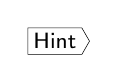
\begin{tikzpicture}[baseline=(H.base),every node/.style={
    signal,draw,very thin,signal to=east,signal from=nowhere,
    signal pointer angle=120,inner sep=2pt}]
    \node[anchor=mid west] (H) at (0,0){\sffamily\footnotesize Hint};
  \end{tikzpicture}
}{}

\setlength{\emergencystretch}{1.5em}
\newtcolorbox{petunjukbacaan}{breakable,enhanced,width=\textwidth,
  colback=white,colbacktitle=white,colframe=gray!50,boxrule=0.2mm,
  coltitle=black,fonttitle=\sffamily,
  attach boxed title to top left={yshift=-\tcboxedtitleheight/2,xshift=\tcboxedtitlewidth/4},
  boxed title style={boxrule=0pt,colframe=white},before skip=0.5cm,
  top=3mm,bottom=3mm,title={Reading Guide}}

\begin{document}
\frontmatter

\cleardoublepage
\thispagestyle{empty}
\section*{Attribution, license, and edition status}
The source work is Wen-Wei Li, \emph{Methods of Algebra, Volume 2:
Linear Algebra}, 2024 edition. The frozen source is the author-controlled
repository at commit \texttt{9a5803ff77dd3257484cb177f851a73770a59dd3},
tree \texttt{23bd05c2fb8434278df4fdfb636559a6a2b0d2ff}. The source and this
derivative are licensed under Creative Commons Attribution 4.0 International
(CC BY 4.0):
\begin{center}\small\url{https://creativecommons.org/licenses/by/4.0/}\end{center}

This independent edition translates the complete active introduction,
Chapters 1--9, Appendices A--B, exercises, hints, headings, and reader
interfaces. Formulae, notation, numbering, labels, cross-references,
citations, diagrams, and bibliographic identities are preserved. Two clearly
identified mastery bridges are independent additions derived from the
Indonesian course edition. Wen-Wei Li and Higher Education Press do not endorse
this independent translation.

\medskip
Production provenance: the English translation, terminology reconciliation,
metadata, and modular backend were produced with \textbf{OpenAI Codex
gpt-5.6-sol, Ultra}, acting on instructions of the user. This disclosure does
not displace Wen-Wei Li’s authorship or other component credits.

\mainmatter

% English translation of prelude.tex, lines 9--29.
% Source: Methods of Algebra, Volume 2, commit
% 9a5803ff77dd3257484cb177f851a73770a59dd3 (CC BY 4.0).
% stable-unit-id: o014.aljabr2.prelude.linear-algebra

\chapter*{Introduction}
\hypertarget{o014.aljabr2.prelude}{ }

% segment-id: o014.li2.prelude.p001
This book is a sequel to \cite{Li1} (hereafter Volume~I). Its purpose is to introduce a range of methods, ideas, and techniques that may reasonably be grouped under the broad heading of linear algebra, assuming familiarity with the basic structures of algebra. These methods pervade contemporary mathematics. To address practical needs as comprehensively as possible, the relevant techniques must be forged into purer and more concise forms; categories and functors are an indispensable language for doing so.

% segment-id: o014.li2.prelude.p002
The book is divided into three main parts: the Inner Part, the Outer Part, and the appendices. It is intended chiefly for advanced undergraduates, graduate students, researchers, teachers, and independent learners who work on or are interested in these subjects. The prerequisites include familiarity with algebraic structures such as groups, rings, modules, and fields, as well as category theory. Volume~I covers all of this background, though other good textbooks will serve equally well apart from minor differences in notation. The motivation for writing the book was explained in the introduction to Volume~I; the original purpose remains unchanged and need not be repeated here.

\section*{What Is Linear Algebra?}
\addcontentsline{toc}{section}{What Is Linear Algebra?}
\hypertarget{o014.aljabr2.prelude.linear-algebra}{ }
\index{linear algebra}

% segment-id: o014.li2.prelude.linear-algebra.p001
In the usage of algebraists, ``linear'' broadly describes properties connected with structures that have addition and its inverse operation, subtraction. Addition and subtraction in turn give rise to multiplication by integers; an immediate generalization is scalar multiplication by elements of a ring $R$. The prototypical examples are left and right $R$-modules, while a $\Z$-module is simply an abelian group. For a given $R$-module (taken to be a left module unless otherwise stated), one may study its submodules and quotient modules, as well as the kernel $\Ker(f)$, cokernel $\Coker(f)$, and image $\Image(f)$ of a module homomorphism $f$. All are old friends from elementary algebra; at least the special case in which $R$ is a field---that is, the case of vector spaces---is widely familiar.

% segment-id: o014.li2.prelude.linear-algebra.p002
Since the twentieth century, mathematical practice has gradually shown that extending the study of $R$-modules and their homomorphisms to complexes of $R$-modules is not only useful and convenient, but often necessary. Such a complex is a sequence of module homomorphisms satisfying $d^{n+1}d^n=0$:
\[
  \cdots \longrightarrow X^{n-1} \xrightarrow{d^{n-1}} X^n
  \xrightarrow{d^n} X^{n+1} \xrightarrow{d^{n+1}} \cdots .
\]
The condition on the homomorphisms is sometimes written $d^2=0$, while the full data of the complex are often abbreviated as $(X^n,d^n)_n$, $(X,d)$, or $X$. Because the notation uses increasing superscripts, this is also called a cochain complex. If instead one uses decreasing subscripts, $\cdots\to X_n\xrightarrow{d_n}X_{n-1}\to\cdots$, the resulting mathematical object is called a chain complex; the distinction is purely formal.

% segment-id: o014.li2.prelude.linear-algebra.p003
A single $R$-module $M$ may be regarded as the special complex with $X^0=M$ and all other terms zero. For a complex $X$, the identity $d^nd^{n-1}=0$ allows its $n$th cohomology to be defined as the quotient module
\[
  \Hm^n(X):=\Ker\left(d^n\right)\big/\Image\left(d^{n-1}\right).
\]

% segment-id: o014.li2.prelude.linear-algebra.p004
A complex satisfying $\Hm^n(X)=0$ for every $n$ is called an exact sequence or an acyclic complex. For a chain complex, correspondingly, one has homology $\Hm_n(X):=\Ker(d_n)/\Image(d_{n+1})$. The cohomology of a complex (or the homology of a chain complex) often contains important information about the mathematical object under study.

\enlargethispage{3\baselineskip}
% segment-id: o014.li2.prelude.linear-algebra.p005
For modules and other mathematical structures equipped with some kind of linear operation---for example, objects of the abelian categories introduced later---the study of complexes and their cohomology is the classical subject matter of homological algebra. This forms a proper part of ``linear algebra'' in its genuine sense, yet lies at the heart of this book. A brief account of its origins follows.

% English translation of prelude.tex, lines 30--103.
% Source: Methods of Algebra, Volume 2, commit
% 9a5803ff77dd3257484cb177f851a73770a59dd3 (CC BY 4.0).
% stable-unit-id: o014.aljabr2.prelude.homology-history

\section*{A Brief History of Homology}
\addcontentsline{toc}{section}{A Brief History of Homology}
\hypertarget{o014.aljabr2.prelude.homology-history}{ }

% segment-id: o014.li2.prelude.homology-history.p001
Mathematics need not be grounded in history; nevertheless, looking back to understand what lies ahead can only be beneficial. We shall divide the development of homology theory, somewhat artificially, into several stages.

\subsection*{The Formative Period}

% segment-id: o014.li2.prelude.homology-history.p002
The first impetus for the development of homological algebra came from topology. In the latter half of the nineteenth century, B.\ Riemann and E.\ Betti studied the genus of surfaces and its higher-dimensional generalizations, now called Betti numbers. Around the turn of the century, H.\ Poincaré developed these ideas into a more rigorous theory. Roughly speaking, Poincaré's original idea was to decompose a space into polygons, polyhedra, or higher-dimensional analogues glued together; compute Betti numbers and their torsion analogues from matrices encoding the gluing; and prove that these quantities are topological invariants.

% segment-id: o014.li2.prelude.homology-history.p003
In a short paper from 1925, E.\ Noether explained how homology could be defined as an abelian group, with the Betti numbers and their torsion analogues merely numerical invariants derived from it. This already comes close to the modern definition in algebraic topology: for a decomposed space $E$ and an abelian group $A$, one defines a chain complex $C(E,A)$ that records how the pieces are glued; the homology groups of $E$ with coefficients in $A$ are then $\Hm_n(E;A):=\Hm_n(C(E,A))$, while the cohomology groups $\Hm^n(E;A)$ are defined dually.

% segment-id: o014.li2.prelude.homology-history.p004
From then until about 1950, algebraic topology entered an extraordinarily fertile period. From the algebraic point of view, notable developments included:
\begin{itemize}
	% segment-id: o014.li2.prelude.homology-history.p005
	\item the universal coefficient theorem for homology (or cohomology), which says that the case of integer coefficients suffices to determine homology (or cohomology) with coefficients in an arbitrary abelian group $A$; its explicit description involves the $\Tor$ (or $\Ext$) functor, to be studied in depth later;
	% segment-id: o014.li2.prelude.homology-history.p006
	\item the cup product on cohomology, a multiplicative structure carried by cohomology groups;
	% segment-id: o014.li2.prelude.homology-history.p007
	\item aspherical spaces: connected spaces $E$ satisfying $n>1\implies\pi_n(E)=0$, where $\pi_n(E)$ denotes the $n$th homotopy group relative to a chosen base point. W.\ Hurewicz proved that the homology and cohomology groups of an aspherical space are entirely determined by $\pi_1(E)$ and can be described algebraically. This marked the beginning of group cohomology.
\end{itemize}

% segment-id: o014.li2.prelude.homology-history.p008
Another impetus for homological algebra came from within algebra itself. The classical example is Hilbert's syzygy theorem in invariant theory (1890): in modern language, it states that every module over the polynomial ring $\Bbbk[X_1,\ldots,X_n]$ has a free resolution of length $\leq n$.

% segment-id: o014.li2.prelude.homology-history.p009
The $\Ext$ functor likewise arises from algebraic questions. For abelian groups $A$ and $B$, a short exact sequence of abelian groups $0\to A\to E\to B\to0$ is also called a group extension; equivalence classes of such extensions correspond bijectively to the elements of $\Ext^1(B,A)$. Moreover, if $B$ is replaced by an arbitrary group $G$, the classification of group extensions leads naturally to an algebraic definition of group cohomology $\Hm^2(G,A)$.

% segment-id: o014.li2.prelude.homology-history.p010
Derivations on rings attracted algebraists' attention early on. In 1942, G.\ Hochschild defined invariants of a ring $R$ now called Hochschild homology and cohomology; the degree-one cohomology group classifies derivations modulo inner derivations.\footnote{Translator's note: the source says that the degree-one term ``classifies all derivations.'' This has been corrected here: $\Hm^1_{\mathrm{Hoch}}(R,R)$ classifies derivations modulo inner derivations; see correction O014-C001.} These constructions extend to arbitrary $(R,R)$-bimodules $M$ and continue to play an important role at the frontiers of modern mathematics.

% segment-id: o014.li2.prelude.homology-history.p011
Also worth mentioning is J.\ Leray's wartime work on sheaves and spectral sequences, motivated initially by fixed-point problems related to partial differential equations. Sheaves are geometric structures that carry local--global information, while spectral sequences provide powerful tools for computing sheaf cohomology. Influenced by Leray's theory and Kiyoshi Oka's work in several complex variables, H.\ Cartan and others set about rewriting the foundations of algebraic topology after the war; homological algebra thereby took on an entirely new form.

\subsection*{The Cartan--Eilenberg Revolution}

% segment-id: o014.li2.prelude.homology-history.p012
The monumental and far-reaching work of H.\ Cartan and S.\ Eilenberg \cite{CE56} was long regarded as the canonical reference. It marked a new period in the development of homological algebra. Its main contributions include:
\begin{itemize}
	% segment-id: o014.li2.prelude.homology-history.p013
	\item defining injective and projective modules, and injective and projective resolutions of modules;
	% segment-id: o014.li2.prelude.homology-history.p014
	\item defining right and left derived functors in the framework of module theory, thereby giving general definitions of $\Ext$ and $\Tor$, and introducing the injective and projective dimensions of a module---tools that soon proved highly effective in the theory of commutative rings;
	% segment-id: o014.li2.prelude.homology-history.p015
	\item using this machinery to explain earlier constructions, such as group cohomology and Hochschild homology and cohomology;
	% segment-id: o014.li2.prelude.homology-history.p016
	\item systematically establishing the general theory of spectral sequences and their multiplicative structures.
\end{itemize}

% segment-id: o014.li2.prelude.homology-history.p017
The term ``homological algebra'' also originates in \cite{CE56}. With the emergence of this grand theory, homological algebra entered its youth.

\subsection*{Abelian Categories}

% segment-id: o014.li2.prelude.homology-history.p018
From a geometric---more precisely, sheaf-theoretic---viewpoint, the module-theoretic framework for homological algebra is too restrictive. One seeks categories $\mathcal A$ more general than the category $R\dcate{Mod}$ of left $R$-modules, while retaining some ``linear'' character. An early attempt appeared in D.\ Buchsbaum's 1955 doctoral thesis, also included as an appendix to \cite{CE56}; he abstracted the notion of an exact sequence from module theory.

% segment-id: o014.li2.prelude.homology-history.p019
The now standard approach comes from A.\ Grothendieck's paper \cite{Gr57}; it led to what are now called abelian categories. An abelian category is an additive category with kernels and cokernels in which every morphism $f:M\to N$ is strict. Roughly speaking, strictness corresponds to the familiar module-theoretic isomorphism theorem $M/\Ker(f)\rightiso\Image(f)$. In the same work, Grothendieck also:
\begin{itemize}
	% segment-id: o014.li2.prelude.homology-history.p020
	\item used long exact sequences to define $\delta$-functors and universal $\delta$-functors, characterized the universal ones, and showed that derived functors are special cases of universal $\delta$-functors;
	% segment-id: o014.li2.prelude.homology-history.p021
	\item gave the Grothendieck spectral sequence for deriving a composite of functors;
	% segment-id: o014.li2.prelude.homology-history.p022
	\item defined a special class of abelian categories, now called Grothendieck categories, and established the existence of injective resolutions in them.
\end{itemize}

% segment-id: o014.li2.prelude.homology-history.p023
These theories made it possible to study sheaf cohomology on more general spaces and were crucial to the development of geometry.

\subsection*{Derived Categories}

% segment-id: o014.li2.prelude.homology-history.p024
In his 1963 doctoral thesis, J.-L.\ Verdier defined the derived category $\cate{D}(\mathcal A)$ of an abelian category $\mathcal A$. The motivation came from difficulties Grothendieck encountered while studying duality in algebraic geometry. Those obstacles prompted the search for a framework in which one works with complexes themselves rather than merely with their cohomology, formally inverting the quasi-isomorphisms in the category of complexes $\cate{C}(\mathcal A)$. A quasi-isomorphism is a morphism of complexes $f:X\to Y$ inducing isomorphisms $\Hm^n(f):\Hm^n(X)\rightiso\Hm^n(Y)$ on cohomology. The operation of formally inverting these morphisms is called Gabriel--Zisman localization, a categorical generalization of ring localization.

% segment-id: o014.li2.prelude.homology-history.p025
The derived category $\cate{D}(\mathcal A)$ contains more information than cohomology alone, and its formalism is correspondingly different: sequences of morphisms in $\cate{D}(\mathcal A)$ called distinguished triangles,
\[ X \xrightarrow{f} Y \xrightarrow{g} Z \xrightarrow{h} X[1] \]
play the role of short exact sequences in $\mathcal A$ or in $\cate{C}(\mathcal A)$. Here $X[1]$ is the shift of the complex $X$:
\[ X[1]^n=X^{n+1},\quad d_{X[1]}^n=-d_X^n. \]
Verdier further abstracted these constructions into structures called triangulated categories. From the topological viewpoint, the triangulated structure of a derived category is equally natural: distinguished triangles are analogous to cofiber sequences in homotopy theory. This relates to the homotopical algebra discussed later. Also motivated by homotopy theory, D.\ Puppe independently discovered a similar structure in 1962, although his conditions did not include Verdier's octahedral axiom.

% segment-id: o014.li2.prelude.homology-history.p026
Although derived categories are not ideal for every application, their language remained the preferred one among geometers and algebraists into the early twenty-first century. One prominent application is the theory of $\mathscr D$-modules, developed chiefly by Masaki Kashiwara, Z.\ Mebkhout, and others; some of its basic operations admit satisfactory definitions only at the level of derived categories.

% segment-id: o014.li2.prelude.homology-history.p027
The derived category of a ring $R$, $\cate{D}(R):=\cate{D}(R\dcate{Mod})$, may also be regarded as an invariant of $R$. If two rings have equivalent derived categories as triangulated categories, they are called derived equivalent. Questions and methods surrounding derived equivalence form a major current in the representation theory of algebras, pioneered by D.\ Happel, J.\ Rickard, and others.

\subsection*{Homotopical Algebra}

% segment-id: o014.li2.prelude.homology-history.p028
The reader will recall that the topological origin of homological algebra lay in decomposing spaces and then extracting topological invariants from suitable chain or cochain complexes. There are many ways to carry out the initial decomposition; simplicial sets, defined by Eilenberg and Zilber in 1950, are one of them, and they generalize further to simplicial objects in a given category. This language has unusually broad explanatory power: the homotopy theory of topological spaces can be developed using simplicial sets, while the construction called the ``nerve'' interprets categories as a special kind of simplicial set.

% segment-id: o014.li2.prelude.homology-history.p029
What happens if a little ``linearity'' is added to this picture? The Dold--Kan correspondence (1958) directly connects simplicial objects in an abelian category with the theory of complexes. For the category $\cate{Ab}$ of abelian groups, for example, the Dold--Kan correspondence is an explicitly defined adjoint equivalence
\[\begin{tikzcd}
	\mathrm{N}: \cate{sAb} \arrow[shift left, r] & \cate{Ch}_{\geq 0}(\cate{Ab}): \Gamma \arrow[shift left, l]
\end{tikzcd}\]
where $\cate{sAb}$ is the category of simplicial objects in $\cate{Ab}$ and $\cate{Ch}_{\geq0}(\cate{Ab})$ is the category of nonnegative chain complexes in $\cate{Ab}$. Other conventions for complexes can be accommodated by reversing the indexing or passing to the opposite category.

% segment-id: o014.li2.prelude.homology-history.p030
The Dold--Kan correspondence gives topological interpretations of many definitions and constructions concerning chain complexes. Simplicial methods likewise provide a unified account of a class of resolutions collectively called ``bar constructions'' in homological algebra.

% segment-id: o014.li2.prelude.homology-history.p031
Homotopy is a central idea in simplicial theory. Algebraic methods involving simplicial objects are therefore sometimes called homotopical algebra. Their power is displayed especially clearly in the higher $K$-theory developed by D.\ Quillen, though their applications are by no means limited to it.

% segment-id: o014.li2.prelude.homology-history.p032
In summary, simplicial methods in linear algebra may be viewed as a higher-level confluence of topology---especially homotopy theory---and homological algebra. In the early twenty-first century, this confluence inspired another wave: infinity-category theory.

% English translation of prelude.tex, lines 104--126.
% Source: Methods of Algebra, Volume 2, commit
% 9a5803ff77dd3257484cb177f851a73770a59dd3 (CC BY 4.0).
% stable-unit-id: o014.aljabr2.prelude.book-purpose

\section*{The Purpose of This Book}
\addcontentsline{toc}{section}{The Purpose of This Book}
\hypertarget{o014.aljabr2.prelude.book-purpose}{ }

\subsection*{Organizational Aims}

% segment-id: o014.li2.prelude.book-purpose.p001
The preceding introduction shows that what is called linear algebra divides roughly into two main branches: the theory of abelian categories and the theory of complexes built upon them. This book centers on these two branches and seeks to provide the ideas and techniques needed to understand contemporary mathematics. Its contents include both the algebraic methods used in applications and the theoretical foundations those methods require. Since the methods primarily serve research in pure mathematics and are meant to apply as broadly as possible, the book may also be characterized as ``pure applied mathematics.''

% segment-id: o014.li2.prelude.book-purpose.p002
The book also attempts to serve both as a textbook and as a reference, which necessarily calls for attention to detail and systematic development. These goals pull against one another, yet the book must state its purpose, develop its themes, and bring them home within a finite space. This creates an enormous organizational challenge, but one that must be accepted.

% segment-id: o014.li2.prelude.book-purpose.p003
As to content, derived categories, derived functors, and spectral sequences are essential knowledge for contemporary mathematicians. Yet they pose real difficulties for beginners, chiefly at the level of ideas and definitions. The Inner Part is organized around this objective and lays the foundation for the Outer Part. To keep the exposition flowing and save space, we shall not retrace history step by step, but will more often follow the logical order made visible by hindsight.

% segment-id: o014.li2.prelude.book-purpose.p004
Constrained by these aims, what critics of art and literature call an ``aura'' inevitably recedes from the prose, replaced at times by the heaviness of systematic structure and rigorous proof. The aura opposed to that heaviness is mathematics' first knock upon the human mind, and perhaps its last. In the author's view, however, a light, agile, direct style belongs either to a theory's formative period or relies upon a complete supporting literature. Such support must be embedded in the native linguistic culture and shared by every reader. The author has chosen to carry the burden, hoping that the appearance of this book will leave future authors free to travel more lightly.

% segment-id: o014.li2.prelude.book-purpose.p005
During its preparation, the book drew extensively on related works, among them \cite{Wei94, ML98, KS06, Rie16, Yek20}. The Stacks Project \cite{stacks} and the \href{https://ncatlab.org}{nLab} website also proved invaluable.

\subsection*{Approach and Trade-offs}

% segment-id: o014.li2.prelude.book-purpose.p006
The book must accommodate many fields and styles while finding a balance between classical and modern approaches, so that the material remains reasonably accessible to beginners. Compromise is therefore the author's guiding principle. Few readers, however, open a book in search of compromise. Compromise brings detours, so the path of this book is a geodesic for no reader; that is unavoidable.

% segment-id: o014.li2.prelude.book-purpose.p007
For the same reason, the selection of material cannot satisfy everyone. Geometrically inclined readers will not find sheaves or $t$-structures, while readers interested in the representation theory of algebras will not find tilting theory. These topics are omitted because the corresponding theories cannot be adequately motivated without first entering those subjects more deeply.

% segment-id: o014.li2.prelude.book-purpose.p008
Category theorists may regard the book's approach as no more than semiclassical. Even so, readers may notice that the main text and exercises leave entry points for more advanced viewpoints, such as dg-categories, monad theory, and simplicial objects, though each is touched on only briefly. These topics can be viewed as a warm-up for infinity-category theory and point toward a new world deeper than linear algebra, called advanced or higher algebra, which lies beyond the scope of this book.

% segment-id: o014.li2.prelude.book-purpose.p009
One further choice deserves explanation: the book treats general abelian categories and develops their basic properties directly from the axioms, unlike some homological-algebra texts that consider only modules. This generality is demanded both by theoretical completeness and by practical necessity: even if modules were our sole starting point, constructions such as functor categories and Serre quotients would still require it. Because diagram chases in module theory do not extend directly to the general setting, some foundational results about abelian categories require rather indirect proofs. To help with these details, the book expects readers to have some elementary experience with complexes of modules and their cohomology, such as the material of \cite[Chapter~6]{Li1}, though this is not logically necessary.

% segment-id: o014.li2.prelude.book-purpose.p010
The celebrated Freyd--Mitchell embedding theorem states that every small abelian category admits an exact, fully faithful embedding into $\cated{Mod}R$ for some ring $R$. Granting this theorem, many basic facts about abelian categories can be checked in the concrete module category $\cated{Mod}R$. A proof of the theorem is given in Appendix
% source-xref: sec:FM; partial-reader fallback: B.6
\S\sourcecrossref{sec:FM}{B.6}. Because the proof is itself nontrivial and depends on basic properties of abelian categories, the theorem does not essentially simplify their theory; its role is chiefly heuristic.

% English translation of prelude.tex, lines 127--153.
% Source: Methods of Algebra, Volume 2, commit
% 9a5803ff77dd3257484cb177f851a73770a59dd3 (CC BY 4.0).
% stable-unit-id: o014.aljabr2.prelude.reader-guide

% segment-id: o014.li2.prelude.reader-guide.h001
\section*{Guide to Using the Book}
\addcontentsline{toc}{section}{Guide to Using the Book}
\hypertarget{o014.aljabr2.prelude.reader-guide}{ }

% segment-id: o014.li2.prelude.reader-guide.h002
\subsection*{How the Book May Be Used}

% segment-id: o014.li2.prelude.reader-guide.p001
To serve as a reference work, the book needs a reasonably systematic organization. Its chapters therefore follow a primarily logical order. Dependencies between earlier and later material are especially pronounced in the Inner Part, while the few necessary topics that diverge from the main line or are more technical have been assigned to appendices.

% segment-id: o014.li2.prelude.reader-guide.p002
Independent readers should decide what to read according to their own interests and needs. Most of these choices arise in the Outer Part, whereas the Inner Part supplies the common foundational framework, although even there some sections are optional. More abstract or technical details may be omitted on an initial reading, while material involving the appendices is best skipped at first or merely skimmed. Detailed advice on these choices appears at the beginning of each chapter and appendix, especially in the reading guides.

% segment-id: o014.li2.prelude.reader-guide.p003
As noted above in the discussion of the book's aims, we have unavoidably wrapped mathematical ideas in layer upon layer of prose. Independent readers must make a determined effort to discern the mathematics itself within those layers, like catching lightning amid roiling clouds.

% segment-id: o014.li2.prelude.reader-guide.p004
For readers using the book as a reference, the author has tried to organize the exposition modularly so that its parts can be read separately. This is reflected not only in the division into chapters, but also in the following two features.
\begin{itemize}
	% segment-id: o014.li2.prelude.reader-guide.i001
	\item As far as possible, the book uses the standard notation of contemporary literature, supplemented by reviews and explanations. The Conventions at the end of the introduction and the index at the end of the book provide two further aids to understanding the notation.
	% segment-id: o014.li2.prelude.reader-guide.i002
	\item Statements and proofs contain copious cross-references, allowing readers who already know something of the subject to understand the discussion quickly and build an efficient conceptual map.
\end{itemize}

% segment-id: o014.li2.prelude.reader-guide.p005
In particular, the author hopes that the book will help readers preparing to teach or participating in seminars to assemble the knowledge they need quickly and then recast it in their own language.

% segment-id: o014.li2.prelude.reader-guide.p006
As for classroom use, one must frankly admit that teaching schedules are not governed by individual wishes. While writing the book, the author had almost no opportunity to try out this material in the classroom, so its effectiveness there remains unknown. Judging from past experience, even with details omitted in lectures, the book clearly contains enough material for more than one academic year; in a streamlined presentation, the Inner Part might perhaps be compressed into a single semester. An instructor using the book as the primary textbook will first have to decide how to divide the material. The author hopes that the modular design just mentioned will make this task easier.

% segment-id: o014.li2.prelude.reader-guide.p007
The lack of classroom testing has two further consequences. First, the book must still contain many undiscovered errors. Second, it lacks the finish of a classic textbook. This is due both to practical circumstances and to the author's own limitations; the author can only ask the reader's indulgence.

% segment-id: o014.li2.prelude.reader-guide.h003
\subsection*{On the Exercises}

% segment-id: o014.li2.prelude.reader-guide.p008
Every chapter and appendix ends with exercises arranged in the order of the corresponding material in the main text and sometimes accompanied by hints. Their chief purposes are to supplement the text with further properties, provide examples, and broaden the reader's perspective. Some exercises help readers become familiar with techniques and generally make few technical demands. A few ask readers to fill in details omitted from the text; these details are either trivial, easy, or, more often, both. In short, the author hopes that beginners will attempt as many exercises as possible, but they need not force themselves or feel obliged to complete them all.

% segment-id: o014.li2.prelude.reader-guide.h004
\subsection*{Categories and Their Size}

% segment-id: o014.li2.prelude.reader-guide.p009
Most of this book is expressed in categorical language because practice has shown category theory to be an efficient means of understanding and handling algebraic problems. Nevertheless, linear algebra---or what is called homological algebra---is no more a branch of category theory than probability theory is a branch of measure theory.

% segment-id: o014.li2.prelude.reader-guide.p010
Unlike some textbooks, both this book and Volume~I require that, for a category, the collection of all objects and the collection of all morphisms each be a set; it is not enough for the objects merely to form a ``class.'' The price of excluding proper classes from the definitions is that, strictly speaking, one must introduce Grothendieck universes to measure the size of sets and assume that all sets belong to some universe $\mathcal{U}$; see \cite[Assumption~1.5.2, Remark~1.5.6]{Li1}. When concrete problems are considered case by case, the axiom that there are sufficiently many universes---equivalently, sufficiently many strongly inaccessible cardinals---can often be weakened. Since this issue is not central to the book, we shall not pursue it further.

% English translation of prelude.tex, lines 154--183.
% Source: Methods of Algebra, Volume 2, commit
% 9a5803ff77dd3257484cb177f851a73770a59dd3 (CC BY 4.0).
% stable-unit-id: o014.aljabr2.prelude.structure-overview

% segment-id: o014.li2.prelude.structure-overview.h001
\section*{Overview of the Structure}
\addcontentsline{toc}{section}{Overview of the Structure}
\hypertarget{o014.aljabr2.prelude.structure-overview}{ }

% segment-id: o014.li2.prelude.structure-overview.p001
Readers are advised to begin with the Conventions at the end of the introduction, in order to familiarize themselves with the notation and conventions used throughout the book. Beyond that, beginners are discouraged from reading strictly in sequence unless they are already highly receptive to abstract methods. Each chapter opens with a detailed summary and reading guide.

% segment-id: o014.li2.prelude.structure-overview.p002
First comes the Inner Part, which lays the foundations.

\begin{description}
	% segment-id: o014.li2.prelude.structure-overview.i001
	\item[Chapter 1: Supplements to Category Theory] Reviews and rounds out the requisite category theory, emphasizing strict morphisms, kernels and cokernels in additive categories, Kan extensions, Gabriel--Zisman localization, and related topics.
	% segment-id: o014.li2.prelude.structure-overview.i002
	\item[Chapter 2: Abelian Categories] Develops the basic theory of abelian categories, supplemented by material on Grothendieck categories and other topics.
	% segment-id: o014.li2.prelude.structure-overview.i003
	\item[Chapter 3: Complexes] Discusses basic notions such as complexes, double complexes, homotopies, and mapping cones in additive categories, as well as cohomology in abelian categories. The second half treats derived functors from the classical viewpoint, including special cases such as $\Ext$, $\Tor$, and $\lim^1$. To handle unbounded complexes, it concludes with K-injective and K-projective resolutions.
	% segment-id: o014.li2.prelude.structure-overview.i004
	\item[Chapter 4: Triangulated and Derived Categories] Introduces the general notions of triangulated categories and triangulated functors, then concentrates on derived categories of abelian categories and derived functors between derived categories. The classical $\Ext$ and $\Tor$ are upgraded accordingly to $\RHom$ and $\otimesL$.
	% segment-id: o014.li2.prelude.structure-overview.i005
	\item[Chapter 5: Spectral Sequences] Begins with the general definition of spectral sequences and exact couples, then specializes progressively to the spectral sequences of filtered complexes and double complexes and to their applications in algebra. Exact couples are not absolutely necessary for the spectral sequence of a filtered complex.
\end{description}

% segment-id: o014.li2.prelude.structure-overview.p003
Next comes the Outer Part, devoted to applications or further developments.
\begin{description}
	% segment-id: o014.li2.prelude.structure-overview.i006
	\item[Chapter 6: Group Homology and Cohomology] Studies group homology and cohomology, together with a variety of related computations and examples. It also treats Tate cohomology, the cohomology of profinite groups, and nonabelian cohomology, each of which plays an important role in applications.
	% segment-id: o014.li2.prelude.structure-overview.i007
	\item[Chapter 7: Monad Theory] Starts from the general notion of an ``algebra'' in a monoidal category and first discusses differential graded structures related to complexes. After treating examples that include coalgebras, bialgebras, and Hopf algebras, it turns to Beck's monadicity theorem. The second half considers module theory, introduces Morita theory, and applies monadicity to flat descent for modules and to Galois descent.
	% segment-id: o014.li2.prelude.structure-overview.i008
	\item[Chapter 8: Simplicial Methods] Covers the general theory of simplicial objects and simplicial sets, the Dold--Kan correspondence, and the bar construction formulated in the language of monads. The final sections concern the generalized Eilenberg--Zilber theorem and a topological interpretation of mapping cones.
	% segment-id: o014.li2.prelude.structure-overview.i009
	\item[Chapter 9: Duality] Begins with duality in monoidal categories and, after basic examples, studies reconstruction theorems and Tannakian categories. This chapter is not directly concerned with complexes.
\end{description}

% segment-id: o014.li2.prelude.structure-overview.p004
The original plan called for the Outer Part to include the foundations of representation theory, which seemed likely to play a natural role in the overall structure. Late in the process, the idea was abandoned because the book was already too long and several mature textbooks were available.

% segment-id: o014.li2.prelude.structure-overview.p005
The appendices are as follows.
\begin{description}
	% segment-id: o014.li2.prelude.structure-overview.i010
	\item[Appendix A: Further Material on Abelian Categories] Collects material directly or indirectly related to abelian categories, either cited in the main text or developed as a side topic.
	% segment-id: o014.li2.prelude.structure-overview.i011
	\item[Appendix B: An Introduction to Ind- and Pro-objects] Starts from the theory of profinite groups, naturally introduces ind- and pro-objects, and studies the Ind-construction for categories and functors. As an application, it then proves the Freyd--Mitchell embedding theorem for abelian categories.
\end{description}

% segment-id: o014.li2.prelude.structure-overview.p006
Finally, the author's personal website provides the latest supplementary information, including errata, for this book and the author's other works. Readers are invited to follow the updates there and to write to the author if they find any errors in the book.

% English translation of prelude.tex, lines 185--205.
% Source: Methods of Algebra, Volume 2, commit
% 9a5803ff77dd3257484cb177f851a73770a59dd3 (CC BY 4.0).
% stable-unit-id: o014.aljabr2.prelude.acknowledgments

% segment-id: o014.li2.prelude.acknowledgments.h001
\section*{Acknowledgments}
\addcontentsline{toc}{section}{Acknowledgments}
\hypertarget{o014.aljabr2.prelude.acknowledgments}{ }

% segment-id: o014.li2.prelude.acknowledgments.p001
During the preparation of this book, the author benefited from corrections and suggestions by teachers, colleagues, and friends. The process lasted so long that omissions and errors of memory are inevitable; the following list is incomplete: Huan Zhen, Huang Chenxin, Li Jinghui, Lei Jiale, Li Changyuan, Sun Yuze, Tang Yiming, Xue Hanyu, Yang Enlin, Zhang Haofeng, and Zhao Zelong (in Hanyu Pinyin order).

% segment-id: o014.li2.prelude.acknowledgments.p002
A small portion of the book was used in courses at the University of Chinese Academy of Sciences and Huazhong University of Science and Technology. The author also thanks everyone who took part in those courses.

% segment-id: o014.li2.prelude.acknowledgments.p003
Like all the author's works to date, this book was written entirely in an open-source software environment, including the operating system and the fonts used in preparing it for press. The author salutes the many selfless developers who put into practice the universal values of sharing and altruism.

% segment-id: o014.li2.prelude.acknowledgments.p004
While this book was being written, the author's research was supported by the Excellent Young Scientists Fund of the National Natural Science Foundation of China under project 11922101, with Peking University as the host institution. This support is gratefully acknowledged.

% segment-id: o014.li2.prelude.acknowledgments.p005
The author also thanks Zhao Tianfu, an editor at Higher Education Press, for his patience and professionalism. The writing of this book ought to have followed seamlessly from Volume~I, but various obstacles delayed its completion until the end of 2022.

% segment-id: o014.li2.prelude.acknowledgments.p006
Despite the delay, preparing the book consumed even more of the author's mental energy than Volume~I. This was especially true of the repeated checking and revision in the final stages, which felt like walking through an endless dark tunnel. Much of this late work was done in Beijing subway cars. Working on the train was hardly comfortable and required making every minute and second count, quite literally. Yet amid that immense, anonymous current, day after day, the author seemed to sense a kind of tacit mutual understanding rarely found in working life, and to draw a glimmer of consolation from it. Was it so, or was it not? The explanation may be fanciful, but the feeling was real. The prelude now draws to a close: homage to the boundless distance, and to the endless multitudes.

% segment-id: o014.li2.prelude.acknowledgments.sig001
\vspace{1em}
\begin{flushright}\begin{minipage}{0.3 \textwidth}
	\begin{tabular}{c}
		% segment-id: o014.li2.prelude.acknowledgments.sig002
		{\fangsong Wen-Wei Li} \\
		% segment-id: o014.li2.prelude.acknowledgments.sig003
		December 2022 \\
		% segment-id: o014.li2.prelude.acknowledgments.sig004
		Shijingshan
	\end{tabular}
\end{minipage}\end{flushright}

% English translation of prelude.tex, lines 207--495.
% Source: Methods of Algebra, Volume 2, commit
% 9a5803ff77dd3257484cb177f851a73770a59dd3 (CC BY 4.0).
% stable-unit-id: o014.aljabr2.prelude.conventions

% segment-id: o014.li2.prelude.conventions.h001
\section*{Conventions}
\addcontentsline{toc}{section}{Conventions}
\hypertarget{o014.aljabr2.prelude.conventions}{ }

% segment-id: o014.li2.prelude.conventions.p001
The notational conventions in this book are the same as in Volume~I. They are summarized here, at the risk of some length.

% segment-id: o014.li2.prelude.conventions.h002
\subsection*{Basic Conventions}

% segment-id: o014.li2.prelude.conventions.p002
The book uses standard logical symbols such as $\forall$, $\exists$, and $\implies$. The symbol $\exists !$ means ``there exists exactly one,'' and $\iff$ means ``if and only if.'' The end of a proof is marked by $\Box$. The notation $A:=B$ means ``$A$ is defined to be $B$.'' If the definition of a mathematical object does not depend on choices of auxiliary data, it is called well-defined.
\index{well-defined}

% segment-id: o014.li2.prelude.conventions.p003
The arrow $\rightiso$ denotes an isomorphism between objects, sometimes written without direction as $\simeq$. The symbols $\xrightarrow{1:1}$ and $\stackrel{1:1}{\longleftrightarrow}$ denote a bijection between sets, that is, a one-to-one correspondence. Notation such as $F(\cdot)$ emphasizes the variable of a map or functor $F$.

% segment-id: o014.li2.prelude.conventions.p004
The notation $n\gg m$ means that $n$ is sufficiently larger than $m$. Thus $n\gg0$ means that $n$ is sufficiently large, while $n\ll0$ means that $-n$ is sufficiently large.

% segment-id: o014.li2.prelude.conventions.p005
The language of commutative diagrams is used extensively. The simplest case is the following.

% segment-id: o014.li2.prelude.conventions.d001
\[\begin{tikzcd}
	A \arrow[r, "f"] \arrow[d, "h"'] & B \arrow[ld, "g"] \\
	C &
\end{tikzcd} \; \text{commutes} \stackrel{\text{definition}}{\iff} g \circ f = h. \]

% segment-id: o014.li2.prelude.conventions.p006
Here $f$, $g$, and $h$ may be maps, homomorphisms, or morphisms in an arbitrary category. More complicated commutative diagrams are understood in the same way.

% segment-id: o014.li2.prelude.conventions.h003
\subsection*{Sets and Order Structures}

% segment-id: o014.li2.prelude.conventions.p007
The book uses Zermelo--Fraenkel axiomatic set theory and accepts the axiom of choice.

% segment-id: o014.li2.prelude.conventions.p008
The empty set is denoted by $\emptyset$. The notation $A\subset B$ means that $A$ is a subset of $B$, with equality allowed; strict inclusion is written $A\subsetneq B$. Set difference is $A\smallsetminus B:=\{a\in A:a\notin B\}$, and disjoint union is $A\sqcup B$. For a map $f:A\to B$, the notation $a\mapsto b$ means that $a\in A$ is mapped by $f$ to $b\in B$, and $f|_{A'}$ is the restriction of $f$ to a subset $A'\subset A$. The identity map on $A$ is denoted by $\identity=\identity_A$. The number of elements of $A$, also called its cardinality or cardinal, is denoted by $|A|$.

% segment-id: o014.li2.prelude.conventions.p009
Following \cite[Definition~1.2.1]{Li1}, a \emph{partially ordered set}
\index{partially ordered set}
is a set $P$ equipped with a reflexive, transitive, and antisymmetric binary relation $\leq$. Omitting antisymmetry gives a \emph{preordered set}. The notation $x<y$ means $x\lneq y$. A partially ordered set $(P,\leq)$ is often abbreviated to $P$.

% segment-id: o014.li2.prelude.conventions.l001
\begin{itemize}
	% segment-id: o014.li2.prelude.conventions.i001
	\item If $m\in P$ satisfies $\forall x\in P,\;x\geq m\iff x=m$, then $m$ is a maximal element of $P$. Replacing $\geq$ by $\leq$ defines a minimal element. In general these need not be unique.
	% segment-id: o014.li2.prelude.conventions.i002
	\item Let $S$ be a subset of $P$. If $b\in P$ satisfies $\forall x\in S,\;x\leq b$, then $b$ is an upper bound of $S$ in $P$. Lower bounds are defined similarly.
	% segment-id: o014.li2.prelude.conventions.i003
	\item If $b$ is an upper bound of $S$ and every other upper bound $b'$ satisfies $b'\geq b$, then $b$ is the supremum of $S$, denoted $\sup S$. A supremum, if it exists, is unique. The infimum $\inf S$ is defined similarly.
\end{itemize}

% segment-id: o014.li2.prelude.conventions.p010
A map $f:P\to Q$ of partially ordered sets is order-preserving if $a\leq b\implies f(a)\leq f(b)$. If $f$ is bijective and both $f$ and $f^{-1}$ are order-preserving, it is an isomorphism of partially ordered sets, or an order-preserving bijection.

% segment-id: o014.li2.prelude.conventions.p011
If every two elements of a partially ordered set $P$ are comparable, then $P$ is totally ordered. A nonempty totally ordered set in which every nonempty subset has a least element is \emph{well-ordered}
\index{well-ordered set}. Certain special well-ordered sets are called \emph{ordinals}\index{ordinal}, and any two ordinals are comparable. Briefly:

% segment-id: o014.li2.prelude.conventions.l002
\begin{itemize}
	% segment-id: o014.li2.prelude.conventions.i004
	\item for every ordinal $\alpha$, one has $\alpha=\{\beta:\text{ordinal},\;\beta<\alpha\}$;
	% segment-id: o014.li2.prelude.conventions.i005
	\item if an ordinal $\kappa$, as a set, is not equinumerous with any ordinal smaller than $\kappa$, then it is called a \emph{cardinal};
	\index{cardinal}
	% segment-id: o014.li2.prelude.conventions.i006
	\item the cardinality $|S|$ of a set $S$ is defined as the least ordinal in its equinumerosity class. This uses the fact that every set can be well-ordered (which requires the axiom of choice) and that every well-ordered set is isomorphic to a unique ordinal;
	% segment-id: o014.li2.prelude.conventions.i007
	\item in particular, $|\alpha|\leq\alpha$ for every ordinal $\alpha$.
\end{itemize}

% segment-id: o014.li2.prelude.conventions.p012
This is von Neumann's viewpoint; see \cite[\S~1.2]{Li1} or \cite{Je03}. It is slightly more circuitous than the usual definition of a cardinal as an equinumerosity class, but has its conveniences.

% segment-id: o014.li2.prelude.conventions.p013
Finite ordinals may be identified with nonnegative integers: for each $n\in\Z_{\geq0}$ there is a corresponding totally ordered set $\mathbf n$, recursively defined as a set by $\mathbf0:=\emptyset$ and $\mathbf{n+1}:=\{\mathbf0,\ldots,\mathbf n\}$, with the evident order. The least infinite ordinal $\omega$ is the well-ordered set $\mathbf0\leq\mathbf1\leq\cdots$, and is also the countable cardinal $\aleph_0$.
\index[sym1]{012@$\mathbf{0}, \mathbf{1}, \mathbf{2}, \ldots$}

% segment-id: o014.li2.prelude.conventions.p014
We choose a \emph{Grothendieck universe}
\index{Grothendieck universe}
\index[sym1]{U@$\mathcal{U}$} $\mathcal U$ to distinguish sizes of sets. Elements of $\mathcal U$ are called $\mathcal U$-sets; sets equinumerous with a $\mathcal U$-set are called $\mathcal U$-small, or simply \emph{small sets}\index{small set}. If a cardinal $\mu$, regarded as a set, is $\mathcal U$-small, it is a \emph{small cardinal}\index{cardinal!small}. We assume that every set $X$ belongs to some $\mathcal U$; see \cite[Assumption~1.5.2]{Li1} and the accompanying discussion.

% segment-id: o014.li2.prelude.conventions.h004
\subsection*{Categories}

% segment-id: o014.li2.prelude.conventions.p015
Our conventions for categories agree with \cite[\S~1.5, Definition~2.1.3]{Li1}: the objects and morphisms of a category $\mathcal C$ each form a set, denoted by $\Obj(\mathcal C)$ and $\Mor(\mathcal C)$. The set of morphisms between two objects is denoted by $\Hom_{\mathcal C}(\cdot,\cdot)$, or simply $\Hom(\cdot,\cdot)$. The identity morphism of $X$ is $\identity_X$. Monomorphisms are marked by $\hookrightarrow$ and epimorphisms by $\twoheadrightarrow$; a monomorphism is also called an embedding.
\index{category}
\index{object}

% segment-id: o014.li2.prelude.conventions.l003
\begin{itemize}
	% segment-id: o014.li2.prelude.conventions.i008
	\item For any morphism $f:X\to Y$ in a category and any object $T$, $f$ induces pullback $f^*$ and pushforward $f_*$ operations on $\Hom$ sets:
	\begin{align*}
		f^*: \Hom(Y, T) & \to \Hom(X, T), & f_*: \Hom(T, X) & \to \Hom(T, Y) \\
		\beta & \mapsto \beta f & \alpha & \mapsto f\alpha .
	\end{align*}
	% segment-id: o014.li2.prelude.conventions.i009
	\item Subcategories are written using subset notation, $\mathcal C'\subset\mathcal C$. If $\Hom_{\mathcal C'}(X,Y)=\Hom_{\mathcal C}(X,Y)$, then $\mathcal C'$ is a full subcategory.

	% segment-id: o014.li2.prelude.conventions.i010
	\item The product $\mathcal C_1\times\mathcal C_2$ of two categories has object set $\Obj(\mathcal C_1)\times\Obj(\mathcal C_2)$. A morphism from $(X_1,X_2)$ to $(Y_1,Y_2)$ is an element of $\Hom_{\mathcal C_1}(X_1,Y_1)\times\Hom_{\mathcal C_2}(X_2,Y_2)$, and composition is componentwise. This immediately defines products $\prod_i\mathcal C_i$ of arbitrary families of categories. Likewise, $\mathcal C^n:=\mathcal C\times\cdots\times\mathcal C$ ($n$ factors), or more generally $\mathcal C^I$ for a set $I$. See \cite[Definition~2.3.1]{Li1}.
	\index{product category}
\end{itemize}

% segment-id: o014.li2.prelude.conventions.p016
For example, every preordered set $(P,\leq)$ determines a category $\mathcal P$ with object set $P$ and

% segment-id: o014.li2.prelude.conventions.d002
\[ \forall a,b \in P, \quad \Hom_{\mathcal{P}}(a, b) = \begin{cases}
	\text{the singleton} \; \{ \star \}, & a \leq b \\
	\emptyset, & \text{otherwise.}
\end{cases}\]

% segment-id: o014.li2.prelude.conventions.p017
In particular, $\mathbf0$ may be identified with the empty category, having no objects and no morphisms, while $\mathbf1$ is identified with the category having exactly one object $\mathbf0$ and one morphism $\identity_{\mathbf0}$.

% segment-id: o014.li2.prelude.conventions.p018
A category satisfying $\Mor(\mathcal C)=\{\identity_X:X\in\Obj(\mathcal C)\}$ is called \emph{discrete}. Discrete categories correspond bijectively to sets under $\mathcal C\mapsto\Obj(\mathcal C)$.
\index{category!discrete}

% segment-id: o014.li2.prelude.conventions.h005
\subsection*{Terminology: Small and Large Categories}

% segment-id: o014.li2.prelude.conventions.p019
Fix a Grothendieck universe $\mathcal U$, and let $\mathcal C$ be a category. If $\mathrm{Mor}(\mathcal C)$ is $\mathcal U$-small, then $\mathcal C$ is a $\mathcal U$-small category. If only $\Hom_{\mathcal C}(X,Y)$ is required to be $\mathcal U$-small for every $X,Y\in\Obj(\mathcal C)$, then $\mathcal C$ is a $\mathcal U$-category.
\footnote{In much of the literature, the objects of a category are understood to form a class, while the $\Hom$ between any two objects is a set. Thus their ``classes'' correspond to this book's sets, their ``sets'' to this book's $\mathcal U$-sets, and their ``categories'' essentially to this book's $\mathcal U$-categories.}

% segment-id: o014.li2.prelude.conventions.p020
For example, all $\mathcal U$-sets and maps between them form the $\mathcal U$-category $\cate{Set}$, which is not $\mathcal U$-small. Without a choice of $\mathcal U$, on the other hand, all sets form a proper class and not a category in the sense of this book. Similarly, $\cate{Grp}$ (or $\cate{Ab}$) denotes the category of all groups (or abelian groups) realized on $\mathcal U$-sets; these are $\mathcal U$-categories.
\index[sym1]{Set@$\cate{Set}$}

% segment-id: o014.li2.prelude.conventions.p021
To see that size is a genuine issue, observe that the $\Hom$ functor $\Hom_{\mathcal C}:\mathcal C^{\opp}\times\mathcal C\to\cate{Set}$ can be defined only when $\mathcal C$ is a $\mathcal U$-category.

% segment-id: o014.li2.prelude.conventions.p022
Unless otherwise stated, categories in this book are $\mathcal U$-categories, and $\mathcal U$-small categories are simply called \emph{small}. A category not necessarily a $\mathcal U$-category is called \emph{large}.
\index{category!small, large}
\index{size issues}

% segment-id: o014.li2.prelude.conventions.p023
Large categories are hard to avoid in many constructions, especially in theories involving functor categories or localization. Whenever a large category may occur and has substantive consequences, this will be stated explicitly.

% segment-id: o014.li2.prelude.conventions.h006
\subsection*{Functors and Functor Categories}

% segment-id: o014.li2.prelude.conventions.p024
The identity functor of $\mathcal C$ is denoted by $\identity_{\mathcal C}$. A functor $F:\mathcal C\to\mathcal D$ sends a morphism $f:X\to Y$ in $\mathcal C$ to a morphism $Ff:FX\to FY$ in $\mathcal D$. If $\Hom_{\mathcal C}(X,Y)\to\Hom_{\mathcal D}(FX,FY)$ is injective (respectively bijective) for every $X,Y$, then $F$ is faithful (respectively fully faithful). If every object of $\mathcal D$ is isomorphic to some $FX$, then $F$ is essentially surjective.
\index{functor}

% segment-id: o014.li2.prelude.conventions.p025
For categories associated with partially ordered sets, an order-preserving map $P\to Q$ is precisely a functor $\mathcal P\to\mathcal Q$.

\index{natural transformation}
\index{2-cell}
% segment-id: o014.li2.prelude.conventions.p026
In some of the literature, a morphism $\varphi:F\to G$ between functors is also called a natural transformation and is sometimes written with a double arrow $\varphi:F\Rightarrow G$. It consists of a compatible family $(\varphi_X:FX\to GX)_{X\in\Obj(\mathcal C)}$, and may be represented by the \emph{$2$-cell} diagram introduced in \cite[\S~2.2]{Li1}:

% segment-id: o014.li2.prelude.conventions.d003
\[\begin{tikzcd}
	\mathcal{C} \arrow[rr, bend left=45, "F", ""'{name=F}] \arrow[rr, bend right=45, "G"', ""{name=G}] & & \mathcal{D} \arrow[Rightarrow, from=F, to=G, "\varphi"].
\end{tikzcd}\]

% segment-id: o014.li2.prelude.conventions.p027
When $\cate{Ab}$-categories (see \S\sourcecrossref{sec:Ker-Coker}{1.3}) or $\Bbbk$-linear categories (see \S\sourcecrossref{sec:linear-cat}{1.4}) are discussed later, corresponding conditions will also be imposed on functors.

% segment-id: o014.li2.prelude.conventions.p028
Given functors
$\begin{tikzcd}
	\mathcal{B} \arrow[r, "R"] & \mathcal{C} \arrow[shift left, r, "F"] \arrow[shift right, r, "G"'] & \mathcal{D} \arrow[r, "L"] & \mathcal{E}
\end{tikzcd}$
and a morphism $\varphi:F\to G$, one naturally obtains $L\varphi:LF\to LG$ and $\varphi R:FR\to GR$. Morphisms $\varphi:F\to G$ and $\psi:G\to H$ can also be composed to form $\psi\varphi:F\to H$. These operations can be expressed as composition of $2$-cells, that is, by pasting diagrams. The triangle identities reviewed shortly are a basic example.

\index{functor category}
\index[sym1]{DC@$\mathcal{D}^{\mathcal{C}}$}
\index[sym1]{Fct@$\mathrm{Fct}$}
% segment-id: o014.li2.prelude.conventions.p029
All functors from $\mathcal C$ to $\mathcal D$ form the functor category $\mathcal D^{\mathcal C}$, also denoted $\mathrm{Fct}(\mathcal C,\mathcal D)$. Unless $\mathcal C$ is small, $\mathcal D^{\mathcal C}$ is often a ``large category.'' As special cases, for $n\in\Z_{\geq0}$ and the corresponding totally ordered set $\mathbf n$, the categories $\mathcal C^{\mathbf n}$ are described as follows.

% segment-id: o014.li2.prelude.conventions.l004
\begin{compactitem}
	% segment-id: o014.li2.prelude.conventions.i011
	\item by definition, $\mathcal C^{\mathbf0}:=\mathbf1$;
	% segment-id: o014.li2.prelude.conventions.i012
	\item there is a unique functor $\mathcal C\to\mathbf1$, hence $\mathbf1^{\mathcal C}=\mathbf1$;
	% segment-id: o014.li2.prelude.conventions.i013
	\item specifying a functor $\mathbf1\to\mathcal C$ is equivalent to specifying an object of $\mathcal C$, hence $\mathcal C^{\mathbf1}\simeq\mathcal C$;
	% segment-id: o014.li2.prelude.conventions.i014
	\item the objects of $\mathcal C^{\mathbf2}$ are morphisms in $\mathcal C$, and its morphisms are commutative squares between them.
\end{compactitem}

% segment-id: o014.li2.prelude.conventions.p030
Thus $\mathbf0$ may be called the initial category, $\mathbf1=[\bullet]$ the terminal category, and $\mathbf2=[\bullet\to\bullet]$ may be pictured as a walking arrow.

\index{category!opposite}
\index[sym1]{Cop@$\mathcal{C}^{\opp}$}
% segment-id: o014.li2.prelude.conventions.p031
The opposite category $\mathcal C^{\opp}$ has the same objects as $\mathcal C$. Every morphism $f:X\to Y$ may be regarded as a morphism $Y\to X$ in $\mathcal C^{\opp}$ and is then written $f^{\opp}$\index[sym1]{fop@$f^{\opp}$}. Moreover, $\mathrm{Fct}(\mathcal C,\mathcal D)^{\opp}$ is naturally identified with $\mathrm{Fct}(\mathcal C^{\opp},\mathcal D^{\opp})$. Passing from $\mathcal C$ to $\mathcal C^{\opp}$ reverses arrows; this mechanism is called duality in category theory.

% segment-id: o014.li2.prelude.conventions.p032
If functors $F:\mathcal C\leftrightarrows\mathcal D:G$ satisfy $GF\simeq\identity_{\mathcal C}$ and $FG\simeq\identity_{\mathcal D}$, they are mutually quasi-inverse. A functor having a quasi-inverse is an equivalence of categories, a fundamental notion in category theory. If the strict equalities $GF=\identity_{\mathcal C}$ and $FG=\identity_{\mathcal D}$ hold, then they are mutually inverse isomorphisms of categories.

% segment-id: o014.li2.prelude.conventions.h007
\subsection*{Algebraic Structures}

% segment-id: o014.li2.prelude.conventions.p033
The identity element of a group is denoted by $1$ in multiplicative notation and by $0$ for an abelian group in additive notation. The opposite group, with reversed multiplication, is $G^{\opp}$. If $H$ is a subgroup of $G$, its index is $(G:H)$, also equal to the number of cosets $|G/H|$ or $|H\backslash G|$.
\index[sym1]{GH@$(G:H)$}

% segment-id: o014.li2.prelude.conventions.p034
Unless otherwise stated, rings are associative and unital, as are algebras over commutative rings. The multiplicative identity of $R$ is $1$ or $1_R$, and its invertible elements form the multiplicative group $R^\times$. The characteristic of a field or integral domain $R$ is $\mathrm{char}(R)$. The opposite ring $R^{\opp}$ has multiplication in the reverse order.
% Correction O014-C002: the source indexes A^{\opp}, although this paragraph
% defines R^{\opp}.
\index[sym1]{Rop@$R^{\opp}$}

% segment-id: o014.li2.prelude.conventions.p035
Let $r$ be a nonzero element of a commutative ring $R$. If the additive-group homomorphism $R\xrightarrow{\text{multiplication by}\;r}R$ has a nonzero kernel, then $r$ is a zero divisor. The ideal generated by $x,y,\ldots$ in a commutative ring is denoted by $(x,y,\ldots)$.

% segment-id: o014.li2.prelude.conventions.p036
The polynomial algebra over a commutative ring $R$ in variables $X_1,X_2,\ldots$ is $R[X_1,X_2,\ldots]$, and the formal power-series ring is $R\llbracket X_1,X_2,\ldots\rrbracket$. If $M$ is a monoid, its monoid algebra over $R$ is $R[M]$.

% segment-id: o014.li2.prelude.conventions.p037
By convention, $\Z\subset\Q\subset\R\subset\CC$ denote, respectively, the ring of integers, the field of rational numbers, the field of real numbers, and the field of complex numbers. If $q$ is a prime power, $\F_q$ is the finite field with $q$ elements. If $F\hookrightarrow E$ is an embedding of fields, the corresponding field extension is denoted by $E|F$ and its degree by $[E:F]$. If $E|F$ is Galois, its Galois group is $\Gal(E|F)$.
\index[sym1]{Gal}

% The following matrix block is inactive in the source and remains disabled.
%The book uses horizontal rows and vertical columns; an $n \times m$ matrix is written
%\[ A = (a_{ij})_{\substack{1 \leq i \leq n \\ 1 \leq j \leq m}} = \begin{tikzpicture}[baseline]
%	\matrix (M) [matrix of math nodes, left delimiter=(, right delimiter=)] {
%		& \vdots & \\
%		\cdots & a_{ij} & \cdots \\
%		& \vdots & \\
%	};
%	\node[right=2.5em] at (M-2-3) {\scriptsize row $i$};
%	\node[below=1em] at (M-3-2) {\scriptsize column $j$};
%\end{tikzpicture}\]
%its transpose is denoted by ${}^t A$; the $n\times n$ identity matrix is $1_{n\times n}$ or $1$. For an $n\times n$ matrix $A$ over a commutative ring, its determinant is $\det A$.

% segment-id: o014.li2.prelude.conventions.p038
The common categories associated with some basic algebraic structures are denoted as follows.

% segment-id: o014.li2.prelude.conventions.t001
\begin{center}\small \begin{tabular}{|c|c|}\hline
	Monoids & $\cate{Mon}$ \\
	Groups &  $\cate{Grp}$ \\
	Abelian groups & $\cate{Ab} = \Z\dcate{Mod}$ \\
	Left or right $R$-modules & $R\dcate{Mod}$ or $\cated{Mod}R$ \\
	$\Bbbk$-vector spaces & $\cate{Vect}(\Bbbk)$ \\
	$(R,S)$-bimodules & $(R,S)\dcate{Mod}$ \\
	$\Bbbk$-algebras & $\Bbbk\dcate{Alg}$ \\
	Commutative $\Bbbk$-algebras & $\Bbbk\dcate{CAlg}$
	\\ \hline
\end{tabular} \quad \begin{tabular}{l}
	$R$, $S$: arbitrary rings, \\
	$\Bbbk$: a field (for vector spaces), \\
	$\Bbbk$: a commutative ring (for algebras), \\
	the module category $\Bbbk\dcate{Mod}$ does not distinguish left from right.
\end{tabular}\end{center}
\index[sym1]{Mod@$\cate{Mod}$}
\index[sym1]{Ab@$\cate{Ab}$}
\index[sym1]{Grp@$\cate{Grp}$}
\index[sym1]{Vect@$\cate{Vect}$}

% segment-id: o014.li2.prelude.conventions.p039
If $\Bbbk$ is fixed and $R,S$ are $\Bbbk$-algebras, then an $(R,S)$-bimodule is understood by default to arise from a left $R\dotimes{\Bbbk}S^{\opp}$-module structure. In other words, the left and right actions of $\Bbbk$ are required to agree.

% segment-id: o014.li2.prelude.conventions.p040
The group of homomorphisms between two left $R$-modules or two right $R$-modules is denoted by $\Hom_R(X,Y)$. For $(R,S)$-bimodules, the analogous notation is $\Hom_{(R,S)}(X,Y)$.

% segment-id: o014.li2.prelude.conventions.p041
For a commutative ring $R$ and a multiplicative subset $U$, the corresponding localization is $R[U^{-1}]$.

% segment-id: o014.li2.prelude.conventions.p042
As with the category of sets $\cate{Set}$, groups, rings, modules, and the other structures here are understood to be realized on $\mathcal U$-sets for the chosen Grothendieck universe $\mathcal U$. Every category in the table therefore has a forgetful functor to $\cate{Set}$. Other examples used in this book, such as the category $\cate{Top}$ of topological spaces and the category $\cate{CHaus}$ of compact Hausdorff spaces, obey the same convention: their spaces are realized on $\mathcal U$-sets.

% segment-id: o014.li2.prelude.conventions.h008
\subsection*{Adjunctions}

% segment-id: o014.li2.prelude.conventions.p043
An adjoint pair $(F,G,\varphi)$ consists of two functors

% segment-id: o014.li2.prelude.conventions.d004
$\begin{tikzcd}
	\mathcal{C} \arrow[shift left, r, "F"] & \mathcal{C}' \arrow[shift left, l, "G"]
\end{tikzcd}$

% segment-id: o014.li2.prelude.conventions.p044
together with a family of canonical bijections $\varphi_{X,Y}:\Hom_{\mathcal C'}(FX,Y)\rightiso\Hom_{\mathcal C}(X,GY)$, that is, an isomorphism of functors

% segment-id: o014.li2.prelude.conventions.d005
\[ \varphi: \Hom_{\mathcal{C}'}\left(F(\cdot), \cdot \right) \rightiso
\Hom_{\mathcal{C}}\left(\cdot, G(\cdot) \right): \;
\mathcal{C}^{\opp} \times \mathcal{C}' \to \cate{Set}. \]

% segment-id: o014.li2.prelude.conventions.p045
An adjoint pair is also often displayed as

% segment-id: o014.li2.prelude.conventions.d006
$\begin{tikzcd}
	F: \mathcal{C} \arrow[shift left, r] & \mathcal{C}' \arrow[l, shift left] : G
\end{tikzcd}$

% segment-id: o014.li2.prelude.conventions.p046
meaning that $F$ is left adjoint to $G$, or $G$ is right adjoint to $F$. The datum $\varphi$ is frequently omitted, and the adjoint pair is then written $(F,G)$.

% segment-id: o014.li2.prelude.conventions.p047
Equivalently, $\varphi$ can be characterized by a \emph{unit} $\eta:\identity_{\mathcal C}\to GF$ and a \emph{counit} $\varepsilon:FG\to\identity_{\mathcal C'}$. The data $(F,G,\eta,\varepsilon)$ form an adjoint pair if and only if they satisfy the \emph{triangle identities}
\index{unit}
\index{counit}
\index{triangle identities}:

% segment-id: o014.li2.prelude.conventions.d007
\[ G\varepsilon \circ \eta G = \identity_G, \quad
\varepsilon F \circ F\eta = \identity_F. \]

% segment-id: o014.li2.prelude.conventions.p048
See \cite[(2.6) + Proposition~2.6.5]{Li1}. Equivalently, these identities may be written as equalities of composites of $2$-cells:

% segment-id: o014.li2.prelude.conventions.d008
\begin{equation*}\begin{gathered}
	\begin{tikzcd}
		\mathcal{C}' \arrow[r, "G"] \arrow[rr, bend right=60, "\identity_{\mathcal{C}'}"', "" {name=B}] & \mathcal{C} \arrow[r, "F"] \arrow[Rightarrow, to=B, "\varepsilon"] \arrow[rr, bend left=60, "\identity_{\mathcal{C}}", ""' {name=T}] & \mathcal{C}' \arrow[r, "G"] \arrow[Rightarrow, from=T, "\eta"] & \mathcal{C}
	\end{tikzcd} \quad = \quad \begin{tikzcd}[column sep=large]
		\mathcal{C}' \arrow[r, bend left=60, "G", ""' {name=T}] \arrow[r, bend right=60, "G"', "" {name=B}] & \mathcal{C} \arrow[Rightarrow, from=T, to=B, "{\identity_G}" description]
	\end{tikzcd} , \\
	\begin{tikzcd}
		\mathcal{C} \arrow[r, "F"] \arrow[rr, bend left=60, "\identity_{\mathcal{C}}", ""' {name=T}] & \mathcal{C}' \arrow[r, "G"] \arrow[Rightarrow, from=T, "\eta"] \arrow[rr, bend right=60, "\identity_{\mathcal{C}'}"', ""' {name=B}] & \mathcal{C} \arrow[r, "F"] \arrow[Rightarrow, to=B, "\varepsilon"] & \mathcal{C}'
	\end{tikzcd} \quad = \quad \begin{tikzcd}[column sep=large]
		\mathcal{C} \arrow[r, bend left=60, "F", ""' {name=T}] \arrow[r, bend right=60, "F"', "" {name=B}] & \mathcal{C}' \arrow[Rightarrow, from=T, to=B, "{\identity_F}" description]
	\end{tikzcd}.
\end{gathered}\end{equation*}

% segment-id: o014.li2.prelude.conventions.p049
For details, see \cite[Remark~2.6.6]{Li1}.

% segment-id: o014.li2.prelude.conventions.h009
\subsection*{Limits}

% segment-id: o014.li2.prelude.conventions.p050
Consider a functor $\alpha:I\to\mathcal C$.

% segment-id: o014.li2.prelude.conventions.l005
\begin{itemize}
	% segment-id: o014.li2.prelude.conventions.i015
	\item The inductive limit of $\alpha$, if it exists, is denoted by $\varinjlim\alpha$ or $\varinjlim_{i\in\Obj(I)}\alpha(i)$. It is an object of $\mathcal C$ equipped with morphisms $\alpha(i)\to\varinjlim\alpha$ and determined by a universal property.
	\index{limit}
	% segment-id: o014.li2.prelude.conventions.i016
	\item Similarly, the projective limit of $\alpha$, if it exists, is denoted by $\varprojlim\alpha$ or $\varprojlim_{i\in\Obj(I)}\alpha(i)$. It is equipped with morphisms $\varprojlim\alpha\to\alpha(i)$ and determined by a universal property.
\end{itemize}

% segment-id: o014.li2.prelude.conventions.p051
The two kinds of limits are dual: the $\varinjlim$ of $\alpha:I\to\mathcal C$ is the $\varprojlim$ of $\alpha^{\opp}:I^{\opp}\to\mathcal C^{\opp}$. For this reason, functors involved in $\varprojlim$ are often written in the form $I^{\opp}\to\mathcal C$.

% segment-id: o014.li2.prelude.conventions.p052
In much of the literature, $\varinjlim$ is called a colimit and denoted by $\mathrm{colim}$, while $\varprojlim$ is called a limit and denoted by $\lim$. Unless otherwise stated, ``limit'' in this book includes both $\varinjlim$ and $\varprojlim$.
\index[sym1]{lim@$\varinjlim$, $\varprojlim$, $\lim$, $\mathrm{colim}$}

% segment-id: o014.li2.prelude.conventions.p053
If $I$ is small, the corresponding $\varinjlim$ or $\varprojlim$ is a \emph{small limit}\index{limit!small}. Following the standard terminology of \cite[\S~2.8]{Li1}, a category $\mathcal C$ having all small $\varprojlim$ (respectively all small $\varinjlim$) is \emph{complete} (respectively \emph{cocomplete}). This notion depends on the choice of $\mathcal U$.
\index{category!complete, cocomplete}

% segment-id: o014.li2.prelude.conventions.p054
To fix notation, choose a category $\mathcal C$ and review several common special cases of limits. Detailed definitions may be found in \cite[\S~2.7]{Li1} or other textbooks. In the universal properties below, $T$ is an arbitrary object of $\mathcal C$ and $I$ is an arbitrary set.

% segment-id: o014.li2.prelude.conventions.t002
\begin{center}\small\setlength{\tabcolsep}{2.5pt}\begin{tabular}{|c|c|c|c|c|} \hline
	Limit & Input & Object & Canonical morphism & Universal property \\ \hline
	Equalizer & $\begin{tikzcd}[column sep=small] X \arrow[shift left, r, "f"] \arrow[shift right, r, "g"'] & Y\end{tikzcd}$ & $\Ker(f,g)$ & $\Ker(f,g) \xrightarrow{\iota} X$ & $\begin{tikzcd}[row sep=small, column sep=tiny, every cell/.append style={font = \footnotesize}]
		\Hom(T, \Ker(f,g)) \arrow[d, "1:1"'] & \psi \arrow[mapsto, d] \\
		\left\{\begin{array}{l} \phi \in \Hom(T, X): \\ f\phi = g\phi \end{array}\right\} & \iota\psi
	\end{tikzcd}$ \\
	Coequalizer & (as above) & $\Coker(f,g)$ & $Y \xrightarrow{p} \Coker(f,g)$ & $\begin{tikzcd}[row sep=small, column sep=tiny, every cell/.append style={font = \footnotesize}]
		\Hom(\Coker(f,g), T) \arrow[d, "1:1"'] & \psi \arrow[mapsto, d] \\
		\left\{\begin{array}{l} \phi \in \Hom(Y, T): \\ \phi f = \phi g \end{array}\right\} & \psi p
	\end{tikzcd}$ \\
	Product & $(X_i)_{i \in I}$ & $\displaystyle\prod_{i \in I} X_i$ & $\displaystyle\prod_{j \in I} X_j \xrightarrow{p_i} X_i$ & $\begin{tikzcd}[row sep=small, column sep=tiny, every cell/.append style={font = \footnotesize}]
		\Hom\left(T, \displaystyle\prod_{i \in I} X_i \right) \arrow[d, "1:1"'] & \psi \arrow[mapsto, d] \\
		\displaystyle\prod_{i \in I} \Hom(T, X_i) & \left( p_i \psi \right)_{i \in I}
	\end{tikzcd}$ \\
	Coproduct & (as above) & $\displaystyle\coprod_{i \in I} X_i$ & $X_i \xrightarrow{\iota_i} \displaystyle\coprod_{j \in I} X_j$ & $\begin{tikzcd}[row sep=small, column sep=tiny, every cell/.append style={font = \footnotesize}]
		\Hom\left(\displaystyle\coprod_{i \in I} X_i, T \right) \arrow[d, "1:1"'] & \psi \arrow[mapsto, d] \\
		\displaystyle\prod_{i \in I} \Hom(X_i, T) & \left( \psi \iota_i \right)_{i \in I}
	\end{tikzcd}$ \\ \hline
\end{tabular}\end{center}

% segment-id: o014.li2.prelude.conventions.n001
\begin{quote}\small
\textbf{Translator's note.} In the coproduct row, the source gives the target of the canonical injection as $\prod_{j\in I}X_j$. It has been corrected to $\coprod_{j\in I}X_j$, in agreement with the preceding object column and the following universal property; see correction O014-C003.
\end{quote}

% segment-id: o014.li2.prelude.conventions.p055
Finite products (respectively coproducts) are also written $X_1\times X_2\times\cdots$ (respectively $X_1\sqcup X_2\sqcup\cdots$). If $\mathcal C$ is additive, the coproduct $\coprod_i$ is often written using the direct-sum symbol $\bigoplus_i$ from module theory.
\index[sym1]{oplus@$\oplus$}

% segment-id: o014.li2.prelude.conventions.p056
Equalizers and coequalizers, and products and coproducts, form dual pairs. These universal-property characterizations may also be written as commutative diagrams as in \cite[\S~2.7]{Li1}, or interpreted through the Yoneda embedding reviewed in \S\sourcecrossref{sec:Yoneda}{A.1}. Suppose that $\coprod_{i\in I}X_i$ and $\prod_{j\in J}Y_j$ exist. Their universal properties give a bijection

% segment-id: o014.li2.prelude.conventions.d009
\[ \Hom\left( \coprod_{i \in I} X_i, \prod_{j \in J} Y_j \right)
\xrightarrow{1:1} \prod_{\substack{i \in I \\ j \in J}} \Hom(X_i, Y_j),
\quad \psi \mapsto (p_j \psi \iota_i)_{i,j} . \]

% segment-id: o014.li2.prelude.conventions.l006
\begin{description}
	% segment-id: o014.li2.prelude.conventions.i017
	\item[Terminal object] A product corresponding to $I=\emptyset$, if it exists, is a terminal object of $\mathcal C$, temporarily denoted by $Z$. By convention, $\prod_{i\in\emptyset}:=\{\emptyset\}$, so the universal property of $Z$ says that $\Hom(T,Z)$ is a singleton for every $T\in\Obj(\mathcal C)$.
	% segment-id: o014.li2.prelude.conventions.i018
	\item[Initial object] A coproduct corresponding to $I=\emptyset$, if it exists, is an initial object of $\mathcal C$, temporarily denoted by $S$. Its universal property says that $\Hom(S,T)$ is a singleton for every $T\in\Obj(\mathcal C)$.
	% segment-id: o014.li2.prelude.conventions.i019
	\item[Zero object and zero morphism] If an object $0$ of $\mathcal C$ is both initial and terminal, it is called a zero object; morphisms to and from it exist and are unique. For $X,Y\in\Obj(\mathcal C)$, the composite $X\to0\to Y$ gives a canonical element of $\Hom(X,Y)$ called the zero morphism.
	\index{object!zero}
\end{description}

% segment-id: o014.li2.prelude.conventions.p057
Because an isomorphism from any object $X$ to a zero object, if it exists, is unique, one customarily says that $X$ is a zero object or writes $X=0$, rather than saying that $X$ is isomorphic to a zero object.

% segment-id: o014.li2.prelude.conventions.p058
We next review two important, mutually dual kinds of limit.

% segment-id: o014.li2.prelude.conventions.t003
\begin{center}\small\setlength{\tabcolsep}{2.5pt}\begin{tabular}{|c|c|c|c|c|} \hline
	Name & Input & Object & Canonical morphism & Universal property \\ \hline
	Fiber product & $\left( X_i \xrightarrow{f_i} Z \right)_{i \in I}$ & $\displaystyle\prod_{i \in I} (X_i \to Z)$ & $\begin{tikzcd}[every cell/.append style={font = \footnotesize}] \displaystyle\prod_{j \in I} (X_j \to Z) \arrow[d, "p_i"] \\ X_i \end{tikzcd}$ & $\begin{tikzcd}[every cell/.append style={font = \footnotesize}]
		\Hom\left(T, \displaystyle\prod_{i \in I} (X_i \to Z) \right) \arrow[d, "1:1"', "{\psi \mapsto (p_i \psi)_i}"] \\
		\left\{\begin{array}{l} (\xi_i: T \to X_i)_{i \in I}: \\ \forall i,j \in I, \\ f_i \xi_i = f_j \xi_j \end{array}\right\}
	\end{tikzcd}$ \\
	Fiber coproduct & $\left( Z \xrightarrow{g_i} X_i \right)_{i \in I}$ & $\displaystyle\coprod_{i \in I} (Z \to X_i)$ & $\begin{tikzcd}[every cell/.append style={font = \footnotesize}] X_i \arrow[d, "\iota_i"] \\ \displaystyle\coprod_{j \in I} (Z \to X_j) \end{tikzcd}$ & $\begin{tikzcd}[every cell/.append style={font = \footnotesize}]
		\Hom\left(\displaystyle\coprod_{i \in I} (Z \to X_i), T \right) \arrow[d, "1:1"', "{\psi \mapsto (\psi \iota_i)_i}"] \\
		\left\{\begin{array}{l} (\xi_i: X_i \to T)_{i \in I}: \\ \forall i,j \in I, \\ \xi_i g_i = \xi_j g_j \end{array}\right\}
	\end{tikzcd}$ \\ \hline
\end{tabular}\end{center}

% segment-id: o014.li2.prelude.conventions.p059
Taking $\psi=\identity$ in the universal property of the fiber product shows that $f_ip_i=f_jp_j$ for all $i,j$, yielding a canonical morphism $\prod_{i\in I}(X_i\to Z)\to Z$. Similarly, for the fiber coproduct, taking $\psi=\identity$ shows that $\iota_ig_i=\iota_jg_j$ for all $i,j$, yielding a canonical morphism $Z\to\coprod_{i\in I}(Z\to X_i)$.

% segment-id: o014.li2.prelude.conventions.p060
Fiber products of finitely many objects $X_1\dtimes{Z}X_2\dtimes{Z}\cdots$, and fiber coproducts $X_1\dsqcup{Z}X_2\dsqcup{Z}\cdots$, reduce to repeated instances of the two-object case. Consider the following two commutative diagrams.

% segment-id: o014.li2.prelude.conventions.d010
\[\begin{tikzcd}
	X \dtimes{Z} Y \arrow[r, "p_1"] \arrow[d, "p_2"'] & X \arrow[d] \\
	Y \arrow[r] & Z
\end{tikzcd} \quad \text{and} \quad \begin{tikzcd}
	Z \arrow[r] \arrow[d] & X \arrow[d, "\iota_1"] \\
	Y \arrow[r, "\iota_2"'] & X \dsqcup{Z} Y
\end{tikzcd}\]
% Correction O014-C004: an extra backslash after the opening tikzcd in the
% source was removed as a syntax artifact with no mathematical content.

% segment-id: o014.li2.prelude.conventions.p061
These are called a \emph{pullback} diagram and a \emph{pushout} diagram, respectively. The morphism $X\dtimes{Z}Y\to Y$ is called the pullback of $X\to Z$, and $Y\to X\dsqcup{Z}Y$ the pushout of $Z\to X$; the roles of $X$ and $Y$ are symmetric. More generally, commutative diagrams isomorphic to these are also called pullback and pushout diagrams; see \cite[Definition~2.8.5]{Li1}.
\index{pullback diagram}
\index{pushout diagram}

% segment-id: o014.li2.prelude.conventions.p062
In this book, the center of the square in a pullback (respectively pushout) diagram is marked by $\Box$ (respectively $\boxplus$).
\index[sym1]{Box@$\Box$, $\boxplus$}

% segment-id: o014.li2.prelude.conventions.h010
\subsection*{Translation}

% segment-id: o014.li2.prelude.conventions.p063
In the Chinese source edition, the conventions for translation agree with \cite{Li1}; Chinese terminology is kept compatible with \cite{ZG} unless that work's translation is clearly inappropriate or erroneous.

% segment-id: o014.li2.prelude.conventions.p064
In the source index, Chinese terms are accompanied by English equivalents. This helps readers who need to read or write articles in English, provides a reference for readers whose native language is not Chinese, and, finally, reflects the historical fact that knowledge of foreign languages remains necessary for understanding the meaning of many mathematical symbols.

% segment-id: o014.li2.prelude.conventions.n002
\begin{quote}\small
\textbf{Translator's note.} This English edition indexes English headwords and records the Chinese--English terminological choices in a separate production glossary.
\end{quote}


\part*{Core Part}
% English translation of chapter1.tex, lines 9--31.
% Source: Methods of Algebra, Volume 2, commit
% 9a5803ff77dd3257484cb177f851a73770a59dd3 (CC BY 4.0).
% stable-unit-id: o014.aljabr2.chapter1.overview

% segment-id: o014.li2.chapter1.overview.h001
\chapter{Supplements to Category Theory}\label{sec:categories}
\hypertarget{o014.aljabr2.chapter1.overview}{ }

% segment-id: o014.li2.chapter1.overview.p001
As its title suggests, this chapter introduces several tools from category
theory that will be needed in later chapters, both as a review and as an
opportunity to see familiar ideas afresh. Some of this material appears in
\cite{Li1} or similar textbooks; it is nevertheless restated here in order to
review the concepts and standardize the notation. For other basic terminology,
the reader may consult the introduction to this book.

% segment-id: o014.li2.chapter1.overview.l001
\begin{itemize}
	% segment-id: o014.li2.chapter1.overview.i001
	\item Sections~\sourcecrossref{sec:subquot}{1.1}--%
	\sourcecrossref{sec:images}{1.2} begin with a brief introduction to
	subobjects and quotient objects, including the general properties of
	monomorphisms and epimorphisms. They then introduce the image $\Image(f)$
	and coimage $\Coim(f)$ of a morphism $f$, as well as morphisms for which
	``image equals coimage,'' called strict morphisms. These are basic notions
	that make sense in arbitrary categories.

	% segment-id: o014.li2.chapter1.overview.i002
	\item Sections~\sourcecrossref{sec:Ker-Coker}{1.3}--%
	\sourcecrossref{sec:linear-cat}{1.4} form the linear part of the chapter.
	They introduce a special kind of category in which every morphism set has
	the structure of an abelian group, called an $\cate{Ab}$-category; a functor
	that preserves addition of morphisms is called additive. In such categories
	one can define kernels and cokernels of morphisms, generalizing those of
	module homomorphisms. An $\cate{Ab}$-category with a zero object and finite
	products is called an additive category. In an additive category one can
	form finite direct sums of objects, and morphisms between finite direct sums
	can be manipulated in much the same way as matrices.

	More generally, the additive structure can be enhanced with scalar
	multiplication by a commutative ring $\Bbbk$, leading to the notions of a
	$\Bbbk\dcate{Mod}$-category and a $\Bbbk$-linear category. Categories with
	these linear structures are a principal concern of this book.

	% segment-id: o014.li2.chapter1.overview.i003
	\item Sections~\sourcecrossref{sec:limit-functor}{1.5}--%
	\sourcecrossref{sec:filtered-indlim}{1.6} cover the foundations of limits.
	In particular, Definition~\sourcecrossref{def:create-limit}{1.5.2}
	introduces the terminology for a functor $F:\mathcal C\to\mathcal D$
	that preserves limits (from $\mathcal C$ to $\mathcal D$) or creates them
	(from $\mathcal D$ to $\mathcal C$). Cofinal functors and filtered
	inductive limits are also discussed; these are useful and important
	notions.

	% segment-id: o014.li2.chapter1.overview.i004
	\item Left and right Kan extensions, discussed in Sections~\sourcecrossref{sec:Kan-extension}{1.7}--%
	\sourcecrossref{sec:Kan-as-limit}{1.8}, are fundamental operations in
	category theory. Under suitable conditions they can be constructed using
	$\varinjlim$ or $\varprojlim$. The argument is somewhat involved, but the
	underlying idea is simple: express the problem of extending a functor as a
	``best approximation'' formulated in terms of limits. We also record the
	non-obvious Theorem~\sourcecrossref{prop:Quillen-adjunction-gen}{1.7.7},
	which explains the connection between absolute left or right Kan extensions
	and adjoint pairs.

	% segment-id: o014.li2.chapter1.overview.i005
	\item Gabriel--Zisman localization, introduced in
	Section~\sourcecrossref{sec:cat-localization}{1.9} and henceforth called
	simply \emph{localization}, is the construction that formally adjoins
	inverses to a family $S$ of morphisms in a category. It is analogous to
	localization of rings, but the concrete details are considerably more
	complicated. To retain better control over the resulting category, in
	practice $S$ is often assumed to be a \emph{multiplicative system} in the
	sense of Definition~\sourcecrossref{def:multiplicative-family}{1.9.5}.
	The principal use of localization in this book is to construct derived
	categories; another is to define Serre quotients of abelian categories in
	Section~\sourcecrossref{sec:Serre-subcat}{2.9}.
	Section~\sourcecrossref{sec:functor-localization}{1.10} explains how to
	form Kan extensions along a localization of categories. This may be viewed
	as the localization of a functor and is essential for understanding derived
	functors.

	% segment-id: o014.li2.chapter1.overview.i006
	\item The adjoint functor theorem discussed in
	Section~\sourcecrossref{sec:AFT}{1.11} characterizes, under suitable
	conditions, when a functor has a left or right adjoint. Its principal
	application in this book is to the study of Grothendieck categories in
	Section~\sourcecrossref{sec:Grothendieck-cat}{2.10}. The theorem has uses
	far beyond this application, so the section is valuable in its own right.
	The notions of generator and cogenerator discussed there
	(Definition~\sourcecrossref{def:generators}{1.11.8}) are also essential.
\end{itemize}

% segment-id: o014.li2.chapter1.overview.p002
This chapter draws extensively on \cite{KS06, Rie16}.

% segment-id: o014.li2.chapter1.overview.n001
\begin{petunjukbacaan}
The basic theory of abelian categories and complexes requires only
Sections~\sourcecrossref{sec:subquot}{1.1}--%
\sourcecrossref{sec:linear-cat}{1.4} of this chapter.
Sections~\sourcecrossref{sec:limit-functor}{1.5}--%
\sourcecrossref{sec:filtered-indlim}{1.6} provide supporting material and are
also cited repeatedly in other chapters. The theory of derived categories uses
Sections~\sourcecrossref{sec:Kan-extension}{1.7}--%
\sourcecrossref{sec:functor-localization}{1.10}. This material has applications
beyond that theory, but readers may judge their own needs and postpone it until
just before studying derived categories. The final section,
Section~\sourcecrossref{sec:AFT}{1.11}, is used only in
Section~\sourcecrossref{sec:Grothendieck-cat}{2.10}; nevertheless, its material
on generators and cogenerators is essential and may be consulted as needed.
\end{petunjukbacaan}

% English translation of chapter1.tex, lines 33--139.
% Source: Methods of Algebra, Volume 2, commit
% 9a5803ff77dd3257484cb177f851a73770a59dd3 (CC BY 4.0).
% stable-unit-id: o014.aljabr2.chapter1.subquotients

% segment-id: o014.li2.chapter1.subquotients.h001
\section{Subquotients}\label{sec:subquot}
\hypertarget{o014.aljabr2.chapter1.subquotients}{ }

% segment-id: o014.li2.chapter1.subquotients.p001
We begin by recalling the notions of monomorphism and epimorphism. Fix a
category $\mathcal C$.

% segment-id: o014.li2.chapter1.subquotients.l001
\begin{itemize}
	% segment-id: o014.li2.chapter1.subquotients.i001
	\item A morphism $f:X\to Y$ is called a \emph{monomorphism}, also written
	$f:X\hookrightarrow Y$, if left cancellation holds:
	\[ \forall T \in \Obj(\mathcal{C}), \; \forall g,h: T \to X , \quad fg=fh \iff g=h; \]
	% segment-id: o014.li2.chapter1.subquotients.i002
	\item A morphism $f:X\to Y$ is called an \emph{epimorphism}, also written
	$f:X\twoheadrightarrow Y$, if right cancellation holds:
	\[ \forall T \in \Obj(\mathcal{C}), \; \forall g,h: Y \to T, \quad gf=hf \iff g=h. \]
\end{itemize}

% segment-id: o014.li2.chapter1.subquotients.x001
\index{monomorphism}
\index{epimorphism}

% segment-id: o014.li2.chapter1.subquotients.p002
It follows immediately that $f:X\to Y$ is monic if and only if
$f_*:\Hom(T,X)\to\Hom(T,Y)$ is injective for every $T$. Likewise, $f$ is
epic if and only if $f^*:\Hom(Y,T)\to\Hom(X,T)$ is injective for every $T$.
Monicity and epicity are dual properties: $f$ is monic if and only if
$f^{\opp}$ is epic.

% segment-id: o014.li2.chapter1.subquotients.e001
\begin{example}
	If the equalizer $\Ker(f,g)$ of a pair of morphisms $f,g:X\to Y$ exists,
	its universal property shows that the canonical morphism
	$\iota:\Ker(f,g)\to X$ is monic. Dually, if the coequalizer
	$\Coker(f,g)$ exists, the canonical morphism $p:Y\to\Coker(f,g)$ is epic.
	Here is another simple observation: if $\mathcal C$ has a zero object,
	denoted by $0$, then $0\to X$ is monic and $X\to0$ is epic. The reader is
	invited to verify these details.
\end{example}

% segment-id: o014.li2.chapter1.subquotients.pr001
\begin{proposition}\label{prop:epi-mono-isomorphism}
	Consider morphisms $X\xrightarrow{a}Y\xrightarrow{b}Z$. Suppose that $b$
	is monic or that $a$ is epic. Then $ba:X\to Z$ is an isomorphism if and
	only if both $a$ and $b$ are isomorphisms.
\end{proposition}

% segment-id: o014.li2.chapter1.subquotients.pf001
\begin{proof}
	One direction is clear. Now suppose that $ba$ is an isomorphism and that
	$b$ is monic. Set $c:=a(ba)^{-1}:Z\to Y$; then $bc=\identity_Z$.
	Moreover, $b(cb)=(bc)b=b$, so left cancellation by $b$ gives
	$cb=\identity_Y$. Thus $b$ is an isomorphism, and consequently so is $a$.
	Passing to $\mathcal C^{\opp}$ gives the case in which $a$ is epic.
\end{proof}

% segment-id: o014.li2.chapter1.subquotients.p003
In categories commonly used in algebra, such as $\cate{Set}$, $\cate{Ab}$,
and $R\dcate{Mod}$, a morphism is monic or epic precisely when its underlying
map is injective or surjective, respectively. In these examples one can also
speak of subsets, subgroups, and so forth. This notion extends to arbitrary
categories, but one additional step is needed. We formulate it in the language
of partially ordered sets.

% segment-id: o014.li2.chapter1.subquotients.p004
Let $\mathcal C$ be a category and let $X$ be an object of $\mathcal C$.
Given a pair of monomorphisms $f_i:S_i\hookrightarrow X$, where $i=1,2$,
write $(S_1,f_1)\subset(S_2,f_2)$, or simply $S_1\subset S_2$, if there is
a morphism $g:S_1\to S_2$ such that $f_2g=f_1$. The monicity of $f_2$ implies
that $g$, if it exists, is unique and is itself monic. The relation $\subset$
defined in this way is not yet a partial order. If $S_1\subset S_2$ and
$S_2\subset S_1$, we say that $S_1$ and $S_2$ are equivalent. This is the
same as requiring a commutative diagram

% segment-id: o014.li2.chapter1.subquotients.g001
\[\begin{tikzcd}
	S_1 \arrow[r, "g_1"] \arrow[hookrightarrow, rd, "f_1"'] & S_2 \arrow[hookrightarrow, d, "f_2"] \arrow[r, "g_2"] & S_1 \arrow[hookrightarrow, ld, "f_1"] \\
	& X &
\end{tikzcd}\]

% segment-id: o014.li2.chapter1.subquotients.p005
Uniqueness gives $g_2g_1=\identity_{S_1}$ and, similarly,
$g_1g_2=\identity_{S_2}$. Thus $S_1$ and $S_2$ are equivalent if and only if
there is an isomorphism $g:S_1\rightiso S_2$ with $f_2g=f_1$; moreover, this
isomorphism is unique. This is, of course, a standard argument in algebra.

% segment-id: o014.li2.chapter1.subquotients.p006
Similarly, given a pair of epimorphisms $f_i:X\twoheadrightarrow Q_i$, where
$i=1,2$, if there is a morphism $g:Q_2\to Q_1$ such that $gf_2=f_1$, then
$g$ is unique and epic; in this case write $Q_1\twoheadleftarrow Q_2$. If
$Q_1\twoheadleftarrow Q_2$ and $Q_2\twoheadleftarrow Q_1$, we say that $Q_1$
and $Q_2$ are equivalent. Equivalently, there is a unique isomorphism
$g:Q_2\rightiso Q_1$ satisfying $gf_2=f_1$.

% segment-id: o014.li2.chapter1.subquotients.p007
The binary relation $\subset$ (or $\twoheadleftarrow$) induces a partial order
on the corresponding equivalence classes. We have borrowed the set-inclusion
symbol $\subset$ here. Although this may cause some ambiguity, it is consistent
with the notation for other algebraic substructures, such as subgroups,
submodules, and subspaces.

% segment-id: o014.li2.chapter1.subquotients.d001
\begin{definition}\label{def:sub-quot-obj}
	\index{subobject} \index[sym1]{SubX@$\mathrm{Sub}_X$}
	\index{quotient object} \index[sym1]{QuotX@$\mathrm{Quot}_X$}
	Let $\mathcal C$ be a category and let $X$ be an object of $\mathcal C$.
	An equivalence class, under the relation above, of monomorphisms
	$S\hookrightarrow X$ (respectively, of epimorphisms
	$X\twoheadrightarrow Q$) is called a \emph{subobject} (respectively, a
	\emph{quotient object}) of $X$. These equivalence classes form the
	partially ordered set $(\mathrm{Sub}_X,\subset)$ (respectively,
	$(\mathrm{Quot}_X,\twoheadleftarrow)$), in which
	$\identity_X:X\to X$ gives the unique maximal element.
\end{definition}

% segment-id: o014.li2.chapter1.subquotients.p008
Subobjects and quotient objects are dual: $(\mathrm{Sub}_X,\subset)$ as
defined in $\mathcal C$ is the same as
$(\mathrm{Quot}_X,\twoheadleftarrow)$ as defined in $\mathcal C^{\opp}$.
For convenience, this section deals mainly with subobjects. Because the
isomorphism $g$ occurring in the equivalence relation is unique, one may
choose a representative $f:S\hookrightarrow X$ of an equivalence class
without ambiguity, or abbreviate that representative simply as $S$. Recall
that $f_*:\Hom(\cdot,S)\to\Hom(\cdot,X)$ is injective.

% segment-id: o014.li2.chapter1.subquotients.lm001
\begin{lemma}\label{prop:subobject-order}
	For any two subobjects $S_1,S_2$ of $X$, one has
	\begin{equation*}
		S_1 \subset S_2 \iff \forall T \in \Obj(\mathcal{C}), \; \Hom(T, S_1) \subset \Hom(T, S_2),
	\end{equation*}
	where $\Hom(T,S_1)$ and $\Hom(T,S_2)$ on the right-hand side are
	understood as subsets of $\Hom(T,X)$.
\end{lemma}

% segment-id: o014.li2.chapter1.subquotients.pf002
\begin{proof}
	The implication $\implies$ is immediate. Conversely, take $T:=S_1$.
	Under $\Hom(S_1,S_1)\subset\Hom(S_1,X)$, the element
	$\identity_{S_1}$ corresponds to $f_1$. The hypothesis supplies
	$g\in\Hom(S_1,S_2)$ whose image in $\Hom(S_1,X)$ is $f_1$, that is,
	$f_2g=f_1$. This is the required morphism.
\end{proof}

% segment-id: o014.li2.chapter1.subquotients.p009
Suppose that $\mathcal C$ has a zero object and that $(X_i)_{i\in I}$ is a
family of objects. For every $(i,j)\in I\times I$, define
$\delta_{ij}\in\Hom(X_i,X_j)$ by $\delta_{ij}=\identity$ when $i=j$, and as
the zero morphism otherwise. If the product and coproduct of
$(X_i)_{i\in I}$ exist, then $(\delta_{ij})_{i,j}$ determines a canonical
morphism

% segment-id: o014.li2.chapter1.subquotients.q001
\begin{equation}\label{eqn:coprod-prod-delta}
	\delta: \coprod_{i \in I} X_i \to \prod_{i \in I} X_i.
\end{equation}

% segment-id: o014.li2.chapter1.subquotients.p010
For the additive categories to be reviewed shortly, $\delta$ is always an
isomorphism when $I$ is finite. This need not hold in an arbitrary category.

% segment-id: o014.li2.chapter1.subquotients.lm002
\begin{lemma}\label{prop:mono-pullback}
	Let $X\to Z$ be a monomorphism. Its pullback along $Y\to Z$, namely
	$X\dtimes{Z}Y\to Y$ (if it exists), is also a monomorphism. Dually, a
	pushout of an epimorphism is again an epimorphism.
\end{lemma}

% segment-id: o014.li2.chapter1.subquotients.pf003
\begin{proof}
	By duality, it suffices to treat the case of monomorphisms. Let
	$p_2:X\dtimes{Z}Y\to Y$ be the canonical morphism supplied by the fiber
	product. The question reduces to showing, for every object $T$, that
	% segment-id: o014.li2.chapter1.subquotients.g002
	\[\begin{tikzcd}
		\Hom(T,X) \dtimes{\Hom(T,Z)} \Hom(T,Y) & \\
		\Hom\left(T, X \dtimes{Z} Y \right) \arrow[leftrightarrow, u, "1:1", "\text{universal property}"'] \arrow[r, "{(p_2)_*}"'] & \Hom(T, Y)
	\end{tikzcd} \]
	is injective. Indeed, the monicity of $X\to Z$ makes
	$\Hom(T,X)\to\Hom(T,Z)$ injective, and the map from the upper left to the
	lower right is the evident projection from the fiber product.
\end{proof}

% segment-id: o014.li2.chapter1.subquotients.lm003
\begin{lemma}\label{prop:mono-product}
	Let $(f_i:X_i\to Z)_{i\in I}$ be a family of monomorphisms. Then the
	canonical morphism from $\prod_{i\in I}(X_i\to Z)$ (if it exists) to $Z$
	is also a monomorphism. Dually, given a family of epimorphisms
	$(g_i:Z\to X_i)_{i\in I}$, the canonical morphism from $Z$ to
	$\coprod_{i\in I}(Z\to X_i)$ (if it exists) is also an epimorphism.
\end{lemma}

% segment-id: o014.li2.chapter1.subquotients.pf004
\begin{proof}
	As in Lemma~\ref{prop:mono-pullback}, the question reduces to showing that
	the bottom row of
	% segment-id: o014.li2.chapter1.subquotients.g003
	\[\begin{tikzcd}
		\prod_{i \in I} \left( \Hom(T, X_i) \to \Hom(T, Z) \right) & \\
		\Hom\left(T, \prod_{i \in I} (X_i \to Z) \right) \arrow[leftrightarrow, u, "1:1", "\text{universal property}"'] \arrow[r] & \Hom(T, Z)
	\end{tikzcd}\]
	is injective. This follows from the hypothesis, since every map
	$\Hom(T,X_i)\to\Hom(T,Z)$ is injective.
\end{proof}

% segment-id: o014.li2.chapter1.subquotients.p011
We return to subobjects and quotient objects.

% segment-id: o014.li2.chapter1.subquotients.d002
\begin{definition}\label{def:subquotient}
	\index{subquotient}
	Let $\mathcal C$ be any category and let $X,Y$ be objects of $\mathcal C$.
	If $Y$ can be realized as a quotient object of a subobject of $X$, then
	$Y$ is called a \emph{subquotient} of $X$.
\end{definition}

% segment-id: o014.li2.chapter1.subquotients.p012
Considering a subobject of a quotient object amounts to discussing a
subquotient in $\mathcal C^{\opp}$. The next result shows that, for a certain
class of categories, the two approaches yield the same notion. This class
includes the abelian categories studied later; see
Corollary~\sourcecrossref{prop:Abel-cat-subquotient}{2.1.7}.

% segment-id: o014.li2.chapter1.subquotients.pr002
\begin{proposition}\label{prop:subquotient-equiv}
	Suppose that $\mathcal C$ has finite fiber products and finite fiber
	coproducts, that pullbacks of epimorphisms remain epimorphisms, and that
	pushouts of monomorphisms remain monomorphisms. Then a subquotient may
	equivalently be defined as a subobject of a quotient object.
\end{proposition}

% segment-id: o014.li2.chapter1.subquotients.pf005
\begin{proof}
	Consider a subquotient diagram $Y\twoheadleftarrow Z\hookrightarrow X$ in
	$\mathcal C$, and set $W:=X\dsqcup{Z}Y$. The morphism $X\to W$ is the
	pushout of $Z\to Y$, so it is epic by
	Lemma~\ref{prop:mono-pullback}; the morphism $Y\to W$ is the pushout of
	$Z\to X$, so it is monic by hypothesis. Thus
	$Y\hookrightarrow W\twoheadleftarrow X$, exhibiting a subquotient of $X$
	in $\mathcal C^{\opp}$. Since the assumptions are self-dual, a subquotient
	in $\mathcal C^{\opp}$ likewise yields a subquotient in $\mathcal C$.
\end{proof}

% segment-id: o014.li2.chapter1.subquotients.p013
Once the property ``quotient of a subobject = subobject of a quotient'' has
been established, it follows that a subquotient of a subquotient is again a
subquotient.

% segment-id: o014.li2.chapter1.subquotients.p014
The definition of a subquotient does not specify how it is to be realized as a
quotient object of a subobject. For example, in $\mathcal C=\cate{Ab}$,
$\Z/2\Z$ is a subquotient of $\Z/4\Z$: it can be realized either as a quotient
object of $\Z/4\Z$ or as the subobject $2\Z/4\Z$ of $\Z/4\Z$.

% English translation of chapter1.tex, lines 140--266.
% Source: Methods of Algebra, Volume 2, commit
% 9a5803ff77dd3257484cb177f851a73770a59dd3 (CC BY 4.0).
% stable-unit-id: o014.aljabr2.chapter1.images-coimages-strict

% segment-id: o014.li2.chapter1.images-coimages-strict.h001
\section{Images, Coimages, and Strict Morphisms}\label{sec:images}
\hypertarget{o014.aljabr2.chapter1.images-coimages-strict}{ }

% segment-id: o014.li2.chapter1.images-coimages-strict.p001
Let $\mathcal C$ be a category. For any morphism $f:X\to Y$, the fiber coproduct $Y\dsqcup{X}Y$, if it exists, comes equipped with a canonical pair $Y\rightrightarrows Y\dsqcup{X}Y$. Dually, the fiber product $X\dtimes{Y}X$, if it exists, comes equipped with a canonical pair $X\dtimes{Y}X\rightrightarrows X$, usually called the projection morphisms.

% segment-id: o014.li2.chapter1.images-coimages-strict.d001
\begin{definition}[Image and Coimage]\label{def:Im-Coim}
	\index{image} \index[sym1]{imf@$\Image(f)$}
	\index{coimage} \index[sym1]{coimf@$\Coim(f)$}
	Let $f:X\to Y$ be a morphism in $\mathcal C$. Suppose that $Y\dsqcup{X}Y$ exists. If the equalizer $\Ker\left(Y\rightrightarrows Y\dsqcup{X}Y\right)$ exists, this equalizer is called the \emph{image} of $f$ and denoted by $\Image(f)$; it carries a canonical monomorphism $\Image(f)\hookrightarrow Y$.

	Dually, suppose that $X\dtimes{Y}X$ exists. If the coequalizer $\Coker\left(X\dtimes{Y}X\rightrightarrows X\right)$ exists, this coequalizer is called the \emph{coimage} of $f$ and denoted by $\Coim(f)$; it carries a canonical epimorphism $X\twoheadrightarrow\Coim(f)$.
\end{definition}

% segment-id: o014.li2.chapter1.images-coimages-strict.r001
\begin{remark}\label{rem:im-coim-duality}
	The duality between $\Ker$ and $\Coker$ immediately shows that $\Image(f)$ exists in $\mathcal C$ if and only if $\Coim(f^{\opp})$ exists in $\mathcal C^{\opp}$, and then $\Image(f)=\Coim(f^{\opp})$.
\end{remark}

% segment-id: o014.li2.chapter1.images-coimages-strict.p002
Besides being useful, the following lemma sheds light on the nature of images and coimages.

% segment-id: o014.li2.chapter1.images-coimages-strict.lm001
\begin{lemma}\label{prop:Im-Coim-fac}
	Suppose that $\Coim(f)$ exists (respectively, that $\Image(f)$ exists) for a morphism $f:X\to Y$. For any monomorphism $j:Y'\hookrightarrow Y$ (respectively epimorphism $q:X\twoheadrightarrow X'$), if $g:X\to Y'$ satisfies $jg=f$ (respectively $g:X'\to Y$ satisfies $gq=f$), then there is a unique $\overline g$ making the corresponding diagram commute:
	% segment-id: o014.li2.chapter1.images-coimages-strict.g001
	\[\begin{tikzcd}
		X \arrow[r, "f"] \arrow[twoheadrightarrow, d] \arrow[rd, "g" description] & Y \\
		\Coim(f) \arrow[r, "\overline{g}"'] & Y' \arrow[hookrightarrow, u, "j"']
	\end{tikzcd} \quad \text{or} \quad \begin{tikzcd}
		X \arrow[r, "f"] \arrow[twoheadrightarrow, d, "q"'] & Y \\
		X' \arrow[r, "\overline{g}"'] \arrow[ru, "g" description] & \Image(f) \arrow[hookrightarrow, u] .
	\end{tikzcd}\]
\end{lemma}

% segment-id: o014.li2.chapter1.images-coimages-strict.pf001
\begin{proof}
	The two versions are dual, so it suffices to consider the one involving $j$. Let $p_1,p_2$ be the projections $X\dtimes{Y}X\rightrightarrows X$. Since $jgp_1=fp_1=fp_2=jgp_2$ and $j$ is monic, $gp_1=gp_2$. The universal property of $\Coim(f)$ as a coequalizer then uniquely determines $\overline g$ making the diagram commute.
\end{proof}

% segment-id: o014.li2.chapter1.images-coimages-strict.p003
Applying Lemma~\ref{prop:Im-Coim-fac} successively to $\Coim(f)$ and $\Image(f)$ shows that there is a comparison morphism $\Coim(f)\to\Image(f)$ making the following diagram commute:

% segment-id: o014.li2.chapter1.images-coimages-strict.g002
\begin{equation}\label{eqn:strict-morphism} \begin{tikzcd}
	X \arrow[r, "f"] \arrow[twoheadrightarrow, d] & Y \\
	\Coim(f) \arrow[r] & \Image(f) \arrow[hookrightarrow, u]
\end{tikzcd}\end{equation}

% segment-id: o014.li2.chapter1.images-coimages-strict.p004
This comparison morphism is also unique, by left cancellation with a monomorphism or right cancellation with an epimorphism.

% segment-id: o014.li2.chapter1.images-coimages-strict.d002
\begin{definition}[Strict morphism]\label{def:strict-morphism}\index{strict morphism}
	Suppose that $\Image(f)$ and $\Coim(f)$ exist. If the morphism $\Coim(f)\to\Image(f)$ in \eqref{eqn:strict-morphism} is an isomorphism, then $f$ is called \emph{strict}.
\end{definition}

% segment-id: o014.li2.chapter1.images-coimages-strict.p005
For example, every morphism in $\mathcal C=\cate{Set}$ is strict, and both its image and its coimage are canonically identified with its set-theoretic image. Further examples appear in the exercises for this chapter.

% segment-id: o014.li2.chapter1.images-coimages-strict.pr001
\begin{proposition}\label{prop:Images-f-gf}
	Given morphisms $X\xrightarrow{f}Y\xrightarrow{g}Z$, there are unique morphisms $\alpha:\Coim(f)\to\Image(gf)$ and $\beta:\Coim(gf)\to\Image(g)$ making the following diagrams commute, provided the indicated coimages and images exist:
	% segment-id: o014.li2.chapter1.images-coimages-strict.g003
	\[\begin{tikzcd}
		X \arrow[twoheadrightarrow, r] \arrow[rd] & \Coim(f) \arrow[d, "\alpha"] \\
		& \Image(gf)
	\end{tikzcd} \quad \begin{tikzcd}
		Z & \Image(g) \arrow[hookrightarrow, l] \\
		& \Coim(gf) \arrow[u, "\beta"'] \arrow[lu].
	\end{tikzcd}\]
\end{proposition}

% segment-id: o014.li2.chapter1.images-coimages-strict.pf002
\begin{proof}
	For $\alpha$, uniqueness follows by right cancellation with the epimorphism $X\twoheadrightarrow\Coim(f)$. Existence follows by applying the right-hand version of Lemma~\ref{prop:Im-Coim-fac} to
	% segment-id: o014.li2.chapter1.images-coimages-strict.g004
	\[\begin{tikzcd}
		X \arrow[r, "f"] \arrow[twoheadrightarrow, d] & Y \arrow[r, "g"] & Z \\
		\Coim(f) \arrow[ru] \arrow[rru] & & \Image(gf) \arrow[hookrightarrow, u]
	\end{tikzcd}\]
	where $\Coim(f)\to Y$ is the composite $\Coim(f)\to\Image(f)\hookrightarrow Y$.
\end{proof}

% segment-id: o014.li2.chapter1.images-coimages-strict.lm002
\begin{lemma}\label{prop:epi-image}
	For a morphism $f:X\to Y$ in $\mathcal C$,
	% segment-id: o014.li2.chapter1.images-coimages-strict.q001
	\[ f\;\text{epic} \iff \Image(f) \rightiso Y, \quad
	   f\;\text{monic} \iff X \rightiso \Coim(f). \]
\end{lemma}

% segment-id: o014.li2.chapter1.images-coimages-strict.pf003
\begin{proof}
	By duality it suffices to prove the first equivalence. If $f$ is epic, the canonical morphisms $i_1,i_2:Y\rightrightarrows Y\dsqcup{X}Y$ satisfy $i_1f=i_2f$, hence $i_1=i_2$, and therefore $\Image(f):=\Ker(i_1,i_2)=Y$.

	Conversely, suppose the canonical morphism $\Image(f)\to Y$ is an isomorphism. Since composing it with $i_1$ and $i_2$ gives the same morphism, again $i_1=i_2$. If $Z\in\Obj(\mathcal C)$ and $g_1,g_2:Y\rightrightarrows Z$ satisfy $g_1f=g_2f$, the universal property yields $g:Y\dsqcup{X}Y\to Z$ with $g_j=gi_j$ for $j=1,2$. Hence $g_1=g_2$, proving that $f$ is epic.
\end{proof}

% segment-id: o014.li2.chapter1.images-coimages-strict.pr002
\begin{proposition}\label{prop:strict-isomorphism}
	A strict morphism $f$ is an isomorphism if and only if it is both monic and epic.
\end{proposition}

% segment-id: o014.li2.chapter1.images-coimages-strict.pf004
\begin{proof}
	If $f$ is strict, monic, and epic, factor it as $X\twoheadrightarrow\Coim(f)\rightiso\Image(f)\hookrightarrow Y$ and apply Proposition~\ref{prop:epi-mono-isomorphism} and Lemma~\ref{prop:epi-image}.
\end{proof}

% segment-id: o014.li2.chapter1.images-coimages-strict.p006
The preceding arguments involve diagrams $X\twoheadrightarrow C\hookrightarrow Y$ whose composite is $f$. Such a diagram is an \emph{epi--mono factorization} of $f:X\to Y$. In practice one studies not only the factorizations themselves, but also the morphisms between them.
\index{epi--mono factorization}

% segment-id: o014.li2.chapter1.images-coimages-strict.lm003
\begin{lemma}\label{prop:epi-mono-morphism}
	Consider the diagram below, whose solid-arrow part commutes,
	% segment-id: o014.li2.chapter1.images-coimages-strict.g005
	\[\begin{tikzcd}
		X \arrow[r, "e"] \arrow[d, "a"'] & C \arrow[r, "m"] \arrow[dashed, d, "\varphi"] & Y \arrow[d, "b"] \\
		X' \arrow[r, "{e'}"'] & C' \arrow[r, "{m'}"'] & Y'
	\end{tikzcd}\]
	and suppose that $e,e'$ are epic (respectively $m,m'$ are monic).
	% segment-id: o014.li2.chapter1.images-coimages-strict.l001
	\begin{enumerate}[(i)]
		% segment-id: o014.li2.chapter1.images-coimages-strict.i001
		\item If a $\varphi$ as shown by the dashed arrow makes the left half (respectively right half) commute, then the other half also commutes. Such a $\varphi$, if it exists, is unique.
		% segment-id: o014.li2.chapter1.images-coimages-strict.i002
		\item If $a$ is epic (respectively $b$ is monic) and $\varphi$ exists, then $\varphi$ is epic (respectively monic).
	\end{enumerate}
\end{lemma}

% segment-id: o014.li2.chapter1.images-coimages-strict.pf005
\begin{proof}
	Suppose that $\varphi:C\to C'$ makes the left half commute and that $e,e'$ are epic. The equation $\varphi e=e'a$, together with the epicity of $e$, uniquely determines $\varphi$. Since the outer rectangle commutes, $m'\varphi e=m'e'a=bme$; cancelling $e$ then gives $m'\varphi=bm$, so the right half commutes. If $a$ is also epic, then $\varphi e=e'a$ is epic, and hence $\varphi$ is epic.

	This proves one half of (i) and (ii). The case where $\varphi$ makes the right half commute and $m,m'$ are monic is analogous, or equivalently dual.
\end{proof}

% segment-id: o014.li2.chapter1.images-coimages-strict.d003
\begin{definition}
	For $f:X\to Y$, form the category $\cate{epi.mono}(f)$ whose objects are all epi--mono factorizations of $f$ and whose morphisms are commutative diagrams
	% segment-id: o014.li2.chapter1.images-coimages-strict.g006
	\[\begin{tikzcd}[row sep=tiny]
		& C \arrow[hookrightarrow, rd, "m"] \arrow[dd, "\varphi"] & \\
		X \arrow[twoheadrightarrow, ru, "e"] \arrow[twoheadrightarrow, rd, "{e'}"'] & & Y . \\
		& C' \arrow[hookrightarrow, ru, "{m'}"'] &
	\end{tikzcd}\]
\end{definition}

% segment-id: o014.li2.chapter1.images-coimages-strict.p007
Taking $a=\identity_X$ and $b=\identity_Y$ in Lemma~\ref{prop:epi-mono-morphism} shows that the $\varphi$ above, if it exists, is unique and both epic and monic. Thus $\cate{epi.mono}(f)$ is the category associated with a preordered set. This section considers only one special case of epi--mono factorizations.

% segment-id: o014.li2.chapter1.images-coimages-strict.pr003
\begin{proposition}\label{prop:epi-mono-uniqueness}
	Suppose that every morphism in $\mathcal C$ is strict. Then every $f:X\to Y$ has an epi--mono factorization $X\twoheadrightarrow C\hookrightarrow Y$, unique up to isomorphism in $\cate{epi.mono}(f)$.
\end{proposition}

% segment-id: o014.li2.chapter1.images-coimages-strict.pf006
\begin{proof}
	Taking $C=\Image(f)$ proves existence. For uniqueness, Proposition~\ref{prop:strict-isomorphism} and the preceding discussion show that every morphism in $\cate{epi.mono}(f)$ is an isomorphism. It remains to construct a morphism $\varphi:C\to\Image(f)$ in that category. Apply the right-hand version of Lemma~\ref{prop:Im-Coim-fac} to $X\stackrel q\twoheadrightarrow C\stackrel g\hookrightarrow Y$. It supplies a $\varphi$ making the right half of
	% segment-id: o014.li2.chapter1.images-coimages-strict.g007
	\[\begin{tikzcd}[row sep=tiny, column sep=small]
		& C \arrow[hookrightarrow, rd] \arrow[dd, "\varphi"] & \\
		X \arrow[twoheadrightarrow, ru] \arrow[twoheadrightarrow, rd] & & Y \\
		& \Image(f) \arrow[hookrightarrow, ru] &
	\end{tikzcd}\]
	commute. Lemma~\ref{prop:epi-mono-morphism} then shows that the whole diagram commutes.
\end{proof}

% segment-id: o014.li2.chapter1.images-coimages-strict.p008
Inferring that a subdiagram commutes from the commutativity of its outer frame is a standard technique that will be used repeatedly.

% English translation of chapter1.tex, lines 267--567.
% Source: Methods of Algebra, Volume 2, commit
% 9a5803ff77dd3257484cb177f851a73770a59dd3 (CC BY 4.0).
% stable-unit-id: o014.aljabr2.chapter1.additive-categories-kernels-cokernels

% segment-id: o014.li2.chapter1.additive-categories-kernels-cokernels.h001
\section{Additive Categories: Kernels and Cokernels}\label{sec:Ker-Coker}
\hypertarget{o014.aljabr2.chapter1.additive-categories-kernels-cokernels}{ }

% segment-id: o014.li2.chapter1.additive-categories-kernels-cokernels.p001
This section uses the notion of a functor preserving $\varinjlim$ or $\varprojlim$. This is basic category theory; see \cite[Definition~2.8.8]{Li1} or the brief review in Section~\sourcecrossref{sec:limit-functor}{1.5}. We first recall $\cate{Ab}$-categories and additive categories; see \cite[\S~3.4]{Li1}.

% segment-id: o014.li2.chapter1.additive-categories-kernels-cokernels.l001
\begin{itemize}
	% segment-id: o014.li2.chapter1.additive-categories-kernels-cokernels.i001
	\item A category $\mathcal C$ is an \emph{$\cate{Ab}$-category}, or a \emph{preadditive category}, if every $\Hom(X,Y)$ is an abelian group, written additively (equivalently, a $\Z$-module), and every composition map $\Hom(Y,Z)\times\Hom(X,Y)\to\Hom(X,Z)$ is $\Z$-bilinear. One may therefore speak of the morphism $0\in\Hom(X,Y)$. An $\cate{Ab}$-category may have $\cate{Ab}$-subcategories; every full subcategory is automatically one.
	\index{category!$\cate{Ab}$-}

	% segment-id: o014.li2.chapter1.additive-categories-kernels-cokernels.i002
	\item If $\mathcal C_1,\mathcal C_2$ are $\cate{Ab}$-categories, a functor $F:\mathcal C_1\to\mathcal C_2$ is \emph{additive} if the induced maps on $\Hom$ sets are group homomorphisms. Equivalences of $\cate{Ab}$-categories and their quasi-inverses are always understood to be additive.
	\index{functor!additive}
\end{itemize}

% segment-id: o014.li2.chapter1.additive-categories-kernels-cokernels.p002
We shall need the following elementary but fundamental observation. By convention, a linear map of $\Z$-modules means a module homomorphism.

% segment-id: o014.li2.chapter1.additive-categories-kernels-cokernels.pr001
\begin{proposition}\label{prop:automatic-Ab-morphism}
	Let $\mathcal C$ and $\mathcal C'$ be $\cate{Ab}$-categories.
	% segment-id: o014.li2.chapter1.additive-categories-kernels-cokernels.l002
	\begin{enumerate}
		% segment-id: o014.li2.chapter1.additive-categories-kernels-cokernels.i003
		\item Given adjoint functors
		% segment-id: o014.li2.chapter1.additive-categories-kernels-cokernels.g001
		\[\begin{tikzcd}
			F: \mathcal{C} \arrow[shift left, r] & \mathcal{C}' \arrow[shift left, l] : G
		\end{tikzcd},\]
		with $F,G$ additive, the adjunction isomorphism $\varphi:\Hom_{\mathcal C'}(F(\cdot),\cdot)\rightiso\Hom_{\mathcal C}(\cdot,G(\cdot))$ is linear.
		% segment-id: o014.li2.chapter1.additive-categories-kernels-cokernels.i004
		\item For any $\alpha:I\to\mathcal C$, the isomorphism in the universal property
		% segment-id: o014.li2.chapter1.additive-categories-kernels-cokernels.q001
		\[ \Hom_{\mathcal{C}}\left( \varinjlim \alpha, T \right) \simeq
		\varprojlim_{i \in \Obj(I)} \Hom_{\mathcal{C}}(\alpha(i), T),
		\quad T \in \Obj(\mathcal{C}) \]
		is linear whenever the colimit exists. The analogous assertion holds for $\varprojlim$.
	\end{enumerate}
\end{proposition}

% segment-id: o014.li2.chapter1.additive-categories-kernels-cokernels.pf001
\begin{proof}
	For (i), the discussion following \cite[Definition~2.6.3]{Li1} says that $\varphi$ is determined by the unit $\eta$ and counit $\varepsilon$:
	% segment-id: o014.li2.chapter1.additive-categories-kernels-cokernels.q002
	\[ \varphi(f) = Gf \circ \eta_X, \quad
	\varphi^{-1}(g) = \varepsilon_Y \circ Fg, \quad
	f \in \Hom_{\mathcal{C}'}(FX, Y), \; g \in \Hom_{\mathcal{C}}(X, GY); \]
	bilinearity of composition makes $\varphi$ linear. For (ii), the isomorphism is described by composition with $\iota_i:\alpha(i)\to\varinjlim\alpha$, so it too is linear.
\end{proof}

% segment-id: o014.li2.chapter1.additive-categories-kernels-cokernels.p003
In an $\cate{Ab}$-category, $X_1\times X_2$ exists if and only if $X_1\sqcup X_2$ exists, and then there is a canonical isomorphism $X_1\sqcup X_2\rightiso X_1\times X_2$. This structure is called a \emph{biproduct}; see \cite[Definition~3.4.8, Theorem~3.4.9]{Li1}.
\index{biproduct}

% segment-id: o014.li2.chapter1.additive-categories-kernels-cokernels.p004
More generally, a biproduct of $X_1,\ldots,X_n$ is an object $Z$ with morphisms
% segment-id: o014.li2.chapter1.additive-categories-kernels-cokernels.g002
$\begin{tikzcd} X_i \arrow[r, yshift=-0.5ex, "\iota_i"'] & Z \arrow[l, yshift=0.5ex, "p_i"'] \end{tikzcd}$,
$i=1,\ldots,n$, satisfying

% segment-id: o014.li2.chapter1.additive-categories-kernels-cokernels.q003
\begin{equation}\label{eqn:biproduct-identities}\begin{gathered}
	p_i \iota_j = \begin{cases} \identity, & i=j \\ 0, & i \neq j \end{cases} \qquad
	\sum_{i=1}^n \iota_i p_i = \identity_{Z}.
\end{gathered}\end{equation}

% segment-id: o014.li2.chapter1.additive-categories-kernels-cokernels.p005
Then the families $\iota_i:X_i\to Z$ and $p_i:Z\to X_i$ induce isomorphisms
% segment-id: o014.li2.chapter1.additive-categories-kernels-cokernels.q004
\[ \coprod_{i=1}^n X_i \rightiso Z \rightiso \prod_{i=1}^n X_i. \]
By convention, the biproduct for $n=0$ is a zero object.

% segment-id: o014.li2.chapter1.additive-categories-kernels-cokernels.p006
If an $\cate{Ab}$-category $\mathcal C$ has a zero object, \cite[Lemma~3.4.11]{Li1} ensures that the zero morphism between any $X,Y\in\Obj(\mathcal C)$ agrees with $0\in\Hom(X,Y)$. Moreover, the preceding $\coprod_iX_i\rightiso\prod_iX_i$ is precisely the morphism $\delta$ of \eqref{eqn:coprod-prod-delta}; this follows directly from \eqref{eqn:biproduct-identities}.

% segment-id: o014.li2.chapter1.additive-categories-kernels-cokernels.c001
\begin{convention}\label{con:biproduct}
	\index[sym1]{oplus@$\oplus$}
	Write the $n$-fold biproduct $Z$ as $X_1\oplus\cdots\oplus X_n$. If binary biproducts exist, all $n$-fold biproducts for $n\geq1$ can be formed iteratively using the canonical isomorphism $X_1\oplus X_2\oplus X_3\simeq(X_1\oplus X_2)\oplus X_3$. Also set
	% segment-id: o014.li2.chapter1.additive-categories-kernels-cokernels.q005
	\[ X^{\oplus n} := \underbracket{X \oplus \cdots \oplus X}_{n\; \text{terms}}. \]
	The product diagonal $\delta_X:X\to X^{\oplus n}$ and the coproduct codiagonal $\check\delta_X:X^{\oplus n}\to X$ are characterized by $p_i\delta_X=\identity_X=\check\delta_X\iota_i$ for $1\leq i\leq n$. Explicitly, $\delta_X=\sum_{i=1}^n\iota_i$ and $\check\delta_X=\sum_{i=1}^np_i$.
\end{convention}

% segment-id: o014.li2.chapter1.additive-categories-kernels-cokernels.d001
\begin{definition}[Additive category]\label{def:additive-category}
	\index{category!additive}
	An $\cate{Ab}$-category $\mathcal C$ is \emph{additive} if:
	% segment-id: o014.li2.chapter1.additive-categories-kernels-cokernels.l003
	\begin{compactitem}
		% segment-id: o014.li2.chapter1.additive-categories-kernels-cokernels.i005
		\item it has a zero object $0$;
		% segment-id: o014.li2.chapter1.additive-categories-kernels-cokernels.i006
		\item every two objects $X,Y$ have a biproduct $X\oplus Y$.
	\end{compactitem}
	An $\cate{Ab}$-subcategory of an additive category that is itself additive is an \emph{additive subcategory}. Every finite family $X_1,\ldots,X_n$ in an additive category has a biproduct $X_1\oplus\cdots\oplus X_n$, also called their \emph{direct sum}; the $X_i$ are its direct summands.
	\index{direct sum}
\end{definition}

% segment-id: o014.li2.chapter1.additive-categories-kernels-cokernels.p007
An additive functor $F:\mathcal C_1\to\mathcal C_2$ between additive categories preserves all finite products and coproducts, because:
% segment-id: o014.li2.chapter1.additive-categories-kernels-cokernels.l004
\begin{compactitem}
	% segment-id: o014.li2.chapter1.additive-categories-kernels-cokernels.i007
	\item $F$ preserves biproducts; see \cite[Proposition~3.4.13]{Li1};
	% segment-id: o014.li2.chapter1.additive-categories-kernels-cokernels.i008
	\item $F$ preserves zero objects, since $F(\identity_X)=\identity_{FX}$ and a zero object is characterized by $\identity=0$; see \cite[Lemma~3.4.11]{Li1}.
\end{compactitem}

% segment-id: o014.li2.chapter1.additive-categories-kernels-cokernels.p008
If $\mathcal C$ is an $\cate{Ab}$-category (respectively additive category), then $\mathcal C^{\opp}$ is naturally one as well, with $f\mapsto f^{\opp}$ an isomorphism $\Hom_{\mathcal C^{\opp}}(Y,X)\to\Hom_{\mathcal C}(X,Y)$ of groups.

% segment-id: o014.li2.chapter1.additive-categories-kernels-cokernels.p009
Henceforth, without ambiguity, $0$ denotes both zero objects and zero morphisms in additive categories. A family $f_i:X_i\to X'_i$, $i=1,\ldots,n$, naturally induces $f_1\oplus\cdots\oplus f_n:\bigoplus_iX_i\to\bigoplus_iX'_i$, explicitly $\sum_{i=1}^n\iota'_if_ip_i$.

% segment-id: o014.li2.chapter1.additive-categories-kernels-cokernels.e001
\begin{example}\label{eg:additive-category}
	The category $\cate{Ab}$ is additive: addition on $\Hom$ sets is pointwise, $(f+g)(x)=f(x)+g(x)$; the zero object is the zero group; and biproducts are the usual direct sums. Similarly, $R\dcate{Mod}$ is additive for any ring $R$, and the forgetful functor $R\dcate{Mod}\to\cate{Ab}$ is additive. The category $\cate{Ban}_{\CC}$ of complex Banach spaces and continuous linear maps is also additive. Addition is again pointwise and the zero object is the zero space. For Banach spaces $(X_i,\|\cdot\|_i)$, $i=1,2$, the biproduct may be taken to be the vector-space direct sum $X_1\oplus X_2$ equipped with the norm $\|(x_1,x_2)\|:=\max\{\|x_1\|_1,\|x_2\|_2\}$, where $x_i\in X_i$.
\end{example}

% segment-id: o014.li2.chapter1.additive-categories-kernels-cokernels.pr002
\begin{proposition}\label{prop:additive-cat-addition}
	For morphisms $f,g:X\to Y$ in an additive category $\mathcal C$, $f+g$ is the composite along the top row of the following commutative diagram:
	% segment-id: o014.li2.chapter1.additive-categories-kernels-cokernels.g003
	\[\begin{tikzcd}
		X \arrow[r, "\delta_X"] \arrow[rd] & X \oplus X \arrow[rr, "f \oplus g"] \arrow[d, "\sim" sloped] & & Y \oplus Y \arrow[r, "\check{\delta}_Y"] & Y \\
		& X \times X \arrow[r, "f \times g"] & Y \times Y \arrow[r, "\sim"] & Y \sqcup Y \arrow[ru] \arrow[u, "\sim" sloped] &
	\end{tikzcd}\]
	where $f\times g$ comes from functoriality of products, and $Y\times Y\rightiso Y\sqcup Y$ is the inverse of $\delta$ in \eqref{eqn:coprod-prod-delta}.
\end{proposition}

% segment-id: o014.li2.chapter1.additive-categories-kernels-cokernels.pf002
\begin{proof}
	Write the biproduct maps as $\iota_i^X,\iota_i^Y,p_i^X,p_i^Y$, $i=1,2$. Expressing $\delta_X$ and $\check\delta_Y$ through them verifies the two triangles. Since $f\oplus g=\iota_1^Yfp_1^X+\iota_2^Ygp_2^X$,
	% segment-id: o014.li2.chapter1.additive-categories-kernels-cokernels.q006
	\begin{equation}
		\check{\delta}_Y (f \oplus g) \delta_X = \check{\delta}_Y \iota_1^Y f p^X_1 \delta_X + \check{\delta}_Y \iota_2^Y g p^X_2 \delta_X
		= f + g.
	\end{equation}
	Identifying the biproducts with coproducts, commutativity of the square becomes
	% segment-id: o014.li2.chapter1.additive-categories-kernels-cokernels.g004
	\[\begin{tikzcd}
		X \sqcup X \arrow[r, "{f \sqcup g}"] \arrow[d] & Y \sqcup Y \arrow[d] \\
		X \times X \arrow[r, "{f \times g}"'] & Y \times Y
	\end{tikzcd}\]
	which is precisely functoriality of $\delta$ in \eqref{eqn:coprod-prod-delta}.
\end{proof}

% segment-id: o014.li2.chapter1.additive-categories-kernels-cokernels.co001
\begin{corollary}\label{prop:automatic-additivity}
	Let $\mathcal C,\mathcal C'$ be additive categories and $F:\mathcal C\to\mathcal C'$ a functor.
	% segment-id: o014.li2.chapter1.additive-categories-kernels-cokernels.l005
	\begin{enumerate}[(i)]
		% segment-id: o014.li2.chapter1.additive-categories-kernels-cokernels.i009
		\item $F$ preserves finite products if and only if it preserves finite coproducts.
		% segment-id: o014.li2.chapter1.additive-categories-kernels-cokernels.i010
		\item If $F$ preserves finite products, equivalently finite coproducts, then it is additive.
		% segment-id: o014.li2.chapter1.additive-categories-kernels-cokernels.i011
		\item If $F$ preserves zero objects and biproducts, then it is additive.
		% segment-id: o014.li2.chapter1.additive-categories-kernels-cokernels.i012
		\item If $F$ is an equivalence, then $F$ and its quasi-inverse are additive.
		% segment-id: o014.li2.chapter1.additive-categories-kernels-cokernels.i013
		\item If
		% segment-id: o014.li2.chapter1.additive-categories-kernels-cokernels.g005
		\[\begin{tikzcd}
			F: \mathcal{C} \arrow[shift left, r] & \mathcal{C}' \arrow[shift left, l] : G
		\end{tikzcd}\]
		is an adjoint pair, then $F,G$ are additive; Proposition~\ref{prop:automatic-Ab-morphism} therefore applies.
	\end{enumerate}
\end{corollary}

% segment-id: o014.li2.chapter1.additive-categories-kernels-cokernels.pf003
\begin{proof}
	For (i), a zero object is both the empty product and empty coproduct, so it remains only to consider the product and coproduct of $X,Y$. The canonical isomorphism $\delta:FX\sqcup FY\rightiso FX\times FY$ factors as
	% segment-id: o014.li2.chapter1.additive-categories-kernels-cokernels.q007
	\[ FX \sqcup FY \to F(X \sqcup Y) \rightiso F(X \times Y)
	\to FX \times FY . \]
	For (ii), the composite in Proposition~\ref{prop:additive-cat-addition} along
	% segment-id: o014.li2.chapter1.additive-categories-kernels-cokernels.g006
	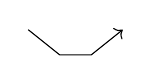
\begin{tikzpicture}[scale=0.4]
		\draw[->] (0, 0.8) -- (1, 0) -- (2, 0) -- (3, 0.8);
	\end{tikzpicture}
	does not use addition on $\Hom$ sets, only finite products and coproducts, the zero object, and their canonical maps. For (iii), all finite products or coproducts are built from zero objects and binary biproducts. Finally, a left adjoint preserves $\varinjlim$, a right adjoint preserves $\varprojlim$ (\cite[Theorem~2.8.12]{Li1}), and equivalences preserve all limits. Thus (iv) and (v) follow from (ii).
\end{proof}

% segment-id: o014.li2.chapter1.additive-categories-kernels-cokernels.p010
In fact, Proposition~\ref{prop:additive-cat-addition} shows that ``additivity'' is a property of the underlying category $\mathcal C$, not additional structure.

% segment-id: o014.li2.chapter1.additive-categories-kernels-cokernels.d002
\begin{definition}
	\index{kernel}\index[sym1]{kerf@$\Ker(f)$}
	\index{cokernel}\index[sym1]{cokerf@$\Coker(f)$}
	Let $\mathcal C$ be an $\cate{Ab}$-category with a zero object, and $f:X\to Y$ a morphism.
	% segment-id: o014.li2.chapter1.additive-categories-kernels-cokernels.l006
	\begin{itemize}
		% segment-id: o014.li2.chapter1.additive-categories-kernels-cokernels.i014
		\item If the equalizer $\Ker(f,0)$ exists, then $\Ker(f):=\Ker(f,0)$ together with $\Ker(f)\hookrightarrow X$ is the \emph{kernel} of $f$.
		% segment-id: o014.li2.chapter1.additive-categories-kernels-cokernels.i015
		\item If the coequalizer $\Coker(f,0)$ exists, then $\Coker(f):=\Coker(f,0)$ together with $Y\twoheadrightarrow\Coker(f)$ is the \emph{cokernel} of $f$.
	\end{itemize}
	Thus the composites $\Ker(f)\to X\to Y$ and $X\to Y\to\Coker(f)$ are both $0$.
\end{definition}

% segment-id: o014.li2.chapter1.additive-categories-kernels-cokernels.p011
Kernels and cokernels admit several complementary viewpoints.
% segment-id: o014.li2.chapter1.additive-categories-kernels-cokernels.l007
\begin{itemize}
	% segment-id: o014.li2.chapter1.additive-categories-kernels-cokernels.i016
	\item For a morphism $g:T\to X$ satisfying $fg=0$,\footnote{Translator's note: the source says ``for every morphism'' without including the condition $fg=0$, or dually $hf=0$. These conditions have been restored because they are precisely the equalizer and coequalizer hypotheses; see correction O014-C006.} the universal property of $\Ker(f)=\Ker(f,0)$ is the commutative diagram
	% segment-id: o014.li2.chapter1.additive-categories-kernels-cokernels.g007
	\[\begin{tikzcd}
		& T \arrow[dashrightarrow, ld, "{\exists! g'}"'] \arrow[d, "g"] \arrow[rd, "0"] & \\
		\Ker(f) \arrow[r] & X \arrow[r, "f"'] & Y .
	\end{tikzcd}\]
	% segment-id: o014.li2.chapter1.additive-categories-kernels-cokernels.i017
	\item For a morphism $h:Y\to T$ satisfying $hf=0$, the universal property of $\Coker(f)=\Coker(f,0)$ is
	% segment-id: o014.li2.chapter1.additive-categories-kernels-cokernels.g008
	\[\begin{tikzcd}
		X \arrow[r, "f"] \arrow[rd, "0"'] & Y \arrow[r] \arrow[d, "h"] & \Coker(f) \arrow[dashrightarrow, ld, "{\exists! h'}"] . \\
		& T &
	\end{tikzcd}\]
	% segment-id: o014.li2.chapter1.additive-categories-kernels-cokernels.i018
	\item The constructions are dual: $\Coker(f)=\Ker(f^{\opp})$ and $\Ker(f)=\Coker(f^{\opp})$.
\end{itemize}

% segment-id: o014.li2.chapter1.additive-categories-kernels-cokernels.p012
Since precisely the zero morphisms factor through a zero object, the universal properties are also characterized by the pullback and pushout diagrams

% segment-id: o014.li2.chapter1.additive-categories-kernels-cokernels.g009
\begin{equation}\label{eqn:Ker-Coker-triangles}
	\begin{tikzcd}
		\Ker(f) \arrow[phantom, r, "\simeq" description] & X \dtimes{Y} 0 \arrow[r] \arrow[d] \arrow[phantom, rd, "\Box" description] & X \arrow[d, "f"] \\
		& 0 \arrow[r] & Y
	\end{tikzcd} \qquad \begin{tikzcd}
		X \arrow[r, "f"] \arrow[d] & Y \arrow[d] & \\
		0 \arrow[r] & Y \dsqcup{X} 0 \arrow[phantom, lu, "\boxplus" description] & \Coker(f) \arrow[phantom, l, "\simeq" description] .
\end{tikzcd}\end{equation}

% segment-id: o014.li2.chapter1.additive-categories-kernels-cokernels.r001
\begin{remark}\label{rem:equalizer-Ker}
	An arbitrary equalizer reduces to a kernel. For
	% segment-id: o014.li2.chapter1.additive-categories-kernels-cokernels.g010
	\[\begin{tikzcd}
	T \arrow[r, "h"] & X \arrow[r, yshift=0.2em, "f"] \arrow[r, yshift=-0.2em, "g"'] & Y
	\end{tikzcd}, \]
	the condition $fh=gh$ is equivalent to $(f-g)h=0$, hence $\Ker(f,g)=\Ker(f-g,0)=:\Ker(f-g)$. Dually, $\Coker(f,g)=\Coker(f-g,0)=:\Coker(f-g)$.
\end{remark}

% segment-id: o014.li2.chapter1.additive-categories-kernels-cokernels.p013
From now on, $\mathcal C$ will mainly be additive.

% segment-id: o014.li2.chapter1.additive-categories-kernels-cokernels.pr003
\begin{proposition}\label{prop:Ker-Coker-composite}
	For morphisms $X\xrightarrow{f}Y\xrightarrow{g}Z$ in an additive category $\mathcal C$, there are commutative diagrams
	% segment-id: o014.li2.chapter1.additive-categories-kernels-cokernels.g011
	\[\begin{tikzcd}[row sep=small, column sep=small]
		\Ker(gf) \arrow[rr, "\sim"] \arrow[hookrightarrow, rd] & & X \dtimes{Y} \Ker(g) \arrow[hookrightarrow, ld] \\
		& X &
	\end{tikzcd} \quad \begin{tikzcd}[row sep=small, column sep=small]
		Z \dsqcup{Y} \Coker(f) \arrow[rr, "\sim"] & & \Coker(gf) \\
		& Z \arrow[twoheadrightarrow, lu] \arrow[twoheadrightarrow, ru] &
	\end{tikzcd}\]
	where $X\dtimes{Y}\Ker(g)\to X$ (respectively $Z\to Z\dsqcup{Y}\Coker(f)$) is the canonical morphism of the fiber product (respectively fiber coproduct),\footnote{Translator's note: the source says ``coproduct,'' but the displayed object is the fiber coproduct $Z\dsqcup{Y}\Coker(f)$ and the proof uses duality with the fiber product; see correction O014-C005.} provided all indicated kernels, cokernels, and limits exist.
\end{proposition}

% segment-id: o014.li2.chapter1.additive-categories-kernels-cokernels.pf004
\begin{proof}
	By \eqref{eqn:Ker-Coker-triangles}, iterated fiber products give canonical isomorphisms $\Ker(gf)\simeq X\dtimes{Z}0\simeq X\dtimes{Y}(Y\dtimes{Z}0)\simeq X\dtimes{Y}\Ker(g)$. Duality gives the cokernel statement.
\end{proof}

% segment-id: o014.li2.chapter1.additive-categories-kernels-cokernels.p014
Functoriality of equalizers and coequalizers induces functoriality of kernels and cokernels, characterized by

% segment-id: o014.li2.chapter1.additive-categories-kernels-cokernels.g012
\begin{equation}\label{eqn:Ker-Coker-functoriality}\begin{tikzcd}
		\Ker(f) \arrow[r] \arrow[dashrightarrow, d, "\exists!"'] & X \arrow[d, "a"'] \arrow[r, "f"] & Y \arrow[d, "b"] \\
		\Ker(g) \arrow[r] & X' \arrow[r, "g"'] & Y'
	\end{tikzcd} \qquad \begin{tikzcd}
		X \arrow[d, "a"'] \arrow[r, "f"] & Y \arrow[d, "b"] \arrow[r] & \Coker(f) \arrow[dashrightarrow, d, "\exists!"'] \\
		X' \arrow[r, "g"'] & Y' \arrow[r] & \Coker(g) .
\end{tikzcd}\end{equation}

% segment-id: o014.li2.chapter1.additive-categories-kernels-cokernels.p015
The next result says that pullback preserves kernels and pushout preserves cokernels.

% segment-id: o014.li2.chapter1.additive-categories-kernels-cokernels.pr004
\begin{proposition}\label{prop:pull-back-ker}
	If
	% segment-id: o014.li2.chapter1.additive-categories-kernels-cokernels.g013
	\[\begin{tikzcd}
		X \arrow[r, "f"] \arrow[d, "a"'] & Y \arrow[d, "b"] \\
		X' \arrow[r, "g"'] & Y'
	\end{tikzcd}\]
	is a pullback (respectively pushout) square in an additive category, then the morphism $\Ker(f)\to\Ker(g)$ (respectively $\Coker(f)\to\Coker(g)$) of \eqref{eqn:Ker-Coker-functoriality} is an isomorphism, provided the indicated objects exist.
\end{proposition}

% segment-id: o014.li2.chapter1.additive-categories-kernels-cokernels.pf005
\begin{proof}
	By duality it suffices to treat pullbacks. For every $T$, the universal properties give canonical isomorphisms
	% segment-id: o014.li2.chapter1.additive-categories-kernels-cokernels.a001
	\begin{align*}
		\Hom(T, \Ker(f)) & \simeq \Ker\left[ \Hom(T, X) \to \Hom(T, Y) \right] \\
		& \simeq \Ker\left[ \Hom(T, Y) \dtimes{\Hom(T, Y')} \Hom(T, X') \to \Hom(T, Y) \right] \\
		& = \Ker\left[ \Hom(T, X') \to \Hom(T, Y') \right] \simeq \Hom(T, \Ker(g)),
	\end{align*}
	and the Yoneda lemma gives $\Ker(f)\rightiso\Ker(g)$; see
	Theorem~\sourcecrossref{prop:Yoneda}{A.1.1}.
\end{proof}

% segment-id: o014.li2.chapter1.additive-categories-kernels-cokernels.lm001
\begin{lemma}\label{prop:mono-epi-ker-coker}
	Let $\mathcal C$ be additive and $f:X\to Y$ a morphism.
	% segment-id: o014.li2.chapter1.additive-categories-kernels-cokernels.l008
	\begin{enumerate}[(i)]
		% segment-id: o014.li2.chapter1.additive-categories-kernels-cokernels.i019
		\item $f$ is monic (respectively epic) if and only if $\Ker(f)=0$ (respectively $\Coker(f)=0$).
		% segment-id: o014.li2.chapter1.additive-categories-kernels-cokernels.i020
		\item $f$ is zero if and only if $\Ker(f)\rightiso X$, equivalently $Y\rightiso\Coker(f)$.
		% segment-id: o014.li2.chapter1.additive-categories-kernels-cokernels.i021
		\item Given $k:Y\to Z$ (respectively $k':W\to X$), there is a unique morphism making the corresponding diagram commute:
		% segment-id: o014.li2.chapter1.additive-categories-kernels-cokernels.g014
		\[\begin{tikzcd}[row sep=small, column sep=small]
		\Ker(kf) \arrow[rd] & & \Ker(f) \arrow[ld] \arrow[hookrightarrow, ll, "\exists !"'] \\
		& X &
		\end{tikzcd} \quad \text{or} \quad
		\begin{tikzcd}[row sep=small, column sep=small]
		\Coker(fk') \arrow[twoheadrightarrow, rr, "\exists !"] & & \Coker(f) \\
		& Y \arrow[lu] \arrow[ru] &
		\end{tikzcd}\]
		provided the indicated kernels or cokernels exist. If $k$ is monic (respectively $k'$ is epic), then $\Ker(f)\rightiso\Ker(kf)$ (respectively $\Coker(fk')\rightiso\Coker(f)$).
	\end{enumerate}
\end{lemma}

% segment-id: o014.li2.chapter1.additive-categories-kernels-cokernels.pf006
\begin{proof}
	For (i), by duality consider only monomorphisms. By definition, $f$ is monic precisely when $f(g_1-g_2)=0\iff g_1-g_2=0$ for every $g_1,g_2:T\to X$. Equivalently, every $g:T\to X$ with $fg=0$ factors through $T\to0\to X$, exactly the universal property of $\Ker(f)=0$. For (ii), $f=0\iff\Ker(f,0)\rightiso X$ follows from the definition of an equalizer. For (iii), use
	% segment-id: o014.li2.chapter1.additive-categories-kernels-cokernels.g015
	\[\begin{tikzcd}[column sep=small]
		\left\{ g \in \Hom(T, X): fg=0 \right\} \arrow[phantom, r, "\subset" description] & \left\{ g \in \Hom(T, X): kfg=0 \right\} \\
		\Hom(T, \Ker(f)) \arrow[u, "1:1"] & \Hom(T, \Ker(kf)) \arrow[u, "1:1"']
	\end{tikzcd}\]
	The top inclusion is equality when $k$ is monic. Apply the Yoneda lemma.
\end{proof}

% segment-id: o014.li2.chapter1.additive-categories-kernels-cokernels.p016
In an additive category, the image and coimage of Definition~\ref{def:Im-Coim} have simple descriptions.

% segment-id: o014.li2.chapter1.additive-categories-kernels-cokernels.pr005
\begin{proposition}\label{prop:Im-Coim-additive}
	\index{image}\index{coimage}
	\index[sym1]{imf@$\Image(f)$}\index[sym1]{coimf@$\Coim(f)$}
	For $f:X\to Y$ in an additive category $\mathcal C$, there are canonical isomorphisms
	% segment-id: o014.li2.chapter1.additive-categories-kernels-cokernels.a002
	\begin{align*}
		\Image(f) & \simeq \Ker\left[ Y \to \Coker(f) \right] \hookrightarrow Y, \\
		\Coim(f) & \simeq \Coker\left[ \Ker(f) \to X \right] \twoheadleftarrow X ;
	\end{align*}
	provided the indicated kernels and cokernels exist.
\end{proposition}

% segment-id: o014.li2.chapter1.additive-categories-kernels-cokernels.pf007
\begin{proof}
	By duality consider only $\Image(f)$. Let $i_1,i_2:Y\to Y\dsqcup{X}Y$ be canonical. By Yoneda it suffices to verify, for every $T$,
	% segment-id: o014.li2.chapter1.additive-categories-kernels-cokernels.q008
	\begin{multline*}
		\Hom\left( T, \Image(f) \right) = \left\{ h: T \to Y \;\middle|\; i_1 h = i_2 h \right\} \\
		= \left\{ \begin{array}{r|l}
			h: T \to Y & \forall S \in \Obj(\mathcal{C}),\; \forall s_1, s_2: Y \to S, \\
			& s_1 f = s_2 f \implies s_1 h = s_2 h
		\end{array}\right\} \\
		\xlongequal{s := s_1 - s_2} \left\{ \begin{array}{r|l}
			h: T \to Y & \forall S \in \Obj(\mathcal{C}),\; \forall s: Y \to S, \\
			& s f = 0 \implies sh = 0
		\end{array}\right\} \\
		= \left\{ \begin{array}{r|l}
			h: T \to Y & T \xrightarrow{h} Y \twoheadrightarrow \Coker(f) \\
			& \text{has composite}\; 0
		\end{array}\right\}
		\leftiso \Hom\left( T, \Ker\left[ Y \to \Coker(f) \right] \right).
	\end{multline*}
	The first equality is $\Image(f):=\Ker(i_1,i_2)$. For the second, rewrite the condition as $s'i_1h=s'i_2h$ for every $s':Y\dsqcup{X}Y\to S$ and use
	% segment-id: o014.li2.chapter1.additive-categories-kernels-cokernels.a003
	\begin{align*}
		\Hom\left( Y \dsqcup{X} Y, S \right) & \xrightarrow{1:1} \Hom(Y,S) \dtimes{\Hom(X,S)} \Hom(Y,S) \\
		s' & \longmapsto \left( s' i_1, s' i_2 \right) =: (s_1, s_2).
	\end{align*}
	The fourth equality follows from the cokernel's universal property, reducing to $S=\Coker(f)$.
\end{proof}

% segment-id: o014.li2.chapter1.additive-categories-kernels-cokernels.p017
If $f=0$, Lemma~\ref{prop:mono-epi-ker-coker}(ii) gives the simplest example: $\Image(f)=0=\Coim(f)$.

% segment-id: o014.li2.chapter1.additive-categories-kernels-cokernels.e002
\begin{example}\label{eg:strict-morphism}
	Continuing Example~\ref{eg:additive-category}, consider $R\dcate{Mod}$. A module homomorphism $f:A\to B$ always has $\Ker(f)=f^{-1}(0)$ and $\Coker(f)=B/\{f(a):a\in A\}$. Its $\Image(f)$ is the set-theoretic image, $\Coim(f)=A/\Ker(f)$, and the comparison in \eqref{eqn:strict-morphism} is the canonical module isomorphism $A/\Ker(f)\rightiso\Image(f)$. Thus every morphism in $R\dcate{Mod}$ is strict.

	Next consider the additive category $\cate{Ban}_{\CC}$ from
	Example~\ref{eg:additive-category}. A continuous linear map $f:X\to Y$ has
	the usual kernel $\Ker(f)=f^{-1}(0)$, which is again a Banach space, while
	$\Coker(f)=Y/\overline{\{f(x):x\in X\}}$ carries the quotient norm. The
	comparison morphism in \eqref{eqn:strict-morphism} becomes
	% segment-id: o014.li2.chapter1.additive-categories-kernels-cokernels.g016
	\[\begin{tikzcd}[row sep=small, column sep=small]
	\Coim(f) \arrow[equal, r] & X/f^{-1}(0) \arrow[r] & \overline{\left\{ f(x): x \in X \right\}} \arrow[equal, r] & \Image(f) \\
	& x + f^{-1}(0) \arrow[mapsto, r] \arrow[phantom, u, "\in" description, sloped] & f(x) \arrow[phantom, u, "\in" description, sloped] &
	\end{tikzcd}\]
	where the right side has the topology induced from $Y$ and the left the quotient topology from $X$. If $f:X\to Y$ is a continuous injective linear map of Banach spaces with dense, non-surjective image, then $\Coim(f)=X\to Y=\Image(f)$ is not an isomorphism. Hence $\cate{Ban}_{\CC}$ has non-strict morphisms.
\end{example}

% English translation of chapter1.tex, lines 568--629.
% Source: Methods of Algebra, Volume 2, commit
% 9a5803ff77dd3257484cb177f851a73770a59dd3 (CC BY 4.0).
% stable-unit-id: o014.aljabr2.chapter1.linear-categories-over-commutative-rings

% segment-id: o014.li2.chapter1.linear-categories-over-commutative-rings.h001
\section{Generalization: Linear Categories over a Commutative Ring}\label{sec:linear-cat}
\hypertarget{o014.aljabr2.chapter1.linear-categories-over-commutative-rings}{ }

% segment-id: o014.li2.chapter1.linear-categories-over-commutative-rings.p001
The $\Hom$ sets of an additive category have the structure of abelian groups.
In many situations they also carry scalar multiplication by some commutative
ring $\Bbbk$. For example, every $\Hom$ set in $\Bbbk\dcate{Mod}$ is naturally
a $\Bbbk$-module, and composition of morphisms is $\Bbbk$-bilinear.

% segment-id: o014.li2.chapter1.linear-categories-over-commutative-rings.d001
\begin{definition}\label{def:cat-k-linear}
	\index{category!$\Bbbk\dcate{Mod}$-}
	\index{linear!$\Bbbk$- ($\Bbbk$-linear)}
	Let $\Bbbk$ be a commutative ring. Suppose that every $\Hom$ set in a
	category $\mathcal{A}$ is equipped with a $\Bbbk$-module structure such that
	composition of morphisms
	$\Hom(Y, Z) \times \Hom(X, Y) \to \Hom(X, Z)$ is a $\Bbbk$-bilinear map
	for all objects $X,Y,Z$; in other words, the following diagram commutes:
	% segment-id: o014.li2.chapter1.linear-categories-over-commutative-rings.g001
	\[\begin{tikzcd}
		\Hom(Y, Z) \times \Hom(X, Y) \arrow[d] \arrow[r, "\text{composition}"] & \Hom(X, Z) \\
		\Hom(Y, Z) \dotimes{\Bbbk} \Hom(X, Y) \arrow[ru, bend right, start anchor=east, "{\exists! \; \text{$\Bbbk$-module homomorphism}}"']
	\end{tikzcd}  \]
	With these data, $\mathcal{A}$ is called a \emph{$\Bbbk\dcate{Mod}$-category}.

	Let $F: \mathcal{A} \to \mathcal{A}'$ be a functor between
	$\Bbbk\dcate{Mod}$-categories. If the map
	$\Hom(X,Y) \to \Hom(FX,FY)$ is a $\Bbbk$-module homomorphism for every
	$X,Y \in \Obj(\mathcal{A})$, then $F$ is called a
	\emph{$\Bbbk$-linear functor}.
\end{definition}

% segment-id: o014.li2.chapter1.linear-categories-over-commutative-rings.p002
Observe that $\Bbbk\dcate{Mod}$ is a monoidal category under the tensor product
$\otimes := \dotimes{\Bbbk}$. Thus the term ``$\Bbbk\dcate{Mod}$-category''
agrees with the terminology for enriched categories in \cite[\S 3.4]{Li1}.
The $\cate{Ab}$-categories introduced earlier are precisely the
$\Z\dcate{Mod}$-categories. Conversely, forgetting scalar multiplication on a
$\Bbbk\dcate{Mod}$-category leaves an $\cate{Ab}$-category.

% segment-id: o014.li2.chapter1.linear-categories-over-commutative-rings.e001
\begin{example}
	A $\Bbbk\dcate{Mod}$-category with a single object is nothing but a
	$\Bbbk$-algebra. The correspondence is given by
	$\mathcal{A} \mapsto \End_{\mathcal{A}}(\star)$, where
	$\Obj(\mathcal{A}) = \{\star\}$.
\end{example}

% segment-id: o014.li2.chapter1.linear-categories-over-commutative-rings.p003
The argument of Proposition~\ref{prop:automatic-Ab-morphism} carries over
verbatim and gives the following result.

% segment-id: o014.li2.chapter1.linear-categories-over-commutative-rings.pr001
\begin{proposition}\label{prop:automatic-k-morphism}
	Let $\mathcal{A}$ and $\mathcal{A}'$ be $\Bbbk\dcate{Mod}$-categories.
	% segment-id: o014.li2.chapter1.linear-categories-over-commutative-rings.l001
	\begin{enumerate}
		% segment-id: o014.li2.chapter1.linear-categories-over-commutative-rings.i001
		\item Given a pair of adjoint functors
		% The originally inline source adjunction diagram was reflowed as a
		% centered display so that it neither crowds nor overruns the reader width.
		% The long chain of equivalences in the proof was likewise reflowed.
		% segment-id: o014.li2.chapter1.linear-categories-over-commutative-rings.g002
		\[
		\begin{tikzcd}
			F: \mathcal{A} \arrow[shift left, r] & \mathcal{A}' \arrow[shift left, l] : G
		\end{tikzcd},
		\]
		with both $F$ and $G$ $\Bbbk$-linear, the adjunction isomorphism
		$\Hom_{\mathcal{A}'}(F(\cdot),\cdot) \rightiso
		\Hom_{\mathcal{A}}(\cdot,G(\cdot))$ is $\Bbbk$-linear.
		% segment-id: o014.li2.chapter1.linear-categories-over-commutative-rings.i002
		\item For every $\alpha: I \to \mathcal{A}$, the bijection
		% segment-id: o014.li2.chapter1.linear-categories-over-commutative-rings.q001
		\[
			\Hom_{\mathcal{A}}\left(\varinjlim \alpha,T\right)
			\simeq \varprojlim_{i \in \Obj(I)}
			\Hom_{\mathcal{A}}(\alpha(i),T),
			\quad T \in \Obj(\mathcal{A})
		\]
		is $\Bbbk$-linear whenever $\varinjlim \alpha$ exists. The same statement
		holds for $\varprojlim$.
	\end{enumerate}
\end{proposition}

% segment-id: o014.li2.chapter1.linear-categories-over-commutative-rings.p004
Unless otherwise specified, all functors and equivalences between
$\Bbbk\dcate{Mod}$-categories will henceforth be understood to be
$\Bbbk$-linear.

% segment-id: o014.li2.chapter1.linear-categories-over-commutative-rings.d002
\begin{definition}\label{def:k-linear-cat}
	\index{category!$\Bbbk$-linear ($\Bbbk$-linear)}
	If an additive category $\mathcal{A}$ is equipped with a $\Bbbk$-linear
	structure compatible with its existing $\cate{Ab}$-category structure, then
	$\mathcal{A}$ together with these data is called a
	\emph{$\Bbbk$-linear category}.
\end{definition}

% segment-id: o014.li2.chapter1.linear-categories-over-commutative-rings.p005
This amounts to replacing the $\cate{Ab}$-category by a
$\Bbbk\dcate{Mod}$-category in the discussion of \S\ref{sec:Ker-Coker}. Most
results about additive categories in this chapter extend to the $\Bbbk$-linear
setting by exactly the same arguments. The sole exception concerns
Corollary~\ref{prop:automatic-additivity}: in an additive category, addition on
the $\Hom$ sets can be characterized by properties of the category itself, but
this is not true of scalar multiplication by $\Bbbk$. Consequently,
functors---and even equivalences---between $\Bbbk$-linear categories are not
automatically $\Bbbk$-linear.

% segment-id: o014.li2.chapter1.linear-categories-over-commutative-rings.p006
We next collect a few results concerning $\Bbbk$-linearity. Recall that the
\emph{center} of a category $\mathcal{A}$ is defined by
\index{center} \index[sym1]{ZA@$Z(\mathcal{A})$}
$Z(\mathcal{A}) := \End(\identity_{\mathcal{A}})$. Its elements are
endomorphisms of the identity functor $\identity_{\mathcal{A}}$, written as
$(a_X)_{X \in \Obj(\mathcal{A})}$ with
$a_X \in \End_{\mathcal{A}}(X)$. Composition makes the center a commutative
monoid; see \cite[Definition 2.3.8,
Proposition 2.3.9]{Li1}. If $\mathcal{A}$ is an $\cate{Ab}$-category, then
$Z(\mathcal{A})$ becomes a commutative ring under composition and addition
$(a_X)_X + (b_X)_X := (a_X+b_X)_X$.

% segment-id: o014.li2.chapter1.linear-categories-over-commutative-rings.pr002
\begin{proposition}\label{prop:k-linear-center}
	Let $\mathcal{A}$ be an $\cate{Ab}$-category. Then there is a bijection
	% segment-id: o014.li2.chapter1.linear-categories-over-commutative-rings.q002
	\[
		\left\{\text{$\Bbbk\dcate{Mod}$-category structures on $\mathcal{A}$}\right\}
		\stackrel{1:1}{\longleftrightarrow}
		\Hom_{\text{rings}}(\Bbbk,Z(\mathcal{A})).
	\]
	The map is given as follows. If a $\Bbbk\dcate{Mod}$-category structure on
	$\mathcal{A}$ has been fixed, define, for every $a \in \Bbbk$ and
	$X \in \Obj(\mathcal{A})$,
	$a_X := a \cdot \identity_X \in \End_{\mathcal{A}}(X)$. Then
	$a \mapsto (a_X)_{X \in \Obj(\mathcal{A})} \in Z(\mathcal{A})$ is a ring
	homomorphism. Conversely, given a ring homomorphism on the right,
	$a \mapsto (a_X)_{X \in \Obj(\mathcal{A})}$, define a
	$\Bbbk\dcate{Mod}$-category structure on $\mathcal{A}$ by
	$a \cdot f := f \circ a_X = a_Y \circ f$, for $f \in \Hom(X,Y)$.
\end{proposition}

% segment-id: o014.li2.chapter1.linear-categories-over-commutative-rings.pf001
\begin{proof}
	The condition for $(a_X)_{X \in \Obj(\mathcal{A})}$ to belong to
	$Z(\mathcal{A})$ is precisely
	$f \circ a_X = a_Y \circ f$ for every $f \in \Hom(X,Y)$. If
	$\mathcal{A}$ is equipped with a $\Bbbk\dcate{Mod}$-category structure,
	define $a_X := a \cdot \identity_X$. Bilinearity gives
	\[
		f \circ a_X = f \circ (a \cdot \identity_X)
		= (a f) \circ \identity_X
		= (a \cdot \identity_Y) \circ f
		= a_Y \circ f,
	\]
	so $(a_X)_{X \in \Obj(\mathcal{A})} \in Z(\mathcal{A})$.
	The remaining verifications are immediate.
\end{proof}

% segment-id: o014.li2.chapter1.linear-categories-over-commutative-rings.p007
Consequently, the $\cate{Ab}$-category $\mathcal{A}$ is naturally a
$Z(\mathcal{A})\dcate{Mod}$-category.

% Complete English translation of chapter1.tex, lines 630--762.
% Source: Methods of Algebra, Volume 2, commit
% 9a5803ff77dd3257484cb177f851a73770a59dd3 (CC BY 4.0).
% stable-unit-id: o014.aljabr2.chapter1.limits-through-functors

% segment-id: o014.li2.chapter1.limits-through-functors.h001
\section{Viewing Limits through Functors}\label{sec:limit-functor}
\hypertarget{o014.aljabr2.chapter1.limits-through-functors}{ }

% segment-id: o014.li2.chapter1.limits-through-functors.p001
There are two broad kinds of question about the relationship between a functor
$F: \mathcal{C} \to \mathcal{D}$ and limits. Taking $\varinjlim$ as an
example, let $\alpha: I \to \mathcal{C}$ be a functor. One may ask:
% segment-id: o014.li2.chapter1.limits-through-functors.l001
\begin{itemize}
	% segment-id: o014.li2.chapter1.limits-through-functors.i001
	\item Suppose $\varinjlim \alpha$ exists. Does its image
	$F\left(\varinjlim \alpha\right)$ yield $\varinjlim (F\alpha)$?
	% segment-id: o014.li2.chapter1.limits-through-functors.i002
	\item Suppose $\varinjlim F\alpha$ exists. Can this limit be ``lifted'' to
	$\mathcal{C}$? In what sense is such a lift unique?
\end{itemize}

% segment-id: o014.li2.chapter1.limits-through-functors.p002
We focus on the case of $\varinjlim$. These results of course have
corresponding versions for $\varprojlim$; by duality, there is no need to
repeat the details.

% segment-id: o014.li2.chapter1.limits-through-functors.p003
We organize the discussion of $\varinjlim$ in terms of cocones and the category
$(\alpha/\Delta)$.

% segment-id: o014.li2.chapter1.limits-through-functors.c001
\begin{convention}\label{con:limit-cone}
	For a fixed functor $\alpha: I \to \mathcal{C}$, a collection of data
	$(L, (f_i)_{i \in \Obj(I)})$ in $\mathcal{C}$ satisfying the following
	conditions is called a \emph{cocone} with base $\alpha$ and vertex $L$:
	% segment-id: o014.li2.chapter1.limits-through-functors.l002
	\begin{compactitem}
		% segment-id: o014.li2.chapter1.limits-through-functors.i003
		\item $L$ is an object of $\mathcal{C}$;
		% segment-id: o014.li2.chapter1.limits-through-functors.i004
		\item each $f_i : \alpha(i) \to L$ is a morphism in $\mathcal{C}$ and
		satisfies the compatibility condition
		$f_j \circ \alpha(i \to j) = f_i$, as $[i \to j]$ ranges over
		$\mathrm{Mor}(I)$.
	\end{compactitem}
\end{convention}

% segment-id: o014.li2.chapter1.limits-through-functors.p004
In the terminology of \cite[\S 2.7]{Li1}, these cocones form a
category\footnote{More precisely, $\Delta$ here denotes the diagonal functor
$\mathcal{C} \to \mathcal{C}^I$; see Example
\sourcecrossref{eg:comma-vs-cone}{1.6.3}. The notation $\Delta$ was chosen from
the initial letter of the pinyin word \emph{duìjiǎo} (``diagonal''). By a
pictorial analogy, however, one may just as well picture $\Delta$ as a
``cocone''; see
diagram \eqref{eqn:injlim-diagram}.} $(\alpha / \Delta)$. Concretely, once the
base $\alpha$ is fixed, a morphism from a cocone $(L, (f_i)_i)$ to a cocone
$(M, (g_i)_i)$ is a commutative diagram
% segment-id: o014.li2.chapter1.limits-through-functors.g001
\begin{equation}\label{eqn:injlim-diagram}\begin{tikzcd}
	& L \arrow[d] & \\
	\alpha(i) \arrow[bend right, rr, "\alpha(i \to j)"'] \arrow[r, "g_i"] \arrow[ru, "f_i"] & M & \alpha(j) \arrow[l, "{g_j}"'] \arrow[lu, "f_j"']
\end{tikzcd}\end{equation}
as $i \to j$ ranges over $\Mor(I)$; composition of morphisms is defined in
the usual way. By definition, $\varinjlim \alpha$, together with its family
of canonical morphisms $\iota_i: \alpha(i) \to \varinjlim \alpha$, is an
initial object of $(\alpha / \Delta)$.
\index{limit}\index[sym1]{lim}

% segment-id: o014.li2.chapter1.limits-through-functors.p005
In the evident way, the functor $F$ induces a functor
$(\alpha/\Delta) \to (F\alpha / \Delta)$ that takes a cocone
$(L, (f_i)_i)$ to $(FL, (Ff_i)_i)$. Suppose $\varinjlim \alpha$ exists. If
$\varinjlim F\alpha$ also exists, there is a unique morphism in
$(F\alpha / \Delta)$
% segment-id: o014.li2.chapter1.limits-through-functors.q001
\[ \varinjlim F\alpha \to F(\varinjlim \alpha), \]
and this morphism is an isomorphism if and only if
$\left( F(\varinjlim \alpha), (F\iota_i)_i \right)$ gives
$\varinjlim F\alpha$.

% segment-id: o014.li2.chapter1.limits-through-functors.p006
Dually, $\varprojlim \alpha$ is characterized as a terminal object of
$(\Delta/\alpha)$. Assuming that both projective limits under discussion
exist, there is a unique morphism in $(\Delta/F\alpha)$
% segment-id: o014.li2.chapter1.limits-through-functors.q002
\[ F\varprojlim \alpha \to \varprojlim F\alpha. \]

% segment-id: o014.li2.chapter1.limits-through-functors.d001
\begin{definition}\label{def:create-limit}
	\index{limit!preserve, reflect, create}
	Given $F: \mathcal{C} \to \mathcal{D}$ and a functor
	$\alpha: I \to \mathcal{C}$, consider the induced functor between cocone
	categories $(\alpha/\Delta) \to (F\alpha/\Delta)$.
	% segment-id: o014.li2.chapter1.limits-through-functors.l003
	\begin{itemize}
		% segment-id: o014.li2.chapter1.limits-through-functors.i005
		\item The functor $F$ is said to \emph{preserve} this $\varinjlim$ if
		$(\alpha/\Delta) \to (F\alpha/\Delta)$ takes an initial object, when
		one exists, to an initial object.
		% segment-id: o014.li2.chapter1.limits-through-functors.i006
		\item The functor $F$ is said to \emph{reflect} this $\varinjlim$ if any
		object of $(\alpha/\Delta)$ whose image is an initial object of
		$(F\alpha/\Delta)$ is itself an initial object.
		% segment-id: o014.li2.chapter1.limits-through-functors.i007
	\item The functor $F$ is said to \emph{create} this $\varinjlim$ if,
	whenever $\varinjlim F\alpha$ exists, $\varinjlim \alpha$ also exists,
	and in this situation $F$ preserves this $\varinjlim$ and also reflects
	this $\varinjlim$.
	\end{itemize}
	There are corresponding notions for $\varprojlim$. The notions for
	$\varinjlim$ and $\varprojlim$ are obtained from one another by replacing
	$\mathcal{C}$ and $\mathcal{D}$ with $\mathcal{C}^{\opp}$ and
	$\mathcal{D}^{\opp}$.
\end{definition}

% segment-id: o014.li2.chapter1.limits-through-functors.p007
Notice that these notions depend on the particular $\alpha$ under
consideration. For example, $F$ may well preserve every finite
$\varinjlim$ without preserving $\varinjlim$ in general.

% segment-id: o014.li2.chapter1.limits-through-functors.p008
For a fixed $\alpha$, saying that a functor creates $\varinjlim$ (or
$\varprojlim$) means that the cocone (or cone) in $\mathcal{D}$ defining the
limit can be lifted uniquely to $\mathcal{C}$, and that the lifted cocone (or
cone) gives the corresponding limit in $\mathcal{C}$. This uniqueness comes
from the condition in the definition concerning reflection of $\varinjlim$
(or $\varprojlim$). This point of view will be evident in
Example~\ref{eg:Grp-Set-create} and Proposition~\ref{prop:forget-create} below.

% segment-id: o014.li2.chapter1.limits-through-functors.pr001
\begin{proposition}\label{prop:ff-reflect}
	Every fully faithful functor reflects every $\varinjlim$ and every
	$\varprojlim$.
\end{proposition}
% segment-id: o014.li2.chapter1.limits-through-functors.pf001
\begin{proof}
	It suffices to consider $\varinjlim$. If $F$ is fully faithful, the
	universal property of an initial object of $(\alpha/\Delta)$ can be checked,
	after applying $F$, in $(F\alpha/\Delta)$.
\end{proof}

% segment-id: o014.li2.chapter1.limits-through-functors.p009
We shall also use the following notion.

% segment-id: o014.li2.chapter1.limits-through-functors.d002
\begin{definition}\label{def:conservative}
	\index{functor!conservative}
	A functor $F$ is called \emph{conservative} if it satisfies the following
	condition: a morphism $f \in \Mor(\mathcal{C})$ is an isomorphism if and
	only if $Ff \in \Mor(\mathcal{D})$ is an isomorphism.
\end{definition}

% segment-id: o014.li2.chapter1.limits-through-functors.r001
\begin{remark}\label{rem:conservative-reflect}
	Suppose $F$ is a conservative functor. If
	$\varinjlim \alpha$ exists and $F$ preserves this $\varinjlim$, the functor
	$F$ must also reflect it. Indeed, suppose
	$L \in \Obj((\alpha/\Delta))$ is mapped to an initial object of
	$(F\alpha/\Delta)$. Consider the unique morphism
	$\varinjlim \alpha \to L$ in $(\alpha/\Delta)$. Since $F$ preserves this
	$\varinjlim$, the image of that morphism under $F$ must be an isomorphism.
	Conservativity then ensures that $\varinjlim \alpha \to L$ is also an
	isomorphism.

	Under these hypotheses, the condition that $F$ reflect $\varinjlim$ may be
	omitted from the definition of what it means for $F$ to create
	$\varinjlim$.
\end{remark}

% segment-id: o014.li2.chapter1.limits-through-functors.e001
\begin{example}\label{eg:Grp-Set-create}
	We verify that the forgetful functor $U$ from the category of groups
	$\cate{Grp}$ to the category of sets $\cate{Set}$ creates all small
	$\varprojlim$.

	This follows from the concrete constructions of $\varprojlim$ in
	$\cate{Grp}$ and $\cate{Set}$; see
	\cite[Examples 2.7.5 and 2.8.7]{Li1}. More explicitly, take a small category
	$I$ and a functor $\beta: I^{\opp} \to \cate{Grp}$. As a set,
	% segment-id: o014.li2.chapter1.limits-through-functors.q003
	\[ \varprojlim U\beta = \left\{\begin{array}{r|l}
		(x_i)_i \in \prod_{i \in \Obj(I)} U\beta(i) & \forall [i \to j] \in \mathrm{Mor}(I), \\
		& \beta(i \to j)(x_j) = x_i
	\end{array}\right\}, \]
	and the projection $p_i: \varprojlim U\beta \to U\beta(i)$ maps $(x_j)_j$
	to $x_i$. Our task is now to:
	% segment-id: o014.li2.chapter1.limits-through-functors.l004
	\begin{enumerate}
		% segment-id: o014.li2.chapter1.limits-through-functors.i008
		\item equip $\varprojlim U\beta$ with a group structure such that every
		$p_i$ is a group homomorphism, and show that this group structure is
		unique;
		% segment-id: o014.li2.chapter1.limits-through-functors.i009
		\item verify the universal property of $\varprojlim \beta$ for this group
		together with the family of projection homomorphisms $(p_i)_i$.
	\end{enumerate}

	Clearly, $\varprojlim U\beta$ is a subgroup of the direct product
	$\prod_i \beta(i)$. Regard this subgroup as
	$\varprojlim \beta \in \Obj(\cate{Grp})$; this is the unique group structure
	making every $p_i$ a group homomorphism. This completes the first task.

	We next verify the universal property of the cone
	$\left( \varprojlim \beta, (p_i)_i\right)$. Consider any cone
	$(L, (q_i)_i)$ in $\cate{Grp}$, with $q_i: L \to \beta(i)$. The universal
	property gives a unique map $\varphi: UL \to \varprojlim U\beta$ such that
	$p_i \varphi = q_i$ for every $i$. Concretely, $\varphi$ is in fact given by
	$y \mapsto (q_i(y))_{i \in \Obj(I)}$, so this map is a group homomorphism
	$L \to \varprojlim \beta$.\footnote{Translator's note: the source writes
	$L \to \varinjlim \beta$; the target corrects this to
	$L \to \varprojlim \beta$, in accordance with the projective limit being
	proved (O014-C007).} The verification is complete.
\end{example}

% segment-id: o014.li2.chapter1.limits-through-functors.p010
By an entirely similar argument, one can show that the forgetful functor from
the category of compact Hausdorff spaces $\cate{CHaus}$ to $\cate{Set}$ also
creates all small $\varprojlim$. The corresponding verification is left as an
exercise in this chapter.

% segment-id: o014.li2.chapter1.limits-through-functors.p011
The next result concerns a functor category of the form $\mathcal{C}^J$ (which
may be a ``large'' category, but this causes no problem). We need two
preparatory steps.

% segment-id: o014.li2.chapter1.limits-through-functors.l005
\begin{itemize}
	% segment-id: o014.li2.chapter1.limits-through-functors.i010
	\item Let $J$ be a set. The product of $J$ copies of $\mathcal{C}$, namely
	$\mathcal{C}^J$, is defined by
	$\Obj\left(\mathcal{C}^J\right) = \Obj(\mathcal{C})^J$ and
	$\mathrm{Mor}\left(\mathcal{C}^J \right) = \mathrm{Mor}(\mathcal{C})^J$.
	For every $j \in J$ there is an evident projection functor
	$p_j: \mathcal{C}^J \to \mathcal{C}$.

	% Correction O014-C008: the source duplicates a character in the phrase
	% meaning ``for every.''
	Given a category $I$ and a functor $\alpha: I \to \mathcal{C}^J$, if
	$\varinjlim (p_j \alpha)$ exists for every $j$, then
	$\varinjlim \alpha$ also exists. It is constructed by taking colimits
	``pointwise'' or ``objectwise'':
	$\varinjlim \alpha = \left( \varinjlim (p_j \alpha) \right)_{j \in J}$.

	% segment-id: o014.li2.chapter1.limits-through-functors.i011
	\item Let $J$ be a category. We may consider the functor category
	$\mathcal{C}^J$. For each $j \in \Obj(J)$ there is an evaluation functor
	$\mathrm{ev}_j: \mathcal{C}^J \to \mathcal{C}$, which maps an object $F$
	to $Fj$ and a morphism
	$\varphi = (\varphi_{j'})_{j' \in \Obj(J)}$ to $\varphi_j$. We shall later
	consider functors of the form $\alpha: I \to \mathcal{C}^J$ and their
	$\varinjlim$. Observe that $\alpha$ can be viewed as a functor
	$I \times J \to \mathcal{C}$, whose value is denoted $\alpha(i, j)$.
\end{itemize}

% segment-id: o014.li2.chapter1.limits-through-functors.p012
The two systems of notation are compatible. If $J$ is a discrete category and
is viewed as a set, then $\mathcal{C}^J$ is simply the product discussed above.
For a general $J$, the forgetful functor
$\mathcal{F}: \mathcal{C}^J \to \mathcal{C}^{\Obj(J)}$ maps an object $F$ to
$(Fj)_{j \in \Obj(J)}$ and a morphism $\varphi$ to
$(\varphi_j)_{j \in \Obj(J)}$. Thus $\mathrm{ev}_j = p_j \mathcal{F}$.

% segment-id: o014.li2.chapter1.limits-through-functors.pr002
\begin{proposition}\label{prop:forget-create}
	Let $J$ and $\mathcal{C}$ be categories.
	% segment-id: o014.li2.chapter1.limits-through-functors.l006
	\begin{enumerate}[(i)]
		% segment-id: o014.li2.chapter1.limits-through-functors.i012
		\item The forgetful functor
		$\mathcal{F}: \mathcal{C}^J \to \mathcal{C}^{\Obj(J)}$ creates
		$\varinjlim$ and $\varprojlim$.
		% segment-id: o014.li2.chapter1.limits-through-functors.i013
		\item Let $I$ be a category and suppose every functor
		$I \to \mathcal{C}$ has a $\varinjlim$ (or $\varprojlim$). Then all
		functors of the form $I \to \mathcal{C}^J$ also have a $\varinjlim$ (or
		$\varprojlim$) in $\mathcal{C}^J$.
		% segment-id: o014.li2.chapter1.limits-through-functors.i014
		\item Under the assumption in (ii), for every $j \in \Obj(J)$ the
		evaluation functor $\mathrm{ev}_j: \mathcal{C}^J \to \mathcal{C}$
		preserves $\varinjlim$ (or $\varprojlim$) for diagrams of shape $I$.
		In other words, limits in $\mathcal{C}^J$ are likewise defined
		``pointwise'' or ``objectwise.''
	\end{enumerate}
\end{proposition}
% segment-id: o014.li2.chapter1.limits-through-functors.pf002
\begin{proof}
	It suffices to consider $\varinjlim$. For (i), let
	$\alpha: I \to \mathcal{C}^J$ and suppose $\varinjlim \mathcal{F}\alpha$
	exists and is given by the cocone
	% segment-id: o014.li2.chapter1.limits-through-functors.q004
	\[ \left( (X(j))_{j \in \Obj(J)}, \; \left( \iota_i = (\iota_{i, j})_{j \in \Obj(J)} \right)_{i \in \Obj(I)} \right) \]
	with $\iota_{i,j}: \alpha(i, j) \to X(j)$. We wish to lift it to a cocone
	in $\mathcal{C}^J$ that gives $\varinjlim \alpha$.

	First observe that $X(j) = \varinjlim \alpha(\cdot, j)$ for every $j$.
	For each morphism $j \to j'$, functoriality of colimits (see
	\cite[Lemma 2.7.4]{Li1}) gives a unique morphism
	$X(j \to j'): X(j) \to X(j')$ making the following diagram commute:
	% segment-id: o014.li2.chapter1.limits-through-functors.g002
	\[\begin{tikzcd}
		\alpha(i, j) \arrow[r] \arrow[d, "{\iota_{i, j}}"'] & \alpha(i, j') \arrow[d, "{\iota_{i, j'}}"] \\
		X(j) \arrow[r, "{X(j \to j')}"'] & X(j')
	\end{tikzcd} \quad i \in \Obj(I). \]
	In this way, $j \mapsto X(j)$ extends to a functor
	$X: J \to \mathcal{C}$, while $\iota_i: \alpha(i, \cdot) \to X$ are
	morphisms in $\mathcal{C}^J$. It is immediate that
	$(X, (\iota_i)_i) \in \Obj(\alpha/\Delta)$; we next prove that this object
	is initial. Since the functor $\mathcal{F}$ is conservative, reflection of
	$\varinjlim$ need not be checked separately.

	Given $(L, (f_i)_i) \in \Obj(\alpha/\Delta)$, the universal property of
	$\varinjlim \mathcal{F}\alpha$ determines a unique morphism
	$\varphi = (\varphi_j)_j : \mathcal{F}X \to \mathcal{F}L$ such that the
	triangular part of the following diagram commutes for every $(i, j)$:
	% segment-id: o014.li2.chapter1.limits-through-functors.g003
	\[\begin{tikzcd}
		& X(j) \arrow[d, "\varphi_j"] \arrow[r, "{X(j \to j')}" inner sep=0.8em] & X(j') \arrow[d, "\varphi_{j'}"] \\
		\alpha(i, j) \arrow[ru, "{\iota_{i,j}}"] \arrow[r, "f_{i, j}"' inner sep=0.8em] & L(j) \arrow[r, "{L(j \to j')}"' inner sep=0.8em] & L(j')
	\end{tikzcd}\]
	It remains to show that the square commutes for every $j \to j'$, after
	which the family of components $\varphi$ forms a morphism $X \to L$. The
	outer frame is already known to commute, so
	% segment-id: o014.li2.chapter1.limits-through-functors.q005
	\[ \varphi_{j'} X(j \to j') \iota_{i, j} = L(j \to j') f_{i, j} = L(j \to j') \varphi_j \iota_{i, j} \]
	for every $i$. Morphisms with domain $X(j)$ are determined by their
	composites with all the $\iota_{i,j}$, so the square commutes.

	For (ii), consider a functor $\alpha: I \to \mathcal{C}^J$. By the preceding
	discussion, $\mathcal{F}\alpha: I \to \mathcal{C}^{\Obj(J)}$ has a
	$\varinjlim$, defined objectwise. By (i), $\mathcal{F}$ creates
	$\varinjlim \alpha$ in $\mathcal{C}^J$,\footnote{Translator's note: the
	source writes $\mathcal{C}$ here. The target corrects this to
	$\mathcal{C}^J$, the domain of the forgetful functor $\mathcal{F}$ and the
	category containing the newly constructed functor $X: J \to \mathcal{C}$;
	see correction O014-C009.} while the assertion in (iii) that
	$\mathrm{ev}_j$ preserves this $\varinjlim$ follows immediately from the
	construction.
\end{proof}

% English translation of chapter1.tex, lines 763--925.
% Source: Methods of Algebra, Volume 2, commit
% 9a5803ff77dd3257484cb177f851a73770a59dd3 (CC BY 4.0).
% stable-unit-id: o014.aljabr2.chapter1.filtered-inductive-limits

% segment-id: o014.li2.chapter1.filtered-inductive-limits.h001
\section{Filtered Inductive Limits}\label{sec:filtered-indlim}
\hypertarget{o014.aljabr2.chapter1.filtered-inductive-limits}{ }
\enlargethispage{2\baselineskip}

% segment-id: o014.li2.chapter1.filtered-inductive-limits.p001
A familiar fact from mathematical analysis is that, when a sequence
converges, its limit may be computed from any subsequence. In category theory,
this idea is embodied by cofinality. We begin with connectedness.

% segment-id: o014.li2.chapter1.filtered-inductive-limits.d001
\begin{definition}\index{category!connected}
	Let $I$ be a category. If $\Obj(I) \neq \emptyset$ and, for every
	$i, i' \in \Obj(I)$, there exist $n \geq 1$ and morphisms
	% segment-id: o014.li2.chapter1.filtered-inductive-limits.q001
	\[ i = i_0 \leftarrow i_1 \to i_2 \leftarrow i_3 \to i_4 \leftarrow \cdots \to i_{2n} = i' , \]
	then $I$ is called connected.
\end{definition}

% segment-id: o014.li2.chapter1.filtered-inductive-limits.p002
We introduce an auxiliary concept that will be used repeatedly in the next
several sections.

% segment-id: o014.li2.chapter1.filtered-inductive-limits.d002
\begin{definition}[Comma category; see {\cite[Definition 2.4.7]{Li1}}]\label{def:comma-category}
	\index{comma category}
	\index[sym1]{iHHi@$(i/H)$, $(H/i)$}
	\index[sym1]{Pii@$\Pi_{i/}$, $\Pi_{/i}$}
	Given categories $I$, $J$, and a functor $H: J \to I$, let
	$i \in \Obj(I)$.
	% segment-id: o014.li2.chapter1.filtered-inductive-limits.l001
	\begin{itemize}
		% segment-id: o014.li2.chapter1.filtered-inductive-limits.i001
		\item By definition, the objects of the comma category $(i/H)$ (or
		$(H/i)$) are data $(j, i \to Hj)$ (or $(j, Hj \to i)$), where
		$j \in \Obj(J)$ and $i \to Hj$ (or $Hj \to i$) is a morphism in $I$.
		A morphism from $(j, i \to Hj)$ to $(j', i \to Hj')$ (or from
		$(j, Hj \to i)$ to $(j', Hj' \to i)$) is a morphism $f: j \to j'$ in
		$J$ making the following diagram commute:
		% segment-id: o014.li2.chapter1.filtered-inductive-limits.g001
		\[\begin{tikzcd}[row sep=small, column sep=small]
			& i \arrow[ld] \arrow[rd] & \\
			Hj \arrow[rr, "{Hf}"'] & & Hj'
		\end{tikzcd} \quad \text{or} \quad \begin{tikzcd}[row sep=small, column sep=small]
			& i & \\
			Hj \arrow[ru] \arrow[rr, "{Hf}"'] & & Hj' \arrow[lu] .
		\end{tikzcd}\]
		Composition and identity morphisms are defined in the usual way.
		% segment-id: o014.li2.chapter1.filtered-inductive-limits.i002
		\item The two categories above come respectively with projection functors
		$\Pi_{i/}: (i/H) \to J$ and $\Pi_{/i}: (H/i) \to J$, taking an object
		$(j, i \to Hj)$ (or $(j, Hj \to i)$) to $j$ and a morphism $f$ to $f$.
		% segment-id: o014.li2.chapter1.filtered-inductive-limits.i003
		\item Every morphism $i \to i'$ in $I$ naturally induces functors
		$(i'/H) \to (i/H)$ and $(H/i) \to (H/i')$, making the following
		diagrams commute:
		% segment-id: o014.li2.chapter1.filtered-inductive-limits.g002
		\[\begin{tikzcd}[column sep=small, row sep=small]
			(i'/H) \arrow[rr] \arrow[rd, "{\Pi_{i'/}}"'] & & (i/H) \arrow[ld, "{\Pi_{i/}}"] \\
			& J &
		\end{tikzcd} \quad \begin{tikzcd}[column sep=small, row sep=small]
			(H/i) \arrow[rr] \arrow[rd, "{\Pi_{/i}}"'] & & (H/i') \arrow[ld, "{\Pi_{/i'}}"] . \\
			& J &
		\end{tikzcd}\]
	\end{itemize}
\end{definition}

% segment-id: o014.li2.chapter1.filtered-inductive-limits.e001
\begin{example}\label{eg:comma-vs-cone}
	Regard a functor $\alpha: I \to \mathcal{C}$ as an object of
	$\mathcal{C}^I$, and consider the diagonal functor
	$\Delta: \mathcal{C} \to \mathcal{C}^I$ taking every object to the
	corresponding constant functor. By Definition~\ref{def:comma-category},
	$(\alpha/\Delta)$ is precisely the category of ``cocones'' introduced in
	Convention~\ref{con:limit-cone}, while the functor $\Pi_{\alpha/}$ maps each
	cocone to its vertex.
\end{example}

% segment-id: o014.li2.chapter1.filtered-inductive-limits.d003
\begin{definition}\label{def:cofinal} \index{cofinal}
	For a functor $H: J \to I$, if $(i/H)$ is connected for every
	$i \in \Obj(I)$, then $H$ is called \emph{cofinal}; if $H$ is the inclusion
	functor of a subcategory, the subcategory $J$ is called cofinal.
\end{definition}

% segment-id: o014.li2.chapter1.filtered-inductive-limits.p003
It is easy to verify that if $I \to J$ and $J \to K$ are both cofinal, then
the composite functor $I \to K$ is also cofinal. The verification is left to
the reader as an exercise.

% segment-id: o014.li2.chapter1.filtered-inductive-limits.p004
The next result shows that a limit may be computed by restricting the diagram
along a cofinal functor. Recall that $H$ induces
$H^{\opp}: J^{\opp} \to I^{\opp}$.

% segment-id: o014.li2.chapter1.filtered-inductive-limits.pr001
\begin{proposition}\label{prop:cofinal-lim}
	If $H: J \to I$ is cofinal, then:
	% segment-id: o014.li2.chapter1.filtered-inductive-limits.l002
	\begin{itemize}
		% segment-id: o014.li2.chapter1.filtered-inductive-limits.i004
		\item for a given functor $\alpha: I \to \mathcal{C}$,
		$\varinjlim \alpha$ exists if and only if $\varinjlim \alpha H$ exists;
		in that case there is a canonical isomorphism
		$\varinjlim \alpha H \simeq \varinjlim \alpha$;
		% segment-id: o014.li2.chapter1.filtered-inductive-limits.i005
		\item dually, for a given functor
		$\beta: I^{\opp} \to \mathcal{C}$, $\varprojlim \beta$ exists if and
		only if $\varprojlim \beta H^{\opp}$ exists; in that case there is a
		canonical isomorphism
		$\varprojlim \beta H^{\opp} \simeq \varprojlim \beta$.
	\end{itemize}
\end{proposition}
% segment-id: o014.li2.chapter1.filtered-inductive-limits.pf001
\begin{proof}
	We discuss only $\varinjlim$. In the language of
	\S\ref{sec:limit-functor}, it suffices to prove that the functor
	$(\alpha/\Delta) \to (\alpha H / \Delta)$ is an equivalence. It takes a
	cocone with base $\alpha$, namely $(L, (f_i)_i)$, to the cocone with base
	$\alpha H$, namely $(L, (f_{Hj})_j)$.

	We first prove that this functor is essentially surjective. Consider
	$L \in \Obj(\mathcal{C})$ and a family of morphisms
	$(g_j: \alpha H(j) \to L)_{j \in \Obj(J)}$ satisfying the compatibility
	condition $g_{j'} \circ \alpha H(j \to j') = g_j$. For every
	$i \in \Obj(I)$, since $(i/H)$ is nonempty, we may choose $j$ and a
	morphism $i \to H(j)$. Define
	$f_i := g_j \circ \alpha(i \to H(j))$. This definition is independent of
	the choice of comma object $(j,i \to H(j))$: indeed, if there are morphisms
	in $(i/H)$ as in the diagram
	% segment-id: o014.li2.chapter1.filtered-inductive-limits.g003
	\[\begin{tikzcd}[column sep=large]
		& i \arrow[ld] \arrow[d] \arrow[rd] & \\
		H(j) & H(j'') \arrow[l, "{H(j'' \to j)}"] \arrow[r, "{H(j'' \to j')}"'] & H(j')
	\end{tikzcd}\]
	then the construction immediately gives
	% segment-id: o014.li2.chapter1.filtered-inductive-limits.q002
	\[ g_j \circ \alpha(i\to H(j))
	= g_{j''} \circ \alpha(i\to H(j''))
	= g_{j'} \circ \alpha(i\to H(j')). \]
	Since $(i/H)$ is connected, this suffices to show that $f_i$ is
	well-defined. The preceding discussion also implies that $(f_i)_i$
	satisfies the compatibility condition
	$f_i=f_{i'}\circ\alpha(i\to i')$: for every $i \to i'$ and
	$i' \to H(j')$, we may compute $f_i$ using the comma object
	$(j',i \to i' \to H(j'))$. Hence
	$(L, (f_i)_i) \in \Obj((\alpha/\Delta))$ maps to $(L, (g_j)_j)$.

	We next show that the functor is full and faithful. Giving a morphism in
	$(\alpha/\Delta)$, namely
	$(L, (f_i)_i) \to (L', (f'_i)_i)$, is equivalent to giving a morphism
	$\theta: L \to L'$ in $\mathcal{C}$ such that $\theta f_i = f'_i$ for every
	$i$. It suffices to check this condition on the objects $H(j)$ in the
	cofinal image of $H$: for every $i$, choose $j \in \Obj(J)$ and
	$i \to H(j)$; the condition then becomes
	$\theta f_{H(j)} = f'_{H(j)}$, which says precisely that $\theta$ is a
	morphism in $(\alpha H / \Delta)$.
\end{proof}

% segment-id: o014.li2.chapter1.filtered-inductive-limits.d004
\begin{definition}
	\index{category!filtered}
	\index{limit!filtered}
	Following \cite[Definition 2.7.6]{Li1}, a category $I$ with
	$\Obj(I)\neq\emptyset$ satisfying the following conditions is called
	\emph{filtered}\footnote{Translator's note: the source does not state the
	condition $\Obj(I)\neq\emptyset$, so the empty category would satisfy both
	items vacuously; in the second item, the source also calls
	$k\in\Obj(I)$ a morphism. The target adds the nonemptiness condition and
	corrects the type of $k$ to an object (O014-C010 and O014-C011).}.
	% segment-id: o014.li2.chapter1.filtered-inductive-limits.l003
	\begin{compactitem}
		% segment-id: o014.li2.chapter1.filtered-inductive-limits.i006
		\item For every $i, j \in \Obj(I)$, there is an object
		$k \in \Obj(I)$ together with morphisms $i \rightarrow k$ and
		$j \rightarrow k$.
		% segment-id: o014.li2.chapter1.filtered-inductive-limits.i007
		\item For every pair of morphisms $f, g: i \to j$ in $I$, there is an
		object $k \in \Obj(I)$ and a morphism $h: j \to k$ such that $hf = hg$.
	\end{compactitem}

	If $I$ is a filtered category and $\alpha: I \to \mathcal{C}$ is a
	functor, the corresponding $\varinjlim \alpha$ is called a
	\emph{filtered inductive limit}.
\end{definition}

% segment-id: o014.li2.chapter1.filtered-inductive-limits.e002
\begin{example}\label{eg:filtered-poset}
	\index{partially ordered set!filtered}
	One common class of filtered categories comes from filtered partially
	ordered sets\footnote{When used to index limits, a filtered category can
	often be replaced by a filtered partially ordered set; see
	Remark~\sourcecrossref{rem:filtered-poset}{A.2.3} and the explanations for
	the exercises in Appendix~\sourcecrossref{sec:app-Abel}{A}.}. Every
	partially ordered set $(P, \leq)$ determines a corresponding category
	$\mathcal{P}$ such that
	$x \leq y  \iff \Hom_{\mathcal{P}}(x, y) \neq \emptyset$. If
	$\mathcal{P}$ is a filtered category, then $(P, \leq)$ is called a
	\emph{filtered partially ordered set}. A partially ordered set is filtered
	if and only if it is nonempty and every pair of elements $i, j$ has a common
	upper bound $k$. Every nonempty totally ordered set is plainly filtered.
\end{example}

% segment-id: o014.li2.chapter1.filtered-inductive-limits.pr002
\begin{proposition}\label{prop:cofinal-filtered}
	Let $I$ be a filtered category. A full subcategory $J\subset I$ is cofinal
	if and only if, for every $i \in \Obj(I)$, there are $j \in \Obj(J)$ and a
	morphism $i \to j$; in that case $J$ is also filtered.
\end{proposition}
% segment-id: o014.li2.chapter1.filtered-inductive-limits.pf002
\begin{proof}
	The ``only if'' direction is clear. For the converse, given
	$j \leftarrow i \to j'$, with $j, j' \in \Obj(J)$, filteredness of $I$
	together with the hypothesis ensures the existence of a commutative diagram
	% segment-id: o014.li2.chapter1.filtered-inductive-limits.g004
	\[\begin{tikzcd}[row sep=tiny, column sep=small]
		& j \arrow[r] & k & j' \arrow[l] & \\
		j \arrow[equal, ru] & & & & j' \arrow[equal, lu] \\
		& & i \arrow[llu] \arrow[uu] \arrow[rru] & &
	\end{tikzcd}\]
	with $k \in \Obj(J)$. This shows that $J$ is cofinal.

	To prove that $J$ is filtered, take arbitrary $i, j \in \Obj(J)$. Since
	$I$ is filtered, there are $k_0 \in \Obj(I)$ and morphisms $i\to k_0$ and
	$j\to k_0$; also choose $k \in \Obj(J)$ and a morphism $k_0 \to k$.
	Composing these morphisms yields morphisms $i \rightarrow k \leftarrow j$
	in $J$.\footnote{Translator's note: the source calls
	$i\rightarrow k_0\leftarrow j$ morphisms in $J$, although $k_0$ is only
	known to lie in $I$. The target uses the composites into
	$k\in\Obj(J)$ (O014-C012).} This proves the first condition for a filtered
	category. The second is proved by the same idea.
\end{proof}

% segment-id: o014.li2.chapter1.filtered-inductive-limits.e003
\begin{example}
	Define
	$\mathrm{OFin}_I := \left\{ \text{full subcategories}\; J \subset I: \Obj(J) \;\text{is finite} \right\}$.
	Ordered by $\subset$, this is a filtered partially ordered set: for any
	$J, K \in \mathrm{OFin}_I$, the subcategory obtained by taking the union of
	their sets of objects is a common upper bound for $J$ and $K$.
\end{example}

% segment-id: o014.li2.chapter1.filtered-inductive-limits.p005
To see the usefulness of this construction, consider an arbitrary functor
$\alpha: I \to \mathcal{C}$ (or $\beta: I^{\opp} \to \mathcal{C}$). Its
restriction to a full subcategory $J$ gives $\alpha|_J$ (or
$\beta|_{J^{\opp}}$). If $J \subset K$, there is a natural morphism
$\varinjlim \alpha|_J \to \varinjlim \alpha|_K$ (or
$\varprojlim \beta|_{K^{\opp}} \to \varprojlim \beta|_{J^{\opp}}$), provided
	these limits exist. The next result explains how an arbitrary limit can be
	approximated ``in a filtered manner'' by limits over subcategories having
	only finitely many objects.

% segment-id: o014.li2.chapter1.filtered-inductive-limits.pr003
\begin{proposition}\label{prop:limit-filtered-approx}
	In the situation above, there is a canonical isomorphism
	% segment-id: o014.li2.chapter1.filtered-inductive-limits.q003
	\[ \varinjlim_{\substack{J \in \mathrm{OFin}_I \\ \subset}} \varinjlim \alpha|_J \rightiso \varinjlim \alpha \]
	(or $\varprojlim \beta \rightiso
	\varprojlim_{J \in \mathrm{OFin}_I^{\opp}}
	\varprojlim \beta|_{J^{\opp}}$), provided that the iterated limit on the
	left (or on the right) exists.\footnote{Translator's note: in the dual
	formula, the source writes an outer inductive limit. For $J\subset K$,
	however, the transition morphism goes from the $K$-term to the $J$-term, so
	the terms form a diagram on $\mathrm{OFin}_I^{\opp}$ and the outer
	construction is a projective limit (O014-C013).}
\end{proposition}
% segment-id: o014.li2.chapter1.filtered-inductive-limits.pf003
\begin{proof}
	Consider the case of $\varinjlim$. The universal property gives
	canonical bijections
	% segment-id: o014.li2.chapter1.filtered-inductive-limits.q004
	\[ \begin{aligned}
	\Hom\left( \varinjlim_{J\in\mathrm{OFin}_I} \varinjlim \alpha|_J, S \right)
	&\simeq \varprojlim_{J\in\mathrm{OFin}_I^{\opp}}
	\Hom\left( \varinjlim \alpha|_J, S \right) \\
	&\simeq \varprojlim_{J\in\mathrm{OFin}_I^{\opp}}
	\varprojlim \Hom(\alpha|_J, S) .
	\end{aligned} \]
	for arbitrary $S \in \Obj(\mathcal{C})$, while the right-hand side is an
	iterated $\varprojlim$ of sets. It remains to check that, for a family of
	sets $(X_i)_{i \in \Obj(I)}$ together with a compatible family of maps
	$\left( f_{i \to j}: X_j \to X_i \right)_{[i \to j] \in \Mor(I)}$, there
	is a bijection
	% segment-id: o014.li2.chapter1.filtered-inductive-limits.g005
	\[\begin{tikzcd}[row sep=tiny]
		\displaystyle\varprojlim_{i \in \Obj(I)} X_i \arrow[r, "\sim"] & \displaystyle\varprojlim_{J \in \mathrm{OFin}_I^{\opp}} \displaystyle\varprojlim_{j \in \Obj(J)} X_j \\
		(x_i)_i \arrow[mapsto, r] & \left( (x_j)_{j \in \Obj(J)} \right)_{J \in \mathrm{OFin}_I} .
	\end{tikzcd}\]

	For every $J$, the concrete construction of the $\varprojlim$ of sets is
	% segment-id: o014.li2.chapter1.filtered-inductive-limits.q005
	\[ \varprojlim_{j \in \Obj(J)} X_j = \left\{ (x_j)_j \in \prod_{j \in \Obj(J)} X_j : \forall [i \to j] \in \Mor(J), \; f_{i \to j}(x_j) = x_i \right\}, \]
	so the bijection is clear: every piece of data defining $\varprojlim_i X_i$,
	whether a coordinate $x_i$ or a compatibility condition
	$f_{i \to j}(x_j) = x_i$, is contained in some $J \in \mathrm{OFin}_I$.
\end{proof}

% segment-id: o014.li2.chapter1.filtered-inductive-limits.p006
Recall that the category $\cate{Set}$ has all small $\varinjlim$ and
$\varprojlim$. Small filtered inductive limits have a particularly simple
description.

% segment-id: o014.li2.chapter1.filtered-inductive-limits.pr004
\begin{proposition}\label{prop:filtered-union}
	Let $I$ be a small filtered category and
	$\alpha: I \to \cate{Set}$ a functor. Define the following binary relation
	on the set $\bigsqcup_{i \in \Obj(I)} \alpha(i)$: for $x \in \alpha(i)$ and
	$y \in \alpha(j)$, the relation $x \sim y$ means that there is an object
	$k\in\Obj(I)$ together with morphisms $i\rightarrow k$ and $j\rightarrow k$ such that
	$\alpha(i \to k)(x) = \alpha(j \to k)(y)$. Then $\sim$ is an equivalence
	relation, and
	% segment-id: o014.li2.chapter1.filtered-inductive-limits.q006
	\[ \varinjlim \alpha = \left( \bigsqcup_{i \in \Obj(I)} \alpha(i) \right) \big/ \sim . \]
\end{proposition}
% segment-id: o014.li2.chapter1.filtered-inductive-limits.pf004
\begin{proof}
	See the discussion following \cite[Definition 2.7.6]{Li1}.
\end{proof}

% segment-id: o014.li2.chapter1.filtered-inductive-limits.p007
An element of the preceding $\varinjlim \alpha$ will henceforth be written
$[x_{i_0}]$, where $i_0 \in \Obj(I)$ and $[x_{i_0}]$ is the equivalence class
containing $x_{i_0} \in \alpha(i_0)$. On the other hand, for a general small
category $J$ and functor $\beta: J^{\opp} \to \cate{Set}$, we write an
element of $\varprojlim \beta$ as $(y_j)_{j \in \Obj(J)}$, where
$y_j \in \beta(j)$ satisfies the compatibility condition
$\beta(j' \to j)(y_j) = y_{j'}$.

% segment-id: o014.li2.chapter1.filtered-inductive-limits.p008
Next consider a functor of the form
$\alpha: I \times J^{\opp} \to \cate{Set}$, with $I, J$ small categories;
one may take $\varinjlim$ and $\varprojlim$ in the variables $I$ and $J$,
respectively. For every $(i_0, j_0) \in \Obj(I \times J)$, there is a
composite of natural maps
% segment-id: o014.li2.chapter1.filtered-inductive-limits.q007
\[ \varprojlim_j \alpha(i_0, j) \to \alpha(i_0, j_0) \to \varinjlim_i \alpha(i, j_0); \]
this composite is natural in $i_0$ and $j_0$. Varying $j_0$ gives a canonical
map $\varprojlim_j \alpha(i_0, j) \to
\varprojlim_j \varinjlim_i \alpha(i, j)$; then varying $i_0$ gives a
canonical map
% segment-id: o014.li2.chapter1.filtered-inductive-limits.q008
\begin{equation}\label{eqn:filtered-finite-exchange}
	e: \varinjlim_i \varprojlim_j \alpha(i, j) \to \varprojlim_j \varinjlim_i \alpha(i, j).
\end{equation}
In terms of representatives, $e$ maps $\left[ (x_{i_0, j})_j \right]$ to
$\left( [ x_{i_0, j}] \right)_j$.

% segment-id: o014.li2.chapter1.filtered-inductive-limits.p009
If $\Mor(J)$ is a finite set, the category $J$ is called finite; equivalently,
its object set is finite and every morphism set between two objects is finite.
The next result will be used in \S\sourcecrossref{sec:cat-localization}{1.9}.

% segment-id: o014.li2.chapter1.filtered-inductive-limits.pr005
\begin{proposition}\label{prop:filtered-finite-exchange}
	Let $I$ be a small filtered category, $J$ a finite category, and
	$\alpha: I \times J^{\opp} \to \cate{Set}$ a functor. Then the map $e$ in
	\eqref{eqn:filtered-finite-exchange} is a bijection.
\end{proposition}
% segment-id: o014.li2.chapter1.filtered-inductive-limits.pf005
\begin{proof}
	We first show that $e$ is surjective. Given
	$(b_j)_{j \in \Obj(J)} \in \varprojlim_j \varinjlim_i \alpha(i, j)$, write
	each $b_j$ as $[x_{i_j, j}]$. Since $I$ is filtered and $J$ is finite, we
	may choose a common target object $i\in\Obj(I)$ for all $i_j$, and replace
	each representative by its image along a morphism $i_j\to i$. Thus all
	representatives may be written $x_{i,j}$ with the same index $i$. For every
	morphism $j \to j'$ in $J$, we have
	% segment-id: o014.li2.chapter1.filtered-inductive-limits.q009
	\[ \left[ \alpha(i, j \to j') (x_{i, j'}) \right] = \left[ x_{i, j} \right]. \]
	Since $\Mor(J)$ is finite and $I$ is filtered, we may choose one morphism
	$i\to i_1$ that equalizes all these pairs, replace all representatives by
	their images at index $i_1$, and then rename $i_1$ as $i$. Thus
	$\alpha(i, j \to j') (x_{i, j'}) = x_{i, j}$ holds for every
	$[j \to j'] \in \Mor(J)$. Consequently,
	$e\left( [(x_{i, j})_j] \right) = (b_j)_j$.

	We next show that $e$ is injective. Suppose $e(x) = e(y)$. Since $I$ is
	filtered, we may replace representatives of $x$ and $y$ by their images at
	one common index $i\in\Obj(I)$, so that they have representatives
	$(x_{i,j})_j$ and $(y_{i,j})_j$. Thus $[x_{i,j}]=[y_{i,j}]$ for every
	$j \in \Obj(J)$. Since $I$ is filtered and $J$ is finite, we may choose one
	common later index, replace all components by their images there, and rename
	it $i$, so that $x_{i,j}=y_{i,j}$ for every $j$. Hence $x=y$.
\end{proof}

% English translation of chapter1.tex, lines 926--1140.
% Source: Methods of Algebra, Volume 2, commit
% 9a5803ff77dd3257484cb177f851a73770a59dd3 (CC BY 4.0).
% stable-unit-id: o014.aljabr2.chapter1.kan-extensions

% segment-id: o014.li2.chapter1.kan-extensions.h001
\section{Kan Extensions}\label{sec:Kan-extension}
\hypertarget{o014.aljabr2.chapter1.kan-extensions}{ }

% segment-id: o014.li2.chapter1.kan-extensions.p001
This section begins with the problem of extending a functor. Consider
categories $\mathcal{C}$, $\mathcal{D}$, $\mathcal{E}$ and functors $K$ and
$F$ as in the following diagram:
% segment-id: o014.li2.chapter1.kan-extensions.g001
\[\begin{tikzcd}
	\mathcal{C} \arrow[d, "K"'] \arrow[rd, bend left, "F"] & \\
	\mathcal{D} \arrow[dashed, r, "{\exists ? \; L}"'] & \mathcal{E}
\end{tikzcd}\]
In the basic spirit of category theory, we would like to find a functor $L$
indicated by the dashed arrow, together with a natural isomorphism
$F \simeq LK$. This problem generally has no solution: for example, there may
be $f \in \Mor(\mathcal{C})$ such that $Kf$ is an isomorphism while $Ff$ is
not. Failing that, we may at least ask whether there is a best approximation.
The answer is characterized by a universal property, with left and right
versions.

% segment-id: o014.li2.chapter1.kan-extensions.d001
\begin{definition}[D.\ Kan]\label{def:Kan-extension}
	\index{Kan extension}
	\index[sym1]{LanKF@$\Lan_K F$}
	\index[sym1]{RanKF@$\Ran_K F$}
	Consider categories $\mathcal{C}$, $\mathcal{D}$, $\mathcal{E}$ and
	functors $K: \mathcal{C} \to \mathcal{D}$ and
	$F: \mathcal{C} \to \mathcal{E}$.
% segment-id: o014.li2.chapter1.kan-extensions.l001
	\begin{itemize}
% segment-id: o014.li2.chapter1.kan-extensions.i001
		\item A \emph{left Kan extension} of the functor $F$ along $K$ is the
		following data $(\Lan_K F, \eta)$:
% segment-id: o014.li2.chapter1.kan-extensions.l002
		\begin{compactitem}
% segment-id: o014.li2.chapter1.kan-extensions.i002
			\item $\Lan_K F: \mathcal{D} \to \mathcal{E}$ is a functor;
% segment-id: o014.li2.chapter1.kan-extensions.i003
			\item $\eta: F \to (\Lan_K F) K$ is a natural transformation.
		\end{compactitem}
		These data must satisfy the following universal property: for every
		$L: \mathcal{D} \to \mathcal{E}$ and $\xi: F \to LK$, there is a unique
		natural transformation $\chi: \Lan_K F \to L$ such that
		$\xi = (\chi K) \eta$ (using vertical and horizontal composition of
		natural transformations), or, in $2$-cell diagrams:
% segment-id: o014.li2.chapter1.kan-extensions.g002
		\[\begin{tikzcd}[column sep=large]
			\mathcal{C} \arrow[d, "K"'] \arrow[rd, bend left, "F", ""' {name=F}] & \\
			\mathcal{D} \arrow[r, "L"'] \arrow[Rightarrow, from=F, "\xi" description] & \mathcal{E}
% segment-id: o014.li2.chapter1.kan-extensions.g003
		\end{tikzcd} = \begin{tikzcd}[column sep=large]
			\mathcal{C} \arrow[d, "K"'] \arrow[rd, bend left, "F", ""' {name=F}] & \\
			\mathcal{D} \arrow[r, "{\Lan_K F}"' name=A] \arrow[Rightarrow, from=F, "\eta" description] \arrow[r, "L"{below, name=B}, rounded corners, to path={-- ([yshift=-2em]\tikztostart.south) -- ([yshift=-2em] \tikztotarget.south) [midway]\tikztonodes -- (\tikztotarget) }] & \mathcal{E} \arrow[Rightarrow, from=A, to=B, "\chi"]
		\end{tikzcd}. \]

% segment-id: o014.li2.chapter1.kan-extensions.i004
		\item A \emph{right Kan extension} of the functor $F$ along $K$ is the
		following data $(\Ran_K F, \varepsilon)$:
% segment-id: o014.li2.chapter1.kan-extensions.l003
		\begin{compactitem}
% segment-id: o014.li2.chapter1.kan-extensions.i005
			\item $\Ran_K F: \mathcal{D} \to \mathcal{E}$ is a functor;
% segment-id: o014.li2.chapter1.kan-extensions.i006
			\item $\varepsilon: (\Ran_K  F)K \to F$ is a natural transformation.
		\end{compactitem}
		These data must satisfy the following universal property: for every
		$R: \mathcal{D} \to \mathcal{E}$ and $\delta: RK \to F$, there is a unique
		natural transformation $\theta: R \to \Ran_K F$ such that
		$\delta = \varepsilon (\theta K)$, or, in $2$-cell diagrams:
% segment-id: o014.li2.chapter1.kan-extensions.g004
		\[\begin{tikzcd}[column sep=large]
			\mathcal{C} \arrow[d, "K"'] \arrow[rd, bend left, "F", ""' {name=F}] & \\
			\mathcal{D} \arrow[r, "R"'] \arrow[Rightarrow, to=F, "\delta" description] & \mathcal{E}
% segment-id: o014.li2.chapter1.kan-extensions.g005
		\end{tikzcd} = \begin{tikzcd}[column sep=large]
			\mathcal{C} \arrow[d, "K"'] \arrow[rd, bend left, "F", ""' {name=F}] & \\
			\mathcal{D} \arrow[r, "{\Ran_K F}"' name=A] \arrow[Rightarrow, to=F, "\varepsilon" description] \arrow[r, "R"{below, name=B}, rounded corners, to path={-- ([yshift=-2em]\tikztostart.south) -- ([yshift=-2em] \tikztotarget.south) [midway]\tikztonodes -- (\tikztotarget) }] & \mathcal{E} \arrow[Rightarrow, from=B, to=A, "\theta"]
		\end{tikzcd}. \]
	\end{itemize}
\end{definition}


% segment-id: o014.li2.chapter1.kan-extensions.p002
If $\mathcal{C}$, $\mathcal{D}$, and $\mathcal{E}$ in the definition are
replaced respectively by $\mathcal{C}^{\opp}$, $\mathcal{D}^{\opp}$, and
$\mathcal{E}^{\opp}$, the pattern of directions of the functors remains the
same, while the natural transformations reverse direction. Thus left and
right Kan extensions are dual notions.

% segment-id: o014.li2.chapter1.kan-extensions.p003
Using the functor categories $\mathcal{E}^{\mathcal{C}}$ and
$\mathcal{E}^{\mathcal{D}}$, the universal properties of left and right Kan
extensions state, respectively, the bijections
% segment-id: o014.li2.chapter1.kan-extensions.q001
\begin{equation}\label{eqn:Kan-univ}\begin{aligned}
	\Hom_{\mathcal{E}^{\mathcal{D}}}\left( \Lan_K F, L \right) & \xrightarrow{1:1} \Hom_{\mathcal{E}^{\mathcal{C}}}\left( F, LK \right) \\
	\chi & \longmapsto (\chi K)\eta , \\
	\Hom_{\mathcal{E}^{\mathcal{D}}}\left( R, \Ran_K F \right) & \xrightarrow{1:1} \Hom_{\mathcal{E}^{\mathcal{C}}}\left( RK, F \right) \\
	\theta & \longmapsto \varepsilon (\theta K);
\end{aligned}\end{equation}
their inverses are the maps $(L, \xi) \mapsto \chi$ and
$(R, \delta) \mapsto \theta$, respectively, from
Definition~\ref{def:Kan-extension}.

% segment-id: o014.li2.chapter1.kan-extensions.pr001
\begin{proposition}\label{prop:Kan-uniqueness}
	Given categories $\mathcal{C}$, $\mathcal{D}$, $\mathcal{E}$ and functors
	$K: \mathcal{C} \to \mathcal{D}$ and $F: \mathcal{C} \to \mathcal{E}$,
	consider the pullback (that is, precomposition) functor
	$K^*: \mathcal{E}^{\mathcal{D}} \to \mathcal{E}^{\mathcal{C}}$ between
	the functor categories.
% segment-id: o014.li2.chapter1.kan-extensions.l004
	\begin{enumerate}[(i)]
% segment-id: o014.li2.chapter1.kan-extensions.i007
		\item If it exists, a left Kan extension $(\Lan_K F, \eta)$ is unique up
		to a unique isomorphism in $\mathcal{E}^{\mathcal{D}}$; the same holds for
		a right Kan extension.
% segment-id: o014.li2.chapter1.kan-extensions.i008
		\item If the left Kan extension (or right Kan extension) along $K$ exists
		for every $F$, these extensions assemble into a left adjoint to $K^*$,
		$\Lan_K: \mathcal{E}^{\mathcal{C}} \to \mathcal{E}^{\mathcal{D}}$
		(or a right adjoint
		$\Ran_K: \mathcal{E}^{\mathcal{C}} \to \mathcal{E}^{\mathcal{D}}$);
		the family of natural transformations assembled from $\eta$ (or
		$\varepsilon$) in Definition~\ref{def:Kan-extension} is exactly the unit
		(or counit) of this adjunction.
	\end{enumerate}
\end{proposition}
% segment-id: o014.li2.chapter1.kan-extensions.pf001
\begin{proof}
	For (i), simply apply the universal property in
	Definition~\ref{def:Kan-extension} in the usual way.

	For (ii), observe that $LK = K^*(L)$ and $RK = K^*(R)$; the desired
	adjunction is precisely the content of \eqref{eqn:Kan-univ}. The assertion
	about the unit or counit follows similarly; see
	\cite[Proposition 2.6.5]{Li1}.
\end{proof}

% segment-id: o014.li2.chapter1.kan-extensions.p004
By convention, the data $\eta$ or $\varepsilon$ in a Kan extension are often
omitted from the notation. If the left Kan extension (or right Kan extension)
along $K$ exists for every $F$, the functor $\Lan_K$ (or $\Ran_K$) obtained
in (ii) also has the corresponding uniqueness property, by uniqueness of
adjoints \cite[Proposition 2.6.10]{Li1}.

% segment-id: o014.li2.chapter1.kan-extensions.r001
\begin{remark}
	Since the definition of a Kan extension involves only composition of
	$2$-cells, it extends to general $2$-categories; the present situation is
	the special case of the $2$-category $\cate{Cat}$. See
	\cite[\S 3.5]{Li1} for details.
\end{remark}

% segment-id: o014.li2.chapter1.kan-extensions.p005
For every category $\mathcal{C}$, denote the unique functor
$\mathcal{C} \to \mathbf{1}$ by $!$; specifying a functor
$\mathbf{1} \to \mathcal{C}$ is equivalent to specifying an object of
$\mathcal{C}$. For every category $\mathcal{E}$ and object $X$ in it, write
$\Delta(X): \mathcal{C} \to \mathcal{E}$ for the composite
$\mathcal{C} \xrightarrow{!} \mathbf{1} \xrightarrow{\text{constant}\; X}
\mathcal{E}$; this is the constant functor that sends every object to $X$ and
every morphism to $\identity_X$.

% segment-id: o014.li2.chapter1.kan-extensions.e001
\begin{example}[Limits as Kan extensions]\label{eg:limit-as-Kan}
	Let $F: \mathcal{C} \to \mathcal{E}$ be a functor. Consider the diagram
% segment-id: o014.li2.chapter1.kan-extensions.g006
	\[\begin{tikzcd}
		\mathcal{C} \arrow[d, "!"'] \arrow[rd, bend left, "F"] & \\
		\mathbf{1} & \mathcal{E}
	\end{tikzcd}\]
	Then $\Lan_! F$ (or $\Ran_! F$) exists if and only if $\varinjlim F$ (or
	$\varprojlim F$) exists in $\mathcal{E}$, and in that case the Kan
	extension is precisely the limit in question.

	For example, consider $(\Lan_! F, \eta)$. The functor
	$\Lan_! F: \mathbf{1} \to \mathcal{E}$ may be viewed as an object of
	$\mathcal{E}$, while $\eta$ is a natural transformation
	$F \to \Delta(\Lan_! F)$ in $\mathcal{E}^{\mathcal{C}}$. Its universal
	property is equivalent to the assertion that the data $(\Lan_! F, \eta)$
	give an initial object of the category $(F/\Delta)$; this is precisely the
	description of $\varinjlim F$ in \S\ref{sec:limit-functor}.
\end{example}

% segment-id: o014.li2.chapter1.kan-extensions.e002
\begin{example}[Adjunctions as Kan extensions]
	Consider a pair of functors:
% segment-id: o014.li2.chapter1.kan-extensions.g007
	\[\begin{tikzcd}
		F: \mathcal{C} \arrow[r, shift left] & \mathcal{D}: G \arrow[l, shift left]
	\end{tikzcd}\]
	If $(F, G)$ is equipped with the structure of an adjunction with unit
	$\eta: \identity_{\mathcal{C}} \to GF$ and counit
	$\varepsilon: FG \to \identity_{\mathcal{D}}$, then $(G, \eta)$ gives
	$\Lan_F (\identity_{\mathcal{C}})$ and $(F, \varepsilon)$ gives
	$\Ran_G (\identity_{\mathcal{D}})$.

	To explain this, first we show that the following pullback functors
% segment-id: o014.li2.chapter1.kan-extensions.g008
	\[\begin{tikzcd}
		G^*: \mathcal{C}^{\mathcal{C}} \arrow[r, shift left] &
		\mathcal{C}^{\mathcal{D}}: F^* \arrow[l, shift left]
	\end{tikzcd}\]
	themselves form a natural adjoint pair. Observe that $\eta$
	induces
	$\identity_{\mathcal{C}}^* = \identity_{\mathcal{C}^{\mathcal{C}}}
	\to F^* G^* = (GF)^*$, and similarly $\varepsilon$ induces
	$G^* F^* \to \identity_{\mathcal{C}^{\mathcal{D}}}$; we continue to denote
	both by $\eta$ and $\varepsilon$. We must check the triangle identities
	characterizing the adjunction $(G^*, F^*, \eta, \varepsilon)$. In brief,
	these identities follow formally by applying pullback $(-)^*$ in functor
	categories to the triangle identities for $(F, G, \eta, \varepsilon)$;
	the details are left to the reader.

	This adjunction gives a canonical bijection
	$\Hom_{\mathcal{C}^{\mathcal{D}}}(\underbracket{G^* \identity_{\mathcal{C}}}_{= G}, L) \rightiso \Hom_{\mathcal{C}^{\mathcal{C}}}(\identity_{\mathcal{C}} , \underbracket{F^* L}_{=LF})$,
	for arbitrary $L: \mathcal{D} \to \mathcal{C}$; when $L = G$,
	$\identity_G$ maps to $\eta$. Writing the universal property of
	$\Lan_F (\identity_{\mathcal{C}})$ as the bijection in
	\eqref{eqn:Kan-univ}, one sees at once that $(G, \eta)$ gives
	$\Lan_F (\identity_{\mathcal{C}})$. The argument for
	$\Ran_G (\identity_{\mathcal{D}})$ is entirely similar.\footnote{Translator's
	note: the source writes $\Ran_F(\identity_{\mathcal{C}})$ in the final
	sentence, contrary to the preceding assertion concerning
	$(F,\varepsilon)$. The target corrects this to
	$\Ran_G(\identity_{\mathcal{D}})$ (O014-C014).}
\end{example}

% segment-id: o014.li2.chapter1.kan-extensions.p006
In practice, some situations require a further strengthening of the notion of
Kan extension\footnote{One common strengthening is called a pointwise Kan
extension; it is not discussed here.}, especially in the later treatment of
derived functors.

% segment-id: o014.li2.chapter1.kan-extensions.d002
\begin{definition}\label{def:absolute-Kan}
	Consider categories $\mathcal{C}$, $\mathcal{D}$, $\mathcal{E}$,
	$\mathcal{F}$ and functors $K: \mathcal{C} \to \mathcal{D}$ and
	$F: \mathcal{C} \to \mathcal{E}$.\footnote{Translator's note: the source
	does not include the category $\mathcal{F}$ in the initial list, even though
	it is used as the codomain of $M$. The target adds it (O014-C015).}
% segment-id: o014.li2.chapter1.kan-extensions.l005
	\begin{itemize}
% segment-id: o014.li2.chapter1.kan-extensions.i009
		\item Suppose the right Kan extension $(\Ran_K F, \varepsilon)$ exists.
		A functor $M: \mathcal{E} \to \mathcal{F}$ is said to
		\emph{preserve} $\Ran_K F$ if the composite $2$-cell
% segment-id: o014.li2.chapter1.kan-extensions.g009
		\[\begin{tikzcd}[column sep=large]
			\mathcal{C} \arrow[d, "K"'] \arrow[rd, bend left, "F", ""' {name=F}] & & \\
			\mathcal{D} \arrow[r, "{\Ran_K F}"'] \arrow[Rightarrow, to=F, "\varepsilon" description] & \mathcal{E} \arrow[r, "M"'] & \mathcal{F}
% segment-id: o014.li2.chapter1.kan-extensions.g010
		\end{tikzcd} =: \begin{tikzcd}
			\mathcal{C} \arrow[rr, "MF", ""{name=MF}] \arrow[rd, "K"'] & & \mathcal{F}  \\
			& \mathcal{D} \arrow[ru, "{M \Ran_K F}"'] \arrow[Rightarrow, to=MF, "M\varepsilon" description] &
		\end{tikzcd}\]
		gives a right Kan extension of $MF$ along $K$.
% segment-id: o014.li2.chapter1.kan-extensions.i010
		\item Suppose the left Kan extension $(\Lan_K F, \eta)$ exists. A functor
		$M: \mathcal{E} \to \mathcal{F}$ is said to
		\emph{preserve} $\Lan_K F$ if the composite $2$-cell
% segment-id: o014.li2.chapter1.kan-extensions.g011
		\[\begin{tikzcd}[column sep=large]
			\mathcal{C} \arrow[d, "K"'] \arrow[rd, bend left, "F", ""' {name=F}] & & \\
			\mathcal{D} \arrow[r, "{\Lan_K F}"'] \arrow[Rightarrow, from=F, "\eta" description] & \mathcal{E} \arrow[r, "M"'] & \mathcal{F}
% segment-id: o014.li2.chapter1.kan-extensions.g012
		\end{tikzcd} =: \begin{tikzcd}
			\mathcal{C} \arrow[rr, "MF", ""{name=MF}] \arrow[rd, "K"'] & & \mathcal{F}  \\
			& \mathcal{D} \arrow[ru, "{M \Lan_K F}"'] \arrow[Rightarrow, from=MF, "M\eta" description] &
		\end{tikzcd}\]
		gives a left Kan extension of $MF$ along $K$.
% segment-id: o014.li2.chapter1.kan-extensions.i011
		\item If a left Kan extension $(\Lan_K F, \eta)$ (or a right Kan
		extension $(\Ran_K F, \varepsilon)$) is preserved by every functor whose
		domain is $\mathcal{E}$, the Kan extension is called \emph{absolute}.
		\index{Kan extension!absolute}
	\end{itemize}
\end{definition}

% segment-id: o014.li2.chapter1.kan-extensions.p007
The next step is to explain the relationship between adjunctions and absolute
Kan extensions. The result is extremely useful in the later study of derived
functors; studying its proof also helps one become accustomed to Kan
extensions and the manipulation of $2$-cells. Consider a pair of adjoint
functors
% segment-id: o014.li2.chapter1.kan-extensions.g013
$\begin{tikzcd}
	F: \mathcal{C} \arrow[r, shift left] & \mathcal{C}' \arrow[l, shift left] : G
\end{tikzcd}$,
specified by a unit $\eta: \identity_{\mathcal{C}} \to GF$ and a counit
$\varepsilon: FG \to \identity_{\mathcal{C}'}$. Also given are functors
% segment-id: o014.li2.chapter1.kan-extensions.q002
\[ K: \mathcal{C} \to \mathcal{D}, \quad K': \mathcal{C}' \to \mathcal{D}'. \]
We shall now use $2$-cell diagrams systematically to represent functors,
natural transformations between them, and their composites, making the
argument more concise. In manipulating $2$-cells, we interchange vertical and
horizontal composition without further comment; this is valid, as explained
in \cite[Lemma 2.2.7]{Li1}.

% segment-id: o014.li2.chapter1.kan-extensions.th001
\begin{theorem}[{G.\ Maltsiniotis \cite{Ma07}}]\label{prop:Quillen-adjunction-gen}
	Suppose $K'F$ has an absolute right Kan extension along $K$, denoted
	$\mathrm{L}F$, while $KG$ has an absolute left Kan extension along $K'$,
	denoted $\mathrm{R}G$. The associated data are displayed in the following
	diagrams:
% segment-id: o014.li2.chapter1.kan-extensions.g014
	\[\begin{tikzcd}
		\mathcal{C} \arrow[r, "F"] \arrow[d, "K"'] & \mathcal{C}' \arrow[d, "{K'}"] \\
		\mathcal{D} \arrow[r, "{\mathrm{L}F}"'] \arrow[Rightarrow, ru, "\alpha" description] & \mathcal{D}'
% segment-id: o014.li2.chapter1.kan-extensions.g015
	\end{tikzcd} \quad \begin{tikzcd}
		\mathcal{C}' \arrow[r, "G"] \arrow[d, "{K'}"'] & \mathcal{C} \arrow[d, "K"] \arrow[Rightarrow, ld, "\beta" description] \\
		\mathcal{D}' \arrow[r, "{\mathrm{R}G}"'] & \mathcal{D} .
	\end{tikzcd} \]
	In this situation, there are unique transformations
	$\underline{\eta}: \identity_{\mathcal{D}} \to \mathrm{R}G \circ \mathrm{L}F$
	and
	$\underline{\varepsilon}: \mathrm{L}F \circ \mathrm{R}G \to
	\identity_{\mathcal{D}'}$ such that the following equations of composite
	$2$-cells hold:
% segment-id: o014.li2.chapter1.kan-extensions.q003
	\begin{equation*}\begin{gathered}
% segment-id: o014.li2.chapter1.kan-extensions.g016
		\begin{tikzcd}[every cell/.append style = {font = \small}]
			\mathcal{C} \arrow[r] \arrow[rr, bend left=75, "{\identity_{\mathcal{C}}}", ""' {name=I}] & \mathcal{C}' \arrow[r] \arrow[d] \arrow[Rightarrow, from=I, "\eta" description] & \mathcal{C} \arrow[d] \arrow[Rightarrow, ld, "\beta" description] \\
			& \mathcal{D}' \arrow[r, "{\mathrm{R}G}"'] & \mathcal{D}
% segment-id: o014.li2.chapter1.kan-extensions.g017
		\end{tikzcd} = \begin{tikzcd}[every cell/.append style = {font = \small}]
			\mathcal{C} \arrow[r] \arrow[d] & \mathcal{C}' \arrow[d] & \\
			\mathcal{D} \arrow[r, "{\mathrm{L}F}"'] \arrow[rr, bend right=75, "{\identity_{\mathcal{D}}}"', "" {name=I}] \arrow[Rightarrow, ru, "\alpha" description] & \mathcal{D}' \arrow[r, "{\mathrm{R}G}"'] \arrow[Rightarrow, from=I, "\underline{\eta}" description] & \mathcal{D}
		\end{tikzcd} \\
% segment-id: o014.li2.chapter1.kan-extensions.g018
		\begin{tikzcd}[every cell/.append style = {font = \small}]
			\mathcal{C}' \arrow[r] \arrow[bend left=75, rr, "{\identity_{\mathcal{C}'}}", ""' {name=I}] & \mathcal{C} \arrow[r] \arrow[d] \arrow[Rightarrow, to=I, "\varepsilon" description] & \mathcal{C}' \arrow[d] \\
			& \mathcal{D} \arrow[r, "{\mathrm{L}F}"'] \arrow[Rightarrow, ru, "\alpha" description] & \mathcal{D}'
% segment-id: o014.li2.chapter1.kan-extensions.g019
		\end{tikzcd} = \begin{tikzcd}
			\mathcal{C}' \arrow[r] \arrow[d] & \mathcal{C} \arrow[d] \arrow[Rightarrow, ld, "\beta" description] & \\
			\mathcal{D}' \arrow[r, "{\mathrm{R}G}"'] \arrow[rr, bend right=75, "{\identity_{\mathcal{D}'}}"', "" {name=I}] & \mathcal{D} \arrow[r, "{\mathrm{L}F}"'] \arrow[Rightarrow, to=I, "\underline{\varepsilon}" description] & \mathcal{D}'
		\end{tikzcd}
	\end{gathered}\end{equation*}
	Moreover, $\underline{\eta}$ and $\underline{\varepsilon}$ make
	$(\mathrm{L}F, \mathrm{R}G)$ an adjunction.
\end{theorem}
% segment-id: o014.li2.chapter1.kan-extensions.pf002
\begin{proof}
	%%%%%%%%%%%%%%%%%%%%%%%%%
	The first task is to prove the existence and uniqueness of
	$\underline{\eta}$ and $\underline{\varepsilon}$. Since $\mathrm{R}G$ is
	an absolute left Kan extension, the $2$-cell
% segment-id: o014.li2.chapter1.kan-extensions.g020
	\[\begin{tikzcd}
		\mathcal{C}' \arrow[r, "G"] \arrow[d, "{K'}"'] & \mathcal{C} \arrow[d, "K"] \arrow[Rightarrow, ld, "\beta" description] & \\
		\mathcal{D}' \arrow[r, "{\mathrm{R}G}"'] & \mathcal{D} \arrow[r, "{\mathrm{L}F}"'] & \mathcal{D}'
	\end{tikzcd} = (\mathrm{L}F)\beta : \mathrm{L}F \circ K \circ G \to \mathrm{L}F \circ \mathrm{R}G \circ K' \]
	makes $\mathrm{L}F \circ \mathrm{R}G$ a left Kan extension of
	$\mathrm{L}F \circ K \circ G$ along $K'$. On the other hand, we also have
% segment-id: o014.li2.chapter1.kan-extensions.g021
	\[\begin{tikzcd}[every cell/.append style = {font = \small}]
		\mathcal{C}' \arrow[r, "G"] \arrow[bend left=75, rr, "{\identity_{\mathcal{C}'}}", ""' {name=I}] & \mathcal{C} \arrow[r, "F"] \arrow[d, "K"'] \arrow[Rightarrow, to=I, "\varepsilon" description] & \mathcal{C}' \arrow[d, "{K'}"] \\
		& \mathcal{D} \arrow[r, "{\mathrm{L}F}"'] \arrow[Rightarrow, ru, "\alpha" description] & \mathcal{D}'
	\end{tikzcd} = \varepsilon(\alpha G) : \mathrm{L}F \circ K \circ G \to K' \circ \identity_{\mathcal{C}'} = K' . \]
	Thus the universal property of the left Kan extension determines a unique
	$\underline{\varepsilon}$ satisfying the equation of composite $2$-cells
	in the statement of the theorem.
	%%%%%%%%%%%%%%%%%%%%%%%%%

	The case of $\underline{\eta}$ is dual. It suffices to observe that
	$(\mathrm{R}G)\alpha:
	\mathrm{R}G \circ \mathrm{L}F \circ K \to
	\mathrm{R}G \circ K' \circ F$ also makes
	$\mathrm{R}G \circ \mathrm{L}F$ a right Kan extension, because
	$\mathrm{L}F$ is an absolute right Kan extension.

	It remains to verify the triangle identities for the unit
	$\underline{\eta}$ and counit $\underline{\varepsilon}$, namely the
	following equations of composite $2$-cells:
% segment-id: o014.li2.chapter1.kan-extensions.q004
	\begin{equation*}\begin{gathered}
% segment-id: o014.li2.chapter1.kan-extensions.g022
		\begin{tikzcd}[column sep=small, every cell/.append style = {font = \small}]
			\mathcal{D}' \arrow[r] \arrow[bend right=60, rr, "\identity"', "" {name=I}] & \mathcal{D} \arrow[r] \arrow[rr, bend left=60, "\identity", "" {name=J}] \arrow[Rightarrow, to=I] & \mathcal{D}' \arrow[r] \arrow[Rightarrow, from=J] & \mathcal{D}
% segment-id: o014.li2.chapter1.kan-extensions.g023
		\end{tikzcd} = \begin{tikzcd}[every cell/.append style = {font = \small}]
			\mathcal{D}' \arrow[r, bend left=60, "{\mathrm{R}G}", ""' {name=A}] \arrow[r, bend right=60, "{\mathrm{R}G}"', "" {name=B}] & \mathcal{D} \arrow[Rightarrow, from=A, to=B, "\identity" description]
		\end{tikzcd} , \quad
% segment-id: o014.li2.chapter1.kan-extensions.g024
		\begin{tikzcd}[column sep=small, every cell/.append style = {font = \small}]
			\mathcal{D} \arrow[r] \arrow[bend left=60, rr, "\identity", ""' {name=I}] & \mathcal{D}' \arrow[r] \arrow[Rightarrow, from=I] \arrow[bend right=60, rr, "\identity"', "" {name=J}] & \mathcal{D} \arrow[r] \arrow[Rightarrow, to=J] & \mathcal{D}'
% segment-id: o014.li2.chapter1.kan-extensions.g025
		\end{tikzcd} = \begin{tikzcd}[every cell/.append style = {font = \small}]
			\mathcal{D} \arrow[r, bend left=60, "{\mathrm{L}F}", ""' {name=A}] \arrow[r, bend right=60, "{\mathrm{L}F}"', "" {name=B}] & \mathcal{D}' \arrow[Rightarrow, from=A, to=B, "\identity" description]
		\end{tikzcd},
	\end{gathered}\end{equation*}
	where unambiguous arrow labels have been omitted. We prove the first
	equation. By the universal property of $(\mathrm{R}G, \beta)$ as a left Kan
	extension, it suffices to show that the $2$-cells obtained by composing both
	sides with $\beta$ are equal. For the left side of the first equation, begin
	with
% segment-id: o014.li2.chapter1.kan-extensions.g026
	\[\begin{tikzcd}[every cell/.append style = {font = \small}]
		\mathcal{C}' \arrow[r] \arrow[d] & \mathcal{C} \arrow[d] \arrow[Rightarrow, ld] & & \\
		\mathcal{D}' \arrow[r] \arrow[bend right=60, rr, "\identity"', "" {name=I}] & \mathcal{D} \arrow[r] \arrow[rr, bend left=60, "\identity", "" {name=J}] \arrow[Rightarrow, to=I, "\underline{\varepsilon}"] & \mathcal{D}' \arrow[r] \arrow[Rightarrow, from=J, "\underline{\eta}"] & \mathcal{D}
% segment-id: o014.li2.chapter1.kan-extensions.g027
	\end{tikzcd} = \begin{tikzcd}[every cell/.append style = {font = \small}]
		\mathcal{C}' \arrow[r] \arrow[rr, bend left=40, "\identity", ""' {name=T}] & \mathcal{C} \arrow[r] \arrow[d] \arrow[Rightarrow, to=T, "\varepsilon" inner sep=0.4em] & \mathcal{C}' \arrow[d] & \\
 		& \mathcal{D} \arrow[r] \arrow[rr, bend right=60, "\identity"', "" {name=I}] \arrow[Rightarrow, ru] & \mathcal{D}' \arrow[r] \arrow[Rightarrow, from=I, "\underline{\eta}"'] & \mathcal{D}
	\end{tikzcd}\]
	where we used the characterization of $\underline{\varepsilon}$. Next,
	using the characterization of $\underline{\eta}$ and the triangle
	identities satisfied by $\eta$ and $\varepsilon$, the right-hand side above
	becomes
% segment-id: o014.li2.chapter1.kan-extensions.g028
	\[\begin{tikzcd}[every cell/.append style = {font = \small}]
		\mathcal{C}' \arrow[r] \arrow[rr, bend right=75, "\identity"', "" {name=A}] & \mathcal{C} \arrow[r] \arrow[rr, bend left=75, "\identity", ""' {name=B}] \arrow[Rightarrow, to=A, "\varepsilon"] & \mathcal{C}' \arrow[r] \arrow[d] \arrow[Rightarrow, from=B, "\eta"] & \mathcal{C} \arrow[d] \arrow[Rightarrow, ld, "\beta" description] \\
		& & \mathcal{D}' \arrow[r] & \mathcal{D}
% segment-id: o014.li2.chapter1.kan-extensions.g029
	\end{tikzcd} = \begin{tikzcd}[column sep=large, every cell/.append style = {font = \small}]
		\mathcal{C}' \arrow[r] \arrow[bend left=75, r, ""' {name=T}] \arrow[r, "" {name=B}] \arrow[d] & \mathcal{C} \arrow[d] \arrow[Rightarrow, ld, "\beta" description] \\
		\mathcal{D}' \arrow[r] & \mathcal{D} \arrow[Rightarrow, from=T, to=B, "\identity"]
% segment-id: o014.li2.chapter1.kan-extensions.g030
	\end{tikzcd} = \begin{tikzcd}[column sep=large, every cell/.append style = {font = \small}]
		\mathcal{C}' \arrow[r] \arrow[d] & \mathcal{C} \arrow[d]  \arrow[Rightarrow, ld, "\beta" description] \\
		\mathcal{D}' \arrow[r, ""' {name=T}] \arrow[r, bend right=75, "" {name=B}] & \mathcal{D} \arrow[Rightarrow, from=T, to=B, "\identity"]
	\end{tikzcd}\]
	This is the first triangle identity. The proof of the second is dual.
\end{proof}

% English translation of chapter1.tex lines 1141--1229.
% Source: Methods of Algebra, Volume 2, commit
% 9a5803ff77dd3257484cb177f851a73770a59dd3 (CC BY 4.0).
% stable-unit-id: o014.aljabr2.chapter1.kan-extensions-as-limits

% segment-id: o014.li2.chapter1.kan-extensions-as-limits.h001
\section{Constructing Kan Extensions by Limits}\label{sec:Kan-as-limit}
\hypertarget{o014.aljabr2.chapter1.kan-extensions-as-limits}{ }

% segment-id: o014.li2.chapter1.kan-extensions-as-limits.p001
As in \S\ref{sec:Kan-extension}, throughout this section we continue to
consider functors $K: \mathcal{C} \to \mathcal{D}$ and
$F: \mathcal{C} \to \mathcal{E}$, with the aim of studying the existence of
$\Lan_K F$ and $\Ran_K F$.

% segment-id: o014.li2.chapter1.kan-extensions-as-limits.p002
Recall the discussion at the beginning of \S\ref{sec:Kan-extension}. The
motivation for Kan extensions is to seek a functor
$G: \mathcal{D} \to \mathcal{E}$ such that $F \simeq GK$, or at least to find
the best approximation to one. How should $Gd$ be defined for
$d \in \Obj(\mathcal{D})$? The only clue is that when $d=Kc$, the object $Gd$
ought to be $Fc$, up to isomorphism. This suggests approximating $Gd$ by a
colimit $\varinjlim$ (or a limit $\varprojlim$) of the objects $Fc$, indexed by
	all $c \in \Obj(\mathcal{C})$ and morphisms $Kc \to d$ (or $d \to Kc$).
	These two constructions have dual universal properties. We now make the
	construction precise.

% segment-id: o014.li2.chapter1.kan-extensions-as-limits.p003
Given $d \in \Obj(\mathcal{D})$, define the categories $(K/d)$ and $(d/K)$ as
in Definition \ref{def:comma-category}, together with the projection functors
% segment-id: o014.li2.chapter1.kan-extensions-as-limits.q001
\[ \Pi_{/d}: (K/d) \to \mathcal{C}, \quad \Pi_{d/}: (d/K) \to \mathcal{C}. \]
Our focus will be on the composite functors
$F\Pi_{/d}: (K/d) \to \mathcal{E}$ and
$F\Pi_{d/}: (d/K) \to \mathcal{E}$, which send the objects
$(c,Kc \to d)$ and $(c,d \to Kc)$, respectively, to $Fc$. Assuming that the
limits under discussion exist, we first record a few observations.

% segment-id: o014.li2.chapter1.kan-extensions-as-limits.l001
\begin{itemize}
	% segment-id: o014.li2.chapter1.kan-extensions-as-limits.i001
	\item Every morphism $d \to d'$ induces a canonical morphism
	$\varinjlim F\Pi_{/d} \to \varinjlim F\Pi_{/d'}$; it is characterized by
	requiring the diagram
	% segment-id: o014.li2.chapter1.kan-extensions-as-limits.q002
	\begin{equation}\label{eqn:Kan-limit-aux-0}
	% segment-id: o014.li2.chapter1.kan-extensions-as-limits.g001
	\begin{tikzcd}
		Fc \arrow[equal, r] \arrow[d] & Fc \arrow[d] \\
		\varinjlim F \Pi_{/d} \arrow[r] & \varinjlim F \Pi_{/d'}
	\end{tikzcd}\end{equation}
	to commute for every $(c,Kc \to d) \in \Obj((K/d))$ (which induces an
	object $(c,Kc \to d') \in \Obj((K/d'))$), where the vertical arrows are
	the structure morphisms of the colimits. This is an instance of the
	functoriality of colimits; see \cite[Lemma 2.7.4]{Li1}\footnote{Translator's
	note: the source gives the locator as Lemma~2.7,4; it has been corrected to
	Lemma~2.7.4 here (O014-C016).} and its proof.
	% segment-id: o014.li2.chapter1.kan-extensions-as-limits.i002
	\item Considering
	$(c,Kc \xrightarrow{\identity} Kc) \in \Obj(K/Kc)$ gives a canonical
	morphism $\eta_c: Fc \to \varinjlim F\Pi_{/Kc}$.
	% segment-id: o014.li2.chapter1.kan-extensions-as-limits.i003
	\item Every morphism $c \to c'$ induces a canonical morphism
	$\varinjlim F\Pi_{/Kc} \to \varinjlim F\Pi_{/Kc'}$ that makes the following
	diagram commute:
	% segment-id: o014.li2.chapter1.kan-extensions-as-limits.g002
	\[\begin{tikzcd}
		Fc \arrow[r] \arrow[d, "{\eta_c}"'] & Fc' \arrow[d, "{\eta_{c'}}"] \\
		\varinjlim F \Pi_{/Kc} \arrow[r] & \varinjlim F \Pi_{/Kc'} .
	\end{tikzcd}\]
\end{itemize}

% segment-id: o014.li2.chapter1.kan-extensions-as-limits.p004
By duality, $\varprojlim F\Pi_{d/}$ has the corresponding properties,
including a canonical morphism
$\varepsilon_c: \varprojlim F\Pi_{Kc/} \to Fc$. The next theorem is based on
this functoriality.

% segment-id: o014.li2.chapter1.kan-extensions-as-limits.th001
\begin{theorem}\label{prop:Kan-limit}
	Consider functors $K: \mathcal{C} \to \mathcal{D}$ and
	$F: \mathcal{C} \to \mathcal{E}$.
	% segment-id: o014.li2.chapter1.kan-extensions-as-limits.l002
	\begin{enumerate}[(i)]
		% segment-id: o014.li2.chapter1.kan-extensions-as-limits.i004
		\item Suppose that for every $d \in \Obj(\mathcal{D})$, the colimit
		$\varinjlim(F\Pi_{/d})$ exists in $\mathcal{E}$. Then
		$(\Lan_K F)(d) := \varinjlim(F\Pi_{/d})$, together with the
		functoriality given by \eqref{eqn:Kan-limit-aux-0}, determines the left
		Kan extension $\Lan_K F: \mathcal{D} \to \mathcal{E}$. The associated
		natural transformation $\eta: F \to (\Lan_K F)\circ K$ comes from the
		family $(\eta_c)_{c\in\Obj(\mathcal{C})}$ discussed above.
		% segment-id: o014.li2.chapter1.kan-extensions-as-limits.i005
		\item Suppose that for every $d \in \Obj(\mathcal{D})$, the limit
		$\varprojlim(F\Pi_{d/})$ exists in $\mathcal{E}$. Then
		$(\Ran_K F)(d) := \varprojlim(F\Pi_{d/})$, together with the dual of
		\eqref{eqn:Kan-limit-aux-0}, determines the right Kan extension
		$\Ran_K F: \mathcal{D} \to \mathcal{E}$. The associated natural
		transformation $\varepsilon: (\Ran_K F)\circ K \to F$ comes from the
		family $(\varepsilon_c)_{c\in\Obj(\mathcal{C})}$ discussed above.
		% segment-id: o014.li2.chapter1.kan-extensions-as-limits.i006
		\item If $K: \mathcal{C} \to \mathcal{D}$ is fully faithful, then the
		$\eta$ constructed in (i) (or the $\varepsilon$ constructed in (ii)) is
		an isomorphism.
	\end{enumerate}
\end{theorem}
% segment-id: o014.li2.chapter1.kan-extensions-as-limits.pf001
\begin{proof}
	% segment-id: o014.li2.chapter1.kan-extensions-as-limits.p005
	By duality, we treat only the case of $\Lan_K F$. For (i), we verify the
	universal property in Definition \ref{def:Kan-extension} step by step.

	% segment-id: o014.li2.chapter1.kan-extensions-as-limits.p006
	Let $L: \mathcal{D} \to \mathcal{E}$ be a functor and let
	$\xi: F \to LK$. For every $d \in \Obj(\mathcal{D})$, every object
	$(c,Kc \to d)$ of $(K/d)$, and every morphism in $(K/d)$ determined by
	$f:c\to c'$, namely $(c,Kc\to d)\to(c',Kc'\to d)$, there is a commutative
	diagram
	% segment-id: o014.li2.chapter1.kan-extensions-as-limits.g003
	\[\begin{tikzcd}
		Fc \arrow[r, "\xi_c"] \arrow[d, "Ff"'] & LKc \arrow[d, "LKf"'] \arrow[r] & Ld . \\
		Fc' \arrow[r, "{\xi_{c'}}"'] & LKc' \arrow[ru] &
	\end{tikzcd}\]
	The universal property of $\varinjlim$ therefore gives
	$\chi_d:(\Lan_K F)(d)\to Ld$, characterized by requiring the diagram
	% segment-id: o014.li2.chapter1.kan-extensions-as-limits.q003
	\begin{equation}\label{eqn:Kan-limit-aux-1}
	% segment-id: o014.li2.chapter1.kan-extensions-as-limits.g004
	\begin{tikzcd}
		Fc \arrow[r] \arrow[d, "\xi_c"'] & (\Lan_K F)(d) \arrow[d, "\chi_d"] \\
		LKc \arrow[r, "{L(Kc \to d)}"'] & Ld
	\end{tikzcd}\end{equation}
	to commute for all $(c,Kc\to d)\in\Obj((K/d))$; the arrow in the first row
	is the structure morphism of the colimit.

	% segment-id: o014.li2.chapter1.kan-extensions-as-limits.p007
	We now prove that $(\chi_d)_{d\in\Obj(\mathcal{D})}$ defines a natural
	transformation $\chi:\Lan_K F\to L$. Given $d\to d'$, take
	$(c,Kc\to d)$ and its image $(c,Kc\to d')$. Comparing
	\eqref{eqn:Kan-limit-aux-0} with \eqref{eqn:Kan-limit-aux-1}, the question
	reduces to proving that the diagram
	% segment-id: o014.li2.chapter1.kan-extensions-as-limits.g005
	\[\begin{tikzcd}[row sep=tiny]
		& & Ld \arrow[dd, "{L(d \to d')}"] \\
		Fc \arrow[r, "\xi_c"] & LKc \arrow[ru, "{L(Kc \to d)}"] \arrow[rd, "{L(Kc \to d')}"'] & \\
		& & Ld'
	\end{tikzcd}\]
	commutes, which is immediate.

	% segment-id: o014.li2.chapter1.kan-extensions-as-limits.p008
	The next step is to verify
	% segment-id: o014.li2.chapter1.kan-extensions-as-limits.q004
	\begin{equation}\label{eqn:Kan-limit-aux-2}
		\forall c \in \Obj(\mathcal{C}), \quad \xi_c = \chi_{Kc} \eta_c: Fc \to LKc.
	\end{equation}
	Since $\eta_c$ is the canonical morphism from
	$Fc=F\Pi_{/Kc}(c,Kc\xrightarrow{\identity}Kc)$ to
	$(\Lan_K F)(Kc)$, equation \eqref{eqn:Kan-limit-aux-2} is simply a special
	case of \eqref{eqn:Kan-limit-aux-1}.

	% segment-id: o014.li2.chapter1.kan-extensions-as-limits.p009
	Finally, we show that a natural transformation $\chi:\Lan_K F\to L$
	satisfying \eqref{eqn:Kan-limit-aux-2} is unique. Fix $d$ and consider any
	object $(c,Kc\to d)$ of $(K/d)$ and the associated diagram
	% segment-id: o014.li2.chapter1.kan-extensions-as-limits.g006
	\[\begin{tikzcd}
		& Fc \arrow[ld, "{\eta_c}"'] \arrow[rd] & \\
		(\Lan_K F)(Kc) \arrow[rr, "{(\Lan_K F)(Kc \to d)}"'] \arrow[d, "{\chi_{Kc}}"'] & & (\Lan_K F)(d) \arrow[d, "\chi_d"] \\
 		LKc \arrow[rr, "{L(Kc \to d)}"'] & & Ld
	\end{tikzcd}\]
	where $Fc\to(\Lan_K F)(d)$ is the morphism appearing in
	\eqref{eqn:Kan-limit-aux-1}. The square commutes by the naturality of
	$\chi$, while the triangle commutes by \eqref{eqn:Kan-limit-aux-0}. Since
	$\chi_{Kc}\eta_c=\xi_c$, the composite
	$Fc\to(\Lan_K F)(d)\xrightarrow{\chi_d}Ld$ equals
	$L(Kc\to d)\xi_c$. As $(c,Kc\to d)$ varies, this family of equalities
	uniquely determines $\chi_d$.

	% segment-id: o014.li2.chapter1.kan-extensions-as-limits.p010
	Thus $\left(\Lan_K F,\eta\right)$ is indeed a left Kan extension.

	% segment-id: o014.li2.chapter1.kan-extensions-as-limits.p011
	Now consider (iii), and fix $c\in\Obj(\mathcal{C})$. Since $K$ is fully
	faithful, it is easy to see that $(K/Kc)$ has the terminal object
	$(c,Kc\xrightarrow{\identity}Kc)$. The morphism
	$\eta_c:Fc\to\varinjlim F\Pi_{/Kc}$ comes from this terminal object and is
	therefore an isomorphism.
\end{proof}

% segment-id: o014.li2.chapter1.kan-extensions-as-limits.r001
\begin{remark}
	If $\mathcal{C}$ is a small category, then $(K/d)$ and $(d/K)$ are also
	small categories for every $d\in\Obj(\mathcal{D})$. Consequently, when
	$\mathcal{E}$ is cocomplete (or complete), Theorem \ref{prop:Kan-limit} and
	Proposition \ref{prop:Kan-uniqueness} show that
	$K^*: \mathcal{E}^{\mathcal{D}} \to \mathcal{E}^{\mathcal{C}}$ has a left
	adjoint $\Lan_K$ (or a right adjoint $\Ran_K$).
\end{remark}

% segment-id: o014.li2.chapter1.kan-extensions-as-limits.e001
\begin{example}[Inverse image of presheaves]
	\index{presheaf}
	Take $\mathcal{E}:=\cate{Set}$, which is both complete and cocomplete. Let
	$f:X\to Y$ be a continuous map of topological spaces. Let
	$\mathcal{C}:=\cate{Open}_Y$ be the category whose objects are the open
	subsets of $Y$ and whose morphisms are inclusions of open subsets; similarly,
	let $\mathcal{D}:=\cate{Open}_X$. Now define a functor
	$\cate{Open}_Y\to\cate{Open}_X$ that sends an open subset $V\subset Y$ to
	$f^{-1}V$, and regard it below as a functor
	$K:\cate{Open}_Y^{\opp}\to\cate{Open}_X^{\opp}$. Readers familiar with
	sheaf theory will recognize that the objects of
	$\cate{Open}_Y^\wedge:=\cate{Set}^{\cate{Open}_Y^{\opp}}$ are, by
	definition, precisely the \emph{presheaves} on $Y$, while
	$K^*:\cate{Open}_X^\wedge\to\cate{Open}_Y^\wedge$ is the direct-image
	functor between the presheaf categories: it sends a presheaf $\mathcal{F}$
	on $X$ to the presheaf on $Y$ given by
	$V\mapsto\mathcal{F}(f^{-1}V)$. In this situation, the left adjoint of the
	direct image is $\Lan_K$, given by Theorem \ref{prop:Kan-limit}; it sends a
	presheaf $\mathcal{G}$ on $Y$ to
	% segment-id: o014.li2.chapter1.kan-extensions-as-limits.q005
	\begin{gather*}
		U \mapsto \varinjlim_{\substack{V \subset Y: \text{open subset} \\ \text{such that}\; U \subset f^{-1} V }} \mathcal{G}(V), \quad U \subset X: \text{open subset}, \\
		U \subset f^{-1}V \;\xleftrightarrow{\text{corresponds to}}\; \text{a morphism}\; K(V) \to U \;\text{in}\; \cate{Open}_X^{\opp}.
	\end{gather*}
	Unsurprisingly, this is precisely the \emph{inverse image} of $\mathcal{G}$
	in sheaf theory.
\end{example}

% English translation of chapter1.tex lines 1230--1582.
% Source: Methods of Algebra, Volume 2, commit
% 9a5803ff77dd3257484cb177f851a73770a59dd3 (CC BY 4.0).
% stable-unit-id: o014.aljabr2.chapter1.gabriel-zisman-localization

% segment-id: o014.li2.chapter1.gabriel-zisman-localization.h001
\section{Gabriel--Zisman Localization}\label{sec:cat-localization}
\hypertarget{o014.aljabr2.chapter1.gabriel-zisman-localization}{ }

% segment-id: o014.li2.chapter1.gabriel-zisman-localization.p001
Gabriel--Zisman localization, henceforth simply called localization, is the
most economical way to adjoin inverses to a family of morphisms in a category.
The theory originates in \cite{GZ67} and is characterized by a universal
property.

% segment-id: o014.li2.chapter1.gabriel-zisman-localization.d001
\begin{definition}[P.\ Gabriel, M.\ Zisman]\label{def:cat-localization}
	\index{localization}
	\index[sym1]{CS@$\mathcal{C}[S^{-1}]$}
	Let $\mathcal{C}$ be a category and let $S$ be a subset of
	$\Mor(\mathcal{C})$ that contains all identity morphisms and is closed
	under composition. A \emph{localization} of $\mathcal{C}$ at $S$ means a
	category $\mathcal{C}[S^{-1}]$ (which may be a ``large'' category), together
	with a functor $Q:\mathcal{C}\to\mathcal{C}[S^{-1}]$, called the
	localization functor, satisfying the following conditions.
	% segment-id: o014.li2.chapter1.gabriel-zisman-localization.l001
	\begin{itemize}
		% segment-id: o014.li2.chapter1.gabriel-zisman-localization.i001
		\item For every $s\in S$, its image $Q(s)$ is an isomorphism in
		$\mathcal{C}[S^{-1}]$.
		% segment-id: o014.li2.chapter1.gabriel-zisman-localization.i002
		\item For every category $\mathcal{D}$ (again possibly ``large'') and
		functor $F:\mathcal{C}\to\mathcal{D}$, if $F$ sends every morphism in
		$S$ to an isomorphism, then there is a unique functor
		$F[S^{-1}]:\mathcal{C}[S^{-1}]\to\mathcal{D}$ such that
		$F=F[S^{-1}]Q$.
	\end{itemize}
\end{definition}
\index{size issues}

% segment-id: o014.li2.chapter1.gabriel-zisman-localization.p002
By convention, we often omit $Q$ from the data. Some sources, such as
\cite[Definition 7.1.1]{KS06}, give a somewhat weaker universal property for
localization\footnote{From the perspective of $2$-categories, the more natural
universal property is this: for every $\mathcal{D}$, the functor
$Q^*:\mathcal{D}^{\mathcal{C}[S^{-1}]}\to\mathcal{D}^{\mathcal{C}}$ is fully
faithful, and $G\in\Obj(\mathcal{D}^{\mathcal{C}})$ is isomorphic to some
$Q^*(F)=FQ$ if and only if $G$ sends the elements of $S$ to isomorphisms. The
functor $Q$ in Definition \ref{def:cat-localization} automatically has this
property---the fully faithful part is Proposition
\ref{prop:localization-extra-property}, and the rest is easy.}.

% segment-id: o014.li2.chapter1.gabriel-zisman-localization.p003
We next show that localization is unique up to a unique isomorphism.

% segment-id: o014.li2.chapter1.gabriel-zisman-localization.pr001
\begin{proposition}\label{prop:cat-localization-unique}
	If $(\mathcal{C}[S^{-1}],Q)$ and $(\mathcal{C}[S^{-1}]',Q')$ are both
	localizations of $\mathcal{C}$ at $S$, then there is a unique pair of
	functors
	% segment-id: o014.li2.chapter1.gabriel-zisman-localization.g001
	$\begin{tikzcd}
		\mathcal{C}[S^{-1}] \arrow[r, shift left, "G"] & \mathcal{C}[S^{-1}]' \arrow[l, shift left, "{G'}"]
	\end{tikzcd}$
	such that $GQ=Q'$, $G'Q'=Q$, and
	$G'G=\identity_{\mathcal{C}[S^{-1}]}$,
	$GG'=\identity_{\mathcal{C}[S^{-1}]'}$.
\end{proposition}
% segment-id: o014.li2.chapter1.gabriel-zisman-localization.pf001
\begin{proof}
	Since $Q'$ sends $S$ to isomorphisms, the universal property gives a unique
	$G$ such that $GQ=Q'$. Similarly, there is a unique $G'$ such that
	$G'Q'=Q$. Since $G'GQ=Q$, taking
	$\mathcal{D}=\mathcal{C}[S^{-1}]$ and $F=Q$ in the universal property gives
	$G'G=\identity_{\mathcal{C}[S^{-1}]}$. Likewise,
	$GG'=\identity_{\mathcal{C}[S^{-1}]'}$\footnote{Translator's note: the
	source has $\identity_{\mathcal{C}[S^{-1}]}$ for this last identity. Since
	$GG'$ is an endofunctor of $\mathcal{C}[S^{-1}]'$, the prime has been added
	to the target localization here (O014-C017).}.
\end{proof}

% segment-id: o014.li2.chapter1.gabriel-zisman-localization.pr002
\begin{proposition}
	Suppose that the localization $(\mathcal{C}[S^{-1}],Q)$ exists. Let
	$S^{\opp}$ denote the corresponding image of $S$ in
	$\Mor(\mathcal{C}^{\opp})$. Then there is an equivalence of categories,
	compatible with $Q$,
	$\mathcal{C}[S^{-1}]^{\opp}\leftrightarrows
	\mathcal{C}^{\opp}[(S^{\opp})^{-1}]$.
\end{proposition}
% segment-id: o014.li2.chapter1.gabriel-zisman-localization.pf002
\begin{proof}
	By the uniqueness of localization, it suffices to apply $(-)^{\opp}$ to all
	the categories and functors in Definition \ref{def:cat-localization}, since
	this operation does not reverse the direction of a functor.
\end{proof}

% segment-id: o014.li2.chapter1.gabriel-zisman-localization.p004
The problem is thus reduced to the existence and construction of localization.
For general $\mathcal{C}$ and $S$, one can construct $\mathcal{C}[S^{-1}]$ by
formally adjoining inverses to $\mathcal{C}$, much as in the construction of a
free group. More concretely,
$\Obj(\mathcal{C}[S^{-1}])=\Obj(\mathcal{C})$, while morphisms in
$\mathcal{C}[S^{-1}]$ are represented formally by finite zigzags
% segment-id: o014.li2.chapter1.gabriel-zisman-localization.g002
\[ \cdots b t^{-1} a s^{-1} \cdots = \left(
	\begin{tikzcd}[row sep=tiny, column sep=tiny]
	\cdots \arrow[rd] & & Y \arrow[ld, "s"'] \arrow[rd, "a"] & & W \arrow[ld, "t"'] \arrow[rd, "b"] & & \cdots \arrow[ld] \\
	& X & & Z & & U &
\end{tikzcd}\right) \]
with $a,b,\ldots\in\Mor(\mathcal{C})$ and $s,t,\ldots\in S$. Composition
and $Q$ are defined in the evident way, but one must quotient by the
equivalence relation generated by
% segment-id: o014.li2.chapter1.gabriel-zisman-localization.q001
\[ s^{-1}t^{-1}=(ts)^{-1}, \quad ss^{-1}=\identity, \quad s^{-1}s=\identity \]
and so on; see the sketch in \cite[I.1.1]{GZ67}. Localization may therefore be
viewed as a kind of calculus of fractions for morphisms.

% segment-id: o014.li2.chapter1.gabriel-zisman-localization.p005
This construction is completely general, but its drawbacks are equally clear,
chiefly because the equivalence relation is hard to work with. For example, it
is difficult to characterize those $f,g\in\Mor(\mathcal{C})$ for which
$Qf=Qg$. Fortunately, in practice $S$ is often a left (or right)
multiplicative system, to be introduced in Definition
\ref{def:multiplicative-family}. In that case the description of
$\mathcal{C}[S^{-1}]$ can be simplified: the zigzags above can be
\emph{straightened}, so that every morphism can be written in the form
$as^{-1}$ (or $s^{-1}a$).

% segment-id: o014.li2.chapter1.gabriel-zisman-localization.p006
Before introducing multiplicative systems, we record a simple property of the
construction above.

% segment-id: o014.li2.chapter1.gabriel-zisman-localization.pr003
\begin{proposition}\label{prop:localization-extra-property}
	The localization functor $Q:\mathcal{C}\to\mathcal{C}[S^{-1}]$ is
	essentially surjective. Moreover, for every category $\mathcal{D}$ and
	functors $A,B:\mathcal{C}[S^{-1}]\to\mathcal{D}$, the evident map
	% segment-id: o014.li2.chapter1.gabriel-zisman-localization.q002
	\[ \Hom_{\mathcal{D}^{\mathcal{C}[S^{-1}]}}(A,B) \to \Hom_{\mathcal{D}^{\mathcal{C}}}\left(AQ,BQ\right) \]
	is a bijection. In other words,
	$Q^*:\mathcal{D}^{\mathcal{C}[S^{-1}]}\to\mathcal{D}^{\mathcal{C}}$ is a
	fully faithful functor.
\end{proposition}
% segment-id: o014.li2.chapter1.gabriel-zisman-localization.pf003
\begin{proof}
	We may realize the localization concretely as above. Write the map induced
	by $Q$ on objects as $X\mapsto\underline{X}$. It is a bijection, hence $Q$
	is essentially surjective. It follows at once that the map
	$\Hom_{\mathcal{D}^{\mathcal{C}[S^{-1}]}}(A,B)\to
	\Hom_{\mathcal{D}^{\mathcal{C}}}(AQ,BQ)$ is injective.

	For surjectivity, let
	$\varphi=(\varphi_X)_{X\in\Obj(\mathcal{C})}\in
	\Hom_{\mathcal{D}^{\mathcal{C}}}(AQ,BQ)$. For each
	$\underline{X}=QX$, define a morphism
	$\tilde{\varphi}_{\underline{X}}:A\underline{X}\to B\underline{X}$ in
	$\mathcal{D}$ to be $\varphi_X$. It remains to show that
	$\tilde{\varphi}:=(\tilde{\varphi}_{\underline{X}})_{\underline{X}}$ lies
	in $\Hom_{\mathcal{D}^{\mathcal{C}[S^{-1}]}}(A,B)$. In other words, for
	every morphism $f:\underline{X}\to\underline{Y}$ in
	$\mathcal{C}[S^{-1}]$, we must verify that the following diagram commutes in
	$\mathcal{D}$:
	% segment-id: o014.li2.chapter1.gabriel-zisman-localization.g003
	\[\begin{tikzcd}
		A\underline{X} \arrow[r, "{\tilde{\varphi}_{\underline{X}}}"] \arrow[d, "Af"'] & B\underline{X} \arrow[d, "Bf"] \\
		A\underline{Y} \arrow[r, "{\tilde{\varphi}_{\underline{Y}}}"'] & B\underline{Y} .
	\end{tikzcd}\]
	By the zigzag construction of morphisms, $f$ decomposes into a string of
	morphisms of the form $Qa$ or $(Qs)^{-1}$, with
	$a\in\Mor(\mathcal{C})$ and $s\in S$. The commutativity of the diagram
	therefore reduces to the corresponding property of $\varphi$.
\end{proof}

% segment-id: o014.li2.chapter1.gabriel-zisman-localization.d002
\begin{definition}\label{def:multiplicative-family}
	\index{multiplicative system}
	A subset $S\subset\Mor(\mathcal{C})$ satisfying the following properties
	is called a \emph{left multiplicative system} in $\mathcal{C}$.
	% segment-id: o014.li2.chapter1.gabriel-zisman-localization.l002
	\begin{enumerate}[(S1)]
		% segment-id: o014.li2.chapter1.gabriel-zisman-localization.i003
		\item For every $X\in\Obj(\mathcal{C})$, one has $\identity_X\in S$.
		% segment-id: o014.li2.chapter1.gabriel-zisman-localization.i004
		\item For all $f,g\in S$, if the composite $gf$ is defined, then
		$gf\in S$.
		% segment-id: o014.li2.chapter1.gabriel-zisman-localization.i005
		\item Given morphisms
		$X\xrightarrow{s\in S}Z\xleftarrow{f}Y$, there are morphisms in
		$\mathcal{C}$, $X\xleftarrow{f'}W\xrightarrow{s'\in S}Y$, such that
		$sf'=fs'$, depicted by the commutative diagram
		% segment-id: o014.li2.chapter1.gabriel-zisman-localization.g004
		\[\begin{tikzcd}
			X \arrow[d, "{s \in S}"'] & W \arrow[dashed, l, "{f'}"'] \arrow[dashed, d, "{s' \in S}"] \\
			Z & Y \arrow[l, "f"]
		\end{tikzcd} \quad \text{commutative}. \]
		% segment-id: o014.li2.chapter1.gabriel-zisman-localization.i006
		\item Let $f,g:X\to Y$ be morphisms in $\mathcal{C}$ and let
		$s:Y\to W$ belong to $S$. If $sf=sg$, then there is a morphism
		$t:Z\to X$ in $S$ such that $ft=gt$. Diagrammatically,
		% segment-id: o014.li2.chapter1.gabriel-zisman-localization.g005
		\[\begin{tikzcd}
			Z \arrow[dashed, r, "t \in S"] \arrow[dash, rr, "\text{commutative}"', to path={ -- ([yshift=-2ex]\tikztostart.south) -- ([yshift=-2ex]\tikztotarget.south) [midway]\tikztonodes -- (\tikztotarget)}] & X \arrow[r, shift left, "f"] \arrow[r, shift right, "g"'] & Y \arrow[r, "s \in S"] & W .
		\end{tikzcd}\]
	\end{enumerate}
	The dashed parts of these diagrams are the morphisms whose existence is
	asserted.

	If the image $S^{\opp}$ of $S$ in $\Mor(\mathcal{C}^{\opp})$ is a left
	multiplicative system, then $S$ is called a \emph{right multiplicative
	system} in $\mathcal{C}$. Equivalently, reverse all arrows in conditions
	(S3) and (S4). A subset $S$ that is both a left and a right multiplicative
	system is called a \emph{multiplicative system} in $\mathcal{C}$.
\end{definition}

% segment-id: o014.li2.chapter1.gabriel-zisman-localization.c001
\begin{convention}
	For a given left or right multiplicative system $S$, from now on arrows
	belonging to $S$ will always be drawn as $\rightarrowtail$ in commutative
	diagrams, to distinguish them from the other arrows.
\end{convention}

% segment-id: o014.li2.chapter1.gabriel-zisman-localization.p007
Fix $X\in\Obj(\mathcal{C})$. In accordance with this convention, define the
category $S_{/X}$ (or $S_{X/}$) for a left (or right) multiplicative system
$S$ as follows.
\index[sym1]{SX@$S_{/X}, S_{X/}$}
% segment-id: o014.li2.chapter1.gabriel-zisman-localization.q003
\begin{align*}
	\Obj\left(S_{/X}\right) &:= \left\{\text{morphisms}\;X\leftarrowtail Z\right\}, & \Mor(S_{/X}) &:= \left\{\text{commutative diagrams}\;
	% segment-id: o014.li2.chapter1.gabriel-zisman-localization.g006
	{\begin{tikzcd}[row sep=small, column sep=small, ampersand replacement=\&]
			X \& Z \arrow[rightarrowtail, l] \arrow[d] \\
			\& W \arrow[rightarrowtail, lu]
	\end{tikzcd}}\right\}, \\
	\Obj\left(S_{X/}\right) &:= \left\{\text{morphisms}\;X\rightarrowtail Z\right\}, & \Mor(S_{X/}) &:= \left\{\text{commutative diagrams}\;
	% segment-id: o014.li2.chapter1.gabriel-zisman-localization.g007
	{\begin{tikzcd}[row sep=small, column sep=small, ampersand replacement=\&]
			X \arrow[rightarrowtail, r] \arrow[rightarrowtail, rd] \& Z \arrow[d] \\
			\& W
	\end{tikzcd}}\right\}.
\end{align*}
Note that if $S$ is a left multiplicative system, then
$\left(S^{\opp}\right)_{X/}=(S_{/X})^{\opp}$.

% segment-id: o014.li2.chapter1.gabriel-zisman-localization.le001
\begin{lemma}\label{prop:S-filtered}
	If $S$ is a left (or right) multiplicative system, then
	$S_{/X}^{\opp}$ (or $S_{X/}$) is a filtered category.
\end{lemma}
% segment-id: o014.li2.chapter1.gabriel-zisman-localization.pf004
\begin{proof}
	By the duality observed above, we need only discuss the case of a right
	multiplicative system. For any objects $i:X\to Z$ and $j:X\to Z'$ of
	$S_{X/}$, use the corresponding version of (S3) to construct a commutative
	diagram
	% segment-id: o014.li2.chapter1.gabriel-zisman-localization.g008
	\[\begin{tikzcd}
		Z \arrow[r, "{j'}"] & W \\
		X \arrow[rightarrowtail, u, "i"] \arrow[rightarrowtail, r, "j"'] & Z' \arrow[rightarrowtail, u, "{i'}"']
	\end{tikzcd}\]
	Then $k:=i'j\in S$ gives an object of $S_{X/}$, together with morphisms
	$i\xrightarrow{j'}k\xleftarrow{i'}j$ in $S_{X/}$.

	Let $i,j$ be as above. For any pair of morphisms in $S_{X/}$,
	% segment-id: o014.li2.chapter1.gabriel-zisman-localization.g009
	$\begin{tikzcd}[row sep=small]
		Z \arrow[shift left, rr, "f"] \arrow[shift right, rr, "g"'] & & Z' \\
		& X \arrow[lu, "i"] \arrow[ru, "j"'] &
	\end{tikzcd}$
	(a commutative diagram), the corresponding version of (S4) gives
	$h:Z'\rightarrowtail W$ such that $hf=hg$. Put
	$k:=hj:X\rightarrowtail W$ and regard this as an object of $S_{X/}$. We
	then obtain the commutative diagram in $S_{X/}$
	% segment-id: o014.li2.chapter1.gabriel-zisman-localization.g010
	$\begin{tikzcd}[column sep=small]
		i \arrow[shift left, r, "f"] \arrow[shift right, r, "g"'] & j \arrow[r, "h"] & k
	\end{tikzcd}$.
	These are exactly the defining conditions for a filtered category.
\end{proof}

% segment-id: o014.li2.chapter1.gabriel-zisman-localization.p008
Let $X,Y\in\Obj(\mathcal{C})$. We now define sets $M_{X,Y}^l$ and
$M_{X,Y}^r$ for left and right multiplicative systems, respectively. Note
that they need not be small sets.

% segment-id: o014.li2.chapter1.gabriel-zisman-localization.l003
\begin{itemize}
	% segment-id: o014.li2.chapter1.gabriel-zisman-localization.i007
	\item Let $S$ be a left multiplicative system. Abbreviate a diagram in
	$\mathcal{C}$ of the form
	% segment-id: o014.li2.chapter1.gabriel-zisman-localization.g011
	\[\begin{tikzcd} X & Z \arrow[rightarrowtail, l, "s"'] \arrow[r, "a"] & Y \end{tikzcd}\]
	by $(Z;s,a)$. These data form the set $M_{X,Y}^l$.
	% segment-id: o014.li2.chapter1.gabriel-zisman-localization.i008
	\item Let $S$ be a right multiplicative system. Abbreviate a diagram in
	$\mathcal{C}$ of the form
	% segment-id: o014.li2.chapter1.gabriel-zisman-localization.g012
	\[\begin{tikzcd} X \arrow[r, "a"] & Z & Y \arrow[rightarrowtail, l, "s"'] \end{tikzcd}\]
	by $(Z;a,s)$. These data form the set $M_{X,Y}^r$.
\end{itemize}

% segment-id: o014.li2.chapter1.gabriel-zisman-localization.p009
Define a binary relation $\sim$ as follows:
$(Z;s,a)\sim(Z';s',a')$ (or $(Z;a,s)\sim(Z';a',s')$) if and only if there
is a commutative diagram of the form
% segment-id: o014.li2.chapter1.gabriel-zisman-localization.q004
\begin{equation}\label{eqn:localization-sim}
	\begin{array}{cc}
		% segment-id: o014.li2.chapter1.gabriel-zisman-localization.g013
		\begin{tikzcd}
			& Z \arrow[rightarrowtail, ld, "s"'] \arrow[rd, "a"] & \\
			X & W \arrow[rightarrowtail, l] \arrow[r] \arrow[u] \arrow[d] & Y \\
			& Z' \arrow[rightarrowtail, lu, "{s'}"] \arrow[ru, "{a'}"'] &
		\end{tikzcd} &
		% segment-id: o014.li2.chapter1.gabriel-zisman-localization.g014
		\begin{tikzcd}
			& Z \arrow[d] & \\
			X \arrow[r] \arrow[ru, "a"] \arrow[rd, "{a'}"'] & W & Y \arrow[rightarrowtail, l] \arrow[rightarrowtail, lu, "s"'] \arrow[rightarrowtail, ld, "{s'}"] \\
			& Z' \arrow[u] &
		\end{tikzcd} \\
		\text{(left multiplicative system)} & \text{(right multiplicative system)}
	\end{array}
\end{equation}

% segment-id: o014.li2.chapter1.gabriel-zisman-localization.p010
For every $f:X\to Y$, condition (S1) implies
$(X;\identity_X,f)\in M_{X,Y}^l$ and
$(X;f,\identity_Y)\in M_{X,Y}^r$. The two definitions are plainly dual.

% segment-id: o014.li2.chapter1.gabriel-zisman-localization.le002
\begin{lemma}\label{prop:MXY-equiv}
	For a left (or right) multiplicative system $S$ and arbitrary $X,Y$, the
	relation $\sim$ defined above is an equivalence relation on $M_{X,Y}^l$
	(or $M_{X,Y}^r$). In fact, there are bijections
	% segment-id: o014.li2.chapter1.gabriel-zisman-localization.g015
	\[\begin{tikzcd}[row sep=tiny, column sep=small]
		M_{X, Y}^l /\sim \arrow[r, "1:1"] & \displaystyle\varinjlim_{\substack{[X \leftarrowtail Z] \\ \in \Obj(S_{/X}^{\opp})}} \Hom(Z, Y) , \\
		{[Z; s, a]} \arrow[mapsto, r] & {\left[ Z \xrightarrow{a} Y \right]}
	\end{tikzcd} \quad
	% segment-id: o014.li2.chapter1.gabriel-zisman-localization.g016
	\begin{tikzcd}[row sep=tiny, column sep=small]
		M_{X, Y}^r /\sim \arrow[r, "1:1"] & \displaystyle\varinjlim_{\substack{[Y \rightarrowtail Z] \\ \in \Obj(S_{Y/})}} \Hom(X, Z) \\
		{[Z; a, s]} \arrow[mapsto, r] & {\left[ X \xrightarrow{a} Z \right]}
	\end{tikzcd}\]
	where $[Z;s,a]$ (or $[Z;a,s]$) denotes the equivalence class containing
	$(Z;s,a)$ (or $(Z;a,s)$).
\end{lemma}
% segment-id: o014.li2.chapter1.gabriel-zisman-localization.pf005
\begin{proof}
	Consider the functor $\alpha:S_{/X}^{\opp}\to\cate{Set}$ sending an object
	$X\leftarrowtail Z$ to $\Hom(Z,Y)$. By definition,
	% segment-id: o014.li2.chapter1.gabriel-zisman-localization.q005
	\[ M_{X, Y}^l = \bigsqcup_{X \leftarrowtail Z} \alpha(X \leftarrowtail Z), \]
	and since $S_{/X}^{\opp}$ is filtered (Lemma \ref{prop:S-filtered}), it is
	easy to check that the binary relation $\sim$ on $M_{X,Y}^l$ arising from
	\eqref{eqn:localization-sim} translates into the equivalence relation in
	Proposition \ref{prop:filtered-union}. This also proves the bijection with
	$\varinjlim$. The argument for the $M_{X,Y}^r$ version is identical.

	When discussing filtered colimits of sets, \S\ref{sec:filtered-indlim}
	assumes that the indexing category is small, so that the resulting colimit
	still lies in $\cate{Set}$. Here $S_{/X}$ and $S_{Y/}$ need not be small
	categories. The assertion itself, however, does not depend on set size, and
	the argument can be formulated so as not to depend on a choice of
	Grothendieck universe.
\end{proof}

% segment-id: o014.li2.chapter1.gabriel-zisman-localization.p011
The equivalence class $[Z;s,a]$ (or $[Z;a,s]$) should be understood as the
morphism $as^{-1}$ (or $s^{-1}a$) in the category $\mathcal{C}[S^{-1}]$ to be
constructed.

% segment-id: o014.li2.chapter1.gabriel-zisman-localization.dp001
\begin{definition-proposition}\label{prop:localized-composition}
	Let $S$ be a left multiplicative system, let $X,Y$ be arbitrary, and take
	$(U;s,a)\in M_{X,Y}^l$ and $(V;t,b)\in M_{Y,Z}^l$. Use (S3) to extend them
	to the following commutative diagram:
	% segment-id: o014.li2.chapter1.gabriel-zisman-localization.g017
	\[\begin{tikzcd}[row sep=small]
		& & W \arrow[rightarrowtail, ld, "r"'] \arrow[rd, "c"] & & \\
		& U \arrow[rightarrowtail, ld, "s"'] \arrow[rd, "a"'] & & V \arrow[rightarrowtail, ld, "t"] \arrow[rd, "b"] & \\
		X & & Y & & Z
	\end{tikzcd}\]
	Then
	$[V;t,b]\circ[U;s,a]:=[W;sr,bc]\in M_{X,Z}^l/\sim$ depends only on
	$[U;s,a]$ and $[V;t,b]$. The dual statement holds for right multiplicative
	systems.
\end{definition-proposition}
% segment-id: o014.li2.chapter1.gabriel-zisman-localization.pf006
\begin{proof}
	First fix $(V;t,b)$ and vary $(U;s,a)$ within its equivalence class. In
	view of \eqref{eqn:localization-sim}, it suffices, for a commutative diagram
	% segment-id: o014.li2.chapter1.gabriel-zisman-localization.g018
	\[\begin{tikzcd}
		& U \arrow[rightarrowtail, ld, "s"'] \arrow[rd, "a"] & W \arrow[rightarrowtail, l, "r"'] \arrow[rd, "c"] & & \\
		X & & Y & V \arrow[r, "b"] \arrow[rightarrowtail, l, "t"'] & Z . \\
		& U' \arrow[rightarrowtail, lu, "{s'}"] \arrow[ru, "{a'}"] \arrow[uu, "x"] & W' \arrow[rightarrowtail, l, "{r'}"] \arrow[ru, "{c'}"'] & &
	\end{tikzcd}\]
	to prove $(W;sr,bc)\sim(W';s'r',bc')$. Apply (S3) to obtain an object
	$Q$ and morphisms $q,k$ such that
	% segment-id: o014.li2.chapter1.gabriel-zisman-localization.g019
	\[\begin{tikzcd}
		Q \arrow[rightarrowtail, d, "k"'] \arrow[r, "q"] & W \arrow[rightarrowtail, d, "r"] \\
		W' \arrow[r, "{xr'}"'] & U
	\end{tikzcd} \quad \text{commutes}. \]

	Combining this with the preceding diagram gives
	$tc'k=a'r'k=axr'k=arq=tcq$. By (S4), there is a
	$w:P\rightarrowtail Q$ such that $c'kw=cqw$. It is then easy to verify that
	% segment-id: o014.li2.chapter1.gabriel-zisman-localization.g020
	\[\begin{tikzcd}[column sep=large, row sep=large]
		& W \arrow[rightarrowtail, ld, "sr"'] \arrow[rd, "bc"] & \\
		X & P \arrow[r, "{bc'kw}" description] \arrow[rightarrowtail, l, "{s'r'kw}" description] \arrow[u, "qw" description] \arrow[d, "{kw}" description] & Z \\
		& W' \arrow[rightarrowtail, lu, "{s'r'}"] \arrow[ru, "{bc'}"'] &
	\end{tikzcd} \quad \text{commutes, that is,}\; (W;sr,bc)\sim(W';s'r',bc'). \]

	The case in which $(U;s,a)$ is fixed and $(V;t,b)$ varies within its
	equivalence class is similar.
\end{proof}

% segment-id: o014.li2.chapter1.gabriel-zisman-localization.dt001
\begin{definition-theorem}\label{def:fraction-localization}
	Let $S$ be a left multiplicative system in a category $\mathcal{C}$.
	% segment-id: o014.li2.chapter1.gabriel-zisman-localization.l004
	\begin{enumerate}[(i)]
		% segment-id: o014.li2.chapter1.gabriel-zisman-localization.i009
		\item There is a category $\mathcal{C}[S^{-1}]^l$ (possibly a large
		category) whose object set is $\Obj(\mathcal{C})$ and whose $\Hom$ set
		between two objects $X,Y$ is $M_{X,Y}^l/\sim$. The identity morphism of
		$X$ is $[X;\identity_X,\identity_X]$, and composition is given by the
		binary operation in Definition--Proposition
		\ref{prop:localized-composition}.
		% segment-id: o014.li2.chapter1.gabriel-zisman-localization.i010
		\item There is a functor
		$Q^l:\mathcal{C}\to\mathcal{C}[S^{-1}]^l$ that is the identity on
		objects and sends a morphism $f:X\to Y$ to
		$[X;\identity_X,f]$.
	\end{enumerate}
	The dual statement holds for a right multiplicative system $S$; the
	corresponding data are denoted
	$Q^r:\mathcal{C}\to\mathcal{C}[S^{-1}]^r$.
\end{definition-theorem}
% segment-id: o014.li2.chapter1.gabriel-zisman-localization.pf007
\begin{proof}
	By duality, we need only consider a left multiplicative system.

	For (i), it suffices to verify the properties of composition in
	$\mathcal{C}[S^{-1}]^l$. The operation in Definition--Proposition
	\ref{prop:localized-composition} plainly makes
	$[X;\identity_X,\identity_X]$ an identity morphism, so only associativity
	remains. Take $(A;s,a)\in M_{X,Y}^l$, $(B;t,b)\in M_{Y,Z}^l$, and
	$(C;u,c)\in M_{Z,W}^l$. Applying (S3) three times gives the commutative
	diagram
	% segment-id: o014.li2.chapter1.gabriel-zisman-localization.g021
	\[\begin{tikzcd}[row sep=small]
		& & & \bullet \arrow[rightarrowtail, ld] \arrow[rd] & & & \\
		& & \bullet \arrow[rightarrowtail, ld] \arrow[rd] & & \bullet \arrow[rightarrowtail, ld] \arrow[rd] & & \\
		& A \arrow[rightarrowtail, ld, "s"'] \arrow[rd, "a"] & & B \arrow[rightarrowtail, ld, "t"'] \arrow[rd, "b"] & & C \arrow[rightarrowtail, ld, "u"'] \arrow[rd, "c"] & \\
		X & & Y & & Z & & W
	\end{tikzcd}\]
	The whole diagram gives an element of $M_{X,W}^l$; its lower-left part
	gives a representative of $[B;t,b]\circ[A;s,a]$, and its lower-right part
	gives a representative of $[C;u,c]\circ[B;t,b]$. This proves
	associativity:
	% segment-id: o014.li2.chapter1.gabriel-zisman-localization.q006
	\[ [C;u,c]\circ([B;t,b]\circ[A;s,a])=([C;u,c]\circ[B;t,b])\circ[A;s,a]. \]

	For (ii), it remains to check that $Q^l$ respects identities and composition.
	It preserves identities because $[X;\identity_X,\identity_X]$ has the
	required identity property. Now consider morphisms
	$X\xrightarrow{f}Y\xrightarrow{g}Z$ in
	$\mathcal{C}$. The diagram
	% segment-id: o014.li2.chapter1.gabriel-zisman-localization.g022
	\[\begin{tikzcd}[row sep=small]
		& & X \arrow[equal, ld] \arrow[rd, "f"] & & \\
		& X \arrow[equal, ld] \arrow[rd, "f"] & & Y \arrow[equal, ld] \arrow[rd, "g"] & \\
		X & & Y & & Z
	\end{tikzcd}\]
	shows that $Q^l(gf)=Q^l(g)Q^l(f)$.
\end{proof}

% segment-id: o014.li2.chapter1.gabriel-zisman-localization.th001
\begin{theorem}[P.\ Gabriel, M.\ Zisman]\label{prop:Gabriel-Zisman}\index{localization}
	Let $S$ be a left (or right) multiplicative system in $\mathcal{C}$. Then
	$\left(\mathcal{C}[S^{-1}]^l,Q^l\right)$ (or
	$\left(\mathcal{C}[S^{-1}]^r,Q^r\right)$) is a localization of
	$\mathcal{C}$ at $S$.
\end{theorem}
% segment-id: o014.li2.chapter1.gabriel-zisman-localization.pf008
\begin{proof}
	By duality, we only verify the conditions of Definition
	\ref{def:cat-localization} for a left multiplicative system. Write
	$Q=Q^l$. If $f:X\to Y$ belongs to $S$, the diagram
	% segment-id: o014.li2.chapter1.gabriel-zisman-localization.g023
	\[ \begin{tikzcd}
		& X \arrow[rightarrowtail, ld, "f"'] \arrow[rd, "f"] \arrow[d, "f" description] & \\
		Y & Y \arrow[equal, l] \arrow[equal, r] & Y
	\end{tikzcd}\]
	shows that $[X;f,f]=[Y;\identity_Y,\identity_Y]$. Hence the following
	diagrams show that $[X;f,\identity_X]=[X;\identity_X,f]^{-1}$:
	% segment-id: o014.li2.chapter1.gabriel-zisman-localization.g024
	\[\begin{tikzcd}[column sep=small, row sep=small]
		& & X \arrow[equal, ld] \arrow[equal, rd] & & \\
		& X \arrow[equal, ld] \arrow[rd, "f"] & & X \arrow[rightarrowtail, ld, "f"'] \arrow[equal, rd] & \\
		X & & Y & & X
	\end{tikzcd} \quad
	% segment-id: o014.li2.chapter1.gabriel-zisman-localization.g025
	\begin{tikzcd}[column sep=small, row sep=small]
		& & X \arrow[equal, ld] \arrow[equal, rd] & & \\
		& X \arrow[rightarrowtail, ld, "f"'] \arrow[equal, rd] & & X \arrow[equal, ld] \arrow[rightarrowtail, rd, "f"] & \\
		Y & & X & & Y
	\end{tikzcd}\]
	Thus $Q$ does send the elements of $S$ to isomorphisms.

	Now let $F:\mathcal{C}\to\mathcal{D}$ be a functor sending $S$ to
	isomorphisms. Define
	$F[S^{-1}]:\mathcal{C}[S^{-1}]^l\to\mathcal{D}$ as follows: on objects it
	sends $X$ to $FX$, and on morphisms it sends
	$[U;s,a]\in\Hom_{\mathcal{C}[S^{-1}]^l}(X,Y)$ to
	$(Fa)(Fs)^{-1}\in\Hom_{\mathcal{D}}(FX,FY)$\footnote{Translator's note:
	the source has $\Hom_{\mathcal{D}}(X,Y)$. Since
	$(Fa)(Fs)^{-1}:FX\to FY$, the source and target objects have been corrected
	to $FX$ and $FY$ here (O014-C018).}. Clearly, $F[S^{-1}]$ sends identity
	morphisms in $\mathcal{C}[S^{-1}]^l$ to identity morphisms in $\mathcal{D}$.
	Apply $F$ to the diagram in Definition--Proposition
	\ref{prop:localized-composition} and invert the arrows in $F(S)$; it follows
	at once that $F[S^{-1}]$ preserves composition. The equality
	$F[S^{-1}]Q=F$ is also clear. Since every morphism in
	$\mathcal{C}[S^{-1}]^l$ has the form $(Qa)(Qs)^{-1}$, no other definition
	of $F[S^{-1}]$ is possible.
\end{proof}

% segment-id: o014.li2.chapter1.gabriel-zisman-localization.c002
\begin{convention}
	If $S$ is a multiplicative system, Proposition
	\ref{prop:cat-localization-unique} shows that the two localizations can be
	identified; we write the resulting functor as
	$Q:\mathcal{C}\to\mathcal{C}[S^{-1}]$.
\end{convention}

% segment-id: o014.li2.chapter1.gabriel-zisman-localization.co001
\begin{corollary}\label{prop:fraction-zero}
	Let $S$ be a left (or right) multiplicative system in $\mathcal{C}$.
	Morphisms $f,g:X\to Y$ in $\mathcal{C}$ satisfy $Q^lf=Q^lg$ (or
	$Q^rf=Q^rg$) if and only if there exists $s\in S$ such that $fs=gs$ (or
	$sf=sg$).
\end{corollary}
% segment-id: o014.li2.chapter1.gabriel-zisman-localization.pf009
\begin{proof}
	It suffices to check the ``only if'' direction for a left multiplicative
	system $S$. If $Q^lf=Q^lg$, the construction of
	$\mathcal{C}[S^{-1}]^l$ gives a commutative diagram
	% segment-id: o014.li2.chapter1.gabriel-zisman-localization.g026
	\[\begin{tikzcd}
		& X \arrow[equal, ld] \arrow[rd, "f"] & \\
		X & U \arrow[rightarrowtail, l, "s"'] \arrow[r, "a"] \arrow[d] \arrow[u] & Y \\
		& X \arrow[equal, lu] \arrow[ru, "g"'] &
	\end{tikzcd}\]
	from which $fs=a=gs$.
\end{proof}

% segment-id: o014.li2.chapter1.gabriel-zisman-localization.co002
\begin{corollary}\label{prop:fraction-mono-epi}
	Let $S$ be a left (or right) multiplicative system in $\mathcal{C}$. Then
	$Q^l$ (or $Q^r$) sends monomorphisms to monomorphisms (or epimorphisms to
	epimorphisms).
\end{corollary}
% segment-id: o014.li2.chapter1.gabriel-zisman-localization.pf010
\begin{proof}
	We prove only the case of a left multiplicative system. Let $f:X\to Y$ be
	a monomorphism in $\mathcal{C}$. Take
	$\alpha,\beta:Q^lW\rightrightarrows Q^lX$ such that
	$(Q^lf)\alpha=(Q^lf)\beta$. Conditions (S2) and (S3) allow us to represent
	$\alpha$ and $\beta$ by elements $(U;s,a)$ and $(U;s,b)$, respectively,
	of $M^l_{W,X}$; the details are left to the reader as an exercise. The
	given equality then implies $Q^l(fa)=Q^l(fb)$. By Corollary
	\ref{prop:fraction-zero}, there is a $t\in S$ such that $fat=fbt$. Hence
	$at=bt$, and therefore $\alpha=\beta$.
\end{proof}

% segment-id: o014.li2.chapter1.gabriel-zisman-localization.r001
\begin{remark}\label{rem:localization-size}
	\index{size issues}
	In the basic operations of category theory, we want to avoid large
	categories whenever possible. Definition--Theorem
	\ref{def:fraction-localization} says that $\mathcal{C}[S^{-1}]^l$ (or
	$\mathcal{C}[S^{-1}]^r$) may be a large category. The reason is that the
	$\varinjlim$ in Lemma \ref{prop:MXY-equiv} need not be small, so its value
	need not lie in $\cate{Set}$. This is a somewhat delicate issue.

	If $S$ satisfies the following condition, however, then
	$\mathcal{C}[S^{-1}]^l$ (or $\mathcal{C}[S^{-1}]^r$) is not large: assume
	that $S_{/X}^{\opp}$ (or $S_{X/}$) has a small cofinal subcategory
	(Definition \ref{def:cofinal}) for every $X\in\Obj(\mathcal{C})$. By
	Proposition \ref{prop:cofinal-lim}, the colimit in question may be
	restricted to that subcategory, yielding an object of $\cate{Set}$. If
	$\mathcal{C}$ itself is small, this condition holds automatically.
\end{remark}

% segment-id: o014.li2.chapter1.gabriel-zisman-localization.le003
\begin{lemma}\label{prop:localization-prod}
	Let $S$ be a left (or right) multiplicative system in $\mathcal{C}$. Then
	the localization functor $Q^l$ (or $Q^r$) preserves finite $\varprojlim$
	(or finite $\varinjlim$).
\end{lemma}
% segment-id: o014.li2.chapter1.gabriel-zisman-localization.pf011
\begin{proof}
	We discuss only the case of a left multiplicative system. Let $J$ be a
	finite category, and suppose that the limit associated with a functor
	$\beta:J^{\opp}\to\mathcal{C}$ exists. By Lemma \ref{prop:MXY-equiv}, for
	every $X\in\Obj(\mathcal{C})$ there are canonical bijections
	% segment-id: o014.li2.chapter1.gabriel-zisman-localization.q007
	\begin{multline*}
		\Hom_{\mathcal{C}[S^{-1}]^l}\left(Q^lX,Q^l\varprojlim\beta\right)
		\simeq \varinjlim_{X\leftarrowtail Z}\Hom_{\mathcal{C}}\left(Z,\varprojlim\beta\right) \\
		\simeq \varinjlim_{X\leftarrowtail Z}\varprojlim_{j\in\Obj(J)}
		\Hom_{\mathcal{C}}\left(Z,\beta(j)\right).
	\end{multline*}

	Applying Lemma \ref{prop:S-filtered} and Proposition
	\ref{prop:filtered-finite-exchange} to the last term transforms it further
	into
	% segment-id: o014.li2.chapter1.gabriel-zisman-localization.q008
	\[ \varprojlim_{j \in \Obj(J)} \varinjlim_{X \leftarrowtail Z} \Hom_{\mathcal{C}}\left( Z, \beta(j) \right) \simeq \varprojlim_{j \in \Obj(J)} \Hom_{\mathcal{C}[S^{-1}]^l} \left(Q^l X, Q^l \beta(j) \right). \]
	Strictly speaking, \S\ref{sec:filtered-indlim} works in $\cate{Set}$,
	whereas the $\Hom$ sets here need not lie in $\cate{Set}$. This is only a
	minor technical issue; see the related discussion in the proof of Lemma
	\ref{prop:MXY-equiv}.
\end{proof}

% segment-id: o014.li2.chapter1.gabriel-zisman-localization.th002
\begin{theorem}\label{prop:localization-additivity}
	Let $\mathcal{C}$ be an $\cate{Ab}$-category and let $S$ be a left (or
	right) multiplicative system in it.
	% segment-id: o014.li2.chapter1.gabriel-zisman-localization.l005
	\begin{enumerate}[(i)]
		% segment-id: o014.li2.chapter1.gabriel-zisman-localization.i011
		\item The category $\mathcal{C}[S^{-1}]^l$ (or
		$\mathcal{C}[S^{-1}]^r$) has a canonical $\cate{Ab}$-category structure
		making $Q^l$ (or $Q^r$) an additive, essentially surjective functor.
		% segment-id: o014.li2.chapter1.gabriel-zisman-localization.i012
		\item If $\mathcal{C}$ is an additive category and $S$ is a
		multiplicative system, then $\mathcal{C}[S^{-1}]$ is also an additive
		category.
		% segment-id: o014.li2.chapter1.gabriel-zisman-localization.i013
		\item The preceding statements remain true if $\cate{Ab}$-categories are
		replaced by $\Bbbk$-linear categories, where $\Bbbk$ is a commutative
		ring. If $F$ in the universal property of Definition
		\ref{def:cat-localization} is $\Bbbk$-linear, then so is the associated
		functor $F[S^{-1}]$.
	\end{enumerate}
\end{theorem}
% segment-id: o014.li2.chapter1.gabriel-zisman-localization.pf012
\begin{proof}
	For (i), it suffices to treat a left multiplicative system. We must define
	addition on the morphism sets of $\mathcal{C}[S^{-1}]$. Let
	\[
		f,g\in\Hom_{\mathcal{C}[S^{-1}]^l}(X,Y).
	\]
	Since $S_{/X}^{\opp}$ is filtered (Lemma \ref{prop:S-filtered}), there are
	a morphism $s:U\rightarrowtail X$ and morphisms $a_1,a_2:U\to Y$ in
	$\mathcal{C}$ such that $f=[U;s,a_1]$ and $g=[U;s,a_2]$. Define
	% segment-id: o014.li2.chapter1.gabriel-zisman-localization.q009
	\[ f+g:=[U;s,a_1+a_2]\in\Hom_{\mathcal{C}[S^{-1}]}(X,Y). \]
	In particular, a zero morphism can be written $[U;s,0]$, and
	$-[U;s,a]=[U;s,-a]$. One must still prove that $f+g$ is independent of the
	choice of representatives; this too follows from the filteredness of
	$S_{/X}^{\opp}$, and the routine details are omitted. Once this operation
	is known to be well defined, the axioms for an $\cate{Ab}$-category and the
	additivity of $Q$ are easy to verify.

	Statement (ii) follows from (i), the definition of an additive category
	(Definition \ref{def:additive-category}), and Lemma
	\ref{prop:localization-prod}.

	For (iii), if $\mathcal{C}$ is $\Bbbk$-linear, define scalar multiplication
	on $\Hom_{\mathcal{C}[S^{-1}]}$ by
	$t\cdot[U;s,a]=[U;s,ta]$ for $t\in\Bbbk$. The required properties are
	immediate.
\end{proof}

% segment-id: o014.li2.chapter1.gabriel-zisman-localization.e001
\begin{example}[Localization of rings]
	Giving a ring $R$ is equivalent to giving an $\cate{Ab}$-category
	$\mathcal{C}$ with a single object $\star$ such that
	$R=\End_{\mathcal{C}}(\star)$. If $R$ is commutative, the conditions that
	$S\subset R=\Mor(\mathcal{C})$ be a left or a right multiplicative system
	coincide. In this case, the ring corresponding to the $\cate{Ab}$-category
	$\mathcal{C}[S^{-1}]$ is precisely the localization $R[S^{-1}]$ of $R$;
	see \cite[\S 5.3]{Li1}. For a general ring $R$, the theory in this section
	provides a construction of noncommutative localizations. The related theory
	is also a branch of noncommutative ring theory; see \cite[\S 10A]{Lam99}
	for a detailed account.
\end{example}

% segment-id: o014.li2.chapter1.gabriel-zisman-localization.e002
\begin{example}[Central localization]\label{eg:central-localization}
	Write the center of an additive category $\mathcal{C}$ as
	$Z(\mathcal{C})$; this is a commutative ring. See the discussion preceding
	Proposition \ref{prop:k-linear-center}. For any multiplicative subset $S$
	of $Z(\mathcal{C})$, it is easy to check that the set of morphisms
	% segment-id: o014.li2.chapter1.gabriel-zisman-localization.q010
	\[ \{s_X \in \End_{\mathcal{C}}(X): s \in S, \; X \in \Obj(\mathcal{C}) \} \]
	is a multiplicative system. The corresponding category
	$\mathcal{C}[S^{-1}]$ can of course be constructed using the calculus of
	fractions above, but a shorter construction is
	% segment-id: o014.li2.chapter1.gabriel-zisman-localization.q011
	\[ \Obj(\mathcal{C}[S^{-1}]) := \Obj(\mathcal{C}), \quad \Hom_{\mathcal{C}[S^{-1}]}(X, Y) := \Hom_{\mathcal{C}}(X, Y) \dotimes{Z(\mathcal{C})} Z(\mathcal{C})[S^{-1}], \]
	with composition defined in the usual way. The relevant checks are left as
	an exercise for this chapter.
\end{example}

% segment-id: o014.li2.chapter1.gabriel-zisman-localization.r002
\begin{remark}\label{rem:reflexive-localization}
	\index{localization!reflective}
	For general $\mathcal{C}$ and $S$, the case in which the localization
	functor $Q:\mathcal{C}\to\mathcal{C}[S^{-1}]$ has a fully faithful right
	adjoint is especially interesting and important. A localization with this
	property is called a \emph{reflective localization}. The
	Gabriel--Popescu theorem to be introduced in Appendix \S~A.3 is a
	typical example.
\end{remark}

% segment-id: o014.li2.chapter1.gabriel-zisman-localization.r003
\begin{remark}[Localization of product categories]\label{rem:localization-product-cat}
	Finally, let $\mathcal{C}_i$ be categories equipped with left (or right)
	multiplicative systems $S_i$, for $i=1,2$, and write their localization
	functors as $Q_i:\mathcal{C}_i\to\mathcal{C}_i[S_i^{-1}]$. Clearly,
	$S_1\times S_2$ is also a left (or right) multiplicative system in
	$\mathcal{C}_1\times\mathcal{C}_2$. From the construction in
	Definition--Theorem \ref{def:fraction-localization}, one readily checks that
	% segment-id: o014.li2.chapter1.gabriel-zisman-localization.q012
	\[ (Q_1, Q_2): \mathcal{C}_1 \times \mathcal{C}_2 \to \mathcal{C}_1[S_1^{-1}] \times \mathcal{C}_2[S_2^{-1}] \]
	is the corresponding localization. This statement generalizes to products
	of arbitrary families of categories.
\end{remark}

% English translation of chapter1.tex lines 1583--1707.
% Source: Methods of Algebra, Volume 2, commit
% 9a5803ff77dd3257484cb177f851a73770a59dd3 (CC BY 4.0).
% stable-unit-id: o014.aljabr2.chapter1.kan-extensions-along-localization

% segment-id: o014.li2.chapter1.kan-extensions-along-localization.h001
\section{Kan Extensions Along Localization}\label{sec:functor-localization}
\hypertarget{o014.aljabr2.chapter1.kan-extensions-along-localization}{ }

% segment-id: o014.li2.chapter1.kan-extensions-along-localization.p001
Suppose that the localization of $\mathcal{C}$ at
$S\subset\Mor(\mathcal{C})$, namely
$Q:\mathcal{C}\to\mathcal{C}[S^{-1}]$, exists. This section investigates the
problem of extending functors: given a category $\mathcal{E}$ and a functor
$F:\mathcal{C}\to\mathcal{E}$, can one obtain the following commutative
diagram?
% segment-id: o014.li2.chapter1.kan-extensions-along-localization.g001
\[\begin{tikzcd}
	\mathcal{C} \arrow[d, "Q"'] \arrow[rd, bend left, "F"'] & \\
	\mathcal{C}{[S^{-1}]} \arrow[dashed, r, "\exists? "'] & \mathcal{E}
\end{tikzcd}\]

% segment-id: o014.li2.chapter1.kan-extensions-along-localization.p002
Since $F$ need not send the morphisms in $S$ to isomorphisms, the functor
indicated by the dashed arrow need not exist. Nevertheless, we may still seek
the best possible approximations to such an extension: the left Kan extension
$(\Lan_QF,\eta)$ and the right Kan extension $(\Ran_QF,\varepsilon)$. We will
omit $\eta$ and $\varepsilon$ from the notation from now on. The aim of this
section is to give sufficient conditions, for fixed $\mathcal{C}$, $S$, and
$F$, under which $\Lan_QF$ and $\Ran_QF$ exist; once they do, Proposition
\ref{prop:Kan-uniqueness} guarantees their uniqueness. These results will be
used in the study of derived functors; see \S~4.6.

% segment-id: o014.li2.chapter1.kan-extensions-along-localization.p003
The idea is to choose a suitable subcategory of $\mathcal{C}$. We retain the
convention of \S\ref{sec:cat-localization}: morphisms belonging to $S$ are
marked by $\rightarrowtail$.

% segment-id: o014.li2.chapter1.kan-extensions-along-localization.p004
The arguments in this section make no assumptions about set size.

% segment-id: o014.li2.chapter1.kan-extensions-along-localization.pr001
\begin{proposition}\label{prop:subcat-localization}
	Let $\mathcal{I}$ be a full subcategory of $\mathcal{C}$, let
	$S\subset\Mor(\mathcal{C})$ be a left (or right) multiplicative system,
	and set $T:=S\cap\Mor(\mathcal{I})$.
% segment-id: o014.li2.chapter1.kan-extensions-along-localization.l001
	\begin{enumerate}[(i)]
% segment-id: o014.li2.chapter1.kan-extensions-along-localization.i001
		\item If $T$ is assumed to be a left (or right) multiplicative system
		in $\mathcal{I}$, these data induce a functor
		$\mathcal{I}[T^{-1}]^l\to\mathcal{C}[S^{-1}]^l$ (or
		$\mathcal{I}[T^{-1}]^r\to\mathcal{C}[S^{-1}]^r$\footnote{Translator's
		note: in the right-hand case, the source gives the target as
		$\mathcal{C}[T^{-1}]^r$. It has been corrected to
		$\mathcal{C}[S^{-1}]^r$, since $T\subset\Mor(\mathcal{I})$ whereas
		$S\subset\Mor(\mathcal{C})$ (O014-C019).}).
% segment-id: o014.li2.chapter1.kan-extensions-along-localization.i002
		\item Assume the following condition: for every morphism $s:W\to Y$ (or
		$s:Y\to W$) in $S$ with $Y\in\Obj(\mathcal{I})$, there is a morphism
		$g:V\to W$ such that $sg\in T$ (or $g:W\to V$ such that $gs\in T$).
		Then $T$ is a left (or right) multiplicative system, and the functor in
		(i) is fully faithful.
	\end{enumerate}
\end{proposition}
% segment-id: o014.li2.chapter1.kan-extensions-along-localization.pf001
\begin{proof}
	By duality, it suffices to consider a left multiplicative system. The
	functor in (i) comes from the universal property of localization; on
	morphisms it sends every equivalence class $[U;s,a]$ relative to $T$ to
	the same class $[U;s,a]$ relative to $S$.

	For (ii), first verify that $T$ is a left multiplicative system. Conditions
	(S1) and (S2) of Definition \ref{def:multiplicative-family} are immediate.
	For (S3), given
	$X\stackrel{t}{\rightarrowtail}Z\stackrel{f}{\leftarrow}Y$, construct in
	$\mathcal{C}$ the diagram
% segment-id: o014.li2.chapter1.kan-extensions-along-localization.g002
	\[\begin{tikzcd}
		X \arrow[rightarrowtail, d, "{t \in T}"'] & W \arrow[l, "{f'}"'] \arrow[rightarrowtail, d, "{s' \in S}"] \\
		Z & Y \arrow[l, "f"] ;
	\end{tikzcd}\]
	then choose $g:V\to W$ such that $s'g\in T$. The morphisms $s'g$ and
	$f'g$ meet the requirements of (S3). The argument for (S4) is the same.

	Let $X,Y\in\Obj(\mathcal{I})$. For a morphism in
	$\mathcal{C}[S^{-1}]^l$ represented by $X\leftarrowtail U\to Y$, the
	condition allows us to choose $V\to U$ so that the composite
	$V\to U\to X$ belongs to $T$. Thus
	$\Hom_{\mathcal{I}[T^{-1}]^l}(X,Y)\to
	\Hom_{\mathcal{C}[S^{-1}]^l}(X,Y)$ is surjective. A similar argument
	shows that every equivalence $\sim$ in $M_{X,Y}^l$ can be realized inside
	$\mathcal{I}$, proving that the same map is injective.
\end{proof}

% segment-id: o014.li2.chapter1.kan-extensions-along-localization.p005
The following lemma is stated only for a right multiplicative system $S$; the
case of a left multiplicative system is dual.

% segment-id: o014.li2.chapter1.kan-extensions-along-localization.le001
\begin{lemma}\label{prop:injective-localization-prep}
	Let $S\subset\Mor(\mathcal{C})$ be a right multiplicative system. For a
	given $\underline{X}:=QX\in
	\Obj\left(\mathcal{C}[S^{-1}]\right)$, define the category
	$(Q/\underline{X})$ as in Definition \ref{def:comma-category}. We shall
	represent an object $(Y,QY\to\underline{X})$ of $(Q/\underline{X})$,
	nonuniquely, by a diagram
	$Y\xrightarrow{a}U\stackrel{s}{\leftarrowtail}X$ in $\mathcal{C}$.

	Define $S_{X/}$ as in \S\ref{sec:cat-localization}. The functor
	$S_{X/}\to(Q/\underline{X})$ that sends an object
	$[X\stackrel{t}{\rightarrowtail}V]$ to the diagram
	$V=V\stackrel{t}{\leftarrowtail}X$, which determines
	$(V,QV\to\underline{X})$, is cofinal (Definition \ref{def:cofinal}).
\end{lemma}
% segment-id: o014.li2.chapter1.kan-extensions-along-localization.pf002
\begin{proof}
	For $[X\stackrel{t}{\rightarrowtail}V]$ as in the statement, specifying a
	morphism from $(Y,QY\to\underline{X})$ to the corresponding
	$(V,QV\to\underline{X})$ amounts to specifying a morphism $b:Y\to V$ in
	$\mathcal{C}$ such that the diagram
	$Y\xrightarrow{b}V\stackrel{t}{\leftarrowtail}X$ represents the morphism
	$QY\to\underline{X}$ in $\mathcal{C}[S^{-1}]$.

	Given $Y\xrightarrow{a}U\stackrel{s}{\leftarrowtail}X$, the following
	diagram maps $(Y,QY\to\underline{X})$ to an object coming from $S_{X/}$:
% segment-id: o014.li2.chapter1.kan-extensions-along-localization.g003
	\begin{equation*}\begin{tikzcd}
		Y \arrow[r] \arrow[d] & U \arrow[equal, d] & X \arrow[rightarrowtail, l] \arrow[equal, d] & (Y, QY \to \underline{X}) \arrow[d, "a"] \\
		U \arrow[equal, r] & U & X \arrow[rightarrowtail, l] & (U, QU \to \underline{X})
	\end{tikzcd}\end{equation*}

	Next, consider objects $[X\stackrel{t_i}{\rightarrowtail}V_i]$ of
	$S_{X/}$ and morphisms from $(Y,QY\to\underline{X})$ to their images,
	determined by $b_i:Y\to V_i$ for $i=1,2$. Using the right-hand diagram in
	\eqref{eqn:localization-sim}, choose a commutative diagram
% segment-id: o014.li2.chapter1.kan-extensions-along-localization.g004
	\[\begin{tikzcd}
		& V_1 \arrow[d, "{u_1}"'] & \\
		Y \arrow[r, "b"'] \arrow[ru, "{b_1}"] \arrow[rd, "{b_2}"'] & W & X \arrow[rightarrowtail, l, "u"] \arrow[rightarrowtail, lu, "{t_1}"'] \arrow[rightarrowtail, ld, "{t_2}"] \\
		& V_2 \arrow[u, "{u_2}"] &
	\end{tikzcd}\]
	Thus $u_i:[X\rightarrowtail V_i]\to
	[X\stackrel{u}{\rightarrowtail}W]$, while $b$ also determines a morphism
	from $(Y,QY\to\underline{X})$ to the object
	$(W,QW\to\underline{X})$ corresponding to $u$. All the conditions needed
	for cofinality now follow readily.
\end{proof}

% segment-id: o014.li2.chapter1.kan-extensions-along-localization.n001
% Ref: [KS, Lemma 7.1.21, Proposition 7.3.3]
% segment-id: o014.li2.chapter1.kan-extensions-along-localization.pr002
\begin{proposition}\label{prop:injective-localization}
	Let $\mathcal{I}$ be a full subcategory of $\mathcal{C}$, let
	$S\subset\Mor(\mathcal{C})$ be a left (or right) multiplicative system,
	and put $T:=S\cap\Mor(\mathcal{I})$. Assume the following ``resolution
	condition'': for every $X\in\Obj(\mathcal{C})$, there is a morphism
	$s:U\to X$ (or $s:X\to U$), where $U\in\Obj(\mathcal{I})$ and $s\in S$.
% segment-id: o014.li2.chapter1.kan-extensions-along-localization.l002
	\begin{enumerate}[(i)]
% segment-id: o014.li2.chapter1.kan-extensions-along-localization.i003
		\item Then $T\subset\Mor(\mathcal{I})$ is a left (or right)
		multiplicative system, and
		$\mathcal{I}[T^{-1}]\to\mathcal{C}[S^{-1}]$ is an equivalence.
% segment-id: o014.li2.chapter1.kan-extensions-along-localization.i004
		\item Suppose further that a functor
		$F:\mathcal{C}\to\mathcal{E}$ sends the elements of $T$ to
		isomorphisms. Then $\Ran_QF$ (or $\Lan_QF$) exists, and the following
		diagram commutes up to isomorphism:
% segment-id: o014.li2.chapter1.kan-extensions-along-localization.g005
		\[\begin{tikzcd}[column sep=huge]
			\mathcal{C}[S^{-1}] \arrow[r, "{\Ran_Q F \;\text{or}\; \Lan_Q F }" inner sep=1em] & \mathcal{E} \\
			\mathcal{I}[T^{-1}] \arrow[u, "\text{equivalence}"] \arrow[ru]
		\end{tikzcd}\]
		Here $\mathcal{I}[T^{-1}]\to\mathcal{E}$ is determined by the universal
		property of localization.
% segment-id: o014.li2.chapter1.kan-extensions-along-localization.i005
		\item For $X\in\Obj(\mathcal{C})$, define the categories $S_{/X}$ and
		$S_{X/}$ as in \S\ref{sec:cat-localization}. Under the assumptions of
		(ii), there are canonical isomorphisms\footnote{The limit in the first
		formula is indexed by $\Obj(S_{/X}^{\opp})$ because we use
		$\varprojlim_i\beta(i)$ to denote the limit of a functor
		$\beta:I^{\opp}\to\mathcal{C}$.}
% segment-id: o014.li2.chapter1.kan-extensions-along-localization.q001
		\begin{align*}
			\left(\Ran_Q F\right)(QX) &\simeq \varprojlim_{[X \leftarrowtail Y] \in \Obj(S_{/X}^{\opp})} FY, \\
			\left(\Lan_Q F\right)(QX) &\simeq \varinjlim_{[X \rightarrowtail Y] \in \Obj(S_{X/})} FY.
		\end{align*}
	\end{enumerate}

% segment-id: o014.li2.chapter1.kan-extensions-along-localization.p006
	The canonical morphism of the Kan extension
	$\varepsilon:(\Ran_QF)Q\to F$ (or $\eta:F\to(\Lan_QF)Q$) is, in the
	situation of (iii), determined by the term $FX$ corresponding to
	$\identity_X\in\Obj(S_{/X}^{\opp})$ (or
	$\identity_X\in\Obj(S_{X/})$).
\end{proposition}
% segment-id: o014.li2.chapter1.kan-extensions-along-localization.pf003
\begin{proof}
	It suffices to discuss a right multiplicative system. The condition in
	Proposition \ref{prop:subcat-localization}(ii) plainly holds, so $T$ is a
	right multiplicative system. Denote its localization by
	$Q':\mathcal{I}\to\mathcal{I}[T^{-1}]$, and denote the fully faithful
	functor $\mathcal{I}[T^{-1}]\to\mathcal{C}[S^{-1}]$ of Proposition
	\ref{prop:subcat-localization}(ii) by $\iota_Q$. The resolution condition
	also ensures that $\iota_Q$ is essentially surjective, hence an
	equivalence. This proves (i).

	Now consider (ii). Write $\iota:\mathcal{I}\to\mathcal{C}$ for the
	inclusion functor. By the universal property, there is a functor
	$F':\mathcal{I}[T^{-1}]\to\mathcal{E}$ making the following diagram
	commute:
% segment-id: o014.li2.chapter1.kan-extensions-along-localization.g006
	\[\begin{tikzcd}
		& \mathcal{C} \arrow[d, "Q"'] \arrow[rd, "F"] & \\
		\mathcal{I} \arrow[ru, "\iota"] \arrow[rd, "{Q'}"'] & {\mathcal{C}[S^{-1}]} & \mathcal{E} \\
		& {\mathcal{I}[T^{-1}]} \arrow[u, "\iota_Q"] \arrow[ru, "{F'}"'] &
	\end{tikzcd}\]

	Choose any quasi-inverse $\iota_Q^{-1}$ to $\iota_Q$. We will show that
	$F'\circ\iota_Q^{-1}$ gives the left Kan extension $\Lan_QF$; equivalently,
	$\Lan_QF$ exists and $F'\simeq(\Lan_QF)\circ\iota_Q$.

	To prove the existence of $\Lan_QF$, define
	$\Pi_{/\underline{X}}:(Q/\underline{X})\to\mathcal{C}$ as in Definition
	\ref{def:comma-category}, where
	$\underline{X}:=QX\in\Obj(\mathcal{C}[S^{-1}])$. In view of Theorem
	\ref{prop:Kan-limit}(i), it is enough to show that
	$\varinjlim F\Pi_{/\underline{X}}$ exists for every $\underline{X}$.

	Apply the cofinal functor $S_{X/}\to(Q/\underline{X})$ of Lemma
	\ref{prop:injective-localization-prep} and Proposition
	\ref{prop:cofinal-lim}. This reduces
	$\varinjlim F\Pi_{/\underline{X}}$ to
	$\varinjlim_{[X\rightarrowtail U]}FU$, with the colimit taken over
	$S_{X/}$.

	Since $S_{X/}$ is filtered (Lemma \ref{prop:S-filtered}), the resolution
	condition together with Proposition \ref{prop:cofinal-filtered} ensures
	that the objects $[X\rightarrowtail U]$ with
	$U\in\Obj(\mathcal{I})$ form a cofinal full subcategory of $S_{X/}$.
	Another application of Proposition \ref{prop:cofinal-lim} therefore lets
	us restrict the colimit to $U\in\Obj(\mathcal{I})$.

	We seek to prove that $\varinjlim F\Pi_{/\underline{X}}$, or equivalently
	$\varinjlim_{[X\rightarrowtail U]}FU$, exists. The original problem depends
	only on the isomorphism class of $\underline{X}$, so (i) reduces it to the
	case $X\in\Obj(\mathcal{I})$. But the following diagram gives a morphism in
	$S_{X/}$:
% segment-id: o014.li2.chapter1.kan-extensions-along-localization.g007
	\begin{equation*}
		\begin{tikzcd}
			U & X \arrow[rightarrowtail, l] \\
			X \arrow[rightarrowtail, u] & X \arrow[equal, l] \arrow[equal, u]
		\end{tikzcd} \quad
		\text{where} \quad U \in \Obj(\mathcal{I})
	\end{equation*}
	All arrows marked $\rightarrowtail$ become isomorphisms under $F$. Thus in
	this case $\varinjlim FU$ not only exists but is isomorphic to $FX$.
	This also proves $F'\simeq(\Lan_QF)\circ\iota_Q$. Statement (ii) follows.

	Finally consider (iii). For $X\in\Obj(\mathcal{C})$, the preceding
	argument shows that
	$\varinjlim_{[X\rightarrowtail Y]\in\Obj(S_{X/})}FY$ exists and gives
	$(\Lan_QF)(QX)$. Under this correspondence, the canonical morphism
	$\eta_X$ of the left Kan extension is naturally determined by the term
	corresponding to $[X\stackrel{\identity}{\rightarrowtail}X]$; see the
	construction in \S\ref{sec:Kan-as-limit}.
\end{proof}

% segment-id: o014.li2.chapter1.kan-extensions-along-localization.pr003
\begin{proposition}\label{prop:localization-functor-abs}
	Under the hypotheses of Proposition \ref{prop:injective-localization},
	$\Ran_QF$ (or $\Lan_QF$) is the absolute right (or left) Kan extension of
	$F$ along $Q$; see Definition \ref{def:absolute-Kan}.
\end{proposition}
% segment-id: o014.li2.chapter1.kan-extensions-along-localization.pf004
\begin{proof}
	The first condition in Proposition \ref{prop:injective-localization}
	concerns only the left (or right) multiplicative system $S$ in
	$\mathcal{C}$ and the subcategory $\mathcal{I}$, not $F$; the second only
	requires $F$ to send $T:=S\cap\Mor(\mathcal{I})$ to isomorphisms. In
	particular, for any functor $M:\mathcal{E}\to\mathcal{F}$, the condition
	on $F$ is inherited at once by $MF:\mathcal{C}\to\mathcal{F}$.

	We discuss only $\Lan_QF$. With the notation from the proof of Proposition
	\ref{prop:injective-localization}, $\Lan_QF$ is concretely taken to be the
	composite
% segment-id: o014.li2.chapter1.kan-extensions-along-localization.q002
	\[ \mathcal{C}[S^{-1}] \xrightarrow{\iota_Q^{-1}} \mathcal{I}[T^{-1}] \xrightarrow{F'} \mathcal{E} \]
	Here $\iota_Q$ and $F'$ both come from the universal property of
	localization. Hence $M(\Lan_QF)=MF'\iota_Q^{-1}$. The commutative diagram
% segment-id: o014.li2.chapter1.kan-extensions-along-localization.g008
	\[\begin{tikzcd}
		\mathcal{I} \arrow[hookrightarrow, r] \arrow[rd] & \mathcal{C} \arrow[r, "F"] & \mathcal{E} \arrow[r, "M"] & \mathcal{F} \\
		& \mathcal{I}[T^{-1}] \arrow[ru, "{F'}" description] \arrow[rru, "{MF'}" description] & &
	\end{tikzcd}\]
	shows that $MF'$ is also induced by the universal property of localization.
	Apply the construction of Proposition \ref{prop:injective-localization} to
	$\mathcal{C}\xrightarrow{MF}\mathcal{F}$; it yields
	$\Lan_Q(MF)=MF'\iota_Q^{-1}$. In other words, $\Lan_QF$ is preserved by
	$M$.
\end{proof}

% English translation of chapter1.tex lines 1708--2079.
% Source: Methods of Algebra, Volume 2, commit
% 9a5803ff77dd3257484cb177f851a73770a59dd3 (CC BY 4.0).
% stable-unit-id: o014.aljabr2.chapter1.adjoint-functor-theorem

% segment-id: o014.li2.chapter1.adjoint-functor-theorem.h001
\section{Adjoint Functor Theorems}\label{sec:AFT}
\hypertarget{o014.aljabr2.chapter1.adjoint-functor-theorem}{ }

% segment-id: o014.li2.chapter1.adjoint-functor-theorem.p001
Functors often occur in adjoint pairs. Consider categories $\mathcal{C}$ and
$\mathcal{D}$ and a pair of functors
% segment-id: o014.li2.chapter1.adjoint-functor-theorem.g001
\[\begin{tikzcd}
	F: \mathcal{C} \arrow[shift left, r] & \mathcal{D}: G \arrow[shift left, l]
\end{tikzcd}\]
such that $(F,G)$ is an adjoint pair. Then $F$ preserves $\varinjlim$ and $G$
preserves $\varprojlim$, whenever the limits in question exist. Conversely,
one naturally asks: if $F:\mathcal{C}\to\mathcal{D}$ preserves colimits,
what ensures that it has a right adjoint? If
$G:\mathcal{D}\to\mathcal{C}$ preserves limits, what ensures that it has a
left adjoint? In many cases the adjoint can be written down explicitly, but
sometimes an abstract existence result is needed. Such results are
collectively called adjoint functor theorems. Their hypotheses fall roughly
into two classes. First, to use preservation of colimits (or limits), one
assumes that $\mathcal{C}$ (or $\mathcal{D}$) is cocomplete (or complete).
Second, one needs conditions closely related to set size.
\index{size issues}

% segment-id: o014.li2.chapter1.adjoint-functor-theorem.p002
Our first task is to reformulate the existence of an adjoint appropriately.
By duality, we state only the case of a left adjoint.

% segment-id: o014.li2.chapter1.adjoint-functor-theorem.p003
For a functor $G:\mathcal{D}\to\mathcal{C}$ and
$c\in\Obj(\mathcal{C})$, Definition \ref{def:comma-category} gives a
category $(c/G)$ whose objects are data $(d,c\xrightarrow{f}Gd)$.

% segment-id: o014.li2.chapter1.adjoint-functor-theorem.le001
\begin{lemma}\label{prop:adjoint-vs-comma}
	A functor $G:\mathcal{D}\to\mathcal{C}$ has a left adjoint if and only if
	$(c/G)$ has an initial object for every $c\in\Obj(\mathcal{C})$.
\end{lemma}
% segment-id: o014.li2.chapter1.adjoint-functor-theorem.pf001
\begin{proof}
	Fix $c$. Specifying a morphism
	$(d_0,c\xrightarrow{\beta_0}Gd_0)\to(d,c\xrightarrow{\beta}Gd)$ in
	$(c/G)$ amounts to specifying $\alpha:d_0\to d$ such that
% segment-id: o014.li2.chapter1.adjoint-functor-theorem.g002
	\[\begin{tikzcd}[row sep=small, column sep=small]
		Gd_0 \arrow[rr, "G\alpha"] & & Gd \\
		& c \arrow[lu, "\beta_0"] \arrow[ru, "\beta"'] &
	\end{tikzcd}\]
	commutes. Thus $(d_0,\beta_0)$ is initial in $(c/G)$ if and only if
% segment-id: o014.li2.chapter1.adjoint-functor-theorem.q001
	\begin{equation}\label{eqn:adjoint-vs-comma-aux}
% segment-id: o014.li2.chapter1.adjoint-functor-theorem.g003
	\begin{tikzcd}[row sep=tiny]
		\Hom_{\mathcal{D}}(d_0, d) \arrow[r] & \Hom_{\mathcal{C}}(c, Gd) \\
		\alpha \arrow[mapsto, r] & \beta := (G\alpha) \beta_0
	\end{tikzcd}\end{equation}
	is a bijection for every $d\in\Obj(\mathcal{D})$. This is the basis of the
	argument.

	Suppose that $G$ has a left adjoint $F$, and let
	$c\in\Obj(\mathcal{C})$. We claim that $Fc$, together with the unit
	$\eta_c:c\to G(Fc)$, is initial in $(c/G)$. For any
	$(d,c\xrightarrow{\beta}Gd)$, the map in
	\eqref{eqn:adjoint-vs-comma-aux},
	$\Hom_{\mathcal{D}}(Fc,d)\to\Hom_{\mathcal{C}}(c,Gd)$, sends $\alpha$ to
	$(G\alpha)\eta_c$. This is exactly the bijection on $\Hom$ sets supplied
	by the adjunction, so $(Fc,\eta_c)$ is initial.

	Conversely, suppose that $(c/G)$ has an initial object for every $c$, and
	write it as $(Fc,\eta_c:c\to G(Fc))$. Since initial objects are unique up
	to unique isomorphism, these objects form a functor
	$F:\mathcal{C}\to\mathcal{D}$, and
	$(\eta_c)_{c\in\Obj(\mathcal{C})}$ gives
	$\eta:\identity_{\mathcal{C}}\to GF$. For every
	$(c,d)\in\Obj(\mathcal{C})\times\Obj(\mathcal{D})$, define the bijection
	from \eqref{eqn:adjoint-vs-comma-aux}:
% segment-id: o014.li2.chapter1.adjoint-functor-theorem.q002
	\begin{align*}
		\varphi_{c, d}: \Hom_{\mathcal{D}}(Fc, d) & \to \Hom_{\mathcal{C}}(c, Gd) \\
		\alpha & \mapsto (G\alpha) \eta_c.
	\end{align*}
	These bijections are plainly functorial in $c$ and $d$. Hence
	$(F,G,\varphi)$ is an adjoint pair with unit $\eta$.
\end{proof}

% segment-id: o014.li2.chapter1.adjoint-functor-theorem.d001
\begin{definition}
	Let $\mathcal{E}$ be a category. A nonempty small subset $\Gamma$ of
	$\Obj(\mathcal{E})$ is called a \emph{weakly initial family} if, for every
	$e'\in\Obj(\mathcal{E})$, there is an $e\in\Gamma$ such that
	$\Hom_{\mathcal{E}}(e,e')$ is nonempty.\footnote{Translator's note: the
	source has the subscript $\mathcal{C}$; it has been corrected to
	$\mathcal{E}$, the category introduced in this definition (O014-C020).}
	If $e\in\Obj(\mathcal{E})$ and $\{e\}$ is weakly initial, then $e$ itself
	is called a \emph{weakly initial object}.
\end{definition}

% segment-id: o014.li2.chapter1.adjoint-functor-theorem.p004
Every initial object is weakly initial. Weakly terminal families and weakly
terminal objects are defined similarly.

% segment-id: o014.li2.chapter1.adjoint-functor-theorem.le002
\begin{lemma}\label{prop:weakly-initial-prod}
	If $\Gamma$ is a weakly initial family in $\mathcal{E}$ and
	$e:=\prod_{x\in\Gamma}x$ exists, then $e$ is weakly initial.
\end{lemma}
% segment-id: o014.li2.chapter1.adjoint-functor-theorem.pf002
\begin{proof}
	For every $e'\in\Obj(\mathcal{E})$, there are $y\in\Gamma$ and a morphism
	$y\to e'$. Take the composite
	$e\xrightarrow{\text{projection}}y\to e'$.
\end{proof}

% segment-id: o014.li2.chapter1.adjoint-functor-theorem.p005
Return to adjoint functor theorems. To apply Lemma
\ref{prop:adjoint-vs-comma}, we must study the projection functor
$\Pi_{c/}:(c/G)\to\mathcal{D}$ from Definition \ref{def:comma-category}.

% segment-id: o014.li2.chapter1.adjoint-functor-theorem.pr001
\begin{proposition}\label{prop:comma-cat-completeness}
	Let $\mathcal{D}$ be complete, let $G:\mathcal{D}\to\mathcal{C}$ preserve
	all small limits, and fix $c\in\Obj(\mathcal{C})$.
% segment-id: o014.li2.chapter1.adjoint-functor-theorem.l001
	\begin{enumerate}[(i)]
% segment-id: o014.li2.chapter1.adjoint-functor-theorem.i001
		\item The functor $\Pi_{c/}$ is conservative (Definition
		\ref{def:conservative}) and creates all small limits (Definition
		\ref{def:create-limit}).
% segment-id: o014.li2.chapter1.adjoint-functor-theorem.i002
		\item The category $(c/G)$ is complete.
% segment-id: o014.li2.chapter1.adjoint-functor-theorem.i003
		\item The functor $\Pi_{c/}$ sends monomorphisms to monomorphisms.
	\end{enumerate}
\end{proposition}
% segment-id: o014.li2.chapter1.adjoint-functor-theorem.pf003
\begin{proof}
	For (i), conservativity is clear. The key point is that, given
	$\beta:J\to(c/G)$ sending $j\in\Obj(J)$ to
	$(d_j,c\xrightarrow{f_j}Gd_j)$, one can lift $\varprojlim_jd_j$ and its
	projection morphisms to
	$(\varprojlim_jd_j,c\xrightarrow{f}G(\varprojlim_jd_j))$ and show that it
	is $\varprojlim\beta$. Explicitly, take $f$ to be the composite in the
	first row of the commutative diagram
% segment-id: o014.li2.chapter1.adjoint-functor-theorem.g004
	\[\begin{tikzcd}
		c \arrow[r, "{\exists!}"] \arrow[rd, "{f_{j'}}"'] & \varprojlim_j Gd_j \arrow[d] & G (\varprojlim_j d_j) \arrow[l, "\exists!"', "\sim"] \arrow[ld] \\
		& Gd_{j'} &
	\end{tikzcd} \quad j' \in \Obj(J). \]
	The remaining checks are routine and are omitted; compare the examples in
	\S\ref{sec:limit-functor}.

	Statement (ii) follows from the completeness of $\mathcal{D}$ and (i).

	For (iii), first observe that for every morphism $f:a\to b$ in any
	category, a direct manipulation of the definitions gives
% segment-id: o014.li2.chapter1.adjoint-functor-theorem.g005
	\[ f \;\text{is monic} \iff
	\begin{tikzcd}
		a \arrow[r, "\identity_a"] \arrow[d, "\identity_a"'] & a \arrow[d, "f"] \\
		a \arrow[r, "f"'] & b
	\end{tikzcd} \;\text{is a pullback diagram}. \]

	Now consider a monomorphism in $(c/G)$ from $(d',c\to Gd')$ to
	$(d,c\to Gd)$, determined by $\iota:d'\to d$ in $\mathcal{D}$. By (i),
% segment-id: o014.li2.chapter1.adjoint-functor-theorem.q003
	\[ (d', c \to Gd') \dtimes{(d, c \to Gd)} (d', c \to Gd') = \left( d' \dtimes{d} d' , \; c \to G\left( d' \dtimes{d} d' \right) \right) . \]
	The left-hand side identifies with $(d',c\to Gd')$, with both projections
	corresponding to $\identity_{d'}$. Thus $d'\dtimes{d}d'$ identifies with
	$d'$ in the same way. In other words, $\iota$ is monic.
\end{proof}

% segment-id: o014.li2.chapter1.adjoint-functor-theorem.le003
\begin{lemma}\label{prop:jointly-weak-initial-obj}
	If a complete category $\mathcal{E}$ has a weakly initial family $\Gamma$,
	then $\mathcal{E}$ has an initial object.
\end{lemma}
% segment-id: o014.li2.chapter1.adjoint-functor-theorem.pf004
\begin{proof}
	Completeness and Lemma \ref{prop:weakly-initial-prod} ensure that
	$\mathcal{E}$ has a weakly initial object $e$. Let $I$ be the full
	subcategory of $\mathcal{E}$ with $\Obj(I)=\{e\}$; it is small.
	Completeness gives a limit $x$ of the inclusion $I\to\mathcal{E}$, with
	canonical morphism $i:x\to e$. Its universal property says
% segment-id: o014.li2.chapter1.adjoint-functor-theorem.q004
	\begin{equation}\label{eqn:jointly-weak-initial-obj-aux}
% segment-id: o014.li2.chapter1.adjoint-functor-theorem.g006
	\begin{tikzcd}[row sep=tiny]
		i_*: \Hom_{\mathcal{E}}(t, x) \arrow[r, "1:1"] & \left\{ \phi \in \Hom_{\mathcal{E}}(t, e) : \forall \theta, \theta' \in \Hom_{\mathcal{E}}(e, e), \; \theta \phi = \theta' \phi \right\} \\
		\psi \arrow[r, mapsto] & i\psi
	\end{tikzcd}\end{equation}
	for arbitrary $t\in\Obj(\mathcal{E})$. This immediately shows that $i$ is
	monic.

	We show that $x$ is initial. Given $y\in\Obj(\mathcal{E})$, choose any
	morphism $e\to y$ and call the composite $x\xrightarrow{i}e\to y$ by
	$f$. For any $g:x\to y$, consider the equalizer
	$j:\Ker(f,g)\hookrightarrow x$. There is a morphism
	$k:e\to\Ker(f,g)$, hence $ijk:e\to e$. Taking $\psi=\identity_x$ in
	\eqref{eqn:jointly-weak-initial-obj-aux} gives
	$(ijk)i=(\identity_e)i=i$. Cancelling the monomorphism $i$ on the left
	gives $jki=\identity_x$, and consequently $f=fjki=gjki=g$. This proves the
	claim.
\end{proof}

% segment-id: o014.li2.chapter1.adjoint-functor-theorem.p006
The following result is due to P.\ Freyd and is also known as the General
Adjoint Functor Theorem.

% segment-id: o014.li2.chapter1.adjoint-functor-theorem.th001
\begin{theorem}[P.\ Freyd's Adjoint Functor Theorem]\label{prop:GAFT}
	\index{adjoint functor theorem}
	Let $\mathcal{C}$ and $\mathcal{D}$ be categories.
% segment-id: o014.li2.chapter1.adjoint-functor-theorem.l002
	\begin{enumerate}[(i)]
% segment-id: o014.li2.chapter1.adjoint-functor-theorem.i004
		\item Let $\mathcal{D}$ be complete and let
		$G:\mathcal{D}\to\mathcal{C}$ preserve all small limits. Then $G$ has
		a left adjoint if and only if the following \emph{solution set
		condition} holds: for every $c\in\Obj(\mathcal{C})$, there is a family
		of morphisms $(f_i:c\to Gd_i)_{i\in I}$, indexed by a small set $I$,
		such that for every $f:c\to Gd$ there are $i\in I$ and
		$\alpha:d_i\to d$ for which $f$ factors as
		$c\xrightarrow{f_i}Gd_i\xrightarrow{G\alpha}Gd$.
% segment-id: o014.li2.chapter1.adjoint-functor-theorem.i005
		\item Let $\mathcal{C}$ be cocomplete and let
		$F:\mathcal{C}\to\mathcal{D}$ preserve all small colimits. Then $F$ has
		a right adjoint if and only if the following \emph{cosolution set
		condition} holds: for every $d\in\Obj(\mathcal{D})$, there is a family
		of morphisms $(g_i:Fc_i\to d)_{i\in I}$, indexed by a small set $I$,
		such that for every $g:Fc\to d$ there are $i\in I$ and
		$\beta:c\to c_i$ for which $g$ factors as
		$Fc\xrightarrow{F\beta}Fc_i\xrightarrow{g_i}d$.
	\end{enumerate}
\end{theorem}
% segment-id: o014.li2.chapter1.adjoint-functor-theorem.pf005
\begin{proof}
	We prove only (i). Fix $c\in\Obj(\mathcal{C})$. By Lemma
	\ref{prop:adjoint-vs-comma}, $G$ has a left adjoint if and only if $(c/G)$
	has an initial object. The solution set condition says exactly that $(c/G)$
	has the weakly initial family
	$\{(d_i,c\to Gd_i):i\in I\}$, where $I$ is small. Since every initial
	object is weakly initial, the ``only if'' direction is clear. In the other
	direction, Lemma \ref{prop:jointly-weak-initial-obj} reduces the problem to
	the completeness of $(c/G)$, which is precisely Proposition
	\ref{prop:comma-cat-completeness}(ii).
\end{proof}

% segment-id: o014.li2.chapter1.adjoint-functor-theorem.e001
\begin{example}\label{eg:free-group-GAFT}
	Consider the category of groups $\cate{Grp}$ and the forgetful functor
	$U:\cate{Grp}\to\cate{Set}$. The category $\cate{Grp}$ is complete and
	$U$ preserves all small limits. To deduce from Theorem \ref{prop:GAFT}
	that $U$ has the left adjoint $\mathrm{F}:\cate{Set}\to\cate{Grp}$, which
	constructs the free group on a set, the key is to verify the solution set
	condition for every small set $c$.

	Take any $d\in\Obj(\cate{Grp})$ and map $f:c\to Ud$. Factor $f$ as
	$c\to Us\xrightarrow{U\iota}Ud$, where $s$ is the subgroup of $d$
	generated by $f(c)$ and $\iota:s\to d$ is the inclusion. Presenting $s$ by
	the generating set $f(c)$ and relations shows that the isomorphism classes
	of all such data $(s,c\to Us)$ form a small set $I$. This establishes the
	solution set condition.

	The same procedure works for other algebraic structures, such as
	$\cate{Ab}$ and $R\dcate{Mod}$, again giving left adjoints to the forgetful
	functors; see the latter part of \cite[Chapter V, \S 6]{ML98}. Likewise,
	for any commutative ring $\Bbbk$, taking the multiplicative monoid of a
	$\Bbbk$-algebra gives a forgetful functor
	$U:\Bbbk\dcate{Alg}\to\cate{Mon}$. The same technique shows that $U$ has
	a left adjoint sending a monoid $M$ to $\Bbbk[M]$; see
	\cite[Definition 5.6.1]{Li1}.

	The approach through the Adjoint Functor Theorem \ref{prop:GAFT} not only
	applies uniformly to many algebraic structures; in the free-group case it
	is also shorter than the classical construction in \cite[\S 4.8]{Li1}.
\end{example}

% segment-id: o014.li2.chapter1.adjoint-functor-theorem.p007
The Special Adjoint Functor Theorem \ref{prop:SAFT}, to be introduced shortly,
replaces the solution set condition by conditions on generators and
subobjects. We pause to define generators and cogenerators in a category;
these notions will also be used in the later section on Grothendieck
categories, among other places.

% segment-id: o014.li2.chapter1.adjoint-functor-theorem.d002
\begin{definition}\label{def:generators}
	\index{generator}
	\index{cogenerator}
	Let $\mathcal{E}$ be a category and let $\Sigma$ be a nonempty small
	subset of $\Obj(\mathcal{E})$.
% segment-id: o014.li2.chapter1.adjoint-functor-theorem.l003
	\begin{itemize}
% segment-id: o014.li2.chapter1.adjoint-functor-theorem.i006
		\item The set $\Sigma$ is called a \emph{generating family} if the
		following holds: given any pair $f,g:x\to y$ in $\mathcal{E}$, if
		$f\epsilon=g\epsilon$ for every $s\in\Sigma$ and every
		$\epsilon:s\to x$, then $f=g$. If $\{s\}$ is a generating family for
		$\mathcal{E}$, then $s$ is called a \emph{generator} of $\mathcal{E}$.
% segment-id: o014.li2.chapter1.adjoint-functor-theorem.i007
		\item The set $\Sigma$ is called a \emph{cogenerating family} if the
		following holds: given any pair $f,g:x\to y$ in $\mathcal{E}$, if
		$\delta f=\delta g$ for every $s\in\Sigma$ and every
		$\delta:y\to s$, then $f=g$. If $\{s\}$ is a cogenerating family for
		$\mathcal{E}$, then $s$ is called a \emph{cogenerator} of $\mathcal{E}$.
	\end{itemize}
\end{definition}

% segment-id: o014.li2.chapter1.adjoint-functor-theorem.p008
The two notions are plainly dual.

% segment-id: o014.li2.chapter1.adjoint-functor-theorem.le004
\begin{lemma}\label{prop:generator-via-limit}
	Let $\Sigma$ be a small subset of $\Obj(\mathcal{C})$. If every object of
	$\mathcal{C}$ can be expressed as a colimit (or limit) of elements of
	$\Sigma$, then $\Sigma$ is a generating (or cogenerating) family.
\end{lemma}
% segment-id: o014.li2.chapter1.adjoint-functor-theorem.pf006
\begin{proof}
	For colimits, a morphism $\varinjlim\alpha=:x\to y$ is uniquely determined
	by its composites with all $\alpha(i)\xrightarrow{\iota_i}\varinjlim\alpha$.
\end{proof}

% segment-id: o014.li2.chapter1.adjoint-functor-theorem.e002
\begin{example}\label{eg:generators}
	Here are some basic examples of generators and cogenerators.
% segment-id: o014.li2.chapter1.adjoint-functor-theorem.l004
	\begin{itemize}
% segment-id: o014.li2.chapter1.adjoint-functor-theorem.i008
		\item In $\cate{Set}$, the singleton $\{\mathrm{pt}\}$ is a generator:
		for maps $f,g:X\to Y$, specifying $\epsilon:\{\mathrm{pt}\}\to X$
		amounts to specifying $x\in X$, so $f\epsilon=g\epsilon$ for every
		$\epsilon$ is equivalent to pointwise equality of $f$ and $g$. The set
		$\{0,1\}$ is a cogenerator, because if $f(x)\ne g(x)$ for some $x\in X$,
		one can choose $\delta:Y\to\{0,1\}$ such that
		$\delta(f(x))\ne\delta(g(x))$.

% segment-id: o014.li2.chapter1.adjoint-functor-theorem.i009
		\item Let $\cate{CHaus}$ be the category of compact Hausdorff spaces and
		continuous maps. The singleton $\{\mathrm{pt}\}$ is again a generator,
		while $[0,1]$ is a cogenerator: for every compact Hausdorff space $Y$ and
		distinct $a,b\in Y$, Urysohn's lemma
		\cite[Theorem 6.3.1 and Corollary 7.2.6]{Xiong} gives a continuous map
		$\delta:Y\to[0,1]$ with $\delta(a)=0$ and $\delta(b)=1$.

% segment-id: o014.li2.chapter1.adjoint-functor-theorem.i010
		\item Let $R$ be a ring. In $R\dcate{Mod}$, the module $R$ is a
		generator because specifying an $R$-module homomorphism $R\to M$ amounts
		to specifying an element of $M$. Taking coproducts shows that every
		nonzero free $R$-module is also a generator.

% segment-id: o014.li2.chapter1.adjoint-functor-theorem.i011
		\item Consider the Yoneda embedding
		$h_{\mathcal{E}}:\mathcal{E}\to\mathcal{E}^\wedge$ of a small category
		$\mathcal{E}$. Then $h_{\mathcal{E}}(\Obj(\mathcal{E}))$ is a
		generating family for $\mathcal{E}^\wedge$. This follows immediately
		from the density theorem for the Yoneda embedding in Appendix \S~A.1 and
		Lemma \ref{prop:generator-via-limit}.
	\end{itemize}
\end{example}

% segment-id: o014.li2.chapter1.adjoint-functor-theorem.p009
The Special Adjoint Functor Theorem involves one more set-theoretic notion.
Recall the posets $(\mathrm{Sub}_e,\subset)$ and
$(\mathrm{Quot}_e,\twoheadleftarrow)$ introduced in Definition
\ref{def:sub-quot-obj}, where $e$ is an object of a category $\mathcal{E}$.

% segment-id: o014.li2.chapter1.adjoint-functor-theorem.d003
\begin{definition}\label{def:well-powered}
	\index{category!well-powered, well-copowered}
	A category $\mathcal{E}$ is called \emph{well-powered} (or
	\emph{well-copowered}) if $\mathrm{Sub}_e$ (or $\mathrm{Quot}_e$) is a
	small set for every $e\in\Obj(\mathcal{E})$.
\end{definition}

% segment-id: o014.li2.chapter1.adjoint-functor-theorem.p010
In this section, well-poweredness will be paired with completeness. Choose a
representative $s\hookrightarrow e$ of every element of $\mathrm{Sub}_e$.
Thus for any subset $S\subset\mathrm{Sub}_e$ it makes sense, independently of
the representatives chosen, to ask whether the fiber product
$\prod_{s\in S}(s\hookrightarrow e)$ exists. Dually, for a subset
$S\subset\mathrm{Quot}_e$, one may ask whether the fiber coproduct
$\coprod_{s\in S}(e\twoheadrightarrow s)$ exists.
% segment-id: o014.li2.chapter1.adjoint-functor-theorem.l005
\begin{itemize}
% segment-id: o014.li2.chapter1.adjoint-functor-theorem.i012
	\item If $\mathcal{E}$ is complete, then well-poweredness implies that for
	every $e$, all subsets $S\subset\mathrm{Sub}_e$ have fiber products.
% segment-id: o014.li2.chapter1.adjoint-functor-theorem.i013
	\item If $\mathcal{E}$ is cocomplete, then well-copoweredness implies that
	for every $e$, all subsets $S\subset\mathrm{Quot}_e$ have fiber coproducts.
\end{itemize}

% segment-id: o014.li2.chapter1.adjoint-functor-theorem.le005
\begin{lemma}\label{prop:cogenerator-initial-obj}
	Let $\mathcal{E}$ be complete and well-powered. If there is a cogenerating
	family $\Sigma\subset\Obj(\mathcal{E})$, then $\mathcal{E}$ has an initial
	object.
\end{lemma}
% segment-id: o014.li2.chapter1.adjoint-functor-theorem.pf007
\begin{proof}
	Take $e:=\prod_{s\in\Sigma}s$, and let $x$ be the fiber product of all
	elements of $\mathrm{Sub}_e$; only here is well-poweredness used. We show
	that $x$ is initial in $\mathcal{E}$.

	By construction, $x\hookrightarrow e$ is the infimum of the poset
	$(\mathrm{Sub}_e,\subset)$; in particular, $\mathrm{Sub}_x=\{x\}$. For
	any object $y$ and $f,g\in\Hom_{\mathcal{E}}(x,y)$, the equalizer
	$\Ker(f,g)$ must therefore be $x$ itself, so $f=g$. It remains to show that
	$\Hom_{\mathcal{E}}(x,y)$ is nonempty for every $y$.

	Form in $\mathcal{E}$ the product
	$\prod_{s\in\Sigma}s^{\Hom_{\mathcal{E}}(y,s)}$. Define
	$i:y\to\prod_{s\in\Sigma}s^{\Hom_{\mathcal{E}}(y,s)}$ so that its
	projection onto the component corresponding to $s\in\Sigma$ and
	$\delta\in\Hom_{\mathcal{E}}(y,s)$ is exactly $\delta$. Since $\Sigma$ is
	cogenerating, $i$ is easily seen to be monic. For every $s\in\Sigma$, take
	the diagonal morphism $d_s:s\to s^{\Hom_{\mathcal{E}}(y,s)}$, and form the
	pullback
% segment-id: o014.li2.chapter1.adjoint-functor-theorem.g007
	\[\begin{tikzcd}[column sep=large]
		z \arrow[r] \arrow[d, "j"'] & y \arrow[hookrightarrow, d, "i"] \arrow[phantom, ld, "\Box" description] \\
		e \arrow[r, "{\prod_{s \in \Sigma} d_s}"'] &  \prod_{s \in \Sigma} s^{\Hom_{\mathcal{E}}(y, s)}.
	\end{tikzcd}\]
	Lemma \ref{prop:mono-pullback} ensures that $j$ is also monic, giving a
	subobject of $e$. Since $x$ is the infimum of $\mathrm{Sub}_e$, there is a
	morphism $x\hookrightarrow z$. The composite $x\hookrightarrow z\to y$ is
	the required morphism.
\end{proof}

% segment-id: o014.li2.chapter1.adjoint-functor-theorem.th002
\begin{theorem}[Special Adjoint Functor Theorem]\label{prop:SAFT}
	\index{adjoint functor theorem}
	Let $\mathcal{C}$ and $\mathcal{D}$ be categories.
% segment-id: o014.li2.chapter1.adjoint-functor-theorem.l006
	\begin{enumerate}[(i)]
% segment-id: o014.li2.chapter1.adjoint-functor-theorem.i014
		\item A functor $G:\mathcal{D}\to\mathcal{C}$ has a left adjoint if it
		satisfies the following conditions.
% segment-id: o014.li2.chapter1.adjoint-functor-theorem.l007
		\begin{compactitem}
% segment-id: o014.li2.chapter1.adjoint-functor-theorem.i015
			\item $\mathcal{D}$ is complete and well-powered, and $G$ preserves
			all small limits;
% segment-id: o014.li2.chapter1.adjoint-functor-theorem.i016
			\item there is a cogenerating family
			$\Sigma\subset\Obj(\mathcal{D})$.
		\end{compactitem}
% segment-id: o014.li2.chapter1.adjoint-functor-theorem.i017
		\item A functor $F:\mathcal{C}\to\mathcal{D}$ has a right adjoint if it
		satisfies the following conditions.
% segment-id: o014.li2.chapter1.adjoint-functor-theorem.l008
		\begin{compactitem}
% segment-id: o014.li2.chapter1.adjoint-functor-theorem.i018
			\item $\mathcal{C}$ is cocomplete and well-copowered, and $F$
			preserves all small colimits;
% segment-id: o014.li2.chapter1.adjoint-functor-theorem.i019
			\item there is a generating family
			$\Sigma\subset\Obj(\mathcal{C})$.
		\end{compactitem}
	\end{enumerate}
\end{theorem}
% segment-id: o014.li2.chapter1.adjoint-functor-theorem.pf008
\begin{proof}
	By duality, it suffices to prove (i). Lemma
	\ref{prop:adjoint-vs-comma} again reduces the problem to showing that
	$(c/G)$ has an initial object for $c\in\Obj(\mathcal{C})$; the strategy is
	to apply Lemma \ref{prop:cogenerator-initial-obj}.

	Proposition \ref{prop:comma-cat-completeness}(ii) shows that $(c/G)$ is
	complete. Moreover, Definition \ref{def:generators} and the definition of
	$(c/G)$ show at once that all data $(d,c\to Gd)$ with $d\in\Sigma$ form a
	cogenerating family for $(c/G)$. Since $\Sigma$ is small, this is a small
	set.

	Let $e=(d,c\to Gd)\in\Obj((c/G))$. Subobjects are isomorphism classes of
	monomorphisms. By Proposition \ref{prop:comma-cat-completeness}, the
	projection $\Pi_{c/}:(c/G)\to\mathcal{D}$ is conservative and preserves
	monomorphisms, so it induces an order-preserving embedding
	$\mathrm{Sub}_e\hookrightarrow\mathrm{Sub}_d$. Thus $(c/G)$ is
	well-powered.
\end{proof}

% segment-id: o014.li2.chapter1.adjoint-functor-theorem.co001
\begin{corollary}\label{prop:SAFT-completeness}
	If a complete well-powered category $\mathcal{D}$ has a cogenerating family
	$\Sigma$, then $\mathcal{D}$ is cocomplete.

	Dually, if a cocomplete well-copowered category $\mathcal{C}$ has a
	generating family $\Sigma$, then $\mathcal{C}$ is complete.
\end{corollary}
% segment-id: o014.li2.chapter1.adjoint-functor-theorem.pf009
\begin{proof}
	It suffices to prove the assertion for $\mathcal{D}$. Let $I$ be a small
	category. By Example \ref{eg:comma-vs-cone}, it is enough to show that
	$(\alpha/\Delta)$ has an initial object for every
	$\alpha:I\to\mathcal{D}$. By Lemma \ref{prop:adjoint-vs-comma}, this is
	equivalent to saying that the diagonal functor $\Delta$ has a left adjoint.
	Clearly $\Delta$ preserves all small limits and colimits, so Theorem
	\ref{prop:SAFT} applies.
\end{proof}

% segment-id: o014.li2.chapter1.adjoint-functor-theorem.e003
\begin{example}
	Let $\iota:\cate{CHaus}\to\cate{Top}$ be the inclusion of compact Hausdorff
	spaces into topological spaces. Example \ref{eg:generators} showed that
	$\cate{CHaus}$ has the cogenerator $[0,1]$. By the Tychonoff theorem
	\cite[Theorem 7.7.2]{Xiong}, $\cate{CHaus}$ is readily seen to be complete,
	and $\iota$ preserves all small limits; details are left to the reader.
	Furthermore, the power set of a small set is small, so $\cate{CHaus}$ is
	well-powered. Theorem \ref{prop:SAFT}(i) therefore gives a left adjoint
	$C:\cate{Top}\to\cate{CHaus}$ to $\iota$. In point-set topology, $C(X)$
	is called the \emph{Stone--\v{C}ech compactification} of $X$; the unit gives
	a canonical morphism $\eta_X:X\to\iota C(X)$. The constructions in Lemma
	\ref{prop:cogenerator-initial-obj} and Theorem \ref{prop:SAFT} agree with
	the classical construction of the Stone--\v{C}ech compactification.
\end{example}

% segment-id: o014.li2.chapter1.adjoint-functor-theorem.p011
Adjoint functor theorems provide sufficient conditions for representability.
For representable functors, see \cite[Definition 2.5.2]{Li1} or the definition
of a representable functor in Appendix \S~A.1. The key observation is this: if
$G:\mathcal{D}\to\cate{Set}$ has a left adjoint $F$, then $G$ is
representable. Indeed, consider the singleton $\{\mathrm{pt}\}$ and put
$r_G:=F(\{\mathrm{pt}\})$. The canonical bijections
% segment-id: o014.li2.chapter1.adjoint-functor-theorem.q005
\[ \Hom_{\mathcal{D}}\left( r_G, d \right) \simeq \Hom_{\cate{Set}}\left( \{\mathrm{pt}\}, Gd \right) \simeq Gd , \quad d \in \Obj(\mathcal{D}) \]
imply $G\simeq\Hom_{\mathcal{D}}(r_G,\cdot)$.

% segment-id: o014.li2.chapter1.adjoint-functor-theorem.co002
\begin{corollary}\label{prop:cogenerator-representability}
	If a complete well-powered category $\mathcal{D}$ has a cogenerating family
	$\Sigma$, then a functor $G:\mathcal{D}\to\cate{Set}$ is representable if
	and only if it preserves all small limits.
\end{corollary}
% segment-id: o014.li2.chapter1.adjoint-functor-theorem.pf010
\begin{proof}
	The ``only if'' direction is a general property of representable functors.
	For the converse, Theorem \ref{prop:SAFT} ensures that $G$ has a left
	adjoint $F:\cate{Set}\to\mathcal{D}$; now apply the observation above.
\end{proof}

% segment-id: o014.li2.chapter1.adjoint-functor-theorem.x001
\begin{Exercises}
% segment-id: o014.li2.chapter1.adjoint-functor-theorem.ex001
	\item Consider the category of groups $\cate{Grp}$. Prove that a group
	homomorphism $\varphi:H\to G$ is a monomorphism (or epimorphism) in
	$\cate{Grp}$ if and only if its underlying map is injective (or
	surjective). Some references, including \cite{Li1}, do not adequately
	explain this fact.

% segment-id: o014.li2.chapter1.adjoint-functor-theorem.hn001
	\begin{hint}
		It suffices to prove the ``only if'' direction. For monomorphisms,
		consider homomorphisms from $\Ker\varphi$ to $H$. For epimorphisms, one
		must show that if $\varphi(H)\ne G$, then there are distinct group
		homomorphisms $f,g:G\rightrightarrows K$ whose restrictions to
		$\varphi(H)$ agree. One approach is to take $K$ to be the amalgamated
		free product defined by two copies of the embedding
		$\varphi(H)\hookrightarrow G$ in \cite[Definition 4.8.5]{Li1}, and to
		take $f$ and $g$ as the embeddings of $G$ into the two copies. Uniqueness
		of reduced expressions \cite[Lemma 4.8.7]{Li1} implies $f\ne g$.
	\end{hint}

% segment-id: o014.li2.chapter1.adjoint-functor-theorem.ex002
	\item Show that in the category $\cate{Top}$, the image of $f:X\to Y$ is
	$f(X)$ with the subspace topology from $Y$, while its coimage is $f(X)$
	with the quotient topology from $X$. Give the corresponding topological
	interpretations of strict monomorphisms and strict epimorphisms.

% segment-id: o014.li2.chapter1.adjoint-functor-theorem.ex003
	\item Let $\mathcal{C}$ have finite limits and finite colimits. Prove that
	the following statements about a morphism $f:X\to Y$ are equivalent.
% segment-id: o014.li2.chapter1.adjoint-functor-theorem.l009
	\begin{enumerate}[(i)]
% segment-id: o014.li2.chapter1.adjoint-functor-theorem.i020
		\item The morphism $f$ is a strict epimorphism.
% segment-id: o014.li2.chapter1.adjoint-functor-theorem.i021
		\item The canonical morphism $\Coim(f)\to Y$ is an isomorphism.
% segment-id: o014.li2.chapter1.adjoint-functor-theorem.i022
		\item $X\dtimes{Y}X\rightrightarrows X\xrightarrow{f}Y$ is a coequalizer
		diagram.
% segment-id: o014.li2.chapter1.adjoint-functor-theorem.i023
		\item The morphism $f:X\to Y$ is the coequalizer of some pair
		$a,b:W\rightrightarrows X$.
	\end{enumerate}
% segment-id: o014.li2.chapter1.adjoint-functor-theorem.hn002
	\begin{hint}
		Recall that being epic is equivalent to $\Image(f)\rightiso Y$ (Lemma
		\ref{prop:epi-image}), and use Proposition
		\ref{prop:epi-mono-isomorphism}. It is easy to prove
		(i) $\iff$ (ii) $\iff$ (iii) $\implies$ (iv). For
		(iv) $\implies$ (ii), consider the solid part of the commutative diagram
% segment-id: o014.li2.chapter1.adjoint-functor-theorem.g008
		\[\begin{tikzcd}
			W \arrow[shift left, r, "a"] \arrow[shift right, r, "b"'] \arrow[d, "{(a, b)}"'] & X \arrow[d, "\identity"] \arrow[twoheadrightarrow, r, "f"] & Y \arrow[dashed, d] \\
			X \dtimes{Y} X \arrow[shift left, r] \arrow[shift right, r] & X \arrow[twoheadrightarrow, r] & \Coim(f)
		\end{tikzcd}\]
		The universal property of the coequalizer gives the dashed arrow and
		shows that it and $\Coim(f)\to Y$ are inverse to each other.
	\end{hint}

% segment-id: o014.li2.chapter1.adjoint-functor-theorem.ex004
	\item Let $\mathcal{C}$ have finite limits and finite colimits. Prove that
	if a morphism $f$ has a right inverse (or left inverse), then $f$ is a
	strict epimorphism (or strict monomorphism).
% segment-id: o014.li2.chapter1.adjoint-functor-theorem.hn003
	\begin{hint}
		If $fg=\identity_Y$, then $f$ is the coequalizer of $gf$ and
		$\identity_X$.
	\end{hint}

% segment-id: o014.li2.chapter1.adjoint-functor-theorem.ex005
	\item Prove that an additive-category structure on any category, if it
	exists, is unique.
% segment-id: o014.li2.chapter1.adjoint-functor-theorem.hn004
	\begin{hint}
		Apply Proposition \ref{prop:additive-cat-addition}.
	\end{hint}

% segment-id: o014.li2.chapter1.adjoint-functor-theorem.ex006
	\item Compare Example \ref{eg:Grp-Set-create}. Let $U$ be the forgetful
	functor from compact Hausdorff spaces $\cate{CHaus}$ to sets $\cate{Set}$.
	Prove that $U$ creates all small limits. Show that it does not create all
	small colimits.

% segment-id: o014.li2.chapter1.adjoint-functor-theorem.ex007
	\item Let $\mathcal{I}$ be the category of all finite sets and surjective
	maps. Prove that $\mathcal{I}^{\opp}$ is not filtered in the sense of
	\S\ref{sec:filtered-indlim}.

% segment-id: o014.li2.chapter1.adjoint-functor-theorem.ex008
	\item In Definition \ref{def:Kan-extension}, prove that every morphism
	$F\to F'$ induces canonical morphisms $\Lan_KF\to\Lan_KF'$ and
	$\Ran_KF\to\Ran_KF'$, provided these Kan extensions exist. Characterize
	the induced morphisms.

% segment-id: o014.li2.chapter1.adjoint-functor-theorem.ex009
	\item Let $K$ and $F$ be as in \S\ref{sec:Kan-extension}. Prove that if
	$M:\mathcal{E}\to\mathcal{F}$ has a left adjoint (or right adjoint), then
	$M$ preserves $\Ran_KF$ (or $\Lan_KF$).

% segment-id: o014.li2.chapter1.adjoint-functor-theorem.hn005
	\begin{hint}
		By duality, suppose that $M$ has a right adjoint $N$, with unit
		$\eta':\identity\to NM$ and counit $\varepsilon':MN\to\identity$. For
		any functor $L:\mathcal{D}\to\mathcal{F}$, there are canonical
		bijections
% segment-id: o014.li2.chapter1.adjoint-functor-theorem.q006
		\begin{multline*}
			\Hom_{\mathcal{F}^{\mathcal{D}}} \left( M (\Lan_K F) , L \right) \simeq \Hom_{\mathcal{E}^{\mathcal{D}}} \left( \Lan_K F, N L \right) \\
			\stackrel{\text{\eqref{eqn:Kan-univ}}}{\simeq} \Hom_{\mathcal{E}^{\mathcal{C}}} \left( F, NLK \right) \simeq \Hom_{\mathcal{F}^{\mathcal{C}}} \left( MF, LK \right).
		\end{multline*}

		Using the general properties of $\eta'$ and $\varepsilon'$, verify that
		when $L=M(\Lan_KF)$ this bijection sends $\identity$ to $M\eta$, where
		$\eta$ is the morphism belonging to $\Lan_KF$.

		For general $L$, use the familiar technique from the proof of the Yoneda
		lemma to verify that an arbitrary morphism
		\[ \varphi:M(\Lan_KF)\to L \]
		corresponds to the composite
% segment-id: o014.li2.chapter1.adjoint-functor-theorem.q007
		\[
		\begin{aligned}
			(\varphi K)(M\eta):\quad MF
			&\xrightarrow{M\eta} M(\Lan_K F)K, \\
			M(\Lan_K F)K &\xrightarrow{\varphi K} LK .
		\end{aligned}
		\]
	\end{hint}

% segment-id: o014.li2.chapter1.adjoint-functor-theorem.ex010
	\item Consider the diagram of functors
% segment-id: o014.li2.chapter1.adjoint-functor-theorem.g009
	\[\begin{tikzcd}[column sep=small, row sep=small]
		& \mathcal{D} \arrow[rd, "E"] & \\
		\mathcal{C} \arrow[ru, "F"] & & \mathcal{D}' \arrow[ll, "G"]
	\end{tikzcd}\]
	where $EF$ is left adjoint to $G$, with counit
	$\varepsilon:EFG\to\identity_{\mathcal{D}'}$. Prove that if, for every
	category $\mathcal{X}$, the functor
	$F^*:\mathcal{X}^{\mathcal{D}}\to\mathcal{X}^{\mathcal{C}}$ is fully
	faithful, then $E$ can also be realized as a left adjoint to $FG$, with the
	same counit $\varepsilon$.

% segment-id: o014.li2.chapter1.adjoint-functor-theorem.hn006
	\begin{hint}
		The following argument is from \cite[I.1.3.1 Lemma]{GZ67}. Let
		$\eta:\identity_{\mathcal{C}}\to GEF$ be the unit of $(EF,G)$. Taking
		$\mathcal{X}=\mathcal{D}$ gives
		$\eta':\identity_{\mathcal{D}}\to FGE$ such that $\eta'F=F\eta$. Check
		the triangle identities for $(E,FG)$ with $\eta'$ and $\varepsilon$.
		First,
		$(FG\varepsilon)(\eta'FG)=(FG\varepsilon)(F\eta G)=\identity_{FG}$.
		On the other hand, taking $\mathcal{X}=\mathcal{D}'$ shows that
		$(\varepsilon E)(E\eta')=\identity_E$ is equivalent to
		$(\varepsilon EF)(E\eta'F)=\identity_{EF}$; but
		$(\varepsilon EF)(E\eta'F)=(\varepsilon EF)(EF\eta)=\identity_{EF}$.
	\end{hint}

% segment-id: o014.li2.chapter1.adjoint-functor-theorem.ex011
	\item Consider an adjoint pair
% segment-id: o014.li2.chapter1.adjoint-functor-theorem.g010
	$\begin{tikzcd}
		F: \mathcal{C} \arrow[r, shift left] & \mathcal{D} \arrow[l, shift left] : G
	\end{tikzcd}$,
	and put
% segment-id: o014.li2.chapter1.adjoint-functor-theorem.q008
	\[ S := \left\{ s \in \Mor(\mathcal{C}): Fs \;\text{is invertible} \right\}; \]
	this factors $F$ uniquely as
	$\mathcal{C}\xrightarrow{Q}\mathcal{C}[S^{-1}]\xrightarrow{H}\mathcal{D}$.
	Prove that the following statements are equivalent.
% segment-id: o014.li2.chapter1.adjoint-functor-theorem.l010
	\begin{enumerate}[(i)]
% segment-id: o014.li2.chapter1.adjoint-functor-theorem.i024
		\item The functor $G$ is fully faithful.
% segment-id: o014.li2.chapter1.adjoint-functor-theorem.i025
		\item The counit $\varepsilon:FG\to\identity_{\mathcal{D}}$ is an
		isomorphism.
% segment-id: o014.li2.chapter1.adjoint-functor-theorem.i026
		\item The functor $H$ is an equivalence of categories, with $QG$ as a
		quasi-inverse.
% segment-id: o014.li2.chapter1.adjoint-functor-theorem.i027
		\item For every category $\mathcal{X}$, the functor
		$F^*:\mathcal{X}^{\mathcal{D}}\to\mathcal{X}^{\mathcal{C}}$ is fully
		faithful.
	\end{enumerate}
	Also state the dual version of this result.

% segment-id: o014.li2.chapter1.adjoint-functor-theorem.hn007
	\begin{hint}
		The following argument is from \cite[I.1.3 Proposition]{GZ67}. First,
		(i) $\iff$ (ii) is fairly easy; see the hint in
		\cite[Chapter 2, Exercise 8]{Li1}.

		For (ii) $\implies$ (iii), one must prove
		$QGH\simeq\identity_{\mathcal{C}[S^{-1}]}$. Proposition
		\ref{prop:localization-extra-property} reduces this to
		$QGHQ\simeq Q$. Consider the unit
		$\eta:\identity_{\mathcal{C}}\to GF$. Since
		$(\varepsilon F)(F\eta)=\identity_F$, the morphism $F\eta$ is an
		isomorphism, hence $Q\eta:Q\rightiso QGF=QGHQ$.

		For (iii) $\implies$ (iv), the fact that $H$ is an equivalence implies
		that $H^*$ is fully faithful, while Proposition
		\ref{prop:localization-extra-property} applies to $Q^*$.

		For (iv) $\implies$ (ii), put $E=\identity_{\mathcal{D}}$ in the
		preceding exercise. Then $FG$ is a right adjoint to
		$\identity_{\mathcal{D}}$, with counit $\varepsilon$. Since right
		adjoints to $\identity_{\mathcal{D}}$ are unique up to isomorphism,
		$\varepsilon$ is an isomorphism.
	\end{hint}

% segment-id: o014.li2.chapter1.adjoint-functor-theorem.ex012
	\item Let $S$ be a left multiplicative system in $\mathcal{C}$. Prove that
	every commutative diagram in $\mathcal{C}[S^{-1}]^l$ of the form
% segment-id: o014.li2.chapter1.adjoint-functor-theorem.g011
	\[\begin{tikzcd}
		Q^l X \arrow[r, "{Q^l f}"] \arrow[d, "\alpha"'] & Q^l X' \arrow[d, "\beta"] \\
		Q^l Y \arrow[r, "{Q^l g}"'] & Q^l Y'
	\end{tikzcd}\]
	\begin{center}
		arises from a commutative diagram in $\mathcal{C}$ of the form
	\end{center}
% segment-id: o014.li2.chapter1.adjoint-functor-theorem.g012
	\[\begin{tikzcd}
		X \arrow[r, "f"] & X' \\
		U \arrow[r] \arrow[rightarrowtail, u] \arrow[d] & U' \arrow[rightarrowtail, u] \arrow[d] \\
		Y \arrow[r, "g"'] & Y'
	\end{tikzcd}\]
	where $f,g\in\Mor(\mathcal{C})$ are given and, as usual,
	$\rightarrowtail$ denotes a morphism in $S$. State the corresponding
	version for a right multiplicative system.

% segment-id: o014.li2.chapter1.adjoint-functor-theorem.hn008
	\begin{hint}
		Represent $\alpha$ and $\beta$ by $(U^\dagger;s,a)$ and $(U';t,b)$,
		respectively. Apply (S3) to obtain $W,h,r$ and a commutative diagram in
		$\mathcal{C}$
% segment-id: o014.li2.chapter1.adjoint-functor-theorem.g013
		\[\begin{tikzcd}
			W \arrow[r, "h"] \arrow[rightarrowtail, d, "r"'] & U' \arrow[rightarrowtail, d, "{t}"] \\
			U^\dagger \arrow[r, "{fs}"'] & X' .
		\end{tikzcd}\]
		This shows that the upper square in the following diagram commutes:
% segment-id: o014.li2.chapter1.adjoint-functor-theorem.g014
		\[\begin{tikzcd}
			X \arrow[r, "f"] & X' \\
			W \arrow[rightarrowtail, u, "{sr}"] \arrow[r, "h"] \arrow[d, "{ar}"'] & U' \arrow[rightarrowtail, u, "{t}"'] \arrow[d, "{b}"] \\
			Y \arrow[r, "g"'] & Y'
		\end{tikzcd}\]
		For the lower square, first show that it commutes after applying $Q^l$;
		then use Corollary \ref{prop:fraction-zero} to choose
		$U\rightarrowtail W$ and adjust it to the required commutative diagram.
	\end{hint}

% segment-id: o014.li2.chapter1.adjoint-functor-theorem.ex013
	\item Verify the details of central localization in Example
	\ref{eg:central-localization}. Prove that the category
	$\mathcal{C}[S^{-1}]$ defined there and the localization supplied by
	Theorem \ref{prop:localization-additivity} are equivalent as
	$Z(\mathcal{C})[S^{-1}]$-linear categories.

% segment-id: o014.li2.chapter1.adjoint-functor-theorem.ex014
	\item Complete the details in the proof of Proposition
	\ref{prop:comma-cat-completeness}(i).

% segment-id: o014.li2.chapter1.adjoint-functor-theorem.ex015
	\item Use the Adjoint Functor Theorem \ref{prop:GAFT} to construct the free
	product $G\star H$ of any two groups $G$ and $H$; see
	\cite[Definition 4.8.9]{Li1}.

% segment-id: o014.li2.chapter1.adjoint-functor-theorem.ex016
	\item Let $\mathrm{F}(X)$ be the free group on a set $X$. Prove that the
	canonical map $\iota:X\to U(\mathrm{F}(X))$ is injective, where $U$ is the
	forgetful functor from groups to sets.
% segment-id: o014.li2.chapter1.adjoint-functor-theorem.hn009
	\begin{hint}
		For distinct $x,y\in X$, there is a group $H$ and a map of sets
		$f:X\to U(H)$ such that $f(x)\ne f(y)$.
	\end{hint}

% segment-id: o014.li2.chapter1.adjoint-functor-theorem.ex017
	\item (P.\ Freyd) Let $\mathcal{D}$ be complete and let
	$G:\mathcal{D}\to\cate{Set}$ preserve all small limits and satisfy the
	following solution set condition: there is a small subset
	$\Gamma\subset\Obj(\mathcal{D})$ such that for every
	$d\in\Obj(\mathcal{D})$ and $p\in Gd$, there are $x\in\Gamma$, $q\in Gx$,
	and $f:x\to d$ with $(Gf)(q)=p$. Prove that $G$ is representable.

% segment-id: o014.li2.chapter1.adjoint-functor-theorem.hn010
	\begin{hint}
		Write an object of $\left(\{\mathrm{pt}\}/G\right)$ as $(d,p)$, where
		$d\in\Obj(\mathcal{D})$ and $p\in Gd$. The condition says exactly that
		$\Gamma^\natural:=\{(x,q):x\in\Gamma,\;q\in Gx\}$ is a weakly initial
		family for $\left(\{\mathrm{pt}\}/G\right)$. Show that this category
		has an initial object $(r_G,u_G)$. Following the argument for
		\eqref{eqn:adjoint-vs-comma-aux}, show that for every $d$ there is a
		bijection
% segment-id: o014.li2.chapter1.adjoint-functor-theorem.g015
		\[\begin{tikzcd}[row sep=tiny, column sep=small]
			\Hom_{\mathcal{D}}(r_G, d) \arrow[r] & \Hom_{\cate{Set}}\left( \{\mathrm{pt}\}, Gd \right) \arrow[r, "\sim"] & Gd \\
			\alpha \arrow[mapsto, rr] & & (G\alpha)(u_G) .
		\end{tikzcd}\]
	\end{hint}
\end{Exercises}

% English translation of chapter2.tex lines 9--32.
% Source: Methods of Algebra, Volume 2, commit
% 9a5803ff77dd3257484cb177f851a73770a59dd3 (CC BY 4.0).
% stable-unit-id: o014.aljabr2.chapter2.overview

% segment-id: o014.li2.chapter2.overview.h001
\chapter{Abelian Categories}\label{sec:Abel-cat}
\hypertarget{o014.aljabr2.chapter2.overview}{ }

% segment-id: o014.li2.chapter2.overview.p001
An abelian category is an additive category with kernels and cokernels in
which every morphism is strict. Abelian categories generalize the category
$R\dcate{Mod}$ of left modules or $\cated{Mod}R$ of right modules over a ring
$R$, and support the study of such notions as injective and projective
objects, complexes, homology and cohomology, and exact sequences.

% segment-id: o014.li2.chapter2.overview.p002
Module categories are the prototype of abelian categories, but do not exhaust
their substance. There are two reasons for this.
% segment-id: o014.li2.chapter2.overview.l001
\begin{enumerate}
% segment-id: o014.li2.chapter2.overview.i001
	\item In a general abelian category, objects have no elements and
	morphisms are not maps. Diagram-chasing methods from module categories are
	therefore no longer available; the most basic exact sequences must instead
	be derived by operations on objects and functors. Prominent examples are
	the snake lemma and the five lemma discussed in
	\S\ref{sec:diagram-lemmas}, whose proofs use a substitute for diagram
	chasing (Lemma \ref{prop:Abel-cat-exact-aux}). Even so, the arguments are
	considerably more involved than their module-category counterparts.

% segment-id: o014.li2.chapter2.overview.i002
	\item Even when one starts with a module category or one of its abelian
	subcategories, abstract abelian categories arise when studying functor
	categories, localizations, or Serre quotients. In geometry and topology,
	sheaf theory naturally leads to such constructions.
\end{enumerate}

% segment-id: o014.li2.chapter2.overview.p003
The Freyd--Mitchell embedding theorem \ref{prop:FM} states that every small
abelian category admits a fully faithful embedding into some
$\cated{Mod}R$, and that the embedding functor preserves exact sequences.
Once this result is accepted, many assertions about exact sequences reduce
readily to the case of $\cated{Mod}R$. This reduction keeps diagram chasing
available, but its chief benefit may be psychological reassurance: on the one
hand it sidesteps the essence of abelian categories, and on the other hand any
proof of the embedding theorem must still establish several core facts about
abelian categories from scratch. This chapter does not depend on the
embedding theorem, nor logically on module theory, but readers are expected
to have a basic knowledge of homological algebra in module categories.
Diagram-chasing skills remain useful and may even be indispensable in the
natural order of study; readers are encouraged to consult \cite{Li1} or the
relevant parts of another textbook. Appendix \S\ref{sec:FM} derives the
embedding theorem as an application of the Ind construction.

% segment-id: o014.li2.chapter2.overview.p004
A cocomplete abelian category with a generator in which filtered small
colimits are exact is called a Grothendieck category. Such categories are the
subject of the final section, \S\ref{sec:Grothendieck-cat}; these conditions
are directly related to assumptions on set size. Grothendieck categories
occur frequently in geometry and enjoy better properties, such as
completeness (Corollary \ref{prop:Grothendieck-cat-complete}) and the existence
of canonical injective resolutions (Theorem
\ref{prop:Grothendieck-injective}). They are a closer analogue of module
categories than general abelian categories; the precise meaning of this
statement is explained by the Gabriel--Popescu theorem \ref{prop:GP} in the
appendix.

% segment-id: o014.li2.chapter2.overview.p005
The basic isomorphism theorems of module theory remain valid for general
abelian categories. The same is true of such fundamental notions as
subobjects, quotient objects, direct-sum decompositions, indecomposable
objects, simple objects, and composition series, all central concerns of
algebra. They will be treated in \S\S\ref{sec:direct-sum}---
\ref{sec:semisimple}. For example, the Krull--Remak--Schmidt theorem on
direct-sum decompositions has an abstract generalization (Theorem
\ref{prop:Krull-Schmidt-gen}). The language of lattice theory is useful here;
see \S\ref{sec:lattices}. It should be stressed that statements involving
infinite direct sums often hold only in Grothendieck categories.

% segment-id: o014.li2.chapter2.overview.p006
Section \ref{sec:Serre-subcat} begins with the definition and characterization
of abelian subcategories, and then introduces quotients of an abelian category
by a certain kind of abelian subcategory, called a Serre subcategory; the
result is a Serre quotient. These quotients are characterized by a universal
property and can be constructed by the localization introduced in
\S\ref{sec:cat-localization}. The section also introduces the group
$\mathrm{K}_0$ of an abelian category and its basic properties, including the
Euler--Poincar\'e principle (Theorem \ref{prop:EP}) and the exact sequence for
$\mathrm{K}_0$ of a Serre quotient (Proposition
\ref{prop:K0-exact-seq}). These techniques are common in applications. The
construction of $\mathrm{K}_0$ applies to a broader class of structures than
abelian categories, called \emph{exact categories}; see \cite{Bu10} for the
theory. Moreover, $\mathrm{K}_0$ is only the beginning of a sequence of
abelian groups $\mathrm{K}_n$ for $n\in\Z_{\geq0}$. A satisfactory
interpretation of the higher K-groups requires homotopy-theoretic ideas,
especially the notion of a ``spectrum'', and lies beyond the scope of this
book.
\index{exact category}

% segment-id: o014.li2.chapter2.overview.n001
\begin{petunjukbacaan}
	As noted above, readers should have some familiarity with concrete
	operations in module categories. For the basic theory of complexes and
	their cohomology, the material in
	\S\S\ref{sec:Abel-cat-def}---\ref{sec:inj-proj} is essential. Apart from
	the treatment of abelian subcategories, the material in
	\S\ref{sec:Serre-subcat} is used less often later, but it remains standard
	knowledge and is related to several definitions in the discussion of
	derived categories. Section \ref{sec:Grothendieck-cat} on Grothendieck
	categories is supplementary; it requires relatively involved arguments
	and material from the appendices, and may be skipped on a first reading.

	A complex written as data $(X^n,d^n)_n$, where
	$d^n:X^n\to X^{n+1}$, is also called a cochain complex. If instead one
	uses subscripts, writing $(X_n,d_n)_n$ with
	$d_n:X_n\to X_{n-1}$, it is called a chain complex. Except in
	Chapter~\sourcecrossref{sec:simplicial}{8}, this book primarily uses
	cochain notation.
\end{petunjukbacaan}

% English translation of chapter2.tex lines 35--115.
% Source: Methods of Algebra, Volume 2, commit
% 9a5803ff77dd3257484cb177f851a73770a59dd3 (CC BY 4.0).
% stable-unit-id: o014.aljabr2.chapter2.abelian-category-definition

% segment-id: o014.li2.chapter2.abelian-category-definition.h001
\section{Definition of an Abelian Category}\label{sec:Abel-cat-def}
\hypertarget{o014.aljabr2.chapter2.abelian-category-definition}{ }

% segment-id: o014.li2.chapter2.abelian-category-definition.p001
Section \ref{sec:Ker-Coker} introduced $\cate{Ab}$-categories and additive
categories. The abelian categories studied in this chapter form a special
class of additive categories.

% segment-id: o014.li2.chapter2.abelian-category-definition.d001
\begin{definition}[Abelian category]
	\index{abelian category}
	Let $\mathcal{A}$ be an additive category. If every morphism in
	$\mathcal{A}$ has a kernel and a cokernel, and every morphism is strict
	(Definition \ref{def:strict-morphism}), then $\mathcal{A}$ is called an
	\emph{abelian category}.

	If $\mathcal{A}$ is also a $\Bbbk$-linear category (Definition
	\ref{def:k-linear-cat}), it is called a \emph{$\Bbbk$-linear abelian
	category}.
\end{definition}

% segment-id: o014.li2.chapter2.abelian-category-definition.r001
\begin{remark}\label{rem:Abel-cat-finite-lim}
	An abelian category has all finite limits and colimits. Indeed, finite
	products and coproducts exist (both are biproducts), as do equalizers and
	coequalizers (Remark \ref{rem:equalizer-Ker}); these suffice to construct
	all finite limits and colimits. See \cite[Theorem 2.8.3]{Li1}.
\end{remark}

% segment-id: o014.li2.chapter2.abelian-category-definition.p002
By Example \ref{eg:strict-morphism}, $R\dcate{Mod}$ is an abelian category for
every ring $R$. Replacing $R$ by $R^{\text{op}}$ shows the same for the
category $\cated{Mod}R$ of right modules; the special case $R=\Z$ shows that
$\cate{Ab}$ is abelian. By contrast, the category $\cate{Ban}_{\CC}$ from the
same example is not abelian, since it has nonstrict morphisms.

% segment-id: o014.li2.chapter2.abelian-category-definition.pr001
\begin{proposition}\label{prop:abelian-cat-duality}
	If an additive category $\mathcal{A}$ is abelian, then so is
	$\mathcal{A}^{\opp}$.
\end{proposition}
% segment-id: o014.li2.chapter2.abelian-category-definition.pf001
\begin{proof}
	Kernels and cokernels are dual, while Remark \ref{rem:im-coim-duality}
	shows that the morphism $\Coim(f)\to\Image(f)$ in $\mathcal{A}$ is exactly
	the morphism $\Coim(f^{\opp})\to\Image(f^{\opp})$ in
	$\mathcal{A}^{\opp}$.
\end{proof}

% segment-id: o014.li2.chapter2.abelian-category-definition.p003
One abstract way to construct new abelian categories from existing ones is to
form functor categories. First note that if $\mathcal{A}$ is an
$\cate{Ab}$-category, then for every category $I$\footnote{If one does not
want $\mathcal{A}^I$ to be large, one should assume that $I$ is small. This
does not affect the substance here.}, the functor category $\mathcal{A}^I$ is
naturally an $\cate{Ab}$-category: for functors
$F,G:I\rightrightarrows\mathcal{A}$, addition in
$\Hom_{\mathcal{A}^I}(F,G)$ is defined objectwise by
$(\varphi_i)_i+(\psi_i)_i:=(\varphi_i+\psi_i)_i$.

% segment-id: o014.li2.chapter2.abelian-category-definition.pr002
\begin{proposition}\label{prop:functor-cat-Abel}
	If $\mathcal{A}$ is an abelian category, then $\mathcal{A}^I$ is an
	abelian category for every category $I$.
\end{proposition}
% segment-id: o014.li2.chapter2.abelian-category-definition.pf002
\begin{proof}
	By Proposition \ref{prop:forget-create}, finite products and coproducts,
	and kernels and cokernels, are constructed objectwise in $\mathcal{A}^I$.
	The image and coimage of a morphism, and hence the canonical morphism
	$\Coim\to\Image$, are likewise constructed objectwise. Thus every abelian
	category axiom for $\mathcal{A}^I$ reduces to the corresponding axiom for
	$\mathcal{A}$.
\end{proof}

% segment-id: o014.li2.chapter2.abelian-category-definition.p004
Every morphism $f:X\to Y$ in an abelian category has a unique epi--mono
factorization (Proposition \ref{prop:epi-mono-uniqueness}), concretely
$X\twoheadrightarrow(\Coim(f)\simeq\Image(f))\hookrightarrow Y$. Lemma
\ref{prop:mono-epi-ker-coker}(iii) therefore gives immediately
% segment-id: o014.li2.chapter2.abelian-category-definition.q001
\[ \Ker(f) = \Ker[X \to \Image(f)], \quad \Coker(f) = \Coker[\Image(f) \to Y]. \]

% segment-id: o014.li2.chapter2.abelian-category-definition.r002
\begin{remark}\label{rem:Abel-cat-fibered-product}
	For morphisms $X\xrightarrow{f}Z\xleftarrow{g}Y$ in an abelian category,
	the construction of the fiber product (see Remark
	\ref{rem:Abel-cat-finite-lim}) shows that $X\dtimes{Z}Y$ is the equalizer of
	% segment-id: o014.li2.chapter2.abelian-category-definition.g001
	$\begin{tikzcd}
		X \oplus Y \arrow[r, yshift=0.3em, "{(f,0)}"] \arrow[r, yshift=-0.3em, "{(0,g)}"'] & Z
	\end{tikzcd}$,
	that is, $\Ker[X\oplus Y\xrightarrow{(f,-g)}Z]$. The morphisms
	$X\leftarrow X\dtimes{Z}Y\rightarrow Y$ carried by the fiber product come
	from the projections $X\xleftarrow{p_1}X\oplus Y\xrightarrow{p_2}Y$.

	For $X'\xleftarrow{f'}Z'\xrightarrow{g'}Y'$, the fiber coproduct
	construction realizes $X'\dsqcup{Z'}Y'$ as
	$\Coker[Z'\xrightarrow{(-f',g')}X'\oplus Y']$, and the morphisms
	$X'\rightarrow X'\dsqcup{Z'}Y'\leftarrow Y'$ come from
	$X'\xrightarrow{\iota_1}X'\oplus Y'\xleftarrow{\iota_2}Y'$. These
	properties are of course evident for modules.
\end{remark}

% segment-id: o014.li2.chapter2.abelian-category-definition.p005
The following result will be used repeatedly.

% segment-id: o014.li2.chapter2.abelian-category-definition.pr003
\begin{proposition}\label{prop:Abel-cat-pull-push}
	Suppose that a diagram in an abelian category $\mathcal{A}$
	% segment-id: o014.li2.chapter2.abelian-category-definition.g002
	\[\begin{tikzcd}
		X \arrow[r, "f"] \arrow[d, "a"'] & Y \arrow[d, "b"] \\
		X' \arrow[r, "g"'] & Y'
	\end{tikzcd}\]
	is a pullback (or pushout), and that $g$ is epic (or $f$ is monic). Then the
	diagram is also a pushout (or pullback), and $f$ is epic (or $g$ is monic).
\end{proposition}
% segment-id: o014.li2.chapter2.abelian-category-definition.pf003
\begin{proof}
	It suffices to treat the pullback case. We claim that
	% segment-id: o014.li2.chapter2.abelian-category-definition.l001
	\begin{compactitem}
		% segment-id: o014.li2.chapter2.abelian-category-definition.i001
		\item $X\xrightarrow{(a,f)}X'\oplus Y$ gives
		$\Ker[X'\oplus Y\xrightarrow{(g,-b)}Y']$;
		% segment-id: o014.li2.chapter2.abelian-category-definition.i002
		\item $(g,-b):X'\oplus Y\to Y'$ is epic.
	\end{compactitem}

	The assertion about the kernel follows from the description of
	$X\simeq X'\dtimes{Y'}Y$ as a kernel in Remark
	\ref{rem:Abel-cat-fibered-product}. Since $g=(g,-b)\iota_1$, the fact that
	$g$ is epic implies that $(g,-b)$ is epic as well.

	Consequently,
	$Y'=\Image((g,-b))\leftiso\Coker[X\xrightarrow{(a,f)}X'\oplus Y]$.
	Viewing this from the other direction and applying the description of a
	fiber coproduct as a cokernel in Remark
	\ref{rem:Abel-cat-fibered-product} shows at once that
	% segment-id: o014.li2.chapter2.abelian-category-definition.g003
	\[\begin{tikzcd}
		X \arrow[r, "f"] \arrow[d, "-a"'] & Y \arrow[d, "-b"] \\
		X' \arrow[r, "g"'] & Y'
	\end{tikzcd}\]
	is a pushout. Composing the two columns with the automorphisms
	$-\identity_X$ and $-\identity_Y$, respectively, recovers the original
	diagram, which is therefore also a pushout. In the pushout case we already
	know that $\Coker(f)\rightiso\Coker(g)$ (Proposition
	\ref{prop:pull-back-ker}); hence $f$ is epic (Lemma
	\ref{prop:mono-epi-ker-coker}).
\end{proof}

% segment-id: o014.li2.chapter2.abelian-category-definition.co001
\begin{corollary}\label{prop:Abel-cat-subquotient}
	A subquotient in an abelian category can equivalently be defined as a
	quotient object of a subobject or as a subobject of a quotient object.
\end{corollary}
% segment-id: o014.li2.chapter2.abelian-category-definition.pf004
\begin{proof}
	Proposition \ref{prop:Abel-cat-pull-push} shows that Proposition
	\ref{prop:subquotient-equiv} applies to every abelian category.
\end{proof}

% segment-id: o014.li2.chapter2.abelian-category-definition.p006
For the category $R\dcate{Mod}$ of left modules over any ring $R$, all the
results above are of course familiar; the same holds for right modules.

% English translation of chapter2.tex lines 116--292.
% Source: Methods of Algebra, Volume 2, commit
% 9a5803ff77dd3257484cb177f851a73770a59dd3 (CC BY 4.0).
% stable-unit-id: o014.aljabr2.chapter2.first-look-at-complexes

% segment-id: o014.li2.chapter2.first-look-at-complexes.h001
\section{A First Look at Complexes}\label{sec:cohomology}
\hypertarget{o014.aljabr2.chapter2.first-look-at-complexes}{ }

% segment-id: o014.li2.chapter2.first-look-at-complexes.p001
The starting point of this section is a pair of morphisms in an abelian
category satisfying $gf=0$, namely
$X \xrightarrow{f} Y \xrightarrow{g} Z$. The composite
$\Ker(g) \hookrightarrow Y \twoheadrightarrow \Coker(f)$ gives a morphism
$\Ker(g) \to \Coker(f)$; what interests us is its epi--mono factorization.
There are two mutually dual points of view.

% segment-id: o014.li2.chapter2.first-look-at-complexes.le001
\begin{lemma}\label{prop:image-to-kernel}
	Let $f:X\to Y$ and $g:Y\to Z$ be morphisms in an abelian category
	$\mathcal{A}$ such that $gf=0$.
	% segment-id: o014.li2.chapter2.first-look-at-complexes.l001
	\begin{enumerate}[(i)]
		% segment-id: o014.li2.chapter2.first-look-at-complexes.i001
		\item There are unique morphisms $\varphi$ and $\psi$ that make the
		following diagrams commute:
		% segment-id: o014.li2.chapter2.first-look-at-complexes.q001
		\begin{equation}\label{eqn:cplx-transition}
		% segment-id: o014.li2.chapter2.first-look-at-complexes.g001
		\begin{tikzcd}
			X \arrow[r, "f"] \arrow[twoheadrightarrow, d] & Y \\
			\Coim(f) \arrow[r, "\varphi"'] & \Ker(g) \arrow[hookrightarrow, u]
		\end{tikzcd} \qquad
		% segment-id: o014.li2.chapter2.first-look-at-complexes.g002
		\begin{tikzcd}
			Z & Y \arrow[twoheadrightarrow, d] \arrow[l, "g"'] \\
			\Image(g) \arrow[hookrightarrow, u] & \Coker(f) \arrow[l, "\psi"]
		\end{tikzcd}
		\end{equation}
		Moreover, $\varphi$ is a monomorphism and $\psi$ is an epimorphism.

		% segment-id: o014.li2.chapter2.first-look-at-complexes.i002
		\item The morphism $\Ker(g)\to\Coker(f)$ has the two epi--mono
		factorizations displayed in the following diagram; they are connected by
		a unique isomorphism $\Coker(\varphi)\simeq\Ker(\psi)$:
		% segment-id: o014.li2.chapter2.first-look-at-complexes.g003
		\[\begin{tikzcd}[row sep=tiny]
			& \Ker(\psi) \arrow[hookrightarrow, rd, "\text{canonical}"] \arrow[dd, "\sim" sloped] & \\
			\Ker(g) \arrow[twoheadrightarrow, ru] \arrow[twoheadrightarrow, rd, "\text{canonical}"'] & & \Coker(f) . \\
			& \Coker(\varphi) \arrow[hookrightarrow, ru] &
		\end{tikzcd}\]
	\end{enumerate}
\end{lemma}

% segment-id: o014.li2.chapter2.first-look-at-complexes.pf001
\begin{proof}
	First consider (i). The two diagrams are dual to one another
	(Remark~\ref{rem:im-coim-duality} and
	Proposition~\ref{prop:abelian-cat-duality}): the diagram on the right is
	equivalent to considering in $\mathcal{A}^{\opp}$ the sequence
	$Z \xrightarrow{g^{\opp}} Y \xrightarrow{f^{\opp}} X$. Thus, for
	\eqref{eqn:cplx-transition}, it suffices to consider $\varphi$.

	The condition $gf=0$ says precisely that $f$ factors through
	$\Ker(g)\hookrightarrow Y$. Applying
	Lemma~\ref{prop:Im-Coim-fac} on coimages to this factorization gives
	$\varphi$. Next, because $X\to\Coim(f)$ is an epimorphism, the
	factorization of $f$ as
	$X \twoheadrightarrow \Coim(f) \xrightarrow{\overline{f}} Y$ is unique.
	Here $\overline{f}$ may be taken either as the composite
	$\Coim(f) \xrightarrow{\varphi} \Ker(g) \hookrightarrow Y$ or as the
	composite $\Coim(f) \rightiso \Image(f) \hookrightarrow Y$. The latter
	composite is a monomorphism, and hence so is $\varphi$.

	To obtain (ii), we show that there is a unique monomorphism
	$\Coker(\varphi)\hookrightarrow\Coker(f)$
	(or epimorphism $\Ker(g)\twoheadrightarrow\Ker(\psi)$) that makes the
	following diagram commute:
	\[
	% segment-id: o014.li2.chapter2.first-look-at-complexes.g004
	\begin{tikzcd}[column sep=small]
		X \arrow[r, "f"] \arrow[twoheadrightarrow, d] & Y \arrow[twoheadrightarrow, r] & \Coker(f) \\
		\Coim(f) \arrow[hookrightarrow, r, "\varphi"'] & \Ker(g) \arrow[twoheadrightarrow, r, "\text{canonical}"' inner sep=0.6em] \arrow[hookrightarrow, u] & \Coker(\varphi) \arrow[hookrightarrow, u]
	\end{tikzcd} \quad
	% segment-id: o014.li2.chapter2.first-look-at-complexes.g005
	\begin{tikzcd}[column sep=small]
		Z & Y \arrow[twoheadrightarrow, d] \arrow[l, "g"'] & \Ker(g) \arrow[twoheadrightarrow, d] \arrow[hookrightarrow, l] \\
		\Image(g) \arrow[hookrightarrow, u] & \Coker(f) \arrow[twoheadrightarrow, l, "\psi"] & \Ker(\psi) \arrow[hookrightarrow, l, "\text{canonical}" inner sep=0.6em]
	\end{tikzcd}
	\]
	Once this is proved, the two epi--mono factorizations in (ii) can be read
	directly from the outer frames of the diagrams. The isomorphism along the
	middle path is then uniquely determined by
	Proposition~\ref{prop:epi-mono-uniqueness}.

	It remains to construct the diagrams above. Since the two diagrams are
	dual, it suffices to discuss the one on the left.
	Lemma~\ref{prop:mono-epi-ker-coker}~(iii) shows that
	$\Coker(\varphi)$ can also be identified with the cokernel of the composite
	$X\to\Ker(g)$. The desired morphism therefore comes from the functoriality
	of cokernels and is characterized by
	\eqref{eqn:Ker-Coker-functoriality}. Why is this morphism a monomorphism?
	Proposition~\ref{prop:Ker-Coker-composite} expresses the cokernel of a
	composite morphism as the pushout of the original cokernel; explicitly, the
	diagram is
	% segment-id: o014.li2.chapter2.first-look-at-complexes.g006
	\[\begin{tikzcd}
		\Ker(g) \arrow[hookrightarrow, r] \arrow[twoheadrightarrow, d] & Y \arrow[twoheadrightarrow, d] \\
		\Coker{[X \to \Ker(g)]} \arrow[r] & \Coker(f) \arrow[phantom, lu, "\boxplus" description]
	\end{tikzcd} \quad \text{(pushout diagram)}\]
	with all morphisms canonical. Proposition
	\ref{prop:Abel-cat-pull-push} then shows that the morphism in the second row
	is a monomorphism.
\end{proof}

% segment-id: o014.li2.chapter2.first-look-at-complexes.p002
In the situation of Lemma~\ref{prop:image-to-kernel}, write
\index[sym1]{HXYZ@$\Hm\left[X \to Y \to Z \right]$}
% segment-id: o014.li2.chapter2.first-look-at-complexes.q002
\begin{equation}\label{eqn:homology-3}\begin{aligned}
	\Hm\left[ X \xrightarrow{f} Y \xrightarrow{g} Z \right] & := \Coker\left[ \Image(f) \xrightarrow{\varphi} \Ker(g) \right] \\
	& \simeq \Ker\left[ \Coker(f) \xrightarrow{\psi} \Image(g) \right] ;
\end{aligned}\end{equation}
this object can also be characterized as the middle term in the epi--mono
factorization of $\Ker(g)\to\Coker(f)$. As expected,
\eqref{eqn:homology-3} is functorial.

% segment-id: o014.li2.chapter2.first-look-at-complexes.pr001
\begin{proposition}\label{prop:homology-functoriality}
	Given a commutative diagram in an abelian category
	% segment-id: o014.li2.chapter2.first-look-at-complexes.g007
	\[\begin{tikzcd}
		X \arrow[r, "f"] \arrow[d, "a"'] & Y \arrow[r, "g"] \arrow[d, "b"] & Z \arrow[d, "c"] \\
		X' \arrow[r, "{f'}"'] & Y' \arrow[r, "{g'}"'] & Z'
	\end{tikzcd} \qquad g'f' = 0, \quad gf = 0, \]
	there is a unique morphism
	$\Phi: \Hm[X \to Y \to Z] \to \Hm[X' \to Y' \to Z']$ that makes the
	following diagram commute:
	% segment-id: o014.li2.chapter2.first-look-at-complexes.g008
	\[\begin{tikzcd}
		\Ker(g) \arrow[twoheadrightarrow, r]  \arrow[d, "\text{induced by $(b,c)$}"'] & {\Hm[X \to Y \to Z]} \arrow[hookrightarrow, r] \arrow[d, "\Phi"] & \Coker(f) \arrow[d, "\text{induced by $(a,b)$}"] \\
		\Ker(g') \arrow[twoheadrightarrow, r] & {\Hm[X' \to Y' \to Z']} \arrow[hookrightarrow, r] & \Coker(f')
	\end{tikzcd}\]
	The two outer vertical arrows come from the functoriality of kernels and
	cokernels, while the horizontal arrows are those of
	Lemma~\ref{prop:image-to-kernel}.
\end{proposition}

% segment-id: o014.li2.chapter2.first-look-at-complexes.pf002
\begin{proof}
	As in the argument of Lemma~\ref{prop:epi-mono-morphism}, if $\Phi$ exists
	then it is unique, and it suffices to check that $\Phi$ makes the right-hand
	square commute. Here is the construction. Since
	$\Image(g)=\Ker[Z\to\Coker(g)]$ and
	$\Image(g')=\Ker[Z'\to\Coker(g')]$, the functoriality of kernels gives a
	unique morphism $\Image(g)\to\Image(g')$ that makes the right half of the
	following diagram commute:
	% segment-id: o014.li2.chapter2.first-look-at-complexes.g009
	\[\begin{tikzcd}
		\Coker(f) \arrow[d] \arrow[twoheadrightarrow, r, "\psi"] & \Image(g) \arrow[d] \arrow[hookrightarrow, r] & Z \arrow[d, "c"] \\
		\Coker(f') \arrow[twoheadrightarrow, r, "{\psi'}"'] & \Image(g') \arrow[hookrightarrow, r] & Z' ;
	\end{tikzcd}\]
	The pattern of Lemma~\ref{prop:epi-mono-morphism} shows that the left half
	also commutes. The morphism $\Ker(\psi)\to\Ker(\psi')$ induced by it is the
	desired morphism.
\end{proof}

% segment-id: o014.li2.chapter2.first-look-at-complexes.pr002
\begin{proposition}\label{prop:homology-biproduct}
	Given morphisms satisfying $gf=0$ and $g'f'=0$, there is a canonical
	isomorphism
	% segment-id: o014.li2.chapter2.first-look-at-complexes.q003
	\begin{multline*}
		\Hm\left[ X \xrightarrow{f} Y \xrightarrow{g} Z \right] \oplus \Hm\left[ X' \xrightarrow{f'} Y' \xrightarrow{g'} Z' \right] \\
		\simeq \Hm\left[ X \oplus X' \xrightarrow{f \oplus f'} Y \oplus Y' \xrightarrow{g \oplus g'} Z \oplus Z' \right].
	\end{multline*}
\end{proposition}

% segment-id: o014.li2.chapter2.first-look-at-complexes.pf003
\begin{proof}
	Use the morphisms $\iota$, $p$, and so forth associated with biproducts, as
	in \eqref{eqn:biproduct-identities}. By the functoriality in
	Proposition~\ref{prop:homology-functoriality}, these morphisms also induce
	% segment-id: o014.li2.chapter2.first-look-at-complexes.g010
	\[\begin{tikzcd}[column sep=small]
		\Hm{\left[ X \to Y \to Z \right]} \arrow[shift left, r, "\iota"] & \Hm{\left[ X \oplus X' \to Y \oplus Y' \to Z \oplus Z' \right]} \arrow[shift left, l, "p"] \arrow[shift right, r, "p"'] & \Hm\left[ X' \to Y' \to Z' \right] \arrow[shift right, l, "\iota"'].
	\end{tikzcd}\]

	The characterization of the induced morphism $\Phi$ in
	Proposition~\ref{prop:homology-functoriality} also tells us that
	$(a,b,c)\mapsto\Phi$ is compatible with composition, preserves addition,
	sends $0$ to $0$, and sends $\identity$ to $\identity$. Hence the morphisms
	induced at the level of $\Hm[\cdots]$ also satisfy the biproduct identities
	\eqref{eqn:biproduct-identities}.
\end{proof}

% segment-id: o014.li2.chapter2.first-look-at-complexes.p003
Notice that the preceding statement need not hold for infinite coproducts or
infinite products in a general abelian category.
% segment-id: o014.li2.chapter2.first-look-at-complexes.d001
\begin{definition}[Complexes]\label{def:complex}
	\index{complex}
	Let $\mathcal{A}$ be an additive category. Consider a sequence of morphisms
	in $\mathcal{A}$
	% segment-id: o014.li2.chapter2.first-look-at-complexes.q004
	\[ \cdots \to X^n \xrightarrow{d^n} X^{n+1} \xrightarrow{d^{n+1}} X^{n+2} \to \cdots. \]
	The sequence may have finitely many terms, extend infinitely in one or both
	directions, or form a cycle. If $d^{n+1}d^n=0$ for every $n$, the data
	$(X^n,d^n)_n$ are called a \emph{complex}; the customary notation is
	$(X^\bullet,d^\bullet)$, $X^\bullet$, or $X$. The term $X^n$ is
	conventionally called the degree-$n$ term of the complex $X$.
\end{definition}

% segment-id: o014.li2.chapter2.first-look-at-complexes.p004
This chapter is chiefly concerned with abelian categories, where the
cohomology and exactness of complexes can be studied.

% segment-id: o014.li2.chapter2.first-look-at-complexes.d002
\begin{definition}[Cohomology and exact sequences]\label{def:cohomology}
	\index{cohomology}
	\index{exact sequence}
	\index{complex!acyclic}
	\index{complex!exact}
	\index[sym1]{Hn@$\Hm^n$}
	Let $\mathcal{A}$ be an abelian category.
	% segment-id: o014.li2.chapter2.first-look-at-complexes.l002
	\begin{itemize}
		% segment-id: o014.li2.chapter2.first-look-at-complexes.i003
		\item For a complex $X$, in accordance with \eqref{eqn:homology-3}, its
		\emph{cohomology} at any non-end term $X^n$ is defined by
		% segment-id: o014.li2.chapter2.first-look-at-complexes.q005
		\[ \Hm^n(X) = \Hm^n(X^\bullet, d^\bullet) := \Hm\left[ X^{n-1} \xrightarrow{d^{n-1}} X^n \xrightarrow{d^n} X^{n+1}  \right]. \]
		% segment-id: o014.li2.chapter2.first-look-at-complexes.i004
		\item If $\Hm^n(X)=0$, the complex $X$ is said to be exact at $X^n$;
		this is equivalent to $\Image(d^{n-1})=\Ker(d^n)$. A complex that is
		exact at every term is called an \emph{exact sequence}; an exact complex
		is also called \emph{acyclic}.
	\end{itemize}
\end{definition}

% segment-id: o014.li2.chapter2.first-look-at-complexes.p005
The properties of cohomology are one of the main themes of this book and will
be studied further in \S\ref{sec:Abel-cplx}.

% segment-id: o014.li2.chapter2.first-look-at-complexes.r001
\begin{remark}[Homology of chain complexes]\label{rem:cochain-vs-chain}
	\index{complex!cochain}
	\index{complex!chain}
	\index{homology}
	\index[sym1]{Hnn@$\Hm_n$}
	In Definition~\ref{def:complex}, choose decreasing indices and use
	subscripts, namely
	% segment-id: o014.li2.chapter2.first-look-at-complexes.q006
	\[ \cdots \to X_n \xrightarrow{d_n} X_{n-1} \to \cdots, \quad d_{n-1} d_n = 0, \]
	and all the preceding definitions apply unchanged. By conventions originating
	in topology, the version with increasing indices $(X^\bullet,d^\bullet)$ is
	usually called a cochain complex, while the version with decreasing indices
	$(X_\bullet,d_\bullet)$ is called a chain complex. For a chain complex $X$
	in an abelian category, the \emph{homology} object at $X_n$ is defined as the
	following object of $\mathcal{A}$:
	% segment-id: o014.li2.chapter2.first-look-at-complexes.q007
	\[ \Hm_n(X) = \Hm_n(X_\bullet, d_\bullet) := \Hm\left[ X_{n+1} \xrightarrow{d_{n+1}} X_n \xrightarrow{d_n} X_{n-1} \right]. \]

	In algebra, complexes (that is, cochain complexes) and chain complexes differ
	only in notation, and passing between them is straightforward. For an
	additive category $\mathcal{A}$, one way to remain entirely within the same
	category is to reflect the indices by setting
	% segment-id: o014.li2.chapter2.first-look-at-complexes.q008
	\[ X^n := X_{-n}, \quad d^n := d_{-n}. \]
	Another way is to reverse the arrows, which involves the opposite category.
	If a complex in $\mathcal{A}$
	% segment-id: o014.li2.chapter2.first-look-at-complexes.q009
	\[ \cdots \to X^n \xrightarrow{d^n} X^{n+1} \to \cdots \]
	is viewed in $\mathcal{A}^{\opp}$, it becomes the chain complex
	% segment-id: o014.li2.chapter2.first-look-at-complexes.q010
	\begin{gather*}
		\cdots \leftarrow X_n \xleftarrow{d_{n+1}} X_{n+1} \leftarrow \cdots, \\
		X_n := X^n, \quad d_{n+1} := d^{n, \opp}.
	\end{gather*}

	If $\mathcal{A}$ is an abelian category and the chain complex
	$(X_\bullet,d_\bullet)$ in $\mathcal{A}^{\opp}$ is defined by reversing
	the arrows, there is a canonical isomorphism
	$\Hm^n(X^\bullet)\simeq\Hm_n(X_\bullet)$. In particular, $X^\bullet$ is
	exact if and only if $X_\bullet$ is exact. To see this, it suffices to note
	that $\Hm[X \xrightarrow{f} Y \xrightarrow{g} Z]$ can be characterized as
	the middle term in the epi--mono factorization of
	$\Ker(g)\to\Coker(f)$. Viewed in $\mathcal{A}^{\opp}$, the same object is
	also the middle term in the epi--mono factorization of
	$\Ker(f^{\opp})\to\Coker(g^{\opp})$.
\end{remark}

% segment-id: o014.li2.chapter2.first-look-at-complexes.p006
Exactness of a complex can be checked term by term. The following standard
forms will henceforth be used without further explanation.

% segment-id: o014.li2.chapter2.first-look-at-complexes.l003
\begin{description}
	% segment-id: o014.li2.chapter2.first-look-at-complexes.i005
	\item[Monomorphism] The complex $0\to X'\xrightarrow{f}X$ is exact if and
	only if $\Ker(f)=0$, that is, if and only if $f$ is a monomorphism
	(Lemma~\ref{prop:mono-epi-ker-coker}). This is also equivalent to
	$X'\rightiso\Coim(f)$ (Lemma~\ref{prop:epi-image}).

	% segment-id: o014.li2.chapter2.first-look-at-complexes.i006
	\item[Epimorphism] Dually, the complex
	$X\xrightarrow{g}X''\to0$ is exact if and only if $g$ is an epimorphism,
	and this is also equivalent to $\Image(g)\rightiso X''$.

	% segment-id: o014.li2.chapter2.first-look-at-complexes.i007
	\item[Kernel] Consider the complex
	$0\to X'\xrightarrow{f}X\xrightarrow{g}X''$. In accordance with
	\eqref{eqn:cplx-transition}, factor $f$ through
	$X'\twoheadrightarrow\Image(f)\hookrightarrow\Ker(g)$. The claim is that
	$0\to X'\to X\to X''$ is exact if and only if $X'\to\Ker(g)$ is an
	isomorphism. In other words, up to isomorphism, an exact sequence of this
	form is always $0\to\Ker(g)\to X\xrightarrow{g}X''$ and is given by the
	kernel of a morphism.

	The argument is easy. Consider \eqref{eqn:cplx-transition}. The complex is
	exact at $X$ if and only if $\Image(f)\rightiso\Ker(g)$, while exactness at
	$X'$ is equivalent to $X'\rightiso\Image(f)$. Now apply
	Proposition~\ref{prop:epi-mono-isomorphism} to
	$X'\twoheadrightarrow\Image(f)\hookrightarrow\Ker(g)$.

	% segment-id: o014.li2.chapter2.first-look-at-complexes.i008
	\item[Cokernel] Dually, the complex
	$X'\xrightarrow{f}X\xrightarrow{g}X''\to0$ induces a morphism
	$\Coker(f)\to X''$ through \eqref{eqn:cplx-transition}. This complex is
	exact if and only if $\Coker(f)\rightiso X''$. Thus, up to isomorphism, an
	exact sequence of this form arises from a cokernel.

	% segment-id: o014.li2.chapter2.first-look-at-complexes.i009
	\item[Short exact sequence] An exact sequence of the form
	$0\to X'\to X\to X''\to0$ is called a \emph{short exact sequence}. The two
	preceding items together give two equivalent, mutually dual
	characterizations of exactness:
	% segment-id: o014.li2.chapter2.first-look-at-complexes.l004
	\begin{compactitem}
		% segment-id: o014.li2.chapter2.first-look-at-complexes.i010
		\item $X'\to X$ is a monomorphism and
		$X''=\Coker[X'\hookrightarrow X]$;
		% segment-id: o014.li2.chapter2.first-look-at-complexes.i011
		\item $X\to X''$ is an epimorphism and
		$X'=\Ker[X\twoheadrightarrow X'']$.
	\end{compactitem}
	\index{short exact sequence}
\end{description}

% segment-id: o014.li2.chapter2.first-look-at-complexes.p007
As an application, every morphism $f:X\to Y$ gives short exact sequences
% segment-id: o014.li2.chapter2.first-look-at-complexes.q011
\[ 0 \to \Ker(f) \to X \to \Image(f) \to 0, \quad 0 \to \Image(f) \to Y \to \Coker(f) \to 0, \]
which can be spliced into the exact sequence
$0\to\Ker(f)\to X\xrightarrow{f}Y\to\Coker(f)\to0$.

% segment-id: o014.li2.chapter2.first-look-at-complexes.p008
Next, suppose that $f$ can be embedded in an exact sequence of the form
% segment-id: o014.li2.chapter2.first-look-at-complexes.q012
\[ L' \xrightarrow{\lambda} L \to X \xrightarrow{f} Y \to R \xrightarrow{\rho} R'' \]
with both $\lambda$ and $\rho$ isomorphisms. Exactness then forces both
$L\to X$ and $Y\to R$ to be zero, so $\Ker(f)=0$ and $\Image(f)=Y$; in other
words, $f$ is an isomorphism. This is a commonly used technique for testing
whether a morphism is an isomorphism.

% segment-id: o014.li2.chapter2.first-look-at-complexes.p009
The biproducts considered in \S\ref{sec:Ker-Coker} give a very simple class
of short exact sequences; Proposition \ref{prop:split-ses} will characterize
them.

% segment-id: o014.li2.chapter2.first-look-at-complexes.pr003
\begin{proposition}\label{prop:biproduct-ses}
	Let $X_1,X_2$ be objects of an abelian category $\mathcal{A}$. Then
	$0\to X_1\xrightarrow{\iota_1}X_1\oplus X_2\xrightarrow{p_2}X_2\to0$
	is a short exact sequence.
\end{proposition}

% segment-id: o014.li2.chapter2.first-look-at-complexes.pf004
\begin{proof}
	Take the short exact sequences
	$0\to X_1\xrightarrow{\identity}X_1\to0\to0$ and
	$0\to0\to X_2\xrightarrow{\identity}X_2\to0$.
	Proposition~\ref{prop:homology-biproduct} shows that their direct sum is
	still exact.
\end{proof}

% English translation of chapter2.tex lines 293--518.
% Source: Methods of Algebra, Volume 2, commit
% 9a5803ff77dd3257484cb177f851a73770a59dd3 (CC BY 4.0).
% stable-unit-id: o014.aljabr2.chapter2.diagram-lemmas

% segment-id: o014.li2.chapter2.diagram-lemmas.h001
\section{Some Diagram Lemmas}\label{sec:diagram-lemmas}
\hypertarget{o014.aljabr2.chapter2.diagram-lemmas}{ }

% segment-id: o014.li2.chapter2.diagram-lemmas.p001
The arguments in this section follow \cite[Chapters 8 and 12]{KS06}. We begin
with a criterion for exactness that may be viewed as a substitute for diagram
chasing \cite[\S~6.8]{Li1} in general abelian categories. Throughout this
section, fix an abelian category $\mathcal{A}$.

% segment-id: o014.li2.chapter2.diagram-lemmas.le001
\begin{lemma}\label{prop:Abel-cat-exact-aux}
	Let $X'\xrightarrow{f}X\xrightarrow{g}X''$ be a complex. This complex is
	exact if and only if, for every morphism $S\xrightarrow{h}X$ satisfying
	$gh=0$, there are a morphism $S'\to X'$ and an epimorphism
	$S'\twoheadrightarrow S$ that make the following diagram commute:
	% segment-id: o014.li2.chapter2.diagram-lemmas.g001
	\[\begin{tikzcd}
		S' \arrow[twoheadrightarrow, r] \arrow[d] & S \arrow[d, "h"] \\
		X' \arrow[r, "f"'] & X .
	\end{tikzcd}\]
\end{lemma}

% segment-id: o014.li2.chapter2.diagram-lemmas.pf001
\begin{proof}
	First consider the ``only if'' direction. The morphisms $f$ and $h$ both
	factor through $\Ker(g)$. On the basis of these factorizations, take
	$S':=S\dtimes{\Ker(g)}X'$, and take $S'\to S$ and $S'\to X'$ to be the
	natural morphisms from the fiber product. Exactness implies that
	$X'\twoheadrightarrow\Ker(g)$, so
	Proposition~\ref{prop:Abel-cat-pull-push} implies that $S'\to S$ is also an
	epimorphism.

	Now consider the ``if'' direction. For $S:=\Ker(g)$ with its natural
	morphism $h:S\hookrightarrow X$, the hypothesis supplies the solid part of
	the following diagram:
	% segment-id: o014.li2.chapter2.diagram-lemmas.g002
	\[\begin{tikzcd}
		S' \arrow[d] \arrow[twoheadrightarrow, r] & S \arrow[d, "h"] \\
		X' \arrow[dashed, ru, "\alpha" description] \arrow[r, "f"'] & X
	\end{tikzcd}\]
	The dashed part, namely $\alpha$, comes from the factorization of $f$ given
	by $gf=0$. We show that the diagram commutes. The outer frame and the
	lower-right triangle are already known to commute. Thus the two morphisms in
	the upper-left triangle become equal after composition with $h$. Since $h$
	is a monomorphism, the upper-left triangle also commutes, proving the claim.
	Finally, the diagram shows that the composite
	$S'\to X'\xrightarrow{\alpha}S$ is an epimorphism, and hence $\alpha$ is an
	epimorphism. Thus $f$ has an epi--mono factorization
	$X'\twoheadrightarrow\Ker(g)\hookrightarrow X$, which gives
	$\Image(f)=\Ker(g)$. The complex is therefore exact.
\end{proof}

% segment-id: o014.li2.chapter2.diagram-lemmas.p002
For another approach that replaces diagram chasing in general abelian
categories, see \cite[Tag 05PL]{stacks}.

% segment-id: o014.li2.chapter2.diagram-lemmas.p003
We now discuss the Snake Lemma, which is indispensable in applications.
Consider the diagram

% segment-id: o014.li2.chapter2.diagram-lemmas.q001
\begin{equation}\label{eqn:snake}
% segment-id: o014.li2.chapter2.diagram-lemmas.g003
\begin{tikzcd}
	& \Ker' \arrow[r] \arrow[d] & \Ker \arrow[r] \arrow[d] & \Ker'' \arrow[d] & \\
	& X' \arrow[d] \arrow[r, "f"]  & X \arrow[d] \arrow[r, "g"]  & X'' \arrow[r] \arrow[d, ""{coordinate, name=Z}] & 0  \\
	0 \arrow[r] & Y' \arrow[r, "u"] \arrow[d] & Y \arrow[r, "v"] \arrow[d] & Y'' \arrow[d] & \\
	& \Coker' \arrow[uuurr, "\delta" description, crossing over, dashed, leftarrow, rounded corners, to path= {-- ([xshift=-2ex]\tikztostart.west) |- (Z) [near end]\tikztonodes -| ([xshift=2ex]\tikztotarget.east) -- (\tikztotarget) } ] \arrow[r] & \Coker \arrow[r] & \Coker'' &
\end{tikzcd}
\end{equation}

% segment-id: o014.li2.chapter2.diagram-lemmas.p004
subject to the following assumptions:
% segment-id: o014.li2.chapter2.diagram-lemmas.l001
\begin{itemize}
	% segment-id: o014.li2.chapter2.diagram-lemmas.i001
	\item $X'\xrightarrow{f}X\xrightarrow{g}X''\to0$ and
	$0\to Y'\xrightarrow{u}Y\xrightarrow{v}Y''$ are given exact sequences;
	% segment-id: o014.li2.chapter2.diagram-lemmas.i002
	\item $\Ker':=\Ker[X'\to Y']\hookrightarrow X'$, with $\Ker$ and
	$\Ker''$ defined in the same way;
	% segment-id: o014.li2.chapter2.diagram-lemmas.i003
	\item $Y'\twoheadrightarrow\Coker':=\Coker[X'\to Y']$, with $\Coker$ and
	$\Coker''$ defined in the same way;
	% segment-id: o014.li2.chapter2.diagram-lemmas.i004
	\item the morphisms $\Ker'\to\Ker$, $\Coker'\to\Coker$, and so forth come
	from the functoriality of kernels and cokernels in
	\eqref{eqn:Ker-Coker-functoriality}.
\end{itemize}

% segment-id: o014.li2.chapter2.diagram-lemmas.p005
Thus \eqref{eqn:snake} is a commutative diagram; every column and both middle
rows are exact. We now explain how to construct the dashed \emph{connecting
morphism} $\delta:\Ker''\to\Coker'$.
\index{connecting morphism}

% segment-id: o014.li2.chapter2.diagram-lemmas.p006
The first step is to derive the following commutative diagram from
\eqref{eqn:snake}; all its rows are exact:

% segment-id: o014.li2.chapter2.diagram-lemmas.q002
\begin{equation}\label{eqn:snake-conn}
% segment-id: o014.li2.chapter2.diagram-lemmas.g004
\begin{tikzcd}
	0 \arrow[r] & \Ker(g) \arrow[hookrightarrow, r, "s"] \arrow[equal, d] & X \dtimes{X''} \Ker'' \arrow[twoheadrightarrow, r] \arrow[d] \arrow[phantom, rd, "\Box" description] & \Ker'' \arrow[d] & \\
	0 \arrow[r] & \Ker(g) \arrow[hookrightarrow, r] \arrow[dashrightarrow, d] & X \arrow[r, "g"'] \arrow[d] & X'' \arrow[dashrightarrow, d] \arrow[r] & 0 \\
	0 \arrow[r] & Y' \arrow[r, "u"] \arrow[d] & Y \arrow[twoheadrightarrow, r] \arrow[d] & \Coker(u) \arrow[equal, d] \arrow[r] & 0 \\
	& \Coker' \arrow[hookrightarrow, r] & \Coker' \dsqcup{Y'} Y \arrow[r] \arrow[phantom, lu, "\boxplus" description] \arrow[twoheadrightarrow, r, "t"'] & \Coker(u) \arrow[r] & 0
\end{tikzcd}
\end{equation}

% segment-id: o014.li2.chapter2.diagram-lemmas.p007
Here the following points apply:
% segment-id: o014.li2.chapter2.diagram-lemmas.l002
\begin{compactitem}
	% segment-id: o014.li2.chapter2.diagram-lemmas.i005
	\item $\Box$ and $\boxplus$ indicate that the corresponding squares are,
	respectively, a pullback and a pushout diagram. Pullbacks preserve kernels,
	while pushouts preserve cokernels; this explains the upper-left and
	lower-right squares in the diagram;
	% segment-id: o014.li2.chapter2.diagram-lemmas.i006
	\item Proposition~\ref{prop:Abel-cat-pull-push} applies to the $\Box$ and
	$\boxplus$ parts of \eqref{eqn:snake-conn}. This explains why
	$X\dtimes{X''}\Ker''\to\Ker''$ is an epimorphism and
	$\Coker'\to\Coker'\dsqcup{Y'}Y$ is a monomorphism;
	% segment-id: o014.li2.chapter2.diagram-lemmas.i007
	\item the dashed arrow $\Ker(g)\dashrightarrow Y'$ is none other than the
	natural morphism $\Ker(g)\to\Ker(v)$ coming from the functoriality of
	kernels in \eqref{eqn:Ker-Coker-functoriality};
	% segment-id: o014.li2.chapter2.diagram-lemmas.i008
	\item similarly, the functoriality of cokernels gives the dashed arrow
	$X''\simeq\Coker(f)\to\Coker(u)$.
\end{compactitem}

% segment-id: o014.li2.chapter2.diagram-lemmas.p008
Notice that the composite
$\Ker(g)\dashrightarrow Y'\to\Coker'$ in \eqref{eqn:snake-conn} is zero,
because it becomes zero after precomposition with
$X'\twoheadrightarrow\Image(f)\rightiso\Ker(g)$. Similarly, the composite
$\Ker''\to X''\dashrightarrow\Coker(u)$ is zero, because its further
composite with $\Coker(u)\rightiso\Image(v)\hookrightarrow Y''$ is zero.

% segment-id: o014.li2.chapter2.diagram-lemmas.p009
Denote the composite along the middle path in \eqref{eqn:snake-conn} by
$\delta_0:X\dtimes{X''}\Ker''\to\Coker'\dsqcup{Y'}Y$. The preceding
observation immediately gives
% segment-id: o014.li2.chapter2.diagram-lemmas.q003
\[ \delta_0 s = 0, \quad t \delta_0 = 0. \]
Consequently, $\delta_0$ has a unique factorization
% segment-id: o014.li2.chapter2.diagram-lemmas.q004
\[ X \dtimes{X''} \Ker'' \twoheadrightarrow \Coker(s) \xrightarrow{\exists!} \Ker(t) \hookrightarrow \Coker' \dsqcup{Y'} Y . \]

The horizontal morphisms in the upper-right and lower-left corners of
\eqref{eqn:snake-conn} are known to be an epimorphism and a monomorphism,
respectively. Hence $\Coker(s)\rightiso\Ker''$ and
$\Coker'\rightiso\Ker(t)$. We have therefore obtained the desired canonical
morphism $\delta:\Ker''\to\Coker'$.

% segment-id: o014.li2.chapter2.diagram-lemmas.r001
\begin{remark}\label{rem:connecting-canonical}
	The canonical nature of the connecting morphism can be stated more
	explicitly as follows. Consider the commutative diagram
	% segment-id: o014.li2.chapter2.diagram-lemmas.g005
	\[\begin{tikzcd}[row sep=tiny, column sep=small]
		& & X' \arrow[rr] \arrow[ld] \arrow[dd] & & X \arrow[rr] \arrow[ld] \arrow[dd] & & X'' \arrow[r] \arrow[ld] \arrow[dd] & 0 \\
		0 \arrow[r] & Y' \arrow[rr, crossing over] & & Y \arrow[rr, crossing over] & & Y'' & & \\
		& & \underline{X'} \arrow[rr] \arrow[ld] & & \underline{X} \arrow[rr] \arrow[ld] & & \underline{X''} \arrow[ld] \arrow[r] & 0 \\
		0 \arrow[r] & \underline{Y'} \arrow[rr] \arrow[leftarrow, uu, crossing over] & & \underline{Y} \arrow[rr] \arrow[leftarrow, uu, crossing over] & & \underline{Y''} \arrow[leftarrow, uu, crossing over] & &
	\end{tikzcd}\]
	with every row exact. The diagram gives rise to $\Ker'$,
	$\underline{\Ker'}$, and so forth. The corresponding connecting morphisms
	$\delta$ and $\underline{\delta}$ fit into the commutative diagram
	% segment-id: o014.li2.chapter2.diagram-lemmas.g006
	\[\begin{tikzcd}
		\Ker'' \arrow[r, "\delta"] \arrow[d, "\text{natural morphism}"'] & \Coker' \arrow[d, "\text{natural morphism}"] \\
		\underline{\Ker''} \arrow[r, "\underline{\delta}"'] & \underline{\Coker'} .
	\end{tikzcd}\]
	By definition, to prove this it suffices to show that $\delta_0$ and
	$\underline{\delta_0}$ also fit into the corresponding commutative square.
	Everything follows from the functoriality of kernels, cokernels, products,
	and coproducts. The details are left to the reader.
\end{remark}

% segment-id: o014.li2.chapter2.diagram-lemmas.p010
The following two observations will be used in the proof below.
% segment-id: o014.li2.chapter2.diagram-lemmas.l003
\begin{itemize}
	% segment-id: o014.li2.chapter2.diagram-lemmas.i009
	\item The construction of the connecting morphism is self-dual: when
	\eqref{eqn:snake} is viewed in $\mathcal{A}^{\opp}$, all arrows are
	reversed, while the roles of $\Ker'$ and $\Coker'$, and so forth, are
	interchanged. The resulting diagram in $\mathcal{A}^{\opp}$ still resembles
	\eqref{eqn:snake}, except that it is rotated through half a turn. When the
	corresponding connecting morphism is viewed back in $\mathcal{A}$, it still
	runs from $\Ker''$ to $\Coker'$, and it agrees with the $\delta$ constructed
	above.
	
	% segment-id: o014.li2.chapter2.diagram-lemmas.i010
	\item The morphism $\Ker\to\Ker''$ factors as
	$\Ker\to X\dtimes{X''}\Ker''\to\Ker''$. Inspection of
	\eqref{eqn:snake-conn} shows that the two composites
	% segment-id: o014.li2.chapter2.diagram-lemmas.q005
	\[ \Ker \to \Ker'' \xrightarrow{\delta} \Coker' \hookrightarrow \Coker' \dsqcup{Y'} Y, \qquad \Ker \to X \dtimes{X''} \Ker'' \xrightarrow{\delta_0} \Coker' \dsqcup{Y'} Y \]
		are equal. But the second composite is also equal to
	$\Ker\to X\to Y\to\Coker'\dsqcup{Y'}Y$, which is zero. We therefore obtain
	% segment-id: o014.li2.chapter2.diagram-lemmas.q006
	\begin{equation}\label{eqn:snake-conn-complex}
		\Ker \to \Ker'' \xrightarrow{\delta} \Coker' \quad \text{has composite}\; 0.
	\end{equation}
\end{itemize}

% segment-id: o014.li2.chapter2.diagram-lemmas.th001
\begin{theorem}[Snake Lemma]\label{prop:snake-lemma}\index{Snake Lemma}
	Consider diagram \eqref{eqn:snake} in an abelian category $\mathcal{A}$.
	Then
	$\Ker'\to\Ker\to\Ker''\xrightarrow{\delta}\Coker'\to\Coker\to\Coker''$
	is an exact sequence. If $f:X'\to X$ in the diagram is a monomorphism (or
	$v:Y\to Y''$ is an epimorphism), then $\Ker'\to\Ker$ is also a
	monomorphism (or $\Coker\to\Coker''$ is also an epimorphism).
\end{theorem}
% segment-id: o014.li2.chapter2.diagram-lemmas.pf002
\begin{proof}
	The last assertion is easy to prove: if $f$ is a monomorphism, then the
	composite $\Ker'\hookrightarrow X'\xrightarrow{f}X$ is also a
	monomorphism. Since \eqref{eqn:snake} commutes, this implies that
	$\Ker'\to\Ker$ is a monomorphism. The case in which $v$ is an epimorphism
	is obtained by reversing all arrows.

	The main part of the proof is the exactness of the first sequence. By the
	duality observed above, it suffices to prove that
	$\Ker'\to\Ker\to\Ker''\to\Coker'$ is exact.
	
	First, $\Ker'\to\Ker\to\Ker''$ is a complex. Indeed, it is induced by
	$X'\to X\to X''$, whose composite is zero. We now use
	Lemma~\ref{prop:Abel-cat-exact-aux} to prove exactness. Suppose that a
	morphism $\psi:S\to\Ker$ makes the composite
	$S\xrightarrow{\psi}\Ker\to\Ker''$ zero. We must construct a commutative
	diagram
	% segment-id: o014.li2.chapter2.diagram-lemmas.q007
	\begin{equation}\label{eqn:snake-lemma-aux-1}
	% segment-id: o014.li2.chapter2.diagram-lemmas.g007
	\begin{tikzcd}
		S' \arrow[twoheadrightarrow, r, "h"] \arrow[d] & S \arrow[d, "\psi"] \arrow[rd, "0"] & \\
		\Ker' \arrow[r] \arrow[hookrightarrow, d] & \Ker \arrow[hookrightarrow, d] \arrow[r] & \Ker'' \arrow[hookrightarrow, d] \\
		X' \arrow[r, "f"'] & X \arrow[r, "g"'] & X''
	\end{tikzcd}\end{equation}
	where $\Ker'\leftarrow S'\xrightarrow{h}S$ remains to be constructed. To
	do so, first apply Lemma~\ref{prop:Abel-cat-exact-aux} to the composite
	$S\xrightarrow{\psi}\Ker\to X$ to obtain the commutative diagram
	% segment-id: o014.li2.chapter2.diagram-lemmas.g008
	\[\begin{tikzcd}
		S' \arrow[twoheadrightarrow, r, "h"] \arrow[d] & S \arrow[d] \arrow[rd, "0"] & \\
		X' \arrow[r, "f"'] & X \arrow[r, "g"'] & X'' .
	\end{tikzcd}\]
	Thus the composite $S'\to X'\to Y'\xrightarrow{u}Y$ is equal to the
	composite $S'\xrightarrow{\psi h}\Ker\to X\to Y$, namely zero. Since $u$
	is a monomorphism, the composite $S'\to X'\to Y'$ is also zero. Hence
	$S'\to X'$ factors through $\Ker'$, giving all the arrows in
	\eqref{eqn:snake-lemma-aux-1}.
	
	Now consider the left part of \eqref{eqn:snake-lemma-aux-1}: the outer
	frame and the lower square commute. The familiar
	Lemma~\ref{prop:epi-mono-morphism} shows that the upper square also
	commutes. Therefore $\Ker'\to\Ker\to\Ker''$ is exact.
	
	Next consider $\Ker\to\Ker''\xrightarrow{\delta}\Coker'$. Equation
	\eqref{eqn:snake-conn-complex} first shows that this sequence is a complex.
	To prove its exactness, we again use Lemma~\ref{prop:Abel-cat-exact-aux}.
	Suppose that a morphism $\psi:S\to\Ker''$ satisfies $\delta\psi=0$. We
	must construct a commutative diagram of the form
	% segment-id: o014.li2.chapter2.diagram-lemmas.q008
	\begin{equation}\label{eqn:snake-lemma-aux-2}
	% segment-id: o014.li2.chapter2.diagram-lemmas.g009
	\begin{tikzcd}
		S_0 \arrow[d] \arrow[twoheadrightarrow, r] & S \arrow[d, "\psi"] \\
		\Ker \arrow[r] & \Ker''
	\end{tikzcd}\end{equation}
	The construction of $\delta$ showed that
	$X\dtimes{X''}\Ker''\to\Ker''\to0$ is exact. Hence there is a commutative
	diagram
	% segment-id: o014.li2.chapter2.diagram-lemmas.q009
	\begin{equation}\label{eqn:snake-lemma-aux-3}
	% segment-id: o014.li2.chapter2.diagram-lemmas.g010
	\begin{tikzcd}
		S_1 \arrow[twoheadrightarrow, r] \arrow[d] & S \arrow[d, "\psi"'] \arrow[rd, "0"] & \\
		X \dtimes{X''} \Ker'' \arrow[r] & \Ker'' \arrow[r] & 0 .
	\end{tikzcd}\end{equation}

	Consider the composite
	$S_1\to X\dtimes{X''}\Ker''\to X\to Y\xrightarrow{v}Y''$. Comparing the
	diagram above with \eqref{eqn:snake} and \eqref{eqn:snake-conn}, we see that
	this composite is zero. Hence $S_1\to X\dtimes{X''}\Ker''\to X\to Y$
	factors as $S_1\xrightarrow{\xi}Y'\xrightarrow{u}Y$. We now prove that the
	composite $S_1\xrightarrow{\xi}Y'\to\Coker'$ is zero. Begin with the
	commutative diagram
	% segment-id: o014.li2.chapter2.diagram-lemmas.g011
	\[\begin{tikzcd}
		S \arrow[r, "\psi"] & \Ker'' \arrow[r, "\delta"] & \Coker' \arrow[hookrightarrow, d] \\
		S_1 \arrow[twoheadrightarrow, u] \arrow[r] & X \dtimes{X''} \Ker'' \arrow[r, "\delta_0"] \arrow[u] \arrow[d] & \Coker' \dsqcup{Y'} Y \\
		& X \arrow[r] & Y \arrow[u]
	\end{tikzcd}\]

	The composite along the first row is $\delta\psi=0$, so the composite along
	the second row is also zero. Consequently, the composite
	$S_1\xrightarrow{\xi}Y'\xrightarrow{u}Y\to\Coker'\dsqcup{Y'}Y$ is zero.
	On the other hand, the composite
	$Y'\xrightarrow{u}Y\to\Coker'\dsqcup{Y'}Y$ equals
	$Y'\to\Coker'\to\Coker'\dsqcup{Y'}Y$. In the construction of $\delta$ we
	proved that $\Coker'\to\Coker'\dsqcup{Y'}Y$ is a monomorphism. Thus the
	composite $S_1\xrightarrow{\xi}Y'\to\Coker'$ is indeed zero.

	The next step is to apply Lemma~\ref{prop:Abel-cat-exact-aux} to the exact
	sequence $X'\to Y'\to\Coker'$. This gives a commutative diagram
	% segment-id: o014.li2.chapter2.diagram-lemmas.g012
	\[\begin{tikzcd}
		S_0 \arrow[twoheadrightarrow, r] \arrow[d, "k"'] & S_1 \arrow[d, "\xi"] \arrow[rd, "0"] & \\
		X' \arrow[r] & Y' \arrow[r] & \Coker' .
	\end{tikzcd}\]

	Write $\lambda$ for the composite
	$S_0\twoheadrightarrow S_1\to X\dtimes{X''}\Ker''\to X$. Also write the
	morphisms $X'\to Y'$ and $X\to Y$ as $a$ and $b$, respectively. The
	preceding discussion gives the commutative diagram
	% segment-id: o014.li2.chapter2.diagram-lemmas.g013
	\[\begin{tikzcd}
		S_0 \arrow[twoheadrightarrow, r] \arrow[d, "k"' near end] \arrow[rrd, "\lambda" description, near end] & S_1 \arrow[d, crossing over, "\xi"' near end] \arrow[r] & X \dtimes{X''} \Ker'' \arrow[d] \\
		X' \arrow[r, "a"] \arrow[d, "f"'] & Y' \arrow[d, "u"'] & X \arrow[ld, "b"] \\
		X \arrow[r, "b"] & Y &
	\end{tikzcd}\]
	Both squares in this diagram are known to commute; commutativity of the
	triangle comes from the definition of $\lambda$, while commutativity of the
	trapezoid on the right comes from the preceding discussion of $\xi$.
	
	It follows at once that $b\lambda=bfk$, so
	$\lambda-fk:S_0\to X$ factors through $\Ker=\Ker(b)\hookrightarrow X$.
	Finally, consider the diagram
	% segment-id: o014.li2.chapter2.diagram-lemmas.g014
	\[\begin{tikzcd}
		S_0 \arrow[twoheadrightarrow, r] \arrow[d] \arrow[dd, bend right=50, "{\lambda -fk}"'] & S_1 \arrow[twoheadrightarrow, r] & S \arrow[d, "\psi"] \\
		\Ker \arrow[hookrightarrow, d] \arrow[rr] & & \Ker'' \arrow[hookrightarrow, d] \\
		X \arrow[rr, "g"] & & X'' .
	\end{tikzcd}\]
	To obtain the diagram in \eqref{eqn:snake-lemma-aux-2}, it suffices to show
	that its upper square commutes. The lower square and the curved part are
	known to commute; the usual argument reduces the problem to commutativity of
	the outer frame. Since $g(\lambda-fk)=g\lambda$, this in turn reduces to the
	known commutative diagram (see \eqref{eqn:snake-lemma-aux-3}):
	% segment-id: o014.li2.chapter2.diagram-lemmas.g015
	\[\begin{tikzcd}
		S_0 \arrow[twoheadrightarrow, r] \arrow[rdd, bend right, "\lambda"'] & S_1 \arrow[twoheadrightarrow, r] \arrow[d] & S \arrow[d, "\psi"] \\
		& X \dtimes{X''} \Ker'' \arrow[r] \arrow[d] & \Ker'' \arrow[d] \\
		& X \arrow[r, "g"] & X'' .
	\end{tikzcd}\]
	All the required conditions are therefore satisfied.
\end{proof}

% segment-id: o014.li2.chapter2.diagram-lemmas.p011
The connecting homomorphism $\delta$ and Theorem~\ref{prop:snake-lemma} are
much simpler in the category $R\dcate{Mod}$ of $R$-modules; see
\cite[Proposition 6.8.6]{Li1}.

% segment-id: o014.li2.chapter2.diagram-lemmas.pr001
\begin{proposition}[Five Lemma]\label{prop:5-lemma}
	\index{Five Lemma}
	Consider a commutative diagram with exact rows in an abelian category
	$\mathcal{A}$:
	% segment-id: o014.li2.chapter2.diagram-lemmas.g016
	\[\begin{tikzcd}
		X_1 \arrow[r] \arrow[d, "f_1"'] & X_2 \arrow[r] \arrow[d, "f_2"'] & X_3 \arrow[r] \arrow[d, "f_3" description] & X_4 \arrow[r] \arrow[d, "f_4"] & X_5 \arrow[d, "f_5"] \\
		Y_1 \arrow[r] & Y_2 \arrow[r] & Y_3 \arrow[r] & Y_4 \arrow[r] & Y_5
	\end{tikzcd}\]
	% segment-id: o014.li2.chapter2.diagram-lemmas.l004
	\begin{enumerate}[(i)]
		% segment-id: o014.li2.chapter2.diagram-lemmas.i011
		\item If $f_1$ is an epimorphism and $f_2,f_4$ are monomorphisms, then
		$f_3$ is a monomorphism (only the first four columns are involved);
		% segment-id: o014.li2.chapter2.diagram-lemmas.i012
		\item if $f_5$ is a monomorphism and $f_2,f_4$ are epimorphisms, then
		$f_3$ is an epimorphism (only the last four columns are involved);
		% segment-id: o014.li2.chapter2.diagram-lemmas.i013
		\item if $f_1$ is an epimorphism, $f_5$ is a monomorphism, and $f_2,f_4$
		are both isomorphisms, then $f_3$ is an isomorphism.
	\end{enumerate}
\end{proposition}
% segment-id: o014.li2.chapter2.diagram-lemmas.pf003
\begin{proof}
	Clearly (i) and (ii) are dual to each other, while (iii) follows from
	(i)--(ii) and Proposition~\ref{prop:strict-isomorphism}. It therefore
	suffices to prove (i).
	
	Suppose that a morphism $h:S\to X_3$ satisfies $f_3h=0$; we must prove
	that $h=0$. The composite
	$S\xrightarrow{h}X_3\to X_4\xrightarrow{f_4}Y_4$ is zero, and therefore so
	is $S\xrightarrow{h}X_3\to X_4$. Applying
	Lemma~\ref{prop:Abel-cat-exact-aux} to the exact sequence
	$X_2\to X_3\to X_4$ gives a commutative diagram
	% segment-id: o014.li2.chapter2.diagram-lemmas.g017
	\[\begin{tikzcd}
		S' \arrow[twoheadrightarrow, r] \arrow[d] & S \arrow[d, "h"] \\
		X_2 \arrow[r] & X_3 .
	\end{tikzcd}\]

	We now construct a commutative diagram
	% segment-id: o014.li2.chapter2.diagram-lemmas.g018
	\[\begin{tikzcd}[row sep=small]
		S''' \arrow[twoheadrightarrow, r] \arrow[dd] & S'' \arrow[twoheadrightarrow, r] \arrow[dd] & S' \arrow[d] \\
		& & X_2 \arrow[d, "f_2" inner sep=0.5em] \\
		X_1 \arrow[r, "f_1"'] & Y_1 \arrow[r] & Y_2 . 
	\end{tikzcd}\]
	Here is how. Since $f_3h=0$, the composite
	$S'\to X_2\xrightarrow{f_2}Y_2\to Y_3$ is zero. Applying
	Lemma~\ref{prop:Abel-cat-exact-aux} to $S'\to Y_2$ and the exact sequence
	$Y_1\to Y_2\to Y_3$ gives the right-hand part of the diagram. Applying
	Lemma~\ref{prop:Abel-cat-exact-aux} to $S''\to Y_1$ and the exact sequence
	$X_1\xrightarrow{f_1}Y_1\to0$ gives the left-hand part.
	
	Take the composite $S'''\to S'$ and consider the following diagram:
	% segment-id: o014.li2.chapter2.diagram-lemmas.g019
	\[\begin{tikzcd}
		S''' \arrow[twoheadrightarrow, r] \arrow[d] & S' \arrow[twoheadrightarrow, r] \arrow[d] & S \arrow[d, "h"] & \\
		X_1 \arrow[r] \arrow[d, "f_1"'] & X_2 \arrow[r] \arrow[d, "f_2"] & X_3 \arrow[r] & X_4 \\
		Y_1 \arrow[r] & Y_2 & &
	\end{tikzcd}\]
	We show that this diagram commutes. The only issue is the upper-left square.
	Compose the two paths
	% segment-id: o014.li2.chapter2.diagram-lemmas.g020
	\begin{tikzpicture}[scale=0.3]
		\draw[->] (0,1) -- (1,1) -- (1,0); \end{tikzpicture}
	and
	% segment-id: o014.li2.chapter2.diagram-lemmas.g021
	\begin{tikzpicture}[scale=0.3]
		\draw[->] (0,1) -- (0,0) -- (1,0);
	\end{tikzpicture}
	in that square with $f_2$ on the right. Since the two squares
	% segment-id: o014.li2.chapter2.diagram-lemmas.g022
	$\begin{tikzcd}[row sep=small, column sep=small]
		X_1 \arrow[r] \arrow[d] & X_2 \arrow[d] \\
		Y_1 \arrow[r] & Y_2
	\end{tikzcd}$ and
	% segment-id: o014.li2.chapter2.diagram-lemmas.g023
	$\begin{tikzcd}[row sep=small, column sep=small]
		S''' \arrow[r] \arrow[d] & S' \arrow[d] \\
		Y_1 \arrow[r] & Y_2
	\end{tikzcd}$
	commute and $f_2$ is a monomorphism, the upper-left square also commutes.
	
	Thus the composite
	$S'''\twoheadrightarrow S'\twoheadrightarrow S\xrightarrow{h}X_3$ is zero,
	and hence $h=0$. This proves the result.
\end{proof}

% segment-id: o014.li2.chapter2.diagram-lemmas.p012
This section has introduced only two of the most commonly used diagram lemmas.
Using the language of double complexes, G.\ Bergman found the comprehensive
Salamander Lemma, which subsumes the Snake Lemma and several classical diagram
lemmas of homological algebra. Interested readers may consult \cite{Be12}.
\index{Salamander Lemma}

% English translation of chapter2.tex lines 519--720.
% Source: Methods of Algebra, Volume 2, commit
% 9a5803ff77dd3257484cb177f851a73770a59dd3 (CC BY 4.0).
% stable-unit-id: o014.aljabr2.chapter2.glimpse-of-lattice-theory

% segment-id: o014.li2.chapter2.glimpse-of-lattice-theory.h001
\section{A Glimpse of Lattice Theory}\label{sec:lattices}
\hypertarget{o014.aljabr2.chapter2.glimpse-of-lattice-theory}{ }

% segment-id: o014.li2.chapter2.glimpse-of-lattice-theory.p001
This section gives a brief introduction to a class of partially ordered
structures called lattices. The discussion will help clarify the structure of
abelian categories.

% segment-id: o014.li2.chapter2.glimpse-of-lattice-theory.p002
Throughout this section we consider various partially ordered sets $(P,\leq)$;
the corresponding category is denoted by $\mathcal{P}$.

% segment-id: o014.li2.chapter2.glimpse-of-lattice-theory.p003
For every subset $S$ of a partially ordered set $(P,\leq)$, there are notions
of upper and lower bounds, a supremum $\sup S$, and an infimum $\inf S$. A
subset $S\subset P$ has a supremum (or infimum) if and only if the coproduct
(or product) of all the objects in $S$ exists in the category $\mathcal{P}$;
in that case the supremum (or infimum) is precisely that coproduct (or
product).

% segment-id: o014.li2.chapter2.glimpse-of-lattice-theory.d001
\begin{definition}\label{def:lattice-order}
	\index{lattice}
	\index{lattice!bounded}
	\index{interval}
	\index[sym1]{veewedge@$\vee$, $\wedge$}
	If every two elements $a,b$ of a partially ordered set $(P,\leq)$ have a
	supremum $a\vee b$ and an infimum $a\wedge b$, then $(P,\leq)$ is called a
	\emph{lattice}. If, in addition, $(P,\leq)$ itself has an upper bound and a
	lower bound, they are both unique and are denoted by $1$ and $0$,
	respectively; in this case $P$ is called a \emph{bounded lattice}.

	If $a,b$ are elements of a partially ordered set $(P,\leq)$ and $a\leq b$,
	then $[a,b]:=\left\{x\in P:a\leq x\leq b\right\}$ is also a partially
	ordered set under $\leq$ and is called the \emph{interval} determined by
	$a,b$.
\end{definition}

% segment-id: o014.li2.chapter2.glimpse-of-lattice-theory.p004
If $P$ is a lattice, every interval in $P$ is closed under $\vee$ and
$\wedge$ and is a bounded lattice. If $P$ is a bounded lattice, then
$P=[0,1]$, and for every $x\in P$ one has
$x\wedge0=0$, $x\vee0=x=x\wedge1$, and $x\vee1=1$.

% segment-id: o014.li2.chapter2.glimpse-of-lattice-theory.p005
From the categorical point of view, $a\wedge b$, $a\vee b$, $1$, and $0$
correspond, respectively, to the product of two objects, the coproduct of two
objects, a terminal object (that is, an empty product), and an initial object
(that is, an empty coproduct) in the category; this can be checked directly.

% segment-id: o014.li2.chapter2.glimpse-of-lattice-theory.p006
As an illustration of the operations $\wedge$ and $\vee$, prove the following
fact. If $a^\flat,a,b\in P$ satisfy $a^\flat\leq a$, then
% segment-id: o014.li2.chapter2.glimpse-of-lattice-theory.q001
\begin{equation}\label{eqn:modular-inequality}
	a^\flat \vee (a \wedge b) \leq (a^\flat \vee b) \wedge a.
\end{equation}
By the definition of a supremum, it first suffices to prove
$a^\flat\leq(a^\flat\vee b)\wedge a$ and
$(a\wedge b)\leq(a^\flat\vee b)\wedge a$. By the definition of an infimum,
it then suffices to prove, respectively, the inequalities
\[ a^\flat \leq a^\flat \vee b, \quad a^\flat \leq a, \quad a \wedge b \leq a^\flat \vee b, \quad a \wedge b \leq a; \]
the third follows from $a\wedge b\leq b\leq a^\flat\vee b$, and the others
are clear.

% segment-id: o014.li2.chapter2.glimpse-of-lattice-theory.d002
\begin{definition}\label{def:modular-lattice}
	\index{lattice!modular}
	\index{complement}
	Let $P$ be a lattice.
	% segment-id: o014.li2.chapter2.glimpse-of-lattice-theory.l001
	\begin{itemize}
		% segment-id: o014.li2.chapter2.glimpse-of-lattice-theory.i001
		\item $P$ is called a \emph{modular lattice} if the following property
		holds: whenever $a^\flat,a,b\in P$ satisfy $a^\flat\leq a$, then
		% segment-id: o014.li2.chapter2.glimpse-of-lattice-theory.q002
		\[ a^\flat \vee (a \wedge b) = (a^\flat \vee b) \wedge a. \]
		% segment-id: o014.li2.chapter2.glimpse-of-lattice-theory.i002
		\item Suppose that $P$ is a bounded lattice. If $x,c\in P$ satisfy
		$x\vee c=1$ and $x\wedge c=0$, then $c$ is called a \emph{complement} of
		$x$ in $P$.
	\end{itemize}
\end{definition}

% segment-id: o014.li2.chapter2.glimpse-of-lattice-theory.p007
We now consider some basic examples of lattices.
% segment-id: o014.li2.chapter2.glimpse-of-lattice-theory.l002
\begin{itemize}
	% segment-id: o014.li2.chapter2.glimpse-of-lattice-theory.i003
	\item The set of positive integers $\Z_{\geq1}$ is a lattice under
	divisibility ($x\mid y\iff x\leq y$):
	$x\vee y=\mathrm{lcm}(x,y)$ and $x\wedge y=\mathrm{gcd}(x,y)$. The reader
	can check that this lattice is modular, has lower bound $1$, but has no
	upper bound.

	% segment-id: o014.li2.chapter2.glimpse-of-lattice-theory.i004
	\item Let $R$ be a ring and $M$ a left $R$-module. Its set of submodules
	$\mathrm{Sub}_M$ is a bounded modular lattice under $\subset$:
	$x\vee y=x+y$ and $x\wedge y=x\cap y$; its upper bound is $M$ and its lower
	bound is $\{0\}$. This is the origin of the term ``modular lattice.''

	% segment-id: o014.li2.chapter2.glimpse-of-lattice-theory.i005
	\item All closed subspaces of a Hilbert space $H$ form a bounded lattice
	under $\subset$: $x\vee y:=\overline{x+y}$ and $x\wedge y=x\cap y$. One can
	prove that this lattice is not modular when $H$ is infinite-dimensional
	(Birkhoff--von Neumann).
	% Possible reference: Proposition 4.4 in https://link.springer.com/chapter/10.1007/978-94-015-9026-6_4
\end{itemize}

% segment-id: o014.li2.chapter2.glimpse-of-lattice-theory.r001
\begin{remark}\label{rem:lattice-duality}
	The definition of a lattice also contains a duality. Given the partial order
	$\leq$ on a set $P$, we may consider the opposite partial order
	$\leq^{\opp}$: $x\leq^{\opp}y\iff x\geq y$; this is equivalent to replacing
	$\mathcal{P}$ by $\mathcal{P}^{\opp}$. If $(P,\leq)$ is a lattice (or a
	bounded lattice), then so is $(P,\leq^{\opp})$. Moreover, $\wedge,\vee,0,1$
	in $(P,\leq)$ correspond, respectively, to $\vee,\wedge,1,0$ in
	$(P,\leq^{\opp})$.
\end{remark}

% segment-id: o014.li2.chapter2.glimpse-of-lattice-theory.le001
\begin{lemma}\label{prop:modularity-criterion}
	Let $P$ be a lattice. Then $P$ is modular if and only if the following
	property holds for every interval $I$ in $P$: if $c^\flat,c$ are both
	complements of $x\in I$ in $I$ and $c^\flat\leq c$, then $c^\flat=c$.
\end{lemma}
% segment-id: o014.li2.chapter2.glimpse-of-lattice-theory.pf001
\begin{proof}
	If $P$ is a modular lattice, then every interval $I$ is also a modular
	lattice. Without loss of generality, assume $I=P$; for the $x,c^\flat,c$ in
	the statement, we have
	% segment-id: o014.li2.chapter2.glimpse-of-lattice-theory.q003
	\[ c = c \wedge 1 = c \wedge (x \vee c^\flat) = c^\flat \vee (x \wedge c) = c^\flat \vee 0 = c^\flat . \]

	Conversely, assume that the condition on complements holds for every
	interval. Let $a^\flat,a,b\in P$ satisfy $a^\flat\leq a$. Set
	% segment-id: o014.li2.chapter2.glimpse-of-lattice-theory.q004
	\[ b \wedge a \leq c_1 := a^\flat \vee (b \wedge a) \underset{\because \eqref{eqn:modular-inequality}}{\leq} a \wedge (b \vee a^\flat) =: c_2 \leq b \vee a^\flat. \]
	We prove that $c_1,c_2$ are both complements of $b$ in
	$\left[b\wedge a,\;b\vee a^\flat\right]$, so that $c_1=c_2$. First, the
	definition immediately gives $c_1\leq a$; therefore
	% segment-id: o014.li2.chapter2.glimpse-of-lattice-theory.q005
	\[ b \wedge a \geq b \wedge c_1 = (a^\flat \vee (b \wedge a)) \wedge b \underset{\because \eqref{eqn:modular-inequality}}{\geq} (a^\flat \wedge b) \vee (b \wedge a) = b \wedge a , \]
	so $b\wedge c_1=b\wedge a$. On the other hand,
	$b\vee c_1=a^\flat\vee(b\wedge a)\vee b=a^\flat\vee b$. Thus $c_1$ is
	indeed a complement of $b$ in
	$\left[b\wedge a,\;b\vee a^\flat\right]$.

	Lattice duality (Remark~\ref{rem:lattice-duality}) reverses the order
	relation between $a^\flat,a$, interchanges $\wedge$ and $\vee$, and
	interchanges the roles of $c_1$ and $c_2$. Thus the preceding argument,
	carried out in $(P,\leq^{\opp})$, shows that $c_2$ is a complement of $b$
	in $\left[b\wedge a,\;b\vee a^\flat\right]$.
\end{proof}

% segment-id: o014.li2.chapter2.glimpse-of-lattice-theory.pr001
\begin{proposition}\label{prop:lattice-diamond-isom}
	\index{standard isomorphism}
	Let $a,b$ be elements of a modular lattice $(P,\leq)$. Then there is an
	isomorphism of partially ordered sets
	% segment-id: o014.li2.chapter2.glimpse-of-lattice-theory.g001
	\[\begin{tikzcd}[row sep=tiny]
		{[a \wedge b, a]} \arrow[leftrightarrow, r, "1:1"] & {[b, a \vee b]} \\
		x \arrow[mapsto, r] & x \vee b \\
		y \wedge a & y \arrow[mapsto, l]
	\end{tikzcd}\]
	called the \emph{standard isomorphism}.
\end{proposition}
% segment-id: o014.li2.chapter2.glimpse-of-lattice-theory.pf002
\begin{proof}
	The two maps are clearly well defined and order-preserving. For
	$x\in[a\wedge b,a]$, the definition of a modular lattice gives
	$(x\vee b)\wedge a=(a\wedge b)\vee x$, whose right-hand side is $x$.
	Dually, $y\in[b,a\vee b]$ implies $(y\wedge a)\vee b=y$
	(Remark~\ref{rem:lattice-duality}); thus the two maps are mutually inverse.
\end{proof}

% segment-id: o014.li2.chapter2.glimpse-of-lattice-theory.p008
The Zassenhaus lemma of elementary algebra (see \cite[Lemma 4.6.4]{Li1},
especially its module-theoretic version) and its consequences can be distilled
using lattice theory.

% segment-id: o014.li2.chapter2.glimpse-of-lattice-theory.th001
\begin{theorem}[Zassenhaus Lemma for Modular Lattices]\label{prop:lattice-Zassenhaus}
	\index{Zassenhaus Lemma}
	Let $(P,\leq)$ be a modular lattice. For given elements
	$u^\flat\leq u$ and $v^\flat\leq v$, there is a diagram
	% segment-id: o014.li2.chapter2.glimpse-of-lattice-theory.g002
	\[ \begin{tikzcd}[column sep=tiny, row sep=small]
		u^\flat \vee (u \wedge v) \arrow[dash, dd] \arrow[dash, rd] & & (u \wedge v) \vee v^\flat \arrow[dash, dd] \arrow[dash, ld] \\
		& u \wedge v \arrow[dash, dd] & \\
		u^\flat \vee (u \wedge v^\flat) \arrow[dash, rd] & & (u^\flat \wedge v) \vee v^\flat \arrow[dash, ld] \\
		& (u^\flat \wedge v) \vee (u \wedge v^\flat)
	\end{tikzcd} \]
	meaning that its elements satisfy the following patterns:
	% segment-id: o014.li2.chapter2.glimpse-of-lattice-theory.q006
	\begin{equation}\label{eqn:Zassenhaus-cases}
	% segment-id: o014.li2.chapter2.glimpse-of-lattice-theory.g003
	\begin{tikzcd}
		x \arrow[dash, d, "\geq" description, sloped] \\ y
	\end{tikzcd} \qquad
	% segment-id: o014.li2.chapter2.glimpse-of-lattice-theory.g004
	\begin{tikzcd}[column sep=tiny]
		x \arrow[dash, rd] & & y \arrow[dash, ld] \\
		& x \wedge y &
	\end{tikzcd} \quad
	% segment-id: o014.li2.chapter2.glimpse-of-lattice-theory.g005
	\begin{tikzcd}[column sep=tiny]
		{} & x \vee y \arrow[dash, ld] \arrow[dash, rd] & \\
		x & & y
	\end{tikzcd} .
	\end{equation}
	Moreover, there are standard isomorphisms between the intervals
	% segment-id: o014.li2.chapter2.glimpse-of-lattice-theory.q007
	\begin{multline*}
		\left[ u^\flat \vee (u \wedge v^\flat), \; u^\flat \vee (u \wedge v) \right] \leftiso \left[ (u^\flat \wedge v) \vee (u \wedge v^\flat), \; u \wedge v \right] \\
		\rightiso \left[ (u^\flat \wedge v) \vee v^\flat, \; (u \wedge v) \vee v^\flat \right],
	\end{multline*}
	realized by the maps
	$x\vee u^\flat\vee(u\wedge v^\flat)\mapsfrom x\mapsto
	x\vee(u^\flat\wedge v)\vee v^\flat$ in
	Proposition~\ref{prop:lattice-diamond-isom}.
\end{theorem}
% segment-id: o014.li2.chapter2.glimpse-of-lattice-theory.pf003
\begin{proof}
	The isomorphisms in the last part are obtained by applying
	Proposition~\ref{prop:lattice-diamond-isom} to the two parallelograms in the
	diagram; what remains to be checked are the relations in
	\eqref{eqn:Zassenhaus-cases}. Notice that the diagram is left--right
	symmetric under $u\leftrightarrow v$ and
	$u^\flat\leftrightarrow v^\flat$; it therefore suffices to check its left
	half. The partial-order relations among its elements are immediate. For the
	$\wedge$ case, the definition of a modular lattice gives
	% segment-id: o014.li2.chapter2.glimpse-of-lattice-theory.q008
	\begin{equation*}
		\left( u^\flat \vee (u \wedge v^\flat)\right) \wedge (u \wedge v) = \left( u^\flat \wedge (u \wedge v) \right) \vee (u \wedge v^\flat) = (u^\flat \wedge v) \vee (u \wedge v^\flat).
	\end{equation*}
	For the $\vee$ case, the inequality $u\wedge v^\flat\leq u\wedge v$
	immediately gives
	% segment-id: o014.li2.chapter2.glimpse-of-lattice-theory.q009
	\begin{equation*}
		u^\flat \vee (u \wedge v^\flat) \vee (u \wedge v) = u^\flat \vee (u \wedge v).
	\end{equation*}
	This proves \eqref{eqn:Zassenhaus-cases}.
\end{proof}

% segment-id: o014.li2.chapter2.glimpse-of-lattice-theory.p009
Next consider a finite descending chain in a lattice, written
$x_0\geq x_1\geq\cdots\geq x_r$ ($r\in\Z_{\geq0}$). A descending chain
obtained by inserting finitely many intermediate elements is called a
\emph{refinement} of the original descending chain; if the inserted elements
include some $y\notin\{x_0,\ldots,x_r\}$, it is called a proper refinement.

% segment-id: o014.li2.chapter2.glimpse-of-lattice-theory.d003
\begin{definition}\label{def:Schreier-equiv}
	Two descending chains of the same length in a modular lattice,
	$x_0\geq\cdots\geq x_r$ and $x'_0\geq\cdots\geq x'_r$, are called
	\emph{equivalent} if the following condition holds: there is a bijection
	$\sigma$ from $\{0,\ldots,r-1\}$ to itself (that is, a
	permutation)\footnote{Translator's note (O014-C021): the source has
	$\{0,\ldots,r\}$, but the successive factors being paired are indexed by
	$0\leq i<r$; the index $i=r$ would leave $x_{i+1}$ undefined.} such that,
	for every $0\leq i<r$, there is an isomorphism of partially ordered sets
	% segment-id: o014.li2.chapter2.glimpse-of-lattice-theory.q010
	\[ \tau_i: \left[ x_{i+1}, x_i \right] \simeq \left[ x'_{\sigma(i) + 1}, x'_{\sigma(i)} \right], \]
	and $\tau_i$ decomposes into a finite composite of standard isomorphisms
	(Proposition~\ref{prop:lattice-diamond-isom}) or their inverses.
\end{definition}

% segment-id: o014.li2.chapter2.glimpse-of-lattice-theory.th002
\begin{theorem}[Schreier Refinement Theorem for Modular Lattices]\label{prop:Schreier-refinement}
	\index{Schreier Refinement Theorem}
	\mbox{}\par
	Consider descending chains
	% segment-id: o014.li2.chapter2.glimpse-of-lattice-theory.q011
	\[ x_0 \geq \cdots \geq x_r, \quad y_0 \geq \cdots \geq y_s, \]
	in a modular lattice $(P,\leq)$ such that $x_0=y_0$ and $x_r=y_s$, with
	$r,s\in\Z_{\geq0}$. Then each chain has a refinement, and the two
	refinements are equivalent.
\end{theorem}
% segment-id: o014.li2.chapter2.glimpse-of-lattice-theory.pf004
\begin{proof}
	The argument is the same as in the case of groups
	\cite[Theorem 4.6.6]{Li1}; both are based on
	Theorem~\ref{prop:lattice-Zassenhaus}. We give the outline. Define
	% segment-id: o014.li2.chapter2.glimpse-of-lattice-theory.q012
	\[ x_{i, j} := x_{i+1} \vee (x_i \wedge y_j), \quad y_{j, i} := (x_i \wedge y_j) \vee y_{j+1}, \]
	with $0\leq i<r$ and $0\leq j\leq s$ for $x_{i,j}$, and with
	$0\leq i\leq r$ and $0\leq j<s$ for $y_{j,i}$. Then
	$x_{i,j+1}\leq x_{i,j}$, $x_{i,0}=x_i$, and $x_{i,s}=x_{i+1}$, so
	$\left(x_{i,j}\right)_{i,j}$, in that order, refines
	$x_0\geq\cdots\geq x_r$. Similarly,
	$\left(y_{j,i}\right)_{j,i}$ refines $y_0\geq\cdots\geq y_s$. Taking
	$u^\flat=x_{i+1}$, $u=x_i$, $v^\flat=y_{j+1}$, and $v=y_j$ in
	Theorem~\ref{prop:lattice-Zassenhaus}, we obtain
	% segment-id: o014.li2.chapter2.glimpse-of-lattice-theory.q013
	\[ \left[ x_{i, j+1}, x_{i,j} \right] \simeq \left[ y_{j, i+1}, y_{j, i} \right], \]
	and this isomorphism decomposes into standard isomorphisms and their
	inverses. The assertion follows.
\end{proof}

% segment-id: o014.li2.chapter2.glimpse-of-lattice-theory.p010
From now on, we consider only strictly ascending or strictly descending
chains.

% segment-id: o014.li2.chapter2.glimpse-of-lattice-theory.d004
\begin{definition}\index{composition series}
	Fix a partially ordered set $P$ and elements $a\leq b$ in
	it.\footnote{Translator's note (O014-C022): the source has $a<b$, but the
	next sentence explicitly includes the case $a=b$ and $r=0$; the target uses
	the weaker hypothesis consistent with that case.} If a descending chain
	$b=x_0>\cdots>x_r=a$ in $P$ has no proper refinement, it is called a
	\emph{composition series} of $[a,b]$.
\end{definition}

% segment-id: o014.li2.chapter2.glimpse-of-lattice-theory.p011
The length of this composition series is defined to be
$r\in\Z_{\geq0}$; notice that $r=0$ if and only if $a=b$.
\index{length}

% segment-id: o014.li2.chapter2.glimpse-of-lattice-theory.th003
\begin{theorem}[Jordan--Hölder Theorem for Modular Lattices]\label{prop:lattice-JH}
	\index{Jordan-Holder@Jordan--Hölder Theorem}
	Let $a<b$ be elements of a modular lattice $(P,\leq)$. Then any two
	composition series of $[a,b]$ have the same length and are equivalent in
	the sense of Definition~\ref{def:Schreier-equiv}.
\end{theorem}
% segment-id: o014.li2.chapter2.glimpse-of-lattice-theory.pf005
\begin{proof}
	This follows immediately from
	Theorem~\ref{prop:Schreier-refinement}.
\end{proof}

% segment-id: o014.li2.chapter2.glimpse-of-lattice-theory.p012
The next important question is to determine which intervals in a partially
ordered set have composition series. As in the familiar theory of modules,
their existence can be guaranteed by ascending- and descending-chain
conditions.

% segment-id: o014.li2.chapter2.glimpse-of-lattice-theory.d005
\begin{definition}\label{def:lattice-Noether-Artin}
	\index{partially ordered set!finite length}
	\index{partially ordered set!Artinian, Noetherian}
	Let $(P,\leq)$ be a partially ordered set. If there is no infinite
	ascending chain $x_1<x_2<x_3<\cdots$ in $P$, then $P$ is called
	\emph{Noetherian}; if there is no infinite descending chain
	$x_1>x_2>x_3>\cdots$, then $P$ is called \emph{Artinian}. A partially
	ordered set that is both Artinian and Noetherian is said to have
	\emph{finite length}.
\end{definition}

% segment-id: o014.li2.chapter2.glimpse-of-lattice-theory.p013
If $(P,\leq)$ is Noetherian (or Artinian, or of finite length), then every
subset of it has the same property. It is easy to prove that the Noetherian
(or Artinian) condition is equivalent to the assertion that every nonempty
subset of $P$ has a maximal (or minimal) element with respect to $\leq$. In
this chapter these notions will be applied chiefly to partially ordered sets
of subobjects; see Definition~\ref{def:sub-quot-obj}.

% segment-id: o014.li2.chapter2.glimpse-of-lattice-theory.d006
\begin{definition}\label{def:finite-length-object}
	\index{object!finite length}
	\index{object!Noetherian}
	\index{object!Artinian}
	Fix a category $\mathcal{C}$. An object $X$ of $\mathcal{C}$ is called
	Noetherian (or Artinian, or of finite length) if its partially ordered set
	of subobjects $(\mathrm{Sub}_X,\subset)$ is Noetherian (or Artinian, or of
	finite length).
\end{definition}

% segment-id: o014.li2.chapter2.glimpse-of-lattice-theory.p014
We now return to general partially ordered sets.

% segment-id: o014.li2.chapter2.glimpse-of-lattice-theory.le002
\begin{lemma}\label{prop:lattice-composition-series}
	Let $a\leq b$ be elements of a partially ordered set $(P,\leq)$.
	% segment-id: o014.li2.chapter2.glimpse-of-lattice-theory.l003
	\begin{enumerate}[(i)]
		% segment-id: o014.li2.chapter2.glimpse-of-lattice-theory.i006
		\item If $[a,b]$ has finite length, then every chain in it can be refined
		to a composition series; in particular, $[a,b]$ has a composition series.
		% segment-id: o014.li2.chapter2.glimpse-of-lattice-theory.i007
		\item If $[a,b]$ is a modular lattice and has a composition series, then
		$[a,b]$ has finite length.
	\end{enumerate}
\end{lemma}
% segment-id: o014.li2.chapter2.glimpse-of-lattice-theory.pf006
\begin{proof}
	Without loss of generality, assume $a<b$. For (i), given a chain
	$y_0>\cdots>y_r$, it suffices to show that every $[y_{i+1},y_i]$ has a
	composition series.\footnote{Translator's note (O014-C023): the source has
	$[y_i,y_{i+1}]$ and then sets $y_i=a$, $y_{i+1}=b$. Since
	$y_i>y_{i+1}$, both orders are reversed; the target uses the interval
	$[y_{i+1},y_i]$ and the well-typed assignment.} Without loss of generality,
	assume $y_{i+1}=a$ and $y_i=b$. The Artinian condition guarantees a minimal
	element $x^0\in[a,b]$ with $x^0>a$. Similarly, if $x^0\neq b$, there is a
	minimal element $x^1\in[a,b]$ with $x^1>x^0$, and so on. By the Noetherian
	condition, this process must stop after finitely many steps, producing a
	chain $b>\cdots>x^0>a$ with no proper refinement.

	For (ii), choose a composition series $b=x_0>\cdots>x_r=a$.
	Theorem~\ref{prop:Schreier-refinement} shows that every finite chain
	$\cdots>y_i>y_{i+1}>\cdots$ has a refinement equivalent to the composition
	series above; hence the length of that chain cannot exceed the length of the
	composition series. Thus $[a,b]$ is a partially ordered set of finite
	length.
\end{proof}

% segment-id: o014.li2.chapter2.glimpse-of-lattice-theory.d007
\begin{definition}\label{def:lattice-length}
	Let $(P,\leq)$ be a bounded modular lattice of finite length. Choose any
	composition series $1=x_0>\cdots>x_r=0$ of $P$. The number
	$r\in\Z_{\geq0}$ is called the \emph{length} of $(P,\leq)$.
\end{definition}

% segment-id: o014.li2.chapter2.glimpse-of-lattice-theory.p015
Theorem~\ref{prop:lattice-JH} shows that this length is well defined and does
not depend on the chosen composition series; the length of $(P,\leq)$ is $0$
if and only if $P$ is a one-point set.

% English translation of chapter2.tex lines 721--910.
% Source: Methods of Algebra, Volume 2, commit
% 9a5803ff77dd3257484cb177f851a73770a59dd3 (CC BY 4.0).
% stable-unit-id: o014.aljabr2.chapter2.direct-sum-decomposition

% segment-id: o014.li2.chapter2.direct-sum-decomposition.h001
\section{Direct-Sum Decompositions}\label{sec:direct-sum}
\hypertarget{o014.aljabr2.chapter2.direct-sum-decomposition}{ }

% segment-id: o014.li2.chapter2.direct-sum-decomposition.p001
We begin by discussing how morphisms between direct sums are represented by
matrices. The argument is exactly the same as in the module-theoretic case
\cite[\S 6.3]{Li1}; only a brief review is given here.

% segment-id: o014.li2.chapter2.direct-sum-decomposition.p002
Fix an additive category $\mathcal{A}$. Consider objects
$X_1,\ldots,X_n$ and $X'_1,\ldots,X'_m$ of $\mathcal{A}$. The direct sum
$\bigoplus_{i=1}^nX_i$ introduced in
Definition~\ref{def:additive-category} comes with a family of morphisms
$X_j\xrightarrow{\iota_j}\bigoplus_{i=1}^nX_i\xrightarrow{p_j}X_j$.
Likewise, $\bigoplus_{i=1}^mX'_i$ has morphisms $p'_j,\iota'_j$, and so on.
The universal properties of products and coproducts give
% segment-id: o014.li2.chapter2.direct-sum-decomposition.q001
\begin{align*}
	\Hom \left( \bigoplus_{j=1}^n X_j, \bigoplus_{i=1}^m X'_i \right) & \xrightarrow[\sim]{\phi \mapsto (p'_i \phi)_i } \prod_{i=1}^m \Hom\left(\bigoplus_{j=1}^n X_j , X'_i \right) \\
	& \xrightarrow[\sim]{(p'_i \phi)_i \mapsto (p'_i \phi \iota_j)_{i, j}} \prod_{j=1}^n \prod_{i=1}^m  \Hom(X_j, X'_i).
\end{align*}
Thus every morphism
$\phi:\bigoplus_{j=1}^nX_j\to\bigoplus_{i=1}^mX'_i$ corresponds to the
matrix
% segment-id: o014.li2.chapter2.direct-sum-decomposition.q002
\[ \mathcal{M}(\phi) = (\phi_{ij})_{\substack{1 \leq i \leq m \\ 1 \leq j \leq n}} = \begin{pmatrix}
	\phi_{11} & \cdots & \phi_{1n} \\
	\vdots & \ddots & \vdots \\
	\phi_{m1} & \cdots & \phi_{mn}
\end{pmatrix}, \quad \phi_{ij} := p'_i \phi \iota_j: X_j \to X'_i. \]

% segment-id: o014.li2.chapter2.direct-sum-decomposition.p003
Conversely, every matrix
$\mathcal{M}=(\phi_{ij})_{\substack{1\leq i\leq m\\1\leq j\leq n}}$
formed from morphisms $\phi_{ij}:X_j\to X'_i$ uniquely determines a
morphism $\phi$ such that $\mathcal{M}=\mathcal{M}(\phi)$. Composition of
morphisms agrees with matrix multiplication:
% segment-id: o014.li2.chapter2.direct-sum-decomposition.q003
\[ \mathcal{M}(\psi\phi) = \mathcal{M}(\psi) \mathcal{M}(\phi) \]
where multiplication of matrix entries is given by composition
$\Hom(X'_j,X''_i)\times\Hom(X_k,X'_j)\to\Hom(X_k,X''_i)$.

% segment-id: o014.li2.chapter2.direct-sum-decomposition.le001
\begin{lemma}\label{prop:isomorphism-matrix}
	Given a family of morphisms $\phi_i:X_i\to X'_i$ in $\mathcal{A}$,
	$i=1,\ldots,n$, set
	$\phi:=(\phi_1,\ldots,\phi_n):\bigoplus_{i=1}^nX_i\to
	\bigoplus_{i=1}^nX'_i$. Then $\phi$ is an isomorphism if and only if each
	$\phi_i$ is an isomorphism.
\end{lemma}
% segment-id: o014.li2.chapter2.direct-sum-decomposition.pf001
\begin{proof}
	The implication $\impliedby$ is clear. For $\implies$, write
	write the matrix $\mathcal{M}(\phi^{-1})$ as $(\psi_{ij})_{i,j}$. Then
	\[ \mathcal{M}(\phi^{-1}) \mathcal{M}(\phi) = \begin{pmatrix}
		\psi_{11} \phi_1 & \cdots & \psi_{1n} \phi_n \\
		\vdots & \ddots & \vdots \\
		\psi_{n1} \phi_1 & \cdots & \psi_{nn} \phi_n
	\end{pmatrix} = \begin{pmatrix}
		\identity_{X_1} & & \\
		& \ddots & \\
		& & \identity_{X_n}
	\end{pmatrix}\]
	so $\phi_1,\ldots,\phi_n$ all have left inverses. The same argument shows
	that they all have right inverses.
\end{proof}

% segment-id: o014.li2.chapter2.direct-sum-decomposition.p004
Continue to consider a direct-sum decomposition
$X\simeq\bigoplus_{i=1}^nX_i$, where $n\geq1$ and $X_i\neq0$ for every
$i$. It gives morphisms $\iota_i:X_i\to X$ and $p_i:X\to X_i$. For each
$1\leq i\leq n$, set $e_i:=\iota_ip_i\in\End(X)$. These morphisms have the
following properties. Recall that an \emph{idempotent} in the ring $\End(X)$
is an element $e\in\End(X)$ satisfying $e^2=e$; when no confusion can arise,
we also call $e$ an idempotent in $\mathcal{A}$.
\index{idempotent}

% segment-id: o014.li2.chapter2.direct-sum-decomposition.l001
\begin{enumerate}[(E1)]
	% segment-id: o014.li2.chapter2.direct-sum-decomposition.i001
	\item Every $e_i$ is idempotent:
	$e_i^2=(\iota_ip_i)(\iota_ip_i)=\iota_i(p_i\iota_i)p_i=\iota_ip_i$.
	% segment-id: o014.li2.chapter2.direct-sum-decomposition.i002
	\item Orthogonality: $i\neq j\implies
	e_ie_j=\iota_ip_i\iota_jp_j=0$.
	% segment-id: o014.li2.chapter2.direct-sum-decomposition.i003
	\item The equality $\sum_{i=1}^ne_i=1$ holds in the ring $\End(X)$.
\end{enumerate}

% segment-id: o014.li2.chapter2.direct-sum-decomposition.p005
From now on we regard the direct summands $X_i$ as subobjects of $X$ and
write the decomposition as an equality $X=\bigoplus_{i=1}^nX_i$.
Conversely, if $\mathcal{A}$ is abelian, a family of idempotents
$e_1,\ldots,e_n\in\End(X)$ satisfying (E1)--(E3) determines subobjects of
$X$ by
% segment-id: o014.li2.chapter2.direct-sum-decomposition.q005
\[ X_i := \Ker\left( \sum_{j \neq i} e_j \right) = \Image(e_i), \quad i=1, \ldots, n. \]
On the one hand they come with monomorphisms $X_i\xrightarrow{\iota_i}X$;
on the other, $e_i:X\to X$ factors uniquely as
$X\xrightarrow{p_i}X_i\xrightarrow{\iota_i}X$. This is precisely the data
required for a direct sum.

% segment-id: o014.li2.chapter2.direct-sum-decomposition.p006
Passing from the idempotents $e_1,\ldots,e_n$ to the direct summands
$X_1,\ldots,X_n$ does not require all the properties of an abelian category.
It is enough to assume that $\mathcal{A}$ is an $\cate{Ab}$-category with a
zero object in which every idempotent has a kernel. Such a category is called
a \emph{Karoubian category} or a \emph{pseudo-abelian category}. The exercises
of this chapter discuss this further.
\index{category!Karoubian}

% segment-id: o014.li2.chapter2.direct-sum-decomposition.pr001
\begin{proposition}\label{prop:idempotent-decomposition}
	Let $X\neq0$ be an object of an abelian category (or, more generally, a
	Karoubian category) $\mathcal{A}$, and let $n\in\Z_{\geq1}$. The
	constructions above give a bijection
	\[\begin{tikzcd}[row sep=small]
		\left\{\begin{gathered}
			\text{direct-sum decompositions}\\[-2pt]
			X = \bigoplus_{i=1}^n X_i
		\end{gathered}\right\}
		\arrow[leftrightarrow, r, "1:1"] &
		\left\{\begin{gathered}
			(e_i)_{i=1}^n \in \End(X)^n:\\[-2pt]
			\text{satisfying (E1)--(E3)}
		\end{gathered}\right\}.
	\end{tikzcd}\]
	Reordering the direct summands $X_1,\ldots,X_n$ corresponds to reordering
	the idempotents $e_1,\ldots,e_n$.
\end{proposition}
% segment-id: o014.li2.chapter2.direct-sum-decomposition.pf002
\begin{proof}
	See \cite[Proposition 6.12.4]{Li1}.
\end{proof}

% segment-id: o014.li2.chapter2.direct-sum-decomposition.p007
In the special case $n=2$, direct-sum decompositions are related to a special
class of short exact sequences, called split short exact sequences.

% segment-id: o014.li2.chapter2.direct-sum-decomposition.pr002
\begin{proposition}\label{prop:split-ses}
	\index{short exact sequence!split}
	For a short exact sequence
	$0\to X'\xrightarrow{f}X\xrightarrow{g}X''\to0$ in an abelian category,
	the following statements are equivalent.
	\begin{enumerate}[(i)]
		% segment-id: o014.li2.chapter2.direct-sum-decomposition.i004
		\item There is an $s:X''\to X$ such that $gs=\identity_{X''}$.
		% segment-id: o014.li2.chapter2.direct-sum-decomposition.i005
		\item There is an $r:X\to X'$ such that $rf=\identity_{X'}$.
		% segment-id: o014.li2.chapter2.direct-sum-decomposition.i006
		\item There is a diagram
		$\begin{tikzcd}
			X' \arrow[yshift=-0.7ex, r, "f"'] & X \arrow[yshift=0.7ex, l, "r"'] \arrow[yshift=-0.7ex, r, "g"'] & X'' \arrow[yshift=0.7ex, l, "s"']
		\end{tikzcd}$
		for which $X\simeq X'\oplus X''$; see the review of biproducts in
		\S\ref{sec:Ker-Coker}.
		% segment-id: o014.li2.chapter2.direct-sum-decomposition.i007
		\item The map $g_*:\Hom(S,X)\to\Hom(S,X'')$, sending $\varphi$ to
		$g\varphi$, is surjective for every object $S$.
		% segment-id: o014.li2.chapter2.direct-sum-decomposition.i008
		\item The map $f^*:\Hom(X,S)\to\Hom(X',S)$, sending $\psi$ to
		$\psi f$, is surjective for every object $S$.
	\end{enumerate}
	If any of these conditions holds, the short exact sequence
	$0\to X'\to X\to X''\to0$ is called \emph{split}. The morphism
	$s:X''\to X$ in (i), the morphism $r:X\to X'$ in (ii),% 
	\footnote{Editorial correction (O014-C024): the source writes
	$r:X'\to X$ here, but (ii), the equality $rf=\identity_{X'}$, and the
	subsequent construction all require $r:X\to X'$. The type-correct direction
	is used here.}
	and the isomorphism $X\rightiso X'\oplus X''$ in (iii), denoted by $\Phi$,
	correspond as follows:
	\begin{compactitem}
		% segment-id: o014.li2.chapter2.direct-sum-decomposition.i009
		\item from $\Phi$ to $s$, take the composite
		$X''\xrightarrow{\iota_2}X'\oplus X''\xrightarrow{\Phi^{-1}}X$;
		% segment-id: o014.li2.chapter2.direct-sum-decomposition.i010
		\item from $s$ to $r$, factor $\identity_X-sg:X\to X$ uniquely as
		$X\xrightarrow{r}X'\xrightarrow{f}X$; this is the desired $r$;
		% segment-id: o014.li2.chapter2.direct-sum-decomposition.i011
		\item from $r$ to $\Phi$, take $(r,g):X\to X'\oplus X''$, which is an
		isomorphism.
	\end{compactitem}

	Moreover, for a given $s$ or its corresponding $r$, the orthogonal
	idempotents corresponding to the direct-sum decomposition in (iii) are
	\[ e' := fr = \identity_X - sg, \quad e'' := sg = \identity_X - fr. \]
\end{proposition}
% segment-id: o014.li2.chapter2.direct-sum-decomposition.pf003
\begin{proof}
	For modules, see \cite[Proposition 6.8.5]{Li1}. Its proof uses only
	algebraic operations in $\Hom$ sets and the characterization of biproducts,
	all of which also hold in an abelian category, so the argument carries over
	without change. We omit the details.
\end{proof}

% segment-id: o014.li2.chapter2.direct-sum-decomposition.p008
In the setting of Proposition~\ref{prop:split-ses}, given $f:X'\to X$ and
$g:X\to X''$, an $s$ satisfying $gs=\identity_{X''}$ is called a
\emph{section} of $g$, while an $r$ satisfying $rf=\identity_{X'}$ is called
a \emph{retraction} of $f$; these terms come from topology. The existence of
a section or retraction implies, respectively, that $g$ is an epimorphism or
$f$ is a monomorphism, but the converses do not hold.
\index{section}
\index{retraction}

% segment-id: o014.li2.chapter2.direct-sum-decomposition.p009
Notice also that the five statements (i)--(v) of the proposition are
collectively self-dual.

% segment-id: o014.li2.chapter2.direct-sum-decomposition.d001
\begin{definition}\label{def:indecomposable}\index{object!indecomposable}
	Let $S$ be a nonzero object of an abelian category $\mathcal{A}$. If
	$S=S'\oplus S''$ implies $S'=0$ or $S''=0$, then $S$ is called
	\emph{indecomposable}.
\end{definition}

% segment-id: o014.li2.chapter2.direct-sum-decomposition.co001
\begin{corollary}\label{prop:indecomposable-criterion}
	A nonzero object $X$ of an abelian category is indecomposable if and only
	if
	\[ \forall e \in \End(X), \quad e^2 = e \iff (e = 0 \;\vee\; e = 1). \]
\end{corollary}
% segment-id: o014.li2.chapter2.direct-sum-decomposition.pf004
\begin{proof}
	Apply Proposition~\ref{prop:idempotent-decomposition}.
\end{proof}

% segment-id: o014.li2.chapter2.direct-sum-decomposition.p010
We wish to study decompositions $X=X_1\oplus\cdots\oplus X_n$, where
$X\neq0$ and every $X_i$ is indecomposable. There are two questions:
existence and uniqueness. For modules this is the content of the
Krull--Remak--Schmidt theorem; see \cite[Corollary 6.12.9]{Li1}. For a
general abelian category, some preparation is needed. We follow the approach
of \cite{Kr15}.

% segment-id: o014.li2.chapter2.direct-sum-decomposition.d002
\begin{definition}\label{def:bichain}
	\index{bi-chain condition}
	Let $\mathcal{A}$ be any category. A \emph{bi-chain} in $\mathcal{A}$ is
	data $(X_n,\alpha_n,\beta_n)_{n=0}^\infty$, where the $X_n$ are objects
	and
	$\begin{tikzcd}
		X_n \arrow[twoheadrightarrow, r, shift left, "\alpha_n"] & X_{n+1} \arrow[hookrightarrow, l, shift left, "\beta_n"]
	\end{tikzcd}$
	are morphisms between them, with $\alpha_n$ an epimorphism and $\beta_n$ a
	monomorphism for $n\in\Z_{\geq0}$. An object $X$ of $\mathcal{A}$ is said
	to satisfy the \emph{bi-chain condition} if, for every bi-chain
	$(X_n,\alpha_n,\beta_n)_{n=0}^\infty$ with $X_0=X$, both $\alpha_n$ and
	$\beta_n$ are isomorphisms for $n\gg0$.
\end{definition}

% segment-id: o014.li2.chapter2.direct-sum-decomposition.p011
The following result generalizes \cite[Lemma 6.11.5]{Li1}.
% segment-id: o014.li2.chapter2.direct-sum-decomposition.le002
\begin{lemma}[Fitting's lemma in an abelian category]\label{prop:Abel-cat-Fitting}
	Let $\mathcal{A}$ be an abelian category, let $X$ be a nonzero object
	satisfying the bi-chain condition, and let $f\in\End(X)$.
	\begin{enumerate}[(i)]
		% segment-id: o014.li2.chapter2.direct-sum-decomposition.i012
		\item For $n\gg0$, $\Ker(f^n)$ and $\Image(f^n)$ are independent of
		$n$; denote them by $\Ker(f^\infty)$ and $\Image(f^\infty)$,
		respectively. Then
		$X=\Ker(f^\infty)\oplus\Image(f^\infty)$.
		% segment-id: o014.li2.chapter2.direct-sum-decomposition.i013
		\item If $X$ is indecomposable, then $f$ is either invertible or
		nilpotent in the ring $\End(X)$.
	\end{enumerate}
\end{lemma}
% segment-id: o014.li2.chapter2.direct-sum-decomposition.pf005
\begin{proof}
	For $n\in\Z_{\geq0}$, define $X_n:=\Image(f^n)$, so $X_0=X$.
	Proposition~\ref{prop:Images-f-gf} and $\Coim\rightiso\Image$ give an
	epimorphism $\alpha_n:X_n\to X_{n+1}$ induced by $f$ and a monomorphism
	$\beta_n:X_{n+1}\to X_n$. Thus we obtain a bi-chain
	$(X_n,\alpha_n,\beta_n)_{n=0}^\infty$.

	For $n\gg0$, $\alpha_n$ and $\beta_n$ are isomorphisms. Hence the
	subobject $\Image(f^\infty):=\Image(f^n)$ of $X$, for $n\gg0$, is well
	defined; write its monomorphism as
	$\iota:\Image(f^\infty)\hookrightarrow X$. Likewise,
	$\Ker(f^n)=\Ker[X\to\Image(f^n)]$ is a subobject $\Ker(f^\infty)$
	independent of $n$ for $n\gg0$.

	For $n\gg0$, the morphism
	$\alpha_{2n-1}\cdots\alpha_n:X_n\to X_{2n}$ is invertible. Denote its
	inverse by
	$\psi:\Image(f^\infty)\rightiso\Image(f^\infty)$ and set
	\[ p := \psi f^n: X \to \Image(f^\infty), \quad \Ker(p) = \Ker(f^\infty) \qquad (n \gg 0). \]
	Since $p\iota=\identity_{\Image(f^\infty)}$, the endomorphism
	$e:=\iota p\in\End(X)$ is idempotent, with
	$\Image(e)=\Image(f^\infty)$ and $\Ker(e)=\Ker(f^\infty)$.
	Proposition~\ref{prop:idempotent-decomposition} gives the decomposition in
	(i).

	If $X$ is indecomposable, then either $\Image(f^\infty)=0$ and
	$\Ker(f^\infty)=X$, in which case $f$ is nilpotent, or
	$\Image(f^\infty)=X$ and $\Ker(f^\infty)=0$, in which case $f$ is
	invertible. This proves (ii).
\end{proof}

% segment-id: o014.li2.chapter2.direct-sum-decomposition.p012
Recall from \cite[Definition 6.12.3]{Li1} that if $S$ is a ring and
$S\smallsetminus S^\times$ is a two-sided ideal, then $S$ is called
\emph{local}.
\index{local ring}

% segment-id: o014.li2.chapter2.direct-sum-decomposition.co002
\begin{corollary}\label{prop:indecomposable-local-ring}
	Let $X$ be a nonzero object in an abelian category satisfying the bi-chain
	condition. Then $X$ is indecomposable if and only if $\End(X)$ is a local
	ring.
\end{corollary}
% segment-id: o014.li2.chapter2.direct-sum-decomposition.pf006
\begin{proof}
	Lemma~\ref{prop:Abel-cat-Fitting} shows that if $X$ is indecomposable, every
	element of $\End(X)$ is either nilpotent or invertible. The remainder of
	the argument concerns only the ring structure of $\End(X)$ and is the same
	as \cite[Lemma 6.12.6]{Li1}.
\end{proof}

% segment-id: o014.li2.chapter2.direct-sum-decomposition.p013
We can now state the version of the Krull--Remak--Schmidt theorem for abelian
categories.
% segment-id: o014.li2.chapter2.direct-sum-decomposition.th001
\begin{theorem}[M.\ Atiyah]\label{prop:Krull-Schmidt-gen}
	\index{Krull--Remak--Schmidt theorem}
	Let $X$ be a nonzero object of an abelian category.
	\begin{enumerate}[(i)]
		% segment-id: o014.li2.chapter2.direct-sum-decomposition.i014
		\item If $X$ satisfies the bi-chain condition, then there exist
		$n\in\Z_{\geq1}$ and indecomposable subobjects $X_1,\ldots,X_n$ such
		that $X=\bigoplus_{i=1}^nX_i$, and every $\End(X_i)$ is a local ring.
		% segment-id: o014.li2.chapter2.direct-sum-decomposition.i015
		\item Suppose that $X$ has decompositions $\bigoplus_{i=1}^nX_i$ and
		$\bigoplus_{j=1}^mX'_j$, where every $X_i$ and $X'_j$ is
		indecomposable and every $\End(X_i)$ and $\End(X'_j)$ is local. Then
		$n=m$, and there is a bijection $\sigma$ of $\{1,\ldots,n\}$ such that
		$X_i\simeq X'_{\sigma(i)}$ for every $i$.
	\end{enumerate}
\end{theorem}
% segment-id: o014.li2.chapter2.direct-sum-decomposition.pf007
\begin{proof}
	The main point is to prove that an $X$ satisfying the bi-chain condition
	has a decomposition as in (i). Everything else involves only algebraic
	operations in the rings $\End$ and is the same as
	\cite[Theorem 6.12.8]{Li1}. We therefore assume the bi-chain condition in
	what follows.

	If $X=Y\oplus Z$ with $Y\neq0$, then $Y$ also satisfies the bi-chain
	condition. Indeed, given a bi-chain
	$(Y_n,\alpha_n,\beta_n)_{n=0}^\infty$ with $Y_0=Y$, take
	$X_n:=Y_n\oplus Z$, $\tilde{\alpha}_n:=\alpha_n\oplus\identity_Z$, and
	$\tilde{\beta}_n:=\beta_n\oplus\identity_Z$. This gives a bi-chain with
	$X_0=X$, while Lemma~\ref{prop:isomorphism-matrix} shows that
	$\tilde{\alpha}_n$ (or $\tilde{\beta}_n$) is an isomorphism if and only if
	$\alpha_n$ (or $\beta_n$) is.

	If $X$ is already indecomposable,
	Corollary~\ref{prop:indecomposable-local-ring} shows that $\End(X)$ is
	local, proving (i). If (i) were false for $X$, there would be nonzero
	subobjects $X_1,Y_1$ such that $X=X_1\oplus Y_1$ and (i) remained false
	for $X_1$. Repeating the process on $X_1$ gives
	$X_1=X_2\oplus Y_2$, and iteration
	produces a bi-chain $(X_n,\alpha_n,\beta_n)_{n=0}^\infty$, where
	$\alpha_n:X_n\twoheadrightarrow X_{n+1}$ and
	$\beta_n:X_{n+1}\hookrightarrow X_n$ arise from
	$X_n=X_{n+1}\oplus Y_{n+1}$. None is an isomorphism, and $X_0:=X$,
	contradicting the bi-chain condition. This proves the assertion.
\end{proof}

% segment-id: o014.li2.chapter2.direct-sum-decomposition.p014
In applications, the key issue is knowing when the bi-chain condition holds.
Here is one sufficient condition.

% segment-id: o014.li2.chapter2.direct-sum-decomposition.pr003
\begin{proposition}
	Let $X$ be an object of finite length in an abelian category
	(Definition~\ref{def:finite-length-object}). Then $X$ satisfies the
	bi-chain condition.
\end{proposition}
% segment-id: o014.li2.chapter2.direct-sum-decomposition.pf008
\begin{proof}
	Let $(X_n,\alpha_n,\beta_n)_{n=0}^\infty$ be a bi-chain with $X_0=X$.
	Then
	\[
		\left(\Image(\beta_0\cdots\beta_n)\right)_{n=0}^\infty
	\]
	is a descending chain in the partially ordered set $\mathrm{Sub}_X$. Since all
	$\beta_n$ are monomorphisms, for $n\gg0$ the Artinian condition gives a
	commutative diagram
	\[\begin{tikzcd}
		X_{n+1} \arrow[d, "\beta_n"'] \arrow[r, "\sim"] & \Image(\beta_0 \cdots \beta_n) \arrow[d, "\sim" sloped] \arrow[hookrightarrow, r] & X_0 \\
		X_n \arrow[r, "\sim"] & \Image(\beta_0 \cdots \beta_{n-1}) \arrow[hookrightarrow, ru] &
	\end{tikzcd}\]
	and $\beta_n$ is an isomorphism. Similarly, apply the Noetherian condition
	to the ascending chain
	$\left(\Ker(\alpha_n\cdots\alpha_0)\right)_{n=0}^\infty$ and use the fact
	that every $\alpha_n$ is an epimorphism. For $n\gg0$ this gives a
	commutative diagram with exact rows
	\[\begin{tikzcd}
		0 \arrow[r] & \Ker(\alpha_{n-1} \cdots \alpha_0) \arrow[d, "\sim" sloped] \arrow[r] & X_0 \arrow[r, "{\alpha_{n-1} \cdots \alpha_0}" inner sep=0.7em] \arrow[equal, d] & X_n \arrow[d, "{\alpha_n}"] \arrow[r] & 0 \\
		0 \arrow[r] & \Ker(\alpha_n \cdots \alpha_0) \arrow[r] & X_0 \arrow[r, "{\alpha_n \cdots \alpha_0}"' inner sep=0.7em] & X_{n+1} \arrow[r] & 0
	\end{tikzcd}\]
	and $\alpha_n$ is an isomorphism.
\end{proof}

% segment-id: o014.li2.chapter2.direct-sum-decomposition.p015
The exercises introduce further ways to deduce the bi-chain condition.

% English translation of chapter2.tex lines 911--1132.
% Source: Methods of Algebra, Volume 2, commit
% 9a5803ff77dd3257484cb177f851a73770a59dd3 (CC BY 4.0).
% stable-unit-id: o014.aljabr2.chapter2.subobjects-and-isomorphism-theorems

% segment-id: o014.li2.chapter2.subobjects-and-isomorphism-theorems.h001
\section{Subobjects and the Isomorphism Theorems}\label{sec:Abel-cat-subobjects}
\hypertarget{o014.aljabr2.chapter2.subobjects-and-isomorphism-theorems}{ }

% segment-id: o014.li2.chapter2.subobjects-and-isomorphism-theorems.p001
Throughout this section, let $\mathcal{A}$ be an abelian category. For every
object $X$ of $\mathcal{A}$, the partially ordered set of its subobjects is
denoted by $(\mathrm{Sub}_X,\subset)$, following the convention of
\S\ref{sec:subquot}.

% segment-id: o014.li2.chapter2.subobjects-and-isomorphism-theorems.p002
The results of this section are familiar when $\mathcal{A}=R\dcate{Mod}$,
where $R$ is any ring, but different arguments are required for an abelian
category.

% segment-id: o014.li2.chapter2.subobjects-and-isomorphism-theorems.d001
\begin{definition}\label{def:intersection-sum}
	\index{quotient}
	\index[sym1]{XoverY@$X/Y$}
	Let $X$ be an object of $\mathcal{A}$.
	\begin{itemize}
		% segment-id: o014.li2.chapter2.subobjects-and-isomorphism-theorems.i001
		\item For a subobject $X'$ of $X$, the corresponding \emph{quotient}
		is defined by $X/X':=\Coker[X'\to X]$; it is naturally a quotient
		object of $X$. Every epimorphism $f:X\twoheadrightarrow X''$ may be
		viewed as the quotient of $X$ by $\Ker(f)$.
		% segment-id: o014.li2.chapter2.subobjects-and-isomorphism-theorems.i002
		\item For subobjects $X_1,\ldots,X_n$ of $X$, their \emph{intersection}
		and \emph{sum} are respectively defined by
		\begin{align*}
			X_1 \cap \cdots \cap X_n & := X_1 \dtimes{X} \cdots \dtimes{X} X_n, \\
			X_1 + \cdots + X_n & := \Image\left[ X_1 \oplus \cdots \oplus X_n \xrightarrow{\sigma} X \right].
		\end{align*}
		Here $\sigma$ is induced by the morphisms $X_i\hookrightarrow X$ and may
		be viewed as summation. Both are naturally subobjects of $X$: the case
		of $X_1\cap\cdots\cap X_n$ follows from
		Lemma~\ref{prop:mono-product}, while the case of
		$X_1+\cdots+X_n$ follows directly from the definition.
	\end{itemize}
\end{definition}

% segment-id: o014.li2.chapter2.subobjects-and-isomorphism-theorems.p003
For example, the definition of cohomology can be rewritten using a quotient:
% segment-id: o014.li2.chapter2.subobjects-and-isomorphism-theorems.q002
\[ \Hm^n(X) := \Ker(d_X^n)/\Image(d_X^{n-1}). \]

% segment-id: o014.li2.chapter2.subobjects-and-isomorphism-theorems.p004
More generally, let $I$ be any set and let $(X_i)_{i\in I}$ be a family of
subobjects of $X$. The same method gives a well-defined
$\bigcap_{i\in I}X_i$ (respectively, $\sum_{i\in I}X_i$), provided that
their fiber product over $X$ (respectively, their coproduct
$\bigsqcup_{i\in I}X_i$ in $\mathcal{A}$) exists. The role of this
definition is clarified by the following fact.

% segment-id: o014.li2.chapter2.subobjects-and-isomorphism-theorems.pr001
\begin{proposition}\label{prop:subobject-inf-sup}
	Let $(X_i)_{i\in I}$ be a family of subobjects of $X$. If their fiber
	product over $X$ (respectively, their coproduct $\bigsqcup$ in
	$\mathcal{A}$) exists, it gives the infimum (respectively, supremum) of
	$(X_i)_{i\in I}$ in the partially ordered set
	$(\mathrm{Sub}_X,\subset)$.
\end{proposition}
% segment-id: o014.li2.chapter2.subobjects-and-isomorphism-theorems.pf001
\begin{proof}
	By construction,
	$\bigcap_{j\in I}X_j\subset X_i\subset\sum_{j\in I}X_j$ for every $i$.

	Now consider a subobject $Y\hookrightarrow X$. For the intersection,
	suppose that $\forall i\in I,\;Y\subset X_i$, that is, that there is a
	family of commutative diagrams
	$\begin{tikzcd}[row sep=small, column sep=small]
		Y \arrow[hookrightarrow, r] \arrow[d] & X \\
		X_i \arrow[hookrightarrow, ru] &
	\end{tikzcd}$.
	The universal property of the fiber product gives a morphism
	$Y\to\bigcap_{i\in I}X_i$, and hence
	$Y\subset\bigcap_{i\in I}X_i$. For the sum, suppose instead that
	$\forall i\in I,\;X_i\subset Y$. The universal property of the
	coproduct gives a commutative diagram
	\[\begin{tikzcd}
		\coprod_{i \in I} X_i \arrow[r, "\sigma"] \arrow[rd] & X \\
		& Y \arrow[hookrightarrow, u].
	\end{tikzcd}\]

	By Lemma~\ref{prop:Im-Coim-fac}, the morphism
	$\bigsqcup_{i\in I}X_i\to Y$ factors uniquely through
	$\Coim(\sigma)\simeq\Image(\sigma)$, compatibly with the morphism to $X$.
	Thus $\sum_{i\in I}X_i:=\Image(\sigma)\subset Y$.
\end{proof}

% segment-id: o014.li2.chapter2.subobjects-and-isomorphism-theorems.c001
\begin{convention}\label{con:increasing-union}
	\index[sym1]{Xsum@$\sum_{i \in I} X_i$}
	\index[sym1]{Xunion@$\bigcup_{i \in I} X_i$}
	In view of Proposition~\ref{prop:subobject-inf-sup}, we may also dispense
	with fiber products or coproducts and define the intersection
	$\bigcap_iX_i$ (respectively, the sum $\sum_iX_i$) of a family of
	subobjects $(X_i)_{i\in I}$ directly as their infimum (respectively,
	supremum) in $\mathrm{Sub}_X$, whenever it exists. The indexing set $I$ is
	always assumed to be small. If $I$ has a filtered partial order and
	$i\leq j\implies X_i\subset X_j$, the supremum $\sum_{i\in I}X_i$ may
	equally well be denoted by the increasing union $\bigcup_{i\in I}X_i$.
\end{convention}

% segment-id: o014.li2.chapter2.subobjects-and-isomorphism-theorems.co001
\begin{corollary}
	For every object $X$, the partially ordered set
	$(\mathrm{Sub}_X,\subset)$ is a bounded lattice in the sense of
	Definition~\ref{def:lattice-order}.
\end{corollary}
% segment-id: o014.li2.chapter2.subobjects-and-isomorphism-theorems.pf002
\begin{proof}
	The supremum of two subobjects $Y,Z$ is $Y+Z$, and their infimum is
	$Y\cap Z$; the greatest element of $\mathrm{Sub}_X$ is $X$, and the least
	is $0$.
\end{proof}

% segment-id: o014.li2.chapter2.subobjects-and-isomorphism-theorems.p005
This section focuses on $(\mathrm{Sub}_X,\subset)$, but the version in terms
of quotient objects $(\mathrm{Quot}_X,\twoheadleftarrow)$ is entirely
equivalent. Indeed, there is an evident order-reversing bijection
$\mathrm{Sub}_X\simeq\mathrm{Quot}_X$: a subobject $X'$ and a quotient
object $X''$ correspond if and only if they can be placed in a short exact
sequence $0\to X'\to X\to X''\to0$. We shall therefore not discuss the
quotient version separately.

% segment-id: o014.li2.chapter2.subobjects-and-isomorphism-theorems.d002
\begin{definition}\label{def:subobject-image}
	\index[sym1]{finvY@$f^{-1}(Y')$}
	\index[sym1]{fX@$f(X')$}
	Given a morphism $f:X\to Y$ and subobjects $X'\hookrightarrow X$ and
	$Y'\hookrightarrow Y$, write
	\[ f^{-1}(Y') := X \dtimes{Y} Y', \quad f(X') := \Image\left[ X' \hookrightarrow X \xrightarrow{f} Y \right]; \]
	the first is the preimage of $Y'$ and a subobject of $X$, while the second
	is the image of $X'$ and a subobject of $Y$. These
	constructions give order-preserving maps in both directions:
	$\begin{tikzcd}
		\mathrm{Sub}_X \arrow[r, yshift=0.3em, "f(\cdot)"] & \mathrm{Sub}_Y \arrow[l, yshift=-0.3em, "f^{-1}(\cdot)"]
	\end{tikzcd}$.
\end{definition}

% segment-id: o014.li2.chapter2.subobjects-and-isomorphism-theorems.le001
\begin{lemma}\label{prop:image-sum-preimage-intersection}
	Let $f:X\to Y$ be as above.
	\begin{enumerate}[(i)]
		% segment-id: o014.li2.chapter2.subobjects-and-isomorphism-theorems.i003
		\item For every $X'\in\mathrm{Sub}_X$ and $Y'\in\mathrm{Sub}_Y$,
		\[ X' \subset f^{-1}(Y') \iff f(X') \subset Y'. \]
		% segment-id: o014.li2.chapter2.subobjects-and-isomorphism-theorems.i004
		\item For a family $(X'_i)_{i\in I}$ in $\mathrm{Sub}_X$
		(respectively, $(Y'_i)_{i\in I}$ in $\mathrm{Sub}_Y$),% 
		\footnote{Editorial correction (O014-C025): the source introduces the
		families $(X_i)$ and $(Y_i)$ without primes, while the two formulas that
		follow use $X'_i$ and $Y'_i$. Primes are added to the declaration to
		match the formulas.}
		we have
		\[ f\left( \sum_{i \in I} X'_i \right) = \sum_{i \in I} f(X'_i), \quad f^{-1}\left( \bigcap_{i \in I} Y'_i \right) = \bigcap_{i \in I} f^{-1}(Y'_i), \]
		provided the intersections and sums in question exist.
	\end{enumerate}
\end{lemma}
% segment-id: o014.li2.chapter2.subobjects-and-isomorphism-theorems.pf003
\begin{proof}
	For (i), by definition $X'\subset f^{-1}(Y')$ is equivalent to the
	existence of a commutative diagram
	\[\begin{tikzcd}
		X' \arrow[dashed, r, "\exists"] \arrow[hookrightarrow, d] & Y' \arrow[hookrightarrow, d] \\
		X \arrow[r, "f"'] & Y .
	\end{tikzcd}\]
	Since $f(X')$ is the image of
	$X'\hookrightarrow X\xrightarrow{f}Y$,% 
	\footnote{Editorial correction (O014-C026): the source calls $f(X')$ the
	coimage, but Definition~\ref{def:subobject-image} defines it as
	$\Image[X'\to X\to Y]$, namely the image and a subobject of $Y$. The term
	consistent with that object is used here.}
	Lemma~\ref{prop:Im-Coim-fac} shows that such diagrams correspond bijectively
	to
	\[\begin{tikzcd}
		X' \arrow[r] \arrow[d, hookrightarrow] & f(X') \arrow[hookrightarrow, d] \arrow[dashed, r, "\exists"] & Y' \arrow[hookrightarrow, ld] \\
		X \arrow[r, "f"'] & Y &
	\end{tikzcd}\]
	which proves (i). If the partially ordered sets are regarded as categories
	$\cate{Sub}_X$, and so on, (i) says that
	$f(\cdot):\cate{Sub}_X\to\cate{Sub}_Y$ is left adjoint to
	$f^{-1}(\cdot):\cate{Sub}_Y\to\cate{Sub}_X$. Since products
	(respectively, coproducts) correspond to infima (respectively, suprema),
	(ii) follows from \cite[Theorem 2.8.12]{Li1}.
\end{proof}

% segment-id: o014.li2.chapter2.subobjects-and-isomorphism-theorems.pr002
\begin{proposition}\label{prop:biproduct-sum-intersection}
	Consider subobjects $i:A\hookrightarrow X$ and $j:B\hookrightarrow X$.
	The morphism $(i,j):A\oplus B\to X$ is an isomorphism if and only if
	\[ A \cap B = 0, \quad A + B = X. \]
	Moreover, the commutative diagram
	\[\begin{tikzcd}
		A \cap B \arrow[r, "\delta_1"] \arrow[d, "\delta_2"'] & A \arrow[d, "i"] \\
		B \arrow[r, "j"'] & A + B
	\end{tikzcd}\]
	is both a pushout and a pullback; here $\delta_1$ and $\delta_2$ are the
	canonical morphisms.
\end{proposition}
% segment-id: o014.li2.chapter2.subobjects-and-isomorphism-theorems.pf004
\begin{proof}
	Define the diagonal morphism $\Delta:A\cap B\to A\oplus B$ by
	$p_i\Delta=\delta_i$ for $i=1,2$. Also define the antidiagonal morphism
	$\Delta^-:A\cap B\to A\oplus B$ by
	$p_1\Delta^-=-\delta_1$ and $p_2\Delta^-=\delta_2$.

	Remark~\ref{rem:Abel-cat-fibered-product} says that $\Delta$ gives an
	isomorphism
	$A\cap B:=A\dtimes{X}B\rightiso
	\Ker\left[A\oplus B\xrightarrow{(i,-j)}X\right]$. Replacing $(i,-j)$ by $(i,j)$
	leaves the image of $A\oplus B\to X$ equal to $A+B$, while the kernel
	morphism changes from $\Delta$ to $\Delta^-$. We therefore obtain a
	commutative diagram with an exact row
	\[\begin{tikzcd}
		& & & X & \\
		0 \arrow[r] & A \cap B \arrow[r, "{\Delta^-}"'] & A \oplus B \arrow[ru, "{(i, j)}" description] \arrow[r] & A+B \arrow[r] \arrow[hookrightarrow, u] & 0
	\end{tikzcd}\]
	Thus $(i,j):A\oplus B\to X$ is an isomorphism if and only if $A+B=X$
	and $A\cap B=0$.

	Remark~\ref{rem:Abel-cat-fibered-product} also identifies
	$A\dsqcup{A\cap B}B$ with $(A\oplus B)/\Image(\Delta^-)$. Hence we have a
	commutative diagram
	\[\begin{tikzcd}[column sep=small]
		A \cap B \arrow[r, "\delta_1"] \arrow[d, "\delta_2"'] & A \arrow[d] \arrow[rdd, bend left, "i" description] & \\
		B \arrow[r] \arrow[rrd, bend right, "j" description] & (A \oplus B)/\Image(\Delta^-) \arrow[rd, "\simeq" description] & \\
		& & A + B
	\end{tikzcd}\]
	whose upper-left square is a pushout; its outer frame is therefore also a
	pushout. Since $\delta_1$ is a monomorphism,
	Proposition~\ref{prop:Abel-cat-pull-push} shows that the outer frame is also
	a pullback.
\end{proof}

% segment-id: o014.li2.chapter2.subobjects-and-isomorphism-theorems.p006
In other words, $B$ is a complement of $A$ in the lattice $\mathrm{Sub}_X$
(Definition~\ref{def:modular-lattice}) if and only if
$(i,j):A\oplus B\rightiso X$; the latter is often written as
$A\oplus B=X$. Starting from this fact, one can recursively use
lattice-theoretic language to determine whether $X$ is a direct sum of
finitely many prescribed subobjects $X_1,\ldots,X_n$; the result is analogous
to the module case. For an infinite family of subobjects one generally needs
to work in a Grothendieck category; see
\ifcsname r@sec:Grothendieck-cat\endcsname\S\ref{sec:Grothendieck-cat}\else\S2.10\fi.
The related material is left to the exercises.

% segment-id: o014.li2.chapter2.subobjects-and-isomorphism-theorems.p007
Module theory rests on several basic isomorphism theorems; see
\cite[Propositions 6.1.11, 6.1.12, 6.1.13]{Li1}. We now extend them to an
arbitrary abelian category $\mathcal{A}$.

% segment-id: o014.li2.chapter2.subobjects-and-isomorphism-theorems.th001
\begin{theorem}\label{prop:Abel-cat-isom-thm}
	Fix an object $X$.
	\begin{enumerate}[(i)]
		% segment-id: o014.li2.chapter2.subobjects-and-isomorphism-theorems.i005
		\item For every morphism $f:X\to Y$, there is a canonical isomorphism
		$X/\Ker(f)\rightiso\Image(f)$ making the diagram
		\[\begin{tikzcd}
			X \arrow[twoheadrightarrow, r] \arrow[twoheadrightarrow, d] & \Image(f) \\
			X/\Ker(f) \arrow[ru, "\sim" sloped]
		\end{tikzcd} \quad \text{commutative}. \]
		% segment-id: o014.li2.chapter2.subobjects-and-isomorphism-theorems.i006
		\item Fix a subobject $Z\hookrightarrow X$, and denote the natural
		morphism $X\twoheadrightarrow\overline{X}:=X/Z$ by $\pi$. There is an
		order-preserving bijection
		\[\begin{tikzcd}[row sep=tiny]
			\left\{ Y \in \mathrm{Sub}_X : Z \subset Y \right\} \arrow[leftrightarrow, r, "1:1"] & \mathrm{Sub}_{\overline{X}} \\
			Y \arrow[r, mapsto] & \pi(Y) = Y/Z =: \overline{Y} \\
			\pi^{-1}(\overline{Y}) & \overline{Y} \arrow[mapsto, l] ,
		\end{tikzcd}\]
		with notation as in Definition~\ref{def:subobject-image}. If
		$Y\supset Z$, there is a canonical isomorphism
		$X/Y\rightiso\overline{X}/\overline{Y}$ making the diagram
		\[\begin{tikzcd}
			X \arrow[r] \arrow[twoheadrightarrow, d] & \overline{X} \arrow[twoheadrightarrow, d] \\
			X/Y \arrow[r, "\sim"'] & \overline{X}/\overline{Y}
		\end{tikzcd}\]
		commutative. Moreover,
		$\overline{Y_1\cap Y_2}=\overline{Y_1}\cap\overline{Y_2}$ and
		$\overline{Y_1+Y_2}=\overline{Y_1}+\overline{Y_2}$.
		% segment-id: o014.li2.chapter2.subobjects-and-isomorphism-theorems.i007
		\item For $Y,Z\in\mathrm{Sub}_X$, there is a canonical isomorphism
		$Y/(Y\cap Z)\rightiso(Y+Z)/Z$ making the diagram
		\[\begin{tikzcd}
			Y \arrow[hookrightarrow, r] \arrow[twoheadrightarrow, d] & Y+Z \arrow[twoheadrightarrow, d] \\
			Y/(Y \cap Z) \arrow[r, "\sim"'] & (Y+Z)/Z
		\end{tikzcd} \quad \text{commutative}. \]
	\end{enumerate}
\end{theorem}
% segment-id: o014.li2.chapter2.subobjects-and-isomorphism-theorems.pf005
\begin{proof}
	In view of the short exact sequence
	$0\to\Ker(f)\to X\to\Image(f)\to0$, assertion (i) merely restates the
	definition.

	For (ii), given $Y$, first form the following commutative diagram with
	exact rows:
	\[\begin{tikzcd}
		0 \arrow[r] & Z \arrow[r] \arrow[equal, d] & Y \arrow[r] \arrow[hookrightarrow, d] & Y/Z \arrow[dashed, d, "\exists!"] \arrow[r] & 0 \\
		0 \arrow[r] & Z \arrow[r] & X \arrow[r, "\pi"'] & \overline{X} \arrow[r] & 0
	\end{tikzcd}\]
	The dashed arrow comes from functoriality of cokernels
	\eqref{eqn:Ker-Coker-functoriality}. Theorem~\ref{prop:snake-lemma}
	immediately gives $\Ker[Y/Z\to\overline{X}]=0$ and
	$X/Y\rightiso\Coker[Y/Z\to\overline{X}]$. In particular,
	\[ Y/Z =  \Image[Y \to \overline{X}] = \pi(Y) \;\in \mathrm{Sub}_{\overline{X}}, \quad X/Y \simeq \overline{X}/\pi(Y). \]

	We have already observed that both maps in (ii) preserve order. We now show
	that they are inverse. Given $Y$, the monomorphism
	$\overline{Y}\hookrightarrow\overline{X}$ is the kernel of
	$\overline{X}\to\overline{X}/\overline{Y}$. Hence
	Proposition~\ref{prop:Ker-Coker-composite} says that
	$\pi^{-1}(\overline{Y}):=X\dtimes{\overline{X}}\overline{Y}\hookrightarrow X$
	is the kernel of the composite
	$X\to\overline{X}\to\overline{X}/\overline{Y}$. By the preceding
	isomorphism, this is also the kernel of $X\to X/Y$, identifying
	$\pi^{-1}(\overline{Y})$ with $Y$.

	Conversely, given $\overline{Y}$, set
	$Y:=X\dtimes{\overline{X}}\overline{Y}=\pi^{-1}(\overline{Y})$ and
	consider the pullback diagram
	\[\begin{tikzcd}
		Y \arrow[r] \arrow[hookrightarrow, d] & \overline{Y} \arrow[hookrightarrow, d] \\
		X \arrow[r, "\pi"'] & \overline{X} \arrow[phantom, lu, "\Box" description] .
	\end{tikzcd}\]
	Since $\pi$ in the lower row is an epimorphism,
	Proposition~\ref{prop:Abel-cat-pull-push} says that the morphism in the
	upper row is also an epimorphism. Thus $\overline{Y}=\pi(Y)$.

	Finally, the equalities
	$\overline{Y_1\cap Y_2}=\overline{Y_1}\cap\overline{Y_2}$ and
	$\overline{Y_1+Y_2}=\overline{Y_1}+\overline{Y_2}$ follow immediately
	from the order-preserving bijection $Y\leftrightarrow\overline{Y}$.

	For (iii), consider the commutative diagram with exact rows
	\[\begin{tikzcd}
		0 \arrow[r] & Y \cap Z \arrow[r] \arrow[hookrightarrow, d] & Y \arrow[hookrightarrow, d] \arrow[r] & Y/(Y \cap Z) \arrow[r] \arrow[dashed, d, "\exists! \theta"] & 0 \\
		0 \arrow[r] & Z \arrow[r] & Y+Z \arrow[r] & (Y+Z)/Z \arrow[r] & 0
	\end{tikzcd}\]
	where $\theta$ comes from functoriality of cokernels.
	Proposition~\ref{prop:biproduct-sum-intersection} says that the left square
	is a pushout. Pushouts preserve cokernels
	(Proposition~\ref{prop:pull-back-ker}), so $\theta$ is an isomorphism.
\end{proof}

% segment-id: o014.li2.chapter2.subobjects-and-isomorphism-theorems.co002
\begin{corollary}\label{prop:Abel-cat-Coker-pull}
	Consider a commutative diagram
	\[\begin{tikzcd}
		\Ker(g') \arrow[hookrightarrow, r] \arrow[d, "k"'] & W \arrow[r, "{g'}"] \arrow[d, "{f'}"'] & Y \arrow[d, "f"] \arrow[twoheadrightarrow, r] & \Coker(g') \arrow[d, "c"] \\
		\Ker(g) \arrow[hookrightarrow, r] & X \arrow[r, "g"'] & Z \arrow[twoheadrightarrow, r] & \Coker(g)
	\end{tikzcd}\]
	where $k,c$ are the morphisms characterized by functoriality
	\eqref{eqn:Ker-Coker-functoriality}. If the middle square is a pullback
	(respectively, a pushout), then $c$ is a monomorphism (respectively, $k$ is
	an epimorphism).
\end{corollary}
% segment-id: o014.li2.chapter2.subobjects-and-isomorphism-theorems.pf006
\begin{proof}
	It is enough to handle the pullback case. Since pullback along $f$ can be
	performed in stages, it suffices to consider two cases: $f$ is an
	epimorphism or $f$ is a monomorphism. If $f$ is an epimorphism,
	Proposition~\ref{prop:Abel-cat-pull-push} says that the middle square is
	also a pushout, and then $c$ is an isomorphism. If $f$ is a monomorphism,
	factor the pullback along $g$ into stages as
	\[\begin{tikzcd}
		W \arrow[d, "{f'}"'] \arrow[r] & \Image(g) \dtimes{Z} Y \arrow[r, "{g''}"] \arrow[d] & Y \arrow[d, "f"] \\
		X \arrow[twoheadrightarrow, r] & \Image(g) \arrow[hookrightarrow, r] \arrow[phantom, lu, "\Box" description] & Z ; \arrow[phantom, lu, "\Box" description]
	\end{tikzcd}\]
	Proposition~\ref{prop:Abel-cat-pull-push} says that
	$W\to\Image(g)\dtimes{Z}Y$ is an epimorphism, so
	$\Coker(g')=\Coker(g'')$. It remains to consider the case in which both
	$f$ and $g$ are monomorphisms. Then $W=Y\cap X$, and $c$ factors as
	$Y/(Y\cap X)\rightiso(Y+X)/X\hookrightarrow Z/X$.
\end{proof}

% segment-id: o014.li2.chapter2.subobjects-and-isomorphism-theorems.th002
\begin{theorem}\label{prop:subobject-modularity}
	For every object $X$, the partially ordered set
	$(\mathrm{Sub}_X,\subset)$ is a bounded modular lattice in the sense of
	Definition~\ref{def:modular-lattice}.
\end{theorem}
% segment-id: o014.li2.chapter2.subobjects-and-isomorphism-theorems.pf007
\begin{proof}
	We already know that $(\mathrm{Sub}_X,\subset)$ is a bounded lattice.
	Consider any interval $[Y_1,Y_2]$ in $\mathrm{Sub}_X$.
	Lemma~\ref{prop:modularity-criterion} reduces the problem to the following
	assertion: for all $A,B,C\in[Y_1,Y_2]$,
	\begin{equation}\label{eqn:Abel-cat-interval-complement}
		\left( A, B \;\text{are both complements of}\; C, \; A \subset B \right) \implies A = B.
	\end{equation}

	First, the order-preserving bijection in
	Theorem~\ref{prop:Abel-cat-isom-thm}(ii) reduces
	\eqref{eqn:Abel-cat-interval-complement} to the case $Y_1=0$ and $Y_2=X$.
	By Proposition~\ref{prop:biproduct-sum-intersection}, the hypothesis about
	complements becomes $A\oplus C\rightiso X\leftiso B\oplus C$, where the
	two isomorphisms are induced by the monomorphisms
	$\iota_A,\iota_B,\iota_C$ from $A,B,C$ to $X$. By hypothesis, there is an
	$\alpha:A\to B$ such that $\iota_A=\iota_B\alpha$. Hence the diagram
	\[\begin{tikzcd}[column sep=large]
		B \oplus C \arrow[r, "{(\iota_B, \iota_C)}"] & X \\
		A \oplus C \arrow[ru, "{(\iota_A, \iota_C)}"'] \arrow[u, "{(\alpha, \identity_C)}"] &
	\end{tikzcd}\]
	is commutative. Thus $(\alpha,\identity_C)$ is an isomorphism, and
	Lemma~\ref{prop:isomorphism-matrix} then implies that $\alpha$ is an
	isomorphism. This proves \eqref{eqn:Abel-cat-interval-complement}.
\end{proof}

% segment-id: o014.li2.chapter2.subobjects-and-isomorphism-theorems.p008
Modularity of the subobject lattice is an important bridge for transporting
standard arguments from module theory to abelian categories.

% English translation of chapter2.tex lines 1133--1244.
% Source: Methods of Algebra, Volume 2, commit
% 9a5803ff77dd3257484cb177f851a73770a59dd3 (CC BY 4.0).
% stable-unit-id: o014.aljabr2.chapter2.simplicity-and-semisimplicity

% segment-id: o014.li2.chapter2.simplicity-and-semisimplicity.h001
\section{Simple and Semisimple Objects}\label{sec:semisimple}
\hypertarget{o014.aljabr2.chapter2.simplicity-and-semisimplicity}{ }

% segment-id: o014.li2.chapter2.simplicity-and-semisimplicity.p001
Throughout this section, let $\mathcal{A}$ be an abelian category.

% segment-id: o014.li2.chapter2.simplicity-and-semisimplicity.c001
\begin{convention}\label{con:direct-sum}
	\index{direct sum}
	By convention, the coproduct $\coprod_{i \in I} X_i$ of a family of
	objects $(X_i)_{i \in I}$ in an abelian category, whenever it exists, is
	written $\bigoplus_{i \in I} X_i$ and called their \emph{direct sum}. If
	$I$ is finite, all the conventions of Definition~\ref{def:additive-category}
	apply.
\end{convention}

% segment-id: o014.li2.chapter2.simplicity-and-semisimplicity.d001
\begin{definition}\index{simple object}
	A nonzero object $X$ of $\mathcal{A}$ is called \emph{simple} if
	$\mathrm{Sub}_X=\left\{0,X\right\}$.
\end{definition}

% segment-id: o014.li2.chapter2.simplicity-and-semisimplicity.p002
Simplicity of $X$ means that for every short exact sequence
$0\to X'\to X\to X''\to0$, exactly one of $X'=0$ and $X'\rightiso X$
holds; equivalently, exactly one of $X\rightiso X''$ and $X''=0$ holds.
Consequently, $X$ is simple in $\mathcal{A}$ if and only if it is simple in
$\mathcal{A}^{\opp}$.

% segment-id: o014.li2.chapter2.simplicity-and-semisimplicity.p003
Notice that $X\neq0$ if and only if $\identity_X\neq0$, and this is also
equivalent to $\End(X)$ being a nonzero ring.

% segment-id: o014.li2.chapter2.simplicity-and-semisimplicity.lm001
\begin{lemma}[Schur's lemma]
	Let $X,Y$ be objects. If $X$ (respectively, $Y$) is simple, then every
	nonzero morphism in $\Hom(X,Y)$ is a monomorphism (respectively, an
	epimorphism). Consequently, if $X$ is simple, then $\End(X)$ is a division
	ring.
\end{lemma}
% segment-id: o014.li2.chapter2.simplicity-and-semisimplicity.pf001
\begin{proof}
	Suppose that $X$ is simple and that $f:X\to Y$ is nonzero. Then necessarily
	$\Ker(f)=0$. The case in which $Y$ is simple follows by duality. A morphism
	that is both a monomorphism and an epimorphism is an isomorphism
	(Proposition~\ref{prop:strict-isomorphism}); taking $X=Y$ therefore shows
	that $\End(X)$ is a division ring.
\end{proof}

% segment-id: o014.li2.chapter2.simplicity-and-semisimplicity.p004
We know that $\mathrm{Sub}_X$ is a bounded modular lattice
(Theorem~\ref{prop:subobject-modularity}). Lemma~\ref{prop:lattice-composition-series}
shows that $X$ has finite length if and only if the partially ordered set
$[0,X]$ has a composition series; such a series is also called a composition
series of $X$. For an object $X$ of finite length, its \emph{length} is
defined by \index{length}
\index[sym1]{lX@$\ell(X)$}
% segment-id: o014.li2.chapter2.simplicity-and-semisimplicity.q001
\[ \ell(X) := \text{the length of }\mathrm{Sub}_X\;\in\Z_{\geq0}; \]
see Definition~\ref{def:lattice-length}. Notice that
$\ell(X)=0\iff X=0$. By convention, $Y\subsetneq Z$ means $Y\subset Z$ and
$Y\neq Z$.

% segment-id: o014.li2.chapter2.simplicity-and-semisimplicity.dt001
\begin{definition-theorem}[Jordan--H\"older theorem]\label{def:JH}
	\index{Jordan--Holder theorem@Jordan--H\"older theorem}
	\index{composition factor}
	\index[sym1]{JH@$\mathrm{JH}(X)$}
	\sloppy
	Let $X$ be an object of finite length, and choose a composition series
	$X=X_0\supsetneq\cdots\supsetneq X_r=0$. The objects $X_i/X_{i+1}$,
	considered up to isomorphism, are called the \emph{composition factors} of
	$X$. They are simple. Their multiset, with multiplicities, is denoted
	$\mathrm{JH}(X)$ and is independent of the chosen composition series.
	\fussy
\end{definition-theorem}
% segment-id: o014.li2.chapter2.simplicity-and-semisimplicity.pf002
\begin{proof}
	The composition factors must be simple, for otherwise
	$X_0\supsetneq\cdots\supsetneq X_r$ would admit a proper refinement. Let
	$X=X'_0\supsetneq\cdots\supsetneq X'_s$ be another composition series.
	Theorem~\ref{prop:lattice-JH} says that it is equivalent to
	$X_0\supsetneq\cdots\supsetneq X_r$. In particular, there is a bijection
	$i\leftrightarrow j$ between their index sets such that the intervals
	$\left[X_{i+1},X_i\right]$ and $\left[X'_{j+1},X'_j\right]$ can be linked by standard
	isomorphisms $[a\wedge b,a]\rightiso[b,a\vee b]$ in a modular lattice;
	see Proposition~\ref{prop:lattice-diamond-isom}.

	So far everything has been phrased in lattice-theoretic language. However,
	Theorem~\ref{prop:Abel-cat-isom-thm}(iii) shows that such interval
	isomorphisms correspond to isomorphisms of quotient objects in
	$\mathcal{A}$,
% segment-id: o014.li2.chapter2.simplicity-and-semisimplicity.q002
	\[ X_i/X_{i+1} \simeq X'_j/X'_{j+1}. \]
	As $i\leftrightarrow j$ varies, this proves that the composition factors
	are independent of the chosen composition series, up to isomorphism and
	reordering.
\end{proof}

% segment-id: o014.li2.chapter2.simplicity-and-semisimplicity.p005
The number of elements of $\mathrm{JH}(X)$, counted with multiplicity, is
exactly $\ell(X)$. Multisets also have a union operation, which adds
multiplicities; it will again be denoted by $\cup$.

% segment-id: o014.li2.chapter2.simplicity-and-semisimplicity.lm002
\begin{lemma}
	Given a short exact sequence $0\to X'\to X\to X''\to0$, the object $X$
	has finite length if and only if both $X'$ and $X''$ do. In that case,
	$\mathrm{JH}(X)=\mathrm{JH}(X')\cup\mathrm{JH}(X'')$, and hence
	$\ell(X)=\ell(X')+\ell(X'')$.
\end{lemma}
% segment-id: o014.li2.chapter2.simplicity-and-semisimplicity.pf003
\begin{proof}
	Theorem~\ref{prop:Abel-cat-isom-thm}(ii) identifies
	$\mathrm{Sub}_{X'}$ and $\mathrm{Sub}_{X''}$ with the intervals $[0,X']$
	and $[X',X]$ in $\mathrm{Sub}_X$, respectively. Thus finite length of $X$
	implies finite length of $X'$ and $X''$. Conversely, suppose that $X'$ and
	$X''$ have finite length, and choose composition series
% segment-id: o014.li2.chapter2.simplicity-and-semisimplicity.q003
	\[ X'=X'_0\supsetneq\cdots\supsetneq X'_r=0,\quad
	X''=X''_0\supsetneq\cdots\supsetneq X''_s=0. \]
	By Theorem~\ref{prop:Abel-cat-isom-thm}(ii), lift every $X''_i$ to a
	subobject $Y_i$ of $X$ satisfying $Y_i\supset X'$. In particular, $Y_0=X$ and
	$Y_s=X'$, so
% segment-id: o014.li2.chapter2.simplicity-and-semisimplicity.q004
	\[ X=Y_0\supsetneq\cdots\supsetneq Y_s\supsetneq X'_1\supsetneq\cdots
	\supsetneq X'_r=0 \]
	is a composition series whose subquotients form
	$\mathrm{JH}(X')\cup\mathrm{JH}(X'')$.
\end{proof}

% segment-id: o014.li2.chapter2.simplicity-and-semisimplicity.d002
\begin{definition}\label{def:semisimple}
	\index{object!semisimple}
	\index{object!split}
	\index{abelian category!semisimple}
	\index{abelian category!split}
	An object $X$ is called
	\begin{itemize}
		% segment-id: o014.li2.chapter2.simplicity-and-semisimplicity.i001
		\item \emph{semisimple} if
		$X=\bigoplus_{i\in I}X_i$ for some family of simple objects
		$(X_i)_{i\in I}$;
		% segment-id: o014.li2.chapter2.simplicity-and-semisimplicity.i002
		\item \emph{split} if every short exact sequence
		$0\to X'\to X\to X''\to0$ splits.
	\end{itemize}
	If every object of $\mathcal{A}$ is semisimple (respectively, split), then
	$\mathcal{A}$ is called a semisimple (respectively, split) abelian
	category.\footnote{Terminology in the literature is not uniform; some
	authors call what is termed a split abelian category here a semisimple
	abelian category.}
\end{definition}

% segment-id: o014.li2.chapter2.simplicity-and-semisimplicity.p006
Many sources require $I$ to be finite in the definition of a semisimple
object.

% segment-id: o014.li2.chapter2.simplicity-and-semisimplicity.lm003
\begin{lemma}
	If $X=\bigoplus_{i=1}^nX_i$, where $X_1,\ldots,X_n$ are simple, then $X$
	has finite length,
	$\mathrm{JH}(X)=\left\{X_1,\ldots,X_n\right\}$, counted with multiplicity, and
	$\ell(X)=n$.
\end{lemma}
% segment-id: o014.li2.chapter2.simplicity-and-semisimplicity.pf004
\begin{proof}
	Consider the composition series
	$\bigoplus_{i=1}^nX_i\supsetneq\bigoplus_{i=1}^{n-1}X_i\supsetneq\cdots
	\supsetneq0$.
\end{proof}

% segment-id: o014.li2.chapter2.simplicity-and-semisimplicity.rem001
\begin{remark}
	For a general semisimple object $X=\bigoplus_{i\in I}X_i$, the
	Noetherian, Artinian, and finite-length properties of $X$ are all
	equivalent to finiteness of $I$. Indeed, by adding (or removing) direct
	summands indexed by $I$, one can readily construct a strictly ascending
	(or strictly descending) chain in $\mathrm{Sub}_X$.
\end{remark}

% segment-id: o014.li2.chapter2.simplicity-and-semisimplicity.p007
We wish to understand the relation between split and semisimple objects. The
argument is similar to the module case \cite[Proposition 6.11.4]{Li1}.

% segment-id: o014.li2.chapter2.simplicity-and-semisimplicity.pr001
\begin{proposition}
	Let $X$ be a split object. Then every subobject and every quotient object of
	$X$ is split. If, in addition, $X$ is Artinian, then $X$ is a semisimple
	object of finite length.
\end{proposition}
% segment-id: o014.li2.chapter2.simplicity-and-semisimplicity.pf005
\begin{proof}
	Given a short exact sequence $0\to X'\to X\to X''\to0$, the hypothesis
	implies $X\simeq X'\oplus X''$, so $X''$ embeds as a subobject of $X$.
	It is therefore enough to show that every subobject $X'$ of $X$ is split.
	Given $X'_0\subset X'$, there is a $Y\subset X$ such that
	$X=X'_0\oplus Y$. It remains to prove
% segment-id: o014.li2.chapter2.simplicity-and-semisimplicity.q005
	\[ X'=X'_0\oplus(Y\cap X'). \]
	This follows from Proposition~\ref{prop:biproduct-sum-intersection}. On the
	one hand, $X'_0\cap(Y\cap X')\subset X'_0\cap Y=0$. On the other hand,
	$\mathrm{Sub}_X$ is modular, and hence
	$X'_0+(Y\cap X')=X'\cap(Y+X'_0)=X'\cap X=X'$. This proves the displayed
	decomposition.

	Now suppose also that $X$ is Artinian. If $X\neq0$, it has a minimal
	nonzero subobject $X_1$, which must be simple, and there is a direct-sum
	decomposition $X=X_1\oplus Y_1$. The object $Y_1$ is still Artinian and
	split. If $Y_1\neq0$, continue by writing $Y_1=X_2\oplus Y_2$, and so on.
	The Artinian condition ensures that the strictly descending chain
	$X\supsetneq Y_1\supsetneq Y_2\cdots$ terminates after finitely
	many steps, giving the required decomposition
	$X=X_1\oplus\cdots\oplus X_n$.
\end{proof}

% segment-id: o014.li2.chapter2.simplicity-and-semisimplicity.p008
We may ask conversely whether semisimple objects are split. For a general
abelian category, a finiteness assumption is again needed.

% segment-id: o014.li2.chapter2.simplicity-and-semisimplicity.pr002
\begin{proposition}\label{prop:ss-decomp}
	For an object $X$, consider the following properties.
	\begin{enumerate}[(i)]
		% segment-id: o014.li2.chapter2.simplicity-and-semisimplicity.i003
		\item $X=\sum_{Y\in\mathcal{F}}Y$, where $\mathcal{F}$ is a finite
		subset of $\mathrm{Sub}_X$ and every $Y\in\mathcal{F}$ is simple;
		% segment-id: o014.li2.chapter2.simplicity-and-semisimplicity.i004
		\item $X=\bigoplus_{Y\in\mathcal{F}}Y$, where $\mathcal{F}$ is a
		finite subset of $\mathrm{Sub}_X$ and every $Y\in\mathcal{F}$ is
		simple;
		% segment-id: o014.li2.chapter2.simplicity-and-semisimplicity.i005
		\item $X$ is split.
	\end{enumerate}
	Then (i) $\implies$ (ii) $\implies$ (iii).
\end{proposition}
% segment-id: o014.li2.chapter2.simplicity-and-semisimplicity.pf006
\begin{proof}
	Repeat the proof of (i) $\implies$ (ii) $\implies$ (iii) in
	\cite[Proposition 6.11.4]{Li1}.
\end{proof}

% segment-id: o014.li2.chapter2.simplicity-and-semisimplicity.rem002
\begin{remark}\label{rem:Grothendieck-ss-decomp}
	To extend Proposition~\ref{prop:ss-decomp} to an infinite subset
	$\mathcal{F}\subset\mathrm{Sub}_X$, one must require $\mathcal{A}$ to be
	a Grothendieck category, as introduced in
	\S~\sourcecrossref{sec:Grothendieck-cat}{2.10}. Every semisimple object in
	a Grothendieck category is then split, and every semisimple Grothendieck
	category is automatically split. Once the relevant definitions are in
	place, the argument is similar to the module case and is left as an
	exercise in this chapter.
\end{remark}

% English translation of chapter2.tex lines 1245--1563.
% Source: Methods of Algebra, Volume 2, commit
% 9a5803ff77dd3257484cb177f851a73770a59dd3 (CC BY 4.0).
% stable-unit-id: o014.aljabr2.chapter2.exact-functors-injective-projective-objects
% This segment stops exactly before the source section at line 1564.

% segment-id: o014.li2.chapter2.exact-functors-injective-projective-objects.h001
\section{Exact Functors, Injective Objects, and Projective Objects}\label{sec:inj-proj}
\hypertarget{o014.aljabr2.chapter2.exact-functors-injective-projective-objects}{ }

% segment-id: o014.li2.chapter2.exact-functors-injective-projective-objects.p001
Given a functor $F: \mathcal{A} \to \mathcal{B}$, one may ask whether it
preserves $\varinjlim$ or $\varprojlim$; see \cite[\S 2.8]{Li1} or the
discussion in \S\ref{sec:limit-functor}. This section focuses on the case in
which $\mathcal{A}$ and $\mathcal{B}$ are abelian categories and $F$ is an
additive functor. Taking the special instances of $\varprojlim$ (or
$\varinjlim$) given by $\Ker$ (or $\Coker$), every morphism $f:X\to Y$ in
$\mathcal{A}$ yields a canonical morphism $F\Ker(f)\to\Ker F(f)$ and its dual
$\Coker F(f)\to F\Coker(f)$; they make the following diagrams commute.

% segment-id: o014.li2.chapter2.exact-functors-injective-projective-objects.g001
\[\begin{tikzcd}[column sep=small]
	F \Ker(f) \arrow[rd, "{F[\Ker(f) \hookrightarrow X]}"'] \arrow[rr] & & \Ker F(f) \arrow[hookrightarrow, ld] \\
	& FX &
\end{tikzcd} \quad \begin{tikzcd}[column sep=small]
	\Coker F(f) \arrow[rr] & & F \Coker(f) \\
	& FY \arrow[twoheadrightarrow, lu] \arrow[ru, "{ F[Y \twoheadrightarrow \Coker(f)] }"'] . &
\end{tikzcd}\]

% segment-id: o014.li2.chapter2.exact-functors-injective-projective-objects.l001
\begin{itemize}
% segment-id: o014.li2.chapter2.exact-functors-injective-projective-objects.i001
	\item If $F\Ker(f)\rightiso\Ker F(f)$ for every $f$, we say that
	\emph{$F$ preserves kernels};
% segment-id: o014.li2.chapter2.exact-functors-injective-projective-objects.i002
	\item if $\Coker F(f)\rightiso F\Coker(f)$ for every $f$, we say that
	\emph{$F$ preserves cokernels}.
\end{itemize}

% segment-id: o014.li2.chapter2.exact-functors-injective-projective-objects.p002
If $(X^\bullet,d^\bullet)$ is a complex in an abelian category, then
$(FX^\bullet,Fd^\bullet)$ is also a complex; the issue to be examined is
exactness.

% segment-id: o014.li2.chapter2.exact-functors-injective-projective-objects.pr001
\begin{proposition}\label{prop:left-right-exact-functor}
For an additive functor $F:\mathcal{A}\to\mathcal{B}$ between abelian
categories, the following statements are equivalent:
% segment-id: o014.li2.chapter2.exact-functors-injective-projective-objects.l002
\begin{enumerate}[(L1)]
% segment-id: o014.li2.chapter2.exact-functors-injective-projective-objects.i003
	\item $F$ preserves kernels;
% segment-id: o014.li2.chapter2.exact-functors-injective-projective-objects.i004
	\item if $0\to X'\xrightarrow{f}X\xrightarrow{g}X''$ is exact in
	$\mathcal{A}$, then
	$0\to F(X')\xrightarrow{Ff}F(X)\xrightarrow{Fg}F(X'')$ is exact in
	$\mathcal{B}$;
% segment-id: o014.li2.chapter2.exact-functors-injective-projective-objects.i005
	\item $F$ preserves all finite $\varprojlim$.
\end{enumerate}
Dually, the following statements are also equivalent:
% segment-id: o014.li2.chapter2.exact-functors-injective-projective-objects.l003
\begin{enumerate}[(R1)]
% segment-id: o014.li2.chapter2.exact-functors-injective-projective-objects.i006
	\item $F$ preserves cokernels;
% segment-id: o014.li2.chapter2.exact-functors-injective-projective-objects.i007
	\item if $X'\xrightarrow{f}X\xrightarrow{g}X''\to0$ is exact in
	$\mathcal{A}$, then
	$F(X')\xrightarrow{Ff}F(X)\xrightarrow{Fg}F(X'')\to0$ is exact in
	$\mathcal{B}$;
% segment-id: o014.li2.chapter2.exact-functors-injective-projective-objects.i008
	\item $F$ preserves all finite $\varinjlim$.
\end{enumerate}
\end{proposition}

% segment-id: o014.li2.chapter2.exact-functors-injective-projective-objects.pf001
\begin{proof}
By duality, it suffices to discuss (L1)--(L3).

(L1) $\implies$ (L2). An exact sequence of the form
$0\to\bullet\to\bullet\to\bullet$ is precisely a kernel diagram of a
morphism; see the explanation at the end of \S\ref{sec:cohomology}.

(L2) $\implies$ (L3). Every finite $\varprojlim$ can be constructed from
finite products and equalizers. We already know that additive functors preserve
biproducts; since $F$ preserves $\Ker$, it preserves all equalizers
(Remark~\ref{rem:equalizer-Ker}). Thus $F$ preserves all finite
$\varprojlim$.

(L3) $\implies$ (L1) is immediate.
\end{proof}

% segment-id: o014.li2.chapter2.exact-functors-injective-projective-objects.p003
For an additive functor $F$ as above, if every exact sequence
$(X^\bullet,d^\bullet)$ gives an exact sequence $(FX^\bullet,Fd^\bullet)$, we
say that $F$ preserves exact sequences. Likewise, one may ask whether $F$
preserves short exact sequences; these two properties turn out to be
equivalent.

% segment-id: o014.li2.chapter2.exact-functors-injective-projective-objects.pr002
\begin{proposition}\label{prop:exact-functor}
For an additive functor $F:\mathcal{A}\to\mathcal{B}$ between abelian
categories, the following statements are equivalent:
% segment-id: o014.li2.chapter2.exact-functors-injective-projective-objects.l004
\begin{enumerate}[(E1)]
% segment-id: o014.li2.chapter2.exact-functors-injective-projective-objects.i009
	\item $F$ preserves short exact sequences;
% segment-id: o014.li2.chapter2.exact-functors-injective-projective-objects.i010
	\item $F$ preserves exact sequences;
% segment-id: o014.li2.chapter2.exact-functors-injective-projective-objects.i011
	\item $F$ preserves all finite $\varprojlim$ and finite $\varinjlim$.
\end{enumerate}
\end{proposition}

% segment-id: o014.li2.chapter2.exact-functors-injective-projective-objects.pf002
\begin{proof}
(E1) $\implies$ (E2). Take an exact sequence $(X^\bullet,d^\bullet)$ in
$\mathcal{A}$ and decompose the complex into short exact sequences
% segment-id: o014.li2.chapter2.exact-functors-injective-projective-objects.g002
\[\begin{tikzcd}
	0 \arrow[r] & \Ker(d^n) \arrow[r, "{\iota^n}"] & X^n \arrow[r, "{\mathbf{d}^n}"] & \Ker(d^{n+1}) \arrow[r] & 0
\end{tikzcd}\]
where the morphism $\mathbf{d}^n$ is characterized by
$d^n=\iota^{n+1}\mathbf{d}^n$; the index $n$ may be arbitrary, except that
$X^n$ cannot be the rightmost term of the exact sequence.

By assumption, the sequence
$0\to F(\Ker(d^n))\xrightarrow{F\iota^n}F(X^n)
\xrightarrow{F\mathbf{d}^n}F(\Ker(d^{n+1}))\to0$ remains exact, and
$Fd^n=F\iota^{n+1}F\mathbf{d}^n$. The short exact sequences can therefore be
reassembled into the exact sequence $(FX^\bullet,Fd^\bullet)$ in
$\mathcal{B}$.

(E2) $\implies$ (E3). If $F$ preserves exact sequences, it satisfies
conditions (L2) and (R2) of
Proposition~\ref{prop:left-right-exact-functor}.

(E3) $\implies$ (E1). Suppose that
$0\to X'\to X\to X''\to0$ is exact in $\mathcal{A}$. Applying
Proposition~\ref{prop:left-right-exact-functor} once more, we see that
$0\to F(X')\to F(X)\to F(X'')$ and
$F(X')\to F(X)\to F(X'')\to0$ are both exact; hence
$0\to F(X')\to F(X)\to F(X'')\to0$ is exact.
\end{proof}

% segment-id: o014.li2.chapter2.exact-functors-injective-projective-objects.p004
Notice that (E3) $\iff$ (L3) $\wedge$ (R3).
% segment-id: o014.li2.chapter2.exact-functors-injective-projective-objects.d001
\begin{definition}[Exact functors]\label{def:exact-functor}
	\index{left exact, right exact, exact}
For an additive functor $F:\mathcal{A}\to\mathcal{B}$ between abelian
categories, consider conditions (L1)--(L3), (R1)--(R3) of
Proposition~\ref{prop:left-right-exact-functor}, and conditions (E1)--(E3) of
Proposition~\ref{prop:exact-functor}.
% segment-id: o014.li2.chapter2.exact-functors-injective-projective-objects.l005
\begin{itemize}
% segment-id: o014.li2.chapter2.exact-functors-injective-projective-objects.i012
	\item If any of (L1)--(L3) holds, then $F$ is called \emph{left exact}.
% segment-id: o014.li2.chapter2.exact-functors-injective-projective-objects.i013
	\item If any of (R1)--(R3) holds, then $F$ is called \emph{right exact}.
% segment-id: o014.li2.chapter2.exact-functors-injective-projective-objects.i014
	\item If any of (E1)--(E3) holds, then $F$ is called \emph{exact}; this is
	equivalent to saying that $F$ is both left exact and right exact.
\end{itemize}
\end{definition}

% segment-id: o014.li2.chapter2.exact-functors-injective-projective-objects.p005
For example, every equivalence between abelian categories is of course an
exact functor. Another extreme example is the zero functor: it sends every
object to a zero object and every morphism to a zero morphism; this functor is
also exact.

% segment-id: o014.li2.chapter2.exact-functors-injective-projective-objects.p006
By Lemma~\ref{prop:mono-epi-ker-coker}, a left exact functor preserves
monomorphisms, while a right exact functor preserves epimorphisms.

% segment-id: o014.li2.chapter2.exact-functors-injective-projective-objects.rem001
\begin{remark}\label{rem:exactness-mono-epi}
In view of (E1), if $F$ is known to be left exact (or right exact), then $F$ is
exact if and only if $F$ preserves epimorphisms (or monomorphisms).
\end{remark}

% segment-id: o014.li2.chapter2.exact-functors-injective-projective-objects.p007
A standard way to check left or right exactness is by means of adjoint
functors.

% segment-id: o014.li2.chapter2.exact-functors-injective-projective-objects.th001
\begin{theorem}\label{prop:exactness-adjoint}
Consider a pair of additive functors between abelian categories $\mathcal{A}$
and $\mathcal{B}$:
% segment-id: o014.li2.chapter2.exact-functors-injective-projective-objects.g003
\[\begin{tikzcd}
	F: \mathcal{A} \arrow[r, yshift=0.3em] & \mathcal{B} :G \arrow[l, yshift=-0.3em] .
\end{tikzcd}\]
Suppose that $F$ and $G$ can be equipped as an adjoint pair $(F,G,\varphi)$.
Then $F$ is right exact and $G$ is left exact; indeed, $F$ preserves
$\varinjlim$ and $G$ preserves $\varprojlim$.
\end{theorem}

% segment-id: o014.li2.chapter2.exact-functors-injective-projective-objects.pf003
\begin{proof}
Apply \cite[Theorem 2.8.12]{Li1} and conditions (L3), (R3) of
Proposition~\ref{prop:left-right-exact-functor}.
\end{proof}

% segment-id: o014.li2.chapter2.exact-functors-injective-projective-objects.ex001
\begin{example}[Left/right exactness of limits]\label{eg:limit-exactness}
Let $\mathcal{A}$ be an abelian category, let $I$ be any category, and suppose
that every functor $\alpha:I\to\mathcal{A}$ has a $\varinjlim$ (or a
$\varprojlim$). Endow $\mathcal{A}^I$ with the abelian-category structure of
Proposition~\ref{prop:functor-cat-Abel}. We shall show that the functor
$\varinjlim:\mathcal{A}^I\to\mathcal{A}$ (or $\varprojlim$) is right exact (or
left exact).

It suffices to discuss $\varinjlim$. By
Theorem~\ref{prop:exactness-adjoint}, one strategy is to show that
$\varinjlim$ has a right adjoint. Define the diagonal functor
$\Delta:\mathcal{A}\to\mathcal{A}^I$, which sends $L\in\Obj(\mathcal{A})$ to
the constant functor $\Obj(I)\ni i\mapsto L$. We have an adjoint pair
% segment-id: o014.li2.chapter2.exact-functors-injective-projective-objects.g004
\[\begin{tikzcd}
	\varinjlim : \mathcal{A}^I \arrow[shift left, r] & \mathcal{A}: \Delta \arrow[l, shift left] .
\end{tikzcd}\]
This follows immediately from the universal property of $\varinjlim$: in
$\mathcal{A}^I$, giving a morphism from a functor
$\alpha:I\to\mathcal{A}$ to $\Delta(L)$ is equivalent to giving a compatible
family of morphisms $f_i:\alpha(i)\to L$; in other words, a cone with base
$\alpha$ and vertex $L$. See the related review in
\S\ref{sec:limit-functor}.
\end{example}

% segment-id: o014.li2.chapter2.exact-functors-injective-projective-objects.ex002
\begin{example}\label{eg:module-adjoint-pairs}
Let $f:R\to S$ be a ring homomorphism. Consider the following functors between
categories of left modules:
% segment-id: o014.li2.chapter2.exact-functors-injective-projective-objects.g005
\[\begin{tikzcd}[column sep=large]
	R\dcate{Mod} \arrow[bend left=50, r, "{S \dotimes{R} (\cdot)}"] \arrow[bend right=50, r, "{\Hom_R({}_R S, \cdot)}"'] & S\dcate{Mod} \arrow[l, "{ {}_{R \to S} \mathcal{F} }"]
\end{tikzcd}\]
Here the forgetful functor ${}_{R\to S}\mathcal{F}$ is simply the operation of
regarding an $S$-module as an $R$-module via $f$. The functors
$S\dotimes{R}(\cdot)$ and $\Hom_R({}_R S,\cdot)$ are discussed in
\cite[\S 6.6]{Li1}; here ${}_R S$ means $S$ regarded as a left $R$-module.
According to \cite[Corollary 6.6.8]{Li1},
% segment-id: o014.li2.chapter2.exact-functors-injective-projective-objects.q001
\[\left(S\dotimes{R}-,\;{}_{R\to S}\mathcal{F}\right)
\quad\text{and}\quad
\left({}_{R\to S}\mathcal{F},\;\Hom_R({}_R S,-)\right)\]
are adjoint pairs. Theorem~\ref{prop:exactness-adjoint} then implies
% segment-id: o014.li2.chapter2.exact-functors-injective-projective-objects.q002
\[S\dotimes{R}(\cdot)\ \text{is right exact},\quad
\Hom({}_R S,\cdot)\ \text{is left exact},\quad
{}_{R\to S}\mathcal{F}\ \text{is exact}.\]
This exactness can also be checked directly by algebraic means. For example,
for the forgetful functor ${}_{R\to S}\mathcal{F}$, whether a sequence of
module homomorphisms
$\cdots\to M^n\xrightarrow{d^n}M^{n+1}\to\cdots$ is a complex (that is,
$d^{n+1}d^n=0$), or is exact (that is,
$\Image(d^n)=\Ker(d^{n+1})$), depends only on the additive-group structure of
$M^n$, not on multiplication in $R$ or $S$. In other words,
${}_{\Z\to S}\mathcal{F}:S\dcate{Mod}\to\cate{Ab}$ is already an exact
functor. Alternatively, one can check directly that
${}_{R\to S}\mathcal{F}$ preserves all limits; this follows directly from
the construction in \cite[Theorem 6.2.2]{Li1}.
\end{example}
% segment-id: o014.li2.chapter2.exact-functors-injective-projective-objects.p008
An exact functor automatically preserves the $\Image\simeq\Coim$ of a
morphism (Definition~\ref{def:Im-Coim},
Proposition~\ref{prop:Im-Coim-additive}); it also preserves cohomology.

% segment-id: o014.li2.chapter2.exact-functors-injective-projective-objects.pr003
\begin{proposition}\label{prop:exact-preserves-cohomologies}
Let $F:\mathcal{A}\to\mathcal{B}$ be an exact functor between abelian
categories. For every complex $(X^\bullet,d^\bullet)$ in $\mathcal{A}$, there
is a canonical isomorphism in $\mathcal{B}$
% segment-id: o014.li2.chapter2.exact-functors-injective-projective-objects.q003
\[F\Hm^n(X^\bullet,d^\bullet)\rightiso
\Hm^n(FX^\bullet,Fd^\bullet),\qquad n\in\Z.\]
\end{proposition}

% segment-id: o014.li2.chapter2.exact-functors-injective-projective-objects.pf004
\begin{proof}
It suffices to consider a three-term complex
$X'\xrightarrow{f}X\xrightarrow{g}X''$. Returning to definition
\eqref{eqn:homology-3},
% segment-id: o014.li2.chapter2.exact-functors-injective-projective-objects.q004
\begin{multline*}
	F\left(\Hm\left[X'\xrightarrow{f}X\xrightarrow{g}X''\right]\right)
	=F\Coker\left[\Image(f)\to\Ker(g)\right]\\
	\simeq\Coker\left[F\Image(f)\to F\Ker(g)\right]\\
	\simeq\Coker\left[\Image(Ff)\to\Ker(Fg)\right]
	=\Hm\left[FX'\xrightarrow{Ff}FX\xrightarrow{Fg}FX''\right],
\end{multline*}
and all the isomorphisms that occur are canonical.
\end{proof}

% segment-id: o014.li2.chapter2.exact-functors-injective-projective-objects.p009
Faithful exact functors have particularly useful properties.

% segment-id: o014.li2.chapter2.exact-functors-injective-projective-objects.pr004
\begin{proposition}\label{prop:faithful-exact}\index{faithfully exact functor}
For an additive functor $F:\mathcal{A}\to\mathcal{B}$ between abelian
categories, the following statements are equivalent:
% segment-id: o014.li2.chapter2.exact-functors-injective-projective-objects.l006
\begin{enumerate}[(i)]
% segment-id: o014.li2.chapter2.exact-functors-injective-projective-objects.i015
	\item $F$ is exact and faithful;
% segment-id: o014.li2.chapter2.exact-functors-injective-projective-objects.i016
	\item $F$ is exact, and $FX=0\iff X=0$ for every
	$X\in\Obj(\mathcal{A})$;
% segment-id: o014.li2.chapter2.exact-functors-injective-projective-objects.i017
	\item $X'\to X\to X''$ is exact in $\mathcal{A}$ if and only if
	$FX'\to FX\to FX''$ is exact in $\mathcal{B}$.
\end{enumerate}
\end{proposition}

% segment-id: o014.li2.chapter2.exact-functors-injective-projective-objects.pf005
\begin{proof}
(i) $\implies$ (ii): If $FX=0$, then
$F(\identity_X)=\identity_{FX}=0$, whence $\identity_X=0$ and $X=0$.

(ii) $\implies$ (iii): Apply
Proposition~\ref{prop:exact-preserves-cohomologies} to the cohomology.

(iii) $\implies$ (i): This condition immediately implies that $F$ is exact.
Suppose that $u:X\to Y$ satisfies $Fu=0$. Since
% segment-id: o014.li2.chapter2.exact-functors-injective-projective-objects.q005
\[X\xrightarrow{\identity}X\xrightarrow{u}Y\xrightarrow{\identity}Y,\]
the image of this sequence under $F$ is exact; hence the sequence itself is
exact and $u=0$.
\end{proof}

% segment-id: o014.li2.chapter2.exact-functors-injective-projective-objects.p010
Localization (see \S\ref{sec:cat-localization}) provides an important example
of an exact functor.

% segment-id: o014.li2.chapter2.exact-functors-injective-projective-objects.pr005
\begin{proposition}[Exactness of localization]\label{prop:Abel-cat-localization}
Let $\mathcal{A}$ be an abelian category and let
$S\subset\Mor(\mathcal{A})$ be a multiplicative family
(Definition~\ref{def:multiplicative-family}). Then the category
$\mathcal{A}[S^{-1}]$ supplied by Theorem~\ref{prop:Gabriel-Zisman} has a
canonical abelian-category structure, and the localization functor
$Q:\mathcal{A}\to\mathcal{A}[S^{-1}]$ is exact.
\end{proposition}

% segment-id: o014.li2.chapter2.exact-functors-injective-projective-objects.pf006
\begin{proof}
Theorem~\ref{prop:localization-additivity} gives
$\mathcal{A}[S^{-1}]$ a canonical additive-category structure under which $Q$
is an additive functor. We shall show that every morphism $f$ in
$\mathcal{A}[S^{-1}]$ has a kernel and cokernel and is strict. By the
construction of $\mathcal{A}[S^{-1}]$, after composing $f$ with an isomorphism
from $S$, we may assume that $f$ is the image under $Q$ of a morphism in
$\mathcal{A}$; this does not change the property to be proved.
Lemma~\ref{prop:localization-prod} says that $Q$ preserves all finite
$\varinjlim$ and $\varprojlim$. In particular, $Q$ sends $\Ker$, $\Coker$,
$\Image$, and $\Coim$ in $\mathcal{A}$ to the corresponding constructions in
$\mathcal{A}[S^{-1}]$, and therefore also preserves diagram
\eqref{eqn:strict-morphism}. This shows that $\mathcal{A}[S^{-1}]$ is an
abelian category; condition (E3) of Proposition~\ref{prop:exact-functor} shows
that $Q$ is exact.
\end{proof}

% segment-id: o014.li2.chapter2.exact-functors-injective-projective-objects.p011
If, in addition, $\mathcal{A}$ is a $\Bbbk$-linear abelian category, where
$\Bbbk$ is a commutative ring, then $Q$ is a functor between $\Bbbk$-linear
abelian categories. This too is part of
Theorem~\ref{prop:localization-additivity}.

% segment-id: o014.li2.chapter2.exact-functors-injective-projective-objects.p012
Another extremely important example is the $\Hom$ functor. If $T$ is an
object of an abelian category $\mathcal{A}$, then $\Hom(T,\cdot)$ defines a
functor $\mathcal{A}\to\cate{Ab}$, while $\Hom(\cdot,T)$ defines a functor
$\mathcal{A}^{\opp}\to\cate{Ab}$; on morphisms, they send $f:X\to Y$ to
$f_*$ and $f^*$ on $\Hom$, respectively. Both are plainly additive functors.

% segment-id: o014.li2.chapter2.exact-functors-injective-projective-objects.p013
If $\mathcal{A}$ is a $\Bbbk$-linear abelian category, the $\Hom$ functors may
take values in $\Bbbk\dcate{Mod}$ and become $\Bbbk$-linear. This extension
has little effect on the discussion below, so we do not treat it separately.

% segment-id: o014.li2.chapter2.exact-functors-injective-projective-objects.pr006
\begin{proposition}[Left exactness of $\Hom$]\label{prop:Hom-left-exact}
Let $\mathcal{A}$ be an abelian category and let $T$ be an object of
$\mathcal{A}$. Then $\Hom(T,\cdot):\mathcal{A}\to\cate{Ab}$ and
$\Hom(\cdot,T):\mathcal{A}^{\opp}\to\cate{Ab}$ are both left exact functors.
\end{proposition}

% segment-id: o014.li2.chapter2.exact-functors-injective-projective-objects.pf007
\begin{proof}
By duality (replacing $\mathcal{A}$ by $\mathcal{A}^{\opp}$), it suffices to
treat $\Hom(T,\cdot)$. The point is to show that $\Hom(T,\cdot)$ preserves
$\Ker$. Since $\Ker$ in $\cate{Ab}$ is simply the kernel from group theory,
this follows immediately from the universal property of $\Ker$.
\end{proof}

% segment-id: o014.li2.chapter2.exact-functors-injective-projective-objects.d002
\begin{definition}\label{def:injective-projective-obj}
	\index{injective object}
	\index{projective object}
Let $X$ be an object of an abelian category $\mathcal{A}$. If
$\Hom(X,\cdot):\mathcal{A}\to\cate{Ab}$ is an exact functor, then $X$ is
called a \emph{projective object}; if
$\Hom(\cdot,X):\mathcal{A}^{\opp}\to\cate{Ab}$ is an exact functor, then $X$
is called an \emph{injective object}.
\end{definition}

% segment-id: o014.li2.chapter2.exact-functors-injective-projective-objects.p014
By Remark~\ref{rem:exactness-mono-epi} and
Proposition~\ref{prop:Hom-left-exact}, to decide whether an object $X$ is
projective (or injective), it suffices to check whether the functor
$\Hom(X,\cdot)$ (or $\Hom(\cdot,X)$) preserves epimorphisms. Consequently:
% segment-id: o014.li2.chapter2.exact-functors-injective-projective-objects.l007
\begin{itemize}
% segment-id: o014.li2.chapter2.exact-functors-injective-projective-objects.i018
	\item An object $P$ is projective if and only if, for every exact sequence
	in $\mathcal{A}$ of the form $Y\xrightarrow{g}X\to0$ and every morphism
	$P\to X$, there exists a $P\to Y$ making the following diagram commute.
% segment-id: o014.li2.chapter2.exact-functors-injective-projective-objects.g006
	\[\begin{tikzcd}
		& P \arrow[d] \arrow[ld, "\exists"'] & \\
	Y \arrow[r, "g"'] & X \arrow[r] & 0 \\
	\end{tikzcd}\]
	(Equivalently, $g_*:\Hom(P,Y)\to\Hom(P,X)$ is surjective.)
% segment-id: o014.li2.chapter2.exact-functors-injective-projective-objects.i019
	\item An object $I$ is injective if and only if, for every exact sequence
	in $\mathcal{A}$ of the form $0\to X\xrightarrow{f}Y$ and every morphism
	$X\to I$, there exists a $Y\to I$ making the following diagram commute.
% segment-id: o014.li2.chapter2.exact-functors-injective-projective-objects.g007
	\[\begin{tikzcd}
		0 \arrow[r] & X \arrow[r, "f"] \arrow[d] & Y \arrow[ld, "\exists"] \\
		& I &
	\end{tikzcd}\]
	(Equivalently, $f^*:\Hom(Y,I)\to\Hom(X,I)$ is surjective.)
\end{itemize}

% segment-id: o014.li2.chapter2.exact-functors-injective-projective-objects.lm001
\begin{lemma}\label{prop:inj-proj-split}
Consider a short exact sequence
$0\to X'\xrightarrow{f}X\xrightarrow{g}X''\to0$ in an abelian category. If
$X'$ is injective or $X''$ is projective, then this short exact sequence
splits.
\end{lemma}

% segment-id: o014.li2.chapter2.exact-functors-injective-projective-objects.pf008
\begin{proof}
By duality, we may assume without loss of generality that $X'$ is injective.
Apply the characterization above to the commutative diagram
% segment-id: o014.li2.chapter2.exact-functors-injective-projective-objects.g008
\[\begin{tikzcd}
	0 \arrow[r] & X' \arrow[r, "f"] \arrow[d, "{\identity_{X'}}"'] & X \arrow[ld, "\exists r"] \\
	& X' &
\end{tikzcd}\]
The relation $rf=\identity_{X'}$ then satisfies the condition of
Proposition~\ref{prop:split-ses}.
\end{proof}

% segment-id: o014.li2.chapter2.exact-functors-injective-projective-objects.lm002
\begin{lemma}\label{prop:prod-injective-projective}
Consider a family of objects $(X_i)_{i\in I}$ in an abelian category
$\mathcal{A}$. If the coproduct $\coprod_{i\in I}X_i$ (or the product
$\prod_{i\in I}X_i$) exists in $\mathcal{A}$, then the coproduct is projective
(or the product is injective) if and only if every $X_i$ is so.
\end{lemma}

% segment-id: o014.li2.chapter2.exact-functors-injective-projective-objects.pf009
\begin{proof}
By duality, it suffices to consider the coproduct $\coprod_{i\in I}X_i$. The
universal property gives an isomorphism of functors
% segment-id: o014.li2.chapter2.exact-functors-injective-projective-objects.q006
\[
\Hom_{\mathcal{A}}\left(\coprod_{i\in I}X_i,-\right)
\rightiso\prod_{i\in I}\Hom_{\mathcal{A}}\left(X_i,-\right):
\mathcal{A}\to\cate{Ab}.
\]
It remains only to use the following elementary observation: for a family of
	maps $(f_i:A_i\to B_i)_{i\in I}$, where $A_i,B_i$ are sets, the induced map
$(f_i)_{i\in I}:\prod_{i\in I}A_i\to\prod_{i\in I}B_i$ is surjective if and
only if every $f_i$ is surjective.
\end{proof}

% segment-id: o014.li2.chapter2.exact-functors-injective-projective-objects.p015
For example, let $R$ be a ring. Every free $R$-module is a projective object
of $R\dcate{Mod}$. Indeed, it suffices to show that $R$ itself is projective;
but $\Hom(R,\cdot):R\dcate{Mod}\to\cate{Ab}$ is isomorphic to the forgetful
functor $\mathcal{F}:R\dcate{Mod}\to\cate{Ab}$ via the isomorphism that sends
a homomorphism $\varphi:R\to X$ to $\varphi(1)\in X$. Thus
$\Hom(R,\cdot)$ is exact.

% segment-id: o014.li2.chapter2.exact-functors-injective-projective-objects.p016
Free modules are also generators for $R\dcate{Mod}$; see
Definition~\ref{def:generators} and Example~\ref{eg:generators}. An injective
object that is also a cogenerator (or a projective object that is also a
generator) is very useful. Here is a simple characterization.

% segment-id: o014.li2.chapter2.exact-functors-injective-projective-objects.pr007
\begin{proposition}[Injective cogenerators and projective generators]\label{prop:injective-cogenerator}
In an abelian category $\mathcal{A}$, an injective (or projective) object $X$
is a cogenerator (or generator) if and only if
$\Hom(T,X)\neq0$ (or $\Hom(X,T)\neq0$) for every
$T\in\Obj(\mathcal{A})$ with $T\neq0$.

Equivalently, $\Hom(\cdot,X)$ (or $\Hom(X,\cdot)$) is a faithful exact
functor.
\end{proposition}

% segment-id: o014.li2.chapter2.exact-functors-injective-projective-objects.pf010
\begin{proof}
We treat only the case in which $X$ is injective. First suppose that $X$ is a
cogenerator. Apply the definition of cogenerator to
% segment-id: o014.li2.chapter2.exact-functors-injective-projective-objects.g009
\[\begin{tikzcd}
	T \arrow[r, shift left, "{\identity_T}"] \arrow[r, shift right, "0"'] & T
\end{tikzcd}\]
There is then a $\delta\in\Hom(T,X)$ such that
$\delta=\delta\circ\identity_T\neq\delta\circ0=0$.

Conversely, we wish to show that if $h:S\to T$ is nonzero, then there is a
$\delta\in\Hom(T,X)$ such that $\delta h\neq0$. Observe that there is a
$\delta'\in\Hom(\Image(h),X)$ with $\delta'\neq0$. Since
$S\twoheadrightarrow\Image(h)$ is an epimorphism, the composite
$S\twoheadrightarrow\Image(h)\xrightarrow{\delta'}X$ is nonzero. Now use the
injectivity of $X$ (see the discussion following
Definition~\ref{def:injective-projective-obj}) to extend $\delta'$ to
$\delta:T\to X$.

The assertion about faithful exact functors is an immediate application of
Proposition~\ref{prop:faithful-exact}.
\end{proof}

% segment-id: o014.li2.chapter2.exact-functors-injective-projective-objects.p017
To do homological algebra in an abelian category, one often needs enough
injective or projective objects.

% segment-id: o014.li2.chapter2.exact-functors-injective-projective-objects.d003
\begin{definition}\label{def:enough-injectives}
	\index{enough injectives}
	\index{enough projectives}
Let $\mathcal{A}$ be an abelian category.
% segment-id: o014.li2.chapter2.exact-functors-injective-projective-objects.l008
\begin{itemize}
% segment-id: o014.li2.chapter2.exact-functors-injective-projective-objects.i020
	\item If, for every $X\in\Obj(\mathcal{A})$, there are an injective object
	$I$ and a monomorphism $X\hookrightarrow I$, then $\mathcal{A}$ is said to
	\emph{have enough injectives}.
% segment-id: o014.li2.chapter2.exact-functors-injective-projective-objects.i021
	\item If, for every $X\in\Obj(\mathcal{A})$, there are a projective object
	$P$ and an epimorphism $P\twoheadrightarrow X$, then $\mathcal{A}$ is said
	to \emph{have enough projectives}.
\end{itemize}
\end{definition}

% segment-id: o014.li2.chapter2.exact-functors-injective-projective-objects.p018
These two notions are dual to each other. A standard way to construct
injective or projective objects is to use adjoints of exact functors; here are
the details.

% segment-id: o014.li2.chapter2.exact-functors-injective-projective-objects.pr008
\begin{proposition}\label{prop:adjoint-injective-projective}
Consider a pair of functors between abelian categories
% segment-id: o014.li2.chapter2.exact-functors-injective-projective-objects.g010
\[\begin{tikzcd}
	\mathcal{A} \arrow[r, shift left, "F"] & \mathcal{B} \arrow[l, shift left, "G"]
\end{tikzcd}\]
and suppose that $F$ is exact.
% segment-id: o014.li2.chapter2.exact-functors-injective-projective-objects.l009
\begin{itemize}
% segment-id: o014.li2.chapter2.exact-functors-injective-projective-objects.i022
	\item If $G$ is a left adjoint of $F$, then $G$ sends projective objects in
	$\mathcal{B}$ to projective objects in $\mathcal{A}$;
% segment-id: o014.li2.chapter2.exact-functors-injective-projective-objects.i023
	\item if $G$ is a right adjoint of $F$, then $G$ sends injective objects in
	$\mathcal{B}$ to injective objects in $\mathcal{A}$.
\end{itemize}
\end{proposition}

% segment-id: o014.li2.chapter2.exact-functors-injective-projective-objects.pf011
\begin{proof}
By duality, it suffices to consider the case in which $G$ is a left adjoint.
In this case $G$ is necessarily additive
(Corollary~\ref{prop:automatic-additivity}). Let $P$ be a projective object of
$\mathcal{B}$. For every exact sequence $(X^\bullet,d^\bullet)$ in
$\mathcal{A}$, there is an isomorphism of complexes in $\cate{Ab}$
% segment-id: o014.li2.chapter2.exact-functors-injective-projective-objects.q007
\[
\Hom_{\mathcal{A}}(GP,X^\bullet)\rightiso
\Hom_{\mathcal{B}}(P,FX^\bullet).
\]
Since $F$ is exact, $(FX^\bullet,Fd^\bullet)$ is an exact sequence, and hence
the right-hand side is exact in $\cate{Ab}$. Therefore
$\Hom_{\mathcal{A}}(GP,\cdot):\mathcal{A}\to\cate{Ab}$ is an exact functor.
\end{proof}

% segment-id: o014.li2.chapter2.exact-functors-injective-projective-objects.p019
For example, consider a ring $R$ and the forgetful functor
$\mathcal{F}:R\dcate{Mod}\to\cate{Ab}$. By
Example~\ref{eg:module-adjoint-pairs}, $\mathcal{F}$ is exact and has the right
adjoint $G:=\Hom_{\cate{Ab}}(R,\cdot)$.
Proposition~\ref{prop:adjoint-injective-projective} shows that $G$ sends
injective objects in $\cate{Ab}$ to injective objects in $R\dcate{Mod}$.
Injective objects in $\cate{Ab}$ are easy to characterize: they are precisely
the divisible $\Z$-modules. This is the standard way to construct injective
$R$-modules in module theory and to show that $R\dcate{Mod}$ has enough
injectives; see \cite[Theorem 6.9.14]{Li1}.

% segment-id: o014.li2.chapter2.exact-functors-injective-projective-objects.p020
On the other hand, $R\dcate{Mod}$ also has enough projectives: for every
$R$-module $X$, choose a set of generators $A\subset X$; then
$R^{\oplus A}\twoheadrightarrow X$.

% segment-id: o014.li2.chapter2.exact-functors-injective-projective-objects.ex003
\begin{example}\label{eg:A2-injective-projective}
The following combined exercise involves an abstract abelian category and will
be used in \S\sourcecrossref{sec:derived-primer}{3.12} to study long exact
sequences of derived functors. Let $\mathcal{A}$ be an abelian category.
Consider the category $\mathbf{2}$ (whose diagram is $0\to1$; see the book's
introduction on categories). The functor category
$\mathcal{A}^{\mathbf{2}}$ is again abelian
(Proposition~\ref{prop:functor-cat-Abel}); it is the arrow category: its
objects are morphisms $X_0\to X_1$ in $\mathcal{A}$, and its morphisms are
commutative squares in $\mathcal{A}$
% segment-id: o014.li2.chapter2.exact-functors-injective-projective-objects.g011
\[\begin{tikzcd}[row sep=small, column sep=small]
	X_0 \arrow[r] \arrow[d] & Y_0 \arrow[d] \\
	X_1 \arrow[r] & Y_1
\end{tikzcd}\]

% segment-id: o014.li2.chapter2.exact-functors-injective-projective-objects.p021
For $i\in\{0,1\}$, the evaluation functor
$\mathrm{ev}_i:\mathcal{A}^{\mathbf{2}}\to\mathcal{A}$ sends an object
$X_0\to X_1$ to $X_i$. In addition, define additive functors from
$\mathcal{A}$ to $\mathcal{A}^{\mathbf{2}}$ by
\footnote{Editorial correction (O014-C027): the source writes
$H:X\to[X\xrightarrow{\identity_X}X]$, whereas the context defines the object
map of the functor $H$, in parallel with $L_0$ and $L_1$. The assignment arrow
$\mapsto$ is used here.}
% segment-id: o014.li2.chapter2.exact-functors-injective-projective-objects.q008
\[L_0:X\mapsto[X\to0],\quad L_1:X\mapsto[0\to X],\quad
H:X\mapsto[X\xrightarrow{\identity_X}X],\]
for $X\in\Obj(\mathcal{A})$; the definitions on morphisms are clear. We shall
prove the following assertions.
% segment-id: o014.li2.chapter2.exact-functors-injective-projective-objects.l010
\begin{compactenum}[(i)]
% segment-id: o014.li2.chapter2.exact-functors-injective-projective-objects.i024
	\item The functors $\mathrm{ev}_0$ and $\mathrm{ev}_1$ are both exact and
	both send injective (or projective) objects of
	$\mathcal{A}^{\mathbf{2}}$ to injective (or projective) objects of
	$\mathcal{A}$. Moreover, $H$, $L_0$, and $L_1$ are all exact.
% segment-id: o014.li2.chapter2.exact-functors-injective-projective-objects.i025
	\item The functors $L_0,H$ (or $H,L_1$) send injective (or projective)
	objects of $\mathcal{A}$ to injective (or projective) objects of
	$\mathcal{A}^{\mathbf{2}}$.
% segment-id: o014.li2.chapter2.exact-functors-injective-projective-objects.i026
	\item If $\mathcal{A}$ has enough injectives (or projectives), then so does
	$\mathcal{A}^{\mathbf{2}}$.
\end{compactenum}

% segment-id: o014.li2.chapter2.exact-functors-injective-projective-objects.p022
Since $\varinjlim$ and $\varprojlim$ in $\mathcal{A}^{\mathbf{2}}$ are
constructed objectwise, the functors $\mathrm{ev}_0,\mathrm{ev}_1$ and
$H,L_0,L_1$ are indeed exact. The remainder of (i) and (ii) follows from the
adjoint relations satisfied by $\mathrm{ev}_i$; the diagrams are as follows,
and verification is a simple exercise:
% segment-id: o014.li2.chapter2.exact-functors-injective-projective-objects.g012
\[\begin{tikzcd}[column sep=huge]
	\mathcal{A}^{\mathbf{2}} \arrow[r, "{\mathrm{ev}_0}" description] & \mathcal{A} \arrow[l, bend right, "{H: \text{left adjoint}}"'] \arrow[l, bend left, "L_0: \text{right adjoint}"] 
\end{tikzcd} \quad \begin{tikzcd}[column sep=huge]
	\mathcal{A}^{\mathbf{2}} \arrow[r, "{\mathrm{ev}_1}" description] & \mathcal{A} \arrow[l, bend right, "{L_1: \text{left adjoint}}"'] \arrow[l, bend left, "{H: \text{right adjoint}}"] .
\end{tikzcd}\]

% segment-id: o014.li2.chapter2.exact-functors-injective-projective-objects.p023
For (iii), first consider injective objects. Take an object
$[X_0\xrightarrow{f}X_1]$ of $\mathcal{A}^{\mathbf{2}}$, and choose
monomorphisms $\epsilon_i:X_i\hookrightarrow I_i$, where $I_i$ is injective,
$i\in\{0,1\}$. These give two morphisms in
$\mathcal{A}^{\mathbf{2}}$, which may be written as the commutative diagrams
% segment-id: o014.li2.chapter2.exact-functors-injective-projective-objects.g013
\[\begin{tikzcd}[column sep=large, /tikz/execute at end picture={
		\node[rectangle, draw, dashed, fit=(NE) (SE), inner xsep=0.5em, inner ysep=0em] {};
	}]
	X_0 \arrow[d, "f"'] \arrow[hookrightarrow, r, "\epsilon_0"] & |[alias=NE]| I_0 \arrow[d] \\
	X_1 \arrow[r] & |[alias=SE]| 0
\end{tikzcd} \quad \text{and} \quad \begin{tikzcd}[column sep=large, /tikz/execute at end picture={
	\node[rectangle, draw, dashed, fit=(NE) (SE), inner xsep=0.5em, inner ysep=0em] {};
	}]
	X_0 \arrow[d, "f"'] \arrow[r, "\epsilon_1 f"] & |[alias=NE]| I_1 \arrow[d, "\identity"] \\
	X_1 \arrow[hookrightarrow, r, "\epsilon_1"'] & |[alias=SE]| I_1
\end{tikzcd}\]
The two framed columns are $L_0(I_0)$ and $H(I_1)$, respectively. By (ii),
both are injective objects in $\mathcal{A}^{\mathbf{2}}$, and so is their
direct sum (Lemma~\ref{prop:prod-injective-projective}). Hence the commutative
diagram
% segment-id: o014.li2.chapter2.exact-functors-injective-projective-objects.g014
\[\begin{tikzcd}[column sep=large]
	X_0 \arrow[d, "f"'] \arrow[hookrightarrow, r, "{(\epsilon_0, \epsilon_1 f)}"] & I_0 \oplus I_1 \arrow[d, "\text{projection}"] \\
	X_1 \arrow[hookrightarrow, r, "{\epsilon_1}"'] & I_1
\end{tikzcd}\]
embeds $[X_0\xrightarrow{f}X_1]$ into an injective object. For projective
objects, use the functors $H$ and $L_1$.

% segment-id: o014.li2.chapter2.exact-functors-injective-projective-objects.p024
\end{example}

% segment-id: o014.li2.chapter2.exact-functors-injective-projective-objects.p025
The discussion in Example~\ref{eg:A2-injective-projective} extends from
$\mathcal{A}^{\mathbf{2}}$ to a general functor category
$\mathcal{A}^{\mathcal{C}}$; the argument presents no essentially new
difficulty. The exercises in this chapter give the details.

% English translation of chapter2.tex lines 1564--1754.
% Source: Methods of Algebra, Volume 2, commit
% 9a5803ff77dd3257484cb177f851a73770a59dd3 (CC BY 4.0).
% stable-unit-id: o014.aljabr2.chapter2.serre-subcategories-and-k0-groups
% This segment stops exactly before the source section at line 1756.

% segment-id: o014.li2.chapter2.serre-subcategories-and-k0-groups.h001
\section{Serre Subcategories and \texorpdfstring{$\mathrm{K}_0$}{K0} Groups}\label{sec:Serre-subcat}
\hypertarget{o014.aljabr2.chapter2.serre-subcategories-and-k0-groups}{ }

% segment-id: o014.li2.chapter2.serre-subcategories-and-k0-groups.p001
A full subcategory of an abelian category automatically inherits the structure
of an $\cate{Ab}$-category, so one may ask whether the full subcategory is an
additive category or an abelian category.

% segment-id: o014.li2.chapter2.serre-subcategories-and-k0-groups.d001
\begin{definition}\index{abelian category!abelian subcategory}
If $\mathcal{B}$ is a full subcategory of an abelian category $\mathcal{A}$,
$\mathcal{B}$ is itself abelian, and the inclusion functor
$\iota:\mathcal{B}\to\mathcal{A}$ is exact
(Definition~\ref{def:exact-functor}), then $\mathcal{B}$ is called an
\emph{abelian subcategory} of $\mathcal{A}$.
\end{definition}

% segment-id: o014.li2.chapter2.serre-subcategories-and-k0-groups.pr001
\begin{proposition}\label{prop:Abel-subcat}
A full subcategory $\mathcal{B}$ of an abelian category $\mathcal{A}$ is an
abelian subcategory if and only if the following conditions hold.
% segment-id: o014.li2.chapter2.serre-subcategories-and-k0-groups.l001
\begin{itemize}
% segment-id: o014.li2.chapter2.serre-subcategories-and-k0-groups.i001
	\item $0\in\Obj(\mathcal{B})$;
% segment-id: o014.li2.chapter2.serre-subcategories-and-k0-groups.i002
	\item if $X,Y\in\Obj(\mathcal{B})$, then $X\oplus Y$ may also be chosen as
	an object of $\mathcal{B}$;
% segment-id: o014.li2.chapter2.serre-subcategories-and-k0-groups.i003
	\item for every morphism $f:X\to Y$, if
	$X,Y\in\Obj(\mathcal{B})$, then $\Ker(f)$ and $\Coker(f)$ may also be
	chosen as objects of $\mathcal{B}$.
\end{itemize}
\end{proposition}

% segment-id: o014.li2.chapter2.serre-subcategories-and-k0-groups.pf001
\begin{proof}
Notice that these conditions are self-dual. The ``only if'' direction is
clear. Now suppose that the conditions hold. Then $\mathcal{B}$ is an additive
category and $\iota:\mathcal{B}\to\mathcal{A}$ is an additive functor. We next
show that $\iota$ preserves all finite $\varprojlim$ and $\varinjlim$. First,
$\iota$ preserves $0$ and finite direct sums. Moreover, equalizers can be
expressed as $\Ker$ (Remark~\ref{rem:equalizer-Ker}), while the stated
condition says that $\mathcal{B}$ is closed under taking $\Ker$. Thus $\iota$
preserves all finite $\varprojlim$; the case of $\varinjlim$ is dual.

Recalling the definitions of $\Image$ and $\Coim$ in
Definition~\ref{def:Im-Coim} and using the preceding step, we see that
$\mathcal{B}$ is closed under both constructions. For every morphism $f$ in
$\mathcal{B}$, the canonical morphism
$\Coim(f)\rightiso\Image(f)$ in diagram \eqref{eqn:strict-morphism} is an
isomorphism in $\mathcal{A}$, hence also in $\mathcal{B}$. Therefore
$\mathcal{B}$ is an abelian subcategory.
\end{proof}

% segment-id: o014.li2.chapter2.serre-subcategories-and-k0-groups.d002
\begin{definition}[J.-P.\ Serre]\label{def:Serre-subcat}
\index{Serre subcategory}
\index{weak Serre subcategory}
A full subcategory $\mathcal{T}$ of an abelian category $\mathcal{A}$ is
called a \emph{Serre subcategory} of $\mathcal{A}$ if it satisfies the
following conditions.
% segment-id: o014.li2.chapter2.serre-subcategories-and-k0-groups.l002
\begin{itemize}
% segment-id: o014.li2.chapter2.serre-subcategories-and-k0-groups.i004
	\item $0\in\Obj(\mathcal{T})$;
% segment-id: o014.li2.chapter2.serre-subcategories-and-k0-groups.i005
	\item for every short exact sequence
	$0\to X'\to X\to X''\to0$ in $\mathcal{A}$, one has
	$X\in\Obj(\mathcal{T})$ if and only if
	$X',X''\in\Obj(\mathcal{T})$.
\end{itemize}
If the last condition is weakened as follows: for every exact sequence in
$\mathcal{A}$
% segment-id: o014.li2.chapter2.serre-subcategories-and-k0-groups.q001
\[W\to X'\to X\to X''\to Y,\]
if $W,X',X'',Y\in\Obj(\mathcal{T})$, then $X\in\Obj(\mathcal{T})$, then
$\mathcal{T}$ is called a \emph{weak Serre subcategory} of $\mathcal{A}$
\footnote{This somewhat abrupt definition is designed specifically for
derived categories; see \S\sourcecrossref{sec:derived-cat}{4.4}.}.
\end{definition}

% segment-id: o014.li2.chapter2.serre-subcategories-and-k0-groups.p002
For example, if $R$ is a commutative ring, all Noetherian (or Artinian)
modules form a Serre subcategory of $R\dcate{Mod}$. This is a standard fact in
module theory \cite[Lemma 6.10.2]{Li1}.

% segment-id: o014.li2.chapter2.serre-subcategories-and-k0-groups.p003
If $\mathcal{T}$ is a Serre subcategory (or weak Serre subcategory) of
$\mathcal{A}$, then $\mathcal{T}^{\opp}$ is a Serre subcategory (or weak
Serre subcategory) of $\mathcal{A}^{\opp}$.

% segment-id: o014.li2.chapter2.serre-subcategories-and-k0-groups.p004
A weak Serre subcategory $\mathcal{T}$ has the following saturation property:
if $X\in\Obj(\mathcal{A})$ is isomorphic to an object of $\mathcal{T}$, then
$X\in\Obj(\mathcal{T})$. This follows by applying the last condition to the
exact sequence $0\to0\to X\rightiso Y\to0$.

% segment-id: o014.li2.chapter2.serre-subcategories-and-k0-groups.co001
\begin{corollary}\label{prop:Serre-subcat-abelian}
If $\mathcal{T}$ is a weak Serre subcategory of an abelian category
$\mathcal{A}$, then $\mathcal{T}$ is an abelian subcategory of $\mathcal{A}$.
\end{corollary}

% segment-id: o014.li2.chapter2.serre-subcategories-and-k0-groups.pf002
\begin{proof}
It suffices to verify the conditions of Proposition~\ref{prop:Abel-subcat}.
First, $0\in\Obj(\mathcal{T})$. Next, insert the following exact sequences
into the definition of a weak Serre subcategory:
% segment-id: o014.li2.chapter2.serre-subcategories-and-k0-groups.g001
\begin{gather*}
	0\to X\to X\oplus Y\to Y\to0
	\quad\text{(Proposition~\ref{prop:biproduct-ses})},\\
	0\to0\to\Ker(f)\to X\xrightarrow{f}Y,\quad
	X\xrightarrow{f}Y\to\Coker(f)\to0\to0,
\end{gather*}
which shows that $\mathcal{T}$ is closed under direct sums, $\Ker$, and
$\Coker$.
\end{proof}

% segment-id: o014.li2.chapter2.serre-subcategories-and-k0-groups.ex001
\begin{example}\index[sym1]{kerF@$\Ker(F)$}
If $F:\mathcal{A}\to\mathcal{B}$ is an exact functor between abelian
categories, then the objects satisfying $FX=0$ form a Serre subcategory of
$\mathcal{A}$, denoted by $\Ker(F)$.
\end{example}

% segment-id: o014.li2.chapter2.serre-subcategories-and-k0-groups.th001
\begin{theorem}[Serre quotient]\label{prop:Serre-quotient}
\index{Serre quotient}
Let $\mathcal{T}$ be a Serre subcategory of an abelian category
$\mathcal{A}$. Then there is an abelian category
$\mathcal{A}/\mathcal{T}$ (which may be a large category), together with an
exact, essentially surjective functor
$Q:\mathcal{A}\to\mathcal{A}/\mathcal{T}$, such that
$\Ker(Q)=\mathcal{T}$ and with the following universal property: for every
abelian category $\mathcal{B}$ and every exact functor
$F:\mathcal{A}\to\mathcal{B}$ with $\Ker(F)\supset\mathcal{T}$, there is a
unique exact functor $G:\mathcal{A}/\mathcal{T}\to\mathcal{B}$ such that
$F=GQ$.

In this universal property, $G$ is faithful if and only if
$\Ker(F)=\mathcal{T}$.
\end{theorem}

% segment-id: o014.li2.chapter2.serre-subcategories-and-k0-groups.pf003
\begin{proof}
Define
$S:=\left\{f\in\Mor(\mathcal{A}):\Ker(f),\Coker(f)\in\Obj(\mathcal{T})\right\}$.
We shall show that $S$ is a multiplicative system in the sense of
Definition~\ref{def:multiplicative-family}.

Clearly $S$ contains all identity morphisms, so (S1) holds. Let $f:X\to Y$
and $g:Y\to Z$ belong to $S$. The mutually dual exact sequences
% segment-id: o014.li2.chapter2.serre-subcategories-and-k0-groups.g002
\begin{gather*}
	0\to\Ker(f)\to\Ker(gf)\xrightarrow{f}\Ker(g),\\
	\Coker(f)\xrightarrow{g}\Coker(gf)\to\Coker(g)\to0,
\end{gather*}
immediately give $gf\in S$, so (S2) holds. Next consider morphisms
$X\xrightarrow{s\in S}Z\xleftarrow{f}Y$. Define
$W:=X\dtimes{Z}Y$, with morphism $s':W\to Y$. Observe that
$\Ker(s')\simeq\Ker(s)$ (Proposition~\ref{prop:pull-back-ker}), and $f$
induces $\Coker(s')\hookrightarrow\Coker(s)$
(Corollary~\ref{prop:Abel-cat-Coker-pull}); hence $s'\in S$. Thus (S3) holds.
Finally, consider morphisms
% segment-id: o014.li2.chapter2.serre-subcategories-and-k0-groups.g003
$\begin{tikzcd}
	X \arrow[r, "f", shift left] \arrow[r, "g"', shift right] &
	Y \arrow[r, "s \in S"] & W
\end{tikzcd}$,
with $sf=sg$. Since $\Image(f-g)\hookrightarrow\Ker(s)$, we have
$\Image(f-g)\in\Obj(\mathcal{T})$; therefore
$Z:=\Ker(f-g)\hookrightarrow X$ is a morphism in $S$, proving (S4).

Thus $S$ is a left multiplicative system. All the conditions are self-dual,
so $S$ is also a right multiplicative system. Now take the localization
functor
$Q:\mathcal{A}\to\mathcal{A}/\mathcal{T}:=\mathcal{A}[S^{-1}]$.
Proposition~\ref{prop:localization-extra-property} says that $Q$ is
essentially surjective (indeed,
$\Obj(\mathcal{A})=\Obj(\mathcal{A}/\mathcal{T})$), while
Proposition~\ref{prop:Abel-cat-localization} says that $Q$ is an exact functor
between abelian categories. Notice that
$\identity_{QX}=Q(\identity_X)$ equals $0$ if and only if there is a
$U\in\Obj(\mathcal{A})$ such that $U\xrightarrow{0}X$ lies in $S$ (this can
be checked directly using Corollary~\ref{prop:fraction-zero}); this implies
$X=\Coker[U\xrightarrow{0}X]\in\Obj(\mathcal{T})$. Conversely, if
$X\in\Obj(\mathcal{T})$, we may take $U=X$. Hence
$\Ker(Q)=\mathcal{T}$.

We next verify the universal property. If
$\Ker(F)\supset\mathcal{T}$, then the exact sequence
$\Ker(s)\to X\xrightarrow{s\in S}Y\to\Coker(s)$ shows that $F$ sends every
element of $S$ to an isomorphism, and the universal property of localization
determines the required $G$.

It remains to verify that $G$ is exact.
Theorem~\ref{prop:localization-additivity} first ensures that $G$ is additive.
Since every morphism in $\mathcal{A}[S^{-1}]$ can, after composition with an
isomorphism arising from $S$, be represented by a morphism in $\mathcal{A}$,
checking that $G$ preserves kernels reduces to the exactness of $F$ and $Q$.
The same applies to cokernels. Since $Q$ is essentially surjective and
$\Ker(Q)=\mathcal{T}$, the characterization of faithfulness reduces to
statement (ii) of Proposition~\ref{prop:faithful-exact}.
\end{proof}
% segment-id: o014.li2.chapter2.serre-subcategories-and-k0-groups.p005
Notice that $\mathcal{A}/\mathcal{T}$ is constructed as a localization and may
therefore be a ``large category.'' The exercises give another description of
$\mathcal{A}/\mathcal{T}$ that controls the size of the Serre quotient under
the assumption that $\mathcal{A}$ is a well-powered category
(Definition~\ref{def:well-powered}).
\index{size issue}

% segment-id: o014.li2.chapter2.serre-subcategories-and-k0-groups.ex002
\begin{example}
Let $S$ be a multiplicative subset of a commutative ring $R$. Define a full
subcategory $\mathcal{T}$ of $R\dcate{Mod}$ by declaring that
$M\in\Obj(\mathcal{T})$ if and only if, for every $m\in M$, there is an
$s\in S$ such that $sm=0$. It is easy to verify that $\mathcal{T}$ is a Serre
subcategory. We now show that $R\dcate{Mod}/\mathcal{T}$ is equivalent to
$R[S^{-1}]\dcate{Mod}$.

The assignment $M\mapsto M[S^{-1}]:=M\dotimes{R}R[S^{-1}]$ defines an exact
functor $F:R\dcate{Mod}\to R[S^{-1}]\dcate{Mod}$ that sends $\mathcal{T}$ to
zero, so the universal property gives an exact functor
$G:R\dcate{Mod}/\mathcal{T}\to R[S^{-1}]\dcate{Mod}$. Clearly
$\Ker(F)=\mathcal{T}$, so $G$ is faithful. Moreover, $G$ is essentially
surjective: regard any $R[S^{-1}]$-module $N$ as an $R$-module; one checks
directly that there is an isomorphism of $R[S^{-1}]$-modules
$N\dotimes{R}R[S^{-1}]\simeq N$.

It remains to prove that $G$ is full and faithful. Given an
$R[S^{-1}]$-module homomorphism
$\varphi:M_1[S^{-1}]\to M_2[S^{-1}]$, form the fiber product
\footnote{Editorial correction (O014-C029): the source defines $M_0$ as the
set of elements $m\in M_1$ whose images ``come from'' $M_2$, and then uses a
restriction $\varphi|_{M_0}:M_0\to M_2$. A preimage in $M_2$ is not canonical
when $M_2\to M_2[S^{-1}]$ has an $S$-torsion kernel, so that morphism is not
well-defined. We use instead the canonical fiber product and its two
projections.}
$M_0:=M_1\dtimes{M_2[S^{-1}]}M_2$, where the map
$M_1\to M_2[S^{-1}]$ is the composite
$M_1\to M_1[S^{-1}]\xrightarrow{\varphi}M_2[S^{-1}]$.
Write its projections as $p_1:M_0\to M_1$ and $p_2:M_0\to M_2$. The kernel
and cokernel of $p_1$ are $S$-torsion modules, so $p_1$ lies in the
multiplicative system defining the Serre quotient. Hence the roof
% segment-id: o014.li2.chapter2.serre-subcategories-and-k0-groups.g004
$\begin{tikzcd}
	M_1 & M_0 \arrow[l, "p_1"'] \arrow[r, "p_2"] & M_2
\end{tikzcd}$
defines a morphism in $R\dcate{Mod}/\mathcal{T}$ that is sent to $\varphi$.
This proves the claim.
\end{example}

% segment-id: o014.li2.chapter2.serre-subcategories-and-k0-groups.p006
We now introduce an important construction closely related to Serre
subcategories.

% segment-id: o014.li2.chapter2.serre-subcategories-and-k0-groups.d003
\begin{definition}\label{def:K0}
\index{K0 group@$\mathrm{K}_0$ group}
\index[sym1]{K0@$\mathrm{K}_0$}
Let $\mathcal{A}$ be an abelian category. Define the commutative group
$\mathrm{K}_0(\mathcal{A})$ as follows, writing the group operation
additively. Take the free $\Z$-module $F$ with basis $\Obj(\mathcal{A})$, and
write the element corresponding to $X\in\Obj(\mathcal{A})$ as
$\lrangle{X}\in F$. Let $R\subset F$ be the submodule generated by the
elements
% segment-id: o014.li2.chapter2.serre-subcategories-and-k0-groups.q002
\[\lrangle{X}-\lrangle{X'}-\lrangle{X''},\quad
0\to X'\to X\to X''\to0:\ \text{a short exact sequence in }\mathcal{A},\]
and call $\mathrm{K}_0(\mathcal{A}):=F/R$ the \emph{$\mathrm{K}_0$ group} of
$\mathcal{A}$. We henceforth denote the image of
$X\in\Obj(\mathcal{A})$ in $\mathrm{K}_0(\mathcal{A})$ by $[X]$.
\end{definition}

% segment-id: o014.li2.chapter2.serre-subcategories-and-k0-groups.lm001
\begin{lemma}\label{prop:K0-prep}
For every abelian category $\mathcal{A}$, the following equalities hold in
$\mathrm{K}_0(\mathcal{A})$.
% segment-id: o014.li2.chapter2.serre-subcategories-and-k0-groups.l003
\begin{compactenum}[(i)]
% segment-id: o014.li2.chapter2.serre-subcategories-and-k0-groups.i006
	\item $[0]=0$;
% segment-id: o014.li2.chapter2.serre-subcategories-and-k0-groups.i007
	\item if $X,Y\in\Obj(\mathcal{A})$ and $X\simeq Y$, then $[X]=[Y]$;
% segment-id: o014.li2.chapter2.serre-subcategories-and-k0-groups.i008
	\item $[X\oplus Y]=[X]+[Y]$;
% segment-id: o014.li2.chapter2.serre-subcategories-and-k0-groups.i009
	\item if
	$0\to X^1\xrightarrow{f^1}\cdots\xrightarrow{f^{n-1}}X^n\to0$
	is an exact sequence in $\mathcal{A}$, then
	$\sum_{i=1}^{n}(-1)^i[X^i]=0$;
% segment-id: o014.li2.chapter2.serre-subcategories-and-k0-groups.i010
	\item in the notation of \S\ref{sec:Abel-cat-subobjects}, for a family of
	subobjects $X=X_0\supset\cdots\supset X_r=0$, one has
% segment-id: o014.li2.chapter2.serre-subcategories-and-k0-groups.q003
	\[[X]=\sum_{i=0}^{r-1}[X_i/X_{i+1}].\]
\end{compactenum}
\end{lemma}

% segment-id: o014.li2.chapter2.serre-subcategories-and-k0-groups.pf004
\begin{proof}
Take the short exact sequence $0\to0\to0\to0\to0$; this gives (i). If
$X\simeq Y$, then $0\to X\rightiso Y\to0\to0$, together with (i), gives
(ii). The short exact sequence of Proposition~\ref{prop:biproduct-ses} gives
(iii).

For (iv), append zero terms and extend the exact sequence infinitely in both
directions. Consider the short exact sequences
% segment-id: o014.li2.chapter2.serre-subcategories-and-k0-groups.q004
\[0\to\Ker(f^i)\to X^i\to\Image(f^i)\to0,\quad i=1,\ldots,n.\]
Then
$\left[X^i\right]=\left[\Ker(f^i)\right]+\left[\Image(f^i)\right]
=\left[\Ker(f^i)\right]+\left[\Ker(f^{i+1})\right]$;
now take the alternating sum.

Finally, (v) follows by induction on $r$, using the short exact sequence
$0\to X_1\to X_0\to X_0/X_1\to0$.
\end{proof}

% segment-id: o014.li2.chapter2.serre-subcategories-and-k0-groups.rem001
\begin{remark}
\index{size issue}
Since this book requires groups to be realized on small sets, and in view of
Lemma~\ref{prop:K0-prep} (ii), a fully precise formulation of
$\mathrm{K}_0(\mathcal{A})$ should require $\mathcal{A}$ to have a small
skeleton \cite[Lemma 2.2.12]{Li1}. This issue has little effect here.
\end{remark}

% segment-id: o014.li2.chapter2.serre-subcategories-and-k0-groups.th002
\begin{theorem}[Euler--Poincaré principle]\label{prop:EP}
Let
$\cdots\to X^i\xrightarrow{d_X^i}X^{i+1}\to\cdots$ be a complex in an
abelian category $\mathcal{A}$ with only finitely many nonzero terms. Then the
equality
% segment-id: o014.li2.chapter2.serre-subcategories-and-k0-groups.q005
\[\sum_i(-1)^i\left[\Hm^i(X)\right]
=\sum_i(-1)^i\left[X^i\right],\quad
\Hm^i(X):=\Hm\left[X^{i-1}\xrightarrow{d_X^{i-1}}X^i
\xrightarrow{d_X^i}X^{i+1}\right]\]
holds in $\mathrm{K}_0(\mathcal{A})$.
\end{theorem}

% segment-id: o014.li2.chapter2.serre-subcategories-and-k0-groups.pf005
\begin{proof}
For every $i$ there is an exact sequence
% segment-id: o014.li2.chapter2.serre-subcategories-and-k0-groups.q006
\[0\to\Ker\left(d_X^{i-1}\right)\to X^{i-1}
\xrightarrow{d_X^{i-1}}\Ker\left(d_X^i\right)
\to\Hm^i(X)\to0,\]
and all terms are $0$ for $|i|\gg0$. Apply Lemma~\ref{prop:K0-prep} (iv) and
sum in $\mathrm{K}_0(\mathcal{A})$ to obtain
% segment-id: o014.li2.chapter2.serre-subcategories-and-k0-groups.q007
\[\sum_i(-1)^i
\left(\left[X^{i-1}\right]+\left[\Hm^i(X)\right]\right)
=\sum_i(-1)^i
\left(\left[\Ker\left(d_X^{i-1}\right)\right]
+\left[\Ker\left(d_X^i\right)\right]\right).\]
The terms on the right-hand side cancel in pairs; rearranging gives
$\sum_i(-1)^i[\Hm^i(X)]=\sum_i(-1)^i[X^i]$.
\end{proof}

% segment-id: o014.li2.chapter2.serre-subcategories-and-k0-groups.ex003
\begin{example}
Let $\mathcal{A}$ be the abelian category of finite-dimensional vector spaces
over a division ring $D$. Since every vector space has a basis,
$\mathrm{K}_0(\mathcal{A})=\Z\cdot[D]$. On the other hand, the assignment
$[X]\mapsto\dim_D X$ defines a group homomorphism
$\dim:\mathrm{K}_0(\mathcal{A})\to\Z$ sending $[D]$ to $1$. Thus
$\dim:\mathrm{K}_0(\mathcal{A})\rightiso\Z$.

If infinite-dimensional vector spaces are allowed, the $\mathrm{K}_0$ group
becomes trivial. Indeed, for every $D$-vector space $V$, a cardinality
argument gives a $D$-vector space $W$ such that $V\oplus W\simeq W$ and
$\dim_D W=\max\{\dim_D V,\aleph_0\}$; consequently, $[V]=0$.
\end{example}

% segment-id: o014.li2.chapter2.serre-subcategories-and-k0-groups.p007
For an exact functor $F:\mathcal{A}\to\mathcal{B}$ between abelian
categories, since $F$ preserves short exact sequences, the assignment
$[X]\mapsto[FX]$ defines a group homomorphism
\footnote{Editorial correction (O014-C028): the source prints
$\mathrm{K}_0(f)$, but this homomorphism is induced by the functor $F$; we use
$\mathrm{K}_0(F)$.}
$\mathrm{K}_0(F):\mathrm{K}_0(\mathcal{A})
\to\mathrm{K}_0(\mathcal{B})$.
Therefore, if $\mathcal{A}$ is an abelian subcategory of $\mathcal{B}$, there
is a natural homomorphism
$\mathrm{K}_0(\mathcal{A})\to\mathrm{K}_0(\mathcal{B})$.

% segment-id: o014.li2.chapter2.serre-subcategories-and-k0-groups.pr002
\begin{proposition}\label{prop:K0-exact-seq}
Let $\mathcal{T}$ be a Serre subcategory of an abelian category
$\mathcal{A}$, and write its Serre quotient as
$\mathcal{B}:=\mathcal{A}/\mathcal{T}$. Then the exact functors
$\mathcal{T}\to\mathcal{A}\xrightarrow{Q}\mathcal{B}$ induce an exact
sequence of additive groups
% segment-id: o014.li2.chapter2.serre-subcategories-and-k0-groups.q008
\[\mathrm{K}_0(\mathcal{T})\to\mathrm{K}_0(\mathcal{A})
\xrightarrow{\mathrm{K}_0(Q)}\mathrm{K}_0(\mathcal{B})\to0.\]
\end{proposition}

% segment-id: o014.li2.chapter2.serre-subcategories-and-k0-groups.pf006
\begin{proof}
First, $Q:\mathcal{A}\to\mathcal{B}$ is essentially surjective, so
$\mathrm{K}_0(\mathcal{A})\to\mathrm{K}_0(\mathcal{B})$ is surjective. The
composite $\mathrm{K}_0(\mathcal{T})\to\mathrm{K}_0(\mathcal{A})
\to\mathrm{K}_0(\mathcal{B})$ is plainly $0$. It remains to prove
$\Ker(\mathrm{K}_0(Q))\subset
\Image\left[\mathrm{K}_0(\mathcal{T})\to
\mathrm{K}_0(\mathcal{A})\right]$.

Let $\sum_{i=1}^n a_i[X_i]\in\Ker(\mathrm{K}_0(Q))$, where
$a_1,\ldots,a_n\in\Z$. This is equivalent to the existence of a family of
short exact sequences in $\mathcal{B}$,
$0\to Y'_j\xrightarrow{f_j}Y_j\xrightarrow{g_j}Y''_j\to0$, and integers
$b_j\in\Z$ for $j=1,\ldots,m$, such that
% segment-id: o014.li2.chapter2.serre-subcategories-and-k0-groups.q009
\begin{equation}\label{eqn:K0-exact-seq-aux-0}
\sum_{i=1}^n a_i\lrangle{QX_i}
=\sum_{j=1}^m b_j
\left(\lrangle{Y_j}-\lrangle{Y'_j}-\lrangle{Y''_j}\right)
\end{equation}
in the free $\Z$-module with basis $\Obj(\mathcal{B})$. Since
$Q:\mathcal{A}\to\mathcal{B}$ is constructed by localization in
Theorem~\ref{prop:Serre-quotient}, that theorem together with
\S\ref{sec:cat-localization} gives:
% segment-id: o014.li2.chapter2.serre-subcategories-and-k0-groups.l004
\begin{compactitem}
% segment-id: o014.li2.chapter2.serre-subcategories-and-k0-groups.i011
	\item $Q$ identifies $\Obj(\mathcal{A})$ with $\Obj(\mathcal{B})$, so
	\eqref{eqn:K0-exact-seq-aux-0} gives the equality in
	$\mathrm{K}_0(\mathcal{A})$
% segment-id: o014.li2.chapter2.serre-subcategories-and-k0-groups.q010
	\begin{equation}\label{eqn:K0-exact-seq-aux-1}
	\sum_{i=1}^n a_i[X_i]
	=\sum_{j=1}^m b_j\left([Y_j]-[Y'_j]-[Y''_j]\right);
	\end{equation}
% segment-id: o014.li2.chapter2.serre-subcategories-and-k0-groups.i012
	\item moreover, after replacing $Y_j$, $Y'_j$, $Y''_j$, and $f_j$ and $g_j$ by
	isomorphic objects and morphisms in $\mathcal{B}$ arising from $S$, we may
	arrange that there are morphisms $u_j$ and $v_j$ in $\mathcal{A}$ such that
	$f_j=Q(u_j)$ and $g_j=Q(v_j)$. From
	$Q(v_ju_j)=g_jf_j=0$ and Corollary~\ref{prop:fraction-zero}, a further
	adjustment by members of $S$ lets us arrange that $v_ju_j=0$.
\end{compactitem}

Thus, for every $1\leq j\leq m$, there are exact sequences in $\mathcal{A}$
% segment-id: o014.li2.chapter2.serre-subcategories-and-k0-groups.g005
\begin{gather*}
	0\to\Ker(v_j)\to Y_j\xrightarrow{v_j}Y''_j
	\to\Coker(v_j)\to0,\\
	0\to\Ker(u_j)\to Y'_j\xrightarrow{u_j}\Ker(v_j)
	\to\frac{\Ker(v_j)}{\Image(u_j)}\to0.
\end{gather*}
Since $Q$ is exact, $\Coker(v_j)$, $\Ker(u_j)$, and
$\frac{\Ker(v_j)}{\Image(u_j)}$ all belong to
$\mathcal{T}=\Ker(Q)$. Therefore, in $\mathrm{K}_0(\mathcal{A})$,
% segment-id: o014.li2.chapter2.serre-subcategories-and-k0-groups.q011
\[[Y_j]-[Y'_j]-[Y''_j]\in
\Image\left[\mathrm{K}_0(\mathcal{T})
\to\mathrm{K}_0(\mathcal{A})\right].\]
Substituting these relations into \eqref{eqn:K0-exact-seq-aux-1} gives
$\Ker(\mathrm{K}_0(Q))\subset
\Image\left[\mathrm{K}_0(\mathcal{T})
\to\mathrm{K}_0(\mathcal{A})\right]$.
\end{proof}

% segment-id: o014.li2.chapter2.serre-subcategories-and-k0-groups.p008
For an exact sequence such as the one in
Proposition~\ref{prop:K0-exact-seq}, a strategy that invariably succeeds is to
try to extend it to the left: seek a family of higher K-groups
$\mathrm{K}_i(\cdot)$ for $i\in\Z_{\geq0}$ together with a canonical exact
sequence
% segment-id: o014.li2.chapter2.serre-subcategories-and-k0-groups.q012
\[\cdots\to\mathrm{K}_{i+1}(\mathcal{B})
\to\mathrm{K}_i(\mathcal{T})\to\mathrm{K}_i(\mathcal{A})
\to\mathrm{K}_i(\mathcal{B})\to\cdots\]
One also hopes that the family
$(\mathrm{K}_i(\mathcal{A}))_{i\geq0}$ contains deep information about
$\mathcal{A}$ and is, at least to some extent, computable. This is the subject
of K-theory, whose applications also encompass exact categories, which are
more general than abelian categories. Because the relevant constructions are
based on the viewpoint of homotopy theory, this book cannot treat them in
detail; interested readers may consult \cite{Lai19}, or the summary in
\cite[\S 13.6]{Bu10}.
\index{exact category}

% English translation of chapter2.tex lines 1756--2132.
% Source: Methods of Algebra, Volume 2, commit
% 9a5803ff77dd3257484cb177f851a73770a59dd3 (CC BY 4.0).
% stable-unit-id: o014.aljabr2.chapter2.grothendieck-categories
% This unit covers Section 2.10 and all exercises in Chapter 2.

% segment-id: o014.li2.chapter2.grothendieck-categories.h001
\section{Grothendieck Categories}\label{sec:Grothendieck-cat}
\hypertarget{o014.aljabr2.chapter2.grothendieck-categories}{ }

% segment-id: o014.li2.chapter2.grothendieck-categories.p001
All the main statements in this section are formulated relative to a chosen
Grothendieck universe, rather than in terms of unqualified ``large''
categories.

% segment-id: o014.li2.chapter2.grothendieck-categories.p002
Recall the notions of small limits, completeness, and generators
(Definition~\ref{def:generators}).

% segment-id: o014.li2.chapter2.grothendieck-categories.d001
\begin{definition}[Grothendieck category {\cite{Gr57}}]\label{def:Grothendieck-cat}
	\index{Grothendieck category}
	Let $\mathcal{A}$ be an abelian category. It is called a
	\emph{Grothendieck category} if the following conditions hold.
% segment-id: o014.li2.chapter2.grothendieck-categories.l001
	\begin{itemize}
% segment-id: o014.li2.chapter2.grothendieck-categories.i001
		\item $\mathcal{A}$ is cocomplete; in other words, it has all small
		$\varinjlim$;
% segment-id: o014.li2.chapter2.grothendieck-categories.i002
		\item $\mathcal{A}$ has a generator;
% segment-id: o014.li2.chapter2.grothendieck-categories.i003
		\item for every small filtered category $I$ (see
		\S\ref{sec:filtered-indlim}), the functor
		$\varinjlim:\mathcal{A}^I\to\mathcal{A}$ is exact. Equivalently, for
		every diagram $\alpha\to\beta\to\gamma$ in $\mathcal{A}^I$,
% segment-id: o014.li2.chapter2.grothendieck-categories.g001
		\begin{multline*}
			\forall i\in\Obj(I),\quad
			0\to\alpha(i)\to\beta(i)\to\gamma(i)\to0
			\quad\text{is exact} \\
			\implies 0\to\varinjlim\alpha\to\varinjlim\beta
			\to\varinjlim\gamma\to0\quad\text{is exact}.
		\end{multline*}
	\end{itemize}
\end{definition}

% segment-id: o014.li2.chapter2.grothendieck-categories.p003
Example~\ref{eg:limit-exactness} has already shown that $\varinjlim$ preserves
cokernels. Therefore, by Remark~\ref{rem:exactness-mono-epi}, the last
condition is also equivalent to saying that every small filtered
$\varinjlim$ preserves monomorphisms. The following argument illustrates the
usefulness of this condition.

% segment-id: o014.li2.chapter2.grothendieck-categories.pr001
\begin{proposition}\label{prop:Grothendieck-cat-coprod-exact}
Let $\mathcal{A}$ be a Grothendieck category. For every small set $I$, taking
direct sums (that is, coproducts) gives an exact functor
$\bigoplus_I:\mathcal{A}^I\to\mathcal{A}$.
\end{proposition}
% segment-id: o014.li2.chapter2.grothendieck-categories.pf001
\begin{proof}
The finite case is clear, while Proposition~\ref{prop:limit-filtered-approx}
expresses $\bigoplus_I$ as a filtered $\varinjlim$ of finite direct sums.
\end{proof}

% segment-id: o014.li2.chapter2.grothendieck-categories.p004
We next obtain a seemingly simple but very useful property; it too rests on
the exactness of filtered $\varinjlim$.

% segment-id: o014.li2.chapter2.grothendieck-categories.pr002
\begin{proposition}\label{prop:Grothendieck-cat-intersection}
Fix a small filtered partially ordered set $(I,\leq)$. Let $\mathcal{A}$ be a
Grothendieck category, or more generally suppose that
$\varinjlim:\mathcal{A}^{(I,\leq)}\to\mathcal{A}$ exists and is exact. For
every
% segment-id: o014.li2.chapter2.grothendieck-categories.l002
\begin{compactitem}
% segment-id: o014.li2.chapter2.grothendieck-categories.i004
	\item $X\in\Obj(\mathcal{A})$ and subobject $Y\subset X$,
% segment-id: o014.li2.chapter2.grothendieck-categories.i005
	\item family of subobjects $\left(X_i\right)_{i\in I}$ of $X$ satisfying
	$i\leq j\implies X_i\subset X_j$,
\end{compactitem}
with the notation of Convention~\ref{con:increasing-union}, one has
% segment-id: o014.li2.chapter2.grothendieck-categories.g002
\begin{gather*}
	\varinjlim_{i\in I}X_i\rightiso\bigcup_{i\in I}X_i\subset X,\\
	Y\cap\left(\bigcup_{i\in I}X_i\right)
	=\bigcup_{i\in I}(Y\cap X_i)\;\in\mathrm{Sub}_X.
\end{gather*}
\end{proposition}
% segment-id: o014.li2.chapter2.grothendieck-categories.pf002
\begin{proof}
Since $\varinjlim_i$ is exact, the canonical morphism
$\iota:\varinjlim_iX_i\to X$ determined by all the maps
$X_i\hookrightarrow X$ and the universal property of $\varinjlim$ remains a
monomorphism. If all $X_i\hookrightarrow X$ factor through a subobject
$Z\subset X$, that universal property gives a factorization of $\iota$ as
$\varinjlim_iX_i\to Z\subset X$. Thus
$\iota:\varinjlim_iX_i\hookrightarrow X$ indeed gives the supremum of
$(X_i)_{i\in I}$ in $\mathrm{Sub}_X$. This proves the first equality.

Next write the quotient morphism $X\to X/Y$ as $q$. Then $Y=\Ker(q)$ and
$Y\cap X_i=\Ker(q|_{X_i})$. Consider the compatible family of morphisms
$q|_{X_i}:X_i\to X/Y$. Since taking $\varinjlim_i$ preserves kernels, the
preceding paragraph gives
$Y\cap\left(\bigcup_{i\in I}X_i\right)=
\bigcup_{i\in I}(Y\cap X_i)$.
\end{proof}

% segment-id: o014.li2.chapter2.grothendieck-categories.e001
\begin{example}[Module categories]
Let $R$ be a ring. Then $R\dcate{Mod}$ is a Grothendieck category. Indeed, its
cocompleteness is already known \cite[Theorem 6.2.2]{Li1}, while exactness of
filtered $\varinjlim$ is given by \cite[Lemma 6.8.3]{Li1}. In the special case
$R=\Z$, the category $\cate{Ab}$ is a Grothendieck category.
\end{example}

% segment-id: o014.li2.chapter2.grothendieck-categories.p005
To develop the theory further, we need some preparation concerning generators.

% segment-id: o014.li2.chapter2.grothendieck-categories.d002
\begin{definition}\index{generator!strong}
Let $s$ be a generator of a category $\mathcal{C}$. If, for every
monomorphism $i:S_1\hookrightarrow S_2$ in $\mathcal{C}$, the associated map
$i_*:\Hom(s,S_1)\hookrightarrow\Hom(s,S_2)$ is bijective if and only if $i$
is an isomorphism, then $s$ is called a \emph{strong generator} of
$\mathcal{C}$.
\end{definition}

% segment-id: o014.li2.chapter2.grothendieck-categories.pr003
\begin{proposition}\label{prop:strong-generator-well-powered}
Let $s$ be a strong generator of a category $\mathcal{C}$ and suppose that,
for every object $X$ and monomorphisms $S_i\hookrightarrow X$ with $i=1,2$,
the fiber product $S_1\cap S_2:=S_1\dtimes{X}S_2$ exists. If
$\kappa:=|\Hom(s,X)|$, then $|\mathrm{Sub}_X|\leq2^\kappa$.
\end{proposition}
% segment-id: o014.li2.chapter2.grothendieck-categories.pf003
\begin{proof}
Let $s$ be a strong generator and $X$ any object. We shall show that
% segment-id: o014.li2.chapter2.grothendieck-categories.g003
\begin{align*}
	\mathrm{Sub}_X&\longrightarrow
	\left\{\text{subsets of }\Hom(s,X)\right\}\\
	S&\longmapsto\Hom(s,S)
\end{align*}
is injective, which gives the desired inequality.

Take $S_1,S_2\in\mathrm{Sub}_X$ such that
$\Hom(s,S_1)=\Hom(s,S_2)$. If $S_1\subset S_2$, the definition of a strong
generator immediately gives $S_1=S_2$. In general,
$S_1\cap S_2\subset S_i$ for $i=1,2$ (see
Definition~\ref{def:intersection-sum}), and as subsets of $\Hom(s,X)$,
% segment-id: o014.li2.chapter2.grothendieck-categories.q001
\[\Hom\left(s,S_1\cap S_2\right)
=\Hom(s,S_1)\cap\Hom(s,S_2)=\Hom(s,S_i),\qquad i=1,2.\]
The preceding step gives $S_1=S_1\cap S_2=S_2$, as claimed.
\end{proof}

% segment-id: o014.li2.chapter2.grothendieck-categories.pr004
\begin{proposition}\label{prop:Abel-strong-generator}
Every generator in an abelian category is automatically a strong generator.
\end{proposition}
% segment-id: o014.li2.chapter2.grothendieck-categories.pf004
\begin{proof}
Let $\mathcal{A}$ be an abelian category and let $s$ be a generator. Given a
monomorphism $i:S_1\hookrightarrow S_2$, consider the pair of morphisms
% segment-id: o014.li2.chapter2.grothendieck-categories.g004
\[\begin{tikzcd}[column sep=large]
	S_2\arrow[shift left,r,"q:\text{ quotient morphism}"]
	\arrow[shift right,r,"0"']&S_2/S_1
\end{tikzcd}\]
If $i$ is not an isomorphism, then $q\neq0$. Thus, by the definition of a
generator, there is an $\epsilon\in\Hom(s,S_2)$ such that
$q\epsilon\neq0\epsilon=0$; this morphism $\epsilon$ cannot factor through
$S_1=\Ker(q)$.
\end{proof}

% segment-id: o014.li2.chapter2.grothendieck-categories.c001
\begin{corollary}\label{prop:Grothendieck-cat-wellpowered}
Every Grothendieck category is both well-powered and co-well-powered
(Definition~\ref{def:well-powered}).
\end{corollary}
% segment-id: o014.li2.chapter2.grothendieck-categories.pf005
\begin{proof}
An abelian category has all finite fiber products, while every $\Hom$ set is
small by assumption. Thus well-poweredness follows from
Proposition~\ref{prop:strong-generator-well-powered} and
Proposition~\ref{prop:Abel-strong-generator}. Moreover, in an abelian category
$\mathrm{Sub}_X$ and $\mathrm{Quot}_X$ always have the same cardinality.
\end{proof}

% segment-id: o014.li2.chapter2.grothendieck-categories.c002
\begin{corollary}\label{prop:Grothendieck-cat-complete}
Every Grothendieck category $\mathcal{A}$ is complete; in other words, it has
all small $\varprojlim$.
\end{corollary}
% segment-id: o014.li2.chapter2.grothendieck-categories.pf006
\begin{proof}
The category $\mathcal{A}$ is cocomplete and co-well-powered. Apply
Corollary~\ref{prop:SAFT-completeness}.
\end{proof}

% segment-id: o014.li2.chapter2.grothendieck-categories.p006
Thus a Grothendieck category has all small direct sums and small direct
products. The exercises in this chapter show that the canonical morphism
$\delta:\bigoplus_{i\in I}X_i\to\prod_{i\in I}X_i$ in
\eqref{eqn:coprod-prod-delta} is a monomorphism; for module categories this is
of course already clear.

% segment-id: o014.li2.chapter2.grothendieck-categories.c003
\begin{corollary}\label{prop:Grothendieck-cat-rep1}
Let $\mathcal{A}$ be a Grothendieck category. A functor
$G:\mathcal{A}^{\opp}\to\cate{Set}$ is representable if and only if $G$
preserves all small $\varprojlim$; more concretely, $G$ turns every small
$\varinjlim$ in $\mathcal{A}$ into a small $\varprojlim$ in $\cate{Set}$.
\end{corollary}
% segment-id: o014.li2.chapter2.grothendieck-categories.pf007
\begin{proof}
Apply Corollary~\ref{prop:cogenerator-representability} to
$\mathcal{A}^{\opp}$.
\end{proof}

% segment-id: o014.li2.chapter2.grothendieck-categories.p007
Although the definition of a Grothendieck category is not self-dual, the dual
version of the preceding result still holds; see
Corollary~\ref{prop:Grothendieck-cat-rep2}.

% segment-id: o014.li2.chapter2.grothendieck-categories.p008
We shall now show that Grothendieck categories have enough injectives. In fact,
not only does a monomorphism $X\hookrightarrow I$ as in
Definition~\ref{def:enough-injectives} exist, but $I$ can also be chosen
functorially in $X$.

% segment-id: o014.li2.chapter2.grothendieck-categories.le001
\begin{lemma}\label{prop:Grothendieck-injective-criterion}
Let $\mathcal{A}$ be a Grothendieck category and let $s$ be a generator. An
object $I$ is injective if and only if, for every monomorphism
$X\hookrightarrow s$, every morphism $X\to I$ extends to a morphism
$s\to I$; in other words, the data can be completed to a commutative diagram
% segment-id: o014.li2.chapter2.grothendieck-categories.g005
$\begin{tikzcd}[row sep=small,column sep=small]
	X\arrow[r]\arrow[hookrightarrow,d]&I\\
	s\arrow[dashed,ru,"\exists"']&
\end{tikzcd}$.
\end{lemma}
% segment-id: o014.li2.chapter2.grothendieck-categories.pf008
\begin{proof}
Injectivity is equivalent to the following statement: for every monomorphism
$A\hookrightarrow B$, every morphism $f:A\to I$ extends to a morphism
$B\to I$. Thus the ``only if'' direction is clear.

We now prove the converse. Recall that $\mathcal{A}$ is well-powered. Given
data $I\xleftarrow{f}A\hookrightarrow B$ as above, consider the small set
% segment-id: o014.li2.chapter2.grothendieck-categories.q002
\[\mathcal{S}:=\left\{\begin{array}{r|l}
	(A',f')&A\subset A'\subset B\quad\text{(as subobjects)},\\
	&f':A'\to I\quad\text{extends }f
\end{array}\right\},\]
partially ordered by extension. By exactness of filtered $\varinjlim$, every
totally ordered subset $\mathcal{T}$ of $\mathcal{S}$ has an upper bound
% segment-id: o014.li2.chapter2.grothendieck-categories.q003
\[\widetilde{A}:=\varinjlim_{(A',f')\in\mathcal{T}}A',\qquad
\widetilde{f}:=\varinjlim_{(A',f')\in\mathcal{T}}f':\widetilde{A}\to I.\]
Zorn's lemma shows that $\mathcal{S}$ has a maximal element $(A',f')$. We
claim that $A'=B$. Otherwise, because $s$ is a strong generator, there is a
$g:s\to B$ that does not factor through $A'\hookrightarrow B$. We shall show
that $f'$ extends to $A'+g(s)\to I$, contradicting the maximality of
$(A',f')$.

Set $Y:=A'\cap g(s)$. Consider the solid part of the following commutative
diagram:
% segment-id: o014.li2.chapter2.grothendieck-categories.g006
\[\begin{tikzcd}[row sep=large]
	\Ker(g)\arrow[hookrightarrow,r]&g^{-1}(Y)
	\arrow[twoheadrightarrow,r,"g"]\arrow[hookrightarrow,d]
	&Y\arrow[hookrightarrow,r]\arrow[hookrightarrow,d]
	&A'\arrow[r,"{f'}"]&I\\
	&s\arrow[twoheadrightarrow,r,"g"']
	\arrow[dashed,rrru,crossing over,"\varphi" description]
	&g(s)\arrow[dashed,bend right,rru,"{f''}" description]&&
\end{tikzcd}\]
By assumption, a $\varphi$ as shown by the dashed arrow exists and makes the
triangular part commute. Since $\varphi$ vanishes on $\Ker(g)$, there is also
an $f''$ as shown by the dashed arrow such that $\varphi=f''g$. Pulling back
along $g^{-1}(Y)\twoheadrightarrow Y$ (an epimorphism by
Proposition~\ref{prop:Abel-cat-pull-push}), we find that the restrictions of
$f'$ and $f''$ to $Y$ agree. By the universal property of the fibered
coproduct, they can therefore be glued to a morphism $A'+g(s)\to I$. This
proves the claim.
\end{proof}

% segment-id: o014.li2.chapter2.grothendieck-categories.p009
We now introduce a variant of the so-called ``small object argument.'' The
reader should briefly review Definition~\sourcecrossref{def:regular-cardinal}{A.2.7}
and the related discussion of regular cardinals; what follows uses their basic
operations and properties.

% segment-id: o014.li2.chapter2.grothendieck-categories.d003
\begin{definition}\label{def:I-small}
	\index{small object argument}
	Let $\mathcal{C}$ be a category with all small filtered $\varinjlim$, let
	$I\subset\Mor(\mathcal{C})$ be a subset, and let $\alpha$ be a small
	regular cardinal.
% segment-id: o014.li2.chapter2.grothendieck-categories.l003
	\begin{enumerate}[(i)]
% segment-id: o014.li2.chapter2.grothendieck-categories.i006
		\item An object $X\in\Obj(\mathcal{C})$ is called
		\emph{$\alpha$-small relative to $I$} if the following condition holds.
		Let $\widetilde{\alpha}$ be a small regular cardinal with
		$\widetilde{\alpha}\geq\alpha$. For every functor
		$\beta\mapsto Y_\beta$ from the ordinal $\widetilde{\alpha}$, regarded
		as a small filtered category, to $\mathcal{C}$, if
		$Y_\beta\to Y_{\beta'}$ belongs to $I$ whenever
		$\beta\leq\beta'$, then the canonical map
% segment-id: o014.li2.chapter2.grothendieck-categories.q004
		\[\varinjlim_\beta\Hom\left(X,Y_\beta\right)
		\longrightarrow\Hom\left(X,\varinjlim_\beta Y_\beta\right)\]
		(see Equation~\sourcecrossref{eqn:I-small-gen}{A.2.1}) is a bijection.

% segment-id: o014.li2.chapter2.grothendieck-categories.i007
		\item If $X$ is $\alpha$-small relative to
		$\Mor(\mathcal{C})$, then $X$ is called an \emph{$\alpha$-small
		object}.
	\end{enumerate}
\end{definition}

% segment-id: o014.li2.chapter2.grothendieck-categories.p010
Relative to the chosen $I$, if $\alpha\leq\alpha'$, then $\alpha$-smallness
implies $\alpha'$-smallness.

% segment-id: o014.li2.chapter2.grothendieck-categories.le002
\begin{lemma}\label{prop:alpha-small}
Let $\mathcal{A}$ be a Grothendieck category, let $X$ be an object of
$\mathcal{A}$, and let $\alpha$ be a small regular cardinal. If
$\alpha>\kappa:=|\mathrm{Sub}_X|$, then $X$ is $\alpha$-small relative to all
monomorphisms (Definition~\ref{def:I-small}).
\end{lemma}
% segment-id: o014.li2.chapter2.grothendieck-categories.pf009
\begin{proof}
Consider data $\beta\mapsto Y_\beta$ from
Definition~\ref{def:I-small}~(i), with the condition that
$Y_\beta\to Y_{\beta'}$ is a monomorphism whenever $\beta\leq\beta'$. We may
take $\alpha=\widetilde{\alpha}$ in that definition without loss of
generality.

Since filtered $\varinjlim$ in $\mathcal{A}$ is exact, every
$Y_\beta\to\varinjlim_\gamma Y_\gamma$ remains a monomorphism. Exactness of
filtered $\varinjlim$ in $\cate{Ab}$ also implies that the map
\[
\varinjlim_{\gamma<\alpha}\Hom(X,Y_\gamma)
\longrightarrow\Hom\left(X,\varinjlim_{\gamma<\alpha}Y_\gamma\right)
\]
is injective; it therefore remains to prove surjectivity. We henceforth regard
each $Y_\beta$ as a subobject of $\varinjlim_\gamma Y_\gamma$.

For a morphism $f:X\to\varinjlim_\gamma Y_\gamma$, every $\beta<\alpha$
determines a subobject $f^{-1}(Y_\beta)$ of $X$. We may assume that
$f^{-1}(Y_\beta)\neq X$ for every $\beta$, since otherwise there is nothing
left to prove. Recall that $f^{-1}$ is given by a fiber product. Using
exactness of filtered $\varinjlim$ once more, we obtain a natural isomorphism
% segment-id: o014.li2.chapter2.grothendieck-categories.q005
\[\varinjlim_\beta f^{-1}(Y_\beta)
\simeq f^{-1}\left(\varinjlim_\beta Y_\beta\right)=X.\]
There are at most $\kappa$ subobjects $f^{-1}(Y_\beta)$, so there is a subset
$S$ of $\alpha$ with $|S|\leq\kappa$ such that the left-hand side may be
replaced by $\varinjlim_{\beta\in S}$.

Consider the ordinal $\sigma:=\sup S\leq\alpha$. We claim that
$\sigma<\alpha$. Otherwise, $|S|\leq\kappa<\alpha$ and
$|S|\geq\mathrm{cf}(\alpha)$
(Proposition~\sourcecrossref{prop:cf-generalities}{A.2.8}~(ii)) would give
$\mathrm{cf}(\alpha)<\alpha$, contradicting the regularity of $\alpha$.
This claim ensures that $f^{-1}(Y_\beta)$ is a subobject of
$f^{-1}(Y_\sigma)$ for every $\beta\in S$. Consequently,
$f^{-1}(Y_\sigma)=X$, so $f$ factors through $Y_\sigma$.
\end{proof}

% segment-id: o014.li2.chapter2.grothendieck-categories.th001
\begin{theorem}[A.\ Grothendieck]\label{prop:Grothendieck-injective}
Let $\mathcal{A}$ be a Grothendieck category. Write $\mathcal{I}$ for the full
subcategory of $\mathcal{A}$ consisting of injective objects, and write its
inclusion functor as $\iota:\mathcal{I}\to\mathcal{A}$. There are a functor
$F:\mathcal{A}\to\mathcal{I}$ and a natural transformation
$\varphi:\identity_{\mathcal{A}}\to\iota F$ such that every
% segment-id: o014.li2.chapter2.grothendieck-categories.q006
\[\varphi_X:X\to F(X),\qquad X\in\Obj(\mathcal{A})\]
is a monomorphism in $\mathcal{A}$. In particular, $\mathcal{A}$ has enough
injectives.
\end{theorem}

% segment-id: o014.li2.chapter2.grothendieck-categories.pf010
\begin{proof}
	Choose a generator $s$. Let $F_0$ be the identity functor
	$\identity_{\mathcal{A}}$. The first step is to form, for every object $X$,
	the pushout diagram
% segment-id: o014.li2.chapter2.grothendieck-categories.g007
	\[\begin{tikzcd}
		\bigoplus_{Y \in \mathrm{Sub}_s} \bigoplus_{\varphi: Y \to X} Y \arrow[r] \arrow[hookrightarrow, d] & X \arrow[d, "{\varphi(0, 1)_X}"] \\
		\bigoplus_{Y \in \mathrm{Sub}_s} \bigoplus_{\varphi: Y \to X} s \arrow[r] & F_1(X) \arrow[phantom, lu, "\boxplus" description]
	\end{tikzcd}\]
	Proposition~\ref{prop:Abel-cat-pull-push} ensures that
	$\varphi(0,1)_X:X\to F_1(X)$ in this diagram is a monomorphism. As $X$
	varies, the assignment $X\mapsto F_1(X)$ becomes an endofunctor of
	$\mathcal{A}$, and $\varphi(0,1):F_0\to F_1$ becomes a natural
	transformation.

	More generally, for every small ordinal $\alpha$ we shall construct a
	functor $F_\alpha:\mathcal{A}\to\mathcal{A}$ together with a family of
	natural transformations $\varphi(\beta,\alpha):F_\beta\to F_\alpha$ for
	$\beta\leq\alpha$, having the following properties.
% segment-id: o014.li2.chapter2.grothendieck-categories.l004
	\begin{compactitem}
% segment-id: o014.li2.chapter2.grothendieck-categories.i008
		\item $\varphi(\alpha,\alpha)=\identity_{F_\alpha}$;
% segment-id: o014.li2.chapter2.grothendieck-categories.i009
		\item $\varphi(\beta,\alpha)_X:F_\beta(X)\to F_\alpha(X)$ is a
		monomorphism for every $X$;
% segment-id: o014.li2.chapter2.grothendieck-categories.i010
		\item if $\gamma\leq\beta\leq\alpha$, then
		$\varphi(\beta,\alpha)\varphi(\gamma,\beta)=\varphi(\gamma,\alpha)$.
	\end{compactitem}
	The construction proceeds by transfinite recursion \cite[\S 1.3]{Li1}.
	Starting with $\alpha=0$, suppose that $F_\beta$ and the family of
	transformations $\varphi(\beta',\beta)$ have been defined for every ordinal
	$\beta<\alpha$. Set
% segment-id: o014.li2.chapter2.grothendieck-categories.q007
	\[ F_\alpha(X) := \begin{cases}
		F_1(F_\beta(X)), & \alpha = \beta + 1:\ \text{a successor ordinal}, \\
		\varinjlim_{\beta < \alpha} F_\beta(X), & \alpha: \text{a limit ordinal},
	\end{cases}\]
	where the $\varinjlim$ is formed with respect to
	$(\varphi(\beta',\beta))_{\beta'\leq\beta<\alpha}$. The properties of
	$F_1$ and the fact that filtered $\varinjlim$ preserves monomorphisms
	determine the evident choices of $\varphi(\beta,\alpha)$.

	By Lemma~\sourcecrossref{prop:enough-regular-cardinal}{A.2.10}, choose a
	small regular cardinal $\alpha$ such that
	$\alpha>|\mathrm{Sub}_s|$. We show that $F_\alpha X$ is injective for every
	$X$. Given $Y\hookrightarrow s$ and $f:Y\to F_\alpha X$, the definition of
	a regular cardinal \sourcecrossref{def:regular-cardinal}{A.2.7} implies that
	$\alpha$ is a limit ordinal. The construction of $F_\alpha$, the inclusion
	$\mathrm{Sub}_Y\subset\mathrm{Sub}_s$, and Lemma~\ref{prop:alpha-small}
	show that $f$ factors through some $\varphi:Y\to F_\beta X$ with
	$\beta+1<\alpha$. Consider the commutative diagram
% segment-id: o014.li2.chapter2.grothendieck-categories.g008
	\[\begin{tikzcd}
		Y \arrow[r, "{\text{through}\; (Y, \varphi)}" inner sep=0.8em] \arrow[hookrightarrow, d] & \bigoplus_{Y' \in \mathrm{Sub}_s} \bigoplus_{\varphi': Y' \to F_\beta X} Y' \arrow[r] \arrow[hookrightarrow, d] & F_\beta X \arrow[d] \arrow[rd] & \\
		s \arrow[r, "{\text{through}\; (Y, \varphi)}"' inner sep=0.8em] & \bigoplus_{Y' \in \mathrm{Sub}_s} \bigoplus_{\varphi': Y' \to F_\beta X} s \arrow[r] & F_{\beta + 1} X \arrow[phantom, lu, "\boxplus" description] \arrow[r] & F_\alpha X
	\end{tikzcd}\]
	This diagram shows directly that $f$ extends to a morphism
	$s\to F_\alpha X$. Lemma~\ref{prop:Grothendieck-injective-criterion} then
	implies that $F_\alpha X$ is injective. Finally, take
	$F:=F_\alpha:\mathcal{A}\to\mathcal{I}$ and
	$\varphi:=\varphi(0,\alpha)$.
\end{proof}

% segment-id: o014.li2.chapter2.grothendieck-categories.c004
\begin{corollary}\label{prop:Grothendieck-cat-cogenerator}
	Every Grothendieck category has an injective cogenerator.
\end{corollary}
% segment-id: o014.li2.chapter2.grothendieck-categories.pf011
\begin{proof}
	Choose a generator $s$ of the Grothendieck category $\mathcal{A}$. The set
	$\mathrm{Quot}_s$ is known to be small. Choose an injective object $I$ and
	a monomorphism
	$\bigoplus_{Q\in\mathrm{Quot}_s}Q\hookrightarrow I$. We use the criterion
	in Proposition~\ref{prop:injective-cogenerator} to show that $I$ is a
	cogenerator.

	Let $T\in\Obj(\mathcal{A})$ be nonzero. There is a nonzero morphism
	$s\to T$, which factors as $s\twoheadrightarrow Q'\hookrightarrow T$.
	Consequently there is a
% segment-id: o014.li2.chapter2.grothendieck-categories.q008
	\[ Q' \stackrel{\text{evident}}{\hookrightarrow}
	\bigoplus_{Q \in \mathrm{Quot}_s} Q \hookrightarrow I. \]
	By the definition of an injective object, this composite extends to a
	morphism $T\to I$, and the extension is plainly nonzero. This proves the
	claim.
\end{proof}

% segment-id: o014.li2.chapter2.grothendieck-categories.c005
\begin{corollary}\label{prop:Grothendieck-cat-rep2}
	Let $\mathcal{A}$ be a Grothendieck category. A functor
	$F:\mathcal{A}\to\cate{Set}$ is representable if and only if it preserves
	all small $\varprojlim$.
\end{corollary}
% segment-id: o014.li2.chapter2.grothendieck-categories.pf012
\begin{proof}
	The category $\mathcal{A}$ has a cogenerator; apply
	Corollary~\ref{prop:cogenerator-representability}.
\end{proof}

% segment-id: o014.li2.chapter2.grothendieck-categories.p011
Another characterization of Grothendieck categories is given by the
Gabriel--Popescu--Kuhn theorem \sourcecrossref{prop:GP}{A.3.2} in the appendix
to this book.

% Page break forced here for typographical reasons.
\vfill

% segment-id: o014.li2.chapter2.grothendieck-categories.x001
\begin{Exercises}
% segment-id: o014.li2.chapter2.grothendieck-categories.ex001
	\item Show that the full additive subcategory of $\Z\dcate{Mod}$ formed by
	free $\Z$-modules is not an abelian category.

% segment-id: o014.li2.chapter2.grothendieck-categories.ex002
	\item Let $X$ be an object of an abelian category and let
	$Y,Z\in\mathrm{Sub}_X$. Consider the isomorphisms of partially ordered sets
% segment-id: o014.li2.chapter2.grothendieck-categories.g009
	\[\begin{tikzcd}
		\left[Y \cap Z, Y \right] \arrow[d, "\simeq"] \arrow[r, "\sim"] & \left[ Z, Y+Z \right] \arrow[d, "\simeq"] \\
		\mathrm{Sub}_{Y/(Y \cap Z)} \arrow[r, "\sim"] & \mathrm{Sub}_{(Y+Z)/Z}
	\end{tikzcd}\]
	where the vertical arrows come from Theorem
	\ref{prop:Abel-cat-isom-thm} (ii), the lower horizontal arrow comes from
	the isomorphism $Y/(Y\cap Z)\simeq(Y+Z)/Z$ in Theorem
	\ref{prop:Abel-cat-isom-thm} (iii), and the upper horizontal arrow is the
	map $W\mapsto W+Z$ of Proposition \ref{prop:lattice-diamond-isom}. Show
	that the diagram commutes.

% segment-id: o014.li2.chapter2.grothendieck-categories.ex003
	\item Let $\Bbbk$ be a commutative ring and $\mathcal{A}$ a
	$\Bbbk$-linear abelian category. Prove that if $\Hom(X,X)$ is an Artinian
	$\Bbbk$-module for every $X\in\Obj(\mathcal{A})$, then $\mathcal{A}$
	satisfies the bi-chain condition of Definition \ref{def:bichain}.
% segment-id: o014.li2.chapter2.grothendieck-categories.hn001
	\begin{hint}
		For a bi-chain $(X_n,\alpha_n,\beta_n)_{n=0}^\infty$, the assignment
		$f\mapsto\beta_n f\alpha_n$ defines a sequence of monomorphisms of
		$\Bbbk$-modules
		$\Hom(X_{n+1},X_{n+1})\hookrightarrow\Hom(X_n,X_n)$. Show that this
		morphism is an isomorphism if and only if both $\alpha_n$ and $\beta_n$
		are isomorphisms.
	\end{hint}

	\index{category!Karoubian}
% segment-id: o014.li2.chapter2.grothendieck-categories.ex004
	\item Let $\mathcal{K}$ be an $\cate{Ab}$-category with a zero object. If
	$\Ker(e)$ exists for every $X\in\Obj(\mathcal{K})$ and every idempotent
	$e\in\End(X)$, then $\mathcal{K}$ is called a \emph{Karoubian category}.
% segment-id: o014.li2.chapter2.grothendieck-categories.l005
	\begin{enumerate}[(i)]
% segment-id: o014.li2.chapter2.grothendieck-categories.i011
		\item Prove that every idempotent $e$ in a Karoubian category has a
		cokernel, and that there is a canonical isomorphism
		$\Ker(e)\simeq\Coker(e)$.
% segment-id: o014.li2.chapter2.grothendieck-categories.i012
		\item For every $\cate{Ab}$-category $\mathcal{C}$ with a zero object,
		canonically construct a Karoubian category $\mathrm{kar}(\mathcal{C})$
		together with a fully faithful additive functor
		$\varphi_{\mathcal{C}}:\mathcal{C}\to\mathrm{kar}(\mathcal{C})$ such
		that, for every Karoubian category $\mathcal{K}$, the functor
% segment-id: o014.li2.chapter2.grothendieck-categories.q009
		\[ \varphi_{\mathcal{C}}^*:
		\mathcal{K}^{\mathrm{kar}(\mathcal{C})}\to
		\mathcal{K}^{\mathcal{C}},\quad F\mapsto F\varphi_{\mathcal{C}} \]
		is an equivalence. Here $\mathcal{K}^{\mathcal{C}}$ denotes the functor
		category whose objects are all additive functors
		$\mathcal{C}\to\mathcal{K}$, and similarly for the other notation.
% segment-id: o014.li2.chapter2.grothendieck-categories.i013
		\item If $\Bbbk$ is a commutative ring and $\mathcal{C}$ is
		$\Bbbk$-linear, then $\mathrm{kar}(\mathcal{C})$ also carries a natural
		$\Bbbk$-linear structure.
	\end{enumerate}
% segment-id: o014.li2.chapter2.grothendieck-categories.p012
	The category $\mathrm{kar}(\mathcal{C})$ is usually called the
	\emph{Karoubi envelope} of $\mathcal{C}$; it is obtained by formally
	adjoining all direct summands to $\mathcal{C}$.

% segment-id: o014.li2.chapter2.grothendieck-categories.hn002
	\begin{hint}
		Take the objects of $\mathrm{kar}(\mathcal{C})$ to be pairs $(X,e)$,
		where $X\in\Obj(\mathcal{C})$ and $e\in\End(X)$ is idempotent. A
		morphism $(X,p)\to(Y,q)$ is a morphism $f:X\to Y$ in $\mathcal{C}$
		satisfying $qf=f=fp$, while
		$\varphi_{\mathcal{C}}(X)=(X,\identity_X)$.
	\end{hint}

% segment-id: o014.li2.chapter2.grothendieck-categories.ex005
	\item For a ring $R$, verify that all projective $R$-modules form a
	Karoubian category that is not abelian.

% segment-id: o014.li2.chapter2.grothendieck-categories.ex006
	\item Let the abelian category $\mathcal{A}$ have all small direct sums
	$\bigoplus_{i\in I}$ (respectively, all small products
	$\prod_{i\in I}$). Prove that a small set
	$\Sigma\subset\Obj(\mathcal{A})$ is a family of generators (respectively,
	a family of cogenerators) if and only if, for every
	$X\in\Obj(\mathcal{A})$, there is a small direct sum (respectively, small
	product) $S$ of members of $\Sigma$, together with an epimorphism
	$S\twoheadrightarrow X$ (respectively, a monomorphism $X\hookrightarrow S$).

% segment-id: o014.li2.chapter2.grothendieck-categories.hn003
	\begin{hint}
		For a family of generators, the ``if'' direction is easy. For the
		``only if'' direction, take the evident morphism
% segment-id: o014.li2.chapter2.grothendieck-categories.q010
		\[ f: \bigoplus_{s \in \Sigma} \bigoplus_{\varphi \in \Hom(s, X)} s \to X; \]
		every morphism $\varphi$ factors through $f$. Hence every composite
		$s\xrightarrow{\varphi'}X\to\Coker(f)$ is $0$; conclude that
		$\Coker(f)=0$.
	\end{hint}

% segment-id: o014.li2.chapter2.grothendieck-categories.ex007
	\item Let $A,B,C$ be subobjects of an object $X$ in an abelian category,
	and suppose that $A\cap(B+C)=0=B\cap C$. Prove that $A\cap B=0$ and
	$(A+B)\cap C=0$.

% segment-id: o014.li2.chapter2.grothendieck-categories.hn004
	\begin{hint}
		Construct a monomorphism $(A+B)\cap C\to A$, then show that it factors
		through $A\cap(B+C)$. You may first try the case of a module category.
	\end{hint}

% segment-id: o014.li2.chapter2.grothendieck-categories.ex008
	\item Prove that the abelian category of finitely generated $\Z$-modules
	has enough projective objects but does not have enough injective objects.

% segment-id: o014.li2.chapter2.grothendieck-categories.ex009
	\item (Schanuel's lemma) Let $P,Q$ be projective objects in an abelian
	category and consider the short exact sequences
% segment-id: o014.li2.chapter2.grothendieck-categories.g010
	\begin{gather*}
		0 \to K \to P \xrightarrow{\phi} M \to 0, \\
		0 \to L \to Q \xrightarrow{\psi} M \to 0.
	\end{gather*}
	From these data, form the pullback diagram
% segment-id: o014.li2.chapter2.grothendieck-categories.g011
	\[\begin{tikzcd}
		X \arrow[r, "{\psi'}"] \arrow[d, "{\phi'}"'] & P \arrow[d, "\phi"] \\
		Q \arrow[r, "\psi"'] & M \arrow[phantom, lu, "\Box" description] .
	\end{tikzcd}\]
	Show that there are short exact sequences
	$0\to L\to X\xrightarrow{\psi'}P\to0$ and
	$0\to K\to X\xrightarrow{\phi'}Q\to0$, and then prove that there is an
	isomorphism $K\oplus Q\simeq L\oplus P$.
% segment-id: o014.li2.chapter2.grothendieck-categories.hn005
	\begin{hint} Apply Propositions \ref{prop:pull-back-ker} and
	\ref{prop:Abel-cat-pull-push}. \end{hint}

% segment-id: o014.li2.chapter2.grothendieck-categories.ex010
	\item Prove that $\Q/\Z$ is an injective cogenerator for $\cate{Ab}$.

% segment-id: o014.li2.chapter2.grothendieck-categories.ex011
	\item Verify in detail the adjunctions in Example
	\ref{eg:A2-injective-projective}.

% segment-id: o014.li2.chapter2.grothendieck-categories.ex012
	\item Let $\mathcal{C}$ be a nonempty category and $\mathcal{A}$ an
	abelian category. For every $c\in\Obj(\mathcal{C})$, the evaluation functor
	$\mathrm{ev}_c:\mathcal{A}^{\mathcal{C}}\to\mathcal{A}$ sends $F$ to
	$Fc$.
% segment-id: o014.li2.chapter2.grothendieck-categories.l006
	\begin{enumerate}[(i)]
% segment-id: o014.li2.chapter2.grothendieck-categories.i014
		\item Suppose that $\mathcal{A}$ has all direct sums of the forms
		$\bigoplus_{c\in\Obj(\mathcal{C})}$ and
		$\bigoplus_{f\in\Hom_{\mathcal{C}}(c,c')}$. For every
		$c\in\Obj(\mathcal{C})$, define a functor
		$\mathcal{L}_c:\mathcal{A}\to\mathcal{A}^{\mathcal{C}}$ on objects by
		$(\mathcal{L}_cX)(c')=\bigoplus_{\Hom(c,c')}X$. Complete its definition
		on morphisms so that $\mathcal{L}_c$ is left adjoint to
		$\mathrm{ev}_c$.
%		\begin{hint}
%			Given $c'\to c''$, the definition of the functor on morphisms is determined by
%			$\Hom(c,c')\to\Hom(c,c'')$ and $\identity_X$.
%		\end{hint}
% segment-id: o014.li2.chapter2.grothendieck-categories.i015
		\item Under the preceding assumptions, prove that if $\mathcal{A}$ has
		enough projective objects, then so does $\mathcal{A}^{\mathcal{C}}$.
% segment-id: o014.li2.chapter2.grothendieck-categories.i016
		\item Investigate the dual version. Suppose that $\mathcal{A}$ has all
		products of the forms $\prod_{c\in\Obj(\mathcal{C})}$ and
		$\prod_{f\in\Hom_{\mathcal{C}}(c',c)}$. Define a functor
		$\mathcal{R}_c:\mathcal{A}\to\mathcal{A}^{\mathcal{C}}$ by
		$(\mathcal{R}_cX)(c')=\prod_{\Hom(c',c)}X$ that is right adjoint to
		$\mathrm{ev}_c$. Then prove that if $\mathcal{A}$ has enough injective
		objects, so does $\mathcal{A}^{\mathcal{C}}$.
% segment-id: o014.li2.chapter2.grothendieck-categories.i017
		\item Investigate the relation of these constructions to Example
		\ref{eg:A2-injective-projective} when $\mathcal{C}=\mathbf{2}$.
	\end{enumerate}

% segment-id: o014.li2.chapter2.grothendieck-categories.ex013
	\item With the notation of the preceding exercise, let $\mathcal{C}$ be a
	small category. Prove that if $s$ is a generator (respectively,
	cogenerator) for $\mathcal{A}$, then all the $\mathcal{L}_c(s)$
	(respectively, $\mathcal{R}_c(s)$), as $c$ ranges over
	$\Obj(\mathcal{C})$, form a family of generators (respectively,
	cogenerators) for $\mathcal{A}^{\mathcal{C}}$, provided the required direct
	sums (respectively, direct products) exist.

% segment-id: o014.li2.chapter2.grothendieck-categories.hn006
	\begin{hint}
		For the generator case, for every $c\in\Obj(\mathcal{C})$ and every
		morphism $f:X\to Y$ in $\mathcal{A}^{\mathcal{C}}$ there is a
		commutative diagram
% segment-id: o014.li2.chapter2.grothendieck-categories.g012
		\[\begin{tikzcd}
			\Hom_{\mathcal{A}}(s, Y(c)) \arrow[r, "\sim"] & \Hom_{\mathcal{A}^{\mathcal{C}}}(\mathcal{L}_c(s), Y) \\
			\Hom_{\mathcal{A}}(s, X(c)) \arrow[r, "\sim"'] \arrow[u, "{f(c)_*}"] & \Hom_{\mathcal{A}^{\mathcal{C}}}(\mathcal{L}_c(s), X) \arrow[u, "{f_*}"'] .
		\end{tikzcd}\]
		The condition for a family to be a family of generators is equivalent
		to saying that, as $c$ ranges over $\Obj(\mathcal{C})$, all the maps
		$f_*$ in the second column determine $f$ uniquely.
	\end{hint}

% segment-id: o014.li2.chapter2.grothendieck-categories.ex014
	\item (Direct construction of the Serre quotient) For a Serre subcategory
	$\mathcal{T}$ of an abelian category $\mathcal{A}$, define a new category
	whose set of objects is $\Obj(\mathcal{A})$, and whose set of morphisms
	from $X$ to $Y$ is
% segment-id: o014.li2.chapter2.grothendieck-categories.q011
	\[ \varinjlim_{X' \subset X, Y' \subset Y} \Hom_{\mathcal{A}}(X', Y/Y'),
	\quad \text{where}\; X/X',\;Y'\in\Obj(\mathcal{T}). \]
% segment-id: o014.li2.chapter2.grothendieck-categories.l007
	\begin{enumerate}[(i)]
% segment-id: o014.li2.chapter2.grothendieck-categories.i018
		\item Complete the definition of composition of morphisms and show that
		this category is equivalent to the Serre quotient
		$\mathcal{A}/\mathcal{T}$ of Theorem \ref{prop:Serre-quotient}.
% segment-id: o014.li2.chapter2.grothendieck-categories.hn007
		\begin{hint}
			% Reference: Gelfand--Manin, p. 121.
			Verify that this category has the universal property stated in
			Theorem \ref{prop:Serre-quotient}.
		\end{hint}
% segment-id: o014.li2.chapter2.grothendieck-categories.i019
		\item Use this construction to show that if $\mathcal{A}$ is
		well-powered (Definition \ref{def:well-powered}), then
		$\mathcal{A}/\mathcal{T}$ is also a $\mathcal{U}$-category, where
		$\mathcal{U}$ is the chosen Grothendieck universe.
	\end{enumerate}
	\index{size issue}

% segment-id: o014.li2.chapter2.grothendieck-categories.ex015
	\item Let $\mathcal{B}$ be an abelian subcategory of $\mathcal{A}$, and
	suppose that for every $X\in\Obj(\mathcal{A})$ there is a sequence of
	subobjects $0=X_0\subset\cdots\subset X_n=X$ such that
	$X_i/X_{i-1}\in\Obj(\mathcal{B})$. Prove that the inclusion functor
	$\mathcal{B}\to\mathcal{A}$ induces an isomorphism of groups
	$\mathrm{K}_0(\mathcal{B})\rightiso\mathrm{K}_0(\mathcal{A})$.

% segment-id: o014.li2.chapter2.grothendieck-categories.hn008
	\begin{hint}
		Use the Schreier refinement theorem
		\ref{prop:Schreier-refinement} to show that
		$[X]\mapsto\sum_{i=1}^n[X_i/X_{i-1}]$ gives an inverse map independent
		of the choice of the sequence of subobjects.
	\end{hint}

% segment-id: o014.li2.chapter2.grothendieck-categories.ex016
	\item Let $\mathrm{isom}$ be the set of isomorphism classes of all objects
	in an additive category $\mathcal{A}$. Write $\lrangle{X}$ for the image of
	the isomorphism class of an object $X$ in the free $\Z$-module
	$\Z^{\oplus\mathrm{isom}}$. Define the direct-sum version of the
	$\mathrm{K}_0$ group by
% segment-id: o014.li2.chapter2.grothendieck-categories.q012
	\[ \mathrm{K}_{\oplus}(\mathcal{A}) := \Z^{\oplus \mathrm{isom}} \big/
	\text{the submodule generated by all}\;
	\lrangle{X \oplus Y} - \lrangle{X} - \lrangle{Y}. \]

	Let $\mathrm{ind}$ be the set of isomorphism classes of indecomposable
	objects. Prove that if $\mathcal{A}$ is Karoubian and every nonzero object
	has a finite direct-sum decomposition
	$X\simeq X_1\oplus\cdots\oplus X_k$, with $X_i\neq0$ and
	$\End(X_i)$ a local ring (see the discussion before Corollary
	\ref{prop:indecomposable-local-ring}), then there is a canonical
	isomorphism
% segment-id: o014.li2.chapter2.grothendieck-categories.q013
	\[ \Z^{\oplus \mathrm{ind}} \rightiso \mathrm{K}_{\oplus}(\mathcal{A}). \]

% segment-id: o014.li2.chapter2.grothendieck-categories.hn009
	\begin{hint}
		Recall that if $\End(X_i)$ is a local ring, then $X_i$ is
		indecomposable; prove this directly or see \cite[Lemma 6.12.6]{Li1}.
		Then use \cite[Theorem 6.12.8]{Li1} to obtain uniqueness of the
		decomposition.
	\end{hint}

% segment-id: o014.li2.chapter2.grothendieck-categories.ex017
	\item Let $\mathcal{A}$ be a Grothendieck category and
	$(X_i)_{i\in I}$ a family of objects indexed by a small set $I$. Prove
	that the canonical morphism
	$\delta:\bigoplus_{i\in I}X_i\to\prod_{i\in I}X_i$ in
	\eqref{eqn:coprod-prod-delta} is a monomorphism.

% segment-id: o014.li2.chapter2.grothendieck-categories.hn010
	\begin{hint}
		For every finite subset $F\subset I$, consider the commutative diagram
% segment-id: o014.li2.chapter2.grothendieck-categories.g013
		\[\begin{tikzcd}
			\bigoplus_{i \in I} X_i \arrow[r, "\delta"] & \prod_{i \in I} X_i \\
			\bigoplus_{i \in F} X_i \arrow[r, "\sim", "\delta_F"'] \arrow[hookrightarrow, u] & \prod_{i \in F} X_i \arrow[hookrightarrow, u, "{\iota_F}"']
		\end{tikzcd}\]
		Take the filtered $\varinjlim$ of $\iota_F\delta_F$ over all finite
		$F\subset I$, and conclude that $\delta$ is a monomorphism; see
		Proposition \ref{prop:limit-filtered-approx}.
	\end{hint}

% segment-id: o014.li2.chapter2.grothendieck-categories.ex018
	\item Prove that if $\mathcal{A}$ is a Grothendieck category, then the
	category of complexes $\cate{C}(\mathcal{A})$ (see
	\S\sourcecrossref{sec:additive-cplx}{3.1}) and the functor category
	$\mathcal{A}^{\mathcal{C}}$ are both Grothendieck categories, where
	$\mathcal{C}$ is any small category.

% segment-id: o014.li2.chapter2.grothendieck-categories.ex019
	\item (Characterization of direct sums) Let $\mathcal{A}$ be a
	Grothendieck category. Consider $X\in\Obj(\mathcal{A})$ and a family of
	subobjects $(X_i)_{i\in I}$, where $I$ is a small set. The restriction of
	the canonical morphism $\bigoplus_{i\in I}X_i\to X$ to each $X_i$ is the
	inclusion $X_i\hookrightarrow X$. Prove that
	$\bigoplus_{i\in I}X_i\rightiso X$ if and only if the following
	properties hold.
% segment-id: o014.li2.chapter2.grothendieck-categories.l008
	\begin{enumerate}[(i)]
% segment-id: o014.li2.chapter2.grothendieck-categories.i020
		\item $X=\sum_{i\in I}X_i$;
% segment-id: o014.li2.chapter2.grothendieck-categories.i021
		\item for every $i\in I$ one has
		$X_i\cap\sum_{\substack{j\in I\\j\neq i}}X_j=0$.
	\end{enumerate}
	Observe that condition (ii) need only be checked on finite subsets of
	$I$. If $I$ itself is finite, the preceding statement holds in any abelian
	category.

% segment-id: o014.li2.chapter2.grothendieck-categories.hn011
	\begin{hint}
		Property (i) is equivalent to the canonical morphism being an
		epimorphism, while (ii) is equivalent to its being a monomorphism. The
		first is immediate; for the second, use filtered $\varinjlim$ to reduce
		to the case of finite $I$.
	\end{hint}

% segment-id: o014.li2.chapter2.grothendieck-categories.ex020
	\item Consider an object $X$ in a Grothendieck category $\mathcal{A}$.
% segment-id: o014.li2.chapter2.grothendieck-categories.l009
	\begin{enumerate}[(i)]
% segment-id: o014.li2.chapter2.grothendieck-categories.i022
		\item Supply a detailed proof of Remark
		\ref{rem:Grothendieck-ss-decomp}.
% segment-id: o014.li2.chapter2.grothendieck-categories.hn012
		\begin{hint}
			Use the preceding exercise to handle infinite direct sums.
		\end{hint}
% segment-id: o014.li2.chapter2.grothendieck-categories.i023
		\item Under the following hypothesis, prove that if $X$ is split, then
		$X$ is semisimple: for every nonzero $Y\in\Obj(\mathcal{A})$, there is
		a nonzero subobject $Y_0\subset Y$ such that every chain in the
		partially ordered set $\mathrm{Sub}_{Y_0}\smallsetminus\{Y_0\}$ has an
		upper bound. Verify this hypothesis for $\mathcal{A}=R\dcate{Mod}$.
% segment-id: o014.li2.chapter2.grothendieck-categories.hn013
		\begin{hint}
			You may follow the implication (iii) $\implies$ (i) in the proof of
			\cite[Proposition 6.11.4]{Li1}, together with the proof of
			\cite[Lemma 6.11.3]{Li1}.
		\end{hint}
	\end{enumerate}
\end{Exercises}

% English translation of chapter3.tex lines 9--55.
% Source: Methods of Algebra, Volume 2, commit
% 9a5803ff77dd3257484cb177f851a73770a59dd3 (CC BY 4.0).
% stable-unit-id: o014.aljabr2.chapter3.overview
% Scope: Chapter 3 overview before Section 3.1.

% segment-id: o014.li2.chapter3.overview.h001
\chapter{Complexes}\label{sec:cplx}
\hypertarget{o014.aljabr2.chapter3.overview}{ }

% segment-id: o014.li2.chapter3.overview.p001
The notion of a complex was introduced briefly in \S~\ref{sec:cohomology}.
For a complex $X=(X^n,d^n)_n$ in an abelian category $\mathcal{A}$, the
cohomology
$\Hm^n(X):=\Ker(d^n)/\Image(d^{n-1})$%
\footnote{Editorial correction (O014-C032): the source prints
$\Image(d^{n+1})$. Under the cochain convention
$X^{n-1}\xrightarrow{d^{n-1}}X^n\xrightarrow{d^n}X^{n+1}$, the subobject
contained in $\Ker(d^n)$ is $\Image(d^{n-1})$; the corrected index agrees
with the book's earlier definition.}
extracts important invariants from $X$. Conversely,%
\footnote{Editorial correction (O014-C030): the source has a full stop
followed by a stray character before the clause about the vanishing of all
cohomology, leaving the transition ungrammatical. The context gives the
converse direction, restored here without changing the mathematical claim.}
a complex whose cohomology vanishes in every degree is an exact sequence,
also called an acyclic complex.

% segment-id: o014.li2.chapter3.overview.p002
Much of \S\S~\sourcecrossref{sec:Hom-cplx}{3.2}--%
\sourcecrossref{sec:double-cplx}{3.5} does not involve cohomology and applies
to an arbitrary additive category $\mathcal{A}$. The category of complexes
over $\mathcal{A}$ is denoted by $\cate{C}(\mathcal{A})$. Unless stated
otherwise, all complexes in this chapter are cochain complexes in the sense
of Remark~\ref{rem:cochain-vs-chain}; whenever $\Bbbk$ occurs, it denotes an
arbitrary commutative ring.

% segment-id: o014.li2.chapter3.overview.p003
For complexes $X$ and $Y$ over an additive category $\mathcal{A}$, homotopy
is an equivalence relation on
$\Hom_{\cate{C}(\mathcal{A})}(X,Y)$. It can also be understood through the
$\Hom$ complex $\Hom^\bullet(X,Y)$, studied in
\S~\sourcecrossref{sec:Hom-cplx}{3.2}. If $\mathcal{A}$ is abelian,
homotopic morphisms induce the same maps on cohomology. The mapping cone
$\Cone(f)$ introduced in \S~\sourcecrossref{sec:mapping-cone}{3.3} will
subsequently play a major role in the study of derived categories. Mapping
cones are closely related to homotopy, and both have direct topological
interpretations.

% segment-id: o014.li2.chapter3.overview.p004
A double complex
$X=(X^{p,q},\dhori^{p,q},\dvert^{p,q})_{p,q}$ may be viewed as a complex
with two independent directions, or equivalently as a ``complex of
complexes.'' A double complex $X$ can be flattened by direct sums
(respectively, direct products) into a complex $\tot_{\oplus}X$
(respectively, $\tot_{\Pi}X$), called a total complex of $X$. The precise
definitions involve several signs; these details are the subject of
\S~\sourcecrossref{sec:double-cplx}{3.5}.

% segment-id: o014.li2.chapter3.overview.p005
One of the basic techniques of homological algebra is to derive a long exact
sequence in cohomology from a short exact sequence of complexes
$0\to X'\xrightarrow{f}X\xrightarrow{g}X''\to0$:
% segment-id: o014.li2.chapter3.overview.q001
\[
  \cdots \to \Hm^n(X') \xrightarrow{\Hm^n(f)} \Hm^n(X)
  \xrightarrow{\Hm^n(g)} \Hm^n(X'')
  \xrightarrow{\text{connecting morphism}} \Hm^{n+1}(X') \to \cdots .
\]
Long exact sequences can also be understood from the viewpoint of mapping
cones, although this requires a nontrivial argument. These topics are treated
in \S\S~\sourcecrossref{sec:Abel-cplx}{3.6}--%
\sourcecrossref{sec:cone-vs-long-exact-sequence}{3.7}.

% segment-id: o014.li2.chapter3.overview.p006
To help the reader become familiar with the basic operations on complexes,
\S~\sourcecrossref{sec:HH}{3.8} offers an integrated exercise based on the
Hochschild homology $\HHm_n(M)$ and Hochschild cohomology $\HHm^n(M)$ of an
$(R,R)$-bimodule $M$. Hochschild homology and cohomology have many uses
throughout mathematics. This chapter gives only a brief pedagogical
introduction; both will reappear as examples in later chapters.

% segment-id: o014.li2.chapter3.overview.p007
Using the truncation functors introduced in
\S~\sourcecrossref{sec:truncation-functors}{3.9}, we shall relate the
vertical or horizontal cohomology of a double complex to the cohomology of
its total complex in \S~\sourcecrossref{sec:double-cplx-coh}{3.10}. Certain
boundedness conditions on the double complex are needed. Some textbooks
treat these properties with spectral sequences; following \cite{KS06}, this
book takes a somewhat indirect route and proves them directly.

% segment-id: o014.li2.chapter3.overview.p008
For an object $X$ of an abelian category $\mathcal{A}$, a resolution of $X$
has left and right versions, concretely given by exact sequences%
\footnote{Editorial correction (O014-C031): the source prints
$0\to X\to I^0\to I^2\to\cdots$, omitting $I^1$. The diagram immediately
following uses $I^0,I^1,I^2$ in order; the missing term $I^1$ is restored here.}
% segment-id: o014.li2.chapter3.overview.q002
\[
  0\to X\to I^0\to I^1\to I^2\to\cdots
  \quad\text{or}\quad
  \cdots\to P_1\to P_0\to X\to0 .
\]
Equivalently, one replaces $X$ by a complex with better properties through a
quasi-isomorphism $X\to I:=(I^n)_n$ or $P:=(P_n)_n\to X$, where $P$ is a
chain complex. A quasi-isomorphism is a morphism inducing isomorphisms on
cohomology or homology. If every $I^n$ (respectively, $P_n$) is required to
be injective (respectively, projective), the construction is called an
injective (respectively, projective) resolution of $X$. Resolutions are
studied in depth in \S~\sourcecrossref{sec:resolutions}{3.11}. They are also
functorial and unique up to homotopy in the following sense. For the
injective version, suppose the solid part of the following diagram lies in
$\mathcal{A}$.
% segment-id: o014.li2.chapter3.overview.g001
\[
\begin{tikzcd}
	0 \arrow[r] & X' \arrow[r] & (I')^0 \arrow[r] & (I')^1 \arrow[r]
	  & (I')^2 \arrow[r] & \cdots \\
	0 \arrow[r] & X \arrow[u,"f"] \arrow[r]
	  & I^0 \arrow[dashed,u,"{\beta^0}"] \arrow[r]
	  & I^1 \arrow[r] \arrow[dashed,u,"{\beta^1}"]
	  & I^2 \arrow[r] \arrow[dashed,u,"{\beta^2}"] & \cdots
\end{tikzcd}
\]
Assume that both rows are exact and that every $(I')^n$ is injective. There
are dashed arrows $\beta^0,\beta^1,\ldots$ making the entire diagram
commutative, and the morphism of complexes $\beta:I\to I'$ is unique up to
homotopy. This is a joint application of
Theorem~\sourcecrossref{prop:resolution-homotopy}{in \S~3.11} and
Lemma~\sourcecrossref{prop:ext-alpha-beta}{in \S~3.11}, both special cases of
broader statements.

% segment-id: o014.li2.chapter3.overview.p009
In fact, \S~\sourcecrossref{sec:resolutions}{3.11} treats not only
resolutions of objects $X$ of $\mathcal{A}$, but also resolutions of
complexes. Its results include the useful Cartan--Eilenberg resolution
(Theorem~\sourcecrossref{prop:CE-resolution}{in \S~3.11}). Some arguments for
complexes inevitably become lengthy, even though their underlying idea
remains clear.

% segment-id: o014.li2.chapter3.overview.p010
Replacing objects of $\mathcal{A}$ by injective (respectively, projective)
resolutions, applying a left exact (respectively, right exact) functor
$F:\mathcal{A}\to\mathcal{B}$ termwise, and then taking $\Hm^n$
(respectively, $\Hm_n=\Hm^{-n}$) leads to the classical definition of the
right derived functors $\mathrm{R}^nF$ (respectively, the left derived
functors $\mathrm{L}_nF$). Short exact sequences in $\mathcal{A}$ then induce
long exact sequences of derived functors; see
\S~\sourcecrossref{sec:derived-primer}{3.12}. Resolutions of complexes also
allow derived functors to be evaluated on bounded-below or bounded-above
complexes; in the classical literature these constructions are called
hyperderived functors.

% segment-id: o014.li2.chapter3.overview.p011
Right (respectively, left) derived functors and their long exact sequences
naturally give rise to cohomological (respectively, homological)
$\delta$-functors, among which derived functors are ``universal.''
Proposition~\sourcecrossref{prop:erasable-univ-delta}{in \S~3.12}
characterizes universal $\delta$-functors by the erasability (respectively,
co-erasability) condition of Definition~\sourcecrossref{def:erasable}{in
\S~3.12}. This result is due to Grothendieck. The associated collection of
techniques forms the core of classical homological algebra.

% segment-id: o014.li2.chapter3.overview.p012
Another important construction consists of the right (respectively, left)
derived functors of a bifunctor
$F:\mathcal{A}_1\times\mathcal{A}_2\to\mathcal{B}$ such that $F$ is left
exact (respectively, right exact) in both variables. Standard examples are the
$\Ext$ and $\Tor$ functors of \S~\sourcecrossref{sec:Ext-Tor}{3.14}; the
former necessarily involves complexes over an opposite category.
Theorem~\sourcecrossref{prop:balanced-primer}{in \S~3.14} studies a class of
bifunctors called balanced and shows that deriving in either variable gives
the same result. Its proof rests on basic properties of the cohomology of
double complexes.

% segment-id: o014.li2.chapter3.overview.p013
Suppose that $\mathcal{A}$ has exact countable products. The construction
$\lim^1$ discussed in \S~\sourcecrossref{sec:lim1}{3.13} is another example
of a right derived functor: it is the first right derived functor of
$\varprojlim$, while all higher right derived functors vanish
(Theorem~\sourcecrossref{prop:lim1}{in \S~3.13}). To obtain practical
criteria ensuring $\lim^1=0$, we shall introduce the Mittag--Leffler
condition in Definition~\sourcecrossref{def:ML}{in \S~3.13}.

% segment-id: o014.li2.chapter3.overview.p014
Finally, in \S~\sourcecrossref{sec:K-injectives}{3.15} we study
K-injective and K-projective complexes and define K-injective and
K-projective resolutions. These are natural generalizations of injective and
projective resolutions to unbounded complexes. Because K-injectivity and
K-projectivity are properties of an entire complex, their definitions are
more concise and natural than the termwise definitions of injective and
projective resolutions. They extend the definition of derived functors to
unbounded complexes. The issue is existence: Theorems
\sourcecrossref{prop:K-injective-resolution}{in \S~3.15} and
\sourcecrossref{prop:K-projective-resolution}{in \S~3.15} give partial
results. Their proofs are comparatively intricate and require some
properties of $\lim^1$.

% segment-id: o014.li2.chapter3.overview.n001
\begin{readingnote}
	Experience with complexes of $\Bbbk$-modules, where $\Bbbk$ is a
	commutative ring, helps one understand this chapter more quickly but is not
	strictly necessary. After Chapter~\ref{sec:Abel-cat}, working with abelian
	categories more general than module categories presents no fundamental
	difficulty.

	Readers who want to reach the classical definition of derived functors
	quickly and are not interested in its topological motivation may first skip
	the material on mapping cones and mapping cylinders in
	\S~\sourcecrossref{sec:mapping-cone}{3.3},
	\S~\sourcecrossref{sec:opposite-cplx}{3.4}, and
	\S~\sourcecrossref{sec:cone-vs-long-exact-sequence}{3.7}. In addition,
	\S~\sourcecrossref{sec:opposite-cplx}{3.4} relates
	$\cate{C}(\mathcal{A}^{\opp})$ to $\cate{C}(\mathcal{A})^{\opp}$. Some of
	the signs there require care, but they do not greatly affect the main ideas.
	On a first reading, one may study only the statements and skip the proofs.

	Since the later material does not depend on Hochschild homology or
	cohomology, readers may decide whether to skip it according to their time
	and interests. It is not difficult and will recur as examples and remarks
	in subsequent chapters.

	Similarly, the material of \S~\sourcecrossref{sec:lim1}{3.13} appears only
	as examples later, except in \S~\sourcecrossref{sec:K-injectives}{3.15}.
	The material of \S~\sourcecrossref{sec:K-injectives}{3.15} is cited only
	in \S~\sourcecrossref{sec:unbounded-derived}{4.11} and
	\S~\sourcecrossref{sec:otimesL}{4.12}. Readers who are not particularly
	interested in unbounded derived functors may first study the definitions
	and Example~\sourcecrossref{eg:bdd-K-resolution}{in \S~3.15}, then omit
	the remainder.
\end{readingnote}

% English translation of chapter3.tex lines 57--162.
% Source: Methods of Algebra, Volume 2, commit
% 9a5803ff77dd3257484cb177f851a73770a59dd3 (CC BY 4.0).
% stable-unit-id: o014.aljabr2.chapter3.complexes-over-additive-categories
% Scope: complete Section 3.1.

% segment-id: o014.li2.chapter3.complexes-over-additive-categories.h001
\section{Complexes over Additive Categories}\label{sec:additive-cplx}
\hypertarget{o014.aljabr2.chapter3.complexes-over-additive-categories}{ }

% segment-id: o014.li2.chapter3.complexes-over-additive-categories.p001
Definition~\ref{def:complex} briefly introduced complexes and their usual
notation. Let $\mathcal{A}$ be an additive category, and consider unbounded
complexes over it, that is, complexes without endpoint terms,
$X=(X^n,d^n)_{n\in\Z}$. The morphism $d^n$ is often denoted by $d_X^n$.
For historical reasons, the morphisms $d_X^n$ are also called
``differentials.''
\index{differential}

% segment-id: o014.li2.chapter3.complexes-over-additive-categories.d001
\begin{definition}\label{def:cplx-cat}
	\index{complex}
	\index[sym1]{CA@$\cate{C}(\mathcal{A})$}
	A morphism from a complex $X$ to a complex $Y$ is defined to be data
	$(f^n)_{n\in\Z}$, also abbreviated to $f$, where
	$f^n\in\Hom_{\mathcal{A}}(X^n,Y^n)$ satisfies
% segment-id: o014.li2.chapter3.complexes-over-additive-categories.q001
	\[ d_Y^n f^n=f^{n+1}d_X^n,\quad n\in\Z. \]

	All complexes and their morphisms form a category $\cate{C}(\mathcal{A})$.
	The identity morphism of a complex $X$ is determined by
	$(\identity_X)^n:=\identity_{X^n}$, and composition is defined by
	$(gf)^n=g^nf^n$. Addition
	$f+g:=(f^n+g^n)_{n\in\Z}$ makes
	$\Hom_{\cate{C}(\mathcal{A})}(X,Y)$ an abelian group.
\end{definition}

% segment-id: o014.li2.chapter3.complexes-over-additive-categories.p002
If $\mathcal{A}$ is a $\Bbbk$-linear category in the sense of
Definition~\ref{def:k-linear-cat}, for a fixed commutative ring $\Bbbk$,
then $\Hom_{\cate{C}(\mathcal{A})}(X,Y)$ is also a $\Bbbk$-module under
termwise scalar multiplication. In every result of this section, ``additive''
may be replaced by the more general term ``$\Bbbk$-linear.'' For brevity,
only the additive version will be stated.

% segment-id: o014.li2.chapter3.complexes-over-additive-categories.p003
The key property in the definition of a complex is $d^{n+1}d^n=0$. It can
also be recast in the language of differential graded objects.%
\footnote{The related discussion continues in
\S~\sourcecrossref{sec:spectral-sequence}{5.2}.}

% segment-id: o014.li2.chapter3.complexes-over-additive-categories.d002
\begin{definition}[Graded objects]\label{def:graded-obj}
	\index{graded object}
	\index{graded object!$\Z^m$-graded; bigraded}
	Let $\mathcal{A}$ be an arbitrary category. Recall the construction of the
	product category $\mathcal{A}^{\Z}$:
% segment-id: o014.li2.chapter3.complexes-over-additive-categories.l001
	\begin{compactitem}
% segment-id: o014.li2.chapter3.complexes-over-additive-categories.i001
		\item its objects are of the form $X=(X^n)_{n\in\Z}$, where
		$X^n\in\Obj(\mathcal{A})$;
% segment-id: o014.li2.chapter3.complexes-over-additive-categories.i002
		\item its morphisms are of the form
		$f=(f^n:X^n\to Y^n)_{n\in\Z}$, with no further condition, and
		composition is performed termwise (or degreewise), so that
		$(gf)^n=g^nf^n$;
% segment-id: o014.li2.chapter3.complexes-over-additive-categories.i003
		\item define an automorphism $T$ of $\mathcal{A}^{\Z}$ by the following
		``shift'' functor: $(TX)^n=X^{n+1}$ and $(Tf)^n=f^{n+1}$.
	\end{compactitem}
	An object $X=(X^n)_n$ is also called a \emph{$\Z$-graded object} over
	$\mathcal{A}$, or simply a \emph{graded object}.

	More generally, objects of $\mathcal{A}^{\Z^m}$ are called
	$\Z^m$-graded objects and are written
	$(X^{n_1,\ldots,n_m})_{n_1,\ldots,n_m}$; their morphisms are written
	$(f^{n_1,\ldots,n_m})_{n_1,\ldots,n_m}$. This category carries a family
	of mutually commuting shift functors $T_1,\ldots,T_m$. The special case
	$m=2$ is also called a \emph{bigraded object}.
\end{definition}

% segment-id: o014.li2.chapter3.complexes-over-additive-categories.p004
If $\mathcal{A}$ is additive, then so is $\mathcal{A}^{\Z^m}$: addition of
morphisms, direct sums of objects, and all other operations are performed
degreewise.

% segment-id: o014.li2.chapter3.complexes-over-additive-categories.d003
\begin{definition}[Differential graded objects]
	\index{differential graded object}
	Let $\mathcal{A}$ be an additive category. A differential graded object
	over $\mathcal{A}$ is data $(X,d)$, where
	$X\in\Obj(\mathcal{A}^{\Z})$ and $d:X\to TX$ satisfies $(Td)d=0$. A
	morphism $(X,d_X)\to(Y,d_Y)$ is a morphism
	$f\in\Hom_{\mathcal{A}^{\Z}}(X,Y)$ satisfying $(Tf)d_X=d_Yf$.
\end{definition}

% segment-id: o014.li2.chapter3.complexes-over-additive-categories.p005
Writing $d$ in a differential graded object $(X,d)$ concretely as a family
of morphisms $d_X^n:X^n\to X^{n+1}$, the condition on $d$ is
$d_X^{n+1}d_X^n=0$, while the condition on a morphism is
$f^{n+1}d_X^n=d_Y^nf^n$. We have thus recovered
Definition~\ref{def:cplx-cat}. Hence the category of differential graded
objects over $\mathcal{A}$ is isomorphic to the category of complexes. We
shall pass between these two viewpoints without further comment.

% segment-id: o014.li2.chapter3.complexes-over-additive-categories.p006
The first step in studying complexes is to understand the various limits in
$\cate{C}(\mathcal{A})$. The version for the product category
$\mathcal{A}^{\Z}$ is straightforward: limits can be formed at each
$n\in\Z$, that is, termwise or degreewise in $\mathcal{A}$. We now explain
how to lift this construction to $\cate{C}(\mathcal{A})$. Write
$U:\cate{C}(\mathcal{A})\to\mathcal{A}^{\Z}$ for the forgetful functor
sending a differential graded object $(X,d)$ to its underlying graded object
$X$.

% segment-id: o014.li2.chapter3.complexes-over-additive-categories.le001
\begin{lemma}[Termwise construction of limits]\label{prop:limits-cplx}
	For any functor $\alpha:I\to\cate{C}(\mathcal{A})$, write
	$\overline{\alpha}:=U\alpha$. Suppose that
	$\varinjlim\overline{\alpha}$ exists. It admits a unique structure as an
	object of $\cate{C}(\mathcal{A})$ for which it is $\varinjlim\alpha$.
	The corresponding statement holds for $\varprojlim$.

	In the language of Definition~\ref{def:create-limit}, this says that the
	forgetful functor $U$ creates $\varinjlim$ and $\varprojlim$.
\end{lemma}
% segment-id: o014.li2.chapter3.complexes-over-additive-categories.pf001
\begin{proof}
	Suppose that $\alpha:I\to\cate{C}(\mathcal{A})$ sends
	$i\in\Obj(I)$ to the differential graded object
	$\alpha(i)=(\overline{\alpha}(i),d_i)$. If
	$\varinjlim\overline{\alpha}$ exists, the morphisms $d_i$ determine
	$d:\varinjlim\overline{\alpha}\to
	(T\varinjlim\overline{\alpha}\simeq
	\varinjlim T\overline{\alpha})$; here the automorphism $T$ automatically
	preserves $\varinjlim$. This morphism is characterized by the commutative
	diagram
% segment-id: o014.li2.chapter3.complexes-over-additive-categories.g001
	\[\begin{tikzcd}
		\varinjlim \overline{\alpha} \arrow[r, "d"] & \varinjlim T\overline{\alpha} \arrow[r, "\sim"] & T\varinjlim \overline{\alpha} \\
		\overline{\alpha}(i) \arrow[u] \arrow[r, "{d_i}"'] & T\overline{\alpha}(i) \arrow[u] \arrow[ru] &
	\end{tikzcd} \qquad (i \in \Obj(I)) . \]

	The relations $(Td_i)d_i=0$ imply $(Td)d=0$, so
	$(\varinjlim\overline{\alpha},d)$ is an object of
	$\cate{C}(\mathcal{A})$. The diagram also shows that this is the unique
	choice making all maps
	$(\overline{\alpha}(i),d_i)\to
	(\varinjlim\overline{\alpha},d)$ morphisms.

	We verify its universal property as $\varinjlim\alpha$ in
	$\cate{C}(\mathcal{A})$. Suppose a compatible family of morphisms
	$f_i:\alpha(i)\to L$ in $\cate{C}(\mathcal{A})$ is given. Forgetting the
	differentials gives $f_i:\overline{\alpha}(i)\to U(L)$, which determines a
	unique $f:\varinjlim\overline{\alpha}\to U(L)$. The key point is to show
	that $f$ is a morphism in $\cate{C}(\mathcal{A})$. Although this is to be
	expected, we write the diagram explicitly:
% segment-id: o014.li2.chapter3.complexes-over-additive-categories.g002
	\[\begin{tikzcd}
		\varinjlim \overline{\alpha} \arrow[dd, "f"'] \arrow[rr, "d"] & & \varinjlim T\overline{\alpha} \arrow[r, "\sim"] & T\varinjlim \overline{\alpha} \arrow[dd, "{Tf}"] \\
		& \overline{\alpha}(i) \arrow[lu] \arrow[ld, "{f_i}"] \arrow[r, "d_i"] & T\overline{\alpha}(i) \arrow[ru] \arrow[rd, "{Tf_i}"] \arrow[u] & \\
		U(L) \arrow[rrr, "d_L"'] & & & TU(L)
	\end{tikzcd} \qquad (i \in \Obj(I)). \]
	Commutativity of every part follows directly from the definitions or the
	construction. Thus the composites of $d_Lf$ and $(Tf)d$ with every map
	$\overline{\alpha}(i)\to\varinjlim\overline{\alpha}$ agree. Therefore
	$d_Lf=(Tf)d$, as required.
\end{proof}

% segment-id: o014.li2.chapter3.complexes-over-additive-categories.pr001
\begin{proposition}\label{prop:additive-cat-cplx}
	The category $\cate{C}(\mathcal{A})$ is additive. If $\mathcal{A}$ is
	complete (respectively, cocomplete), then $\cate{C}(\mathcal{A})$ is also
	complete (respectively, cocomplete).
\end{proposition}
% segment-id: o014.li2.chapter3.complexes-over-additive-categories.pf002
\begin{proof}
	Use Lemma~\ref{prop:limits-cplx} to reduce every required limit to a
	degreewise limit in $\mathcal{A}$.
\end{proof}

% segment-id: o014.li2.chapter3.complexes-over-additive-categories.d004
\begin{definition}[Translation functors]\label{def:translation-functor}
	\index{translation functor}
	\index[sym1]{[n]@$[n]$}
	Let $X$ be an object of $\cate{C}(\mathcal{A})$ and let $n\in\Z$. Define
	the complex $X[n]$ as follows:%
	\footnote{Inserting $(-1)^n$ in the definition of $d_{X[n]}$ is useful.
	This version is also isomorphic to the signless version
	$X[n]^\circ:=\left(X^{n+k},d_X^{k+n}\right)_k$. For $n=1$, define
	$X[1]\rightiso X[1]^\circ$ using the sign pattern
	$\cdots,+,-,+,\cdots$.}
% segment-id: o014.li2.chapter3.complexes-over-additive-categories.q002
	\[ \left(X[n]\right)^k:=X^{k+n},\quad
	d_{X[n]}^k:=(-1)^nd_X^{k+n}. \]
	This construction gives an additive functor
	$[n]:\cate{C}(\mathcal{A})\to\cate{C}(\mathcal{A})$. If $f:X\to Y$ is a
	morphism of complexes, then $f[n]:X[n]\to Y[n]$ is given by
	$f[n]^k:=f^{n+k}$.
\end{definition}

% segment-id: o014.li2.chapter3.complexes-over-additive-categories.p007
It is clear that $X[n]$ is again a complex, so the functor is well defined.
The following properties are also immediate.
% segment-id: o014.li2.chapter3.complexes-over-additive-categories.l002
\begin{itemize}
% segment-id: o014.li2.chapter3.complexes-over-additive-categories.i004
	\item $[0]=\identity_{\cate{C}(\mathcal{A})}$.
% segment-id: o014.li2.chapter3.complexes-over-additive-categories.i005
	\item $[n][m]=[n+m]$. Thus $[n]$ is an automorphism of
	$\cate{C}(\mathcal{A})$, with inverse $[-n]$.
% segment-id: o014.li2.chapter3.complexes-over-additive-categories.i006
	\item The family $(d_X^n)_{n\in\Z}$ gives a morphism of complexes
	$d_X:X\to X[1]$ (Hint: $d_X^{n+1}d_X^n=0$).
\end{itemize}

% segment-id: o014.li2.chapter3.complexes-over-additive-categories.c001
\begin{convention}\label{con:concentrated-cplx}
	Every object $S$ of $\mathcal{A}$ may be regarded as a complex
	$(S^n,d_S^n)_{n\in\Z}$ with $S^0:=S$, every other term equal to $0$, and
	every $d_S^n$ the zero morphism. This identification gives a fully faithful
	additive functor $\mathcal{A}\hookrightarrow\cate{C}(\mathcal{A})$. More
	generally, for every $n\in\Z$, $S[-n]$ is the complex concentrated in
	degree $n$: it places $S$ in degree $n$ and $0$ in every other degree.
\end{convention}

% segment-id: o014.li2.chapter3.complexes-over-additive-categories.p008
The following result is immediate.

% segment-id: o014.li2.chapter3.complexes-over-additive-categories.pr002
\begin{proposition}\label{prop:CA-functoriality}
	\index[sym1]{CF@$\cate{C}F$}
	For an additive functor $F:\mathcal{A}\to\mathcal{A}'$, the assignment
	$(X^n,d_X^n)_n\mapsto(FX^n,Fd_X^n)_n$ defines a functor
	$\cate{C}F:\cate{C}(\mathcal{A})\to\cate{C}(\mathcal{A}')$. It commutes
	with translation functors:
	$[m]\circ\cate{C}F=\cate{C}F\circ[m]$ for every $m\in\Z$.
\end{proposition}

% segment-id: o014.li2.chapter3.complexes-over-additive-categories.r001
\begin{remark}\label{rem:chain-cplx-translation}
	\index{translation functor}
	\index[sym1]{[n]}
	Every result in this section also applies to the chain complexes
	$(X_\bullet,d_\bullet)$ mentioned in Remark~\ref{rem:cochain-vs-chain}.
	The translation functor on the category of chain complexes is defined by
% segment-id: o014.li2.chapter3.complexes-over-additive-categories.q003
	\[ X[n]_k:=X_{k+n},\quad d^{X[n]}_k=(-1)^nd^X_{n+k} \]
	If one passes between the two conventions via $X_n=X^{-n}$ and
	$d_n=d^{-n}$, then the translation $[1]$ for chain complexes corresponds
	to the translation $[-1]$ for cochain complexes.
\end{remark}

% Unit 033 English translation of chapter3.tex lines 163--345.
% Source: Methods of Algebra, Volume 2, commit
% 9a5803ff77dd3257484cb177f851a73770a59dd3 (CC BY 4.0).
% stable-unit-id: o014.aljabr2.chapter3.hom-complex-and-homotopy
% Coverage: Section 3.2 in full; ends before Section 3.3.

% segment-id: o014.li2.chapter3.hom-complex-and-homotopy.h001
\section{\texorpdfstring{$\Hom$}{Hom} Complexes and Homotopy}\label{sec:Hom-cplx}
\hypertarget{o014.aljabr2.chapter3.hom-complex-and-homotopy}{ }

% segment-id: o014.li2.chapter3.hom-complex-and-homotopy.p001
We previously defined $\Hom$ between two complexes. This section explains how
to promote it to a complex and how to promote composition of morphisms to a
kind of multiplication on complexes. We continue to let $\mathcal{A}$ be an
additive category. If $\Bbbk$ is any commutative ring and $\mathcal{A}$ is a
$\Bbbk$-linear category, every statement in this section has an evident
$\Bbbk$-linear version.

% segment-id: o014.li2.chapter3.hom-complex-and-homotopy.p002
Recall that taking $\Hom$ sets gives a functor
$\Hom:\mathcal{A}^{\opp}\times\mathcal{A}\to\cate{Ab}$. The notation $\Hom$
without a superscript refers to the $\Hom$ set in $\mathcal{A}$ or in
$\cate{C}(\mathcal{A})$; when necessary, a subscript distinguishes the
category.

% segment-id: o014.li2.chapter3.hom-complex-and-homotopy.d001
\begin{definition}[$\Hom$ complex]\label{def:Hom-cplx}
	\index[sym1]{Hombullet@$\Hom^{\bullet}$}
	Let $X,Y$ be objects of $\cate{C}(\mathcal{A})$. For every $n\in\Z$, define
% segment-id: o014.li2.chapter3.hom-complex-and-homotopy.q001
	\[ \Hom^n\left(X, Y \right) := \prod_{k \in \Z} \Hom_{\mathcal{A}}\left( X^k, Y^{k+n} \right); \]
	termwise composition of morphisms gives
% segment-id: o014.li2.chapter3.hom-complex-and-homotopy.q002
	\begin{equation}\label{eqn:Hom-cplx-multiplication}\begin{aligned}
		\Hom^n \left(Y, Z \right) \times \Hom^m\left( X, Y \right) & \longrightarrow \Hom^{n+m}\left(X , Z \right) \\
		(g, f) & \longmapsto gf := \left( g^{k+m} f^k \right)_{k \in \Z}.
	\end{aligned}\end{equation}
	Notice that $d_X=(d_X^k)_k\in\Hom^1(X,X)$, and similarly for $d_Y$.
	Accordingly, define
% segment-id: o014.li2.chapter3.hom-complex-and-homotopy.q003
	\begin{align*}
		d^n = d_{\Hom^\bullet(X, Y)}^n: \Hom^n\left(X, Y \right) & \longrightarrow \Hom^{n+1}\left(X, Y \right) \\
		f & \longmapsto d_Y f - (-1)^n f d_X.
	\end{align*}
\end{definition}

% segment-id: o014.li2.chapter3.hom-complex-and-homotopy.p003
The operation \eqref{eqn:Hom-cplx-multiplication} is plainly associative and
distributive over addition. Given morphisms $u:\underline{X}\to X$ and
$v:Y\to\underline{Y}$ in $\cate{C}(\mathcal{A})$, regard them respectively
as elements of $\Hom^0(\underline{X},X)$ and $\Hom^0(Y,\underline{Y})$.
For every $n\in\Z$ there is then a homomorphism
% segment-id: o014.li2.chapter3.hom-complex-and-homotopy.q004
\begin{equation}\label{eqn:Hom-cplx-functoriality}\begin{aligned}
	\Hom^n(u, v): \Hom^n\left( X, Y\right) & \longrightarrow \Hom^n\left(\underline{X}, \underline{Y}\right) \\
	f & \longmapsto vfu.
\end{aligned}\end{equation}

% segment-id: o014.li2.chapter3.hom-complex-and-homotopy.dp001
\begin{definition-proposition}
	\index{Hom complex@$\Hom$ complex}
	The data $\left(\Hom^n(X,Y),d^n\right)_{n\in\Z}$ above form an object of
	$\cate{C}(\cate{Ab})$, called the \emph{$\Hom$ complex}. As $X$ and $Y$
	vary, this construction together with
	\eqref{eqn:Hom-cplx-functoriality} gives an additive functor
% segment-id: o014.li2.chapter3.hom-complex-and-homotopy.q005
	\[ \Hom^\bullet: \cate{C}(\mathcal{A})^{\opp} \times \cate{C}(\mathcal{A}) \to \cate{C}(\cate{Ab}). \]
\end{definition-proposition}
% segment-id: o014.li2.chapter3.hom-complex-and-homotopy.pf001
\begin{proof}
	First verify that $d^{n+1}d^n=0$. Since $d_Y^2=0=d_X^2$, a direct
	calculation gives
% segment-id: o014.li2.chapter3.hom-complex-and-homotopy.q006
	\begin{align*}
		d^{n+1} \left( d^n f \right) & = d_Y \left( d_Y f - (-1)^n f d_X \right) - (-1)^{n+1} \left( d_Y f - (-1)^n f d_X \right) d_X \\
		& = (-1)^{n+1} d_Y f d_X - (-1)^{n+1} d_Y f d_X = 0.
	\end{align*}

	Next consider functoriality. Place the map $\Hom^\bullet(u,v)$ defined in
	\eqref{eqn:Hom-cplx-functoriality} into the diagram%
	\footnote{Translator's note (O014-C033): the source labels both horizontal
	arrows $\Hom^{n+1}(u,v)$. Since the upper arrow connects terms of degree
	$n$, this translation restores its label to $\Hom^n(u,v)$; the lower arrow
	retains the label $\Hom^{n+1}(u,v)$.}
% segment-id: o014.li2.chapter3.hom-complex-and-homotopy.g001
	\[\begin{tikzcd}
		\Hom^n\left( X^\bullet, Y^\bullet \right) \arrow[d, "{d^n}"'] \arrow[r, "{\Hom^n(u, v)}" inner sep=0.7em] & \Hom^n\left( \underline{X}^\bullet, \underline{Y}^\bullet \right) \arrow[d, "{\underline{d}^n}"] \\
		\Hom^{n+1}\left( X^\bullet, Y^\bullet \right) \arrow[r, "{\Hom^{n+1}(u, v)}"' inner sep=0.7em] & \Hom^{n+1}\left( \underline{X}^\bullet, \underline{Y}^\bullet \right) ;
	\end{tikzcd}\]
	Because $d_Xu=ud_{\underline{X}}$ and $vd_Y=d_{\underline{Y}}v$, this
	diagram is plainly commutative.
\end{proof}

% segment-id: o014.li2.chapter3.hom-complex-and-homotopy.p004
The differential $d_{\Hom^\bullet(X,Y)}$ is also compatible with shifts. Its
proof is much easier than its statement.

% segment-id: o014.li2.chapter3.hom-complex-and-homotopy.le001
\begin{lemma}\label{prop:Hom-cplx-d-translate}
	Let $n,m\in\Z$ and $f\in\Hom^n(X,Y)$. Identify $f$ with the element
	$\underline{f}=(f^k)_k$ of $\Hom^{n-m}(X,Y[m])$, or with the element
	$\overline{f}=(f^{k-m})_k$ of $\Hom^{n-m}(X[-m],Y)$. Then
% segment-id: o014.li2.chapter3.hom-complex-and-homotopy.q007
	\begin{align*}
		d^{n-m}_{\Hom^\bullet(X, Y[m])} \underline{f} & \xlongequal{\text{under the identification}} (-1)^m d^n_{\Hom^\bullet(X, Y)} f, \\ d^{n-m}_{\Hom^\bullet(X[-m], Y)} \overline{f} & \xlongequal{\text{under the identification}} d^n_{\Hom^\bullet(X, Y)} f.
	\end{align*}
	Consequently,
	$\Hom^\bullet(X,Y[m])=\Hom^\bullet(X,Y)[m]\simeq
	\Hom^\bullet(X[-m],Y)$.
\end{lemma}
% segment-id: o014.li2.chapter3.hom-complex-and-homotopy.pf002
\begin{proof}
	For example, for the first equality,
% segment-id: o014.li2.chapter3.hom-complex-and-homotopy.q008
	\[ (d^{n-m}_{\Hom^\bullet(X, Y[m])} \underline{f})^k = d_{Y[m]}^{k+n-m} \underline{f}^k - (-1)^{n-m} \underline{f}^{k+1} d_X^k : X^k \to Y^{k+n+1}, \]
	which also equals
	$(-1)^m\left(d_Y^{k+n}f^k-(-1)^nf^{k+1}d_X^k\right)$. The argument for
	$\overline{f}$ is similar: although the case of $\overline{f}$ has no
	factor $(-1)^m$, there is still an isomorphism of $\Hom$ complexes; see
	the footnote to Definition~\ref{def:translation-functor}.
\end{proof}

% segment-id: o014.li2.chapter3.hom-complex-and-homotopy.p005
The multiplication defined in \eqref{eqn:Hom-cplx-multiplication} also obeys
the Leibniz rule.

% segment-id: o014.li2.chapter3.hom-complex-and-homotopy.le002
\begin{lemma}\label{prop:Hom-cplx-Leibniz}
	Let $X,Y,Z$ be complexes and
	$(g,f)\in\Hom^n(Y,Z)\times\Hom^m(X,Y)$. With respect to the
	multiplication in \eqref{eqn:Hom-cplx-multiplication}, the following
	equality holds:
% segment-id: o014.li2.chapter3.hom-complex-and-homotopy.q009
	\[
		\begin{aligned}
			d^{n+m}(gf)
				&= (d^n g)f \\
				&\quad + (-1)^n g(d^m f)
		\end{aligned}
	\]
	in $\Hom^{n+m+1}(X,Z)$.
\end{lemma}
% segment-id: o014.li2.chapter3.hom-complex-and-homotopy.pf003
\begin{proof}
	This is a direct calculation, left to the reader.
\end{proof}

% segment-id: o014.li2.chapter3.hom-complex-and-homotopy.le003
\begin{lemma}\label{prop:Hom-as-cocycle}
	Let $n\in\Z$ and $f\in\Hom^n(X,Y)$. Then $d^nf=0$ if and only if
	$f\in\Hom(X,Y[n])$.
\end{lemma}
% segment-id: o014.li2.chapter3.hom-complex-and-homotopy.pf004
\begin{proof}
	Via Lemma~\ref{prop:Hom-cplx-d-translate}, identify $f$ with an element of
	$\Hom^0(X,Y[n])$, reducing the question to the case $n=0$. Clearly,
	$d^0f=0\iff d_Yf=fd_X$.
\end{proof}

% segment-id: o014.li2.chapter3.hom-complex-and-homotopy.d002
\begin{definition}\label{def:homotopy}
	\index{homotopy}
	\index{null-homotopic}
	Let $n\in\Z$. Regard $\Hom(X,Y[n])$ as a subset of $\Hom^n(X,Y)$.
% segment-id: o014.li2.chapter3.hom-complex-and-homotopy.l001
	\begin{compactitem}
% segment-id: o014.li2.chapter3.hom-complex-and-homotopy.i001
		\item If $f,g\in\Hom(X,Y[n])$ and
		$h\in\Hom^{n-1}(X,Y)$ (equivalently,
		$h\in\Hom^{-1}(X,Y[n])$)%
		\footnote{Translator's note (O014-C034): the source does not state the
		degree of $h$, although $d^{n-1}h$ requires
		$h\in\Hom^{n-1}(X,Y)$. This translation makes its type explicit.}
		satisfies $g-f=d^{n-1}h$, then $h$ is called a \emph{homotopy} from
		$f$ to $g$.
% segment-id: o014.li2.chapter3.hom-complex-and-homotopy.i002
		\item For $f,g$ as above, if there exists a homotopy from $f$ to $g$,
		then $f$ and $g$ are called homotopic. A morphism $f$ homotopic to the
		zero morphism is called \emph{null-homotopic}.
	\end{compactitem}

	As the special case $n=0$, a morphism $f\in\Hom(X,Y)$ is null-homotopic
	if and only if there is a family of morphisms $h^m:X^m\to Y^{m-1}$ such
	that
% segment-id: o014.li2.chapter3.hom-complex-and-homotopy.q010
	\[ \forall m \in \Z, \quad f^m = d_Y^{m-1} h^m + h^{m+1} d_X^m . \]
\end{definition}

% segment-id: o014.li2.chapter3.hom-complex-and-homotopy.p006
Homotopy is an equivalence relation. Lemma~\ref{prop:Hom-as-cocycle} gives the
key equality in $\cate{Ab}$ (or $\Bbbk\dcate{Mod}$):
% segment-id: o014.li2.chapter3.hom-complex-and-homotopy.q011
\[ \Hm^n\left(\Hom^\bullet(X, Y), d^\bullet \right) = \Hom\left(X, Y[n]\right) \big/ \{\text{null-homotopic morphisms} \}. \]

% segment-id: o014.li2.chapter3.hom-complex-and-homotopy.p007
The next result shows that null-homotopic morphisms are not merely closed under
addition but form an ideal.

% segment-id: o014.li2.chapter3.hom-complex-and-homotopy.le004
\begin{lemma}\label{prop:null-homotopic-composition}
	Let $X\xrightarrow{f}Y[m]$ and $Y\xrightarrow{g}Z[n]$ be morphisms of
	complexes. If $f$ or $g$ is null-homotopic, then
	$g[m]\circ f:X\to Z[n+m]$ is null-homotopic.
\end{lemma}
% segment-id: o014.li2.chapter3.hom-complex-and-homotopy.pf005
\begin{proof}
	We suppress the superscripts on $d$. Suppose $f=dh$, where
	$h\in\Hom^{-1}(X,Y[m])$. Interpreting composition inside $\Hom^\bullet$,
	we may abbreviate $g[m]\circ f$ as $gf$. Lemma~\ref{prop:Hom-cplx-Leibniz}
	gives $d(gh)=(dg)h+(-1)^ng(dh)=(-1)^ngf$, so $gf$ is null-homotopic. The
	case $g=dh$ is similar.
\end{proof}

% segment-id: o014.li2.chapter3.hom-complex-and-homotopy.p008
Suppressing the subscript on $d_{\Hom^\bullet}$,
Lemmas~\ref{prop:Hom-cplx-Leibniz} and
\ref{prop:null-homotopic-composition} show that the multiplication on
$\Hom^\bullet$ in \eqref{eqn:Hom-cplx-multiplication} induces
% segment-id: o014.li2.chapter3.hom-complex-and-homotopy.q012
\begin{equation}\label{eqn:homotopy-cat-cmposition}
	\Hm^n\left(\Hom^\bullet(Y, Z) \right) \times \Hm^m\left(\Hom^\bullet(X, Y) \right) \to \Hm^{n+m}\left( \Hom^\bullet(X, Z) \right) ,
\end{equation}
and the binary operation \eqref{eqn:homotopy-cat-cmposition} inherits
associativity and distributivity over addition from
\eqref{eqn:Hom-cplx-multiplication}.

% segment-id: o014.li2.chapter3.hom-complex-and-homotopy.d003
\begin{definition}\label{def:cplx-homotopy-cat}
	\index[sym1]{KA@$\cate{K}(\mathcal{A})$}
	Define the category $\cate{K}(\mathcal{A})$ from
	$\cate{C}(\mathcal{A})$ by setting
% segment-id: o014.li2.chapter3.hom-complex-and-homotopy.q013
	\begin{align*}
		\Obj\left( \cate{K}(\mathcal{A}) \right) & := \Obj\left( \cate{C}(\mathcal{A}) \right), \\
		\Hom_{\cate{K}(\mathcal{A})}\left( X, Y \right) & := \Hm^0\left( \Hom^\bullet\left( X, Y \right), d^\bullet_{\Hom} \right),
	\end{align*}
	with composition determined by \eqref{eqn:homotopy-cat-cmposition} for
	$n=m=0$.
\end{definition}

% segment-id: o014.li2.chapter3.hom-complex-and-homotopy.p009
Observe that $\cate{K}(\mathcal{A})$ is an additive category: addition on
morphism sets is clear, the zero object comes from the zero object of
$\cate{C}(\mathcal{A})$, and the existence of products (or coproducts) follows
from the more general property that there are natural isomorphisms
% segment-id: o014.li2.chapter3.hom-complex-and-homotopy.q014
\begin{align*}
	\Hom_{\cate{K}(\mathcal{A})}\left( X, \prod_{i \in I} Y_i \right) & \simeq \prod_{i \in I} \Hom_{\cate{K}(\mathcal{A})}(X, Y_i) \\
	\text{or}\quad \Hom_{\cate{K}(\mathcal{A})}\left( \coprod_{i \in I} X_i, Y \right) & \simeq \prod_{i \in I} \Hom_{\cate{K}(\mathcal{A})}(X_i, Y),
\end{align*}
where $I$ is any set, provided $\prod_{i\in I}Y_i$ (or $\coprod_iX_i$)
exists at the level of $\cate{C}(\mathcal{A})$. Since taking products and
taking $\Hm^0$ commute in $\cate{C}(\cate{Ab})$, everything reduces to the
evident isomorphisms of $\Hom$ complexes
% segment-id: o014.li2.chapter3.hom-complex-and-homotopy.q015
\begin{align*}
	\Hom^\bullet\left(X, \prod_i Y_i\right) & \simeq \prod_i \Hom^\bullet(X, Y_i) \\
	\text{or}\quad \Hom^\bullet\left(\coprod_i X_i, Y\right) & \simeq \prod_i \Hom^\bullet(X_i, Y).
\end{align*}

% segment-id: o014.li2.chapter3.hom-complex-and-homotopy.p010
The shift functor $[n]$ induces an automorphism of the additive category
$\cate{K}(\mathcal{A})$, still denoted by $[n]$. The additive functor
$\cate{C}(\mathcal{A})\to\cate{K}(\mathcal{A})$ is the identity on objects
and the quotient map on morphism sets. The following universal property is
immediate.

% segment-id: o014.li2.chapter3.hom-complex-and-homotopy.pr001
\begin{proposition}\label{prop:homotopy-category-universal-property}
	If $\mathcal{B}$ is an $\cate{Ab}$-category and the additive functor
	$F:\cate{C}(\mathcal{A})\to\mathcal{B}$ sends every null-homotopic
	morphism to the zero morphism, then $F$ factors uniquely through
	$\cate{C}(\mathcal{A})\to\cate{K}(\mathcal{A})$.
\end{proposition}

% segment-id: o014.li2.chapter3.hom-complex-and-homotopy.p011
The exercises in the next chapter will show that $\cate{K}(\mathcal{A})$ is
generally not an abelian category.

% segment-id: o014.li2.chapter3.hom-complex-and-homotopy.r001
\begin{remark}\index{Hom complex@$\Hom$ complex}\index[sym1]{Homlbullet@$\Hom_\bullet$}
	\label{rem:Hom-chain-cplx}
	For chain complexes (Remark~\ref{rem:cochain-vs-chain}) there is a
	corresponding $\Hom_\bullet$:
% segment-id: o014.li2.chapter3.hom-complex-and-homotopy.q016
	\begin{gather*}
		\Hom_n(X, Y) := \prod_{k \in \Z} \Hom\left(X_k, Y_{k+n} \right), \\
		d_n f = d_Y f - (-1)^n f d_X, \quad f \in \Hom_n(X, Y).
	\end{gather*}
	Indeed, use the convention in Remark~\ref{rem:cochain-vs-chain}, setting
	$X^n=X_{-n}$, $d^n=d_{-n}$, and so on. Then
	$\left(\Hom_n(X,Y),d_n\right)_n$ is precisely the chain complex
	corresponding to $\left(\Hom^n(X,Y),d^n\right)_n$:
% segment-id: o014.li2.chapter3.hom-complex-and-homotopy.q017
	\begin{align*}
		\Hom_n\left(X, Y \right) & = \prod_{k \in \Z} \Hom\left( X_k, Y_{n+k} \right) \xlongequal{h = -k} \prod_{h \in \Z} \Hom\left(X^h, Y^{h-n} \right) \\
		& = \Hom^{-n} \left(X, Y\right),
	\end{align*}
	and the relation between $d_n$ and $d^{-n}$ is similar. Of course, chain
	complexes have a corresponding version of $\cate{K}(\mathcal{A})$ as
	well.
\end{remark}

% segment-id: o014.li2.chapter3.hom-complex-and-homotopy.p012
Given an additive functor $F:\mathcal{A}\to\mathcal{B}$ between additive
categories and any $X,Y\in\Obj(\cate{C}(\mathcal{A}))$, applying $F$
termwise gives a morphism in $\cate{C}(\cate{Ab})$
% segment-id: o014.li2.chapter3.hom-complex-and-homotopy.q018
\begin{align*}
	\Hom^\bullet\left(X, Y\right) & \to \Hom^\bullet\left(\cate{C}F(X), \cate{C}F(Y) \right) \\
	(f^k)_{k \in \Z}\in\Hom^r(X,Y) & \mapsto
	(F(f^k))_{k \in \Z}\in
	\Hom^r\left(\cate{C}F(X),\cate{C}F(Y)\right) \qquad (r\in\Z).
\end{align*}
Taking $\Hm^0$ on both sides gives
\[
	\Hom_{\cate{K}(\mathcal{A})}(X,Y)\longrightarrow
	\Hom_{\cate{K}(\mathcal{B})}
	\bigl(\cate{C}F(X),\cate{C}F(Y)\bigr).
\]
Thus we obtain a functor $\cate{K}F:\cate{K}(\mathcal{A})\to
\cate{K}(\mathcal{B})$ that makes the following diagram commute:
% segment-id: o014.li2.chapter3.hom-complex-and-homotopy.g002
\begin{equation}\label{eqn:KF}\begin{tikzcd}
	\cate{C}(\mathcal{A}) \arrow[r, "{\cate{C}F}"] \arrow[d] & \cate{C}(\mathcal{B}) \arrow[d] \\
	\cate{K}(\mathcal{A}) \arrow[r, "{\cate{K}F}"'] & \cate{K}(\mathcal{B}).
\end{tikzcd}\end{equation}
The top row is the functor in Proposition~\ref{prop:CA-functoriality}. These
constructions are compatible with adjoint pairs.
\index[sym1]{KF@$\cate{K}F$}

% segment-id: o014.li2.chapter3.hom-complex-and-homotopy.pr002
\begin{proposition}\label{prop:KF-adjoint}
	Consider an adjoint pair $(F,G,\varphi)$, where
% segment-id: o014.li2.chapter3.hom-complex-and-homotopy.g003
	$\begin{tikzcd}
		F: \mathcal{A} \arrow[shift left, r] & \mathcal{B} \arrow[shift left, l] : G
	\end{tikzcd}$
	are additive functors between additive categories. Then
% segment-id: o014.li2.chapter3.hom-complex-and-homotopy.g004
	\[\begin{tikzcd}
		\cate{K}F: \cate{K}(\mathcal{A}) \arrow[shift left, r] & \cate{K}(\mathcal{B}) \arrow[shift left, l] : \cate{K}G
	\end{tikzcd}\]
	naturally forms an adjoint pair as well.
\end{proposition}
% segment-id: o014.li2.chapter3.hom-complex-and-homotopy.pf006
\begin{proof}
	The adjunction data $\varphi$ are a family of bijections
	$\varphi_{A,B}:\Hom_{\mathcal{B}}(FA,B)\simeq
	\Hom_{\mathcal{A}}(A,GB)$, functorial in $A$ and $B$.
	Proposition~\ref{prop:automatic-k-morphism} ensures that these bijections
	are linear, and hence they induce a canonical isomorphism of complexes
% segment-id: o014.li2.chapter3.hom-complex-and-homotopy.q019
	\[ \Hom^\bullet\left( \cate{C}F(X), Y \right) \simeq \Hom^\bullet\left( X, \cate{C}G(Y) \right). \]
	In degree $r$, this isomorphism sends
	\[
		(f^k)_{k\in\Z}\in\Hom^r(\cate{C}F(X),Y)
		\longmapsto
		(\varphi_{X^k,Y^{k+r}}(f^k))_{k\in\Z}
		\in\Hom^r(X,\cate{C}G(Y)).
	\]%
	\footnote{Translator's note (O014-C035): the source writes the component
	as $\varphi_{A,B}(f^n)$ without tying $A$ and $B$ to the source and target
	of the relevant graded component. This translation uses $r$ for the
	complex degree and $k$ for the family index, so the component is typed as
	$\varphi_{X^k,Y^{k+r}}(f^k)$.}
	By \eqref{eqn:KF}, taking $\Hm^0$ on both sides makes $\cate{K}F$ left
	adjoint to $\cate{K}G$.
\end{proof}

% Unit 034 English translation of chapter3.tex lines 346--621.
% Source: Methods of Algebra, Volume 2, commit
% 9a5803ff77dd3257484cb177f851a73770a59dd3 (CC BY 4.0).
% stable-unit-id: o014.aljabr2.chapter3.mapping-cone
% Coverage: Section 3.3 in full.

% segment-id: o014.li2.chapter3.mapping-cone.h001
\section{Mapping Cones}\label{sec:mapping-cone}
\hypertarget{o014.aljabr2.chapter3.mapping-cone}{ }
\enlargethispage{2pt}

% segment-id: o014.li2.chapter3.mapping-cone.p001
We continue to let $\mathcal{A}$ be an additive category, with its associated
category of complexes $\cate{C}(\mathcal{A})$.

% segment-id: o014.li2.chapter3.mapping-cone.d001
\begin{definition}\label{def:Cone}
	\index{mapping cone}
	\index[sym1]{Conef@$\Cone(f)$}
	Given a morphism $f:X\to Y$ in $\cate{C}(\mathcal{A})$, its
	\emph{mapping cone} $\Cone(f)$ is defined to be the following complex:
% segment-id: o014.li2.chapter3.mapping-cone.q001
	\begin{align*}
		\Cone(f)^n & := X^{n+1} \oplus Y^n, \\
		d^n_{\Cone(f)} & := \;\text{in matrix notation}\;
		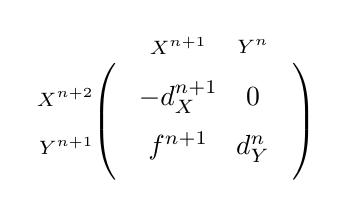
\begin{tikzpicture}[baseline]
			\matrix (M) [matrix of math nodes, ampersand replacement=\&, left delimiter=(, right delimiter=)] {
					-d_X^{n+1} \& 0 \\
					f^{n+1} \& d_Y^n \\
				};
				\node[above=1.2em] at (M-1-1) {\scriptsize $X^{n+1}$};
				\node[above=1.2em] at (M-1-2) {\scriptsize $Y^n$};
				\node[left=2.7em] at (M-1-1) {\scriptsize $X^{n+2}$};
				\node[left=2.7em] at (M-2-1) {\scriptsize $Y^{n+1}$};
		\end{tikzpicture} \\
		& : X^{n+1} \oplus Y^n \to X^{n+2} \oplus Y^{n+1} ,
	\end{align*}
	for $n\in\Z$. Since $d_{X[1]}^n=-d_X^{n+1}$, there is also the more
	concise notation
% segment-id: o014.li2.chapter3.mapping-cone.q002
	\[ \Cone(f) := \left( X[1] \oplus Y , \; \begin{pmatrix} d_{X[1]} & 0 \\ f[1] & d_Y \end{pmatrix} \right) . \]
\end{definition}

% segment-id: o014.li2.chapter3.mapping-cone.p002
It is easy to prove that $\Cone(f)$ is indeed a complex, as the following
matrix calculation shows:
% segment-id: o014.li2.chapter3.mapping-cone.q003
\[ \begin{pmatrix} -d_X^{n+1} & 0 \\ f^{n+1} & d_Y^n \end{pmatrix} \begin{pmatrix} -d_X^n & 0 \\ f^n & d_Y^{n-1} \end{pmatrix} =
\begin{pmatrix} d_X^{n+1} d_X^n & 0 \\ - f^{n+1} d_X^n + d_Y^n f^n & d_Y^n d_Y^{n-1} \end{pmatrix}. \]

% segment-id: o014.li2.chapter3.mapping-cone.e001
\begin{example}
	Let $f:X\to Y$ be a morphism in $\mathcal{A}$. Regard $X,Y$ as objects
	of $\cate{C}(\mathcal{A})$ concentrated in degree $0$. Then $\Cone(f)$ is
	precisely the complex $[X\xrightarrow{f}Y]$, in degrees $-1,0$, with all
	other terms equal to $0$.
\end{example}

% segment-id: o014.li2.chapter3.mapping-cone.p003
The following two functoriality properties follow immediately from the
definition.

% segment-id: o014.li2.chapter3.mapping-cone.pr001
\begin{proposition}\label{prop:cone-functorial}
	Given a commutative diagram in $\cate{C}(\mathcal{A})$
% segment-id: o014.li2.chapter3.mapping-cone.g001
	\[\begin{tikzcd}
		X \arrow[d, "f"'] \arrow[r, "\varphi"] & X' \arrow[d, "{f'}"] \\
		Y \arrow[r, "\psi"'] & Y'
	\end{tikzcd}\]
	the matrix $\bigl(\begin{smallmatrix} \varphi[1] & 0 \\ 0 & \psi \end{smallmatrix}\bigr)$
	defines a morphism $\Cone(f)\to\Cone(f')$.
\end{proposition}

% segment-id: o014.li2.chapter3.mapping-cone.pr002
\begin{proposition}\label{prop:Cone-A}
	Let $F:\mathcal{A}\to\mathcal{A}'$ be an additive functor and let
	$f:X\to Y$ be a morphism in $\cate{C}(\mathcal{A})$. The associated
	functor $\cate{C}F:\cate{C}(\mathcal{A})\to
	\cate{C}(\mathcal{A}')$ satisfies the following canonical isomorphism in
	$\cate{C}(\mathcal{A}')$:
% segment-id: o014.li2.chapter3.mapping-cone.q004
	\[ (\cate{C}F)(\Cone(f)) \simeq \Cone(\cate{C}F(f)). \]
\end{proposition}

% segment-id: o014.li2.chapter3.mapping-cone.p004
The mapping cone can be placed in the following ``triangle,'' which underlies
all the theory to come.

% segment-id: o014.li2.chapter3.mapping-cone.d002
\begin{definition}\label{def:cone-triangle}
	\index[sym1]{alphafbetaf@$\alpha(f), \beta(f)$}
	Consider a morphism $f:X\to Y$ in $\cate{C}(\mathcal{A})$. It gives the
	following canonical morphisms in $\cate{C}(\mathcal{A})$:
% segment-id: o014.li2.chapter3.mapping-cone.q005
	\[ Y \xrightarrow{\alpha(f)} \Cone(f) \xrightarrow{\beta(f)} X[1] , \]
	explicitly expressed in matrix notation as
% segment-id: o014.li2.chapter3.mapping-cone.q006
	\begin{align*}
		\alpha(f)^n & := \text{inclusion}\; \begin{pmatrix} 0 \\ \identity_{Y^n} \end{pmatrix}: Y^n \to X[1]^n \oplus Y^n , \\
		\beta(f)^n & := \text{projection}\; \begin{pmatrix} \identity_{X[1]^n} & 0 \end{pmatrix}: X[1]^n \oplus Y^n \to X[1]^n .
	\end{align*}
	It is clear that these are indeed morphisms in $\cate{C}(\mathcal{A})$.
\end{definition}

% segment-id: o014.li2.chapter3.mapping-cone.p005
We next collect several homotopy properties of mapping cones. First we show
that a mapping cone may be regarded as a ``homotopy cokernel'' or a
``homotopy kernel'' of a morphism. This is the realization, at the level of
complexes, of a basic idea in homotopy theory.

% segment-id: o014.li2.chapter3.mapping-cone.pr003
\begin{proposition}\label{prop:homotopy-kernel-cokernel}
	Let $f:X\to Y$ be a morphism in $\cate{C}(\mathcal{A})$. There are
	canonical bijections
% segment-id: o014.li2.chapter3.mapping-cone.g002
	\[\begin{tikzcd}[row sep=small]
		\Hom\left( \Cone(f), T \right) \arrow[leftrightarrow, r, "1:1"] & \left\{ (u, h): u \in \Hom(Y,T), \; h: \text{a homotopy from $uf$ to $0$} \right\}, \\
		\Hom\left( T, \Cone(f)[-1] \right) \arrow[leftrightarrow, r, "1:1"] & \left\{ (v, k): v \in \Hom(T,X), \; k: \text{a homotopy from $fv$ to $0$} \right\},
	\end{tikzcd}\]
	where $T$ is any object of $\cate{C}(\mathcal{A})$ and
	$\Hom:=\Hom_{\cate{C}(\mathcal{A})}$. More explicitly,
% segment-id: o014.li2.chapter3.mapping-cone.l001
	\begin{compactitem}
% segment-id: o014.li2.chapter3.mapping-cone.i001
		\item the image $(u,h)$ of $\tilde{u}:\Cone(f)\to T$ satisfies
		$u=\tilde{u}\circ\alpha(f)$;
% segment-id: o014.li2.chapter3.mapping-cone.i002
		\item the image $(v,k)$ of $\tilde{v}:T\to\Cone(f)[-1]$ satisfies
		$v=\beta(f)[-1]\circ\tilde{v}$.
	\end{compactitem}
\end{proposition}
% segment-id: o014.li2.chapter3.mapping-cone.pf001
\begin{proof}
	First consider $\Hom(\Cone(f),T)$. A morphism
	$\tilde{u}:\Cone(f)\to T$ is equivalent to families of morphisms in
	$\mathcal{A}$, $h^n:X^{n+1}\to T^n$ and $u^n:Y^n\to T^n$, for
	$n\in\Z$, satisfying the matrix equation
% segment-id: o014.li2.chapter3.mapping-cone.q007
	\[\begin{pmatrix}
		h^{n+1} & u^{n+1}
	\end{pmatrix} \begin{pmatrix}
		-d_X^{n+1} & 0 \\
		f^{n+1} & d_Y^n
	\end{pmatrix} = d_T^n \begin{pmatrix}
		h^n & u^n
	\end{pmatrix}. \]
	Expanding it shows that this equation is equivalent to saying that
	$u=(u^n)_n:Y\to T$ is a morphism in $\cate{C}(\mathcal{A})$ and that
	$h:=(h^{n-1})_n$ satisfies
	$d_{\Hom^\bullet(X,T)}^{-1}h=uf$. This is the required bijection; the
	equality $u=\tilde{u}\circ\alpha(f)$ follows immediately from the
	definition of $\alpha(f)$.

	Next consider a morphism $\tilde{v}:T\to\Cone(f)[-1]$. It is equivalent
	to families of morphisms in $\mathcal{A}$, $v^n:T^n\to X^n$ and
	$\underline{k}^n:T^n\to Y^{n-1}$, satisfying
% segment-id: o014.li2.chapter3.mapping-cone.q008
	\[\begin{pmatrix}
		d_X^n & 0 \\
		-f^n & -d_Y^{n-1}
	\end{pmatrix} \begin{pmatrix}
		v^n \\ \underline{k}^n
	\end{pmatrix} = \begin{pmatrix}
		v^{n+1} \\ \underline{k}^{n+1}
	\end{pmatrix} d_T^n
	\quad (n \in \Z). \]
	This equation is equivalent to saying that $v=(v^n)_n:T\to X$ is a
	morphism in $\cate{C}(\mathcal{A})$ and that
	$k:=(-\underline{k}^n)_n$ satisfies
	$d_{\Hom^\bullet(T,Y)}^{-1}k=fv$. The equality
	$v=\beta(f)[-1]\circ\tilde{v}$ also follows immediately from the
	definition of $\beta(f)$.
\end{proof}

% segment-id: o014.li2.chapter3.mapping-cone.r001
\begin{remark}[Homotopy cokernel and homotopy kernel]\label{rem:homotopy-kernel-cokernel}
	\index{homotopy cokernel, homotopy kernel}
	Proposition~\ref{prop:homotopy-kernel-cokernel} shows that a morphism
	$u:Y\to T$ (or $v:T\to X$) has $uf$ (or $fv$) null-homotopic if and only
	if it factors through $\alpha(f):Y\to\Cone(f)$ (or through
	$\beta(f)[-1]:\Cone(f)[-1]\to X$). This naturally recalls the universal
	property of a cokernel (or kernel), with the following differences:
% segment-id: o014.li2.chapter3.mapping-cone.l002
	\begin{compactitem}
% segment-id: o014.li2.chapter3.mapping-cone.i003
		\item the requirement that $uf$ (or $fv$) be null-homotopic replaces
		the strict equality $=0$;
% segment-id: o014.li2.chapter3.mapping-cone.i004
		\item the factorization $\tilde{u}$ (or $\tilde{v}$) supplied by the
		proposition not only witnesses the fact that $uf$ (or $fv$) is
		null-homotopic but also records how it is homotoped to $0$; this is
		data one level higher.
	\end{compactitem}
	These properties cannot simply be handled in $\cate{C}(\mathcal{A})$ or
	$\cate{K}(\mathcal{A})$ using elementary category-theoretic notions; in
	fact, kernels and cokernels seldom exist in $\cate{K}(\mathcal{A})$. For
	this reason, $Y\to\Cone(f)$ is also called the \emph{homotopy cokernel}
	of $f$, while $\beta(f)[-1]:\Cone(f)[-1]\to X$ is called the
	\emph{homotopy kernel} of $f$. Remarkably, the mapping cone $\Cone(f)$
	and its shifts play both the ``cokernel'' and ``kernel'' roles in this
	sense.
\end{remark}

% segment-id: o014.li2.chapter3.mapping-cone.p006
A morphism $f$ in $\cate{C}(\mathcal{A})$ is said to be canonically homotopic
to $g$ if there is a canonical $h$ such that $g-f=d^{-1}h$; if $f$ is
canonically homotopic to $0$, it is called canonically null-homotopic.

% segment-id: o014.li2.chapter3.mapping-cone.pr004
\begin{proposition}\label{prop:cone-homotopy}
	Let $\mathcal{A}$ be an additive category.
% segment-id: o014.li2.chapter3.mapping-cone.l003
	\begin{enumerate}[(i)]
% segment-id: o014.li2.chapter3.mapping-cone.i005
		\item If $f:X\to Y$ is an isomorphism in $\cate{C}(\mathcal{A})$,
		then $\identity_{\Cone(f)}$ is canonically null-homotopic.
% segment-id: o014.li2.chapter3.mapping-cone.i006
		\item For any morphism $f:X\to Y$ in $\cate{C}(\mathcal{A})$, the
		morphisms in Definition~\ref{def:cone-triangle} satisfy
% segment-id: o014.li2.chapter3.mapping-cone.q009
		\[ \beta(f) \circ \alpha(f) = 0, \]
		while $\alpha(f)\circ f$ and $f[1]\circ\beta(f)$ are both
		canonically null-homotopic.
	\end{enumerate}
\end{proposition}
% segment-id: o014.li2.chapter3.mapping-cone.pf002
\begin{proof}
	First consider (i). By functoriality of mapping cones
	(Proposition~\ref{prop:cone-functorial}), it suffices to consider
	$f=\identity_X$. Define
% segment-id: o014.li2.chapter3.mapping-cone.q010
	\[ s^n := \begin{pmatrix} 0 & \identity_{X^n} \\ 0 & 0 \end{pmatrix} : X^{n+1} \oplus X^n \to X^n \oplus X^{n-1}, \quad n \in \Z. \]
	A direct calculation gives
% segment-id: o014.li2.chapter3.mapping-cone.q011
	\begin{multline*}
		d^{n-1}_{\Cone(\identity_X)} s^n + s^{n+1} d^n_{\Cone(\identity_X)} = \\
		\begin{pmatrix} -d_X^n & 0 \\ \identity_{X^n} & d_X^{n-1} \end{pmatrix} \begin{pmatrix} 0 & \identity_{X^n} \\ 0 & 0 \end{pmatrix}  + \begin{pmatrix} 0 & \identity_{X^{n+1}} \\ 0 & 0 \end{pmatrix} \begin{pmatrix} -d_X^{n+1} & 0 \\ \identity_{X^{n+1}} & d_X^n \end{pmatrix}
		= \identity_{X^{n+1} \oplus X^n},
	\end{multline*}
	so $s=(s^n)_{n\in\Z}$ makes $\identity_{\Cone(\identity_X)}$
	null-homotopic.

	Next consider (ii). Clearly $\beta(f)\circ\alpha(f)=0$. The remaining
	homotopies come from Proposition~\ref{prop:homotopy-kernel-cokernel}: take
	$T=\Cone(f)$, so that
	$\tilde{u}:=\identity_{\Cone(f)}\in\Hom(\Cone(f),T)$ makes
	$\alpha(f)\circ f$ null-homotopic; take $T=\Cone(f)[-1]$, so that
	$\tilde{v}:=\identity_{\Cone(f)[-1]}\in\Hom(T,\Cone(f)[-1])$ makes
	$f\circ\beta(f)[-1]$ null-homotopic, and hence also makes
	$f[1]\circ\beta(f)$ null-homotopic.
\end{proof}

% segment-id: o014.li2.chapter3.mapping-cone.p007
Definition~\ref{def:cone-triangle} produces two new morphisms $\alpha(f)$ and
$\beta(f)$ from $f$. Up to homotopy, the mapping cones of these two morphisms
produce no new objects. We begin with $\Cone(\alpha(f))$. First observe that
% segment-id: o014.li2.chapter3.mapping-cone.q012
\[ \Cone(\alpha(f))^n = Y^{n+1} \oplus \Cone(f)^n = Y^{n+1} \oplus X^{n+1} \oplus Y^n. \]
In matrix notation,
% segment-id: o014.li2.chapter3.mapping-cone.q013
\begin{align*}
	\alpha(\alpha(f)) & = \begin{pmatrix}
		0 & 0 \\
		\identity_{X[1]} & 0 \\
		0 & \identity_Y
	\end{pmatrix} : \Cone(f) \to \Cone(\alpha(f)) , \\
	\beta(\alpha(f)) & = \begin{pmatrix}
		\identity_{Y[1]} & 0 & 0
	\end{pmatrix} : \Cone(\alpha(f)) \to Y[1].
\end{align*}

% segment-id: o014.li2.chapter3.mapping-cone.le001
\begin{lemma}\label{prop:cone-alpha}
	For a morphism $f:X\to Y$ in $\cate{C}(\mathcal{A})$, matrix notation
	defines a pair of morphisms
% segment-id: o014.li2.chapter3.mapping-cone.g003
	\[ \begin{pmatrix} -f[1] \\ \identity_{X[1]} \\ 0 \end{pmatrix} : \begin{tikzcd} X[1] \arrow[r, shift left, "\phi"] & \Cone(\alpha(f)) \arrow[l, shift left, "\psi"] \end{tikzcd} : \begin{pmatrix} 0 & \identity_{X[1]} & 0 \end{pmatrix}. \]
	They satisfy $\psi\circ\phi=\identity_{X[1]}$ and make the following
	diagram commute in $\cate{K}(\mathcal{A})$:
% segment-id: o014.li2.chapter3.mapping-cone.g004
	\[\begin{tikzcd}
		\Cone(f) \arrow[d, "{\identity_{\Cone(f)}}"'] \arrow[r, "\beta(f)"] & X[1] \arrow[d, "\phi"] \arrow[r, "{-f[1]}"] & Y[1] \arrow[d, "{\identity_{Y[1]}}"] \\
		\Cone(f) \arrow[r, "{\alpha(\alpha(f))}"'] & \Cone(\alpha(f)) \arrow[r, "\beta(\alpha(f))"'] & Y[1]
	\end{tikzcd}\]
	Moreover, $\phi$ and $\psi$ are inverse to each other in
	$\cate{K}(\mathcal{A})$.
\end{lemma}
% segment-id: o014.li2.chapter3.mapping-cone.pf003
\begin{proof}
	By the preceding description of $\Cone(\alpha(f))$, its differential
	$d_{\Cone(\alpha(f))}^n$ is, in matrix notation,
% segment-id: o014.li2.chapter3.mapping-cone.q014
	\[ \begin{pmatrix} -d_Y^{n+1} & 0 & 0 \\ 0 & -d_X^{n+1} & 0 \\ \identity_{Y^{n+1}} & f^{n+1} & d_Y^n \end{pmatrix} : Y^{n+1} \oplus X^{n+1} \oplus Y^n \to Y^{n+2} \oplus X^{n+2} \oplus Y^{n+1}. \]
	It suffices to verify the following statements in
	$\cate{C}(\mathcal{A})$:
% segment-id: o014.li2.chapter3.mapping-cone.l004
	\begin{itemize}
% segment-id: o014.li2.chapter3.mapping-cone.i007
		\item $\phi:=(\phi^n)_{n\in\Z}$ and $\psi:=(\psi^n)_{n\in\Z}$ are
		both morphisms of complexes;
% segment-id: o014.li2.chapter3.mapping-cone.i008
		\item $\psi\circ\phi=\identity_{X[1]}$;
% segment-id: o014.li2.chapter3.mapping-cone.i009
		\item $\psi\circ\alpha(\alpha(f))=\beta(f)$;
% segment-id: o014.li2.chapter3.mapping-cone.i010
		\item $\beta(\alpha(f))\circ\phi=-f[1]$;
% segment-id: o014.li2.chapter3.mapping-cone.i011
		\item there is an
		$s=(s^n)_{n\in\Z}\in\Hom^{-1}\left(\Cone(\alpha(f)),
		\Cone(\alpha(f))\right)$ such that
		$\identity_{\Cone(\alpha(f))}-\phi\circ\psi
		=d^{-1}_{\Hom^\bullet}(s)$.
	\end{itemize}
	The first four statements are elementary. For the last, take, in matrix
	notation,
% segment-id: o014.li2.chapter3.mapping-cone.q015
	\[ s^n := \begin{pmatrix} 0 & 0 & \identity_{Y^n} \\ 0 & 0 & 0 \\ 0 & 0 & 0 \end{pmatrix}: \Cone(\alpha(f))^n \to \Cone(\alpha(f))^{n-1} \]
	and verify it directly.
\end{proof}

% segment-id: o014.li2.chapter3.mapping-cone.p008
For the case of $\beta(f)$, we make a slight modification and consider the
mapping cone of $-\beta(f)[-1]:\Cone(f)[-1]\to X$.

% segment-id: o014.li2.chapter3.mapping-cone.d003
\begin{definition}\label{def:Cyl}
	\index{mapping cylinder}
	\index[sym1]{Cylf@$\Cyl(f)$}
	For a morphism $f:X\to Y$ in $\cate{C}(\mathcal{A})$, its
	\emph{mapping cylinder} is defined by
% segment-id: o014.li2.chapter3.mapping-cone.q016
	\[ \Cyl(f) := \Cone\left( \Cone(f)[-1] \xrightarrow{-\beta(f)[-1]} X \right). \]
	It is equipped with canonical morphisms $X\to\Cyl(f)\to\Cone(f)$.
\end{definition}

% segment-id: o014.li2.chapter3.mapping-cone.p009
The mapping cylinder has functoriality of the same form as that of the mapping
cone (Proposition~\ref{prop:cone-functorial}). In view of
Remark~\ref{rem:homotopy-kernel-cokernel}, $\Cyl(f)$ can be compared with a
coimage in an additive category---roughly speaking, it is a ``cokernel of a
kernel'' (Proposition~\ref{prop:Im-Coim-additive})---and may therefore be
viewed as the homotopy coimage of $f$.

% segment-id: o014.li2.chapter3.mapping-cone.p010
More explicitly,
$\Cyl(f)^n=\Cone(f)^n\oplus X^n=X^{n+1}\oplus Y^n\oplus X^n$. The morphism
$X\to\mathrm{Cyl}(f)$ (or $\mathrm{Cyl}(f)\to\Cone(f)$) is the inclusion
into the third direct summand (or the projection onto the first two), and
% segment-id: o014.li2.chapter3.mapping-cone.q017
\[ d_{\Cyl(f)}^n =
	\begin{pmatrix} d_{\Cone(f)}^n & 0 \\ -\beta(f)^n & d_X^n \end{pmatrix}
	= \begin{pmatrix}
		-d_X^{n+1} & 0 & 0 \\
		f^{n+1} & d_Y^n & 0 \\
		-\identity_{X^{n+1}} & 0 & d_X^n
\end{pmatrix} .\]

% segment-id: o014.li2.chapter3.mapping-cone.le002
\begin{lemma}\label{prop:cone-beta}
	For a morphism $f:X\to Y$ in $\cate{C}(\mathcal{A})$, one can define a
	pair of morphisms
% segment-id: o014.li2.chapter3.mapping-cone.g005
	\[ \begin{pmatrix} 0 \\ \identity_Y \\ 0 \end{pmatrix} : \begin{tikzcd} Y \arrow[r, shift left, "\phi"] & \Cyl(f) \arrow[l, shift left, "\psi"] \end{tikzcd} : \begin{pmatrix} 0 & \identity_Y & f \end{pmatrix}. \]
	They satisfy $\psi\circ\phi=\identity_Y$ and make the following diagram
	commute in $\cate{K}(\mathcal{A})$:
% segment-id: o014.li2.chapter3.mapping-cone.g006
	\[\begin{tikzcd}
		X \arrow[d, "{\identity_X}"'] \arrow[r, "f"] & Y \arrow[d, "\phi"] \arrow[r, "{\alpha(f)}"] & \Cone(f) \arrow[d, "{\identity_{\Cone(f)}}"] \\
		X \arrow[r] & \Cyl(f) \arrow[r] & \Cone(f)
	\end{tikzcd}\]
	Moreover, $\phi$ and $\psi$ are inverse to each other in
	$\cate{K}(\mathcal{A})$. In addition, $f$ factors as the composite
	$X\to\Cyl(f)\xrightarrow{\psi}Y$.
\end{lemma}
% segment-id: o014.li2.chapter3.mapping-cone.pf004
\begin{proof}
	The reader may verify directly from the definition that $\phi$ and $\psi$
	are morphisms of complexes. Then $\psi\circ\phi=\identity_Y$ is immediate.
	To prove that $\phi$ and $\psi$ are inverse in $\cate{K}(\mathcal{A})$,
	as in Lemma~\ref{prop:cone-alpha}, take
% segment-id: o014.li2.chapter3.mapping-cone.q018
	\begin{align*}
		s^n & := \begin{pmatrix} 0 & 0 & -\identity_{X^n} \\ 0 & 0 & 0 \\ 0 & 0 & 0 \end{pmatrix}: X^{n+1} \oplus Y^n \oplus X^n \to X^n \oplus Y^{n-1} \oplus X^{n-1}, \\
		s & := (s^n)_{n \in \Z},
	\end{align*}
	and verify
	$\identity_{\Cyl(f)}-\phi\circ\psi=d^{-1}_{\Hom^\bullet}(s)$.

	The right-hand square in the diagram already commutes in
	$\cate{C}(\mathcal{A})$. For the left-hand square, simply observe that
	the composite $X\to\mathrm{Cyl}(f)\xrightarrow{\psi}Y$ equals $f$.
\end{proof}

% segment-id: o014.li2.chapter3.mapping-cone.p011
Lemmas~\ref{prop:cone-alpha} and \ref{prop:cone-beta} show that, up to
isomorphism in $\cate{K}(\mathcal{A})$, any morphism $f:X\to Y$ can be
replaced by the much simpler projection $\Cone(\alpha(f))[-1]\to Y$ (or by
the inclusion $X\to\Cyl(f)$), and this construction is functorial in $f$.
This is an important idea in homological algebra and homotopy theory.

% segment-id: o014.li2.chapter3.mapping-cone.p012
The special case $f=\identity_X$ of the mapping cylinder has another use: it
can be used to interpret homotopy. For readers familiar with homology theory,
all of this has a topological interpretation, but here we discuss only the
algebraic version.

% segment-id: o014.li2.chapter3.mapping-cone.pr005
\begin{proposition}\label{prop:cylinder-homotopy}
	\index[sym1]{CylX@$\Cyl_X$}
	Let $X$ be an object of $\cate{C}(\mathcal{A})$ and set
	$\mathrm{Cyl}_X:=\mathrm{Cyl}(\identity_X)$. Notice that
	$\mathrm{Cyl}_X^n=X^{n+1}\oplus X^n\oplus X^n$.
% segment-id: o014.li2.chapter3.mapping-cone.l005
	\begin{enumerate}[(i)]
% segment-id: o014.li2.chapter3.mapping-cone.i012
		\item In $\cate{C}(\mathcal{A})$ there are morphisms
% segment-id: o014.li2.chapter3.mapping-cone.g007
		$\begin{tikzcd}
			X \arrow[shift left, r, "i_0"] \arrow[shift right, r, "i_1"'] & \Cyl_X \arrow[r, "j"] & X
		\end{tikzcd}$,
		defined in matrix notation, for every $n\in\Z$, by
% segment-id: o014.li2.chapter3.mapping-cone.q019
		\begin{equation*}
			i_0^n := \begin{pmatrix} 0 \\ 0 \\ \identity_{X^n} \end{pmatrix} , \quad
			i_1^n := \begin{pmatrix} 0 \\ \identity_{X^n} \\ 0 \end{pmatrix} , \quad j^n := \begin{pmatrix} 0 & \identity_{X^n} & \identity_{X^n} \end{pmatrix}.
		\end{equation*}
		These morphisms satisfy $ji_0=\identity_X=ji_1$, and the image of $j$
		in $\cate{K}(\mathcal{A})$ is an isomorphism.
% segment-id: o014.li2.chapter3.mapping-cone.i013
		\item For every object $Y$ of $\cate{C}(\mathcal{A})$, there is a
		bijection
% segment-id: o014.li2.chapter3.mapping-cone.q020
		\begin{align*}
			\left\{\begin{array}{r|l}
				(f, g, h) & f, g \in \Hom_{\cate{C}(\mathcal{A})}(X, Y) \\
				& h \in \Hom^{-1}(X, Y) \\
				& g - f = d^{-1}_{\Hom^\bullet(X, Y)} h
			\end{array}\right\} & \xrightarrow{1:1} \Hom_{\cate{C}(\mathcal{A})}\left( \mathrm{Cyl}_X, Y \right) \\
			(f, g, h) & \longmapsto \tilde{h} = (\tilde{h}^n)_{n \in \Z}, \; \tilde{h}^n := \begin{pmatrix} h^n & g^n & f^n \end{pmatrix}.
		\end{align*}
		In particular, $f=\tilde{h}i_0$ and $g=\tilde{h}i_1$.
	\end{enumerate}
\end{proposition}
% segment-id: o014.li2.chapter3.mapping-cone.pf005
\begin{proof}
	For (i), note that $i_0$ is precisely the canonical morphism
	$X\to\mathrm{Cyl}(\identity_X)$ in Definition~\ref{def:Cyl}, while $i_1$
	is the morphism $\phi:X\to\mathrm{Cyl}(\identity_X)$ in
	Lemma~\ref{prop:cone-beta}. The commutative diagram in
	Lemma~\ref{prop:cone-beta} shows that they give the same isomorphism in
	$\cate{K}(\mathcal{A})$.

	For $j$, it is easy to verify that
	$j^{n+1}d_{\Cyl_X}^n=\bigl(0\;d_X^n\;d_X^n\bigr)=d_X^nj^n$. Thus $j$ is
	indeed a morphism, while $ji_0=\identity_X=ji_1$ is immediate. Since
	$i_0$ and $i_1$ are isomorphisms in $\cate{K}(\mathcal{A})$, so is $j$.

	For (ii), write any element $\tilde{h}$ of
	$\Hom^0(\mathrm{Cyl}_X,Y)$ as
	\[
		\tilde{h}=\left((h^n,g^n,f^n)\right)_{n\in\Z},
	\]
	where
% segment-id: o014.li2.chapter3.mapping-cone.q021
	\[ h^n: X^{n+1} \to Y^n, \quad f^n: X^n \to Y^n, \quad g^n: X^n \to Y^n \]
	are morphisms in $\mathcal{A}$. Suppressing superscripts and using matrix
	notation, calculate
% segment-id: o014.li2.chapter3.mapping-cone.q022
	\begin{align*}
		\tilde{h} \; d_{\mathrm{Cyl}_X} & = \begin{pmatrix} h & g & f \end{pmatrix} \begin{pmatrix} -d_X & 0 & 0 \\ \identity_X & d_X & 0 \\ -\identity_X & 0 & d_X \end{pmatrix} = \begin{pmatrix} -hd_X + g - f & g d_X & f d_X \end{pmatrix} , \\
		d_Y \; \tilde{h} & = \begin{pmatrix} d_Y h & d_Y g & d_Y f \end{pmatrix}.
	\end{align*}
	Therefore $\tilde{h}$ is a morphism of complexes if and only if
	$f,g\in\Hom_{\cate{C}(\mathcal{A})}(X,Y)$ and
	$g-f=hd_X+d_Yh$.
\end{proof}

% segment-id: o014.li2.chapter3.mapping-cone.r002
\begin{remark}\label{rem:cone-chain}
	\index{mapping cone}\index{mapping cylinder}
	Mapping cones and mapping cylinders of course have versions for chain
	complexes (see Remark~\ref{rem:cochain-vs-chain}). Given a morphism of
	chain complexes $f:X\to Y$, define
% segment-id: o014.li2.chapter3.mapping-cone.q023
	\[\begin{array}{rlrl}
		\Cone(f)_n & :=(X[-1] \oplus Y)_n, &
		\Cyl(f)_n & := (X[-1] \oplus Y \oplus X)_n, \\
		d_{\Cone(f)} & := \begin{pmatrix} d_{X[-1]} & 0 \\ f[-1] & d_Y \end{pmatrix}, &
		d_{\Cyl(f)} & := \begin{pmatrix} d_{X[-1]} & 0 & 0 \\ f[-1] & d_Y & 0 \\ -\identity_{X[-1]} & 0 & d_X \end{pmatrix}.
	\end{array}\]

	Every statement in this section carries over to chain complexes. In
	particular, there are canonical morphisms
% segment-id: o014.li2.chapter3.mapping-cone.q024
	\[ X \xrightarrow{f} Y \xrightarrow{\alpha(f)} \Cone(f) \xrightarrow{\beta(f)} X[-1], \quad X \to \Cyl(f) \to \Cone(f). \]
\end{remark}

% Unit 035 English translation of chapter3.tex lines 622--699.
% Source: Methods of Algebra, Volume 2, commit
% 9a5803ff77dd3257484cb177f851a73770a59dd3 (CC BY 4.0).
% stable-unit-id: o014.aljabr2.chapter3.opposite-category-complexes
% Coverage: Section 3.4 in full.

% segment-id: o014.li2.chapter3.opposite-category-complexes.h001
\section{Complexes on the Opposite Category}\label{sec:opposite-cplx}
\hypertarget{o014.aljabr2.chapter3.opposite-category-complexes}{ }

% segment-id: o014.li2.chapter3.opposite-category-complexes.p001
Let $\mathcal{A}$ be an additive category. This section relates complexes on
$\mathcal{A}$ and on $\mathcal{A}^{\opp}$. Since functors involving
$\mathcal{A}^{\opp}$, such as the $\Hom$ functor, occur frequently, this
procedure is simple but necessary; some of the signs involved also require a
little care. Beginning readers are advised to skip this section or merely
skim it on a first reading.

% segment-id: o014.li2.chapter3.opposite-category-complexes.p002
The discussion has three aspects: complexes, homotopy, and mapping cones. The
derived-category version considered later
(Proposition~\sourcecrossref{prop:derived-cat-op}{in the later discussion of
derived categories}) is a direct application of these results. Recall that if
$f:X\to Y$ is a morphism in $\mathcal{A}$, then $f^{\opp}$ denotes the
corresponding morphism $Y\to X$ in $\mathcal{A}^{\opp}$.

% segment-id: o014.li2.chapter3.opposite-category-complexes.dp001
\begin{definition-proposition}\label{def:sigma}
	\index[sym1]{sigma@$\sigma$}
	The isomorphism of additive categories
	$\sigma:\cate{C}(\mathcal{A}^{\opp})\to\cate{C}(\mathcal{A})^{\opp}$
	is defined as follows. For an object $X$ of
	$\cate{C}(\mathcal{A}^{\opp})$, define in $\mathcal{A}$
% segment-id: o014.li2.chapter3.opposite-category-complexes.q001
	\[ (\sigma X)^n := X^{-n}, \quad d_{\sigma X}^n = (-1)^{n+1} \left[ d_X^{-n-1, \opp}: (\sigma X)^n \to (\sigma X)^{n+1} \right], \quad n \in \Z. \]
	For a morphism $f=\left(f^n:X^n\to Y^n\right)_n$ in
	$\cate{C}(\mathcal{A}^{\opp})$, take its image $\sigma f$ to be the
	following morphism in $\cate{C}(\mathcal{A})$:
% segment-id: o014.li2.chapter3.opposite-category-complexes.q002
	\[ (\sigma f)^n := \left(f^{-n} \right)^{\opp} : (\sigma Y)^n \to (\sigma X)^n, \]
	that is, a morphism $\sigma X\to\sigma Y$ in
	$\cate{C}(\mathcal{A})^{\opp}$. For every $m\in\Z$, there is a natural
	isomorphism
% segment-id: o014.li2.chapter3.opposite-category-complexes.q003
	\[ s_m: \sigma \circ [m] \rightiso [-m] \circ \sigma, \]
	where $[-m]$ is regarded as a functor from
	$\cate{C}(\mathcal{A})^{\opp}$ to itself (strictly speaking, it should be
	written $[-m]^{\opp}$).
\end{definition-proposition}
% segment-id: o014.li2.chapter3.opposite-category-complexes.pf001
\begin{proof}
	The general case of $s_m$ reduces step by step to the case $m=1$. Define
	$s_1=(s_{1,X})_X$ as follows. For every $n$, take
% segment-id: o014.li2.chapter3.opposite-category-complexes.g001
	\begin{equation}\label{eqn:sigma-s}\begin{tikzcd}[row sep=tiny]
		s_{1,X}^n : \sigma(X{[1]})^n = X^{1-n} \arrow[r, "\sim"', "{(-1)^{n-1}}" inner sep=0.6em] & X^{1-n} = (\sigma X){[-1]}^n .
	\end{tikzcd}\end{equation}
	The entire verification reduces to
	$s_{1, X}^{n+1} d^n_{\sigma(X[1])} = -d_{X[1]}^{-n-1, \opp} =
	d_X^{-n, \opp} = (-1)^n d_{\sigma X}^{n-1} =
	d^n_{(\sigma X)[-1]} s_{1,X}^n$.
\end{proof}

% segment-id: o014.li2.chapter3.opposite-category-complexes.p003
If the construction $\sigma$ with coefficient $(-1)^{n+1}$ is applied in
both directions, $\sigma^2X$ is naturally isomorphic to $X$ through the
isomorphism whose degree-$n$ component is $(-1)^n\identity_{X^n}$. To obtain
an inverse, define the reverse construction by the same formulas on objects
and morphisms, but use the coefficient $(-1)^n$ on the differential. The
composites in both orders are then exactly the identity functor, so $\sigma$
is indeed an isomorphism of categories.%
\footnote{Translator's note (O014-C036): arguing from
$n(n+1)\equiv0\pmod{2}$, the source states that applying $\sigma$ twice
returns $X$ strictly. Using the same formula in both directions instead gives
the differential $-d_X$, not $d_X$. The signed natural isomorphism and the
corrected inverse construction are recorded above.}

% segment-id: o014.li2.chapter3.opposite-category-complexes.r001
\begin{remark}\label{rem:sigma-vs-cohomology}
	If $\mathcal{A}$ is an abelian category, the signs on
	$d_{\sigma X}^\bullet$ do not change the cohomology introduced in
	Definition~\ref{def:cohomology}; thus
	$\Hm^{-n}(\sigma X)\in\Obj(\mathcal{A})$ corresponds to
	$\Hm^n(X)\in\Obj(\mathcal{A}^{\opp})$.
\end{remark}

% segment-id: o014.li2.chapter3.opposite-category-complexes.p004
We next examine the relation between $\sigma$ and homotopy.

% segment-id: o014.li2.chapter3.opposite-category-complexes.pr001
\begin{proposition}\label{prop:sigma-homotopy}
	The functor $\sigma$ defined above induces an equivalence of additive
	categories
	$\cate{K}(\mathcal{A}^{\opp})\rightiso\cate{K}(\mathcal{A})^{\opp}$.
\end{proposition}
% segment-id: o014.li2.chapter3.opposite-category-complexes.pf002
\begin{proof}
	Let $X,Y$ be objects of $\cate{C}(\mathcal{A}^{\opp})$. For
	$f=(f^k)_k\in\Hom^{-1}_{\cate{C}(\mathcal{A}^{\opp})}(X,Y)$, use the
	following table to define the corresponding
	$\sigma f\in\Hom^{-1}_{\cate{C}(\mathcal{A})}(\sigma Y,\sigma X)$ in
	$\mathcal{A}$:
% segment-id: o014.li2.chapter3.opposite-category-complexes.q004
	\begingroup\setlength{\arraycolsep}{4pt}
	\[\begin{array}{|c|c|c|c|} \hline
		\text{Category} & \multicolumn{3}{c|}{\text{Morphism}} \\ \hline
		\mathcal{A}^{\opp} & X^k \xrightarrow{(-1)^{k+1} f^k} Y^{k-1} & d_Y^{k-1} f^k + f^{k+1} d_X^k & (d^{-1}f)^k \\
		\mathcal{A} & (\sigma Y)^{-k+1} \xrightarrow{(\sigma f)^{-k+1}} (\sigma X)^{-k} & (\sigma f)^{-k+1} d_{\sigma Y}^{-k} + d_{\sigma X}^{-k-1} (\sigma f)^{-k} & d^{-1} (\sigma f)^{-k} \\ \hline
	\end{array}\]
	\endgroup
	This suffices to show
	\[\begin{aligned}
		\Hom_{\cate{K}(\mathcal{A}^{\opp})}(X, Y)
		&\rightiso \Hom_{\cate{K}(\mathcal{A})}(\sigma Y, \sigma X) \\
		&= \Hom_{\cate{K}(\mathcal{A})^{\opp}}(\sigma X, \sigma Y).
	\end{aligned}\]
\end{proof}

% segment-id: o014.li2.chapter3.opposite-category-complexes.p005
Finally, using $\sigma$ and the family of isomorphisms $(s_m)_m$ constructed
above, we compare mapping cones in $\cate{C}(\mathcal{A})$ and
$\cate{C}(\mathcal{A}^{\opp})$. The details are somewhat routine.

% segment-id: o014.li2.chapter3.opposite-category-complexes.pr002
\begin{proposition}\label{prop:sigma-triangulated}
	\index[sym1]{sigma}
	For every morphism $f:X\to Y$ in $\cate{C}(\mathcal{A}^{\opp})$, there
	is a commutative diagram in $\cate{C}(\mathcal{A})$%
	\footnote{Here $\alpha(\cdot)$ and $\beta(\cdot)$ are both defined
	relative to $\cate{C}(\mathcal{A})$. If the diagram is viewed in
	$\cate{C}(\mathcal{A})^{\opp}$, all its arrows must be reversed.}:
% segment-id: o014.li2.chapter3.opposite-category-complexes.g002
	\[\begin{tikzcd}[column sep=large]
		\sigma\left( X{[1]} \right) \arrow[r, "{\sigma(\beta(f))}"] \arrow[d, "{s_{1,X}}"'] & \sigma\left(\Cone(f)\right) \arrow[r, "{\sigma(\alpha(f))}"] \arrow[d, "\theta"] & \sigma Y \arrow[r, "\sigma(f)"] \arrow[d, "\identity"] & \sigma X \arrow[d, "{\identity}"] \\
		(\sigma X){[-1]} \arrow[r, "{\alpha(\sigma(f))[-1]}"' inner sep=0.6em] & \Cone(\sigma(f)){[-1]} \arrow[r, "{\beta(\sigma(f))[-1]}"' inner sep=0.6em] & \sigma Y \arrow[r, "{\sigma(f)}"' inner sep=0.6em] & \sigma X
	\end{tikzcd}\]
	where $\theta$ is a canonical isomorphism and $s_{1,X}$ is the
	isomorphism supplied by Definition--Proposition~\ref{def:sigma}.
\end{proposition}
% segment-id: o014.li2.chapter3.opposite-category-complexes.pf003
\begin{proof}
	If $\Cone(f)$ were replaced by $X[1]\oplus Y$, the statement would be
	easy and the required isomorphism would simply be
	$(s_{1,X},\identity_{\sigma Y})$. The complication is that the matrix
	$d_{\Cone(f)}$ has the off-diagonal entry $f[1]$. Nevertheless, we follow
	the same method: using \eqref{eqn:sigma-s}, for every $n\in\Z$ define the
	isomorphism
% segment-id: o014.li2.chapter3.opposite-category-complexes.q005
	\begin{multline*}
		\theta^n: \sigma\left(\Cone(f)\right)^n = \sigma\left(X[1]\right)^n \oplus (\sigma Y)^n \\
		\xrightarrow[\sim]{(s_{1,X}, \identity)^n = ((-1)^{n-1} \identity, \identity) } (\sigma X)[-1]^n \oplus (\sigma Y)^n \xlongequal{\text{interchange}} \left( (\sigma Y) \oplus (\sigma X)[-1] \right)^n .
	\end{multline*}
	Under this identification, the morphism $d_{\sigma(\Cone(f))}^n$ in
	$\mathcal{A}$ corresponds to
% segment-id: o014.li2.chapter3.opposite-category-complexes.q006
	\[ \begin{pmatrix}
		d_{\sigma Y}^n & 0 \\
		* & d_{(\sigma X)[-1]}^n
	\end{pmatrix} : \left( (\sigma Y) \oplus (\sigma X)[-1] \right)^n \to \left( (\sigma Y) \oplus (\sigma X)[-1] \right)^{n+1} . \]
	As noted at the start of the proof, the diagonal entries pose no problem;
	we need only determine the lower-left entry. By
	Definition--Proposition~\ref{def:sigma}, this entry is $(-1)^{n+1}$ times
	the following composite in $\mathcal{A}$:
% segment-id: o014.li2.chapter3.opposite-category-complexes.g003
	\[\begin{tikzcd}[row sep=tiny]
		(\sigma Y)^n \arrow[r] & (\sigma(X[1]))^{n+1} \arrow[r, "\sim"] & (\sigma X)[-1]^{n+1} \\
		Y^{-n} \arrow[equal, u] \arrow[r, "{(f^{-n})^{\opp}}"'] & X^{-n} \arrow[equal, u] \arrow[r, "{s_{1, X}^{n+1} = (-1)^n}"'] & X^{-n} \arrow[equal, u]
	\end{tikzcd}\]
	Thus the result is $-\sigma(f)^n$. It follows that
% segment-id: o014.li2.chapter3.opposite-category-complexes.q007
	\[ \theta := (\theta^n)_{n \in \Z}: \sigma(\Cone(f)) \rightiso \Cone(\sigma(f))[-1] \]
	is indeed an isomorphism in $\cate{C}(\mathcal{A})$. Once this is
	established, verifying commutativity presents no essential difficulty.
\end{proof}

% segment-id: o014.li2.chapter3.opposite-category-complexes.p006
Of course, the results of this section also apply to chain complexes and
extend to the case in which $\mathcal{A}$ is a $\Bbbk$-linear category.

% Unit 036 English translation of chapter3.tex lines 700--945.
% Source: Methods of Algebra, Volume 2, commit
% 9a5803ff77dd3257484cb177f851a73770a59dd3 (CC BY 4.0).
% stable-unit-id: o014.aljabr2.chapter3.double-complexes
% Coverage: Section 3.5 in full.

% segment-id: o014.li2.chapter3.double-complexes.h001
\section{Double Complexes}\label{sec:double-cplx}
\hypertarget{o014.aljabr2.chapter3.double-complexes}{ }

% segment-id: o014.li2.chapter3.double-complexes.p001
Throughout this section, $\mathcal{A}$ remains an additive category. Roughly
speaking, a double complex may be thought of as a two-dimensional version of
a complex, with differentials in the horizontal and vertical directions.

% segment-id: o014.li2.chapter3.double-complexes.d001
\begin{definition}[Double complex]\label{def:double-cplx}
	\index{double complex}
	\index[sym1]{dhoridvert@$\dhori$, $\dvert$}
	A double complex on an additive category $\mathcal{A}$ consists of a
	family of objects $\left(X^{p,q}\right)_{(p,q)\in\Z^2}$ of
	$\mathcal{A}$, together with morphisms
	$\dhori^{p,q}:X^{p,q}\to X^{p+1,q}$ and
	$\dvert^{p,q}:X^{p,q}\to X^{p,q+1}$ satisfying
% segment-id: o014.li2.chapter3.double-complexes.q001
	\[ \dhori^{p+1,q} \dhori^{p,q} = 0, \quad \dvert^{p, q+1} \dvert^{p,q} = 0, \quad \dhori^{p, q+1} \dvert^{p,q} = \dvert^{p+1, q} \dhori^{p,q}. \]
	These data are usually abbreviated as
	$(X^{\bullet,\bullet},\dhori,\dvert)$, $X^{\bullet,\bullet}$, or $X$.
\end{definition}

% segment-id: o014.li2.chapter3.double-complexes.p002
The conditions on $\dhori,\dvert$ may be abbreviated as
% segment-id: o014.li2.chapter3.double-complexes.q002
\[ \dhori^2 = 0, \quad \dvert^2 = 0, \quad \dhori \dvert = \dvert \dhori. \]

% segment-id: o014.li2.chapter3.double-complexes.d002
\begin{definition}\label{def:bicplx}
	Given an additive category $\mathcal{A}$, a morphism from a double complex
	$X$ to a double complex $Y$ is a family of morphisms
% segment-id: o014.li2.chapter3.double-complexes.q003
	\[ f = \left( f^{p,q}: X^{p, q} \to Y^{p, q} \right)_{(p, q) \in \Z^2}, \]
	such that, for all $p,q$,
% segment-id: o014.li2.chapter3.double-complexes.q004
	\[ \dhori_Y^{p, q} f^{p, q} = f^{p+1, q} \dhori_X^{p, q}, \quad \dvert_Y^{p, q} f^{p, q} = f^{p, q+1} \dvert_X^{p, q}. \]
	These relations may be abbreviated as $\dhori_Yf=f\dhori_X$ and
	$\dvert_Yf=f\dvert_X$.
\end{definition}

% segment-id: o014.li2.chapter3.double-complexes.p003
As in Proposition~\ref{prop:additive-cat-cplx}, these definitions make all
double complexes on $\mathcal{A}$ into an additive category
$\cate{C}^2(\mathcal{A})$.
\index[sym1]{C2A@$\cate{C}^2(\mathcal{A})$}

% segment-id: o014.li2.chapter3.double-complexes.p004
Visually, a double complex $X$ is displayed as
% segment-id: o014.li2.chapter3.double-complexes.g001
\[\begin{tikzcd}
	& \vdots & \vdots & \\
	\cdots \arrow[r] & X^{p, q+1} \arrow[r] \arrow[u] & X^{p+1, q+1} \arrow[r] \arrow[u] & \cdots \\
	\cdots \arrow[r] & X^{p, q} \arrow[r, "{\dhori^{p,q}}"'] \arrow[u, "{\dvert^{p,q}}"] & X^{p+1, q} \arrow[r] \arrow[u] & \cdots \\
	& \vdots \arrow[u] & \vdots \arrow[u] &
\end{tikzcd}\]
Every row $\left(X^{\bullet,q},d^{\bullet,q}\right)$ and every column
$\left(X^{p,\bullet},d^{p,\bullet}\right)$ is a complex. Thus a double
complex can be assembled by columns or by rows.

% segment-id: o014.li2.chapter3.double-complexes.d003
\begin{definition}\label{def:bicplx-F1}
	\index[sym1]{F1F2@$F_{\mathrm{I}}, F_{\mathrm{II}}$}
	Define the additive functor
	$F_{\mathrm{I}}:\cate{C}^2(\mathcal{A})\to
	\cate{C}(\cate{C}(\mathcal{A}))$ as follows: for a double complex $X$,
	set $(F_{\mathrm{I}}X)^p=X^{p,\bullet}$ and
	$d_{F_{\mathrm{I}}X}^p=\dhori^{p,\bullet}:(F_{\mathrm{I}}X)^p\to
	(F_{\mathrm{I}}X)^{p+1}$. Similarly, the formulas
	$(F_{\mathrm{II}}X)^q=X^{\bullet,q}$ and
	$d_{F_{\mathrm{II}}X}^q=\dvert^{\bullet,q}$ define an additive functor
	$\cate{C}^2(\mathcal{A})\to\cate{C}(\cate{C}(\mathcal{A}))$. Here
	$p,q\in\Z$.
\end{definition}

% segment-id: o014.li2.chapter3.double-complexes.p005
Definition~\ref{def:bicplx} implies that both $F_{\mathrm{I}}$ and
$F_{\mathrm{II}}$ are isomorphisms of additive categories. This is depicted
as follows:
% segment-id: o014.li2.chapter3.double-complexes.g002
\begin{equation}\label{eqn:bicplx-diagram}\begin{tikzcd}[
		/tikz/execute at end picture={
			\node[rectangle, draw, fit=(NW) (SE), inner xsep=0.5em, inner ysep=0em] {};
		}]
		\vdots & |[alias=NW]| & {} & \\
		(F_{\mathrm{II}} X)^q \arrow[u, "{d^q_{F_{\mathrm{II}} X}}"] \arrow[phantom, r, ":=" description, sloped] & \cdots \arrow[r] & X^{p,q} \arrow[r, "{\dhori^{p,q}}"'] \arrow[u, "{\dvert^{p,q}}"] & \cdots \\
		\vdots \arrow[u] & & {} \arrow[u] & |[alias=SE]| \\
		& \cdots \arrow[r] & (F_{\mathrm{I}} X)^p \arrow[r, "{d^p_{F_{\mathrm{I}} X}}"] \arrow[phantom, u, ":=" description, sloped] & \cdots
\end{tikzcd}\end{equation}

% segment-id: o014.li2.chapter3.double-complexes.d004
\begin{definition}[Total complex]\label{def:total-cplx}
	\index{total complex}
	\index[sym1]{tot@$\tot_{\oplus}$, $\tot_{\Pi}$, $\tot$}
	Suppose that $\mathcal{A}$ has countable coproducts, denoted by the direct
	sum symbol $\bigoplus$, and let $X$ be an object of
	$\cate{C}^2(\mathcal{A})$. Define a complex $\tot_{\oplus}(X)$ on
	$\mathcal{A}$ as follows:
% segment-id: o014.li2.chapter3.double-complexes.l001
	\begin{compactitem}
% segment-id: o014.li2.chapter3.double-complexes.i001
		\item $\tot_{\oplus}(X)^n := \bigoplus_{p+q=n} X^{p, q}$;
% segment-id: o014.li2.chapter3.double-complexes.i002
		\item the restriction of $d^n:\tot_{\oplus}(X)^n\to
		\tot_{\oplus}(X)^{n+1}$ to the summand $X^{p,q}$ is
		$\dhori^{p,q}+(-1)^p\dvert^{p,q}$.
	\end{compactitem}
\end{definition}

% segment-id: o014.li2.chapter3.double-complexes.p006
Suppressing superscripts, writing out
$d^2:X^{p,q}\to X^{p+2,q}\oplus X^{p+1,q+1}\oplus X^{p,q+2}$ gives
% segment-id: o014.li2.chapter3.double-complexes.q005
\[ d^2 = \left( \dhori^2, \; (-1)^p \dhori \dvert + (-1)^{p+1} \dvert \dhori , \; \dvert^2 \right) = (0, 0, 0). \]

% segment-id: o014.li2.chapter3.double-complexes.p007
Replacing coproducts in the construction of $\tot_{\oplus}$ by products
$\prod$ similarly gives
$\tot_{\Pi}X\in\Obj(\cate{C}(\mathcal{A}))$, provided the required products
exist. The definition of
$d^n:\tot_{\Pi}(X)^n\to\tot_{\Pi}(X)^{n+1}$ is analogous to the
$\tot_{\oplus}$ case: require that the projection of $d^{n-1}$ to
$X^{p,q}$ be the composite
% segment-id: o014.li2.chapter3.double-complexes.q006
\[ \tot_{\Pi}^{n-1}(X) \xrightarrow{\text{projection}} X^{p-1, q} \oplus X^{p,q-1} \xrightarrow{(\dhori^{p-1, q}, (-1)^p \dvert^{p, q-1})} X^{p, q}; \]
the same reasoning gives $d^2=0$. When there is no danger of confusion,
both $\tot_{\oplus}X$ and $\tot_{\Pi}X$ are called the \emph{total
complex} of $X$.

% segment-id: o014.li2.chapter3.double-complexes.p008
The following property should be clear.

% segment-id: o014.li2.chapter3.double-complexes.pr001
\begin{proposition}
	Under the respective hypotheses, $\tot_{\oplus}$ and $\tot_{\Pi}$ are
	both additive functors from $\cate{C}^2(\mathcal{A})$ to
	$\cate{C}(\mathcal{A})$.
\end{proposition}

% segment-id: o014.li2.chapter3.double-complexes.p009
In the definition of the total complex, the superscripts $p$ and $q$ may at
first appear asymmetric. To dispel this impression, define an additive
automorphism $\mathrm{swap}$ of $\cate{C}^2(\mathcal{A})$ such that
$\mathrm{swap}(X)^{p,q}=X^{q,p}$ and $\dhori$ and $\dvert$ are interchanged.
The accompanying sign $(-1)^{pq}$ is essentially the same mechanism as the
Koszul sign rule in \cite[Definition--Theorem~7.4.4]{Li1}.

\index[sym1]{swap@$\mathrm{swap}$}
% segment-id: o014.li2.chapter3.double-complexes.pr002
\begin{proposition}\label{prop:double-cplx-swap}
	For every $(p,q)\in\Z^2$ and every object $X$ of
	$\cate{C}^2(\mathcal{A})$, define a family of isomorphisms
% segment-id: o014.li2.chapter3.double-complexes.q007
	\[ r^{p, q}_X := (-1)^{pq} \identity_{X^{p,q}} : X^{p, q} \to \mathrm{swap}(X)^{q,p} . \]
% segment-id: o014.li2.chapter3.double-complexes.l002
	\begin{compactitem}
% segment-id: o014.li2.chapter3.double-complexes.i003
		\item If $\mathcal{A}$ has countable coproducts, then
		$(r_X^{p,q})_{(p,q)\in\Z^2}$ induces an isomorphism
		$r_X:\tot_{\oplus}(X)\rightiso\tot_{\oplus}(\mathrm{swap}(X))$.
% segment-id: o014.li2.chapter3.double-complexes.i004
		\item If $\mathcal{A}$ has countable products, then
		$(r_X^{p,q})_{(p,q)\in\Z^2}$ induces an isomorphism
		$r_X:\tot_{\Pi}(X)\rightiso\tot_{\Pi}(\mathrm{swap}(X))$.
	\end{compactitem}
\end{proposition}
% segment-id: o014.li2.chapter3.double-complexes.pf001
\begin{proof}
	For every $(p,q)\in\Z^2$, the diagram
% segment-id: o014.li2.chapter3.double-complexes.g003
	\[\begin{tikzcd}[row sep=large]
		X^{p,q} \arrow[d, "(-1)^{pq} \identity"'] \arrow[r, "{ (\dhori, (-1)^p \dvert) }" inner sep=0.8em] & X^{p+1, q} \oplus X^{p, q+1} \arrow[d, "{((-1)^{(p+1)q} \identity, (-1)^{p(q+1)} \identity) }"] \\
		X^{p,q} \arrow[r, "{((-1)^q \dhori, \dvert)}"' inner sep=0.8em] & X^{p+1, q} \oplus X^{p, q+1}
	\end{tikzcd}\]
	commutes, so $r_X$ is indeed a morphism of complexes.
\end{proof}

% segment-id: o014.li2.chapter3.double-complexes.p010
The requirement that countable coproducts (or countable products) exist in
the definition of $\tot_{\oplus}X$ (or $\tot_{\Pi}X$) can be weakened. If,
for each $n$, only finitely many pairs $(p,q)$ satisfy $p+q=n$ and
$X^{p,q}\neq0$, then the coproduct (or product) in the definition of the
total complex becomes a finite direct sum. In this case, both total complexes
may be denoted uniformly by $\tot(X)$. There will be further discussion after
Definition~\sourcecrossref{def:Cf-Supp}{in \S~3.10}.

% segment-id: o014.li2.chapter3.double-complexes.r001
\begin{remark}\label{rem:k-fold-cplx}
	By the same idea, for every $k\in\Z_{\geq1}$ one can define a $k$-fold
	complex as data
% segment-id: o014.li2.chapter3.double-complexes.q008
	\[ \left( X^{p_1, \ldots, p_k} \in \Obj(\mathcal{A}) \right)_{p_1, \ldots, p_k \in \Z}, \quad {}^1 d, \ldots, {}^k d, \]
	where ${}^i d^{p_1,\ldots,p_k}:X^{p_1,\ldots,p_k}\to
	X^{p_1,\ldots,p_i+1,\ldots,p_k}$ and
% segment-id: o014.li2.chapter3.double-complexes.q009
	\[ {}^i d^2 = 0, \quad {}^i d {}^j d = {}^j d {}^i d \quad \text{(superscripts suppressed)}. \]
	All $k$-fold complexes form an additive category
	$\cate{C}^k(\mathcal{A})$. Following Definition~\ref{def:bicplx-F1}, one
	can also define a family of additive functors
	$F_i:\cate{C}^k(\mathcal{A})\to
	\cate{C}(\cate{C}^{k-1}(\mathcal{A}))$ such that every $F_i$ is an
	equivalence of categories ($k\geq2$ and $i=1,\ldots,k$).

	In this setting, if $\mathcal{A}$ has countable coproducts or products,
	the total-complex functor may be defined in the same way:
% segment-id: o014.li2.chapter3.double-complexes.q010
	\[ \tot_{\oplus} \; \text{or} \; \tot_{\Pi}: \cate{C}^k(\mathcal{A}) \to \cate{C}(\mathcal{A}). \]
	The details are the same as for double complexes and need not be repeated.
\end{remark}

% segment-id: o014.li2.chapter3.double-complexes.p011
Define isomorphisms from $\cate{C}^2(\mathcal{A})$ to itself by
$[m]_{\mathrm{I}}:=F_{\mathrm{I}}^{-1}\circ[m]\circ F_{\mathrm{I}}$ and
$[m]_{\mathrm{II}}:=F_{\mathrm{II}}^{-1}\circ[m]\circ F_{\mathrm{II}}$,
corresponding respectively to horizontal and vertical shifts of double
complexes. For all $a,b\in\Z$,
$[a]_{\mathrm{I}}[b]_{\mathrm{II}}=[b]_{\mathrm{II}}[a]_{\mathrm{I}}$.
We now examine the effect of these functors on total complexes and their
relation to the automorphism $\mathrm{swap}$.

% segment-id: o014.li2.chapter3.double-complexes.n001
% Reference: KS06, p.290
% segment-id: o014.li2.chapter3.double-complexes.pr003
\begin{proposition}\label{prop:tot-shift}
	For all $X\in\Obj(\cate{C}^2(\mathcal{A}))$ and $(p,q)\in\Z^2$, denote
	the standard embedding $X^{p,q}\hookrightarrow
	\mathrm{tot}_{\oplus}(X)^{p+q}$ by $\iota_{p,q}$. For every $n\in\Z$,
	define
% segment-id: o014.li2.chapter3.double-complexes.l003
	\begin{itemize}
% segment-id: o014.li2.chapter3.double-complexes.i005
		\item $\theta_X^n:\tot_{\oplus}\left(X[1]_{\mathrm{I}}\right)^n\to
		\tot_{\oplus}(X)[1]^n$ so that its restriction to
		$X[1]_{\mathrm{I}}^{p,q}=X^{p+1,q}$ is $\iota_{p+1,q}$;
% segment-id: o014.li2.chapter3.double-complexes.i006
		\item $(\theta'_X)^n:\tot_{\oplus}\left(X[1]_{\mathrm{II}}\right)^n
		\to\tot_{\oplus}(X)[1]^n$ so that its restriction to
		$X[1]_{\mathrm{II}}^{p,q}=X^{p,q+1}$ is
		$(-1)^p\iota_{p,q+1}$.
	\end{itemize}
	These define canonical isomorphisms in $\cate{C}(\mathcal{A})$:
% segment-id: o014.li2.chapter3.double-complexes.q011
	\begin{align*}
		\theta_X & = (\theta_X^n)_n: \tot_{\oplus} \left( X[1]_{\mathrm{I}} \right) \rightiso \tot_{\oplus} \left(X\right)[1], \\
		\theta'_X & = ((\theta'_X)^n)_n: \tot_{\oplus} \left( X[1]_{\mathrm{II}} \right) \rightiso \tot_{\oplus} \left(X\right)[1],
	\end{align*}
	together with the anticommutative diagram (that is, its two composites
	differ by a minus sign)
% segment-id: o014.li2.chapter3.double-complexes.g004
	\[\begin{tikzcd}
		\tot_{\oplus} \left( X[1]_{\mathrm{I}}[1]_{\mathrm{II}}\right) \arrow[r, "{\theta_{X[1]_{\mathrm{II}}}}" inner sep=0.6em] \arrow[d, "{\theta'_{X[1]_{\mathrm{I}}}}"'] & \tot_{\oplus}\left(X[1]_{\mathrm{II}}\right)[1] \arrow[d, "{\theta'_X [1]}"] \\
		\tot_{\oplus} \left( X[1]_{\mathrm{I}}\right)[1] \arrow[r, "{\theta_X [1]}"' inner sep=0.6em] & \tot_{\oplus}(X)[2]
	\end{tikzcd}\]
	and the commutative diagram
% segment-id: o014.li2.chapter3.double-complexes.g005
	\[\begin{tikzcd}[column sep=large]
		\tot_{\oplus} \left( X[1]_{\mathrm{I}}[1]_{\mathrm{II}} \right) \arrow[r, "\text{$\theta$ then $\theta'$}"] \arrow[d, "{r_{X[1]_{\mathrm{I}}[1]_{\mathrm{II}}}}"'] & \tot_{\oplus}(X)[2] \arrow[d, "{r_X[2]}"] \\
		\tot_{\oplus}\left( \mathrm{swap}(X)[1]_{\mathrm{I}}[1]_{\mathrm{II}} \right) \arrow[r, "\text{$\theta'$ then $\theta$}"'] & \tot_{\oplus}\left(\mathrm{swap}(X)\right)[2],
	\end{tikzcd}\]
	where $r$ is as defined in Proposition~\ref{prop:double-cplx-swap}. If
	$\tot_{\oplus}$ is replaced by $\tot_{\Pi}$, one obtains the same
	$\theta_X,\theta'_X$ and the corresponding anticommutative diagram.
\end{proposition}
% segment-id: o014.li2.chapter3.double-complexes.pf002
\begin{proof}
	Direct verification from the definition of the total complex
	(Definition~\ref{def:total-cplx}) and the definition of the shift functor
	(Definition~\ref{def:translation-functor}) shows that $\theta_X$ and
	$\theta'_X$ are morphisms of complexes; the details are lengthy but not
	difficult. Anticommutativity reduces to the observation that the diagram
% segment-id: o014.li2.chapter3.double-complexes.g006
	\[\begin{tikzcd}
		X^{p+1, q+1} \arrow[d, "{(-1)^p \identity}"'] \arrow[r, "\identity"] & X^{p+1, q+1} \arrow[d, "{(-1)^{p+1} \identity}"] \\
		X^{p+1, q+1} \arrow[r, "\identity"'] & X^{p+1, q+1}
	\end{tikzcd}\]
	is anticommutative.

	Now consider the assertion about the commutative diagram. Let
	$(p,q)\in\Z^2$ and compare the restrictions of the two composites to
	$(X[1]_{\mathrm{I}}[1]_{\mathrm{II}})^{p,q}$. As explained above,
	$\theta$ followed by $\theta'$ (for $X$) and $\theta'$ followed by
	$\theta$ (for $\mathrm{swap}(X)$) give respectively
% segment-id: o014.li2.chapter3.double-complexes.q012
	\[ (-1)^{p+1}, \; (-1)^q \; \in \Aut(X^{p+1, q+1}) \quad \text{($\identity$ suppressed)}. \]
	On the other hand, the restrictions of
	$r_{X[1]_{\mathrm{I}}[1]_{\mathrm{II}}}$ and $r_X[2]$ to
	$X^{p+1,q+1}$ are respectively $(-1)^{pq}$ and
	$(-1)^{(p+1)(q+1)}$. But
	$(p+1)(q+1)-pq\equiv(p+1)-q\pmod{2}$. This proves the claim.
\end{proof}

% segment-id: o014.li2.chapter3.double-complexes.p012
As a simple generalization of the anticommutative diagram above, the reader is
asked to prove that, for all $a,b\in\Z$, the two morphisms
% segment-id: o014.li2.chapter3.double-complexes.q013
\[ \tot_{\oplus}(X[a]_{\mathrm{I}}[b]_{\mathrm{II}}) \rightrightarrows \tot_{\oplus}(X)[a+b] \]
defined in the two orders ($\theta$ then $\theta'$, and $\theta'$ then
$\theta$) differ by the sign $(-1)^{ab}$; on the other hand, the commutative
diagram above remains valid for $X[a]_{\mathrm{I}}[b]_{\mathrm{II}}$. The
same statements hold with $\tot_{\Pi}$ in place of $\tot_{\oplus}$.

% segment-id: o014.li2.chapter3.double-complexes.p013
One of the main uses of double complexes is the study of bifunctors. What is a
bifunctor?

% segment-id: o014.li2.chapter3.double-complexes.c001
\begin{convention}\label{con:bifunctor}
	\index{bifunctor}
	A functor of the form $F:\mathcal{A}_1\times\mathcal{A}_2\to\mathcal{B}$
	is called a \emph{bifunctor}. Once objects
	$X_i\in\Obj(\mathcal{A}_i)$ are fixed, we obtain one-variable functors
	$F(X_1,\cdot):\mathcal{A}_2\to\mathcal{B}$ and
	$F(\cdot,X_2):\mathcal{A}_1\to\mathcal{B}$. We can therefore discuss
	additivity, exactness, and many other notions in each variable of $F$.
\end{convention}

% segment-id: o014.li2.chapter3.double-complexes.dp001
\begin{definition-proposition}\label{def:bifunctor-cplx}
	\index[sym1]{C2F@$\cate{C}^2 F, \cate{C}_{\oplus} F, \cate{C}_{\Pi} F$}
	Let $\mathcal{A}_1,\mathcal{A}_2,\mathcal{B}$ be additive categories and
	let $F:\mathcal{A}_1\times\mathcal{A}_2\to\mathcal{B}$ be a bifunctor
	additive in each variable. There is an associated functor
% segment-id: o014.li2.chapter3.double-complexes.g007
	\[\begin{tikzcd}[row sep=tiny, column sep=small]
		\cate{C}^2 F: \cate{C}(\mathcal{A}_1) \times \cate{C}(\mathcal{A}_2) \arrow[r] & \cate{C}^2(\mathcal{B}) \\
		(X, Y) \arrow[mapsto, r] & (F(X, Y))^{p, q} := F(X^p, Y^q), \\
		& \dhori^{p, q} = F\left( d_X^p, \identity \right), \; \dvert^{p, q} = F\left( \identity, d_Y^q\right) .
	\end{tikzcd}\]

	Consequently, if $\mathcal{B}$ has countable coproducts or countable
	products, one can define respectively
% segment-id: o014.li2.chapter3.double-complexes.q014
	\begin{gather*}
		\cate{C}_{\oplus} F := \tot_{\oplus} \circ \cate{C}^2 F: \cate{C}(\mathcal{A}_1) \times \cate{C}(\mathcal{A}_2) \to \cate{C}(\mathcal{B}), \\
		\cate{C}_{\Pi} F := \tot_{\Pi} \circ \cate{C}^2 F: \cate{C}(\mathcal{A}_1) \times \cate{C}(\mathcal{A}_2) \to \cate{C}(\mathcal{B}).
	\end{gather*}
	If the totalizations under discussion involve only finite direct sums,
	then $\cate{C}_{\oplus}F=\cate{C}_{\Pi}F$.%
	\footnote{Translator's note (O014-C038): the source omits $F$ from this
	equality and from the rightmost term of each of the two isomorphisms below.
	Since the functors being defined are $\cate{C}_{\oplus}F$ and
	$\cate{C}_{\Pi}F$, this translation restores $F$ in all three places.}
\end{definition-proposition}
% segment-id: o014.li2.chapter3.double-complexes.pf003
\begin{proof}
	The double-complex condition $\dhori\dvert=\dvert\dhori$ follows directly
	from the definition of a bifunctor; the rest is clear.
\end{proof}

% segment-id: o014.li2.chapter3.double-complexes.p014
The category of double complexes also has a notion of homotopy. Let
$f,g:X\to Y$ be morphisms in $\cate{C}^2(\mathcal{A})$. A homotopy from $f$
to $g$ is a pair of families of morphisms satisfying the following
conditions. \index{homotopy!for double complexes}
% segment-id: o014.li2.chapter3.double-complexes.q015
\begin{equation*}\begin{gathered}
% segment-id: o014.li2.chapter3.double-complexes.g008
\begin{tikzcd}
	Y^{p-1, q} & X^{p,q} \arrow[l, "{h^{p,q}}"'] \arrow[d, "{k^{p, q}}"] \\
	& Y^{p, q-1}
\end{tikzcd} \qquad (p,q) \in \Z^2 , \\
	\dvert^{p-1, q} h^{p, q} = h^{p, q+1} \dvert^{p, q}, \qquad \dhori^{p, q-1} k^{p,q} = k^{p+1, q} \dhori^{p,q}, \\
	g^{p,q} - f^{p, q} = \dhori^{p-1, q} h^{p,q} + h^{p+1, q} \dhori^{p,q} + \dvert^{p, q-1} k^{p,q} + k^{p, q+1} \dvert^{p,q}.
\end{gathered}\end{equation*}
This is reasonable: from $\dvert h=h\dvert$, $\dhori k=k\dhori$, and the
definition of a double complex, it is easy to check that
$\dhori h+h\dhori+\dvert k+k\dvert$ always defines a morphism in
$\cate{C}^2(\mathcal{A})$.

% segment-id: o014.li2.chapter3.double-complexes.p015
Homotopies of double complexes are reflected by total complexes. More
precisely, given $(h^{p,q},k^{p,q})_{p,q\in\Z}$, one can define
$\hat{h}\in\Hom^{-1}\left(\tot_{\oplus}(X),\tot_{\oplus}(Y)\right)$ so that
the restriction of $\hat{h}$ to the direct summand $X^{p,q}$ is
% segment-id: o014.li2.chapter3.double-complexes.q016
\[ \left( h^{p,q}, (-1)^p k^{p,q} \right): X^{p,q} \to Y^{p-1, q} \oplus Y^{p, q-1}, \]
which makes $\tot_{\oplus}(g)-\tot_{\oplus}(f)=d^{-1}\hat{h}$; the case of
$\tot_{\Pi}$ is handled in the same way.

% segment-id: o014.li2.chapter3.double-complexes.p016
Thus the homotopy relation on double complexes defines
$\cate{K}^2(\mathcal{A})$ together with a functor
$\cate{C}^2(\mathcal{A})\to\cate{K}^2(\mathcal{A})$. If countable
coproducts (or products) exist, the functor $\tot_{\oplus}$ (or
$\tot_{\Pi}$) descends to a functor
$\cate{K}^2(\mathcal{A})\to\cate{K}(\mathcal{A})$.
\index[sym1]{K2A@$\cate{K}^2(\mathcal{A})$}

% segment-id: o014.li2.chapter3.double-complexes.p017
Return to a bifunctor $F:\mathcal{A}_1\times\mathcal{A}_2\to\mathcal{B}$
between additive categories, assumed additive in each variable. The following
is the bifunctor version of \eqref{eqn:KF}.

% segment-id: o014.li2.chapter3.double-complexes.pr004
\begin{proposition}\label{prop:bifunctor-cplx-homotopy}
	\index[sym1]{K2F@$\cate{K}^2 F, \cate{K}_{\oplus} F, \cate{K}_{\Pi} F$}
	Let $F$ be as above. Then $\cate{C}^2F$ factors through
	$\cate{K}^2F:\cate{K}(\mathcal{A}_1)\times\cate{K}(\mathcal{A}_2)\to
	\cate{K}^2(\mathcal{B})$.

	Similarly, $\cate{C}_{\oplus}F$ or $\cate{C}_{\Pi}F$ factors through
	$\cate{K}(\mathcal{A}_1)\times\cate{K}(\mathcal{A}_2)\to
	\cate{K}(\mathcal{B})$ and is denoted respectively by
	$\cate{K}_{\oplus}F$ or $\cate{K}_{\Pi}F$, provided the functor
	$\cate{C}_{\oplus}F$ or $\cate{C}_{\Pi}F$ is defined.
\end{proposition}
% segment-id: o014.li2.chapter3.double-complexes.pf004
\begin{proof}
	Take $\cate{C}_{\oplus}F$ as an example. We must show that, for a
	null-homotopic morphism $f_1=d^{-1}g:X_1\to Y_1$ in
	$\cate{C}(\mathcal{A}_1)$ and an arbitrary morphism $f_2:X_2\to Y_2$ in
	$\cate{C}(\mathcal{A}_2)$, the corresponding morphism
	$(\cate{C}^2F)(f_1,f_2):\cate{C}^2F(X_1,X_2)\to
	\cate{C}^2F(Y_1,Y_2)$ is null-homotopic. The evident choice is
	$h^{p,q}:=F(g^p,f_2^q)$ and $k^{p,q}:=0$. Since $f_2$ is a morphism,
	$h$ indeed commutes with $\dvert=F(\identity,d)$. The second variable is
	handled similarly.
\end{proof}

% segment-id: o014.li2.chapter3.double-complexes.p018
Proposition~\ref{prop:tot-shift} gives canonical isomorphisms
% segment-id: o014.li2.chapter3.double-complexes.q017
\begin{gather*}
	\cate{C}_{\oplus} F(X[1], Y) \simeq \cate{C}_{\oplus}F(X, Y)[1] \simeq \cate{C}_{\oplus}F(X, Y[1]), \\
	\cate{K}_{\oplus} F(X[1], Y) \simeq \cate{K}_{\oplus}F(X, Y)[1] \simeq \cate{K}_{\oplus}F(X, Y[1]).
\end{gather*}
The same statements hold with $\Pi$ in place of $\oplus$.

% segment-id: o014.li2.chapter3.double-complexes.e001
\begin{example}[$\Hom$ double complex]\label{eg:Hom-bicplx}
	\index{Hom double complex@$\Hom$ double complex}
	\index[sym1]{Hombb@$\Hom^{\bullet, \bullet}$}
	Consider the bifunctor
	$\Hom(\cdot,\cdot):\mathcal{A}^{\opp}\times\mathcal{A}\to\cate{Ab}$,
	which sends a pair of objects $(S,T)$ to $\Hom_{\mathcal{A}}(S,T)$. We
	will show that the $\Hom$ complex $\Hom^\bullet(X,Y)$ is canonically
	isomorphic to the value at $(X,Y)$ of the composite functor
% segment-id: o014.li2.chapter3.double-complexes.q018
	\[ \cate{C}(\mathcal{A})^{\opp} \times \cate{C}(\mathcal{A}) \xrightarrow{(\sigma^{-1}, \identity)} \cate{C}(\mathcal{A}^{\opp}) \times \cate{C}(\mathcal{A}) \xrightarrow{\cate{C}_{\Pi} \Hom(\cdot, \cdot)} \cate{C}(\cate{Ab}), \]
	where $\sigma$ is as in Definition--Proposition~\ref{def:sigma}.

	To this end, first consider the bifunctor
	$F:\mathcal{A}\times\mathcal{A}^{\opp}\to\cate{Ab}$ defined by
	$F(T,S)=\Hom_{\mathcal{A}}(S,T)$, and the composite functor
% segment-id: o014.li2.chapter3.double-complexes.q019
	\[ \cate{C}(\mathcal{A}) \times \cate{C}(\mathcal{A})^{\opp} \xrightarrow{(\identity, \sigma^{-1})} \cate{C}(\mathcal{A}) \times \cate{C}(\mathcal{A}^{\opp}) \xrightarrow{\cate{C}^2 F} \cate{C}^2(\cate{Ab}). \]
	Let $X,Y\in\Obj(\cate{C}(\mathcal{A}))$. The image of $(Y,X)$ under
	the composite functor above is called the \emph{$\Hom$ double complex}
	and is denoted by $\Hom^{\bullet,\bullet}(X,Y)$. In view of the evident
	commutative diagram
% segment-id: o014.li2.chapter3.double-complexes.g009
	\[\begin{tikzcd}[column sep=large]
		\cate{C}(\mathcal{A})^{\opp} \times \cate{C}(\mathcal{A}) \arrow[d, "\simeq"', "\text{interchange}"] \arrow[r, "{(\sigma^{-1}, \identity)}" inner sep=0.6em] & \cate{C}(\mathcal{A}^{\opp}) \times \cate{C}(\mathcal{A}) \arrow[r, "{\cate{C}^2 \Hom(\cdot, \cdot)}" inner sep=0.6em] \arrow[d, "\simeq"', "\text{interchange}"] & \cate{C}^2(\cate{Ab}) \arrow[d, "\mathrm{swap}"] \\
		\cate{C}(\mathcal{A}) \times \cate{C}(\mathcal{A})^{\opp} \arrow[r, "{(\identity, \sigma^{-1})}"' inner sep=0.6em] & \cate{C}(\mathcal{A}) \times \cate{C}(\mathcal{A}^{\opp}) \arrow[r, "{\cate{C}^2 F}"' inner sep=0.6em] & \cate{C}^2(\cate{Ab})
	\end{tikzcd}\]
	and Proposition~\ref{prop:double-cplx-swap}, it suffices to prove that
	there is a canonical isomorphism
	\[
		\tot_{\Pi}\Hom^{\bullet,\bullet}(X,Y)
		\rightiso \Hom^\bullet(X,Y).
	\]

	Inspecting the definitions gives
% segment-id: o014.li2.chapter3.double-complexes.q020
	\begin{equation*}\begin{aligned}
		\Hom^{p, q}(X, Y) & = \Hom_{\mathcal{A}}\left( X^{-q}, Y^p \right), \\
		\dhori^{p, q} & = (d_Y^p)_* : \Hom_{\mathcal{A}}\left( X^{-q}, Y^p \right) \to \Hom_{\mathcal{A}}\left( X^{-q}, Y^{p+1} \right), \\
		\dvert^{p, q} & = (-1)^q (d_X^{-q-1})^* : \Hom_{\mathcal{A}}\left( X^{-q}, Y^p \right) \to \Hom_{\mathcal{A}}\left( X^{-q-1}, Y^p \right).
	\end{aligned}\end{equation*}%
	\footnote{Translator's note (O014-C039): the source uses the coefficient
	$(-1)^{q+1}$, which corresponds to reusing the formula for $\sigma$ but
	not to the strict inverse $\sigma^{-1}$ obtained from the sign correction
	in the preceding section. This translation uses the inverse coefficient
	$(-1)^q$; consequently, the totalization is identified with the $\Hom$
	complex by component signs $(-1)^q$, rather than by literal equality.}
	Now determine $\tot_{\Pi}\Hom^{\bullet,\bullet}(X,Y)$. First,
% segment-id: o014.li2.chapter3.double-complexes.q021
	\[ \left(\tot_{\Pi} \Hom^{\bullet, \bullet}(X, Y)\right)^n = \prod_{p+q=n} \Hom_{\mathcal{A}}\left( X^{-q}, Y^p \right) = \prod_{k \in \Z} \Hom\left( X^k, Y^{k+n} \right) \]
	under the substitution $k=-q$, which is precisely $\Hom^n(X,Y)$. Next
	describe $d_{\tot_{\Pi}\Hom^{\bullet,\bullet}(X,Y)}^n$: its
	$(p,q)$-coordinate in $\Hom^{n+1}(X,Y)$, where $p+q=n+1$, comes from
% segment-id: o014.li2.chapter3.double-complexes.g010
	\[\begin{tikzcd}[column sep=large]
		\Hom^{p-1, q}(X, Y) \arrow[r, "{\dhori^{p-1, q}}"] & \Hom^{p, q}(X, Y) \\
		& \Hom^{p, q-1}(X, Y) \arrow[u, "{(-1)^p \dvert^{p, q-1}}"'] .
	\end{tikzcd}\]
	The horizontal arrow is $(d_Y^{p-1})_*$, while the vertical arrow is
	$(-1)^{p+q-1}(d_X^{-q})^*=(-1)^n(d_X^{-q})^*$. The isomorphism that
	multiplies the factor $\Hom^{p,q}(X,Y)$ by $(-1)^q$ changes the sign of
	the vertical term. Comparing with Definition~\ref{def:Hom-cplx} gives the
	canonical isomorphism
	$\tot_{\Pi}\Hom^{\bullet,\bullet}(X,Y)\rightiso\Hom^\bullet(X,Y)$, as
	required.

	Finally, if $\mathcal{A}$ is $\Bbbk$-linear, then
	$\Hom^{\bullet,\bullet}(X,Y)$ naturally becomes a functor with values in
	$\cate{C}^2(\Bbbk\dcate{Mod})$.
\end{example}

% Unit 037 English translation of chapter3.tex lines 946--1060.
% Source: Methods of Algebra, Volume 2, commit
% 9a5803ff77dd3257484cb177f851a73770a59dd3 (CC BY 4.0).
% stable-unit-id: o014.aljabr2.chapter3.abelian-category-complexes
% Coverage: Section 3.6 in full.

% segment-id: o014.li2.chapter3.abelian-category-complexes.h001
\section{Complexes on an Abelian Category}\label{sec:Abel-cplx}
\hypertarget{o014.aljabr2.chapter3.abelian-category-complexes}{ }

% segment-id: o014.li2.chapter3.abelian-category-complexes.p001
In this section, $\mathcal{A}$ is assumed to be an abelian category. As usual,
all statements about additivity in this section also extend to the case in
which $\mathcal{A}$ is a $\Bbbk$-linear category.

% segment-id: o014.li2.chapter3.abelian-category-complexes.p002
For a complex $X$ on an abelian category, we can discuss its cohomology
(Definition~\ref{def:cohomology}). Recall that $[n]$ not only shifts the
superscripts of a complex but also multiplies $d_X^\bullet$ by the sign
$(-1)^n$. This sign change does not alter the kernel or image of any $d_X$.
Thus
% segment-id: o014.li2.chapter3.abelian-category-complexes.q001
\[ \Hm^k\left( X[n] \right) = \Hm^{n+k} \left(X \right), \quad k, n \in \Z . \]

% segment-id: o014.li2.chapter3.abelian-category-complexes.p003
Proposition~\ref{prop:additive-cat-cplx} has already shown that
$\cate{C}(\mathcal{A})$ is an additive category. We now show that it is also
abelian.

% segment-id: o014.li2.chapter3.abelian-category-complexes.pr001
\begin{proposition}\label{prop:abelian-cat-cplx}
	The category $\cate{C}(\mathcal{A})$ is abelian. More precisely, for all
	$X,Y\in\Obj(\cate{C}(\mathcal{A}))$,
	$X \oplus Y = (X^n \oplus Y^n, (d_X^n, d_Y^n))_{n \in \Z}$, and for
	every morphism $f:X\to Y$ one may take
% segment-id: o014.li2.chapter3.abelian-category-complexes.q002
	\begin{gather*}
		\Ker(f) = \left( \Ker(f^n) \right)_{n \in \Z}, \quad
		\Coker(f) = \left( \Coker(f^n) \right)_{n \in \Z}, \\
		\Image(f) = \left( \Image(f^n) \right)_{n \in \Z}, \quad
		\Coim(f) = \left( \Coim(f^n) \right)_{n \in \Z}.
	\end{gather*}%
	\footnote{Translator's note (O014-C040): the source writes
	$\Ker(f)^n$, $\Coker(f)^n$, $\Image(f)^n$, and $\Coim(f)^n$ on the left
	but equates each with an entire family indexed by $n$ on the right. This
	translation removes the superscript $n$ on the left so that all four are
	identities of complexes; their degree-$n$ components remain exactly those
	shown on the right.}

	Suppose morphisms $f$ and $g$ in $\cate{C}(\mathcal{A})$ are composable
	and $gf=0$. Then
	$H:=\Hm\left[X\xrightarrow{f}Y\xrightarrow{g}Z\right]$ is the following
	complex:
% segment-id: o014.li2.chapter3.abelian-category-complexes.l001
	\begin{itemize}
% segment-id: o014.li2.chapter3.abelian-category-complexes.i001
		\item its degree-$n$ term is
		$H^n:=\Hm\left[X^n\xrightarrow{f^n}Y^n\xrightarrow{g^n}Z^n\right]$;
% segment-id: o014.li2.chapter3.abelian-category-complexes.i002
		\item the morphism $d_H^n:H^n\to H^{n+1}$ is determined by $d_X^n$,
		$d_Y^n$, and $d_Z^n$, together with the functoriality of
		$\Hm[\cdots]$ (Proposition~\ref{prop:homology-functoriality}).%
		\footnote{Translator's note (O014-C041): the source mentions only
		$d_X^n$ and $d_Y^n$. This translation adds $d_Z^n$, which is needed to
		give a morphism between the two three-term diagrams and hence to induce
		$d_H^n$.}
	\end{itemize}
	Consequently, $X\xrightarrow{f}Y\xrightarrow{g}Z$ is exact if and only if
	$X^n\xrightarrow{f^n}Y^n\xrightarrow{g^n}Z^n$ is exact for every
	$n\in\Z$.
\end{proposition}

% segment-id: o014.li2.chapter3.abelian-category-complexes.pf001
\begin{proof}
	Proposition~\ref{prop:additive-cat-cplx} explained how to use the forgetful
	functor from complexes to graded objects,
	$U:\cate{C}(\mathcal{A})\to\mathcal{A}^{\Z}$, to reduce the required
	$\varinjlim$ and $\varprojlim$ to degreewise constructions in
	$\mathcal{A}$. The point is that $U$ creates $\varinjlim$ and
	$\varprojlim$ (Lemma~\ref{prop:limits-cplx}). This gives degreewise
	constructions of $X\oplus Y$, $\Ker(f)$, $\Coker(f)$, and so forth.

	In particular, by the characterization \eqref{eqn:strict-morphism}, the
	canonical morphism $\Coim(f)\to\Image(f)$ is given by the morphisms
	$\Coim(f^n)\to\Image(f^n)$ in $\mathcal{A}$. A degreewise isomorphism is
	an isomorphism of complexes. Thus every morphism in
	$\cate{C}(\mathcal{A})$ is strict. Therefore
	$\cate{C}(\mathcal{A})$ is an abelian category.%
	\footnote{Translator's note (O014-C042): the closing sentence of the
	source names $\mathcal{A}$, although that category was already assumed
	abelian; the category just proved abelian is $\cate{C}(\mathcal{A})$.
	This translation corrects the category name.} The description of
	$\Hm[X\to Y\to Z]$ follows in the same way.
\end{proof}

% segment-id: o014.li2.chapter3.abelian-category-complexes.r001
\begin{remark}
	The same method proves that the category of double complexes
	$\cate{C}^2(\mathcal{A})$, and even the category of $k$-fold complexes
	$\cate{C}^k(\mathcal{A})$, remains abelian for $k\in\Z_{\geq1}$; see
	Remark~\ref{rem:k-fold-cplx}.
\end{remark}

% segment-id: o014.li2.chapter3.abelian-category-complexes.p004
Next consider a morphism $f:X\to Y$ in $\cate{C}(\mathcal{A})$. For every
$n\in\Z$, Proposition~\ref{prop:homology-functoriality} uniquely determines
$\Hm^n(f):\Hm^n(X)\to\Hm^n(Y)$ so that the following diagram commutes:
% segment-id: o014.li2.chapter3.abelian-category-complexes.g001
\begin{equation}\label{eqn:induced-morphism-cohomology}\begin{tikzcd}
	\Ker(d_X^n) \arrow[twoheadrightarrow, r] \arrow[d, "\text{induced by $f$}"'] & \Hm^n(X) \arrow[hookrightarrow, r] \arrow[d, "{\Hm^n(f)}"] & \Coker(d_X^{n-1}) \arrow[d, "\text{induced by $f$}"] \\
	\Ker(d_Y^n) \arrow[twoheadrightarrow, r] & \Hm^n(Y) \arrow[hookrightarrow, r] & \Coker(d_Y^{n-1}) .
\end{tikzcd}\end{equation}

% segment-id: o014.li2.chapter3.abelian-category-complexes.p005
For composable morphisms $X\xrightarrow{f}Y\xrightarrow{g}Z$, this
characterization immediately gives
$\Hm^n(gf)=\Hm^n(g)\Hm^n(f)$; moreover,
$\Hm^n(\identity_X)=\identity_{\Hm^n(X)}$.

% segment-id: o014.li2.chapter3.abelian-category-complexes.pr002
\begin{proposition}[Cohomology as a functor]\label{prop:H-functor}
	\index[sym1]{Hn}
	For every $n\in\Z$, the definition above gives an additive functor
	$\Hm^n:\cate{C}(\mathcal{A})\to\mathcal{A}$.
\end{proposition}

% segment-id: o014.li2.chapter3.abelian-category-complexes.pf002
\begin{proof}
	The properties $\Hm^n(gf)=\Hm^n(g)\Hm^n(f)$ and
	$\Hm^n(\identity)=\identity$ follow directly from the characterization
	\eqref{eqn:induced-morphism-cohomology}. In the same way one obtains
	$\Hm^n(f_1+f_2)=\Hm^n(f_1)+\Hm^n(f_2)$ and
	$\Hm^n(tf)=t\Hm^n(f)$ when $\mathcal{A}$ is $\Bbbk$-linear and
	$t\in\Bbbk$.
\end{proof}

% segment-id: o014.li2.chapter3.abelian-category-complexes.p006
A short exact sequence of complexes automatically induces a long exact
sequence in cohomology. This is the most elementary form of a long exact
sequence in homology theory.

% segment-id: o014.li2.chapter3.abelian-category-complexes.pr003
\begin{proposition}[A short exact sequence induces a long exact sequence]\label{prop:long-exact-sequence-ses}
	\index{long exact sequence}
	Let $0\to X\xrightarrow{f}Y\xrightarrow{g}Z\to0$ be a short exact
	sequence in $\cate{C}(\mathcal{A})$. Then Theorem~\ref{prop:snake-lemma}
	gives the following canonical exact sequence in $\mathcal{A}$:

% segment-id: o014.li2.chapter3.abelian-category-complexes.g002
	\begin{equation*}\begin{tikzcd}[row sep=large]
	\cdots \arrow[r] & \Hm^{n-1}(Y) \arrow[r, "{\Hm^{n-1}(g)}" inner sep=0.7em] \arrow[phantom, d, ""{coordinate, name=A}] & \Hm^{n-1}(Z) \arrow[dll, rounded corners, "{\delta^{n-1}}" description, to path={
		-- ([xshift=2ex]\tikztostart.east)
		|- (A) [near end]\tikztonodes
		-| ([xshift=-2ex]\tikztotarget.west)
		-- (\tikztotarget)}] \\
	\Hm^n(X) \arrow[r, "{\Hm^n(f)}"] & \Hm^n(Y) \arrow[r, "{\Hm^n(g)}"] \arrow[phantom, d, ""{coordinate, name=B}] & \Hm^n(Z) \arrow[dll, rounded corners, "{\delta^n}" description, to path={
		-- ([xshift=2ex]\tikztostart.east)
		|- (B) [near end]\tikztonodes
		-| ([xshift=-2ex]\tikztotarget.west)
		-- (\tikztotarget)}] \\
	\Hm^{n+1}(X) \arrow[r, "{\Hm^{n+1}(f)}"' inner sep=0.7em] & \Hm^{n+1}(Y) \arrow[r] & \cdots
	\end{tikzcd}\end{equation*}

	This sequence has the following functoriality. If there is a commutative
	diagram in $\cate{C}(\mathcal{A})$ whose rows are exact,
% segment-id: o014.li2.chapter3.abelian-category-complexes.g003
	\[\begin{tikzcd}[row sep=small]
		0 \arrow[r] & X \arrow[r] \arrow[d] & Y \arrow[r] \arrow[d] & Z \arrow[d] \arrow[r] & 0 \\
		0 \arrow[r] & \underline{X} \arrow[r] & \underline{Y} \arrow[r] & \underline{Z} \arrow[r] & 0
	\end{tikzcd}\]
	then one obtains a commutative diagram
% segment-id: o014.li2.chapter3.abelian-category-complexes.g004
	\[\begin{tikzcd}[column sep=small, row sep=small]
		\cdots \arrow[r] & \Hm^n(X) \arrow[d] \arrow[r] & \Hm^n(Y) \arrow[r] \arrow[d] & \Hm^n(Z) \arrow[r] \arrow[d] & \Hm^{n+1}(X) \arrow[r] \arrow[d] & \cdots \\
		\cdots \arrow[r] & \Hm^n(\underline{X}) \arrow[r] & \Hm^n(\underline{Y}) \arrow[r] & \Hm^n(\underline{Z}) \arrow[r] & \Hm^{n+1}(\underline{X}) \arrow[r] & \cdots .
	\end{tikzcd}\]
\end{proposition}

% segment-id: o014.li2.chapter3.abelian-category-complexes.pf003
\begin{proof}
	For every $n\in\Z$ there is an exact sequence
	$\Coker(d_X^{n-1})\to\Coker(d_Y^{n-1})\to\Coker(d_Z^{n-1})\to0$.
	Indeed, take the $\Coker$ part of the exact sequence in
	Theorem~\ref{prop:snake-lemma} applied to the diagram
% segment-id: o014.li2.chapter3.abelian-category-complexes.g005
	\[\begin{tikzcd}
		0 \arrow[r] & X^{n-1} \arrow[r] \arrow[d] & Y^{n-1} \arrow[r] \arrow[d] & Z^{n-1} \arrow[r] \arrow[d] & 0 \\
		0 \arrow[r] & X^n \arrow[r] & Y^n \arrow[r] & Z^n \arrow[r] & 0
	\end{tikzcd}\]%
	\footnote{Translator's note (O014-C043): the source states the sequence
	$\Coker(d_X^n)\to\Coker(d_Y^n)\to\Coker(d_Z^n)\to0$, while the vertical
	arrows in the diagram immediately following it are $d_X^{n-1}$,
	$d_Y^{n-1}$, and $d_Z^{n-1}$. This translation aligns the cokernel indices
	with the diagram; renaming the index then gives the row indexed by $n-2$
	used below.}
	Similarly, there is an exact sequence
	$0\to\Ker(d_X^n)\to\Ker(d_Y^n)\to\Ker(d_Z^n)$. The two sequences fit
	into the following commutative diagram with exact rows:
% segment-id: o014.li2.chapter3.abelian-category-complexes.g006
	\begin{equation}\label{eqn:long-exact-sequence-ses-aux}\begin{tikzcd}
		& \Coker(d_X^{n-2}) \arrow[r] \arrow[d] & \Coker(d_Y^{n-2}) \arrow[r] \arrow[d] & \Coker(d_Z^{n-2}) \arrow[d] \arrow[r] & 0 \\
		0 \arrow[r] & \Ker(d_X^n) \arrow[r] & \Ker(d_Y^n) \arrow[r] & \Ker(d_Z^n) &
	\end{tikzcd}\end{equation}
	The vertical arrows are induced respectively by $d_X^{n-1}$,
	$d_Y^{n-1}$, and $d_Z^{n-1}$ and have epi--mono factorizations of the
	form
	$\Coker(d^{n-2})\stackrel{d^{n-1}}{\twoheadrightarrow}
	\Image(d^{n-1})\hookrightarrow\Ker(d^n)$, with subscripts suppressed.

	By Lemma~\ref{prop:mono-epi-ker-coker} (iii), the epimorphism
	$\Coker(d^{n-2})\twoheadrightarrow\Image(d^{n-1})$ determines the
	kernels of the vertical arrows in
	\eqref{eqn:long-exact-sequence-ses-aux}; then
	\eqref{eqn:homology-3} gives in turn $\Hm^{n-1}(X)$, $\Hm^{n-1}(Y)$,
	and $\Hm^{n-1}(Z)$. Likewise, the monomorphism
	$\Image(d^{n-1})\hookrightarrow\Ker(d^n)$ determines their cokernels,
	giving in turn $\Hm^n(X)$, $\Hm^n(Y)$, and $\Hm^n(Z)$. Applying
	Theorem~\ref{prop:snake-lemma} now yields the connecting morphism
	$\delta^{n-1}:\Hm^{n-1}(Z)\to\Hm^n(X)$ and the portion of the long exact
	sequence containing the terms $\Hm^n$ and $\Hm^{n-1}$. Its functoriality
	follows from Remark~\ref{rem:connecting-canonical}.
\end{proof}

% segment-id: o014.li2.chapter3.abelian-category-complexes.d001
\begin{definition}[Quasi-isomorphism]\label{def:quasi-isomorphism}
	\index{quasi-isomorphism}
	Let $f:X\to Y$ be a morphism in $\cate{C}(\mathcal{A})$. If $\Hm^n(f)$
	is an isomorphism for every $n\in\Z$, then $f$ is called a
	\emph{quasi-isomorphism}.
\end{definition}

% segment-id: o014.li2.chapter3.abelian-category-complexes.pr004
\begin{proposition}\label{prop:null-homotopic-cohomology}
	Let $f:X\to Y$ be a morphism in $\cate{C}(\mathcal{A})$ and let
	$n\in\Z$. If $f$ is null-homotopic, then $\Hm^n(f)=0$.
\end{proposition}

% segment-id: o014.li2.chapter3.abelian-category-complexes.pf004
\begin{proof}
	Choose $h\in\Hom^{-1}(X,Y)$ such that $f=d_Yh+hd_X$. The composite
	$\Ker(d_X^n)\hookrightarrow X^n\xrightarrow{h^{n+1}d_X^n}Y^n$ is zero.
	On the other hand, $d_Y^{n-1}h^n$ factors through
	$\Image(d_Y^{n-1})$. Together these facts give $\Hm^n(f)=0$.
\end{proof}

% segment-id: o014.li2.chapter3.abelian-category-complexes.co001
\begin{corollary}
	For every $n\in\Z$, the cohomology functor
	$\Hm^n:\cate{C}(\mathcal{A})\to\mathcal{A}$ factors uniquely through
	$\cate{K}(\mathcal{A})$. The notion of quasi-isomorphism therefore extends
	to morphisms in $\cate{K}(\mathcal{A})$. If $f:X\to Y$ is an isomorphism
	in $\cate{K}(\mathcal{A})$, then $f$ is a quasi-isomorphism.
\end{corollary}

% segment-id: o014.li2.chapter3.abelian-category-complexes.pf005
\begin{proof}
	Combine Propositions~\ref{prop:homotopy-category-universal-property} and
	\ref{prop:null-homotopic-cohomology}.
\end{proof}

% Unit 038 English translation of chapter3.tex lines 1061--1292.
% Source: Methods of Algebra, Volume 2, commit
% 9a5803ff77dd3257484cb177f851a73770a59dd3 (CC BY 4.0).
% stable-unit-id: o014.aljabr2.chapter3.mapping-cone-and-long-exact-sequences
% Coverage: Section 3.7 in full.

% segment-id: o014.li2.chapter3.mapping-cone-and-long-exact-sequences.h001
\section{Mapping Cones and Long Exact Sequences}\label{sec:cone-vs-long-exact-sequence}
\hypertarget{o014.aljabr2.chapter3.mapping-cone-and-long-exact-sequences}{ }

% segment-id: o014.li2.chapter3.mapping-cone-and-long-exact-sequences.p001
Long exact sequences are a principal tool of homological algebra. This section
compares three ways of constructing a long exact sequence from a short exact
sequence. Up to certain signs, all three give the same result. Throughout the
section, $\mathcal{A}$ is assumed to be an abelian category.

% segment-id: o014.li2.chapter3.mapping-cone-and-long-exact-sequences.pr001
\begin{proposition}\label{prop:cone-triangle-ses}
	Let $f:X\to Y$ be a morphism in $\cate{C}(\mathcal{A})$. Take
	$\alpha(f)$ and $\beta(f)$ as in Definition~\ref{def:cone-triangle}. Then
% segment-id: o014.li2.chapter3.mapping-cone-and-long-exact-sequences.q001
	\[ 0 \to Y \xrightarrow{\alpha(f)} \Cone(f) \xrightarrow{\beta(f)} X[1] \to 0 \]
	is an exact sequence in $\cate{C}(\mathcal{A})$.
\end{proposition}

% segment-id: o014.li2.chapter3.mapping-cone-and-long-exact-sequences.pf001
\begin{proof}
	Recall the definitions of $\alpha(f)$ and $\beta(f)$. Since exactness can
	be checked degreewise (Proposition~\ref{prop:abelian-cat-cplx}), it
	suffices to prove the exactness of
% segment-id: o014.li2.chapter3.mapping-cone-and-long-exact-sequences.q002
	\[ 0 \to Y^n \xrightarrow{(0, \identity)} X^{n+1} \oplus Y^n \xrightarrow{\text{projection}} X^{n+1} \to 0, \]
	for every $n\in\Z$. This is Proposition~\ref{prop:biproduct-ses}.
\end{proof}

% segment-id: o014.li2.chapter3.mapping-cone-and-long-exact-sequences.p002
Given a morphism $f:X\to Y$ in $\cate{C}(\mathcal{A})$, the short exact
sequence in Proposition~\ref{prop:cone-triangle-ses}, together with
Proposition~\ref{prop:long-exact-sequence-ses}, gives the following long exact
sequence in $\mathcal{A}$:
% segment-id: o014.li2.chapter3.mapping-cone-and-long-exact-sequences.q003
\begin{equation}\label{eqn:cone-long-exact-sequence}
	\cdots \to \Hm^n(Y) \xrightarrow{\Hm^n(\alpha(f))} \Hm^n(\Cone(f)) \xrightarrow{\Hm^n(\beta(f))} \underbracket{\Hm^n(X[1])}_{= \Hm^{n+1}(X)} \xrightarrow{\xi^n} \Hm^{n+1}(Y) \to \cdots
\end{equation}
The morphism labeled $\xi^n$ is the connecting morphism induced by this short
exact sequence. Corollary~\ref{prop:cone-connecting} will prove that $\xi^n$
is precisely $\Hm^{n+1}(f):\Hm^{n+1}(X)\to\Hm^{n+1}(Y)$. Thus every part of
the mapping-cone long exact sequence \eqref{eqn:cone-long-exact-sequence} is
explicit and comes from $f$, $\alpha(f)$, and $\beta(f)$.

% segment-id: o014.li2.chapter3.mapping-cone-and-long-exact-sequences.p003
The next result goes in the opposite direction: every short exact sequence in
$\cate{C}(\mathcal{A})$ also has a natural relation with a mapping cone. This
relation can be constructed in two ways.

% segment-id: o014.li2.chapter3.mapping-cone-and-long-exact-sequences.le001
\begin{lemma}\label{prop:cone-qis}
	Given a short exact sequence
	$0\to X\xrightarrow{f}Y\xrightarrow{g}Z\to0$ in
	$\cate{C}(\mathcal{A})$, the two morphisms
% segment-id: o014.li2.chapter3.mapping-cone-and-long-exact-sequences.q004
	\[ \Phi := (0, g): \Cone(f) \to Z, \quad \Phi' := (f[1], 0): X[1] \to \Cone(g) \]
	are quasi-isomorphisms of complexes and have the following properties:
% segment-id: o014.li2.chapter3.mapping-cone-and-long-exact-sequences.l001
	\begin{enumerate}[(i)]
% segment-id: o014.li2.chapter3.mapping-cone-and-long-exact-sequences.i001
		\item $\Phi \circ \alpha(f) = g$ and $\beta(g) \circ \Phi' = f[1]$;
% segment-id: o014.li2.chapter3.mapping-cone-and-long-exact-sequences.i002
		\item $\alpha(g)\Phi + \Phi'\beta(f):\Cone(f)\to\Cone(g)$ is
		canonically null-homotopic.
	\end{enumerate}
\end{lemma}

% segment-id: o014.li2.chapter3.mapping-cone-and-long-exact-sequences.pf002
\begin{proof}
	Consider the following commutative diagrams in $\cate{C}(\mathcal{A})$:
% segment-id: o014.li2.chapter3.mapping-cone-and-long-exact-sequences.g001
	\[\begin{tikzcd}[column sep=small]
		0 \arrow[r] & X \arrow[r, "\identity_X"] \arrow[d, "{\identity_X}"'] & X \arrow[r] \arrow[d, "f"] & 0 \arrow[r] \arrow[d] & 0 \\
		0 \arrow[r] & X \arrow[r, "f"'] & Y \arrow[r, "g"'] & Z \arrow[r] & 0
	\end{tikzcd} \quad \begin{tikzcd}[column sep=small]
		0 \arrow[r] & X \arrow[d] \arrow[r, "f"] & Y \arrow[d, "g"'] \arrow[r, "g"] & Z \arrow[d, "\identity_Z"] \arrow[r] & 0 \\
		0 \arrow[r] & 0 \arrow[r] & Z \arrow[r, "\identity_Z"'] & Z \arrow[r] & 0
	\end{tikzcd}\]
	Every row is exact. Hence functoriality of mapping cones
	(Proposition~\ref{prop:cone-functorial}) gives morphisms in
	$\cate{C}(\mathcal{A})$ arranged as
% segment-id: o014.li2.chapter3.mapping-cone-and-long-exact-sequences.g002
	\begin{equation}\label{eqn:cone-qis-aux}\begin{tikzcd}[row sep=tiny]
		0 \arrow[r] & \Cone\left( \identity_X \right) \arrow[r] & \Cone\left( X \xrightarrow{f} Y \right) \arrow[r] & \Cone\left( 0 \to Z \right) \arrow[r] & 0 \\
		0 \arrow[r] & \Cone(X \to 0) \arrow[r] & \Cone\left( Y \xrightarrow{g} Z \right) \arrow[r] & \Cone\left( \identity_Z \right) \arrow[r] & 0
	\end{tikzcd}\end{equation}
	Checking degree by degree and using the diagrams above and the definition
	of a mapping cone shows that both rows of \eqref{eqn:cone-qis-aux} are
	exact. It is also easy to see that
	$\Cone(f)\to\Cone(0\to Z)\simeq Z$ (or
	$X[1]\simeq\Cone(X\to0)\to\Cone(g)$) is exactly $\Phi$ (or $\Phi'$).
	Once they are known to be morphisms of complexes, the equalities in (i)
	are immediate.

	Applying Proposition~\ref{prop:long-exact-sequence-ses} to
	\eqref{eqn:cone-qis-aux} gives, for every $n\in\Z$, exact sequences
% segment-id: o014.li2.chapter3.mapping-cone-and-long-exact-sequences.q005
	\begin{gather*}
		\Hm^n\left( \Cone(\identity_X) \right) \to \Hm^n \left( \Cone(f) \right) \xrightarrow{\Hm^n(\Phi)} \Hm^n(Z) \to \Hm^{n+1} \left( \Cone(\identity_X) \right), \\
		\Hm^{n-1}\left( \Cone(\identity_Z) \right) \to \Hm^n(X[1]) \xrightarrow{\Hm^n(\Phi')} \Hm^n\left( \Cone(g) \right) \to \Hm^n\left( \Cone(\identity_Z) \right).
	\end{gather*}
	Lemma~\ref{prop:cone-homotopy} (i) and
	Proposition~\ref{prop:null-homotopic-cohomology} show that the terms at
	both ends are all $0$. Thus $\Phi$ and $\Phi'$ are quasi-isomorphisms.

	Finally, verify (ii). Using $\Cone(f)^n=X^{n+1}\oplus Y^n$ and
	$\Cone(g)^n=Y^{n+1}\oplus Z^n$, write the morphisms as matrices:
% segment-id: o014.li2.chapter3.mapping-cone-and-long-exact-sequences.g003
	\begin{gather*}\begin{tikzcd}[row sep=tiny, column sep=large, ampersand replacement=\&]
		\& Z \arrow[rd, "\alpha(g)" description, "{\bigl(\begin{smallmatrix} 0 \\ \identity \end{smallmatrix} \bigr)}" inner sep=0.6em] \& \\
		\Cone(f) \arrow[ru, "\Phi" description, "{\bigl( 0 \; g \bigr)}" inner sep=0.6em] \arrow[rd, "\beta(f)" description, "{\big( \identity \; 0 \bigr)}"' inner sep=0.6em] \& \& \Cone(g) \\
		\& X[1] \arrow[ru, "{\Phi'}" description, "{\bigl( \begin{smallmatrix} f[1] \\ 0 \end{smallmatrix} \bigr)}"' inner sep=0.6em] \&
	\end{tikzcd}, \quad
		\alpha(g) \Phi + \Phi' \beta(f) = \begin{pmatrix} f[1] & 0 \\ 0 & g  \end{pmatrix}.
	\end{gather*}
	On the other hand, take
	$s=(s^n)_n\in\Hom^{-1}\left(\Cone(f),\Cone(g)\right)$ with
% segment-id: o014.li2.chapter3.mapping-cone-and-long-exact-sequences.q006
	\[ s^n := \begin{pmatrix}
		0 & \identity_{Y^n} \\
		0 & 0
	\end{pmatrix}: X^{n+1} \oplus Y^n \to Y^n \oplus Z^{n-1} , \]
	which is also the only natural choice. A direct matrix calculation shows
	that $d_{\Cone(g)}^{n-1}s^n+s^{n+1}d_{\Cone(f)}^n$ equals
% segment-id: o014.li2.chapter3.mapping-cone-and-long-exact-sequences.q007
	\[\begin{pmatrix}
		-d_Y^n & 0 \\
		g^n & d_Z^{n-1}
	\end{pmatrix} \begin{pmatrix}
		0 & \identity_{Y^n} \\
		0 & 0
	\end{pmatrix} + \begin{pmatrix}
		0 & \identity_{Y^{n+1}} \\
		0 & 0
	\end{pmatrix} \begin{pmatrix}
		-d_X^{n+1} & 0 \\
		f^{n+1} & d_Y^n
	\end{pmatrix} = \begin{pmatrix}
		f^{n+1} & 0 \\
		0 & g^n
	\end{pmatrix}.\]
	Thus $\alpha(g)\Phi+\Phi'\beta(f)$ is indeed null-homotopic.
\end{proof}

% segment-id: o014.li2.chapter3.mapping-cone-and-long-exact-sequences.p004
In summary, a short exact sequence
$0\to X\xrightarrow{f}Y\xrightarrow{g}Z\to0$ in
$\cate{C}(\mathcal{A})$ gives three ways to obtain the following long exact
sequence in $\mathcal{A}$:
% segment-id: o014.li2.chapter3.mapping-cone-and-long-exact-sequences.g004
\[\begin{tikzcd}[row sep=large]
	\cdots \arrow[r] & \Hm^{n-1}(Y) \arrow[r] \arrow[phantom, d, ""{coordinate, name=A}] & \Hm^{n-1}(Z) \arrow[dll, rounded corners, to path={
		-- ([xshift=2ex]\tikztostart.east)
		|- (A) [near end]\tikztonodes
		-| ([xshift=-2ex]\tikztotarget.west)
		-- (\tikztotarget)}] \\
	\Hm^n(X) \arrow[r] & \Hm^n(Y) \arrow[r] \arrow[phantom, d, ""{coordinate, name=B}] & \Hm^n(Z) \arrow[dll, rounded corners, to path={
		-- ([xshift=2ex]\tikztostart.east)
		|- (B) [near end]\tikztonodes
		-| ([xshift=-2ex]\tikztotarget.west)
		-- (\tikztotarget)}] \\
	\Hm^{n+1}(X) \arrow[r] & \Hm^{n+1}(Y) \arrow[r] & \cdots .
\end{tikzcd}\]
% segment-id: o014.li2.chapter3.mapping-cone-and-long-exact-sequences.l002
\begin{enumerate}[(A)]
% segment-id: o014.li2.chapter3.mapping-cone-and-long-exact-sequences.i003
	\item Applying Proposition~\ref{prop:long-exact-sequence-ses} directly
	gives the long exact sequence
% segment-id: o014.li2.chapter3.mapping-cone-and-long-exact-sequences.g005
	\[\begin{tikzcd}
		\cdots \arrow[r] & \Hm^n(Y) \arrow[r, "{\Hm^n(g)}" inner sep=0.6em] & \Hm^n(Z) \arrow[r, "{\delta^n}" inner sep=0.6em] & \Hm^{n+1}(X) \arrow[r, "{\Hm^{n+1}(f)}" inner sep=0.6em] & \Hm^{n+1}(Y) \arrow[r] & \cdots
	\end{tikzcd}\]
% segment-id: o014.li2.chapter3.mapping-cone-and-long-exact-sequences.i004
	\item Use the quasi-isomorphism $\Phi:\Cone(f)\to Z$ from
	Lemma~\ref{prop:cone-qis} together with
	\eqref{eqn:cone-long-exact-sequence} to obtain the commutative diagram
% segment-id: o014.li2.chapter3.mapping-cone-and-long-exact-sequences.g006
	\[\begin{tikzcd}[column sep=scriptsize]
		\cdots \arrow[r] & \Hm^n(Y) \arrow[r, "{\Hm^n(\alpha(f))}" inner sep=0.6em] \arrow[equal, d] & \Hm^n\left( \Cone(f) \right) \arrow[r, "{\Hm^n(\beta(f))}" inner sep=0.6em] \arrow[d, "{\Hm^n(\Phi)}"] & \Hm^n(X[1]) \arrow[r] \arrow[equal, d] & \Hm^{n+1}(Y) \arrow[r] \arrow[equal, d] & \cdots \\
		\cdots \arrow[r] & \Hm^n(Y) \arrow[r, "{\Hm^n(g)}"' inner sep=0.6em] & \Hm^n(Z) \arrow[r, "{\eta^n}"' inner sep=0.6em] & \Hm^{n+1}(X) \arrow[r, "{\xi^n}"' inner sep=0.6em] & \Hm^{n+1}(Y) \arrow[r] & \cdots
	\end{tikzcd}\]
	where
% segment-id: o014.li2.chapter3.mapping-cone-and-long-exact-sequences.l003
	\begin{compactitem}
% segment-id: o014.li2.chapter3.mapping-cone-and-long-exact-sequences.i005
		\item $\eta^n := \Hm^n(\beta(f)) \Hm^n(\Phi)^{-1}$;
% segment-id: o014.li2.chapter3.mapping-cone-and-long-exact-sequences.i006
		\item $\xi^n$ is the connecting morphism in
		\eqref{eqn:cone-long-exact-sequence}, of the form
		\[
			\Hm^{n+1}(X)=\Hm^n(X[1])\to\Hm^{n+1}(Y).
		\]
	\end{compactitem}
	Since the first row is known to be exact, the second is exact as well.

% segment-id: o014.li2.chapter3.mapping-cone-and-long-exact-sequences.i007
	\item Proceed similarly, now using the quasi-isomorphism
	$\Phi':X[1]\to\Cone(g)$ from Lemma~\ref{prop:cone-qis}. This gives the
	commutative diagram
% segment-id: o014.li2.chapter3.mapping-cone-and-long-exact-sequences.g007
	\[\begin{tikzcd}[column sep=scriptsize]
		\cdots \arrow[r] & \Hm^n(Z) \arrow[r, "{\Hm^n(\alpha(g))}" inner sep=0.6em] & \Hm^n\left( \Cone(g) \right) \arrow[r, "{\Hm^n(\beta(g))}" inner sep=0.6em] & \Hm^n(Y[1]) \arrow[r] & \Hm^{n+1}(Z) \arrow[r] & \cdots \\
		\cdots \arrow[r] & \Hm^n(Z) \arrow[r, "{(\eta')^n}"' inner sep=0.6em] \arrow[equal, u] & \Hm^n(X[1]) \arrow[r, "{\Hm^n(f[1])}"' inner sep=0.6em] \arrow[u, "{\Hm^n(\Phi')}"', "\simeq"] & \Hm^{n+1}(Y) \arrow[r, "{(\xi')^n}"' inner sep=0.6em] \arrow[equal, u] & \Hm^{n+1}(Z) \arrow[r] \arrow[equal, u] & \cdots
	\end{tikzcd}\]
	where
% segment-id: o014.li2.chapter3.mapping-cone-and-long-exact-sequences.l004
	\begin{compactitem}
% segment-id: o014.li2.chapter3.mapping-cone-and-long-exact-sequences.i008
		\item $(\eta')^n := \Hm^n(\Phi')^{-1} \Hm^n(\alpha(g))$;
% segment-id: o014.li2.chapter3.mapping-cone-and-long-exact-sequences.i009
		\item $(\xi')^n$ comes from the connecting morphism
		$\Hm^{n+1}(Y)=\Hm^n(Y[1])\to\Hm^{n+1}(Z)$ in
		\eqref{eqn:cone-long-exact-sequence}, with $g$ in place of $f$.
	\end{compactitem}
	Since the first row is known to be exact, the second is exact as well.
\end{enumerate}

% segment-id: o014.li2.chapter3.mapping-cone-and-long-exact-sequences.p005
How are these three long exact sequences alike, and how do they differ? We
first state the conclusions.

% segment-id: o014.li2.chapter3.mapping-cone-and-long-exact-sequences.l005
\begin{itemize}
% segment-id: o014.li2.chapter3.mapping-cone-and-long-exact-sequences.i010
	\item Constructions (A) and (B) differ only by certain minus signs:
	Proposition~\ref{prop:connecting-eta-delta} will show that
	$\eta^n=-\delta^n$, while Corollary~\ref{prop:cone-connecting} implies
	$\xi^n=\Hm^{n+1}(f)$.
% segment-id: o014.li2.chapter3.mapping-cone-and-long-exact-sequences.i011
	\item Constructions (A) and (C) give the same result:
	Corollary~\ref{prop:connecting-eta-delta-2}, based on the result for (B),
	will show that $(\eta')^n=\delta^n$, while
	Corollary~\ref{prop:cone-connecting} implies
	$(\xi')^n=\Hm^{n+1}(g)$.
% segment-id: o014.li2.chapter3.mapping-cone-and-long-exact-sequences.i012
	\item Thus (B) and (C) differ only by a sign in the connecting morphism
	$\Hm^n(Z)\to\Hm^{n+1}(X)$. This can be explained by the rotation axiom
	(TR3) for triangulated categories; see
	Proposition~\sourcecrossref{prop:ses-vs-triangle}{in the discussion of
	derived categories in Chapter~4}.
\end{itemize}

% segment-id: o014.li2.chapter3.mapping-cone-and-long-exact-sequences.p006
We now prove these relations.

% segment-id: o014.li2.chapter3.mapping-cone-and-long-exact-sequences.pr002
\begin{proposition}\label{prop:connecting-eta-delta}
	In the situation above, $\eta^n=-\delta^n$ for every $n\in\Z$.
\end{proposition}

% segment-id: o014.li2.chapter3.mapping-cone-and-long-exact-sequences.pf003
\begin{proof}
	The following argument is taken from \cite[Proposition~12.3.6]{KS06}.
	Because it is rather intricate, readers are encouraged first to try the
	concrete case $\mathcal{A}=R\dcate{Mod}$, with $R$ a ring; the
	diagram-chasing method of \cite[\S 6.8]{Li1} gives a direct proof in that
	case.

	For a general abelian category $\mathcal{A}$, fix $n\in\Z$ and take the
	fiber product
% segment-id: o014.li2.chapter3.mapping-cone-and-long-exact-sequences.q008
	\[ S := \Coker(d_Y^{n-1}) \dtimes{\Coker(d_Z^{n-1})} \Hm^n(Z). \]
	How is the connecting morphism $\delta^n$ constructed? It is obtained by
	applying \eqref{eqn:snake-conn} to the diagram in
	\eqref{eqn:long-exact-sequence-ses-aux},
% segment-id: o014.li2.chapter3.mapping-cone-and-long-exact-sequences.g008
	\[\begin{tikzcd}
		& \Coker(d_X^{n-1}) \arrow[r] \arrow[d] & \Coker(d_Y^{n-1}) \arrow[r] \arrow[d] & \Coker(d_Z^{n-1}) \arrow[d] \arrow[r] & 0 \\
		0 \arrow[r] & \Ker(d_X^{n+1}) \arrow[r] & \Ker(d_Y^{n+1}) \arrow[r] & \Ker(d_Z^{n+1}) &
	\end{tikzcd}\]
	here rearranged into the form
% segment-id: o014.li2.chapter3.mapping-cone-and-long-exact-sequences.g009
	\begin{equation}\label{eqn:connecting-eta-delta-0}\begin{tikzcd}
		& S \arrow[twoheadrightarrow, r, "w"] \arrow[d, "v"] \arrow[ldd, bend right, "u"'] \arrow[rd, phantom, "\Box" description] & \Hm^n(Z) \arrow[hookrightarrow, d] \\
		& \Coker(d_Y^{n-1}) \arrow[twoheadrightarrow, r] \arrow[d, "a"] & \Coker(d_Z^{n-1}) \arrow[d] \\
		\Ker(d_X^{n+1}) \arrow[hookrightarrow, r, "b"'] \arrow[twoheadrightarrow, d] & \Ker(d_Y^{n+1}) \arrow[r, "c"'] & \Ker(d_Z^{n+1}) \\
		\Hm^{n+1}(X) & &
	\end{tikzcd}\end{equation}
	All rows and columns here are exact. The arrow $a$ is induced by $d_Y^n$,
	the arrow $b$ is induced by $f^{n+1}$, and the existence and uniqueness of
	$u$ follow because commutativity of the right-hand part implies $cav=0$.
	Inspecting the construction in \eqref{eqn:snake-conn} shows that the
	diagram
% segment-id: o014.li2.chapter3.mapping-cone-and-long-exact-sequences.g010
	\begin{equation}\label{eqn:connecting-eta-delta-0.5}\begin{tikzcd}[row sep=tiny]
		& \Hm^n(Z) \arrow[rd, "\delta^n"] & \\
		S \arrow[twoheadrightarrow, ru, "w"] \arrow[rd, "u"'] & & \Hm^{n+1}(X) \\
		& \Ker\left( d_X^{n+1} \right) \arrow[twoheadrightarrow, ru] &
	\end{tikzcd} \quad \text{commutes}; \end{equation}
	since $w$ is known to be an epimorphism, this diagram also uniquely
	determines $\delta^n$.

	To compare it with the mapping cone, verify directly from the definitions
	that the following diagram commutes:
% segment-id: o014.li2.chapter3.mapping-cone-and-long-exact-sequences.g011
	\[\begin{tikzcd}
		\Ker(d_X^{n+1}) \oplus \Coker(d_Y^{n-1}) \arrow[d, "{(b,a)}"'] \arrow[hookrightarrow, r] & X^{n+1} \oplus \Coker\left( d_Y^{n-1} \right) \arrow[twoheadrightarrow, r] & \Coker\left( d_{\Cone(f)}^{n-1} \right) \arrow[d, "{d_{\Cone(f)}^n}"] \\
		\Ker(d_Y^{n+1}) \arrow[r, "\sim"] & 0 \oplus \Ker\left( d_Y^{n+1} \right) \arrow[hookrightarrow, r] & \Ker\left( d_{\Cone(f)}^{n+1} \right)
	\end{tikzcd}\]
	The definitions of the horizontal arrows should be clear. Since the
	fan-shaped part of \eqref{eqn:connecting-eta-delta-0} commutes, the diagram
	above implies that the composite
% segment-id: o014.li2.chapter3.mapping-cone-and-long-exact-sequences.q009
	\[
	\begin{multlined}
		S \xrightarrow{(-u, v)}
		\Ker\left( d_X^{n+1} \right) \oplus \Coker\left( d_Y^{n-1} \right)
		\\
		{}\xrightarrow[\text{top row}]{\text{of the diagram above}}
		\Coker\left( d_{\Cone(f)}^{n-1} \right)
		\xrightarrow{d_{\Cone(f)}^n}
		\Ker\left( d_{\Cone(f)}^{n+1} \right)
	\end{multlined}
	\]
	is $0$. Therefore
	$S \xrightarrow{(-u, v)} \Ker\left( d_X^{n+1} \right) \oplus
	\Coker\left( d_Y^{n-1} \right) \to
	\Coker\left( d_{\Cone(f)}^{n-1} \right)$ factors uniquely as
	$S \to \Hm^n(\Cone(f)) \hookrightarrow
	\Coker\left( d_{\Cone(f)}^{n-1} \right)$. We claim that the following
	diagram commutes:
% segment-id: o014.li2.chapter3.mapping-cone-and-long-exact-sequences.g012
	\begin{equation}\label{eqn:connecting-eta-delta-1}\begin{tikzcd}
		S \arrow[ddd, bend right=60, "w"'] \arrow[dd] \arrow[r, "{(-u, v)}"] & \Ker\left( d_X^{n+1} \right) \oplus \Coker\left( d_Y^{n-1} \right) \arrow[dd, "\text{evident}"] \arrow[r, "\text{projection}"] & \Ker\left( d_X^{n+1} \right) \arrow[twoheadrightarrow, d] \\
		& & \Hm^{n+1}(X) \arrow[hookrightarrow, d] \\
		\Hm^n\left( \Cone(f) \right) \arrow[d, "\simeq"', "{\Hm^n(\Phi)}"] \arrow[hookrightarrow, r] & \Coker\left( d_{\Cone(f)}^{n-1} \right) \arrow[r, "\text{induced by $\beta(f)$}"' inner sep=0.5em] \arrow[d, "\text{induced by $\Phi$}"' inner sep=0.2em] & \Coker\left( d_X^n \right) \\
		\Hm^n(Z) \arrow[hookrightarrow, r] & \Coker\left( d_Z^{n-1} \right) . &
	\end{tikzcd}\end{equation}
	Indeed, commutativity of each square is routine to verify. By the
	upper-right square in \eqref{eqn:connecting-eta-delta-0} and
	$\Phi=(0,g)$, the part
% segment-id: o014.li2.chapter3.mapping-cone-and-long-exact-sequences.g013
	\[\begin{tikzcd}
		S \arrow[r, "{(-u, v)}"]  \arrow[bend right=60, d, "w"'] & \Ker\left( d_X^{n+1} \right) \oplus \Coker\left( d_Y^{n-1} \right) \arrow[d] \\
		\Hm^n(Z) \arrow[hookrightarrow, r] & \Coker\left( d_Z^{n-1} \right)
	\end{tikzcd}\]
	of diagram \eqref{eqn:connecting-eta-delta-1} also commutes. Moreover,
	because $\Hm^n(Z)\to\Coker(d_Z^{n-1})$ is a monomorphism, composing with
	this arrow shows that the remaining curved left-hand part of
	\eqref{eqn:connecting-eta-delta-1} commutes as well.

	Notice that the two composites
	\[
	\begin{aligned}
		\Hm^n(\Cone(f)) &\hookrightarrow
		\Coker \left( d_{\Cone(f)}^{n-1} \right)
		\to \Coker(d_X^n), \\
		\Hm^n(\Cone(f)) &\xrightarrow{\Hm^n(\beta(f))}
		\Hm^{n+1}(X) \hookrightarrow \Coker(d_X^n)
	\end{aligned}
	\]
	are equal, since both are induced by projection onto $X^{n+1}$. Hence
	\eqref{eqn:connecting-eta-delta-1} gives the commutative diagram
% segment-id: o014.li2.chapter3.mapping-cone-and-long-exact-sequences.g014
	\[\begin{tikzcd}
		S \arrow[d, "w"'] \arrow[rr, "-u"] & & \Ker\left( d_X^{n+1} \right) \arrow[d] \\
		\Hm^n(Z) \arrow[r, "\sim", "{\Hm^n(\Phi)^{-1}}"' inner sep=0.5em] & \Hm^n\left( \Cone(f) \right) \arrow[r, "{\Hm^n(\beta(f))}"' inner sep=0.5em] & \Hm^{n+1}(X) .
	\end{tikzcd}\]
	By \eqref{eqn:connecting-eta-delta-0.5}, this implies that the composites
	$S\xrightarrow{w}\Hm^n(Z)\xrightarrow{\delta^n}\Hm^{n+1}(X)$ and
	$S\xrightarrow{w}\Hm^n(Z)\xrightarrow{\eta^n}\Hm^{n+1}(X)$ differ by a
	minus sign. Since $w$ is an epimorphism, $\eta^n=-\delta^n$, as required.
\end{proof}

% segment-id: o014.li2.chapter3.mapping-cone-and-long-exact-sequences.co001
\begin{corollary}\label{prop:connecting-eta-delta-2}
	In the situation above, $(\eta')^n=\delta^n$ for every $n\in\Z$.
\end{corollary}

% segment-id: o014.li2.chapter3.mapping-cone-and-long-exact-sequences.pf004
\begin{proof}
	Use the notation of Lemma~\ref{prop:cone-qis}. By
	Proposition~\ref{prop:connecting-eta-delta}, it suffices to prove that
	$(\eta')^n+\eta^n=0$. This equality follows immediately from the fact
	that $\alpha(g)\Phi+\Phi'\beta(f):\Cone(f)\to\Cone(g)$ is null-homotopic
	(Lemma~\ref{prop:cone-qis} (ii)).
\end{proof}

% segment-id: o014.li2.chapter3.mapping-cone-and-long-exact-sequences.co002
\begin{corollary}\label{prop:cone-connecting}
	For any morphism $f:X\to Y$ in $\cate{C}(\mathcal{A})$, the connecting
	morphism $\xi^n:\Hm^{n+1}(X)\simeq\Hm^n(X[1])\to\Hm^{n+1}(Y)$ in the
	long exact sequence \eqref{eqn:cone-long-exact-sequence} equals
	$\Hm^{n+1}(f)$.
\end{corollary}

% segment-id: o014.li2.chapter3.mapping-cone-and-long-exact-sequences.pf005
\begin{proof}
	Apply Lemma~\ref{prop:cone-qis} to the short exact sequence
	$0\to Y\to\Cone(f)\to X[1]\to0$. This gives the quasi-isomorphism
	$(0,\beta(f))$ and the following commutative diagram with exact rows:
% segment-id: o014.li2.chapter3.mapping-cone-and-long-exact-sequences.g015
	\[\begin{tikzcd}
		0 \arrow[r] & Y \arrow[r, "\alpha(f)"] & \Cone(f) \arrow[r, "{\alpha(\alpha(f))}"] & \Cone(\alpha(f)) \arrow[d, "{\Phi = (0, \beta(f))}"] \arrow[r] & 0 \\
		0 \arrow[r] & Y \arrow[r, "\alpha(f)"'] \arrow[equal, u] & \Cone(f) \arrow[r, "\beta(f)"'] \arrow[equal, u] & X[1] \arrow[r] & 0
	\end{tikzcd}\]
	The morphism $\psi:\Cone(\alpha(f))\to X[1]$ discussed in
	Lemma~\ref{prop:cone-alpha} is precisely $(0,\beta(f))$ here: its
	degree-$n$ component is the projection from
	$Y^{n+1}\oplus\Cone(f)^n=Y^{n+1}\oplus X^{n+1}\oplus Y^n$ onto
	$X^{n+1}$. The commutative diagram in that lemma therefore gives
% segment-id: o014.li2.chapter3.mapping-cone-and-long-exact-sequences.q010
	\begin{equation}\label{eqn:cone-connecting-aux}
		\text{in $\cate{K}(\mathcal{A})$} \quad f[1] \circ (0, \beta(f)) + \beta(\alpha(f)) = 0 .
	\end{equation}

	Now recall that
	\[
		\xi^n:\Hm^n(X[1])\to\Hm^{n+1}(Y)
	\]
	is the connecting morphism of the short exact sequence
% segment-id: o014.li2.chapter3.mapping-cone-and-long-exact-sequences.q011
	\[ 0 \to Y \xrightarrow{\alpha(f)} \Cone(f) \xrightarrow{\beta(f)} X[1] \to 0, \]
	and applying Proposition~\ref{prop:connecting-eta-delta} to this sequence
	shows immediately that the composite
% segment-id: o014.li2.chapter3.mapping-cone-and-long-exact-sequences.q012
	\[ \Hm^n(\Cone(\alpha(f))) \xrightarrow[\sim]{\Hm^n((0, \beta(f)))} \Hm^n(X[1]) \xrightarrow{\xi^n} \Hm^{n+1}(Y) \]
	equals $-\Hm^n(\beta(\alpha(f)))$. But
	\eqref{eqn:cone-connecting-aux} implies
	$\Hm^n(\beta(\alpha(f)))=-\Hm^n(f[1])\circ
	\Hm^n((0,\beta(f)))$. Thus
	$\xi^n=\Hm^n(f[1])=\Hm^{n+1}(f)$.
\end{proof}

% segment-id: o014.li2.chapter3.mapping-cone-and-long-exact-sequences.co003
\begin{corollary}\label{prop:quism-cone}
	With the notation above, $f$ is a quasi-isomorphism if and only if
	$\Hm^n(\Cone(f))=0$ for every $n\in\Z$.
\end{corollary}

% segment-id: o014.li2.chapter3.mapping-cone-and-long-exact-sequences.pf006
\begin{proof}
	Substitute Corollary~\ref{prop:cone-connecting} into the long exact
	sequence \eqref{eqn:cone-long-exact-sequence}; the conclusion follows at
	once.
\end{proof}

% Unit 039 English translation of chapter3.tex lines 1293--1586.
% Source: Methods of Algebra, Volume 2, commit
% 9a5803ff77dd3257484cb177f851a73770a59dd3 (CC BY 4.0).
% stable-unit-id: o014.aljabr2.chapter3.exercises-hochschild-homology-and-cohomology
% Coverage: Section 3.8 in full.

% segment-id: o014.li2.chapter3.exercises-hochschild-homology-and-cohomology.h001
\section{Exercises: Hochschild Homology and Cohomology}\label{sec:HH}
\hypertarget{o014.aljabr2.chapter3.exercises-hochschild-homology-and-cohomology}{ }

% segment-id: o014.li2.chapter3.exercises-hochschild-homology-and-cohomology.p001
This section returns to concrete mathematics. Let $\Bbbk$ be a commutative
ring. Tensor products $\dotimes{\Bbbk}$ of $\Bbbk$-modules will be abbreviated
to $\otimes$, the $n$-th tensor power of a $\Bbbk$-module $M$ will be written
$M^{\otimes n}$, and we set $M^{\otimes 0}:=\Bbbk$. For a $\Bbbk$-algebra
$R$, as usual, the left and right actions of $\Bbbk$ on every $(R,R)$-bimodule
are assumed to agree. Thus an $(R,R)$-bimodule is also identified with a left
$R\otimes R^{\opp}$-module.

% segment-id: o014.li2.chapter3.exercises-hochschild-homology-and-cohomology.de001
\begin{definition}[Bar complex]\label{def:bar-Hochschild}
	\index{bar complex}
	\index[sym1]{BR@$\mathsf{B}R$}
	Let $R$ be a $\Bbbk$-algebra. For every $n\in\Z_{\geq 0}$, define the
	$(R,R)$-bimodule
% segment-id: o014.li2.chapter3.exercises-hochschild-homology-and-cohomology.q001
	\begin{gather*}
		\mathsf{B}_n R := R \otimes R^{\otimes n} \otimes R = R^{\otimes (n+2)}, \\
		r(r_0 \otimes \cdots \otimes r_{n+1})r'
		= rr_0 \otimes \cdots \otimes r_{n+1} r',
	\end{gather*}
	where $r,r',r_0,\ldots,r_{n+1}\in R$. For every $n\geq1$, define the
	bimodule homomorphism
% segment-id: o014.li2.chapter3.exercises-hochschild-homology-and-cohomology.q002
	\begin{equation*}\begin{split}
		b_n: \mathsf{B}_n R & \to \mathsf{B}_{n-1} R, \\
		b_n \left( r_0 \otimes \cdots \otimes r_{n+1} \right)
		& := \sum_{k=0}^n (-1)^k
		\cdots \otimes r_k r_{k+1} \otimes \cdots .
	\end{split}\end{equation*}
	We call $\mathsf{B}R:=\left(\mathsf{B}_nR,b_n\right)_{n\geq0}$ the
	\emph{bar complex} of $R$; it is a chain complex in the sense of
	Remark~\ref{rem:cochain-vs-chain}.
\end{definition}

% segment-id: o014.li2.chapter3.exercises-hochschild-homology-and-cohomology.p002
The classical notation for
$r_0\otimes\cdots\otimes r_{n+1}\in\mathsf{B}_nR$ is
$(r_0|\cdots|r_{n+1})$; this is the origin of the name ``bar.'' The
homomorphism $b$ acts by deleting one separator in every possible way and
then summing the results with alternating signs. From this it is easy to see
that $b^2=0$. Indeed, $b^2(r_0|\cdots|r_{n+1})$ is a linear combination of
elements of the form
% segment-id: o014.li2.chapter3.exercises-hochschild-homology-and-cohomology.q003
\begin{gather*}
	(\cdots |r_{h-1} r_h| \cdots |r_{k-1} r_k| \cdots )
	\quad \text{or} \quad
	( \cdots | r_{h-1} r_h r_{h+1} | \cdots ).
\end{gather*}
There are exactly two ways to obtain any such term from
$(\cdots|r_{h-1}|\cdots|r_k|\cdots)$ by deleting separators, and their signs
cancel. Thus $\mathsf{B}R$ is indeed a chain complex.

% segment-id: o014.li2.chapter3.exercises-hochschild-homology-and-cohomology.p003
Now augment the bar complex as in the following diagram and denote the result
by $\mathsf{B}'R$. The morphism $b_0$ in the diagram is also called the
augmentation homomorphism.
% segment-id: o014.li2.chapter3.exercises-hochschild-homology-and-cohomology.g001
\[\begin{tikzcd}[row sep=small]
	\cdots \arrow[r, "b_2"] & \mathsf{B}_1 R \arrow[r, "b_1"]
	& \mathsf{B}_0 R \arrow[r, "b_0"] & (\mathsf{B}_{-1} R := R) \arrow[r] & 0 \\
	& & (r_0 | r_1) \arrow[mapsto, r]
	\arrow[phantom, u, "\in" description, sloped]
	& r_0 r_1 \arrow[phantom, u, "\in" description, sloped] &
\end{tikzcd}\]\index[sym1]{B'R@$\mathsf{B}'R$}

% segment-id: o014.li2.chapter3.exercises-hochschild-homology-and-cohomology.le001
\begin{lemma}\label{prop:HH-bar-exactness}
	The augmented chain complex $\mathsf{B}'R$ is exact. More precisely, if
	$\mathsf{B}'R$ is regarded as a chain complex of $\Bbbk$-modules, then
	$\identity_{\mathsf{B}'R}$ is null-homotopic.
\end{lemma}

% segment-id: o014.li2.chapter3.exercises-hochschild-homology-and-cohomology.pf001
\begin{proof}
	We construct a family of $\Bbbk$-module homomorphisms
	$h_n:\mathsf{B}'_nR\to\mathsf{B}'_{n+1}R$, for $n\geq-1$, such that
	$b_{n+1}h_n+h_{n-1}b_n=\identity_{\mathsf{B}'_nR}$ (with, of course, the
	conventions $h_{-2}=0$ and $b_{-1}=0$). This will prove that
	$\identity_{\mathsf{B}'R}$ is null-homotopic. Concretely, take
% segment-id: o014.li2.chapter3.exercises-hochschild-homology-and-cohomology.q004
	\[ h_n(r_0 | \cdots | r_{n+1})
		= (1_R | r_0 | \cdots | r_{n+1}), \]
	and extend linearly on $\mathsf{B}'_nR$. For every $n\geq0$ and
	$r_0,\ldots,r_{n+1}\in R$, we obtain
% segment-id: o014.li2.chapter3.exercises-hochschild-homology-and-cohomology.q005
	\begin{align*}
		b_{n+1} h_n \left(r_0 | \cdots | r_{n+1} \right)
		& = (r_0 | \cdots | r_{n+1})
		+ \sum_{k=0}^n (-1)^{k+1}
		(1_R | \cdots | r_k r_{k+1} | \cdots), \\
		h_{n-1} b_n \left(r_0 | \cdots | r_{n+1} \right)
		& = \sum_{k=0}^n (-1)^k
		(1_R | \cdots | r_k r_{k+1} | \cdots).
	\end{align*}
	It follows immediately that
% segment-id: o014.li2.chapter3.exercises-hochschild-homology-and-cohomology.q006
	\[ (b_{n+1} h_n + h_{n-1} b_n)(r_0 | \cdots | r_{n+1})
		= (r_0 | \cdots | r_{n+1}). \]
	Since $b_0h_{-1}(r)=b_0(1_R|r)=r$, the equality also holds directly for
	$n=-1$.
\end{proof}

% segment-id: o014.li2.chapter3.exercises-hochschild-homology-and-cohomology.p004
At first sight, the definitions of $\mathsf{B}R$ and $\mathsf{B}'R$ may seem
like unexpected inventions. Example~\sourcecrossref{eg:HH-comonad}{in the
discussion of Chapter~8} will later view these chain complexes from the
perspective of comonads and give a natural explanation.

% segment-id: o014.li2.chapter3.exercises-hochschild-homology-and-cohomology.cn001
\begin{convention}\label{con:Re-R-R}
	\index[sym1]{R-e@$R^e$}
	Define $R^e:=R\otimes R^{\opp}$. For every $(R,R)$-bimodule $M$,
	including the special case $M=R$, henceforth:
% segment-id: o014.li2.chapter3.exercises-hochschild-homology-and-cohomology.l001
	\begin{compactitem}
% segment-id: o014.li2.chapter3.exercises-hochschild-homology-and-cohomology.i001
		\item regard $M$ as a left $R^e$-module through
		$(r\otimes r')m=rmr'$;
% segment-id: o014.li2.chapter3.exercises-hochschild-homology-and-cohomology.i002
		\item regard $M$ as a right $R^e$-module through
		$m(r\otimes r'):=r'mr$.
	\end{compactitem}
\end{convention}

% segment-id: o014.li2.chapter3.exercises-hochschild-homology-and-cohomology.p005
With this convention, for every $M$ we can define the chain complex of
$\Bbbk$-modules $M\dotimes{R^e}\mathsf{B}R$ and the complex
$\Hom_{R^e}\left(\mathsf{B}R,M\right)$.

% segment-id: o014.li2.chapter3.exercises-hochschild-homology-and-cohomology.de002
\begin{definition}[G.\ Hochschild]\label{def:HH}
	\index{Hochschild homology and cohomology}
	\index[sym1]{HH@$\HHm_n$, $\HHm^n$}
	For every $n$, define the $\Bbbk$-linear functors
	$\HHm_n,\HHm^n:(R,R)\dcate{Mod}\rightrightarrows\Bbbk\dcate{Mod}$ as
	follows:
% segment-id: o014.li2.chapter3.exercises-hochschild-homology-and-cohomology.q007
	\[\begin{array}{cl}
		\text{Hochschild homology}
		& \HHm_n(M) := \Hm_n\left(M\dotimes{R^e}\mathsf{B}R\right), \\
		\text{Hochschild cohomology}
		& \HHm^n(M) := \Hm^n\left(\Hom_{R^e}(\mathsf{B}R,M)\right).
	\end{array}\]
	In the special case $M=R$, these objects are called respectively the
	\emph{Hochschild homology} $\HHm_n(R)$ and \emph{Hochschild cohomology}
	$\HHm^n(R)$ of $R$.
\end{definition}

% segment-id: o014.li2.chapter3.exercises-hochschild-homology-and-cohomology.p006
To simplify the descriptions of $\HHm_n(M)$ and $\HHm^n(M)$, introduce the
following two Hochschild complexes:
% segment-id: o014.li2.chapter3.exercises-hochschild-homology-and-cohomology.q008
\begin{equation}\label{eqn:HH-cplx}\begin{aligned}
	\index[sym1]{CRM@$C_\bullet(R, M)$, $C^\bullet(R, M)$}
	C_\bullet(R,M) & := \left[
	\cdots \to M \otimes R^{\otimes n} \xrightarrow{d_n} \cdots
	\xrightarrow{d_2} M \otimes R \xrightarrow{d_1} M \right], \\
	C^\bullet(R,M) & := \left[
	M \xrightarrow{d^0} \Hom_{\Bbbk}(R, M) \xrightarrow{d^1} \cdots
	\to \Hom_{\Bbbk}(R^{\otimes n}, M) \xrightarrow{d^n} \cdots \right].
\end{aligned}\end{equation}
\index{Hochschild complex}
Their degrees are respectively $\ldots,2,1,0$ and $0,1,2,\ldots$; all other
terms are set equal to $0$. The homomorphisms $d_n$ and $d^n$ are defined as
follows.
% segment-id: o014.li2.chapter3.exercises-hochschild-homology-and-cohomology.l002
\begin{enumerate}
% segment-id: o014.li2.chapter3.exercises-hochschild-homology-and-cohomology.i003
	\item In bar notation, continue to write an element
	$m\otimes r_1\otimes\cdots\otimes r_n$ of $M\otimes R^{\otimes n}$ as
	$(m|r_1|\cdots|r_n)$. Define
% segment-id: o014.li2.chapter3.exercises-hochschild-homology-and-cohomology.q009
	\begin{multline}\label{eqn:HH-cplx-d}
		d_n(m|r_1|\cdots|r_n)=\\
		\underbracket{(mr_1|r_2|\cdots|r_n)
		+\sum_{k=1}^{n-1}(-1)^k
		(m|\cdots|r_kr_{k+1}|\cdots)}_{=:d'_n(m|r_1|\cdots|r_n)}
		+(-1)^n(r_nm|r_1|\cdots|r_{n-1}).
	\end{multline}
% segment-id: o014.li2.chapter3.exercises-hochschild-homology-and-cohomology.i004
	\item Identify an element of $\Hom_{\Bbbk}(R^{\otimes n},M)$ with a
	$\Bbbk$-multilinear map $R^n\to M$ (see \cite[\S 7.5]{Li1}). Define
% segment-id: o014.li2.chapter3.exercises-hochschild-homology-and-cohomology.q010
	\begin{multline*}
		(d^nf)(r_1,\ldots,r_{n+1})=\\
		r_1f(r_2,\ldots,r_{n+1})
		+\sum_{k=1}^n(-1)^kf(\ldots,r_kr_{k+1},\ldots)
		+(-1)^{n+1}f(r_1,\ldots,r_n)r_{n+1}.
	\end{multline*}
\end{enumerate}

% segment-id: o014.li2.chapter3.exercises-hochschild-homology-and-cohomology.p007
For every $n\in\Z_{\geq0}$, there are isomorphisms
% segment-id: o014.li2.chapter3.exercises-hochschild-homology-and-cohomology.g002
\[\begin{tikzcd}[row sep=tiny]
	M \dotimes{R^e} \mathsf{B}_n R \arrow[leftrightarrow, r, "\sim"]
	& M \otimes R^{\otimes n} \\
	m \otimes (r_0 \otimes \cdots \otimes r_{n+1}) \arrow[mapsto, r]
	& (r_{n+1} m r_0 | r_1 | \cdots | r_n) \\
	m \otimes (1_R \otimes r_1 \otimes \cdots \otimes r_n \otimes 1_R )
	& (m | r_1 | \cdots | r_n) \arrow[mapsto, l]
\end{tikzcd}\]
\footnote{Translator's note (O014-C044): the source appends a final
$|1_R$ to the image in the middle row, even though the codomain is
$M\otimes R^{\otimes n}$; that surplus component is removed here.}
and
% segment-id: o014.li2.chapter3.exercises-hochschild-homology-and-cohomology.g003
\[\begin{tikzcd}[row sep=tiny, column sep=small]
	\Hom_{R^e}(\mathsf{B}_nR, M) \arrow[leftrightarrow, r, "\sim"]
	& \Hom_{\Bbbk}(R^{\otimes n}, M) \\
	\varphi \arrow[mapsto, r]
	& {\left[(r_1,\ldots,r_n)\mapsto
		\varphi(1_R,r_1,\ldots,r_n,1_R)\right]} \\
	{\left[r_0\otimes\cdots\otimes r_{n+1}\mapsto
		r_0f(r_1,\ldots,r_n)r_{n+1}\right]}
	& f \arrow[mapsto, l] .
\end{tikzcd}\]
A short calculation shows that, through these isomorphisms,
$\identity_M\otimes b_n$ corresponds to $d_n$, while $b_{n+1}^*$
corresponds to $d^n$.\footnote{Translator's note (O014-C045): the source
writes $b_n^*$, which starts at $\Hom_{R^e}(\mathsf{B}_{n-1}R,M)$; the
degree-$n$ differential comes from
$b_{n+1}:\mathsf{B}_{n+1}R\to\mathsf{B}_nR$.}
Thus the isomorphisms above are isomorphisms of complexes and give the
following result. To display the parameter $R$ explicitly once again, write
$\HHm_n(R,M):=\HHm_n(M)$ and $\HHm^n(R,M):=\HHm^n(M)$.
\footnote{Translator's note (O014-C046): in the formula below, the source
switches to two-argument notation without defining it; these two
abbreviations make that transition explicit.} With this notation,
% segment-id: o014.li2.chapter3.exercises-hochschild-homology-and-cohomology.q011
\[ \HHm^n(R, M) \simeq \Hm^n(C^\bullet(R, M)), \quad
	\HHm_n(R, M) \simeq \Hm_n(C_\bullet(R, M)). \]
Readers new to the subject are encouraged to check the calculation in
detail.

% segment-id: o014.li2.chapter3.exercises-hochschild-homology-and-cohomology.re001
\begin{remark}
	Suppose that $R$ is commutative. Every $R$-module $M$ becomes an
	$(R,R)$-bimodule by $rmr':=rr'm$. In this case, the complex
	$C_\bullet(R,M)$ (or $C^\bullet(R,M)$)\footnote{Translator's note
	(O014-C047): the source reverses the two arguments as $C_\bullet(M,R)$
	and $C^\bullet(M,R)$ in this sentence; the notation here is aligned with
	the preceding definitions.}
	is a complex of $R$-modules if we set
% segment-id: o014.li2.chapter3.exercises-hochschild-homology-and-cohomology.q012
	\[ r\cdot(m|r_1|\cdots|r_n)=(rm|r_1|\cdots|r_n)
		\quad\text{or}\quad
		(r\cdot f)(r_1,\ldots,r_n)=rf(r_1,\ldots,r_n). \]
	Consequently, $\HHm_n(M)$ and $\HHm^n(M)$ both acquire $R$-module
	structures. This can of course also be proved at the level of the bar
	complex.
\end{remark}

% segment-id: o014.li2.chapter3.exercises-hochschild-homology-and-cohomology.ex001
\begin{example}
	Take $M=R=\Bbbk$. It follows immediately from the construction above that
	$d_1,d_2,\ldots$ are successively $0,\identity,0,\identity,\ldots$.
	Thus $\HHm_0(\Bbbk)=\Bbbk$ and $\HHm_{\geq1}(\Bbbk)=0$. A similar
	argument gives $\HHm^0(\Bbbk)=\Bbbk$ and
	$\HHm^{\geq1}(\Bbbk)=0$.
\end{example}

% segment-id: o014.li2.chapter3.exercises-hochschild-homology-and-cohomology.p008
In higher degrees $n$, computing $\HHm^n(M)$ and $\HHm_n(M)$ from the
original definition is generally difficult.
Example~\sourcecrossref{eg:HH-Tor}{in \S~3.14} and
\sourcecrossref{eg:HH-Ext}{in \S~3.14} will later show respectively that
% segment-id: o014.li2.chapter3.exercises-hochschild-homology-and-cohomology.q013
\[ \HHm_n(M) \simeq \Tor^{R^e}_n(M, R), \quad
	\HHm^n(M) \simeq \Ext_{R^e}^n(R, M), \]
provided that $R$, as a $\Bbbk$-module, is respectively flat and projective.
At that point, some special cases of $\HHm_n$ and $\HHm^n$ can be computed
with simpler complexes. For general $R$, in the exercises of
\sourcecrossref{sec:simplicial}{Chapter~8} we will explain $\HHm_n$ and
$\HHm^n$ as relative $\Tor$ and relative $\Ext$.

% segment-id: o014.li2.chapter3.exercises-hochschild-homology-and-cohomology.ex002
\begin{example}[Degree zero: center and cocenter]
	\index{center}
	\index{cocenter}
	First consider $\HHm^0(M)$. By definition,
	$d^0:M=C^0(R,M)\to C^1(R,M)=\Hom_{\Bbbk}(R,M)$ maps $m$ to
	$[r\mapsto rm-mr]$. Therefore
% segment-id: o014.li2.chapter3.exercises-hochschild-homology-and-cohomology.q014
	\[ \HHm^0(M)=\left\{m\in M:\forall r\in R,\;rm=mr\right\}. \]
	The right-hand side may naturally be called the \emph{center} of $M$;
	when $M=R$, this is precisely the center in the sense of ring theory.

	Next consider $\HHm_0(M)$. Write $[M,R]$ for the $\Bbbk$-submodule of
	$M$ generated by all elements of the form $mr-rm$, with $m\in M$ and
	$r\in R$. Since $d_1(m|r)=mr-rm$, we obtain
% segment-id: o014.li2.chapter3.exercises-hochschild-homology-and-cohomology.q015
	\[ \Image\left[d_1:M\otimes R\to M\right]=[M,R],
		\quad \HHm_0(M)=M/[M,R]. \]
	In particular, the case $M=R$ gives the submodule $[R,R]$ of $R$
	generated by all $[r',r]:=r'r-rr'$. The corresponding $\Bbbk$-module
	$R/[R,R]$ is called the \emph{cocenter} of $R$. Every $\Bbbk$-module
	homomorphism $\varphi:R\to N$ satisfying $\varphi(rr')=\varphi(r'r)$,
	that is, having a ``trace-like'' property, factors uniquely through
	$R/[R,R]=\HHm_0(R)$.
\end{example}

% segment-id: o014.li2.chapter3.exercises-hochschild-homology-and-cohomology.ex003
\begin{example}[Degree one: derivations]\label{eg:HH1}
	\index[sym1]{Der@$\mathrm{Der}_{\Bbbk}(R, M)$}
	\index[sym1]{InnDer@$\mathrm{Inn}_{\Bbbk}(R, M)$}
	Now consider $\HHm^1(M)$. Write $[r,m]:=rm-mr$. Then
% segment-id: o014.li2.chapter3.exercises-hochschild-homology-and-cohomology.q016
	\begin{align*}
		\Ker(d^1)
		&=\left\{D\in\Hom_{\Bbbk}(R,M):
		\forall r_1,r_2\in R,\;
		r_1D(r_2)-D(r_1r_2)+D(r_1)r_2=0\right\},\\
		\Image(d^0)
		&=\left\{[\mathord{\cdot},m]\in\Hom_{\Bbbk}(R,M):m\in M\right\}.
	\end{align*}
	The condition defining $\Ker(d^1)$ may be rewritten as the Leibniz rule
	$D(r_1r_2)=r_1D(r_2)+D(r_1)r_2$. A $\Bbbk$-module homomorphism $D$ with
	this property is regarded as a derivation on $R$ with values in $M$. The
	$\Bbbk$-module formed by these homomorphisms is denoted by
	$\Der_{\Bbbk}(R,M)$, while the elements of the form
	$[\mathord{\cdot},m]$ form the submodule
	$\mathrm{Inn}_{\Bbbk}(R,M)$. Thus the quotient module
% segment-id: o014.li2.chapter3.exercises-hochschild-homology-and-cohomology.q017
	\[ \HHm^1(M)=\Der_{\Bbbk}(R,M)/\mathrm{Inn}_{\Bbbk}(R,M) \]
	classifies all derivations on $R$ with values in $M$, modulo
	$\mathrm{Inn}_{\Bbbk}(R,M)$.

	Now suppose that $R$ is commutative, in order to interpret $\HHm_1(M)$.
	We need a little preparation. Define the free $R$-module
	$\bigoplus_{r\in R}R\widetilde{\dd r}$ with basis the symbols
	$\widetilde{\dd r}$, and define the submodule $N$ generated by the
	following elements:
% segment-id: o014.li2.chapter3.exercises-hochschild-homology-and-cohomology.q018
	\[ \widetilde{\dd(r+r')}-\widetilde{\dd r}-\widetilde{\dd r'},
		\quad \widetilde{\dd tr}-t\widetilde{\dd r},
		\quad \widetilde{\dd rr'}-r\widetilde{\dd r'}-r'\widetilde{\dd r}, \]
	where $r,r'\in R$ and $t\in\Bbbk$. Thus define the $R$-module
% segment-id: o014.li2.chapter3.exercises-hochschild-homology-and-cohomology.q019
	\begin{align*}
		\Omega_{R|\Bbbk}
		&:=\bigoplus_{r\in R}R\widetilde{\dd r}\bigg/N\\
		&=\sum_{r\in R}R\dd r,\qquad
		\dd r:=\text{the image of }\widetilde{\dd r}.
	\end{align*}
	\index{Kähler differentials}
	\index[sym1]{OmegaRk@$\Omega_{R\vert\Bbbk}$}
	This is called the \emph{module of Kähler differentials} of the
	$\Bbbk$-algebra $R$ and is characterized by the following universal
	property:
% segment-id: o014.li2.chapter3.exercises-hochschild-homology-and-cohomology.g004
	\[\begin{tikzcd}[row sep=tiny]
		\Hom_R(\Omega_{R|\Bbbk}, M) \arrow[leftrightarrow, r, "\sim"]
		& \Der_{\Bbbk}(R, M) \\
		\varphi \arrow[mapsto, r] & {\left[r\mapsto\varphi(\dd r)\right]} \\
		{\left[\dd r\mapsto D(r)\right]} & D \arrow[mapsto, l].
	\end{tikzcd}
	\qquad M:\text{an $R$-module}. \]
	The reader is asked to verify this directly. This isomorphism shows that
	$R\to\Omega_{R|\Bbbk}$ given by $r\mapsto\dd r$ (corresponding to
	$\varphi=\identity$) is a ``universal derivation.'' Topics related to
	this properly belong to the theory of commutative rings; we merely record
	the result here.

	Return to $\HHm_1(M)$, still assuming that $R$ is commutative. Let $M$ be
	an $R$-module made into an $(R,R)$-bimodule by $rmr':=(rr')m$. It is
	immediate that $d_1:M\otimes R\to M$ is $0$, while the image of
	$d_2:M\otimes R^{\otimes2}\to M\otimes R$ is generated by elements of
	the form $(rm|r')-(m|rr')+(r'm|r)$. We therefore obtain homomorphisms of
	$\Bbbk$-modules in both directions
% segment-id: o014.li2.chapter3.exercises-hochschild-homology-and-cohomology.g005
	\[\begin{tikzcd}[row sep=tiny]
		(M \otimes R) / \Image(d_2) \arrow[shift right, r]
		& M \dotimes{R} \Omega_{R|\Bbbk} \arrow[shift right, l] \\
		(m|r) + \Image(d_2) \arrow[mapsto, r] & m \otimes \dd r \\
		(r'm|r) + \Image(d_2)
		& m \otimes r' \dd r \arrow[mapsto, l] .
	\end{tikzcd}\]
	From the descriptions of $\Image(d_2)$ and $\Omega_{R|\Bbbk}$, a routine
	check shows that these homomorphisms are well defined and mutually
	inverse. In fact, both are isomorphisms of $R$-modules. Thus, when $R$ is
	commutative, we obtain
	$\HHm_1(M)\simeq M\dotimes{R}\Omega_{R|\Bbbk}$. In particular,
	$\HHm_1(R)\simeq\Omega_{R|\Bbbk}$.
\end{example}

% segment-id: o014.li2.chapter3.exercises-hochschild-homology-and-cohomology.p009
Hochschild homology and cohomology contain a wealth of information; their
connection with derivations and differential forms is no accident. The
exercises will give further interpretations of Hochschild cohomology.

% segment-id: o014.li2.chapter3.exercises-hochschild-homology-and-cohomology.p010
Return to the Hochschild chain complex. Keeping the actions of $R^e$ on
$\mathsf{B}_nR$ and on $M$ in mind, the intuitive idea is to arrange an
element $(m|r_1|\cdots|r_n)$ of $C_n(R,M)$ in a circle:
% segment-id: o014.li2.chapter3.exercises-hochschild-homology-and-cohomology.f001
\begin{center}\begin{tikzpicture}[scale=1.2]
		\node[rotate=30] at (120:1) {$r_n$};
		\node[rotate = 0]  at (90:1) {$m$};
		\node[rotate=-15] at (60:1) {$r_1$};
		\node[rotate=-45]  at (30:1) {$r_2$};
		\draw (135:0.8) -- (135:1.2);
		\draw (105:0.8) -- (105:1.2);
		\draw (75:0.8) -- (75:1.2);
		\draw(45:0.8) -- (45:1.2);
		\draw[loosely dotted, thick]
		(10:1) arc [start angle=10, end angle=-210, radius=1];
\end{tikzpicture}\end{center}
Thus $d_n(m|r_1|\cdots|r_n)$ is obtained by deleting a separator in $n+1$
ways and summing the results with alternating signs. In the special case
$M=R$, the picture has an evident rotational symmetry. Algebraically, for
every $n\in\Z_{\geq0}$ define the $\Bbbk$-module homomorphism
% segment-id: o014.li2.chapter3.exercises-hochschild-homology-and-cohomology.g006
\[\begin{tikzcd}[row sep=tiny]
	t_n: R^{\otimes (n+1)} \arrow[r] & R^{\otimes (n+1)} \\
	(r_0 | \cdots | r_n) \arrow[mapsto, r]
	& (-1)^n \cdot (r_n | r_0 | \cdots | r_{n-1}) ;
\end{tikzcd}\]
then $t_n^{n+1}=\identity$. This homomorphism realizes the symmetry.

% segment-id: o014.li2.chapter3.exercises-hochschild-homology-and-cohomology.p011
Rotational symmetry leads to the theory of \emph{cyclic homology}.
Historically, there have been at least two motivations for studying cyclic
homology. The first is to seek an analogue of de Rham theory in the
noncommutative setting. The second is to study and apply K-theory, including
various generalizations of the index theorem. This section uses Hochschild
homology and cohomology and cyclic homology only as a light vehicle for
familiarizing the reader with operations on complexes; the treatment is
merely introductory. Readers wishing to go further may consult monographs
such as \cite{Lo98, Wi19}.

% segment-id: o014.li2.chapter3.exercises-hochschild-homology-and-cohomology.p012
All complexes (or double complexes) mentioned below are understood to be
chain complexes (or chain double complexes).

% segment-id: o014.li2.chapter3.exercises-hochschild-homology-and-cohomology.p013
For every $n\geq0$, define
$N_n:=\identity+t_n+\cdots+(t_n)^n
\in\End_{\Bbbk}(R^{\otimes(n+1)})$. Define the \emph{cyclic double complex}
$\mathrm{CC}(R)=(\mathrm{CC}(R)_{p,q})_{(p,q)\in\Z^2}$ to be the following
double complex.
\index{cyclic double complex}
\index[sym1]{CCR@$\mathrm{CC}(R)$}
% segment-id: o014.li2.chapter3.exercises-hochschild-homology-and-cohomology.g007
\[\begin{tikzcd}[
	/tikz/execute at end picture={
		\node[rectangle, draw, fit=(NW) (SE),
		inner xsep=1.5em, inner ysep=1.5em] {};
	}]
	\vdots & |[alias=NW]| & \vdots \arrow[d, "{d_{q+1}}"]
	& \vdots \arrow[d, "{d'_{q+1}}"] & \\
	q & \cdots & R^{\otimes (q+1)} \arrow[d, "{d_q}"] \arrow[l, "{N_q}"]
	& R^{\otimes (q+1)} \arrow[d, "{d'_q}"]
	\arrow[l, "{\identity - t_q}"] & \cdots \arrow[l] \\
	q-1 & \cdots & R^{\otimes q} \arrow[d] \arrow[l, "{N_{q-1}}"]
	& R^{\otimes q} \arrow[d] \arrow[l, "{\identity - t_{q-1}}"]
	& \cdots \arrow[l] \\
	\vdots & & \vdots & \vdots & |[alias=SE]| \\
	& \cdots & p: \text{even} & p+1: \text{odd} & \cdots
\end{tikzcd}\]
All its terms are $\Bbbk$-modules, and all terms with $q<0$ are defined to
be $0$. The morphisms $d_q$ and $d'_q$ are defined in
\eqref{eqn:HH-cplx-d}. Notice that:
% segment-id: o014.li2.chapter3.exercises-hochschild-homology-and-cohomology.l003
\begin{compactitem}
% segment-id: o014.li2.chapter3.exercises-hochschild-homology-and-cohomology.i005
	\item the even columns are the Hochschild chain complex $C_\bullet(R,R)$
	of \eqref{eqn:HH-cplx};
% segment-id: o014.li2.chapter3.exercises-hochschild-homology-and-cohomology.i006
	\item it is easy to prove that the odd columns are the augmented bar
	complex $\mathsf{B}'R$, with the indices shifted so that it begins in
	degree $0$. Hence Lemma~\ref{prop:HH-bar-exactness} implies that all odd
	columns are exact; in fact, they are $0$ in
	$\cate{K}(\Bbbk\dcate{Mod})$.
\end{compactitem}

% segment-id: o014.li2.chapter3.exercises-hochschild-homology-and-cohomology.p014
To show that $\mathrm{CC}(R)$ is indeed a double complex, we need the
following observation. Its proof is elementary and interesting, with no
essential difficulty, so it is left as an exercise in this chapter.

% segment-id: o014.li2.chapter3.exercises-hochschild-homology-and-cohomology.le002
\begin{lemma}\label{prop:CC-cplx}
	Let $R$ be a $\Bbbk$-algebra. For every $q\in\Z_{\geq1}$, the following
	equalities hold in
	$\Hom_{\Bbbk}\left(R^{\otimes(q+1)},R^{\otimes q}\right)$:
% segment-id: o014.li2.chapter3.exercises-hochschild-homology-and-cohomology.q020
	\[ d_q(\identity-t_q)=(\identity-t_{q-1})d'_q,
		\quad d'_qN_q=N_{q-1}d_q. \]
\end{lemma}

% segment-id: o014.li2.chapter3.exercises-hochschild-homology-and-cohomology.p015
For every double complex $C=(C_{i,j})_{(i,j)\in\Z^2}$ and $m\in\Z$,
define its horizontal shift\footnote{This book's convention uses the
subscript $\mathrm{I}$ for horizontal operations and $\mathrm{II}$ for
vertical operations.} $C_{\mathrm{I}}[m]$ to be the double complex
$(C_{m+i,j})_{i,j}$. For every $p\in\Z$, define the horizontal brutal
truncation functor $\sigma_{\mathrm{I},\leq p}C$ (or
$\sigma_{\mathrm{I},\geq p}C$) by replacing with $0$ every $C_{i,j}$ for
which $i>p$ (or $i<p$) and leaving all other terms unchanged. This gives a
short exact sequence of double complexes (note the order):
% segment-id: o014.li2.chapter3.exercises-hochschild-homology-and-cohomology.q021
\begin{equation}\label{eqn:homology-I-brute-truncation}
	0 \to \sigma_{\mathrm{I}, \leq p} C \to C
	\to \sigma_{\mathrm{I}, \geq p+1} C \to 0.
\end{equation}
Moreover, for every $a\leq b$, define
$\sigma_{\mathrm{I},[a,b]}:=
\sigma_{\mathrm{I},\leq b}\sigma_{\mathrm{I},\geq a}
=\sigma_{\mathrm{I},\geq a}\sigma_{\mathrm{I},\leq b}$.


% segment-id: o014.li2.chapter3.exercises-hochschild-homology-and-cohomology.p016
Apply these functors to $\mathrm{CC}(R)$ and then take the total complex
$\tot_{\Pi}$ (Definition~\ref{def:total-cplx}); this leads to the following
definition.

% segment-id: o014.li2.chapter3.exercises-hochschild-homology-and-cohomology.de003
\begin{definition}[B.\ Feigin, B.\ Tsygan; A.\ Connes]\label{def:HC}
	\index{cyclic homology}
	\index{periodic cyclic homology}
	\index[sym1]{HPHC@$\mathrm{HP}_n$, $\mathrm{HC}_n$, $\mathrm{HP}^n$, $\mathrm{HC}^n$}
	For a $\Bbbk$-algebra $R$ and every $n\in\Z$, define
% segment-id: o014.li2.chapter3.exercises-hochschild-homology-and-cohomology.q022
	\begin{align*}
		\mathrm{HP}_n(R)
		&:=\Hm_n\left(\tot_{\Pi}(\mathrm{CC}(R))\right)
		&\text{(periodic cyclic homology)},\\
		\mathrm{HC}_n(R)
		&:=\Hm_n\left(
		\tot\left(\sigma_{\mathrm{I},\geq0}\mathrm{CC}(R)\right)\right)
		&\text{(cyclic homology)}.
%		\mathrm{HC}^-_n(R) & := \Hm_n\left( \tot_{\Pi}\left(\sigma_{\mathrm{I}, \leq 1} \mathrm{CC}(R)\right) \right) & \text{(negative cyclic homology)}
	\end{align*}
	Both are functors $\Bbbk\dcate{Alg}\to\Bbbk\dcate{Mod}$.
\end{definition}

% segment-id: o014.li2.chapter3.exercises-hochschild-homology-and-cohomology.p017
Since $\sigma_{\mathrm{I},\geq0}\mathrm{CC}(R)$ lies in the first quadrant,
its total complex involves only the finite direct sums
$\bigoplus_{\substack{p+q=n\\p,q\geq0}}\mathrm{CC}_{p,q}(R)$. The subscript
on $\tot$ is therefore unnecessary.

% segment-id: o014.li2.chapter3.exercises-hochschild-homology-and-cohomology.p018
The definition immediately gives $\mathrm{HC}_{<0}(R)=0$, while
$\mathrm{HC}_0(R)$ is the quotient of $R$ by
$\Image[d_1:R^{\otimes2}\to R]$ and $\Image[\identity-t_0]=0$, namely
$R/[R,R]$. The exercises will give computations in more special cases.

% segment-id: o014.li2.chapter3.exercises-hochschild-homology-and-cohomology.p019
The cyclic complex has the periodicity
$\mathrm{CC}(R)=\mathrm{CC}(R)_{\mathrm{I}}[-2]$, which yields an
isomorphism $\mathrm{HP}_n(R)\rightiso\mathrm{HP}_{n-2}(R)$. For cyclic
homology, the corresponding construction is the epimorphism ``shift two
columns to the left''
% segment-id: o014.li2.chapter3.exercises-hochschild-homology-and-cohomology.q023
\begin{align*}
	\sigma_{\mathrm{I},\geq0}\mathrm{CC}(R)
	&\to\left(\sigma_{\mathrm{I},\geq0}\mathrm{CC}(R)\right)_{\mathrm{I}}[-2]\\
	\mathrm{CC}(R)_{p,q}
	&\to\begin{cases}
		\mathrm{CC}(R)_{p-2,q}\;\text{(identity)},&p\geq2,\\
		0,&0\leq p<2.
	\end{cases}
\end{align*}
Its kernel is given by columns $0$ and $1$ of $\mathrm{CC}(R)$, namely the
sub-double-complex $\sigma_{\mathrm{I},[0,1]}\mathrm{CC}(R)$. This defines
Connes's periodicity operator
$S:\mathrm{HC}_n(R)\to\mathrm{HC}_{n-2}(R)$ on cyclic homology.
\index{Connes periodicity operator}

% segment-id: o014.li2.chapter3.exercises-hochschild-homology-and-cohomology.th001
\begin{theorem}[A.\ Connes]\label{prop:Connes-exact}
	Let $R$ be a $\Bbbk$-algebra. There is a canonical long exact sequence
% segment-id: o014.li2.chapter3.exercises-hochschild-homology-and-cohomology.q024
	\[ \cdots \xrightarrow{S} \mathrm{HC}_{n-1}(R)
		\xrightarrow{B} \HHm_n(R) \xrightarrow{I} \mathrm{HC}_n(R)
		\xrightarrow{S} \mathrm{HC}_{n-2}(R) \to \cdots, \]
	where $S$ is Connes's periodicity operator and $I$ is induced by the
	inclusion
	\[
		C_\bullet(R,R)\xrightarrow{\text{column $0$}}
		\sigma_{\mathrm{I},\geq0}\mathrm{CC}(R).
	\]
	The map $B$ is the corresponding connecting homomorphism.
\end{theorem}

% segment-id: o014.li2.chapter3.exercises-hochschild-homology-and-cohomology.pf002
\begin{proof}
	The first step is to apply \eqref{eqn:homology-I-brute-truncation} to
	obtain the short exact sequence of double complexes
% segment-id: o014.li2.chapter3.exercises-hochschild-homology-and-cohomology.g008
	\[\begin{tikzcd}
		0 \arrow[r] & \text{column $0$} \arrow[r]
		& \sigma_{\mathrm{I},[0,1]}\mathrm{CC}(R) \arrow[r]
		& \text{column $1$} \arrow[r] & 0 .
	\end{tikzcd}\]
	Taking total complexes involves only finite direct sums. Checking degree
	by degree shows that the result remains a short exact sequence
% segment-id: o014.li2.chapter3.exercises-hochschild-homology-and-cohomology.g009
	\[\begin{tikzcd}
		0 \arrow[r] & \text{column $0$} \arrow[r]
		& \tot\left(\sigma_{\mathrm{I},[0,1]}\mathrm{CC}(R)\right)
		\arrow[r] & \text{column $1$} \arrow[r] & 0.\\
		& C_\bullet(R,R) \arrow[u,"\sim" sloped]
		& & \mathsf{B}'R \arrow[u,"\sim" sloped] &
	\end{tikzcd}\]
	We already know that $\mathsf{B}'R$ is exact. Applying the long exact
	sequence of Proposition~\ref{prop:long-exact-sequence-ses} shows that
	$C_\bullet(R,R)\to
	\tot\left(\sigma_{\mathrm{I},[0,1]}\mathrm{CC}(R)\right)$ is a
	quasi-isomorphism of complexes.

	Next consider the short exact sequence mentioned when defining $S$:
% segment-id: o014.li2.chapter3.exercises-hochschild-homology-and-cohomology.g010
	\[\begin{tikzcd}
		0 \arrow[r] & \sigma_{\mathrm{I},[0,1]}\mathrm{CC}(R) \arrow[r]
		& \sigma_{\mathrm{I},\geq0}\mathrm{CC}(R) \arrow[r]
		& \left(\sigma_{\mathrm{I},\geq0}\mathrm{CC}(R)\right)_{\mathrm{I}}[-2]
		\arrow[r] & 0 .
	\end{tikzcd}\]
	After taking total complexes, this remains a short exact sequence. By the
	preceding step, the degree-$n$ homology groups of the three total complexes
	are identified respectively with $\HHm_n(R)$, $\mathrm{HC}_n(R)$, and
	$\mathrm{HC}_{n-2}(R)$.\footnote{Translator's note (O014-C048): the
	source says ``degree-$n$ cohomology'' in this sentence, but all three
	objects are chain complexes and the formulas use homological subscripts;
	``homology'' is used here.} This proves the theorem.
\end{proof}

% segment-id: o014.li2.chapter3.exercises-hochschild-homology-and-cohomology.re002
\begin{remark}
	\index{cyclic double complex}
	\index{periodic cyclic cohomology}
	\index{cyclic cohomology}
	\index[sym1]{HPHC}
	Define the cyclic double complex in the cochain sense,
	$\mathrm{CC}'(R)$, by
	$\mathrm{CC}'(R)^{p,q}:=
	\Hom_{\Bbbk}\left(\mathrm{CC}(R)_{p,q},\Bbbk\right)$. In analogy with
	Definition~\ref{def:HC}, define
% segment-id: o014.li2.chapter3.exercises-hochschild-homology-and-cohomology.q025
	\begin{align*}
		\mathrm{HP}^n(R)
		&:=\Hm^n\left(\tot_{\oplus}(\mathrm{CC}'(R))\right)
		&\text{(periodic cyclic cohomology)},\\
		\mathrm{HC}^n(R)
		&:=\Hm^n\left(
		\tot\left(\sigma_{\mathrm{I}}^{\geq0}\mathrm{CC}'(R)\right)\right)
		&\text{(cyclic cohomology)}
	\end{align*}
	and so forth, where $\sigma_{\mathrm{I}}^{\geq0}$ still denotes the
	horizontal brutal-truncation functor.

	Write $R^\vee:=\Hom_{\Bbbk}(R,\Bbbk)$ and make it an $(R,R)$-bimodule by
	\[ (r\varphi r')(x):=\varphi(r'xr). \]
	By currying, the $\Bbbk$-linear dual of the Hochschild column is identified
	with $C^\bullet(R,R^\vee)$; this identification requires no finiteness
	hypothesis. Consequently, the long exact sequence in
	Theorem~\ref{prop:Connes-exact} has a cohomological version
% segment-id: o014.li2.chapter3.exercises-hochschild-homology-and-cohomology.q026
	\[ \cdots \xrightarrow{S} \mathrm{HC}^{n+1}(R)
		\xrightarrow{I} \HHm^{n+1}(R,R^\vee) \xrightarrow{B}
		\mathrm{HC}^n(R) \xrightarrow{S} \mathrm{HC}^{n+2}(R) \to \cdots. \]
	\footnote{Translator's note (O014-C049): the source prints
	$\HHm^{n+1}(R)=\HHm^{n+1}(R,R)$ as the middle term. However, the
	$\Bbbk$-linear dual of $C_\bullet(R,R)$ has coefficients in $R^\vee$,
	not in the regular bimodule $R$, unless an additional identification
	$R^\vee\simeq R$ is supplied.}
	The corresponding Connes periodicity operator $S$ comes from the
	monomorphism ``shift two columns to the right,'' namely
% segment-id: o014.li2.chapter3.exercises-hochschild-homology-and-cohomology.q027
	\[ \sigma_{\mathrm{I}}^{\geq0}\mathrm{CC}'(R)
		\to\left(\sigma_{\mathrm{I}}^{\geq0}\mathrm{CC}'(R)\right)_{\mathrm{I}}[2]. \]
\end{remark}

% segment-id: o014.li2.chapter3.exercises-hochschild-homology-and-cohomology.p020
As our toolkit grows, we will return repeatedly to Hochschild homology and
cohomology and to cyclic homology and cohomology.

% Unit 040 English translation of chapter3.tex lines 1587--1709.
% Source: Methods of Algebra, Volume 2, commit
% 9a5803ff77dd3257484cb177f851a73770a59dd3 (CC BY 4.0).
% stable-unit-id: o014.aljabr2.chapter3.truncation-functors
% Coverage: Section 3.9 in full.

% segment-id: o014.li2.chapter3.truncation-functors.h001
\section{Truncation Functors}\label{sec:truncation-functors}
\hypertarget{o014.aljabr2.chapter3.truncation-functors}{ }

% segment-id: o014.li2.chapter3.truncation-functors.p001
At the beginning of this section, let $\mathcal{A}$ be an additive category.

% segment-id: o014.li2.chapter3.truncation-functors.de001
\begin{definition}\label{def:cplx-cat-variant}
	\index{complex!bounded above, bounded below, bounded}
	\index[sym1]{CbA@$\cate{C}^+(\mathcal{A})$, $\cate{C}^-(\mathcal{A})$, $\cate{C}^{\bdd}(\mathcal{A})$}
	\index[sym1]{CstA@$\cate{C}^{[s,t]}(\mathcal{A})$, $\cate{C}^{\geq s}(\mathcal{A})$, $\cate{C}^{\leq t}(\mathcal{A})$}
	For a complex $X \in \Obj(\cate{C}(\mathcal{A}))$, use the following
	terms and corresponding full subcategories:
% segment-id: o014.li2.chapter3.truncation-functors.q001
	\begin{center}\small\setlength{\tabcolsep}{3pt}\begin{tabular}{|c|c|c|c|}\hline
		Term & bounded & bounded below & bounded above \\
		Condition & $|n| \gg 0 \implies X^n = 0 $ & $n \ll 0 \implies X^n = 0$ & $n \gg 0 \implies X^n = 0$ \\
		Full subcategory & $\cate{C}^{\bdd}(\mathcal{A})$ & $\cate{C}^+(\mathcal{A})$ & $\cate{C}^-(\mathcal{A})$ \\ \hline
	\end{tabular}\end{center}

	More generally, for $-\infty \leq s \leq t \leq +\infty$, let
	$\cate{C}^{[s,t]}(\mathcal{A})$ denote the full subcategory consisting of
	complexes satisfying $n \notin [s, t] \implies X^n = 0$, and define
% segment-id: o014.li2.chapter3.truncation-functors.q002
	\[ \cate{C}^{\geq s}(\mathcal{A}) := \cate{C}^{[s, +\infty]}(\mathcal{A}), \quad \cate{C}^{\leq t}(\mathcal{A}) := \cate{C}^{[-\infty, t]}(\mathcal{A}). \]
\end{definition}

% segment-id: o014.li2.chapter3.truncation-functors.p002
All these full subcategories are additive categories. If $\mathcal{A}$ is an
abelian category, then $\cate{C}^+(\mathcal{A})$,
$\cate{C}^-(\mathcal{A})$, and
$\cate{C}^{\bdd}(\mathcal{A}) = \cate{C}^+(\mathcal{A}) \cap
\cate{C}^-(\mathcal{A})$ are abelian subcategories.\footnote{Translator's
note (O014-C050): the source states the second assertion without requiring
$\mathcal{A}$ to be abelian, although at this point $\mathcal{A}$ has only
been assumed additive. The assertion is made conditional here.} The shift
functor $[n]$ preserves $\cate{C}^+(\mathcal{A})$,
$\cate{C}^-(\mathcal{A})$, and $\cate{C}^{\bdd}(\mathcal{A})$, but maps
$\cate{C}^{[a,b]}(\mathcal{A})$ to
$\cate{C}^{[a-n, b-n]}(\mathcal{A})$.

% segment-id: o014.li2.chapter3.truncation-functors.p003
Moreover, $\mathcal{A}$ is naturally identified with
$\cate{C}^{\geq 0}(\mathcal{A}) \cap \cate{C}^{\leq 0}(\mathcal{A})$.

% segment-id: o014.li2.chapter3.truncation-functors.p004
For every $\star \in \{+, -, \bdd\}$, the notion of homotopy between
morphisms (Definition~\ref{def:homotopy}) restricts to
$\cate{C}^{\star}(\mathcal{A})$. Thus
Definition~\ref{def:cplx-homotopy-cat} has the following variant.

% segment-id: o014.li2.chapter3.truncation-functors.de002
\begin{definition}\label{def:cplx-homotopy-cat-variant}
	\index[sym1]{KbA@$\cate{K}^+(\mathcal{A})$, $\cate{K}^-(\mathcal{A})$, $\cate{K}^{\bdd}(\mathcal{A})$}
	For $\star \in \{+, -, \bdd\}$, $\cate{K}(\mathcal{A})$ has a full
	additive subcategory $\cate{K}^\star(\mathcal{A})$ that is closed under
	the shift functors.
\end{definition}

% segment-id: o014.li2.chapter3.truncation-functors.p005
From now on, we require $\mathcal{A}$ to be an abelian category. We study how
to truncate the part of a complex $X$ in degrees $<n$ (or $>n$). The naive
idea is to replace every term in that part by $0$. Although simple, this
disrupts cohomology, so we introduce a more refined version.

% segment-id: o014.li2.chapter3.truncation-functors.de003
\begin{definition}[Truncation functors]\label{def:truncation-cplx}
	\index{truncation functor}
	\index[sym1]{taun@$\tau^{\leq n}$, $\tau^{\geq n}$}
	\index[sym1]{tautilden@$\tilde{\tau}^{\leq n}$, $\tilde{\tau}^{\geq n}$}
	Let $\mathcal{A}$ be an abelian category and let $n \in \Z$. For a
	complex $X$, define
% segment-id: o014.li2.chapter3.truncation-functors.g001
	\[\begin{tikzcd}
		[column sep=small, every cell/.append style = {font = \small}]
		\tau^{\leq n} X \arrow[phantom, r, "" {name=A, yshift=2ex}] \arrow[hookrightarrow, d] & \cdots \arrow[r] & X^{n-2} \arrow[r] & X^{n-1} \arrow[r] & \Ker(d^n) \arrow[r] \arrow[hookrightarrow, d] & 0 \arrow[r] & 0 \arrow[r] & \cdots \\
		\tilde{\tau}^{\leq n} X \arrow[hookrightarrow, d] & \cdots \arrow[r] & X^{n-2} \arrow[r] & X^{n-1} \arrow[r] & X^n \arrow[r] & \Coim(d^n) \arrow[r] \arrow[hookrightarrow, d] & 0 \arrow[r] & \cdots \\
		X \arrow[twoheadrightarrow, d] & \cdots \arrow[r] & X^{n-2} \arrow[r] & X^{n-1} \arrow[r] \arrow[twoheadrightarrow, d] & X^n \arrow[r] & X^{n+1} \arrow[r] & X^{n+2} \arrow[r] & \cdots \\
		\tilde{\tau}^{\geq n} X \arrow[twoheadrightarrow, d] & \cdots \arrow[r] & 0 \arrow[r] & \Image(d^{n-1}) \arrow[r] & X^n \arrow[r] \arrow[twoheadrightarrow, d] & X^{n+1} \arrow[r] & X^{n+2} \arrow[r] & \cdots \\
		\tau^{\geq n} X \arrow[phantom, r, "" {name=B, yshift=-2ex}] & \cdots \arrow[r] & 0 \arrow[r] & 0 \arrow[r] & \Coker(d^{n-1}) \arrow[r] & X^{n+1} \arrow[r] & X^{n+2} \arrow[r] & \cdots
		\arrow[dash, thick, from=A, to=B]
	\end{tikzcd}\]
	The omitted terms are clear, and in the vertical direction only morphisms
	other than $\identity$ and $0$ are marked. We thus obtain morphisms between
	the complexes listed on the left; in this notation, every $\Coim(d^i)$ is
	identified with $\Image(d^i)$ through the canonical comparison
	isomorphism.
\end{definition}

% segment-id: o014.li2.chapter3.truncation-functors.p006
It is clear that $\tau^{\leq n}$, $\tilde{\tau}^{\leq n}$,
$\tau^{\geq n}$, and $\tilde{\tau}^{\geq n}$ are all additive functors.
We have $\tau^{\leq n} = [-n] \circ \tau^{\leq 0} \circ [n]$; the same
holds for $\tilde{\tau}^{\leq n}$, $\tau^{\geq n}$, and
$\tilde{\tau}^{\geq n}$.

% segment-id: o014.li2.chapter3.truncation-functors.p007
Moreover, if $m \leq n$, there are evident epimorphisms
$\tau^{\geq m} X \twoheadrightarrow \tau^{\geq n} X$ and
$\tilde{\tau}^{\geq m} X \twoheadrightarrow \tilde{\tau}^{\geq n} X$,
and evident monomorphisms
$\tau^{\leq m} X \hookrightarrow \tau^{\leq n} X$ and
$\tilde{\tau}^{\leq m} X \hookrightarrow \tilde{\tau}^{\leq n} X$.

% segment-id: o014.li2.chapter3.truncation-functors.le001
\begin{lemma}\label{prop:truncation-ses}
	For every $k \in \Z$, the comparison morphisms
	$\tau^{\leq n}X \to \tilde{\tau}^{\leq n}X$ and
	$\tilde{\tau}^{\geq n}X \to \tau^{\geq n}X$ in the diagram above
	induce the following isomorphisms in $\mathcal{A}$\footnote{Translator's
	note (O014-C051): the source refers to ``the morphisms above,'' which could
	be read as the transition morphisms for $m\leq n$ in the immediately
	preceding paragraph; only the two comparison morphisms displayed here
	induce these cohomology isomorphisms.}
% segment-id: o014.li2.chapter3.truncation-functors.q003
	\begin{align*}
		\Hm^k\left( \tau^{\leq n} X\right) & \rightiso \Hm^k\left( \tilde{\tau}^{\leq n} X\right) \simeq \begin{cases} \Hm^k(X), & k \leq n \\ 0, & k > n \end{cases}, \\
		\Hm^k\left( \tilde{\tau}^{\geq n} X\right) & \rightiso \Hm^k\left( \tau^{\geq n} X\right) \simeq \begin{cases} \Hm^k(X), & k \geq n \\ 0, & k < n \end{cases},
	\end{align*}
	and the following short exact sequences in $\cate{C}(\mathcal{A})$:
% segment-id: o014.li2.chapter3.truncation-functors.q004
	\begin{equation*}\begin{gathered}
		0 \to \tilde{\tau}^{\leq n-1} X \to \tau^{\leq n} X \to \Hm^n(X)[-n] \to 0, \\
		0 \to \Hm^n(X)[-n] \to \tau^{\geq n} X \to \tilde{\tau}^{\geq n+1} X \to 0, \\
		0 \to \tau^{\leq n} X \to X \to \tilde{\tau}^{\geq n+1} X \to 0, \\
		0 \to \tilde{\tau}^{\leq n-1} X \to X \to \tau^{\geq n} X \to 0, \\
		0 \to \tau^{\leq n} X \to \tilde{\tau}^{\leq n} X \to \Cone\left(\identity_{\Image(d_X^n) [-n-1]} \right) \to 0.
	\end{gathered}\end{equation*}
	Here $\Hm^n(X)[-n]$ is understood according to
	Convention~\ref{con:concentrated-cplx}. All these morphisms are functorial
	in $X$.
\end{lemma}
% segment-id: o014.li2.chapter3.truncation-functors.pf001
\begin{proof}
	The degree-$n$ component of the morphism
	$\tilde{\tau}^{\leq n-1} X \to \tau^{\leq n} X$ is
	$\Coim(d^{n-1}) \xrightarrow{\sim}
	\Image(d^{n-1}) \hookrightarrow \Ker(d^n)$,\footnote{Translator's note
	(O014-C052): the source writes $\Image(d^{n-1})$ directly as the
	degree-$n$ term of $\tilde{\tau}^{\leq n-1}X$; that term is actually
	$\Coim(d^{n-1})$, canonically identified with its image.}
	and every other component is $\identity$. The degree-$n$ component of the
	morphism $\tau^{\leq n} X \to \Hm^n(X)[-n]$ is
% segment-id: o014.li2.chapter3.truncation-functors.q005
	\[ \Ker(d^n) \twoheadrightarrow \Ker(d^n)/\Image(d^{n-1}) = \Hm^n(X). \]

	The degree-$n$ component of the morphism
	$\tau^{\geq n} X \to \tilde{\tau}^{\geq n+1} X$ is the epimorphism
	induced by $d^n$, $\Coker(d^{n-1}) \twoheadrightarrow \Image(d^n)$, and
	every other component is $\identity$. The degree-$n$ component of the
	morphism $\Hm^n(X)[-n] \to \tau^{\geq n} X$ is
% segment-id: o014.li2.chapter3.truncation-functors.q006
	\[ \Ker(d^n)/\Image(d^{n-1}) \hookrightarrow X^n/\Image(d^{n-1}) = \Coker(d^{n-1}). \]

	All remaining verifications are routine and are left to the reader as
	exercises.
\end{proof}

% segment-id: o014.li2.chapter3.truncation-functors.p008
Thus $\tau^{\leq n}$ and $\tilde{\tau}^{\leq n}$ (or $\tau^{\geq n}$ and
$\tilde{\tau}^{\geq n}$) do indeed truncate cohomology in degrees $>n$
(or $<n$).

% segment-id: o014.li2.chapter3.truncation-functors.re001
\begin{remark}\label{rem:truncation-sigma}
	For a complex $X \in \Obj(\cate{C}(\mathcal{A}))$, applying the functor
	$\sigma$ of Definition--Proposition~\ref{def:sigma} gives
	\[
	\sigma X \in \Obj(\cate{C}(\mathcal{A}^{\opp})) =
	\Obj(\cate{C}(\mathcal{A}^{\opp})^{\opp}).
	\]
	Ignoring some $\pm$ signs that have no effect in this context, this
	operation amounts to reversing the arrows in the complex and then
	reversing the degree indices. By the duality between $\Ker$ and $\Coker$,
	under this operation $\tau^{\geq n}(X)$ corresponds to
	$\tau^{\leq -n}(\sigma X) \in
	\Obj(\cate{C}(\mathcal{A}^{\opp}))$, and so forth. Similarly, because
	$\Image$ and $\Coim$ are dual to each other,
	$\tilde{\tau}^{\geq n}(X) \in \Obj(\cate{C}(\mathcal{A}))$ corresponds
	to $\tilde{\tau}^{\leq -n}(\sigma X) \in
	\Obj(\cate{C}(\mathcal{A}^{\opp}))$.
\end{remark}

% segment-id: o014.li2.chapter3.truncation-functors.p009
Compared with $\tilde{\tau}^{\leq n}$ and $\tilde{\tau}^{\geq n}$, the
functors $\tau^{\leq n}$ and $\tau^{\geq n}$ have some properties that are
easier to use. The first is adjunction.

% segment-id: o014.li2.chapter3.truncation-functors.pr001
\begin{proposition}\label{prop:truncation-adjunction}
	For every $n \in \Z$, there are the following adjunctions:
% segment-id: o014.li2.chapter3.truncation-functors.q007
	\begin{gather*}
		\Hom_{\cate{C}(\mathcal{A})}(X, Y) \simeq \Hom_{\cate{C}^{\leq n}(\mathcal{A})}\left(X, \tau^{\leq n} Y \right), \quad X \in \Obj(\cate{C}^{\leq n}(\mathcal{A})) \\ \Hom_{\cate{C}(\mathcal{A})}(X, Y) \simeq \Hom_{\cate{C}^{\geq n}(\mathcal{A})}\left(\tau^{\geq n} X, Y \right), \quad Y \in \Obj(\cate{C}^{\geq n}(\mathcal{A})).
	\end{gather*}
\end{proposition}
% segment-id: o014.li2.chapter3.truncation-functors.pf002
\begin{proof}
	This is clear from the definition of truncation. The reader may write down
	the corresponding unit and counit morphisms: they are the morphisms shown
	in Definition~\ref{def:truncation-cplx}, or $\identity$.
\end{proof}

% segment-id: o014.li2.chapter3.truncation-functors.p010
Next, $\tau^{\leq n}$ and $\tau^{\geq n}$ descend to
$\cate{K}(\mathcal{A})$.

% segment-id: o014.li2.chapter3.truncation-functors.dp001
\begin{definition-proposition}\label{def:K-truncation-functors}
	\index[sym1]{taun}
	For every $n \in \Z$, the functor $\tau^{\leq n}$ (or
	$\tau^{\geq n}$) naturally induces a functor from
	$\cate{K}(\mathcal{A})$ to itself, still denoted by $\tau^{\leq n}$ (or
	$\tau^{\geq n}$).
\end{definition-proposition}
% segment-id: o014.li2.chapter3.truncation-functors.pf003
\begin{proof}
	Let $h \in \Hom^{-1}(X, Y)$. For the case of $\tau^{\leq n}$, define
	$\overline{h}^n := h^n \circ \bigl(\Ker(d_X^n) \hookrightarrow X^n\bigr)$.
	Define $\overline{h} \in
	\Hom^{-1}\left( \tau^{\leq n} X, \tau^{\leq n} Y \right)$ by the
	following diagram:
% segment-id: o014.li2.chapter3.truncation-functors.g002
	\[\begin{tikzcd}
		\cdots \arrow[r] & X^{n-2} \arrow[r] \arrow[ld, "h^{n-2}" description] & X^{n-1} \arrow[r] \arrow[ld, "{h^{n-1}}" description] & \Ker(d_X^n) \arrow[r] \arrow[ld, "{\overline{h}^n}" description] & 0 \arrow[r] \arrow[ld] & 0 \arrow[r] \arrow[ld] & \cdots \\
		\cdots \arrow[r] & Y^{n-2} \arrow[r] & Y^{n-1} \arrow[r] & \Ker(d_Y^n) \arrow[r] & 0 \arrow[r] & 0 \arrow[r] & \cdots ;
	\end{tikzcd}\]
	It is easy to see that
	$\tau^{\leq n}\left( d^{-1} h \right) = d^{-1} \overline{h}$.

	For the case of $\tau^{\geq n}$, instead define
	$\underline{h}^{n+1} := \bigl(Y^n \twoheadrightarrow
	\Coker(d_Y^{n-1})\bigr) \circ h^{n+1}$ and use this to define
	$\underline{h} \in
	\Hom^{-1}\left( \tau^{\geq n} X, \tau^{\geq n} Y \right)$; the
	remainder is similar. The two cases are of course dual.
\end{proof}

% segment-id: o014.li2.chapter3.truncation-functors.p011
The following simple but important property follows immediately from
Definition~\ref{def:truncation-cplx}.

% segment-id: o014.li2.chapter3.truncation-functors.pr002
\begin{proposition}\label{prop:truncate-twice}
	For all integers $a<b$ and $n$, and
	$X \in \Obj(\cate{C}(\mathcal{A}))$, we have\footnote{Translator's note
	(O014-C053): the source writes $X \in \Obj(\mathcal{A})$, but the
	truncation functors and $\Hm^n$ in this proposition act on complexes.}
% segment-id: o014.li2.chapter3.truncation-functors.q008
	\begin{gather*}
		\tau^{\leq a} \tau^{\geq b}(X) = 0 = \tau^{\geq b} \tau^{\leq a}(X), \\
		\tau^{\leq n }\tau^{\geq n}(X) \simeq \Hm^n(X)[-n] \simeq \tau^{\geq n} \tau^{\leq n}(X) \quad \text{(canonical isomorphisms).}
	\end{gather*}
\end{proposition}

% Unit 041 English translation of chapter3.tex lines 1710--1881.
% Source: Methods of Algebra, Volume 2, commit
% 9a5803ff77dd3257484cb177f851a73770a59dd3 (CC BY 4.0).
% stable-unit-id: o014.aljabr2.chapter3.double-complex-cohomology
% Coverage: Section 3.10 in full.

% segment-id: o014.li2.chapter3.double-complex-cohomology.h001
\section{Cohomology of double complexes}\label{sec:double-cplx-coh}
\hypertarget{o014.aljabr2.chapter3.double-complex-cohomology}{ }

% segment-id: o014.li2.chapter3.double-complex-cohomology.p001
This section examines the cohomology of a double complex $X$ in the horizontal
and vertical directions, and its relationship with the cohomology of the total
complex. The results will be used to study derived functors of bifunctors; the
argument follows \cite[\S 12.5]{KS06}.

% segment-id: o014.li2.chapter3.double-complex-cohomology.p002
Let $\mathcal{A}$ be an abelian category. As always, when $\mathcal{A}$ is a
$\Bbbk$-linear abelian category, all the results have corresponding
generalizations.

% segment-id: o014.li2.chapter3.double-complex-cohomology.p003
Recall that Definition~\ref{def:bicplx-F1} (or the more explicit diagram
\eqref{eqn:bicplx-diagram}) introduced a pair of invertible additive functors
% segment-id: o014.li2.chapter3.double-complex-cohomology.g001
\[\begin{tikzcd}
	\cate{C}^2(\mathcal{A}) \arrow[r, shift left, "{F_{\mathrm{I}}}"] \arrow[r, shift right, "{F_{\mathrm{II}}}"'] & \cate{C}(\cate{C}(\mathcal{A})) .
\end{tikzcd}\]
Using them, define for every double complex $X$ (with $p,q,n\in\Z$ below)
% segment-id: o014.li2.chapter3.double-complex-cohomology.q001
\begin{align*}
	\Hm_{\mathrm{I}}^p(X) & := (\Hm^p \circ F_{\mathrm{I}})(X)
	= \text{the complex}\; \left[ \begin{tikzcd}[row sep=small]
		\vdots \\
		\Hm^p(X^{\bullet, q+1}, \dhori) \arrow[u, "{\dvert}" inner sep=0.6em] \\
		\Hm^p(X^{\bullet, q}, \dhori) \arrow[u, "{\dvert}" inner sep=0.6em] \\
		\vdots \arrow[u, "{\dvert}" inner sep=0.6em]
	\end{tikzcd}\right] \quad \text{(see Proposition~\ref{prop:abelian-cat-cplx})}, \\
	\Hm_{\mathrm{II}}^q(X) & := (\Hm^q \circ F_{\mathrm{II}})(X) \\
	& = \text{the complex}\; \left[ \cdots \xrightarrow{\dhori} \Hm^q(X^{p, \bullet}, \dvert) \xrightarrow{\dhori} \Hm^q(X^{p+1, \bullet}, \dvert) \xrightarrow{\dhori} \cdots \right] , \\
	\tau_{\mathrm{I}}^{\leq n} & := (F_{\mathrm{I}})^{-1} \circ \tau^{\leq n} \circ F_{\mathrm{I}}, \\
	\tau_{\mathrm{II}}^{\leq n} & := (F_{\mathrm{II}})^{-1} \circ \tau^{\leq n} \circ F_{\mathrm{II}},
\end{align*} \index[sym1]{HmIpX@$\Hm_{\mathrm{I}}^p(X)$, $\Hm_{\mathrm{II}}^q(X)$} \index[sym1]{tauI@$\tau_{\mathrm{I}}^{\leq n}$, $\tau_{\mathrm{II}}^{\leq n}, \ldots$}%
\footnote{Translator's note (O014-C054): in the first two definitions the
source prints only the composite functors $\Hm^p\circ F_{\mathrm{I}}$ and
$\Hm^q\circ F_{\mathrm{II}}$ on the right, although the left-hand sides are
their values on the double complex $X$. The argument $X$ has been restored.}
There are likewise functors $\tilde{\tau}_{\mathrm{I}}^{\leq n}$,
$\tau_{\mathrm{I}}^{\geq n}$, $\tilde{\tau}_{\mathrm{I}}^{\geq n}$ and
$\tilde{\tau}_{\mathrm{II}}^{\leq n}$,
$\tau_{\mathrm{II}}^{\geq n}$, $\tilde{\tau}_{\mathrm{II}}^{\geq n}$.
Thus there are still morphisms of functors
% segment-id: o014.li2.chapter3.double-complex-cohomology.q002
\begin{gather*}
	\tau_{\mathrm{I}}^{\leq n} \to \tilde{\tau}_{\mathrm{I}}^{\leq n} \to \identity_{\cate{C}^2(\mathcal{A})} \to \tilde{\tau}_{\mathrm{I}}^{\geq n} \to \tau_{\mathrm{I}}^{\geq n}, \\
	\tau_{\mathrm{II}}^{\leq n} \to \tilde{\tau}_{\mathrm{II}}^{\leq n} \to \identity_{\cate{C}^2(\mathcal{A})} \to \tilde{\tau}_{\mathrm{II}}^{\geq n} \to \tau_{\mathrm{II}}^{\geq n}.
\end{gather*}

% segment-id: o014.li2.chapter3.double-complex-cohomology.de001
\begin{definition}\label{def:Cf-Supp}
	\index[sym1]{SuppX@$\Supp(X)$}
	\index[sym1]{C2f@$\cate{C}^2_f(\mathcal{A})$}
	For a double complex $X$, write
	$\Supp(X) := \left\{ (p,q) \in \Z^2 : X^{p,q} \neq 0 \right\}$.
	Let $\cate{C}^2_f(\mathcal{A})$ be the full subcategory consisting of
	those objects $X$ of $\cate{C}^2(\mathcal{A})$ for which the set
	$\{(p,q)\in\Supp(X):p+q=n\}$ is finite for every $n\in\Z$.
\end{definition}

% segment-id: o014.li2.chapter3.double-complex-cohomology.ex001
\begin{example}
	If $\Supp(X)\subset\Z_{\geq 0}^2$ (the first quadrant), if
	$\Supp(X)\subset\Z_{\leq 0}^2$ (the third quadrant), or if $\Supp(X)$
	is the union of finitely many rows or columns, then $X$ is an object of
	$\cate{C}^2_f(\mathcal{A})$.
\end{example}

% segment-id: o014.li2.chapter3.double-complex-cohomology.p004
The total complexes $\tot_{\oplus}(X)$ and $\tot_{\Pi}(X)$ are defined for
every object $X$ of $\cate{C}^2_f(\mathcal{A})$, with no additional assumption
on $\mathcal{A}$. Moreover, $\tot_{\oplus}(X)=\tot_{\Pi}(X)$ in this case.
We therefore obtain an additive functor
$\tot:\cate{C}^2_f(\mathcal{A})\to\cate{C}(\mathcal{A})$.

% segment-id: o014.li2.chapter3.double-complex-cohomology.p005
We now make a simple but necessary observation. Given an object $X$ of
$\cate{C}^2_f(\mathcal{A})$ and $n\in\Z$, there is a finite subset
$S\subset\Z^2$ such that $\Hm^n(\tot(X))$ is completely determined by the
data $\left(X^{p,q},\dhori^{p,q},\dvert^{p,q}\right)_{(p,q)\in S}$.

% segment-id: o014.li2.chapter3.double-complex-cohomology.le001
\begin{lemma}\label{prop:tot-exact}
	The total-complex functor
	$\tot:\cate{C}^2_f(\mathcal{A})\to\cate{C}(\mathcal{A})$ is exact
	(Definition~\ref{def:exact-functor}).
\end{lemma}
% segment-id: o014.li2.chapter3.double-complex-cohomology.pf001
\begin{proof}
	Let $X\xrightarrow{f}Y\xrightarrow{g}Z$ be an exact sequence in
	$\cate{C}^2_f(\mathcal{A})$. Recalling the relevant definitions, such as
	Proposition~\ref{prop:abelian-cat-cplx}, it suffices to show that for every
	$n\in\Z$ the sequence
% segment-id: o014.li2.chapter3.double-complex-cohomology.q003
	\[ \bigoplus_{p+q=n} X^{p,q} \xrightarrow{\bigoplus_{p+q=n} f^{p,q}} \bigoplus_{p+q=n} Y^{p,q} \xrightarrow{\bigoplus_{p+q=n} g^{p,q}} \bigoplus_{p+q=n} Z^{p,q} \]
	is exact in $\mathcal{A}$. Since these direct sums are finite, this reduces
	to the exactness of
	$X^{p,q}\xrightarrow{f^{p,q}}Y^{p,q}\xrightarrow{g^{p,q}}Z^{p,q}$.
\end{proof}

% segment-id: o014.li2.chapter3.double-complex-cohomology.p006
Although the next lemma may look complicated, it is merely an exercise in the
definitions and applies to every additive category $\mathcal{A}$.

% segment-id: o014.li2.chapter3.double-complex-cohomology.le002
\begin{lemma}\label{prop:double-cplx-tot-aux0}
	Let $h\in\Z$ and let $Y$ be an object of $\cate{C}(\mathcal{A})$. Form
% segment-id: o014.li2.chapter3.double-complex-cohomology.l001
	\begin{compactitem}
% segment-id: o014.li2.chapter3.double-complex-cohomology.i001
		\item the object $Y[-h]$ of $\cate{C}(\mathcal{A})$;
% segment-id: o014.li2.chapter3.double-complex-cohomology.i002
		\item the object $Y_{\mathrm{I}}[-h]$ of
		$\cate{C}(\cate{C}(\mathcal{A}))$, whose term in degree $h$ is $Y$
		and whose other terms are $0$.
	\end{compactitem}
	There are then canonical isomorphisms in $\cate{C}(\mathcal{A})$
% segment-id: o014.li2.chapter3.double-complex-cohomology.q004
	\begin{gather*}
		(\tot \circ F_{\mathrm{I}}^{-1}) \Cone\left( \identity_{Y_{\mathrm{I}}[-h]} \right) \simeq \Cone\left( \identity_{Y[-h]} \right), \\
		(\tot \circ F_{\mathrm{I}}^{-1}) \left( Y_{\mathrm{I}}[-h] \right) \simeq Y[-h].
	\end{gather*}
\end{lemma}
% segment-id: o014.li2.chapter3.double-complex-cohomology.pf002
\begin{proof}
	By definition,
	$\Cone\left(\identity_{Y_{\mathrm{I}}[-h]}\right)$ is the object
	$Y\xrightarrow{\identity_Y}Y$ of
	$\cate{C}^{[h-1,h]}(\cate{C}(\mathcal{A}))$, concentrated in degrees
	$h-1$ and $h$. Hence
	$Z:=F_{\mathrm{I}}^{-1}\Cone\left(\identity_{Y_{\mathrm{I}}[-h]}\right)$
	is the double complex shown below:
% segment-id: o014.li2.chapter3.double-complex-cohomology.g002
	\[\begin{tikzcd}
		n \in \Z & \vdots & \vdots \\
		(q = n-h+1) & Y^{n-h+1} \arrow[u, "d_Y"] \arrow[r, "\identity"] & Y^{n-h+1} \arrow[u, "d_Y"] \\
		(q = n-h) & Y^{n-h} \arrow[r, "\identity"] \arrow[u, "d_Y"] & Y^{n-h} \arrow[u, "d_Y"] \\
		& (p = h-1) \arrow[phantom, u, "\cdots" description, sloped] & (p = h) \arrow[phantom, u, "\cdots" description, sloped]
	\end{tikzcd}\]
	All columns corresponding to $p\notin\{h-1,h\}$ are zero. The definition
	of the total complex (Definition~\ref{def:total-cplx}) now gives at once
% segment-id: o014.li2.chapter3.double-complex-cohomology.q005
	\begin{align*}
		\tot(Z)^n & = Y^{n-h+1} \oplus Y^{n-h} = Y[-h]^{n+1} \oplus Y[-h]^n \\
		& = \Cone\left( \identity_{Y[-h]} \right)^n , \\
		d_{\tot(Z)}^n & = \begin{pmatrix}
			(-1)^{h-1} d_Y^{n-h+1} & 0 \\
			\identity_{Y^{n-h+1}} & (-1)^{h} d_Y^{n-h}
		\end{pmatrix}
		= \begin{pmatrix}
			- d_{Y[-h]}^{n+1} & 0 \\
			\identity_{Y[-h]^{n+1}} & d_{Y[-h]}^n
		\end{pmatrix} \\
		& = d_{\Cone\left( \identity_{Y[-h]} \right)}^n .
	\end{align*}
	The second isomorphism can be checked similarly, but more easily, and is
	left to the reader.
\end{proof}

% segment-id: o014.li2.chapter3.double-complex-cohomology.le003
\begin{lemma}\label{prop:double-cplx-tot-aux}
	Let $X$ be an object of $\cate{C}^2_f(\mathcal{A})$ and let $q\in\Z$.
% segment-id: o014.li2.chapter3.double-complex-cohomology.l002
	\begin{enumerate}[(i)]
% segment-id: o014.li2.chapter3.double-complex-cohomology.i003
		\item The natural morphism
		$\tot\left(\tau_{\mathrm{I}}^{\leq q}X\right)\to
		\tot\left(\tilde{\tau}_{\mathrm{I}}^{\leq q}X\right)$ is a
		quasi-isomorphism.
% segment-id: o014.li2.chapter3.double-complex-cohomology.i004
		\item There is a canonical short exact sequence
% segment-id: o014.li2.chapter3.double-complex-cohomology.q006
		\[ 0 \to \tot\left( \tilde{\tau}_{\mathrm{I}}^{\leq q-1} (X) \right) \to \tot\left( \tau_{\mathrm{I}}^{\leq q}(X) \right) \to \Hm_{\mathrm{I}}^q(X)[-q] \to 0. \]
	\end{enumerate}
\end{lemma}
% segment-id: o014.li2.chapter3.double-complex-cohomology.pf003
\begin{proof}
	Apply Lemma~\ref{prop:truncation-ses} in
	$\cate{C}(\cate{C}(\mathcal{A}))$ to obtain the short exact sequences
% segment-id: o014.li2.chapter3.double-complex-cohomology.q007
	\begin{gather*}
		0 \to \tau^{\leq q} F_{\mathrm{I}} (X) \to \tilde{\tau}^{\leq q} F_{\mathrm{I}} (X) \to \Cone\left( \identity_{\Image\left( d^q_{F_{\mathrm{I}} X} \right)_{\mathrm{I}} [-q-1]} \right) \to 0, \\
		0 \to \tilde{\tau}^{\leq q-1} F_{\mathrm{I}}(X) \to \tau^{\leq q} F_{\mathrm{I}}(X) \to \Hm^q_{\mathrm{I}}(X)_{\mathrm{I}}[-q] \to 0.
	\end{gather*}
	The notation $(\cdots)_{\mathrm{I}}[\cdots]$ has the meaning specified in
	Lemma~\ref{prop:double-cplx-tot-aux0}. Apply
	$\tot\circ F_{\mathrm{I}}^{-1}$ to these short exact sequences.
	Lemma~\ref{prop:tot-exact} says that $\tot$ is exact, and
	$F_{\mathrm{I}}^{-1}$ is of course exact as well. Substitution from
	Lemma~\ref{prop:double-cplx-tot-aux0} gives short exact sequences in
	$\cate{C}(\mathcal{A})$
% segment-id: o014.li2.chapter3.double-complex-cohomology.q008
	\begin{gather*}
		0 \to \tot\left(\tau_{\mathrm{I}}^{\leq q} X\right) \to \tot\left( \tilde{\tau}_{\mathrm{I}}^{\leq q} X \right) \to \Cone\left( \identity_{\Image( d_{F_{\mathrm{I}} X}^q )[-q-1]} \right) \to 0, \\
		0 \to \tot\left( \tilde{\tau}_{\mathrm{I}}^{\leq q-1} X \right) \to \tot\left( \tau_{\mathrm{I}}^{\leq q}X \right) \to \Hm_{\mathrm{I}}^q(X)[-q] \to 0.
	\end{gather*}
	The second is precisely (ii). Part (i) follows from the first together with
	Propositions~\ref{prop:long-exact-sequence-ses} and
	\ref{prop:cone-homotopy}~(i).
\end{proof}

% segment-id: o014.li2.chapter3.double-complex-cohomology.p007
For any object $X$ of $\cate{C}^2(\mathcal{A})$, let
$\Hm_{\mathrm{I}}(X)$ and $\Hm_{\mathrm{II}}(X)$ denote the following double
complexes ($p,q\in\Z$):
\index[sym1]{HmIX@$\Hm_{\mathrm{I}}(X)$, $\Hm_{\mathrm{II}}(X)$}
% segment-id: o014.li2.chapter3.double-complex-cohomology.q009
\begin{equation}\label{eqn:HIHII}\begin{aligned}
	\left( \Hm_{\mathrm{I}}(X)^{p, \bullet}, \dvert_{\Hm_{\mathrm{I}}(X)}^{p, \bullet} \right) & := \Hm_{\mathrm{I}}^p(X), &
	\dhori_{\Hm_{\mathrm{I}}(X)}^{\bullet, \bullet} := 0, \\
	\left( \Hm_{\mathrm{II}}(X)^{\bullet, q}, \dhori_{\Hm_{\mathrm{II}}(X)}^{\bullet, q} \right) & := \Hm_{\mathrm{II}}^q(X), &
	\dvert_{\Hm_{\mathrm{II}}(X)}^{\bullet, \bullet} := 0,
\end{aligned}\end{equation}
In other words, $\Hm_{\mathrm{I}}(X)$ (respectively
$\Hm_{\mathrm{II}}(X)$) is obtained by taking the cohomology of $X$ in the
$\dhori$-direction (respectively the $\dvert$-direction). Both are endofunctors
of $\cate{C}^2(\mathcal{A})$. We may then define
$\Hm_{\mathrm{II}}\Hm_{\mathrm{I}}(X)$ and
$\Hm_{\mathrm{I}}\Hm_{\mathrm{II}}(X)$; both satisfy
$\dhori=0=\dvert$.

% segment-id: o014.li2.chapter3.double-complex-cohomology.th001
\begin{theorem}\label{prop:double-cplx-tot}
	Let $f:X\to Y$ be a morphism in $\cate{C}^2_f(\mathcal{A})$. If the
	induced morphism
	$\Hm_{\mathrm{II}}\Hm_{\mathrm{I}}(X)\to
	\Hm_{\mathrm{II}}\Hm_{\mathrm{I}}(Y)$ is an isomorphism, then
	$\tot(f):\tot(X)\to\tot(Y)$ is a quasi-isomorphism.

	The same conclusion holds if instead the induced morphism
	$\Hm_{\mathrm{I}}\Hm_{\mathrm{II}}(X)\to
	\Hm_{\mathrm{I}}\Hm_{\mathrm{II}}(Y)$ is assumed to be an isomorphism.
\end{theorem}
% segment-id: o014.li2.chapter3.double-complex-cohomology.pf004
\begin{proof}
	The condition is equivalent to saying that the morphism
	$\Hm_{\mathrm{I}}^n(f):\Hm_{\mathrm{I}}^n(X)\to
	\Hm_{\mathrm{I}}^n(Y)$ in $\cate{C}(\mathcal{A})$ is a quasi-isomorphism
	for every $n\in\Z$. The first step is to reduce to the case in which
% segment-id: o014.li2.chapter3.double-complex-cohomology.q010
	\begin{equation}\label{eqn:double-cplx-tot-aux}
		q \ll 0 \implies \tilde{\tau}_{\mathrm{I}}^{\leq q}(X) = 0 = \tilde{\tau}_{\mathrm{I}}^{\leq q}(Y).
	\end{equation}
	Indeed, let $r\in\Z$. Functorial truncation as in
	Lemma~\ref{prop:truncation-ses} shows that the original condition implies
	that
	$\Hm_{\mathrm{I}}^n(\tau_{\mathrm{I}}^{\geq r}f):
	\Hm_{\mathrm{I}}^n(\tau_{\mathrm{I}}^{\geq r}X)\to
	\Hm_{\mathrm{I}}^n(\tau_{\mathrm{I}}^{\geq r}Y)$ is also a
	quasi-isomorphism for every $n$. For a fixed $n$, however, the definition
	of $\cate{C}^2_f(\mathcal{A})$ shows that when $r\ll0$ there is a
	commutative diagram
% segment-id: o014.li2.chapter3.double-complex-cohomology.g003
	\begin{equation}\label{eqn:double-cplx-tot-aux2}\begin{tikzcd}
		\Hm^n(\tot(X)) \arrow[r, "{\Hm^n(\tot(f))}"] \arrow[d, "\sim"' sloped] & \Hm^n(\tot(Y)) \arrow[d, "\sim" sloped] \\
		\Hm^n\left( \tot(\tau_{\mathrm{I}}^{\geq r} X) \right) \arrow[r, "{\Hm^n\left( \tot (\tau_{\mathrm{I}}^{\geq r} f) \right)}"' inner sep=0.8em] & \Hm^n\left( \tot(\tau_{\mathrm{I}}^{\geq r} Y) \right)
	\end{tikzcd}\end{equation}
	The double complexes in the second row satisfy
	\eqref{eqn:double-cplx-tot-aux}. We may therefore replace $f$ by
	$\tau_{\mathrm{I}}^{\geq r}f$ from now on and assume
	\eqref{eqn:double-cplx-tot-aux}. Our goal is to prove that
	$\Hm^n(\tot(f))$ is an isomorphism for the chosen $n$.

	For every $q\in\Z$, Lemma~\ref{prop:double-cplx-tot-aux}~(ii) gives a
	commutative diagram with exact rows
% segment-id: o014.li2.chapter3.double-complex-cohomology.g004
	\[\begin{tikzcd}
		0 \arrow[r] & \tot\left( \tilde{\tau}_{\mathrm{I}}^{\leq q-1} X \right) \arrow[r] \arrow[d, "{\alpha_{q-1}}"] & \tot\left( \tau_{\mathrm{I}}^{\leq q} X \right) \arrow[d, "{\beta_q}"] \arrow[r] & \Hm_{\mathrm{I}}^q(X)[-q] \arrow[d, "{\Hm_{\mathrm{I}}^q(f)[-q]}" description] \arrow[r] & 0 \\
		0 \arrow[r] & \tot\left( \tilde{\tau}_{\mathrm{I}}^{\leq q-1} Y \right) \arrow[r] & \tot\left( \tau_{\mathrm{I}}^{\leq q} Y \right) \arrow[r] & \Hm_{\mathrm{I}}^q(Y)[-q] \arrow[r] & 0
	\end{tikzcd}\]%
	\footnote{Translator's note (O014-C055): the source labels the right-hand
	vertical arrow only by $\simeq$. The theorem's hypothesis says that this
	morphism is the quasi-isomorphism $\Hm_{\mathrm{I}}^q(f)[-q]$, not
	necessarily an isomorphism of complexes; the morphism has therefore been
	named and its precise property stated.}
	The right-hand vertical arrow is a quasi-isomorphism, and all the vertical
	arrows come from $f$. We shall prove that both $\alpha_q$ and $\beta_q$ are
	quasi-isomorphisms. If $\alpha_{q-1}$ is a quasi-isomorphism, then
	functoriality of the associated long exact sequences
	(Proposition~\ref{prop:long-exact-sequence-ses}), together with
	Proposition~\ref{prop:5-lemma}, implies that $\beta_q$ is also a
	quasi-isomorphism. On the other hand,
	Lemma~\ref{prop:double-cplx-tot-aux}~(i) gives the commutative diagram
% segment-id: o014.li2.chapter3.double-complex-cohomology.g005
	\[\begin{tikzcd}
		\tot\left( \tau_{\mathrm{I}}^{\leq q} X \right) \arrow[r, "\text{quasi-isomorphism}"] \arrow[d, "{\beta_q}"'] & \tot\left( \tilde{\tau}_{\mathrm{I}}^{\leq q} X \right) \arrow[d, "{\alpha_q}"] \\
		\tot\left( \tau_{\mathrm{I}}^{\leq q} Y \right) \arrow[r, "\text{quasi-isomorphism}"'] & \tot\left( \tilde{\tau}_{\mathrm{I}}^{\leq q} Y \right)
	\end{tikzcd}\]
	Thus, if $\beta_q$ is a quasi-isomorphism, then so is $\alpha_q$. Since
	$\alpha_q$ is simply $0\rightiso0$ when $q\ll0$, recursion shows that
	$\alpha_q$ and $\beta_q$ are quasi-isomorphisms for all $q$.

	Recall that $n\in\Z$ has been fixed. By an argument similar to that for
	\eqref{eqn:double-cplx-tot-aux2}, when $q\gg0$ there is a commutative
	diagram
% segment-id: o014.li2.chapter3.double-complex-cohomology.g006
	\[\begin{tikzcd}
		\Hm^n(\tot(X)) \arrow[r, "{\Hm^n(\tot(f))}"] & \Hm^n(\tot(Y)) \\
		\Hm^n\left( \tot(\tau_{\mathrm{I}}^{\leq q} X) \right) \arrow[r, "{\Hm^n(\beta_q)}"' inner sep=0.8em, "\sim"] \arrow[u, "\sim" sloped] & \Hm^n\left( \tot(\tau_{\mathrm{I}}^{\leq q} Y) \right) \arrow[u, "\sim"' sloped]
	\end{tikzcd}\]
	Hence $\Hm^n(\tot(f))$ is indeed an isomorphism.

	Finally, the same argument applies when
	$\Hm_{\mathrm{I}}\Hm_{\mathrm{II}}(X)\rightiso
	\Hm_{\mathrm{I}}\Hm_{\mathrm{II}}(Y)$. Alternatively, one may use
	Proposition~\ref{prop:double-cplx-swap} to interchange
	$\Hm_{\mathrm{I}}$ and $\Hm_{\mathrm{II}}$.
\end{proof}

% segment-id: o014.li2.chapter3.double-complex-cohomology.p008
The proof above is rather involved. Example~\sourcecrossref{eg:double-cplx-tot-ss}{in \S~5.6}
will give another proof based on spectral sequences.

% segment-id: o014.li2.chapter3.double-complex-cohomology.co001
\begin{corollary}\label{prop:acyclic-assembly}
	Let $X$ be an object of $\cate{C}_f^2(\mathcal{A})$. If $X$ is row-exact,
	that is, if $\left(X^{\bullet,q},\dhori\right)$ is exact for every
	$q\in\Z$, then $\tot(X)$ is exact. Likewise, if $X$ is column-exact, then
	$\tot(X)$ is exact.
\end{corollary}
% segment-id: o014.li2.chapter3.double-complex-cohomology.pf005
\begin{proof}
	If $X$ is row-exact, then
	$\Hm_{\mathrm{II}}\Hm_{\mathrm{I}}(X)=0$. Theorem~\ref{prop:double-cplx-tot}
	therefore implies that $\tot(X)\to\tot(0)=0$ is a quasi-isomorphism; in
	other words, $\tot(X)$ is exact.

	The argument in the column-exact case is identical. Alternatively, the two
	cases can be deduced from one another by
	Proposition~\ref{prop:double-cplx-swap}.
\end{proof}

% Unit 042 English translation of chapter3.tex lines 1882--2214.
% Source: Methods of Algebra, Volume 2, commit
% 9a5803ff77dd3257484cb177f851a73770a59dd3 (CC BY 4.0).
% stable-unit-id: o014.aljabr2.chapter3.resolutions
% Coverage: Section 3.11 in full.

% segment-id: o014.li2.chapter3.resolutions.h001
\section{Resolutions}\label{sec:resolutions}
\hypertarget{o014.aljabr2.chapter3.resolutions}{ }

% segment-id: o014.li2.chapter3.resolutions.p001
Let $\mathcal{A}$ be an abelian category, and consider a complex
$X\in\Obj(\cate{C}(\mathcal{A}))$. If $X^n$ is an injective object
(respectively a projective object) of $\mathcal{A}$ for every $n\in\Z$, we say
that $X$ consists of injective objects (respectively projective objects). Recall
the trivial fact that $0$ is both injective and projective.

% segment-id: o014.li2.chapter3.resolutions.de001
\begin{definition}\label{def:resolutions}
	\index{resolution}
	\index{resolution!injective}
	\index{resolution!projective}
	Let $X\in\Obj(\cate{C}(\mathcal{A}))$.
% segment-id: o014.li2.chapter3.resolutions.l001
	\begin{itemize}
% segment-id: o014.li2.chapter3.resolutions.i001
		\item If $X\to I$ is a quasi-isomorphism in $\cate{C}(\mathcal{A})$,
		where $I\in\Obj(\cate{C}^+(\mathcal{A}))$ consists of injective
		objects, then $X\to I$ is called an \emph{injective resolution} of $X$.
% segment-id: o014.li2.chapter3.resolutions.i002
		\item If $P\to X$ is a quasi-isomorphism in $\cate{C}(\mathcal{A})$,
		where $P\in\Obj(\cate{C}^-(\mathcal{A}))$ consists of projective
		objects, then $P\to X$ is called a \emph{projective resolution} of $X$.
	\end{itemize}
\end{definition}

% segment-id: o014.li2.chapter3.resolutions.p002
Replacing $\mathcal{A}$ by $\mathcal{A}^{\opp}$, that is, reversing all
arrows, shows that injective and projective resolutions are dual notions.

% segment-id: o014.li2.chapter3.resolutions.ex001
\begin{example}\label{eg:resolution-single}
	As the most elementary and classical special case, consider an injective
	resolution $X\to I$ of $X\in\Obj(\mathcal{A})$. The definition requires
	only $I\in\Obj(\cate{C}^+(\mathcal{A}))$, but we would like to take
	$I\in\Obj(\cate{C}^{\geq0}(\mathcal{A}))$. This is possible: use the
	truncation
% segment-id: o014.li2.chapter3.resolutions.q001
	\[ X \to I \to \tau^{\geq 0} I . \]
	To see that the composite is an injective resolution, two properties must
	be checked. First, Lemma~\ref{prop:truncation-ses} shows that it remains a
	quasi-isomorphism. Second, $\tau^{\geq0}I$ still consists of injective
	objects. Indeed, consider the short exact sequence
	$0\to\Image(d_I^{n-1})\to I^n\to\Coker(d_I^{n-1})\to0$. Since
	$d_I^{n-1}=0$ when $n\ll0$, while
	$\Coker(d_I^{n-1})\simeq\Image(d_I^n)$ when $n<0$,
	Lemmas~\ref{prop:inj-proj-split} and
	\ref{prop:prod-injective-projective} show recursively that for $n\leq0$
% segment-id: o014.li2.chapter3.resolutions.q002
	\[ I^n \simeq \Image\left(d_I^{n-1} \right) \oplus \Coker\left( d_I^{n-1} \right) , \quad \text{and hence}\; \Coker\left(d_I^{n-1} \right) \;\text{is injective}; \]
	the recursion starts at $n\ll0$, where this formula becomes
	$0=0\oplus0$. Taking $n=0$ shows that $\Coker(d_I^{-1})$ is injective,
	so $\tau^{\geq0}I$ consists of injective objects.

	In practice one is interested in resolutions that extend sufficiently far.
	The observation above shows that we may replace $X\to I$ by
	$X\to\tau^{\geq0}I$, so that the injective resolution has the form
% segment-id: o014.li2.chapter3.resolutions.g001
	\[\begin{tikzcd}[row sep=small]
		\cdots 0 \arrow[r] & 0 \arrow[r] \arrow[d] & X \arrow[d] \arrow[r] & 0 \arrow[r] \arrow[d] & 0 \arrow[r] \arrow[d] & \cdots \\
		\cdots 0 \arrow[r] & 0 \arrow[r] & I^0 \arrow[r] & I^1 \arrow[r] & I^2 \arrow[r] & \cdots
	\end{tikzcd}\]
	This can also be flattened and viewed as the exact sequence in
	$\mathcal{A}$
% segment-id: o014.li2.chapter3.resolutions.q003
	\[ 0 \to X \to I^0 \to I^1 \to \cdots, \quad \text{every $I^n$ is injective, $n \geq 0$}. \]

	Similarly, for a projective resolution $P\to X$, replace it by the
	composite $\tau^{\leq0}P\to P\to X$. We may thus assume that it comes
	from the exact sequence in $\mathcal{A}$
% segment-id: o014.li2.chapter3.resolutions.q004
	\[ \cdots \to P^{-1} \to P^0 \to X \to 0, \quad \text{every $P^n$ is projective, $n \leq 0$.} \]
	This is usually written in chain-complex notation as
	$\cdots\to P_1\to P_0\to X\to0$, where $P_n:=P^{-n}$.
\end{example}

% segment-id: o014.li2.chapter3.resolutions.p003
The question is whether injective or projective resolutions exist. By duality,
it is enough to discuss the construction of injective resolutions first. The
simplest case is again $X\in\Obj(\mathcal{A})$. Assume that $\mathcal{A}$ has
enough injectives; see Definition~\ref{def:enough-injectives}. Choose a
monomorphism $X\to I^0$ with $I^0$ injective. Suppose recursively that an exact
sequence
% segment-id: o014.li2.chapter3.resolutions.q005
\[ 0 \to X \to I^0 \to \cdots \to I^n, \quad n \geq 0, \]
has been constructed with $I^0,\ldots,I^n$ injective. At the initial step
$n=0$, use the cokernel $\Coker[X\to I^0]$; for $n\geq1$, use
$\Coker[I^{n-1}\to I^n]$. In either case choose an injective object $I^{n+1}$
and a monomorphism from that cokernel to $I^{n+1}$. Composition gives
$I^n\to I^{n+1}$ such that $0\to X\to\cdots\to I^{n+1}$ is still exact.
Repeating the construction yields an injective resolution of $X$.
\footnote{Translator's note (O014-C056): the source applies the formula
$\Coker[I^{n-1}\to I^n]$ also when $n=0$, introducing an undefined
$I^{-1}$. The initial step has been written with $\Coker[X\to I^0]$, and the
printed formula restricted to $n\geq1$.}

% segment-id: o014.li2.chapter3.resolutions.p004
If $\mathcal{A}$ has enough projectives, the construction of a projective
resolution $\cdots\to P^0\to X\to0$ for $X\in\Obj(\mathcal{A})$ is entirely
dual. These constructions extend to complexes, subject to boundedness
conditions, as follows.

% segment-id: o014.li2.chapter3.resolutions.th001
\begin{theorem}\label{prop:resolution-existence}
	Let $\mathcal{A}^\flat$ be an additive full subcategory of $\mathcal{A}$,
	and suppose that for every object $A$ of $\mathcal{A}$ there is a
	monomorphism $A\hookrightarrow B$ (respectively an epimorphism
	$B\twoheadrightarrow A$) with $B\in\Obj(\mathcal{A}^\flat)$. Then:
% segment-id: o014.li2.chapter3.resolutions.l002
	\begin{enumerate}[(i)]
% segment-id: o014.li2.chapter3.resolutions.i003
		\item For every object $X$ of $\cate{C}^+(\mathcal{A})$ (respectively
		$\cate{C}^-(\mathcal{A})$), there is a quasi-isomorphism
% segment-id: o014.li2.chapter3.resolutions.q006
		\[ f: X \to I \quad \text{(respectively $f: P \to X$)}, \]
		where $f$ is a monomorphism (respectively an epimorphism), and
		$I\in\Obj(\cate{C}^+(\mathcal{A}^\flat))$ (respectively
		$P\in\Obj(\cate{C}^-(\mathcal{A}^\flat))$).
% segment-id: o014.li2.chapter3.resolutions.i004
		\item More precisely, if $m\in\Z$ and
		$X\in\Obj(\cate{C}^{\geq m}(\mathcal{A}))$ (respectively
		$X\in\Obj(\cate{C}^{\leq m}(\mathcal{A}))$), then one may take
		$I\in\Obj(\cate{C}^{\geq m}(\mathcal{A}))$ (respectively
		$P\in\Obj(\cate{C}^{\leq m}(\mathcal{A}))$).
	\end{enumerate}

	Consequently, if $\mathcal{A}$ has enough injectives (respectively enough
	projectives), then every such $X$ has an injective resolution
	$X\hookrightarrow I$ (respectively a projective resolution
	$P\twoheadrightarrow X$).
\end{theorem}
% segment-id: o014.li2.chapter3.resolutions.pf001
\begin{proof}
	By duality, we treat only the version in which $X$ belongs to
	$\cate{C}^+(\mathcal{A})$. For (i), suppose recursively that we have a
	commutative diagram
% segment-id: o014.li2.chapter3.resolutions.g002
	\[\begin{tikzcd}
		\cdots \arrow[r] & X^{n-1} \arrow[r, "{d_X^{n-1}}"] \arrow[d, "{f^{n-1}}"'] & X^n \arrow[r, "{d_X^n}"] \arrow[d, "{f^n}"] & X^{n+1} \arrow[r] & \cdots \\
		\cdots \arrow[r] & I^{n-1} \arrow[r, "{d_I^{n-1}}"'] & I^n & &
	\end{tikzcd}\]
	where the second row is a complex of objects of $\mathcal{A}^\flat$,
	$m\ll0\implies I^m=0$, every $f^m$ is a monomorphism for $m\leq n$, and
	for $m\leq n-1$ the morphism $f^m$ induces an isomorphism
	$\Ker(d_X^m)/\Image(d_X^{m-1})\rightiso
	\Ker(d_I^m)/\Image(d_I^{m-1})$.

	We wish to extend the second row to the right. First suppose that
% segment-id: o014.li2.chapter3.resolutions.q007
	\begin{equation}\label{eqn:resolution-existence-aux0}
		f^n\left( \Image\left(d_X^{n-1} \right) \right) = \Image\left( d^{n-1}_I \right) \cap f^n\left( \Ker\left( d_X^n \right) \right) = \Image\left( d^{n-1}_I \right) \cap f^n(X^n) ;
	\end{equation}
	note that the inclusions $\cdots\subset\cdots\subset\cdots$ always hold.
	The pushout construction gives the diagram
% segment-id: o014.li2.chapter3.resolutions.g003
	\begin{equation*}\begin{tikzcd}
		X^n / \Ker\left( d_X^n \right) \arrow[hookrightarrow, r, "\delta: \text{induced by $d_X^n$}"] \arrow[d, "\alpha: \text{induced by $f^n$}"'] & X^{n+1} \arrow[d, "\beta"] \\
		I^n / \left( f^n \left( \Ker\left( d_X^n \right) \right) + \Image\left( d_I^{n-1}\right) \right) \arrow[r, "\eta"'] & T \arrow[phantom, lu, "\boxplus" description]
	\end{tikzcd}\end{equation*}
	Since $f^n$ is a monomorphism and
	\eqref{eqn:resolution-existence-aux0} implies
% segment-id: o014.li2.chapter3.resolutions.q008
	\begin{multline*}
		\left( f^n\left( \Ker\left( d_X^n \right) \right) + \Image\left( d_I^{n-1}\right) \right) \cap f^n(X^n) \\
		\xlongequal{\text{Theorem \ref{prop:subobject-modularity}}} f^n\left( \Ker\left( d_X^n \right) \right) + \left( \Image\left( d_I^{n-1}\right) \cap f^n(X^n) \right) \\
		= f^n\left( \Ker\left( d_X^n \right) \right) + f^n\left(\Image\left(d_X^{n-1} \right) \right) = f^n\left( \Ker\left( d_X^n \right) \right),
	\end{multline*}
	the basic operations discussed in \S\ref{sec:Abel-cat-subobjects} show that
	$\alpha$ is also a monomorphism.

	Applying Proposition~\ref{prop:Abel-cat-pull-push} twice shows that $\beta$
	and $\eta$ in the pushout diagram are monomorphisms as well. Choose a
	monomorphism $T\hookrightarrow I^{n+1}$ with
	$I^{n+1}\in\Obj(\mathcal{A}^\flat)$. This gives the composite morphisms
% segment-id: o014.li2.chapter3.resolutions.q009
	\begin{gather*}
		d_I^n: I^n \twoheadrightarrow I^n / \left( f^n \left( \Ker\left( d_X^n \right) \right) + \Image\left( d_I^{n-1}\right) \right) \xrightarrow{\eta} T \hookrightarrow I^{n+1}, \\
		f^{n+1}: X^{n+1} \xrightarrow{\beta} T \hookrightarrow I^{n+1}.
	\end{gather*}
	Clearly $d_I^nd_I^{n-1}=0$, $f^{n+1}$ is a monomorphism, and
	$d_I^nf^n=f^{n+1}d_X^n$. On cohomology, the monomorphism $f^n$ induces
% segment-id: o014.li2.chapter3.resolutions.q010
	\begin{align*}
		\frac{\Ker\left( d_X^n \right)}{\Image\left( d_X^{n-1} \right)} \longrightarrow \frac{\Ker\left( d_I^n \right)}{\Image\left( d_I^{n-1} \right)} & =  \frac{ f^n\left(\Ker d_X^n \right) + \Image\left( d_I^{n-1} \right)}{ \Image\left(d_I^{n-1}\right) } \\
		\text{($\because$ Theorem \ref{prop:Abel-cat-isom-thm} (iii))} \quad & \simeq \frac{ f^n\left(\Ker d_X^n \right) }{ f^n\left(\Ker d_X^n \right) \cap \Image\left(d_I^{n-1}\right) };
	\end{align*}
	by \eqref{eqn:resolution-existence-aux0} and the monicity of $f^n$, this is
	plainly an isomorphism. The extension to the right is complete.

	We now explain how, in general, to modify $I^n$ so as to reduce to the case
	where \eqref{eqn:resolution-existence-aux0} holds. Consider the canonical
	morphisms
% segment-id: o014.li2.chapter3.resolutions.g004
	\[\begin{tikzcd}
		I^n \arrow[hookrightarrow, shift left, r, "\iota_1"] & I^n \oplus \left( X^n / \Image\left( d_X^{n-1} \right) \right) \arrow[twoheadrightarrow, shift left, l, "p_1"] \arrow[twoheadrightarrow, shift right, r, "p_2"'] & X^n / \Image\left( d_X^{n-1} \right) \arrow[hookrightarrow, shift right, l, "\iota_2"'] & X^n \arrow[twoheadrightarrow, l, "q"'] .
	\end{tikzcd}\]
	Choose $J\in\Obj(\mathcal{A}^\flat)$ and a monomorphism
	$j:I^n\oplus(X^n/\Image(d_X^{n-1}))\hookrightarrow J$. Define the
	composite morphisms
% segment-id: o014.li2.chapter3.resolutions.q011
	\begin{gather*}
		f' : X^n \xrightarrow{(f^n, q)} I^n \oplus \left( X^n / \Image\left( d_X^{n-1} \right) \right) \xrightarrow{j} J, \\
		d': I^{n-1} \xrightarrow{d_I^{n-1}} I^n \xrightarrow{\iota_1} I^n \oplus \left( X^n / \Image\left( d_X^{n-1} \right) \right) \xrightarrow{j} J.
	\end{gather*}
	It is easy to see that $f'$ is a monomorphism,
	$\Ker(d')=\Ker(d_I^{n-1})$, and $f'd_X^{n-1}=d'f^{n-1}$.

	Moreover, working in
	$I^n\oplus(X^n/\Image(d_X^{n-1}))$ shows that
% segment-id: o014.li2.chapter3.resolutions.q012
	\[ f'(X^n) \cap \Image(d') = f'\left( \Image\left( d_X^{n-1} \right) \right). \]
	Thus replacing $d_I^{n-1}:I^{n-1}\to I^n$ (respectively
	$f^n:X^n\to I^n$) by $d':I^{n-1}\to J$ (respectively $f':X^n\to J$)
	ensures \eqref{eqn:resolution-existence-aux0}.

	Finally consider (ii). In the construction above set
	$\cdots=I^{m-2}=I^{m-1}=0$. Equation
	\eqref{eqn:resolution-existence-aux0} plainly holds for $n=m-1$ (all its
	terms are zero), so extending the diagram to the right produces no nonzero
	terms in degrees below $m$. This proves the claim.
\end{proof}

% segment-id: o014.li2.chapter3.resolutions.co001
\begin{corollary}
	Suppose that $\mathcal{A}$ has enough injectives (respectively enough
	projectives). Then $X\in\Obj(\cate{C}(\mathcal{A}))$ has an injective
	resolution $X\to I$ (respectively a projective resolution $P\to X$) if and
	only if $\Hm^n(X)=0$ for $n\ll0$ (respectively $n\gg0$).
\end{corollary}
% segment-id: o014.li2.chapter3.resolutions.pf002
\begin{proof}
	Consider the injective case. The quasi-isomorphism condition in the
	definition of a resolution gives the ``only if'' direction. Conversely,
	for $m\ll0$ the truncation functor gives a quasi-isomorphism
	$X\to\tau^{\geq m}X\in\Obj(\cate{C}^+(\mathcal{A}))$, reducing the ``if''
	direction to Proposition~\ref{prop:resolution-existence}.
\end{proof}

% segment-id: o014.li2.chapter3.resolutions.p005
The theoretical value of injective and projective resolutions is illustrated
by the following fundamental result, which also implies their uniqueness up to
homotopy.

% segment-id: o014.li2.chapter3.resolutions.th002
\begin{theorem}\label{prop:resolution-homotopy}
	Fix a quasi-isomorphism $\alpha:X\to Y$ in $\cate{C}(\mathcal{A})$.
% segment-id: o014.li2.chapter3.resolutions.l003
	\begin{itemize}
% segment-id: o014.li2.chapter3.resolutions.i005
		\item Given a morphism $\gamma:X\to I$, where $I$ is an object of
		$\cate{C}^+(\mathcal{A})$ consisting of injective objects, there is a
		unique morphism $\beta$ in $\cate{K}(\mathcal{A})$ making the diagram
		commute:
% segment-id: o014.li2.chapter3.resolutions.g005
		\[\begin{tikzcd}[row sep=tiny]
			& Y \arrow[dd, "\beta"] \\
			X \arrow[ru, "\alpha"] \arrow[rd, "\gamma"'] & \\
			& I
		\end{tikzcd}\]
% segment-id: o014.li2.chapter3.resolutions.i006
		\item Given a morphism $\gamma:P\to Y$, where $P$ is an object of
		$\cate{C}^-(\mathcal{A})$ consisting of projective objects, there is a
		unique morphism $\beta$ in $\cate{K}(\mathcal{A})$ making the diagram
		commute:
% segment-id: o014.li2.chapter3.resolutions.g006
		\[\begin{tikzcd}[row sep=tiny]
			& X \arrow[ld, "\alpha"'] \\
			Y & \\
			& P \arrow[lu, "\gamma"] \arrow[uu, "\beta"']
		\end{tikzcd}\]
	\end{itemize}
\end{theorem}

% segment-id: o014.li2.chapter3.resolutions.p006
% future-source-xref: prop:cplx-triangulated (Theorem 4.4.1)
The two assertions are of course dual. A concise treatment will be given after
Theorem~\ref{prop:cplx-triangulated}. When $\alpha$ is a monomorphism
(respectively an epimorphism), one can moreover choose $\beta$ so that the
first (respectively second) diagram commutes already in
$\cate{C}(\mathcal{A})$; this is the content of
Lemma~\ref{prop:ext-alpha-beta} below and its dual. In fact, the exercises for
this chapter give a direct proof of Theorem~\ref{prop:resolution-homotopy}
based on that lemma, with a hint, and the reader is encouraged to try it.

% segment-id: o014.li2.chapter3.resolutions.p007
Whichever approach one takes, the following property is indispensable.

% segment-id: o014.li2.chapter3.resolutions.le001
\begin{lemma}\label{prop:resolution-homotopy-aux}
	Let $X$ be an acyclic object of $\cate{C}(\mathcal{A})$.
% segment-id: o014.li2.chapter3.resolutions.l004
	\begin{itemize}
% segment-id: o014.li2.chapter3.resolutions.i007
		\item If an object $I$ of $\cate{C}^+(\mathcal{A})$ consists of
		injective objects, then $\Hom_{\cate{K}(\mathcal{A})}(X,I)=0$.
% segment-id: o014.li2.chapter3.resolutions.i008
		\item If an object $P$ of $\cate{C}^-(\mathcal{A})$ consists of
		projective objects, then $\Hom_{\cate{K}(\mathcal{A})}(P,X)=0$.
	\end{itemize}
\end{lemma}
% segment-id: o014.li2.chapter3.resolutions.pf003
\begin{proof}
	It is enough to treat the case of $I$. Fix
	$\alpha\in\Hom_{\cate{C}(\mathcal{A})}(X,I)$. We seek morphisms
	$h^n:X^n\to I^{n-1}$ such that
% segment-id: o014.li2.chapter3.resolutions.q013
	\begin{equation}\label{eqn:alpha-homotopy-aux}
		\alpha^n = d_I^{n-1} h^n + h^{n+1} d_X^n , \quad n \in \Z.
	\end{equation}

	Suppose recursively that $\ldots,h^{n-1},h^n$ have been found so that
	\eqref{eqn:alpha-homotopy-aux} holds for
	$\ldots,\alpha^{n-2},\alpha^{n-1}$. This is legitimate because all these
	$h$'s may be taken to be zero when $n\ll0$. We seek the dashed morphisms
% segment-id: o014.li2.chapter3.resolutions.g007
	\[\begin{tikzcd}[row sep=large]
		& I^n & \\
		X^n \arrow[twoheadrightarrow, r, "{d_X^n}"'] \arrow[ru, "{\alpha^n - d_I^{n-1} h^n}"] & \Image\left( d_X^n \right) \arrow[dashed, u, "\beta"] \arrow[hookrightarrow, r] & X^{n+1} \arrow[dashed, lu, "{h^{n+1}}"']
	\end{tikzcd}\]%
	\footnote{Translator's note (O014-C057): the lower-left node is printed as
	$X$ in the source, although $d_X^n$, $\alpha^n$, and $h^n$ all have domain
	$X^n$. The node has been restored to $X^n$.}
	that make the whole diagram commute. First,
% segment-id: o014.li2.chapter3.resolutions.q014
	\[ \left( \alpha^n - d_I^{n-1} h^n \right) d_X^{n-1} = d_I^{n-1} \alpha^{n-1} - d_I^{n-1} \left( \alpha^{n-1} - d_I^{n-2} h^{n-1} \right) = 0. \]
	Since $X$ is acyclic, this induces the displayed morphism $\beta$. Since
	$I^n$ is injective, $\beta$ extends to a morphism
	$h^{n+1}:X^{n+1}\to I^n$, as required.
\end{proof}

% segment-id: o014.li2.chapter3.resolutions.p008
% future-source-xref: sec:double-cplx-ss (Section 5.6)
From the perspective of derived categories, Theorems
\ref{prop:resolution-existence} and \ref{prop:resolution-homotopy} already
provide enough information to begin studying derived functors. The kinds of
resolutions introduced next are better suited for use with spectral sequences;
see \S\ref{sec:double-cplx-ss}. We state the injective versions and first make
some preparations.

% segment-id: o014.li2.chapter3.resolutions.le002
\begin{lemma}\label{prop:ext-alpha-beta}
	Let $\alpha:X\to Y$ be a quasi-isomorphism and a monomorphism in
	$\cate{C}(\mathcal{A})$. Given a morphism $\gamma:X\to I$ in
	$\cate{C}(\mathcal{A})$, where
	$I\in\Obj(\cate{C}^+(\mathcal{A}))$ consists of injective objects, there
	is a morphism $\beta:Y\to I$ in $\cate{C}(\mathcal{A})$ such that
	$\gamma=\beta\alpha$.
\end{lemma}
% segment-id: o014.li2.chapter3.resolutions.pf004
\begin{proof}
	Using $\alpha^n$, regard each $X^n$ as a subobject of $Y^n$, and omit
	$\alpha^n$ from the notation. We construct $\beta^n$ step by step, taking
	$\beta^n=0$ when $n\ll0$. Suppose suitable morphisms
	$\ldots,\beta^{n-2},\beta^{n-1}$ have been found. The desired morphism
	$\beta^n:Y^n\to I^n$ can and must be defined on the subobjects $X^n$ and
	$\Image(d_Y^{n-1})$ as follows.
% segment-id: o014.li2.chapter3.resolutions.l005
	\begin{itemize}
% segment-id: o014.li2.chapter3.resolutions.i009
		\item On $X^n$, the morphism $\beta^n$ equals $\gamma^n$.
% segment-id: o014.li2.chapter3.resolutions.i010
		\item On $\Image(d_Y^{n-1})$, it is induced by the composite
		$Y^{n-1}\xrightarrow{\beta^{n-1}}I^{n-1}
		\xrightarrow{d_I^{n-1}}I^n$. For this to make sense, we claim that
		$d_I^{n-1}\beta^{n-1}$ restricts to zero on
		$\Ker(d_Y^{n-1})$. Consider the commutative diagram
% segment-id: o014.li2.chapter3.resolutions.g008
		\[\begin{tikzcd}
			\Image(d_X^{n-2}) \arrow[r] \arrow[hookrightarrow, d] & \Ker(d_X^{n-1}) \arrow[r] \arrow[hookrightarrow, d] & X^{n-1} \arrow[rd, "{\gamma^{n-1}}"] \arrow[hookrightarrow, d] & & \\
			\Image(d_Y^{n-2}) \arrow[r] & \Ker(d_Y^{n-1}) \arrow[r] & Y^{n-1} \arrow[r, "{\beta^{n-1}}"'] & I^{n-1} \arrow[r, "{d_I^{n-1}}"'] & I^n .
		\end{tikzcd}\]
		The inductive hypothesis on $\ldots,\beta^{n-2},\beta^{n-1}$ and the
		equality $d_I^{n-1}d_I^{n-2}=0$ show that the composite along the
		second row is zero. Since $\gamma$ is a morphism of complexes, the
		composite $\Ker(d_X^{n-1})\to\cdots\to I^n$ is also zero. We obtain a
		commutative diagram
% segment-id: o014.li2.chapter3.resolutions.g009
		\[\begin{tikzcd}
			\Hm^{n-1}(X) \arrow[d] \arrow[r, "0"] & I^n \\
			\Hm^{n-1}(Y) \arrow[ru, "\text{induced by $d_I^{n-1} \beta^{n-1}$}"'] &
		\end{tikzcd}\]
		But the quasi-isomorphism condition says
		$\Hm^{n-1}(X)\rightiso\Hm^{n-1}(Y)$, proving the claim.
	\end{itemize}

	If we can prove the equality of subobjects
% segment-id: o014.li2.chapter3.resolutions.q015
	\[ X^n \cap \Image\left(d_Y^{n-1} \right) = \Image\left( d_X^{n-1} \right), \]
	then the pushout diagram of Proposition
	\ref{prop:biproduct-sum-intersection} and the universal property of the
	pushout extend the morphism to $X^n+\Image(d_Y^{n-1})$; injectivity of
	$I^n$ then extends it to $\beta^n:Y^n\to I^n$. The inclusion $\supset$ is
	clear.

	The point is to show that any morphism $\phi:T\to Y^n$ in $\mathcal{A}$
	which factors through $X^n\cap\Image(d_Y^{n-1})$ automatically factors
	through $\Image(d_X^{n-1})$. Such a $\phi$ induces a morphism
	$T\to\Ker(d_X^n)=X^n\cap\Ker(d_Y^n)$. Composing along the second row of
	the commutative diagram
% segment-id: o014.li2.chapter3.resolutions.g010
	\[\begin{tikzcd}
		T \arrow[r, "\phi"] \arrow[d, "\phi"'] & \Ker(d_X^n) \arrow[twoheadrightarrow, r] \arrow[hookrightarrow, d] & \Hm^n(X) \arrow[d] \\
		\Image(d_Y^{n-1}) \arrow[hookrightarrow, r] & \Ker(d_Y^n) \arrow[twoheadrightarrow, r] & \Hm^n(Y)
	\end{tikzcd}\]
	gives zero. Since $\Hm^n(X)\rightiso\Hm^n(Y)$, the composite along the
	first row is zero as well. Thus $\phi$ factors through
	$\Image(d_X^{n-1})$.

	By construction, $\beta=(\beta^n)_n$ is a morphism $Y\to I$, and
	$\gamma=\beta\alpha$ follows from the construction too.
\end{proof}

% segment-id: o014.li2.chapter3.resolutions.le003
\begin{lemma}\label{prop:split-differential}
	Let $A,C\in\Obj(\cate{C}(\mathcal{A}))$. For every $n\in\Z$, define
	$B^n:=A^n\oplus C^n$, with its evident morphisms
	$A^n\xrightarrow{i^n}B^n\xrightarrow{p^n}C^n$. There is a bijection
% segment-id: o014.li2.chapter3.resolutions.q016
	\[ \Hom_{\cate{C}(\mathcal{A})}(C, A[1]) \xrightarrow{1:1} \left\{\begin{array}{r|l}
		\text{families of morphisms}\; (d_B^n)_{n \in \Z} & \text{such that}\; (B^n, d_B^n)_n \;\text{is a complex and}  \\
		& 0 \to A \xrightarrow{(i^n)_n} B \xrightarrow{(p^n)_n} C \to 0 \;\text{is exact}
	\end{array}\right\}, \]
	explicitly sending $\delta:C\to A[1]$ to the differential given in matrix
	form by
% segment-id: o014.li2.chapter3.resolutions.q017
	\[ d_B^n = \begin{pmatrix}
		d_A^n & \delta^n \\
		0 & d_C^n
	\end{pmatrix}: B^n \to B^{n+1}. \]
\end{lemma}
% segment-id: o014.li2.chapter3.resolutions.pf005
\begin{proof}
	Once $(B^n,d_B^n)_n$ is known to be a complex and $(i^n)_n$ and $(p^n)_n$
	are morphisms of complexes, exactness of $0\to A\to B\to C\to0$ follows
	by checking it termwise.

	The equalities $d_B^ni^n=i^{n+1}d_A^n$ and
	$d_C^np^n=p^{n+1}d_B^n$ hold for all $n$ if and only if there are morphisms
	$\delta^n:C^n\to A^{n+1}$ for which $d_B^n$ has the upper-triangular matrix
	in the statement. It remains to characterize the families $(\delta^n)_n$
	for which $d_B^{n+1}d_B^n=0$. A routine calculation gives the necessary
	and sufficient condition
	$d_A^{n+1}\delta^n+\delta^{n+1}d_C^n=0$, equivalently
	$d_{A[1]}^n\delta^n=\delta^{n+1}d_C^n$.
\end{proof}

% segment-id: o014.li2.chapter3.resolutions.pr001
\begin{proposition}[Horseshoe Lemma]\label{prop:horseshoe}
	\index{Horseshoe Lemma}
	Let $0\to A\to B\to C\to0$ be a short exact sequence in
	$\cate{C}(\mathcal{A})$, with
	$A,B,C\in\Obj(\cate{C}^+(\mathcal{A}))$. Choose injective resolutions
	$\epsilon:A\to I$ and $\eta:C\to K$ with the properties stated in
	Theorem~\ref{prop:resolution-existence}. These data extend to a
	commutative diagram with exact rows in $\cate{C}^+(\mathcal{A})$
% segment-id: o014.li2.chapter3.resolutions.g011
	\[\begin{tikzcd}
		0 \arrow[r] & I \arrow[r] & J \arrow[r] & K \arrow[r] & 0 \\
		0 \arrow[r] & A \arrow[r] \arrow[u, "\epsilon"] & B \arrow[r] \arrow[u, "\kappa"] & C \arrow[r] \arrow[u, "\eta"'] & 0
	\end{tikzcd}\]
	such that $\kappa:B\to J$ is also an injective resolution and is a
	monomorphism.
\end{proposition}

% segment-id: o014.li2.chapter3.resolutions.p009
The reader may wish to give a relatively simple proof of the special case
$A,B,C\in\Obj(\mathcal{A})$.

% segment-id: o014.li2.chapter3.resolutions.pf006
\begin{proof}
	Construct the pushout diagram in $\cate{C}(\mathcal{A})$
% segment-id: o014.li2.chapter3.resolutions.g012
	\[\begin{tikzcd}
		0 \arrow[r] & I \arrow[r] & L \arrow[r] \arrow[phantom, ld, "\boxplus" description] & C \arrow[r] & 0 \\
		0 \arrow[r] & A \arrow[r] \arrow[u, "\epsilon"] & B \arrow[r] \arrow[u] & C \arrow[r] \arrow[u, "\identity"'] & 0
	\end{tikzcd}\]
	Here we use two facts:
% segment-id: o014.li2.chapter3.resolutions.l006
	\begin{compactitem}
% segment-id: o014.li2.chapter3.resolutions.i011
		\item a pushout preserves the cokernel $C$;
% segment-id: o014.li2.chapter3.resolutions.i012
		\item Proposition~\ref{prop:Abel-cat-pull-push} and monicity of
		$A\to B$ imply that $I\to L$ is also a monomorphism.
	\end{compactitem}
	Thus the diagram still has exact rows, and
	$L\in\Obj(\cate{C}^+(\mathcal{A}))$. Another application of
	Proposition~\ref{prop:Abel-cat-pull-push}, now using the monicity of
	$\epsilon$, shows that $B\to L$ is a monomorphism too.

	Because $I^n$ is injective, Lemma~\ref{prop:inj-proj-split} implies that
	$0\to I^n\to L^n\to C^n\to0$ splits for every $n$, giving an isomorphism
	$\Phi^n:L^n\rightiso I^n\oplus C^n$. Lemma
	\ref{prop:split-differential} then determines $\delta:C\to I[1]$ so that
% segment-id: o014.li2.chapter3.resolutions.g013
	\begin{equation}\label{eqn:horseshoe-aux}\begin{tikzcd}
		L^n \arrow[r, "{\Phi^n}", "\sim"'] \arrow[d, "{d_L^n}"'] & I^n \oplus C^n \arrow[d, "{e^n}"] \\
		L^{n+1} \arrow[r, "{\Phi^{n+1}}"', "\sim"] & I^{n+1} \oplus C^{n+1}
		\end{tikzcd} \quad \text{always commutes, where}\;
		e^n := \begin{pmatrix} d_I^n & \delta^n \\ 0 & d_C^n \end{pmatrix}.
	\end{equation}

	Likewise, Lemma~\ref{prop:split-differential} constructs from any
	$\theta:K\to I[1]$ a complex $J$ such that
% segment-id: o014.li2.chapter3.resolutions.q018
	\[ J^n := I^n \oplus K^n, \quad d_J^n := \begin{pmatrix}
		d_I^n & \theta^n \\
		0 & d_K^n
	\end{pmatrix}, \quad 0 \to I \to J \to K \to 0 \;\text{is exact}. \]
	We want to choose $\theta$ so that the composite
	$L^n\xrightarrow[\sim]{\Phi^n}I^n\oplus C^n
	\xrightarrow{(\identity,\eta^n)}J^n$ defines a morphism $L\to J$. If it
	does, then $L\to J$ is a monomorphism. Let $\kappa$ be the composite
	$B\to L\to J$; it remains a monomorphism, and the diagram in the statement
	is readily checked to commute. Since $\epsilon$ and $\eta$ are
	quasi-isomorphisms, functoriality of the long exact sequences in
	Proposition~\ref{prop:long-exact-sequence-ses}, together with the Five
	Lemma (Proposition~\ref{prop:5-lemma}), shows that $\kappa$ is a
	quasi-isomorphism as well, and hence is the desired injective resolution.

	How should $\theta$ be chosen? By \eqref{eqn:horseshoe-aux}, the displayed
	maps $L^n\to J^n$ form a morphism of complexes if and only if
% segment-id: o014.li2.chapter3.resolutions.q019
	\[\begin{pmatrix}
		\identity_{I^{n+1}} & 0 \\
		0 & \eta^{n+1}
	\end{pmatrix} \begin{pmatrix}
		d_I^n & \delta^n \\
		0 & d_C^n
	\end{pmatrix} = \begin{pmatrix}
		d_I^n & \theta^n \\
		0 & d_K^n \\
	\end{pmatrix} \begin{pmatrix}
		\identity_{I^n} & 0 \\
		0 & \eta^n
	\end{pmatrix}, \quad n \in \Z ; \]%
	\footnote{Translator's note (O014-C058): the lower-right entry of the
	left-hand inner matrix is printed as $d_K^n$ in the source. For the
	composition to be well typed on $I^n\oplus C^n$ and yield the displayed
	equality, it has been restored to $d_C^n$.}
	in other words, $\delta=\theta\eta$. Since the quasi-isomorphism $\eta$ is
	a monomorphism in $\cate{C}(\mathcal{A})$ and $I[1]$ consists of injective
	objects, Lemma~\ref{prop:ext-alpha-beta} gives such a
	$\theta:K\to I[1]$.
\end{proof}

% segment-id: o014.li2.chapter3.resolutions.p010
To state the next result, for a given complex $X$ and every $p\in\Z$ define
% segment-id: o014.li2.chapter3.resolutions.q020
\[ B^p := \Image\left( d_X^{p-1} \right), \quad Z^p := \Ker\left( d_X^p \right), \quad H^p := Z^p/B^p = \Hm^p(X) , \]
thereby decomposing $X$ into the short exact sequences
% segment-id: o014.li2.chapter3.resolutions.q021
\[ 0 \to Z^p \to X^p \xrightarrow{d_X^p} B^{p+1} \to 0, \quad 0 \to B^p \to Z^p \to H^p \to 0. \]
The Cartan--Eilenberg resolution introduced next may be viewed as a simultaneous
resolution of these short exact sequences.

% segment-id: o014.li2.chapter3.resolutions.th003
\begin{theorem}[H.\ Cartan, S.\ Eilenberg]\label{prop:CE-resolution}
	\index{resolution!Cartan--Eilenberg}
	Suppose that $\mathcal{A}$ has enough injectives. For every object $X$ of
	$\cate{C}^+(\mathcal{A})$, there is a double complex $I$ satisfying the
	following conditions, together with a morphism
	$\epsilon:X\to(I^{\bullet,0},\dhori^{\bullet,0})$ in
	$\cate{C}(\mathcal{A})$, where $\dhori$ and $\dvert$ come from the
	double-complex structure on $I$ (Definition~\ref{def:double-cplx}):
% segment-id: o014.li2.chapter3.resolutions.l007
	\begin{enumerate}[(i)]
% segment-id: o014.li2.chapter3.resolutions.i013
		\item For all $(p,q)\in\Z^2$, one has
		$q<0\implies I^{p,q}=0$.
% segment-id: o014.li2.chapter3.resolutions.i014
		\item Choose $N\in\Z$ such that $n<N\implies X^n=0$. Then, for all
		$(p,q)\in\Z^2$, one has $p<N\implies I^{p,q}=0$.
% segment-id: o014.li2.chapter3.resolutions.i015
		\item For every $p\in\Z$, there is an injective resolution of
		$X^p\in\Obj(\mathcal{A})$
% segment-id: o014.li2.chapter3.resolutions.q022
		\[ 0 \to X^p \xrightarrow{\epsilon^p} I^{p, 0} \xrightarrow{\dvert^{p, 0}} I^{p, 1} \xrightarrow{\dvert^{p,1}} \cdots . \]
% segment-id: o014.li2.chapter3.resolutions.i016
		\item The preceding morphisms induce an injective resolution of
		$Z^p:=\Ker(d_X^p)$
% segment-id: o014.li2.chapter3.resolutions.q023
		\[ 0 \to \Ker\left( d_X^p \right) \to \Ker\left( \dhori^{p, 0} \right) \to \Ker\left( \dhori^{p, 1} \right) \to \cdots . \]
% segment-id: o014.li2.chapter3.resolutions.i017
		\item Likewise, $B^{p+1}:=\Image(d_X^p)$ has an injective resolution
% segment-id: o014.li2.chapter3.resolutions.q024
		\[ 0 \to \Image\left( d_X^p \right) \to \Image\left( \dhori^{p, 0} \right) \to \Image\left( \dhori^{p, 1} \right) \to \cdots . \]
% segment-id: o014.li2.chapter3.resolutions.i018
		\item Likewise, $H^p:=\Hm^p(X)$ has an injective resolution
% segment-id: o014.li2.chapter3.resolutions.q025
		\[ 0 \to \Hm^p\left(X\right) \to \underbracket{\Hm^p\left( I^{\bullet, 0}, \dhori \right) \to \Hm^p\left( I^{\bullet, 1}, \dhori \right) \to \cdots}_{= \Hm^p_{\mathrm{I}}\left( I \right), \;\text{see \S\ref{sec:double-cplx-coh}} } . \]
	\end{enumerate}
	Data $(I,\epsilon)$ with these properties are called a
	\emph{Cartan--Eilenberg resolution} of $X$.
\end{theorem}
% segment-id: o014.li2.chapter3.resolutions.pf007
\begin{proof}
	Choose $N\in\Z$ such that $n<N\implies X^n=0$. We have already defined
	the short exact sequences
% segment-id: o014.li2.chapter3.resolutions.q026
	\begin{align*}
		0 \to Z^N \to X^N \to B^{N+1} \to 0, & & 0 \to B^{N+1} \to Z^{N+1} \to H^{N+1} \to 0, \\
		0 \to Z^{N+1} \to X^{N+1} \to B^{N+2} \to 0, & & 0 \to B^{N+2} \to Z^{N+2} \to H^{N+2} \to 0, \\
		\vdots & &
	\end{align*}
	For every $H^n$ (respectively $B^n$), choose an injective resolution as in
	Example~\ref{eg:resolution-single}; when $n<N$ (respectively $n\leq N$),
	take it to be $0\to0$.
% segment-id: o014.li2.chapter3.resolutions.l008
	\begin{compactitem}
% segment-id: o014.li2.chapter3.resolutions.i019
		\item Note that $Z^N=H^N$. Proposition~\ref{prop:horseshoe} extends
		the injective resolutions of $Z^N$ and $B^{N+1}$ simultaneously to an
		injective resolution $I^{N,\bullet}$ of $X^N$, compatible with the
		first short exact sequence.
% segment-id: o014.li2.chapter3.resolutions.i020
		\item Next use Proposition~\ref{prop:horseshoe} to extend the
		injective resolutions of $B^{N+1}$ and $H^{N+1}$ simultaneously to an
		injective resolution of $Z^{N+1}$, compatible with the second short
		exact sequence.
% segment-id: o014.li2.chapter3.resolutions.i021
		\item Repeat the same operation to obtain an injective resolution
		$I^{N+1,\bullet}$ of $X^{N+1}$ together with an injective resolution
		of $Z^{N+2}$, compatible with the third and fourth short exact
		sequences, respectively.
	\end{compactitem}

	Continuing in this way gives, for every $n$, an injective resolution
	$X^n\to I^{n,0}\to I^{n,1}\to\cdots$; put $I^{n,\bullet}:=0$ when $n<N$.
	The construction also specifies maps $I^{n,m}\to I^{n+1,m}$ so as to form
	a double complex $(I,\dhori,\dvert)$. One must check $\dhori^2=0$, but
	there is no substantive difficulty.
	\footnote{Translator's note (O014-C059): where the horizontal differential
	is being constructed, the source repeats the vertical map
	$I^{n,m}\to I^{n,m+1}$. The following check of $\dhori^2=0$ determines the
	intended direction, $I^{n,m}\to I^{n+1,m}$, which has been restored.}
\end{proof}

% segment-id: o014.li2.chapter3.resolutions.p011
One may also regard $\epsilon$ as a morphism of double complexes $X\to I$,
provided $X$ is identified with the double complex concentrated in row $0$
(the horizontal axis $q=0$).

% segment-id: o014.li2.chapter3.resolutions.rm001
\begin{remark}\label{rem:CE-split}
	For all $p,q\in\Z$, consider the short exact sequences occurring in the
	Cartan--Eilenberg resolution
% segment-id: o014.li2.chapter3.resolutions.q027
	\begin{gather*}
		0 \to \Ker\left( \dhori^{p,q} \right) \to I^{p,q} \xrightarrow{\dhori^{p,q}} \Image\left( \dhori^{p,q} \right) \to 0, \\
		0 \to \Image\left( \dhori^{p-1,q} \right) \to \Ker\left( \dhori^{p,q} \right) \to \underbracket{\Hm^p\left( I^{\bullet, q}, \dhori \right)}_{=: \Hm_{\mathrm{I}}(I)^{p,q}} \to 0, \\
		0 \to \Image\left( \dhori^{p-1,q} \right) \to I^{p, q} \to \Coker\left( \dhori^{p-1,q} \right) \to 0.
	\end{gather*}
	Their leftmost terms are all injective, so
	Lemma~\ref{prop:inj-proj-split} implies that they split. Recall that every
	additive functor $F:\mathcal{A}\to\mathcal{B}$ preserves split short exact
	sequences. For fixed $q$, the images of the displayed sequences under $F$
	give the corresponding decompositions of the complex
	$(F(I^{\bullet,q}),F(\dhori))$. In particular,
% segment-id: o014.li2.chapter3.resolutions.q028
	\[ F\Hm^p\left( I^{\bullet, q}, \dhori \right) \simeq \Hm^p\left( F(I^{\bullet, q}), F(\dhori) \right). \]
	In other words, $F$ preserves horizontal cohomology in a
	Cartan--Eilenberg resolution.
\end{remark}

% segment-id: o014.li2.chapter3.resolutions.rm002
\begin{remark}\label{rem:double-cplx-resolution}
	A Cartan--Eilenberg resolution gives another, indirect way to construct an
	injective resolution of $X\in\Obj(\cate{C}^+(\mathcal{A}))$. First regard
	$X$ as a double complex concentrated in row $0$. It is easy to see that
	$\epsilon:X\to I$ is a morphism in $\cate{C}^2_f(\mathcal{A})$. In the
	notation of \S\ref{sec:double-cplx-coh}, first take vertical cohomology
	$\Hm_{\mathrm{II}}$ of $X$ and $I$, and then horizontal cohomology
	$\Hm_{\mathrm{I}}$. The induced morphism
	$\Hm_{\mathrm{I}}\Hm_{\mathrm{II}}(X)\to
	\Hm_{\mathrm{I}}\Hm_{\mathrm{II}}(I)$ is an isomorphism. Hence
	Theorem~\ref{prop:double-cplx-tot} shows that
% segment-id: o014.li2.chapter3.resolutions.q029
	\[ \tot(\epsilon): X = \tot(X) \to \tot(I) \]
	is a quasi-isomorphism in $\cate{C}^+(\mathcal{A})$. For every $n\in\Z$,
	$\tot^n(I)$ is a finite direct sum of injective objects. We have therefore
	obtained an injective resolution $X\to\tot(I)$.
\end{remark}

% Unit 043 English translation of chapter3.tex lines 2215--2552.
% Source: Methods of Algebra, Volume 2, commit
% 9a5803ff77dd3257484cb177f851a73770a59dd3 (CC BY 4.0).
% stable-unit-id: o014.aljabr2.chapter3.classical-derived-functors
% Coverage: Section 3.12 in full.

% segment-id: o014.li2.chapter3.classical-derived-functors.h001
\section{Classical derived functors}\label{sec:derived-primer}
\hypertarget{o014.aljabr2.chapter3.classical-derived-functors}{ }

% segment-id: o014.li2.chapter3.classical-derived-functors.p001
The purpose of this section is to explain, without using the language of
derived categories, how to study right derived functors (respectively left
derived functors) for abelian categories with enough injectives (respectively
projectives). This already encompasses many cohomology theories commonly
encountered in applications. The definitions use the injective resolutions
(respectively projective resolutions) introduced in \S\ref{sec:resolutions}.

% segment-id: o014.li2.chapter3.classical-derived-functors.de001
\begin{definition}\label{def:derived-primer}
	\index{derived functor}
	\index[sym1]{RnF@$\mathrm{R}^n F$}
	\index[sym1]{LnF@$\mathrm{L}_n F$}
	Let $F:\mathcal{A}\to\mathcal{B}$ be an additive functor between abelian
	categories.
% segment-id: o014.li2.chapter3.classical-derived-functors.l001
	\begin{itemize}
% segment-id: o014.li2.chapter3.classical-derived-functors.i001
		\item Suppose that $\mathcal{A}$ has enough injectives. For every
		$X\in\cate{C}^+(\mathcal{A})$, choose an injective resolution
		$X\to I$. For each $n\in\Z$, define the value at $X$ of the
		\emph{$n$-th right derived functor} $\mathrm{R}^nF$ by
% segment-id: o014.li2.chapter3.classical-derived-functors.q001
		\[ \mathrm{R}^n F(X) := \Hm^n(\cate{C}F(I)). \]
% segment-id: o014.li2.chapter3.classical-derived-functors.i002
		\item Suppose that $\mathcal{A}$ has enough projectives. For every
		$X\in\cate{C}^-(\mathcal{A})$, choose a projective resolution
		$P\to X$. For each $n\in\Z$, define the value at $X$ of the
		\emph{$n$-th left derived functor} $\mathrm{L}_nF$ by
% segment-id: o014.li2.chapter3.classical-derived-functors.q002
		\[ \mathrm{L}_n F(X) := \Hm^{-n}(\cate{C}F(P)). \]
	\end{itemize}
	These functors all take values in $\mathcal{B}$. By construction, they come
	with canonical families of morphisms
	$\Hm^n(\cate{C}F(X))\to\mathrm{R}^nF(X)$ and
	$\mathrm{L}_nF(X)\to\Hm^{-n}(\cate{C}F(X))$.
\end{definition}

% segment-id: o014.li2.chapter3.classical-derived-functors.p002
This formulation leaves several questions. In what sense do these objects
depend on the chosen resolutions? And how does one promote a definition on
objects to a functor? Right and left derived functors are plainly dual, so we
discuss only right derived functors below. We begin with the second question,
encapsulating the basic tool in a lemma.

% segment-id: o014.li2.chapter3.classical-derived-functors.le001
\begin{lemma}\label{prop:resolution-homotopy-classical}
	Consider the solid part of the following diagram in
	$\cate{C}^+(\mathcal{A})$:
% segment-id: o014.li2.chapter3.classical-derived-functors.g001
	\[\begin{tikzcd}
		X \arrow[d, "f"'] \arrow[r] & I \arrow[dashed, d, "\beta"]\\
		Y \arrow[r] & J
	\end{tikzcd} \qquad \begin{array}{rl}
		X \to I: & \text{a quasi-isomorphism}, \\
		Y \to J: & \text{an injective resolution}, \\
		f: & \text{an arbitrary morphism}.
	\end{array}\]
	There is a unique morphism $\beta$ in $\cate{K}(\mathcal{A})$ for which
	the diagram commutes in $\cate{K}(\mathcal{A})$.
\end{lemma}
% segment-id: o014.li2.chapter3.classical-derived-functors.pf001
\begin{proof}
	Apply Theorem~\ref{prop:resolution-homotopy} to $X\to I$ and to the
	composite $X\xrightarrow{f}Y\to J$.
\end{proof}

% segment-id: o014.li2.chapter3.classical-derived-functors.p003
Reversing arrows gives the projective-resolution version in
$\cate{C}^-(\mathcal{A})$. In fact, the exercises for this chapter show that
when $X\hookrightarrow I$, one may choose $\beta$ so that the diagram commutes
in $\cate{C}(\mathcal{A})$. Since this section uses only $\Hm^n(\beta)$, the
version in $\cate{K}(\mathcal{A})$ suffices.

% segment-id: o014.li2.chapter3.classical-derived-functors.p004
Return to derived functors. Let $f:X\to Y$ be a morphism in
$\cate{C}^+(\mathcal{A})$, and choose injective resolutions $X\to I$ and
$Y\to J$. Lemma~\ref{prop:resolution-homotopy-classical} shows that, for every
$n\in\Z$, the morphism
% segment-id: o014.li2.chapter3.classical-derived-functors.q003
\[ \mathrm{R}^n F(f) := \Hm^n(\cate{K}F\beta): \; \Hm^n(\cate{K}F(I)) \to \Hm^n(\cate{K}F(J)) \]
depends only on $f$ and the resolutions $X\to I$, $Y\to J$. Once the
resolutions are fixed, one has
% segment-id: o014.li2.chapter3.classical-derived-functors.q004
\begin{gather*}
	\mathrm{R}^n F(f_1 + f_2) = \mathrm{R}^n F(f_1) + \mathrm{R}^n F(f_2), \\
	\mathrm{R}^n F(gf) = \mathrm{R}^n F(g) \; \mathrm{R}^n F(f), \quad \mathrm{R}^n F(\identity) = \identity.
\end{gather*}

% segment-id: o014.li2.chapter3.classical-derived-functors.p005
Taking $X=Y$ and $f=\identity_X$ also shows that different injective
resolutions give the same $(\mathrm{R}^nF)(X)$ up to a unique isomorphism.
Thus, like objects characterized by universal properties throughout category
theory, $\mathrm{R}^nF(X)$ is independent of its auxiliary data (the injective
resolution) up to canonical isomorphism, and
$\mathrm{R}^nF:\cate{C}^+(\mathcal{A})\to\mathcal{B}$ is an additive functor.

% segment-id: o014.li2.chapter3.classical-derived-functors.p006
By construction, if $F,G:\mathcal{A}\to\mathcal{B}$ are additive functors,
every morphism $F\to G$ canonically induces
$\mathrm{R}^nF\to\mathrm{R}^nG$ for all $n\in\Z$. Once an injective resolution
$X\to I$ is fixed, the morphism
$\mathrm{R}^nF(X)\to\mathrm{R}^nG(X)$ is concretely determined by
$\cate{C}F(I)\to\cate{C}G(I)$. Similarly, it induces
$\mathrm{L}_nF\to\mathrm{L}_nG$.

% segment-id: o014.li2.chapter3.classical-derived-functors.cn001
\begin{convention}
	Whenever we speak below of right derived functors (respectively left
	derived functors) of an additive functor
	$F:\mathcal{A}\to\mathcal{B}$, we implicitly assume that $\mathcal{A}$ has
	enough injectives (respectively enough projectives).
\end{convention}

% segment-id: o014.li2.chapter3.classical-derived-functors.th001
\begin{theorem}[Long exact sequence of derived functors]\label{prop:long-exact-sequence-primer}
	\index{long exact sequence!of derived functors}
	Let $F:\mathcal{A}\to\mathcal{B}$ be an additive functor between abelian
	categories, and consider a short exact sequence
	$0\to X\to Y\to Z\to0$ in $\cate{C}(\mathcal{A})$.
% segment-id: o014.li2.chapter3.classical-derived-functors.l002
	\begin{itemize}
% segment-id: o014.li2.chapter3.classical-derived-functors.i003
		\item If $X,Y,Z\in\Obj(\cate{C}^+(\mathcal{A}))$, there are canonical
		morphisms
		$\delta^n=\delta^n_{X,Y,Z}:\mathrm{R}^nF(Z)\to
		\mathrm{R}^{n+1}F(X)$ for $n\in\Z$, and an exact sequence
% segment-id: o014.li2.chapter3.classical-derived-functors.q005
		\[ \cdots \to \mathrm{R}^{n-1} F(Z) \xrightarrow{\delta^{n-1}} \mathrm{R}^n F(X) \to \mathrm{R}^n F(Y) \to \mathrm{R}^n F(Z) \xrightarrow{\delta^n} \mathrm{R}^{n+1} F(X) \to \cdots . \]
% segment-id: o014.li2.chapter3.classical-derived-functors.i004
		\item If $X,Y,Z\in\Obj(\cate{C}^-(\mathcal{A}))$, there are canonical
		morphisms
		$\partial_n=\partial_n^{X,Y,Z}:\mathrm{L}_nF(Z)\to
		\mathrm{L}_{n-1}F(X)$ for $n\in\Z$, and an exact sequence
% segment-id: o014.li2.chapter3.classical-derived-functors.q006
		\[ \cdots \to \mathrm{L}_{n+1} F(Z) \xrightarrow{\partial_{n+1}} \mathrm{L}_n F(X) \to \mathrm{L}_n F(Y) \to \mathrm{L}_n F(Z) \xrightarrow{\partial_n} \mathrm{L}_{n-1} F(X) \to \cdots . \]
	\end{itemize}
	The connecting morphisms $\delta^n$ and $\partial_n$ are functorial as
	follows. If
% segment-id: o014.li2.chapter3.classical-derived-functors.g002
	\[\begin{tikzcd}
		0 \arrow[r] & X \arrow[d, "\alpha"] \arrow[r] & Y \arrow[d, "\beta"] \arrow[r] & Z \arrow[d, "\gamma"] \arrow[r] & 0 \\
		0 \arrow[r] & X' \arrow[r] & Y' \arrow[r] & Z' \arrow[r] & 0
	\end{tikzcd}\]
	is a commutative diagram with exact rows, then, in the respective cases,
	the two diagrams
% segment-id: o014.li2.chapter3.classical-derived-functors.g003
	\[\begin{tikzcd}
		\mathrm{R}^n F(Z) \arrow[r, "{\delta^n}"] \arrow[d, "{\mathrm{R}^n F(\gamma)}"'] & \mathrm{R}^{n+1} F(X) \arrow[d, "{\mathrm{R}^{n+1} F(\alpha)}"] \\
		\mathrm{R}^n F(Z') \arrow[r, "{\delta^n}"'] & \mathrm{R}^{n+1} F(X')
	\end{tikzcd} \quad \text{and} \quad
% segment-id: o014.li2.chapter3.classical-derived-functors.g004
	\begin{tikzcd}
		\mathrm{L}_n F(Z) \arrow[r, "{\partial_n}"] \arrow[d, "{\mathrm{L}_n F(\gamma)}"'] & \mathrm{L}_{n-1} F(X) \arrow[d, "{\mathrm{L}_{n-1} F(\alpha)}"] \\
		\mathrm{L}_n F(Z') \arrow[r, "{\partial_n}"'] & \mathrm{L}_{n-1} F(X')
	\end{tikzcd}\]
	commute for every $n\in\Z$.
\end{theorem}
% segment-id: o014.li2.chapter3.classical-derived-functors.pf002
\begin{proof}
	We treat only $\mathrm{R}^nF$. Apply Proposition~\ref{prop:horseshoe} to
	$0\to X\to Y\to Z\to0$ to obtain a commutative diagram with exact rows
% segment-id: o014.li2.chapter3.classical-derived-functors.g005
	\[\begin{tikzcd}
		0 \arrow[r] & I \arrow[r] & J \arrow[r] & K \arrow[r] & 0 \\
		0 \arrow[r] & X \arrow[r] \arrow[u] & Y \arrow[r] \arrow[u] & Z \arrow[r] \arrow[u] & 0
	\end{tikzcd}\]
	in which every column is an injective resolution.
	Lemma~\ref{prop:inj-proj-split} ensures that
	$0\to I^n\to J^n\to K^n\to0$ splits. Its image under $F$ is therefore
	still a split short exact sequence, so
	$0\to\cate{C}F(I)\to\cate{C}F(J)\to\cate{C}F(K)\to0$ remains exact.
	Proposition~\ref{prop:long-exact-sequence-ses} now gives the morphisms
	$\delta^n$ and the long exact sequence
% segment-id: o014.li2.chapter3.classical-derived-functors.q007
	\[ \cdots \to \mathrm{R}^{n-1} F(Z) \xrightarrow{\delta^{n-1}} \mathrm{R}^n F(X) \to \mathrm{R}^n F(Y) \to \mathrm{R}^n F(Z) \xrightarrow{\delta^n} \cdots \]

	Functoriality of $\delta^n$ is more involved. We use the abelian category
	$\mathcal{A}^{\mathbf{2}}$ of Example~\ref{eg:A2-injective-projective}.
	First express the given commutative diagram with exact rows as the short
	exact sequence in $\mathcal{A}^{\mathbf{2}}$
% segment-id: o014.li2.chapter3.classical-derived-functors.q008
	\[ 0 \to [X \xrightarrow{\alpha} X'] \to [Y \xrightarrow{\beta} Y'] \to [Z \xrightarrow{\gamma} Z'] \to 0. \]
	Example~\ref{eg:A2-injective-projective} says that
	$\mathcal{A}^{\mathbf{2}}$ has enough injectives. Choose injective
	resolutions $[X\to X']\hookrightarrow\mathcal{I}$ and
	$[Z\to Z']\hookrightarrow\mathcal{K}$, and use
	Proposition~\ref{prop:horseshoe} to extend them to a commutative diagram
	with exact rows in $\cate{C}(\mathcal{A}^{\mathbf{2}})$:
% segment-id: o014.li2.chapter3.classical-derived-functors.g006
	\begin{equation}\label{eqn:long-exact-sequence-primer-aux}\begin{tikzcd}
		0 \arrow[r] & \mathcal{I} \arrow[r] & \mathcal{J} \arrow[r] & \mathcal{K} \arrow[r] & 0 \\
		0 \arrow[r] & {[X \to X']} \arrow[r] \arrow[hookrightarrow, u] & {[Y \to Y']} \arrow[r] \arrow[hookrightarrow, u] & {[Z \to Z']} \arrow[r] \arrow[hookrightarrow, u] & 0
	\end{tikzcd}\end{equation}
	such that $[Y\to Y']\to\mathcal{J}$ is also an injective resolution.
	Write $\mathcal{J}^n=[J^n\to(J')^n]$, and similarly for the other terms.
	The evaluation functors $\mathrm{ev}_0$ and $\mathrm{ev}_1$ from
	Example~\ref{eg:A2-injective-projective} show that $J^n$, $(J')^n$, and
	the corresponding terms are injective objects of $\mathcal{A}$, while
	$Y\to J$, $Y'\to J'$, and the corresponding maps are injective
	resolutions in $\cate{C}(\mathcal{A})$. Thus compatible injective
	resolutions have been erected above the original diagram.

	Now expand the first row of
	\eqref{eqn:long-exact-sequence-primer-aux} as the following commutative
	diagram with exact rows in $\cate{C}(\mathcal{A})$:
% segment-id: o014.li2.chapter3.classical-derived-functors.g007
	\[\begin{tikzcd}
		0 \arrow[r] & I \arrow[d] \arrow[r] & J \arrow[d] \arrow[r] & K \arrow[d] \arrow[r] & 0 \\
		0 \arrow[r] & I' \arrow[r] & J' \arrow[r] & K' \arrow[r] & 0
	\end{tikzcd}\]
	For every $n$, both rows split because $I^n$ and $(I')^n$ are injective.
	Applying $F$ degreewise therefore preserves their exactness. Functoriality
	of $\delta^n$ now reduces to the corresponding assertion of
	Proposition~\ref{prop:long-exact-sequence-ses}.
\end{proof}

% segment-id: o014.li2.chapter3.classical-derived-functors.p007
In the classical setting, one is mainly interested in the restrictions of
$\mathrm{R}^nF$ and $\mathrm{L}_nF$ to $\mathcal{A}$, still written
$\mathrm{R}^nF(X)$ and $\mathrm{L}_nF(X)$ for
$X\in\Obj(\mathcal{A})$. They are computed by flattening an injective
resolution to an exact sequence $0\to X\to I^0\to I^1\to\cdots$ (or a
projective resolution to $\cdots\to P^1\to P^0\to X\to0$); see
Example~\ref{eg:resolution-single}. Derived functors defined on complexes were
called \emph{hyper-derived functors} in the early literature and are more
naturally treated using derived categories or spectral sequences. We therefore
focus below on the classical case $X\in\Obj(\mathcal{A})$.
\index{hyper-derived functor}

% segment-id: o014.li2.chapter3.classical-derived-functors.p008
The first step is to distill the long exact sequence of
Theorem~\ref{prop:long-exact-sequence-primer} into the notion of a
$\delta$-functor.

% segment-id: o014.li2.chapter3.classical-derived-functors.de002
\begin{definition}\label{def:delta-functor}
	\index{$\delta$-functor}
	Let $\mathcal{A}$ and $\mathcal{B}$ be abelian categories. A
	\emph{cohomological $\delta$-functor} from $\mathcal{A}$ to $\mathcal{B}$
	consists of the following data:
% segment-id: o014.li2.chapter3.classical-derived-functors.l003
	\begin{compactitem}
% segment-id: o014.li2.chapter3.classical-derived-functors.i005
		\item additive functors $F^n:\mathcal{A}\to\mathcal{B}$ for
		$n\in\Z_{\geq0}$;
% segment-id: o014.li2.chapter3.classical-derived-functors.i006
		\item for each short exact sequence $0\to X\to Y\to Z\to0$ in
		$\mathcal{A}$, specified morphisms $\delta^n:F^nZ\to F^{n+1}X$,
		called connecting morphisms, for $n\in\Z_{\geq0}$. They are
		functorial in morphisms of short exact sequences and yield an exact
		sequence
% segment-id: o014.li2.chapter3.classical-derived-functors.g008
		\begin{equation*}\begin{tikzcd}[row sep=large]
			0 \arrow[r] & F^0(X) \arrow[r] & F^0(Y) \arrow[r] \arrow[phantom, d, ""{coordinate, name=A}] & F^0(Z) \arrow[dll, rounded corners, "{\delta^0}" description, to path={
				-- ([xshift=2ex]\tikztostart.east)
				|- (A) [near end]\tikztonodes
				-| ([xshift=-2ex]\tikztotarget.west)
				-- (\tikztotarget)}] \\
			& F^1(X) \arrow[r] & F^1(Y) \arrow[r] \arrow[phantom, d, ""{coordinate, name=B}] & F^1(Z) \arrow[dll, rounded corners, "{\delta^1}" description, to path={
				-- ([xshift=2ex]\tikztostart.east)
				|- (B) [near end]\tikztonodes
				-| ([xshift=-2ex]\tikztotarget.west)
				-- (\tikztotarget)}] \\
			& F^2(X) \arrow[r] & F^2(Y) \arrow[r] & \cdots .
		\end{tikzcd}\end{equation*}
	\end{compactitem}
	A morphism from a cohomological $\delta$-functor
	$(F^n,\delta^n)_{n\geq0}$ to $(G^n,\eta^n)_{n\geq0}$ is a family of
	morphisms $\varphi^n:F^n\to G^n$ compatible with the connecting morphisms
	of short exact sequences. In other words, the diagram
% segment-id: o014.li2.chapter3.classical-derived-functors.g009
	\[\begin{tikzcd}
		G^{n-1} (Z) \arrow[r, "{\eta^{n-1}}"] & G^n (X) \\
		F^{n-1} (Z) \arrow[r, "{\delta^{n-1}}"'] \arrow[u, "{\varphi^{n-1}}"] & F^n (X) \arrow[u, "\varphi^n"']
	\end{tikzcd}\]%
	\footnote{Translator's note (O014-C060): both objects in the left column
	are printed as $X$ in the source. For a short exact sequence
	$0\to X\to Y\to Z\to0$, the connecting morphisms $\delta^{n-1}$ and
	$\eta^{n-1}$ have domains $F^{n-1}(Z)$ and $G^{n-1}(Z)$, respectively,
	and codomains $F^n(X)$ and $G^n(X)$. Both left-hand objects have therefore
	been restored to $Z$.}
	must commute for all $n\geq1$ and every short exact sequence
	$0\to X\to Y\to Z\to0$.

	Dually, a \emph{homological $\delta$-functor} from $\mathcal{A}$ to
	$\mathcal{B}$ consists of the following data:
% segment-id: o014.li2.chapter3.classical-derived-functors.l004
	\begin{compactitem}
% segment-id: o014.li2.chapter3.classical-derived-functors.i007
		\item additive functors $F_n:\mathcal{A}\to\mathcal{B}$ for
		$n\in\Z_{\geq0}$;
% segment-id: o014.li2.chapter3.classical-derived-functors.i008
		\item for each short exact sequence $0\to X\to Y\to Z\to0$ in
		$\mathcal{A}$, specified connecting morphisms
		$\partial_n:F_nZ\to F_{n-1}X$ for $n\geq1$, functorial in morphisms of
		short exact sequences and yielding an exact sequence
% segment-id: o014.li2.chapter3.classical-derived-functors.g010
		\begin{equation*}\begin{tikzcd}[row sep=large]
			\cdots \arrow[r] & F_2(Y) \arrow[r] \arrow[phantom, d, ""{coordinate, name=A}] & F_2(Z) \arrow[dll, rounded corners, "{\partial_2}" description, to path={
				-- ([xshift=2ex]\tikztostart.east)
				|- (A) [near end]\tikztonodes
				-| ([xshift=-2ex]\tikztotarget.west)
				-- (\tikztotarget)}] & \\
			F_1(X) \arrow[r] & F_1(Y) \arrow[r] \arrow[phantom, d, ""{coordinate, name=B}] & F_1(Z) \arrow[dll, rounded corners, "{\partial_1}" description, to path={
				-- ([xshift=2ex]\tikztostart.east)
				|- (B) [near end]\tikztonodes
				-| ([xshift=-2ex]\tikztotarget.west)
				-- (\tikztotarget)}] & \\
			F_0 (X) \arrow[r] & F_0 (Y) \arrow[r] & F_0 (Z) \arrow[r] & 0.
		\end{tikzcd}\end{equation*}
	\end{compactitem}
	Morphisms of homological $\delta$-functors are defined analogously, with
	compatibility with connecting morphisms.
\end{definition}

% segment-id: o014.li2.chapter3.classical-derived-functors.p009
The long exact sequences in the definition automatically imply that $F^0$ is
left exact and $F_0$ is right exact. We now return to derived functors.

% segment-id: o014.li2.chapter3.classical-derived-functors.pr001
\begin{proposition}\label{prop:derived-primer-long}
	Let $F:\mathcal{A}\to\mathcal{B}$ be an additive functor between abelian
	categories. If $\mathcal{A}$ has enough injectives, then:
% segment-id: o014.li2.chapter3.classical-derived-functors.l005
	\begin{compactitem}
% segment-id: o014.li2.chapter3.classical-derived-functors.i009
		\item $n<0\implies\mathrm{R}^nF=0$;
% segment-id: o014.li2.chapter3.classical-derived-functors.i010
		\item if $I$ is injective in $\mathcal{A}$, then
		$n>0\implies\mathrm{R}^nF(I)=0$;
% segment-id: o014.li2.chapter3.classical-derived-functors.i011
		\item $(\mathrm{R}^nF,\delta^n)_{n\geq0}$ is a cohomological
		$\delta$-functor;
% segment-id: o014.li2.chapter3.classical-derived-functors.i012
		\item if $F$ is left exact, there is a canonical isomorphism
		$F\rightiso\mathrm{R}^0F$.
	\end{compactitem}
	Dually, if $\mathcal{A}$ has enough projectives, then:
% segment-id: o014.li2.chapter3.classical-derived-functors.l006
	\begin{compactitem}
% segment-id: o014.li2.chapter3.classical-derived-functors.i013
		\item $n<0\implies\mathrm{L}_nF=0$;
% segment-id: o014.li2.chapter3.classical-derived-functors.i014
		\item if $P$ is projective in $\mathcal{A}$, then
		$n>0\implies\mathrm{L}_nF(P)=0$;
% segment-id: o014.li2.chapter3.classical-derived-functors.i015
		\item $(\mathrm{L}_nF,\partial_n)_{n\geq0}$ is a homological
		$\delta$-functor;
% segment-id: o014.li2.chapter3.classical-derived-functors.i016
		\item if $F$ is right exact, there is a canonical isomorphism
		$\mathrm{L}_0F\rightiso F$.
	\end{compactitem}
\end{proposition}
% segment-id: o014.li2.chapter3.classical-derived-functors.pf003
\begin{proof}
	By duality, it suffices to treat $\mathrm{R}^nF$. Choose an injective
	resolution $0\to X\to I^0\to I^1\to\cdots$ of
	$X\in\Obj(\mathcal{A})$. Then
% segment-id: o014.li2.chapter3.classical-derived-functors.q009
	\[ \mathrm{R}^n F(X) = \Hm^n ( \cdots \to 0 \to 0 \to \underbracket{FI^0}_{\text{term in degree $0$}} \to \underbracket{FI^1}_{\text{term in degree $1$}} \to \cdots ). \]
	This immediately gives $\mathrm{R}^nF(X)=0$ when $n<0$. If $X=I$ is
	injective, take the resolution $0\to I\xrightarrow{\identity}I\to0\to
	\cdots$, which gives $\mathrm{R}^nF(I)=0$ for $n>0$.

	In view of this, the assertion about cohomological $\delta$-functors is
	just a restatement of Theorem~\ref{prop:long-exact-sequence-primer}.

	Finally suppose that $F$ is left exact. Since
	$X\rightiso\Ker[I^0\to I^1]$ and a left exact functor preserves kernels,
	$\mathrm{R}^0F(X)=\Ker[FI^0\to FI^1]$ is canonically isomorphic to $FX$.
\end{proof}

% segment-id: o014.li2.chapter3.classical-derived-functors.p010
In general, one considers right derived functors only for left exact functors,
and left derived functors only for right exact functors. Why? An elementary
explanation comes from the problem of extending exact sequences. For example,
if $F$ is left exact and $0\to X\to Y\to Z\to0$ is a short exact sequence in
$\mathcal{A}$, we would like to extend the exact sequence
$0\to FX\to FY\to FZ$ as far as possible to the right. Right derived
functors do exactly this.

% segment-id: o014.li2.chapter3.classical-derived-functors.p011
For $n\geq1$, the functors $\mathrm{R}^nF$ and $\mathrm{L}_nF$ are
customarily called the \emph{higher derived functors} of $F$, with domain
understood to be the objects of $\mathcal{A}$ rather than complexes. As an
application of extending an exact sequence, the following corollary says that
higher derived functors are precisely the obstructions to exactness.

% segment-id: o014.li2.chapter3.classical-derived-functors.co001
\begin{corollary}\label{prop:obstruction-exactness}
	For a left exact (respectively right exact) additive functor
	$F:\mathcal{A}\to\mathcal{B}$, the following are equivalent.
% segment-id: o014.li2.chapter3.classical-derived-functors.l007
	\begin{enumerate}[(i)]
% segment-id: o014.li2.chapter3.classical-derived-functors.i017
		\item $F:\mathcal{A}\to\mathcal{B}$ is exact.
% segment-id: o014.li2.chapter3.classical-derived-functors.i018
		\item For every $X\in\Obj(\mathcal{A})$ and $n>0$,
		$\mathrm{R}^nF(X)=0$ (respectively $\mathrm{L}_nF(X)=0$).
% segment-id: o014.li2.chapter3.classical-derived-functors.i019
		\item For every $X\in\Obj(\mathcal{A})$,
		$\mathrm{R}^1F(X)=0$ (respectively $\mathrm{L}_1F(X)=0$).
	\end{enumerate}
\end{corollary}
% segment-id: o014.li2.chapter3.classical-derived-functors.pf004
\begin{proof}
	Consider the left exact case. For (i) $\implies$ (ii), the complex
	$I^0\to I^1\to\cdots$ used to compute the derived functors is exact away
	from its zeroth term, and therefore so is its image under $F$. The
	implication (ii) $\implies$ (iii) is trivial. For (iii) $\implies$ (i), use
	$\mathrm{R}^0F\simeq F$ and apply the exact sequence
% segment-id: o014.li2.chapter3.classical-derived-functors.q010
	\[ 0 \to FX \to FY \to FZ \to \mathrm{R}^1 F(X) \]
	to each short exact sequence $0\to X\to Y\to Z\to0$ in $\mathcal{A}$.
\end{proof}

% segment-id: o014.li2.chapter3.classical-derived-functors.cn002
\begin{convention}\label{con:F-acyclic}\index{$F$-acyclic object}
	Let $F:\mathcal{A}\to\mathcal{B}$ be a left exact (respectively right
	exact) additive functor. An object $A\in\Obj(\mathcal{A})$ is called
	\emph{$F$-acyclic} if all its higher right derived functors (respectively
	left derived functors) under $F$ vanish. For example, when $F$ is left
	exact (respectively right exact), Proposition~\ref{prop:derived-primer-long}
	implies that every injective (respectively projective) object is
	$F$-acyclic.
\end{convention}

% segment-id: o014.li2.chapter3.classical-derived-functors.p012
The following classical technique, called dimension shifting, is often used in
recursive arguments with derived functors.

% segment-id: o014.li2.chapter3.classical-derived-functors.pr002
\begin{proposition}[Dimension shifting]\label{prop:dimension-shifting}
	\index{dimension shifting}
	Let $F:\mathcal{A}\to\mathcal{B}$ be a left exact (respectively right
	exact) additive functor, and suppose that $\mathcal{A}$ has enough
	injectives (respectively enough projectives). Let
% segment-id: o014.li2.chapter3.classical-derived-functors.q011
	\[ 0 \to X \to A \to B \to 0, \quad (\text{respectively}\; 0 \to B \to A \to X \to 0 ), \]
	be a short exact sequence in $\mathcal{A}$, with $A$ $F$-acyclic. Then for
	$n\geq1$ there are natural isomorphisms
% segment-id: o014.li2.chapter3.classical-derived-functors.q012
	\[\mathrm{R}^n F(X) \simeq \begin{cases}
		\mathrm{R}^{n-1} F(B), & n \geq 2, \\
		\Coker\left[FA \to FB \right], & n = 1,
	\end{cases}\]
	respectively
% segment-id: o014.li2.chapter3.classical-derived-functors.q013
	\[ \mathrm{L}_n F(X) \simeq \begin{cases}
		\mathrm{L}_{n-1} F(B), & n \geq 2, \\
		\Ker\left[ FB \to FA \right], & n = 1.
	\end{cases} \]
\end{proposition}
% segment-id: o014.li2.chapter3.classical-derived-functors.pf005
\begin{proof}
	By duality, prove only the assertion about $\mathrm{R}^nF(X)$. Inspect the
	corresponding long exact sequence
% segment-id: o014.li2.chapter3.classical-derived-functors.q014
	\[ \mathrm{R}^{n-1} F(A) \to \mathrm{R}^{n-1} F(B) \to \mathrm{R}^n F(X) \to \underbracket{\mathrm{R}^n F(A)}_{= 0}, \quad n \in \Z_{\geq 1}, \]
	and use $\mathrm{R}^0F(A)\simeq FA$ and $\mathrm{R}^0F(B)=FB$.
\end{proof}

% segment-id: o014.li2.chapter3.classical-derived-functors.p013
The next key result shows that $F$-acyclic objects may also be used to compute
derived functors.

% segment-id: o014.li2.chapter3.classical-derived-functors.co002
\begin{corollary}\label{prop:acyclic-resolution}
	Let $F:\mathcal{A}\to\mathcal{B}$ be left exact (respectively right
	exact), and suppose there is an exact sequence in $\mathcal{A}$
% segment-id: o014.li2.chapter3.classical-derived-functors.q015
	\[ 0 \to X  \to A^0 \to A^1 \to \cdots \quad (\text{respectively}\; \cdots \to A_1 \to A_0 \to X \to 0 ), \]
	where every $A^n$ (respectively $A_n$) is $F$-acyclic for $n\geq0$.
	In addition, set $A^{-n}=0$ (respectively $A_{-n}=0$) for every
	$n\geq1$.\footnote{Translator's note (O014-C062): the source gives no
	range for the convention $A^{-n}=0$ (respectively $A_{-n}=0$). If it were
	applied also at $n=0$, it would force $A^0=0$ (respectively $A_0=0$),
	contradicting the resolution term just introduced. The intended range
	$n\geq1$ has been made explicit.} Then, for every $n\geq0$, there are
	natural isomorphisms
% segment-id: o014.li2.chapter3.classical-derived-functors.q016
	\[ \mathrm{R}^n F(X) \simeq \Hm^n\left( FA^\bullet \right) \quad \text{or}\quad \mathrm{L}_n F(X) \simeq \Hm_n\left(FA_\bullet\right). \]
\end{corollary}
% segment-id: o014.li2.chapter3.classical-derived-functors.pf006
\begin{proof}
	We prove only the assertion about $\mathrm{R}^nF(X)$. For $m\geq1$, put
% segment-id: o014.li2.chapter3.classical-derived-functors.q017
	\[ B^m := \Image\left[ A^{m-1} \to A^m \right] = \Ker\left[ A^m \to A^{m+1} \right]; \]
	also put $B^0:=X$. The original exact sequence then decomposes into
% segment-id: o014.li2.chapter3.classical-derived-functors.q018
	\[ 0 \to B^m \to A^m \to B^{m+1} \to 0, \quad m \in \Z_{\geq 0}. \]
	When $n=0$, the claim reduces to preservation of kernels:
	$FX\simeq\Ker[FA^0\to FA^1]$. For $n\geq1$, repeated dimension shifting
	using Proposition~\ref{prop:dimension-shifting} gives natural isomorphisms
% segment-id: o014.li2.chapter3.classical-derived-functors.q019
	\[ \mathrm{R}^n F(X) = \mathrm{R}^n F(B^0) \simeq \cdots \simeq \mathrm{R}^1 F(B^{n-1}) \simeq \Coker\left[ FA^{n-1} \to FB^n \right]; \]
	and because $F$ preserves kernels, the definition of $B^n$ identifies
	$FB^n$ with $\Ker[FA^n\to FA^{n+1}]$. Thus, for $n\geq1$,
% segment-id: o014.li2.chapter3.classical-derived-functors.q020
	\[ \mathrm{R}^n F(X) \simeq \frac{\Ker\left[ FA^n \to FA^{n+1} \right]}{\Image\left[ FA^{n-1} \to FA^n \right]}. \]
\end{proof}

% segment-id: o014.li2.chapter3.classical-derived-functors.p014
The preceding argument relies mainly on the long exact sequence and hardly at
all on the definition of derived functors. This suggests characterizing the
derived functors of $F$ among general cohomological (respectively homological)
$\delta$-functors. The key requirement is that their positive-degree terms be
effaceable (respectively co-effaceable).

% segment-id: o014.li2.chapter3.classical-derived-functors.de003
\begin{definition}[A.\ Grothendieck]\label{def:erasable}
	\index{effaceable functor}
	\index{co-effaceable functor}
	Let $E:\mathcal{A}\to\mathcal{B}$ be an additive functor between abelian
	categories. It is called \emph{effaceable} (respectively
	\emph{co-effaceable}) if for every $X\in\Obj(\mathcal{A})$ there is a
	monomorphism $a:X\hookrightarrow Y$ (respectively an epimorphism
	$a:Y\twoheadrightarrow X$) such that $Ea=0$.
\end{definition}

% segment-id: o014.li2.chapter3.classical-derived-functors.p015
We shall derive the following universal property from effaceability.

% segment-id: o014.li2.chapter3.classical-derived-functors.de004
\begin{definition}\label{def:universal-delta-functor}
	\index{$\delta$-functor!universal}
	Let $(R^n,\delta^n)_{n\geq0}$ be a cohomological $\delta$-functor from
	$\mathcal{A}$ to $\mathcal{B}$. It is called a \emph{universal
	cohomological $\delta$-functor} if, for every cohomological $\delta$-functor
	$(F^n,\delta_F^n)_{n\geq0}$ from $\mathcal{A}$ to $\mathcal{B}$, every
	morphism $\varphi^0:R^0\to F^0$ extends uniquely to a morphism
	$(\varphi^n)_{n\geq0}$ of $\delta$-functors.

	Dually, let $(L_n,\partial_n)_{n\geq0}$ be a homological $\delta$-functor
	with the following property: for every homological $\delta$-functor
	$(F_n,\partial_n^F)_{n\geq0}$, every morphism $\varphi_0:F_0\to L_0$
	extends uniquely to $(\varphi_n)_{n\geq0}$. Then
	$(L_n,\partial_n)_{n\geq0}$ is called a \emph{universal homological
	$\delta$-functor}.
\end{definition}

% segment-id: o014.li2.chapter3.classical-derived-functors.p016
Our goal is to show that, for a left exact (respectively right exact) functor
$F:\mathcal{A}\to\mathcal{B}$, a universal cohomological $\delta$-functor
with $R^0=F$ (respectively a universal homological $\delta$-functor with
$L_0=F$), if it exists, is unique up to a unique isomorphism.

% segment-id: o014.li2.chapter3.classical-derived-functors.le002
\begin{lemma}\label{prop:erasable-aux}
	Let $E:\mathcal{A}\to\mathcal{B}$ be effaceable, let
	$0\to X\xrightarrow{u}I\xrightarrow{v}B\to0$ be a short exact sequence
	in $\mathcal{A}$, and let $f:X\to Y$ be any morphism. There is a
	commutative diagram with exact rows
% segment-id: o014.li2.chapter3.classical-derived-functors.g011
	\begin{equation*}\begin{tikzcd}
			0 \arrow[r] & X \arrow[d, "f"'] \arrow[r, "u"] & I \arrow[r, "v"] \arrow[d] & B \arrow[d] \arrow[r] & 0 \\
			0 \arrow[r] & Y \arrow[r, "\iota"'] & J \arrow[r] & C \arrow[r] & 0 ,
	\end{tikzcd}\end{equation*}
	such that $E\iota=0$.
\end{lemma}
% segment-id: o014.li2.chapter3.classical-derived-functors.pf007
\begin{proof}
	Choose a monomorphism $h:Y\hookrightarrow J_0$ such that $Eh=0$, and form
	the pushout diagram
% segment-id: o014.li2.chapter3.classical-derived-functors.g012
	\[\begin{tikzcd}
		X \arrow[hookrightarrow, r, "u"] \arrow[d, "hf"'] & I \arrow[d] \\
		J_0 \arrow[r, "k"'] & J \arrow[phantom, lu, "\boxplus" description] ,
	\end{tikzcd}\]
	where $k$ is a monomorphism by
	Proposition~\ref{prop:Abel-cat-pull-push}. Set $\iota=kh:Y\to J$ and
	$C:=\Coker(\iota)$. This gives the left-hand square of the required
	diagram; functoriality of cokernels gives the right-hand square.
\end{proof}

% segment-id: o014.li2.chapter3.classical-derived-functors.pr003
\begin{proposition}\label{prop:erasable-univ-delta}
	Let $(R^n,\delta^n)_{n\geq0}$ be a cohomological $\delta$-functor from
	$\mathcal{A}$ to $\mathcal{B}$. If $R^n$ is effaceable for every $n>0$,
	then $(R^n,\delta^n)_{n\geq0}$ is universal.

	Dually, a homological $\delta$-functor whose positive-degree parts are
	co-effaceable is universal.
\end{proposition}
% segment-id: o014.li2.chapter3.classical-derived-functors.pf008
\begin{proof}
	We prove only the cohomological version. Let
	$(F^n,\delta_F^n)_{n\geq0}$ be another cohomological $\delta$-functor from
	$\mathcal{A}$ to $\mathcal{B}$, and fix $\varphi^0:R^0\to F^0$. We
	construct $\varphi^n$ recursively for $n\geq1$. Given
	$X\in\Obj(\mathcal{A})$, the hypothesis supplies a short exact sequence
% segment-id: o014.li2.chapter3.classical-derived-functors.q021
	\[ 0 \to X \to I \to B \to 0 \]
	such that $R^n(X\to I)=0$. The corresponding long exact sequences give
	the solid part of a commutative diagram with exact rows
% segment-id: o014.li2.chapter3.classical-derived-functors.g013
	\[\begin{tikzcd}
		F^{n-1} I \arrow[r] & F^{n-1} B \arrow[r, "{\delta_F^{n-1}}"] & F^n X \arrow[r] & F^n I \\
		R^{n-1} I \arrow[u, "{\varphi^{n-1}_I}"] \arrow[r] & R^{n-1} B \arrow[u, "{\varphi^{n-1}_B}"] \arrow[r, "{\delta^{n-1}}"'] & R^n X \arrow[dashed, u, "{\varphi^n_X}"'] \arrow[r] & 0 .
	\end{tikzcd}\]
	Exactness of the rows and the universal property of the cokernel give a
	unique dashed arrow $\varphi_X^n$ making the whole diagram commute. This
	characterizes $\varphi_X^n$, although it still appears to depend on the
	choice of $X\hookrightarrow I$.

	Given any morphism $f:X\to Y$, we claim there is a commutative diagram
	with exact rows
% segment-id: o014.li2.chapter3.classical-derived-functors.g014
	\begin{equation}\label{eqn:erasable-univ-delta}\begin{tikzcd}
		0 \arrow[r] & X \arrow[d, "f"'] \arrow[r] & I \arrow[r] \arrow[d] & B \arrow[d] \arrow[r] & 0 \\
		0 \arrow[r] & Y \arrow[r] & J \arrow[r] & C \arrow[r] & 0 ,
	\end{tikzcd}\end{equation}
	such that both $R^n(X\to I)$ and $R^n(Y\to J)$ are zero. Indeed, first
	choose $X\hookrightarrow I$, then apply Lemma~\ref{prop:erasable-aux}.
	Substituting this into the constructions of $\varphi_X^n$ and
	$\varphi_Y^n$ yields
% segment-id: o014.li2.chapter3.classical-derived-functors.g015
	\[\begin{tikzcd}[row sep=small, column sep=small]
		& F^{n-1} B \arrow[rr] \arrow[dd] & & F^n X \arrow[dd] \\
		R^{n-1} B \arrow[ru] \arrow[rr, crossing over] \arrow[dd] & & R^n X \arrow[ru, "{\varphi_X^n}"'] & \\
		& F^{n-1} C \arrow[rr] & & F^n Y \\
		R^{n-1} C \arrow[ru] \arrow[rr] & & R^n Y \arrow[ru, "{\varphi_Y^n}"'] \arrow[leftarrow, uu, crossing over] &
	\end{tikzcd}\]
	Every face except the right one commutes by construction, definition, or
	the induction hypothesis. Since $R^{n-1}B\to R^nX$ is an epimorphism, the
	usual argument shows that the right face commutes too.

	This simultaneously proves that $\varphi_X^n$ is independent of the choice
	of $X\hookrightarrow I$ (take $f=\identity_X$ and observe from the proof of
	Lemma~\ref{prop:erasable-aux} that any two maps $X\hookrightarrow I_i$ can
	be sent by pushouts into a common $X\hookrightarrow J$) and that it is
	functorial in $X$ (take arbitrary $f$). This recursively completes the
	construction of $\varphi^n$.

	It remains to show that $(\varphi^n)_{n\geq0}$ is compatible with the
	connecting morphisms. Given a short exact sequence
	$0\to X\to Y\to Z\to0$, use Lemma~\ref{prop:erasable-aux} to choose a
	commutative diagram with exact rows
% segment-id: o014.li2.chapter3.classical-derived-functors.g016
	\[\begin{tikzcd}
		0 \arrow[r] & X \arrow[d, "\identity_X"'] \arrow[r] & Y \arrow[r] \arrow[d] & Z \arrow[d, "\alpha"] \arrow[r] & 0 \\
		0 \arrow[r] & X \arrow[r] & I \arrow[r] & B \arrow[r] & 0
	\end{tikzcd}\]
	such that $R^n(X\to I)=0$. For each $n\geq1$, form the diagram
% segment-id: o014.li2.chapter3.classical-derived-functors.g017
	\[\begin{tikzcd}[column sep=large]
		F^{n-1} Z \arrow[r, "{F^{n-1}\alpha}"] & F^{n-1} B \arrow[r, "{\delta_F^{n-1}}"] & F^n X \\
		R^{n-1} Z \arrow[u, "{\varphi_Z^{n-1}}"] \arrow[r, "{R^{n-1}\alpha}"'] & R^{n-1} B \arrow[u, "{\varphi_B^{n-1}}"] \arrow[r, "{\delta^{n-1}}"'] & R^n X \arrow[u, "{\varphi_X^n}"']
	\end{tikzcd}\]%
	\footnote{Translator's note (O014-C061): the source labels the two
	connecting arrows in this diagram $\delta_F^n$ and $\delta^n$. Since their
	domains are $F^{n-1}B$ and $R^{n-1}B$, and their codomains are $F^nX$ and
	$R^nX$, the well-typed indices are $n-1$; the labels have been restored to
	$\delta_F^{n-1}$ and $\delta^{n-1}$.}
	By the preceding commutative diagram and the axioms of a cohomological
	$\delta$-functor, the composites along the two rows are the connecting
	morphisms $F^{n-1}Z\to F^nX$ and $R^{n-1}Z\to R^nX$ whose compatibility
	is at issue. The left square commutes by functoriality of
	$\varphi^{n-1}$, and the right square by the construction of
	$\varphi_X^n$.
\end{proof}

% segment-id: o014.li2.chapter3.classical-derived-functors.co003
\begin{corollary}[Characterization of derived functors]\label{prop:derived-erasable}
	Let $F:\mathcal{A}\to\mathcal{B}$ be left exact and suppose that
	$\mathcal{A}$ has enough injectives. Then
	$(\mathrm{R}^nF,\delta^n)_{n\geq0}$ is the universal cohomological
	$\delta$-functor satisfying $\mathrm{R}^0F\simeq F$.

	Dually, if $F$ is right exact and $\mathcal{A}$ has enough projectives,
	then $(\mathrm{L}_nF,\partial_n)_{n\geq0}$ is the universal homological
	$\delta$-functor satisfying $\mathrm{L}_0F\simeq F$.
\end{corollary}
% segment-id: o014.li2.chapter3.classical-derived-functors.pf009
\begin{proof}
	It is enough to discuss the left exact case. For $n>0$, the functor
	$\mathrm{R}^nF$ is effaceable: every $X\in\Obj(\mathcal{A})$ embeds into
	an injective object $I$, and Proposition~\ref{prop:derived-primer-long}
	gives $\mathrm{R}^nF(I)=0$. The same proposition gives
	$\mathrm{R}^0F\simeq F$. Apply Proposition~\ref{prop:erasable-univ-delta}.
\end{proof}

% Unit 044 English translation of chapter3.tex lines 2553--2713.
% Source: Methods of Algebra, Volume 2, commit
% 9a5803ff77dd3257484cb177f851a73770a59dd3 (CC BY 4.0).
% stable-unit-id: o014.aljabr2.chapter3.example-lim1
% Coverage: Section 3.13 in full.

% segment-id: o014.li2.chapter3.example-lim1.h001
\section{Example: \texorpdfstring{$\lim\nolimits^1$}{lim1}}\label{sec:lim1}
\hypertarget{o014.aljabr2.chapter3.example-lim1}{ }

% segment-id: o014.li2.chapter3.example-lim1.p001
Our first example of derived functors comes from a common class of inverse
limits. Regard $\Z_{\geq0}$ as a category under its usual total order; then
$\Z_{\geq0}^{\opp}$ may be displayed as $\cdots\to2\to1\to0$. For any
category $\mathcal{A}$, consider the functor category
% segment-id: o014.li2.chapter3.example-lim1.q001
\begin{equation}\label{eqn:InvSys}
	\index[sym1]{InvSys@$\cate{InvSys}$}
	\cate{InvSys}(\mathcal{A}) := \mathcal{A}^{\Z_{\geq 0}^{\opp}}.
\end{equation}
Its objects may be identified with data $(A_n,f_n)_{n\geq0}$, where
$A_n\in\Obj(\mathcal{A})$ and $f_n\in\Hom(A_{n+1},A_n)$. Such data are also
called \emph{inverse systems} in $\mathcal{A}$. Using derived functors, this
section studies their inverse limits when $\mathcal{A}$ is abelian.

% segment-id: o014.li2.chapter3.example-lim1.cn001
\begin{convention}\label{con:exact-product}
	\index{abelian category!with exact countable products}
	\index{abelian category!with exact countable coproducts}
	An abelian category $\mathcal{A}$ is said to have \emph{exact countable
	products} (respectively \emph{exact countable coproducts}) if it has
	countable products (respectively countable coproducts, or direct sums) and
	the product functor $\prod:\mathcal{A}^{\Z_{\geq0}}\to\mathcal{A}$
	(respectively the direct-sum functor
	$\oplus:\mathcal{A}^{\Z_{\geq0}}\to\mathcal{A}$) is exact.
\end{convention}

% segment-id: o014.li2.chapter3.example-lim1.p002
The product functor is always left exact. Thus, assuming countable products
exist, its exactness is equivalent to preservation of epimorphisms: for every
family of epimorphisms $(g_n:A_n\to B_n)_{n\geq0}$, the corresponding map
$\prod_{n\geq0}g_n:\prod_{n\geq0}A_n\to\prod_{n\geq0}B_n$ must also be an
epimorphism. The assertion for countable coproducts is dual.

% segment-id: o014.li2.chapter3.example-lim1.hy001
\begin{hypothesis}\label{hyp:lim1}
	Throughout this section, the abelian category $\mathcal{A}$ is assumed to
	have exact countable products.
\end{hypothesis}

% segment-id: o014.li2.chapter3.example-lim1.p003
The category $R\dcate{Mod}$ of modules over any ring $R$ has this property.

% segment-id: o014.li2.chapter3.example-lim1.de001
\begin{definition}\label{def:Delta-diff}
	\index[sym1]{DeltaA@$\Delta_A$}
	Given an object $A=(A_n,f_n)_n$ of $\cate{InvSys}(\mathcal{A})$, define
	the shift morphism
	$T_A:\prod_{n\geq0}A_n\to\prod_{n\geq0}A_n$ as follows. When
	$\mathcal{A}=\cate{Ab}$,
	$T_A((a_n)_{n\geq0}):=(f_n(a_{n+1}))_{n\geq0}$; the general definition
	is analogous. Define further the canonical morphism
% segment-id: o014.li2.chapter3.example-lim1.q002
	\[ \Delta_A := T_A - \identity: \prod_{n \geq 0} A_n \to \prod_{n \geq 0} A_n. \]
	As $A$ varies, these maps give endomorphisms $T$ and
	$\Delta=T-\identity$ of the product functor $\prod_{n\geq0}$.
\end{definition}

% segment-id: o014.li2.chapter3.example-lim1.p004
Notice that this definition requires only that $\mathcal{A}$ be an
$\cate{Ab}$-category with countable products.

% segment-id: o014.li2.chapter3.example-lim1.p005
Recall that inverse limits are generally constructed from equalizers and
products. Here $\cate{InvSys}(\mathcal{A})$ is naturally an abelian category
(Proposition~\ref{prop:functor-cat-Abel}), so the construction reduces to
$\varprojlim A=\Ker[\Delta_A:\prod_nA_n\to\prod_nA_n]$.

% segment-id: o014.li2.chapter3.example-lim1.p006
Moreover, $\cate{InvSys}(\mathcal{A})$ also has exact countable products,
since limits in a functor category are constructed pointwise; see
\S\ref{sec:limit-functor}.

% segment-id: o014.li2.chapter3.example-lim1.le001
\begin{lemma}
	The construction above gives a left exact additive functor
	$\varprojlim:\cate{InvSys}(\mathcal{A})\to\mathcal{A}$. On the other
	hand, the product functor
	$\prod_{n\geq0}:\cate{InvSys}(\mathcal{A})\to\mathcal{A}$ is exact.
\end{lemma}
% segment-id: o014.li2.chapter3.example-lim1.pf001
\begin{proof}
	Both functors are plainly additive, and left exactness follows from
	Example~\ref{eg:limit-exactness}. By hypothesis, the functor
	$\prod_{n\geq0}:(A_n,f_n)_n\mapsto\prod_nA_n$ also preserves
	epimorphisms, since it does so pointwise. Remark
	\ref{rem:exactness-mono-epi} therefore shows that it is exact.
\end{proof}

% segment-id: o014.li2.chapter3.example-lim1.de002
\begin{definition}
	\index[sym1]{lim1@$\lim\nolimits^1$}
	Define additive functors
	$\lim^n:\cate{InvSys}(\mathcal{A})\to\mathcal{A}$ by
% segment-id: o014.li2.chapter3.example-lim1.q003
	\begin{align*}
		\lim\nolimits^0 & := \varprojlim = \Ker \Delta: \; A \mapsto \Ker \Delta_A, \\
		\lim\nolimits^1 & := \Coker \Delta: \; A \mapsto \Coker \Delta_A , \\
		\lim\nolimits^n & := 0, \quad n \in \Z_{\geq 2}.
	\end{align*}
\end{definition}

% segment-id: o014.li2.chapter3.example-lim1.p007
Let $0\to X\to Y\to Z\to0$ be a short exact sequence in
$\cate{InvSys}(\mathcal{A})$; equivalently, it is exact pointwise. Applying
the exact functor $\prod_{n\geq0}$ and its endomorphism $\Delta$ gives the
commutative diagram with exact rows
% segment-id: o014.li2.chapter3.example-lim1.g001
\[\begin{tikzcd}
	0 \arrow[r] & \prod_n X_n \arrow[r] \arrow[d, "\Delta_X"'] & \prod_n Y_n \arrow[r] \arrow[d, "\Delta_Y"] & \prod_n Z_n \arrow[d, "\Delta_Z"] \arrow[r] & 0 \\
	0 \arrow[r] & \prod_n X_n \arrow[r] & \prod_n Y_n \arrow[r] & \prod_n Z_n \arrow[r] & 0 .
\end{tikzcd}\]
The Snake Lemma (Theorem~\ref{prop:snake-lemma}) gives the long exact sequence
% segment-id: o014.li2.chapter3.example-lim1.q004
\[ 0 \to \lim\nolimits^0 X \to \lim\nolimits^0 Y \to \lim\nolimits^0 Z \xrightarrow[\text{connecting morphism}]{\delta^0} \lim\nolimits^1 X \to \lim\nolimits^1 Y \to \lim\nolimits^1 Z \to 0 ; \]
it is functorial in short exact sequences. For $n>0$, set $\delta^n:=0$. We
summarize this as follows.

% segment-id: o014.li2.chapter3.example-lim1.le002
\begin{lemma}
	The data $(\lim^n,\delta^n)_{n\geq0}$ form a cohomological
	$\delta$-functor from $\cate{InvSys}(\mathcal{A})$ to $\mathcal{A}$
	(Definition~\ref{def:delta-functor}), with $\lim^0=\varprojlim$.
\end{lemma}

% segment-id: o014.li2.chapter3.example-lim1.p008
We now turn to the right derived functors of $\varprojlim$. If $\mathcal{A}$
has enough injectives, then so does $\cate{InvSys}(\mathcal{A})$. Indeed, the
exercises in \CHref{sec:Abel-cat} already discuss the general functor category
$\mathcal{A}^{\mathcal{C}}$; here $\mathcal{C}=\Z_{\geq0}^{\opp}$. We give a
direct proof of the following slightly more precise result.

[Translator's clarification: the following results are under the standing
assumption that $\mathcal{A}$ has enough injective objects.]

% segment-id: o014.li2.chapter3.example-lim1.le003
\begin{lemma}\label{prop:lim1-prep}
	Under Hypothesis~\ref{hyp:lim1}, define the additive full subcategory
	$\mathcal{R}$ of $\cate{InvSys}(\mathcal{A})$ by
% segment-id: o014.li2.chapter3.example-lim1.q005
	\[ \Obj(\mathcal{R}) = \left\{\begin{array}{l|l}
		R = (R_k, r_k)_{k \geq 0} & R \;\text{is injective}, \; \Delta_R \; \text{is an epimorphism}, \\
		\; \in \Obj\left( \cate{InvSys}(\mathcal{A}) \right) & \forall k, \; R_k \;\text{is injective in $\mathcal{A}$}
	\end{array}\right\}. \]
	For every $A\in\Obj(\cate{InvSys}(\mathcal{A}))$, there are an object
	$R\in\Obj(\mathcal{R})$ and a monomorphism $A\hookrightarrow R$.
\end{lemma}
% segment-id: o014.li2.chapter3.example-lim1.pf002
\begin{proof}
	For every $m\in\Z_{\geq0}$, define a functor
	$\mathcal{R}_m:\mathcal{A}\to\cate{InvSys}(\mathcal{A})$ by sending an
	object $X$ to
% segment-id: o014.li2.chapter3.example-lim1.g002
	\begin{equation}\label{eqn:Rm-construction}\begin{tikzcd}[row sep=tiny]
		\cdots \arrow[r, "{\identity}"] & X \arrow[r, "{\identity}"] & X \arrow[r] & 0 \arrow[r] & \cdots \arrow[r] & 0. \\
		\cdots & \text{term $m+1$} & \text{term $m$} & & &
	\end{tikzcd}\end{equation}
	This is plainly right adjoint to
	$\mathrm{ev}_m:(A_n,f_n)_{n\geq0}\mapsto A_m$, and hence preserves
	injective objects (Proposition~\ref{prop:adjoint-injective-projective}).
	It is also straightforward to check that
	$\Delta_{\mathcal{R}_mX}$ is an epimorphism; one can write down a right
	inverse explicitly.

	Given $A=(A_n,f_n)_{n\geq0}$, choose for each $m$ an injective object
	$I_m$ of $\mathcal{A}$ and a monomorphism $A_m\hookrightarrow I_m$.
	Then
	$A\hookrightarrow\prod_{m\geq0}\mathcal{R}_m(I_m)=:R$. By
	Lemma~\ref{prop:prod-injective-projective}, the object on the right is
	still injective; in fact, by construction every $R_k$ is injective in
	$\mathcal{A}$. Since $\prod_m$ is exact,
	$\Delta_R=\prod_m\Delta_{\mathcal{R}_m(I_m)}$ remains an epimorphism.
	Thus $R\in\Obj(\mathcal{R})$.
\end{proof}

% segment-id: o014.li2.chapter3.example-lim1.p009
We may therefore discuss $\mathrm{R}^n\varprojlim$ for $n\geq0$. Recall that
the right derived functors of $\varprojlim$ are characterized as a universal
cohomological $\delta$-functor (Corollary~\ref{prop:derived-erasable}).

% segment-id: o014.li2.chapter3.example-lim1.th001
\begin{theorem}[S.\ Eilenberg]\label{prop:lim1}
	Under Hypothesis~\ref{hyp:lim1}, $\lim\nolimits^n$ is effaceable in the
sense of Definition~\ref{def:erasable} for every $n>0$. Consequently there
is a canonical isomorphism
$\mathrm{R}^1\varprojlim\simeq\lim^1$, while
$\mathrm{R}^n\varprojlim=0$ for $n\notin\{0,1\}$.
\end{theorem}
% segment-id: o014.li2.chapter3.example-lim1.pf003
\begin{proof}
	Lemma~\ref{prop:lim1-prep} shows that $\lim^1$ is effaceable. Hence
	$(\lim^n)_{n\geq0}$ is a universal $\delta$-functor by
	Proposition~\ref{prop:erasable-univ-delta}.
\end{proof}

% segment-id: o014.li2.chapter3.example-lim1.p010
Having identified $\lim^1$ as the obstruction to exactness of $\varprojlim$,
we now study conditions that ensure $\lim^1=0$.

% segment-id: o014.li2.chapter3.example-lim1.ex001
\begin{example}\label{eg:quotient-lim1-0}
	If an object $A$ of $\cate{InvSys}(\mathcal{A})$ satisfies $\lim^1A=0$,
	then $\lim^1Q=0$ for every quotient object $Q$ of $A$. Indeed, the long exact
	sequence induced by $0\to K\to A\to Q\to0$ ends with
	$\lim^1A\to\lim^1Q\to0$.
\end{example}

% segment-id: o014.li2.chapter3.example-lim1.ex002
\begin{example}\label{eg:lim1-section}
	If every $f_n:A_{n+1}\to A_n$ has a section (a right inverse) $s_n$, then
	$\Delta_A$ also has a section
	$\Sigma_A:\prod_nA_n\to\prod_nA_n$, and hence $\Delta_A$ is an
	epimorphism. In element notation, one may recursively define
	$\Sigma_A((b_n)_n)=(a_n)_n$ by $a_0=0$ and
	$a_{n+1}:=s_n(a_n+b_n)$. The general case is analogous.
\end{example}

% segment-id: o014.li2.chapter3.example-lim1.de003
\begin{definition}[Mittag-Leffler condition]\label{def:ML}
	\index{Mittag-Leffler condition}
	Suppose that every morphism in a category $\mathcal{C}$ has an image
	(Definition~\ref{def:Im-Coim}), and let
	$X=(X_k,f_k)_{k\geq0}$ be an object of $\cate{InvSys}(\mathcal{C})$.
	For $b\geq a$, let $f_a^b:X_b\to X_a$ be the composite
	$f_a\cdots f_{b-1}$, with $f_a^a=\identity$. The inverse system $X$ is
	called \emph{Mittag-Leffler} if
% segment-id: o014.li2.chapter3.example-lim1.q006
	\[ \forall k \geq 0, \; \exists N \geq k, \quad n \geq N \implies \Image f^n_k = \Image f^N_k. \]
\end{definition}

% segment-id: o014.li2.chapter3.example-lim1.p011
For example, if every $f_k$ is an epimorphism, then
$(X_k,f_k)_{k\geq0}$ is automatically Mittag-Leffler.

% segment-id: o014.li2.chapter3.example-lim1.p012
For a Mittag-Leffler system $(X_k,f_k)_{k\geq0}$, each $X_k$ has a
well-defined subobject $X_k^\flat:=\Image f_k^N$ for $N\gg k$. It is easy to
see that every morphism
% segment-id: o014.li2.chapter3.example-lim1.q007
\[ \cdots \to X^\flat_2 \xrightarrow{f^\flat_1} X^\flat_1 \xrightarrow{f^\flat_0} X^\flat_0 \]
in the resulting inverse system, where
$f_k^\flat:=f_k|_{X_{k+1}^\flat}$, is an epimorphism.

% segment-id: o014.li2.chapter3.example-lim1.le004
\begin{lemma}\label{prop:ML-nonempty}
	Let $\mathcal{C}$ be $\cate{Set}$ or $R\dcate{Mod}$ for an arbitrary ring
	$R$, and suppose that an object $(X_n,f_n)_{n\geq0}$ of
	$\cate{InvSys}(\mathcal{C})$ is Mittag-Leffler.
% segment-id: o014.li2.chapter3.example-lim1.l001
	\begin{enumerate}[(i)]
% segment-id: o014.li2.chapter3.example-lim1.i001
		\item The inclusions $X_n^\flat\hookrightarrow X_n$ induce a
		canonical isomorphism
		$\varprojlim_nX_n^\flat\rightiso\varprojlim_nX_n$.
% segment-id: o014.li2.chapter3.example-lim1.i002
		\item If $\mathcal{C}=\cate{Set}$ and every $X_n$ is nonempty, then
		$\varprojlim_nX_n\neq\emptyset$.
	\end{enumerate}
\end{lemma}
% segment-id: o014.li2.chapter3.example-lim1.pf004
\begin{proof}
	For (i), write down the explicit construction of the inverse limit in
	these categories:
% segment-id: o014.li2.chapter3.example-lim1.q008
	\[ \varprojlim_n X_n = \left\{ (x_n)_{n \geq 0} \in \prod_{n \geq 0} X_n : \forall n \geq 0,\; f_n(x_{n+1}) = x_n \right\}; \]
	every $x_n$ in this expression automatically belongs to
	$\bigcap_{N\geq n}\Image(f_n^N)$, which immediately gives
	$\varprojlim_nX_n=\varprojlim_nX_n^\flat$.

	For (ii), the definition shows that every $X_n^\flat$ is nonempty. By (i),
	the problem reduces to the case where every $f_n$ is surjective, when the
	claim is clear.
\end{proof}

% segment-id: o014.li2.chapter3.example-lim1.pr001
\begin{proposition}\label{prop:ML-exactness}
	Let $R$ be a ring and $\mathcal{A}:=R\dcate{Mod}$. If an object
	$A=(A_n,f_n)_{n\geq0}$ of $\cate{InvSys}(\mathcal{A})$ is
	Mittag-Leffler, then $\lim^1A=0$. Equivalently, for every short exact
	sequence $0\to A\to B\to C\to0$ in $\cate{InvSys}(\mathcal{A})$, the
	sequence
	$0\to\varprojlim A\to\varprojlim B\to\varprojlim C\to0$ is exact.
\end{proposition}
% segment-id: o014.li2.chapter3.example-lim1.pf005
\begin{proof}
	First prove the equivalence of the two assertions. Let
	$A\in\cate{InvSys}(\mathcal{A})$. If $\lim^1A=0$, exactness of
	$0\to\varprojlim A\to\varprojlim B\to\varprojlim C\to0$ follows
	immediately from the long exact sequence. Conversely, suppose this sequence
	is always exact. Choose a monomorphism $A\hookrightarrow B$ with $B$
	injective in $\cate{InvSys}(\mathcal{A})$. Dimension shifting
	(Proposition~\ref{prop:dimension-shifting}) gives
	$\mathrm{R}^1\varprojlim A=0$, and Theorem~\ref{prop:lim1} then gives
	$\lim^1A=0$.

	Now prove the main assertion. Suppose that $A$ is Mittag-Leffler in the
	short exact sequence
	$0\to\underbracket{(A_n,f_n)_n}_{=A}\xrightarrow{\varphi}
	\underbracket{(B_n,g_n)_n}_{=B}\xrightarrow{\psi}
	\underbracket{(C_n,h_n)_n}_{=C}\to0$.
	\footnote{Translator's note (O014-C063): under the brace for $C$, the
	source writes the inverse system as $(C_n,h_n)$ without its indexing
	subscript. Since $C$ is an object of $\cate{InvSys}(\mathcal{A})$, the
	notation has been restored to $(C_n,h_n)_n$.}
	We must show that $\varprojlim\psi$ is an epimorphism. By
	Lemma~\ref{prop:ML-nonempty}~(ii), it is enough to show, for every
	$c=(c_n)_{n\geq0}\in\varprojlim C$, that the inverse system of nonempty
	sets
% segment-id: o014.li2.chapter3.example-lim1.q009
	\[ \cdots \to \psi_2^{-1}(c_2) \xrightarrow{g_1} \psi_1^{-1}(c_1) \xrightarrow{g_0} \psi_0^{-1}(c_0) \]
	is Mittag-Leffler, since this makes $(\varprojlim\psi)^{-1}(c)$ nonempty.

	Given $k\geq0$, choose $N\geq k$ large enough that
	$\Image f_k^n=\Image f_k^N$ for all $n\geq N$. Fix
	$b_N\in\psi_N^{-1}(c_N)$. To verify the Mittag-Leffler condition, we show
	that for every $n\geq N$ there is a $b_n\in\psi_n^{-1}(c_n)$ such that
	$g_k^n(b_n)=g_k^N(b_N)$.

	Choose any $b_n'\in\psi_n^{-1}(c_n)$. Then
	$\psi_N(g_N^n(b_n'))=c_N=\psi_N(b_N)$, so there is an $a_N$ such that
	$g_N^n(b_n')-b_N=\varphi_N(a_N)$. Choose $a_n$ with
	$f_k^n(a_n)=f_k^N(a_N)$. Then $b_n:=b_n'-\varphi_n(a_n)$ has the required
	properties.
\end{proof}

% segment-id: o014.li2.chapter3.example-lim1.p013
For a general abelian category $\mathcal{A}$ satisfying
Hypothesis~\ref{hyp:lim1}, there are counterexamples in which the
Mittag-Leffler condition does not imply $\lim^1=0$; see \cite{Roo06} for a
detailed discussion.

% segment-id: o014.li2.chapter3.example-lim1.p014
The following elementary exercise will be used in \S\ref{sec:K-injectives}.

% segment-id: o014.li2.chapter3.example-lim1.co001
\begin{corollary}\label{prop:ML-4-terms}
	Suppose that $\mathcal{A}$ satisfies Hypothesis~\ref{hyp:lim1}, and let
	$A\to B\to C\to D$ be an exact sequence in
	$\cate{InvSys}(\mathcal{A})$. If $\lim^1A=0$, then
% segment-id: o014.li2.chapter3.example-lim1.q010
	\[ \varprojlim B \to \varprojlim C \to \varprojlim D \]
	is exact in $\mathcal{A}$.
\end{corollary}
% segment-id: o014.li2.chapter3.example-lim1.pf006
\begin{proof}
	Put $H:=\Ker[C\to D]$ and $X:=\Image[A\to B]$. Since $\varprojlim$ is
	left exact, there is a canonical isomorphism
% segment-id: o014.li2.chapter3.example-lim1.q011
	\[ \Ker\left[ \varprojlim C \to \varprojlim D\right] \simeq \varprojlim H . \]
	The morphism $B\to C$ factors as $B\twoheadrightarrow H\hookrightarrow C$,
	so it remains to prove that $\varprojlim B\to\varprojlim H$ is an
	epimorphism. Example~\ref{eg:quotient-lim1-0} gives $\lim^1X=0$. Applying
	$\varprojlim$ to $0\to X\to B\to H\to0$ then shows that
	$\varprojlim B\to\varprojlim H$ is an epimorphism.
\end{proof}

% Unit 045 English translation of chapter3.tex lines 2714--2935.
% Source: Methods of Algebra, Volume 2, commit
% 9a5803ff77dd3257484cb177f851a73770a59dd3 (CC BY 4.0).
% stable-unit-id: o014.aljabr2.chapter3.ext-tor
% Coverage: Section 3.14 in full.

% segment-id: o014.li2.chapter3.ext-tor.h001
\section{Example: \texorpdfstring{$\Ext$}{Ext} and \texorpdfstring{$\Tor$}{Tor}}\label{sec:Ext-Tor}
\hypertarget{o014.aljabr2.chapter3.ext-tor}{ }

% segment-id: o014.li2.chapter3.ext-tor.p001
We shall study the derived functors of $\Hom$ and $\otimes$. It is useful to
introduce a few auxiliary concepts first.

% segment-id: o014.li2.chapter3.ext-tor.de001
\begin{definition}\label{def:balanced-functor}
\index{bifunctor!balanced}
Let $\mathcal{A}_1$, $\mathcal{A}_2$, and $\mathcal{B}$ be abelian categories,
and let the bifunctor $F:\mathcal{A}_1\times\mathcal{A}_2\to\mathcal{B}$
(Convention~\ref{con:bifunctor}) be left exact in both variables. If, for
every injective object $I_i\in\Obj(\mathcal{A}_i)$ ($i=1,2$), both functors
\[
F(I_1,\cdot):\mathcal{A}_2\to\mathcal{B}\quad\text{and}\quad
F(\cdot,I_2):\mathcal{A}_1\to\mathcal{B}
\]
are exact, then $F$ is called \emph{balanced}.

Dually, if $F$ is right exact in both variables, and if for every projective
object $P_i\in\Obj(\mathcal{A}_i)$ the functors $F(P_1,\cdot)$ and
$F(\cdot,P_2)$ are both exact, then $F$ is again called balanced.
\end{definition}

% segment-id: o014.li2.chapter3.ext-tor.p002
By duality, the following theorem is stated only for bifunctors that are left
exact in both variables.

% segment-id: o014.li2.chapter3.ext-tor.th001
\begin{theorem}\label{prop:balanced-primer}
\index[sym1]{RInF@$\mathrm{R}_{\mathrm{I}}^n F$, $\mathrm{R}_{\mathrm{II}}^n F$}
Let $\mathcal{A}_1$, $\mathcal{A}_2$, and $\mathcal{B}$ be abelian
categories, and suppose that $\mathcal{A}_1$ and $\mathcal{A}_2$ have enough
injective objects. Let the bifunctor
$F:\mathcal{A}_1\times\mathcal{A}_2\to\mathcal{B}$ be left exact in both
variables. We may therefore take right derived functors in either variable.
For fixed $X_i\in\Obj(\mathcal{A}_i)$, $i=1,2$, write
\[
\mathrm{R}_{\mathrm{I}}^n F(\cdot,X_2):\mathcal{A}_1\to\mathcal{B},\qquad
\mathrm{R}_{\mathrm{II}}^n F(X_1,\cdot):\mathcal{A}_2\to\mathcal{B}.
\]
If $F$ is balanced, then there is a canonical isomorphism of bifunctors
\[
\mathrm{R}_{\mathrm{I}}^nF(X_1,X_2)\simeq
\mathrm{R}_{\mathrm{II}}^nF(X_1,X_2).
\]
\end{theorem}

% segment-id: o014.li2.chapter3.ext-tor.pf001
\begin{proof}
The following argument relies on the theory of double complexes; see
\S\ref{sec:double-cplx} and \S\ref{sec:double-cplx-coh}. For $i=1,2$, choose
an injective resolution
$0\to X_i\to I_i^0\to I_i^1\to\cdots$; define $I_i^n:=0$ for $n<0$.
This defines the double complex $F(I_1^\bullet,I_2^\bullet)$.

On the other hand, form the complexes $F(X_1,I_2^\bullet)$ and
$F(I_1^\bullet,X_2)$. Regard them as double complexes concentrated,
respectively, on the vertical axis $(0,\bullet)$ and the horizontal axis
$(\bullet,0)$. Since
$X_i\rightiso\Ker[I_i^0\to I_i^1]\hookrightarrow I_i^0$, there are morphisms
in $\cate{C}^2_f(\mathcal{B})$
\[
F(X_1,I_2^\bullet)\xrightarrow{\lambda}
F(I_1^\bullet,I_2^\bullet)\xleftarrow{\rho}
F(I_1^\bullet,X_2).
\]
We shall show that $\tot(\lambda)$ and $\tot(\rho)$ are quasi-isomorphisms.

First consider $\lambda$. Take horizontal cohomology $\Hm_{\mathrm{I}}$ on
both sides; this leaves $F(X_1,I_2^\bullet)$, which lies on the vertical
axis, unchanged. Since $F(\cdot,I_2^q)$ is exact for every $q$, we obtain
\[
\left(\Hm_{\mathrm{I}}F(I_1^\bullet,I_2^\bullet)\right)^{p,q}
=\begin{cases}
0,&p\neq0,\\
\Ker\left[F(I_1^0,I_2^q)\to F(I_1^1,I_2^q)\right]
=F(X_1,I_2^q),&p=0.
\end{cases}
\]
Thus $\Hm_{\mathrm{I}}(\lambda)$ is an isomorphism from
$\Hm_{\mathrm{I}}F(X_1,I_2^\bullet)$ to
$\Hm_{\mathrm{I}}F(I_1^\bullet,I_2^\bullet)$, so
$\Hm_{\mathrm{II}}\Hm_{\mathrm{I}}(\lambda)$ is also an isomorphism.
Theorem~\ref{prop:double-cplx-tot} now shows that $\tot(\lambda)$ is a
quasi-isomorphism.

For $\rho$, the same argument shows that
$\Hm_{\mathrm{I}}\Hm_{\mathrm{II}}(\rho)$ is an isomorphism;
Theorem~\ref{prop:double-cplx-tot} then implies that $\tot(\rho)$ is also a
quasi-isomorphism.

The total complex of $F(X_1,I_2^\bullet)$ is still that complex itself, and
taking $\Hm^n$ gives $\mathrm{R}_{\mathrm{II}}^nF(X_1,X_2)$. Likewise,
taking $\Hm^n$ of $F(I_1^\bullet,X_2)$, or of its total complex, gives
$\mathrm{R}_{\mathrm{I}}^nF(X_1,X_2)$. Using
$\tot(F(I_1^\bullet,I_2^\bullet))$ as an intermediary yields
\[
\mathrm{R}_{\mathrm{I}}^nF(X_1,X_2)\simeq
\mathrm{R}_{\mathrm{II}}^nF(X_1,X_2).
\]
Because every morphism $X_i\to Y_i$ lifts to a morphism between injective
resolutions, uniquely up to homotopy, what we have obtained is in fact an
isomorphism of bifunctors
$\mathrm{R}_{\mathrm{I}}^nF\simeq\mathrm{R}_{\mathrm{II}}^nF$.
\end{proof}

% segment-id: o014.li2.chapter3.ext-tor.rem001
\begin{remark}\label{rem:balanced-primer}
The argument actually gives a method for resolving both variables
simultaneously and then deriving $F$ in a balanced way by means of the total
complex of the double complex $F(I_1^\bullet,I_2^\bullet)$.
\end{remark}

% segment-id: o014.li2.chapter3.ext-tor.p003
Now let $\mathcal{A}$ be an abelian category and consider the bifunctor
$\Hom=\Hom_{\mathcal{A}}:\mathcal{A}^{\opp}\times\mathcal{A}\to\cate{Ab}$.
Proposition~\ref{prop:Hom-left-exact} says that $\Hom$ is left exact in both
variables. For every $n\in\Z$, make the following definitions.

% segment-id: o014.li2.chapter3.ext-tor.l001
\begin{itemize}
% segment-id: o014.li2.chapter3.ext-tor.i001
\item If $\mathcal{A}$ has enough projective objects, define
$\Ext^n_{\mathcal{A},\mathrm{I}}(X,Y):=\mathrm{R}^n_{\mathrm{I}}\Hom(X,Y)$,
computed using a projective resolution of $X$ in $\mathcal{A}$.
% segment-id: o014.li2.chapter3.ext-tor.i002
\item If $\mathcal{A}$ has enough injective objects, define
$\Ext^n_{\mathcal{A},\mathrm{II}}(X,Y):=\mathrm{R}^n_{\mathrm{II}}\Hom(X,Y)$,
computed using an injective resolution of $Y$ in $\mathcal{A}$.
\end{itemize}

% segment-id: o014.li2.chapter3.ext-tor.dp001
\begin{definition-proposition}[The $\Ext$ functor]\label{def:Ext-classical}
\index{Ext functor@$\Ext$ functor}
\index[sym1]{Extn@$\Ext^n$}
The bifunctor $\Hom_{\mathcal{A}}$ is balanced. Consequently, whenever the
abelian category $\mathcal{A}$ has enough injective and projective objects,
there is, for every $n\in\Z$, a bifunctor
\[
\Ext^n=\Ext^n_{\mathcal{A}}:\mathcal{A}^{\opp}\times\mathcal{A}\to\cate{Ab}
\]
such that
$\Ext^n_{\mathcal{A}}(X,Y):=\Ext^n_{\mathrm{I}}(X,Y)\simeq
\Ext^n_{\mathrm{II}}(X,Y)$ (canonically).
\end{definition-proposition}

% segment-id: o014.li2.chapter3.ext-tor.pf002
\begin{proof}
Balancedness is an immediate consequence of the definitions of injective and
projective objects, so Theorem~\ref{prop:balanced-primer} applies.
\end{proof}

% segment-id: o014.li2.chapter3.ext-tor.p004
If $R$ is a ring and $\mathcal{A}=R\dcate{Mod}$ or $\cated{Mod}R$, we write
$\Ext^n_{\mathcal{A}}$ as $\Ext^n_R$.

% segment-id: o014.li2.chapter3.ext-tor.p005
Observe that $\Ext^0=\Hom$, while $(\Ext^n)_{n\geq0}$ has, in the variables
$X$ and $Y$ respectively, long exact sequences of the form
% segment-id: o014.li2.chapter3.ext-tor.q001
\begin{gather*}
\cdots\to\Ext^{n-1}(X',Y)\xrightarrow{\delta^{n-1}}\Ext^n(X'',Y)\to
\Ext^n(X,Y)\to\Ext^n(X',Y)\to\cdots,\\
\cdots\to\Ext^{n-1}(X,Y'')\xrightarrow{\delta^{n-1}}\Ext^n(X,Y')\to
\Ext^n(X,Y)\to\Ext^n(X,Y'')\to\cdots,
\end{gather*}
where $0\to X'\to X\to X''\to0$ and
$0\to Y'\to Y\to Y''\to0$ are given short exact sequences.

% segment-id: o014.li2.chapter3.ext-tor.p006
If $\mathcal{A}$ is a $\Bbbk$-linear abelian category, the values of $\Ext^n$
may naturally be regarded as objects of $\Bbbk\dcate{Mod}$.

% segment-id: o014.li2.chapter3.ext-tor.rem002
\begin{remark}
The symbol $\Ext$ stands for “extension,” because the elements of
$\Ext^1(X,Y)$ correspond bijectively to the isomorphism classes of extensions
$0\to Y\to E\to X\to0$ (that is, short exact sequences); the higher
$\Ext^n$ have a similar interpretation. This fact is best understood through
the derived category; see \S\sourcecrossref{sec:Hom-Ext}{4.5}.
\end{remark}

% segment-id: o014.li2.chapter3.ext-tor.p007
The characterization of exact functors in
Corollary~\ref{prop:obstruction-exactness} immediately gives the following.

% segment-id: o014.li2.chapter3.ext-tor.l002
\begin{itemize}
% segment-id: o014.li2.chapter3.ext-tor.i003
\item An object $I$ is injective $\iff \Ext^1(\cdot,I)=0\iff
\Ext^{\geq1}(\cdot,I)=0$.
% segment-id: o014.li2.chapter3.ext-tor.i004
\item An object $P$ is projective $\iff \Ext^1(P,\cdot)=0\iff
\Ext^{\geq1}(P,\cdot)=0$.
\end{itemize}

% segment-id: o014.li2.chapter3.ext-tor.ex001
\begin{example}[$\HHm^n$ as $\Ext^n$]\label{eg:HH-Ext}
\index[sym1]{HH}
Return to the basic setting for Hochschild homology and cohomology from
\S\ref{sec:HH}: $\Bbbk$ is a commutative ring and $R$ is a
$\Bbbk$-algebra; now assume in addition that $R$ is projective as a
$\Bbbk$-module. Write $\otimes:=\otimes_{\Bbbk}$. Since projective modules
are direct summands of free modules, $R^{\otimes n}$ is still projective as a
$\Bbbk$-module.
\footnote{Alternatively, use the tensor adjunction
\cite[Theorem 6.6.5]{Li1}.}
Regard $R\otimes R^{\otimes n}\otimes R$ as a left $R^e$-module, where
$R^e:=R\otimes R^{\opp}$. Since
$R\otimes(\cdot)\otimes R:\Bbbk\dcate{Mod}\to R^e\dcate{Mod}$ is left
adjoint to the forgetful functor \cite[Corollary 6.6.8]{Li1}, it carries
projective objects to projective objects
(Proposition~\ref{prop:adjoint-injective-projective}). Thus
Lemma~\ref{prop:HH-bar-exactness} shows that the bar complex $\mathsf{B}R$
gives a projective resolution of $R$ as a left $R^e$-module,
\begin{equation}\label{eqn:bar-proj-resolution}
\cdots\to\mathsf{B}_1R\to\mathsf{B}_0R\to R\to0.
\end{equation}
Now let $M$ be an $(R,R)$-bimodule. Substituting the original definition of
Hochschild cohomology from Definition~\ref{def:HH} gives
\[
\HHm^n(M)=\Hm^n\left(\Hom_{R^e}(\mathsf{B}R,M)\right)
=\Ext^n_{R^e}(R,M).
\]
\end{example}

% segment-id: o014.li2.chapter3.ext-tor.p008
We next turn to the $\Tor$ functor. Let $R$ be a ring. The module categories
$R\dcate{Mod}$ (and $\cated{Mod}R$) have enough projective
objects\footnote{Indeed, free modules are always projective; see
\cite[Example 6.9.6]{Li1}.}. The tensor product gives a bifunctor
% segment-id: o014.li2.chapter3.ext-tor.q002
\[
\otimes_R:\cated{Mod}R\times R\dcate{Mod}\to\cate{Ab},
\]
which is right exact in either variable (see
\cite[Proposition 6.9.2]{Li1}). Apply the right-exact version of the preceding
theory to define the left derived functors in both variables,
$\mathrm{L}_{\mathrm{I},n}\otimes_R$ and
$\mathrm{L}_{\mathrm{II},n}\otimes_R$; these can be nonzero only for
$n\geq0$. Recall also the definition of a flat module
\cite[Definition 6.9.4]{Li1}.

% segment-id: o014.li2.chapter3.ext-tor.dp002
\begin{definition-proposition}[The $\Tor$ functor]\label{def:Tor-classical}
\index{Tor functor@$\Tor$ functor}
\index[sym1]{Torn@$\Tor^R_n$}
For every ring $R$, the bifunctor $\otimes_R$ is balanced. Hence, for every
$n\in\Z$, one may define a bifunctor
\[
\Tor_n=\Tor_n^R:\cated{Mod}R\times R\dcate{Mod}\to\cate{Ab}
\]
by
$\Tor_n^R(X,Y):=(\mathrm{L}_{\mathrm{I},n}\otimes_R)(X,Y)\simeq
(\mathrm{L}_{\mathrm{II},n}\otimes_R)(X,Y)$ (canonically).
\end{definition-proposition}

% segment-id: o014.li2.chapter3.ext-tor.pf003
\begin{proof}
Balancedness follows from the fact that every projective module is flat
\cite[Corollary 6.9.9]{Li1}. Apply the left-derived-functor version of
Theorem~\ref{prop:balanced-primer}.
\end{proof}

% segment-id: o014.li2.chapter3.ext-tor.p009
We have $\Tor^R_0(X,Y)=X\dotimes{R}Y$, while $(\Tor_n)_{n\geq0}$ has the
following long exact sequences:
% segment-id: o014.li2.chapter3.ext-tor.q003
\begin{gather*}
\cdots\to\Tor^R_{n+1}(X'',Y)\xrightarrow{\partial_{n+1}}\Tor^R_n(X',Y)\to
\Tor^R_n(X,Y)\to\Tor^R_n(X'',Y)\to\cdots,\\
\cdots\to\Tor^R_{n+1}(X,Y'')\xrightarrow{\partial_{n+1}}\Tor^R_n(X,Y')\to
\Tor^R_n(X,Y)\to\Tor^R_n(X,Y'')\to\cdots,
\end{gather*}
where $0\to X'\to X\to X''\to0$ and
$0\to Y'\to Y\to Y''\to0$ are given short exact sequences.

% segment-id: o014.li2.chapter3.ext-tor.p010
As in the case of $\Ext$, we obtain the following characterizations.

% segment-id: o014.li2.chapter3.ext-tor.l003
\begin{itemize}
% segment-id: o014.li2.chapter3.ext-tor.i005
\item A right $R$-module $M$ is flat $\iff \Tor^R_1(M,\cdot)=0\iff
\Tor^R_{\geq1}(M,\cdot)=0$.
% segment-id: o014.li2.chapter3.ext-tor.i006
\item A left $R$-module $N$ is flat $\iff \Tor^R_1(\cdot,N)=0\iff
\Tor^R_{\geq1}(\cdot,N)=0$.
\end{itemize}

% segment-id: o014.li2.chapter3.ext-tor.p011
Let $M$ be an $R$-module. In analogy with the definition of a projective
resolution, a \emph{flat resolution}\index{flat resolution} of $M$ is an
exact sequence of the form
% segment-id: o014.li2.chapter3.ext-tor.q004
\[
\cdots\to F^2\to F^1\to F^0\to M\to0,\qquad
\text{each $F^n$ is a flat $R$-module}.
\]

% segment-id: o014.li2.chapter3.ext-tor.p012
By Corollary~\ref{prop:acyclic-resolution} and the preceding observation,
$\Tor^R_n(X,Y)$ can also be computed using a flat resolution of $X$ or $Y$.
This is the practical technique for computing $\Tor$, whereas projective
resolutions play a chiefly theoretical role.

% segment-id: o014.li2.chapter3.ext-tor.p013
Such computations can naturally be balanced as well. Choose arbitrary flat
resolutions $\cdots\to P_1\to P_0\to X\to0$ and
$\cdots\to Q_1\to Q_0\to Y\to0$. Form the double complex, in the sense of
chain complexes, $P_\bullet\dotimes{R}Q_\bullet$, and denote its total
complex by $P\otimes Q$. The homological version of
Remark~\ref{rem:balanced-primer} gives
$\Tor_n^R(X,Y)\simeq\Hm_n(P\otimes Q)$; the only properties needed are the
exactness of $P_p\dotimes{R}(\cdot)$ and
$(\cdot)\dotimes{R}Q_q$, precisely the properties guaranteed by flatness.

% segment-id: o014.li2.chapter3.ext-tor.rem003
\begin{remark}[Bimodule structure]\label{rem:ExtTor-bimodule}
Let $A$ and $B$ be rings, let $X$ be an $(A,R)$-bimodule, and let $Y$ be an
$(R,B)$-bimodule. Since $\Tor_n^R$ is a bifunctor, $\Tor_n^R(X,Y)$ carries a
canonical $(A,B)$-bimodule structure. For example, consider left
multiplication by $A$: every $a\in A$ gives an endomorphism of $X$ as a
right $R$-module and hence induces an endomorphism $L_a$ of
$\Tor_n^R(X,Y)$; one has $L_aL_{a'}=L_{aa'}$ and $L_1=\identity$. Right
multiplication by $B$ is handled similarly in the second variable. For
$n=0$, this recovers the natural bimodule structure on $X\dotimes{R}Y$.

If $Y$, as a left $R$-module, is supplied with a flat resolution
$\cdots\to P_0\to Y\to0$, the left $A$-action can be read directly from the
complex $X\dotimes{R}P_\bullet$: it comes from left multiplication by $A$ on
$X$. Right multiplication is treated in the same way.

As a special case, if a ring homomorphism $R\to S$ is fixed, then
$\Tor_n^R(\cdot,S)$ (or $\Tor_n^R(S,\cdot)$) naturally becomes a functor
$\cated{Mod}R\to\cated{Mod}S$ (or
$R\dcate{Mod}\to S\dcate{Mod}$).

A similar argument shows that, when $X$ is an $(R,A)$-bimodule and $Y$ is an
$(R,B)$-bimodule, every $\Ext_R^n(X,Y)$ naturally carries an
$(A,B)$-bimodule structure.
\end{remark}

% segment-id: o014.li2.chapter3.ext-tor.p014
For a commutative ring $R$, there is no need to distinguish left from right
$R$-modules; the corresponding category is denoted by $R\dcate{Mod}$.
Every $R$-module is then naturally an $(R,R)$-bimodule, so $\Tor_n^R$ becomes
a bifunctor $(R\dcate{Mod})^2\to R\dcate{Mod}$.

% segment-id: o014.li2.chapter3.ext-tor.pr001
\begin{proposition}\label{prop:Tor-symmetry}
For a commutative ring $R$, there is a canonical isomorphism of bifunctors
\[
\Tor_n^R(X,Y)\simeq\Tor_n^R(Y,X)
\]
for every $n\in\Z$.
\end{proposition}

% segment-id: o014.li2.chapter3.ext-tor.pf004
\begin{proof}
Choose flat resolutions $P_\bullet$ and $Q_\bullet$ of $X$ and $Y$,
respectively. Write $P\otimes Q$ for the total complex of the double complex
$P_\bullet\dotimes{R}Q_\bullet$, and define $Q\otimes P$ similarly. The
symmetry constraint for the tensor product
\cite[Proposition 6.5.14]{Li1} gives canonical isomorphisms
% segment-id: o014.li2.chapter3.ext-tor.q005
\[
P_p\dotimes{R}Q_q\simeq Q_q\dotimes{R}P_p,\qquad p,q\in\Z.
\]
In other words,
$P_\bullet\dotimes{R}Q_\bullet\simeq
\mathrm{swap}(Q_\bullet\dotimes{R}P_\bullet)$. Apply
Proposition~\ref{prop:double-cplx-swap} to obtain a canonical isomorphism of
total complexes $P\otimes Q\simeq Q\otimes P$. This proves the assertion.
\end{proof}

% segment-id: o014.li2.chapter3.ext-tor.rem004
\begin{remark}
The symbol $\Tor$ stands for “torsion,” as suggested by the following
example. Let $\mathfrak{a}$ be a left ideal of a ring $R$, and let $X$ be any
right $R$-module. Since the free left module $R$ is flat, apply
Proposition~\ref{prop:dimension-shifting} to
$0\to\mathfrak{a}\to R\to R/\mathfrak{a}\to0$ to shift dimensions. This
gives
% segment-id: o014.li2.chapter3.ext-tor.q006
\begin{align*}
\Tor^R_1(X,R/\mathfrak{a}) &\simeq \Ker\left[
X\dotimes{R}\mathfrak{a}\to X\dotimes{R}R\simeq X\right]\\
&\simeq \left\{\sum_i x_i\otimes a_i\in X\dotimes{R}\mathfrak{a}:
\sum_i x_i a_i=0\right\},\\
\Tor^R_n(X,R/\mathfrak{a})&\simeq\Tor^R_{n-1}(X,\mathfrak{a}),\qquad(n>1).
\end{align*}
If, moreover, $t\in R$ is not a right zero divisor and we take
$\mathfrak{a}:=Rt\leftiso R$ (mapping $r$ to $rt$), then
$\Tor^R_1(X,R/Rt)\simeq\{x\in X:xt=0\}$, the $t$-torsion submodule of $X$;
for $n>1$, $\Tor^R_n(X,R/Rt)=0$.
\end{remark}

% segment-id: o014.li2.chapter3.ext-tor.ex002
\begin{example}[$\HHm_n$ as $\Tor_n$]\label{eg:HH-Tor}
\index[sym1]{HH}
Continue from the opening setup of Example~\ref{eg:HH-Ext}, but weaken the
condition on $R$ by requiring only that $R$ be flat as a $\Bbbk$-module.
Then $R^{\otimes n}$ is flat as well. The associativity constraint
$(\cdot)\dotimes{R^e}(R\otimes R^{\otimes n}\otimes R)\simeq
(\cdot)\otimes R^{\otimes n}$ shows that
$R\otimes R^{\otimes n}\otimes R$ is a flat left $R^e$-module. Thus
$\mathsf{B}R$ is a flat resolution of $R$ as a left $R^e$-module, as in
\eqref{eqn:bar-proj-resolution}.

For every $(R,R)$-bimodule $M$, the original definition of Hochschild
homology from Definition~\ref{def:HH} gives
\[
\HHm_n(M)=\Hm_n\left(M\dotimes{R^e}\mathsf{B}R\right)
=\Tor_n^{R^e}(M,R).
\]
\end{example}

% segment-id: o014.li2.chapter3.ext-tor.p015
We can now combine Examples~\ref{eg:HH-Ext} and \ref{eg:HH-Tor} to compute
further examples of Hochschild homology and cohomology. First take the
polynomial algebra $R=\Bbbk[t]$ and identify
$R^e=R\otimes R^{\opp}$ with $\Bbbk[x,y]$. The scalar action on $R$ as an
$R^e$-module is $h(x,y)\cdot f(t)=h(t,t)f(t)$, and $R$ has the free
resolution
% segment-id: o014.li2.chapter3.ext-tor.q007
\[
0\to R^e\xrightarrow{\text{multiplication by }x-y}R^e
\xrightarrow{f\mapsto f(t,t)}R\to0.
\]
Computing $\Ext^n_{R^e}(R,\cdot)$ and $\Tor_n^{R^e}(\cdot,R)$ from this
resolution immediately gives $\HHm_n(R)\simeq R\simeq\HHm^n(R)$ for
$n\in\{0,1\}$, while $\HHm_n(R)=0=\HHm^n(R)$ for $n>1$.

% segment-id: o014.li2.chapter3.ext-tor.p016
Next take $R=\Bbbk[t]/(t^2)$, so that
$R^e=\Bbbk[x,y]/(x^2,y^2)$. As an $R^e$-module, $R$ has a free resolution
of period $2$,
% segment-id: o014.li2.chapter3.ext-tor.q008
\[
\cdots\xrightarrow{x+y}R^e\xrightarrow{x-y}R^e\xrightarrow{x+y}R^e
\xrightarrow{\text{multiplication by }x-y}R^e\xrightarrow{f\mapsto f(t,t)}R\to0,
\]
whose exactness is left to the reader to verify directly. For every
$R$-module $M$, applying $M\dotimes{R^e}(\cdot)$ and
$\Hom_{R^e}(\cdot,M)$ gives, respectively,
% segment-id: o014.li2.chapter3.ext-tor.q009
\begin{gather*}
\cdots\xrightarrow{2t}M\xrightarrow{0}M\xrightarrow{2t}M\xrightarrow{0}M
\to M\dotimes{R^e}R\to0,\\
0\to\Hom_{R^e}(R,M)\to M\xrightarrow{0}M\xrightarrow{2t}M
\xrightarrow{0}M\xrightarrow{2t}\cdots.
\end{gather*}
Thus $\HHm_k(M)$ and $\HHm^k(M)$ depend only on $k\bmod2$; this periodicity
might be difficult to see from the definitions alone.

If $\Bbbk$ is a field, $\HHm_n(M)$ and $\HHm^n(M)$ can be read off from
these complexes, but the answer depends on $\mathrm{char}(\Bbbk)$. The
exercises will treat the general case $R=\Bbbk[t]/(t^n)$.

% segment-id: o014.li2.chapter3.ext-tor.p017
The following result is often used in algebraic topology and also provides a
small check on the preceding material; it concerns chain complexes and their
homology (Remark~\ref{rem:cochain-vs-chain}). Let
$C=(C_\bullet,d^C_\bullet)$ (respectively,
$D=(D_\bullet,d^D_\bullet)$) be a chain complex of right $R$-modules
(respectively, left $R$-modules). Form the double chain complex
$C_\bullet\otimes D_\bullet$ and denote its total complex by
% segment-id: o014.li2.chapter3.ext-tor.q010
\[
C\otimes D:=\tot_{\oplus}\left(C_\bullet\otimes D_\bullet\right);
\]
the subscript $R$ on the tensor product is omitted. Concretely, the
degree-$n$ term of the total complex $C\otimes D$ is
$\bigoplus_{p+q=n}C_p\otimes D_q$, while the restriction of $d_n$ to
$C_p\otimes D_q$ is
$d^C_p\otimes\identity+(-1)^p\identity\otimes d^D_q$. This gives a canonical
homomorphism
\[
\kappa:\bigoplus_{p+q=n}\Hm_p(C)\otimes\Hm_q(D)\to
\Hm_n(C\otimes D).
\]

% segment-id: o014.li2.chapter3.ext-tor.th002
\begin{theorem}[Künneth theorem for homology]\label{prop:Kunneth-homology}
\index{Kunneth@Künneth theorem}
Let $C,D$ be chain complexes as above. If every $C_p$ and every
$\Image(d^C_p)$ is a flat right $R$-module, then there is a canonical short
exact sequence
% segment-id: o014.li2.chapter3.ext-tor.g001
\[
\begin{tikzcd}[column sep=small, every cell/.append style={font = \small}]
0 \arrow[r] & \displaystyle\bigoplus_{p+q=n} \Hm_p(C) \otimes \Hm_q(D)
\arrow[r, "\kappa"] & \Hm_n\left(C \otimes D \right) \arrow[r] &
\displaystyle\bigoplus_{p+q=n-1} \Tor_1^R\left( \Hm_p(C), \Hm_q(D) \right)
\arrow[r] & 0.
\end{tikzcd}
\]
\end{theorem}

% segment-id: o014.li2.chapter3.ext-tor.pf005
\begin{proof}
For every $p\in\Z$, define submodules of $C_p$ by
$B_p:=\Image(d^C_{p+1})$ and $Z_p:=\Ker(d^C_p)$. Regard these as chain
complexes $Z=Z_\bullet$ and $B=B_\bullet$ by setting $d^Z=d^B:=0$.
There is then a short exact sequence of chain complexes
% segment-id: o014.li2.chapter3.ext-tor.g002
\[
\begin{tikzcd}[column sep=large]
0 \arrow[r] & Z \arrow[r] & C \arrow[r, "{d^C=(d^C_p)_p}" inner sep=0.6em]
& B[-1] \arrow[r] & 0.
\end{tikzcd}
\]

The short exact sequence
$0\to Z_p\to C_p\xrightarrow{d^C_p}B_{p-1}\to0$ and the long exact sequence
for $\Tor$ imply that $Z_p$ is also flat. Since $B_{p-1}$ is flat, the
sequence
% segment-id: o014.li2.chapter3.ext-tor.q011
\[
0\to Z_p\otimes D_q\to C_p\otimes D_q\to B_{p-1}\otimes D_q\to0
\]
remains exact. Since direct sums of modules, including infinite direct sums,
preserve exactness, we obtain a short exact sequence of chain complexes
$0\to Z\otimes D\to C\otimes D\xrightarrow{d^C\otimes\identity_D}
B[-1]\otimes D\to0$.

Because $d^Z=d^{B[-1]}=0$, the associated long exact sequence in homology
simplifies, by flatness, to
% segment-id: o014.li2.chapter3.ext-tor.q012
\begin{multline*}
\overbracket{\displaystyle\bigoplus_{p+q=n+1}B_{p-1}\otimes\Hm_q(D)}^{=
\bigoplus_{p+q=n}B_p\otimes\Hm_q(D)}\xrightarrow{\partial_{n+1}}
\displaystyle\bigoplus_{p+q=n}Z_p\otimes\Hm_q(D)\to\Hm_n(C\otimes D)\\
\to\underbracket{\displaystyle\bigoplus_{p+q=n}B_{p-1}\otimes\Hm_q(D)}_{=
\bigoplus_{p+q=n-1}B_p\otimes\Hm_q(D)}\xrightarrow{\partial_n}
\displaystyle\bigoplus_{p+q=n-1}Z_p\otimes\Hm_q(D).
\end{multline*}
It remains only to explain the connecting morphisms $\partial_{n+1}$ and
$\partial_n$. Up to possible signs, they arise from the inclusions
$B_p\hookrightarrow Z_p$. To see this, return to the explicit construction
of the long exact sequence, namely the homological version of
Proposition~\ref{prop:long-exact-sequence-ses}; here one can use a diagram
chase, as in the discussion preceding \cite[Proposition 6.8.6]{Li1}. The
details are left to the reader.

It follows that $\Coker(\partial_{n+1})$ may be identified with
$\bigoplus_{p+q=n}\Hm_p(C)\otimes\Hm_q(D)$, and the induced monomorphism to
$\Hm_n(C\otimes D)$ is $\kappa$.

Finally, $0\to B_p\to Z_p\to\Hm_p(C)\to0$ is a flat resolution of
$\Hm_p(C)$. Hence
$\Ker(\partial_n)\simeq
\bigoplus_{p+q=n-1}\Tor_1^R(\Hm_p(C),\Hm_q(D))$. This gives the asserted
short exact sequence.
\end{proof}

% segment-id: o014.li2.chapter3.ext-tor.p018
Notice that if $R$ is a division ring, then $\kappa$ is necessarily an
isomorphism.

% segment-id: o014.li2.chapter3.ext-tor.p019
Because $D$ plays the role of homology coefficients in topology, the special
case of Theorem~\ref{prop:Kunneth-homology} in which $D$ is concentrated in
degree zero is also called the \emph{universal coefficient theorem}. Results
of this kind have many variants. Moreover, the ring structure supplies
operations on $\Tor$ that are absent for other derived bifunctors. These
structures are better formulated in the language of derived categories or
spectral sequences.
\index{universal coefficient theorem}

% Unit 046 English translation of chapter3.tex lines 2936--3200.
% Source: Methods of Algebra, Volume 2, commit
% 9a5803ff77dd3257484cb177f851a73770a59dd3 (CC BY 4.0).
% stable-unit-id: o014.aljabr2.chapter3.k-injectives
% Coverage: Section 3.15 in full.

% segment-id: o014.li2.chapter3.k-injectives.h001
\section{K-injective and K-projective complexes}\label{sec:K-injectives}
\hypertarget{o014.aljabr2.chapter3.k-injectives}{ }

% segment-id: o014.li2.chapter3.k-injectives.p001
Injective and projective resolutions of complexes supplied the initial
definition of derived functors in \S\ref{sec:derived-primer}. That construction
requires bounded-below or bounded-above complexes, whereas applications
involving unbounded complexes and their derived categories require a broader
class of resolutions. The theory of K-injective and K-projective resolutions
originates with \cite{Spa88}. This section provides some preparation for that
theory; the arguments follow \cite{stacks}, and the reader may also consult
\cite[Chapter 14]{KS06} or \cite{BN93}.

% segment-id: o014.li2.chapter3.k-injectives.de001
\begin{definition}[N.\ Spaltenstein]\label{def:K-resolutions}
	\index{complex!K-injective, K-projective}
	\index{resolution!K-injective, K-projective}
	\index{enough K-injective complexes}
	\index{enough K-projective complexes}
	Let $\mathcal{A}$ be an abelian category.
% segment-id: o014.li2.chapter3.k-injectives.l001
	\begin{itemize}
% segment-id: o014.li2.chapter3.k-injectives.i001
		\item A complex $I\in\Obj(\cate{C}(\mathcal{A}))$ is called a
		\emph{K-injective complex}\footnote{A perhaps more natural term
		would be homotopically injective complex, and similarly
		homotopically projective complex.} if, for every acyclic complex
		$X\in\Obj(\cate{C}(\mathcal{A}))$, the complex
		$\Hom^\bullet(X,I)$ is also acyclic.

		If $f:A\to I$ is a quasi-isomorphism in
		$\cate{C}(\mathcal{A})$ and $I$ is K-injective, then $f$ is called
		a \emph{K-injective resolution} of $A$.
% segment-id: o014.li2.chapter3.k-injectives.i002
		\item A complex $P\in\Obj(\cate{C}(\mathcal{A}))$ is called a
		\emph{K-projective complex} if, for every acyclic complex
		$X\in\Obj(\cate{C}(\mathcal{A}))$, the complex
		$\Hom^\bullet(P,X)$ is also acyclic.

		If $f:P\to A$ is a quasi-isomorphism in
		$\cate{C}(\mathcal{A})$ and $P$ is K-projective, then $f$ is called
		a \emph{K-projective resolution} of $A$.
	\end{itemize}

	If every object of $\cate{C}(\mathcal{A})$ has a K-injective resolution
	(respectively, a K-projective resolution), then $\mathcal{A}$ is said to
	have \emph{enough K-injective complexes} (respectively,
	\emph{enough K-projective complexes}).
\end{definition}

% segment-id: o014.li2.chapter3.k-injectives.p002
The two sets of definitions are plainly dual. In practice, the following
criterion is often easier to use.

% segment-id: o014.li2.chapter3.k-injectives.le001
\begin{lemma}\label{prop:K-injective-criterion}
	A complex $I$ (respectively, $P$) is K-injective (respectively,
	K-projective) if and only if, for every acyclic complex $X$,
	$\Hom_{\cate{K}(\mathcal{A})}(X,I)=0$ (respectively,
	$\Hom_{\cate{K}(\mathcal{A})}(P,X)=0$).
\end{lemma}

% segment-id: o014.li2.chapter3.k-injectives.pf001
\begin{proof}
	Let $n\in\Z$. Lemma~\ref{prop:Hom-cplx-d-translate} gives
	\[
	\Hm^n \Hom^\bullet(X, I) \simeq
	\Hom_{\cate{K}(\mathcal{A})}(X[-n], I), \quad
	\Hm^n \Hom^\bullet(P, X) \simeq
	\Hom_{\cate{K}(\mathcal{A})}(P, X[n]);
	\]
	but $X$ is acyclic if and only if $X[-n]$ is acyclic, and this is also
	equivalent to $X[n]$ being acyclic.
\end{proof}

% segment-id: o014.li2.chapter3.k-injectives.ex001
\begin{example}\label{eg:bdd-K-resolution}
	Lemma~\ref{prop:resolution-homotopy-aux} can immediately be restated as
	follows.
% segment-id: o014.li2.chapter3.k-injectives.l002
	\begin{compactitem}
% segment-id: o014.li2.chapter3.k-injectives.i003
		\item If $I\in\Obj(\cate{C}^+(\mathcal{A}))$ consists of injective
		objects, then $I$ is K-injective.
% segment-id: o014.li2.chapter3.k-injectives.i004
		\item If $P\in\Obj(\cate{C}^-(\mathcal{A}))$ consists of projective
		objects, then $P$ is K-projective.
	\end{compactitem}
	Thus an injective (respectively, projective) resolution is a special case
	of a K-injective (respectively, K-projective) resolution.
\end{example}

% segment-id: o014.li2.chapter3.k-injectives.ex002
\begin{example}[A.\ Dold]
	The one-sided boundedness condition in Example~\ref{eg:bdd-K-resolution}
	is essential. For example, take
	$\mathcal{A}=\Z/4\Z\dcate{Mod}$ and consider the acyclic complex $Q$
	in it:
	\[
	\cdots \xrightarrow{2} \Z/4\Z \xrightarrow{2} \Z/4\Z
	\xrightarrow{2} \Z/4\Z \xrightarrow{2} \cdots.
	\]
	Every term is a free module. On the other hand, the termwise tensor
	product $Q\dotimes{\Z/4\Z}\Z/2\Z$ is the complex
	\[
	\cdots \xrightarrow{0} \Z/2\Z \xrightarrow{0} \Z/2\Z
	\xrightarrow{0} \Z/2\Z \xrightarrow{0} \cdots.
	\]
	Therefore $Q$ is not K-projective. Indeed, if $Q$ were K-projective,
	then $\identity_Q$ would be homotopic to $0$, and hence so would
	$\identity_{Q\otimes\Z/2\Z}$, contradicting
	$\Hm^n(Q\dotimes{\Z/4\Z}\Z/2\Z)=\Z/2\Z$.

	From another point of view, this example also shows that an unbounded
	complex consisting of projective objects need not be an appropriate
	resolution: $0\to Q$ and $0\to0$ are both quasi-isomorphisms, but the
	preceding paragraph shows that $\identity_Q$ is not homotopic to $0$.
	Thus $Q$ and $0$ are not isomorphic in $\cate{K}(\mathcal{A})$, and
	Theorem~\ref{prop:resolution-homotopy} cannot simply be extended to the
	unbounded case.
\end{example}

% segment-id: o014.li2.chapter3.k-injectives.p003
The following result is the natural generalization of
Theorem~\ref{prop:resolution-homotopy}; its proof is likewise postponed until
the discussion following
Theorem~\sourcecrossref{prop:cplx-triangulated}{in \S~4.4}.

% segment-id: o014.li2.chapter3.k-injectives.th001
\begin{theorem}\label{prop:K-resolution-homotopy}
	Let $\alpha:X\to Y$ be a quasi-isomorphism in
	$\cate{C}(\mathcal{A})$.
% segment-id: o014.li2.chapter3.k-injectives.l003
	\begin{itemize}
% segment-id: o014.li2.chapter3.k-injectives.i005
		\item Given a morphism $\gamma:X\to I$, where $I$ is a
		K-injective complex, there is a commutative diagram in
		$\cate{K}(\mathcal{A})$
% segment-id: o014.li2.chapter3.k-injectives.g001
		\[\begin{tikzcd}[row sep=tiny]
			& Y \arrow[dd, "\beta"] \\
			X \arrow[ru, "\alpha"] \arrow[rd, "\gamma"'] & \\
			& I
		\end{tikzcd}\]
% segment-id: o014.li2.chapter3.k-injectives.i006
		\item Given a morphism $\gamma:P\to Y$, where $P$ is a
		K-projective complex, there is a commutative diagram in
		$\cate{K}(\mathcal{A})$
% segment-id: o014.li2.chapter3.k-injectives.g002
		\[\begin{tikzcd}[row sep=tiny]
			& X \arrow[ld, "\alpha"'] \\
			Y & \\
			& P \arrow[lu, "\gamma"] \arrow[uu, "\beta"']
		\end{tikzcd}\]
	\end{itemize}
	In both cases, $\beta$ is unique as a morphism in
	$\cate{K}(\mathcal{A})$.
\end{theorem}

% segment-id: o014.li2.chapter3.k-injectives.pr001
\begin{proposition}\label{prop:K-sigma-duality}
	The equivalence $\sigma$ of
	Definition--Proposition~\ref{def:sigma} has the following property:
	$X\in\Obj(\cate{C}(\mathcal{A}^{\opp}))$ is K-injective (respectively,
	K-projective) if and only if
	$\sigma X\in\Obj(\cate{C}(\mathcal{A})^{\opp})
	=\Obj(\cate{C}(\mathcal{A}))$ is K-projective (respectively,
	K-injective).
\end{proposition}

% segment-id: o014.li2.chapter3.k-injectives.pf002
\begin{proof}
	The functor $\sigma$ preserves acyclic complexes and induces
	$\cate{K}(\mathcal{A}^{\opp})\rightiso
	\cate{K}(\mathcal{A})^{\opp}$
	(Proposition~\ref{prop:sigma-homotopy}); hence $\sigma$ preserves the
	criterion of Lemma~\ref{prop:K-injective-criterion}.
\end{proof}

% segment-id: o014.li2.chapter3.k-injectives.p004
Next consider adjoint functors. Proposition~\ref{prop:adjoint-injective-projective}
has a corresponding version in this setting.

% segment-id: o014.li2.chapter3.k-injectives.pr002
\begin{proposition}\label{prop:adjoint-injective-projectives-K}
	Consider a pair of functors between abelian categories
% segment-id: o014.li2.chapter3.k-injectives.g003
	$\begin{tikzcd}
		\mathcal{A} \arrow[r, shift left, "F"] &
		\mathcal{B} \arrow[l, shift left, "G"]
	\end{tikzcd}$,
	and suppose that $F$ is exact.
% segment-id: o014.li2.chapter3.k-injectives.l004
	\begin{compactitem}
% segment-id: o014.li2.chapter3.k-injectives.i007
		\item If $G$ is left adjoint to $F$, then
		$\cate{K}G:\cate{K}(\mathcal{B})\to\cate{K}(\mathcal{A})$
		carries K-projective complexes to K-projective complexes.
% segment-id: o014.li2.chapter3.k-injectives.i008
		\item If $G$ is right adjoint to $F$, then
		$\cate{K}G:\cate{K}(\mathcal{B})\to\cate{K}(\mathcal{A})$
		carries K-injective complexes to K-injective complexes.
	\end{compactitem}
\end{proposition}

% segment-id: o014.li2.chapter3.k-injectives.pf003
\begin{proof}
	By duality it suffices to consider the case in which $G$ is a left
	adjoint. In this case $G$ is automatically additive
	(Corollary~\ref{prop:automatic-additivity}). Let
	$P\in\Obj(\cate{C}(\mathcal{B}))$ be K-projective. For every acyclic
	complex $X\in\Obj(\cate{C}(\mathcal{A}))$,
	Proposition~\ref{prop:KF-adjoint} gives an isomorphism
	\[
	\Hom_{\cate{K}(\mathcal{A})}(\cate{K}G(P), X) \simeq
	\Hom_{\cate{K}(\mathcal{B})}(P, \cate{K}F(X)).
	\]
	Since $F$ is exact, $\cate{K}F(X)$ is acyclic, so the right-hand side is
	$0$. Apply Lemma~\ref{prop:K-injective-criterion}.
\end{proof}

% segment-id: o014.li2.chapter3.k-injectives.p005
The next task in this section is to investigate the existence of K-injective
or K-projective resolutions. The argument is somewhat intricate; we begin
with the K-injective case.

% segment-id: o014.li2.chapter3.k-injectives.le002
\begin{lemma}\label{prop:K-injective-projlimit-aux}
	Consider a sequence of complexes over $\mathcal{A}$,
	$\cdots\to I_2\to I_1\to I_0$. Suppose that:
% segment-id: o014.li2.chapter3.k-injectives.l005
	\begin{itemize}
% segment-id: o014.li2.chapter3.k-injectives.i009
		\item every $I_k$ is K-injective;
% segment-id: o014.li2.chapter3.k-injectives.i010
		\item for every $k$ and $n$, the morphism
		$I_{k+1}^n\to I_k^n$ is an epimorphism admitting a section
		(in other words, it has a right inverse; see the discussion after
		Proposition~\ref{prop:split-ses});
% segment-id: o014.li2.chapter3.k-injectives.i011
		\item for every $n$, the object
		$I^n:=\varprojlim_k I_k^n$ exists in $\mathcal{A}$.
	\end{itemize}
	Then the induced differentials
	$d_I^n:=\varprojlim_k d_{I_k}^n:I^n\to I^{n+1}$ make
	$I:=(I^n,d_I^n)_n$ a K-injective complex.
\end{lemma}

% segment-id: o014.li2.chapter3.k-injectives.pf004
\begin{proof}
	Let $X\in\Obj(\cate{C}(\mathcal{A}))$ be acyclic. For each
	$k\in\Z_{\geq0}$, take the following portion of the complex
	$\Hom^\bullet(X,I_k)$:
% segment-id: o014.li2.chapter3.k-injectives.e001
	\begin{equation}\label{eqn:K-injective-projlimit-aux}\begin{tikzcd}
		[row sep=small, column sep=tiny,
		every cell/.append style = {font = \small}]
		\displaystyle\prod_n \Hom\left( X^n, I_k^{n-2} \right) \arrow[r] &
		\displaystyle\prod_n \Hom\left( X^n, I_k^{n-1} \right) \arrow[r] &
		\displaystyle\prod_n \Hom\left( X^n, I_k^n \right) \arrow[r] &
		\displaystyle\prod_n \Hom\left( X^n, I_k^{n+1} \right) \\
		\Hom^{-2}\left( X, I_k \right) \arrow[equal, u] &
		\Hom^{-1}\left( X, I_k \right) \arrow[equal, u] &
		\Hom^0\left( X, I_k \right) \arrow[equal, u] &
		\Hom^1\left( X, I_k \right) \arrow[equal, u]
	\end{tikzcd}\end{equation}
	This sequence is exact because $I_k$ is K-injective. Now consider the
	homomorphism induced by $I_{k+1}\to I_k$,
% segment-id: o014.li2.chapter3.k-injectives.q001
	\[
	\Hom\left(X^n,I_{k+1}^{n-2}\right)\to
	\Hom\left(X^n,I_k^{n-2}\right).
	\]
	Since there is a section $I_k^{n-2}\to I_{k+1}^{n-2}$, this
	homomorphism is an epimorphism. The same remains true after taking
	$\prod_n$. Thus, as $k$ varies, the leftmost term in
	\eqref{eqn:K-injective-projlimit-aux} satisfies the Mittag--Leffler
	condition (Definition~\ref{def:ML}).

	Now let $k\in\Z_{\geq0}$ vary in
	\eqref{eqn:K-injective-projlimit-aux}.
	Corollary~\ref{prop:ML-4-terms} gives an exact sequence
% segment-id: o014.li2.chapter3.k-injectives.g004
	\[\begin{tikzcd}
		[column sep=small, every cell/.append style = {font = \small}]
		\displaystyle\varprojlim_k \displaystyle\prod_n
		\Hom\left( X^n, I_k^{n-1} \right) \arrow[r] &
		\displaystyle\varprojlim_k \displaystyle\prod_n
		\Hom\left( X^n, I_k^n \right) \arrow[r] &
		\displaystyle\varprojlim_k \displaystyle\prod_n
		\Hom\left( X^n, I_k^{n+1} \right)
	\end{tikzcd}\]
	Interchanging $\varprojlim_k$ and $\prod_n$ now gives an exact
	sequence\footnote{Translator's note (O014-C064): in the third term the
	source omits the subscript $k$ on $\varprojlim_k$. This sentence
	explicitly interchanges $\varprojlim_k$ with $\prod_n$, and the vertical
	isomorphism below identifies the limit with $I^{n+1}$, so the target
	restores that subscript.}
% segment-id: o014.li2.chapter3.k-injectives.g005
	\[\begin{tikzcd}
		[every cell/.append style = {font = \small}]
		\displaystyle\prod_n \varprojlim_k
		\Hom\left( X^n, I_k^{n-1} \right) \arrow[r] &
		\displaystyle\prod_n \varprojlim_k
		\Hom\left( X^n, I_k^n \right) \arrow[r] &
		\displaystyle\prod_n \varprojlim_k
		\Hom\left( X^n, I_k^{n+1} \right) \\
		\displaystyle\prod_n \Hom\left( X^n, I^{n-1} \right)
		\arrow[u, "\sim" sloped] &
		\displaystyle\prod_n \Hom\left( X^n, I^n \right)
		\arrow[u, "\sim" sloped] &
		\displaystyle\prod_n \Hom\left( X^n, I^{n+1} \right)
		\arrow[u, "\sim" sloped]
	\end{tikzcd}\]
	This too is a portion of $\Hom^\bullet(X,I)$, and its cohomology at the
	middle term is precisely
	$\Hom_{\cate{K}(\mathcal{A})}(X,I)$. Hence
	$\Hom_{\cate{K}(\mathcal{A})}(X,I)=0$. Apply
	Lemma~\ref{prop:K-injective-criterion} to finish the proof.
\end{proof}

% segment-id: o014.li2.chapter3.k-injectives.le003
\begin{lemma}\label{prop:K-injective-truncated}
	Suppose that $\mathcal{A}$ has enough injective objects. For every
	$A\in\Obj(\cate{C}(\mathcal{A}))$, there is a commutative diagram in
	$\cate{C}(\mathcal{A})$
% segment-id: o014.li2.chapter3.k-injectives.g006
	\[\begin{tikzcd}
		\cdots \arrow[r] & I_2 \arrow[r] & I_1 \arrow[r] & I_0 \\
		\cdots \arrow[r] & \tau^{\geq -2} A\arrow[u, "f_2"'] \arrow[r] &
		\tau^{\geq -1} A \arrow[r] \arrow[u, "f_1"'] &
		\tau^{\geq 0} A \arrow[u, "f_0"']
	\end{tikzcd}\]
	with $\tau^{\geq k}A$ and the arrows between them as in
	Definition~\ref{def:truncation-cplx}, such that:
% segment-id: o014.li2.chapter3.k-injectives.l006
	\begin{itemize}
% segment-id: o014.li2.chapter3.k-injectives.i012
		\item every $I_k$ is an object of
		$\cate{C}^+(\mathcal{A})$ consisting of injective objects;
% segment-id: o014.li2.chapter3.k-injectives.i013
		\item every vertical arrow $f_k$ is both a monomorphism and a
		quasi-isomorphism;
% segment-id: o014.li2.chapter3.k-injectives.i014
		\item for every $k$ and $n$, the morphism
		$I_{k+1}^n\to I_k^n$ is an epimorphism admitting a section.
	\end{itemize}
\end{lemma}

% segment-id: o014.li2.chapter3.k-injectives.pf005
\begin{proof}
	We construct the diagram from right to left. All injective resolutions
	discussed below are implicitly monomorphisms.

	First apply Theorem~\ref{prop:resolution-existence} to
	$\tau^{\geq0}A\in\Obj(\cate{C}^+(\mathcal{A}))$ to obtain an injective
	resolution $f_0:\tau^{\geq0}A\to I_0$.

	Next, the definitions directly show that
	$\tau^{\geq-k-1}A\to\tau^{\geq-k}A$ is an epimorphism in every degree,
	and hence an epimorphism in $\cate{C}^+(\mathcal{A})$. Suppose that the
	required quasi-isomorphisms
% segment-id: o014.li2.chapter3.k-injectives.q002
	\[
	\tau^{\geq0}A\xrightarrow{f_0}I_0,\quad\ldots,\quad
	\tau^{\geq-k}A\xrightarrow{f_k}I_k
	\]
	and the corresponding commutative diagram have been constructed. Choose
	an injective resolution $H\xrightarrow{g}J$ of
	$H:=\Ker[\tau^{\geq-k-1}A\to\tau^{\geq-k}A]$ by
	Theorem~\ref{prop:resolution-existence}. The
	Horseshoe Lemma, Proposition~\ref{prop:horseshoe}, then gives a
	commutative diagram with exact rows in $\cate{C}(\mathcal{A})$:
% segment-id: o014.li2.chapter3.k-injectives.g007
	\[\begin{tikzcd}
		0 \arrow[r] & J \arrow[r] & I_{k+1} \arrow[r] & I_k \arrow[r] & 0 \\
		0 \arrow[r] & H \arrow[r] \arrow[u, "g"] &
		\tau^{\geq-k-1}A \arrow[u, "{f_{k+1}}"] \arrow[r] &
		\tau^{\geq-k}A \arrow[r] \arrow[u, "f_k"'] & 0
	\end{tikzcd}\]
	such that $f_{k+1}$ is an injective resolution. Exactness of the first
	row is equivalent to exactness of
	$0\to J^n\to I_{k+1}^n\to I_k^n\to0$ for every $n$. Since all its terms
	are injective objects of $\mathcal{A}$,
	Lemma~\ref{prop:inj-proj-split} shows that
	$I_{k+1}^n\to I_k^n$ admits a section. This proves the result.
\end{proof}

% segment-id: o014.li2.chapter3.k-injectives.p006
The following discussion uses notation from \S\ref{sec:lim1}.

% segment-id: o014.li2.chapter3.k-injectives.p007
Take $A$ as above. As $k\geq0$ varies, the complexes
$\tau^{\geq-k}A$ form an object of
$\cate{InvSys}(\cate{C}(\mathcal{A}))$, which we denote by $\tau A$. The
definition of the truncation functors gives a family of canonical morphisms
$A\to\tau^{\geq-k}A$. Considering the complexes
$\tau^{\geq-k}A$ degree by degree shows that their $\varprojlim_k$ exists and
that these canonical morphisms induce an isomorphism
% segment-id: o014.li2.chapter3.k-injectives.e002
\begin{equation}\label{eqn:A-lim-truncation}
	A \rightiso \varprojlim_{k \geq 0} \left( \tau^{\geq -k} A \right).
\end{equation}

% segment-id: o014.li2.chapter3.k-injectives.p008
Now consider the $I_k$. Suppose that $\mathcal{A}$ has countable products;
then $\cate{C}(\mathcal{A})$ also has countable products, constructed degree
by degree. For $A\in\Obj(\cate{C}(\mathcal{A}))$, consider the diagram in
Lemma~\ref{prop:K-injective-truncated}. It follows that
% segment-id: o014.li2.chapter3.k-injectives.q003
\[
I:=\varprojlim_k I_k \quad \text{exists}.
\]

% segment-id: o014.li2.chapter3.k-injectives.p009
More concretely, Definition~\ref{def:Delta-diff} and the discussion following
it place $I$ and $A$ in exact sequences
% segment-id: o014.li2.chapter3.k-injectives.q004
\begin{gather*}
	0 \to I \to \prod_k I_k \xrightarrow{\Delta_I} \prod_k I_k, \\
	0 \to A \to \prod_k \tau^{\geq -k} A
	\xrightarrow{\Delta_{\tau A}} \prod_k \tau^{\geq -k} A,
\end{gather*}
where $\Delta_I$ and $\Delta_{\tau A}$ are as in that definition. We obtain
commutative diagrams
% segment-id: o014.li2.chapter3.k-injectives.e003
\begin{equation}\label{eqn:K-injective-diagonal}\begin{tikzcd}
	I \arrow[hookrightarrow, r] \arrow[d] & \displaystyle\prod_k I_k \\
	\Cone(\Delta_I)[-1] \arrow[ru, "{\beta(\Delta_I)[-1]}"'] &
\end{tikzcd} \quad \begin{tikzcd}
	A \arrow[hookrightarrow, r] \arrow[d] &
	\displaystyle\prod_k \tau^{\geq -k} A \\
	\Cone(\Delta_{\tau A})[-1]
	\arrow[ru, "{\beta(\Delta_{\tau A})[-1]}"']
\end{tikzcd}\end{equation}
The two vertical arrows are defined by inclusion into the first coordinate of
the mapping cone; the reader may check this directly. Another explanation,
though more elaborate than necessary, can be given using the universal
property of the homotopy kernel
(Proposition~\ref{prop:homotopy-kernel-cokernel}).

% segment-id: o014.li2.chapter3.k-injectives.p010
On the other hand, $(f_k)_{k\geq0}$ and the universal property of
$\varprojlim$ give a morphism
% segment-id: o014.li2.chapter3.k-injectives.q005
\[
f:A\simeq\varprojlim_k(\tau^{\geq-k}A)\to\varprojlim_k I_k=I,
\]
which makes the following diagram commute:
% segment-id: o014.li2.chapter3.k-injectives.e004
\begin{equation}\label{eqn:K-injective-A-I}\begin{tikzcd}
	I \arrow[r, "\text{as in \eqref{eqn:K-injective-diagonal}}"
	inner sep=0.4em] & \Cone\left(\Delta_I\right)[-1] \\
	A \arrow[r] \arrow[u, "f"] &
	\Cone\left( \Delta_{\tau A} \right)[-1]
	\arrow[u, "\text{induced by all the $f_k$}"'].
\end{tikzcd}\end{equation}
Lemmas~\ref{prop:K-injective-projlimit-aux} and
\ref{prop:K-injective-truncated} show that $I$ is a K-injective complex. If
$f$ is a quasi-isomorphism, then $f$ is a K-injective resolution of $A$.
This last step requires an additional hypothesis.

% segment-id: o014.li2.chapter3.k-injectives.le004
\begin{lemma}\label{prop:K-injective-equiv}
	In the situation above, suppose in addition that $\mathcal{A}$ has exact
	countable products (Convention~\ref{con:exact-product}). Then $f$ is a
	quasi-isomorphism if and only if
	$A\to\Cone(\Delta_{\tau A})[-1]$ is a quasi-isomorphism.
\end{lemma}

% segment-id: o014.li2.chapter3.k-injectives.pf006
\begin{proof}
	Consider the natural commutative diagram\footnote{Translator's note
	(O014-C065): in the source, the first lower horizontal arrow is labelled
	$\Delta_A$. The lower row belongs to the inverse system $\tau A$, and
	the right side of that row already uses $\alpha(\Delta_{\tau A})$ and
	$\Cone(\Delta_{\tau A})$; the target therefore restores the label
	$\Delta_{\tau A}$.}
% segment-id: o014.li2.chapter3.k-injectives.g008
	\[\begin{tikzcd}
		\prod_k I_k \arrow[r, "\Delta_I"] &
		\prod_k I_k \arrow[r, "{\alpha(\Delta_I)}"] &
		\Cone\left(\Delta_I\right) \\
		\prod_k \tau^{\geq-k}A \arrow[r, "\Delta_{\tau A}"']
		\arrow[u, "{\prod_k f_k}"] &
		\prod_k \tau^{\geq-k}A \arrow[u, "{\prod_k f_k}"]
		\arrow[r, "{\alpha(\Delta_{\tau A})}"'] &
		\Cone\left(\Delta_{\tau A}\right) \arrow[u]
	\end{tikzcd}\]
	Taking the long exact sequences of the mapping cones
	\eqref{eqn:cone-long-exact-sequence} gives a commutative diagram with
	exact rows:
% segment-id: o014.li2.chapter3.k-injectives.g009
	\[\begin{tikzcd}
		[column sep=tiny, every cell/.append style = {font = \small}]
		\cdots \Hm^n\left( \displaystyle\prod_k I_k \right) \arrow[r] &
		\Hm^n\left( \Cone(\Delta_I) \right) \arrow[r] &
		\Hm^{n+1}\left( \displaystyle\prod_k I_k \right)
		\arrow[r, "{\Hm^{n+1}(\Delta_I)}" inner sep=1em] &
		\Hm^{n+1}\left( \displaystyle\prod_k I_k \right) \\
		\cdots \Hm^n\left( \displaystyle\prod_k \tau^{\geq-k} A \right)
		\arrow[r] \arrow[u, "{\Hm^n(\prod_k f_k)}"] &
		\Hm^n\left( \Cone(\Delta_{\tau A}) \right)
		\arrow[r] \arrow[u] &
		\Hm^{n+1}\left(\displaystyle\prod_k \tau^{\geq-k} A \right)
		\arrow[u, "{\Hm^{n+1}(\prod_k f_k)}"]
		\arrow[r, "{\Hm^{n+1}(\Delta_{\tau A})}"' inner sep=1.5em] &
		\Hm^{n+1}\left( \displaystyle\prod_k \tau^{\geq-k} A \right)
		\arrow[u, "{\Hm^{n+1}(\prod_k f_k)}"'] .
	\end{tikzcd}\]
	Every $f_k$ is a quasi-isomorphism, and exactness of countable products
	ensures that $\prod_k f_k$ remains a quasi-isomorphism. Applying
	Proposition~\ref{prop:5-lemma} shows that
	$\Cone(\Delta_{\tau A})\to\Cone(\Delta_I)$\footnote{Translator's note
	(O014-C066): the source writes $\Delta_{\tau_A}$ at this occurrence,
	although the inverse-system object that was defined is $\tau A$ and all
	surrounding notation uses $\Delta_{\tau A}$. The target makes this
	consistent with the defined notation.} is also a quasi-isomorphism.

	Next we prove that $I\to\Cone(\Delta_I)[-1]$ is a quasi-isomorphism.
	First, $\Delta_I$ is an epimorphism; this can be checked degree by degree.
	Indeed,
	$\Delta_{I^n}:\prod_k I_k^n\to\prod_k I_k^n$ is an epimorphism because
	$I_{k+1}^n\to I_k^n$ admits a section; see
	Example~\ref{eg:lim1-section}. Compare the short exact sequence
	$0\to I\to\prod_k I_k\xrightarrow{\Delta_I}\prod_k I_k\to0$ with
	Lemma~\ref{prop:cone-qis}. It follows that the previously defined
	morphism $I\to\Cone(\Delta_I)[-1]$ is indeed a quasi-isomorphism.

	Insert these results into the commutative diagram
	\eqref{eqn:K-injective-A-I} and then take cohomology. This gives the
	desired necessary and sufficient condition.
\end{proof}

% segment-id: o014.li2.chapter3.k-injectives.th002
\begin{theorem}\label{prop:K-injective-resolution}
	An abelian category $\mathcal{A}$ satisfying the following two
	conditions has enough K-injective complexes:
% segment-id: o014.li2.chapter3.k-injectives.l007
	\begin{compactitem}
% segment-id: o014.li2.chapter3.k-injectives.i015
		\item $\mathcal{A}$ has exact countable products;
% segment-id: o014.li2.chapter3.k-injectives.i016
		\item $\mathcal{A}$ has enough injective objects.
	\end{compactitem}
\end{theorem}

% segment-id: o014.li2.chapter3.k-injectives.pf007
\begin{proof}
	Lemma~\ref{prop:K-injective-equiv} shows that it suffices to prove that
	$A\to\Cone(\Delta_{\tau A})[-1]$ is a quasi-isomorphism for every
	$A\in\Obj(\cate{C}(\mathcal{A}))$. Let $n\in\Z$. Since countable
	products are exact, Lemma~\ref{prop:truncation-ses} gives canonical
	isomorphisms
% segment-id: o014.li2.chapter3.k-injectives.q006
	\[
	\Hm^n\left( \prod_k \tau^{\geq -k} A \right)
	\simeq \prod_k \Hm^n\left( \tau^{\geq -k} A \right)
	\simeq \prod_{k \geq -n} \Hm^n(A).
	\]
	If elementwise reasoning is available in $\mathcal{A}$, then after
	taking $\Hm^n$, the morphism $\Delta_{\tau A}$ has the form
% segment-id: o014.li2.chapter3.k-injectives.g010
	\[\begin{tikzcd}[row sep=tiny]
		\prod_{k \geq -n} \Hm^n(A) \arrow[r, "\nabla^n"] &
		\prod_{k \geq -n} \Hm^n(A) \\
		(a_k)_{k \geq -n} \arrow[mapsto, r] &
		(a_{k+1} - a_k)_{k \geq -n}.
	\end{tikzcd}\]
	Clearly $\nabla^n$ is an epimorphism (a section can be written down
	explicitly), while
	$\Ker(\nabla^n)=\{(a)_{k\geq-n}:a\in\Hm^n(A)\}$ is the diagonal
	subobject. This argument readily translates to a general category
	$\mathcal{A}$. Now consider the long exact sequence of the mapping cone
% segment-id: o014.li2.chapter3.k-injectives.q007
	\[
	\cdots \to \Hm^n \Cone(\Delta_{\tau A})[-1]
	\to \prod_{k \geq -n} \Hm^n(A)
	\xrightarrow[\text{epi}]{\nabla^n}
	\prod_{k \geq -n} \Hm^n(A)
	\to \Hm^n \Cone(\Delta_{\tau A}) \cdots
	\]
	This sequence identifies the morphism
	$\Hm^n\Cone(\Delta_{\tau A})[-1]\to
	\prod_{k\geq-n}\Hm^n(A)$ with the inclusion of
	$\Ker(\nabla^n)$. Moreover, \eqref{eqn:K-injective-diagonal} gives a
	commutative diagram
% segment-id: o014.li2.chapter3.k-injectives.g011
	\[\begin{tikzcd}
		\Hm^n(A) \arrow[d]
		\arrow[hookrightarrow, r, "\text{diagonal morphism}"] &
		\prod_{k \geq -n} \Hm^n(A) \\
		\Hm^n {\Cone(\Delta_{\tau A})[-1]} \arrow[hookrightarrow, ru] &
	\end{tikzcd}\]
	Thus, for every $n$, the morphism
	$\Hm^n(A)\to\Hm^n(\Cone(\Delta_{\tau A})[-1])$ is an isomorphism.
\end{proof}

% segment-id: o014.li2.chapter3.k-injectives.p011
Reversing the arrows by means of Proposition~\ref{prop:K-sigma-duality}
gives the dual version of Theorem~\ref{prop:K-injective-resolution}.

% segment-id: o014.li2.chapter3.k-injectives.th003
\begin{theorem}\label{prop:K-projective-resolution}
	An abelian category $\mathcal{A}$ satisfying the following two
	conditions has enough K-projective complexes:
% segment-id: o014.li2.chapter3.k-injectives.l008
	\begin{compactitem}
% segment-id: o014.li2.chapter3.k-injectives.i017
		\item $\mathcal{A}$ has exact countable coproducts;
% segment-id: o014.li2.chapter3.k-injectives.i018
		\item $\mathcal{A}$ has enough projective objects.
	\end{compactitem}
\end{theorem}

% segment-id: o014.li2.chapter3.k-injectives.co001
\begin{corollary}\label{prop:Grothendieck-K-projective}
	If $\mathcal{A}$ is a Grothendieck category with enough projective
	objects (Definition~\ref{def:Grothendieck-cat}), then $\mathcal{A}$ also
	has enough K-projective complexes.
\end{corollary}

% segment-id: o014.li2.chapter3.k-injectives.pf008
\begin{proof}
	By definition, a Grothendieck category $\mathcal{A}$ has countable
	coproducts. Proposition~\ref{prop:Grothendieck-cat-coprod-exact} says
	that those countable coproducts are exact. Apply
	Theorem~\ref{prop:K-projective-resolution}.
\end{proof}

% segment-id: o014.li2.chapter3.k-injectives.ex003
\begin{example}\label{eg:Mod-K-injectives}
	Let $R$ be a ring. Theorem~\ref{prop:K-injective-resolution} and
	Corollary~\ref{prop:Grothendieck-K-projective} show that
	$R\dcate{Mod}$ has enough K-injective and K-projective complexes.
\end{example}

% segment-id: o014.li2.chapter3.k-injectives.p012
In fact, every complex in a Grothendieck category has a K-injective
resolution, and these K-injective resolutions can be made functorial, as in
Theorem~\ref{prop:Grothendieck-injective}. This is the main theorem of
\cite{Serp03}; see also \cite[Tag 079P]{stacks}. That result covers many
situations arising in geometry that are not covered by
Theorem~\ref{prop:K-injective-resolution}.

% Unit 047: English translation of chapter3.tex, lines 3201--3425.
% Source: Methods of Algebra, Volume 2, commit
% 9a5803ff77dd3257484cb177f851a73770a59dd3 (CC BY 4.0).
% stable-unit-id: o014.aljabr2.chapter3.exercises
% Coverage: complete Chapter 3 exercises (26 exercises and 17 hints).

% segment-id: o014.li2.chapter3.exercises.x001
\hypertarget{o014.aljabr2.chapter3.exercises}{ }
\begin{Exercises}
% segment-id: o014.li2.chapter3.exercises.ex001
	\item Let $\Bbbk$ be a commutative ring. Thus
	$\cate{C}(\Bbbk\dcate{Mod})$ and $\cate{K}(\Bbbk\dcate{Mod})$ are
	naturally $\Bbbk\dcate{Mod}$-categories in the sense of
	Definition~\ref{def:cat-k-linear}. Prove that, for every $n\in\Z$ and
	every object $X$ of $\cate{C}(\Bbbk\dcate{Mod})$, there are canonical
	isomorphisms of $\Bbbk$-modules
% segment-id: o014.li2.chapter3.exercises.q001
	\[
		\Hm^n(X) \simeq
		\Hom_{\cate{K}(\Bbbk\dcate{Mod})}(\Bbbk,X[n])
		\simeq
		\Hom_{\cate{K}(\Bbbk\dcate{Mod})}(\Bbbk[-n],X).
	\]
	On the right, $\Bbbk$ is regarded as a complex concentrated in degree
	$0$.

% segment-id: o014.li2.chapter3.exercises.ex002
	\item This exercise relates homotopies between morphisms to isomorphisms
	between their mapping cones. Let $\mathcal{A}$ be an additive category and
	take any pair of morphisms
	$f,g\in\Hom_{\cate{C}(\mathcal{A})}(X,Y)$. Construct a bijection
% segment-id: o014.li2.chapter3.exercises.q002
	\[
	\left\{
	\begin{array}{c}
		s\in\Hom^{-1}(X,Y): \\
		d^{-1}_{\Hom^\bullet(X,Y)}(s)=f-g
	\end{array}
	\right\}
	\xrightarrow{1:1}
	\left\{
	\begin{array}{c}
		h:\Cone(f)\to\Cone(g),\\
		\text{a morphism of complexes making}\\
		\text{the following diagram commute}
	\end{array}
	\right\},
	\]
% segment-id: o014.li2.chapter3.exercises.g001
	\begin{equation*}
	\begin{tikzcd}[row sep=small]
		& \Cone(f) \arrow[dr, "\beta(f)"] \arrow[dd, "h"] & \\
		Y \arrow[ru, "\alpha(f)"] \arrow[rd, "\alpha(g)"'] & & X[1] \\
		& \Cone(g) \arrow[ru, "\beta(g)"'] &
	\end{tikzcd}
	\end{equation*}
	and prove that every such morphism $h$ is an isomorphism of complexes. In
	particular, $f$ and $g$ are homotopic if and only if such an $h$ exists.

% segment-id: o014.li2.chapter3.exercises.hn001
	\begin{hint}
		Commutativity of the diagram in degree $n$ is equivalent to the matrix
		equation
% segment-id: o014.li2.chapter3.exercises.q003
		\[
			h^n=
			\begin{pmatrix}
				\identity_{X^{n+1}}&0\\
				s^{n+1}&\identity_{Y^n}
			\end{pmatrix},
			\quad\text{where}\quad
			s^{n+1}:X^{n+1}\to Y^n.
		\]
	\end{hint}

% segment-id: o014.li2.chapter3.exercises.ex003
	\item (Split exactness) Let $\mathcal{A}$ be an Abelian category and $X$
	a complex over it. Prove that the following statements are equivalent.
% segment-id: o014.li2.chapter3.exercises.l001
	\begin{enumerate}[(i)]
% segment-id: o014.li2.chapter3.exercises.i001
		\item $X$ is equal to $0$ in $\cate{K}(\mathcal{A})$;
% segment-id: o014.li2.chapter3.exercises.i002
		\item $\identity_X$ is null-homotopic;
% segment-id: o014.li2.chapter3.exercises.i003
		\item $X$ is acyclic and there exists
		$(s^n)_n\in\Hom^{-1}(X,X)$ such that
		$d^ns^{n+1}d^n=d^n$ for every $n$;
% segment-id: o014.li2.chapter3.exercises.i004
		\item there is a family of objects $(Y^n)_n$ in $\mathcal{A}$ and an
		isomorphism of complexes
		$\Phi:X\rightiso(Y^n\oplus Y^{n+1},\overline d^{\,n})_n$, where
		$\overline d$ is represented by the matrix
		$\bigl(\begin{smallmatrix}0&1\\0&0\end{smallmatrix}\bigr)$.
	\end{enumerate}

% segment-id: o014.li2.chapter3.exercises.p001
	A complex satisfying any of these conditions is also called
	\emph{split exact}.\footnote{More generally, let $X$ be a complex over an
	additive category $\mathcal{A}$. If there are two families of objects
	$(Y^n)_n$ and $(H^n)_n$ such that
	$X^n\simeq Y^n\oplus H^n\oplus Y^{n+1}$ and $d$ is identified with
	$\bigl(\begin{smallmatrix}0&0&1\\0&0&0\\0&0&0\end{smallmatrix}\bigr)$,
	then $X$ is called \emph{split}.}
	For
	$X=[\cdots\,0\to A\to B\to C\to0\,\cdots]$, prove that this condition
	is equivalent to $X$ being a split short exact sequence.
	\index{complex!split exact}

% segment-id: o014.li2.chapter3.exercises.hn002
	\begin{hint}
		It suffices to prove (iii) $\implies$ (iv). The condition implies that
		$d^{n-1}s^n\in\End_{\mathcal{A}}(X^n)$ is idempotent. This gives a
		decomposition $X^n=Y^n\oplus Z^n$ with
		$Y^n=\Image(d^{n-1}s^n)$. Prove that
		$Y^n=\Image(d^{n-1})$ and that the restriction of $d^n$ gives an
		isomorphism $Z^n\rightiso\Image(d^n)$; then take $\Phi$ corresponding
		to $\bigl(\begin{smallmatrix}ds\\d\end{smallmatrix}\bigr)$.
	\end{hint}

% segment-id: o014.li2.chapter3.exercises.ex004
	\item Let $\mathcal{A}$ be an Abelian category. Prove that $X$ is an
	injective object of $\cate{C}(\mathcal{A})$ if and only if every term of
	$X$ is injective in $\mathcal{A}$ and $X$ is equal to $0$ in
	$\cate{K}(\mathcal{A})$. State the version for projective objects.

% segment-id: o014.li2.chapter3.exercises.hn003
	\begin{hint}
		For the only-if direction, observe that the short exact sequence in
		$\cate{C}(\mathcal{A})$
		$0\to X\to\Cone(\identity_X)\to X[1]\to0$ splits.
		Proposition~\ref{prop:cone-homotopy} then shows that $X$ is acyclic.
		Choose a section $X[1]\to\Cone(\identity_X)$ and write it as
		$\bigl(\begin{smallmatrix}1\\-\theta\end{smallmatrix}\bigr)$, where
		$\theta^n:X^{n+1}\to X^n$. Verify that
		$d_X^{n-1}\theta^{n-1}+\theta^nd_X^n=\identity_{X^n}$ to prove that
		$\identity_X$ is null-homotopic.

		Fix $n$. By the preceding exercise, decompose
		$X^n=Y^n\oplus Y^{n+1}$; it remains to prove that $Y^n$ is injective.
		For any morphism $f:A\to Y^n$ and monomorphism
		$g:A\hookrightarrow B$ in $\mathcal{A}$, consider the commutative
		diagram with exact row in $\cate{C}(\mathcal{A})$
% segment-id: o014.li2.chapter3.exercises.g002
		\[
		\begin{tikzcd}[column sep=large]
			0 \arrow[r] &
			{A[-n]} \arrow[r, "{g[-n]}"] \arrow[d, "\Psi"'] &
			{B[-n]} \arrow[dashed, ld, "\exists"] \\
			& X &
		\end{tikzcd}
		\]
		where $\Psi^n=\bigl(\begin{smallmatrix}f\\0\end{smallmatrix}\bigr)$.
		Use this diagram to verify the injectivity criterion for $Y^n$.

		For the if direction, again write $X^n=Y^n\oplus Y^{n+1}$ and
		describe explicitly all possible morphisms $f:Z\to X$.
	\end{hint}

% segment-id: o014.li2.chapter3.exercises.ex005
	\item Let $\Bbbk$ be a commutative ring and let $R$ be a unital
	$\Bbbk$-algebra, in accordance with the convention of this book. Write
	down the canonical isomorphisms
	$\HHm_0(M_n(R))\simeq\HHm_0(R)$ and
	$\HHm^0(M_n(R))\simeq\HHm^0(R)$, where $M_n(R)$ is the
	$\Bbbk$-algebra of $n\times n$ matrices over $R$. In fact, analogous
	isomorphisms hold in every degree $m$, for both $\HHm_m$ and $\HHm^m$;
	see \cite[Theorem~1.2.4]{Lo98}.

% segment-id: o014.li2.chapter3.exercises.ex006
	\item In the setting of \S\ref{sec:HH}, define the sub-bimodule
	$\mathrm{Triv}_nR$ of $\mathsf{B}_nR$, for every
	$n\in\Z_{\geq0}$, by
% segment-id: o014.li2.chapter3.exercises.q004
	\begin{align*}
		\mathrm{Triv}_nR
		&:=\sum_{h=1}^n
		R\otimes
		(\cdots\otimes
		\underbracket{\;\Bbbk\;}_{\text{$h$-th factor}}
		\otimes\cdots)\otimes R,
		\qquad \mathrm{Triv}_0R=0.
	\end{align*}
% segment-id: o014.li2.chapter3.exercises.l002
	\begin{enumerate}[(i)]
% segment-id: o014.li2.chapter3.exercises.i005
		\item Verify that this defines a subcomplex $\mathrm{Triv}R$ of
		$\mathsf{B}R$, and that $\mathrm{Triv}R$ is exact.
% segment-id: o014.li2.chapter3.exercises.hn004
		\begin{hint}
			Restrict $(h^n)_n$ from the proof of
			Lemma~\ref{prop:HH-bar-exactness} to $\mathrm{Triv}R$.
		\end{hint}
% segment-id: o014.li2.chapter3.exercises.i006
		\item Write $\overline R:=R/\Bbbk$ as a $\Bbbk$-module and define
		the \emph{reduced bar complex} of $R$ to be the quotient
% segment-id: o014.li2.chapter3.exercises.q005
		\[
			\overline{\mathsf{B}}R
			:=\mathsf{B}R/\mathrm{Triv}R
			=\left(R\otimes\overline R^{\otimes n}\otimes R,b_n\right)_{n\geq0}.
		\]
		Following the pattern of \eqref{eqn:HH-cplx}, simplify
		$M\dotimes{R^e}\overline{\mathsf{B}}R$ and
		$\Hom_{R^e}(\overline{\mathsf{B}}R,M)$.
% segment-id: o014.li2.chapter3.exercises.i007
		\item Give canonical isomorphisms
		$\Hm_n(M\dotimes{R^e}\overline{\mathsf{B}}R)\simeq\HHm_n(M)$ and
		$\Hm^n(\Hom_{R^e}(\overline{\mathsf{B}}R,M))\simeq\HHm^n(M)$.
% segment-id: o014.li2.chapter3.exercises.hn005
		\begin{hint}
			In general, this follows from the theorem on normalized complexes in
			the Dold--Kan correspondence,
			\sourcecrossref{prop:Dold-Kan-N-C}{in \S~8.5}, provided that
			$\mathsf{B}R$ is understood from the viewpoint of
			\sourcecrossref{eg:HH-comonad}{the Example in \S~8.7}.
		\end{hint}
	\end{enumerate}

% segment-id: o014.li2.chapter3.exercises.ex007
	\item Let $\Bbbk$ be a commutative ring, and let $\widetilde R$ and $R$
	be unital $\Bbbk$-algebras, in accordance with the convention of this
	book. Suppose there is a split short exact sequence of $\Bbbk$-modules
% segment-id: o014.li2.chapter3.exercises.g003
	\[
	\begin{tikzcd}
		0 \arrow[r] & M \arrow[r] & \widetilde R
		\arrow[shift left, r, "p"] &
		R \arrow[r] \arrow[shift left, l, "s"] & 0,
	\end{tikzcd}
	\]
	where $M$ is a two-sided ideal of $\widetilde R$, $ps=\identity_R$, and
	$M^2=\{0\}$. Use $s$ to identify $\widetilde R$ with $R\oplus M$.
% segment-id: o014.li2.chapter3.exercises.l003
	\begin{enumerate}[(i)]
% segment-id: o014.li2.chapter3.exercises.i008
		\item For $m\in M$ and $r\in R$, choose any
		$\widetilde r\in p^{-1}(r)$. Prove that $\widetilde rm$ and
		$m\widetilde r$ depend only on $m$ and $r$, and that these operations
		make $M$ an $(R,R)$-bimodule.
% segment-id: o014.li2.chapter3.exercises.i009
		\item Prove that there is a bilinear map $f:R^2\to M$ such that
		multiplication in $\widetilde R$ is given by
% segment-id: o014.li2.chapter3.exercises.q006
		\[
			(r_1,m_1)(r_2,m_2)
			=(r_1r_2,r_1m_2+m_1r_2+f(r_1,r_2)),
			\quad r_1,r_2\in R,\quad m_1,m_2\in M.
		\]
% segment-id: o014.li2.chapter3.exercises.i010
		\item Such data $(R,\widetilde R,M)$ are called a
		\emph{square-zero extension} of $R$ by $M$. Prove that, up to the
		appropriate notion of isomorphism, square-zero extensions are
		classified by $\HHm^2(M)$, with the zero element corresponding to the
		trivial extension $R\times M$.
% segment-id: o014.li2.chapter3.exercises.hn006
		\begin{hint}
			Compute $\HHm^2(M)$ using the reduced bar complex from the preceding
			exercise.
		\end{hint}
	\end{enumerate}

% segment-id: o014.li2.chapter3.exercises.ex008
	\item Complete the proof of Lemma~\ref{prop:CC-cplx}.

% segment-id: o014.li2.chapter3.exercises.ex009
	\item In the setting of Definition~\ref{def:HC}, verify for the special
	case $R=\Bbbk$ that:
% segment-id: o014.li2.chapter3.exercises.l004
	\begin{enumerate}[(i)]
% segment-id: o014.li2.chapter3.exercises.i011
		\item if $n$ is odd, then
		$\mathrm{HP}_n(\Bbbk)=\mathrm{HC}_n(\Bbbk)=0$;
% segment-id: o014.li2.chapter3.exercises.i012
		\item if $n$ is even (or nonnegative even), then
		$\mathrm{HP}_n(\Bbbk)$ (or $\mathrm{HC}_n(\Bbbk)$) is isomorphic to
		$\Bbbk$.
	\end{enumerate}

% segment-id: o014.li2.chapter3.exercises.ex010
	\item In the setting of Definition~\ref{def:HC} and
	Theorem~\ref{prop:Connes-exact}, take the polynomial ring $R=\Bbbk[t]$.
% segment-id: o014.li2.chapter3.exercises.l005
	\begin{enumerate}[(i)]
% segment-id: o014.li2.chapter3.exercises.i013
		\item Prove that $\Omega_{R\mid\Bbbk}$ in Example~\ref{eg:HH1} is a
		free $R$-module of rank $1$, with basis $\dd t$.
% segment-id: o014.li2.chapter3.exercises.i014
		\item Describe the connecting morphism
		$B:\mathrm{HC}_0(R)\to\mathrm{HH}_1(R)$; note that both sides are
		isomorphic to $R$.
% segment-id: o014.li2.chapter3.exercises.i015
		\item Describe all the $\mathrm{HC}_n(R)$ as explicitly as possible.
		For $\Bbbk=\Z$, prove that
		$\mathrm{HC}_1(\Z[t])=\bigoplus_{n\geq2}\Z/n\Z$.
	\end{enumerate}
% segment-id: o014.li2.chapter3.exercises.hn007
	\begin{hint}
		Use the long exact sequence of Theorem~\ref{prop:Connes-exact} and the
		calculation of $\HHm_n(\Bbbk[t])$ in high degrees in
		Example~\ref{eg:HH-Tor}.
	\end{hint}

% segment-id: o014.li2.chapter3.exercises.ex011
	\item Let $\mathcal{A}$ be an Abelian category and let
	$0\to X\to I^0\to I^1\to\cdots$ be an exact sequence in
	$\cate{C}(\mathcal{A})$. Regard $I=[I^0\to I^1\to\cdots]$ as a
	double complex, with $I^{p,q}:=(I^p)^q$. Assuming that
	$I\in\Obj(\cate{C}^2_f(\mathcal{A}))$, prove that the evident morphism
	$X\to\tot(I)$ is a quasi-isomorphism.

% segment-id: o014.li2.chapter3.exercises.ex012
	\item Let $X\in\Obj(\cate{C}^2_f(\mathcal{A}))$, where
	$\mathcal{A}$ is an Abelian category. Prove that, if the $i$-th column
	$\left(X^{i,\bullet},\dvert\right)$ and the $j$-th row
	$\left(X^{\bullet,j},\dhori\right)$ are exact for every
	$i,j\in\Z\smallsetminus\{0\}$, then for every $n\in\Z$ there is a
	canonical isomorphism
	$\Hm^n(X^{0,\bullet},\dvert)\simeq
	\Hm^n(X^{\bullet,0},\dhori)$.

% segment-id: o014.li2.chapter3.exercises.hn008
	\begin{hint}
		Define the brutal truncation functor
		$\sigma_{\mathrm{I}}^{\leq n}$ (respectively
		$\sigma_{\mathrm{I}}^{\geq n}$) from
		$\cate{C}^2(\mathcal{A})$ to itself by replacing the terms
		$(X^{i,j})_{(i,j)\in\Z^2}$ for $i>n$ (respectively $i<n$) by $0$ and
		leaving all other terms unchanged. Use
		Theorem~\ref{prop:double-cplx-tot} to prove that both morphisms in
% segment-id: o014.li2.chapter3.exercises.q007
		\[
			\text{$0$-th column}
			=\sigma_{\mathrm{I}}^{\leq0}\sigma_{\mathrm{I}}^{\geq0}(X)
			\twoheadleftarrow
			\sigma_{\mathrm{I}}^{\geq0}X
			\hookrightarrow X
		\]
		induce quasi-isomorphisms on total complexes. Do the same after
		interchanging the roles of rows and columns.
	\end{hint}

% segment-id: o014.li2.chapter3.exercises.ex013
	\item Use Lemma~\ref{prop:ext-alpha-beta} to prove the existence part for
	$\beta$ in Theorem~\ref{prop:resolution-homotopy}.

% segment-id: o014.li2.chapter3.exercises.hn009
	\begin{hint}
		It suffices to treat the first case. The mapping-cylinder lemma,
		\ref{prop:cone-beta}, factors $X\xrightarrow{\alpha}Y$ as
		$X\xrightarrow{\alpha'}\Cyl(\alpha)\xrightarrow{\psi}Y$, where
		$\alpha'$ is a monomorphism and $\psi$ is invertible in
		$\cate{K}(\mathcal{A})$.
	\end{hint}

% segment-id: o014.li2.chapter3.exercises.ex014
	\item With the notation of the preceding exercise, prove the uniqueness
	part for $\beta$ in Theorem~\ref{prop:resolution-homotopy}.

% segment-id: o014.li2.chapter3.exercises.hn010
	\begin{hint}
		It suffices to treat the first case. Use the mapping cylinder again to
		reduce to the case in which every
		$\alpha^n:X^n\hookrightarrow Y^n$ is the inclusion of a direct
		summand. Suppose the morphisms $\beta_i:Y\to I$ in
		$\cate{C}(\mathcal{A})$, for $i=1,2$, satisfy
		$\gamma-\beta_i\alpha=d^{-1}_{\Hom^\bullet(X,I)}h_i$, where
		$h_i\in\Hom^{-1}(X,I)$. Let $C:=\Coker(\alpha)$ be the acyclic complex
		and define $h^n:Y^n\simeq X^n\oplus C^n\to I^{n-1}$ so that its
		restriction to $X^n$ (respectively $C^n$) is $h_1^n-h_2^n$
		(respectively $0$). Verify that
% segment-id: o014.li2.chapter3.exercises.q008
		\[
			\beta_1-\beta_2-d^{-1}_{\Hom^\bullet(Y,I)}h:Y\to I
		\]
		becomes $0$ after composition with $\alpha$. Thus, up to homotopy,
		$\beta_1-\beta_2$ factors as $Y\twoheadrightarrow C\to I$; apply
		Lemma~\ref{prop:resolution-homotopy-aux} to the second morphism.
	\end{hint}

% segment-id: o014.li2.chapter3.exercises.ex015
	\item Let $\mathcal{A}$ be an Abelian category. Prove that
	$(\Hm^n)_{n\geq0}$ is a universal cohomological $\delta$-functor from the
	Abelian category $\cate{C}^{\geq0}(\mathcal{A})$ (see
	Definition~\ref{def:cplx-cat-variant}) to $\mathcal{A}$.
% segment-id: o014.li2.chapter3.exercises.hn011
	\begin{hint}
		To show that $\Hm^n$ is effaceable when $n>0$, take
		$\alpha(\identity_X):X\hookrightarrow\Cone(\identity_X)$. This
		morphism factors through the brutal truncation
		$\sigma^{\geq0}\Cone(\identity_X)$. Use
		Proposition~\ref{prop:cone-homotopy} (i).
	\end{hint}

% segment-id: o014.li2.chapter3.exercises.ex016
	\item (Complex version of the Milnor exact sequence) Let $R$ be any ring
	and let $(X_k,f_k)_{k\geq0}$ be an object of
	$\cate{InvSys}(\cate{C}(R\dcate{Mod}))$. Suppose
	$(X_k^n,f_k^n)_{k\geq0}$ satisfies the Mittag--Leffler condition for every
	$n\in\Z$. The notation $f_k$ will henceforth be suppressed. Follow these
	steps to construct a short exact sequence
% segment-id: o014.li2.chapter3.exercises.q009
	\[
		0\to\lim\nolimits^1_k\Hm^{n-1}(X_k)
		\to\Hm^n(\varprojlim_kX_k)
		\to\varprojlim_k\Hm^n(X_k)\to0.
	\]
% segment-id: o014.li2.chapter3.exercises.l006
	\begin{enumerate}[(i)]
% segment-id: o014.li2.chapter3.exercises.i016
		\item As in Theorem~\ref{prop:CE-resolution}, define
		$B_k^n\subset Z_k^n\subset X_k^n$ and $H_k^n$, and make
		$B_k\subset Z_k\subset X_k$ and $H_k$ complexes with
		$d_{B_k}=d_{Z_k}=d_{H_k}=0$. Prove that
		$(B_k^n)_{k\geq0}$ satisfies the Mittag--Leffler condition for every
		$n$.
% segment-id: o014.li2.chapter3.exercises.i017
		\item Prove that
		$0\to\varprojlim_kZ_k\to\varprojlim_kX_k
		\xrightarrow{d}(\varprojlim_kX_k)[1]$ is exact.
% segment-id: o014.li2.chapter3.exercises.i018
		\item Define
		$B^n:=\Image(d^{n-1}:\varprojlim_kX_k^{n-1}\to
		\varprojlim_kX_k^n)$\footnote{Translator's note (O014-C067): the
		source omits the subscript $k$ from the limit in the codomain, even
		though the domain, the system under discussion, and the subsequent
		exact sequence all use $\varprojlim_k$. The target restores that
		subscript.}, and make $B$ a complex with $d_B=0$. Prove that there is a
		short exact sequence
		$0\to B[1]\to\varprojlim_kB_k[1]\to\lim\nolimits^1_kZ_k\to0$.
% segment-id: o014.li2.chapter3.exercises.hn012
		\begin{hint}
			Use the short exact sequence
			$0\to Z_k\to X_k\xrightarrow{d}B_k[1]\to0$ and the
			Mittag--Leffler condition on $(X_k^n)_{k\geq0}$.
		\end{hint}
% segment-id: o014.li2.chapter3.exercises.i019
		\item Deduce the isomorphism
		$\lim\nolimits^1_kZ_k\rightiso\lim\nolimits^1_kH_k$ and the short
		exact sequence
		$0\to\varprojlim_kB_k\to\varprojlim_kZ_k
		\to\varprojlim_kH_k\to0$.
% segment-id: o014.li2.chapter3.exercises.hn013
		\begin{hint}
			Use the short exact sequence
			$0\to B_k\to Z_k\to H_k\to0$ and the Mittag--Leffler condition on
			$(B_k^n)_{k\geq0}$.
		\end{hint}
% segment-id: o014.li2.chapter3.exercises.i020
		\item Take the appropriate inclusions
		$B\subset\varprojlim_kB_k\subset\varprojlim_kZ_k$ and consider the
		corresponding quotients to obtain the required short exact sequence.
	\end{enumerate}

% segment-id: o014.li2.chapter3.exercises.ex017
	\item Let $\Bbbk$ be a field. Define objects $A$ and $B$ of
	$\cate{InvSys}(\Bbbk\dcate{Mod})$ by
	$A_k:=X^k\Bbbk\llbracket X\rrbracket$ and
	$B_k:=X^k\Bbbk[X]$, taking the transition morphisms to be the inclusions.
	Neither satisfies the Mittag--Leffler condition. Prove that
	$\lim\nolimits^1A=0$, whereas
	$\lim\nolimits^1B\simeq
	\Bbbk\llbracket X\rrbracket/\Bbbk[X]$.
% segment-id: o014.li2.chapter3.exercises.hn014
	\begin{hint}
		Embed these systems of ideals into systems of rings, and use the
		dimension-shifting technique of Proposition~\ref{prop:dimension-shifting}
		to compute $\lim\nolimits^1$.
	\end{hint}

% segment-id: o014.li2.chapter3.exercises.ex018
	\item Let $D$ be a division ring. Prove that $\Ext_D^n$ and $\Tor_n^D$
	vanish for $n>0$.

% segment-id: o014.li2.chapter3.exercises.ex019
	\item For every ring $R$, formulate precisely and prove the canonical
	isomorphism $\Tor_n^R(X,Y)\simeq\Tor_n^{R^{\opp}}(Y,X)$.

% segment-id: o014.li2.chapter3.exercises.ex020
	\item Let the integral domain $R$ be a principal ideal domain. For all
	finitely generated $R$-modules $M,N$ and every $n\in\Z_{\geq0}$,
	describe $\Ext_R^n(M,N)$ and $\Tor_n^R(M,N)$ explicitly.

% segment-id: o014.li2.chapter3.exercises.ex021
	\item Let $M$ be a $\Z$-module. Prove that $\Tor_1^\Z(\Q/\Z,M)$ is the
	subgroup of $M$ consisting of all its torsion elements.

% segment-id: o014.li2.chapter3.exercises.ex022
	\item (Universal coefficient theorem for cohomology) Let $R$ be a ring
	and let $C=(C_\bullet,d^C_\bullet)$ be a chain complex of left
	$R$-modules. For any left $R$-module $M$, applying
	$\Hom_R(\cdot,M)$ termwise gives a cochain complex
	$C^\bullet:=\Hom(C_\bullet,M)$; denote its degree-$n$ cohomology by
	$\Hm^n(C,M)$. Suppose that
	$B_n:=\Image(d_{n+1})$ and $Z_n:=\Ker(d_n)$ are projective modules for
	every $n\in\Z$, and define $H_n:=Z_n/B_n=\Hm_n(C)$. Prove that, for
	every $n\in\Z$, there is a canonical short exact sequence
% segment-id: o014.li2.chapter3.exercises.q010
	\[
		0\to\Ext_R^1(\Hm_{n-1}(C),M)
		\to\Hm^n(C,M)
		\to\Hom_R(\Hm_n(C),M)\to0.
	\]
	Prove also that, if $R$ is a principal ideal domain and every $C_n$ is
	free, then these hypotheses always hold.
	\index{universal coefficient theorem}

% segment-id: o014.li2.chapter3.exercises.hn015
	\begin{hint}
		Define the functor $D(\cdot):=\Hom_R(\cdot,M)$ from
		$(R\dcate{Mod})^{\opp}$ to $\cate{Ab}$. Use the short exact sequence
		$0\to H_n\to C_n/B_n\to B_{n-1}\to0$ and the hypotheses to obtain a
		commutative diagram with exact rows
% segment-id: o014.li2.chapter3.exercises.g004
		\[
		\begin{tikzcd}
			0 \arrow[r] &
			D(Z_{n-1}) \arrow[r, "\identity"] \arrow[d] &
			D(Z_{n-1}) \arrow[r] \arrow[d, "{D(d^C_n)}"] &
			0 \arrow[r] \arrow[d] & 0 \\
			0 \arrow[r] &
			D(B_{n-1}) \arrow[r, "{D(d^C_n)}"' inner sep=0.5em] &
			D(C_n/B_n) \arrow[r] &
			D(H_n) \arrow[r] & 0 .
		\end{tikzcd}
		\]
		Prove that $d_{D(C)}^{n-1}$ factors as
		$D(C_{n-1})\twoheadrightarrow D(Z_{n-1})
		\xrightarrow{D(d^C_n)}D(C_n/B_n)\hookrightarrow D(C_n)$ and that
		$D(C_n/B_n)\simeq\Ker(d_C^n)$. Thus the cokernel of the middle
		morphism in the diagram is $\Hm^n(C,M)$. On the other hand, the
		sequence $0\to B_{n-1}\to Z_{n-1}\to H_{n-1}\to0$ shows that the
		cokernel of the left morphism is
		$\Ext_R^1(\Hm_{n-1}(C),M)$. Apply the snake lemma,
		Theorem~\ref{prop:snake-lemma}.
	\end{hint}

% segment-id: o014.li2.chapter3.exercises.ex023
	\item In the setting of \S\ref{sec:HH}, take
	$R=\Bbbk[t]/(t^n)$, where $t$ is a polynomial variable and
	$n\in\Z_{\geq1}$, so that
	$R^e=\Bbbk[x,y]/(x^n,y^n)$.\footnote{Translator's note (O014-C068): the
	source gives the coefficient ring as $R[x,y]$. However, for
	$R=\Bbbk[t]/(t^n)$, the ring
	$R^e=R\otimes_{\Bbbk}R^{\opp}$ is canonically
	$\Bbbk[x,y]/(x^n,y^n)$. The target restores the required coefficient ring
	$\Bbbk$.}
% segment-id: o014.li2.chapter3.exercises.l007
	\begin{enumerate}
% segment-id: o014.li2.chapter3.exercises.i021
		\item Prove that the following chain complex is exact:
% segment-id: o014.li2.chapter3.exercises.q011
		\[
			\cdots\xrightarrow{v}R^e\xrightarrow{u}R^e
			\xrightarrow{v}R^e\xrightarrow{u}R^e\to R\to0,
		\]
		where $R^e\to R$ maps $f(x,y)$ to $f(t,t)$ and
% segment-id: o014.li2.chapter3.exercises.q012
		\[
			u:=x-y,\qquad
			v:=\sum_{\substack{a+b=n-1\\a,b\geq0}}x^ay^b.
		\]
		Deduce that, for every $R$-module $M$,
		$\HHm_{k+2}(M)\simeq\HHm_k(M)$ and
		$\HHm^{k+2}(M)\simeq\HHm^k(M)$.
% segment-id: o014.li2.chapter3.exercises.i022
		\item Let $\Bbbk$ be a field. Describe $\HHm_k(M)$ and $\HHm^k(M)$,
		distinguishing the cases $k\geq1$ and whether
		$\mathrm{char}(\Bbbk)$ is relatively prime to $n$.
	\end{enumerate}

% segment-id: o014.li2.chapter3.exercises.ex024
	\item For any ring $R$ and $n\in\Z_{\geq0}$, prove that $\Tor_n^R$
	commutes with small filtered inductive limits; that is,
% segment-id: o014.li2.chapter3.exercises.q013
	\[
		\Tor_n^R(\varinjlim_iX_i,Y)
		\simeq\varinjlim_i\Tor_n^R(X_i,Y),
		\qquad
		\Tor_n^R(X,\varinjlim_iY_i)
		\simeq\varinjlim_i\Tor_n^R(X,Y_i).
	\]
	Discuss whether there is an analogous statement for the $\Ext$ functors.

% segment-id: o014.li2.chapter3.exercises.ex025
	\item Prove that an object $I$ of an Abelian category $\mathcal{A}$ is
	injective if and only if, regarded as a complex, $I$ is K-injective. State
	the dual version.
% segment-id: o014.li2.chapter3.exercises.hn016
	\begin{hint}
		One direction follows from Example~\ref{eg:bdd-K-resolution}. For the
		converse, regard a short exact sequence
		$0\to A\to B\to C\to0$ in $\mathcal{A}$ as an acyclic complex, and
		construct a morphism from that complex to $I$ from the given morphism
		$A\to I$.
	\end{hint}

% segment-id: o014.li2.chapter3.exercises.ex026
	\item (N.\ Nitsure) Let $F:\mathcal{A}\to\mathcal{B}$ be a left exact
	functor between Abelian categories. Suppose $\mathcal{A}$ has enough
	injective objects and $X\in\Obj(\mathcal{A})$. Take an injective resolution
	$0\to X\to I^0\to I^1\to\cdots$ and an $F$-acyclic resolution
	$0\to X\to A^0\to A^1\to\cdots$. Write
% segment-id: o014.li2.chapter3.exercises.q014
	\[
		I=[\cdots\to0\to I^0\to I^1\to\cdots],
		\qquad
		A=[\cdots\to0\to A^0\to A^1\to\cdots].
	\]
% segment-id: o014.li2.chapter3.exercises.l008
	\begin{itemize}
% segment-id: o014.li2.chapter3.exercises.i023
		\item Lemma~\ref{prop:resolution-homotopy-classical} determines a
		unique morphism $\beta:A\to I$ in $\cate{K}(\mathcal{A})$ compatible
		with $A\leftarrow X\rightarrow I$. After applying $F$, this morphism
		gives\footnote{Translator's note (O014-C069): the source writes
		$\Hm^n(\beta):\Hm^n(A)\to\Hm^n(I)$ and, in the following item,
		$\Hm^n(A)$. Since $F$-acyclicity is being used to compute the derived
		functors of $F$, the morphism and complexes whose cohomology must be
		taken are $F(\beta)$, $F(A)$, and $F(I)$. The target restores the
		application of $F$.}
		\[
			c^n:=\Hm^n(F(\beta)):
			\Hm^n(F(A))\to\Hm^n(F(I))=\mathrm{R}^nF(X).
		\]
% segment-id: o014.li2.chapter3.exercises.i024
		\item On the other hand, Corollary~\ref{prop:acyclic-resolution} gives,
		by dimension shifting, an isomorphism
		\[
			d^n:\Hm^n(F(A))\rightiso\mathrm{R}^nF(X).
		\]
	\end{itemize}
	Prove that $d^n=(-1)^{n(n+1)/2}c^n$ for every $n\geq0$.
% segment-id: o014.li2.chapter3.exercises.hn017
	\begin{hint}
		This is the content of \cite{Ni09}.
	\end{hint}
\end{Exercises}

% Unit 048: English translation of chapter4.tex, lines 9--60.
% Source: Methods of Algebra, Volume 2, commit
% 9a5803ff77dd3257484cb177f851a73770a59dd3 (CC BY 4.0).
% stable-unit-id: o014.aljabr2.chapter4.overview
% Coverage: Chapter 4 overview before Section 4.1.

% segment-id: o014.li2.chapter4.overview.h001
\chapter{Triangulated Categories and Derived Categories\texorpdfstring{\hspace{0.1em}}{}}%
\label{sec:triangulated-derived-cat}
\hypertarget{o014.aljabr2.chapter4.overview}{ }

% segment-id: o014.li2.chapter4.overview.p001
Derived categories were pioneered by A.\ Grothendieck and J.-L.\ Verdier in
the 1960s to study duality theorems in algebraic geometry. Subsequent
developments have shown that they provide a convenient and powerful language
in geometry, topology, and representation theory alike. The information
recorded by the derived category $\cate{D}(\mathcal{A})$ of an Abelian
category $\mathcal{A}$ lies between a complex and its cohomology. It is
expressed precisely in the language of triangulated categories introduced in
\S\S~\sourcecrossref{sec:triangular-def}{4.1}--%
\sourcecrossref{sec:triangular-basic}{4.2}: $\cate{D}(\mathcal{A})$ is
equipped with the translation autoequivalence $X\mapsto X[1]$ and a class of
sequences of morphisms called distinguished triangles (also called exact
triangles),
% segment-id: o014.li2.chapter4.overview.q001
\[
  X \xrightarrow{f} Y \xrightarrow{g} Z \xrightarrow{h} X[1],
  \quad \text{or, for short,}\quad X\to Y\to Z\xrightarrow{+1} .
\]
These triangles satisfy axioms (TR0)--(TR5). For example, a distinguished
triangle can be rotated into
% segment-id: o014.li2.chapter4.overview.q002
\[
  Y \xrightarrow{g} Z \xrightarrow{h} X[1] \xrightarrow{-f[1]} Y[1]
  \quad\text{or}\quad
  Z[-1] \xrightarrow{-h[-1]} X \xrightarrow{f} Y \xrightarrow{g} Z .
\]

% segment-id: o014.li2.chapter4.overview.p002
Distinguished triangles replace short exact sequences in the category of
complexes $\cate{C}(\mathcal{A})$, though the more accurate analogy is with
cofiber sequences in homotopy theory. Cohomological functors from a
triangulated category to an Abelian category provide a mechanism for
producing long exact sequences from distinguished triangles.

% segment-id: o014.li2.chapter4.overview.p003
The passage from $\cate{C}(\mathcal{A})$ to $\cate{D}(\mathcal{A})$ is the
subject of \S~\sourcecrossref{sec:derived-cat}{4.4} and proceeds in two
steps.
% segment-id: o014.li2.chapter4.overview.l001
\begin{enumerate}
	% segment-id: o014.li2.chapter4.overview.i001
	\item The first step passes from $\cate{C}(\mathcal{A})$ to
	$\cate{K}(\mathcal{A})$. The latter is equipped with the translation
	functor $X\mapsto X[1]$ and the structure of a triangulated category. For
	every morphism $f:X\to Y$, its mapping cone together with the canonical
	morphisms
	% segment-id: o014.li2.chapter4.overview.q003
	\[
	  X \xrightarrow{f} Y \xrightarrow{\alpha(f)} \Cone(f)
	  \xrightarrow{\beta(f)} X[1]
	\]
	forms the corresponding distinguished triangle, up to isomorphism. The
	tools needed for this step were prepared in the first half of
	\CHref{sec:cplx}.
	% segment-id: o014.li2.chapter4.overview.i002
	\item The second step formally adjoins inverses to all
	quasi-isomorphisms, or equivalently, formally makes every acyclic complex
	zero, by localization. The result is $\cate{D}(\mathcal{A})$, which has
	the same collection of objects as $\cate{C}(\mathcal{A})$ and inherits
	its triangulated structure from $\cate{K}(\mathcal{A})$. This step rests
	on the general theory of Verdier localization in
	\S~\sourcecrossref{sec:triangulated-localization}{4.3}. It is here that
	the octahedral axiom (TR5), the most intricate axiom in the definition of
	a triangulated category, plays its role.
\end{enumerate}

% segment-id: o014.li2.chapter4.overview.p004
Taking cohomology of complexes gives the cohomological functor
$\Hm^0:\cate{D}(\mathcal{A})\to\mathcal{A}$ at the level of the derived
category, with $\Hm^n(X):=\Hm^0(X[n])$. Starting instead from the category
of bounded-below (or bounded-above, or bounded) complexes, the same procedure
gives the triangulated category $\cate{D}^+(\mathcal{A})$ (or
$\cate{D}^-(\mathcal{A})$, or $\cate{D}^{\bdd}(\mathcal{A})$). These may
also be regarded as full triangulated subcategories of
$\cate{D}(\mathcal{A})$, characterized respectively by
$n\ll0$ (or $n\gg0$, or $|n|\gg0$) $\implies\Hm^n(X)=0$.

% segment-id: o014.li2.chapter4.overview.p005
More generally, cohomology-vanishing conditions can be used to define the
full subcategories $\cate{D}^{\geq0}(\mathcal{A})$ and
$\cate{D}^{\leq0}(\mathcal{A})$ of $\cate{D}(\mathcal{A})$, and the
truncation functors on complexes can still be defined on the derived
category. The canonical functor
$\mathcal{A}\to\cate{D}(\mathcal{A})$ is fully faithful and identifies
$\mathcal{A}$ with
$\cate{D}^{\leq0}(\mathcal{A})\cap\cate{D}^{\geq0}(\mathcal{A})$. If
$\mathcal{A}$ has enough injective or projective objects, then
$\Hom_{\cate{D}(\mathcal{A})}(X,Y[n])\simeq
\Ext^n_{\mathcal{A}}(X,Y)$, where $X$ and $Y$ are objects of $\mathcal{A}$
viewed as complexes concentrated in degree zero.%
\footnote{Translator's note (O014-C071): the source describes $X$ and $Y$ as
complexes over $\mathcal{A}$. The fully faithful embedding
$\mathcal{A}\to\cate{D}(\mathcal{A})$ in the preceding sentence and the
definition of $\Ext^n_{\mathcal{A}}$ in \S~\ref{sec:Ext-Tor}, however, give
this formula for objects of $\mathcal{A}$ viewed as degree-zero complexes;
the intended scope has been restored here.}
The definition of $\Ext^n_{\mathcal{A}}$ is given in
\S~\ref{sec:Ext-Tor}, and all these matters are treated in
\S~\sourcecrossref{sec:Hom-Ext}{4.5}.

% segment-id: o014.li2.chapter4.overview.p006
For a left exact functor $F:\mathcal{A}\to\mathcal{A}'$, its classical right
derived functor is realized at the level of bounded-below derived categories
as $\mathrm{R}F:\cate{D}^+(\mathcal{A})\to\cate{D}^+(\mathcal{A}')$. It
can be characterized as a left Kan extension; the relevant data are expressed
by the following $2$-cell diagram.
% segment-id: o014.li2.chapter4.overview.g001
\[\begin{tikzcd}
	\cate{K}^+(\mathcal{A}) \arrow[r, "{\cate{K}F}"] \arrow[d, "Q"'] &
	\cate{K}^+(\mathcal{A}') \arrow[d, "{Q'}"] \arrow[Rightarrow, ld] \\
	\cate{D}^+(\mathcal{A}) \arrow[r, "{\mathrm{R}F}"'] &
	\cate{D}^+(\mathcal{A}')
\end{tikzcd}\]

Here $Q$ and $Q'$ denote the localization functors, while
$\mathrm{R}F$ must also be equipped with a triangulated-functor structure.
The classical $\mathrm{R}^nF$ is obtained by restricting $\mathrm{R}F$ to
$\mathcal{A}$ and then taking $\Hm^n$. If instead $F$ is right exact, the
lift of the classical left derived functor $\mathrm{L}_nF$ is represented as
follows.%
\footnote{Translator's note (O014-C070): in the following diagram, the source
labels the right vertical arrow $Q$, even though its source and target are
$\cate{K}^-(\mathcal{A}')$ and $\cate{D}^-(\mathcal{A}')$, respectively.
In accord with the preceding diagram and the names used in the prose, the
label $Q'$ has been restored here.}
% segment-id: o014.li2.chapter4.overview.g002
\[\begin{tikzcd}
	\cate{K}^-(\mathcal{A}) \arrow[r, "{\cate{K}F}"] \arrow[d, "Q"'] &
	\cate{K}^-(\mathcal{A}') \arrow[d, "{Q'}"] \\
	\cate{D}^-(\mathcal{A}) \arrow[r, "{\mathrm{L}F}"']
	\arrow[ru, Rightarrow] & \cate{D}^-(\mathcal{A}').
\end{tikzcd}\]

% segment-id: o014.li2.chapter4.overview.p007
As in the classical theory, the existence of derived functors and the
detailed structure of derived categories depend on resolutions of complexes.
Resolutions provide the scaffolding needed to work concretely with derived
categories. Details appear in
\S\S~\sourcecrossref{sec:triangulated-functor-localization}{4.6}--%
\sourcecrossref{sec:bounded-derived-functor}{4.8}. The unbounded version
$\cate{D}(\mathcal{A})\to\cate{D}(\mathcal{A}')$ has a similar formulation
and will be discussed in
\S~\sourcecrossref{sec:unbounded-derived}{4.11}.

% segment-id: o014.li2.chapter4.overview.p008
By considering the amplitude of a derived functor, that is, the “shift” it
produces at the level of cohomology, one can discuss the dimension of a
derived functor
(Definition--Proposition~\sourcecrossref{def:dim-functor}{in \S~4.7}).
Under suitable conditions, taking derived functors is also compatible with
composition
(Theorem~\sourcecrossref{prop:localization-injective}{in \S~4.8}). This
provides a uniform explanation for several spectral sequences in the
classical theory, called Grothendieck spectral sequences and described in
Theorem~\sourcecrossref{prop:Grothendieck-ss}{in \S~4.8}. The general theory
of spectral sequences is deferred to
Chapter~\sourcecrossref{sec:ss}{5}.

% segment-id: o014.li2.chapter4.overview.p009
All these constructions can be formulated for general triangulated categories
and their Verdier localizations. It is worth noting that applications often
involve triangulated categories that do not arise directly from Abelian
categories, or cohomological functors other than $\Hm^n$. In this general
setting, the roles of truncation functors and of
$\cate{D}^{\leq0}$ and $\cate{D}^{\geq0}$ are taken by a $t$-structure on
the triangulated category, but this book does not treat that topic.

% segment-id: o014.li2.chapter4.overview.p010
The derived functors discussed concretely in this chapter are limited to
examples arising in algebra. The first is the functor $\RHom$ in
\S~\sourcecrossref{sec:RHom}{4.9}. This is the derived-category version of
the $\Ext$ functor and involves the theory of derived bifunctors. Several
adjunctions will also be lifted to derived categories, following the principle
of replacing $\Hom$ by $\RHom$. Next,
\S~\sourcecrossref{sec:Rlim}{4.10} treats products and coproducts in
$\cate{D}(\mathcal{A})$ and then introduces the lift of $\lim^n$, denoted
$\mathrm{R}\lim$. Like $\lim^n$, this functor has a concise description in
terms of the homotopy limit
(Definition~\sourcecrossref{def:holim}{in \S~4.10}), though at the level of
derived categories the description can only be given in a coarse form.

% segment-id: o014.li2.chapter4.overview.p011
Then \S~\sourcecrossref{sec:otimesL}{4.12} introduces the derived-category
version of the $\Tor$ functor, namely the derived tensor product $\otimesL$,
a triangulated bifunctor. That section also proves many facts, including the
associativity constraint
(Proposition~\sourcecrossref{prop:otimesL-associativity-constraint}{in
\S~4.12}) and the $\RHom$ version of the adjunction
(Theorem~\sourcecrossref{prop:RHom-otimesL-adjunction}{in \S~4.12}). As in
the classical theory, $\RHom$ and $\otimesL$ are the two fundamental examples
of derived functors. A complete and clean description requires unbounded
derived categories and the derived functors between them. This in turn
requires the theory of
\S~\sourcecrossref{sec:unbounded-derived}{4.11}, especially the notions of
K-projective and K-flat resolutions. In the module-theoretic setting
considered here, the existence of these resolutions poses no problem.

% segment-id: o014.li2.chapter4.overview.p012
Finally, several shortcomings of the derived category
$\cate{D}(\mathcal{A})$ should be noted.
% segment-id: o014.li2.chapter4.overview.l002
\begin{enumerate}
	% segment-id: o014.li2.chapter4.overview.i003
	\item Among the axioms of a triangulated category, (TR2) says that every
	morphism can be placed in a distinguished triangle. Such a triangle is
	unique up to isomorphism, but not “up to unique isomorphism” in the sense
	familiar from algebra.
	% segment-id: o014.li2.chapter4.overview.i004
	\item Triangulated categories usually have neither kernels nor cokernels,
	making the operations $\varinjlim$ and $\varprojlim$ extremely difficult
	to carry out. Mapping cones provide substitutes in the homotopical sense,
	but, as already noted, their uniqueness in the derived category is
	problematic.
	% segment-id: o014.li2.chapter4.overview.i005
	\item Although derived functors at the level of derived categories have a
	clear definition, unlike universal cohomological $\delta$-functors they
	are difficult to characterize simply by effaceability; see
	Proposition~\ref{prop:erasable-univ-delta}.
\end{enumerate}

% segment-id: o014.li2.chapter4.overview.p013
The root of the problem is that the homotopy relation is erased too crudely
when $\cate{D}(\mathcal{A})$ is constructed. These shortcomings must be
remedied by a construction that is higher than the derived category and
perhaps also more natural; the derived category should be only the shadow
cast by that construction.

% segment-id: o014.li2.chapter4.overview.n001
\begin{wenxintishi}
	Most of this chapter consists of core concepts in the theory of
	triangulated and derived categories. Side topics include the treatment of
	$n$-extensions in \S~\sourcecrossref{sec:Hom-Ext}{4.5}, centered mainly
	on the theorem of Nobuo Yoneda
	(Theorem~\sourcecrossref{prop:Yoneda-Ext}{in \S~4.5}), and the treatment
	of unbounded derived functors in
	\S~\sourcecrossref{sec:unbounded-derived}{4.11}, which rests on the theory
	of \S~\ref{sec:K-injectives}. Both topics are common knowledge among
	specialists, but readers should judge for themselves whether they need
	them. If one considers only derived functors between bounded-below or
	bounded-above derived categories, every statement in
	\S~\sourcecrossref{sec:otimesL}{4.12} concerning K-projective (or K-flat)
	resolutions may be replaced by a projective (or flat) resolution by
	bounded-above complexes without disrupting the exposition. The validity
	of this replacement is guaranteed by
	Proposition~\sourcecrossref{prop:flat-K-flat}{in \S~4.11}.
\end{wenxintishi}

% Unit 049: English translation of chapter4.tex, lines 62--208.
% Source: Methods of Algebra, Volume 2, commit
% 9a5803ff77dd3257484cb177f851a73770a59dd3 (CC BY 4.0).
% stable-unit-id: o014.aljabr2.chapter4.triangulated-category-definition
% Coverage: Section 4.1, from categories with translation through the remark
% on duality; ends before the lemma at line 210.

% segment-id: o014.li2.chapter4.triangulated-category-definition.h001
\section{Definition of a Triangulated Category}\label{sec:triangular-def}
\hypertarget{o014.aljabr2.chapter4.triangulated-category-definition}{ }

% segment-id: o014.li2.chapter4.triangulated-category-definition.p001
A triangulated category is an additive category with translation, equipped
with a class of distinguished triangles. We begin by explaining what a
category with translation is.

% segment-id: o014.li2.chapter4.triangulated-category-definition.d001
\begin{definition}\label{def:category-with-translation}
	\index{category!with translation}
	\index{translation functor}
	A \emph{category with translation} is data $(\mathcal{D},T)$ consisting
	of a category $\mathcal{D}$ and an equivalence
	$T:\mathcal{D}\to\mathcal{D}$.%
	\footnote{Many references require $T$ to be an automorphism. In that case
	one may choose an inverse functor $T^{-1}$ satisfying
	$T^{-1}T=\identity_{\mathcal D}=TT^{-1}$. This condition covers every
	situation treated in this book and avoids possible subtleties from
	$2$-category theory, so the reader may harmlessly make the same
	assumption. The study of stable model categories or stable
	$\infty$-categories, however, cannot avoid the case in which the
	equivalence is not an isomorphism, especially in topology.}
	The equivalence $T$ is called the \emph{translation functor} of
	$\mathcal{D}$. In addition, choose a quasi-inverse $T^{-1}$ of $T$ and
	isomorphisms $T^{-1}T\simeq\identity_{\mathcal D}\simeq TT^{-1}$ so that
	these data form an adjoint equivalence in the sense of
	\cite[Theorem~2.6.12]{Li1}.

% segment-id: o014.li2.chapter4.triangulated-category-definition.l001
	\begin{itemize}
% segment-id: o014.li2.chapter4.triangulated-category-definition.i001
		\item A functor from $(\mathcal{D},T)$ to
		$(\mathcal{D}',T')$ is a functor $F:\mathcal{D}\to\mathcal{D}'$
		together with a chosen isomorphism $FT\simeq T'F$. By convention, the
		isomorphism is suppressed and these data are abbreviated as
		$F:(\mathcal{D},T)\to(\mathcal{D}',T')$.
% segment-id: o014.li2.chapter4.triangulated-category-definition.i002
		\item A morphism between two functors
% segment-id: o014.li2.chapter4.triangulated-category-definition.g001
		$\begin{tikzcd}
			(\mathcal{D},T) \arrow[r,shift left,"F"]
			\arrow[r,shift right,"{F'}"'] & (\mathcal{D}',T')
		\end{tikzcd}$
		is a morphism $\varphi:F\to F'$ that makes the following diagram
		commute:
% segment-id: o014.li2.chapter4.triangulated-category-definition.g002
		\[\begin{tikzcd}
			FT \arrow[r,"\varphi T"] \arrow[d,"\sim"' sloped] &
			F'T \arrow[d,"\sim" sloped] \\
			T'F \arrow[r,"{T'\varphi}"'] & T'F'.
		\end{tikzcd}\]
% segment-id: o014.li2.chapter4.triangulated-category-definition.i003
		\item A subcategory of a category with translation
		$(\mathcal{D},T)$ is a subcategory $\mathcal{D}'$ of $\mathcal{D}$
		that is closed under $T$ and for which
		$T':=T|_{\mathcal{D}'}$ makes $(\mathcal{D}',T')$ a category with
		translation.
	\end{itemize}

% segment-id: o014.li2.chapter4.triangulated-category-definition.p002
	If $\mathcal{D}$ is additive and $T$ is an additive functor (as it is
	automatically; see Corollary~\ref{prop:automatic-additivity}), then
	$(\mathcal{D},T)$ is called an \emph{additive category with translation};
	functors between such categories are also required to be additive. After
	fixing a commutative ring $\Bbbk$, the same definition applies in the
	$\Bbbk$-linear setting.
\end{definition}

% segment-id: o014.li2.chapter4.triangulated-category-definition.p003
If $(\mathcal{D},T)$ is a category with translation, then so is
$(\mathcal{D}^{\opp},T^{-1})$. By convention, the data
$(\mathcal{D},T)$ are often abbreviated to $\mathcal{D}$. The following
notion is particularly useful.

% segment-id: o014.li2.chapter4.triangulated-category-definition.d002
\begin{definition}[Morphisms with degree]\label{def:morphism-with-degree}
	\index[sym1]{mdegree@$X \xrightarrow{+m} Y$}
	A morphism of degree $m$ in a category with translation
	$(\mathcal{D},T)$ is a morphism of the form $f:X\to T^mY$, also written
	$f:X\xrightarrow{+m}Y$. Given
	$X\xrightarrow[f]{+m}Y\xrightarrow[g]{+n}Z$, their composite $gf$ is
	defined to be the morphism of degree $m+n$ given by $T^m(g)f$.
	Commutative diagrams can likewise be considered for morphisms of this
	kind.

	In the multivariable setting, suppose that $\mathcal{D}$ is equipped with
	strictly commuting automorphisms $T_1,\ldots,T_n$, so that
	$T_iT_j=T_jT_i$. A morphism of degree $(m_1,\ldots,m_n)$ is defined to be
	a morphism of the form $X\to T_1^{m_1}\cdots T_n^{m_n}Y$. It is written
	$X\xrightarrow{+(m_1,\ldots,m_n)}Y$.
\end{definition}

% segment-id: o014.li2.chapter4.triangulated-category-definition.p004
For example, given a category $\mathcal{A}$, the category
$(\mathcal{A}^{\Z},T)$ of graded objects from
Definition~\ref{def:graded-obj} is a category with translation. More
generally, one can consider the category $\mathcal{A}^{\Z^n}$ of
$\Z^n$-graded objects, together with a translation functor
$T_1,\ldots,T_n$ in each variable, and then discuss morphisms with degree
between $\Z^n$-graded objects. The multivariable case, however, is not a
focus of this chapter.
\index{graded object}

% segment-id: o014.li2.chapter4.triangulated-category-definition.ex001
\begin{example}\label{eg:cplx-as-translation-cat}
	The category of complexes $\cate{C}(\mathcal{A})$ over an additive
	category $\mathcal{A}$, together with the translation functor
	$T:X\mapsto X[1]$ from Definition~\ref{def:translation-functor}, is an
	additive category with translation. The category
	$\cate{K}(\mathcal{A})$ from Definition~\ref{def:cplx-homotopy-cat}
	inherits the translation functor from $\cate{C}(\mathcal{A})$, which is
	still denoted by $T$. The canonical functor
	$F:\cate{C}(\mathcal{A})\to\cate{K}(\mathcal{A})$ plainly satisfies
	$FT=TF$. The same applies, for every $\star\in\{+,-,\bdd\}$, to the
	categories $\cate{C}^{\star}(\mathcal{A})$ (or
	$\cate{K}^{\star}(\mathcal{A})$) introduced in
	Definition~\ref{def:cplx-cat-variant} (or
	Definition~\ref{def:cplx-homotopy-cat-variant}).
\end{example}

% segment-id: o014.li2.chapter4.triangulated-category-definition.p005
In this chapter we mainly consider additive categories with translation.

% segment-id: o014.li2.chapter4.triangulated-category-definition.d003
\begin{definition}
	\index{triangle}
	Let $(\mathcal{D},T)$ be an additive category with translation. A
	\emph{triangle} in it is a sequence of morphisms in $\mathcal{D}$ of the
	form
% segment-id: o014.li2.chapter4.triangulated-category-definition.q001
	\[ X\xrightarrow{f}Y\xrightarrow{g}Z\xrightarrow{h}TX. \]
	A morphism between two triangles is a commutative diagram of the form
% segment-id: o014.li2.chapter4.triangulated-category-definition.g003
	\[\begin{tikzcd}
		X \arrow[r,"f"] \arrow[d,"\alpha"'] &
		Y \arrow[r,"g"] \arrow[d,"\beta"] &
		Z \arrow[r,"h"] \arrow[d,"\gamma"] &
		TX \arrow[d,"T\alpha"] \\
		X' \arrow[r,"{f'}"'] & Y' \arrow[r,"{g'}"'] &
		Z' \arrow[r,"{h'}"'] & TX'.
	\end{tikzcd}\]
	The two rows are the given triangles. Such a morphism is also abbreviated
	to $(X,Y,Z)\to(X',Y',Z')$. Isomorphisms between triangles are defined in
	the same way.

% segment-id: o014.li2.chapter4.triangulated-category-definition.p006
	The same notion is available if the additive category is replaced by a
	more general $\Bbbk$-linear category, where $\Bbbk$ is any commutative
	ring.
\end{definition}

% segment-id: o014.li2.chapter4.triangulated-category-definition.p007
Clearly, triangles in $(\mathcal{D},T)$ are the same as triangles in
$(\mathcal{D}^{\opp},T^{-1})$.

% segment-id: o014.li2.chapter4.triangulated-category-definition.r001
\begin{remark}\label{rem:triangle-signs}
	Consider a triangle
	$X\xrightarrow{f}Y\xrightarrow{g}Z\xrightarrow{h}TX$ in a
	$\Bbbk$-linear category with translation $(\mathcal{D},T)$, and let
	$\epsilon,\zeta,\eta\in\Bbbk^\times$. If
	$\epsilon\zeta\eta=1$, then the original triangle is isomorphic to
	$X\xrightarrow{\epsilon f}Y\xrightarrow{\zeta g}Z
	\xrightarrow{\eta h}TX$, as shown by the commutative diagram
% segment-id: o014.li2.chapter4.triangulated-category-definition.g004
	\[\begin{tikzcd}
		X \arrow[r,"f"] \arrow[d,"1"'] &
		Y \arrow[r,"g"] \arrow[d,"\epsilon"] &
		Z \arrow[r,"h"] \arrow[d,"\epsilon\zeta"] &
		TX \arrow[d,"\epsilon\zeta\eta"] \\
		X \arrow[r,"\epsilon f"'] & Y \arrow[r,"\zeta g"'] &
		Z \arrow[r,"\eta h"'] & TX.
	\end{tikzcd}\]
\end{remark}

% segment-id: o014.li2.chapter4.triangulated-category-definition.p008
In the notation of Definition~\ref{def:morphism-with-degree}, a triangle can
also be written $X\to Y\to Z\xrightarrow{+1}$, or more pictorially as
% segment-id: o014.li2.chapter4.triangulated-category-definition.g005
$\begin{tikzcd}[row sep=small,column sep=tiny]
	& Y \arrow[rd] & \\
	X \arrow[ru] & & Z \arrow[ll,"{+1}"]
\end{tikzcd}$.
Thus a triangle may be pictured as an upward-spiraling chain, while a
morphism between triangles resembles the structure of deoxyribonucleic acid:
the arrows $\alpha$, $\beta$, $\gamma$, and so forth can be compared to the
hydrogen bonds between bases.
\index{deoxyribonucleic acid}

% segment-id: o014.li2.chapter4.triangulated-category-definition.d004
\begin{definition}[\mbox{Triangulated categories} and
\mbox{triangulated functors}]
\label{def:triangulated-cat}
	\index{triangulated category}
	\index{pretriangulated category}
	\index{functor!triangulated}
	\index{triangle!distinguished (exact)}
	A \emph{triangulated category} is an additive category with translation
	$(\mathcal{D},T)$ equipped with a class $\mathcal{H}$ of triangles, called
	\emph{distinguished triangles}, satisfying the following axioms.
% segment-id: o014.li2.chapter4.triangulated-category-definition.l002
	\begin{enumerate}[(TR1)]
		\setcounter{enumi}{-1}
% segment-id: o014.li2.chapter4.triangulated-category-definition.i004
		\item Every triangle isomorphic to a distinguished triangle is
		distinguished.
% segment-id: o014.li2.chapter4.triangulated-category-definition.i005
		\item For every $X\in\Obj(\mathcal{D})$, the triangle
		$X\xrightarrow{\identity_X}X\to0\to TX$ is distinguished.
% segment-id: o014.li2.chapter4.triangulated-category-definition.i006
		\item Every morphism $f:X\to Y$ can be extended to a distinguished
		triangle of the form $X\xrightarrow{f}Y\to Z\to TX$, where
		$Z\in\Obj(\mathcal{D})$.
% segment-id: o014.li2.chapter4.triangulated-category-definition.i007
		\item A triangle
		$X\xrightarrow{f}Y\xrightarrow{g}Z\xrightarrow{h}TX$ is distinguished
		if and only if its “counterclockwise rotation”
% segment-id: o014.li2.chapter4.triangulated-category-definition.q002
		\[ Y\xrightarrow{g}Z\xrightarrow{h}TX\xrightarrow{-Tf}TY \]
		is distinguished. The sign pattern may equivalently be chosen as
		$(-++)$, $(+-+)$, or $(---)$; see
		Remark~\ref{rem:triangle-signs}.
% segment-id: o014.li2.chapter4.triangulated-category-definition.i008
		\item Suppose the solid part of the following diagram is commutative:
% segment-id: o014.li2.chapter4.triangulated-category-definition.g006
		\[\begin{tikzcd}
			X \arrow[r] \arrow[d,"\alpha"'] &
			Y \arrow[r] \arrow[d,"\beta"] &
			Z \arrow[r] \arrow[dashed,d,"\gamma"] &
			TX \arrow[dashed,d,"T\alpha"] \\
			X' \arrow[r] & Y' \arrow[r] & Z' \arrow[r] & TX'.
		\end{tikzcd}\]
		If both rows are distinguished triangles, there exists a morphism
		$\gamma:Z\to Z'$ as indicated by the dashed arrow such that the whole
		diagram containing $\alpha$, $\beta$, $\gamma$, and $T\alpha$
		commutes. Thus one obtains a morphism of triangles.
% segment-id: o014.li2.chapter4.triangulated-category-definition.i009
		\item Suppose that distinguished triangles
% segment-id: o014.li2.chapter4.triangulated-category-definition.q003
		\begin{gather*}
			X\xrightarrow{f}Y\xrightarrow{h}Z'\to TX,\\
			Y\xrightarrow{g}Z\xrightarrow{k}X'\to TY,\\
			X\xrightarrow{gf}Z\xrightarrow{m}Y'\to TX
		\end{gather*}
		are given. There exists a distinguished triangle
% segment-id: o014.li2.chapter4.triangulated-category-definition.q004
		\[ Z'\xrightarrow{u}Y'\xrightarrow{v}X'\xrightarrow{w}TZ' \]
		such that the following diagram commutes:
% segment-id: o014.li2.chapter4.triangulated-category-definition.g007
		\[\begin{tikzcd}
			X \arrow[r,"f"] \arrow[equal,d] &
			Y \arrow[r,"h"] \arrow[d,"g"] &
			Z' \arrow[r] \arrow[d,"u"] & TX \arrow[equal,d] \\
			X \arrow[r,"gf"] \arrow[d,"f"'] &
			Z \arrow[r,"m"] \arrow[equal,d] &
			Y' \arrow[r] \arrow[d,"v"] & TX \arrow[d,"Tf"] \\
			Y \arrow[r,"g"] \arrow[d,"h"'] &
			Z \arrow[r,"k"] \arrow[d,"m"] &
			X' \arrow[r] \arrow[equal,d] & TY \arrow[d,"Th"] \\
			Z' \arrow[r,"u"'] & Y' \arrow[r,"v"'] &
			X' \arrow[r,"w"'] & TZ'.
		\end{tikzcd}\]
	\end{enumerate}

% segment-id: o014.li2.chapter4.triangulated-category-definition.p009
	Data $(\mathcal{D},T,\mathcal{H})$ satisfying only (TR0)--(TR4) are
	called a \emph{pretriangulated category}. The data $T$ and $\mathcal{H}$
	are often omitted from the notation.

% segment-id: o014.li2.chapter4.triangulated-category-definition.p010
	A \emph{triangulated functor} from $\mathcal{D}$ to $\mathcal{D}'$ is a
	functor $F:\mathcal{D}\to\mathcal{D}'$ between additive categories with
	translation that maps distinguished triangles to distinguished triangles.
	Morphisms between triangulated functors are the same as the morphisms in
	Definition~\ref{def:category-with-translation}; this also defines a
	quasi-inverse of a triangulated functor. If two triangulated functors
% segment-id: o014.li2.chapter4.triangulated-category-definition.g008
	$\begin{tikzcd}
		\mathcal{D} \arrow[shift left,r,"F"] &
		\mathcal{D}' \arrow[shift left,l,"G"]
	\end{tikzcd}$
	are quasi-inverse to one another, they are said to form an
	\emph{equivalence} between $\mathcal{D}$ and $\mathcal{D}'$.
\end{definition}

% segment-id: o014.li2.chapter4.triangulated-category-definition.p011
If $(\mathcal{D},T)$ is $\Bbbk$-linear, all the definitions above have
corresponding extensions.

% segment-id: o014.li2.chapter4.triangulated-category-definition.r002
\begin{remark}\index{octahedral axiom}
	In the notation of Definition~\ref{def:morphism-with-degree}, axiom (TR5)
	can be rewritten as the diagram
% segment-id: o014.li2.chapter4.triangulated-category-definition.g009
	\[\begin{tikzcd}[column sep=large,row sep=large]
		& Y' \arrow[dashed,rd,"v"] \\
		Z' \arrow[dashed,ru,"u"] \arrow[d,"+1" description] &&
		X' \arrow[dashed,ll,"+1" description,"w" inner sep=0.6em]
		\arrow[ldd,"+1" description,near end] \\
		X \arrow[rd,"f"'] && Z \arrow[u,"k"'] \\
		& Y \arrow[ru,"g"'] \arrow[luu,"h"',near start] &
		\arrow[from=1-2,to=3-1,crossing over,"+1" description,near start]
		\arrow[from=3-1,to=3-3,crossing over]
		\arrow[from=3-3,to=1-2,crossing over,"m",near end]
	\end{tikzcd}\]
	The dashed part represents the morphisms whose existence is asserted by
	the axiom. Four faces of this octahedron are distinguished triangles, and
	the other four faces are commutative; the details are left to the reader.
	For this reason, (TR5) is also called the \emph{octahedral axiom}.
\end{remark}

% [Yekutieli, Remark 5.6.12]
% segment-id: o014.li2.chapter4.triangulated-category-definition.r003
\begin{remark}[Duality]\label{rem:triangulated-op}
	Let $(\mathcal{D},T,\mathcal{H})$ be a pretriangulated (or triangulated)
	category. Regard $T^{-1}$ as an endofunctor of
	$\mathcal{D}^{\opp}$ and denote it by $S$. Define a class of triangles
	$\mathcal{K}$ on $(\mathcal{D}^{\opp},S)$ as follows. If
% segment-id: o014.li2.chapter4.triangulated-category-definition.q005
	\[ [X\xrightarrow{f}Y\xrightarrow{g}Z\xrightarrow{h}TX]
		\;\in\mathcal{H}, \]
	then its clockwise rotation
	$[T^{-1}Z\xrightarrow{-T^{-1}h}X\xrightarrow{f}Y\xrightarrow{g}Z]
	\in\mathcal{H}$ may be regarded as the following triangle in
	$\mathcal{D}^{\opp}$:
% segment-id: o014.li2.chapter4.triangulated-category-definition.q006
	\begin{equation}\label{eqn:op-triangle}
		Z\xrightarrow{g^{\opp}}Y\xrightarrow{f^{\opp}}X
		\xrightarrow{-(T^{-1}h)^{\opp}}SZ.
	\end{equation}
	Define $\mathcal{K}$ to be the class of all triangles of the form
	\eqref{eqn:op-triangle}. It is straightforward to verify that
	$(\mathcal{D}^{\opp},S,\mathcal{K})$ is a pretriangulated (or
	triangulated) category. It is also clear that applying this procedure
	twice recovers the original $(\mathcal{D},T,\mathcal{H})$.
\end{remark}

% segment-id: o014.li2.chapter4.triangulated-category-definition.p012
The notions of pretriangulated subcategory and triangulated subcategory will
be introduced in
Definition--Proposition~\sourcecrossref{def:triangulated-subcat}{in \S~4.2};
we postpone their discussion until then.

% Unit 050: English translation of chapter4.tex, lines 210--258.
% Source: Methods of Algebra, Volume 2, commit
% 9a5803ff77dd3257484cb177f851a73770a59dd3 (CC BY 4.0).
% stable-unit-id: o014.aljabr2.chapter4.cohomological-functors
% Coverage: the lemma on zero composites, cohomological functors, and the
% consequence for triangles containing a zero object; ends before Section 4.2.

% segment-id: o014.li2.chapter4.cohomological-functors.le001
\begin{lemma}\label{prop:dt-composite-null}
	If $X \xrightarrow{f} Y \xrightarrow{g} Z \xrightarrow{+1}$ is a
	distinguished triangle in a pretriangulated category, then $gf=0$.
\end{lemma}

% segment-id: o014.li2.chapter4.cohomological-functors.pf001
\begin{proof}
	Axioms (TR1) and (TR4) give the commutative diagram
% segment-id: o014.li2.chapter4.cohomological-functors.g001
	\[\begin{tikzcd}
		X \arrow[equal, d] \arrow[equal, r] & X \arrow[r] \arrow[d, "f"] & 0 \arrow[d] \arrow[r] & TX \arrow[equal, d] \\
		X \arrow[r, "f"'] & Y \arrow[r, "g"'] & Z \arrow[r] & TX
	\end{tikzcd}\]
	from which $gf=0$ is immediate.
\end{proof}

% segment-id: o014.li2.chapter4.cohomological-functors.d001
\begin{definition}[Cohomological functor]\label{def:cohomological-functor}
	\index{functor!cohomological}
	Let $\mathcal{D}$ be a pretriangulated category and $\mathcal{A}$ an
	Abelian category. An additive functor $H: \mathcal{D} \to \mathcal{A}$
	is called a \emph{cohomological functor} if it has the following
	property: for every distinguished triangle
	$X \to Y \to Z \xrightarrow{+1}$ in $\mathcal{D}$, the corresponding
	sequence $HX \to HY \to HZ$ is exact in $\mathcal{A}$.
\end{definition}

% segment-id: o014.li2.chapter4.cohomological-functors.r001
\begin{remark}[Long exact sequence of a cohomological functor]\label{rem:cohomological-functor-long}
	\index{long exact sequence}
	For a cohomological functor $H$ and any distinguished triangle
	$X \to Y \to Z \xrightarrow{+1}$ in $\mathcal{D}$, repeated rotation by
	(TR3) extends the exact sequence in
	Definition~\ref{def:cohomological-functor} to the long exact sequence
% segment-id: o014.li2.chapter4.cohomological-functors.q001
	\[ \cdots \to HT^{-1}Z \to HX \to HY \to HZ \to HTX \to HTY \to \cdots . \]
	Rotating the triangle introduces some minus signs, but these do not affect
	the exactness of the sequence above.
\end{remark}

% segment-id: o014.li2.chapter4.cohomological-functors.p001
The basic examples of cohomological functors are the $\Hom$ functors.

% segment-id: o014.li2.chapter4.cohomological-functors.pr001
\begin{proposition}\label{prop:cohomological-Hom-functor}
	Let $\mathcal{D}$ be a pretriangulated category and let $S$ be an object
	of $\mathcal{D}$. Then both
	$\Hom(S, \cdot): \mathcal{D} \to \cate{Ab}$ and
	$\Hom(\cdot, S): \mathcal{D}^{\opp} \to \cate{Ab}$ are cohomological
	functors.

	If $(\mathcal{D}, T)$ is $\Bbbk$-linear, the corresponding assertion
	holds with $\cate{Ab}$ replaced by $\Bbbk\dcate{Mod}$.
\end{proposition}

% segment-id: o014.li2.chapter4.cohomological-functors.pf002
\begin{proof}
	By duality it suffices to prove the assertion for $\Hom(S, \cdot)$.
	Consider a distinguished triangle
	$X \xrightarrow{f} Y \xrightarrow{g} Z \xrightarrow{+1}$ and the
	corresponding sequence
% segment-id: o014.li2.chapter4.cohomological-functors.q002
	\[ \Hom(S, X) \xrightarrow{f_*} \Hom(S, Y) \xrightarrow{g_*} \Hom(S, Z). \]
	Lemma~\ref{prop:dt-composite-null} implies
	$g_* f_* = (gf)_* = 0$. Conversely, suppose that
	$h \in \Hom(S, Y)$ satisfies $g_*(h) = gh = 0$, and consider the
	following diagram, whose solid part is commutative.%
	\footnote{Translator's note (O014-C072): at the vertex $TS$, the source
	draws two coincident dashed arrows to $TX$, one unlabeled and one labeled
	$Tk$. A morphism of triangles has only the single component $Tk$ in this
	position; the redundant unlabeled arrow has been removed here.}
% segment-id: o014.li2.chapter4.cohomological-functors.g002
	\[\begin{tikzcd}
		S \arrow[dashed, d, "k"'] \arrow[equal, r] & S \arrow[d, "h"] \arrow[r] & 0 \arrow[d] \arrow[r] & TS \arrow[dashed, d, "Tk"] \\
		X \arrow[r, "f"'] & Y \arrow[r, "g"'] & Z \arrow[r] & TX
	\end{tikzcd}\]
	If a morphism $k: S \to X$ can be found as indicated by the dashed arrow
	so that the entire diagram commutes, then $f_*(k) = h$. Axiom (TR1)
	ensures that both rows are distinguished triangles. After applying
	suitable rotations (TR3), the existence of $k$ follows from (TR4).
\end{proof}

% segment-id: o014.li2.chapter4.cohomological-functors.co001
\begin{corollary}\label{prop:triangle-0-isom}
	In a pretriangulated category, if a triangle has the form
	$X \xrightarrow{f} Y \to 0 \xrightarrow{+1}$, then $f$ must be an
	isomorphism.
\end{corollary}

% segment-id: o014.li2.chapter4.cohomological-functors.pf003
\begin{proof}
	For every object $S$, Proposition~\ref{prop:cohomological-Hom-functor}
	gives an exact sequence in $\cate{Ab}$
% segment-id: o014.li2.chapter4.cohomological-functors.q003
	\[ \underbracket{\Hom(S, T^{-1} 0)}_{= 0} \to \Hom(S, X) \xrightarrow{f_*} \Hom(S, Y) \to \underbracket{\Hom(S, 0)}_{= 0}, \]
	so $f_*$ is an isomorphism. Since $S$ is arbitrary, $f$ is an
	isomorphism.
\end{proof}

% Unit 051: English translation of chapter4.tex, lines 260--560.
% Source: Methods of Algebra, Volume 2, commit
% 9a5803ff77dd3257484cb177f851a73770a59dd3 (CC BY 4.0).
% stable-unit-id: o014.aljabr2.chapter4.triangulated-basics
% Coverage: Section 4.2 on the basic properties of triangulated categories;
% ends before Section 4.3.

% segment-id: o014.li2.chapter4.triangulated-basics.h001
\section{Basic Properties}\label{sec:triangular-basic}
\hypertarget{o014.aljabr2.chapter4.triangulated-basics}{ }

% segment-id: o014.li2.chapter4.triangulated-basics.p001
The preceding section gave only the definitions and initial properties of
triangulated categories and cohomological functors. This section develops
their structure further.

% segment-id: o014.li2.chapter4.triangulated-basics.pr001
\begin{proposition}\label{prop:dt-3-2}
	Consider the following commutative diagram in a pretriangulated category
	$\mathcal{D}$:
% segment-id: o014.li2.chapter4.triangulated-basics.g001
	\[\begin{tikzcd}
		X \arrow[r] \arrow[d, "\alpha"'] & Y \arrow[d, "\beta"] \arrow[r] & Z \arrow[d, "\gamma"] \arrow[r] & TX \arrow[d, "T\alpha"] \\
		X' \arrow[r] & Y' \arrow[r] & Z' \arrow[r] & TX'
	\end{tikzcd}\]
	If each row is a distinguished triangle and any two of $\alpha$, $\beta$,
	and $\gamma$ are isomorphisms, then the remaining morphism is also an
	isomorphism.
\end{proposition}

% segment-id: o014.li2.chapter4.triangulated-basics.pf001
\begin{proof}
	After suitable rotations (TR3), we may assume without loss of generality
	that $\alpha$ and $\gamma$ are isomorphisms. To show that $\beta$ is an
	isomorphism, it suffices to prove, for every object $S$, that
	$\Hom(S, Y) \xrightarrow{\beta_*} \Hom(S, Y')$ is an isomorphism.
	Proposition~\ref{prop:cohomological-Hom-functor} gives the following
	commutative diagram with exact rows:
% segment-id: o014.li2.chapter4.triangulated-basics.g002
	\[\begin{tikzcd}[column sep=small]
		\Hom(S, T^{-1} Z) \arrow[d, "\sim" sloped] \arrow[r] & \Hom(S, X) \arrow[r] \arrow[d, "\sim" sloped] & \Hom(S,Y) \arrow[d, "{\beta_*}"] \arrow[r] & \Hom(S,Z) \arrow[d, "\sim" sloped] \arrow[r] & \Hom(S, TX) \arrow[d, "\sim" sloped] \\
		\Hom(S, T^{-1} Z') \arrow[r] & \Hom(S, X') \arrow[r] & \Hom(S, Y') \arrow[r] & \Hom(S, Z') \arrow[r] & \Hom(S, TX') .
	\end{tikzcd}\]
	Now apply Proposition~\ref{prop:5-lemma}.
\end{proof}

% segment-id: o014.li2.chapter4.triangulated-basics.p002
In the argument above, $\Hom(S, \cdot)$ may also be replaced by
$\Hom(\cdot, S)$.

% segment-id: o014.li2.chapter4.triangulated-basics.r001
\begin{remark}\label{rem:special-triangles}
	For the moment, call a triangle $X \to Y \to Z \xrightarrow{+1}$ a
	\emph{special triangle} (or a \emph{cospecial triangle}) if, for every
	$S \in \Obj(\mathcal{D})$, the sequence
% segment-id: o014.li2.chapter4.triangulated-basics.q001
	\[ \cdots \to \Hom(S, X) \to \Hom(S, Y) \to \Hom(S, Z) \to \Hom(S, TX) \to \cdots \]
	(or the corresponding version with $\Hom(\cdot, S)$) is exact. If
	$X_i \to Y_i \to Z_i \xrightarrow{+1}$ is a family of distinguished
	triangles ($i \in I$), then
	$\prod_i X_i \to \prod_i Y_i \to \prod_i Z_i \xrightarrow{+1}$ (or
	$\coprod_i X_i \to \coprod_i Y_i \to \coprod_i Z_i \xrightarrow{+1}$)
	is a special triangle (or a cospecial triangle), provided the products
	(or coproducts) in question exist. This follows simply from the universal
	properties of products and coproducts together with
	\cite[Lemma~6.8.3]{Li1}. Notice that because
	$T: \mathcal{D} \to \mathcal{D}$ is an equivalence, it necessarily
	preserves products and coproducts. Proposition~\ref{prop:dt-3-2} extends
	to the case in which both rows are special (or cospecial) triangles.
\end{remark}

% segment-id: o014.li2.chapter4.triangulated-basics.co001
\begin{corollary}\label{prop:Cone-uniqueness}
	For every morphism $f: X \to Y$ in a pretriangulated category
	$\mathcal{D}$, the distinguished triangle
	$X \xrightarrow{f} Y \to Z \xrightarrow{+1}$ in axiom (TR2) is unique
	up to isomorphism.
\end{corollary}

% segment-id: o014.li2.chapter4.triangulated-basics.pf002
\begin{proof}
	Given distinguished triangles
	$X \xrightarrow{f} Y \to Z \xrightarrow{+1}$ and
	$X \xrightarrow{f} Y \to Z' \xrightarrow{+1}$, axiom (TR4) gives a
	morphism $\gamma$ that makes the diagram
% segment-id: o014.li2.chapter4.triangulated-basics.g003
	\[\begin{tikzcd}
		X \arrow[r, "f"] \arrow[d, "\identity_X"'] & Y \arrow[r] \arrow[d, "\identity_Y"] & Z \arrow[r] \arrow[d, "\gamma"] & TX \arrow[d, "\identity_{TX}"] \\
		X \arrow[r, "f"'] & Y \arrow[r] & Z' \arrow[r] & T X
	\end{tikzcd}\]
	commute. Proposition~\ref{prop:dt-3-2} then implies that $\gamma$ is an
	isomorphism.
\end{proof}

% segment-id: o014.li2.chapter4.triangulated-basics.p003
It must be emphasized that the isomorphism in
Corollary~\ref{prop:Cone-uniqueness} is \emph{not canonical}.

% segment-id: o014.li2.chapter4.triangulated-basics.le001
\begin{lemma}\label{prop:dt-sum}
	Let $\mathcal{D}$ be a pretriangulated category and let
	$X_i \xrightarrow{f_i} Y_i \xrightarrow{g_i} Z_i \xrightarrow{h_i} TX_i$
	be a family of distinguished triangles. Suppose that
	$\prod_i X_i$, $\prod_i Y_i$, and $\prod_i Z_i$ all exist. Then
% segment-id: o014.li2.chapter4.triangulated-basics.q002
	\[ \prod_{i \in I} X_i \xrightarrow{\prod_i f_i } \prod_{i \in I} Y_i \xrightarrow{\prod_i g_i} \prod_{i \in I} Z_i \xrightarrow{\prod_i h_i} \underbracket{\prod_{i \in I} TX_i}_{\simeq T(\prod_{i \in I} X_i)} \]
	is also a distinguished triangle. The corresponding assertion holds with
	$\prod_{i \in I}$ replaced by $\coprod_{i \in I}$.
\end{lemma}

% segment-id: o014.li2.chapter4.triangulated-basics.pf003
\begin{proof}
	By duality, we need only treat the case of $\prod_{i \in I}$. From now on
	we always identify $\prod_i TX_i$ with $T(\prod_i X_i)$. By (TR2), choose
	a distinguished triangle
	$\prod_i X_i \xrightarrow{\prod_i f_i} \prod_i Y_i \to Q
	\xrightarrow{h} \prod_i TX_i$. For every $i \in I$, apply (TR4) to
	obtain a commutative diagram
% segment-id: o014.li2.chapter4.triangulated-basics.g004
	\[\begin{tikzcd}
		\prod_{j \in I} X_j \arrow[r, "{\prod_j f_j}"] \arrow[d] & \prod_j Y_j \arrow[r] \arrow[d] & Q \arrow[r, "h"] \arrow[d, "{\exists \gamma_i}"] & \prod_{j \in I} TX_j \arrow[d] \\
		X_i \arrow[r, "{f_i}"'] & Y_i \arrow[r, "{g_i}"'] & Z_i \arrow[r, "{h_i}"'] & TX_i
	\end{tikzcd}\]
	in which all vertical morphisms other than $\gamma_i$ are the canonical
	projections. The universal property of the product then gives a
	commutative diagram
% segment-id: o014.li2.chapter4.triangulated-basics.g005
	\[\begin{tikzcd}
		\prod_{i \in I} X_i \arrow[r, "{\prod_i f_i}"] \arrow[d, "\identity"'] & \prod_{i \in I} Y_i \arrow[r] \arrow[d, "\identity"] & Q \arrow[r, "h"] \arrow[d, "{\prod_i \gamma_i}"] & \prod_{i \in I} TX_i \arrow[d, "\identity"] \\
		\prod_{i \in I} X_i \arrow[r, "{\prod_i f_i}"'] & \prod_{i \in I} Y_i \arrow[r, "{\prod_i g_i}"'] & \prod_{i \in I} Z_i \arrow[r, "{\prod_i h_i}"'] & \prod_{i \in I} TX_i .
	\end{tikzcd}\]
	The second row is a special triangle in the sense of
	Remark~\ref{rem:special-triangles}. The extended version of
	Proposition~\ref{prop:dt-3-2} now implies that
	$\prod_{i \in I} \gamma_i$ is an isomorphism.
\end{proof}

% segment-id: o014.li2.chapter4.triangulated-basics.co002
\begin{corollary}\label{prop:dt-sum-0}
	In every pretriangulated category, a triangle of the form
	$X \xrightarrow{\iota_1} X \oplus Y \xrightarrow{p_2} Y
	\xrightarrow{0} TX$ is always distinguished; here $\iota_i$ and $p_j$
	are defined as in \S\ref{sec:Ker-Coker}.
\end{corollary}

% segment-id: o014.li2.chapter4.triangulated-basics.pf004
\begin{proof}
	Apply Lemma~\ref{prop:dt-sum} to the distinguished triangles
	$X \xrightarrow{\identity_X} X \to 0 \to TX$ and
	$0 \to Y \xrightarrow{\identity_Y} Y \to 0$.
\end{proof}

% segment-id: o014.li2.chapter4.triangulated-basics.p004
Conversely, if one morphism in a distinguished triangle is $0$, then the
triangle comes from a direct sum. This fact can be verified by rotating the
triangle into the following form.

% segment-id: o014.li2.chapter4.triangulated-basics.pr002
\begin{proposition}\label{prop:dt-sum-1}
	In every pretriangulated category, a distinguished triangle of the form
	$X \to M \to Y \xrightarrow{0} TX$ must be isomorphic to the triangle
	$X \to X \oplus Y \to Y \xrightarrow{0} TX$ from
	Corollary~\ref{prop:dt-sum-0}.
\end{proposition}

% segment-id: o014.li2.chapter4.triangulated-basics.pf005
\begin{proof}
	A suitably rotated version of (TR4) shows that there is a morphism
	$\alpha: X \oplus Y \to M$ such that the following diagram is a morphism
	of distinguished triangles:
% segment-id: o014.li2.chapter4.triangulated-basics.g006
	\[\begin{tikzcd}
		X \arrow[r, "\iota_1"] \arrow[d, "\identity_X"'] & X \oplus Y \arrow[r, "p_2"] \arrow[d, "\alpha"] & Y \arrow[r, "0"] \arrow[d, "\identity_Y"] & TX \arrow[d, "\identity_{TX}"] \\
		X \arrow[r] & M  \arrow[r] & Y \arrow[r, "0"']  & TX \\
	\end{tikzcd}\]
	Proposition~\ref{prop:dt-3-2} implies that $\alpha$ is an isomorphism.
\end{proof}

% segment-id: o014.li2.chapter4.triangulated-basics.p005
The next result shows that additivity in the definition of a triangulated
functor is actually redundant.

% segment-id: o014.li2.chapter4.triangulated-basics.co003
\begin{corollary}\label{prop:triangulated-automatic-additivity}
	Let $\mathcal{D}$ and $\mathcal{D}'$ be pretriangulated categories, with
	both translation functors denoted by $T$. Let
	$F: (\mathcal{D}, T) \to (\mathcal{D}', T)$ be a functor between
	categories with translation. If $F$ maps distinguished triangles to
	distinguished triangles, then $F$ is additive and hence is automatically
	a triangulated functor.
\end{corollary}

% segment-id: o014.li2.chapter4.triangulated-basics.pf006
\begin{proof}
	The distinguished triangle
	$0 \xrightarrow{\identity} 0 \xrightarrow{\identity} 0
	\xrightarrow{\identity} 0$ in $\mathcal{D}$ gives the distinguished
	triangle
	$F(0) \xrightarrow{\identity} F(0) \xrightarrow{\identity} F(0)
	\xrightarrow{\identity} F(0)$ in $\mathcal{D}'$.
	Lemma~\ref{prop:dt-composite-null} then gives
	$\identity_{F(0)} = \identity_{F(0)} \circ \identity_{F(0)} = 0$, so
	$F(0) \simeq 0$. This also implies that $F$ maps zero morphisms to zero
	morphisms.

	Next consider the distinguished triangle in $\mathcal{D}$ supplied by
	Corollary~\ref{prop:dt-sum-0}, namely
	$X \xrightarrow{\iota_1} X \oplus Y \xrightarrow{p_2} Y
	\xrightarrow{0} TX$. The corresponding triangle
% segment-id: o014.li2.chapter4.triangulated-basics.q003
	\[ FX \xrightarrow{F\iota_1} F(X \oplus Y) \xrightarrow{Fp_2} FY \xrightarrow{0} TFX \]
	is distinguished in $\mathcal{D}'$. Take $M := F(X \oplus Y)$ in
	Proposition~\ref{prop:dt-sum-1}. The morphism $\alpha$ in the proof of
	that proposition can clearly be taken to be the canonical morphism
	$FX \oplus FY \to F(X \oplus Y)$ determined by the universal property of
	the direct sum. Thus $\alpha$ is an isomorphism. By
	Corollary~\ref{prop:automatic-additivity} (iii), $F$ is additive.
\end{proof}

% segment-id: o014.li2.chapter4.triangulated-basics.p006
The next two results show that, in an equivalence of pretriangulated
categories (Definition~\ref{def:triangulated-cat}), it is enough to assume
that the functor in one direction is triangulated. This is another
application of Proposition~\ref{prop:cohomological-Hom-functor}.

% segment-id: o014.li2.chapter4.triangulated-basics.pr003
\begin{proposition}\label{prop:adjoint-triangulated}
	Let $\mathcal{D}$ and $\mathcal{D}'$ be pretriangulated categories, and
	consider functors
% segment-id: o014.li2.chapter4.triangulated-basics.g007
	$\begin{tikzcd}
		\mathcal{D} \arrow[shift left, r, "F"] & \mathcal{D}' \arrow[shift left, l, "G"]
	\end{tikzcd}$
	such that $(F, G)$ is an adjunction. Then $F$ is a triangulated functor if
	and only if $G$ is a triangulated functor. In this case the unit
	$\eta: \identity_{\mathcal{D}} \to GF$ and counit
	$\varepsilon: FG \to \identity_{\mathcal{D}'}$ of the adjunction are
	compatible with the translation functors; see
	Definition~\ref{def:category-with-translation}.
\end{proposition}

% segment-id: o014.li2.chapter4.triangulated-basics.pf007
\begin{proof}
	By duality, it suffices to consider the case in which $F$ is a
	triangulated functor. Corollary~\ref{prop:automatic-additivity} shows that
	$G$ is additive. Denote both translation functors on $\mathcal{D}$ and
	$\mathcal{D}'$ by $T$. Transporting the structure gives a new adjunction
% segment-id: o014.li2.chapter4.triangulated-basics.q004
	\[ \hat{F} := T F T^{-1}, \quad \hat{G} := T G T^{-1}, \quad \hat{\eta} := T\eta T^{-1}, \quad \hat{\varepsilon} := T \varepsilon T^{-1}. \]
	Since $\hat{F} \simeq F$, uniqueness of right adjoints
	\cite[Proposition~2.6.10]{Li1} gives a corresponding isomorphism
	$\hat{G} \simeq G$ and commutative diagrams
% segment-id: o014.li2.chapter4.triangulated-basics.g008
	\[\begin{tikzcd}
		\hat{F} \hat{G} \arrow[r, "\hat{\varepsilon}"] \arrow[d, "\sim" sloped] & \identity_{\mathcal{D}'} \\
		FG \arrow[ru, "{\varepsilon}"'] &
	\end{tikzcd} \quad \begin{tikzcd}
		\hat{G} \hat{F} \arrow[d, "\sim" sloped] & \identity_{\mathcal{D}} \arrow[l, "\hat{\eta}"'] \arrow[ld, "\eta"] \\
		GF &
	\end{tikzcd}\]
	In particular, $GT \simeq TG$ and
	$FGT \simeq FTG \simeq TFG$. After composing the commutative diagram for
	$\hat{\varepsilon}$ and $\varepsilon$ on the right with $T$, it can be
	rewritten as
% segment-id: o014.li2.chapter4.triangulated-basics.g009
	\begin{equation}\label{eqn:adjoint-triangulated-aux0}\begin{tikzcd}
		TFG \arrow[r, "{T\varepsilon}"] \arrow[d, "\sim" sloped] & T \\
		FGT \arrow[ru, "\varepsilon T"'] &
	\end{tikzcd}\end{equation}
	This equation and its dual version for $\eta$ show that $\eta$ and
	$\varepsilon$ are compatible with the translation functors.

	We now show that $G$ preserves distinguished triangles. Consider a
	distinguished triangle $X \xrightarrow{f} Y \xrightarrow{g} Z
	\xrightarrow{+1}$ in $\mathcal{D}'$. Choose a distinguished triangle
	$GX \xrightarrow{Gf} GY \xrightarrow{h} A \xrightarrow{+1}$ in
	$\mathcal{D}$, apply $F$ to it, and then use (TR3) to obtain the
	commutative diagram
% segment-id: o014.li2.chapter4.triangulated-basics.g010
	\begin{equation*}\begin{tikzcd}
		FG X \arrow[r, "FGf"] \arrow[d, "\varepsilon_X"'] & FG Y \arrow[d, "\varepsilon_Y"] \arrow[r, "Fh"] & FA \arrow[r] \arrow[d] & TFGX \arrow[d, "T\varepsilon_X"] \\
		X \arrow[r, "f"'] & Y \arrow[r, "g"'] & Z \arrow[r] & TX .
	\end{tikzcd}\end{equation*}

	Apply the adjunction to this diagram, and adjust the rightmost square
	using \eqref{eqn:adjoint-triangulated-aux0} and $GT \simeq TG$. One
	readily obtains a commutative diagram
% segment-id: o014.li2.chapter4.triangulated-basics.g011
	\[\begin{tikzcd}
		GX \arrow[r, "Gf"] \arrow[d, "\identity_X"'] & GY \arrow[d, "\identity_Y"] \arrow[r, "h"] & A \arrow[r] \arrow[d] & TGX \arrow[d, "\identity_{TGX}"] \\
		GX \arrow[r, "Gf"'] & GY \arrow[r, "Gg"'] & GZ \arrow[r] & TGX
	\end{tikzcd}\]
	whose first row is a distinguished triangle. For every
	$B \in \Obj(\mathcal{D})$, apply $\Hom_{\mathcal{D}}(B, \cdot)$ to obtain
	a commutative diagram
% segment-id: o014.li2.chapter4.triangulated-basics.g012
	\[\begin{tikzcd}[column sep=small, every cell/.append style={font=\small}]
		\Hom(B, GX) \arrow[r, "(Gf)_*" inner sep=0.8em] \arrow[d, "\simeq"'] & \Hom(B, GY) \arrow[r, "h_*" inner sep=0.8em] \arrow[d, "\simeq"] & \Hom(B, A) \arrow[d] \arrow[r] & \Hom(B, TGX) \arrow[r] \arrow[d, "\simeq"] & \Hom(B, TGY) \arrow[d, "\simeq"] \\
		\Hom(B, GX) \arrow[r, "(Gf)_*"' inner sep=0.8em] & \Hom(B, GY) \arrow[r, "(Gg)_*"' inner sep=0.8em] & \Hom(B, GZ) \arrow[r] & \Hom(B, TGX) \arrow[r] & \Hom(B, TGY)
	\end{tikzcd}\]
	Proposition~\ref{prop:cohomological-Hom-functor} shows that the first row
	is exact. On the other hand, by $TG \simeq GT$ and the adjunction, the
	second row is isomorphic to the sequence induced by the distinguished
	triangle $X \xrightarrow{f} Y \xrightarrow{g} Z \xrightarrow{+1}$,
	namely
% segment-id: o014.li2.chapter4.triangulated-basics.g013
	\[\begin{tikzcd}[column sep=small, every cell/.append style = {font = \small}]
		\Hom(FB, X) \arrow[r, "f_*"] & \Hom(FB, Y) \arrow[r, "g_*"] & \Hom(FB, Z) \arrow[r] & \Hom(FB, TX) \arrow[r] & \Hom(FB, TY) ,
	\end{tikzcd}\]
	and hence is also exact. Since $B$ is arbitrary,
	Proposition~\ref{prop:5-lemma} implies that $A \to GZ$ is an isomorphism.
	Thus $GX \xrightarrow{Gf} GY \xrightarrow{Gg} GZ \to TGX$ is indeed a
	distinguished triangle in $\mathcal{D}$.
\end{proof}

% segment-id: o014.li2.chapter4.triangulated-basics.co004
\begin{corollary}\label{prop:triangulated-equivalence}
	Let $\mathcal{D}$ and $\mathcal{D}'$ be pretriangulated categories and
	let the functors
% segment-id: o014.li2.chapter4.triangulated-basics.g014
	$\begin{tikzcd}
		\mathcal{D} \arrow[shift left, r, "F"] & \mathcal{D}' \arrow[shift left, l, "G"]
	\end{tikzcd}$
	be quasi-inverse to one another. Then:
% segment-id: o014.li2.chapter4.triangulated-basics.l001
	\begin{compactenum}[(i)]
% segment-id: o014.li2.chapter4.triangulated-basics.i001
		\item $F$ is a triangulated functor if and only if $G$ is a
		triangulated functor;
% segment-id: o014.li2.chapter4.triangulated-basics.i002
		\item if $F$ is a triangulated functor, then $F$ and $G$ give an
		equivalence of the pretriangulated categories.
	\end{compactenum}
\end{corollary}

% segment-id: o014.li2.chapter4.triangulated-basics.pf008
\begin{proof}
	Use \cite[Theorem~2.6.12]{Li1} to realize $(F, G)$ and $(G, F)$ as
	adjunctions, and then apply Proposition~\ref{prop:adjoint-triangulated}.
\end{proof}

% segment-id: o014.li2.chapter4.triangulated-basics.dp001
\begin{definition-proposition}[Pretriangulated subcategories]\label{def:triangulated-subcat}
	\index{pretriangulated category!pretriangulated subcategory}
	\index{triangulated category!triangulated subcategory}
	Let $\mathcal{D}'$ be a full additive subcategory of a pretriangulated
	category $\mathcal{D}$ that is closed under the translation functor $T$.
	Denote the inclusion functor by
	$\iota: \mathcal{D}' \to \mathcal{D}$.
% segment-id: o014.li2.chapter4.triangulated-basics.l002
	\begin{enumerate}[(i)]
% segment-id: o014.li2.chapter4.triangulated-basics.i003
		\item If a pretriangulated structure on $\mathcal{D}'$ making $\iota$
		a triangulated functor exists, it is unique. In this case, a triangle
		$X \to Y \to Z \xrightarrow{+1}$ in $\mathcal{D}'$ is distinguished
		if and only if it is distinguished in $\mathcal{D}$.
% segment-id: o014.li2.chapter4.triangulated-basics.i004
		\item This pretriangulated structure exists if and only if the
		following condition holds: whenever
		$X \to Y \to Z \xrightarrow{+1}$ is a distinguished triangle in
		$\mathcal{D}$ and any two of its terms belong to
		$\Obj(\mathcal{D}')$, the remaining term is isomorphic to an object of
		$\mathcal{D}'$.
% segment-id: o014.li2.chapter4.triangulated-basics.i005
		\item If, in addition, $\mathcal{D}$ is assumed to be triangulated,
		then $\mathcal{D}'$ is also triangulated.
	\end{enumerate}

	Such a pretriangulated (or triangulated) category $\mathcal{D}'$ is called
	a \emph{pretriangulated subcategory} (or \emph{triangulated subcategory})
	of $\mathcal{D}$.
\end{definition-proposition}

% segment-id: o014.li2.chapter4.triangulated-basics.pf009
\begin{proof}
	First consider (i). Suppose that $\iota$ is triangulated. Every
	distinguished triangle in $\mathcal{D}'$ is of course distinguished in
	$\mathcal{D}$. Conversely, suppose that a distinguished triangle
	$X \xrightarrow{f} Y \to Z \xrightarrow{+1}$ in $\mathcal{D}$ satisfies
	$X, Y, Z \in \Obj(\mathcal{D}')$. Choose any distinguished triangle
	$X \xrightarrow{f} Y \to Z' \xrightarrow{+1}$ in $\mathcal{D}'$.
	Applying Corollary~\ref{prop:Cone-uniqueness} in $\mathcal{D}$ shows that
	the two triangles are isomorphic. Since $\mathcal{D}'$ is full, (TR0)
	implies that $X \xrightarrow{f} Y \to Z \xrightarrow{+1}$ is also
	distinguished in $\mathcal{D}'$. This is precisely the pretriangulated
	structure asserted in (i).

	If this pretriangulated structure exists, then
	Corollary~\ref{prop:Cone-uniqueness} shows that the condition in (ii) is
	necessary, since after rotation we may always assume that
	$X, Y \in \Obj(\mathcal{D}')$. Conversely, assume the condition in (ii)
	and define the distinguished triangles in $\mathcal{D}'$ as stated in
	(i). Axioms (TR0), (TR1), (TR3), and (TR4) for $\mathcal{D}'$ are
	inherited directly from $\mathcal{D}$. For (TR2), given a morphism
	$f: X \to Y$ in $\mathcal{D}'$, choose a distinguished triangle
	$X \xrightarrow{f} Y \to Z \xrightarrow{+1}$ in $\mathcal{D}$. The
	condition says that $Z$ is isomorphic to an object of $\mathcal{D}'$; we
	may therefore assume that $Z \in \Obj(\mathcal{D}')$ and thus obtain a
	distinguished triangle in $\mathcal{D}'$. This proves that $\mathcal{D}'$
	is pretriangulated and establishes sufficiency.

	For (iii), the point is to verify (TR5) for $\mathcal{D}'$. Indeed, the
	triangle $Z' \to Y' \to X' \xrightarrow{+1}$ obtained by applying (TR5)
	in $\mathcal{D}$ is automatically distinguished in $\mathcal{D}'$ by (i).
\end{proof}

% segment-id: o014.li2.chapter4.triangulated-basics.cv001
\begin{convention}\label{con:saturated-intersection}
	\index{subcategory!saturated (replete)}
	Fix a category $\mathcal{C}$. A subcategory $\mathcal{C}'$ is called a
	\emph{saturated subcategory} if it is closed under isomorphisms, that is,
% segment-id: o014.li2.chapter4.triangulated-basics.q005
	\[ \forall X \in \Obj(\mathcal{C}'), \; \forall Y \in \Obj(\mathcal{C}), \quad X \simeq Y \implies Y \in \Obj(\mathcal{C}') . \]
	For every nonempty family of full subcategories
	$(\mathcal{C}_i)_{i \in I}$, their intersection
	$\bigcap_{i \in I} \mathcal{C}_i$ is by definition the full subcategory
	of $\mathcal{C}$ satisfying
	$\Obj\left( \bigcap_{i \in I} \mathcal{C}_i \right)
	= \bigcap_{i \in I} \Obj(\mathcal{C}_i)$.
\end{convention}

% segment-id: o014.li2.chapter4.triangulated-basics.pr004
\begin{proposition}\label{prop:triangulated-subcat-intersection}
	Let $\mathcal{D}$ be a pretriangulated (or triangulated) category, and let
	$(\mathcal{D}_i)_{i \in I}$ be a family of saturated pretriangulated (or
	saturated triangulated) subcategories, with $I \neq \emptyset$. Then
	$\bigcap_{i \in I} \mathcal{D}_i$ is also a saturated pretriangulated (or
	saturated triangulated) subcategory.
\end{proposition}

% segment-id: o014.li2.chapter4.triangulated-basics.pf010
\begin{proof}
	An intersection of saturated subcategories plainly preserves the
	condition in Definition--Proposition~\ref{def:triangulated-subcat} (ii).
\end{proof}

% segment-id: o014.li2.chapter4.triangulated-basics.p007
A common technique is to cut out a saturated pretriangulated (or
triangulated) subcategory using a cohomological functor.

% segment-id: o014.li2.chapter4.triangulated-basics.pr005
\begin{proposition}\label{prop:cut-subcat-by-cohomologies}
	Let $\mathcal{D}$ be a pretriangulated (or triangulated) category,
	$H: \mathcal{D} \to \mathcal{A}$ a cohomological functor, and
	$\mathcal{T}$ a weak Serre subcategory of $\mathcal{A}$
	(Definition~\ref{def:Serre-subcat}). Define a full subcategory
	$\mathcal{D}_{H, \mathcal{T}}$ of $\mathcal{D}$ by
% segment-id: o014.li2.chapter4.triangulated-basics.q006
	\[ X \in \Obj(\mathcal{D}_{H, \mathcal{T}}) \iff \forall n \in \Z, \; H(T^n X) \in \Obj(\mathcal{T}). \]
	Then $\mathcal{D}_{H, \mathcal{T}}$ is a saturated pretriangulated (or
	saturated triangulated) subcategory of $\mathcal{D}$.
\end{proposition}

% segment-id: o014.li2.chapter4.triangulated-basics.pf011
\begin{proof}
	It suffices to verify the condition in
	Definition--Proposition~\ref{def:triangulated-subcat} (ii). Recall that a
	weak Serre subcategory is saturated. Hence saturation and $T$-invariance
	of $\mathcal{D}_{H, \mathcal{T}}$ are clear. Now consider a distinguished
	triangle $X \to Y \to Z \xrightarrow{+1}$ in $\mathcal{D}$, two of whose
	terms lie in $\mathcal{D}_{H, \mathcal{T}}$. After rotation, we may assume
	without loss of generality that
	$X, Z \in \Obj(\mathcal{D}_{H, \mathcal{T}})$. For every $n \in \Z$,
	there is an exact sequence
% segment-id: o014.li2.chapter4.triangulated-basics.q007
	\[ H(T^{n-1} Z) \to H(T^n X) \to H(T^n Y) \to H(T^n Z) \to H(T^{n+1} X). \]
	The definition of a weak Serre subcategory immediately gives
	$H(T^n Y) \in \Obj(\mathcal{T})$.
\end{proof}

% segment-id: o014.li2.chapter4.triangulated-basics.ex001
\begin{example}\label{eg:subcat-N-H}
	\index[sym1]{NH@$\mathcal{N}_H$}
	Let $\mathcal{D}$ be a pretriangulated (or triangulated) category and let
	$H: \mathcal{D} \to \mathcal{A}$ be a cohomological functor. Define
	$\mathcal{N}_H$ to be the full subcategory whose objects satisfy
	$H(T^n X) = 0$ for every $n \in \Z$. This is the case of
	Proposition~\ref{prop:cut-subcat-by-cohomologies} in which $\mathcal{T}$
	is the subcategory consisting of zero objects. Thus $\mathcal{N}_H$ is a
	pretriangulated (or triangulated) subcategory.
\end{example}

% segment-id: o014.li2.chapter4.triangulated-basics.p008
The following technical result will be used later in
\S~\sourcecrossref{sec:triangulated-localization}{4.3}; it depends on the
octahedral axiom (TR5).

% segment-id: o014.li2.chapter4.triangulated-basics.le002
\begin{lemma}[J.-L.\ Verdier]\label{prop:triangulated-9-diag}
	Every commutative diagram in a triangulated category $\mathcal{D}$
% segment-id: o014.li2.chapter4.triangulated-basics.g015
	\[\begin{tikzcd}
		X \arrow[r, "f"] & Y \\
		X' \arrow[r, "{f'}"'] \arrow[u, "u"] & Y' \arrow[u, "v"']
	\end{tikzcd}\]
	can be extended to a diagram
% segment-id: o014.li2.chapter4.triangulated-basics.g016
	\[\begin{tikzcd}
		TX' \arrow[r, "{Tf'}"] & TY' \arrow[r, "{Tg'}"] & TZ' \arrow[r, "{- Th'}"] & T^2 X' \arrow[phantom, ld, "\star" description] \\
		X'' \arrow[u, "o"] \arrow[r, "{f''}"] & Y'' \arrow[u, "p"] \arrow[r, "{g''}"] & Z'' \arrow[u, "q"] \arrow[r, "h''"] & TX'' \arrow[u, "{-To}"'] \\
		X \arrow[r, "f"] \arrow[u, "r"] & Y \arrow[r, "g"] \arrow[u, "s"] & Z \arrow[r, "h"] \arrow[u, "t"] & TX \arrow[u, "Tr"'] \\
		X' \arrow[r, "{f'}"'] \arrow[u, "u"] & Y' \arrow[r, "{g'}"'] \arrow[u, "v"] & Z' \arrow[r, "{h'}"'] \arrow[u, "w"] & TX' \arrow[u, "Tu"']
	\end{tikzcd}\]
	such that every row and column is a distinguished triangle, the square
	marked $\star$ is anticommutative (that is,
	$(To) h'' = -(Th') q$), and every other square is commutative.
\end{lemma}

% segment-id: o014.li2.chapter4.triangulated-basics.pf012
\begin{proof}
	We construct the required distinguished triangles step by step and then
	prove their commutativity and anticommutativity properties. First apply
	(TR2) separately to $u$, $v$, $f$, and $f'$ to obtain the portion
% segment-id: o014.li2.chapter4.triangulated-basics.g017
	\[\begin{tikzcd}[row sep=small, column sep=small]
		\bullet & \bullet & & \\
		\bullet \arrow[u] & \bullet \arrow[u] & & \\
		\bullet \arrow[r] \arrow[u] & \bullet \arrow[r] \arrow[u] & \bullet \arrow[r] & \bullet \\
		\bullet \arrow[r] \arrow[u] & \bullet \arrow[u] \arrow[r] & \bullet \arrow[r] & \bullet
	\end{tikzcd}\]
	of the diagram, with every row and column distinguished. Next apply (TR2)
	to $fu = vf' : X' \to Y$ to obtain a distinguished triangle
	$X' \to Y \xrightarrow{m} A \xrightarrow{n} TX'$. The following
	construction is based on (TR5).

% segment-id: o014.li2.chapter4.triangulated-basics.l003
	\begin{enumerate}
% segment-id: o014.li2.chapter4.triangulated-basics.i006
		\item Apply (TR5) to the three distinguished triangles containing
		$f'$, $v$, and $vf'$ to obtain the following morphism of
		distinguished triangles:
% segment-id: o014.li2.chapter4.triangulated-basics.g018
		\begin{equation}\label{eqn:triangulated-9-diag-aux-0}\begin{tikzcd}
			X' \arrow[r, "{f'}"] \arrow[equal, d] & Y' \arrow[r, "{g'}"] \arrow[d, "v"] & Z' \arrow[r, "{h'}"] \arrow[d, "i"] & TX' \arrow[equal, d] \\
			X' \arrow[r, "{vf'}"] \arrow[d, "{f'}"'] & Y \arrow[r, "m"] \arrow[equal, d] & A \arrow[r, "n"] \arrow[d, "j"] & TX' \arrow[d, "{Tf'}"] \\
			Y' \arrow[r, "v"] \arrow[d, "{g'}"'] & Y \arrow[r, "s"] \arrow[d, "m"] & Y'' \arrow[r, "p"] \arrow[equal, d] & TY' \arrow[d, "{Tg'}"] \\
			Z' \arrow[r, "i"'] & A \arrow[r, "j"'] & Y'' \arrow[r, "k"'] & TZ'
		\end{tikzcd}\end{equation}
		The last row is a newly constructed distinguished triangle.

% segment-id: o014.li2.chapter4.triangulated-basics.i007
		\item Apply (TR5) to the three distinguished triangles containing
		$u$, $f$, and $fu$ to obtain the following morphism of distinguished
		triangles:
% segment-id: o014.li2.chapter4.triangulated-basics.g019
		\begin{equation}\label{eqn:triangulated-9-diag-aux-1}\begin{tikzcd}
			X' \arrow[r, "u"] \arrow[equal, d] & X \arrow[r, "r"] \arrow[d, "f"] & X'' \arrow[r, "o"] \arrow[d, "a"] & TX' \arrow[equal, d] \\
			X' \arrow[r, "fu"] \arrow[d, "u"'] & Y \arrow[r, "m"] \arrow[equal, d] & A \arrow[r, "n"] \arrow[d, "b"] & TX' \arrow[d, "Tu"] \\
			X \arrow[r, "f"] \arrow[d, "r"'] & Y \arrow[r, "g"] \arrow[d, "m"] & Z \arrow[r, "h"] \arrow[equal, d] & TX \arrow[d, "Tr"] \\
			X'' \arrow[r, "a"'] & A \arrow[r, "b"'] & Z \arrow[r, "c"'] & TX''
		\end{tikzcd}\end{equation}
		The last row is a newly constructed distinguished triangle.

% segment-id: o014.li2.chapter4.triangulated-basics.i008
		\item Apply (TR2) to $f'' := ja: X'' \to Y''$ to obtain a
		distinguished triangle
		$X'' \xrightarrow{f''} Y'' \xrightarrow{g''} Z''
		\xrightarrow{h''} TX''$.

% segment-id: o014.li2.chapter4.triangulated-basics.i009
		\item Consider the following distinguished triangles obtained from
		the preceding steps and rotations (TR3):
% segment-id: o014.li2.chapter4.triangulated-basics.q008
		\begin{gather*}
			X'' \xrightarrow{a} A \xrightarrow{b} Z \xrightarrow{c} TX'', \quad A \xrightarrow{j} Y'' \xrightarrow{k} TZ' \xrightarrow{-Ti} TA, \\
			X'' \xrightarrow{f'' = ja} Y'' \xrightarrow{g''} Z'' \xrightarrow{h''} TX'' .
		\end{gather*}
		Applying (TR5) then gives a morphism of distinguished triangles
% segment-id: o014.li2.chapter4.triangulated-basics.g020
		\begin{equation}\label{eqn:triangulated-9-diag-aux-2}\begin{tikzcd}
			X'' \arrow[r, "a"] \arrow[equal, d] & A \arrow[r, "b"] \arrow[d, "j"] & Z \arrow[r, "c"] \arrow[d, "t"] & TX'' \arrow[equal, d] \\
			X'' \arrow[r, "{f''}"] \arrow[d, "a"'] & Y'' \arrow[r, "{g''}"] \arrow[equal, d] & Z'' \arrow[r, "{h''}"] \arrow[d, "q"] & TX'' \arrow[d, "Ta"] \\
			A \arrow[r, "j"] \arrow[d, "b"'] & Y'' \arrow[r, "k"] \arrow[d, "m"] & TZ' \arrow[r, "{-Ti}"] \arrow[equal, d] & TA \arrow[d, "Tb"] \\
			Z \arrow[r, "t"'] & Z'' \arrow[r, "q"'] & TZ' \arrow[r, "l"'] & TZ
		\end{tikzcd}\end{equation}
		The last row is a newly constructed distinguished triangle. Set
		$w := bi$. Commutativity of
		\eqref{eqn:triangulated-9-diag-aux-2} implies $l = -Tw$; rotation
		therefore gives the distinguished triangle
% segment-id: o014.li2.chapter4.triangulated-basics.q009
		\[ Z' \xrightarrow{w} Z \xrightarrow{t} Z'' \xrightarrow{q} TZ' . \]
	\end{enumerate}

% segment-id: o014.li2.chapter4.triangulated-basics.p009
	The operations above give the second row and third column of the required
	diagram. The remaining first row (or fourth column) is obtained by
	rotating the fourth row (or first column) according to (TR3), and is
	therefore also a distinguished triangle (see
	Remark~\ref{rem:triangle-signs}).

	We now verify the commutativity and anticommutativity properties. From
	$w = bi$ and $s = jm$, as implied by
	\eqref{eqn:triangulated-9-diag-aux-0}, it follows that $(u, v, w)$ and
	$(r, s, t)$ are respectively the composites
% segment-id: o014.li2.chapter4.triangulated-basics.q010
	\begin{gather*}
		(X', Y', Z') \xrightarrow[\eqref{eqn:triangulated-9-diag-aux-0}]{(\identity, v, i)} (X', Y, A) \xrightarrow[\eqref{eqn:triangulated-9-diag-aux-1}]{(u, \identity, b)} (X, Y, Z), \\
		(X, Y, Z) \xrightarrow[\eqref{eqn:triangulated-9-diag-aux-1}]{(r, m, \identity)} (X'', A, Z) \xrightarrow[\eqref{eqn:triangulated-9-diag-aux-2}]{(\identity, j, t)} (X'', Y'', Z''),
	\end{gather*}
	so both are morphisms of triangles. Finally, consider the morphism
	$(o, p, q, -To)$ in the diagram. It remains to prove that the following
	diagram is commutative:
% segment-id: o014.li2.chapter4.triangulated-basics.g021
	\[\begin{tikzcd}
		TX' \arrow[r, "{Tf'}"] & TY' \arrow[r, "{Tg'}"] & TZ' \arrow[r, "{- Th'}"] & T^2 X' \\
		A \arrow[u, "n"] \arrow[r, "j"] & Y'' \arrow[r, "k"] \arrow[u, "p"] & TZ' \arrow[equal, u] \arrow[r, "-Ti"] & TA \arrow[u, "Tn"'] \\
		X'' \arrow[u, "a"] \arrow[r, "{f''}"'] \arrow[bend left=60, uu, "o"] & Y'' \arrow[r, "{g''}"'] \arrow[equal, u] & Z'' \arrow[r, "{h''}"'] \arrow[u, "q"] & TX'' \arrow[u, "Ta"'] \arrow[bend right=60, uu, "To"'] .
	\end{tikzcd}\]
	Indeed, \eqref{eqn:triangulated-9-diag-aux-1} implies $o = na$, so both
	wings commute. Since the three squares on the right of
	\eqref{eqn:triangulated-9-diag-aux-0} commute, the upper part also
	commutes; commutativity of the lower part follows from
	\eqref{eqn:triangulated-9-diag-aux-2}. This proves the assertion.
\end{proof}

% segment-id: o014.li2.chapter4.triangulated-basics.p011
Except for Proposition~\ref{prop:adjoint-triangulated}, every assertion in
this section also holds for $\Bbbk$-linear categories, where $\Bbbk$ is a
commutative ring.

% segment-id: o014.li2.chapter4.triangulated-basics.r002
\begin{remark}
	\index{compact object!in a triangulated category}
	\index{generator!in a triangulated category}
	\index{Brown Representability Theorem}
	Generators and compact objects in triangulated categories are important
	topics not treated in this book. Although the ideas resemble the versions
	in Definition~\ref{def:generators} and
	\sourcecrossref{def:cpt-objects}{A.2.2}, these notions require different
	definitions in a triangulated category. This leads to an important form
	of the Brown Representability Theorem for triangulated categories: if
	$\mathcal{D}$ is a “compactly generated” triangulated category with small
	$\coprod$, and a cohomological functor
	$H: \mathcal{D}^{\opp} \to \cate{Ab}$ maps small $\coprod$ in
	$\mathcal{D}$ to $\prod$ in $\cate{Ab}$, then $H$ is representable.
	Readers who need this result are advised to consult
	\cite[Tags 09SI, 09SM, 0A8E]{stacks}.

	Notice the family resemblance between the Brown Representability Theorem
	and the various representability and adjoint-functor theorems in
	\S\ref{sec:AFT}, \S\ref{sec:Grothendieck-cat}, and
	\S~\sourcecrossref{sec:cpt-objects}{A.2}.
\end{remark}

% Unit 052: English translation of chapter4.tex, lines 561--622.
% Source: Methods of Algebra, Volume 2, commit
% 9a5803ff77dd3257484cb177f851a73770a59dd3 (CC BY 4.0).
% stable-unit-id: o014.aljabr2.chapter4.triangulated-localization
% Coverage: the beginning of Section 4.3, from the motivation and
% multiplicative systems compatible with triangulation through preservation
% of the (pre)triangulated structure under localization; ends before the
% construction of $S\mathcal{N}$.

% segment-id: o014.li2.chapter4.triangulated-localization.h001
\section{Localization of Triangulated Categories}\label{sec:triangulated-localization}
\hypertarget{o014.aljabr2.chapter4.triangulated-localization}{ }

% segment-id: o014.li2.chapter4.triangulated-localization.p001
This section examines the relation between triangulated categories and
Gabriel--Zisman localization. More precisely,
\begin{compactitem}
	\item the construction of categorical localization in
	\S\ref{sec:cat-localization} formally adjoins inverses to the morphisms in
	a multiplicative system, and our first task is to show that this
	construction preserves the (pre)triangulated structure;
	\item for a triangulated category, localization can also be viewed as
	formally making a triangulated subcategory zero; this idea is analogous to
	the construction of Serre quotients in \S\ref{sec:Serre-subcat}.
\end{compactitem}

% segment-id: o014.li2.chapter4.triangulated-localization.p002
Throughout what follows, $(\mathcal{D}, T)$ is assumed to be a
pretriangulated category. If one passes from additive categories to the
$\Bbbk$-linear setting, where $\Bbbk$ is any commutative ring, every result
in this section has a corresponding generalization; we omit the details.

% segment-id: o014.li2.chapter4.triangulated-localization.d001
\begin{definition}
	\index{multiplicative system!compatible with triangulation}
	Let $S \subset \Mor(\mathcal{D})$ be a multiplicative system as in
	Definition~\ref{def:multiplicative-family}. We say that $S$ is
	\emph{compatible with triangulation} if the following conditions hold.
	\begin{enumerate}[(ST1)]
		\item For $s \in \Mor(\mathcal{D})$, one has $s \in S$ if and only if
		$Ts \in S$.
		\item Consider the following diagram, in which the solid part is
		given:
% segment-id: o014.li2.chapter4.triangulated-localization.g001
		\[\begin{tikzcd}
			X \arrow[d, "\alpha"'] \arrow[r] & Y \arrow[d, "\beta"] \arrow[r] & Z \arrow[dashed, d, "\gamma"] \arrow[r] & TX \arrow[dashed, d, "T\alpha"] \\
			X' \arrow[r] & Y' \arrow[r] & Z' \arrow[r] & TX'
		\end{tikzcd}\]
		If $\alpha, \beta \in S$, then there is a morphism $\gamma$, as
		indicated by the dashed arrow, such that the entire diagram commutes
		and $\gamma \in S$.
	\end{enumerate}
\end{definition}

% segment-id: o014.li2.chapter4.triangulated-localization.p003
Notice that (ST2) is a strengthening of (TR4) for $S$.

% segment-id: o014.li2.chapter4.triangulated-localization.pr001
\begin{proposition}\label{prop:localization-triangulated}
	Let $S \subset \Mor(\mathcal{D})$ be a multiplicative system compatible
	with triangulation. Then the localization $\mathcal{D}[S^{-1}]$ has a
	unique pretriangulated-category structure for which
	$Q: \mathcal{D} \to \mathcal{D}[S^{-1}]$ is a triangulated functor.
	Up to isomorphism, the distinguished triangles in
	$\mathcal{D}[S^{-1}]$ are precisely the images of distinguished
	triangles in $\mathcal{D}$. If $\mathcal{D}$ is triangulated, then so is
	$\mathcal{D}[S^{-1}]$.
\end{proposition}

% segment-id: o014.li2.chapter4.triangulated-localization.pf001
\begin{proof}
	Theorem~\ref{prop:localization-additivity} shows that
	$\mathcal{D}[S^{-1}]$ is an additive category. Moreover, (ST1) and the
	universal property of localization give a unique pair of endofunctors of
	$\mathcal{D}[S^{-1}]$ that make the following diagram commute:
% segment-id: o014.li2.chapter4.triangulated-localization.g002
	\[\begin{tikzcd}
		\mathcal{D} \arrow[r, "T", shift left] \arrow[d, "Q"'] & \mathcal{D} \arrow[l, "{T^{-1}}", shift left] \arrow[d, "Q"] \\
		\mathcal{D}[S^{-1}] \arrow[r, shift left] & \mathcal{D}[S^{-1}] \arrow[l, shift left]
	\end{tikzcd}\]
	The universal property also shows that the two functors in the second row
	are mutually inverse. To simplify notation, we continue to write them as
% segment-id: o014.li2.chapter4.triangulated-localization.g003
	$\begin{tikzcd}
		\mathcal{D}[S^{-1}] \arrow[r, "T", shift left] & \mathcal{D}[S^{-1}] \arrow[l, "{T^{-1}}", shift left]
	\end{tikzcd}$.
	Thus $(\mathcal{D}[S^{-1}], T)$ is an additive category with translation.
	
	We first prove uniqueness of the pretriangulated structure. By definition,
	the triangulated functor $Q$ must preserve distinguished triangles.
	Conversely, let
	$X \xrightarrow{f} Y \to Z \xrightarrow{+1}$ be a distinguished triangle
	in $\mathcal{D}[S^{-1}]$. After replacing it by an isomorphic triangle,
	we may assume that $f: X \to Y$ comes from a morphism in $\mathcal{D}$,
	which we denote by $f_0: X_0 \to Y_0$ to avoid ambiguity. By (TR2), extend
	$f_0$ to a distinguished triangle
	$X_0 \xrightarrow{f_0} Y_0 \to Z_0 \xrightarrow{+1}$.
	Corollary~\ref{prop:Cone-uniqueness} then guarantees that its image under
	$Q$ is isomorphic to the original triangle.
	
	We now prove existence of the pretriangulated structure. Define the
	distinguished triangles in $\mathcal{D}[S^{-1}]$ as stated in the
	proposition. Axiom (TR0) is immediate, while (TR1) and (TR3) are inherited
	directly from $\mathcal{D}$. For (TR2), consider a morphism
	$f: X \to Y$ in $\mathcal{D}[S^{-1}]$. As usual, after replacing its
	objects by isomorphic ones using morphisms from $S$, we may assume that
	$f$ comes from $\mathcal{D}$; thus (TR2) reduces to the assertion in
	$\mathcal{D}$.
	
	For (TR4), consider the following commutative diagram in
	$\mathcal{D}[S^{-1}]$; the dashed part will be dealt with below.
% segment-id: o014.li2.chapter4.triangulated-localization.g004
	\begin{equation}\label{eqn:localization-triangulated-aux}\begin{tikzcd}
		X \arrow[r, "f"] \arrow[d, "\alpha"'] & Y \arrow[r, "g"] \arrow[d, "\beta"] & Z \arrow[r, "h"] \arrow[dashed, d, "\gamma"] & TX \arrow[dashed, d, "T\alpha"] \\
		X' \arrow[r, "{f'}"'] & Y' \arrow[r, "{g'}"'] & Z' \arrow[r, "{h'}"'] & T X'
	\end{tikzcd}\end{equation}
	Here each row is a distinguished triangle and all horizontal arrows come
	from $\mathcal{D}$. From the construction in
	\S\ref{sec:cat-localization}, one can show that there are objects
	$A, B \in \Obj(\mathcal{D})$, a morphism
	$[A \to B] \in \Mor(\mathcal{D})$, and $s, t \in S$ such that
	$\alpha = as^{-1}$ and $\beta = bt^{-1}$ in
	$\mathcal{D}[S^{-1}]$, and such that the solid part of the following
	diagram commutes in $\mathcal{D}$. The dashed part and the object $C$
	will be discussed presently.
% segment-id: o014.li2.chapter4.triangulated-localization.g005
	\[\begin{tikzcd}
		X \arrow[r, "f"] & Y \arrow[r, "g"] & Z \arrow[r, "h"] & TX \\
		A \arrow[u, "s"] \arrow[d, "a"'] \arrow[r] & B \arrow[u, "t"] \arrow[d, "b"'] \arrow[dashed, r] & C \arrow[dashed, u, "u"] \arrow[dashed, r] \arrow[dashed, d, "c"'] & TA \arrow[dashed, u, "Ts"'] \arrow[dashed, d, "Ta"] \\
		X' \arrow[r, "{f'}"'] & Y' \arrow[r, "{g'}"'] & Z' \arrow[r, "{h'}"'] & T X' .
	\end{tikzcd}\]
	The explicit construction is somewhat cumbersome and appears as a guided
	exercise in \CHref{sec:categories}.

	Apply (TR2) to $A \to B$ in $\mathcal{D}$ to obtain a distinguished
	triangle $A \to B \to C \xrightarrow{+1}$ as the second row. Then apply
	(ST2) to obtain $C \xrightarrow{u \in S} Z$, and apply (TR4) to obtain
	$C \xrightarrow{c} Z'$, so that the entire diagram commutes in
	$\mathcal{D}$. In $\mathcal{D}[S^{-1}]$, set $\gamma := c u^{-1}$.
	With this choice the whole diagram
	\eqref{eqn:localization-triangulated-aux} commutes. This verifies (TR4).
	
	If $\mathcal{D}$ is triangulated, verification of (TR5) for
	$\mathcal{D}[S^{-1}]$ likewise reduces to verification in $\mathcal{D}$.
\end{proof}

% Unit 053: English translation of chapter4.tex, lines 623--722.
% Source: Methods of Algebra, Volume 2, commit
% 9a5803ff77dd3257484cb177f851a73770a59dd3 (CC BY 4.0).
% stable-unit-id: o014.aljabr2.chapter4.verdier-localization
% Coverage: the end of Section 4.3, from the construction of
% $S\mathcal{N}$ and Verdier localization through the relation between
% localization and subcategories; ends before Section 4.4.

% segment-id: o014.li2.chapter4.verdier-localization.pr001
\begin{proposition}
	\index[sym1]{SN@$S\mathcal{N}$}
	Let $\mathcal{N}$ be a saturated triangulated subcategory of a
	triangulated category $\mathcal{D}$
	(Definition--Proposition~\ref{def:triangulated-subcat},
	Convention~\ref{con:saturated-intersection}). Then
% segment-id: o014.li2.chapter4.verdier-localization.q001
	\[ S\mathcal{N} := \left\{\begin{array}{r|l}
		s \in \Mor(\mathcal{D}) & \exists \;\text{a distinguished triangle}\; X \xrightarrow{s} Y \to Z \xrightarrow{+1} \\
		& \text{such that}\; Z \in \Obj(\mathcal{N})
	\end{array}\right\} \]
	is a multiplicative system compatible with triangulation.
\end{proposition}

% segment-id: o014.li2.chapter4.verdier-localization.pf001
\begin{proof}
	Since $\mathcal{N}$ is closed under translation, rotating triangles shows
	that $S\mathcal{N}$ satisfies (ST1). Next consider the commutative diagram
	in (ST2), and suppose that $\alpha, \beta \in S\mathcal{N}$.
	Lemma~\ref{prop:triangulated-9-diag} gives a diagram
% segment-id: o014.li2.chapter4.verdier-localization.g001
	\[\begin{tikzcd}
		{} & {} & {} & {} \\
		X'' \arrow[u, "+1"] \arrow[r] & Y'' \arrow[u, "+1"] \arrow[r] & Z'' \arrow[u, "+1"] \arrow[r, "+1"] & {} \\
		X \arrow[r] \arrow[u] & Y \arrow[r] \arrow[u] & Z \arrow[r, "+1"] \arrow[u] & {}\\
		X' \arrow[r] \arrow[u, "\alpha"] & Y' \arrow[r] \arrow[u, "\beta"] & Z' \arrow[r, "+1"] \arrow[u, "\gamma"] & {}
	\end{tikzcd}\]
	in which every row and column is a distinguished triangle, all squares
	commute, and $(\alpha, \beta, \gamma)$ is a morphism of triangles. Using
	the saturation of $\mathcal{N}$, the fact that
	$\alpha, \beta \in S$, and Corollary~\ref{prop:Cone-uniqueness}, we see
	that $X'', Y'' \in \Obj(\mathcal{N})$. The definition of a saturated
	triangulated subcategory then implies
	$Z'' \in \Obj(\mathcal{N})$, hence $\gamma \in S$. This verifies (ST2).

	We next verify the axioms for a multiplicative system
	(Definition~\ref{def:multiplicative-family}). Since
	$0 \in \Obj(\mathcal{N})$, axiom (S1) follows from (TR1).

	To verify (S2), let $f, g \in S\mathcal{N}$. Choose distinguished
	triangles $X \xrightarrow{f} Y \to Z' \xrightarrow{+1}$ and
	$Y \xrightarrow{g} Z \to X' \xrightarrow{+1}$ with
	$Z', X' \in \Obj(\mathcal{N})$, and use (TR2) to choose a distinguished
	triangle $X \xrightarrow{gf} Z \to Y' \xrightarrow{+1}$. Applying (TR5)
	gives a distinguished triangle $Z' \to Y' \to X' \xrightarrow{+1}$.
	The saturated triangulated-subcategory property therefore implies
	$Y' \in \Obj(\mathcal{N})$, that is, $gf \in S\mathcal{N}$.

	To verify (S3), consider morphisms
	$X \xrightarrow{s \in S\mathcal{N}} Z \xleftarrow{f} Y$. Choose a
	distinguished triangle $X \xrightarrow{s} Z \xrightarrow{h} N
	\xrightarrow{+1}$ with $N \in \Obj(\mathcal{N})$, and use (TR2) to
	choose a triangle $Y \xrightarrow{hf} N \to U \xrightarrow{+1}$. Apply
	(TR4) to the solid part of the diagram
% segment-id: o014.li2.chapter4.verdier-localization.g002
	\[\begin{tikzcd}
		Y \arrow[r, "hf"] \arrow[d, "f"'] & N \arrow[r] \arrow[equal, d] & U \arrow[r, "+1"] \arrow[dashed, d] & TY \arrow[dashed, d, "Tf"] \\
		Z \arrow[r, "h"'] & N \arrow[r] & TX \arrow[r, "-Ts"'] & TZ
	\end{tikzcd}\]
	to obtain the morphisms indicated by the dashed arrows, and hence a
	morphism of distinguished triangles. After rotation, this yields an
	element $s': W := T^{-1} U \to Y$ of $S\mathcal{N}$, a corresponding
	morphism $f': W \to X$, and the commutative diagram required in (S3):
% segment-id: o014.li2.chapter4.verdier-localization.g003
	\[\begin{tikzcd}
		X \arrow[d, "{s \in S\mathcal{N}}"'] & W \arrow[d, "{s' \in S\mathcal{N}}"] \arrow[l, "{f'}"'] \\
		Z & Y \arrow[l, "f"] .
	\end{tikzcd}\]

	To verify (S4), replace $(f, g)$ in that axiom by $(f-g, 0)$. It suffices
	to prove the following assertion: for a morphism $f: X \to Y$, if there
	is an $s: Y \to W$ with $s \in S\mathcal{N}$ and $sf = 0$, then there
	is a $t: Z \to X$ with $t \in S\mathcal{N}$ and $ft = 0$. To prove this,
	choose a distinguished triangle
	$N \to Y \xrightarrow{s} W \xrightarrow{+1}$ with
	$N \in \Obj(\mathcal{N})$. Since $\Hom(X, \cdot)$ is cohomological and
	$sf=0$, there is an $h \in \Hom(X, N)$ such that $f$ factors as
	$X \xrightarrow{h} N \to Y$. Choose a distinguished triangle
	$Z \xrightarrow{t} X \xrightarrow{h} N \xrightarrow{+1}$; then
	$t \in S\mathcal{N}$. On the other hand,
	$ht=0$ (Lemma~\ref{prop:dt-composite-null}) implies $ft = 0$. Thus (S4)
	holds.

	The arguments for the dual versions of (S3) and (S4) are identical.
\end{proof}

% segment-id: o014.li2.chapter4.verdier-localization.th001
\begin{theorem}[Verdier localization]\label{prop:Verdier-localization}
	\index{localization!Verdier}
	\index[sym1]{DN@$\mathcal{D}/\mathcal{N}$}
	Let $\mathcal{N}$ be a saturated triangulated subcategory of
	$\mathcal{D}$. Define
	$\mathcal{D}/\mathcal{N} := \mathcal{D}\left[ (S\mathcal{N})^{-1}\right]$
	(which is allowed to be a “large” category), equipped with the
	triangulated structure from
	Proposition~\ref{prop:localization-triangulated}. Then the localization
	functor $Q: \mathcal{D} \to \mathcal{D}/\mathcal{N}$ has the following
	properties.
% segment-id: o014.li2.chapter4.verdier-localization.l001
	\begin{enumerate}[(i)]
% segment-id: o014.li2.chapter4.verdier-localization.i001
		\item For every morphism $f: X \to Y$ in $\mathcal{D}$, one has
		$Qf = 0$ if and only if $f$ factors as $X \to N \to Y$ with
		$N \in \Obj(\mathcal{N})$; in particular, $Q$ maps $\mathcal{N}$
		to $0$.
% segment-id: o014.li2.chapter4.verdier-localization.i002
		\item For every pretriangulated category $\mathcal{E}$ and every
		triangulated functor $F: \mathcal{D} \to \mathcal{E}$, if $F$ maps
		$\mathcal{N}$ to $0$, then $F$ factors uniquely as
		$\mathcal{D} \xrightarrow{Q} \mathcal{D}/\mathcal{N}
		\xrightarrow{\overline{F}} \mathcal{E}$, where $\overline{F}$ is a
		triangulated functor.
% segment-id: o014.li2.chapter4.verdier-localization.i003
		\item For every Abelian category $\mathcal{A}$ and every
		cohomological functor $H: \mathcal{D} \to \mathcal{A}$, if $H$ maps
		$\mathcal{N}$ to $0$, then $H$ factors uniquely as
		$\mathcal{D} \xrightarrow{Q} \mathcal{D}/\mathcal{N}
		\xrightarrow{\overline{H}} \mathcal{A}$, where $\overline{H}$ is a
		cohomological functor.
	\end{enumerate}
\end{theorem}

% segment-id: o014.li2.chapter4.verdier-localization.pf002
\begin{proof}
	For (i), if $f$ factors as $X \to N \to Y$, then $Qf = 0$. Indeed, the
	rotation $N \to 0 \to TN \xrightarrow{+1}$ of the distinguished triangle
	$N \xrightarrow{\identity_N} N \to 0 \xrightarrow{+1}$ shows that
	$N \to 0$ is mapped to an isomorphism in
	$\mathcal{D}/\mathcal{N}$. Conversely, if $Qf = 0$, there is a morphism
	$s: M \to X$ with $s \in S\mathcal{N}$ and $fs = 0$
	(Corollary~\ref{prop:fraction-zero}). By the definition of
	$S\mathcal{N}$, there is a commutative diagram whose rows are
	distinguished triangles (the solid part):
% segment-id: o014.li2.chapter4.verdier-localization.g004
	\[\begin{tikzcd}
		M \arrow[r, "s"] \arrow[d] & X \arrow[d, "f"] \arrow[r] & N \arrow[r] \arrow[dashed, d] & TM \arrow[dashed, d] \\
		0 \arrow[r] & Y \arrow[r, "{\identity_Y}"'] & Y \arrow[r] & 0
	\end{tikzcd} \quad (N \in \Obj(\mathcal{N})), \]
	By (TR4), the morphisms indicated by the dashed arrows can be supplied so
	that the entire diagram commutes. This diagram factors $f$ as
	$X \to N \to Y$.

	Consider the situation in (ii). Put $s \in S\mathcal{N}$ into a
	distinguished triangle $X \xrightarrow{s} Y \to N \xrightarrow{+1}$ with
	$N \in \Obj(\mathcal{N})$. Then
	$FX \xrightarrow{Fs} FY \to 0 \xrightarrow{+1}$ is a distinguished
	triangle in $\mathcal{E}$. Corollary~\ref{prop:triangle-0-isom} shows that
	$Fs$ is an isomorphism. The universal property then gives a unique
	factorization $H = \overline{F} \circ Q$, where $\overline{F}$ is an
	additive functor. In view of the description of the triangulated
	structure on $\mathcal{D}/\mathcal{N}$
	(Proposition~\ref{prop:localization-triangulated}), it is straightforward
	to verify that $\overline{F}$ preserves translations and triangles; the
	details are left to the reader.

	Consider the situation in (iii). Again put $s \in S\mathcal{N}$ into a
	distinguished triangle $X \xrightarrow{s} Y \to N \xrightarrow{+1}$.
	Applying $H$ gives the exact sequence
	$\underbracket{HT^{-1} N}_{=0} \to HX \xrightarrow{Hs} HY \to
	\underbracket{HN}_{=0}$, so $Hs$ is an isomorphism. The universal property
	then gives a unique factorization $H = \overline{H} \circ Q$, where
	$\overline{H}$ is additive. To verify that $\overline{H}$ is
	cohomological, recall that the distinguished triangles in
	$\mathcal{D}/\mathcal{N}$ are isomorphic to images of distinguished
	triangles in $\mathcal{D}$.
\end{proof}

% segment-id: o014.li2.chapter4.verdier-localization.ex001
\begin{example}\label{eg:cohomological-functor-multiplicative}
	\index{quasi-isomorphism}
	\index[sym1]{SHSNH@$S_H$, $S\mathcal{N}_H$}
	Cohomological functors give an important class of multiplicative systems
	compatible with triangulation. Let
	$H: \mathcal{D} \to \mathcal{A}$ be a cohomological functor. A morphism
	$f: X \to Y$ in $\mathcal{D}$ is called an
	$H$-\emph{quasi-isomorphism} if $H(T^n f)$ is an isomorphism in
	$\mathcal{A}$ for every $n \in \Z$. All $H$-quasi-isomorphisms form a
	subset $S_H \subset \Mor(\mathcal{D})$. It plainly satisfies (ST1), while
	(ST2) follows from the long exact sequence of a cohomological functor
	(Remark~\ref{rem:cohomological-functor-long}) together with
	Proposition~\ref{prop:5-lemma}.

	On the other hand, define $\mathcal{N}_H$ as in
	Example~\ref{eg:subcat-N-H}. It is a saturated triangulated subcategory,
	so $S\mathcal{N}_H$ is defined. The two are related as follows.
\end{example}

% segment-id: o014.li2.chapter4.verdier-localization.pr002
\begin{proposition}\label{prop:cohomological-functor-multiplicative}
	Let $H: \mathcal{D} \to \mathcal{A}$ be a cohomological functor. Then
	$S\mathcal{N}_H = S_H$.
\end{proposition}

% segment-id: o014.li2.chapter4.verdier-localization.pf003
\begin{proof}
	Let $f: X \to Y$ be a morphism in $\mathcal{D}$. Extend $f$ to a
	distinguished triangle
	$X \xrightarrow{f} Y \to N \xrightarrow{+1}$. Recall that $N$ is unique
	up to isomorphism. The long exact sequence of a cohomological functor
	therefore implies
% segment-id: o014.li2.chapter4.verdier-localization.q002
	\[ f \;\text{is an $H$-quasi-isomorphism} \iff \forall n, \; H(T^n N) = 0, \]
	and the right-hand side is equivalent to
	$N \in \Obj(\mathcal{N}_H)$. This proves the assertion.
\end{proof}

% segment-id: o014.li2.chapter4.verdier-localization.p001
Thus there are at least two ways to localize at $S_H$: adjoin inverses to the
elements of $S_H$, or make $\mathcal{N}_H$ zero. These give two universal
properties of the Verdier localization
$Q: \mathcal{D} \to \mathcal{D}/\mathcal{N}_H
= \mathcal{D}[S_H^{-1}]$.

% segment-id: o014.li2.chapter4.verdier-localization.p002
Finally, we discuss the relation between localization and subcategories. Let
$\mathcal{N}$ and $\mathcal{I}$ be triangulated subcategories of a
triangulated category $\mathcal{D}$, with $\mathcal{N}$ saturated. Then
$\mathcal{N} \cap \mathcal{I}$ is also a saturated triangulated subcategory
of $\mathcal{I}$. The universal property of Verdier localization determines
a triangulated functor
$i: \mathcal{I}/(\mathcal{N} \cap \mathcal{I}) \to
\mathcal{D}/\mathcal{N}$.

% segment-id: o014.li2.chapter4.verdier-localization.p003
Note the following simple fact. The system
$S(\mathcal{N} \cap \mathcal{I})$, defined relative to
$\mathcal{N} \cap \mathcal{I} \subset \mathcal{I}$, satisfies
% segment-id: o014.li2.chapter4.verdier-localization.q003
\begin{equation}\label{eqn:S-N-D}
	S(\mathcal{N} \cap \mathcal{I}) = S\mathcal{N} \cap \Mor(\mathcal{I}).
\end{equation}
The inclusion $\subset$ is clear. For $\supset$, suppose that a morphism
$f: X \to Y$ in $\mathcal{I}$ can be placed in a distinguished triangle
$X \xrightarrow{f} Y \to N \xrightarrow{+1}$ in $\mathcal{D}$ with
$N \in \Obj(\mathcal{N})$. Corollary~\ref{prop:Cone-uniqueness} shows that
$N$ is isomorphic to an object in $\mathcal{I}$. Since $\mathcal{N}$ is
saturated, we may take $N \in \Obj(\mathcal{N} \cap \mathcal{I})$, and hence
$f \in S(\mathcal{N} \cap \mathcal{I})$.

% segment-id: o014.li2.chapter4.verdier-localization.pr003
\begin{proposition}\label{prop:triangulated-i-equiv}
	Let $\mathcal{N}$, $\mathcal{D}$, and $\mathcal{I}$ be as above, and
	assume the following “resolution condition”: for every
	$X \in \Obj(\mathcal{D})$, there exist $U \in \Obj(\mathcal{I})$ and a
	morphism $U \to X$ belonging to $S\mathcal{N}$. Then
	$i: \mathcal{I}/(\mathcal{N} \cap \mathcal{I})
	\to \mathcal{D}/\mathcal{N}$ is an equivalence of triangulated
	categories.

	The same conclusion holds if the resolution condition is replaced by:
	for every $X \in \Obj(\mathcal{D})$, there exist
	$U \in \Obj(\mathcal{I})$ and a morphism $X \to U$ belonging to
	$S\mathcal{N}$.
\end{proposition}

% segment-id: o014.li2.chapter4.verdier-localization.pf004
\begin{proof}
	Proposition~\ref{prop:injective-localization} implies that $i$ is an
	equivalence, and Corollary~\ref{prop:triangulated-equivalence} shows that
	the equivalence is triangulated.
\end{proof}

% segment-id: o014.li2.chapter4.verdier-localization.p004
The result above will be used in the study of derived functors.

% Unit 054: English translation of chapter4.tex, lines 723--986.
% Source: Methods of Algebra, Volume 2, commit
% 9a5803ff77dd3257484cb177f851a73770a59dd3 (CC BY 4.0).
% stable-unit-id: o014.aljabr2.chapter4.derived-categories
% Coverage: Section 4.4 on the construction and basic properties of derived
% categories; ends before Section 4.5.

% segment-id: o014.li2.chapter4.derived-categories.h001
\section{Derived Categories}\label{sec:derived-cat}
\hypertarget{o014.aljabr2.chapter4.derived-categories}{ }

% segment-id: o014.li2.chapter4.derived-categories.p001
The first half of this section considers an additive category $\mathcal{A}$;
when derived categories are defined later, $\mathcal{A}$ will be required to
be Abelian. Example~\ref{eg:cplx-as-translation-cat} has already shown that
$\cate{C}(\mathcal{A})$ and $\cate{K}(\mathcal{A})$ are additive categories
with translation; the translation functor in both is denoted by
$X \mapsto X[1]$.

% segment-id: o014.li2.chapter4.derived-categories.p002
Consider a morphism $f: X \to Y$ in $\cate{C}(\mathcal{A})$ and its mapping
cone $\Cone(f)$. Definition~\ref{def:cone-triangle} gives the following
triangle in $\cate{C}(\mathcal{A})$:
% segment-id: o014.li2.chapter4.derived-categories.g001
\begin{equation}\label{eqn:Cone-triangle} \begin{tikzcd}
	X \arrow[r, "f"] & Y \arrow[r, "{\alpha(f)}"] & \Cone(f) \arrow[r, "\beta(f)"] & X[1]
\end{tikzcd}\end{equation}
Passing to the quotient gives a triangle in $\cate{K}(\mathcal{A})$.

% Below: [KS06, Theorem 11.2.6]
% segment-id: o014.li2.chapter4.derived-categories.th001
\begin{theorem}\label{prop:cplx-triangulated}
	Regard $\cate{K}(\mathcal{A})$ as an additive category with translation
	$T: X \mapsto X[1]$. Call a triangle
	$X \to Y \to Z \xrightarrow{+1}$ in $\cate{K}(\mathcal{A})$
	distinguished if it is isomorphic to a triangle of the form
	\eqref{eqn:Cone-triangle}. These distinguished triangles form a set
	$\mathcal{H}$ for which
	$(\cate{K}(\mathcal{A}), T, \mathcal{H})$ is a triangulated category.
\end{theorem}

% segment-id: o014.li2.chapter4.derived-categories.pf001
\begin{proof}
	We verify the axioms in Definition~\ref{def:triangulated-cat} one by one.
	Axioms (TR0) and (TR2) are immediate from the definition, while (TR3)
	follows from the commutative diagram in $\cate{K}(\mathcal{A})$ supplied
	by Lemma~\ref{prop:cone-alpha}:
% segment-id: o014.li2.chapter4.derived-categories.g002
	\[\begin{tikzcd}
		Y \arrow[r, "{\alpha(f)}"] \arrow[d, "\identity"'] & \Cone(f) \arrow[r, "{\beta(f)}"] \arrow[d, "\identity"] & X[1] \arrow[r, "{-f[1]}"] \arrow[d, "\sim" sloped] & Y[1] \arrow[d, "\identity"] \\
		Y \arrow[r, "{\alpha(f)}"'] & \Cone(f) \arrow[r, "{\alpha(\alpha(f))}"'] & \Cone(\alpha(f)) \arrow[r, "{\beta(\alpha(f))}"'] & Y[1] .
	\end{tikzcd}\]

	For (TR1), given $X \in \Obj(\cate{K}(\mathcal{A}))$, consider the
	mapping-cone triangle of the zero morphism
	$0 \to X \to X \xrightarrow{+1}$. Rotating it by (TR3) gives the
	distinguished triangle
	$X \xrightarrow{\identity_X} X \to 0 \xrightarrow{+1}$.

	For (TR4), consider the following commutative diagram in
	$\cate{K}(\mathcal{A})$ (the solid part):
% segment-id: o014.li2.chapter4.derived-categories.g003
	\begin{equation}\label{eqn:cplx-triangulated-aux-0}\begin{tikzcd}
		X \arrow[d, "\alpha"'] \arrow[r, "f"] & Y \arrow[r, "\alpha(f)"] \arrow[d, "\beta"] & \Cone(f) \arrow[r, "\beta(f)"] \arrow[dashed, d, "\gamma"] & TX \arrow[dashed, d, "T\alpha"] \\
		X' \arrow[r, "{f'}"'] & Y' \arrow[r, "{\alpha(f')}"'] & \Cone(f') \arrow[r, "{\beta(f')}"'] & T X' .
	\end{tikzcd}\end{equation}
	Commutativity of the left square is equivalent to the existence of a
	family of morphisms in $\mathcal{A}$,
	$h^n: X^n \to (Y')^{n-1}$, such that
% segment-id: o014.li2.chapter4.derived-categories.q001
	\[ \beta^n f^n - (f')^n \alpha^n = h^{n+1} d_X^n + d_{Y'}^{n-1} h^n , \quad n \in \Z . \]
	In matrix notation, define for every $n \in \Z$ the morphism
% segment-id: o014.li2.chapter4.derived-categories.q002
	\[ \gamma^n = \begin{pmatrix} \alpha^{n+1} & 0 \\ h^{n+1} & \beta^n \end{pmatrix} : X^{n+1} \oplus Y^n \to (X')^{n+1} \oplus (Y')^n . \]
	Check that
% segment-id: o014.li2.chapter4.derived-categories.q003
	\[ \begin{pmatrix} \alpha^{n+1} & 0 \\ h^{n+1} & \beta^n \end{pmatrix} \begin{pmatrix} -d_X^n & 0 \\ f^n & d_Y^{n-1} \end{pmatrix}
	= \begin{pmatrix} -d_{X'}^n & 0 \\ (f')^n & d_{Y'}^{n-1} \end{pmatrix} \begin{pmatrix} \alpha^n & 0 \\ h^n & \beta^{n-1} \end{pmatrix}, \]
	so these matrices determine a morphism
	$\gamma: \Cone(f) \to \Cone(f')$. It is clear that the two right-hand
	squares in \eqref{eqn:cplx-triangulated-aux-0} commute in
	$\cate{C}(\mathcal{A})$. Notice that the homotopy
	$(h^n)_{n \in \Z}$ can be chosen in several ways, so $\gamma$ is not
	unique.

	It remains to verify (TR5). In the statement of that axiom, without loss
	of generality take $Z' = \Cone(f)$, $X' = \Cone(g)$, and
	$Y' = \Cone(gf)$, while $h$, $k$, and $m$ are respectively
	$\alpha(f)$, $\alpha(g)$, and $\alpha(gf)$; the corresponding
	morphisms of degree $+1$ have the form $\beta(\cdot)$. Functoriality of
	the mapping cone (Proposition~\ref{prop:cone-functorial}), or a direct
	check, gives morphisms
% segment-id: o014.li2.chapter4.derived-categories.g004
	\[\begin{tikzcd}[column sep=large, row sep=small]
		\Cone(f) \arrow[r, "{u := (\identity_{X[1]}, g)}" inner sep=0.8em] & \Cone(gf) \arrow[r, "{v := (f[1], \identity_Z)}" inner sep=0.8em] & \Cone(g) \\
		Z' \arrow[equal, u] & Y' \arrow[equal, u] & X' \arrow[equal, u] .
	\end{tikzcd}\]
	By functoriality of the mapping cone, every square in diagram (TR5) not
	involving $w$ commutes. For the remaining part, namely the lower-right
	square in (TR5), to commute as well, the morphism $w: X' \to TZ'$ must,
	and can only, be the composite
% segment-id: o014.li2.chapter4.derived-categories.q004
	\[ X' \xrightarrow{\beta(g)} TY \xrightarrow{T(\alpha(f))} T Z' . \]

	It therefore remains to prove that
	$Z' \xrightarrow{u} Y' \xrightarrow{v} X' \xrightarrow{w} TZ'$ is a
	distinguished triangle. Notice that for every $n \in \Z$,
% segment-id: o014.li2.chapter4.derived-categories.q005
	\begin{align*}
		\Cone(u)^n & = \Cone(f)^{n+1} \oplus \Cone(gf)^n = X^{n+2} \oplus Y^{n+1} \oplus X^{n+1} \oplus Z^n , \\
		(X')^n & = \Cone(g)^n = Y^{n+1} \oplus Z^n .
	\end{align*}
	In matrix notation, define
% segment-id: o014.li2.chapter4.derived-categories.q006
	\begin{align*}
		\varphi^n & := \begin{pmatrix} 0 & \identity_{Y^{n+1}} & f^{n+1} & 0 \\ 0 & 0 & 0 & \identity_{Z^n} \end{pmatrix} : \Cone(u)^n \to (X')^n , \\
		\psi^n & := \begin{pmatrix} 0 & 0 \\ \identity_{Y^{n+1}} & 0 \\ 0 & 0 \\ 0 & \identity_{Z^n} \end{pmatrix} : (X')^n \to \Cone(u)^n .
	\end{align*}
	A direct check shows that these define morphisms
	$\varphi: \Cone(u) \leftrightarrows X' : \psi$ in
	$\cate{C}(\mathcal{A})$ satisfying
	$\varphi \circ \psi = \identity_{X'}$, as well as
	$\varphi \circ \alpha(u) = v$ and $\beta(u) \circ \psi = w$. Next
	consider the diagram
% segment-id: o014.li2.chapter4.derived-categories.g005
	\[\begin{tikzcd}
		Y' \arrow[r, "v"] \arrow[d, "\identity_{Y'}"'] & X' \arrow[r, "w"] \arrow[shift left, d, "\psi"] & TZ' \arrow[d, "\identity_{TZ'}"] \\
		Y' \arrow[r, "\alpha(u)"'] & \Cone(u) \arrow[r, "\beta(u)"'] \arrow[shift left, u, "\varphi"] & TZ'
	\end{tikzcd}\]
	It suffices to show that this diagram commutes in
	$\cate{K}(\mathcal{A})$ and that $\psi$ and $\varphi$ are inverse in
	$\cate{K}(\mathcal{A})$. The only point still to be proved is that
	$\psi \circ \varphi$ is homotopic to $\identity_{\Cone(u)}$. Let
	$h^n : \Cone(u)^n \to \Cone(u)^{n-1}$ be the evident composite
% segment-id: o014.li2.chapter4.derived-categories.q007
	\[ X^{n+2} \oplus Y^{n+1} \oplus X^{n+1} \oplus Z^n \twoheadrightarrow X^{n+1} \hookrightarrow X^{n+1} \oplus Y^n \oplus X^n \oplus Z^{n-1}. \]
	A routine verification gives
	$\identity_{\Cone(u)^n} - \psi^n \varphi^n = h^{n+1} d_{\Cone(u)}^n + d_{\Cone(u)}^{n-1} h^n$.
	This proves the assertion.
\end{proof}

% segment-id: o014.li2.chapter4.derived-categories.p003
Homotopy equivalence is indispensable in the proof. If one works at the
level of $\cate{C}(\mathcal{A})$, mapping cones cannot produce a triangulated
category.

% segment-id: o014.li2.chapter4.derived-categories.pf002
\begin{proof}[Proof of Theorems~\ref{prop:resolution-homotopy} and~\ref{prop:K-resolution-homotopy}]
	We can now complete the previously deferred part of the proof of
	Theorem~\ref{prop:resolution-homotopy}. By duality, it suffices to
	consider the situation
	$Y \xleftarrow{\alpha} X \xrightarrow{\gamma} I$, where $\alpha$ is a
	quasi-isomorphism and
	$I \in \Obj(\cate{C}^+(\mathcal{A}))$ consists of injective objects. The
	cohomological functor
	$\Hom_{\cate{K}(\mathcal{A})}(\cdot, I)$
	(Proposition~\ref{prop:cohomological-Hom-functor}) gives a long exact
	sequence
% segment-id: o014.li2.chapter4.derived-categories.q008
	\begin{multline*}
		\Hom_{\cate{K}(\mathcal{A})}\left( \Cone(\alpha), I \right)  \to \Hom_{\cate{K}(\mathcal{A})}(Y, I) \\
		\xrightarrow{\alpha^*} \Hom_{\cate{K}(\mathcal{A})}(X, I) \to \Hom_{\cate{K}(\mathcal{A})}(\Cone(\alpha)[-1], I);
	\end{multline*}
	but $\Cone(\alpha)$ is acyclic
	(Corollary~\ref{prop:quism-cone}), so
	Lemma~\ref{prop:resolution-homotopy-aux} implies that $\alpha^*$ is an
	isomorphism.

	The argument for Theorem~\ref{prop:K-resolution-homotopy}, concerning
	K-injective or K-projective complexes, is entirely similar.
\end{proof}

% segment-id: o014.li2.chapter4.derived-categories.co001
\begin{corollary}
	For $\star \in \{+, -, \bdd\}$, the category
	$\cate{K}^\star(\mathcal{A})$ introduced in
	Definition~\ref{def:cplx-homotopy-cat-variant} is a triangulated
	subcategory of $\cate{K}(\mathcal{A})$
	(Definition--Proposition~\ref{def:triangulated-subcat}).
\end{corollary}

% segment-id: o014.li2.chapter4.derived-categories.pf003
\begin{proof}
	Clearly $\cate{K}^\star(\mathcal{A})$ is closed under the translation
	functor. Moreover, for a mapping-cone triangle
	$X \xrightarrow{f} Y \to \Cone(f) \xrightarrow{+1}$, it is clear that
	$X,Y$ belong to $\cate{C}^\star(\mathcal{A})$ if and only if
	$\Cone(f) \in \cate{C}^\star(\mathcal{A})$. This proves that condition
	(ii) in Definition--Proposition~\ref{def:triangulated-subcat} holds.
\end{proof}

% segment-id: o014.li2.chapter4.derived-categories.pr001
\begin{proposition}\label{prop:functor-induces-triangulated}
	\index[sym1]{KF}
	Let $F: \mathcal{A}_1 \to \mathcal{A}_2$ be an additive functor between
	additive categories. Then
	$\cate{K}F: \cate{K}(\mathcal{A}_1) \to \cate{K}(\mathcal{A}_2)$ is a
	triangulated functor. The same assertion holds with
	$\cate{K}^\star(\cdot)$ in place of $\cate{K}(\cdot)$, for
	$\star \in \{+, -, \bdd\}$.
\end{proposition}

% segment-id: o014.li2.chapter4.derived-categories.pf004
\begin{proof}
	This follows from Proposition~\ref{prop:CA-functoriality} (for
	translation) and Proposition~\ref{prop:Cone-A} (for mapping cones).
\end{proof}

% segment-id: o014.li2.chapter4.derived-categories.co002
\begin{corollary}\label{prop:subcat-K-triangulated}
	Let $\mathcal{A}'$ be a full additive subcategory of $\mathcal{A}$. Then
	$\cate{K}(\mathcal{A}')$ embeds as a triangulated subcategory of
	$\cate{K}(\mathcal{A})$. The same assertion holds with
	$\cate{K}^\star(\cdot)$ in place of $\cate{K}(\cdot)$, for
	$\star \in \{+, -, \bdd\}$.
\end{corollary}

% segment-id: o014.li2.chapter4.derived-categories.pr002
\begin{proposition}
	Let $\mathcal{A}$ be an Abelian category. For every $n \in \Z$, the
	functor $\Hm^n: \cate{K}(\mathcal{A}) \to \mathcal{A}$ is
	cohomological in the sense of
	Definition~\ref{def:cohomological-functor}. The same assertion holds with
	$\cate{K}^\star(\mathcal{A})$ in place of $\cate{K}(\mathcal{A})$, for
	$\star \in \{+, -, \bdd\}$.
\end{proposition}

% segment-id: o014.li2.chapter4.derived-categories.pf005
\begin{proof}
	Consider the distinguished mapping-cone triangle in
	$\cate{K}(\mathcal{A})$,
	$X \xrightarrow{f} Y \xrightarrow{\alpha(f)} \Cone(f)
	\xrightarrow{+1}$. By the long exact sequence
	\eqref{eqn:cone-long-exact-sequence} and
	Corollary~\ref{prop:cone-connecting} (the heart of
	\S\ref{sec:cone-vs-long-exact-sequence}), the sequence
% segment-id: o014.li2.chapter4.derived-categories.q009
	\[ \Hm^n(X) \xrightarrow{\Hm^n(f)} \Hm^n(Y) \xrightarrow{\Hm^n(\alpha(f))} \Hm^n(\Cone(f)) \]
	is indeed exact.
\end{proof}

% segment-id: o014.li2.chapter4.derived-categories.p004
The definition of the derived category will involve Verdier localization.
In the notation of Example~\ref{eg:cohomological-functor-multiplicative}, the
cohomological functor $\Hm^0: \cate{K}(\mathcal{A}) \to \mathcal{A}$
determines a multiplicative system compatible with triangulation,
\index[sym1]{qis@$\mathrm{qis}$}
% segment-id: o014.li2.chapter4.derived-categories.q010
\[ \mathrm{qis} := S_{\Hm^0} \subset \Mor(\cate{K}(\mathcal{A})), \]
whose elements are precisely the quasi-isomorphisms. Another way to
understand $\mathrm{qis}$ is to consider the saturated triangulated
subcategory
$\mathcal{N} := \mathcal{N}_{\Hm^0}$ of $\cate{K}(\mathcal{A})$, consisting
of the acyclic complexes.
Proposition~\ref{prop:cohomological-functor-multiplicative} implies
$S\mathcal{N} = \mathrm{qis}$.

% segment-id: o014.li2.chapter4.derived-categories.p005
For $\star \in \{+, -, \bdd\}$, we similarly define the multiplicative
system compatible with triangulation
$\mathrm{qis}^\star := \mathrm{qis} \cap
\Mor(\cate{K}^\star(\mathcal{A}))$ and the subcategory
$\mathcal{N}^\star := \mathcal{N} \cap \cate{K}^\star(\mathcal{A})$; they
still satisfy $S\mathcal{N}^\star = \mathrm{qis}^\star$.

% segment-id: o014.li2.chapter4.derived-categories.d001
\begin{definition}\label{def:derived-cat}
	\index{derived category}
	\index[sym1]{DA@$\cate{D}(\mathcal{A})$, $\cate{D}^+(\mathcal{A})$, $\cate{D}^-(\mathcal{A})$, $\cate{D}^{\bdd}(\mathcal{A})$}
	The \emph{derived category} of an Abelian category $\mathcal{A}$ is
	defined to be the triangulated category
% segment-id: o014.li2.chapter4.derived-categories.q011
	\begin{align*}
		\cate{D}(\mathcal{A}) & := \cate{K}(\mathcal{A})\left[ \mathrm{qis}^{-1} \right] \\
		& = \cate{K}(\mathcal{A})/\mathcal{N}.
	\end{align*}
	Likewise, for $\star \in \{+, -, \bdd\}$, define the triangulated category
% segment-id: o014.li2.chapter4.derived-categories.q012
	\begin{align*}
		\cate{D}^\star(\mathcal{A}) & := \cate{K}^\star(\mathcal{A})\left[ (\mathrm{qis}^\star)^{-1} \right] \\
		& = \cate{K}^\star(\mathcal{A})/\mathcal{N}^\star .
	\end{align*}
	We call $\cate{D}^+(\mathcal{A})$ (respectively,
	$\cate{D}^-(\mathcal{A})$ and $\cate{D}^\bdd(\mathcal{A})$) the
	bounded-below (respectively, bounded-above and bounded) derived category
	of $\mathcal{A}$.
\end{definition}

% segment-id: o014.li2.chapter4.derived-categories.p006
An issue that is difficult to avoid is controlling the size of a derived
category in the set-theoretic sense, since we do not want
$\cate{D}(\mathcal{A})$ to be a “large” category; see the related discussion
in Remark~\ref{rem:localization-size}. We defer this issue until
Corollary~\ref{prop:D-size}.
\index{size issues}

% segment-id: o014.li2.chapter4.derived-categories.pr003
\begin{proposition}\label{prop:ses-vs-triangle}
	Every short exact sequence
	$0 \to X \xrightarrow{f} Y \xrightarrow{g} Z \to 0$ in
	$\cate{C}(\mathcal{A})$ extends canonically to a distinguished triangle
	$X \to Y \to Z \xrightarrow{+1}$ in $\cate{D}(\mathcal{A})$. More
	precisely, there is a canonical commutative diagram in
	$\cate{K}(\mathcal{A})$
% segment-id: o014.li2.chapter4.derived-categories.g006
	\[\begin{tikzcd}[column sep=large]
		X \arrow[r, "f"] \arrow[equal, d] & Y \arrow[equal, d] \arrow[r, "\alpha(f)"] & \Cone(f) \arrow[r, "\beta(f)"] \arrow[d, "\Phi"] & {X[1]} \arrow[dd, "{\Phi'}"] \\
		X \arrow[r, "f"] \arrow[d, "{\Phi'[-1]}"'] & Y \arrow[r, "g"] \arrow[equal, d] & Z \arrow[equal, d] & \\
		{\Cone(g)[-1]} \arrow[r, "{\beta(g)[-1]}"'] & Y \arrow[r, "g"'] & Z \arrow[r, "{-\alpha(g)}"'] & \Cone(g)
	\end{tikzcd}\]
	in which the first and third rows are distinguished triangles, and both
	$\Phi$ and $\Phi'$ are quasi-isomorphisms.
\end{proposition}

% segment-id: o014.li2.chapter4.derived-categories.pf006
\begin{proof}
	The commutative diagram is simply a restatement of
	Lemma~\ref{prop:cone-qis}. The first row is the distinguished
	mapping-cone triangle of $f$, while the third row is a rotation of the
	mapping-cone triangle of $g$.
\end{proof}

% segment-id: o014.li2.chapter4.derived-categories.p007
Thus short exact sequences in the category of complexes are reflected in the
triangulated structure on the derived category. Conversely, it is very rare
for an Abelian category $\mathcal{A}$ to have the property that
$\cate{D}(\mathcal{A})$ is Abelian; the exercises in this chapter will
characterize such categories.

% segment-id: o014.li2.chapter4.derived-categories.p008
The exercises in this chapter will also introduce the group
$\mathrm{K}_0(\cate{D}^{\bdd}(\mathcal{A}))$ and relate it to
$\mathrm{K}_0(\mathcal{A})$ from Definition~\ref{def:K0}; the reader is
encouraged to work this out.

% segment-id: o014.li2.chapter4.derived-categories.p009
By the characterization of $\mathcal{N}$ and
Theorem~\ref{prop:Verdier-localization}, the cohomological functor
$\Hm^n: \cate{K}(\mathcal{A}) \to \mathcal{A}$ factors through the derived
category as
% segment-id: o014.li2.chapter4.derived-categories.q013
\begin{equation*}
	\index[sym1]{Hn}
	\Hm^n: \cate{D}(\mathcal{A}) \to \mathcal{A}, \quad \Hm^n(X) = \Hm^0(X[n]),
\end{equation*}
where $n \in \Z$. The same applies to
$\star \in \{+, -, \bdd\}$ and $\cate{D}^{\star}(\mathcal{A})$.

% segment-id: o014.li2.chapter4.derived-categories.p010
The universal property determines triangulated functors
$\cate{D}^{\bdd}(\mathcal{A}) \to \cate{D}^{\pm}(\mathcal{A}) \to
\cate{D}(\mathcal{A})$ that commute with the cohomology functor $\Hm^0$. We
want to regard these functors as embeddings of triangulated subcategories;
for this we need the following abstract result.

% segment-id: o014.li2.chapter4.derived-categories.le001
\begin{lemma}\label{prop:N-D-full-faithful}
	Let $\mathcal{N}$ and $\mathcal{I}$ be triangulated subcategories of a
	triangulated category $\mathcal{D}$, with $\mathcal{N}$ saturated. If
	either of the following conditions holds in $\mathcal{D}$, then the
	functor
	$i: \mathcal{I}/(\mathcal{N} \cap \mathcal{I}) \to
	\mathcal{D}/\mathcal{N}$ is fully faithful:
% segment-id: o014.li2.chapter4.derived-categories.l001
	\begin{enumerate}[(i)]
% segment-id: o014.li2.chapter4.derived-categories.i001
		\item every morphism $Y \to N$ factors as $Y \to Y' \to N$;
% segment-id: o014.li2.chapter4.derived-categories.i002
		\item every morphism $N \to Y$ factors as $N \to Y' \to Y$;
	\end{enumerate}
	here $Y \in \Obj(\mathcal{I})$ and $N \in \Obj(\mathcal{N})$ are given,
	and $Y' \in \Obj(\mathcal{N} \cap \mathcal{I})$.
\end{lemma}

% segment-id: o014.li2.chapter4.derived-categories.pf007
\begin{proof}
	By duality, it suffices to consider the case in which (i) holds. Recall
	that \eqref{eqn:S-N-D} guarantees
	$S(\mathcal{N} \cap \mathcal{I}) =
	S\mathcal{N} \cap \Mor(\mathcal{I})$. We wish to apply the criterion in
	Proposition~\ref{prop:subcat-localization} (ii). Thus it suffices to prove
	the following: suppose $s: W \to Y$ belongs to the multiplicative system
	$S\mathcal{N}$ and $Y \in \Obj(\mathcal{I})$. Then there is a
	$g: V \to W$ such that $V \in \Obj(\mathcal{I})$ and
	$sg \in S\mathcal{N}$.

	There is clearly a distinguished triangle
	$W \xrightarrow{-s} Y \to N \xrightarrow{+1}$ with
	$N \in \Obj(\mathcal{N})$. Factor $Y \to N$ as
	$Y \xrightarrow{\alpha} Y' \xrightarrow{\beta} N$, with
	$Y' \in \Obj(\mathcal{N} \cap \mathcal{I})$. Extend $\alpha$ to a
	distinguished triangle $V \to Y \xrightarrow{\alpha} Y'
	\xrightarrow{+1}$ in $\mathcal{I}$ to obtain the following diagram, whose
	solid part is determined:
% segment-id: o014.li2.chapter4.derived-categories.g007
	\[\begin{tikzcd}
		Y \arrow[r, "\alpha"] \arrow[d, "\identity"] & Y' \arrow[d, "\beta"] \arrow[r] & TV \arrow[r] \arrow[dashed, d, "Tg"] & TY \arrow[d, dashed, "\identity"] \\
		Y \arrow[r] & N \arrow[r] & TW \arrow[r, "Ts"'] & TY 
	\end{tikzcd}\]
	each row being a distinguished triangle. Use (TR4) to choose
	$Tg: TV \to TW$ so that the entire diagram commutes. Notice that
	$V \in \Obj(\mathcal{I})$ and $TV \to TY$ belongs to $S\mathcal{N}$;
	therefore $sg: V \to Y$ also belongs to $S\mathcal{N}$. This proves the
	assertion.
\end{proof}

% segment-id: o014.li2.chapter4.derived-categories.pr004
\begin{proposition}\label{prop:derived-full-faithful-subcat}
	For every $\star \in \{+, -, \bdd\}$, the functor
	$\cate{D}^{\star}(\mathcal{A}) \to \cate{D}(\mathcal{A})$ is fully
	faithful. For every $X \in \Obj(\cate{D}(\mathcal{A}))$, the object $X$
	is isomorphic to an object of $\cate{D}^{+}(\mathcal{A})$ (respectively,
	$\cate{D}^{-}(\mathcal{A})$ and $\cate{D}^{\bdd}(\mathcal{A})$) if and
	only if $n \ll 0$ (respectively, $n \gg 0$ and $|n| \gg 0$) implies
	$\Hm^n(X) = 0$.
\end{proposition}

% segment-id: o014.li2.chapter4.derived-categories.pf008
\begin{proof}
	The first assertion is an application of
	Lemma~\ref{prop:N-D-full-faithful}: take
	$\mathcal{D} = \cate{K}(\mathcal{A})$,
	$\mathcal{I} = \cate{K}^\star(\mathcal{A})$, and
	$\mathcal{N} = \mathcal{N}_{\Hm^0}$. For example, when $\star = +$, we
	must show that for every
	$Y \in \Obj(\cate{K}^+(\mathcal{A}))$,
	$N \in \Obj(\mathcal{N})$, and morphism $N \to Y$, there is a
	factorization
% segment-id: o014.li2.chapter4.derived-categories.q014
	\[ N \to Y' \to Y, \quad Y' \in \Obj(\mathcal{N}^+). \]
	This holds because, for $n \ll 0$, the morphism $N \to Y$ naturally
	factors as $N \to \tau^{\geq n} N \to \tau^{\geq n} Y = Y$, where
	$\tau^{\geq n}$ is the truncation functor from
	Definition~\ref{def:truncation-cplx} and
	$\tau^{\geq n} N \in \Obj(\mathcal{N}^+)$.

	Next, if $X \in \Obj(\cate{C}(\mathcal{A}))$ satisfies
	$n \ll 0 \implies \Hm^n(X) = 0$, then for $n \ll 0$ the morphism
	$X \to \tau^{\geq n} X$ is a quasi-isomorphism and hence an isomorphism
	in $\cate{D}(\mathcal{A})$. This characterizes, up to isomorphism, the
	image of $\cate{D}^+(\mathcal{A}) \to \cate{D}(\mathcal{A})$.

	The argument for $\star = -$ is dual. In the same way,
	$\cate{K}^{\bdd}(\mathcal{A}) \to \cate{K}^\pm(\mathcal{A})$ induces a
	fully faithful functor
	$\cate{D}^{\bdd}(\mathcal{A}) \to \cate{D}^\pm(\mathcal{A})$, whose image
	is also characterized by $\Hm^n$. This gives the case of
	$\cate{D}^{\bdd}(\mathcal{A}) \to \cate{D}(\mathcal{A})$.
\end{proof}

% segment-id: o014.li2.chapter4.derived-categories.co003
\begin{corollary}
	Every functor in the sequence
	$\cate{D}^{\bdd}(\mathcal{A}) \to \cate{D}^{\pm}(\mathcal{A}) \to
	\cate{D}(\mathcal{A})$ is an embedding of a triangulated subcategory.
\end{corollary}

% segment-id: o014.li2.chapter4.derived-categories.pf009
\begin{proof}
	Use the long exact sequence of $\Hm^n$ to verify, for
	$\star \in \{+, -, \bdd\}$, that
	$\cate{D}^\star(\mathcal{A})$, as a full additive subcategory of
	$\cate{D}(\mathcal{A})$, satisfies condition (ii) in
	Definition--Proposition~\ref{def:triangulated-subcat}. It is therefore a
	triangulated subcategory; the case
	$\cate{D}^{\bdd}(\mathcal{A}) \to \cate{D}^{\pm}(\mathcal{A})$ is also
	clear.
\end{proof}

% segment-id: o014.li2.chapter4.derived-categories.d002
\begin{definition}
	\index[sym1]{Dst@$\cate{D}^{[s,t]}(\mathcal{A})$, $\cate{D}^{\geq s}(\mathcal{A})$, $\cate{D}^{\leq t}(\mathcal{A})$}
	\index[sym1]{Kst@$\cate{K}^{[s,t]}(\mathcal{A})$, $\cate{K}^{\geq s}(\mathcal{A})$, $\cate{K}^{\leq t}(\mathcal{A})$}
	For $-\infty \leq s \leq t \leq +\infty$, let
	$\cate{D}^{[s,t]}(\mathcal{A})$ (or $\cate{K}^{[s, t]}(\mathcal{A})$)
	denote the full subcategory of $\cate{D}(\mathcal{A})$ (or
	$\cate{K}(\mathcal{A})$) defined by the condition
% segment-id: o014.li2.chapter4.derived-categories.q015
	\[ n \notin [s, t] \implies \Hm^n(X) = 0 . \]
	In addition, set
% segment-id: o014.li2.chapter4.derived-categories.q016
	\begin{align*}
		\cate{D}^{\geq s}(\mathcal{A}) & := \cate{D}^{[s, +\infty]}(\mathcal{A}), &
		\cate{D}^{\leq t}(\mathcal{A}) & := \cate{D}^{[-\infty, t]}(\mathcal{A}), \\
		\cate{K}^{\geq s}(\mathcal{A}) & := \cate{K}^{[s, +\infty]}(\mathcal{A}), &
		\cate{K}^{\leq t}(\mathcal{A}) & := \cate{K}^{[-\infty, t]}(\mathcal{A}).
	\end{align*}
\end{definition}

% segment-id: o014.li2.chapter4.derived-categories.p011
There are natural additive functors
$\mathcal{A} \to \cate{C}(\mathcal{A}) \to \cate{D}(\mathcal{A})$ that
regard each object as a complex concentrated in degree zero.
Theorem~\ref{prop:derived-cat-embedding} will show that under this
identification $\mathcal{A}$ is equivalent to
$\cate{D}^{\leq 0}(\mathcal{A}) \cap \cate{D}^{\geq 0}(\mathcal{A})$.

% segment-id: o014.li2.chapter4.derived-categories.r001
\begin{remark}
	If $\mathcal{A}$ is $\Bbbk$-linear, where $\Bbbk$ is a commutative ring,
	then $\cate{D}(\mathcal{A})$, $\cate{D}^{\bdd}(\mathcal{A})$, and so on,
	as well as the embeddings between them, are also $\Bbbk$-linear; see
	Theorem~\ref{prop:localization-additivity} (iii).
\end{remark}

% segment-id: o014.li2.chapter4.derived-categories.p012
Since the truncation functors $\tau^{\leq n}$ and $\tau^{\geq n}$ from
Definition--Proposition~\ref{def:K-truncation-functors} preserve acyclic
complexes, they induce functors
$\tau^{\leq n}: \cate{D}(\mathcal{A}) \to
\cate{D}^{\leq n}(\mathcal{A})$ and
$\tau^{\geq n}: \cate{D}(\mathcal{A}) \to
\cate{D}^{\geq n}(\mathcal{A})$.

% segment-id: o014.li2.chapter4.derived-categories.pr005
\begin{proposition}\label{prop:derived-truncation-adjunction}
	For every $n \in \Z$, there are canonical adjoint pairs and a
	distinguished triangle
% segment-id: o014.li2.chapter4.derived-categories.g008
	\begin{equation*}\begin{gathered}\begin{tikzcd}
		\text{inclusion}: \cate{D}^{\leq n}(\mathcal{A}) \arrow[shift left, r] & \cate{D}(\mathcal{A}) :\tau^{\leq n} \arrow[shift left, l] ,
	\end{tikzcd} \\
	\begin{tikzcd}
		\tau^{\geq n}: \cate{D}(\mathcal{A}) \arrow[shift left, r] & \cate{D}^{\geq n}(\mathcal{A}) :\text{inclusion} \arrow[shift left, l] ,
	\end{tikzcd} \\
		\tau^{\leq n} X \to X \to \tau^{\geq n+1} X \xrightarrow{+1}, \quad X \in \Obj(\cate{D}(\mathcal{A})).
	\end{gathered}\end{equation*}
\end{proposition}

% segment-id: o014.li2.chapter4.derived-categories.pf010
\begin{proof}
	It suffices to discuss the first adjoint pair. Let
	$X \in \Obj(\cate{D}^{\leq n}(\mathcal{A}))$ and
	$Y \in \Obj(\cate{D}(\mathcal{A}))$. The unit and counit of the proposed
	adjunction are respectively
	$\eta_X: X \to \tau^{\leq n} X$ and
	$\varepsilon_Y: \tau^{\leq n} Y \to Y$. The morphism $\varepsilon_Y$ is
	the canonical morphism already defined at the level of complexes, while
	$\eta_X$ is the inverse of the quasi-isomorphism
	$\tau^{\leq n} X \to X$. It remains to verify the triangle identities.
	After truncating at the level of complexes, it suffices to check them when
	$X$ comes from $\cate{C}^{\leq n}(\mathcal{A})$; in that case
	$\eta_X = \identity_X$. The required triangle identities then follow
	from the complex-level version in
	Proposition~\ref{prop:truncation-adjunction}.

	For the distinguished triangle, recall that at the level of
	$\cate{C}(\mathcal{A})$ there is a short exact sequence
	$0 \to \tau^{\leq n} X \to X \to
	\tilde{\tau}^{\geq n+1} X \to 0$ and a quasi-isomorphism
	$\tilde{\tau}^{\geq n+1} X \to \tau^{\geq n+1} X$
	(Lemma~\ref{prop:truncation-ses}).
\end{proof}

% segment-id: o014.li2.chapter4.derived-categories.r002
\begin{remark}[Direct construction of the derived category]
	Let $\mathrm{Qis} \subset \Mor(\cate{C}(\mathcal{A}))$ denote the set of
	all quasi-isomorphisms. Suppose that, in defining
	$\cate{D}(\mathcal{A})$, instead of first passing to
	$\cate{K}(\mathcal{A})$, we directly adjoin inverses to
	quasi-isomorphisms to obtain
	$\cate{C}(\mathcal{A})[\mathrm{Qis}^{-1}]$. Is the result equivalent to
	$\cate{D}(\mathcal{A})$? The answer is yes. A little thought about the
	universal property shows that the key is to verify the following property
	for every category $\mathcal{D}$ and functor
	$G: \cate{C}(\mathcal{A}) \to \mathcal{D}$: suppose $G$ maps
	$\mathrm{Qis}$ to isomorphisms and
	$f, g \in \Hom_{\cate{C}(\mathcal{A})}(X, Y)$ are homotopic. Then
	$Gf = Gg$.

	The key is to use the mapping cylinder. Let $h$ be a homotopy from $f$ to
	$g$. As in Proposition~\ref{prop:cylinder-homotopy} (ii), this homotopy
	determines a morphism $\tilde{h}: \Cyl_X \to Y$ such that
	$f = \tilde{h} i_0$ and $g = \tilde{h} i_1$. Part (i) of that
	proposition, however, states that $j i_0 = j i_1$, where
	$j: \Cyl_X \to X$ is a quasi-isomorphism. Hence $Gj$ is an isomorphism,
	which in turn implies $G i_0 = G i_1$. This proves the property.

	Although $\cate{D}(\mathcal{A})$ can be constructed directly as
	$\cate{C}(\mathcal{A})[\mathrm{Qis}^{-1}]$, the advantage of passing
	through $\cate{K}(\mathcal{A})$ is that the latter has a triangulated
	structure; another reason is that $\mathrm{Qis}$ is not a multiplicative
	system. The same assertion holds for $\cate{D}^\star(\mathcal{A})$, with
	$\star \in \{+, -, \bdd\}$.
\end{remark}

% segment-id: o014.li2.chapter4.derived-categories.p013
Another important kind of triangulated subcategory is one defined by
cohomology.

% segment-id: o014.li2.chapter4.derived-categories.d003
\begin{definition}[Triangulated subcategories defined by cohomology]
	\index[sym1]{DTA@$\cate{D}_{\mathcal{T}}(\mathcal{A})$}
	Let $\mathcal{T}$ be a weak Serre subcategory of $\mathcal{A}$
	(Definition~\ref{def:Serre-subcat}). Define the full subcategory
	$\cate{D}_{\mathcal{T}}(\mathcal{A})$ of $\cate{D}(\mathcal{A})$ by
% segment-id: o014.li2.chapter4.derived-categories.q017
	\[ X \in \Obj(\cate{D}_{\mathcal{T}}(\mathcal{A})) \iff \forall n \in \Z, \; \Hm^n(X) \in \Obj(\mathcal{T}). \]
	By Proposition~\ref{prop:cut-subcat-by-cohomologies}, this is a saturated
	triangulated subcategory of $\cate{D}(\mathcal{A})$.

	For $\star \in \{+, -, \bdd\}$, define the saturated triangulated
	subcategory
	$\cate{D}^\star_{\mathcal{T}}(\mathcal{A}) :=
	\cate{D}_{\mathcal{T}}(\mathcal{A}) \cap
	\cate{D}^\star(\mathcal{A})$.
\end{definition}

% segment-id: o014.li2.chapter4.derived-categories.p014
Finally, there is a simple relation between the derived categories of
$\mathcal{A}$ and $\mathcal{A}^{\opp}$. Equip the opposite of a triangulated
category with the triangulated structure described in
Remark~\ref{rem:triangulated-op}.

% segment-id: o014.li2.chapter4.derived-categories.pr006
\begin{proposition}\label{prop:derived-cat-op}
	The equivalence
	$\sigma: \cate{C}(\mathcal{A}^{\opp}) \rightiso
	\cate{C}(\mathcal{A})^{\opp}$ from
	Definition--Proposition~\ref{def:sigma} induces equivalences of
	triangulated categories
% segment-id: o014.li2.chapter4.derived-categories.q018
	\[ \cate{D}(\mathcal{A}^{\opp}) \simeq \cate{D}(\mathcal{A})^{\opp}, \quad \cate{D}^\pm(\mathcal{A}^{\opp}) \simeq \cate{D}^\mp(\mathcal{A})^{\opp}, \quad \cate{D}^{\bdd}(\mathcal{A}^{\opp}) \simeq \cate{D}^{\bdd}(\mathcal{A})^{\opp}. \]
	Moreover, for every $n \in \Z$,
	$\tau^{\leq n} \circ \sigma = \sigma \circ \tau^{\geq -n}$ and
	$\tau^{\geq n} \circ \sigma = \sigma \circ \tau^{\leq -n}$.
\end{proposition}

% segment-id: o014.li2.chapter4.derived-categories.pf011
\begin{proof}
	Proposition~\ref{prop:sigma-homotopy} shows that $\sigma$ induces
	$\cate{K}(\mathcal{A}^{\opp}) \simeq
	\cate{K}(\mathcal{A})^{\opp}$. This functor preserves distinguished
	triangles (compare carefully the diagram in
	Proposition~\ref{prop:sigma-triangulated} with
	Remark~\ref{rem:triangulated-op}: after reversing the first row of the
	former diagram, it is the image of a distinguished triangle; the second
	row is distinguished in $\cate{K}(\mathcal{A})$ and, after reversal,
	becomes distinguished in $\cate{K}(\mathcal{A})^{\opp}$). It also
	preserves cohomology (Remark~\ref{rem:sigma-vs-cohomology}), and therefore
	induces
	$\cate{D}(\mathcal{A}^{\opp}) \rightiso
	\cate{D}(\mathcal{A})^{\opp}$. The assertions about the truncation
	functors follow from Remark~\ref{rem:truncation-sigma}.
\end{proof}

% Unit 055: English translation of chapter4.tex, lines 987--1313.
% Source: Methods of Algebra, Volume 2, commit
% 9a5803ff77dd3257484cb177f851a73770a59dd3 (CC BY 4.0).
% stable-unit-id: o014.aljabr2.chapter4.morphisms-extensions
% Coverage: complete Section 4.5 on morphisms in the derived category,
% amplitude, the Way-out Lemma, Ext functors, and Yoneda's description by
% n-extensions; ends immediately before Section 4.6 at line 1314.

% segment-id: o014.li2.chapter4.morphisms-extensions.h001
\section{Morphisms and Extensions}\label{sec:Hom-Ext}
\hypertarget{o014.aljabr2.chapter4.morphisms-extensions}{ }

% segment-id: o014.li2.chapter4.morphisms-extensions.p001
Throughout this section, $\mathcal{A}$ is an Abelian category. Without
further comment, we identify
$\Obj(\cate{C}(\mathcal{A}))$, $\Obj(\cate{K}(\mathcal{A}))$, and
$\Obj(\cate{D}(\mathcal{A}))$; when necessary, we distinguish the morphism
sets in these categories by writing
$\Hom_{\cate{D}(\mathcal{A})}$, $\Hom_{\cate{K}(\mathcal{A})}$,
$\Hom_{\cate{C}(\mathcal{A})}$, and $\Hom_{\mathcal{A}}$. Readers not yet
familiar with K-injective and K-projective complexes may skip the statements
concerning them.

% segment-id: o014.li2.chapter4.morphisms-extensions.pr001
\begin{proposition}\label{prop:Hom-D-injective}
	Suppose $X \in \Obj(\cate{C}^+(\mathcal{A}))$ consists of injective
	objects, or, more generally, suppose
	$X \in \Obj(\cate{C}(\mathcal{A}))$ is a K-injective complex as in
	Definition~\ref{def:K-resolutions}. Then
	$\Hom_{\cate{K}(\mathcal{A})}(\cdot, X) \simeq
	\Hom_{\cate{D}(\mathcal{A})}(\cdot, X)$.

	Dually, suppose $X \in \Obj(\cate{C}^-(\mathcal{A}))$ consists of
	projective objects, or suppose
	$X \in \Obj(\cate{C}(\mathcal{A}))$ is a K-projective complex. Then
	$\Hom_{\cate{K}(\mathcal{A})}(X, \cdot) \simeq
	\Hom_{\cate{D}(\mathcal{A})}(X, \cdot)$.
\end{proposition}

% segment-id: o014.li2.chapter4.morphisms-extensions.pf001
\begin{proof}
	By duality, it suffices to treat
	$\Hom_{\cate{D}(\mathcal{A})}(\cdot, X)$. Lemma~\ref{prop:MXY-equiv}
	gives
% segment-id: o014.li2.chapter4.morphisms-extensions.g001
	\begin{equation}\label{eqn:Hom-D-injective-aux}
		\Hom_{\cate{D}(\mathcal{A})}(T, X) \simeq \varinjlim_{\substack{\alpha: S \to T \\ \text{quasi-isomorphism in }\cate{K}(\mathcal{A})}} \Hom_{\cate{K}(\mathcal{A})}(S, X), \quad T \in \Obj(\cate{K}(\mathcal{A})).
	\end{equation}

	Suppose $X \in \Obj(\cate{C}^+(\mathcal{A}))$ consists of injective
	objects. For a quasi-isomorphism
	$\alpha \in \Hom_{\cate{K}(\mathcal{A})}(S, T)$,
	Theorem~\ref{prop:resolution-homotopy} shows that
	$\alpha^*: \Hom_{\cate{K}(\mathcal{A})}(T, X) \rightiso
	\Hom_{\cate{K}(\mathcal{A})}(S, X)$. Hence the $\varinjlim$ in
	\eqref{eqn:Hom-D-injective-aux} is equal to
	$\Hom_{\cate{K}(\mathcal{A})}(T, X)$.

	If $X \in \Obj(\cate{C}(\mathcal{A}))$ is K-injective, use
	Theorem~\ref{prop:K-resolution-homotopy} instead.
\end{proof}

% segment-id: o014.li2.chapter4.morphisms-extensions.p002
One immediate application of the preceding proposition is to control the size
of a derived category. Here we again use the chosen Grothendieck universe
$\mathcal{U}$, together with the terminology of $\mathcal{U}$-categories
(that is, “categories” in the standard convention of this book) and small
$\mathcal{U}$-categories.

% segment-id: o014.li2.chapter4.morphisms-extensions.co001
\begin{corollary}\label{prop:D-size}
	Use the notation above. Let $\mathcal{A}$ be a $\mathcal{U}$-category.
% segment-id: o014.li2.chapter4.morphisms-extensions.l001
	\begin{enumerate}[(i)]
% segment-id: o014.li2.chapter4.morphisms-extensions.i001
		\item If $\mathcal{A}$ has enough injective objects (respectively
		projective objects), then $\cate{D}^+(\mathcal{A})$ (respectively
		$\cate{D}^-(\mathcal{A})$) is also a $\mathcal{U}$-category.
% segment-id: o014.li2.chapter4.morphisms-extensions.i002
		\item If $\mathcal{A}$ has enough K-injective or K-projective
		complexes (Definition~\ref{def:K-resolutions}), then
		$\cate{D}(\mathcal{A})$ is also a $\mathcal{U}$-category.
% segment-id: o014.li2.chapter4.morphisms-extensions.i003
		\item If $\mathcal{A}$ is a small $\mathcal{U}$-category, then so is
		$\cate{D}(\mathcal{A})$.
	\end{enumerate}
\end{corollary}

% segment-id: o014.li2.chapter4.morphisms-extensions.pf002
\begin{proof}
	It suffices to verify that $\Hom_{\cate{D}(\mathcal{A})}(X,Y)$ is a small
	$\mathcal{U}$-set. Notice that the $\Hom_{\cate{K}(\mathcal{A})}$ version
	is easy to handle, since it is straightforward to prove that
	$\cate{C}(\mathcal{A})$ is a $\mathcal{U}$-category.

	Suppose $\mathcal{A}$ has enough injective objects and
	$X \in \Obj(\cate{D}^+(\mathcal{A}))$. Without loss of generality, we
	may assume that $X \in \Obj(\cate{C}^+(\mathcal{A}))$ consists of
	injective objects; (i) then follows from
	Proposition~\ref{prop:Hom-D-injective}. If $X$ has a K-injective resolution
	(respectively $Y$ has a K-projective resolution), without loss of
	generality we may assume that $X$ is K-injective (respectively $Y$ is
	K-projective); the same argument gives (ii).

	For (iii), observe that $\cate{K}(\mathcal{A})$ is then a small
	$\mathcal{U}$-category. Apply this observation to
	Remark~\ref{rem:localization-size}.
\end{proof}

% segment-id: o014.li2.chapter4.morphisms-extensions.x001
\index{size issues}

% segment-id: o014.li2.chapter4.morphisms-extensions.pr002
\begin{proposition}[Orthogonality]\label{prop:derived-cat-orthogonality}
	Let $a,b,n\in\Z$, with $a<b$.
% segment-id: o014.li2.chapter4.morphisms-extensions.l002
	\begin{enumerate}[(i)]
% segment-id: o014.li2.chapter4.morphisms-extensions.i004
		\item If $X \in \Obj(\cate{D}^{\leq a}(\mathcal{A}))$ and
		$Y \in \Obj(\cate{D}^{\geq b}(\mathcal{A}))$, then
		$\Hom_{\cate{D}(\mathcal{A})}(X,Y)=0$.
% segment-id: o014.li2.chapter4.morphisms-extensions.i005
		\item If $X \in \Obj(\cate{D}^{\leq n}(\mathcal{A}))$ and
		$Y \in \Obj(\cate{D}^{\geq n}(\mathcal{A}))$, then $\Hm^n$
		induces a canonical isomorphism
% segment-id: o014.li2.chapter4.morphisms-extensions.q001
		\[ \Hom_{\cate{D}(\mathcal{A})}(X, Y) \rightiso \Hom_{\mathcal{A}}\left( \Hm^n(X), \Hm^n(Y) \right). \]
	\end{enumerate}
\end{proposition}

% segment-id: o014.li2.chapter4.morphisms-extensions.pf003
\begin{proof}
	Let $a\leq b$. Represent a morphism
	$f\in\Hom_{\cate{D}(\mathcal{A})}(X,Y)$ by a diagram
	$X\xleftarrow{s}Z\xrightarrow{g}Y$ in $\cate{K}(\mathcal{A})$, where
	$s$ is a quasi-isomorphism. Replacing $f$ by $g$, we may reduce to the
	case in which $f$ comes from $\cate{C}(\mathcal{A})$. Next replace $f$
	by the composite
	$\tau^{\leq a}X\to X\xrightarrow{f}Y\to\tau^{\geq b}Y$ in
	$\cate{C}(\mathcal{A})$. The two morphisms at the ends of this composite
	are quasi-isomorphisms. We may therefore reduce further to the case
	$X\in\Obj(\cate{C}^{\leq a}(\mathcal{A}))$ and
	$Y\in\Obj(\cate{C}^{\geq b}(\mathcal{A}))$.

	If $a<b$, every morphism $X\to Y$ in $\cate{C}(\mathcal{A})$ must be
	zero. This proves (i).

	Now take $X$ and $Y$ as above, but set $a=n=b$ to treat (ii). Consider
	the canonical morphisms
% segment-id: o014.li2.chapter4.morphisms-extensions.e001
	\begin{equation}\label{eqn:derived-cat-orthogonality-aux}
		\Hom_{\mathcal{A}}\left( \Hm^n(X), \Hm^n(Y) \right) \xleftarrow{\Hm^n} \Hom_{\cate{C}(\mathcal{A})}(X, Y) \to \Hom_{\cate{K}(\mathcal{A})}(X, Y) \to \Hom_{\cate{D}(\mathcal{A})}(X, Y).
	\end{equation}
	\begin{itemize}
		\item The first morphism $\Hm^n$ is an isomorphism: because
		$X\in\Obj(\cate{C}^{\leq n}(\mathcal{A}))$ and
		$Y\in\Obj(\cate{C}^{\geq n}(\mathcal{A}))$, any
		$f\in\Hom_{\cate{C}(\mathcal{A})}(X,Y)$ can be nonzero only in
		degree $n$, and the only conditions on $f^n$ are
% segment-id: o014.li2.chapter4.morphisms-extensions.q002
		\[ f^n\left( \Image(d_X^{n-1}) \right) = 0 , \quad f\left(X^n\right) \subset \Ker\left( d_Y^n \right). \]
		But $X^n/\Image(d_X^{n-1})=\Hm^n(X)$ and
		$\Ker(d_Y^n)=\Hm^n(Y)$.
		\item The second morphism is also an isomorphism, since the conditions
		on $X,Y$ imply $\Hom^{-1}(X,Y)=\{0\}$.
	\end{itemize}

	Thus, to prove (ii), it remains to show that the last morphism in
	\eqref{eqn:derived-cat-orthogonality-aux} is an isomorphism. Applying
	Lemma~\ref{prop:MXY-equiv} gives
% segment-id: o014.li2.chapter4.morphisms-extensions.q003
	\[ \Hom_{\cate{D}(\mathcal{A})}(X, Y) \simeq \varinjlim_{[Y \rightarrowtail Z] \in \Obj(\mathrm{qis}_{Y/}) } \Hom_{\cate{K}(\mathcal{A})}(X, Z). \]
	If $Y\to Z$ is a quasi-isomorphism, then both morphisms in
	$Y\to Z\to\tau^{\geq n}Z$ are quasi-isomorphisms in
	$\cate{K}(\mathcal{A})$. This shows that the quasi-isomorphisms $Y\to Z$
	with $Z$ coming from $\cate{C}^{\geq n}(\mathcal{A})$ form a cofinal full
	subcategory of the filtered category $\mathrm{qis}_{Y/}$
	(Definition~\ref{def:cofinal} and
	Proposition~\ref{prop:cofinal-filtered}). By
	Proposition~\ref{prop:cofinal-lim}, we may henceforth restrict the
	$\varinjlim$ to this subcategory.

	We already know that the first two morphisms in
	\eqref{eqn:derived-cat-orthogonality-aux} are canonical isomorphisms. Take
	$Y\to Z$ as above. This gives the commutative diagram
% segment-id: o014.li2.chapter4.morphisms-extensions.g002
	\[\begin{tikzcd}
		\Hom_{\mathcal{A}}(\Hm^n(X), \Hm^n(Y)) \arrow[d, "\sim" sloped] & \Hom_{\cate{K}(\mathcal{A})}(X, Y) \arrow[l, "\sim", "{\Hm^n}"'] \arrow[d] \\
		\Hom_{\mathcal{A}}(\Hm^n(X), \Hm^n(Z)) & \Hom_{\cate{K}(\mathcal{A})}(X, Z) \arrow[l, "\sim"', "{\Hm^n}"]
	\end{tikzcd}\]
	which shows that
	$\Hom_{\cate{K}(\mathcal{A})}(X,Y)\rightiso
	\Hom_{\cate{K}(\mathcal{A})}(X,Z)$. Hence the preceding $\varinjlim$ is
	constant with value $\Hom_{\cate{K}(\mathcal{A})}(X,Y)$. The last
	morphism in \eqref{eqn:derived-cat-orthogonality-aux} is therefore an
	isomorphism.
\end{proof}

% segment-id: o014.li2.chapter4.morphisms-extensions.th001
\begin{theorem}\label{prop:derived-cat-embedding}
	Regarding the objects of $\mathcal{A}$ as complexes concentrated in
	degree zero gives an equivalence of additive categories
	$\mathcal{A}\to\cate{D}^{\leq0}(\mathcal{A})\cap
	\cate{D}^{\geq0}(\mathcal{A})$, with quasi-inverse given by $\Hm^0$.
\end{theorem}

% segment-id: o014.li2.chapter4.morphisms-extensions.pf004
\begin{proof}
	It is clear that the objects of $\mathcal{A}$ give objects of
	$\cate{D}^{\leq0}(\mathcal{A})\cap\cate{D}^{\geq0}(\mathcal{A})$.
	Thus we obtain an additive functor
	$\Phi:\mathcal{A}\to\cate{D}^{\leq0}(\mathcal{A})\cap
	\cate{D}^{\geq0}(\mathcal{A})$. Proposition
	\ref{prop:derived-cat-orthogonality} (ii) implies that $\Phi$ is fully
	faithful.

	We next show that $\Phi$ is essentially surjective. Let $X$ be an object
	of $\cate{D}^{\leq0}(\mathcal{A})\cap\cate{D}^{\geq0}(\mathcal{A})$.
	Applying the truncation functors to the complex $X$ in
	$\cate{C}(\mathcal{A})$, we see that every morphism in
	$X\to\tau^{\geq0}X\leftarrow\tau^{\leq0}\tau^{\geq0}X$ is a
	quasi-isomorphism, while Proposition~\ref{prop:truncate-twice} gives
	$\tau^{\leq0}\tau^{\geq0}X\simeq\Hm^0(X)$. Hence $\Phi$ is an
	equivalence and $\Hm^0$ is its quasi-inverse.
\end{proof}

% segment-id: o014.li2.chapter4.morphisms-extensions.p003
More generally, for every $n\in\Z$, the functor $S\mapsto S[-n]$ gives an
additive equivalence from $\mathcal{A}$ to
$\cate{D}^{\geq n}(\mathcal{A})\cap\cate{D}^{\leq n}(\mathcal{A})$, with
$\Hm^n$ as quasi-inverse. This is simply the shifted version of the result
above.

% segment-id: o014.li2.chapter4.morphisms-extensions.p004
Henceforth, without further comment, we identify $\mathcal{A}$ with the full
additive subcategory
$\cate{D}^{\geq0}(\mathcal{A})\cap\cate{D}^{\leq0}(\mathcal{A})$ of
$\cate{D}^{\bdd}(\mathcal{A})$.

% segment-id: o014.li2.chapter4.morphisms-extensions.d001
\begin{definition}\label{def:functor-amplitude}
	\index{amplitude}
	Let $\star\in\{+,-,\bdd,\hspace{0.8em}\}$ (where
	$\star=\hspace{0.8em}$ means that there is no superscript), and let
	$\mathcal{A}$ and $\mathcal{A}'$ be Abelian categories. If a
	triangulated functor
	$R:\cate{D}^\star(\mathcal{A})\to\cate{D}^\star(\mathcal{A}')$
	restricts to
	$\mathcal{A}\to\cate{D}^{[a,b]}(\mathcal{A}')$, where
	$-\infty\leq a\leq b\leq+\infty$, then $R$ is said to have
	\emph{amplitude} contained in $[a,b]$.
\end{definition}

% segment-id: o014.li2.chapter4.morphisms-extensions.p005
Here is a simple observation: if
$X'\to X\to X''\xrightarrow{+1}$ is a distinguished triangle in
$\cate{D}(\mathcal{A})$ and
$X',X''\in\Obj(\cate{D}^{[a,b]}(\mathcal{A}))$, then
$X\in\Obj(\cate{D}^{[a,b]}(\mathcal{A}))$. This follows immediately from
the long exact sequence for $\Hm^n$.

% segment-id: o014.li2.chapter4.morphisms-extensions.le001
\begin{lemma}\label{prop:amplitude-translate}
	If the amplitude of $R$ is contained in $[a,b]$, then for every
	$-\infty<c\leq d<+\infty$ one has
% segment-id: o014.li2.chapter4.morphisms-extensions.q004
	\[ R\;\text{restricts to}\;\cate{D}^{[c,d]}(\mathcal{A})\to\cate{D}^{[c+a,d+b]}(\mathcal{A}'). \]
\end{lemma}

% segment-id: o014.li2.chapter4.morphisms-extensions.pf005
\begin{proof}
	The case $c=d$ is immediate. If $c<d$, then for every
	$X\in\Obj(\cate{D}^{[c,d]}(\mathcal{A}))$, take the distinguished
	triangle from Proposition~\ref{prop:derived-truncation-adjunction}
% segment-id: o014.li2.chapter4.morphisms-extensions.q005
	\[ \tau^{\leq d-1}X\to X\to\tau^{\geq d}X\xrightarrow{+1},\quad \tau^{\geq d}X\simeq\Hm^d(X)[-d] \]
	and apply the preceding observation to its image under $R$ to carry out
	the induction.
\end{proof}

% segment-id: o014.li2.chapter4.morphisms-extensions.p006
Consequently, if $R$ has finite amplitude, then it restricts to
$\cate{D}^{\bdd}(\mathcal{A})\to\cate{D}^{\bdd}(\mathcal{A}')$.

% segment-id: o014.li2.chapter4.morphisms-extensions.p007
We next give a related result explaining how a triangulated functor is
determined by its values on $\mathcal{A}$.

% segment-id: o014.li2.chapter4.morphisms-extensions.pr003
\begin{proposition}[Way-out Lemma {\cite[Chapter I, \S 7]{Har66}}]\label{prop:wayout}
	\index{Way-out Lemma}
	Let $\mathcal{T}$ be a weak Serre subcategory of $\mathcal{A}$ and let
	$\star\in\{\hspace{0.8em},+,\bdd\}$. Consider triangulated functors
	$F,G:\cate{D}^{\star}_{\mathcal{T}}(\mathcal{A})\to
	\cate{D}(\mathcal{A}')$ and a morphism $\eta:F\to G$ between them such
	that $\eta_X:FX\to GX$ is an isomorphism for every
	$X\in\Obj(\mathcal{T})$. Then $\eta$ is also an isomorphism if one of the
	following conditions holds:
% segment-id: o014.li2.chapter4.morphisms-extensions.l003
	\begin{enumerate}[(i)]
% segment-id: o014.li2.chapter4.morphisms-extensions.i006
		\item $\star=\bdd$;
% segment-id: o014.li2.chapter4.morphisms-extensions.i007
		\item $\star=+$, and there exists $k\in\Z$ such that $F,G$ restrict
		to $\cate{D}^{\geq0}_{\mathcal{T}}(\mathcal{A})\to
		\cate{D}^{\geq k}(\mathcal{A}')$;
% segment-id: o014.li2.chapter4.morphisms-extensions.i008
		\item $\star=\hspace{0.8em}$, and there exist $k,\ell\in\Z$ such that
		$F,G$ respectively restrict to
		$\cate{D}^{\geq0}_{\mathcal{T}}(\mathcal{A})\to
		\cate{D}^{\geq k}(\mathcal{A}')$ and
		$\cate{D}^{\leq0}_{\mathcal{T}}(\mathcal{A})\to
		\cate{D}^{\leq\ell}(\mathcal{A}')$.
	\end{enumerate}

	In addition, let $\mathfrak{I}$ be a subset of $\Obj(\mathcal{T})$ such
	that for every $X\in\Obj(\mathcal{T})$ there exist
	$I\in\mathfrak{I}$ and a monomorphism $X\hookrightarrow I$. If the
	condition on $\eta_X$ is replaced by the condition that $\eta_I$ be an
	isomorphism for every $I\in\mathfrak{I}$, then $\eta$ is still an
	isomorphism under assumption (i) or (ii).

	Of course, (ii) also has a dual version for $\star=-$, which we do not
	write out.
\end{proposition}

% segment-id: o014.li2.chapter4.morphisms-extensions.pf006
\begin{proof}
	For (i), simply repeat the argument of
	Lemma~\ref{prop:amplitude-translate}; use the distinguished triangle
	$\tau^{\leq d}X\to X\to\tau^{\geq d+1}X\xrightarrow{+1}$ and
	Proposition~\ref{prop:dt-3-2} inductively to reduce to the case
	$X\simeq\Hm^{d+1}(X)[-d-1]$.

	For (ii), the goal is to prove that $\Hm^j(FX)\to\Hm^j(GX)$ is an
	isomorphism for every
	$X\in\Obj(\cate{D}^+_{\mathcal{T}}(\mathcal{A}))$ and $j\in\Z$.
	Consider the distinguished triangle above once more, but take $d\gg0$ so
	that $F\tau^{\geq d+1}X$ and $G\tau^{\geq d+1}X$ both lie in
	$\cate{D}^{\geq j+1}(\mathcal{A}')$. We obtain a commutative diagram with
	exact rows
% segment-id: o014.li2.chapter4.morphisms-extensions.g003
	\[\begin{tikzcd}
		0 \arrow[r] \arrow[d] & \Hm^j\left(F\tau^{\leq d}X\right) \arrow[r] \arrow[d] & \Hm^j(FX) \arrow[d] \arrow[r] & 0 \arrow[d] \\
		0 \arrow[r] & \Hm^j\left(G\tau^{\leq d}X\right) \arrow[r] & \Hm^j(GX) \arrow[r] & 0
	\end{tikzcd}\]
	But $\tau^{\leq d}X\in
	\Obj(\cate{D}^{\bdd}_{\mathcal{T}}(\mathcal{A}))$, so this case
	follows from (i).

	For (iii), choose any $d\in\Z$. Using
	$\tau^{\leq d}X\to X\to\tau^{\geq d+1}X\xrightarrow{+1}$ and
	Proposition~\ref{prop:dt-3-2}, this case follows from (ii) and its dual.

	Now consider the final assertion. Since (ii) has been proved, it suffices
	to show that $\eta_X$ is an isomorphism for every
	$X\in\Obj(\mathcal{T})$. Take an exact sequence
	$0\to X\to I^0\to I^1\to\cdots$ with every $I^n\in\mathfrak{I}$.
	Write this sequence as a quasi-isomorphism of complexes $X\to I$; it
	remains to prove that $\eta_I$ is an isomorphism. To do this, define the
	brutal truncation $\sigma^{\leq d}I$ of the complex, which agrees with
	$I$ in degrees $\leq d$ and has zero terms in all other degrees; define
	$\sigma^{\geq d+1}I$ similarly. We can now follow the arguments for (i)
	and (ii), using instead the canonical short exact sequence in
	$\cate{C}(\mathcal{A})$
% segment-id: o014.li2.chapter4.morphisms-extensions.q006
	\[ 0\to\sigma^{\geq d+1}I\to I\to\sigma^{\leq d}I\to0 \]
	and its corresponding distinguished triangle. The details are left to the
	reader.
\end{proof}

% segment-id: o014.li2.chapter4.morphisms-extensions.p008
Recall Theorem~\ref{prop:derived-cat-embedding}. Its key ingredient is the
full faithfulness
$\Hom_{\mathcal{A}}(X,Y)\simeq\Hom_{\cate{D}(\mathcal{A})}(X,Y)$.
What information do we obtain when the degrees of $X$ and $Y$ are shifted
relative to one another? This is our next topic.

% segment-id: o014.li2.chapter4.morphisms-extensions.d002
\begin{definition}[$\Ext$ functors: General case]\label{def:Ext-general}
	\index[sym1]{Extn}
	\index{$\Ext$ functor}
	For $X,Y\in\Obj(\mathcal{A})$ and $n\in\Z$, define
	$\Ext^n_{\mathcal{A}}(X,Y):=
	\Hom_{\cate{D}(\mathcal{A})}\left(X,Y[n]\right)$. The functor
	$\Ext^n_{\mathcal{A}}:\mathcal{A}^{\opp}\times\mathcal{A}\to
	\cate{Ab}$ is additive in each variable.
\end{definition}

% segment-id: o014.li2.chapter4.morphisms-extensions.p009
The notation $\Ext^n_{\mathcal{A}}(X,Y)$ already appeared in
Definition--Proposition~\ref{def:Ext-classical}. The discussion of $\RHom$
will reconcile the two definitions; see
Corollary~\ref{prop:Ext-reconcilation}. Here we do not assume that
$\mathcal{A}$ has enough injective or projective objects.

% segment-id: o014.li2.chapter4.morphisms-extensions.p010
As for $\Hom$, functoriality of $\Ext^n$ in its two variables is still called
pullback and pushout, respectively. When no confusion can arise,
$\Ext^n_{\mathcal{A}}$ is also abbreviated to $\Ext^n$. We now show that its
properties resemble those of the $\Ext^n$ defined in \S\ref{sec:Ext-Tor}.

% segment-id: o014.li2.chapter4.morphisms-extensions.pr004
\begin{proposition}\label{prop:Ext-generalities}
	Below, $X,Y$ are arbitrary objects of $\mathcal{A}$. The family of
	bifunctors $(\Ext^n)_{n\in\Z}$ has the following properties.
% segment-id: o014.li2.chapter4.morphisms-extensions.l004
	\begin{enumerate}[(i)]
% segment-id: o014.li2.chapter4.morphisms-extensions.i009
		\item If $n<0$, then $\Ext^n(X,Y)=0$.
% segment-id: o014.li2.chapter4.morphisms-extensions.i010
		\item There is a canonical isomorphism
		$\Ext^0(X,Y)\simeq\Hom_{\mathcal{A}}(X,Y)$.
% segment-id: o014.li2.chapter4.morphisms-extensions.i011
		\item Short exact sequences
		$0\to X'\to X\to X''\to0$ and
		$0\to Y'\to Y\to Y''\to0$ in $\mathcal{A}$ induce the respective
		long exact sequences
% segment-id: o014.li2.chapter4.morphisms-extensions.q007
		\begin{gather*}
			\cdots \to \Ext^{n-1}(X', Y) \xrightarrow{\delta^{n-1}} \Ext^n(X'', Y) \to \Ext^n(X, Y) \to \Ext^n(X', Y) \to \cdots , \\
			\cdots \to \Ext^{n-1}(X, Y'') \xrightarrow{\delta^{n-1}} \Ext^n(X, Y') \to \Ext^n(X, Y) \to \Ext^n(X, Y'') \to \cdots ,
		\end{gather*}
		with every connecting morphism $\delta^n$ functorial in the short
		exact sequence.
% segment-id: o014.li2.chapter4.morphisms-extensions.i012
		\item If $\Ext^1(X,\cdot)=0$ (respectively
		$\Ext^1(\cdot,Y)=0$), then $X$ (respectively $Y$) is a projective
		(respectively injective) object of $\mathcal{A}$.
	\end{enumerate}
\end{proposition}

% segment-id: o014.li2.chapter4.morphisms-extensions.pf007
\begin{proof}
	Assertions (i) and (ii) follow immediately from
	Proposition~\ref{prop:derived-cat-orthogonality}.

	For (iii), first use Proposition~\ref{prop:ses-vs-triangle} to turn the
	short exact sequences canonically into distinguished triangles
	$X'\to X\to X''\xrightarrow{+1}$ and
	$Y'\to Y\to Y''\xrightarrow{+1}$ in $\cate{D}(\mathcal{A})$. Then use
	the fact that $\Hom$ is a cohomological functor in each variable
	(Proposition~\ref{prop:cohomological-Hom-functor}).

	Finally, (iv) follows by applying (i) and (ii) to the long exact sequences
	in (iii).
\end{proof}

% segment-id: o014.li2.chapter4.morphisms-extensions.p011
Since $\Ext^n$ is given by $\Hom$ in $\cate{D}(\mathcal{A})$, for
$f\in\Ext^n(X,Y)$ and $g\in\Ext^n(X',Y')$ there is an evident direct sum
$f\oplus g\in\Ext^n(X\oplus X',Y\oplus Y')$. On the other hand, $\Ext$
has a composition operation,
% segment-id: o014.li2.chapter4.morphisms-extensions.g004
\begin{equation}\label{eqn:Ext-composition}\begin{tikzcd}[row sep=tiny]
	\Ext^m(Y, Z) \times \Ext^n(X, Y) \arrow[equal, d] & \\
	\Hom_{\cate{D}(\mathcal{A})}(Y, Z[m]) \times \Hom_{\cate{D}(\mathcal{A})}(X, Y[n]) \arrow[r] & \Ext^{m+n}(X, Z) \\
	(f, g) \arrow[r, mapsto] & fg := f[n] \circ g ,
\end{tikzcd}\end{equation}
where $m,n\in\Z$.

% segment-id: o014.li2.chapter4.morphisms-extensions.p012
It is easy to see that this operation is associative and bilinear.
Consequently, the Abelian group
% segment-id: o014.li2.chapter4.morphisms-extensions.q008
\[ \Ext(X):=\bigoplus_{n\in\Z}\Ext^n(X,X) \]
has a natural ring structure, with
$\identity_A\in\End_{\mathcal{A}}(A)$ as multiplicative identity, while
$\Ext(X,Y):=\bigoplus_{n\in\Z}\Ext^n(X,Y)$ becomes an
$(\Ext(Y),\Ext(X))$-bimodule.

% segment-id: o014.li2.chapter4.morphisms-extensions.p013
More generally, if $\mathcal{A}$ is $\Bbbk$-linear, where $\Bbbk$ is a
commutative ring, then the functors $\Ext^n$ take values in
$\Bbbk\dcate{Mod}$, while $\Ext(X)$ becomes a $\Bbbk$-algebra. The
definition of multiplication in \eqref{eqn:Ext-composition} shows that
$\Ext(X)$ is in fact a graded $\Bbbk$-algebra; see
\cite[Definition~7.4.1]{Li1}. Such constructions are extremely useful in
representation theory.

% segment-id: o014.li2.chapter4.morphisms-extensions.d003
\begin{definition}\index{$\Ext$-algebra}\label{def:Ext-algebra}
	Let $X\in\Obj(\mathcal{A})$. The graded algebra $\Ext(X)$ defined above
	is called the \emph{$\Ext$-algebra} of the object $X$.
\end{definition}

% segment-id: o014.li2.chapter4.morphisms-extensions.p014
The notation $\Ext$ abbreviates “extension.” To explain the concrete
connection, we first define what an extension means.

% segment-id: o014.li2.chapter4.morphisms-extensions.d004
\begin{definition}\label{def:Yoneda-Ext}
	\index{extension}
	Let $X$ and $Y$ be objects of $\mathcal{A}$ and let
	$n\in\Z_{\geq1}$. An exact sequence in $\mathcal{A}$ of the form
% segment-id: o014.li2.chapter4.morphisms-extensions.q009
	\[ \mathcal{E}:\quad 0\to Y\to E^1\to\cdots\to E^n\to X\to0 \]
	is called an \emph{$n$-extension} of $X$ by $Y$. For fixed $X,Y$,
	consider the following binary relation on the set of all $n$-extensions:
% segment-id: o014.li2.chapter4.morphisms-extensions.g005
	\begin{multline*} \mathcal{E} \sim_0 \mathcal{E}' \iff \text{there is a commutative diagram} \\
		\begin{tikzcd}[ampersand replacement=\&]
			0 \arrow[r] \& Y \arrow[r] \arrow[equal, d] \& E^1 \arrow[r] \arrow[d] \& \cdots \arrow[r] \& E^n \arrow[d] \arrow[r] \& X \arrow[equal, d] \arrow[r] \& 0 \\
			0 \arrow[r] \& Y \arrow[r] \& (E')^1 \arrow[r] \& \cdots \arrow[r] \& (E')^n \arrow[r] \& X \arrow[r] \& 0
		\end{tikzcd}\end{multline*}
	This binary relation generates an equivalence relation $\sim$.\footnote{In
	other words, $\mathcal{E}_1\sim\mathcal{E}_2$ if and only if they can be
	connected by a chain of commutative diagrams of this kind.} The
	equivalence classes of $n$-extensions form the set
	$\Ext^{n,\text{Yoneda}}(X,Y)$.
\end{definition}

% segment-id: o014.li2.chapter4.morphisms-extensions.p015
Proposition~\ref{prop:5-lemma} implies that equivalence of $1$-extensions is
the same as isomorphism of short exact sequences
% segment-id: o014.li2.chapter4.morphisms-extensions.g006
\[\begin{tikzcd}
	0 \arrow[r] & Y \arrow[r] \arrow[equal, d] & E \arrow[r] \arrow[d, "\sim" sloped] & X \arrow[equal, d] \arrow[r] & 0 \\
	0 \arrow[r] & Y \arrow[r] & E' \arrow[r] & X \arrow[r] & 0 .
\end{tikzcd}\]

% segment-id: o014.li2.chapter4.morphisms-extensions.cv001
\begin{convention}
	Henceforth a $1$-extension is simply called an extension, and equivalence
	between such extensions is called isomorphism. A split short exact
	sequence (Proposition~\ref{prop:split-ses}) is also called a split
	extension; all such extensions are isomorphic.
\end{convention}

% segment-id: o014.li2.chapter4.morphisms-extensions.p016
The following operations are available on $n$-extensions.

% segment-id: o014.li2.chapter4.morphisms-extensions.l005
\begin{description}
% segment-id: o014.li2.chapter4.morphisms-extensions.i013
	\item[Composition] For
	$[\mathcal{E}_1]\in\Ext^{n,\text{Yoneda}}(Y,Z)$ and
	$[\mathcal{E}_2]\in\Ext^{m,\text{Yoneda}}(X,Y)$, define
	$[\mathcal{E}_1]\circ[\mathcal{E}_2]\in
	\Ext^{n+m,\text{Yoneda}}(X,Z)$ by splicing the two exact sequences
	end-to-end at $Y$. This operation is also called the \emph{Yoneda
	product}.
	\index{extension!Yoneda product}
% segment-id: o014.li2.chapter4.morphisms-extensions.i014
	\item[Pullback] For a morphism $f:X'\to X$, the corresponding map
	$f^*:\Ext^{n,\text{Yoneda}}(X,Y)\to
	\Ext^{n,\text{Yoneda}}(X',Y)$ is obtained as follows. Given
	$[\mathcal{E}]\in\Ext^{n,\text{Yoneda}}(X,Y)$, consider the commutative
	diagram
% segment-id: o014.li2.chapter4.morphisms-extensions.g007
	\[\begin{tikzcd}[every cell/.append style={font=\small}]
		0 \arrow[r] & Y \arrow[r] \arrow[equal, d] & E^1 \arrow[r] \arrow[equal, d] & \cdots \arrow[r] & E^{n-1}  \arrow[equal, d] \arrow[r] & E^n \dtimes{X} X' \arrow[d] \arrow[r] \arrow[phantom, rd, "\Box" description] & X' \arrow[d, "f"] \arrow[r] & 0 \\
		0 \arrow[r] & Y \arrow[r] & E^1 \arrow[r] & \cdots \arrow[r] & E^{n-1} \arrow[r] & E^n \arrow[r] & X \arrow[r] & 0
	\end{tikzcd}\]
	The square marked $\Box$ is a pullback square, while
	$E^{n-1}\to E^n\dtimes{X}X'$ is determined by $E^{n-1}\to E^n$ and
	$E^{n-1}\xrightarrow{0}X'$. Pullback preserves kernels, and
	$E^n\dtimes{X}X'\to X'$ is still an epimorphism
	(Proposition~\ref{prop:Abel-cat-pull-push}); from this one checks that the
	first row remains exact. Its equivalence class is $f^*[\mathcal{E}]$.

% segment-id: o014.li2.chapter4.morphisms-extensions.i015
	\item[Pushout] For a morphism $g:Y\to Y'$, the corresponding map
	$g_*:\Ext^{n,\text{Yoneda}}(X,Y)\to
	\Ext^{n,\text{Yoneda}}(X,Y')$ is obtained as follows. Given
	$[\mathcal{E}]\in\Ext^{n,\text{Yoneda}}(X,Y)$, pushout gives the
	commutative diagram
% segment-id: o014.li2.chapter4.morphisms-extensions.g008
	\[\begin{tikzcd}[every cell/.append style={font=\small}]
		0 \arrow[r] & Y \arrow[r] \arrow[d, "g"'] \arrow[phantom, rd, "\boxplus" description] & E^1 \arrow[r] \arrow[d] & E^2 \arrow[r] \arrow[equal, d] & \cdots \arrow[r] & E^n \arrow[equal, d] \arrow[r] & X \arrow[equal, d] \arrow[r] & 0 \\
		0 \arrow[r] & Y' \arrow[r] & E^1 \dsqcup{Y} Y' \arrow[r] & E^2 \arrow[r] & \cdots \arrow[r] & E^n \arrow[r] & X \arrow[r] & 0
	\end{tikzcd}\]
	Here $E^1\dsqcup{Y}Y'\to E^2$ is determined by $E^1\to E^2$ and
	$Y'\xrightarrow{0}E^2$. Dually, one checks that the second row remains
	exact. Its equivalence class is $g_*[\mathcal{E}]$.

% segment-id: o014.li2.chapter4.morphisms-extensions.i016
	\item[Direct sum] Take the termwise direct sum of two extensions,
	$\mathcal{E}\oplus\mathcal{E}'$, and then take its equivalence class.
	This gives a map
% segment-id: o014.li2.chapter4.morphisms-extensions.g009
	\[\begin{tikzcd}
		\oplus: \Ext^{n, \text{Yoneda}}(X, Y) \times \Ext^{n, \text{Yoneda}}(X', Y') \arrow[r] & \Ext^{n, \text{Yoneda}}(X \oplus X', Y \oplus Y') .
	\end{tikzcd}\]

% segment-id: o014.li2.chapter4.morphisms-extensions.i017
	\item[Baer sum] This is the following map:
	\index{extension!Baer sum}
	\index[sym1]{plusdot@$\dot{+}$}
% segment-id: o014.li2.chapter4.morphisms-extensions.g010
	\[\begin{tikzcd}
		\dot{+}: \Ext^{n, \text{Yoneda}}(X, Y) \times \Ext^{n, \text{Yoneda}}(X, Y) \arrow[r] & \Ext^{n, \text{Yoneda}}(X, Y).
	\end{tikzcd}\]
	It is defined by pulling $[\mathcal{E}_1]\oplus[\mathcal{E}_2]$ back
	along $X\hookrightarrow X\times X$, then pushing it out along
	$Y\oplus Y\twoheadrightarrow Y$ (these morphisms come from
	Convention~\ref{con:biproduct}). The result is
	$[\mathcal{E}_1]\dot{+}[\mathcal{E}_2]\in
	\Ext^{n,\text{Yoneda}}(X,Y)$.
\end{description}

% segment-id: o014.li2.chapter4.morphisms-extensions.p017
One checks that pullback and pushout commute:
$g_*f^*=f^*g_*$, while the Baer sum $\dot{+}$ is commutative. These
properties also follow from those of $\Ext^n$ by the following theorem.

% segment-id: o014.li2.chapter4.morphisms-extensions.th002
\begin{theorem}[Nobuo Yoneda]\label{prop:Yoneda-Ext}
	For all $X,Y\in\Obj(\mathcal{A})$ and $n\in\Z_{\geq1}$, there is a
	canonical bijection
% segment-id: o014.li2.chapter4.morphisms-extensions.q010
	\[ \Ext^{n,\text{Yoneda}}(X,Y) \xrightarrow{1:1} \Ext^n(X,Y), \]
	which sends the equivalence class of an $n$-extension
	$0\to Y\to E^1\to\cdots\to E^n\to X\to0$ to
	$as^{-1}\in\Hom_{\cate{D}(\mathcal{A})}(X,Y[n])$, where
% segment-id: o014.li2.chapter4.morphisms-extensions.g011
	\[\begin{tikzcd}
		X \arrow[phantom, r, "" {name=A, yshift=2ex}] & {} & & & X \\
		Z \arrow[u, "{s: \text{quasi-isomorphism}}"] \arrow[d, "a"'] & Y \arrow[r] \arrow[d, "\identity"'] & E^1 \arrow[r] & \cdots \arrow[r] & E^n \arrow[u] \\
		Y[n] \arrow[phantom, r, "" {name=B, yshift=-2ex}] & Y & & &
		\arrow[dash, from=A, to=B]
	\end{tikzcd}\]
	and all omitted terms are zero. Under this bijection, composition,
	direct sum, pullback, and pushout of $n$-extensions correspond to the
	respective operations on $\Ext^n$, while the Baer sum $\dot{+}$
	corresponds to the additive group law on $\Ext^n(X,Y)$.
\end{theorem}

% segment-id: o014.li2.chapter4.morphisms-extensions.pf008
\begin{proof}
	An equivalence of extensions $\mathcal{E}\sim\mathcal{E}'$ is reflected
	by a quasi-isomorphism between the corresponding complexes $Z$ and
	$Z'$. Thus the displayed map is well defined. It remains to prove that
	it is surjective and injective. We begin with surjectivity.

	Every $f\in\Hom_{\cate{D}(\mathcal{A})}(X,Y[n])$ is represented by a
	diagram $X\xleftarrow{s}Z\xrightarrow{a}Y[n]$ in
	$\cate{C}(\mathcal{A})$, where $s$ is a quasi-isomorphism. After
	precomposing with the quasi-isomorphism $\tau^{\leq0}Z\to Z$, we may
	assume that $Z\in\Obj(\cate{C}^{\leq0}(\mathcal{A}))$. Next, the
	adjunction in Proposition~\ref{prop:truncation-adjunction} factors $s$
	and $a$ through the quasi-isomorphism
	$Z\twoheadrightarrow\tau^{\geq-n}Z$. Hence we may assume that
	$Z\in\Obj(\cate{C}^{[-n,0]}(\mathcal{A}))$.

	Since $Z$ is exact outside degree $0$, imitate the definition of the
	pushout of an extension above and define a complex $Z'$ to be the
	second row of the following diagram:
% segment-id: o014.li2.chapter4.morphisms-extensions.g012
	\[\begin{tikzcd}[every cell/.append style={font=\small}]
		\cdots 0 \arrow[r] & Z^{-n} \arrow[r] \arrow[d, "{a^{-n}}"'] \arrow[phantom, rd, "\boxplus" description] & Z^{-n+1} \arrow[r] \arrow[d] & Z^{-n+2} \arrow[r] \arrow[equal, d] & \cdots \\
		\cdots 0 \arrow[r] & Y \arrow[r] & Z^{-n+1} \dsqcup{Z^{-n}} Y \arrow[r] & Z^{-n+2} \arrow[r] & \cdots
	\end{tikzcd}\]
	The vertical morphisms give a quasi-isomorphism $Z\to Z'$, and $a$
	factors as $Z\to Z'\xrightarrow{a'}Y[n]$.

	Moreover, $Z\xrightarrow{s}X$ also factors canonically as
	$Z\to Z'\xrightarrow{s'}X$. This is immediate when $n>1$; when $n=1$,
	the morphism $(s')^0:Z^0\dsqcup{Z^{-1}}Y\to X$ is determined by
	$s^0:Z^0\to X$ and $Y\xrightarrow{0}X$.

	In short, we have reduced to the case in which
	$X\xleftarrow{s}Z\xrightarrow{a}Y[n]$ has the form
% segment-id: o014.li2.chapter4.morphisms-extensions.g013
	\[\begin{tikzcd}
		\cdots 0 \arrow[r] & 0 \arrow[r] & 0 \arrow[r] & \cdots \arrow[r] & X \arrow[r] & 0 \cdots \\
		\cdots 0 \arrow[r] & Z^{-n} \arrow[r] \arrow[equal, d] \arrow[u] & Z^{-n+1} \arrow[r] \arrow[u] \arrow[d] & \cdots \arrow[r] & Z^0 \arrow[u] \arrow[d] \arrow[r] & 0 \cdots \\
		\cdots 0 \arrow[r] & Y \arrow[r] & 0 \arrow[r] & \cdots \arrow[r] & 0 \arrow[r] & 0 \cdots
	\end{tikzcd}\]
	Flattening this diagram, however, gives the $n$-extension
	$0\to Y\to Z^{-n+1}\to\cdots\to Z^0\to X\to0$. This proves
	surjectivity.

	We now prove injectivity. In view of \eqref{eqn:localization-sim}, the
	starting point is a commutative diagram in $\cate{K}(\mathcal{A})$
% segment-id: o014.li2.chapter4.morphisms-extensions.g014
	{\scriptsize
	\[\begin{tikzcd}
		& Z_2 \arrow[ld, "s_2"'] \arrow[rd, "a_2"] & \\
		X & W \arrow[l, "t"'] \arrow[r, "b"] \arrow[u] \arrow[d] & Y[n] \\
		& Z_1 \arrow[lu, "s_1"] \arrow[ru, "a_1"'] &
	\end{tikzcd} \quad \begin{array}{l}
		W \in \Obj(\cate{C}(\mathcal{A})), \quad s_i,t:\;\text{quasi-isomorphisms}, \\
		(Z_i;s_i,a_i)\;\text{is a reduced \(n\)-extension},\\
		(i=1,2).
	\end{array}\]
	}
	We wish to show that this diagram gives an equivalence of
	$n$-extensions. As before, first precompose with
	$\tau^{\leq0}W\to W$ to reduce to
	$W\in\Obj(\cate{C}^{\leq0}(\mathcal{A}))$. Next, use the truncation
	adjunction to factor all the morphisms in $\cate{C}(\mathcal{A})$
	through $W\twoheadrightarrow\tau^{\geq-n}W$. Let $K$ be the kernel of
	$W\twoheadrightarrow\tau^{\geq-n}W$. Since
	$\Hom^{-1}(K,V)=0$ for every
	$V\in\Obj(\cate{C}^{[-n,0]}(\mathcal{A}))$, the homotopies between
	these morphisms factor in the same way. This operation therefore does
	not change the commutativity of the diagram in
	$\cate{K}(\mathcal{A})$. We have reduced to the case
	$W\in\Obj(\cate{C}^{[-n,0]}(\mathcal{A}))$.

	Similarly, $\Hom^{-1}(W,X)=0$, so the left half of the diagram already
	commutes in $\cate{C}(\mathcal{A})$. For the right half, since
	$a_i^{-n}=\identity_Y$, we may modify the morphisms $W\to Z_i$ by
	suitable homotopies so that the right half also commutes in
	$\cate{C}(\mathcal{A})$. Now repeat the pushout operation from the
	surjectivity proof to reduce to $W^{-n}=Y$ and
	$b^{-n}=\identity_Y$, without changing the commutativity of the left
	half, as one verifies directly. Thus $(W;t,b)$ also corresponds to an
	$n$-extension, and the commutative diagram witnesses the equivalence
	relation $\sim$ in Definition~\ref{def:Yoneda-Ext}. This proves
	injectivity.

	Compatibility of composition, direct sum, pullback, and pushout with
	this bijection is a routine verification. For the Baer sum $\dot{+}$,
	Proposition~\ref{prop:additive-cat-addition} realizes the sum $f+g$ in
	$\Ext^n(X,Y):=\Hom_{\cate{D}(\mathcal{A})}(X,Y[n])$ as the composite
	$X\to X\oplus X\xrightarrow{f\oplus g}(Y\oplus Y)[n]\to Y[n]$,
	which agrees exactly with the definition of $\dot{+}$.
\end{proof}

% segment-id: o014.li2.chapter4.morphisms-extensions.p018
Dually, an element of $\Hom_{\cate{D}(\mathcal{A})}(X,Y[n])$ can also be
represented by a diagram of the form
$X\xrightarrow{b}Z\xleftarrow{t}Y[n]$ in $\cate{C}(\mathcal{A})$, where
$t$ is a quasi-isomorphism. The exercises for this chapter compare these
two constructions.

% segment-id: o014.li2.chapter4.morphisms-extensions.pr005
\begin{proposition}\label{prop:Ext1-via-ses}
	Consider an extension
	$0\to Y\xrightarrow{f}E\xrightarrow{g}X\to0$. In the exact sequence
	from Proposition~\ref{prop:Ext-generalities}~(iii),
% segment-id: o014.li2.chapter4.morphisms-extensions.q011
	\begin{gather*}
		\Hom_{\mathcal{A}}(X,E) \xrightarrow{g_*} \Hom_{\mathcal{A}}(X,X) \to \Ext^1(X,Y),
	\end{gather*}
	the element of $\Ext^1(X,Y)$ determined by this extension is the image
	of $\identity_X$.
\end{proposition}

% segment-id: o014.li2.chapter4.morphisms-extensions.pf009
\begin{proof}
	The connecting homomorphism
	$\Hom_{\mathcal{A}}(X,X)\to\Ext^1(X,Y)$ is precisely $e_*$, where
	$e\in\Hom_{\cate{D}(\mathcal{A})}(X,Y[1])$ is determined by the diagram
	in $\cate{C}(\mathcal{A})$
% segment-id: o014.li2.chapter4.morphisms-extensions.g015
	\[\begin{tikzcd}
		X & \Cone(f) \arrow[r, "{\beta(f)}"] \arrow[l, "\Phi"', "\text{quasi-isomorphism}" inner sep=0.6em] & {Y[1]}
	\end{tikzcd}\]
	as in Proposition~\ref{prop:ses-vs-triangle}. But $\Cone(f)$ is the
	complex $Y\xrightarrow{f}E$ concentrated in degrees $-1$ and $0$.
	Comparison with Theorem~\ref{prop:Yoneda-Ext} immediately shows that
	$e$ comes from the extension
	$0\to Y\xrightarrow{f}E\xrightarrow{g}X\to0$.
\end{proof}

% segment-id: o014.li2.chapter4.morphisms-extensions.pr006
\begin{proposition}\label{prop:Yoneda-zero}
	The zero element of the additive group
	$\left(\Ext^{n,\text{Yoneda}}(X,Y),\dot{+}\right)$ is represented by
	the following extensions:
% segment-id: o014.li2.chapter4.morphisms-extensions.tb001
	\begin{center}\begin{tabular}{|c|c|} \hline
		$n = 1$ & The split extension $0 \to Y \to X \oplus Y \to X \to 0$ \\ \hline
		$n = 2$ & $0 \to Y \xrightarrow{\identity_Y} Y \xrightarrow{0} X \xrightarrow{\identity_X} X \to 0$ \\ \hline
		$n \geq 3$ & $0 \to Y \xrightarrow{\identity_Y} Y \to 0 \to \cdots \to 0 \to X \xrightarrow{\identity_X} X \to 0$ . \\ \hline
	\end{tabular}\end{center}
\end{proposition}

% segment-id: o014.li2.chapter4.morphisms-extensions.pf010
\begin{proof}
	For $n=1$, suppose that the short exact sequence
	$0\to Y\xrightarrow{f}E\xrightarrow{g}X\to0$ corresponds to the zero
	element. The exact sequence in Proposition~\ref{prop:Ext1-via-ses}
	shows that there is an $s\in\Hom_{\mathcal{A}}(X,E)$ such that
	$gs=\identity_X$; hence the short exact sequence splits.

	Next consider $n=2$. Both $\Ext^1(0,Y)$ and $\Ext^1(X,0)$ are plainly
	zero groups; corresponding extensions may be taken to be
	$0\to Y\xrightarrow{\identity}Y\to0\to0$ and
	$0\to0\to X\xrightarrow{\identity}X\to0$. Since
	$\Ext^1\times\Ext^1\to\Ext^2$ is bilinear, splicing these two
	extensions gives the zero element of $\Ext^2(X,Y)$. For $n\geq3$,
	consider the $(n-1)$-extension
	$0\to\cdots\to0\to X\xrightarrow{\identity}X\to0$; the same argument
	gives the zero element of $\Ext^n(X,Y)$.
\end{proof}

% Unit 056 English translation of chapter4.tex lines 1314--1512.
% Source: Methods of Algebra, Volume 2, commit
% 9a5803ff77dd3257484cb177f851a73770a59dd3 (CC BY 4.0).
% stable-unit-id: o014.aljabr2.chapter4.triangulated-functor-localization
% Coverage: complete Section 4.6; stops before Section 4.7 at line 1513.

% segment-id: o014.li2.chapter4.triangulated-functor-localization.h001
\section{Triangulated Functors and Localization}\label{sec:triangulated-functor-localization}
\hypertarget{o014.aljabr2.chapter4.triangulated-functor-localization}{ }

% segment-id: o014.li2.chapter4.triangulated-functor-localization.p001
Fix a triangulated category $\mathcal{D}$ and a saturated triangulated
subcategory $\mathcal{N}$, and denote the corresponding Verdier localization
by $Q: \mathcal{D} \to \mathcal{D}/\mathcal{N}$. Likewise, consider a
triangulated category $\mathcal{D}'$ and
$Q': \mathcal{D}' \to \mathcal{D}'/\mathcal{N}'$.

% segment-id: o014.li2.chapter4.triangulated-functor-localization.p002
Let $F: \mathcal{D} \to \mathcal{D}'$ be a triangulated functor. Consider the
diagram whose solid part is given:
% segment-id: o014.li2.chapter4.triangulated-functor-localization.g001
\begin{equation}\label{eqn:derived-situation}\begin{tikzcd}
	\mathcal{D} \arrow[r, "F"] \arrow[d, "Q"'] & \mathcal{D}' \arrow[d, "{Q'}"] \\
	\mathcal{D}/\mathcal{N} \arrow[dashed, r] & \mathcal{D}'/\mathcal{N}'
\end{tikzcd}\end{equation}
The naive hope is to complete the dashed part so that the entire diagram
commutes. If
$F\left(\Obj(\mathcal{N})\right) \subset \Obj(\mathcal{N}')$, then $Q'F$
annihilates $\mathcal{N}$, and the universal property in
Theorem~\ref{prop:Verdier-localization} induces the dashed functor. In practice,
however, $F$ rarely has this property. We therefore settle for less and turn to
the Kan extensions introduced in \S\ref{sec:Kan-extension}.

% segment-id: o014.li2.chapter4.triangulated-functor-localization.d001
\begin{definition}[Derived functors of a triangulated functor]\label{def:Verdier-localization-functor}
	\index{derived functor}
	\index[sym1]{RNF@$\mathrm{R}^{\mathcal{N}'}_{\mathcal{N}} F$}
	\index[sym1]{LNF@$\mathrm{L}^{\mathcal{N}'}_{\mathcal{N}} F$}
	Let $F: \mathcal{D} \to \mathcal{D}'$ be as above.
	\begin{itemize}
		\item If $\Lan_Q(Q' F)$ exists and is a triangulated functor, denote it by
		$\mathrm{R}^{\mathcal{N}'}_{\mathcal{N}} F:
		\mathcal{D}/\mathcal{N} \to \mathcal{D}'/\mathcal{N}'$;
		\item if $\Ran_Q(Q' F)$ exists and is a triangulated functor, denote it by
		$\mathrm{L}^{\mathcal{N}'}_{\mathcal{N}} F:
		\mathcal{D}/\mathcal{N} \to \mathcal{D}'/\mathcal{N}'$.
	\end{itemize}
	We call $\mathrm{R}^{\mathcal{N}'}_{\mathcal{N}} F$ (respectively,
	$\mathrm{L}^{\mathcal{N}'}_{\mathcal{N}} F$) the \emph{right derived
	functor} (respectively, \emph{left derived functor}) of the triangulated
	functor $F$. Its uniqueness up to unique isomorphism follows from the
	uniqueness of Kan extensions.
\end{definition}

% segment-id: o014.li2.chapter4.triangulated-functor-localization.p003
By Definition~\ref{def:Kan-extension} of Kan extensions, these data fit into
the $2$-cell diagrams
% segment-id: o014.li2.chapter4.triangulated-functor-localization.g002
\begin{equation}\label{eqn:derived-can-morphism}\begin{tikzcd}
	\mathcal{D} \arrow[r, "F"] \arrow[d, "Q"'] & \mathcal{D}' \arrow[d, "{Q'}"] \arrow[Rightarrow, ld] \\
	\mathcal{D}/\mathcal{N} \arrow[r, "{\mathrm{R}^{\mathcal{N}'}_{\mathcal{N}} F}"'] & \mathcal{D}'/\mathcal{N}'
\end{tikzcd} \quad \begin{tikzcd}
	\mathcal{D} \arrow[r, "F"] \arrow[d, "Q"'] & \mathcal{D}' \arrow[d, "{Q'}"] \\
	\mathcal{D}/\mathcal{N} \arrow[r, "{\mathrm{L}^{\mathcal{N}'}_{\mathcal{N}} F}"'] \arrow[Rightarrow, ru] & \mathcal{D}'/\mathcal{N}' .
\end{tikzcd}\end{equation}
The universal property says that every way of filling
\eqref{eqn:derived-situation} with a $2$-cell is obtained uniquely by
``pushing out'' the diagram for
$\mathrm{R}^{\mathcal{N}'}_{\mathcal{N}}F$, or uniquely by ``pulling into''
the diagram for $\mathrm{L}^{\mathcal{N}'}_{\mathcal{N}}F$, according to the
direction of the filling.

% segment-id: o014.li2.chapter4.triangulated-functor-localization.p004
As an illustration, we explain how the universal property of the $2$-cell
derives a canonical morphism
$\mathrm{R}^{\mathcal{N}'}_{\mathcal{N}}F \to
\mathrm{R}^{\mathcal{N}'}_{\mathcal{N}}G$ from a morphism of functors
$F \to G$, assuming that these derived functors exist. Examine the diagram on
the left:
% segment-id: o014.li2.chapter4.triangulated-functor-localization.g003
\[\begin{tikzcd}[column sep=large]
	\mathcal{D} \arrow[r, bend left=45, "F", ""' {name=U}] \arrow[r, "G"', "" {name=D}] \arrow[d] & \mathcal{D}' \arrow[d] \arrow[Rightarrow, ld] \\
	\mathcal{D}/\mathcal{N} \arrow[r, "{\mathrm{R}^{\mathcal{N}'}_{\mathcal{N}}G }"'] & \mathcal{D}'/\mathcal{N}' \arrow[Rightarrow, from=U, to=D]
\end{tikzcd} \xlongequal{\text{vertical composition}} \begin{tikzcd}[column sep=large, row sep=large]
	\mathcal{D} \arrow[r, "F"] \arrow[d] & \mathcal{D}' \arrow[d] \arrow[Rightarrow, ld] \\
	\mathcal{D}/\mathcal{N} \arrow[r, "{\mathrm{R}^{\mathcal{N}'}_{\mathcal{N}}F }", ""' {name=U}] \arrow[bend right=60, r, "{\mathrm{R}^{\mathcal{N}'}_{\mathcal{N}}G }"', "" {name=D}] & \mathcal{D}'/\mathcal{N}' \arrow[Rightarrow, from=U, to=D, "{\exists!}"' near start]
\end{tikzcd}\]
By the universal property of \eqref{eqn:derived-can-morphism}, the vertical
composite in the left-hand diagram is uniquely the pushout of the diagram
corresponding to $\mathrm{R}^{\mathcal{N}'}_{\mathcal{N}}F$, as shown on the
right. This ``push'' is the desired canonical morphism. The case of left
derived functors is of course dual. The next remark shows that these canonical
morphisms are compatible with translation.

% segment-id: o014.li2.chapter4.triangulated-functor-localization.r001
\begin{remark}\label{rem:derived-can-morphism}
	Suppose that $\mathrm{R}^{\mathcal{N}'}_{\mathcal{N}}F$ (respectively,
	$\mathrm{L}^{\mathcal{N}'}_{\mathcal{N}}F$) exists. If $(L,\xi)$
	(respectively, $(R,\delta)$) in the universal property of the Kan extension
	is taken to consist of a triangulated functor and a morphism compatible with
	translation (see Definition~\ref{def:category-with-translation}), then the
	determined morphism
	$\chi: \mathrm{R}^{\mathcal{N}'}_{\mathcal{N}}F \to L$ (respectively,
	$\theta: R \to \mathrm{L}^{\mathcal{N}'}_{\mathcal{N}}F$) is automatically
	compatible with translation as well. This follows immediately from
	uniqueness.
\end{remark}

% segment-id: o014.li2.chapter4.triangulated-functor-localization.p005
Definition~\ref{def:Verdier-localization-functor} raises two questions. First,
how can the existence of $\mathrm{R}^{\mathcal{N}'}_{\mathcal{N}}F$ (or
$\mathrm{L}^{\mathcal{N}'}_{\mathcal{N}}F$) be guaranteed? Second, how do
these functors relate to composition of functors? We address the two questions
in order.

% segment-id: o014.li2.chapter4.triangulated-functor-localization.d002
\begin{definition}\label{def:F-injective}
	\index{$\cdots$-injective subcategory}
	\index{$\cdots$-projective subcategory}
	Let $\mathcal{N}$, $\mathcal{N}'$, and
	$F: \mathcal{D} \to \mathcal{D}'$ be as above, and let $\mathcal{I}$ be a
	triangulated subcategory of $\mathcal{D}$. If the following conditions hold,
	\begin{description}
		\item[Resolution condition] for every $X \in \Obj(\mathcal{D})$ there is
		a morphism $X \to Y$ (respectively, $Y \to X$) in $S\mathcal{N}$ with
		$Y \in \Obj(\mathcal{I})$;
		\item[$\mathcal{N}$-preservation condition]
		$F\left(\Obj(\mathcal{N}\cap\mathcal{I})\right)
		\subset \Obj(\mathcal{N}')$,
	\end{description}
	then $\mathcal{I}$ is called \emph{$F$-injective} (respectively,
	\emph{$F$-projective}).
\end{definition}

% segment-id: o014.li2.chapter4.triangulated-functor-localization.p006
For example, if
$F\left(\Obj(\mathcal{N})\right) \subset \Obj(\mathcal{N}')$, then
$\mathcal{D}$ itself is both $F$-injective and $F$-projective.

% segment-id: o014.li2.chapter4.triangulated-functor-localization.p007
The condition
$F\left(\Obj(\mathcal{N}\cap\mathcal{I})\right)\subset\Obj(\mathcal{N}')$,
together with the universal property of Verdier localization, gives a
triangulated functor
$F^\flat: \mathcal{I}/(\mathcal{I}\cap\mathcal{N})
\to \mathcal{D}'/\mathcal{N}'$.

% segment-id: o014.li2.chapter4.triangulated-functor-localization.pr001
\begin{proposition}\label{prop:localization-injective}
	If $\mathcal{I}$ is an $F$-injective (respectively, $F$-projective)
	triangulated subcategory, then
	$\mathrm{R}^{\mathcal{N}'}_{\mathcal{N}}F$ (respectively,
	$\mathrm{L}^{\mathcal{N}'}_{\mathcal{N}}F$) exists, and the following
	diagram commutes up to isomorphism:
% segment-id: o014.li2.chapter4.triangulated-functor-localization.g004
	\[\begin{tikzcd}
		\mathcal{D}/\mathcal{N} \arrow[r, "\text{desired functor}"] & \mathcal{D}'/\mathcal{N}' . \\
		\mathcal{I}/(\mathcal{I} \cap \mathcal{N}) \arrow[u, "{i: \text{equivalence}}"] \arrow[ru, "{F^\flat}"'] &
	\end{tikzcd}\]
\end{proposition}
% segment-id: o014.li2.chapter4.triangulated-functor-localization.pf001
\begin{proof}
	Consider the case of $\mathrm{R}^{\mathcal{N}'}_{\mathcal{N}}F$. The
	existence of the left Kan extension $\Lan_Q(Q'F)$ follows from
	Proposition~\ref{prop:injective-localization} (ii). The only point requiring
	verification is that $Q'F$ sends
	$S\mathcal{N}\cap\Mor(\mathcal{I})
	\xlongequal{\eqref{eqn:S-N-D}}S(\mathcal{N}\cap\mathcal{I})$ to
	isomorphisms. Take $f:A\to B$ in this set and complete it to a distinguished
	triangle $A\xrightarrow{f}B\to C\xrightarrow{+1}$, where
	$C\in\Obj(\mathcal{N}\cap\mathcal{I})$. Then the distinguished triangle
	$FA\xrightarrow{Ff}FB\to FC\xrightarrow{+1}$ has
	$FC\in\Obj(\mathcal{N}')$, ensuring that $(Q'F)(f)$ is an isomorphism.

	Proposition~\ref{prop:triangulated-i-equiv} implies that $i$ has a
	triangulated quasi-inverse $i^{-1}$. Consequently,
	$\mathrm{R}^{\mathcal{N}'}_{\mathcal{N}}F:=F^\flat\circ i^{-1}$ gives
	$\Lan_Q(Q'F)$ and is at the same time a triangulated functor.
\end{proof}

% segment-id: o014.li2.chapter4.triangulated-functor-localization.t001
\begin{theorem}\label{prop:localization-triangulated-composite}
	Consider triangulated categories $\mathcal{D}$, $\mathcal{D}'$, and
	$\mathcal{D}''$, with saturated triangulated subcategories
	$\mathcal{N}$, $\mathcal{N}'$, and $\mathcal{N}''$. Let triangulated
	functors
	$\mathcal{D}\xrightarrow{F}\mathcal{D}'\xrightarrow{F'}\mathcal{D}''$
	be given.
	\begin{enumerate}[(i)]
		\item Suppose that the right derived functors
		$\mathrm{R}^{\mathcal{N}'}_{\mathcal{N}}F$,
		$\mathrm{R}^{\mathcal{N}''}_{\mathcal{N}'}F'$, and
		$\mathrm{R}^{\mathcal{N}''}_{\mathcal{N}}(F'F)$ exist. There is then a
		corresponding canonical morphism
		\[ \mathrm{R}^{\mathcal{N}''}_{\mathcal{N}} (F' F) \to \left( \mathrm{R}^{\mathcal{N}''}_{\mathcal{N}'} F' \right) \left( \mathrm{R}^{\mathcal{N}'}_{\mathcal{N}} F \right). \]
		\item The analogous statement holds for left derived functors, with the
		corresponding canonical morphism
		\[ \left( \mathrm{L}^{\mathcal{N}''}_{\mathcal{N'}} F' \right) \left( \mathrm{L}^{\mathcal{N}'}_{\mathcal{N}} F \right) \to \mathrm{L}^{\mathcal{N}''}_{\mathcal{N}} (F' F). \]
		\item Fix a triangulated subcategory $\mathcal{I}$ of $\mathcal{D}$
		(and a triangulated subcategory $\mathcal{I}'$ of $\mathcal{D}'$). If
		$\mathcal{I}$ is $F$-injective, $\mathcal{I}'$ is $F'$-injective, and
		$F(\Obj(\mathcal{I}))\subset\Obj(\mathcal{I}')$, then $\mathcal{I}$ is
		$F'F$-injective and the canonical morphism in (i) is an isomorphism.
		\item The analogous statement holds with ``injective'' replaced by
		``projective.'' In this case, $\mathcal{I}$ is $F'F$-projective and the
		canonical morphism in (ii) is an isomorphism.
	\end{enumerate}
\end{theorem}
% segment-id: o014.li2.chapter4.triangulated-functor-localization.pf002
\begin{proof}
	Clearly, (i), (iii) are respectively dual to (ii), (iv), so it suffices to
	consider the former pair.

	For (i), write $R:=\mathrm{R}^{\mathcal{N}'}_{\mathcal{N}}F$ and
	$R':=\mathrm{R}^{\mathcal{N}''}_{\mathcal{N}'}F'$. Consider the $2$-cell
	diagram
% segment-id: o014.li2.chapter4.triangulated-functor-localization.g005
	\[\begin{tikzcd}
		\mathcal{D} \arrow[r, "F"] \arrow[d, "Q"'] & \mathcal{D}' \arrow[r, "{F'}"] \arrow[d, "{Q'}"] \arrow[Rightarrow, ld] & \mathcal{D}'' \arrow[d, "{Q''}"] \arrow[Rightarrow, ld] \\
		\mathcal{D}/\mathcal{N} \arrow[r, "R"'] & \mathcal{D}'/\mathcal{N}' \arrow[r, "{R'}"'] & \mathcal{D}''/\mathcal{N}''
	\end{tikzcd}\]
	The universal property of the left Kan extension gives
	$\mathrm{R}^{\mathcal{N}''}_{\mathcal{N}}(F'F)\to R'R$, characterized by
% segment-id: o014.li2.chapter4.triangulated-functor-localization.g006
	\begin{equation}\label{eqn:R-composite-aux}\begin{tikzcd}[column sep=large]
			\mathcal{D} \arrow[r, "{F' F}"] \arrow[d, "Q"'] & \mathcal{D}'' \arrow[d, "{Q''}"] \arrow[Rightarrow, ld] \\
			\mathcal{D}/\mathcal{N} \arrow[r, "{\mathrm{R}^{\mathcal{N}''}_{\mathcal{N}} (F'F) }"' {below, name=R}] \arrow[r, "{R' R}"{below, name=RR, pos=0.465}, rounded corners, to path={-- ([yshift=-2em]\tikztostart.south) -- ([yshift=-2em] \tikztotarget.south) [midway]\tikztonodes -- (\tikztotarget) }] & \mathcal{D}''/\mathcal{N}''
			\arrow[Rightarrow, from=R, to=RR]
			% The hack pos=0.465 is for cosmetic reasons...
		\end{tikzcd} \;\text{composed with}\; = \begin{tikzcd}
			\mathcal{D} \arrow[r, "{F' F}"] \arrow[d, "Q"'] & \mathcal{D}'' \arrow[d, "{Q''}"] \arrow[Rightarrow, ld] \\
			\mathcal{D}/\mathcal{N} \arrow[r, "{R'R}"' inner sep=0.8em] & \mathcal{D}''/\mathcal{N}'' .
		\end{tikzcd}\end{equation}

	For (iii), the fact that $\mathcal{I}$ is $F'F$-injective follows directly
	from Definition~\ref{def:F-injective} and the condition
	$F(\Obj(\mathcal{I}))\subset\Obj(\mathcal{I}')$. Let
	$Y\in\Obj(\mathcal{I})$. The construction in
	Proposition~\ref{prop:localization-injective} gives
	\begin{gather*}
		RQY = Q'FY \in \Obj \left(\mathcal{I}'/(\mathcal{N}'\cap\mathcal{I}')\right), \\
		(R'R)QY = R'(Q'FY) = Q'' F'FY = \mathrm{R}^{\mathcal{N}''}_{\mathcal{N}} (F' F)(QY).
	\end{gather*}

	For a general object $QX\in\Obj(\mathcal{D}/\mathcal{N})$, with
	$X\in\Obj(\mathcal{D})$, there is a morphism $X\to Y$ in
	$S\mathcal{N}$ with $Y\in\Obj(\mathcal{I})$, so that
	$QX\rightiso QY$. Applying the preceding step yields an isomorphism
	$\mathrm{R}^{\mathcal{N}''}_{\mathcal{N}}(F'F)(QX)\simeq R'R(QX)$.
	The interested reader may check that these isomorphisms are indeed
	compatible with the morphism
	$\mathrm{R}^{\mathcal{N}''}_{\mathcal{N}}(F'F)\to R'R$ characterized by
	\eqref{eqn:R-composite-aux}.
\end{proof}

% segment-id: o014.li2.chapter4.triangulated-functor-localization.r002
\begin{remark}[P.\ Deligne's definition]\label{rem:Deligne-derived-functor}
	\index{derived functor!Deligne's definition}
	By Proposition~\ref{prop:injective-localization} (iii), under the hypotheses
	of Proposition~\ref{prop:localization-injective}, the derived functors can be
	written as
	\begin{align*}
		(\mathrm{R}_{\mathcal{N}}^{\mathcal{N}'} F)(QX) & \simeq \varinjlim_{(X \to Y) \in \Obj(S\mathcal{N}_{X/})} (Q'F)Y, \\
		(\mathrm{L}_{\mathcal{N}}^{\mathcal{N}'} F)(QX) & \simeq \varprojlim_{(Y \to X) \in \Obj(S\mathcal{N}_{/X}^{\opp})} (Q'F)Y.
	\end{align*}
	These isomorphisms are canonical and, by means of resolutions, each limit
	is attained by some $Y$. In \cite[Exp XVII, Déf 1.2.1]{SGA4-3}, Deligne
	defines $(\mathrm{R}F_{\mathcal{N}}^{\mathcal{N}'} F)(QX)$ and
	$(\mathrm{L}_{\mathcal{N}}^{\mathcal{N}'} F)(QX)$ respectively as the
	above limits, provided that the limit in question is actually attained by
	some $Y$. One advantage of this definition is that it can be applied to a
	single object $X$, and hence can be made ``partial.''

	The formulas above also describe the morphisms that come with the derived
	functors as Kan extensions,
	$Q'F\to(\mathrm{R}^{\mathcal{N}'}_{\mathcal{N}}F)Q$ and
	$(\mathrm{L}^{\mathcal{N}'}_{\mathcal{N}}F)Q\to Q'F$. They correspond,
	respectively, to the terms $Y=X$ in $\varinjlim$ and $\varprojlim$.
\end{remark}

% segment-id: o014.li2.chapter4.triangulated-functor-localization.p008
We now turn to bifunctors. Let $\mathcal{D}_1$, $\mathcal{D}_2$, and
$\mathcal{D}'$ be triangulated categories, with translation functors
$T_1$, $T_2$, and $T'$, respectively.

% segment-id: o014.li2.chapter4.triangulated-functor-localization.d003
\begin{definition}\label{def:triangulated-bifunctor}
	\index{bifunctor!triangulated}
	A \emph{triangulated bifunctor} from
	$\mathcal{D}_1\times\mathcal{D}_2$ to $\mathcal{D}'$ consists of the
	following data.
	\begin{itemize}
		\item A bifunctor $F:\mathcal{D}_1\times\mathcal{D}_2\to\mathcal{D}'$
		endowed with the structure of a triangulated functor in each variable.
		\item For all $X\in\Obj(\mathcal{D}_1)$ and
		$Y\in\Obj(\mathcal{D}_2)$, the following diagram is anticommutative
		(that is, its two composites differ by a minus sign)\footnote{Compare
		Proposition~\ref{prop:tot-shift}.}
% segment-id: o014.li2.chapter4.triangulated-functor-localization.g007
		\[\begin{tikzcd}
			F(T_1 X, T_2 Y) \arrow[r] \arrow[d] & T' F(X, T_2 Y) \arrow[d] \\
			T' F(T_1 X, Y) \arrow[r] & (T')^2(X, Y)
		\end{tikzcd}\]
		The arrows come from the triangulated-functor structures of $F$ in the
		two variables.
	\end{itemize}
\end{definition}

% segment-id: o014.li2.chapter4.triangulated-functor-localization.p009
In the situation above, take $\mathcal{N}_1$, $\mathcal{N}_2$, and
$\mathcal{N}'$ to be saturated triangulated subcategories of
$\mathcal{D}_1$, $\mathcal{D}_2$, and $\mathcal{D}'$, respectively. Denote
the corresponding localization functors by
$Q_i:\mathcal{D}_i\to\mathcal{D}_i/\mathcal{N}_i$ ($i=1,2$) and
$Q':\mathcal{D}'\to\mathcal{D}'/\mathcal{N}'$. Now fix a triangulated
bifunctor $F:\mathcal{D}_1\times\mathcal{D}_2\to\mathcal{D}'$. For this
bifunctor we may study the functor-extension problem in the diagram
% segment-id: o014.li2.chapter4.triangulated-functor-localization.g008
\[\begin{tikzcd}
	\mathcal{D}_1 \times \mathcal{D}_2 \arrow[d, "{(Q_1, Q_2)}"'] \arrow[r, "F"] & \mathcal{D}' \arrow[d, "{Q'}"] \\
	(\mathcal{D}_1 / \mathcal{N}_1) \times (\mathcal{D}_2 / \mathcal{N}_2) \arrow[r, dashed] & \mathcal{D}'/\mathcal{N}' .
\end{tikzcd}\]
Since $(Q_1,Q_2)$ is the localization at the multiplicative system
$S\mathcal{N}_1\times S\mathcal{N}_2$
(Remark~\ref{rem:localization-product-cat}), we can still speak of the two Kan
extensions of $Q'F$ along $(Q_1,Q_2)$.

% segment-id: o014.li2.chapter4.triangulated-functor-localization.d004
\begin{definition}[Derived functors of a triangulated bifunctor]\label{def:bifunctor-triangulated-localization}
	\index{derived bifunctor}
	\index[sym1]{RNNF@$\mathrm{R}^{\mathcal{N}'}_{\mathcal{N}_1 \times \mathcal{N}_2} F$}
	\index[sym1]{LNNF@$\mathrm{L}^{\mathcal{N}'}_{\mathcal{N}_1 \times \mathcal{N}_2} F$}
	For the data above, if
	\[ \Lan_{(Q_1, Q_2)} (Q' F), \quad \text{(respectively, $\Ran_{(Q_1, Q_2)}(Q' F)$)} \]
	exists and is a triangulated bifunctor, denote it by
	$\mathrm{R}^{\mathcal{N}'}_{\mathcal{N}_1\times\mathcal{N}_2}F$
	(respectively,
	$\mathrm{L}^{\mathcal{N}'}_{\mathcal{N}_1\times\mathcal{N}_2}F$) and call
	it the \emph{right derived bifunctor} (respectively, \emph{left derived
	bifunctor}) of $F$.
\end{definition}

% segment-id: o014.li2.chapter4.triangulated-functor-localization.d005
\begin{definition}\label{def:F-injective-bifunctor}
	\index{$\cdots$-injective subcategory}
	\index{$\cdots$-projective subcategory}
	Consider a triangulated bifunctor
	$F:\mathcal{D}_1\times\mathcal{D}_2\to\mathcal{D}'$, together with
	$\mathcal{N}_1$, $\mathcal{N}_2$, and $\mathcal{N}'$ as above. Let
	$\mathcal{I}_i$ be a triangulated subcategory of $\mathcal{D}_i$. We call
	$(\mathcal{I}_1,\mathcal{I}_2)$ \emph{$F$-injective} (respectively,
	\emph{$F$-projective}) if the following properties hold simultaneously:
	\begin{itemize}
		\item for every $X_1\in\Obj(\mathcal{I}_1)$, the subcategory
		$\mathcal{I}_2$ is $F(X_1,\cdot)$-injective (respectively, projective);
		\item for every $X_2\in\Obj(\mathcal{I}_2)$, the subcategory
		$\mathcal{I}_1$ is $F(\cdot,X_2)$-injective (respectively, projective).
	\end{itemize}
\end{definition}

% segment-id: o014.li2.chapter4.triangulated-functor-localization.p010
For $\mathcal{I}_j$ as above ($j=1,2$), the universal property of Verdier
localization gives
$i_j:\mathcal{I}_j/(\mathcal{I}_j\cap\mathcal{N}_j)
\to\mathcal{D}_j/\mathcal{N}_j$. The following is the counterpart of
Proposition~\ref{prop:localization-injective}.

% segment-id: o014.li2.chapter4.triangulated-functor-localization.pr002
\begin{proposition}\label{prop:localization-injective-bifunctor}
	Suppose that $(\mathcal{I}_1,\mathcal{I}_2)$ is $F$-injective.
	\begin{enumerate}[(i)]
		\item The right derived bifunctor
		$\mathrm{R}F:=\mathrm{R}^{\mathcal{N}'}_{\mathcal{N}_1\times\mathcal{N}_2}F$
		exists, and the following diagram commutes up to isomorphism:
% segment-id: o014.li2.chapter4.triangulated-functor-localization.g009
		\[\begin{tikzcd}
			\mathcal{D}_1 /\mathcal{N}_1 \times \mathcal{D}_2 /\mathcal{N}_2 \arrow[r, "\mathrm{R}F"] & \mathcal{D}'/\mathcal{N}' \\
			\mathcal{I}_1 /(\mathcal{I}_1 \cap \mathcal{N}_1) \times \mathcal{I}_2 /(\mathcal{I}_2 \cap \mathcal{N}_2) \arrow[u, "{i = (i_1, i_2): \text{equivalence}}"] \arrow[ru, "{F^\flat}"'] &
		\end{tikzcd}\]
		where $F^\flat$ is determined by the universal property of localization.
		\item For $X_1\in\Obj(\mathcal{I}_1)$ and
		$X_2\in\Obj(\mathcal{I}_2)$, there are canonical isomorphisms
		\[ (\mathrm{R}F)(Q_1 X_1, \cdot) \simeq \mathrm{R}^{\mathcal{N}'}_{\mathcal{N}_2} F(X_1, \cdot), \quad (\mathrm{R}F)(\cdot, Q_2 X_2) \simeq \mathrm{R}^{\mathcal{N}'}_{\mathcal{N}_1} F(\cdot, X_2). \]
	\end{enumerate}
	The corresponding statements remain valid if $F$-injective is replaced by
	$F$-projective and $\mathrm{R}F$ by $\mathrm{L}F$.
\end{proposition}
% segment-id: o014.li2.chapter4.triangulated-functor-localization.pf003
\begin{proof}
	It suffices to treat the $F$-injective case. First,
	Proposition~\ref{prop:injective-localization} (i) implies that $i$ is an
	equivalence. The hypotheses show that $Q'F$ sends
	$S\mathcal{N}_1\cap\Mor(\mathcal{I}_1)\times
	S\mathcal{N}_2\cap\Mor(\mathcal{I}_2)$ to isomorphisms; this need only be
	checked in each variable separately. Proposition~\ref{prop:injective-localization}
	(ii) implies that $Q'F$ has a left Kan extension along $(Q_1,Q_2)$, namely
	$\mathrm{R}F$, which makes the diagram above commute up to isomorphism.

	We next show that $\mathrm{R}F$ is a triangulated bifunctor. By
	Proposition~\ref{prop:localization-triangulated}, the relevant properties
	can be transported along the equivalence $i$ and checked for $F$ on
	$\mathcal{I}_1\times\mathcal{I}_2$. This proves (i).

	For (ii), by symmetry it suffices to fix
	$X_1\in\Obj(\mathcal{I}_1)$. In this case
	$F^\flat(Q_1X_1,\cdot):
	\mathcal{I}_2/(\mathcal{I}_2\cap\mathcal{N}_2)
	\to\mathcal{D}'/\mathcal{N}'$ is determined from $Q'F(X_1,\cdot)$ by the
	universal property of localization, and the following diagram of functors
	commutes up to isomorphism:
% segment-id: o014.li2.chapter4.triangulated-functor-localization.g010
	\[\begin{tikzcd}[column sep=large, row sep=large]
		\mathcal{D}_2 / \mathcal{N}_2 \arrow[r, "{\mathrm{R}F(Q_1 X_1, \cdot)}" inner sep=0.6em] & \mathcal{D}'/ \mathcal{N}' \\
		\mathcal{I}_2 / \mathcal{I}_2 \cap \mathcal{N}_2 \arrow[u, "{i_2: \text{equivalence}}"] \arrow[ru, "{F^\flat(Q_1 X_1, \cdot)}" description] & \mathcal{I}_2 \arrow[l] \arrow[u, "{Q' F(X_1, \cdot)}"']
	\end{tikzcd}\]
	Since $\mathcal{I}_2$ is $F(X_1,\cdot)$-injective, comparison with the
	construction in Proposition~\ref{prop:localization-injective} shows that
	$(\mathrm{R}F)(Q_1X_1,\cdot)$ is precisely
	$\mathrm{R}^{\mathcal{N}'}_{\mathcal{N}_2}F(X_1,\cdot)$.
\end{proof}

% segment-id: o014.li2.chapter4.triangulated-functor-localization.p011
Once $F$-injective (respectively, $F$-projective) data
$(\mathcal{I}_1,\mathcal{I}_2)$ are available, the limit formulas in
Remark~\ref{rem:Deligne-derived-functor} also apply to the left (respectively,
right) derived bifunctor of $F$.

% Unit 057 English translation of chapter4.tex lines 1513--1680.
% Source: Methods of Algebra, Volume 2, commit
% 9a5803ff77dd3257484cb177f851a73770a59dd3 (CC BY 4.0).
% stable-unit-id: o014.aljabr2.chapter4.derived-functors-general
% Coverage: complete Section 4.7; stops before Section 4.8 at line 1681.

% segment-id: o014.li2.chapter4.derived-functors-general.h001
\section{General Theory of Derived Functors}\label{sec:derived-functors}
\hypertarget{o014.aljabr2.chapter4.derived-functors-general}{ }

% segment-id: o014.li2.chapter4.derived-functors-general.p001
Let $\mathcal{A}$ and $\mathcal{A}'$ be abelian categories, and fix an
additive functor $F:\mathcal{A}\to\mathcal{A}'$. We now apply the theory of
\S\ref{sec:triangulated-functor-localization}, and in particular the setting
of \eqref{eqn:derived-situation}, to
% segment-id: o014.li2.chapter4.derived-functors-general.g001
\begin{equation*}\begin{tikzcd}
	\cate{K}^{\star}(\mathcal{A}) \arrow[r, "{\cate{K}^\star F}"] \arrow[d, "Q"'] & \cate{K}^{\star}(\mathcal{A}') \arrow[d, "{Q'}"] \\
	\cate{D}^{\star}(\mathcal{A}) & \cate{D}^{\star}(\mathcal{A}')
\end{tikzcd} \qquad (\star \in \{+, -, \hspace{0.8em}\}) \end{equation*}
Here $Q$ and $Q'$ are localization functors of triangulated categories, and
$\cate{K}^\star F$ is a triangulated functor
(Proposition~\ref{prop:functor-induces-triangulated}). The blank superscript
$\star=\hspace{0.8em}$ corresponds to the case of $\cate{K}(\mathcal{A})$
and $\cate{D}(\mathcal{A})$. Recall that
$\cate{D}^{\star}(\mathcal{A})=\cate{K}^{\star}(\mathcal{A})/\mathcal{N}^{\star}$,
where $\mathcal{N}^{\star}$ is the saturated triangulated subcategory of
acyclic complexes; likewise for $\mathcal{A}'$.

% segment-id: o014.li2.chapter4.derived-functors-general.p002
Unless $F$ is exact, in general there is no triangulated functor
$\cate{D}^{\star}(\mathcal{A})\to\cate{D}^{\star}(\mathcal{A}')$ that makes
the diagram above commute. The natural approach is to study the right and left
derived functors in the sense of
Definition~\ref{def:Verdier-localization-functor}, using the two kinds of Kan
extension respectively.

% segment-id: o014.li2.chapter4.derived-functors-general.d001
\begin{definition}[Derived functors between derived categories]\label{def:derived-functor}
	\index{derived functor}
	\index[sym1]{RF@$\mathrm{R}F$, ${}^\star \mathrm{R}F$}
	\index[sym1]{LF@$\mathrm{L}F$, ${}^\star \mathrm{L}F$}
	\index[sym1]{RnF} \index[sym1]{LnF}
	For $\star\in\{+,-,\hspace{0.8em}\}$, if
	\begin{align*}
		{}^\star \mathrm{R}F: \cate{D}^\star(\mathcal{A}) & \to \cate{D}^\star(\mathcal{A}'): \quad \text{the right derived functor of $\cate{K}^\star F$}, \quad \text{or} \\
		{}^\star \mathrm{L}F: \cate{D}^\star(\mathcal{A}) & \to \cate{D}^\star(\mathcal{A}'): \quad \text{the left derived functor of $\cate{K}^\star F$}
	\end{align*}
	exists, it is called the \emph{right derived functor} (respectively,
	\emph{left derived functor}) of $F:\mathcal{A}\to\mathcal{A}'$. When the
	derived functor exists, define, for every $n\in\Z$,
	\begin{gather*}
		{}^\star \mathrm{R}^n F := \Hm^n \circ {}^\star \mathrm{R}F, \\
		{}^\star \mathrm{L}_n F := \Hm^{-n} \circ {}^\star \mathrm{L}F.
	\end{gather*}
	Both are functors with values in $\mathcal{A}'$. The subscript $n$ is used
	to agree with the customary notation for chain complexes when studying left
	derived functors. The left superscript $\star$ is often omitted when no
	confusion can arise.
\end{definition}

% segment-id: o014.li2.chapter4.derived-functors-general.e001
\begin{example}[Deriving an exact functor]
	The simplest case is that in which $F$ is exact. For every
	$\star\in\{+,-,\hspace{0.8em}\}$, the derived functors
	${}^\star\mathrm{R}F$ and ${}^\star\mathrm{L}F$ always exist. Indeed,
	$\cate{K}^\star F$ preserves acyclic complexes, so its derived functor is
	determined directly by the universal property of localization.
\end{example}

% segment-id: o014.li2.chapter4.derived-functors-general.t001
\begin{theorem}[Long exact sequence of derived functors]\label{prop:derived-long-exact}
	\index{long exact sequence}
	Fix $\star\in\{+,-,\hspace{0.8em}\}$. If
	${}^\star\mathrm{R}F$ or ${}^\star\mathrm{L}F$ exists, then every
	distinguished triangle $X\to Y\to Z\xrightarrow{+1}$ in
	$\cate{D}^\star(\mathcal{A})$ gives rise to a canonical long exact sequence
	\begin{gather*}
		\cdots \to {}^\star \mathrm{R}^{n-1} F(Z) \to {}^\star \mathrm{R}^n F(X) \to {}^\star \mathrm{R}^n F(Y) \to {}^\star \mathrm{R}^n F(Z) \to {}^\star \mathrm{R}^{n+1} F(X) \to \cdots , \\
		\cdots \to {}^\star \mathrm{L}_{n+1} F(Z) \to {}^\star \mathrm{L}_n F(X) \to {}^\star \mathrm{L}_n F(Y) \to {}^\star \mathrm{L}_n F(Z) \to {}^\star \mathrm{L}_{n-1} F(X) \to \cdots .
	\end{gather*}
\end{theorem}
% segment-id: o014.li2.chapter4.derived-functors-general.pf001
\begin{proof}
	By definition, both ${}^\star\mathrm{R}F$ and
	${}^\star\mathrm{L}F$ are triangulated functors. Now apply the cohomology
	functor $\Hm^0$.
\end{proof}

% segment-id: o014.li2.chapter4.derived-functors-general.p003
How do we ensure that derived functors exist, and how do we compute them?
Proposition~\ref{prop:localization-injective} already contains the general
idea. For $\star\in\{+,-,\hspace{0.8em}\}$, take $\mathcal{N}^\star$ as in
Definition~\ref{def:derived-cat}. We seek a triangulated subcategory
$\mathcal{I}$ of $\cate{K}^\star(\mathcal{A})$ such that
${}^\star\mathrm{R}F$ or ${}^\star\mathrm{L}F$ can be defined as the
composite in the diagram of functors
% segment-id: o014.li2.chapter4.derived-functors-general.g002
\[ \cate{D}^\star(\mathcal{A}) = \cate{K}^\star(\mathcal{A})/\mathcal{N}^\star \xleftarrow{\text{equivalence}} \mathcal{I}/\mathcal{I} \cap \mathcal{N}^\star \xrightarrow{\text{universal property of localization}} \cate{K}^\star(\mathcal{A}')/\mathcal{N}^\star = \cate{D}^\star(\mathcal{A}') . \]
How should $\mathcal{I}$ be chosen? It should be $F$-injective (respectively,
$F$-projective) in the following sense.

% segment-id: o014.li2.chapter4.derived-functors-general.c001
\begin{convention}
	\index{$\cdots$-injective subcategory}
	\index{$\cdots$-projective subcategory}
	Fix $\star$. If a triangulated subcategory $\mathcal{I}$ of
	$\cate{K}^\star(\mathcal{A})$ is a $\cate{K}^\star F$-injective
	(respectively, $\cate{K}^\star F$-projective) triangulated subcategory in
	the sense of Definition~\ref{def:F-injective}, we call $\mathcal{I}$ an
	$F$-injective (respectively, $F$-projective) subcategory for short.
\end{convention}

% segment-id: o014.li2.chapter4.derived-functors-general.p004
If $\cate{K}^\star(\mathcal{A})$ has an $F$-injective (respectively,
$F$-projective) subcategory $\mathcal{I}$,
Proposition~\ref{prop:localization-injective} guarantees the existence of
${}^\star\mathrm{R}F$ (respectively, ${}^\star\mathrm{L}F$). Its restriction
to $\mathcal{I}$ is isomorphic to $Q'\cate{K}^\star F$, while the limit
formulas in Remark~\ref{rem:Deligne-derived-functor} make explicit the
canonical morphism that accompanies the derived functor as a Kan extension:
% segment-id: o014.li2.chapter4.derived-functors-general.g003
\begin{equation}\label{eqn:L-R-can}
	Q' \cate{K}^\star F \to ({}^\star \mathrm{R}F)Q \quad \text{or} \quad ({}^\star \mathrm{L}F)Q \to Q' (\cate{K}^\star F).
\end{equation}

% segment-id: o014.li2.chapter4.derived-functors-general.p005
The entire general theory developed in
\S\ref{sec:triangulated-functor-localization} applies directly. For example,
consider additive functors between abelian categories
\[ \mathcal{A} \xrightarrow{F} \mathcal{A}' \xrightarrow{F'} \mathcal{A}'' . \]
Provided the derived functors in question exist, there are canonical morphisms
\[ {}^\star \mathrm{R}(F'F) \to ({}^* \mathrm{R}F')({}^* \mathrm{R}F), \quad \left( {}^\star \mathrm{L}F' \right) \left( {}^\star \mathrm{L}F \right) \to {}^\star \mathrm{L}(F' F), \]
and Theorem~\ref{prop:localization-triangulated-composite} gives sufficient
conditions for these morphisms to be isomorphisms.

% segment-id: o014.li2.chapter4.derived-functors-general.p006
There is also the following compatibility.

% segment-id: o014.li2.chapter4.derived-functors-general.l001
\begin{lemma}\label{prop:derived-functor-res}
	If $\cate{K}(\mathcal{A})$ and $\cate{K}^+(\mathcal{A})$ each have an
	$F$-injective subcategory, then the restriction of $\mathrm{R}F$ to
	$\cate{D}^+(\mathcal{A})$ is ${}^+\mathrm{R}F$.

	The corresponding statement also holds for $F$-projective subcategories,
	$\mathrm{L}F$, and ${}^-\mathrm{L}F$.
\end{lemma}
% segment-id: o014.li2.chapter4.derived-functors-general.pf002
\begin{proof}
	We first consider $\mathrm{R}F$. Let
	$X\in\Obj(\cate{K}^+(\mathcal{A}))$. Write $\mathrm{qis}_{X/}$ for the
	category of all quasi-isomorphisms $X\to Y$ in $\cate{K}(\mathcal{A})$,
	and $\mathrm{qis}^+_{X/}$ for its version in
	$\cate{K}^+(\mathcal{A})$. Remark~\ref{rem:Deligne-derived-functor} gives a
	canonical isomorphism
	\begin{equation}\label{eqn:derived-as-limit}\begin{aligned}
		\mathrm{R}F(QX) \simeq \varinjlim_{[X \to Y] \in \Obj(\mathrm{qis}_{X/})} (Q' \cate{K}F)(Y).
	\end{aligned}\end{equation}

	For every object $X\to Y$ of $\mathrm{qis}_{X/}$, if $m\ll0$
	(depending only on $X$), then
	$X\to Y\to\tau^{\geq m}Y$ is an object of
	$\mathrm{qis}^+_{X/}$. Lemma~\ref{prop:S-filtered} ensures that
	$\mathrm{qis}_{X/}$ is filtered, so Proposition~\ref{prop:cofinal-filtered}
	ensures that the full subcategory $\mathrm{qis}^+_{X/}$ is cofinal in it.
	Thus the $\varinjlim$ in \eqref{eqn:derived-as-limit} may be taken over
	$\mathrm{qis}^+_{X/}$ (Proposition~\ref{prop:cofinal-lim}), and its value is
	precisely ${}^+\mathrm{R}F(QX)$.

	For $\mathrm{L}F$, use the left-derived-functor version of
	Remark~\ref{rem:Deligne-derived-functor} and truncate in the opposite
	direction.
\end{proof}

% segment-id: o014.li2.chapter4.derived-functors-general.p007
We next discuss the bifunctors introduced in
Convention~\ref{con:bifunctor}. The corresponding theory has also been
prepared in \S\ref{sec:triangulated-functor-localization}. Let
$\mathcal{A}_1$, $\mathcal{A}_2$, and $\mathcal{B}$ be abelian categories,
and let $F:\mathcal{A}_1\times\mathcal{A}_2\to\mathcal{B}$ be additive in
each variable. As in Definition--Proposition~\ref{def:bifunctor-cplx}, define
% segment-id: o014.li2.chapter4.derived-functors-general.g004
\begin{equation}\label{eqn:totCF}\begin{aligned}
		\cate{C}_{\oplus} F & := \tot_{\oplus} \circ \cate{C}^2 F \quad \text{(if $\mathcal{B}$ has countable coproducts)}, \\
		\cate{C}_{\Pi} F & := \tot_{\Pi} \circ \cate{C}^2 F \quad \text{(if $\mathcal{B}$ has countable products)}.
\end{aligned}\end{equation}
By Proposition~\ref{prop:bifunctor-cplx-homotopy}, both factor through
functors at the level of $\cate{K}(\cdot)$, denoted by
$\cate{K}_{\oplus}F$ and $\cate{K}_{\Pi}F$.

% Reference: [KS06, Proposition 11.2.11]
% segment-id: o014.li2.chapter4.derived-functors-general.pr001
\begin{proposition}
	The functors
	$\cate{K}_{\Pi}F,\;\cate{K}_{\oplus}F:
	\cate{K}^\star(\mathcal{A}_1)\times\cate{K}^\star(\mathcal{A}_2)
	\to\cate{K}^\star(\mathcal{B})$ above are triangulated bifunctors in the
	sense of Definition~\ref{def:triangulated-bifunctor}.
\end{proposition}
% segment-id: o014.li2.chapter4.derived-functors-general.pf003
\begin{proof}
	Take $\cate{K}_{\Pi}F$ as an example (assuming that $\mathcal{B}$ has
	countable products). The discussion following
	Proposition~\ref{prop:bifunctor-cplx-homotopy} shows that this functor is
	compatible with translation in each variable, while
	Proposition~\ref{prop:tot-shift} gives the anticommutative diagram required
	in the definition of a triangulated bifunctor. It remains to prove that
	$\cate{C}_{\Pi}F$ preserves mapping cones in each variable. For the first
	variable, take a morphism $f:X_1\to X'_1$ in
	$\cate{C}(\mathcal{A}_1)$ and an object $X_2$ of
	$\cate{C}(\mathcal{A}_2)$. There are canonical isomorphisms in
	$\mathcal{B}$
	\begin{align*}
		\cate{C}_{\Pi}F(\Cone(f), X_2)^n & \simeq \prod_{p+q=n} F(X_1^{p+1}, X_2^q ) \times F( (X'_1)^p, X_2^q ) \\
		& \simeq \prod_{p+q=n+1} F( X_1^p, X_2^q ) \times \prod_{p+q=n} F( (X'_1)^p, X_2^q ) \\
		& \simeq \Cone\left(\cate{C}_{\Pi}(f, \identity_{X_2}) \right)^n , \quad n \in \Z.
	\end{align*}
	It remains to verify that these isomorphisms form an isomorphism of
	complexes and are compatible with the morphisms $\alpha(\cdot)$ and
	$\beta(\cdot)$ accompanying the mapping cones. There is no essential
	difficulty, and the details are left to the reader.
\end{proof}

% segment-id: o014.li2.chapter4.derived-functors-general.p008
Next, let $Q_i:\cate{K}(\mathcal{A}_i)\to\cate{D}(\mathcal{A}_i)$ and
$Q:\cate{K}(\mathcal{B})\to\cate{D}(\mathcal{B})$ be the localization
functors ($i=1,2$). Place these data in the framework of
Definition~\ref{def:bifunctor-triangulated-localization}, taking
$\mathcal{D}_1$, $\mathcal{D}_2$, and $\mathcal{D}'$ to be, respectively,
$\cate{K}^\star(\mathcal{A}_1)$, $\cate{K}^\star(\mathcal{A}_2)$, and
$\cate{K}^\star(\mathcal{B})$, while the acyclic complexes form
$\mathcal{N}_1^\star$, $\mathcal{N}_2^\star$, and
$(\mathcal{N}')^\star$.

% segment-id: o014.li2.chapter4.derived-functors-general.d002
\begin{definition}[Derived bifunctors]\label{def:derived-bifunctor}
	\index{derived bifunctor}
	\index[sym1]{RF} \index[sym1]{LF}
	Fix $\star\in\{+,-,\hspace{0.8em}\}$ and consider an additive bifunctor
	$F:\mathcal{A}_1\times\mathcal{A}_2\to\mathcal{B}$.
	\begin{itemize}
		\item Suppose that $\mathcal{B}$ has countable products. If the right
		derived bifunctor of $\cate{K}_{\Pi}F$ in the sense of
		Definition~\ref{def:bifunctor-triangulated-localization},
		\[\cate{D}^\star(\mathcal{A}_1)\times\cate{D}^\star(\mathcal{A}_2)
		\to\cate{D}^\star(\mathcal{B}),\]
		exists, it is called the \emph{right derived bifunctor} of $F$ and is
		denoted by ${}^\star\mathrm{R}F$.
		\item Suppose that $\mathcal{B}$ has countable coproducts. If the left
		derived bifunctor of $\cate{K}_{\oplus}F$,
		\[\cate{D}^\star(\mathcal{A}_1)\times\cate{D}^\star(\mathcal{A}_2)
		\to\cate{D}^\star(\mathcal{B}),\]
		exists, it is called the \emph{left derived bifunctor} of $F$ and is
		denoted by ${}^\star\mathrm{L}F$.
	\end{itemize}
	We continue to write
	${}^\star\mathrm{R}^nF:=\Hm^n\circ{}^\star\mathrm{R}F$ and
	${}^\star\mathrm{L}_nF:=\Hm^{-n}\circ{}^\star\mathrm{L}F$.
\end{definition}

% segment-id: o014.li2.chapter4.derived-functors-general.p009
Fix $\star\in\{+,-,\hspace{0.8em}\}$, and let $\mathcal{I}_i$ be a
triangulated subcategory of $\cate{K}^\star(\mathcal{A}_i)$, $i=1,2$. As
usual, if $(\mathcal{I}_1,\mathcal{I}_2)$ is a pair of
$\cate{K}^\star F$-injective (respectively, projective) subcategories in the
sense of Definition~\ref{def:F-injective-bifunctor}, we call the pair
$F$-injective (respectively, $F$-projective). Proposition~\ref{prop:localization-injective-bifunctor}
immediately gives the following conclusions, and all the isomorphisms are
canonical.
\index{$\cdots$-injective subcategory} \index{$\cdots$-projective subcategory}

% segment-id: o014.li2.chapter4.derived-functors-general.p010
\begin{itemize}
	\item If $(\mathcal{I}_1,\mathcal{I}_2)$ is $F$-injective, then
	${}^\star\mathrm{R}F$ exists and
	\begin{equation}\label{eqn:derived-bifunctor-1}
		(X_1, X_2) \in \Obj(\mathcal{I}_1) \times \Obj(\mathcal{I}_2) \implies {}^\star \mathrm{R}F(Q_1 X_1, Q_2 X_2) \simeq Q \cate{K}_{\Pi}F(X_1, X_2).
	\end{equation}
	\item If $(\mathcal{P}_1,\mathcal{P}_2)$ is $F$-projective, then
	${}^*\mathrm{L}F$ exists and
	\begin{equation}\label{eqn:derived-bifunctor-2}
		(X_1, X_2) \in \Obj(\mathcal{P}_1) \times \Obj(\mathcal{P}_2) \implies {}^\star \mathrm{L}F(Q_1 X_1, Q_2 X_2) \simeq Q \cate{K}_{\oplus}F(X_1, X_2).
	\end{equation}
\end{itemize}

% segment-id: o014.li2.chapter4.derived-functors-general.p011
We next discuss a product on derived bifunctors. We begin with its version at
the level of complexes. Keep the notation above, but now assume that $F$ is
right exact in each variable. For every complex $X$, write
$Z^n(X):=\Ker(d_X^n)$ and $B^n(X):=\Image(d_X^{n-1})$. For every
$(p,q)\in\Z^2$, there is a natural morphism
\[ F\left( Z^p(X_1), Z^q(X_2) \right) \to Z^{p+q}\left( \cate{C}_{\oplus}F(X_1, X_2) \right). \]
This morphism sends the images of $F(B^p(X_1),Z^q(X_2))$ and
$F(Z^p(X_1),B^q(X_2))$ into
$B^{p+q}(\cate{C}_{\oplus}F(X_1,X_2))$. Taking quotients and using the right
exactness of $F$ gives a canonical morphism
\[ \kappa: F\left(\Hm^p(X_1), \Hm^q(X_2)\right) \to \Hm^{p+q}\left( \cate{C}_{\oplus} F(X_1, X_2) \right). \]
The discussion preceding the Künneth theorem for homology,
Theorem~\ref{prop:Kunneth-homology}, is the special case of this construction
with $F=\otimes_R$.

% segment-id: o014.li2.chapter4.derived-functors-general.p012
Now change the hypothesis: let $F$ be left exact in each variable. Dualizing
the construction above gives a canonical morphism
\[ \lambda: \Hm^{p+q}\left( \cate{C}_{\Pi} F(X_1, X_2) \right) \to F\left( \Hm^p(X_1), \Hm^q(X_2) \right). \]
The existence of the countable $\oplus$ or $\prod$ under discussion is still
assumed. Since only cohomology matters here, $\cate{C}$ may also be replaced
by $\cate{K}$.

% segment-id: o014.li2.chapter4.derived-functors-general.pr002
\begin{proposition}\label{prop:bifunctor-cup}
	Suppose that $F$ is right exact (respectively, left exact) in each variable,
	that $\star\in\{+,-,\hspace{0.8em}\}$, and that there is an $F$-projective
	pair $(\mathcal{P}_1,\mathcal{P}_2)$ (respectively, an $F$-injective pair
	$(\mathcal{I}_1,\mathcal{I}_2)$). Then there is a canonical morphism
	\[ F\left(\Hm^p(\cdot), \Hm^q(\cdot) \right) \to \Hm^{p+q} {}^\star \mathrm{L}F \quad \text{or} \quad \Hm^{p+q} {}^\star \mathrm{R}F \to F\left(\Hm^p(\cdot), \Hm^q(\cdot) \right), \]
	where both sides are functors from
	$\cate{D}^\star(\mathcal{A}_1)\times\cate{D}^\star(\mathcal{A}_2)$ to
	$\mathcal{B}$. These morphisms are characterized by the commutative diagram
% segment-id: o014.li2.chapter4.derived-functors-general.g005
	\begin{equation*}
		\begin{tikzcd}
			& \Hm^{p+q} \cate{K}_{\oplus} F(X_1, X_2) \\
			F\left(\Hm^p(X_1), \Hm^q(X_2) \right) \arrow[r] \arrow[ru, "\kappa"] & \Hm^{p+q} {}^\star \mathrm{L}F(Q_1 X_1, Q_2 X_2) \arrow[u, "\mathrm{can}"']
		\end{tikzcd}
	\end{equation*}
	or by
% segment-id: o014.li2.chapter4.derived-functors-general.g006
	\begin{equation*}
		\begin{tikzcd}[column sep=small]
			& \Hm^{p+q} \cate{K}_{\Pi} F(X_1, X_2) \arrow[d, "\mathrm{can}"] \arrow[ld, "\lambda"'] \\
			F\left(\Hm^p(X_1), \Hm^q(X_2) \right) & \Hm^{p+q} {}^\star \mathrm{R}F(Q_1 X_1, Q_2 X_2), \arrow[l]
		\end{tikzcd}
	\end{equation*}
	where $X_i\in\Obj(\cate{K}^\star(\mathcal{A}_i))$. The arrows labeled
	$\mathrm{can}$ are the canonical morphisms accompanying the derived
	functors as Kan extensions (after applying $\Hm^{p+q}$); see
	\eqref{eqn:L-R-can} for the one-variable case.
\end{proposition}
% segment-id: o014.li2.chapter4.derived-functors-general.pf004
\begin{proof}
	By duality, it suffices to discuss the case involving $\kappa$. Observe
	that, apart from $\cate{K}_{\oplus}F(X_1,X_2)$, the other two vertices in
	the diagram depend only on $Q_1X_1$ and $Q_2X_2$.

	Fix the pair $(\mathcal{P}_1,\mathcal{P}_2)$. Since all morphisms in the
	diagram are functorial and
	$\mathcal{P}_i/(\mathcal{P}_i\cap\mathcal{N}^\star_i)$ is equivalent to
	$\cate{D}^\star(\mathcal{A}_i)$, it suffices to determine the desired
	morphism for $X_i\in\Obj(\mathcal{P}_i)$; this can be checked by drawing a
	diagram. In this case, however,
	${}^\star\mathrm{L}F(Q_1X_1,Q_2X_2)=\cate{K}_{\oplus}F(X_1,X_2)$, so the
	claim is immediate.
\end{proof}

% segment-id: o014.li2.chapter4.derived-functors-general.p013
In short, everything can be computed by taking resolutions, and the final
result is independent of the choice of resolutions.

% Unit 058 English translation of chapter4.tex lines 1681--1840.
% Source: Methods of Algebra, Volume 2, commit
% 9a5803ff77dd3257484cb177f851a73770a59dd3 (CC BY 4.0).
% stable-unit-id: o014.aljabr2.chapter4.bounded-derived-functors
% Coverage: complete Section 4.8; stops before Section 4.9 at line 1841.

% segment-id: o014.li2.chapter4.bounded-derived-functors.h001
\section{Bounded Derived Functors}\label{sec:bounded-derived-functor}
\hypertarget{o014.aljabr2.chapter4.bounded-derived-functors}{ }

% segment-id: o014.li2.chapter4.bounded-derived-functors.p001
This section explains how to study ${}^+\mathrm{R}F$ and
${}^-\mathrm{L}F$ by means of injective and projective resolutions. The case
of unbounded derived categories is deferred to \S\ref{sec:unbounded-derived}.

% segment-id: o014.li2.chapter4.bounded-derived-functors.c001
\begin{convention}
	This section focuses on $\star\in\{+,-\}$ and adopts the following
	conventions.
	\begin{itemize}
		\item For right derived functors we always take $\star=+$ and use the
		abbreviation
		$\mathrm{R}F:={}^+\mathrm{R}F:
		\cate{D}^+(\mathcal{A})\to\cate{D}^+(\mathcal{A}')$.
		\item For left derived functors we always take $\star=-$ and use the
		abbreviation
		$\mathrm{L}F:={}^-\mathrm{L}F:
		\cate{D}^-(\mathcal{A})\to\cate{D}^-(\mathcal{A}')$.
	\end{itemize}
	In view of Lemma~\ref{prop:derived-functor-res}, these conventions cause no
	confusion.
\end{convention}

% segment-id: o014.li2.chapter4.bounded-derived-functors.dp001
\begin{definition-proposition}\label{prop:F-injective-criterion}
	\index{subcategory of type I}
	\index{subcategory of type P}
	Let $\mathcal{A}^\flat$ be a full additive subcategory of $\mathcal{A}$.
	We call $\mathcal{A}^\flat$ \emph{of type I} relative to $F$ if the
	following conditions hold; in this case
	$\cate{K}^+(\mathcal{A}^\flat)$ is an $F$-injective subcategory of
	$\cate{K}^+(\mathcal{A})$:
	\begin{enumerate}[({I}1)]
		\item for every $X\in\Obj(\mathcal{A})$, there is a monomorphism
		$X\hookrightarrow I$ with $I\in\Obj(\mathcal{A}^\flat)$;
		\item if $0\to X'\to X\to X''\to0$ is a short exact sequence in
		$\mathcal{A}$ and $X',X\in\Obj(\mathcal{A}^\flat)$, then
		$X''\in\Obj(\mathcal{A}^\flat)$ and
		$0\to FX'\to FX\to FX''\to0$ is exact.
	\end{enumerate}
	Dually, we call $\mathcal{A}^\flat$ \emph{of type P} relative to $F$ if
	the following conditions hold; in this case
	$\cate{K}^-(\mathcal{A}^\flat)$ is an $F$-projective subcategory of
	$\cate{K}^-(\mathcal{A})$:
	\begin{enumerate}[({P}1)]
		\item for every $X\in\Obj(\mathcal{A})$, there is an epimorphism
		$P\twoheadrightarrow X$ with $P\in\Obj(\mathcal{A}^\flat)$;
		\item if $0\to X'\to X\to X''\to0$ is a short exact sequence in
		$\mathcal{A}$ and $X,X''\in\Obj(\mathcal{A}^\flat)$, then
		$X'\in\Obj(\mathcal{A}^\flat)$ and
		$0\to FX'\to FX\to FX''\to0$ is exact.
	\end{enumerate}
\end{definition-proposition}
% segment-id: o014.li2.chapter4.bounded-derived-functors.pf001
\begin{proof}
	It suffices to treat the type-I version. First,
	$\cate{K}^+(\mathcal{A}^\flat)$ is a triangulated subcategory of
	$\cate{K}^+(\mathcal{A})$ (Corollary~\ref{prop:subcat-K-triangulated}).
	Theorem~\ref{prop:resolution-existence} shows that for every
	$X\in\Obj(\cate{K}^+(\mathcal{A}))$ there is a quasi-isomorphism $X\to I$
	with $I\in\cate{K}^+(\mathcal{A}^\flat)$. This is the resolution condition
	for an $F$-injective subcategory. It remains to prove that if
	$X\in\cate{K}^+(\mathcal{A}^\flat)$ is acyclic, then $FX$ is also acyclic.

	For every $n\in\Z$, there is a short exact sequence
	$0\to\Ker(d^n)\to X^n\xrightarrow{d^n}\Ker(d^{n+1})\to0$. If $n\ll0$,
	then $\Ker(d^n)=X^n=0$. Applying (I2) recursively for all $n$ gives
	$\Ker(d^n)\in\Obj(\mathcal{A}^\flat)$ together with short exact sequences
	in $\mathcal{A}'$
	\[ 0 \to F\Ker(d^n) \to FX^n \xrightarrow{Fd^n} F\Ker(d^{n+1}) \to 0. \]
	Splicing these short exact sequences shows that $FX$ is acyclic.
\end{proof}

% segment-id: o014.li2.chapter4.bounded-derived-functors.p002
The terms type I and type P are merely convenient labels. There is a complete
characterization of the subcategories $\mathcal{A}^\flat$ that give
$F$-injective or $F$-projective subcategories; see
\cite[Proposition 13.3.5]{KS06}.

% segment-id: o014.li2.chapter4.bounded-derived-functors.p003
The next result shows that derived functors can be computed by taking
resolutions in a full subcategory of type I or P.

% segment-id: o014.li2.chapter4.bounded-derived-functors.t001
\begin{theorem}\label{prop:derived-via-resolution}
	Suppose that $\mathcal{A}$ has a full additive subcategory
	$\mathcal{A}^\flat$ of type I (respectively, type P) relative to the
	additive functor $F:\mathcal{A}\to\mathcal{A}'$. Then the derived functor
	$\mathrm{R}F$ (respectively, $\mathrm{L}F$) exists. More precisely:
	\begin{enumerate}[(i)]
		\item for every $X\in\Obj(\cate{K}^+(\mathcal{A}))$ (respectively,
		$X\in\Obj(\cate{K}^-(\mathcal{A}))$), there is a quasi-isomorphism
		$X\to I$ (respectively, $P\to X$) with
		$I\in\Obj(\cate{K}^+(\mathcal{A}^\flat))$ (respectively,
		$P\in\Obj(\cate{K}^-(\mathcal{A}^\flat))$);
		\item for the quasi-isomorphism in (i), the morphism in
		\eqref{eqn:derived-can-morphism} gives
		\[ \mathrm{R}F(QX) \rightiso \mathrm{R}F(QI) \leftiso Q' \cate{K}^+ F(I), \quad \mathrm{L}F(QX) \leftiso \mathrm{L}F(QP) \rightiso Q' \cate{K}^- F(P); \]
		\item $\mathrm{R}F$ restricts to
		$\cate{D}^{\geq0}(\mathcal{A})\to\cate{D}^{\geq0}(\mathcal{A}')$
		(respectively, $\mathrm{L}F$ restricts to
		$\cate{D}^{\leq0}(\mathcal{A})\to\cate{D}^{\leq0}(\mathcal{A}')$);
		\item suppose that $F$ is left exact (respectively, right exact). If
		$X\in\Obj(\mathcal{A})$, the morphism in
		\eqref{eqn:derived-can-morphism} gives an isomorphism
		$FX\rightiso\mathrm{R}^0F(QX)$ (respectively,
		$FX\leftiso\mathrm{L}_0F(QX)$);
		\item if $X\in\Obj(\mathcal{A}^\flat)$, then, for $n>0$,
		$\mathrm{R}^nF(X)=0$ (respectively, $\mathrm{L}_nF(X)=0$).
	\end{enumerate}
\end{theorem}
% segment-id: o014.li2.chapter4.bounded-derived-functors.pf002
\begin{proof}
	It suffices to consider $\mathrm{R}F$. Since
	$\cate{K}^+(\mathcal{A}^\flat)$ is $F$-injective, a quasi-isomorphism
	$X\to I$ always exists. The existence of $\mathrm{R}F$ and the isomorphism
	$\mathrm{R}F(QX)\simeq Q'\cate{K}^+F(I)$ merely restate
	Proposition~\ref{prop:localization-injective}. This proves (i) and (ii).

	For (iii), if $X\in\Obj(\cate{D}^{\geq0}(\mathcal{A}))$, we may assume
	that $X$ comes from an object of $\cate{C}^{\geq0}(\mathcal{A})$.
	Theorem~\ref{prop:resolution-existence} allows us to choose a
	quasi-isomorphism $X\to I$ with
	$I\in\Obj(\cate{C}^{\geq0}(\mathcal{A}^\flat))$. Hence
	\[ \mathrm{R}F(QX) \simeq Q' \cate{K}^+ F(I) \in \Obj\left( \cate{D}^{\geq 0}(\mathcal{A}')\right). \]
	If, in addition, $X\in\Obj(\mathcal{A}^\flat)$, the quasi-isomorphism
	$X\to I$ may be taken to be $\identity_X$. In that case
	$\mathrm{R}F(QX)=Q'\cate{K}^+F(X)=Q'FX$ is concentrated in degree zero.
	This also proves (v).

	Finally, consider (iv). Suppose that $F$ is left exact. For
	$X\in\Obj(\mathcal{A})$, choose an exact sequence
	$0\to X\to I^0\to I^1\to\cdots$, with every
	$I^n\in\Obj(\mathcal{A}^\flat)$. Put $I=[I^0\to I^1\to\cdots]$.
	By (ii) and left exactness,
	$FX\rightiso\Ker[Fd_I^0:F(I^0)\to F(I^1)]
	\simeq\mathrm{R}^0F(X)$, as desired.
\end{proof}

% segment-id: o014.li2.chapter4.bounded-derived-functors.e001
\begin{example}[Injective and projective objects]\label{eg:injective-gives-F-injectives}
	Suppose that $\mathcal{A}$ has enough injective objects, and let
	$\mathcal{A}^\flat$ be the full additive subcategory of injective objects.
	It is of type I relative to every $F$: condition (I1) holds by assumption,
	while for (I2), Lemma~\ref{prop:inj-proj-split} shows that the short exact
	sequence in that condition splits. Thus $X'\oplus X''$ is injective, and
	Lemma~\ref{prop:prod-injective-projective} implies that $X''$ is injective
	as well.

	Dually, if $\mathcal{A}$ has enough projective objects, the full additive
	subcategory consisting of those objects is of type P relative to every $F$.
\end{example}

% segment-id: o014.li2.chapter4.bounded-derived-functors.p004
Example~\ref{eg:injective-gives-F-injectives} connects this discussion with
the classical definition of derived functors in \S\ref{sec:derived-primer}.
Suppose that $\mathcal{A}$ has enough injective objects. Consider the
restriction $\mathrm{R}^nF|_{\mathcal{A}}$ of the right derived functor. Since
a short exact sequence in $\mathcal{A}$ extends canonically to a distinguished
triangle (Proposition~\ref{prop:ses-vs-triangle}), the long exact sequence
immediately makes $(\mathrm{R}^nF|_{\mathcal{A}})_{n\geq0}$ a cohomological
$\delta$-functor in the sense of Definition~\ref{def:delta-functor}. Dually,
the left derived functors form the homological $\delta$-functor
$(\mathrm{L}_nF|_{\mathcal{A}})_{n\geq0}$.

% segment-id: o014.li2.chapter4.bounded-derived-functors.pr001
\begin{proposition}
	Suppose that $F$ is left exact (respectively, right exact) and that
	$\mathcal{A}$ has enough injective (respectively, projective) objects. Then
	$\mathrm{R}^nF:\cate{C}^+(\mathcal{A})\to\mathcal{A}'$ (respectively,
	$\mathrm{L}_nF:\cate{C}^-(\mathcal{A})\to\mathcal{A}'$) agrees with the
	version previously defined in Definition~\ref{def:derived-primer}.

	More generally, if there is a subcategory $\mathcal{A}^\flat$ of type I
	(respectively, type P), as in
	Definition--Proposition~\ref{prop:F-injective-criterion}, then
	$(\mathrm{R}^nF|_{\mathcal{A}})_{n\geq0}$ (respectively,
	$(\mathrm{L}_nF|_{\mathcal{A}})_{n\geq0}$) is a universal
	$\delta$-functor in the sense of
	Definition~\ref{def:universal-delta-functor}.
\end{proposition}
% segment-id: o014.li2.chapter4.bounded-derived-functors.pf003
\begin{proof}
	It suffices to treat the left-exact case. For
	$X\in\Obj(\cate{C}^+(\mathcal{A}))$, choose an injective resolution
	$X\to I$. Theorem~\ref{prop:derived-via-resolution} (ii) gives canonical
	isomorphisms
	$\mathrm{R}^nF(QX)\simeq\Hm^n\cate{K}^+F(I)$ for every $n\in\Z$. The
	right-hand side is precisely the version of the derived functor from
	Definition~\ref{def:derived-primer}.

	More generally, suppose that $\mathcal{A}^\flat$ is of type I relative to
	$F$. To prove the universality of
	$(\mathrm{R}^nF|_{\mathcal{A}})_{n\geq0}$, by
	Proposition~\ref{prop:erasable-univ-delta} it suffices to show that
	$\mathrm{R}^nF|_{\mathcal{A}}$ is effaceable for $n>0$. This follows
	directly from condition (I1) in
	Definition--Proposition~\ref{prop:F-injective-criterion} and
	Theorem~\ref{prop:derived-via-resolution} (v).
\end{proof}

% segment-id: o014.li2.chapter4.bounded-derived-functors.p005
To derive a composite of functors, one often needs a larger class of objects
for resolutions. We need the following concept.

% segment-id: o014.li2.chapter4.bounded-derived-functors.d001
\begin{definition}\label{def:F-acyclic-object}
	\index{$F$-acyclic object}
	Suppose that $\mathrm{R}F$ (respectively, $\mathrm{L}F$) exists. An object
	$X\in\Obj(\mathcal{A})$ is called \emph{$F$-acyclic} if
	$\mathrm{R}F(X)$ (respectively, $\mathrm{L}F(X)$) is an object of
	$\cate{D}^{\geq0}(\mathcal{A}')\cap\cate{D}^{\leq0}(\mathcal{A}')
	\simeq\mathcal{A}'$.
\end{definition}

% segment-id: o014.li2.chapter4.bounded-derived-functors.p006
The next result shows that derived functors can be computed using
$F$-acyclic resolutions; compare Corollary~\ref{prop:acyclic-resolution}.

% segment-id: o014.li2.chapter4.bounded-derived-functors.co001
\begin{corollary}\label{prop:derived-via-F-acyclic}
	Let $\mathcal{A}^\flat$ be a full additive subcategory of $\mathcal{A}$ of
	type I (respectively, type P) relative to $F$. Define
	$\mathcal{A}^\natural$ to be the full additive subcategory consisting of all
	$F$-acyclic objects of $\mathcal{A}$. Then:
	\begin{enumerate}[(i)]
		\item $\mathcal{A}^\natural\supset\mathcal{A}^\flat$;
		\item $\mathcal{A}^\natural$ is also of type I (respectively, type P);
		\item for every quasi-isomorphism $X\to I$ (respectively, $P\to X$),
		with $I\in\Obj(\cate{K}^+(\mathcal{A}^\natural))$ (respectively,
		$P\in\Obj(\cate{K}^-(\mathcal{A}^\natural))$), the morphism in
		\eqref{eqn:derived-can-morphism} gives
		\[ \mathrm{R}F(QX) \rightiso \mathrm{R}F(QI) \leftiso Q' \cate{K}^+ F(I), \quad \mathrm{L}F(QX) \leftiso \mathrm{L}F(QP) \rightiso Q' \cate{K}^- F(P). \]
	\end{enumerate}
\end{corollary}
% segment-id: o014.li2.chapter4.bounded-derived-functors.pf004
\begin{proof}
	Theorem~\ref{prop:derived-via-resolution} (v) implies (i), so condition (I1)
	or (P1) also holds for $\mathcal{A}^\natural$. For (I2), suppose that
	$0\to X'\to X\to X''\to0$ is a short exact sequence in $\mathcal{A}$ and
	that $X',X$ are $F$-acyclic. The long exact sequence from
	Theorem~\ref{prop:derived-long-exact} gives exact sequences
	\[ \underbracket{\mathrm{R}^n F(X)}_{= 0} \to \mathrm{R}^n F(X'') \to \underbracket{\mathrm{R}^{n+1}F(X')}_{= 0}, \quad n \in \Z_{\geq 1} , \]
	so $X''$ is $F$-acyclic. On the other hand, the $n=0$ portion of the long
	exact sequence, together with $\mathrm{R}^1F(X')=0$, shows that
	$0\to FX'\to FX\to FX''\to0$ is exact. The proof of (P2) is dual. This
	proves (ii).

	Finally, (iii) follows by applying
	Theorem~\ref{prop:derived-via-resolution} (ii) to
	$\mathcal{A}^\natural$.
\end{proof}

% segment-id: o014.li2.chapter4.bounded-derived-functors.p007
We now discuss deriving a composite of functors. The basic tool is
Theorem~\ref{prop:localization-triangulated-composite}.

% segment-id: o014.li2.chapter4.bounded-derived-functors.t002
\begin{theorem}[Deriving a composite of functors]\label{prop:derived-composite}
	Consider additive functors between abelian categories
	\[ \mathcal{A} \xrightarrow{F} \mathcal{A}' \xrightarrow{F'} \mathcal{A}''. \]
	Suppose that there are full subcategories $\mathcal{A}^\flat$ of
	$\mathcal{A}$ and $(\mathcal{A}')^\flat$ of $\mathcal{A}'$, of type I
	relative to $F$ and $F'$, respectively, in the sense of
	Definition--Proposition~\ref{prop:F-injective-criterion}. If $F$ sends the
	objects of $\mathcal{A}^\flat$ to $F'$-acyclic objects of $\mathcal{A}'$,
	then the canonical morphism
	$\mathrm{R}(F'F)\to(\mathrm{R}F')(\mathrm{R}F)$ is an isomorphism.

	There is a corresponding version for the left derived functors
	$\mathrm{L}F$, $\mathrm{L}F'$, and the canonical morphism
	$(\mathrm{L}F')(\mathrm{L}F)\to\mathrm{L}(F'F)$, using subcategories of
	type P.
\end{theorem}
% segment-id: o014.li2.chapter4.bounded-derived-functors.pf005
\begin{proof}
	It suffices to treat right derived functors. Let
	$(\mathcal{A}')^\natural$ be the full additive subcategory of $F'$-acyclic
	objects in $\mathcal{A}'$. Corollary~\ref{prop:derived-via-F-acyclic},
	together with
	Definition--Proposition~\ref{prop:F-injective-criterion}, shows that
	$\cate{K}^+(\mathcal{A}^\flat)$ and
	$\cate{K}^+((\mathcal{A}')^\natural)$ are, respectively, $F$-injective and
	$F'$-injective subcategories of $\cate{K}^+(\mathcal{A})$ and
	$\cate{K}^+(\mathcal{A}')$. Apply
	Theorem~\ref{prop:localization-triangulated-composite}.
\end{proof}

% segment-id: o014.li2.chapter4.bounded-derived-functors.p008
Using the amplitude from Definition~\ref{def:functor-amplitude}, we can define
the dimensions of the right and left derived functors of $F$.

% segment-id: o014.li2.chapter4.bounded-derived-functors.dp002
\begin{definition-proposition}\label{def:dim-functor}
	\index{dimension}
	Suppose that $F:\mathcal{A}\to\mathcal{A}'$ is left exact (respectively,
	right exact), and that the derived functor $\mathrm{R}F$ (respectively,
	$\mathrm{L}F$) exists and is determined as in
	Theorem~\ref{prop:derived-via-resolution}. There is a
	$d\in\Z_{\geq0}\sqcup\{+\infty\}$ such that the amplitude of the derived
	functor is contained in $[0,d]$ (respectively, $[-d,0]$). The infimum of
	all such $d$ is called the \emph{dimension} of $\mathrm{R}F$
	(respectively, $\mathrm{L}F$).
\end{definition-proposition}
% segment-id: o014.li2.chapter4.bounded-derived-functors.pf006
\begin{proof}
	It suffices to treat the left-exact case.
	Theorem~\ref{prop:derived-via-resolution} implies that $\mathrm{R}F$
	restricts to $\mathcal{A}\to\cate{D}^{\geq0}(\mathcal{A}')$, so its
	amplitude is contained in an interval $[0,d]$.
\end{proof}

% segment-id: o014.li2.chapter4.bounded-derived-functors.p009
Consequently, if $\mathrm{R}F$ (respectively, $\mathrm{L}F$) exists and has
finite dimension, it restricts to
$\cate{D}^{\bdd}(\mathcal{A})\to\cate{D}^{\bdd}(\mathcal{A}')$.

% segment-id: o014.li2.chapter4.bounded-derived-functors.e002
\begin{example}[$\Tor$-dimension]\label{eg:Tor-dimension}
	\index{dimension!$\operatorname{Tor}$}
	Let $R$ be a ring and $X$ a right $R$-module. Consider the right-exact
	functor from $R\dcate{Mod}$ to $\cate{Ab}$ that sends
	$Y\mapsto X\otimes Y:=X\dotimes{R}Y$. Since $R\dcate{Mod}$ has enough
	projective objects, $\mathrm{L}(X\otimes\cdot)$ exists, and
	$\mathrm{L}_n(X\otimes\cdot)$ is precisely
	$\Tor^R_n(X,\cdot)$ from
	Definition--Proposition~\ref{def:Tor-classical}. The dimension of
	$\mathrm{L}(X\otimes\cdot)$ is called the \emph{$\Tor$-dimension} of
	$X$. A similar definition applies to left $R$-modules, and
	Proposition~\ref{prop:Tor-symmetry} implies that the two agree when $R$ is
	commutative. The derived tensor-product functor is discussed further in
	\S\ref{sec:otimesL}.
\end{example}

% segment-id: o014.li2.chapter4.bounded-derived-functors.p010
Now fix abelian categories $\mathcal{A}_1$, $\mathcal{A}_2$, and
$\mathcal{B}$, and an additive bifunctor
\[ F: \mathcal{A}_1 \times \mathcal{A}_2 \to \mathcal{B}. \]
We do not require $\mathcal{B}$ to have countable coproducts or products,
because $\cate{C}^2F$ restricts to
\begin{gather*}
	\cate{C}^2 F: \cate{C}^{\pm}(\mathcal{A}_1) \times \cate{C}^{\pm} (\mathcal{A}_2) \to \cate{C}^2_f(\mathcal{B}).
\end{gather*}
On $\cate{C}^2_f(\mathcal{B})$, the total-complex functor
$\tot_{\oplus}=\tot_{\Pi}$ is always defined; denote this functor by
$\tot$. Likewise, denote $\cate{C}_{\oplus}F=\cate{C}_{\Pi}F$ by
$\cate{C}F$, and $\cate{K}_{\oplus}F=\cate{K}_{\Pi}F$ by $\cate{K}F$.

% segment-id: o014.li2.chapter4.bounded-derived-functors.p011
To study the derived bifunctors of Definition~\ref{def:derived-bifunctor}, we
consider triangulated subcategories $\mathcal{I}_i$ (respectively,
$\mathcal{P}_i$) of $\cate{K}^+(\mathcal{A}_i)$ (respectively,
$\cate{K}^-(\mathcal{A}_i)$). As usual, the sign is determined by whether we
are considering the right or left derived bifunctor, and $i=1,2$. How should
we choose the pair $(\mathcal{I}_1,\mathcal{I}_2)$ or
$(\mathcal{P}_1,\mathcal{P}_2)$?
Definition--Proposition~\ref{prop:F-injective-criterion} and the techniques of
\S\ref{sec:double-cplx-coh} give the following answer.

% segment-id: o014.li2.chapter4.bounded-derived-functors.l001
\begin{lemma}\label{prop:RF-bifunctor}
	Let $\mathcal{A}_i^\flat\subset\mathcal{A}_i$ be full additive
	subcategories, $i=1,2$. If the following conditions hold simultaneously,
	then the pair
	$\bigl(\cate{K}^+(\mathcal{A}_1^\flat),
	\cate{K}^+(\mathcal{A}_2^\flat)\bigr)$ (respectively,
	$\bigl(\cate{K}^-(\mathcal{A}_1^\flat),
	\cate{K}^-(\mathcal{A}_2^\flat)\bigr)$) is $F$-injective (respectively,
	$F$-projective) in the sense of
	Definition~\ref{def:F-injective-bifunctor}:
	\begin{itemize}
		\item for fixed $X_1\in\Obj(\mathcal{A}_1^\flat)$,
		$\mathcal{A}_2^\flat$ is of type I (respectively, type P) relative to
		$F(X_1,\cdot)$;
		\item for fixed $X_2\in\Obj(\mathcal{A}_2^\flat)$,
		$\mathcal{A}_1^\flat$ is of type I (respectively, type P) relative to
		$F(\cdot,X_2)$.
	\end{itemize}
	In particular, if $\mathcal{A}_1$ and $\mathcal{A}_2$ each have enough
	injective (respectively, projective) objects, then $\mathrm{R}F$
	(respectively, $\mathrm{L}F$) exists.
\end{lemma}
% segment-id: o014.li2.chapter4.bounded-derived-functors.pf007
\begin{proof}
	Set $\mathcal{I}_i:=\cate{K}^+(\mathcal{A}_i^\flat)$, $i=1,2$. The only
	point to prove is that, for every
	$X_1\in\Obj(\cate{K}^+(\mathcal{A}_1^\flat))$, the functor
	$(\cate{K}F)(X_1,\cdot):\cate{K}^+(\mathcal{A}_2^\flat)
	\to\cate{K}^+(\mathcal{B})$ sends acyclic complexes to acyclic complexes;
	the same statement holds after interchanging the indices $1$ and $2$. The
	existence of $\mathrm{R}F$ (respectively, $\mathrm{L}F$) then follows
	directly from Proposition~\ref{prop:localization-injective-bifunctor}.

	Take $Y\in\Obj(\cate{C}^+(\mathcal{A}_2^\flat))$. Then
	$(\cate{K}^2F)(X_1,Y)$ belongs to
	$\Obj(\cate{C}^2_f(\mathcal{B}))$. By condition (I2), each column
	$F(X_1^p,Y^\bullet)$ is acyclic. Therefore
	Corollary~\ref{prop:acyclic-assembly} implies that
	$\cate{K}F(X_1,Y):=\tot(\cate{K}^2F(X_1,Y))$ is exact, as desired.
\end{proof}

% segment-id: o014.li2.chapter4.bounded-derived-functors.p012
If $F$-injective (respectively, $F$-projective) subcategories are available,
the functor $\mathrm{R}F$ (respectively, $\mathrm{L}F$) can be determined by
\eqref{eqn:derived-bifunctor-1} (respectively,
\eqref{eqn:derived-bifunctor-2}).

% Unit 059 English translation of chapter4.tex lines 1841--2001.
% Source: Methods of Algebra, Volume 2, commit
% 9a5803ff77dd3257484cb177f851a73770a59dd3 (CC BY 4.0).
% stable-unit-id: o014.aljabr2.chapter4.rhom
% Coverage: complete Section 4.9; stops before Section 4.10 at line 2002.

% segment-id: o014.li2.chapter4.rhom.h001
\section{Example: \texorpdfstring{$\RHom$}{RHom}}\label{sec:RHom}
\hypertarget{o014.aljabr2.chapter4.rhom}{ }

% segment-id: o014.li2.chapter4.rhom.p001
Throughout this section, $\mathcal{A}$ remains an abelian category. If
$\mathcal{A}$ is moreover $\Bbbk$-linear, where $\Bbbk$ is a commutative
ring, every statement in this section can be strengthened by replacing
$\cate{Ab}$ with $\Bbbk\dcate{Mod}$.

% segment-id: o014.li2.chapter4.rhom.p002
The bifunctor
$\Hom:=\Hom_{\mathcal{A}}:\mathcal{A}^{\opp}\times\mathcal{A}\to\cate{Ab}$
is left exact in each variable. To study its derived bifunctor in the sense of
Definition~\ref{def:derived-bifunctor}, we need some preparation. First, the
general theory of \S\ref{sec:bounded-derived-functor} gives
\begin{align*}
	\cate{C}\Hom: \cate{C}^+(\mathcal{A}^{\opp}) \times \cate{C}^+(\mathcal{A}) & \to \cate{C}^+(\cate{Ab}), \\
	\cate{K}\Hom: \cate{K}^+(\mathcal{A}^{\opp}) \times \cate{K}^+(\mathcal{A}) & \to \cate{K}^+(\cate{Ab}).
\end{align*}

% segment-id: o014.li2.chapter4.rhom.p003
Denote all localization functors by $Q$. Recall the isomorphism
$\sigma:\cate{C}^\pm(\mathcal{A}^{\opp})\rightiso
\cate{C}^{\mp}(\mathcal{A})^{\opp}$ of
Definition--Proposition~\ref{def:sigma}. The isomorphisms it induces at the
level of the triangulated categories $\cate{K}^\pm$ and $\cate{D}^\pm$ are
also denoted by $\sigma$ (Propositions~\ref{prop:sigma-homotopy} and
\ref{prop:derived-cat-op}).

% segment-id: o014.li2.chapter4.rhom.d001
\begin{definition}
	\index{$\RHom$ functor}
	If the right derived bifunctor of $\Hom$ in the sense of
	Definition~\ref{def:derived-bifunctor} exists, denote it by
	$\RHom=\RHom_{\mathcal{A}}$. It is a functor from
	$\cate{D}^+(\mathcal{A}^{\opp})\times\cate{D}^+(\mathcal{A})$ to
	$\cate{D}^+(\cate{Ab})$ and, by means of
	$\sigma:\cate{D}^{\pm}(\mathcal{A}^{\opp})\rightiso
	\cate{D}^{\mp}(\mathcal{A})^{\opp}$, can also be regarded as a functor
	\[ \RHom: \cate{D}^-(\mathcal{A})^{\opp} \times \cate{D}^+(\mathcal{A}) \to \cate{D}^+(\cate{Ab}). \]
\end{definition}

% segment-id: o014.li2.chapter4.rhom.l001
\begin{lemma}\label{prop:RHom-bounded-prep}
	Write $\mathcal{I}_{\mathcal{A}}$ (respectively,
	$\mathcal{P}_{\mathcal{A}}$) for the full subcategory of injective
	(respectively, projective) objects of $\mathcal{A}$.
	\begin{compactitem}
		\item If $\mathcal{A}$ has enough injective objects, then
		$(\cate{K}^+(\mathcal{A}^{\opp}),
		\cate{K}^+(\mathcal{I}_{\mathcal{A}}))$ is $\Hom$-injective.
		\item If $\mathcal{A}$ has enough projective objects, then
		$(\cate{K}^+(\mathcal{P}_{\mathcal{A}}^{\opp}),
		\cate{K}^+(\mathcal{A}))$ is $\Hom$-injective.
	\end{compactitem}
\end{lemma}
% segment-id: o014.li2.chapter4.rhom.pf001
\begin{proof}
	It suffices to treat the case of enough injectives; the projective case is
	entirely similar. We verify the conditions of
	Lemma~\ref{prop:RF-bifunctor}.

	First, fix $X_1\in\Obj(\mathcal{A})$. Recall that
	$\mathcal{I}_{\mathcal{A}}$ is of type I for every additive functor
	$F:\mathcal{A}\to\cate{Ab}$
	(Example~\ref{eg:injective-gives-F-injectives}); take the special case
	$F=\Hom(X_1,\cdot)$.

	Second, fix $X_2\in\Obj(\mathcal{I}_{\mathcal{A}})$. To verify that
	$\mathcal{A}^{\opp}$ is of type I relative to $\Hom(\cdot,X_2)$, observe
	that the resolution condition (I1) holds trivially. For (I2), it suffices to
	show that $\Hom(\cdot,X_2):\mathcal{A}^{\opp}\to\cate{Ab}$ is exact; this
	is precisely the characterization of $X_2$ as an injective object.
\end{proof}

% segment-id: o014.li2.chapter4.rhom.p004
The following result involves the $\Hom$ complex of
Definition~\ref{def:Hom-cplx}, denoted by $\Hom^\bullet$.

% segment-id: o014.li2.chapter4.rhom.t001
\begin{theorem}\label{prop:RHom}\label{prop:RHom-bounded}
	\index{$\Hom$ complex}
	\index{$\Hom$ bicomplex}
	\index[sym1]{RHom@$\RHom$}
	Suppose that $\mathcal{A}$ has enough injective objects or enough
	projective objects.
	\begin{enumerate}[(i)]
		\item The right derived bifunctor $\RHom$ exists.
		\item If $\mathcal{A}$ has enough injective objects and $X_2\to I_2$ is
		an injective resolution, then it induces an isomorphism
		\[ \RHom(QX_1, QX_2) \rightiso Q \Hom^\bullet(X_1, I_2). \]
		In particular, if $X_1\in\Obj(\mathcal{A})$, then
		$\RHom(QX_1,\cdot)\simeq\mathrm{R}(\Hom(X_1,\cdot)):
		\cate{D}^+(\mathcal{A})\to\cate{D}^+(\cate{Ab})$.
		\item If $\mathcal{A}$ has enough projective objects and $P_1\to X_1$
		is a projective resolution, then it induces an isomorphism
		\[ \RHom(QX_1, QX_2) \rightiso Q \Hom^\bullet(P_1, X_2). \]
		In particular, if $X_2\in\Obj(\mathcal{A})$, then
		$\RHom(\cdot,QX_2)\simeq\mathrm{R}(\Hom(\cdot,X_2)):
		\cate{D}^-(\mathcal{A})^{\opp}\to\cate{D}^+(\cate{Ab})$.
		\item There is a canonical isomorphism
		$\Hm^n\RHom(X,Y)\simeq
		\Hom_{\cate{D}(\mathcal{A})}(X,Y[n])$, where
		$X\in\Obj(\cate{D}^-(\mathcal{A}))$ and
		$Y\in\Obj(\cate{D}^+(\mathcal{A}))$. If
		$X,Y\in\Obj(\mathcal{A})$, the right-hand side is precisely
		$\Ext^n(X,Y)$ from Definition~\ref{def:Ext-general}.
	\end{enumerate}
\end{theorem}
% segment-id: o014.li2.chapter4.rhom.pf002
\begin{proof}
	By Lemma~\ref{prop:RHom-bounded-prep} and the following observations,
	statements (i)--(iii) all follow by applying
	Lemma~\ref{prop:RF-bifunctor}:
	\begin{itemize}
		\item at the level of complexes, Example~\ref{eg:Hom-bicplx} gives a
		canonical isomorphism
		$\cate{C}\Hom(\sigma^{-1}(X_1),X_2)\simeq\Hom^\bullet(X_1,X_2)$;
		\item $P_1\to X_1$ is a projective resolution in
		$\cate{K}^-(\mathcal{A})$ if and only if the corresponding morphism
		$\sigma^{-1}(X_1)\to\sigma^{-1}(P_1)$ is an injective resolution in
		$\cate{K}^+(\mathcal{A}^{\opp})$.
	\end{itemize}

	For (iv), first suppose that $\mathcal{A}$ has enough injective objects. We
	may assume that $Y\in\Obj(\cate{C}^+(\mathcal{A}))$ consists of injective
	objects. Identifying the objects of $\cate{K}(\mathcal{A})$ and
	$\cate{D}(\mathcal{A})$, Proposition~\ref{prop:Hom-D-injective} gives
	\[ \Hom_{\cate{D}(\mathcal{A})}(X, Y[n]) \simeq \Hom_{\cate{K}(\mathcal{A})}(X, Y[n]) \simeq \Hm^n \Hom^\bullet(X, Y) \xrightarrow[\sim]{\text{(ii)}} \Hm^n \RHom(X, Y). \]
	If $\mathcal{A}$ has enough projective objects, the argument is entirely
	similar.
\end{proof}

% segment-id: o014.li2.chapter4.rhom.co001
\begin{corollary}\label{prop:Ext-reconcilation}
	Let $X,Y\in\Obj(\mathcal{A})$. If $\mathcal{A}$ has enough injective
	(respectively, projective) objects, then $\Ext^n(X,Y)$ from
	Definition~\ref{def:Ext-general} is canonically isomorphic to
	$\Ext^n_{\mathcal{A},\mathrm{II}}(X,Y)$ (respectively,
	$\Ext^n_{\mathcal{A},\mathrm{I}}(X,Y)$) as defined in
	\S\ref{sec:Ext-Tor}.
\end{corollary}
% segment-id: o014.li2.chapter4.rhom.pf003
\begin{proof}
	Apply Theorem~\ref{prop:RHom} (ii) and (iii) directly.
\end{proof}

% segment-id: o014.li2.chapter4.rhom.d002
\begin{definition}
	\index{dimension!injective}
	\index{dimension!projective}
	\index[sym1]{injdim@$\mathrm{inj.dim}$, $\mathrm{proj.dim}$}
	Let $X\in\Obj(\mathcal{A})$. The following dimensions are dimensions of
	right derived functors in the sense of
	Definition--Proposition~\ref{def:dim-functor}.
	\begin{itemize}
		\item If $\mathcal{A}$ has enough injective objects, the dimension of
		$\mathrm{R}(\Hom(\cdot,X)):
		\cate{D}^-(\mathcal{A})^{\opp}\to\cate{D}^+(\cate{Ab})$ is called the
		\emph{injective dimension} of $X$ and is denoted by
		$\mathrm{inj.dim}(X)$.
		\item If $\mathcal{A}$ has enough projective objects, the dimension of
		$\mathrm{R}(\Hom(X,\cdot)):
		\cate{D}^+(\mathcal{A})\to\cate{D}^+(\cate{Ab})$ is called the
		\emph{projective dimension} of $X$ and is denoted by
		$\mathrm{proj.dim}(X)$.
	\end{itemize}
\end{definition}

% segment-id: o014.li2.chapter4.rhom.p005
For $X\in\Obj(\mathcal{A})$ and
$n\in\Z_{\geq0}\sqcup\{\infty\}$, an injective resolution
$0\to X\to I^0\to I^1\to\cdots$ is said to have length $\leq n$ if
$k>n\Rightarrow I^k=0$; projective resolutions are treated in the same way.
The notation $\Ext^{\geq m}(Y,X)=0$ means that
$k\geq m\Rightarrow\Ext^k(Y,X)=0$, and similarly in the other cases.
\index{resolution!length}

% segment-id: o014.li2.chapter4.rhom.pr001
\begin{proposition}\label{prop:id-pd-Ext}
	Let $n\in\Z_{\geq0}$. If $\mathcal{A}$ has enough injective objects, then
	\begin{align*}
		\mathrm{inj.dim}(X) \leq n & \iff \Ext^{\geq n+1}(\cdot, X) = 0 \\
		& \iff \Ext^{n+1}(\cdot, X) = 0 \iff X\;\text{has an injective resolution of length $\leq n$}.
	\end{align*}

	If $\mathcal{A}$ has enough projective objects, then
	\begin{align*}
		\mathrm{proj.dim}(X) \leq n & \iff \Ext^{\geq n+1}(X, \cdot) = 0 \\
		& \iff \Ext^{n+1}(X, \cdot) = 0 \iff X\;\text{has a projective resolution of length $\leq n$}.
	\end{align*}
\end{proposition}
% segment-id: o014.li2.chapter4.rhom.pf004
\begin{proof}
	It suffices to discuss injective resolutions. Suppose that
	$\mathrm{inj.dim}(X)\leq n$. The definition of dimension implies that, for
	every $Y\in\Obj(\mathcal{A})$,
	$\bigl(\mathrm{R}\Hom(\cdot,X)\bigr)(Y)$ lies in
	$\Obj(\cate{D}^{[0,n]}(\cate{Ab}))$, and hence
	$\Ext^{\geq n+1}(Y,X)=0$.

	Now suppose that $\Ext^{n+1}(\cdot,X)=0$. Take an injective resolution
	$0\to X\to I^0\xrightarrow{d^0}\cdots$. Repeatedly applying dimension
	shifting from Proposition~\ref{prop:dimension-shifting} to the short exact
	sequences
	\[ 0 \to X \to I^0 \to \Image\left(d_I^0 \right) \to 0, \quad 0 \to \Image\left( d_I^{k-2}\right) \to I^{k-1} \to \Image\left(d_I^{k-1} \right) \to 0 \]
	for $1<k\leq n$ gives
	\[ \Ext^1\left(\cdot, \Image\left(d_I^{n-1}\right) \right) \simeq \cdots \simeq \Ext^{n+1}\left(\cdot, X \right) = 0. \]
	Thus $\Image(d_I^{n-1})$ is injective
	(Corollary~\ref{prop:obstruction-exactness}). Replacing $I^n$ by this object
	gives an injective resolution of length $\leq n$.

	If $X$ has an injective resolution of length $\leq n$, computing the
	derived functor with this resolution shows that, for every
	$Y\in\Obj(\mathcal{A})$,
	$\bigl(\mathrm{R}\Hom(\cdot,X)\bigr)(Y)$ lies in
	$\Obj(\cate{D}^{[0,n]}(\cate{Ab}))$.
\end{proof}

% segment-id: o014.li2.chapter4.rhom.p006
In keeping with Example~\ref{eg:Tor-dimension}, injective and projective
dimension may also be viewed as two kinds of ``$\Ext$-dimension,'' although
this terminology is not standard.

% segment-id: o014.li2.chapter4.rhom.dp001
\begin{definition-proposition}[Global dimension]\label{def:global-dim}
	\index{dimension!global}
	\index[sym1]{gldim@$\mathrm{gl.dim}$}
	Suppose that $\mathcal{A}$ has enough injective and projective objects. Then
% segment-id: o014.li2.chapter4.rhom.g001
	\[\begin{tikzcd}[row sep=tiny, column sep=tiny, ampersand replacement=\&]
		\displaystyle\sup_{X \in \Obj(\mathcal{A})} \mathrm{inj.dim}(X) \arrow[equal, r] \& \inf \left\{ n \in \Z_{\geq 0} \;\middle| \; \Ext^{\geq n+1}(\cdot, \cdot) = 0 \right\} \arrow[equal, r] \& \displaystyle\sup_{X \in \Obj(\mathcal{A})} \mathrm{proj.dim}(X) \\
		\& \sup\left\{{\begin{array}{r|l}
			 n \in \Z_{\geq 0} & \exists X, Y \in \Obj(\mathcal{A}) \\
			 & \Ext^n(X,Y) \neq 0
		\end{array}}\right\} \arrow[equal, u] \& \text{(with the convention $\inf \emptyset := \infty$)}
	\end{tikzcd}\]
	This value is denoted by
	$\mathrm{gl.dim}(\mathcal{A})\in\Z_{\geq0}\sqcup\{\infty\}$ and is
	called the \emph{global dimension}, or \emph{global homological dimension},
	of $\mathcal{A}$.
\end{definition-proposition}
% segment-id: o014.li2.chapter4.rhom.pf005
\begin{proof}
	For every $n\in\Z_{\geq0}$, Proposition~\ref{prop:id-pd-Ext} shows that
	$n\geq\sup_X\mathrm{inj.dim}(X)$ is equivalent to
	$\Ext^{\geq n+1}(\cdot,\cdot)=0$. Take the infimum over all $n$ satisfying
	this condition. The case of $\mathrm{proj.dim}$ is exactly the same, and
	the vertical equality is immediate.
\end{proof}

% segment-id: o014.li2.chapter4.rhom.p007
For example, if $R$ is a principal ideal domain, every submodule of a free
$R$-module is again free \cite[Lemma 6.7.4]{Li1}. Thus every $R$-module,
say $M$, has a free resolution of the form
$0\to F_1\to F_0\to M\to0$, which shows that
$\mathrm{gl.dim}(R\dcate{Mod})\leq1$.

% segment-id: o014.li2.chapter4.rhom.p008
Global dimension is an upper bound for the dimensions of all derived functors.

% segment-id: o014.li2.chapter4.rhom.co002
\begin{corollary}
	Let $F:\mathcal{A}\to\mathcal{A}'$ be a left-exact (respectively,
	right-exact) functor between abelian categories, and suppose that
	$\mathcal{A}$ has enough injective and projective objects. Then the dimension
	of $\mathrm{R}F$ (respectively, $\mathrm{L}F$) is at most
	$\mathrm{gl.dim}(\mathcal{A})$.
\end{corollary}
% segment-id: o014.li2.chapter4.rhom.pf006
\begin{proof}
	The definition of dimension involves the amplitude of $\mathrm{R}F$
	(respectively, $\mathrm{L}F$); see
	Definition~\ref{def:functor-amplitude}. To control the amplitude, for every
	$X\in\Obj(\mathcal{A})$ use Proposition~\ref{prop:id-pd-Ext} to choose an
	injective (respectively, projective) resolution of length at most
	$\mathrm{gl.dim}(\mathcal{A})$, and compute $\mathrm{R}F(X)$
	(respectively, $\mathrm{L}F(X)$) using that resolution.
\end{proof}

% segment-id: o014.li2.chapter4.rhom.p009
We conclude this section with a result of adjunction type.

% segment-id: o014.li2.chapter4.rhom.t002
\begin{theorem}\label{prop:RHom-adjoint-bounded}
	Consider an adjoint pair of additive functors between abelian categories
	$\begin{tikzcd}
		F: \mathcal{A} \arrow[r, shift left] & \mathcal{A}' \arrow[l, shift left] : G
	\end{tikzcd}$.
	Suppose that $\mathcal{A}$ has enough projective objects and
	$\mathcal{A}'$ has enough injective objects. Then there is a canonical
	isomorphism in $\cate{D}^+(\cate{Ab})$
	\[ \RHom_{\mathcal{A'}}\left(\mathrm{L}F(X), Y\right) \simeq \RHom_{\mathcal{A}}\left(X, \mathrm{R}G(Y) \right), \]
	where $X\in\Obj(\cate{D}^-(\mathcal{A}))$ and
	$Y\in\Obj(\cate{D}^+(\mathcal{A}'))$. Consequently, there is a canonical
	isomorphism in $\cate{Ab}$
	\[ \Hom_{\cate{D}(\mathcal{A'})}\left(\mathrm{L}F(X), Y\right) \simeq \Hom_{\cate{D}(\mathcal{A})}\left(X, \mathrm{R}G(Y) \right). \]
\end{theorem}
% segment-id: o014.li2.chapter4.rhom.pf007
\begin{proof}
	Choose a projective resolution $P\to X$ and an injective resolution
	$Y\to I$. Applying Theorem~\ref{prop:RHom} gives
	\[ \RHom_{\mathcal{A}}(\mathrm{L}F(QX), QY) \simeq Q\Hom^\bullet\left( \cate{K}F(P), I \right). \]
	But $\cate{K}F(P)$ is obtained by applying $F$ degree by degree to the
	complex. From the definition of the $\Hom$ complex and the adjunction, the
	right-hand side is isomorphic to $Q\Hom^\bullet(P,\cate{K}G(I))$, which is
	precisely $\RHom_{\mathcal{A}}(QX,\mathrm{R}G(QY))$.

	Theorem~\ref{prop:resolution-homotopy} shows that a projective resolution of
	$X$ is unique up to unique isomorphism in $\cate{K}^-(\mathcal{A})$, and
	every morphism in $\cate{D}^-(\mathcal{A})$ lifts uniquely to projective
	resolutions (Proposition~\ref{prop:Hom-D-injective}). The same holds for
	injective resolutions of $Y$. This suffices to show that the isomorphism
	constructed above is functorial in $(X,Y)$.

	The final assertion follows by applying $\Hm^0$ to both sides.
\end{proof}

% segment-id: o014.li2.chapter4.rhom.p010
Here $\mathrm{L}F$ and $\mathrm{R}G$ are not adjoint functors in the strict
sense: the former is a functor between $\cate{D}^-$ categories, whereas the
latter is a functor between $\cate{D}^+$ categories. The version for unbounded
derived categories in \S\ref{sec:unbounded-derived} will remove this
discrepancy.

% Unit 060 English translation of chapter4.tex lines 2002--2115.
% Source: Methods of Algebra, Volume 2, commit
% 9a5803ff77dd3257484cb177f851a73770a59dd3 (CC BY 4.0).
% stable-unit-id: o014.aljabr2.chapter4.rlim-homotopy-limit
% Coverage: complete Section 4.10; stops before Section 4.11 at line 2116.

% segment-id: o014.li2.chapter4.rlim-homotopy-limit.h001
\section{Example: \texorpdfstring{$\mathrm{R}\lim$}{Rlim} as a Homotopy Limit}\label{sec:Rlim}
\hypertarget{o014.aljabr2.chapter4.rlim-homotopy-limit}{ }

% segment-id: o014.li2.chapter4.rlim-homotopy-limit.p001
This section continues the discussion of \S\ref{sec:lim1}. Let $\mathcal{A}$
be an abelian category.

% segment-id: o014.li2.chapter4.rlim-homotopy-limit.l001
\begin{lemma}\label{prop:D-countable-product}
	Suppose that $\mathcal{A}$ has exact countable products (respectively,
	exact countable coproducts); see Convention~\ref{con:exact-product}. Then
	every functor in the sequence
	$\cate{C}(\mathcal{A})\to\cate{K}(\mathcal{A})\to\cate{D}(\mathcal{A})$
	preserves countable products (respectively, countable coproducts). In this
	case, there are canonical isomorphisms
	$\Hm^n(\prod_kX_k)\rightiso\prod_k\Hm^n(X_k)$ (respectively,
	$\Hm^n(\bigoplus_kX_k)\rightiso\bigoplus_k\Hm^n(X_k)$).
\end{lemma}
% segment-id: o014.li2.chapter4.rlim-homotopy-limit.pf001
\begin{proof}
	It suffices to prove the product case. Exactness of countable products
	directly gives $\Hm^n(\prod_kX_k)\rightiso\prod_k\Hm^n(X_k)$.

	For every complex $Y$, the definition shows that
	$\Hom^\bullet(Y,\prod_kX_k)$ is isomorphic to the product of the
	$\Hom^\bullet(Y,X_k)$ formed degree by degree in $\cate{C}(\cate{Ab})$.
	Apply exactness of countable products when taking $\Hm^0$ to obtain a
	canonical isomorphism
	$\Hom_{\cate{K}(\mathcal{A})}(Y,\prod_kX_k)\simeq
	\prod_k\Hom_{\cate{K}(\mathcal{A})}(Y,X_k)$. Thus
	$\cate{C}(\mathcal{A})\to\cate{K}(\mathcal{A})$ preserves $\prod_k$.

	We now prove that $\cate{K}(\mathcal{A})\to\cate{D}(\mathcal{A})$
	preserves $\prod_k$; the localization functor $Q$ is suppressed. Suppose we
	are given a family of morphisms $f_k:Y\to X_k$ in
	$\cate{D}(\mathcal{A})$. We wish to prove that there is a unique
	$f\in\Hom_{\cate{D}(\mathcal{A})}(Y,\prod_kX_k)$ satisfying
	$p_hf=f_h$ for every $h$, where $p_h:\prod_kX_k\to X_h$ is the canonical
	projection in $\cate{K}(\mathcal{A})$. We may assume that each $f_k$ is
	represented by a diagram in $\cate{K}(\mathcal{A})$
	\begin{equation}\label{eqn:D-countable-product-aux0}
		Y \xrightarrow{b_k} Z_k \xleftarrow{s_k} X_k, \quad s_k:\; \text{a quasi-isomorphism}.
	\end{equation}
	The morphism $s:=\prod_ks_k:\prod_kX_k\to\prod_kZ_k$ remains a
	quasi-isomorphism. The diagram
	\[ Y \xrightarrow{b := (b_k)_k} \prod_k Z_k \xleftarrow{s} \prod_k X_k \]
	determines $f\in\Hom_{\cate{D}(\mathcal{A})}(Y,\prod_kX_k)$. Notice that
	$f$ depends only on $(f_k)_k$, not on the choices made in
	\eqref{eqn:D-countable-product-aux0}. The commutativity of the following
	diagram implies that $p_hf=f_h$ for every $h$:
% segment-id: o014.li2.chapter4.rlim-homotopy-limit.g001
	\[\begin{tikzcd}
		& Z_h & X_h \arrow[l, "s_h"'] \\
		Y \arrow[r, "b"'] \arrow[ru, "b_h"] & \prod_k Z_k \arrow[u] & \prod_k X_k \arrow[l, "s"] \arrow[u, "p_h"'] .
	\end{tikzcd} \]

	If $g\in\Hom_{\cate{D}(\mathcal{A})}(Y,\prod_kX_k)$ also satisfies
	$p_hg=f_h$ for every $h$, there is a commutative diagram in
	$\cate{K}(\mathcal{A})$
% segment-id: o014.li2.chapter4.rlim-homotopy-limit.g002
	\[\begin{tikzcd}
		& M_h & X_h \arrow[l, "t_h"'] \\
		Y \arrow[r, "c"] \arrow[ru, "c_h"] \arrow[rd, "{(c_k)_k}"'] & M \arrow[u, "r_h"'] \arrow[d, "(r_k)_k"] & \prod_k X_k \arrow[l, "t"'] \arrow[u, "p_h"'] \arrow[ld, "u"] \\
		& \prod_k M_k &
	\end{tikzcd} \quad \begin{array}{l}
		h \in \Z, \\
		t, t_h:\;\text{quasi-isomorphisms}, \\
		u := (r_k)_k t = \prod_k t_k ,
	\end{array}\]
	such that the second row represents $g$, while the
	$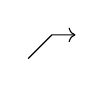
\begin{tikzpicture}[xscale=0.3, yscale=0.3, baseline=(O)]
		\coordinate (O) at (0, -0.8);
		\draw[->] (0,-1) -- (1, 0) -- (2, 0);
	\end{tikzpicture}$
	part represents $f_h$. The square is constructed using the version of
	condition (S3) in Definition~\ref{def:multiplicative-family} for a right
	multiplicative system, while commutativity of the lower part is immediate.

	Exactness of $\prod_k$ shows that $u$ is a quasi-isomorphism. Consequently,
	$g$ is also represented by the
	$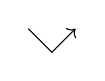
\begin{tikzpicture}[xscale=0.3, yscale=0.3, baseline=(O)]
		\coordinate (O) at (0, -0.8);
		\draw[->] (0,0) -- (1, -1) -- (2, 0);
	\end{tikzpicture}$
	part of the diagram. But $Y\xrightarrow{c_k}M_k\xleftarrow{t_k}X_k$
	represents $f_k$. Comparing this with the construction of $f$ above gives
	$f=g$.
\end{proof}

% segment-id: o014.li2.chapter4.rlim-homotopy-limit.r001
\begin{remark}
	If the indexing set for the product (respectively, coproduct) is replaced by
	an arbitrary small set $I$, the corresponding statement remains valid.
\end{remark}

% segment-id: o014.li2.chapter4.rlim-homotopy-limit.p002
Let $\mathcal{D}$ be an $\cate{Ab}$-category. Consider the category
$\cate{InvSys}(\mathcal{D}):=\mathcal{D}^{\Z_{\geq0}^{\opp}}$ from
\eqref{eqn:InvSys}. Its objects are data $X=(X_k,f_k)_{k\geq0}$, where
$X_k\in\Obj(\mathcal{D})$ and
$f_k\in\Hom_{\mathcal{D}}(X_{k+1},X_k)$. If $\mathcal{D}$ has countable
products, define the canonical morphism as in
Definition~\ref{def:Delta-diff}:
	\[ \Delta_X := T_X - \identity: \prod_k X_k \to \prod_k X_k. \]
\index[sym1]{InvSys}
\index[sym1]{DirSys@$\cate{DirSys}$}

% segment-id: o014.li2.chapter4.rlim-homotopy-limit.p003
Dually, an object of the category
$\cate{DirSys}(\mathcal{D}):=\mathcal{D}^{\Z_{\geq0}}$ consists of data
$X=(X_k,g_k)_{k\geq0}$\footnote{Such data are also called a direct system in
$\mathcal{D}$.}, where $X_k\in\Obj(\mathcal{D})$ and
$g_k\in\Hom_{\mathcal{D}}(X_k,X_{k+1})$. Similarly, define
$\nabla_X:=T_X-\identity:\bigoplus_kX_k\to\bigoplus_kX_k$, assuming that
$\mathcal{D}$ has countable coproducts; $T_X$ is again the analogous shift
morphism.

% segment-id: o014.li2.chapter4.rlim-homotopy-limit.p004
If $\Ker(\Delta_X)$ or $\Coker(\nabla_X)$ exists, there are canonical
isomorphisms
\begin{align*}
	X \in \Obj\left( \cate{InvSys}(\mathcal{D}) \right) & \implies \varprojlim_k X_k \simeq \Ker(\Delta_X), \\
	X \in \Obj\left( \cate{DirSys}(\mathcal{D}) \right) & \implies \varinjlim_k X_k \simeq \Coker(\nabla_X).
\end{align*}
The naive hope is to apply this to $\mathcal{D}=\cate{D}(\mathcal{A})$.
Derived categories are rarely abelian categories. Nevertheless,
Remark~\ref{rem:homotopy-kernel-cokernel} shows that mapping cones can serve as
homotopical versions of kernels and cokernels. Roughly speaking, the analogous
construction in a triangulated category is a distinguished triangle.

% segment-id: o014.li2.chapter4.rlim-homotopy-limit.d001
\begin{definition}[M.\ Bökstedt, A.\ Neeman {\cite{BN93}}]\label{def:holim}
	\index{homotopy limit, homotopy colimit}
	\index[sym1]{holim@$\holim$, $\hocolim$}
	Let $\mathcal{D}$ be a triangulated category.
	\begin{itemize}
		\item If $\mathcal{D}$ has countable products, a \emph{homotopy limit}
		(or homotopy $\varprojlim$) of an object
		$X\in\Obj(\cate{InvSys}(\mathcal{D}))$ means a distinguished triangle
		\[ \holim(X) \to \prod_k X_k \xrightarrow{\Delta_X} \prod_k X_k \xrightarrow{+1} . \]
		\item If $\mathcal{D}$ has countable coproducts, a \emph{homotopy
		colimit} (or homotopy $\varinjlim$) of an object
		$X\in\Obj(\cate{DirSys}(\mathcal{D}))$ means a distinguished triangle
		\[ \bigoplus_k X_k \xrightarrow{\nabla_X} \bigoplus_k X_k \to \hocolim(X) \xrightarrow{+1} . \]
	\end{itemize}
\end{definition}

% segment-id: o014.li2.chapter4.rlim-homotopy-limit.p005
The distinguished triangles occurring in this definition are isomorphic to
one another (Corollary~\ref{prop:Cone-uniqueness}), but the isomorphisms are
not canonical.

% segment-id: o014.li2.chapter4.rlim-homotopy-limit.p006
Return to complexes. Observe that
$\cate{InvSys}(\cate{C}(\mathcal{A}))=
\cate{C}(\cate{InvSys}(\mathcal{A}))$; the objects of both categories are the
same commutative diagrams
% segment-id: o014.li2.chapter4.rlim-homotopy-limit.g003
\[\begin{tikzcd}
	& \vdots \arrow[d, "{f_1^n}"'] & \vdots \arrow[d, "{f_1^{n+1}}"] & \\
	\cdots \arrow[r] & X_1^n \arrow[r, "{d_{X_1}^n}"] \arrow[d, "{f_0^n}"'] & X_1^{n+1} \arrow[d, "{f_0^{n+1}}"] \arrow[r] & \cdots \\
	\cdots \arrow[r] & X_0^n \arrow[r, "{d_{X_0}^n}"] & X_0^{n+1} \arrow[r] & \cdots
\end{tikzcd} \quad \text{with each row a complex}. \]
Morphisms in the two categories are likewise the same two-level commutative
diagrams. Thus, in $\mathcal{D}:=\cate{D}(\mathcal{A})$, we can compare
$\holim(X)$ with the right derived functor $\mathrm{R}\lim(X)$ of
$\varprojlim$, provided that both exist.

% segment-id: o014.li2.chapter4.rlim-homotopy-limit.p007
Also observe that the cohomology $\Hm^m$ of an object
$X\in\cate{C}(\cate{InvSys}(\mathcal{A}))$ is
$(\Hm^m(X_k),\Hm^m(f_k))_{k\geq0}$. Thus $X\to Y$ is a quasi-isomorphism if
and only if every $X_k\to Y_k$ is a quasi-isomorphism in
$\cate{C}(\mathcal{A})$.

% segment-id: o014.li2.chapter4.rlim-homotopy-limit.t001
\begin{theorem}\label{prop:Rlim-as-holim}
	Suppose that $\mathcal{A}$ is an abelian category with exact countable
	products and enough injective objects.
	\begin{enumerate}[(i)]
		\item The right derived functor of the left-exact functor
		$\varprojlim:\cate{InvSys}(\mathcal{A})\to\mathcal{A}$ exists and is
		written
		\[ \mathrm{R}\lim :  \cate{D}^+\left(\cate{InvSys}(\mathcal{A})\right) \to \cate{D}^+(\mathcal{A}) . \]
		\item For every object $X=(X_k,f_k)_{k\geq0}$ of
		$\cate{C}^+(\cate{InvSys}(\mathcal{A}))$, there is a distinguished
		triangle in $\cate{D}(\mathcal{A})$
		\[ \mathrm{R}\lim(X) \to \prod_k X_k \xrightarrow{\Delta_X} \prod_k X_k \xrightarrow{+1}. \]
		In particular, $\mathrm{R}\lim(X)\simeq\holim(X)$.
		\item The dimension of $\mathrm{R}\lim$ in the sense of
		Definition--Proposition~\ref{def:dim-functor} is at most $1$.
	\end{enumerate}
\end{theorem}
% segment-id: o014.li2.chapter4.rlim-homotopy-limit.pf002
\begin{proof}
	Since $\cate{InvSys}(\mathcal{A})$ has enough injective objects, (i) holds.
	More precisely, take the category $\mathcal{R}$ from
	Lemma~\ref{prop:lim1-prep} and apply
	Theorem~\ref{prop:resolution-existence} to
	$\cate{InvSys}(\mathcal{A})$ and $\mathcal{R}$. For every
	$X=(X_k,f_k)_{k\geq0}$ in
	$\cate{C}^+(\cate{InvSys}(\mathcal{A}))$, there is a quasi-isomorphism
	$X\to Y$ with $Y\in\Obj(\cate{C}^+(\mathcal{R}))$. Then
	$\mathrm{R}\lim(X)=\varprojlim Y$. The definition of $\mathcal{R}$ ensures
	that $\Delta_Y$ is surjective degree by degree, so there is a short exact
	sequence in $\cate{C}^+(\mathcal{A})$
	\[ 0 \to \varprojlim Y \to \prod_{k \geq 0} Y_k \xrightarrow{\Delta_Y} \prod_{k \geq 0} Y_k \to 0. \]
	Furthermore, every $X_k\to Y_k$ is a quasi-isomorphism, so
	$\prod_{k\geq0}X_k\to\prod_{k\geq0}Y_k$ is also a quasi-isomorphism. This
	gives the distinguished triangle in (ii):
	\[ \mathrm{R}\lim(X) \to \prod_{k \geq 0} X_k \xrightarrow{\Delta_X} \prod_{k \geq 0} X_k \xrightarrow{+1} . \]

	For (iii), if $X\in\Obj(\cate{InvSys}(\mathcal{A}))$, then $\Delta_X$ is
	a morphism in $\cate{InvSys}(\mathcal{A})$, and
	$\holim(X)\simeq\Cone(\Delta_X)[-1]$ lies in
	$\Obj(\cate{D}^{[0,1]}(\mathcal{A}))$. This is also a restatement of
	Theorem~\ref{prop:lim1}.
\end{proof}

% segment-id: o014.li2.chapter4.rlim-homotopy-limit.p008
There is a dual version of Theorem~\ref{prop:Rlim-as-holim} for
$\varinjlim:\cate{DirSys}(\mathcal{A})\to\mathcal{A}$; we do not repeat the
details.

% segment-id: o014.li2.chapter4.rlim-homotopy-limit.p009
Example~\ref{eg:Rlim-unbounded} will show how to obtain
$\mathrm{R}\lim$ on the unbounded derived category so that
Theorem~\ref{prop:Rlim-as-holim} (ii) remains valid.

% Unit 061 English translation of chapter4.tex lines 2116--2267.
% Source: Methods of Algebra, Volume 2, commit
% 9a5803ff77dd3257484cb177f851a73770a59dd3 (CC BY 4.0).
% stable-unit-id: o014.aljabr2.chapter4.unbounded-derived-functors
% Coverage: complete Section 4.11; stops before Section 4.12 at line 2268.

% segment-id: o014.li2.chapter4.unbounded-derived-functors.h001
\section{Unbounded Derived Functors}\label{sec:unbounded-derived}
\hypertarget{o014.aljabr2.chapter4.unbounded-derived-functors}{ }
% segment-id: o014.li2.chapter4.unbounded-derived-functors.x001
\index{derived functor!unbounded}

% segment-id: o014.li2.chapter4.unbounded-derived-functors.p001
Consider an additive functor $F:\mathcal{A}\to\mathcal{A}'$ between abelian
categories. This section returns to Definition~\ref{def:derived-functor} and
focuses on the versions of derived functors for unbounded derived categories,
% segment-id: o014.li2.chapter4.unbounded-derived-functors.q001
\[ \mathrm{R}F, \; \mathrm{L}F: \cate{D}(\mathcal{A}) \to \cate{D}(\mathcal{A}'). \]

% segment-id: o014.li2.chapter4.unbounded-derived-functors.p002
To guarantee the existence of $\mathrm{R}F$ or $\mathrm{L}F$ and to compute
with it, we need the notions of K-injective and K-projective complexes from
Definition~\ref{def:K-resolutions}, together with the corresponding
resolutions.

% segment-id: o014.li2.chapter4.unbounded-derived-functors.le001
\begin{lemma}\label{prop:K-injective-zero}
	Let $\mathcal{A}$ be an abelian category. If
	$Z\in\Obj(\cate{K}(\mathcal{A}))$ is both K-injective (respectively,
	K-projective) and acyclic, then $Z=0$.
\end{lemma}
% segment-id: o014.li2.chapter4.unbounded-derived-functors.pf001
\begin{proof}
	Lemma~\ref{prop:K-injective-criterion} implies that
	$\Hom_{\cate{K}(\mathcal{A})}(Z,Z)=0$.
\end{proof}

% segment-id: o014.li2.chapter4.unbounded-derived-functors.p003
We first state a general result. Fix triangulated categories
$\mathcal{D}_1$, $\mathcal{D}_2$, and $\mathcal{D}'$, together with their
saturated triangulated subcategories $\mathcal{N}_1$, $\mathcal{N}_2$, and
$\mathcal{N}'$.

% segment-id: o014.li2.chapter4.unbounded-derived-functors.le002
\begin{lemma}\label{prop:K-cats}
	Given a triangulated bifunctor
	$G:\mathcal{D}_1\times\mathcal{D}_2\to\mathcal{D}'$, define a full
	subcategory $\mathcal{K}_2^G$ of $\mathcal{D}_2$ by
% segment-id: o014.li2.chapter4.unbounded-derived-functors.q002
	\[ \Obj(\mathcal{K}_2^G) = \left\{ X_2 \in \Obj(\mathcal{D}_2) : X_1 \in \Obj(\mathcal{N}_1) \implies G(X_1, X_2) \in \Obj(\mathcal{N}') \right\}. \]
	Then $\mathcal{K}_2^G$ is a saturated triangulated subcategory. After
	interchanging the two variables, the corresponding statement holds for
	$\mathcal{K}_1^G\subset\mathcal{D}_1$.
\end{lemma}
% segment-id: o014.li2.chapter4.unbounded-derived-functors.pf002
\begin{proof}
	The isomorphism $G(X_1,X_2[1])\simeq G(X_1,X_2)[1]$ shows that
	$\mathcal{K}_2^G$ is closed under translation. Similarly, suppose that
	$I\to J\to K\xrightarrow{+1}$ is a distinguished triangle with
	$I,K\in\Obj(\mathcal{K}_2^G)$. From the distinguished triangle
% segment-id: o014.li2.chapter4.unbounded-derived-functors.q003
	\[ G(X_1, I) \to G(X_1, J) \to G(X_1, K) \xrightarrow{+1} \]
	it follows immediately that
	$X_1\in\Obj(\mathcal{N}_1)\implies
	G(X_1,J)\in\Obj(\mathcal{N}')$. Saturation is clear.
\end{proof}

% segment-id: o014.li2.chapter4.unbounded-derived-functors.p004
This result can be applied to
$\Hom:\mathcal{A}^{\opp}\times\mathcal{A}\to\cate{Ab}$ and the
corresponding triangulated bifunctor $\cate{K}_{\Pi}\Hom$.
Example~\ref{eg:Hom-bicplx} has shown that the latter bifunctor is essentially
the $\Hom$ complex:
% segment-id: o014.li2.chapter4.unbounded-derived-functors.e001
\begin{equation}\label{eqn:CPiHom}\begin{gathered}
	(\cate{C}_{\Pi} \Hom)(\sigma^{-1} X_1, X_2) \simeq \Hom^\bullet\left( X_1, X_2 \right), \\
	(\cate{K}_\Pi \Hom)(\sigma^{-1} X_1, X_2) \simeq \Hom^\bullet\left( X_1, X_2 \right)\; \text{viewed in $\cate{K}(\cate{Ab})$},
\end{gathered}\end{equation}
% segment-id: o014.li2.chapter4.unbounded-derived-functors.p005
where $\sigma:\cate{C}(\mathcal{A}^{\opp})\rightiso
\cate{C}(\mathcal{A})^{\opp}$ and
$\cate{K}(\mathcal{A}^{\opp})\rightiso\cate{K}(\mathcal{A})^{\opp}$ are
the isomorphisms from Definition--Proposition~\ref{def:sigma} and
Proposition~\ref{prop:sigma-homotopy}. We shall later need the corresponding
version for derived categories.

% segment-id: o014.li2.chapter4.unbounded-derived-functors.pr001
\begin{proposition}\label{prop:K-injective-F-injective}
	All K-injective (respectively, K-projective) complexes form a saturated
	triangulated subcategory $\mathcal{I}$ (respectively, $\mathcal{P}$) of
	$\cate{K}(\mathcal{A})$. If $\mathcal{A}$ has enough K-injective
	(respectively, K-projective) complexes, then for every additive functor
	$F:\mathcal{A}\to\mathcal{A}'$, the subcategory $\mathcal{I}$
	(respectively, $\mathcal{P}$) is $F$-injective (respectively,
	$F$-projective).
\end{proposition}
% segment-id: o014.li2.chapter4.unbounded-derived-functors.pf003
\begin{proof}
	It suffices to treat the K-injective case. The first assertion follows by
	applying Lemma~\ref{prop:K-cats} to $G=\cate{K}_{\Pi}\Hom$, using the
	definition of K-injective complexes in
	Definition~\ref{def:K-resolutions} and \eqref{eqn:CPiHom}: the subcategory
	$\mathcal{K}_2^G$ there is precisely $\mathcal{I}$ here.

	Suppose that $\mathcal{A}$ has enough K-injective complexes. If $I$ is an
	acyclic K-injective complex, Lemma~\ref{prop:K-injective-zero} implies that
	$I=0$, so $(\cate{K}F)I$ is certainly acyclic. Thus all the conditions in
	Definition~\ref{def:F-injective} for an $F$-injective triangulated
	subcategory are satisfied.
\end{proof}

% segment-id: o014.li2.chapter4.unbounded-derived-functors.p006
Write $Q:\cate{K}(\mathcal{A})\to\cate{D}(\mathcal{A})$ and
$Q':\cate{K}(\mathcal{A}')\to\cate{D}(\mathcal{A}')$ for the localization
functors.

% segment-id: o014.li2.chapter4.unbounded-derived-functors.co001
\begin{corollary}
	If $\mathcal{A}$ has enough K-injective complexes, then $F$ has a right
	derived functor
	$\mathrm{R}F:\cate{D}(\mathcal{A})\to\cate{D}(\mathcal{A}')$, such that
	$\mathrm{R}F(QX)\simeq Q'\cate{K}F(X)$ whenever $X$ is K-injective.

	Dually, if $\mathcal{A}$ has enough K-projective complexes, then $F$ has a
	left derived functor
	$\mathrm{L}F:\cate{D}(\mathcal{A})\to\cate{D}(\mathcal{A}')$, such that
	$\mathrm{L}F(QX)\simeq Q'\cate{K}F(X)$ whenever $X$ is K-projective.
\end{corollary}
% segment-id: o014.li2.chapter4.unbounded-derived-functors.pf004
\begin{proof}
	Apply Proposition~\ref{prop:K-injective-F-injective} in the general
	framework of Proposition~\ref{prop:localization-injective}.
\end{proof}

% segment-id: o014.li2.chapter4.unbounded-derived-functors.p007
Now fix abelian categories $\mathcal{A}_1$, $\mathcal{A}_2$, and
$\mathcal{B}$. For an additive bifunctor
$F:\mathcal{A}_1\times\mathcal{A}_2\to\mathcal{B}$, consider the unbounded
version of the derived bifunctor $\mathrm{R}F$ (respectively,
$\mathrm{L}F$) from Definition~\ref{def:derived-bifunctor}. From now on, we
always assume that $\mathcal{B}$ has countable products (respectively,
countable coproducts).

% segment-id: o014.li2.chapter4.unbounded-derived-functors.p008
Concretely, we wish to determine $\mathrm{R}F$ (respectively,
$\mathrm{L}F$) using the subcategories $\mathcal{I}_1$, $\mathcal{I}_2$
(respectively, $\mathcal{P}_1$, $\mathcal{P}_2$) above.

% segment-id: o014.li2.chapter4.unbounded-derived-functors.le003
\begin{lemma}\label{prop:bifunctor-via-K-injective-prep}
	For $i=1,2$, take the triangulated subcategory $\mathcal{I}_i$
	(respectively, $\mathcal{P}_i$) of $\cate{K}(\mathcal{A}_i)$ from
	Proposition~\ref{prop:K-injective-F-injective}.
% segment-id: o014.li2.chapter4.unbounded-derived-functors.l001
	\begin{compactitem}
% segment-id: o014.li2.chapter4.unbounded-derived-functors.i001
		\item If $\mathcal{A}_1$ and $\mathcal{A}_2$ have enough K-injective
		complexes, then $\mathcal{I}_1\times\mathcal{I}_2$ is $F$-injective.
% segment-id: o014.li2.chapter4.unbounded-derived-functors.i002
		\item If $\mathcal{A}_1$ and $\mathcal{A}_2$ have enough K-projective
		complexes, then $\mathcal{P}_1\times\mathcal{P}_2$ is $F$-projective.
	\end{compactitem}
\end{lemma}
% segment-id: o014.li2.chapter4.unbounded-derived-functors.pf005
\begin{proof}
	It suffices to treat the K-injective case. The key is to show that if
	$X_1\in\Obj(\mathcal{I}_1)$, then
	$(\cate{K}_{\Pi}F)(X_1,\cdot)$ sends every acyclic object $Z$ of
	$\mathcal{I}_2$ to an acyclic object of $\cate{K}(\mathcal{B})$. But
	Lemma~\ref{prop:K-injective-zero} gives $Z=0$, and
	$(\cate{K}_{\Pi}F)(X_1,\cdot)$ is additive, so the assertion follows
	immediately. The corresponding result follows after interchanging the
	indices $1$ and $2$.
\end{proof}

% segment-id: o014.li2.chapter4.unbounded-derived-functors.p009
Write $Q:\cate{K}(\mathcal{B})\to\cate{D}(\mathcal{B})$ and
$Q_i:\cate{K}(\mathcal{A}_i)\to\cate{D}(\mathcal{A}_i)$ for the
localization functors ($i=1,2$).

% segment-id: o014.li2.chapter4.unbounded-derived-functors.pr002
\begin{proposition}\label{prop:bifunctor-via-K-injective}
	For $F:\mathcal{A}_1\times\mathcal{A}_2\to\mathcal{B}$, suppose that
	$\mathcal{A}_1$ and $\mathcal{A}_2$ both have enough K-injective
	(respectively, K-projective) complexes. Then the derived bifunctor
	$\mathrm{R}F$ (respectively, $\mathrm{L}F$) exists. If
	$X_i\in\Obj(\cate{K}(\mathcal{A}))$ is K-injective (respectively,
	K-projective) for $i=1,2$, then there is a canonical isomorphism
% segment-id: o014.li2.chapter4.unbounded-derived-functors.q004
	\[ \mathrm{R}F(Q_1 X_1, Q_2 X_2) \simeq Q (\cate{K}_{\Pi} F)(X_1, X_2) \quad \text{(respectively, $\mathrm{L}F(Q_1 X_1, Q_2 X_2) \simeq Q (\cate{K}_{\oplus} F)(X_1, X_2)$) }. \]
\end{proposition}
% segment-id: o014.li2.chapter4.unbounded-derived-functors.pf006
\begin{proof}
	Apply Lemma~\ref{prop:bifunctor-via-K-injective-prep} directly to
	Proposition~\ref{prop:localization-injective-bifunctor}.
\end{proof}

% segment-id: o014.li2.chapter4.unbounded-derived-functors.p010
For a particular bifunctor $F$, one can often choose $F$-injective
(respectively, $F$-projective) subcategories larger than the subcategories of
K-injective (respectively, K-projective) complexes. The $\RHom$ functor to be
discussed next is one example.

% segment-id: o014.li2.chapter4.unbounded-derived-functors.th001
\begin{theorem}[Unbounded $\RHom$]\label{prop:unbounded-RHom}
% segment-id: o014.li2.chapter4.unbounded-derived-functors.x002
	\index{$\RHom$ functor}
% segment-id: o014.li2.chapter4.unbounded-derived-functors.x003
	\index[sym1]{RHom@$\RHom$}
	Suppose that the abelian category $\mathcal{A}$ has enough K-injective or
	enough K-projective complexes. For simplicity, denote every localization
	functor by $Q$.
% segment-id: o014.li2.chapter4.unbounded-derived-functors.l002
	\begin{enumerate}[(i)]
% segment-id: o014.li2.chapter4.unbounded-derived-functors.i003
		\item The bifunctor
		$\Hom=\Hom_{\mathcal{A}}:\mathcal{A}^{\opp}\times\mathcal{A}
		\to\cate{Ab}$ has a right derived bifunctor
		$\cate{D}(\mathcal{A}^{\opp})\times\cate{D}(\mathcal{A})
		\to\cate{D}(\cate{Ab})$. Via the equivalence $\sigma$ of
		Proposition~\ref{prop:derived-cat-op}, it can also be written as
% segment-id: o014.li2.chapter4.unbounded-derived-functors.q005
		\[ \RHom: \cate{D}(\mathcal{A})^{\opp} \times \cate{D}(\mathcal{A}) \to \cate{D}(\cate{Ab}). \]
		Moreover, if $\mathcal{A}$ has enough K-injective (respectively,
		K-projective) complexes, then
		$\cate{K}(\mathcal{A})^{\opp}\times\mathcal{I}$ (respectively,
		$\mathcal{P}^{\opp}\times\cate{K}(\mathcal{A})$) is
		$\Hom$-injective.
% segment-id: o014.li2.chapter4.unbounded-derived-functors.i004
		\item Suppose that $\mathcal{A}$ has enough K-injective complexes and
		that $X_2\to I_2$ is a K-injective resolution. This resolution induces
% segment-id: o014.li2.chapter4.unbounded-derived-functors.q006
		\[ \RHom(Q X_1, Q X_2) \rightiso Q \Hom^\bullet(X_1, I_2). \]
		In particular,
		$\RHom(QX_1,\cdot)\simeq
		\mathrm{R}\left(\Hom(X_1,\cdot)\right)$.
% segment-id: o014.li2.chapter4.unbounded-derived-functors.i005
		\item Suppose that $\mathcal{A}$ has enough K-projective complexes and
		that $P_1\to X_1$ is a K-projective resolution. This resolution induces
% segment-id: o014.li2.chapter4.unbounded-derived-functors.q007
		\[ \RHom(Q X_1, Q X_2) \rightiso Q \Hom^\bullet(P_1, X_2). \]
		In particular,
		$\RHom(\cdot,QX_2)\simeq
		\mathrm{R}\left(\Hom(\cdot,X_2)\right)$.
% segment-id: o014.li2.chapter4.unbounded-derived-functors.i006
		\item There is a canonical isomorphism
		$\Hm^n\RHom(X,Y)\simeq
		\Hom_{\cate{D}(\mathcal{A})}(X,Y[n])=: \Ext^n(X,Y)$
		(Definition~\ref{def:Ext-general}).
	\end{enumerate}
\end{theorem}
% segment-id: o014.li2.chapter4.unbounded-derived-functors.pf007
\begin{proof}
	The argument is nearly identical to that for
	Theorem~\ref{prop:RHom-bounded}. For example, suppose that $\mathcal{A}$
	has enough K-injective complexes. The key is to show that
	$\cate{K}(\mathcal{A})^{\opp}\times\mathcal{I}$ is $\Hom$-injective.
% segment-id: o014.li2.chapter4.unbounded-derived-functors.l003
	\begin{itemize}
% segment-id: o014.li2.chapter4.unbounded-derived-functors.i007
		\item Fix a complex $X_1$. The functor
		$(\cate{K}_\Pi\Hom)(X_1,\cdot)$ sends every acyclic K-injective complex
		$X_2$ to an acyclic complex, because $X_2$ is $0$ in
		$\cate{K}(\mathcal{A})$ (Lemma~\ref{prop:K-injective-zero}).
% segment-id: o014.li2.chapter4.unbounded-derived-functors.i008
		\item Fix a K-injective complex $X_2$. If $X_1$ is acyclic, the
		definition of a K-injective complex implies that
		$\Hom^\bullet\left(X_1,X_2\right)$ is acyclic. By
		\eqref{eqn:CPiHom}, $(\cate{K}_\Pi\Hom)(X_1,X_2)$ is therefore
		acyclic as well.
	\end{itemize}
	Thus the acyclicity conditions required for the $\Hom$-injective property
	have been verified, while the resolution conditions hold directly.
\end{proof}

% segment-id: o014.li2.chapter4.unbounded-derived-functors.th002
\begin{theorem}\label{prop:RHom-adjoint}
	Consider an adjoint pair of additive functors between abelian categories
% segment-id: o014.li2.chapter4.unbounded-derived-functors.g001
	$\begin{tikzcd}
		F: \mathcal{A} \arrow[r, shift left] & \mathcal{A}' \arrow[l, shift left] : G
	\end{tikzcd}$.
	Suppose that $\mathcal{A}$ has enough K-projective complexes and
	$\mathcal{A}'$ has enough K-injective complexes. Then there is a canonical
	isomorphism in $\cate{D}(\cate{Ab})$
% segment-id: o014.li2.chapter4.unbounded-derived-functors.q008
	\[ \RHom_{\mathcal{A'}}\left(\mathrm{L}F(X), Y\right) \simeq \RHom_{\mathcal{A}}\left(X, \mathrm{R}G(Y) \right), \]
	where $X\in\Obj\left(\cate{D}(\mathcal{A})\right)$ and
	$Y\in\Obj\left(\cate{D}(\mathcal{A}')\right)$.
\end{theorem}
% segment-id: o014.li2.chapter4.unbounded-derived-functors.pf008
\begin{proof}
	The argument is the same as for
	Theorem~\ref{prop:RHom-adjoint-bounded}. The only difference is that
	injective (respectively, projective) resolutions are replaced by
	K-injective (respectively, K-projective) resolutions, and
	Theorem~\ref{prop:K-resolution-homotopy} replaces
	Theorem~\ref{prop:resolution-homotopy} in the discussion of uniqueness of
	resolutions.
\end{proof}

% segment-id: o014.li2.chapter4.unbounded-derived-functors.r001
\begin{remark}
	Applying $\Hm^0$ to both sides of Theorem~\ref{prop:RHom-adjoint} gives the
	adjunction
% segment-id: o014.li2.chapter4.unbounded-derived-functors.q009
	\[ \Hom_{\cate{D}(\mathcal{A'})}\left(\mathrm{L}F(X), Y\right) \simeq \Hom_{\cate{D}(\mathcal{A})}\left(X, \mathrm{R}G(Y) \right). \]

	Since derived functors obtained through resolutions are always absolute Kan
	extensions in the sense of Definition~\ref{def:absolute-Kan}
	(Proposition~\ref{prop:localization-functor-abs}),
	Theorem~\ref{prop:Quillen-adjunction-gen} also says that
	$(\mathrm{L}F,\mathrm{R}G)$ is an adjoint pair. The two approaches give the
	same adjunction isomorphism. Why? It suffices to consider the case in which
	$X$ is K-projective and $Y$ is K-injective. In this case, the adjunction
	isomorphism of Theorem~\ref{prop:RHom-adjoint} is realized concretely by the
	unit $\eta$ and counit $\varepsilon$ at the level of $\cate{K}(\cdot)$ as
% segment-id: o014.li2.chapter4.unbounded-derived-functors.q010
	\begin{align*}
		\Hom_{\cate{K}(\mathcal{A}')}\left( \cate{K}F(X), Y\right) \simeq \Hom_{\cate{K}(\mathcal{A})}\left( X, \cate{K}G(Y) \right).
	\end{align*}
	On the other hand, Theorem~\ref{prop:Quillen-adjunction-gen} determines
	$\underline{\eta}$ and $\underline{\varepsilon}$ at the level of derived
	categories. The characterization given there suffices to show that they are
	compatible with $\eta$ and $\varepsilon$. The details are left to the
	interested reader.
\end{remark}

% segment-id: o014.li2.chapter4.unbounded-derived-functors.p011
Finally, another set of sufficient conditions for the existence of unbounded
derived functors is based on finite dimension
(Definition--Proposition~\ref{def:dim-functor}). Although the proof technique
does not go beyond the scope of this book, we state the result without proof
to avoid a digression; see {\cite[Tags 07K6, 07K7]{stacks}}. The starting
point is the construction of bounded derived functors in
Theorem~\ref{prop:derived-via-resolution}.

% segment-id: o014.li2.chapter4.unbounded-derived-functors.pr003
\begin{proposition}\label{prop:unbounded-derived-fd}
% segment-id: o014.li2.chapter4.unbounded-derived-functors.x004
	\index{dimension}
	Let $F:\mathcal{A}\to\mathcal{A}'$ be a left-exact (respectively,
	right-exact) functor between abelian categories. Assume that
% segment-id: o014.li2.chapter4.unbounded-derived-functors.l004
	\begin{compactitem}
% segment-id: o014.li2.chapter4.unbounded-derived-functors.i009
		\item relative to $F$, there is a full additive subcategory
		$\mathcal{A}^\flat$ of $\mathcal{A}$ of type I (respectively, type P),
		as in Definition--Proposition~\ref{prop:F-injective-criterion};
% segment-id: o014.li2.chapter4.unbounded-derived-functors.i010
		\item the corresponding bounded derived functor
		${}^+\mathrm{R}F$ (respectively, ${}^-\mathrm{L}F$) has finite
		dimension.
	\end{compactitem}
	Then $\mathrm{R}F$ (respectively, $\cate{L}F$):
	$\cate{D}(\mathcal{A})\to\cate{D}(\mathcal{A}')$ exists. Moreover,
	$\cate{K}(\mathcal{A}^\flat)$ is an $F$-injective (respectively,
	$F$-projective) subcategory of $\cate{K}(\mathcal{A})$.
\end{proposition}

% segment-id: o014.li2.chapter4.unbounded-derived-functors.ex001
\begin{example}\label{eg:Rlim-unbounded}
	Suppose that $\mathcal{A}$ has exact countable products and enough
	injective objects. Take the left-exact functor $F$ to be
	$\varprojlim:\cate{InvSys}(\mathcal{A})\to\mathcal{A}$.
	Theorem~\ref{prop:Rlim-as-holim} (iii) shows that the bounded version of
	$\mathrm{R}\lim$ has dimension at most $1$, while the subcategory
	$\mathcal{R}\subset\cate{InvSys}(\mathcal{A})$ is of type I relative to
	$\varprojlim$. The preceding result therefore gives the unbounded derived functor
% segment-id: o014.li2.chapter4.unbounded-derived-functors.q011
	\[ \mathrm{R}\lim: \cate{D}(\cate{InvSys}(\mathcal{A})) \to \cate{D}(\mathcal{A}). \]

	As in Theorem~\ref{prop:Rlim-as-holim} (ii), for every object $X$ of
	$\cate{C}(\cate{InvSys}(\mathcal{A}))$ there is a distinguished triangle
	in $\cate{D}(\mathcal{A})$
% segment-id: o014.li2.chapter4.unbounded-derived-functors.q012
	\[ \mathrm{R}\lim(X) \to \prod_k X_k \xrightarrow{\Delta_X} \prod_k X_k \xrightarrow{+1} . \]
	In particular, $\mathrm{R}\lim(X)\simeq\holim(X)$. By
	Proposition~\ref{prop:unbounded-derived-fd}, the original proof applies with
	no other changes: simply replace every $\cate{C}^+(\cdots)$ by
	$\cate{C}(\cdots)$.
\end{example}

% Unit 062 English translation of chapter4.tex lines 2268--2499.
% Source: Methods of Algebra, Volume 2, commit
% 9a5803ff77dd3257484cb177f851a73770a59dd3 (CC BY 4.0).
% stable-unit-id: o014.aljabr2.chapter4.k-flat-derived-tensor-a
% Coverage: first half of Section 4.12, on K-flat complexes, K-flat
% resolutions, and the construction of the derived tensor product; stops
% after the paragraph at line 2499, just before the corollary at line 2500.

% segment-id: o014.li2.chapter4.k-flat-derived-tensor-a.h001
\section{Example: K-Flat Complexes and \texorpdfstring{$\otimesL$}{otimesL}}\label{sec:otimesL}
\hypertarget{o014.aljabr2.chapter4.k-flat-derived-tensor-a}{ }

% segment-id: o014.li2.chapter4.k-flat-derived-tensor-a.p001
Throughout this section, $\Bbbk$ is a commutative ring.

% segment-id: o014.li2.chapter4.k-flat-derived-tensor-a.cv001
\begin{convention}\label{con:bimodule-algebra}
	Let $R$ and $S$ be $\Bbbk$-algebras. By the convention of this book, every
	$(R,S)$-bimodule $M$ is tacitly assumed to satisfy $tm=mt$ for
	$t\in\Bbbk$ and $m\in M$. In other words,
	$(R,S)\dcate{Mod}\simeq(R\dotimes{\Bbbk}S^{\opp})\dcate{Mod}$. When
	$\Bbbk=\Z$, this condition is redundant.

	From now on, the forgetful functor
	$(R,S)\dcate{Mod}\to R\dcate{Mod}$ (respectively,
	$(R,S)\dcate{Mod}\to\cated{Mod}S$) is written
	$M\mapsto{}_RM$ (respectively, $M\mapsto M_S$); the same notation applies
	to complexes. These forgetful functors are exact, and the triangulated
	functors they induce between derived categories are denoted in the same way.
\end{convention}

% segment-id: o014.li2.chapter4.k-flat-derived-tensor-a.p002
Notice that, for every complex $M$ of $(R,S)$-bimodules, one has
% segment-id: o014.li2.chapter4.k-flat-derived-tensor-a.q001
\[ M_S \;\text{acyclic} \iff M \;\text{acyclic} \iff {}_R M \;\text{acyclic}. \]

% segment-id: o014.li2.chapter4.k-flat-derived-tensor-a.p003
From now on, let $R$, $A$, and $B$ be $\Bbbk$-algebras. Our starting point is
the bifunctor given by the tensor product,
% segment-id: o014.li2.chapter4.k-flat-derived-tensor-a.q002
\[ \otimes_R: (A, R)\dcate{Mod} \times (R, B)\dcate{Mod} \to (A, B)\dcate{Mod}, \]
which is right exact in each variable. The simplest case is $A=\Bbbk=B$; the
corresponding bifunctor becomes
$\otimes_R:\cated{Mod}R\times R\dcate{Mod}\to\cate{\Bbbk}$.

% segment-id: o014.li2.chapter4.k-flat-derived-tensor-a.p004
For convenience, if $X$ is a complex of $(A,R)$-bimodules and $Y$ is a
complex of $(R,B)$-bimodules, we henceforth write the bicomplex obtained by
taking tensor products term by term as
$X^\bullet\dotimes{R}Y^\bullet$, and write its total complex as
% segment-id: o014.li2.chapter4.k-flat-derived-tensor-a.q003
\[ X \dotimes{R} Y := \tot_{\oplus} \left( X^\bullet \dotimes{R} Y^\bullet \right). \]

% segment-id: o014.li2.chapter4.k-flat-derived-tensor-a.p005
Categories of bimodules have enough K-projective complexes (apply
Example~\ref{eg:Mod-K-injectives}); hence
Proposition~\ref{prop:bifunctor-via-K-injective} ensures the existence of the
unbounded left derived bifunctor.

% segment-id: o014.li2.chapter4.k-flat-derived-tensor-a.d001
\begin{definition}\label{def:otimesL}
	\index{derived tensor product}
	\index[sym1]{XotimesLY@$X \otimesL[R] Y$}
	Denote the left derived bifunctor
	$\mathrm{L}\left(\cdot\dotimes{R}\cdot\right)$ of $\otimes_R$ by
% segment-id: o014.li2.chapter4.k-flat-derived-tensor-a.q004
	\[ \otimesL[R] : \cate{D}((A, R)\dcate{Mod}) \times \cate{D}((R, B)\dcate{Mod}) \to \cate{D}((A, B)\dcate{Mod}). \]
	When no confusion can arise, $X\otimesL[R]Y$ is also abbreviated to
	$X\otimesL Y$.
\end{definition}

% segment-id: o014.li2.chapter4.k-flat-derived-tensor-a.p006
The abstract definition above is straightforward, but to study $\otimes_R$
further we still need to introduce a class of quasi-isomorphisms called K-flat
resolutions. The reasons include the following:
% segment-id: o014.li2.chapter4.k-flat-derived-tensor-a.l001
\begin{itemize}
% segment-id: o014.li2.chapter4.k-flat-derived-tensor-a.i001
	\item the definition of a K-flat resolution is directly related to the tensor
	product and is more useful for establishing important properties and making
	concrete computations, as already seen in \S\ref{sec:Ext-Tor};
% segment-id: o014.li2.chapter4.k-flat-derived-tensor-a.i002
	\item in geometric settings such as sheaf theory, K-injective resolutions
	may be available while K-projective resolutions are not; in that situation,
	K-flat resolutions are the only means of studying the derived tensor product.
\end{itemize}

% segment-id: o014.li2.chapter4.k-flat-derived-tensor-a.d002
\begin{definition}[N.\ Spaltenstein {\cite[Definition 5.1]{Spa88}}]
	\index{complex!K-flat}
	Let $X$ be a complex of right $R$-modules. If, for every complex $Y$ of
	left $R$-modules,
% segment-id: o014.li2.chapter4.k-flat-derived-tensor-a.q005
	\[ Y \;\text{acyclic} \implies X \dotimes{R} Y\;\text{acyclic}, \]
	then $X$ is called \emph{K-flat}\footnote{A more reasonable name might be a
	homotopy-flat complex.}; this property depends only on the isomorphism class
	of $X$ in $\cate{K}(\cated{Mod}R)$. K-flatness is defined similarly for
	complexes of left $R$-modules.
\end{definition}

% segment-id: o014.li2.chapter4.k-flat-derived-tensor-a.p007
For bounded-above complexes, K-flatness follows from the familiar notion of
flatness in module theory.

% segment-id: o014.li2.chapter4.k-flat-derived-tensor-a.pr001
\begin{proposition}\label{prop:flat-K-flat}
	Let $X$ be an object of $\cate{C}^-(\cated{Mod}R)$, and suppose that every
	$X^n$ is flat. Then $X$ is K-flat. The same statement holds for objects of
	$\cate{C}^-(R\dcate{Mod})$.
\end{proposition}

% segment-id: o014.li2.chapter4.k-flat-derived-tensor-a.pf001
\begin{proof}
	Let $Y$ be an acyclic complex of left $R$-modules; we shall prove that
	$X\dotimes{R}Y$ is acyclic. Using truncation functors, write $Y$ as
	$\varinjlim_m\tau^{\leq m}Y$. Degree by degree, $\varinjlim_m$ commutes
	both with tensor products \cite[Proposition 6.9.2]{Li1} and with
	$\bigoplus$; it therefore suffices to consider the case in which $Y$ is
	bounded above. Then $X^\bullet\dotimes{R}Y^\bullet$ belongs to the category
	$\cate{C}^2_f(\Bbbk\dcate{Mod})$ of Definition~\ref{def:Cf-Supp}. Since
	$X^p\dotimes{R}Y^\bullet$ is acyclic for every $p$,
	Corollary~\ref{prop:acyclic-assembly} ensures that $X\dotimes{R}Y$ is
	acyclic.
\end{proof}

% segment-id: o014.li2.chapter4.k-flat-derived-tensor-a.p008
In view of this result, if the reader is interested only in bounded-above
derived categories, every K-flat complex appearing in this section may be
replaced by a bounded-above complex of flat modules.

% segment-id: o014.li2.chapter4.k-flat-derived-tensor-a.d003
\begin{definition}
	\index{resolution!K-flat}
	\index{enough K-flat complexes}
	If $P\to X$ is a quasi-isomorphism in
	$\cate{C}((A,R)\dcate{Mod})$ and $P_R$ is K-flat, then this morphism is
	called a \emph{K-flat resolution} of $X$ relative to $R$. If every
	$X\in\cate{C}((A,R)\dcate{Mod})$ has a K-flat resolution relative to $R$,
	then $(A,R)\dcate{Mod}$ is said to have enough K-flat complexes relative to
	$R$.

	A K-flat resolution relative to $R$ is defined similarly for
	$X\in\Obj(\cate{C}((R,B)\dcate{Mod}))$.
\end{definition}

% segment-id: o014.li2.chapter4.k-flat-derived-tensor-a.p009
A natural question is how to guarantee that a category of bimodules has
enough K-flat complexes relative to $R$. What is the relation between K-flat
and K-projective complexes? As expected, the bridge comes from the classical
adjunction between $\otimes$ and $\Hom$ \cite[Theorem 6.6.5]{Li1}.

% segment-id: o014.li2.chapter4.k-flat-derived-tensor-a.p010
The first step is to lift that adjunction to the level of complexes. If $Y$ is
an object of $\cate{C}((R,B)\dcate{Mod})$ and $Z$ is an object of
$\cate{C}((A,B)\dcate{Mod})$, the $\Hom$ complex
$\Hom^\bullet(Y_B,Z_B)$ can be endowed degree by degree with an
$(A,R)$-bimodule structure, making it an object of
$\cate{C}((A,R)\dcate{Mod})$.

% segment-id: o014.li2.chapter4.k-flat-derived-tensor-a.pr002
\begin{proposition}[$\Hom$--$\otimes$ adjunction: complex version]\label{prop:tensor-Hom-cplx}
	Let $X$ be an object of $\cate{C}((A,R)\dcate{Mod})$, let $Y$ be an object
	of $\cate{C}((R,B)\dcate{Mod})$, and let $Z$ be an object of
	$\cate{C}((A,B)\dcate{Mod})$. There are canonical isomorphisms in
	$\cate{C}(\Bbbk\dcate{Mod})$
% segment-id: o014.li2.chapter4.k-flat-derived-tensor-a.q007
	\begin{align*}
		\Hom^\bullet\left( X \dotimes{R} Y, \; Z \right) & \simeq \Hom^\bullet\left( X, \Hom^\bullet(Y_B, Z_B) \right) \\
		& \simeq \Hom^\bullet\left( Y, \Hom^\bullet({}_A X, {}_A Z) \right).
	\end{align*}

	Consequently, taking $\Ker(d^0)$ gives isomorphisms of $\Bbbk$-modules
% segment-id: o014.li2.chapter4.k-flat-derived-tensor-a.q008
	\begin{align*}
		\Hom_{\cate{C}((A, B)\dcate{Mod})}\left( X \dotimes{R} Y, \; Z \right) & \simeq \Hom_{\cate{C}((A, R)\dcate{Mod})}\left( X, \Hom^\bullet(Y_B, Z_B) \right) \\
		& \simeq \Hom_{\cate{C}((R, B)\dcate{Mod})}\left( Y, \Hom^\bullet({}_A X, {}_A Z) \right).
	\end{align*}
\end{proposition}

% segment-id: o014.li2.chapter4.k-flat-derived-tensor-a.pf002
\begin{proof}
	It suffices to treat the first isomorphism. To simplify notation, write
	$Y$ and $Z$ for $Y_B$ and $Z_B$ below, and omit the subscript on $\Hom$.
	Fix $n\in\Z$. The degree-$n$ term on the left-hand side is
% segment-id: o014.li2.chapter4.k-flat-derived-tensor-a.e001
	\begin{multline}\label{eqn:tensor-Hom-cplx-aux}
		\prod_k \Hom\left( (X \dotimes{R} Y)^k, Z^{k+n}\right) \simeq \prod_k \prod_{p+q=k} \Hom\left(X^p \dotimes{R} Y^q, Z^{k+n}\right) \\
		= \prod_{p, q} \Hom\left( X^p \dotimes{R} Y^q, Z^{p+q+n} \right) \simeq \prod_p \prod_q \Hom\left( X^p, \Hom\left(Y^q, Z^{p+q+n}\right) \right) \\
		\simeq \prod_p \Hom\left( X^p, \Hom^{p+n}(Y, Z) \right),
	\end{multline}
	and the last term is precisely the degree-$n$ term on the right-hand side.
	Concretely, under the second isomorphism $\simeq$, the homomorphism of
	$(A,B)$-bimodules
	$\varphi^{p,q}:X^p\dotimes{R}Y^q\to Z^{p+q+n}$ corresponds to
% segment-id: o014.li2.chapter4.k-flat-derived-tensor-a.q009
	\[ \left[ x \mapsto [y \mapsto \varphi^{p,q}(x \otimes y)] \right] \; \in \Hom\left( X^p, \Hom\left(Y^q, Z^{p+q+n}\right) \right). \]
	It remains only to verify that \eqref{eqn:tensor-Hom-cplx-aux} determines an
	isomorphism of complexes.

	Take an element of the degree-$n$ term on the left and write it as
	$(\varphi^{p,q})_{p,q\in\Z}$. The $(p,q)$-component of its image under
	$d_{\Hom^\bullet(X\otimes Y,Z)}$ sends
	$x\otimes y\in X^p\dotimes{R}Y^q$ to
% segment-id: o014.li2.chapter4.k-flat-derived-tensor-a.q010
	\[ d_Z \varphi^{p,q}(x \otimes y) - (-1)^n \left( \varphi^{p+1, q}(d_X x \otimes y) + (-1)^p \varphi^{p, q+1}(x \otimes d_Y y) \right). \]

	For the corresponding element of degree $n$ on the right, the
	$p$-component of its image under
	$d_{\Hom^\bullet(X,\Hom^\bullet(Y,Z))}$ sends $x\in X^p$ to
% segment-id: o014.li2.chapter4.k-flat-derived-tensor-a.q011
	\[
		d_{\Hom^\bullet(Y, Z)}\left[ y \mapsto \varphi^{p,q}(x \otimes y) \right]_{q \in \Z} - (-1)^n \left[ y \mapsto \varphi^{p+1, q}(d_X x \otimes y) \right]_{q \in \Z};
	\]
	expanding the definition of $d^{p+n}_{\Hom^\bullet(Y,Z)}$ further, for
	the fixed pair $(p,q)$ this becomes
% segment-id: o014.li2.chapter4.k-flat-derived-tensor-a.q012
	\[ y \mapsto d_Z \varphi^{p,q}(x \otimes y) - (-1)^{p+n} \varphi^{p, q+1}(x \otimes d_Y y) - (-1)^n \varphi^{p+1, q}(d_X x \otimes y). \]
	This proves the assertion.
\end{proof}

% segment-id: o014.li2.chapter4.k-flat-derived-tensor-a.p011
We now return to the relation between K-projective and K-flat complexes.

% segment-id: o014.li2.chapter4.k-flat-derived-tensor-a.le001
\begin{lemma}\label{prop:K-projective-flat}
	Let $X$ be a K-projective complex of $(A,R)$-bimodules. If $A$ is flat as
	a $\Bbbk$-module, then $X_R$ is K-flat.

	Let $Y$ be a K-projective complex of $(R,B)$-bimodules. If $B$ is flat as
	a $\Bbbk$-module, then ${}_RY$ is K-flat.
\end{lemma}

% segment-id: o014.li2.chapter4.k-flat-derived-tensor-a.pf003
\begin{proof}
	It suffices to prove the first assertion. Take an acyclic complex $Y$ of
	left $R$-modules. Regard every left $A$-module $I$ (that is, every
	$(A,\Bbbk)$-bimodule) as a complex concentrated in degree zero.
	Proposition~\ref{prop:tensor-Hom-cplx}, with $B=\Bbbk$, gives
% segment-id: o014.li2.chapter4.k-flat-derived-tensor-a.q013
	\[ \Hom^\bullet\left(X \dotimes{R} Y, \; I\right) \simeq \Hom^\bullet\left(X, \Hom^\bullet(Y_{\Bbbk}, I_{\Bbbk}) \right). \]

	Suppose that $I$ is an injective left $A$-module. Then $I_{\Bbbk}$ is an
	injective $\Bbbk$-module, because the forgetful functor
	$A\dcate{Mod}\to\Bbbk\dcate{Mod}$ has the exact left adjoint
	$A\dotimes{\Bbbk}(\cdot)$; see
	Proposition~\ref{prop:adjoint-injective-projective} and
	\cite[Corollary 6.6.8]{Li1}. Hence the complex of $\Bbbk$-modules
	$\Hom^\bullet(Y_{\Bbbk},I_{\Bbbk})$ is acyclic. It remains acyclic as a
	complex of $(A,R)$-bimodules, so the K-projectivity of $X$ implies that
	$\Hom^\bullet(X\dotimes{R}Y,I)$ is acyclic.

	Because $I$ is injective, it is easy to see that, for every $n\in\Z$,
% segment-id: o014.li2.chapter4.k-flat-derived-tensor-a.q014
	\[ \Hom\left( \Hm^n\left( X \dotimes{R} Y \right), I\right) \simeq \Hm^{-n} \Hom^\bullet\left( X \dotimes{R} Y, \; I \right) = 0. \]

	Since every left $A$-module embeds into an injective module,
	$X\dotimes{R}Y$ must be acyclic. This proves the assertion.
\end{proof}

% segment-id: o014.li2.chapter4.k-flat-derived-tensor-a.p012
If the reader is interested only in tensor products over commutative rings,
that is, in the special case $A=R=B=\Bbbk$, or only in the case where
$\Bbbk$ is a field, all the flatness assumptions on $A$ or $B$ above are
automatically satisfied.

% segment-id: o014.li2.chapter4.k-flat-derived-tensor-a.co001
\begin{corollary}\label{prop:enough-K-flat}
	If $A$ (respectively, $B$) is flat as a $\Bbbk$-module, then
	$(A,R)\dcate{Mod}$ (respectively, $(R,B)\dcate{Mod}$) has enough K-flat
	complexes relative to $R$.
\end{corollary}

% segment-id: o014.li2.chapter4.k-flat-derived-tensor-a.p013
Taking $A=\Bbbk$ (respectively, $B=\Bbbk$) further shows that K-projective
complexes of right (respectively, left) $R$-modules are always K-flat relative
to $R$, and that $\cated{Mod}R$ (respectively, $R\dcate{Mod}$) has enough
K-flat complexes.

% segment-id: o014.li2.chapter4.k-flat-derived-tensor-a.p014
We now explain how to determine the derived functor of $\otimes_R$ by means
of K-flat resolutions. To simplify notation, all localization functors $Q$
will henceforth be suppressed.

% segment-id: o014.li2.chapter4.k-flat-derived-tensor-a.pr003
\begin{proposition}\label{prop:K-flat}
	Define the full subcategory $\mathcal{F}_{A,R}$ of
	$\cate{K}((A,R)\dcate{Mod})$ by
% segment-id: o014.li2.chapter4.k-flat-derived-tensor-a.q015
	\[ \Obj(\mathcal{F}_{A,R}) = \{ X: X_R \;\text{K-flat} \}; \]
	and define $\mathcal{F}_{R,B}$ similarly. Both are saturated triangulated
	subcategories. We now determine subcategories of
% segment-id: o014.li2.chapter4.k-flat-derived-tensor-a.q016
	\[ \cate{K}((A,R)\dcate{Mod}) \times \cate{K}((R,B)\dcate{Mod}) \quad \text{that are $\otimes_R$-projective}. \]
% segment-id: o014.li2.chapter4.k-flat-derived-tensor-a.l002
	\begin{enumerate}[(i)]
% segment-id: o014.li2.chapter4.k-flat-derived-tensor-a.i003
		\item Suppose that $(A,R)\dcate{Mod}$ has enough K-flat complexes
		relative to $R$. Then
		$\left(\mathcal{F}_{A,R},\cate{K}((R,B)\dcate{Mod})\right)$ is an
		$\otimes_R$-projective subcategory. Consequently, if $Y$ is a complex of
		$(R,B)$-bimodules, then $\cdot\otimesL[R]Y$ is the left derived functor
		of $\cdot\dotimes{R}Y$ and can be computed using K-flat resolutions.

% segment-id: o014.li2.chapter4.k-flat-derived-tensor-a.i004
		\item Suppose that $(R,B)\dcate{Mod}$ has enough K-flat complexes
		relative to $R$. Then
		$(\cate{K}((A,R)\dcate{Mod}),\mathcal{F}_{R,B})$ is an
		$\otimes_R$-projective subcategory. Consequently, if $X$ is a complex of
		$(A,R)$-bimodules, then $X\otimesL[R]\cdot$ is the left derived functor
		of $X\dotimes{R}\cdot$ and can be computed using K-flat resolutions.
	\end{enumerate}
\end{proposition}

% segment-id: o014.li2.chapter4.k-flat-derived-tensor-a.pf004
\begin{proof}
	Lemma~\ref{prop:K-cats} shows that $\mathcal{F}_{A,R}$ and
	$\mathcal{F}_{R,B}$ are saturated triangulated subcategories. For the
	remaining assertions, it suffices to treat (i). Recalling the relevant
	definitions in \S\ref{sec:derived-functors}, the key is to verify the
	following properties:
% segment-id: o014.li2.chapter4.k-flat-derived-tensor-a.l003
	\begin{itemize}
% segment-id: o014.li2.chapter4.k-flat-derived-tensor-a.i005
		\item for a complex $X$ in $\mathcal{F}_{A,R}$, if $Y$ is acyclic, then
		$X\dotimes{R}Y$ is acyclic;
% segment-id: o014.li2.chapter4.k-flat-derived-tensor-a.i006
		\item for a fixed $Y$, if $X$ is an acyclic complex in
		$\mathcal{F}_{A,R}$, then $X\dotimes{R}Y$ is acyclic.
	\end{itemize}

	The first property follows directly from the definition of K-flatness. Now
	consider the second. Since $X\dotimes{R}Y$ uses only the left $R$-action on
	$Y$, we may assume that $B=\Bbbk$. In this case,
	Corollary~\ref{prop:enough-K-flat} ensures the existence of a K-flat
	resolution $Q\to Y$ in $\cate{C}(R\dcate{Mod})$. We thus obtain
% segment-id: o014.li2.chapter4.k-flat-derived-tensor-a.g001
	\begin{gather*}
		\text{a distinguished triangle in }\cate{K}(R\dcate{Mod}) \quad Q \to Y \to N \xrightarrow{+1}, \quad N: \text{an acyclic complex}, \\
		\text{a distinguished triangle in }\cate{K}(A\dcate{Mod}) \quad X \dotimes{R} Q \to X \dotimes{R} Y \to X \dotimes{R} N \xrightarrow{+1}.
	\end{gather*}
	Since $X$ is acyclic and $Q$ is K-flat, $X\dotimes{R}Q$ is acyclic. On the
	other hand, since $N$ is acyclic and $X$ is K-flat relative to $R$,
	$X\dotimes{R}N$ is acyclic. Thus $X\dotimes{R}Y$ is acyclic as well.

	Finally, the assertion about $\otimesL[R]$ is simply a direct application of
	Proposition~\ref{prop:localization-injective-bifunctor} (ii).
\end{proof}

% segment-id: o014.li2.chapter4.k-flat-derived-tensor-a.ex001
\begin{example}[Change of rings and $\otimesL$]\label{eg:change-of-rings}
	\index{change of rings}
	\index[sym1]{PRS@${}_{R \to S} P$, $\mathrm{L} {}_{R \to S} P$, $P_{R \to S}$, $\mathrm{L} P_{R \to S}$}
	For a homomorphism $R\to S$ of $\Bbbk$-algebras, regard $S$ as an
	$(S,R)$-bimodule. Following \cite[Corollary 6.6.8]{Li1}, consider the
	right-exact additive functor
% segment-id: o014.li2.chapter4.k-flat-derived-tensor-a.e002
	\begin{equation*}
		{}_{R \to S} P := S \dotimes{R} (\cdot): R\dcate{Mod} \to S\dcate{Mod} .
	\end{equation*}
	This functor has a left derived functor $\mathrm{L}{}_{R\to S}P$.
	Taking $A=S$ and $B=\Bbbk$ in Corollary~\ref{prop:enough-K-flat} and
	Proposition~\ref{prop:K-flat} (ii) shows that flatness causes no difficulty
	here and that
% segment-id: o014.li2.chapter4.k-flat-derived-tensor-a.q017
	\[ \mathrm{L}{}_{R \to S} P \simeq S \otimesL[R] (\cdot) . \]

	Change of rings is also transitive: given homomorphisms $R\to S\to T$,
	there is a canonical isomorphism
% segment-id: o014.li2.chapter4.k-flat-derived-tensor-a.q018
	\[ \mathrm{L} {}_{S \to T} P \circ \mathrm{L} {}_{R \to S} P \rightiso \mathrm{L} {}_{R \to T} P. \]
	Indeed, the displayed morphism comes from
	Theorem~\ref{prop:localization-triangulated-composite} on deriving a
	composite of functors. Moreover, since
% segment-id: o014.li2.chapter4.k-flat-derived-tensor-a.q019
	\[ X \dotimes{S} (S \dotimes{R} Y) \simeq X_R \dotimes{R} Y, \quad X \in \Obj(\cate{C}(\cated{Mod}S)), \; Y \in \Obj(\cate{C}(R\dcate{Mod})), \]
	the functor ${}_{R\to S}P$ preserves K-flat complexes. This ensures that
	the canonical morphism is an isomorphism.

	In exactly the same way, one can define the left derived functor
	$\mathrm{L}P_{R\to S}$ of
	$P_{R\to S}=(\cdot)\dotimes{R}S:\cated{Mod}R\to\cated{Mod}S$, which is
	given by $(\cdot)\otimesL[R]S$.
\end{example}

% segment-id: o014.li2.chapter4.k-flat-derived-tensor-a.pr004
\begin{proposition}\label{prop:otimesL-enrichment}
	If $A$ or $B$ is flat as a $\Bbbk$-module, there is a canonical $2$-cell
	diagram
% segment-id: o014.li2.chapter4.k-flat-derived-tensor-a.g002
	\[\begin{tikzcd}
		\cate{D}((A, R)\dcate{Mod}) \times \cate{D}((R, B)\dcate{Mod}) \arrow[r, "{\otimesL[R]}"] \arrow[d, "\text{forgetful}"'] & \cate{D}((A, B)\dcate{Mod}) \arrow[d, "\text{forgetful}"] \\
		\cate{D}(\cated{Mod}R) \times \cate{D}(R\dcate{Mod}) \arrow[r, "{\otimesL[R]}"'] \arrow[Rightarrow, ru, "\sim", sloped] & \cate{D}(\cate{Ab}) .
	\end{tikzcd}\]
\end{proposition}

% segment-id: o014.li2.chapter4.k-flat-derived-tensor-a.pf005
\begin{proof}
	Properties of this kind are usually proved with the aid of resolutions. In
	brief, let $X$ be a complex of $(A,R)$-bimodules and $Y$ a complex of
	$(R,B)$-bimodules. By Proposition~\ref{prop:K-flat}, we may assume that
	$X_R$ (respectively, ${}_RY$) is K-flat. Then $X\dotimes{R}Y$ computes
	$\otimesL[R]$ in both the first and second rows, giving the isomorphism
	$\Rightarrow$, which we provisionally denote by $\alpha$.

	To characterize $\alpha$ abstractly, one may take the following viewpoint.
	Add another layer above the diagram under consideration, written
	schematically as
% segment-id: o014.li2.chapter4.k-flat-derived-tensor-a.g003
	\[\begin{tikzcd}[column sep=small]
		& \cate{K}(\cdots) \times \cate{K}(\cdots) \arrow[dd] \arrow[ld, "\text{forgetful}"'] \arrow[rr, "\dotimes{R}"] & & \cate{K}(\cdots) \arrow[dd] \arrow[ld, "\text{forgetful}"'] \\
		\cate{K}(\cdots) \times \cate{K}(\cdots) \arrow[rr, crossing over, "\dotimes{R}" near end] \arrow[dd] & & \cate{K}(\cate{Ab}) & \\
		& \cate{D}(\cdots) \times \cate{D}(\cdots) \arrow[rr] \arrow[ld] & & \cate{D}(\cdots) \arrow[ld] \\
		\cate{D}(\cdots) \times \cate{D}(\cdots) \arrow[rr] & & \cate{D}(\cate{Ab}) \arrow[leftarrow, uu, crossing over] &
	\end{tikzcd}\]
	All vertical arrows here are localization functors. We wish to fill the
	bottom face with
% segment-id: o014.li2.chapter4.k-flat-derived-tensor-a.g004
	$\begin{tikzcd}[row sep=small, column sep=small]
		\bullet \arrow[r] \arrow[d] & \bullet \arrow[d] \\
		\bullet \arrow[r] \arrow[Rightarrow, ru] & \bullet
	\end{tikzcd}$.
	The other faces of the cube are easy to handle: by the definition of a left
	derived bifunctor, the front and back faces have such fillings; by the
	universal property of localization, the left and right faces commute up to
	isomorphism; and the top face commutes by the definition of the tensor
	product. Tracing these faces gives a morphism between composite functors
% segment-id: o014.li2.chapter4.k-flat-derived-tensor-a.g005
	\[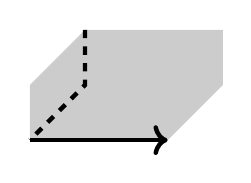
\begin{tikzpicture}[baseline, scale=0.7]
		\fill[gray!40] (0, 1) -- (-1, 0) -- (-1, -1) -- (1.5, -1) --(2.5, 0) -- (2.5, 1)  --cycle;
		\draw[ultra thick, dashed] (0,1) -- (0,0) -- (-1, -1);
		\draw[ultra thick, ->] (-1, -1) -- (1.5, -1);
	\end{tikzpicture} \;\Rightarrow \cdots \Rightarrow\; 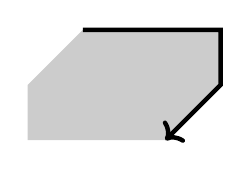
\begin{tikzpicture}[baseline, scale=0.7]
		\fill[gray!40] (-1, 1) -- (1.5, 1) -- (1.5, 0) -- (0.5, -1) -- (-2, -1) -- (-2, 0) --cycle;
		\draw[ultra thick, ->] (-1,1) -- (1.5 , 1) -- (1.5, 0)  -- (0.5, -1);
	\end{tikzpicture} \; =: \beth. \]

	Recall that
	$\cate{D}(\cdots)\times\cate{D}(\cdots)\to\cate{D}(\cdots)$ is absolute
	as a right Kan extension
	(Proposition~\ref{prop:localization-functor-abs}). Therefore the composite
% segment-id: o014.li2.chapter4.k-flat-derived-tensor-a.e003
	\begin{equation*}\begin{gathered}
		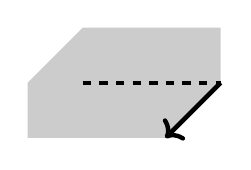
\begin{tikzpicture}[baseline=(O), scale=0.7]
			\fill[gray!40] (-1, 1) -- (1.5, 1) -- (1.5, 0) -- (0.5, -1) -- (-2, -1) -- (-2, 0) --cycle;
			\draw[ultra thick, dashed] (-1,0) -- (1.5, 0);
			\draw[ultra thick, ->] (1.5, 0)  -- (0.5, -1);
			\coordinate (O) at (0, 0);
		\end{tikzpicture}
		\quad \text{is the right Kan extension of $\beth$ along} \quad
		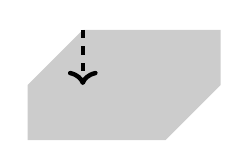
\begin{tikzpicture}[baseline=(O), scale=0.7]
			\fill[gray!40] (-1, 1) -- (1.5, 1) -- (1.5, 0) -- (0.5, -1) -- (-2, -1) -- (-2, 0) --cycle;
			\draw[ultra thick, dashed, ->] (-1, 1) -- (-1, 0);
			\coordinate (O) at (0, 0);
		\end{tikzpicture}.
	\end{gathered}\end{equation*}
	Applying the morphism into $\beth$ and the universal property of the right
	Kan extension (Definition~\ref{def:Kan-extension}) gives the desired
	$\alpha$.

	Once the existence of $\alpha$ has been established, take K-flat complexes
	as in the first paragraph of the proof and compute all the functors in the
	upper layer. This proves that $\alpha$ is an isomorphism.
\end{proof}

% segment-id: o014.li2.chapter4.k-flat-derived-tensor-a.p015
From now on, arguments of this kind based on universal properties will often
be omitted; instead, we shall verify statements directly using resolutions.

% Unit 063 English translation of chapter4.tex lines 2500--2745.
% Source: Methods of Algebra, Volume 2, commit
% 9a5803ff77dd3257484cb177f851a73770a59dd3 (CC BY 4.0).
% stable-unit-id: o014.aljabr2.chapter4.k-flat-derived-tensor-b
% Coverage: end of Section 4.12 and all Chapter 4 exercises (17 exercises and
% 10 hints); closes chapter4.tex exactly at the end of the Exercises environment.

% segment-id: o014.li2.chapter4.k-flat-derived-tensor-b.co001
\hypertarget{o014.aljabr2.chapter4.k-flat-derived-tensor-b}{ }
\begin{corollary}\label{prop:otimesL-Tor}
	\index[sym1]{Tor}
	The functor $\otimesL[R]$ of Definition~\ref{def:otimesL}, under the
	assumption that $A$ or $B$ is flat as a $\Bbbk$-module, satisfies the
	canonical isomorphism
	\[ \Hm^{-n}\left( X \otimesL[R] Y \right) \simeq \Tor^R_n(X, Y), \quad n \in \Z, \]
	where $X$ is an $(A,R)$-bimodule, $Y$ is an $(R,B)$-bimodule, and
	$\Tor^R_n$ is as in Definition--Proposition~\ref{def:Tor-classical}.
\end{corollary}
% segment-id: o014.li2.chapter4.k-flat-derived-tensor-b.pf001
\begin{proof}
	The left-hand side is obtained by composing the diagram of
	Proposition~\ref{prop:otimesL-enrichment} in the direction
% segment-id: o014.li2.chapter4.k-flat-derived-tensor-b.g001
	\begin{tikzpicture}[xscale=0.3, yscale=0.3, baseline=(O)]
		\draw[->] (0,0) -- (1,0) -- (1, -1);
		\coordinate (O) at (0, -0.7);
	\end{tikzpicture}
	whereas the right-hand side is obtained by composing it in the direction
% segment-id: o014.li2.chapter4.k-flat-derived-tensor-b.g002
	\begin{tikzpicture}[xscale=0.3, yscale=0.3, baseline=(O)]
		\draw[->] (0,0) -- (0, -1) -- (1, -1);
		\coordinate (O) at (0, -0.7);
	\end{tikzpicture}.
\end{proof}

% segment-id: o014.li2.chapter4.k-flat-derived-tensor-b.pr001
\begin{proposition}[Associativity constraint]\label{prop:otimesL-associativity-constraint}
	\index{derived tensor product!associativity constraint}
	Let $A$, $B$, $R$, and $S$ be $\Bbbk$-algebras. Consider the following two
	functors:
	\begin{gather*}
		\cate{D}((A,R)\dcate{Mod}) \times \cate{D}((R,S)\dcate{Mod}) \times \cate{D}((S,B)\dcate{Mod}) \to \cate{D}((A,B)\dcate{Mod}), \\
		(X, Y, Z) \mapsto (X \otimesL[R] Y) \otimesL[S] Z, \\
		(X, Y, Z) \mapsto X \otimesL[R] (Y \otimesL[S] Z).
	\end{gather*}
	If $A$ and $B$ are both flat as $\Bbbk$-modules, there is a canonical
	isomorphism
	\[ a(X,Y,Z): (X \otimesL[R] Y) \otimesL[S] Z \rightiso X \otimesL[R] (Y \otimesL[S] Z). \]
\end{proposition}
% segment-id: o014.li2.chapter4.k-flat-derived-tensor-b.pf002
\begin{proof}
	Fix $Y$. By Proposition~\ref{prop:K-flat}, we may assume that $X_R$ and
	${}_R Z$ are K-flat. Then every $\otimesL[R]$ can be computed at the level
	of complexes, and the assertion reduces to the associativity constraint for
	tensor products \cite[Proposition 6.5.12]{Li1}.
\end{proof}

% segment-id: o014.li2.chapter4.k-flat-derived-tensor-b.p001
Under these flatness assumptions, taking $\otimesL$ of three or more objects
in different orders yields results that are mutually isomorphic through the
associativity constraint. These isomorphisms also satisfy coherence, which can
be formulated by imitating the pentagon axiom for monoidal categories; see
\cite[Definition 3.1.1]{Li1}. Again, one takes K-flat resolutions and checks
the assertion at the level of complexes. To keep the discussion brief, this
book presents only the special case of a commutative ring.

% segment-id: o014.li2.chapter4.k-flat-derived-tensor-b.e001
\begin{example}[$\otimesL$ over a commutative ring]\label{eg:commutative-otimesL}
	\index{derived tensor product!commutativity constraint}
	Let $R$ be a commutative ring. In the definition
	$\otimesL:=\otimesL[R]$, take every ring to be $R$, in particular
	$\Bbbk=R$. Then $(R,R)\dcate{Mod}=R\dcate{Mod}$, and all the preceding
	flatness assumptions are automatically satisfied. Consequently,
	$\Hm^{-n}(X\otimesL Y)\simeq\Tor^R_n(X,Y)$ for all $R$-modules $X$ and
	$Y$.

	This makes $\cate{D}(R\dcate{Mod})$ a monoidal category with respect to
	$\otimesL$ in the sense of \cite[\S 3.1]{Li1}. Its unit object is $R$
	itself, and its associativity constraint comes from
	$a=(a(X,Y,Z))_{X,Y,Z}$ in
	Proposition~\ref{prop:otimesL-associativity-constraint}. Since $R$ is a flat
	$R$-module, it is K-flat (Proposition~\ref{prop:flat-K-flat}); hence both
	$R\otimesL(\cdot)$ and $(\cdot)\otimesL R$ can be computed at the level of
	complexes, making all the monoidal-category axioms easy to prove.
	Furthermore, $\cate{D}(R\dcate{Mod})$ is a symmetric monoidal category in
	the sense of \cite[Definition 3.3.1]{Li1}. Its braiding (or commutativity
	constraint) $c(X,Y):X\otimesL Y\rightiso Y\otimesL X$ comes from the
	commutativity constraint at the level of complexes, and its axioms are also
	checked there. In view of Proposition~\ref{prop:double-cplx-swap}, swapping
	the superscripts in the total complex causes no difficulty here.
\end{example}

% segment-id: o014.li2.chapter4.k-flat-derived-tensor-b.e002
\begin{example}[$\Tor$-algebra]
	Continue with the setting of Example~\ref{eg:commutative-otimesL}, with $R$
	commutative. Identify the complexes of $R$-modules $X,Y,Z,W$ with their
	images in the derived category. For every $(p,q)\in\Z^2$, there is a
	canonical morphism
% segment-id: o014.li2.chapter4.k-flat-derived-tensor-b.q001
	\begin{multline*}
		\Hm^{-p}\left( X \otimesL Y \right) \otimes \Hm^{-q}\left( Z \otimesL W \right) \to \Hm^{-p-q}\left( (X \otimesL Y) \otimesL (Z \otimesL W) \right) \\
		\simeq \Hm^{-p-q}\left( (X \otimesL Z) \otimesL (Y \otimesL W) \right) \to \Hm^{-p-q} \left( (X \otimes Z) \otimesL (Y \otimes W) \right),
	\end{multline*}
	where the first part applies Proposition~\ref{prop:bifunctor-cup} (take
	$F=\otimes$), the second uses the associativity and commutativity constraints
	on $(\cate{D}(R\dcate{Mod}),\otimesL)$, and the third comes from the
	canonical morphism accompanying $\otimesL$ as a left derived bifunctor:
% segment-id: o014.li2.chapter4.k-flat-derived-tensor-b.q002
	\[ QX_1 \otimesL QX_2 \to Q(X_1 \otimes X_2), \quad X_1, X_2 \in \Obj(\cate{K}(R\dcate{Mod})), \]
	For precision, the localization functor
	$Q:\cate{K}(R\dcate{Mod})\to\cate{D}(R\dcate{Mod})$ has been written
	explicitly again here.
% segment-id: o014.li2.chapter4.k-flat-derived-tensor-b.l001
	\begin{itemize}
% segment-id: o014.li2.chapter4.k-flat-derived-tensor-b.i001
		\item The composite of the three canonical morphisms above gives an
		``external product'' for the $\Tor$ functor:
		\[ \Tor^R_p(X, Y) \otimes \Tor^R_q(Z, W) \to \Tor^R_{p+q}(X \otimes Z, Y \otimes W). \]
% segment-id: o014.li2.chapter4.k-flat-derived-tensor-b.i002
		\item Take $Z=X$ and $W=Y$ to be $R$-algebras (concentrated in degree
		$0$). Their multiplications give homomorphisms of $R$-modules
		$X\otimes X\to X$ and $Y\otimes Y\to Y$. Composing the external product
		with these homomorphisms gives
		\[ \Tor^R_p(X, Y) \otimes \Tor^R_q(X, Y) \to \Tor^R_{p+q}(X,Y), \]
		called the ``internal product'' for the $\Tor$ functor. This makes
		$\bigoplus_{n \in \Z} \Tor^R_n(X, Y)$ a $\Z$-graded $R$-algebra in the
		sense of \cite[Definition 7.4.1]{Li1}, called the \emph{$\Tor$-algebra}.
		It has nonzero components only in nonnegative degrees, and its degree-zero
		component is the subalgebra $\Tor^R_0(X,Y)=X\otimes Y$, whose definition
		may be found in \cite[Definition 7.3.1]{Li1}. The associativity required
		for the product can be verified by reducing it to the associativity
		constraint for $\otimesL$ and to the associativity of multiplication on
		$X$ and $Y$ separately.
		\index{Tor-algebra@$\Tor$-algebra}
% segment-id: o014.li2.chapter4.k-flat-derived-tensor-b.i003
		\item Suppose further that $X$ and $Y$ are commutative $R$-algebras. In
		this case, the $\Tor$-algebra is also an ``anticommutative''
		$\Z$-graded algebra in the sense of
		\cite[Definition 7.4.3]{Li1}\footnote{The literal term is somewhat
		misleading, because this property is a natural manifestation of
		commutativity. Graded-commutative is more appropriate, as in
		Example~\ref{eg:graded-module}.}: for all $p,q\in\Z$,
		\[ a \in \Tor^R_p(X, Y), \; b \in \Tor^R_q(X, Y) \implies ab = (-1)^{pq} ba. \]
		Since both $X\otimes X\to X$ and $Y\otimes Y\to Y$ are commutative,
		where does the sign come from? Its source is the definition of the
		external product. Let $C_1$ and $C_2$ be two copies of $X\otimesL Y$.
		Then $ab$ and $ba$ differ through the isomorphism
		$C_1\otimesL C_2\rightiso C_2\otimesL C_1$, namely the commutativity
		constraint for $\otimesL$. If $C_1$ and $C_2$ are represented by K-flat
		complexes, this isomorphism of total complexes is exactly the isomorphism
		$r_{C_1^\bullet \otimes C_2^\bullet}$ of
		Proposition~\ref{prop:double-cplx-swap}; on the component of bidegree
		$(p,q)$, it produces the sign $(-1)^{pq}$.
	\end{itemize}
\end{example}

% segment-id: o014.li2.chapter4.k-flat-derived-tensor-b.p002
Return to general $\Bbbk$-algebras. To discuss the adjunction between
$\otimesL$ and $\RHom$, one more lemma is needed. Below,
$\RHom_{(A,B)}$ denotes $\RHom$ in $(A,B)\dcate{Mod}$; analogous notation is
used for other categories of bimodules (or of left or right modules).

% segment-id: o014.li2.chapter4.k-flat-derived-tensor-b.le001
\begin{lemma}\label{prop:RHom-enrichment}
	Fix $\Bbbk$-algebras $A$, $B$, and $R$. Suppose that $B$ is flat as a
	$\Bbbk$-module. Then the forgetful functor from $(A,B)\dcate{Mod}$ to
	$A\dcate{Mod}$ preserves K-injective complexes, and $\RHom_A$ has a
	canonical lift to a functor
	\[ \cate{D}\left((A,R)\dcate{Mod}\right)^{\opp} \times \cate{D}\left((A,B)\dcate{Mod}\right) \to \cate{D}\left((R,B)\dcate{Mod}\right), \]
	in other words, there is a canonical $2$-cell diagram
% segment-id: o014.li2.chapter4.k-flat-derived-tensor-b.g003
	\[\begin{tikzcd}
		\cate{D}\left((A,R)\dcate{Mod}\right)^{\opp} \times \cate{D}\left((A,B)\dcate{Mod}\right) \arrow[r] \arrow[d, "\text{forgetful}"'] & \cate{D}\left((R,B)\dcate{Mod}\right) \arrow[d, "\text{forgetful}"] \arrow[Rightarrow, ld, "\sim", sloped] \\
		\cate{D}(A\dcate{Mod})^{\opp} \times \cate{D}(A\dcate{Mod}) \arrow[r, "{\RHom_A}"'] & \cate{D}(\cate{Ab}) .
	\end{tikzcd}\]

	Likewise, if $A$ is flat as a $\Bbbk$-module, then $\RHom_B$ has an
	analogous lift.
\end{lemma}
% segment-id: o014.li2.chapter4.k-flat-derived-tensor-b.pf003
\begin{proof}
	Because $B$ is a flat $\Bbbk$-module, the functor $Y\mapsto{}_A Y$ has the
	exact left adjoint $(\cdot)\dotimes{\Bbbk}B$, and therefore preserves
	K-injective complexes.

	Next take $X\in\Obj(\cate{K}((A,R)\dcate{Mod}))$ and
	$Y\in\Obj(\cate{K}(A,B)\dcate{Mod})$, with $Y$ K-injective. By the
	preceding step, $\Hom^\bullet\left({}_A X,{}_A Y\right)$ computes
	$\RHom_A({}_A X,{}_A Y)$, while at the same time it is a complex of
	$(R,B)$-bimodules. This completes the lift.
\end{proof}

% segment-id: o014.li2.chapter4.k-flat-derived-tensor-b.th001
\begin{theorem}[Adjunction between $\RHom$ and $\otimesL$]\label{prop:RHom-otimesL-adjunction}
	\index{$\RHom$ functor}
	\index{derived tensor product}
	Let $A$, $B$, and $R$ be $\Bbbk$-algebras. Below, $X$, $Y$, and $Z$ denote
	objects of $\cate{D}((A,R)\dcate{Mod})$,
	$\cate{D}((R,B)\dcate{Mod})$, and
	$\cate{D}((A,B)\dcate{Mod})$, respectively. Suppose that $B$ is flat as a
	$\Bbbk$-module. Then there is a canonical isomorphism in
	$\cate{D}(\Bbbk\dcate{Mod})$
% segment-id: o014.li2.chapter4.k-flat-derived-tensor-b.q003
	\begin{equation*}
		\RHom_{(A,B)} \left( X \otimesL[R] Y, Z \right) \rightiso \RHom_{(R,B)}\left( Y, \RHom_A \left( {}_A X, {}_A Z \right) \right).
	\end{equation*}

	If instead $A$ is assumed flat as a $\Bbbk$-module, there is a canonical
	isomorphism in $\cate{D}(\Bbbk\dcate{Mod})$
% segment-id: o014.li2.chapter4.k-flat-derived-tensor-b.q004
	\begin{equation*}
		\RHom_{(A,B)}\left( X \otimesL[R] Y, Z \right) \rightiso \RHom_{(A,R)}\left( X, \RHom_B\left( Y_B , Z_B \right) \right).
	\end{equation*}
\end{theorem}
% segment-id: o014.li2.chapter4.k-flat-derived-tensor-b.pf004
\begin{proof}
	Consider the first equality. Suppose that $Y$ is K-projective and $Z$ is
	K-injective. Lemma~\ref{prop:K-projective-flat} ensures that ${}_R Y$ is
	K-flat, while Lemma~\ref{prop:RHom-enrichment} ensures that ${}_A Z$
	remains K-injective. Every displayed $\RHom$ and $\otimesL[R]$ can therefore
	be computed at the level of complexes. The desired isomorphism then follows
	from Proposition~\ref{prop:tensor-Hom-cplx}.
\end{proof}

% segment-id: o014.li2.chapter4.k-flat-derived-tensor-b.e003
\begin{example}[Adjunction for change of rings]\label{eg:change-of-ring-adjunction}
	In the setting of Example~\ref{eg:change-of-rings} (take a homomorphism
	$R\to S$ of $\Bbbk$-algebras, $A=S$, $B=\Bbbk$, and $X=S$), the first
	equality in Theorem~\ref{prop:RHom-otimesL-adjunction} becomes the canonical
	isomorphism
% segment-id: o014.li2.chapter4.k-flat-derived-tensor-b.q005
	\begin{gather*}
		\RHom_S\left( \mathrm{L} {}_{R \to S} P(Y), Z \right) \simeq \RHom_R\left( Y, {}_R Z \right), \\
		Y \in \Obj(\cate{D}(R\dcate{Mod})), \quad Z \in \Obj(\cate{D}(S\dcate{Mod})).
	\end{gather*}
	The only point still requiring explanation is
	$\RHom_S({}_S S,{}_S Z)\simeq{}_R Z$, which follows immediately from the
	isomorphism at the level of complexes
% segment-id: o014.li2.chapter4.k-flat-derived-tensor-b.q006
	\[ \Hom^\bullet\left({}_S S, \cdot\right) \simeq {}_R (\cdot) : \cate{C}(S\dcate{Mod}) \to \cate{C}(R\dcate{Mod}). \]

	If, furthermore, both $R$ and $S$ are commutative rings and $\Bbbk:=R$,
	then $\RHom_S$ (respectively, $\RHom_R$) takes values in
	$\cate{D}(S\dcate{Mod})$ (respectively, $\cate{D}(R\dcate{Mod})$). The
	adjunction isomorphism can then be written as the canonical isomorphism in
	$\cate{D}(R\dcate{Mod})$:
% segment-id: o014.li2.chapter4.k-flat-derived-tensor-b.q007
	\[ {}_R \RHom_S\left( \mathrm{L} {}_{R \to S} P(Y), Z \right) \simeq \RHom_R\left( Y, {}_R Z \right) . \]
	Everything can be verified at the level of complexes by taking K-injective
	and K-projective resolutions. The case of right modules is similar.
\end{example}


% segment-id: o014.li2.chapter4.k-flat-derived-tensor-b.x001
\begin{Exercises}
	% Reference: [KS06, Exercise 10.10]
% segment-id: o014.li2.chapter4.k-flat-derived-tensor-b.ex001
	\item Let $(\mathcal{D}, T, \mathcal{H})$ be a pretriangulated category
	(respectively, a triangulated category). Define a new family of triangles
	$\mathcal{H}^-$ by
% segment-id: o014.li2.chapter4.k-flat-derived-tensor-b.q008
	\[ [X \xrightarrow{f} Y \xrightarrow{g} Z \xrightarrow{h} TX] \in \mathcal{H} \iff [X \xrightarrow{f} Y \xrightarrow{g} Z \xrightarrow{-h} TX] \in \mathcal{H}^- . \]
% segment-id: o014.li2.chapter4.k-flat-derived-tensor-b.l002
	\begin{enumerate}[(i)]
% segment-id: o014.li2.chapter4.k-flat-derived-tensor-b.i004
		\item Prove that $(\mathcal{D},T,\mathcal{H}^-)$ is also a
		pretriangulated category (respectively, a triangulated category).
% segment-id: o014.li2.chapter4.k-flat-derived-tensor-b.i005
		\item Prove that $(\mathcal{D},T,\mathcal{H})$ and
		$(\mathcal{D},T,\mathcal{H}^-)$ are equivalent as pretriangulated
		categories.
	\end{enumerate}

% segment-id: o014.li2.chapter4.k-flat-derived-tensor-b.ex002
	\item Let $(\mathcal{D},T,\mathcal{H})$ be a pretriangulated category.
	Prove that every monomorphism (respectively, epimorphism) $u:X\to Y$ in
	$\mathcal{D}$ has a left inverse (respectively, a right inverse). Use this
	to show that a pretriangulated category that is also abelian must be split
	(Definition~\ref{def:semisimple}).

% segment-id: o014.li2.chapter4.k-flat-derived-tensor-b.hn001
	\begin{hint}
		Place the monomorphism $u$ in a distinguished triangle
		$X\xrightarrow{u}Y\xrightarrow{v}Z\xrightarrow{w}TX$. From
		$u\circ T^{-1}w=0$, deduce that $w=0$, and then apply
		Proposition~\ref{prop:dt-sum-1}.
	\end{hint}

% segment-id: o014.li2.chapter4.k-flat-derived-tensor-b.ex003
	\item Apply the preceding exercise to give an example of an abelian category
	$\mathcal{A}$ for which neither $\cate{K}(\mathcal{A})$ nor
	$\cate{D}(\mathcal{A})$ is an abelian category.

% segment-id: o014.li2.chapter4.k-flat-derived-tensor-b.hn002
	\begin{hint}
		Consider the morphism $f:\Z/p^2\Z\twoheadrightarrow\Z/p\Z$ in
		$\mathcal{A}=\cate{Ab}$, where $p$ is prime. If
		$\cate{K}(\mathcal{A})$ were abelian, consider the epi--mono
		factorizations of $\cate{K}f$ and $\Hm^0(\cate{K}f)$, then express both
		as projections onto direct summands and inclusion morphisms to obtain a
		contradiction.
	\end{hint}

% segment-id: o014.li2.chapter4.k-flat-derived-tensor-b.ex004
	\item Let $\mathcal{A}$ be an abelian category. Prove that
	$\cate{D}(\mathcal{A})$ is an abelian category if and only if
	$\mathcal{A}$ is split.

% segment-id: o014.li2.chapter4.k-flat-derived-tensor-b.hn003
	\begin{hint}
		For the ``only if'' direction, embed $\mathcal{A}$ in
		$\cate{D}(\mathcal{A})$ and apply the preceding exercises. For the ``if''
		direction, show that when $\mathcal{A}$ is split, taking cohomology gives
		an equivalence from $\cate{D}(\mathcal{A})$ to $\mathcal{A}^{\Z}$.
	\end{hint}

% segment-id: o014.li2.chapter4.k-flat-derived-tensor-b.ex005
	\item It is often said that the octahedral axiom (TR5) for a triangulated
	category replaces the isomorphism theorem
	$\dfrac{X/Z}{Y/Z}\simeq X/Y$ in an abelian category, where
	$X\supset Y\supset Z$ (Theorem~\ref{prop:Abel-cat-isom-thm} (ii)). Explain
	explicitly what this statement means.

% segment-id: o014.li2.chapter4.k-flat-derived-tensor-b.ex006
	\item ($\mathrm{K}_0$ of a pretriangulated category) For every
	pretriangulated category $(\mathcal{D},T,\mathcal{H})$, define
	$\mathrm{K}_0(\mathcal{D})$ to be the quotient of the free $\Z$-module
	generated by $\Obj(\mathcal{D})$ by the relations
% segment-id: o014.li2.chapter4.k-flat-derived-tensor-b.q009
	\[ \text{there is a distinguished triangle}\; X \to Y \to Z \xrightarrow{+1} \implies [X] - [Y] + [Z] = 0, \]
	where $[X]\in\mathrm{K}_0(\mathcal{D})$ denotes the equivalence class
	containing $X\in\Obj(\mathcal{D})$.
% segment-id: o014.li2.chapter4.k-flat-derived-tensor-b.l003
	\begin{enumerate}[(i)]
% segment-id: o014.li2.chapter4.k-flat-derived-tensor-b.i006
		\item Prove that $[0]=0$, $[TX]=-[X]$, and
		$[X\oplus Y]=[X]+[Y]$.
% segment-id: o014.li2.chapter4.k-flat-derived-tensor-b.i007
		\item Show that every triangulated functor
		$F:\mathcal{D}\to\mathcal{D}'$ induces a canonical homomorphism
		$\mathrm{K}_0(\mathcal{D})\to\mathrm{K}_0(\mathcal{D}')$.
% segment-id: o014.li2.chapter4.k-flat-derived-tensor-b.i008
		\item Consider a cohomological functor $H:\mathcal{D}\to\mathcal{A}$,
		where $\mathcal{A}$ is an abelian category. Suppose that, for every $X$,
		$|n|\gg_X0\implies H(T^nX)=0$. Define a natural homomorphism
		$\mathrm{K}_0(\mathcal{D})\to\mathrm{K}_0(\mathcal{A})$.

% segment-id: o014.li2.chapter4.k-flat-derived-tensor-b.hn004
		\begin{hint}
			Send $[X]$ to $\sum_n(-1)^n[H(T^nX)]$. Apply
			Lemma~\ref{prop:K0-prep} (iv).
		\end{hint}
% segment-id: o014.li2.chapter4.k-flat-derived-tensor-b.i009
		\item Consider the special case
		$\mathcal{D}:=\cate{D}^{\bdd}(\mathcal{A})$. Give mutually inverse
		homomorphisms
% segment-id: o014.li2.chapter4.k-flat-derived-tensor-b.g004
		\[\begin{tikzcd}[row sep=tiny]
			\mathrm{K}_0(\mathcal{A}) \arrow[shift left, r] & \mathrm{K}_0(\cate{D}^{\bdd}(\mathcal{A})) \arrow[shift left, l] \\
			{[A]} \arrow[mapsto, r] & {[A]} \\
			\sum_n (-1)^n {[\Hm^n(X)]} & {[X]} \arrow[mapsto, l]
		\end{tikzcd}\]
		where $A\in\Obj(\mathcal{A})$, also regarded as a complex concentrated in
		degree $0$.
% segment-id: o014.li2.chapter4.k-flat-derived-tensor-b.hn005
		\begin{hint}
			One composite is plainly the identity; the other requires truncating the
			complex.
		\end{hint}
	\end{enumerate}
	\index{K0 group@$\mathrm{K}_0$ group} \index[sym1]{K0}

% segment-id: o014.li2.chapter4.k-flat-derived-tensor-b.ex007
	\item Let $X\in\Obj(\cate{D}(\mathcal{A}))$. Prove that
% segment-id: o014.li2.chapter4.k-flat-derived-tensor-b.q010
	\begin{gather*}
		X \in \cate{D}^{\leq 0}(\mathcal{A}) \iff \forall Z \in \Obj(\cate{D}^{\geq 1}(\mathcal{A})), \; \Hom_{\cate{D}(\mathcal{A})}(X, Z) = 0, \\
		X \in \cate{D}^{\geq 0}(\mathcal{A}) \iff \forall Z \in \Obj(\cate{D}^{\leq -1}(\mathcal{A})), \; \Hom_{\cate{D}(\mathcal{A})}(Z, X) = 0.
	\end{gather*}
% segment-id: o014.li2.chapter4.k-flat-derived-tensor-b.hn006
	\begin{hint}
		Apply Proposition~\ref{prop:derived-cat-orthogonality} (i), together with
		the adjoint pairs and distinguished triangle in
		Proposition~\ref{prop:derived-truncation-adjunction}.
	\end{hint}

% segment-id: o014.li2.chapter4.k-flat-derived-tensor-b.ex008
	\item In the setting of
	Theorem~\ref{prop:localization-triangulated-composite}, suppose that $F'$
	satisfies $F'(\Obj(\mathcal{N}'))\subset\Obj(\mathcal{N}'')$ (regard this
	as a kind of ``exactness''). If $\mathcal{D}$ has an $F$-injective or an
	$F$-projective subcategory, prove that the canonical morphism
	\[ \mathrm{R}^{\mathcal{N}''}_{\mathcal{N}} (F' F) \to \left( \mathrm{R}^{\mathcal{N}''}_{\mathcal{N}'} F' \right) \left( \mathrm{R}^{\mathcal{N}'}_{\mathcal{N}} F \right) \]
	or
	\[ \left( \mathrm{L}^{\mathcal{N}''}_{\mathcal{N'}} F' \right) \left( \mathrm{L}^{\mathcal{N}'}_{\mathcal{N}} F \right) \to \mathrm{L}^{\mathcal{N}''}_{\mathcal{N}} (F' F) \]
	is an isomorphism.

% segment-id: o014.li2.chapter4.k-flat-derived-tensor-b.ex009
	\item In the setting of
	Theorem~\ref{prop:localization-triangulated-composite}, show that the
	following diagrams of functors and morphisms between them commute (the
	notation $\mathcal{N}$ and so forth is suppressed):
% segment-id: o014.li2.chapter4.k-flat-derived-tensor-b.g005
	\[\begin{tikzcd}
		\mathrm{R}(F'' F' F) \arrow[r] \arrow[d] & \mathrm{R}(F'' F') \mathrm{R}F \arrow[d] \\
		\mathrm{R}F'' \mathrm{R}(F'F) \arrow[r] & \mathrm{R}F'' \mathrm{R}F' \mathrm{R}F
	\end{tikzcd} \quad \begin{tikzcd}
		\mathrm{L}(F'' F' F) & \mathrm{L}(F'' F') \mathrm{L}F \arrow[l] \\
		\mathrm{L}F'' \mathrm{L}(F'F) \arrow[u] & \mathrm{L}F'' \mathrm{L}F' \mathrm{L}F \arrow[u] \arrow[l] .
	\end{tikzcd}\]

% segment-id: o014.li2.chapter4.k-flat-derived-tensor-b.ex010
	\item For $F=\Hom$, express explicitly the canonical morphism of
	Proposition~\ref{prop:bifunctor-cup} in the form
	$\Ext^{q-p}(X,Y)\to\Hom\left(\Hm^p(X),\Hm^q(Y)\right)$.

% segment-id: o014.li2.chapter4.k-flat-derived-tensor-b.ex011
	\item Reformulate the bijection in Theorem~\ref{prop:Yoneda-Ext} as follows.
	From an $n$-extension
	$0\to Y\to E^1\to\cdots\to E^n\to X\to0$, construct
	$t^{-1}b\in\Hom_{\cate{D}(\mathcal{A})}(X,Y[n])$ as follows:
% segment-id: o014.li2.chapter4.k-flat-derived-tensor-b.g006
	\[\begin{tikzcd}
		X \arrow[d, "b"']\arrow[phantom, r, "" {name=A, yshift=2ex}] & {} & & & X \arrow[d, "\identity"] \\
		W & E^1 \arrow[r] & E^2 \arrow[r] & \cdots \arrow[r] & X \\
		Y[n] \arrow[u, "{t: \text{quasi-isomorphism}}"] \arrow[phantom, r, "" {name=B, yshift=-2ex}] & Y \arrow[u] & & &
		\arrow[dash, from=A, to=B]
	\end{tikzcd}\]
	This gives $t^{-1}b\in\Hom_{\cate{D}(\mathcal{A})}(X,Y[n])$. Prove that
	this bijection differs by the factor $(-1)^n$ from the original bijection
	based on $as^{-1}$. In the special case $n=1$, use the $t^{-1}b$ version to
	derive the corresponding version of Proposition~\ref{prop:Ext1-via-ses}
	(the one involving the image of $\identity_Y$).

% segment-id: o014.li2.chapter4.k-flat-derived-tensor-b.hn007
	\begin{hint}
		Prove that $ta+(-1)^{n-1}bs:Z\to W$ is canonically null-homotopic. For
		the second part, note the minus sign in
		Proposition~\ref{prop:ses-vs-triangle}.
	\end{hint}

% segment-id: o014.li2.chapter4.k-flat-derived-tensor-b.ex012
	\item Suppose that all objects $S,T$ in an abelian category $\mathcal{A}$
	satisfy $\Ext^2_{\mathcal{A}}(S,T)=0$. Prove that every
	$X\in\Obj(\cate{D}^{\bdd}(\mathcal{A}))$ is isomorphic to
	$\bigoplus_n\Hm^n(X)[-n]$. Show that $\mathcal{A}:=\Z\dcate{Mod}$
	satisfies this condition.

% segment-id: o014.li2.chapter4.k-flat-derived-tensor-b.hn008
	\begin{hint}
		We may assume that $X$ is a bounded complex. Begin with $n\gg0$. Apply
		Theorem~\ref{prop:Yoneda-Ext} and Proposition~\ref{prop:Yoneda-zero} to
		the $2$-extension
		$0\to\Ker(d^n)\to X^n\xrightarrow{d^n}X^{n+1}\to\Coker(d^n)\to0$,
		then modify $X$ step by step until $d^\bullet=0$, throughout up to
		isomorphism.
	\end{hint}

% segment-id: o014.li2.chapter4.k-flat-derived-tensor-b.ex013
	\item Prove that if $\mathcal{A}$ has enough injective objects,
	$F:\mathcal{A}\to\mathcal{A}'$ is a left-exact additive functor, and
	$\mathrm{R}F$ has finite dimension, then the homomorphism
	$\mathrm{K}_0(\mathcal{A})\simeq\mathrm{K}_0(\cate{D}^{\bdd}(\mathcal{A}))
	\to\mathrm{K}_0(\cate{D}^{\bdd}(\mathcal{A}'))\simeq
	\mathrm{K}_0(\mathcal{A}')$ induced by the triangulated functor
	$\mathrm{R}F$ is determined by
	\[ [A] \mapsto \sum_n (-1)^n \left[\mathrm{R}^n F(A)\right], \quad A \in \Obj(\mathcal{A}). \]

% segment-id: o014.li2.chapter4.k-flat-derived-tensor-b.ex014
	\item Let $R$ be a ring. Prove that a filtered direct limit $\varinjlim$ of
	K-flat complexes in $\cate{C}(R\dcate{Mod})$ is again K-flat.

% segment-id: o014.li2.chapter4.k-flat-derived-tensor-b.ex015
	\item Let $R$ be a ring. If a complex $P$ of $R$-modules is K-flat and
	every $P^n$ is a flat $R$-module, then $P$ is called \emph{strongly
	K-flat}.
% segment-id: o014.li2.chapter4.k-flat-derived-tensor-b.l004
	\begin{enumerate}[(i)]
% segment-id: o014.li2.chapter4.k-flat-derived-tensor-b.i010
		\item Prove that for every $X\in\Obj(\cate{C}(R\dcate{Mod}))$ there is a
		strongly K-flat complex $P$ together with a quasi-isomorphism $P\to X$.
% segment-id: o014.li2.chapter4.k-flat-derived-tensor-b.hn009
		\begin{hint}
			Use the dual of the argument for the existence of K-injective
			resolutions; see \S\ref{sec:K-injectives}.
		\end{hint}
% segment-id: o014.li2.chapter4.k-flat-derived-tensor-b.i011
		\item Write $\mathcal{SF}$ for the full subcategory of
		$\cate{K}(R\dcate{Mod})$ formed by the strongly K-flat complexes.
		Express $\cate{D}(R\dcate{Mod})$ as the localization of $\mathcal{SF}$
		at the quasi-isomorphisms.
	\end{enumerate}

% segment-id: o014.li2.chapter4.k-flat-derived-tensor-b.ex016
	\item (P.\ Berthelot, A.\ Ogus) Let $f$ be a non-zero-divisor in a
	commutative ring $R$. For every $R$-module $M$, write
	$M[f]:=\{m\in M:fm=0\}$. A module $M$ with $M[f]=0$ is called
	\emph{$f$-torsion-free}. First show that an $f$-torsion-free $M$ can be
	embedded as a submodule of
	$M[\frac{1}{f}]=M\dotimes{R}R[\frac{1}{f}]$. Thus $f^mM$ makes sense for
	every $m\in\Z$.

	Let $X$ be a complex of $f$-torsion-free $R$-modules. Using the observation
	above, define a subcomplex $\eta_fX$ of
	$X^\bullet\dotimes{R}R[\frac{1}{f}]$ by
	\[ (\eta_f X)^n := \left\{ x \in f^n X^n : d_X^n(x) \in f^{n+1} X^{n+1} \right\}, \quad n \in \Z . \]
% segment-id: o014.li2.chapter4.k-flat-derived-tensor-b.l005
	\begin{enumerate}[(i)]
% segment-id: o014.li2.chapter4.k-flat-derived-tensor-b.i012
		\item Prove that multiplication degree by degree by $f$ gives an
		isomorphism $\eta_f(X[1])\rightiso(\eta_fX)[1]$.
% segment-id: o014.li2.chapter4.k-flat-derived-tensor-b.i013
		\item Show that if $f,g\in R$ are both non-zero-divisors and every $X^n$
		is $fg$-torsion-free, then $\eta_f\eta_gX=\eta_{fg}X$.
% segment-id: o014.li2.chapter4.k-flat-derived-tensor-b.i014
		\item Give a canonical isomorphism
		$\Hm^n(X)/\Hm^n(X)[f]\rightiso\Hm^n(\eta_fX)$; thus the effect of
		$\eta_f$ is to correct $f$-torsion. Deduce that if $X$ and $Y$ are
		complexes of $f$-torsion-free $R$-modules and $\alpha:X\to Y$ is a
		quasi-isomorphism, then $\alpha$ induces a quasi-isomorphism
		$\eta_f(\alpha):\eta_fX\to\eta_fY$.
% segment-id: o014.li2.chapter4.k-flat-derived-tensor-b.i015
		\item Prove that in this way $\eta_f$ induces an additive functor
		$\mathrm{L}\eta_f:\cate{D}(R\dcate{Mod})\to\cate{D}(R\dcate{Mod})$
		whose restriction to $\mathcal{SF}$ from the preceding exercise equals
		$\eta_f$.
% segment-id: o014.li2.chapter4.k-flat-derived-tensor-b.i016
		\item Show that $\mathrm{L}\eta_f$ is not a triangulated functor. Thus it
		is not a left derived functor in the sense of
		Definition~\ref{def:Verdier-localization-functor}, although it remains a
		right Kan extension.

% segment-id: o014.li2.chapter4.k-flat-derived-tensor-b.hn010
		\begin{hint}
			Take $R=\Z$ and $f=p$ prime. Verify that
			$\mathrm{L}\eta_p(\Z/p\Z)=0$, whereas
			$\mathrm{L}\eta_p(\Z/p^2\Z)\simeq\Z/p\Z$.
		\end{hint}
	\end{enumerate}

% segment-id: o014.li2.chapter4.k-flat-derived-tensor-b.ex017
	\item Continuing the preceding exercise, give a canonical morphism
	$\mathrm{L}\eta_f X \otimesL[R] \mathrm{L}\eta_f Y \to
	\mathrm{L}\eta_f\left( X \otimesL[R] Y \right)$ and show that this
	morphism is symmetric in $X$ and $Y$ in the appropriate sense. In the
	language of \cite[Remark 3.1.8]{Li1}, $\mathrm{L}\eta_f$ is in fact a
	right-lax monoidal functor with respect to $\otimesL[R]$.
\end{Exercises}

% Unit 064 English translation of chapter5.tex lines 9--140.
% Source: Methods of Algebra, Volume 2, commit
% 9a5803ff77dd3257484cb177f851a73770a59dd3 (CC BY 4.0).
% stable-unit-id: o014.aljabr2.chapter5.intro-filtration-grading
% Coverage: complete introduction to Chapter 5 and complete Section 5.1.

% segment-id: o014.li2.chapter5.intro-filtration-grading.h001
\chapter{Spectral Sequences}\label{sec:ss}
\hypertarget{o014.aljabr2.chapter5.intro-filtration-grading}{ }

% segment-id: o014.li2.chapter5.intro-filtration-grading.p001
Spectral sequences are classical algebraic tools that continually find new
uses, and their roots in topology run especially deep. Some textbooks and
lecture notes even use them as a basic tool of homological algebra to establish
some of the fundamental properties in \CHref{sec:Abel-cat} and
\CHref{sec:cplx}.

% segment-id: o014.li2.chapter5.intro-filtration-grading.p002
Spectral sequences were introduced by J.\ Leray in the 1940s and gradually
assumed their modern form through the work of J.-L.\ Koszul, H.\ Cartan, and
others. Their chief motivation was the study of the homology groups of fiber
bundles. In algebraic terms, the original problem amounts to understanding the
homology (or cohomology) of a chain complex (or complex) $X$. Let us take the
case of a complex as our example. Although $X$ itself may be difficult to
grasp, it can be studied through a suitable filtration
$\cdots\supset\mathrm{F}^pX\supset\mathrm{F}^{p+1}X\supset\cdots$.
The filtration $\mathrm{F}^\bullet X$ induces a filtration on every
$\Hm^n(X)$. Information about $\mathrm{F}^\bullet X$ and its subquotients can
then be used to approximate, step by step, each subquotient
$\gr^p\Hm^n(X)$ of the filtered cohomology. Spectral sequences are the art of
organizing such successive approximations.

% segment-id: o014.li2.chapter5.intro-filtration-grading.p003
A complex may also be generalized to a differential object $(X,d)$ in an
abelian category (Definition~\ref{def:differential-object}), leading to the
abstract definition of a spectral sequence in
Definition~\ref{def:SS-abstract}. A spectral sequence is a sequence of
differential objects $\mathscr{E}=(E_r,d_r)_r$ such that the cohomology of each
``page,'' $\Hm(E_r,d_r)$, is the next page $E_{r+1}$. Adding a grading and
allowing the differential $d$ to have a degree gives the notions of graded
spectral sequences $E_r^p$ and bigraded spectral sequences $E_r^{p,q}$
(Definition~\ref{def:graded-spectral-sequence}). Concretely, the differentials
in a bigraded spectral sequence have the form
\begin{gather*}
	d_r^{p, q}: E_r^{p, q} \to E_r^{p+r, q-r+1}, \\
	E_r = (E_r^{p, q})_{(p, q) \in \Z^2}, \quad d_r = (d_r^{p, q})_{(p, q) \in \Z^2}.
\end{gather*}
A filtered complex gives a filtered differential object and hence naturally
produces a bigraded spectral sequence. This is the form of spectral sequence
that occurs most often in applications. Every notion has a corresponding
version for chain complexes and their homology.

% segment-id: o014.li2.chapter5.intro-filtration-grading.p004
This chapter begins with W.\ Massey's theory of exact couples. Exact couples
are another device for producing spectral sequences, and their scope is wider
than that of filtered differential objects. After introducing filtrations and
graded structures in \S\ref{sec:grading-filtration}, we give the general
definition of a spectral sequence in \S\ref{sec:spectral-sequence}, together
with its graded and bigraded versions and such basic terminology as
degeneration, boundedness, and the limiting page. At the end of that section,
Remark~\ref{rem:edge-computing} explains how to read exact sequences from the
edges of a spectral sequence, an important technique.

% segment-id: o014.li2.chapter5.intro-filtration-grading.p005
Exact couples are defined in \S\ref{sec:exact-couples}. Next,
\S\ref{sec:filtered-diff-ss} explains how an exact couple produces a graded
spectral sequence from a filtered differential object, and
\S\ref{sec:filtered-cplx-ss} goes on to explain how a filtered complex produces
a bigraded spectral sequence. That section also treats the central notion of
convergence and the Classical Convergence Theorem~\ref{prop:classical-convergence}.
Some of the verifications are slightly technical, but there is no fundamental
difficulty. Readers may first work in a concrete abelian category such as
$\cate{Ab}$ to simplify the arguments.

% segment-id: o014.li2.chapter5.intro-filtration-grading.p006
A double complex gives rise to a filtered complex in two ways, according as
the total complex is filtered by the horizontal or the vertical coordinate.
The corresponding spectral sequences are denoted by
$\mathscr{E}_{\mathrm{I}}$ and $\mathscr{E}_{\mathrm{II}}$, respectively.
Their details are the subject of \S\ref{sec:double-cplx-ss}. We also give
standard applications, including the derivation of balanced bifunctors
(Example~\ref{eg:bifunctor-ss}), the spectral sequence of hyperderived functors
(Example~\ref{eg:hyperderived-ss}), and the Grothendieck spectral sequence
(Theorem~\ref{prop:Grothendieck-ss}). The Cartan--Eilenberg resolutions
introduced earlier (Theorem~\ref{prop:CE-resolution}) play a role here.

% segment-id: o014.li2.chapter5.intro-filtration-grading.p007
The Grothendieck spectral sequence concerns the derivation of a composite of
functors and is particularly common in geometry. As an example involving right
derived functors, consider left-exact additive functors between abelian
categories
$\mathcal{A}\xrightarrow{F}\mathcal{A}'\xrightarrow{F'}\mathcal{A}''$,
where $\mathcal{A}$ and $\mathcal{A}'$ have enough injective objects. If $F$
sends injective objects to $F'$-acyclic objects
(Convention~\ref{con:F-acyclic}), there is a canonical strongly convergent
bigraded spectral sequence
\[ E_2^{p, q} = (\mathrm{R}^p F') (\mathrm{R}^q F)(X) \Rightarrow \mathrm{R}^{p+q}(F' F)(X), \quad X \in \Obj(\mathcal{A}). \]
The derivation of composite functors can also be handled at the level of
derived categories; see
Theorem~\ref{prop:localization-triangulated-composite}. Besides being formally
elementary and easy to compute, the spectral-sequence version can provide
additional information in concrete situations, such as exact sequences in low
degrees.

% segment-id: o014.li2.chapter5.intro-filtration-grading.p008
The final section of the chapter, \S\ref{sec:multiplicative-SS}, briefly
introduces multiplicative structures on spectral sequences. This aspect has
received attention since the earliest history of spectral sequences.
Proposition~\ref{prop:dga-mult-ss} shows that a filtered differential graded
algebra gives rise to a spectral sequence with a canonical multiplicative
structure; a deeper treatment is left to specialized monographs.

% segment-id: o014.li2.chapter5.intro-filtration-grading.p009
As an exercise in applications, the Lyndon--Hochschild--Serre spectral
sequence, which is fundamental in group cohomology, can be obtained both as an
application of the Grothendieck spectral sequence and concretely from a
filtered complex. The latter approach also equips it with a canonical
multiplicative structure. This topic will be discussed in
\S\ref{sec:LHS-SS} in the future.

% segment-id: o014.li2.chapter5.intro-filtration-grading.note001
\begin{wenxintishi}
	This chapter requires only a knowledge of abelian categories and complexes.
	Apart from a few simple definitions, it does not depend on the material in
	\CHref{sec:triangulated-derived-cat}; the two chapters can be read
	independently. Since the spectral sequence of a filtered differential object
	can be written down directly, the theory of exact couples is not essential
	for that construction (see Proposition~\ref{prop:filtered-diff-E} and the
	discussion that follows). Readers may therefore consider temporarily
	skipping \S\ref{sec:exact-couples}. Moreover, among the later sections of
	this book, only \S\ref{sec:LHS-SS} requires a knowledge of spectral
	sequences.
\end{wenxintishi}

% segment-id: o014.li2.chapter5.intro-filtration-grading.h002
\section{Filtrations and Graded Structures}\label{sec:grading-filtration}

% segment-id: o014.li2.chapter5.intro-filtration-grading.p010
We encountered graded objects in Definition~\ref{def:graded-obj}. A
$\Z$-graded object in an arbitrary category $\mathcal{A}$ is simply called a
\emph{graded object}; by definition, these are the objects
$(X^p)_{p\in\Z}$ of $\mathcal{A}^{\Z}$. A $\Z^2$-graded object is simply
called a \emph{bigraded object}; by definition, these are the objects
$(X^{p,q})_{(p,q)\in\Z^2}$ of $\mathcal{A}^{\Z\times\Z}$. Morphisms between
graded (or bigraded) objects are written as $(f^p)_p$ (or
$(f^{p,q})_{p,q}$), as usual, and are composed degree by degree.
\index{graded object}

% segment-id: o014.li2.chapter5.intro-filtration-grading.p011
If $\mathcal{A}$ is an abelian category, then $\mathcal{A}^{\Z}$ and
$\mathcal{A}^{\Z\times\Z}$ are also abelian categories; kernels, cokernels,
and all other operations are computed degree by degree.

% segment-id: o014.li2.chapter5.intro-filtration-grading.p012
The category $\mathcal{A}^{\Z}$ has a shift autoequivalence $T$ determined by
$(TX)^p=X^{p+1}$ and $(Tf)^p=f^{p+1}$. More generally,
$\mathcal{A}^{\Z^n}$ has a family of shift autoequivalences
$T_1,\ldots,T_n$ corresponding to shifts along the $n$ coordinates. These
shifts commute strictly: $T_iT_j=T_jT_i$.

% segment-id: o014.li2.chapter5.intro-filtration-grading.p013
Within the framework of this chapter, graded structures arise primarily from
filtrations.

% segment-id: o014.li2.chapter5.intro-filtration-grading.d001
\begin{definition}\label{def:filtration}
	\index{filtration}
	\index{filtration!finite}
	\index[sym1]{FilpX@$\mathrm{F}^p X$, $\mathrm{F}_p X$}
	Let $X$ be an object of an additive category $\mathcal{A}$.
	\begin{itemize}
		\item A \emph{decreasing filtration} $\mathrm{F}^\bullet X$ is a
		sequence of subobjects
		\[ \cdots \supset \mathrm{F}^p X \supset \mathrm{F}^{p+1} X \supset \cdots \quad (p \in \Z). \]
		\item If there exist $a\leq b$ such that $\mathrm{F}^aX=X$ and
		$\mathrm{F}^bX=0$, the filtration is called \emph{finite}.
		\item Increasing filtrations $\mathrm{F}_\bullet X$ and their finiteness
		are defined similarly.
	\end{itemize}
\end{definition}

% segment-id: o014.li2.chapter5.intro-filtration-grading.p014
Decreasing and increasing filtrations can be distinguished by the position of
the index $p$. When no confusion is likely, both are simply called
filtrations. Decreasing filtrations are customary in the study of complexes
and cohomology, whereas increasing filtrations are customary for chain
complexes and homology. This chapter mainly uses decreasing filtrations.

% segment-id: o014.li2.chapter5.intro-filtration-grading.p015
All filtered objects $(X,\mathrm{F}^\bullet X)$ form a category
$\mathrm{Fil}^\bullet(\mathcal{A})$. A morphism
$f:(X,\mathrm{F}^\bullet X)\to(Y,\mathrm{F}^\bullet Y)$ is a morphism
$f:X\to Y$ that preserves the filtrations; that is, for every $p$, it
restricts to a morphism $\mathrm{F}^pX\to\mathrm{F}^pY$. The category
$\mathrm{Fil}_\bullet(\mathcal{A})$ is defined similarly.
\index[sym1]{FilA@$\mathrm{Fil}^\bullet(\mathcal{A})$, $\mathrm{Fil}_\bullet(\mathcal{A})$}

% segment-id: o014.li2.chapter5.intro-filtration-grading.p016
For every $X$, a decreasing filtration $\mathrm{F}^\bullet X$ (or increasing
filtration $\mathrm{F}_\bullet X$) gives a graded object
$(\mathrm{F}^pX)_{p\in\Z}$ (or $(\mathrm{F}_pX)_{p\in\Z}$). This defines a
functor $\mathrm{Fil}^\bullet(\mathcal{A})\to\mathcal{A}^{\Z}$ (or
$\mathrm{Fil}_\bullet(\mathcal{A})\to\mathcal{A}^{\Z}$), called the Rees
construction.

% segment-id: o014.li2.chapter5.intro-filtration-grading.p017
If $\mathcal{A}$ is an abelian category, there is another way to construct a
graded object from a filtration.

% segment-id: o014.li2.chapter5.intro-filtration-grading.d002
\begin{definition}
	\index[sym1]{grX@$\gr^p X$, $\gr_p X$}
	Let $\mathcal{A}$ be an abelian category, and consider a filtration
	$\mathrm{F}^\bullet X$ (or $\mathrm{F}_\bullet X$) on an object $X$.
	Define the graded object $\gr X$ by
	\[ \gr^p X := \mathrm{F}^p X / \mathrm{F}^{p+1} X \quad (\text{or} \quad \gr_p X := \mathrm{F}_p X / \mathrm{F}_{p-1} X). \]
	This defines a functor
	$\gr:\mathrm{Fil}^\bullet(\mathcal{A})\to\mathcal{A}^{\Z}$ (or
	$\gr:\mathrm{Fil}_\bullet(\mathcal{A})\to\mathcal{A}^{\Z}$).
\end{definition}

% segment-id: o014.li2.chapter5.intro-filtration-grading.p018
To extract information about $X$ from $(\gr^pX)_p$, we need at least
$\bigcup_p\mathrm{F}^pX=X$ and $\bigcap_p\mathrm{F}^pX=0$, using the notation
of Convention~\ref{con:increasing-union}. To make the first condition
meaningful and useful, we also want $\varinjlim_{p\to-\infty}$ to be exact in
$\mathcal{A}$, or else we may simply require that there be an $M$ such that
$\mathrm{F}^MX=X$. We begin with some related notions.

% segment-id: o014.li2.chapter5.intro-filtration-grading.d003
\begin{definition}\label{def:filtration-properties}
	\index{filtration!complete}
	\index{filtration!separated}
	\index{filtration!exhaustive}
	Let $\mathcal{A}$ be an abelian category and let $X$ be an object with a
	filtration $\mathrm{F}^\bullet X$.
	\begin{itemize}
		\item If $\bigcap_p\mathrm{F}^pX=0$, the filtration is called
		\emph{separated}.
		\item If $\bigcup_p\mathrm{F}^pX=X$ and either of the following
		conditions holds, the filtration is called \emph{exhaustive}:
		\begin{compactenum}[(a)]
		\item $\mathcal{A}$ has exact countable filtered direct limits
		$\varinjlim$; more
			precisely,
			$\varinjlim:\mathcal{A}^{(\Z_{\geq0},\leq)}\to\mathcal{A}$ exists
			and is exact\footnote{If $\mathcal{A}$ is a Grothendieck category,
			then (a) holds automatically.};
			\item there is an $M\in\Z$ such that $\mathrm{F}^MX=X$.
		\end{compactenum}
		\item If the family of canonical morphisms
		$X\twoheadrightarrow X/\mathrm{F}^pX$ induces an isomorphism
		$X\rightiso\varprojlim_pX/\mathrm{F}^pX$, the filtration is called
		\emph{complete}.
	\end{itemize}
	Increasing filtrations $\mathrm{F}_\bullet X$ are treated in the same way.
\end{definition}

% segment-id: o014.li2.chapter5.intro-filtration-grading.p019
The notion of completeness is inspired by the case of topological groups; see
\cite[\S 4.10]{Li1}.

% segment-id: o014.li2.chapter5.intro-filtration-grading.p020
A finite filtration is automatically separated, exhaustive, and complete;
this is the principal case needed in this chapter. Observe that if there is an
$N$ such that $\mathrm{F}^NX=0$, then $\mathrm{F}^\bullet X$ is separated and
complete. Moreover, since the kernel of
$X\to\varprojlim_pX/\mathrm{F}^pX$ is $\bigcap_p\mathrm{F}^pX$,
completeness implies separatedness.

% segment-id: o014.li2.chapter5.intro-filtration-grading.p021
The image of an exhaustive filtration is still exhaustive; this follows by
interpreting $\bigcup_p$ as $\sum_p$ and then applying
Lemma~\ref{prop:image-sum-preimage-intersection} (ii). Moreover, an exhaustive
filtration satisfies
\begin{equation}\label{eqn:exhaustion-intersection}\begin{gathered}
	\varinjlim_{p \to -\infty} \mathrm{F}^p X \rightiso \bigcup_p \mathrm{F}^p X = X, \\
	K = K \cap \left( \bigcup_p \mathrm{F}^p X \right) = \bigcup_p \left( K \cap \mathrm{F}^p X \right),
\end{gathered}\end{equation}
where $K$ is any subobject of $X$. Under condition (a) for an exhaustive
filtration, these assertions follow readily from
Proposition~\ref{prop:Grothendieck-cat-intersection}; under condition (b), they
are immediate.

% segment-id: o014.li2.chapter5.intro-filtration-grading.pr001
\begin{proposition}\label{prop:gr-isom}
	Let $\mathcal{A}$ be an abelian category, and let
	$f:(X,\mathrm{F}^\bullet X)\to(Y,\mathrm{F}^\bullet Y)$ be a morphism in
	$\mathrm{Fil}^\bullet(\mathcal{A})$.
	\begin{enumerate}[(i)]
		\item Suppose that $\mathrm{F}^\bullet X$ is separated and exhaustive. If
		$\gr(f)$ is a monomorphism, then $f$ is a monomorphism.
		\item Suppose that $\mathrm{F}^\bullet X$ is complete and exhaustive,
		while $\mathrm{F}^\bullet Y$ is separated and exhaustive. If $\gr(f)$ is
		an isomorphism, then $f$ is also an isomorphism, and in this case
		$\mathrm{F}^\bullet Y$ is complete as well.
	\end{enumerate}
	The corresponding statements hold for increasing filtrations.
\end{proposition}
% segment-id: o014.li2.chapter5.intro-filtration-grading.pf001
\begin{proof}
	For each $p\in\Z$, consider the following commutative diagram with exact
	rows:
% segment-id: o014.li2.chapter5.intro-filtration-grading.g001
	\[\begin{tikzcd}
		0 \arrow[r] & \mathrm{F}^{p+1} X \arrow[d, "f"'] \arrow[r] & \mathrm{F}^p X \arrow[r] \arrow[d, "f"] & \gr^p X \arrow[r] \arrow[d, "{\gr^p(f)}"] & 0 \\
		0 \arrow[r] & \mathrm{F}^{p+1} Y \arrow[r] & \mathrm{F}^p Y \arrow[r] & \gr^p Y \arrow[r] & 0
	\end{tikzcd}\]
	Write $K^p$ and $C^p$ for the kernel and cokernel of
	$\mathrm{F}^pX\xrightarrow{f}\mathrm{F}^pY$.

	For (i), apply Theorem~\ref{prop:snake-lemma} to the diagram above. This gives
	$K^{p+1}=K^p$. In particular,
	$K^p\subset\bigcap_{\ell\geq p}\mathrm{F}^\ell X=0$, so the restriction of
	$f$ to every $\mathrm{F}^pX$ is a monomorphism. To prove that $f$ itself is a
	monomorphism, it remains only to use
	\[ \Ker(f) \xlongequal{\because\; \text{\eqref{eqn:exhaustion-intersection}}} \bigcup_p \left( \Ker(f) \cap \mathrm{F}^p X \right) = 0. \]

	For (ii), the diagram gives both $K^{p+1}=K^p$ and
	$C^{p+1}\rightiso C^p$. For each $\ell>p$, consider the commutative diagram
	with exact rows
% segment-id: o014.li2.chapter5.intro-filtration-grading.g002
	\[\begin{tikzcd}
		0 \arrow[r] & \mathrm{F}^{\ell} X \arrow[r] \arrow[d, "f"] & \mathrm{F}^p X \arrow[r] \arrow[d, "f"] & \mathrm{F}^p X / \mathrm{F}^{\ell} X \arrow[r] \arrow[d] & 0 \\
		0 \arrow[r] & \mathrm{F}^{\ell} Y \arrow[r] & \mathrm{F}^p Y \arrow[r] & \mathrm{F}^p Y / \mathrm{F}^{\ell} Y \arrow[r] & 0
	\end{tikzcd}\]
	Another application of Theorem~\ref{prop:snake-lemma} gives the isomorphism
	induced by $f$
	\[ \mathrm{F}^p X / \mathrm{F}^\ell X \rightiso \mathrm{F}^p Y / \mathrm{F}^\ell Y. \]

	Taking $\varinjlim_{p:p<\ell}$ on both sides and using
	\eqref{eqn:exhaustion-intersection} gives
	$X/\mathrm{F}^\ell X\rightiso Y/\mathrm{F}^\ell Y$. Taking
	$\varprojlim_\ell$ now gives the commutative diagram
% segment-id: o014.li2.chapter5.intro-filtration-grading.g003
	\[\begin{tikzcd}
		X \arrow[r, "\sim"] \arrow[d, "f"'] & \varprojlim_\ell X/\mathrm{F}^\ell X \arrow[d, "\sim" sloped] \\
		Y \arrow[hookrightarrow, r] & \varprojlim_\ell Y/\mathrm{F}^\ell Y
	\end{tikzcd}\]
	It follows that both $f$ and
	$Y\to\varprojlim_\ell Y/\mathrm{F}^\ell Y$ are isomorphisms.
\end{proof}

% Unit 065 English translation of chapter5.tex lines 141--349.
% Source: Methods of Algebra, Volume 2, commit
% 9a5803ff77dd3257484cb177f851a73770a59dd3 (CC BY 4.0).
% stable-unit-id: o014.aljabr2.chapter5.general-spectral-sequences
% Coverage: Complete Section 5.2.

% segment-id: o014.li2.chapter5.general-spectral-sequences.h001
\section{General definition of spectral sequences}\label{sec:spectral-sequence}
\hypertarget{o014.aljabr2.chapter5.general-spectral-sequences}{ }

% segment-id: o014.li2.chapter5.general-spectral-sequences.p001
We begin with the general definition of a differential object. This involves an
additive category with translation $(\mathcal{A},T)$ as in
Definition~\ref{def:category-with-translation}, as well as morphisms with
degree as in Definition~\ref{def:morphism-with-degree}.

% segment-id: o014.li2.chapter5.general-spectral-sequences.d001
\begin{definition}\label{def:differential-object}
	\index{differential object}
	\index[sym1]{ATd@$\mathcal{A}_d$, $(\mathcal{A}, T)_d$}
	A \emph{differential object} over an additive category with translation
	$(\mathcal{A},T)$ is data $(X,d)$, where $X\in\Obj(\mathcal{A})$ and
	$d:X\xrightarrow{+1}X$ satisfies $d^2=0$.
	\begin{itemize}
		\item A morphism from $(X,d)$ to $(X',d')$ is a morphism
		$\alpha:X\to X'$ satisfying $d'\alpha=\alpha d$.
		\item All differential objects form a category $(\mathcal{A},T)_d$;
		we also write
		$\mathcal{A}_d:=(\mathcal{A},\identity_{\mathcal{A}})_d$.
	\end{itemize}
\end{definition}

% segment-id: o014.li2.chapter5.general-spectral-sequences.p002
If $\mathcal{A}$ is an $\cate{Ab}$-category (or a
$\Bbbk\dcate{Mod}$-category, where $\Bbbk$ is a commutative ring), then so is
$(\mathcal{A},T)_d$. The forgetful functor
$(\mathcal{A},T)_d\to\mathcal{A}$ sends $(X,d)$ to $X$.

% segment-id: o014.li2.chapter5.general-spectral-sequences.t001
\begin{proposition}
	\index[sym1]{HXd@$\Hm(X,d)$}
	The forgetful functor $(\mathcal{A},T)_d\to\mathcal{A}$ creates all
	$\varinjlim$ and $\varprojlim$ (Definition~\ref{def:create-limit}).
\end{proposition}
\begin{proof}
	Replay the proof of Lemma~\ref{prop:limits-cplx}.
\end{proof}

% segment-id: o014.li2.chapter5.general-spectral-sequences.p003
It follows that if $\mathcal{A}$ is an Abelian category, then
$(\mathcal{A},T)_d$ is also Abelian and
$(\mathcal{A},T)_d\to\mathcal{A}$ is exact.

% segment-id: o014.li2.chapter5.general-spectral-sequences.p004
In the case of an Abelian category, one distinguishing feature of a
differential object is that it has homology or cohomology.

% segment-id: o014.li2.chapter5.general-spectral-sequences.d002
\begin{definition}
	Let $\mathcal{A}$ be an Abelian category. We define the additive functor
	\[ \Hm:(\mathcal{A},T)_d\to\mathcal{A},\qquad
	   \Hm(X,d):=\Ker(d)/\Image(T^{-1}d). \]
\end{definition}

% segment-id: o014.li2.chapter5.general-spectral-sequences.p005
We call a triangular diagram in an Abelian category $\mathcal{A}$
$\begin{tikzcd}[column sep=small, row sep=small]
	A \arrow[rr] & & B \arrow[ld] \\
	& C \arrow[lu, "+m"] &
\end{tikzcd}$
\emph{exact} if
\[ \cdots T^{k-m}C\to T^kA\to T^kB\to T^kC\to T^{k+m}A\cdots \]
is an exact sequence extending infinitely in both directions. More general
triangular diagrams with degrees are treated in the same way.
\index{exact sequence}

% segment-id: o014.li2.chapter5.general-spectral-sequences.l001
\begin{lemma}\label{prop:diff-obj-triangle}
	Let $(\mathcal{A},T)$ be an Abelian category with translation. If
	$0\to(X',d')\to(X,d)\to(X'',d'')\to0$ is a short exact sequence in
	$(\mathcal{A},T)_d$, then the following diagram is exact at every vertex:
	\[\begin{tikzcd}[column sep=tiny]
		\Hm(X',d') \arrow[rr] & & \Hm(X,d) \arrow[ld] . \\
		& \Hm(X'',d'') \arrow[lu, "{+1}"] &
	\end{tikzcd}\]
\end{lemma}
\begin{proof}
	In $\mathcal{A}$, consider the sequence of complexes
	\[ 0\to(T^nX',T^nd')_n\to(T^nX,T^nd)_n
	   \to(T^nX'',T^nd'')_n\to0. \]
	It is exact degree by degree, hence is a short exact sequence. Apply
	Proposition~\ref{prop:long-exact-sequence-ses} to it.
\end{proof}

% segment-id: o014.li2.chapter5.general-spectral-sequences.e001
\begin{example}[Complexes as differential objects]\label{eg:cplx-as-diff}
	\index{differential graded object}
	For an additive category $\mathcal{A}$, consider $\mathcal{A}^{\Z}$ together
	with the translation functor $T:(X^n)_n\mapsto(X^{n+1})_n$. By the
	discussion in \S\ref{sec:additive-cplx}, objects of
	$(\mathcal{A}^{\Z},T)_d$ are also called differential graded objects, and
	there is an isomorphism of categories
	$\cate{C}(\mathcal{A})\simeq(\mathcal{A}^{\Z},T)_d$. If $\mathcal{A}$ is
	Abelian, then plainly
	\[ \Hm(X,d)=\left(\Hm^p(X)\right)_{p\in\Z}. \]
\end{example}

% segment-id: o014.li2.chapter5.general-spectral-sequences.p006
We can now give the definition of a spectral sequence. To simplify the
discussion, we first consider the case without translation, or equivalently
the case of morphisms without degree; in other words, we take
$T=\identity$.

% segment-id: o014.li2.chapter5.general-spectral-sequences.d003
\begin{definition}[J.\ Leray, J.-L.\ Koszul]\label{def:SS-abstract}
	\index{spectral sequence}
	Let $\mathcal{A}$ be an Abelian category and $a\in\Z$. A
	\emph{spectral sequence} starting at $a$ is data
	$\mathscr{E}=(E_r,d_r)_{r\in\Z_{\geq a}}$ together with
	$(t_r)_{r\geq a+1}$, where
	\begin{compactitem}
		\item $(E_r,d_r)\in\Obj(\mathcal{A}_d)$;
		\item $t_r:\Hm(E_{r-1},d_{r-1})\rightiso E_r$ for $r\geq a+1$.
	\end{compactitem}
	The data $a$ and $(t_r)_r$ are often omitted from the notation.

	A morphism of spectral sequences $\mathscr{E}\to\mathscr{E}'$ is a family
	of morphisms in $\mathcal{A}_d$
	$\varphi_r:(E_r,d_r)\to(E'_r,d'_r)$ satisfying
	$t_r\Hm(\varphi_{r-1})=\varphi_rt_r$ for $r\geq a+1$.
\end{definition}

% segment-id: o014.li2.chapter5.general-spectral-sequences.p007
The pair $(E_r,d_r)$ is customarily called the \emph{$r$-th page} of the
spectral sequence $\mathscr{E}$; computing $E_{r+1}$ from $E_r$ amounts to
turning the page. Abstractly, the precise page at which a spectral sequence
starts is immaterial, but in applications it depends on the particular
context.

% segment-id: o014.li2.chapter5.general-spectral-sequences.p008
If $d_r$ in a spectral sequence is viewed as a morphism
$\Hm(E_{r-1},d_{r-1})\to\Hm(E_{r-1},d_{r-1})$, then both
$\Ker(d_r)$ and $\Image(d_r)$ correspond to subobjects of
$\Ker(d_{r-1})$ that contain $\Image(d_{r-1})$. For simplicity, suppose the
spectral sequence starts at $a=0$. Define $Z_1$ (respectively $B_1$) to be
$\Ker(d_0)$ (respectively $\Image(d_0)$), then define $Z_2$ (respectively
$B_2$) as the inverse image of $\Ker(d_1)$ (respectively $\Image(d_1)$) under
$E_0\supset Z_1\twoheadrightarrow E_1$, and so on. Iteration yields
\begin{equation}\label{eqn:spectral-sequence-Z-B}\begin{gathered}
	0=:B_0\subset B_1\subset B_2\subset\cdots\subset Z_2\subset Z_1
	\subset Z_0=:E_0, \\
	Z_r\leftrightarrow\Ker(d_{r-1}),\quad
	B_r\leftrightarrow\Image(d_{r-1}),\quad Z_r/B_r\simeq E_r.
\end{gathered}\end{equation}
\index[sym1]{ZBE@$Z_r$, $B_r$, $E_r$}

% segment-id: o014.li2.chapter5.general-spectral-sequences.p009
\begin{itemize}
	\item If $Z_\infty:=\bigcap_rZ_r$ and $B_\infty:=\bigcup_rB_r$ exist, the
	\emph{limit} of the spectral sequence $\mathscr{E}$ is defined to be
	$E_\infty:=Z_\infty/B_\infty$.
	\item If there is an $r$ such that $r'\geq r\implies d_{r'}=0$, then
	$\mathscr{E}$ is said to \emph{degenerate at the $E_r$ page}. In this case
	clearly $Z_r=Z_{r+1}=\cdots$ and $B_r=B_{r+1}=\cdots$, so
	$Z_r=Z_\infty$ and $B_r=B_\infty$; consequently, $E_r=E_\infty$.
	\index{spectral sequence!degenerate}
\end{itemize}

% segment-id: o014.li2.chapter5.general-spectral-sequences.p010
When discussing homologically graded spectral sequences, we shall instead use
the notation $(E^r,d^r)_r$ and $B^r,Z^r$.

% segment-id: o014.li2.chapter5.general-spectral-sequences.t002
\begin{proposition}\label{prop:ss-isom-infty}
	Let $\varphi_r:\mathscr{E}\to\mathscr{E}'$ be a morphism of spectral
	sequences. If $\varphi_r$ is an isomorphism, then $\varphi_s$ is also an
	isomorphism for $s\geq r$; if the limits exist, then
	$\varphi_\infty:E_\infty\to E'_\infty$ is also an isomorphism.
\end{proposition}
\begin{proof}
	The isomorphism $\varphi_r$ induces an isomorphism
	$\Hm(E_r,d_r)\to\Hm(E'_r,d'_r)$, which is precisely
	$\varphi_{r+1}$. Without loss of generality, suppose that the spectral
	sequences start at $r$. Then $(\varphi_s)_{s\geq r}$ is an isomorphism of
	spectral sequences, and the assertion concerning $\varphi_\infty$ is
	immediate.
\end{proof}

% segment-id: o014.li2.chapter5.general-spectral-sequences.p011
More generally, for an Abelian category with translation $(\mathcal{A},T)$,
the definition of a spectral sequence extends to the case
$(E_r,d_r)\in\Obj((\mathcal{A},T^{a_r})_d)$, where
$a_1,a_2,\ldots$ is a sequence of integers. The definitions of
$\Hm(E_r,d_r)$ and $B_r,Z_r$ above remain unchanged.

% segment-id: o014.li2.chapter5.general-spectral-sequences.p012
In the generalization we shall need later, we may go even further and equip
$\mathcal{A}$ with a family of mutually commuting automorphisms
$T_1,\ldots,T_n$, with
\[ d_r:E_r\xrightarrow{+\vec{a}_r}E_r,\qquad
	\vec{a}_r=(a_{r,1},\ldots,a_{r,n})\in\Z^n. \]
Following this idea, we introduce the two most commonly used versions, both of
which involve graded structures.

% segment-id: o014.li2.chapter5.general-spectral-sequences.d004
\begin{definition}[Spectral sequences: graded and bigraded versions]
\label{def:graded-spectral-sequence}
	\index{spectral sequence!graded, bigraded}
	\index[sym1]{drpq@$d_r^{p,q}$, $d^r_{p,q}$}
	Let $\mathcal{A}$ be an Abelian category. Cohomologically graded and
	cohomologically bigraded spectral sequences, both written
	$\mathscr{E}=(E_r,d_r)_r$, are defined as follows.
	\[\begin{array}{|c|c|c|c|} \hline
		\text{Version} & E_r & d_r & \text{Degree of morphism} \\ \hline
		\text{Graded} & (E_r^p)_{p\in\Z}\in\Obj(\mathcal{A}^{\Z})
		& (d_r^p)_p & d_r^p:E_r^p\xrightarrow{+r}E_r^{p+r} \\
		\text{Bigraded} &
		(E_r^{p,q})_{(p,q)\in\Z^2}\in\Obj(\mathcal{A}^{\Z\times\Z})
		& (d_r^{p,q})_{(p,q)} &
		d_r^{p,q}:E_r^{p,q}\xrightarrow{+(r,-r+1)}E_r^{p+r,q-r+1}
		\\ \hline
	\end{array}\]
	In both cases $(d_r)^2=0$ is required, with composition understood as the
	composition of morphisms with degrees, and the data include a specified
	isomorphism $\Hm(E_{r-1},d_{r-1})\rightiso E_r$.

	Dually, a homologically graded (or bigraded) spectral sequence is defined as
	the following data $(E^r,d^r)_{r\geq1}$, again with $(d^r)^2=0$ and a
	specified isomorphism $\Hm(E^r,d^r)\simeq E^{r+1}$:
	\[\begin{array}{|c|c|c|c|} \hline
		\text{Version} & E^r & d^r & \text{Degree of morphism} \\ \hline
		\text{Graded} & (E^r_p)_{p\in\Z}\in\Obj(\mathcal{A}^{\Z})
		& (d^r_p)_p & d^r_p:E^r_p\xrightarrow{-r}E^r_{p-r} \\
		\text{Bigraded} &
		(E^r_{p,q})_{(p,q)\in\Z^2}\in\Obj(\mathcal{A}^{\Z\times\Z})
		& (d^r_{p,q})_{(p,q)} &
		d^r_{p,q}:E^r_{p,q}\xrightarrow{+(-r,r-1)}E^r_{p-r,q+r-1}
		\\ \hline
	\end{array}\]
	Morphisms between these spectral sequences are defined in the usual way and
	must be compatible with the specified isomorphisms.
\end{definition}

% segment-id: o014.li2.chapter5.general-spectral-sequences.p013
In $(p,q)$ coordinates, the directions of $d_r$ and $d^r$ in a bigraded
spectral sequence are as follows.
\begin{center}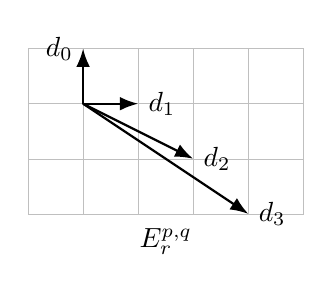
\begin{tikzpicture}[>=Latex, scale=0.7, baseline=(O)]
	\draw[very thin, gray!50] (-1,1) grid (4,-2);
	\draw[thick, ->] (0,0) -- (0,1) node[left] {$d_0$};
	\draw[thick, ->] (0,0) -- (1,0) node[right] {$d_1$};
	\draw[thick, ->] (0,0) -- (2,-1) node[right] {$d_2$};
	\draw[thick, ->] (0,0) -- (3,-2) node[right] {$d_3$};
	\node at (1.5,-2.5) {$E_r^{p,q}$};
	\coordinate (O) at (1.5,-0.5);
\end{tikzpicture} \qquad 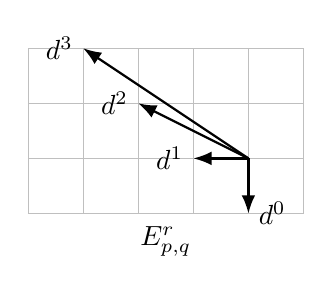
\begin{tikzpicture}[>=Latex, scale=0.7, baseline=(O)]
	\draw[very thin, gray!50] (1,-1) grid (-4,2);
	\draw[thick, ->] (0,0) -- (0,-1) node[right] {$d^0$};
	\draw[thick, ->] (0,0) -- (-1,0) node[left] {$d^1$};
	\draw[thick, ->] (0,0) -- (-2,1) node[left] {$d^2$};
	\draw[thick, ->] (0,0) -- (-3,2) node[left] {$d^3$};
	\node at (-1.5,-1.5) {$E^r_{p,q}$};
	\coordinate (O) at (-1.5,0.5);
\end{tikzpicture}\end{center}

% segment-id: o014.li2.chapter5.general-spectral-sequences.p014
In either version, following the preceding pattern, we may define the objects
$B_r^p\subset Z_r^p$, $B_r^{p,q}\subset Z_r^{p,q}$,
$E_\infty^p$, $E_\infty^{p,q}$, as well as
$B^r_p\subset Z^r_p$, $B^r_{p,q}\subset Z^r_{p,q}$,
$E^\infty_p$, $E^\infty_{p,q}$, and so forth.

% segment-id: o014.li2.chapter5.general-spectral-sequences.e002
\begin{example}[The finite-width case]\label{eg:SS-finite-width}
	In many common situations, the nonzero terms of a bigraded spectral sequence
	are concentrated in a horizontal (or vertical) strip of width $s$, where
	$s\in\Z_{\geq0}$, as in the following figure:
	\[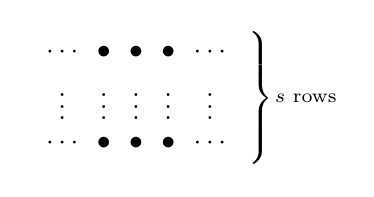
\begin{tikzpicture}[baseline]
		\matrix (M) [matrix of math nodes, right delimiter=\}] {
			\cdots & \bullet & \bullet & \bullet & \cdots \\
			\vdots & \vdots & \vdots & \vdots & \vdots \\
			\cdots & \bullet & \bullet & \bullet & \cdots \\
		};
		\node[right=2em] at (M-2-5) {\scriptsize \text{$s$ rows}};
	\end{tikzpicture} \quad \text{or} \quad 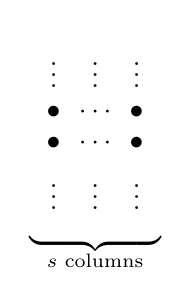
\begin{tikzpicture}[baseline]
		\matrix (M) [matrix of math nodes, below delimiter=\}] {
			\vdots & \vdots & \vdots \\
			\bullet & \cdots & \bullet \\
			\bullet & \cdots & \bullet \\
			\vdots & \vdots & \vdots \\
		};
		\node[below=2em] at (M-4-2) {\scriptsize \text{$s$ columns}};
	\end{tikzpicture}\]
	Inspection of the arrow directions shows that $r>s$ (or $r\geq s$)
	implies $d_r^{p,q}=0$ for all $p,q$; in this case the spectral sequence
	degenerates at the $E_r$ page. The homological case is similar.
\end{example}

% segment-id: o014.li2.chapter5.general-spectral-sequences.d005
\begin{definition}\label{def:bdd-ss}
	\index{spectral sequence!bounded}
	Let $\mathscr{E}$ be a cohomological (or homological) bigraded spectral
	sequence, and let $r\in\Z$. If for every $n\in\Z$ there are at most
	finitely many $(p,q)\in\Z^2$ satisfying $p+q=n$ and
	$E_r^{p,q}\neq0$ (or $E^r_{p,q}\neq0$), then $E_r$ (or $E^r$) is
	called \emph{bounded}.
\end{definition}

% segment-id: o014.li2.chapter5.general-spectral-sequences.p015
It follows from $E_{r+1}\simeq\Hm(E_r,d_r)$ that
$E_r^{p,q}=0\implies E_{r+1}^{p,q}=0$. In particular, if $E_r$ is bounded,
then $E_{r+1}$ is bounded. The homological case is similar.

% segment-id: o014.li2.chapter5.general-spectral-sequences.t003
\begin{proposition}
	Let $\mathscr{E}$ be a cohomological (or homological) bigraded spectral
	sequence for which $E_r$ (or $E^r$) is bounded. For every
	$(p,q)\in\Z^2$, there is an $r(p,q)$ such that, whenever
	$r\geq r(p,q)$, one has $E_r^{p,q}=E_{r+1}^{p,q}$ (or
	$E^r_{p,q}=E^{r+1}_{p,q}$). Consequently, the limit of $\mathscr{E}$
	exists and satisfies $E_r^{p,q}=E_\infty^{p,q}$ (or
	$E^r_{p,q}=E^\infty_{p,q}$).
\end{proposition}
\begin{proof}
	It suffices to discuss the case of $E_r$. Fix $n$. By boundedness, for all
	$(p,q)$ with $p+q=n$ and all sufficiently large $r$, we have
	$E_r^{p-r,q+r-1}=0$, hence $B_r^{p,q}=0$. Similarly, for sufficiently
	large $r$, we have $E_r^{p+r,q-r+1}=0$, hence
	$Z_r^{p,q}=E_r^{p,q}$. This proves the assertion.
\end{proof}

% segment-id: o014.li2.chapter5.general-spectral-sequences.d006
\begin{definition}\label{def:quadrant-ss}
	Let $\mathscr{E}$ be a cohomological (or homological) bigraded spectral
	sequence, and let $r\in\Z$. If $E_r^{p,q}\neq0$ (or
	$E^r_{p,q}\neq0$) implies $p,q\geq0$, then $E_r$ (or $E^r$) is said to
	lie in the first quadrant. The other quadrants are defined similarly.
\end{definition}

% segment-id: o014.li2.chapter5.general-spectral-sequences.p016
An $E_r$ lying in the first or third quadrant is clearly bounded. It follows
from $E_{r+1}\simeq\Hm(E_r,d_r)$ that if $E_r$ lies in any given quadrant,
then $E_{r+1}$ lies in the same quadrant. The homological case is similar.

% segment-id: o014.li2.chapter5.general-spectral-sequences.r001
\begin{remark}[Edge calculations]\label{rem:edge-computing}
	Spectral sequences lying in the first quadrant occur especially often. For
	the cohomological version, the edge terms $E_r^{\bullet,0}$ and
	$E_r^{0,\bullet}$ have special properties. Fix $p,q\geq1$. By carefully
	examining the direction of $d_r$ and recalling that
	$E_{r+1}\simeq\Hm(E_r,d_r)$, one verifies that
	\begin{equation}\label{eqn:edge-ss-coh}\begin{array}{cc}
		E_2^{p,0}\twoheadrightarrow E_3^{p,0}\twoheadrightarrow\cdots
		\twoheadrightarrow E_{p+1}^{p,0}=E_\infty^{p,0}
		& \text{($\because$ all outgoing $d$ are $0$)}, \\
		E_\infty^{0,q}=E_{q+2}^{0,q}\hookrightarrow E_{q+1}^{0,q}
		\hookrightarrow\cdots\hookrightarrow E_2^{0,q}\hookrightarrow E_1^{0,q}
		& \text{($\because$ all incoming $d$ are $0$)}.
	\end{array}\end{equation}
	A first-quadrant homological bigraded spectral sequence has the corresponding
	properties:
	\begin{equation}\label{eqn:edge-ss-ho}\begin{array}{cc}
		E^\infty_{p,0}=E^{p+1}_{p,0}\hookrightarrow E^p_{p,0}
		\hookrightarrow\cdots\hookrightarrow E^3_{p,0}\hookrightarrow E^2_{p,0}
		& \text{($\because$ all incoming $d$ are $0$)}, \\
		E^1_{0,q}\twoheadrightarrow E^2_{0,q}\twoheadrightarrow\cdots
		\twoheadrightarrow E^{q+2}_{0,q}=E^\infty_{0,q}
		& \text{($\because$ all outgoing $d$ are $0$)}.
	\end{array}\end{equation}
	\index{edge morphism}

	The morphisms arising from \eqref{eqn:edge-ss-coh} or
	\eqref{eqn:edge-ss-ho} are collectively called \emph{edge morphisms}.
	The preceding discussion gives the following exact sequence ($p\geq2$):
	\begin{equation}\label{eqn:low-exact-coh}
		0\to E^{0,p-1}_\infty\to E^{0,p-1}_p\xrightarrow{d}E^{p,0}_p
		\to E^{p,0}_\infty\to0,
	\end{equation}
	in which every morphism except $d$ is an edge morphism. There is also a
	homological version of this exact sequence ($p\geq2$):
	\begin{equation}\label{eqn:low-exact-ho}
		0\to E^\infty_{p,0}\to E^p_{p,0}\xrightarrow{d}E^p_{0,p-1}
		\to E^\infty_{0,p-1}\to0.
	\end{equation}
	Beginning readers should be sure to draw the directions of the morphisms
	$d$ involving these terms, determine when they are $0$, and thereby verify
	all the assertions above.
\end{remark}

% Unit 066 English translation of chapter5.tex lines 350--467.
% Source: Methods of Algebra, Volume 2, commit
% 9a5803ff77dd3257484cb177f851a73770a59dd3 (CC BY 4.0).
% stable-unit-id: o014.aljabr2.chapter5.exact-couples
% Coverage: Complete Section 5.3.

% segment-id: o014.li2.chapter5.exact-couples.h001
\section{Exact couples}\label{sec:exact-couples}
\hypertarget{o014.aljabr2.chapter5.exact-couples}{ }

% segment-id: o014.li2.chapter5.exact-couples.p001
Several commonly used kinds of spectral sequence arise from exact couples, a
discovery due to W.\ Massey. To grasp the essential idea, we first return to
the case without degrees.

% segment-id: o014.li2.chapter5.exact-couples.d001
\begin{definition}[Exact couple]\label{def:exact-couple}
	\index{exact couple}
	An exact couple over an Abelian category $\mathcal{A}$ is an exact diagram
	in $\mathcal{A}$
	\[\begin{tikzcd}[column sep=small]
		D \arrow[rr, "i"] & & D \arrow[ld, "j"] \\
		& E \arrow[lu, "k"] &
	\end{tikzcd}\]
	Morphisms between data $\mathscr{C}:=(D,E,i,j,k)$ are defined in the
	evident way.
\end{definition}

% segment-id: o014.li2.chapter5.exact-couples.p002
Given an exact couple $\mathscr{C}=(D,E,i,j,k)$, set $d:=jk:E\to E$. Then
$dj=jkj=0$ and $kd=kjk=0$, whence $d^2=0$. The exactness conditions readily
give the following factorizations:
\begin{equation}\label{eqn:exact-couple-aux}
	\begin{tikzcd}
		D \arrow[r, "j"] \arrow[twoheadrightarrow, d, "i"'] &
		\Ker(d) \arrow[twoheadrightarrow, d] \\
		i(D) \arrow[r, "{\exists!\;j'}"'] & \Hm(E,d)
	\end{tikzcd} \quad \begin{tikzcd}
		\Ker(d) \arrow[r, "k"] \arrow[twoheadrightarrow, d] & i(D) \\
		\Hm(E,d) \arrow[ru, "{\exists!\;k'}"'] &
	\end{tikzcd}
\end{equation}
Also define $E':=\Hm(E,d)$, $D':=i(D)$, and
$i':=i|_{i(D)}:D'\to D'$.

% segment-id: o014.li2.chapter5.exact-couples.l001
\begin{lemma}
	Given an exact couple $\mathscr{C}=(D,E,i,j,k)$, the data constructed above,
	\[ \mathscr{C}'=(D',E',i',j',k'):\quad
	\begin{tikzcd}[column sep=small]
		D' \arrow[rr, "{i'}"] & & D' \arrow[ld, "{j'}"] \\
		& E' \arrow[lu, "{k'}"] &
	\end{tikzcd} \]
	also form an exact couple.
\end{lemma}
\begin{proof}
	Examining \eqref{eqn:exact-couple-aux} and using the exactness conditions,
	one readily verifies that
	\begin{align*}
		\Ker(i') &= i(D)\cap\Ker(i)=\Ker(j)\cap k(E) \\
		&=\Image\left[\Ker(d)\xrightarrow{k}i(D)\right]=\Image(k'), \\
		\Ker(j') &= i\left(j^{-1}(jk(E))\right) \\
		&=i\left(k(E)+\Ker(j)\right)=i\left(i(D)\right)=\Image(i'), \\
		\Ker(k') &= (\Ker(k)\cap\Ker(d))/\Image(d)
		=(j(D)\cap\Ker(jk))/\Image(d) \\
		&=j(D)/\Image(d)=\Image(j').
	\end{align*}
	Thus the new triangular diagram is still exact.
\end{proof}

% segment-id: o014.li2.chapter5.exact-couples.p003
Iterating this procedure gives a sequence of exact couples
$(\mathscr{C}_{(r)})_{r\geq1}$, with
$\mathscr{C}_{(1)}=\mathscr{C}$ and
$\mathscr{C}_{(r+1)}=\mathscr{C}_{(r)}'$ for $r\geq1$. Writing
$\mathscr{C}_{(r)}=(D_r,E_r,i_r,j_r,k_r)$, the sequence
$(E_r,d_r:=j_rk_r)_{r\geq1}$ is a spectral sequence.

% segment-id: o014.li2.chapter5.exact-couples.l002
\begin{lemma}\label{prop:exact-couple-Z-B}
	For the spectral sequence $(E_r,d_r)_{r\geq1}$ obtained from an exact
	couple $\mathscr{C}=(D,E,i,j,k)$, define the family of subobjects
	$\overline{B}_r\subset\overline{Z}_r$ of $E=E_1$ according to
	\eqref{eqn:spectral-sequence-Z-B}. Bars are used because the indexing
	starts at $r=1$; see Proposition~\ref{prop:differential-exact-couple} below.
	For $r\geq0$,
	\begin{gather*}
		\overline{B}_{r+1}=j\left(\Ker(i^r)\right)
		\subset k^{-1}\left(\Image(i^r)\right)=\overline{Z}_{r+1}; \\
		\overline{B}_\infty=j\left(\bigcup_{r\geq2}\Ker(i^r)\right)
		\subset k^{-1}\left(\bigcap_{r\geq2}\Image(i^r)\right)
		=\overline{Z}_\infty,
	\end{gather*}
	provided that the relevant $\bigcup_r$ and $\bigcap_r$ exist. More
	precisely, the exact couple $\mathscr{C}_{(r+1)}$ is canonically isomorphic
	to
	\[\begin{tikzcd}[column sep=tiny]
		i^rD \arrow[rr, "i"] & & i^rD \arrow[ld, "{\overline{j}_{r+1}}"] \\
		& \dfrac{k^{-1}(i^rD)}{j(\Ker(i^r))}
		\arrow[lu, "{\overline{k}_{r+1}}"] &
	\end{tikzcd}\]
	where $\overline{k}_{r+1}$ is induced by $k:E\to D$, while
	$\overline{j}_{r+1}$ is characterized by the commutative diagram
	\[\begin{tikzcd}
		D \arrow[r, "{i^r}"] \arrow[d, "j"'] &
		i^rD \arrow[d, "{\overline{j}_{r+1}}"] \\
		k^{-1}(i^rD) \arrow[twoheadrightarrow, r] &
		\dfrac{k^{-1}(i^rD)}{j(\Ker(i^r))}.
	\end{tikzcd}\]
\end{lemma}
\begin{proof}
	The description of the exact couple $\mathscr{C}_{(r+1)}$ can be proved
	recursively. The case $r=0$ is trivial ($i^0=\identity$), and the
	descriptions of $\overline{B}_{r+1}$ and $\overline{Z}_{r+1}$ are immediate
	consequences. Since the details are somewhat routine, they are omitted.
	The assertion $\overline{B}_\infty\subset\overline{Z}_\infty$ follows from
	Lemma~\ref{prop:image-sum-preimage-intersection}~(ii).
\end{proof}

% segment-id: o014.li2.chapter5.exact-couples.p004
We next explain how to construct an exact couple from a differential object.

% segment-id: o014.li2.chapter5.exact-couples.t001
\begin{proposition}\label{prop:differential-exact-couple}
	Let $\alpha:(D,d)\to(D,d)$ be a monomorphism in $\mathcal{A}_d$, and
	write $d_\alpha$ for the morphism induced by $d$ on $\Coker(\alpha)$. Then
	there is an exact couple
	\[\begin{tikzcd}[column sep=tiny]
		\Hm(D,d) \arrow[rr, "{i=\Hm(\alpha)}"] & &
		\Hm(D,d) \arrow[ld, "j"] \\
		& \Hm(\Coker(\alpha),d_\alpha) \arrow[lu, "k"] &
	\end{tikzcd}\]
	Take the inverse images of
	$\overline{B}_{r+1}\subset\overline{Z}_{r+1}$ in
	$E_0:=\Coker(\alpha)$, and denote them by
	\[ 0=:B_0\subset B_1\subset B_2\subset\cdots\subset Z_2\subset Z_1
	\subset Z_0:=\Coker(\alpha). \]
	For every $r\geq0$:
	\begin{itemize}
		\item $B_{r+1}$ is the image of
		$(\alpha^r)^{-1}(dD)\subset D$ in $\Coker(\alpha)$;
		\item $Z_{r+1}$ is the image of
		$d^{-1}(\alpha^{r+1}D)\subset D$ in $\Coker(\alpha)$;
		\item $d_{r+1}\in\End(Z_{r+1}/B_{r+1})$ is induced by
		$d^{-1}(\alpha^{r+1}D)\xrightarrow{d}\alpha^{r+1}D
		\xleftarrow[\sim]{\alpha^{r+1}}D$.
	\end{itemize}
	In particular, there are canonical isomorphisms
	\[ E_{r+1}\simeq\dfrac{Z_{r+1}}{B_{r+1}}
	\simeq\dfrac{d^{-1}(\alpha^{r+1}D)+\alpha D}
	{(\alpha^r)^{-1}(dD)+\alpha D},\qquad r\in\Z_{\geq1}. \]
\end{proposition}
\begin{proof}
	The exact couple is obtained by applying
	Lemma~\ref{prop:diff-obj-triangle} (with
	$T=\identity_{\mathcal{A}}$) to the short exact sequence in
	$\mathcal{A}_d$
	\[ 0\to(D,d)\xrightarrow{\alpha}(D,d)
	\to(\Coker(\alpha),d_\alpha)\to0. \]
	In particular, $j$ is induced by $D\twoheadrightarrow\Coker(\alpha)$,
	while $k$ is essentially the connecting morphism in the long exact
	sequence. The description of $B_{r+1}$ is simply the version of
	Lemma~\ref{prop:exact-couple-Z-B} lifted to $E_0$. For $Z_{r+1}$, besides
	that lemma, the key point is the description of the connecting morphism
	$k:\Hm(\Coker(\alpha),d_\alpha)\to\Hm(D,d)$. A careful review of the
	constructions in \eqref{eqn:snake-conn} and
	\eqref{eqn:long-exact-sequence-ses-aux} shows that this morphism is induced
	by the middle vertical morphism $\overline{d}$ in the following commutative
	diagram with exact rows:
	\[\begin{tikzcd}
		& \Coker(d) \arrow[r] \arrow[d, "\overline{d}"'] &
		\Coker(d) \arrow[r] \arrow[d, "\overline{d}"'] &
		\Coker(d_\alpha) \arrow[d, "\overline{d_\alpha}"] \arrow[r] & 0 \\
		0 \arrow[r] & \Ker(d) \arrow[r, "\alpha"'] &
		\Ker(d) \arrow[r] & \Ker(d_\alpha) &
	\end{tikzcd}\]
	and $\overline{d}$ itself comes from $d:D\to D$. The remaining
	verifications are lengthy but straightforward; the reader may begin with
	the case where $\mathcal{A}$ is a category of modules.
\end{proof}

% segment-id: o014.li2.chapter5.exact-couples.p005
Thus the spectral sequence provided by a differential object can be made to
start at $0$ by setting $E_0:=\Coker(\alpha)$ and $d_0:=d_\alpha$.

% segment-id: o014.li2.chapter5.exact-couples.p006
For an Abelian category with translation $(\mathcal{A},T)$, morphisms with
degrees can still be composed and notions such as exactness remain available,
so the theory of exact couples readily extends to the case in which $i,j,k$
have degrees. For example, in the situation to be discussed in
\S\ref{sec:filtered-diff-ss}, we can consider the exact couple
\[\begin{tikzcd}[column sep=tiny]
	D \arrow[rr, "{-1}"] & & D \arrow[ld, "{+1}"] \\
	& E \arrow[lu] &
\end{tikzcd} \xlongequal{\text{unrolled}} \left[
	\begin{tikzcd}[column sep=0ex, every cell/.append style={font=\small}]
		\cdots & TD \arrow[rr] \arrow[ld] & & D \arrow[rr] \arrow[ld] & &
		T^{-1}D \arrow[rr] \arrow[ld] & & T^{-2}D \arrow[ld] & \cdots \\
		\cdots & & TE \arrow[lu] & & E \arrow[lu] & &
		T^{-1}E \arrow[lu] & & \cdots \arrow[lu]
	\end{tikzcd}
\right]. \]
Denote this exact couple by $\mathscr{C}$. The natural extension of
Lemma~\ref{prop:exact-couple-Z-B} to the case with degrees shows that
$\mathscr{C}_{(r)}$ has the form
$\begin{tikzcd}[column sep=tiny, row sep=small]
	\bullet \arrow[rr, "{-1}"] & & \bullet \arrow[ld, "{+r}"] \\
	& \bullet \arrow[lu] &
\end{tikzcd}$.
Thus $d_r=j_rk_r$ is a morphism of degree $r$. The resulting spectral sequence
is therefore graded.

% Unit 067 English translation of chapter5.tex lines 468--577.
% Source: Methods of Algebra, Volume 2, commit
% 9a5803ff77dd3257484cb177f851a73770a59dd3 (CC BY 4.0).
% stable-unit-id: o014.aljabr2.chapter5.filtered-differential-spectral-sequence
% Coverage: Complete Section 5.4.

% segment-id: o014.li2.chapter5.filtered-differential-spectral-sequence.h001
\section{The spectral sequence of a filtered differential object}
\label{sec:filtered-diff-ss}
\hypertarget{o014.aljabr2.chapter5.filtered-differential-spectral-sequence}{ }

% segment-id: o014.li2.chapter5.filtered-differential-spectral-sequence.p001
Throughout this section, we work with an Abelian category with translation
$(\mathcal{A},T)$.

% segment-id: o014.li2.chapter5.filtered-differential-spectral-sequence.d001
\begin{definition}\label{def:filtered-diffop}
	\index{differential object!filtered}
	An object $(X,d)\in\Obj((\mathcal{A},T)_d)$ equipped with a filtration
	$\left(\mathrm{F}^\bullet X,d_{\mathrm{F}^\bullet X}\right)$ is called a
	\emph{filtered differential object} over $(\mathcal{A},T)$. In this case,
	$\gr^pX$ is also naturally equipped with
	$\gr^pd:\gr^pX\to T\gr^pX$, so that
	$(\gr^pX,\gr^pd)\in\Obj((\mathcal{A},T)_d)$.
\end{definition}

% segment-id: o014.li2.chapter5.filtered-differential-spectral-sequence.p002
Since $d_{\mathrm{F}^pX}$ on the subobject $\mathrm{F}^pX$ is best
understood as the restriction of $d:X\to TX$, we continue to denote it by
$d$. A similar definition applies to increasing filtrations, with an entirely
dual formulation.

% segment-id: o014.li2.chapter5.filtered-differential-spectral-sequence.p003
We return to spectral sequences. The preceding section explained how to
construct an exact couple from a differential object. Now consider a filtered
differential object $(X,d,\mathrm{F}^\bullet X)$ over $\mathcal{A}$. Write
$S:(Y^p)_p\mapsto(Y^{p+1})_p$ for the standard translation functor on
$\mathcal{A}^{\Z}$; it plainly commutes with $T$, acting on each $Y^p$.
Consequently, the morphisms considered below have two kinds of degree: the
``filtration degree'' corresponding to $S$ and the ``internal degree''
corresponding to $T$. For the moment we focus on the former.

% segment-id: o014.li2.chapter5.filtered-differential-spectral-sequence.p004
Since the filtration is decreasing, there is a monomorphism
\[ \alpha:\left(\mathrm{F}^{p+1}X,d\right)_{p\in\Z}
	\hookrightarrow S^{-1}\left(\mathrm{F}^{p+1}X,d\right)_{p\in\Z}
	=\left(\mathrm{F}^{p}X,d\right)_{p\in\Z}. \]
Thus $E_0:=\Coker(\alpha)=\left(\gr^pX,\gr^pd\right)_{p\in\Z}$ and
$E_1^p=\Hm(\gr^pX,\gr^pd)$.

% segment-id: o014.li2.chapter5.filtered-differential-spectral-sequence.p005
Regard $\alpha$ as a morphism of degree $-1$ in $\mathcal{A}^{\Z}$ (with
respect to $S$). Applying Proposition~\ref{prop:differential-exact-couple}
gives the following exact couple with degrees over $\mathcal{A}^{\Z}$:
\[\mathscr{C}=\left[\begin{tikzcd}[column sep=tiny]
	\Hm\left(\mathrm{F}^{p+1}X,d\right)_p
	\arrow[rr, "-1"', "{\Hm(\alpha)}"] & &
	\Hm\left(\mathrm{F}^{p+1}X,d\right)_p \arrow[ld, "{+1}"] \\
	& \Hm\left(\gr^pX,\gr^pd\right)_p \arrow[lu] &
\end{tikzcd}\right],\]
where the $\nwarrow$ arrow comes from the connecting morphism induced by the
short exact sequence
$0\to(\mathrm{F}^{p+1}X,d)\to(\mathrm{F}^pX,d)
\to(\gr^pX,\gr^pd)\to0$.

% segment-id: o014.li2.chapter5.filtered-differential-spectral-sequence.p006
The resulting sequence
$\mathscr{E}=(E_r^p,d_r^p)_{\substack{r\geq0\\p\in\Z}}$ is called the
spectral sequence determined by $\mathrm{F}^\bullet X$ in
$\mathcal{A}^{\Z}$. At the end of \S\ref{sec:exact-couples} we explained that
$d_r$ is a morphism of degree $r$ with respect to $S$, namely
\[ d_r=\left(d_r^p:E_r^p\to(S^rE_r)^p=E_r^{p+r}\right)_{p\in\Z}; \]
of course, the degree of $d_r$ can also be read from the formula in
Proposition~\ref{prop:differential-exact-couple}.

% segment-id: o014.li2.chapter5.filtered-differential-spectral-sequence.p007
In other words, a filtered differential object
$(X,d,\mathrm{F}^\bullet X)$ gives a cohomologically graded spectral sequence
as in Definition~\ref{def:graded-spectral-sequence}. Notice that $d_r^p$ here
may also carry an internal degree (unless $T=\identity_{\mathcal{A}}$); this is
suppressed from the notation and will be set out in detail in
\S\ref{sec:filtered-cplx-ss}.

% segment-id: o014.li2.chapter5.filtered-differential-spectral-sequence.p008
Following the pattern of \eqref{eqn:spectral-sequence-Z-B}, define subobjects
of $Z_0=(\gr^pX,\gr^pd)_p$ by
\[ B_r=(B_r^p)_p\subset(Z_r^p)_p=Z_r. \]

% segment-id: o014.li2.chapter5.filtered-differential-spectral-sequence.p009
To simplify notation, the statements below suppress the internal degree of
$d$; this amounts to considering the special case
$T=\identity_{\mathcal{A}}$. The extension to the general case is routine:
translation functors need only be inserted appropriately wherever
$d^{-1}(\cdots)$ or $d(\cdots)$ occurs, so that the expressions make strict
sense.

% segment-id: o014.li2.chapter5.filtered-differential-spectral-sequence.t001
\begin{proposition}\label{prop:filtered-diff-E}
	For a filtered differential object $(X,d,\mathrm{F}^\bullet X)$, the
	associated spectral sequence satisfies
	\begin{align*}
		Z_r^p&=\dfrac{\left(\mathrm{F}^pX\cap d^{-1}\mathrm{F}^{p+r}X\right)
		+\mathrm{F}^{p+1}X}{\mathrm{F}^{p+1}X}, \\
		B_r^p&=\dfrac{\left(\mathrm{F}^pX\cap d\mathrm{F}^{p-r+1}X\right)
		+\mathrm{F}^{p+1}X}{\mathrm{F}^{p+1}X},
	\end{align*}
	and $d_r^p:E_r^p\to E_r^{p+r}$ is induced by the morphism
	$d^{-1}\mathrm{F}^{p+r}X\xrightarrow{d}
	\mathrm{F}^{p+r}X\cap\Ker(d)$.
\end{proposition}
\begin{proof}
	Observe that the degree-$p$ component of $\alpha^r$ may be identified with
	the inclusion $\mathrm{F}^pX\hookrightarrow\mathrm{F}^{p-r}X$ or
	$\mathrm{F}^{p+r}X\hookrightarrow\mathrm{F}^pX$. The assertion reduces to
	the graded version of Proposition~\ref{prop:differential-exact-couple}.
\end{proof}

% segment-id: o014.li2.chapter5.filtered-differential-spectral-sequence.p010
Since $\varinjlim$ and $\varprojlim$ in $\mathcal{A}^{\Z}$ are taken degree
by degree, $E_\infty=(E_\infty^p)_{p\in\Z}$ can be written as
\begin{equation}\label{eqn:filtered-diff-infty}
	E_\infty^p=\dfrac{Z_\infty^p}{B_\infty^p}
	=\dfrac{\bigcap_r\left((\mathrm{F}^pX\cap d^{-1}\mathrm{F}^{p+r}X)
	+\mathrm{F}^{p+1}X\right)}
	{\bigcup_r\left((\mathrm{F}^pX\cap d\mathrm{F}^{p-r+1}X)
	+\mathrm{F}^{p+1}X\right)},
\end{equation}
provided the displayed $\bigcap$ and $\bigcup$ exist for every $p$.

% segment-id: o014.li2.chapter5.filtered-differential-spectral-sequence.r001
\begin{remark}
	Proposition~\ref{prop:filtered-diff-E} on the spectral sequence of a filtered
	differential object is the foundation for the later discussions in this
	chapter. It is an application of exact couples, but we could equally regard
	the formulas in Proposition~\ref{prop:filtered-diff-E} as direct definitions
	and verify from them all the properties required of a spectral sequence.
\end{remark}

% segment-id: o014.li2.chapter5.filtered-differential-spectral-sequence.p011
From the preceding description, the spectral sequence $E_r^p$ of
$(X,d,\mathrm{F}^\bullet X)$ can be viewed as a process of successively
approximating $\Hm(X,d)$. To make precise what ``approximating'' means, we
need the following concept.

% segment-id: o014.li2.chapter5.filtered-differential-spectral-sequence.d002
\begin{definition}[Induced filtration]\label{def:induced-filtration-H}
	\index{filtration!induced}
	For a filtered differential object $(X,d,\mathrm{F}^\bullet X)$ over
	$(\mathcal{A},T)$, the object $\Hm(X,d)$ carries the induced filtration
	\[ \mathrm{F}^p\Hm(X,d):=
	\Image\left[\mathrm{F}^pX\cap\Ker(d)\to\Hm(X,d)\right],
	\qquad p\in\Z. \]
\end{definition}

% segment-id: o014.li2.chapter5.filtered-differential-spectral-sequence.l001
\begin{lemma}\label{prop:induced-filtration-H}
	If there is an $N$ with $\mathrm{F}^NX=0$, then
	$\mathrm{F}^N\Hm(X,d)=0$. If $\mathrm{F}^\bullet X$ is an exhaustive
	filtration in the sense of Definition~\ref{def:filtration-properties}, then
	$\mathrm{F}^\bullet\Hm(X,d)$ is exhaustive as well.
\end{lemma}
\begin{proof}
	The first part is immediate; we prove the second. By
	Lemma~\ref{prop:image-sum-preimage-intersection}~(ii),
	$\bigcup_p\mathrm{F}^p\Hm(X,d)$ is the image of
	$\bigcup_p(\mathrm{F}^pX\cap\Ker(d))$, while
	\eqref{eqn:exhaustion-intersection} gives
	\[ \bigcup_p\left(\mathrm{F}^pX\cap\Ker(d)\right)
	=\left(\bigcup_p\mathrm{F}^pX\right)\cap\Ker(d)=\Ker(d). \]
	Moreover, if there is an $M$ with $\mathrm{F}^MX=X$, then of course
	$\mathrm{F}^M\Hm(X,d)=\Hm(X,d)$.
\end{proof}

% segment-id: o014.li2.chapter5.filtered-differential-spectral-sequence.p012
We shall apply the graded version of these observations in
\S\ref{sec:filtered-cplx-ss}.

% segment-id: o014.li2.chapter5.filtered-differential-spectral-sequence.l002
\begin{lemma}\label{prop:induced-filtration-gr}
	For a filtered differential object $(X,d,\mathrm{F}^\bullet X)$ and every
	$p\in\Z$, there is a canonical isomorphism
	\[ \gr^p\Hm(X,d)\simeq
	\dfrac{\mathrm{F}^pX\cap\Ker(d)}
	{(\mathrm{F}^{p+1}X\cap\Ker(d))
	 +(\mathrm{F}^pX\cap\Image(T^{-1}d))}. \]
\end{lemma}
\begin{proof}
	Expand the definition of
	$\mathrm{F}^p\Hm(X,d)/\mathrm{F}^{p+1}\Hm(X,d)$ and use the standard
	isomorphism theorem for Abelian categories,
	Proposition~\ref{prop:Abel-cat-isom-thm}, to obtain
	\begin{align*}
		\gr^p\Hm(X,d)
		&=\dfrac{(\mathrm{F}^pX\cap\Ker(d))+\Image(T^{-1}d)}
		{(\mathrm{F}^{p+1}X\cap\Ker(d))+\Image(T^{-1}d)} \\
		&=\dfrac{(\mathrm{F}^pX\cap\Ker(d))
		 +(\mathrm{F}^{p+1}X\cap\Ker(d))+\Image(T^{-1}d)}
		{(\mathrm{F}^{p+1}X\cap\Ker(d))+\Image(T^{-1}d)} \\
		&\simeq\dfrac{\mathrm{F}^pX\cap\Ker(d)}
		{((\mathrm{F}^{p+1}X\cap\Ker(d))+\Image(T^{-1}d))
		 \cap(\mathrm{F}^pX\cap\Ker(d))} \\
		&=\dfrac{\mathrm{F}^pX\cap\Ker(d)}
		{(\mathrm{F}^{p+1}X\cap\Ker(d))
		 +(\mathrm{F}^pX\cap\Image(T^{-1}d))}.
	\end{align*}
	The last step uses the fact that $\mathrm{Sub}_X$ is a modular
	lattice\footnote{That is, for all subobjects $A,A^\flat,B\subset X$ with
	$A^\flat\subset A$, one has
	$A^\flat+(A\cap B)=(A^\flat+B)\cap A$.}
	(Theorem~\ref{prop:subobject-modularity}), together with
	$\mathrm{F}^{p+1}X\cap\Ker(d)\subset\mathrm{F}^pX\cap\Ker(d)$ and
	$\Image(T^{-1}d)\subset\Ker(d)$. The remaining steps are standard.
\end{proof}

% segment-id: o014.li2.chapter5.filtered-differential-spectral-sequence.d003
\begin{definition-proposition}\label{def:diff-obj-convergence}
	\index{spectral sequence!weakly convergent, strongly convergent}
	For a filtered differential object $(X,d,\mathrm{F}^\bullet X)$, construct
	the associated cohomologically graded spectral sequence $(E_r,d_r)_r$. If
	the $\bigcap_r$ and $\bigcup_r$ in \eqref{eqn:filtered-diff-infty} exist,
	then the limit $E_\infty$ exists, and the $\gr\Hm(X,d)$ determined by the
	induced filtration can be canonically realized as a subquotient of
	$E_\infty$.
	\begin{itemize}
		\item If $\gr\Hm(X,d)=E_\infty$, the spectral sequence
		$(E_r,d_r)_r$ is called \emph{weakly convergent}.
		\item If $(E_r,d_r)_r$ is weakly convergent and
		$\mathrm{F}^\bullet\Hm(X,d)$ is exhaustive and complete, the spectral
		sequence $(E_r,d_r)_r$ is called \emph{strongly convergent}.
	\end{itemize}
\end{definition-proposition}
\begin{proof}
	Fix $p\in\Z$. In the expression for $E_\infty^p$ in
	\eqref{eqn:filtered-diff-infty}, the numerator contains
	$(\mathrm{F}^pX\cap\Ker(d))+\mathrm{F}^{p+1}X$, while the denominator is
	contained in
	$(\mathrm{F}^pX\cap\Image(T^{-1}d))+\mathrm{F}^{p+1}X$
	(recall that $d$ is a morphism $X\to TX$). This gives the following
	subquotient of $E_\infty^p$:
	\begin{multline*}
		\dfrac{(\mathrm{F}^pX\cap\Ker(d))+\mathrm{F}^{p+1}X}
		{(\mathrm{F}^pX\cap\Image(T^{-1}d))+\mathrm{F}^{p+1}X} \\
		\simeq\dfrac{\mathrm{F}^pX\cap\Ker(d)}
		{((\mathrm{F}^pX\cap\Image(T^{-1}d))+\mathrm{F}^{p+1}X)
		 \cap(\mathrm{F}^pX\cap\Ker(d))} \\
		=\dfrac{\mathrm{F}^pX\cap\Ker(d)}
		{(\mathrm{F}^pX\cap\Image(T^{-1}d))
		 +(\mathrm{F}^{p+1}X\cap\Ker(d))}.
	\end{multline*}
	The first isomorphism is standard. The following equality uses the fact that
	$\mathrm{Sub}_X$ is a modular lattice, together with
	$\mathrm{F}^pX\cap\Image(T^{-1}d)
	\subset\mathrm{F}^pX\cap\Ker(d)$ and
	$\mathrm{F}^{p+1}X\subset\mathrm{F}^pX$. Now apply
	Lemma~\ref{prop:induced-filtration-gr}.
\end{proof}

% segment-id: o014.li2.chapter5.filtered-differential-spectral-sequence.p013
Definitions of convergence vary slightly among references. All the statements
above have corresponding versions for differential objects with increasing
filtrations $(X,d,\mathrm{F}_\bullet X)$ and the associated homologically
graded spectral sequences.

% Unit 068 English translation of chapter5.tex lines 578--739.
% Source: Methods of Algebra, Volume 2, commit
% 9a5803ff77dd3257484cb177f851a73770a59dd3 (CC BY 4.0).
% stable-unit-id: o014.aljabr2.chapter5.filtered-complex-spectral-sequence
% Coverage: Complete Section 5.5.

% segment-id: o014.li2.chapter5.filtered-complex-spectral-sequence.h001
\section{The spectral sequence of a filtered complex}\label{sec:filtered-cplx-ss}
\hypertarget{o014.aljabr2.chapter5.filtered-complex-spectral-sequence}{ }
\index{complex!filtered}
\index{spectral sequence!of a filtered complex}

% segment-id: o014.li2.chapter5.filtered-complex-spectral-sequence.p001
We continue the line of thought from \S\ref{sec:filtered-diff-ss}, still with
a fixed Abelian category $\mathcal{A}$. The result of
Proposition~\ref{prop:filtered-diff-E} for filtered differential objects can
be extended to allow the morphism $d$ to have a degree. In particular, this
theory applies to filtered complexes.

% segment-id: o014.li2.chapter5.filtered-complex-spectral-sequence.p002
Concretely, replace the previous $\mathcal{A}$ by $\mathcal{A}^{\Z}$ and
denote its translation functor by $T$. By Example~\ref{eg:cplx-as-diff}, an
object $(X,d)$ of $(\mathcal{A}^{\Z},T)_d$ can be identified with a complex
$X\in\Obj(\cate{C}(\mathcal{A}))$. If we further take a decreasing filtration
$(X,d,\mathrm{F}^\bullet X)$, then
\begin{align*}
	\Hm(X,d)&=\left(\Hm^n(X)\right)_{n\in\Z}, \\
	\Hm\left(\mathrm{F}^pX,d\right)
	&=\left(\Hm^n\left(\mathrm{F}^pX\right)\right)_{n\in\Z}, \\
	\mathrm{F}^p\Hm^n(X)&:=
	\Image\left[\mathrm{F}^pX^n\cap\Ker(d_X^n)\to\Hm^n(X)\right]
	\quad\text{(Definition~\ref{def:induced-filtration-H}).}
\end{align*}

% segment-id: o014.li2.chapter5.filtered-complex-spectral-sequence.p003
Thus the $E_r$ in the spectral sequence $\mathscr{E}$ constructed above in
fact takes values in $\mathcal{A}^{\Z\times\Z}$ and is a bigraded object.
Besides the filtration degree $p$, there is an ``internal degree'' $n$ coming
from the complex structure; the corresponding translation functors $S$ and
$T$ commute strictly. We already know that $d_r$ has degree $r$ with respect
to $S$; we now determine its degree with respect to $T$.

% segment-id: o014.li2.chapter5.filtered-complex-spectral-sequence.p004
\begin{itemize}
	\item In the exact couple $\mathscr{C}_{(1)}$ used to construct
	$\mathscr{E}$, the morphism $\nwarrow$ has degree $1$ with respect to $T$,
	while the other morphisms have degree zero. Indeed, $\nwarrow$ comes from
	the cohomological connecting morphism and hence has degree $1$ with respect
	to $T$, while the other arrows plainly have degree zero.
	\item Using the description in Lemma~\ref{prop:exact-couple-Z-B}, the same
	statement follows recursively for $\mathscr{C}_{(r)}$ for every $r$.
	\item Consequently, both $d_r$ and the $d$ in $(X,d)$ are morphisms of
	degree $1$ with respect to $T$. This is also immediate from the description
	in Proposition~\ref{prop:differential-exact-couple}.
\end{itemize}

% segment-id: o014.li2.chapter5.filtered-complex-spectral-sequence.p005
For applications, the customary convention is to use the indices $p$ and
$q:=n-p$. Thus
\begin{gather*}
	E_r=(E_r^{p,q})_{(p,q)\in\Z^2}
	=\left(Z_r^{p,q}/B_r^{p,q}\right)_{(p,q)\in\Z^2}, \\
	E_0^{p,q}=\left(\gr^pX\right)^{p+q}, \\
	E_1^{p,q}=\Hm^{p+q}\left(\gr^pX,\gr^pd\right), \\
	d_r=\left(d_r^{p,q}:E_r^{p,q}\to E_r^{p+r,q-r+1}\right)_{(p,q)\in\Z^2}
	:E_r\xrightarrow{(r,-r+1)}E_r.
\end{gather*}
In other words, a filtered complex gives a cohomological bigraded spectral
sequence as in Definition~\ref{def:graded-spectral-sequence}. Dually, a chain
complex with an increasing filtration gives a homological bigraded spectral
sequence.

% segment-id: o014.li2.chapter5.filtered-complex-spectral-sequence.e001
\begin{example}\label{eg:canonically-bdd-ss}
	Consider a filtered complex $(X,d,\mathrm{F}^\bullet X)$. If for every
	$n\in\Z$ one has $\mathrm{F}^0X^n=X^n$ and
	$\mathrm{F}^{n+1}X^n=0$, then $E_0$ lies in the first quadrant
	(Definition~\ref{def:quadrant-ss}). This follows immediately from
	$E_0^{p,q}=(\gr^pX)^{p+q}$.
\end{example}

% segment-id: o014.li2.chapter5.filtered-complex-spectral-sequence.t001
\begin{proposition}\label{prop:filtered-cplx-ss}
	For a complex $X\in\Obj(\cate{C}(\mathcal{A}))$ with decreasing filtration
	$\mathrm{F}^\bullet X$, the associated spectral sequence satisfies
	\begin{align*}
		Z_r^{p,q}&=
		\dfrac{\left(\mathrm{F}^pX^{p+q}\cap
		d^{-1}\mathrm{F}^{p+r}X^{p+q+1}\right)+\mathrm{F}^{p+1}X^{p+q}}
		{\mathrm{F}^{p+1}X^{p+q}}, \\
		B_r^{p,q}&=
		\dfrac{\left(\mathrm{F}^pX^{p+q}\cap
		d\mathrm{F}^{p-r+1}X^{p+q-1}\right)+\mathrm{F}^{p+1}X^{p+q}}
		{\mathrm{F}^{p+1}X^{p+q}},
	\end{align*}
	and $d_r^{p,q}:E_r^{p,q}\to E_r^{p+r,q-r+1}$ is induced by
	\[ d^{-1}\mathrm{F}^{p+r}X^{p+q+1}\xrightarrow{d}
	\mathrm{F}^{p+r}X^{p+q+1}\cap\Ker(d). \]
\end{proposition}
\begin{proof}
	In Proposition~\ref{prop:filtered-diff-E}, include the complex degree
	$n=p+q$ and observe that $d$ has degree $1$ with respect to the complex
	translation functor $T$.
\end{proof}

% segment-id: o014.li2.chapter5.filtered-complex-spectral-sequence.p006
Similarly, \eqref{eqn:filtered-diff-infty} has the bigraded version
\begin{equation}\label{eqn:filtered-cplx-infty}
	E_\infty^{p,q}=\dfrac{Z_\infty^{p,q}}{B_\infty^{p,q}}
	=\dfrac{\bigcap_r\left((\mathrm{F}^pX^{p+q}\cap
	d^{-1}\mathrm{F}^{p+r}X^{p+q+1})+\mathrm{F}^{p+1}X^{p+q}\right)}
	{\bigcup_r\left((\mathrm{F}^pX^{p+q}\cap
	d\mathrm{F}^{p-r+1}X^{p+q-1})+\mathrm{F}^{p+1}X^{p,q}\right)},
\end{equation}
provided the displayed $\bigcup$ and $\bigcap$ exist. In this case
$E_\infty=(E_\infty^{p,q})_{(p,q)\in\Z^2}$.

% segment-id: o014.li2.chapter5.filtered-complex-spectral-sequence.p007
Definition--Proposition~\ref{def:diff-obj-convergence} now becomes a bigraded
statement: for all $p,q$, the object $\gr^p\Hm^{p+q}(X)$ can be canonically
realized as a subquotient of $E_\infty^{p,q}$. The convergence properties of
the spectral sequence are correspondingly refined by the grading.

% segment-id: o014.li2.chapter5.filtered-complex-spectral-sequence.d001
\begin{definition}\label{def:filtered-cplx-convergence}
	\index{spectral sequence!weakly convergent, strongly convergent}
	For a filtered complex $(X,d,\mathrm{F}^\bullet X)$ over $\mathcal{A}$,
	construct the associated cohomologically graded spectral sequence
	$(E_r,d_r)_r$. If the $\bigcap_r$ and $\bigcup_r$ in
	\eqref{eqn:filtered-cplx-infty} exist, then
	$\gr^p\Hm^{p+q}(X)$ can be canonically realized as a subquotient of
	$E_\infty^{p,q}$.
	\begin{itemize}
		\item If $\gr^p\Hm^{p+q}(X)=E_\infty^{p,q}$ for every
		$(p,q)\in\Z^2$, then $(E_r,d_r)_r$ is called \emph{weakly convergent}.
		\item If the sequence is weakly convergent and, for every $n\in\Z$,
		the filtration $\mathrm{F}^\bullet\Hm^n(X)$ is exhaustive and complete,
		then $(E_r,d_r)_r$ is called \emph{strongly convergent}.
	\end{itemize}
\end{definition}

% segment-id: o014.li2.chapter5.filtered-complex-spectral-sequence.c001
\begin{convention}\label{con:ss-conv}
	\index[sym1]{Erpq abuts to H@$E_r^{p,q}\Rightarrow\Hm^{p+q}(X)$}
	Strong convergence of a spectral sequence is also denoted by
	$E_r^{p,q}\Rightarrow\Hm^{p+q}(X)$. The subscript $r$ is usually written
	concretely as $1$, $2$, and so on, depending on which page of the spectral
	sequence we wish to describe.

	More generally, suppose we are given a cohomological bigraded spectral
	sequence $\mathscr{E}$, a filtered graded object
	$(H,\mathrm{F}^\bullet H)$, and isomorphisms
	$E_\infty^{p,q}\simeq\gr^pH^{p+q}$, with
	$\mathrm{F}^\bullet H$ exhaustive and complete. We also denote this
	situation by $E_r^{p,q}\Rightarrow H^{p+q}$. Homological bigraded spectral
	sequences are treated similarly; in particular,
	$E^r_{p,q}\Rightarrow H_{p+q}$ entails
	$E^\infty_{p,q}\simeq\gr_pH_{p+q}$.
\end{convention}

% segment-id: o014.li2.chapter5.filtered-complex-spectral-sequence.p008
The following classical convergence theorem is sufficient for initial
applications. For more general convergence conditions, see \cite{Boa99}.

% segment-id: o014.li2.chapter5.filtered-complex-spectral-sequence.t002
\begin{theorem}[Classical convergence theorem]\label{prop:classical-convergence}
	Consider a filtered complex $(X,d,\mathrm{F}^\bullet X)$. Suppose that for
	every $n\in\Z$,
	\begin{compactitem}
		\item the filtration $\mathrm{F}^\bullet X^n$ is exhaustive
		(Definition~\ref{def:filtration-properties}),
		\item there is an $N=N(n)$ such that $\mathrm{F}^NX^n=0$.
	\end{compactitem}
	Then the associated spectral sequence is strongly convergent
	(Definition--Proposition~\ref{def:diff-obj-convergence}).

	If the hypotheses are strengthened so that the filtration on every $X^n$
	is finite (Definition~\ref{def:filtration}), then the induced filtration on
	$\Hm^n(X)$ is also finite. In this case the associated spectral sequence is
	bounded (Definition~\ref{def:bdd-ss}).
\end{theorem}
\begin{proof}
	By the graded version of Lemma~\ref{prop:induced-filtration-H}, the induced
	filtration $\mathrm{F}^\bullet\Hm^n(X)$ is exhaustive and complete. It
	therefore remains to prove weak convergence.

	We need to recall the proof of
	Definition--Proposition~\ref{def:diff-obj-convergence}, which explains how
	to realize $\gr^p\Hm^{p+q}(X)$ as a subquotient of $E_\infty^{p,q}$ for
	each $(p,q)\in\Z^2$. The key point is
	\begin{equation*}\begin{split}
		\bigcap_r&\left(\left(\mathrm{F}^pX^{p+q}\cap
		d^{-1}\mathrm{F}^{p+r}X^{p+q+1}\right)+\mathrm{F}^{p+1}X^{p+q}\right)
		\\
		&\supset(\mathrm{F}^pX^{p+q}\cap\Ker(d))+\mathrm{F}^{p+1}X^{p+q},\\
		\bigcup_r&\left(\left(\mathrm{F}^pX^{p+q}\cap
		d\mathrm{F}^{p-r+1}X^{p+q-1}\right)+\mathrm{F}^{p+1}X^{p+q}\right)
		\\
		&\subset(\mathrm{F}^pX^{p+q}\cap\Image(d))+\mathrm{F}^{p+1}X^{p+q}.
	\end{split}\end{equation*}
	Proving weak convergence is equivalent to strengthening both inclusions to
	equalities. But when $r\gg0$ relative to $p,q$, the expression inside
	$\bigcap_r$ in the first line is simply
	$(\mathrm{F}^pX^{p+q}\cap\Ker(d))+\mathrm{F}^{p+1}X^{p+q}$, so equality
	holds.

	For the second line, the term $+\mathrm{F}^{p+1}X^{p+q}$ can first be
	moved outside $\bigcup_r$. Recall that $d(\mathrm{F}^\bullet X^n)$ is an
	exhaustive filtration of $d(X^n)$. Hence
	\begin{multline*}
		\bigcup_r\left(\mathrm{F}^pX^{p+q}\cap
		d\mathrm{F}^{p-r+1}X^{p+q-1}\right)\\
		\xlongequal{\because\;\text{\eqref{eqn:exhaustion-intersection}}}
		\mathrm{F}^pX^{p+q}\cap\bigcup_r
		d\mathrm{F}^{p-r+1}X^{p+q-1}\\
		=\mathrm{F}^pX^{p+q}\cap d\bigcup_r
		\mathrm{F}^{p-r+1}X^{p+q-1}
		=\mathrm{F}^pX^{p+q}\cap\Image(d).
	\end{multline*}

	Finally, suppose the filtration on every $X^n$ is finite. Then
	$\mathrm{F}^\bullet\Hm^n(X)$ is naturally bounded. To show that the
	spectral sequence is bounded, fix $r,n$ and take $p+q=n$. By the
	description in Proposition~\ref{prop:filtered-cplx-ss}, when $p\gg0$ the
	numerator of $Z_r^{p,q}$ is $0$, while when $p\ll0$ its denominator is
	$X^n$. Thus only finitely many $(p,q)$ satisfy $E_{r+1}^{p,q}\neq0$.
\end{proof}

% segment-id: o014.li2.chapter5.filtered-complex-spectral-sequence.p009
The dual version is clear and will not be repeated.

% segment-id: o014.li2.chapter5.filtered-complex-spectral-sequence.t003
\begin{corollary}[Exact sequence of low-degree terms]
\label{prop:low-degree-ss}
	Let the filtered complex $(X,d,\mathrm{F}^\bullet X)$ satisfy
	\[ \mathrm{F}^0X^n=X^n,\qquad \mathrm{F}^{n+1}X^n=0,
	\qquad n\in\Z, \]
	as in Example~\ref{eg:canonically-bdd-ss}. The associated spectral sequence
	gives the canonical exact sequence
	\[ 0\to E_2^{1,0}\to\Hm^1(X)\to E_2^{0,1}\xrightarrow{d}E_2^{2,0}
	\to\Hm^2(X). \]
	Dually, for a chain complex $X$ with increasing filtration, if
	$\mathrm{F}_{-1}X=0$ and $\mathrm{F}_nX=X$, there is a canonical exact
	sequence
	\[ \Hm_2(X)\to E^2_{2,0}\xrightarrow{d}E^2_{0,1}\to\Hm_1(X)
	\to E^2_{1,0}\to0. \]
\end{corollary}
\begin{proof}
	Substitute $p=2$ into \eqref{eqn:low-exact-coh} to obtain the exact sequence
	\[ 0\to E_\infty^{0,1}\to E_2^{0,1}\xrightarrow{d}E_2^{2,0}
	\to E_\infty^{2,0}\to0. \]
	By the classical convergence theorem~\ref{prop:classical-convergence},
	$E_\infty^{0,1}\simeq\gr^0\Hm^1(X)$,
	$E_\infty^{1,0}\simeq\gr^1\Hm^1(X)$, and
	$E_\infty^{2,0}\simeq\gr^2\Hm^2(X)$. The hypotheses give
	\begin{gather*}
		\gr^2\Hm^2(X)=\mathrm{F}^2\Hm^2(X),\qquad
		\gr^1\Hm^1(X)=\mathrm{F}^1\Hm^1(X),\\
		\gr^0\Hm^1(X)=\Hm^1(X)/\mathrm{F}^1\Hm^1(X)
		=\Hm^1(X)/E_\infty^{1,0}.
	\end{gather*}
	Moreover, substituting $p=1$ into \eqref{eqn:edge-ss-coh} gives
	$E_2^{1,0}=E_\infty^{1,0}$. Splicing these equalities together yields the
	asserted exact sequence. The homological version is analogous.
\end{proof}

% segment-id: o014.li2.chapter5.filtered-complex-spectral-sequence.p010
If $E_r^{p,q}$ is strongly convergent, then once sufficiently many pages
$(E_r,d_r)$ are known, in principle one can read
$(\gr^p\Hm^{p+q}(X))_{p,q\in\Z}$ from $E_\infty$. Passing from
$(\gr^p\Hm^n(X))_p$ to $\Hm^n(X)$, however, amounts to determining a series
of extensions in $\mathcal{A}$, which is generally difficult unless
$\Hm^n(X)$ splits. If we consider only coarser properties, a spectral sequence
can sometimes provide a concise answer. The following example is essentially
an application of the Euler--Poincar\'e principle.

% segment-id: o014.li2.chapter5.filtered-complex-spectral-sequence.l001
\begin{lemma}\label{prop:finite-degeneration}
	Let $\mathscr{E}=(E_r,d_r)_{r\geq1}$ be a cohomological bigraded spectral
	sequence, and suppose there is an $r$ such that
	\[ \left\{(p,q)\in\Z^2:E_r^{p,q}\neq0\right\}
	\quad\text{is a finite set}. \]
	Then for $r\gg0$, $\mathscr{E}$ degenerates at the $E_r$ page.
\end{lemma}
\begin{proof}
	By the hypothesis, for sufficiently large $r$ all nonzero terms of $E_r$
	are concentrated in a region of finite length and width. Apply
	Example~\ref{eg:SS-finite-width}.
\end{proof}

% segment-id: o014.li2.chapter5.filtered-complex-spectral-sequence.t004
\begin{proposition}\label{prop:EP-ss}
	Let the cohomological bigraded spectral sequence $(E_r,d_r)_r$ satisfy the
	following conditions:
	\begin{compactitem}
		\item there is an $r$ such that
		$\{(p,q)\in\Z^2:E_r^{p,q}\neq0\}$ is a finite set;
		\item there is strong convergence $E_r^{p,q}\Rightarrow H^{p+q}$ in
		the sense of Convention~\ref{con:ss-conv}.
	\end{compactitem}
	Then in the group $\mathrm{K}_0(\mathcal{A})$ of
	Definition~\ref{def:K0}, for $r\gg0$ one has
	\[ \sum_{n\in\Z}(-1)^n[H^n]
	=\sum_{p,q\in\Z}(-1)^{p+q}[E_r^{p,q}], \]
	and both sides are finite sums.
\end{proposition}
\begin{proof}
	For $r\gg0$, only finitely many terms on the right are nonzero. Moreover,
	\[ E_{r+1}^{p,q}\simeq\Hm\left[
	E_r^{p-r,q+r-1}\xrightarrow{d}E_r^{p,q}
	\xrightarrow{d}E_r^{p+r,q-r+1}\right]. \]
	If degree is counted by $n:=p+q$, then $d$ has degree $1$. Take the
	alternating sum over $n$ in $\mathrm{K}_0(\mathcal{A})$ and apply
	Theorem~\ref{prop:EP} to obtain
	\[ \sum_{p,q\in\Z}(-1)^{p+q}[E_r^{p,q}]
	=\sum_{p,q\in\Z}(-1)^{p+q}[E_{r+1}^{p,q}]. \]

	Lemma~\ref{prop:finite-degeneration} shows that the spectral sequence
	eventually degenerates. Thus, for $r\gg0$,
	$E_r^{p,q}=E_\infty^{p,q}$ for every $(p,q)$. Consequently,
	\[ \sum_{p,q}(-1)^{p+q}[E_r^{p,q}]
	=\sum_{p,q}(-1)^{p+q}[\gr^p\Hm^{p+q}(X)]
	=\sum_n(-1)^n\sum_p[\gr^pH^n], \]
	and the hypotheses ensure that all these sums are finite. By
	Lemma~\ref{prop:K0-prep}~(v) and the properties of
	$\mathrm{F}^\bullet H$, we also have
	$\sum_p[\gr^pH^n(X)]=[\Hm^n(X)]$.
\end{proof}

% segment-id: o014.li2.chapter5.filtered-complex-spectral-sequence.p011
If $(E_r,d_r)_r$ comes from a filtered complex
$(X,d,\mathrm{F}^\bullet)$ and the filtration
$\mathrm{F}^\bullet X^n$ on every $X^n$ is finite, then
Theorem~\ref{prop:classical-convergence} ensures that the strong-convergence
hypothesis $E_r^{p,q}\Rightarrow\Hm^{p+q}(X)$ in
Proposition~\ref{prop:EP-ss} holds automatically. The condition on
$\{(p,q):E_r^{p,q}\neq0\}$, however, is not automatic.

% segment-id: o014.li2.chapter5.filtered-complex-spectral-sequence.p012
Filtered complexes already suffice to produce some simple but useful spectral
sequences; see the exercises for this chapter. Since algebra is the subject of
this book, several of the best-known spectral sequences arise from
bicomplexes. We therefore turn next to the bicomplex case.

% Unit 069 English translation of chapter5.tex lines 740--954.
% Source: Methods of Algebra, Volume 2, commit
% 9a5803ff77dd3257484cb177f851a73770a59dd3 (CC BY 4.0).
% stable-unit-id: o014.aljabr2.chapter5.bicomplex-spectral-sequences-applications
% Coverage: Complete Section 5.6; stops before Section 5.7 at line 955.

% segment-id: o014.li2.chapter5.bicomplex-spectral-sequences-applications.h001
\section{Spectral sequences of bicomplexes and their applications}
\label{sec:double-cplx-ss}
\hypertarget{o014.aljabr2.chapter5.bicomplex-spectral-sequences-applications}{ }
% segment-id: o014.li2.chapter5.bicomplex-spectral-sequences-applications.x001
\index{spectral sequence!of a bicomplex}

% segment-id: o014.li2.chapter5.bicomplex-spectral-sequences-applications.p001
Throughout this section, we assume that the Abelian category $\mathcal{A}$
has the countable direct sums or countable products under consideration. Let
$X$ be a bicomplex over $\mathcal{A}$, written
$X\in\Obj(\cate{C}^2(\mathcal{A}))$. The total complex $\tot_{\oplus}X$ has
two decreasing filtrations,
% segment-id: o014.li2.chapter5.bicomplex-spectral-sequences-applications.q001
\begin{align*}
	\mathrm{F}^p_{\mathrm{I}} (\tot_{\oplus} X)^n & = \bigoplus_{\substack{i+j=n \\ i \geq p}} X^{i, j}, \\
	\mathrm{F}^q_{\mathrm{II}} (\tot_{\oplus} X)^n & = \bigoplus_{\substack{i+j=n \\ j \geq q}} X^{i, j} .
\end{align*}
Examining each $(i,j)$ component separately shows that
% segment-id: o014.li2.chapter5.bicomplex-spectral-sequences-applications.q002
\[ \bigcap_p \mathrm{F}^p_{\mathrm{I}} = 0 = \bigcap_q \mathrm{F}^q_{\mathrm{II}}, \quad \bigcup_p \mathrm{F}^p_{\mathrm{I}} = \tot_{\oplus} X = \bigcup_q \mathrm{F}^q_{\mathrm{II}}. \]

% segment-id: o014.li2.chapter5.bicomplex-spectral-sequences-applications.p002
We thus obtain two filtered complexes. The corresponding spectral sequences
are denoted respectively by
$\mathscr{E}_{\mathrm{I}}=\mathscr{E}_{\mathrm{I}}(X)$ and
$\mathscr{E}_{\mathrm{II}}=\mathscr{E}_{\mathrm{II}}(X)$, or more concretely
by $E_{\mathrm{I},r}^{p,q}$ and $E_{\mathrm{II},r}^{p,q}$, where
$r\in\Z_{\geq0}$. If $X^{p,q}\neq0\implies p,q\geq0$, we say that $X$
lies in the first quadrant. In this case, for
$\star\in\{\mathrm{I},\mathrm{II}\}$,
% segment-id: o014.li2.chapter5.bicomplex-spectral-sequences-applications.q003
\[ \mathrm{F}_\star^0 \left(\tot_{\oplus} X \right)^n = \left(\tot_{\oplus} X\right)^n, \quad \mathrm{F}_\star^{n+1} \left(\tot_{\oplus} X \right)^n = 0 , \]
so the corresponding spectral sequences also lie in the first quadrant.

% segment-id: o014.li2.chapter5.bicomplex-spectral-sequences-applications.p003
For a chain bicomplex $X$, one similarly defines two increasing filtrations,
% segment-id: o014.li2.chapter5.bicomplex-spectral-sequences-applications.q004
\begin{align*}
	\mathrm{F}_{\mathrm{I}, p} \left( \tot_{\oplus} X \right)_n & = \bigoplus_{\substack{i+j=n \\ i \leq p}} X_{i, j}, \\
	\mathrm{F}_{\mathrm{II}, q} \left( \tot_{\oplus} X \right)_n & = \bigoplus_{\substack{i+j=n \\ j \leq q}} X_{i, j},
\end{align*}
together with the corresponding homological bigraded spectral sequences.

% segment-id: o014.li2.chapter5.bicomplex-spectral-sequences-applications.pr001
\begin{proposition}\label{prop:double-cplx-ss}
	For $X\in\Obj(\cate{C}^2(\mathcal{A}))$, the first few pages of its two
	spectral sequences and their corresponding morphisms $d$ are described as
	follows:
% segment-id: o014.li2.chapter5.bicomplex-spectral-sequences-applications.tb001
	\[\begin{array}{|c|c|c|c|c|c|} \hline
		& E_0^{p,q} & d_0^{p,q} & E_1^{p,q} & d_1^{p,q} & E_2^{p,q} \\ \hline
		\mathscr{E}_{\mathrm{I}} & X^{p,q} & (-1)^p \dvert^{p,q} & \Hm^q(X^{p, \bullet}, \dvert) & \Hm^q(\dhori^{p, \bullet}) & \Hm_{\mathrm{I}}\Hm_{\mathrm{II}}(X)^{p,q} \\
		\mathscr{E}_{\mathrm{II}} & X^{q,p} & \dhori^{q,p} & \Hm^q(X^{\bullet, p}, \dhori) & (-1)^q \Hm^q(\dvert^{\bullet, p}) & \Hm_{\mathrm{II}} \Hm_{\mathrm{I}}(X)^{q,p} \\ \hline
	\end{array}\]
	The functors
	$\Hm_{\mathrm{I}},\Hm_{\mathrm{II}}:\cate{C}^2(\mathcal{A})
	\to\cate{C}^2(\mathcal{A})$ are defined in
	\S\ref{sec:double-cplx-coh}, especially in \eqref{eqn:HIHII}.

	For chain complexes and their homology, the same method gives the following
	table.
% segment-id: o014.li2.chapter5.bicomplex-spectral-sequences-applications.tb002
	\[\begin{array}{|c|c|c|c|c|c|} \hline
		& E^0_{p,q} & d^0_{p,q} & E^1_{p,q} & d^1_{p,q} & E^2_{p,q} \\ \hline
		\mathscr{E}_{\mathrm{I}} & X_{p,q} & (-1)^p \dvert_{p,q} & \Hm_q(X_{p, \bullet}, \dvert) & \Hm_q(\dhori_{p, \bullet}) & \Hm_{\mathrm{I}}\Hm_{\mathrm{II}}(X)_{p,q} \\
		\mathscr{E}_{\mathrm{II}} & X_{q,p} & \dhori_{q,p} & \Hm_q(X_{\bullet, p}, \dhori) & (-1)^q \Hm_q(\dvert_{\bullet, p}) & \Hm_{\mathrm{II}} \Hm_{\mathrm{I}}(X)_{q,p} \\ \hline
	\end{array}\]
\end{proposition}
% segment-id: o014.li2.chapter5.bicomplex-spectral-sequences-applications.pf001
\begin{proof}
	This follows by a direct verification from the description in
	Proposition~\ref{prop:filtered-cplx-ss}; the sign on $\dvert$ comes from the
	definition of the total complex. We omit the details.
\end{proof}

% segment-id: o014.li2.chapter5.bicomplex-spectral-sequences-applications.p004
The same definitions and results apply to $\tot_{\Pi}X$, with entirely
similar properties.

% segment-id: o014.li2.chapter5.bicomplex-spectral-sequences-applications.p005
For $X\in\Obj(\cate{C}^2_f(\mathcal{A}))$
(Definition~\ref{def:Cf-Supp}), its total complex involves only finite direct
sums. Thus there is no need to distinguish the $\oplus$ and $\Pi$ versions;
both are denoted uniformly by $\tot X$.

% segment-id: o014.li2.chapter5.bicomplex-spectral-sequences-applications.th001
\begin{theorem}\label{prop:tot-ss}
	Let $X\in\Obj(\cate{C}^2_f(\mathcal{A}))$. The two corresponding spectral
	sequences $\mathscr{E}_{\mathrm{I}}$ and $\mathscr{E}_{\mathrm{II}}$ are
	bounded and strongly convergent, and the two corresponding induced
	filtrations on $\Hm^n(\tot X)$ are finite for every $n\in\Z$.
\end{theorem}
% segment-id: o014.li2.chapter5.bicomplex-spectral-sequences-applications.pf002
\begin{proof}
	The definition of $\cate{C}^2_f(\mathcal{A})$ shows that
	$\mathrm{F}_{\mathrm{I}}^\bullet\left(\tot X\right)^n$ and
	$\mathrm{F}_{\mathrm{II}}^\bullet\left(\tot X\right)^n$ are finite
	filtrations for every $n$. Apply
	Theorem~\ref{prop:classical-convergence}.
\end{proof}

% segment-id: o014.li2.chapter5.bicomplex-spectral-sequences-applications.p006
We now present several representative applications. Since all the filtrations
and spectral sequences involved are finite, these results apply to every
Abelian category\footnote{More precisely, neither the existence of the limit
terms $Z_\infty^{p,q}$, $B_\infty^{p,q}$, $E_\infty^{p,q}$ nor the condition
on exhaustive filtrations in Definition~\ref{def:filtration-properties}
causes any difficulty.}.

% segment-id: o014.li2.chapter5.bicomplex-spectral-sequences-applications.ex001
\begin{example}\label{eg:double-cplx-tot-ss}
	We now reprove Theorem~\ref{prop:double-cplx-tot} using spectral sequences:
	if a morphism $f:X\to Y$ in $\cate{C}^2_f(\mathcal{A})$ induces
	$\Hm_{\mathrm{II}}\Hm_{\mathrm{I}}(X)\rightiso
	\Hm_{\mathrm{II}}\Hm_{\mathrm{I}}(Y)$ (or
	$\Hm_{\mathrm{I}}\Hm_{\mathrm{II}}(X)\rightiso
	\Hm_{\mathrm{I}}\Hm_{\mathrm{II}}(Y)$), then
	$\tot(f):\tot(X)\to\tot(Y)$ is a quasi-isomorphism.

	First suppose that
	$\Hm_{\mathrm{II}}\Hm_{\mathrm{I}}(X)\rightiso
	\Hm_{\mathrm{II}}\Hm_{\mathrm{I}}(Y)$. The morphism $f$ induces a
	morphism of spectral sequences
	$\mathscr{E}_{\mathrm{II}}(X)\to\mathscr{E}_{\mathrm{II}}(Y)$.
	This is already an isomorphism on the $E_2$ page and hence also gives an
	isomorphism on the limit page $E_\infty$
	(Proposition~\ref{prop:ss-isom-infty}).

	By the convergence guaranteed by Theorem~\ref{prop:tot-ss}, the morphism
	$\gr^p\left(\Hm^n\tot(X)\right)\to
	\gr^p\left(\Hm^n\tot(Y)\right)$ induced by $\tot(f)$ is an isomorphism for
	all $p,n\in\Z$. The induced filtrations on $\Hm^n$ are known to be finite.
	Therefore
	$\Hm^n\tot(f):\Hm^n\tot(X)\to\Hm^n\tot(Y)$ is also an isomorphism
	(Proposition~\ref{prop:gr-isom}).

	If instead we consider the spectral sequence $\mathscr{E}_{\mathrm{I}}$,
	the analogous argument deduces that $\tot(f)$ is a quasi-isomorphism from
	$\Hm_{\mathrm{I}}\Hm_{\mathrm{II}}(X)\rightiso
	\Hm_{\mathrm{I}}\Hm_{\mathrm{II}}(Y)$.
\end{example}

% segment-id: o014.li2.chapter5.bicomplex-spectral-sequences-applications.ex002
\begin{example}[Deriving a bifunctor]\label{eg:bifunctor-ss}
	Let the Abelian categories $\mathcal{A}_1$ and $\mathcal{A}_2$ have enough
	injective objects (or projective objects), and let the bifunctor
	$F:\mathcal{A}_1\times\mathcal{A}_2\to\mathcal{B}$ be left exact (or right
	exact) in each variable. We discuss the left-exact case. Take
	$X_i\in\Obj(\mathcal{A}_i)$ and choose injective resolutions
	$0\to X_i\to I_i^0\to\cdots$; define $I_i^n:=0$ for $n<0$
	($i=1,2$). These data form a first-quadrant bicomplex
% segment-id: o014.li2.chapter5.bicomplex-spectral-sequences-applications.q005
	\[ Y^{p, q} := F\left( I_1^p, I_2^q \right). \]
	The corresponding first-quadrant spectral sequence
	$\mathscr{E}_{\mathrm{I}}$ therefore satisfies
% segment-id: o014.li2.chapter5.bicomplex-spectral-sequences-applications.q006
	\[ E_1^{p,q} = \Hm^q\left( F(I_1^p, I_2^\bullet) \right) \Rightarrow \Hm^{p+q}(\tot(Y)), \quad p,q \in \Z. \]
	The right-hand side $\Hm^{p+q}(\tot Y)$ is the value of the right-derived
	bifunctor $\mathrm{R}^{p+q}F(X_1,X_2)$; see
	Definition~\ref{def:derived-bifunctor}.

	Now suppose in addition that $F$ is balanced
	(Definition~\ref{def:balanced-functor}); then $F(I_1^p,\cdot)$ is exact.
	This shows that $q\neq0\implies E_1^{p,q}=0$, while
	$E_1^{p,0}=F(I_1^p,X_2)$. Hence $q\neq0\implies E_2^{p,q}=0$, and
% segment-id: o014.li2.chapter5.bicomplex-spectral-sequences-applications.q007
	\begin{align*}
		E_2^{p,0} & = \Hm^p\left[ \cdots \to F(I_1^p, X_2) \to F(I_1^{p+1}, X_2) \to \cdots \right] \\
		& = (\mathrm{R}_{\mathrm{I}}^p F)(X_1, X_2), \quad \text{with the notation of Theorem~\ref{prop:balanced-primer}}.
	\end{align*}
	In particular, the spectral sequence degenerates at the $E_2$ page, so
% segment-id: o014.li2.chapter5.bicomplex-spectral-sequences-applications.q008
	\begin{align*}
		E_2^{p,q} & = E_\infty^{p,q}, \\
		E_\infty^{p,q} & = \gr^p \Hm^{p+q}\left(\tot(Y)\right) = 0, \quad \text{if}\; q \neq 0, \\
		E_\infty^{p,0} & = \Hm^p\left(\tot(Y)\right) = \mathrm{R}^p F(X_1, X_2) .
	\end{align*}
	Thus
	$\mathrm{R}^nF(X_1,X_2)\simeq
	(\mathrm{R}_{\mathrm{I}}^nF)(X_1,X_2)$. If instead we use
	$\mathscr{E}_{\mathrm{II}}$, the same argument gives
	$\mathrm{R}^nF(X_1,X_2)\simeq
	(\mathrm{R}_{\mathrm{II}}^nF)(X_1,X_2)$. Hence
	$\mathrm{R}_{\mathrm{I}}F\simeq\mathrm{R}_{\mathrm{II}}F$, which is
	precisely the assertion of Theorem~\ref{prop:balanced-primer}.
\end{example}

% segment-id: o014.li2.chapter5.bicomplex-spectral-sequences-applications.ex003
\begin{example}[The spectral sequence of hyperderived functors]
\label{eg:hyperderived-ss}
% segment-id: o014.li2.chapter5.bicomplex-spectral-sequences-applications.x002
	\index{hyperderived functor}
% segment-id: o014.li2.chapter5.bicomplex-spectral-sequences-applications.x003
	\index{spectral sequence!of hyperderived functors}
	Let $\mathcal{A}$ and $\mathcal{B}$ be Abelian categories, let
	$\mathcal{A}$ have enough injective objects (or projective objects), and let
	$F:\mathcal{A}\to\mathcal{B}$ be a left-exact (or right-exact) additive
	functor. In the first half of \S\ref{sec:derived-primer}, for a complex
	$X\in\Obj(\cate{C}^+(\mathcal{A}))$ (or
	$X\in\Obj(\cate{C}^-(\mathcal{A}))$), we defined the right-derived functors
	$\mathrm{R}^nF(X)$ (or the left-derived functors $\mathrm{L}_nF(X)$), where
	$n\in\Z$. When $X\in\Obj(\mathcal{A})$, these are derived functors in the
	classical sense. By contrast, the case of a general complex is customarily
	called that of hyperderived functors. Spectral sequences link the two cases.
	We describe the case of right-derived functors; interchanging superscripts
	and subscripts gives the version for left-derived functors.

	Take $X\in\Obj(\cate{C}^+(\mathcal{A}))$. Regard $X$ as a bicomplex
	concentrated in row $0$, and take the Cartan--Eilenberg resolution
	$\epsilon:X\to I$ supplied by Theorem~\ref{prop:CE-resolution}; this is a
	morphism in $\cate{C}^2_f(\mathcal{A})$. By
	Remark~\ref{rem:double-cplx-resolution} or the result of
	Example~\ref{eg:double-cplx-tot-ss},
	$\tot(\epsilon):X=\tot(X)\to\tot(I)$ is a quasi-isomorphism in
	$\cate{C}^+(\mathcal{A})$ and hence is an injective resolution of $X$.

	From the bicomplex
	$(\cate{C}^2F)(I)\in
	\Obj\left(\cate{C}^2_f(\mathcal{B})\right)$, construct the convergent
	spectral sequences $\mathscr{E}_{\mathrm{I}}$ and
	$\mathscr{E}_{\mathrm{II}}$. They converge to the same target,
	$\Hm^{p+q}\tot\left((\cate{C}^2F)I\right)
	=\Hm^{p+q}\cate{C}F(\tot I)$, namely the value of the hyperderived functor
	$\mathrm{R}^{p+q}F(X)$.

	First consider $\mathscr{E}_{\mathrm{I}}$. Since $I^{p,\bullet}$ is an
	injective resolution of $X^p$, we have
	$E_{\mathrm{I},1}^{p,q}=\Hm^q\left(FI^{p,\bullet}\right)
	\simeq\mathrm{R}^qF(X^p)$; the right-hand side is the value of the classical
	derived functor $\mathrm{R}^qF$ at $X^p$.\footnote{Translator's correction:
	the source prints $\mathrm{R}^pF$, whereas the preceding formula and the
	vertical cohomological index require $\mathrm{R}^qF$.} Similarly,
% segment-id: o014.li2.chapter5.bicomplex-spectral-sequences-applications.q009
	\[ E_{\mathrm{I}, 2}^{p,q} = \Hm^p\left[ \cdots \to \mathrm{R}^q F(X^p) \to \mathrm{R}^q F(X^{p+1}) \to \cdots \right]. \]

	Perhaps more interesting is the $E_2$ page of
	$\mathscr{E}_{\mathrm{II}}$. By the properties of a Cartan--Eilenberg
	resolution, taking horizontal cohomology gives
	$\Hm_{\mathrm{I}}(I)^{q,\bullet}$ as an injective resolution of
	$\Hm^q(X)$, while Remark~\ref{rem:CE-split} shows that $F$ preserves
	horizontal cohomology:
	$\Hm_{\mathrm{I}}(\cate{C}^2F(I))^{q,\bullet}
	\simeq\cate{C}F\left(\Hm_{\mathrm{I}}(I)^{q,\bullet}\right)$. Thus
% segment-id: o014.li2.chapter5.bicomplex-spectral-sequences-applications.g001
	\begin{align*}
		E_{\mathrm{II},2}^{p, q} & =
		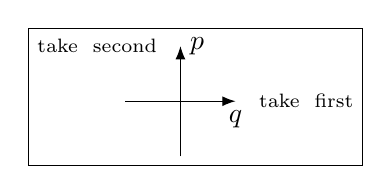
\begin{tikzpicture}[scale=0.7, baseline=(O)]
			\draw[-Latex] (0, -1) -- (0, 1) node[right] {$p$} node[left=0.5em] {\scriptsize\text{take $\Hm$ second}};
			\draw[-Latex] (-1, 0) -- (1, 0) node[below] {$q$} node[right=0.5em] {\scriptsize\text{take $\Hm$ first}};
			\coordinate (O) at (0, -0.3);
			\draw (current bounding box.north west) rectangle ([yshift=-1ex] current bounding box.south east);
		\end{tikzpicture}
		= (\mathrm{R}^p F)\left( \Hm^q(X)\right) \\
		& \Rightarrow \mathrm{R}^{p+q}F(X) , \quad p, q \in \Z.
	\end{align*}
\end{example}

% segment-id: o014.li2.chapter5.bicomplex-spectral-sequences-applications.p007
The Grothendieck spectral sequence introduced below concerns deriving a
composition of functors. It encompasses a large class of spectral sequences
in geometry and algebra, and its argument, like that in
Example~\ref{eg:hyperderived-ss}, is also based on a Cartan--Eilenberg
resolution.

% segment-id: o014.li2.chapter5.bicomplex-spectral-sequences-applications.th002
\begin{theorem}[Grothendieck spectral sequence]
\label{prop:Grothendieck-ss}
% segment-id: o014.li2.chapter5.bicomplex-spectral-sequences-applications.x004
	\index{spectral sequence!Grothendieck}
	Consider additive functors between Abelian categories
% segment-id: o014.li2.chapter5.bicomplex-spectral-sequences-applications.q010
	\[ \mathcal{A} \xrightarrow{F} \mathcal{A}' \xrightarrow{F'} \mathcal{A}''. \]
	Suppose both are left-exact (or right-exact) functors, $\mathcal{A}$ and
	$\mathcal{A}'$ have enough injective objects (or projective objects), and
	$F$ sends injective objects (or projective objects) to $F'$-acyclic objects
	in the sense of Convention~\ref{con:F-acyclic}. Then for every
	$X\in\Obj(\mathcal{A})$ there is a first-quadrant cohomological (or
	homological) bigraded spectral sequence
% segment-id: o014.li2.chapter5.bicomplex-spectral-sequences-applications.q011
	\begin{align*}
		E_2^{p,q} = (\mathrm{R}^p F') (\mathrm{R}^q F)(X) & \Rightarrow \mathrm{R}^{p+q} (F'F)(X), \\
		\text{or} \quad E^2_{p,q} = (\mathrm{L}_p F') (\mathrm{L}_q F)(X) & \Rightarrow \mathrm{L}_{p+q}(F'F)(X).
	\end{align*}
	Its convergence properties are as in Theorem~\ref{prop:tot-ss}. The
	corresponding exact sequences of low-degree terms
	(Corollary~\ref{prop:low-degree-ss}) can respectively be written as
% segment-id: o014.li2.chapter5.bicomplex-spectral-sequences-applications.q012
	\begin{equation*}\begin{split}
		0 \to (\mathrm{R}^1 F')(FX) & \to \mathrm{R}^1(F'F)(X) \\
		& \to F'\left( (\mathrm{R}^1 F)X \right) \to (\mathrm{R}^2 F')(FX) \to \mathrm{R}^2(F'F)(X),
	\end{split}\end{equation*}
	or
% segment-id: o014.li2.chapter5.bicomplex-spectral-sequences-applications.q013
	\begin{equation*}\begin{split}
		\mathrm{L}_2(F'F)(X) \to (\mathrm{L}_2 F')(FX) & \to F'\left( (\mathrm{L}_1 F)X \right) \\
		& \to \mathrm{L}_1(F'F)(X) \to (\mathrm{L}_1 F')(FX) \to 0.
	\end{split}\end{equation*}
\end{theorem}
% segment-id: o014.li2.chapter5.bicomplex-spectral-sequences-applications.pf003
\begin{proof}
	By duality, it suffices to discuss the cohomological case. Take an injective
	resolution $0\to X\to I^0\to I^1\to\cdots$ of $X$ and define $I^n:=0$ for
	$n<0$. In $\mathcal{A}'$, take a Cartan--Eilenberg resolution
	$\cate{C}F(I)\to J$ of $\cate{C}F(I):=(FI^p)_p$
	(Theorem~\ref{prop:CE-resolution}), and then consider the first-quadrant
	bicomplex $\cate{C}^2F'(J)=(F'(J^{p,q}))_{p,q}$ and its corresponding
	convergent spectral sequences $\mathscr{E}_{\mathrm{I}}$ and
	$\mathscr{E}_{\mathrm{II}}$. First,
% segment-id: o014.li2.chapter5.bicomplex-spectral-sequences-applications.g002
	\begin{align*}
		E_{\mathrm{I},2}^{p, q} & =
		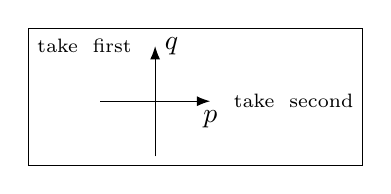
\begin{tikzpicture}[scale=0.7, baseline=(O)]
			\draw[-Latex] (0, -1) -- (0, 1) node[right] {$q$} node[left=0.5em] {\scriptsize\text{take $\Hm$ first}};
			\draw[-Latex] (-1, 0) -- (1, 0) node[below] {$p$} node[right=0.5em] {\scriptsize\text{take $\Hm$ second}};
			\coordinate (O) at (0, -0.3);
			\draw (current bounding box.north west) rectangle ([yshift=-1ex] current bounding box.south east);
		\end{tikzpicture} \\
		& = \Hm^p\left[ \cdots \to (\mathrm{R}^q F')(FI^p) \to (\mathrm{R}^q F')(FI^{p+1}) \to \cdots \right] \\
		& \Rightarrow \Hm^{p+q}\tot\left(\cate{C}^2 F'(J)\right).
	\end{align*}

	Since $F(I^p)$ is $F'$-acyclic by hypothesis,
	$E_{\mathrm{I},2}^{p,q}=0$ when $q\neq0$. The same argument as in
	Example~\ref{eg:bifunctor-ss} then shows that
	$\mathscr{E}_{\mathrm{I}}$ degenerates at the $E_2$ page, and
% segment-id: o014.li2.chapter5.bicomplex-spectral-sequences-applications.q014
	\[ E_{\mathrm{I}, \infty}^{p,q} = E_{\mathrm{I}, 2}^{p,q} = \begin{cases}
		\Hm^p\left( F'F(I^\bullet) \right) = \mathrm{R}^p (F' F)(X), & q = 0, \\
		0, & q \neq 0,
	\end{cases}\]
	while
	$\Hm^p\tot\left(\cate{C}^2F'(J)\right)
	=E_{\mathrm{I},\infty}^{p,0}=\mathrm{R}^p(F'F)(X)$.

	Now consider $\mathscr{E}_{\mathrm{II}}$. The technique is similar to that
	in Example~\ref{eg:hyperderived-ss}: the $q$-th column of horizontal
	cohomology, $\Hm_{\mathrm{I}}(J)^{q,\bullet}$, gives an injective resolution
	of $\Hm^q(\cate{C}F(I))=(\mathrm{R}^qF)(X)$. Recalling also that $F'$
	preserves horizontal cohomology, we obtain
% segment-id: o014.li2.chapter5.bicomplex-spectral-sequences-applications.g003
	\begin{align*}
		E_{\mathrm{II},2}^{p, q} & =
		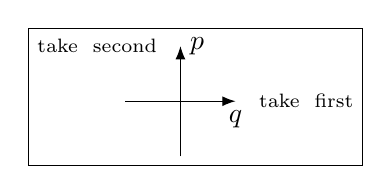
\begin{tikzpicture}[scale=0.7, baseline=(O)]
			\draw[-Latex] (0, -1) -- (0, 1) node[right] {$p$} node[left=0.5em] {\scriptsize\text{take $\Hm$ second}};
			\draw[-Latex] (-1, 0) -- (1, 0) node[below] {$q$} node[right=0.5em] {\scriptsize\text{take $\Hm$ first}};
			\coordinate (O) at (0, -0.3);
			\draw (current bounding box.north west) rectangle ([yshift=-1ex] current bounding box.south east);
		\end{tikzpicture}
		= (\mathrm{R}^p F')(\mathrm{R}^q F)\left( X \right) \\
		& \Rightarrow \Hm^{p+q}\tot\left(\cate{C}^2 F'(J)\right) = \mathrm{R}^{p+q}(F'F)(X).
	\end{align*}

	Thus $\mathscr{E}_{\mathrm{II}}$ is the spectral sequence required in the
	first part. Substituting the description of
	$E_{\mathrm{II},2}^{p,q}$ into the low-degree exact sequence of
	$\mathscr{E}_{\mathrm{II}}$ (Corollary~\ref{prop:low-degree-ss}) gives the
	assertion in the final part immediately.
\end{proof}

% segment-id: o014.li2.chapter5.bicomplex-spectral-sequences-applications.p008
The Grothendieck spectral sequence can be regarded as a concrete version of
Theorem~\ref{prop:derived-composite}, but the information it contains is more
explicit than an isomorphism in the derived category. We shall give an
application in \S\ref{sec:LHS-SS}.

% segment-id: o014.li2.chapter5.bicomplex-spectral-sequences-applications.ex004
\begin{example}[Change of rings]\label{eg:change-of-rings-SS}
% segment-id: o014.li2.chapter5.bicomplex-spectral-sequences-applications.x005
	\index{change of rings}
% segment-id: o014.li2.chapter5.bicomplex-spectral-sequences-applications.x006
	\index{spectral sequence!change of rings}
	Let $R\to S$ be a ring homomorphism. Let $X$ be a right $S$-module and
	$Y$ a left $R$-module. Write $S_R$ (or $X_R$) for $S$ (or $X$) regarded as
	a right $R$-module. We claim that there is a first-quadrant homological
	bigraded spectral sequence
% segment-id: o014.li2.chapter5.bicomplex-spectral-sequences-applications.q015
	\begin{gather*}
		E^2_{p,q} = \Tor^S_p\left( X, \Tor^R_q(S_R, Y) \right) \Rightarrow \Tor^R_{p+q}(X_R, Y);
	\end{gather*}
	Here $\Tor^R_q(S_R,Y)$ is given its left $S$-module structure as in
	Remark~\ref{rem:ExtTor-bimodule}. This is a direct application of
	Theorem~\ref{prop:Grothendieck-ss}, arising from the isomorphism of functors
% segment-id: o014.li2.chapter5.bicomplex-spectral-sequences-applications.q016
	\[ X \dotimes{S} \left( S \dotimes{R} (\cdot) \right) \simeq X \dotimes{R} (\cdot) : R\dcate{Mod} \to \cate{Ab}, \]
	where the inner functor
	$S\dotimes{R}(\cdot):R\dcate{Mod}\to S\dcate{Mod}$ has left-derived
	functors $\Tor^R_\bullet(S_R,\cdot)$ taking values in $S\dcate{Mod}$.
	By the isomorphism above, the inner functor sends flat modules to flat
	modules, so the homological version of the Grothendieck spectral sequence
	indeed applies.

	With entirely analogous notation and techniques, for a right $R$-module
	$X$ and a left $S$-module $Y$, one also has
% segment-id: o014.li2.chapter5.bicomplex-spectral-sequences-applications.q017
	\[ E^2_{p,q} = \Tor^S_p\left( \Tor^R_q(X, {}_R S), Y \right) \Rightarrow \Tor^R_{p+q}(X, {}_R Y). \]

	Next consider the $\Ext$ functor. Let $X$ be a left $S$-module and $Y$ a
	left $R$-module, and write ${}_RX$ for $X$ regarded as a left $R$-module.
	Give $\Ext_R^q({}_RS,Y)$ its left $S$-module structure as in
	Remark~\ref{rem:ExtTor-bimodule}. Then there are first-quadrant
	cohomological bigraded spectral sequences
% segment-id: o014.li2.chapter5.bicomplex-spectral-sequences-applications.q018
	\begin{align*}
		E_2^{p,q} = \Ext_S^p\left( X, \Ext_R^q({}_R S, Y) \right) & \Rightarrow \Ext_R^{p+q}({}_R X, Y), \\
		E_2^{p,q} = \Ext_S^p\left( \Tor^R_q(S_R, Y), X \right) & \Rightarrow \Ext_R^{p+q}(Y, {}_R X).
	\end{align*}
	They correspond respectively to the following isomorphisms of composite
	functors:
% segment-id: o014.li2.chapter5.bicomplex-spectral-sequences-applications.q019
	\begin{gather*}
		\Hom_S\left( X, \Hom_R({}_R S, \cdot) \right) \simeq \Hom_R({}_R X, \cdot), \\
		\Hom_S\left( S \dotimes{R} (\cdot), X \right) \simeq \Hom_R(\cdot, {}_R X),
	\end{gather*}
	the adjunctions introduced in \cite[Corollary 6.6.8]{Li1}. Mixing the
	right-derived functors $\Ext_S^p$ and the left-derived functors
	$\Tor^R_q$ in the second line causes no problem, because the first variable
	of $\Hom_S$ lies in the opposite category $S\dcate{Mod}^{\opp}$.
\end{example}

% segment-id: o014.li2.chapter5.bicomplex-spectral-sequences-applications.p009
The spectral sequences above should be compared with the derived-category
versions in \S\ref{sec:otimesL}.

% segment-id: o014.li2.chapter5.bicomplex-spectral-sequences-applications.ex005
\begin{example}\label{eg:change-of-rings-SS-bis}
% segment-id: o014.li2.chapter5.bicomplex-spectral-sequences-applications.x007
\index{universal coefficient theorem}
	For the spectral sequence
	$E_2^{p,q}=\Ext_S^p\left(\Tor^R_q(S_R,Y),X\right)
	\Rightarrow\Ext_R^{p+q}(Y,{}_RX)$ from
	Example~\ref{eg:change-of-rings-SS}, we record a useful special case, also
	as an exercise. Suppose the global dimension of $S\dcate{Mod}$ is at most
	$1$ (Definition--Proposition~\ref{def:global-dim}). Consequently, the
	nonzero terms $E_2^{p,q}$ are concentrated in the region $p=0,1$. Thus, for
	$n\geq0$, the decreasing filtration $\mathrm{F}^\bullet$ on
	$\Ext_R^n(Y,{}_RX)$ must have the form
% segment-id: o014.li2.chapter5.bicomplex-spectral-sequences-applications.q020
	\[ \Ext_R^n(Y, {}_R X) = \mathrm{F}^0 \underbracket{\supset}_{E_\infty^{0, n}} \mathrm{F}^1 \underbracket{\supset}_{E_\infty^{1, n-1}} \mathrm{F}^2 = \{0\}. \]

	Moreover, Example~\ref{eg:SS-finite-width} shows that the spectral sequence
	degenerates at the $E_2$ page, so
	$E_2^{p,q}\simeq E_\infty^{p,q}$. Combining these facts gives the short
	exact sequence
% segment-id: o014.li2.chapter5.bicomplex-spectral-sequences-applications.q021
	\[ 0 \to \Ext_S^1\left( \Tor^R_{n-1}(S_R, Y), X \right) \to \Ext_R^n(Y, {}_R X) \to \Hom_S\left( \Tor^R_n(S_R, Y), X \right) \to 0; \]
	by convention $\Tor^R_{-1}=0$. This may be regarded as a variant of the
	universal coefficient theorem.

	Similarly, suppose the right $S$-module $X$ has $\Tor$-dimension at most
	$1$ (Example~\ref{eg:Tor-dimension}). The spectral sequence
	$E^2_{p,q}=\Tor^S_p(X,\Tor^R_q(S_R,Y))
	\Rightarrow\Tor^R_{p+q}(X_R,Y)$ degenerates at the $E^2$ page. Examining
	the corresponding increasing filtration on $\Tor^R_n(X_R,Y)$ gives the
	short exact sequence
% segment-id: o014.li2.chapter5.bicomplex-spectral-sequences-applications.q022
	\[ 0 \to X \dotimes{S} \Tor^R_n(S_R, Y) \to \Tor^R_n(X_R, Y) \to \Tor^S_1(X, \Tor^R_{n-1}(S_R, Y)) \to 0. \]

	If $S$ is a principal ideal domain, both the global-dimension and
	$\Tor$-dimension hypotheses hold automatically.
\end{example}

% Unit 070 English translation of chapter5.tex lines 955--1063.
% Source: Methods of Algebra, Volume 2, commit
% 9a5803ff77dd3257484cb177f851a73770a59dd3 (CC BY 4.0).
% stable-unit-id: o014.aljabr2.chapter5.multiplicative-structures
% Coverage: Complete Section 5.7, before the exercises.

% segment-id: o014.li2.chapter5.multiplicative-structures.h001
\section{A glimpse of multiplicative structures}\label{sec:multiplicative-SS}
\hypertarget{o014.aljabr2.chapter5.multiplicative-structures}{ }

% segment-id: o014.li2.chapter5.multiplicative-structures.p001
For simplicity and concreteness, in this section we take a commutative ring
$\Bbbk$ and $\mathcal{A}=\Bbbk\dcate{Mod}$; this suffices for the classical
applications. We refer to $\Bbbk$-modules simply as modules and to
$\Bbbk$-algebras simply as algebras, and write
$\otimes:=\otimes_{\Bbbk}$.

% segment-id: o014.li2.chapter5.multiplicative-structures.p002
Let $I$ be a commutative monoid, with its binary operation written additively.
The definitions from \cite[\S 7.4]{Li1} may be summarized as follows:
\begin{itemize}
	\item an $I$-graded module is a module with a direct-sum decomposition
	$M=\bigoplus_{i\in I}M^i$; elements of $M^i$ are called homogeneous
	elements of degree $i$;
	\item an $I$-graded algebra is a graded module equipped with a homomorphism
	$\mu:A\otimes A\to A$, also written as a multiplication
	$xy:=\mu(x\otimes y)$, such that $A$ becomes a ring and
	\[ 1_A\in A^0,\qquad A^i\cdot A^j\subset A^{i+j},
	\qquad i,j\in I; \]
	thus the multiplication $\mu$ is completely determined by the data
	$\mu^{i,j}:A^i\otimes A^j\to A^{i+j}$;
	\item homomorphisms and isomorphisms between $I$-graded modules or algebras
	are defined in the usual way; $I$-graded subalgebras and ideals are defined
	similarly.
\end{itemize}

% segment-id: o014.li2.chapter5.multiplicative-structures.p003
For $k\in I$, also define a homomorphism of degree $k$ between $I$-graded
modules: this is a module homomorphism $\varphi:M\to N$ satisfying
$\varphi(M^i)\subset M^{i+k}$ for every $i$, and it is determined by the data
$(\varphi^i:M^i\to M^{i+k})_{i\in I}$. Taking $k=0$ recovers homomorphisms in
the usual sense. Degrees of homomorphisms add under composition.

% segment-id: o014.li2.chapter5.multiplicative-structures.d001
\begin{definition}\label{def:dg-algebra-preview}
	\index{differential graded algebra}
	Let $I$ be a commutative monoid equipped with a homomorphism
	$\epsilon:I\to\Z/2\Z$. A \emph{differential $I$-graded algebra} whose
	differential has degree $k$ is an $I$-graded algebra
	$A=\bigoplus_{p\in I}A^p$ together with an endomorphism of degree $k\in I$,
	$d=(d^p)_p:A\to A$, satisfying $d^2=0$ and the Leibniz rule
	\[ d(xy)=(dx)\cdot y+(-1)^{\epsilon(p)}x\cdot dy,
	\qquad x\in A^p,\quad y\in A^{p'},\quad p,p'\in I. \]
\end{definition}

% segment-id: o014.li2.chapter5.multiplicative-structures.p004
Observe that $d(1_A)=d(1_A\cdot1_A)=d(1_A)+d(1_A)$, hence $d(1_A)=0$.
Clearly $\Ker(d)$ is an $I$-graded subalgebra of $A$, while $\Image(d)$ is a
two-sided $I$-graded ideal in $\Ker(d)$. Therefore
\[ \Hm(A,d):=\Ker(d)/\Image(d) \]
is again an $I$-graded algebra.

% segment-id: o014.li2.chapter5.multiplicative-structures.e001
\begin{example}
	Take $I=\Z$ and $\epsilon(p)=p\;\bmod 2$. For any complex $X$ over a
	$\Bbbk$-linear category $\mathcal{B}$, the $\Hom$ complex
	$\Hom^\bullet(X,X)$ of Definition~\ref{def:Hom-cplx}, together with
	$d=d_{\Hom^\bullet(X,X)}$, becomes a differential $\Z$-graded algebra
	whose differential has degree $1$. These assertions are essentially the
	content of Lemma~\ref{prop:Hom-cplx-Leibniz}. We have
	\[ \Hm(\Hom^\bullet(X,X),d)=
	\bigoplus_{n\in\Z}\Hom_{\cate{K}(\mathcal{B})}(X,X[n]), \]
	with multiplication induced by composition of morphisms in
	$\cate{K}(\mathcal{B})$.
\end{example}

% segment-id: o014.li2.chapter5.multiplicative-structures.e002
\begin{example}
	Take $\Bbbk=\CC$, $I=\Z$, and $\epsilon(p)=p\;\bmod2$. The
	$\CC$-valued differential forms of degree $p$ on a smooth manifold
	$\mathfrak{X}$ form a vector space $A^p(\mathfrak{X})$. Set
	$A(\mathfrak{X}):=\bigoplus_{p=0}^{\dim X}A^p(\mathfrak{X})$. With
	multiplication $\mu(\omega\otimes\eta):=\omega\wedge\eta$ and exterior
	differentiation $\dd$, this becomes a differential $\Z$-graded algebra
	whose differential has degree $1$. The associated algebra
	$\Hm(A(\mathfrak{X}),\dd)=\bigoplus_p\Hm^p_{\mathrm{dR}}(\mathfrak{X})$
	is precisely the de Rham cohomology of $\mathfrak{X}$; the multiplication
	induced by $\wedge$ gives it a graded-algebra structure. This is a
	fundamental object in topology and is isomorphic as a graded algebra to the
	singular cohomology ring of $\mathfrak{X}$.

	The multiplication on $\Hm(A(\mathfrak{X}),\dd)$ also satisfies
	$xy=(-1)^{pq}yx$, where $x$ and $y$ are homogeneous elements of degrees
	$p$ and $q$, respectively, because the multiplication on
	$A(\mathfrak{X})$ already has this property. As a simple and beautiful
	example, complex projective space $\mathfrak{X}:=\mathbb{P}^n(\CC)$ gives
	the graded algebra
	$\Hm(A(\mathfrak{X}),\dd)\simeq\CC[t]/(t^{n+1})$, where the variable $t$
	corresponds to a homogeneous element of degree $2$.
\end{example}

% segment-id: o014.li2.chapter5.multiplicative-structures.p005
Returning to our main subject, in this section we consider the following
cases:
\begin{center}\begin{tabular}{|c|c|c|} \hline
	Abbreviation & $I$ & $\epsilon:I\to\Z/2\Z$ \\ \hline
	Singly graded & $\Z$ & $\epsilon(p)=p\;\bmod2$ \\
	Bigraded & $\Z^2$ & $\epsilon(p,q)=p+q\;\bmod2$ \\ \hline
\end{tabular}\end{center}

% segment-id: o014.li2.chapter5.multiplicative-structures.p006
This theory overlaps with Definition~\ref{def:differential-object}, but the
focus of this section is the multiplication, which was not mentioned there.

% segment-id: o014.li2.chapter5.multiplicative-structures.p007
To lighten the notation, below we collectively call these various cases
``graded'', distinguishing them mainly by the superscript $p$ or $(p,q)$.
Likewise, we refer collectively to differential $I$-graded algebras as
differential graded algebras.

% segment-id: o014.li2.chapter5.multiplicative-structures.c001
\begin{convention}
	For a cohomological bigraded spectral sequence $\mathscr{E}$ in the case
	$\mathcal{A}=\Bbbk\dcate{Mod}$, we identify every page $E_r$ with the
	graded module $\bigoplus_{p,q}E_r^{p,q}$ and regard
	$d_r=(d_r^{p,q})_{p,q}$ as an endomorphism of degree $(r,-r+1)$ of the
	graded module $E_r$. The homological and singly graded cases are treated
	similarly.
\end{convention}

% segment-id: o014.li2.chapter5.multiplicative-structures.p008
In short, a spectral sequence with a multiplicative structure is a spectral
sequence consisting of differential graded algebras.

% segment-id: o014.li2.chapter5.multiplicative-structures.d002
\begin{definition}\label{def:mult-ss}
	\index{spectral sequence!multiplicative structure}
	A \emph{multiplicative structure} on a cohomological bigraded spectral
	sequence $\mathscr{E}$ is a family of homomorphisms
	$\mu_r:E_r\otimes E_r\to E_r$ (that is, ``multiplications'') such that
	\begin{itemize}
		\item every $(E_r,\mu_r,d_r)$ is a differential graded algebra whose
		differential has degree $(r,-r+1)$;
		\item the map $t_{r+1}:\Hm(E_r,d_r)\rightiso E_{r+1}$ in the spectral
		sequence data is an isomorphism of graded algebras.
	\end{itemize}
	Multiplicative structures on singly graded or homological spectral sequences
	are defined similarly.
\end{definition}

% segment-id: o014.li2.chapter5.multiplicative-structures.p009
The preceding discussion shows that $Z_r=\Ker(d_r)$ is a graded subalgebra of
$E_r$, while $B_r=\Image(d_r)$ is a two-sided graded ideal of $Z_r$. Hence
$\Hm(E_r,d_r)$ becomes a graded algebra; this is the precise meaning of
Definition~\ref{def:mult-ss}.

% segment-id: o014.li2.chapter5.multiplicative-structures.p010
Furthermore, if the limit exists, then
$Z_\infty=\bigoplus_{p,q}Z_\infty^{p,q}$ is also a graded subalgebra, with
$B_\infty=\bigoplus_{p,q}B_\infty^{p,q}$ as its graded ideal. Thus
$E_\infty$ is also a graded algebra.

% segment-id: o014.li2.chapter5.multiplicative-structures.p011
\index{dg-algebra}
As an example, consider differential graded algebras whose differential has
degree $1$, abbreviated as dg-algebras. Expanding the definition, this is
equivalent to a complex of $\Bbbk$-modules
$X=(X^n,d_X^n)_{n\in\Z}$ such that
$X\xlongequal{\text{identified}}\bigoplus_nX^n$ is equipped with a
multiplication $\mu:X\otimes X\to X$ satisfying
$X^p\cdot X^{p'}\subset X^{p+p'}$ and the Leibniz rule
\[ d(xy)=dx\cdot y+(-1)^px\cdot dy,
	\qquad x\in X^p,\quad y\in X^{p'}. \]
Now suppose the data $(X,d)$ are extended to a filtered complex
$(X,d,\mathrm{F}^\bullet X)$. Recall that this already entails
$d(\mathrm{F}^pX)\subset\mathrm{F}^pX$; we further require the multiplication
on $X$ to be compatible with the filtration:
\[ \mathrm{F}^pX^n\cdot\mathrm{F}^{p'}X^{n'}
	\subset\mathrm{F}^{p+p'}X^{n+n'}. \]
In this case $(X,d,\mu,\mathrm{F}^\bullet X)$ is called a filtered
differential graded algebra. For the induced filtration on $\Hm(X,d)$, the
condition above ensures that
\[ \gr\Hm(X,d)\xlongequal{\text{identified}}
	\bigoplus_{(p,q)\in\Z^2}\gr^p\Hm^{p+q}(X,d) \]
naturally becomes a graded algebra.
\index{differential graded algebra!filtered}

% segment-id: o014.li2.chapter5.multiplicative-structures.t001
\begin{proposition}\label{prop:dga-mult-ss}
	Let $(X,d,\mu,\mathrm{F}^\bullet X)$ be a filtered differential graded
	algebra whose differential has degree $1$.
	\begin{enumerate}[(i)]
		\item The spectral sequence $\mathscr{E}$ of the filtered complex
		$(X,d,\mathrm{F}^\bullet X)$ has a canonical multiplicative structure.
		\item The isomorphisms
		$E_\infty^{p,q}\simeq\gr^p\Hm^{p+q}(X,d)$ in the classical convergence
		theorem~\ref{prop:classical-convergence} in fact give an isomorphism of
		graded algebras $E_\infty\simeq\gr\Hm(X,d)$.
	\end{enumerate}
\end{proposition}
\begin{proof}
	Take $x\in E_r^{p,q}$ and $y\in E_r^{p',q'}$. By the description in
	Proposition~\ref{prop:filtered-cplx-ss}, choose lifts
	\begin{gather*}
		\widetilde{x}\in\mathrm{F}^pX^{p+q}\cap
		d^{-1}\left(\mathrm{F}^{p+r}X^{p+q+1}\right),\qquad
		\widetilde{y}\in\mathrm{F}^{p'}X^{p'+q'}\cap
		d^{-1}\left(\mathrm{F}^{p'+r}X^{p'+q'+1}\right).
	\end{gather*}
	By definition,
	\begin{gather*}
		\widetilde{x}\widetilde{y}\in
		\mathrm{F}^{p+p'}X^{p+q+p'+q'},\\
		d(\widetilde{x}\widetilde{y})
		=d\widetilde{x}\cdot\widetilde{y}
		+(-1)^{p+q}\widetilde{x}\cdot d\widetilde{y}
		\in\mathrm{F}^{p+p'+r}X^{p+q+p'+q'+1}.
	\end{gather*}
	Thus $\widetilde{x}\widetilde{y}$ determines an element
	$xy\in E_r^{p+p',q+q'}$. A routine calculation (please verify it) shows
	that $xy$ depends only on $x$ and $y$.

	Next, $d_r:E_r\xrightarrow{(r,-r+1)}E_r$ is induced by the differential
	$d$ on $X$. This gives $E_r$ the structure of a differential graded
	algebra; associativity, the Leibniz rule, and all other required properties
	reduce to checks on $(X,d)$. The same argument shows that
	$\Hm(E_r,d_r)\simeq E_{r+1}$ is an isomorphism of graded algebras.

	The assertion that the canonical isomorphisms
	$E_\infty^{p,q}\simeq\gr^p\Hm^{p+q}(X,d)$ in the classical convergence
	theorem preserve multiplication likewise reduces to a check on $X$, so we
	omit the details.
\end{proof}

% segment-id: o014.li2.chapter5.multiplicative-structures.r001
\begin{remark}
	\index{Cartan--Eilenberg system}
	Multiplicative structures are an indispensable tool in topology. Algebraic
	topology without multiplication is almost unimaginable, or at least
	insipid. Historically, when Leray first encountered spectral sequences, he
	already considered multiplicative structures, calling them ``spectral
	rings''. They often greatly simplify spectral-sequence calculations in
	topology. This is why the present section gives a brief introduction to
	multiplicative structures, though it only scratches the surface.

	There is an evident difficulty in applying Definition~\ref{def:mult-ss}.
	The differential graded algebra structures on all the $E_r$ must be given
	at once, since the definition alone provides no reason for the
	multiplication on one page to induce a multiplication on the next. This can
	indeed be done in some situations, as in
	Proposition~\ref{prop:dga-mult-ss}.

	For general cases, or for those that are difficult to compute by hand,
	spectral sequences are often constructed from simple data, such as the exact
	couples of \S\ref{sec:exact-couples}. It is therefore natural to ask whether
	there are simple conditions on an exact couple ensuring that the corresponding
	spectral sequence has a multiplicative structure.

	The answer appears to be negative: information beyond the exact couple is
	required. One useful construction is the equally classical
	\emph{Cartan--Eilenberg system}, together with its spectral product; see
	\cite[II.A]{Dou58}. As an application, the Serre--Atiyah--Hirzebruch
	spectral sequence, which is of central importance in topology, has a
	multiplicative structure for every multiplicative generalized cohomology
	theory. Since this material departs from our main line, we stop here.
\end{remark}

% Unit 071 English translation of chapter5.tex lines 1066--1148.
% Source: Methods of Algebra, Volume 2, commit
% 9a5803ff77dd3257484cb177f851a73770a59dd3 (CC BY 4.0).
% stable-unit-id: o014.aljabr2.chapter5.exercises
% Coverage: All Chapter 5 exercises.

% segment-id: o014.li2.chapter5.exercises.h001
\begin{Exercises}
	% segment-id: o014.li2.chapter5.exercises.ex001
	\item For an Abelian category $\mathcal{A}$, verify the following
	properties of the category of filtered objects
	$\mathrm{Fil}^\bullet(\mathcal{A})$.
	\begin{enumerate}[(i)]
		\item It is an additive category, and every morphism has a kernel,
		cokernel, image, and coimage. Describe them as concretely as possible.
		\item For a morphism $f:X\to Y$ in
		$\mathrm{Fil}^\bullet(\mathcal{A})$, if
		$f(\mathrm{F}^nX)\to f(X)\cap\mathrm{F}^nY$ is an isomorphism for
		every $n$, then $f$ is called a strict morphism. Prove that this notion
		is equivalent to the version in Definition~\ref{def:strict-morphism}.

		\begin{hint}
			This is equivalent to saying that the two natural filtrations on
			$f(X)$ coincide: one is the image of $\mathrm{F}^\bullet X$, and
			the other is the restriction of $\mathrm{F}^\bullet Y$. The former
			corresponds to $\Coim(f)$ in
			$\mathrm{Fil}^\bullet(\mathcal{A})$, and the latter to $\Image(f)$.
		\end{hint}
		\item Give an example showing that
		$\mathrm{Fil}^\bullet(\mathcal{A})$ is not an Abelian category in
		general.
	\end{enumerate}
	Although filtered objects do not form an Abelian category, geometry still
	requires the filtered derived category $\cate{DF}(\mathcal{A})$ in the
	case of finite filtrations. Its definition requires rather deeper
	techniques; see \cite[Tag 05RX]{stacks}.
	\index{derived category!filtered}

	% segment-id: o014.li2.chapter5.exercises.ex002
	\item For a filtered differential object
	$(X,d,\mathrm{F}^\bullet X)$ over an Abelian category $\mathcal{A}$,
	prove that $d_1^p:E_1^p\to E_1^{p+1}$ in the spectral sequence is the
	connecting morphism induced by the short exact sequence of differential
	objects
	\[ 0\to\gr^{p+1}X\to\mathrm{F}^pX/\mathrm{F}^{p+2}X
	\to\gr^pX\to0. \]

	% segment-id: o014.li2.chapter5.exercises.ex003
	\item (Bockstein spectral sequence) Let $f$ be a non-zero-divisor in a
	commutative ring $R$. For every $R$-module $M$, define
	$M[f]:=\{m\in M:fm=0\}$; call $M$ \emph{$f$-torsion-free} if
	$M[f]=\{0\}$. Let $C$ be a chain complex and suppose every $C_n$ is
	$f$-torsion-free. Multiplication by $f$ gives a monomorphism of chain
	complexes $\alpha:C\to C$. For the data $(C,\alpha)$,
	Proposition~\ref{prop:differential-exact-couple} gives the exact couple
	\[\begin{tikzcd}[column sep=tiny]
		\Hm_\bullet(C) \arrow[rr, "{\Hm_\bullet(\alpha)}"] & &
		\Hm_\bullet(C) \arrow[ld] \\
		& \Hm_\bullet\left(C\dotimes{R}R/(f)\right) \arrow[lu, "{-1}"] &
	\end{tikzcd}\]
	and the associated homologically graded spectral sequence
	$(E^r_q)_{\substack{r\geq0\\q\in\Z}}$. Describe every page
	$(E^r,d^r)$ and $E^\infty$ as explicitly as possible.
	\index{spectral sequence!Bockstein}

	% segment-id: o014.li2.chapter5.exercises.ex004
	\item In the preceding problem, take $R=\Z$ and $f=p$, with $p$ prime,
	and suppose every $C_n$ is a free $\Z$-module of finite rank. For every
	$\Z$-module $M$, write $M_{\mathrm{tor}}$ for the submodule of all its
	torsion elements and define its torsion-free quotient
	$M_{\mathrm{tf}}:=M/M_{\mathrm{tor}}$. Prove that
	\[ E^\infty_q\simeq\Hm_q(C)_{\mathrm{tf}}\dotimes{\Z}\F_p,
	\qquad q\in\Z. \]
	Deduce that
	\[ \dim_{\F_p}\Hm_q\left(C\dotimes{\Z}\F_p\right)
	\geq\dim_{\F_p}\left(\Hm_q(C)_{\mathrm{tf}}\dotimes{\Z}\F_p\right). \]
	Give an example in which the inequality is strict.

	% segment-id: o014.li2.chapter5.exercises.ex005
	\item (Two-column and two-row spectral sequences) Let a strongly
	convergent spectral sequence $E_2^{p,q}\Rightarrow H^{p+q}$ be given, in
	the sense of Convention~\ref{con:ss-conv}.
	\begin{enumerate}[(i)]
		\item Prove that if $E_2^{p,q}$ is nonzero only for
		$p\in\{0,1\}$, then for every $q\in\Z$ there is a canonical short
		exact sequence
		\[ 0\to E_2^{1,q-1}\to H^q\to E_2^{0,q}\to0. \]
		\item Prove that if $E_2^{p,q}$ is nonzero only for
		$q\in\{0,1\}$, then for every $p\in\Z$ there is a canonical exact
		sequence
		\[ \cdots\to H^{p-1}\to E_2^{p-2,1}\xrightarrow{d_2}E_2^{p,0}
		\to H^p\to E_2^{p-1,1}\xrightarrow{d_2}E_2^{p+1,0}
		\to H^{p+1}\to\cdots. \]
		\item Treat the version $E^2_{p,q}\Rightarrow H_{p+q}$.
		\begin{hint}
			Interchange superscripts and subscripts, reverse the arrows, and
			leave everything else unchanged.
		\end{hint}
	\end{enumerate}

	% segment-id: o014.li2.chapter5.exercises.ex006
	\item Consider left-exact functors $F'$ and $F$ satisfying the hypotheses
	of Theorem~\ref{prop:Grothendieck-ss}, and suppose in addition that
	$\mathrm{R}F'$ and $\mathrm{R}F$ are both of finite dimension.
	\begin{enumerate}[(i)]
		\item Prove that $F'F$ is also of finite dimension, and give an upper
		bound for its dimension.
		\item Consider the homomorphism
		$\chi_F:\mathrm{K}_0(\mathcal{A})\to\mathrm{K}_0(\mathcal{A}')$
		determined by the triangulated functor $\mathrm{R}F$, and the analogous
		homomorphisms $\chi_{F'}$, $\chi_{F'F}$ determined by
		$\mathrm{R}F'$, $\mathrm{R}(F'F)$; see the exercises in
		\CHref{sec:cplx}. Prove that
		$\chi_{F'F}=\chi_{F'}\circ\chi_F$.
	\end{enumerate}
	These properties can also be proved using derived categories. The case of
	right-exact functors and $\mathrm{L}F',\mathrm{L}F$ is of course dual.

	% segment-id: o014.li2.chapter5.exercises.ex007
	\item Let $\mathcal{A}$ be an Abelian category with enough injective
	objects, and let $X\in\Obj(\mathcal{A})$ carry a finite filtration
	$X=\mathrm{F}^0X\supset\cdots\supset\mathrm{F}^{N+1}X=0$. Let
	$G:\mathcal{A}\to\mathcal{A}'$ be a left-exact additive functor. Prove
	that there is a strongly convergent spectral sequence
	\[ E_1^{p,q}=\mathrm{R}^{p+q}G(\gr^pX)
	\Rightarrow\mathrm{R}^{p+q}G(X). \]
	% Reference: [Knapp-Vogan 1995, Proposition D.57]
	\begin{hint}
		One method is to imitate the construction of a Cartan--Eilenberg
		resolution (Theorem~\ref{prop:CE-resolution}, which uses
		Proposition~\ref{prop:horseshoe}). Starting from $\mathrm{F}^NX$, choose
		a suitable series of injective resolutions
		\[\begin{tikzcd}[row sep=small]
			\vdots & & \vdots \\
			\mathrm{F}^0I^1 \arrow[u]
			\arrow[phantom,r,"\supset" description] & \cdots
			\arrow[phantom,r,"\supset" description] & \mathrm{F}^NI^1 \arrow[u] \\
			\mathrm{F}^0I^0 \arrow[u]
			\arrow[phantom,r,"\supset" description] & \cdots
			\arrow[phantom,r,"\supset" description] & \mathrm{F}^NI^0 \arrow[u] \\
			\mathrm{F}^0X \arrow[u]
			\arrow[phantom,r,"\supset" description] & \cdots
			\arrow[phantom,r,"\supset" description] & \mathrm{F}^NX \arrow[u] \\
			0 \arrow[u] & & 0 \arrow[u]
		\end{tikzcd}\]
		such that applying $\cate{C}G$ to $\mathrm{F}^\bullet(I)$ still gives
		a filtered complex and the associated spectral sequence has the
		required form.
	\end{hint}

	% segment-id: o014.li2.chapter5.exercises.ex008
	\item Let $R$ be a ring, let $C=(C_n,d^C_n)_n$ be a chain complex of right
	$R$-modules, and let $D$ be a left $R$-module. Suppose every $C_n$ is flat
	and $n\ll0\implies C_n=0$. Take a projective resolution
	$\cdots\to P_1\to P_0\to D\to0$ and construct the bicomplex
	$C_\bullet\dotimes{R}P_\bullet$.
	\begin{enumerate}[(i)]
		\item Show that the associated homological bigraded spectral sequence
		$\mathscr{E}_{\mathrm{I}}$ degenerates at the
		$E_{\mathrm{I}}^2$ page.
		\item Show that
		$(E_{\mathrm{II}}^2)_{p,q}=\Tor^R_p(\Hm_q(C),D)
		\Rightarrow\Hm_{p+q}(C_\bullet\dotimes{R}D)$.
		\item Prove that if every $\Image(d^C_n)$ is flat, this gives the short
		exact sequence in the homological K\"unneth theorem
		\ref{prop:Kunneth-homology}.
		\begin{hint}
			The flat resolution
			$0\to\Image(d_C^{n+1})\to\Ker(d_C^n)\to\Hm_n(C)\to0$
			causes the nonzero terms of $E_{\mathrm{II}}^2$ to be concentrated
			at $p\in\{0,1\}$.
		\end{hint}
	\end{enumerate}

	% segment-id: o014.li2.chapter5.exercises.ex009
	\item Let $R,S$ be rings, let $X$ be a right $R$-module, $Y$ an
	$(R,S)$-bimodule, and $Z$ a left $S$-module. Construct a bicomplex such
	that the corresponding spectral sequences satisfy
	\[ (E_{\mathrm{I}}^2)_{p,q}
	=\Tor^R_p\left(X,\Tor^S_q(Y_S,Z)\right),\qquad
	(E_{\mathrm{II}}^2)_{p,q}
	=\Tor^S_p\left(\Tor^R_q(X,{}_RY),Z\right). \]
	\begin{hint}
		Take resolutions of $X$ and $Z$. Readers familiar with derived
		categories may compare this with
		Proposition~\ref{prop:otimesL-associativity-constraint} on the
		associativity constraint (take $A=\Bbbk=B$).
	\end{hint}

	% segment-id: o014.li2.chapter5.exercises.ex010
	\item Describe explicitly the canonical homomorphism
	$\Ext^n_R(Y,{}_RX)\to\Hom_S(\Tor^R_n(S_R,Y),X)$ in the short exact
	sequence of Example~\ref{eg:change-of-rings-SS-bis}.
\end{Exercises}


\part*{Advanced Part}
% Unit 072 English translation of chapter6.tex lines 1--320.
% Source: Methods of Algebra, Volume 2, commit
% 9a5803ff77dd3257484cb177f851a73770a59dd3 (CC BY 4.0).
% stable-unit-id: o014.aljabr2.chapter6.overview-g-modules-resolutions
% Coverage: Chapter 6 opening and complete Section 6.1 on G-modules and the
% standard and normalized free resolutions; stops before Section 6.2 at line 321.

% segment-id: o014.li2.chapter6.overview-g-modules-resolutions.h001
\chapter{Group Homology and Cohomology}\label{sec:group-coh}
\hypertarget{o014.aljabr2.chapter6.overview-g-modules-resolutions}{ }

% segment-id: o014.li2.chapter6.overview-g-modules-resolutions.p001
Let $G$ be a group and let $\Bbbk$ be a commutative ring. A $G$-module means
a $\Bbbk$-module equipped with a linear left action of $G$, written as left
multiplication; in many situations $\Bbbk$ is usually taken to be $\Z$. All
$G$-modules form an Abelian category $G\dcate{Mod}$, isomorphic to
$\Bbbk[G]\dcate{Mod}$, where $\Bbbk[G]$ is the group algebra of $G$. For a
$G$-module $M$, define the $\Bbbk$-modules
% segment-id: o014.li2.chapter6.overview-g-modules-resolutions.q001
\begin{align*}
	\text{invariants} \quad M^G & := \left\{x \in M: \forall g \in G, \; gx=x \right\}, \\
	\text{coinvariants} \quad M_G & := M / \lrangle{gx-x: g \in G, x \in M}.
\end{align*}

% segment-id: o014.li2.chapter6.overview-g-modules-resolutions.p002
From the algebraic point of view, the cohomology $\Hm^n(G,M)$ and homology
$\Hm_n(G,M)$ of a $G$-module $M$ are, respectively, the values at $M$ of the
right-derived functors of $(\cdot)^G$ and the left-derived functors of
$(\cdot)_G$, where $n\in\Z_{\geq0}$.

% segment-id: o014.li2.chapter6.overview-g-modules-resolutions.p003
Group homology and cohomology have a long history. Around 1935, W.\ Hurewicz
studied path-connected topological spaces $E$ whose higher homotopy groups
satisfy $n>1\implies\pi_n(E)=0$. He proved that their homology and cohomology
groups are completely determined by the fundamental group $\pi_1(E)$; this is
perhaps the earliest documented formulation of group cohomology. As
homological algebra advanced rapidly during the twentieth century, group
cohomology and homology soon acquired purely algebraic formulations and were
used to address problems within algebra itself. Today they are basic tools in
number theory, topology, and geometry.

% segment-id: o014.li2.chapter6.overview-g-modules-resolutions.p004
On the other hand, $\Hm^n(G,M)$ and $\Hm_n(G,M)$ can also be identified with
$\Ext^n(\Bbbk,M)$ and $\Tor_n(\Bbbk,M)$, respectively, in
$\Bbbk[G]\dcate{Mod}$, with $\Bbbk$ regarded as a trivial $G$-module.
Computing $\Ext$ and $\Tor$ from a projective resolution of $\Bbbk$ gives
another description of $\Hm^n(G,M)$ and $\Hm_n(G,M)$. In fact, we shall give
a canonical resolution $\mathsf{L}\to\Bbbk$ of $\Bbbk$ as a left (or right)
$\Bbbk[G]$-module. It yields the standard cochain complex
$(C^n(G,M))_n$ (or chain complex $(C_n(G,M))_n$) representing $\Hm^n(G,M)$
(or $\Hm_n(G,M)$); see Propositions~\ref{prop:groupcoh-cochain} and
\ref{prop:grouph-chain}. Later, \S\S\ref{sec:homology-computation}---
\ref{sec:bar-resolution} will interpret these canonical resolutions from the
viewpoint of simplicial theory.

% segment-id: o014.li2.chapter6.overview-g-modules-resolutions.p005
The preceding material constitutes the main content of
\S\S\ref{sec:G-mod}---\ref{sec:group-coh-sub}. This chapter adopts two
viewpoints at once: the classical theory of derived functors, especially
universal $\delta$-functors and their characterization, and derived categories.
The classical theory has the advantage of being operational, whereas derived
categories provide finer information than the individual cohomology or
homology groups and often offer a clearer line of thought. The standard
cochain or chain complexes provide the most detailed and canonical
information, since they operate at the level of complexes.

% segment-id: o014.li2.chapter6.overview-g-modules-resolutions.p006
In \S\ref{sec:grp-low-degree}, we shall give concrete interpretations of
$\Hm^1$ and $\Hm^2$: they correspond, respectively, to crossed homomorphisms
and equivalence classes of extensions of $G$ by an Abelian group. The precise
meaning of a group extension is given in Definition~\ref{def:group-ext}. In
fact, if all extensions of $G$ by $M$ are organized into a 2-category
$\cate{Ext}(G,M)$, then the truncation
$\tau^{\leq2}\overline{C}(G,M)$ of the normalized standard complex is exactly
a linear incarnation of $\cate{Ext}(G,M)$; this is the content of
Remark~\ref{rem:Ext-incarnation}.

% segment-id: o014.li2.chapter6.overview-g-modules-resolutions.p007
For any group homomorphism $\varphi:H\to G$ and any $G$-module $M$, its
pullback $\varphi^*M$ can be defined as an $H$-module. General constructions
from module theory give simple descriptions of both the right and left
adjoints of $\varphi^*$. When $\varphi$ is the inclusion of a subgroup,
$\varphi^*$ is called the restriction functor on $G$-modules and is also
written $\Res^G_H$, while its right (respectively left) adjoint is written
$\Ind^G_H$ (respectively $\iInd^G_H$); both are called induction functors.
Their properties are the subject of \S\ref{sec:induced-module}. In particular,
we shall prove the so-called Shapiro lemma (Theorem~\ref{prop:Shapiro}):
% segment-id: o014.li2.chapter6.overview-g-modules-resolutions.q002
\[ \Hm^n\left(G, \Ind^G_H(N)\right) \simeq \Hm^n(H, N), \quad \Hm_n\left(G, \iInd^G_H(N)\right) \simeq \Hm_n(H, N). \]

% segment-id: o014.li2.chapter6.overview-g-modules-resolutions.p008
Continuing the general discussion of $\varphi^*$,
\S\ref{sec:change-of-group} will define families of canonical homomorphisms
% segment-id: o014.li2.chapter6.overview-g-modules-resolutions.q003
\[ \Hm^n(G, M) \to \Hm^n(H, \varphi^* M), \quad \Hm_n(H, \varphi^* M) \to \Hm_n(G, M). \]
These homomorphisms can be combined with the functoriality of cohomology or
homology. Thus every equivariant homomorphism $f:M\to N$ (or $f:N\to M$)
induces the corresponding canonical homomorphism $\Hm^n(f)$ (or $\Hm_n(f)$),
where $M$ is a $G$-module and $N$ an $H$-module; see
Definition~\ref{def:change-of-group-equiv}. In the special case $n=2$,
\S\ref{sec:group-ext-revisited} will interpret these canonical homomorphisms
in terms of group extensions.

% segment-id: o014.li2.chapter6.overview-g-modules-resolutions.p009
For concrete illustrations, \S\ref{sec:coh-cyclic-free} discusses finite
cyclic groups and free groups. The arguments harmoniously combine techniques
from group theory and cohomology. The cohomological and homological dimensions
of groups (Definition~\ref{def:group-dim}) will also enter at the appropriate
point.

% segment-id: o014.li2.chapter6.overview-g-modules-resolutions.p010
The concrete flavor of group theory continues in
\S\ref{sec:group-finite-index}. When $(G:H)$ is finite, we shall state further
properties of the restriction and induction functors; indeed, in this case
$\Ind^G_H=\iInd^G_H$. Definition--Proposition~\ref{def:cor} will give
families of canonical homomorphisms
% segment-id: o014.li2.chapter6.overview-g-modules-resolutions.q004
\[ \mathrm{cor}^n: \Hm^n(H, M) \to \Hm^n(G, M), \quad \mathrm{cor}_n: \Hm_n(G, M) \to \Hm_n(H, M), \]
where $M$ is a $G$-module and $\Res^G_HM$ is abbreviated to $M$ to save
notation. These are called corestriction homomorphisms, and their direction is
opposite to that of the canonical homomorphisms induced by $H\hookrightarrow
G$ (namely restriction, written $\mathrm{res}^n$ and $\mathrm{res}_n$). They
satisfy the fundamental identities
$\mathrm{cor}^n\mathrm{res}^n=(G:H)$ and
$\mathrm{res}_n\mathrm{cor}_n=(G:H)$
(Proposition~\ref{prop:res-cor}), while the special case
$\mathrm{cor}_1:\Hm_1(G,\Z)\to\Hm_1(H,\Z)$ becomes the classical transfer
homomorphism in group theory,
$\mathrm{Ver}_{G|H}:G_{\mathrm{ab}}\to H_{\mathrm{ab}}$.

% segment-id: o014.li2.chapter6.overview-g-modules-resolutions.p011
Let $H$ be a normal subgroup of $G$ and let $M$ be a $G$-module. Then
$\Hm^q(H,M)$ and $\Hm_q(H,M)$ become $(G/H)$-modules. The
Lyndon--Hochschild--Serre spectral sequences discussed in \S\ref{sec:LHS-SS},
% segment-id: o014.li2.chapter6.overview-g-modules-resolutions.q005
\begin{align*}
	E_2^{p, q} = \Hm^p(G/H, \Hm^q(H, M)) & \Rightarrow \Hm^{p+q}(G, M), \\
	E^2_{p, q} = \Hm_p(G/H, \Hm_q(H, M)) & \Rightarrow \Hm_{p+q}(G, M),
\end{align*}
are indispensable advanced tools in the theory of group cohomology and
homology; see Theorem~\ref{prop:LHS-SS}. The information in the exact sequence
of their low-degree terms is extremely useful. The
Lyndon--Hochschild--Serre spectral sequence is at once an application of the
Grothendieck spectral sequence and the result of a canonical filtration on the
standard complex. The latter description gives finer information, such as the
multiplicative structure mentioned in Remark~\ref{rem:LHS-SS-mult}.

% segment-id: o014.li2.chapter6.overview-g-modules-resolutions.p012
More precisely, the multiplicative operation on group cohomology is the cup
product, which originates in topology. In \S\ref{sec:cup-product}, we shall
approach it from two viewpoints. First, the cup product is understood as a
natural reflection of the tensor-product operation on $G$-modules; the
language of derived categories is useful here. Second, its formula is written
directly at the level of the standard complex
(Definition--Proposition~\ref{def:group-cup-3}). The second description is, of
course, an explicit realization of the first. The key to deriving it is to
lift $\Bbbk\rightiso\Bbbk\otimes\Bbbk$ appropriately to a ``diagonal
embedding'' $\Delta:\mathsf{L}\to\mathsf{L}\otimes\mathsf{L}$; several signs
in the argument require careful handling.

% segment-id: o014.li2.chapter6.overview-g-modules-resolutions.p013
If $G$ is finite, the Tate cohomology $\TaHm^n(G,M)$ introduced in
\S\ref{sec:Tate-coh} combines cohomology and homology. Its construction
depends on the canonical homomorphism peculiar to finite groups,
% segment-id: o014.li2.chapter6.overview-g-modules-resolutions.q006
\[ \nu: M_G \to M^G, \quad (\text{the image of }x \in M) \mapsto \sum_{g \in G} gx. \]
For $n\geq1$ (respectively $n\leq-2$), Tate cohomology equals $\Hm^n(G,M)$
(respectively $\Hm_{-n-1}(G,M)$), while for $n=0$ (respectively $n=-1$) it
equals $\Coker(\nu)$ (respectively $\Ker(\nu)$). Tate cohomology continues to
satisfy such properties as long exact sequences and Shapiro's lemma. In many
respects it is even easier to work with than cohomology or homology, and it has
especially prominent applications in number theory.

% segment-id: o014.li2.chapter6.overview-g-modules-resolutions.p014
The preceding theory concerns only discrete groups; groups equipped with a
topology present a much more intricate case. Profinite groups $G$ and smooth
$G$-modules, discussed in \S\ref{sec:profinite-cohomology}, form a special case
that is both simple and useful; the necessary background is given in
\S\ref{sec:profinite-groups}. The theory remains essentially algebraic. The
corresponding cohomology can be understood as a right-derived functor or,
equivalently, defined as a $\varinjlim$ of the cohomology of finite groups; the
continuous version of the standard complex provides another method of
calculation. In number theory, the main cases of interest are those in which
$G$ is a Galois group or an arithmetic fundamental group.

% segment-id: o014.li2.chapter6.overview-g-modules-resolutions.p015
Finally, \S\ref{sec:nonabelian-coh} introduces non-Abelian group cohomology.
For a non-Abelian group, usually only $\Hm^0$ and $\Hm^1$ can be defined, so
its long exact sequence is correspondingly limited
(Theorem~\ref{prop:nonabelian-long}). This theory is particularly well suited
to classifying geometric or algebraic objects, because the symmetry groups of
such objects are often non-Abelian. Several examples will be discussed later
in \S\ref{sec:Galois-H1}. These constructions also apply to profinite groups.

% segment-id: o014.li2.chapter6.overview-g-modules-resolutions.n001
\begin{petunjukbacaan}
	The role of the coefficient ring $\Bbbk$ in this chapter is secondary, and
	it is often taken to be $\Z$; see the explanation in
	Remark~\ref{rem:Gmod-k}. Readers may adapt the material to their needs and
	skip arguments involving derived categories; doing so will not interfere
	with most classical applications. In particular, the cup product on
	cohomology may be treated entirely through the explicit operations in
	Definition--Proposition~\ref{def:group-cup-3}. The notion of a $G$-module
	(see \S\ref{sec:G-mod}) occasionally appears as an example or exercise in
	later chapters and usually involves only the basic definitions. The
	exceptions are \S\ref{sec:descent-Galois} and \S\ref{sec:Galois-H1}, which
	use smooth $G$-modules for profinite groups and their cohomology. Readers
	interested in number theory should in addition master
	\S\S\ref{sec:Tate-coh}---\ref{sec:nonabelian-coh}.
\end{petunjukbacaan}

% segment-id: o014.li2.chapter6.overview-g-modules-resolutions.h002
\section{\texorpdfstring{$G$}{G}-Modules and Their Resolutions}\label{sec:G-mod}

% segment-id: o014.li2.chapter6.overview-g-modules-resolutions.p016
Unless otherwise stated, throughout this section $\Bbbk$ is a commutative ring
and $G$ a group. Write the identity element of $G$ as $1_G$.

% segment-id: o014.li2.chapter6.overview-g-modules-resolutions.d001
\begin{definition}\label{def:G-mod}
	\index{$G$-module}
	\index[sym1]{G-Mod@$G\dcate{Mod}$}
	A \emph{$G$-module} with coefficients in $\Bbbk$ is a $\Bbbk$-module $M$
	equipped with a left action of $G$. The action $G\times M\to M$ is written
	as multiplication and satisfies
% segment-id: o014.li2.chapter6.overview-g-modules-resolutions.q007
	\begin{align*}
		g(m + m') & = gm + gm', \\
		g(tm) & = t(gm),
	\end{align*}
	for all $g\in G$, $t\in\Bbbk$, and $m,m'\in M$. In other words, $M$ is
	equipped with a linear action of $G$.

	A homomorphism $f:M_1\to M_2$ between two $G$-modules is defined to be a
	$\Bbbk$-module homomorphism satisfying the equivariance property
	$f(gm_1)=gf(m_1)$ for all $g\in G$ and $m_1\in M_1$.
\end{definition}

% segment-id: o014.li2.chapter6.overview-g-modules-resolutions.p017
Strictly speaking, the structure above should be called a left $G$-module. A
right $G$-module is defined in an entirely similar way and is equivalent to a
left $G^{\opp}$-module. When there is no danger of confusion, the coefficient
ring $\Bbbk$ is suppressed from the notation, and the category of all
$G$-modules is written $G\dcate{Mod}$. This category is $\Bbbk$-linear
(Definition~\ref{def:k-linear-cat}).

% segment-id: o014.li2.chapter6.overview-g-modules-resolutions.ex001
\begin{example}\label{eg:trivial-G-mod}
	\index{$G$-module!trivial}
	Equip $\Bbbk$ with the trivial action of $G$, namely $gm=m$. The resulting
	object is called the \emph{trivial $G$-module} and is denoted simply by
	$\Bbbk$.
\end{example}

% segment-id: o014.li2.chapter6.overview-g-modules-resolutions.d002
\begin{definition}
	Let $M$ be a $G$-module. If a $\Bbbk$-submodule $N\subset M$ is closed
	under the action of $G$, then $N$ is called a $G$-submodule. Equip the
	quotient $\Bbbk$-module $M/N$ with the action $g(m+N)=gm+N$; this is called
	the corresponding quotient $G$-module.
\end{definition}

% segment-id: o014.li2.chapter6.overview-g-modules-resolutions.p018
The group algebra $\Bbbk[G]$ can be constructed from $G$; see
\cite[Definition 5.6.3]{Li1}. Each of its elements has a unique expression of
the form $\sum_{g\in G}a_gg$, with only finitely many nonzero coefficients
$a_g\in\Bbbk$. From now on, we regard $G$ as a subset of $\Bbbk[G]$.

% segment-id: o014.li2.chapter6.overview-g-modules-resolutions.pr001
\begin{proposition}\label{prop:G-mod-kG}
	There is an isomorphism of categories
	$G\dcate{Mod}\rightiso\Bbbk[G]\dcate{Mod}$ as follows. It preserves the
	underlying $\Bbbk$-module. If $M$ is a $G$-module, its scalar
	multiplication as a left $\Bbbk[G]$-module comes from the homomorphism
% segment-id: o014.li2.chapter6.overview-g-modules-resolutions.q008
	\[ \Bbbk[G] \dotimes{\Bbbk} M \to M, \quad (\sum_g a_g g) \otimes m \mapsto \sum_g a_g (gm), \]
	while $G$-module homomorphisms correspond to $\Bbbk[G]$-module
	homomorphisms.
\end{proposition}

% segment-id: o014.li2.chapter6.overview-g-modules-resolutions.pf001
\begin{proof}
	The inverse functor is determined as follows. For a left $\Bbbk[G]$-module
	$M$, use the embedding of multiplicative monoids
	$G\hookrightarrow\Bbbk[G]$ to let $G$ act on $M$ from the left, thereby
	making $M$ a $G$-module. It is straightforward to verify that both
	directions are well defined and inverse to each other.
\end{proof}

% segment-id: o014.li2.chapter6.overview-g-modules-resolutions.p019
Consequently, $G\dcate{Mod}$ is a $\Bbbk$-linear Abelian category, since
$\Bbbk[G]\dcate{Mod}$ is one. Properties of $G$-submodules and quotient
$G$-modules translate directly into properties of $\Bbbk[G]$-modules.

% segment-id: o014.li2.chapter6.overview-g-modules-resolutions.d003
\begin{definition}\label{def:HomG}
	\index[sym1]{HomG@$\Hom_G$}
	Write $\Hom$ in $G\dcate{Mod}$ as $\Hom_G$. Under the correspondence of
	Proposition~\ref{prop:G-mod-kG}, this is also $\Hom_{\Bbbk[G]}$ in
	$\Bbbk[G]\dcate{Mod}$.
\end{definition}

% segment-id: o014.li2.chapter6.overview-g-modules-resolutions.p020
Several basic operations on $\Bbbk$-modules extend readily to $G$-modules:
% segment-id: o014.li2.chapter6.overview-g-modules-resolutions.l001
\begin{description}
% segment-id: o014.li2.chapter6.overview-g-modules-resolutions.i001
	\item[Direct sums and direct products] For a family of $G$-modules
	$(M_i)_{i\in I}$, equip the $\Bbbk$-modules $\prod_{i\in I}M_i$ and
	$\bigoplus_{i\in I}M_i$ with the left $G$-action
% segment-id: o014.li2.chapter6.overview-g-modules-resolutions.q009
	\[ g (m_i)_{i \in I} := (gm_i)_{i \in I}, \]
	called the diagonal action. With this action, $\prod_{i\in I}M_i$ and
	$\bigoplus_{i\in I}M_i$ are $G$-modules.
% segment-id: o014.li2.chapter6.overview-g-modules-resolutions.i002
	\item[Tensor products] For $G$-modules $M$ and $N$, equip
	$M\otimes N:=M\dotimes{\Bbbk}N$ with the diagonal left $G$-action
% segment-id: o014.li2.chapter6.overview-g-modules-resolutions.q010
	\[ g (x \otimes y) = gx \otimes gy, \quad x \in M, \quad y \in N ; \]
	since $(x,y)\mapsto gx\otimes gy$ is bilinear, this formula is well
	defined. Plainly $x\otimes y\mapsto y\otimes x$ defines an isomorphism of
	$G$-modules $M\otimes N\simeq N\otimes M$.
% segment-id: o014.li2.chapter6.overview-g-modules-resolutions.i003
	\item[$\Hom$ modules] For $G$-modules $M$ and $N$, the $\Bbbk$-module
	homomorphisms between them form the $\Bbbk$-module
	$\Hom(M,N):=\Hom_{\Bbbk}(M,N)$. Equip $\Hom(M,N)$ with the left
	$G$-action
% segment-id: o014.li2.chapter6.overview-g-modules-resolutions.q011
	\[ ({}^g f)(x) = g(f(g^{-1} x)), \quad f \in \Hom(M, N), \quad x \in M, \]
	where $g^{-1}$ and $g$ on the right arise from the left $G$-actions on $M$
	and $N$, respectively. As a composite of three $\Bbbk$-module
	homomorphisms, ${}^gf$ belongs to $\Hom(M,N)$. Thus ${}^gf$ can be viewed
	as the ``conjugate'' $gfg^{-1}$, making the properties required for a
	$G$-module structure evident.

% segment-id: o014.li2.chapter6.overview-g-modules-resolutions.i004
	\item[Contragredient modules] In the construction of the $\Hom$ module,
	take $N=\Bbbk$ with its trivial $G$-action. Then $\Hom(M,\Bbbk)$ becomes a
	$G$-module, called the contragredient module of $M$. Its $G$-action is
	given by ${}^gf=f\circ g^{-1}$.
	\index{$G$-module!contragredient}
\end{description}

% segment-id: o014.li2.chapter6.overview-g-modules-resolutions.p021
All these constructions are functorial in $M$ and $N$. The definitions
immediately give
% segment-id: o014.li2.chapter6.overview-g-modules-resolutions.q012
\begin{align*}
	\Hom_G(M, N) & = \Hom(M, N)^G \\
	& := \left\{f \in \Hom(M, N): \forall g \in G, \; {}^g f = f \right\}.
\end{align*}

% segment-id: o014.li2.chapter6.overview-g-modules-resolutions.p022
Under the isomorphism of categories in Proposition~\ref{prop:G-mod-kG}, direct
sums and direct products of $G$-modules are, respectively, the direct sums and
direct products of $\Bbbk[G]$-modules. The $G$-module structures on tensor
products and $\Hom$ modules are slightly subtler; from the viewpoint of module
theory, they in fact correspond to the Hopf-algebra structure on $\Bbbk[G]$
(Example~\ref{eg:group-Hopf-algebra}). Interested readers may compare the
related discussions in \S\ref{sec:bialgebra} and
\S\ref{sec:duality-examples}; we shall not elaborate here.

% segment-id: o014.li2.chapter6.overview-g-modules-resolutions.pr002
\begin{proposition}\label{prop:Gmod-monoidal}
	With respect to the tensor-product operation, $G\dcate{Mod}$ is a symmetric
	monoidal category whose unit object is the trivial $G$-module $\Bbbk$.
\end{proposition}

% segment-id: o014.li2.chapter6.overview-g-modules-resolutions.pf002
\begin{proof}
	This follows directly from the definitions above.
\end{proof}

% segment-id: o014.li2.chapter6.overview-g-modules-resolutions.p023
Moreover, the usual canonical isomorphism in $\Bbbk\dcate{Mod}$,
% segment-id: o014.li2.chapter6.overview-g-modules-resolutions.g001
\begin{equation*}
	\begin{tikzcd}[row sep=tiny]
		\Hom(L \otimes M, N) \arrow[leftrightarrow, r, "\sim"] & \Hom(L, \Hom(M, N)) \\
		\varphi \arrow[mapsto, r] & {\left[ w \mapsto \varphi(w \otimes (\cdot)) \right]} \\
		{\left[ w \otimes x \mapsto \psi(w)(x) \right]} & \psi \arrow[mapsto, l]
	\end{tikzcd}
\end{equation*}
also lifts to the level of $G$-modules. If $L$, $M$, and $N$ are $G$-modules
and the tensor product and $\Hom$ above carry the $G$-module structures just
defined, then both directions are isomorphisms of $G$-modules; readers are
invited to verify this carefully.

% segment-id: o014.li2.chapter6.overview-g-modules-resolutions.p024
Consequently, ${}^g\varphi=\varphi$ is equivalent to ${}^g\psi=\psi$, giving
the adjunction
% segment-id: o014.li2.chapter6.overview-g-modules-resolutions.e001
\begin{equation}\label{eqn:G-mod-tensor-Hom}
	\begin{tikzcd}
		\Hom_G(L \otimes M, N) \arrow[leftrightarrow, r, "\sim"] & \Hom_G(L, \Hom(M, N)),
	\end{tikzcd}
\end{equation}
where $L$, $M$, and $N$ are all $G$-modules. Here is a simple application.

% segment-id: o014.li2.chapter6.overview-g-modules-resolutions.pr003
\begin{proposition}\label{prop:group-tensor-proj}
	Let $L$ and $M$ be $G$-modules, with $L$ projective as a $G$-module and
	$M$ projective as a $\Bbbk$-module. Then $L\otimes M$ is projective as a
	$G$-module.
\end{proposition}

% segment-id: o014.li2.chapter6.overview-g-modules-resolutions.pf003
\begin{proof}
	The adjunction \eqref{eqn:G-mod-tensor-Hom} shows that the functor
	$(\cdot)\otimes M:G\dcate{Mod}\to G\dcate{Mod}$ has the exact right
	adjoint $\Hom(M,\cdot)$. Proposition~\ref{prop:adjoint-injective-projective}
	therefore implies that $(\cdot)\otimes M$ preserves projective objects.
\end{proof}

% segment-id: o014.li2.chapter6.overview-g-modules-resolutions.d004
\begin{definition}[Restriction and inflation]\label{def:Res-Infl}
	\index{$G$-module!restriction/inflation}
	\index[sym1]{ResGH@$\Res^G_H$}
	\index[sym1]{InflGH@$\mathrm{Infl}^G_{G/H}$}
	For every group homomorphism $\varphi:H\to G$, there is a corresponding
	functor
% segment-id: o014.li2.chapter6.overview-g-modules-resolutions.q013
	\[ \varphi^*: G\dcate{Mod} \to H\dcate{Mod}; \]
	for a $G$-module $M$, its image under $\varphi^*$ is the same
	$\Bbbk$-module $M$, with the $H$-action given by $hm:=\varphi(h)m$. Two
	important cases of the functor $\varphi^*$ are:
% segment-id: o014.li2.chapter6.overview-g-modules-resolutions.l002
	\begin{description}
% segment-id: o014.li2.chapter6.overview-g-modules-resolutions.i005
		\item[Restriction] For a subgroup $H\subset G$, take
		$\varphi:H\hookrightarrow G$. The corresponding functor
		$\Res^G_H:G\dcate{Mod}\to H\dcate{Mod}$ restricts the group action to
		$H$.
% segment-id: o014.li2.chapter6.overview-g-modules-resolutions.i006
		\item[Inflation] For a normal subgroup $H\lhd G$, take
		$\varphi:G\twoheadrightarrow G/H$. The corresponding functor
		$\mathrm{Infl}^G_{G/H}:(G/H)\dcate{Mod}\to G\dcate{Mod}$ pulls the
		group action back to $G$.
	\end{description}
\end{definition}

% segment-id: o014.li2.chapter6.overview-g-modules-resolutions.p025
Notice that if there is a sequence of group homomorphisms
$H\xrightarrow{\varphi}G\xrightarrow{\psi}F$, then the corresponding functors
satisfy $\varphi^*\psi^*=(\psi\varphi)^*$.

% segment-id: o014.li2.chapter6.overview-g-modules-resolutions.p026
From the group-algebra viewpoint, the homomorphism $\varphi:H\to G$ extends to
a $\Bbbk$-algebra homomorphism $\Bbbk[H]\to\Bbbk[G]$, and the corresponding
functor $\Bbbk[G]\dcate{Mod}\to\Bbbk[H]\dcate{Mod}$ is precisely
$\varphi^*$. This functor can also be expressed by a tensor product as
% segment-id: o014.li2.chapter6.overview-g-modules-resolutions.e002
\begin{equation}\label{eqn:G-module-pullback-tensor}
	\varphi^* M \simeq \Bbbk[G] \dotimes{\Bbbk[G]} M, \quad \Bbbk[G] \;\text{regarded via $\varphi$ as a bimodule}\; (\Bbbk[H], \Bbbk[G]).
\end{equation}

% segment-id: o014.li2.chapter6.overview-g-modules-resolutions.p027
The left and right adjoints of $\varphi^*$, together with the corresponding
adjunction isomorphisms, can be written explicitly.

% segment-id: o014.li2.chapter6.overview-g-modules-resolutions.pr004
\begin{proposition}\label{prop:pullback-two-adjoint}
	Use the notation above. For a group homomorphism $\varphi:H\to G$, any
	$G$-module $M$, and any $H$-module $N$, there are canonical isomorphisms of
	$\Bbbk$-modules
% segment-id: o014.li2.chapter6.overview-g-modules-resolutions.g002
	\[\begin{tikzcd}[row sep=tiny]
		\Hom_H(\varphi^* M, N) \arrow[leftrightarrow, r, "\sim"] & \Hom_G\left( M, \Hom_H(\Bbbk[G], N) \right) \\
		\theta \arrow[mapsto, r] & {[x \mapsto [G \ni g \mapsto \theta(gx)] ]} \\
		{[x \mapsto \xi(x)(1_G)]} & \xi, \arrow[mapsto, l] \\
		\Hom_H(N, \varphi^* M) \arrow[leftrightarrow, r, "\sim"] & \Hom_G\left( \Bbbk[G] \dotimes{\Bbbk[H]} N, M \right) \\
		\psi \arrow[mapsto, r] & {[g \otimes y \mapsto g\psi(y)]} \\
		{[y \mapsto \eta(1_G \otimes y) ]} & \eta \arrow[mapsto, l].
	 \end{tikzcd}\]
	Here $\Bbbk[G]$ is regarded both as a
	$(\Bbbk[H],\Bbbk[G])$-bimodule and as a
	$(\Bbbk[G],\Bbbk[H])$-bimodule. In this way,
	$\Hom_H(\Bbbk[G],N)$ and $\Bbbk[G]\dotimes{\Bbbk[H]}N$ acquire
	$G$-module structures.
\end{proposition}

% segment-id: o014.li2.chapter6.overview-g-modules-resolutions.pf004
\begin{proof}
	Expand the definitions directly to verify that both pairs of maps are
	well-defined $\Bbbk$-module homomorphisms; the calculation is not
	difficult. Once this has been checked, it is clear that the maps are
	mutually inverse. Alternatively, apply the general theory in
	\cite[Corollary 6.6.8]{Li1}.
\end{proof}

% segment-id: o014.li2.chapter6.overview-g-modules-resolutions.p028
Since $G\dcate{Mod}$ is an Abelian category, projective and injective
resolutions of $G$-modules can be considered in the usual way. For the subject
of this chapter, the most important are projective resolutions of the trivial
$G$-module $\Bbbk$. Such resolutions not only exist; they also admit a
canonical, explicit choice.

% segment-id: o014.li2.chapter6.overview-g-modules-resolutions.d005
\begin{definition}\label{def:resolution-trivial-module}
	Let $G$ be a group. For each $n\in\Z_{\geq0}$, define
% segment-id: o014.li2.chapter6.overview-g-modules-resolutions.q014
	\[ \mathsf{L}_n := \text{the free $\Bbbk$-module with basis $G^{n+1}$}, \]
	whose elements are written as $\Bbbk$-linear combinations of
	$(g_0,\ldots,g_n)\in G^{n+1}$. For every $n\geq1$, define homomorphisms
% segment-id: o014.li2.chapter6.overview-g-modules-resolutions.q015
	\begin{align*}
		\partial_n, \partial'_n: \mathsf{L}_n & \to \mathsf{L}_{n-1}, \\
		\partial_n\left( g_0, \ldots, g_n \right) & = \sum_{k=0}^n (-1)^{n-k} (\ldots, \widehat{g_k}, \ldots), \\
		\partial'_n\left( g_0, \ldots, g_n \right) & = \sum_{k=0}^n (-1)^k (\ldots, \widehat{g_k}, \ldots),
	\end{align*}
	where $\widehat{g_k}$ indicates that the term is omitted; thus
	$\partial'_n=(-1)^n\partial_n$. Also define the homomorphism
% segment-id: o014.li2.chapter6.overview-g-modules-resolutions.q016
	\[ \partial_0 = \partial'_0: \mathsf{L}_0 \to \Bbbk, \quad (g_0) \mapsto 1. \]

	Define the action
	$g(g_0,\ldots,g_n)=(gg_0,\ldots,gg_n)$ (respectively
	$(g_0,\ldots,g_n)g=(g_0g,\ldots,g_ng)$) so that $\mathsf{L}_n$ becomes a
	left (respectively right) $G$-module, and equip $\Bbbk$ with the trivial
	$G$-action. Then every $\partial_n$ and $\partial'_n$ is a homomorphism of
	left (respectively right) $G$-modules.
\end{definition}

% segment-id: o014.li2.chapter6.overview-g-modules-resolutions.p029
Plainly $(\mathsf{L}_n,\partial_n)_n$ and
$(\mathsf{L}_n,\partial'_n)_n$ differ only by the reversal
$(g_0,\ldots,g_n)\mapsto(g_n,\ldots,g_0)$. This reversal commutes with both the
left and the right $G$-actions, so for all the properties below it suffices to
treat either $\partial_n$ or $\partial'_n$.

% segment-id: o014.li2.chapter6.overview-g-modules-resolutions.r001
\begin{remark}\label{rem:augmentation-kG}
	\index{augmentation homomorphism}
	If $\mathsf{L}_0$ is identified with $\Bbbk[G]$, then
	$\partial_0=\partial'_0:\mathsf{L}_0\to\Bbbk$ is identified with the map
% segment-id: o014.li2.chapter6.overview-g-modules-resolutions.q017
	\[ \Bbbk[G] \to \Bbbk, \quad \sum_g a_g g \mapsto \sum_g a_g; \]
	this is plainly also a surjective $\Bbbk$-algebra homomorphism. It is called
	the \emph{augmentation homomorphism} of $\Bbbk[G]$, and its kernel
% segment-id: o014.li2.chapter6.overview-g-modules-resolutions.q018
	\[ \mathfrak{I} := \left\{ \sum_g a_g g : \sum_g a_g = 0 \right\} \]
	is called the \emph{augmentation ideal} of $\Bbbk[G]$. As a $\Bbbk$-module,
	$\mathfrak{I}$ plainly decomposes with respect to the following basis:
% segment-id: o014.li2.chapter6.overview-g-modules-resolutions.q019
	\[ \mathfrak{I} = \bigoplus_{\substack{g \in G \\ g \neq 1_G}} \Bbbk (g - 1_G). \]
	\index{augmentation ideal}
	\index[sym1]{I-aug@$\mathfrak{I}$}
\end{remark}

% segment-id: o014.li2.chapter6.overview-g-modules-resolutions.le001
\begin{lemma}\label{prop:L-acyclic}
	The complex
	$\cdots\to\mathsf{L}_n\xrightarrow{\partial_n}\cdots
	\xrightarrow{\partial_0}\Bbbk\to0$ defined above is exact. Regarded as a
	complex of $\Bbbk$-modules, its identity morphism is null-homotopic. The
	same assertions hold when $\partial_n$ is replaced by $\partial'_n$.
\end{lemma}

% segment-id: o014.li2.chapter6.overview-g-modules-resolutions.pf005
\begin{proof}
	It suffices to discuss the $\partial'_n$ version. For every $n\geq1$,
	observe that $\partial'_{n-1}\partial'_n$ sends $(g_0,\ldots,g_n)$ to a
	sum of elements of the form
% segment-id: o014.li2.chapter6.overview-g-modules-resolutions.q020
	\[ \pm (\ldots, \widehat{g_p}, \ldots, \widehat{g_q}, \ldots), \quad 0 \leq p < q \leq n. \]
	The signs cancel in pairs, giving a complex; the elementary verification is
	left to the reader.

	Next, for every $n\geq0$, define a $\Bbbk$-module homomorphism
% segment-id: o014.li2.chapter6.overview-g-modules-resolutions.q021
	\[ s_n: \mathsf{L}_n \to \mathsf{L}_{n+1}, \quad (g_0, \ldots, g_n) \mapsto (1_G, g_0, \ldots, g_n), \]
	and define $s_{-1}:\Bbbk\to\mathsf{L}_0$ by sending $1\in\Bbbk$ to
	$1_G\in\mathsf{L}_0$. It is easy to see that
% segment-id: o014.li2.chapter6.overview-g-modules-resolutions.q022
	\[ \partial'_{n+1} s_n + s_{n-1} \partial'_n = \identity_{\mathsf{L}_n} \]
	for every $n\geq-1$, with the conventions $\mathsf{L}_{-1}:=\Bbbk$ and
	$\partial'_{-1}:=0$. This shows that
% segment-id: o014.li2.chapter6.overview-g-modules-resolutions.q023
	\[ \cdots \to \mathsf{L}_n \xrightarrow{\partial'_n} \cdots \xrightarrow{\partial'_0} \Bbbk \to 0 \]
	has a null-homotopic identity morphism as a complex of $\Bbbk$-modules and
	is therefore exact.
\end{proof}

% segment-id: o014.li2.chapter6.overview-g-modules-resolutions.x001
\index[sym1]{L-cplx@$\mathsf{L}$, $\overline{\mathsf{L}}$}

% segment-id: o014.li2.chapter6.overview-g-modules-resolutions.p030
Write the complex
$\cdots\to\mathsf{L}_n\xrightarrow{\partial_n}\cdots\to\mathsf{L}_0\to0$
as $\mathsf{L}$. It may be viewed either as a complex in degrees
$\ldots,-n,\ldots,0$ or as a chain complex in degrees
$\ldots,n,\ldots,0$. In either interpretation, $\partial_0=\partial'_0$
gives a morphism $\mathsf{L}\to\Bbbk$.

% segment-id: o014.li2.chapter6.overview-g-modules-resolutions.p031
This complex and morphism can be understood either as a complex of left
$G$-modules or as a complex of right $G$-modules. By symmetry, we shall mainly
state the left-handed version.

% segment-id: o014.li2.chapter6.overview-g-modules-resolutions.pr005
\begin{proposition}\label{prop:trivial-mod-resolution}
	The morphism $\mathsf{L}\to\Bbbk$ defined above gives a free resolution of
	the trivial $G$-module $\Bbbk$.
\end{proposition}

% segment-id: o014.li2.chapter6.overview-g-modules-resolutions.pf006
\begin{proof}
	As $(h_1,\ldots,h_n)\in G^n$ varies,
	$(1_G,h_1,\ldots,h_n)$ spans a basis of $\mathsf{L}^n$ as a left
	$\Bbbk[G]$-module.
\end{proof}

% segment-id: o014.li2.chapter6.overview-g-modules-resolutions.p032
There is also a canonical free resolution of $\Bbbk$ that is more concise and
sometimes more practical than $\mathsf{L}$.

% segment-id: o014.li2.chapter6.overview-g-modules-resolutions.dp001
\begin{definition-proposition}[Normalized complex]
	For every $n>0$, define $\mathrm{Triv}_n\subset\mathsf{L}_n$ to be the
	$G$-submodule generated by the elements
% segment-id: o014.li2.chapter6.overview-g-modules-resolutions.q024
	\[ (g_0, \ldots, g_n) \in G^{n+1}, \quad \exists\, 0 \leq k < n, \; g_k = g_{k+1}. \]
	Also define $\mathrm{Triv}_0=0$. With respect to either $\partial_n$ or
	$\partial'_n$, these objects form a subcomplex $\mathrm{Triv}$ of
	$\mathsf{L}$. The normalization of $\mathsf{L}$ is then defined to be the
	quotient complex
	$\overline{\mathsf{L}}:=\mathsf{L}/\mathrm{Triv}$. Regarded as a complex of
	$\Bbbk$-modules, the identity morphism on $\mathrm{Triv}$ is
	null-homotopic.
\end{definition-proposition}

% segment-id: o014.li2.chapter6.overview-g-modules-resolutions.pf007
\begin{proof}
	Plainly $\mathrm{Triv}_n$ is invariant under
	$(g_0,\ldots,g_n)\mapsto(g_n,\ldots,g_0)$, so the $\partial_n$ and
	$\partial'_n$ versions do not differ; it suffices to treat the latter. If
	$(g_0,\ldots,g_n)$ satisfies $g_k=g_{k+1}$, then in
	$\partial'_n(g_0,\ldots,g_n)=
	\sum_i(-1)^i(\ldots,\widehat{g_i},\ldots)$, the terms corresponding to
	$i=k,k+1$ cancel, while the remaining terms lie in
	$\mathrm{Triv}_{n-1}$. This proves that the objects form a subcomplex.

	To show that the identity morphism of $\mathrm{Triv}$ is null-homotopic as
	a complex of $\Bbbk$-modules, simply restrict the homotopy
	$s_n:\mathsf{L}_n\to\mathsf{L}_{n+1}$ in the proof of
	Lemma~\ref{prop:L-acyclic} to $\mathrm{Triv}_n$, for $n\geq0$.
\end{proof}

% segment-id: o014.li2.chapter6.overview-g-modules-resolutions.p033
By construction, $\mathsf{L}\to\Bbbk$ vanishes on $\mathrm{Triv}$ and hence
factors through $\overline{\mathsf{L}}\to\Bbbk$.

% segment-id: o014.li2.chapter6.overview-g-modules-resolutions.pr006
\begin{proposition}\label{prop:trivial-mod-nor-resolution}
	The morphism $\overline{\mathsf{L}}\to\Bbbk$ defined above gives a free
	resolution of the trivial $G$-module $\Bbbk$.
\end{proposition}

% segment-id: o014.li2.chapter6.overview-g-modules-resolutions.pf008
\begin{proof}
	First, every
	$\overline{\mathsf{L}}_n=\mathsf{L}_n/\mathrm{Triv}_n$ is a free
	$G$-module: a basis is given by the images of
	$(1_G,h_1,\ldots,h_n)\in G^{n+1}$ with $h_1\neq1_G$ and
	$h_k\neq h_{k+1}$ for $1\leq k<n$.

	Second, the acyclicity of $\mathrm{Triv}$ implies that
	$\mathsf{L}\to\overline{\mathsf{L}}$ is a quasi-isomorphism. Hence
	Proposition~\ref{prop:trivial-mod-resolution} implies that
	$\overline{\mathsf{L}}\to\Bbbk$ is a quasi-isomorphism.
\end{proof}

% segment-id: o014.li2.chapter6.overview-g-modules-resolutions.p034
For later applications, it is more convenient to express the basis in the
following ``bar'' notation. First, for integers $a\leq b$ and a sequence of
elements $(g_a,\ldots,g_b)\in G^{b-a+1}$, introduce the abbreviation
% segment-id: o014.li2.chapter6.overview-g-modules-resolutions.q025
\[ g_{[a, b]} := g_a g_{a+1} \cdots g_b. \]
As a left $G$-module, a basis of $\mathsf{L}_n$ may be taken to be
% segment-id: o014.li2.chapter6.overview-g-modules-resolutions.e003
\begin{equation}\label{eqn:L-basis}
	(g_1 | \cdots | g_n) := \left( 1_G, g_{[1, 1]}, g_{[1, 2]}, \ldots, g_{[1, n]} \right), \quad (g_1, \ldots, g_n) \in G^n.
\end{equation}

% segment-id: o014.li2.chapter6.overview-g-modules-resolutions.p035
Observe that
% segment-id: o014.li2.chapter6.overview-g-modules-resolutions.e004
\begin{equation}\label{eqn:L-basis-partial}\begin{aligned}
	\partial_n (g_1 | \ldots | g_n) & = (-1)^n \left( g_{[1, 1]}, \ldots, g_{[1, n]}\right) + (-1)^{n-1} \left(1_G, g_{[1, 2]}, \ldots, g_{[1, n]}\right) \\
	& \quad + \cdots + \left( 1_G, g_{[1, 1]}, \ldots, g_{[1, n-1]}\right) \\
	& = (-1)^n g_1 (g_2 | \cdots | g_n) + \sum_{k=1}^{n-1} (-1)^{n-k} (\cdots | g_k g_{k+1}| \cdots) \\
	& \quad + (g_1 | \cdots |g_{n-1}), \\
	\partial'_n(g_1 | \cdots | g_n) & = g_1 (g_2 | \cdots | g_n) + \sum_{k=1}^{n-1} (-1)^k (\cdots | g_k g_{k+1}| \cdots) \\
	& \quad + (-1)^n (g_1 | \cdots |g_{n-1}).
\end{aligned}\end{equation}

% segment-id: o014.li2.chapter6.overview-g-modules-resolutions.p036
Now consider the mirror image of \eqref{eqn:L-basis}. Take as a basis of
$\mathsf{L}_n$ as a right $G$-module
% segment-id: o014.li2.chapter6.overview-g-modules-resolutions.e005
\begin{equation}\label{eqn:L-basis-right}
	(g_1 | \cdots | g_n)^\dagger := \left( g_{[1, n]}, \ldots, g_{[n-1, n]} , g_{[n, n]}, 1_G \right), \quad (g_1, \ldots, g_n) \in G^n.
\end{equation}
Then
$\partial'_n(g_1|\cdots|g_n)^\dagger=
(-1)^n\partial_n(g_1|\cdots|g_n)^\dagger$ equals
% segment-id: o014.li2.chapter6.overview-g-modules-resolutions.e006
\begin{multline}\label{eqn:L-basis-partial-right}
	\left( g_{[2, n]}, \ldots, g_{[n, n]}, 1_G \right) - \left( g_{[1, n]}, g_{[3, n]}, \ldots, g_{[n, n]}, 1_G \right) + \cdots \\
	+ (-1)^n \left( g_{[1, n-1]}, \ldots, g_{[n-1, n-1]} \right) g_n  \\
	= (g_2 | \cdots | g_n)^\dagger + \sum_{k=1}^{n-1} (-1)^k (\cdots | g_k g_{k+1} | \cdots)^\dagger \\
	+ (-1)^n (g_1 | \cdots | g_{n-1})^\dagger g_n.
\end{multline}

% segment-id: o014.li2.chapter6.overview-g-modules-resolutions.p037
The normalized complex is handled in the same way: bases of
$\overline{\mathsf{L}}_n$ as a left or right $G$-module may be taken,
respectively, to be
% segment-id: o014.li2.chapter6.overview-g-modules-resolutions.e007
\begin{equation}\label{eqn:nor-cochain}
	(g_1| \cdots | g_n) \quad \text{or} \quad (g_1 | \cdots | g_n)^\dagger \quad \bmod \mathrm{Triv}_n,
\end{equation}
subject to $g_k\neq1_G$ for every $1\leq k\leq n$.

% segment-id: o014.li2.chapter6.overview-g-modules-resolutions.r002
\begin{remark}
	The resolutions above have a profound topological interpretation:
	$\mathsf{L}$ is the chain complex supplied by the universal torsor
	$\mathrm{E}G$ over the classifying space $\mathrm{B}G$; see
	Examples~\ref{eg:classifying-space-std-cplx} and
	\ref{eg:classifying-contractible}.
\end{remark}

% Unit 073 English translation of chapter6.tex lines 321--556.
% Source: Methods of Algebra, Volume 2, commit
% 9a5803ff77dd3257484cb177f851a73770a59dd3 (CC BY 4.0).
% stable-unit-id: o014.aljabr2.chapter6.group-homology-cohomology
% Coverage: Complete Section 6.2, ``Group Homology and Cohomology'';
% stops before Section 6.3 at line 557.

% segment-id: o014.li2.chapter6.group-homology-cohomology.h001
\section{Group Homology and Cohomology}\label{sec:group-coh-sub}
\hypertarget{o014.aljabr2.chapter6.group-homology-cohomology}{ }
% segment-id: o014.li2.chapter6.group-homology-cohomology.p001
Throughout this section, the commutative ring $\Bbbk$ and the group $G$ remain
fixed.

% segment-id: o014.li2.chapter6.group-homology-cohomology.d001
\begin{definition}
	\index[sym1]{MGMG@$M^G$, $M_G$}
	For every $G$-module $M$, define the $\Bbbk$-modules
% segment-id: o014.li2.chapter6.group-homology-cohomology.q001
	\begin{align*}
		M^G & := \left\{ m \in M : \forall g \in G, \; gm = m \right\}, \\
		M_G & := M \big/ \lrangle{gm - m : g \in G, \; m \in M}.
	\end{align*}
	We call $M^G$ the submodule of \emph{invariants} of $M$, and $M_G$ the
	quotient module of \emph{coinvariants} of $M$.
\end{definition}

% segment-id: o014.li2.chapter6.group-homology-cohomology.p002
Taking invariants and coinvariants gives $\Bbbk$-linear functors
$G\dcate{Mod}\to\Bbbk\dcate{Mod}$. Both can be characterized as adjoints to
the inflation functor $\mathrm{Infl}$ of Definition~\ref{def:Res-Infl} in the
case $H=G$.

% segment-id: o014.li2.chapter6.group-homology-cohomology.pr001
\begin{proposition}\label{prop:inv-coinv-infl}
	Consider the functor
	$\mathrm{Infl}:=\mathrm{Infl}^G_{\{1\}}:\Bbbk\dcate{Mod}\to
	G\dcate{Mod}$, which sends each $\Bbbk$-module $N$ to the $G$-module with
	trivial action $gy=y$. There are two adjoint pairs
% segment-id: o014.li2.chapter6.group-homology-cohomology.g001
	\[\begin{tikzcd}[row sep=tiny]
		\mathrm{Infl}: \Bbbk\dcate{Mod} \arrow[shift left, r] & G\dcate{Mod} : (\cdot)^G , \arrow[shift left, l] \\
		(\cdot)_G: G\dcate{Mod} \arrow[shift left, r] & \Bbbk\dcate{Mod}: \mathrm{Infl}. \arrow[shift left, l]
	\end{tikzcd}\]
\end{proposition}
% segment-id: o014.li2.chapter6.group-homology-cohomology.pf001
\begin{proof}
	Let $M$ be a $G$-module and $N$ a $\Bbbk$-module. To specify a
	$G$-module homomorphism $\varphi:\mathrm{Infl}(N)\to M$ is the same as to
	specify a $\Bbbk$-module homomorphism $\varphi:N\to M$ such that
	$\varphi(y)=g\varphi(y)$ always holds, and this in turn is the same as to
	specify a $\Bbbk$-module homomorphism $\varphi:N\to M^G$.

	On the other hand, to specify a $\Bbbk$-module homomorphism
	$\psi:M_G\to N$ is the same as to specify a $\Bbbk$-module homomorphism
	$\varphi:M\to N$ such that $\varphi(gx-x)=0$ always holds. The latter
	condition is equivalent to $\varphi(gx)=g\varphi(x)$, where the $G$-action
	on the right is defined by the $G$-module structure $\mathrm{Infl}(N)$.
\end{proof}

% segment-id: o014.li2.chapter6.group-homology-cohomology.p003
The functors $(\cdot)^G$ and $(\cdot)_G$ can also be understood from the
viewpoint of $\Bbbk[G]$-modules. In what follows, through the augmentation
homomorphism of Remark~\ref{rem:augmentation-kG}, we regard $\Bbbk$ as a
$(\Bbbk[G],\Bbbk[G])$-bimodule; in other words, the action of $G$ on either
side of $\Bbbk$ is trivial.

% segment-id: o014.li2.chapter6.group-homology-cohomology.pr002
\begin{proposition}\label{prop:inv-coinv-Hom}
	Upon identifying $G$-modules with left $\Bbbk[G]$-modules, there are natural
	isomorphisms of functors
% segment-id: o014.li2.chapter6.group-homology-cohomology.q002
	\begin{gather*}
		(\cdot)^G \simeq \Hom_G(\Bbbk, \cdot), \quad  (\cdot)_G \simeq \Bbbk \dotimes{\Bbbk[G]} (\cdot).
	\end{gather*}
\end{proposition}
% segment-id: o014.li2.chapter6.group-homology-cohomology.pf002
\begin{proof}
	Consider a $G$-module $M$. By Proposition~\ref{prop:inv-coinv-infl}, to
	specify a $G$-module homomorphism $\varphi:\Bbbk\to M$ is the same as to
	specify a $\Bbbk$-module homomorphism $\varphi:\Bbbk\to M^G$. The latter
	is equivalent to specifying the element $\varphi(1)$ of $M^G$. This gives
	the first isomorphism.

	For the second isomorphism, first identify $\Bbbk$ with
	$\Bbbk[G]/\mathfrak{I}$, where the augmentation ideal is
	$\mathfrak{I}=\bigoplus_{g\neq1_G}\Bbbk(g-1_G)$. Then
	$\Bbbk\dotimes{\Bbbk[G]}M\simeq M/\mathfrak{I}M=M_G$, by the map sending
	$t\otimes x$ to the image of $tx\in M$ in $M_G$. This proves the claim.
\end{proof}

% segment-id: o014.li2.chapter6.group-homology-cohomology.p004
Thus the adjunctions of Proposition~\ref{prop:inv-coinv-infl} can be understood
as the special case of Proposition~\ref{prop:pullback-two-adjoint} obtained by
taking the trivial homomorphism $\varphi:G\twoheadrightarrow\{1\}$.

% segment-id: o014.li2.chapter6.group-homology-cohomology.co001
\begin{corollary}\label{prop:Ind-invariant}
	For every group homomorphism $\varphi:H\to G$, there are isomorphisms of
	functors
% segment-id: o014.li2.chapter6.group-homology-cohomology.q003
	\[\begin{array}{rlrl}
		\Hom_H(\Bbbk[G], \cdot)^G & \rightiso (\cdot)^H, & (\cdot)_H & \rightiso (\Bbbk[G] \dotimes{\Bbbk[H]} \cdot)_G , \\
		\varphi & \mapsto \varphi(1_G), & (x \;\text{in the quotient}) & \mapsto (1_G \otimes x \;\text{in the quotient}) .
	\end{array}\]
	Both sides are functors from $H\dcate{Mod}$ to $\Bbbk\dcate{Mod}$. The
	left-hand side involves the functor
	$\Hom_H(\Bbbk[G],\cdot):H\dcate{Mod}\to G\dcate{Mod}$ introduced in
	Proposition~\ref{prop:pullback-two-adjoint}.
\end{corollary}
% segment-id: o014.li2.chapter6.group-homology-cohomology.pf003
\begin{proof}
	Let $N$ be an $H$-module. The first isomorphism follows from the adjunction
	in Proposition~\ref{prop:pullback-two-adjoint}:
% segment-id: o014.li2.chapter6.group-homology-cohomology.q004
	\[ \Hom_G(\Bbbk, \Hom_H(\Bbbk[G], N)) \simeq \Hom_H(\varphi^* \Bbbk, N) = \Hom_H(\Bbbk, N). \]

	The second isomorphism follows from the associativity constraint for tensor
	products,
	$\Bbbk\dotimes{\Bbbk[G]}(\Bbbk[G]\dotimes{\Bbbk[H]}N)
	\simeq\Bbbk\dotimes{\Bbbk[H]}N$. Verification of the explicit map is left
	to the reader. Alternatively, the assertion can be proved directly by
	showing that the displayed map is well defined and invertible.
\end{proof}

% segment-id: o014.li2.chapter6.group-homology-cohomology.p005
The adjoint pairs in Proposition~\ref{prop:inv-coinv-infl} also ensure that
$(\cdot)_G$ is right exact and $(\cdot)^G$ is left exact; these facts are also
easy to verify directly.

% segment-id: o014.li2.chapter6.group-homology-cohomology.d002
\begin{definition}[Group homology and cohomology]\label{def:group-coh-ho}
	\index{group homology and group cohomology}
	\index[sym1]{HnGM@$\Hm_n(G, M)$, $\Hm^n(G, M)$}
	Let $G$ be a group. \emph{Group homology} with coefficients in $\Bbbk$ is
	defined to be the left-derived functors of $(\cdot)_G$:
% segment-id: o014.li2.chapter6.group-homology-cohomology.q005
	\[ \Hm_n(G, \cdot) := \mathrm{L}_n (\cdot)_G: G\dcate{Mod} \to \Bbbk\dcate{Mod}, \]
	while \emph{group cohomology} is defined to be the right-derived functors of
	$(\cdot)^G$:
% segment-id: o014.li2.chapter6.group-homology-cohomology.q006
	\[ \Hm^n(G, \cdot) := \mathrm{R}^n (\cdot)^G: G\dcate{Mod} \to \Bbbk\dcate{Mod}, \]
	where $n\in\Z$. Both vanish unless $n\geq0$. Similar definitions apply to
	right $G$-modules.
\end{definition}

% segment-id: o014.li2.chapter6.group-homology-cohomology.p006
Following the convention of much of the literature, when the coefficients are
not specified we assume $\Bbbk=\Z$. In this case, a $G$-module is simply an
additive group equipped with a left $G$-action that preserves addition.

% segment-id: o014.li2.chapter6.group-homology-cohomology.e001
\begin{example}\label{eg:group-H1}
	Consider the augmentation ideal
	$\mathfrak{I}=\bigoplus_{g\neq1_G}\Bbbk(g-1_G)$ of $\Bbbk[G]$. For every
	$G$-module $M$, there is an isomorphism
	$\Hm_0(G,M)\simeq M_G\simeq M/\mathfrak{I}M$; in particular,
	$\Hm_0(G,\mathfrak{I})\simeq\mathfrak{I}/\mathfrak{I}^2$.

	Now consider the short exact sequence
	$0\to\mathfrak{I}\to\Bbbk[G]\to\Bbbk\to0$, whose final morphism is the
	augmentation homomorphism. Since $\Bbbk[G]$ is a projective module, the
	dimension-shifting technique of Proposition~\ref{prop:dimension-shifting}
	gives
% segment-id: o014.li2.chapter6.group-homology-cohomology.q007
	\[ \Hm_n(G, \Bbbk) \simeq \begin{cases}
		\Hm_{n-1}(G, \mathfrak{I}), & n \geq 2 \\
		\Ker\left[ \mathfrak{I}/\mathfrak{I}^2 \to \Bbbk[G]/\mathfrak{I} \right] = \mathfrak{I}/\mathfrak{I}^2 , & n = 1.
	\end{cases}\]
\end{example}

% segment-id: o014.li2.chapter6.group-homology-cohomology.p007
By the isomorphism between $\Bbbk[G]\dcate{Mod}$ and $G\dcate{Mod}$, together
with Proposition~\ref{prop:inv-coinv-Hom}, group homology and cohomology can
also be interpreted through the functors $\Tor$ and $\Ext$ introduced in
\S\ref{sec:Ext-Tor}:
% segment-id: o014.li2.chapter6.group-homology-cohomology.q008
\begin{equation}\label{eqn:grp-Hm-Tor-Ext}\begin{aligned}
	\Hm_n(G, M) & \simeq \Tor^G_n(\Bbbk, M) := \Tor^{\Bbbk[G]}_n(\Bbbk, M), \\
	\Hm^n(G, M) & \simeq \Ext_G^n(\Bbbk, M) := \Ext_{\Bbbk[G]}^n(\Bbbk, M).
\end{aligned}\end{equation}

% segment-id: o014.li2.chapter6.group-homology-cohomology.p008
This interpretation sometimes reduces the questions at hand to known results
in module theory. Here is a fundamental, nontrivial example involving a
spectral sequence relating $\Ext$ and $\Tor$.

% segment-id: o014.li2.chapter6.group-homology-cohomology.pr003
\begin{proposition}[Universal coefficient theorem for group homology and cohomology]\label{prop:group-UCT}
	\index{universal coefficient theorem}
	Take $\Bbbk=\Z$. Equip the $\Z$-module $M$ with the trivial $G$-action,
	making it a $G$-module. For every $n\in\Z_{\geq0}$, there are canonical
	short exact sequences
% segment-id: o014.li2.chapter6.group-homology-cohomology.g002
	\[\begin{tikzcd}[row sep=tiny, column sep=small]
		0 \arrow[r] & \Ext^1_{\Z}\left( \Hm_{n-1}(G, \Z), M \right) \arrow[r] & \Hm^n(G, M) \arrow[r] & \Hom_{\Z}\left( \Hm_n(G, \Z), M \right) \arrow[r] & 0, \\
		0 \arrow[r] & M \dotimes{\Z} \Hm_n(G, \Z) \arrow[r] & \Hm_n(G, M) \arrow[r] & \Tor^{\Z}_1(M, \Hm_{n-1}(G, \Z)) \arrow[r] & 0;
	\end{tikzcd}\]
	for $n=0$, use the convention $\Hm_{-1}(G,\Z)=0$.
\end{proposition}
% segment-id: o014.li2.chapter6.group-homology-cohomology.pf004
\begin{proof}
	We may assume $n\geq1$. First consider cohomology. Once the reader is
	familiar with the standard cochain and chain complexes to be introduced
	below, the short exact sequence follows easily by applying the universal
	coefficient theorem for cohomology from the exercises in \CHref{sec:cplx}
	to the chain complex $C:=\mathsf{L}\dotimes{\Bbbk[G]}\Z$ and the
	$\Z$-module $M$. The details are left to interested readers.

	We give another argument here. In Example~\ref{eg:change-of-rings-SS-bis},
	take the ring homomorphism $R:=\Z[G]\to S:=\Z$ to be the augmentation;
	also take the left $R$-module $Y=\Z$ (the trivial $G$-module) and the left
	$S$-module $X=M$. The short exact sequence in that example then becomes
	the required one.

	For homology, one may similarly apply the standard chain complex to the
	homological K\"unneth theorem~\ref{prop:Kunneth-homology}, leaving the
	details to the reader, or understand the result through
	Example~\ref{eg:change-of-rings-SS-bis}.
\end{proof}

% segment-id: o014.li2.chapter6.group-homology-cohomology.p009
Following the constructions introduced in \S\ref{sec:derived-primer}, we may
also take the relevant derived functors of a bounded-below chain complex (or a
bounded-below cochain complex) $M$. These are called group hyperhomology (or
group hypercohomology). In the derived category one may further consider
% segment-id: o014.li2.chapter6.group-homology-cohomology.q009
\[ \Bbbk \otimesL[{\Bbbk[G]}] M, \quad \RHom_G(\Bbbk, M) := \RHom_{\Bbbk[G]}(\Bbbk, M). \]

% segment-id: o014.li2.chapter6.group-homology-cohomology.p010
By \eqref{eqn:grp-Hm-Tor-Ext} and the fact that $\Ext$ (respectively $\Tor$)
can be computed using a projective resolution in the first variable, the free
resolution $\mathsf{L}\to\Bbbk$ of
Proposition~\ref{prop:trivial-mod-resolution} immediately supplies a concrete
complex (respectively chain complex) for computing group cohomology
(respectively homology). Definition~\ref{def:resolution-trivial-module} gives
two ways to make $\mathsf{L}$ a complex of left or right $G$-modules: use
$\partial_n:\mathsf{L}_n\to\mathsf{L}_{n-1}$ or use
$\partial'_n:\mathsf{L}_n\to\mathsf{L}_{n-1}$. We shall choose between them
according to the context so as to obtain the standard form of the complex;
the choice does not affect its cohomology.

% segment-id: o014.li2.chapter6.group-homology-cohomology.pr004
\begin{proposition}[Computing group cohomology by the standard cochain complex]
\label{prop:groupcoh-cochain}
	\index{standard cochain complex}
	\index[sym1]{CGM@$C(G, M)$}
	For every $G$-module $M$, define the \emph{standard cochain complex}
	$C(G,M)=(C^n(G,M))_n$ of $\Bbbk$-modules as follows:
% segment-id: o014.li2.chapter6.group-homology-cohomology.q010
	\begin{gather*}
		C^n(G, M) := \left\{ \text{maps}\; f: G^n \to M \right\}, \quad n \in \Z_{\geq 0},
	\end{gather*}
	Each term is made into a $\Bbbk$-module by pointwise addition and scalar
	multiplication, the terms in negative degrees are defined to be $0$, and
	$d^n:C^n(G,M)\to C^{n+1}(G,M)$ is defined by
% segment-id: o014.li2.chapter6.group-homology-cohomology.q011
	\begin{multline*}
		(d^n f)(g_1, \ldots, g_{n+1}) = g_1 f(g_2, \ldots, g_{n+1}) \\
		+ \sum_{k=1}^n (-1)^k f(\ldots, g_k g_{k+1}, \ldots) + (-1)^{n+1} f(g_1, \ldots, g_n).
	\end{multline*}

	For every $n$, there is a canonical isomorphism
	$\Hm^n(C(G,M))\simeq\Hm^n(G,M)$. More precisely, $C(G,M)$ represents
	$\RHom_G(\Bbbk,M)$ in the derived category.
\end{proposition}
% segment-id: o014.li2.chapter6.group-homology-cohomology.pf005
\begin{proof}
	Consider the complex $\mathsf{L}=(\mathsf{L}_n,\partial_n)_n$. Since
	$\mathsf{L}\to\Bbbk$ is a free resolution by left $G$-modules,
	$\RHom_G(\Bbbk,M)$ is represented by the following $\Hom$ complex
	(Definition~\ref{def:Hom-cplx}):
% segment-id: o014.li2.chapter6.group-homology-cohomology.q012
	\begin{equation*}
		\Hom^\bullet(\mathsf{L}, M) = \left[ \cdots \to \Hom_{\Bbbk[G]}(\mathsf{L}_n, M) \xrightarrow{(-1)^{n+1} \partial_{n+1}^*} \Hom_{\Bbbk[G]}(\mathsf{L}_{n+1}, M) \to \cdots \right] ,
	\end{equation*}
	Its degrees are $\ldots,-n,-n-1,\ldots$; the sign $(-1)^{n+1}$ comes
	from the general definition of the $\Hom$ complex.

	For every $n\geq0$, use the basis $(g_1|\cdots|g_n)$ of the free left
	$\Bbbk[G]$-module $\mathsf{L}_n$ from \eqref{eqn:L-basis}. Thus
% segment-id: o014.li2.chapter6.group-homology-cohomology.g003
	\[\begin{tikzcd}[row sep=tiny, column sep=tiny]
		\Hom_G(\mathsf{L}_n, M) \arrow[r, "\sim"] & C^n(G, M) \\
		\phi \arrow[mapsto, r] & {\left[ f: (g_1, \ldots, g_n) \mapsto \phi\left( (g_1 | \cdots | g_n) \right)\right]} ,
	\end{tikzcd}\]
	which is plainly an isomorphism of $\Bbbk$-modules. The key point is to
	identify $(-1)^{n+1}\partial_{n+1}^*$ on $C^n(G,M)$. Consider
	$(-1)^{n+1}\partial_{n+1}^*\phi=(-1)^{n+1}\phi\circ\partial_{n+1}$.
	By \eqref{eqn:L-basis-partial}, this map sends
	$(g_1|\cdots|g_{n+1})\in\mathsf{L}_{n+1}$ to
% segment-id: o014.li2.chapter6.group-homology-cohomology.q013
	\begin{multline*}
		\phi\left( g_1 (g_2 | \cdots | g_{n+1})\right) + \sum_{k=1}^n (-1)^k \phi\left((\cdots | g_k g_{k+1}| \cdots)\right) + \cdots + (-1)^{n+1} \phi\left((g_1 | \cdots |g_n)\right) \\
		= g_1 f(g_2, \ldots, g_{n+1}) + \sum_{k=1}^n (-1)^k f(\ldots, g_k g_{k+1}, \ldots) + (-1)^{n+1} f(g_1, \ldots, g_n).
	\end{multline*}
	This is precisely $(d^nf)(g_1,\ldots,g_{n+1})$ in the
	statement.\footnote{Translator's correction: the source ends the argument
	list at $g_n$, but $d^nf\in C^{n+1}(G,M)$ and the calculation above uses
	$(g_1,\ldots,g_{n+1})$.}
\end{proof}

% segment-id: o014.li2.chapter6.group-homology-cohomology.p011
The cohomology of a right $G$-module $M$ has a similar description, which we
do not repeat. We next state the corresponding result for the group homology
of a left $G$-module; its proof is immediate.

% segment-id: o014.li2.chapter6.group-homology-cohomology.pr005
\begin{proposition}[Computing group homology by the standard chain complex]
\label{prop:grouph-chain}
	For every $G$-module $M$ and $n\in\Z_{\geq0}$, there is a canonical
	isomorphism
% segment-id: o014.li2.chapter6.group-homology-cohomology.q014
	\[ \Hm_n(G, M) \simeq \Hm_n\left( \mathsf{L} \dotimes{\Bbbk[G]} M\right), \quad n \in \Z_{\geq 0}, \]
	where $(\mathsf{L}_n,\partial'_n)_n$ is used as the chain complex of right
	$G$-modules. Take the basis $(g_1|\cdots|g_n)^\dagger$ of the free right
	$\Bbbk[G]$-module $\mathsf{L}_n$ from \eqref{eqn:L-basis-right}. Then
	$\mathsf{L}_n\dotimes{\Bbbk[G]}M$ is identified with the direct
	sum\footnote{Translator's correction: the source prints $\mathsf{L}^n$,
	whereas the chain complex and the basis in the same sentence use
	$\mathsf{L}_n$.} $M^{\oplus G^n}$, and an element in the summand
	corresponding to $(g_1,\ldots,g_n)\in G^n$ has a unique expression
% segment-id: o014.li2.chapter6.group-homology-cohomology.q015
	\[ (g_1 | \cdots | g_n)^\dagger \otimes x, \quad x \in M, \]
	while, by \eqref{eqn:L-basis-partial-right},
	$\partial'_n\otimes\identity_M:\mathsf{L}_n\dotimes{\Bbbk[G]}M\to
	\mathsf{L}_{n-1}\dotimes{\Bbbk[G]}M$ is given by
% segment-id: o014.li2.chapter6.group-homology-cohomology.q016
	\begin{multline*}
		(g_1 | \cdots | g_n)^\dagger \otimes x \mapsto \\
		(g_2 | \cdots | g_n)^\dagger \otimes x + \sum_{k=1}^{n-1} (-1)^k (\cdots | g_k g_{k+1} | \cdots)^\dagger \otimes x \\
		+ (-1)^n (g_1 | \cdots | g_{n-1})^\dagger \otimes g_n x.
	\end{multline*}

	For comparison with Proposition~\ref{prop:groupcoh-cochain}, denote the
	chain complex above by $(C_n(G,M))_n$ and call it the \emph{standard chain
	complex}. In the derived category it represents
	$\Bbbk\otimesL[{\Bbbk[G]}]M$.
\end{proposition}

% segment-id: o014.li2.chapter6.group-homology-cohomology.p012
Example~\ref{eg:group-H-comonad} below will explain the relation between the
standard chain complex and the bar construction.

% segment-id: o014.li2.chapter6.group-homology-cohomology.p013
There is of course a corresponding description for the homology of a right
$G$-module $M$. Consider $M\dotimes{\Bbbk[G]}\mathsf{L}$. We have
$M\dotimes{\Bbbk[G]}\mathsf{L}_n\simeq M^{\oplus G^n}$, and an element in
the summand corresponding to $(g_1,\ldots,g_n)$ has a unique expression
% segment-id: o014.li2.chapter6.group-homology-cohomology.q017
\[ x \otimes (g_1 | \cdots | g_n), \quad x \in M, \]
while the map $\identity_M\otimes\partial'_n$ is
% segment-id: o014.li2.chapter6.group-homology-cohomology.q018
\begin{multline*}
	x \otimes (g_1 | \cdots | g_n) \mapsto \\
	x g_1 (g_2 | \cdots | g_n) + \sum_{k=1}^{n-1} (-1)^k x \otimes (\cdots | g_k g_{k+1} | \cdots) \\
	+ (-1)^n x \otimes (g_1 | \cdots | g_{n-1}).
\end{multline*}
The corresponding standard chain complex is again denoted by
$(C_n(G,M))_n$.

% segment-id: o014.li2.chapter6.group-homology-cohomology.p014
Readers familiar with \S\ref{sec:HH} will readily recognize these complexes
as special cases of the Hochschild cochain and chain complexes. Here is the
precise statement.

% segment-id: o014.li2.chapter6.group-homology-cohomology.pr006
\begin{proposition}[Relation with Hochschild theory]
	Let $R:=\Bbbk[G]$. For a left (respectively right) $G$-module $M$, write
	$M_+$ (respectively ${}_+M$) for the $(R,R)$-bimodule determined by
% segment-id: o014.li2.chapter6.group-homology-cohomology.q019
	\[ g_1 x g_2 := g_1 x \; (\text{respectively}\; g_1 x g_2 = x g_2 ), \quad g_1 , g_2 \in G, \; x \in M. \]
	There are canonical isomorphisms compatible with long exact sequences,
% segment-id: o014.li2.chapter6.group-homology-cohomology.q020
	\[ \Hm^n(G, M) \simeq \HHm^n(R, M_+), \quad (\text{respectively}\; \Hm_n(G, M) \simeq \HHm_n(R, {}_+ M)), \]
	and in fact the complex $(C^n(G,M))_n$ (respectively the chain complex
	$(C_n(G,M))_n$) is isomorphic to $(C^n(R,M_+))_n$ (respectively
	$(C_n(R,{}_+M))_n$) from \eqref{eqn:HH-cplx}.
\end{proposition}
% segment-id: o014.li2.chapter6.group-homology-cohomology.pf006
\begin{proof}
	Observe that $R^{\otimes n}$ is a free $\Bbbk$-module with basis $G^n$:
	$(g_1,\ldots,g_n)$ corresponds to
	$g_1\otimes\cdots\otimes g_n\in R^{\otimes n}$. It remains only to
	compare the standard cochain complex with the complex described in
	\eqref{eqn:HH-cplx}. Concretely, in the cohomological case, send
	$f:G^n\to M$ to the corresponding $n$-multilinear $\Bbbk$-map $R^n\to M$.
	In the homological case, send
	$x\otimes(g_1|\cdots|g_n)^\dagger$ to
	$(x|g_1|\cdots|g_n)\in C_n(R,{}_+M)$. The remaining comparison is left to
	the reader.
\end{proof}

% segment-id: o014.li2.chapter6.group-homology-cohomology.p015
Returning to our main subject, from now on all $G$-modules under consideration
are left modules unless otherwise stated.

% segment-id: o014.li2.chapter6.group-homology-cohomology.e002
\begin{example}\label{eg:group-H1-further}
	In light of the discussion above, consider
% segment-id: o014.li2.chapter6.group-homology-cohomology.q021
	\[ \Hm_1(G, \Bbbk) \simeq \frac{\Ker\left[ C_1(G, \Bbbk) \to C_0(G, \Bbbk) \right]}{\Image\left[ C_2(G, \Bbbk) \to C_1(G, \Bbbk) \right]}. \]

	Every element of $C_1(G,\Bbbk)$ has a unique expression as a
	$\Bbbk$-linear combination of the elements
	$[g]:=(g)^\dagger\otimes1$ for $g\in G$. Observe that
	$C_0(G,\Bbbk)\simeq\Bbbk$ and
% segment-id: o014.li2.chapter6.group-homology-cohomology.q022
	\[ \left( \partial'_1 \otimes \identity_{\Bbbk}\right)[g] = 1 - 1 = 0, \quad \left( \partial'_2 \otimes \identity_{\Bbbk}\right)((g_1 | g_2)^\dagger \otimes 1) = [g_2] - [g_1 g_2] + [g_1]. \]
	Therefore $\Hm_1(G,\Bbbk)$ is isomorphic to the quotient $\Bbbk$-module
% segment-id: o014.li2.chapter6.group-homology-cohomology.q023
	\[ Q := \bigoplus_{g \in G} \Bbbk \cdot [g] \bigg/ \lrangle{ [g_1 g_2] - [g_1] + [g_2] : g_1, g_2 \in G }; \]
	The map $g\mapsto[g]$ induces a group homomorphism $a:G\to(Q,+)$. It has
	the following universal property: for every $\Bbbk$-module $N$ and group
	homomorphism $b:G\to(N,+)$, there is a unique $\Bbbk$-module homomorphism
	$\varphi:Q\to N$ such that $b=\varphi a$. The reader may quickly verify
	this universal property and deduce from it the canonical isomorphism of
	$\Bbbk$-modules
% segment-id: o014.li2.chapter6.group-homology-cohomology.g004
	\[\begin{tikzcd}[row sep=tiny]
		G_{\mathrm{ab}} \dotimes{\Z} \Bbbk \arrow[r, "\sim"] & \Hm_1(G, \Bbbk) \\
		(g \bmod G_{\mathrm{der}}) \otimes 1 \arrow[mapsto, r] & {[g] \;\text{modulo the relations}},
	\end{tikzcd}\]
	where $G_{\mathrm{ab}}:=G/G_{\mathrm{der}}$ is the abelianization of $G$
	and $G_{\mathrm{der}}$ is its derived subgroup, as in
	\cite[Definition 4.7.2]{Li1}. Readers who know the topological background
	of group homology will recognize the connection with the Hurewicz theorem
	in homology theory.

	It is natural also to ask for the composite of the isomorphism
	$\Hm_1(G,\Bbbk)\rightiso\mathfrak{I}/\mathfrak{I}^2$ from
	Example~\ref{eg:group-H1} with the isomorphism above. We claim that this
	composite is given explicitly by
% segment-id: o014.li2.chapter6.group-homology-cohomology.g005
	\[\begin{tikzcd}[row sep=tiny]
		G_{\mathrm{ab}} \otimes \Bbbk \arrow[r, "\sim"] & \mathfrak{I}/\mathfrak{I}^2 \\
		(g \bmod G_{\mathrm{der}}) \otimes 1 \arrow[mapsto, r] & 1_G - g \;\bmod \mathfrak{I}^2.
	\end{tikzcd}\]

	Why is this so? The isomorphism in Example~\ref{eg:group-H1} comes from
	the map $\Hm_1(G,\Bbbk)\to\Hm_0(G,\mathfrak{I})\simeq
	\mathfrak{I}/\mathfrak{I}^2$ induced by the short exact sequence
	$0\to\mathfrak{I}\to\Bbbk[G]\to\Bbbk\to0$. Write down the following
	commutative diagram with exact rows:
% segment-id: o014.li2.chapter6.group-homology-cohomology.g006
	\[\begin{tikzcd}
		& & {(g)^\dagger \otimes 1_G} \arrow[phantom, d, "\in" description, sloped] \arrow[mapsto, r] & {[g] = (g)^\dagger \otimes 1} \arrow[phantom, d, "\in" description, sloped] & \\
		0 \arrow[r] & C_1(G, \mathfrak{I}) \arrow[r] \arrow[d] & C_1(G, \Bbbk[G]) \arrow[r] \arrow[d, "{\partial'_1 \otimes \identity_{\Bbbk[G]}}"] & C_1(G, \Bbbk) \arrow[r] \arrow[d, "{\partial'_0 \otimes \identity_{\Bbbk[G]} = 0}"] & 0 \\
		0 \arrow[r] & C_0(G, \mathfrak{I}) \arrow[r] & C_0(G, \Bbbk[G]) \arrow[r] & C_0(G, \Bbbk) \arrow[r] & 0 ,
	\end{tikzcd}\]
	The map $\partial'_1\otimes\identity_{\Bbbk[G]}$ sends
	$(g)^\dagger\otimes1_{\Bbbk[G]}$ to
	$1_G-g\in C_0(G,\mathfrak{I})=\mathfrak{I}$, thereby determining an
	element of $\mathfrak{I}/\mathfrak{I}^2\simeq
	\Hm_0(G,\mathfrak{I})$.\footnote{Translator's correction: the source uses
	$C^0$ and $\Hm^0$, but the diagram and the connecting morphism being
	computed are homological, so the correct indices are $C_0$ and $\Hm_0$.}
	This is precisely the construction in the snake lemma.
\end{example}

% segment-id: o014.li2.chapter6.group-homology-cohomology.r001
\begin{remark}\label{rem:Gmod-k}
	The form of the standard cochain complex (respectively standard chain
	complex) shows that, as an additive group, $\Hm^n(G,M)$ (respectively
	$\Hm_n(G,M)$) is completely determined by the additive structure of $M$;
	multiplication by elements of $\Bbbk$ only supplies its $\Bbbk$-module
	structure. Thus the case $\Bbbk=\Z$ already captures the essence of group
	cohomology (respectively homology), although allowing general coefficients
	causes no additional difficulty.
\end{remark}

% segment-id: o014.li2.chapter6.group-homology-cohomology.r002
\begin{remark}[Normalized version]\label{rem:nor-cochain}
	\index{standard cochain complex!normalized}
	\index[sym1]{CGMbar@$\overline{C}(G, M)$}
	To compute $\Hm^n(G,M)$ and $\Hm_n(G,M)$, one may instead use the
	normalized free resolution $\overline{\mathsf{L}}\to\Bbbk$ supplied by
	Proposition~\ref{prop:trivial-mod-nor-resolution}. Denote the corresponding
	cochain and chain complexes by $(\overline{C}^n(G,M))_n$ and
	$(\overline{C}_n(G,M))_n$, respectively, and call them the normalized
	standard cochain complex and normalized standard chain complex. They are,
	respectively, a subcomplex and a quotient complex of the original
	versions. For example, in the cohomological case, the description of
	$\mathsf{L}_n$ in \eqref{eqn:nor-cochain} gives
% segment-id: o014.li2.chapter6.group-homology-cohomology.q024
	\[ \overline{C}^n(G, M) = \left\{\begin{array}{r|l}
		f \in C^n(G, M) & \exists 1 \leq k \leq n, \; g_k = 1_G \\
		& \implies f(g_1, \ldots, g_n) = 0
	\end{array}\right\}. \]
\end{remark}

% Unit 074 English translation of chapter6.tex lines 557--739.
% Source: Methods of Algebra, Volume 2, commit
% 9a5803ff77dd3257484cb177f851a73770a59dd3 (CC BY 4.0).
% stable-unit-id: o014.aljabr2.chapter6.low-degree-cohomology
% Coverage: Section 6.3 in full.

% segment-id: o014.li2.chapter6.low-degree-cohomology.h001
\section{Low-degree cohomology: crossed homomorphisms and group extensions}
\label{sec:grp-low-degree}
\hypertarget{o014.aljabr2.chapter6.low-degree-cohomology}{ }

% segment-id: o014.li2.chapter6.low-degree-cohomology.p001
This section aims to deepen our understanding of $\Hm^1$ and $\Hm^2$.
Fix a group $G$ and a commutative ring $\Bbbk$. Given a $G$-module $M$,
define the following submodules of $C^n(G,M)$ for the standard complex
$C(G,M)$ of Proposition~\ref{prop:groupcoh-cochain}:
\[ Z^n(G,M):=\Ker(d^n)\supset\Image(d^{n-1})=:B^n(G,M), \]
and set $B^0(G,M)=0$. We identify
\begin{equation*}
	\Hm^n(G,M)\quad\text{with}\quad Z^n(G,M)/B^n(G,M).
\end{equation*}

% segment-id: o014.li2.chapter6.low-degree-cohomology.p002
In view of their topological origins, the elements of $Z^n(G,M)$ are also
called $n$-\emph{cocycles}, while the elements of $B^n(G,M)$ are called
$n$-\emph{coboundaries}.
\index{cocycle}
\index{coboundary}
\index[sym1]{ZGM@$Z^n(G,M)$}
\index[sym1]{BGM@$B^n(G,M)$}

% segment-id: o014.li2.chapter6.low-degree-cohomology.p003
Recall that $C^n(G,M)$ consists of all maps $f:G^n\to M$. The low-degree
part of the standard complex is
\[\begin{tikzcd}[row sep=tiny, column sep=small]
	C^0(G,M) \arrow[r,"{d^0}"] & C^1(G,M) \arrow[r,"{d^1}"] & C^2(G,M) \\
	m \arrow[mapsto,r] & {[g\mapsto gm-m]} & \\
	& f \arrow[mapsto,r] &
	{[(g_1,g_2)\mapsto g_1f(g_2)-f(g_1g_2)+f(g_1)]},
\end{tikzcd}\]
In particular, $Z^0(G,M)=M^G$. We next consider the case $n=1$.

% segment-id: o014.li2.chapter6.low-degree-cohomology.d001
\begin{definition}[Crossed homomorphism]\label{def:crossed-homomorphism}
	\index{crossed homomorphism}
	Let $M$ be a $G$-module. The elements of $Z^1(G,M)$ are also called
	\emph{crossed homomorphisms} from $G$ to $M$; in other words, a crossed
	homomorphism is a map $f:G\to M$ satisfying
	\[ f(g_1g_2)=g_1f(g_2)+f(g_1),\qquad g_1,g_2\in G. \]
	For fixed $\Bbbk$, they form a $\Bbbk$-module under pointwise operations.
\end{definition}

% segment-id: o014.li2.chapter6.low-degree-cohomology.p004
Notice that the elements of $B^1(G,M)$ are the crossed homomorphisms of the
form $f_m:g\mapsto gm-m$, where $m\in M$.

% segment-id: o014.li2.chapter6.low-degree-cohomology.p005
In general, every crossed homomorphism $f$ satisfies $f(1_G)=0$ (take
$g_1=g_2=1_G$) and $g^{-1}f(g)=-f(g^{-1})$ (take $g_1=g^{-1}$ and $g_2=g$).

% segment-id: o014.li2.chapter6.low-degree-cohomology.e001
\begin{example}
	If $G$ acts trivially on $M$, then the crossed homomorphisms are precisely
	the homomorphisms from $G$ to the additive group $(M,+)$, and
	$B^1(G,M)=\{0\}$. Thus in this case
	\[ \Hom_{\cate{Grp}}(G,M)\simeq\Hm^1(G,M). \]
\end{example}

% segment-id: o014.li2.chapter6.low-degree-cohomology.p006
Another way to understand crossed homomorphisms is through semidirect products.
For a $G$-module $M$, use the $G$-action to form the semidirect product
$M\rtimes G$. Its elements have the form $(m,g)$ with $m\in M$ and $g\in G$,
and it has a projection homomorphism $\pi:M\rtimes G\to G$ sending $(m,g)$
to $g$.

% segment-id: o014.li2.chapter6.low-degree-cohomology.t001
\begin{proposition}\label{prop:crossed-semidirect-product}
	% Editorial correction: the Chinese source has Z^1(M,G); the arguments
	% and the Indonesian witness require Z^1(G,M).
	Let $M$ be a $G$-module. There is a canonical bijection
	\[ Z^1(G,M)\xrightarrow{1:1}
	\left\{\text{group homomorphisms }\sigma:G\to M\rtimes G
	\;\middle|\;\pi\sigma=\identity_G\right\}. \]
	A map $\sigma$ on the right-hand side is also called a section of $\pi$;
	the crossed homomorphism $f$ corresponds to the section
	$\sigma(g)=(f(g),g)$.
\end{proposition}
\begin{proof}
	A map $\sigma$ satisfying $\pi\sigma=\identity_G$ must have the form
	$\sigma(g)=(f(g),g)$ for some map $f:G\to M$. By the definition of the
	semidirect product, $\sigma$ is a group homomorphism if and only if the
	following equality holds in $M$:
	\[ f(g_1)+g_1f(g_2)=f(g_1g_2),\qquad g_1,g_2\in G. \]
	This is exactly the definition of a crossed homomorphism.
\end{proof}

% segment-id: o014.li2.chapter6.low-degree-cohomology.p007
Crossed homomorphisms are also related to the augmentation ideal
$\mathfrak{I}\subset\Bbbk[G]$ introduced in
Remark~\ref{rem:augmentation-kG}.

% segment-id: o014.li2.chapter6.low-degree-cohomology.t002
\begin{proposition}\label{prop:crossed-augmentation}
	For every $G$-module $M$, there is a canonical isomorphism
	$\Hom_G(\mathfrak{I},M)\rightiso Z^1(G,M)$ sending a homomorphism
	$\varphi$ to the crossed homomorphism $f(g)=\varphi(g-1_G)$.
\end{proposition}
\begin{proof}
	As a $\Bbbk$-module, $\mathfrak{I}$ has basis
	$\{g-1_G:g\in G,\;g\neq1_G\}$. Thus specifying a $\Bbbk$-module
	homomorphism $\varphi:\mathfrak{I}\to M$ is equivalent to specifying a
	map $f:G\to M$ satisfying $f(1_G)=0$, with
	$f(g)=\varphi(g-1_G)$. The condition that $\varphi$ be a $G$-module
	homomorphism is
	$\varphi(g_1(g_2-1_G))=g_1\varphi(g_2-1_G)$. But
	\[ \text{left-hand side}=\varphi(g_1g_2-1_G-g_1+1_G)
	=f(g_1g_2)-f(g_1),\qquad
	\text{right-hand side}=g_1f(g_2). \]
	This is exactly the crossed-homomorphism condition.
\end{proof}

% segment-id: o014.li2.chapter6.low-degree-cohomology.p008
For the next step, the case $n=2$, we first recall the notion of a group
extension. Take $\Bbbk=\Z$ and introduce some terminology.

% segment-id: o014.li2.chapter6.low-degree-cohomology.d002
\begin{definition}\label{def:group-ext}
	\index{group extension}
	Let $A$ be a group. An \emph{extension} of $G$ by $A$ is a short exact
	sequence of groups \cite[Definition 4.3.7]{Li1}
	\[ 0\to A\to E\xrightarrow{\pi}G\to1. \]

	Henceforth we abbreviate the data of the group extension to $E$. A group
	homomorphism $s:G\to E$ satisfying $\pi s=\identity_G$ is called a
	\emph{splitting} of the extension. In this case $s$ embeds $G$ as a
	subgroup of $E$, thereby identifying $E$ with the semidirect product
	$A\rtimes G$. An extension possessing a splitting is called
	\emph{split}. See \cite[\S 4.3]{Li1} for details.
\end{definition}

% segment-id: o014.li2.chapter6.low-degree-cohomology.p009
Broadly speaking, the theory of group extensions studies how to build a larger
group from a normal subgroup and a quotient group. To relate this to the
cohomology of $G$-modules, from now on write the group $A$ above as $M$,
require it to be commutative, and write its group operation additively. Such a
group extension determines a group homomorphism
\[ \alpha:G\to\Aut_{\cate{Grp}}(M),\qquad
	\alpha(g)(x)=exe^{-1},\qquad e\in\pi^{-1}(g)\ \text{chosen arbitrarily}. \]
Thus $M$ becomes a $G$-module through $\alpha$; this is the most basic
invariant of a group extension.

% segment-id: o014.li2.chapter6.low-degree-cohomology.p010
Given a $G$-module $M$, we wish to classify all extensions of $G$ by $M$
whose associated $\alpha$ is precisely the given $G$-module structure on $M$,
up to equivalence (or isomorphism) of extensions. An equivalence from an
extension $E$ to an extension $E'$ is defined in the evident way as a
commutative diagram of groups
\begin{equation}\label{eqn:group-ext-diagram}\begin{tikzcd}
	0 \arrow[r] & M \arrow[r] \arrow[equal,d] &
	E \arrow[r] \arrow[d,"\varphi"] & G \arrow[r] \arrow[equal,d] & 1 \\
	0 \arrow[r] & M \arrow[r] & E' \arrow[r] & G \arrow[r] & 1.
\end{tikzcd}\end{equation}
The reader is invited to verify that $\varphi$ in this diagram is
automatically a group isomorphism, and that an extension is split if and only
if it is equivalent to the semidirect product $M\rtimes G$.

% segment-id: o014.li2.chapter6.low-degree-cohomology.d003
\begin{definition}
	\index[sym1]{ExtGM@$\cate{Ext}(G,M)$}
	Define the category $\cate{Ext}(G,M)$ of all extensions of $G$ by the
	given $G$-module $M$; its morphisms are the commutative diagrams
	\eqref{eqn:group-ext-diagram}.
\end{definition}

% segment-id: o014.li2.chapter6.low-degree-cohomology.p011
This category is a groupoid: all its morphisms are invertible. Classifying
extensions amounts to describing $\cate{Ext}(G,M)$ up to equivalence of
categories. This divides into two subproblems:
\begin{itemize}
	\item describe $\Obj(\cate{Ext}(G,M))/\simeq$, that is, the equivalence
	classes of extensions, and identify the split extensions among them;
	\item describe the morphisms in $\cate{Ext}(G,M)$, that is, the
	isomorphisms between extensions.
\end{itemize}
We begin with the simpler second subproblem. First, an extension $E$ has a
simple class of automorphisms of the form $\Ad_m:e\mapsto mem^{-1}$, where
$m\in M$ and the group operation in $E$ is written multiplicatively; these
are called inner automorphisms. For abstract reasons, the inner automorphisms
form a normal subgroup of $\Aut(E)$, and the corresponding quotient group is
called the outer automorphism group of $E$.

% segment-id: o014.li2.chapter6.low-degree-cohomology.p012
To classify group extensions, we need to compute cohomology using the
normalized standard complex $\overline{C}(G,M)$ described in
Remark~\ref{rem:nor-cochain}. Accordingly, define
\begin{gather*}
	\overline{C}^n(G,M)\supset\overline{Z}^n(G,M)
	\supset\overline{B}^n(G,M),\\
	\Hm^n(G,M)\simeq\overline{Z}^n(G,M)/\overline{B}^n(G,M).
\end{gather*}
We have $\overline{C}^0(G,M)=C^0(G,M)=M$. The preceding discussion of
crossed homomorphisms has also shown that
$\overline{Z}^1(G,M)=Z^1(G,M)$.

% segment-id: o014.li2.chapter6.low-degree-cohomology.l001
\begin{lemma}\label{prop:factor-set-prep}
	Let $0\to M\to E\xrightarrow{\pi}G\to1$ be an object of
	$\cate{Ext}(G,M)$. Its automorphism group is canonically isomorphic to
	$\overline{Z}^1(G,M)$, while its outer automorphism group is canonically
	isomorphic to $\Hm^1(G,M)$. More explicitly, an element
	$z\in\overline{Z}^1(G,M)$ corresponds to the automorphism sending
	$e\in E$ to $z(\pi(e))e$.
\end{lemma}
\begin{proof}
	For the moment, write the group operation on $M$ multiplicatively. Take
	$E'=E$ in the commutative diagram \eqref{eqn:group-ext-diagram}. For every
	$e\in E$, there is a unique $z(e)\in M$ such that $\varphi(e)=z(e)e$.
	If $m\in M$, then
	$\varphi(me)=m\varphi(e)=mz(e)e=z(e)me$, so $z(e)$ depends only on the
	image of $e$ in $G$; henceforth we write it as a map $z:G\to M$.
	Conversely, every map $z:G\to M$ determines a map $\varphi:E\to E$ by
	$\varphi(e)=z(\pi(e))e$, and \eqref{eqn:group-ext-diagram} commutes at
	the level of sets.

	Consider a map $z:G\to M$ and the corresponding $\varphi$. Put
	$g_i=\pi(e_i)$ for $i=1,2$. Then
	\begin{align*}
		\varphi(e_1e_2)&=z(g_1g_2)e_1e_2,\\
		\varphi(e_1)\varphi(e_2)&=z(g_1)e_1z(g_2)e_2\\
		&=z(g_1)\underbracket{g_1\cdot z(g_2)}_{
		\text{the $G$-module structure on $M$}}e_1e_2.
	\end{align*}
	Thus $\varphi$ is a group homomorphism if and only if $z$ is a crossed
	homomorphism. It is clear that composition of group homomorphisms
	corresponds to addition of crossed homomorphisms. Now take $m\in M$.
	The corresponding inner automorphism is
	$e\mapsto mem^{-1}=mem^{-1}e^{-1}e$. Clearly
	$mem^{-1}e^{-1}\in M$, and in additive notation this element is
	$m-\pi(e)m$. This proves the assertion.
\end{proof}

% segment-id: o014.li2.chapter6.low-degree-cohomology.d004
\begin{definition}
	The groupoid $\tau^{\leq2}\overline{\cate{C}}(G,M)$ is defined as follows:
	its set of objects is $\overline{Z}^2(G,M)$, while its morphism sets are
	\[ \Hom(f,f'):=\{w\in\overline{C}^1(G,M):f'=d^1w+f\}. \]
	Composition of morphisms is defined by addition in
	$\overline{C}^1(G,M)$. Thus the isomorphism classes of objects correspond
	bijectively to the elements of $\Hm^2(G,M)$.
\end{definition}

% segment-id: o014.li2.chapter6.low-degree-cohomology.p013
The meaning of the notation is clear:
$\tau^{\leq2}\overline{\cate{C}}(G,M)$ is the category determined by the
truncated complex $\tau^{\leq2}\overline{C}(G,M)$.

% segment-id: o014.li2.chapter6.low-degree-cohomology.t003
\begin{theorem}\label{prop:factor-set}
	Let $M$ be a $G$-module. The category $\cate{Ext}(G,M)$ is equivalent to
	$\tau^{\leq2}\overline{\cate{C}}(G,M)$. In particular, equivalence
	classes of extensions of $G$ by $M$ correspond bijectively to elements
	of $\Hm^2(G,M)$, and the equivalence class of split extensions
	corresponds to $0\in\Hm^2(G,M)$.
\end{theorem}
\begin{proof}
	We first construct a functor
	$\tau^{\leq2}\overline{\cate{C}}(G,M)\to\cate{Ext}(G,M)$. Given a map
	$f:G^2\to M$, define a binary operation on the set $M\times G$ by
	\[ (m_1,g_1)\cdot(m_2,g_2):=
	\left(m_1+g_1\cdot m_2+f(g_1,g_2),g_1g_2\right). \]
	Associativity is equivalent to the identity
	\begin{equation}\label{eqn:grp-2-cocycle}
		f(g_1,g_2)+f(g_1g_2,g_3)
		=g_1\cdot f(g_2,g_3)+f(g_1,g_2g_3),
	\end{equation}
	that is, to $f\in Z^2(G,M)$. Furthermore, $(0,1_G)$ is the identity if
	and only if
	\[ f(g,1_G)=0=f(1_G,g), \]
	that is, if and only if $f\in\overline{Z}^2(G,M)$. Taking
	$(g_1,g_2,g_3)=(g,g^{-1},g)$ in \eqref{eqn:grp-2-cocycle} and using the
	last equality gives
	\begin{equation}\label{eqn:grp-2-cocycle-inv}
		f(g,g^{-1})=g\cdot f(g^{-1},g).
	\end{equation}

	Thus $M\times G$ acquires a monoid structure from
	$f\in\overline{Z}^2(G,M)$; denote this monoid by $E$. It is automatically
	a group, since \eqref{eqn:grp-2-cocycle-inv} gives
	\[ (0,g)^{-1}=\left(-f(g^{-1},g),g^{-1}\right),\qquad
	(m,1_G)^{-1}=(-m,1_G). \]
	It is easy to prove that the maps $m\mapsto(m,1_G)$ and $(m,g)\mapsto g$
	give a group extension $0\to M\to E\to G\to1$ that induces precisely the
	original $G$-action on $M$. Verify that $f=0$ corresponds to the
	semidirect product $E=M\rtimes G$.

	If, moreover, $w\in\overline{C}^1(G,M)$ and $f':=d^1w+f$, denote the
	corresponding extension by $E'$. The map
	\[ (m,g)\mapsto(m-w(g),g) \]
	gives an isomorphism from $E$ to $E'$. Indeed, the condition that this
	map preserve multiplication is equivalent to the identity
	\[ -w(g_1)-g_1\cdot w(g_2)+(d^1w)(g_1,g_2)=-w(g_1g_2), \]
	which is exactly the definition of $d^1w$.

	We have therefore obtained a functor
	$\tau^{\leq2}\overline{\cate{C}}(G,M)\to\cate{Ext}(G,M)$, and both
	categories are groupoids. Comparing automorphism groups of objects by
	Lemma~\ref{prop:factor-set-prep} shows that this functor is fully
	faithful. It remains to show that it is essentially surjective.

	Let $E$ be an object of $\cate{Ext}(G,M)$. Choose an arbitrary section
	$s:G\to E$ of the map $\pi:E\to G$ in the extension data; that is, a map
	satisfying $\pi s=\identity_G$. This is equivalent to choosing a
	representative of every $M$-coset in $E$. A section $s$ is called
	normalized if $s(1_G)=1_E$. For all $g_1,g_2\in G$, the elements
	$s(g_1g_2)$ and $s(g_1)s(g_2)$ have the same image under $\pi$. Hence
	there is a unique $f(g_1,g_2)\in M$ such that
	\[ s(g_1)s(g_2)=f(g_1,g_2)s(g_1g_2). \]

	It is easy to prove that associativity,
	$(s(g_1)s(g_2))s(g_3)=s(g_1)(s(g_2)s(g_3))$, translates into
	\eqref{eqn:grp-2-cocycle}, namely $f\in Z^2(G,M)$. If $s$ is normalized,
	then $f(1_G,g)=0=f(g,1_G)$ for every $g$, which is equivalent to
	$f\in\overline{Z}^2(G,M)$.

	For the chosen normalized section $s$, give $M\times G$ the group
	structure corresponding to $f$. Consider the bijection
	\[ M\times G\xrightarrow{1:1}E,\qquad(m,g)\mapsto ms(g). \]
	The preceding discussion shows immediately that this bijection preserves
	group multiplication and gives an isomorphism in $\cate{Ext}(G,M)$.
	This completes the proof of the equivalence.
\end{proof}

% segment-id: o014.li2.chapter6.low-degree-cohomology.p014
In the final part of the essential-surjectivity argument, changing the section
$s$ is equivalent to choosing an arbitrary map $h:G\to M$ and taking
$s'(g):=h(g)s(g)$. The corresponding map $f':G^2\to M$ becomes
\begin{align*}
	f'(g_1,g_2)&=\left(h(g_1)+g_1\cdot h(g_2)-h(g_1g_2)\right)+f(g_1,g_2)\\
	&=(d^1h)(g_1,g_2)+f(g_1,g_2).
\end{align*}
If one also requires $h(1_G)=0$, then
$d^1h\in\overline{B}^2(G,M)$. Historically, this observation was the
starting point for the connection between extensions and $\Hm^2(G,M)$; it
also supplies a group-extension interpretation for the definitions of
$\overline{Z}^2(G,M)$ and $\overline{B}^2(G,M)$, although this was left
implicit in the proof.

% segment-id: o014.li2.chapter6.low-degree-cohomology.r001
\begin{remark}\label{rem:Ext-incarnation}
	Theorem~\ref{prop:factor-set} says that the complex
	$\tau^{\leq2}\overline{C}(G,M)$ is a linear incarnation of the category
	of group extensions $\cate{Ext}(G,M)$: the term in degree $2$ describes
	objects, the term in degree $1$ describes morphisms, and the term in
	degree $0$ remains to be interpreted. For
	$m\in M=\overline{C}^0(G,M)$, there is an inner automorphism of the group
	extension $\Ad_m:e\mapsto mem^{-1}$, which is trivial if and only if
	$m\in M^G=\Hm^0(G,M)$. From the viewpoint of inner automorphisms, we may
	regard the elements of $M$ as 2-morphisms in $\cate{Ext}(G,M)$: for
	$m\in M$ and
	$\varphi_1,\varphi_2\in\Hom_{\cate{Ext}(G,M)}(E,E')$,
	\[ \text{interpret the 2-cell diagram}\;
	\begin{tikzcd}[column sep=large]
		E \arrow[bend left=60,r,"\varphi_1",""' {name=U}]
		\arrow[bend right=60,r,"\varphi_2"',"" {name=D}] &
		E' \arrow[Rightarrow,from=U,to=D,"m"]
	\end{tikzcd}
	\;\text{as}\;\varphi_2=\Ad_m\varphi_1. \]

	Notice that $\Ad_m\varphi_1=\varphi_1\Ad_m$ and
	$\Ad_{m_1}\Ad_{m_2}=\Ad_{m_1+m_2}$. Thus $\Hm^0(G,M)$ becomes the
	“2-automorphism group” of every morphism $\varphi$. In this sense, the
	complex $\tau^{\leq2}\overline{C}(G,M)$ may be called a linear
	incarnation of the 2-category $\cate{Ext}(G,M)$. See
	\cite[\S 3.5]{Li1} for the definition of a 2-category.
\end{remark}

% segment-id: o014.li2.chapter6.low-degree-cohomology.p015
Other aspects of group extensions will be discussed in
\S\ref{sec:group-ext-revisited}. Before that, we need to introduce more
operations on group homology and cohomology.

% Unit 075 English translation of chapter6.tex lines 740--868.
% Source: Methods of Algebra, Volume 2, commit
% 9a5803ff77dd3257484cb177f851a73770a59dd3 (CC BY 4.0).
% stable-unit-id: o014.aljabr2.chapter6.induced-modules
% Coverage: Section 6.4 in full.

% segment-id: o014.li2.chapter6.induced-modules.h001
\section{Induced modules}\label{sec:induced-module}
\hypertarget{o014.aljabr2.chapter6.induced-modules}{ }

% segment-id: o014.li2.chapter6.induced-modules.p001
For a group homomorphism $\varphi:H\to G$,
Proposition~\ref{prop:pullback-two-adjoint} gives the right adjoint
$\Hom_H(\Bbbk[G],\cdot)$ and the left adjoint
$\Bbbk[G]\dotimes{\Bbbk[H]}(\cdot)$ of $\varphi^*$. This section focuses
on the common case in which $H\subset G$ is a subgroup and $\varphi$ is the
inclusion homomorphism. We begin by introducing notation.

% segment-id: o014.li2.chapter6.induced-modules.d001
\begin{definition}[Induced module]\label{def:induced-module}
	\index{$G$-module!induced}
	\index[sym1]{Ind-ind@$\Ind^G_H$, $\iInd^G_H$}
	Let $H$ be a subgroup of $G$. For an $H$-module $N$, define the
	$G$-modules
	\[ \Ind^G_H(N):=\Hom_H(\Bbbk[G],N),\qquad
	\iInd^G_H(N):=\Bbbk[G]\dotimes{\Bbbk[H]}N. \]
	As $N$ varies, both constructions give functors
	$H\dcate{Mod}\to G\dcate{Mod}$.
\end{definition}

% segment-id: o014.li2.chapter6.induced-modules.p002
Both operations may be called \emph{induction} from $H$ to $G$ in a broad
sense. The functor $\iInd^G_H$ is also sometimes called induction with finite
support; this terminology will be explained by
Lemma~\ref{prop:Ind-as-mappings} below.

% segment-id: o014.li2.chapter6.induced-modules.t001
\begin{proposition}\label{prop:Ind-preservation}
	The functors $\Res^G_H:G\dcate{Mod}\to H\dcate{Mod}$ and
	$\Ind^G_H,\iInd^G_H:H\dcate{Mod}\to G\dcate{Mod}$ are all exact.
	The functor $\Ind^G_H$ preserves injective objects,
	$\iInd^G_H$ preserves projective objects, and $\Res^G_H$ preserves both.
\end{proposition}
\begin{proof}
	We already know that $\Res^G_H$ is exact. Choosing coset representatives
	shows that $\Bbbk[G]$ is a free left $\Bbbk[H]$-module, so
	$\Hom_{\Bbbk[H]}(\Bbbk[G],\cdot)$ is exact. Similarly,
	$\Bbbk[G]$ is a free right $\Bbbk[H]$-module, so
	$\Bbbk[G]\dotimes{\Bbbk[H]}(\cdot)$ is exact. By the adjunctions, the
	assertions about preserving injective and projective objects follow
	directly from Proposition~\ref{prop:adjoint-injective-projective}.
\end{proof}

% segment-id: o014.li2.chapter6.induced-modules.p003
Proposition~\ref{prop:Ind-preservation} provides a way to construct injective
(or projective) resolutions in $G\dcate{Mod}$: take an injective (or
projective) resolution of the given $G$-module $M$ in
$\Bbbk\dcate{Mod}$, and then induce that resolution to $G$ using
$\Ind^G_{\{1\}}$ (or $\iInd^G_{\{1\}}$).

% segment-id: o014.li2.chapter6.induced-modules.p004
The following result is commonly called \emph{Shapiro's lemma}.

% segment-id: o014.li2.chapter6.induced-modules.t002
\begin{theorem}[B.\ Eckmann, D.\ K.\ Faddeev, A.\ Shapiro]
\label{prop:Shapiro}
	\index{Shapiro's lemma}
	Let $H$ be a subgroup of $G$. For every $H$-module $N$ and
	$n\in\Z$, there are canonical isomorphisms
	\[ \Hm^n\left(G,\Ind^G_H(N)\right)\simeq\Hm^n(H,N),\qquad
	\Hm_n\left(G,\iInd^G_H(N)\right)\simeq\Hm_n(H,N). \]
	The two sides of each isomorphism, viewed as functors in $N$, have long
	exact sequences, and the isomorphisms are compatible with those
	sequences.
\end{theorem}
\begin{proof}
	We give two methods. For cohomology, the first considers the functors
	\[ A^n:=\Hm^n\left(G,\Ind^G_H(\cdot)\right). \]
	Since $\Ind^G_H$ is exact, this family of functors has long exact
	sequences inherited from $\Hm^n(G,\cdot)$ and hence is a cohomological
	$\delta$-functor in the sense of Definition~\ref{def:delta-functor}.
	For $n=0$, Corollary~\ref{prop:Ind-invariant} gives a canonical
	isomorphism
	\[ A^0(N)=(\Ind^G_H(N))^G\rightiso N^H,\qquad
	\varphi\mapsto\varphi(1_G). \]
	To extend this canonically to an isomorphism of cohomological
	$\delta$-functors $A^n\rightiso\Hm^n(H,\cdot)$, it suffices to prove
	that $A^n$ is effaceable for $n>0$
	(Definition~\ref{def:erasable}, Proposition~\ref{prop:erasable-univ-delta}).
	By Proposition~\ref{prop:Ind-preservation}, if $N$ is embedded into an
	injective $H$-module $I$, then
	$\Ind^G_H(N)\hookrightarrow\Ind^G_H(I)$ and $\Ind^G_H(I)$ is an
	injective $G$-module. Hence $n>0$ implies
	$\Hm^n(G,\Ind^G_H(I))=0$, proving effaceability.

	The idea for homology is similar and uses the coeffaceability of
	homological $\delta$-functors. The required degree-zero isomorphism
	$N_H\rightiso(\iInd^G_H(N))_G$ also comes from
	Corollary~\ref{prop:Ind-invariant}.

	The second method works in the derived category. For cohomology, we again
	start from the canonical isomorphism
	\[ \underbracket{\Hom_G(\Bbbk,\Ind^G_H(\cdot))}_{
	\simeq\Ind^G_H(\cdot)^G}
	\simeq
	\underbracket{\Hom_H(\Bbbk,\cdot)}_{\simeq(\cdot)^H}
	:H\dcate{Mod}\to\Bbbk\dcate{Mod}. \]
	Both sides are left-exact functors. Since $\Ind^G_H$ preserves injective
	objects, taking right-derived functors in
	Theorem~\ref{prop:localization-triangulated-composite}~(iii) gives
	\begin{equation*}
		\RHom_G(\Bbbk,\mathrm{R}\Ind^G_H(\cdot))
		\simeq\RHom_H(\Bbbk,\cdot).
	\end{equation*}

	But $\Ind^G_H$ is exact, so $\mathrm{R}\Ind^G_H(\cdot)$ is determined by
	the universal property of localization and may still be denoted by
	$\Ind^G_H$. Thus at the level of derived categories there is an
	isomorphism of triangulated functors
	\[ \RHom_G(\Bbbk,\Ind^G_H(\cdot))
	\simeq\RHom_H(\Bbbk,\cdot). \]
	Taking $\Hm^n$ on both sides gives the desired result.

	The idea for homology is similar; the key is the isomorphism
	\[ \Bbbk\otimesL[{\Bbbk[G]}]
	\left(\Bbbk[G]\otimesL[{\Bbbk[H]}](\cdot)\right)
	\simeq\Bbbk\otimesL[{\Bbbk[H]}](\cdot). \]
	This is also a special case of Example~\ref{eg:change-of-rings} or of
	Proposition~\ref{prop:otimesL-associativity-constraint} on the
	associativity constraint. Since $\iInd^G_H$ is exact,
	$\Bbbk[G]\otimesL[{\Bbbk[H]}](\cdot)$ may also be replaced by
	$\Bbbk[G]\dotimes{\Bbbk[H]}(\cdot)$; the remaining steps are the same.
\end{proof}

% segment-id: o014.li2.chapter6.induced-modules.p005
Notice that if $\Res^G_H$ is interpreted as
$\Bbbk[G]\dotimes{\Bbbk[G]}(\cdot)$ according to
\eqref{eqn:G-module-pullback-tensor}, then, since
$\Res^G_H\Bbbk=\Bbbk$, the isomorphism
$\RHom_G(\Bbbk,\mathrm{R}\Ind^G_H(\cdot))
\simeq\RHom_H(\Bbbk,\cdot)$ reduces to the adjunction between $\RHom$ and
$\otimesL$ (Theorem~\ref{prop:RHom-otimesL-adjunction}).

% segment-id: o014.li2.chapter6.induced-modules.p006
Group cohomology and homology can be described concretely through the standard
complex and the standard chain complex of
Propositions~\ref{prop:groupcoh-cochain} and \ref{prop:grouph-chain}. We want
to make the isomorphisms in Theorem~\ref{prop:Shapiro} explicit in terms of
these complexes. There is no essential difficulty. To distinguish the group,
for every group $H$ write the complex of $H$-modules $\mathsf{L}$ from
Definition~\ref{def:resolution-trivial-module} as $\mathsf{L}^H$; it gives a
free resolution $\mathsf{L}^H\to\Bbbk$.

% segment-id: o014.li2.chapter6.induced-modules.l001
\begin{lemma}\label{prop:Shapiro-alpha-beta}
	Let $\varphi:H\to G$ be a group homomorphism. The corresponding
	homomorphism $H^{n+1}\to G^{n+1}$ induces a quasi-isomorphism of complexes
	$\mathsf{L}^H\to\varphi^*(\mathsf{L}^G)$ whose composite with
	$\varphi^*(\mathsf{L}^G)\to\varphi^*\Bbbk=\Bbbk$ equals
	$\mathsf{L}^H\to\Bbbk$.

	In particular, if $H$ is a subgroup of $G$, there is a quasi-isomorphism
	$\mathsf{L}^H\to\Res^G_H\mathsf{L}^G$ with the above composite property.
\end{lemma}
\begin{proof}
	It follows directly from the definitions that
	$\mathsf{L}^H\to\varphi^*(\mathsf{L}^G)$ is a morphism of complexes; the
	assertion about its composite is equally clear. Since $\varphi^*$ is
	exact, while $\mathsf{L}^G\to\Bbbk$ and $\mathsf{L}^H\to\Bbbk$ are both
	quasi-isomorphisms, $\mathsf{L}^H\to\varphi^*(\mathsf{L}^G)$ is a
	quasi-isomorphism as well.
\end{proof}

% segment-id: o014.li2.chapter6.induced-modules.t003
\begin{proposition}\label{prop:Shapiro-std-coh}
	Let $H$ be a subgroup of $G$ and $N$ an $H$-module. Identify
	$\Hm^n(G,\Ind^G_H(N))$ (or $\Hm^n(H,N)$) with the $\Hm^n$ of the
	standard complex $C(G,\Ind^G_H(N))$ (or $C(H,N)$), as in
	Proposition~\ref{prop:groupcoh-cochain}. Then the isomorphism
	\[ \Hm^n\left(G,\Ind^G_H(N)\right)\simeq\Hm^n(H,N),
	\qquad n\in\Z_{\geq0}, \]
	is induced by the morphism of complexes
	\begin{align*}
		C^m(G,\Ind^G_H(N))&\to C^m(H,N),\\
		[f:G^m\to\Ind^G_H(N)]&\mapsto
		[(h_1,\ldots,h_m)\mapsto f(h_1,\ldots,h_m)(1_G)]\\
		&\quad=(f|_{H^m})(\cdot)(1_G),
	\end{align*}
	where $h_1,\ldots,h_m\in H$.
\end{proposition}
\begin{proof}
	Again there are two methods. First, verify that the displayed maps
	$C^m(G,\Ind^G_H(N))\to C^m(H,N)$ do indeed form a morphism of complexes.
	Because $\Ind^G_H$ is exact, as $N$ varies these maps induce a morphism
	between cohomological $\delta$-functors. In degree zero, this map is
	clearly the canonical isomorphism
	$\Ind^G_H(N)^G\rightiso N^H$, $\varphi\mapsto\varphi(1_G)$. We already
	know that $\Hm^n(G,\Ind^G_H(\cdot))$ is a universal cohomological
	$\delta$-functor (Theorem~\ref{prop:Shapiro}). Thus the above morphism is
	unique and must agree with the isomorphism
	$\Hm^n(G,\Ind^G_H(N))\simeq\Hm^n(H,N)$ in that theorem.

	For the second method, let $M$ (respectively, $N$) be a bounded-below
	complex of $G$-modules (respectively, $H$-modules). Extend the functors
	$\Ind^G_H$ and $\Res^G_H$ degreewise to complexes, keeping the same
	notation. The adjunction of Proposition~\ref{prop:pullback-two-adjoint}
	lifts to $\Hom$ complexes:
	% Editorial correction: the Chinese source interchanges the H and G
	% subscripts on the two Hom complexes; the Indonesian witness restores
	% the adjunction with its correctly typed categories.
	\[ \Hom^\bullet_H(\Res^G_HM,N)
	\simeq\Hom^\bullet_G(M,\Ind^G_H(N)). \]
	A direct verification is not difficult; this can also be understood as
	the adjunction between $\Hom^\bullet$ and $\otimes$ described earlier
	(Proposition~\ref{prop:tensor-Hom-cplx}).

	Now let $N$ be an $H$-module and take an injective resolution
	$\iota:N\to I$. Then $\Ind^G_H(N)\to\Ind^G_H(I)$ is still an injective
	resolution, and naturality of the $\Hom$ complexes gives the following
	commutative diagram of complexes (the solid part):
	\begin{equation}\label{eqn:Shapiro-explicit-diagram}
	\begin{tikzcd}[row sep=small]
		\Hom^\bullet_H(\Bbbk,I) \arrow[d,"\alpha"'] &
		\Hom^\bullet_G(\Bbbk,\Ind^G_H(I)) \arrow[l,"\sim"'] \arrow[d] \\
		\Hom^\bullet_H(\Res^G_H\mathsf{L}^G,I) \arrow[d,"\beta"'] &
		\Hom^\bullet_G(\mathsf{L}^G,\Ind^G_H(I)) \arrow[l,"\sim"] \\
		\Hom^\bullet_H(\mathsf{L}^H,I) & \\
		\Hom^\bullet_H(\mathsf{L}^H,N) \arrow[u] &
		\Hom^\bullet_G(\mathsf{L}^G,\Ind^G_H(N))
		\arrow[uu] \arrow[dashed,l,"\gamma"]
	\end{tikzcd}
	\end{equation}
	where $\alpha$ and $\beta$ come from the morphism in
	Lemma~\ref{prop:Shapiro-alpha-beta}. Thus $\beta\alpha$ is the familiar
	map $\Hom^\bullet_H(\Bbbk,I)\to\Hom^\bullet_H(\mathsf{L}^H,I)$. The
	solid horizontal isomorphisms come from the adjunction, and all vertical
	arrows are quasi-isomorphisms.

	Recall the second proof of Theorem~\ref{prop:Shapiro}. The first row of
	\eqref{eqn:Shapiro-explicit-diagram} gives the derived-category form of
	\[ \Hm^n(H,N)\simeq\Hm^n(G,\Ind^G_H(N)),\qquad n\in\Z. \]
	On the other hand, the substance of
	Proposition~\ref{prop:groupcoh-cochain} is the isomorphisms of complexes
	\[ \Hom^\bullet_H(\mathsf{L}^H,N)\simeq C(H,N),\qquad
	\Hom^\bullet_G(\mathsf{L}^G,\Ind^G_H(N))
	\simeq C(G,\Ind^G_H(N)). \]
	It therefore remains only to supply the arrow $\gamma$ in
	\eqref{eqn:Shapiro-explicit-diagram} so that the square commutes, and to
	describe it. Since $\iota$ is monic, such a $\gamma$, if it exists, is
	unique.

	Take $m\in\Z_{\geq0}$ and
	$\phi\in\Hom^m_G(\mathsf{L}^G,\Ind^G_H(N))$. Inspecting the construction
	shows that the image of $\phi$ in $\Hom^m_H(\mathsf{L}^H,I)$ is
	\[ (h_0,\ldots,h_m)\mapsto
	\iota\left(\phi(h_0,\ldots,h_m)(1_G)\right). \]
	Comparison with the isomorphism in the proof of
	Proposition~\ref{prop:groupcoh-cochain} immediately shows that $\gamma$
	can be defined as asserted.
\end{proof}

% segment-id: o014.li2.chapter6.induced-modules.p007
We now state the homological version, using the notation for the standard
chain complex from Proposition~\ref{prop:grouph-chain}.

% segment-id: o014.li2.chapter6.induced-modules.t004
\begin{proposition}\label{prop:Shapiro-std-ho}
	Let $H$ be a subgroup of $G$ and $N$ an $H$-module. Identify
	$\Hm_n(G,\iInd^G_H(N))$ (or $\Hm_n(H,N)$) with the $\Hm_n$ of the
	standard chain complex $C(G,\iInd^G_H(N))$ (or $C(H,N)$), as in
	Proposition~\ref{prop:grouph-chain}. Then the isomorphism
	% Editorial correction: the Chinese source has Ind rather than iInd in
	% this displayed homology isomorphism; the surrounding statement,
	% theorem, and Indonesian witness all require iInd.
	\[ \Hm_n\left(G,\iInd^G_H(N)\right)\simeq\Hm_n(H,N),
	\qquad n\in\Z_{\geq0}, \]
	is induced by the morphism of complexes
	\begin{align*}
		C_m(H,N)&\to C_m(G,\iInd^G_H(N)),\\
		(h_1|\cdots|h_m)^\dagger\otimes y
		&\mapsto(h_1|\cdots|h_m)^\dagger\otimes(1_G\otimes y),
	\end{align*}
	where $h_1,\ldots,h_m\in H$ and $y\in N$.
\end{proposition}
\begin{proof}
	We explain only the derived-category approach. Take a projective
	resolution $\pi:P\to N$ in $H$-modules. The commutative diagram
	\eqref{eqn:Shapiro-explicit-diagram} from the proof of
	Proposition~\ref{prop:Shapiro-std-coh} must be replaced by
	\[\begin{tikzcd}[row sep=small]
		\Bbbk\dotimes{\Bbbk[H]}P \arrow[r,"\sim"] &
		\Bbbk\dotimes{\Bbbk[G]}\iInd^G_H(P) \\
		\Res^G_H\mathsf{L}^G\dotimes{\Bbbk[H]}P
		\arrow[r,"\sim"] \arrow[u,"\alpha"] &
		\mathsf{L}^G\dotimes{\Bbbk[G]}\iInd^G_H(P)
		\arrow[u] \arrow[dd] \\
		\mathsf{L}^H\dotimes{\Bbbk[H]}P \arrow[u,"\beta"] \arrow[d] & \\
		\mathsf{L}^H\dotimes{\Bbbk[H]}N \arrow[dashed,r,"\gamma"'] &
		\mathsf{L}^G\dotimes{\Bbbk[G]}\iInd^G_H(N),
	\end{tikzcd}\]
	where the solid horizontal arrows come from the associativity constraint
	for tensor products at the level of complexes, while all vertical arrows
	are quasi-isomorphisms. Once again, it remains to describe $\gamma$. The
	rest of the argument is similar to the cohomological version.
\end{proof}

% Unit 076 English translation of chapter6.tex lines 869--1093.
% Source: Methods of Algebra, Volume 2, commit
% 9a5803ff77dd3257484cb177f851a73770a59dd3 (CC BY 4.0).
% stable-unit-id: o014.aljabr2.chapter6.change-of-group
% Coverage: Section 6.5 in full; ends before Section 6.6 at line 1094.

% segment-id: o014.li2.chapter6.change-of-group.h001
\section{Change of groups}\label{sec:change-of-group}
\hypertarget{o014.aljabr2.chapter6.change-of-group}{ }

% segment-id: o014.li2.chapter6.change-of-group.p001
Consider a group homomorphism $\varphi:H\to G$. In what follows, $M$ denotes
an arbitrary $G$-module and $N$ an arbitrary $H$-module. Our first task in
this section is to define two families of canonical homomorphisms
% segment-id: o014.li2.chapter6.change-of-group.e001
\begin{equation}\label{eqn:change-of-group-coh}\begin{aligned}
	\Hm^n(G, M) & \to \Hm^n(H, \varphi^* M), \\
	\Hm_n(H, \varphi^* M) & \to \Hm_n(G, M),
\end{aligned}\end{equation}
where $n\in\Z_{\geq0}$. Since
$\varphi^*:G\dcate{Mod}\to H\dcate{Mod}$ is exact, the functors on both
sides of these homomorphisms have long exact sequences; in other words, they
are cohomological or homological $\delta$-functors. The homomorphisms above
will be compatible with the long exact sequences. We present two
constructions.

% segment-id: o014.li2.chapter6.change-of-group.p002
For cohomology, the first method considers the family of functors
$B^n:=\Hm^n(H,\varphi^*(\cdot))$. There is a canonical homomorphism
% segment-id: o014.li2.chapter6.change-of-group.q001
\[ M^G \hookrightarrow M^{\varphi(H)} = (\varphi^* M)^H =  B^0(M). \]
Because $(\Hm^n(G,\cdot))_n$ is a universal cohomological $\delta$-functor,
this homomorphism extends uniquely to a morphism of cohomological
$\delta$-functors $\Hm^n(G,\cdot)\to B^n$.

% segment-id: o014.li2.chapter6.change-of-group.p003
The homology case is similar; the key is to use the canonical homomorphism
$(\varphi^*M)_H=M_{\varphi(H)}\twoheadrightarrow M_G$.

% segment-id: o014.li2.chapter6.change-of-group.p004
The second method works in the derived category. We introduce some related
notation.

% segment-id: o014.li2.chapter6.change-of-group.c001
\begin{convention}
	Write $\cate{C}(G):=\cate{C}(G\dcate{Mod})$,
	$\cate{K}(G):=\cate{K}(G\dcate{Mod})$, and
	$\cate{D}(G):=\cate{D}(G\dcate{Mod})$; use similar notation when
	one-sided or two-sided boundedness conditions are imposed. Likewise, write
	$\cate{C}(\Bbbk):=\cate{C}(\Bbbk\dcate{Mod})$, together with
	$\cate{K}(\Bbbk)$, $\cate{D}(\Bbbk)$, and so forth.
\end{convention}

% segment-id: o014.li2.chapter6.change-of-group.p005
The functor on derived categories induced by the exact functor $\varphi^*$ is
still denoted
$\varphi^*:\cate{D}(G)\to\cate{D}(H)$. Use the customary notation
$\mathrm{R}$ and $\mathrm{L}$ for right- and left-derived functors,
respectively. We seek morphisms between triangulated functors
% segment-id: o014.li2.chapter6.change-of-group.q002
\begin{align*}
	\mathrm{R}\left( (\cdot)^G \right) & \to \mathrm{R}\left( (\cdot)^H \right) \circ \varphi^* , \\
	\mathrm{L}\left( (\cdot)_H \right) \circ \varphi^* & \to \mathrm{L}\left((\cdot)_G \right).
\end{align*}

% segment-id: o014.li2.chapter6.change-of-group.p006
The key is the universal property. In the cohomology case, lift the functors
$(\cdot)^G$, $(\cdot)^H$, and so on to the level of complexes, with the same
notation. Consider the following 2-cell diagram involving categories,
functors, and morphisms of functors, all understood to be triangulated.
% segment-id: o014.li2.chapter6.change-of-group.g001
\begin{equation}\label{eqn:grp-pullback-2-cell}
	\begin{tikzcd}[column sep=huge, row sep=large]
		\cate{K}^+(G) \arrow[d] \arrow[r, "{\varphi^*}"] \arrow[rr, bend left, "{(\cdot)^G}", "{}"' {name=U}] & \cate{K}^+(H) \arrow[d] \arrow[r, "{(\cdot)^H}"] \arrow[from=U, Rightarrow] \arrow[Rightarrow, ld, "\sim" sloped] & \cate{K}^+(\Bbbk) \arrow[d] \arrow[Rightarrow, ld] \\
		\cate{D}^+(G) \arrow[r, "{\varphi^*}"'] & \cate{D}^+(H) \arrow[r, "{\mathrm{R}((\cdot)^H)}"'] & \cate{D}^+(\Bbbk)
	\end{tikzcd}
\end{equation}
The $\Rightarrow$ on the curved part comes from the previously used morphism
$(\cdot)^G\to(\cdot)^H\circ\varphi^*$. The
$\stackrel{\sim}{\Rightarrow}$ on the left square comes from the exactness of
$\varphi^*$, while the $\Rightarrow$ on the right square is part of the data
of the right-derived functor $\mathrm{R}((\cdot)^H)$. The superscript $+$ is
used here only for simplicity; the unbounded version requires the theory of
\S\ref{sec:unbounded-derived}.

% segment-id: o014.li2.chapter6.change-of-group.p007
Recall that 2-cell diagrams can be composed vertically, meaning that the
morphisms $\Rightarrow$ between functors are composed. By the universal
property of right-derived functors (see
Remark~\ref{rem:derived-can-morphism} and the preceding discussion), there is
a unique $\Downarrow$ in the left-hand diagram below such that
% segment-id: o014.li2.chapter6.change-of-group.g002
	{\scriptsize
	\begin{equation}\label{eqn:change-of-groups-univ}
	\begin{tikzcd}[column sep=huge, row sep=large]
		\cate{K}^+(G) \arrow[r, "{(\cdot)^G}"] \arrow[d] & \cate{K}^+(\Bbbk) \arrow[d] \arrow[Rightarrow, ld] \\
		\cate{D}^+(G) \arrow[r, "{\mathrm{R}((\cdot)^G)}", ""' {name=D}] \arrow[r, bend right=60, "" {name=U}, "{\mathrm{R}((\cdot)^H) \circ \varphi^*}"'] & \cate{D}^+(\Bbbk) \arrow[Rightarrow, from=D, to=U, "{\exists!}"']
	\end{tikzcd} \xlongequal{\text{vertical composite}} \;\text{vertical composite of \eqref{eqn:grp-pullback-2-cell}}
	\begin{tikzcd}[column sep=huge, row sep=large]
		\cate{K}^+(G) \arrow[r, "{(\cdot)^G}"] \arrow[d] & \cate{K}^+(\Bbbk) \arrow[d] \arrow[Rightarrow, ld] \\
		\cate{D}^+(G) \arrow[r, "{\mathrm{R}((\cdot)^H) \circ \varphi^*}"' inner sep=0.6em] & \cate{D}^+(\Bbbk)
	\end{tikzcd}
	\end{equation}
	}
The symbol \rotatebox[origin=c]{45}{$\Leftarrow$} in the left-hand diagram is
part of the data of the right-derived functor
$\mathrm{R}\left((\cdot)^G\right)$. This uniquely determines the morphism
% segment-id: o014.li2.chapter6.change-of-group.q003
\[ \mathrm{R}\left( (\cdot)^G \right) \to \mathrm{R}\left((\cdot)^H \right) \circ \varphi^* . \]

% segment-id: o014.li2.chapter6.change-of-group.p008
The method for homology is dual. It uses the universal property of
left-derived functors and the previously used morphism
$(\cdot)_H\circ\varphi^*\to(\cdot)_G$. We next give a more direct
description.

% segment-id: o014.li2.chapter6.change-of-group.le001
\begin{lemma}\label{prop:change-of-groups-alt}
	For every group homomorphism $\varphi:H\to G$, the morphisms characterized
	above can be defined as follows.
% segment-id: o014.li2.chapter6.change-of-group.l001
	\begin{itemize}
% segment-id: o014.li2.chapter6.change-of-group.i001
		\item In the cohomology case, take the composite
% segment-id: o014.li2.chapter6.change-of-group.e002
		\begin{equation}\label{eqn:change-of-group-dec-1}
			\mathrm{R}\left( (\cdot)^G \right) \to \mathrm{R}\left( (\cdot)^H \circ \varphi^* \right) \to \mathrm{R}\left( (\cdot)^H \right) \circ \varphi^* .
		\end{equation}
		The first part comes from
		$(\cdot)^G\to(\cdot)^H\circ\varphi^*$, since a morphism of functors
		induces a morphism between their right-derived functors; the second
		part comes from
		Theorem~\ref{prop:localization-triangulated-composite}~(i).
% segment-id: o014.li2.chapter6.change-of-group.i002
		\item The homology case is similar: take the composite
% segment-id: o014.li2.chapter6.change-of-group.e003
		\begin{equation}\label{eqn:change-of-group-dec-2}
			\mathrm{L}\left( (\cdot)_H \right) \circ \varphi^* \to \mathrm{L} \left( (\cdot)_H \circ \varphi^* \right) \to \mathrm{L}\left( (\cdot)_G \right).
		\end{equation}
		The first part comes from
		Theorem~\ref{prop:localization-triangulated-composite}~(ii), and the
		second from $(\cdot)_H\circ\varphi^*\to(\cdot)_G$.
	\end{itemize}
\end{lemma}
% segment-id: o014.li2.chapter6.change-of-group.pf001
\begin{proof}
	It suffices to discuss the cohomology case. First, for the morphisms in
	\eqref{eqn:change-of-group-dec-1}, check the following equalities of
	vertical composites:
% segment-id: o014.li2.chapter6.change-of-group.g003
	\[\begin{tikzcd}[column sep=huge, row sep=large]
		\cate{K}^+(G) \arrow[r, "{(\cdot)^G}"] \arrow[d] & \cate{K}^+(\Bbbk) \arrow[d] \arrow[Rightarrow, ld] \\
		\cate{D}^+(G) \arrow[r, "{\mathrm{R}((\cdot)^G)}", ""' {name=D}] \arrow[r, bend right=60, "" {name=U}, "{\mathrm{R}((\cdot)^H \circ \varphi^*)}"'] & \cate{D}^+(\Bbbk) \arrow[Rightarrow, from=D, to=U]
	\end{tikzcd} = \begin{tikzcd}[column sep=huge, row sep=large]
		\cate{K}^+(G) \arrow[r, "{(\cdot)^H \circ \varphi^*}" {name=D}] \arrow[d] \arrow[r, bend left=60, ""' {name=U}, "{(\cdot)^G}"] & \cate{K}^+(\Bbbk) \arrow[d] \arrow[Rightarrow, ld] \\
		\cate{D}^+(G) \arrow[r, "{\mathrm{R}((\cdot)^H \circ \varphi^* ) }"'] & \cate{D}^+(\Bbbk) \arrow[Rightarrow, from=U, to=D]
	\end{tikzcd}\]
and
% segment-id: o014.li2.chapter6.change-of-group.g004
	\[\begin{tikzcd}[column sep=huge, row sep=large]
		\cate{K}^+(G) \arrow[r, "{(\cdot)^H \circ \varphi^*}"] \arrow[d] & \cate{K}^+(\Bbbk) \arrow[d] \arrow[Rightarrow, ld] \\
		\cate{D}^+(G) \arrow[r, "{\mathrm{R}((\cdot)^H \circ \varphi^* ) }"' {name=U}] \arrow[r, bend right=60, "{\mathrm{R}((\cdot)^H) \circ \varphi^*}"', "" {name=D}] & \cate{D}^+(\Bbbk) \arrow[Rightarrow, from=U, to=D]
	\end{tikzcd} = \begin{tikzcd}[column sep=huge, row sep=large]
		\cate{K}^+(G) \arrow[d] \arrow[r, "{\varphi^*}"] & \cate{K}^+(H) \arrow[d] \arrow[r, "{(\cdot)^H}"] \arrow[Rightarrow, ld, "\sim" sloped] & \cate{K}^+(\Bbbk) \arrow[d] \arrow[Rightarrow, ld] \\
		\cate{D}^+(G) \arrow[r, "{\varphi^*}"'] & \cate{D}^+(H) \arrow[r, "{\mathrm{R}((\cdot)^H)}"'] & \cate{D}^+(\Bbbk).
	\end{tikzcd}\]

	The first equality characterizes the induced morphism
	$\mathrm{R}((\cdot)^G)\to
	\mathrm{R}((\cdot)^H\circ\varphi^*)$, while the second characterizes the
	canonical morphism in
	Theorem~\ref{prop:localization-triangulated-composite}. Both arise from
	the universal property of right-derived functors; see the explanation at
	the beginning of \S\ref{sec:triangulated-functor-localization}. Splicing
	these equalities together shows that the composite
	\eqref{eqn:change-of-group-dec-1} satisfies
	\eqref{eqn:change-of-groups-univ}.
\end{proof}

% segment-id: o014.li2.chapter6.change-of-group.r001
\begin{remark}\label{rem:change-of-group-Yoneda}
	The first method, based on the universal cohomological
	$\delta$-functor property, can be combined with derived-category theory
	to give another concise construction for the cohomology case of
	\eqref{eqn:change-of-group-coh}. Recall that for every $G$-module $M$ and
	every $n$, there are canonical isomorphisms
% segment-id: o014.li2.chapter6.change-of-group.q004
	\[ \Hm^n(G, M) \simeq \Ext^n_G(\Bbbk, M) \simeq \Hom_{\cate{D}(G)}(\Bbbk, M[n]), \quad \Ext^\bullet_G := \Ext^\bullet_{\Bbbk[G]}; \]
	and likewise for $H$-modules. Since
	$\varphi^*\Bbbk\simeq\Bbbk$ and $\varphi^*$ is a triangulated functor, we
	assert that the desired canonical homomorphism is the composite
% segment-id: o014.li2.chapter6.change-of-group.q005
	\[ \Hom_{\cate{D}(G)}(\Bbbk, M[n]) \xrightarrow{\text{functor} \;\varphi^*} \Hom_{\cate{D}(H)}\left( \varphi^* \Bbbk, \varphi^* (M[n])\right) \simeq \Hom_{\cate{D}(H)}\left(\Bbbk, (\varphi^* M)[n]\right). \]

	To prove this, it suffices to note that when $n=0$ the formula becomes the
	evident embedding $M^G\hookrightarrow(\varphi^*M)^H$ (because
	$\varphi^*\Bbbk\simeq\Bbbk$ sends $1$ to $1$), and that every morphism in
	the composite above is compatible with the long exact sequence in the
	second variable of the $\Hom$ functor in a triangulated category
	(Proposition~\ref{prop:cohomological-Hom-functor}).
\end{remark}

% segment-id: o014.li2.chapter6.change-of-group.r002
\begin{remark}\label{rem:change-of-group-coh}
	If $\varphi$ is the inclusion of a subgroup, then
	$\varphi^*=\Res^G_H$ preserves injective and projective objects. By
	Theorem~\ref{prop:localization-triangulated-composite}~(iii) and (iv), the
	two morphisms in Lemma~\ref{prop:change-of-groups-alt},
% segment-id: o014.li2.chapter6.change-of-group.q006
	\[ \mathrm{R}\left( (\cdot)^H \circ \varphi^* \right) \to \mathrm{R}\left( (\cdot)^H \right) \circ \varphi^*, \quad
	\mathrm{L}\left( (\cdot)_H \right) \circ \varphi^* \to \mathrm{L} \left( (\cdot)_H \circ \varphi^* \right) \]
	are isomorphisms. The description of the canonical morphisms therefore
	simplifies further: take an injective resolution
	$M\to I:=[I^0\to I^1\to\cdots]$. Then
	$\Res^G_H(M)\to\Res^G_H(I)$ is also an injective resolution, and the
	action on $M$ of the morphism
	$\mathrm{R}\left((\cdot)^G\right)\to
	\mathrm{R}\left((\cdot)^H\right)\circ\Res^G_H$ is
% segment-id: o014.li2.chapter6.change-of-group.q007
	\[ I^G \to \left( \Res^G_H(I)\right)^H, \quad I^G := \left[ I^{0, G} \to I^{1, G} \to \cdots \right], \;\text{and similarly}. \]

	In the homology case, take a projective resolution $P\to M$. The action on
	$M$ of the morphism
	$\mathrm{L}\left((\cdot)_H\right)\circ\Res^G_H
	\to\mathrm{L}\left((\cdot)_G\right)$ is
	$\left(\Res^G_H(P)\right)_H\to P_G$.
\end{remark}

% segment-id: o014.li2.chapter6.change-of-group.le002
\begin{lemma}\label{prop:change-of-group-compo}
	Let $F\xleftarrow{\psi}G\xleftarrow{\varphi}H$ be group homomorphisms,
	$L$ an $F$-module, and $n\in\Z_{\geq0}$. Then the composite
	$\Hm^n(F,L)\to\Hm^n(G,\psi^*L)\to
	\Hm^n(H,\varphi^*\psi^*L)$ equals
	$\Hm^n(F,L)\to\Hm^n(H,(\psi\varphi)^*L)$.

	Likewise, the composite
	$\Hm_n(H,\varphi^*\psi^*L)\to\Hm_n(G,\psi^*L)\to\Hm_n(F,L)$ equals
	$\Hm_n(H,(\psi\varphi)^*L)\to\Hm_n(F,L)$.

	Analogous equalities also hold at the level of derived categories.
\end{lemma}
% segment-id: o014.li2.chapter6.change-of-group.pf002
\begin{proof}
	The assertion about $\Hm^n$ (or $\Hm_n$) is an immediate application of
	the universal cohomological (or homological) $\delta$-functor property
	and need only be checked for $n=0$.

	For the derived-category version, the assertion about $\Hm^n$ is replaced
	by
% segment-id: o014.li2.chapter6.change-of-group.q008
	\[ \left[ \mathrm{R}((\cdot)^F) \to \mathrm{R}((\cdot)^G) \circ \psi^* \to \mathrm{R}((\cdot)^H) \circ \varphi^* \circ \psi^* \right] \xlongequal{\text{composite}} \left[ \mathrm{R}((\cdot)^F) \to \mathrm{R}((\cdot)^H) \circ (\psi\varphi)^* \right]. \]
	For this, it suffices to check the property
	\eqref{eqn:change-of-groups-univ} for the left-hand side. This reduces to
	an interesting and straightforward exercise in the composition of
	2-cells, which the reader is invited to try.
\end{proof}

% segment-id: o014.li2.chapter6.change-of-group.p009
We now generalize the canonical homomorphisms
\eqref{eqn:change-of-group-coh} further.

% segment-id: o014.li2.chapter6.change-of-group.d001
\begin{definition}\label{def:group-equivariance}
	Let $M$ be a $G$-module and $N$ an $H$-module. Below, $f$ is always a
	$\Bbbk$-module homomorphism and $h$ is an arbitrary element of $H$.
% segment-id: o014.li2.chapter6.change-of-group.l002
	\begin{itemize}
% segment-id: o014.li2.chapter6.change-of-group.i003
		\item If $f:M\to N$ satisfies $f(\varphi(h)x)=hf(x)$ for $x\in M$,
		then $f$ is called \emph{$\varphi$-equivariant}.
% segment-id: o014.li2.chapter6.change-of-group.i004
		\item If $f:N\to M$ satisfies $f(hy)=\varphi(h)f(y)$ for $y\in N$,
		then $f$ is called \emph{$\varphi$-equivariant}.
	\end{itemize}
\end{definition}

% segment-id: o014.li2.chapter6.change-of-group.p010
Equivariance is also equivalent to saying that $f$ gives an $H$-module
homomorphism $\varphi^*M\to N$ or $N\to\varphi^*M$. Moreover,
$\identity_M:M\to\varphi^*M$ and
$\identity_M:\varphi^*M\to M$ are both $\varphi$-equivariant.

% segment-id: o014.li2.chapter6.change-of-group.d002
\begin{definition}\label{def:change-of-group-equiv}
% segment-id: o014.li2.chapter6.change-of-group.x001
	\index{equivariant homomorphism}
	If $f:M\to N$ is $\varphi$-equivariant, define a family of canonical
	homomorphisms
% segment-id: o014.li2.chapter6.change-of-group.q009
	\[ \Hm^n(f) := \left[ \Hm^n(G, M) \to \Hm^n(H, \varphi^* M) \to \Hm^n(H, N) \right] \;\text{as the composite}; \]
	if $f:N\to M$ is $\varphi$-equivariant, define a family of canonical
	homomorphisms
% segment-id: o014.li2.chapter6.change-of-group.q010
	\[ \Hm_n(f) := \left[ \Hm_n(H, N) \to \Hm_n(H, \varphi^* M) \to \Hm_n(G, M) \right] \;\text{as the composite}. \]
\end{definition}

% segment-id: o014.li2.chapter6.change-of-group.p011
Notice that $f$ and $\varphi$ point in opposite directions in the cohomology
case and in the same direction in the homology case. The homomorphisms in
Definition~\ref{def:change-of-group-equiv} are compatible with long exact
sequences. They include the functoriality of $\Hm^n$ and $\Hm_n$ (or the
natural homomorphisms \eqref{eqn:change-of-group-coh}) as the special cases
$\varphi=\identity_G$ (or $f=\identity_M$). These homomorphisms also lift to
the level of derived categories.

% segment-id: o014.li2.chapter6.change-of-group.p012
Equivariant module homomorphisms can also be composed in tandem with group
homomorphisms; the definition is evident.

% segment-id: o014.li2.chapter6.change-of-group.pr001
\begin{proposition}[Functoriality with respect to equivariant homomorphisms]
\label{prop:change-of-group-composite}
	Consider group homomorphisms
	$F\xleftarrow{\psi}G\xleftarrow{\varphi}H$ and equivariant module
	homomorphisms $L\xrightarrow{g}M\xrightarrow{f}N$, where $L$ is an
	$F$-module, $M$ a $G$-module, and $N$ an $H$-module. For every
	$n\in\Z$, we have $\Hm^n(fg)=\Hm^n(f)\Hm^n(g)$.

	If instead the equivariant module homomorphisms point in the reverse
	direction, $L\xleftarrow{g}M\xleftarrow{f}N$, then
	$\Hm_n(gf)=\Hm_n(g)\Hm_n(f)$. Analogous composition equalities also hold
	at the level of derived categories.
\end{proposition}
% segment-id: o014.li2.chapter6.change-of-group.pf003
\begin{proof}
	It suffices to discuss the cohomology case. Fix $n$. By
	Lemma~\ref{prop:change-of-group-compo}, it is enough to prove that the
	diagram
% segment-id: o014.li2.chapter6.change-of-group.g005
	\[\begin{tikzcd}
		\Hm^n(F, L) \arrow[d] & & \\
		\Hm^n(G, \psi^* L) \arrow[r] \arrow[d] & \Hm^n(G, M) \arrow[d] & \\
		\Hm^n(H, \varphi^* \psi^* L) \arrow[r] & \Hm^n(H, \varphi^* M) \arrow[r] & \Hm^n(H, N)
	\end{tikzcd}\]
	commutes. But each square commutes by the functoriality of
	\eqref{eqn:change-of-group-coh}. The derived-category version is entirely
	similar.
\end{proof}

% segment-id: o014.li2.chapter6.change-of-group.ex001
\begin{example}[Conjugation]\label{eg:change-of-group-conj}
	Let $H\lhd G$. Every $t\in G$ induces an automorphism of $H$,
	$a_t:h\mapsto t^{-1}ht$. Now let $M$ be a $G$-module and, to simplify
	notation, continue to write $M$ for $\Res^G_HM$. The homomorphism
	$c_t:M\xrightarrow{x\mapsto tx}M$ is equivariant with respect to the
	oppositely directed group homomorphism $H\xleftarrow{a_t}H$. The
	corresponding homomorphism
% segment-id: o014.li2.chapter6.change-of-group.q011
	\[ \Hm^n(c_t): \Hm^n(H, M) \to \Hm^n(H, M), \]
	decomposes by definition as
	$\Hm^n(H,M)\to\Hm^n(H,a_t^*M)\xrightarrow{c_t}\Hm^n(H,M)$; each part is a
	morphism between cohomological $\delta$-functors.
% segment-id: o014.li2.chapter6.change-of-group.l003
	\begin{itemize}
% segment-id: o014.li2.chapter6.change-of-group.i005
		\item When $n=0$, the first part is simply
		$\identity_M:M^H\to a_t^*(M)^H=M^H$.
% segment-id: o014.li2.chapter6.change-of-group.i006
		\item When $n=0$, the second part is $c_t:M^H\to M^H$, which depends
		only on the coset $tH$.
	\end{itemize}
	If an injective resolution $M\to I$ of the $G$-module is chosen, applying
	$c_t:I^{n,H}\to I^{n,H}$ termwise gives $\Hm^n(c_t)$. When $G=H$, the
	coset $tG=G$, so $\Hm^n(c_t)=\identity$.

	The homology case is similar, but $a_t$ must be replaced by the group
	automorphism $b_t:h\mapsto tht^{-1}$, which points in the same direction
	as the homomorphism $c_t$; the reader is invited to verify this.
\end{example}

% segment-id: o014.li2.chapter6.change-of-group.p013
Finally, we explain how to define the canonical homomorphisms of
Definition~\ref{def:group-equivariance} explicitly using the standard complex
(or standard chain complex) of Proposition~\ref{prop:groupcoh-cochain} (or
Proposition~\ref{prop:grouph-chain}). This makes all the operations concrete.

% segment-id: o014.li2.chapter6.change-of-group.pr002
\begin{proposition}\label{prop:grp-equiv}
	Consider a group homomorphism $\varphi:H\to G$. Let $M$ be a $G$-module,
	$N$ an $H$-module, and $n\in\Z_{\geq0}$. Identify $\Hm^n(G,M)$ (or
	$\Hm_n(G,M)$) with the $\Hm^n$ (or $\Hm_n$) of the standard complex
	$C(G,M)$ (or chain complex $C(G,M)$); do the same after replacing
	$(G,M)$ by $(H,N)$.

% segment-id: o014.li2.chapter6.change-of-group.l004
	\begin{itemize}
% segment-id: o014.li2.chapter6.change-of-group.i007
		\item Let the module homomorphism $f:M\to N$ be
		$\varphi$-equivariant. Then $\Hm^n(f)$ is induced by the morphism of
		complexes
% segment-id: o014.li2.chapter6.change-of-group.g006
		\[\begin{tikzcd}[row sep=tiny]
			C^m(G, M) \arrow[r] & C^m(H, N) \\
			c \arrow[mapsto, r] & {\left[ (h_1, \ldots, h_m) \mapsto f(c(\varphi(h_1), \ldots, \varphi(h_m))) \right]}.
		\end{tikzcd}\]
% segment-id: o014.li2.chapter6.change-of-group.i008
		\item Let the module homomorphism $f:N\to M$ be
		$\varphi$-equivariant. Then $\Hm_n(f)$ is induced by the morphism of
		chain complexes
% segment-id: o014.li2.chapter6.change-of-group.g007
		\[\begin{tikzcd}[row sep=tiny]
			C_m(H, N) \arrow[r] & C_m(G, M) \\
			(h_1 | \cdots | h_m)^\dagger \otimes y \arrow[mapsto, r] & (\varphi(h_1) | \cdots | \varphi(h_m))^\dagger \otimes f(y).
		\end{tikzcd}\]
	\end{itemize}
	In fact, these formulas give the morphism induced by $f$ at the level of
	derived categories.

	The result above also applies, with the same formulas, to the normalized
	standard complex $(\overline{C}^m(G,M))_m$ and normalized chain complex
	$(\overline{C}_m(G,M))_m$ introduced in
	Remark~\ref{rem:nor-cochain}.
\end{proposition}
% segment-id: o014.li2.chapter6.change-of-group.pf004
\begin{proof}
	The problem divides into two parts: first the case $f=\identity_M$, which
	is an explicit description of the canonical homomorphisms
	\eqref{eqn:change-of-group-coh}, and second the case
	$\varphi=\identity$. The latter is straightforward, so we discuss only
	the former.

	Consider the cohomology case. Proposition~\ref{prop:trivial-mod-resolution}
	gives a projective resolution of $G$-modules
	$\mathsf{L}^G\to\Bbbk$ (or a projective resolution of $H$-modules
	$\mathsf{L}^H\to\Bbbk$). Now consider
% segment-id: o014.li2.chapter6.change-of-group.q012
	\[ \Hom^\bullet_G \left( \mathsf{L}^G, \cdot\right) \xrightarrow{\varphi^*} \Hom^\bullet_H\left( \varphi^* (\mathsf{L}^G), \varphi^*(\cdot)\right) \to \Hom^\bullet_H\left(\mathsf{L}^H, \varphi^*(\cdot)\right), \]
	where the second part comes from the morphism
	$\mathsf{L}^H\to\varphi^*(\mathsf{L}^G)$
	(see Lemma~\ref{prop:Shapiro-alpha-beta}). Denote its composite by
	$\Theta$. The asserted morphism of complexes
	$C(G,M)\to C(H,\varphi^*(M))$ corresponds to the action of $\Theta$ on
	the $G$-module $M$.

	We now prove that this formula indeed gives the canonical homomorphism
	defined above. The first method returns to the definition
	\eqref{eqn:change-of-group-coh}, which comes from the universal
	cohomological $\delta$-functor property. It suffices to show that
	$C(G,M)\to C(H,\varphi^*M)$ induces the embedding
	$M^G\to(\varphi^*M)^H$ on $\Hm^0$ and is compatible with long exact
	sequences. Details are left to the reader.

	The second method works in the derived category. The functor
	$\Hom^\bullet_H(\mathsf{L}^H,\cdot)$ preserves acyclic complexes, so it
	induces a functor $\cate{D}^+(H)\to\cate{D}^+(\Bbbk)$ at the level of
	derived categories, with the same notation. This functor can be
	identified with $\RHom_H(\Bbbk,\cdot)$. Thus verifying
	\eqref{eqn:change-of-groups-univ} is equivalent to verifying the following
	equality of vertical composites:
% segment-id: o014.li2.chapter6.change-of-group.g008
	\begin{equation*}
		\begin{tikzcd}[column sep=huge, row sep=large]
			\cate{K}^+(G) \arrow[r, "{\Hom^\bullet_G(\Bbbk, \cdot)}"] \arrow[d] & \cate{K}^+(\Bbbk) \arrow[d] \arrow[Rightarrow, ld] \\
			\cate{D}^+(G) \arrow[r, "{\Hom^\bullet_G(\mathsf{L}^G, \cdot)}", ""' {name=D}] \arrow[r, bend right=60, "" {name=U}, "{\Hom^\bullet_H(\mathsf{L}^H, \varphi^*(\cdot))}"'] & \cate{D}^+(\Bbbk) \arrow[Rightarrow, from=D, to=U, "\Theta"']
		\end{tikzcd} = \begin{tikzcd}[column sep=huge, row sep=large]
			\cate{K}^+(G) \arrow[d] \arrow[r, "{\varphi^*}"] \arrow[rr, bend left, "{\Hom^\bullet_G(\Bbbk, \cdot)}", "{}"' {name=U}] & \cate{K}^+(H) \arrow[d] \arrow[r, "{\Hom^\bullet_H(\Bbbk, \cdot)}"] \arrow[from=U, Rightarrow] \arrow[Rightarrow, ld, "\sim" sloped] & \cate{K}^+(\Bbbk) \arrow[d] \arrow[Rightarrow, ld] \\
			\cate{D}^+(G) \arrow[r, "{\varphi^*}"'] & \cate{D}^+(H) \arrow[r, "{\Hom^\bullet_H(\mathsf{L}^H, \cdot)}"'] & \cate{D}^+(\Bbbk) ,
		\end{tikzcd}
	\end{equation*}
	The symbols \rotatebox[origin=c]{45}{$\Leftarrow$} involving
	$\Hom^\bullet$ come from $\mathsf{L}^G\to\Bbbk$ and
	$\mathsf{L}^H\to\Bbbk$. The complex-level version of the morphism
	$(\cdot)^G\to(\cdot)^H\circ\varphi^*$ is readily identified with
	$\varphi^*:\Hom^\bullet_G(\Bbbk,\cdot)\to
	\Hom^\bullet_H(\varphi^*\Bbbk,\varphi^*(\cdot))
	=\Hom^\bullet_H(\Bbbk,\varphi^*(\cdot))$. The desired equality therefore
	reduces to commutativity of the outer frame of the following diagram of
	complexes:
% segment-id: o014.li2.chapter6.change-of-group.g009
	\[\begin{tikzcd}
		\Hom^\bullet_G(\Bbbk, \cdot) \arrow[r] \arrow[d, "{\varphi^*}"'] & \Hom^\bullet_G(\mathsf{L}^G, \cdot) \arrow[d, "{\varphi^*}"] \arrow[rd, "\Theta"] & \\
		\Hom^\bullet_H(\Bbbk, \varphi^*(\cdot)) \arrow[r] \arrow[rr, bend right=30, "{\text{induced by}\; \mathsf{L}^H \to \Bbbk}"] & \Hom^\bullet_H(\varphi^* \mathsf{L}^G, \varphi^*(\cdot)) \arrow[r] & \Hom^\bullet_H(\mathsf{L}^H, \varphi^*(\cdot)).
	\end{tikzcd}\]
	It remains only to show that the curved lower part commutes, but this is
	exactly the content of Lemma~\ref{prop:Shapiro-alpha-beta}. This proves the
	cohomology case. The homology case is similar.

	Finally, the version for $\overline{C}(G,M)$ is obtained by replacing
	$\mathsf{L}^G$ and $\mathsf{L}^H$ in the proof with
	$\overline{\mathsf{L}}^G$ and $\overline{\mathsf{L}}^H$, respectively;
	everything else is unchanged.
\end{proof}

% segment-id: o014.li2.chapter6.change-of-group.p014
Once the explicit formulas of Proposition~\ref{prop:grp-equiv} are available,
the equalities $\Hm^n(fg)=\Hm^n(f)\Hm^n(g)$ and
$\Hm_n(gf)=\Hm_n(g)\Hm_n(f)$ in
Proposition~\ref{prop:change-of-group-composite}, as well as their
derived-category versions, are immediate at the level of complexes.

% Unit 077 English translation of chapter6.tex lines 1094--1221.
% Source: Methods of Algebra, Volume 2, commit
% 9a5803ff77dd3257484cb177f851a73770a59dd3 (CC BY 4.0).
% stable-unit-id: o014.aljabr2.chapter6.group-extensions-revisited
% Coverage: Section 6.6 in full.

% segment-id: o014.li2.chapter6.group-extensions-revisited.h001
\section{Group extensions revisited}\label{sec:group-ext-revisited}
\hypertarget{o014.aljabr2.chapter6.group-extensions-revisited}{ }

% segment-id: o014.li2.chapter6.group-extensions-revisited.p001
To gain a more concrete understanding of the operations defined in
\S\ref{sec:change-of-group}, and to continue the preliminary discussion in
\S\ref{sec:grp-low-degree} of group extensions
(Definition~\ref{def:group-ext}), we return to the relationship between group
extensions and $\Hm^2$. We begin from the viewpoint of group theory. In what
follows, consider a $G$-module $M$ and an extension
$0\to M\to E\xrightarrow{\pi}G\to1$. Such extensions have natural pullback,
pushout, and addition operations, following ideas similar to those of
\S\ref{sec:Hom-Ext}.

% segment-id: o014.li2.chapter6.group-extensions-revisited.p002
\begin{description}
	\item[Pullback] Let $\varphi:H\to G$ be a group homomorphism. Form the
	fiber product in the category of groups
	\[ \varphi^*E:=E\dtimes{G}H
	=\{(e,h)\in E\times H:\pi(e)=\varphi(h)\}. \]
	The monomorphism $M\to\varphi^*E$, $x\mapsto(x,1_H)$, determines a group
	extension
	$0\to M\to\varphi^*E\xrightarrow{\text{projection}}H\to1$. This gives a
	functor $\cate{Ext}(G,M)\to\cate{Ext}(H,M)$. If $\varphi$ is the
	inclusion of a subgroup $H$, pullback along $\varphi$ simply amounts to
	taking $\pi^{-1}(H)$.

	\item[Pushout] Let $\theta:M\to N$ be a homomorphism of $G$-modules. Form
	the fibered coproduct
	\[ \theta_*E:=N\dsqcup{M}E
	=\frac{N\times E}{(y+\theta(x),e)\sim(y,xe)},
	\qquad x\in M,\ y\in N,\ e\in E. \]
	Write $[y,e]$ for the image of $(y,e)\in N\times E$ in it. Its
	multiplication is
	\[ [y_1,e_1][y_2,e_2]
	=[y_1+\pi(e_1)y_2,e_1e_2]. \]
	There are natural homomorphisms
	\[ N\xrightarrow{y\mapsto[y,1_E]}\theta_*E
	\xrightarrow{[y,e]\mapsto\pi(e)}G, \]
	which determine a group extension $\theta_*E$. This gives a functor
	$\cate{Ext}(G,M)\to\cate{Ext}(G,N)$.

	\item[Taking the inverse] As a special case, $E$ can be pushed out along
	the $G$-module homomorphism $M\xrightarrow{x\mapsto-x}M$; denote the
	resulting extension by $-E$.

	\item[Direct sum] Given objects $E_i$ of $\cate{Ext}(G_i,M_i)$ for
	$i=1,2$, there is an evident group extension
	\[ 0\to M_1\oplus M_2\to E_1\times E_2\to G_1\times G_2\to1, \]
	where $G_1\times G_2$ acts on $M_1\oplus M_2$ by
	$(g_1,g_2)(x_1,x_2)=(g_1x_1,g_2x_2)$. Denote this extension by
	$E_1\oplus E_2$.

	\item[Baer sum] Now take objects $E_1,E_2$ of $\cate{Ext}(G,M)$ and form
	$E_1\oplus E_2$. The addition map $M\oplus M\to M$ is a $G$-module
	homomorphism for the action of the diagonal subgroup $G$ of $G\times G$.
	Thus first pull $E_1\oplus E_2$ back along the diagonal inclusion
	$G\hookrightarrow G\times G$, and then push out along the addition
	homomorphism $M\oplus M\to M$. Denote the resulting object of
	$\cate{Ext}(G,M)$ by $E_1\dot{+}E_2$.
	\index{group extension!Baer sum}
\end{description}

% segment-id: o014.li2.chapter6.group-extensions-revisited.p003
Pullback and pushout can be combined into a single operation. Let
$\varphi:H\to G$ be a group homomorphism and let the additive-group
homomorphism $\theta:M\to N$ be $\varphi$-equivariant
(Definition~\ref{def:group-equivariance}). There is a corresponding functor
$\cate{Ext}(G,M)\to\cate{Ext}(H,N)$, defined by first pulling back along
$\varphi$ and then pushing out along $\theta:\varphi^*M\to N$.

% segment-id: o014.li2.chapter6.group-extensions-revisited.p004
The normalized standard complex $\overline{C}(G,M)$ has parallel operations.
Given $\varphi$ and $\theta$ as above, Proposition~\ref{prop:grp-equiv}
explicitly gives a morphism of complexes
$\overline{C}(G,M)\to\overline{C}(H,N)$; this defines the corresponding
pullback, pushout, and inverse operations. The direct sum is defined by
\begin{gather*}
	\oplus:\overline{C}^n(G_1,M_1)\oplus\overline{C}^n(G_2,M_2)
	\to\overline{C}^n(G_1\times G_2,M_1\oplus M_2),\\
	f_1\oplus f_2:((g_{1,i},g_{2,i}))_{i=1}^n\mapsto
	\left(f_1(g_{1,1},\ldots,g_{1,n}),
	f_2(g_{2,1},\ldots,g_{2,n})\right).
\end{gather*}
As $n$ varies, this gives a morphism of complexes
$\overline{C}(G_1,M_1)\oplus\overline{C}(G_2,M_2)
\to\overline{C}(G_1\times G_2,M_1\oplus M_2)$. Following the same pattern,
define the Baer sum on $\overline{C}(G,M)$ using direct sum, pullback, and
pushout. The result is simply addition in $\overline{C}^n(G,M)$.

% segment-id: o014.li2.chapter6.group-extensions-revisited.t001
\begin{proposition}\label{prop:factor-set-operation}
	Up to canonical isomorphism, pullback, pushout, taking inverses, direct
	sum, and Baer sum of group extensions correspond, under the equivalence
	of Theorem~\ref{prop:factor-set}, to the respective operations on the
	complex $\tau^{\leq2}\overline{C}(G,M)$ (or the category
	$\tau^{\leq2}\overline{\cate{C}}(G,M)$).
\end{proposition}
\begin{proof}
	Given a group extension $0\to M\to E\to G\to1$, choose a normalized
	section $s:G\to E$ and the corresponding
	$f\in\overline{Z}^2(G,M)$ as in the proof of
	Theorem~\ref{prop:factor-set}. Let $\varphi:H\to G$ be a group
	homomorphism. A normalized section of $\varphi^*E$ can be chosen as
	\[ s':h\mapsto(s(\varphi(h)),h)\in E\dtimes{G}H. \]
	Then $s'(h_1)s'(h_2)=f'(h_1,h_2)s'(h_1h_2)$, where
	\[ f'(h_1,h_2):=f(\varphi(h_1),\varphi(h_2)),\qquad h_1,h_2\in H. \]
	This proves the pullback case. For pushout along a $G$-module
	homomorphism $\theta:M\to N$, use the notation above and choose the
	normalized section of $\theta_*E$ to be
	\[ s'(g):=[0,s(g)]\in\theta_*E=N\dsqcup{M}E. \]
	Computing in $\theta_*E$ gives
	\begin{align*}
		s'(g_1)s'(g_2)&=[0,s(g_1)][0,s(g_2)]=[0,s(g_1)s(g_2)]\\
		&=[0,f(g_1,g_2)s(g_1g_2)]
		=[\theta f(g_1,g_2),s(g_1g_2)]\\
		&=[\theta f(g_1,g_2),1_E]s'(g_1g_2).
	\end{align*}
	Thus the $f'$ corresponding to $s'$ is precisely $\theta f$. This proves
	the pushout case.

	The direct-sum case is checked in the same way, and the details are left
	to the reader. Taking inverses and forming Baer sums decompose into the
	operations above.
\end{proof}

% segment-id: o014.li2.chapter6.group-extensions-revisited.p005
As a special case, up to canonical isomorphism, taking inverses and forming
Baer sums of group extensions correspond respectively to inversion and
addition in the group $\Hm^2(G,M)$.

% segment-id: o014.li2.chapter6.group-extensions-revisited.d001
\begin{definition}\label{def:central-ext}
	\index{group extension!central}
	If $A$ is a central subgroup of $E$ in a group extension
	$0\to A\to E\to G\to1$, the extension is called a \emph{central
	extension}.

	Given a central extension as above, suppose that for every central
	extension $0\to B\to F\to G\to1$, there is a unique group homomorphism
	$\varphi:E\to F$ making the following diagram commute:
	\[\begin{tikzcd}
		0 \arrow[r] & A \arrow[r] \arrow[d,"{\varphi|_A}"'] &
		E \arrow[d,"\varphi"] \arrow[r] & G \arrow[equal,d] \arrow[r] & 1 \\
		0 \arrow[r] & B \arrow[r] & F \arrow[r] & G \arrow[r] & 1,
	\end{tikzcd}\]
	Then $0\to A\to E\to G\to1$ is called a \emph{universal central
	extension} of $G$. If it exists, it is unique up to a unique isomorphism.
\end{definition}

% segment-id: o014.li2.chapter6.group-extensions-revisited.p006
By definition, every inner automorphism of a central extension is trivial.
For every additive group $A$, define the corresponding category of central
extensions by
\[ \cate{CExt}(G,A):=\cate{Ext}(G,A),\qquad
	\text{with $A$ regarded as a $G$-module with trivial action}. \]

% segment-id: o014.li2.chapter6.group-extensions-revisited.l001
\begin{lemma}\label{prop:univ-central-ext-prep}
	If a group $G$ has a universal central extension
	$0\to A\to E\xrightarrow{\pi}G\to1$, then
	$G=G_{\mathrm{der}}$ and $E=E_{\mathrm{der}}$.
\end{lemma}
\begin{proof}
	Consider the split central extension
	$0\to E_{\mathrm{ab}}\to E_{\mathrm{ab}}\times G\to G\to1$ of $G$.
	There are homomorphisms $(0,\pi)$ and $(q,\pi)$ from the extension $E$
	to $E_{\mathrm{ab}}\times G$, where $q:E\to E_{\mathrm{ab}}$ is the
	quotient homomorphism. The uniqueness part of the universal property
	implies $q=0$, that is, $E=E_{\mathrm{der}}$. It follows at once that
	$G=G_{\mathrm{der}}$.
\end{proof}

% segment-id: o014.li2.chapter6.group-extensions-revisited.p007
Using the pushout construction, it is not difficult to prove that $\varphi$
in Definition~\ref{def:central-ext} factors uniquely through
$E\to(\varphi|_A)_*E$. Thus the universal property can be rewritten as
follows: for every central extension $0\to B\to F\to G\to1$, there is a
unique group homomorphism $\theta:A\to B$ and a unique isomorphism
$\theta_*E\rightiso F$ in $\cate{CExt}(G,B)$. Under the assumption
$G=G_{\mathrm{der}}$, the category $\cate{CExt}(G,B)$ has no nontrivial
automorphisms. The definition of a universal central extension can therefore
be reformulated once more: for every abelian group $B$, there is a bijection
\[\begin{tikzcd}[row sep=tiny]
	\Hom_{\cate{Ab}}(A,B) \arrow[r,"1:1"] &
	\Obj(\cate{CExt}(G,B))\big/\simeq \\
	\theta \arrow[mapsto,r] & \text{the isomorphism class of }\theta_*E.
\end{tikzcd}\]
The left-hand side is a functor of $B$. The right-hand side likewise gives a
functor $\kappa:\cate{Ab}\to\cate{Set}$, whose functoriality in $B$ is given
by pushout of extensions. Thus the existence of a universal central extension
becomes the question whether $\kappa$ is representable.

% segment-id: o014.li2.chapter6.group-extensions-revisited.t002
\begin{theorem}
	A group $G$ has a universal central extension if and only if
	$G=G_{\mathrm{der}}$. When this condition holds, the central subgroup $A$
	in a universal central extension is isomorphic to $\Hm_2(G,\Z)$.
\end{theorem}
\begin{proof}
	By Lemma~\ref{prop:univ-central-ext-prep}, it suffices to prove the “if”
	direction. Consider the functor $\kappa$ above.
	Theorem~\ref{prop:factor-set} identifies $\kappa(B)$ with $\Hm^2(G,B)$,
	while Proposition~\ref{prop:factor-set-operation} shows that pushout
	corresponds to the respective operation on $\Hm^2(G,\cdot)$. We know that
	$\Hm_1(G,\Z)\simeq G_{\mathrm{ab}}=0$
	(Example~\ref{eg:group-H1-further}). Taking $n=2$ in
	Proposition~\ref{prop:group-UCT} therefore gives
	$\Hm^2(G,B)\simeq\Hom_{\cate{Ab}}(\Hm_2(G,\Z),B)$, naturally in $B$.
	Hence $\kappa$ is representable.
\end{proof}

% segment-id: o014.li2.chapter6.group-extensions-revisited.p008
The group $\Hm_2(G,\Z)$ is also called the \emph{Schur multiplier} of $G$.
Corollary~\ref{prop:Hopf-H2} below is useful for computing it. In practice,
the crucial matter is often an explicit description of the universal central
extension; the existence criterion above is only the first step.
\index{Schur multiplier}

% segment-id: o014.li2.chapter6.group-extensions-revisited.p009
As another application of $\Hm^2$, we derive a result in group theory.

% segment-id: o014.li2.chapter6.group-extensions-revisited.t003
\begin{theorem}[Schur--Zassenhaus]\label{prop:Schur-Zassenhaus}
	% Editorial correction: the Chinese source ends this group extension in
	% 0; the Indonesian witness and the definition of a group extension
	% require the terminal group 1.
	Let $1\to A\to E\xrightarrow{\pi}G\to1$ be a group extension in which
	$A$ and $G$ are finite groups of relatively prime orders. Then the
	extension splits.
\end{theorem}
\begin{proof}
	The first step is to handle the case in which $A$ is abelian. Give $A$
	the $G$-module structure arising from the group extension. It is enough
	to prove that $\Hm^2(G,A)$ is trivial. Since $|A|$ and $|G|$ are
	relatively prime, it suffices to prove the following equalities for $k=2$:
	\[ k\geq1\implies |A|\cdot\Hm^k(G,A)=0
	=|G|\cdot\Hm^k(G,A). \]

	The first equality is easy. For every $t\in\Z$, the endomorphism
	$A\to A$ given by multiplication by $t$ induces on every $\Hm^k(G,A)$
	the endomorphism that is likewise multiplication by $t$; this is a
	simple exercise in this chapter. The second equality is another exercise
	in this chapter; Corollary~\ref{prop:group-coh-torsion} below will give a
	complete, though somewhat circuitous, proof.

	For general $A$, our next aim is to show that $E$ has a subgroup $H$ of
	order $|G|$. This will imply $H\cap A=\{1\}$ and make
	$\pi|_H:H\rightiso G$ an isomorphism, whose inverse gives a splitting of
	the group extension. We argue by induction on $|E|$. We may assume
	without loss of generality that $|A|>1$.

	Choose a prime $p$ dividing $|A|$, so that $p\nmid|G|$, and take a Sylow
	$p$-subgroup $P$ of $A$. Then $P$ is also a Sylow $p$-subgroup of $E$.
	Since $A\lhd E$ and all Sylow $p$-subgroups are conjugate, all of them
	are contained in $A$. Counting the Sylow $p$-subgroups in $A$ and $E$,
	respectively, gives $(E:N_E(P))=(A:N_A(P))$, where $N_E$ and $N_A$
	denote normalizers; rearranging,
	\[ (N_E(P):N_A(P))=(E:A)=|G|. \]

	We have $N_A(P)\lhd N_E(P)$. The corresponding group extension
	\[ 1\to N_A(P)\to N_E(P)\to N_E(P)/N_A(P)\to1 \]
	still satisfies the hypotheses of the theorem. If $N_E(P)\neq E$, the
	induction hypothesis gives a subgroup $H$ of $N_E(P)$ with
	$|H|=(N_E(P):N_A(P))=|G|$, proving the assertion.

	We may therefore assume that $P\lhd E$, hence $P\lhd A$. Consider the
	group extension
	\[ 1\to A/P\to E/P\to G\to1. \]
	By induction, there is a subgroup $H$ of $E$ such that $H\supset P$ and
	$|H/P|=|G|$. A basic fact of group theory says that the center
	$Z:=Z_P$ of $P$ is nontrivial. We have $Z\lhd H$ and
	$(H/Z:P/Z)=(H:P)=|G|$. Applying induction again, there is a subgroup $K$
	of $H$ such that $K\supset Z$ and $|K/Z|=|G|$.

	We now have a group extension $1\to Z\to K\to K/Z\to1$. Since $Z$ is a
	$p$-group, if $K\neq E$, induction gives a subgroup of $K$ of order
	$|K/Z|=|G|$, proving the assertion. Henceforth assume $K=E$. Then
	necessarily $H=E$, so $(H:P)=|G|$ gives $P=A$; in this case
	$Z=Z_A\lhd E$.

	Finally, consider the group extension
	$1\to A/Z\to E/Z\to G\to1$. We obtain a subgroup $Q$ of $E$ such that
	$Q\supset Z$ and $|Q/Z|=|G|$. If $A$ is nonabelian, then $Z\neq A$ and
	$Q\neq E$; considering the group extension
	$1\to Z\to Q\to Q/Z\to1$ yields a subgroup of $Q$ of order $|G|$. If
	$A$ is abelian, the problem was already solved at the beginning of the
	proof.
\end{proof}

% segment-id: o014.li2.chapter6.group-extensions-revisited.p010
If $A$ is abelian, all splittings of the extension $E$ in
Theorem~\ref{prop:Schur-Zassenhaus} are conjugate by $A$. Indeed, specifying a
splitting is equivalent to specifying an isomorphism of group extensions
$A\rtimes G\simeq E$, so any two splittings $s,s':G\to E$ differ by an
automorphism of $E$. But Lemma~\ref{prop:factor-set-prep} or
Theorem~\ref{prop:factor-set} shows that the outer automorphism group of the
extension is $\Hm^1(G,A)$, and the first step in the proof of
Theorem~\ref{prop:Schur-Zassenhaus} showed that this group is trivial.

% segment-id: o014.li2.chapter6.group-extensions-revisited.p011
The conjugacy property of splittings extends to general $A$, but its proof is
more involved.

% Unit 078 English translation of chapter6.tex lines 1222--1360.
% Source: Methods of Algebra, Volume 2, commit
% 9a5803ff77dd3257484cb177f851a73770a59dd3 (CC BY 4.0).
% stable-unit-id: o014.aljabr2.chapter6.cyclic-and-free-groups
% Coverage: Section 6.7 in full.

% segment-id: o014.li2.chapter6.cyclic-and-free-groups.h001
\section{Examples: cyclic groups and free groups}\label{sec:coh-cyclic-free}
\hypertarget{o014.aljabr2.chapter6.cyclic-and-free-groups}{ }

% segment-id: o014.li2.chapter6.cyclic-and-free-groups.p001
For $m\in\Z_{\geq1}$, in this section $C_m$ denotes the cyclic group of order
$m$ with a chosen generator $\sigma$, and its group operation is written
multiplicatively. We begin with a general construction.

% segment-id: o014.li2.chapter6.cyclic-and-free-groups.d001
\begin{definition-proposition}\label{def:group-norm}
	\index[sym1]{nu-G@$\nu$, $\nu^G$}
	Let $\Bbbk$ be a commutative ring. If $G$ is finite, define
	\[ \nu=\nu^G:=\sum_{g\in G}g\in\Bbbk[G]. \]
	If $G$ acts on $\Bbbk[G]$ by left multiplication, then
	$\Bbbk[G]^G=\Bbbk\nu$. If $G$ is infinite, then
	$\Bbbk[G]^G=\{0\}$.
\end{definition-proposition}
\begin{proof}
	For $e=\sum_{g\in G}a_gg\in\Bbbk[G]$, the condition
	$e\in\Bbbk[G]^G$ is equivalent to all the coefficients $a_g$ being
	equal.
\end{proof}

% segment-id: o014.li2.chapter6.cyclic-and-free-groups.p002
Similarly, if $G$ is finite, then $\nu$ is also invariant under right
multiplication by $G$. It lies in the center of $\Bbbk[G]$.

% segment-id: o014.li2.chapter6.cyclic-and-free-groups.c001
\begin{convention}\label{con:G-mod-equalizer}
	Let $A$ be a $G$-module. For any $e,e'\in\Bbbk[G]$, write
	\[ A^{e=e'}:=\{a\in A:ea=e'a\}. \]
\end{convention}

% segment-id: o014.li2.chapter6.cyclic-and-free-groups.p003
We now consider group cohomology with coefficients in $\Z$. The group algebra
$\Z[C_m]$ is commutative, and writing $1:=1_{C_m}\in\Z[C_m]$ causes no
confusion. Clearly $A^{C_m}=A^{\sigma=1}$ for every $C_m$-module $A$. In
this case,
\begin{equation*}
	\nu=1+\sigma+\cdots+\sigma^{m-1}\in\Z[C_m],
\end{equation*}
and the equality $(\sigma-1)\nu=\sigma^m-1=0$ in $\Z[C_m]$ implies
\[ \nu A\subset A^{\sigma=1},\qquad
	(\sigma-1)A\subset A^{\nu=0}. \]

% segment-id: o014.li2.chapter6.cyclic-and-free-groups.p004
We now show that, in the special case $A=\Z[C_m]$, both inclusions above are
equalities.

% segment-id: o014.li2.chapter6.cyclic-and-free-groups.l001
\begin{lemma}\label{prop:cyclic-resolution-prep}
	Write $\mathfrak{I}\subset\Z[C_m]$ for the augmentation ideal of
	Remark~\ref{rem:augmentation-kG}. We have
	\begin{align*}
		\nu\Z[C_m]&=\Z[C_m]^{\sigma=1}=\Z\nu,\\
		(\sigma-1)\Z[C_m]&=\Z[C_m]^{\nu=0}=\mathfrak{I}.
	\end{align*}
\end{lemma}
\begin{proof}
	For the first part, we have already shown that
	$\Z[C_m]^{\sigma=1}=\Z[C_m]^{C_m}=\Z\nu$. Since
	$\nu\sigma^k=\nu=\sigma^k\nu$ for every $k$, we have
	$\nu\Z[C_m]=\Z\nu$.

	For the second part, take
	$e=\sum_{k\in\Z/m\Z}e_k\sigma^k$. Then
	$\nu e=(\sum_{k\in\Z/m\Z}e_k)\nu$ is zero if and only if
	$\sum_{k\in\Z/m\Z}e_k=0$, which is equivalent to
	$e\in\mathfrak{I}$. This gives the second equality. Moreover,
	$\sigma^k-1=(\sigma-1)(1+\cdots+\sigma^{k-1})$ implies
	$\mathfrak{I}\subset(\sigma-1)\Z[C_m]$, so the first equality holds as
	well.
\end{proof}

% segment-id: o014.li2.chapter6.cyclic-and-free-groups.l002
\begin{lemma}\label{prop:cyclic-resolution}
	The trivial $C_m$-module $\Z$ has a free resolution
	\[ \cdots\xrightarrow{\nu}\Z[C_m]\xrightarrow{\sigma-1}\Z[C_m]
	\xrightarrow{\nu}\Z[C_m]\xrightarrow{\sigma-1}\Z[C_m]
	\to\Z\to0, \]
	where $\Z[C_m]\twoheadrightarrow\Z$ is the augmentation homomorphism and
	the remaining arrows repeat with period $2$.
\end{lemma}
\begin{proof}
	Lemma~\ref{prop:cyclic-resolution-prep} gives short exact sequences
	\begin{gather*}
		0\to\mathfrak{I}\to\Z[C_m]\xrightarrow{\nu}\Z\nu\to0,\\
		0\to\Z\nu\to\Z[C_m]\xrightarrow{\sigma-1}\mathfrak{I}\to0.
	\end{gather*}
	In addition, there is an isomorphism
	$\Z\nu\xrightarrow[\sim]{\nu\mapsto1}\Z$. Splicing the two sequences
	alternately gives the asserted resolution.
\end{proof}

% segment-id: o014.li2.chapter6.cyclic-and-free-groups.t001
\begin{proposition}\label{prop:group-cohomology-cyclic}
	% Editorial clarification: the Chinese prose says “canonical
	% homomorphisms,” while its displayed \simeq signs and the Indonesian
	% witness make clear that these are canonical isomorphisms.
	Let $A$ be a $C_m$-module and $n\in\Z_{\geq0}$. There are canonical
	isomorphisms
	\begin{align*}
		\Hm^n(C_m,A)&\simeq
		\begin{cases}
			A^{\sigma=1},&n=0,\\
			A^{\nu=0}/(\sigma-1)A,&n>0\ \text{odd},\\
			A^{\sigma=1}/\nu A,&n>0\ \text{even},
		\end{cases}\\
		\Hm_n(C_m,A)&\simeq
		\begin{cases}
			A/(\sigma-1)A,&n=0,\\
			A^{\sigma=1}/\nu A,&n>0\ \text{odd},\\
			A^{\nu=0}/(\sigma-1)A,&n>0\ \text{even}.
		\end{cases}
	\end{align*}
\end{proposition}
\begin{proof}
	By Lemma~\ref{prop:cyclic-resolution}, the cohomology and homology of $A$
	are computed, respectively, by the one-sided, 2-periodic cochain and chain
	complexes
	\begin{gather*}
		0\to\underbracket{A}_{\text{degree }0}
		\xrightarrow{\sigma-1}\underbracket{A}_{\text{degree }1}
		\xrightarrow{\nu}A\xrightarrow{\sigma-1}\cdots,\\
		\cdots\xrightarrow{\sigma-1}A\xrightarrow{\nu}
		\underbracket{A}_{\text{degree }1}\xrightarrow{\sigma-1}
		\underbracket{A}_{\text{degree }0}\to0.
	\end{gather*}
\end{proof}

% segment-id: o014.li2.chapter6.cyclic-and-free-groups.p005
We next study the homology and cohomology of free groups
\cite[Definition 4.8.2]{Li1}, with the infinite cyclic group $\Z$ as the
simplest special case.

% segment-id: o014.li2.chapter6.cyclic-and-free-groups.p006
Write the free group on a set $X$ as $G:=\mathbf{F}(X)$. We first describe
the structure of the augmentation ideal $\mathfrak{I}\subset\Z[G]$.

% segment-id: o014.li2.chapter6.cyclic-and-free-groups.l003
\begin{lemma}\label{prop:free-group-augmentation}
	Let $X$ be a set and $G:=\mathbf{F}(X)$. Then $\mathfrak{I}$ is the free
	left $\Z[G]$-module with basis
	$\{x-1_G:x\in X\}$.
\end{lemma}
\begin{proof}
	Write $X-1_G:=\{x-1_G:x\in X\}\subset\mathfrak{I}$. We first show that
	this set generates the left $\Z[G]$-module $\mathfrak{I}$. For every
	$x\in X$, write $G(x)$ (respectively, $G(x^{-1})$) for the set of
	elements of $G$ whose reduced expression ends in $x$ (respectively,
	$x^{-1}$). Then $G\smallsetminus\{1_G\}$ is the disjoint union of all
	the $G(x)$ and $G(x^{-1})$ as $x$ ranges over $X$. We know that
	$\{h-1_G:h\in G,\ h\neq1_G\}$ is a $\Z$-basis of $\mathfrak{I}$, and
	\begin{align*}
		gx\in G(x)&\implies gx-1_G=g(x-1_G)+(g-1_G),\\
		&\ell(gx)=\ell(g)+1,\\
		gx^{-1}\in G(x^{-1})&\implies
		gx^{-1}-1_G=-(gx^{-1})(x-1_G)+(g-1_G),\\
		&\ell(gx^{-1})=\ell(g)+1.
	\end{align*}
	Induction on length shows that $X-1_G$ generates $\mathfrak{I}$.

	To show that $X-1_G$ is a basis, take an arbitrary $G$-module $A$ and a
	map $\varphi:X-1_G\to A$. We claim that there is a $G$-module
	homomorphism $\widetilde{\varphi}:\mathfrak{I}\to A$ making the following
	diagram commute:
	\[\begin{tikzcd}
		X-1_G \arrow[hookrightarrow,r,"\text{inclusion}"]
		\arrow[rd,"\varphi"'] & \mathfrak{I} \arrow[d,"{\widetilde{\varphi}}"]\\
		& A.
	\end{tikzcd}\]
	Since $X-1_G$ generates $\mathfrak{I}$, the homomorphism
	$\widetilde{\varphi}$ in this diagram is automatically unique. It therefore
	suffices to prove the universal property of the free module.

	Use the $G$-module structure on $A$ to form the semidirect product
	$E:=A\rtimes G$. Consider the map of sets $X\to E$ sending $x$ to
	$(\varphi(x-1_G),x)$. The universal property of the free group extends
	this map uniquely to a group homomorphism $\Phi:G\to E$. Looking at the
	second coordinate shows that the composite
	$G\xrightarrow{\Phi}E\xrightarrow{\text{projection}}G$ is
	$\identity_G$. Hence Proposition~\ref{prop:crossed-semidirect-product}
	gives a crossed homomorphism $\psi:G\to A$ such that
	$\Phi(g)=(\psi(g),g)$. By
	Proposition~\ref{prop:crossed-augmentation}, the crossed homomorphism
	$\psi$ corresponds to a $G$-module homomorphism
	$\widetilde{\varphi}:\mathfrak{I}\to A$ satisfying
	$\widetilde{\varphi}(g-1_G)=\psi(g)$. Therefore
	\[ \widetilde{\varphi}(x-1_G)=\psi(x)=\varphi(x-1_G),
	\qquad x\in X. \]
	This proves the assertion.
\end{proof}

% segment-id: o014.li2.chapter6.cyclic-and-free-groups.t002
\begin{proposition}\label{prop:free-group-coh}
	Let $X$ be a set and $G:=\mathbf{F}(X)$. The short exact sequence from the
	augmentation homomorphism,
	$0\to\mathfrak{I}\to\Z[G]\to\Z\to0$, is a free resolution of the trivial
	$G$-module $\Z$. Consequently:
	\begin{enumerate}[(i)]
		\item for every $G$-module $A$,
		\[ n\geq2\implies\Hm^n(G,A)=0=\Hm_n(G,A); \]
		\item if $A$ is an abelian group with trivial $G$-action, then
		$\Hm^1(G,A)\simeq A^X$ and
		$\Hm_1(G,A)\simeq A^{\oplus X}$.
	\end{enumerate}
\end{proposition}
\begin{proof}
	The first part and assertion~(i) follow immediately from
	Lemma~\ref{prop:free-group-augmentation}. Assertion~(ii) can be read off
	from the free resolution and the description of $\mathfrak{I}$ in
	Lemma~\ref{prop:free-group-augmentation}; the reader is invited to verify
	it.
\end{proof}

% segment-id: o014.li2.chapter6.cyclic-and-free-groups.d002
\begin{definition}\label{def:group-dim}
	\index{dimension!homological/cohomological}
	For a group $G$, define the following elements of
	$\Z_{\geq0}\sqcup\{\infty\}$:
	\begin{align*}
		\mathrm{cd}(G)&:=\sup\{n\in\Z_{\geq0}:\exists M\in\Obj(G\dcate{Mod}),
		\ \Hm^n(G,M)\neq0\},\\
		\mathrm{hd}(G)&:=\sup\{n\in\Z_{\geq0}:\exists M\in\Obj(G\dcate{Mod}),
		\ \Hm_n(G,M)\neq0\}.
	\end{align*}
	The quantity $\mathrm{cd}(G)$ (respectively, $\mathrm{hd}(G)$) is called
	the \emph{cohomological dimension} (respectively, \emph{homological
	dimension}) of $G$.
\end{definition}

% segment-id: o014.li2.chapter6.cyclic-and-free-groups.p007
By Proposition~\ref{prop:inv-coinv-Hom}, the above $\mathrm{cd}(G)$
(respectively, $\mathrm{hd}(G)$) also equals the projective dimension
(respectively, $\Tor$-dimension) of the trivial $G$-module $\Z$. See
Example~\ref{eg:Tor-dimension} and Proposition~\ref{prop:id-pd-Ext}.

% segment-id: o014.li2.chapter6.cyclic-and-free-groups.t003
\begin{corollary}
	If $G$ is a nontrivial free group, then
	$\mathrm{cd}(G)=\mathrm{hd}(G)=1$.
\end{corollary}

% segment-id: o014.li2.chapter6.cyclic-and-free-groups.p008
For cohomology, the converse of the result above also holds:
$\mathrm{cd}(G)=1$ implies that $G$ is a free group. This is known as the
Stallings--Swan theorem \cite{Sw69}.

% Unit 079 English translation of chapter6.tex lines 1361--1539.
% Source: Methods of Algebra, Volume 2, commit
% 9a5803ff77dd3257484cb177f851a73770a59dd3 (CC BY 4.0).
% stable-unit-id: o014.aljabr2.chapter6.finite-index-subgroups
% Coverage: Section 6.8 in full; ends immediately before Section 6.9.

% segment-id: o014.li2.chapter6.finite-index-subgroups.h001
\section{Finite-index subgroups}\label{sec:group-finite-index}
\hypertarget{o014.aljabr2.chapter6.finite-index-subgroups}{ }
% segment-id: o014.li2.chapter6.finite-index-subgroups.p001
In this section, with a commutative ring $\Bbbk$ fixed, we consider a group
$G$ and its subgroup $H$. Our aim is to discuss some special phenomena that
occur when the index $(G:H)$ is finite.

% segment-id: o014.li2.chapter6.finite-index-subgroups.p002
Definition~\ref{def:induced-module} defines the induced $G$-modules
$\Ind^G_H(N)$ and $\iInd^G_H(N)$ for every $H$-module $N$. Our first step in
this section is to realize them as certain spaces of maps; at this stage,
$(G:H)$ need not be finite.

% segment-id: o014.li2.chapter6.finite-index-subgroups.p003
For every $\Bbbk$-module $V$, give the set of maps $\{f:G\to V\}$ the
following $G$-module structure. Its $\Bbbk$-module structure comes from
pointwise operations on maps, while the $G$-action is
% segment-id: o014.li2.chapter6.finite-index-subgroups.q001
\[ (g f)(x) = f(xg), \quad f: G \to V, \; g, x \in G. \]

% segment-id: o014.li2.chapter6.finite-index-subgroups.p004
For every map $f:G\to V$, write
$\Supp(f):=\{x\in G:f(x)\neq0\}$. To make the statement convenient, choose
representatives $(g_i)_{i\in I}$ for the coset decompositions such that
\footnote{Editorial correction: the Chinese source indexes the
representatives by $i\in H$, whereas the decompositions themselves are
indexed by the set $I$.}
% segment-id: o014.li2.chapter6.finite-index-subgroups.q002
\[ G = \bigsqcup_{i \in I} g_i H = \bigsqcup_{i \in I} Hg_i^{-1}. \]

% segment-id: o014.li2.chapter6.finite-index-subgroups.le001
\begin{lemma}[Induced modules as spaces of maps]\label{prop:Ind-as-mappings}
	There are canonical isomorphisms of $G$-modules as follows.
% segment-id: o014.li2.chapter6.finite-index-subgroups.q003
	\begin{equation*}\begin{gathered}
% segment-id: o014.li2.chapter6.finite-index-subgroups.g001
		\begin{tikzcd}[column sep=small, row sep=tiny, ampersand replacement=\&]
			\Ind^G_H(N) \arrow[leftrightarrow, r, "\sim"] \& \left\{\begin{array}{r|l}
				f: G \to N & \forall h \in H, \forall x \in G, \\
				& f(hx) = h \cdot f(x)
			\end{array}\right\} \\
			\varphi \arrow[mapsto, r] \& {\varphi|_{G \subset \Bbbk[G]}} \\
			{\left[\sum_g a_g g \mapsto \sum_g a_g f(g)\right]} \& f, \arrow[mapsto, l]
		\end{tikzcd} \\
% segment-id: o014.li2.chapter6.finite-index-subgroups.g002
		\begin{tikzcd}[column sep=small, row sep=tiny, ampersand replacement=\&]
			\iInd^G_H(N) \arrow[leftrightarrow, r, "\sim"] \& \left\{\begin{array}{r|l}
				f: G \to N & \text{as above, but}\; H \backslash \Supp(f) \;\text{is finite}
			\end{array}\right\} \\
			g_i \otimes y \arrow[mapsto, r] \& {\left[ h g_i^{-1} \mapsto h y, \;\text{equal to $0$ outside $Hg_i^{-1}$} \right]} \\
			\sum_i g_i \otimes f(g_i^{-1}) \& f, \arrow[mapsto, l]
		\end{tikzcd}
	\end{gathered}\end{equation*}
	where $g\in G$, $y\in N$, and $i\in I$. The right-hand sides of the
	isomorphisms are given the $G$-module structure discussed above. These
	maps do not depend on the choice of representatives $g_i$.
\end{lemma}
% segment-id: o014.li2.chapter6.finite-index-subgroups.pf001
\begin{proof}
	Verify directly that all the maps are well-defined, $G$-equivariant,
	mutually inverse, and independent of the choice of representatives.
\end{proof}

% segment-id: o014.li2.chapter6.finite-index-subgroups.p005
The isomorphisms of Proposition~\ref{prop:pullback-two-adjoint} are easily
rewritten using the spaces of maps above. For example,
% segment-id: o014.li2.chapter6.finite-index-subgroups.g003
\begin{equation}\label{eqn:Ind-as-mappings}
	\begin{tikzcd}[row sep=tiny]
		\Hom_H\left(\Res^G_H M, N \right) \arrow[r, "\sim"] & \Hom_G\left(M, \Ind^G_H N \right) \\
		\theta \arrow[mapsto, r] & {\left[ x \mapsto [g \mapsto \theta(gx)] \right]}, \\
		\Hom_H\left(N, \Res^G_H M\right) \arrow[r, "\sim"] & \Hom_G\left(\iInd^G_H N, M\right) \\
		\psi \arrow[mapsto, r] & {\left[ f \mapsto \sum_{\text{cosets}\; gH} g \psi(f(g^{-1})) \right]}.
	\end{tikzcd}
\end{equation}

% segment-id: o014.li2.chapter6.finite-index-subgroups.co001
\begin{corollary}\label{prop:iInd-Ind}
	For every $H$-module $N$, $\iInd^G_H(N)$ embeds canonically as a
	$G$-submodule of $\Ind^G_H(N)$. If $(G:H)$ is finite, the two are equal.
\end{corollary}
% segment-id: o014.li2.chapter6.finite-index-subgroups.pf002
\begin{proof}
	The $G$-modules on the right-hand sides of
	Lemma~\ref{prop:Ind-as-mappings} have an evident inclusion. If $(G:H)$ is
	finite, every map $f:G\to N$ has $H\backslash\Supp(f)$ finite.
\end{proof}

% segment-id: o014.li2.chapter6.finite-index-subgroups.p006
We next define corestriction maps under the assumption that $(G:H)$ is
finite. To simplify notation, for a $G$-module $M$ we write the $H$-module
$\Res^G_H(M)$ simply as $M$ below.

% segment-id: o014.li2.chapter6.finite-index-subgroups.l001
\begin{itemize}
% segment-id: o014.li2.chapter6.finite-index-subgroups.i001
	\item The family of canonical homomorphisms in
	\eqref{eqn:change-of-group-coh}, with $\varphi$ taken to be the inclusion
	$H\hookrightarrow G$, is called \emph{restriction} and is denoted by
% segment-id: o014.li2.chapter6.finite-index-subgroups.q004
	\[ \mathrm{res}^n: \Hm^n(G, M) \to \Hm^n(H, M), \quad n \in \Z_{\geq 0}. \]
% segment-id: o014.li2.chapter6.finite-index-subgroups.i002
	\item Likewise, in the homology case there is a canonical homomorphism in
	the opposite direction,
% segment-id: o014.li2.chapter6.finite-index-subgroups.q005
	\[ \mathrm{res}_n: \Hm_n(H, M) \to \Hm_n(G, M), \quad n \in \Z_{\geq 0}. \]
\end{itemize}
% segment-id: o014.li2.chapter6.finite-index-subgroups.p007
When $\mathrm{res}^n$ is described through the standard cochain complex by
Proposition~\ref{prop:grp-equiv}, its effect is simply to restrict a map
$G^n\to M$ to $H^n$, whence the name. Section~\ref{sec:change-of-group} has
already lifted these operations to the derived category.
\index[sym1]{res-n@$\mathrm{res}_n$, $\mathrm{res}^n$}

% segment-id: o014.li2.chapter6.finite-index-subgroups.d001
\begin{definition}\label{def:cor-zero}
	\index[sym1]{nu-GH@$\nu_{G\mid H}$, $\nu^{G\mid H}$}
	Assume $(G:H)$ is finite. For every $G$-module $M$, define the following
	$\Bbbk$-module homomorphisms:
% segment-id: o014.li2.chapter6.finite-index-subgroups.g004
	\[\begin{tikzcd}[row sep=tiny]
		\nu^{G|H}: M^H \arrow[r] & M^G \\
		x \arrow[mapsto, r] & \sum_{\bar{g} \in G/H} gx, \\
		\nu_{G|H}: M_G \arrow[r] & M_H \\
		(x\;\text{viewed in the quotient}) \arrow[mapsto, r] & \sum_{\bar{g} \in H \backslash G} (gx\;\text{viewed in the quotient}),
	\end{tikzcd}\]
	where $g\in G$ is any representative of the coset $\bar g$. Both
	homomorphisms are functorial in $M$.
\end{definition}

% segment-id: o014.li2.chapter6.finite-index-subgroups.p008
In the first row of the definition, $gx$ clearly depends only on the coset
$\bar g=gH$. The second row requires a little explanation. For a given
$x\in M$, the image of $gx$ in $M_H$ depends only on the coset $Hg$.
Therefore, for every coset $t\in H\backslash G$, we can choose an arbitrary
representative $\theta(t)\in G$ and sum the images of $\theta(t)x$ as $t$
ranges over $H\backslash G$. If $x$ is replaced by $g'x$, with $g'\in G$,
then $(\theta(t)g')_{t\in H\backslash G}$ is still a family of
representatives ranging over $H\backslash G$, and hence
% segment-id: o014.li2.chapter6.finite-index-subgroups.q006
\[ \sum_t (\theta(t) g' x\;\text{viewed in the quotient}) = \sum_t (\theta(t) x\;\text{viewed in the quotient}). \]
Thus $\nu_{G|H}$ is well-defined at the level of $M_G$.

% segment-id: o014.li2.chapter6.finite-index-subgroups.dp001
\begin{definition-proposition}\label{def:cor}
	\index[sym1]{cor-n@$\mathrm{cor}_n$, $\mathrm{cor}^n$}
	\index{corestriction}
	Assume $(G:H)$ is finite and let $M$ be a $G$-module.
% segment-id: o014.li2.chapter6.finite-index-subgroups.l002
	\begin{enumerate}[(i)]
% segment-id: o014.li2.chapter6.finite-index-subgroups.i003
		\item There is a family of canonical homomorphisms
% segment-id: o014.li2.chapter6.finite-index-subgroups.q007
		\[ \mathrm{cor}^n: \Hm^n(H, M) \to \Hm^n(G, M), \quad n \in \Z_{\geq 0}, \]
		compatible with long exact sequences and giving
		$\nu^{G|H}:M^H\to M^G$ in degree $0$.
% segment-id: o014.li2.chapter6.finite-index-subgroups.i004
		\item Likewise, there is a family of canonical homomorphisms compatible
		with long exact sequences,
% segment-id: o014.li2.chapter6.finite-index-subgroups.q008
		\[ \mathrm{cor}_n: \Hm_n(G, M) \to \Hm_n(H, M), \]
		giving $\nu_{G|H}:M_G\to M_H$ in degree $0$.
	\end{enumerate}
	Both families of homomorphisms are called \emph{corestriction}, since they
	point in the direction opposite to restriction\footnote{With good reason,
	many sources call the corestriction homomorphism the “transfer.” This book
	uses the term transfer homomorphism in a narrower sense; see the discussion
	below.}.
\end{definition-proposition}
% segment-id: o014.li2.chapter6.finite-index-subgroups.pf003
\begin{proof}
	First consider cohomology. We give two explanations. For the first,
	$\Res^G_H:G\dcate{Mod}\to H\dcate{Mod}$ is an exact functor preserving
	injective objects. Consequently, $M\mapsto\Hm^n(H,M)$ is the $n$th
	right-derived functor of $M\mapsto M^H$, for $n\in\Z_{\geq0}$.
	Functoriality of $\nu^{G|H}$ therefore makes it induce a morphism of
	cohomological $\delta$-functors
	$\Hm^n(H,\cdot)\to\Hm^n(G,\cdot)$.

	The second explanation involves the derived category. The argument above
	is easily upgraded to the derived-category level, but here we give another
	viewpoint based on adjunction. First, we assert that the adjunction between
	$\iInd^G_H$ and $\Res^G_H$ lifts to the $\RHom$ level, giving
% segment-id: o014.li2.chapter6.finite-index-subgroups.q009
	\[ \RHom_G\left(\iInd^G_H(\Bbbk), M\right) \simeq \RHom_H(\Bbbk, M). \]
	A similar idea appeared in the proof of Theorem~\ref{prop:Shapiro}. The key
	is to interpret $\iInd^G_H$ as the change-of-rings functor
	$\Bbbk[H]\dcate{Mod}\to\Bbbk[G]\dcate{Mod}$ induced by
	$\Bbbk[H]\to\Bbbk[G]$, note that it is exact
	(Proposition~\ref{prop:Ind-preservation}), and then apply
	Example~\ref{eg:change-of-ring-adjunction}.

	Furthermore, the assumption that $(G:H)$ is finite, together with
	Corollary~\ref{prop:iInd-Ind}, gives
% segment-id: o014.li2.chapter6.finite-index-subgroups.q010
	\[ \RHom_G\left(\iInd^G_H(\Bbbk), M\right) \simeq \RHom_G\left( \Ind^G_H(\Bbbk), M \right) \to \RHom_G(\Bbbk, M), \]
	where the last part comes from $\Bbbk\to\Ind^G_H(\Bbbk)$. This is the
	unit of the adjoint pair $(\Res^G_H,\Ind^G_H)$ evaluated at $\Bbbk$, and
	it can also be described more concretely using
	Lemma~\ref{prop:Ind-as-mappings}: an element $t\in\Bbbk$ is sent to the
	corresponding constant map $G\to\Bbbk$.

	This yields a canonical morphism
	$\RHom_H(\Bbbk,M)\to\RHom_G(\Bbbk,M)$. Taking $\Hm^n$ on both sides gives
	the desired result. Determining its behavior for $n=0$ amounts to
	replacing $\RHom$ by $\Hom$ in the operations above. More explicitly, if
	$\iInd^G_H\subset\Ind^G_H$ is realized as spaces of maps and the adjunction
	isomorphisms are described using \eqref{eqn:Ind-as-mappings}, then
% segment-id: o014.li2.chapter6.finite-index-subgroups.g005
	\[\begin{tikzcd}[row sep=tiny, column sep=small]
		\Hom_H(\Bbbk, M) \arrow[r, "\sim"] & \Hom_G\left(\iInd^G_H \Bbbk, M\right) \arrow[equal, r] & \Hom_G\left(\Ind^G_H \Bbbk, M\right) \arrow[r] & \Hom_G(\Bbbk, M) \\
		{[1 \mapsto x]} \arrow[mapsto, rr] & & {[f \mapsto \sum_{gH} f(g^{-1}) gx]} \arrow[mapsto, r] & {[1 \mapsto \sum_{gH} gx]}.
	\end{tikzcd}\]
	\footnote{Editorial correction: the Chinese source writes $\Res^G_M$ and
	$\Hom_H(\Ind^G_H\Bbbk,M)$; the adjunction and module types require
	$\Res^G_H$ and $\Hom_G(\Ind^G_H\Bbbk,M)$, as displayed here.}
	The composite above is plainly $\nu^{G|H}:M^H\to M^G$. This proves the
	assertion.
\end{proof}

% segment-id: o014.li2.chapter6.finite-index-subgroups.pr001
\begin{proposition}\label{prop:res-cor}
	Assume $(G:H)$ is finite. For every $G$-module $M$ and
	$n\in\Z_{\geq0}$, the composites of homomorphisms
% segment-id: o014.li2.chapter6.finite-index-subgroups.q011
	\begin{gather*}
		\Hm^n(G, M) \xrightarrow{\mathrm{res}^n} \Hm^n(H, M) \xrightarrow{\mathrm{cor}^n} \Hm^n(G, M), \\
		\Hm_n(G, M) \xrightarrow{\mathrm{cor}_n} \Hm_n(H, M) \xrightarrow{\mathrm{res}_n} \Hm_n(G, M)
	\end{gather*}
	are both the endomorphism given by multiplication by $(G:H)$.
\end{proposition}
% segment-id: o014.li2.chapter6.finite-index-subgroups.pf004
\begin{proof}
	First consider the case $n=0$. In cohomology the map is
	$M^G\hookrightarrow M^H\xrightarrow{\nu^{G|H}}M^G$, which plainly sends
	$x\in M^G$ to $(G:H)x$. In homology the map is
	$M_G\xrightarrow{\nu_{G|H}}M_H\twoheadrightarrow M_G$; a direct check
	gives the same conclusion.

	Now suppose $n\geq1$. In the cohomology case, choose an embedding
	$M\hookrightarrow I$ with $I$ an injective $G$-module; then $I$ is also
	an injective $H$-module. Write $L:=I/M$. Functoriality of restriction and
	corestriction, together with the long exact sequences, gives a commutative
	diagram with exact columns:
% segment-id: o014.li2.chapter6.finite-index-subgroups.g006
	\[\begin{tikzcd}
		\Hm^{n-1}(G, L) \arrow[r, "{\mathrm{res}^{n-1}}"] \arrow[twoheadrightarrow, d] & \Hm^{n-1}(H, L) \arrow[r, "{\mathrm{cor}^{n-1}}"] \arrow[twoheadrightarrow, d] & \Hm^{n-1}(G, L) \arrow[twoheadrightarrow, d] \\
		\Hm^n(G, M) \arrow[r, "{\mathrm{res}^n}"] & \Hm^n(H, M) \arrow[r, "{\mathrm{cor}^n}"] & \Hm^n(G, M),
	\end{tikzcd}\]
	By induction, the composite in the first row is multiplication by
	$(G:H)$. Since all the vertical arrows are surjective, the same is true
	of the composite in the second row. The homology argument is similar:
	take an epimorphism $P\twoheadrightarrow M$ with $P$ a projective
	$G$-module.

	Notice that the case $n=0$ also lets us conclude at the derived-category
	level that the composite
	$\RHom_G(\Bbbk,M)\to\RHom_H(\Bbbk,M)\to\RHom_G(\Bbbk,M)$ is
	$(G:H)\identity$. The homology case is analogous.
\end{proof}

% segment-id: o014.li2.chapter6.finite-index-subgroups.co002
\begin{corollary}\label{prop:group-coh-torsion}
	Let $|G|=m\in\Z_{\geq1}$. For every $G$-module $M$, we have
% segment-id: o014.li2.chapter6.finite-index-subgroups.q012
	\[ n \geq 1 \implies m \Hm^n(G, M) = m \Hm_n(G, M) = \{0\}. \]
\end{corollary}
% segment-id: o014.li2.chapter6.finite-index-subgroups.pf005
\begin{proof}
	In Proposition~\ref{prop:res-cor}, take $H=\{1\}$ and use the elementary
	fact that if $n\geq1$, then $\Hm^n(\{1\},M)$ and $\Hm_n(\{1\},M)$ both
	vanish.
\end{proof}

% segment-id: o014.li2.chapter6.finite-index-subgroups.p009
For the rest of the section, take $\Bbbk=\Z$ and regard $\Z$ as a trivial
$G$-module. Example~\ref{eg:group-H1-further} gives canonical isomorphisms
$\Hm_1(G,\Z)\simeq G_{\mathrm{ab}}$ and
$\Hm_1(H,\Z)\simeq H_{\mathrm{ab}}$. If $(G:H)$ is finite, then
$\mathrm{cor}_1:\Hm_1(G,\Z)\to\Hm_1(H,\Z)$ corresponds to the group
homomorphism
% segment-id: o014.li2.chapter6.finite-index-subgroups.q013
\begin{equation*}
	\mathrm{Ver}_{G|H}: G_{\mathrm{ab}} \to H_{\mathrm{ab}},
\end{equation*}
called the \emph{transfer homomorphism} from $G$ to $H$ (German:
\textit{die Verlagerung}).
\index{transfer!Verlagerung}

% segment-id: o014.li2.chapter6.finite-index-subgroups.p010
The key is to give a group-theoretic description of
$\mathrm{Ver}_{G|H}$. Recall that $G$ acts on the right of
$H\backslash G$ by right multiplication.

% segment-id: o014.li2.chapter6.finite-index-subgroups.pr002
\begin{proposition}
	Assume $(G:H)$ is finite. Choose a representative in $G$ for every coset
	in $H\backslash G$, expressed as a map $\theta:H\backslash G\to G$. For
	every $s\in G$ and $t\in H\backslash G$, there is a unique
	$h_{t,s}\in H$ such that
% segment-id: o014.li2.chapter6.finite-index-subgroups.q014
	\[ \theta(t)s = h_{t, s} \theta(ts). \]
	The transfer homomorphism defined above can be described by
% segment-id: o014.li2.chapter6.finite-index-subgroups.q015
	\[ \mathrm{Ver}_{G|H}(\underbracket{s\;\text{as a class}}_{\in G_{\mathrm{ab}}}) = \prod_{t \in H \backslash G} \underbracket{h_{t, s}\;\text{as a class}}_{\in H_{\mathrm{ab}}}. \]
\end{proposition}
% segment-id: o014.li2.chapter6.finite-index-subgroups.pf006
\begin{proof}
	Take the short exact sequence of $G$-modules
	$0\to\mathfrak{I}_G\to\Z[G]\to\Z\to0$, where $\mathfrak{I}_G$ is the
	augmentation ideal of $\Z[G]$ (Example~\ref{eg:group-H1}). The inclusion
	$\Z[H]\subset\Z[G]$ gives an $H$-submodule
	$\mathfrak{I}_H\subset\mathfrak{I}_G$. Since $\mathrm{cor}_n$ is
	compatible with long exact sequences, and $\Z[G]$ is projective both as a
	$G$-module and as an $H$-module, we obtain the commutative diagram
% segment-id: o014.li2.chapter6.finite-index-subgroups.g007
	\[\begin{tikzcd}
		G_{\mathrm{ab}} \arrow[r, "\sim"'] \arrow[dd, "{\mathrm{Ver}_{G|H}}"'] &
		\Hm_1(G, \Z) \arrow[d, "{\mathrm{cor}_1}"'] \arrow[r, "\sim"] & \Hm_0(G, \mathfrak{I}_G) \arrow[d, "{\mathrm{cor}_0}"] \arrow[equal, r] &  \mathfrak{I}_G/\mathfrak{I}_G^2 \arrow[d, "{\nu_{G|H}}"] \\
		& \Hm_1(H, \Z) \arrow[equal, d] \arrow[hookrightarrow, r] & \Hm_0(H, \mathfrak{I}_G) \arrow[equal, r] & \mathfrak{I}_G / \mathfrak{I}_H \mathfrak{I}_G \\
		H_{\mathrm{ab}} \arrow[r, "\sim"] & \Hm_1(H, \Z) \arrow[r, "\sim"] & \Hm_0(H, \mathfrak{I}_H) \arrow[equal, r] \arrow[u] & \mathfrak{I}_H / \mathfrak{I}_H^2 \arrow[u]
	\end{tikzcd}\]

	We check the required equality in
	$\mathfrak{I}_G/\mathfrak{I}_H\mathfrak{I}_G$. The end of
	Example~\ref{eg:group-H1-further} shows that the image of $s\in G$ in
	$G_{\mathrm{ab}}$ corresponds through the first row to the image of
	$1_G-s$ in $\mathfrak{I}_G/\mathfrak{I}_G^2$. Applying
	$\nu_{G|H}$ to it gives
% segment-id: o014.li2.chapter6.finite-index-subgroups.q016
	\begin{align*}
		\sum_{t \in H \backslash G} \theta(t)(1_G - s) & = \sum_t (\theta(t) - \theta(t)s) = \sum_t (\theta(t) - h_{t, s}\theta(ts)) \\
		& = \sum_t \theta(t) - \sum_t h_{t, s} \theta(ts) \\
		& = \sum_t \theta(ts) - \sum_t h_{t, s} \theta(ts) \;\in \mathfrak{I}_G
	\end{align*}
	in $\mathfrak{I}_G/\mathfrak{I}_H\mathfrak{I}_G$. The last equality
	holds because, as $t$ varies, both $t$ and $ts$ range over
	$H\backslash G$. The final expression is also equal to
	$\sum_t(1_G-h_{t,s})\theta(ts)$.

	Finally, observe that
	$(1_G-h_{t,s})\theta(ts)\equiv1_G-h_{t,s}
	\pmod{\mathfrak{I}_H\mathfrak{I}_G}$, while the right-hand side
	corresponds to the image of $h_{t,s}\;\bmod\mathfrak{I}_H$ in
	$\mathfrak{I}_H/\mathfrak{I}_H^2$ through the third row. This proves the
	assertion.
\end{proof}

% segment-id: o014.li2.chapter6.finite-index-subgroups.p011
The map described above,
$s\bmod G_{\mathrm{der}}\mapsto\prod_t h_{t,s}\bmod H_{\mathrm{der}}$, is a
classical construction in group theory. Having identified it with
$\mathrm{cor}_1$, we have also proved that it is independent of the choice of
$\theta$.

% Unit 080 English translation of chapter6.tex lines 1540--1631.
% Source: Methods of Algebra, Volume 2, commit
% 9a5803ff77dd3257484cb177f851a73770a59dd3 (CC BY 4.0).
% stable-unit-id: o014.aljabr2.chapter6.lhs-spectral-sequence-a
% Coverage: Section 6.9, construction and statement of the LHS theorem.

% segment-id: o014.li2.chapter6.lhs-spectral-sequence-a.h001
\section{The Lyndon--Hochschild--Serre spectral sequence}\label{sec:LHS-SS}
\hypertarget{o014.aljabr2.chapter6.lhs-spectral-sequence-a}{ }

% segment-id: o014.li2.chapter6.lhs-spectral-sequence-a.p001
Throughout this section, fix a commutative ring $\Bbbk$, a group $G$, and a
normal subgroup $H\lhd G$. Recall the restriction functor
$\Res^G_H:G\dcate{Mod}\to H\dcate{Mod}$ and the inflation functor
$\mathrm{Infl}^G_{G/H}:G/H\dcate{Mod}\to G\dcate{Mod}$ from
Definition~\ref{def:Res-Infl}. For every $G$-module $M$, introduce the
notation
\[ M^{H\lhd G}:=(\Res^G_HM)^H,\qquad
	M_{H\lhd G}:=(\Res^G_HM)_H. \]
Notice that $M^{H\lhd G}$ has an evident left $G/H$-action,
$(gH)\cdot x:=gx$. Similarly, $M_{H\lhd G}$ has an evident left
$G/H$-action. This gives two functors
\[ (\cdot)^{H\lhd G},\ (\cdot)_{H\lhd G}:
	G\dcate{Mod}\to G/H\dcate{Mod}. \]

% segment-id: o014.li2.chapter6.lhs-spectral-sequence-a.l001
\begin{lemma}
	The functor $(\cdot)^{H\lhd G}$ is right adjoint to
	$\mathrm{Infl}^G_{G/H}$, while $(\cdot)_{H\lhd G}$ is left adjoint to it.
\end{lemma}
\begin{proof}
	This is a straightforward extension of
	Proposition~\ref{prop:inv-coinv-infl}; verification is left to the reader.
\end{proof}

% segment-id: o014.li2.chapter6.lhs-spectral-sequence-a.p002
There are evident commutative diagrams of functors
\[\begin{tikzcd}[column sep=tiny]
	G\dcate{Mod} \arrow[rr,"{(\cdot)^{H\lhd G}}"]
	\arrow[rd,"{(\cdot)^G}"'] & &
	G/H\dcate{Mod} \arrow[ld,"{(\cdot)^{G/H}}"]\\
	& \Bbbk\dcate{Mod} &
\end{tikzcd}\quad\begin{tikzcd}[column sep=tiny]
	G\dcate{Mod} \arrow[rr,"{(\cdot)_{H\lhd G}}"]
	\arrow[rd,"{(\cdot)_G}"'] & &
	G/H\dcate{Mod}. \arrow[ld,"{(\cdot)_{G/H}}"]\\
	& \Bbbk\dcate{Mod} &
\end{tikzcd}\]

% segment-id: o014.li2.chapter6.lhs-spectral-sequence-a.p003
The functor $(\cdot)^{H\lhd G}$ is left exact and preserves injective
objects, since it has the exact left adjoint $\mathrm{Infl}^G_{G/H}$.
Similarly, $(\cdot)_{H\lhd G}$ is a right-exact functor that preserves
projective objects. Theorem~\ref{prop:derived-composite} on deriving composite
functors therefore gives canonical isomorphisms in the derived category
$\cate{D}(\Bbbk\dcate{Mod})$ (with appropriate parentheses omitted):
\begin{equation}\label{eqn:LHS-derived}
	\begin{gathered}
		\mathrm{R}(\cdot)^G\rightiso
		\mathrm{R}(\cdot)^{G/H}\circ\mathrm{R}(\cdot)^{H\lhd G},\\
		\mathrm{L}(\cdot)_G\leftiso
		\mathrm{L}(\cdot)_{G/H}\circ\mathrm{L}(\cdot)_{H\lhd G}.
	\end{gathered}
\end{equation}

% segment-id: o014.li2.chapter6.lhs-spectral-sequence-a.p004
The derived functors $\mathrm{R}(\cdot)^{H\lhd G}$ and
$\mathrm{L}(\cdot)_{H\lhd G}$ in these formulas are not new objects. For
each of the commutative diagrams
\[\begin{tikzcd}
	G\dcate{Mod} \arrow[r,"{(\cdot)^{H\lhd G}}"]
	\arrow[d,"{\Res^G_H}"'] & G/H\dcate{Mod}
	\arrow[d,"{\text{forgetful}=\Res^{G/H}_{\{1\}}}"]\\
	H\dcate{Mod} \arrow[r,"{(\cdot)^H}"'] & \Bbbk\dcate{Mod}
\end{tikzcd}\quad\begin{tikzcd}
	G\dcate{Mod} \arrow[r,"{(\cdot)_{H\lhd G}}"]
	\arrow[d,"{\Res^G_H}"'] & G/H\dcate{Mod}
	\arrow[d,"\text{forgetful}"]\\
	H\dcate{Mod} \arrow[r,"{(\cdot)_H}"'] & \Bbbk\dcate{Mod},
\end{tikzcd}\]
derive both composites according to Theorem~\ref{prop:derived-composite}.
Since $\Res^G_H$ is exact and preserves both injective and projective objects
(Proposition~\ref{prop:Ind-preservation}), while the forgetful functor is
exact, that theorem gives
\begin{gather*}
	\text{forgetful}\circ\mathrm{R}(\cdot)^{H\lhd G}
	\leftiso\mathrm{R}(\text{composite functor})
	\rightiso\mathrm{R}(\cdot)^H\circ\Res^G_H,\\
	\text{forgetful}\circ\mathrm{L}(\cdot)_{H\lhd G}
	\rightiso\mathrm{L}(\text{composite functor})
	\leftiso\mathrm{L}(\cdot)_H\circ\Res^G_H.
\end{gather*}
In other words, after applying the forgetful functor, the right-derived
functor $\mathrm{R}(\cdot)^{H\lhd G}$ is the same as
$\mathrm{R}(\cdot)^H$, and the left-derived functor
$\mathrm{L}(\cdot)_{H\lhd G}$ is the same as $\mathrm{L}(\cdot)_H$.
It is therefore natural to write their cohomology and homology as
\begin{align*}
	\mathrm{R}^n(\cdot)^{H\lhd G}
	&=\Hm^n(H,\cdot)\quad\text{with its $G/H$-action},\\
	\mathrm{L}_n(\cdot)_{H\lhd G}
	&=\Hm_n(H,\cdot)\quad\text{with its $G/H$-action}.
\end{align*}
Notice that we have begun to omit the restriction functor $\Res$ from the
notation.

% segment-id: o014.li2.chapter6.lhs-spectral-sequence-a.p005
These actions are easy to describe. For cohomology, let $M$ be a $G$-module
and $n\in\Z_{\geq0}$. There are at least three viewpoints on the $G/H$-action:
\begin{enumerate}
	\item Take an injective resolution $0\to M\to I^0\to\cdots$. It is also an
	injective resolution of $H$-modules. The group $G/H$ acts naturally on the
	complex $\cdots\to I^{n,H}\to I^{n+1,H}\to\cdots$, and hence on
	$\Hm^n(H,M)$. This description comes directly from the abstract
	construction above.
	\item The group $G/H$ acts on the functor
	$(\cdot)^H:G\dcate{Mod}\to\Bbbk\dcate{Mod}$. The universal property of
	universal cohomological $\delta$-functors then makes it act on
	$\Hm^n(H,M)$, compatibly with long exact sequences.
	\item In Example~\ref{eg:change-of-group-conj}, every $t\in G/H$ acts on
	$\Hm^n(H,M)$ through $\Hm^n(c_t)$.
\end{enumerate}
The reader is invited to verify that these three descriptions agree. The key
is to reduce their comparison to the case $n=0$.

% segment-id: o014.li2.chapter6.lhs-spectral-sequence-a.p006
The next important step is to extract more concrete information from
\eqref{eqn:LHS-derived}. This involves the cohomological and homological
bigraded spectral sequences of Definition~\ref{def:graded-spectral-sequence},
together with the following preparation.

% segment-id: o014.li2.chapter6.lhs-spectral-sequence-a.l002
\begin{lemma}\label{prop:LHS-action-aux}
	For every $G$-module $M$ and every $n$, the canonical homomorphism
	$\Hm^n(G,M)\to\Hm^n(H,M)$ (see \eqref{eqn:change-of-group-coh}) factors
	through $\Hm^n(H,M)^{G/H}$. The canonical homomorphism
	$\Hm_n(H,M)\to\Hm_n(G,M)$ factors through
	$\Hm_n(H,M)_{G/H}$.
\end{lemma}
\begin{proof}
	We discuss cohomology. Take an injective resolution $M\to I$, with
	$I=[I^0\to I^1\to\cdots]$, and write
	$I^H:=[I^{0,H}\to\cdots]$. Since $I$ is also an injective resolution of
	$M$ as an $H$-module, the inclusion $I^G\hookrightarrow I^H$ induces
	$\Hm^n(G,M)\to\Hm^n(H,M)$.

	As expected, Remark~\ref{rem:change-of-group-coh} ensures that this map is
	precisely the canonical homomorphism in question. Now compare it with the
	discussion of the $G/H$-action above.
\end{proof}

% segment-id: o014.li2.chapter6.lhs-spectral-sequence-a.t001
\begin{theorem}[R.\ Lyndon, G.\ Hochschild--J.-P.\ Serre]
\label{prop:LHS-SS}
	\index{spectral sequence!Lyndon--Hochschild--Serre}
	Let $M$ be a $G$-module and $H\lhd G$.
	\begin{enumerate}[(i)]
		\item There are first-quadrant cohomological and homological spectral
		sequences
		\begin{align*}
			E_2^{p,q}&\simeq\Hm^p\left(G/H,\Hm^q(H,M)\right)
			\Rightarrow\Hm^{p+q}(G,M),\\
			E^2_{p,q}&\simeq\Hm_p\left(G/H,\Hm_q(H,M)\right)
			\Rightarrow\Hm_{p+q}(G,M).
		\end{align*}
		\item Let $n\in\Z_{\geq1}$ and suppose that
		$\Hm^i(H,M)=0$ for all $1\leq i<n$ in the cohomological case, or
		$\Hm_i(H,M)=0$ for all $1\leq i<n$ in the homological case. Then there
		are, respectively, exact sequences
		\begin{equation*}\begin{split}
			0\to\Hm^n(G/H,M^H)&\to\Hm^n(G,M)\to\Hm^n(H,M)^{G/H}\\
			&\to\Hm^{n+1}(G/H,M^H)\to\Hm^{n+1}(G,M),
		\end{split}\end{equation*}
		and
		\begin{equation*}\begin{split}
			\Hm_{n+1}(G,M)&\to\Hm_{n+1}(G/H,M_H)\\
			&\to\Hm_n(H,M)_{G/H}\to\Hm_n(G,M)
			\to\Hm_n(G/H,M_H)\to0.
		\end{split}\end{equation*}
		Notice that for $n=1$ the hypothesis is vacuous.
		\item In the cohomological exact sequence above, every morphism other
		than $\Hm^n(H,M)^{G/H}\to\Hm^{n+1}(G/H,M^H)$ comes from the equivariant
		homomorphism $M^H\hookrightarrow M$ (relative to
		$G/H\twoheadleftarrow G$; see Definition~\ref{def:change-of-group-equiv}),
		the homomorphism $M\xrightarrow{\identity}M$ (relative to
		$G\hookleftarrow H$), and the factorization in
		Lemma~\ref{prop:LHS-action-aux}. The homological exact sequence is
		similar.
	\end{enumerate}
\end{theorem}

% Unit 081 English translation of chapter6.tex lines 1632--1739.
% Source: Methods of Algebra, Volume 2, commit
% 9a5803ff77dd3257484cb177f851a73770a59dd3 (CC BY 4.0).
% stable-unit-id: o014.aljabr2.chapter6.lhs-spectral-sequence-b
% Coverage: proof of the LHS theorem, the inflation--restriction sequence,
% Hopf's formula, and the multiplicative LHS structure; concludes Section 6.9.

% segment-id: o014.li2.chapter6.lhs-spectral-sequence-b.p001
\begin{proof}
	For~(i), it suffices to express \eqref{eqn:LHS-derived} concretely through
	the Grothendieck spectral sequence of
	Theorem~\ref{prop:Grothendieck-ss}.

	We now discuss~(ii). If $n=1$, the hypothesis is vacuous and the
	corresponding exact sequence is precisely the low-degree exact sequence in
	Theorem~\ref{prop:Grothendieck-ss}; its underlying principle is the edge
	computation in Remark~\ref{rem:edge-computing}. We next review and extend
	that argument to general $n$. The idea is to exploit the zero terms in the
	spectral sequence.

	It suffices to discuss the cohomological case. The hypothesis shows that
	the spectral sequence in~(i) satisfies
	\[ 1\leq q<n\implies
	E_2^{p,q}=E_3^{p,q}=\cdots=E_\infty^{p,q}=0. \]

	Recall that the direction of $d_r$ is
	$d_r^{p,q}:E_r^{p,q}\to E_r^{p+r,q-r+1}$ and that $E_{r+1}^{p,q}$ is the
	cohomology of $E_r^{p,q}$ with respect to $d_r$. Every $d$ leaving
	$E_{n+1}^{n+1,0}$ (or entering $E_{n+1}^{0,n}$) is zero. We therefore
	obtain the horizontal exact sequence in the diagram
	\[\begin{tikzcd}[row sep=small, column sep=scriptsize]
		& E_\infty^{0,n} \arrow[phantom,d,"\simeq" description,sloped]
		& & & E_\infty^{n+1,0}
		\arrow[phantom,d,"\simeq" description,sloped] & \\
		& \vdots \arrow[phantom,d,"\simeq" description,sloped]
		& & & \vdots \arrow[phantom,d,"\simeq" description,sloped] & \\
		0 \arrow[r] & E_{n+2}^{0,n} \arrow[r] &
		E_{n+1}^{0,n} \arrow[r,"{d^{0,n}_{n+1}}" inner sep=0.6em]
		\arrow[phantom,d,"\simeq" description,sloped] &
		E_{n+1}^{n+1,0} \arrow[r]
		\arrow[phantom,d,"\simeq" description,sloped] &
		E_{n+2}^{n+1,0} \arrow[r] & 0. \\
		& & \vdots \arrow[phantom,d,"\simeq" description,sloped] &
		\vdots \arrow[phantom,d,"\simeq" description,sloped] & & \\
		& \Hm^n(H,M)^{G/H} \arrow[r,"\sim"] & E_2^{0,n} & E_2^{n+1,0} &
		\Hm^{n+1}(G/H,M^H) \arrow[l,"\sim"'] &
	\end{tikzcd}\]
	The reason for the vertical isomorphisms is similar: once every $d$
	entering or leaving $E_r^{p,q}$ is zero, there is an isomorphism
	$E_r^{p,q}\simeq E_{r+1}^{p,q}$. In the same way one obtains
	\[ \Hm^n(G/H,M^H)\simeq E_2^{n,0}\simeq\cdots
	\simeq E_\infty^{n,0}. \]

	Next, recall that the target $\Hm^{p+q}(G,M)$ of the spectral sequence has
	a finite decreasing filtration
	$\cdots\supset\mathrm{F}^k\supset\mathrm{F}^{k+1}\supset\cdots$, with
	$E_\infty^{p,q}\simeq\gr^p\Hm^{p+q}(G,M)$. At the edge of the first
	quadrant, this gives
	\begin{align*}
		E_\infty^{n+1,0}&\simeq\mathrm{F}^{n+1}
		\subset\Hm^{n+1}(G,M),\\
		E_\infty^{0,n}&\simeq\Hm^n(G,M)/\mathrm{F}^1.
	\end{align*}

	How can one determine $\mathrm{F}^1\subset\Hm^n(G,M)$? On the line
	$p+q=n$, only $(n,0)$ and $(0,n)$ can possibly satisfy
	$E_\infty^{p,q}\neq0$. Thus the filtration on $\Hm^n(G,M)$ has the form
	\[ 0=\mathrm{F}^{n+1}
	\underbracket{\subset}_{E_\infty^{n,0}}\mathrm{F}^n
	=\cdots=\mathrm{F}^1
	\underbracket{\subset}_{E_\infty^{0,n}}\mathrm{F}^0
	=\Hm^n(G,M). \]
	Combining all the isomorphisms and exact sequences above gives the desired
	result.

	Assertion~(iii) is as expected, but the following argument is somewhat
	long and may be skipped. For brevity, we discuss only
	$\Hm^n(G,M)\to\Hm^n(H,M)^{G/H}$; the other cases are similar or easy.
	Recall the construction in \S\ref{sec:double-cplx-ss}. Take an injective
	resolution $M\to I$, with $I$ a complex of $G$-modules, and then take a
	Cartan--Eilenberg resolution $J$ of the complex of $G/H$-modules $I^H$
	(Theorem~\ref{prop:CE-resolution}). Regarding the complexes $I^G$ and so
	forth as double complexes concentrated on the horizontal axis gives a
	commutative diagram of double complexes of $\Bbbk$-modules
	\begin{equation}\label{eqn:LHS-SS-aux}\begin{tikzcd}
		& J^{G/H} \arrow[hookrightarrow,r] & J \\
		I^G \arrow[equal,r] & (I^H)^{G/H}
		\arrow[hookrightarrow,r] \arrow[u] & I^H. \arrow[u]
	\end{tikzcd}\end{equation}

	Following the convention of Proposition~\ref{prop:double-cplx-ss}, write
	$\Hm_{\mathrm{II}}\Hm_{\mathrm{I}}(\cdot)$ for the operation of first
	taking horizontal and then vertical cohomology of a double complex. Note
	the following points.
	\begin{itemize}
		\item Since the horizontal cohomology $\Hm_{\mathrm{I}}(J)$ of the
		Cartan--Eilenberg resolution gives an injective resolution of
		$\Hm^p(I^H)$ in column $p$ ($p\in\Z$), the morphism $I^H\to J$ induces
		the isomorphism
		\[ \Hm^n(H,M)=\Hm^n(I^H)
		=\Hm_{\mathrm{II}}\Hm_{\mathrm{I}}(I^H)^{n,0}
		\rightiso\Hm_{\mathrm{II}}\Hm_{\mathrm{I}}(J)^{n,0}. \]
		\item Remark~\ref{rem:CE-split} gives
		$\Hm_{\mathrm{I}}(J^{G/H})\simeq\Hm_{\mathrm{I}}(J)^{G/H}$. Since
		$\Hm_{\mathrm{I}}(J)$ vertically resolves each $\Hm^p(H,M)$, while
		$(\cdot)^{G/H}$ is left exact, applying
		$\Hm_{\mathrm{II}}\Hm_{\mathrm{I}}(\cdot)^{n,0}$ to
		$J^{G/H}\hookrightarrow J$ corresponds to
		\[ \text{the inclusion homomorphism}\qquad
		\Hm^n(H,M)^{G/H}\hookrightarrow\Hm^n(H,M). \]
		\item We have shown that $I^G\hookrightarrow I^H$ induces on $\Hm^n$
		(or, equivalently, on
		$\Hm_{\mathrm{II}}\Hm_{\mathrm{I}}(\cdot)^{n,0}$) the canonical
		homomorphism $\Hm^n(G,M)\to\Hm^n(H,M)$.
	\end{itemize}

	Filter the first-quadrant double complex $J^{G/H}$ decreasingly by the
	vertical coordinate (the $p$th step is the part with vertical coordinate
	$\geq p$). The corresponding spectral sequence is
	$(E_r^{p,q})_{p,q}$, where $r=0,1,\ldots$. Write $\Ker(d^n)_{n,0}$ for
	the projection of $\Ker(d^n)$ in the total complex $\tot(J^{G/H})$ onto
	the component $(n,0)$. The description of $Z_r^{p,q}$ in
	Proposition~\ref{prop:filtered-cplx-ss}, together with the observations
	above, gives
	\begin{multline}\label{eqn:LHS-SS-aux1}
		\Ker(d^n)_{n,0}\simeq Z_\infty^{0,n}
		\subset\cdots\subset Z_2^{0,n}\\
		\twoheadrightarrow E_2^{0,n}
		=\Hm_{\mathrm{II}}\Hm_{\mathrm{I}}(J^{G/H})^{n,0}
		\simeq\Hm^n(H,M)^{G/H}.
	\end{multline}

	We now describe $\Hm^n(G,M)\to\Hm^n(H,M)^{G/H}$. Choose a representative
	of an element of $\Hm^n(G,M)$ in
	$\Ker[I^{n,G}\to I^{n+1,G}]$, map it through $I^G\to J^{G/H}$ into
	$\Ker(d^n)_{n,0}$, and then follow \eqref{eqn:LHS-SS-aux1} to
	$\Hm_{\mathrm{II}}\Hm_{\mathrm{I}}(J^{G/H})^{n,0}$. To take its image
	further in $\Hm^n(H,M)$, apply
	$\Hm_{\mathrm{II}}\Hm_{\mathrm{I}}(\cdot)^{n,0}$ to the whole diagram
	\eqref{eqn:LHS-SS-aux} and compose along
	\begin{tikzpicture}[scale=0.5, baseline=(O)]
		\draw[->] (-1,0)--(0,0)--(0,1)--(1,1);
		\coordinate (O) at (0,0.2);
	\end{tikzpicture}.
	If instead we follow
	\begin{tikzpicture}[scale=0.5, baseline=(O)]
		\draw[->] (-1,0)--(1,0)--(1,1);
		\coordinate (O) at (0,0.2);
	\end{tikzpicture}
	and use the three observations above, the result is the canonical
	homomorphism $\Hm^n(G,M)\to\Hm^n(H,M)$. This proves~(iii).
\end{proof}

% segment-id: o014.li2.chapter6.lhs-spectral-sequence-b.p002
Remark~\ref{rem:LHS-SS-mult} will give a canonical and perhaps more natural
construction of the Lyndon--Hochschild--Serre spectral sequence.

% segment-id: o014.li2.chapter6.lhs-spectral-sequence-b.p003
\index{inflation--restriction exact sequence}
The cohomological exact sequence above is also called the
\emph{inflation--restriction exact sequence}, because the canonical
homomorphism $\Hm^n(G/H,M^H)\to\Hm^n(G,M)$ is commonly called the inflation
homomorphism, while $\Hm^n(G,M)\to\Hm^n(H,M)^{G/H}$ is called the restriction
homomorphism. The more complicated morphisms are
\[ \Hm^n(H,M)^{G/H}\to\Hm^{n+1}(G/H,M^H),\qquad
	\Hm_{n+1}(G/H,M_H)\to\Hm_n(H,M)_{G/H}. \]
They are both called \emph{transgression} maps, in keeping with the
transgression maps in the theory of characteristic classes.
\index{transgression}

% segment-id: o014.li2.chapter6.lhs-spectral-sequence-b.p004
As an application, we briefly derive a formula of Hopf for computing
$\Hm_2(G,\Z)$ from a presentation of the group $G$. Here we take $\Bbbk=\Z$
and give $\Z$ the trivial $G$-module structure.

% segment-id: o014.li2.chapter6.lhs-spectral-sequence-b.t001
\begin{corollary}[H.\ Hopf]\label{prop:Hopf-H2}
	\index[sym1]{[,]@$[\cdot,\cdot]$}
	Let $G$ be a group and $G\simeq F/R$, where $F$ is a free group and
	$R\lhd F$. Write $[F,R]$ for the subgroup of $R$ generated by the
	elements $[f,r]:=frf^{-1}r^{-1}$, with $f\in F$ and $r\in R$. This
	subgroup is normal in $R$ and
	$[F,R]\subset[F,F]:=F_{\mathrm{der}}$. There is an isomorphism
	\[ \Hm_2(G,\Z)\simeq(R\cap[F,F])/[F,R]. \]
\end{corollary}
\begin{proof}
	Proposition~\ref{prop:free-group-coh} gives $\Hm_2(F,\Z)=0$. Thus the
	exact sequence in Theorem~\ref{prop:LHS-SS} for $n=1$ becomes
	\[ 0\to\Hm_2(G,\Z)\to\Hm_1(R,\Z)_G
	\to\Hm_1(F,\Z)\to\Hm_1(G,\Z)\to0. \]
	Interpreting $\Hm_1$ through Example~\ref{eg:group-H1-further}, we obtain
	\[ 0\to\Hm_2(G,\Z)\to\left(\frac{R}{[R,R]}\right)_G
	\to\frac{F}{[F,F]}\to\frac{G}{[G,G]}\to0. \]

	The action of $G$ on $R/[R,R]$ is as follows. Choose a preimage $f\in F$
	of $g\in G$; one can verify that the action of $g$ comes from the
	conjugation action of $f$ on $R$ (exercise). For an arbitrary
	$\bar r\in R/[R,R]$, choose a preimage $r\in R$. Then
	$g\bar r-\bar r$ (with the group operation written additively) is the
	image of
	\[ frf^{-1}\cdot r^{-1}\in R
	\quad\text{(with the group operation written multiplicatively)}. \]
	As $f$ and $r$ vary, these elements generate $[F,R]$. Hence
	$(R/[R,R])_G\simeq R/[F,R]$; the rest is immediate.
\end{proof}

% segment-id: o014.li2.chapter6.lhs-spectral-sequence-b.r001
\begin{remark}[Multiplicative structure of the
Lyndon--Hochschild--Serre spectral sequence]\label{rem:LHS-SS-mult}
	In the cohomological case, write the spectral sequence of a $G$-module
	$M$ as $E_r^{p,q}(M)$. The cup-product operation to be introduced in
	\S\ref{sec:cup-product}, applied to the cohomology of $G/H$ and $H$,
	equips the $E_2$ term with a multiplicative structure
	\[ \cup:E_2^{p_1,q_1}(M_1)\otimes E_2^{p_2,q_2}(M_2)
	\to E_2^{p_1+p_2,q_1+q_2}(M_1\otimes M_2), \]
	while the convergence target of the spectral sequence also has a cup
	product, applied to the group $G$:
	\[ \cup:\Hm^{n_1}(G,M_1)\otimes\Hm^{n_2}(G,M_2)
	\to\Hm^{n_1+n_2}(G,M_1\otimes M_2). \]
	The question is whether these structures can be defined on every page and
	whether $d_r$ has good properties with respect to them, such as the
	Leibniz rule
	\[ d_r(\alpha_1\cup\alpha_2)
	=d_r(\alpha_1)\cup\alpha_2
	+(-1)^{p_1+q_1}\alpha_1\cup(d_r\alpha_2),
	\qquad \alpha_i\in E_r^{p_i,q_i}(M_i). \]

	In their original work \cite[pp.~118--119]{HS53}, Hochschild and Serre
	wrote down directly a canonical filtration on the normalized standard
	complex $\overline{C}(G,M)$ that is compatible with the cup product
	defined at the level of $\overline{C}(G,M)$. Consequently, every page
	inherits a multiplication with the properties above. Concretely, they use
	the decreasing filtration
	$\overline{C}(G,M)=\mathrm{F}^0\supset\mathrm{F}^1\supset\cdots$. If
	$p>n$, the degree-$n$ term of the complex $\mathrm{F}^p$ is $0$; otherwise,
	the degree-$n$ term of $\mathrm{F}^p$ is
	\[ \left\{\begin{array}{r|l}
		f\in\overline{C}^n(G,M) &
		(g_1,\ldots,g_n)\ \text{has at least }n-p+1\text{ entries in }H\\
		&\implies f(g_1,\ldots,g_n)=0
	\end{array}\right\}. \]
	The details are left as an exercise for this chapter; interested readers,
	or those who need them, may consult the original work.

	In particular, $\overline{C}(G,\Bbbk)$ becomes a filtered differential
	graded algebra, and the spectral sequence $E_r^{p,q}(\Bbbk)$ has the
	corresponding multiplicative structure (Definition~\ref{def:mult-ss} and
	Proposition~\ref{prop:dga-mult-ss}). From the topological viewpoint, this
	is entirely unsurprising.
\end{remark}

% Unit 082 English translation of chapter6.tex lines 1740--2123.
% Source: Methods of Algebra, Volume 2, commit
% 9a5803ff77dd3257484cb177f851a73770a59dd3 (CC BY 4.0).
% stable-unit-id: o014.aljabr2.chapter6.cup-product
% Coverage: Section 6.10 in full on cup products; stops immediately before
% Section 6.11 on Tate cohomology at line 2124.

% segment-id: o014.li2.chapter6.cup-product.h001
\section{The cup-product operation}\label{sec:cup-product}
\hypertarget{o014.aljabr2.chapter6.cup-product}{ }

% segment-id: o014.li2.chapter6.cup-product.p001
Let $G$ be an arbitrary group. As usual, write
$\otimes=\otimes_{\Bbbk}$; this notation denotes both the tensor product of
$\Bbbk$-modules and the tensor product of $G$-modules.

% segment-id: o014.li2.chapter6.cup-product.cv001
\begin{convention}
	Write $\Ext_G^\bullet:=\Ext_{\Bbbk[G]}^\bullet$ and
	$\cate{D}(G):=\cate{D}(G\dcate{Mod})$.
\end{convention}

% segment-id: o014.li2.chapter6.cup-product.p002
The aim of this section is to construct a cup-product operation on cohomology
for arbitrary $G$-modules $M_1$ and $M_2$,
% segment-id: o014.li2.chapter6.cup-product.q001
\[ \cup: \Hm^p(G, M_1) \otimes \Hm^q(G, M_2) \to \Hm^{p+q}(G, M_1 \otimes M_2), \quad p, q \in \Z_{\geq 0}, \]
which for $p=q=0$ gives the evident morphism
$M_1^G\otimes M_2^G\to(M_1\otimes M_2)^G$.

% segment-id: o014.li2.chapter6.cup-product.p003
Reformulated in terms of $\Ext_G^\bullet$, the aim is equivalently to define
% segment-id: o014.li2.chapter6.cup-product.q002
\[ \cup: \Ext^p_G(\Bbbk, M_1) \otimes \Ext^q_G(\Bbbk, M_2) \to \Ext_G^{p+q}(\Bbbk, M_1 \otimes M_2). \]

% segment-id: o014.li2.chapter6.cup-product.p004
Recall that
$\Ext^p_G(\Bbbk,M_1)\simeq\Hom_{\cate{D}(G)}(\Bbbk,M_1[p])$. Our first
viewpoint on the cup product is based on morphisms in the derived category.
Readers interested only in concrete computations with complexes may proceed
directly to Definition--Proposition~\ref{def:group-cup-3}.

% segment-id: o014.li2.chapter6.cup-product.d001
\begin{definition}
	Write the left-derived bifunctor of
	$\otimes:G\dcate{Mod}\times G\dcate{Mod}\to G\dcate{Mod}$ as
	$\otimesL$. This bifunctor gives $\cate{D}^-(G)$ the structure of a
	symmetric monoidal category, with the trivial $G$-module $\Bbbk$ as its
	unit object.
\end{definition}

% segment-id: o014.li2.chapter6.cup-product.p005
The tensor product $\otimes$ of complexes is defined, as usual, by taking the
total complex $\tot_{\oplus}$. The commutativity constraint in the symmetric
monoidal structure involves several signs; see
Proposition~\ref{prop:double-cplx-swap} for details.

% segment-id: o014.li2.chapter6.cup-product.p006
A projective $G$-module remains projective as a $\Bbbk$-module
(Proposition~\ref{prop:Ind-preservation}, with $H$ trivial), and is therefore
also flat. If $X$ and $Y$ are bounded-above complexes of $G$-modules, and
every term of $X$ is flat as a $\Bbbk$-module, then
% segment-id: o014.li2.chapter6.cup-product.q003
\[ X \otimes Y = X \otimesL Y, \quad Y \otimes X = Y \otimesL X; \]
see Proposition~\ref{prop:flat-K-flat}. In particular,
% segment-id: o014.li2.chapter6.cup-product.e001
\begin{equation}\label{eqn:G-mod-tensor-unit}
	\Bbbk \otimes Y = \Bbbk \otimesL Y \simeq Y \simeq Y \otimesL \Bbbk = Y \otimes \Bbbk.
\end{equation}

% segment-id: o014.li2.chapter6.cup-product.le001
\begin{lemma}\label{prop:group-pullback-monoidal}
	Let $\varphi:H\to G$ be a group homomorphism. Continue to write the functor
	on derived categories induced by the exact functor $\varphi^*$ as
	$\varphi^*:\cate{D}^-(G)\to\cate{D}^-(H)$. Then $\varphi^*$ is a
	monoidal functor with respect to $\otimesL$; see
	\cite[Definition 3.1.7]{Li1} and the remark following it. In other words,
	there are canonical isomorphisms satisfying all compatibility conditions,
% segment-id: o014.li2.chapter6.cup-product.q004
	\[ \varphi^*(\Bbbk) \simeq \Bbbk, \quad \varphi^* X_1 \otimesL \varphi^* X_2 \simeq \varphi^* (X_1 \otimesL X_2). \]
\end{lemma}

% segment-id: o014.li2.chapter6.cup-product.pf001
\begin{proof}
	The isomorphism $\varphi^*\Bbbk\simeq\Bbbk$ (indeed, an equality) and all
	its compatibilities are immediate. Furthermore, if a $G$-module $M$ is
	flat as a $\Bbbk$-module, then so is $\varphi^*M$. Since $\otimesL$ can be
	computed using resolutions that are flat over $\Bbbk$, the canonical
	isomorphism
	$\varphi^*X_1\otimesL\varphi^*X_2\simeq\varphi^*(X_1\otimesL X_2)$
	is obtained by reducing to the case in which $X_1$ and $X_2$ are termwise
	flat over $\Bbbk$.
\end{proof}

% segment-id: o014.li2.chapter6.cup-product.p007
We can now formulate a preliminary version of the cup product in the derived
category; the operation simply reflects the tensor-product operation. For the
moment, write the isomorphism
$\Bbbk\rightiso\Bbbk\otimes\Bbbk=\Bbbk\otimesL\Bbbk$ given by
\eqref{eqn:G-mod-tensor-unit} as $\delta$.

% segment-id: o014.li2.chapter6.cup-product.d002
\begin{definition}\label{def:group-cup-1}
	Let $X_1$ and $X_2$ be objects of $\cate{D}^-(G)$. Define the
	$\Bbbk$-module homomorphism
% segment-id: o014.li2.chapter6.cup-product.q005
	\[ \overset{\mathrm{L}}{\cup}: \Hom_{\cate{D}(G)}(\Bbbk, X_1) \otimes \Hom_{\cate{D}(G)}(\Bbbk, X_2) \to \Hom_{\cate{D}(G)}\left(\Bbbk, X_1 \otimesL X_2\right) \]
	as follows: $\alpha\overset{\mathrm{L}}{\cup}\beta$ is the composite
	morphism
% segment-id: o014.li2.chapter6.cup-product.q006
	\[ \Bbbk \xrightarrow{\delta} \Bbbk \otimes \Bbbk = \Bbbk \otimesL \Bbbk \xrightarrow{\alpha \otimesL \beta} X_1 \otimesL X_2. \]
\end{definition}

% segment-id: o014.li2.chapter6.cup-product.p008
Clearly, the map
$(\alpha,\beta)\mapsto\alpha\overset{\mathrm{L}}{\cup}\beta$ is bilinear,
so the definition is valid. The operation can also be understood as the
composition of morphisms. Indeed, from the general properties of monoidal
categories, it is easy to see that
$\alpha\overset{\mathrm{L}}{\cup}\beta$ is given by the following composite:
% segment-id: o014.li2.chapter6.cup-product.g001
\[\begin{tikzcd}[row sep=small]
	\Hom_{\cate{D}(G)}(\Bbbk, X_1) \otimes \Hom_{\cate{D}(G)}(\Bbbk, X_2) \arrow[d] \\
	\Hom_{\cate{D}(G)}\left( \Bbbk \otimes X_2, X_1 \otimesL X_2\right) \otimes \Hom_{\cate{D}(G)}(\Bbbk \otimes \Bbbk, \Bbbk \otimes X_2) \arrow[d] \\
	\Hom_{\cate{D}(G)}\left(\Bbbk, X_1 \otimesL X_2 \right)
\end{tikzcd}\]
The first part is based on \eqref{eqn:G-mod-tensor-unit}, while the second is
composition of morphisms in $\cate{D}(G)$.

% segment-id: o014.li2.chapter6.cup-product.p009
The following properties are formal consequences of
Definition~\ref{def:group-cup-1}, or of the reformulation above; throughout,
$X_i$ and $X$ are objects of $\cate{D}^-(G)$.

% segment-id: o014.li2.chapter6.cup-product.l001
\begin{description}
% segment-id: o014.li2.chapter6.cup-product.i001
	\item[Functoriality] The operation $\overset{\mathrm{L}}{\cup}$ is
	functorial in $X_1$ and $X_2$.
% segment-id: o014.li2.chapter6.cup-product.i002
	\item[Unit] Under the isomorphisms in
	\eqref{eqn:G-mod-tensor-unit}, both the left and the right action of
	$\identity\in\End_{\cate{D}(G)}(\Bbbk)$ through
	$\overset{\mathrm{L}}{\cup}$ on $\Hom_{\cate{D}(G)}(\Bbbk,X)$ are the
	identity.
% segment-id: o014.li2.chapter6.cup-product.i003
	\item[Associativity] Let
	$\alpha_i\in\Hom_{\cate{D}(G)}(\Bbbk,X_i)$ for $i=1,2,3$. Up to the
	associativity constraint for $\otimesL$,
% segment-id: o014.li2.chapter6.cup-product.q007
	\[ \alpha_1 \overset{\mathrm{L}}{\cup} (\alpha_2 \overset{\mathrm{L}}{\cup} \alpha_3) = (\alpha_1 \overset{\mathrm{L}}{\cup} \alpha_2) \overset{\mathrm{L}}{\cup} \alpha_3 . \]
% segment-id: o014.li2.chapter6.cup-product.i004
	\item[Commutativity] Under the commutativity constraint
	$X_1\otimesL X_2\rightiso X_2\otimesL X_1$, the element
	$\alpha\overset{\mathrm{L}}{\cup}\beta$ is mapped to
	$\beta\overset{\mathrm{L}}{\cup}\alpha$. To see this, it suffices to
	apply Definition~\ref{def:group-cup-1} and the following commutative
	diagram:
% segment-id: o014.li2.chapter6.cup-product.g002
	\[\begin{tikzcd}
		\Bbbk \arrow[r, "\delta"] \arrow[rd, "\delta"'] & \Bbbk \otimesL \Bbbk \arrow[d] \arrow[r, "{\alpha \otimesL \beta}"] & X_1 \otimesL X_2 \arrow[d] \\
		& \Bbbk \otimesL \Bbbk \arrow[r, "{\beta \otimesL \alpha}"] & X_2 \otimesL X_1
	\end{tikzcd}\]
	All vertical arrows are commutativity constraints for $\otimesL$. This is
	a general fact about symmetric monoidal categories.
\end{description}

% segment-id: o014.li2.chapter6.cup-product.p010
We next define the cup product at the level of cohomology of $G$-modules;
several signs will be involved.

% segment-id: o014.li2.chapter6.cup-product.d003
\begin{definition}[Cup product]\label{def:group-cup-2}
	\index{cup product}
	\index[sym1]{cup@$\cup$}
	Let $M_1$ and $M_2$ be $G$-modules and let $p_1,p_2\in\Z$. In
	Definition~\ref{def:group-cup-1}, take $X_i=M_i[p_i]$, and then compose
	$\overset{\mathrm{L}}{\cup}$ with the canonical morphisms
% segment-id: o014.li2.chapter6.cup-product.q008
	\begin{align*}
		M_1[p_1] \otimesL M_2[p_2] & \xrightarrow{\text{can}} M_1[p_1] \otimes M_2[p_2] \\
		& \xrightarrow[\sim]{\theta'} (M_1[p_1] \otimes M_2) [p_2] \xrightarrow[\sim]{\theta} (M_1 \otimes M_2)[p_1 + p_2]
	\end{align*}
	in $\cate{D}(G)$, where
% segment-id: o014.li2.chapter6.cup-product.l002
	\begin{compactitem}
% segment-id: o014.li2.chapter6.cup-product.i005
		\item $\mathrm{can}$ is the canonical morphism associated with the
		left-derived bifunctor;
% segment-id: o014.li2.chapter6.cup-product.i006
		\item the canonical isomorphisms $\theta$ and $\theta'$ are defined as
		in Proposition~\ref{prop:tot-shift}.
	\end{compactitem}
	This yields the cup product on cohomology,
% segment-id: o014.li2.chapter6.cup-product.q009
	\[ \cup: \Ext^{p_1}_G(\Bbbk, M_1) \otimes \Ext^{p_2}_G(\Bbbk, M_2) \to \Ext^{p_1 + p_2}_G(\Bbbk, M_1 \otimes M_2), \]
	or, in other notation,
	$\cup:\Hm^{p_1}(G,M_1)\otimes\Hm^{p_2}(G,M_2)
	\to\Hm^{p_1+p_2}(G,M_1\otimes M_2)$.
\end{definition}

% segment-id: o014.li2.chapter6.cup-product.p011
If $p_1=p_2=0$, the cup product is obtained by taking the tensor product of
two morphisms $\Bbbk\to M_1$ and $\Bbbk\to M_2$ in $G\dcate{Mod}$, namely
$\Bbbk\simeq\Bbbk\otimes\Bbbk\to M_1\otimes M_2$. The result is precisely
the evident map $(M_1)^G\otimes(M_2)^G\to(M_1\otimes M_2)^G$.

% segment-id: o014.li2.chapter6.cup-product.p012
Inspecting the definition, the isomorphism
$M_1[p_1]\otimes M_2[p_2]\rightiso(M_1\otimes M_2)[p_1+p_2]$ involved has
the following concrete description: on its only nonzero term
$M_1[p_1]^{-p_1}\otimes M_2[p_2]^{-p_2}=M_1\otimes M_2$, it acts as
$(-1)^{p_1p_2}$; the sign comes from $\theta'$.

% segment-id: o014.li2.chapter6.cup-product.p013
In addition to the functoriality and unit law already formulated in the
derived category, the cup product has the following properties.

% segment-id: o014.li2.chapter6.cup-product.l003
\begin{description}
% segment-id: o014.li2.chapter6.cup-product.i007
	\item[Associativity] For $\alpha_i\in\Hm^{p_i}(G,M_i)$ with
	$i=1,2,3$, one has
% segment-id: o014.li2.chapter6.cup-product.q010
	\[ (\alpha_1 \cup \alpha_2) \cup \alpha_3 = \alpha_1 \cup (\alpha_2 \cup \alpha_3). \]
	This property follows easily from the associativity of
	$\overset{\mathrm{L}}{\cup}$, but the sign mentioned above still needs to
	be taken into account. In fact, the sign on both sides is
	$(-1)^{p_1p_2+p_2p_3+p_1p_3}$.

% segment-id: o014.li2.chapter6.cup-product.i008
	\item[Graded commutativity] Let
	$c:M_1\otimes M_2\rightiso M_2\otimes M_1$ be the isomorphism determined
	by $x\otimes y\mapsto y\otimes x$. For all
	$\alpha\in\Hm^p(G,M_1)$ and $\beta\in\Hm^q(G,M_2)$, one has
% segment-id: o014.li2.chapter6.cup-product.q011
	\[ \Hm^{p+q}(c)(\alpha \cup \beta) = (-1)^{pq} \beta \cup \alpha. \]

	Indeed, by the commutativity of $\overset{\mathrm{L}}{\cup}$, it suffices
	to check that the following diagram commutes:
% segment-id: o014.li2.chapter6.cup-product.g003
	\[\begin{tikzcd}
		{M_1[p]} \otimesL {M_2[q]} \arrow[d] \arrow[r, "\text{can}"] & {M_1[p]} \otimes {M_2[q]} \arrow[d] \arrow[r, "\text{extract $[q]$ first}" inner sep=0.6em] & (M_1 \otimes M_2){[p+q]} \arrow[d, "{(-1)^{pq} c[p+q]}"] \\
		{M_2[q]} \otimesL {M_1[p]} \arrow[r, "\text{can}"'] & {M_2[q]} \otimes {M_1[p]} \arrow[r, "\text{extract $[p]$ first}"' inner sep=0.6em] & (M_2 \otimes M_1) {[p+q]}
	\end{tikzcd}\]
	The vertical arrows on the left and in the middle are the commutativity
	constraints for tensor products in the derived category or the category of
	complexes. The left square plainly commutes. For the right square, the last
	part of Proposition~\ref{prop:tot-shift} says that the following diagram
	commutes:
% segment-id: o014.li2.chapter6.cup-product.g004
	\[\begin{tikzcd}[column sep=large]
		{M_1[p]} \otimes {M_2[q]} \arrow[d] \arrow[r, "\text{extract $[q]$ first}"] & (M_1 \otimes M_2) {[p+q]} \arrow[d, "{c[p+q]}"] \\
		{M_2[q]} \otimes {M_1[p]} \arrow[r, "\text{extract $[q]$ first}"'] & (M_2 \otimes M_1) {[p+q]}.
	\end{tikzcd}\]
	However, by the anticommutative diagram in
	Proposition~\ref{prop:tot-shift} and its straightforward generalization,
	the isomorphism
	$M_2[q]\otimes M_1[p]\rightiso(M_2\otimes M_1)[p+q]$ obtained by
	extracting $[q]$ first differs by $(-1)^{pq}$ from the one obtained by
	extracting $[p]$ first. This proves commutativity of the right square in
	the original diagram.

% segment-id: o014.li2.chapter6.cup-product.i009
	\item[Cohomology algebra] In particular,
	$\Hm^\bullet(G,\Bbbk):=\bigoplus_p\Hm^p(G,\Bbbk)$ becomes a graded
	$\Bbbk$-algebra under $\cup$, and its multiplication satisfies the graded
	commutativity law above,
	$\beta\cup\alpha=(-1)^{pq}\alpha\cup\beta$. In fact, one can prove that
	$\Hm^\bullet(G,\Bbbk)$ is the same as the graded $\Bbbk$-algebra in
	Definition~\ref{def:Ext-algebra},
% segment-id: o014.li2.chapter6.cup-product.q012
	\[ \Ext_G(\Bbbk) := \bigoplus_p \Ext^p_G(\Bbbk, \Bbbk) = \bigoplus_p \Hm^p(G, \Bbbk). \]
	% Reference: Brown, Cohomology of Groups, V.4.6 Theorem.

% segment-id: o014.li2.chapter6.cup-product.i010
	\item[Bimodule structure]
	Under the operation $\cup$, $\bigoplus_p\Hm^p(G,M)$ becomes a graded
	bimodule with left and right actions by $\Hm^\bullet(G,\Bbbk)$.
\end{description}

% segment-id: o014.li2.chapter6.cup-product.p014
A group homomorphism $\varphi:H\to G$ induces a homomorphism of cohomology
algebras $\varphi^*:\Hm^\bullet(G,\Bbbk)\to\Hm^\bullet(H,\Bbbk)$. This is an
immediate consequence of the following result.

% segment-id: o014.li2.chapter6.cup-product.pr001
\begin{proposition}[Change of groups]
	Use the notation of Definition~\ref{def:group-cup-2}. Let
	$\varphi:H\to G$ be a group homomorphism. Write
	$\varphi^*:\Hm^{p_i}(G,M_i)\to\Hm^{p_i}(H,\varphi^*M_i)$ for the
	canonical homomorphism in \eqref{eqn:change-of-group-coh}, for $i=1,2$.
	Then
% segment-id: o014.li2.chapter6.cup-product.q013
	\[ \varphi^*(\alpha \cup \beta) = \varphi^* \alpha \cup \varphi^* \beta. \]

	As a special case, if $H\subset G$ is a subgroup, the restriction map
	$\mathrm{res}^n:\Hm^n(G,M)\to\Hm^n(H,M)$ discussed in
	\S\ref{sec:group-finite-index} preserves cup products.
\end{proposition}

% segment-id: o014.li2.chapter6.cup-product.pf002
\begin{proof}
	Apply $\varphi^*$ to every morphism in
	Definition~\ref{def:group-cup-1}, and then use the fact that $\varphi^*$ is
	a monoidal functor (Lemma~\ref{prop:group-pullback-monoidal}). In
	$\Ext_H^{p_1+p_2}(\Bbbk,\varphi^*M_1\otimes\varphi^*M_2)$, this gives
% segment-id: o014.li2.chapter6.cup-product.g005
	\begin{multline*}
		\varphi^*(\alpha \cup \beta) \xlongequal{\text{identified with}} \;\text{the composite morphism} \\
		\left[ \Bbbk \xrightarrow{\delta} \Bbbk \otimesL \Bbbk \xrightarrow{\varphi^* \alpha \otimesL \varphi^* \beta} \varphi^* M_1[p_1] \otimesL \varphi^* M_2[p_2] \to (\varphi^* M_1 \otimes \varphi^* M_2)[p_1 + p_2] \right].
	\end{multline*}
	Here,
	$\varphi^*\alpha\in\Ext_H^{p_1}(\Bbbk,\varphi^*M_1)
	\simeq\Hom_H(\varphi^*\Bbbk,\varphi^*M_1[p_1])$ is obtained by applying
	the functor $\varphi^*$ to the morphism $\alpha$. By
	Remark~\ref{rem:change-of-group-Yoneda}, however, this element is also the
	image of $\alpha$ under the canonical homomorphism
	\eqref{eqn:change-of-group-coh}; the same applies to $\varphi^*\beta$.
	The result is $\varphi^*\alpha\cup\varphi^*\beta$.
\end{proof}

% segment-id: o014.li2.chapter6.cup-product.p015
Our next aim is to describe the cup product through the standard complex
$C(G,M)$ of Proposition~\ref{prop:groupcoh-cochain}. This description is not
only more concrete; it also lifts the cup product canonically to the level of
complexes. We begin with the definition. Later,
Proposition~\ref{prop:std-cplx-cup} will show that it agrees with the previous
version.

% segment-id: o014.li2.chapter6.cup-product.dp001
\begin{definition-proposition}[Cup product on the standard complex]\label{def:group-cup-3}
	\index{cup product}
	Let $M_1$ and $M_2$ be $G$-modules. For all $p_1,p_2\in\Z$, define the
	homomorphisms
% segment-id: o014.li2.chapter6.cup-product.g006
	\[\begin{tikzcd}[row sep=small, column sep=small]
		\cup: C^{p_1}(G, M_1) \otimes C^{p_2}(G, M_2) \arrow[r] & C^{p_1 + p_2}(G, M_1 \otimes M_2) \\
		f_1 \otimes f_2 \arrow[mapsto, r] & f_1(g_1, \ldots, g_{p_1}) \otimes (g_1 \cdots g_{p_1} f_2(g_{p_1 + 1}, \ldots, g_{p_1 + p_2}))
	\end{tikzcd}\]
	where $g_1,\ldots,g_{p_1+p_2}\in G$.
% segment-id: o014.li2.chapter6.cup-product.l004
	\begin{enumerate}[(i)]
% segment-id: o014.li2.chapter6.cup-product.i011
		\item These homomorphisms satisfy associativity (taking $M_1$, $M_2$,
		and $M_3$ into account) and the Leibniz rule
% segment-id: o014.li2.chapter6.cup-product.q014
		\[ d(f_1 \cup f_2) = df_1 \cup f_2 + (-1)^{p_1} f_1 \cup d f_2; \]
		in particular, $\cup$ gives a morphism of complexes
		$\cup:C(G,M_1)\otimes C(G,M_2)\to C(G,M_1\otimes M_2)$.
% segment-id: o014.li2.chapter6.cup-product.i012
		\item The normalized standard complex introduced in
		Remark~\ref{rem:nor-cochain} is closed under $\cup$, and hence there is
		a morphism
% segment-id: o014.li2.chapter6.cup-product.q015
		\[ \cup: \overline{C}(G, M_1) \otimes \overline{C}(G, M_2) \to \overline{C}(G, M_1 \otimes M_2). \]
	\end{enumerate}
\end{definition-proposition}

% segment-id: o014.li2.chapter6.cup-product.pf003
\begin{proof}
	Associativity follows immediately from the formula for $\cup$, while the
	Leibniz rule is also easy to verify. Let
% segment-id: o014.li2.chapter6.cup-product.q016
	\[ \varphi \in C^p(G, M_1), \quad \psi \in C^q(G, M_2). \]
	In
% segment-id: o014.li2.chapter6.cup-product.g007
	\begin{multline*}
		(d\varphi \cup \psi)(g_1, \ldots, g_{p+q+1}) = \\
		\left( g_1 \varphi(g_2, \ldots, g_{p+1}) + \sum_{k=1}^p (-1)^k \varphi(\ldots, g_k g_{k+1}, \ldots) + (-1)^{p+1} \varphi(g_1, \ldots, g_p) \right) \\
		\otimes (g_1 \cdots g_{p+1}) \psi(g_{p+2}, \ldots, g_{p+q+1})
	\end{multline*}
and
% segment-id: o014.li2.chapter6.cup-product.g008
	\begin{multline*}
		(-1)^p (\varphi \cup d\psi)(g_1, \ldots, g_{p+q+1}) = \varphi(g_1, \ldots, g_p) \otimes \\
		(g_1 \cdots g_p) \bigg( (-1)^p g_{p+1} \psi(g_{p+2}, \ldots, g_{p+q+1}) + \sum_{k=p+1}^{p+q} (-1)^k \psi(\ldots, g_k g_{k+1}, \ldots) \\
		+ (-1)^{p+q+1} \psi(g_{p+1}, \ldots, g_{p+q}) \bigg),
	\end{multline*}
	the term
	$\varphi(g_1,\ldots,g_p)\otimes(g_1\cdots g_{p+1})
	\psi(g_{p+2},\ldots)$ occurs respectively as the last and first term,
	and the two cancel. The sum of the two expressions is therefore
	$d(\varphi\cup\psi)(g_1,\ldots,g_{p+q+1})$.

	Notice that the Leibniz rule is equivalent to saying that, as $p_1,p_2$
	vary, $\cup$ gives a morphism of complexes. This proves~(i).

	% Editorial correction: the stated vanishing on every input position
	% requires both cochains to be normalized; “or” in the source is insufficient.
	If both $f_1$ and $f_2$ belong to the normalized standard complex, the
	definition implies that
	$(f_1\cup f_2)(g_1,\ldots,g_{p_1+p_2})=0$ whenever one of
	$g_1,\ldots,g_{p_1+p_2}$ equals $1_G$. This also proves~(ii).
\end{proof}

% segment-id: o014.li2.chapter6.cup-product.p016
Recall that the standard complex $C(G,M)$ essentially computes
$\RHom_G(\Bbbk,M)=\Hom_G^\bullet(\mathsf{L},M)$ through the free resolution
$\mathsf{L}\to\Bbbk$, where $M$ is a $G$-module. More precisely, for
$\mathsf{L}$ we use the chain complex $(\mathsf{L}_n,\partial_n)_n$ in
Definition~\ref{def:resolution-trivial-module}. By setting
$\mathsf{L}^n:=\mathsf{L}_{-n}$ while retaining the morphisms $\partial_n$,
$\mathsf{L}$ may be regarded as a complex.

% segment-id: o014.li2.chapter6.cup-product.le002
\begin{lemma}\label{prop:cup-resolution}
	Write the free resolution of Definition~\ref{def:resolution-trivial-module}
	as $\epsilon:\mathsf{L}\to\Bbbk$. Then:
% segment-id: o014.li2.chapter6.cup-product.l005
	\begin{enumerate}[(i)]
% segment-id: o014.li2.chapter6.cup-product.i013
		\item $\epsilon\otimes\epsilon:\mathsf{L}\otimes\mathsf{L}
		\to\Bbbk\otimes\Bbbk\simeq\Bbbk$ is a projective resolution of the
		$G$-module $\Bbbk$;
% segment-id: o014.li2.chapter6.cup-product.i014
		\item one can define a morphism of complexes
		$\Delta:\mathsf{L}\to\mathsf{L}\otimes\mathsf{L}$ whose degree-$-n$
		term is given by
% segment-id: o014.li2.chapter6.cup-product.g009
		\[\begin{tikzcd}[row sep=tiny]
			\Delta_n: \mathsf{L}_n \arrow[r] & \bigoplus_{p=0}^n \mathsf{L}_p \otimes \mathsf{L}_{n-p} \\
			(g_0, \ldots, g_n) \arrow[mapsto, r] & \left( (-1)^{p(n-p)} (g_0, \ldots, g_p) \otimes (g_p, \ldots, g_n) \right)_{p=0}^n
		\end{tikzcd}\]
		and which makes the following diagram commute:
% segment-id: o014.li2.chapter6.cup-product.g010
		\[\begin{tikzcd}
			\mathsf{L} \arrow[r, "\Delta"] \arrow[d, "\epsilon"'] & \mathsf{L} \otimes \mathsf{L} \arrow[d, "{\epsilon \otimes \epsilon}"] \\
			\Bbbk \arrow[r, "\sim", "\delta"'] & \Bbbk \otimes \Bbbk .
		\end{tikzcd}\]
	\end{enumerate}
\end{lemma}

% segment-id: o014.li2.chapter6.cup-product.pf004
\begin{proof}
	For~(i), notice that every term of $\mathsf{L}\otimes\mathsf{L}$ remains a
	projective $G$-module; one may use
	Proposition~\ref{prop:group-tensor-proj}. To prove that
	$\epsilon\otimes\epsilon$ is a quasi-isomorphism, factor the morphism as
% segment-id: o014.li2.chapter6.cup-product.q017
	\[ \mathsf{L} \otimes \mathsf{L} \to \mathsf{L} \otimes \Bbbk \to \Bbbk \otimes \Bbbk. \]
	Since $\mathsf{L}$ consists of flat $\Bbbk$-modules, both parts are
	quasi-isomorphisms.

	For~(ii), it is clear that every $\Delta_n$ is a homomorphism of
	$G$-modules. A direct calculation, split into the various cases, verifies
	that $\Delta$ is indeed a morphism of complexes. Commutativity of the
	diagram is immediate.
\end{proof}

% segment-id: o014.li2.chapter6.cup-product.p017
In comparison with the cup product in topology, $\Delta$ here is analogous
to the ``diagonal embedding'' of a space. This morphism can also be
interpreted through the Alexander--Whitney map to be introduced in
\S\ref{sec:bisimplicial}; see the exercises in \CHref{sec:simplicial}.

% segment-id: o014.li2.chapter6.cup-product.p018
Notice that, because $\epsilon\otimes\epsilon$ is a quasi-isomorphism, the
general theory of complexes guarantees the existence of a morphism
$\mathsf{L}\to\mathsf{L}\otimes\mathsf{L}$ that makes the diagram in~(ii)
commute, and this morphism is unique up to homotopy
(Theorem~\ref{prop:resolution-homotopy}). The value of
Lemma~\ref{prop:cup-resolution}~(ii) lies in its explicit formula.

% segment-id: o014.li2.chapter6.cup-product.p019
Return to the description of $\overset{\mathrm{L}}{\cup}$ in
Definition~\ref{def:group-cup-1}. Represent the morphisms $\alpha$ and
$\beta$ in $\cate{D}(G)$ by morphisms of complexes
$\mathsf{L}\to X_1$ and $\mathsf{L}\to X_2$, respectively, where the $X_i$
are bounded-above complexes, and lift $\delta$ to $\Delta$ through
Lemma~\ref{prop:cup-resolution}. The composite of
$\alpha\overset{\mathrm{L}}{\cup}\beta
\in\Hom_{\cate{D}(G)}(\Bbbk,X_1\otimesL X_2)$ with the canonical morphism
$X_1\otimesL X_2\xrightarrow{\text{can}}X_1\otimes X_2$ is given concretely
by the composite of morphisms of complexes
% segment-id: o014.li2.chapter6.cup-product.g011
\[\begin{tikzcd}[row sep=small]
	\mathsf{L} \arrow[r, "\Delta"] & \mathsf{L} \otimes \mathsf{L} \arrow[r, "{\alpha \otimes \beta}"] & X_1 \otimes X_2. \\
	& \mathsf{L} \otimesL \mathsf{L} \arrow[equal, u] &
\end{tikzcd}\]

% segment-id: o014.li2.chapter6.cup-product.p020
For $G$-modules $M_i$ and $p_i\in\Z$, one has
$\Hm^{p_i}\Hom^\bullet(\mathsf{L},M_i)\simeq\Hm^{p_i}(G,M_i)$, for
$i=1,2$.

% segment-id: o014.li2.chapter6.cup-product.p021
We next interpret the cup product through $\Hom$ complexes. For arbitrary
complexes of $G$-modules $X,Y,X',Y'$ and $m,n\in\Z$, define the
$\Bbbk$-module homomorphism
% segment-id: o014.li2.chapter6.cup-product.e002
\begin{equation}\label{eqn:group-cup-3-aux}
	\mu^{m, n}: \Hom_G^m(X, Y) \otimes \Hom_G^n(X', Y') \to \Hom_G^{m+n}(X \otimes X', Y \otimes Y'),
\end{equation}
as follows. For an element $f\otimes g$ on the left, define
% segment-id: o014.li2.chapter6.cup-product.g012
\begin{gather*}
	\mu^{m, n}(f \otimes g)(x \otimes x') := (-1)^{pn} f(x) \otimes g(x') \; \in Y^{p+m} \otimes (Y')^{q+n}, \\
	x \otimes x' \in X^p \otimes (X')^q .
\end{gather*}
A direct verification shows that all the $\mu^{m,n}$ give a morphism of
complexes
% segment-id: o014.li2.chapter6.cup-product.q018
\[ \mu: \Hom_G^\bullet(X, Y) \otimes \Hom_G^\bullet(X', Y') \to \Hom_G^\bullet(X \otimes X', Y \otimes Y'), \]
or, in other words, that \eqref{eqn:group-cup-3-aux} satisfies the Leibniz
rule. The sign $(-1)^{pn}$ in the definition can be explained by the Koszul
sign rule to be discussed in \S\ref{sec:alg-in-monoidal-cat} and the
exercises in \CHref{sec:monads}, since the formula interchanges the positions
of $g$ and $x$.

% segment-id: o014.li2.chapter6.cup-product.le003
\begin{lemma}\label{prop:std-cplx-cup-aux}
	Apply the operation above with $X=X'=\mathsf{L}$, $Y=M_1$, and $Y'=M_2$.
	Then the morphism of complexes
% segment-id: o014.li2.chapter6.cup-product.e003
	\begin{multline}\label{eqn:group-cup-3-aux1}
		\Hom^\bullet_G(\mathsf{L}, M_1) \otimes \Hom^\bullet_G(\mathsf{L}, M_2) \xrightarrow{\mu} \Hom^\bullet_G(\mathsf{L} \otimes \mathsf{L}, M_1 \otimes M_2) \\
		\xrightarrow{\Delta^*} \Hom^\bullet(\mathsf{L}, M_1 \otimes M_2)
	\end{multline}
	induces on cohomology the cup product of
	Definition~\ref{def:group-cup-2}.
\end{lemma}

% segment-id: o014.li2.chapter6.cup-product.pf005
\begin{proof}
	For $i=1,2$, use Lemma~\ref{prop:Hom-cplx-d-translate} to identify
	$\Hom_G^{p_i}(\mathsf{L},M_i)$ with
	$\Hom_G^0(\mathsf{L},M_i[p_i])$. Choose $f_i$ in it satisfying
	$d_{\Hom^\bullet}f_i=0$, and consider the image of $f_1\otimes f_2$ under
\eqref{eqn:group-cup-3-aux}. Since $f_i$ can be nonzero only on
$\mathsf{L}_{p_i}$, the sign in this image is $(-1)^{p_1p_2}$, exactly the
sign in Definition~\ref{def:group-cup-2}. The remaining verification is
immediate.
\end{proof}

% segment-id: o014.li2.chapter6.cup-product.p022
Recall that $\Hom^\bullet(\mathsf{L},M_i)\simeq C(G,M_i)$, so that
$\Hm^{p_i}(G,M_i)\simeq\Hm^{p_i}(C(G,M_i))$. The concrete map is given in
the proof of Proposition~\ref{prop:groupcoh-cochain}, for $i=1,2$.

% segment-id: o014.li2.chapter6.cup-product.pr002
\begin{proposition}\label{prop:std-cplx-cup}
	The cup product in Definition~\ref{def:group-cup-2} is the same as the
	composite homomorphism
% segment-id: o014.li2.chapter6.cup-product.g013
	\begin{multline*}
		\Hm^{p_1}(G, M_1) \otimes \Hm^{p_2}(G, M_2) \simeq \Hm^{p_1}(C(G, M_1)) \otimes \Hm^{p_2}(C(G, M_2)) \\
		\xrightarrow{\kappa} \Hm^{p_1 + p_2}\left( C(G, M_1) \otimes C(G, M_2) \right) \\
		\xrightarrow{\Hm^{p_1 + p_2}(\cup)} \Hm^{p_1 + p_2}(C(G, M_1 \otimes M_2)) \simeq \Hm^{p_1 + p_2}(G, M_1 \otimes M_2),
	\end{multline*}
	where the canonical morphism $\kappa$ is as described immediately before
	Theorem~\ref{prop:Kunneth-homology}. The conclusion is the same when the
	normalized standard complex is used.
\end{proposition}

% segment-id: o014.li2.chapter6.cup-product.pf006
\begin{proof}
	Interpret the cup product as in Lemma~\ref{prop:std-cplx-cup-aux}. Take
	$f_i\in C^{p_i}(G,M_i)$. For the bar notation in the display below, put
	$p:=p_1$. For $g_1,\ldots,g_{p_1+p_2}\in G$, the element
% segment-id: o014.li2.chapter6.cup-product.q019
	\[ (g_1 | \cdots | g_{p_1 + p_2}) := \left(1_G, g_{[1, 1]}, \ldots, g_{[1, p_1 + p_2]} \right) \in \mathsf{L}_{p_1 + p_2} \]
	has, after applying $\Delta$, the following component in
	$\mathsf{L}_{p_1}\otimes\mathsf{L}_{p_2}$:
% segment-id: o014.li2.chapter6.cup-product.g014
	\begin{multline*}
		(-1)^{p_1 p_2} \left( 1_G, \ldots, g_{[1, p_1]}\right) \otimes \left(g_{[1, p_1]}, \ldots, g_{[1, p_1 + p_2]} \right) \\
		= (-1)^{p_1 p_2} (g_1 | \cdots | g_p) \otimes g_1 \cdots g_{p_1} \left( g_{p_1 + 1} |\cdots| g_{p_1 + p_2} \right).
	\end{multline*}

	Under $\mu^{p_1,p_2}(f_1\otimes f_2)$ in
	\eqref{eqn:group-cup-3-aux}, this element is mapped to
% segment-id: o014.li2.chapter6.cup-product.q020
	\[ f_1(g_1, \ldots, g_{p_1}) \otimes g_1 \cdots g_{p_1} f_2(g_{p_1 + 1}, \cdots, g_{p_1 + p_2}). \]
	Thus the operation in \eqref{eqn:group-cup-3-aux1} is indeed compatible
	with $\cup$ on $C(G,M)$. The version for the normalized standard complex
	is the same.
\end{proof}

% segment-id: o014.li2.chapter6.cup-product.p023
Notice that although the description of the cup product on the standard
complex is direct and transparent, graded commutativity is difficult to
derive directly from it; in the framework of the standard complex, a rather
roundabout proof is required. This book does not take that route.

% segment-id: o014.li2.chapter6.cup-product.r001
\begin{remark}
	The structure exhibited by
	Definition--Proposition~\ref{def:group-cup-3} is genuinely richer than its
	cohomological version in Definition~\ref{def:group-cup-2}, because it
	equips the entire standard complex with a differential graded structure.
	Thus $C(G,\Bbbk)$ under $\cup$ becomes a differential graded algebra in
	the sense of Definition~\ref{def:dg-algebra-preview} or
	\ref{def:dg-algebra}; the same holds for $\overline{C}(G,\Bbbk)$. The
	cohomological version of the cup product is obtained only after taking
	$\Hm^\bullet$: it is graded, but not differential.
\end{remark}

% segment-id: o014.li2.chapter6.cup-product.p024
The cup product on the standard complex is functorial. Let
$\varphi:H\to G$ be a group homomorphism, let $M_i$ (respectively, $N_i$)
be $G$-modules (respectively, $H$-modules), and let $f_i:M_i\to N_i$ be a
homomorphism equivariant with respect to $\varphi$, for $i=1,2$; see
Definition~\ref{def:group-equivariance}. Then the following diagram commutes:
% segment-id: o014.li2.chapter6.cup-product.g015
\[\begin{tikzcd}
	C(G, M_1) \otimes C(G, M_2) \arrow[r, "\cup"] \arrow[d] & C(G, M_1 \otimes M_2) \arrow[d] \\
	C(H, N_1) \otimes C(H, N_2) \arrow[r, "\cup"'] & C(H, N_1 \otimes N_2);
\end{tikzcd}\]
The vertical arrows come from the equivariant homomorphisms $f_1$, $f_2$,
and $f_1\otimes f_2$; see Proposition~\ref{prop:grp-equiv}. The normalized
standard complex inherits this property.

% segment-id: o014.li2.chapter6.cup-product.co001
\begin{corollary}\label{prop:cup-ses}
	Suppose there is a short exact sequence of $G$-modules
	$0\to M'_1\xrightarrow{f}M_1\xrightarrow{g}M''_1\to0$ such that the
	corresponding sequence
% segment-id: o014.li2.chapter6.cup-product.q021
	\[ 0 \to M'_1 \otimes M_2 \to M_1 \otimes M_2 \to M''_1 \otimes M_2 \to 0 \]
	is also short exact. Write the connecting homomorphism on cohomology as
	$\delta^p:\Hm^p(G,M''_1)\to\Hm^{p+1}(G,M'_1)$, and so forth. Then
% segment-id: o014.li2.chapter6.cup-product.q022
	\[ (\delta^p \alpha) \cup \beta = \delta^{p+q}(\alpha \cup \beta), \quad \alpha \in \Hm^p(G, M''_1), \; \beta \in \Hm^q(G, M_2). \]

	If instead one takes a short exact sequence
	$0\to M'_2\to M_2\to M''_2\to0$ such that
% segment-id: o014.li2.chapter6.cup-product.q023
	\[ 0 \to M_1 \otimes M'_2 \to M_1 \otimes M_2 \to M_1 \otimes M''_2 \to 0 \]
	remains exact, then
% segment-id: o014.li2.chapter6.cup-product.q024
	\[ \alpha \cup (\delta^q \beta) = (-1)^p \delta^{p+q} (\alpha \cup \beta). \]
\end{corollary}

% segment-id: o014.li2.chapter6.cup-product.pf007
\begin{proof}
	Handle the first case using the cup product on the standard complex. Choose
	a representative $a''\in C^p(G,M''_1)$ of $\alpha$. Recall the concrete
	construction of $\delta^p\alpha$ through the snake lemma: there is an
	$a\in C^p(G,M_1)$ mapping to $a''$, and $da''=0$ implies that $da$ comes
	from some $a'\in C^{p+1}(G,M'_1)$; the cohomology class of the latter
	element is $\delta^p\alpha$. Diagrammatically:
% segment-id: o014.li2.chapter6.cup-product.g016
	\[\begin{tikzcd}
		& a \arrow[mapsto, r] \arrow[mapsto, d, "d"'] & a'' \\
		a' \arrow[mapsto, r] & da &
	\end{tikzcd}\]

	Next, choose a representative $b\in C^q(G,M_2)$ of $\beta$. From $db=0$
	and the Leibniz rule, one obtains $d(a''\cup b)=0$ and
% segment-id: o014.li2.chapter6.cup-product.g017
	\[\begin{tikzcd}
		& a \cup b \arrow[mapsto, r] \arrow[mapsto, d, "d"'] & a'' \cup b \\
		a' \cup b \arrow[mapsto, r] & da \cup b &
	\end{tikzcd}\]
	This implies that the cohomology class of $a'\cup b$ is
	$\delta^{p+q}(\alpha\cup\beta)$.

	The argument for the second case is similar, or it can be reduced to the
	first case by graded commutativity.
\end{proof}

% segment-id: o014.li2.chapter6.cup-product.p025
As an application, we now explain the relationship between the
corestriction $\mathrm{cor}^n$ of
Definition--Proposition~\ref{def:cor} and the cup product.

% segment-id: o014.li2.chapter6.cup-product.pr003
\begin{proposition}[Projection formula]
	Let $M_1$ and $M_2$ be $G$-modules, let $H$ be a subgroup of $G$, and
	suppose $(G:H)$ is finite. For all $\alpha\in\Hm^p(G,M_1)$ and
	$\beta\in\Hm^q(H,M_2)$, the following equality holds in
	$\Hm^{p+q}(G,M_1\otimes M_2)$:
% segment-id: o014.li2.chapter6.cup-product.e004
	\begin{equation*}
		\mathrm{cor}^{p+q}(\mathrm{res}^p(\alpha) \cup \beta) = \alpha \cup \mathrm{cor}^q(\beta);
	\end{equation*}
	and likewise with the left and right positions interchanged.
\end{proposition}

% segment-id: o014.li2.chapter6.cup-product.pf008
\begin{proof}
	First handle the case $p=q=0$. Recall that $\mathrm{cor}^0$ becomes
	$\nu^{G|H}:M_i^H\to M_i^G$, which sends $x\in M_i^H$ to
	$\sum_{gH}gx\in M_i^G$. It therefore suffices to prove that the following
	diagram commutes:
% segment-id: o014.li2.chapter6.cup-product.g018
	\[\begin{tikzcd}
		M_1^G \otimes M_2^H \arrow[rr, "{\identity \otimes \nu^{G|H}}"] \arrow[d] & & M_1^G \otimes M_2^G \arrow[d, "\text{evident}"] \\
		M_1^H \otimes M_2^H \arrow[r, "\text{evident}"'] & (M_1 \otimes M_2)^H \arrow[r, "{\nu^{G|H}}"'] & (M_1 \otimes M_2)^G .
	\end{tikzcd}\]

	This is immediate. If $x\in M_1^G$ and $y\in M_2^H$, then
	$\nu^{G|H}(x\otimes y)=\sum_{gH}gx\otimes gy
	=\sum_{gH}x\otimes gy=x\otimes\nu^{G|H}(y)$.

	For the case $p\geq1$ or $q\geq1$, we use dimension shifting and a
	recursive argument. For example, consider the case $p\geq1$ and the short
	exact sequence of $G$-modules
% segment-id: o014.li2.chapter6.cup-product.q025
	\[ 0 \to M_1 \to \Ind^G_{\{1\}} M_1 \to M'_1 \to 0, \]
	where the first morphism sends $x$ to $[g\mapsto gx]$, for $g\in G$. As a
	homomorphism of $\Bbbk$-modules, this morphism has the left inverse
	$\varphi\mapsto\varphi(1_G)$; hence tensoring the short exact sequence with
	$M_2$ preserves exactness. On the other hand, for $n\geq1$,
	$\Hm^n(G,\Ind^G_{\{1\}}(M_1))\simeq\Hm^n(\{1\},M_1)=0$
	(Theorem~\ref{prop:Shapiro}). Thus the connecting homomorphism gives a
	surjection
% segment-id: o014.li2.chapter6.cup-product.q026
	\[ \delta_G^{p-1}: \Hm^{p-1}(G, M'_1) \twoheadrightarrow \Hm^p(G, M_1). \]

	If this short exact sequence is restricted to $H$, one still obtains a
	connecting homomorphism
	$\delta_H^{p-1}:\Hm^{p-1}(H,M'_1)\to\Hm^p(H,M_1)$, and so forth. Notice
	that $\Res^G_H$ commutes with the operation $\otimes M_2$.

	We may therefore suppose that
	$\alpha=\delta_G^{p-1}(\alpha')$. Compatibility of $\mathrm{res}$ and
	$\mathrm{cor}$ with connecting homomorphisms gives
% segment-id: o014.li2.chapter6.cup-product.g019
	\begin{multline*}
		\mathrm{cor}^{p+q}\left( \mathrm{res}^p(\delta_G^{p-1} \alpha') \cup \beta \right) = \mathrm{cor}^{p+q}\left( \delta_H^{p-1} (\mathrm{res}^{p-1} \alpha') \cup \beta \right) \\
		\xlongequal{\text{Corollary \ref{prop:cup-ses}}} \mathrm{cor}^{p+q} \delta_H^{p+q-1} \left( (\mathrm{res}^{p-1} \alpha') \cup \beta \right) \\
		= \delta^{p+q-1}_G \mathrm{cor}^{p+q-1} \left( (\mathrm{res}^{p-1} \alpha') \cup \beta \right)
		\xlongequal{\text{induction}} \delta^{p+q-1}_G \left(\alpha' \cup \mathrm{cor}^q \beta\right) \\
		\xlongequal{\text{Corollary \ref{prop:cup-ses}}} (\delta^{p-1}_G \alpha') \cup \mathrm{cor}^q \beta .
	\end{multline*}

	The induction on $q$ is entirely similar. The version with the left and
	right positions interchanged follows from graded commutativity.
\end{proof}

% segment-id: o014.li2.chapter6.cup-product.ex001
\begin{example}\label{eg:cup-periodicity}
	Let $C_m$ be a cyclic group of order $m$, where
	$m\in\Z_{\geq1}$. Take the coefficient ring $\Bbbk=\Z$. We explain how to
	understand, through the cup product, the periodic isomorphism
	$\Hm^n(C_m,A)\simeq\Hm^{n+2}(C_m,A)$ implied by
	Proposition~\ref{prop:group-cohomology-cyclic}, where $A$ is an arbitrary
	$C_m$-module and $n\geq1$.

	Choose any generator $t$ of $\Hm^2(C_m,\Z)\simeq\Z/m\Z$. We claim that
	for $n\geq1$, the cup product induces an isomorphism
% segment-id: o014.li2.chapter6.cup-product.q027
	\[ t \cup (\cdot): \Hm^n(C_m, A) \rightiso \Hm^{n+2}(C_m, \Bbbk \otimes A) = \Hm^{n+2}(C_m, A). \]

	Choose a generator $\sigma$ of $C_m$. There are short exact sequences
% segment-id: o014.li2.chapter6.cup-product.tb001
	\[\begin{array}{cc}
		0 \to \mathfrak{I} \to \Z[C_m] \to \Z \to 0, & 0 \to \mathfrak{I} \otimes A \to \Z[C_m] \otimes A \to A \to 0, \\
		0 \to \Z \xrightarrow{\nu} \Z[C_m] \xrightarrow{\sigma - 1} \mathfrak{I} \to 0, & 0 \to A \xrightarrow{\nu \otimes \identity} \Z[C_m] \otimes A \xrightarrow{(\sigma-1) \otimes \identity} \mathfrak{I} \otimes A \to 0.
	\end{array}\]
	The sequences on the left come from
	Lemma~\ref{prop:cyclic-resolution-prep}. Each of their terms is a free
	$\Z$-module, so the sequences on the right obtained by applying
	$\otimes A$ are also exact. First, this gives
% segment-id: o014.li2.chapter6.cup-product.q028
	\[ \Z = \Hm^0(C_m, \Z) \twoheadrightarrow \Hm^1(C_m, \mathfrak{I}) \rightiso \Hm^2(C_m, \Z) = \Z/m\Z, \]
	where both maps are connecting homomorphisms from the long exact
	sequences. Choose a preimage $\tilde{t}$ of $t$ in $\Z$; this integer must
	be relatively prime to $m$. Corollary~\ref{prop:cup-ses} gives the
	commutative diagram
% segment-id: o014.li2.chapter6.cup-product.g020
	\[\begin{tikzcd}[column sep=large]
		\Hm^n(C_m, A) \arrow[r, "\text{connecting homomorphism}"] & \Hm^{n+1}(C_m, \mathfrak{I} \otimes A) \arrow[r, "\text{connecting homomorphism}"] & \Hm^{n+2}(C_m, A). \\
		& \Hm^n(C_m, A) \arrow[lu, "{\tilde{t} \cup (\cdot)}"] \arrow[u] \arrow[ru, "{t \cup (\cdot)}"'] &
	\end{tikzcd}\]

	The exercises in this chapter will show that the composite in the first
	row is the periodic isomorphism. It therefore suffices to prove that
	$\tilde{t}\cup(\cdot)$ is an isomorphism. This is clear: the operation is
	precisely multiplication by $\tilde{t}\in\Z$, while
	$m\Hm^n(C_m,A)=\{0\}$
	(Corollary~\ref{prop:group-coh-torsion}). In fact, if $t$ corresponds to
	$1\bmod m$, take $\tilde{t}=1$; it is then immediately clear that the
	periodic isomorphism is exactly $t\cup(\cdot)$.
\end{example}

% segment-id: o014.li2.chapter6.cup-product.r002
\begin{remark}[Cap product]\label{rem:cap-product}
	\index{cap product}
	As in topology, there is also an operation between group cohomology and
	group homology called the cap product,
% segment-id: o014.li2.chapter6.cup-product.q029
	\[ \cap: \Hm^p(G, M_1) \otimes \Hm_q(G, M_2) \to \Hm_{q-p}(G, M_1 \otimes M_2), \quad M_1, M_2: \text{$G$-modules}. \]
	Since this book does not use the cap product, we mention it only briefly.
	Regard an element $\alpha\in\Hm^p(G,M_1)$ as a morphism
	$\Bbbk\to M_1[p]$ in $\cate{D}(G)$. This element induces the following
	morphism in $\cate{D}^-(G)$:
% segment-id: o014.li2.chapter6.cup-product.g021
	\begin{multline*}
		\Bbbk \otimesL[{\Bbbk[G]}] M_2 \rightiso \Bbbk \otimesL[{\Bbbk[G]}] (\Bbbk \otimesL M_2) \xrightarrow{\identity \otimes \alpha \otimes \identity} \Bbbk \otimesL[{\Bbbk[G]}] (M_1[p] \otimesL M_2) \\
		\xrightarrow{\identity \otimesL \mathrm{can}} \Bbbk \otimesL[{\Bbbk[G]}] (M_1[p] \otimes M_2) \xrightarrow{\identity \otimesL \theta} \Bbbk \otimesL[{\Bbbk[G]}] \left( (M_1 \otimes M_2)[p] \right) \xrightarrow{\theta'} \left(\Bbbk \otimesL[{\Bbbk[G]}] (M_1 \otimes M_2)\right) [p].
	\end{multline*}
	Finally, take $\Hm^{-q}$ of this composite to obtain
% segment-id: o014.li2.chapter6.cup-product.q030
	\[ \alpha \cap (\cdot): \Hm_q(G, M_2) \to \Hm_{q-p}(G, M_1 \otimes M_2). \]
	In the special case $p=q$, one obtains a pairing
% segment-id: o014.li2.chapter6.cup-product.q031
	\[ \lrangle{\cdot, \cdot}: \Hm^p(G, M_1) \otimes \Hm_p(G, M_2) \to \left( M_1 \otimes M_2 \right)_G . \]
\end{remark}

% Unit 083 English translation of chapter6.tex, lines 2124--2312.
% Source: Methods of Algebra, Volume 2, commit
% 9a5803ff77dd3257484cb177f851a73770a59dd3 (CC BY 4.0).
% stable-unit-id: o014.aljabr2.chapter6.tate-cohomology
% Coverage: the complete Section 6.11 on Tate cohomology; ends immediately
% before Section 6.12 on profinite group cohomology at line 2313.

% segment-id: o014.li2.chapter6.tate-cohomology.h001
\section{Tate Cohomology}\label{sec:Tate-coh}
\hypertarget{o014.aljabr2.chapter6.tate-cohomology}{ }

% segment-id: o014.li2.chapter6.tate-cohomology.p001
For a finite group $G$ and a commutative ring $\Bbbk$,
Definition--Proposition~\ref{def:group-norm} introduced the element
$\nu = \sum_{g \in G} g$ of $\Bbbk[G]^G$. It lies in the center of
$\Bbbk[G]$. Thus, for every $G$-module $M$, multiplication
$x \mapsto \nu x$ gives a $G$-module homomorphism $M \to M$, again denoted
by $\nu$.

% segment-id: o014.li2.chapter6.tate-cohomology.p002
The identities $\nu g = \nu = g \nu$ imply
$\nu M \subset M^G$ and $\mathfrak{I}M \subset M^{\nu = 0}$, where
$\mathfrak{I}$ is the augmentation ideal of $\Bbbk[G]$ and $M^{\nu=0}$ is as
in Convention~\ref{con:G-mod-equalizer}. Consequently, $\nu$ induces a
$\Bbbk$-module homomorphism
% segment-id: o014.li2.chapter6.tate-cohomology.e001
\begin{equation}\label{eqn:nu-coinv-inv}
	\nu: M_G \to M^G .
\end{equation}

% segment-id: o014.li2.chapter6.tate-cohomology.p003
Since group homology (respectively, cohomology) can be regarded as a derived
version of $M_G$ (respectively, $M^G$), the canonical homomorphism
$M_G \to M^G$ suggests a bridge between homology and cohomology. Why not, for
example, consider its cokernel in some derived sense\footnote{From the
topological point of view: in the homotopical sense.}? We set this idea aside
for the moment and define the corresponding cohomology in the classical way.

% segment-id: o014.li2.chapter6.tate-cohomology.d001
\begin{definition}[Tate cohomology]\label{def:TaHm}
% segment-id: o014.li2.chapter6.tate-cohomology.x001
	\index{Tate cohomology}
% segment-id: o014.li2.chapter6.tate-cohomology.x002
	\index[sym1]{HnGMTate@$\TaHm^n(G, M)$}
	Let $G$ be a finite group and $M$ a $G$-module. For every $n \in \Z$,
	define
% segment-id: o014.li2.chapter6.tate-cohomology.g001
	\begin{align*}
		\TaHm^n(G, M) & := \Hm^n(G, M) \quad (n \geq 1), \\
		\TaHm^0(G, M) & := M^G / \nu M \\
		& = \Coker\left[ \nu: M_G \to M^G \right] \twoheadleftarrow \Hm^0(G, M), \\
		\TaHm^{-1}(G, M) & := M^{\nu=0} / \mathfrak{I} M \\
		& = \Ker\left[ \nu: M_G \to M^G \right] \hookrightarrow \Hm_0(G, M), \\
		\TaHm^{-n}(G, M) & := \Hm_{n-1}(G, M) \quad (n \geq 2).
	\end{align*}
	All of these modules are functorial in $M$.
\end{definition}

% segment-id: o014.li2.chapter6.tate-cohomology.p004
Tate cohomology is often used in Galois theory and algebraic number theory;
one example is the $\TaHm^{-1}$ appearing in
\cite[Definition 9.6.3]{Li1}. It is due to J.\ Tate.

% segment-id: o014.li2.chapter6.tate-cohomology.p005
A useful cohomology theory generally has a long exact sequence, and Tate
cohomology is no exception.

% segment-id: o014.li2.chapter6.tate-cohomology.t001
\begin{theorem}\label{prop:Tate-coh-long}
	Let $0 \to M' \to M \to M'' \to 0$ be a short exact sequence of
	$G$-modules. There is then a long exact sequence
% segment-id: o014.li2.chapter6.tate-cohomology.q001
	\[ \cdots \to \TaHm^n(G, M) \to \TaHm^n(G, M'') \xrightarrow{\delta^n} \TaHm^{n+1}(G, M') \to \TaHm^{n+1}(G, M) \to \cdots \]
	extending infinitely in both directions. The connecting homomorphisms
	$\delta^n$ are functorial with respect to morphisms of short exact
	sequences, that is, with respect to commutative diagrams with exact rows
% segment-id: o014.li2.chapter6.tate-cohomology.g002
	\[\begin{tikzcd}
		0 \arrow[r] & M' \arrow[d] \arrow[r] & M \arrow[d] \arrow[r] & M'' \arrow[d] \arrow[r] & 0 \\
		0 \arrow[r] & L' \arrow[r] & L \arrow[r] & L'' \arrow[r] & 0
	\end{tikzcd}\]
\end{theorem}

% segment-id: o014.li2.chapter6.tate-cohomology.pf001
\begin{proof}
	Splice the long exact sequences in homology and cohomology as follows:
% segment-id: o014.li2.chapter6.tate-cohomology.g003
	\[\begin{tikzcd}[column sep=small, every cell/.append style={font = \footnotesize}]
		\cdots \arrow[r] & \Hm_1(G, M'') \arrow[r] \arrow[d] & \Hm_0(G, M') \arrow[r] \arrow[d, "{N_1}"] & \Hm_0(G, M) \arrow[r] \arrow[d, "N_2"] & \Hm_0(G, M'') \arrow[r] \arrow[d, "N_3"] & 0 \arrow[d] & \\
		& 0 \arrow[r] & \Hm^0(G, M') \arrow[r] & \Hm^0(G, M) \arrow[r] & \Hm^0(G, M'') \arrow[r] & \Hm^1(G, M') \arrow[r] & \cdots
	\end{tikzcd}\]
	Here $N_1,N_2,N_3$ are all the homomorphisms previously denoted by
	$\nu$. The diagram above is commutative and its rows are exact. The only
	point requiring explanation is the commutativity of the two squares that
	touch $0$. This can be checked explicitly using the standard complex and
	the chain complex, while recalling the connecting morphisms
	$\Hm_1 \to \Hm_0$ and $\Hm^0 \to \Hm^1$; the verification is left as an
	exercise.

	The Snake Lemma now gives the exact sequence
% segment-id: o014.li2.chapter6.tate-cohomology.g004
	\[\begin{tikzcd}[row sep=small, column sep=small, every cell/.append style={font = \footnotesize}]
		\Ker(N_1) \arrow[r] & \Ker(N_2) \arrow[r] & \Ker(N_3) \arrow[r, "{\delta^{-1}}"] & \Coker(N_1) \arrow[r] & \Coker(N_2) \arrow[r] & \Coker(N_3) \\
		\TaHm^{-1}(G, M') \arrow[equal, u] & \TaHm^{-1}(G, M) \arrow[equal, u] & \TaHm^{-1}(G, M'') \arrow[equal, u] & \TaHm^0(G, M') \arrow[equal, u] & \TaHm^0(G, M) \arrow[equal, u] & \TaHm^0(G, M'') \arrow[equal, u]
	\end{tikzcd}\]
	This is one part of the desired exact sequence, and the functoriality of
	the connecting homomorphism $\delta^{-1}$ follows from the Snake Lemma.
	The remaining parts reduce to the long exact sequences in group homology
	and group cohomology, together with the commutative diagram with exact rows
	proved in the first step.
\end{proof}

% segment-id: o014.li2.chapter6.tate-cohomology.p006
We next state the Tate-cohomology version of Shapiro's Lemma
(Theorem~\ref{prop:Shapiro}). Recall that if $G$ is finite, then for every
subgroup $H$ the two induction functors
$\Ind^G_H,\iInd^G_H:H\dcate{Mod}\to G\dcate{Mod}$ coincide; see
Corollary~\ref{prop:iInd-Ind}. From now on both will be denoted by
$\Ind^G_H$.

% segment-id: o014.li2.chapter6.tate-cohomology.pr001
\begin{proposition}
% segment-id: o014.li2.chapter6.tate-cohomology.x003
	\index{Shapiro's lemma}
	For a finite group $G$, a subgroup $H$, and an $H$-module $N$, there is a
	canonical isomorphism
% segment-id: o014.li2.chapter6.tate-cohomology.q002
	\[ \TaHm^n(H, N) \simeq \TaHm^n\left( G, \Ind^G_H(N)\right), \quad n \in \Z. \]
\end{proposition}

% segment-id: o014.li2.chapter6.tate-cohomology.pf002
\begin{proof}
	For $n \geq 1$ or $n \leq -2$, the assertion reduces to
	Theorem~\ref{prop:Shapiro}. We next handle the cases $n=-1,0$.
	Realize $\Ind^G_H(N)$ as a mapping space by
	Lemma~\ref{prop:Ind-as-mappings}. Write $\nu^G$ (respectively, $\nu^H$)
	for the $\nu$ corresponding to $G$ (respectively, $H$). It remains to
	prove that the following diagram commutes:
% segment-id: o014.li2.chapter6.tate-cohomology.g005
	\[\begin{tikzcd}
		\Ind^G_H(N)_G \arrow[r, "{\nu^G}"] & \Ind^G_H(N)^G \arrow[d, "\sim" sloped] \\
		N_H \arrow[u, "\sim" sloped] \arrow[r, "{\nu^H}"'] & N^H
	\end{tikzcd}\]
	The vertical isomorphisms come from
	Corollary~\ref{prop:Ind-invariant}. Let $y\in N$, and write $[y]$ for its
	image in $N_H$. The image of $[y]$ in $\Ind^G_H(N)_G$ is $[f]$, where
	$f\in\Ind^G_H(N)$ satisfies $f(1_G)=y$ and
	$\Supp(f)\subset H$. Thus the image in $N^H$ of
	$\nu^Gf:x\mapsto\sum_{g\in G}f(xg)$ is
	$(\nu^Gf)(1_G)=\sum_gf(g)$. But this also equals
	$\sum_{h\in H}f(h)=\sum_hhf(1_G)=\nu^Hy$. This proves the assertion.
\end{proof}

% segment-id: o014.li2.chapter6.tate-cohomology.p007
The argument can be strengthened to show that the canonical isomorphism is
compatible with the long exact sequences on both sides.

% segment-id: o014.li2.chapter6.tate-cohomology.c001
\begin{corollary}\label{prop:Tate-ind-vanishing}
	Let $G$ be a finite group. For every $\Bbbk$-module $N$,
% segment-id: o014.li2.chapter6.tate-cohomology.q003
	\[ \TaHm^n\left(G, \Ind^G_{\{1\}}(N)\right) = 0, \quad n \in \Z. \]
\end{corollary}

% segment-id: o014.li2.chapter6.tate-cohomology.pf003
\begin{proof}
	Clearly $\TaHm^n(\{1\},N)=0$ for every $n\in\Z$.
\end{proof}

% segment-id: o014.li2.chapter6.tate-cohomology.ex001
\begin{example}\label{eg:additive-90-finite}
% segment-id: o014.li2.chapter6.tate-cohomology.x004
	\index{Hilbert's Theorem 90}
	Let $E|F$ be a finite Galois extension of fields, with Galois group
	$\Gal(E|F)$ acting on $E$. Take the coefficient ring to be
	$\Bbbk=F$ or $\Z$. The Normal Basis Theorem
	\cite[Theorem 9.5.6]{Li1} is equivalent to the statement
	$E\simeq\Ind^{\Gal(E|F)}_{\{1\}}(F)$, so
	Corollary~\ref{prop:Tate-ind-vanishing} implies
% segment-id: o014.li2.chapter6.tate-cohomology.q004
	\[ \TaHm^n(\Gal(E|F), E) = 0, \quad n \in \Z; \]
	therefore $n\geq1\implies\Hm^n(\Gal(E|F),E)=0$. If $E|F$ is cyclic and
	$n=-1$, this gives another proof of the additive version of Hilbert's
	Theorem 90 mentioned in \cite[Theorem 9.6.10]{Li1}. For the
	multiplicative version, see Example~\ref{eg:multiplicative-90-finite}.
\end{example}

% segment-id: o014.li2.chapter6.tate-cohomology.p008
For a general $H\subset G$ and a $G$-module $M$, the left and right adjoints
of restriction give canonical morphisms
% segment-id: o014.li2.chapter6.tate-cohomology.q005
\[ \epsilon_M: \iInd^G_H(\Res^G_H(M)) \to M, \quad \eta_M: M \to \Ind^G_H(\Res^G_H(M)). \]

% segment-id: o014.li2.chapter6.tate-cohomology.p009
From the concrete description of the adjoint pairs
(Proposition~\ref{prop:pullback-two-adjoint}),
$\epsilon_M(g\otimes x)=gx$, while $\eta_M(x)=[g\mapsto gx]$.
Thus $\epsilon_M$ is surjective and $\eta_M$ is injective. Returning to the
case of finite groups, we have
$\iInd^G_{\{1\}}=\Ind^G_{\{1\}}$. Using $\epsilon_M$ and $\eta_M$, the
vanishing in Corollary~\ref{prop:Tate-ind-vanishing} shows that each
$\TaHm^n(G,\cdot)$ is both erasable and coerasable
(Definition~\ref{def:erasable}). Consequently, the dimension-shifting
technique of Proposition~\ref{prop:dimension-shifting} has the following
simplified form.

% segment-id: o014.li2.chapter6.tate-cohomology.c002
\begin{corollary}[Dimension shifting]\label{prop:Tate-dim-shift}
	For every $G$-module $M$, as usual write $M$ as an abbreviation for
	$\Res^G_{\{1\}}M$, and consider the short exact sequences
% segment-id: o014.li2.chapter6.tate-cohomology.g006
	\begin{gather*}
		0 \to M' \to \Ind^G_{\{1\}}(M) \xrightarrow{\epsilon_M} M \to 0, \\
		0 \to M \xrightarrow{\eta_M} \Ind^G_{\{1\}}(M) \to M'' \to 0.
	\end{gather*}
	The corresponding connecting homomorphisms in the long exact sequences
	give canonical isomorphisms
% segment-id: o014.li2.chapter6.tate-cohomology.q006
	\[ \TaHm^{n-1}(G, M'') \rightiso \TaHm^n(G, M) \rightiso \TaHm^{n+1}(G, M'), \quad n \in \Z. \]
\end{corollary}

% segment-id: o014.li2.chapter6.tate-cohomology.pf004
\begin{proof}
	Combine the long exact sequence
	(Theorem~\ref{prop:Tate-coh-long}) with the vanishing in
	Corollary~\ref{prop:Tate-ind-vanishing}.
\end{proof}

% segment-id: o014.li2.chapter6.tate-cohomology.p010
Many properties of Tate cohomology can be reduced by dimension shifting to
the case $n=0$.

% segment-id: o014.li2.chapter6.tate-cohomology.p011
Return to the definition. Choose an arbitrary projective resolution $P\to M$
and injective resolution $M\to I$ of the $G$-module $M$, regard both as
complexes, and then consider the morphism of complexes $P_G\to I^G$, shown
in the diagram
% segment-id: o014.li2.chapter6.tate-cohomology.g007
\[\begin{tikzcd}
	\cdots \arrow[r] & 0 \arrow[r] & 0 \arrow[r] & I^{0, G} \arrow[r] & I^{1, G} \arrow[r] & I^{2, G} \arrow[r] & \cdots \\
	\cdots \arrow[r] & P_{2, G} \arrow[r] \arrow[u] & P_{1, G} \arrow[r] \arrow[u] & P_{0, G} \arrow[u, "\Omega"] \arrow[r] & 0 \arrow[r] \arrow[u] & 0 \arrow[r] \arrow[u] & \cdots
\end{tikzcd}\]
Here $\Omega$ is the composite
$P_{0,G}\twoheadrightarrow M_G\xrightarrow{\nu}M^G\hookrightarrow I^{0,G}$;
commutativity is clear. Take the mapping cone
$\Cone\left[P_G\to I^G\right]$, or equivalently the total complex of the
diagram above (placing $P_G$ in vertical coordinate $-1$). The reader is
asked to verify that
% segment-id: o014.li2.chapter6.tate-cohomology.e002
\begin{equation}\label{eqn:Tate-cone-1}
	\Hm^n\left( \Cone\left[P_G \to I^G\right] \right) = \TaHm^n(G, M).
\end{equation}

% segment-id: o014.li2.chapter6.tate-cohomology.p012
The equation above in fact shows how to define a canonical morphism
$\Bbbk \otimesL[{\Bbbk[G]}] M \to \RHom_G(\Bbbk, M)$ in the derived category
$\cate{D}(G)$ of $G$-modules. Complete this morphism to a distinguished
triangle in $\cate{D}(G)$,
% segment-id: o014.li2.chapter6.tate-cohomology.q007
\[ \Bbbk \otimesL[{\Bbbk[G]}] M \to \RHom_G(\Bbbk, M) \to \mathrm{Tate}(G, M) \xrightarrow{+1}, \]
so that $\Hm^n(\mathrm{Tate}(G,M))\simeq\TaHm^n(G,M)$. The difficulty with
this construction is that different choices for $\mathrm{Tate}(G,M)$ in the
distinguished triangle are isomorphic, but the isomorphisms are not
canonical. This is a conspicuous defect of the theory of derived categories;
see Corollary~\ref{prop:Cone-uniqueness} and the explanation following it.

% segment-id: o014.li2.chapter6.tate-cohomology.p013
Nevertheless, suppose that
$\Bbbk \otimesL[{\Bbbk[G]}] M$ (respectively, $\RHom_G(\Bbbk,M)$) is
represented by a chosen complex concentrated in nonpositive (respectively,
nonnegative) degrees, including but not limited to $P_G$ (respectively, $I^G$)
in \eqref{eqn:Tate-cone-1}. We can still define the morphism $\Omega$, take
its mapping cone as $\mathrm{Tate}(G,M)$, and interpret it as the homotopy
cokernel in the sense of Remark~\ref{rem:homotopy-kernel-cokernel}.\footnote{Taking
the homotopy kernel of
$\Bbbk \otimesL[{\Bbbk[G]}] M \to \RHom_G(\Bbbk, M)$ produces no new
structure; it differs from the homotopy cokernel only by a shift.} The
exercises will explain how to use the standard resolution of $\Bbbk$ instead,
providing further tools for computing Tate cohomology.

% segment-id: o014.li2.chapter6.tate-cohomology.p014
We now discuss the special case of finite cyclic groups in greater detail.

% segment-id: o014.li2.chapter6.tate-cohomology.ex002
\begin{example}\label{eg:TaHm-periodic}
	Let $m\in\Z_{\geq1}$ and let $C_m$ be the cyclic group of order $m$;
	choose any generator $\sigma$ of $C_m$. For every $C_m$-module $A$, we
	claim that $\TaHm^n(C_m,A)$ is the $\Hm^n$ of the following complex
	($n\in\Z$):
% segment-id: o014.li2.chapter6.tate-cohomology.q008
	\[ \cdots \xrightarrow{\sigma-1} A \xrightarrow{\nu} \underbracket{A}_{\text{degree-zero term}} \xrightarrow{\sigma-1} A \xrightarrow{\nu} A \xrightarrow{\sigma-1} \to \cdots \]
	This complex repeats with period $2$. Indeed, the proof of
	Proposition~\ref{prop:group-cohomology-cyclic} explicitly wrote down the
	complexes computing homology and cohomology; splicing them by $\nu$ yields
	the mapping cone $\mathrm{Tate}(G,M)$ mentioned above, in precisely the
	form displayed. We immediately obtain canonical isomorphisms
% segment-id: o014.li2.chapter6.tate-cohomology.q009
	\[ \TaHm^n(C_m, A) \simeq \begin{cases}
		A^{\nu=0} / (\sigma-1) A, & n\;\text{odd} \\
		A^{\sigma=1} / \nu A, & n\;\text{even}.
	\end{cases}\]

	Periodicity shows that if
	$0\to A'\to A\to A''\to0$ is a short exact sequence of $C_m$-modules,
	then the long exact sequence of Theorem~\ref{prop:Tate-coh-long} fits into
	the exact hexagon
% segment-id: o014.li2.chapter6.tate-cohomology.e003
	\begin{equation}\label{eqn:Herbrand-hexagon}
		\begin{tikzcd}[column sep=small]
			& \TaHm^{\text{even}}(C_m, A') \arrow[r, "f_1"] & \TaHm^{\text{even}}(C_m, A) \arrow[rd, "f_2"] & \\
			\Hm^{\text{odd}}(C_m, A'') \arrow[ru, "f_6"] & & & \TaHm^{\text{even}}(C_m, A'') \arrow[ld, "f_3"] . \\
			& \TaHm^{\text{odd}}(C_m, A) \arrow[lu, "f_5"] & \TaHm^{\text{odd}}(C_m, A') \arrow[l, "f_4"] &
		\end{tikzcd}
	\end{equation}
\end{example}

% segment-id: o014.li2.chapter6.tate-cohomology.d002
\begin{definition}
% segment-id: o014.li2.chapter6.tate-cohomology.x005
	\index{Herbrand quotient}
	Let $A$ be a $C_m$-module ($m\in\Z_{\geq1}$). Assuming that
	$\TaHm^n(C_m,A)$ is finite for every $n$, define the positive rational
	number
% Editorial correction carried from the Indonesian witness: the Chinese source
% says "positive integer," but the displayed quotient need only be rational.
% segment-id: o014.li2.chapter6.tate-cohomology.q010
	\[ h(C_m, A) := \frac{\left|\TaHm^{\text{even}}(C_m, A)\right|}{\left|\TaHm^{\text{odd}}(C_m, A)\right|}, \]
	called the \emph{Herbrand quotient} of $A$.
\end{definition}

% segment-id: o014.li2.chapter6.tate-cohomology.p015
If $A$ is finite, then $\TaHm^n(C_m,A)$ is clearly finite. Note that the
number of its elements is independent of the choice of coefficient ring
$\Bbbk$; we may take $\Bbbk=\Z$. In algebraic number theory, the following
theorem of Herbrand is a fundamental and important result.

% segment-id: o014.li2.chapter6.tate-cohomology.t002
\begin{theorem}[J.\ Herbrand]
	Let $m\in\Z_{\geq1}$ and let $C_m$ be the cyclic group of order $m$.
% segment-id: o014.li2.chapter6.tate-cohomology.l001
	\begin{enumerate}[(i)]
% segment-id: o014.li2.chapter6.tate-cohomology.i001
		\item Let $0\to A'\to A\to A''\to0$ be a short exact sequence of
		$C_m$-modules. If two of $h(C_m,A')$, $h(C_m,A)$, and
		$h(C_m,A'')$ are defined, then the third is automatically defined; in
		that case,
% segment-id: o014.li2.chapter6.tate-cohomology.q011
		\[ h(C_m, A) = h(C_m, A') h(C_m, A''). \]
% segment-id: o014.li2.chapter6.tate-cohomology.i002
		\item If $A$ is a finite $C_m$-module, then $h(C_m,A)=1$.
	\end{enumerate}
\end{theorem}

% segment-id: o014.li2.chapter6.tate-cohomology.pf005
\begin{proof}
	For~(i), consider the exact hexagon
	\eqref{eqn:Herbrand-hexagon}. Write
	$n_i:=|\Image(f_i)|$. In the sense of multiplication of cardinalities, the
	cardinalities of the six terms are, respectively,
% segment-id: o014.li2.chapter6.tate-cohomology.g008
	\begin{center}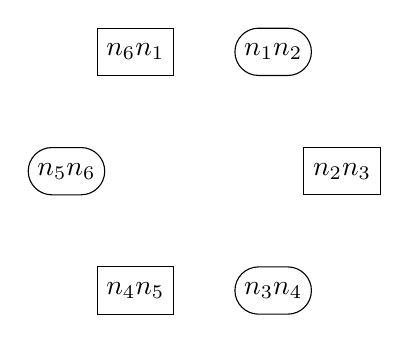
\begin{tikzpicture}[commutative diagrams/every diagram,
		one/.style={draw, rectangle, minimum size=6mm, rounded corners=3mm},
		two/.style={draw, rectangle, minimum size=6mm}
		]
		\node[one] (P0) at (60:1.75cm) {$n_1 n_2$};
		\node[two] (P1) at (60+60:1.75cm) {$n_6 n_1$} ;
		\node[one] (P2) at (60+2*60:1.75cm) {$n_5 n_6$};
		\node[two] (P3) at (60+3*60:1.75cm) {$n_4 n_5$};
		\node[one] (P4) at (60+4*60:1.75cm) {$n_3 n_4$};
		\node[two] (P5) at (0:1.75cm) {$n_2 n_3$};
	\end{tikzpicture}\end{center}

	The three Herbrand quotients correspond to the quotients of opposite
	terms in the diagram above. Thus assertion~(i) is equivalent to the
	following observations:
% segment-id: o014.li2.chapter6.tate-cohomology.l002
	\begin{itemize}
% segment-id: o014.li2.chapter6.tate-cohomology.i003
		\item if the cardinalities at both ends of two diagonals are finite,
		then the same holds at both ends of the remaining diagonal;
% segment-id: o014.li2.chapter6.tate-cohomology.i004
		\item the product of the terms in square-cornered boxes equals the
		product of the terms in round-cornered boxes.
	\end{itemize}

	For~(ii), there are short exact sequences of finite $\Z$-modules
% segment-id: o014.li2.chapter6.tate-cohomology.q012
	\[ 0 \to A^{\sigma=1} \to A \xrightarrow{\sigma-1} \mathfrak{I} A \to 0, \quad 0 \to A^{\nu=0} \to A \xrightarrow{\nu} \nu A \to 0; \]
	here $(\sigma-1)A=\mathfrak{I}A$ follows from
	Lemma~\ref{prop:cyclic-resolution-prep}. Therefore,
% segment-id: o014.li2.chapter6.tate-cohomology.q013
	\[ |A^{\sigma=1}| \cdot |\mathfrak{I} A| = |A^{\nu=0}| \cdot |\nu A|, \]
	which rearranges to
	$|\TaHm^0(C_m,A)|=|\TaHm^{-1}(C_m,A)|$. This proves the assertion.
\end{proof}

% Unit 084 English translation of chapter6.tex, lines 2313--2457.
% Source: Methods of Algebra, Volume 2, commit
% 9a5803ff77dd3257484cb177f851a73770a59dd3 (CC BY 4.0).
% stable-unit-id: o014.aljabr2.chapter6.profinite-cohomology-a
% Coverage: Section 6.12 through smooth modules, the definition of profinite
% cohomology, and continuous standard complexes through its first theorem.

% segment-id: o014.li2.chapter6.profinite-cohomology-a.h001
\section{Cohomology of Profinite Groups}\label{sec:profinite-cohomology}
\hypertarget{o014.aljabr2.chapter6.profinite-cohomology-a}{ }

% segment-id: o014.li2.chapter6.profinite-cohomology-a.p001
This section presupposes the basic definitions and results on profinite groups
from \S\ref{sec:profinite-groups}.

% segment-id: o014.li2.chapter6.profinite-cohomology-a.p002
Let $G$ be a profinite group and $M$ a $G$-module. It is not difficult to
verify that the following conditions are equivalent:
\begin{enumerate}[(i)]
	\item $M=\bigcup_KM^K$, where $K$ ranges over the open normal subgroups of
	$G$;
	\item for every $x\in M$, the stabilizer subgroup $\Stab_G(x)$ is open;
	\item the action map $G\times M\to M$ is continuous when $M$ is given the
	discrete topology.
\end{enumerate}

% segment-id: o014.li2.chapter6.profinite-cohomology-a.d001
\begin{definition}
	\index{$G$-module!smooth}
	\index[sym1]{G-Mod-infty@$G\dcate{Mod}^\infty$}
	Let $G$ be a profinite group. If any of the conditions above holds, the
	$G$-module $M$ is called \emph{smooth}\footnote{In view of~(iii), many
	sources call it discrete.}. All smooth $G$-modules form a full subcategory
	$G\dcate{Mod}^\infty$ of $G\dcate{Mod}$.
\end{definition}

% segment-id: o014.li2.chapter6.profinite-cohomology-a.p003
Although the condition on $G$ itself is topological, characterization~(i) or
~(ii) of a smooth $G$-module is entirely algebraic: smoothness is a property
of a $G$-module, not additional structure. It follows readily that
$G\dcate{Mod}^\infty$ is an abelian subcategory of $G\dcate{Mod}$. The
operations of Definition~\ref{def:Res-Infl} have natural analogues here.

% segment-id: o014.li2.chapter6.profinite-cohomology-a.d002
\begin{definition-proposition}
	Let $\varphi:H\to G$ be a continuous homomorphism of profinite groups and
	let $M$ be a smooth $G$-module. Then the $H$-module $\varphi^*M$ is still
	smooth. This gives a functor
	\[ \varphi^*:G\dcate{Mod}^\infty\to H\dcate{Mod}^\infty. \]
\end{definition-proposition}
\begin{proof}
	For every open normal subgroup $K\lhd G$, its inverse image
	$\varphi^{-1}(K)\lhd H$ is again open and normal. If $x\in M^K$, then
	$x\in(\varphi^*M)^{\varphi^{-1}K}$. Thus
	\[ \varphi^*M=
	\bigcup_{L\lhd H:\,\text{open}}(\varphi^*M)^L, \]
	which proves that $\varphi^*M$ is smooth.
\end{proof}

% segment-id: o014.li2.chapter6.profinite-cohomology-a.p004
Note that the functor $\varphi^*$ is always exact. We single out two special
cases:
\begin{description}
	\item[Restriction] If $H$ is a closed subgroup of $G$, take $\varphi$ to
	be the inclusion homomorphism $H\hookrightarrow G$. The corresponding
	functor is denoted by
	\[ \Res^G_H:G\dcate{Mod}^\infty\to H\dcate{Mod}^\infty. \]
	\item[Inflation] For a closed normal subgroup $H\lhd G$, take $\varphi$ to
	be the quotient homomorphism $G\twoheadrightarrow G/H$. The corresponding
	functor is denoted by
	\[ \mathrm{Infl}^G_{G/H}:G/H\dcate{Mod}^\infty
	\to G\dcate{Mod}^\infty. \]

	The groups $H$ and $G/H$ mentioned above are automatically profinite, so
	these definitions make sense.
\end{description}
\index[sym1]{ResGH}
\index[sym1]{InflGH}

% segment-id: o014.li2.chapter6.profinite-cohomology-a.d003
\begin{definition-proposition}\label{def:smooth-part}
	For every $G$-module $M$, define
	$M^\infty:=\bigcup_KM^K$, where $K$ ranges over the open normal subgroups
	of $G$. This is a smooth $G$-module, and $M$ is smooth if and only if
	$M=M^\infty$.

	For every smooth $G$-module $M'$, we have
	\[ \Hom_G(M',M)=\Hom_G(M',M^\infty). \]
	In other words,
	$\text{inclusion}:G\dcate{Mod}^\infty
	\leftrightarrows G\dcate{Mod}:(\cdot)^\infty$ is an adjoint pair.
\end{definition-proposition}
\begin{proof}
	Clear.
\end{proof}

% segment-id: o014.li2.chapter6.profinite-cohomology-a.p005
The elements of $M^\infty$ are also called the \emph{smooth elements} of
$M$. Since $(\cdot)^\infty$ is the right adjoint of an exact functor, it
preserves injective objects
(Proposition~\ref{prop:adjoint-injective-projective}).

% segment-id: o014.li2.chapter6.profinite-cohomology-a.t001
\begin{corollary}
	The abelian category $G\dcate{Mod}^\infty$ has enough injective objects.
\end{corollary}
\begin{proof}
	Let $M$ be a smooth $G$-module and embed it in an injective $G$-module
	$I$. Then $M=M^\infty\hookrightarrow I^\infty$, while $I^\infty$ is an
	injective smooth $G$-module.
\end{proof}

% segment-id: o014.li2.chapter6.profinite-cohomology-a.r001
\begin{remark}
	In general, $G\dcate{Mod}^\infty$ does not have enough projective objects.
	This is the principal reason why this section studies cohomology rather
	than homology.
\end{remark}

% segment-id: o014.li2.chapter6.profinite-cohomology-a.p006
Since $G\dcate{Mod}^\infty$ has enough injective objects, we can discuss the
right derived functors of the invariants functor $(\cdot)^G$. Our approach is
first to give a direct definition that reduces to the case of finite groups,
and then to identify it with the right derived functors in
Proposition~\ref{prop:profinite-cohomology-identification}. For now we use
only classical language and do not invoke derived categories.

% segment-id: o014.li2.chapter6.profinite-cohomology-a.p007
First take a profinite group $G$ and an open normal subgroup $K$. For every
smooth $G$-module $M$, the submodule of $K$-invariants
$M^K=(\Res^G_KM)^K$ naturally becomes a $G/K$-module. This gives a functor
$(\cdot)^K:G\dcate{Mod}^\infty\to G/K\dcate{Mod}$ and the evident adjoint
pair
\begin{equation}\label{eqn:invariant-adjunction-profinite}
	\begin{tikzcd}[row sep=tiny]
		\mathrm{Infl}^G_{G/K}:G/K\dcate{Mod} \arrow[shift left,r] &
		G\dcate{Mod}^\infty:(\cdot)^K \arrow[shift left,l]\\
		\Hom_G(\mathrm{Infl}^G_{G/K}(M'),M) \arrow[equal,r] &
		\Hom_{G/K}(M',M^K).
	\end{tikzcd}
\end{equation}

% segment-id: o014.li2.chapter6.profinite-cohomology-a.p008
If open normal subgroups $K,K'$ of $G$ satisfy $K'\supset K$, then the
inclusion $M^{K'}\hookrightarrow M^K$ is equivariant with respect to the
oppositely directed quotient homomorphism $G/K'\twoheadleftarrow G/K$
(Definition~\ref{def:group-equivariance}). Hence for every
$n\in\Z_{\geq0}$ there is a canonical homomorphism
\[ \rho^{K'}_K:\Hm^n(G/K',M^{K'})\to\Hm^n(G/K,M^K). \]
If $K_1\subset K_2\subset K_3$ are open normal subgroups of $G$, then
$\rho^{K_2}_{K_1}\rho^{K_3}_{K_2}=\rho^{K_3}_{K_1}$. Thus the following
definition makes sense.

% segment-id: o014.li2.chapter6.profinite-cohomology-a.d004
\begin{definition}
	\index{group cohomology!profinite case}
	\index[sym1]{HnGM}
	Let $G$ be a profinite group and $M$ a smooth $G$-module. For every
	$n\in\Z_{\geq0}$, define
	\[ \Hm^n(G,M):=\varinjlim_K\Hm^n(G/K,M^K), \]
	where $K$ ranges over the open normal subgroups of $G$, and $\varinjlim$
	is taken with respect to the partial order
	$K'\preceq K\iff K\subset K'$ and the morphisms $\rho^{K'}_K$.
\end{definition}

% segment-id: o014.li2.chapter6.profinite-cohomology-a.p009
All open normal subgroups form a filtered partially ordered set: they are
closed under finite intersections. If $G$ is finite, then $\{1\}$ is its
unique maximal element, and $\Hm^n(G,M)$ reduces to the original version in
\S\ref{sec:group-coh-sub}. In general,
\[ \Hm^0(G,M)=\varinjlim_K(M^K)^{G/K}=M^G. \]

% segment-id: o014.li2.chapter6.profinite-cohomology-a.p010
Let $f:M_1\to M_2$ be a homomorphism of smooth $G$-modules. For every open
normal subgroup $K$, it restricts to
$f_K:M_1^K\to M_2^K$. Clearly, $K'\supset K$ implies
$\Hm^n(f_K)\rho^{K'}_K=\rho^{K'}_K\Hm^n(f_{K'})$, so for every
$n\in\Z_{\geq0}$ there is a homomorphism
\[ \Hm^n(f):\Hm^n(G,M_1)\to\Hm^n(G,M_2). \]

% segment-id: o014.li2.chapter6.profinite-cohomology-a.e001
\begin{example}
	Let $E|F$ be a Galois extension of fields. Since
	$E=\bigcup_{L|F}E^{\Gal(E|L)}=\bigcup_{L|F}L$, where $L|F$ ranges over
	the finite Galois subextensions, the action of $\Gal(E|F)$ on $E$ is
	smooth. Applying Example~\ref{eg:additive-90-finite} to every $L|F$
	gives
	\[ n\geq1\implies\Hm^n(\Gal(E|F),E)
	=\varinjlim_{L|F}\Hm^n(\Gal(L|F),L)=0. \]
\end{example}

% segment-id: o014.li2.chapter6.profinite-cohomology-a.p011
Just as in Proposition~\ref{prop:groupcoh-cochain} and
Remark~\ref{rem:nor-cochain} for groups without topology, the cohomology of a
profinite group can be computed by the standard complex or its normalized
version; the difference lies in the continuity condition.

% segment-id: o014.li2.chapter6.profinite-cohomology-a.d005
\begin{definition}
	\index{standard complex}
	\index[sym1]{CGM}
	For a smooth $G$-module $M$, give $M$ the discrete topology and define its
	\emph{standard complex} $C(G,M)=(C^n(G,M))_n$ by
	\[ C^n(G,M):=\{\text{continuous maps }f:G^n\to M\},
	\qquad n\in\Z_{\geq0}. \]
	Terms of negative degree are defined to be $0$, while
	$d^n:C^n(G,M)\to C^{n+1}(G,M)$ is given by
	\begin{multline*}
		(d^nf)(g_1,\ldots,g_{n+1})
		=g_1f(g_2,\ldots,g_{n+1})\\
		+\sum_{k=1}^n(-1)^kf(\ldots,g_kg_{k+1},\ldots)
		+(-1)^{n+1}f(g_1,\ldots,g_n).
	\end{multline*}

	\index[sym1]{CGMbar}
	Define the \emph{normalized standard complex} to be the following
	subcomplex $\overline{C}(G,M)$ of $C(G,M)$
	(see Remark~\ref{rem:nor-cochain}):
	\[ \overline{C}^n(G,M)=\left\{\begin{array}{r|l}
		f\in C^n(G,M)&\exists 1\leq k\leq n,\; g_k=1_G\\
		&\implies f(g_1,\ldots,g_n)=0
	\end{array}\right\}. \]
\end{definition}

% segment-id: o014.li2.chapter6.profinite-cohomology-a.p012
For every open normal subgroup $K\lhd G$, there are evident inclusions of
complexes
$C(G/K,M^K)\hookrightarrow C(G,M)$ and
$\overline{C}(G/K,M^K)\hookrightarrow\overline{C}(G,M)$.

% segment-id: o014.li2.chapter6.profinite-cohomology-a.p013
Since $M$ is discrete, a map $f:G^n\to M$ is continuous if and only if it is
locally constant. Compactness of $G$ then gives an open normal subgroup
$K_1\lhd G$ such that $f$ factors through $(G/K_1)^n\to M$. In particular,
$f$ assumes only finitely many values; smoothness gives an open normal
subgroup $K_2\lhd G$ such that the values of $f$ lie in $M^{K_2}$. Set
$K:=K_1\cap K_2$. It follows that
\[ C^n(G,M)\simeq\varinjlim_{K\lhd G\;\text{open}}C^n(G/K,M^K),\qquad
	\overline{C}^n(G,M)\simeq
	\varinjlim_{K\lhd G\;\text{open}}\overline{C}^n(G/K,M^K). \]
As $n$ varies, these give isomorphisms of complexes.

% segment-id: o014.li2.chapter6.profinite-cohomology-a.p014
As before, define the submodules of $C^n(G,M)$
\[ Z^n(G,M):=\Ker(d^n),\qquad B^n(G,M):=\Image(d^{n-1}), \]
with $B^0(G,M):=\{0\}$. Then
$\Hm^n(C(G,M))=Z^n(G,M)/B^n(G,M)$. Define the normalized versions
$\overline{Z}^n(G,M)$ and $\overline{B}^n(G,M)$ similarly.

% segment-id: o014.li2.chapter6.profinite-cohomology-a.t002
\begin{theorem}\label{prop:profinite-group-standard}
	Let $G$ be a profinite group. For all $n\in\Z_{\geq0}$ and every smooth
	$G$-module $M$, there are canonical isomorphisms
	\[ \Hm^n(C(G,M))\simeq\Hm^n(G,M)
	\simeq\Hm^n(\overline{C}(G,M)). \]
\end{theorem}
\begin{proof}
	Cohomology takes values in $\cate{Ab}$, or in $\Bbbk\dcate{Mod}$ if a
	coefficient ring $\Bbbk$ has been specified. Filtered colimits are exact
	in these categories \cite[Theorem 6.2.2]{Li1}. Hence
	\[ Z^n(G,M)=\varinjlim_KZ^n(G/K,M^K),\qquad
	B^n(G,M)=\varinjlim_KB^n(G/K,M^K), \]
	and therefore
	\begin{multline*}
		\Hm^n(C(G,M))
		=\dfrac{\varinjlim_KZ^n(G/K,M^K)}
		{\varinjlim_KB^n(G/K,M^K)}\simeq\\
		\varinjlim_K\frac{Z^n(G/K,M^K)}{B^n(G/K,M^K)}
		=\varinjlim_K\Hm^n(C(G/K,M^K)).
	\end{multline*}
	Apply Proposition~\ref{prop:groupcoh-cochain} to the last term to obtain
	$\varinjlim_K\Hm^n(G/K,M^K)$, namely $\Hm^n(G,M)$.
% Editorial correction carried from the Indonesian witness: the Chinese source
% has $\Hm^n(G,K)$ here, with $K$ in place of the coefficient module $M$.

	The case of $\overline{C}(G,M)$ is similar.
\end{proof}

% Unit 085 English translation of chapter6.tex, lines 2458--2603.
% Source: Methods of Algebra, Volume 2, commit
% 9a5803ff77dd3257484cb177f851a73770a59dd3 (CC BY 4.0).
% stable-unit-id: o014.aljabr2.chapter6.profinite-cohomology-b
% Coverage: the remainder of Section 6.12: delta functors, low-degree
% interpretations, derived-functor identification, profinite induction, and
% Shapiro's Lemma.

% segment-id: o014.li2.chapter6.profinite-cohomology-b.t001
\begin{theorem}\label{prop:profinite-cohomology-long}
	Let $G$ be a profinite group and let
	$0\to M'\xrightarrow{f}M\xrightarrow{f'}M''\to0$ be a short exact
	sequence of smooth $G$-modules. There is an associated long exact sequence
	\begin{multline*}
		\cdots\to\Hm^{n-1}(G,M'')\xrightarrow{\delta^{n-1}}
		\Hm^n(G,M')\xrightarrow{\Hm^n(f)}\Hm^n(G,M)\\
		\xrightarrow{\Hm^n(f')}\Hm^n(G,M'')\xrightarrow{\delta^n}
		\Hm^{n+1}(G,M')\to\cdots,
	\end{multline*}
% Editorial correction carried from the Indonesian witness: the Chinese source
% labels the middle arrow $\Hm^n(g)$ although the displayed map is $f'$.
	with the convention that $\Hm^n(G,\cdot)=0$ for $n<0$. The connecting
	homomorphisms $\delta^n$ are natural with respect to morphisms of short
	exact sequences; in other words, they form a cohomological $\delta$-functor.
\end{theorem}
\begin{proof}
	We work with the standard complex; the argument for the normalized version
	is similar. By Proposition~\ref{prop:long-exact-sequence-ses}, it suffices
	to prove that
	\[ 0\to C^n(G,M')\to C^n(G,M)\to C^n(G,M'')\to0 \]
	is a short exact sequence. The only point that is not immediate is the
	surjectivity of $C^n(G,M)\to C^n(G,M'')$. Let $u:G^n\to M''$ be
	continuous. As above, there is an open normal subgroup $K\lhd G$ such
	that $u$ is constant on each coset of $K^n\lhd G^n$. On every coset,
	choose an arbitrary inverse image in $M$ of this constant value.
\end{proof}

% segment-id: o014.li2.chapter6.profinite-cohomology-b.p001
Let $M$ be a smooth $G$-module with the discrete topology. The low-degree
terms of the complex $C(G,M)$ or $\overline{C}(G,M)$ still have direct
interpretations.
\begin{description}
	\item[($n=0$)] Clearly $C^0(G,M)=M$ and
	$\Hm^0(G,M)=Z^0(G,M)=M^G$. The normalized standard complex gives the
	same result.
	\item[($n=1$)] The elements of
	$Z^1(G,M)=\overline{Z}^1(G,M)$ are continuous crossed homomorphisms
	$G\to M$. Equivalently, they are continuous homomorphisms
	$\sigma:G\to M\rtimes G$ satisfying $\pi\sigma=\identity_G$, as in
	Proposition~\ref{prop:crossed-semidirect-product}. Here
	$\pi:M\rtimes G\to G$ is the projection and $M\rtimes G$ carries the
	product topology. On the other hand, the elements of $B^1(G,M)$ are
	generated by the crossed homomorphisms $f_m:g\mapsto gm-m$; these are
	automatically continuous.

	\item[($n=2$)] Suppose that $M$ is finite. The elements of
	\[ \Hm^2(G,M)\simeq\frac{Z^2(G,M)}{B^2(G,M)}
	\simeq\frac{\overline{Z}^2(G,M)}{\overline{B}^2(G,M)} \]
	correspond bijectively to equivalence classes of extensions of profinite
	groups
	\[ 1\to M\to E\xrightarrow{\pi}G\to1
	\qquad\text{(short exact sequence of groups)}, \]
% Editorial correction carried from the Indonesian witness: group extensions
% have terminal identity groups $1$, not zero groups as printed in the source.
	where the conjugation action of $G$ on $M$ comes from the $G$-module
	structure on $M$. Compared with the version in
	Definition~\ref{def:group-ext} and \eqref{eqn:group-ext-diagram}, a
	``profinite group extension'' and its classification must additionally
	satisfy:
	\begin{compactitem}
		\item $E$ is a profinite group, $\pi$ is continuous, and $M$ is
		embedded as a closed subgroup of $E$;
		\item equivalences, or isomorphisms, of extensions are defined by
		continuous group homomorphisms $E\to E'$, and the splitting of an
		extension is likewise defined topologically.
	\end{compactitem}

	Moreover, the automorphism group of an extension is isomorphic to
	$\overline{Z}^1(G,M)$. The proofs are not difficult, but require some
	topological language and are therefore left as exercises for this chapter;
	the finiteness of $M$ is essential.
\end{description}

% segment-id: o014.li2.chapter6.profinite-cohomology-b.p002
We now return to the right derived functors
$(\mathrm{R}^n(\cdot)^G)_{n\geq0}$. One could study their values on arbitrary
bounded-below complexes\footnote{In other words, study the hypercohomology of
profinite groups.}, or even their operation in the derived category. This
section, however, discusses only smooth $G$-modules; the rest is left to the
exercises.

% segment-id: o014.li2.chapter6.profinite-cohomology-b.t002
\begin{proposition}\label{prop:profinite-cohomology-identification}
	There is an isomorphism of cohomological $\delta$-functors
	\[ (\Hm^n(G,\cdot))_{n\geq0}
	\simeq(\mathrm{R}^n(\cdot)^G)_{n\geq0}. \]
\end{proposition}
\begin{proof}
	Theorem~\ref{prop:profinite-cohomology-long} shows that both sides are
	cohomological $\delta$-functors, and at $n=0$ both are the invariants
	functor $(\cdot)^G$. By Proposition~\ref{prop:erasable-univ-delta}, it is
	enough to show that $\Hm^n(G,\cdot)$ is erasable for $n>0$ in the sense
	of Definition~\ref{def:erasable}. Let $M$ be a smooth $G$-module and embed
	it in an injective smooth $G$-module $I$. For every open normal subgroup
	$K\lhd G$, the adjunction \eqref{eqn:invariant-adjunction-profinite}
	shows that $(\cdot)^K$ preserves injective objects. Hence $I^K$ is an
	injective $G/K$-module, and
	\[ n>0\implies\Hm^n(G,I)
	=\varinjlim_K\Hm^n(G/K,I^K)=0. \]
	This proves erasability.
\end{proof}

% segment-id: o014.li2.chapter6.profinite-cohomology-b.p003
By Proposition~\ref{prop:profinite-cohomology-identification}, the method of
\S\ref{sec:change-of-group} applies directly to a continuous homomorphism
$\varphi:H\to G$ of profinite groups and defines a cohomological
``pullback'' operation
\[ \Hm^n(G,M)\to\Hm^n(H,\varphi^*M),\qquad
	M:\text{ a smooth $G$-module},\quad n\in\Z_{\geq0}. \]
These operations are compatible with long exact sequences. As usual, exactness
of $\varphi^*$ and the universal property of cohomological $\delta$-functors
reduce the matter to the evident inclusion at $n=0$,
$M^G\hookrightarrow(\varphi^*M)^H$.

% segment-id: o014.li2.chapter6.profinite-cohomology-b.p004
As a special case, for all $n$ and all closed subgroups $H$ there are
restriction maps
$\mathrm{res}^n:\Hm^n(G,M)\to\Hm^n(H,M)$; here
$\Res^G_HM$ is abbreviated to $M$.

% segment-id: o014.li2.chapter6.profinite-cohomology-b.p005
The homomorphisms above may also be constructed from the homomorphisms
\begin{align*}
	\Hm^n(G/K,M^K)&\xrightarrow{\eqref{eqn:change-of-group-coh}}
	\Hm^n(H/\varphi^{-1}(K),\varphi_K^*(M^K))\\
	&\xrightarrow{M^K\subset(\varphi^*M)^{\varphi^{-1}K}}
	\Hm^n(H/\varphi^{-1}(K),(\varphi^*M)^{\varphi^{-1}K}),
\end{align*}
where $K$ ranges over the open normal subgroups of $G$. Reducing to the case
of finite groups shows that the homomorphism on the standard complex is
computed by the formula of Proposition~\ref{prop:grp-equiv}. To prove that
this map is indeed the same as the one constructed earlier by the universal
property, it is enough to compare them at $n=0$ and show compatibility with
long exact sequences. The standard complex suffices for both tasks.

% segment-id: o014.li2.chapter6.profinite-cohomology-b.p006
Similarly, the corestriction homomorphism of
Definition--Proposition~\ref{def:cor} extends to profinite groups. Let $H$
be an open subgroup of $G$. It is then automatically closed and $(G:H)$ is
finite (see \S\ref{sec:profinite-groups}). Define homomorphisms
\[ \mathrm{cor}^n:\Hm^n(H,M)\to\Hm^n(G,M),\qquad
	M:\text{ a smooth $G$-module},\quad n\in\Z_{\geq0}, \]
which are compatible with long exact sequences and at $n=0$ give
$\nu^{G|H}:M^H\to M^G$.

% segment-id: o014.li2.chapter6.profinite-cohomology-b.p007
The construction again uses the universal property of cohomological
$\delta$-functors, but here we need to know that
$\Res^G_H:G\dcate{Mod}^\infty\to H\dcate{Mod}^\infty$ preserves injective
objects; this is the content of
Corollary~\ref{prop:Res-injective-profinite}. Once this fact is granted,
Proposition~\ref{prop:res-cor} still has an analogue: for every $n$,
\[ \mathrm{cor}^n\circ\mathrm{res}^n
	=(G:H)\cdot\identity_{\Hm^n(G,M)}. \]
As before, the proof reduces to the case $n=0$.

% segment-id: o014.li2.chapter6.profinite-cohomology-b.p008
We now discuss induced modules in the profinite case. Henceforth $G$ is
always a profinite group. To distinguish the two settings, denote the
induction functor without topology (Definition~\ref{def:induced-module}) by
$\Ind^{G,\mathrm{alg}}_H$; following Lemma~\ref{prop:Ind-as-mappings}, we
realize it as a mapping space.

% segment-id: o014.li2.chapter6.profinite-cohomology-b.d001
\begin{definition}
	\index{$G$-module!induced}
	For a closed subgroup $H$ of $G$ and a smooth $H$-module $N$, equip the
	mapping space $\mathrm{Maps}(G,N):=\{f:G\to N\}$ with pointwise addition
	and scalar multiplication, together with the left $G$-action
	\[ (gf)(x)=f(xg),\qquad g,x\in G. \]
	Define the smooth $G$-module
	\begin{align*}
		\Ind^G_H(N)&:=\{f\in\mathrm{Maps}(G,N)^\infty:
		\forall h\in H,\ \forall x\in G,\ f(hx)=hf(x)\}\\
		&=(\Ind^{G,\mathrm{alg}}_H(N))^\infty.
	\end{align*}
	The notation $(\cdot)^\infty$ is from
	Definition--Proposition~\ref{def:smooth-part}. This is called the
	$G$-module induced from $N$.
\end{definition}

% segment-id: o014.li2.chapter6.profinite-cohomology-b.p009
Since $G$ is compact, smoothness of
$f\in\Ind^{G,\mathrm{alg}}_H(N)$ is equivalent to its continuity as a map
$G\to N$, where $N$ carries the discrete topology.

% segment-id: o014.li2.chapter6.profinite-cohomology-b.t003
\begin{proposition}\label{prop:Ind-injective-profinite}
	For every closed subgroup $H$ of $G$, there is an adjoint pair
	\[ \Res^G_H:G\dcate{Mod}^\infty
	\leftrightarrows H\dcate{Mod}^\infty:\Ind^G_H. \]
	Consequently, $\Ind^G_H$ preserves injective objects.

	If $H$ is an open subgroup of $G$, there is also an adjoint pair
	\[ \Ind^G_H:H\dcate{Mod}^\infty
	\leftrightarrows G\dcate{Mod}^\infty:\Res^G_H. \]
	In this case $\Ind^G_H$ also preserves projective objects.
\end{proposition}
\begin{proof}
	By the adjunction in the setting without topology and
	Definition--Proposition~\ref{def:smooth-part}, for every smooth
	$G$-module $M$ and smooth $H$-module $N$ there are canonical
	isomorphisms
	\begin{multline*}
		\Hom_H(\Res^G_H(M),N)
		\simeq\Hom_G(M,\Ind^{G,\mathrm{alg}}_H(N))\\
		=\Hom_G(M,\Ind^{G,\mathrm{alg}}_H(N)^\infty)
		=\Hom_G(M,\Ind^G_H(N)).
	\end{multline*}

	Now suppose that $H$ is open, so that $(G:H)$ is finite. From
	Corollary~\ref{prop:iInd-Ind} we obtain the adjunction without topology
	\[ \Hom_H(N,\Res^G_H(M))
	\simeq\Hom_G(\Ind^{G,\mathrm{alg}}_H(N),M). \]
	We claim that
	$\Ind^{G,\mathrm{alg}}_H(N)=\Ind^G_H(N)$. Take
	$f\in\Ind^{G,\mathrm{alg}}_H(N)$ and $x\in G$, and choose an open
	subgroup $K_0\subset H$ such that $f(x)\in N^{K_0}$. Set
	$K:=x^{-1}K_0x$, which is an open subgroup of $G$. Then
	\[ g\in K\implies xg=xgx^{-1}x\in K_0x
	\implies f(xg)=f(x). \]
	Since $x$ was arbitrary, the map $f:G\to N$ is locally constant, so
	$f\in\Ind^G_H(N)$. This proves the second adjunction.

	Finally, the claims about preserving injective or projective objects
	follow from exactness of $\Res^G_H$ and
	Proposition~\ref{prop:adjoint-injective-projective}.
\end{proof}

% segment-id: o014.li2.chapter6.profinite-cohomology-b.l001
\begin{lemma}\label{prop:Ind-exact-profinite}
	If $H$ is a closed subgroup of $G$, then
	$\Ind^G_H:H\dcate{Mod}^\infty\to G\dcate{Mod}^\infty$ is exact.
\end{lemma}
\begin{proof}
	We already know that $\Ind^G_H$ has a left adjoint, so it is left exact.
	It remains to prove that $N_1\twoheadrightarrow N_2$ implies
	$\Ind^G_H(N_1)\twoheadrightarrow\Ind^G_H(N_2)$. By
	Lemma~\ref{prop:profinite-section}, the quotient homomorphism
	$\pi:G\to H\backslash G$ has a continuous section $s$. For every smooth
	$H$-module $N$, there is a $\Bbbk$-module isomorphism
	\[\begin{tikzcd}[row sep=tiny]
		\Ind^G_H(N) \arrow[leftrightarrow,r,"\sim"] &
		\{\text{continuous maps }H\backslash G\to N\}\\
		f \arrow[mapsto,r] & {[x\mapsto f(s(x))]}\\
		{[hs(x)\mapsto hf'(x)]} & f' \arrow[mapsto,l]
	\end{tikzcd}\]
	where $x\in H\backslash G$ and $h\in H$. Although this isomorphism does
	not preserve the $G$-action, it is natural in $N$.

	Since continuous maps $H\backslash G\to N$ are always locally constant,
	working on the right-hand side immediately shows that
	$\Ind^G_H(N_1)\to\Ind^G_H(N_2)$ is surjective.
\end{proof}

% segment-id: o014.li2.chapter6.profinite-cohomology-b.t004
\begin{corollary}\label{prop:Res-injective-profinite}
	If $H$ is an open subgroup of $G$, then
	$\Res^G_H:G\dcate{Mod}^\infty\to H\dcate{Mod}^\infty$ preserves
	injective objects.
\end{corollary}
\begin{proof}
	By the preceding two results, it has the exact left adjoint $\Ind^G_H$.
\end{proof}

% segment-id: o014.li2.chapter6.profinite-cohomology-b.p010
We now obtain the profinite version of Theorem~\ref{prop:Shapiro}.

% segment-id: o014.li2.chapter6.profinite-cohomology-b.t005
\begin{proposition}
	\index{Shapiro's lemma}
	Let $H$ be a closed subgroup of a profinite group $G$ and let $N$ be a
	smooth $H$-module. There are isomorphisms
	\[ \Hm^n(G,\Ind^G_H(N))\simeq\Hm^n(H,N),
	\qquad n\in\Z_{\geq0}. \]
\end{proposition}
\begin{proof}
	Because $\Ind^G_H$ is exact and preserves injective objects
	(Lemma~\ref{prop:Ind-exact-profinite} and
	Proposition~\ref{prop:Ind-injective-profinite}), the argument in
	Theorem~\ref{prop:Shapiro} using erasable cohomological $\delta$-functors
	applies unchanged. Recall that the heart of that argument is the case
	$n=0$, namely
	\[ \Ind^G_H(N)^G
	=(\Ind^{G,\mathrm{alg}}_H(N)^\infty)^G
	=(\Ind^{G,\mathrm{alg}}_H(N))^G\rightiso N^H. \]
	The first equality is the definition, the second is immediate, and the
	last isomorphism comes from Corollary~\ref{prop:Ind-invariant}.
\end{proof}

% segment-id: o014.li2.chapter6.profinite-cohomology-b.p011
In addition:
\begin{itemize}
	\item the cohomological Lyndon--Hochschild--Serre spectral sequence
	(see \S\ref{sec:LHS-SS}) extends to the case where $G$ is a profinite
	group and $H$ is a closed normal subgroup;
	\item the cup product (see \S\ref{sec:cup-product}) also extends to
	profinite groups by using the direct definition on the standard complex;
	see Definition--Proposition~\ref{def:group-cup-3}.
	\index{cup product}
\end{itemize}
The statements are unchanged, so we do not repeat them.

% Unit 086 English translation of chapter6.tex, lines 2604--2927.
% Source: Methods of Algebra, Volume 2, commit
% 9a5803ff77dd3257484cb177f851a73770a59dd3 (CC BY 4.0).
% stable-unit-id: o014.aljabr2.chapter6.nonabelian-cohomology
% Coverage: complete Section 6.13, ``Nonabelian Cohomology''; ends immediately
% before the Exercises environment at line 2928.

% segment-id: o014.li2.chapter6.nonabelian-cohomology.h001
\section{Nonabelian Cohomology}\label{sec:nonabelian-coh}
\hypertarget{o014.aljabr2.chapter6.nonabelian-cohomology}{ }
% segment-id: o014.li2.chapter6.nonabelian-cohomology.p001
Let $G$ be a group. The cohomology $\Hm^n(G,M)$ discussed previously always
requires its ``coefficients'' $M$ to have a module structure, or at least to
be a $\Z$-module, that is, an abelian group. This section studies the case in
which the coefficients form a nonabelian group. From now on we use the symbol
$A$ in place of $M$.

% segment-id: o014.li2.chapter6.nonabelian-cohomology.d001
\begin{definition}\label{def:G-group}
	\index[sym1]{G-Grp@$G\dcate{Grp}$}
	\index{$G$-group}
	Let $A$ be a group, with its binary operation written multiplicatively
	and its identity element denoted by $1$. Suppose that $A$ is equipped with
	a left action of the group $G$, written
% segment-id: o014.li2.chapter6.nonabelian-cohomology.q001
	\[ G \times A \to A, \quad (g, a) \mapsto {}^g a . \]
	If the group action is compatible with the multiplicative structure of
	$A$,
% segment-id: o014.li2.chapter6.nonabelian-cohomology.q002
	\[ {}^g (a_1 a_2) = {}^g a_1 {}^g a_2, \quad {}^g 1 = 1, \]
	then $A$ is called a group with a $G$-action, or simply a
	\emph{$G$-group}. A homomorphism of $G$-groups is defined to be a group
	homomorphism that preserves the $G$-action. The resulting category is
	denoted by $G\dcate{Grp}$.
\end{definition}

% segment-id: o014.li2.chapter6.nonabelian-cohomology.p002
We will soon see that, for a $G$-group $A$, without additional structure or
commutativity only $\Hm^0$ and $\Hm^1$ can be defined in a reasonable and
useful way. In this setting $\Hm^1$ need not be a group; it is instead a
pointed set.

% segment-id: o014.li2.chapter6.nonabelian-cohomology.d002
\begin{definition}\label{def:pointed-set}
	\index{pointed set}
	\index[sym1]{Set-pt@$\cate{Set}_\bullet$, $G\dcate{Set}_\bullet$}
	A \emph{pointed set} is data $(X,x_0)$, where $X$ is a set and
	$x_0\in X$ is its basepoint. A morphism from $(X,x_0)$ to $(Y,y_0)$ is a
	map $f:X\to Y$ satisfying $f(x_0)=y_0$. These data form the category
	$\cate{Set}_\bullet$.

	Let $(X,x_0)$ be a pointed set. If a group $G$ acts on $X$ from the left,
	written $(g,x)\mapsto{}^gx$, and ${}^gx_0=x_0$ always holds, we say that
	$G$ acts on $(X,x_0)$. In that case we can define the pointed subset of
	invariants
% segment-id: o014.li2.chapter6.nonabelian-cohomology.q003
	\[ (X, x_0)^G := \left\{ x \in X: \forall g \in G, \; gx = x \right\}, \quad \text{basepoint} = x_0. \]
	All pointed sets with a $G$-action, together with morphisms compatible
	with that action, form the category denoted by $G\dcate{Set}_\bullet$.
\end{definition}

% segment-id: o014.li2.chapter6.nonabelian-cohomology.p003
When no confusion can arise, we often write an object $(X,x_0)$ of
$\cate{Set}_\bullet$ simply as $X$, and in $G\dcate{Set}_\bullet$ write
$(X,x_0)^G$ as $X^G$.

% segment-id: o014.li2.chapter6.nonabelian-cohomology.p004
Every group becomes a pointed set by choosing its identity element as the
basepoint. This gives the evident functor
$\cate{Grp}\to\cate{Set}_\bullet$; similarly, there is a functor
$G\dcate{Grp}\to G\dcate{Set}_\bullet$. Note that the invariant subset
$A^G$ of a $G$-group $A$ is a subgroup.

% segment-id: o014.li2.chapter6.nonabelian-cohomology.d003
\begin{definition}\label{def:pointed-exact}
	\index{exact sequence}
	Let
	$(X,x_0)\xrightarrow{f}(Y,y_0)\xrightarrow{g}(Z,z_0)$ be morphisms in
	$\cate{Set}_\bullet$ (or $G\dcate{Set}_\bullet$). This sequence of
	morphisms is called exact if $g^{-1}(z_0)=\Image(f)$. In this way, exact
	sequences in $\cate{Set}_\bullet$ (or $G\dcate{Set}_\bullet$) are
	defined.
\end{definition}

% segment-id: o014.li2.chapter6.nonabelian-cohomology.p005
For abelian groups this recovers the familiar notion of exactness. We can now
define $\Hm^0$ and $\Hm^1$ for every $G$-group $A$.

% segment-id: o014.li2.chapter6.nonabelian-cohomology.d004
\begin{definition}\label{def:nonabelian-H}
	\index{group cohomology!nonabelian case}
	Let $A$ be an object of $G\dcate{Set}_\bullet$. Define the pointed set
% segment-id: o014.li2.chapter6.nonabelian-cohomology.q004
	\[ \Hm^0(G, A) = Z^0(G, A) := A^G. \]

	If $A$ is a $G$-group, then $\Hm^0(G,A)$ is a group. In this case,
	further define
% segment-id: o014.li2.chapter6.nonabelian-cohomology.q005
	\begin{align*}
		Z^1(G, A) & := \left\{\begin{array}{r|l}
			c: G \to A & \forall g_1, g_2 \in G, \\
			& c(g_1 g_2) = c(g_1) \cdot {}^{g_1} c(g_2)
		\end{array}\right\}, \\
		\Hm^1(G, A) & := Z^1(G, A) / \sim ,
	\end{align*}
	where the equivalence relation $c\sim c'$ means that there is an
	$a\in A$ such that, for every $g\in G$,
% segment-id: o014.li2.chapter6.nonabelian-cohomology.q006
	\[ c'(g) = a^{-1} \cdot c(g) \cdot {}^g a . \]
	It is easy to see that this is indeed an equivalence relation---it comes
	from a right $A$-action---and $\Hm^1(G,A)$ naturally becomes a pointed
	set. Its basepoint is the equivalence class determined by the constant
	map $c(g)=1$.
\end{definition}

% segment-id: o014.li2.chapter6.nonabelian-cohomology.p006
Note that substituting $g_1=g_2=1_G$ into the condition defining
$Z^1(G,A)$ gives $c(1_G)=1$. Henceforth $[c]$ denotes the equivalence class
of $c\in Z^1(G,A)$.

% segment-id: o014.li2.chapter6.nonabelian-cohomology.r001
\begin{remark}[$\Hm^1$ as conjugacy classes of sections]\label{rem:Z1-vs-section}
	Form the semidirect product $A\rtimes G$ from the $G$-group $A$, and let
	$\pi$ denote the projection homomorphism $A\rtimes G\to G$. The elements
	of $Z^1(G,A)$ correspond bijectively to group homomorphisms
	$\sigma:G\to A\rtimes G$ satisfying $\pi\sigma=\identity_G$ (that is,
	``sections'' of $\pi$), via the map sending $c\in Z^1(G,A)$ to
	$\sigma(g)=(c(g),g)$. Moreover, $[c']=[c]$ if and only if there is an
	$a\in A$ such that $\sigma'=a^{-1}\sigma a$, where $A$ is embedded as a
	subgroup of $A\rtimes G$ and conjugation is performed pointwise.
\end{remark}

% segment-id: o014.li2.chapter6.nonabelian-cohomology.p007
If $A$ is an abelian group, these constructions reduce to the descriptions
of $\Hm^0$ and $\Hm^1$ using the standard cochain complex
(Proposition~\ref{prop:groupcoh-cochain}). In the nonabelian case, the
constructions remain functorial, as follows.
% segment-id: o014.li2.chapter6.nonabelian-cohomology.l001
\begin{itemize}
% segment-id: o014.li2.chapter6.nonabelian-cohomology.i001
	\item Every morphism $f:A_1\to A_2$ induces
% segment-id: o014.li2.chapter6.nonabelian-cohomology.q007
	\begin{gather*}
		\Hm^0(f): \Hm^0(G, A_1) \to \Hm^0(G, A_2), \quad
		\Hm^1(f): \Hm^1(G, A_1) \to \Hm^1(G, A_2);
	\end{gather*}
	the first map is evident, while the second is given by
	$\Hm^1(f)([c])=[f\circ c]$.

% segment-id: o014.li2.chapter6.nonabelian-cohomology.i002
	\item Let $\varphi:H\to G$ be a group homomorphism. Pull the $G$-action
	on the $G$-group $A$ back to $H$, giving the $H$-group $\varphi^*A$.
% segment-id: o014.li2.chapter6.nonabelian-cohomology.l002
	\begin{compactitem}
% segment-id: o014.li2.chapter6.nonabelian-cohomology.i003
		\item Define the canonical morphism
		$\Hm^0(G,A)\to\Hm^0(H,\varphi^*A)$ to be the evident inclusion
		$A^G\hookrightarrow A^{\varphi(H)}=(\varphi^*A)^H$.
% segment-id: o014.li2.chapter6.nonabelian-cohomology.i004
		\item Define the canonical morphism of pointed sets
% segment-id: o014.li2.chapter6.nonabelian-cohomology.q008
		\[ \Hm^1(G, A) \to \Hm^1(H, \varphi^* A). \]
		It is given by $[c]\mapsto[c\circ\varphi]$.
	\end{compactitem}
\end{itemize}

% segment-id: o014.li2.chapter6.nonabelian-cohomology.p008
These canonical maps have the various properties seen in
\S\ref{sec:change-of-group}. They can also be summarized as follows. Given
$\varphi:H\to G$, let $A_1$ be an object of $G\dcate{Set}_\bullet$ (or
$G\dcate{Grp}$), let $A_2$ be an object of $H\dcate{Set}_\bullet$ (or
$H\dcate{Grp}$), and let the morphism $f:A_1\to A_2$ be equivariant with
respect to $\varphi$, as in Definition~\ref{def:group-equivariance}. There
are corresponding maps $\Hm^i(f):\Hm^i(G,A_1)\to\Hm^i(H,A_2)$, and the
analogue of Proposition~\ref{prop:grp-equiv} takes the form:
% segment-id: o014.li2.chapter6.nonabelian-cohomology.l003
\begin{itemize}
% segment-id: o014.li2.chapter6.nonabelian-cohomology.i005
	\item $\Hm^0(f)$ is the restriction of $f$ to $A_1^G\to A_2^H$;
% segment-id: o014.li2.chapter6.nonabelian-cohomology.i006
	\item $\Hm^1(f)$ maps $[c]$ to $[f\circ c\circ\varphi]$.
\end{itemize}

% segment-id: o014.li2.chapter6.nonabelian-cohomology.c001
\begin{convention}
	Write $1$ for the zero object in $\cate{Set}_\bullet$ or
	$G\dcate{Set}_\bullet$ determined by the singleton set.
\end{convention}

% segment-id: o014.li2.chapter6.nonabelian-cohomology.p009
We now come to the main subject. Henceforth consider a short exact sequence
in $G\dcate{Set}_\bullet$ (Definition~\ref{def:pointed-exact})
% segment-id: o014.li2.chapter6.nonabelian-cohomology.q009
\[ 1 \to A \xrightarrow{u} B \xrightarrow{v} C \to 1, \]
where $A$ and $B$ are assumed to be $G$-groups and $u$ is a group
homomorphism. Exactness therefore implies that $u$ is injective and $v$ is
surjective. We further require:
% segment-id: o014.li2.chapter6.nonabelian-cohomology.q010
\begin{equation}\label{eqn:pointed-ses-condition}
	\begin{gathered}
		\forall b, b' \in B, \; \left[ v(b) = v(b') \iff \exists a \in A, \; b' = b u(a) \right], \\
		\text{in other words: $C$ is identified with $B/u(A)$, basepoint $= 1 \cdot u(A)$.}
	\end{gathered}
\end{equation}

% segment-id: o014.li2.chapter6.nonabelian-cohomology.p010
If $C$ is a group and $v$ is a group homomorphism, considering
$b^{-1}b'\in v^{-1}(1)=\Image(u)$ shows that
\eqref{eqn:pointed-ses-condition} holds automatically, and in this case
$u(A)\lhd B$. Many applications, however, do not fall into this case.

% segment-id: o014.li2.chapter6.nonabelian-cohomology.p011
Our present goal is to construct from these data an exact sequence that is
``as long as possible,'' together with the corresponding connecting
morphisms. Without further comment, we identify $A$ with its image as a
subgroup of $B$ and omit the symbol $u$.

% segment-id: o014.li2.chapter6.nonabelian-cohomology.p012
\textbf{The degree-zero case.}\;
First define the connecting morphism
$\delta^0:\Hm^0(G,C)\to\Hm^1(G,A)$. Let $c\in C^G$. Choose any
$b\in v^{-1}(c)$. Since $v$ preserves the $G$-action,
\eqref{eqn:pointed-ses-condition} shows that, for every $g\in G$, there is
a unique $a(g)\in A$ such that ${}^gb=ba(g)$. Hence $g\mapsto a(g)$ gives
an element $a$ of $Z^1(G,A)$, because
% segment-id: o014.li2.chapter6.nonabelian-cohomology.q011
% Editorial correction: the frozen Chinese source and Indonesian witness have
% a(g) in the final expression; the cocycle identity requires a(g_1).
\[ a(g_1 g_2) = b^{-1} \cdot {}^{g_1 g_2} b = b^{-1} \cdot {}^{g_1} b \cdot {}^{g_1} (b^{-1} \cdot {}^{g_2} b) = a(g_1) \cdot {}^{g_1} a(g_2). \]
If $b',b\in v^{-1}(c)$, there is an $\alpha\in A$ such that
$b'=b\alpha$, and hence
% segment-id: o014.li2.chapter6.nonabelian-cohomology.q012
\[ (b')^{-1} \cdot {}^g b' = \alpha^{-1} \cdot b^{-1} \cdot {}^g b \cdot {}^g \alpha. \]
This shows that the class $[a]\in\Hm^1(G,A)$ is determined solely by $c$.
If $c$ is the basepoint of $C$, we may take $b=1\in B$. We have therefore
obtained a morphism in $\cate{Set}_\bullet$,
$\delta^0:\Hm^0(G,C)\to\Hm^1(G,A)$.

% segment-id: o014.li2.chapter6.nonabelian-cohomology.p013
\textbf{The degree-zero case: a central subgroup.}\;
Suppose that $C$ is a group, $v$ is a group homomorphism, and $A$ is
contained in the center $Z_B$ of the group $B$; in particular, $A$ is
abelian. In this case $\Hm^0(G,C)=C^G$ and $\Hm^1(G,A)$ are both groups.
From the definition of $\delta^0$ and the condition $A\subset Z_B$, it is
easy to check that $\delta^0$ is a group homomorphism.

% segment-id: o014.li2.chapter6.nonabelian-cohomology.p014
\textbf{The degree-one case.}\;
Continue to suppose that $C$ is a group, $v$ is a group homomorphism, and
$A\subset Z_B$; then $\Hm^2(G,A)$ can be described using the standard
cochain complex. We define $\delta^1:\Hm^1(G,C)\to\Hm^2(G,A)$. Let
$c\in Z^1(G,C)$. For every $g\in G$, choose
$b(g)\in v^{-1}(c(g))$. Since \eqref{eqn:pointed-ses-condition} always
holds and $v$ preserves the $G$-action, there is a unique map $a:G^2\to A$
satisfying
% segment-id: o014.li2.chapter6.nonabelian-cohomology.q013
\[ b(g_1) \cdot {}^{g_1} b(g_2) = a(g_1, g_2) b(g_1 g_2). \]

% segment-id: o014.li2.chapter6.nonabelian-cohomology.p015
We now check that $a\in Z^2(G,A)$. This is equivalent to
% segment-id: o014.li2.chapter6.nonabelian-cohomology.q014
\[ a(g_1, g_2)^{-1} \cdot a(g_1, g_2 g_3) \cdot a(g_1 g_2, g_3)^{-1} \cdot {}^{g_1} a(g_2, g_3) = 1. \]
Expand the left-hand side as an expression in $B$:
% segment-id: o014.li2.chapter6.nonabelian-cohomology.q015
\begin{multline*}
	\underbracket{b(g_1 g_2) \cdot {}^{g_1} b(g_2)^{-1} \cdot b(g_1)^{-1}}_{a(g_1, g_2)^{-1}} \cdot \underbracket{b(g_1) \cdot {}^{g_1} b(g_2 g_3) b(g_1 g_2 g_3)^{-1}}_{a(g_1, g_2 g_3)} \\
	\underbracket{b(g_1 g_2 g_3) \cdot {}^{g_1 g_2} b(g_3)^{-1} \cdot b(g_1 g_2)^{-1}}_{a(g_1 g_2, g_3)^{-1}} \; \cdot \; {}^{g_1} a(g_2, g_3),
\end{multline*}
and then use $A\subset Z_B$ to simplify it to
% segment-id: o014.li2.chapter6.nonabelian-cohomology.q016
\begin{multline*}
	b(g_1 g_2) \cdot {}^{g_1} b(g_2)^{-1} \cdot {}^{g_1} b(g_2 g_3) \cdot {}^{g_1 g_2} b(g_3)^{-1}  b(g_1 g_2)^{-1} \cdot {}^{g_1} a(g_2, g_3) \\
	= b(g_1 g_2) \cdot {}^{g_1} b(g_2)^{-1} \cdot \underbracket{{}^{g_1} b(g_2) \cdot {}^{g_1 g_2} b(g_3) \cdot {}^{g_1} b(g_2 g_3)^{-1}}_{{}^{g_1} a(g_2, g_3)} \cdot {}^{g_1} b(g_2 g_3) \cdot {}^{g_1 g_2} b(g_3)^{-1}  b(g_1 g_2)^{-1} .
\end{multline*}
The last expression is visibly equal to $1$, so $a\in Z^2(G,A)$.

% segment-id: o014.li2.chapter6.nonabelian-cohomology.p016
If the choice of every $b(g)$ is changed and written
$b'(g)=\alpha(g)b(g)$, where $\alpha:G\to A$ is any map, then the
corresponding $a'(g_1,g_2)$ is
% segment-id: o014.li2.chapter6.nonabelian-cohomology.q017
\begin{align*}
	a'(g_1, g_2) & = \alpha(g_1) \cdot b(g_1) \cdot {}^{g_1} \alpha(g_2) \cdot {}^{g_1} b(g_2) b(g_1 g_2)^{-1} \alpha(g_1 g_2)^{-1} \\
	& = \alpha(g_1) \cdot {}^{g_1} \alpha(g_2) \cdot \alpha(g_1 g_2)^{-1} \cdot a(g_1, g_2) \quad (\because\; A \subset Z_B).
\end{align*}
Thus $a,a'\in Z^2(G,A)$ differ only by a factor belonging to $B^2(G,A)$.

% segment-id: o014.li2.chapter6.nonabelian-cohomology.p017
Finally, consider the case in which $c$ is replaced by
$c'(g)=\gamma^{-1}\cdot c(g)\cdot{}^g\gamma$, with $\gamma\in C$. Choose
any $\beta\in v^{-1}(\gamma)$. For the $b'$ corresponding to $c'$, we may
take $b'(g)=\beta^{-1}\cdot b(g)\cdot{}^g\beta$. The map $a':G^2\to A$
constructed from $b'$ is
% segment-id: o014.li2.chapter6.nonabelian-cohomology.q018
\begin{align*}
	a'(g_1, g_2) & = \left( \beta^{-1} \cdot b(g_1) \cdot {}^{g_1} \beta \right) \cdot {}^{g_1} \left( \beta^{-1} \cdot b(g_2) \cdot {}^{g_2} \beta \right) \cdot \left( {}^{g_1 g_2} \beta^{-1} \cdot b(g_1 g_2)^{-1} \cdot \beta \right) \\
	& = \beta^{-1} \cdot \underbracket{b(g_1) \cdot {}^{g_1} b(g_2) \cdot b(g_1 g_2)^{-1}}_{= a(g_1, g_2)} \cdot \beta \\
	& = a(g_1, g_2).
\end{align*}

% segment-id: o014.li2.chapter6.nonabelian-cohomology.p018
Thus the class of $a$ in $\Hm^2(G,A)$ is determined by
$[c]\in\Hm^1(G,C)$. If $c$ is the constant map with value $1$, then $b$
may also be chosen to be constantly $1$, and likewise for $a$. We have thus
obtained a morphism in $\cate{Set}_\bullet$,
$\delta^1:\Hm^1(G,C)\to\Hm^2(G,A)$.

% segment-id: o014.li2.chapter6.nonabelian-cohomology.th001
\begin{theorem}\label{prop:nonabelian-long}
	Let $1\to A\xrightarrow{u}B\xrightarrow{v}C\to1$ be a short exact
	sequence in $G\dcate{Set}_\bullet$, where $A$ and $B$ are $G$-groups and
	$u$ is a group homomorphism.
% segment-id: o014.li2.chapter6.nonabelian-cohomology.l004
	\begin{enumerate}[(i)]
% segment-id: o014.li2.chapter6.nonabelian-cohomology.i007
		\item If condition \eqref{eqn:pointed-ses-condition} holds, there is
		an exact sequence in $\cate{Set}_\bullet$
% segment-id: o014.li2.chapter6.nonabelian-cohomology.g001
		\begin{equation*}\begin{tikzcd}[row sep=large]
			1 \arrow[r] & \Hm^0(G, A) \arrow[r, "{\Hm^0(u)}"] & \Hm^0(G, B) \arrow[r, "{\Hm^0(v)}"] \arrow[phantom, d, ""{coordinate, name=A}] & \Hm^0(G, C) \arrow[dll, rounded corners, "{\delta^0}" description, to path={
				-- ([xshift=2ex]\tikztostart.east)
				|- (A) [near end]\tikztonodes
				-| ([xshift=-2ex]\tikztotarget.west)
				-- (\tikztotarget)}] \\
			& \Hm^1(G, A) \arrow[r, "{\Hm^1(u)}"] & \Hm^1(G, B). &
		\end{tikzcd}\end{equation*}
% segment-id: o014.li2.chapter6.nonabelian-cohomology.i008
		\item In addition to the assumptions above, suppose that $C$ is also
		a group and $v$ is a group homomorphism; this automatically implies
		\eqref{eqn:pointed-ses-condition}. The exact sequence then extends to
% segment-id: o014.li2.chapter6.nonabelian-cohomology.g002
		\begin{equation*}\begin{tikzcd}[row sep=large]
			1 \arrow[r] & \Hm^0(G, A) \arrow[r, "{\Hm^0(u)}"] & \Hm^0(G, B) \arrow[r, "{\Hm^0(v)}"] \arrow[phantom, d, ""{coordinate, name=A}] & \Hm^0(G, C) \arrow[dll, rounded corners, "{\delta^0}" description, to path={
				-- ([xshift=2ex]\tikztostart.east)
				|- (A) [near end]\tikztonodes
				-| ([xshift=-2ex]\tikztotarget.west)
				-- (\tikztotarget)}] \\
			& \Hm^1(G, A) \arrow[r, "{\Hm^1(u)}"] & \Hm^1(G, B) \arrow[r, "{\Hm^1(v)}"] & \Hm^1(G, C).
		\end{tikzcd}\end{equation*}
% segment-id: o014.li2.chapter6.nonabelian-cohomology.i009
		\item If we further require that $u(A)$ be contained in the center
		$Z_B$ of $B$, then $\delta^0$ is a group homomorphism and the exact
		sequence extends to
% segment-id: o014.li2.chapter6.nonabelian-cohomology.g003
		\begin{equation*}\begin{tikzcd}[row sep=large]
			1 \arrow[r] & \Hm^0(G, A) \arrow[r, "{\Hm^0(u)}"] & \Hm^0(G, B) \arrow[r, "{\Hm^0(v)}"] \arrow[phantom, d, ""{coordinate, name=A}] & \Hm^0(G, C) \arrow[dll, rounded corners, "{\delta^0}" description, to path={
				-- ([xshift=2ex]\tikztostart.east)
				|- (A) [near end]\tikztonodes
				-| ([xshift=-2ex]\tikztotarget.west)
				-- (\tikztotarget)}] \\
			& \Hm^1(G, A) \arrow[r, "{\Hm^1(u)}"] & \Hm^1(G, B) \arrow[r, "{\Hm^1(v)}"] \arrow[phantom, d, ""{coordinate, name=B}] & \Hm^1(G, C) \arrow[dll, rounded corners, "{\delta^1}" description, to path={
				-- ([xshift=2ex]\tikztostart.east)
				|- (B) [near end]\tikztonodes
				-| ([xshift=-2ex]\tikztotarget.west)
				-- (\tikztotarget)}] \\
			& \Hm^2(G, A) . & {} & {}
		\end{tikzcd}\end{equation*}
	\end{enumerate}

	The connecting morphisms $\delta^0$ and $\delta^1$ are defined as above.
	Both are canonical, meaning that they are compatible with morphisms of
	short exact sequences.
\end{theorem}
% segment-id: o014.li2.chapter6.nonabelian-cohomology.pf001
\begin{proof}
	The detailed constructions of $\delta^0$ and $\delta^1$ above already
	show that both are canonical; in case (iii), they also showed that
	$\delta^0$ is a group homomorphism. We now check exactness. Henceforth
	regard $A$ as a subgroup of $B$ and omit $u$.

	In case (i), exactness at $\Hm^0(G,A)$ and $\Hm^0(G,B)$ is clear. At
	$\Hm^0(G,C)$, let $c\in C^G$. By definition, $c$ maps to the basepoint
	of $\Hm^1(G,A)$ if and only if there are $\alpha\in A$ and $b\in B$ such
	that
% segment-id: o014.li2.chapter6.nonabelian-cohomology.q019
	\[ v(b) = c, \quad \forall g \in G,\; b^{-1} \cdot {}^g b = \alpha^{-1} \cdot {}^g \alpha. \]
	But this is equivalent to the existence of $\alpha\in A$ and $b\in B$
	such that $v(b)=c$ and $b\alpha^{-1}\in B^G$, which is in turn
	equivalent to $c\in\Image(\Hm^0(u))$.

	At $\Hm^1(G,A)$, let $a\in Z^1(G,A)$. The class
	$[a]\in\Hm^1(G,A)$ maps to the basepoint if and only if there is a
	$b\in B$ such that $b^{-1}\cdot a(g)\cdot{}^gb=1$ for every $g$. If this
	holds, set $c:=v(b^{-1})$. Applying $v$ to
	${}^gb^{-1}=b^{-1}\cdot a(g)$ shows that $c\in C^G$ and
	$[a]=\delta^0([c])$. The converse argument is similar.

	In case (ii), what remains is exactness at $\Hm^1(G,B)$. Let
	$b\in Z^1(G,B)$. Its class $[b]$ maps to the basepoint if and only if
	there is a $\beta\in B$ such that
	$\beta^{-1}\cdot b(g)\cdot{}^g\beta\in A$ for every $g$. Clearly, this
	is the same as saying that, up to $\sim$, the class comes from
	$Z^1(G,A)$.

	Consider case (iii). Let $c\in Z^1(G,C)$. Its class $[c]$ maps to the
	basepoint if and only if there are maps $b:G\to B$ and $\alpha:G\to A$
	such that $v\circ b=c$ and
% segment-id: o014.li2.chapter6.nonabelian-cohomology.q020
	\[ b(g_1) \cdot {}^{g_1} b(g_2) = \alpha(g_1) \cdot {}^{g_1} \alpha(g_2) \cdot \alpha(g_1 g_2)^{-1} \cdot  b(g_1 g_2). \]
	Since $A\subset Z_B$, if $\alpha^{-1}b:G\to B$ is defined by pointwise
	multiplication, the equation above is also equivalent to
% segment-id: o014.li2.chapter6.nonabelian-cohomology.q021
	\[ (\alpha^{-1} b)(g_1) \cdot {}^{g_1} (\alpha^{-1} b)(g_2) = (\alpha^{-1} b)(g_1 g_2), \]
	that is, $\alpha^{-1}b\in Z^1(G,B)$. Clearly this is equivalent to saying
	that $[c]$ comes from $\Hm^1(G,B)$. This proves exactness.
\end{proof}

% segment-id: o014.li2.chapter6.nonabelian-cohomology.p019
If $A$ and $B$ are further required to be abelian, then
$C\simeq B/u(A)$ is an abelian group, and we recover the familiar version
with coefficients in an abelian group.

% segment-id: o014.li2.chapter6.nonabelian-cohomology.p020
Note that the exact sequence in Theorem~\ref{prop:nonabelian-long} (i)
describes the inverse image of the basepoint under $\Hm^1(u)$, but in
general it cannot determine whether two elements of $\Hm^1(G,A)$ have the
same image under $\Hm^1(u)$. The ``twisting'' construction introduced in
the exercises for this chapter helps address this problem.

% segment-id: o014.li2.chapter6.nonabelian-cohomology.e001
\begin{example}
	Let $B$ be a $G$-group and $A$ a subgroup stable under the $G$-action.
	Equip the set $B/A$ with the basepoint $1\cdot A$ and a left $G$-action.
	This gives a short exact sequence in $G\dcate{Set}_\bullet$
% segment-id: o014.li2.chapter6.nonabelian-cohomology.q022
	\[ 1 \to A \xrightarrow{\text{inclusion}} B \xrightarrow{\text{quotient}} B/A \to 1. \]
	Condition \eqref{eqn:pointed-ses-condition} clearly holds. Hence
	Theorem~\ref{prop:nonabelian-long} (i) gives an exact sequence in
	$\cate{Set}_\bullet$
% segment-id: o014.li2.chapter6.nonabelian-cohomology.q023
	\[ 1 \to A^G \to B^G \to (B/A)^G \xrightarrow{\delta^0} \Hm^1(G, A) \to \Hm^1(G, B). \]

	The evident map $B^G/A^G\hookrightarrow(B/A)^G$ is injective, but it is
	often not bijective: a coset stable under the $G$-action need not contain
	a $G$-fixed point; the exercises will give an example. Nevertheless, the
	exact sequence identifies the cohomological obstruction. For a morphism
	$f$ in $\cate{Set}_\bullet$, define $\Ker(f)$ to be the inverse image of
	the basepoint. Then
% segment-id: o014.li2.chapter6.nonabelian-cohomology.q024
	\begin{align*}
		% Editorial correction: the frozen Chinese source and Indonesian witness
		% switch to \delta_0 here; the connecting morphism defined above is \delta^0.
		\text{the coset}\; bA \in (B/A)^G \;\text{comes from}\; B^G & \iff bA \in \Ker(\delta^0), \\
		(B/A)^G = B^G/A^G & \iff \Ker[\Hm^1(G, A) \to \Hm^1(G, B)] = 1.
	\end{align*}
\end{example}

% segment-id: o014.li2.chapter6.nonabelian-cohomology.p021
We close this section with the nonabelian version of Shapiro's Lemma
(Theorem~\ref{prop:Shapiro}). As preparation, first define a nonabelian
version of induced modules using a mapping space; compare
Lemma~\ref{prop:Ind-as-mappings}. The construction applies to objects of
$H\dcate{Grp}$ or $H\dcate{Set}_\bullet$, where $H$ is a subgroup of $G$;
the group action is written $(h,a)\mapsto{}^ha$.

% segment-id: o014.li2.chapter6.nonabelian-cohomology.d005
\begin{definition}
	Let $H$ be a subgroup of $G$ and let $A$ be an object of
	$H\dcate{Grp}$ (or $H\dcate{Set}_\bullet$). Define the object
	$\Ind^G_H(A)$ of $G\dcate{Grp}$ (or $G\dcate{Set}_\bullet$) as follows.
	As an object of $G\dcate{Set}$, it is
% segment-id: o014.li2.chapter6.nonabelian-cohomology.q025
	\begin{gather*}
		\Ind^G_H(A) := \left\{\begin{array}{r|l}
			f: G \to A & \forall h \in H, \; \forall x \in G \\
			& f(hx) = {}^h f(x).
		\end{array}\right\}, \\
		({}^g f)(x) := f(xg), \quad f \in \Ind^G_H(A), \; x, g \in G,
	\end{gather*}
	with the group operation (respectively, basepoint) defined pointwise on
	maps (respectively, by the constant map to the basepoint). We call
	$A\mapsto\Ind^G_H(A)$ induction.
\end{definition}

% segment-id: o014.li2.chapter6.nonabelian-cohomology.p022
The induction construction gives compatible functors
$H\dcate{Grp}\to G\dcate{Grp}$ and
$H\dcate{Set}_\bullet\to G\dcate{Set}_\bullet$.

% segment-id: o014.li2.chapter6.nonabelian-cohomology.th002
\begin{theorem}\label{prop:Shapiro-noncommutative}
	\index{Shapiro's lemma}
	Let $H$ be a subgroup of $G$ and let $A$ be an object of
	$H\dcate{Set}_\bullet$ or $H\dcate{Grp}$. There are canonical
	isomorphisms in $\cate{Set}_\bullet$
% segment-id: o014.li2.chapter6.nonabelian-cohomology.q026
	\[ \Hm^i\left(G, \Ind^G_H(A)\right) \rightiso \Hm^i(H, A), \]
	with $i=0$ if $A$ comes from $H\dcate{Set}_\bullet$, or $i=0,1$ if $A$
	comes from $H\dcate{Grp}$. The maps are as follows.
% segment-id: o014.li2.chapter6.nonabelian-cohomology.l005
	\begin{description}
% segment-id: o014.li2.chapter6.nonabelian-cohomology.i010
		\item[($i=0$)] Take the map $f\mapsto f(1_G)$, which defines
		$Z^0\left(G,\Ind^G_H(A)\right)=\Ind^G_H(A)^G\to A^H=Z^0(H,A)$.
% segment-id: o014.li2.chapter6.nonabelian-cohomology.i011
		\item[($i=1$)] Take the map
		$Z^1\left(G,\Ind^G_H(A)\right)\to Z^1(H,A)$ sending
		$c:G\to\Ind^G_H(A)$ to
% segment-id: o014.li2.chapter6.nonabelian-cohomology.q027
		\begin{align*}
			(c|_H)(\cdot)(1_G): H & \to A \\
			h & \mapsto c(h)(1_G).
		\end{align*}
	\end{description}
	Both induce morphisms on $\Hm^i$. If $A$ comes from $H\dcate{Grp}$, the
	isomorphism for $i=0$ is also an isomorphism of groups.
\end{theorem}
% segment-id: o014.li2.chapter6.nonabelian-cohomology.pf002
\begin{proof}
	Routine arguments show that the maps in both cases are well-defined and
	preserve the basepoint or group structure; details are left to the reader.

	For $i=0$, it is easy to see that $\Ind^G_H(A)^G\to A^H$ is indeed a
	bijection and gives an isomorphism of groups if $A$ is an $H$-group. We
	now focus on the case where $A$ is an object of $H\dcate{Grp}$ and
	$i=1$.

	Suppose that $r,s\in Z^1(G,\Ind^G_H(A))$ have the same image in
	$\Hm^1(H,A)$. We prove that $r\sim s$. This assumption is equivalent to
	the existence of an $\alpha\in A$ such that
% segment-id: o014.li2.chapter6.nonabelian-cohomology.q028
	\[ r(h)(1_G) = \alpha^{-1} \cdot s(h)(1_G) \cdot {}^h \alpha \]
	for every $h\in H$. There is a $\zeta\in\Ind^G_H(A)$ with
	$\zeta(1_G)=\alpha$. Adjusting $s$ by $\zeta$ within its equivalence
	class, we may ensure that $r(h)(1_G)=s(h)(1_G)$ for every $h$.

	The definition of $Z^1(G,\Ind^G_H(A))$ implies the identities in $A$
% segment-id: o014.li2.chapter6.nonabelian-cohomology.q029
	\begin{gather*}
		r(g_1 g_2)(x) =r(g_1)(x) \cdot r(g_2)(xg_1), \quad s(g_1 g_2)(x) = s(g_1)(x) \cdot s(g_2)(xg_1)
	\end{gather*}
	for all $x,g_1,g_2\in G$. On the one hand, substituting $g_1=g\in G$
	and $g_2=g^{-1}x^{-1}$ and rearranging gives
% segment-id: o014.li2.chapter6.nonabelian-cohomology.q030
	\begin{equation}\label{eqn:Shapiro-noncommutative-aux0}
		\begin{aligned}
			r(g)(x) & = r(x^{-1})(x) \cdot r(g^{-1} x^{-1})(xg)^{-1}, \\
			s(g)(x) & = s(x^{-1})(x) \cdot s(g^{-1} x^{-1})(xg)^{-1}.
		\end{aligned}
	\end{equation}
	On the other hand, substituting $g_1=x^{-1}$ and $g_2=h\in H$ gives
% segment-id: o014.li2.chapter6.nonabelian-cohomology.q031
	\begin{equation}\label{eqn:Shapiro-noncommutative-aux1}
		s(x^{-1} h)(x) \cdot r(x^{-1} h)(x)^{-1} = s(x^{-1})(x) \cdot r(x^{-1})(x)^{-1}.
	\end{equation}

	For every $x\in G$, define
	$t(x):=s(x^{-1})(x)\cdot r(x^{-1})(x)^{-1}$. We claim that
	$t:G\to A$ belongs to $\Ind^G_H(A)$. Indeed, if $h\in H$ and $x\in G$,
	then
% segment-id: o014.li2.chapter6.nonabelian-cohomology.q032
	\begin{multline*}
		t(hx) = s(x^{-1} h^{-1})(hx) \cdot r(x^{-1} h^{-1})(hx)^{-1} \\
		= {}^h \left( s(x^{-1}h^{-1})(x) \cdot r(x^{-1} h^{-1})(x)^{-1} \right) \\
		\xlongequal{\text{\eqref{eqn:Shapiro-noncommutative-aux1}}} {}^h \left( s(x^{-1})(x) \cdot r(x^{-1})(x)^{-1} \right) = {}^h t(x).
	\end{multline*}

	To prove $r\sim s$, it is enough to check the identity in
	$\Ind^G_H(A)$ given by $t^{-1}\cdot s(g)\cdot{}^gt=r(g)$. The value of
	the left-hand side at $x\in G$ is
% segment-id: o014.li2.chapter6.nonabelian-cohomology.q033
	\[ r(x^{-1})(x) \cdot s(x^{-1})(x)^{-1} \cdot s(g)(x) \cdot s(g^{-1} x^{-1})(xg) \cdot r(g^{-1} x^{-1})(xg)^{-1}; \]
	expanding $s(g)(x)$ and $r(g)(x)$ using
	\eqref{eqn:Shapiro-noncommutative-aux0}, this expression is visibly equal
	to $r(g)(x)$. This proves injectivity.

	Finally, prove surjectivity. Let $s^\flat\in Z^1(H,A)$. Write $\pi$ for
	the quotient map $G\twoheadrightarrow H\backslash G$, and choose any map
	$\sigma:H\backslash G\to G$ satisfying $\pi\sigma=\identity$. Without
	loss of generality, assume $\sigma(H\cdot1_G)=1_G$. Every $g\in G$ has a
	unique representation
% segment-id: o014.li2.chapter6.nonabelian-cohomology.q034
	\[ g = \tau(g) \sigma(Hg), \quad \tau(g) \in H. \]

	Note that $\tau(1_G)=1_G$. For every $g,x\in G$, define
% segment-id: o014.li2.chapter6.nonabelian-cohomology.q035
	\[ s(g)(x) := {}^{\tau(x)} s^\flat\left( \tau(\sigma(Hx)g) \right) \; \in A. \]
	If $h\in H$, then $\tau(hx)=h\tau(x)$ immediately gives
	$s(g)(hx)={}^hs(g)(x)$, so $s(g)\in\Ind^G_H(A)$. The next step is to
	show that $s\in Z^1(G,\Ind^G_H(A))$. The reader is first asked to verify
% segment-id: o014.li2.chapter6.nonabelian-cohomology.q036
	\begin{equation}\label{eqn:Shapiro-noncommutative-aux2}
		\tau(uv) = \tau(u) \tau(\sigma(Hu)v), \quad u, v \in G.
	\end{equation}

	We need to prove that
	$s(g_1g_2)(x)=s(g_1)(x)\cdot s(g_2)(xg_1)$ for all
	$g_1,g_2,x\in G$. By the definition of $Z^1(H,A)$, the left-hand side
	equals
% segment-id: o014.li2.chapter6.nonabelian-cohomology.q037
	\begin{multline*}
		{}^{\tau(x)} s^\flat\left( \tau(\sigma(Hx)g_1 g_2) \right) \xlongequal{\text{\eqref{eqn:Shapiro-noncommutative-aux2}}} {}^{\tau(x)} s^\flat\left( \tau(\sigma(Hx)g_1) \tau(\sigma(Hx g_1)g_2) \right) \\
		= {}^{\tau(x)} s^\flat\left( \tau(\sigma(Hx)g_1) \right) \cdot {}^{\tau(x)\tau(\sigma(Hx)g_1)} s^\flat\left( \tau(\sigma(Hxg_1)g_2) \right) \\
		\xlongequal{\text{\eqref{eqn:Shapiro-noncommutative-aux2}}} {}^{\tau(x)} s^\flat\left( \tau(\sigma(Hx)g_1) \right) \cdot {}^{\tau(xg_1)} s^\flat\left( \tau(\sigma(Hxg_1)g_2) \right),
	\end{multline*}
	which is the right-hand side.

	Moreover, if $h\in H$, then $s(h)(1_G)=s^\flat(h)$, so $s$ maps to
	$s^\flat$. This proves surjectivity.
\end{proof}

% segment-id: o014.li2.chapter6.nonabelian-cohomology.p023
Clearly the isomorphism in Theorem~\ref{prop:Shapiro-noncommutative}, when
% Editorial correction: the theorem starts with an H-group; the frozen source
% and Indonesian witness call A a G-group in this concluding sentence.
$A$ is an abelian $H$-group, reduces to the special case of
Proposition~\ref{prop:Shapiro-std-coh}. Moreover, a direct computation shows
that these isomorphisms are compatible with the connecting morphisms in
Theorem~\ref{prop:nonabelian-long}; the details are left as an exercise.

% segment-id: o014.li2.chapter6.nonabelian-cohomology.r002
\begin{remark}[Nonabelian cohomology of profinite groups]\label{rem:pro-finite-coh-nonabelian}
	\index{$G$-group!smooth}
	Let $G$ be a profinite group. An object $A$ of
	$G\dcate{Set}_\bullet$ or $G\dcate{Grp}$ is called \emph{smooth} if
	$A=\bigcup_KA^K$, where $K$ ranges over the open normal subgroups of $G$;
	in this case $A$ is given the discrete topology. Since all arguments in
	this section are based on analogies with the standard cochain complex, all
	the preceding results apply to a profinite group $G$ and smooth $A$. The
	only difference is that $c\in Z^i(G,A)$, as a map from $G$ to $A$, must
	be continuous, that is, locally constant. Thus $\Hm^i(G,A)$ and the
	various canonical morphisms can be defined for $i=0,1$, and
% segment-id: o014.li2.chapter6.nonabelian-cohomology.q038
	\begin{align*}
		Z^i(G, A) & = \varinjlim_K Z^i(G/K, A^K), \\
		\Hm^i(G, A) & = \varinjlim_K \Hm^i(G/K, A^K), \quad i = 0, 1.
	\end{align*}

	In addition, the definition of $\Ind^G_H(A)$ must require $f:G\to A$ to
	be locally constant. The proof of
	Theorem~\ref{prop:Shapiro-noncommutative} also requires
	Lemma~\ref{prop:profinite-section} to ensure that the $\zeta:G\to A$ in
	the injectivity part can be chosen locally constant and that the
	$\sigma:H\backslash G\to G$ in the surjectivity part is continuous.

	Finally, Remark~\ref{rem:Z1-vs-section} remains valid for profinite groups
	$G$: $Z^1(G,A)$ corresponds to the set of continuous sections of the
	projection homomorphism $\pi:A\rtimes G\to G$, while $\Hm^1(G,A)$ is the
	quotient of the set of continuous sections by the conjugation action of
	$A$.
\end{remark}

% Unit 087 English translation of chapter6.tex, lines 2928--3141.
% Source: Methods of Algebra, Volume 2, commit
% 9a5803ff77dd3257484cb177f851a73770a59dd3 (CC BY 4.0).
% stable-unit-id: o014.aljabr2.chapter6.exercises
% Coverage: all exercises for Chapter 6; closes Chapter 6.

% segment-id: o014.li2.chapter6.exercises.h001
\begin{Exercises}
	% segment-id: o014.li2.chapter6.exercises.ex001
	\item Let $\Bbbk$ be a commutative ring and $t\in\Bbbk$. For every
	$\Bbbk$-module, write $m_t$ for the endomorphism given by multiplication
	by $t$. Let $M$ be a $G$-module. Show that the endomorphisms induced by
	$m_t\in\End_G(M)$ on $\Hm^n(G,M)$ and $\Hm_n(G,M)$ are again precisely
	$m_t$.

	\begin{hint}
		For cohomology, either write down the induced endomorphism on the
		standard complex, or take an injective resolution
		$0\to M\to I^0\to\cdots$ and show that the induced endomorphism comes
		from the diagram
		\[\begin{tikzcd}
			0 \arrow[r] & M \arrow[r] \arrow[d,"{m_t}"] &
			I^0 \arrow[r] \arrow[d,"{m_t}"] &
			I^1 \arrow[r] \arrow[d,"{m_t}"] & \cdots\\
			0 \arrow[r] & M \arrow[r] & I^0 \arrow[r] & I^1 \arrow[r] & \cdots.
		\end{tikzcd}\]
	\end{hint}

	% segment-id: o014.li2.chapter6.exercises.ex002
	\item Let the $G$-module $M$ be projective as a $\Bbbk$-module. Prove
	that $\mathsf{L}\otimes M\to\Bbbk\otimes M\simeq M$ gives a projective
	resolution of the $G$-module $M$; the same statement holds with
	$\overline{\mathsf{L}}$ in place of $\mathsf{L}$.

	\begin{hint}
		Apply Proposition~\ref{prop:group-tensor-proj}.
	\end{hint}

	% segment-id: o014.li2.chapter6.exercises.ex003
	\item Prove Proposition~\ref{prop:group-UCT} using the universal
	coefficient theorem for the cohomology of chain complexes.

	% Another candidate: Rotman, Homological Algebra. Duality Theorem 9.73. Think about it.

	% segment-id: o014.li2.chapter6.exercises.ex004
	\item Let $p$ be a prime, $G$ a $p$-group, and $M$ a $G$-module
	satisfying $pM=0$. Prove that the following properties are equivalent:
	\begin{inparaenum}[(i)]
		\item $M=0$,
		\item $M^G=0$,
		\item $M_G=0$.
	\end{inparaenum}

	\begin{hint}
		To prove (ii) $\implies$ (i), take
		$x\in M\smallsetminus\{0\}$ and consider the $\F_p$-vector subspace
		$E$ of $M$ generated by $\{gx:g\in G\}$. Use
		$|E^G|\equiv|E|\pmod p$ to show that $M^G\neq0$.

		To prove (iii) $\implies$ (i), take
		$M^\vee:=\Hom_{\F_p}(M,\F_p)$ with its natural $G$-module structure.
		Observe that
		$(M^\vee)^G\simeq\Hom_{\F_p}(M_G,\F_p)$, and deduce
		$M_G=0\implies M^\vee=0\implies M=0$.
	\end{hint}

	% segment-id: o014.li2.chapter6.exercises.ex005
	\item Let $F$ be a field. A \emph{representation} of a group $G$ is data
	$(\rho,V)$, where $V$ is an $F$-vector space, $\GL(V)$ is its group of
	linear automorphisms, and $\rho:G\to\GL(V)$ is a group homomorphism.
	Clearly, this is the same as a $G$-module with coefficients in $F$. A
	\emph{projective representation} is data $(\pi,V)$ with a homomorphism
	$\pi:G\to\PGL(V):=\GL(V)/F^\times\identity$. Isomorphisms of
	representations or projective representations are defined in the evident
	way. Henceforth identify $F^\times$ with $F^\times\identity$.
	\index{representation}
	\index{projective representation}

	\begin{enumerate}[(i)]
		\item For a projective representation $(\pi,V)$ of $G$, suppose that
		for every $g\in G$ an inverse image
		$\widetilde\pi(g)\in\GL(V)$ of $\pi(g)$ has been chosen. Verify that
		\[ \widetilde\pi(g_1)\widetilde\pi(g_2)
		=c(g_1,g_2)\widetilde\pi(g_1g_2) \]
		defines $c\in Z^2(G,F^\times)$, where $G$ acts trivially on
		$F^\times$. If $\widetilde\pi(1_G)=\identity_V$, then
		$c\in\overline{Z}^2(G,F^\times)$.
		\item Prove that the image of $c$ in $\Hm^2(G,F^\times)$ depends only
		on the isomorphism class of $(\pi,V)$ and not on any of the choices.
		\item Consider the central extension of groups
		$1\to F^\times\to\widetilde G\to G\to1$
		(Definition~\ref{def:central-ext}), where
		\[ \widetilde G:=\{(g,\widetilde\pi)\in G\times\GL(V):
		\pi(g)=\widetilde\pi\bmod F^\times\}. \]
		The first homomorphism maps $t\in F^\times$ to $(1_G,t)$ and the
		second is projection. Show that this extension is isomorphic to the
		central extension determined by the cohomology class in~(ii).
		\item Give a bijection
		\[ \{\text{representations }(\sigma,V)\text{ lifting }(\pi,V)\}
		\xleftrightarrow{1:1}
		\{\text{splittings of the central extension }\widetilde G\}. \]
		Show also that $(\pi,V)$ lifts to a representation if and only if the
		cohomology class in~(ii) is trivial.
		\item Explicitly give a group $G$ and a projective representation
		$(\pi,V)$ that cannot be lifted to a representation. Try to find an
		example with nontrivial $\pi:G\to\PGL(V)$.
	\end{enumerate}

	% segment-id: o014.li2.chapter6.exercises.ex006
	\item For subgroups $G_1\subset G_2\subset G_3$, prove the canonical
	isomorphisms of functors
	$\Ind^{G_3}_{G_2}\Ind^{G_2}_{G_1}\simeq\Ind^{G_3}_{G_1}$ and
	$\iInd^{G_3}_{G_2}\iInd^{G_2}_{G_1}\simeq\iInd^{G_3}_{G_1}$.
	Describe these isomorphisms as explicitly as possible.

	% segment-id: o014.li2.chapter6.exercises.ex007
	\item Prove that if $H$ is a subgroup of $G$, then
	$\mathrm{cd}(H)\leq\mathrm{cd}(G)$ and
	$\mathrm{hd}(H)\leq\mathrm{hd}(G)$; see
	Definition~\ref{def:group-dim}.
	\begin{hint}
		Apply Theorem~\ref{prop:Shapiro}.
	\end{hint}

	% segment-id: o014.li2.chapter6.exercises.ex008
	\item Show that for $m\in\Z_{\geq1}$,
	$\mathrm{cd}(C_m)=\mathrm{hd}(C_m)=\infty$. Prove that
	$\mathrm{cd}(G)<\infty$ implies that $G$ is torsion-free, and that
	$\mathrm{cd}(G)=0$ if and only if $G$ is the trivial group.
	\begin{hint}
		For the first part, apply
		Proposition~\ref{prop:group-cohomology-cyclic} with $A=\Z/m\Z$.
		For the other parts, consider the cyclic subgroups of $G$.
	\end{hint}

	% segment-id: o014.li2.chapter6.exercises.ex009
	\item Try to prove Corollary~\ref{prop:group-coh-torsion} directly by
	operations on the standard complex.

	% Reference: Cohomology of Number Fields, (1.5.6) and (1.5.7)
	% segment-id: o014.li2.chapter6.exercises.ex010
	\item Let $U,V$ be subgroups of $G$ and suppose that $(G:V)$ is finite.
	Write the cohomological restriction map as $\mathrm{res}^G_U$ and the
	corestriction map as $\mathrm{cor}^V_G$, and so on; the cohomological
	degree $n$ is omitted from the notation. Choose a double-coset
	decomposition
	\[ G=\bigsqcup_{\sigma\in S}U\sigma V, \]
	where the finite set $S\subset G$ consists of representatives of the
	double cosets. Let $M$ be a $G$-module.
	\begin{enumerate}[(i)]
		\item For every $\sigma\in G$ and $n\in\Z_{\geq0}$, define in a
		natural way
		\[ \mathcal{T}_\sigma:
		\Hm^n(V\cap\sigma^{-1}U\sigma,M)
		\to\Hm^n(U\cap\sigma V\sigma^{-1},M) \]
		so that for $n=0$ it becomes
		\[ M^{V\cap\sigma^{-1}U\sigma}\rightiso
		M^{U\cap\sigma V\sigma^{-1}},\qquad x\mapsto\sigma x. \]
		\item Prove that
		\[ \mathrm{res}^G_U\circ\mathrm{cor}^V_G
		=\sum_{\sigma\in S}
		\mathrm{cor}^{U\cap\sigma V\sigma^{-1}}_U
		\circ\mathcal{T}_\sigma
		\circ\mathrm{res}^V_{V\cap\sigma^{-1}U\sigma}. \]
		\item Describe the action of
		$\mathrm{res}^G_U\circ\mathrm{cor}^U_G$ when $U=V\lhd G$.
	\end{enumerate}

	% segment-id: o014.li2.chapter6.exercises.ex011
	\item Let $G$ be an abelian group, regarded as a $\Z$-module. Define
	$G\wedge G$ as the quotient of $G\dotimes{\Z}G$ by the submodule
	generated by $\{g\otimes g:g\in G\}$, and write $x\wedge y$ for the
	image of $x\otimes y$. Prove that $\Hm_2(G,\Z)\simeq G\wedge G$.

	\begin{hint}
		\index[sym1]{[,]}
		Once a presentation $G=F/R$ of the group has been fixed, the Hopf
		formula (Corollary~\ref{prop:Hopf-H2}) gives
		$\Hm_2(G,\Z)\simeq[F,F]/[F,R]$. Since $G$ is abelian,
		$[F,F]\subset R$. From the identity
		$[xy,z]=x[y,z]x^{-1}\cdot[x,z]$, the map
		\[ \psi_0:G\times G\to[F,F]/[F,R],\qquad
		(f_1R,f_2R)\mapsto[f_1,f_2]\bmod[F,R] \]
		is $\Z$-bilinear and induces a surjective homomorphism
		$\psi:G\wedge G\to[F,F]/[F,R]$. Choose a basis
		$\{x_i\}_{i\in I}$ of $F$ and give $I$ a total order. We need the
		following group-theoretic fact:
		$H:=[F,F]/[[F,F],F]$ is a free abelian group with basis the cosets of
		$[x_i,x_j]$ for $i<j$. We may therefore define
		$\phi_0:H\to G\wedge G$ by mapping the coset of $[x_i,x_j]$ to
		$x_iR\wedge x_jR$. Show that
		\[ f_1,f_2\in F\implies
		\phi_0(\text{the coset of }[f_1,f_2])=f_1R\wedge f_2R. \]
		From this, descend $\phi_0$ to a homomorphism
		$\phi:[F,F]/[F,R]\to G\wedge G$, and then show that $\phi$ and
		$\psi$ are inverse to one another.

		The group-theoretic fact above for finite $I$ appears in
		\cite[Theorem 11.2.4]{Ha76}; the general case follows from it.
	\end{hint}

	% segment-id: o014.li2.chapter6.exercises.ex012
	\item Let $H\lhd G$ and let $M$ be a $G$-module. Give the standard
	complex $C(H,M^H)$ its natural $G/H$-action, inducing a canonical
	$G/H$-action on every $\Hm^n(H,M^H)$ (see the discussion preceding
	Lemma~\ref{prop:LHS-action-aux}).

	% segment-id: o014.li2.chapter6.exercises.ex013
	\item For the filtration in Remark~\ref{rem:LHS-SS-mult}, describe the
	$E_2$ page of its spectral sequence and show that the properties in
	Theorem~\ref{prop:LHS-SS} continue to hold. Explain the compatibility of
	the spectral sequence with the cup product as fully as possible.

	% segment-id: o014.li2.chapter6.exercises.ex014
	\item Consider the finite cyclic group $C_m$ of order $m$. For every
	$C_m$-module $A$ and $n\in\Z_{\geq1}$, prove that the periodicity
	isomorphism $\Hm^n(C_m,A)\to\Hm^{n+2}(C_m,A)$ in
	Proposition~\ref{prop:group-cohomology-cyclic} equals the composite of
	the two connecting homomorphisms from the canonical short exact sequences
	in Example~\ref{eg:cup-periodicity}:
	\begin{gather*}
		0\to\mathfrak{I}\otimes A\to\Z[C_m]\otimes A\to A\to0,\\
		0\to A\xrightarrow{\nu\otimes\identity}\Z[C_m]\otimes A
		\xrightarrow{(\sigma-1)\otimes\identity}\mathfrak{I}\otimes A\to0.
	\end{gather*}

	\begin{hint}
		Compute cohomology with the periodic complex
		$A\xrightarrow{\sigma-1}A\xrightarrow{\nu}A\to\cdots$ from the proof
		of Proposition~\ref{prop:group-cohomology-cyclic}, starting in degree
		zero, and use it to describe the connecting homomorphisms. Treat the odd
		and even cases separately; some computation is required.
	\end{hint}

	% segment-id: o014.li2.chapter6.exercises.ex015
	\item Let $\Bbbk$ be any commutative ring and $m\in\Z_{\geq1}$.
	Determine the structure of the cohomology algebra
	$\Hm^\bullet(C_m,\Bbbk)$ as a graded $\Bbbk$-algebra.
%	\begin{hint}
%		Substituting $A=\Bbbk$ in Example~\ref{eg:cup-periodicity} may help.
%	\end{hint}

	% Reference: Spanier, p.254
	% According to May (p.155), it is rather $\lrangle{\alpha \cup \beta, \gamma} = \lrangle{\beta, \alpha \cap \gamma}$
	% segment-id: o014.li2.chapter6.exercises.ex016
	\item For the cap product introduced in Remark~\ref{rem:cap-product},
	prove the following adjunction relation with the cup product:
	% Editorial correction: the frozen Chinese source and Indonesian witness use
	% an unbound \gamma on the left; the homology class introduced below is x.
	\[ \lrangle{\alpha\cup\beta,x}
	=\lrangle{\alpha,\beta\cap x}\in(M_1\otimes M_2\otimes M_3)_G, \]
	where $M_1,M_2,M_3$ are $G$-modules,
	$\alpha\in\Hm^p(G,M_1)$, $\beta\in\Hm^q(G,M_2)$, and
	$x\in\Hm_{p+q}(G,M_3)$.

	% segment-id: o014.li2.chapter6.exercises.ex017
	\item In this problem $G$ is a finite group, the coefficient ring in
	cohomology and homology is $\Z$, and a free $G$-module means a free
	$\Z[G]$-module. Write the contragredient module of a $G$-module $M$ as
	$M^*:=\Hom_{\Z}(M,\Z)$.
	\begin{enumerate}[(i)]
		\item Take a free resolution $\epsilon:P\to\Z$ of the trivial
		$G$-module, where $P:=[\cdots\to P_n\to P_{n-1}\to\cdots]$ and every
		$P_n$ is finitely generated. Define
		$P^*:=[\cdots\to P_n^*\to P_{n+1}^*\to\cdots]$. Show that
		$\epsilon^*:\Z\to P^*$ is a quasi-isomorphism.
		\begin{hint}
			Every $P_n$ is a free $\Z$-module. If the chain complex of free
			$\Z$-modules $(C_n,\partial_n)_{n\in\Z}$ is exact and
			$Z_n:=\Ker(\partial_n)$, then the short exact sequence
			$0\to Z_{n+1}\to C_{n+1}\xrightarrow{\partial_n}Z_n\to0$
			splits for every $n$.
		\end{hint}
		\item Prove that every $P_n^*$ is a finitely generated projective
		$G$-module.
		\begin{hint}
			It is enough to show that $\Z[G]^*\simeq\Z[G]$.
		\end{hint}
		\item Let $Q$ be a finitely generated projective $G$-module. For
		every $G$-module $M$, prove that the canonical morphism
		$\nu:(Q\otimes M)_G\to(Q\otimes M)^G$ from
		\eqref{eqn:nu-coinv-inv} is an isomorphism.
		\begin{hint}
			Use a direct-sum decomposition to reduce to the case $Q=\Z[G]$, and
			then verify it directly. For greater simplicity, the automorphism
			\[ \left(\sum_{g\in G}a_gg\right)\otimes x
			\mapsto\sum_{g\in G}a_g(g\otimes g^{-1}x) \]
			turns the diagonal $G$-action on $\Z[G]\otimes M$ into left
			multiplication.
		\end{hint}

		\item Define $P_{-n}:=P^*_{n-1}$ and splice $P$ and $P^*$ into the
		chain complex
		\[ \mathcal{P}:=[\cdots\to P_1\to P_0
		\xrightarrow{\epsilon^*\epsilon}P_{-1}\to P_{-2}\to\cdots]. \]
		Prove that for every $G$-module $M$ there is a canonical isomorphism
		\[ \Hm^n\Hom_G(\mathcal{P},M)
		\simeq\text{Tate cohomology }\TaHm^n(G,M),\qquad n\in\Z. \]

		\begin{hint}
			For $n\geq1$ the statement is clear. For $n\leq-2$, use the
			following property: if $Q$ is a finitely generated projective
			$G$-module, then $Q\otimes M\rightiso\Hom(Q^*,M)$. Deduce that
			\[ (Q\otimes M)_G\xrightarrow[\nu]{\sim}(Q\otimes M)^G
			\rightiso\Hom(Q^*,M)^G=\Hom_G(Q^*,M). \]
			For $n=0,-1$, identify
			$\Hom_G(P_{-1},M)\to\Hom_G(P_0,M)$ by means of the isomorphism
			above with
			\[ (P_0\otimes M)_G\xrightarrow{(\epsilon\otimes\identity)_G}M_G
			\xrightarrow{\nu}M^G\xrightarrow{\epsilon^*}\Hom_G(P_0,M). \]
		\end{hint}

		\item Use this result to prove the long exact sequence in Tate
		cohomology directly.
		\item Take the free resolution $\epsilon:P\to\Z$ from
		Proposition~\ref{prop:trivial-mod-nor-resolution}, choose its natural
		basis for every $P_n$, and then explicitly describe the chain complex
		$\mathcal{P}$ from~(iv).
	\end{enumerate}

	Based on~(vi), a cup product on Tate cohomology can be defined as in
	Lemma~\ref{prop:cup-resolution}, by appropriately defining
	$\Delta:\mathcal{P}\to\mathcal{P}\otimes\mathcal{P}$. For explicit
	formulas, see \cite[Chapter IV, \S 7]{CF67}.
	\index{cup product}
	\index{Tate cohomology}
	\index[sym1]{HnGMTate}

	% segment-id: o014.li2.chapter6.exercises.ex018
	\item Let $G$ be a finite group and $H$ a subgroup. For a $G$-module
	$M$, use dimension shifting (Corollary~\ref{prop:Tate-dim-shift}) to
	extend the canonical morphisms from \S\ref{sec:group-finite-index},
	$\mathrm{res}^n:\TaHm^n(G,M)\to\TaHm^n(H,M)$ and
	$\mathrm{res}_n:\TaHm^{-n-1}(H,M)\to\TaHm^{-n-1}(G,M)$, from the case
	$n\geq1$ to all $n\in\Z$. For the moment, denote the former by
	$\mathrm{res}_+$ and the latter by $\mathrm{res}_-$.
	\begin{enumerate}[(i)]
		\item Describe the action of $\mathrm{res}_+$ on $\TaHm^0$ and the
		action of $\mathrm{res}_-$ on $\TaHm^{-1}$.
		\item Prove that $\mathrm{res}_+$ on $\TaHm^{-1}$ is induced by
		$\nu_{G|H}:M_G\to M_H$ (Definition~\ref{def:cor-zero}), and on
		$\TaHm^{<-1}$ equals $\mathrm{cor}_n$
		(Definition--Proposition~\ref{def:cor}).
		\item Prove that $\mathrm{res}_-$ on $\TaHm^0$ is induced by
		$\nu^{G|H}:M^H\to M^G$, and on $\TaHm^{>0}$ equals
		$\mathrm{cor}^n$.
	\end{enumerate}

	% segment-id: o014.li2.chapter6.exercises.ex019
	\item For a group $G$ and a bounded-below complex of $G$-modules
	$M=[\cdots\to M^p\to M^{p+1}\to\cdots]$, let $p$ vary in the standard
	complexes $C(G,M^p)$ to form a double complex. Denote its total complex by
	$C(G,M):=\tot((C^q(G,M^p))_{p,q})$. Prove the canonical isomorphism
	\[ \Hm^n(C(G,M))\simeq
	\Hm^n(G,[\cdots\to M^p\to M^{p+1}\to\cdots]),\qquad n\in\Z, \]
	where the right-hand side is defined as in \S\ref{sec:derived-primer} and
	is also called group hypercohomology.

	\begin{hint}
		By definition, the right-hand side is obtained by taking an injective
		resolution $M\to I$ (recall that $I$ is a bounded-below complex, every
		$I^q$ is an injective $G$-module, and $M\to I$ is a quasi-isomorphism)
		and then taking the cohomology determined by the $\Hom$ complex
		$\Hom^\bullet_G(\Bbbk,I)$. Show that the same cohomology can be
		computed by $\Hom^\bullet_G(\mathsf{L},M)$.
	\end{hint}

	% segment-id: o014.li2.chapter6.exercises.ex020
	\item Prove the corresponding result when $G$ is a profinite group,
	requiring every $M^p$ to be a smooth $G$-module and using the continuous
	standard complexes $C(G,M^p)$.

	\begin{hint}
		Define a functor $C(G,\cdot)$ from
		$\cate{C}^+(G\dcate{Mod}^\infty)$ to
		$\cate{C}^+(\Bbbk\dcate{Mod})$. Show that it induces a triangulated
		functor at the level of $\cate{K}^+(\cdots)$ and preserves acyclic
		objects, and hence induces a triangulated functor at the level of
		$\cate{D}^+(\cdots)$, still denoted by $C(G,\cdot)$. The natural
		transformation $(\cdot)^G\to C(G,\cdot)$ and the universal property of
		right derived functors give a morphism of triangulated functors
		$\mathrm{R}(\cdot)^G\to C(G,\cdot)$. To prove that this is an
		isomorphism, use the way-out lemma (Proposition~\ref{prop:wayout}) to
		reduce to the case handled by
		Theorem~\ref{prop:profinite-group-standard}.
	\end{hint}

	% segment-id: o014.li2.chapter6.exercises.ex021
	\item For a profinite group $G$ and a finite $G$-module $M$, give a
	complete proof of the bijective correspondence mentioned in
	\S\ref{sec:profinite-cohomology} between equivalence classes of
	profinite group extensions and $\Hm^2(G,M)$.

	\begin{hint}
		Follow the argument in \S\ref{sec:grp-low-degree}. In the profinite
		case the required observations are: (i) the group structure defined by
		every $f\in\overline{Z}^2(G,M)$ on the product space $M\times G$ makes
		it a profinite group; (ii) for a profinite group extension $E$, there
		is an isomorphism of topological groups $E/M\rightiso G$; (iii) in
		this situation, Lemma~\ref{prop:profinite-section} gives a continuous
		% Editorial correction: the frozen Chinese source and Indonesian witness
		% repeat the quotient map's type; its section has type G -> E.
		section $s:G\to E$ that can be adjusted to be
		normalized.
	\end{hint}

	% segment-id: o014.li2.chapter6.exercises.ex022
	\item For any field $F$, define $\GL(n,F)$ to be the group of invertible
	$n\times n$ matrices over $F$, and $\SL(n,F)$ to be the subgroup cut out
	by $\det=1$. Observe that $G:=\Gal(\CC|\R)$ acts on $\GL(n,\CC)$ and
	$\SL(n,\CC)$, with fixed points $\GL(n,\R)$ and $\SL(n,\R)$,
	respectively.
	\begin{enumerate}[(i)]
		\item Take $n=2$. Let $B:=\SL(2,\CC)$ act by conjugation on the space
		of all $2\times2$ matrices, and define
		$A:=\Stab(\begin{smallmatrix}0&-1\\1&0\end{smallmatrix})$. Show that
		this subgroup is invariant under the $G$-action and describe $A^G$.
		\item Show that $B/A$ (respectively, $B^G/A^G$) is naturally
		identified with the orbit of
		$\left(\begin{smallmatrix}0&-1\\1&0\end{smallmatrix}\right)$ under
		conjugation by $\SL(2,\CC)$ (respectively, $\SL(2,\R)$). For $B/A$,
		explain how the $G$-action is reflected on the orbit.
		\item Show that $(B/A)^G\neq B^G/A^G$. In other words, there is a
		real $2\times2$ matrix that is conjugate to
		$\left(\begin{smallmatrix}0&-1\\1&0\end{smallmatrix}\right)$ by
		$\SL(2,\CC)$ but not by $\SL(2,\R)$.
		\item Show that the phenomenon above does not occur if $\SL$ is
		replaced by $\GL$.
	\end{enumerate}

	% segment-id: o014.li2.chapter6.exercises.ex023
	\item State and prove the compatibility between the isomorphisms in
	Theorem~\ref{prop:Shapiro-noncommutative} and the connecting
	homomorphisms in Theorem~\ref{prop:nonabelian-long}.

	% segment-id: o014.li2.chapter6.exercises.ex024
	\item (``Twisting'' group cohomology) Use the notation of
	\S\ref{sec:nonabelian-coh}. Let $A$ be a $G$-group.
	\begin{enumerate}[(i)]
		\item For $c\in Z^1(G,A)$, define a new group action $G\times A\to A$
		by
		\[ {}^{c,g}a:=c(g)\cdot{}^ga\cdot c(g)^{-1},
		\qquad g\in G,\ a\in A. \]
		Show that this indeed gives a $G$-group, denoted by ${}^cA$. Prove
		also that if $c\sim c'$, there is an isomorphism of $G$-groups
		${}^{c'}A\simeq{}^cA$; describe it explicitly.
		\item Prove that every $c\in Z^1(G,A)$ induces a bijection
		\begin{align*}
			\nu_c:Z^1(G,{}^cA)&\xrightarrow{1:1}Z^1(G,A),\\
			c'&\longmapsto c'c\quad\text{(pointwise multiplication)},
		\end{align*}
		which induces a bijection
		${\bm\nu}_c:\Hm^1(G,{}^cA)\xrightarrow{1:1}\Hm^1(G,A)$ that maps the
		basepoint to $[c]$. Give a simplified description when $A$ is abelian.
		\item Suppose there is a short exact sequence
		$1\to A\to B\to B/A\to1$ as in
		Theorem~\ref{prop:nonabelian-long}~(i). For $c\in Z^1(G,A)$, prove
		that the following diagram commutes:
		\[\begin{tikzcd}
			\Hm^1(G,{}^cA) \arrow[r] \arrow[d,"{{\bm\nu}_c}"'] &
			\Hm^1(G,{}^cB) \arrow[d,"{\bm{\nu}_c}"]\\
			\Hm^1(G,A) \arrow[r] & \Hm^1(G,B).
		\end{tikzcd}\]
		Use this to describe all fibers of the map
		$\Hm^1(G,A)\to\Hm^1(G,B)$.
		\item State the modifications required when $G$ is a profinite group.
	\end{enumerate}
	\index{group cohomology!twist}
\end{Exercises}

% Unit 088 English translation of chapter7.tex, lines 1--418.
% Source: Methods of Algebra, Volume 2, commit
% 9a5803ff77dd3257484cb177f851a73770a59dd3 (CC BY 4.0).
% stable-unit-id: o014.aljabr2.chapter7.monoidal-algebras
% Coverage: the opening of Chapter 7 and all of Section 7.1 on algebras in
% monoidal categories; ends immediately before Section 7.2 at line 419.

% segment-id: o014.li2.chapter7.monoidal-algebras.h001
\chapter{Monad Theory}\label{sec:monads}
\hypertarget{o014.aljabr2.chapter7.monoidal-algebras}{ }

% segment-id: o014.li2.chapter7.monoidal-algebras.p001
The starting point of this chapter, \S\ref{sec:alg-in-monoidal-cat}, is the
notion of an algebra over a monoidal category $(\mathcal{V},\otimes)$. This
means an object $A\in\Obj(\mathcal{V})$ equipped with a multiplication
$\mu:A\otimes A\to A$ and a unit morphism $\eta:\mathbf{1}\to A$, satisfying
the associative and unit laws. The concept is modeled on that of a monoid,
while algebras over a commutative ring $\Bbbk$ are the typical examples.
These algebras form a category $\cate{Alg}(\mathcal{V})$. When
$(\mathcal{V},\otimes)$ has stronger commutativity properties,
$\cate{Alg}(\mathcal{V})$ acquires additional structure and properties. The
best situation is when $\mathcal{V}$ is a symmetric monoidal category; then
$\cate{Alg}(\mathcal{V})$ is itself a symmetric monoidal category.

% segment-id: o014.li2.chapter7.monoidal-algebras.p002
For an algebra $A$, a left $A$-module is an object $M$ of $\mathcal{V}$
together with a scalar-multiplication morphism $\mu_M:A\otimes M\to M$
satisfying the associative and unit laws; right modules and bimodules are
defined similarly. Since complexes are the principal objects of this book, a
natural step is to take an abelian category $\mathcal{A}$ with countable
coproducts and a right-exact additive bifunctor
$\otimes:\mathcal{A}\times\mathcal{A}\to\mathcal{A}$, extend $\otimes$ to
complexes by taking total complexes, and then consider the monoidal category
$(\cate{C}(\mathcal{A}),\otimes)$, usually endowed with the Koszul braiding
\eqref{eqn:Koszul-braiding}. Differential graded algebras and modules thus
arise naturally as a continuation of the theory; “dg” abbreviates
“differential graded.” These are the subject of \S\ref{sec:dga-monoidal}.

% segment-id: o014.li2.chapter7.monoidal-algebras.p003
We also know that the $\Hom$ sets in $\cate{C}(\mathcal{A})$ can be upgraded
to $\Hom$ complexes, and that composition can likewise be lifted to the level
of $\Hom$ complexes. In particular, the endomorphism complex
$\End^\bullet(X)$ of an object $X$ becomes a dg-algebra. Generalizing these
observations leads to the notion of a dg-category
(Definition~\ref{def:dgCat}), and one can speak of dg-functors between
dg-categories. After a brief introduction to closed monoidal categories in
\S\ref{sec:closed-monoidal}, we shall explain in \S\ref{sec:dg-closed} that
the category $\cate{dgCat}$ of all small dg-categories is closed. Equivalently,
all dg-functors between two small dg-categories $\mathcal{C}$ and
$\mathcal{D}$ themselves form a dg-category
$\iHom(\mathcal{C},\mathcal{D})$.

% segment-id: o014.li2.chapter7.monoidal-algebras.p004
The various dg-structures arise naturally and are important tools in linear
algebra. This chapter gives only a brief introduction, however, and
\S\ref{sec:bialgebra} turns instead to coalgebras and comodules over a
monoidal category $\mathcal{V}$. These are simply algebras and modules over
the opposite monoidal category $\mathcal{V}^{\opp}$. More concretely, a
coalgebra $C$ is equipped with a comultiplication
$\Delta:C\to C\otimes C$ and a counit morphism $\epsilon:C\to\munit$, while
a left comodule $M$ is equipped with a scalar-comultiplication morphism
$\rho:M\to C\otimes M$; their associative and unit laws are obtained by
reversing all the arrows.

% segment-id: o014.li2.chapter7.monoidal-algebras.p005
If $\mathcal{V}$ is a braided monoidal category, mutually compatible algebra
and coalgebra structures $(A,\mu,\eta,\Delta,\epsilon)$ on an object $A$ are
called a bialgebra, and a bialgebra equipped with an antipode is called a Hopf
algebra (Definition~\ref{def:Hopf-algebra}). In the concrete case
$\mathcal{V}=\Bbbk\dcate{Mod}$, these concepts are inspired by geometry and
topology. For example, the cohomology of a Lie group, or more generally of an
H-group, naturally becomes a Hopf algebra; quantum groups form another
important class of examples. Moreover, the group algebra $\Bbbk[G]$ of any
group $G$ is also a Hopf algebra.

% segment-id: o014.li2.chapter7.monoidal-algebras.p006
We now introduce the protagonist of \S\ref{sec:Beck}, which also gives this
chapter its title: the monad. For any category $\mathcal{C}$, the endofunctor
category $\mathcal{C}^{\mathcal{C}}$ is a strict monoidal category under
composition, and a monad is simply an algebra in
$\mathcal{C}^{\mathcal{C}}$; a comonad is its dual version. Simple though it
is, this concept plays a major role in algebra, geometry, and computer
science. One notable use of monads is to explain the various “standard
resolutions” of homological algebra, such as $\mathsf{B}R$ from
\S\ref{sec:HH} or $\mathsf{L}$ from \S\ref{sec:G-mod}. We shall investigate
this aspect in \S\ref{sec:bar-resolution}.

% segment-id: o014.li2.chapter7.monoidal-algebras.p007
Monads and comonads arise chiefly from adjoint pairs
% segment-id: o014.li2.chapter7.monoidal-algebras.g001
\[\begin{tikzcd}
	F: \mathcal{C} \arrow[shift left, r] & \mathcal{D}: G \arrow[shift left, l].
\end{tikzcd}\]
Such a pair determines a monad $T$ on $\mathcal{C}$ and a comonad $L$ on
$\mathcal{D}$, expressed in terms of the unit $\eta$ and counit
$\varepsilon$ of the adjunction as
% segment-id: o014.li2.chapter7.monoidal-algebras.g002
\[\begin{array}{|c|c|}\hline
	\text{monad} & \text{comonad} \\ \hline
	T := GF & L := FG \\
	\mu := \left[ T^2 \xrightarrow{G\varepsilon F} T \right] & \delta := \left[ L \xrightarrow{F\eta G} L^2 \right] \\
	\eta : \identity_{\mathcal{C}} \to T & \varepsilon: L \to \identity_{\mathcal{D}} \\ \hline 
\end{array}\]
The adjoint pair naturally induces a functor
$\mathbb{K}:\mathcal{D}\to\mathcal{C}^T$ (or
$\mathcal{C}\to\mathcal{D}^L$), where $\mathcal{C}^T$ (or
$\mathcal{D}^L$) denotes the category of modules under the action of the
monad (or its comonadic counterpart). If $\mathbb{K}$ is an equivalence, the
adjoint pair is called monadic (or comonadic). This means that the information
in $\mathcal{D}$ (or $\mathcal{C}$) can be reconstructed from the action of
the monad (or comonad) on the other side. Beck's
Theorem~\ref{prop:Beck} gives a practical characterization of monadicity.

% segment-id: o014.li2.chapter7.monoidal-algebras.p008
The next step is Morita theory in \S\ref{sec:Morita}, a classical theme in
ring theory. The first part considers functors between categories of left or
right modules that preserve small $\varinjlim$ (or $\varprojlim$).
Theorem~\ref{prop:Morita} states that they all arise by taking the tensor
product (or $\Hom$) with a bimodule $P$. This also confirms the special
position of bimodules in ring and module theory: they provide enough means to
“change rings.” One thereby obtains a module-theoretic characterization of
equivalences between the categories of left modules $A\dcate{Mod}$ and
$B\dcate{Mod}$, called Morita equivalences
(Definition--Proposition~\ref{def:Morita-equiv}); the characterizations for
left and right modules are entirely parallel.

% segment-id: o014.li2.chapter7.monoidal-algebras.p009
For the adjoint pair determined by an $(A,B)$-bimodule $P$, the second part
examines the associated monad and comonad and their modules. Assuming that
$P$ is a finitely generated projective $B$-module,
Proposition~\ref{prop:Morita-comonad} explicitly presents them as an algebra
in the monoidal category $(A,A)\dcate{Mod}$ and a coalgebra in
$(B,B)\dcate{Mod}$, respectively. From this foundation one readily obtains a
refinement of Morita equivalence (Theorem~\ref{prop:Morita-refined},
Corollary~\ref{prop:Morita-refined-symm}).

% segment-id: o014.li2.chapter7.monoidal-algebras.p010
Morita theory concerns given module categories. As a complement, in
\S\ref{sec:module-cat} we study when an abelian category $\mathcal{A}$ is
equivalent to the category of right modules over a ring $R$. The answer
involves a compact projective generator of $\mathcal{A}$
(Theorem~\ref{prop:identify-ModR}). We shall also give a sufficient condition
for the finitely generated version
(Theorem~\ref{prop:identify-ModR-fg}).

% segment-id: o014.li2.chapter7.monoidal-algebras.p011
Returning to Beck's monadicity theorem, the first half of
\S\ref{sec:descent-modules} gives a simple application in module theory,
called faithfully flat descent for modules. For a homomorphism of commutative
rings $K\to L$, it explains how to reconstruct a $K$-module from an
$L$-module carrying an action of the change-of-rings comonad $\mathbf{L}$.
Descent techniques are widely used in geometry, and the second half of
\S\ref{sec:descent-modules} reformulates the condition of carrying an
$\mathbf{L}$-action in the form customarily used in geometry. All of this
rests on the preparation in \S\ref{sec:Morita}.

% segment-id: o014.li2.chapter7.monoidal-algebras.p012
As a special case of faithfully flat descent, \S\ref{sec:descent-Galois}
takes $L|K$ to be a Galois extension of fields and reformulates the preceding
result in terms of the action of the Galois group $\Gal(L|K)$. This technique
is called Galois descent. Its main result,
Theorem~\ref{prop:Galois-descent}, says that the category of $K$-vector
spaces is equivalent to the category of $L$-vector spaces equipped with a
smooth semilinear action of $\Gal(L|K)$. The exercises give another direct
proof.

% segment-id: o014.li2.chapter7.monoidal-algebras.p013
On the basis of faithfully flat descent, or its special case of Galois
descent, one can further descend various structures such as algebras and
modules. In \S\ref{sec:Galois-H1} we consider a kind of data expressed in
terms of vector spaces and their tensor powers. Galois descent and group
cohomology then reduce the classification of such data to nonabelian group
cohomology $\Hm^1$. Although the purpose is only to illustrate the technique,
it already helps clarify several basic questions in algebra, such as the
classification of nondegenerate quadratic forms.

% segment-id: o014.li2.chapter7.monoidal-algebras.rn001
\begin{petunjukbacaan}
	This chapter falls roughly into three parts. The first
	(\S\S\ref{sec:alg-in-monoidal-cat}---\ref{sec:bialgebra}) introduces
	algebras over monoidal categories, dg-structures, and Hopf algebras; these
	topics occupy a natural and important place in algebra. The second
	(\S\S\ref{sec:Beck}---\ref{sec:module-cat}) centers on monads and the
	related Morita theory. The third
	(\S\S\ref{sec:descent-modules}---\ref{sec:Galois-H1}) discusses descent.
	The three parts are arranged more or less sequentially, although the
	dg-structures and dg-categories are not needed for what follows.
	\CHref{sec:simplicial} and \CHref{sec:duality} of this book use several
	results from the second part. Further material appears in the exercises
	for this chapter.
\end{petunjukbacaan}

% segment-id: o014.li2.chapter7.monoidal-algebras.h002
\section{Algebras over Monoidal Categories}\label{sec:alg-in-monoidal-cat}

% segment-id: o014.li2.chapter7.monoidal-algebras.p014
For a fixed commutative ring $\Bbbk$, we know that a $\Bbbk$-algebra is a
multiplicative structure superimposed on a $\Bbbk$-module. Its definition can
be expressed using the tensor-product bifunctor
$\otimes=\otimes_{\Bbbk}$ on $\Bbbk\dcate{Mod}$ and commutative diagrams.
The essential point is that $(\Bbbk\dcate{Mod},\otimes)$ is a monoidal
category with unit $\munit:=\Bbbk$. When discussing commutative
$\Bbbk$-algebras and their variants, the central role is played by the
braiding $c(X,Y):X\otimes Y\rightiso Y\otimes X$ on this monoidal category,
which has the symmetry property $c(Y,X)c(X,Y)=\identity$. See
\cite[\S 7.4]{Li1}.

% segment-id: o014.li2.chapter7.monoidal-algebras.p015
\index{monoidal category}
Once formulated in the appropriate language, this theory encompasses general
\emph{monoidal categories} and \emph{symmetric monoidal categories}.
Following \cite[Definitions 3.1.1 and 3.1.2]{Li1}, the convention in this
section\footnote{Definitions in other sources may differ slightly, but the
resulting concepts of a monoidal category are equivalent.} defines a monoidal
category to be data $(\mathcal{V},\otimes,a,\munit,\iota)$, often abbreviated
to $\mathcal{V}$ or $(\mathcal{V},\otimes)$, where
% segment-id: o014.li2.chapter7.monoidal-algebras.l001
\begin{compactitem}
	\item $\otimes: \mathcal{V} \times \mathcal{V} \to \mathcal{V}$ is a bifunctor;
	\item $a(X, Y, Z): (X \otimes Y) \otimes Z \rightiso X \otimes (Y \otimes Z)$ is a canonical morphism called the associativity constraint ($X, Y, Z \in \Obj(\mathcal{V})$), and it satisfies the pentagon axiom;
	\item $\munit = \munit_{\mathcal{V}} \in \Obj(\mathcal{V})$ is the unit;
	\item $\iota: \munit \otimes \munit \rightiso \munit$.
\end{compactitem}
This gives a family of canonical isomorphisms
$\munit \otimes X \xrightarrow[\sim]{\lambda_X} X \xleftarrow[\sim]{\rho_X} X \otimes \munit$;
by \cite[Lemma 3.1.5]{Li1}, these isomorphisms satisfy
$\lambda_{\munit}=\iota=\rho_{\munit}$. They are all called unit constraints
and will no longer be displayed explicitly.

% segment-id: o014.li2.chapter7.monoidal-algebras.p016
A \emph{braiding} on a monoidal category is an isomorphism of bifunctors,
written
% segment-id: o014.li2.chapter7.monoidal-algebras.q001
\[ c = \left( c(X, Y): X \otimes Y \rightiso Y \otimes X\right)_{X, Y \in \Obj(\mathcal{V})}, \]
required to be compatible with the associativity and unit constraints; see
\cite[Definition 3.3.1]{Li1}. A monoidal category equipped with a specified
braiding is called a \emph{braided monoidal category}. If
$c(Y,X)c(X,Y)=\identity_{X\otimes Y}$ always holds, the data are called a
\emph{symmetric monoidal category}.
\index{braiding}
\index[sym1]{cXY@$c(X, Y)$}
\index{monoidal category!braided}
\index{monoidal category!symmetric}

% segment-id: o014.li2.chapter7.monoidal-algebras.d001
\begin{definition}[Algebra]\label{def:algebra-monoidal}
	\index{algebra}
	An algebra over a monoidal category $\mathcal{V}$ means data
	$(A,\mu,\eta)$, where
	% segment-id: o014.li2.chapter7.monoidal-algebras.q002
	\[ A \in \Obj(\mathcal{V}), \quad \mu = \mu_A: A \otimes A \to A, \quad \eta = \eta_A: \munit \to A, \]
	such that the following diagrams commute:
	% segment-id: o014.li2.chapter7.monoidal-algebras.g003
	\begin{equation*}\begin{gathered}
		\begin{tikzcd}
			\munit \otimes A \arrow[r, "{\eta \otimes \identity}"] \arrow[rd, "\sim"' sloped] & A \otimes A \arrow[d, "\mu"] & A \otimes \munit \arrow[l, "{\identity \otimes \eta}"'] \arrow[ld, "\sim"' sloped] \\
			& A &
		\end{tikzcd} \quad
		\begin{tikzcd}[column sep=tiny]
			(A \otimes A) \otimes A \arrow[rr, "{a(A, A, A)}", "\sim"'] \arrow[d, "{\mu \otimes \identity}"'] & & A \otimes (A \otimes A) \arrow[d, "{\identity \otimes \mu}"] \\
			A \otimes A \arrow[r, "\mu"'] & A & A \otimes A \arrow[l, "\mu"] .
		\end{tikzcd}
	\end{gathered}\end{equation*}
	Thus $\mu$ may be viewed as a multiplication on $A$, and $\eta$ as its
	unit morphism.
	
	A morphism from an algebra $(A,\mu,\eta)$ to
	$(A',\mu',\eta')$ is defined to be a morphism $\phi:A\to A'$ in
	$\mathcal{V}$ that makes the following diagrams commute:
	% segment-id: o014.li2.chapter7.monoidal-algebras.g004
	\[\begin{tikzcd}
		\munit \arrow[r, "\eta"] \arrow[rd, "{\eta'}"'] & A \arrow[d, "\phi"] \\
		& A'
	\end{tikzcd} \quad \begin{tikzcd}
		A \otimes A \arrow[d, "\mu"'] \arrow[r, "{\phi \otimes \phi}"] & A' \otimes A' \arrow[d, "{\mu'}"] \\
		A \arrow[r, "\phi"'] & A' .
	\end{tikzcd}\]
\end{definition}

% segment-id: o014.li2.chapter7.monoidal-algebras.p017
We often abbreviate $(A,\mu,\eta)$ to $A$. In some sources an algebra is also
called a ring or a monoid in $\mathcal{V}$, and it is sometimes called an
associative algebra to emphasize the associative law displayed by the second
commutative diagram.

% segment-id: o014.li2.chapter7.monoidal-algebras.p018
The concept of a module admits a similar generalization.

% segment-id: o014.li2.chapter7.monoidal-algebras.d002
\begin{definition}[Module]\label{def:module-algebra}
	\index{module}
	Let $(A,\mu,\eta)$ be an algebra over $\mathcal{V}$. A left $A$-module is
	defined to be data $(M,\mu_M)$, where
	% segment-id: o014.li2.chapter7.monoidal-algebras.q003
	\[ M \in \Obj(\mathcal{V}), \quad \mu_M: A \otimes M \to M, \]
	that make the following diagrams commute:
	% segment-id: o014.li2.chapter7.monoidal-algebras.g005
	\[\begin{tikzcd}
		\munit \otimes M \arrow[r, "{\eta \otimes \identity}"] \arrow[rd, "\sim"' sloped] & A \otimes M \arrow[d, "{\mu_M}"] \\
		& M
	\end{tikzcd} \quad \begin{tikzcd}[column sep=small]
		% Editorial correction: the frozen Chinese source and Indonesian witness
		% label this ill-typed map with mu_M; multiplication here is mu_A.
		(A \otimes A) \otimes M \arrow[rr, "{a(A, A, M)}", "\sim"'] \arrow[d, "{\mu_A \otimes \identity}"'] & & A \otimes (A \otimes M) \arrow[d, "{\identity \otimes \mu_M}"] \\
		A \otimes M \arrow[r, "{\mu_M}"'] & M & A \otimes M \arrow[l, "{\mu_M}"] .
	\end{tikzcd}\]
	Thus $\mu_M$ may be viewed as scalar multiplication on the module.
	
	As usual, the module $(M,\mu_M)$ is abbreviated to $M$. A morphism from
	$M$ to $M'$ is defined to be a morphism $\psi:M\to M'$ in $\mathcal{V}$
	that makes the following diagram commute:
	% segment-id: o014.li2.chapter7.monoidal-algebras.g006
	\[\begin{tikzcd}
		A \otimes M \arrow[d, "{\mu_M}"'] \arrow[r, "{\identity \otimes \psi}"] & A \otimes M' \arrow[d, "{\mu_{M'}}"] \\
		M \arrow[r, "\psi"'] & M' .
	\end{tikzcd}\]
	
	Right $A$-modules are defined similarly. If $M$ carries both a left
	$A$-module structure and a right $B$-module structure that make the
	following diagram commute,
	% segment-id: o014.li2.chapter7.monoidal-algebras.g007
	\[\begin{tikzcd}[column sep=small]
		(A \otimes M) \otimes B \arrow[rr, "{a(A, M, B)}", "\sim"'] \arrow[d, "{\mu_M^A \otimes \identity}"'] & & A \otimes (M \otimes B) \arrow[d, "{\identity \otimes \mu_M^B}"] \\
		M \otimes B \arrow[r, "{\mu_M^B}"'] & M & A \otimes M , \arrow[l, "{\mu_M^A}"]
	\end{tikzcd}\]
	then $M$ is called an $(A,B)$-bimodule. A morphism between two such
	bimodules is a morphism $\psi:M\to M'$ that is simultaneously a morphism
	of left $A$-modules and of right $B$-modules.
\end{definition}

% segment-id: o014.li2.chapter7.monoidal-algebras.p019
If $M$ is a left $A$-module and $N$ a right $B$-module, then $M\otimes N$
naturally becomes an $(A,B)$-bimodule.

% segment-id: o014.li2.chapter7.monoidal-algebras.r001
\begin{remark}[The unit as an algebra]\label{rem:unit-algebra}
	For example, $\munit$ becomes an algebra with
	$\mu_{\munit}:=\iota$ and
	$\eta_{\munit}:=\identity_{\munit}$. The required commutative diagrams
	follow from the standard properties of $\munit$ and
	$\iota:\munit\otimes\munit\rightiso\munit$; see
	\cite[Lemma 3.1.5]{Li1}. For every algebra $A$ there is exactly one
	morphism $\munit\to A$, and it must be $\eta_A$.
	
	Similarly, it is easy to see that every $M\in\Obj(\mathcal{V})$ has
	exactly one left (or right) $\munit$-module structure, obtained by taking
	$\mu_M:\munit\otimes M\to M$ to be the unit constraint of $\mathcal{V}$.
\end{remark}

% segment-id: o014.li2.chapter7.monoidal-algebras.p020
Our next goal is to discuss
% segment-id: o014.li2.chapter7.monoidal-algebras.l002
\begin{inparaenum}[(a)]
	\item commutativity of algebras,
	\item their tensor products.
\end{inparaenum}
The two are closely related, and both require a braiding on $\mathcal{V}$. We
begin with commutativity.

% segment-id: o014.li2.chapter7.monoidal-algebras.d003
\begin{definition}\label{def:opposite-braided-algebra}
	\index[sym1]{Aop}
	The natural properties of the braiding show that, if $A$ is an algebra
	over a braided monoidal category $\mathcal{V}$, then replacing $\mu$ by
	$\mu\circ c(A,A)$ while leaving all other data unchanged again gives an
	algebra over $\mathcal{V}$. This algebra is defined to be the
	\emph{opposite algebra} $A^{\opp}$ of $A$. The verification is lengthy
	but not difficult, and is left as an exercise for this chapter.
\end{definition}

% segment-id: o014.li2.chapter7.monoidal-algebras.p021
By functoriality of the braiding, if $\phi:A_1\to A_2$ is a morphism, then it
is also a morphism from $A_1^{\opp}$ to $A_2^{\opp}$.

% segment-id: o014.li2.chapter7.monoidal-algebras.d004
\begin{definition}\label{def:calg-monoidal}
	\index{algebra!commutative}
	Let $A$ be an algebra over a braided monoidal category $\mathcal{V}$. It
	is called a \emph{commutative algebra} if the following diagram commutes
	in $\mathcal{V}$:
	% segment-id: o014.li2.chapter7.monoidal-algebras.g008
	\[\begin{tikzcd}
		A \otimes A \arrow[rd, "{\mu_A}"'] \arrow[rr, "{c(A, A)}", "\sim"'] & & A \otimes A . \arrow[ld, "{\mu_A}"] \\
		& A &
	\end{tikzcd}\]
	In other words, we require the multiplication $\mu_A$ to satisfy the
	commutative law. Equivalently, $A=A^{\opp}$.
\end{definition}

% segment-id: o014.li2.chapter7.monoidal-algebras.p022
The algebra $\munit$ of Remark~\ref{rem:unit-algebra} is a simple example of a
commutative algebra. The required commutative diagram follows from the
compatibility of the braiding $c$ with the unit constraints.

% segment-id: o014.li2.chapter7.monoidal-algebras.p023
Continue to suppose that $\mathcal{V}$ is a braided monoidal category. Just as
over a commutative ring, for any two algebras $A$ and $B$ the braiding $c$
gives a canonical algebra structure on $A\otimes B$:
% segment-id: o014.li2.chapter7.monoidal-algebras.l003
\begin{itemize}
	\item The multiplication $\mu_{A \otimes B}$ is the composite
	% segment-id: o014.li2.chapter7.monoidal-algebras.g009
	\begin{multline*}
		(A \otimes B) \otimes (A \otimes B) \rightiso (A \otimes (B \otimes A)) \otimes B \\
		\xrightarrow{(\identity_A \otimes c(B, A)) \otimes \identity_B} (A \otimes (A \otimes B)) \otimes B \\
		\rightiso (A \otimes A) \otimes (B \otimes B) \xrightarrow{\mu_A \otimes \mu_B} A \otimes B ,
	\end{multline*}
	where all unlabeled arrows come from associativity constraints. In braid
	diagram notation this composite is depicted as follows:
	% segment-id: o014.li2.chapter7.monoidal-algebras.g010
	\begin{center}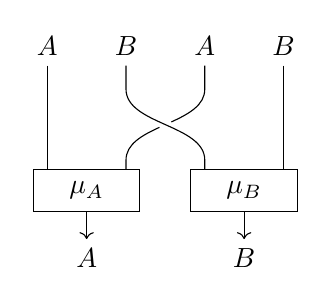
\begin{tikzpicture}[baseline=(braid)]
		\pic[
			braid/number of strands=4,
			braid/every strand/.style={black},
			name prefix=braid
		]
		at (0, 0) {braid = {s_2}};
		\coordinate (braid) at ($(braid-1-s)!0.5!(braid-1-e)$);
		\node[above] at (braid-1-s) {$A$};
		\node[above] at (braid-2-s) {$B$};
		\node[above] at (braid-3-s) {$A$};
		\node[above] at (braid-4-s) {$B$};
		
		\coordinate (MA) at ($(braid-1-e)!0.5!(braid-3-e)$);
		\draw[->] (MA) -- ($(MA) + (0, -2em)$) node[below] {$A$};
		\draw[fill=white] ([yshift=0.5em, xshift=-0.5em] braid-1-e) rectangle ([yshift=-1em, xshift=0.5em] braid-3-e);
		\node at ([yshift=-0.25em] MA) {$\mu_A$};
		
		\coordinate (MB) at ($(braid-2-e)!0.5!(braid-4-e)$);
		\draw[->] (MB) -- ($(MB) + (0, -2em)$) node[below] {$B$};
		\draw[fill=white] ([yshift=0.5em, xshift=-0.5em] braid-2-e) rectangle ([yshift=-1em, xshift=0.5em] braid-4-e);
		\node at ([yshift=-0.25em] MB) {$\mu_B$};
	\end{tikzpicture}\end{center}
	
	\item The unit $\eta_{A \otimes B}$ is the composite
	% segment-id: o014.li2.chapter7.monoidal-algebras.q004
	\[ \munit \xrightarrow[\sim]{\iota^{-1}} \munit \otimes \munit \xrightarrow{\eta_A \otimes \eta_B} A \otimes B. \]
\end{itemize}

% segment-id: o014.li2.chapter7.monoidal-algebras.p024
To verify that this is indeed an algebra, the conditions of
Definition~\ref{def:algebra-monoidal} can be reduced to the corresponding
properties of $(A,\mu_A,\eta_A)$ and $(B,\mu_B,\eta_B)$ using only $c$ (to
interchange the order of $\otimes$), $\iota$ (to duplicate the unit), and the
associativity constraints (to change the placement of parentheses).

% segment-id: o014.li2.chapter7.monoidal-algebras.p025
If $M$ is a left $A$-module and $N$ a left $B$-module, then $M\otimes N$
naturally becomes a left $(A\otimes B)$-module. Its construction and
verification are the same as in the preceding paragraph, using $c$ to
interchange positions. The case of right modules is similar.

% segment-id: o014.li2.chapter7.monoidal-algebras.p026
For the algebra $\munit$ defined in Remark~\ref{rem:unit-algebra}, it is clear
that $\munit\otimes A\simeq A\simeq A\otimes\munit$, with the isomorphisms
given by the unit constraints of $\mathcal{V}$.

% segment-id: o014.li2.chapter7.monoidal-algebras.r002
\begin{remark}\label{rem:Alg-otimes-functorial}
	The construction above is functorial in $A$ and $B$: if $A\to A'$ and
	$B\to B'$ are morphisms of algebras, then so is the corresponding morphism
	$A\otimes B\to A'\otimes B'$. Another lengthy but straightforward fact is
	that, when $A,B,C$ are all algebras, the associativity constraint
	$(A\otimes B)\otimes C\rightiso A\otimes(B\otimes C)$ is a morphism of
	algebras.
\end{remark}

% segment-id: o014.li2.chapter7.monoidal-algebras.le001
\begin{lemma}\label{prop:CAlg-mu}
	Let $A$ be an algebra over a braided monoidal category $\mathcal{V}$. Then
	$A$ is commutative if and only if its multiplication
	$\mu_A:A\otimes A\to A$ is a morphism of algebras.
\end{lemma}
% segment-id: o014.li2.chapter7.monoidal-algebras.pf001
\begin{proof}
	For $\mu_A$ to be a morphism of algebras, two conditions are required. The
	condition concerning the unit is equivalent to commutativity of
	% segment-id: o014.li2.chapter7.monoidal-algebras.g011
	\[\begin{tikzcd}[column sep=large]
		\munit \otimes \munit \arrow[d, "\iota"'] \arrow[r, "{\eta_A \otimes \eta_A}"] & A \otimes A \arrow[d, "{\mu_A}"] \\
		\munit \arrow[r, "{\eta_A}"'] & A
	\end{tikzcd}\]
	and this holds automatically because $A$ is an algebra. The remaining
	condition is commutativity of
	% segment-id: o014.li2.chapter7.monoidal-algebras.g012
	\begin{equation*}
		\begin{tikzcd}[column sep=large]
			(A \otimes A) \otimes (A \otimes A) \arrow[r, "{\mu_A \otimes \mu_A}"] \arrow[d, "{\mu_{A \otimes A}}"'] & A \otimes A \arrow[d, "{\mu_A}"] \\
			A \otimes A \arrow[r, "{\mu_A}"'] & A
		\end{tikzcd}
	\end{equation*}
	Identify the upper-left corner with
	$A\otimes(A\otimes A)\otimes A$ by the associativity constraints. By
	associativity of $\mu_A$, composition in the diagram along
	\begin{tikzpicture}[scale=0.5, baseline=(O)]
		\draw[->] (0, 0) -- (1, 0) -- (1, -0.7);
		\coordinate (O) at (0, -0.5);
	\end{tikzpicture}
	equals
	% segment-id: o014.li2.chapter7.monoidal-algebras.q005
	\[ A \otimes (A \otimes A) \otimes A \xrightarrow{\identity \otimes \mu_A \otimes \identity} A \otimes A \otimes A \xrightarrow{\text{multiplication}} A . \]
	On the other hand, the definition of $\mu_{A\otimes A}$ and the
	associativity of $\mu_A$ show that composition in the diagram along
	\begin{tikzpicture}[scale=0.5, baseline=(O)]
		\draw[->] (0, 0) -- (0, -0.7) -- (1, -0.7);
		\coordinate (O) at (0, -0.5);
	\end{tikzpicture}
	equals
	% segment-id: o014.li2.chapter7.monoidal-algebras.q006
	\[ A \otimes (A \otimes A) \otimes A \xrightarrow{\identity \otimes (\mu_A c(A,A) ) \otimes \identity} A \otimes A \otimes A \xrightarrow{\text{multiplication}} A . \]
	Thus $\mu_Ac(A,A)=\mu_A$ implies that the original diagram commutes, or
	equivalently that $\mu_A$ is a morphism of algebras.
	
	Conversely, let $f\in\left\{\mu_A,\mu_Ac(A,A)\right\}$. We have the
	elementary commutative diagram
	% segment-id: o014.li2.chapter7.monoidal-algebras.g013
	\[\begin{tikzcd}
		A \otimes (A \otimes A) \otimes A \arrow[r, "{\identity \otimes f \otimes \identity}"] & A \otimes A \otimes A \arrow[r, "{\text{multiplication}}"] & A . \\
		A \otimes A \arrow[u, "{\eta_A \otimes \identity \otimes \eta_A}"] \arrow[r, "f"'] & A \arrow[ru, "\identity"'] \arrow[u, "{\eta_A \otimes \identity \otimes \eta_A}"] &
	\end{tikzcd}\]
	If $\mu_A$ is a morphism of algebras, the preceding discussion shows that
	the first row gives the same composite for the two choices of $f$.
	Considering the second row then yields $\mu_A=\mu_Ac(A,A)$.
\end{proof}

% segment-id: o014.li2.chapter7.monoidal-algebras.le002
\begin{lemma}\label{prop:c-as-isom-alg}
	Let $A$ and $B$ be algebras over a symmetric monoidal category
	$\mathcal{V}$. Then $c(A,B):A\otimes B\to B\otimes A$ is an isomorphism
	of algebras.
\end{lemma}
% segment-id: o014.li2.chapter7.monoidal-algebras.pf002
\begin{proof}
	Two commutative diagrams must be verified for $c(A,B)$. The first is
	% segment-id: o014.li2.chapter7.monoidal-algebras.g014
	\[\begin{tikzcd}[row sep=tiny]
		& \munit \otimes \munit \arrow[ld, "\sim" sloped] \arrow[dd, "{c(\munit, \munit)}"] \arrow[r, "{\eta_A \otimes \eta_B}"] & A \otimes B \arrow[dd, "{c(A, B)}"] \\
		\munit & & \\
		& \munit \otimes \munit \arrow[lu, "\sim"' sloped] \arrow[r, "{\eta_B \otimes \eta_A}"'] & B \otimes A
	\end{tikzcd}\]
	Commutativity on the right follows from functoriality of $c$, while that
	on the left follows from compatibility of $c$ with the unit constraints
	\cite[(3.12)]{Li1}. For the second diagram, which says that $c(A,B)$
	preserves multiplication, the argument is based on symmetry of the
	braiding and is exactly the same as at the end of \cite[\S 7.4]{Li1}.
\end{proof}

% segment-id: o014.li2.chapter7.monoidal-algebras.pr001
\begin{proposition}
	Let $A$ and $B$ be commutative algebras over a symmetric monoidal category
	$\mathcal{V}$. Then $A\otimes B$ is also commutative.
\end{proposition}
% segment-id: o014.li2.chapter7.monoidal-algebras.pf003
\begin{proof}
	It is enough to show that the multiplication $\mu_{A\otimes B}$ is a
	morphism of algebras. Recall the definition of $\mu_{A\otimes B}$ and
	apply Lemma~\ref{prop:c-as-isom-alg} to $c(B,A)$, the commutativity
	assumptions on $A,B$ together with Lemma~\ref{prop:CAlg-mu} to
	$\mu_A,\mu_B$, and Remark~\ref{rem:Alg-otimes-functorial} on the
	functoriality of $\otimes$. Every part of the composite is then a
	morphism of algebras.
\end{proof}

% segment-id: o014.li2.chapter7.monoidal-algebras.p027
We have defined algebras, modules, and their morphisms. All these structures
form categories, with notation
% segment-id: o014.li2.chapter7.monoidal-algebras.t001
\begin{center}\begin{tabular}{|l|c|p{0.48\textwidth}|} \hline
	structure & category & condition \\ \hline
	algebra & $\cate{Alg}(\mathcal{V})$ & $\mathcal{V}$ is a monoidal category \\ \hline
	commutative algebra & $\cate{CAlg}(\mathcal{V})$ & $\mathcal{V}$ is a braided monoidal category \\ \hline
	left $A$-module & $A\dcate{Mod}$ & $A$ is an algebra \\ \hline
	right $B$-module & $\cated{Mod}B$ & $B$ is an algebra \\ \hline
	$(A,B)$-bimodule & $(A,B)\dcate{Mod}$ & $A$ and $B$ are algebras \\ \hline
\end{tabular}\end{center}
\index[sym1]{Alg@$\cate{Alg}(\cdot)$}
\index[sym1]{CAlg@$\cate{CAlg}(\cdot)$}
\index[sym1]{Mod}

% segment-id: o014.li2.chapter7.monoidal-algebras.p028
The preceding discussion also shows that $\cate{Alg}(\mathcal{V})$ and
$\cate{CAlg}(\mathcal{V})$ generally have less structure than
$\mathcal{V}$. Labeling the levels of structure by numbers, the situation can
be represented schematically as
% segment-id: o014.li2.chapter7.monoidal-algebras.g015
{\scriptsize
\[\begin{tikzcd}[row sep=small]
	0 & 1 & 2 & \infty \\
	\text{category} & \text{monoidal category} \arrow[l, "{\cate{Alg}}"'] & \text{braided monoidal category} \arrow[shift right, l, "{\cate{Alg}}"'] \arrow[shift left, bend left, ll, "{\cate{CAlg}}"'] & \text{symmetric monoidal category} \arrow[loop right, "{\cate{Alg}, \cate{CAlg}}"]
\end{tikzcd}\]
}
Moreover, whenever $\cate{Alg}(\mathcal{V})$ or
$\cate{CAlg}(\mathcal{V})$ becomes a monoidal category under $\otimes$, its
unit is always $\munit$.

% segment-id: o014.li2.chapter7.monoidal-algebras.p029
Recall that Lemma~\ref{prop:CAlg-mu} says that a commutative algebra over a
braided monoidal category $\mathcal{V}$ automatically gives an algebra over
the monoidal category $\cate{Alg}(\mathcal{V})$, by taking the multiplication
$A\otimes A\to A$ to be that of $A$. In fact, this is the only possible
choice. This leads to a simple, interesting, and important observation: there
is an equivalence of categories
% segment-id: o014.li2.chapter7.monoidal-algebras.e001
\begin{equation}\label{eqn:AlgAlg-CAlg}
	\cate{Alg}\left(\cate{Alg}(\mathcal{V}) \right) \simeq \cate{CAlg}(\mathcal{V}), \quad \mathcal{V}:\;\text{braided monoidal category}.
\end{equation}
These facts rest on the so-called \emph{Eckmann--Hilton argument}; their proof
is deliberately left as an exercise for this chapter, supplied with a hint.

% segment-id: o014.li2.chapter7.monoidal-algebras.e002
\begin{example}\label{eg:Cartesius-monoidal}
	Let the category $\mathcal{C}$ have finite products. In particular, it
	has an empty product, namely a terminal object, denoted by $\munit$. For
	every two objects $X,Y$ there is a canonical isomorphism
	$c(X,Y):X\times Y\rightiso Y\times X$. These data make
	$(\mathcal{C},\times)$ a symmetric monoidal category with unit $\munit$.
	We may discuss algebras over $\mathcal{C}$, also called monoid objects in
	$\mathcal{C}$\footnote{For categories of this kind,
	\cite[\S 4.11]{Li1} also discusses group objects, but the inverse property
	cannot be formulated in an arbitrary monoidal category.}, together with
	their commutative versions.
	\begin{itemize}
		\item If $\mathcal{C}=\cate{Set}$, the one-point set is the unit
		$\munit$. The corresponding algebras are monoids, and the
		corresponding commutative algebras are commutative monoids.
		\item If $\mathcal{C}=\cate{Top}$, the corresponding algebras are
		topological monoids, and the corresponding commutative algebras are
		commutative topological monoids.
	\end{itemize}
	
	On the other hand, let $\Bbbk$ be a commutative ring and give
	$\Bbbk\dcate{Mod}$ the structure of a symmetric monoidal category through
	$\otimes=\otimes_{\Bbbk}$, with $\Bbbk$ as the unit $\munit$ and the
	braiding determined by $x\otimes y\mapsto y\otimes x$. The corresponding
	algebras (or commutative algebras) are precisely algebras (or commutative
	algebras) in the usual algebraic sense; see
	\cite[Definition 7.1.1]{Li1}.
\end{example}

% segment-id: o014.li2.chapter7.monoidal-algebras.p030
In these concrete situations, the multiplication of an algebra $A$ is often
written directly as multiplication of elements $xy=x\cdot y$, and the unit
is directly identified with the element $1_A$, so that the notation
$\mu_A,\eta_A$ can be omitted.

% segment-id: o014.li2.chapter7.monoidal-algebras.e003
\begin{example}[Graded modules and graded algebras]\label{eg:graded-module}
	\index{graded module, graded algebra}
	Fix an abelian category $\mathcal{A}$ and a nonempty set $I$. An object of
	$\mathcal{A}^I$ is called an $I$-graded object and is written
	$M=(M^i)_{i\in I}$, while a morphism is written
	$(f^i:M^i\to N^i)_{i\in I}$. The object
	$M^i\in\Obj(\mathcal{A})$ (or the morphism
	$f^i\in\Mor(\mathcal{A})$) is customarily called the degree-$i$
	component of $M$ (or $f$). The special cases $I=\Z$ and $\Z^n$ have
	already been discussed repeatedly in \S\ref{sec:additive-cplx},
	\S\ref{sec:triangular-def}, \S\ref{sec:grading-filtration}, and elsewhere.
	
	For concreteness, take for the moment
	$\mathcal{A}:=\Bbbk\dcate{Mod}$, where $\Bbbk$ is a commutative ring.
	An $I$-graded object in $\mathcal{A}$ is also called an $I$-graded module.
	Suppose further that $I$ is a monoid. Define a bifunctor $\otimes$ on the
	category $\mathcal{A}^I$ by
	% segment-id: o014.li2.chapter7.monoidal-algebras.e004
	\begin{equation}\label{eqn:graded-module}
		(M \otimes N)^i := \bigoplus_{jk=i} M^j \otimes N^k, \quad (f \otimes g)^i := \bigoplus_{jk=i} f^j \otimes g^k .
	\end{equation}
	Also define $\munit$ to be $\Bbbk$ concentrated in the component
	$i=1_I$ (the unit of $I$). These data make $\mathcal{A}^I$ a monoidal
	category. The unit condition $\eta_A:\munit=\Bbbk\to A$ automatically
	% Editorial correction: the frozen Chinese source and Indonesian witness
	% say A^0, but the multiplicatively written grading monoid has unit 1_I.
	ensures that $1_A:=\eta_A(1)\in A^{1_I}$.
	
	In the special case where $I$ is commutative, this recovers the
	$I$-graded modules and $I$-graded algebras introduced in
	\cite[Definition 7.4.1]{Li1}.

	Continue to take $\mathcal{A}=\Bbbk\dcate{Mod}$ and require $(I,+)$ to
	be a commutative monoid. Every additive homomorphism
	$\epsilon:I\to\Z/2\Z$ makes $\Bbbk\dcate{Mod}^I$ a symmetric monoidal
	category with the \emph{Koszul braiding} characterized by
	% segment-id: o014.li2.chapter7.monoidal-algebras.e005
	\begin{equation}\label{eqn:Koszul-braiding}\begin{aligned}
		M^a \otimes N^b & \to N^b \otimes M^a \\
		x \otimes y & \mapsto (-1)^{\epsilon(a)\epsilon(b)} y \otimes x ,
	\end{aligned}\end{equation}
	where $a,b\in I$. The corresponding commutative algebras are precisely the
	$\epsilon$-commutative algebras of
	\cite[Definition 7.4.3]{Li1}. The various equations and definitions that
	result are collectively called the \emph{Koszul sign rule}. Whenever
	tensor positions are interchanged, the sign must be changed according to
	this rule.
	\index{Koszul sign rule}
	
	For example, the condition for $A$ to be a commutative algebra is written
	explicitly as
	% segment-id: o014.li2.chapter7.monoidal-algebras.q007
	\[ x y = (-1)^{\epsilon(a) \epsilon(b)} yx, \quad x \in A^a, \; y \in A^b. \]
	
	The typical situation is
	% segment-id: o014.li2.chapter7.monoidal-algebras.q008
	\[ I \in \{\Z, \Z_{\geq 0} \}, \quad \epsilon(a) := a \;\bmod 2 , \]
	where the corresponding $\epsilon$-commutative algebras are called
	anticommutative graded algebras in the source cited above. Since this
	braiding appears everywhere in the study of $\Z$-graded objects, the term
	\emph{graded commutative} is more apt.
	
	Now return to a general abelian category $\mathcal{A}$ and
	$(I,+,\epsilon)$ as above. To generalize the preceding construction, we
	need to extend $\mathcal{A}$ to a symmetric monoidal category
	$(\mathcal{A},\otimes)$ such that
	% segment-id: o014.li2.chapter7.monoidal-algebras.l004
	\begin{itemize}
		\item $\mathcal{A}$ is an abelian category, and coproducts (that is,
		direct sums) of the form in \eqref{eqn:graded-module} exist;
		\item $\otimes:\mathcal{A}\times\mathcal{A}\to\mathcal{A}$ is
		additive in each variable and preserves these coproducts.
	\end{itemize}
	Under these conditions, $\otimes$ and the Koszul braiding on
	$\mathcal{A}^I$ can still be defined in the same way, making
	$(\mathcal{A}^I,\otimes)$ a symmetric monoidal category. Its unit is
	still the unit $\munit$ of $\mathcal{A}$, viewed as an $I$-graded object
	concentrated in degree zero.
	
	For general $(\mathcal{A},\otimes)$, all verifications are the same as in
	the case of $\Bbbk\dcate{Mod}$. The only difference is that “elements” of
	an object no longer have meaning in the general case.
\end{example}

% segment-id: o014.li2.chapter7.monoidal-algebras.cv001
\begin{convention}
	In the special case $\mathcal{A}=\Bbbk\dcate{Mod}$, the usual convention
	is to regard an $I$-graded module $(M^i)_{i\in I}$ as a module equipped
	with a direct-sum decomposition $M=\bigoplus_{i\in I}M^i$, and to require
	morphisms to preserve the direct-sum components.
\end{convention}

% segment-id: o014.li2.chapter7.monoidal-algebras.e006
\begin{example}\label{eg:superspace}
	\index{super vector space}
	In the construction above ($\mathcal{A}=\Bbbk\dcate{Mod}$), let $\Bbbk$
	be a field with $\mathrm{char}(\Bbbk)\neq2$, take
	$I=\Z/2\Z=\{0,1\}$, and set $\epsilon=\identity_{\Z/2\Z}$. The
	corresponding symmetric monoidal category is denoted by
	$\cate{Vect}^-_{\Z/2\Z}(\Bbbk)$. Its objects can be viewed as
	$\Bbbk$-vector spaces equipped with a direct-sum decomposition
	$V=V_0\oplus V_1$, and are also called \emph{super vector spaces}. This is
	the source of terminology common in linear algebra and mathematical
	physics, such as superalgebra and commutative superalgebra.
\end{example}

% segment-id: o014.li2.chapter7.monoidal-algebras.p031
Finally, we discuss the effect of lax monoidal functors on algebras.

% segment-id: o014.li2.chapter7.monoidal-algebras.d005
\begin{definition}\label{def:lax-monoidal}
	\index{functor!monoidal, lax monoidal, right lax monoidal}
	Let $\mathcal{V}$ and $\mathcal{V}'$ be monoidal categories. According to
	\cite[Remark 3.1.8]{Li1}, a right lax monoidal functor from
	$\mathcal{V}$ to $\mathcal{V}'$, abbreviated here to a \emph{lax
	monoidal functor}, means data $(F,\xi_F,\varphi_F)$, where
	% Editorial correction: the frozen Chinese source and Indonesian witness
	% repeat the source category; the declared functor has codomain V'.
	$F:\mathcal{V}\to\mathcal{V}'$ is a functor and
	% segment-id: o014.li2.chapter7.monoidal-algebras.q009
	\[ \xi_F: F(\cdot) \otimes F(\cdot) \to F(\cdot \otimes \cdot), \quad \varphi_F: \munit_{\mathcal{V}'} \to F\left( \munit_{\mathcal{V}} \right), \]
	are morphisms subject to a collection of compatibility conditions with
	the monoidal structures. The data $(F,\xi_F,\varphi_F)$ are often
	abbreviated to $F$.
	
	If $\mathcal{V}$ and $\mathcal{V}'$ are both braided (or symmetric)
	monoidal categories, and $F$ also makes the following diagram commute,
	then $F$ is called a braided functor, or is said to be compatible with
	the braidings:
	% segment-id: o014.li2.chapter7.monoidal-algebras.g016
	\[\begin{tikzcd}[column sep=huge]
		F(X) \otimes F(Y) \arrow[r, "{\xi_F(X, Y)}"] \arrow[d, "{c'(FX, FY)}"'] & F(X \otimes Y) \arrow[d, "{Fc(X, Y)}"] \\
		F(Y) \otimes F(X) \arrow[r, "{\xi_F(Y, X)}"'] & F(Y \otimes X) .
	\end{tikzcd}\]

	If $\xi_F$ and $\varphi_F$ in the data of a lax monoidal functor are both
	isomorphisms, the functor is called a \emph{monoidal functor}.
\end{definition}

% segment-id: o014.li2.chapter7.monoidal-algebras.p032
We may of course also discuss morphisms between lax monoidal functors, also
called natural transformations:
% segment-id: o014.li2.chapter7.monoidal-algebras.q010
\[ \theta = (\theta_X)_{X \in \Obj(\mathcal{V})}: F \to G, \quad F, G: \mathcal{V} \to \mathcal{V}' . \]
In addition to the conditions for a natural transformation, we require
$\theta$ to make the following diagrams commute:
% segment-id: o014.li2.chapter7.monoidal-algebras.g017
\[\begin{tikzcd}[column sep=huge]
	F(X) \otimes F(Y) \arrow[r, "{\xi_F(X, Y)}"] \arrow[d, "{\theta_X \otimes \theta_Y}"'] & F(X \otimes Y) \arrow[d, "{\theta_{X \otimes Y}}"] \\
	G(X) \otimes G(Y) \arrow[r, "{\xi_G(X, Y)}"'] & G(X \otimes Y)
\end{tikzcd} \quad \begin{tikzcd}
	\munit_{\mathcal{V}'} \arrow[r, "{\varphi_F}"] \arrow[rd, "{\varphi_G}"'] & F(\munit_{\mathcal{V}}) \arrow[d, "{\theta_{\munit_{\mathcal{V}}}}"] \\
	& G(\munit_{\mathcal{V}}) .
\end{tikzcd}\]

If $F$ and $G$ are monoidal functors, this definition is in fact equivalent
to \cite[Definition 3.1.10]{Li1}, where $\varphi_F$ and $\varphi_G$ are
called “standard” isomorphisms. We may therefore discuss equivalences between
monoidal categories or braided monoidal categories.

% segment-id: o014.li2.chapter7.monoidal-algebras.pr002
\begin{proposition}\label{prop:lax-monoidal-Alg}
	A lax monoidal functor $F$ induces a functor
	$\cate{Alg}(\mathcal{V})\to\cate{Alg}(\mathcal{V}')$. If $A$ is an
	algebra over $\mathcal{V}$, then $F$ induces
	$A\dcate{Mod}\to F(A)\dcate{Mod}$, and similarly for the other module
	categories.

	If, in addition, $\mathcal{V}$ and $\mathcal{V}'$ are braided monoidal
	categories and $F$ is a braided functor, then $F$ also induces
	$\cate{CAlg}(\mathcal{V})\to\cate{CAlg}(\mathcal{V}')$, while
	$\cate{Alg}(\mathcal{V})\to\cate{Alg}(\mathcal{V}')$ is a lax monoidal
	functor. If, moreover, $\mathcal{V}$ and $\mathcal{V}'$ are both
	symmetric, then the same holds for
	$\cate{CAlg}(\mathcal{V})\to\cate{CAlg}(\mathcal{V}')$.
\end{proposition}
% segment-id: o014.li2.chapter7.monoidal-algebras.pf004
\begin{proof}
	Let $A$ be an algebra over $\mathcal{V}$. Define the multiplication
	$\mu_{FA}$ as
	$FA\otimes FA\to F(A\otimes A)\xrightarrow{F\mu_A}FA$, and the unit
	$\eta_{FA}$ as
	$\munit_{\mathcal{V}'}\to F(\munit_{\mathcal{V}})\xrightarrow{F\eta_A}FA$.
	The remaining verifications are routine.
\end{proof}

% segment-id: o014.li2.chapter7.monoidal-algebras.e007
\begin{example}\label{eg:ev0-monoidal}
	Consider the symmetric monoidal abelian category $\mathcal{A}$ and the
	category $\mathcal{A}^I$ from Example~\ref{eg:graded-module}. Define the
	functor
	% segment-id: o014.li2.chapter7.monoidal-algebras.q011
	\[ \mathrm{ev}_0: \mathcal{A}^I \to \mathcal{A}, \quad \left(M^i\right)_{i \in I} \mapsto M^0. \]
	This functor is exact and symmetric lax monoidal: simply take
	% segment-id: o014.li2.chapter7.monoidal-algebras.q012
	\[ \xi_{\mathrm{ev}_0}(M, N): M^0 \otimes N^0 \to (M \otimes N)^0 := \bigoplus_{i+j=0} M^i \otimes N^j \]
	to be the evident morphism, and
	$\varphi_{\mathrm{ev}_0}:\munit\to\munit$ to be the identity. Thus
	$A\mapsto A^0$ induces lax monoidal functors
	% segment-id: o014.li2.chapter7.monoidal-algebras.q013
	\[ \cate{Alg}(\mathcal{A}^I) \to \cate{Alg}(\mathcal{A}), \quad \cate{CAlg}(\mathcal{A}^I) \to \cate{CAlg}(\mathcal{A}). \]
\end{example}

% segment-id: o014.li2.chapter7.monoidal-algebras.p033
The following remark concerns algebras over a general monoidal category
$\mathcal{V}$. Recall that finite ordinals correspond bijectively to
$\Z_{\geq0}$; the finite ordinal $\mathbf{n}$ corresponding to $n$ is
identified with the totally ordered $n$-element set $\{0,\ldots,n-1\}$, with
$0\leq1\leq2\leq\cdots$.

% segment-id: o014.li2.chapter7.monoidal-algebras.r003
\begin{remark}[The walking algebra]\label{rem:walking-algebra}
	\index{algebra!walking}
	\index[sym1]{FinOrd@$\cate{FinOrd}$}
	A map $f:A\to B$ between partially ordered sets is called
	order-preserving if
	$a\leq a'\implies f(a)\leq f(a')$. Write $\cate{FinOrd}$ for the category
	of finite ordinals whose morphisms are order-preserving maps between
	ordinals. This is a strict monoidal category under
	$\mathbf{n}\otimes\mathbf{m}:=\mathbf{n}+\mathbf{m}$. A morphism
	$f\otimes g:\mathbf{n}\otimes\mathbf{m}\to\mathbf{n}'\otimes\mathbf{m}'$
	maps the first $n$ elements (or the last $m$ elements) by $f$ (or $g$),
	and the object $\mathbf{0}$ is the unit\footnote{Here $\mathbf{1}$ always
	denotes an ordinal; the unit of the monoidal category $\mathcal{V}$ is
	denoted separately by $\munit_{\mathcal{V}}$.}. Make $\mathbf{1}$ into
	an algebra over $\cate{FinOrd}$: take its unit to be
	$\emptyset=\mathbf{0}\hookrightarrow\mathbf{1}$ and its multiplication
	to be
	$\mathbf{1}\otimes\mathbf{1}=\mathbf{2}\twoheadrightarrow\mathbf{1}$.
	The associated commutative diagrams are entirely straightforward to
	verify.
	
	The ordinal $\mathbf{1}$ (or $\mathbf{2}$) may be viewed as the “walking”
	object (or morphism). Indeed, for any category $\mathcal{C}$, specifying
	a functor $\mathbf{1}\to\mathcal{C}$ (or
	$\mathbf{2}\to\mathcal{C}$) is equivalent to specifying an object (or a
	morphism) in $\mathcal{C}$. Now consider a monoidal category
	$\mathcal{V}$. We claim that there is an isomorphism of categories
	% segment-id: o014.li2.chapter7.monoidal-algebras.q014
	\[
		\left\{ \mathcal{V}\;\text{-algebras}\; A \right\} \simeq \left\{ \text{monoidal functors}\; F: \cate{FinOrd} \to \mathcal{V} \right\},
	\]
	which also means that $\cate{FinOrd}$ is the “walking algebra.” First, for
	a monoidal functor $F:\cate{FinOrd}\to\mathcal{V}$, define
	$A:=F(\mathbf{1})$. As a simple special case of
	Proposition~\ref{prop:lax-monoidal-Alg}, $A$ naturally becomes an algebra
	over $\mathcal{V}$: the multiplication $\mu:A\otimes A\to A$ is
	$F(\mathbf{2}\twoheadrightarrow\mathbf{1})$, while the unit
	$\eta:\munit_{\mathcal{V}}\to A$ is
	$F(\mathbf{0}\hookrightarrow\mathbf{1})$.
	
	Conversely, from an algebra $(A,\mu,\eta)$ over $\mathcal{V}$ define a
	monoidal functor $F:\cate{FinOrd}\to\mathcal{V}$ by
	% segment-id: o014.li2.chapter7.monoidal-algebras.q015
	\[ F(\mathbf{n}) = A^{\otimes n} := \underbracket{A \otimes (A \otimes (\cdots))}_{n\;\text{copies of}\; A}, \quad A^{\otimes 0} := \munit_{\mathcal{V}}, \]
	For $f:\mathbf{n}\to\mathbf{m}$, if $f$ is injective, then
	$F(f):A^{\otimes n}\to A^{\otimes m}$ is obtained by inserting
	$\eta:\munit_{\mathcal{V}}\to A$ outside the image of $f$; if $f$ is
	surjective, $F(f)$ is obtained by using $\mu:A\otimes A\to A$ to
	successively combine the factors in each fiber. The associativity
	constraints and other properties of a monoidal category ensure that
	these operations are well defined. A general map $f$ has a unique
	surjective--injective factorization, and this defines $F$ on morphisms.
	Functoriality is clear. It is not difficult to verify that the two
	constructions are mutually inverse.
\end{remark}

% Unit 089 English translation of chapter7.tex lines 419--610.
% Source: Methods of Algebra, Volume 2, commit
% 9a5803ff77dd3257484cb177f851a73770a59dd3 (CC BY 4.0).
% stable-unit-id: o014.aljabr2.chapter7.differential-graded-structures
% Scope: all of Section 7.2, “Example: Differential Graded Structures”;
% stops immediately before Section 7.3 at source line 611.

% segment-id: o014.li2.chapter7.differential-graded-structures.h001
\section{Example: Differential Graded Structures}\label{sec:dga-monoidal}
\hypertarget{o014.aljabr2.chapter7.differential-graded-structures}{ }
% segment-id: o014.li2.chapter7.differential-graded-structures.p001
Continuing the discussion in Example~\ref{eg:graded-module}, consider a
symmetric monoidal abelian category $(\mathcal{A}, \otimes)$ that admits
countable coproducts. Throughout this section we also assume that $\otimes$
is right exact in each variable. The standard example is, of course,
$\mathcal{A}=\Bbbk\dcate{Mod}$.

% segment-id: o014.li2.chapter7.differential-graded-structures.p002
We previously discussed $\Z$-graded algebras over $\mathcal{A}$, or,
equivalently, algebras over the monoidal category
$(\mathcal{A}^{\Z},\otimes)$. More precisely, in the setting of
Example~\ref{eg:graded-module}, this means taking $I=\Z$ and the Koszul
braiding~\eqref{eqn:Koszul-braiding} corresponding to
$\epsilon(a)=a\bmod\;2$. Henceforth, “graded” always means
“$\Z$-graded.” The aim of this section is to add a “differential” structure;
part of the discussion overlaps with \S\ref{sec:multiplicative-SS}.

% segment-id: o014.li2.chapter7.differential-graded-structures.p003
Define the shift functor $T:\mathcal{A}^{\Z}\to\mathcal{A}^{\Z}$ by
$(TM)^n=M^{n+1}$ and $(Tf)^n=f^{n+1}$. Thus
$\left(\mathcal{A}^{\Z},T\right)$ is an abelian category with translation,
and a differential object over it (Definition~\ref{def:differential-object})
is called a \emph{differential graded object} over $\mathcal{A}$. In fact,
the abelian category $\left(\mathcal{A}^{\Z},T\right)_d$ of differential
graded objects is canonically isomorphic to the category of complexes
$\cate{C}(\mathcal{A})$. This has already been observed in
\S\ref{sec:additive-cplx}.
\index{differential graded object}

% segment-id: o014.li2.chapter7.differential-graded-structures.p004
Accordingly, from now on we identify differential graded objects over
$\mathcal{A}$ with complexes, without distinguishing between the two.

% segment-id: o014.li2.chapter7.differential-graded-structures.p005
We next equip $\cate{C}(\mathcal{A})$ with a symmetric monoidal structure.
For any complexes $M$ and $N$, the bifunctor
$\otimes:\mathcal{A}\times\mathcal{A}\to\mathcal{A}$ gives the double
complex $M^\bullet\otimes N^\bullet$; totalization by direct sums gives
% segment-id: o014.li2.chapter7.differential-graded-structures.q001
\[ M \otimes N := \tot_{\oplus}\left( M^\bullet \otimes N^\bullet \right), \quad (M \otimes N)^n = \bigoplus_{a+b=n} M^a \otimes N^b. \]

% segment-id: o014.li2.chapter7.differential-graded-structures.p006
In the example $\mathcal{A}=\Bbbk\dcate{Mod}$, the differential
$d=d_{M\otimes N}$ on the complex (or, equivalently, on the differential
object) can be written elementwise as
% segment-id: o014.li2.chapter7.differential-graded-structures.q002
\begin{equation*}
	d(x \otimes y) = (d_M x) \otimes y + (-1)^a x \otimes (d_N y), \quad x \in M^a, \; y \in N^b.
\end{equation*}
With these definitions, the Koszul braiding~\eqref{eqn:Koszul-braiding}
is a morphism of complexes. The reader may verify this directly or deduce it
from Proposition~\ref{prop:double-cplx-swap}.

% segment-id: o014.li2.chapter7.differential-graded-structures.p007
Moreover, the unit object $\munit$ of $(\mathcal{A},\otimes)$, viewed as a
complex concentrated in degree zero, is clearly the unit object of the
monoidal category $(\cate{C}(\mathcal{A}),\otimes)$. The following fact is
immediate: for every
$X=(X^n,d_X^n)_n\in\Obj(\cate{C}(\mathcal{A}))$,
% segment-id: o014.li2.chapter7.differential-graded-structures.q003
\begin{equation}\label{eqn:unit-map-into-cplx}
	\Hom_{\cate{C}(\mathcal{A})}(\munit, X) \simeq \Hom_{\mathcal{A}}\left( \munit, \Ker\left(d_X^0 \right) \right).
\end{equation}

% segment-id: o014.li2.chapter7.differential-graded-structures.d001
\begin{definition}\label{def:dg-algebra}
	\index{differential graded algebra}
	\index{dg algebra}
	With respect to the symmetric monoidal structure above, the objects of
	$\cate{Alg}\left(\cate{C}(\mathcal{A})\right)$ are called
	\emph{differential graded algebras} over $\mathcal{A}$, abbreviated
	\emph{dg algebras}; the objects of
	$\cate{CAlg}\left(\cate{C}(\mathcal{A})\right)$ are called commutative
	differential graded algebras over $\mathcal{A}$, abbreviated commutative
	dg algebras.
\end{definition}

% segment-id: o014.li2.chapter7.differential-graded-structures.p008
For a differential graded algebra $A$, one can therefore also speak of left
(or right) $A$-modules $M$, and even of bimodules; each forms an abelian
category. In this setting $M$ is also called a \emph{differential graded
module} over $A$, abbreviated a \emph{dg module}. This notion combines the
theory of complexes with module theory and is extremely useful. The exercises
in this chapter give a further introduction; the reader may also consult
monographs such as \cite{Yek20}. To emphasize the differential graded
structure, we write the category of dg modules as $A\dcate{dgMod}$, and use
analogous notation for its variants.
\index{differential graded module}
\index{dg module}
\index[sym1]{A-dgMod@$A\dcate{dgMod}$}

% segment-id: o014.li2.chapter7.differential-graded-structures.p009
The forgetful functor $\cate{C}(\mathcal{A})\to\mathcal{A}^{\Z}$ preserves
$\otimes$, so Proposition~\ref{prop:lax-monoidal-Alg} shows that it preserves
algebra (or commutative algebra) structures. When
$\mathcal{A}=\Bbbk\dcate{Mod}$, to say that $A$ is a dg algebra is precisely
to say that $A$ is a graded algebra equipped with a differential $d$ whose
multiplication satisfies the Leibniz rule
% segment-id: o014.li2.chapter7.differential-graded-structures.q004
\[ d(xy) = (dx)y + (-1)^a x (dy), \quad x \in A^a, \; y \in A^b. \]
Substituting $x=1_A=y$ gives $d(1_A)=0$. The opposite algebra $A^{\opp}$ is
obtained by replacing the multiplication with
$x\mathbin{\cdot^{\opp}}y:=(-1)^{ab}yx$.

% segment-id: o014.li2.chapter7.differential-graded-structures.p010
Similarly, when $\mathcal{A}=\Bbbk\dcate{Mod}$, a left $A$-module $M$ is
equivalently a graded $\Bbbk$-module $M$ with a scalar-multiplication morphism
$A\otimes M\to M$ satisfying associativity and the other module axioms, and
equipped with a differential $d$ satisfying the Leibniz rule
% segment-id: o014.li2.chapter7.differential-graded-structures.q005
\[ d(tm) = (dt)m + (-1)^a t (dm), \quad t \in A^a, \; m \in M^b; \]
for a right $A$-module $M$, the Leibniz rule becomes
% segment-id: o014.li2.chapter7.differential-graded-structures.q006
\[ d(mt) = (dm)t + (-1)^b m (dt), \quad t \in A^a, \; m \in M^b. \]
For a general $(\mathcal{A},\otimes)$, all these properties can be formulated
without elements. For example, the unit of an algebra $A$ corresponds to a
morphism $\munit\to\Ker\left(d_A^0\right)$ in $\mathcal{A}$; see
\eqref{eqn:unit-map-into-cplx}.

% segment-id: o014.li2.chapter7.differential-graded-structures.p011
Taking cohomology gives an additive functor
$\Hm=(\Hm^n)_{n\in\Z}:\cate{C}(\mathcal{A})\to\mathcal{A}^{\Z}$. The next
result says that multiplication of complexes induces multiplication on
cohomology.

% segment-id: o014.li2.chapter7.differential-graded-structures.pr001
\begin{proposition}\label{prop:Hm-lax-monoidal}
	The functor $\Hm$ induces
	% segment-id: o014.li2.chapter7.differential-graded-structures.q007
	\[ \cate{Alg}\left(\cate{C}(\mathcal{A})\right) \to \cate{Alg}\left(\mathcal{A}^{\Z}\right),
	\quad \cate{CAlg}\left(\cate{C}(\mathcal{A})\right) \to \cate{CAlg}\left(\mathcal{A}^{\Z}\right). \]
	If $A$ is a dg algebra and $M$ is a left $A$-module (or a right module, or
	a bimodule), then $\Hm(M)$ is respectively a left $\Hm(A)$-module (or a
	right module, or a bimodule).
\end{proposition}
% segment-id: o014.li2.chapter7.differential-graded-structures.pf001
\begin{proof}
	By Proposition~\ref{prop:lax-monoidal-Alg}, it suffices to prove that $\Hm$
	is a lax monoidal functor. The required canonical morphism
	% segment-id: o014.li2.chapter7.differential-graded-structures.q008
	\[ \xi_{\Hm}(M, N): \Hm(M) \otimes \Hm(N) \to \Hm(M \otimes N), \]
	is nearly tautological: it is the morphism $\kappa$ discussed in
	Theorem~\ref{prop:Kunneth-homology} or Proposition~\ref{prop:bifunctor-cup}.
	On the other hand, take
	% segment-id: o014.li2.chapter7.differential-graded-structures.q009
	\[ \varphi_{\Hm}: \munit \to \Hm(\munit) = \munit \quad \text{(concentrated in degree zero)} \]
	to be $\identity$.
\end{proof}

% segment-id: o014.li2.chapter7.differential-graded-structures.p012
We may also take the lax monoidal functor
$\mathrm{ev}_0:\mathcal{A}^{\Z}\to\mathcal{A}$ of
Example~\ref{eg:ev0-monoidal}. Again, Proposition~\ref{prop:lax-monoidal-Alg}
shows that it sends graded algebras (or graded commutative algebras) to
algebras (or commutative algebras), and modules to modules. Observe that
$\mathrm{ev}_0\Hm=\Hm^0$. In applications, each stage of the composite
$\cate{C}(\mathcal{A})\xrightarrow{\Hm}\mathcal{A}^{\Z}
\xrightarrow{\mathrm{ev}_0}\mathcal{A}$ discards information; the richest
structure remains on the dg algebra itself.

% segment-id: o014.li2.chapter7.differential-graded-structures.eg001
\begin{example}\label{eg:k-linear-A-enrich}
	Let $\Bbbk$ be a commutative ring. For any $\Bbbk$-linear category
	$\mathcal{A}$, consider the multiplication on the Hom complexes from
	\eqref{eqn:Hom-cplx-multiplication}:
	% segment-id: o014.li2.chapter7.differential-graded-structures.q010
	\[ \Hom^a(Y, Z) \times \Hom^b(X, Y) \to \Hom^{a+b}(X, Z), \quad X, Y, Z \in \Obj(\cate{C}(\mathcal{A})). \]

	Because this multiplication satisfies the Leibniz rule
	(Lemma~\ref{prop:Hom-cplx-Leibniz}), it determines a morphism in
	$\cate{C}(\Bbbk\dcate{Mod})$
	% segment-id: o014.li2.chapter7.differential-graded-structures.q011
	\[ \Hom^\bullet(Y, Z) \otimes \Hom^\bullet(X, Y) \to \Hom^\bullet(X, Z). \]
	Moreover, the multiplication is associative, so
	$\End^\bullet(X):=\Hom^\bullet(X,X)$ is an algebra over
	$(\cate{C}(\Bbbk\dcate{Mod}),\otimes)$ with unit
	$\identity_X\in\End^0(X)$. Furthermore, $\Hom^\bullet(X,Y)$ is an
	$(\End^\bullet(Y),\End^\bullet(X))$-bimodule.

	Taking the cohomology $\Hm=(\Hm^n)_n$ of $\Hom^\bullet(X,Y)$ gives only
	% segment-id: o014.li2.chapter7.differential-graded-structures.q012
	\[ \bigoplus_{n \in \Z} \Hom_{\cate{K}(\mathcal{A})}(X, Y[n]); \]
	whereas applying \eqref{eqn:unit-map-into-cplx} to
	$\Hom^\bullet(X,Y)$ shows that $\Hom_{\cate{C}(\mathcal{A})}$ can be
	reconstructed as
	% segment-id: o014.li2.chapter7.differential-graded-structures.q013
	\[ \Hom_{\cate{C}(\Bbbk\dcate{Mod})}\left( \Bbbk, \Hom^\bullet(X, Y) \right) \simeq \Hom_{\cate{C}(\mathcal{A})}(X, Y)  \]
	with $\Bbbk$ serving as the unit object of
	$(\cate{C}(\Bbbk\dcate{Mod}),\otimes)$.
\end{example}

% segment-id: o014.li2.chapter7.differential-graded-structures.p013
Thus the sets $\Hom_{\cate{C}(\mathcal{A})}$ and composition of morphisms in
$\cate{C}(\mathcal{A})$ are merely shadows of the Hom complexes and their
multiplication, obtained by applying
$\Hom_{\cate{C}(\Bbbk\dcate{Mod})}(\Bbbk,\mathord\cdot)$.

\index{enriched category}
\index[sym1]{Hom-internal@$\iHom$}
% segment-id: o014.li2.chapter7.differential-graded-structures.p014
Starting from the example $\cate{C}(\mathcal{A})$, we are naturally led to
the concept of a differential graded category. This concept involves the
\emph{$\mathcal{V}$-enriched categories} introduced in
\cite[Definition 3.4.1]{Li1}. Briefly, for any monoidal category
$\mathcal{V}$, a $\mathcal{V}$-enriched category $\mathcal{C}$ still has
objects and morphisms, but the Hom sets are replaced by Hom objects in
$\mathcal{V}$, written $\iHom=\iHom_{\mathcal{C}}$ to distinguish them.
Composition of morphisms is replaced by a morphism in $\mathcal{V}$
% segment-id: o014.li2.chapter7.differential-graded-structures.q014
\[ \iHom(Y, Z) \otimes \iHom(X, Y) \to \iHom(X, Z), \]
while an identity morphism $\identity_X\in\Hom(X,X)$ is replaced by
$\identity_X:\munit\to\iHom(X,X)$. These are all morphisms in $\mathcal{V}$,
and their properties are expressed by commutative diagrams in $\mathcal{V}$.

% segment-id: o014.li2.chapter7.differential-graded-structures.p015
For enriched versions of functors and morphisms between them, see
\cite[Definitions 3.4.1, 3.4.2, 3.4.4]{Li1}. They are defined in the expected
way; in brief, an enriched functor lifts maps between Hom sets to morphisms
between $\iHom$ objects.

% segment-id: o014.li2.chapter7.differential-graded-structures.p016
For example, a $\Bbbk\dcate{Mod}$-category is precisely a category enriched
over $(\Bbbk\dcate{Mod},\otimes)$.

% segment-id: o014.li2.chapter7.differential-graded-structures.p017
Conversely, let us temporarily call a category without enrichment an ordinary
category. If set-theoretic size issues are ignored, an ordinary category is
the same thing as a category enriched over $(\cate{Set},\times)$.

% segment-id: o014.li2.chapter7.differential-graded-structures.d002
\begin{definition}\label{def:dgCat}
	\index{differential graded category}
	\index{dg category}
	Let $\Bbbk$ be a commutative ring, and consider the corresponding symmetric
	monoidal category $(\cate{C}(\Bbbk\dcate{Mod}),\otimes)$. A category
	enriched over $(\cate{C}(\Bbbk\dcate{Mod}),\otimes)$ is called a
	\emph{differential graded category} over $\Bbbk$, abbreviated a
	\emph{dg category} over $\Bbbk$. Functors between such categories and
	morphisms between those functors are defined as for enriched
	categories.\footnote{Much of the literature on infinity categories uses
	the term DG-category, as well as the notation $\cate{DGCat}$ for the
	category they form, and this notation may overlap with that of this book.
	Although those DG-categories are closely related to the dg categories
	discussed here, the two are not the same notion.}
\end{definition}

% segment-id: o014.li2.chapter7.differential-graded-structures.p018
By definition, an object $X$ of a dg category gives a dg algebra
$\End^\bullet(X)$.

% segment-id: o014.li2.chapter7.differential-graded-structures.eg002
\begin{example}\label{eg:CA-dg-cat}
	Example~\ref{eg:k-linear-A-enrich} says that $\cate{C}(\mathcal{A})$
	naturally becomes a dg category over $\Bbbk$ for any $\Bbbk$-linear
	category $\mathcal{A}$. For example, for every $\Bbbk$-algebra $R$, the
	category of complexes of left (or right) $R$-modules is automatically a
	dg category over $\Bbbk$.
\end{example}

% segment-id: o014.li2.chapter7.differential-graded-structures.eg003
\begin{example}\label{eg:dg-Hom-cplx}
	\index{Hom complex}
	\index[sym1]{Hom-A-bullet@$\Hom^{\bullet}_A$}
	Let $\Bbbk$ be a commutative ring and let $A$ be a dg algebra over
	$\mathcal{A}:=\Bbbk\dcate{Mod}$. For left $A$-modules $M$ and $N$, define
	the following subcomplex of $\Hom^\bullet_{\Bbbk}(M,N)$:
	% segment-id: o014.li2.chapter7.differential-graded-structures.q015
	\[ \Hom^p_A(M, N) := \left\{\begin{array}{r|l}
		f \in \Hom^p_{\Bbbk}(M, N) & \forall m \in M, \; \forall k \in \Z, \; \forall t \in A^k, \\
		& f(tm) = (-1)^{pk} tf(m)
	\end{array}\right\}. \]
	For left $A$-modules $L$, $M$, and $N$, composition on the Hom complexes
	$\Hom^\bullet_{\Bbbk}$ induces a morphism of complexes
	% segment-id: o014.li2.chapter7.differential-graded-structures.q016
	\[ \Hom^p_A(M, N) \otimes \Hom^q_A(L, M) \to \Hom^{p+q}_A(L, N). \]
	Thus the category $A\dcate{dgMod}$ of left $A$-modules is enriched to a dg
	category. For right $A$-modules, the condition in the definition of
	$\Hom^p_A(M,N)$ must be replaced by $f(mt)=f(m)t$ (think about why).
	Bimodules are handled similarly.

	The definition above can also be formulated without reference to elements,
	and therefore extends to a general $\mathcal{A}$.
\end{example}

% segment-id: o014.li2.chapter7.differential-graded-structures.p019
More precisely, a dg category enriches every Hom set of the underlying
ordinary category to a Hom complex $\Hom^\bullet$, while dg versions of
functors and their morphisms must be formulated inside
$\cate{C}(\Bbbk\dcate{Mod})$. Explicitly:
% segment-id: o014.li2.chapter7.differential-graded-structures.l001
\begin{itemize}
	\item A \emph{dg functor} $F:\mathcal{C}\to\mathcal{D}$ between dg
	categories consists of a map of object sets
	$F:\Obj(\mathcal{C})\to\Obj(\mathcal{D})$ and morphisms of Hom complexes
	$\Hom^\bullet_{\mathcal{C}}(X,Y)\to
	\Hom^\bullet_{\mathcal{D}}(FX,FY)$. The latter are morphisms in
	$\cate{C}(\Bbbk\dcate{Mod})$ and are required to make both diagrams below
	commute:
	% segment-id: o014.li2.chapter7.differential-graded-structures.q017
	\begin{equation*}\begin{gathered}
		\begin{tikzcd}[column sep=small]
			\Hom_{\mathcal{C}}^\bullet(Y, Z) \otimes \Hom_{\mathcal{C}}^\bullet(X, Y) \arrow[r] \arrow[d] & \Hom_{\mathcal{C}}^\bullet(X, Z) \arrow[d] \\
			\Hom_{\mathcal{D}}^\bullet(FY, FZ) \otimes \Hom_{\mathcal{D}}^\bullet(FX, FY) \arrow[r] & \Hom_{\mathcal{D}}^\bullet(FX, FZ)
		\end{tikzcd} \\
		\begin{tikzcd}[column sep=small]
			\Bbbk \arrow[r] \arrow[rd] & \Hom_{\mathcal{C}}^\bullet(X, X) \arrow[d] \\
			& \Hom_{\mathcal{D}}^\bullet(FX, FX) ;
		\end{tikzcd}
	\end{gathered}\end{equation*}
	\index{dg functor}
	\item In the classical sense, a morphism, or natural transformation,
	$\phi$ between dg functors $F,G:\mathcal{C}\to\mathcal{D}$ is a family of
	elements
	% segment-id: o014.li2.chapter7.differential-graded-structures.q018
	\begin{multline*}
		\phi_X \in \Ker\left[ \Hom_{\mathcal{D}}^0(FX, GX) \to \Hom_{\mathcal{D}}^1(FX, GX) \right] \\
		\xlongequal{\text{\eqref{eqn:unit-map-into-cplx}}} \Hom_{\cate{C}(\Bbbk\dcate{Mod})}\left(\Bbbk, \Hom_{\mathcal{D}}^\bullet(FX, GX) \right) ,
	\end{multline*}
	indexed by $X\in\Obj(\mathcal{C})$, such that for every $m\in\Z$ and
	$f\in\Hom_{\mathcal{C}}^m(X,Y)$,
	% segment-id: o014.li2.chapter7.differential-graded-structures.q019
	\[ (Gf) \phi_X = \phi_Y (Ff) \; \in \Hom_{\mathcal{D}}^m(FX, GY), \]
	where multiplication means multiplication in the Hom complex.
\end{itemize}
Thus one may speak of isomorphisms, equivalences, adjunctions, and other
notions for dg categories. An element of $\Hom^n_{\mathcal{C}}(X,Y)$ is
sometimes called a \emph{morphism of degree $n$} from $X$ to $Y$.

% segment-id: o014.li2.chapter7.differential-graded-structures.p020
For a general monoidal category $\mathcal{V}$, one may view
$\Hom_{\mathcal{V}}(\munit,M)$ as the set of “elements” of
$M\in\Obj(\mathcal{V})$; this is at least natural when
$\mathcal{V}=\cate{Set}$ or $\Bbbk\dcate{Mod}$. Following this idea, every
$\mathcal{V}$-enriched category $\mathcal{C}$ has an underlying ordinary
category defined by
% segment-id: o014.li2.chapter7.differential-graded-structures.q020
\[ \Hom_{\mathcal{C}}(X, Y) := \Hom_{\mathcal{V}}\left( \munit, \iHom_{\mathcal{C}}(X, Y) \right), \]
and we continue to denote that ordinary category by $\mathcal{C}$; see
\cite[Remark 3.4.3]{Li1} for details. In the example of the dg category
$\cate{C}(\mathcal{A})$, the resulting ordinary category is the ordinary
category of complexes $\cate{C}(\mathcal{A})$. Thus our notation is
consistent.

% segment-id: o014.li2.chapter7.differential-graded-structures.p021
Another operation comes from lax monoidal functors. Here is the general
statement.

% segment-id: o014.li2.chapter7.differential-graded-structures.pr002
\begin{proposition}\label{prop:lax-monoidal-enriched}
	Let $F:\mathcal{V}\to\mathcal{V}'$ be a lax monoidal functor between
	monoidal categories. For every $\mathcal{V}$-enriched category
	$\mathcal{C}$, define a $\mathcal{V}'$-enriched category $F(\mathcal{C})$
	as follows: set $\Obj(F(\mathcal{C}))=\Obj(\mathcal{C})$, and for every
	pair of objects $X,Y$, set
	% segment-id: o014.li2.chapter7.differential-graded-structures.q021
	\begin{gather*}
		\iHom_{F(\mathcal{C})}(X, Y) := F\iHom_{\mathcal{C}}(X, Y), \\
		\identity_X: \munit_{\mathcal{V}'} \xrightarrow{\varphi_F} F(\munit_{\mathcal{V}}) \to F\iHom_{\mathcal{C}}(X, X).
	\end{gather*}
	Composition is defined by
	% segment-id: o014.li2.chapter7.differential-graded-structures.q022
	\begin{multline*}
		F\iHom_{\mathcal{C}}(Y, Z) \otimes F\iHom_{\mathcal{C}}(X, Y) \\
		\xrightarrow{\xi_F} F\left( \iHom_{\mathcal{C}}(Y, Z) \otimes \iHom_{\mathcal{C}}(X, Y) \right)
		\to F\iHom_{\mathcal{C}}(X, Z),
	\end{multline*}
	and on the corresponding ordinary categories this construction gives an
	ordinary functor $\mathcal{C}\to F(\mathcal{C})$.
\end{proposition}
% segment-id: o014.li2.chapter7.differential-graded-structures.pf002
\begin{proof}
	The lax monoidal structure $(F,\xi_F,\varphi_F)$ supplies all properties
	required of composition. On the level of ordinary categories, the functor
	is the identity on objects and sends a morphism
	$f:\munit_{\mathcal{V}}\to\iHom_{\mathcal{C}}(X,Y)$ to the composite
	$\munit_{\mathcal{V}'}\xrightarrow{\varphi_F}F(\munit_{\mathcal{V}})
	\xrightarrow{Ff}F\iHom_{\mathcal{C}}(X,Y)$.
\end{proof}

% segment-id: o014.li2.chapter7.differential-graded-structures.p022
Comparing this construction with that of
Proposition~\ref{prop:lax-monoidal-Alg}, we see that
% Editorial correction: F(C) is enriched over V', so its endomorphism algebra
% lies in Alg(V'); the frozen Chinese source and Indonesian witness say Alg(V).
$\iHom_{F(\mathcal{C})}(X,X)$, as an object of $\cate{Alg}(\mathcal{V}')$,
is induced from $\iHom_{\mathcal{C}}(X,X)$; the same applies to the bimodule
structures on $\iHom$.

% segment-id: o014.li2.chapter7.differential-graded-structures.r001
\begin{remark}\label{rem:dg-homotopy-cat}
	\index{homotopy category}
	Proposition~\ref{prop:lax-monoidal-enriched} gives another way to pass from
	a dg category to an ordinary category. Apply the lax monoidal functor $\Hm$
	of Proposition~\ref{prop:Hm-lax-monoidal} to any dg category $\mathcal{C}$
	over $\Bbbk$. The result is a category $\Hm(\mathcal{C})$ enriched over
	$(\Bbbk\dcate{Mod}^{\Z},\otimes)$, satisfying
	% segment-id: o014.li2.chapter7.differential-graded-structures.q023
	\[ \Obj(\Hm(\mathcal{C})) = \Obj(\mathcal{C}), \quad \iHom_{\Hm(\mathcal{C})}(X, Y) = \left( \Hm^n \Hom^\bullet(X, Y) \right)_{n \in \Z}. \]
	Taking the degree-$0$ part, or equivalently applying the lax monoidal
	functor $\Hm^0$ to $\mathcal{C}$, produces an ordinary
	$\Bbbk\dcate{Mod}$-category called the \emph{homotopy category}
	$\mathrm{h}(\mathcal{C})$ of $\mathcal{C}$. It satisfies
	% segment-id: o014.li2.chapter7.differential-graded-structures.q024
	\[ \Obj(\mathrm{h}\mathcal{C}) = \Obj(\mathcal{C}), \quad \Hom_{\mathrm{h}\mathcal{C}}(X, Y) = \Hm^0 \Hom^\bullet(X, Y). \]
	In the special case $\mathcal{C}=\cate{C}(\mathcal{A})$, substituting
	Definition~\ref{def:cplx-homotopy-cat} immediately gives
	% segment-id: o014.li2.chapter7.differential-graded-structures.q025
	\[ \mathrm{h}(\cate{C}(\mathcal{A})) = \cate{K}(\mathcal{A}). \]
\end{remark}

% segment-id: o014.li2.chapter7.differential-graded-structures.p023
As seen above, the world of dg categories supports many homotopy-flavored
operations. Their meaning ultimately has to be explained through
applications and also involves the abstract language of model categories.
We give only a brief outline of some elementary notions, without developing
them further.

% segment-id: o014.li2.chapter7.differential-graded-structures.d003
\begin{definition}
	Let $F:\mathcal{C}\to\mathcal{D}$ be a dg functor between dg categories.
	If
	% segment-id: o014.li2.chapter7.differential-graded-structures.q026
	\[ \Hom^\bullet_{\mathcal{C}}(X, Y) \to \Hom^\bullet_{\mathcal{D}}(FX, FY) \]
	is a quasi-isomorphism for all $X,Y\in\Obj(\mathcal{C})$, then $F$ is
	called \emph{quasi-fully faithful}. If the induced functor
	$\mathrm{h}F:\mathrm{h}\mathcal{C}\to\mathrm{h}\mathcal{D}$ is
	essentially surjective, then $F$ is called \emph{quasi-essentially
	surjective}. A dg functor that is both quasi-fully faithful and
	quasi-essentially surjective is called a \emph{quasi-equivalence}.
\end{definition}

% segment-id: o014.li2.chapter7.differential-graded-structures.p024
Thus quasi-equivalent dg categories $\mathcal{C}$ and $\mathcal{D}$ have
equivalent homotopy categories.

% segment-id: o014.li2.chapter7.differential-graded-structures.p025
We continue this brief discussion of dg categories in \S\ref{sec:dg-closed}.

% English translation of chapter7.tex lines 611--711.
% Source: Methods of Algebra, Volume 2, commit
% 9a5803ff77dd3257484cb177f851a73770a59dd3 (CC BY 4.0).
% stable-unit-id: o014.aljabr2.chapter7.closed-monoidal-categories
% Coverage: all of Section 7.3 on closed monoidal categories; ends immediately
% before Section 7.4 at line 712.

% segment-id: o014.aljabr2.chapter7.closed-monoidal-categories.h001
\section{Closed Monoidal Categories}\label{sec:closed-monoidal}
\hypertarget{o014.aljabr2.chapter7.closed-monoidal-categories}{ }

% segment-id: o014.aljabr2.chapter7.closed-monoidal-categories.p001
Let $\Bbbk$ be a commutative ring. Then $\Bbbk\dcate{Mod}$ is a symmetric
monoidal category under $\otimes:=\otimes_{\Bbbk}$. It has the following
closedness properties.
% segment-id: o014.aljabr2.chapter7.closed-monoidal-categories.l001
\begin{itemize}
% segment-id: o014.aljabr2.chapter7.closed-monoidal-categories.i001
	\item It is enriched over itself: the set of homomorphisms $\Hom(X,Y)$
	naturally has the structure of a $\Bbbk$-module;
% segment-id: o014.aljabr2.chapter7.closed-monoidal-categories.i002
	\item the basic properties of the tensor product give a canonical
	isomorphism in $\Bbbk\dcate{Mod}$
% segment-id: o014.aljabr2.chapter7.closed-monoidal-categories.q001
	\[ \Hom(X \otimes Y, Z) \simeq \Hom(X, \Hom(Y, Z)). \]
\end{itemize}

% segment-id: o014.aljabr2.chapter7.closed-monoidal-categories.p002
Extending these properties to general monoidal categories leads to the
following concept.

% segment-id: o014.aljabr2.chapter7.closed-monoidal-categories.d001
\begin{definition}\label{def:closed-monoidal-cat}
% segment-id: o014.aljabr2.chapter7.closed-monoidal-categories.x001
	\index{monoidal category!closed}
	Let $\mathcal{C}$ be a monoidal category. The category $\mathcal{C}$ is
	called \emph{right closed} (or \emph{left closed}) if, for every object
	$Y$, the functor $(\cdot)\otimes Y:\mathcal{C}\to\mathcal{C}$ (or
	$Y\otimes(\cdot):\mathcal{C}\to\mathcal{C}$) is equipped with a specified
	right adjoint. A monoidal category that is both left closed and right
	closed is called a \emph{closed monoidal category}.
\end{definition}

% segment-id: o014.aljabr2.chapter7.closed-monoidal-categories.p003
All monoidal categories considered below are braided monoidal categories, so
we shall no longer distinguish left closed from right closed. In this
situation, the right adjoint of $(\cdot)\otimes Y$ is denoted by
$[Y,\cdot]:\mathcal{C}\to\mathcal{C}$.

% segment-id: o014.aljabr2.chapter7.closed-monoidal-categories.p004
Recall that if a category $\mathcal{C}$ has finite products, then
$\mathcal{C}$ is a symmetric monoidal category under $\times$, with the
terminal object as its unit $\munit$ (Example~\ref{eg:Cartesius-monoidal}).

% segment-id: o014.aljabr2.chapter7.closed-monoidal-categories.d002
\begin{definition}\label{def:Cartesian-closed}
% segment-id: o014.aljabr2.chapter7.closed-monoidal-categories.x002
	\index{category!Cartesian closed}
	Let $\mathcal{C}$ be a category with finite products. If
	$(\mathcal{C},\times)$ is a closed monoidal category, then $\mathcal{C}$ is
	called a \emph{Cartesian closed category}.
\end{definition}

% segment-id: o014.aljabr2.chapter7.closed-monoidal-categories.p005
More generally, for any two pairs of adjoint functors $(F,G)$ and $(F',G')$
between categories $\mathcal{C}_1$ and $\mathcal{C}_2$, every
$\varphi:F\to F'$ naturally induces $\psi:G'\to G$; conversely, every
$\psi:G'\to G$ naturally induces $\varphi:F\to F'$. In either case, the
induced morphism is characterized by the commutative diagram
% segment-id: o014.aljabr2.chapter7.closed-monoidal-categories.g001
\[\begin{tikzcd}
	\Hom(F' X, Y) \arrow[r, "\sim"] \arrow[d, "{(\varphi_X)^*}"'] & \Hom(X, G'Y) \arrow[d, "{(\psi_Y)_*}"] \\
	\Hom(FX, Y) \arrow[r, "\sim"'] & \Hom(X, GY)
\end{tikzcd}\]
This is simply an application of the Yoneda lemma. The reader may also try to
write down these induced morphisms using the unit and counit of the adjoint
pairs.

% segment-id: o014.aljabr2.chapter7.closed-monoidal-categories.p006
As an application, every morphism $Y\to Y'$ in a closed monoidal category
induces $[Y',\cdot]\to[Y,\cdot]$. Thus, being a closed monoidal category is
equivalent to the existence of a bifunctor
$[\cdot,\cdot]:\mathcal{C}^{\opp}\times\mathcal{C}\to\mathcal{C}$ and a
family of canonical bijections
% segment-id: o014.aljabr2.chapter7.closed-monoidal-categories.e001
\begin{equation}\label{eqn:closed-monoidal-adj0}
	\Hom(X \otimes Y, Z) \simeq \Hom(X, [Y, Z]),
\end{equation}
functorial in all three variables.

% segment-id: o014.aljabr2.chapter7.closed-monoidal-categories.p007
The bifunctor $[\cdot,\cdot]$ is also called the \emph{internal $\Hom$} of the
closed monoidal category $\mathcal{C}$. The definition also yields the
following conclusions.
% segment-id: o014.aljabr2.chapter7.closed-monoidal-categories.l002
\begin{itemize}
% segment-id: o014.aljabr2.chapter7.closed-monoidal-categories.i003
	\item From
	$\Hom(X,Z)\simeq\Hom(X\otimes\munit,Z)\simeq\Hom(X,[\munit,Z])$ and the
	Yoneda lemma, one obtains $Z\simeq[\munit,Z]$;
% segment-id: o014.aljabr2.chapter7.closed-monoidal-categories.i004
	\item the unit morphism of the adjoint pair gives
	$\mathrm{coev}_{X,Y}:X\to[Y,X\otimes Y]$, while the counit morphism gives
	$\mathrm{ev}_{Y,X}:[Y,X]\otimes Y\to X$;
% segment-id: o014.aljabr2.chapter7.closed-monoidal-categories.i005
	\item from the composite
% segment-id: o014.aljabr2.chapter7.closed-monoidal-categories.q002
	\[ [Y, Z] \otimes ([X, Y] \otimes X) \xrightarrow{\identity \otimes \mathrm{ev}_{X, Y}} [Y, Z] \otimes Y \xrightarrow{\mathrm{ev}_{Y, Z}} Z \]
	and the adjunction together with the associativity constraint, one obtains
% segment-id: o014.aljabr2.chapter7.closed-monoidal-categories.q003
	\[ [Y, Z] \otimes [X, Y] \to [X, Z]; \]
% segment-id: o014.aljabr2.chapter7.closed-monoidal-categories.i006
	\item taking $\mathrm{coev}_{\munit,X}$ gives a morphism
	$\munit\to[X,X]$.
\end{itemize}

% segment-id: o014.aljabr2.chapter7.closed-monoidal-categories.p008
The term internal $\Hom$ and the preceding properties make clear that a closed
monoidal category is enriched over itself. We first show how to recover the
ordinary $\Hom$ from the internal $\Hom$.

% segment-id: o014.aljabr2.chapter7.closed-monoidal-categories.pr001
\begin{proposition}
	Let $\mathcal{C}$ be a closed monoidal category. There is a family of
	canonical bijections
% segment-id: o014.aljabr2.chapter7.closed-monoidal-categories.q004
	\[ \Hom(X, Y) \simeq \Hom(\munit, [X, Y]), \quad X, Y \in \Obj(\mathcal{C}). \]
\end{proposition}

% segment-id: o014.aljabr2.chapter7.closed-monoidal-categories.pf001
\begin{proof}
	By \eqref{eqn:closed-monoidal-adj0},
	$\Hom(\munit,[X,Y])\simeq\Hom(\munit\otimes X,Y)\simeq\Hom(X,Y)$.
\end{proof}

% segment-id: o014.aljabr2.chapter7.closed-monoidal-categories.p009
To show that $\mathcal{C}$ is enriched over itself, one must still prove that
$[Y,Z]\otimes[X,Z]\to[Y,Z]$ and $\munit\to[X,X]$ satisfy axioms such as
associativity. This can be checked using the standard properties of the unit
and counit. Since the details are rather tedious, the proof is left as an
exercise for this chapter.

% segment-id: o014.aljabr2.chapter7.closed-monoidal-categories.p010
We next show that the adjunction \eqref{eqn:closed-monoidal-adj0} is itself
automatically internalized in $\mathcal{C}$.

% segment-id: o014.aljabr2.chapter7.closed-monoidal-categories.pr002
\begin{proposition}\label{prop:closed-monoidal-adj}
	Let $\mathcal{C}$ be a closed monoidal category. There is a family of
	canonical isomorphisms
% segment-id: o014.aljabr2.chapter7.closed-monoidal-categories.q005
	\[ [X \otimes Y, Z] \simeq [X, [Y, Z]]; \]
	more precisely, this is an isomorphism between functors from
	$\mathcal{C}^{\opp}\times\mathcal{C}^{\opp}\times\mathcal{C}$ to
	$\mathcal{C}$.
\end{proposition}

% segment-id: o014.aljabr2.chapter7.closed-monoidal-categories.pf002
\begin{proof}
	Fix $X$, $Y$, and $Z$. For every object $T$,
	\eqref{eqn:closed-monoidal-adj0} and the associativity constraint of
	$\mathcal{C}$ give natural bijections
% segment-id: o014.aljabr2.chapter7.closed-monoidal-categories.g002
	\begin{multline*}
		\Hom(T, [X \otimes Y, Z]) \simeq \Hom(T \otimes (X \otimes Y), Z) \simeq \Hom((T \otimes X) \otimes Y, Z) \\
		\simeq \Hom(T \otimes X, [Y, Z]) \simeq \Hom(T, [X, [Y, Z]]).
	\end{multline*}
	Since $T$ is arbitrary, the Yoneda lemma gives the desired isomorphism.
\end{proof}

% segment-id: o014.aljabr2.chapter7.closed-monoidal-categories.p011
The following basic examples involve the symmetric monoidal categories
introduced in \S\ref{sec:alg-in-monoidal-cat}.

% segment-id: o014.aljabr2.chapter7.closed-monoidal-categories.l003
\begin{itemize}
% segment-id: o014.aljabr2.chapter7.closed-monoidal-categories.i007
	\item The category of sets $\cate{Set}$ is Cartesian closed: take $[X,Y]$
	to be the set of maps
	$Y^X=\left\{\text{maps}\;X\to Y\right\}$. Then
	\eqref{eqn:closed-monoidal-adj0}, or its internalized version in
	Proposition~\ref{prop:closed-monoidal-adj}, gives the natural bijection
	$Z^{X\times Y}\xrightarrow{1:1}(Z^X)^Y$. In computer science, such a
	bijection, or its generalization to an arbitrary closed monoidal category,
	is often called \emph{currying}.

% segment-id: o014.aljabr2.chapter7.closed-monoidal-categories.i008
	\item All small categories and the functors between them form the category
	$\cate{Cat}$. Its products are the products of categories
	$\mathcal{C}_1\times\cdots\times\mathcal{C}_2$, and its empty product is
	the category $\mathbf{1}$. The category $\cate{Cat}$ is Cartesian closed;
	this is equivalent to the following simple statement: specifying a
	bifunctor $\mathcal{A}\times\mathcal{B}\to\mathcal{C}$ is equivalent to
	specifying a functor $\mathcal{A}\to\mathcal{B}^{\mathcal{C}}$, and is
	also equivalent to specifying $\mathcal{B}\to\mathcal{C}^{\mathcal{A}}$.

% segment-id: o014.aljabr2.chapter7.closed-monoidal-categories.i009
	\item Although the category of topological spaces $\cate{Top}$ has many
	good properties and is a symmetric monoidal category under the product
	$\times$, it is not Cartesian closed; see the discussion at the end of
	\cite[\S 1.5]{Kel05}. Since mapping spaces $X^Y$ occur everywhere in
	topology, the cost of giving up closedness is too high. A convenient
	replacement is the category of compactly generated Hausdorff
	spaces\footnote{A compactly generated Hausdorff space is a Hausdorff space
	$X$ with the following property: if the intersection of a subset
	$A\subset X$ with every compact subset $K\subset X$ is closed, then $A$
	is closed.} $\cate{CGHaus}$. It is a full subcategory of $\cate{Top}$ and
	is itself Cartesian closed. One can prove that there is an adjoint pair
% segment-id: o014.aljabr2.chapter7.closed-monoidal-categories.g003
	$\begin{tikzcd}
		\cate{CGHaus} \arrow[shift left, r, "\text{inclusion functor}"] & \cate{Top} \arrow[shift left, l, "k"]
	\end{tikzcd}$,
	where the inclusion functor preserves $\varinjlim$ but not products.

% segment-id: o014.aljabr2.chapter7.closed-monoidal-categories.i010
	\item Let $G$ be a group and $\Bbbk$ a commutative ring. The symmetric
	monoidal category $G\dcate{Mod}$ introduced in
	Proposition~\ref{prop:Gmod-monoidal} is closed: its internal $\Hom$ is
	precisely the $\Hom$ module introduced in \S\ref{sec:G-mod}, and the
	required adjunction is exactly \eqref{eqn:G-mod-tensor-Hom}.

% segment-id: o014.aljabr2.chapter7.closed-monoidal-categories.i011
	\item Again let $\Bbbk$ be a commutative ring, and set
	$\mathcal{A}:=\Bbbk\dcate{Mod}$. As seen in \S\ref{sec:dga-monoidal}, the
	category of complexes $\cate{C}(\mathcal{A})$ is a symmetric monoidal
	category. It is closed, with internal $\Hom$ given by the $\Hom$ complex.
	The adjunction required in \eqref{eqn:closed-monoidal-adj0} is the
	adjunction between $\Hom$ and $\otimes$ at the level of complexes.
	Concretely, it is a corollary of Proposition~\ref{prop:tensor-Hom-cplx} in
	the case $A=R=B=\Bbbk$. The corresponding unit and counit morphisms are
% segment-id: o014.aljabr2.chapter7.closed-monoidal-categories.g004
	\[\begin{tikzcd}[row sep=tiny]
		\mathrm{ev}_{X, Y}: \Hom^n(X, Y) \dotimes{\Bbbk} X^m \arrow[r] & Y^{n+m} \\
		f \otimes x \arrow[mapsto, r] & f(x), \\
		\mathrm{coev}_{X, Y}: X^n \arrow[r] & \Hom^n(Y, X \otimes Y) \\
		x \arrow[mapsto, r] & {[y \mapsto x \otimes y]}.
	\end{tikzcd}\]
\end{itemize}

% segment-id: o014.aljabr2.chapter7.closed-monoidal-categories.p012
The last example shows that Definition~\ref{def:Hom-cplx} of the $\Hom$
complex is entirely natural, provided that $\cate{C}(\mathcal{A})$ is given
the symmetric monoidal structure described above.

% English translation of chapter7.tex lines 712--891.
% Source: Methods of Algebra, Volume 2, commit
% 9a5803ff77dd3257484cb177f851a73770a59dd3 (CC BY 4.0).
% stable-unit-id: o014.aljabr2.chapter7.closed-structure-dgcat
% Coverage: all of Section 7.4, ``Case Study: The Closed Structure on
% dg-Categories''; ends immediately before Section 7.5 at line 892.

% segment-id: o014.li2.chapter7.closed-structure-dgcat.h001
\section{Case Study: The Closed Structure on dg-Categories}\label{sec:dg-closed}
\hypertarget{o014.aljabr2.chapter7.closed-structure-dgcat}{ }
% segment-id: o014.li2.chapter7.closed-structure-dgcat.p001
We previously discussed the closed monoidal structure on $\cate{Cat}$, where
$\otimes$ comes from the ordinary product of categories
$\mathcal{C}_1\times\mathcal{C}_2$. On the other hand, relative to a fixed
commutative ring $\Bbbk$, Definition~\ref{def:dgCat} introduced
dg-categories, namely categories enriched over
$(\cate{C}(\Bbbk\dcate{Mod}),\otimes)$. The aim of this section is to show
that all small dg-categories themselves form a closed monoidal category
$\cate{dgCat}_{\Bbbk}$. This category can be regarded as both a linearized
and a complex-enriched version of $\cate{Cat}$, and it arises naturally and
usefully in many situations. All that is needed is a sequence of lengthy but
straightforward constructions.

% segment-id: o014.li2.chapter7.closed-structure-dgcat.p002
The first step is to upgrade the ordinary product of categories to a tensor
product of dg-categories. This involves the symmetric braiding on
$(\cate{C}(\Bbbk\dcate{Mod}),\otimes)$.

% segment-id: o014.li2.chapter7.closed-structure-dgcat.d001
\begin{definition}\label{def:dgCat-tensor}
	Let $\mathcal{C}_1$ and $\mathcal{C}_2$ be dg-categories over $\Bbbk$.
	Define a new dg-category $\mathcal{C}_1\otimes\mathcal{C}_2$ by
	% segment-id: o014.li2.chapter7.closed-structure-dgcat.q001
	\begin{align*}
		\Obj(\mathcal{C}_1 \otimes \mathcal{C}_2) & := \Obj(\mathcal{C}_1) \times \Obj(\mathcal{C}_2), \\
		\Hom_{\mathcal{C}_1 \otimes \mathcal{C}_2}^\bullet((X, X'), (Y, Y')) & := \Hom_{\mathcal{C}_1}^\bullet(X, Y) \otimes \Hom_{\mathcal{C}_2}^\bullet(X', Y'),
	\end{align*}
	and take $\identity_X\otimes\identity_{X'}$ as the unit of
	$\Hom_{\mathcal{C}_1\otimes\mathcal{C}_2}^\bullet((X,X'),(X,X'))$.
	Composition of morphisms is defined by
	% segment-id: o014.li2.chapter7.closed-structure-dgcat.q002
	\[\begin{tikzcd}
		\left( \Hom_{\mathcal{C}_1}^\bullet(Y, Z) \otimes \Hom_{\mathcal{C}_2}^\bullet(Y', Z')\right) \otimes
		\left( \Hom_{\mathcal{C}_1}^\bullet(X, Y) \otimes \Hom_{\mathcal{C}_2}^\bullet(X', Y') \right) \arrow[d, "\sim" sloped] \\
		\left( \Hom_{\mathcal{C}_1}^\bullet(Y, Z) \otimes \Hom_{\mathcal{C}_1}^\bullet(X, Y) \right) \otimes
		\left( \Hom_{\mathcal{C}_2}^\bullet(Y', Z') \otimes \Hom_{\mathcal{C}_2}^\bullet(X', Y') \right) \arrow[d] \\
		\Hom_{\mathcal{C}_1}^\bullet(X, Z) \otimes \Hom_{\mathcal{C}_2}^\bullet(X', Z')
	\end{tikzcd}\]
	where the isomorphism comes from the Koszul braiding and the associativity
	constraint.
\end{definition}

% segment-id: o014.li2.chapter7.closed-structure-dgcat.p003
The symmetry of the braiding shows that
$\mathcal{C}_1\otimes\mathcal{C}_2$ is naturally equivalent to
$\mathcal{C}_2\otimes\mathcal{C}_1$. Write $\Bbbk$ for the dg-category with
one object and endomorphism complex $\Bbbk$. It is easy to prove that
$\Bbbk\otimes\mathcal{C}$ is equivalent to $\mathcal{C}\otimes\Bbbk$.

% segment-id: o014.li2.chapter7.closed-structure-dgcat.d002
\begin{definition}\label{def:dgCat-as-cat}
	\index[sym1]{dgCat@$\cate{dgCat}_{\Bbbk}$}
	Let $\Bbbk$ be a commutative ring. Write $\cate{dgCat}_{\Bbbk}$ for the
	category of all small dg-categories over $\Bbbk$. This is a symmetric
	monoidal category with unit $\Bbbk$.
\end{definition}

% segment-id: o014.li2.chapter7.closed-structure-dgcat.p004
The restriction to small categories is, of course, meant to avoid
set-theoretic difficulties. Its chief benefit is that all functors between
two given small categories $\mathcal{C}$ and $\mathcal{D}$ form a small set.

% segment-id: o014.li2.chapter7.closed-structure-dgcat.p005
The second step is to enrich the $\Hom$ set between dg-functors into a
complex.

% segment-id: o014.li2.chapter7.closed-structure-dgcat.d003
\begin{definition}
	Let $F,G:\mathcal{C}\to\mathcal{D}$ be dg-functors between dg-categories.
	For every $n\in\Z$, a morphism of degree $n$ from $F$ to $G$ is defined to
	be data
	% segment-id: o014.li2.chapter7.closed-structure-dgcat.q003
	\[ \phi = \left( \phi_X \right)_{X \in \Obj(\mathcal{C})}, \quad \phi_X \in \Hom_{\mathcal{D}}^n(FX, GX), \]
	such that, for all $m\in\Z$, $X,Y\in\Obj(\mathcal{C})$, and
	$f\in\Hom^m_{\mathcal{C}}(X,Y)$, the following equality holds in
	$\Hom^{n+m}_{\mathcal{D}}(FX,GY)$:
	% segment-id: o014.li2.chapter7.closed-structure-dgcat.q004
	\[ (Gf) \phi_X = (-1)^{nm} \phi_Y (Ff); \]
	here composition in this formula is understood as the morphisms in
	$\Bbbk\dcate{Mod}$
	% segment-id: o014.li2.chapter7.closed-structure-dgcat.q005
	\begin{gather*}
		\Hom^m_{\mathcal{D}}(GX, GY) \otimes \Hom^n_{\mathcal{D}}(FX, GX) \to \Hom^{m+n}_{\mathcal{D}}(FX, GY), \\
		\Hom^n_{\mathcal{D}}(FY, GY) \otimes \Hom^m_{\mathcal{D}}(FX, FY) \to \Hom^{m+n}_{\mathcal{D}}(FX, GY).
	\end{gather*}
	The $\Bbbk$-module of all degree-$n$ morphisms $\phi:F\to G$ is denoted by
	$\iHom^n(F,G)$.
\end{definition}

% segment-id: o014.li2.chapter7.closed-structure-dgcat.p006
The condition above may be viewed as saying that the diagram of graded
morphisms
% segment-id: o014.li2.chapter7.closed-structure-dgcat.q006
\[\begin{tikzcd}
	FX \arrow[r, "{\phi_X}"] \arrow[d, "Ff"'] & GX \arrow[d, "Gf"] \\
	FY \arrow[r, "{\phi_Y}"'] & GY
\end{tikzcd} \quad
\begin{array}{cc}
	\phi: \text{degree }n \\
	f: \text{degree }m
\end{array}\]
commutes up to the sign $(-1)^{nm}$ required by the Koszul sign rule.
Strictly speaking, these ``graded morphisms'' are not morphisms, but must be
understood as elements of a $\Hom$ complex.

% segment-id: o014.li2.chapter7.closed-structure-dgcat.dp001
\begin{definition-proposition}
	For dg-functors $F,G:\mathcal{C}\to\mathcal{D}$ and every $n\in\Z$, one
	can define a homomorphism
	% segment-id: o014.li2.chapter7.closed-structure-dgcat.q007
	\[ d^n = d^n_{\iHom^\bullet(F, G)}: \iHom^n(F, G) \to \iHom^{n+1}(F, G). \]

	For every $\phi=(\phi_X)_{X\in\Obj(\mathcal{C})}$, set
	% segment-id: o014.li2.chapter7.closed-structure-dgcat.q008
	\[ (d^n \phi)_X := d^n_{\Hom^\bullet(FX, GX)}(\phi_X). \]
	This makes $\left(\iHom^n(F,G),d^n\right)_{n\in\Z}$ into a complex
	$\iHom^\bullet(F,G)$.
\end{definition-proposition}
% segment-id: o014.li2.chapter7.closed-structure-dgcat.pf001
\begin{proof}
	First check that $d^n\phi$ does indeed belong to
	$\iHom^{n+1}(F,G)$. Let $f\in\Hom^m_{\mathcal{C}}(X,Y)$. Apply
	$d^{m+n}$ to both sides of
	$(Gf)\phi_X=(-1)^{nm}\phi_Y(Ff)$ (suppressing the subscript
	$\Hom^\bullet(FX,GY)$). This gives
	% segment-id: o014.li2.chapter7.closed-structure-dgcat.q009
	\begin{align*}
		d^{m+n}((Gf) \phi_X) & = (d^m Gf) \phi_X + (-1)^m (Gf) (d^n \phi_X) \\
		& = G (d^m f) \phi_X + (-1)^m (Gf) (d^n \phi)_X \\
		& = (-1)^{n(m+1)} \phi_Y F(d^m f) + (-1)^m (Gf) (d^n \phi)_X, \\
		(-1)^{nm} d^{m+n}(\phi_Y (Ff)) & = (-1)^{nm} (d^n \phi_Y) Ff + (-1)^{nm+n} \phi_Y d^n(Ff) \\
		& = (-1)^{nm} (d^n \phi)_Y Ff + (-1)^{nm+n} \phi_Y F(d^m f).
	\end{align*}
	Equality of these two expressions immediately yields
	$(Gf)(d^n\phi)_X=(-1)^{(n+1)m}(d^n\phi)_YFf$.

	Second, since $\Hom^\bullet(FX,GX)$ is a complex,
	% segment-id: o014.li2.chapter7.closed-structure-dgcat.q010
	\begin{align*}
		(d^{n+1} d^n \phi)_X & = d^{n+1}_{\Hom^\bullet(FX, GX)}((d^n \phi)_X) \\
		& = d^{n+1}_{\Hom^\bullet(FX, GX)} d^n_{\Hom^\bullet(FX, GX)} \phi_X = 0.
	\end{align*}
	Thus we obtain the complex $\iHom^\bullet(F,G)$.
\end{proof}

% segment-id: o014.li2.chapter7.closed-structure-dgcat.p007
For three dg-functors $F,G,H:\mathcal{C}\to\mathcal{D}$, there is a
composition operation
% segment-id: o014.li2.chapter7.closed-structure-dgcat.q011
\begin{equation}\label{eqn:dgfct-iHom}\begin{aligned}
	\iHom^a(G, H) \otimes \iHom^b(F, G) & \to \iHom^{a+b}(F, H) \\
	\psi \otimes \phi & \mapsto \psi\phi := \left( \psi_X \phi_X \right)_{X \in \Obj(\mathcal{C})},
\end{aligned}\end{equation}
where $a,b\in\Z$. This operation is associative and satisfies
$d^{a+b}(\psi\phi)=(d^a\psi)\phi+(-1)^a\psi(d^b\phi)$. By definition,
everything reduces to a verification in $\Hom^\bullet_{\mathcal{D}}$. This
composition should be understood as vertical composition of graded
morphisms, depicted as
% segment-id: o014.li2.chapter7.closed-structure-dgcat.q012
\[\begin{tikzcd}
	\mathcal{C}
	\arrow[bend left=70, rr, "F", ""' name=U]
	\arrow[rr, "G" name=MM, ""' name=M]
	\arrow[bend right=70, rr, "" name=D, "H"'] & &
	\arrow[Rightarrow, to path=(U) -- (MM) \tikztonodes, "\phi"] \arrow[Rightarrow, to path=(M) -- (D) \tikztonodes, "\psi"] \mathcal{D}
\end{tikzcd}  \quad \text{composed to give} \quad \begin{tikzcd}
	\mathcal{C}
	\arrow[bend left=50, rr, "F", ""' name=U]
	\arrow[bend right=50, rr, "" name=D, "H"']
	& & \arrow[Rightarrow, to path=(U) -- (D) \tikztonodes, "\psi \phi"] \mathcal{D} .
\end{tikzcd}\]

% segment-id: o014.li2.chapter7.closed-structure-dgcat.p008
Consider the special case $n=0$. The condition on
$\phi=(\phi_X)_X\in\iHom^0(F,G)$ says precisely that
$(Gf)\phi_X=\phi_Y(Ff)$ for every $f\in\Hom^m(X,Y)$, while the condition
$d^0\phi=0$ says precisely that
$\phi_X\in\Ker\left(d^0_{\Hom^\bullet(FX,GX)}\right)$ for every
$X\in\Obj(\mathcal{C})$. Hence the elements of the $\Bbbk$-module
% segment-id: o014.li2.chapter7.closed-structure-dgcat.q013
\[ \Ker\left[ \iHom^0(F, G) \xrightarrow{d^0} \iHom^1(F, G) \right] \]
are exactly the morphisms $\phi:F\to G$ between the dg-functors $F$ and $G$
in the ordinary sense.

% segment-id: o014.li2.chapter7.closed-structure-dgcat.p009
The next step is to enrich the functor category between dg-categories into a
dg-category.

% segment-id: o014.li2.chapter7.closed-structure-dgcat.d004
\begin{definition}
	For arbitrary dg-categories $\mathcal{C}$ and $\mathcal{D}$, define the
	dg-category $\iHom(\mathcal{C},\mathcal{D})$ as follows.
	\begin{itemize}
		\item Its objects are all dg-functors $F:\mathcal{C}\to\mathcal{D}$.
		\item For any dg-functors $F,G:\mathcal{C}\to\mathcal{D}$, their
		$\Hom$ complex is the complex $\iHom^\bullet(F,G)$ defined above.
		\item The composition operation
		$\iHom^\bullet(G,H)\otimes\iHom^\bullet(F,G)\to
		\iHom^\bullet(F,H)$ is defined as in \eqref{eqn:dgfct-iHom}; it is
		called vertical composition.
	\end{itemize}
\end{definition}

% segment-id: o014.li2.chapter7.closed-structure-dgcat.p010
If $\mathcal{C}$ and $\mathcal{D}$ are both small dg-categories, then
$\iHom(\mathcal{C},\mathcal{D})$ is also small: its set of objects is a small
set.

% segment-id: o014.li2.chapter7.closed-structure-dgcat.p011
In Definition~\ref{def:dgCat-tensor} we defined the tensor product of two
dg-categories, making the category $\cate{dgCat}_{\Bbbk}$ of
Definition~\ref{def:dgCat-as-cat} a symmetric monoidal category under
$\otimes$. The relation between $\otimes$ and $\iHom$ can now be stated
clearly as follows.

% segment-id: o014.li2.chapter7.closed-structure-dgcat.pr001
\begin{proposition}\label{prop:dgCat-closed}
	The symmetric monoidal category $\cate{dgCat}_{\Bbbk}$ is closed. Its
	internal Hom is given by $\iHom(\mathcal{C},\mathcal{D})$ as defined above,
	where $\mathcal{C}$ and $\mathcal{D}$ range over all small dg-categories.
\end{proposition}
% segment-id: o014.li2.chapter7.closed-structure-dgcat.pf002
\begin{proof}
	The key is to give a canonical isomorphism
	% segment-id: o014.li2.chapter7.closed-structure-dgcat.q014
	\[ \Hom_{\cate{dgCat}_{\Bbbk}}(\mathcal{C} \otimes \mathcal{D}, \mathcal{E}) \simeq \Hom_{\cate{dgCat}_{\Bbbk}}(\mathcal{C}, \iHom(\mathcal{D}, \mathcal{E}) ). \]

	If the dg-structure is ignored, the matter is simple: specifying
	$F:\mathcal{C}\times\mathcal{D}\to\mathcal{E}$ is equivalent to
	specifying a functor $\mathcal{C}\to\mathcal{E}^{\mathcal{D}}$ that maps
	an object $X$ to the functor
	$F(X,\mathord\cdot):\mathcal{D}\to\mathcal{E}$. The essential issue is
	the condition at the level of $\Hom$ that makes a functor a dg-functor.

	By definition, making $F$ into a dg-functor is equivalent to upgrading the
	maps on $\Hom$ sets to morphisms of complexes
	% segment-id: o014.li2.chapter7.closed-structure-dgcat.q015
	\[ F_{X, Y, Z, W}: \Hom^\bullet_{\mathcal{C}}(X, Y) \otimes \Hom^\bullet_{\mathcal{D}}(Z, W) \to \Hom^\bullet_{\mathcal{E}}(F(X, Z), F(Y, W)), \]
	functorial in all four variables. Treating the two variables of $F$
	separately, these data can be split into two parts:
	\begin{itemize}
		\item for every $X\in\Obj(\mathcal{C})$, the functor
		$F(X,\mathord\cdot)$ is upgraded to a dg-functor;
		\item there is a family of morphisms
		$F_{X,Y,Z}:\Hom^\bullet_{\mathcal{C}}(X,Y)\to
		\Hom^\bullet_{\mathcal{E}}(F(X,Z),F(Y,Z))$, functorial in all three
		variables.
	\end{itemize}
	For illustration, $F_{X,Y,Z,W}(f\otimes g)$ is obtained from
	$F_{X,Y,Z}(f)$ by using $g\in\Hom^b_{\mathcal{D}}(Z,W)$ through
	$F(Y,\mathord\cdot)$. The data in the second item are equivalent to a
	family of morphisms
	% segment-id: o014.li2.chapter7.closed-structure-dgcat.q016
	\[ \Hom^\bullet_{\mathcal{C}}(X, Y) \to \iHom^\bullet(F(X, \cdot), F(Y, \cdot)), \]
	functorial in $X$ and $Y$. In conclusion, specifying the dg-functor $F$
	is equivalent to specifying a dg-functor from $\mathcal{C}$ to
	$\iHom(\mathcal{D},\mathcal{E})$.
\end{proof}

% segment-id: o014.li2.chapter7.closed-structure-dgcat.p012
Together with the theory in \S\ref{sec:closed-monoidal}, the preceding
discussion shows that $\cate{dgCat}_{\Bbbk}$ is enriched over itself: for any
small dg-categories $\mathcal{C}$ and $\mathcal{D}$, their $\iHom$ object is
again a dg-category.

% segment-id: o014.li2.chapter7.closed-structure-dgcat.p013
Since $\otimes$ and $\iHom$ determine each other through the adjunction
\eqref{eqn:closed-monoidal-adj0}, once either the definition of $\otimes$ or
that of $\iHom$ is accepted, the other definition is at least equally
natural.

% segment-id: o014.li2.chapter7.closed-structure-dgcat.r001
\begin{remark}
	With Proposition~\ref{prop:dgCat-closed} in hand, the general properties of
	closed monoidal categories show that for any three small dg-categories
	$\mathcal{C}$, $\mathcal{D}$, and $\mathcal{E}$, composition of functors
	can be upgraded to a dg-functor
	% segment-id: o014.li2.chapter7.closed-structure-dgcat.q017
	\[ \iHom(\mathcal{D}, \mathcal{E}) \otimes \iHom(\mathcal{C}, \mathcal{D}) \to \iHom(\mathcal{C}, \mathcal{E}). \]
	On objects, this functor maps $(G,F)$ to $GF$; on $\Hom$ complexes, it is
	written
	% segment-id: o014.li2.chapter7.closed-structure-dgcat.q018
	\begin{equation}\begin{gathered}\label{eqn:dgCat-fct-compose}
		\begin{tikzcd}[row sep=small, column sep=small]
			\iHom^\bullet(G_1, G_2) \otimes \iHom^\bullet(F_1, F_2) \arrow[r] \arrow[equal, d] & \iHom^\bullet(G_1 F_1, G_2 F_2) \\
			\Hom^\bullet_{ \iHom(\mathcal{D}, \mathcal{E}) \otimes \iHom(\mathcal{C}, \mathcal{D}) }((G_1, F_1), (G_2, F_2)) &
		\end{tikzcd} \\
		F_i: \mathcal{C} \to \mathcal{D}, \quad G_i: \mathcal{D} \to \mathcal{E}, \quad i = 1, 2 .
	\end{gathered}\end{equation}

	The operation above may be pictured as horizontal composition of
	morphisms between dg-functors, with diagram
	% segment-id: o014.li2.chapter7.closed-structure-dgcat.q019
	\[ \begin{tikzcd}
		\mathcal{C} \arrow[bend left=50, r, "F_1", ""' name=LU] \arrow[bend right=50, r, "" name=LD, "F_2"'] &
		\mathcal{D} \arrow[bend left=50, r, "G_1", ""' name=RU] \arrow[bend right=50, r, "" name=RD, "G_2"'] &
		\arrow[Rightarrow, to path=(LU) -- (LD) \tikztonodes, "\phi"] \arrow[Rightarrow, to path=(RU) -- (RD) \tikztonodes, "\psi"] \mathcal{E}
	\end{tikzcd} \quad \text{composed to give} \quad \begin{tikzcd}
		\mathcal{C}
		\arrow[bend left=50, rr, "G_1 F_1", ""' name=U]
		\arrow[bend right=50, rr, "" name=D, "G_2 F_2"']
		& & \arrow[Rightarrow, to path=(U) -- (D) \tikztonodes, "\psi \phi"] \mathcal{E} .
	\end{tikzcd} \]
	Because this gives a functor, \eqref{eqn:dgCat-fct-compose} must
	\begin{inparaenum}[(a)]
		\item be associative,
		\item commute with pullback (or pushforward) along graded morphisms in
		the dg-category $\iHom(\mathcal{D},\mathcal{E})$ (or
		$\iHom(\mathcal{C},\mathcal{D})$).
	\end{inparaenum}
	But the operation in (b) is precisely the vertical composition introduced
	in \eqref{eqn:dgfct-iHom}. Thus, we see that the order of vertical and
	horizontal composition can be interchanged.

	For functors between ordinary categories, morphisms between the functors
	likewise have commuting vertical and horizontal compositions. This can be
	understood as a property of the Cartesian closed category $\cate{Cat}$ (or
	by regarding it as a $2$-category; see \cite[Example 3.5.3]{Li1}). The
	property of $\cate{dgCat}_{\Bbbk}$ above is its dg version, or its linear
	algebra version.
\end{remark}

% English translation of chapter7.tex lines 892--1129.
% Source: Methods of Algebra, Volume 2, commit
% 9a5803ff77dd3257484cb177f851a73770a59dd3 (CC BY 4.0).
% stable-unit-id: o014.aljabr2.chapter7.coalgebra-to-hopf-a
% Coverage: Section 7.5 from its opening through the proof of the monoidal
% structure on the module category of a bialgebra; continued in Unit 093.

% segment-id: o014.li2.chapter7.coalgebra-to-hopf-a.h001
\section{From Coalgebras to Hopf Algebras}\label{sec:bialgebra}
\hypertarget{o014.aljabr2.chapter7.coalgebra-to-hopf-a}{ }
% segment-id: o014.li2.chapter7.coalgebra-to-hopf-a.p001
The first aim of this section is to dualize
Definition~\ref{def:algebra-monoidal} of an algebra. To this end, first note
that the definition of a monoidal category is self-dual. Let $\mathcal{V}$ be
a monoidal category. On $\mathcal{V}^{\opp}$, one can retain the original
bifunctor $\otimes$ and unit object $\munit$, but replace the associativity
constraint $a$ and $\iota:\munit\otimes\munit\rightiso\munit$ in
\cite[Definition 3.1.1]{Li1} by their inverses. In this way,
$\mathcal{V}^{\opp}$ becomes a monoidal category.

% segment-id: o014.li2.chapter7.coalgebra-to-hopf-a.p002
Similarly, if $\mathcal{V}$ has a braiding $c$ as in
\cite[Definition 3.3.1]{Li1}, taking inverses gives the corresponding
braiding on $\mathcal{V}^{\opp}$. Under this correspondence, $\mathcal{V}$ is
a symmetric monoidal category if and only if $\mathcal{V}^{\opp}$ is one.

% segment-id: o014.li2.chapter7.coalgebra-to-hopf-a.d001
\begin{definition}[Coalgebra]\label{def:cogebra-monoidal}
	\index{coalgebra}
	Let $\mathcal{V}$ be a monoidal category. An algebra over
	$\mathcal{V}^{\opp}$ is called a \emph{coalgebra} over $\mathcal{V}$. In
	other words, a coalgebra is data $(C,\Delta,\epsilon)$, where
	% segment-id: o014.li2.chapter7.coalgebra-to-hopf-a.q001
	\[ C \in \Obj(\mathcal{V}), \quad \Delta = \Delta_C: C \to C \otimes C, \quad \epsilon = \epsilon_C: C \to \munit, \]
	satisfying the commutative diagrams dual to those in
	Definition~\ref{def:algebra-monoidal}:
	% segment-id: o014.li2.chapter7.coalgebra-to-hopf-a.q002
	\[\begin{tikzcd}
			\munit \otimes C & C \otimes C \arrow[r, "{\identity \otimes \epsilon}"] \arrow[l, "{\epsilon \otimes \identity}"'] & C \otimes \munit \\
			& C \arrow[lu, "\sim"' sloped] \arrow[ru, "\sim"' sloped] \arrow[u, "\Delta"'] &
		\end{tikzcd} \quad
	\begin{tikzcd}[column sep=tiny]
		(C \otimes C) \otimes C & & C \otimes (C \otimes C) \arrow[ll, "\sim"] \\
		C \otimes C \arrow[u, "{\Delta \otimes \identity}"] & C \arrow[l, "\Delta"] \arrow[r, "\Delta"'] & C \otimes C . \arrow[u, "{\identity \otimes \Delta}"']
	\end{tikzcd}\]

	The map $\Delta$ is customarily called the \emph{comultiplication} on $C$,
	and $\epsilon$ the \emph{counit} of $C$.

	A morphism from a coalgebra $(C,\Delta,\epsilon)$ to
	$(C',\Delta',\epsilon')$ is defined dually to
	Definition~\ref{def:algebra-monoidal}: it is a morphism $\phi:C\to C'$ for
	which the following diagrams commute:
	% segment-id: o014.li2.chapter7.coalgebra-to-hopf-a.q003
	\[\begin{tikzcd}
		\munit & C \arrow[d, "\phi"] \arrow[l, "\epsilon"']  \\
		& C' \arrow[lu, "{\epsilon'}"]
	\end{tikzcd} \quad \begin{tikzcd}
		C \otimes C \arrow[r, "{\phi \otimes \phi}"] & C' \otimes C' \\
		C \arrow[r, "\phi"'] \arrow[u, "\Delta"] & C' . \arrow[u, "{\Delta'}"']
	\end{tikzcd}\]

	If $\mathcal{V}$ is equipped with a braiding $c$ and $c\Delta=\Delta$,
	then $(C,\Delta,\epsilon)$ is called \emph{cocommutative}.
\end{definition}

% segment-id: o014.li2.chapter7.coalgebra-to-hopf-a.p003
The following definition is simply the dual of
Definition~\ref{def:module-algebra}.

% segment-id: o014.li2.chapter7.coalgebra-to-hopf-a.d002
\begin{definition}[Comodule]\label{def:comodule-cogebra}
	\index{comodule}
	Let $(C,\Delta,\epsilon)$ be a coalgebra over $\mathcal{V}$. A left
	$C$-comodule is defined to be data $(M,\rho)$, where
	% segment-id: o014.li2.chapter7.coalgebra-to-hopf-a.q004
	\[ M \in \Obj(\mathcal{V}), \quad \rho = \rho_M : M \to C \otimes M, \]
	and $\rho$ may be viewed as scalar comultiplication on the left comodule.
	The condition is that the following diagrams commute:
	% segment-id: o014.li2.chapter7.coalgebra-to-hopf-a.q005
	\[\begin{tikzcd}
		\munit \otimes M & C \otimes M \arrow[l, "{\epsilon \otimes \identity}"'] \\
		& M \arrow[u, "{\rho}"'] \arrow[lu, "\sim" sloped]
	\end{tikzcd} \quad \begin{tikzcd}[column sep=small]
		(C \otimes C) \otimes M & & C \otimes (C \otimes M) \arrow[ll, "\sim"'] \\
		C \otimes M \arrow[u, "{\Delta \otimes \identity}"] & M \arrow[l, "{\rho}"] \arrow[r, "{\rho}"'] & C \otimes M. \arrow[u, "{\identity \otimes \rho}"']
	\end{tikzcd}\]
	A homomorphism from a left comodule $(M,\rho)$ to $(M',\rho')$ is a
	morphism $f:M\to M'$ satisfying
	$(\identity\otimes f)\rho=\rho'f$. Right $C$-comodules, bicomodules, and
	homomorphisms between them are defined similarly.
\end{definition}

% segment-id: o014.li2.chapter7.coalgebra-to-hopf-a.p004
An elementary but important example is $C$ itself: with
$\rho_C:=\Delta:C\to C\otimes C$, it becomes both a left and a right
comodule.

% segment-id: o014.li2.chapter7.coalgebra-to-hopf-a.p005
Although the definition of a comodule may seem contrary to one's usual
intuition, working with comodules need not be more complicated than working
with modules. For example, take $\mathcal{V}=\Bbbk\dcate{Mod}$, where
$\Bbbk$ is a commutative ring. Let $M$ be a free $\Bbbk$-module with basis
$(v_i)_{i\in I}$. Specifying $\rho:M\to M\dotimes{\Bbbk}C$ is equivalent to
specifying a family of elements $(t_{ij})_{(i,j)\in I^2}$ of $C$ such that,
for each $i\in I$,
% segment-id: o014.li2.chapter7.coalgebra-to-hopf-a.q006
\begin{equation*}
	\rho(v_i) = \sum_{j \in I} v_j \otimes t_{ji} \quad \text{(finite sum)},
\end{equation*}
and the comodule conditions are expressed, for every $i$, by
% segment-id: o014.li2.chapter7.coalgebra-to-hopf-a.q007
\begin{equation*}
	v_i = \sum_j \epsilon(t_{ji}) v_j, \quad \sum_j v_j \otimes \Delta(t_{ji}) = \sum_{j, k} v_k \otimes t_{kj}  \otimes t_{ji}.
\end{equation*}
Renaming the indices appropriately, these conditions simplify further, for
all $i,j$, to
% segment-id: o014.li2.chapter7.coalgebra-to-hopf-a.q008
\begin{equation}\label{eqn:comodule-matrix}
	\begin{aligned}
		\epsilon(t_{ji}) & = \delta_{j, i}, \\
		\Delta(t_{ji}) & = \sum_k t_{jk} \otimes t_{ki};
	\end{aligned}
\end{equation}
here $\delta_{j,i}$ is the Kronecker delta, defined to be $1$ when $j=i$ and
$0$ otherwise.
\index{Kronecker delta}
\index[sym1]{delta-ij@$\delta_{ij}$}

% segment-id: o014.li2.chapter7.coalgebra-to-hopf-a.p006
Continuing the preceding discussion, express a $\Bbbk$-linear map
$f:M\to M'$ between right comodules relative to the chosen bases as
$f(v_i)=\sum_jr_{ji}v'_j$, that is, as a matrix with $r_{ji}\in\Bbbk$. A
similar argument proves that $f$ is a comodule homomorphism if and only if,
for all $i,k$,
% segment-id: o014.li2.chapter7.coalgebra-to-hopf-a.q009
\begin{equation*}\begin{gathered}
	\sum_j r_{kj} t_{ji} = \sum_j r_{ji} t'_{kj},
\end{gathered}\end{equation*}
where $\Bbbk$ acts on $C$ from the left by scalar multiplication. The version
for left comodules is, of course, similar.

% segment-id: o014.li2.chapter7.coalgebra-to-hopf-a.p007
We shall continue the discussion of several aspects of comodule theory in
\S\ref{sec:Morita}.

% segment-id: o014.li2.chapter7.coalgebra-to-hopf-a.r001
\begin{remark}\label{rem:coalgebra-convolution}
	\index{convolution}
	If $(C,\Delta,\epsilon)$ is a coalgebra over $\mathcal{V}$ and
	$(A,\mu,\eta)$ is an algebra over $\mathcal{V}$, then $\Hom(C,A)$ is
	equipped with a binary operation $\star$, called \emph{convolution}, as
	follows:
	% segment-id: o014.li2.chapter7.coalgebra-to-hopf-a.q010
	\[ f \star g := \mu (f \otimes g) \Delta, \quad f, g \in \Hom(C, A). \]
	The properties of $\Delta$ and $\mu$ readily show that $\star$ is
	associative, and the following commutative diagram suffices to show that
	$(\Hom(C,A),\star)$ is a monoid with unit
	$\eta\epsilon\in\Hom(C,A)$:
	% segment-id: o014.li2.chapter7.coalgebra-to-hopf-a.q011
	\[\begin{tikzcd}[column sep=large]
		A \otimes \munit \arrow[r, "{\mu(\identity \otimes \eta)}"] & A & \munit \otimes A \arrow[l, "{\mu(\eta \otimes \identity)}"'] \\
		C \otimes \munit \arrow[r] \arrow[u, "{f \otimes \identity}"] & C \arrow[u, "f"] & \munit \otimes C \arrow[l] \arrow[u, "{\identity \otimes f}"'] \\
		C \otimes C \arrow[u, "{\identity \otimes \epsilon}"] & C \arrow[l, "\Delta"] \arrow[r, "\Delta"'] \arrow[equal, u] & C \otimes C . \arrow[u, "{\epsilon \otimes \identity}"']
	\end{tikzcd}\]
	A standard argument shows that if $\varphi:C'\to C$ is a coalgebra
	morphism and $\psi:A\to A'$ an algebra morphism, then
	% segment-id: o014.li2.chapter7.coalgebra-to-hopf-a.q012
	\begin{equation}\label{eqn:convolution-functorial}
		\Hom(C, A) \to \Hom(C', A'), \quad f \mapsto \psi f \varphi
	\end{equation}
	is a homomorphism between the convolution monoids.
\end{remark}

% segment-id: o014.li2.chapter7.coalgebra-to-hopf-a.p008
From now on, let $\mathcal{V}$ be a braided monoidal category, and write its
braiding in the usual form
% segment-id: o014.li2.chapter7.coalgebra-to-hopf-a.q013
\[ c(X, Y): X \otimes Y \to Y \otimes X. \]
By \S\ref{sec:alg-in-monoidal-cat}, the category of algebras
$\cate{Alg}(\mathcal{V})$ (or the category of coalgebras
$\cate{Alg}(\mathcal{V}^{\opp})^{\opp}$) has a monoidal structure with unit
$\munit$. We may therefore consider coalgebras in the category of algebras
(or algebras in the category of coalgebras). A simple but interesting
observation is that both lead to the same data
$(A,\mu,\eta,\Delta,\epsilon)$, with $A\in\Obj(\mathcal{V})$. The conditions
required of the morphisms
$A\xrightarrow{\Delta}A\otimes A\xrightarrow{\mu}A$ and
$\munit\xrightarrow{\eta}A\xrightarrow{\epsilon}\munit$ in $\mathcal{V}$
are:
% segment-id: o014.li2.chapter7.coalgebra-to-hopf-a.l001
\begin{enumerate}[(i)]
	\item $(A,\mu,\eta)$ is an algebra;
	\item $(A,\Delta,\epsilon)$ is a coalgebra;
	\item the comultiplication $\Delta:A\to A\otimes A$ and counit
	$\epsilon:A\to\munit$ are algebra morphisms;
	\item the multiplication $\mu:A\otimes A\to A$ and unit
	$\eta:\munit\to A$ are coalgebra morphisms.
\end{enumerate}
Once (i) and (ii) are assumed, (iii) and (iv) are equivalent, so it is enough
to check either one. Both state the compatibility of $(\Delta,\epsilon)$ and
$(\mu,\eta)$ through four commutative diagrams, one for each possible pair;
in formulas,
% segment-id: o014.li2.chapter7.coalgebra-to-hopf-a.q014
\begin{equation*}\begin{gathered}
	\Delta \mu = (\mu \otimes \mu)(\identity_A \otimes c(A, A) \otimes \identity_A) (\Delta \otimes \Delta), \\
	\Delta \eta = \eta \otimes \eta, \quad \epsilon \mu = \epsilon \otimes \epsilon, \quad \epsilon \eta = \identity_{\munit}.
\end{gathered}\end{equation*}

% segment-id: o014.li2.chapter7.coalgebra-to-hopf-a.d003
\begin{definition}[Bialgebra]
	\index{bialgebra}
	Let $\mathcal{V}$ be a braided monoidal category. If $A$ is an algebra in
	the category of coalgebras over $\mathcal{V}$, or equivalently a coalgebra
	in the category of algebras over $\mathcal{V}$, then $A$ is called a
	\emph{bialgebra} over $\mathcal{V}$. Concretely, a bialgebra consists of
	the data $(A,\mu,\eta,\Delta,\epsilon)$.

	If $A$ and $A'$ are both bialgebras and $\phi:A\to A'$ is simultaneously
	an algebra morphism and a coalgebra morphism, then $\phi$ is called a
	morphism from the bialgebra $A$ to the bialgebra $A'$.
\end{definition}

% segment-id: o014.li2.chapter7.coalgebra-to-hopf-a.p009
The full data of a bialgebra are often abbreviated simply as $A$.

% segment-id: o014.li2.chapter7.coalgebra-to-hopf-a.p010
If $\Bbbk$ is a commutative ring and
$\mathcal{V}=\Bbbk\dcate{Mod}$, then algebras, coalgebras, and bialgebras
over $\mathcal{V}$ are also called $\Bbbk$-algebras, $\Bbbk$-coalgebras,
and $\Bbbk$-bialgebras, respectively, and so forth.

% segment-id: o014.li2.chapter7.coalgebra-to-hopf-a.eg001
\begin{example}\label{eg:monoid-bialgebra}
	Let $M$ be a monoid and $\Bbbk$ a commutative ring. Form the monoid algebra
	$\Bbbk[M]$ over $\Bbbk$; see \cite[Definition 5.6.1]{Li1}. Define the
	$\Bbbk$-module homomorphism
	% segment-id: o014.li2.chapter7.coalgebra-to-hopf-a.q015
	\begin{align*}
		\Delta: \Bbbk[M] & \to \Bbbk[M] \dotimes{\Bbbk} \Bbbk[M] \\
		m & \mapsto m \otimes m, \quad m \in M
	\end{align*}
	and $\epsilon:\Bbbk[M]\to\Bbbk$ by mapping every $m\in M$ to $1$. Let
	us verify that these data give a $\Bbbk$-bialgebra.

	First, $(\Bbbk[M],\Delta,\epsilon)$ is a coalgebra, since for every
	$m\in M$,
	% segment-id: o014.li2.chapter7.coalgebra-to-hopf-a.q016
	\begin{gather*}
		(\identity \otimes \epsilon)(\Delta(m)) = m = (\epsilon \otimes \identity)(\Delta(m)), \\
		(\Delta \otimes \identity)(\Delta(m)) = m \otimes m \otimes m = (\identity \otimes \Delta)(\Delta(m)).
	\end{gather*}
	Note that $\Bbbk[M]$ is always cocommutative, whereas $\Bbbk[M]$ is
	commutative if and only if $M$ is commutative.

	Second, check that $\epsilon$ and $\Delta$ are both homomorphisms of
	$\Bbbk$-algebras. It is enough to verify, for every $m,m'\in M$, that
	% segment-id: o014.li2.chapter7.coalgebra-to-hopf-a.q017
	\begin{gather*}
		\epsilon(mm') = 1 = \epsilon(m)\epsilon(m'), \quad \epsilon(1) = 1, \\
		\Delta(mm') = mm' \otimes mm' = (m \otimes m)(m' \otimes m') = \Delta(m) \Delta(m'), \\
		\Delta(1) = 1 \otimes 1.
	\end{gather*}
\end{example}

% segment-id: o014.li2.chapter7.coalgebra-to-hopf-a.p011
For an algebra $A$ over $\mathcal{V}$,
Definition~\ref{def:module-algebra} describes left $A$-modules. If $A$ is a
bialgebra, we can go further as follows.
% segment-id: o014.li2.chapter7.coalgebra-to-hopf-a.l002
\begin{enumerate}
	\item On the unit object $\munit$, define a left $A$-module structure by
	taking $\mu_{\munit}:A\otimes\munit\to\munit$ to be the composite
	$A\otimes\munit\rightiso A\xrightarrow{\epsilon}\munit$.
	\item For left $A$-modules $M_i$, denote the corresponding scalar
	multiplication morphisms by $\mu_i$ ($i=1,2$). Define the morphism
	$\mu_{M_1\otimes M_2}:A\otimes(M_1\otimes M_2)\to M_1\otimes M_2$ to be
	the composite
	% segment-id: o014.li2.chapter7.coalgebra-to-hopf-a.q018
	\begin{multline*}
		A \otimes M_1 \otimes M_2 \xrightarrow{\Delta \otimes \identity_{M_1 \otimes M_2}} A \otimes A \otimes M_1 \otimes M_2 \\
		\xrightarrow{\identity_A \otimes c(A, M_1) \otimes \identity_{M_2}} A \otimes M_1 \otimes A \otimes M_2 \xrightarrow{\mu_1 \otimes \mu_2} M_1 \otimes M_2.
	\end{multline*}
	Here, to simplify notation, parentheses in $\otimes$ operations and the
	associativity constraints have been suppressed; in other words,
	$\mathcal{V}$ is treated as a strict monoidal category.
\end{enumerate}

% segment-id: o014.li2.chapter7.coalgebra-to-hopf-a.p012
These definitions are intended to give the objects $\munit$ and
$M_1\otimes M_2$ of $\mathcal{V}$ left $A$-module structures. The case of
right $A$-modules is, of course, similar.

% segment-id: o014.li2.chapter7.coalgebra-to-hopf-a.pr001
\begin{proposition}\label{prop:bialgebra-Mod-monoidal}
	\index[sym1]{Comod@$\cate{Comod}$}
	Let $A$ be a bialgebra over a braided monoidal category $\mathcal{V}$. The
	definitions above make the category of left $A$-modules $A\dcate{Mod}$ a
	monoidal category with unit $(\munit,\mu_{\munit})$. The same holds for the
	category of right $A$-modules $\cated{Mod}A$.

	Dually, the multiplication and unit of $A$ make the category of left
	$A$-comodules $A\dcate{Comod}$ and the category of right $A$-comodules
	$\cated{Comod}A$ into monoidal categories.

	For all four categories above, the forgetful functor to $\mathcal{V}$ is
	always a monoidal functor.
\end{proposition}
% segment-id: o014.li2.chapter7.coalgebra-to-hopf-a.pf001
\begin{proof}
	By duality, it is enough to prove the first assertion. The verification is
	lengthy but straightforward; we outline it. First, one must check that
	scalar multiplication satisfies the commutative diagrams in
	Definition~\ref{def:module-algebra}. For $(\munit,\mu_{\munit})$, these
	properties follow from the fact that $\epsilon:A\to\munit$ is an algebra
	morphism. For the module structure on $M_1\otimes M_2$, the diagram for
	scalar multiplication by the unit follows from the fact that
	$\Delta:A\to A\otimes A$ is an algebra morphism, in particular from its
	compatibility with $\eta$ and $\eta\otimes\eta$.

	For associativity of scalar multiplication, after expanding the
	definition, the issue is to prove that two maps from
	$A\otimes A\otimes M_1\otimes M_2$ to $M_1\otimes M_2$ are equal:
	% segment-id: o014.li2.chapter7.coalgebra-to-hopf-a.l003
	\begin{enumerate}[(a)]
		\item first apply
		$\Delta\otimes\Delta\otimes\identity_{M_1}\otimes\identity_{M_2}$,
		then, taking the braiding into account, successively let the first and
		third (or second and fourth) copies of $A$ in
		$A\otimes A\otimes(A\otimes A\otimes M_1\otimes M_2)$ act from the
		left on $M_1$ (or $M_2$);
		\item first apply $\mu:A\otimes A\to A$ in the first two positions,
		then apply $\mu_{M_1\otimes M_2}$. Since
		% segment-id: o014.li2.chapter7.coalgebra-to-hopf-a.q019
		\[ \Delta\mu = (\mu \otimes \mu) (\identity \otimes c(A, A) \otimes \identity)(\Delta \otimes \Delta), \]
		this map is the composite
		% segment-id: o014.li2.chapter7.coalgebra-to-hopf-a.q020
		\begin{multline*}
			A \otimes A \otimes M_1 \otimes M_2 \xrightarrow{\Delta \otimes \Delta \otimes \identity_{M_1} \otimes \identity_{M_2}} A \otimes A \otimes A \otimes A \otimes M_1 \otimes M_2 \\
			\xrightarrow{\identity_A \otimes c(A, A) \otimes \identity_A \otimes \identity_{M_1} \otimes \identity_{M_2}} \boxed{A \otimes A \otimes A \otimes A} \otimes M_1 \otimes M_2 \\
			\xrightarrow{\mu \otimes \mu \otimes \identity_{M_1} \otimes \identity_{M_2}} A \otimes A \otimes M_1 \otimes M_2 \\
			\xrightarrow{\identity_A \otimes c(A, M_1) \otimes \identity_{M_2}} A \otimes M_1 \otimes A \otimes M_2 \xrightarrow{\mu_1 \otimes \mu_2} M_1 \otimes M_2.
		\end{multline*}
		The scalar multiplications $\mu_1$ and $\mu_2$ are each associative and
		$c$ is functorial. Thus, taking the braiding into account, the last
		three arrows in this composite may also be regarded as first letting
		the first and second (or third and fourth) copies of $A$ in the boxed
		part act successively from the left on $M_1$ (or $M_2$).
	\end{enumerate}

	Braid diagrams help explain this, as at the end of
	\cite[\S 7.4]{Li1}. To prove that (a) equals (b), it is enough to verify
	the following equality\footnote{There is one harmless minor difference:
	in the cited reference, morphisms are composed from bottom to top, whereas
	here they are composed in the opposite direction.}
	% segment-id: o014.li2.chapter7.coalgebra-to-hopf-a.g001
	\begin{center}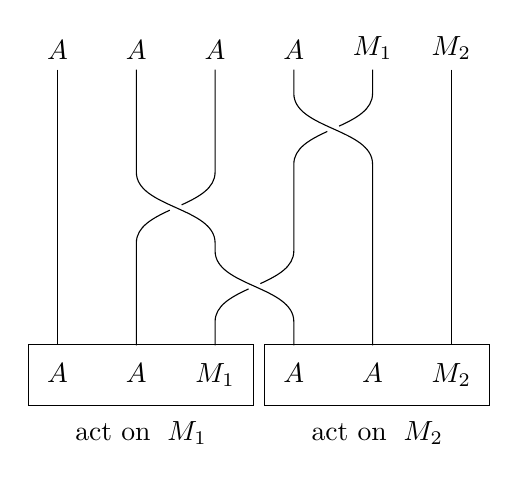
\begin{tikzpicture}
		[baseline=(braid), yscale=0.8]
		\pic[
			braid/number of strands = 6,
			braid/every strand/.style={black},
			name prefix=braid
		] at (0, 0) {braid={s_4 s_2 s_3}};
		\coordinate (braid) at ($(braid-1-s)!0.5!(braid-1-e)$);
		\node[above] at (braid-1-s) {$A$};
		\node[below=0.3em] (P) at (braid-1-e) {$A$};
		\node[above] at (braid-2-s) {$A$};
		\node[below=0.3em] (R) at (braid-2-e) {$A$};
		\node[above] at (braid-3-s) {$A$};
		\node[below=0.3em] at (braid-3-e) {$A$};
		\node[above] at (braid-4-s) {$A$};
		\node[below=0.3em] at (braid-4-e) {$A$};
		\node[above] at (braid-5-s) {$M_1$};
		\node[below=0.3em] (Q) at (braid-5-e) {$M_1$};
		\node[above] at (braid-6-s) {$M_2$};
		\node[below=0.3em] (S) at (braid-6-e) {$M_2$};

		\node (X) [draw, fit=(P) (Q)] {};
		\node[below=0.2em of X] {act on\; $M_1$};
		\node (Y) [draw, fit=(R) (S)] {};
		\node[below=0.2em of Y] {act on\; $M_2$};
	\end{tikzpicture} \; = 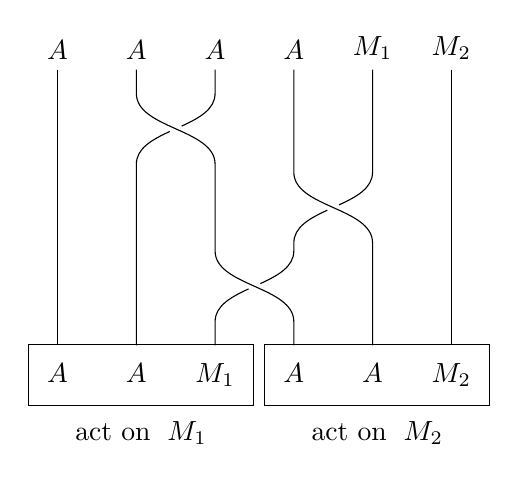
\begin{tikzpicture}
		[baseline=(braid), yscale=0.8]
		\pic[
			braid/number of strands=6,
			braid/every strand/.style = {black},
			name prefix=braid
		] at (0, 0) {braid={s_2 s_4 s_3}};
		\coordinate (braid) at ($(braid-1-s)!0.5!(braid-1-e)$);
		\node[above] at (braid-1-s) {$A$};
		\node[below=0.3em] (P) at (braid-1-e) {$A$};
		\node[above] at (braid-2-s) {$A$};
		\node[below=0.3em] (R) at (braid-2-e) {$A$};
		\node[above] at (braid-3-s) {$A$};
		\node[below=0.3em] at (braid-3-e) {$A$};
		\node[above] at (braid-4-s) {$A$};
		\node[below=0.3em] at (braid-4-e) {$A$};
		\node[above] at (braid-5-s) {$M_1$};
		\node[below=0.3em] (Q) at (braid-5-e) {$M_1$};
		\node[above] at (braid-6-s) {$M_2$};
		\node[below=0.3em] (S) at (braid-6-e) {$M_2$};

		\node (X) [draw, fit=(P) (Q)] {};
		\node[below=0.2em of X] {act on\; $M_1$};
		\node (Y) [draw, fit=(R) (S)] {};
		\node[below=0.2em of Y] {act on\; $M_2$};
	\end{tikzpicture}\end{center}
	which is immediately apparent.

	To show that $A\dcate{Mod}$ is a monoidal category, one must still prove
	that the associativity and unit constraints for $\otimes$ are all
	morphisms of left $A$-modules. The first assertion is straightforward. The
	second requires the coalgebra property
	$(\identity\otimes\epsilon)\Delta=\identity_A=
	(\epsilon\otimes\identity)\Delta$, after identifying
	$A\otimes\munit\simeq A\simeq\munit\otimes A$.
\end{proof}

% English translation of chapter7.tex lines 1130--1279.
% Source: Methods of Algebra, Volume 2, commit
% 9a5803ff77dd3257484cb177f851a73770a59dd3 (CC BY 4.0).
% stable-unit-id: o014.aljabr2.chapter7.coalgebra-to-hopf-b
% Coverage: the remainder of Section 7.5, from after the proof of the
% monoidal structure on a bialgebra's module category to line 1279.

% segment-id: o014.aljabr2.chapter7.coalgebra-to-hopf-b.p001
For a bialgebra $A$, one can still ask whether the monoidal category
$A\dcate{Mod}$ has a braiding and whether that braiding is symmetric. A
natural first idea is to use the braiding $c(M_1,M_2)$ of $\mathcal{V}$, but
in general this is not a morphism in $A\dcate{Mod}$. Even in the special case
$\mathcal{V}=\Bbbk\dcate{Mod}$, the answer already involves the concept of a
\emph{quasitriangular bialgebra}, which cannot be explained briefly. We give
only the following example, which is so simple as to be somewhat misleading.

% segment-id: o014.aljabr2.chapter7.coalgebra-to-hopf-b.pr001
\begin{proposition}\label{prop:bialgebra-mod-symmetry}
	Let $\mathcal{V}$ be a symmetric monoidal category.
% segment-id: o014.aljabr2.chapter7.coalgebra-to-hopf-b.l001
	\begin{enumerate}[(i)]
% segment-id: o014.aljabr2.chapter7.coalgebra-to-hopf-b.i001
		\item If $A$ is a cocommutative bialgebra over $\mathcal{V}$, then the
		monoidal categories $A\dcate{Mod}$ and $\cated{Mod}A$ become symmetric
		monoidal categories with respect to
		$c(M_1,M_2):M_1\otimes M_2\rightiso M_2\otimes M_1$.

% segment-id: o014.aljabr2.chapter7.coalgebra-to-hopf-b.i002
		\item Dually, if $A$ is a commutative bialgebra over $\mathcal{V}$,
		then $A\dcate{Comod}$ and $\cated{Comod}A$ are symmetric monoidal
		categories.
	\end{enumerate}
\end{proposition}

% segment-id: o014.aljabr2.chapter7.coalgebra-to-hopf-b.pf001
\begin{proof}
	It is enough to treat the cocommutative case. Using the preceding notation,
	the assertion that $c(M_1,M_2)$ is a morphism in $A\dcate{Mod}$ is
	equivalent to proving that the outer boundary of the following diagram
	commutes:
% segment-id: o014.aljabr2.chapter7.coalgebra-to-hopf-b.g001
	\[\begin{tikzcd}[row sep=large]
		A \otimes M_1 \otimes M_2 \arrow[r, "{\Delta \otimes \identity \otimes \identity}" inner sep=0.6em] \arrow[d, "{\identity \otimes c(M_1, M_2)}" description] & A \otimes A \otimes M_1 \otimes M_2 \arrow[r, "{\identity \otimes c(A, M_1) \otimes \identity}" inner sep=0.6em] \arrow[d, "{c(A, A) \otimes c(M_1, M_2)}" description] & A \otimes M_1 \otimes A \otimes M_2 \arrow[r, "{\mu_1 \otimes \mu_2}" inner sep=0.6em] \arrow[d, "{c(A \otimes M_1, A \otimes M_2)}" description] & M_1 \otimes M_2 \arrow[d, "{c(M_1, M_2)}" description] \\
		A \otimes M_2 \otimes M_1 \arrow[r, "{\Delta \otimes \identity \otimes \identity}"' inner sep=0.6em] & A \otimes A \otimes M_2 \otimes M_2 \arrow[r, "{\identity \otimes c(A, M_2) \otimes \identity}"' inner sep=0.6em] & A \otimes M_2 \otimes A \otimes M_1 \arrow[r, "{\mu_2 \otimes \mu_1}"' inner sep=0.6em] & M_2 \otimes M_1 .
	\end{tikzcd}\]

	The square on the left commutes because $A$ is cocommutative, while the
	square on the right commutes by functoriality of $c$. Drawing the braid
	diagram shows that
% segment-id: o014.aljabr2.chapter7.coalgebra-to-hopf-b.g002
	\begin{multline*}
		c(A \otimes M_1, A \otimes M_2) = \\
		(\identity_A \otimes c(A, M_2) \otimes \identity_{M_1}) (c(A, A) \otimes c(M_1, M_2)) (\identity_A \otimes c(A, M_1) \otimes \identity_{M_2}),
	\end{multline*}
	and since $\mathcal{V}$ is a symmetric monoidal category, the middle
	square also commutes. All other properties of the symmetric monoidal
	structure on $A\dcate{Mod}$ reduce to verifications in $\mathcal{V}$.
\end{proof}

% segment-id: o014.aljabr2.chapter7.coalgebra-to-hopf-b.p002
We now introduce the concept of a Hopf algebra. Let $\mathcal{V}$ be a
braided monoidal category.

% segment-id: o014.aljabr2.chapter7.coalgebra-to-hopf-b.d001
\begin{definition}\label{def:Hopf-algebra}
% segment-id: o014.aljabr2.chapter7.coalgebra-to-hopf-b.x001
	\index{Hopf algebra}
% segment-id: o014.aljabr2.chapter7.coalgebra-to-hopf-b.x002
	\index{antipode}
	Let the data $(A,\mu,\eta,\Delta,\epsilon)$ form a bialgebra $A$ over
	$\mathcal{V}$. If an isomorphism $S:A\rightiso A$ in $\mathcal{V}$ makes
	the following diagram commute,
% segment-id: o014.aljabr2.chapter7.coalgebra-to-hopf-b.g003
	\[\begin{tikzcd}
		A \otimes A \arrow[d, "\mu"'] & A \otimes A \arrow[r, "{S \otimes \identity_A}"] \arrow[l, "{\identity_A \otimes S}"'] & A \otimes A \arrow[d, "\mu"] \\
		A & A \arrow[u, "\Delta"] \arrow[r, "\eta\epsilon"'] \arrow[l, "\eta\epsilon"] & A ,
	\end{tikzcd}\]
	that is,
% segment-id: o014.aljabr2.chapter7.coalgebra-to-hopf-b.q001
	\[ \mu (\identity_A \otimes S) \Delta = \eta\epsilon = \mu (S \otimes \identity_A) \Delta, \]
	then $S$ is called an \emph{antipode} of $A$. A bialgebra equipped with an
	antipode is called a \emph{Hopf algebra}. Morphisms between Hopf algebras
	are defined to be morphisms between their underlying bialgebras.
\end{definition}

% segment-id: o014.aljabr2.chapter7.coalgebra-to-hopf-b.p003
For example, $\munit$ is a Hopf algebra with antipode
$\identity_{\munit}$.

% segment-id: o014.aljabr2.chapter7.coalgebra-to-hopf-b.p004
Interpreted using the convolution in
Remark~\ref{rem:coalgebra-convolution}, an antipode $S$ is precisely a
two-sided inverse of $\identity_A\in\End(A)$ with respect to $\star$. The
antipode in the definition of a Hopf algebra, if it exists, is unique. This
follows immediately by applying the next result to $f=\identity_A$; the
result also shows that morphisms always preserve antipodes.

% segment-id: o014.aljabr2.chapter7.coalgebra-to-hopf-b.pr002
\begin{proposition}\label{prop:antipode-homo}
	Let $A$ and $A'$ be Hopf algebras over $\mathcal{V}$ with antipodes $S$
	and $S'$, respectively. For every Hopf algebra morphism $f:A\to A'$, one
	has $S'f=fS$.
\end{proposition}

% segment-id: o014.aljabr2.chapter7.coalgebra-to-hopf-b.pf002
\begin{proof}
	By the functoriality of convolution $\star$ in
	\eqref{eqn:convolution-functorial}, both maps
% segment-id: o014.aljabr2.chapter7.coalgebra-to-hopf-b.g004
	\[\begin{tikzcd}
		\Hom(A', A') \arrow[r, "{g \mapsto gf}"] & \Hom(A, A')
	\end{tikzcd}, \quad \begin{tikzcd}
		\Hom(A, A) \arrow[r, "{h \mapsto fh}"] & \Hom(A, A')
	\end{tikzcd}\]
	are homomorphisms of convolution monoids. Thus $S'f$ and $fS$ are both
	convolution inverses of $f\in\Hom(A,A')$.
\end{proof}

% segment-id: o014.aljabr2.chapter7.coalgebra-to-hopf-b.p005
Because the braiding on $\mathcal{V}$ gives a braiding on
$\mathcal{V}^{\opp}$, the concept of a bialgebra is plainly self-dual. The
next result shows that the definition of an antipode is self-dual as well.

% segment-id: o014.aljabr2.chapter7.coalgebra-to-hopf-b.pr003
\begin{proposition}\label{prop:bialgebra-duality}
	If $(A,\mu,\eta,\Delta,\epsilon)$ is a bialgebra over $\mathcal{V}$, then
	$(A,\eta,\mu,\epsilon,\Delta)$ is a bialgebra over
	$\mathcal{V}^{\opp}$. If the Hopf algebra
	$(A,\mu,\eta,\Delta,\epsilon)$ has antipode $S$, then $S^{-1}$ is an
	antipode of $(A,\eta,\mu,\epsilon,\Delta)$ as a bialgebra over
	$\mathcal{V}^{\opp}$; in particular, the latter object is a Hopf algebra
	over $\mathcal{V}^{\opp}$.
\end{proposition}

% segment-id: o014.aljabr2.chapter7.coalgebra-to-hopf-b.pf003
\begin{proof}
	The diagram in Definition~\ref{def:Hopf-algebra} is self-dual, but the
	direction of $S$ is reversed.
\end{proof}

% segment-id: o014.aljabr2.chapter7.coalgebra-to-hopf-b.pr004
\begin{proposition}\label{prop:Hopf-antiautomorphism}
% segment-id: o014.aljabr2.chapter7.coalgebra-to-hopf-b.x003
	\index[sym1]{Acop@$A_{\mathrm{cop}}, A^{\mathrm{op}}_{\mathrm{cop}}$}
	For a bialgebra $A$, in accordance with
	Definition~\ref{def:opposite-braided-algebra},
% segment-id: o014.aljabr2.chapter7.coalgebra-to-hopf-b.l002
	\begin{compactitem}
% segment-id: o014.aljabr2.chapter7.coalgebra-to-hopf-b.i003
		\item reversing the multiplication of $A$ using the braiding $c(A,A)$
		produces an algebra $A^{\mathrm{op}}$;
% segment-id: o014.aljabr2.chapter7.coalgebra-to-hopf-b.i004
		\item reversing the comultiplication of $A$ using $c(A,A)^{-1}$
		produces a coalgebra $A_{\mathrm{cop}}$.
	\end{compactitem}
	Together, these two operations produce a bialgebra
	$A^{\mathrm{op}}_{\mathrm{cop}}$. If $A$ has an antipode $S$, then $S$ is
	also an antipode of $A^{\mathrm{op}}_{\mathrm{cop}}$, and in this case
	$S:A\rightiso A^{\mathrm{op}}_{\mathrm{cop}}$ is an isomorphism of
	bialgebras.
\end{proposition}

% segment-id: o014.aljabr2.chapter7.coalgebra-to-hopf-b.pf004
\begin{proof}
	A routine verification shows that $A^{\mathrm{op}}_{\mathrm{cop}}$ is
	indeed a bialgebra with antipode $S$; we omit the details. The remaining
	assertion has two parts. First, $S$ preserves the unit and counit. This is
	easy: in Proposition~\ref{prop:antipode-homo}, take $A=\munit$ and
	$A'=\munit$, respectively.

	Second, $S$ preserves the multiplication and comultiplication. The proof
	in general is more involved; see \cite[\S 9, Proposition 2]{JS91} or
	\cite[Proposition 1.22]{AM10}. Here we only sketch the special case
	$\mathcal{V}=\Bbbk\dcate{Mod}$, $\otimes=\otimes_{\Bbbk}$ with its
	standard braiding. This is the only case that will be needed later.

	Recall from \S\ref{sec:alg-in-monoidal-cat} that $A\otimes A$ is naturally
	a coalgebra. Equip $\Hom(A\otimes A,A)$ with the convolution from
	Remark~\ref{rem:coalgebra-convolution}, denoted by $\ast$, and consider the
	elements
% segment-id: o014.aljabr2.chapter7.coalgebra-to-hopf-b.q002
	\[ f := \mu, \quad g := \mu c(A, A) (S \otimes S), \quad h := S \mu. 
	\]
	It is enough to prove that
	$h\ast f=\eta_A\epsilon_{A\otimes A}=f\ast g$. This equality will show
	that $f$ is invertible in the monoid
	$(\Hom(A\otimes A,A),\ast)$, and hence that $h=g$. Let $a,b\in A$ and
	write the expansions
% segment-id: o014.aljabr2.chapter7.coalgebra-to-hopf-b.g005
	\begin{gather*}
		\Delta(a) = \sum_i a_i^{(1)} \otimes a_i^{(2)}, \quad
		\Delta(b) = \sum_j b_j^{(1)} \otimes b_j^{(2)}.
	\end{gather*}
	Write $\mu$ simply as multiplication. From the standard braiding on
	$\Bbbk\dcate{Mod}$, one obtains
% segment-id: o014.aljabr2.chapter7.coalgebra-to-hopf-b.g006
	\begin{align*}
		(h \ast f)(a \otimes b) & = \sum_{i, j} h\left(a^{(1)}_i \otimes b^{(1)}_j\right) f\left(a^{(2)}_i \otimes b^{(2)}_j\right) \\
		& = \sum_{i, j} S\left( a^{(1)}_i b^{(1)}_j \right) a^{(2)}_i b^{(2)}_j \\
		& = (\underbracket{S \star \identity_A}_{\text{convolution on }\End(A)})(ab) = \eta_A \epsilon_A (ab), \\
		(f \ast g)(a \otimes b) & = \cdots = \sum_{i, j} a^{(1)}_i b^{(1)}_j S\left( b^{(2)}_j \right) S\left( a^{(2)}_i \right) \\
		& = \sum_i a^{(1)}_i \eta_A \epsilon_A(b) S\left( a^{(2)}_i \right) \\
		& = \eta_A \epsilon_A (a) \cdot \eta_A \epsilon_A (b) = \eta_A \epsilon_A(ab), \\
		\eta_A \epsilon_{A \otimes A}(a \otimes b) & = \eta_A\left( \epsilon_A(a)\epsilon_A(b) \right) = \eta_A \epsilon_A(ab),
	\end{align*}
	as claimed. Thus $S$ preserves the multiplication of the bialgebra. A
	similar argument shows that $S$ preserves the comultiplication.
\end{proof}

% segment-id: o014.aljabr2.chapter7.coalgebra-to-hopf-b.p006
In particular, if $\mathcal{V}$ is a symmetric monoidal category, then $S^2$
is an automorphism of $A$.

% segment-id: o014.aljabr2.chapter7.coalgebra-to-hopf-b.c001
\begin{corollary}\label{prop:Hopf-involution}
	Let the Hopf algebra $A$ have antipode $S$. If $A$ is commutative or
	cocommutative, then $S^2=\identity$.
\end{corollary}

% segment-id: o014.aljabr2.chapter7.coalgebra-to-hopf-b.pf005
\begin{proof}
	With respect to the convolution $\star$ on $\End(A)$
	(Remark~\ref{rem:coalgebra-convolution}), we have
% segment-id: o014.aljabr2.chapter7.coalgebra-to-hopf-b.q003
	\[ S \star S^2 = \mu (S \otimes S^2) \Delta = \mu (S \otimes S)(\identity \otimes S) \Delta. \]

	If $A$ is commutative, then $\mu c(A,A)=\mu$, and
	Proposition~\ref{prop:Hopf-antiautomorphism} transforms the right-hand side
	above into
% segment-id: o014.aljabr2.chapter7.coalgebra-to-hopf-b.q004
	\[ \mu c(A, A) (S \otimes S) (\identity \otimes S)\Delta = S\mu (\identity \otimes S)\Delta = S(\identity \star S). \]
	The definition of an antipode says that
	$\identity\star S=\eta\epsilon$, while the same proposition gives
	$S\eta=\eta$; the result is $\eta\epsilon$.

	If $A$ is cocommutative, then $c(A,A)\Delta=\Delta$, and functoriality of
	the braiding transforms $S\star S^2$ into
% segment-id: o014.aljabr2.chapter7.coalgebra-to-hopf-b.q005
	\[ \mu (S \otimes S)(\identity \otimes S) c(A, A) \Delta = \mu c(A, A) (S \otimes S)(S \otimes \identity)\Delta, \]
	which the same argument then transforms into
	$S(S\star\identity)=\eta\epsilon$.

	Thus $S^2$ is a convolution inverse of $S$, so $S^2=\identity$.
\end{proof}

% segment-id: o014.aljabr2.chapter7.coalgebra-to-hopf-b.p007
All the following examples take $\mathcal{V}=\Bbbk\dcate{Mod}$ and
$\otimes=\otimes_{\Bbbk}$, where $\Bbbk$ is a commutative ring.

% segment-id: o014.aljabr2.chapter7.coalgebra-to-hopf-b.ex001
\begin{example}\label{eg:group-Hopf-algebra}
	Let $G$ be a group. Form the group $\Bbbk$-algebra $\Bbbk[G]$.
	Example~\ref{eg:monoid-bialgebra} gives $\Bbbk[G]$ a bialgebra structure.
	Define the $\Bbbk$-module automorphism $S:\Bbbk[G]\to\Bbbk[G]$ by
% segment-id: o014.aljabr2.chapter7.coalgebra-to-hopf-b.q006
	\[ S(g) = g^{-1}, \quad g \in G. \]
	It is easy to verify that $S$ satisfies the commutative diagram required
	of an antipode. Thus $\Bbbk[G]$ is a Hopf algebra.
\end{example}

% segment-id: o014.aljabr2.chapter7.coalgebra-to-hopf-b.ex002
\begin{example}[H.\ Hopf]
% segment-id: o014.aljabr2.chapter7.coalgebra-to-hopf-b.x004
	\index{H-space, H-group}
	Write $\{\mathrm{pt}\}$ for a one-point set. Let a topological space $X$
	be equipped with continuous maps $m:X\times X\to X$ (multiplication) and
	$e:\{\mathrm{pt}\}\to X$ (equivalently, a choice of an element of $X$,
	the unit, also denoted by $e$), such that the two maps satisfy, up to
	homotopy, the properties required for associativity of multiplication and
	for a unit. Then $(X,m,e)$ is called an \emph{H-space}. If a continuous map
	$i:X\to X$ (taking inverses) is also chosen and satisfies, up to homotopy,
	the properties required of inverses, then $(X,m,e,i)$ is called an
	\emph{H-group}.

	A topological monoid (or topological group) is of course an H-space (or
	H-group), but the H-space and H-group conditions are much weaker. A natural
	example is a loop space. For a topological space $M$ with a chosen base
	point $x_0\in M$, a continuous map $\gamma:[0,1]\to M$ satisfying
	$\gamma(0)=x_0=\gamma(1)$ is called a \emph{loop} in $M$. All loops
	naturally form a topological space $\Omega(M,x_0)$. If $m$ is taken to be
	end-to-start concatenation of two loops, $e$ the constant map at $x_0$,
	and $i$ reversal of the direction of a loop, then intuitively
	$\Omega(M,x_0)$ forms an H-group. The key point is that associativity and
	the inverse properties hold only up to homotopy.

	Next, consider the full subcategory $\cate{S}$ of $\cate{Top}$ consisting
	of all CW complexes\footnote{This is a topological term, somewhat different
	from the complexes defined in linear algebra.}; it contains spaces commonly
	encountered in geometry, such as manifolds. Let $\Bbbk$ be a field. The
	cohomology functor with coefficients in $\Bbbk$, namely $\Hm^\bullet$, is a
	functor from $\cate{S}^{\opp}$ to the category of graded $\Bbbk$-vector
	spaces $\cate{Vect}(\Bbbk)^{\Z_{\geq0}}$. Equip
	$\cate{Vect}(\Bbbk)^{\Z_{\geq0}}$ with the braiding determined by the
	Koszul sign rule \eqref{eqn:Koszul-braiding} (in the notation there, take
	$\epsilon(a)=a\bmod\;2$). The cup product $\mu:=\cup$ on cohomology makes
	the functor $\Hm^\bullet$ factor through
	$\cate{CAlg}\left(\cate{Vect}(\Bbbk)^{\Z_{\geq0}}\right)$; in short,
	cohomology is a commutative algebra over
	$\cate{Vect}(\Bbbk)^{\Z_{\geq0}}$.

	On the other hand, give $\cate{S}$ the monoidal structure determined by
	the product of spaces, with $\{\mathrm{pt}\}$ as unit. The Künneth formula
	in topology shows that $\Hm^\bullet$ is a monoidal functor. Moreover,
	homotopic maps induce the same map on cohomology. Consequently, if
	$X\in\Obj(\cate{S})$ is an H-space, then $\Hm^\bullet(X)$ is also a
	coalgebra over $\cate{Vect}(\Bbbk)^{\Z_{\geq0}}$.

	Readers familiar with algebraic topology will readily conclude that the
	algebra and coalgebra structures on $\Hm^\bullet(X)$ are compatible and
	hence give a bialgebra over
	$\cate{Vect}(\Bbbk)^{\Z_{\geq0}}$. If, in addition, $X$ is an H-group and
	the automorphism induced by the map $i$ is denoted by
	$S\in\Aut(\Hm^\bullet(X))$, then $\Hm^\bullet(X)$ becomes a Hopf algebra.

	In fact, the multiplication (cup product) on $\Hm^\bullet(X)$ is precisely
	the image of the diagonal embedding $\mathrm{diag}:X\to X\times X$ under
	the Künneth formula, while its unit is the image of
	$X\to\{\mathrm{pt}\}$. Thus all the properties required of the bialgebra
	and antipode can be verified at the level of topological spaces, up to
	homotopy. For example, the antipode identity
	$\mu(S\otimes\identity)\Delta=\eta\epsilon$ comes from
% segment-id: o014.aljabr2.chapter7.coalgebra-to-hopf-b.q007
	\[ \left[ X \xrightarrow{\mathrm{diag}} X \times X \xrightarrow{(i, \identity)} X \times X \xrightarrow{m} X\right] \;\text{being homotopy equivalent to}\; \left[ X \to \{\mathrm{pt}\} \xrightarrow{e} X \right]. \]

	Thus the cohomology of an H-group is naturally a commutative Hopf algebra
	with a rich structure. This was Hopf's original motivation for studying
	such algebras.
\end{example}

% segment-id: o014.aljabr2.chapter7.coalgebra-to-hopf-b.p008
The exercises will provide more examples of Hopf algebras. Most are
commutative or cocommutative, but there are also many Hopf algebras having
neither property. The most important class among them is that of
\emph{quantum groups}. The relevant discussion requires a foundation in Lie
theory and is not treated in this book.

% English translation of chapter7.tex lines 1280--1444.
% Source: Methods of Algebra, Volume 2, commit
% 9a5803ff77dd3257484cb177f851a73770a59dd3 (CC BY 4.0).
% stable-unit-id: o014.aljabr2.chapter7.beck-monadicity-a
% Coverage: Section 7.6 from its opening through the construction of free
% T-modules; continued in Unit 095.

% segment-id: o014.li2.chapter7.beck-monadicity-a.h001
\section{Beck's Monadicity Theorem}\label{sec:Beck}
\hypertarget{o014.aljabr2.chapter7.beck-monadicity-a}{ }
% segment-id: o014.li2.chapter7.beck-monadicity-a.p001
Let $\mathcal{C}$ be a category. Consider the functor category
$\mathcal{C}^{\mathcal{C}}$, whose objects are all endofunctors
$T:\mathcal{C}\to\mathcal{C}$ and whose morphisms are morphisms between
endofunctors. This category is naturally monoidal: the multiplication
$\otimes$ is composition of functors, and the unit object $\munit$ is the
identity functor. Since composition of functors is strictly associative, this
is also a strict monoidal category.

% segment-id: o014.li2.chapter7.beck-monadicity-a.d001
\begin{definition}[Monad and comonad]\label{def:monad}
	\index{monad}
	\index{comonad}
	Let $\mathcal{C}$ be a category. An algebra in the monoidal category
	$\mathcal{C}^{\mathcal{C}}$ (Definition~\ref{def:algebra-monoidal}) is
	called a \emph{monad} on $\mathcal{C}$. Dually, a monad on
	$\mathcal{C}^{\opp}$ is called a \emph{comonad} on $\mathcal{C}$.
\end{definition}

% segment-id: o014.li2.chapter7.beck-monadicity-a.p002
Expanding Definition~\ref{def:algebra-monoidal} in the category of
endofunctors $\mathcal{C}^{\mathcal{C}}$, we find that a monad is data
$(T,\mu,\eta)$, where $T:\mathcal{C}\to\mathcal{C}$ is a functor and
$\mu:T^2\to T$ and $\eta:\identity_{\mathcal{C}}\to T$ are morphisms such
that the following diagrams commute:
% segment-id: o014.li2.chapter7.beck-monadicity-a.q001
\begin{equation*}\begin{gathered}
	\begin{tikzcd}
		T \arrow[r, "{\eta T}"] \arrow[rd, "\identity"'] & T^2 \arrow[d, "\mu"] & T \arrow[l, "{T\eta}"'] \arrow[ld, "\identity"] \\
		& T &
	\end{tikzcd} \quad
	\begin{tikzcd}
		T^3 \arrow[r, "\mu T"] \arrow[d, "T\mu"'] & T^2 \arrow[d, "\mu"] \\
		T^2 \arrow[r, "\mu"'] & T.
	\end{tikzcd}
\end{gathered}\end{equation*}

% segment-id: o014.li2.chapter7.beck-monadicity-a.p003
Compared with the original definition, associativity constraints are no
longer needed here, while $\eta\otimes\identity$ (or
$\identity\otimes\eta$) becomes $\eta T$ (or $T\eta$), and so on.

% segment-id: o014.li2.chapter7.beck-monadicity-a.p004
Dually, a comonad $(L,\delta,\epsilon)$ consists of a functor
$L:\mathcal{C}\to\mathcal{C}$ and morphisms $\delta:L\to L^2$ and
$\epsilon:L\to\identity_{\mathcal{C}}$, subject to the commutativity of the
following diagrams.
% segment-id: o014.li2.chapter7.beck-monadicity-a.q002
\begin{equation*}\begin{gathered}
	\begin{tikzcd}
		L  & L^2 \arrow[l, "{\epsilon L}"'] \arrow[r, "{L\epsilon}"] & L \\
		& L \arrow[lu, "\identity"] \arrow[ru, "\identity"'] \arrow[u, "\delta"] &
	\end{tikzcd} \quad
	\begin{tikzcd}
		L^3 & L^2 \arrow[l, "\delta L"'] \\
		L^2 \arrow[u, "L\delta"] & L \arrow[u, "\delta"'] \arrow[l, "\delta"]
	\end{tikzcd}
\end{gathered}\end{equation*}

% segment-id: o014.li2.chapter7.beck-monadicity-a.p005
The data $(T,\mu,\eta)$ (or $(L,\delta,\epsilon)$) are customarily
abbreviated simply as $T$ (or $L$). The principal source of monads and
comonads is adjoint pairs.

% segment-id: o014.li2.chapter7.beck-monadicity-a.eg001
\begin{example}[An adjoint pair determines a monad]\label{eg:adjunction-monad}
	Consider a pair of adjoint functors
	% segment-id: o014.li2.chapter7.beck-monadicity-a.q003
	\[\begin{tikzcd}
		F: \mathcal{C} \arrow[shift left, r] & \mathcal{D}: G \arrow[shift left, l],
	\end{tikzcd}\]
	with the corresponding unit $\eta:\identity_{\mathcal{C}}\to GF$ and
	counit $\varepsilon:FG\to\identity_{\mathcal{D}}$. Define a monad
	$(T,\mu,\eta)$ on $\mathcal{C}$ and a comonad
	$(L,\delta,\varepsilon)$ on $\mathcal{D}$ as follows.
	% segment-id: o014.li2.chapter7.beck-monadicity-a.q004
	\[\begin{array}{|c|c|}\hline
		T := GF & L := FG \\
		\mu := \left[ GFGF \xrightarrow{G\varepsilon F} GF \right] & \delta := \left[ FG \xrightarrow{F\eta G} FGFG \right] \\
		\eta : \identity_{\mathcal{C}} \to GF & \varepsilon: FG \to \identity_{\mathcal{D}} \\ \hline
	\end{array}\]

	By duality, it is enough to check the monad axioms in the case
	$(T,\mu,\eta)$. First, the unit diagram is
	% segment-id: o014.li2.chapter7.beck-monadicity-a.q005
	\[\begin{tikzcd}[column sep=large]
		GF \arrow[r, "{\eta GF}"] \arrow[equal, rd] & GFGF \arrow[d, "{G\varepsilon F}"] & GF \arrow[l, "{GF\eta}"'] \arrow[equal, ld] \\
		& GF &
	\end{tikzcd}\]
	which commutes by the triangle identities
	$(G\varepsilon)(\eta G)=\identity_G$ and
	$(\varepsilon F)(F\eta)=\identity_F$. The associativity diagram is
	% segment-id: o014.li2.chapter7.beck-monadicity-a.q006
	\[\begin{tikzcd}[column sep=large]
		GFGFGF \arrow[d, "{G\varepsilon FGF}"'] \arrow[r, "{GFG\varepsilon F}"] & GFGF \arrow[d, "G\varepsilon F"] \\
		GFGF \arrow[r, "G\varepsilon F"'] & GF
	\end{tikzcd}\]
	and it commutes: both composites are depicted by
	% segment-id: o014.li2.chapter7.beck-monadicity-a.q007
	\[\begin{tikzcd}
		\mathcal{C} \arrow[r, "F"] & \mathcal{D} \arrow[r, "G"] \arrow[rr, bend right=60, ""{name=A}, "{\identity}"'] & \mathcal{C} \arrow[r, "F"] \arrow[Rightarrow, to=A, "\varepsilon"] &
		\mathcal{D} \arrow[r, "G"] \arrow[rr, bend right=60, ""{name=B}, "{\identity}"'] & \mathcal{C} \arrow[r, "F"] \arrow[Rightarrow, to=B, "\varepsilon"] & \mathcal{D} \arrow[r, "G"] & \mathcal{C}
	\end{tikzcd}\]
	with only the order of composition of the two curved regions differing;
	the result is the same. This is a special case of the interchange law for
	vertical and horizontal composition of morphisms
	\cite[Lemma 2.2.7]{Li1}.
\end{example}

% segment-id: o014.li2.chapter7.beck-monadicity-a.p006
Since endofunctors act on $\mathcal{C}$, we wish to discuss ``modules'' in
$\mathcal{C}$ under the action of a monad $T$. For historical reasons, such
a structure is also called a $T$-algebra.

% segment-id: o014.li2.chapter7.beck-monadicity-a.d002
\begin{definition}[S.\ Eilenberg, J.\ C.\ Moore]\label{def:T-Alg}
	\index{T-module@$T$-module}
	Let $(T,\mu,\eta)$ be a monad on $\mathcal{C}$. A \emph{$T$-module} is
	data $(M,a)$, where $M\in\Obj(\mathcal{C})$ and $a$ is a morphism
	$T(M)\to M$ in $\mathcal{C}$, such that the following diagrams commute:
	% segment-id: o014.li2.chapter7.beck-monadicity-a.q008
	\[\begin{tikzcd}
		T^2 (M) \arrow[r, "Ta"] \arrow[d, "\mu_M"'] & T(M) \arrow[d, "a"] \\
		T(M) \arrow[r, "a"'] & M
	\end{tikzcd} \quad \begin{tikzcd}
		M \arrow[r, "\eta_M"] \arrow[rd, "{\identity_M}"'] & T(M) \arrow[d, "a"] \\
		& M .
	\end{tikzcd}\]

	All $T$-modules form a category $\mathcal{C}^T$. A morphism from $(M,a)$
	to $(M',a')$ is defined to be a morphism $f:M\to M'$ in $\mathcal{C}$
	that makes the following diagram commute:
	% segment-id: o014.li2.chapter7.beck-monadicity-a.q009
	\[\begin{tikzcd}
		T(M) \arrow[r, "a"] \arrow[d, "Tf"'] & M \arrow[d, "f"] \\
		T(M')  \arrow[r, "{a'}"'] & M' .
	\end{tikzcd}\]

	Dually, let $(L,\delta,\epsilon)$ be a comonad on $\mathcal{C}$. An
	$L$-comodule is data $(N,b)$, where $b:N\to L(N)$ is a morphism, subject
	to the commutative diagrams dual to those above. The category of
	$L$-comodules is denoted by $\mathcal{C}^L$.
\end{definition}

% segment-id: o014.li2.chapter7.beck-monadicity-a.p007
The two commutative diagrams for a $T$-module should be viewed as the
associativity and unit laws for the action of $T$, respectively. The examples
and properties below are stated mainly for monads and modules over them; the
versions for comonads and comodules are entirely dual.

% segment-id: o014.li2.chapter7.beck-monadicity-a.eg002
\begin{example}\label{eg:Mon-monad}
	Write $\cate{Mon}$ for the category of monoids, conventionally taken to be
	realized on small sets, and consider the adjoint pair
	% segment-id: o014.li2.chapter7.beck-monadicity-a.q010
	\[\begin{tikzcd}
		\mathbf{M}: \cate{Set} \arrow[r, shift left] & \cate{Mon}: U, \arrow[l, shift left]
	\end{tikzcd}\]
	where $\mathbf{M}$ maps a set $X$ to the free monoid $\mathbf{M}(X)$,
	whose definition and construction are given in
	\cite[Definition 4.8.1, Lemma 4.8.4]{Li1}, and $U$ is the forgetful
	functor. Thus,
	% segment-id: o014.li2.chapter7.beck-monadicity-a.q011
	\[ T := U\mathbf{M}: \cate{Set} \to \cate{Set}, \quad T(X) = \bigsqcup_{n \geq 0} X^n. \]
	In other words, an element of $T(X)$ is a ``word''
	$(x_1,\ldots,x_n)$ with $n\in\Z_{\geq0}$. The unit of the adjoint pair
	$\eta_X:X\to U\mathbf{M}(X)$ maps $x\in X$ to the word of length $1$,
	$(x)$. For a monoid $A$, the counit
	$\varepsilon_A:\mathbf{M}U(A)\to A$ maps the word
	$(a_1,\ldots,a_n)$ to the product $a_1\cdots a_n\in A$. Since
	multiplication in $\mathbf{M}(X)$ is concatenation of words, the map
	$\mu_X=U\varepsilon\mathbf{M}:T^2(X)\to T(X)$ corresponding to the monad
	$T$ (or, viewed as a map
	$\mathbf{M}(\mathbf{M}(X))\to\mathbf{M}(X)$) flattens a ``word of
	words,'' that is, it concatenates a sequence of lists, as in
	% segment-id: o014.li2.chapter7.beck-monadicity-a.q012
	\[ \left( (x_1, \ldots, x_n), (y_1, \ldots, y_m), \ldots \right) \mapsto \left( x_1, \ldots, x_n, y_1, \ldots, y_m, \ldots \right). \]

	Specifying a $T$-module $(M,a)$ for $T=U\mathbf{M}$ is equivalent to
	specifying $m_1\cdots m_n:=a(m_1,\ldots,m_n)$ for every word
	$(m_1,\ldots,m_n)$ in the set $M$, such that $a(m)=m$ and the
	associativity law
	% segment-id: o014.li2.chapter7.beck-monadicity-a.q013
	\[ a\left( a(x_1, \ldots, x_n), a(y_1, \ldots, y_m), \ldots \right) = a\left( x_1, \ldots, x_n, y_1, \ldots, y_m, \ldots \right) \]
	holds. In short, a $T$-module is precisely a monoid, with the image under
	$a$ of the empty word ($n=0$) as its unit. It is easy to check that
	morphisms of $T$-modules are precisely monoid homomorphisms.

	The case of the category of groups $\cate{Grp}$ is entirely similar; the
	key is to replace $\mathbf{M}$ by the free-group functor $\mathbf{F}$. The
	corresponding $T$-modules are precisely groups.
\end{example}

% segment-id: o014.li2.chapter7.beck-monadicity-a.eg003
\begin{example}\label{eg:Mod-monad}
	Let $R$ be a ring and consider the adjoint pair
	% segment-id: o014.li2.chapter7.beck-monadicity-a.q014
	\[\begin{tikzcd}
		\mathbf{F}: \cate{Set} \arrow[r, shift left] & R\dcate{Mod}: U, \arrow[l, shift left]
	\end{tikzcd}\]
	where $\mathbf{F}$ maps $X$ to the free left $R$-module
	$R^{\oplus X}$ and $U$ is the forgetful functor. This gives a monad
	$(T,\mu,\eta)$ on $\cate{Set}$. As in Example~\ref{eg:Mon-monad},
	$T=U\mathbf{F}$ maps a set $X$ to $R^{\oplus X}$ regarded as a set; its
	elements are finite formal $R$-linear combinations of elements of $X$,
	$\text{\textquotedblleft} r_1x_1+\cdots+r_nx_n
	\text{\textquotedblright}$. The unit $\eta_X$ maps $x\in X$ to
	$\text{\textquotedblleft}x\text{\textquotedblright}$, while
	$\mu_X:R^{\oplus(R^{\oplus}X)}\to R^{\oplus X}$ flattens a two-level
	linear combination, namely,
	% segment-id: o014.li2.chapter7.beck-monadicity-a.q015
	\begin{multline*}
		\text{\textquotedblleft} \alpha (\text{\textquotedblleft} r_1 x_1 + \cdots + r_n x_n \text{\textquotedblright}) + \beta (\text{\textquotedblleft} s_1 y_1 + \cdots + s_m y_m \text{\textquotedblright}) + \cdots \text{\textquotedblright} \\
		\mapsto \text{\textquotedblleft} (\alpha r_1) x_1 + \cdots + (\alpha r_n) x_n + (\beta s_1) y_1 + \cdots + (\beta s_m) y_m + \cdots \text{\textquotedblright} .
	\end{multline*}
	Specifying a $T$-module $(M,a)$ is equivalent to specifying a set $M$
	together with a rule that maps formal linear combinations to elements of
	$M$, maps $\text{\textquotedblleft}x\text{\textquotedblright}$ to $x$, is
	associative with respect to addition and scalar multiplication, and makes
	scalar multiplication by $1\in R$ the identity map. In short, $T$-modules
	are precisely left $R$-modules. It is clear that morphisms of $T$-modules
	are precisely module homomorphisms.
\end{example}

% segment-id: o014.li2.chapter7.beck-monadicity-a.p008
Return to the general theory. There is a forgetful functor
$U^T:\mathcal{C}^T\to\mathcal{C}$ mapping an object $(M,a)$ to $M$. We now
give its left adjoint: the free construction.

% segment-id: o014.li2.chapter7.beck-monadicity-a.dp001
\begin{definition-proposition}[Free $T$-module]\label{def:free-T-Alg}
	\index{module!free}
	Let $(T,\mu,\eta)$ be a monad on $\mathcal{C}$. Define a functor
	% segment-id: o014.li2.chapter7.beck-monadicity-a.q016
	\[ \mathrm{Free}^T: \mathcal{C} \to \mathcal{C}^T , \quad
	\begin{array}{rl}
		(\text{object } M) & \mapsto (TM, \mu_M: T^2 M \to TM), \\
		(\text{morphism } f: M \to M') & \mapsto Tf: TM \to TM'.
	\end{array}\]
	This gives an adjoint pair
	% segment-id: o014.li2.chapter7.beck-monadicity-a.q017
	\[\begin{tikzcd}
		\mathrm{Free}^T : \mathcal{C} \arrow[shift left, r] & \mathcal{C}^T: U^T \arrow[shift left, l],
	\end{tikzcd}\]
	and the monad on $\mathcal{C}$ determined by this adjoint pair is precisely
	$(T,\mu,\eta)$.
\end{definition-proposition}
% segment-id: o014.li2.chapter7.beck-monadicity-a.pf001
\begin{proof}
	To check that $(TM,\mu_M)$ is a $T$-module, one must show that the following
	two diagrams commute:
	% segment-id: o014.li2.chapter7.beck-monadicity-a.q018
	\[\begin{tikzcd}
		T^3 (M) \arrow[r, "T\mu_M"] \arrow[d, "\mu_{T(M)}"'] & T^2(M) \arrow[d, "\mu_M"] \\
		T^2 (M) \arrow[r, "\mu_M"'] & T(M)
	\end{tikzcd} \quad \begin{tikzcd}
		T(M) \arrow[r, "\eta_{T(M)}"] \arrow[rd, "\identity"'] & T^2(M) \arrow[d, "\mu_M"] \\
		& T(M).
	\end{tikzcd}\]
	But these diagrams are obtained by evaluating the functor diagrams in
	Definition~\ref{def:monad} at the object $M$. Functoriality is clear.

	Next, note that $U^T\mathrm{Free}^T=T$. Take
	$\eta:\identity_{\mathcal{C}}\to T$ from the data of $T$, and define
	% segment-id: o014.li2.chapter7.beck-monadicity-a.q019
	\[ \epsilon: \mathrm{Free}^T U^T \to \identity_{\mathcal{C}^T}, \quad
	\epsilon_{(M, a)}: (TM, \mu_M) \xrightarrow{a} (M, a) \in \Obj(\mathcal{C}^T). \]
	The left diagram in Definition~\ref{def:T-Alg} shows that
	$\epsilon_{(M,a)}$ is a morphism in $\mathcal{C}^T$. Its functoriality is
	also clear.

	A routine verification shows that $(\mathrm{Free}^T,U^T)$ is an adjoint
	pair with unit $\eta$ and counit $\epsilon$; we omit the details. Moreover,
	% segment-id: o014.li2.chapter7.beck-monadicity-a.q020
	\begin{equation*}\begin{aligned}
		\left(U^T \epsilon \mathrm{Free}^T\right)_M & = U^T \epsilon_{(TM, \mu_M)} \\
		& = \left[ \mu_M: T^2(M) \to T(M)\right],
	\end{aligned}\end{equation*}
	which shows that the monad on $\mathcal{C}$ determined by the adjoint pair
	$(\mathrm{Free}^T,U^T)$ is $(T,\mu,\eta)$.
\end{proof}

% segment-id: o014.li2.chapter7.beck-monadicity-a.p009
For the monads in Examples~\ref{eg:Mon-monad} and \ref{eg:Mod-monad}, the
functor $\mathrm{Free}^T$ corresponds, respectively, to the constructions of
the free monoid and the free module.

% segment-id: o014.li2.chapter7.beck-monadicity-a.p010
Dually, a comonad $L$ on a category $\mathcal{D}$ also gives a
free--forgetful adjoint pair; there is no need to discuss it further.

% English translation of chapter7.tex lines 1445--1660.
% Source: Methods of Algebra, Volume 2, commit
% 9a5803ff77dd3257484cb177f851a73770a59dd3 (CC BY 4.0).
% stable-unit-id: o014.aljabr2.chapter7.beck-monadicity-b
% Coverage: the remainder of Section 7.6, from the comparison functor through
% the linear version of Beck's theorem; Unit 096 begins Section 7.7.

\hypertarget{o014.aljabr2.chapter7.beck-monadicity-b}{ }
% segment-id: o014.aljabr2.chapter7.beck-monadicity-b.l001
\begin{lemma}\label{prop:T-comparison}
	Consider the monad $T$ and comonad $L$ arising from an adjoint pair $(F,G)$.
	Let $N\in\Obj(\mathcal{D})$. The data
	% segment-id: o014.aljabr2.chapter7.beck-monadicity-b.q001
	\[ M:=G(N)\in\Obj(\mathcal{C}), \quad
	 a:T(M)=GFG(N)\xrightarrow{G\varepsilon_N}G(N)=M \]
	give $(M,a)\in\Obj(\mathcal{C}^T)$. We thereby obtain a functor
	$\mathbb{K}:\mathcal{D}\to\mathcal{C}^T$ satisfying
	$G=U^T\mathbb{K}$.

	Dually, $F$ also has a canonical factorization
	$\mathcal{C}\xrightarrow{\mathbb{K}}\mathcal{D}^L\to\mathcal{D}$, which
	will henceforth be written $F=U^L\mathbb{K}$, where $U^L$ is the forgetful
	functor\footnote{Using the same symbol $\mathbb{K}$ will cause little
	confusion, since this book will not discuss monads and comonads
	simultaneously.}.
\end{lemma}
% segment-id: o014.aljabr2.chapter7.beck-monadicity-b.pf001
\begin{proof}
	It is enough to treat the case of $T$. In this case, the two diagrams in
	Definition~\ref{def:T-Alg} become
	% segment-id: o014.aljabr2.chapter7.beck-monadicity-b.g001
	\[\begin{tikzcd}
		GFGFG(N) \arrow[r, "GFG\varepsilon" inner sep=0.5em] \arrow[d, "{G\varepsilon FG}"'] & GFG(N) \arrow[d, "G\varepsilon"] \\
		GFG(N) \arrow[r, "G\varepsilon"'] & G(N)
	\end{tikzcd} \quad \begin{tikzcd}
		G(N) \arrow[r, "\eta G"] \arrow[equal, rd] & GFG(N) \arrow[d, "{G\varepsilon}"] \\
		& G(N).
	\end{tikzcd} \]
	Their commutativity is verified exactly as in
	Example~\ref{eg:adjunction-monad}, so it need not be repeated; the
	functoriality of $N\mapsto(M,a)$ is also immediate.
\end{proof}

% segment-id: o014.aljabr2.chapter7.beck-monadicity-b.p001
For a given adjoint pair $(F,G)$, applying a functor is a process that forgets
structure. Lemma~\ref{prop:T-comparison} factors $G$ (or $F$) as
$U^T\mathbb{K}$ (or $U^L\mathbb{K}$). We want to know whether structure is
lost only at the second step, when the forgetful functor $U^T$ is applied. If
so, the information lost in the process can be reconstructed with the aid of
the monad $T$ (or comonad $L$). This consideration motivates the following
concept.

% segment-id: o014.aljabr2.chapter7.beck-monadicity-b.d001
\begin{definition}\label{def:monadic}
	Consider a pair of adjoint functors
	% segment-id: o014.li2.chapter7.beck-monadicity-b.g002
	$\begin{tikzcd}
		F: \mathcal{C} \arrow[shift left, r] & \mathcal{D}: G \arrow[shift left, l]
	\end{tikzcd}$,
	which determines a monad $T$ on $\mathcal{C}$ and a comonad $L$ on
	$\mathcal{D}$.
	\begin{itemize}
		\item If the functor $\mathbb{K}:\mathcal{D}\to\mathcal{C}^T$ in
		Lemma~\ref{prop:T-comparison} is an equivalence of categories, the
		adjoint pair is called \emph{monadic}.
		\item If its dual version
		$\mathbb{K}:\mathcal{C}\to\mathcal{D}^L$ is an equivalence of
		categories, the adjoint pair is called \emph{comonadic}.
	\end{itemize}
\end{definition}

% segment-id: o014.aljabr2.chapter7.beck-monadicity-b.p002
For example, the free--forgetful adjoint pairs in
Examples~\ref{eg:Mon-monad} and \ref{eg:Mod-monad} are both monadic; a direct
check even shows that $\mathbb{K}$ is an isomorphism of categories in both
examples.

% segment-id: o014.aljabr2.chapter7.beck-monadicity-b.p003
Beck's theorem below, also called the monadicity theorem or the Barr--Beck
theorem, characterizes monadicity. We need some preparation.

% segment-id: o014.aljabr2.chapter7.beck-monadicity-b.dp001
\begin{definition-proposition}
	\index{split fork}
	Consider a diagram in a category $\mathcal{C}$
	% segment-id: o014.li2.chapter7.beck-monadicity-b.e001
	\begin{equation*}\label{eqn:split-coeq}\begin{tikzcd}[column sep=large]
		A \arrow[shift left, r, "u"] \arrow[shift right, r, "v" description] & B \arrow[r, "h"] \arrow[dashed, l, bend left, "t"] & Z \arrow[dashed, l, bend left, "s"]
	\end{tikzcd}\end{equation*}
	such that the solid part commutes, that is, $hu=hv$, and $h$ and $v$ have
	sections (that is, right inverses) $s$ and $t$, respectively, as indicated
	by the dashed arrows, with $sh=ut\in\End(B)$. The solid part of a diagram
	with these properties is called a \emph{split fork}. The diagram
	automatically gives a coequalizer of $u$ and $v$ in $\mathcal{C}$.
\end{definition-proposition}
% segment-id: o014.aljabr2.chapter7.beck-monadicity-b.pf002
\begin{proof}
	Consider the following diagram:
	% segment-id: o014.li2.chapter7.beck-monadicity-b.g003
	\[\begin{tikzcd}[row sep=small]
		& & W \\
		A \arrow[shift left, r, "u"] \arrow[shift right, r, "v"'] & B \arrow[r, "h"'] \arrow[ru, "k"] & Z
	\end{tikzcd} \qquad \begin{array}{ll}
		W \in \Obj(\mathcal{C}) \\
		ku = kv.
	\end{array} \]
	If there is a $\varphi:Z\to W$ with $\varphi h=k$, then
	$\varphi=\varphi hs=ks$. Conversely, $\varphi:=ks$ does satisfy
	$\varphi h=ksh=kut=kvt=k$. This proves the required universal property.
\end{proof}

% segment-id: o014.aljabr2.chapter7.beck-monadicity-b.p004
Unlike coequalizers in general, split forks are ``absolute'': their images
under arbitrary functors are still split forks.

% segment-id: o014.aljabr2.chapter7.beck-monadicity-b.eg001
\begin{example}\label{eg:T-split-fork}
	Let $(T,\mu,\eta)$ be a monad on $\mathcal{C}$. Every
	$(M,a)\in\Obj(\mathcal{C}^T)$ gives a split fork in $\mathcal{C}$:
	% segment-id: o014.li2.chapter7.beck-monadicity-b.e002
	\begin{equation*}\begin{tikzcd}[column sep=large]
			T^2(M) \arrow[shift left, r, "Ta"] \arrow[shift right, r, "\mu_M" description] & T(M) \arrow[r, "a"] \arrow[dashed, bend left, l, "\eta_{TM}"] & M \arrow[dashed, bend left, l, "\eta_M"]
		\end{tikzcd} \quad \begin{array}{ll}
			a (Ta) = a \mu_M , & \eta_M a = (Ta) \eta_{TM}, \\
			a \eta_M = \identity_M , & \mu_M \eta_{TM} = \identity_{TM}.
		\end{array}\end{equation*}
	The equalities on the right are part of Definitions~\ref{def:monad} and
	\ref{def:T-Alg}; for example,
	$\eta_Ma=(Ta)\eta_{TM}$ follows from the naturality of
	$\eta:\identity_{\mathcal{C}}\to T$. In particular, the diagram above
	realizes $M$ as the coequalizer of $Ta$ and $\mu_M$.
\end{example}

% segment-id: o014.aljabr2.chapter7.beck-monadicity-b.d002
\begin{definition}\label{def:Beck-split-pair}
	Consider a functor $G:\mathcal{D}\to\mathcal{C}$ and a pair of morphisms
	$f,g:X\rightrightarrows Y$ in $\mathcal{D}$. If there is a morphism
	$h:G(Y)\to Z$ such that the diagram
	% segment-id: o014.li2.chapter7.beck-monadicity-b.e003
	\begin{equation*}\begin{tikzcd}
			G(X) \arrow[shift left, r, "Gf"] \arrow[shift right, r, "Gg"'] & G(Y) \arrow[r, "h"] & Z
	\end{tikzcd}\end{equation*}
	is a split fork in $\mathcal{C}$, then $(f,g)$ is called a
	\emph{$G$-split pair} in $\mathcal{D}$.
\end{definition}

% segment-id: o014.aljabr2.chapter7.beck-monadicity-b.p005
Let $(f,g)$ be a $G$-split pair. Since $(Gf,Gg)$ has a coequalizer, it is
natural to ask whether that coequalizer can be lifted to a coequalizer of
$(f,g)$ in $\mathcal{D}$, and whether the lift is unique. A coequalizer is a
special case of a $\varinjlim$; the concepts of a functor creating or
preserving $\varinjlim$ in Definition~\ref{def:create-limit} provide the
right terminology for this question.

% segment-id: o014.aljabr2.chapter7.beck-monadicity-b.p006
Note that the forgetful functor $U^T:\mathcal{C}^T\to\mathcal{C}$ is
conservative in the sense of Definition~\ref{def:conservative}.

% segment-id: o014.aljabr2.chapter7.beck-monadicity-b.l002
\begin{lemma}\label{prop:UT-split-fork}
	Let $(T,\mu,\eta)$ be a monad on $\mathcal{C}$. The functor $U^T$ creates
	the coequalizer of every $U^T$-split pair.
\end{lemma}
% segment-id: o014.aljabr2.chapter7.beck-monadicity-b.pf003
\begin{proof}
	Suppose we are given a pair of morphisms in $\mathcal{C}^T$,
	$u,v:(M,a)\rightrightarrows(M',a')$, and a split fork in $\mathcal{C}$:
	% segment-id: o014.li2.chapter7.beck-monadicity-b.e004
	\begin{equation*}\begin{tikzcd}[column sep=large]
		M \arrow[shift left, r, "u"] \arrow[shift right, r, "v" description] & M' \arrow[r, "h"] \arrow[dashed, l, bend left, "t"] & M'' \arrow[dashed, l, bend left, "s"].
	\end{tikzcd}\end{equation*}
	Since this diagram gives a coequalizer in $\mathcal{C}$, it is enough to
	extend $M''$ uniquely to an object
	$(M'',a'')\in\Obj(\mathcal{C}^T)$ such that $h$ is a morphism in
	$\mathcal{C}^T$, and then to show that this construction gives the
	coequalizer of $u$ and $v$ in $\mathcal{C}^T$.

	The image of a split fork under any functor remains a split fork. Hence,
	in the following diagram, whose solid part is commutative,
	% segment-id: o014.li2.chapter7.beck-monadicity-b.g004
	\[\begin{tikzcd}
		T(M) \arrow[shift left, r, "Tu"] \arrow[shift right, r, "Tv"'] \arrow[d, "a"'] & T(M') \arrow[r, "Th"] \arrow[d, "{a'}"] & T(M'') \arrow[dashed, d, "{a''}"] \\
		M \arrow[shift left, r, "u"] \arrow[shift right, r, "v"'] & M' \arrow[r, "h"'] & M''
	\end{tikzcd}\]
	both rows are coequalizers in $\mathcal{C}$. The universal property
	therefore gives exactly one $a''$ that makes the whole diagram commute. If
	$(M'',a'')$ is shown to be a $T$-algebra, then commutativity of the
	right-hand part of this diagram says precisely that $h$ is a morphism in
	$\mathcal{C}^T$.

	For this, it remains to verify that the following two diagrams
	commute.\footnote{Translator's note: the lower-right node of the first
	diagram is printed as $T(M'')$ in the source. The unit law for a
	$T$-algebra requires that node to be $M''$; the target is corrected here.}
	% segment-id: o014.li2.chapter7.beck-monadicity-b.g005
	\[\begin{tikzcd}
		M'' \arrow[r, "{\eta_{M''}}"] \arrow[equal, rd] & T(M'') \arrow[d, "{a''}"] \\
		& M''
	\end{tikzcd} \quad
	\begin{tikzcd}
		T^2(M'') \arrow[r, "{\mu_{M''}}"] \arrow[d, "{Ta''}"'] & T(M'') \arrow[d, "{a''}"] \\
		T(M'') \arrow[r, "{a''}"'] & M'' .
	\end{tikzcd}\]
	The coequalizer diagrams show that $h$ and $Th$ are epimorphisms (as is
	$T^2h$). The commutativity of the two diagrams above therefore follows
	immediately from that of the corresponding diagrams for $M$ and $M'$.

	Finally, we show that $h$ gives the coequalizer of $u$ and $v$ in
	$\mathcal{C}^T$. Suppose there is a morphism in $\mathcal{C}^T$
	$k:(M',a')\to(W,b)$ with $ku=kv$.\footnote{Translator's note: the source
	prints the domain of $k$ as $(M'',a'')$, which makes $ku$, $kv$, and
	$\varphi h=k$ undefined. The correct domain is $(M',a')$.} In
	$\mathcal{C}$, there is a unique morphism $\varphi:M''\to W$ with
	$\varphi h=k$. It remains to prove that $\varphi$ is actually a morphism
	in $\mathcal{C}^T$. Consider the diagram
	% segment-id: o014.li2.chapter7.beck-monadicity-b.g006
	\[\begin{tikzcd}
		T(M') \arrow[r, "Th"] \arrow[d, "{a'}"'] & T(M'') \arrow[r, "T\varphi"] \arrow[d, "{a''}"] & T(W) \arrow[d, "b"] \\
		M' \arrow[r, "h"'] & M'' \arrow[r, "\varphi"'] & W.
	\end{tikzcd}\]
	The composites of the top and bottom rows are $Tk$ and $k$, respectively.
	Since $h$ and $k$ are morphisms in $\mathcal{C}^T$, the outer boundary and
	the left square commute. Thus the right square commutes after composition
	with $Th$. Since $Th$ is an epimorphism, the right square itself commutes.
	This shows that $\varphi$ is a morphism in $\mathcal{C}^T$.
\end{proof}

% segment-id: o014.aljabr2.chapter7.beck-monadicity-b.l003
\begin{lemma}\label{prop:Beck-FG-coeq}
	Let $G:\mathcal{D}\to\mathcal{C}$ be a functor with left adjoint $F$, and
	suppose $G$ creates the corresponding coequalizers for all $G$-split pairs
	$f,g:X\rightrightarrows Y$ (Definition~\ref{def:Beck-split-pair}). Then the
	following diagram is a coequalizer:
	% segment-id: o014.li2.chapter7.beck-monadicity-b.e005
	\begin{equation*}\begin{tikzcd}[column sep=large]
		FGFG(N) \arrow[shift left, r, "FG\varepsilon_N"] \arrow[shift right, r, "\varepsilon_{FG(N)}"'] & FG(N) \arrow[r, "\varepsilon_N"] & N,
	\end{tikzcd}\end{equation*}
	where $N\in\Obj(\mathcal{D})$.
\end{lemma}
% segment-id: o014.aljabr2.chapter7.beck-monadicity-b.pf004
\begin{proof}
	Applying $G$ to this diagram gives the split fork of
	Example~\ref{eg:T-split-fork} for
	$(M,a):=(G(N),G\varepsilon_N)=\mathbb{K}(N)$. Since $G$ creates the
	corresponding coequalizer, the original diagram is a coequalizer.
\end{proof}

% segment-id: o014.aljabr2.chapter7.beck-monadicity-b.t001
\begin{theorem}[J.\ M.\ Beck]\label{prop:Beck}
	\index{Beck's theorem}
	Let $G:\mathcal{D}\to\mathcal{C}$ be a functor with left adjoint $F$. The
	following statements are equivalent:
	\begin{enumerate}[(i)]
		\item the adjoint pair $(F,G)$ is monadic
		(Definition~\ref{def:monadic});
		\item $G$ creates the corresponding coequalizer for every $G$-split
		pair $f,g:X\rightrightarrows Y$;
		\item $G$ is conservative (Definition~\ref{def:conservative}), every
		$G$-split pair $f,g:X\rightrightarrows Y$ has a coequalizer
		$X\rightrightarrows Y\to Z$ in $\mathcal{D}$, and the image of that
		coequalizer under $G$ is a coequalizer of $(Gf,Gg)$.
	\end{enumerate}

	If any of the conditions above holds, a quasi-inverse functor $\mathbb{L}$
	to $\mathbb{K}:\mathcal{D}\to\mathcal{C}^T$ can be described as follows.
	For $(M,a)\in\Obj(\mathcal{C}^T)$, there is a coequalizer diagram
	% segment-id: o014.li2.chapter7.beck-monadicity-b.e006
	\begin{equation}\label{eqn:Beck-aux1}\begin{tikzcd}
		FGF(M) \arrow[shift left, r, "Fa"] \arrow[shift right, r, "\varepsilon_{FM}"'] & F(M) \arrow[r] & \mathbb{L}(M, a).
	\end{tikzcd}\end{equation}

	For the comonad determined by $(F,G)$, the criterion is entirely dual.
\end{theorem}
% segment-id: o014.aljabr2.chapter7.beck-monadicity-b.pf005
\begin{proof}
	First, we prove (i) $\implies$ (ii). Suppose
	$\mathbb{K}:\mathcal{D}\to\mathcal{C}^T$ has a quasi-inverse functor
	$\mathbb{L}$. The properties of being a split pair, being a split fork,
	and creating $\varinjlim$ are invariant under equivalences of categories.
	Since $G=U^T\mathbb{K}$, it is enough to prove that
	$U^T:\mathcal{C}^T\to\mathcal{C}$ creates the corresponding coequalizer
	for every $U^T$-split pair. This is precisely the content of
	Lemma~\ref{prop:UT-split-fork}.

	Next, (i) $\implies$ (iii). Since (i) $\implies$ (ii) is already known, it
	remains only to show that $G$ is conservative when $G$ is monadic. But
	$G=U^T\mathbb{K}$, where $\mathbb{K}$ is an equivalence of categories and
	$U^T$ is plainly conservative. Hence $G$ is conservative as well.

	We now prove (ii) $\implies$ (i) by constructing a quasi-inverse functor
	$\mathbb{L}$ to $\mathbb{K}$. For $(M,a)\in\Obj(\mathcal{C}^T)$,
	consider the pair of morphisms in $\mathcal{D}$
	% segment-id: o014.li2.chapter7.beck-monadicity-b.g007
	$\begin{tikzcd}
		FGF(M) \arrow[shift left, r, "Fa"] \arrow[shift right, r, "\varepsilon_{FM}"'] & F(M).
	\end{tikzcd}$
	Its image under $G$ is
	% segment-id: o014.li2.chapter7.beck-monadicity-b.g008
	$\begin{tikzcd}
		T^2(M) \arrow[shift left, r, "Ta"] \arrow[shift right, r, "\mu_M"'] & T(M)
	\end{tikzcd}$\!,
	which can be extended to a split fork by
	Example~\ref{eg:T-split-fork}. Thus $(Fa,\varepsilon_{FM})$ is a
	$G$-split pair, and the original diagram can be extended to a coequalizer
	diagram in $\mathcal{D}$, namely \eqref{eqn:Beck-aux1}.

	By \eqref{eqn:Beck-aux1} and the universal property of coequalizers, a
	morphism $(M,a)\xrightarrow{\varphi}(M',a')$ in $\mathcal{C}^T$ gives a
	unique morphism $\mathbb{L}(M,a)\to\mathbb{L}(M',a')$ making the following
	diagram commute:
	% segment-id: o014.li2.chapter7.beck-monadicity-b.e007
	\begin{equation*}\begin{tikzcd}
		FGF(M) \arrow[shift left, r, "Fa"] \arrow[shift right, r, "\varepsilon_{FM}"'] \arrow[d, "FGF\varphi"'] & F(M) \arrow[r] \arrow[d, "F\varphi"] & \mathbb{L}(M, a) \arrow[d] \\
		FGF(M') \arrow[shift left, r, "{Fa'}"] \arrow[shift right, r, "\varepsilon_{FM'}"'] & F(M') \arrow[r] & \mathbb{L}(M', a').
	\end{tikzcd}\end{equation*}
	Thus $(M,a)\mapsto\mathbb{L}(M,a)$ becomes a functor
	$\mathbb{L}:\mathcal{C}^T\to\mathcal{D}$.

	We next prove
	$\mathbb{L}\mathbb{K}\simeq\identity_{\mathcal{D}}$.\footnote{Translator's
	note: the source prints $\identity_{\mathcal{C}}$ here and in the
	comparison sentence below. Since $\mathbb{L}\mathbb{K}$ is an endofunctor
	of $\mathcal{D}$, the correct subscript is $\mathcal{D}$.} For every
	$N\in\Obj(\mathcal{D})$, the construction above gives a coequalizer
	diagram
	% segment-id: o014.li2.chapter7.beck-monadicity-b.e008
	\begin{equation*}\begin{tikzcd}[column sep=large]
		FGFG(N) \arrow[shift left, r, "FG\varepsilon_N"] \arrow[shift right, r, "\varepsilon_{FG(N)}"'] & FG(N) \arrow[r] & \mathbb{L}\mathbb{K}(N).
	\end{tikzcd}\end{equation*}

	Comparing this with the coequalizer diagram in
	Lemma~\ref{prop:Beck-FG-coeq} immediately gives the canonical isomorphism
	$\mathbb{L}\mathbb{K}\simeq\identity_{\mathcal{D}}$.

	Next, we verify
	$\mathbb{K}\mathbb{L}\simeq\identity_{\mathcal{C}^T}$. Clearly
	$\mathbb{K}F=\mathrm{Free}^T$; both send an object $M$ to
	$(GF(M),G\varepsilon_{FM})$. By definition and
	$\mu:=G\varepsilon F$, applying $\mathbb{K}$ to
	\eqref{eqn:Beck-aux1} gives
	% segment-id: o014.li2.chapter7.beck-monadicity-b.e009
	\begin{equation}\label{eqn:Beck-aux3}
		\begin{tikzcd}[row sep=small]
			(T^2(M), \ldots) \arrow[shift left, r, "Ta"] \arrow[shift right, r, "\mu_M"'] & (T(M), \ldots) \arrow[r] & \mathbb{K}\mathbb{L}(M, a). \\
			\mathrm{Free}^T(T(M)) \arrow[equal, u] & \mathrm{Free}^T(M) \arrow[equal, u] &
		\end{tikzcd}
	\end{equation}

	Applying the forgetful functor $U^T$ to the two terms on the left of
	\eqref{eqn:Beck-aux3} gives
	% segment-id: o014.li2.chapter7.beck-monadicity-b.g009
	$\begin{tikzcd}
		T^2(M) \arrow[shift left, r, "{Ta}"] \arrow[shift right, r, "{\mu_M}"'] & T(M)
	\end{tikzcd}$.
	Example~\ref{eg:T-split-fork} extends this diagram to a split fork with
	coequalizer $M$. On the other hand, $U^T$ creates this coequalizer
	(Lemma~\ref{prop:UT-split-fork}). Recalling
	Definition~\ref{def:create-limit}, it follows that
	\eqref{eqn:Beck-aux3} is also a coequalizer diagram.

	On the other hand, apply Lemma~\ref{prop:Beck-FG-coeq} to the adjoint pair
	$(\mathrm{Free}^T,U^T)$ and the object $N=(M,a)$. Carefully expanding the
	description of this adjoint pair gives the coequalizer diagram
	% segment-id: o014.li2.chapter7.beck-monadicity-b.g010
	\[\begin{tikzcd}[row sep=tiny]
		\mathrm{Free}^T(T(M)) \arrow[shift left, r, "Ta"] \arrow[shift right, r, "\mu_M"'] & \mathrm{Free}^T(M) \arrow[r] & (M, a).
	\end{tikzcd}\]
	Comparison with the preceding paragraph immediately gives
	$\mathbb{K}\mathbb{L}\simeq\identity_{\mathcal{C}^T}$.

	Finally, we prove (iii) $\implies$ (ii). The second part of (iii) says
	precisely that all $G$-split pairs have coequalizers and that $G$ preserves
	those coequalizers. Since $G$ is conservative,
	Remark~\ref{rem:conservative-reflect} shows that (ii) holds.

	Reversing all morphisms while retaining the direction of the functors,
	that is, replacing $\mathcal{C}$ and $\mathcal{D}$ by
	$\mathcal{C}^{\opp}$ and $\mathcal{D}^{\opp}$, gives the characterization
	of comonadicity. We omit the details.
\end{proof}

% segment-id: o014.aljabr2.chapter7.beck-monadicity-b.co001
\begin{corollary}
	Consider a pair of adjoint functors
	% segment-id: o014.li2.chapter7.beck-monadicity-b.g011
	$\begin{tikzcd}
		F: \mathcal{C} \arrow[shift left, r] & \mathcal{D}: G \arrow[shift left, l]
	\end{tikzcd}$
	with corresponding unit $\eta$ and counit $\varepsilon$. If this adjoint
	pair is monadic, then the diagram
	% segment-id: o014.li2.chapter7.beck-monadicity-b.g012
	\[\begin{tikzcd}[column sep=large]
		FGFG(N) \arrow[shift left, r, "FG\varepsilon_N"] \arrow[shift right, r, "\varepsilon_{FG(N)}"'] & FG(N) \arrow[r, "\varepsilon_N"] & N
	\end{tikzcd}\]
	is a coequalizer for every $N\in\Obj(\mathcal{D})$.
\end{corollary}
% segment-id: o014.aljabr2.chapter7.beck-monadicity-b.pf006
\begin{proof}
	Combine Lemma~\ref{prop:Beck-FG-coeq} with
	Theorem~\ref{prop:Beck}~(ii).
\end{proof}

% segment-id: o014.aljabr2.chapter7.beck-monadicity-b.p007
In practice, a linear version of Beck's theorem is often needed. More
precisely, let $\Bbbk$ be a commutative ring and $(F,G)$ an adjoint pair
between $\Bbbk\dcate{Mod}$-categories, with both functors $\Bbbk$-linear;
see Definition~\ref{def:cat-k-linear} and
Proposition~\ref{prop:automatic-k-morphism}. It is easy to see that
$\mathcal{C}^T$ naturally becomes a $\Bbbk\dcate{Mod}$-category and that,
by definition, both functors in
$\mathcal{D}\xrightarrow{\mathbb{K}}\mathcal{C}^T\xrightarrow{U^T}\mathcal{C}$
are $\Bbbk$-linear. If condition (ii) or (iii) of Beck's
Theorem~\ref{prop:Beck} is satisfied, the description by the diagram
\eqref{eqn:Beck-aux1} immediately shows that the quasi-inverse functor
$\mathbb{L}$ to $\mathbb{K}$ is also $\Bbbk$-linear. We therefore obtain a
$\Bbbk$-linear equivalence $\mathbb{K}:\mathcal{D}\to\mathcal{C}^T$.

% English translation of chapter7.tex lines 1661--1805.
% Source: Methods of Algebra, Volume 2, commit
% 9a5803ff77dd3257484cb177f851a73770a59dd3 (CC BY 4.0).
% stable-unit-id: o014.aljabr2.chapter7.morita-theory-a
% Coverage: Section 7.7 from its opening through the Morita descent
% proposition; continued in Unit 097 at line 1806.

% segment-id: o014.li2.chapter7.morita-theory-a.h001
\section{Morita Theory}\label{sec:Morita}
\hypertarget{o014.aljabr2.chapter7.morita-theory-a}{ }
% segment-id: o014.li2.chapter7.morita-theory-a.p001
Throughout this section, fix a Grothendieck universe $\mathcal{U}$ and a
commutative ring $\Bbbk$. Relative to $\mathcal{U}$, all rings are understood
to be small by default. Functors between $\Bbbk$-linear categories are also
understood to be $\Bbbk$-linear unless otherwise stated, as in
Definitions~\ref{def:cat-k-linear} and \ref{def:k-linear-cat}. When
$\Bbbk=\Z$, $\Bbbk$-linearity is the same as additivity.

% segment-id: o014.li2.chapter7.morita-theory-a.p002
For $\Bbbk$-linear categories $\mathcal{C}$ and $\mathcal{D}$, the notation
$\mathrm{Fct}(\mathcal{C},\mathcal{D})$ or
$\mathcal{D}^{\mathcal{C}}$ denotes the category of all functors
$F:\mathcal{C}\to\mathcal{D}$. Although
$\mathrm{Fct}(\mathcal{C},\mathcal{D})$ need not be a
$\mathcal{U}$-category, this causes no difficulty below because we shall not
form limits or similar constructions within it.

% segment-id: o014.li2.chapter7.morita-theory-a.d001
\begin{definition}
	\index[sym1]{Fctc@$\mathrm{Fct}^c, \mathrm{Fct}_c$}
	Let $\mathcal{C}$ and $\mathcal{D}$ be $\Bbbk$-linear categories.
	\begin{itemize}
		\item If $\mathcal{C}$ and $\mathcal{D}$ are cocomplete, define
		the full subcategory $\mathrm{Fct}^c(\mathcal{C},\mathcal{D})$ of
		$\mathrm{Fct}(\mathcal{C},\mathcal{D})$ to consist of all functors
		that preserve small $\varinjlim$.
		\item If $\mathcal{C}$ and $\mathcal{D}$ are complete, define
		the full subcategory $\cate{Fct}_c(\mathcal{C},\mathcal{D})$ of
		$\mathrm{Fct}(\mathcal{C},\mathcal{D})$ to consist of all functors
		that preserve small $\varprojlim$.
	\end{itemize}
	In some of the literature, objects of $\mathrm{Fct}_c$ (or
	$\mathrm{Fct}^c$) are called continuous (or cocontinuous) functors.
\end{definition}

% segment-id: o014.li2.chapter7.morita-theory-a.p003
We use the notation of \S\ref{sec:otimesL}. For arbitrary $\Bbbk$-algebras
$A$ and $B$, define
% segment-id: o014.li2.chapter7.morita-theory-a.q001
\begin{align*}
	(A, B)\dcate{Mod} & := \text{the category of $(A,B)$-bimodules}, \\
	A\dcate{Mod} & := \text{the category of left $A$-modules} \simeq (A, \Bbbk)\dcate{Mod}, \\
	\cated{Mod}B & := \text{the category of right $B$-modules} \simeq (\Bbbk, B)\dcate{Mod}.
\end{align*}
These are elementary examples of $\Bbbk$-linear categories.

% segment-id: o014.li2.chapter7.morita-theory-a.p004
Recall the following basic facts from module theory. Every $(A,B)$-bimodule
$P$ canonically induces functors preserving small $\varinjlim$,
% segment-id: o014.li2.chapter7.morita-theory-a.q002
\[ P \dotimes{B} (\cdot): B\dcate{Mod} \to A\dcate{Mod}, \quad (\cdot) \dotimes{A} P : \cated{Mod}A \to \cated{Mod}B, \]
while every $(B,A)$-bimodule $Q$ canonically induces functors preserving
small $\varprojlim$,
% segment-id: o014.li2.chapter7.morita-theory-a.q003
\[ \Hom_{\cated{Mod}B}(Q, \cdot): B\dcate{Mod} \to A\dcate{Mod}, \quad \Hom_{\cated{Mod}A}(Q, \cdot): \cated{Mod}A \to \cated{Mod}B. \]
If instead one takes the functor $\Hom(\mathord\cdot,R)$, where $R$ is a
$(B,A)$-bimodule, its domain must be replaced by an opposite category such
as $(B\dcate{Mod})^{\opp}$ in order for the functor still to preserve small
$\varprojlim$.

% segment-id: o014.li2.chapter7.morita-theory-a.th001
\begin{theorem}[S.\ Eilenberg, C.\ E.\ Watts]\label{prop:Morita}
	For arbitrary $\Bbbk$-algebras $A$ and $B$, there are equivalences
	% segment-id: o014.li2.chapter7.morita-theory-a.q004
	\[\begin{tikzcd}[row sep=tiny]
		\mathrm{Fct}^c\left(B\dcate{Mod}, A\dcate{Mod}\right) & (A, B)\dcate{Mod} \arrow[l, "\sim"'] \arrow[r, "\sim"] & \mathrm{Fct}^c\left(\cated{Mod}A, \cated{Mod}B\right) \\
		P \dotimes{B} (\cdot) & P \arrow[mapsto, l] \arrow[mapsto, r] & (\cdot) \dotimes{A} P \\
		\mathrm{Fct}_c\left(B\dcate{Mod}, A\dcate{Mod}\right) & (B, A)\dcate{Mod} \arrow[l, "\sim"'] \arrow[r, "\sim"] & \mathrm{Fct}_c\left(\cated{Mod}A, \cated{Mod}B\right) \\
		\Hom_{B\dcate{Mod}}(Q, \cdot) & Q \arrow[mapsto, l] \arrow[mapsto, r] & \Hom_{\cated{Mod}A}(Q, \cdot) \\
		\mathrm{Fct}_c\left((B\dcate{Mod})^{\opp}, \cated{Mod}A \right) & (B, A)\dcate{Mod} \arrow[l, "\sim"'] \arrow[r, "\sim"] & \mathrm{Fct}_c\left((\cated{Mod}A)^{\opp}, B\dcate{Mod}\right) \\
		\Hom_{B\dcate{Mod}}(\cdot, R) & R \arrow[mapsto, l] \arrow[mapsto, r] & \Hom_{\cated{Mod}A}(\cdot, R).
	\end{tikzcd}\]

	For the first and second equivalences, composition of functors corresponds
	to tensor product of bimodules; when $A=B$, the identity functor comes from
	$A$ as an $(A,A)$-bimodule, up to isomorphism.
\end{theorem}
% segment-id: o014.li2.chapter7.morita-theory-a.pf001
\begin{proof}
	The arguments for the various equivalences are similar. We discuss only
	% segment-id: o014.li2.chapter7.morita-theory-a.q005
	\[ (A, B)\dcate{Mod} \to \mathrm{Fct}^c(B\dcate{Mod}, A\dcate{Mod}). \]
	The discussion preceding the theorem has shown that
	$P\dotimes{B}(\mathord\cdot)$ is indeed an object of
	$\mathrm{Fct}^c(B\dcate{Mod},A\dcate{Mod})$, and a bimodule homomorphism
	$P\to P'$ plainly induces a morphism of functors
	$P\dotimes{B}(\mathord\cdot)\to P'\dotimes{B}(\mathord\cdot)$. We now
	construct a quasi-inverse functor.

	For an object $F$ of
	$\mathrm{Fct}^c(B\dcate{Mod},A\dcate{Mod})$, regard $B$ as a left
	$B$-module and define $P:=F(B)$. Since $B$ also acts on itself on the
	right by multiplication and $F$ is a $\Bbbk$-linear functor, $P$
	naturally acquires the structure of an $(A,B)$-bimodule. The canonical
	isomorphism $P\dotimes{B}B\simeq P$ shows that
	% segment-id: o014.li2.chapter7.morita-theory-a.q006
	\[ (A, B)\dcate{Mod} \to \mathrm{Fct}^c\left(B\dcate{Mod}, A\dcate{Mod} \right) \xrightarrow{F \mapsto P} (A, B)\dcate{Mod} \;\text{has composite}\; \simeq \identity. \]

	For the composite in the other direction, take a functor $F$ as above and
	set $P:=F(B)$. For any left $B$-module $M$, there is a canonical
	surjective homomorphism
	% segment-id: o014.li2.chapter7.morita-theory-a.q007
	\[ \bigoplus_{\varphi \in \Hom(B, M)} B \twoheadrightarrow M. \]
	Notice that $\bigoplus_\varphi$ is ``small.'' Repeating the construction
	for the kernel of this surjective homomorphism gives a canonical exact
	sequence for $M$,
	% segment-id: o014.li2.chapter7.morita-theory-a.q008
	\begin{equation}\label{eqn:Morita-aux0}
		\bigoplus_\psi B \to \bigoplus_\varphi B \to M \to 0,
	\end{equation}
	whose first map may be regarded as right multiplication by an infinite
	matrix with entries in $B=\End_{B\dcate{Mod}}(B)$. Since $F$ and
	$P\dotimes{B}(\mathord\cdot)$ both preserve small $\varinjlim$, applying
	them to \eqref{eqn:Morita-aux0} gives exact sequences in
	$A\dcate{Mod}$,
	% segment-id: o014.li2.chapter7.morita-theory-a.q009
	\begin{gather*}
		\bigoplus_\psi P \to \bigoplus_\varphi P \to F(M) \to 0, \\
		\bigoplus_\psi P \to \bigoplus_\varphi P \to P \dotimes{B} M \to 0.
	\end{gather*}
	In both rows, the map
	$\bigoplus_\psi P\to\bigoplus_\varphi P$ comes from the same matrix
	(with entries in $B$), and hence there is a canonical isomorphism
	$F(M)\simeq P\dotimes{B}M$.

	By the associativity constraint for tensor products, the first equivalence
	$(A,B)\dcate{Mod}\to\mathrm{Fct}^c(B\dcate{Mod},A\dcate{Mod})$ sends
	tensor products of bimodules to composition of functors, up to
	isomorphism. For the second equivalence, the corresponding statement
	follows from the adjunction between tensor product and $\Hom$; see
	\cite[Theorem 6.6.5]{Li1}. In both cases, it is easy to see that the
	$(A,A)$-bimodule $A$ corresponds to the identity functor, up to
	isomorphism.
\end{proof}

% segment-id: o014.li2.chapter7.morita-theory-a.p005
The sizes of these functor categories are now easy to control.

% segment-id: o014.li2.chapter7.morita-theory-a.c001
\begin{corollary}
	For arbitrary $\Bbbk$-algebras $A$ and $B$, all the functor categories
	$\mathrm{Fct}^c(\cdots)$ and $\mathrm{Fct}_c(\cdots)$ appearing in
	Theorem~\ref{prop:Morita} are $\mathcal{U}$-categories.
\end{corollary}
% segment-id: o014.li2.chapter7.morita-theory-a.pf002
\begin{proof}
	Indeed, $(A,B)\dcate{Mod}$ and $(B,A)\dcate{Mod}$ are both
	$\mathcal{U}$-categories.
\end{proof}

% segment-id: o014.li2.chapter7.morita-theory-a.dp001
\begin{definition-proposition}\label{def:Morita-equiv}
	\index{Morita equivalence}
	For arbitrary $\Bbbk$-algebras $A$ and $B$, the following statements are
	equivalent.
	\begin{enumerate}[(i)]
		\item $A\dcate{Mod}$ and $B\dcate{Mod}$ are equivalent.
		\item There are an $(A,B)$-bimodule $P$ and a $(B,A)$-bimodule $Q$
		together with
		\begin{compactitem}
			\item an isomorphism of $(A,A)$-bimodules
			$P\dotimes{B}Q\simeq A$;
			\item an isomorphism of $(B,B)$-bimodules
			$Q\dotimes{A}P\simeq B$.
		\end{compactitem}
		\item $\cated{Mod}A$ and $\cated{Mod}B$ are equivalent.
	\end{enumerate}
	When one of these conditions holds, $A$ and $B$ are called
	\emph{Morita equivalent}.
\end{definition-proposition}
% segment-id: o014.li2.chapter7.morita-theory-a.pf003
\begin{proof}
	Equivalences necessarily preserve $\varinjlim$ and $\varprojlim$.
	Theorem~\ref{prop:Morita} gives (i) $\iff$ (ii) and
	(iii) $\iff$ (ii).
\end{proof}

% segment-id: o014.li2.chapter7.morita-theory-a.p006
Condition (ii) is concise but not yet sufficiently explicit. It will be
refined by Theorem~\ref{prop:Morita-refined} at the end of this section.
Before that, we introduce several examples and related results.

% segment-id: o014.li2.chapter7.morita-theory-a.eg001
\begin{example}
	For commutative $\Bbbk$-algebras, Morita equivalence is the same as
	isomorphism of algebras. This rests on the canonical isomorphism
	$Z(A\dcate{Mod})\simeq Z(A)$, where the left-hand side is the center of
	the abelian category and the right-hand side is the center of the
	$\Bbbk$-algebra.
\end{example}

% segment-id: o014.li2.chapter7.morita-theory-a.eg002
\begin{example}
	Let $n\in\Z_{\geq1}$. Every $\Bbbk$-algebra $A$ is Morita equivalent to
	the $n\times n$ matrix algebra $\mathrm{M}_n(A)$. To see this, use matrix
	operations to define
	% segment-id: o014.li2.chapter7.morita-theory-a.q010
	\begin{align*}
		P & := \text{the $(A,\mathrm{M}_{n \times n}(A))$-bimodule } A^n \quad \text{(row vectors)}, \\
		Q & := \text{the $(\mathrm{M}_{n \times n}(A),A)$-bimodule } A^n \quad \text{(column vectors)}.
	\end{align*}
	Matrix multiplication gives the required isomorphisms,
	% segment-id: o014.li2.chapter7.morita-theory-a.q011
	\begin{gather*}
		P \dotimes{\mathrm{M}_{n \times n}(A)} Q \rightiso A \quad \text{(as an $(A,A)$-bimodule)}, \\
		Q \dotimes{A} P \rightiso \mathrm{M}_{n \times n}(A) \quad \text{(as an $(\mathrm{M}_{n \times n}(A), \mathrm{M}_{n \times n}(A))$-bimodule)}.
	\end{gather*}
\end{example}

% segment-id: o014.li2.chapter7.morita-theory-a.p007
Return to the general setting. For any $(A,B)$-bimodule $P$, a basic fact of
module theory \cite[Theorem 6.6.5]{Li1} gives an adjoint pair
% segment-id: o014.li2.chapter7.morita-theory-a.q012
\begin{equation}\label{eqn:AB-adjunction}\begin{tikzcd}
	(\cdot) \dotimes{A} P : \cated{Mod}A \arrow[shift left, r] & \cated{Mod}B: \Hom_{\cated{Mod}B}(P, \cdot). \arrow[shift left, l]
\end{tikzcd}\end{equation}
Theorem~\ref{prop:Morita} shows that, up to isomorphism, the functors on the
left and right exhaust the objects of
$\mathrm{Fct}^c(\cated{Mod}A,\cated{Mod}B)$ and
$\mathrm{Fct}_c(\cated{Mod}B,\cated{Mod}A)$, respectively.

% segment-id: o014.li2.chapter7.morita-theory-a.p008
By Example~\ref{eg:adjunction-monad}, the adjoint pair
\eqref{eqn:AB-adjunction} determines a monad $T$ on $\cated{Mod}A$ and a
comonad $L$ on $\cated{Mod}B$. Their general description is as follows.
Consider a right $A$-module $N$ and a right $B$-module $M$:
% segment-id: o014.li2.chapter7.morita-theory-a.q013
\begin{equation}\label{eqn:bimod-adjunction}
	\begin{array}{|c|c|} \hline
		\text{unit } \eta_N & \text{counit } \epsilon_M \\ \hline
		N \to \Hom_{\cated{Mod}B}\left( P, N \dotimes{A} P \right) & \Hom_{\cated{Mod}B}(P, M) \dotimes{A} P \to M \\
		x \mapsto \left[ p \mapsto x \otimes p \right] & \varphi \otimes p \mapsto \varphi(p) \\ \hline
	\end{array}
\end{equation}

% segment-id: o014.li2.chapter7.morita-theory-a.p009
Recall the definition of an exact functor in
Definition~\ref{def:exact-functor}.

% segment-id: o014.li2.chapter7.morita-theory-a.pr001
\begin{proposition}\label{prop:Morita-descent}
	Let $P$ be an $(A,B)$-bimodule. If
	$(\mathord\cdot)\dotimes{A}P$ (or
	$\Hom_{\cated{Mod}B}(P,\mathord\cdot)$) is a faithful exact functor, then
	the adjoint pair \eqref{eqn:AB-adjunction} is comonadic (or monadic); see
	Definition~\ref{def:monadic} and its dual version.
\end{proposition}
% segment-id: o014.li2.chapter7.morita-theory-a.pf004
\begin{proof}
	We give the proof for $(\mathord\cdot)\dotimes{A}P$; the argument for the
	other side is exactly the same.

	We have already shown that $(\mathord\cdot)\dotimes{A}P$ has a right
	adjoint. It remains to verify the dual of condition (iii) in
	Theorem~\ref{prop:Beck}. First, we prove that
	$(\mathord\cdot)\dotimes{A}P$ is conservative. For a homomorphism of
	right $A$-modules $f:N\to N'$, the required conservativity follows from
	% segment-id: o014.li2.chapter7.morita-theory-a.q014
	\begin{multline*}
		f \;\text{is an isomorphism} \iff 0 \to N \xrightarrow{f} N' \to 0 \;\text{is exact} \\
		\stackrel{\text{Proposition \ref{prop:faithful-exact} (iii)}}{\iff} 0 \to N \dotimes{A} P \xrightarrow{\identity \otimes f} N' \dotimes{A} P \to 0 \;\text{is exact} \iff \identity \otimes f \;\text{is an isomorphism}.
	\end{multline*}

	Next, every pair of morphisms in $\cated{Mod}A$ and $\cated{Mod}B$ has an
	equalizer, and the faithful exactness hypothesis ensures that
	$(\mathord\cdot)\dotimes{A}P$ preserves equalizers. Thus all the
	conditions of Theorem~\ref{prop:Beck}~(iii) are satisfied.
\end{proof}

% segment-id: o014.li2.chapter7.morita-theory-a.p010
This is only an abstract result. To apply it, the corresponding monad $T$ and
comonad $L$ must be described explicitly in certain special cases. We begin
with change of rings.

% English translation of chapter7.tex lines 1806--1967.
% Source: Methods of Algebra, Volume 2, commit
% 9a5803ff77dd3257484cb177f851a73770a59dd3 (CC BY 4.0).
% stable-unit-id: o014.aljabr2.chapter7.morita-theory-b
% Coverage: Section 7.7 from the change-of-rings example to immediately
% before Lemma~\ref{prop:fg-module-cat}; continues Unit 096 and continues in Unit 098.

\hypertarget{o014.aljabr2.chapter7.morita-theory-b}{ }
% segment-id: o014.aljabr2.chapter7.morita-theory-b.e001
\begin{example}[Change of rings]\label{eg:comonad-change-ring}
	\index[sym1]{FBA@$\mathcal{F}_{B \mid A}$}
	Fix a homomorphism of $\Bbbk$-algebras $f:A\to B$. In the preceding
	framework, take $P:=B$, regarded through $f$ as an $(A,B)$-bimodule. In
	this case, the right adjoint $\Hom_{\cated{Mod}B}(B,\mathord\cdot)$ of
	$(\mathord\cdot)\dotimes{A}B$ is isomorphic, via
	$\varphi\mapsto\varphi(1)$, to the forgetful functor
	$\mathcal{F}_{B|A}:\cated{Mod}B\to\cated{Mod}A$, and
% segment-id: o014.aljabr2.chapter7.morita-theory-b.q001
	\[\begin{array}{|c|c|} \hline
		\text{unit morphism }\; \eta_N & \text{counit morphism }\; \epsilon_M \\ \hline
		N \to \mathcal{F}_{B|A}(N \dotimes{A} B) & \mathcal{F}_{B|A}(M) \dotimes{A} B \to M \\
		x \mapsto x \otimes 1 & y \otimes b \mapsto yb \\ \hline
	\end{array} \quad \begin{array}{c}
		N: \;\text{a right $A$-module,} \\
		M: \;\text{a right $B$-module.}
	\end{array}\]

	In discussions of change of rings, $\mathcal{F}_{B|A}$ is usually omitted
	from the notation for simplicity. Thus the monad $T$ and comonad $L$ may
	respectively be written as
% segment-id: o014.aljabr2.chapter7.morita-theory-b.q002
	\[\begin{array}{|c|c|c|} \hline
		T & \identity \to T & T^2 \to T \\ \hline
		N \mapsto N \dotimes{A} B & N \to N \dotimes{A} B & (N \dotimes{A} B) \dotimes{A} B \to N \dotimes{A} B \\
		& x \mapsto x \otimes 1 & (x \otimes b) \otimes b' \mapsto x \otimes bb' \\ \hline\hline
		L & L \to \identity & L \to L^2 \\ \hline
		M \mapsto M \dotimes{A} B & M \dotimes{A} B \to M & M \dotimes{A} B \to (M \dotimes{A} B) \dotimes{A} B \\
		& y \otimes b \mapsto yb & y \otimes b \mapsto (y \otimes 1) \otimes b \\ \hline
	\end{array}\]
	The required verifications are routine.
\end{example}

% segment-id: o014.aljabr2.chapter7.morita-theory-b.p001
We next consider a slightly more general situation. First, for arbitrary
right $B$-modules $P$ and $X$, regard $B$ as a $(B,B)$-bimodule in order to
define the left $B$-module
% segment-id: o014.aljabr2.chapter7.morita-theory-b.q003
\begin{equation}\label{eqn:P-vee}
	P^\vee := \Hom_{\cated{Mod}B}(P, B)
\end{equation}
and the canonical homomorphism of $\Bbbk$-modules
% segment-id: o014.aljabr2.chapter7.morita-theory-b.q004
\begin{equation}\label{eqn:dual-Hom-X}\begin{aligned}
	X \dotimes{B} P^\vee & \to \Hom_{\cated{Mod}B}(P, X) \\
	x \otimes \lambda & \mapsto x \lambda(\cdot).
\end{aligned}\end{equation}
\index[sym1]{Pvee@$P^\vee$}

% segment-id: o014.aljabr2.chapter7.morita-theory-b.p002
If $P$ is an $(A,B)$-bimodule, then $P^\vee$ has the structure of a
$(B,A)$-bimodule, $\Hom_{\cated{Mod}B}(P,X)$ has the structure of a right
$A$-module, and \eqref{eqn:dual-Hom-X} is a homomorphism of right
$A$-modules.

% segment-id: o014.aljabr2.chapter7.morita-theory-b.p003
The same construction naturally has a version with left and right
interchanged. Consequently, $P^{\vee\vee}$ is defined, and there is also a
canonical homomorphism of right $B$-modules $P\to P^{\vee\vee}$.

% segment-id: o014.aljabr2.chapter7.morita-theory-b.l001
\begin{lemma}\label{prop:AB-comonad-aux}
	Let $P$ be an $(A,B)$-bimodule which, as a right $B$-module, is finitely
	generated and projective. Then $P^\vee$, as a left $B$-module, is also
	finitely generated and projective, and in this situation:
	\begin{itemize}
		\item for every $X$, \eqref{eqn:dual-Hom-X} gives a canonical
		isomorphism of right $A$-modules;
		\item $P\to P^{\vee\vee}$ is an isomorphism.
	\end{itemize}
\end{lemma}
% segment-id: o014.aljabr2.chapter7.morita-theory-b.pf001
\begin{proof}
	As a right $B$-module, write $P$ as a direct summand of $B^{\oplus n}$ for
	some $n\in\Z_{\geq0}$. Then $P^\vee$ is naturally a direct summand of
	$B^{\oplus n}$. It is clear that replacing $P$ by $B^{\oplus n}$ in
	\eqref{eqn:dual-Hom-X} gives an isomorphism of $\Bbbk$-modules. Restricting
	to the direct summand $P$ therefore still gives an isomorphism of
	$\Bbbk$-modules, hence an isomorphism of right $A$-modules. The assertion
	$P\rightiso P^{\vee\vee}$ is proved in the same way: it is enough to check
	it for $B^{\oplus n}$.
\end{proof}

% segment-id: o014.aljabr2.chapter7.morita-theory-b.p004
Under the preceding hypothesis, the adjoint pair
\eqref{eqn:AB-adjunction} can therefore be rewritten as
% segment-id: o014.aljabr2.chapter7.morita-theory-b.q005
\begin{equation}\label{eqn:AB-adjunction-2}\begin{tikzcd}
	(\cdot) \dotimes{A} P : \cated{Mod}A \arrow[shift left, r] & \cated{Mod}B: (\cdot) \dotimes{B} P^\vee . \arrow[shift left, l]
\end{tikzcd}\end{equation}

% segment-id: o014.aljabr2.chapter7.morita-theory-b.d001
\begin{definition}\label{def:bimodule-ev-coev}
	\index[sym1]{ev-coev@$\mathrm{ev}, \mathrm{coev}$}
	Let $P$ be an $(A,B)$-bimodule which, as a right $B$-module, is finitely
	generated and projective. Define the homomorphism of $(B,B)$-bimodules
% segment-id: o014.aljabr2.chapter7.morita-theory-b.q006
	\[\begin{tikzcd}[row sep=tiny]
		\mathrm{ev}: & P^\vee \dotimes{A} P \arrow[r] & B \\
		& \lambda \otimes p \arrow[mapsto, r] & \lambda(p)
	\end{tikzcd}\]
	and the homomorphism of $(A,A)$-bimodules
% segment-id: o014.aljabr2.chapter7.morita-theory-b.q007
	\[\begin{tikzcd}[row sep=tiny]
		\mathrm{coev}: & A \arrow[r] & P \dotimes{B} P^\vee \arrow[r, "{\text{Lemma \ref{prop:AB-comonad-aux}}}" inner sep=0.6em, "\sim"'] & \End_{\cated{Mod}B}(P) \\
		& a \arrow[mapsto, rr] & & {[p \mapsto ap]} .
	\end{tikzcd}\]
\end{definition}

% segment-id: o014.aljabr2.chapter7.morita-theory-b.p005
It is easy to check that both maps are well defined. Combining
\eqref{eqn:bimod-adjunction} with Lemma~\ref{prop:AB-comonad-aux}, for every
right $A$-module $N$ and right $B$-module $M$, the unit morphism $\eta_N$ and
counit morphism $\epsilon_M$ of the adjoint pair
\eqref{eqn:AB-adjunction-2} satisfy
% segment-id: o014.aljabr2.chapter7.morita-theory-b.q008
\[\begin{tikzcd}[row sep=tiny]
	N \arrow[r, "\eta_N"] & \Hom_{\cated{Mod}B}(P, N \dotimes{A} P) & N \dotimes{A} P \dotimes{B} P^\vee \arrow[l, "\sim"'] \\
	x \arrow[mapsto, r] & {[p \mapsto x \otimes p]} & x \otimes \mathrm{coev}(1) \arrow[mapsto, l] \\
	M \dotimes{B} P^\vee \dotimes{A} P \arrow[r, "\sim"] & \Hom_{\cated{Mod}B}(P, M) \dotimes{A} P \arrow[r, "\epsilon_M"] & M \\
	x \otimes \lambda \otimes p \arrow[mapsto, r] & x \lambda(\cdot) \otimes p \arrow[mapsto, r] & x\lambda(p) \arrow[equal, d] \\
	& & (\identity_M \otimes \mathrm{ev})(x \otimes \lambda \otimes p).
\end{tikzcd}\]
Thus we may identify
% segment-id: o014.aljabr2.chapter7.morita-theory-b.q009
\begin{align*}
	\eta_N = \identity_N \otimes \mathrm{coev}: \; & N \to N \dotimes{A} P \dotimes{B} P^\vee , \\
	\epsilon_M = \identity_M \otimes \mathrm{ev}: \; & M \dotimes{B} P^\vee \dotimes{A} P \to M.
\end{align*}

% segment-id: o014.aljabr2.chapter7.morita-theory-b.p006
The preceding constructions take place at the level of the bimodules $P$ and
$P^\vee$ and do not depend on $M$ or $N$ at all.

% segment-id: o014.aljabr2.chapter7.morita-theory-b.d002
\begin{definition}\label{def:cogebroid}
	\index{module} \index{comodule}
	For an arbitrary $\Bbbk$-algebra $A$, the category
	$(A,A)\dcate{Mod}$ is monoidal under $\otimes:=\dotimes{A}$. Hence
	\S\ref{sec:alg-in-monoidal-cat} and \S\ref{sec:bialgebra} define what is
	meant by an algebra $E$ (or coalgebra $C$) in $(A,A)\dcate{Mod}$, as well
	as by left and right $E$-modules (or left and right $C$-comodules). Since
	the definition of a module (or comodule) involves $\otimes$ on only one
	side, the following slight generalization is needed.
	\begin{itemize}
% segment-id: o014.aljabr2.chapter7.morita-theory-b.i001
		\item A left $E$-module means the following data: an
		$M\in\Obj(A\dcate{Mod})$ together with a morphism in $A\dcate{Mod}$,
		$\mu_M:E\otimes M\to M$, such that the diagrams in
		Definition~\ref{def:module-algebra} commute in $A\dcate{Mod}$.

% segment-id: o014.aljabr2.chapter7.morita-theory-b.i002
		\item A left $C$-comodule means the following data: an
		$M\in\Obj(A\dcate{Mod})$ together with a morphism in $A\dcate{Mod}$,
		$\rho_M:M\to C\otimes M$, such that the diagrams in
		Definition~\ref{def:comodule-cogebra} commute in $A\dcate{Mod}$.
	\end{itemize}
	Right $E$-modules and right $C$-comodules are defined similarly, and
	morphisms between modules or comodules are defined in the standard way.
\end{definition}

% segment-id: o014.aljabr2.chapter7.morita-theory-b.p007
Applying the preceding sequence of results to describe the monad and comonad
determined by the adjoint pair \eqref{eqn:AB-adjunction-2} immediately gives
the following result.

% segment-id: o014.aljabr2.chapter7.morita-theory-b.pr001
\begin{proposition}\label{prop:Morita-comonad}
	Let $P$ be an $(A,B)$-bimodule which, as a right $B$-module, is finitely
	generated and projective, and define the $(B,A)$-bimodule $P^\vee$ as
	above. Then:
	\begin{itemize}
		\item $P\dotimes{B}P^\vee$ is an algebra in the monoidal category
		$(A,A)\dcate{Mod}$. Its multiplication is given by
% segment-id: o014.aljabr2.chapter7.morita-theory-b.q010
		\[ \identity_P \otimes \mathrm{ev} \otimes \identity_{P^\vee}: P \dotimes{B} P^\vee \dotimes{A} P \dotimes{B} P^\vee \to P \dotimes{B} P^\vee \]
		and its unit comes from
		$\mathrm{coev}:A\to P\dotimes{B}P^\vee$;
		\item $P^\vee\dotimes{A}P$ is a coalgebra in the monoidal category
		$(B,B)\dcate{Mod}$. Its comultiplication is given by
% segment-id: o014.aljabr2.chapter7.morita-theory-b.q011
		\[ \identity_{P^\vee} \otimes \mathrm{coev} \otimes \identity_P: P^\vee \dotimes{A} P \to P^\vee \dotimes{A} P \dotimes{B} P^\vee \dotimes{A} P \]
		and its counit comes from
		$\mathrm{ev}:P^\vee\dotimes{A}P\to B$.
	\end{itemize}

	Next, consider the monad $T$ on $\cated{Mod}A$ determined by the adjoint
	pair \eqref{eqn:AB-adjunction-2}, and the comonad $L$ on
	$\cated{Mod}B$ determined by it. Use Definition~\ref{def:cogebroid} when
	discussing modules and comodules.
	\begin{itemize}
		\item Specifying a $T$-module is equivalent to specifying a right
		$A$-module $N$ together with a homomorphism satisfying the usual
		properties such as associativity and unitality,
% segment-id: o014.aljabr2.chapter7.morita-theory-b.q012
		\[ N \dotimes{A} (P \dotimes{B} P^\vee) \to N; \]
		in other words, it is equivalent to making $N$ a
		$(P\dotimes{B}P^\vee)$-module.
		\item Specifying an $L$-comodule is equivalent to specifying a right
		$B$-module $M$ together with a homomorphism satisfying the usual
		properties such as coassociativity and counitality,
% segment-id: o014.aljabr2.chapter7.morita-theory-b.q013
		\[ M \to M \dotimes{B} (P^\vee \dotimes{A} P); \]
		in other words, it is equivalent to making $M$ a
		$(P^\vee\dotimes{A}P)$-comodule.
	\end{itemize}
\end{proposition}
% segment-id: o014.aljabr2.chapter7.morita-theory-b.pf002
\begin{proof}
	The proof is easier than the statement.
\end{proof}

% segment-id: o014.aljabr2.chapter7.morita-theory-b.p008
As a ring, $P\dotimes{B}P^\vee$ is simply
$\End_{B\dcate{Mod}}(P)$. By contrast, the coalgebra structure on
$P^\vee\dotimes{A}P$ looks cumbersome, but it is often more convenient in
applications. Nevertheless, comodules do not have an absolute advantage:
for example, the coalgebra must be flat for its comodule category to be
abelian. We give only an outline of a simple proof; the exercises at the end
of the chapter provide more.

% segment-id: o014.aljabr2.chapter7.morita-theory-b.pr002
\begin{proposition}\label{prop:Comod-abelian}
	Let $C$ be a coalgebra in $(B,B)\dcate{Mod}$. Write the category of right
	(or left) $C$-comodules as $\cated{Comod}C$ (or $C\dcate{Comod}$), and
	write its forgetful functor to $\cated{Mod}B$ (or $B\dcate{Mod}$) as
	$U$. If $C$, as a left (or right) $B$-module, is flat
	\cite[Definition 6.9.4]{Li1}, then $\cated{Comod}C$ (or
	$C\dcate{Comod}$) is an abelian category and $U$ is faithful and exact.
\end{proposition}
% segment-id: o014.aljabr2.chapter7.morita-theory-b.pf003
\begin{proof}
	It is enough to discuss the version for $\cated{Comod}C$. Let
	$f:M\to N$ be a homomorphism of right $C$-comodules and denote its
	cokernel at the level of $B$-modules by $\Coker(Uf)$. Then there is a
	commutative diagram in $\cated{Mod}B$ with exact rows,
% segment-id: o014.aljabr2.chapter7.morita-theory-b.q014
	\[\begin{tikzcd}
		M \arrow[r, "Uf"] \arrow[d] & N \arrow[d] \arrow[r] & \Coker(Uf) \arrow[dashed, d] \arrow[r] & 0 \\
		M \dotimes{B} C \arrow[r, "{Uf \otimes \identity}"'] & N \dotimes{B} C \arrow[r] & \Coker(Uf) \dotimes{B} C \arrow[r] & 0,
	\end{tikzcd}\]
	where the dashed arrow is uniquely determined by functoriality of the
	cokernel. It is easy to prove that this dashed arrow gives $\Coker(Uf)$ a
	comodule structure; we denote this object by $\Coker(f)$, and it is the
	cokernel of $f$. The reader may check the details if desired.

	We wish to lift $\Ker(Uf)$ to a comodule in the same way. The key is to
	ensure that
% segment-id: o014.aljabr2.chapter7.morita-theory-b.q015
	\[ 0 \to \Ker(Uf) \dotimes{B} C \to M \dotimes{B} C \xrightarrow{Uf \otimes \identity} N \dotimes{B} C \]
	is exact in $\cated{Mod}B$. This is where the flatness of $C$ as a left
	$B$-module is needed; the remaining routine verification is similar to
	the cokernel case.

	To prove that $\cated{Comod}C$ is an abelian category, it remains to show
	that the canonical morphism
% segment-id: o014.aljabr2.chapter7.morita-theory-b.q016
	\[ \Coim(f) = \Coker[\Ker(f) \hookrightarrow M] \to \Ker[N \twoheadrightarrow \Coker(f)] = \Image(f) \]
	is an isomorphism, but this need only be checked at the level of
	$\cated{Mod}B$.

	By construction, $U$ preserves kernels and cokernels and is therefore
	exact; it is plainly faithful as well.
\end{proof}

% segment-id: o014.aljabr2.chapter7.morita-theory-b.p009
Returning to the main discussion, we continue the study of the functor
$(\mathord\cdot)\dotimes{A}P$.

% Reference: Deligne, Categories tannakiennes, 4.5 Proposition.
% segment-id: o014.aljabr2.chapter7.morita-theory-b.pr003
\begin{proposition}\label{prop:Morita-comonad-ft}
	Let $P$ be an $(A,B)$-bimodule which, as a right $B$-module, is finitely
	generated and projective, and suppose that
	$(\mathord\cdot)\dotimes{A}P$ is a faithful exact functor. A right
	$A$-module $N$ is finitely generated if and only if the right $B$-module
	$N\dotimes{A}P$ is finitely generated.
\end{proposition}
% segment-id: o014.aljabr2.chapter7.morita-theory-b.pf004
\begin{proof}
	For the ``only if'' direction, suppose there are $n\in\Z_{\geq0}$ and a
	surjective homomorphism $A^{\oplus n}\twoheadrightarrow N$. Applying the
	functor gives a surjective homomorphism
	$P^{\oplus n}\twoheadrightarrow N\dotimes{A}P$, while $P$, as a right
	$B$-module, is finitely generated.

	For the ``if'' direction, take a finitely generated submodule $N'$ of $N$
	such that the image of $N'\dotimes{A}P$ contains a set of generators of
	$N\dotimes{A}P$ as a $B$-module. Since
	$(\mathord\cdot)\dotimes{A}P$ is faithful and exact, we in fact have
	$N'\dotimes{A}P\rightiso N\dotimes{A}P$, and hence $N'=N$.
\end{proof}

% segment-id: o014.aljabr2.chapter7.morita-theory-b.p010
In fact, the property that a module is finitely generated admits an entirely
categorical characterization, as follows.

% English translation of chapter7.tex lines 1968--2035.
% Source: Methods of Algebra, Volume 2, commit
% 9a5803ff77dd3257484cb177f851a73770a59dd3 (CC BY 4.0).
% stable-unit-id: o014.aljabr2.chapter7.morita-theory-c
% Coverage: the end of Section 7.7, from the categorical characterization
% of finitely generated modules through the symmetric form of Morita equivalence.

% segment-id: o014.aljabr2.chapter7.morita-theory-c.l001
\begin{lemma}\label{prop:fg-module-cat}
	Let $R$ be a ring and $N$ a right $R$-module. Then $N$ is finitely
	generated if and only if the following property holds: for every family
	$(N_i)_{i \in I}$ of subobjects of $N$, if
	$\sum_{i \in I}N_i=N$, then there is a finite subset $I_0\subset I$ such
	that $\sum_{i \in I_0}N_i=N$.
\end{lemma}
% segment-id: o014.aljabr2.chapter7.morita-theory-c.pf001
\begin{proof}
	For the ``only if'' direction, let $x_1,\ldots,x_n$ be a set of generators
	for $N$. Each $x_j$ belongs to some $\sum_{i\in I_j}N_i$, where
	$I_j\subset I$ is finite; it is enough to take
	$I_0=\bigcup_{j=1}^n I_j$. For the ``if'' direction, consider
	$N=\sum_{x\in N}xR$.
\end{proof}

% segment-id: o014.aljabr2.chapter7.morita-theory-c.p001
We now return to the Morita equivalences introduced in
Definition--Proposition~\ref{def:Morita-equiv}. We discuss only the case of
right modules.

% segment-id: o014.aljabr2.chapter7.morita-theory-c.t001
\begin{theorem}[Kiiti Morita]\label{prop:Morita-refined}
	Let $A$ and $B$ be $\Bbbk$-algebras. Let
	$\mathrm{Equiv}(\cated{Mod}A,\cated{Mod}B)$ be the category whose objects
	are all equivalences $F:\cated{Mod}A\to\cated{Mod}B$ and whose morphisms
	are isomorphisms between these equivalences. On the other hand, define a
	category $\mathcal{P}(A,B)$ whose objects are the $(A,B)$-bimodules $P$
	satisfying the following conditions:
	\begin{itemize}
		\item as a right $B$-module, $P$ is a finitely generated projective
		generator of $\cated{Mod}B$;
		\item left multiplication induces an isomorphism
		$A\rightiso\End_{\cated{Mod}B}(P)$.
	\end{itemize}
	Its morphisms are defined to be bimodule isomorphisms. There are
	quasi-inverse functors
	\[
	\begin{tikzcd}[row sep=tiny]
		\mathrm{Equiv}(\cated{Mod}A, \cated{Mod}B) \arrow[shift left, r] & \mathcal{P}(A, B) \arrow[shift left, l] \\
		F \arrow[mapsto, r] & F(A) \\
		(\cdot) \dotimes{A} P & P \arrow[mapsto, l] .
	\end{tikzcd}
	\]
\end{theorem}
% segment-id: o014.aljabr2.chapter7.morita-theory-c.pf002
\begin{proof}
	First, we show that $F\mapsto F(A)$ is well defined. Observe that $A$ is a
	finitely generated projective generator of $\cated{Mod}A$. Both the
	property of being a projective generator and the property of being
	finitely generated have categorical characterizations
	(Lemma~\ref{prop:fg-module-cat}), so the same holds for $F(A)$. Moreover,
	abstract considerations give
	% segment-id: o014.aljabr2.chapter7.morita-theory-c.q001
	\[
	F:\End_{\cated{Mod}A}(A)\rightiso
	\End_{\cated{Mod}B}(F(A)).
	\]
	It is easy to check that this is exactly the homomorphism
	$A\to\End_{\cated{Mod}B}(F(A))$ given by left multiplication by $A$ on
	$F(A)$.

	If the functor from right to left is also well defined, then
	Theorem~\ref{prop:Morita} implies that the two functors are quasi-inverse.
	It therefore suffices to prove the following assertion: if
	$P\in\Obj(\mathcal{P}(A,B))$, then
	$F:=(\cdot)\dotimes{A}P$ is an equivalence of categories.

	Take $P$ as above. In \eqref{eqn:AB-adjunction-2}, we showed that the right
	adjoint of $(\cdot)\dotimes{A}P$ is
	$(\cdot)\dotimes{B}P^\vee$, where
	$P^\vee:=\Hom_{\cated{Mod}B}(P,B)$. We seek to show that these functors are
	quasi-inverse. Taking $Q=P^\vee$ in
	Definition--Proposition~\ref{def:Morita-equiv}~(ii), it is enough to prove
	that the bimodule homomorphisms in
	Definition~\ref{def:bimodule-ev-coev},
	% segment-id: o014.aljabr2.chapter7.morita-theory-c.q002
	\[
	\mathrm{ev}:P^\vee\dotimes{A}P\to B,\qquad
	\mathrm{coev}:A\to P\dotimes{B}P^\vee
	\simeq\End_{\cated{Mod}B}(P),
	\]
	are both isomorphisms.

	First consider $\mathrm{ev}$. Since $P$ is a generator of
	$\cated{Mod}B$, there is a surjective homomorphism
	$P^{\oplus I}\twoheadrightarrow B$. In particular, there are
	$q_1,\ldots,q_n\in P^\vee$ and $p_1,\ldots,p_n\in P$ such that
	$\sum_{i=1}^n q_i(p_i)=1_B$, or equivalently
	$\mathrm{ev}(\sum_i q_i\otimes p_i)=1_B$. Thus surjectivity is proved.

	Next, define an operation $P\times P^\vee\to A$, written as
	multiplication. It is characterized by the following associativity-like
	identity in $P$, for all $p,p'\in P$ and $q\in P^\vee$:
	% segment-id: o014.aljabr2.chapter7.morita-theory-c.q003
	\[
	\underbracket{(pq)}_{\in A}p'
	= p\underbracket{(qp')}_{\in B}.
	\]
	Here $qp':=q(p')$. Indeed, for fixed $p$ and $q$, the right-hand side is
	an element of $\End_{\cated{Mod}B}(P)$, while left multiplication induces
	$A\rightiso\End_{\cated{Mod}B}(P)$; thus $pq\in A$ is uniquely defined.
	The identity above also gives a second form of associativity, namely the
	following identity in $P^\vee$:
	% segment-id: o014.aljabr2.chapter7.morita-theory-c.q004
	\[
	\underbracket{(qp)}_{\in B}q'
	= q\underbracket{(pq')}_{\in A}.
	\]
	It is enough to check that the two sides take the same value on every
	$p'\in P$; this direct verification is left to the reader.

	We can now prove the injectivity of $\mathrm{ev}$. Choose $p_i$ and $q_i$
	as in the preceding step. If
	$\mathrm{ev}(\sum_{j=1}^m q'_j\otimes p'_j)=0$, then the two forms of
	associativity above give
	% segment-id: o014.aljabr2.chapter7.morita-theory-c.q005
	\begin{multline*}
		\sum_j q'_j \otimes p'_j
		= \sum_{i,j}(q_i p_i)q'_j\otimes p'_j
		= \sum_{i,j}q_i\underbracket{(p_iq'_j)}_{\in A}\otimes p'_j \\
		= \sum_{i,j}q_i\otimes(p_iq'_j)p'_j
		= \sum_{i,j}q_i\otimes p_i\underbracket{(q'_jp'_j)}_{\in B}
		= \sum_i q_i\otimes p_i\sum_j q'_jp'_j=0.
	\end{multline*}

	Finally, the assertion that $\mathrm{coev}$ is an isomorphism is precisely
	the second condition in the definition of $\mathcal{P}(A,B)$.
\end{proof}

% segment-id: o014.aljabr2.chapter7.morita-theory-c.p002
Consequently, $A$ and $B$ are Morita equivalent if and only if
$\mathcal{P}(A,B)$ is nonempty, while studying the category
$\mathcal{P}(A,B)$ is an entirely concrete problem in module theory.
Conversely, Morita equivalence may also be used to rewrite the definition of
$\mathcal{P}(A,B)$ in a more symmetric form.

% segment-id: o014.aljabr2.chapter7.morita-theory-c.c001
\begin{corollary}\label{prop:Morita-refined-symm}
	An $(A,B)$-bimodule $P$ is an object of the category
	$\mathcal{P}(A,B)$ in Theorem~\ref{prop:Morita-refined} if and only if the
	following conditions hold:
	\begin{itemize}
		\item as a left $A$-module, $P$ is a finitely generated projective
		generator of $A\dcate{Mod}$, and as a right $B$-module, $P$ is a
		finitely generated projective generator of $\cated{Mod}B$;
		\item left multiplication induces an isomorphism
		$A\rightiso\End_{\cated{Mod}B}(P)$, while right multiplication
		induces an isomorphism
		$B^{\opp}\rightiso\End_{A\dcate{Mod}}(P)$.
	\end{itemize}
\end{corollary}
% segment-id: o014.aljabr2.chapter7.morita-theory-c.pf003
\begin{proof}
	It is enough to prove the ``only if'' direction. Suppose
	$P\in\Obj(\mathcal{P}(A,B))$. The bimodule isomorphisms already proved,
	% segment-id: o014.aljabr2.chapter7.morita-theory-c.q006
	\[
	P\dotimes{B}P^\vee\simeq A,\qquad
	P^\vee\dotimes{A}P\simeq B,
	\]
	not only show that
	$(\cdot)\dotimes{A}P:\cated{Mod}A\to\cated{Mod}B$ is an equivalence,
	but also imply that
	$P\dotimes{B}(\cdot):B\dcate{Mod}\to A\dcate{Mod}$ is an equivalence.
	Therefore the left-module version of Theorem~\ref{prop:Morita-refined}
	shows that $P$, as a left $A$-module, is a finitely generated projective
	generator, and that right multiplication induces
	$B^{\opp}\rightiso\End_{A\dcate{Mod}}(P)$. In fact, it is enough to
	repeat the first paragraph of the proof of
	Theorem~\ref{prop:Morita-refined} for left modules.
\end{proof}

% English translation of chapter7.tex lines 2036--2140.
% Source: Methods of Algebra, Volume 2, commit
% 9a5803ff77dd3257484cb177f851a73770a59dd3 (CC BY 4.0).
% stable-unit-id: o014.aljabr2.chapter7.identifying-module-categories
% Coverage: all of Section 7.8, ``Recognizing Module Categories''; ends
% immediately before Section 7.9 at line 2141.

% segment-id: o014.li2.chapter7.identifying-module-categories.h001
\section{Recognizing Module Categories}\label{sec:module-cat}
\hypertarget{o014.aljabr2.chapter7.identifying-module-categories}{ }
% segment-id: o014.li2.chapter7.identifying-module-categories.p001
Throughout this section, continue to fix a commutative ring $\Bbbk$. All
abelian categories and functors are understood to be $\Bbbk$-linear unless
otherwise stated.

% segment-id: o014.li2.chapter7.identifying-module-categories.p002
Categories of the form $R\dcate{Mod}$ or $\cated{Mod}R$, where $R$ is a
$\Bbbk$-algebra, are collectively called module categories. In
\S\ref{sec:Morita}, we specifically studied module categories and functors
between them. It is also natural to ask which categories are equivalent to
module categories and how such equivalences can be described concretely.
This section presents several concise, practical results about these
questions.

% segment-id: o014.li2.chapter7.identifying-module-categories.p003
Let $\mathcal{A}$ be an abelian category. Our approach is to consider a
functor of the form $\Hom_{\mathcal{A}}(s,\mathord\cdot)$, which naturally
lifts to a functor $\mathcal{A}\to\cated{Mod}R$ with
$R:=\End_{\mathcal{A}}(s)$. The question is when
$\Hom_{\mathcal{A}}(s,\mathord\cdot)$ is an equivalence.

\index{compact object}
% segment-id: o014.li2.chapter7.identifying-module-categories.p004
Recall Definition~\ref{def:cpt-objects} of a compact object. Suppose
$\mathcal{A}$ has all small filtered $\varinjlim$ and
$X\in\Obj(\mathcal{A})$. The object $X$ is called \emph{compact} if, for
every small filtered category $I$ and functor $\alpha:I\to\mathcal{A}$, the
following canonical morphism is an isomorphism:
% segment-id: o014.li2.chapter7.identifying-module-categories.q001
\[ \varinjlim_i \Hom\left( X, \alpha(i) \right) \to \Hom\left( X, \varinjlim \alpha \right). \]

% segment-id: o014.li2.chapter7.identifying-module-categories.le001
\begin{lemma}\label{prop:proj-compact}
	Let $X$ be a projective object in a cocomplete abelian category
	$\mathcal{A}$. Then $X$ is compact if and only if
	$\Hom_{\mathcal{A}}(X,\mathord\cdot)$ preserves all small direct sums;
	that is, for every small set $I$ and family of objects $(Y_i)_{i\in I}$,
	$\bigoplus_{i\in I}\Hom_{\mathcal{A}}(X,Y_i)\rightiso
	\Hom_{\mathcal{A}}(X,\bigoplus_{i\in I}Y_i)$.
	When this condition holds, $\Hom_{\mathcal{A}}(X,\mathord\cdot)$ in fact
	preserves all small $\varinjlim$.
\end{lemma}
% segment-id: o014.li2.chapter7.identifying-module-categories.pf001
\begin{proof}
	Suppose $X$ is compact. A direct sum indexed by a small set $I$ is the
	filtered $\varinjlim$ of the finite direct sums (take all finite subsets
	of $I$, ordered by inclusion). Since
	$\Hom_{\mathcal{A}}(X,\mathord\cdot)$ is known to preserve finite direct
	sums, it also preserves small direct sums.

	Conversely, projectivity is equivalent to
	$\Hom_{\mathcal{A}}(X,\mathord\cdot)$ preserving cokernels, while a
	general small $\varinjlim$ can be constructed from small direct sums and
	cokernels. Hence $\Hom_{\mathcal{A}}(X,\mathord\cdot)$ preserves all
	small $\varinjlim$.
\end{proof}

% segment-id: o014.li2.chapter7.identifying-module-categories.eg001
\begin{example}
	Let $R$ be a $\Bbbk$-algebra and $M$ a projective right $R$-module. Then
	$M$ is compact if and only if $M$ is finitely generated.
	\begin{itemize}
		\item Necessity: there are a small set $I$ and homomorphisms
		$i:M\to R^{\oplus I}$ and $p:R^{\oplus I}\to M$ with
		$pi=\identity_M$. Compactness implies that the image of $i$ is
		contained in $R^{\oplus I_0}$ for some finite subset $I_0\subset I$.
		Take $p':=p|_{R^{\oplus I_0}}$; then $p'i=\identity_M$ still holds.
		Thus $M$ can be realized as a direct summand of a finite-rank free
		module.
		\item Sufficiency: apply the criterion of
		Lemma~\ref{prop:proj-compact}. Every homomorphism
		$M\to\bigoplus_{i\in I}Y_i$ must land in
		$\bigoplus_{i\in I_0}Y_i$ for some finite subset $I_0\subset I$ (it
		is enough to check the images of the generators). Hence $M$ is compact.
	\end{itemize}
\end{example}

% segment-id: o014.li2.chapter7.identifying-module-categories.pr001
\begin{proposition}\label{prop:proj-compact-gen}
	Let $\mathcal{A}$ be a cocomplete abelian category. Then
	$s\in\Obj(\mathcal{A})$ is a compact projective generator if and only if
	$\Hom_{\mathcal{A}}(s,\mathord\cdot):
	\mathcal{A}\to\Bbbk\dcate{Mod}$ is a faithful exact functor preserving all
	small $\varinjlim$.
\end{proposition}
% segment-id: o014.li2.chapter7.identifying-module-categories.pf002
\begin{proof}
	By Proposition~\ref{prop:injective-cogenerator}, being a projective
	generator is equivalent to $\Hom_{\mathcal{A}}(s,\mathord\cdot)$ being
	faithful and exact. By Lemma~\ref{prop:proj-compact}, under the
	projectivity assumption, compactness is equivalent to
	$\Hom_{\mathcal{A}}(s,\mathord\cdot)$ preserving all small
	$\varinjlim$.
\end{proof}

% segment-id: o014.li2.chapter7.identifying-module-categories.th001
\begin{theorem}[P.\ Gabriel]\label{prop:identify-ModR}
	Let $s\in\Obj(\mathcal{A})$ and set
	$R:=\End_{\mathcal{A}}(s)$. Then
	% segment-id: o014.li2.chapter7.identifying-module-categories.q002
	\[ \Hom_{\mathcal{A}}(s, \cdot): \mathcal{A} \to \cated{Mod}R \]
	is an equivalence if and only if $s$ is a compact projective generator of
	$\mathcal{A}$.
\end{theorem}
% segment-id: o014.li2.chapter7.identifying-module-categories.pf003
\begin{proof}
	For brevity, write
	$G:=\Hom_{\mathcal{A}}(s,\mathord\cdot):\mathcal{A}\to\cated{Mod}R$.
	First prove necessity. Since $G$ is an equivalence and $G(s)=R$, it is
	enough to check that $R$ is a compact projective generator of
	$\cated{Mod}R$, which is immediate.

	We now prove sufficiency. Suppose $s$ is a compact projective generator.
	Proposition~\ref{prop:proj-compact-gen} implies that $G$ is a faithful
	exact functor preserving all small $\varinjlim$, because its composite with
	the forgetful functor $\cated{Mod}R\to\Bbbk\dcate{Mod}$ has these
	properties. Since faithfulness is already known, it is enough to prove
	that:
	\begin{compactitem}
		\item for all $X,Y\in\Obj(\mathcal{A})$, the corresponding map
		$\Hom_{\mathcal{A}}(X,Y)\to\Hom_R(GX,GY)$ is surjective;
		\item $G$ is essentially surjective.
	\end{compactitem}

	First, for every $X\in\Obj(\mathcal{A})$, define a morphism
	$\phi_X:s^{\oplus\Hom_{\mathcal{A}}(s,X)}\to X$ whose restriction to the
	direct summand corresponding to $f:s\to X$ is $f$. We show that $\phi_X$
	is surjective. Otherwise, suppose that $\Coker(\phi_X)\neq0$. The generator
	property gives a nonzero morphism $s\to\Coker(\phi_X)$
	(Proposition~\ref{prop:injective-cogenerator}), while projectivity makes
	this morphism factor as $s\xrightarrow{g}X\to\Coker(\phi_X)$. It follows
	that the composite
	$ s^{\oplus\Hom_{\mathcal{A}}(s,X)}\xrightarrow{\phi_X}X
	\to\Coker(\phi_X)$ is nonzero on the direct summand corresponding to $g$,
	a contradiction.

	Apply the same construction to the kernel $\Ker(\phi_X)$. Thus every $X$
	fits into an exact sequence
	% segment-id: o014.li2.chapter7.identifying-module-categories.q003
	\[ s^{\oplus J} \to s^{\oplus I} \to X \to 0, \quad I = I_X, \; J = J_X: \text{small sets}. \]
	Since $G$ preserves all small $\varinjlim$, this gives an exact sequence of
	right $R$-modules
	% segment-id: o014.li2.chapter7.identifying-module-categories.q004
	\[ R^{\oplus J} \to R^{\oplus I} \to GX \to 0. \]
	The first morphism in each sequence may be regarded as an $I\times J$
	matrix over $R$ acting by left multiplication; the two are in fact the
	same matrix.

	Now consider a homomorphism of right $R$-modules $f:GX\to GY$. Choose
	exact sequences of the preceding form for $X$ and $Y$. It is easy to see
	that $f$ lifts to a commutative diagram with exact rows
	% segment-id: o014.li2.chapter7.identifying-module-categories.q005
	\[\begin{tikzcd}
		R^{\oplus J_X} \arrow[r] \arrow[d] & R^{\oplus I_X} \arrow[d] \arrow[r] & GX \arrow[d, "f"] \arrow[r] & 0 \\
		R^{\oplus J_Y} \arrow[r] & R^{\oplus I_Y} \arrow[r] & GY \arrow[r] & 0.
	\end{tikzcd}\]
	The four arrows in the left square, however, can all be expressed as
	matrices over $R$. Those four matrices give the solid part of a
	commutative diagram with exact rows
	% segment-id: o014.li2.chapter7.identifying-module-categories.q006
	\[\begin{tikzcd}
		s^{\oplus J_X} \arrow[r] \arrow[d] & s^{\oplus I_X} \arrow[d] \arrow[r] & X \arrow[dashed, d] \arrow[r] & 0 \\
		s^{\oplus J_Y} \arrow[r] & s^{\oplus I_Y} \arrow[r] & Y \arrow[r] & 0,
	\end{tikzcd}\]
	and the dashed part is uniquely determined by functoriality of the
	cokernel. Since $G$ is exact, necessarily $G(X\dashrightarrow Y)=f$.

	A similar argument shows that $G$ is essentially surjective. For a given
	right $R$-module $M$, there is an exact sequence
	% segment-id: o014.li2.chapter7.identifying-module-categories.q007
	\[ R^{\oplus L} \to R^{\oplus K} \to M \to 0, \]
	where the first morphism is regarded as a $K\times L$ matrix over $R$.
	The same matrix gives a cokernel exact sequence in $\mathcal{A}$,
	% segment-id: o014.li2.chapter7.identifying-module-categories.q008
	\[ s^{\oplus L} \to s^{\oplus K} \to X \to 0. \]
	Since $G$ preserves all small $\varinjlim$, necessarily $GX\simeq M$.
	This completes the proof.
\end{proof}

% segment-id: o014.li2.chapter7.identifying-module-categories.p005
Another related problem is to recognize categories of finitely generated
modules. Write $\catesubd{Mod}{\mathrm{fg}}R$ for the category of finitely
generated right $R$-modules. If $R$ is a right Noetherian ring,
$\catesubd{Mod}{\mathrm{fg}}R$ remains an abelian category; see
\cite[Proposition 6.10.3, Lemma 6.10.4]{Li1}.
\index[sym1]{Modfg@$\cate{Mod}_{\mathrm{fg}}$}

% segment-id: o014.li2.chapter7.identifying-module-categories.th002
\begin{theorem}\label{prop:identify-ModR-fg}
	Let $\mathcal{A}$ be an abelian category and $s\in\Obj(\mathcal{A})$.
	Suppose that:
	\begin{compactitem}
		\item every $X\in\Obj(\mathcal{A})$ is a Noetherian object
		(Definition~\ref{def:finite-length-object});
		\item $R:=\End_{\mathcal{A}}(s)$ is a right Noetherian ring;
		\item $s$ is a projective generator of $\mathcal{A}$.
	\end{compactitem}
	Then the functor $\Hom_{\mathcal{A}}(s,\mathord\cdot):
	\mathcal{A}\to\cated{Mod}R$ factors as
	% segment-id: o014.li2.chapter7.identifying-module-categories.q009
	\[ \mathcal{A} \xrightarrow{\text{equivalence}} \catesubd{Mod}{\mathrm{fg}}R \subset \cated{Mod}R. \]
\end{theorem}
% segment-id: o014.li2.chapter7.identifying-module-categories.pf004
\begin{proof}
	First show that every $X\in\Obj(\mathcal{A})$ can be placed in an exact
	sequence
	% segment-id: o014.li2.chapter7.identifying-module-categories.q010
	\begin{equation}\label{eqn:identify-ModR-fg-aux}
		s^{\oplus m} \to s^{\oplus n} \to X \to 0, \quad n, m \in \Z_{\geq 0}.
	\end{equation}

	Indeed, since $s$ is a generator, for every $X\neq0$ there is a nonzero
	morphism $\phi_1:s\to X$. If $\phi_1$ is not surjective, there is a
	nonzero morphism $s\to\Coker(\phi_1)$; the projectivity of $s$ ensures
	that this morphism factors as
	$s\xrightarrow{\psi_1}X\to\Coker(\phi_1)$. We thereby obtain
	$\phi_2:=(\phi_1,\psi_1):s^{\oplus2}\to X$ with
	$\Image(\phi_2)\supsetneq\Image(\phi_1)$. If $\phi_2$ is not yet
	surjective, repeat the same procedure. Since $X$ is a Noetherian object,
	this process must terminate after finitely many steps and yield a
	surjective morphism $\phi_X:s^{\oplus n}\twoheadrightarrow X$. Apply the
	same procedure to $\Ker(\phi_X)$ to obtain
	\eqref{eqn:identify-ModR-fg-aux}.

	Recall that $s$ is a projective generator if and only if
	$G:=\Hom_{\mathcal{A}}(s,\mathord\cdot)$ is faithful and exact. Applying
	$G$ to \eqref{eqn:identify-ModR-fg-aux} gives an exact sequence
	$R^{\oplus m}\to R^{\oplus n}\to GX\to0$, showing that the image of $G$
	lies in $\catesubd{Mod}{\mathrm{fg}}R$.

	On the other hand, since $R$ is right Noetherian, every
	$M\in\Obj(\catesubd{Mod}{\mathrm{fg}}R)$ can also be placed in an exact
	sequence
	% segment-id: o014.li2.chapter7.identifying-module-categories.q011
	\[ R^{\oplus q} \to R^{\oplus p} \to M \to 0, \quad p, q \in \Z_{\geq 0}. \]

	The rest of the proof follows the same idea as the proof of sufficiency in
	Theorem~\ref{prop:identify-ModR}. In that argument, the compactness of $s$
	was used only to handle infinite direct sums; here only finite direct sums
	occur, and every additive functor preserves them. The remainder of the
	argument is identical and is not repeated.
\end{proof}

% Unit 100 English translation of chapter7.tex lines 2141--2305.
% Source: Methods of Algebra, Volume 2, commit
% 9a5803ff77dd3257484cb177f851a73770a59dd3 (CC BY 4.0).
% stable-unit-id: o014.aljabr2.chapter7.module-descent
% Coverage: complete Section 7.9, ``Application: Descent of Modules'';
% stops immediately before Section 7.10 at line 2306.

% segment-id: o014.li2.chapter7.module-descent.h001
\section{Application: Descent of Modules}\label{sec:descent-modules}
\hypertarget{o014.aljabr2.chapter7.module-descent}{ }
% segment-id: o014.li2.chapter7.module-descent.p001
In geometry, given an adjoint pair
% segment-id: o014.li2.chapter7.module-descent.q001
$\begin{tikzcd}
	F: \mathcal{C} \arrow[shift left, r] & \mathcal{D}: G \arrow[shift left, l]
\end{tikzcd}$,
the process of reconstructing information on $\mathcal{C}$ from comodules on
$\mathcal{D}$ under the coaction of the corresponding comonad is usually
called \emph{descent}. This section explains the case of module theory.
\index{descent}

% segment-id: o014.li2.chapter7.module-descent.p002
Consider a homomorphism of commutative rings $K\to L$. The corresponding
forgetful functor $\mathcal{F}_{L|K}:L\dcate{Mod}\to K\dcate{Mod}$ fits into
the adjoint pair
% segment-id: o014.li2.chapter7.module-descent.q002
\[\begin{tikzcd}
	L \dotimes{K} (\cdot): K\dcate{Mod} \arrow[shift left, r] & L\dcate{Mod} : \mathcal{F}_{L|K}, \arrow[shift left, l]
\end{tikzcd}\]
We apply the results from the second half of \S\ref{sec:Morita} to study the
corresponding comonad on $L\dcate{Mod}$. More precisely, take $\Bbbk=K$ and
apply the ``change of rings'' construction of
Example~\ref{eg:comonad-change-ring}. Apart from notation, we use left rather
than right modules here. Since only commutative rings are considered, this
makes no substantive difference.

% segment-id: o014.li2.chapter7.module-descent.p003
Following the description in Example~\ref{eg:comonad-change-ring}, denote the
comonad determined on $L\dcate{Mod}$ by the adjoint pair by
$(\mathbf{L},\delta,\epsilon)$, where
% segment-id: o014.li2.chapter7.module-descent.q003
\[ \mathbf{L} = L \dotimes{K} \mathcal{F}_{L|K}(\cdot), \quad \delta: \mathbf{L} \to \mathbf{L}^2, \quad \epsilon: \mathbf{L} \to \identity. \]
From now on, as usual, the forgetful functor $\mathcal{F}_{L|K}$ will be
omitted from formulas to simplify the notation.

% segment-id: o014.li2.chapter7.module-descent.p004
A comodule over the comonad $\mathbf{L}$ is a datum $(M,a)$, where $M$ is an
$L$-module and $a:M\to L\dotimes{K}M$ is an $L$-module homomorphism, subject
to the requirement that the following diagrams commute:
% segment-id: o014.li2.chapter7.module-descent.q004
\[\begin{tikzcd}
	\ell \otimes 1 \otimes m \arrow[phantom, r, "\in" description] & L \dotimes{K} L \dotimes{K} M & L \dotimes{K} M \arrow[l, "{\mathbf{L}a = \identity_L \otimes a}"' inner sep=0.6em] \\
	\ell \otimes m \arrow[phantom, r, "\in" description] \arrow[mapsto, u] & L \dotimes{K} M \arrow[u, "\delta_M"] & M \arrow[l, "a"] \arrow[u, "a"']
\end{tikzcd} \quad \begin{tikzcd}
	\ell m \arrow[phantom, d, "\in" description, sloped] & \ell \otimes m \arrow[phantom, d, "\in" description, sloped] \arrow[mapsto, l] \\
	M & L \dotimes{K} M \arrow[l, "\epsilon_M"'] \\
	& M. \arrow[lu, "\identity_M"] \arrow[u, "a"']
\end{tikzcd}\]

% segment-id: o014.li2.chapter7.module-descent.p005
All comodules $(M,a)$ over the comonad $\mathbf{L}$ form a category
$L\dcate{Mod}^{\mathbf{L}}$. The dual of Lemma~\ref{prop:T-comparison}
gives the factorization
% segment-id: o014.li2.chapter7.module-descent.q005
\[ L \dotimes{K} (\cdot) = \left[ K\dcate{Mod} \xrightarrow{\mathbb{K}} L\dcate{Mod}^{\mathbf{L}} \xrightarrow{U^{\mathbf{L}}} L\dcate{Mod} \right] \; \text{as a composite}. \]
The functor $U^{\mathbf{L}}$ forgets the coaction, $(M,a)\mapsto M$, while
$\mathbb{K}$ maps an object $N$ to $(L\dotimes{K}N,a)$, where
% segment-id: o014.li2.chapter7.module-descent.q006
\begin{equation}\label{eqn:N-comonad-action}
	\begin{aligned}
		a: L \dotimes{K} N & \to L \dotimes{K} (L \dotimes{K} N) \quad \text{($L$-module homomorphism)} \\
		\ell \otimes x & \mapsto \ell \otimes 1 \otimes x.
	\end{aligned}
\end{equation}

% segment-id: o014.li2.chapter7.module-descent.p006
The central question is whether the adjoint pair is comonadic; equivalently,
is $\mathbb{K}$ an equivalence?

% segment-id: o014.li2.chapter7.module-descent.d001
\begin{definition}
	\index{faithfully flat}
	Given a homomorphism of commutative rings $K\to L$, if
	$L\dotimes{K}(\mathord\cdot):K\dcate{Mod}\to L\dcate{Mod}$ is a
	faithful exact functor, then $L$, as a commutative $K$-algebra, is called
	\emph{faithfully flat}.
\end{definition}

% segment-id: o014.li2.chapter7.module-descent.th001
\begin{theorem}[Flat descent]\label{prop:flat-descent}
	\index{descent!flat}
	Let $L$ be a faithfully flat commutative $K$-algebra. Then the adjoint pair
	$\left(L\dotimes{K}(\mathord\cdot),\mathcal{F}_{L|K}\right)$ is
	comonadic. In this case, a quasi-inverse $\mathbb{L}$ to
	$K\dcate{Mod}\xrightarrow{\mathbb{K}}L\dcate{Mod}^{\mathbf{L}}$ is
	described by the following equalizer diagram in $K\dcate{Mod}$:
	% segment-id: o014.li2.chapter7.module-descent.q007
	\[\begin{tikzcd}[row sep=tiny]
		\mathbb{L}(M, a) \arrow[r] & M \arrow[shift left, r, "a"] \arrow[shift right, r, "{m \mapsto 1 \otimes m}"'] & L \dotimes{K} M ,
	\end{tikzcd} \quad (M, a) \in \Obj\left(L\dcate{Mod}^{\mathbf{L}}\right). \]
\end{theorem}
% segment-id: o014.li2.chapter7.module-descent.pf001
\begin{proof}
	Proposition~\ref{prop:Morita-descent} establishes comonadicity, while the
	dual of Theorem~\ref{prop:Beck} already contains the description of the
	quasi-inverse functor.
\end{proof}

% segment-id: o014.li2.chapter7.module-descent.r001
\begin{remark}
	It must be emphasized that at the level of the derived categories
	$\cate{D}(K\dcate{Mod})$ and $\cate{D}(L\dcate{Mod})$, although the
	adjoint pair in question also has a derived version as in
	Example~\ref{eg:change-of-ring-adjunction} and
	Example~\ref{eg:change-of-rings}, there is no corresponding descent
	theorem.
\end{remark}

% segment-id: o014.li2.chapter7.module-descent.p007
The proof of flat descent is surprisingly simple. In practice, however, the
comonad or the descent data must be described in a usable form; this is the
theme of \S\ref{sec:descent-Galois}. In the remainder of this section we
recast the definition of $L\dcate{Mod}^{\mathbf{L}}$ in another form for
easy comparison with the literature. In essence, this is a concrete
rewriting of Proposition~\ref{prop:Morita-comonad} (in its left-module
version, with $P=L=P^\vee$), though the procedure is somewhat circuitous.

% segment-id: o014.li2.chapter7.module-descent.p008
For $i=1,2$, write $\iota_i:L\to L\dotimes{K}L$ for the homomorphism that
inserts an element into the $i$th tensor slot. For every $L$-module $M$ there
is a canonical isomorphism of $L$-modules
% segment-id: o014.li2.chapter7.module-descent.q008
\begin{align*}
	L \dotimes{K} M & \rightiso (L \dotimes{K} L) \dotimes{L, \iota_2} M \\
	\ell \otimes m & \mapsto \ell \otimes 1 \otimes m,
\end{align*}
where the right-hand side is made an $L$-module through $\iota_1$. By the
standard adjunction in module theory, specifying an $L$-module homomorphism
$a:M\to L\dotimes{K}M$ is therefore equivalent to specifying an
$L\dotimes{K}L$-module homomorphism
% segment-id: o014.li2.chapter7.module-descent.q009
\begin{equation}\label{eqn:flat-descent-map-aux}\begin{aligned}
		\tilde{a}: (L \dotimes{K} L) \dotimes{L, \iota_1} M & \to (L \dotimes{K} L) \dotimes{L, \iota_2} M \\
		1 \otimes 1 \otimes m & \mapsto \sum_{i=1}^n \ell_i \otimes 1 \otimes m_i ;
\end{aligned}\end{equation}
here $a(m)=\sum_{i=1}^n\ell_i\otimes m_i$. Since
$\iota_1|_K=\iota_2|_K$, when $M$ comes from a $K$-module $N$, careful
substitution from \eqref{eqn:N-comonad-action} shows that $\tilde a$ becomes
$\identity:L\dotimes{K}L\dotimes{K}N\to
L\dotimes{K}L\dotimes{K}N$.

% segment-id: o014.li2.chapter7.module-descent.p009
For brevity, write $L^{\otimes n}:=L\dotimes{K}\cdots\dotimes{K}L$ (with
$n$ factors). Temporarily forget $L\dcate{Mod}^{\mathbf{L}}$ and consider
an arbitrary
$\tilde a:L^{\otimes2}\dotimes{L,\iota_1}M\to
L^{\otimes2}\dotimes{L,\iota_2}M$. By the universal property of the tensor
product \cite[Proposition 7.3.4]{Li1}, specifying a pair of homomorphisms of
commutative $K$-algebras $f,g:L\to E$ is equivalent to specifying a
homomorphism $f\otimes g:L\dotimes{K}L\to E$. Thus $\tilde a$ defines the
following $E$-module homomorphism:
% segment-id: o014.li2.chapter7.module-descent.q010
\begin{equation*}
	\tilde{a}_{gf} := E \dotimes{f \otimes g} \tilde{a}: E \dotimes{L, f} M \to E \dotimes{L, g} M.
\end{equation*}

% segment-id: o014.li2.chapter7.module-descent.p010
As $(E,f,g)$ varies, we want to analyze the compatibility among these
homomorphisms. The formula above shows that
$(E,f,g):=(L\dotimes{K}L,\iota_1,\iota_2)$ is ``universal'' for this problem
and corresponds to $\tilde a$, while a general $(E,f,g)$ is obtained by
applying $E\dotimes{f\otimes g}(\mathord\cdot)$ to it. To analyze the
``universal'' case, for $1\leq i\neq j\leq3$ write:
% segment-id: o014.li2.chapter7.module-descent.q011
\begin{center}\begin{tabular}{|c|c|} \hline
		$\iota^3_{ij}: L^{\otimes 2} \to L^{\otimes 3}$ & insertion into tensor slots $(i,j)$ \\
		$\iota^3_i: L \to L^{\otimes 3}$ & insertion into the $i$th tensor slot \\ \hline
\end{tabular}\end{center}

% segment-id: o014.li2.chapter7.module-descent.p011
Using \eqref{eqn:flat-descent-map-aux}, define the $L^{\otimes3}$-module
homomorphism
% segment-id: o014.li2.chapter7.module-descent.q012
\[ \tilde{a}_{ji} := L^{\otimes 3} \dotimes{L, \iota^3_{ij}}\tilde{a} : \; L^{\otimes 3} \dotimes{L, \iota^3_i} M \to L^{\otimes 3} \dotimes{L, \iota^3_j} M. \]
Here we use $\iota^3_{ij}\iota_1=\iota^3_i$ and
$\iota^3_{ij}\iota_2=\iota^3_j$. When $M$ comes from a $K$-module, we may
identify
% segment-id: o014.li2.chapter7.module-descent.q013
\[ \tilde{a} \;\text{with}\; \identity_{L^{\otimes 2} \dotimes{K} N}, \quad \tilde{a}_{ji} \;\text{with}\; \identity_{L^{\otimes 3} \dotimes{K} N}. \]
Then $\tilde a_{31}=\tilde a_{32}\tilde a_{21}$ is clear. This is the desired
compatibility condition. Its important consequence is
% segment-id: o014.li2.chapter7.module-descent.q014
\begin{equation}\label{eqn:cocycle-condition-descent}
	\tilde{a}_{31} = \tilde{a}_{32} \tilde{a}_{21} \implies
	\begin{array}{l}
		\forall f, g, h: L \xrightarrow{K\text{-algebra}} E, \\
		\tilde{a}_{hf} = \tilde{a}_{hg} \tilde{a}_{gf};
	\end{array}
\end{equation}
the left-hand side is the ``universal version'' of the right-hand side.

% segment-id: o014.li2.chapter7.module-descent.d002
\begin{definition}[Descent datum]
	\index{descent datum}
	Define $\mathrm{Desc}_{K\to L}$ to be the following category. Its objects
	are data $(M,\tilde a)$, where $M$ is an $L$-module and
	$\tilde a:L^{\otimes2}\dotimes{L,\iota_1}M\to
	L^{\otimes2}\dotimes{L,\iota_2}M$ satisfies
	\begin{description}
		\item[Isomorphism condition] $\tilde a$ is an isomorphism of
		$L^{\otimes2}$-modules;
		\item[Cocycle condition] $\tilde a_{31}=\tilde a_{32}\tilde a_{21}$.
	\end{description}

	A morphism from $(M,\tilde a)$ to $(M',\tilde a')$ is an $L$-module
	homomorphism $f:M\to M'$ satisfying
	$(\identity^{\otimes2}\otimes f)\tilde a=
	\tilde a'(\identity^{\otimes2}\otimes f)$. Such data $(M,\tilde a)$ are
	called \emph{descent data}.
\end{definition}

% segment-id: o014.li2.chapter7.module-descent.p012
The discussion before \eqref{eqn:cocycle-condition-descent} shows that
$L\dotimes{K}(\mathord\cdot)$ gives a functor
$K\dcate{Mod}\to\mathrm{Desc}_{K\to L}$. We now relate descent data to
$L\dcate{Mod}^{\mathbf{L}}$.

% segment-id: o014.li2.chapter7.module-descent.le001
\begin{lemma}\label{prop:descent-data-vs-comodule}
	There is an isomorphism of categories from $L\dcate{Mod}^{\mathbf{L}}$ to
	$\mathrm{Desc}_{K\to L}$, given on objects by
	$(M,a)\leftrightarrow(M,\tilde a)$ and defined on morphisms in the
	standard way.

	Moreover, the isomorphism condition in the definition of
	$\mathrm{Desc}_{K\to L}$ may be replaced by the following condition:
	define $m:L^{\otimes2}\to L$ by
	$m(\ell\otimes\ell')=\ell\ell'$. The endomorphism $M\to M$ given by
	$L\dotimes{L^{\otimes2},m}\tilde a$ is $\identity_M$.
\end{lemma}
% segment-id: o014.li2.chapter7.module-descent.pf002
\begin{proof}
	Specifying $\tilde a$ is known to be equivalent to specifying
	$a:M\to L\dotimes{K}M$. The issue is to match the conditions on the
	descent datum $\tilde a$ with the conditions on $a$ that make $(M,a)$ a
	comodule. This is where the second assertion will be used.

	The comodule conditions are the coassociativity and counit laws. For the
	first, the equivalence of $\tilde a_{31}=\tilde a_{32}\tilde a_{21}$ with
	coassociativity is a mechanical verification left to the reader. For the
	second, write $\varphi$ for the composite
	$M\xrightarrow{a}L\dotimes{K}M\xrightarrow{\epsilon_M}M$. The counit law
	is equivalent to $\varphi=\identity$. Recalling that
	$\epsilon_M(\ell\otimes m)=\ell m$, a similar direct verification gives
	% segment-id: o014.li2.chapter7.module-descent.q015
	\[ \varphi = L \dotimes{L^{\otimes 2}, m} \tilde{a}. \]
	We next show that, under the assumption
	$\tilde a_{31}=\tilde a_{32}\tilde a_{21}$, the map $\tilde a$ is an
	isomorphism if and only if $\varphi=\identity_M$. This will complete the
	proof.

	Suppose $\tilde a$ is an isomorphism. Then $\varphi$ is also an
	isomorphism. In \eqref{eqn:cocycle-condition-descent}, take $E=L$ and
	$f=g=h=\identity_L$. The right-hand side readily becomes
	$\varphi=\varphi^2$, and hence $\varphi=\identity_M$.

	Conversely, suppose $\varphi=\identity_M$. For every homomorphism of
	$K$-algebras $f:L\to E$, change scalars on $\tilde a$ along the two paths
	of the commutative diagram
	% segment-id: o014.li2.chapter7.module-descent.q016
	\[\begin{tikzcd}
		L^{\otimes 2} \arrow[rd, "{f \otimes f}"'] \arrow[r, "m"] & L \arrow[d, "f"] \\
		& E.
	\end{tikzcd}\]
	This shows that $\tilde a_{ff}=\identity$. Together with
	\eqref{eqn:cocycle-condition-descent}, it follows that
	$\tilde a_{fg}^{-1}=\tilde a_{gf}$ for every $(E,f,g)$. In particular,
	the ``universal version'' $\tilde a$ is also an isomorphism. This proves
	the lemma.
\end{proof}

% segment-id: o014.li2.chapter7.module-descent.th002
\begin{theorem}[Second form of flat descent]\label{prop:flat-descent-2}
	Let $L$ be a faithfully flat commutative $K$-algebra. Then
	% segment-id: o014.li2.chapter7.module-descent.q017
	\[ L \dotimes{K} (\cdot): K\dcate{Mod} \to \mathrm{Desc}_{K \to L} \]
	is an equivalence of categories. One of its quasi-inverses,
	$\tilde{\mathbb{L}}$, may be taken to be the equalizer
	% segment-id: o014.li2.chapter7.module-descent.q018
	\[\begin{tikzcd}
		0 \arrow[r] & \tilde{\mathbb{L}}(M, \tilde{a}) \arrow[r] & M \arrow[shift left, r, "a"] \arrow[shift right, r, "{m \mapsto 1 \otimes m}"'] & L \dotimes{K} M,
	\end{tikzcd}\]
	where $a$ is the map corresponding to $\tilde a$ under
	\eqref{eqn:flat-descent-map-aux}.
\end{theorem}
% segment-id: o014.li2.chapter7.module-descent.pf003
\begin{proof}
	By Lemma~\ref{prop:descent-data-vs-comodule}, this is merely a
	reformulation of the flat descent Theorem~\ref{prop:flat-descent}.
\end{proof}

% segment-id: o014.li2.chapter7.module-descent.p013
Theorem~\ref{prop:flat-descent-2} is the usual formulation of flat descent in
algebraic geometry. There a faithfully flat homomorphism $K\to L$
corresponds, in a certain sense, to a covering of a geometric object.

% segment-id: o014.li2.chapter7.module-descent.p014
The datum $\tilde a$, or the corresponding $a$, is sometimes also expressed
as a homomorphism of left $L\dotimes{K}L$-modules, that is, of
$(L,L)$-bimodules,
% segment-id: o014.li2.chapter7.module-descent.q019
\begin{align*}
	\overline{a}: M \dotimes{K} L & \to L \dotimes{K} M \\
	m \otimes \ell & \mapsto \sum_{i=1}^n \ell_i \otimes \ell m_i,
\end{align*}
still assuming $a(m)=\sum_{i=1}^n\ell_i\otimes m_i$. This is obtained by
contracting the tensor products in \eqref{eqn:flat-descent-map-aux} in the
appropriate way and has the advantage of a more compact form. A contracted
version for $\tilde a_{ji}$ is obtained similarly.

% segment-id: o014.li2.chapter7.module-descent.r002
\begin{remark}[Flat descent for algebras and modules]\label{rem:flat-descent-alg}
	We can go on to discuss how $L$-algebras, or modules over those algebras,
	descend to $K$. Concretely, suppose
	$(M,a),(M',a')\in\Obj(L\dcate{Mod}^{\mathbf{L}})$ are the images of
	$N,N'\in\Obj(K\dcate{Mod})$. Recall that
	$L\dotimes{K}(\mathord\cdot):K\dcate{Mod}\to L\dcate{Mod}$ is a
	monoidal functor \cite[Proposition 6.6.10]{Li1}; that is, there are
	canonical isomorphisms such as
	% segment-id: o014.li2.chapter7.module-descent.q020
	\begin{equation}\label{eqn:change-of-ring-monoidal}\begin{aligned}
			(L \dotimes{K} N_1) \dotimes{L} (L \dotimes{K} N_2) & \rightiso L \dotimes{K} (N_1 \dotimes{K} N_2) \\
			(\ell_1 \otimes x) \otimes (\ell_2 \otimes y) & \mapsto \ell_1 \ell_2 \otimes (x \otimes y).
	\end{aligned}\end{equation}
	Use this to give $M\dotimes{L}M'$ the $\mathbf{L}$-comodule structure
	coming from $N\dotimes{K}N'$. Now take $N'=N$. Giving $N$ a
	$K$-algebra structure is equivalent to giving $M$ an $L$-algebra
	structure such that the multiplication $M\dotimes{L}M\to M$ and unit
	$L\to M$ are both morphisms in $L\dcate{Mod}^{\mathbf{L}}$; all
	properties such as associativity required of a $K$-algebra come from $M$.
	The descent of $M$-modules to $N$-modules should be understood in the same
	way. For this purpose, descent data of the form
	\eqref{eqn:flat-descent-map-aux} may be more convenient than comodules over
	$\mathbf{L}$, because all the functors involved are monoidal on $M$,
	whereas $\mathbf{L}$ itself is not a monoidal functor.
\end{remark}

% Unit 101 English translation of chapter7.tex lines 2306--2471.
% Source: Methods of Algebra, Volume 2, commit
% 9a5803ff77dd3257484cb177f851a73770a59dd3 (CC BY 4.0).
% stable-unit-id: o014.aljabr2.chapter7.galois-descent
% Coverage: complete Section 7.10, ``Application: Galois Descent'';
% stops immediately before Section 7.11 at line 2472.

% segment-id: o014.li2.chapter7.galois-descent.h001
\section{Application: Galois Descent}\label{sec:descent-Galois}
\hypertarget{o014.aljabr2.chapter7.galois-descent}{ }
% segment-id: o014.li2.chapter7.galois-descent.p001
In what follows, $L|K$ is a Galois extension of fields. This is a useful
special case of flat descent from \S\ref{sec:descent-modules}, called
\emph{Galois descent}. Our strategy is to describe the corresponding comonad
directly. The only tools required are the form of flat descent in
Theorem~\ref{prop:flat-descent} and its preliminaries; the deeper discussion
in the second half of \S\ref{sec:descent-modules} is not needed.

% segment-id: o014.li2.chapter7.galois-descent.p002
From now on, assume that $K$ and $L$ are fields and that $L|K$ is a Galois
extension. The modules considered above become vector spaces. Write
% segment-id: o014.li2.chapter7.galois-descent.q001
\[ \Gamma := \Gal(L|K), \quad \text{equipped with the Krull topology}. \]
Background on the Krull topology can be found in
\cite[\S 4.10, \S 9.2]{Li1}; when $L|K$ is finite, this is just the discrete
topology. In fact, $\Gamma$ is a profinite group as introduced in
\S\ref{sec:profinite-groups}.

% segment-id: o014.li2.chapter7.galois-descent.p003
A map $f:\Gamma\to X$ is called \emph{smooth} if, for every
$\sigma\in\Gamma$, there is an open subgroup $\Gamma_0$ such that
$\sigma_0\in\Gamma_0\implies f(\sigma\sigma_0)=f(\sigma)$. Write
% segment-id: o014.li2.chapter7.galois-descent.q002
\[ \mathrm{Maps}(\Gamma, X)^\infty := \left\{ \text{smooth maps } f: \Gamma \to X \right\}. \]

% segment-id: o014.li2.chapter7.galois-descent.le001
\begin{lemma}\label{prop:smooth-map-finite}
	If $f\in\mathrm{Maps}(\Gamma,X)^\infty$, there is an open normal subgroup
	$\Gamma'$ such that $f$ factors through $\Gamma/\Gamma'$. In particular,
	$f$ takes only finitely many values.
\end{lemma}
% segment-id: o014.li2.chapter7.galois-descent.pf001
\begin{proof}
	For every $\sigma\in\Gamma$, there is an open subgroup $\Gamma_0$,
	depending on $\sigma$, such that $f$ is constant on $\sigma\Gamma_0$.
	These cosets form an open cover of $\Gamma$. Since $\Gamma$ is compact,
	there is a finite subcover
	$\sigma_1\Gamma_{0,1},\ldots,\sigma_r\Gamma_{0,r}$. Now choose an open
	normal subgroup $\Gamma'$ contained in
	$\bigcap_{i=1}^r\Gamma_{0,i}$.
\end{proof}

% segment-id: o014.li2.chapter7.galois-descent.p004
We use this to describe concretely the comonad
$\mathbf{L}:M\mapsto L\dotimes{K}M$ determined by $L|K$ on
$\cate{Vect}(L)$.

% segment-id: o014.li2.chapter7.galois-descent.le002
\begin{lemma}\label{prop:Galois-descent-comonad-0}
	For every $L$-vector space $M$, give
	$\mathrm{Maps}(\Gamma,M)^\infty$ the following $L$-vector space
	structure: if $\ell\in L$, then
	$(\ell f)(\sigma)=\sigma(\ell)f(\sigma)$ for every $\sigma\in\Gamma$.
	There is an isomorphism of $L$-vector spaces
	% segment-id: o014.li2.chapter7.galois-descent.q003
	\begin{equation}\label{eqn:comonad-smMap}
		\begin{tikzcd}[row sep=tiny]
			\Phi(M): L \dotimes{K} M \arrow[r, "\sim"] & \mathrm{Maps}(\Gamma, M)^\infty \\
			\ell \otimes m \arrow[mapsto, r] & {\left[ f: \sigma \mapsto \sigma(\ell)m \right]}.
		\end{tikzcd}
	\end{equation}
\end{lemma}
% segment-id: o014.li2.chapter7.galois-descent.pf002
\begin{proof}
	It is clear that $\Phi(M)$ is well-defined
	($\Stab_\Gamma(\ell)$ is always open, so $f$ is smooth), and it is
	$L$-linear by definition. It also commutes with arbitrary direct sums:
	$\Phi(\bigoplus_iM_i)=\bigoplus_i\Phi(M_i)$ (every $f$ takes only
	finitely many values, so $\mathrm{Maps}(\Gamma,\mathord\cdot)^\infty$
	commutes with arbitrary direct sums). Choosing a basis of $M$, the
	verification of \eqref{eqn:comonad-smMap} reduces to the special case
	$M=L$,
	% segment-id: o014.li2.chapter7.galois-descent.q004
	\[\begin{tikzcd}[row sep=tiny]
		\Phi(L): L \dotimes{K} L \arrow[r, "\sim"] & \mathrm{Maps}(\Gamma, L)^\infty \\
		\ell \otimes \ell' \arrow[mapsto, r] & {[f: \sigma \mapsto \sigma(\ell)\ell' ]}.
	\end{tikzcd}\]

	For every finite Galois subextension $L'|K$ of $L|K$, write
	$\Gamma':=\Gal(L|L')$. We claim that the same map as above gives
	% segment-id: o014.li2.chapter7.galois-descent.q005
	\begin{equation}\label{eqn:comonad-smMap-aux}
		L' \dotimes{K} L' \rightiso \mathrm{Maps}(\Gamma/\Gamma', L') := \left\{\text{maps } f: \Gamma/\Gamma' \to L' \right\}.
	\end{equation}
	Once this is granted, since
	$\mathrm{Maps}(\Gamma,L)^\infty=
	\bigcup_{L'|K}\mathrm{Maps}(\Gamma/\Gamma',L')$
	(apply Lemma~\ref{prop:smooth-map-finite}; enlarging $L'$ amounts to
	shrinking $\Gamma'$), taking the union of both sides of
	\eqref{eqn:comonad-smMap-aux} over all $L'|K$ shows that $\Phi(L)$ is an
	isomorphism.

	Choose $\alpha$ such that $L'=K(\alpha)$. Its minimal polynomial
	$p\in K[X]$ splits over $L'$ as $\prod_{i=1}^d(X-\alpha_i)$, with
	$\alpha_1=\alpha$ and no repeated roots. The group
	$\Gamma/\Gamma'=\Gal(L'|K)$ is in bijection with
	$\alpha_1,\ldots,\alpha_d$ by $\sigma\mapsto\sigma(\alpha)$. Write
	$\ell\in L'$ as $g(\alpha)$ with $g\in K[X]$. Then
	% segment-id: o014.li2.chapter7.galois-descent.q006
	\[\begin{tikzcd}[row sep=tiny, column sep=small]
		L' \dotimes{K} L' & \dfrac{K[X]}{(p)} \dotimes{K} L' \arrow[l, "\sim"'] \arrow[r, "\sim"] & \dfrac{L'[X]}{\displaystyle\prod_{i=1}^d (X - \alpha_i)} \arrow[r, "\sim"] & \displaystyle\prod_{i=1}^d \underbracket{\dfrac{L'[X]}{(X - \alpha_i)}}_{\text{identified with } L'} \arrow[r, "\sim"] & (L')^{\Gamma/\Gamma'} \\
		\ell \otimes \ell' & (g + (p)) \otimes \ell' \arrow[mapsto, l] \arrow[mapsto, r] & g\ell' + (p) \arrow[mapsto, r] & \left( g(\alpha_i) \ell' \right)_{i=1}^d \arrow[mapsto, r] & \left( \sigma_i(\ell) \ell' \right)_{i=1}^d.
	\end{tikzcd}\]
	This proves \eqref{eqn:comonad-smMap-aux}.
\end{proof}

% segment-id: o014.li2.chapter7.galois-descent.le003
\begin{lemma}\label{prop:Galois-descent-comonad-1}
	Under the canonical isomorphism of
	Lemma~\ref{prop:Galois-descent-comonad-0}, the comonad
	$(\mathbf{L},\delta,\epsilon)$ is described by the following commutative
	diagram, where $M$ is any $L$-vector space:
	% segment-id: o014.li2.chapter7.galois-descent.q007
	\[\begin{tikzcd}
		M \arrow[equal, d] & L \dotimes{K} M \arrow[r, "{\delta_M}"] \arrow[d, "\sim"', sloped] \arrow[l, "{\epsilon_M}"'] & L \dotimes{K} L \dotimes{K} M \arrow[d, "\sim", sloped] \\
		M & \mathrm{Maps}(\Gamma, M)^\infty \arrow[r, "{\delta'_M}"] \arrow[l, "{\epsilon'_M}"'] & \mathrm{Maps}\left(\Gamma, (\mathrm{Maps}(\Gamma, M)^\infty )\right)^\infty \\
		f(1) \arrow[phantom, u, "\in" description, sloped] & f \arrow[mapsto, r] \arrow[phantom, u, "\in" description, sloped] \arrow[mapsto, l] & {[\sigma \mapsto [\tau \mapsto f(\tau\sigma) ]]} \arrow[phantom, u, "\in" description, sloped]
	\end{tikzcd}\]
	where $1:=1_\Gamma$.
\end{lemma}
% segment-id: o014.li2.chapter7.galois-descent.pf003
\begin{proof}
	The counit $\epsilon_M:L\dotimes{K}M\to M$ is
	$\ell\otimes m\mapsto\ell m$, which clearly corresponds under
	\eqref{eqn:comonad-smMap} to $f\mapsto f(1)$. The comultiplication
	$\delta_M:L\dotimes{K}M\to L\dotimes{K}L\dotimes{K}M$ requires a little
	work. If $f\in\mathrm{Maps}(\Gamma,M)^\infty$ corresponds to
	$\ell\otimes m$, then the image of the latter under $\delta_M$, namely
	$\ell\otimes(1\otimes m)$, corresponds to the map
	% segment-id: o014.li2.chapter7.galois-descent.q008
	\[ \Gamma \ni \sigma \mapsto \sigma(\ell)  \cdot \underbracket{\left[ \tau \mapsto m  \right]}_{\in \mathrm{Maps}(\Gamma, M)^\infty} = \left[ \tau \mapsto \tau(\sigma(\ell))m \xlongequal{\text{\eqref{eqn:comonad-smMap}}} f(\tau\sigma) \right]. \]
	This proves the claim.
\end{proof}

% segment-id: o014.li2.chapter7.galois-descent.d001
\begin{definition}\label{def:semilinear-action}
	\index{smooth semilinear action}
	\index[sym1]{Vect-Gamma-infty@$\cate{Vect}^{\Gamma, \infty}$}
	Suppose that the group $\Gamma=\Gal(L|K)$ acts on the left on an
	$L$-vector space $M$. The action is called \emph{semilinear} if
	$\sigma(m+m')=\sigma(m)+\sigma(m')$ and
	$\sigma(tm)=\sigma(t)\sigma(m)$ for all $\sigma\in\Gamma$, $t\in L$, and
	$m,m'\in M$. Define the category $\cate{Vect}^{\Gamma,\infty}(L)$ as
	follows.
	\begin{itemize}
		\item Objects: $L$-vector spaces $M$ with a smooth semilinear
		$\Gamma$-action. Smoothness means that $\Stab_\Gamma(m)$ is an open
		subgroup of $\Gamma$ for every $m\in M$.
		\item Morphisms: $L$-linear maps $\varphi$ satisfying
		$\varphi(\sigma m)=\sigma(\varphi(m))$, also called
		$\Gamma$-equivariant linear maps.
	\end{itemize}
\end{definition}

% segment-id: o014.li2.chapter7.galois-descent.p005
Return to the comonad $\mathbf{L}$ determined by the Galois extension $L|K$.
Its category of comodules is denoted $\cate{Vect}(L)^{\mathbf{L}}$.

% segment-id: o014.li2.chapter7.galois-descent.le004
\begin{lemma}\label{prop:Galois-descent-aux}
	With the notation above, there is an isomorphism of categories
	% segment-id: o014.li2.chapter7.galois-descent.q009
	\[ \cate{Vect}(L)^{\mathbf{L}} \simeq \cate{Vect}^{\Gamma, \infty}(L). \]
	If $M$ is an object of $\cate{Vect}^{\Gamma,\infty}(L)$, the
	corresponding object in $\cate{Vect}(L)^{\mathbf{L}}$ is $(M,a)$, where
	$a$ is characterized by the fact that the composite
	% segment-id: o014.li2.chapter7.galois-descent.q010
	\[ M \xrightarrow{a} L \dotimes{K} M \xrightarrow[\sim]{\Phi(M)} \mathrm{Maps}(\Gamma, M)^\infty \]
	maps $m\in M$ to the map $[\sigma\mapsto\sigma m]$ from $\Gamma$ to $M$.
\end{lemma}
% segment-id: o014.li2.chapter7.galois-descent.pf004
\begin{proof}
	First observe that $\mathrm{Maps}(\Gamma,\mathord\cdot)^\infty$ is a
	functor: every map $\varphi:M_1\to M_2$ induces
	$\mathrm{Maps}(\Gamma,M_1)^\infty\to
	\mathrm{Maps}(\Gamma,M_2)^\infty$, mapping $f$ to $\varphi f$.

	Next, use Lemma~\ref{prop:Galois-descent-comonad-1} to rewrite and combine
	the two commutative diagrams defining a comodule into
	% segment-id: o014.li2.chapter7.galois-descent.q011
	\[\begin{tikzcd}
		\mathrm{Maps}\left( \Gamma, \mathrm{Maps}(\Gamma, M)^\infty \right)^\infty & \mathrm{Maps}(\Gamma, M)^\infty \arrow[l, "{\mathrm{Maps}(\Gamma, a')^\infty }"' inner sep=0.8em] \arrow[r, "{\epsilon'_M}"] & M \\
		\mathrm{Maps}(\Gamma, M)^\infty \arrow[u, "{\delta'_M}"] & M \arrow[l, "{a'}"] \arrow[u, "{a'}"] \arrow[equal, ru] &
	\end{tikzcd}\]
	where $a'$ corresponds to $a$. Specifying an $L$-linear map
	$a':M\to\mathrm{Maps}(\Gamma,M)^\infty$ is equivalent to specifying a
	map $\beta:\Gamma\times M\to M$ such that
	\begin{itemize}
		\item $\beta(\sigma,m+m')=\beta(\sigma,m)+\beta(\sigma,m')$ and
		$\beta(\sigma,tm)=\sigma(t)\beta(\sigma,m)$, with $t\in L$;
		\item for every $m\in M$ and $\sigma\in\Gamma$, there is an open
		subgroup $\Gamma_0$ such that
		$\sigma_0\in\Gamma_0\implies
		\beta(\sigma\sigma_0,m)=\beta(\sigma,m)$.
	\end{itemize}
	The concrete correspondence is, of course,
	$\beta(\sigma,m)=a'(m)(\sigma)$. The commutative diagram above then
	translates into
	% segment-id: o014.li2.chapter7.galois-descent.q012
	\[ \beta(\tau\sigma, m) = \beta(\tau, \beta(\sigma, m)), \quad \beta(1, m) = m. \]

	At the level of objects, these conditions are precisely those of a smooth
	semilinear action of $\Gamma$. The verification on morphisms is immediate.
\end{proof}

% segment-id: o014.li2.chapter7.galois-descent.le005
\begin{lemma}\label{prop:Galois-descent-action}
	If $(M,a)\in\Obj(\cate{Vect}(L)^{\mathbf{L}})$ comes from a $K$-vector
	space $N$, then the corresponding object of
	$\cate{Vect}^{\Gamma,\infty}(L)$ is $L\dotimes{K}N$ with the smooth
	semilinear action
	% segment-id: o014.li2.chapter7.galois-descent.q013
	\[ \sigma (\ell \otimes x) = \sigma(\ell) \otimes x, \quad \ell \in L, \; x \in N, \quad \sigma \in \Gamma. \]
\end{lemma}
% segment-id: o014.li2.chapter7.galois-descent.pf005
\begin{proof}
	We have $M=L\dotimes{K}N$. By \eqref{eqn:N-comonad-action}, the
	homomorphism $a$ maps $\ell\otimes x$ to $\ell\otimes1\otimes x$. The
	characterization of the semilinear action therefore gives
	% segment-id: o014.li2.chapter7.galois-descent.q014
	\[ \sigma (\ell \otimes x) = \Phi(M)(\ell \otimes (1 \otimes x))(\sigma) = \sigma(\ell) (1 \otimes x) = \sigma(\ell) \otimes x, \]
	for arbitrary $\ell\in L$ and $x\in N$. This proves the lemma.
\end{proof}

% segment-id: o014.li2.chapter7.galois-descent.p006
Take $(M,a)\in\Obj(\cate{Vect}(L)^{\mathbf{L}})$. Since
$\Phi(M)(1\otimes m)(\sigma)=\sigma(1)m=m$, the description of $a$ in
Lemma~\ref{prop:Galois-descent-aux} extends to the following commutative
diagram in $\cate{Vect}(K)$:
% segment-id: o014.li2.chapter7.galois-descent.q015
\[\begin{tikzcd}[row sep=large]
	M \arrow[r, "a"] \arrow[rd, "{m \mapsto [\sigma \mapsto \sigma m]}"'] & L \dotimes{K} M \arrow[d, "\Phi(M)" description] & M. \arrow[l, "{1 \otimes m \mapsfrom m}"'] \arrow[ld, "{[m \mapsfrom \sigma] \mapsfrom m}"] \\
	& \mathrm{Maps}(\Gamma, M)^\infty &
\end{tikzcd}\]
Thus the equalizer in Theorem~\ref{prop:flat-descent} is the operation of
taking $\Gamma$-invariants,
% segment-id: o014.li2.chapter7.galois-descent.q016
\[ M^\Gamma := \left\{ m \in M: \forall \sigma \in \Gamma, \; \sigma m = m \right\}. \]

% segment-id: o014.li2.chapter7.galois-descent.p007
Notice that $M\mapsto M^\Gamma$ gives a $K$-linear functor between
$K$-linear categories,
% segment-id: o014.li2.chapter7.galois-descent.q017
\[ (\cdot)^{\Gamma}: \cate{Vect}^{\Gamma, \infty}(L) \to \cate{Vect}(K). \]

% segment-id: o014.li2.chapter7.galois-descent.th001
\begin{theorem}[Galois descent]\label{prop:Galois-descent}
	\index{descent!Galois}
	Let $L|K$ be a Galois extension of fields and let
	$\Gamma=\Gal(L|K)$. Then the functor
	% segment-id: o014.li2.chapter7.galois-descent.q018
	\[\begin{tikzcd}[row sep=tiny]
		\cate{Vect}(K) \arrow[r] & \cate{Vect}^{\Gamma, \infty}(L) \\
		\text{object } N \arrow[mapsto, r] & L \dotimes{K} N \\
		\text{morphism } \varphi \arrow[mapsto, r] & \identity \otimes \varphi
	\end{tikzcd}\]
	is an equivalence of categories. A quasi-inverse may be taken to be
	$(\mathord\cdot)^\Gamma:\cate{Vect}^{\Gamma,\infty}(L)
	\to\cate{Vect}(K)$.
\end{theorem}
% segment-id: o014.li2.chapter7.galois-descent.pf006
\begin{proof}
	Clearly $L$ is a faithfully flat $K$-algebra.
	Lemma~\ref{prop:Galois-descent-aux} and the preceding description of the
	equalizer reduce the assertion to the flat descent
	Theorem~\ref{prop:flat-descent}.
\end{proof}

% segment-id: o014.li2.chapter7.galois-descent.p008
Let us view Theorem~\ref{prop:Galois-descent} from another angle. For every
$M\in\Obj(\cate{Vect}^{\Gamma,\infty}(L))$, define
% segment-id: o014.li2.chapter7.galois-descent.q019
\begin{equation}\label{eqn:Galois-descent-iotaM}
	\iota_M: L \dotimes{K} (M^{\Gamma}) \to M, \quad
	\ell \otimes x \mapsto \ell x .
\end{equation}
This is clearly a $\Gamma$-equivariant linear map. There is a simple adjoint
pair
% segment-id: o014.li2.chapter7.galois-descent.q020
\begin{equation}\label{eqn:Galois-descent-adjunction}
	\begin{tikzcd}[row sep=tiny]
		L \dotimes{K} (\cdot) : \cate{Vect}(K) \arrow[shift left, r] & \cate{Vect}^{\Gamma, \infty}(L) : (\cdot)^{\Gamma}, \arrow[shift left, l] \\
		\Hom_{\cate{Vect}^{\Gamma, \infty}(L)} (L \dotimes{K} N, M) \arrow[r, "\sim"] & \Hom_{\cate{Vect}(K)}(N, M^{\Gamma}) \\
		\varphi \arrow[mapsto, r] & \varphi|_{1 \otimes N} \\
		\iota_M \circ (\identity_L \otimes \psi) & \psi. \arrow[mapsto, l]
	\end{tikzcd}
\end{equation}
% segment-id: o014.li2.chapter7.galois-descent.l001
\begin{itemize}
	\item It is easy to see that the unit of the adjunction
	$N\to(L\dotimes{K}N)^\Gamma$ maps $x$ to $1\otimes x$. This is an
	isomorphism: choose a basis $B$ of $N$. An element
	$\sum_{b\in B}\ell_b\otimes b$ (a finite sum) of $L\dotimes{K}N$ is
	$\Gamma$-invariant if and only if each $\ell_b$ is invariant; equivalently,
	$\sum_b\ell_b\otimes b=1\otimes\sum_b\ell_b b\in N$.
	\item The counit morphism is precisely the previously defined $\iota_M$.

	If $M=L\dotimes{K}N$, the preceding item gives
	$L\dotimes{K}(M^\Gamma)=L\dotimes{K}(1\otimes N)\rightiso
	L\dotimes{K}N=M$, so $\iota_M$ is an isomorphism in this case.
\end{itemize}

% segment-id: o014.li2.chapter7.galois-descent.p009
Once Theorem~\ref{prop:Galois-descent} is accepted, every $M$ comes from some
$N$, so the discussion above shows that
$(L\dotimes{K}(\mathord\cdot),(\mathord\cdot)^\Gamma)$ is an adjoint
equivalence. Conversely, if $\iota_M$ can be shown to be an isomorphism for
every $M$, the Galois descent Theorem~\ref{prop:Galois-descent} follows anew.
Although the proof by flat descent has a natural conceptual flow, it is
admittedly indirect. The exercises will give a direct method for proving that
$\iota_M$ is an isomorphism; the technique is also useful elsewhere.

% segment-id: o014.li2.chapter7.galois-descent.r001
\begin{remark}[Galois descent for algebras and modules]\label{rem:Galois-descent-alg}
	Let $N_1,N_2\in\Obj(\cate{Vect}(K))$. Under
	\eqref{eqn:change-of-ring-monoidal}, the natural semilinear $\Gamma$-action
	on $L\dotimes{K}(N_1\dotimes{K}N_2)$ becomes the ``diagonal action'' on
	$(L\dotimes{K}N_1)\dotimes{L}(L\dotimes{K}N_2)$, namely the simultaneous
	action on both tensor slots. Specifying a $K$-algebra $N$ is equivalent to
	specifying an $L$-algebra structure on $M:=L\dotimes{K}N$ such that its
	algebra operations are compatible with the semilinear $\Gamma$-action:
	% segment-id: o014.li2.chapter7.galois-descent.q021
	\[ \sigma(1_M) = 1_M , \quad \sigma (xy) = \sigma(x) \sigma(y). \]
	Modules over $K$-algebras should be understood in the same way. This is
	analogous to the idea of Remark~\ref{rem:flat-descent-alg}.
\end{remark}

% Unit 102 English translation of chapter7.tex lines 2472--2678.
% Source: Methods of Algebra, Volume 2, commit
% 9a5803ff77dd3257484cb177f851a73770a59dd3 (CC BY 4.0).
% stable-unit-id: o014.aljabr2.chapter7.galois-descent-h1
% Coverage: complete Section 7.11, the relation between Galois descent and
% nonabelian H^1, ending immediately before the Exercises.

% segment-id: o014.aljabr2.chapter7.galois-descent-h1.h001
\section{The Relation between Galois Descent and
\texorpdfstring{$\Hm^1$}{H1}}\label{sec:Galois-H1}
\hypertarget{o014.aljabr2.chapter7.galois-descent-h1}{ }
% segment-id: o014.aljabr2.chapter7.galois-descent-h1.p001
Descent is a powerful method for classifying various algebraic or geometric
objects; its general formulation requires the language of algebraic geometry.
For ease of exposition, we make two simplifying assumptions in this section.
% segment-id: o014.aljabr2.chapter7.galois-descent-h1.l001
\begin{enumerate}
	\item We use only Galois descent
	(Theorem~\ref{prop:Galois-descent} and the discussion following it), rather
	than flat descent or more general techniques.
	\item As far as possible, this book uses algebraic language, especially that
	of linear algebra, to explain the examples. We must therefore narrow the
	scope of the classification problem. In fact, we shall consider only a
	certain class of tensors in finite-dimensional vector spaces.
\end{enumerate}

% segment-id: o014.aljabr2.chapter7.galois-descent-h1.p002
This viewpoint naturally leads to the nonabelian cohomology $\Hm^1$ of the
Galois group. The discussion below draws on the tools of
\S\ref{sec:nonabelian-coh} and \S\ref{sec:descent-Galois}. Since we need to
allow infinite Galois extensions, we shall also continue to use the language
of profinite groups; see \S\ref{sec:profinite-groups}. We first introduce the
necessary notation.

% segment-id: o014.aljabr2.chapter7.galois-descent-h1.cv001
\begin{convention}
	Throughout this section, fix a field $K$ and write
	$\otimes:=\otimes_K$. For a finite-dimensional $K$-vector space $V$, write
	$V^\vee$ for its dual space. For each $(p,q)\in\Z_{\geq0}^2$, introduce the
	notation
	% segment-id: o014.aljabr2.chapter7.galois-descent-h1.q001
	\[
	T^{p,q}V:=V^{\otimes p}\otimes(V^\vee)^{\otimes q}.
	\]
	Following the convention of differential geometry, the elements of
	$T^{p,q}V$ are called \emph{tensors of type $(p,q)$ on $V$}.
	\index{tensor}
\end{convention}

% segment-id: o014.aljabr2.chapter7.galois-descent-h1.p003
Every isomorphism $g:V\to V'$ between finite-dimensional $K$-vector spaces
naturally induces an isomorphism
$T^{p,q}V\rightiso T^{p,q}V'$; for convenience, this induced isomorphism is
still denoted by $g$. Moreover, finite dimensionality gives a canonical
isomorphism
$(V_1\otimes V_2)^\vee\simeq V_1^\vee\otimes V_2^\vee$.

% segment-id: o014.aljabr2.chapter7.galois-descent-h1.p004
In the classification problems considered in this section, the principal
objects are data of the following form, defined over the field $K$:
% segment-id: o014.aljabr2.chapter7.galois-descent-h1.q002
\begin{equation}\label{eqn:tensor-data}
	\mathbf{t}=(V,I,(t_i,p_i,q_i)_{i\in I}),
\end{equation}
where
% segment-id: o014.aljabr2.chapter7.galois-descent-h1.l002
\begin{itemize}
	\item $V$ is a finite-dimensional $K$-vector space;
	\item $I$ is a set (which may be empty);
	\item $(p_i,q_i)$ is a family of pairs of nonnegative integers, indexed by
	$i\in I$;
	\item $t_i\in T^{p_i,q_i}V$ is a family of tensors, indexed by $i\in I$.
\end{itemize}

% segment-id: o014.aljabr2.chapter7.galois-descent-h1.p005
In other words, we study a family of tensors of specified types in a
finite-dimensional vector space. Given another datum
% segment-id: o014.aljabr2.chapter7.galois-descent-h1.q003
\[
\mathbf{t}'=(V',I,(t'_i,p_i,q_i)_{i\in I}),
\]
if there is an isomorphism of $K$-vector spaces $g:V\rightiso V'$ such that
$gt_i=t'_i$ for every $i$, then $g$ is called an isomorphism between the two
data, and we write
% segment-id: o014.aljabr2.chapter7.galois-descent-h1.q004
\[
g\mathbf{t}=\mathbf{t}'\quad\text{or}\quad
g:\mathbf{t}\rightiso\mathbf{t}'.
\]

% segment-id: o014.aljabr2.chapter7.galois-descent-h1.p006
We wish to classify such data $\mathbf{t}$ up to isomorphism, or more
specifically to classify those $\mathbf{t}$ satisfying additional
conditions. These conditions must be algebraically expressible and preserved
by isomorphisms. Although the theoretical framework is confined to linear
algebra, its range of applications is already quite broad. Here are several
special cases.
% segment-id: o014.aljabr2.chapter7.galois-descent-h1.l003
\begin{enumerate}
	\item Consider data $(V,b)$, where
	$b\in(V^\vee)^{\otimes2}$ is a tensor of type $(0,2)$. Classifying these
	data is equivalent to classifying bilinear forms on $V$. We may also impose
	conditions such as symmetry, antisymmetry, or nondegeneracy on $b$; all of
	these are ``algebraic'' conditions. Multilinear forms may be treated
	similarly.
	\item We may also classify $(V,\varphi_1,\ldots,\varphi_n)$, where
	$\varphi_i\in V\otimes V^\vee$ is a tensor of type $(1,1)$. Since
	$V\otimes V^\vee\simeq\End_K(V)$, this amounts to classifying $V$ together
	with a family of linear endomorphisms. Various algebraic relations may be
	imposed, such as commutativity among the endomorphisms.
	\item Next consider data $(V,\mu)$, where
	$\mu\in V\otimes(V^\vee)^{\otimes2}$ is a tensor of type $(1,2)$, which may
	also be regarded as an element of $\Hom_K(V\otimes V,V)$. This amounts to
	classifying $V$ together with a bilinear ``multiplication''
	$V\times V\to V$. If the operation is required to be associative and to
	have a unit (the latter may be regarded as a tensor of type $(1,0)$), these
	conditions make $V$ into a $K$-algebra. Other conditions may be imposed on
	$\mu$ in order to study structures such as Lie algebras and Jordan
	algebras.
\end{enumerate}

% segment-id: o014.aljabr2.chapter7.galois-descent-h1.p007
More generally, \eqref{eqn:tensor-data} can be extended in a natural way to
treat the classification of a family of vector subspaces, or at least lines,
in $T^{p,q}V$. We shall not pursue this because of space constraints.

% segment-id: o014.aljabr2.chapter7.galois-descent-h1.d001
\begin{definition}
	For a finite-dimensional $K$-vector space $V$, write $\GL(V)$ for its group
	of linear automorphisms. For data $\mathbf{t}$ as in
	\eqref{eqn:tensor-data}, define the subgroup of $\GL(V)$
	% segment-id: o014.aljabr2.chapter7.galois-descent-h1.q005
	\[
	G(\mathbf{t}):=\{g\in\GL(V):g\mathbf{t}=\mathbf{t}\}.
	\]
\end{definition}

% segment-id: o014.aljabr2.chapter7.galois-descent-h1.p008
Choose a basis for $V$ and write the conditions $gt_i=t_i$ in coordinates
for every $i\in I$. Thus $G(\mathbf{t})$ is cut out inside $\GL(V)$ by a
family of polynomial equations. In the examples above, if $\mathbf{t}$
corresponds to a nondegenerate symmetric (respectively, antisymmetric)
bilinear form $b:V\times V\to K$, then the corresponding $G(\mathbf{t})$ is
the orthogonal group $\mathrm{O}(V,b)$ (respectively, the symplectic group
$\mathrm{Sp}(V,b)$). If $\mathbf{t}$ is the tensor of type $(0,\dim V)$ given
by the determinant, then the corresponding group is the special linear
group $\SL(V):=\{g:\det g=1\}$.

% segment-id: o014.aljabr2.chapter7.galois-descent-h1.d002
\begin{definition}\label{def:tL}
	For every field extension $L|K$ and $K$-vector space $V$, write
	$V_L:=L\dotimes{K}V$, regarded as an $L$-vector space. Through the canonical
	isomorphism of $L$-vector spaces
	% segment-id: o014.aljabr2.chapter7.galois-descent-h1.q006
	\[
	(T^{p,q}V)_L\simeq T^{p,q}(V_L),
	\]
	every datum $\mathbf{t}$ on $V$ of the form \eqref{eqn:tensor-data}
	induces a datum $\mathbf{t}_L$ on $V_L$, defined over the extension field
	$L$.
\end{definition}

% segment-id: o014.aljabr2.chapter7.galois-descent-h1.p009
Field extension does not change the numerical part of the data,
$(\dim V,I,(p_i,q_i)_i)$.

% segment-id: o014.aljabr2.chapter7.galois-descent-h1.p010
Recall that when $L|K$ is a Galois extension, $\Gal(L|K)$ acts smoothly and
semilinearly on $V_L$ (Lemma~\ref{prop:Galois-descent-action}); we write the
action on the left. In fact, it acts smoothly and semilinearly on every
$T^{p,q}(V_L)$ (Definition~\ref{def:semilinear-action}), ``diagonally'' on
tensor products and by $\check v\mapsto\check v\sigma^{-1}$ on the dual space
$V^\vee$ (the contragredient action, or ``inverse step''). Relative to the
isomorphism above, its invariant subspace is
% segment-id: o014.aljabr2.chapter7.galois-descent-h1.q007
\[
T^{p,q}(V_L)^{\Gal(L|K)}=T^{p,q}V.
\]
This is precisely Galois descent at the level of objects. At the level of
morphisms, it is expressed by the following result.

% segment-id: o014.aljabr2.chapter7.galois-descent-h1.lm001
\begin{lemma}
	Let $V$ and $W$ be finite-dimensional $K$-vector spaces. For every
	$h\in\Hom_L(V_L,W_L)$ and $\sigma\in\Gal(L|K)$, define
	% segment-id: o014.aljabr2.chapter7.galois-descent-h1.q008
	\[
	{}^\sigma h:=\sigma h\sigma^{-1}:V_L\to W_L.
	\]
	This map is again $L$-linear. The formula gives a smooth semilinear action
	of $\Gal(L|K)$ on the $L$-vector space $\Hom_L(V_L,W_L)$. This action is
	compatible with composition of linear maps, and
	% segment-id: o014.aljabr2.chapter7.galois-descent-h1.q009
	\[
	\Hom_L(V_L,W_L)^{\Gal(L|K)}=\Hom_K(V,W).
	\]
	Here $\Hom_K(V,W)$ is embedded in $\Hom_L(V_L,W_L)$ by
	$f\mapsto f_L:=\identity_L\otimes f$.
\end{lemma}
% segment-id: o014.aljabr2.chapter7.galois-descent-h1.pf001
\begin{proof}
	The reader may check directly that ${}^\sigma h$ is indeed $L$-linear.
	For smoothness, choose bases of $V$ and $W$ and identify the elements of
	$\Hom_L(V_L,W_L)$ with matrices. Then $\Gal(L|K)$ acts in the standard way
	on every matrix entry. Since $h$ involves only finitely many matrix entries,
	they are all contained in some finite subextension $E|K$ of $L|K$. Hence the
	open subgroup $\Gal(L|E)$ fixes $h$. The remaining assertions about the
	action $(\sigma,h)\mapsto{}^\sigma h$ are readily verified.

	The equality
	$\Hom_L(V_L,W_L)^{\Gal(L|K)}=\Hom_K(V,W)$ follows directly from Galois
	descent and is also easy to see directly from matrices.
\end{proof}

% segment-id: o014.aljabr2.chapter7.galois-descent-h1.p011
Taking the special case $V=W$, we see that $\Gal(L|K)$ acts on $\GL(V_L)$
by $(\sigma,g)\mapsto{}^\sigma g$, and that
$\GL(V_L)^{\Gal(L|K)}=\GL(V)$.

% segment-id: o014.aljabr2.chapter7.galois-descent-h1.lm002
\begin{lemma}
	For data $\mathbf{t}$ of the form \eqref{eqn:tensor-data}, the smooth action
	of $\Gal(L|K)$ on $\GL(V_L)$ preserves $G(\mathbf{t}_L)$. Thus
	$G(\mathbf{t}_L)$ becomes a smooth $\Gal(L|K)$-group in the sense of
	Remark~\ref{rem:pro-finite-coh-nonabelian}; its invariant subgroup satisfies
	% segment-id: o014.aljabr2.chapter7.galois-descent-h1.q010
	\[
	G(\mathbf{t}_L)^{\Gal(L|K)}=G(\mathbf{t}).
	\]
\end{lemma}
% segment-id: o014.aljabr2.chapter7.galois-descent-h1.pf002
\begin{proof}
	Let $g\in G(\mathbf{t}_L)$ and $\sigma\in\Gal(L|K)$. Then
	% segment-id: o014.aljabr2.chapter7.galois-descent-h1.q011
	\[
	({}^\sigma g)\mathbf{t}_L
	=({}^\sigma g)(\sigma\mathbf{t}_L)
	=\sigma g\sigma^{-1}(\sigma\mathbf{t}_L)
	=\sigma(g\mathbf{t}_L)
	=\sigma(\mathbf{t}_L)
	=\mathbf{t}_L.
	\]
	Thus the action of $\Gal(L|K)$ preserves $G(\mathbf{t}_L)$. The remaining
	assertions follow immediately.
\end{proof}

% segment-id: o014.aljabr2.chapter7.galois-descent-h1.p012
In practice, the classification of data \eqref{eqn:tensor-data} usually
becomes simpler after extending scalars to a sufficiently large field $L$.
For example, the isomorphism class of a nondegenerate quadratic form over an
algebraically closed field is completely determined by its dimension,
whereas the situation is more complicated over a general field such as
$\R$, $\Q_p$, or $\Q$.

% segment-id: o014.aljabr2.chapter7.galois-descent-h1.p013
Conditions imposed in the classification problems above, such as
nondegeneracy or associativity of multiplication, can usually be checked
after any field extension. The problem therefore splits into two parts:
% segment-id: o014.aljabr2.chapter7.galois-descent-h1.l004
\begin{enumerate}
	\item Over a sufficiently large field $L$, classify data of the form
	\eqref{eqn:tensor-data} satisfying the desired conditions; a typical choice
	is to take $L$ to be a separably closed field.
	\item Choose data $\mathbf{t}_0$ defined over $K$, take a sufficiently large
	Galois extension $L|K$, and study the data $\mathbf{t}$ satisfying
	$\mathbf{t}_L\simeq\mathbf{t}_{0,L}$.
\end{enumerate}
The first part may be called geometric, while the second is arithmetic. This
section focuses on the arithmetic part, which motivates the following
definition.

% segment-id: o014.aljabr2.chapter7.galois-descent-h1.d003
\begin{definition}
	Let $\mathbf{t}_0$ be data of the form \eqref{eqn:tensor-data} defined over
	the field $K$, and let $L|K$ be a Galois extension. Set
	% segment-id: o014.aljabr2.chapter7.galois-descent-h1.q012
	\[
	\mathcal{T}(\mathbf{t}_0):=
	\left\{
	\begin{array}{r|l}
		\mathbf{t}:\text{ data of the form \eqref{eqn:tensor-data}}
		& \text{there exists an isomorphism }h:\mathbf{t}_{0,L}\rightiso\mathbf{t}_L \\
		\text{defined over the field $K$}&
	\end{array}
	\right\}.
	\]
	Also write
	$\mathscr{T}(\mathbf{t}_0):=\mathcal{T}(\mathbf{t}_0)/\simeq$.
\end{definition}

% segment-id: o014.aljabr2.chapter7.galois-descent-h1.p014
This definition requires only the existence of an isomorphism $h$, without
specifying a choice; any two choices differ by right multiplication by an
element of $G(\mathbf{t}_{0,L})$. Write
% segment-id: o014.aljabr2.chapter7.galois-descent-h1.q013
\[
\Gamma:=\Gal(L|K),\qquad\text{equipped with the Krull topology}.
\]

% segment-id: o014.aljabr2.chapter7.galois-descent-h1.p015
If $\sigma\in\Gamma$ and
$h:\mathbf{t}_{0,L}\rightiso\mathbf{t}_L$ (that is,
$h(\mathbf{t}_{0,L})=\mathbf{t}_L$), then
% segment-id: o014.aljabr2.chapter7.galois-descent-h1.q014
\[
{}^\sigma h(\mathbf{t}_{0,L})
={}^\sigma h(\sigma\mathbf{t}_{0,L})
=\sigma(h(\mathbf{t}_{0,L}))
=\sigma(\mathbf{t}_L)
=\mathbf{t}_L.
\]
Consequently, there is a unique map
$c:\Gamma\to G(\mathbf{t}_{0,L})$ such that
% segment-id: o014.aljabr2.chapter7.galois-descent-h1.q015
\[
{}^\sigma h=hc(\sigma),\qquad \sigma\in\Gal(L|K).
\]

% segment-id: o014.aljabr2.chapter7.galois-descent-h1.p016
From
${}^{\sigma\tau}h={}^\sigma(hc(\tau))={}^\sigma h\cdot
{}^\sigma c(\tau)=h\cdot c(\sigma)\cdot{}^\sigma c(\tau)$, we obtain
% segment-id: o014.aljabr2.chapter7.galois-descent-h1.q016
\[
c(\sigma\tau)=c(\sigma)\cdot{}^\sigma c(\tau),
\qquad \sigma,\tau\in\Gamma.
\]

% segment-id: o014.aljabr2.chapter7.galois-descent-h1.p017
Without loss of generality, suppose that $\mathbf{t}_0$ and $\mathbf{t}$ are
realized on spaces $V$ and $W$, respectively, so that
$h\in\Hom_L(V_L,W_L)$. Since the action of $\Gamma$ is smooth, there is an
open subgroup $\Gamma_0\subset\Gamma$ that fixes $h$; consequently, $c$
factors through $\Gamma/\Gamma_0$.

% segment-id: o014.aljabr2.chapter7.galois-descent-h1.p018
If the choice of $h$ is changed to $h'=ha$, where
$a\in G(\mathbf{t}_{0,L})$, then the corresponding $c'$ satisfies
% segment-id: o014.aljabr2.chapter7.galois-descent-h1.q017
\[
c'(\sigma)=(h')^{-1}\cdot{}^\sigma h'
=a^{-1}\cdot h^{-1}\cdot{}^\sigma h\cdot{}^\sigma a
=a^{-1}\cdot c(\sigma)\cdot{}^\sigma a.
\]

% segment-id: o014.aljabr2.chapter7.galois-descent-h1.p019
Comparing these observations one by one with
Definition~\ref{def:nonabelian-H} of nonabelian $\Hm^1$, and using
Remark~\ref{rem:pro-finite-coh-nonabelian} for the profinite version, we
obtain a map
% segment-id: o014.aljabr2.chapter7.galois-descent-h1.q018
\begin{equation}\label{eqn:Galois-H1-prep}
	\begin{aligned}
		\mathcal{T}(\mathbf{t}_0)&\longrightarrow
		\Hm^1\left(\Gamma,G(\mathbf{t}_{0,L})\right),\\
		\mathbf{t}&\longmapsto[c]:=\text{the equivalence class of }c.
	\end{aligned}
\end{equation}
This map is canonical and independent of all auxiliary choices.

% segment-id: o014.aljabr2.chapter7.galois-descent-h1.p020
Recall also that $\Hm^1\left(\Gamma,G(\mathbf{t}_{0,L})\right)$ is generally
not a group, but a pointed set whose base point is represented by the
constant map $\Gamma\to G(\mathbf{t}_{0,L})$ with value the identity
automorphism $1$. On the other hand, $\mathcal{T}(\mathbf{t}_0)$ has the
obvious base point $\mathbf{t}_0$, as does its quotient
$\mathscr{T}(\mathbf{t}_0)$. The map \eqref{eqn:Galois-H1-prep} clearly
preserves base points, as one sees by taking $h=\identity$.

% segment-id: o014.aljabr2.chapter7.galois-descent-h1.t001
\begin{theorem}\label{prop:Galois-H1}
	For data $\mathbf{t}_0$ and a Galois extension $L|K$ as above, with
	$\Gamma:=\Gal(L|K)$, the map \eqref{eqn:Galois-H1-prep} induces a
	base-point-preserving bijection
	% segment-id: o014.aljabr2.chapter7.galois-descent-h1.q019
	\[
	\mathscr{T}(\mathbf{t}_0)\;\xrightarrow{1:1}\;
	\Hm^1\left(\Gamma,G(\mathbf{t}_{0,L})\right).
	\]
\end{theorem}
% segment-id: o014.aljabr2.chapter7.galois-descent-h1.pf003
\begin{proof}
	First we show that \eqref{eqn:Galois-H1-prep} factors through
	$\mathscr{T}(\mathbf{t}_0)$. Let
	$f:\mathbf{t}\rightiso\mathbf{t}'$, so that
	$f_L:\mathbf{t}_L\rightiso\mathbf{t}'_L$. From
	$h:\mathbf{t}_{0,L}\rightiso\mathbf{t}_L$ we obtain
	$f_Lh:\mathbf{t}_{0,L}\rightiso\mathbf{t}'_L$. Since
	${}^\sigma f_L=f_L$, we have
	$(f_Lh)^{-1}\cdot{}^\sigma(f_Lh)=h^{-1}\cdot{}^\sigma h$, and hence the
	corresponding $c$ is unchanged.

	Next we show that
	$\mathscr{T}(\mathbf{t}_0)\to
	\Hm^1\left(\Gamma,G(\mathbf{t}_{0,L})\right)$ is injective. Suppose that
	data $\mathbf{t}$ and $\mathbf{t}'$ and isomorphisms
	% segment-id: o014.aljabr2.chapter7.galois-descent-h1.q020
	\[
	\mathbf{t}'_L\xleftarrow[\sim]{h'}\mathbf{t}_{0,L}
	\xrightarrow[\sim]{h}\mathbf{t}_L,
	\]
	are given, and that there is an $a\in G(\mathbf{t}_{0,L})$ satisfying
	% segment-id: o014.aljabr2.chapter7.galois-descent-h1.q021
	\[
	(h')^{-1}\cdot{}^\sigma h'
	=a^{-1}\cdot h^{-1}\cdot{}^\sigma h\cdot{}^\sigma a,
	\qquad\sigma\in\Gamma.
	\]
	Consequently,
	% segment-id: o014.aljabr2.chapter7.galois-descent-h1.q022
	\[
	ha(h')^{-1}
	={}^\sigma h\cdot{}^\sigma a\cdot{}^\sigma(h')^{-1},
	\qquad\sigma\in\Gamma.
	\]
	In other words,
	$ha(h')^{-1}:\mathbf{t}'_L\rightiso\mathbf{t}_L$ is invariant under the
	$\Gamma$-action and therefore descends to an isomorphism
	$\mathbf{t}'\rightiso\mathbf{t}$.

	Finally, we show that
	$\mathscr{T}(\mathbf{t}_0)\to
	\Hm^1\left(\Gamma,G(\mathbf{t}_{0,L})\right)$ is surjective. Take
	$c\in Z^1(\Gamma,G(\mathbf{t}_{0,L}))$. Since
	$c(\sigma)\in\GL(V_L)$, we may use it to define a new $\Gamma$-action,
	denoted by $\odot$, on $V_L$:
	% segment-id: o014.aljabr2.chapter7.galois-descent-h1.q023
	\[
	\sigma\odot v:=c(\sigma)(\sigma v),
	\qquad\sigma\in\Gamma,\quad v\in V_L.
	\]

	From $c(\identity)=1$ and
	% segment-id: o014.aljabr2.chapter7.galois-descent-h1.q024
	\[
	\sigma\odot(\tau\odot v)
	=c(\sigma)\sigma(c(\tau)(\tau v))
	=c(\sigma)\bigl({}^\sigma c(\tau)(\sigma\tau v)\bigr)
	=(\sigma\tau)\odot v,
	\]
	it follows that $\odot$ is indeed a $\Gamma$-action, while the smoothness
	of $c$ ensures that $\odot$ is still a smooth semilinear action. Define the
	$K$-vector space
	$W:=(V_L)^{\Gamma,\;\odot\text{-action}}$. By Galois descent, we obtain an
	isomorphism of $L$-vector spaces that preserves the semilinear
	$\Gamma$-actions,
	% segment-id: o014.aljabr2.chapter7.galois-descent-h1.q025
	\begin{gather*}
		h:(V_L,\;\odot\text{-action})\rightiso
		(W_L,\;\text{natural action}),\\
		w\in W\implies h(w)=1\otimes w.
	\end{gather*}

	On the other hand, $\Gamma$ also acts semilinearly through $\odot$ on each
	$T^{p,q}(V_L)$ (see the discussion following
	Definition~\ref{def:tL}), and because
	$c(\sigma)\in G(\mathbf{t}_{0,L})$, we have
	% segment-id: o014.aljabr2.chapter7.galois-descent-h1.q026
	\[
	\sigma\odot\mathbf{t}_{0,L}
	=c(\sigma)(\sigma\mathbf{t}_{0,L})
	=c(\sigma)\mathbf{t}_{0,L}
	=\mathbf{t}_{0,L}.
	\]
	Thus, relative to $\odot$, the datum $\mathbf{t}_{0,L}$ descends to a datum
	$\mathbf{t}$ on $W$, characterized by
	$h(\mathbf{t}_{0,L})=\mathbf{t}_L$.

	It follows that $\mathbf{t}\in\mathcal{T}(\mathbf{t}_0)$. The corresponding
	isomorphism $h$ satisfies
	$\sigma(h(v))=h(\sigma\odot v)=(hc(\sigma)\sigma)(v)$, that is, the identity
	$\sigma h=hc(\sigma)\sigma$. Rewriting this as
	$h^{-1}\cdot{}^\sigma h=c(\sigma)$ shows that $\mathbf{t}$ maps to $[c]$
	under \eqref{eqn:Galois-H1-prep}. This proves the assertion.
\end{proof}

% segment-id: o014.aljabr2.chapter7.galois-descent-h1.p021
The simplest and most direct application is the following. It follows from
the general fact that every finite-dimensional vector space has a basis, so
that dimension determines the isomorphism class of a finite-dimensional
vector space.

% segment-id: o014.aljabr2.chapter7.galois-descent-h1.t002
\begin{theorem}[Hilbert's Theorem 90: the $\GL$ version]\label{prop:Hilbert-90-GL}
	\index{Hilbert 90}
	Let $V$ be a finite-dimensional $K$-vector space and let $L|K$ be a Galois
	extension. Thus $\Gamma:=\Gal(L|K)$ acts smoothly on the group $\GL(V_L)$.
	Then
	% segment-id: o014.aljabr2.chapter7.galois-descent-h1.q027
	\[
	\Hm^1(\Gamma,\GL(V_L))=1.
	\]
\end{theorem}
% segment-id: o014.aljabr2.chapter7.galois-descent-h1.pf004
\begin{proof}
	Apply Theorem~\ref{prop:Galois-H1}, but take data $\mathbf{t}_0$ with
	$I=\emptyset$. In other words, the data specify only a finite-dimensional
	$K$-vector space $V$, with no tensors. In this case, the elements of
	$\mathscr{T}(\mathbf{t}_0)$ correspond bijectively to the isomorphism
	classes of $K$-vector spaces $W$ satisfying $W_L\simeq V_L$, equivalently
	$\dim W=\dim V$. Clearly, there is only one such isomorphism class.
\end{proof}

% segment-id: o014.aljabr2.chapter7.galois-descent-h1.p022
Similarly, over a field of characteristic $\neq2$, the general fact that
every symplectic space $(V,\omega)$ has a symplectic basis leads to the
following result.

% segment-id: o014.aljabr2.chapter7.galois-descent-h1.t003
\begin{theorem}
	Let $\mathrm{char}(K)\neq2$, let $V$ be a $K$-vector space, and let
	$\omega:V\times V\to K$ be a nondegenerate antisymmetric bilinear form
	(also called a \emph{symplectic form}, while the datum $(V,\omega)$ is
	called a \emph{symplectic space}). The corresponding symplectic group is
	defined by
	% segment-id: o014.aljabr2.chapter7.galois-descent-h1.q028
	\begin{align*}
		\Sp(V)&=\Sp(V,\omega)\\
		&:=\{g\in\GL(V):\forall v_1,v_2\in V,\;
		\omega(gv_1,gv_2)=\omega(v_1,v_2)\}.
	\end{align*}

	Let $L|K$ be a Galois extension. Define the group $\Sp(V_L)$ and the
	action of $\Gamma:=\Gal(L|K)$ on it similarly; this action is smooth. Then
	% segment-id: o014.aljabr2.chapter7.galois-descent-h1.q029
	\[
	\Hm^1(\Gamma,\Sp(V_L))=1.
	\]
\end{theorem}
% segment-id: o014.aljabr2.chapter7.galois-descent-h1.pf005
\begin{proof}
	The data $\mathbf{t}_0$ under consideration consist of the space $V$ and
	the tensor $\omega$ of type $(0,2)$. The nondegeneracy and antisymmetry of
	a bilinear form can be checked after any field extension. Therefore the
	elements of $\mathscr{T}(\mathbf{t}_0)$ correspond bijectively to the
	isomorphism classes of symplectic spaces $(W,\eta)$ over $K$ satisfying
	$(W_L,\eta_L)\simeq(V_L,\omega_L)$. By the structure theorem for
	symplectic spaces---namely, that their dimension determines their
	isomorphism class---such data $(W,\eta)$ form a single isomorphism class.
\end{proof}

% segment-id: o014.aljabr2.chapter7.galois-descent-h1.eg001
\begin{example}\label{eg:multiplicative-90-finite}
	Take $\dim V=1$ in Theorem~\ref{prop:Hilbert-90-GL}. Since
	$\GL(V_L)\simeq L^\times$ with the standard $\Gamma$-action, we obtain
	% segment-id: o014.aljabr2.chapter7.galois-descent-h1.q030
	\[
	\Hm^1(\Gamma,L^\times)=0.
	\]
	Since $L^\times$ is abelian, additive notation is used in this equation.
	If $L|K$ is finite, it can be written in terms of the Tate cohomology of
	Definition~\ref{def:TaHm} as $\TaHm^1(\Gamma,L^\times)=0$.

	If $L|K$ is further assumed to be cyclic, the periodicity stated in
	Example~\ref{eg:TaHm-periodic} gives
	% segment-id: o014.aljabr2.chapter7.galois-descent-h1.q031
	\[
	\TaHm^{-1}(\Gamma,L^\times)
	\simeq\TaHm^1(\Gamma,L^\times)=0.
	\]
	Thus we naturally recover the multiplicative version of Hilbert's Theorem
	90; see \cite[Theorem 9.6.9]{Li1}.
\end{example}

% segment-id: o014.aljabr2.chapter7.galois-descent-h1.p023
In general, directly computing $\Hm^1$ in order to classify mathematical
objects may be rather difficult. Its value lies in the new perspective that
it provides, as well as in the availability of cohomological tools such as
the long exact sequence (Theorem~\ref{prop:nonabelian-long}) for studying
classification problems.

% Unit 103 English translation of chapter7.tex lines 2679--2827.
% Source: Methods of Algebra, Volume 2, commit
% 9a5803ff77dd3257484cb177f851a73770a59dd3 (CC BY 4.0).
% stable-unit-id: o014.aljabr2.chapter7.exercises-a
% Coverage: beginning of the Chapter 7 Exercises through the exercise on dg
% Hom functors; continued by Unit 104 at line 2828.

% segment-id: o014.li2.chapter7.exercises-a.ex000
\begin{Exercises}
	% segment-id: o014.li2.chapter7.exercises-a.ex001
	\item Complete the argument omitted from
	Definition~\ref{def:opposite-braided-algebra}, and prove that for an
	algebra $A$ over a symmetric monoidal category $\mathcal{V}$, a left
	$A$-module is the same thing as a right $A^{\opp}$-module.

	% segment-id: o014.li2.chapter7.exercises-a.ex002
	\item Let $\mathcal{V}$ be a braided monoidal category and let
	$(A,\mu_A,\eta_A)$ be an algebra over it. Prove that if there are morphisms
	$\mu':A\otimes A\to A$ and $\eta':\munit\to A$ in
	$\cate{Alg}(\mathcal{V})$ that make $A$ into an algebra over
	$\cate{Alg}(\mathcal{V})$, then necessarily $\eta'=\eta_A$ and
	$\mu'=\mu_A$. In particular, Lemma~\ref{prop:CAlg-mu} then shows that $A$
	is commutative. Deduce \eqref{eqn:AlgAlg-CAlg}.

	% segment-id: o014.li2.chapter7.exercises-a.hi001
	\begin{hint}
		It is easy to show that $\eta'=\eta_A$. For $\mu'=\mu_A$, write
		$\mu_{A\otimes A}$ for the multiplication on $A\otimes A$. The
		assumption gives the commutative diagram
		% segment-id: o014.li2.chapter7.exercises-a.q001
		\[\begin{tikzcd}[column sep=large]
			(A \otimes A) \otimes (A \otimes A) \arrow[r, "{\mu' \otimes \mu'}"] \arrow[d, "{\mu_{A \otimes A}}"'] & A \otimes A \arrow[d, "{\mu_A}"] \\
			A \otimes A \arrow[r, "{\mu'}"'] & A.
		\end{tikzcd}\]
		If the four copies of $A$ are placed in a $2\times2$ array, this
		commutative diagram can be visualized as the interchange law between
		horizontal and vertical multiplication:
		% segment-id: o014.li2.chapter7.exercises-a.g001
		\begin{center}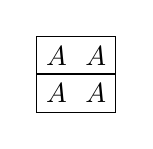
\begin{tikzpicture}[baseline=(O)]
			\matrix (M) [matrix of nodes] {
				$A$ & $A$ \\
				$A$ & $A$ \\
			};
			\coordinate (O) at (M-1-1.south west);
			\draw (M-1-1.north west) rectangle (M-1-2.south east);
			\draw (M-2-1.north west) rectangle (M-2-2.south east);
		\end{tikzpicture} = 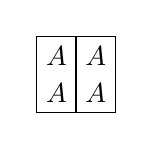
\begin{tikzpicture}[baseline=(O)]
			\matrix (M) [matrix of nodes] {
				$A$ & $A$ \\
				$A$ & $A$ \\
			};
			\coordinate (O) at (M-1-1.south west);
			\draw (M-1-1.north west) rectangle (M-2-1.south east);
			\draw (M-1-2.north west) rectangle (M-2-2.south east);
		\end{tikzpicture} \quad \begin{tabular}{rl}
			Horizontal: & multiply using $\mu'$ \\
			Vertical: & multiply using $\mu_A$
		\end{tabular}\end{center}
		The argument for $\mu'=\mu_A$ can now be pictured as
		% segment-id: o014.li2.chapter7.exercises-a.g002
		\begin{center}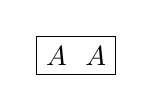
\begin{tikzpicture}[baseline=(O)]
			\matrix (M) [matrix of nodes] {
				$A$ & $A$ \\
			};
			\coordinate (O) at (M-1-1.south west);
			\draw (M-1-1.north west) rectangle (M-1-2.south east);
		\end{tikzpicture}
		$=$ 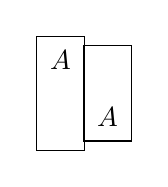
\begin{tikzpicture}[baseline=(O)]
			\matrix (M) [matrix of nodes, every node/.style={anchor=base, minimum width=1.7em, minimum height=1.7em}] {
				$A$ & $\munit$ \\
				$\munit$ & $A$ \\
			};
			\coordinate (O) at (M-1-1.south west);
			\draw (M-1-1.north west) rectangle (M-2-1.south east);
			\draw (M-1-2.north west) rectangle (M-2-2.south east);
		\end{tikzpicture}
		$=$ 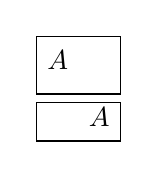
\begin{tikzpicture}[baseline=(O)]
			\matrix (M) [matrix of nodes, every node/.style={anchor=base, minimum width=1.5em, minimum height=1.7em}] {
				$A$ & $\munit$ \\
				$\munit$ & $A$ \\
			};
			\coordinate (O) at (M-1-1.south west);
			\draw (M-1-1.north west) rectangle (M-1-2.south east);
			\draw (M-2-1.north west) rectangle (M-2-2.south east);
		\end{tikzpicture}
		$=$ 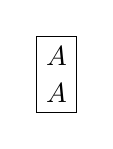
\begin{tikzpicture}[baseline=(O)]
			\matrix (M) [matrix of nodes] {
				$A$ \\
				$A$ \\
			};
			\coordinate (O) at (M-1-1.south west);
			\draw (M-1-1.north west) rectangle (M-2-1.south east);
		\end{tikzpicture}\end{center}
		Try also to translate this picture into the corresponding commutative
		diagram or equation.
	\end{hint}

	% segment-id: o014.li2.chapter7.exercises-a.ex003
	\item Consider a dg-algebra $A$ over $\mathcal{A}$
	(Definition~\ref{def:dg-algebra}). Verify that when $A=\munit$ (the unit
	object), both left and right $A$-modules reduce to complexes over
	$\mathcal{A}$.

	% segment-id: o014.li2.chapter7.exercises-a.ex004
	\item Fix a commutative ring $\Bbbk$. Let $A$ be a dg-algebra over
	$\Bbbk\dcate{Mod}$ and let $M$ be a complex. Prove that giving $M$ the
	structure of a left $A$-module is equivalent to specifying a homomorphism
	of dg-algebras $A\to\End^\bullet(M):=\Hom^\bullet(M,M)$.

	% segment-id: o014.li2.chapter7.exercises-a.ex005
	\item Let $\Bbbk$ be a commutative ring and $R$ a dg-algebra over
	$\Bbbk\dcate{Mod}$. For a right $R$-module $X$ and a left $R$-module $Y$,
	identify $R$ and $X,Y$, respectively, with a $\Bbbk$-algebra and
	$\Bbbk$-modules equipped with direct-sum decompositions
	% segment-id: o014.li2.chapter7.exercises-a.q002
	\[ R = \bigoplus_n R^n, \quad X = \bigoplus_n X^n, \quad Y = \bigoplus_n Y^n \]
	and degree-$1$ endomorphisms $d$ satisfying $d^2=0$. Thus
	$X\dotimes{R}Y$ is already defined as a $\Bbbk$-module.
	\begin{enumerate}[(i)]
		\item Recall that
		$X\otimes Y=\bigoplus_n(\bigoplus_{p+q=n}X^p\otimes Y^q)$ is both a
		$\Bbbk$-module and a complex. For the evident $\Bbbk$-module
		homomorphism $\pi:X\otimes Y\twoheadrightarrow X\dotimes{R}Y$, verify
		that $\Ker(\pi)$ is a subcomplex, so that $X\dotimes{R}Y$ has a
		canonical complex structure.

		\item Prove that if $X$ is an $(A,R)$-bimodule and $Y$ is an
		$(R,B)$-bimodule, where $A$ and $B$ are also dg-algebras, then
		$X\dotimes{R}Y$ is naturally an $(A,B)$-bimodule. Use this to extend
		the adjunction of Proposition~\ref{prop:tensor-Hom-cplx} to dg-modules.
		Here $\Hom^\bullet(Y_B,Z_B)$ and $\Hom^\bullet({}_AX,{}_AZ)$ are
		defined as complexes as in Example~\ref{eg:dg-Hom-cplx}, but the signs
		must be handled carefully when assigning the $(A,R)$- and
		$(R,B)$-bimodule structures.
	\end{enumerate}

	% segment-id: o014.li2.chapter7.exercises-a.ex006
	\item Fix a dg-algebra $A$ over $\mathcal{A}$. It is called
	\emph{non-positive} if $p>0\implies A^p=0$. For a left (or right)
	$A$-module $M$ and $n\in\Z$, take the truncation subcomplex
	$\tau^{\leq n}M$ as in Definition~\ref{def:truncation-cplx}. Prove that if
	$A$ is non-positive, then:
	\begin{enumerate}[(i)]
		\item every $d_M^p:M^p\to M^{p+1}$ is $A^0$-linear;
		\item there is a short exact sequence of $A$-modules
		$0\to\tau^{\leq n}M\to M\to\tilde\tau^{\geq n+1}M\to0$.
	\end{enumerate}
	\index{dg algebra!non-positive}

	% segment-id: o014.li2.chapter7.exercises-a.ex007
	\item Fix a dg-algebra $A$ over $\mathcal{A}$. Recall that all left
	$A$-modules form the dg-category $A\dcate{dgMod}$
	(Example~\ref{eg:dg-Hom-cplx}); Remark~\ref{rem:dg-homotopy-cat} then
	gives the homotopy category $\mathrm{h}(A\dcate{dgMod})$. A left
	$A$-module $M$ is called acyclic if it is acyclic as a complex; a
	morphism of $A$-modules $f:M\to N$ is called a quasi-isomorphism if it is
	a quasi-isomorphism of complexes.
	\begin{enumerate}[(i)]
		\item Let $M$ be a left $A$-module whose structure is determined by a
		family of morphisms in $\mathcal{A}$,
		$\alpha_{A,M}^{p,q}:A^p\otimes M^q\to M^{p+q}$ ($p,q\in\Z$). Show
		that the formula
		% segment-id: o014.li2.chapter7.exercises-a.q003
		\[ \alpha_{A, M[1]}^{p, q} := (-1)^p \alpha_{A, M}^{p, q+1} . \]
		gives the complex $M[1]$ a left $A$-module structure. Then show that
		$M\mapsto M[1]$ defines a dg-functor from $A\dcate{dgMod}$ to itself.
		\item For every morphism $f:M\to N$ in $A\dcate{dgMod}$, show that
		the mapping cone $\Cone(f)$ has a canonical left $A$-module structure,
		given in the notation above by
		% segment-id: o014.li2.chapter7.exercises-a.q004
		\[ \alpha_{A, \Cone(f)}^{p, q} = \alpha_{A, M[1]}^{p, q} \oplus \alpha_{A, N}^{p, q}. \]
		\item Following the construction of \S\ref{sec:derived-cat}, use
		mapping cones to make $\mathrm{h}(A\dcate{dgMod})$ a triangulated
		category. Next perform Verdier localization at the acyclic $A$-modules,
		or equivalently adjoin inverses to the quasi-isomorphisms, to obtain the
		derived category $\cate{D}(A\dcate{dgMod})$. Define the corresponding
		$\cate{D}^{\star}(A\dcate{dgMod})$ for
		$\star\in\{+,-,\bdd\}$.
		\item Assuming that $A$ is non-positive, extend
		Proposition~\ref{prop:derived-full-faithful-subcat} to
		$\cate{D}(A\dcate{dgMod})$ and
		$\cate{D}^{\star}(A\dcate{dgMod})$ for
		$\star\in\{+,-,\bdd\}$.
		% segment-id: o014.li2.chapter7.exercises-a.hi002
		\begin{hint}
			Use the truncation functors.
		\end{hint}
		\item Following \S\ref{sec:K-injectives}, define K-injective and
		K-projective $A$-modules and use them to describe the morphisms in
		$\cate{D}(A\dcate{dgMod})$. Place this discussion in the framework of
		\S\ref{sec:triangulated-functor-localization} to study their relation
		to derived functors.
		\item For a right $A$-module $M$, show that the complex $M[1]$ has the
		right $A$-module structure
		$\alpha_{M[1],A}^{p,q}=\alpha_{M,A}^{p,q+1}$ and that all the preceding
		properties remain valid.
	\end{enumerate}

	% segment-id: o014.li2.chapter7.exercises-a.ex008
	\item Let $\mathcal{C}$ be a dg-category over $\Bbbk$. Define
	$\mathcal{C}^{\opp}$ by $\Obj(\mathcal{C}^{\opp})=\Obj(\mathcal{C})$ and,
	for all $X,Y\in\Obj(\mathcal{C}^{\opp})$,
	$\Hom^\bullet_{\mathcal{C}^{\opp}}(X,Y):=
	\Hom^\bullet_{\mathcal{C}}(Y,X)$. Define composition by
	% segment-id: o014.li2.chapter7.exercises-a.q005
	\begin{align*}
		\Hom^p_{\mathcal{C}^{\opp}}(Y, Z) \dotimes{\Bbbk} \Hom^q_{\mathcal{C}^{\opp}}(X, Y) & \to \Hom^{p+q}_{\mathcal{C}^{\opp}}(X, Z) \quad p, q \in \Z \\
		f \otimes g & \mapsto (-1)^{pq} \underbracket{f \circ g}_{\text{composition in }\Hom^\bullet_{\mathcal{C}}}.
	\end{align*}
	Verify that this indeed defines a dg-category $\mathcal{C}^{\opp}$, called
	the opposite dg-category of $\mathcal{C}$.

	% segment-id: o014.li2.chapter7.exercises-a.ex009
	\item Fix a commutative ring $\Bbbk$, a dg-algebra $R$ over
	$\Bbbk\dcate{Mod}$, a right $R$-module $X$, and a left $R$-module $Y$.
	Prove that the previously introduced functors
	% segment-id: o014.li2.chapter7.exercises-a.q006
	\[ X \dotimes{R} (\cdot): R\dcate{dgMod} \to \cate{C}(\Bbbk), \quad (\cdot) \dotimes{R} Y: \cated{dgMod}R \to \cate{C}(\Bbbk), \]
	upgrade naturally to dg-functors. Outline the corresponding statements when
	$X$ or $Y$ also has a bimodule structure.

	% segment-id: o014.li2.chapter7.exercises-a.hi003
	\begin{hint}
		The key is to define the morphisms between the $\Hom$ complexes. For
		$X\dotimes{R}(\mathord\cdot)$, let $M$ and $N$ be left $R$-modules.
		The Koszul sign rule requires the image of $f\in\Hom^n_R(M,N)$,
		namely $\identity_X\otimes f\in
		\Hom^n(X\dotimes{R}M,X\dotimes{R}N)$, to be defined by
		% segment-id: o014.li2.chapter7.exercises-a.q007
		\[ (\identity_X \otimes f)(x \otimes m) = (-1)^{pn} x \otimes f(m), \quad x \in X^p, \; m \in M^q. \]
		One must verify that
		$\identity_X\otimes d_{\Hom^\bullet}(f)=
		d_{\Hom^\bullet}(\identity_X\otimes f)$.

		The case $(\mathord\cdot)\dotimes{R}Y$ is simpler: take
		$(f\otimes\identity_Y)(m\otimes y)=f(m)\otimes y$.
	\end{hint}

	% segment-id: o014.li2.chapter7.exercises-a.ex010
	\item Let $\mathcal{C}$ be a dg-category over a commutative ring $\Bbbk$
	and let $M\in\Obj(\mathcal{C})$.
	\begin{enumerate}[(i)]
		\item Upgrade
		$\Hom^\bullet(M,\mathord\cdot):\mathcal{C}\to\cate{C}(\Bbbk)$ to a
		dg-functor.

		% segment-id: o014.li2.chapter7.exercises-a.hi004
		\begin{hint}
			Let $X,Y\in\Obj(\mathcal{C})$ and $f\in\Hom^n(X,Y)$. Set
			$\mathcal{H}_X=\Hom^\bullet(M,X)$. The image of $f$ should be
			% segment-id: o014.li2.chapter7.exercises-a.q008
			\[ \left[ f_*: g \xmapsto{\text{morphism of degree }n} fg \right] \in \Hom^n(\mathcal{H}_X, \mathcal{H}_Y). \]
			Use the definition of the $\Hom$ complex to verify that
			$(d_{\Hom^\bullet(X,Y)}f)_*=
			d_{\Hom^\bullet(\mathcal{H}_X,\mathcal{H}_Y)}(f_*)$.
		\end{hint}
		\item Upgrade
		$\Hom^\bullet(\mathord\cdot,M):\mathcal{C}\to
		\cate{C}(\Bbbk)^{\opp}$ to a dg-functor.

		% segment-id: o014.li2.chapter7.exercises-a.hi005
		\begin{hint}
			Set $\mathcal{K}_X=\Hom^\bullet(X,M)$. The Koszul sign rule requires
			the image of $f\in\Hom^n(X,Y)$ to be
			% segment-id: o014.li2.chapter7.exercises-a.q009
			\[ \left[\begin{array}{c}
				f^*: g \xmapsto{\text{morphism of degree }n} (-1)^{np} gf \\
				\forall p \in \Z , \; \forall\; g \in \Hom^p(Y, M)
			\end{array}\right] \in \Hom^n(\mathcal{K}_Y, \mathcal{K}_X). \]
			Verify carefully that
			\begin{compactitem}
				\item $(d_{\Hom^\bullet(X,Y)}f)^*=
				d_{\Hom^\bullet(\mathcal{K}_Y,\mathcal{K}_X)}(f^*)$;
				\item $(fh)^*$ equals the composite of $h^*$ and $f^*$ in
				$\Hom^\bullet_{\cate{C}(\Bbbk)}$.
			\end{compactitem}
		\end{hint}
	\end{enumerate}

% Unit 104 English translation of chapter7.tex lines 2828--2944.
% Source: Methods of Algebra, Volume 2, commit
% 9a5803ff77dd3257484cb177f851a73770a59dd3 (CC BY 4.0).
% stable-unit-id: o014.aljabr2.chapter7.exercises-b
% Coverage: middle portion of the Chapter 7 Exercises, from self-enrichment of
% closed monoidal categories through uniqueness of comodule structures on
% quotients and submodules; continued by Unit 105 at line 2945.

\hypertarget{o014.aljabr2.chapter7.exercises-b}{ }
	% segment-id: o014.aljabr2.chapter7.exercises-b.ex011
	\item Prove that the canonical morphisms
	$[Y,Z]\otimes[X,Y]\to[X,Z]$ and $\munit\to[X,X]$ defined for a closed
	monoidal category in \S\ref{sec:closed-monoidal} satisfy associativity and
	unit laws. Thus a closed monoidal category is enriched over itself with
	respect to its internal $\Hom$.
	% segment-id: o014.aljabr2.chapter7.exercises-b.hi006
	\begin{hint}
		Verify this directly, or consult \cite[Section 1.6]{Kel05}.
	\end{hint}

	% segment-id: o014.aljabr2.chapter7.exercises-b.ex012
	\item Consider the polynomial algebra $\Bbbk[t]$ over a commutative ring
	$\Bbbk$. Define $\Delta$, $\epsilon$, and $S$, respectively, by
	% segment-id: o014.aljabr2.chapter7.exercises-b.q010
	\[ \Delta(t^n) = \sum_{k=0}^n \binom{n}{k} t^k \otimes t^{n-k}, \quad \epsilon(t^n) = \begin{cases}
		1, & n = 0 \\
		0, & n \neq 0
	\end{cases}, \quad
	S(t^n) = (-1)^n t^n, \]
	where $n\in\Z_{\geq0}$. Verify that these data define a commutative and
	cocommutative Hopf $\Bbbk$-algebra.

	% segment-id: o014.aljabr2.chapter7.exercises-b.ex013
	\item Let $A$ be a Hopf algebra over a commutative ring. An ideal $I$ of
	$A$ is called a \emph{Hopf ideal} if
	$\Delta(I)\subset I\otimes A+A\otimes I$, $\epsilon(I)=0$, and
	$S(I)\subset I$. Show that quotienting by a Hopf ideal gives a Hopf
	algebra $A/I$.

	% segment-id: o014.aljabr2.chapter7.exercises-b.ex014
	\item Let $\Bbbk$ be a commutative ring and $V$ a $\Bbbk$-module. On the
	tensor algebra $T(V)$ (see \cite[Definition 7.5.1]{Li1}) one can define
	$\Bbbk$-algebra homomorphisms
	$\Delta:T(V)\to T(V)\otimes T(V)$ and $\epsilon:T(V)\to\Bbbk$ such that,
	for every $v\in V$,
	% segment-id: o014.aljabr2.chapter7.exercises-b.q011
	\begin{gather*}
		\Delta(v) = v \otimes 1 + 1 \otimes v, \quad \epsilon(v) = 0;
	\end{gather*}
	here the algebra structure on $T(V)\otimes T(V)$ is defined by the trivial
	braiding $x\otimes y\mapsto y\otimes x$.
	\begin{enumerate}[(i)]
		% segment-id: o014.aljabr2.chapter7.exercises-b.i001
		\item Verify that this makes $T(V)$ a bialgebra.
		% segment-id: o014.aljabr2.chapter7.exercises-b.i002
		\item Show how to define a $\Bbbk$-module automorphism
		$S:T(V)\to T(V)$ such that $S(v)=-v$ and $S$ is a bialgebra
		antiautomorphism (Proposition~\ref{prop:Hopf-antiautomorphism}); more
		explicitly,
		% segment-id: o014.aljabr2.chapter7.exercises-b.q012
		\[ S(v_1 \cdots v_n) = (-1)^n v_n \cdots v_1, \quad n \in \Z_{\geq 0}, \quad v_1, \ldots, v_n \in V. \]
		Verify that this makes $T(V)$ a Hopf algebra.
		% segment-id: o014.aljabr2.chapter7.exercises-b.i003
		\item Show that the symmetric algebra $\Sym(V)$ has the analogous
		properties; in fact it is a quotient of $T(V)$ by a Hopf ideal.
		% segment-id: o014.aljabr2.chapter7.exercises-b.i004
		\item Treat the version for the exterior algebra $\bigwedge(V)$, but
		define the multiplication on $\bigwedge(V)\otimes\bigwedge(V)$ using
		the Koszul braiding \eqref{eqn:Koszul-braiding} (take
		$\epsilon(a)=a\bmod\;2$ there), so that homogeneous elements
		$x,y,z,w\in\bigwedge(V)$ satisfy
		$(x\otimes y)(z\otimes w)=(-1)^{\deg y\deg z}xz\otimes yw$. This
		ensures that $(1\otimes v+v\otimes1)^2$ is the zero element of
		$\bigwedge(V)\otimes\bigwedge(V)$ for every $v\in V$.
	\end{enumerate}

	% segment-id: o014.aljabr2.chapter7.exercises-b.ex015
	\item (E.\ Taft) Let $q$ be a primitive $n$th root of unity in a field
	$\Bbbk$, where $n\geq2$. Consider the $\Bbbk$-algebra $H$ defined by
	generators $g$, $x$, and relations
	% segment-id: o014.aljabr2.chapter7.exercises-b.q013
	\[ g^n = 1, \quad x^n = 0, \quad gxg^{-1} = qx. \]
	Show that one can define $\Delta:H\to H\dotimes{\Bbbk}H$ and
	$\epsilon:H\to\Bbbk$ satisfying
	% segment-id: o014.aljabr2.chapter7.exercises-b.q014
	\begin{gather*}
		\Delta(g) = g \otimes g, \quad \Delta(x) = 1 \otimes x + x \otimes g, \\
		\epsilon(g) = 1, \quad \epsilon(x) = 0,
	\end{gather*}
	and making $H$ a Hopf $\Bbbk$-algebra with antipode
	% segment-id: o014.aljabr2.chapter7.exercises-b.q015
	\[ S:H\to H, \quad S(g)=g^{-1}, \quad S(x)=-g^{-1}x. \]

	Show that $H$ is neither commutative nor cocommutative. When $n=2$, the
	corresponding Hopf algebra is also called Sweedler's Hopf algebra.

	% segment-id: o014.aljabr2.chapter7.exercises-b.ex016
	\item Let $(A,\Delta,\epsilon)$ be a coalgebra over a commutative ring
	$\Bbbk$. If $x\in A$ satisfies $\Delta(x)=1\otimes x+x\otimes1$, then
	$x$ is called \emph{primitive}.
	\begin{enumerate}[(i)]
		% segment-id: o014.aljabr2.chapter7.exercises-b.i005
		\item Prove that $\epsilon(x)=0$ for every primitive element $x$.
		% segment-id: o014.aljabr2.chapter7.exercises-b.i006
		\item Let $(A,\mu,\eta,\Delta,\epsilon)$ be a bialgebra and write $\mu$
		as multiplication, so $xy=\mu(x\otimes y)$. Prove that if $x,y\in A$
		are primitive, then $xy-yx$ is primitive as well.
		% segment-id: o014.aljabr2.chapter7.exercises-b.i007
		\item Still taking $A$ to be a bialgebra, let
		$x_1,\ldots,x_n\in A$ be primitive elements and let $V$ be the free
		$\Bbbk$-module with basis $x_1,\ldots,x_n$. This gives a
		$\Bbbk$-algebra homomorphism $\phi:T(V)\to A$. Prove that $\phi$ is
		also a bialgebra homomorphism.
	\end{enumerate}

	% segment-id: o014.aljabr2.chapter7.exercises-b.ex017
	\item Let $(A,\Delta,\epsilon)$ be a coalgebra over a commutative ring
	$\Bbbk$, with $A\neq\{0\}$ and $A$ torsion-free as a $\Bbbk$-module. A
	nonzero element $x\in A$ satisfying $\Delta(x)=x\otimes x$ is called
	\emph{group-like}. Denote the set of all group-like elements by
	$\mathcal{G}(A)$.
	\begin{enumerate}[(i)]
		% segment-id: o014.aljabr2.chapter7.exercises-b.i008
		\item Prove that $x\in\mathcal{G}(A)$ implies $\epsilon(x)=1$.
		% segment-id: o014.aljabr2.chapter7.exercises-b.i009
		\item Prove that if $(A,\mu,\eta,\Delta,\epsilon)$ is a bialgebra, then
		$\mathcal{G}(A)$ is a monoid under the multiplication $\mu$ of $A$,
		with unit $1_A:=\eta(1)$.
		% segment-id: o014.aljabr2.chapter7.exercises-b.i010
		\item For a monoid $M$ and the corresponding bialgebra $\Bbbk[M]$
		(Example~\ref{eg:monoid-bialgebra}), prove that
		$\mathcal{G}(\Bbbk[M])=M$.
		% segment-id: o014.aljabr2.chapter7.exercises-b.i011
		\item Let $A$ be a Hopf algebra with antipode $S$. Prove that
		$\mathcal{G}(A)$ is a group and that the inverse of
		$x\in\mathcal{G}(A)$ is $S(x)$.
	\end{enumerate}

	% segment-id: o014.aljabr2.chapter7.exercises-b.ex018
	\item Let $(A,\Delta,\epsilon)$ be a nonzero coalgebra over a field
	$\Bbbk$. Prove that $\mathcal{G}(A)$ is a linearly independent subset of
	$A$.

	% segment-id: o014.aljabr2.chapter7.exercises-b.hi007
	\begin{hint}
		Suppose otherwise, and choose a shortest nontrivial linear relation among
		these elements. Without loss of generality, write
		$x_1=\sum_{i=2}^n a_i x_i$, where
		$x_1,\ldots,x_n\in\mathcal{G}(A)$ are pairwise distinct and
		$a_i\in\Bbbk$. Then $x_2,\ldots,x_n$ are linearly independent, while
		$x_1\otimes x_1=\sum_{i=2}^n a_i x_i\otimes x_i$.
	\end{hint}

	% segment-id: o014.aljabr2.chapter7.exercises-b.ex019
	\item Write $\cate{TopCMon}$ for the category of commutative topological
	monoids, $\cate{Top}_\bullet$ for the category of pointed topological
	spaces, and $U:\cate{TopCMon}\to\cate{Top}_\bullet$ for the forgetful
	functor (the base point corresponds to the unit). Construct a left adjoint
	$\Sym:\cate{Top}_\bullet\to\cate{TopCMon}$ to $U$. For a pointed
	topological space $(X,x)$, the object $\Sym(X,x)$ is also called the
	\emph{infinite symmetric product} of $(X,x)$; explain this terminology.
	The Dold--Thom theorem in algebraic topology is based on this construction.

	% Reference: Deligne, Categories tannakiennes, 4.5 Proposition.
	% segment-id: o014.aljabr2.chapter7.exercises-b.ex020
	\item Let the $(A,B)$-bimodule $P$ be finitely generated projective as a
	right $B$-module, and suppose that $(\mathord\cdot)\dotimes{A}P$ is a
	faithful exact functor. Prove that a right $A$-module $N$ is finitely
	presented (Example~\ref{eg:Mod-cpt}) if and only if
	$N\dotimes{A}P$ is finitely presented as a right $B$-module. This
	complements Proposition~\ref{prop:Morita-comonad-ft}.

	% segment-id: o014.aljabr2.chapter7.exercises-b.ex021
	\item Consider a commutative ring $\Bbbk$ and a homomorphism of
	$\Bbbk$-algebras $f:A\to B$. We have an adjoint pair
	% segment-id: o014.aljabr2.chapter7.exercises-b.q016
	\[\begin{tikzcd}
		\mathcal{F}_{B|A}: \cated{Mod}B \arrow[shift left, r] & \cated{Mod}A: \Hom_A(B, \cdot), \arrow[shift left, l]
	\end{tikzcd}\]
	where, for every right $A$-module $N$, $\Hom_A(B,N)$ is given the right
	$B$-module structure $(\phi b)(x)=\phi(bx)$. More precisely,
	\begin{compactitem}
		% segment-id: o014.aljabr2.chapter7.exercises-b.i012
		\item the unit morphism $M\to\Hom_A(B,M)$ maps $m$ to $[b\mapsto mb]$;
		% segment-id: o014.aljabr2.chapter7.exercises-b.i013
		\item the counit morphism $\Hom_A(B,N)\to N$ maps $\phi$ to $\phi(1)$.
	\end{compactitem}
	See \cite[Corollary 6.6.8]{Li1}. As a complement to
	Example~\ref{eg:comonad-change-ring}, determine explicitly the
	corresponding monad and comonad.

	% segment-id: o014.aljabr2.chapter7.exercises-b.ex022
	\item Let $R$ be a commutative ring. Write $R\dcate{Alg}$ for the category
	of $R$-algebras. Consider the adjoint pair
	% segment-id: o014.aljabr2.chapter7.exercises-b.g001
	$\begin{tikzcd}
		T(\cdot): R\dcate{Mod} \arrow[shift left, r] & R\dcate{Alg}: U \arrow[shift left, l]
	\end{tikzcd}$,
	where $T(\mathord\cdot)$ is the tensor-algebra functor and $U$ is the
	forgetful functor.
	\begin{enumerate}[(i)]
		% segment-id: o014.aljabr2.chapter7.exercises-b.i014
		\item Prove directly that modules under the corresponding monad on
		$R\dcate{Mod}$ are $R$-algebras, and hence that the adjoint pair is
		monadic.
		% segment-id: o014.aljabr2.chapter7.exercises-b.i015
		\item Replace $T(\mathord\cdot)$ by $\Sym(\mathord\cdot)$ and
		$\bigwedge(\mathord\cdot)$, then state and prove the corresponding
		results; see \cite[\S 7.6]{Li1}.
	\end{enumerate}

	% segment-id: o014.aljabr2.chapter7.exercises-b.ex023
	\item Complete the argument of Proposition~\ref{prop:Comod-abelian}, and
	then prove the following stronger version. Let $C$ be a coalgebra in
	$(B,B)\dcate{Mod}$. Prove that:
	\begin{enumerate}[(i)]
		% segment-id: o014.aljabr2.chapter7.exercises-b.i016
		\item the forgetful functor $U:\cated{Comod}C\to\cated{Mod}B$ has a
		right adjoint;

		% segment-id: o014.aljabr2.chapter7.exercises-b.hi008
		\begin{hint}
			Write $\Delta$ for the comultiplication of $C$ and $\epsilon$ for its
			counit. For a right $B$-module $N$, make $N\dotimes{B}C$ a right
			$C$-comodule via $\identity_N\otimes\Delta$. For every right
			$C$-comodule $M$, verify that
			% segment-id: o014.aljabr2.chapter7.exercises-b.q017
			\[\begin{tikzcd}[row sep=tiny]
				\Hom_{\cated{Mod}B}(M, N) \arrow[shift left, r] & \Hom_{\cated{Comod}C}\left(M, N \dotimes{B} C\right) \arrow[shift left, l] \\
				\varphi \arrow[mapsto, r] & (\varphi \otimes \identity_C) \rho \\
				(\identity_N \otimes \epsilon) \psi & \psi \arrow[mapsto, l]
			\end{tikzcd}\]
			are mutually inverse, where $\rho:M\to M\dotimes{B}C$ specifies the
			comodule structure of $M$.
		\end{hint}
		% segment-id: o014.aljabr2.chapter7.exercises-b.i017
		\item the forgetful functor $U$ creates all small $\varinjlim$; hence
		$\cated{Comod}C$ is cocomplete;
		% segment-id: o014.aljabr2.chapter7.exercises-b.i018
		\item the category $\cated{Comod}C$ has a cogenerator
		(Definition~\ref{def:generators});

		% segment-id: o014.aljabr2.chapter7.exercises-b.hi009
		\begin{hint}
			Take a cogenerator of the Grothendieck category $\cated{Mod}B$, then
			take its image under the right adjoint of $U$.
		\end{hint}
		% segment-id: o014.aljabr2.chapter7.exercises-b.i019
		\item if $\cated{Comod}C$ is an abelian category and $U$ is exact, then
		$C$ is flat as a left $B$-module.

		% segment-id: o014.aljabr2.chapter7.exercises-b.hi010
		\begin{hint}
			Let $g:M\to N$ be a monomorphism of right $B$-modules. Use the
			exactness of $U$ and the fact that a right adjoint preserves kernels
			to show that
			$g\otimes\identity_C:M\dotimes{B}C\to N\dotimes{B}C$ remains
			injective.
		\end{hint}
	\end{enumerate}

	% segment-id: o014.aljabr2.chapter7.exercises-b.ex024
	\item As in the preceding exercise, continue to let $C$ be a coalgebra in
	$(B,B)\dcate{Mod}$ and let $M$ be a right $C$-comodule. Prove that if a
	quotient $B$-module $M''$ of $M$ (or a $B$-submodule $M'$ of $M$) has a
	comodule structure making $M\twoheadrightarrow M''$ (or
	$M'\hookrightarrow M$) a comodule homomorphism, then that comodule
	structure is unique. In the submodule case, additionally assume that $C$
	is flat as a left $B$-module.

% Unit 105 English translation of chapter7.tex lines 2945--3002.
% Source: Methods of Algebra, Volume 2, commit
% 9a5803ff77dd3257484cb177f851a73770a59dd3 (CC BY 4.0).
% stable-unit-id: o014.aljabr2.chapter7.exercises-c
% Coverage: concluding Chapter 7 exercises on Galois descent, twisting in
% nonabelian cohomology, and quadratic forms; closes the Exercises environment.

\hypertarget{o014.aljabr2.chapter7.exercises-c}{ }
% segment-id: o014.aljabr2.chapter7.exercises-c.ex001
	\item Following the explanation at the end of
	\S\ref{sec:descent-Galois}, give a direct proof of the Galois descent
	Theorem~\ref{prop:Galois-descent} by the following steps. Use the notation
	from that section: let $M\in\Obj(\cate{Vect}^{\Gamma,\infty}(L))$ and
	define the canonical map $\iota_M$ by \eqref{eqn:Galois-descent-iotaM}.
	\begin{enumerate}[(i)]
% segment-id: o014.aljabr2.chapter7.exercises-c.i001
		\item Let $M'$ be a $\Gamma$-invariant subspace of
		$L\dotimes{K}(M^\Gamma)$, that is, $\Gamma M'\subset M'$. Prove that
		if $M'\cap(1\otimes M^\Gamma)=\{0\}$, then $M'=\{0\}$.

% segment-id: o014.aljabr2.chapter7.exercises-c.hi001
		\begin{hint}
			Choose a basis $(y_i)_{i\in I}$ of $M^\Gamma$. If $M'\neq\{0\}$,
			choose in it a nonzero expression with the fewest possible terms,
			$\sum_{i\in I}\ell_i\otimes y_i$ (a finite sum). After a suitable
			normalization, it may be assumed to have the form
% segment-id: o014.aljabr2.chapter7.exercises-c.q001
			\[ m' = 1 \otimes y_{i_0} + \ell_1 \otimes y_{i_1} + \cdots, \quad \ell_1 \notin K. \]
			Choose $\sigma\in\Gamma$ such that
			$\sigma(\ell_1)\neq\ell_1$, and consider $m'-\sigma(m')$ to obtain a
			contradiction.
		\end{hint}

% segment-id: o014.aljabr2.chapter7.exercises-c.i002
		\item Prove that $\iota_M:L\dotimes{K}(M^\Gamma)\to M$ is injective.
% segment-id: o014.aljabr2.chapter7.exercises-c.hi002
		\begin{hint}
			Consider $M':=\Ker(\iota_M)$.
		\end{hint}

% segment-id: o014.aljabr2.chapter7.exercises-c.i003
		\item Prove that $\iota_M$ is surjective.

% segment-id: o014.aljabr2.chapter7.exercises-c.hi003
		\begin{hint}
			Consider a finite Galois subextension $E|K$ of $L|K$. Take
			$a_1,\ldots,a_n$ as a basis of $E$ as a vector space over $K$, and
			choose representatives $\identity=\sigma_1,\ldots,\sigma_n\in\Gamma$
			for the elements of $\Gal(E|K)$. Field theory shows that
			$(\sigma_i(a_j))_{1\leq i,j\leq n}$ is an invertible matrix over $E$;
			write its inverse as $(b_{ij})_{1\leq i,j\leq n}$. For
			$m\in M^{\Gal(L|E)}$, derive
% segment-id: o014.aljabr2.chapter7.exercises-c.q002
			\[ m = \sum_{i=1}^n b_{i1} \sum_{j=1}^n \sigma_j(a_i m) \; \in \Image(\iota_M). \]
		\end{hint}

% segment-id: o014.aljabr2.chapter7.exercises-c.i004
		\item Use the preceding results to show that
		\eqref{eqn:Galois-descent-adjunction} is an adjoint equivalence, thus
		giving a direct proof of Theorem~\ref{prop:Galois-descent}.
	\end{enumerate}

% segment-id: o014.aljabr2.chapter7.exercises-c.ex002
	\item Let $G$ be a group and $L|K$ a Galois extension of fields. Write
	$G\dcate{Mod}$ (or $G\dcate{Mod}_L$) for the category of $G$-modules with
	coefficients in $K$ (or $L$); see Definition~\ref{def:G-mod}. Use the
	Galois descent methods of
	\S\S\ref{sec:descent-Galois}---\ref{sec:Galois-H1} to describe
	$G\dcate{Mod}$ in terms of objects of $G\dcate{Mod}_L$ equipped with an
	appropriate $\Gal(L|K)$-action.

% segment-id: o014.aljabr2.chapter7.exercises-c.ex003
	\item Use the notation of \S\ref{sec:Galois-H1}. Let
	$c\in Z^1(\Gamma,G(\mathbf{t}_{0,L}))$. Recall from the proof of
	Theorem~\ref{prop:Galois-H1} that, through Galois descent, $c$ defines a
	$K$-vector space $W$ with data $\mathbf{t}$ on it, as well as an
	isomorphism $h:\mathbf{t}_{0,L}\rightiso\mathbf{t}_L$.
	\begin{enumerate}[(i)]
% segment-id: o014.aljabr2.chapter7.exercises-c.i005
		\item Show that $g\mapsto h^{-1}gh$ gives a group isomorphism
		$\nu:G(\mathbf{t}_L)\rightiso G(\mathbf{t}_{0,L})$. Show that
% segment-id: o014.aljabr2.chapter7.exercises-c.q003
		$ f \xmapsto{\sigma \in \Gamma} c(\sigma)({}^\sigma f)c(\sigma)^{-1} $
		gives a new $\Gamma$-action on $G(\mathbf{t}_{0,L})$. Denote this
		structure by ${}^cG(\mathbf{t}_{0,L})$, and show that
		$\nu:G(\mathbf{t}_L)\rightiso{}^cG(\mathbf{t}_{0,L})$ is
		$\Gamma$-equivariant.

% segment-id: o014.aljabr2.chapter7.exercises-c.i006
		\item Show that the following formula gives a well-defined map:
% segment-id: o014.aljabr2.chapter7.exercises-c.q004
		\begin{align*}
			Z^1(\Gamma, G(\mathbf{t}_L)) & \to Z^1(\Gamma, G(\mathbf{t}_{0, L})) \\
			\tilde{c} & \mapsto \left[\sigma \mapsto \nu(\tilde{c}(\sigma)) c(\sigma) \right].
		\end{align*}
		It induces a bijection
		$\Hm^1(\Gamma,G(\mathbf{t}_L))\to
		\Hm^1(\Gamma,G(\mathbf{t}_{0,L}))$ that maps the base point to $[c]$.
% segment-id: o014.aljabr2.chapter7.exercises-c.hi004
		\begin{hint}
			Compare the ``twisting'' construction in the exercises for
			\CHref{sec:group-coh}.
		\end{hint}

% segment-id: o014.aljabr2.chapter7.exercises-c.i007
		\item Show that, under the correspondence in
		Theorem~\ref{prop:Galois-H1}, this bijection corresponds to the equality
		$\mathscr{T}(\mathbf{t})=\mathscr{T}(\mathbf{t}_0)$.
	\end{enumerate}

% segment-id: o014.aljabr2.chapter7.exercises-c.ex004
	\item Let $K$ be a field with $\mathrm{char}(K)\neq2$. A nondegenerate
	symmetric bilinear form $q:V\times V\to K$ on a finite-dimensional
	$K$-vector space $V$ will simply be called a nondegenerate quadratic form.
	In the orthogonal group $\mathrm{O}(q)=\mathrm{O}(V,q)$, write
	$\SO(q)=\SO(V,q)$ for the subgroup cut out by $\det=1$. For every Galois
	extension $L|K$, there is a nondegenerate quadratic form $(V_L,q_L)$ and
	the corresponding groups, all equipped with a smooth action of
	$\Gamma:=\Gal(L|K)$.
	\begin{enumerate}[(i)]
% segment-id: o014.aljabr2.chapter7.exercises-c.i008
		\item Write $\mu_2:=\{\pm1\}\subset K^\times$. Show that
		$\mathrm{O}(q)/\SO(q)\simeq\mu_2$. For the version
		$\mathrm{O}(q_L)/\SO(q_L)$, explain the relation between this
		isomorphism and the $\Gamma$-action.

% segment-id: o014.aljabr2.chapter7.exercises-c.i009
		\item Using the tools of \S\ref{sec:Galois-H1}, show that the elements
		of $\Hm^1(\Gamma,\mathrm{O}(q_L))$ correspond bijectively to the
		isomorphism classes of nondegenerate quadratic forms $(V',q')$ over $K$
		with $\dim V'=\dim V$, where the base point corresponds to $(V,q)$.

% segment-id: o014.aljabr2.chapter7.exercises-c.i010
		\item Apply Theorem~\ref{prop:nonabelian-long} to obtain the exact
		sequence of pointed sets
% segment-id: o014.aljabr2.chapter7.exercises-c.q005
		\[ \mathrm{O}(q) \xrightarrow{\det} \mu_2 \to \Hm^1(\Gamma, \SO(q_L)) \xrightarrow{\varphi} \Hm^1(\Gamma, \mathrm{O}(q_L)) \xrightarrow{\psi} \Hm^1(\Gamma, \mu_2). \]
		Try to show that $\varphi$ is injective.
% segment-id: o014.aljabr2.chapter7.exercises-c.hi005
		\begin{hint}
			Surjectivity of $\det$ only shows that
			$\varphi^{-1}(\text{base point})=\{\text{base point}\}$. To prove
			injectivity, one must vary $(V,q)$ and apply the twisting technique
			from the preceding exercise.
		\end{hint}

% segment-id: o014.aljabr2.chapter7.exercises-c.i011
		\item Show that
		$\Hm^1(\Gamma,\mu_2)\simeq K^\times/K^{\times,2}$. Also show that
		$\psi$ is the map
% segment-id: o014.aljabr2.chapter7.exercises-c.q006
		\[ \left[ (V', q'):\; \text{nondegenerate quadratic form} \right] \mapsto \mathrm{disc}(q') / \mathrm{disc}(q), \]
		where one chooses any basis of $V'$, identifies $q'$ with a symmetric
		matrix, and defines
% segment-id: o014.aljabr2.chapter7.exercises-c.q007
		\[ \mathrm{disc}(q') := (-1)^n \det(q') \bmod K^{\times 2}, \quad \dim V = 2n \;\text{or}\; 2n+1. \]

% segment-id: o014.aljabr2.chapter7.exercises-c.i012
		\item Show that the elements of $\Hm^1(\Gamma,\SO(q_L))$ correspond
		bijectively to the isomorphism classes of nondegenerate quadratic forms
		$(V',q')$ over $K$ satisfying $\dim V'=\dim V$ and
		$\mathrm{disc}(q')=\mathrm{disc}(q)$, with the base point corresponding
		to $(V,q)$.
	\end{enumerate}
% segment-id: o014.aljabr2.chapter7.exercises-c.c001
\end{Exercises}

% Unit 106 English translation of chapter8.tex lines 1--174.
% Source: Methods of Algebra, Volume 2, commit
% 9a5803ff77dd3257484cb177f851a73770a59dd3 (CC BY 4.0).
% stable-unit-id: o014.aljabr2.chapter8.simplicial-objects
% Coverage: the opening of Chapter 8 and complete Section 8.1;
% stops immediately before Section 8.2 at line 175.

% Original source: Copyright 2024 Wen-Wei Li, CC BY 4.0.

% segment-id: o014.li2.chapter8.simplicial-objects.h001
\chapter{Simplicial Methods}\label{sec:simplicial}
\hypertarget{o014.aljabr2.chapter8.simplicial-objects}{ }
% segment-id: o014.li2.chapter8.simplicial-objects.p001
Let $\simpDelta$ be the category of nonempty finite ordinals. By definition,
a simplicial object in a category $\mathcal{C}$ is a functor
$X:\simpDelta^{\opp}\to\mathcal{C}$. Equivalently, it can be described as a
sequence of objects $X_0,X_1,\ldots$ together with morphisms
$d_i:X_n\to X_{n-1}$ (faces) and $s_j:X_n\to X_{n+1}$ (degeneracies), for
$0\leq i,j\leq n$, satisfying the family of identities
\eqref{eqn:simplicial-identity}. Such functors form the category
$\cate{s}\mathcal{C}$. In the special case $\mathcal{C}=\cate{Set}$, these
objects are also called simplicial sets. Their basic theory is discussed in
\S\S\ref{sec:simplicial-method}--\ref{sec:simplicial-set}. Write
$\cate{FinOrd}$ for the category of finite ordinals. If the functor underlying
a simplicial object $X$ extends to a functor
$\cate{FinOrd}\to\mathcal{C}$, then $X$ is called an augmented simplicial
object. This is equivalent to adding a term $X_{-1}$ in degree $-1$ to the
data $(X_n,d_i,s_j)_{n,i,j}$.

% segment-id: o014.li2.chapter8.simplicial-objects.p002
Simplicial sets originate in topology. The basic idea is to decompose a space
as a gluing of simplices; the intuitive picture of simplices (a point, a line
segment, a triangle, a tetrahedron, and so forth) is
% segment-id: o014.li2.chapter8.simplicial-objects.g001
\begin{center}\begin{tabular}{ccccc}
	$0$ dimensions & $1$ dimension & $2$ dimensions & $3$ dimensions & $\cdots$ \\
	
\begin{tikzpicture}[baseline=(P)] \fill[black] (0.5, 0.5) circle[radius=0.07]; \coordinate (P) at (0, 0.5); \end{tikzpicture} &
	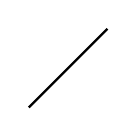
\begin{tikzpicture}[baseline=(P)] \draw[thick] (0,0) -- (1,1); \coordinate (P) at (0.5, 0.5); \end{tikzpicture} &
	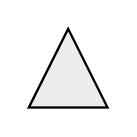
\begin{tikzpicture}[baseline=(P)] \filldraw[thick, fill=gray!15] (0,1) -- (-0.5, 0) -- (0.5, 0) --cycle; \coordinate (P) at (0, 0.5); \end{tikzpicture} &
	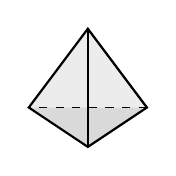
\begin{tikzpicture}[baseline=(P)]
		\fill[color=gray!15] (0, 1) -- (0.75, 0) -- (0, -0.5) -- (-0.75, 0) --cycle;
		\fill[color=gray!30] (0.75, 0) -- (0, -0.5) -- (-0.75, 0) --cycle;
		\draw[dashed] (0.75, 0) -- (-0.75, 0);
		\draw[thick] (0, 1) -- (0.75, 0) -- (0, -0.5) -- (-0.75, 0) --cycle;
		\draw[thick] (0, 1) -- (0, -0.5);
		\coordinate (P) at (0, 0.3);
	\end{tikzpicture} &
	$\cdots$
\end{tabular}\end{center}
Such a decomposition gives a concrete, combinatorial way to understand
homology, homotopy, and other questions about spaces. The rigorous
formulation used here was introduced by S.\ Eilenberg and J.\ A.\ Zilber in
1950. The language of simplicial sets has a broad reach and is not confined
to classical topological questions. For example, it can describe a category
through the construction called its ``nerve'', introduced in
\S\ref{sec:nerves}. Category theory concerns objects in diagrams (shown as
zero-dimensional points), morphisms (shown as one-dimensional arrows), and
commutativity (associated with two-dimensional pieces such as triangles or
squares). It is therefore unsurprising that categories and spaces can be
united within the same mathematical structure.

% segment-id: o014.li2.chapter8.simplicial-objects.p003
After introducing nerves and classifying spaces as basic examples of
simplicial sets, \S\ref{sec:geom-realization} returns to the geometric
intuition and defines the geometric realization $|X|$ of a simplicial set
$X$. Theorem~\ref{prop:geom-Sing-adjunction} shows that geometric realization
and the singular-set functor $\mathrm{Sing}$ familiar from topology form an
adjoint pair
% segment-id: o014.li2.chapter8.simplicial-objects.q001
\[\begin{tikzcd}
	{|\cdot|}: \cate{sSet} \arrow[shift left, r] & \cate{Top} : \mathrm{Sing}. \arrow[shift left, l]
\end{tikzcd}\]
If $\cate{Top}$ is replaced by the category $\cate{CGHaus}$ of compactly
generated Hausdorff spaces, customary in homotopy theory, geometric
realization also satisfies $|X\times Y|\simeq|X|\times|Y|$. The product on
the left is formed degreewise from the two simplicial sets. The proof is
related to triangulating products and involves some nontrivial combinatorial
details; since this is not a topology textbook, we shall not pursue them.

% segment-id: o014.li2.chapter8.simplicial-objects.p004
For the subject of this book, simplicial objects in an abelian category
$\mathcal{A}$ are more important. In this situation,
$\cate{s}\mathcal{A}$ is also an abelian category; for example, simplicial
abelian groups form the abelian category $\cate{sAb}$. The fundamental result
is the Dold--Kan correspondence in \S\ref{sec:Dold-Kan}
(Theorem~\ref{prop:Dold-Kan}), which, for an abelian category $\mathcal{A}$,
gives an adjoint pair of equivalences
% segment-id: o014.li2.chapter8.simplicial-objects.q002
\[\begin{tikzcd}
	\Gamma: \cate{s}\mathcal{A} \arrow[shift left, r] & \cate{Ch}_{\geq 0}(\mathcal{A}): \mathrm{N}, \arrow[shift left, l]
\end{tikzcd}\]
where $\cate{Ch}_{\geq0}(\mathcal{A})$ denotes the abelian category of
nonnegatively graded chain complexes over $\mathcal{A}$. The functor
$\mathrm{N}$ maps a simplicial object $X$ to the corresponding normalized
chain complex $\mathrm{N}X$. More precisely, define the unnormalized chain
complex of $X\in\Obj(\cate{s}\mathcal{A})$ by
% segment-id: o014.li2.chapter8.simplicial-objects.q003
\[ \mathrm{C}X := \left( X_n, \partial_n\right)_{n \geq 0}, \quad \partial_n := \sum_{i=0}^n (-1)^i d_i : X_n \to X_{n-1}. \]
Then $\mathrm{N}X$ may be taken as the chain subcomplex of $\mathrm{C}X$
given by $(\mathrm{N}X)_n:=\bigcap_{i=1}^n\Ker(d_i)$, or regarded as the
quotient of $\mathrm{C}X$ by its degenerate part. The isomorphism between
these two forms is the content of Proposition~\ref{prop:Dold-Kan-v}.
Moreover, Theorem~\ref{prop:Dold-Kan-N-C} shows that the inclusion morphism
$u:\mathrm{N}X\to\mathrm{C}X$ is a quasi-isomorphism of chain complexes.

% segment-id: o014.li2.chapter8.simplicial-objects.p005
The Dold--Kan correspondence makes simplicial theory one of the sources of
homological algebra, not only historically but also conceptually and
technically. Simplicial methods can explain and enrich the basic operations
on complexes or chain complexes; for example, homotopy and contractibility
have simplicial versions and thereby acquire topological interpretations.
This is discussed in \S\ref{sec:homology-computation}.

% segment-id: o014.li2.chapter8.simplicial-objects.p006
Another application connects simplicial methods with the theory of monads
from \S\ref{sec:Beck}. In this way, an object of a category can be canonically
expanded into an augmented simplicial object or an augmented cosimplicial
object. Because these techniques are related to the operation of ``adding a
bar'' in Hochschild homology, they are collectively called bar constructions
and form the subject of \S\ref{sec:bar-resolution}. Through the Dold--Kan
correspondence and some observations about contractibility, bar constructions
explain the standard resolutions in Hochschild theory (see \S\ref{sec:HH})
and group cohomology (see \S\ref{sec:G-mod}); they all turn out to arise from
a single idea at a higher level. The Exercises contain another extension of
the bar construction.

% segment-id: o014.li2.chapter8.simplicial-objects.p007
By definition, the bisimplicial objects discussed in
\S\ref{sec:bisimplicial} are simply functors
$\simpDelta^{\opp}\times\simpDelta^{\opp}\to\mathcal{C}$; they form the
category $\cate{s}^2\mathcal{C}$. If $\mathcal{A}$ is an abelian category,
the Eilenberg--Zilber Theorem~\ref{prop:Eilenberg-Zilber}, which directly
concerns $\cate{s}^2\mathcal{A}$, is a fundamental construction in algebraic
topology. From the viewpoint of pure category theory, if $\mathcal{A}$ is a
monoidal category (for example, $\mathcal{A}=\cate{Ab}$), the theorem gives
two canonical monoidal structures, in opposite directions, on the functor
$\mathrm{N}:\cate{s}\mathcal{A}\to\cate{Ch}_{\geq0}(\mathcal{A})$. The
applications of bisimplicial objects are not limited to this, however.

% segment-id: o014.li2.chapter8.simplicial-objects.p008
The last two sections of this chapter, \S\ref{sec:closed-simplicial} and
\S\ref{sec:mapping-cone-revisited}, discuss $\Hom$ objects and mapping cones
for simplicial sets, respectively. On the one hand, they correspond to
mapping spaces and cones in the topological intuition. On the other hand, in
the case of abelian groups, the Dold--Kan correspondence gives the familiar
$\Hom$ chain complexes and mapping cones. Thus the related constructions on
complexes or chain complexes receive a transparent explanation, while for
topologists all of this is already familiar.

% segment-id: o014.li2.chapter8.simplicial-objects.n001
\begin{wenxintishi}
	Sections \S\S\ref{sec:simplicial-method}--\ref{sec:geom-realization} form
	the backbone of the simplicial methods in this chapter;
	\S\S\ref{sec:Dold-Kan}--\ref{sec:bar-resolution} are directly connected
	with chain complexes; and although
	\S\S\ref{sec:bisimplicial}--\ref{sec:mapping-cone-revisited} accord with
	the contents of the preceding books, these sections are more advanced.
	Unlike the material of the other chapters, simplicial methods are not
	logically necessary. Their ideas and techniques are nevertheless part of a
	mathematician's basic toolkit and provide a foundation for entering higher
	algebra. Some arguments about simplicial objects occasionally involve
	lengthy routine verifications (as in \S\ref{sec:Dold-Kan}); this is a
	consequence of the definitions, and readers may decide for themselves how
	far they wish to follow such details.
\end{wenxintishi}

% segment-id: o014.li2.chapter8.simplicial-objects.h002
\section{Simplicial Objects}\label{sec:simplicial-method}
% segment-id: o014.li2.chapter8.simplicial-objects.p009
In Remark~\ref{rem:walking-algebra}, we recalled monotone maps between
partially ordered sets and used them to define the category $\cate{FinOrd}$
of finite ordinals. This chapter focuses on its full subcategory
$\simpDelta$ consisting of the nonempty ordinals.

% segment-id: o014.li2.chapter8.simplicial-objects.d001
\begin{definition}
	\index[sym1]{Delta-simp@$\simpDelta$}
	\index[sym1]{[n]}
	Let $\simpDelta$ be the category of all nonempty finite ordinals and
	monotone maps between them. In other words, its objects are the totally
	ordered sets $[n]:=\{0,\ldots,n\}$ for $n\in\Z_{\geq0}$, and its morphisms
	are monotone maps.
\end{definition}

% segment-id: o014.li2.chapter8.simplicial-objects.p010
Note that $[n]$ should not be confused with $\mathbf{n}$, which in this book
denotes the totally ordered set $\{0,\ldots,n-1\}$ or the corresponding
category.

% segment-id: o014.li2.chapter8.simplicial-objects.p011
Every morphism $[l]\to[n]$ in $\simpDelta$ has a unique factorization as a
surjective monotone map followed by an injective monotone map,
% segment-id: o014.li2.chapter8.simplicial-objects.q004
\[ [l] \twoheadrightarrow [m] \hookrightarrow [n], \quad n \geq m \leq l. \]
An injective (respectively, surjective) map of this kind can be decomposed
further into pieces that at each step omit exactly one element (respectively,
identify exactly two elements). In other words, every morphism can be
factored as a composite of the following two kinds of morphisms.
% segment-id: o014.li2.chapter8.simplicial-objects.q005
\begin{center}\begin{tabular}{|l|p{0.74\textwidth}|} \hline
	Coface & $\mathrm{d}^i=\mathrm{d}^{n,i}:[n-1]\hookrightarrow[n]$, where
	$0\leq i\leq n$; the monotone injection omits only $i\in[n]$. \\ \hline
	Codegeneracy & $\mathrm{s}^j=\mathrm{s}^{n,j}:[n+1]\twoheadrightarrow[n]$,
	where $0\leq j\leq n$; the monotone surjection takes the value $j\in[n]$
	twice. \\ \hline
\end{tabular}\end{center}

% segment-id: o014.li2.chapter8.simplicial-objects.p012
An injective (respectively, surjective) monotone map can be decomposed into
cofaces (respectively, codegeneracies) in several ways, depending on the
order in which the elements are omitted (respectively, identified). The
following \emph{cosimplicial identities} are easy to verify:
% segment-id: o014.li2.chapter8.simplicial-objects.q006
\begin{equation}\label{eqn:cosimplicial-identity}\begin{array}{ll}
	\mathrm{d}^j \mathrm{d}^i = \mathrm{d}^i \mathrm{d}^{j-1}, & i < j, \\
	\mathrm{s}^j \mathrm{d}^i = \mathrm{d}^i \mathrm{s}^{j-1} & i < j, \\
	\mathrm{s}^j \mathrm{d}^j = \identity = \mathrm{s}^j \mathrm{d}^{j+1}, & \forall j, \\
	\mathrm{s}^j \mathrm{d}^i = \mathrm{d}^{i-1} \mathrm{s}^j, & i > j+1, \\
	\mathrm{s}^j \mathrm{s}^i = \mathrm{s}^i \mathrm{s}^{j+1}, & i \leq j.
\end{array}\end{equation}

% segment-id: o014.li2.chapter8.simplicial-objects.p013
Examining how one passes between the various decompositions of an injective
(respectively, surjective) monotone map shows that the cofaces,
codegeneracies, and \eqref{eqn:cosimplicial-identity} give a complete system
of generators and relations for the morphisms of $\simpDelta$.

% segment-id: o014.li2.chapter8.simplicial-objects.p014
Viewed in $\simpDelta^{\opp}$, these give the corresponding morphisms
% segment-id: o014.li2.chapter8.simplicial-objects.q007
\begin{center}\begin{tabular}{|l|l|l|} \hline
		Face & $\mathrm{d}_i = \mathrm{d}^n_i: [n] \xrightarrow{\opp} [n-1]$ & $0 \leq i \leq n$ \\ \hline
		Degeneracy & $\mathrm{s}_j = \mathrm{s}^n_j: [n] \xrightarrow{\opp} [n+1]$ & $0 \leq j \leq n$ \\ \hline
\end{tabular}\end{center}
The symbol $\xrightarrow{\opp}$ merely reminds us that the arrow lies in the
opposite category $\simpDelta^{\opp}$. Reversing
\eqref{eqn:cosimplicial-identity} gives the \emph{simplicial identities}
% segment-id: o014.li2.chapter8.simplicial-objects.q008
\begin{equation}\label{eqn:simplicial-identity}\begin{array}{ll}
	\mathrm{d}_i \mathrm{d}_j = \mathrm{d}_{j-1} \mathrm{d}_i, & i < j \\
	\mathrm{d}_i \mathrm{s}_j = \mathrm{s}_{j-1} \mathrm{d}_i & i < j \\
	\mathrm{d}_j \mathrm{s}_j = \identity = \mathrm{d}_{j+1} \mathrm{s}_j, & \forall j \\
	\mathrm{d}_i \mathrm{s}_j  = \mathrm{s}_j \mathrm{d}_{i-1}, & i > j+1 \\
	\mathrm{s}_i \mathrm{s}_j = \mathrm{s}_{j+1} \mathrm{s}_i, & i \leq j.
\end{array}\end{equation}
\index{simplicial identities}

% segment-id: o014.li2.chapter8.simplicial-objects.d002
\begin{definition}\label{def:simplicial-obj}
	\index{simplicial object}
	\index{cosimplicial object}
	\index{simplicial object!augmented}
	\index[sym1]{sC@$\cate{s}\mathcal{C}, \cate{cs}\mathcal{C}$}
	For a category $\mathcal{C}$,
	\begin{itemize}
		\item a \emph{simplicial object} in it means a functor
		$\simpDelta^{\opp}\to\mathcal{C}$; all simplicial objects form the
		category
		$\cate{s}\mathcal{C}:=\mathcal{C}^{\simpDelta^{\opp}}$;
		\item a \emph{cosimplicial object} in it means a functor
		$\simpDelta\to\mathcal{C}$; all cosimplicial objects form the category
		$\cate{cs}\mathcal{C}:=\mathcal{C}^{\simpDelta}$.
	\end{itemize}

	Consequently,
	$(\cate{cs}\mathcal{C})^{\opp}\simeq\cate{s}(\mathcal{C}^{\opp})$.
	If the functor underlying a simplicial (respectively, cosimplicial) object
	has an extension to $\cate{FinOrd}^{\opp}$ (respectively,
	$\cate{FinOrd}$), then the object is called \emph{augmented}.
\end{definition}

\index[sym1]{di@$d_i, \mathrm{d}_i$}
\index[sym1]{sj@$s_j, \mathrm{s}_j$}
% segment-id: o014.li2.chapter8.simplicial-objects.p015
By the preceding discussion, giving a simplicial object $X$ is equivalent to
giving a family of objects $(X_n)_{n\geq0}$ in $\mathcal{C}$ together with a
family of morphisms satisfying \eqref{eqn:simplicial-identity},
% segment-id: o014.li2.chapter8.simplicial-objects.q009
\[ d_i = d^n_i: X_n \to X_{n-1} \; \text{(face)}, \quad s_j = s^n_j: X_n \to X_{n+1} \; \text{(degeneracy)}, \quad 0 \leq i, j \leq n. \]
The object $X_n$ is called the degree-$n$ term of $X$. A morphism from a
simplicial object $X$ to $Y$ is equivalently a family of morphisms
$(f_n:X_n\to Y_n)_{n\geq0}$ in $\mathcal{C}$ satisfying, for every $n\geq0$,
the compatibility conditions
% segment-id: o014.li2.chapter8.simplicial-objects.q010
\[ d^{n+1}_i f_{n+1} = f_n d^{n+1}_i, \quad s^n_j f_n = f_{n+1} s^n_j . \]

% segment-id: o014.li2.chapter8.simplicial-objects.p016
Dually, giving a cosimplicial object $X$ is equivalent to giving a family of
objects $(X^n)_{n\geq0}$ in $\mathcal{C}$ together with a family of morphisms
satisfying \eqref{eqn:cosimplicial-identity},
% segment-id: o014.li2.chapter8.simplicial-objects.q011
\[ d^i = d^{n, i}: X^{n-1} \to X^n \; \text{(coface)}, \quad s^j = s^{n, j}: X^{n+1} \to X^n \; \text{(codegeneracy)}, \quad 0 \leq i, j \leq n. \]
Its morphisms are families of morphisms $f^n:X^n\to Y^n$ compatible with
all $d^i$ and $s^j$.

% segment-id: o014.li2.chapter8.simplicial-objects.p017
An augmentation of a simplicial (respectively, cosimplicial) object $X$ is
equivalently the addition to the data of a morphism $X_0\to X_{-1}$
(respectively, $X^{-1}\to X^0$) and a commutative diagram
% segment-id: o014.li2.chapter8.simplicial-objects.q012
$\begin{tikzcd}
	X_1 \arrow[shift left, r, "d_0"] \arrow[shift right, r, "d_1"'] & X_0 \arrow[r, "\epsilon"] & X_{-1}
\end{tikzcd}$
(respectively, its dual). This morphism is called the augmentation morphism.

% segment-id: o014.li2.chapter8.simplicial-objects.cv001
\begin{convention}
	For a morphism $\phi:[m]\to[n]$ in $\simpDelta$ and a simplicial
	(respectively, cosimplicial) object $X$ in a category $\mathcal{C}$, denote
	the corresponding morphism by $\phi^*:X_n\to X_m$ (respectively,
	$\phi_*:X^m\to X^n$).
\end{convention}

% segment-id: o014.li2.chapter8.simplicial-objects.r001
\begin{remark}\label{rem:semisimplicial}
	\index{semisimplicial object}
	All nonempty ordinals and the injective monotone maps between them form a
	category $\simpDelta_+$. A functor of the form
	$\simpDelta_+^{\opp}\to\mathcal{C}$ is called a \emph{semisimplicial
	object} in $\mathcal{C}$. This is equivalent to deleting the degeneracy
	morphisms $s_j$ and the associated conditions from the definition of a
	simplicial object. Every simplicial object gives a corresponding
	semisimplicial object. Augmented semisimplicial objects may be defined
	similarly. The case of cosemisimplicial objects is entirely dual.
\end{remark}

% segment-id: o014.li2.chapter8.simplicial-objects.eg001
\begin{example}\label{eg:const-simplicial}
	\index{simplicial object!constant}
	Let $C\in\Obj(\mathcal{C})$. The corresponding \emph{constant simplicial
	object} $\mathrm{const}(C)$ is determined by
	$\mathrm{const}(C)_n=C$ and $s_j=\identity_C=d_i$ for all $n,i,j$. As a
	simple exercise, check that
	% segment-id: o014.li2.chapter8.simplicial-objects.q013
	\[ \left\{ \text{augmentations of }X\right\} \xleftrightarrow{1:1} \left\{ (C, \varphi): C \in \Obj(\mathcal{C}), \; \varphi: X \to \mathrm{const}(C)  \right\}. \]
	Concretely, for a given augmentation of $X$, take $C=X_{-1}$ and let
	$\varphi_n$ be the composite
	$X_n\xrightarrow{\iota_k^*}X_0\to X_{-1}$, where
	$\iota_k:[0]\to[n]$ sends $0$ to any $k$ with
	$0\leq k\leq n$. The case of constant cosimplicial objects is entirely
	similar.
\end{example}

% segment-id: o014.li2.chapter8.simplicial-objects.eg002
\begin{example}
	Let $B\to A$ be a morphism in a category $\mathcal{C}$. If the following
	fiber products exist,
	% segment-id: o014.li2.chapter8.simplicial-objects.q014
	\[ X_n := \underbracket{B \dtimes{A} \cdots \dtimes{A} B}_{n+1 \;\text{factors}}, \quad n \geq 0, \]
	each morphism $f:[m]\to[n]$ induces a morphism $X_n\to X_m$ whose $i$th
	component is the projection
	$B\dtimes{A}\cdots\dtimes{A}B\xrightarrow{\mathrm{pr}_{f(i)}}B$. This
	gives a simplicial object $X$ in $\mathcal{C}$. It is augmented by taking
	$B\to A$ as the morphism $X_0\to X_{-1}$.
\end{example}

% segment-id: o014.li2.chapter8.simplicial-objects.r002
\begin{remark}[Order-reversal duality]\label{rem:simpDelta-order-reversal}
	For each $n\in\Z_{\geq0}$, define a bijection $w_n$ of
	$\{0,\ldots,n\}$ with itself by $w_n(i)=n-i$. Define an autoisomorphism
	$w$ of the category $\simpDelta$ that preserves the objects $[n]$ and maps
	a morphism $f:[n]\to[m]$ to $wf:=w_mfw_n$. Note that
	% segment-id: o014.li2.chapter8.simplicial-objects.q015
	\[ w^2 = \identity_{\simpDelta}, \quad w \mathrm{d}^{n, i} = \mathrm{d}^{n, n-i}, \quad w \mathrm{s}^{n, j} = \mathrm{s}^{n, n-j}. \]
	A more intrinsic viewpoint is that $w$ maps $[n]$ to the poset with the
	reversed order $[n]^{\opp}$, or, when regarded as a category, to its
	opposite category. This category is still uniquely isomorphic to $[n]$.
	The action of $w$ on morphisms is expressed by the commutative diagram
	% segment-id: o014.li2.chapter8.simplicial-objects.q016
	\[\begin{tikzcd}
		{[m]^{\opp}} \arrow[r, "{f^{\opp}}", "\text{monotone}"'] & {[n]^{\opp}} \\
		{[m]} \arrow[r, "\text{monotone}", "{wf}"'] \arrow[u, "\sim" sloped] & {[n]} \arrow[u, "\sim" sloped]
	\end{tikzcd} \quad f^{\opp} \xlongequal{\text{as a map}} f. \]
	For every category $\mathcal{C}$, this gives an autoisomorphism
	$X\mapsto X\circ w$ of $\cate{s}\mathcal{C}$ (respectively,
	$\cate{cs}\mathcal{C}$).
\end{remark}

% segment-id: o014.li2.chapter8.simplicial-objects.p018
Finally, we outline the relation between monoidal structures and simplicial
objects.

% segment-id: o014.li2.chapter8.simplicial-objects.d003
\begin{definition}\label{def:monoidal-sObj}
	Every functor $F:\mathcal{C}\to\mathcal{D}$ induces a functor
	$\cate{s}\mathcal{C}\to\cate{s}\mathcal{D}$ that maps the data
	$(X_n,d_i,s_j)_{n,i,j}$ to $(FX_n,Fd_i,Fs_j)_{n,i,j}$. Moreover, there is
	a direct relation
	$\cate{s}(\mathcal{C}_1\times\mathcal{C}_2)\simeq
	\cate{s}\mathcal{C}_1\times\cate{s}\mathcal{C}_2$.

	Apply this observation to a monoidal category $\mathcal{C}$ and the
	bifunctor $\otimes:\mathcal{C}\times\mathcal{C}\to\mathcal{C}$. For
	every $X,Y\in\Obj(\cate{s}\mathcal{C})$, define
	$X\otimes Y\in\Obj(\cate{s}\mathcal{C})$ so that its degree-$n$ term is
	$X_n\otimes Y_n$, while its face and degeneracy morphisms have the forms
	$d_i\otimes d_i$ and $s_j\otimes s_j$, respectively.
\end{definition}

% segment-id: o014.li2.chapter8.simplicial-objects.p019
Thus, if $\mathcal{C}$ is a monoidal category, then
$\cate{s}\mathcal{C}$ also has a corresponding monoidal structure, with the
constant simplicial object $\mathrm{const}(\munit)$ as its unit. The analogous
statement holds for cosimplicial objects.

% Unit 107 English translation of chapter8.tex lines 175--281.
% Source: Methods of Algebra, Volume 2, commit
% 9a5803ff77dd3257484cb177f851a73770a59dd3 (CC BY 4.0).
% stable-unit-id: o014.aljabr2.chapter8.simplicial-sets
% Coverage: complete Section 8.2, ``Simplicial Sets'';
% stops immediately before Section 8.3 at line 282.

% segment-id: o014.li2.chapter8.simplicial-sets.h001
\section{Simplicial Sets}\label{sec:simplicial-set}
\hypertarget{o014.aljabr2.chapter8.simplicial-sets}{ }
% segment-id: o014.li2.chapter8.simplicial-sets.p001
The simplicial objects of Definition~\ref{def:simplicial-obj} in the case
$\mathcal{C}=\cate{Set}$ are called simplicial sets. Relative to a fixed
Grothendieck universe, the precise meaning of $\cate{Set}$ in this book is the
category of all small sets; these details do not affect the content of this
section.

% segment-id: o014.li2.chapter8.simplicial-sets.d001
\begin{definition}
	\index{simplicial set}
	\index{cosimplicial set}
	A simplicial object in the category of sets $\cate{Set}$ is called a
	\emph{simplicial set}; a cosimplicial object in it is called a
	\emph{cosimplicial set}.
\end{definition}

% segment-id: o014.li2.chapter8.simplicial-sets.p002
By Definition~\ref{def:simplicial-obj}, all simplicial sets (or cosimplicial
sets) form the category
$\cate{sSet}:=\cate{Set}^{\simpDelta^{\opp}}$ (or
$\cate{csSet}:=\cate{Set}^{\simpDelta}$).
\index[sym1]{sSet@$\cate{sSet}, \cate{csSet}$}

% segment-id: o014.li2.chapter8.simplicial-sets.d002
\begin{definition}\label{def:standard-simplicial-set}
	\index[sym1]{Delta-n@$\Delta^n$}
	For every $n\in\Z_{\geq0}$, write $\Delta^n$ for the simplicial set
	determined by
	$\Hom_{\simpDelta}(\mathord\cdot,[n]):
	\simpDelta^{\opp}\to\cate{Set}$. It is called the \emph{standard
	$n$-simplex}.
\end{definition}

% segment-id: o014.li2.chapter8.simplicial-sets.p003
Thus $(\Delta^n)_m=\Hom_{\simpDelta}([m],[n])$ is the set of all
order-preserving maps $[m]\to[n]$. The map
$(\Delta^n)_{m'}\to(\Delta^n)_m$ induced by an order-preserving map
$\phi:[m]\to[m']$ is precisely pullback of maps,
$\phi^*:f\mapsto f\phi$.

% segment-id: o014.li2.chapter8.simplicial-sets.eg001
\begin{example}\label{eg:boundary-horn}
	\index[sym1]{partial-Delta-n@$\partial \Delta^n$}
	\index[sym1]{Lambda-n-k@$\Lambda^n_k$}
	\index{horn}
	We introduce two common subobjects of the standard $n$-simplex $\Delta^n$.
	\begin{description}
		\item[Boundary] Define the subfunctor $\partial\Delta^n$ of $\Delta^n$
		by
		% segment-id: o014.li2.chapter8.simplicial-sets.q001
		\[ (\partial \Delta^n)_m := \left\{ f: [m] \to [n] \; \text{order-preserving}, \Image(f) \neq [n] \right\}, \quad m \in \Z_{\geq 0}. \]
		If $m<n$, then $(\partial\Delta^n)_m=(\Delta^n)_m$; if $m\geq n$,
		the elements of $(\partial\Delta^n)_m$ are obtained by repeated
		degeneracies from $(\Delta^n)_h$ for $0\leq h<n$.
		\item[Horn] For $0\leq k\leq n$, define the subfunctor $\Lambda^n_k$
		of $\Delta^n$ by
		% segment-id: o014.li2.chapter8.simplicial-sets.q002
		\[ (\Lambda^n_k)_m := \left\{ f: [m] \to [n] \;\text{order-preserving}, \Image(f) \not\supset [n] \smallsetminus \{k\} \right\}, \quad m \in \Z_{\geq 0}. \]
		We call $k$ the vertex of the horn.
	\end{description}

	Every pullback $\phi^*:f\mapsto f\phi$ clearly preserves the conditions
	above, so both are subfunctors. The exercises in this chapter will show how
	$\Lambda^n_i$ (or $\partial\Delta^n$) can be expressed precisely as a
	gluing of $n$ (or $n+1$) copies of $\Delta^{n-1}$.
\end{example}

% segment-id: o014.li2.chapter8.simplicial-sets.p004
The constant simplicial set given by the empty set,
$\mathrm{const}(\emptyset)$, is abbreviated to $\emptyset$. Thus
$\partial\Delta^0=\emptyset$.

% segment-id: o014.li2.chapter8.simplicial-sets.p005
In \S\ref{sec:geom-realization} we will give an intuitive interpretation of
simplicial sets. In particular, we will depict the geometric images of
$\Delta^n\supset\Lambda^n_i\supset\partial\Delta^n$.

% segment-id: o014.li2.chapter8.simplicial-sets.p006
The Yoneda lemma (Theorem~\ref{prop:Yoneda}) immediately gives the following
canonical isomorphism, where $n\in\Z_{\geq0}$ and
$X\in\Obj(\cate{sSet})$:
% segment-id: o014.li2.chapter8.simplicial-sets.q003
\begin{equation}\begin{gathered}
	\begin{tikzcd}[row sep=tiny]
		\Hom_{\cate{sSet}}\left( \Delta^n, X \right) \arrow[r, "\sim"] & X_n \\
		\phi \arrow[mapsto, r] & \phi([n])(\identity_{[n]})
	\end{tikzcd} \\
	\phi([n]): \End([n]) = \Delta^n([n]) \to X([n]) =: X_n.
\end{gathered}\end{equation}

% segment-id: o014.li2.chapter8.simplicial-sets.d003
\begin{definition}\label{def:simplex}
	\index{simplex}
	\index{simplex!non-degenerate}
	An element of $X_n$ is called an \emph{$n$-simplex} of the simplicial set
	$X$. If $x\in X_n$ lies in the image of some $s_j$, it is called
	\emph{degenerate}; otherwise it is called \emph{non-degenerate}.
\end{definition}

% segment-id: o014.li2.chapter8.simplicial-sets.p007
As a simple exercise, verify that the non-degenerate $m$-simplices of
$\Delta^n$ correspond to the order-preserving injections
$[m]\hookrightarrow[n]$; there are $\binom{n+1}{m+1}$ of them.

% segment-id: o014.li2.chapter8.simplicial-sets.p008
Furthermore, the Yoneda lemma ensures that
$h_{\simpDelta}:[n]\mapsto\Delta^n$ defines a fully faithful functor
$\simpDelta\to\cate{sSet}$. Every morphism $f:[m]\to[n]$ in $\simpDelta$
induces $f:\Delta^m\to\Delta^n$. Specifying an $(m+1)$-element subset
$\{k_0,\ldots,k_m\}\subset[n]$ is equivalent to specifying an
order-preserving injection $[m]\hookrightarrow[n]$. The corresponding
morphism between standard simplices is also written
% segment-id: o014.li2.chapter8.simplicial-sets.q004
\[ \Delta^m \xrightarrow{\{k_0, \ldots, k_m\}} \Delta^n . \]

% segment-id: o014.li2.chapter8.simplicial-sets.p009
The intuitive meaning of simplicial sets will be explained by geometric
realization in \S\ref{sec:geom-realization}. Before that, we introduce a
series of abstract constructions, beginning with the join and the left and
right cones of simplicial sets.

% segment-id: o014.li2.chapter8.simplicial-sets.p010
Write $\cate{FinLin}_+$ for the full subcategory of the category of finite
totally ordered sets (also called finite linearly ordered sets)
$\cate{FinLin}$ obtained by removing the empty set; its morphisms are
order-preserving maps. Since $\simpDelta$ is a skeleton of
$\cate{FinLin}_+$, a simplicial set can equivalently be viewed as a functor
$\cate{FinLin}_+^{\opp}\to\cate{Set}$.

% segment-id: o014.li2.chapter8.simplicial-sets.cv001
\begin{convention}
	Let $J$ be an object of $\cate{FinLin}_+$. Every subset $I\subset J$ is
	automatically a finite totally ordered set. If it also satisfies
	% segment-id: o014.li2.chapter8.simplicial-sets.q005
	\[ \forall (i, j) \in I \times J, \quad j \leq i \implies j \in I, \]
	then $I$ is called an \emph{initial segment} of $J$, written
	$I\sqsubset J$.
\end{convention}

% segment-id: o014.li2.chapter8.simplicial-sets.d004
\begin{definition}\label{def:simplicial-join}
	\index{simplicial set!join}
	The \emph{join} $X\star X'$ of simplicial sets $X$ and $X'$ is defined as
	the following functor $\cate{FinLin}_+^{\opp}\to\cate{Set}$:
	% segment-id: o014.li2.chapter8.simplicial-sets.q006
	\[ (X \star X')(J) = \bigsqcup_{I \sqsubset J} X(I) \times X'(J \smallsetminus I). \]
	Here (and only here), $X(\emptyset)$ and $X'(\emptyset)$ are defined to be
	one-point sets. For every order-preserving map $f:J_1\to J$ and
	$I\sqsubset J$, set $I_1:=f^{-1}(I)$. Then $I_1\sqsubset J_1$ and there
	is a map
	% segment-id: o014.li2.chapter8.simplicial-sets.q007
	\[ X(I) \times X'(J \smallsetminus I) \to X(I_1) \times X'(J_1 \smallsetminus I_1). \]
	This yields an induced morphism
	$f^*:(X\star X')(J)\to(X\star X')(J_1)$, which determines the simplicial
	structure on $X\star X'$.
\end{definition}

% segment-id: o014.li2.chapter8.simplicial-sets.p011
There are canonical morphisms $X\to X\star Y\leftarrow Y$. The definition
can also be written in the earlier notation as
% segment-id: o014.li2.chapter8.simplicial-sets.q008
\[ (X \star Y)_n = X_n \sqcup Y_n \sqcup \bigsqcup_{j+k = n-1} X_j \times Y_k . \]
The morphisms $d_i$ and $s_i$ are obtained directly from the corresponding
morphisms on $X$ and $Y$. For example, for
$d_i:(X\star Y)_n\to(X\star Y)_{n-1}$, its restrictions to the subsets
$X_n$ and $Y_n$ are the original $d_i$, while on $X_j\times Y_k$ it is
given by
% segment-id: o014.li2.chapter8.simplicial-sets.q009
\begin{equation}\label{eqn:join-formulas}\begin{gathered}
		d_i(x, y) = \begin{cases}
			(d_i x, y), & i \leq j, \; j \neq 0 \\
			(x, d_{i-j-1} y), & i > j, \; k \neq 0,
		\end{cases} \\
		j=0 \implies d_0(x, y) = y \in Y_{n-1}, \\
		k=0 \implies d_n(x, y) = x \in X_{n-1}.
\end{gathered}\end{equation}

% segment-id: o014.li2.chapter8.simplicial-sets.pr001
\begin{proposition}\label{prop:join-nd}
	\index[sym1]{Xnd@$X^{\mathrm{nd}}$}
	Write $X_n^{\mathrm{nd}}\subset X_n$ for the subset of non-degenerate
	$n$-simplices of the simplicial set $X$
	(Definition~\ref{def:simplex}). For all $X$ and $Y$,
	% segment-id: o014.li2.chapter8.simplicial-sets.q010
	\[ (X \star Y)^{\mathrm{nd}}_n = X^{\mathrm{nd}}_n \sqcup Y^{\mathrm{nd}}_n \sqcup \bigsqcup_{j+k=n-1} X^{\mathrm{nd}}_j \times Y^{\mathrm{nd}}_k. \]
\end{proposition}
% segment-id: o014.li2.chapter8.simplicial-sets.pf001
\begin{proof}
	Let $Z$ be a simplicial set. For every nonempty finite totally ordered set
	$J$, an element $x\in Z(J)$ is degenerate if and only if there is an
	order-preserving surjection that is not injective,
	$f:J\twoheadrightarrow J_0$, such that
	$x\in\Image[f^*:Z(J_0)\to Z(J)]$. The rest follows immediately from this
	observation.
\end{proof}

% segment-id: o014.li2.chapter8.simplicial-sets.d005
\begin{definition}\label{def:cone-simplicial}
	\index{simplicial set!cone}
	The \emph{left cone} with base a simplicial set $X$ is
	$X^{\lhd}:=\Delta^0\star X$, while the \emph{right cone} is
	$X^{\rhd}:=X\star\Delta^0$.
\end{definition}

% segment-id: o014.li2.chapter8.simplicial-sets.p012
An intuitive interpretation of cones is given in
Example~\ref{eg:cone-realization}. The exercises will examine further
properties of the join operation.

% Unit 108 English translation of chapter8.tex lines 282--453.
% Source: Methods of Algebra, Volume 2, commit
% 9a5803ff77dd3257484cb177f851a73770a59dd3 (CC BY 4.0).
% stable-unit-id: o014.aljabr2.chapter8.nerves-of-categories
% Coverage: complete Section 8.3, ``Example: Nerves of Categories'';
% stops immediately before Section 8.4 at line 454.

% segment-id: o014.li2.chapter8.nerves-of-categories.h001
\section{Example: Nerves of Categories}\label{sec:nerves}
\hypertarget{o014.aljabr2.chapter8.nerves-of-categories}{ }
% segment-id: o014.li2.chapter8.nerves-of-categories.p001
This section introduces the nerves of categories and, through them, the
classifying spaces of groups. Both are important examples of simplicial sets.

% segment-id: o014.li2.chapter8.nerves-of-categories.eg001
\begin{example}[Nerve of a category]\label{eg:nerve-cat}
	\index{nerve}
	\index[sym1]{NC@$\mathrm{N}\mathcal{C}$}
	Let $\mathcal{C}$ be a small category. Define the functor
	% segment-id: o014.li2.chapter8.nerves-of-categories.q001
	\[ \simpDelta^{\opp} \to \cate{Set}, \quad [n] \mapsto \left\{ \text{all functors } [n] \to \mathcal{C} \right\}. \]
	As a simplicial set it is denoted by $\mathrm{N}\mathcal{C}$ and called
	the \emph{nerve} of $\mathcal{C}$. Specifying an element of
	$\mathrm{N}\mathcal{C}_n$ is equivalent to specifying a functor
	$[n]\to\mathcal{C}$, that is, a chain of morphisms in $\mathcal{C}$
	% segment-id: o014.li2.chapter8.nerves-of-categories.q002
	\[ (f_1, \ldots, f_n): C_0 \xrightarrow{f_1} C_1 \xrightarrow{f_2} \cdots \xrightarrow{f_n} C_n. \]
	Thus $\mathrm{N}\mathcal{C}_0$ may be identified with
	$\Obj(\mathcal{C})$, and $\mathrm{N}\mathcal{C}_1$ with
	$\Mor(\mathcal{C})$.

	The face morphisms $d_i:\mathrm{N}\mathcal{C}_n\to
	\mathrm{N}\mathcal{C}_{n-1}$ and degeneracy morphisms
	$s_j:\mathrm{N}\mathcal{C}_n\to\mathrm{N}\mathcal{C}_{n+1}$ are given
	by
	% segment-id: o014.li2.chapter8.nerves-of-categories.q003
	\begin{align*}
		d_i(f_1, \ldots, f_n) & = \begin{cases}
			(f_2, \cdots, f_n), & i = 0 \\
			(\ldots, f_{i+1} f_i, \ldots), & 0 < i < n, \\
			(f_1, \ldots, f_{n-1}), & i = n,
		\end{cases} \\
		s_j(f_1, \ldots, f_n) & = \begin{cases}
			\left( \identity_{C_0}, f_1, \ldots, f_n \right), & j = 0 \\
			(\ldots, f_j, \identity_{C_j}, f_{j+1}, \ldots ), & 0 < j < n \\
			(f_1, \ldots, f_n, \identity_{C_n}), & j = n.
		\end{cases}
	\end{align*}
\end{example}

% segment-id: o014.li2.chapter8.nerves-of-categories.r001
\begin{remark}
	Unfolding the definitions shows that the simplicial sets
	$\mathrm{N}(\mathcal{C}^{\opp})$ and $\mathrm{N}\mathcal{C}$ are related
	by the order-reversing duality of
	Remark~\ref{rem:simpDelta-order-reversal}. The details are left to the
	reader.
\end{remark}

% segment-id: o014.li2.chapter8.nerves-of-categories.p002
The nerve realizes a category concretely through combinatorial/topological
data and contains all the information of the original category. This is the
content of Proposition~\ref{prop:nerve-ff}, which will soon be proved. We
first characterize which simplicial sets are nerves; the argument is
instructive.

% segment-id: o014.li2.chapter8.nerves-of-categories.pr001
\begin{proposition}[Characterization of nerves]\label{prop:inner-horn-filling}
	Let $X$ be a simplicial set. The following statements are equivalent.
	\begin{enumerate}[(i)]
		\item There is a small category $\mathcal{C}$ such that
		$\mathrm{N}\mathcal{C}\simeq X$.
		\item $X$ has the unique inner horn-filling property: for every integer
		$0<i<n$ and every morphism $\sigma':\Lambda^n_i\to X$ in
		$\cate{sSet}$ (such a $\Lambda^n_i$ is called an inner horn), there is
		a unique $\sigma:\Delta^n\to X$ extending $\sigma'$.
	\end{enumerate}
\end{proposition}
% segment-id: o014.li2.chapter8.nerves-of-categories.pf001
\begin{proof}
	First prove (i) $\implies$ (ii). Let $X=\mathrm{N}\mathcal{C}$ and
	$0<i<n$; we wish to extend $\sigma':\Lambda^n_i\to X$ to $\Delta^n$.
	For every $0\leq k\leq n$ (or $0<k\leq n$), the morphism
	$\Delta^0\xrightarrow{\{k\}}\Delta^n$ (or
	$\Delta^1\xrightarrow{\{k-1,k\}}\Delta^n$) factors through
	$\Lambda^n_i$. Denote its image under $\sigma'$ by
	$C_k\in X_0=\Obj(\mathcal{C})$ (or
	$[g_k:C_{k-1}\to C_k]\in X_1=\Mor(\mathcal{C})$). This gives an element
	of $X_n$,
	% segment-id: o014.li2.chapter8.nerves-of-categories.q004
	\[ C_0 \xrightarrow{g_1} C_1 \xrightarrow{g_2} \cdots \xrightarrow{g_n} C_n. \]
	Write $\sigma$ for the corresponding morphism $\Delta^n\to X$. The
	construction also shows that $\sigma$ is the only possible extension of
	$\sigma'$. Since
	$\Lambda^n_i=\bigcup_{j\neq i}\Image[\mathrm{d}^j:
	\Delta^{n-1}\to\Delta^n]$, it remains to verify
	% segment-id: o014.li2.chapter8.nerves-of-categories.q005
	\begin{equation}\label{eqn:inner-horn-filling-aux0}
		\sigma \circ \mathrm{d}^j = \sigma' \circ \mathrm{d}^j : \Delta^{n-1} \to X, \quad j \neq i .
	\end{equation}

	By the definition of the nerve, proving
	\eqref{eqn:inner-horn-filling-aux0} reduces to the following verification.
	For each $j\neq i$ and each pair of adjacent elements $h<k$ in the
	sequence $0,\ldots,\widehat{j},\ldots,n$ (where $\widehat{j}$ means that
	$j$ is omitted), the pullbacks of $\sigma$ and $\sigma'$ along
	$\Delta^1\xrightarrow{\{h,k\}}\Lambda^n_i\subset\Delta^n$ must agree.
	\begin{itemize}
		\item If $k=h+1$, this is guaranteed by the construction of $\sigma$.
		In particular, \eqref{eqn:inner-horn-filling-aux0} always holds when
		$j\in\{0,n\}$.
		\item Suppose $(h,k)=(j-1,j+1)$. If $n=2$, this case cannot occur. If
		$n>2$, then either $j-1>0$ or $j+1<n$. When $j-1>0$,
		$\{j-1,j+1\}$ factors as
		% segment-id: o014.li2.chapter8.nerves-of-categories.q006
		\[ \Delta^1 \xrightarrow{\{j-2, j\}} \Delta^{n-1} \xrightarrow{\mathrm{d}^0 = \{1, \ldots, n\}} \Lambda^n_i \subset \Delta^n. \]
		By the already known $j=0$ case of
		\eqref{eqn:inner-horn-filling-aux0}, the two pullbacks agree. Similarly,
		when $j+1<n$, the issue reduces to the known case $j=n$.
	\end{itemize}

	Now prove (ii) $\implies$ (i). Define a category $\mathcal{C}$ by
	$\Obj(\mathcal{C}):=X_0$ and, for all $C,C'\in X_0$,
	% segment-id: o014.li2.chapter8.nerves-of-categories.q007
	\[ \Hom_{\mathcal{C}}(C, C') := \left\{ f \in X_1: d_1(f) = C, \; d_0(f) = C' \right\}. \]
	Use the degeneracy map $s_0:X_0\to X_1$ to define the identity morphism
	$\identity_C$ as $s_0(C)$. We also depict a morphism $f$ as
	$0\xrightarrow{f}1$ to emphasize that it corresponds to a $1$-simplex
	$[1]=\{0,1\}\to X$.

	If $d_0(f)=d_1(g)$, define the composite by $gf:=d_1(\sigma)$, where
	$\sigma:\Delta^2\to X$ is the unique extension of
	% segment-id: o014.li2.chapter8.nerves-of-categories.q008
	\[\begin{tikzcd}[column sep=small]
		& 1 \arrow[rd, "g"] & \\
		0 \arrow[ru, "f"] & & 2
	\end{tikzcd}: \Lambda^2_1 \to X
	\quad \text{that is,}\quad d^0(\sigma) = g, \quad d^2(\sigma) = f. \]

	The laws $f\circ\identity_C=f$ and $\identity_{C'}\circ f=f$ are
	witnessed, respectively, by the following elements of $X_2$.
	% segment-id: o014.li2.chapter8.nerves-of-categories.q009
	\[ \begin{tikzcd}[row sep=large]
		& 1 \arrow[rd, bend left, "{\identity_{C'} = d_0 s_1(f)}"] & \\
		0 \arrow[rr, "{}" name=A, "{f = d_1 s_1(f)}"'] \arrow[ru, bend left, "{f = d_2 s_1(f)}"] & & 2 \arrow[phantom, from=1-2, to=A, "{s_1(f)}" description]
	\end{tikzcd} \quad \begin{tikzcd}[row sep=large]
		& 1 \arrow[rd, bend left, "{f = d_0 s_0(f)}"] & \\
		0 \arrow[rr, "{}" name=A, "{f = d_1 s_0(f)}"'] \arrow[ru, bend left, "{\identity_C = d_2 s_0(f)}"] & & 2 \arrow[phantom, from=1-2, to=A, "{s_0(f)}" description]
	\end{tikzcd}\]

	For associativity $h(gf)=(hg)f$, construct
	$\sigma':\Lambda^3_2\to X$ whose three faces are, respectively,
	% segment-id: o014.li2.chapter8.nerves-of-categories.q010
	\[\begin{tikzcd}[column sep=small]
		& 1 \arrow[rd, "g"] & \\
		0 \arrow[ru, "f"] \arrow[rr, "gf"'] & & 2
	\end{tikzcd} \quad \begin{tikzcd}[column sep=small]
		& 2 \arrow[rd, "h"] & \\
		1 \arrow[ru, "g"] \arrow[rr, "hg"'] & & 3
	\end{tikzcd} \quad \begin{tikzcd}[column sep=small]
		& 2 \arrow[rd, "h"] & \\
		0 \arrow[ru, "gf"] \arrow[rr, "h(gf)"'] & & 3.
	\end{tikzcd}\]
	This horn has a unique extension $\sigma:\Delta^3\to X$ such that
	$d^2(\sigma)\in X_2$ has the form
	% segment-id: o014.li2.chapter8.nerves-of-categories.q011
	\[\begin{tikzcd}[column sep=small]
		& 1 \arrow[rd, "hg"] & \\
		0 \arrow[ru, "f"] \arrow[rr, "h(gf)"'] & & 3.
	\end{tikzcd} \]
	By construction, however, this $2$-simplex also determines the composite
	of $f$ and $hg$, proving $(hg)f=h(gf)$.

	Thus $\mathcal{C}$ is a category. There is a canonical morphism
	$X\to\mathrm{N}\mathcal{C}$: from a given $\Delta^n\to X$, pull back
	along each $\Delta^1\xrightarrow{\{j,j+1\}}\Delta^n$ to obtain a chain of
	morphisms. By construction, $X_n\to\mathrm{N}\mathcal{C}_n$ is clearly a
	bijection for $n=0,1$. If $n\geq2$, choose $0<i<n$ and consider the
	commutative diagram
	% segment-id: o014.li2.chapter8.nerves-of-categories.q012
	\[\begin{tikzcd}
		\Hom(\Delta^n, X) \arrow[d] \arrow[r] & \Hom(\Delta^n, \mathrm{N}\mathcal{C}) \arrow[d] \\
		\Hom(\Lambda^n_i, X) \arrow[r] & \Hom(\Lambda^n_i, \mathrm{N}\mathcal{C}).
	\end{tikzcd}\]
	By the assumption and the unique inner horn-filling property, both vertical
	arrows are bijections. Moreover, $\Lambda^n_i$ can be expressed as the
	$\varinjlim$ of a family of $\Delta^{n-1}$ and $\Delta^{n-2}$ (that is,
	the gluing of $n$ faces), so induction shows that the arrow in the second
	row is also a bijection. This proves the result.
\end{proof}

% segment-id: o014.li2.chapter8.nerves-of-categories.p003
Notice also that in the argument (ii) $\implies$ (i), if there is a small
category $\mathcal{C}_0$ with $X=\mathrm{N}(\mathcal{C}_0)$, then the
category $\mathcal{C}$ constructed in the proof is exactly
$\mathcal{C}_0$.

% segment-id: o014.li2.chapter8.nerves-of-categories.p004
Write $\cate{Cat}$ for the category of all small categories, with functors as
morphisms. Every functor $F:\mathcal{C}\to\mathcal{C}'$ induces a morphism
$\mathrm{N}F:\mathrm{N}\mathcal{C}\to\mathrm{N}\mathcal{C}'$ in
$\cate{sSet}$, mapping $(f_1,\ldots,f_n)$ to
$(Ff_1,\ldots,Ff_n)$. This gives the nerve functor
$\mathrm{N}:\cate{Cat}\to\cate{sSet}$.

% segment-id: o014.li2.chapter8.nerves-of-categories.pr002
\begin{proposition}\label{prop:nerve-ff}
	The nerve functor $\mathrm{N}:\cate{Cat}\to\cate{sSet}$ is fully
	faithful.
\end{proposition}
% segment-id: o014.li2.chapter8.nerves-of-categories.pf002
\begin{proof}
	The proof of Proposition~\ref{prop:inner-horn-filling} has already shown
	how to reconstruct morphisms and their composition from the nerve of a
	category. Hence a morphism
	$\mathrm{N}(\mathcal{C})\to\mathrm{N}(\mathcal{C}')$ naturally induces a
	functor $\mathcal{C}\to\mathcal{C}'$. It is easy to see that this
	construction and the construction induced by $\mathrm{N}$ are mutually
	inverse.
\end{proof}

% segment-id: o014.li2.chapter8.nerves-of-categories.eg002
\begin{example}[Classifying space]\label{eg:classifying-space}
	\index{classifying space}
	\index[sym1]{BGamma@$\mathrm{B}\Gamma$}
	\index[sym1]{EGamma@$\mathrm{E}\Gamma$}
	Let $\Gamma$ be a monoid. Define the categories $\mathcal{B}\Gamma$ and
	$\mathcal{E}\Gamma$ as follows:
	% segment-id: o014.li2.chapter8.nerves-of-categories.q013
	\begin{center}\begin{tabular}{|c|c|c|c|}\hline
		Category & Object set & Morphisms & Composition of morphisms \\ \hline
		$\mathcal{B}\Gamma$ & $\{\star\}$ & $\End_{\mathcal{B}\Gamma}(\star)=\Gamma$ & multiplication in $\Gamma$ \\ \hline
		$\mathcal{E}\Gamma$ & $\Gamma$ & $\Hom_{\mathcal{E}\Gamma}(g,g')=\{h\in\Gamma:hg=g'\}$ & multiplication in $\Gamma$ \\ \hline
	\end{tabular}\end{center}

	Define the nerves
	$\mathrm{B}\Gamma:=\mathrm{N}((\mathcal{B}\Gamma)^{\opp})$ and
	$\mathrm{E}\Gamma:=\mathrm{N}((\mathcal{E}\Gamma)^{\opp})$.
	The simplicial set $\mathrm{B}\Gamma$ is called the classifying space of
	$\Gamma$. Taking $(\cdots)^{\opp}$ amounts to reversing the arrows in the
	definition of the nerve without changing their labels. Thus
	% segment-id: o014.li2.chapter8.nerves-of-categories.q014
	\begin{equation*}
		\begin{array}{|c|c|c|} \hline
		\text{Set} & \text{Element} & \text{Corresponding chain of morphisms in }\mathcal{B}\Gamma\text{ or }\mathcal{E}\Gamma \\ \hline
		(\mathrm{B}\Gamma)_n = \Gamma^n & (g_1, \ldots, g_n) & \star \xleftarrow{g_1} \cdots \leftarrow \star \xleftarrow{g_n} \star \\ \hline
		(\mathrm{E}\Gamma)_n = \Gamma^{n+1} & (g_1, \ldots, g_{n+1}) & g_1 \cdots g_{n+1} \xleftarrow{g_1} \cdots \leftarrow g_n g_{n+1} \xleftarrow{g_n} g_{n+1} \\ \hline
		\end{array}
	\end{equation*}
	Substitution into the definitions gives, for every $n\geq0$,
	% segment-id: o014.li2.chapter8.nerves-of-categories.q015
	\begin{equation*}
		\mathrm{B}\Gamma: \qquad \begin{aligned}
			d_i(g_1, \ldots, g_n) & =
			\begin{cases}
				(g_2, \ldots, g_n), & i = 0 \\
				(\ldots, g_i g_{i+1} , \ldots), & 0 < i < n \\
				(g_1, \ldots, g_{n-1}), & i = n,
			\end{cases} \\
			s_j(g_1, \ldots, g_n) & =
			\begin{cases}
				(1, g_1, \ldots, g_n), & j = 0 \\
				(\ldots, g_j, 1, g_{j+1}, \ldots), & 0 < j < n \\
				(g_1, \ldots, g_n, 1), & j = n,
			\end{cases}
		\end{aligned}
	\end{equation*}
	and
	% segment-id: o014.li2.chapter8.nerves-of-categories.q016
	\begin{equation*}
		\mathrm{E}\Gamma: \qquad \begin{aligned}
			d_i(g_1, \ldots, g_{n+1}) & =
			\begin{cases}
				(g_2, \ldots, g_{n+1}), & i = 0 \\
				(g_1, \ldots, g_i g_{i+1} , \ldots), & 0 < i \leq n,
			\end{cases} \\
			s_j(g_1, \ldots, g_{n+1}) & =
			\begin{cases}
				(1, g_1, \ldots, g_{n+1}), & j = 0 \\
				(\ldots, g_j, 1, g_{j+1}, \ldots), & 0 < j \leq n.
			\end{cases}
		\end{aligned}
	\end{equation*}

	There is a natural functor
	$(\mathcal{E}\Gamma)^{\opp}\to(\mathcal{B}\Gamma)^{\opp}$ mapping all
	objects to $\star$ and every morphism $h\in\Gamma$ to $h$. The induced
	morphism $\mathrm{E}\Gamma\to\mathrm{B}\Gamma$ simply maps
	$(g_1,\ldots,g_{n+1})$ to $(g_1,\ldots,g_n)$. The right multiplication
	action of $\Gamma$ on $(\mathrm{E}\Gamma)_n$ acts along its fibers, or in
	other words changes the datum $g_{n+1}$:
	% segment-id: o014.li2.chapter8.nerves-of-categories.q017
	\[ (g_1, \ldots, g_n, g_{n+1})g = (g_1, \ldots, g_n, g_{n+1}g). \]
	These actions clearly commute with $d_i$ and $s_j$. If $\Gamma$ is a
	group, the action is also free.

	In topology, $\mathrm{B}\Gamma$ (or its geometric realization
	$|\mathrm{B}\Gamma|$; see \S\ref{sec:geom-realization}) serves to
	classify $\Gamma$-torsors over spaces, while
	$\mathrm{E}\Gamma\to\mathrm{B}\Gamma$ gives the universal torsor.
	Example~\ref{eg:classifying-contractible} will show that
	$\mathrm{E}\Gamma$ is ``right-contractible.''
\end{example}

% Unit 109 English translation of chapter8.tex lines 454--759.
% Source: Methods of Algebra, Volume 2, commit
% 9a5803ff77dd3257484cb177f851a73770a59dd3 (CC BY 4.0).
% stable-unit-id: o014.aljabr2.chapter8.geometric-realization
% Coverage: complete Section 8.4 on the geometric-realization functor,
% including the singular functor, the product theorem, simplicial homotopy,
% and shuffle signs; stops immediately before Section 8.5 on Dold--Kan.

% segment-id: o014.aljabr2.chapter8.geometric-realization.h001
\section{The Geometric-Realization Functor}\label{sec:geom-realization}
\hypertarget{o014.aljabr2.chapter8.geometric-realization}{ }
% segment-id: o014.aljabr2.chapter8.geometric-realization.p001
We now begin to build a geometric picture of the simplicial sets introduced
in \S\ref{sec:simplicial-set}. We start with the standard $n$-simplex, where
$n\in\Z_{\geq0}$. Write the standard ordered basis of $\R^{n+1}$ as
$e_0,\ldots,e_n$. Define
% segment-id: o014.aljabr2.chapter8.geometric-realization.q001
\[
|\Delta^n| := \left\{ (x_0, \ldots, x_n) \in (\R_{\geq 0})^{n+1} : \sum_{i=0}^n x_i = 1 \right\} \quad
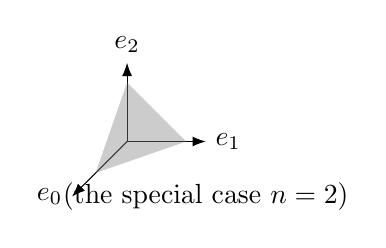
\begin{tikzpicture}[baseline=(O)]
	\coordinate (O) at (0, 0);
	\draw[-Latex] (0, 0) -- (-0.7, -0.7) node[left] {$e_0$};
	\draw[-Latex] (0, 0) -- (1, 0) node[right] {$e_1$};
	\draw[-Latex] (0, 0) -- (0, 1) node [above] {$e_2$};
	\fill[color=gray, opacity=0.4] (-0.4, -0.4) -- (0.75, 0) -- (0, 0.75) --cycle;
	\node at (1, -0.7) {(the special case $n=2$)};
\end{tikzpicture}
\]
Its vertices are labeled $0,\ldots,n$ by $i\leftrightarrow e_i$. Its
interior is given the standard orientation for which
$e_1-e_0,\ldots,e_n-e_{n-1}$ is a positively oriented basis at every point.

% segment-id: o014.aljabr2.chapter8.geometric-realization.p002
Every monotone map $f:[m]\to[n]$ induces a map
% segment-id: o014.aljabr2.chapter8.geometric-realization.q002
\[\begin{tikzcd}[row sep=tiny]
	{|f|}: {|\Delta^m|} \arrow[r] & {|\Delta^n|} \\
	\sum_{i=0}^m y_i e_i \arrow[mapsto, r] & \sum_{i=0}^m y_i e_{f(i)}.
\end{tikzcd}\]
If $f$ is not surjective, the image of $|f|$ lies in the boundary. The
embedding $|\mathrm{d}^i|:|\Delta^{n-1}|\to|\Delta^n|$ may be used to
compare the orientation on the interior of $|\Delta^{n-1}|$ with the
orientation induced on the boundary by $|\Delta^n|$. A standard determinant
calculation shows that they differ by a factor of $(-1)^i$. The following
figure illustrates the case $n=2$.
% segment-id: o014.aljabr2.chapter8.geometric-realization.g001
\begin{center}
	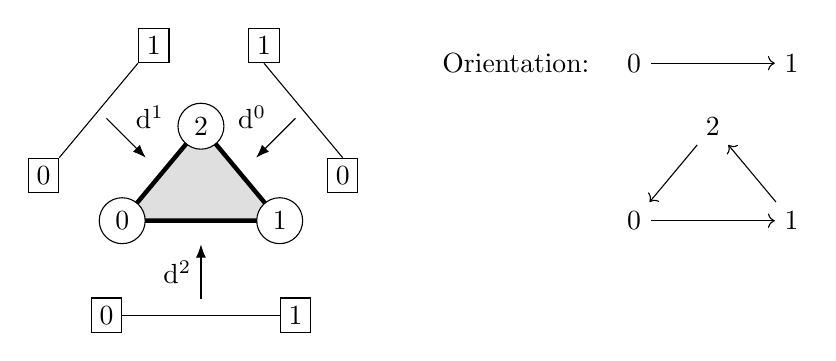
\begin{tikzpicture}
		\coordinate (A) at (0, 0);
		\coordinate (B) at (2, 0);
		\coordinate (C) at (1, 1.2);
		\fill[color=gray, opacity=0.25] (A) -- (B) -- (C) --cycle;
		\draw[ultra thick] (A) -- (B) -- (C) -- (A);
		\node[shape=circle, inner sep=0.3em, fill=white, draw] at (A) {$0$};
		\node[shape=circle, inner sep=0.3em, fill=white, draw] at (B) {$1$};
		\node[shape=circle, inner sep=0.3em, fill=white, draw] at (C) {$2$};

		\draw ($(B) + (0.8, 0.8)$) node[shape=rectangle, inner sep=0.3em, draw, below] {$0$} -- ($(C) + (0.8, 0.8)$) node[shape=rectangle, inner sep=0.3em, draw, above] {$1$};
		\draw[-Latex] ($(C)!0.5!(B) + (0.7, 0.7)$) to[edge label={$\mathrm{d}^0$}, swap] ($(C)!0.5!(B) + (0.2, 0.2)$);

		\draw ($(A) + (-0.8, 0.8)$) node[shape=rectangle, inner sep=0.3em, draw, below left] {$0$} -- ($(C) + (-0.8, 0.8)$) node[shape=rectangle, inner sep=0.3em, draw, above right] {$1$};
		\draw[-Latex] ($(A)!0.5!(C) + (-0.7, 0.7)$) to[edge label={$\mathrm{d}^1$}] ($(A)!0.5!(C) + (-0.2, 0.2)$);

		\draw ($(A) + (0, -1.2)$) node[shape=rectangle, inner sep=0.3em, draw, left] {$0$} -- ($(B) + (0, -1.2)$) node[shape=rectangle, inner sep=0.3em, draw, right] {$1$};
		\draw[-Latex] ($(A)!0.5!(B) + (0, -1)$) to[edge label={$\mathrm{d}^2$}] ($(A)!0.5!(B) + (0, -0.3)$);

		\node at (5, 2) {Orientation:};
		\node (U) at (6.5, 2) {$0$};
		\node (V) at (8.5, 2) {$1$};
		\draw[->] (U) -- (V);
		\node (X) at (6.5, 0) {$0$};
		\node (Y) at (8.5, 0) {$1$};
		\node (Z) at (7.5, 1.2) {$2$};
		\draw[->] (X) -- (Y);
		\draw[->] (Y) -- (Z);
		\draw[->] (Z) -- (X);
	\end{tikzpicture}
\end{center}

% segment-id: o014.aljabr2.chapter8.geometric-realization.p003
Summarizing the discussion above, we obtain a functor
% segment-id: o014.aljabr2.chapter8.geometric-realization.q003
\begin{equation*}
	|\cdot|: \simpDelta \to \cate{Top} \quad
	\left\{\begin{array}{ll}
		\text{objects} & [n] \mapsto |\Delta^n| \\
		\text{morphisms} & f \mapsto |f| .
	\end{array}\right.
\end{equation*}
We wish to extend it to a functor $\cate{sSet}\to\cate{Top}$. Recall that
$\cate{Top}$ is cocomplete.

% segment-id: o014.aljabr2.chapter8.geometric-realization.d001
\begin{definition}[Geometric-realization functor]
	\index{geometric realization}
	\index[sym1]{X-realization@$\lvert X\rvert$}
	The functor $|\cdot|:\cate{sSet}\to\cate{Top}$ is defined as follows. If
	$X$ is a simplicial set, then
% segment-id: o014.aljabr2.chapter8.geometric-realization.q004
	\[ |X| := \varinjlim_{n, x} |\Delta^n|, \]
	where $n\in\Z_{\geq0}$ and $x\in X_n$, or equivalently, where $x$ is a
	morphism $\Delta^n\to X$. Such pairs $(n,x)$ form a category. A morphism
	from $(n,x)$ to $(m,y)$ is precisely an
	$f\in\Hom_{\simpDelta}([n],[m])$ for which the diagram
% segment-id: o014.aljabr2.chapter8.geometric-realization.q005
	\[\begin{tikzcd}[column sep=small]
		\Delta^n \arrow[rr, "f"] \arrow[rd, "x"'] & & \Delta^m \arrow[ld, "y"] \\
		& X &
	\end{tikzcd}\]
	commutes; equivalently, $f^*:X_m\to X_n$ must satisfy $f^*(y)=x$.
\end{definition}

% segment-id: o014.aljabr2.chapter8.geometric-realization.p004
For fixed $m\geq0$, the category of data
$(n,x:\Delta^n\to\Delta^m)$ has the terminal object
$(m,\identity_{\Delta^m})$. Therefore the geometric realization of
$\Delta^m$ is canonically identified with the previously defined
$|\Delta^m|$. Thus the notation is consistent.

% segment-id: o014.aljabr2.chapter8.geometric-realization.r001
\begin{remark}\label{rem:simplicial-density}
	For every simplicial set $X$, there is a canonical isomorphism
	$\varinjlim_{n,x}\Delta^n\rightiso X$. This follows directly by applying
	the Density Theorem~\ref{prop:Yoneda-density} to the category
	$\cate{sSet}=\simpDelta^{\wedge}$; the reader is invited to check it.
\end{remark}

% segment-id: o014.aljabr2.chapter8.geometric-realization.r002
\begin{remark}
	By Theorem~\ref{prop:Kan-limit}, geometric realization is the left Kan
	extension of the functor $|\cdot|:\simpDelta\to\cate{Top}$ along
	$\simpDelta\to\cate{sSet}$; see Definition~\ref{def:Kan-extension}.
	Thus the construction is entirely natural.
\end{remark}

% segment-id: o014.aljabr2.chapter8.geometric-realization.p005
By the construction above, for each $n\in\Z_{\geq0}$ and $x\in X_n$, the
universal property of $\varinjlim$ gives a canonical map
$i_{n,x}:|\Delta^n|\to|X|$, compatible as $(n,x)$ varies. Taking
$\varinjlim$ in $\cate{Top}$ is simply the operation of gluing topological
spaces. More concretely, the geometric realization can be written as the
quotient space
% segment-id: o014.aljabr2.chapter8.geometric-realization.q006
\begin{equation}\label{eqn:geom-realization-quotient}
	|X| = \dfrac{\displaystyle\bigsqcup_{n \geq 0} X_n \times |\Delta^n| }{(f^*(y), t) \sim (y, |f|(t)) }, \quad
	\begin{tikzcd}[column sep=tiny]
		(f^*(y), t) \arrow[phantom, r, "\in" description] & X_n \arrow[phantom, r, "\times" description] & {|\Delta^n|} \arrow[d, "{|f|}"] & {[n]} \arrow[d, "f"] \\
		(y, {|f|}(t)) \arrow[phantom, r, "\in" description] & X_m \arrow[phantom, r, "\times" description] \arrow[u, "{f^*}"] & {|\Delta^m|} & {[m]}.
	\end{tikzcd}
\end{equation}

% segment-id: o014.aljabr2.chapter8.geometric-realization.p006
In keeping with the geometric intuition, a simplicial set $X$ may be viewed
as a model of a space. The sets $X_0,X_1,\ldots$ are the collections of
building blocks of the model: each element of $X_n$ corresponds to, and
labels, one copy of $|\Delta^n|$. The various maps $f^*:X_m\to X_n$ serve as
assembly instructions that determine how these copies of $|\Delta^n|$ are
glued together.

% segment-id: o014.aljabr2.chapter8.geometric-realization.p007
Since the morphisms in $\simpDelta$ have already been described explicitly,
the equivalence relation in \eqref{eqn:geom-realization-quotient} can be
generated by two special kinds of $f$.
% segment-id: o014.aljabr2.chapter8.geometric-realization.l001
\begin{itemize}
% segment-id: o014.aljabr2.chapter8.geometric-realization.i001
	\item Take $\mathrm{d}^i:[n-1]\hookrightarrow[n]$. Then
	$|\mathrm{d}^i|$ embeds
	$\{d_i(x)\}\times|\Delta^{n-1}|$ into
	$\{x\}\times|\Delta^n|$. Thus the face map
	$d_i:X_n\to X_{n-1}$ labels the $i$th face of the $n$-dimensional
	component corresponding to $x$ by $d_i(x)$, and the gluing is then
	performed according to these labels.

% segment-id: o014.aljabr2.chapter8.geometric-realization.i002
	\item Take $\mathrm{s}^j:[n+1]\twoheadrightarrow[n]$. Then
	$|\mathrm{s}^j|$ ``collapses''
	$\{s_j(x)\}\times|\Delta^{n+1}|$ onto
	$\{x\}\times|\Delta^n|$. Thus the degeneracy map
	$s_j:X_n\to X_{n+1}$ determines how an $n$-dimensional component
	corresponding to $x$ gives rise to a ``degenerate'' $(n+1)$-dimensional
	component, labeled $s_j(x)$, which is collapsed onto its $j$th face during
	the gluing process.
\end{itemize}
% segment-id: o014.aljabr2.chapter8.geometric-realization.p008
Consequently, degenerate $n$-simplices (Definition~\ref{def:simplex}) may be
omitted from the gluing process, but the degeneracy data still cannot be
ignored. For example, a face map $d_i:X_n\to X_{n-1}$ may well map a
nondegenerate simplex to a degenerate simplex.

% segment-id: o014.aljabr2.chapter8.geometric-realization.eg001
\begin{example}
	As an illustration, $\partial\Delta^n$ in Example~\ref{eg:boundary-horn}
	realizes the boundary of the standard $n$-simplex in the intuitive sense,
	while the horn $\Lambda^n_k$ is obtained by removing from
	$\partial\Delta^n$ the face opposite its $k$th vertex. Here is one
	illustration:
% segment-id: o014.aljabr2.chapter8.geometric-realization.g002
	\begin{center}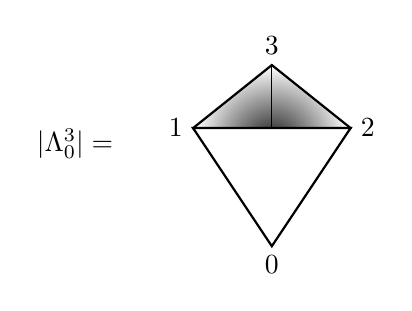
\begin{tikzpicture}
		\coordinate (A) at (0, 0);
		\coordinate (B) at (2, 0);
		\coordinate (C) at (1, 0.8);
		\coordinate (O) at (1, -1.5);

		\filldraw[thick, shading=radial, inner color=black!90, outer color=white] (A) node[left] {$1$} -- (C) node[above] {$3$} -- (B) node[right] {$2$} --($(O)!0.15!(C)$) --cycle;
		\draw (C) -- (O) node[below] {$0$};
		\filldraw[fill=white, thick] (A) -- (B) -- (O) --cycle;

		\node at ($(A) + (-1.5, -0.2)$) {$|\Lambda^3_0| =$};
	\end{tikzpicture}\end{center}
\end{example}

% segment-id: o014.aljabr2.chapter8.geometric-realization.eg002
\begin{example}\label{eg:cone-realization}
	\index{simplicial set!cone}
	For every topological space $\mathcal{X}$, define the cone over it,
	$\Cone_{\mathrm{top}}(\mathcal{X})$, to be the space obtained by
	contracting the closed subset $\mathcal{X}\times\{0\}$ of
	$\mathcal{X}\times[0,1]$ to a single point. Visually,
% segment-id: o014.aljabr2.chapter8.geometric-realization.g003
	\[\Cone_{\mathrm{top}}(\mathcal{X}) = \; 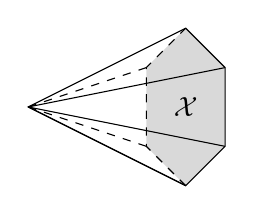
\begin{tikzpicture}[baseline=(P)]
		\coordinate (A) at (0, 1);
		\coordinate (B) at (0.5, 0.5);
		\coordinate (C) at (0.5, -0.5);
		\coordinate (D) at (0, -1);
		\coordinate (E) at (-0.5, -0.5);
		\coordinate (F) at (-0.5, 0.5);
		\coordinate (O) at (-2, 0);
		\coordinate (P) at (0, -0.1);	% For the baseline

		\fill[gray!50, opacity=0.6] (A) -- (B) -- (C) -- (D) -- (E) -- (F) --cycle;
		\draw (O) -- (A) -- (B) -- (C) -- (D) --cycle;
		\draw (O) -- (B);
		\draw (O) -- (C);
		\draw (O) -- (D);
		\draw[dashed] (D) -- (E) -- (F) -- (A);
		\draw[dashed] (O) -- (E);
		\draw[dashed] (O) -- (F);
		\node at (0, 0) {$\mathcal{X}$};
	\end{tikzpicture}\]
	As a simple exercise, check that
	$|X^{\lhd}|\simeq\Cone_{\mathrm{top}}(|X|)\simeq|X^{\rhd}|$. This shows
	that the cones in Definition~\ref{def:cone-simplicial} are aptly named;
	the only difference between the left and right cones is their orientation.
\end{example}

% segment-id: o014.aljabr2.chapter8.geometric-realization.p009
By presenting a triangulation of a space as a simplicial set, one can extract
many important topological properties. This approach is aptly called
``combinatorial topology''. Further discussion and examples may be found in
\cite[Chapter VI]{You}.

% segment-id: o014.aljabr2.chapter8.geometric-realization.d002
\begin{definition}[Singular-set functor]
	\index[sym1]{Sing@$\mathrm{Sing}$}
	\index{singular set}
	For every topological space $E$, define the simplicial set
	$\mathrm{Sing}(E)$ by
% segment-id: o014.aljabr2.chapter8.geometric-realization.q007
	\[ \mathrm{Sing}(E)_n := \Hom_{\cate{Top}}(|\Delta^n|, E), \quad n \in \Z_{\geq 0}, \]
	where $d_i:\mathrm{Sing}(E)_n\to\mathrm{Sing}(E)_{n-1}$
	(respectively, $s_j:\mathrm{Sing}(E)_n\to\mathrm{Sing}(E)_{n+1}$) is
	given by pullback along
	$|\mathrm{d}^i|:|\Delta^{n-1}|\to|\Delta^n|$ (respectively,
	$|\mathrm{s}^j|:|\Delta^{n+1}|\to|\Delta^n|$). This is called the
	\emph{(simplicial) singular set} associated with $E$. The construction
	gives a functor
% segment-id: o014.aljabr2.chapter8.geometric-realization.q008
	\[ \mathrm{Sing}: \cate{Top} \to \cate{sSet}. \]
\end{definition}

% segment-id: o014.aljabr2.chapter8.geometric-realization.th001
\begin{theorem}\label{prop:geom-Sing-adjunction}
	The geometric-realization functor is left adjoint to the singular-set
	functor. In other words, there is a natural bijection
% segment-id: o014.aljabr2.chapter8.geometric-realization.q009
	\[\begin{tikzcd}[row sep=tiny]
		\Hom_{\cate{Top}}(|X|, E) \arrow[leftrightarrow, r, "1:1"] & \Hom_{\cate{sSet}}(X, \mathrm{Sing}(E)) \\
		\varphi \arrow[mapsto, r] & {\left[ X_n \xrightarrow{x \mapsto \varphi \circ i_{n, x}} \Hom_{\cate{Top}}(|\Delta^n|, E) \right]} \\
		\displaystyle\varinjlim_{(n, x)} \left( |\Delta^n| \xrightarrow{\psi_n(x)} E \right) & \psi = {\left[ \psi_n: X_n \to \Hom_{\cate{Top}}(|\Delta^n|, E) \right]}_{n \geq 0} , \arrow[mapsto, l]
	\end{tikzcd}\]
	where $X\in\Obj(\cate{sSet})$ and $E\in\Obj(\cate{Top})$.
\end{theorem}
% segment-id: o014.aljabr2.chapter8.geometric-realization.pf001
\begin{proof}
	Recall that $|X|=\varinjlim_{n,x}|\Delta^n|$. There are canonical
	isomorphisms
% segment-id: o014.aljabr2.chapter8.geometric-realization.q010
	\begin{align*}
		\Hom_{\cate{Top}}\left( \varinjlim_{n, x} |\Delta^n| , E \right) & \rightiso \varprojlim_{n, x} \Hom_{\cate{Top}}(|\Delta^n|, E) = \varprojlim_{n, x} \mathrm{Sing}(E)_n \\
		& \rightiso \varprojlim_{n, x} \Hom_{\cate{sSet}}\left( \Delta^n, \mathrm{Sing}(E) \right) \\
		\varphi & \mapsto \left( \psi_n(x) := \varphi \circ i_{n, x} \right)_{n, x}.
	\end{align*}

	Every family of morphisms $(\psi_n(x))_{n,x}$ determined by a morphism
	$\psi:X\to\mathrm{Sing}(E)$ satisfies the compatibility conditions, and
	thus is an element of the inverse limit on the right-hand side above. To
	complete the proof, it remains to show that giving a morphism $\psi$ is
	equivalent to giving a compatible family of morphisms; this is exactly what
	Remark~\ref{rem:simplicial-density} guarantees.
\end{proof}

% segment-id: o014.aljabr2.chapter8.geometric-realization.r003
\begin{remark}
	For homotopy theory, the category $\cate{CGHaus}$ mentioned in
	\S\ref{sec:closed-monoidal} may be more convenient than $\cate{Top}$.
	Since the inclusion functor $\cate{CGHaus}\to\cate{Top}$ has a right
	adjoint $k$, it preserves $\varinjlim$. Moreover, $|\Delta^n|$ is a
	compactly generated Hausdorff space. Consequently, the gluing
	(respectively, the formation of $\Hom$) in geometric realization
	(respectively, the singular set) may be carried out within
	$\cate{CGHaus}$\footnote{It must be explained that the $\varinjlim$ in
	question does indeed exist in $\cate{CGHaus}$. This is a topological issue;
	see \cite[III.1.8, III.2.1]{GZ67}.}. Thus the adjoint pair of
	Theorem~\ref{prop:geom-Sing-adjunction} factors into two adjunctions, written
	with the same notation as
% segment-id: o014.aljabr2.chapter8.geometric-realization.q011
	\[\begin{tikzcd}
		\cate{sSet} \arrow[shift left, r, "{|\cdot|}"] & \cate{CGHaus} \arrow[shift left, r, "\text{inclusion functor}"] \arrow[shift left, l, "\mathrm{Sing}"] & \cate{Top} \arrow[shift left, l, "k"] .
	\end{tikzcd}\]
\end{remark}
% segment-id: o014.aljabr2.chapter8.geometric-realization.p010
For any two simplicial sets $X$ and $Y$, their product is defined degreewise:
% segment-id: o014.aljabr2.chapter8.geometric-realization.q012
\begin{gather*}
	(X \times Y)_n = X_n \times Y_n, \\
	d_i(x, y) = (d_i(x), d_i(y)), \\
	s_j(x, y) = (s_j(x), s_j(y)).
\end{gather*}
This is both the categorical product in
$\cate{sSet}=\cate{Set}^{\simpDelta^{\opp}}$ and the construction of
Definition~\ref{def:monoidal-sObj} applied to the monoidal category
$(\cate{Set},\times)$. Although both definitions arise from category theory,
the following fundamental result shows that they also have geometric meaning.

% segment-id: o014.aljabr2.chapter8.geometric-realization.th002
\begin{theorem}\label{prop:realization-product}
	For simplicial sets $X$ and $Y$, there is a canonical isomorphism in
	$\cate{CGHaus}$
% segment-id: o014.aljabr2.chapter8.geometric-realization.q013
	\[ |X \times Y| \simeq |X| \times |Y|. \]
	More generally, the $\cate{CGHaus}$-valued version of $|\cdot|$ preserves
	finite limits. If either $X$ or $Y$ has only finitely many nondegenerate
	simplices, then $|X\times Y|\simeq|X|\times|Y|$ also holds in
	$\cate{Top}$.
\end{theorem}

% segment-id: o014.aljabr2.chapter8.geometric-realization.p011
The proof in the general case is rather involved; see
\cite[Chapter III]{GZ67} or \cite{Dri03}. The isomorphism does not hold in
general for the $\cate{Top}$-valued version of geometric realization. Notice
also that the condition stated in the theorem for the $\cate{Top}$-valued
version is not optimal.

% segment-id: o014.aljabr2.chapter8.geometric-realization.c001
\begin{corollary}
	Write $\cate{Grp}$ for the category of groups. If a simplicial set $X$ can
	be promoted to an object of $\cate{sGrp}$, then $|X|$ naturally has the
	structure of a topological group. Analogous results hold for other
	algebraic structures.
\end{corollary}

% segment-id: o014.aljabr2.chapter8.geometric-realization.p012
In view of Theorem~\ref{prop:realization-product}, it is natural to define a
homotopy from $g$ to $f$, for morphisms $f,g:X\rightrightarrows Y$ in
$\cate{sSet}$, as a morphism $H:X\times\Delta^1\to Y$ making the following
diagram commute:
% segment-id: o014.aljabr2.chapter8.geometric-realization.q014
\begin{equation}\label{eqn:simplicial-homotopy-prep}
	\begin{tikzcd}
		X \times \Delta^0 \arrow[d, "{\identity_X \times \mathrm{d}^0}"'] \arrow[r, "\sim"] & X \arrow[d, "f"] \\
		X \times \Delta^1 \arrow[r, "H" description] & Y \\
		X \times \Delta^0 \arrow[u, "{\identity_X \times \mathrm{d}^1}"] \arrow[r, "\sim"'] & X \arrow[u, "g"']
	\end{tikzcd}
\end{equation}

% segment-id: o014.aljabr2.chapter8.geometric-realization.p013
As a special case, the composite
$X\times\Delta^1\xrightarrow{\text{projection}}X\xrightarrow{f}Y$ gives a
constant homotopy from $f$ to itself. Homotopy as defined here is not,
however, an equivalence relation: a simple example already shows that it need
not be symmetric. In homotopy theory one usually imposes an additional
condition on $Y$, for example that it be a Kan complex. The homotopy relation
then has the expected properties, allowing homotopy groups, weak
equivalences, and related notions to be studied combinatorially.

% segment-id: o014.aljabr2.chapter8.geometric-realization.p014
Although this book does not prove Theorem~\ref{prop:realization-product}, it
is useful to say a little more about the simple special case
$X=\Delta^p$ and $Y=\Delta^q$. For example, how can the nondegenerate
simplices of $\Delta^p\times\Delta^q$ be classified? The answer not only
helps explain the geometric realization of a product; the related
construction will also be needed later.

% segment-id: o014.aljabr2.chapter8.geometric-realization.p015
First, the product of two partially ordered sets $S_1$ and $S_2$ becomes a
partially ordered set under
$(a_1,a_2)\leq(b_1,b_2)$ if and only if $a_1\leq b_1$ and $a_2\leq b_2$.
This is also the product of the corresponding categories.

% segment-id: o014.aljabr2.chapter8.geometric-realization.d003
\begin{definition}\label{def:pq-shuffle}
	\index{shuffle!$(p,q)$}
	Let $p,q\in\Z_{\geq0}$. A \emph{$(p,q)$-shuffle} is an injective monotone
	map $\sigma:[p+q]\to[p]\times[q]$.
\end{definition}

% segment-id: o014.aljabr2.chapter8.geometric-realization.p016
For every $n\in\Z_{\geq0}$, specifying a monotone map
$\sigma:[n]\to[p]\times[q]$ is equivalent to specifying a pair of monotone
maps $\sigma_-:[n]\to[p]$ and $\sigma_+:[n]\to[q]$. It is also equivalent
to specifying an $n$-simplex of $\Delta^p\times\Delta^q$. The condition that
$\sigma$ be injective says precisely that the path
$i\mapsto(\sigma_-(i),\sigma_+(i))$ never remains stationary, for
$i=0,\ldots,n$. When $n=p+q$, the situation may be pictured as follows:
% segment-id: o014.aljabr2.chapter8.geometric-realization.q015
\begin{equation}\label{eqn:pq-shuffle-diag}
	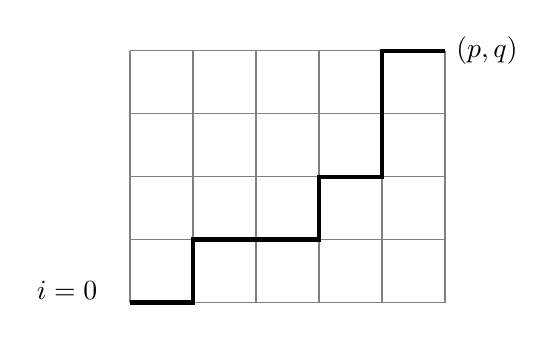
\begin{tikzpicture}[scale=0.8, baseline=(O)]
		\draw[thin, gray] (0, 0) grid (5, 4);
		\node at (-1, 0.2) {$i=0$};
		\draw[ultra thick] (0, 0) -- (1, 0) -- (1, 1) -- (2, 1) -- (3, 1) -- (3, 2) -- (4, 2) -- (4, 3) -- (4, 4) -- (5, 4) node[right] {$(p, q)$};
		\coordinate (O) at (0, 2);
	\end{tikzpicture}
	\quad
	\text{exactly $p+q$ steps.}
\end{equation}
Thus, for a $(p,q)$-shuffle $\sigma$, define
% segment-id: o014.aljabr2.chapter8.geometric-realization.q016
\begin{align*}
	I_\pm & := \left\{ 1 \leq i \leq p+q : \sigma_\pm(i-1) < \sigma_\pm(i) \right\} \\
	& = \left\{ 1 \leq i \leq p+q : \sigma_\pm(i-1) = \sigma_\pm(i) - 1 \right\} \\
	& = \left\{ 1 \leq i \leq p+q: \sigma_\mp(i-1) = \sigma_\mp(i) \right\},
\end{align*}
so that $I_+\sqcup I_-=\{1,\ldots,p+q\}$. The subsets $I_+$ and $I_-$
correspond, respectively, to the upward and rightward portions of the path in
\eqref{eqn:pq-shuffle-diag}. Thus a $(p,q)$-shuffle may also be viewed as an
ordering of $p$ symbols $\rightarrow$ and $q$ symbols $\uparrow$; there are
$\binom{p+q}{p}$ such orderings. These observations also show that
$\sigma_+$ and $\sigma_-$ are surjective monotone maps for every
$(p,q)$-shuffle.

% segment-id: o014.aljabr2.chapter8.geometric-realization.pr001
\begin{proposition}
	Let $p,q\in\Z_{\geq0}$. Consider an $n$-simplex of
	$\Delta^p\times\Delta^q$, that is, a monotone map
	$\sigma:[n]\to[p]\times[q]$. Set $(p_i,q_i):=\sigma(i)$ and
	$(p',q'):=(p_n-p_0,q_n-q_0)$. Then $\sigma$ is nondegenerate if and only if
	the following conditions hold:
	\begin{itemize}
		\item $p'+q'=n$;
		\item $\sigma$ factors as a $(p',q')$-shuffle
		$\sigma':[n]\to[p']\times[q']$ followed by a monotone injection
		$[p']\times[q']\hookrightarrow[p]\times[q]$ of the form $f\times g$.
	\end{itemize}
\end{proposition}
% segment-id: o014.aljabr2.chapter8.geometric-realization.pf002
\begin{proof}
	Identify $\sigma$ with the pair of monotone maps
	$(\sigma_-,\sigma_+)$. Consider the path $i\mapsto(p_i,q_i)$ as in
	\eqref{eqn:pq-shuffle-diag}. The condition that $\sigma$ be nondegenerate
	is equivalent to the condition that this path never remains stationary.
	The rest is clear.
\end{proof}

% segment-id: o014.aljabr2.chapter8.geometric-realization.p017
Using this description of the nondegenerate simplices, the reader may
visualize the isomorphism
$|\Delta^p\times\Delta^q|\simeq|\Delta^p|\times|\Delta^q|$ in the cases
$(p,q)=(1,1)$ and $(2,1)$. For example, the following figure shows the
triangulation of $|\Delta^2|\times|\Delta^1|$ into three tetrahedra,
corresponding to the $3=\binom{3}{2}$ $(2,1)$-shuffles.

% segment-id: o014.aljabr2.chapter8.geometric-realization.g004
\begin{center}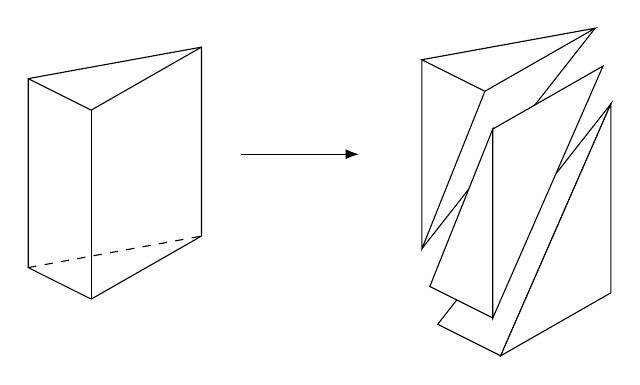
\begin{tikzpicture}[yscale=0.8]
	\coordinate (A) at (0, 0);
	\coordinate (B) at (2.2, 0.5);
	\coordinate (C) at (0.8, -0.5);
	\coordinate (P) at ($(A) + (0, -3)$);
	\coordinate (Q) at ($(B) + (0, -3)$);
	\coordinate (R) at ($(C) + (0, -3)$);

	\draw ($(A) + (-5, -0.3)$) -- ($(B) + (-5, -0.3)$) -- ($(Q) + (-5, -0.3)$) -- ($(R) + (-5, -0.3)$) -- ($(P) + (-5, -0.3)$) --cycle;
	\draw ($(A) + (-5, -0.3)$) -- ($(C) + (-5, -0.3)$) -- ($(B) + (-5, -0.3)$);
	\draw ($(C) + (-5, -0.3)$) -- ($(R) + (-5, -0.3)$);
	\draw[dashed] ($(P) + (-5, -0.3)$) -- ($(Q) + (-5, -0.3)$);

	\draw[-Latex] ($(B)!0.5!(Q) + (-4.5, -0.5)$) -- ($(B)!0.5!(Q) + (-3, -0.5)$);

	\draw (A) -- (B) -- (C) --cycle;
	\draw (A) -- (P) -- (C);
	\draw (P) -- (B);

	\draw[fill=white] ($(P) + (0.2, -1.2)$) -- ($(B) + (0.2, -1.2)$) -- ($(R) + (0.2, -1.2)$) --cycle;
	\draw[fill=white] ($(R) + (0.2, -1.2)$) -- ($(Q) + (0.2, -1.2)$) -- ($(B) + (0.2, -1.2)$) --cycle;

	\draw[fill=white] ($(P) + (0.1, -0.6)$) -- ($(R) + (0.1, -0.6)$) -- ($(C) + (0.1, -0.6)$) --cycle;
	\draw[fill=white] ($(R) + (0.1, -0.6)$) -- ($(B) + (0.1, -0.6)$) -- ($(C) + (0.1, -0.6)$) --cycle;
\end{tikzpicture}\end{center}

% segment-id: o014.aljabr2.chapter8.geometric-realization.d004
\begin{definition}\label{def:pq-shuffle-sgn}
	Let $\sigma$ be a $(p,q)$-shuffle. Its sign is defined by
% segment-id: o014.aljabr2.chapter8.geometric-realization.q017
	\[ \sgn(\sigma) := (-1)^{|I_\sigma|}, \quad I_\sigma := \left\{ (i, j) \in I_- \times I_+ : i > j \right\}. \]
\end{definition}

% segment-id: o014.aljabr2.chapter8.geometric-realization.p018
If $\sigma$ is viewed as an ordering of $p$ symbols $\rightarrow$ and $q$
symbols $\uparrow$, then $I_\sigma$ is precisely the set of pairs $(j,i)$,
with $j<i$, that occur in the reversed order $(\uparrow,\rightarrow)$. A
simple combinatorial exercise shows that there is a unique
$\tau\in\mathfrak{S}_{p+q}$ that rearranges the word into the form
$\rightarrow\cdots\rightarrow\uparrow\cdots\uparrow$ without changing the
internal order within either $I_+$ or $I_-$. Thus
Definition~\ref{def:pq-shuffle-sgn} is equivalent to
$\sgn(\sigma)=\sgn(\tau)$.

% segment-id: o014.aljabr2.chapter8.geometric-realization.p019
For a $(p,q)$-shuffle $\sigma$, exchanging the roles of $\sigma_-$ and
$\sigma_+$ gives a $(q,p)$-shuffle $\sigma'$. The interpretation above and a
basic combinatorial argument give
% segment-id: o014.aljabr2.chapter8.geometric-realization.q018
\begin{equation}\label{eqn:shuffle-sign-0}
	\sgn(\sigma) = (-1)^{pq} \sgn(\sigma').
\end{equation}

% segment-id: o014.aljabr2.chapter8.geometric-realization.p020
In the same spirit, define a $(p,q,r)$-shuffle to be an injective monotone map
$\sigma=(\sigma_-,\sigma_0,\sigma_+):[p+q+r]\to[p]\times[q]\times[r]$, or,
equivalently, regard it as an ordering of the symbols $\rightarrow$,
$\nearrow$, and $\uparrow$. Define $\sgn(\sigma):=(-1)^{|I_\sigma|}$, where
$I_\sigma$ consists of all triples of indices $k>j>i$ corresponding to odd
permutations of $(\rightarrow,\nearrow,\uparrow)$. The same standard
combinatorial exercise shows that if the $(p,q,r)$-shuffle $\sigma$ has a
factorization
% segment-id: o014.aljabr2.chapter8.geometric-realization.q019
\[ [p+q+r] \xrightarrow{\sigma_1} [p+q] \times [r] \xrightarrow{\sigma_2 \times \identity_{[r]}} [p] \times [q] \times [r], \]
then $\sigma_1$ is a $(p+q,r)$-shuffle, $\sigma_2$ is a $(p,q)$-shuffle, and
% segment-id: o014.aljabr2.chapter8.geometric-realization.q020
\begin{equation}\label{eqn:shuffle-sign-1}
	\sgn(\sigma) = \sgn(\sigma_1) \sgn(\sigma_2).
\end{equation}
There is, of course, a corresponding statement for a factorization
$[p+q+r]\to[p]\times[q+r]\to[p]\times[q]\times[r]$.

% segment-id: o014.aljabr2.chapter8.geometric-realization.p021
Equations~\eqref{eqn:shuffle-sign-0} and \eqref{eqn:shuffle-sign-1} are
entirely combinatorial in nature; their detailed verification is left to the
exercises for this chapter. These observations will be used in
\S\ref{sec:bisimplicial}.

% Unit 110 English translation of chapter8.tex lines 760--924.
% Source: Methods of Algebra, Volume 2, commit
% 9a5803ff77dd3257484cb177f851a73770a59dd3 (CC BY 4.0).
% stable-unit-id: o014.aljabr2.chapter8.dold-kan-a
% Coverage: Section 8.5 from its opening through the Dold--Kan lemma for abelian groups;
% continued by Unit 111 at line 925.
% Editorial correction: the unused condition 0 <= k <= n in the source's
% definition of the normalized complex is omitted.

% segment-id: o014.li2.chapter8.dold-kan-a.h001
\section{The Dold--Kan Correspondence}\label{sec:Dold-Kan}
\hypertarget{o014.aljabr2.chapter8.dold-kan-a}{ }
% segment-id: o014.li2.chapter8.dold-kan-a.p001
Following the conventions of algebraic topology, for an additive category
$\mathcal{A}$ we consider the category of chain complexes over it
(Definition~\ref{def:complex}), denoted by $\cate{Ch}(\mathcal{A})$, together
with its subcategory
% segment-id: o014.li2.chapter8.dold-kan-a.q001
\[ \cate{Ch}_{\geq 0}(\mathcal{A}) := \left\{ A = (A_n, \partial_n)_{n \in \Z} : \text{chain complex}, \; \forall n < 0, \; A_n = 0 \right\}, \]
where $\partial_n=\partial_n^A:A_n\to A_{n-1}$. For an object of
$\cate{Ch}_{\geq0}(\mathcal{A})$, it plainly suffices to specify the data
$(A_n)_{n\geq0}$ and $(\partial_n)_{n\geq1}$. The category
$\cate{Ch}_{\geq m}(\mathcal{A})$ is defined similarly; compare the cochain
complex version in Definition~\ref{def:cplx-cat-variant}.
\index[sym1]{ChA@$\cate{Ch}(\mathcal{A})$}

% segment-id: o014.li2.chapter8.dold-kan-a.p002
By enlarging the chosen Grothendieck universe if necessary, we may assume that
$\mathcal{A}$ is a small additive category; see
\cite[Assumption 1.5.2]{Li1}. From $\mathcal{A}$ one can define the category
$\cate{s}\mathcal{A}$ of simplicial objects; the constant simplicial object
corresponding to $0$ is still denoted by
$0\in\Obj(\cate{s}\mathcal{A})$. This section aims to give a first account of
the relationships among these categories. More precisely, we shall define
three functors
% segment-id: o014.li2.chapter8.dold-kan-a.q002
\[\begin{tikzcd}
	\cate{Ch}_{\geq 0}(\mathcal{A}) \arrow[r, "\Gamma" description] & \cate{s}\mathcal{A} \arrow[bend left, l, "{\mathrm{N}}"] \arrow[bend right, l, "{\mathrm{C}}"']
\end{tikzcd}\]
where $\mathrm{N}$ is defined only when $\mathcal{A}$ is an abelian category.
Both $\mathrm{C}$ and $\mathrm{N}$ extend to the semisimplicial objects of
Remark~\ref{rem:semisimplicial}; in other words, neither of them involves the
degeneracy morphisms.

% segment-id: o014.li2.chapter8.dold-kan-a.p003
Our treatment follows \cite[\S 1.2]{LuHA}. We begin by making the relevant
definitions explicit.

% segment-id: o014.li2.chapter8.dold-kan-a.d001
\begin{definition}[Unnormalized chain complex]\label{def:unnormalized-chain}
	\index{unnormalized chain complex}
	\index{Moore chain complex}
	\index[sym1]{CX@$\mathrm{C}X$}
	For a semisimplicial object $X$ in $\mathcal{A}$ and every
	$n\in\Z_{\geq1}$, define
	% segment-id: o014.li2.chapter8.dold-kan-a.q003
	\[ \partial_n := \sum_{i=0}^n (-1)^i d_i: X_n \to X_{n-1}. \]
	The objects $(X_n)_{n\geq0}$ together with $(\partial_n)_n$ form an
	object $\mathrm{C}X$ of $\cate{Ch}_{\geq0}(\mathcal{A})$, called the
	\emph{unnormalized chain complex}, or \emph{Moore chain complex}, given
	by $X$. Thus $(\mathrm{C}X)_n=X_n$.
\end{definition}

% segment-id: o014.li2.chapter8.dold-kan-a.p004
We must show that $\partial_{n-1}\partial_n=0$ when $n>1$. Indeed, the
identity $i<j\implies d_id_j=d_{j-1}d_i$ in
\eqref{eqn:simplicial-identity} gives
% segment-id: o014.li2.chapter8.dold-kan-a.q004
\begin{multline*}
	\partial_{n-1} \partial_n = \sum_{i=0}^{n-1} \sum_{j=0}^n (-1)^{i+j} d_i d_j \\
	= \sum_{0 \leq i < j \leq n} (-1)^{i+j} d_{j-1} d_i + \sum_{n-1 \geq i \geq j \geq 0} (-1)^{i+j} d_i d_j = 0.
\end{multline*}
This construction is plainly canonical in $X$ and gives the functor
$\mathrm{C}$.

% segment-id: o014.li2.chapter8.dold-kan-a.eg001
\begin{example}\label{eg:classifying-space-std-cplx}
	Let $\Bbbk$ be a commutative ring and
	$\mathcal{A}=\Bbbk\dcate{Mod}$. For a group $\Gamma$,
	Example~\ref{eg:classifying-space} gives the corresponding simplicial set
	$\mathrm{E}\Gamma$. Define a simplicial object
	$\Bbbk\mathrm{E}\Gamma$ in $\Bbbk\dcate{Mod}$ whose term in degree $n$
	is the free $\Bbbk$-module with basis $(\mathrm{E}\Gamma)_n$, and whose
	$d_i$ and $s_i$ are extended linearly. We claim that
	$\mathrm{C}(\Bbbk\mathrm{E}\Gamma)$ is precisely the chain complex
	$\mathsf{L}:=(\mathsf{L}_n,\partial'_n)_n$ introduced in
	Definition~\ref{def:resolution-trivial-module}. First,
	$\mathsf{L}_n$ is by definition the free $\Bbbk$-module with basis
	$\Gamma^{n+1}$. Take the map from
	$(\mathrm{E}\Gamma)_n=\Gamma^{n+1}$ to $\mathsf{L}_n$
	% segment-id: o014.li2.chapter8.dold-kan-a.q005
	\[ \left( g_1, \ldots, g_{n+1} \right) \mapsto \left(g_1 \cdots g_{n+1}, \; \ldots , \; g_n g_{n+1}, \; g_{n+1}\right). \]
	Extend it linearly to $(\Bbbk\mathrm{E}\Gamma)_n$. The reader may verify
	that $\sum_i(-1)^id_i$ thereby corresponds to
	$\partial'_n:\mathsf{L}_n\to\mathsf{L}_{n-1}$, giving the asserted
	isomorphism.

	Moreover, $\Gamma$ acts on the right on each $(\mathrm{E}\Gamma)_n$ by
	$(g_1,\ldots,g_{n+1})\xmapsto{g}(g_1,\ldots,g_n,g_{n+1}g)$. In the basis
	coordinates of $\mathsf{L}_n$, this action becomes
	$(g_0,\ldots,g_n)\xmapsto{g}(g_0g,\ldots,g_ng)$. Thus we recover the
	right $\Gamma$-action on $\mathsf{L}$ from
	Definition~\ref{def:resolution-trivial-module}. Consequently, the
	complexes obtained by taking degreewise $\Gamma$-coinvariants of the
	chain complexes $\mathrm{C}(\Bbbk\mathrm{E}\Gamma)$ and $\mathsf{L}$
	are also isomorphic. On the $\mathrm{C}(\Bbbk\mathrm{E}\Gamma)$ side,
	this amounts to taking the degreewise quotient of $\mathrm{E}\Gamma$ and
	then the free $\Bbbk$-module. It follows that
	% segment-id: o014.li2.chapter8.dold-kan-a.q006
	\[ \mathrm{C}(\Bbbk\mathrm{B}\Gamma) \simeq \mathsf{L} \dotimes{\Bbbk[\Gamma]} \Bbbk, \]
	where the tensor product involves the augmentation homomorphism
	$\Bbbk[\Gamma]\to\Bbbk$. As a consequence, group homology
	(Definition~\ref{def:group-coh-ho}) is interpreted as
	% segment-id: o014.li2.chapter8.dold-kan-a.q007
	\[ \Hm_n(\mathrm{B}\Gamma; \Bbbk) := \Hm_n \mathrm{C}(\Bbbk\mathrm{B}\Gamma) \simeq \Hm_n(\Gamma, \Bbbk), \quad n \in \Z_{\geq 0}. \]

	The left-hand side features the homology of a simplicial set, a general
	construction to be introduced in
	Definition~\ref{def:simplicial-set-homology}. The exercises in this
	chapter will give a similar isomorphism for the normalized version
	$\overline{\mathsf{L}}$ of $\mathsf{L}$, corresponding to the normalized
	chain complex $\mathrm{N}(\Bbbk\mathrm{E}\Gamma)$ to be discussed in
	Definition~\ref{def:normalized-cplx}.
\end{example}

% segment-id: o014.li2.chapter8.dold-kan-a.d002
\begin{definition}\label{def:DK-Gamma}
	Let $(A_n,\partial_n)_{n\geq0}$ be an object of
	$\cate{Ch}_{\geq0}(\mathcal{A})$. Define an object $\Gamma(A)$ of
	$\cate{s}\mathcal{A}$ as follows:
	% segment-id: o014.li2.chapter8.dold-kan-a.q008
	\[ (\Gamma A)_n := \bigoplus_{t: [n] \twoheadrightarrow [k]} A_k. \]

	For every morphism $f:[m]\to[n]$ in $\simpDelta$, the corresponding
	morphism $f^*:(\Gamma A)_n\to(\Gamma A)_m$ is represented, with respect
	to the direct-sum decomposition above, by the matrix
	% segment-id: o014.li2.chapter8.dold-kan-a.q009
	\[ \left( \Phi_{u, t} : A_k \to A_l \right)_{\substack{ u: [m] \twoheadrightarrow [l] \\ t: [n] \twoheadrightarrow [k] }}. \]
	This matrix is determined as follows. Given
	$t:[n]\twoheadrightarrow[k]$, take the surjection--injection
	factorization of $tf$,
	% segment-id: o014.li2.chapter8.dold-kan-a.q010
	\begin{equation}\label{eqn:Dold-Kan-epi-mono}\begin{tikzcd}[row sep=tiny]
		& {[n]} \arrow[twoheadrightarrow, rd, "t"] & \\
		{[m]} \arrow[ru, "f"] \arrow[twoheadrightarrow, rd, "u"'] & & {[k]} \\
		& {[l]} \arrow[hookrightarrow, ru, "v"'] &
	\end{tikzcd}\end{equation}
	\begin{itemize}
		\item if $l=k$, set $\Phi_{u,t}=\identity$;
		\item if $l=k-1$ and $v=\mathrm{d}^0$ (the order-preserving
		injection omitting $0$), set
		$\Phi_{u,t}=\partial_k:A_k\to A_{k-1}$;
		\item in all other cases, set $\Phi_{u,t}=0$.
	\end{itemize}
	Notice that once $f$ and $t$ are given, there is at most one $u$ for which
	$\Phi_{u,t}\neq0$.
\end{definition}

% segment-id: o014.li2.chapter8.dold-kan-a.p005
The verification that $\Gamma A\in\Obj(\cate{s}\mathcal{A})$ is somewhat
tedious and is omitted. The heart of the construction lies in the direct
summand $A_n$ of $(\Gamma A)_n$ and its behavior under order-preserving
injections. All lower-degree direct summands $A_k$ arise from degeneracies
induced by surjections $[n]\twoheadrightarrow[k]$; the definition of $f^*$
in the general case merely implements this idea.

% segment-id: o014.li2.chapter8.dold-kan-a.p006
The construction above is canonical and gives a functor
$\Gamma:\cate{Ch}_{\geq0}(\mathcal{A})\to\cate{s}\mathcal{A}$.

% segment-id: o014.li2.chapter8.dold-kan-a.d003
\begin{definition}\label{def:normalized-cplx}
	\index{normalized chain complex}
	\index[sym1]{NX@$\mathrm{N}X$}
	Let $\mathcal{A}$ be an abelian category. For a semisimplicial object $X$
	in $\mathcal{A}$ and every $n\in\Z_{\geq0}$, define
	% segment-id: o014.li2.chapter8.dold-kan-a.q011
	\begin{align*}
		(\mathrm{N} X)_n & := \bigcap_{i=1}^n \Ker\left[ d_i: X_n \to X_{n-1} \right], \quad n \geq 1, \\
		(\mathrm{N} X)_0 & := X_0.
	\end{align*}

	The morphisms $\mathrm{N}X_n\to\mathrm{N}X_{n-1}$ induced by
	$X_n\xrightarrow{d_0}X_{n-1}$ (verify this using
	\eqref{eqn:simplicial-identity}) are henceforth denoted by $\partial_n$.
	Together with these objects, they form an object $\mathrm{N}X$ of
	$\cate{Ch}_{\geq0}(\mathcal{A})$, called the \emph{normalized chain
	complex} corresponding to $X$.
\end{definition}

% segment-id: o014.li2.chapter8.dold-kan-a.pr001
\begin{proposition}\label{prop:Dold-Kan-u}
	For $X$ as above and every $n\geq0$, write
	$u_n:(\mathrm{N}X)_n\hookrightarrow X_n$ for the natural inclusion. Then
	$(u_n)_{n\geq0}$ forms a monomorphism
	$u:\mathrm{N}X\to\mathrm{C}X$ in
	$\cate{Ch}_{\geq0}(\mathcal{A})$; this construction is functorial in $X$.
\end{proposition}
% segment-id: o014.li2.chapter8.dold-kan-a.pf001
\begin{proof}
	This follows directly from the definitions of $\mathrm{N}X$ and
	$\mathrm{C}X$.
\end{proof}

% segment-id: o014.li2.chapter8.dold-kan-a.p007
The next few results are preparations for the Dold--Kan theorem,
Theorem~\ref{prop:Dold-Kan}.

% segment-id: o014.li2.chapter8.dold-kan-a.le001
\begin{lemma}\label{prop:DK-N-unit}
	Let $\mathcal{A}$ be an abelian category. For every
	$A\in\Obj(\cate{Ch}_{\geq0}(\mathcal{A}))$ and $n\geq0$, we have
	$\mathrm{N}\Gamma(A)_n=A_n$. These identifications give an isomorphism
	of functors
	$\eta:\identity_{\cate{Ch}_{\geq0}(\mathcal{A})}\rightiso
	\mathrm{N}\Gamma$.
\end{lemma}
% segment-id: o014.li2.chapter8.dold-kan-a.pf002
\begin{proof}
	Given $t:[n]\twoheadrightarrow[k]$ with $k<n$, one can always choose
	$1\leq i\leq n$ such that $t^{-1}(t(i))$ has at least two elements.
	Consequently $t\mathrm{d}^i$ is surjective, and the following diagram
	commutes:
	% segment-id: o014.li2.chapter8.dold-kan-a.q012
	\[\begin{tikzcd}[row sep=tiny]
		& {[n]} \arrow[twoheadrightarrow, rd, "t"] & \\
		{[n-1]} \arrow[ru, "{\mathrm{d}^i}"] \arrow[twoheadrightarrow, rd, "{t\mathrm{d}^i}"'] & & {[k]} \\
		& {[k]} \arrow[ru, "{\identity}"'] &
	\end{tikzcd}\]
	Definition~\ref{def:DK-Gamma} then shows that
	$\mathrm{N}\Gamma(A)_n$ is contained in the direct summand $A_n$
	corresponding to $\identity:[n]\to[n]$. The same definition readily
	gives $\mathrm{N}\Gamma(A)_n=A_n$ and shows that
	$\mathrm{N}\Gamma(A)_{n+1}\to\mathrm{N}\Gamma(A)_n$ is precisely
	$\partial_{n+1}:A_{n+1}\to A_n$. This proves the result.
\end{proof}

% segment-id: o014.li2.chapter8.dold-kan-a.le002
\begin{lemma}\label{prop:GammaN-adjunction}
	Let $\mathcal{A}$ be an abelian category. The functors above form an
	adjunction
	% segment-id: o014.li2.chapter8.dold-kan-a.q013
	\[\begin{tikzcd}
		\Gamma: \cate{Ch}_{\geq 0}(\mathcal{A}) \arrow[shift left, r] & \cate{s}\mathcal{A} : \mathrm{N} \arrow[shift left, l].
	\end{tikzcd}\]
	\begin{itemize}
		\item Its unit morphism is the isomorphism $\eta$ of
		Lemma~\ref{prop:DK-N-unit}.
		\item Its counit morphism
		$\epsilon:\Gamma\mathrm{N}\to\identity_{\cate{s}\mathcal{A}}$ is
		described as follows. For $t:[n]\twoheadrightarrow[k]$, on the
		corresponding direct summand $(\mathrm{N}X)_k$ of
		$\Gamma\mathrm{N}(X)_n$, the map $\epsilon_{X,n}$ is the composite
		$(\mathrm{N}X)_k\subset X_k\xrightarrow{t^*}X_n$.
	\end{itemize}
\end{lemma}
% segment-id: o014.li2.chapter8.dold-kan-a.pf003
\begin{proof}
	For $A\in\Obj(\cate{Ch}_{\geq0}(\mathcal{A}))$ and
	$X\in\Obj(\cate{s}\mathcal{A})$, we first prove that the composite
	% segment-id: o014.li2.chapter8.dold-kan-a.q014
	\[ \Hom_{\cate{s}\mathcal{A}}(\Gamma(A), X) \xrightarrow{\mathrm{N}} \Hom_{\cate{Ch}_{\geq 0}(\mathcal{A})}(\mathrm{N}\Gamma(A), \mathrm{N}(X)) \xrightarrow{\eta_A^*} \Hom_{\cate{Ch}_{\geq 0}(\mathcal{A})}(A, \mathrm{N}(X)) \]
	is a bijection. Its inverse is defined concretely as follows. Given
	$\phi=(\phi_n)_{n\geq0}:A\to\mathrm{N}(X)$, define a morphism
	% segment-id: o014.li2.chapter8.dold-kan-a.q015
	\[ \Phi_n: (\Gamma A)_n = \bigoplus_{t: [n] \twoheadrightarrow [k]} A_k \to X_n \]
	whose restriction to the direct summand corresponding to
	$t:[n]\twoheadrightarrow[k]$ is the composite
	% segment-id: o014.li2.chapter8.dold-kan-a.q016
	\[ A_k \xrightarrow{\phi_k} (\mathrm{N}X)_k \subset X_k \xrightarrow{t^*} X_n. \]
	For such a $t$ and an arbitrary $f:[m]\to[n]$, take the
	surjection--injection factorization of $tf$ as in
	\eqref{eqn:Dold-Kan-epi-mono}, and consider the following diagram in
	$\mathcal{A}$ (see Definition~\ref{def:DK-Gamma}):
	% segment-id: o014.li2.chapter8.dold-kan-a.q017
	\[\begin{tikzcd}[column sep=large]
		A_k \arrow[r, "\phi_k"] \arrow[d, "{\Phi_{u, t}}"'] & (\mathrm{N}X)_k \arrow[hookrightarrow, r] \arrow[d, "{v^*|_{(\mathrm{N}X)_k}}"] & X_k \arrow[r, "{t^*}"] \arrow[d, "{v^*}"] & X_n \arrow[d, "{f^*}"] \\
		A_l \arrow[r, "\phi_l"'] & (\mathrm{N}X)_l \arrow[hookrightarrow, r] & X_l \arrow[r, "{u^*}"'] & X_m.
	\end{tikzcd}\]
	The left square commutes by the definition of the normalized chain complex
	$\mathrm{N}X$, the middle square plainly commutes, and the right square
	commutes because $tf=vu$. Thus $\Phi=(\Phi_n)_n$ is a morphism in
	$\cate{s}\mathcal{A}$.

	The verification that $\eta_A^*\mathrm{N}$ and $\phi\mapsto\Phi$ are
	mutually inverse is routine. In the description of $\phi\mapsto\Phi$,
	take $\phi=\identity_{\mathrm{N}X}$; the result is exactly the asserted
	$\epsilon$.
\end{proof}

% segment-id: o014.li2.chapter8.dold-kan-a.le003
\begin{lemma}\label{prop:DK-Ab}
	Take $\mathcal{A}=\cate{Ab}$. Then $\Gamma$ is an equivalence; more
	precisely, the adjunction
	% segment-id: o014.li2.chapter8.dold-kan-a.q018
	$\begin{tikzcd}
		\Gamma: \cate{Ch}_{\geq 0}(\cate{Ab}) \arrow[shift left, r] & \cate{s}\cate{Ab} : \mathrm{N} \arrow[shift left, l]
	\end{tikzcd}$
	is an adjoint equivalence in the sense of
	\cite[Theorem 2.6.12]{Li1}.
\end{lemma}
% segment-id: o014.li2.chapter8.dold-kan-a.pf004
\begin{proof}
	It suffices to prove that the counit morphism $\epsilon$ of
	Lemma~\ref{prop:GammaN-adjunction} is an isomorphism. Let
	$X\in\Obj(\cate{s}\mathcal{A})$. We claim that
	$\epsilon_{X,n}:\Gamma(\mathrm{N}X)_n\to X_n$ is injective for every
	$n\geq0$. Let $x=(x_t)_t$ be an element of its domain, where $t$ ranges
	over all order-preserving surjections $[n]\twoheadrightarrow[k]$. For a
	given $t$, define the order-preserving injection
	% segment-id: o014.li2.chapter8.dold-kan-a.q019
	\begin{align*}
		s = s_t : [k] & \hookrightarrow [n] \\
		i & \mapsto \min t^{-1}(i),
	\end{align*}
	which satisfies $ts=\identity_{[k]}$. Suppose that $x\neq0$, and write
	% segment-id: o014.li2.chapter8.dold-kan-a.q020
	\[ S := \left\{t: x_t \neq 0 \right\} \neq \emptyset. \]
	Choose the smallest $k$ for which there is a
	$t:[n]\twoheadrightarrow[k]$ in $S$, then choose such a $t$ minimizing
	$\sum_{i=0}^k\min t^{-1}(i)$, and construct $s$. We shall prove that
	$s^*(\epsilon_{X,n}(x))=x_t\in X_k$, which shows that
	$\epsilon_{X,n}(x)\neq0$.

	By the concrete description of $\epsilon_{X,n}$, it is enough to show
	that for every $t':[n]\twoheadrightarrow[k']$,
	$s^*(t')^*(x_{t'})\neq0$ implies $t=t'$. Set
	$u:=t's:[k]\to[k']$. If $t'\notin S$, then $x_{t'}=0$. Thus it remains
	to consider $t'\in S$ satisfying
	$s^*(t')^*(x_{t'})=u^*(x_{t'})\neq0$.

	Since $t$ is order-preserving and surjective, $\min t^{-1}(0)=0$, and
	the same holds for $t'$, so $u(0)=0$. Moreover,
	$x_{t'}\in(\mathrm{N}X)_{k'}$ implies that
	$u^*(x_{t'})\neq0$ is possible only if
	$\Image(u)\supset\{1,\ldots,k'\}$. Hence we may assume that $u$ is
	surjective. The minimality of $k$ then forces $k'=k$ and
	$u=\identity$.

	Consequently, $t'(\min t^{-1}(i))=i$ for $i=0,\ldots,k$, and hence
	$\min(t')^{-1}(i)\leq\min t^{-1}(i)$. By the choice of $t$, we obtain
	$\min(t')^{-1}(i)=\min t^{-1}(i)$ for every $0\leq i\leq k$.
	An order-preserving surjection is determined by the initial points of its
	fibers, so this is equivalent to $t=t'$. Thus $\epsilon_{X,n}$ is
	injective.

	We now prove by induction on $n$ that $\epsilon_{X,n}$ is surjective. We
	claim that, for every $0\leq i\leq n$,
	% segment-id: o014.li2.chapter8.dold-kan-a.q021
	\[ \Image\left( \epsilon_{X, n} \right) \supset X(i)_n := \bigcap_{i < j \leq n} \Ker(d_j) \subset X_n. \]

	For $i=0$, we have $X(i)_n=(\mathrm{N}X)_n$, and the inclusion above
	follows readily from the concrete description of $\epsilon_{X,n}$. Our
	goal is the case $i=n$. Let $n\geq i\geq1$ and $y\in X(i)_n$. The
	induction hypothesis for $n-1$ and the description of $\epsilon_{X,n}$
	give
	% segment-id: o014.li2.chapter8.dold-kan-a.q022
	\[ s_{i-1} d_i(y) \in s_{i-1}\left( \Image\left(\epsilon_{X, n-1}\right) \right) \subset \Image\left( \epsilon_{X, n} \right). \]

	On the other hand, the simplicial identities
	\eqref{eqn:simplicial-identity} give
	% segment-id: o014.li2.chapter8.dold-kan-a.q023
	\begin{gather*}
		d_i s_{i-1} d_i = d_i, \\
		j > i \implies d_j s_{i-1} d_i = s_{i-1} d_{j-1} d_i = s_{i-1} d_i d_j.
	\end{gather*}
	Thus $y-s_{i-1}d_i(y)\in X(i-1)_n$, and the induction hypothesis for
	$i-1$ shows that this element lies in
	$\Image(\epsilon_{X,n})$. Therefore
	$y\in\Image(\epsilon_{X,n})$, as required.
\end{proof}

% Unit 111 English translation of chapter8.tex lines 925--1058.
% Source: Methods of Algebra, Volume 2, commit
% 9a5803ff77dd3257484cb177f851a73770a59dd3 (CC BY 4.0).
% stable-unit-id: o014.aljabr2.chapter8.dold-kan-b
% Coverage: the remainder of Section 8.5, from the Dold--Kan theorem through
% the remark on cochain-complex and cosimplicial versions; Unit 112 begins Section 8.6 at line 1059.

\hypertarget{o014.aljabr2.chapter8.dold-kan-b}{ }
% segment-id: o014.aljabr2.chapter8.dold-kan-b.t001
\begin{theorem}[A.\ Dold, D.\ Kan]\label{prop:Dold-Kan}
	\index{Dold--Kan correspondence}
	For every additive category $\mathcal{A}$, the functor
	$\Gamma:\cate{Ch}_{\geq0}(\mathcal{A})\to\cate{s}\mathcal{A}$ is fully
	faithful.
	\begin{itemize}
		% segment-id: o014.aljabr2.chapter8.dold-kan-b.i001
		\item If $\mathcal{A}$ is also a Karoubi category as mentioned in
		\S\ref{sec:direct-sum}, meaning that every idempotent has a kernel,
		then $\Gamma$ is an equivalence of categories.
		% segment-id: o014.aljabr2.chapter8.dold-kan-b.i002
		\item If, in addition, $\mathcal{A}$ is an abelian category (and hence
		also a Karoubi category), then $\mathrm{N}$ is a quasi-inverse functor
		to $\Gamma$, and
		% segment-id: o014.aljabr2.chapter8.dold-kan-b.g001
		$\begin{tikzcd}
			\Gamma: \cate{Ch}_{\geq 0}(\mathcal{A}) \arrow[shift left, r] & \cate{s}\mathcal{A} : \mathrm{N} \arrow[shift left, l]
		\end{tikzcd}$
		is an adjoint equivalence. The unit and counit morphisms of the
		adjunction are described in Lemma~\ref{prop:GammaN-adjunction}.
	\end{itemize}
\end{theorem}
% segment-id: o014.aljabr2.chapter8.dold-kan-b.pf001
\begin{proof}
	Consider the functor
	% segment-id: o014.aljabr2.chapter8.dold-kan-b.q001
	\[ \tilde{h}_{\mathcal{A}}: \mathcal{A} \to \tilde{\mathcal{A}}^\wedge := \cate{Ab}^{(\mathcal{A}^{\opp})}, \quad Y \mapsto \Hom_{\mathcal{A}}(\cdot, Y). \]
	Its composite with the forgetful functor
	$\cate{Ab}\to\cate{Set}$ is the Yoneda embedding
	$h_{\mathcal{A}}:\mathcal{A}\to\mathcal{A}^\wedge$ recalled in
	\S\ref{sec:Yoneda}. The functor $\tilde{h}_{\mathcal{A}}$ is fully
	faithful. This is simply the $\cate{Ab}$-enriched version of the Yoneda
	lemma, but it can also be deduced from the original version. For every
	$Y_1,Y_2\in\Obj(\mathcal{A})$, the composite map
	% segment-id: o014.aljabr2.chapter8.dold-kan-b.q002
	\[ \Hom_{\mathcal{A}}(Y_1, Y_2) \to \Hom_{\tilde{\mathcal{A}}^\wedge}\left(\tilde{h}_{\mathcal{A}}(Y_1), \tilde{h}_{\mathcal{A}}(Y_2) \right) \to \Hom_{\mathcal{A}^\wedge}\left( h_{\mathcal{A}}(Y_1), h_{\mathcal{A}}(Y_2)\right) \]
	is known to be bijective, while the second map is plainly injective.
	Therefore both maps are bijective.

	Proposition~\ref{prop:functor-cat-Abel} shows that
	$\tilde{\mathcal{A}}^\wedge$ is naturally an abelian category. Use the
	same symbol $\tilde{h}_{\mathcal{A}}$ for the induced functors on chain
	complexes and simplicial objects, and consider the diagram
	% segment-id: o014.aljabr2.chapter8.dold-kan-b.e001
	\begin{equation*}\begin{tikzcd}
		\cate{Ch}_{\geq 0}(\mathcal{A}) \arrow[d, "{\tilde{h}_{\mathcal{A}}}"'] \arrow[r, "\Gamma"] & \cate{s}\mathcal{A} \arrow[d, "{\tilde{h}_{\mathcal{A}}}"] \\
		\cate{Ch}_{\geq 0}(\tilde{\mathcal{A}}^\wedge) \arrow[r, "\Gamma"'] & \cate{s}\tilde{\mathcal{A}}^\wedge.
	\end{tikzcd}\end{equation*}
	This diagram commutes up to a canonical isomorphism. The observation in the
	preceding paragraph shows that both vertical arrows are fully faithful,
	while applying Lemma~\ref{prop:DK-Ab} objectwise shows that the second row
	is an equivalence of categories. Hence $\Gamma$ in the first row is fully
	faithful.

	For any functor $F:\mathcal{C}\to\mathcal{C}'$, an object
	$X'\in\Obj(\mathcal{C}')$ is said to lie in the \emph{essential image} of
	$F$ if there is an $X\in\Obj(\mathcal{C})$ such that $X'\simeq FX$.
	Together with the description in Lemma~\ref{prop:DK-Ab} of the
	quasi-inverse to
	$\cate{Ch}_{\geq0}(\cate{Ab})\to\cate{s}\cate{Ab}$, this yields the
	following conclusion: $X\in\Obj(\cate{s}\mathcal{A})$ lies in the
	essential image of $\Gamma$ if and only if
	$(\mathrm{N}\tilde{h}_{\mathcal{A}}(X))_n$ lies in the essential image of
	$\tilde{h}_{\mathcal{A}}:\mathcal{A}\to
	\tilde{\mathcal{A}}^\wedge$ for every $n\geq0$.

	Notice that
	$\tilde{h}_{\mathcal{A}}:\mathcal{A}\to\tilde{\mathcal{A}}^\wedge$
	preserves finite direct sums. If $\mathcal{A}$ is a Karoubi category, the
	essential image of $\mathcal{A}\to\tilde{\mathcal{A}}^\wedge$ is
	therefore closed under taking direct summands. Since
	$(\mathrm{N}\tilde{h}_{\mathcal{A}}(X))_n$ is a direct summand of
	$(\Gamma\mathrm{N}\tilde{h}_{\mathcal{A}}(X))_n\simeq
	\tilde{h}_{\mathcal{A}}(X)_n$,\footnote{Translator's note: the final term
	is printed as $h_{\mathcal{A}}(X)_n$ in the source. The other objects in
	this isomorphism are $\cate{Ab}$-valued presheaves, so the correctly typed
	term is $\tilde{h}_{\mathcal{A}}(X)_n$.} in this case $\Gamma$ is fully
	faithful and essentially surjective, hence an equivalence.

	Finally, the adjoint equivalence theorem
	\cite[Theorem 2.6.12]{Li1} ensures that a quasi-inverse to
	$\Gamma:\cate{Ch}_{\geq0}(\mathcal{A})\to\cate{s}\mathcal{A}$ can always
	be made into its right adjoint. If $\mathcal{A}$ is an abelian category,
	Lemma~\ref{prop:GammaN-adjunction} has already shown that $\mathrm{N}$ is
	the right adjoint of $\Gamma$, and hence is also its quasi-inverse. This
	proves the result.
\end{proof}

% segment-id: o014.aljabr2.chapter8.dold-kan-b.cv001
\begin{convention}
	In view of this result, if $\mathcal{A}$ is a Karoubi category, we may
	choose a quasi-inverse functor to
	$\Gamma:\cate{Ch}_{\geq0}(\mathcal{A})\to\cate{s}\mathcal{A}$ and
	naturally denote it by $\mathrm{N}$.
\end{convention}

% segment-id: o014.aljabr2.chapter8.dold-kan-b.p001
Although $\mathrm{N}X$ was initially defined as a subobject of
$\mathrm{C}X$, it can also be understood as a quotient object; the latter
viewpoint is often more convenient. We now explain this.

% segment-id: o014.aljabr2.chapter8.dold-kan-b.p002
Let $\mathcal{A}$ be a Karoubi category and
$X\in\Obj(\cate{s}\mathcal{A})$. For every $n\geq0$, define the morphism
$\Psi_n$ in $\mathcal{A}$ as the one characterized by the commutativity of
the following diagram for every $0\leq j<n$:
% segment-id: o014.aljabr2.chapter8.dold-kan-b.g002
\[\begin{tikzcd}
	\bigoplus_{0 \leq i < n} X_{n-1} \arrow[r, "\Psi_n"] & X_n \\
	X_j \arrow[hookrightarrow, u, "\text{direct summand}"] \arrow[ru, "{s_j}"'] &
\end{tikzcd}\]
Thus taking $\Coker(\Psi_n)$ (that is, the coequalizer of $\Psi_n$ and $0$)
intuitively removes every degenerate part from $X_n$, at least when
$\mathcal{A}$ is an abelian category. The next result not only guarantees
that $\Coker(\Psi_n)$ exists, but also identifies it with
$(\mathrm{N}X)_n$ via the natural embedding
$u:\mathrm{N}X\to\mathrm{C}X$ in Proposition~\ref{prop:Dold-Kan-u}. This
gives another perspective on $\mathrm{N}X$.

% segment-id: o014.aljabr2.chapter8.dold-kan-b.pr001
\begin{proposition}\label{prop:Dold-Kan-v}
	In the situation above, $\Coker(\Psi_n)$ exists and is canonically
	isomorphic to $(\mathrm{N}X)_n$. Consider the corresponding composite
	$v_n:X_n\twoheadrightarrow\Coker(\Psi_n)\rightiso(\mathrm{N}X)_n$.
	Then $(v_n)_n$ gives a morphism
	$v:\mathrm{C}X\to\mathrm{N}X$ satisfying
	$vu=\identity_{\mathrm{N}X}$ for the natural embedding
	$u:\mathrm{N}X\hookrightarrow\mathrm{C}X$; this construction is
	functorial in $X$.
\end{proposition}
% segment-id: o014.aljabr2.chapter8.dold-kan-b.pf002
\begin{proof}
	By Theorem~\ref{prop:Dold-Kan}, we may assume that $X=\Gamma A$, where
	$A\in\Obj(\cate{Ch}_{\geq0}(\mathcal{A}))$. In this case, $\Psi_n$ can
	be written as
	% segment-id: o014.aljabr2.chapter8.dold-kan-b.q003
	\[ \bigoplus_{0 \leq i < n} \bigoplus_{t: [n-1] \twoheadrightarrow [k]} A_k \to \bigoplus_{t': [n] \twoheadrightarrow [k] } A_k. \]
	From Definition~\ref{def:DK-Gamma} of the functor $\Gamma$, we see that
	$\Psi_n$ acts on the $(i,t)$-summand on the left as follows. Form the
	composite $[n]\xrightarrow{\mathrm{s}^i}[n-1]\xrightarrow{t}[k]$, which
	is still an order-preserving surjection, and denote it by $t'$; then $A_k$
	is mapped identically to the $A_k$-summand on the right corresponding to
	$t'$.

	Observe that $t':[n]\twoheadrightarrow[k]$ arises from such a pair $(i,t)$
	if and only if $k<n$. Using the $\eta$ of
	Lemma~\ref{prop:DK-N-unit}, define $v_n$ to be the composite
	$(\Gamma A)_n\xrightarrow{\text{projection}}A_n
	\xrightarrow[\sim]{\eta}(\mathrm{N}\Gamma A)_n$. The discussion above
	shows that
	% segment-id: o014.aljabr2.chapter8.dold-kan-b.q004
	\[ [\text{quotient}: (\Gamma A)_n \to \Coker \Psi_n] \simeq [v_n: (\Gamma A)_n \twoheadrightarrow (\mathrm{N}\Gamma A)_n ] . \]

	Expanding the definitions immediately gives
	$v_nu_n=\identity_{(\mathrm{N}\Gamma A)_n}$. We next show that $(v_n)_n$
	gives a morphism $v$ in $\cate{Ch}_{\geq0}(\mathcal{A})$. This is
	equivalent to saying that the outer rectangle of the following diagram
	commutes:
	% segment-id: o014.aljabr2.chapter8.dold-kan-b.g003
	\[\begin{tikzcd}[column sep=large]
		(\Gamma A)_n \arrow[r, "{\sum_i (-1)^i d^{\Gamma A}_i}"] \arrow[d, "\text{projection}"'] & (\Gamma A)_{n-1} \arrow[d, "\text{projection}"] \\
		A_n \arrow[r, "{\partial^A_n}"] \arrow[d, "\eta"'] & A_{n-1} \arrow[d, "\eta"] \\
		(\mathrm{N}\Gamma A)_n \arrow[r, "{\partial^{\mathrm{N}\Gamma A}_n}"'] & (\mathrm{N}\Gamma A)_{n-1}.
	\end{tikzcd}\]
	The lower part commutes because $\eta$ is a morphism, while the
	commutativity of the upper part follows by directly applying the definition
	of $d_i^{\Gamma A}$ (take $f=\mathrm{d}^i$ in
	Definition~\ref{def:DK-Gamma}). Finally, the functoriality of $v$ in $X$
	is clear.
\end{proof}

% segment-id: o014.aljabr2.chapter8.dold-kan-b.p003
Our next goal is to compare $\mathrm{C}$ and $\mathrm{N}$ more precisely in
the case of an abelian category. There is a notion of homotopy for morphisms
between chain complexes; see Definition~\ref{def:homotopy} and
Remark~\ref{rem:Hom-chain-cplx}. A morphism of chain complexes is called a
\emph{quasi-isomorphism} if it induces isomorphisms on homology.

% segment-id: o014.aljabr2.chapter8.dold-kan-b.t002
\begin{theorem}\label{prop:Dold-Kan-N-C}
	Let $\mathcal{A}$ be an abelian category and
	$X\in\Obj(\cate{s}\mathcal{A})$. Then
	$u:\mathrm{N}X\to\mathrm{C}X$ from Lemma~\ref{prop:Dold-Kan-u} and
	$v:\mathrm{C}X\to\mathrm{N}X$ from Proposition~\ref{prop:Dold-Kan-v}
	are both quasi-isomorphisms.
\end{theorem}
% segment-id: o014.aljabr2.chapter8.dold-kan-b.pf003
\begin{proof}
	We know that $vu=\identity_{\mathrm{N}X}$, so it is enough to prove that
	$v$ is a quasi-isomorphism. Since $v$ has a right inverse, it is an
	epimorphism. The long exact sequence of chain complexes
	(Proposition~\ref{prop:long-exact-sequence-ses}) reduces the problem to
	proving that $\Ker(v)$ is acyclic. By Theorem~\ref{prop:Dold-Kan}, we may
	henceforth assume that $X=\Gamma A$, where
	$A\in\Obj(\cate{Ch}_{\geq0}(\mathcal{A}))$. Therefore
	% segment-id: o014.aljabr2.chapter8.dold-kan-b.q005
	\begin{gather*}
		(\mathrm{C}X)_n = \bigoplus_{t: [n] \twoheadrightarrow [k]} A_k, \\
		\partial_n : (\mathrm{C}X)_n \to (\mathrm{C}X)_{n-1}.
	\end{gather*}

	For $n\geq0$ and $i\in\Z$, let $(\mathrm{C}^{\leq i}X)_n$ denote the
	subobject of $(\mathrm{C}X)_n$ cut out by the direct summands satisfying
	% segment-id: o014.aljabr2.chapter8.dold-kan-b.q006
	\[ \exists \; j, \quad \max\{n-i, 1\} \leq j \leq n, \quad t(j) = t(j-1). \]
	We have $i\leq i'\implies(\mathrm{C}^{\leq i}X)_n\subset
	(\mathrm{C}^{\leq i'}X)_n$.

	Since $v_n$ is simply the projection onto the summand
	$t=\identity_{[n]}$, if $i\geq n-1$ then
	$(\mathrm{C}^{\leq i}X)_n=\Ker(v_n)$. We now show that
	% segment-id: o014.aljabr2.chapter8.dold-kan-b.e002
	\begin{equation}\label{eqn:Dold-Kan-N-C-aux0}
		\left( (\mathrm{C}^{\leq i} X)_n \right)_{n \geq 0} \;\text{forms a chain subcomplex of}\; \mathrm{C}X \;\text{denoted by}\; \mathrm{C}^{\leq i} X.
	\end{equation}

	To prove this, fix a map $t:[n]\twoheadrightarrow[k]$ and an index
	$\max\{n-i,1\}\leq j\leq n$ satisfying the condition above. From now on
	write $d_i=d_i^X$ and $s_j=s_j^X$. For every $0\leq h\leq n$, take
	$m=n-1$ and $f=\mathrm{d}^h:[n-1]\hookrightarrow[n]$ in the diagram
	\eqref{eqn:Dold-Kan-epi-mono}.
	\begin{itemize}
		% segment-id: o014.aljabr2.chapter8.dold-kan-b.i003
		\item Suppose $h\notin\{j-1,j\}$ and set
		$j':=(\mathrm{d}^h)^{-1}(j)$. Then
		$u:[n-1]\twoheadrightarrow[l]$ satisfies $u(j')=u(j'-1)$, and it is
		easy to see that $n-1-i\leq j'\leq n-1$. In this case,
		$(-1)^hd_h:X_n\to X_{n-1}$ maps $A_k$ to the direct summand of
		$(\mathrm{C}^{\leq i}X)_{n-1}$ determined by $u$.
		% segment-id: o014.aljabr2.chapter8.dold-kan-b.i004
		\item In the situation of the preceding item, if also
		$h\geq n-i-1$, the range of $j'$ can be sharpened to
		$n-i\leq j'\leq n-1$. In other words, the image of $A_k$ then lies
		in $(\mathrm{C}^{\leq i-1}X)_{n-1}$.
		% segment-id: o014.aljabr2.chapter8.dold-kan-b.i005
		\item For $h\in\{j-1,j\}$, verify that
		$t\mathrm{d}^{j-1}=t\mathrm{d}^j$. It follows that
		$d_{j-1},d_j:X_n\rightrightarrows X_{n-1}$ agree on the direct
		summand $A_k$ corresponding to $t$, so $(-1)^{j-1}d_{j-1}$ and
		$(-1)^jd_j$ cancel on that summand.
	\end{itemize}
	This proves \eqref{eqn:Dold-Kan-N-C-aux0}. The second and third items also
	give the congruence
	% segment-id: o014.aljabr2.chapter8.dold-kan-b.e003
	\begin{equation}\label{eqn:Dold-Kan-N-C-aux}
		\sum_{h=0}^n (-1)^h d_h \equiv \sum_{h=0}^{n-i-2} (-1)^h d_h \pmod{ \mathrm{C}^{\leq i-1} X }.
	\end{equation}

	Thus it is enough to prove that $\mathrm{C}^{\leq i}X$ is acyclic. Set
	% segment-id: o014.aljabr2.chapter8.dold-kan-b.q007
	\[ D:=\mathrm{C}^{\leq i}X/\mathrm{C}^{\leq i-1}X. \]
	Notice that $\mathrm{C}^{<-1}X=0$. The long exact sequence of chain
	complexes then reduces the problem to proving inductively that $D$ is
	acyclic, for $i\geq0$.

	To prove that $D$ is acyclic, consider the family of morphisms
	% segment-id: o014.aljabr2.chapter8.dold-kan-b.q008
	\begin{gather*}
		(-1)^{n-i-1}s_{n-i-1}:X_n\to X_{n+1}, \quad n\geq i+1.
	\end{gather*}
	A direct verification shows that these morphisms preserve both
	$(\mathrm{C}^{\leq i-1}X)_\bullet$ and
	$(\mathrm{C}^{\leq i}X)_\bullet$ (this choice of bounds is optimal), and
	therefore induce
	% segment-id: o014.aljabr2.chapter8.dold-kan-b.q009
	\[ h_n:D_n\to D_{n+1}. \]

	Extend the definition of $s_k$ by zero to every $k\in\Z$, and thereby
	extend the definition of $h_n$ by zero to the case $n\leq i$. Notice that
	$n\leq i\implies D_n=0$, so this is the only reasonable choice. We claim
	that
	% segment-id: o014.aljabr2.chapter8.dold-kan-b.q010
	\[ \partial^D_{n+1}h_n+h_{n-1}\partial^D_n=\identity_{D_n}, \quad n\in\Z. \]
	This will show that $D$ is acyclic. First, applying
	\eqref{eqn:Dold-Kan-N-C-aux} gives
	% segment-id: o014.aljabr2.chapter8.dold-kan-b.q011
	\[ \partial^D_n = \sum_{j=0}^{n-i-2} (-1)^j d_j \;\bmod\; \mathrm{C}^{\leq i-1}(X)_{n-1}. \]
	Together with \eqref{eqn:simplicial-identity}, this gives, for
	$n\geq i+1$,
	% segment-id: o014.aljabr2.chapter8.dold-kan-b.q012
	\begin{align*}
		\partial^D_{n+1} h_n & = (-1)^{n-i-1} \sum_{j=0}^{n-i-1} (-1)^j d_j s_{n-i-1} \; \bmod\; \mathrm{C}^{\leq i-1}(X)_n \\
		& = (-1)^{n-i-1} \sum_{j=0}^{n-i-2} (-1)^j s_{n-i-2} d_j + \identity_{\mathrm{C}^{\leq i}(X)_n} \; \bmod\; \mathrm{C}^{\leq i-1}(X)_n \\
		& = -h_{n-1} \partial^D_n + \identity_{D_n}.
	\end{align*}
	The identity also holds trivially for $n\leq i$. This proves the claim.
\end{proof}

% segment-id: o014.aljabr2.chapter8.dold-kan-b.r001
\begin{remark}
	Naturally, one may ask for corresponding versions of the various theorems
	in this section, particularly the Dold--Kan correspondence, for the
	category of complexes $\cate{C}(\mathcal{A})$ or its subcategories
	$\cate{C}_{\leq0}(\mathcal{A})$ and
	$\cate{C}_{\geq0}(\mathcal{A})$. There are at least two simple
	approaches: reflection, and reversal or duality.
	\begin{enumerate}
		% segment-id: o014.aljabr2.chapter8.dold-kan-b.i006
		\item As explained in Remark~\ref{rem:cochain-vs-chain},
		$\cate{C}(\mathcal{A})$ and $\cate{Ch}(\mathcal{A})$ correspond by
		$X^n=X_{-n}$ and $d^n=\partial_{-n}$. All the results in this section
		can be transported to complexes through this correspondence. For
		example, the reflected version of Theorem~\ref{prop:Dold-Kan} is an
		adjoint equivalence between $\cate{C}_{\leq0}(\mathcal{A})$ and
		$\cate{s}\mathcal{A}$.
		% segment-id: o014.aljabr2.chapter8.dold-kan-b.i007
		\item Another approach is to consider the category of cosimplicial
		objects $\cate{cs}\mathcal{A}$. There are equivalences of categories
		% segment-id: o014.aljabr2.chapter8.dold-kan-b.q013
		\[ \cate{cs}\mathcal{A} \simeq \cate{s}\left(\mathcal{A}^{\opp}\right)^{\opp} \simeq \cate{Ch}_{\geq 0}(\mathcal{A}^{\opp})^{\opp} \simeq \cate{C}_{\geq 0}(\mathcal{A}), \]
		where the final step comes from reversing the arrows, as in
		Remark~\ref{rem:cochain-vs-chain}.
	\end{enumerate}
	Operations such as taking the normalized complex can likewise be
	translated into the category of complexes.
\end{remark}

% Unit 112 English translation of chapter8.tex lines 1059--1228.
% Source: Methods of Algebra, Volume 2, commit
% 9a5803ff77dd3257484cb177f851a73770a59dd3 (CC BY 4.0).
% stable-unit-id: o014.aljabr2.chapter8.homology-computation
% Coverage: all of Section 8.6, Homology Computation, ending immediately before Section 8.7.
% Mathematical/editorial corrections to the source are recorded in the segment map:
% the H_0 coefficient, normalization of ZS, the Delta^1 interval, the augmented
% differential index, the order of augmentation composition, the E Gamma contraction
% formula, and the degreewise interpretation of Z(X x Y).

% segment-id: o014.aljabr2.chapter8.homology-computation.h001
\section{Homology Computation}\label{sec:homology-computation}
\hypertarget{o014.aljabr2.chapter8.homology-computation}{ }
% segment-id: o014.aljabr2.chapter8.homology-computation.p001
A classical application of the functors $\mathrm{C}$ and $\mathrm{N}$ is the
definition of the homology of a simplicial set, which is closely connected to
the study of algebraic topology.

% segment-id: o014.aljabr2.chapter8.homology-computation.d001
\begin{definition}\label{def:free-simplicial-Ab}
	For every $K\in\Obj(\cate{sSet})$, define
	$\Z K\in\Obj(\cate{sAb})$ by taking $(\Z K)_n$ to be the free
	$\Z$-module with basis $K_n$, with the maps $d_i,s_j$ induced by the
	corresponding maps on $K$. This construction gives a functor
	$\Z(\cdot):\cate{sSet}\to\cate{sAb}$.
\end{definition}

% segment-id: o014.aljabr2.chapter8.homology-computation.pr001
\begin{proposition}\label{prop:free-simplicial-Ab-adjunction}
	There is a natural adjunction
	% segment-id: o014.aljabr2.chapter8.homology-computation.g001
	$\begin{tikzcd}
		\Z(\cdot):\cate{sSet}\arrow[shift left,r]
		&\cate{sAb}:\text{forgetful}\arrow[shift left,l]
	\end{tikzcd}$.
\end{proposition}
% segment-id: o014.aljabr2.chapter8.homology-computation.pf001
\begin{proof}
	Both $\Z(\cdot)$ and the forgetful functor are defined degreewise. The
	entire assertion follows directly from the free--forgetful adjunction
	$\cate{Set}\leftrightarrows\cate{Ab}$.
\end{proof}

% segment-id: o014.aljabr2.chapter8.homology-computation.p002
Consequently, for every $X\in\Obj(\cate{sAb})$, specifying a morphism
$\Z\Delta^n\to X$ is equivalent to specifying an element of $X_n$.

% segment-id: o014.aljabr2.chapter8.homology-computation.p003
Moreover, $\Z(X\times Y)\simeq\Z X\otimes\Z Y$, where the tensor product on
the right is formed degreewise, with $n$-th term
$\Z X_n\dotimes{\Z}\Z Y_n$.

% segment-id: o014.aljabr2.chapter8.homology-computation.d002
\begin{definition}\label{def:simplicial-set-homology}
	\index[sym1]{Hn}
	\index[sym1]{Hnn}
	For a simplicial set $K$ and every $n\in\Z_{\geq0}$, write
	$\Hm_n(K;\Z):=\Hm_n\bigl(\mathrm{C}(\Z K)\bigr)$; this group is called
	the \emph{$n$-th homology group of $K$}. The construction gives a family
	of functors $\Hm_n(\cdot;\Z):\cate{sSet}\to\cate{Ab}$.
	% segment-id: o014.aljabr2.chapter8.homology-computation.l001
	\begin{itemize}
		\item More generally, for a $\Z$-module $M$, homology with coefficients
		in $M$ is defined by
		$\Hm_n(K;M):=\Hm_n\bigl(\mathrm{C}(\Z K)\otimes M\bigr)$, where
		$\mathord\cdot\otimes M$ means taking
		$\mathord\cdot\dotimes{\Z}M$ in every term of the chain complex.

		\item Cohomology with coefficients in $M$ is defined by
		$\Hm^n(K;M):=\Hm^n\bigl(\Hom_{\Z}(\mathrm{C}(\Z K),M)\bigr)$, with
		the expression in parentheses regarded as a complex. By the universal
		property of $\Z(\cdot)$, the $n$-th term of this complex can also be
		identified with
		% segment-id: o014.aljabr2.chapter8.homology-computation.q001
		\[
		\mathrm{Maps}(K_n,M):=\{\text{maps }K_n\to M\}.
		\]
		This set becomes a $\Z$-module under pointwise operations, and its
		differential homomorphism is identified with $\sum_i(-1)^i(d_i)^*$.
	\end{itemize}
\end{definition}

% segment-id: o014.aljabr2.chapter8.homology-computation.p004
If $\mathrm{C}(\Z K)$ in the definition above is replaced by
$\mathrm{N}(\Z K)$, the resulting homology (or cohomology) groups are
canonically isomorphic; this is a consequence of
Theorem~\ref{prop:Dold-Kan-N-C}. Using $\mathrm{N}(\Z K)$ is sometimes
simpler, because Proposition~\ref{prop:Dold-Kan-v} gives
% segment-id: o014.aljabr2.chapter8.homology-computation.q002
\[
\mathrm{N}(\Z K)_n=\bigoplus_{x\in K_n^{\mathrm{nd}}}\Z x.
\]
Here $K_n^{\mathrm{nd}}\subset K_n$ is the subset of nondegenerate
$n$-simplices, while the map
$\mathrm{N}(\Z K)_n\to\mathrm{N}(\Z K)_{n-1}$ is obtained by first taking
$\sum_{i=0}^n(-1)^id_i$ and then projecting to the
$K_{n-1}^{\mathrm{nd}}$ part. For example,
% segment-id: o014.aljabr2.chapter8.homology-computation.q003
\begin{align*}
	\mathrm{N}(\Z\Delta^0)&=\Z\;\text{placed in degree $0$},\\
	\mathrm{C}(\Z\Delta^0)&=
	\left[\cdots\xrightarrow{1}\Z\xrightarrow{0}\Z
	\xrightarrow{1}\Z\xrightarrow{0}\Z\right].
\end{align*}

% segment-id: o014.aljabr2.chapter8.homology-computation.eg001
\begin{example}\label{eg:homology-poset-e}
	As a useful special case, let $(Q,\leq)$ be a nonempty small poset with a
	least element $e$. This gives order-preserving maps
	% segment-id: o014.aljabr2.chapter8.homology-computation.q004
	\[
	[0]\xrightarrow{0\mapsto e}Q\longrightarrow[0].
	\]
	Regard $Q$ as a category and take the nerve $S:=\mathrm{N}(Q)$ from
	Example~\ref{eg:nerve-cat}. By the original definition of the nerve, we
	also have $\mathrm{N}([n])=\Delta^n$. We thus obtain morphisms in
	$\cate{sSet}$
	% segment-id: o014.aljabr2.chapter8.homology-computation.q005
	\[
	\Delta^0\xrightarrow{i}S\xrightarrow{q}\Delta^0,
	\qquad qi=\identity_{\Delta^0}.
	\]
	It follows that we have
	% segment-id: o014.aljabr2.chapter8.homology-computation.q006
	\begin{gather*}
		\Z=\mathrm{N}(\Z\Delta^0)
		\xrightarrow{\mathrm{N}i}\mathrm{N}(\Z S)
		\xrightarrow{\mathrm{N}q}\Z,
	\end{gather*}
	where $\Z$ is regarded as a chain complex placed in degree $0$. We claim
	that $\mathrm{N}i$ and $\mathrm{N}q$ are mutually inverse in the homotopy
	category of chain complexes. In particular,
	$\Hm_0(Q;M)\simeq M$, while $\Hm_n(Q;M)=\{0\}$ for $n\neq0$.

	Since $qi=\identity$, it remains only to construct a homotopy from
	$\mathrm{N}i\mathrm{N}q$ to $\identity$. For every $n\geq0$, observe that
	the elements of $S_n^{\mathrm{nd}}$ are the chains in $Q$ of the form
	$q_0<\cdots<q_n$. Define
	% segment-id: o014.aljabr2.chapter8.homology-computation.q007
	\begin{align*}
		h_n:S_n^{\mathrm{nd}}&\longrightarrow
		S_{n+1}^{\mathrm{nd}}\cup\{0\},\qquad n\geq0,\\
		q_0<\cdots<q_n&\longmapsto
		\begin{cases}
			e<q_0<\cdots<q_n,&q_0\neq e,\\
			0,&q_0=e.
		\end{cases}
	\end{align*}
	Extend this map linearly to
	$\Z S_n^{\mathrm{nd}}\simeq\mathrm{N}(\Z S)_n$. It readily satisfies
	the conditions for a homotopy; the details are left to the reader as an
	exercise.
\end{example}

% segment-id: o014.aljabr2.chapter8.homology-computation.p005
The computation of homology is inseparable from homotopy. Under the
Dold--Kan correspondence, homotopies of chain complexes reflect homotopies of
simplicial objects, and the latter can be defined combinatorially.

% segment-id: o014.aljabr2.chapter8.homology-computation.d003
\begin{definition}[Simplicial homotopy]\label{def:simplicial-homotopy}
	\index{homotopy!simplicial}
	Let $X$ and $Y$ be simplicial objects in a category $\mathcal{C}$, and let
	$f,g:X\rightrightarrows Y$ be a pair of morphisms. A \emph{simplicial
	homotopy from $g$ to $f$} is a family of morphisms
	% segment-id: o014.aljabr2.chapter8.homology-computation.q008
	\[
	h_i=h_i^n:X_n\to Y_{n+1},\qquad0\leq i\leq n,
	\]
	briefly denoted by $h$, satisfying
	% segment-id: o014.aljabr2.chapter8.homology-computation.q009
	\begin{align*}
		d_0h_0&=f_n,\\
		d_{n+1}h_n&=g_n,\\
		d_ih_j&=
		\begin{cases}
			h_{j-1}d_i,&0\leq i<j,\\
			d_ih_{i-1},&1\leq i=j,\\
			h_jd_{i-1},&i>j+1,
		\end{cases}\\
		s_ih_j&=
		\begin{cases}
			h_{j+1}s_i,&i\leq j,\\
			h_js_{i-1},&i>j.
		\end{cases}
	\end{align*}
\end{definition}

% Reference: Weibel, Theorem 8.3.12
% segment-id: o014.aljabr2.chapter8.homology-computation.p006
The definition above is combinatorial. When $\mathcal{C}=\cate{Set}$,
however, it is the same as \eqref{eqn:simplicial-homotopy-prep}, which is
based on topological intuition. Why is this so? For every
$n\in\Z_{\geq0}$, write
$(\Delta^1)_n=\{\alpha_{-1},\ldots,\alpha_n\}$ explicitly, where
$\alpha_i:[n]\to[1]$ maps the numbers $\leq i$ to $0$ and all the others
to $1$. Then specifying $H_n:(X\times\Delta^1)_n\to Y_n$ is equivalent to
specifying $H_{-1}^n,\ldots,H_n^n:X_n\to Y_n$.
% segment-id: o014.aljabr2.chapter8.homology-computation.l002
\begin{itemize}
	\item Given the data $(h_i^n)_{i,n}$ of a simplicial homotopy, define
	$H_{-1}^n=g$, $H_n^n=f$, and $H_i^n=d_{n+1}h_i^n$ for
	$0\leq i\leq n-1$.
	\item Given the data $H$ of the commutative diagram
	\eqref{eqn:simplicial-homotopy-prep}, define
	$h_i^n:=H_i^{n+1}s_i:X_n\to Y_{n+1}$.
\end{itemize}
A routine verification shows that the two maps are well defined and mutually
inverse.

% segment-id: o014.aljabr2.chapter8.homology-computation.p007
For the case $\mathcal{C}=\cate{Ab}$, simply replace
$X\times\Delta^1$ in \eqref{eqn:simplicial-homotopy-prep} by
$X\otimes\Z\Delta^1$ and work in $\cate{sAb}$; the same argument applies
without change. The following result is therefore entirely unsurprising.

% segment-id: o014.aljabr2.chapter8.homology-computation.pr002
\begin{proposition}
	Consider a pair of morphisms $f,g:X\rightrightarrows Y$ in
	$\cate{s}\mathcal{A}$. If $h$ is a simplicial homotopy from $g$ to $f$,
	then $\bigl(\sum_{j=0}^n(-1)^jh_j^n\bigr)_{n\geq0}$ defines a homotopy
	between $\mathrm{C}f,\mathrm{C}g:\mathrm{C}X\rightrightarrows
	\mathrm{C}Y$.
\end{proposition}
% segment-id: o014.aljabr2.chapter8.homology-computation.pf002
\begin{proof}
	As usual, denote all face morphisms of $X$ and $Y$ uniformly by $d_i$,
	and omit the superscripts on $h_j$; this creates no ambiguity. We have the
	following equality in $\Hom_{\mathcal{A}}(X_n,Y_n)$:
	% segment-id: o014.aljabr2.chapter8.homology-computation.q010
	\begin{multline*}
		\sum_{i=0}^{n+1}(-1)^id_i\sum_{j=0}^n(-1)^jh_j
		+\sum_{j=0}^{n-1}(-1)^jh_j\sum_{i=0}^n(-1)^id_i\\
		=f_n-g_n
		+\sum_{\substack{0\leq i\leq n+1\\0\leq j\leq n\\
		(i,j)\neq(0,0),(n+1,n)}}(-1)^{i+j}d_ih_j
		+\sum_{\substack{0\leq i\leq n\\0\leq j\leq n-1}}
		(-1)^{i+j}h_jd_i.
	\end{multline*}
	The first sum on the last line can be rewritten as
	% segment-id: o014.aljabr2.chapter8.homology-computation.q011
	\begin{align*}
		&\sum_{\substack{0\leq i\leq n+1\\i<j\leq n}}
		(-1)^{i+j}h_{j-1}d_i
		+\sum_{i=1}^nd_ih_i-\sum_{i=1}^nd_ih_{i-1}
		+\sum_{\substack{1\leq i\leq n+1\\0\leq j<i-1}}
		(-1)^{i+j}h_jd_{i-1}\\
		&\qquad=-\sum_{\substack{0\leq i\leq n\\i\leq j\leq n-1}}
		(-1)^{i+j}h_jd_i
		-\sum_{\substack{0\leq i\leq n\\0\leq j<i}}
		(-1)^{i+j}h_jd_i.
	\end{align*}
	Here we used $1\leq i\leq n\implies d_ih_i=d_ih_{i-1}$. This expression
	cancels the second sum and leaves only $f_n-g_n$.
\end{proof}

% segment-id: o014.aljabr2.chapter8.homology-computation.p008
We next consider augmented semisimplicial objects
(Remark~\ref{rem:semisimplicial}) and their corresponding chain complexes;
these results will be used in \S\ref{sec:bar-resolution}. Unless stated
otherwise, the augmentation morphism of an augmented semisimplicial object
$X$ will always be denoted by $\epsilon:X_0\to X_{-1}$.

% segment-id: o014.aljabr2.chapter8.homology-computation.d004
\begin{definition}\label{def:augmented-C-cplx}
	\index[sym1]{CXaug@$\mathrm{C}^{\mathrm{aug}} X$}
	For an augmented semisimplicial object $X$ in an additive category
	$\mathcal{A}$, the corresponding complex $\mathrm{C}X$ can be extended
	to the chain complex
	% segment-id: o014.aljabr2.chapter8.homology-computation.q012
	\begin{equation*}
		\begin{gathered}
			\mathrm{C}^{\mathrm{aug}}X:=
			\left[\cdots\xrightarrow{\partial_3}X_2
			\xrightarrow{\partial_2}X_1
			\xrightarrow{\partial_1}X_0
			\xrightarrow{\partial_0:=\epsilon}X_{-1}
			\to0\to\cdots\right],\\
			\partial_n:=\sum_{i=0}^n(-1)^id_i:X_n\to X_{n-1},
			\qquad n\geq1.
		\end{gathered}
	\end{equation*}
\end{definition}

% segment-id: o014.aljabr2.chapter8.homology-computation.p009
The equality $\epsilon d_0=\epsilon d_1$ shows that
$\mathrm{C}^{\mathrm{aug}}X$ is indeed an object of
$\cate{Ch}_{\geq-1}(\mathcal{A})$. It can also be regarded as the following
morphism in $\cate{Ch}_{\geq0}(\mathcal{A})$:
% segment-id: o014.aljabr2.chapter8.homology-computation.q013
\[
\epsilon:\mathrm{C}X\to
\underbracket{X_{-1}}_{\text{placed in degree $0$}},
\qquad\text{$\epsilon$ in degree $0$, and $0$ in every other degree}.
\]

% segment-id: o014.aljabr2.chapter8.homology-computation.d005
\begin{definition}\label{def:contractible-aug}
	\index{contractible}
	Let $X$ be an augmented semisimplicial object in an arbitrary category
	$\mathcal{C}$. If there is a family of morphisms
	$k_n:X_n\to X_{n+1}$, with $n\in\Z_{\geq-1}$, call $X$
	\emph{left contractible} or \emph{right contractible}, according to which
	column of conditions below is satisfied:
	% segment-id: o014.aljabr2.chapter8.homology-computation.tb001
	\begin{center}
	\begin{tabular}{|c|c|}\hline
		Left contractible&Right contractible\\\hline
		$\epsilon k_{-1}=\identity_{X_{-1}}$
		&$\epsilon k_{-1}=\identity_{X_{-1}}$\\
		$d_0k_n=\identity_{X_n}$
		&$d_{n+1}k_n=\identity_{X_n}$\\
		$d_ik_n=k_{n-1}d_{i-1}\;(1\leq i\leq n+1,\;n\geq1)$
		&$d_ik_n=k_{n-1}d_i\;(0\leq i\leq n,\;n\geq1)$\\
		$d_1k_0=k_{-1}\epsilon$
		&$d_0k_0=k_{-1}\epsilon$\\\hline
	\end{tabular}
	\end{center}
\end{definition}

% segment-id: o014.aljabr2.chapter8.homology-computation.p010
The reader may verify that left and right contractibility are order-reversal
duals in the sense of Remark~\ref{rem:simpDelta-order-reversal}. Moreover,
both are ``absolute'' properties: if $X$ is left (or right) contractible,
with corresponding data $(k_n)_{n\geq-1}$, then for every functor
$F:\mathcal{C}\to\mathcal{D}$ the data $(Fk_n)_{n\geq-1}$ make $F(X)$
left (or right) contractible.

% segment-id: o014.aljabr2.chapter8.homology-computation.eg002
\begin{example}\label{eg:classifying-contractible}
	For any monoid $\Gamma$, make the $\mathrm{E}\Gamma$ of
	Example~\ref{eg:classifying-space} into an augmented simplicial set by
	taking $(\mathrm{E}\Gamma)_{-1}=\{1\}$ and the augmentation morphism
	$\epsilon:(\mathrm{E}\Gamma)_0\to(\mathrm{E}\Gamma)_{-1}$ to be the
	constant map. This object is right contractible: for $n\geq-1$, define
	$k_n:(\mathrm{E}\Gamma)_n\to(\mathrm{E}\Gamma)_{n+1}$ by
	$(g_1,\ldots,g_{n+1})\mapsto(g_1,\ldots,g_{n+1},1)$.
	This map plainly satisfies $\epsilon k_{-1}=\identity$; after expanding
	the definitions, the verifications that $d_{n+1}k_n=\identity$,
	$d_ik_n=k_{n-1}d_i$ for $0\leq i\leq n$, $n\geq1$, and
	$d_0k_0=k_{-1}\epsilon$ are also immediate.

	If $\Bbbk$ is a commutative ring, identify the chain complex
	$\mathrm{C}(\Bbbk\mathrm{E}\Gamma)$ with the chain complex
	$\mathsf{L}=(\mathsf{L}_n,\partial'_n)_n$ from
	Definition~\ref{def:resolution-trivial-module}, as in
	Example~\ref{eg:classifying-space-std-cplx}. The augmentation
	$\mathsf{L}\to\Bbbk$ is precisely the augmentation of the resolution in
	Proposition~\ref{prop:trivial-mod-resolution}. In view of the next
	proposition, the contractibility of $\mathrm{E}\Gamma$ (and hence of
	$\Bbbk\mathrm{E}\Gamma$) gives a topological explanation for the fact
	that $\mathsf{L}\to\Bbbk$ is a quasi-isomorphism.
\end{example}

% segment-id: o014.aljabr2.chapter8.homology-computation.pr003
\begin{proposition}\label{prop:contractible-null-homotopic}
	Let $\mathcal{A}$ be an additive category and let $X$ be a left or right
	contractible augmented semisimplicial object in $\mathcal{A}$. Then the
	identity morphism from $\mathrm{C}^{\mathrm{aug}}X$ to itself is
	null-homotopic.
\end{proposition}
% segment-id: o014.aljabr2.chapter8.homology-computation.pf003
\begin{proof}
	First consider the left-contractible case, and take the family of
	morphisms $k_n:X_n\to X_{n+1}$ from its definition. Define $k_n=0$ for
	$n<-1$ (or $\partial_n=0$ for $n<0$), and also define
	$\partial_0=\epsilon$. We want to use $(k_n)_n$ as a witness to the null
	homotopy, that is, to prove
	% segment-id: o014.aljabr2.chapter8.homology-computation.q014
	\[
	\partial_{n+1}k_n+k_{n-1}\partial_n=\identity_{X_n}.
	\]

	For $n<-1$, both sides equal $0$. For $n=-1$, the left-hand side is
	$\identity_{X_{-1}}$. For $n=0$, the left-hand side is
	$d_0k_0-d_1k_0+k_{-1}\epsilon=\identity_{X_0}$. For $n\geq1$,
	computing the left-hand side gives
	% segment-id: o014.aljabr2.chapter8.homology-computation.q015
	\begin{multline*}
		\sum_{i=0}^{n+1}(-1)^id_ik_n
		+\sum_{i=0}^n(-1)^ik_{n-1}d_i\\
		=\identity_{X_n}
		+\sum_{i=1}^{n+1}(-1)^ik_{n-1}d_{i-1}
		+\sum_{i=0}^n(-1)^ik_{n-1}d_i
		=\identity_{X_n}.
	\end{multline*}

	For the right-contractible case, use
	$\bigl((-1)^{n+1}k_n\bigr)_n$ instead.
\end{proof}

% Unit 113 English translation of chapter8.tex lines 1229--1352.
% Source: Methods of Algebra, Volume 2, commit
% 9a5803ff77dd3257484cb177f851a73770a59dd3 (CC BY 4.0).
% stable-unit-id: o014.aljabr2.chapter8.bar-construction-a
% Coverage: Section 8.7 from its opening through the free--forgetful bar construction.
% Editorial correction note: the boundary conditions in the source's formula
% for the cofaces of Cobar(F,G)G are interchanged; the formula is annotated below.

% segment-id: o014.li2.chapter8.bar-construction-a.h001
\section{The Bar Construction}\label{sec:bar-resolution}
\hypertarget{o014.aljabr2.chapter8.bar-construction-a}{ }
\index{bar construction}
% segment-id: o014.li2.chapter8.bar-construction-a.p001
Definition~\ref{def:monad} explains what is meant by a monad on a category
$\mathcal{C}$, as well as its dual notion, a comonad. The starting point of
this section is a way to produce an augmented cosimplicial (respectively,
simplicial) object in $\End(\mathcal{C})$ from a monad (respectively, a
comonad). In this way, many basic constructions in homological algebra can be
explained naturally, including Hochschild homology and cohomology, which will
be revisited at the end of the section (Example~\ref{eg:HH-comonad}).

% segment-id: o014.li2.chapter8.bar-construction-a.eg001
\begin{example}\label{eg:monad-simplicial}
	Let $(T,\mu,\eta)$ be a monad on a category $\mathcal{C}$, that is, an
	algebra in the category of endofunctors
	$\End(\mathcal{C})=\mathcal{C}^{\mathcal{C}}$. The ``walking algebra''
	construction of Remark~\ref{rem:walking-algebra} gives the corresponding
	monoidal functor
	% segment-id: o014.li2.chapter8.bar-construction-a.q001
	\[ \cate{FinOrd} \to \End(\mathcal{C}), \quad \mathbf{n} \mapsto T^n , \]
	that is, an augmented cosimplicial object in $\End(\mathcal{C})$. Dually,
	a comonad $(L,\delta,\epsilon)$ on a category $\mathcal{D}$ gives an
	augmented simplicial object in $\End(\mathcal{D})$; here
	$\delta:L\to L^2$ and $\epsilon:L\to\identity_{\mathcal{D}}$.

	\begin{itemize}
		\item In this section we shall mainly consider the augmented simplicial
		object on $\mathcal{D}$ given by the comonad. Explicitly, its term in
		degree $n$ is $L^{n+1}$, while its face and degeneracy morphisms are
		readily written as
		% segment-id: o014.li2.chapter8.bar-construction-a.q002
		\begin{align*}
			d_i := L^i \epsilon L^{n-i}: L^{n+1} & \to L^n, \\
			s_j := L^j \delta L^{n-j}: L^{n+1} & \to L^{n+2}, \quad 0 \leq i, j \leq n ;
		\end{align*}
		the term in degree $-1$ of the augmented object is the identity
		functor. Notice that the formula for $d_0$ still makes sense when
		$n=0$ and gives the augmentation morphism
		$\epsilon:L\to\identity_{\mathcal{D}}$.

		\item Correspondingly, the augmented cosimplicial object on
		$\mathcal{C}$ has $T^{n+1}$ as its term in degree $n$, and
		% segment-id: o014.li2.chapter8.bar-construction-a.q003
		\begin{align*}
			d^i & : = T^i \eta T^{n-i}: T^n \to T^{n+1}, \\
			s^j & := T^j \mu T^{n-j}: T^{n+2} \to T^{n+1}, \quad 0 \leq i, j \leq n ;
		\end{align*}
		when $n=0$, $d^0$ becomes the augmentation morphism
		$\eta:\identity_{\mathcal{C}}\to T$.
	\end{itemize}
\end{example}

% segment-id: o014.li2.chapter8.bar-construction-a.p002
An important source of monads and comonads is adjoint pairs of functors. In
view of their origins in classical theory (see \S\ref{sec:HH}), constructions
of this kind are collectively called \emph{bar constructions}.

% segment-id: o014.li2.chapter8.bar-construction-a.eg002
\begin{example}[Bar construction: an adjoint pair]\label{eg:bar-adjunction}
	Suppose we are given an adjoint pair
	% segment-id: o014.li2.chapter8.bar-construction-a.q004
	\[\begin{tikzcd}
		F : \mathcal{C} \arrow[shift left, r] & \mathcal{D}: G \arrow[shift left, l] ,
	\end{tikzcd} \quad \begin{array}{ll}
		\eta: \identity_{\mathcal{C}} \to GF & \text{unit} \\
		\epsilon: FG \to \identity_{\mathcal{D}} & \text{counit}
	\end{array}\]
	By Example~\ref{eg:adjunction-monad}, this gives
	\begin{itemize}
		\item the monad $(T,\mu,\eta):=(GF,G\epsilon F,\eta)$ on
		$\mathcal{C}$, whose corresponding augmented cosimplicial object is
		denoted by
		% segment-id: o014.li2.chapter8.bar-construction-a.q005
		\[ \mathrm{Cobar}(F, G): \cate{FinOrd} \to \End(\mathcal{C}); \]
		\item the comonad $(L,\delta,\varepsilon):=(FG,F\eta G,\epsilon)$ on
		$\mathcal{D}$, whose corresponding augmented simplicial object is
		denoted by
		% segment-id: o014.li2.chapter8.bar-construction-a.q006
		\[ \mathrm{Bar}(F, G): \cate{FinOrd}^{\opp} \to \End(\mathcal{D}). \]
	\end{itemize}
	The corresponding face and degeneracy morphisms (and their dual versions)
	have been described in Example~\ref{eg:monad-simplicial}.

	Since $\mathrm{Bar}(F,G)$ (respectively, $\mathrm{Cobar}(F,G)$) takes
	values in the functor category $\End(\mathcal{D})$ (respectively,
	$\End(\mathcal{C})$), we can compose each of its terms with $G$ on the
	left (respectively, on the right). The former composition produces an
	augmented simplicial object
	$G\mathrm{Bar}(F,G):\cate{FinOrd}^{\opp}\to
	\mathcal{C}^{\mathcal{D}}$, whose general term is the functor
	% segment-id: o014.li2.chapter8.bar-construction-a.q007
	\begin{align*}
		G\mathrm{Bar}(F, G)_n & = GL^{n+1} = (GF)^{n+1} G \\
		& = T^{n+1}G: \mathcal{D} \to \mathcal{C}, \quad n \geq -1.
	\end{align*}

	The face morphism $d_i:T^{n+1}G\to T^nG$ (understood as the augmentation
	morphism when $i=n=0$) is
	% segment-id: o014.li2.chapter8.bar-construction-a.q008
	\[d_i = \left\{\begin{array}{rll}
		G L^i \epsilon L^{n-i} & = T^i G \epsilon F T^{n-i-1} G & \\
		& = T^i \mu T^{n-i-1} G, & \text{if}\; 0 \leq i < n, \\
		G L^n \epsilon & = T^n G \epsilon , & \text{if}\; i = n.
	\end{array}\right.\]

	The degeneracy morphism with source the term in degree $n\geq0$,
	$s_j:T^{n+1}G\to T^{n+2}G$, is given by
	% segment-id: o014.li2.chapter8.bar-construction-a.q009
	\begin{align*}
		s_j = G L^j \delta L^{n-j} & =
		G L^j F \eta G L^{n-j} \\
		& = T^{j+1} \eta T^{n-j} G, \quad 0 \leq j \leq n.
	\end{align*}

	The augmented cosimplicial object $\mathrm{Cobar}(F,G)G$ has a
	corresponding description: its term in degree $n$ is again
	$T^{n+1}G=GL^{n+1}$, while
	% segment-id: o014.li2.chapter8.bar-construction-a.q010
	\begin{gather*}
		\left[ d^i: GL^n \to GL^{n+1} \right] =
		\begin{cases}
			GL^{i-1} \delta L^{n-i}, & 0 \leq i < n \\
			\eta GL^n , & i = n,
		\end{cases} \\
		\left[ s^j: GL^{n+2} \to GL^{n+1} \right] =
		GL^j \epsilon L^{n-j+1}, \quad 0 \leq j \leq n.
	\end{gather*}
	\footnote{Translator's note: in the printed case distinction for $d^i$,
	the boundary conditions are interchanged. Consistently with
	$d^i=T^i\eta T^{n-i}$, the first line applies for $1\leq i\leq n$,
	while the second applies for $i=0$.}
	Likewise, when $i=n=0$, $d^0$ is to be understood as the augmentation
	morphism $\eta G:G\to GFG=GL$.
\end{example}

% segment-id: o014.li2.chapter8.bar-construction-a.p003
Readers new to the subject are advised to pause here. For a homomorphism
$f:A\to B$ of $\Bbbk$-algebras and the adjoint pair
% segment-id: o014.li2.chapter8.bar-construction-a.q011
\[\begin{tikzcd}
	B \dotimes{A} (\cdot): A\dcate{Mod} \arrow[shift left, r] & B\dcate{Mod}: \text{forgetful} \arrow[shift left, l]
\end{tikzcd}\]
describe the value of $\mathrm{Bar}$ (respectively, $\mathrm{Cobar}$) at a
left $B$-module $M$ (respectively, a left $A$-module $N$), and then use the
functor $\mathrm{C}$ of Definition~\ref{def:unnormalized-chain} to write down
the corresponding chain complex. For the right-module version, the
corresponding comonad (respectively, monad) was described completely in
Example~\ref{eg:comonad-change-ring}.

% segment-id: o014.li2.chapter8.bar-construction-a.eg003
\begin{example}[Bar construction: free and forgetful]\label{eg:bar-comonad}
	Let $(T,\mu,\eta)$ be a monad on a category $\mathcal{C}$.
	Definition--Proposition~\ref{def:free-T-Alg} gives an adjoint pair
	% segment-id: o014.li2.chapter8.bar-construction-a.q012
	\[\begin{tikzcd}
		\mathrm{Free}^T : \mathcal{C} \arrow[shift left, r, "\text{free}"] & \mathcal{C}^T: U^T \arrow[shift left, l, "\text{forgetful}"] ,
	\end{tikzcd}\]
	and its induced monad is precisely $(T,\mu,\eta)$. Substituting this into
	Example~\ref{eg:bar-adjunction} produces the augmented simplicial object
	% segment-id: o014.li2.chapter8.bar-construction-a.q013
	\[ \mathrm{Bar}(T) := \mathrm{Bar}(\mathrm{Free}^T, U^T): \cate{FinOrd}^{\opp} \to \End(\mathcal{C}^T). \]

	Evaluation at $(M,a)\in\Obj(\mathcal{C}^T)$ is a functor from
	$\End(\mathcal{C}^T)$ to $\mathcal{C}^T$. Evaluating every term of
	$\mathrm{Bar}(T)$ gives the augmented simplicial object
	% segment-id: o014.li2.chapter8.bar-construction-a.q014
	\[ \mathrm{Bar}(M, a): \cate{FinOrd}^{\opp} \to \mathcal{C}^T .\]

	Now consider $U^T\mathrm{Bar}(M,a):\cate{FinOrd}^{\opp}\to
	\mathcal{C}$; this is also the result of evaluating
	$U^T\mathrm{Bar}(T)$ at $(M,a)$.
	\begin{itemize}
		\item Substitution into Example~\ref{eg:bar-adjunction} shows that the
		general term of $U^T\mathrm{Bar}(M,a)$ is
		% segment-id: o014.li2.chapter8.bar-construction-a.q015
		\[ U^T \mathrm{Bar}(M, a)_n = T^{n+1} U^T (M, a) = T^{n+1} M, \quad n \geq -1. \]
		\item Again denote the counit of $(\mathrm{Free}^T,U^T)$ by
		$\epsilon$. The proof of Definition--Proposition~\ref{def:free-T-Alg}
		has shown that
		% segment-id: o014.li2.chapter8.bar-construction-a.q016
		\[ \left[ \epsilon_{(M, a)} : \mathrm{Free}^T U^T (M, a) = (TM, \mu_M) \to (M, a) \right] = a, \]
		so the face morphisms of $U^T\mathrm{Bar}(M,a)$ are
		% segment-id: o014.li2.chapter8.bar-construction-a.q017
		\begin{equation*}
			\left[ d_i: T^{n+1}M \to T^n M \right] = \begin{cases}
				T^i \mu_{T^{n-i-1} M}, & 0 \leq i < n \\
				T^n a, & i = n.
			\end{cases}
		\end{equation*}
		This formula also makes sense when $i=n=0$ and gives the augmentation
		morphism, namely $a:TM\to M$.
		\item Its degeneracy morphisms are
		% segment-id: o014.li2.chapter8.bar-construction-a.q018
		\[ \left[ s_j: T^{n+1} M \to T^{n+2} M \right] =
		T^{j+1} \eta_{T^{n-j} M}, \quad 0 \leq j \leq n .\]
	\end{itemize}

	Thus $U^T\mathrm{Bar}(M,a)$ can be written concisely as
	% segment-id: o014.li2.chapter8.bar-construction-a.q019
	\begin{equation}\label{eqn:bar-simplicial-resolution}
		\begin{tikzcd}[column sep=large]
			\cdots \arrow[r, shift left=3, "{\mu_{T^2 M}}"] \arrow[r, shift left=1] \arrow[r, shift right=1] \arrow[r, shift right=3, "{T^3 a}"'] & T^3 M \arrow[r, shift left=2.5, "\mu_{TM}"] \arrow[r, "{T\mu_M}" description] \arrow[r, shift right=2.5, "{T^2 a}"'] & T^2 M \arrow[r, shift left, "{\mu_M}"] \arrow[shift right, r, "Ta"'] & TM \arrow[r, "a"] & M .
		\end{tikzcd}
	\end{equation}

	We have already explained abstractly that these arrows satisfy the
	simplicial identities \eqref{eqn:simplicial-identity}, although a direct
	verification also presents no essential difficulty. Moreover,
	Example~\ref{eg:T-split-fork} shows that the right end of the diagram
	realizes $a:TM\to M$ as a coequalizer.
\end{example}

% Unit 114 English translation of chapter8.tex lines 1353--1482.
% Source: Methods of Algebra, Volume 2, commit
% 9a5803ff77dd3257484cb177f851a73770a59dd3 (CC BY 4.0).
% stable-unit-id: o014.aljabr2.chapter8.bar-construction-b
% Coverage: Section 8.7 from the meaning of a bar resolution through the group-homology example.
% Editorial corrections: the augmented bar complex for a general module is
% C^{aug}(Bar(M)), not C^{aug}(Bar(R)); a missing tensor sign in the final
% group-homology differential is restored from the Indonesian correction witness.

% segment-id: o014.li2.chapter8.bar-construction-b.p001
The augmented simplicial object in
\eqref{eqn:bar-simplicial-resolution} given by the bar construction can be
viewed heuristically as a replacement for $M$. To clarify this idea, consider
the following question. Let $\Gamma$ be a group, and equip the one-point set
$\{\mathrm{pt}\}$ with the trivial right $\Gamma$-action. How should we
understand
% segment-id: o014.li2.chapter8.bar-construction-b.q001
\[ \text{the ``quotient space''}\; \{\mathrm{pt}\} / \Gamma ? \]
With the naive definition of a quotient set or topological space, the answer
is of course uninteresting; in general, taking the quotient by a nonfree
action erases information from the original space. Various needs arising in
practice, however, prompt us to seek a more refined definition of a quotient
by a nonfree action.

% segment-id: o014.li2.chapter8.bar-construction-b.p002
To this end, write $\cated{Set}\Gamma$ for the category of all small right
$\Gamma$-sets, and consider the free--forgetful adjunction
$\cate{Set}\leftrightarrows\cated{Set}\Gamma$. From the one-point right
$\Gamma$-set $\{\mathrm{pt}\}$, the bar construction produces a simplicial
object in $\cated{Set}\Gamma$; this is precisely the simplicial set
$\mathrm{E}\Gamma$ introduced in Example~\ref{eg:classifying-space}. The
detailed verification is left as an exercise in this chapter. Once this fact
is understood and the bar construction is accepted as a replacement for
$\{\mathrm{pt}\}$ in this setting, it is reasonable to define
$\{\mathrm{pt}\}/\Gamma$ as
$(\mathrm{E}\Gamma)/\Gamma\simeq\mathrm{B}\Gamma$. This is a quotient by a
free action and gives the classifying space of $\Gamma$; it is more natural,
and usually more useful, than the naive quotient set.

% segment-id: o014.li2.chapter8.bar-construction-b.p003
In what sense can the augmented simplicial objects in
Examples~\ref{eg:bar-adjunction} and~\ref{eg:bar-comonad} be said to provide a
kind of replacement, or ``resolution'', of the original object? The idea
comes from topology, and its precise meaning involves the contractibility of
Definition~\ref{def:contractible-aug}. One related result is the following.

% segment-id: o014.li2.chapter8.bar-construction-b.pr001
\begin{proposition}\label{prop:bar-contractible}
	In the setting of Example~\ref{eg:bar-adjunction}, suppose we are given an
	adjoint pair
	% segment-id: o014.li2.chapter8.bar-construction-b.q002
	\[\begin{tikzcd}
		F : \mathcal{C} \arrow[shift left, r] & \mathcal{D}: G \arrow[shift left, l] ,
	\end{tikzcd} \quad \begin{array}{ll}
		\eta: \identity_{\mathcal{C}} \to GF & \text{unit} \\
		\epsilon: FG \to \identity_{\mathcal{D}} & \text{counit}
	\end{array}\]
	and form the augmented simplicial object $\mathrm{Bar}(F,G)$ in
	$\End(\mathcal{D})$. Then $G\mathrm{Bar}(F,G)$ is left contractible.
\end{proposition}
\begin{proof}
	Use the notation of Example~\ref{eg:bar-adjunction}, such as $T=GF$ and
	$\mu:T^2\to T$. Recall that
	$G\mathrm{Bar}(F,G)_n=T^{n+1}G$. For every $n\geq-1$, define
	% segment-id: o014.li2.chapter8.bar-construction-b.q003
	\[ k_n := \eta T^{n+1}G: T^{n+1}G \to T^{n+2}G . \]
	Recall also that the face morphism $d_i:T^{n+1}G\to T^nG$ of
	$G\mathrm{Bar}(F,G)$ is $T^i\mu T^{n-i-1}G$ if $0\leq i<n$, and
	$T^nG\epsilon$ if $i=n$; its augmentation morphism is
	$G\epsilon:TG\to G$ (note that this notation differs from that in
	Definition~\ref{def:contractible-aug}). We now verify the conditions for
	left contractibility one by one.

	First, the triangle identity for the adjunction gives
	$(G\epsilon)k_{-1}=(G\epsilon)(\eta G)=\identity_G$.

	Second, $(T,\mu,\eta)$ is a monad, so
	$\mu(\eta T)=\identity_T$. If $n\geq0$, composing both sides on the right
	with $T^nG$ gives
	$d_0k_n=\mu T^nG\cdot\eta T^{n+1}G=\identity_{T^{n+1}G}$.

	Finally, by the naturality of $\eta$, the following diagram commutes when
	$1\leq i\leq n+1$:
	% segment-id: o014.li2.chapter8.bar-construction-b.q004
	\[\begin{tikzcd}[column sep=large]
		T^{n+1} G \arrow[r, "{k_n = \eta T^{n+1}G}" inner sep=0.6em] \arrow[d, "{d_{i-1} = \varphi}"'] & T^{n+2}G \arrow[d, "{d_i = T\varphi}"] \\
		T^n G \arrow[r, "{k_{n-1} = \eta T^n G}"' inner sep=0.6em] & T^{n+1} G
	\end{tikzcd} \quad
		\varphi := \begin{cases}
			T^{i-1} \mu T^{n-i} G, & 1 \leq i \leq n \\
			T^n G\epsilon, & i = n+1.
		\end{cases}\]
	This gives $d_1k_0=k_{-1}(G\epsilon)$ when $i=1$ and $n=0$, and
	$d_ik_n=k_{n-1}d_{i-1}$ when $n\geq1$. The result follows.
\end{proof}

% segment-id: o014.li2.chapter8.bar-construction-b.p004
Although the contractibility of $G\mathrm{Bar}(F,G)$ does not necessarily
imply that $\mathrm{Bar}(F,G)$ is contractible,
Proposition~\ref{prop:bar-contractible} is already sufficient for the
applications below. The exercises in this chapter will introduce further
results concerning contractibility.

% segment-id: o014.li2.chapter8.bar-construction-b.p005
For additive categories, the meaning of ``resolution'' can also be carried to
the level of chain complexes and thus understood through linear algebra.
First, by Definition~\ref{def:augmented-C-cplx}, an augmented simplicial
object $X$ in an additive category gives an augmentation
$\mathrm{C}^{\mathrm{aug}}X$ of the chain complex $\mathrm{C}X$. If the
identity morphism of a chain complex is null-homotopic, the chain complex
itself is called \emph{null-homotopic}.

% segment-id: o014.li2.chapter8.bar-construction-b.th001
\begin{theorem}\label{prop:bar-null-homotopic}
	Let $\mathcal{A}$ be an additive category, suppose an adjoint pair is given,
	% segment-id: o014.li2.chapter8.bar-construction-b.q005
	\[\begin{tikzcd}
		F : \mathcal{A} \arrow[shift left, r] & \mathcal{B}: G, \arrow[shift left, l]
	\end{tikzcd}\]
	and form the augmented simplicial object $\mathrm{Bar}(F,G)$ in
	$\End(\mathcal{B})$ (respectively, $G\mathrm{Bar}(F,G)$ in
	$\mathcal{A}^{\mathcal{B}}$).
	\begin{itemize}
		\item Notice that $\mathcal{A}^{\mathcal{B}}$ is an additive category
		(see the first part of \S\ref{sec:Abel-cat-def}). The chain complex
		$\mathrm{C}^{\mathrm{aug}}\bigl(G\mathrm{Bar}(F,G)\bigr)$ from
		Definition~\ref{def:augmented-C-cplx} is null-homotopic.
		\item For every $Y\in\Obj(\mathcal{B})$, evaluate
		$\mathrm{Bar}(F,G)$ (respectively, $G\mathrm{Bar}(F,G)$) at $Y$
		degreewise. This produces an augmented simplicial object
		$\mathrm{Bar}(Y)$ in $\mathcal{B}$ (respectively,
		$G\mathrm{Bar}(Y)$ in $\mathcal{A}$), and the chain complex
		$\mathrm{C}^{\mathrm{aug}}\bigl(G\mathrm{Bar}(Y)\bigr)$ in
		$\mathcal{A}$ is null-homotopic.
	\end{itemize}
\end{theorem}
\begin{proof}
	Proposition~\ref{prop:bar-contractible} shows that
	$G\mathrm{Bar}(F,G)$ is left contractible. Since contractibility is an
	absolute condition, $G\mathrm{Bar}(Y)$ obtained through the evaluation
	functor $\mathrm{ev}_Y:\mathcal{A}^{\mathcal{B}}\to\mathcal{A}$ is
	naturally left contractible as well. Apply
	Proposition~\ref{prop:contractible-null-homotopic} to both objects.
\end{proof}

% segment-id: o014.li2.chapter8.bar-construction-b.p006
Now suppose that $\mathcal{A}$ and $\mathcal{B}$ are both additive
categories. For an adjoint pair as in
Theorem~\ref{prop:bar-null-homotopic} and $Y\in\Obj(\mathcal{B})$, since
$\mathrm{Bar}(Y)_{-1}=Y$, flattening
$\mathrm{C}^{\mathrm{aug}}(\mathrm{Bar}(Y))$ gives a morphism in
$\cate{Ch}_{\geq0}(\mathcal{B})$
% segment-id: o014.li2.chapter8.bar-construction-b.q006
\begin{equation}\label{eqn:bar-resolution}
	\epsilon_Y: \mathrm{C}(\mathrm{Bar}(Y)) \to Y;
\end{equation}
it is canonical in $Y$, and its degree-zero part is precisely the augmentation
morphism $\epsilon_Y:FG(Y)\to Y$ of $\mathrm{Bar}(Y)$, so the notation is
appropriate.

% segment-id: o014.li2.chapter8.bar-construction-b.co001
\begin{corollary}\label{prop:bar-exactness-G}
	Suppose an adjoint pair of abelian categories is given\footnote{Here $F$
	and $G$ are necessarily additive functors; see
	Corollary~\ref{prop:automatic-additivity}.}
	% segment-id: o014.li2.chapter8.bar-construction-b.q007
	$\begin{tikzcd}
		F : \mathcal{A} \arrow[shift left, r] & \mathcal{B}: G \arrow[shift left, l]
	\end{tikzcd}$
	and let $Y\in\Obj(\mathcal{B})$. The morphism obtained by applying $G$
	degreewise to \eqref{eqn:bar-resolution}, namely
	% segment-id: o014.li2.chapter8.bar-construction-b.q008
	\[ G\epsilon_Y: \mathrm{C}(G\mathrm{Bar}(Y)) \to GY ,\]
	is a quasi-isomorphism in $\cate{Ch}(\mathcal{A})$.
\end{corollary}
\begin{proof}
	Theorem~\ref{prop:bar-null-homotopic} implies that
	$\mathrm{C}^{\mathrm{aug}}(G\mathrm{Bar}(Y))$ is acyclic, and the result
	follows immediately.
\end{proof}

% segment-id: o014.li2.chapter8.bar-construction-b.eg001
\begin{example}[The bar resolution of a module and Hochschild homology/cohomology]\label{eg:HH-comonad}
	\index{bar resolution}
	\index[sym1]{BR}
	\index[sym1]{B'R}
	\index[sym1]{HH}
	Let $\Bbbk$ be a commutative ring and $R$ a $\Bbbk$-algebra. Write
	$\otimes:=\otimes_{\Bbbk}$. By Example~\ref{eg:comonad-change-ring}, the
	comonad determined by the adjoint pair
	% segment-id: o014.li2.chapter8.bar-construction-b.q009
	\[\begin{tikzcd}
		R \otimes (\cdot): \Bbbk\dcate{Mod} \arrow[shift left, r] & R\dcate{Mod}: \text{forgetful} \arrow[shift left, l]
	\end{tikzcd}\]
	is the endofunctor $L:M\mapsto R\otimes M$ on $R\dcate{Mod}$. There is a
	corresponding version for right $R$-modules, which we shall not repeat.

	Now apply the bar construction. For every left $R$-module $M$, we have a
	canonical morphism in $\cate{Ch}_{\geq0}(R\dcate{Mod})$
	% segment-id: o014.li2.chapter8.bar-construction-b.q010
	\[ \epsilon_M: \mathrm{C}(\mathrm{Bar}(M)) \to M; \]
	this is a quasi-isomorphism because
	Corollary~\ref{prop:bar-exactness-G} ensures that $\epsilon_M$ is a
	quasi-isomorphism at the level of $\Bbbk\dcate{Mod}$. Explicitly,
	% segment-id: o014.li2.chapter8.bar-construction-b.q011
	\[ \mathrm{C}(\mathrm{Bar}(M))_n = L^{n+1}(M) = R^{\otimes (n+1)} \otimes M. \]
	According to Example~\ref{eg:monad-simplicial} and the description of
	$L\to\identity$ in Example~\ref{eg:comonad-change-ring} (namely,
	``multiplying in''), the map $L^{n+1}(M)\to L^n(M)$ is
	% segment-id: o014.li2.chapter8.bar-construction-b.q012
	\begin{multline*}
		\partial_n: r_0 \otimes \cdots \otimes r_n \otimes x \mapsto \\
		\sum_{k=0}^{n-1} (-1)^k \cdots \otimes r_k r_{k+1} \otimes \cdots \otimes x + (-1)^n r_0 \otimes \cdots \otimes r_{n-1} \otimes r_n x,
	\end{multline*}
	where $x\in M$ and $r_i\in R$. This formula still makes sense when
	$n=0$ ($r_0\otimes x\mapsto r_0x$), and thus gives the augmented version
	$\epsilon:\mathrm{C}(\mathrm{Bar}(M))\to M$, namely
	$\mathrm{C}^{\mathrm{aug}}(\mathrm{Bar}(M))$.

	Now consider the special case $M=R$. In this case
	% segment-id: o014.li2.chapter8.bar-construction-b.q013
	\begin{align*}
		\mathrm{C}(\mathrm{Bar}(R))_n & = R^{\otimes (n+2)} = R \otimes R^{\otimes n} \otimes R, \\
		\partial_n(r_0 \otimes \cdots \otimes r_{n+1}) & = \sum_{k=0}^n (-1)^k \cdots \otimes r_k r_{k+1} \otimes \cdots.
	\end{align*}

	Although $\mathrm{C}(\mathrm{Bar}(R))$ and its augmentation
	$\mathrm{C}^{\mathrm{aug}}(\mathrm{Bar}(R))$ are, by definition, chain
	complexes of left $R$-modules, the description above upgrades both to
	chain complexes of $(R,R)$-bimodules: $R$ acts by left multiplication on
	the first factor and by right multiplication on the last factor of
	$R\otimes R^{\otimes n}\otimes R$. This upgrade of structure is no
	coincidence. Since $\mathrm{C}^{\mathrm{aug}}(\mathrm{Bar}(\mathord\cdot))$
	is a functor, every endomorphism of $R$ as a left $R$-module (for example,
	right multiplication) lifts naturally to the entire bar construction.

	Comparison with Definition~\ref{def:bar-Hochschild} shows immediately
	that these are precisely the chain complexes used to define Hochschild
	homology and cohomology:
	% segment-id: o014.li2.chapter8.bar-construction-b.q014
	\[ \mathrm{C}(\mathrm{Bar}(R)) = \mathsf{B} R, \quad \mathrm{C}^{\mathrm{aug}}(\mathrm{Bar}(R)) = \mathsf{B}' R. \]
	Notice also that Lemma~\ref{prop:HH-bar-exactness} is just a special case
	of Theorem~\ref{prop:bar-null-homotopic}.

	Write $R^e:=R\otimes R^{\opp}$ and, according to
	Convention~\ref{con:Re-R-R}, identify left $R^e$-modules,
	$(R,R)$-bimodules, and right $R^e$-modules. From this viewpoint, the
	Hochschild homology $\HHm_\bullet(M)$ (respectively, cohomology
	$\HHm^\bullet(M)$) of a bimodule $M$ is a derived version of
	$M\dotimes{R^e}R$ (respectively, $\Hom_{R^e}(R,M)$): the bimodule $R$ is
	replaced by its bar resolution $\mathrm{C}(\mathrm{Bar}(R))$, after which
	homology (respectively, cohomology) is computed.

	This idea of replacement pervades the study of derived functors and
	derived categories, but the situation here is slightly different. In the
	framework of \CHref{sec:cplx} and \CHref{sec:triangulated-derived-cat},
	$R$ should be replaced by its flat resolution (respectively, projective
	resolution) as a bimodule. This yields $\Tor^{R^e}_\bullet(M,R)$
	(respectively, $\Ext^\bullet_{R^e}(R,M)$), or the corresponding object in
	the derived category. Example~\ref{eg:HH-Tor} (respectively,
	Example~\ref{eg:HH-Ext}) shows that if $R$ is flat (respectively,
	projective) as a $\Bbbk$-module, these objects are naturally isomorphic to
	$\HHm_\bullet(M)$ (respectively, $\HHm^\bullet(M)$); this need not hold
	in general.
\end{example}

% segment-id: o014.li2.chapter8.bar-construction-b.eg002
\begin{example}[The bar resolution and group homology]\label{eg:group-H-comonad}
	Let $\Gamma$ be a group. Continue the discussion of
	Example~\ref{eg:HH-comonad} for the group algebra $R:=\Bbbk[\Gamma]$; in
	this case, $M$ is the same as a left $\Gamma$-module in the sense of
	\S\ref{sec:G-mod}. Recall that
	$(\mathord\cdot)_{\Gamma}:\Gamma\dcate{Mod}\to\Bbbk\dcate{Mod}$ is the
	coinvariants functor. We claim that
	$\epsilon_M:\mathrm{C}(\mathrm{Bar}(M))\to M$ is a
	$(\mathord\cdot)_{\Gamma}$-acyclic resolution in $\Gamma\dcate{Mod}$
	(Convention~\ref{con:F-acyclic}). Its quasi-isomorphism property is
	already known. To see that every
	$\mathrm{Bar}(M)_n=\Bbbk[\Gamma]^{\otimes(n+1)}\otimes M$ is
	$(\mathord\cdot)_{\Gamma}$-acyclic, first use Shapiro's lemma
	(Theorem~\ref{prop:Shapiro}), which gives, for every $\Bbbk$-module $P$,
	% segment-id: o014.li2.chapter8.bar-construction-b.q015
	\[ \Hm_k(\Gamma, \Bbbk[\Gamma] \otimes P ) = \Hm_k\left( \Gamma, \iInd^{\Gamma}_{\{1\}}(P) \right) \simeq \Hm_k(\{1\}, P), \]
	and the right-hand side is always $0$ when $k>0$. Apply this with
	$P=\Bbbk[\Gamma]^{\otimes n}\otimes M$ to obtain the claim.

	Consequently, Corollary~\ref{prop:acyclic-resolution} implies
	$\Hm_n(\Gamma,M)\simeq
	\Hm_n\bigl(\mathrm{C}((\mathrm{Bar}(M)_{\Gamma}))\bigr)$; here the
	functor $(\mathord\cdot)_{\Gamma}$ may be applied either to the
	simplicial object or, equivalently, to the corresponding chain complex.
	This interprets group homology as comonad homology in the sense of the
	exercises in this chapter. More precisely, taking $\Gamma$-coinvariants
	of $\mathrm{Bar}(M)_n$ amounts to removing the first tensor factor in
	$\Bbbk[\Gamma]^{\otimes(n+1)}\otimes M$ via
	$\Bbbk[\Gamma]\twoheadrightarrow\Bbbk$, giving
	$\Bbbk[\Gamma]^{\otimes n}\otimes M$. Under this identification,
	$\mathrm{Bar}(M)_{n,\Gamma}\to\mathrm{Bar}(M)_{n-1,\Gamma}$ is given by
	% segment-id: o014.li2.chapter8.bar-construction-b.q016
	\begin{multline*}
		g_1 \otimes \cdots \otimes g_n \otimes x \mapsto g_2 \otimes \cdots \otimes g_n \otimes x + \sum_{k=1}^{n-1} (-1)^k \cdots \otimes g_k g_{k+1} \otimes \cdots \otimes x \\
		+ (-1)^n g_1 \otimes \cdots \otimes g_{n-1} \otimes g_n x,
	\end{multline*}
	where $g_i\in\Gamma$ and $x\in M$. Comparison with
	Proposition~\ref{prop:grouph-chain} shows immediately that
	$\mathrm{C}(\mathrm{Bar}(M))_{\Gamma}$ is precisely the standard chain
	complex computing $\Hm_n(\Gamma,M)$.
\end{example}

% Unit 115 English translation of chapter8.tex lines 1483--1564.
% Source: Methods of Algebra, Volume 2, commit
% 9a5803ff77dd3257484cb177f851a73770a59dd3 (CC BY 4.0).
% stable-unit-id: o014.aljabr2.chapter8.bisimplicial-a
% Coverage: Section 8.8 from the definition of multisimplicial objects through the tensor example.

% segment-id: o014.li2.chapter8.bisimplicial-a.h001
\section{Bisimplicial Objects}\label{sec:bisimplicial}
\hypertarget{o014.aljabr2.chapter8.bisimplicial-a}{ }
% segment-id: o014.li2.chapter8.bisimplicial-a.p001
We begin with some general definitions. For objects
$[m_1],\ldots,[m_n]$ of $\simpDelta$, from now on we shall also write the
object $([m_1],\ldots,[m_n])$ of $(\simpDelta)^n$ as
$[m_1]\times\cdots\times[m_n]$ for typographical convenience.

% segment-id: o014.li2.chapter8.bisimplicial-a.d001
\begin{definition}
	\index{bisimplicial object}
	Let $\mathcal{C}$ be an arbitrary category and $n\in\Z_{\geq1}$. A
	functor of the form $X:(\simpDelta^{\opp})^n\to\mathcal{C}$
	(respectively, $\simpDelta^n\to\mathcal{C}$) is called an
	\emph{$n$-fold simplicial object} (respectively, an \emph{$n$-fold
	cosimplicial object}) in $\mathcal{C}$; its morphisms are morphisms of
	such functors. When $n=2$, the corresponding objects are called
	bisimplicial (respectively, bicosimplicial) objects. The value of an
	$n$-fold simplicial (respectively, cosimplicial) object $X$ at
	$[m_1]\times\cdots\times[m_n]$ is denoted by $X_{m_1,\ldots,m_n}$
	(respectively, $X^{m_1,\ldots,m_n}$).
\end{definition}

% segment-id: o014.li2.chapter8.bisimplicial-a.p002
Thus an $n$-fold simplicial object is determined by a family of objects
$X_{m_1,\ldots,m_n}$, where $m_1,\ldots,m_n\in\Z_{\geq0}$, together with
its face morphisms
% segment-id: o014.li2.chapter8.bisimplicial-a.q001
\[ {}^k d_i: X_{m_1, \ldots, m_n} \to X_{\ldots, m_k - 1, \ldots}, \quad 1 \leq k \leq n, \quad 0 \leq i \leq m_k \]
and its degeneracy morphisms
% segment-id: o014.li2.chapter8.bisimplicial-a.q002
\[ {}^k s_j: X_{m_1, \ldots, m_n} \to X_{\ldots, m_k + 1, \ldots}, \quad 1 \leq k \leq n, \quad 0 \leq j \leq m_k . \]
These morphisms are required to satisfy \eqref{eqn:simplicial-identity} for
each $k$, and morphisms corresponding to different values of $k$ must
commute. This is simply the multivariable version of
Definition~\ref{def:simplicial-obj}.

% segment-id: o014.li2.chapter8.bisimplicial-a.p003
More generally, for every morphism in $\simpDelta^n$
% segment-id: o014.li2.chapter8.bisimplicial-a.q003
\[ f:[m_1]\times\cdots\times[m_n]\to[m'_1]\times\cdots\times[m'_n], \]
there is a corresponding pullback
$f^*:X_{m'_1,\ldots,m'_n}\to X_{m_1,\ldots,m_n}$. The case of $n$-fold
cosimplicial objects is dual.

% segment-id: o014.li2.chapter8.bisimplicial-a.eg001
\begin{example}\label{eg:standard-n-fold-sSet}
	\index[sym1]{Deltapq@$\Delta^{p_1, \ldots, p_n}$}
	Take $\mathcal{C}=\cate{Set}$. As in
	Definition~\ref{def:standard-simplicial-set}, we can define the standard
	$n$-fold simplicial set
	% segment-id: o014.li2.chapter8.bisimplicial-a.q004
	\[ \Delta^{p_1, \ldots, p_n} := \Hom_{\simpDelta^n}\left(\cdot, [p_1] \times \cdots \times [p_n] \right). \]
	Next take $\mathcal{C}=\cate{Ab}$. Imitating
	Definition~\ref{def:free-simplicial-Ab}, for every $n$-fold simplicial set
	$K$ we can define an $n$-fold simplicial object $\Z K$ in $\cate{Ab}$.
	Specifying a morphism $\Z\Delta^{p_1,\ldots,p_n}\to X$ is equivalent to
	specifying an element of $X_{p_1,\ldots,p_n}$.
\end{example}

% segment-id: o014.li2.chapter8.bisimplicial-a.p004
If $\mathcal{C}$ is a small category, the category of all $n$-fold
simplicial objects is denoted by $\cate{s}^n\mathcal{C}$. Thus
$\cate{s}^1\mathcal{C}=\cate{s}\mathcal{C}$, while, if $n>1$,
% segment-id: o014.li2.chapter8.bisimplicial-a.q005
\[ \cate{s}^n\mathcal{C}=\cate{s}\bigl(\cate{s}^{n-1}\mathcal{C}\bigr)
=\cate{s}^{n-1}\bigl(\cate{s}\mathcal{C}\bigr), \]
and so on. The case of $n$-fold cosimplicial objects is analogous.

% segment-id: o014.li2.chapter8.bisimplicial-a.p005
The semisimplicial objects of Remark~\ref{rem:semisimplicial} plainly have
an $n$-fold version, obtained by removing the degeneracy morphisms and the
related conditions from the definition above.

% segment-id: o014.li2.chapter8.bisimplicial-a.d002
\begin{definition}\label{def:bisimplicial-diagonal}
	\index{functor!diagonal}
	With the notation above, the \emph{diagonal functor}
	$d:\cate{s}^n\mathcal{C}\to\cate{s}\mathcal{C}$ maps an $n$-fold
	simplicial object $X$ to the simplicial object
	% segment-id: o014.li2.chapter8.bisimplicial-a.q006
	\[ d(X)_n := X_{n, \ldots, n}, \]
	whose face and degeneracy morphisms are defined respectively by
	$d_i=\prod_k{}^kd_i$ and $s_j=\prod_k{}^ks_j$. On morphisms, the functor
	is defined in the evident way. Equivalently, $d(X)$ is the composite of
	$X$ with the diagonal embedding
	$\simpDelta^{\opp}\to(\simpDelta^{\opp})^n$. The cosimplicial case is
	entirely dual.
\end{definition}

% segment-id: o014.li2.chapter8.bisimplicial-a.eg002
\begin{example}\label{eg:boxtimes-bisimplicial}
	Let $(\mathcal{C},\otimes)$ be a monoidal category, for example
	$\cate{Set}$ with the product $\times$. For
	$X_1,\ldots,X_n\in\Obj(\cate{s}\mathcal{C})$, we obtain an object of
	$\cate{s}^n\mathcal{C}$ whose $(m_1,\ldots,m_n)$-term is
	$X_{1,m_1}\otimes\cdots\otimes X_{n,m_n}$. This $n$-fold simplicial
	object is denoted by
	% segment-id: o014.li2.chapter8.bisimplicial-a.q007
	\[ X_1 \boxtimes \cdots \boxtimes X_n \in \Obj(\cate{s}^n \mathcal{C}). \]

	This should not be confused with
	$X_1\otimes\cdots\otimes X_n\in\Obj(\cate{s}\mathcal{C})$ from
	Definition~\ref{def:monoidal-sObj}; the two are related by
	% segment-id: o014.li2.chapter8.bisimplicial-a.q008
	\[ X_1 \otimes \cdots \otimes X_n = d(X_1 \boxtimes \cdots \boxtimes X_n). \]
	A basic example is obtained from the monoidal category
	$(\cate{Set},\times)$. In this case
	$\Delta^{p_1}\boxtimes\cdots\boxtimes\Delta^{p_n}
	=\Delta^{p_1,\ldots,p_n}$, while
	$\Delta^{p_1}\otimes\cdots\otimes\Delta^{p_n}
	=\Delta^{p_1}\times\cdots\times\Delta^{p_n}$, the simplicial set
	obtained by taking the product degreewise.
\end{example}

% segment-id: o014.li2.chapter8.bisimplicial-a.p006
General $n$-fold simplicial objects play an indispensable role in homotopy
theory and its applications. This section is mainly concerned with abelian
categories, focusing on the special case $n=2$. The first step is to
introduce a variant of Definition~\ref{def:unnormalized-chain}.

% segment-id: o014.li2.chapter8.bisimplicial-a.p007
Recall the definition of a double complex in
Definition~\ref{def:double-cplx}, or more precisely its chain-complex
version. The category of double chain complexes is denoted by
$\cate{Ch}^2(\cdots)$, and $\cate{Ch}^2_{\geq0}(\cdots)$ is defined
similarly. For a bisemisimplicial object, we also introduce the notation
% segment-id: o014.li2.chapter8.bisimplicial-a.q009
\[ \dhori_i := {}^1 d_i , \quad \dvert_i := {}^2 d_i, \]
for the face morphisms in the ``horizontal'' and ``vertical'' directions.
For a bisimplicial object, the degeneracy morphisms are similarly denoted by
$\shori_j={}^1s_j$ and $\svert_j={}^2s_j$.

% segment-id: o014.li2.chapter8.bisimplicial-a.d003
\begin{definition}
	\index{unnormalized chain complex}
	\index[sym1]{CX2@$\mathrm{C}^2 X$}
	\index{double complex}
	Let $\mathcal{A}$ be an additive category and $X$ a bisemisimplicial
	object in $\mathcal{A}$. The corresponding \emph{unnormalized double
	chain complex} (or \emph{Moore double chain complex}) consists of
	$\bigl(X_{p,q}\bigr)_{p,q\in\Z_{\geq0}}$ together with the data
	% segment-id: o014.li2.chapter8.bisimplicial-a.q010
	\begin{align*}
		\phori_{p, q} & := \sum_{i=0}^p (-1)^i \dhori_i: X_{p, q} \to X_{p-1, q}, \\
		\pvert_{p, q} & := \sum_{i=0}^q (-1)^i \dvert_i: X_{p, q} \to X_{p, q-1}.
	\end{align*}
	By convention, $X_{p,q}:=0$ when $(p,q)\notin\Z_{\geq0}^2$. The
	resulting double chain complex is denoted by
	$\mathrm{C}^2X\in\Obj(\cate{Ch}^2(\mathcal{A}))$.
\end{definition}

% segment-id: o014.li2.chapter8.bisimplicial-a.p008
To show that this really is a double chain complex, we must verify
$\phori_{p-1,q}\phori_{p,q}=0$,
$\pvert_{p,q-1}\pvert_{p,q}=0$, and
$\pvert_{p-1,q}\phori_{p,q}=\phori_{p,q-1}\pvert_{p,q}$. The first two
identities are exactly as in Definition~\ref{def:unnormalized-chain}; the
last follows directly from the commutativity of $\dhori_i$ and $\dvert_j$.
We thus obtain an additive functor
% segment-id: o014.li2.chapter8.bisimplicial-a.q011
\[ \mathrm{C}^2: \cate{s}^2 \mathcal{A} \to \cate{Ch}^2(\mathcal{A}). \]

% segment-id: o014.li2.chapter8.bisimplicial-a.p009
Since $(p,q)\notin\Z_{\geq0}^2$ implies $X_{p,q}=0$, we may now naturally
define its total chain complex by
% segment-id: o014.li2.chapter8.bisimplicial-a.q012
\[ (\tot X)_n := \bigoplus_{p+q = n} X_{p, q}, \quad
\begin{tikzcd}[column sep=large]
	(\tot X)_n \arrow[r, "{\partial_n}"] & (\tot X)_{n-1} \\
	X_{p,q} \arrow[hookrightarrow, u] \arrow[r, "{(\phori_{p, q}, \; (-1)^p \pvert_{p, q})}"' inner sep=0.8em] & X_{p-1, q} \oplus X_{p, q-1} . \arrow[hookrightarrow, u]
\end{tikzcd}\]
The same argument as in Definition~\ref{def:total-cplx} shows that $\tot X$
really is a chain complex. Thus the composite functor
$\tot\circ\mathrm{C}^2:\cate{s}^2\mathcal{A}\to
\cate{Ch}_{\geq0}(\mathcal{A})$ is defined.
\index{total complex}

% segment-id: o014.li2.chapter8.bisimplicial-a.p010
The same construction can be applied to $n$-fold simplicial objects over
$\mathcal{A}$ to obtain a functor
$\mathrm{C}^n:\cate{s}^n\mathcal{A}\to\cate{Ch}^n(\mathcal{A})$ and the
corresponding total chain complex; see Remark~\ref{rem:k-fold-cplx}.

% segment-id: o014.li2.chapter8.bisimplicial-a.eg003
\begin{example}\label{eg:tensor-bisimplicial}
	Suppose $\mathcal{A}$ has the structure of a monoidal category such that
	the bifunctor $\otimes:\mathcal{A}\times\mathcal{A}\to\mathcal{A}$ is
	additive in each variable. If
	$C_1,C_2\in\Obj(\cate{Ch}_{\geq0}(\mathcal{A}))$, we naturally obtain a
	double chain complex $C_1\boxtimes C_2$ whose $(p,q)$-term is
	$C_{1,p}\otimes C_{2,q}$ and whose $\phori$ and $\pvert$ come from $C_1$
	and $C_2$, respectively. If $A,B\in\Obj(\cate{s}\mathcal{A})$, there is
	a simple relation between the double chain complex
	$\mathrm{C}A\boxtimes\mathrm{C}B$ and the bisimplicial object
	$A\boxtimes B$ of Example~\ref{eg:boxtimes-bisimplicial}:
	% segment-id: o014.li2.chapter8.bisimplicial-a.q013
	\[ \mathrm{C}^2 (A \boxtimes B) = \mathrm{C}A \boxtimes \mathrm{C}B. \]
	Moreover, $\cate{Ch}_{\geq0}(\mathcal{A})$ becomes a monoidal category
	with
	% segment-id: o014.li2.chapter8.bisimplicial-a.q014
	\[ C_1 \otimes C_2 := \tot(C_1 \boxtimes C_2), \]
	and its unit is plainly $\munit$ placed in degree zero.
\end{example}

% Unit 116 English translation of chapter8.tex lines 1566--1703.
% Source: Methods of Algebra, Volume 2, commit
% 9a5803ff77dd3257484cb177f851a73770a59dd3 (CC BY 4.0).
% stable-unit-id: o014.aljabr2.chapter8.bisimplicial-b
% Coverage: Section 8.8 from the Eilenberg--Zilber maps through monoidal structures.

% segment-id: o014.li2.chapter8.bisimplicial-b.p001
Definition~\ref{def:bisimplicial-diagonal} gives an additive functor
$d:\cate{s}^2\mathcal{A}\to\cate{s}\mathcal{A}$. The aim of this section is
to explain, under the assumption that $\mathcal{A}$ is an abelian category,
the relationship between the functors
% segment-id: o014.li2.chapter8.bisimplicial-b.q001
\[ \tot \circ \mathrm{C}^2 , \; \mathrm{C} \circ d: \; \cate{s}^2 \mathcal{A} \rightrightarrows \cate{Ch}_{\geq 0}(\mathcal{A}). \]
This relationship involves the $(p,q)$-shuffle $\sigma$ of
Definition~\ref{def:pq-shuffle} and its sign $\sgn(\sigma)$ from
Definition~\ref{def:pq-shuffle-sgn}.

% segment-id: o014.li2.chapter8.bisimplicial-b.d001
\begin{definition}\label{def:Eilenberg-Zilber}
	\index{Eilenberg--Zilber map}
	\index{Alexander--Whitney map}
	Let $\mathcal{A}$ be an additive category and $X$ a bisimplicial object
	in $\mathcal{A}$. For a fixed $(p,q)\in\Z_{\geq0}^2$, write $n:=p+q$.
	\begin{enumerate}[(i)]
		\item Define $\overline{\mathrm{EZ}}_{p,q}:X_{p,q}\to X_{n,n}$ by
		% segment-id: o014.li2.chapter8.bisimplicial-b.q002
		\[ \overline{\mathrm{EZ}}_{p, q} := \sum_{\sigma: (p,q)\text{-shuffle}}
			\sgn(\sigma) \left( \sigma_- \times \sigma_+ : [n] \times [n] \to [p] \times [q] \right)^*. \]
		A lengthy but straightforward argument, omitted here, shows that these
		maps combine to form a morphism of chain complexes called the
		\emph{shuffle morphism}, or \emph{Eilenberg--Zilber morphism}:
		% segment-id: o014.li2.chapter8.bisimplicial-b.q003
		\[ \overline{\mathrm{EZ}}: \tot(\mathrm{C}^2 X) \to \mathrm{C}(dX). \]
		\item Define
		$\overline{\mathrm{AW}}_n:=\sum_{p+q=n}\overline{\mathrm{AW}}_{p,q}:
		\mathrm{C}(dX)_n\to\tot(\mathrm{C}^2X)_n$, where
		$\overline{\mathrm{AW}}_{p,q}:X_{n,n}\to X_{p,q}$ is defined as
		$(\lambda^n_p\times\rho^n_q)^*$, with
		% segment-id: o014.li2.chapter8.bisimplicial-b.q004
		\[\begin{array}{rl}
			\lambda^n_p: [p] \hookrightarrow [n], & i \mapsto i, \\
			\rho^n_q: [q] \hookrightarrow [n], & i \mapsto n - q + i.
		\end{array}\]
		Similarly, these maps combine to form a morphism of chain complexes
		$\overline{\mathrm{AW}}:\mathrm{C}(dX)\to\tot(\mathrm{C}^2X)$,
		called the \emph{Alexander--Whitney morphism}.
	\end{enumerate}
\end{definition}

% segment-id: o014.li2.chapter8.bisimplicial-b.p002
These morphisms are functorial not only in $X$, but also in the category
$\mathcal{A}$ and in functors between such categories. They were originally
introduced in topology in connection with the homology of product spaces.

% segment-id: o014.li2.chapter8.bisimplicial-b.p003
We next introduce the normalized versions of $\overline{\mathrm{EZ}}$ and
$\overline{\mathrm{AW}}$.

% segment-id: o014.li2.chapter8.bisimplicial-b.p004
Let $\mathcal{A}$ be a monoidal abelian category such that
$\otimes:\mathcal{A}\times\mathcal{A}\to\mathcal{A}$ is additive in each
variable. Take $A,B\in\Obj(\cate{s}\mathcal{A})$. Since
$\mathrm{C}^2(A\boxtimes B)=\mathrm{C}A\boxtimes\mathrm{C}B$, we have
% segment-id: o014.li2.chapter8.bisimplicial-b.q005
\[ \mathrm{C}A \otimes \mathrm{C}B := \tot\left( \mathrm{C}A \boxtimes \mathrm{C}B \right) = \tot \, \mathrm{C}^2 (A \boxtimes B). \]
We also use the simplified notation
% segment-id: o014.li2.chapter8.bisimplicial-b.q006
\begin{gather*}
	A \otimes B := d(A \boxtimes B), \\
	\mathrm{N}A \otimes \mathrm{N}B := \tot\left( \mathrm{N}A \boxtimes \mathrm{N}B \right).
\end{gather*}

% segment-id: o014.li2.chapter8.bisimplicial-b.l001
\begin{lemma}\label{prop:EZ-aux}
	\index[sym1]{EZ@$\overline{\mathrm{EZ}}, \mathrm{EZ}$}
	\index[sym1]{AW@$\overline{\mathrm{AW}}, \mathrm{AW}$}
	Consider the monoidal abelian category $\mathcal{A}$ above. Recall that,
	for every $Y\in\Obj(\cate{s}(\mathcal{A}))$,
	Proposition~\ref{prop:Dold-Kan-v} identifies $\mathrm{N}Y$ with
	$\mathrm{C}Y/\text{degenerate part}$. Under this identification, the
	morphisms $\overline{\mathrm{AW}}$ and $\overline{\mathrm{EZ}}$ each
	factor uniquely through the following commutative diagram:
	% segment-id: o014.li2.chapter8.bisimplicial-b.q007
	\[\begin{tikzcd}
		\mathrm{C}A \otimes \mathrm{C}B \arrow[r, "{\overline{\mathrm{EZ}}}"] \arrow[twoheadrightarrow, d] & \mathrm{C}(A \otimes B) \arrow[r, "{\overline{\mathrm{AW}}}"] \arrow[twoheadrightarrow, d] & \mathrm{C}A \otimes \mathrm{C}B \arrow[twoheadrightarrow, d] \\
		\mathrm{N}A \otimes \mathrm{N}B \arrow[r, "\mathrm{EZ}"'] & \mathrm{N}(A \otimes B) \arrow[r, "{\mathrm{AW}}"'] & \mathrm{N}A \otimes \mathrm{N}B .
	\end{tikzcd}\]
\end{lemma}
\begin{proof}
	For $\mathrm{AW}$, it is enough to verify, for all $p,q\geq0$ and
	$n:=p+q$, the following equalities of morphisms in $\simpDelta$:
	% segment-id: o014.li2.chapter8.bisimplicial-b.q008
	\begin{align*}
		\lambda^n_p \circ \mathrm{s}^j & = \mathrm{s}^j \circ \lambda^{n+1}_{p+1}, \\
		\rho^n_q \circ \mathrm{s}^j & = \mathrm{s}^{j+n-q} \circ \rho^{n+1}_{q+1},
	\end{align*}
	where the respective conditions on $j$ are $0\leq j\leq p$ and
	$0\leq j\leq q$. This verification is immediate.

	For $\mathrm{EZ}$, let $\sigma$ be a $(p,q)$-shuffle and let
	$0\leq j\leq p-1$. Consider the restriction of
	$\overline{\mathrm{EZ}}_{p,q}$ to $\Image(s_j)\otimes B_q$. The earlier
	discussion of $(p,q)$-shuffles shows that there is a unique
	$0\leq k<n:=p+q$ such that $\sigma_-(k)=j$ and
	$\sigma_-(k+1)=j+1$; at the same time,
	$\sigma_+(k+1)=\sigma_+(k)$. This gives the equalities in $\simpDelta$
	% segment-id: o014.li2.chapter8.bisimplicial-b.q009
	\begin{align*}
		\mathrm{s}^j \sigma_- \underbracket{\mathrm{d}^k \mathrm{s}^k}_{[n] \leftarrow [n]} & = \mathrm{s}^j \sigma_- : [n] \to [p-1] , \\
		\sigma_+ \mathrm{d}^k \mathrm{s}^k & = \sigma_+ : [n] \to [q] .
	\end{align*}

	Pulling back along these equalities, we see that
	$\overline{\mathrm{EZ}}_{p,q}|_{\Image(s_j)\otimes B_q}$ is contained
	in the part degenerate through $s_k$. The case $0\leq j\leq q-1$ and
	$\overline{\mathrm{EZ}}_{p,q}|_{A_p\otimes\Image(s_j)}$ is handled in
	the same way.
\end{proof}

% segment-id: o014.li2.chapter8.bisimplicial-b.p005
The following result is also called the generalized Eilenberg--Zilber theorem.

% segment-id: o014.li2.chapter8.bisimplicial-b.th001
\begin{theorem}[S.\ Eilenberg, J.\ A.\ Zilber, P.\ Cartier]\label{prop:Eilenberg-Zilber}
	\index{Eilenberg--Zilber theorem}
	Let $\mathcal{A}$ be an abelian category and
	$X\in\Obj(\cate{s}^2\mathcal{A})$. The canonical morphisms defined above,
	% segment-id: o014.li2.chapter8.bisimplicial-b.q010
	$\begin{tikzcd}
		\tot \left(\mathrm{C}^2(X)\right) \arrow[shift left, r, "\overline{\mathrm{EZ}}"] & \mathrm{C}(d(X)) \arrow[shift left, l, "\overline{\mathrm{AW}}"]
	\end{tikzcd}$
	are mutually inverse on homology; in particular, both are
	quasi-isomorphisms.
\end{theorem}
\begin{proof}
	% Reference: Kerodon, Proof of Theorem 2.5.7.14
	Since $\cate{s}^2\mathcal{A}\simeq\cate{s}(\cate{s}\mathcal{A})$ and
	$\cate{Ch}^2_{\geq0}(\mathcal{A})\simeq
	\cate{Ch}_{\geq0}(\cate{Ch}_{\geq0}(\mathcal{A}))$, the Dold--Kan
	correspondence has a double version, which we continue to denote by the
	equivalence of categories
	$\Gamma:\cate{Ch}^2_{\geq0}(\mathcal{A})\to\cate{s}^2\mathcal{A}$.
	We may therefore assume that $X=\Gamma A$ for
	$A\in\Obj(\cate{Ch}^2_{\geq0}(\mathcal{A}))$. If $p+q>n$ implies
	$A_{p,q}=0$, we say that $A$ has degree $\leq n$.

	First suppose that $\mathcal{A}=\cate{Ab}$, with the monoidal structure
	from the tensor product $\otimes=\otimes_{\Z}$. Observe that $\tot$,
	$\mathrm{C}^2$, $\mathrm{C}$, and $d$ are all right-exact additive
	functors and preserve arbitrary direct sums. The canonical morphisms
	$\overline{\mathrm{EZ}}$ and $\overline{\mathrm{AW}}$ are likewise
	compatible with arbitrary direct sums. Write $A$ as a filtered union of
	bounded subobjects. Since the filtered colimit $\varinjlim$ preserves
	homology, the problem reduces to the case where $A$ has degree $\leq n$
	for a fixed $n\geq0$. We argue by induction on $n$.

	Brutal truncation of $A$ gives a short exact sequence
	$0\to A'\to A\to A''\to0$, where
	\begin{compactitem}
		\item $A'$ has degree $\leq n-1$;
		\item all nonzero terms of $A''$ lie in the part $p+q=n$;
		\item the short exact sequence splits in every bidegree $(p,q)$.
	\end{compactitem}
	The description of the functor $\Gamma$ shows that
	$0\to\Gamma A'\to\Gamma A\to\Gamma A''\to0$ is likewise a degreewise
	split short exact sequence in $\cate{s}^2\cate{Ab}$. Strictly speaking,
	the double version of $\Gamma$ is needed here, but its form is analogous.

	We therefore obtain a commutative diagram of chain complexes with exact
	rows:
	% segment-id: o014.li2.chapter8.bisimplicial-b.q011
	\[\begin{tikzcd}
		0 \arrow[r] & \tot\left( \mathrm{C}^2(\Gamma A') \right) \arrow[shift left, d, "\overline{\mathrm{EZ}}"] \arrow[r] & \tot\left( \mathrm{C}^2(\Gamma A) \right) \arrow[shift left, d] \arrow[r] & \tot\left( \mathrm{C}^2(\Gamma A'') \right) \arrow[shift left, d] \arrow[r] & 0 \\
		0 \arrow[r] & \mathrm{C}(d\Gamma A') \arrow[shift left, u, "\overline{\mathrm{AW}}"] \arrow[r] & \mathrm{C}(d\Gamma A) \arrow[shift left, u] \arrow[r] & \mathrm{C}(d\Gamma A'') \arrow[shift left, u] \arrow[r] & 0.
	\end{tikzcd}\]
	This diagram inductively reduces the problem to the case of $A''$. In
	other words, under the induction hypothesis, the original problem depends
	only on $(A_{p,q})_{p+q=n}$.

	It therefore suffices to handle the case in which $A$ is a direct sum of
	several copies of
	$C\otimes(\mathrm{N}(\Z\Delta^p)\boxtimes
	\mathrm{N}(\Z\Delta^q))$, with $p+q=n$ and
	$C\in\Obj(\cate{Ab})$. We can further reduce to a single copy for one
	pair $(p,q)$, and then factor $\identity_C$ out of all the maps to reduce
	to the special case $C=\Z$. Notice that the part of
	$\mathrm{N}(\Z\Delta^p)$ in degrees below $p$ does not affect the
	problem; the same holds with $q$ in place of $p$. Correspondingly,
	$X=\Gamma A\simeq\Z(\Delta^p\times\Delta^q)$. By
	Theorem~\ref{prop:Dold-Kan-N-C} and Lemma~\ref{prop:EZ-aux}, it suffices
	to prove that
	% segment-id: o014.li2.chapter8.bisimplicial-b.q012
	\begin{equation}\label{eqn:Eilenberg-Zilber-aux}
		\begin{tikzcd}
			\mathrm{N}(\Z\Delta^p) \otimes \mathrm{N}(\Z\Delta^q) \arrow[shift left, r, "\mathrm{EZ}"] & \mathrm{N}(\Z(\Delta^p \times \Delta^q)) \arrow[shift left, l, "\mathrm{AW}"]
		\end{tikzcd}
		\; \text{are mutually inverse on homology.}
	\end{equation}

	The posets $[p]$, $[q]$, and $[p]\times[q]$ each have a least element,
	$0$ or $(0,0)$, so the homotopy equivalences $\mathrm{N}i$ and
	$\mathrm{N}q$ from Example~\ref{eg:homology-poset-e} apply. It is easy
	to verify that the following diagram commutes:
	% segment-id: o014.li2.chapter8.bisimplicial-b.q013
	\begin{equation*}\begin{tikzcd}
		\Z \otimes \Z \arrow[d, "{\mathrm{N}i \otimes \mathrm{N}i}"'] \arrow[r, "\sim", "\text{standard}"'] & \Z \arrow[d, "{\mathrm{N}i}"] \arrow[r, "\sim", "\text{standard}"'] & \Z \otimes \Z \arrow[d, "{\mathrm{N}i \otimes \mathrm{N}i}"'] \\
		\mathrm{N}(\Z\Delta^p) \otimes \mathrm{N}(\Z\Delta^q) \arrow[r, "\mathrm{EZ}"'] & \mathrm{N}(\Z(\Delta^p \times \Delta^q)) \arrow[r, "\mathrm{AW}"'] & \mathrm{N}(\Z\Delta^p) \otimes \mathrm{N}(\Z\Delta^q).
	\end{tikzcd}\end{equation*}
	The first row is concentrated in degree zero, and the standard isomorphism
	$\Z\otimes\Z\simeq\Z$ maps $1\otimes1$ to $1$. The verification of
	commutativity involves only the degree-zero terms of $\mathrm{EZ}$ and
	$\mathrm{AW}$, and is therefore immediate. This proves
	\eqref{eqn:Eilenberg-Zilber-aux}.

	We now return to a general category $\mathcal{A}$. Suppose there is a
	faithful exact functor (Proposition~\ref{prop:faithful-exact})
	$F:\mathcal{A}\to\cate{Ab}$. By definition, $\tot$, $\mathrm{C}^2$,
	$\mathrm{C}$, and $d$ commute with $F$, while
	$\overline{\mathrm{EZ}}$ and $\overline{\mathrm{AW}}$ are plainly
	compatible with $F$. Faithfulness and exactness then reduce the problem to
	the known case $\mathcal{A}=\cate{Ab}$.

	If $\mathcal{A}$ has a projective generator, for example
	$\mathcal{A}=\cated{Mod}R$ for a ring $R$, there is always a faithful
	exact functor to $\cate{Ab}$. For a general abelian category
	$\mathcal{A}$, the existence of $F$ is guaranteed by the Freyd--Mitchell
	theorem \ref{prop:FM}; for this purpose, the Grothendieck universe may be
	enlarged as necessary to make $\mathcal{A}$ a small category.
\end{proof}

% segment-id: o014.li2.chapter8.bisimplicial-b.r001
\begin{remark}[Monoidal structures]
	Let $\mathcal{A}$ be a monoidal category and suppose that $\otimes$ is
	additive in each variable. Lemma~\ref{prop:EZ-aux} has already given
	canonical morphisms of the form
	% segment-id: o014.li2.chapter8.bisimplicial-b.q014
	\[\begin{tikzcd}[row sep=tiny]
		\mathrm{C}A \otimes \mathrm{C}B \arrow[r, "{\overline{\mathrm{EZ}}}"] & \mathrm{C}(A \otimes B) \arrow[r, "{\overline{\mathrm{AW}}}"] & \mathrm{C}A \otimes \mathrm{C}B, \\
		\mathrm{N}A \otimes \mathrm{N}B \arrow[r, "\mathrm{EZ}"'] & \mathrm{N}(A \otimes B) \arrow[r, "{\mathrm{AW}}"'] & \mathrm{N}A \otimes \mathrm{N}B
	\end{tikzcd}\]
	for $A,B\in\Obj(\cate{s}\mathcal{A})$. The special case of the
	generalized Eilenberg--Zilber theorem with $X=A\boxtimes B$ states that
	these morphisms are mutually inverse on homology. Recall that
	$\cate{Ch}_{\geq0}(\mathcal{A})$ is also a monoidal category
	(Example~\ref{eg:tensor-bisimplicial}), and there are the evident morphisms
	% segment-id: o014.li2.chapter8.bisimplicial-b.q015
	\[\begin{tikzcd}[column sep=large]
		\munit \;\text{in degree zero} \arrow[r, "\sim"] & \mathrm{N}(\mathrm{const}(\munit)) \arrow[shift left, r, "\text{inclusion}"] & \mathrm{C}(\mathrm{const}(\munit)). \arrow[shift left, l, "\text{quotient by the degenerate part}"]
	\end{tikzcd}\]

	From an abstract viewpoint, the shuffle morphism (respectively, the
	Alexander--Whitney morphism) equips $\mathrm{C}$ and $\mathrm{N}$ with
	the structure of right-lax (respectively, left-lax) monoidal functors; see
	\cite[Remark 3.1.8]{Li1}. For the shuffle morphism, this roughly means
	that $\overline{\mathrm{EZ}}_{p,q}$ and $\mathrm{EZ}_{p,q}$ are
	associative and compatible with the unit; the case of
	$\overline{\mathrm{AW}}$ and $\mathrm{AW}$ is dual. These assertions can
	also be verified directly, though at length. For example, associativity
	of the shuffle morphism involves \eqref{eqn:shuffle-sign-1}, while the
	case of the Alexander--Whitney morphism is simpler.

	If $\mathcal{A}$ is a symmetric monoidal category,
	$\overline{\mathrm{EZ}}$ and $\mathrm{EZ}$ also preserve the Koszul
	braiding introduced in \eqref{eqn:Koszul-braiding}. For
	$\overline{\mathrm{EZ}}$, this is equivalent to the commutativity of the
	following diagram in $\mathcal{A}$:
	% segment-id: o014.li2.chapter8.bisimplicial-b.q016
	\[\begin{tikzcd}
		(\mathrm{C}A)_p \otimes (\mathrm{C}B)_q \arrow[r, "{\overline{\mathrm{EZ}}_{p, q}}"] \arrow[d, "{(-1)^{pq} \mathrm{swap}}"'] & \mathrm{C}(A \otimes B)_{p+q} \arrow[d, "{\mathrm{C}(\mathrm{swap})}"] \\
		(\mathrm{C}B)_q \otimes (\mathrm{C}A)_p \arrow[r, "{\overline{\mathrm{EZ}}_{q, p}}"'] & \mathrm{C}(B \otimes A)_{q+p}.
	\end{tikzcd}\]
	Here $p,q\in\Z_{\geq0}$. The maps $\mathrm{swap}$ in the two columns
	come from the braiding $c(X,Y):X\otimes Y\rightiso Y\otimes X$ on
	$\mathcal{A}$ and its induced degreewise action on simplicial objects;
	the maps themselves involve no sign. The proof follows directly from the
	definition and \eqref{eqn:shuffle-sign-0}. By contrast,
	$\overline{\mathrm{AW}}$ and $\mathrm{AW}$ need not be compatible with
	the braiding.

	Broadly speaking, the Dold--Kan correspondence functor $\mathrm{N}$ of
	Theorem~\ref{prop:Dold-Kan}, together with its unnormalized version
	$\mathrm{C}$, is monoidal in both the right-lax and left-lax senses. The
	required data are supplied respectively by the shuffle morphism and the
	Alexander--Whitney morphism. If $\mathcal{A}$ is symmetric monoidal, the
	right-lax monoidal functor structure is also symmetric. The concept of a
	bilax monoidal functor \cite[Chapters 3, 5]{AM10} gives a more precise
	formulation of these structures.

	% The symmetry of the shuffle morphism also gives an a priori explanation
	% of the Koszul braiding: the swap of simplicial objects involves no sign,
	% and under the Dold--Kan correspondence it becomes the Koszul braiding on chain complexes.
\end{remark}

% Unit 117 English translation of chapter8.tex lines 1704--1849.
% Source: Methods of Algebra, Volume 2, commit
% 9a5803ff77dd3257484cb177f851a73770a59dd3 (CC BY 4.0).
% stable-unit-id: o014.aljabr2.chapter8.closed-structure
% Coverage: all of Section 8.9, Closed Structures, ending immediately before
% Section 8.10.
% Mathematical/editorial correction: the opening distinguishes the Cartesian
% closed structure on sSet from the closed monoidal structure on sAb; the
% direction of f^* on source line 1710 is reversed to agree with precomposition
% and with lines 1717--1722.

% segment-id: o014.aljabr2.chapter8.closed-structure.h001
\section{Closed Structures}\label{sec:closed-simplicial}
\hypertarget{o014.aljabr2.chapter8.closed-structure}{ }
% segment-id: o014.aljabr2.chapter8.closed-structure.p001
The aim of this section is to explain the closed structures on $\cate{sSet}$
and $\cate{sAb}$. For $\cate{sSet}$, this is the Cartesian closed structure
of Definition~\ref{def:Cartesian-closed}; for $\cate{sAb}$, it is the
monoidal structure given by the tensor product that is closed. In other
words, we seek to promote the $\Hom$ sets to suitable simplicial objects. We
first discuss the category $\cate{sSet}$ of simplicial sets, then its version
for $\cate{sAb}$ and its comparison, via the Dold--Kan correspondence, with
the $\Hom$ complex. The last step requires the results of
\S\ref{sec:bisimplicial}.

% segment-id: o014.aljabr2.chapter8.closed-structure.d001
\begin{definition}\label{def:internal-Hom-sSet}
	For $X,Y\in\Obj(\cate{sSet})$, define
	$\iHom(X,Y)=\iHom_{\cate{sSet}}(X,Y)\in\Obj(\cate{sSet})$ as follows:
	% segment-id: o014.aljabr2.chapter8.closed-structure.q001
	\[
	\iHom(X,Y)_n:=\Hom_{\cate{sSet}}(X\times\Delta^n,Y),
	\qquad n\in\Z_{\geq0}.
	\]
	For every morphism $f:[m]\to[n]$ in $\simpDelta$, define
	$f^*:\iHom(X,Y)_n\to\iHom(X,Y)_m$ by pullback, that is, by
	precomposition, along
	% segment-id: o014.aljabr2.chapter8.closed-structure.q002
	\[
	\identity_X\times f:X\times\Delta^m\to X\times\Delta^n.
	\]
	Also define the evaluation morphism
	% segment-id: o014.aljabr2.chapter8.closed-structure.q003
	\[
	\mathrm{ev}_{X,Y}:\iHom(X,Y)\times X\to Y
	\]
	as follows: the image of
	$(\varphi,x)\in\Hom_{\cate{sSet}}(X\times\Delta^n,Y)\times X_n$ is
	$\mathrm{ev}_{X,Y,n}(\varphi,x):=\varphi(x,\identity_{[n]})\in Y_n$.
	Recall that $(\Delta^n)_n=\End_{\simpDelta}([n])$.
\end{definition}

% segment-id: o014.aljabr2.chapter8.closed-structure.p002
We must check that $\mathrm{ev}_{X,Y}$ is indeed a morphism in
$\cate{sSet}$. This is immediate: for $f:[m]\to[n]$ and
$(\varphi,x)\in\iHom(X,Y)_n\times X_n$, we have
% segment-id: o014.aljabr2.chapter8.closed-structure.q004
\begin{align*}
	\mathrm{ev}_{X,Y,m}\bigl(f^*(\varphi),f^*(x)\bigr)
	&=((\identity_X\times f)^*\varphi)
	  \bigl(f^*(x),\identity_{[m]}\bigr)\\
	&=\varphi\bigl(
	  \underbracket{f^*(x),\;f}_{\in X_m\times(\Delta^n)_m}\bigr)
	 =\varphi\bigl(f^*(x),f^*\identity_{[n]}\bigr)\\
	&=f^*\bigl(\varphi(x,\identity_{[n]})\bigr)
	 =f^*\bigl(\mathrm{ev}_{X,Y,n}(\varphi,x)\bigr).
\end{align*}

% segment-id: o014.aljabr2.chapter8.closed-structure.p003
As $X,Y$ vary, this construction gives a functor
$\iHom:\cate{sSet}^{\opp}\times\cate{sSet}\to\cate{sSet}$, while
$\mathrm{ev}$ is natural in $X$ and $Y$.

% segment-id: o014.aljabr2.chapter8.closed-structure.pr001
\begin{proposition}\label{prop:sSet-closed}
	For every $X,Y,Z\in\Obj(\cate{sSet})$, there is a canonical bijection
	% segment-id: o014.aljabr2.chapter8.closed-structure.g001
	\[\begin{tikzcd}
		\Hom_{\cate{sSet}}\bigl(X,\iHom(Y,Z)\bigr)
		\arrow[r,"1:1"]
		&\Hom_{\cate{sSet}}(X\times Y,Z).
	\end{tikzcd}\]
	It sends $g:X\to\iHom(Y,Z)$ to the composite
	% segment-id: o014.aljabr2.chapter8.closed-structure.q005
	\[
	X\times Y\xrightarrow{g\times\identity_Y}
	\iHom(Y,Z)\times Y\xrightarrow{\mathrm{ev}_{Y,Z}}Z.
	\]
	Conversely, it sends $h:X\times Y\to Z$ to the following morphism. For
	$n\in\Z_{\geq0}$ and $x\in X_n$, let $\iota_x:\Delta^n\to X$ be the
	morphism corresponding to $x$. The image of $x$ is the composite
	% segment-id: o014.aljabr2.chapter8.closed-structure.q006
	\[
	Y\times\Delta^n\xrightarrow{\identity_Y\times\iota_x}Y\times X
	\xrightarrow[\sim]{\text{swap}}X\times Y\xrightarrow{h}Z.
	\]
\end{proposition}
% segment-id: o014.aljabr2.chapter8.closed-structure.pf001
\begin{proof}
	A routine verification.
\end{proof}

% segment-id: o014.aljabr2.chapter8.closed-structure.c001
\begin{corollary}
	The bijection in Proposition~\ref{prop:sSet-closed} makes $\cate{sSet}$
	a Cartesian closed category in the sense of
	Definition~\ref{def:Cartesian-closed}, with bifunctor $\iHom$.
\end{corollary}
% segment-id: o014.aljabr2.chapter8.closed-structure.pf002
\begin{proof}
	Recall that the product in $\cate{sSet}$ is simply the product
	$X\times Y$ of simplicial sets, and similarly for the other products.
	It remains to compare \eqref{eqn:closed-monoidal-adj0} with the canonical
	bijection in Proposition~\ref{prop:sSet-closed}.
\end{proof}

% segment-id: o014.aljabr2.chapter8.closed-structure.p004
The general theory of closed monoidal categories (see
\S\ref{sec:closed-monoidal}) gives a canonical morphism
$\iHom(X,Y)\times X\to Y$: it is the image of $\identity$ under
% segment-id: o014.aljabr2.chapter8.closed-structure.q007
\[
\End_{\cate{sSet}}\bigl(\iHom(X,Y)\bigr)\xrightarrow{1:1}
\Hom_{\cate{sSet}}\bigl(\iHom(X,Y)\times X,Y\bigr).
\]
Unwinding the definitions shows that this morphism is precisely the
$\mathrm{ev}_{X,Y}$ defined above.

% segment-id: o014.aljabr2.chapter8.closed-structure.eg001
\begin{example}
	Proposition~\ref{prop:nerve-ff} says that the nerve functor $\mathrm{N}$
	embeds $\cate{Cat}$ fully faithfully into $\cate{sSet}$. How is $\iHom$
	reflected at the level of categories? The answer is simple: for any small
	categories $\mathcal{C}$ and $\mathcal{D}$, there is a canonical
	isomorphism
	% segment-id: o014.aljabr2.chapter8.closed-structure.q008
	\[
	\iHom(\mathrm{N}\mathcal{C},\mathrm{N}\mathcal{D})
	\simeq\mathrm{N}(\mathcal{D}^{\mathcal{C}}).
	\]
	Indeed, $\mathrm{N}$ takes products of categories to products of
	simplicial sets, and $\mathrm{N}([n])=\Delta^n$. Since $\cate{Cat}$ is
	also Cartesian closed, we obtain
	% segment-id: o014.aljabr2.chapter8.closed-structure.q009
	\begin{multline*}
		\Hom_{\cate{sSet}}(\mathrm{N}\mathcal{C}\times\Delta^n,
		\mathrm{N}\mathcal{D})
		=\Hom_{\cate{sSet}}(\mathrm{N}(\mathcal{C}\times[n]),
		\mathrm{N}\mathcal{D})\\
		\simeq\Hom_{\cate{Cat}}(\mathcal{C}\times[n],\mathcal{D})
		\simeq\Hom_{\cate{Cat}}([n],\mathcal{D}^{\mathcal{C}})
		=\mathrm{N}(\mathcal{D}^{\mathcal{C}})_n.
	\end{multline*}
	It is easy to check that the pullbacks on both sides correspond for every
	morphism $f:[m]\to[n]$ in $\simpDelta$.
\end{example}

% segment-id: o014.aljabr2.chapter8.closed-structure.p005
Now consider $\cate{sAb}$. Recall that it has the symmetric monoidal
structure arising from $\otimes:=\otimes_{\Z}$, namely the degreewise tensor
product. For $X\in\Obj(\cate{sAb})$ and $K\in\Obj(\cate{sSet})$, define
% segment-id: o014.aljabr2.chapter8.closed-structure.q010
\[
X\otimes K:=X\otimes\Z K\in\Obj(\cate{sAb}).
\]
In particular, $X\otimes\Delta^n$ is defined. This construction gives a
bifunctor $\cate{sAb}\times\cate{sSet}\to\cate{sAb}$.

% segment-id: o014.aljabr2.chapter8.closed-structure.d002
\begin{definition}
	For $X,Y\in\Obj(\cate{sAb})$, define
	$\iHom(X,Y)=\iHom_{\cate{sAb}}(X,Y)\in\Obj(\cate{sAb})$ by
	$\iHom(X,Y)_n:=\Hom_{\cate{sAb}}(X\otimes\Delta^n,Y)$.
	The pullback morphisms are defined as in
	Definition~\ref{def:internal-Hom-sSet}.
\end{definition}

% segment-id: o014.aljabr2.chapter8.closed-structure.pr002
\begin{proposition}\label{prop:sAb-closed}
	For every $X,Y,Z\in\Obj(\cate{sAb})$, there is a canonical commutative
	diagram
	% segment-id: o014.aljabr2.chapter8.closed-structure.g002
	\[\begin{tikzcd}
		\Hom_{\cate{sSet}}\bigl(X,\iHom_{\cate{sSet}}(Y,Z)\bigr)
		\arrow[r,"1:1"]
		&\Hom_{\cate{sSet}}(X\times Y,Z)\\
		\Hom_{\cate{sAb}}\bigl(X,\iHom_{\cate{sAb}}(Y,Z)\bigr)
		\arrow[r,"1:1"']
		\arrow[phantom,u,"\subset" description,sloped]
		&\Hom_{\cate{sAb}}(X\otimes Y,Z)\arrow[hookrightarrow,u]
	\end{tikzcd}\]
\end{proposition}
% segment-id: o014.aljabr2.chapter8.closed-structure.pf003
\begin{proof}
	The first row is Proposition~\ref{prop:sSet-closed}. The vertical arrow on
	the right embeds $\Hom_{\cate{sAb}}(X\otimes Y,Z)$ as the bilinear part
	of $\Hom_{\cate{sSet}}(X\times Y,Z)$. The image of the embedding on the
	left consists of all $\varphi:X\to\iHom_{\cate{sSet}}(Y,Z)$ for which
	the family of morphisms
	% segment-id: o014.aljabr2.chapter8.closed-structure.q012
	\[
	\varphi_n:X_n\to\Hom_{\cate{sSet}}(Y\times\Delta^n,Z)
	\]
	satisfies, for every $n\in\Z_{\geq0}$,
	% segment-id: o014.aljabr2.chapter8.closed-structure.l001
	\begin{itemize}
		\item $\varphi_n(x):Y\times\Delta^n\to Z$ is additive in the $Y$
		variable for every $x\in X_n$, or equivalently factors through
		$\Hom_{\cate{sAb}}(Y\otimes\Delta^n,Z)$;
		\item the resulting map
		$\varphi_n:X_n\to\Hom_{\cate{sAb}}(Y\otimes\Delta^n,Z)$ is additive.
	\end{itemize}
	Unwinding the definitions immediately shows that these two descriptions
	correspond.
\end{proof}

% segment-id: o014.aljabr2.chapter8.closed-structure.p006
In fact, $\cate{sAb}$ is an additive category, and the bijection
$\Hom_{\cate{sAb}}\bigl(X,\iHom_{\cate{sAb}}(Y,Z)\bigr)
\simeq\Hom_{\cate{sAb}}(X\otimes Y,Z)$ is an isomorphism of $\Z$-modules.

% segment-id: o014.aljabr2.chapter8.closed-structure.c002
\begin{corollary}
	Let $X,Y\in\Obj(\cate{sAb})$ and $K\in\Obj(\cate{sSet})$. There are
	canonical isomorphisms of $\Z$-modules
	% segment-id: o014.aljabr2.chapter8.closed-structure.q013
	\begin{align*}
		\Hom_{\cate{sAb}}(X\otimes K,Y)
		&\simeq\Hom_{\cate{sSet}}
		\bigl(K,\iHom_{\cate{sAb}}(X,Y)\bigr)\\
		&\simeq\Hom_{\cate{sAb}}
		\bigl(X,\iHom_{\cate{sSet}}(K,Y)\bigr).
	\end{align*}
	By the universal property, the underlying simplicial set of
	$\iHom_{\cate{sSet}}(K,Y)$ in the last term is naturally identified with
	the underlying simplicial set of $\iHom_{\cate{sAb}}(\Z K,Y)$, and thus
	acquires the structure of an object of $\cate{sAb}$.
\end{corollary}
% segment-id: o014.aljabr2.chapter8.closed-structure.pf004
\begin{proof}
	Proposition~\ref{prop:sAb-closed} gives
	% segment-id: o014.aljabr2.chapter8.closed-structure.q014
	\begin{align*}
		\Hom_{\cate{sAb}}(X\otimes K,Y)
		&\simeq\Hom_{\cate{sAb}}(\Z K\otimes X,Y)\\
		&\simeq\Hom_{\cate{sAb}}
		\bigl(\Z K,\iHom_{\cate{sAb}}(X,Y)\bigr).
	\end{align*}
	The adjunction property of $\Z(\cdot)$ shows that the last term is
	$\Hom_{\cate{sSet}}(K,\iHom_{\cate{sAb}}(X,Y))$. Similarly,
	$\Hom_{\cate{sAb}}(X\otimes K,Y)\simeq
	\Hom_{\cate{sAb}}(X,\iHom_{\cate{sAb}}(\Z K,Y))$.
\end{proof}

% segment-id: o014.aljabr2.chapter8.closed-structure.c003
\begin{corollary}
	The canonical bijection in Proposition~\ref{prop:sAb-closed} makes
	$(\cate{sAb},\otimes)$ a closed monoidal category in the sense of
	Definition~\ref{def:closed-monoidal-cat}, with bifunctor $\iHom$.
\end{corollary}

% segment-id: o014.aljabr2.chapter8.closed-structure.p007
As for simplicial sets, the general theory of closed monoidal categories
gives a canonical evaluation morphism
% segment-id: o014.aljabr2.chapter8.closed-structure.q015
\[
\mathrm{ev}_{X,Y}:\iHom_{\cate{sAb}}(X,Y)\otimes X\to Y.
\]
This morphism has a concrete description similar to
Definition~\ref{def:internal-Hom-sSet}, obtained simply by unwinding the
definitions.

% segment-id: o014.aljabr2.chapter8.closed-structure.p008
We now study the relationship between $\iHom_{\cate{sAb}}$ and the $\Hom$
complex from the perspective of the Dold--Kan correspondence
(Theorem~\ref{prop:Dold-Kan}). They are the internal $\Hom$ objects of the
closed monoidal categories $\cate{sAb}$ and
$\cate{Ch}_{\geq0}(\cate{Ab})$, respectively. Although the normalized chain
complex functor
$\mathrm{N}:\cate{sAb}\to\cate{Ch}_{\geq0}(\cate{Ab})$ is an equivalence,
it is not a monoidal functor. We therefore cannot directly deduce an
isomorphism between $\mathrm{N}\iHom_{\cate{sAb}}(X,Y)$ and
$\Hom^\bullet(\mathrm{N}X,\mathrm{N}Y)$. Nevertheless, the results of
\S\ref{sec:bisimplicial} still provide a pair of canonical morphisms
% segment-id: o014.aljabr2.chapter8.closed-structure.g003
\begin{equation}\label{eqn:Hom-N}
\begin{tikzcd}
	\mathrm{N}\iHom_{\cate{sAb}}(X,Y)\arrow[shift left,r]
	&\Hom^\bullet(\mathrm{N}X,\mathrm{N}Y).\arrow[shift left,l]
\end{tikzcd}
\end{equation}
% segment-id: o014.aljabr2.chapter8.closed-structure.l002
\begin{itemize}
	\item By the closed monoidal structure on
	$\cate{Ch}_{\geq0}(\cate{Ab})$, giving a morphism from left to right is
	equivalent to giving a morphism
	% segment-id: o014.aljabr2.chapter8.closed-structure.q016
	\[
	\mathrm{N}\iHom_{\cate{sAb}}(X,Y)\otimes\mathrm{N}X
	\longrightarrow\mathrm{N}Y.
	\]
	Take this morphism to be the composite
	% segment-id: o014.aljabr2.chapter8.closed-structure.q017
	\[
	\mathrm{N}\iHom_{\cate{sAb}}(X,Y)\otimes\mathrm{N}X
	\xrightarrow{\mathrm{EZ}}
	\mathrm{N}\bigl(\iHom_{\cate{sAb}}(X,Y)\otimes X\bigr)
	\xrightarrow{\mathrm{N}(\mathrm{ev}_{X,Y})}\mathrm{N}Y.
	\]
	\item Apply the left adjoint $\Gamma$ of $\mathrm{N}$, which is also its
	quasi-inverse. Giving a morphism from right to left is equivalent to giving
	a morphism
	% segment-id: o014.aljabr2.chapter8.closed-structure.q018
	\[
	\Gamma\Hom^\bullet(\mathrm{N}X,\mathrm{N}Y)
	\longrightarrow\iHom_{\cate{sAb}}(X,Y).
	\]
	By the closed monoidal structure on $\cate{sAb}$, this is also equivalent
	to giving a morphism
	$\Gamma\Hom^\bullet(\mathrm{N}X,\mathrm{N}Y)\otimes X\to Y$.
	Concretely, choose this morphism so that its image under $\mathrm{N}$ is
	the composite
	% segment-id: o014.aljabr2.chapter8.closed-structure.q019
	\begin{multline*}
		\mathrm{N}\bigl(\Gamma\Hom^\bullet(\mathrm{N}X,\mathrm{N}Y)
		\otimes X\bigr)
		\xrightarrow{\mathrm{AW}}
		\mathrm{N}\Gamma\Hom^\bullet(\mathrm{N}X,\mathrm{N}Y)
		\otimes\mathrm{N}X\\
		\simeq\Hom^\bullet(\mathrm{N}X,\mathrm{N}Y)\otimes\mathrm{N}X
		\xrightarrow{\text{evaluation}}\mathrm{N}Y.
	\end{multline*}
\end{itemize}

% segment-id: o014.aljabr2.chapter8.closed-structure.p009
The point of the construction above is that $\mathrm{N}$ is both a right
lax and a left lax monoidal functor. If $\mathrm{N}$ were monoidal, or
equivalently if $\mathrm{EZ}$ and $\mathrm{AW}$ were both isomorphisms, an
abstract argument would show that the two morphisms in \eqref{eqn:Hom-N}
are mutually inverse; in reality, they are not. However, the general
Eilenberg--Zilber theorem, Theorem~\ref{prop:Eilenberg-Zilber}, states that
$\mathrm{EZ}$ and $\mathrm{AW}$ are mutually inverse on homology. This gives
the following relationship between the $\Hom$ complex and
$\iHom_{\cate{sAb}}$.

% segment-id: o014.aljabr2.chapter8.closed-structure.pr003
\begin{proposition}
	For every $X,Y\in\Obj(\cate{sAb})$, the pair of morphisms in
	\eqref{eqn:Hom-N} are mutually inverse on homology.
\end{proposition}

% segment-id: o014.aljabr2.chapter8.closed-structure.p010
If $\Bbbk$ is a commutative ring, an analogous result holds after replacing
$\cate{Ab}$ by the symmetric monoidal category $\Bbbk\dcate{Mod}$ and
considering simplicial objects in it.

% segment-id: o014.aljabr2.chapter8.closed-structure.r001
\begin{remark}
	The definition of $\iHom$ can be extended to an arbitrary additive
	category $\mathcal{A}$. Indeed, in the description of
	$\iHom_{\cate{sAb}}(X,Y)_n$, we have
	% segment-id: o014.aljabr2.chapter8.closed-structure.q020
	\[
	(X\otimes\Z\Delta^n)_k
	=X_k\otimes\left(\bigoplus_{u:[k]\to[n]}\Z\right)
	\simeq\bigoplus_{u:[k]\to[n]}X_k.
	\]
	The last term involves only finite direct sums and no elements; the maps
	$d_i,s_j$, and so forth also have simple descriptions in this direct-sum
	presentation. We can therefore define a bifunctor
	% segment-id: o014.aljabr2.chapter8.closed-structure.q021
	\[
	\iHom_{\mathcal{A}}:(\cate{s}\mathcal{A})^{\opp}
	\times\cate{s}\mathcal{A}\to\cate{s}\mathcal{A},
	\]
	which is additive in each variable.
\end{remark}

% Unit 118 English translation of chapter8.tex lines 1850--1999.
% Source: Methods of Algebra, Volume 2, commit
% 9a5803ff77dd3257484cb177f851a73770a59dd3 (CC BY 4.0).
% stable-unit-id: o014.aljabr2.chapter8.mapping-cone-revisited
% Coverage: all of Section 8.10, ending immediately before the Exercises.
% Necessary source corrections: line 1855 f(x)->F(x); line 1957
% -f[-1]->-\phi[-1].

% segment-id: o014.li2.chapter8.mapping-cone-revisited.h001
\section{The Mapping Cone Revisited}\label{sec:mapping-cone-revisited}
\hypertarget{o014.aljabr2.chapter8.mapping-cone-revisited}{ }
% segment-id: o014.li2.chapter8.mapping-cone-revisited.p001
As we saw in \S\ref{sec:mapping-cone} and \S\ref{sec:derived-cat}, the
mapping cone $\Cone(f)$ plays an important role in the theory of complexes
and in the study of derived categories. The aim of this section is to
interpret it through the Dold--Kan correspondence and to explain why a
mapping cone really is a ``cone.'' More precisely, we shall study the chain
complex version of the mapping cone; see Remark~\ref{rem:cone-chain}.

% segment-id: o014.li2.chapter8.mapping-cone-revisited.p002
We begin with mapping cones and mapping cylinders in topology. Consider a
continuous map $F:\mathcal{X}\to\mathcal{Y}$ with
$\mathcal{X}\neq\emptyset$. Its mapping cylinder is the quotient space
% segment-id: o014.li2.chapter8.mapping-cone-revisited.q001
\begin{equation*}
	\Cyl_{\mathrm{top}}(F) := \dfrac{(\mathcal{X} \times [0, 1]) \sqcup \mathcal{Y}}{\forall x \in \mathcal{X}, \; (x, 1) \sim F(x)},
\end{equation*}
where $\times$ (respectively, $\sqcup$) denotes the product (respectively,
disjoint union) of topological spaces. The mapping cone is defined by
% segment-id: o014.li2.chapter8.mapping-cone-revisited.q002
\begin{equation*}\begin{aligned}
	\Cone_{\mathrm{top}}(F) & := \dfrac{(\mathcal{X} \times [0, 1]) \sqcup \mathcal{Y}}{\forall x \in \mathcal{X}, \; (x, 1) \sim F(x), \; (x, 0) \sim (\star, 0)} \\
	& \simeq \dfrac{\Cyl_{\mathrm{top}}(F)}{\forall x \in \mathcal{X}, \; (x, 0) \sim (\star, 0)},
\end{aligned}\end{equation*}
where $\star\in\mathcal{X}$ is an arbitrary point. Intuitively,
$\mathcal{X}\times[0,1]$ may be pictured as a tube with cross-section
$\mathcal{X}$. The cylinder $\Cyl_{\mathrm{top}}(F)$ is obtained by gluing
the end $\mathcal{X}\times\{1\}$ of the tube to $\mathcal{Y}$ via $F$,
while $\Cone_{\mathrm{top}}(F)$ further contracts the end
$\mathcal{X}\times\{0\}$ to a single point. Schematically:

% segment-id: o014.li2.chapter8.mapping-cone-revisited.q003
\[ \Cyl_{\mathrm{top}}(F) = 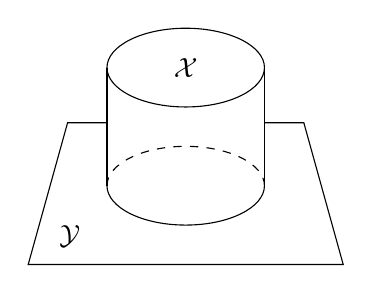
\begin{tikzpicture}[baseline=(O)]
	\draw (1, 1.5) ellipse[x radius=1, y radius=0.5] node {$\mathcal{X}$};
	\draw (0, 0) arc[start angle=180, end angle=360, x radius=1, y radius=0.5];
	\draw[dashed] (0, 0) arc[start angle=180, end angle=0, x radius=1, y radius=0.5];
	\draw (2, 1.5) -- (2, 0);
	\draw (0, 1.5) -- (0, 0);
	\draw (0, 0.8) -- (-0.5, 0.8) -- (-1, -1) node[xshift=1.5em,  yshift=1em] {$\mathcal{Y}$} -- (3, -1) -- (2.5, 0.8) -- (2, 0.8);
	\coordinate (O) at (0, 0.5);
\end{tikzpicture} \quad
	\Cone_{\mathrm{top}}(F) = 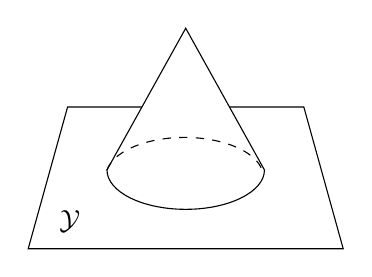
\begin{tikzpicture}[baseline=(O)]
	\draw (0, 0.8) -- (-0.5, 0.8) -- (-1, -1) node[xshift=1.5em,  yshift=1em] {$\mathcal{Y}$} -- (3, -1) -- (2.5, 0.8) --cycle;
	\filldraw[fill=white] (1, 1.8) -- (0, 0) arc[start angle=180, end angle=360, x radius=1, y radius=0.5] --cycle;
	\draw[dashed] (0, 0) arc[start angle=170, end angle=10, x radius=1, y radius=0.5];
	\coordinate (O) at (0, 0.5);
\end{tikzpicture}\]

% segment-id: o014.li2.chapter8.mapping-cone-revisited.p003
Simplicial sets provide a concrete way to describe topological spaces. More
precisely, Theorem~\ref{prop:geom-Sing-adjunction} gives an adjoint pair
% segment-id: o014.li2.chapter8.mapping-cone-revisited.q004
\[\begin{tikzcd}
	{|\cdot|}: \cate{sSet} \arrow[shift left, r] & \cate{Top}: \mathrm{Sing}, \arrow[shift left, l]
\end{tikzcd}\]
and the two categories model equivalent homotopy theories in a precise
sense. The same construction works with $\cate{Top}$ replaced by
$\cate{CGHaus}$. We now translate the preceding discussion into
$\cate{sSet}$. We may assume that
% segment-id: o014.li2.chapter8.mapping-cone-revisited.q005
\[ \mathcal{X} = |X|, \quad \mathcal{Y} = |Y|, \quad F = |f|: |X| \to |Y|, \]
where $f:X\to Y$ is a morphism in $\cate{sSet}$. From the viewpoint of
simplicial sets, the mapping cone is easier to describe than the mapping
cylinder. We begin with the cone on $\mathcal{X}$,
$\Cone_{\mathrm{top}}(\mathcal{X}):=
\Cone_{\mathrm{top}}(\identity_{\mathcal{X}})$. If
$\mathcal{X}=|X|$, then
$\Cone_{\mathrm{top}}(\mathcal{X})\simeq|X^{\lhd}|\simeq|X^{\rhd}|$
(Example~\ref{eg:cone-realization}). Below we focus on the left cone
$X^{\lhd}=\Delta^0\star X$ and its corresponding chain complex.
\index{simplicial set!cone}

% segment-id: o014.li2.chapter8.mapping-cone-revisited.p004
For every simplicial set $Z$, write $Z_n^{\mathrm{nd}}$ for the set of all
nondegenerate $n$-simplices in it, and write
$\{\mathrm{pt}\}=(\Delta^0)_0=(\Delta^0)_0^{\mathrm{nd}}$.
Proposition~\ref{prop:join-nd}, or topological intuition, gives
% segment-id: o014.li2.chapter8.mapping-cone-revisited.q006
\begin{equation}\label{eqn:Cone-X-aux1}
	(\Delta^0 \star X)^{\mathrm{nd}}_n = \begin{cases}
		X^{\mathrm{nd}}_n \sqcup \left( \{ \mathrm{pt} \} \times X^{\mathrm{nd}}_{n-1} \right), & n > 0 \\
		\{\mathrm{pt}\} \sqcup X_0, & n = 0.
	\end{cases}
\end{equation}

% segment-id: o014.li2.chapter8.mapping-cone-revisited.p005
Substituting \eqref{eqn:join-formulas} and the general formulas discussed
above it shows that, for $n\geq1$, the restrictions of
$d_i:(\Delta^0\star X)_n\to(\Delta^0\star X)_{n-1}$ to
$\{\mathrm{pt}\}\times X_{n-1}$ and $X_n$ are as follows:
% segment-id: o014.li2.chapter8.mapping-cone-revisited.q007
\begin{equation}\label{eqn:Cone-X-aux2}\begin{gathered}
	\begin{tikzcd}[column sep=small,
		/tikz/execute at end picture={
			\node [rectangle, draw, fit=(A) (B)] {};
			\node at ($(A)!.5!(C) + (0, 0.8)$) {$1 \leq i \leq n$};
		}]
		|[alias=A]| \{\mathrm{pt}\} \times X_{n-1} \arrow[d, "{\identity \times d_{i-1}}"'] & |[alias=C]| X_n \arrow[d, "{d_i}"] \\
		\{\mathrm{pt}\} \times X_{n-2} & |[alias=B]| X_{n-1}
	\end{tikzcd} \quad
	\begin{tikzcd}[column sep=small,
		/tikz/execute at end picture={
			\node [rectangle, draw, fit=(A) (B)] {};
			\node at ($(A)!.5!(C) + (0, 0.8)$) {$i=0$};
		}]
		|[alias=A]| \{\mathrm{pt}\} \times X_{n-1} \arrow[rd, "{\mathrm{pr}_2}"] & |[alias=C]| X_n \arrow[d, "{d_0}"] \\
		\{\mathrm{pt}\} \times X_{n-2} & |[alias=B]| X_{n-1}
	\end{tikzcd}
\end{gathered}\end{equation}
If $n=1$, the term $\{\mathrm{pt}\}\times X_{n-2}$ in this formula is
to be understood as $\{\mathrm{pt}\}$.

% segment-id: o014.li2.chapter8.mapping-cone-revisited.p006
Since our goal is a chain complex, the next step is to linearize the problem
using the functor $\Z(\mathord\cdot)$ of
Definition~\ref{def:free-simplicial-Ab}, and then pass to chain complexes via
the Dold--Kan correspondence:
% segment-id: o014.li2.chapter8.mapping-cone-revisited.q008
\begin{equation*}
	\mathrm{N}(\Z X^{\lhd}) \simeq \mathrm{C}(\Z X^{\lhd}) \big/ \text{degenerate part} \quad \text{(Proposition \ref{prop:Dold-Kan-v})}.
\end{equation*}
To simplify notation in the rest of this section, write
$\mathrm{N}X:=\mathrm{N}(\Z X)$ and
$\mathrm{N}f:=\mathrm{N}(\Z f)$. The chain-complex structure on
$\mathrm{C}(\Z X^{\lhd})$ comes from
$\partial_n:=\sum_{i=0}^n(-1)^id_i$. Combining
\eqref{eqn:Cone-X-aux1}, \eqref{eqn:Cone-X-aux2}, and the description of
$\Cone(\identity_{\mathrm{N}X})$ in Remark~\ref{rem:cone-chain}, we obtain a
short exact sequence of chain complexes
% segment-id: o014.li2.chapter8.mapping-cone-revisited.q009
\[ 0 \to \underbracket{\Z\{\mathrm{pt}\}}_{\text{degree zero}} \to \mathrm{N}(\Z X^{\lhd}) \to \Cone(\identity_{\mathrm{N}X}) \to 0. \]

% segment-id: o014.li2.chapter8.mapping-cone-revisited.p007
Next, the functors $|\mathord\cdot|$ and
$\mathrm{N}\Z(\mathord\cdot)$ preserve pushout diagrams: the former is a
left adjoint, while the latter is the composite of a left adjoint with an
equivalence; in topology, a pushout diagram means gluing. Therefore, for
$f:X\to Y$ define
% segment-id: o014.li2.chapter8.mapping-cone-revisited.q010
\begin{equation*}
	\Cone_{\mathrm{s}}(f) := X^{\lhd} \dsqcup{X, f} Y.
\end{equation*}
We then obtain
% segment-id: o014.li2.chapter8.mapping-cone-revisited.q011
\[\begin{tikzcd}
	\mathcal{X} \arrow[d, "F"'] \arrow[r, "{\text{base}}"] & \Cone_{\mathrm{top}}(\mathcal{X}) \arrow[d] \\
	\mathcal{Y} \arrow[r] & \Cone_{\mathrm{top}}(F) \arrow[phantom, lu, "\boxplus" description]
\end{tikzcd} \xleftarrow{|\cdot|} \begin{tikzcd}
	X \arrow[d, "f"'] \arrow[r, "\text{canonical}"] & X^{\lhd} \arrow[d] \\
	Y \arrow[r] & \Cone_{\mathrm{s}}(f) \arrow[phantom, lu, "\boxplus" description]
\end{tikzcd} \xrightarrow{\mathrm{N}} \begin{tikzcd}
	\mathrm{N}X \arrow[d, "{\mathrm{N}f}"'] \arrow[r] & \mathrm{N}X^{\lhd} \arrow[d] \\
	\mathrm{N}Y \arrow[r] & \mathrm{N}\Cone_{\mathrm{s}}(f) \arrow[phantom, lu, "\boxplus" description]
\end{tikzcd}\]
This chain of constructions shows that the linear-algebraic counterpart of
$\Cone_{\mathrm{top}}(F)$ should be $\mathrm{N}\Cone_{\mathrm{s}}(f)$.

% segment-id: o014.li2.chapter8.mapping-cone-revisited.pr001
\begin{proposition}\label{prop:Cone-comparison}
	\index{mapping cone}
	With the notation above, there is a canonical short exact sequence of
	chain complexes
	% segment-id: o014.li2.chapter8.mapping-cone-revisited.q012
	\[ 0 \to \underbracket{\Z\{\mathrm{pt}\}}_{\text{degree zero}} \to \mathrm{N}\Cone_{\mathrm{s}}(f) \to \Cone(\mathrm{N}f) \to 0. \]
\end{proposition}
\begin{proof}
	The pushout does not affect the chain subcomplex $\Z\{\mathrm{pt}\}$ of
	$\mathrm{N}X^{\lhd}$ corresponding to the cone point. In degree $n$, it
	replaces every $X_n$ by $Y_n$ and replaces the projection
	$\mathrm{pr}_2$ in \eqref{eqn:Cone-X-aux2} by
	$f_{n-1}\mathrm{pr}_2$. Thus, on the quotient
	$\Cone(\identity_{\mathrm{N}X})$, the resulting pushout is precisely
	$\Cone(\mathrm{N}f)$; see Remark~\ref{rem:cone-chain}.
\end{proof}

% segment-id: o014.li2.chapter8.mapping-cone-revisited.r001
\begin{remark}
	The mapping cylinder $\Cyl_{\mathrm{top}}(F)$ and its chain-complex
	version can be compared similarly; here there is no need to quotient out
	the contribution of the cone point. However, the mapping cylinder involves
	products of simplicial sets, whereas $\mathrm{N}$ is not a monoidal
	functor. Topological accounts therefore usually use CW complexes rather
	than simplicial sets, since products are easier to handle in the world of
	CW complexes.
\end{remark}

% segment-id: o014.li2.chapter8.mapping-cone-revisited.p008
In short, the mapping cone of chain complexes is the quotient of the mapping
cone arising from simplicial sets (or topology) by a copy of $\Z$ coming
from the cone point $\mathrm{pt}$. In the study of chain complexes, the main
role of the mapping cone is that every map $\phi:A\to B$ extends to a
sequence
% segment-id: o014.li2.chapter8.mapping-cone-revisited.q013
\begin{equation}\label{eqn:cofiber-comparison-A}
	A \xrightarrow{\phi} B \to \Cone(\phi) \to A[-1] \xrightarrow{-\phi[-1]} B[-1] \to \cdots .
\end{equation}

% segment-id: o014.li2.chapter8.mapping-cone-revisited.p009
In the topological setting, the map corresponding to
$\Cone(\phi)\to A[-1]$ is obtained by contracting the base
$\mathcal{Y}$ of $\Cone_{\mathrm{top}}(F)$ to a point. The result is denoted
by $S\mathcal{X}$; it is independent of $\mathcal{Y}$ (see the figure below)
and defines a functor $S$. The corresponding sequence of maps is
% segment-id: o014.li2.chapter8.mapping-cone-revisited.q014
\begin{equation*}
	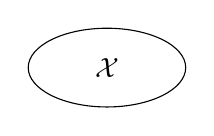
\begin{tikzpicture}[baseline=(O)]
		\draw (1, 0) ellipse[x radius=1, y radius=0.5] node {$\mathcal{X}$};
		\coordinate (O) at (0, 0);
	\end{tikzpicture}
	\xrightarrow{F}
	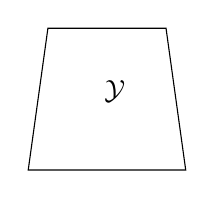
\begin{tikzpicture}[baseline=(O), xscale=0.5]
		\draw (0, 0.8) -- (-0.5, 0.8) -- (-1, -1) -- (3, -1) -- (2.5, 0.8) --cycle;
		\node at (1.2, 0) {$\mathcal{Y}$};
		\coordinate (O) at (0, 0.5);
	\end{tikzpicture}
	\xrightarrow{\text{inclusion}}
	\begin{tikzpicture}[baseline=(O), xscale=0.8]
		\draw (0, 0.8) -- (-0.5, 0.8) -- (-1, -1) node[xshift=1.5em,  yshift=1em] {$\mathcal{Y}$} -- (3, -1) -- (2.5, 0.8) --cycle;
		\filldraw[fill=white] (1, 1.8) -- (0, 0) arc[start angle=180, end angle=360, x radius=1, y radius=0.5] --cycle;
		\draw[dashed] (0, 0) arc[start angle=170, end angle=10, x radius=1, y radius=0.5];
		\coordinate (O) at (0, 0.5);
	\end{tikzpicture}
	\xrightarrow{\text{collapse}}
	\begin{tikzpicture}[baseline=(O), xscale=0.7, yscale=0.7]
		\draw (2, 0) -- (1, 1.8) -- (0, 0);
		\draw[dashed] (0, 0) arc[start angle=170, end angle=10, x radius=1, y radius=0.5];
		\draw (0, 0) arc[start angle=190, end angle=350, x radius=1, y radius=0.5];
		\node at (1, 0) {$\mathcal{X}$};
		\draw (0, 0) -- (1, -1.8) -- (2, 0);
		\coordinate (O) at (0, 0.5);
	\end{tikzpicture}
	\to \cdots .
\end{equation*}
This sequence is called the \emph{cofiber sequence} generated by $f$ (more
precisely, the unpointed version). If we work in $\cate{sSet}$ and take the
chain complexes of the corresponding sequence, the result is roughly
\eqref{eqn:cofiber-comparison-A}. The qualification ``roughly'' is needed
because:
\begin{itemize}
	\item The map $S\mathcal{X}\to S\mathcal{Y}$ cannot simply be defined as
	$S(F)$; the vertical coordinate must be reversed appropriately. At the
	level of linear algebra, this corresponds to $-\phi[-1]$ in
	\eqref{eqn:cofiber-comparison-A}; see a topology textbook for details.
	\item As Proposition~\ref{prop:Cone-comparison} shows, the various chain
	complexes contain one extra copy of $\Z$ corresponding to the cone point
	of spaces such as $\Cone_{\mathrm{top}}(F)$ and $S\mathcal{X}$. In
	topology, this issue is avoided by using pointed spaces and, in the
	topological cone construction, contracting the part associated with the
	base point.
\end{itemize}

% segment-id: o014.li2.chapter8.mapping-cone-revisited.p010
If we set all details aside for the moment, the theory of derived categories
constructed in \S\ref{sec:derived-cat}, with $\mathcal{A}=\cate{Ab}$, may
also be viewed in broad outline as a somewhat coarse ``linearization'' of
homotopy theory\footnote{More precisely, stable homotopy theory, since chain
complexes allow terms in negative degrees.}.

% segment-id: o014.li2.chapter8.mapping-cone-revisited.p011
As the related questions increasingly involve topological ideas and methods,
we stop here so as not to stray too far afield.

% Unit 119 English translation of chapter8.tex lines 2000--2107.
% Source: Methods of Algebra, Volume 2, commit
% 9a5803ff77dd3257484cb177f851a73770a59dd3 (CC BY 4.0).
% stable-unit-id: o014.aljabr2.chapter8.exercises-a
% Coverage: the first half of the Chapter 8 exercises, from the opening of
% the Exercises through the definition of L-projective and T-injective objects;
% Unit 120 continues at line 2108.
% Editorial corrections: in the uniqueness hint for Exercise 2, the equality
% forced by y=DS'y' is y=\widetilde{D}y'; the source reverses its two sides.
% The Kan condition in Exercise 11 starts at n >= 1, since no 0-dimensional
% horn Lambda^0_i exists.

\hypertarget{o014.aljabr2.chapter8.exercises-a}{ }
% segment-id: o014.aljabr2.chapter8.exercises-a.h001
% Canonical environment token retained for exact witness parity: \begin{Exercises}
\csname begin\endcsname{Exercises}
% segment-id: o014.aljabr2.chapter8.exercises-a.ex001
	\item Prove that, for every category $\mathcal{C}$, the construction
	$C\mapsto\mathrm{const}(C)$ of Example~\ref{eg:const-simplicial} gives a
	fully faithful functor $\mathcal{C}\to\cate{s}\mathcal{C}$.

% segment-id: o014.aljabr2.chapter8.exercises-a.ex002
	\item Let $X$ be a simplicial set and $x\in X_n$. Prove that there is a
	sequence of indices $j_1<\cdots<j_h$ and a nondegenerate simplex $y$ such
	that $x=s_{j_h}\cdots s_{j_1}(y)$, and that $y$ is unique.

% segment-id: o014.aljabr2.chapter8.exercises-a.hi001
	\begin{hint}
		The difficulty lies in uniqueness. Suppose that $Sy=x=S'y'$, where
		$S$ and $S'$ are both of the form in the statement. We can choose a
		composite $D$ of a sequence of face morphisms such that
		$y=DSy=DS'y'$. Rewrite $DS'$ in the form
		$\widetilde{S}'\widetilde{D}$ (the meaning of the notation is clear).
		Since $y$ is nondegenerate, we must have
		$\widetilde{S}'=\identity$, and hence $y=\widetilde{D}y'$. Use symmetry
		to conclude that $y=y'$ and $\widetilde{D}=\identity$.
	\end{hint}

% segment-id: o014.aljabr2.chapter8.exercises-a.ex003
	\item Show that the following diagram exists in $\cate{sSet}$, with both
	the upper and lower parts commutative, for $0\leq i<j\leq n$:
% segment-id: o014.aljabr2.chapter8.exercises-a.q001
	\[\begin{tikzcd}
		\Delta^{n-2} \arrow[d, "{\iota_{i < j}}"'] \arrow[r, "{\mathrm{d}^{j-1}}"] & \Delta^{n-1} \arrow[d, "\iota_i"] \arrow[rd, "{\mathrm{d}^i}"] & \\
		\bigsqcup_{0 \leq i' < j' \leq n} \Delta^{n-2} \arrow[shift left, r] \arrow[shift right, r] & \bigsqcup_{i' = 0}^n \Delta^{n-1} \arrow[r] & \partial \Delta^n \\
		\Delta^{n-2} \arrow[u, "{\iota_{i < j}}"] \arrow[r, "{\mathrm{d}^i}"'] & \Delta^{n-1} \arrow[u, "\iota_j"'] \arrow[ru, "{\mathrm{d}^j}"'] &
	\end{tikzcd}\]
	Here $\bigsqcup$ is taken degreewise in
	$\cate{sSet}=\cate{Set}^{\simpDelta^{\opp}}$, while $\iota_{i<j}$
	(respectively, $\iota_i$) denotes the embedding into the $i<j$ term
	(respectively, the $i$th term). All arrows in the middle row are
	characterized by this commutativity. Show, moreover, that the middle row is
	a coequalizer.

	Similarly, show that for every $0\leq k\leq n$ there is also a diagram
% segment-id: o014.aljabr2.chapter8.exercises-a.q002
	\[\begin{tikzcd}
		\Delta^{n-2} \arrow[d, "{\iota_{i < j}}"'] \arrow[r, "{\mathrm{d}^{j-1}}"] & \Delta^{n-1} \arrow[d, "\iota_i"] \arrow[rd, "{\mathrm{d}^i}"] & \\
		\bigsqcup_{\substack{0 \leq i' < j' \leq n \\ i', j' \neq k}} \Delta^{n-2} \arrow[shift left, r] \arrow[shift right, r] & \bigsqcup_{\substack{0 \leq i' \leq n \\ i' \neq k}} \Delta^{n-1} \arrow[r] & \Lambda^n_k \\
		\Delta^{n-2} \arrow[u, "{\iota_{i < j}}"] \arrow[r, "{\mathrm{d}^i}"'] & \Delta^{n-1} \arrow[u, "\iota_j"'] \arrow[ru, "{\mathrm{d}^j}"'] &
	\end{tikzcd}\]
	whose middle row is a coequalizer and where $i,j\neq k$. Try to explain
	the topological meaning of these coequalizers.

% segment-id: o014.aljabr2.chapter8.exercises-a.ex004
	\item Verify the following properties of the join operation $\star$ in
	Definition~\ref{def:simplicial-join}.
	\begin{enumerate}[(i)]
% segment-id: o014.aljabr2.chapter8.exercises-a.i001
		\item Simplicial sets naturally form a monoidal category under $\star$,
		with the constant empty simplicial set $\emptyset$ as unit object.
% segment-id: o014.aljabr2.chapter8.exercises-a.i002
		\item The order-reversal duality of
		Remark~\ref{rem:simpDelta-order-reversal} gives an automorphism of
		$\cate{sSet}$, provisionally denoted by $X\mapsto\hat{X}$. Show that
		$(X\star Y)^{\wedge}\simeq\hat{Y}\star\hat{X}$.
% segment-id: o014.aljabr2.chapter8.exercises-a.i003
		\item Verify that
		$\Delta^p\star\Delta^q\simeq\Delta^{p+q+1}$.
	\end{enumerate}

% segment-id: o014.aljabr2.chapter8.exercises-a.ex005
	\item Show that taking the order-reversal dual of a simplicial set does
	not change its geometric realization, up to canonical homeomorphism.
% segment-id: o014.aljabr2.chapter8.exercises-a.hi002
	\begin{hint}
		Begin with the case of $\Delta^n$.
	\end{hint}

% segment-id: o014.aljabr2.chapter8.exercises-a.ex006
	\item Verify the assertion of Example~\ref{eg:cone-realization}.

% segment-id: o014.aljabr2.chapter8.exercises-a.ex007
	\item Let $\mathcal{C}$ and $\mathcal{C}'$ be categories. Define the
	category $\mathcal{C}\star\mathcal{C}'$ as follows:
% segment-id: o014.aljabr2.chapter8.exercises-a.q003
	\begin{align*}
		\Obj(\mathcal{C} \star \mathcal{C}') & := \Obj(\mathcal{C}) \sqcup \Obj(\mathcal{C}'), \\
		\Hom_{\mathcal{C} \star \mathcal{C}'}(X, Y) & := \begin{cases}
			\Hom_{\mathcal{C}}(X, Y), & X, Y \in \Obj(\mathcal{C}) \\
			\Hom_{\mathcal{C}'}(X, Y), & X, Y \in \Obj(\mathcal{C}'), \\
			\text{one-point set}, & X \in \Obj(\mathcal{C}), \; Y \in \Obj(\mathcal{C}'), \\
			\emptyset, & X \in \Obj(\mathcal{C}'), \; Y \in \Obj(\mathcal{C}).
		\end{cases}
	\end{align*}
	Composition and identity morphisms are defined in the evident way. Prove
	that the join operation $\star$ on simplicial sets and the nerve functor of
	Example~\ref{eg:nerve-cat} are related by
% segment-id: o014.aljabr2.chapter8.exercises-a.q004
	\[ \mathrm{N}(\mathcal{C}) \star \mathrm{N}(\mathcal{C}') \simeq \mathrm{N}(\mathcal{C} \star \mathcal{C}'). \]

% segment-id: o014.aljabr2.chapter8.exercises-a.ex008
	\item Give a more detailed proof of Equations~\eqref{eqn:shuffle-sign-0}
	and \eqref{eqn:shuffle-sign-1}.

% segment-id: o014.aljabr2.chapter8.exercises-a.ex009
	\item For a simplicial object $X$ in an arbitrary category, define the
	simplicial objects called the decalages $\mathrm{Déc}_0X$ and
	$\mathrm{Déc}^0X$ by
	$(\mathrm{Déc}_0X)_n=(\mathrm{Déc}^0X)_n=X_{n+1}$ and
% segment-id: o014.aljabr2.chapter8.exercises-a.q005
	\begin{gather*}
		d^{\mathrm{Déc}_0 X, n}_i = d^{X, n+1}_i, \quad s^{\mathrm{Déc}_0 X, n}_j = s^{X, n+1}_j, \\
		d^{\mathrm{Déc}^0 X, n}_i = d^{X, n+1}_{i+1}, \quad
		s^{\mathrm{Déc}^0 X, n}_j = s^{X, n+1}_{j+1}.
	\end{gather*}
	Show that both are well-defined and are related by the order-reversal
	duality (Remark~\ref{rem:simpDelta-order-reversal}). Also show that for an
	additive category,
	$\mathrm{C}(\mathrm{Déc}^0X)=\mathrm{C}(X)[1]$; see
	Remark~\ref{rem:chain-cplx-translation}.
	\index{simplicial object!decalage@decalage ($\mathrm{Déc}$)}
	\index[sym1]{Dec@$\mathrm{Déc}_0 X, \mathrm{Déc}^0 X$}

% segment-id: o014.aljabr2.chapter8.exercises-a.ex010
	\item Continuing the preceding exercise, show that
	$d_0:X_1\to X_0$ (respectively, $d_1:X_1\to X_0$) gives an augmentation
	of $\mathrm{Déc}_0X$ (respectively, $\mathrm{Déc}^0X$), with $X_0$ as
	the term of degree $-1$. Show further that, after augmentation,
	$\mathrm{Déc}_0X$ is right contractible and $\mathrm{Déc}^0X$ is left
	contractible; see Definition~\ref{def:contractible-aug}.
% segment-id: o014.aljabr2.chapter8.exercises-a.hi003
	\begin{hint}
		It suffices to treat $\mathrm{Déc}_0X$. Take
		$k_{n-1}:=s_n:X_n\to X_{n+1}$.
	\end{hint}

% segment-id: o014.aljabr2.chapter8.exercises-a.ex011
	\item Prove that a small category $\mathcal{C}$ is a groupoid (that is,
	all its morphisms are invertible) if and only if $\mathrm{N}\mathcal{C}$
	satisfies the following condition: for every $n\in\Z_{\geq1}$ and
	$0\leq i\leq n$, every morphism
	$\Lambda^n_i\to\mathrm{N}\mathcal{C}$ can be extended to
	$\Delta^n\to\mathrm{N}\mathcal{C}$, without requiring uniqueness. A
	simplicial set satisfying this extension condition is called a Kan
	complex.

% segment-id: o014.aljabr2.chapter8.exercises-a.ex012
	\item Continue the discussion of
	Example~\ref{eg:classifying-space-std-cplx}. Show that the normalized
	complex $\overline{\mathsf{L}}$, after being reversed into a chain complex,
	is isomorphic to $\mathrm{N}(\Bbbk\mathrm{E}\Gamma)$.
% segment-id: o014.aljabr2.chapter8.exercises-a.hi004
	\begin{hint}
		First use Proposition~\ref{prop:Dold-Kan-v} to identify $\mathrm{N}(X)$
		with a quotient of $\mathrm{C}(X)$.
	\end{hint}

% segment-id: o014.aljabr2.chapter8.exercises-a.ex013
	\item Let $\Gamma$ be a monoid. Write $\cated{Set}\Gamma$ for the category
	of all small sets with a right $\Gamma$-action.
	\begin{enumerate}[(i)]
% segment-id: o014.aljabr2.chapter8.exercises-a.i004
		\item Describe explicitly the free--forgetful adjoint pair
% segment-id: o014.aljabr2.chapter8.exercises-a.q006
		\[\begin{tikzcd}
			\mathrm{F}: \cate{Set} \arrow[shift left, r] & \cated{Set}\Gamma \arrow[shift left, l]: U
		\end{tikzcd}\]
		together with its unit and counit morphisms. Show that the corresponding
		monad $T$ gives an equivalence
		$\cated{Set}\Gamma\simeq\cate{Set}^T$.

% segment-id: o014.aljabr2.chapter8.exercises-a.hi005
		\begin{hint}
			The functor $\mathrm{F}$ sends a set $X$ to $X\times\Gamma$, with
			$\Gamma$ acting by right multiplication on the second component. The
			unit morphism is $x\mapsto(x,1)$, while the counit morphism is the
			action map.
		\end{hint}
% segment-id: o014.aljabr2.chapter8.exercises-a.i005
		\item For every right $\Gamma$-set $X$, describe the corresponding
		simplicial object $\mathrm{Bar}(X)$ in $\cated{Set}\Gamma$; see
		Examples~\ref{eg:bar-adjunction} and \ref{eg:bar-comonad}.
% segment-id: o014.aljabr2.chapter8.exercises-a.i006
		\item Take the one-point set $X=\{\mathrm{pt}\}$ with trivial right
		$\Gamma$-action. Show that the corresponding simplicial object is
		isomorphic to $\mathrm{E}\Gamma$ of
		Example~\ref{eg:classifying-space}; it becomes a simplicial object in
		$\cated{Set}\Gamma$ via the right $\Gamma$-action on each
		$(\mathrm{E}\Gamma)_n$.
	\end{enumerate}

% segment-id: o014.aljabr2.chapter8.exercises-a.ex014
	\item Fix a group $\Gamma$. In Example~\ref{eg:HH-comonad}, take the group
	algebra $R=\Bbbk[\Gamma]$ and take $M$ to be the trivial $\Gamma$-module
	$\Bbbk$; see Example~\ref{eg:trivial-G-mod}. Show that the corresponding
	$\epsilon_{\Bbbk}:\mathrm{C}(\mathrm{Bar}(\Bbbk))\to\Bbbk$ is isomorphic
	to the resolution $\mathsf{L}=(\mathsf{L}_n,\partial'_n)_n\to\Bbbk$ of
	Proposition~\ref{prop:trivial-mod-resolution}.
% segment-id: o014.aljabr2.chapter8.exercises-a.hi006
	\begin{hint}
		Use \eqref{eqn:L-basis-partial}.
	\end{hint}

% segment-id: o014.aljabr2.chapter8.exercises-a.ex015
	\item Let $\Bbbk$ be a commutative ring and
	$\mathcal{A}=\Bbbk\dcate{Mod}$, with $\otimes=\otimes_{\Bbbk}$. Let
	$\Gamma$ be a group. Consider the simplicial object
	$\Bbbk\mathrm{E}\Gamma$ of
	Example~\ref{eg:classifying-contractible}. Apply
	Definition~\ref{def:Eilenberg-Zilber} of the Alexander--Whitney morphism
	to $X:=\Bbbk\mathrm{E}\Gamma\boxtimes\Bbbk\mathrm{E}\Gamma$, and then
	consider the morphism
% segment-id: o014.aljabr2.chapter8.exercises-a.q007
	\[ \mathrm{C}(\Bbbk\mathrm{E}\Gamma) \to \mathrm{C}(\underbracket{\Bbbk\mathrm{E}\Gamma \otimes \Bbbk\mathrm{E}\Gamma}_{\simeq \Bbbk(\mathrm{E}\Gamma \times \mathrm{E}\Gamma)}) \xrightarrow{\overline{\mathrm{AW}}} \mathrm{C}(\Bbbk\mathrm{E}\Gamma) \otimes \mathrm{C}(\Bbbk\mathrm{E}\Gamma). \]
	The first arrow is induced by the diagonal embedding of simplicial sets
	$\mathrm{E}\Gamma\to\mathrm{E}\Gamma\times\mathrm{E}\Gamma$. In view
	of Example~\ref{eg:classifying-space-std-cplx}, the composite can also be
	regarded as a morphism of chain complexes
% segment-id: o014.aljabr2.chapter8.exercises-a.q008
	\[ \mathsf{L} \to \mathsf{L} \otimes \mathsf{L}. \]
	Use this to interpret the morphism
	$\Delta:\mathsf{L}\to\mathsf{L}\otimes\mathsf{L}$ used in the
	definition of the cup product in group cohomology; see
	Lemma~\ref{prop:cup-resolution}~(ii).

% segment-id: o014.aljabr2.chapter8.exercises-a.hi007
	\begin{hint}
		Substitution of the definition of $\overline{\mathrm{AW}}$ shows that
		the $(p,q)$ component of the composite morphism differs from that in
		Lemma~\ref{prop:cup-resolution}~(ii) by a factor $(-1)^{pq}$. This
		difference arises because the discussion there uses
		$(\mathsf{L}_n,\partial_n)_n$, whereas
		Example~\ref{eg:classifying-space-std-cplx} uses
		$(\mathsf{L}_n,\partial'_n)_n$. At the level of the simplicial set
		$\mathrm{E}\Gamma$, the two differ by order reversal
		(Remark~\ref{rem:simpDelta-order-reversal}). Observe that order-reversal
		duality interchanges the roles of $\lambda^n_p$ and $\rho^n_q$ in
		$\overline{\mathrm{AW}}$, or equivalently interchanges the two copies
		of $\mathrm{C}(\Bbbk\mathrm{E}\Gamma)$.
	\end{hint}

% segment-id: o014.aljabr2.chapter8.exercises-a.ex016
	\item Consider a comonad $(L,\delta,\epsilon)$ on a category $\mathcal{D}$.
	For every $\mathcal{M}\in\Obj(\mathcal{D})$, if
	$\epsilon_{\mathcal{M}}:L\mathcal{M}\to\mathcal{M}$ has a right inverse
	$f:\mathcal{M}\to L\mathcal{M}$, then $\mathcal{M}$ is called an
	\emph{$L$-projective object}. Dually, from a monad $(T,\mu,\eta)$ on a
	category $\mathcal{C}$, we define a \emph{$T$-injective object} in
	$\mathcal{C}$.

% Unit 120 English translation of chapter8.tex lines 2108--2214.
% Source: Methods of Algebra, Volume 2, commit
% 9a5803ff77dd3257484cb177f851a73770a59dd3 (CC BY 4.0).
% stable-unit-id: o014.aljabr2.chapter8.exercises-b
% Coverage: continuation of the exercises on L-projective objects through the
% end of the chapter.
% Necessary source corrections: on line 2113 identity_{X_n} is clarified as
% identity_{L^{n+1} M}; the comonad (FG,F eta G,epsilon) is on D (equivalently,
% it is a comonoid in End(D)); on line 2171 the homology objects lie in A, not Ch(A).

% segment-id: o014.li2.chapter8.exercises-b.p001
	By duality, the following discussion focuses mainly on the concept of
	$L$-projectivity. By the method of Example~\ref{eg:monad-simplicial}, we
	obtain in $\End(\mathcal{D})$ an augmented simplicial object
	$(L^{n+1})_{n\geq-1}$; the data $d_i$, $s_j$, and so forth are omitted
	from the notation. For an $L$-projective object $\mathcal{M}$ and a
	corresponding $f$, define
	% segment-id: o014.li2.chapter8.exercises-b.q001
	\[ k_n := L^{n+1} f : L^{n+1} \mathcal{M} \to L^{n+2} \mathcal{M}, \quad n \geq -1. \]
	Prove that this makes the augmented simplicial object
	$(L^{n+1}\mathcal{M})_{n\geq-1}$ right contractible
	(Definition~\ref{def:contractible-aug}).

	% segment-id: o014.li2.chapter8.exercises-b.hint001
	\begin{hint}
		We know that
		$\epsilon_{\mathcal{M}}k_{-1}=\epsilon_{\mathcal{M}}f
		=\identity_{\mathcal{M}}$. Applying $L^{n+1}$ to both sides gives
		$d_{n+1}k_n=\identity_{L^{n+1}\mathcal{M}}$, while naturality ensures
		that
		% segment-id: o014.li2.chapter8.exercises-b.q002
		\[\begin{tikzcd}
			L\mathcal{M} \arrow[r, "Lf"] \arrow[d, "{\epsilon_{\mathcal{M}}}"'] & L^2 \mathcal{M} \arrow[d, "{\epsilon_{L\mathcal{M}}}"] \\
			\mathcal{M} \arrow[r, "f"'] & L\mathcal{M}
		\end{tikzcd} \quad\text{commutes, that is,}\; d_0 k_0 = f\epsilon_{\mathcal{M}} = k_{-1} \epsilon_{\mathcal{M}}. \]
		Replace $f$ by $L^{n-i}f$, and then apply $L^i$ to the corresponding
		diagram. The same method gives
		$d_ik_n=k_{n-1}d_i$ for $0\leq i\leq n$.
	\end{hint}

	% segment-id: o014.li2.chapter8.exercises-b.ex001
	\item For a ring $R$, the free--forgetful adjoint pair
	$\cate{Set}\leftrightarrows R\dcate{Mod}$ determines a comonad $L$ on
	$R\dcate{Mod}$. Prove that a left $R$-module is $L$-projective if and
	only if it is a projective module.

	% segment-id: o014.li2.chapter8.exercises-b.ex002
	\item Consider an adjoint pair
	% segment-id: o014.li2.chapter8.exercises-b.q003
	$\begin{tikzcd}
		F: \mathcal{C} \arrow[shift left, r] & \mathcal{D}: G \arrow[shift left, l]
	\end{tikzcd}$
	and the corresponding comonad
	$(L,\delta,\epsilon)=(FG,F\eta G,\epsilon)$ on
	$\mathcal{D}$ (Example~\ref{eg:adjunction-monad}). Prove that every
	object of the form $F\mathcal{N}$, for
	$\mathcal{N}\in\Obj(\mathcal{C})$, is $L$-projective. Consequently, for
	every $\mathcal{M}\in\Obj(\mathcal{D})$, every term of the simplicial
	object $(L^{n+1}\mathcal{M})_{n\geq0}$ is $L$-projective.

	% segment-id: o014.li2.chapter8.exercises-b.hint002
	\begin{hint}
		Take
		$f=F\eta_{\mathcal{N}}:F(\mathcal{N})\to FGF(\mathcal{N})
		=L(F(\mathcal{N}))$. Then
		$\epsilon_{F(\mathcal{N})}f=\identity_{F(\mathcal{N})}$ is precisely
		one of the triangle identities of the adjunction.
	\end{hint}

	% segment-id: o014.li2.chapter8.exercises-b.ex003
	\item Continue to consider the comonad $L$ arising from the adjoint pair
	$(F,G)$. Show that $\mathcal{P}\in\Obj(\mathcal{D})$ is $L$-projective
	if and only if it has the following lifting property. For every pair of
	morphisms $\alpha:\mathcal{M}_1\to\mathcal{M}_2$ and
	$\phi:\mathcal{P}\to\mathcal{M}_2$ in $\mathcal{D}$, if $G\alpha$ has
	a right inverse, then there is a morphism
	$\beta:\mathcal{P}\to\mathcal{M}_1$ such that $\phi=\alpha\beta$.

	% segment-id: o014.li2.chapter8.exercises-b.hint003
	\begin{hint}
		For the ``if'' direction, apply the lifting property to
		$\alpha:=\epsilon_{\mathcal{P}}:FG(\mathcal{P})\to\mathcal{P}$ and
		$\phi:=\identity$. For the ``only if'' direction, first explain why
		$\mathcal{P}$ in the lifting property can be replaced by
		$FG(\mathcal{P})$, and then use the adjunction to show that
		% segment-id: o014.li2.chapter8.exercises-b.q004
		\[ \alpha_*:\Hom(FG(\mathcal{P}),\mathcal{M}_1)\to
		\Hom(FG(\mathcal{P}),\mathcal{M}_2) \]
		is surjective.
	\end{hint}

	% segment-id: o014.li2.chapter8.exercises-b.ex004
	\item For an arbitrary commutative ring $\Bbbk$ and a homomorphism of
	$\Bbbk$-algebras $S\to R$, consider the adjoint pairs
	% segment-id: o014.li2.chapter8.exercises-b.q005
	\begin{equation*}\begin{tikzcd}[row sep=small]
		R \dotimes{S} (\cdot): S\dcate{Mod} \arrow[shift left, r] & R\dcate{Mod}: \text{forgetful}, \arrow[shift left, l] \\
		\text{forgetful}: R\dcate{Mod} \arrow[shift left, r] & S\dcate{Mod}: \Hom_S(R, \cdot) \arrow[shift left, l]
	\end{tikzcd}\end{equation*}
	which give a comonad $L$ and a monad $T$, respectively, on
	$R\dcate{Mod}$. Use the lifting property above, or its dual, to determine
	necessary and sufficient conditions for a left $R$-module $M$ to be an
	$L$-projective (respectively, $T$-injective) object, and compare these
	conditions with projectivity (respectively, injectivity) of modules.

	On this basis one can construct a theory called \emph{relative
	homological algebra}; see \cite{Ho56}. Its distinguishing feature is that
	it considers only those exact sequences of $R$-modules that are split
	exact over $S$. The next exercise examines relative versions of the
	$\Tor$ and $\Ext$ functors.
	\index{relative homological algebra}

	% segment-id: o014.li2.chapter8.exercises-b.ex005
	\item Consider an adjoint pair between abelian categories
	% segment-id: o014.li2.chapter8.exercises-b.q006
	$\begin{tikzcd}
		F: \mathcal{C} \arrow[shift left, r] & \mathcal{D}: G \arrow[shift left, l]
	\end{tikzcd}$.
	Prove for every $\mathcal{M}\in\Obj(\mathcal{D})$ that:
	\begin{enumerate}[(i)]
		\item There is an object $\mathcal{P}_\bullet$ of
		$\cate{Ch}_{\geq0}(\mathcal{D})$ together with a morphism
		$\epsilon:\mathcal{P}_\bullet\to\mathcal{M}$ such that
		\begin{compactitem}
			\item each $\mathcal{P}_n$ is $L$-projective for $n\geq0$;
			\item the identity morphism on
			$\cdots\to G\mathcal{P}_1\to G\mathcal{P}_0\to
			G\mathcal{M}\to0$ is null-homotopic; in other words, this is a
			split exact complex.
		\end{compactitem}
		\begin{hint}
			Apply Proposition~\ref{prop:bar-null-homotopic}.
		\end{hint}
		\item For any two morphisms
		$\epsilon:\mathcal{P}_\bullet\to\mathcal{M}$ and
		$\epsilon':\mathcal{P}'_\bullet\to\mathcal{M}$ satisfying the
		conditions above, there is a homotopy equivalence
		$f:\mathcal{P}\to\mathcal{P}'$ such that $\epsilon'f=\epsilon$.
		\begin{hint}
			Use the lifting property introduced above.
		\end{hint}
	\end{enumerate}

	\index{comonad homology@comonad homology (cotriple homology)}
	\index{bar construction}
	% segment-id: o014.li2.chapter8.exercises-b.ex006
	\item (M.\ Barr, J.\ M.\ Beck) Let $L$ be a comonad on a category
	$\mathcal{D}$. Write $\mathrm{Bar}(\mathcal{M})$ for the simplicial
	object obtained by evaluating the construction of
	Example~\ref{eg:monad-simplicial} at
	$\mathcal{M}\in\Obj(\mathcal{D})$. For every abelian category
	$\mathcal{A}$ and functor $E:\mathcal{D}\to\mathcal{A}$, define the
	\emph{comonad homology} of $(L,E)$ to be the family of objects in
	$\mathcal{A}$
	% segment-id: o014.li2.chapter8.exercises-b.q007
	\[ \Hm^L_n(E; \mathcal{M}) := \Hm_n\left( \mathrm{C}(E\mathrm{Bar}(\mathcal{M})) \right), \quad n \in \Z_{\geq 0}, \]
	where $E\mathrm{Bar}(\mathcal{M})$ means that $E$ is applied to every term
	of $\mathrm{Bar}(\mathcal{M})$. Dually, if $T$ is a monad on a category
	$\mathcal{C}$ and $F:\mathcal{C}\to\mathcal{A}$ is a functor to an
	abelian category, one can similarly define the value of the \emph{monad
	cohomology} $(T,F)$ at $\mathcal{N}\in\Obj(\mathcal{C})$; we omit the
	details.

	\begin{enumerate}[(i)]
		\item Write down the natural morphism
		$\Hm^L_0(E;\mathcal{M})\to E\mathcal{M}$ and show that it is an
		isomorphism if $\mathcal{M}$ is $L$-projective.
		\item Suppose that $L$ arises from an adjoint pair $(F,G)$ between
		abelian categories and that $E$ is an additive functor. Prove that if
		$\mathcal{P}_\bullet\to\mathcal{M}$ is a morphism in
		$\cate{Ch}_{\geq0}(\mathcal{D})$ satisfying
		\begin{compactitem}
			\item every $\mathcal{P}_n$ is $L$-projective for $n\geq0$;
			\item the identity morphism on
			$\cdots\to G\mathcal{P}_1\to G\mathcal{P}_0\to
			G\mathcal{M}\to0$ is null-homotopic,
		\end{compactitem}
		then
		$\Hm^L_n(E;\mathcal{M})\simeq\Hm_n(E\mathcal{P}_\bullet)$.
		Thus comonad homology can be computed using such $L$-projective
		resolutions.
		\item Continue under the assumptions above. A pair of morphisms
		$\mathcal{M}'\to\mathcal{M}\to\mathcal{M}''$ in $\mathcal{D}$ is
		called a \emph{$G$-split} short exact sequence if, after applying $G$,
		it becomes a split short exact sequence in $\mathcal{C}$. Prove that a
		$G$-split short exact sequence naturally induces a long exact sequence
		for $\Hm^L_n(E;\mathord\cdot)$.
	\end{enumerate}

	\index{Ext functor!relative}
	\index{Tor functor!relative}
	% segment-id: o014.li2.chapter8.exercises-b.ex007
	\item (G.\ Hochschild \cite{Ho56}) For an arbitrary commutative ring
	$\Bbbk$ and a homomorphism of $\Bbbk$-algebras $S\to R$, consider the
	comonad $L$ on $R\dcate{Mod}$ determined by the adjoint pair
	% segment-id: o014.li2.chapter8.exercises-b.q008
	\[\begin{tikzcd}
		R \dotimes{S} (\cdot): S\dcate{Mod} \arrow[shift left, r] & R\dcate{Mod}: \text{forgetful} \arrow[shift left, l]
	\end{tikzcd}\]
	For a right $R$-module $A$ and left $R$-modules $B,N$, define the
	$\Bbbk$-modules
	% segment-id: o014.li2.chapter8.exercises-b.q009
	\begin{align*}
		\Tor^{R|S}_n(A, N) & := \Hm^L_n\left( A \dotimes{R}(\cdot) ; N \right), \\
		\Ext_{R|S}^n(N, B) & := \Hm^L_n\left( \Hom_R(\cdot, B) ; N \right),
	\end{align*}
	where $\Hom_R(\mathord\cdot,B)$ is regarded as a functor
	$R\dcate{Mod}\to S\dcate{Mod}^{\opp}$. These are called the relative
	$\Tor$ and relative $\Ext$ functors.
	\begin{enumerate}[(i)]
		\item Show that both are functorial in every variable. Describe the
		corresponding chain complexes explicitly, and show that
		% segment-id: o014.li2.chapter8.exercises-b.q010
		\[ \Tor^{R|S}_0(A, N) \simeq A \dotimes{R} N, \quad \Ext_{R|S}^0(N, B) \simeq \Hom_R(N, B). \]

		\item Show that the bifunctor $\Tor^{R|S}_n$ has a ``balanced''
		property analogous to Theorem~\ref{prop:balanced-primer}.\footnote{The
		$\Ext_{R|S}^n$ case is not discussed because it involves the notion of
		monad cohomology, which we have not developed here; see the references
		for details.}

		\item Prove that if $I$ is a two-sided ideal of $S$ and $R=S/I$, then
		for $n>0$, $\Tor_n^{R|S}=0=\Ext^n_{R|S}$. Thus relative $\Tor$ and
		relative $\Ext$ differ from their absolute versions in
		\S\ref{sec:Ext-Tor}.
		\begin{hint}
			In this case $L=\identity_{R\dcate{Mod}}$.
		\end{hint}

		\item Write $R^e=R\dotimes{\Bbbk}R^{\opp}$. Prove that
		$\HHm_n(M)\simeq\Tor^{R^e|\Bbbk}_n(M,R)$ and
		$\HHm^n(M)\simeq\Ext_{R^e|\Bbbk}^n(R,M)$; see
		Example~\ref{eg:HH-comonad}.
		\begin{hint}
			Reduce the problem to the assertion that
			$\mathrm{C}(\mathrm{Bar}(R))_n=R\otimes R^{\otimes n}\otimes R$
			is an $L$-projective $R^e$-module.
		\end{hint}
	\end{enumerate}
\csname end\endcsname{Exercises}
% Canonical environment token retained for exact witness parity: \end{Exercises}

% Unit 121 English translation of chapter9.tex lines 1--305.
% Source: Methods of Algebra, Volume 2, commit
% 9a5803ff77dd3257484cb177f851a73770a59dd3 (CC BY 4.0).
% stable-unit-id: o014.aljabr2.chapter9.duality-a
% Coverage: the opening of Chapter 9 and Section 9.1 through the definition
% of dual morphisms; Unit 122 continues at line 306.

\hypertarget{o014.aljabr2.chapter9.duality-a}{ }
% segment-id: o014.aljabr2.chapter9.duality-a.h001
\chapter{Duality}\label{sec:duality}

% segment-id: o014.aljabr2.chapter9.duality-a.p001
The notion of duality originates in the theory of vector spaces. Let
$\Bbbk$ be a field, and denote the dual space of a $\Bbbk$-vector space $V$
by $V^\vee:=\Hom_{\Bbbk}(V,\Bbbk)$. There are
\begin{itemize}
	% segment-id: o014.aljabr2.chapter9.duality-a.i001
	\item the evaluation map $\mathrm{ev}:V\otimes V^\vee\to\Bbbk$, which
	sends $v\otimes\lambda$ to $\lambda(v)$;
	% segment-id: o014.aljabr2.chapter9.duality-a.i002
	\item if $V$ is finite-dimensional, also the coevaluation map
	$\mathrm{coev}:\Bbbk\to V^\vee\otimes V$, which sends $1$ to
	$\sum_{i=1}^n\check{v}_i\otimes v_i$, where $(v_i)_{i=1}^n$ is any basis
	of $V$ and $(\check{v}_i)_{i=1}^n$ its dual basis.
\end{itemize}

% segment-id: o014.aljabr2.chapter9.duality-a.p002
In the finite-dimensional case, they satisfy the fundamental identities
% segment-id: o014.aljabr2.chapter9.duality-a.q001
\[ (\identity_{V^\vee} \otimes \mathrm{ev})(\mathrm{coev} \otimes \identity_{V^\vee}) = \identity_{V^\vee}, \quad (\mathrm{ev} \otimes \identity_V) (\identity_V \otimes \mathrm{coev}) = \identity_V. \]

% segment-id: o014.aljabr2.chapter9.duality-a.p003
In a general monoidal category, the duality data defined in
\S\ref{sec:monoidal-dual} directly generalize the situation above: they
consist of a pair of objects $(L,R)$ together with morphisms
$\mathrm{ev}:L\otimes R\to\munit$ and
$\mathrm{coev}:\munit\to R\otimes L$ satisfying the preceding fundamental
identities. In this situation, $R$ is called a right dual of $L$, while $L$
is called a left dual of $R$. A monoidal category in which every object has
a left dual (respectively, a right dual) is called left rigid (respectively,
right rigid).

% segment-id: o014.aljabr2.chapter9.duality-a.p004
For braided monoidal categories, \S\ref{sec:symm-monoidal-dual} will explain
how the two kinds of dual are related. Thus, if an object $X$ has a dual, we
can define the trace $\Tr(f)$ of $f\in\End(X)$ and subsequently its dimension
$\dim X:=\Tr(\identity_X)$. Both are elements of $\End(\munit)$. Strictly
speaking, each has a left and a right version, but the two need not be
distinguished in a symmetric monoidal category. This book mainly discusses
abelian categories equipped with symmetric monoidal structures, such as
categories of modules over commutative rings (see
Proposition~\ref{prop:dualizable-module}). As long as the reader understands
the usefulness of dual vector spaces, the value of this generalization will
be self-evident. Duality becomes still more powerful in the setting of
$2$-categories, but that lies beyond the scope of this book.

% segment-id: o014.aljabr2.chapter9.duality-a.p005
Examples of duality are the subject of \S\ref{sec:duality-examples}. The
examples closest to algebra are the category
$\catesubd{Mod}{\mathrm{f}}A$ of finite-dimensional right $A$-modules for a
$\Bbbk$-Hopf algebra $A$, and its comodule counterpart
$\catesubd{Comod}{\mathrm{f}}A$ (Proposition~\ref{prop:Hopf-module-dual}).
In both cases, duality reflects properties of the antipode $S:A\to A$.
Examples involving Hopf algebras are important in the study of quantum
groups and also prepare the way for the theory of Tannakian categories.

% segment-id: o014.aljabr2.chapter9.duality-a.p006
The material in \S\S\ref{sec:coend}---\ref{sec:Hopf-reconstruction} of this
chapter concerns the coalgebra reconstruction problem. For every coalgebra
$L$, the abelian category $\catesubd{Comod}{\mathrm{f}}L$ is locally finite
(Definition~\ref{def:locally-finite}) and comes equipped with a faithful
exact forgetful functor
$U:\catesubd{Comod}{\mathrm{f}}L\to\cate{Vect}_{\mathrm{f}}(\Bbbk)$.
The reconstruction problem asks for a converse:
% segment-id: o014.aljabr2.chapter9.duality-a.b001
\begin{center}\begin{minipage}{0.8\textwidth}
	How can one construct a coalgebra $L$ from a locally finite
	$\Bbbk$-linear abelian category $\mathcal{A}$ and a faithful exact functor
	$\omega:\mathcal{A}\to\cate{Vect}_{\mathrm{f}}(\Bbbk)$ in such a way
	that $(\mathcal{A},\omega)$ is naturally equivalent to
	$(\catesubd{Comod}{\mathrm{f}}L,U)$?
\end{minipage}\end{center}
The approach taken in this chapter uses the coendomorphism coalgebra
$\coEnd(\omega)=\coEnd_{\Bbbk}(\omega)$ of the functor $\omega$
(Definition--Proposition~\ref{def:cogebra-L}). This coalgebra coacts on each
$\omega(X)$ and is ``universal'' with respect to these coactions.

% segment-id: o014.aljabr2.chapter9.duality-a.p007
The proof of the coalgebra reconstruction theorem,
Theorem~\ref{prop:Tannaka-aux1}, involves the theory of comonads from
\S\ref{sec:Beck}, basic Morita theory from \S\ref{sec:Morita}, a technical
result about locally finite abelian categories from
\S\ref{sec:locally-finite-Abel-cat}, and the Ind-ization introduced in
\S\ref{sec:Indization-functor}. If $(\mathcal{A},\omega)$ is equipped with
a monoidal structure, then $\coEnd(\omega)$ also becomes a bialgebra. If
$\mathcal{A}$ is both left and right rigid, then $\coEnd(\omega)$ is even a
Hopf algebra (Theorem~\ref{prop:Tannaka-aux2}). The presentation in this part
mainly follows \cite{Del90}.

% segment-id: o014.aljabr2.chapter9.duality-a.p008
After all these preparations, \S\ref{sec:Tannakian-cat} will introduce the
precise definition of a Tannakian category. These are symmetric monoidal
categories $\mathcal{T}$ with special properties. The formal definition is
due to N.\ Saavedra Rivano and P.\ Deligne, while its motivation goes back
to work of Tadao Tannaka and his successors. Among the conditions in
Definition~\ref{def:Tannakian-cat}, the most prominent is the existence of a
nonzero commutative $\Bbbk$-algebra $B$ and a right exact monoidal functor
$\omega:\mathcal{T}\to\cated{Mod}B$ compatible with the braiding; this is
called a fiber functor for $\mathcal{T}$ over $B$.

% segment-id: o014.aljabr2.chapter9.duality-a.p009
The setting of algebraic geometry requires that $B$ be allowed to be
general, but many elementary applications involve only neutral fiber
functors. In that case, $\omega$ is a faithful exact functor with values in
$\cate{Vect}_{\mathrm{f}}(\Bbbk)$. The corresponding neutral Tannakian
reconstruction theorem, Theorem~\ref{prop:Tannaka-neutral}, is simply an
application of the preceding results: it states that $\coEnd(\omega)$ is a
commutative Hopf algebra and identifies $(\mathcal{T},\omega)$ with
$(\catesubd{Comod}{\mathrm{f}}\coEnd(\omega),U)$.
\footnote{Translator's note: the source prints the second pair as
$(\coEnd(\omega),U)$. Since the first component of that pair must be a
category carrying the forgetful functor $U$, the well-typed expression is
$\catesubd{Comod}{\mathrm{f}}\coEnd(\omega)$.}
Many properties of $(\mathcal{T},\omega)$ are thereby translated into
properties of this Hopf algebra.

% segment-id: o014.aljabr2.chapter9.duality-a.p010
For a general fiber functor, Corollary~\ref{prop:Aut-Tannakian} relates the
commutative Hopf algebra $\coEnd_B(\omega)$ over $B$ to the group
$\Aut^\otimes(\omega)$ of $\otimes$-automorphisms of $\omega$. All the
information about $\coEnd_B(\omega)$ is contained in $\Aut^\otimes$, provided
the latter is understood as a group functor
$B\dcate{CAlg}\to\cate{Grp}$ rather than merely as a single group. This
viewpoint is entirely natural in algebraic geometry.

% segment-id: o014.aljabr2.chapter9.duality-a.p011
Finally, \S\ref{sec:TK} returns to the historical origins of Tannakian
categories. Using the preceding theory, it explains how to reconstruct a
finite group $G$ from the category $G\dcate{Mod}_{\mathrm{f}}$ of
finite-dimensional $G$-modules (Definition~\ref{def:G-mod}), together with
the forgetful functor $\omega$ to $\cate{Vect}_{\mathrm{f}}(\Bbbk)$. Since
in abstract harmonic analysis $G\dcate{Mod}_{\mathrm{f}}$ is in some sense a
``dual'' of $G$, this result is also called the finite-group version of the
Tannaka--Krein duality theorem. In fact, once it is known that $G$-modules
are the same as right comodules over the function space $C(G)$, the desired
isomorphism $G\rightiso\Aut^\otimes(\omega)$ has a shorter proof. The detour
through the reconstruction theorem is taken only to explain the origin of
Tannakian categories.

% segment-id: o014.aljabr2.chapter9.duality-a.rn001
\begin{wenxintishi}
	The sections on Hopf algebras, as well as the proof of the reconstruction
	theorem in \S\ref{sec:Tannaka-coend}, are based on some of the material in
	\CHref{sec:monads}. In addition, the proof of the reconstruction theorem
	uses \S\ref{sec:locally-finite-Abel-cat} and
	\S\ref{sec:Indization-functor} from the appendices; neither needs to be
	studied deeply on a first reading. The final section, \S\ref{sec:TK}, uses
	the basic notion of a $G$-module explained in the first half of
	\S\ref{sec:G-mod}; the discussion of resolutions in the second half of
	that section is not relevant to this chapter.
\end{wenxintishi}

% segment-id: o014.aljabr2.chapter9.duality-a.h002
\section{Duality in Monoidal Categories}\label{sec:monoidal-dual}

% segment-id: o014.aljabr2.chapter9.duality-a.p012
We first introduce a notion that applies to all monoidal categories and then
refine it step by step.

% segment-id: o014.aljabr2.chapter9.duality-a.d001
\begin{definition}\label{def:dualizable-obj}
	\index{dual}
	\index[sym1]{ev-coev}
	Let $\mathcal{C}$ be a monoidal category and
	$L,R\in\Obj(\mathcal{C})$. If there are morphisms
	% segment-id: o014.aljabr2.chapter9.duality-a.q002
	\[ \mathrm{ev}: L \otimes R \to \munit, \quad \mathrm{coev}: \munit \to R \otimes L \]
	such that the following two composites are $\identity_R$ and
	$\identity_L$, respectively, then $L$ is called a \emph{left dual} of
	$R$, while $R$ is called a \emph{right dual} of $L$:
	% segment-id: o014.aljabr2.chapter9.duality-a.q003
	\begin{gather*}
		R \simeq \munit \otimes R \xrightarrow{\mathrm{coev} \otimes \identity_R} (R \otimes L) \otimes R \simeq  R \otimes (L \otimes R) \xrightarrow{\identity_R \otimes \mathrm{ev}} R \otimes \munit \simeq R, \\
		L \simeq L \otimes \munit \xrightarrow{\identity_L \otimes \mathrm{coev}} L \otimes (R \otimes L) \simeq (L \otimes R) \otimes L \xrightarrow{\mathrm{ev} \otimes \identity_L} \munit \otimes L \simeq L.
	\end{gather*}
	The quadruple $(L,R,\mathrm{ev},\mathrm{coev})$ is called
	\emph{duality data}.
\end{definition}

% segment-id: o014.aljabr2.chapter9.duality-a.p013
The morphisms $\mathrm{ev}$ and $\mathrm{coev}$ in duality data should be
understood as ``evaluation'' and its dual. The unit constraints,
associativity constraints, and placement of parentheses involved in the
definition cause no difficulty and will often be suppressed from now on.

% segment-id: o014.aljabr2.chapter9.duality-a.p014
Definition~\ref{def:dualizable-obj} may remind the reader of the unit and
counit morphisms of adjoint functors. Duality does indeed encompass the
theory of adjoint functors, but to see this one must work in $2$-categories
or more general structures; that lies beyond the scope of this book.

% segment-id: o014.aljabr2.chapter9.duality-a.pr001
\begin{proposition}\label{prop:monoidal-functor-dual}
	Let $F:\mathcal{C}\to\mathcal{D}$ be a monoidal functor between monoidal
	categories. Every duality datum
	$(L,R,\mathrm{ev},\mathrm{coev})$ in $\mathcal{C}$ canonically induces
	the duality datum $(FL,FR,F\mathrm{ev},F\mathrm{coev})$ in $\mathcal{D}$.
\end{proposition}
% segment-id: o014.aljabr2.chapter9.duality-a.pf001
\begin{proof}
	To interpret $(FL,FR,F\mathrm{ev},F\mathrm{coev})$ as duality data, it
	suffices to consider the commutative diagram
	% segment-id: o014.aljabr2.chapter9.duality-a.g001
	\[\begin{tikzcd}
		FL \otimes FR \arrow[r] & \munit_{\mathcal{D}} \arrow[r] & FR \otimes FL \\
		F(L \otimes R) \arrow[r, "{F\mathrm{ev}}"'] \arrow[u, "\sim" sloped] & F(\munit_{\mathcal{C}}) \arrow[u, "\sim" sloped] \arrow[r, "{F\mathrm{coev}}"'] & F(R \otimes L) \arrow[u, "\sim"' sloped]
	\end{tikzcd}\]
	The vertical arrows come from the monoidal-functor structure. The required
	property is therefore reduced to the corresponding property in
	$\mathcal{C}$.
\end{proof}

% segment-id: o014.aljabr2.chapter9.duality-a.dp001
\begin{definition-proposition}\label{def:dual-uniqueness}
	\index[sym1]{Xstar@$X^*, {}^* X$}
	Let $\mathcal{C}$ be a monoidal category and
	$X\in\Obj(\mathcal{C})$. If $X$ has a right dual (respectively, a left
	dual), write its duality data as
	$(X,X^*,\mathrm{ev},\mathrm{coev})$ (respectively,
	$({}^*X,X,\mathrm{ev},\mathrm{coev})$). Then these data are unique up to
	unique isomorphism.

	Thus, without ambiguity, we may speak of the right dual $X^*$
	(respectively, the left dual ${}^*X$) of $X$.
\end{definition-proposition}
% segment-id: o014.aljabr2.chapter9.duality-a.pf002
\begin{proof}
	Reversing the order of $\otimes$ turns left duals into right duals and
	vice versa, so it suffices to treat the case of $X^*$. Suppose that the
	data $(X_i^*,\mathrm{ev}_i,\mathrm{coev}_i)$ give right duals of $X$, for
	$i=1,2$. First we prove uniqueness of the isomorphism. If
	$\alpha:X_1^*\rightiso X_2^*$ is compatible with the duality morphisms
	$\mathrm{ev}_i$ and $\mathrm{coev}_i$, then the following diagram
	commutes:
	% segment-id: o014.aljabr2.chapter9.duality-a.g002
	\[\begin{tikzcd}[row sep=tiny]
		X_1^* \arrow[dd, "\alpha"'] \arrow[r, "{\mathrm{coev}_2 \otimes \identity}" inner sep=0.6em] & X_2^* \otimes X \otimes X_1^* \arrow[dd, "{\identity \otimes \alpha}"] \arrow[rd, "{\identity \otimes \mathrm{ev}_1}"] & \\
		& & X_2^* \\
		X_2^* \arrow[r, "{\mathrm{coev}_2 \otimes \identity}"' inner sep=0.6em] & X_2^* \otimes X \otimes X_2^* \arrow[ru, "{\identity \otimes \mathrm{ev}_2}"'] &
	\end{tikzcd}\]
	By the definition of a right dual, the composite along the lower path is
	$(\identity\otimes\mathrm{ev}_2)(\mathrm{coev}_2\otimes\identity)
	=\identity_{X_2^*}$. The corresponding statement also holds for the
	inverse morphism $\beta:X_2^*\rightiso X_1^*$. Hence the desired
	morphisms $\alpha:X_1^*\to X_2^*$ and $\beta:X_2^*\to X_1^*$ can only be
	the composites
	% segment-id: o014.aljabr2.chapter9.duality-a.q004
	\begin{gather*}
		X_1^* \xrightarrow{\mathrm{coev}_2 \otimes \identity_{X_1^*}} X_2^* \otimes X \otimes X_1^* \xrightarrow{\identity_{X_2^*} \otimes \mathrm{ev}_1} X_2^* , \\
		X_2^* \xrightarrow{\mathrm{coev}_1 \otimes \identity_{X_2^*}} X_1^* \otimes X \otimes X_2^* \xrightarrow{\identity_{X_1^*} \otimes \mathrm{ev}_2} X_1^* .
	\end{gather*}

	We now show that the $\alpha$ and $\beta$ defined above are indeed
	compatible with the duality morphisms. By symmetry, it suffices to
	consider $\alpha$. The definition of a right dual gives the commutative
	diagrams
	% segment-id: o014.aljabr2.chapter9.duality-a.g003
	\[\begin{tikzcd}
		X \otimes X_1^* \arrow[rd, "{\identity}"] \arrow[d, "{\identity \otimes \mathrm{coev}_2 \otimes \identity}"'] & \\
		X \otimes X_2^* \otimes X \otimes X_1^* \arrow[r, "{\mathrm{ev}_2 \otimes \identity}"' inner sep=0.6em] \arrow[d, "{\identity \otimes \mathrm{ev}_1}"'] & X \otimes X_1^* \arrow[d, "{\mathrm{ev}_1}"] \\
		X \otimes X_2^* \arrow[r, "{\mathrm{ev}_2}"'] & \munit
	\end{tikzcd} \quad \begin{tikzcd}
		\munit \arrow[r, "{\mathrm{coev}_1}"] \arrow[d, "{\mathrm{coev}_2}"'] & X_1^* \otimes X \arrow[d, "{\mathrm{coev}_2 \otimes \identity}"] \\
		X_2^* \otimes X \arrow[r, "{\identity \otimes \mathrm{coev}_1}" inner sep=0.6em] \arrow[rd, "{\identity}"'] & X_2^* \otimes X \otimes X_1^* \otimes X \arrow[d, "{\identity \otimes \mathrm{ev}_1 \otimes \identity}"] \\
		& X_2^* \otimes X
	\end{tikzcd}\]
	Their vertical composites are $\identity\otimes\alpha$ and
	$\alpha\otimes\identity$, respectively, proving the required
	compatibility.

	Next we prove that $\alpha$ and $\beta$ are mutually inverse. Again, it
	suffices to prove $\beta\alpha=\identity$. Consider the diagram
	% segment-id: o014.aljabr2.chapter9.duality-a.g004
	\[\begin{tikzcd}[column sep=large]
		X_1^* \arrow[d, "{\mathrm{coev}_2 \otimes \identity}"'] \arrow[r, "{\mathrm{coev}_1 \otimes \identity}"] & X_1^* \otimes X \otimes X_1^* \arrow[d, "{\identity \otimes \identity \otimes \mathrm{coev}_2 \otimes \identity}"'] \arrow[rd, "\identity"] & \\
		X_2^* \otimes X \otimes X_1^* \arrow[r, "{\mathrm{coev}_1 \otimes \identity}"'] \arrow[d, "{\identity \otimes \mathrm{ev}_1}"'] & X_1^* \otimes X \otimes X_2^* \otimes X \otimes X_1^* \arrow[d, "{\identity \otimes \mathrm{ev}_1}"'] \arrow[r, "{\identity \otimes \mathrm{ev}_2 \otimes \identity \otimes \identity}"' inner sep=0.6em] &  X_1^* \otimes X \otimes X_1^* \arrow[d, "{\identity \otimes \mathrm{ev}_1}"] \\
		X_2^* \arrow[r, "{\mathrm{coev}_1 \otimes \identity}"'] & X_1^* \otimes X \otimes X_2^* \arrow[r, "{\identity \otimes \mathrm{ev}_2}"'] & X_1^*
	\end{tikzcd}\]
	The three squares plainly commute, while the triangle commutes by the
	definition of a right dual. Hence the entire diagram commutes. The
	composite along
	% segment-id: o014.aljabr2.chapter9.duality-a.g005
	$\begin{tikzpicture}[baseline=(O), scale=0.45]
		\coordinate (O) at (0, 0.5);
		\draw[->] (0, 1) -- (0, 0) -- (1, 0);
	\end{tikzpicture}$
	is $\beta\alpha$, while the composite along
	% segment-id: o014.aljabr2.chapter9.duality-a.g006
	$\begin{tikzpicture}[baseline=(O), scale=0.45]
		\coordinate (O) at (0, 0.5);
		\draw[->] (0, 1) -- (1, 1) -- (1.5, 0.5) -- (1.5, 0);
	\end{tikzpicture}$
	is $\identity_{X_1^*}$. This completes the proof.
\end{proof}

% segment-id: o014.aljabr2.chapter9.duality-a.p015
The relationship between left and right duals can be written as
${}^*(X^*)=X$ and $({}^*X)^*=X$. Although duality data are often chosen in
an argument or exposition, duality is fundamentally a property of an object,
not additional structure.

% segment-id: o014.aljabr2.chapter9.duality-a.ex001
\begin{example}
	In every monoidal category,
	% segment-id: o014.aljabr2.chapter9.duality-a.q005
	\[ \munit^* = \munit = {}^* \munit, \]
	and the required morphisms $\mathrm{ev}$ and $\mathrm{coev}$ both arise
	from the unit constraint $\munit\otimes\munit\simeq\munit$.
\end{example}

% segment-id: o014.aljabr2.chapter9.duality-a.d002
\begin{definition}[N.\ Saavedra Rivano]\label{def:rigid-cat}
	\index{monoidal category!rigid}
	If every object in a monoidal category $\mathcal{C}$ has a left dual
	(respectively, a right dual), then $\mathcal{C}$ is called a \emph{left
	rigid} (respectively, \emph{right rigid}) category.
\end{definition}

% segment-id: o014.aljabr2.chapter9.duality-a.p016
\index{string diagram}
The idea behind the proof of
Definition--Proposition~\ref{def:dual-uniqueness} is actually simple, but its
execution produces many formulas and commutative diagrams. In arguments
involving duality, a visualization technique called a \emph{string diagram}
is very useful; compare \S\ref{sec:alg-in-monoidal-cat} or
\cite[Proof of Theorem 2.6.12]{Li1}. More precisely, objects are drawn as
vertices and morphisms as arrows, with composition read from top to bottom.
For example, $\identity_X$, $f:X\to Y$, $g:Y\to Z$, and $gf$ are drawn,
respectively, as
% segment-id: o014.aljabr2.chapter9.duality-a.g007
\begin{center}\begin{tikzpicture}[morphism/.style={rectangle, draw, fill=white}]
		\node (A) {$X$};
		\node (B) [below=of A] {$X$};
		\path (A) edge (B);
		
		\node (X) [right=of A] {$X$};
		\node (Y) [below=of X] {$Y$};
		\path (X) edge[->] node[midway, morphism] {$f$} (Y);
		
		\node (Y2) [right=of X] {$Y$};
		\node (Z) [right=of Y] {$Z$};
		\path (Y2) edge[->] node[midway, morphism] {$g$} (Z);
		
		\node (X2) [right=of Y2] {$X$};
		\node (Z2) [below=2cm of X2] {$Z$};
		\path (X2) edge[->] node[near start, morphism] {$f$} node[near end, morphism] {$g$} (Z2);
\end{tikzpicture}\end{center}

% segment-id: o014.aljabr2.chapter9.duality-a.p017
Thus, pre- or postcomposing a morphism with $\identity$ amounts to extending
its arrow. The $\otimes$-product of morphisms is represented by placing
their arrows side by side; for example, $f\otimes g$ is drawn as
% segment-id: o014.aljabr2.chapter9.duality-a.g008
\begin{center}\begin{tikzpicture}[morphism/.style={rectangle, draw, fill=white}]
		\node (X) {$X$};
		\node (Y) [right=0.1cm of X] {$Y$};
		\node (Y1) [below=of X] {$Y$};
		\node (Z) [below=of Y] {$Z$};
		\path (X) edge[->] node[midway, morphism] {$f$} (Y1);
		\path (Y) edge[->] node[midway, morphism] {$g$} (Z);
\end{tikzpicture}\end{center}

% segment-id: o014.aljabr2.chapter9.duality-a.p018
Since $X\otimes\munit\simeq X\simeq\munit\otimes X$, the unit $\munit$
can be omitted from a string diagram; in other words, the string has no end
at that point. If the dual exists, the morphisms
$\mathrm{ev}:X\otimes X^*\to\munit$ and
$\mathrm{coev}:\munit\to X^*\otimes X$ are therefore drawn, respectively,
as
% segment-id: o014.aljabr2.chapter9.duality-a.g009
\begin{center}\begin{tikzpicture}[bend angle=70, auto]
		\node (L) {$X$};
		\node (R) [right=of L] {$X^*$};
		\path (L) edge[bend right] node[midway] {$\mathrm{ev}$} (R);
		
		\node (LL) [right=of R] {$X^*$};
		\node (RR) [right=of LL] {$X$};
		\path (LL) edge[bend left] node[midway] {$\mathrm{coev}$} (RR);
\end{tikzpicture}\end{center}

% segment-id: o014.aljabr2.chapter9.duality-a.p019
Under the same assumptions, the identities in
Definition~\ref{def:dualizable-obj},
% segment-id: o014.aljabr2.chapter9.duality-a.q006
\[ (\identity_X \otimes \mathrm{ev}) (\mathrm{coev} \otimes \identity_X ) = \identity_X = (\mathrm{ev} \otimes \identity_X) (\identity_X \otimes \mathrm{coev}) \]
are represented by
% segment-id: o014.aljabr2.chapter9.duality-a.e001
\begin{equation}\label{eqn:Zorro}
	\begin{tikzpicture}[baseline=(B), bend angle=70, auto]
		\node (A) {$X$};
		\node (B) [below=of A] {$X$};
		\node (C) [left=of B] {${}^* X$};
		\node (D) [left=of C] {$X$};
		\node (E) [below=of D] {$X$};
		
		\path (A) edge (B);
		\path (D) edge[bend left] node {$\mathrm{coev}$} (C);
		\path (C) edge[bend right] node {$\mathrm{ev}$} (B);
		
		\path (D) edge[->] (E);
	\end{tikzpicture} \quad = \quad
	\begin{tikzpicture}[baseline=(M)]
		\node (A) {$X$};
		\node (M) [below=of A] {};
		\node (B) [below=of M] {$X$};
		\path (A) edge (B);
		\coordinate (M) at ($(A)!.5!(B)$);
	\end{tikzpicture} \quad = \quad
	\begin{tikzpicture}[baseline=(B), bend angle=70, auto]
		\node (A) {$X$};
		\node (B) [below=of A] {$X$};
		\node (C) [right=of B] {$X^*$};
		\node (D) [right=of C] {$X$};
		\node (E) [below=of D] {$X$};
		
		\path (A) edge (B);
		\path (C) edge[bend left] node {$\mathrm{coev}$} (D);
		\path (B) edge[bend right] node {$\mathrm{ev}$} (C);
		
		\path (D) edge[->] (E);
	\end{tikzpicture}
\end{equation}
provided, of course, that the duals in question exist. These diagrams give
Definition~\ref{def:dualizable-obj} the operational flavor of ``straightening
a string.'' In some of the literature, the diagrams above are drawn after a
rotation by $\frac{\pi}{2}$ and are therefore also called the \emph{Z
identities}.
\index{Z identity (mark of Zorro)}

% segment-id: o014.aljabr2.chapter9.duality-a.p020
By the correspondence between algebraic identities and operations on string
diagrams, basic algebraic identities involving duality can be found simply
by following the diagrams, or even proved directly from them. As an
exercise, the reader may try to rewrite the proof of
Definition--Proposition~\ref{def:dual-uniqueness} as a simple diagram.

% segment-id: o014.aljabr2.chapter9.duality-a.p021
The following result shows that duality naturally reverses the order of
$\otimes$.

% segment-id: o014.aljabr2.chapter9.duality-a.pr002
\begin{proposition}
	Let $\mathcal{C}$ be a monoidal category and
	$X,Y\in\Obj(\mathcal{C})$.
	\begin{enumerate}[(i)]
		% segment-id: o014.aljabr2.chapter9.duality-a.i003
		\item If $X$ and $Y$ have left duals ${}^*X$ and ${}^*Y$,
		respectively, then ${}^*Y\otimes{}^*X$ is a left dual of $X\otimes Y$.
		The corresponding data can be depicted in terms of the duality data of
		$X$ and $Y$ as
		% segment-id: o014.aljabr2.chapter9.duality-a.e002
		\begin{equation*}
			\mathrm{ev}_{X \otimes Y} = \left[ \begin{tikzcd}[column sep=tiny, ampersand replacement=\&]
				{}^* Y \arrow[dash, rrr, bend right=80, "{\mathrm{ev}_Y}"' near end] \& {}^* X \arrow[dash, r, bend right=60, "{\mathrm{ev}_X}"' near start] \& X \& Y
			\end{tikzcd}\right], \quad
			\mathrm{coev}_{X \otimes Y} = \left[ \begin{tikzcd}[column sep=tiny, ampersand replacement=\&]
				X \arrow[dash, rrr, bend left=80, "{\mathrm{coev}_X}" near start] \& Y \arrow[dash, r, bend left=60, "{\mathrm{coev}_Y}" near end] \& {}^* Y \& {}^* X
			\end{tikzcd}\right].
		\end{equation*}
		% segment-id: o014.aljabr2.chapter9.duality-a.i004
		\item If $X$ and $Y$ have right duals $X^*$ and $Y^*$,
		respectively, then $Y^*\otimes X^*$ is a right dual of $X\otimes Y$.
		The corresponding data can be depicted in terms of the duality data of
		$X$ and $Y$ as
		% segment-id: o014.aljabr2.chapter9.duality-a.e003
		\begin{equation*}
			\mathrm{ev}_{X \otimes Y} = \left[ \begin{tikzcd}[column sep=tiny, ampersand replacement=\&]
				X \arrow[dash, rrr, bend right=80, "{\mathrm{ev}_X}"' near end] \& Y \arrow[dash, r, bend right=60, "{\mathrm{ev}_Y}"' near start] \& Y^* \& X^*
			\end{tikzcd}\right], \quad
			\mathrm{coev}_{X \otimes Y} = \left[ \begin{tikzcd}[column sep=tiny, ampersand replacement=\&]
				X^* \arrow[dash, rrr, bend left=80, "{\mathrm{coev}_X}" near end] \& Y^* \arrow[dash, r, bend left=60, "{\mathrm{coev}_Y}" near start] \& Y \& X
			\end{tikzcd}\right].
		\end{equation*}
	\end{enumerate}
\end{proposition}
% segment-id: o014.aljabr2.chapter9.duality-a.pf003
\begin{proof}
	We must verify the identities in
	Definition~\ref{def:dualizable-obj}, namely the Z identities
	\eqref{eqn:Zorro}. Equivalently, we must check that
	% segment-id: o014.aljabr2.chapter9.duality-a.q007
	\begin{align*}
		\begin{tikzcd}[column sep=tiny, ampersand replacement=\&]
			{}^* Y \arrow[dash, rrr, bend right=80] \& {}^* X \arrow[dash, r, bend right=60] \& X \arrow[dash, rrr, bend left=80] \& Y \arrow[dash, r, bend left=60] \& {}^* Y \& {}^* X
		\end{tikzcd} & = \begin{tikzcd}[column sep=tiny, ampersand replacement=\&]
			{}^* Y \arrow[dash, d] \& {}^* X \arrow[dash, d] \\
			{}^* Y \& {}^* X 
		\end{tikzcd}, \\
		\begin{tikzcd}[column sep=tiny, ampersand replacement=\&]
			X \arrow[dash, rrr, bend left=80] \& Y \arrow[dash, r, bend left=60] \& {}^* Y \arrow[dash, rrr, bend right=80] \& {}^* X \arrow[dash, r, bend right=60] \& X \& Y
		\end{tikzcd} & = \begin{tikzcd}[column sep=tiny, ampersand replacement=\&]
			X \arrow[dash, d] \& Y \arrow[dash, d] \\
			X \& Y 
		\end{tikzcd}
	\end{align*}
	Strictly speaking, the diagrams on the left should be stretched in the
	vertical direction as in \eqref{eqn:Zorro}: insert several copies of
	$\identity$, shift them horizontally as appropriate, and then straighten
	them. The identities above are then clear. The corresponding formal
	verification is based on the various naturality properties of the unit
	constraints; the details are left to the interested reader.
\end{proof}

% segment-id: o014.aljabr2.chapter9.duality-a.d003
\begin{definition}\label{def:dual-morphism}
	\index[sym1]{f-star@$f^*, {}^* f$}
	Let $f:X\to Y$ be a morphism in a monoidal category $\mathcal{C}$.
	Suppose that $X$ and $Y$ both have left duals ${}^*X$ and ${}^*Y$
	(respectively, right duals $X^*$ and $Y^*$). The left dual morphism
	${}^*f:{}^*Y\to{}^*X$ (respectively, the right dual morphism
	$f^*:Y^*\to X^*$) of $f$ is defined as follows:
	% segment-id: o014.aljabr2.chapter9.duality-a.e004
	\begin{equation*}\begin{aligned}
		% segment-id: o014.aljabr2.chapter9.duality-a.q008
		{}^* f := (\mathrm{ev}_Y \otimes \identity) (\identity \otimes f \otimes \identity) (\identity \otimes \mathrm{coev}_X) \; &
		\begin{tikzpicture}[baseline=(T), bend angle=70, auto]
			\node (A) {${}^* Y$};
			\node (B) [below=of A] {${}^* Y$};
			\node (C) [right=of B] {$Y$};
			\node (S) [right=of A] {$X$};
			\node[draw, fill=white] (T) at ($(S)!.5!(C)$) {$f$};
			\node (D) [right=of S] {${}^* X$}; 
			\node (E) [below=of D] {${}^* X$};
				
			\path (A) edge (B);
			\path (B) edge[bend right] node {$\mathrm{ev}_Y$} (C);
			\path (C) edge (T);
			\path (T) edge (S);
			\path (S) edge[bend left] node {$\mathrm{coev}_X$} (D);
			\path (D) edge[->] (E);
		\end{tikzpicture}, \\
		% segment-id: o014.aljabr2.chapter9.duality-a.q009
		f^* := (\identity \otimes \mathrm{ev}_Y) (\identity \otimes f \otimes \identity) (\mathrm{coev}_X \otimes \identity) \; &
		\begin{tikzpicture}[baseline=(T), bend angle=70, auto]
			\node (A) {$Y^*$};
			\node (B) [below=of A] {$Y^*$};
			\node (C) [left=of B] {$Y$};
			\node (S) [left=of A] {$X$};
			\node[draw, fill=white] (T) at ($(S)!.5!(C)$) {$f$};
			\node (D) [left=of S] {$X^*$}; 
			\node (E) [below=of D] {$X^*$};
				
			\path (A) edge (B);
			\path (C) edge[bend right] node {$\mathrm{ev}_Y$} (B);
			\path (C) edge (T);
			\path (T) edge (S);
			\path (D) edge[bend left] node {$\mathrm{coev}_X$} (S);
			\path (D) edge[->] (E);
		\end{tikzpicture}.
	\end{aligned}\end{equation*}
\end{definition}

% segment-id: o014.aljabr2.chapter9.duality-rigidity-b.p001
From the relationship between left and right duals and Definition--Proposition \ref{def:dualizable-obj}, one checks that ${}^* (f^*) = f = ({}^* f)^*$; this is immediately apparent upon drawing a ``diagram within a diagram''. Moreover, ${}^* (\identity_X) = \identity_{{}^* X}$ and $(\identity_X)^* = \identity_{X^*}$ follow directly from the definitions.

% segment-id: o014.aljabr2.chapter9.duality-rigidity-b.p002
Here are two useful sets of identities concerning the left and right duals of $f: X \to Y$; once again, the diagrams provide the proof.
% segment-id: o014.aljabr2.chapter9.duality-rigidity-b.eq001
\begin{gather}
	\label{eqn:f-dual-coev}
	\begin{tikzpicture}[baseline=(M)]
		\coordinate (A) at (0, 0);
		\coordinate (B) at (1, 0);
		\coordinate (C) at (0, -1);
		\coordinate (D) at (1, -1);
		\draw (C) -- (A) arc[start angle=180, end angle=0, radius=0.5] -- (D);
		\node[draw, fill=white] (M) at ($(A)!.5!(C)$) {$f$};
		\node [below=0.05cm of C] {$Y$};
		\node [below=0.05cm of D] {${}^* X$};
	\end{tikzpicture} = \begin{tikzpicture}[baseline=(M)]
		\coordinate (A) at (0, 0);
		\coordinate (B) at (1, 0);
		\coordinate (C) at (0, -1);
		\coordinate (D) at (1, -1);
		\draw (C) -- (A) arc[start angle=180, end angle=0, radius=0.5] -- (D);
		\node[draw, fill=white] (M) at ($(B)!.5!(D)$) {${}^* f$};
		\node [below=0.05cm of C] {$Y$};
		\node [below=0.05cm of D] {${}^* X$};
	\end{tikzpicture} \qquad \begin{tikzpicture}[baseline=(M)]
		\coordinate (A) at (0, 0);
		\coordinate (B) at (1, 0);
		\coordinate (C) at (0, -1);
		\coordinate (D) at (1, -1);
		\draw (C) -- (A) arc[start angle=180, end angle=0, radius=0.5] -- (D);
		\node[draw, fill=white] (M) at ($(A)!.5!(C)$) {$f^*$};
		\node [below=0.05cm of C] {$X^*$};
		\node [below=0.05cm of D] {$Y$};
	\end{tikzpicture} = \begin{tikzpicture}[baseline=(M)]
		\coordinate (A) at (0, 0);
		\coordinate (B) at (1, 0);
		\coordinate (C) at (0, -1);
		\coordinate (D) at (1, -1);
		\draw (C) -- (A) arc[start angle=180, end angle=0, radius=0.5] -- (D);
		\node[draw, fill=white] (M) at ($(B)!.5!(D)$) {$f$};
		\node [below=0.05cm of C] {$X^*$};
		\node [below=0.05cm of D] {$Y$};
	\end{tikzpicture} \\
% segment-id: o014.aljabr2.chapter9.duality-rigidity-b.eq002
	\label{eqn:f-dual-ev}
	\begin{tikzpicture}[baseline=(M)]
		\coordinate (A) at (0, 0);
		\coordinate (B) at (1, 0);
		\coordinate (C) at (0, -1);
		\coordinate (D) at (1, -1);
		\draw (B) -- (D) arc[start angle=360, end angle=180, radius=0.5] -- (A);
		\node[draw, fill=white] (M) at ($(A)!.5!(C)$) {$f$};
		\node [above=0.05cm of A] {$X$};
		\node [above=0.05cm of B] {$Y^*$};
	\end{tikzpicture} \; = \; \begin{tikzpicture}[baseline=(M)]
		\coordinate (A) at (0, 0);
		\coordinate (B) at (1, 0);
		\coordinate (C) at (0, -1);
		\coordinate (D) at (1, -1);
		\draw (B) -- (D) arc[start angle=360, end angle=180, radius=0.5] -- (A);
		\node[draw, fill=white] (M) at ($(B)!.5!(D)$) {$f^*$};
		\node [above=0.05cm of A] {$X$};
		\node [above=0.05cm of B] {$Y^*$};
	\end{tikzpicture} \qquad \begin{tikzpicture}[baseline=(M)]
		\coordinate (A) at (0, 0);
		\coordinate (B) at (1, 0);
		\coordinate (C) at (0, -1);
		\coordinate (D) at (1, -1);
		\draw (B) -- (D) arc[start angle=360, end angle=180, radius=0.5] -- (A);
		\node[draw, fill=white] (M) at ($(A)!.5!(C)$) {${}^* f$};
		\node [above=0.05cm of A] {${}^* Y$};
		\node [above=0.05cm of B] {$X$};
	\end{tikzpicture} \; = \; \begin{tikzpicture}[baseline=(M)]
		\coordinate (A) at (0, 0);
		\coordinate (B) at (1, 0);
		\coordinate (C) at (0, -1);
		\coordinate (D) at (1, -1);
		\draw (B) -- (D) arc[start angle=360, end angle=180, radius=0.5] -- (A);
		\node[draw, fill=white] (M) at ($(B)!.5!(D)$) {$f$};
		\node [above=0.05cm of A] {${}^* Y$};
		\node [above=0.05cm of B] {$X$};
	\end{tikzpicture}
\end{gather}

% segment-id: o014.aljabr2.chapter9.duality-rigidity-b.prop001
\begin{proposition}
	Let $X \xrightarrow{f} Y \xrightarrow{g} Z$ be morphisms in a monoidal category $\mathcal{C}$. If all these objects have left duals (respectively, right duals), then ${}^* (gf) = {}^* f \; {}^* g$ (respectively, $(gf)^* = f^* g^*$).
\end{proposition}
% segment-id: o014.aljabr2.chapter9.duality-rigidity-b.proof001
\begin{proof}
	Apply the Zorro identity \eqref{eqn:Zorro}; one picture is worth a thousand words.
\end{proof}

% segment-id: o014.aljabr2.chapter9.duality-rigidity-b.cor001
\begin{corollary}
	Let $\mathcal{C}$ be a left rigid (respectively, right rigid) category, and equip $\mathcal{C}^{\opp}$ with the monoidal structure that reverses both the arrows and the order of the arguments of $\otimes$. Then there is a monoidal functor $\mathcal{C} \to \mathcal{C}^{\opp}$ sending an object $X$ to ${}^* X$ (respectively, $X^*$) and a morphism $f$ to ${}^* f$ (respectively, $f^*$).
\end{corollary}

% segment-id: o014.aljabr2.chapter9.duality-rigidity-b.p003
Somewhat surprisingly, every morphism between monoidal functors whose source is a left or right rigid category must be an isomorphism. This helps explain the meaning of the term ``rigid''.

% segment-id: o014.aljabr2.chapter9.duality-rigidity-b.prop002
\begin{proposition}\label{prop:monoidal-functor-rigidity}
	Let $F, G: \mathcal{C} \rightrightarrows \mathcal{D}$ be monoidal functors between monoidal categories. If $\mathcal{C}$ is left rigid (respectively, right rigid), then every morphism $\varphi: F \to G$ of monoidal functors is an isomorphism. In fact, $(\varphi_X)^{-1} = \left(\varphi_{{}^* X}\right)^*$ (respectively, ${}^* \left( \varphi_{X^*} \right)$).
\end{proposition}
% segment-id: o014.aljabr2.chapter9.duality-rigidity-b.proof002
\begin{proof}
	It suffices to consider the left rigid case. Fix $X \in \Obj(\mathcal{C})$, together with its left dual ${}^* X$ and the data $\mathrm{ev}$ and $\mathrm{coev}$. We have the commutative diagrams
% segment-id: o014.aljabr2.chapter9.duality-rigidity-b.eq003
	\begin{equation*}\begin{gathered}
		\begin{tikzcd}
			\munit \arrow[r, "\sim"] \arrow[rd, "\sim"' sloped] & F(\munit) \arrow[d, "{\varphi_{\munit}}"] \arrow[r, "{F\mathrm{coev}}"] & F(X \otimes {}^* X) \arrow[r, "\sim"] \arrow[d, "{\varphi_{X \otimes {}^* X}}"] & F(X) \otimes F({}^* X) \arrow[d, "{\varphi_X \otimes \varphi_{{}^* X}}"] \\
			& G(\munit) \arrow[r, "{G\mathrm{coev}}"'] & G(X \otimes {}^* X) \arrow[r, "\sim"'] & G(X) \otimes G({}^* X)
		\end{tikzcd} \\
		\begin{tikzcd}
			F({}^* X) \otimes F(X) \arrow[r, "\sim"] \arrow[d, "{\varphi_{{}^* X} \otimes \varphi_X}"'] & F({}^* X \otimes X) \arrow[r, "{F\mathrm{ev}}"] \arrow[d, "{\varphi_{{}^* X \otimes X}}"] & F(\munit) \arrow[r, "\sim"] \arrow[d, "{\varphi_{\munit}}"] & \munit \\
			G({}^* X) \otimes G(X) \arrow[r, "\sim"'] & G({}^* X \otimes X) \arrow[r, "{G\mathrm{ev}}"'] & G(\munit) \arrow[ru, "\sim"' sloped] &
		\end{tikzcd}
	\end{gathered}\end{equation*}
	Moreover, Proposition \ref{prop:monoidal-functor-dual} shows that composition along the two rows makes $F({}^* X)$ and $G({}^* X)$ into left duals of $F(X)$ and $G(X)$, respectively. Thus $(\varphi_{{}^* X})^*: G(X) \to F(X)$ is defined. We thereby obtain the following diagrammatic identities:

% segment-id: o014.aljabr2.chapter9.duality-rigidity-b.eq004
	\begin{equation*}\begin{aligned}
		\begin{tikzpicture}[baseline=(T), bend angle=70, auto]
			\node (A) {$G(X)$};
			\node (B) [below=of A] {$G(X)$};
			\node (C) [left=of B] {$G({}^* X)$};
			\node (S) [left=of A] {$F({}^* X)$};
			\node[draw, fill=white] (T) at ($(S)!.5!(C)$) {$\varphi_{{}^* X}$};
			\node (D) [left=of S] {$F(X)$}; 
			\node (E) [below=of D] {$G(X)$};
				
			\path (A) edge[->] (B);
			\path (C) edge[bend right] node {$G\mathrm{ev}$} (B);
			\path (C) edge (T);
			\path (T) edge (S);
			\path (D) edge[bend left] node {$F\mathrm{coev}$} (S);
			\path (D) edge[->] (E);
			\node[draw, fill=white] at ($(D)!.5!(E)$) {$\varphi_X$};
		\end{tikzpicture} & = \begin{tikzpicture}[baseline=(A)]
			\node (A) {$G(X)$};
			\node (B) [right=of A] {$G({}^* X)$};
			\node (C) [right=of B] {$G(X)$};
			\path (A) edge[bend left=70] node[midway, auto] {$G(\mathrm{coev})$} (B);
			\path (B) edge[bend right=70] node[midway, auto] {$G(\mathrm{ev})$} (C);	
		\end{tikzpicture}, \\
		\begin{tikzpicture}[baseline=(T), bend angle=70, auto]
			\node (A) {$F(X)$};
			\node (B) [below=of A] {$G(X)$};
			\node (C) [left=of B] {$G({}^* X)$};
			\node (S) [left=of A] {$F({}^* X)$};
			\node[draw, fill=white] (T) at ($(S)!.5!(C)$) {$\varphi_{{}^* X}$};
			\node (D) [left=of S] {$F(X)$}; 
			\node (E) [below=of D] {$F(X)$};
				
			\path (A) edge[->] (B);
			\path (C) edge[bend right] node {$G\mathrm{ev}$} (B);
			\path (C) edge (T);
			\path (T) edge (S);
			\path (D) edge[bend left] node {$F\mathrm{coev}$} (S);
			\path (D) edge[->] (E);
			\node[draw, fill=white] at ($(A)!.5!(B)$) {$\varphi_X$};
		\end{tikzpicture} & = \begin{tikzpicture}[baseline=(A)]
			\node (A) {$F(X)$};
			\node (B) [right=of A] {$F({}^* X)$};
			\node (C) [right=of B] {$F(X)$};
			\path (A) edge[bend left=70] node[midway, auto] {$F(\mathrm{coev})$} (B);
			\path (B) edge[bend right=70] node[midway, auto] {$F(\mathrm{ev})$} (C);	
		\end{tikzpicture},
	\end{aligned}\end{equation*}
	By \eqref{eqn:Zorro}, the two right-hand sides are $\identity_{GX}$ and $\identity_{FX}$, respectively. This proves that $\left(\varphi_{{}^* X}\right)^*$ is indeed the inverse of $\varphi_X$.
\end{proof}

% segment-id: o014.aljabr2.chapter9.duality-rigidity-b.prop003
\begin{proposition}\label{prop:dual-internal-Hom}
	Let $\mathcal{C}$ be a monoidal category and let $X, Y \in \Obj(\mathcal{C})$.
	\begin{enumerate}[(i)]
% segment-id: o014.aljabr2.chapter9.duality-rigidity-b.item001
		\item If $X$ has a left dual ${}^* X$, there are mutually inverse bijections $\Hom_{\mathcal{C}}(X, Y) \xleftrightarrow{1:1} \Hom_{\mathcal{C}}(\munit, Y \otimes {}^* X)$ as follows.
% segment-id: o014.aljabr2.chapter9.duality-rigidity-b.eq005
		\begin{equation*}\begin{aligned}
			\begin{tikzpicture}[baseline=(M)]
				\node (A) {$X$};
				\node (B) [below=of A]{$Y$};
				\path (A) edge[->] node[midway, draw, fill=white] {$f$} (B);
				\coordinate (M) at ($(A)!.5!(B)$);
			\end{tikzpicture}
			& \; \longmapsto \; \begin{tikzpicture}[baseline=(B), bend angle=70]
				\node (A) {$X$};
				\node (B) [right=of A] {${}^* X$};
				\node (C) [below=of A] {$Y$};
				\node (D) [below=of B] {${}^* X$};
				\path (A) edge[bend left] node[auto] {$\mathrm{coev}_X$} (B);
				\path (A) edge[->] node[midway, draw, fill=white] {$f$} (C);
				\path (B) edge (D);
			\end{tikzpicture}
			\\
			\begin{tikzpicture}[baseline=(D), bend angle=70]
				\node (B) {$X$};
				\node (C) [left=of B] {${}^* X$};
				\node (D) [left=of C] {$Y$};
				\node (A) [below=of D] {$Y$};
				\path (D) edge[->] (A);
				\path (C) edge[bend right] node[auto] {$\mathrm{ev}_X$} (B);
				\path (D) edge[bend left] node[midway, draw, fill=white] {$\varphi$} (C);
			\end{tikzpicture}
			& \; \longmapsfrom \;
			\begin{tikzpicture}[baseline=(A), bend angle=70]
				\node (A) {$Y$};
				\node (B) [right=of A] {${}^* X$};
				\path (A) edge[bend left] node[midway, draw, fill=white] {$\varphi$} (B);
			\end{tikzpicture}
		\end{aligned}\end{equation*}
% segment-id: o014.aljabr2.chapter9.duality-rigidity-b.item002
		\item If $X$ has a right dual $X^*$, there are mutually inverse bijections $\Hom_{\mathcal{C}}(X, Y) \xleftrightarrow{1:1} \Hom_{\mathcal{C}}(\munit, X^* \otimes Y)$ as follows.
% segment-id: o014.aljabr2.chapter9.duality-rigidity-b.eq006
		\begin{equation*}\begin{aligned}
			\begin{tikzpicture}[baseline=(M)]
				\node (A) {$X$};
				\node (B) [below=of A]{$Y$};
				\path (A) edge[->] node[midway, draw, fill=white] {$f$} (B);
				\coordinate (M) at ($(A)!.5!(B)$);
			\end{tikzpicture}
			& \; \longmapsto \; \begin{tikzpicture}[baseline=(B), bend angle=70]
				\node (A) {$X$};
				\node (B) [left=of A] {$X^*$};
				\node (C) [below=of A] {$Y$};
				\node (D) [below=of B] {$X^*$};
				\path (B) edge[bend left] node[auto] {$\mathrm{coev}_X$} (A);
				\path (A) edge[->] node[midway, draw, fill=white] {$f$} (C);
				\path (B) edge (D);
			\end{tikzpicture}
			\\
			\begin{tikzpicture}[baseline=(D), bend angle=70]
				\node (B) {$X$};
				\node (C) [right=of B] {$X^*$};
				\node (D) [right=of C] {$Y$};
				\node (A) [below=of D] {$Y$};
				\path (D) edge[->] (A);
				\path (B) edge[bend right] node[auto] {$\mathrm{ev}_X$} (C);
				\path (C) edge[bend left] node[midway, draw, fill=white] {$\varphi$} (D);
			\end{tikzpicture}
			& \; \longmapsfrom \;
			\begin{tikzpicture}[baseline=(A), bend angle=70]
				\node (A) {$X^*$};
				\node (B) [right=of A] {$Y$};
				\path (A) edge[bend left] node[midway, draw, fill=white] {$\varphi$} (B);
			\end{tikzpicture}
		\end{aligned}\end{equation*}
% segment-id: o014.aljabr2.chapter9.duality-rigidity-b.item003
		\item More generally, whenever the duals in question exist, there are canonical bijections
% segment-id: o014.aljabr2.chapter9.duality-rigidity-b.eq007
		\[\begin{tikzcd}[row sep=tiny]
			\Hom_{\mathcal{C}}\left( W \otimes X, Y \right) \arrow[r, "1:1"] & \Hom_{\mathcal{C}}(W, Y \otimes {}^* X) \\
			f \arrow[mapsto, r] & (f \otimes \identity_{{}^* X}) (\identity_W \otimes \mathrm{coev}_X)
		\end{tikzcd}\]
		and
% segment-id: o014.aljabr2.chapter9.duality-rigidity-b.eq008
		\[\begin{tikzcd}
			\Hom_{\mathcal{C}}\left( X \otimes W, Y \right) \arrow[r, "1:1"] & \Hom_{\mathcal{C}}(W, X^* \otimes Y) \\
			f \arrow[mapsto, r] & (\identity_{X^*} \otimes f) (\mathrm{coev}_X \otimes \identity_W).
		\end{tikzcd}\]
	\end{enumerate}
\end{proposition}
% segment-id: o014.aljabr2.chapter9.duality-rigidity-b.proof003
\begin{proof}
	For (i) and (ii), checking that the displayed maps are mutually inverse is merely an application of \eqref{eqn:Zorro}. The same idea, expressed by a slightly more awkward diagram, also proves (iii).
\end{proof}

% segment-id: o014.aljabr2.chapter9.duality-rigidity-b.p004
In the settings of (i) and (ii), it is easy to describe composition of morphisms on the element $\varphi$ on the right-hand side of the bijection (hint: apply the morphism $\mathrm{ev}$). These canonical operations lead to the following result.

% segment-id: o014.aljabr2.chapter9.duality-rigidity-b.cor002
\begin{corollary}\label{prop:rigid-Hom-internal}
	\index[sym1]{Hom-internal}
	Let $\mathcal{C}$ be a left rigid (respectively, right rigid) category in the sense of Definition \ref{def:rigid-cat}. Defining the internal $\Hom$ by $\iHom_{\text{left}}(X, Y) := Y \otimes {}^* X$ (respectively, $\iHom_{\text{right}}(X, Y) := X^* \otimes Y$) makes $\mathcal{C}$ a right closed (respectively, left closed) monoidal category in the sense of Definition \ref{def:closed-monoidal-cat}.
\end{corollary}
% segment-id: o014.aljabr2.chapter9.duality-rigidity-b.proof004
\begin{proof}
	Apply Proposition \ref{prop:dual-internal-Hom} (iii) to Definition \ref{def:closed-monoidal-cat}; the remaining verifications are routine.
\end{proof}

% segment-id: o014.aljabr2.chapter9.duality-rigidity-b.cor003
\begin{corollary}\label{prop:rigid-exact}
	Let $X \in \Obj(\mathcal{C})$.
	\begin{itemize}
% segment-id: o014.aljabr2.chapter9.duality-rigidity-b.item004
		\item If $X$ has a left dual ${}^* X$, then $(\cdot) \otimes X$ preserves all small $\varinjlim$, while $X \otimes (\cdot)$ preserves all small $\varprojlim$.
% segment-id: o014.aljabr2.chapter9.duality-rigidity-b.item005
		\item If $X$ has a right dual $X^*$, then $(\cdot) \otimes X$ preserves all small $\varprojlim$, while $X \otimes (\cdot)$ preserves all small $\varinjlim$.
	\end{itemize}
\end{corollary}
% segment-id: o014.aljabr2.chapter9.duality-rigidity-b.proof005
\begin{proof}
	Consider the case in which $X$ has a left dual ${}^* X$. Proposition \ref{prop:dual-internal-Hom} (iii) implies that the functor $(\cdot) \otimes X$ has right adjoint $(\cdot) \otimes {}^* X$, whereas the functor $X \otimes (\cdot) \simeq ({}^* X)^* \otimes (\cdot)$ has left adjoint ${}^* X \otimes (\cdot)$.
	
	Reversing the order of $\otimes$ in the preceding argument gives the case in which $X$ has a right dual $X^*$.
\end{proof}

% Unit 123 English translation of chapter9.tex, lines 580--817.
% Source: Methods of Algebra, Volume 2, commit
% 9a5803ff77dd3257484cb177f851a73770a59dd3 (CC BY 4.0).
% stable-unit-id: o014.aljabr2.chapter9.trace-and-dimension
% Coverage: all of Section 9.2, Duality: Trace and Dimension, ending
% immediately before Section 9.3.
% Carried mathematical/editorial correction: the closing formula from source
% line 816 is parenthesized so that it correctly reads dim(X tensor Y),
% rather than (dim X) tensor Y.

% segment-id: o014.aljabr2.chapter9.trace-and-dimension.h001
\section{Duality: Trace and Dimension}\label{sec:symm-monoidal-dual}
\hypertarget{o014.aljabr2.chapter9.trace-and-dimension}{ }
% segment-id: o014.aljabr2.chapter9.trace-and-dimension.p001
In \S\ref{sec:monoidal-dual} we introduced several concepts related to
duality. Each comes in left and right versions, depending on the position of
the object in $\otimes$. In many applications the monoidal category under
consideration is symmetric, so there is no need to distinguish the two. We
begin with the case of a braided monoidal category. As usual, its braiding is
written in the form
% segment-id: o014.aljabr2.chapter9.trace-and-dimension.q001
\[ c(X,Y): X \otimes Y \rightiso Y \otimes X \]
The braiding is symmetric precisely when $c(X,Y)^{-1}=c(Y,X)$. Braid diagrams
may be used together with the string-diagram techniques introduced in
\S\ref{sec:monoidal-dual}.

% segment-id: o014.aljabr2.chapter9.trace-and-dimension.l001
\begin{lemma}\label{prop:braided-dual}
	Let $\mathcal{C}$ be a braided monoidal category. If $X^*$ is a right dual
	of $X\in\Obj(\mathcal{C})$, then $X^*$ is also a left dual of $X$. More
	precisely, define
	% segment-id: o014.aljabr2.chapter9.trace-and-dimension.q002
	\begin{align*}
		\mathrm{ev}' & := \mathrm{ev} \circ c(X, X^*)^{-1}: X^* \otimes X \to \munit, \\
		\mathrm{coev}' & := c(X^*, X) \circ \mathrm{coev}: \munit \to X \otimes X^* ,
	\end{align*}
	Then $(X^*,X,\mathrm{ev}',\mathrm{coev}')$ is duality data. The case of a
left dual ${}^*X$ is similar. If $\mathcal{C}$ is symmetric monoidal, then
$\mathrm{ev}''=\mathrm{ev}$ and $\mathrm{coev}''=\mathrm{coev}$ as well.
\end{lemma}
% segment-id: o014.aljabr2.chapter9.trace-and-dimension.pf001
\begin{proof}
	This is an application of the axioms of a braiding. For example,
	$(\identity\otimes\mathrm{ev}')(\mathrm{coev}'\otimes\identity)
	=\identity$ reduces to the commutativity of the following diagram:
	% segment-id: o014.aljabr2.chapter9.trace-and-dimension.g001
	\[\begin{tikzcd}
		X \otimes \munit \arrow[d, "{c(X, \munit)}"] \arrow[r, "{\identity \otimes \mathrm{coev}}"] & X \otimes X^* \otimes X \arrow[d, "{c(X, X^* \otimes X)}"] \arrow[rrr, "{\mathrm{ev} \otimes \identity}"] & & & \munit \otimes X \arrow[d, "{c(\munit, X)}"'] \\
		\munit \otimes X \arrow[r, "{\mathrm{coev} \otimes \identity}"' inner sep=0.6em] & X^* \otimes X \otimes X \arrow[r, "{c(X^*, X) \otimes \identity}"' inner sep=0.6em] & X \otimes X^* \otimes X \arrow[r, "{\identity \otimes c(X, X^*)^{-1}}"' inner sep=0.6em] & X \otimes X \otimes X^* \arrow[r, "{\identity \otimes \mathrm{ev}}"' inner sep=0.6em] & X \otimes \munit
	\end{tikzcd}\]
	The small square commutes by functoriality of the braiding, whereas the
large square on the right is a standard braid-diagram argument; compare
\S\ref{sec:alg-in-monoidal-cat}.
\end{proof}

% segment-id: o014.aljabr2.chapter9.trace-and-dimension.p002
Thus an object $X$ in a braided monoidal category has a left dual if and only
if it has a right dual. In a symmetric monoidal category we may identify the
two versions and uniformly denote dual objects and dual morphisms by $X^*$
and $f^*$.

% segment-id: o014.aljabr2.chapter9.trace-and-dimension.p003
The most typical example is, of course, the category of modules over a
commutative ring. With the tensor product of modules it is a symmetric
monoidal category, and duality in it has a simple characterization.

% segment-id: o014.aljabr2.chapter9.trace-and-dimension.pr001
\begin{proposition}\label{prop:dualizable-module}
	Let $R$ be a commutative ring, and make $R\dcate{Mod}$ into a symmetric
	monoidal category via $\otimes_R$. An $R$-module $M$ has a dual $M^*$ if
	and only if $M$ is finitely generated and projective. In that case one may
	take $M^*:=\Hom_R(M,R)$, with $\mathrm{ev}_M$ and $\mathrm{coev}_M$ as in
	Definition~\ref{def:bimodule-ev-coev} (take $A=B=\Bbbk=R$ and $P=M$;
	the present $M^*$ is denoted there by $M^\vee$), up to possibly reversing
	the order of the tensor factors.
\end{proposition}
% segment-id: o014.aljabr2.chapter9.trace-and-dimension.pf002
\begin{proof}
	The ``if'' direction is easier, since the choice of
	$(M^*,\mathrm{ev}_M,\mathrm{coev}_M)$ is explicit. In the special case
	$M=R$, we may identify $M^*$ with $R$, and then
	$\mathrm{ev}_M(x\otimes y)=xy$ and $\mathrm{coev}_M(1)=1\otimes1$; all
	required identities are immediate.

	The construction of $(M^*,\mathrm{ev}_M,\mathrm{coev}_M)$ is plainly
compatible with direct sums, giving the case $M=R^{\oplus n}$. Every finitely
generated projective module $M$ is a direct summand of some $R^{\oplus n}$;
hence $M$ has a dual.

	Now consider the ``only if'' direction. Suppose the $R$-module $M$ has a
dual $M^*$. By Proposition~\ref{prop:dual-internal-Hom} (ii), for every
$R$-module $M'$ there is an isomorphism of $R$-modules
	% segment-id: o014.aljabr2.chapter9.trace-and-dimension.g002
	\[\begin{tikzcd}[row sep=tiny]
		\Hom_R(M, M') & \Hom_R(R, M^* \dotimes{R} M') \arrow[l, "\sim"'] \arrow[r, "\sim"] & M^* \dotimes{R} M' \\
		(\mathrm{ev}_M \otimes \identity_{M'}) (\identity_M \otimes \varphi) & \varphi \arrow[mapsto, l] \arrow[mapsto, r] & \varphi(1).
	\end{tikzcd}\]

	Taking $M'=R$, we obtain
	$\Hom_R(M,R)\simeq\Hom_R(R,M^*)\simeq M^*$. This isomorphism sends
$\lambda\in M^*$ to the following homomorphism:
	% segment-id: o014.aljabr2.chapter9.trace-and-dimension.g003
	\[\begin{tikzcd}[row sep=tiny]
		M \arrow[r, "\sim"] & M \dotimes{R} R \arrow[r, "{\identity_M \otimes \lambda}"] & M \dotimes{R} M^* \arrow[r, "{\mathrm{ev}_M}"] & R \\ 
		m \arrow[mapsto, r] & m \otimes 1 \arrow[mapsto, r] & m \otimes \lambda \arrow[mapsto, r] & \mathrm{ev}_M(m \otimes \lambda).
	\end{tikzcd}\]
	Thus $M^*$ may be identified with $\Hom_R(M,R)$ and $\mathrm{ev}_M$ with
evaluation.

	Consider the identity
	$(\mathrm{ev}_M\otimes\identity_M)
	(\identity_M\otimes\mathrm{coev}_M)=\identity_M$. Write
	$\mathrm{coev}_M(1)=\sum_{i=1}^n\lambda_i\otimes m_i$. This identity is
	equivalent to $\sum_i\lambda_i(m)m_i=m$ for every $m$, that is,
$\identity_M$ factors as
	% segment-id: o014.aljabr2.chapter9.trace-and-dimension.q003
	\[ M \xrightarrow{(\lambda_1, \ldots, \lambda_n)} R^{\oplus n} \xrightarrow{(m_1, \ldots, m_n)} M, \]
	This shows that $M$ is a direct summand of $R^{\oplus n}$.
\end{proof}

% segment-id: o014.aljabr2.chapter9.trace-and-dimension.d001
\begin{definition}\label{def:rigid-cat-braided}
	\index{monoidal category!rigid}
	For a braided monoidal category, left rigidity and right rigidity in
	Definition~\ref{def:rigid-cat} are equivalent. A braided monoidal category
	satisfying either condition is called a \emph{rigid category}.
\end{definition}

% segment-id: o014.aljabr2.chapter9.trace-and-dimension.p004
Once an abelian category structure is added, the unit object of a rigid
braided monoidal category displays a special property. We first prove that
$\otimes$ is automatically additive in each variable.

% segment-id: o014.aljabr2.chapter9.trace-and-dimension.pr002
\begin{proposition}\label{prop:rigid-additive}
	Let $\mathcal{C}$ be a rigid braided monoidal category. If $\mathcal{C}$ is
	also an additive category, then $\otimes$ is an additive bifunctor.
\end{proposition}
% segment-id: o014.aljabr2.chapter9.trace-and-dimension.pf003
\begin{proof}
	Fix $X\in\Obj(\mathcal{C})$. Proposition~\ref{prop:dual-internal-Hom}
	(iii) implies that the functor $X\otimes(\cdot)$ has right adjoint
$X^*\otimes(\cdot)$. Thus Corollary~\ref{prop:automatic-additivity} (v)
ensures that $X\otimes(\cdot)$ is additive. By the braiding, the same holds
for $(\cdot)\otimes X$.
\end{proof}

% segment-id: o014.aljabr2.chapter9.trace-and-dimension.pr003
\begin{proposition}\label{prop:rigid-unit-simple}
	Let $\mathcal{C}$ be both a rigid braided monoidal category and an abelian
category. If $\iota:U\hookrightarrow\munit$ is a subobject, then
$\munit=U\oplus\Ker(\iota^*)$. Consequently:
	\begin{enumerate}[(i)]
		\item the object $\munit$ is split (Definition~\ref{def:semisimple});
		\item if $\End_{\mathcal{C}}(\munit)$ is a field, then $\munit$ is a
		simple object.
	\end{enumerate}
\end{proposition}
% segment-id: o014.aljabr2.chapter9.trace-and-dimension.pf004
\begin{proof}
	Set $V:=\Coker(\iota)$. We know that $\otimes$ is an exact additive functor
in each variable (Corollary~\ref{prop:rigid-exact} and
Proposition~\ref{prop:rigid-additive}). We therefore obtain the following
commutative diagram, whose solid-line rows are exact:
	% segment-id: o014.aljabr2.chapter9.trace-and-dimension.g004
	\[\begin{tikzcd}
		0 \arrow[r] & U \arrow[r, "\iota"] & \munit \arrow[r] & V \arrow[r] & 0 \\
		0 \arrow[r] & U \otimes U \arrow[hookrightarrow, u, "{\iota \otimes \identity}"] \arrow[r, "{\identity \otimes \iota}"'] & U \arrow[hookrightarrow, u, "\iota"] \arrow[r] \arrow[dashed, ru] & U \otimes V \arrow[hookrightarrow, u, "{\iota \otimes \identity}"'] \arrow[r] & 0
	\end{tikzcd}\]
	The composite represented by the dashed arrow is $0$. Hence
$U\otimes V=0$ and $U\otimes U\simeq U$.

	For every object $T$, the same argument gives a monomorphism
$\iota\otimes\identity_T:U\otimes T\hookrightarrow T$. Thus
$U\otimes T=0$ if and only if $\iota\otimes\identity_T=0$. In turn, this is
equivalent to the vanishing of the corresponding morphism
$T\to U^*\otimes T$ under Proposition~\ref{prop:dual-internal-Hom} (iii).
It is not hard to show that the latter morphism is precisely
$\iota^*\otimes\identity_T$ (exercise in this chapter). Therefore, for every
object $X$, the largest subobject $T\subset X$ satisfying $U\otimes T=0$
is the largest subobject for which
$T\to U^*\otimes T\hookrightarrow U^*\otimes X$ vanishes, and this is also
	% segment-id: o014.aljabr2.chapter9.trace-and-dimension.q004
	\[ \Ker\left[ \iota^* \otimes \identity_X: X \to U^* \otimes X \right] \simeq \Ker(\iota^*) \otimes X. \]
	\begin{itemize}
		\item Apply this to $X=V$ and use $U\otimes V=0$; we obtain
		$\Ker(\iota^*)\otimes V\simeq V$.
		\item Apply this to $X=U$. Since every subobject $T$ of $U$ is also a
		subobject of $\munit$, we have $U\otimes T\supset T\otimes T\simeq T$.
		Consequently, $\Ker(\iota^*)\otimes U=0$.
	\end{itemize}

	Substituting these two results into the short exact sequence
	% segment-id: o014.aljabr2.chapter9.trace-and-dimension.q005
	\[ 0 \to \Ker(\iota^*) \otimes U \to \Ker(\iota^*) \to \Ker(\iota^*) \otimes V \to 0, \]
	immediately gives $\munit\supset\Ker(\iota^*)\rightiso V$. This splits the
sequence $0\to U\to\munit\to V\to0$. Since $U$ was an arbitrary subobject,
this is precisely the assertion that $\munit$ is split.

	Finally, Corollary~\ref{prop:indecomposable-criterion} implies that if
$\End_{\mathcal{C}}(\munit)$ is a field, then $\munit$ is indecomposable;
hence $\munit$ is simple.
\end{proof}

% segment-id: o014.aljabr2.chapter9.trace-and-dimension.p005
In any monoidal category $\mathcal{C}$, $\End(\munit)$ is a monoid, and it is
easy to prove that it is commutative; see \cite[Chapter 3 exercises]{Li1}.
The unit constraint $X\simeq\munit\otimes X$ makes every element of
$\End(\munit)$ act on each $X$ by an endomorphism. These endomorphisms
determine a monoid homomorphism $\End(\munit)\to Z(\mathcal{C})$, where
$Z(\mathcal{C})$ denotes the center of the category $\mathcal{C}$. By the
general properties of the center, composition of morphisms is bilinear with
respect to the action of $\End(\munit)$:
% segment-id: o014.aljabr2.chapter9.trace-and-dimension.q006
\[ (z f) g = z(f g) = f (z g), \quad X \xrightarrow{g} Y \xrightarrow{f} Z, \quad z \in \End(\munit). \]

% segment-id: o014.aljabr2.chapter9.trace-and-dimension.p006
Moreover, the axioms of $\otimes$ (see \cite[\S 3.1]{Li1}) readily imply
that $\otimes$ is bilinear as well:
% segment-id: o014.aljabr2.chapter9.trace-and-dimension.q007
\[ (zf_1) \otimes f_2 = z(f_1 \otimes f_2) = f_1 \otimes (z f_2), \quad f_i \in \Hom(X_i, Y_i), \quad z \in \End(\munit). \]

% segment-id: o014.aljabr2.chapter9.trace-and-dimension.p007
Thus $\End(\munit)$ may be regarded as providing a kind of ``scalars'' for
the monoidal category $\mathcal{C}$.

% segment-id: o014.aljabr2.chapter9.trace-and-dimension.d002
\begin{definition}
	\index{trace}
	Let $f\in\End(X)$ be an endomorphism in a braided monoidal category
$\mathcal{C}$, and suppose $X$ has a dual. Define the left trace of $f$
(abbreviated simply to \emph{trace}) by
	% segment-id: o014.aljabr2.chapter9.trace-and-dimension.q008
	\[ \Tr(f) = \Tr_{\text{left}}(f) := \mathrm{ev}_X \left( f \otimes \identity_{X^*} \right) \mathrm{coev}'_X \; \in \End(\munit), \]
	and define its right trace by
	% segment-id: o014.aljabr2.chapter9.trace-and-dimension.q009
	\[ \Tr_{\text{right}}(f) := \mathrm{ev}'_X \left( \identity_{X^*} \otimes f \right) \mathrm{coev}_X, \]
	where $\mathrm{coev}'_X$ and $\mathrm{ev}'_X$ are as in
Lemma~\ref{prop:braided-dual}. By Definition--Proposition
\ref{def:dual-uniqueness}, neither trace depends on the choice of duality
data.
\end{definition}

% segment-id: o014.aljabr2.chapter9.trace-and-dimension.d003
\begin{definition}
	\index{dimension}
	Let $X$ be an object of a braided monoidal category $\mathcal{C}$, and
suppose $X$ has a dual. Its left dimension (abbreviated simply to
\emph{dimension}) is defined by
	% segment-id: o014.aljabr2.chapter9.trace-and-dimension.q010
	\[ \dim X = \dim_{\text{left}} X := \Tr(\identity_X) \; \in \End(\munit), \]
	and its right dimension is defined by
$\dim_{\text{right}}X:=\Tr_{\text{right}}(\identity_X)$.
\end{definition}

% segment-id: o014.aljabr2.chapter9.trace-and-dimension.g005
The left and right traces are depicted, respectively, as follows:
\[\Tr_{\text{left}}(f) = \begin{tikzpicture}[baseline=(M), bend angle=70]
	\node (A) {$X$};
	\node (B) [right=of A] {$X^*$};
	\node (C) [below=of A] {$X$};
	\node (D) [below=of B] {$X^*$};
	
	\path (A) edge[bend left] node[auto] {$\mathrm{coev}'_X$} (B);
	\path (B) edge (D);
	\path (A) edge node[midway, name=M, draw, fill=white] {$f$} (C);
	\path (D) edge[bend left] node[auto, swap] {$\mathrm{ev}_X$} (C);
\end{tikzpicture}
\xlongequal{\text{abbrev.}}\;
\begin{tikzpicture}[baseline=(M)]
	\coordinate (A) at (0, 0);
	\coordinate (B) at (1, 0);
	\coordinate (C) at (0, -1);
	\coordinate (D) at (1, -1);
	\draw (A) arc[start angle=180, end angle=0, radius=0.5] -- (D) arc[start angle=360, end angle=180, radius=0.5] -- (A);
	\node[draw, fill=white] (M) at ($(A)!.5!(C)$) {$f$};
\end{tikzpicture} \qquad
\Tr_{\text{right}}(f) \xlongequal{\text{abbrev.}}\; \begin{tikzpicture}[baseline=(M)]
	\coordinate (A) at (0, 0);
	\coordinate (B) at (1, 0);
	\coordinate (C) at (0, -1);
	\coordinate (D) at (1, -1);
	\draw (A) arc[start angle=175, end angle=0, radius=0.5] -- (D) arc[start angle=360, end angle=180, radius=0.5] -- (A);
	\node[draw, fill=white] (M) at ($(B)!.5!(D)$) {$f$};
\end{tikzpicture}\]

% segment-id: o014.aljabr2.chapter9.trace-and-dimension.p008
If $\mathcal{C}$ is a symmetric monoidal category, the left and right
versions of both trace and dimension always agree. This is the principal
setting for later applications.

% segment-id: o014.aljabr2.chapter9.trace-and-dimension.p009
When the role of the category $\mathcal{C}$ needs to be emphasized, we use
notation such as $\Tr_{\mathcal{C}}$ and $\dim_{\mathcal{C}}$. Some authors
also call these the quantum trace and quantum dimension.
Example~\ref{eg:Vect-trace} will explain their relation to the classical
versions.

% segment-id: o014.aljabr2.chapter9.trace-and-dimension.pr004
\begin{proposition}
	Let $F:\mathcal{C}\to\mathcal{D}$ be a monoidal functor between braided
	monoidal categories that preserves the braiding. For every endomorphism
	$f\in\End(X)$ in $\mathcal{C}$, provided $X$ has a dual, we have
$F\left(\Tr_{\mathcal{C}}(f)\right)=\Tr_{\mathcal{D}}(Ff)$; the same holds
for the right trace. In particular,
$F\left(\dim_{\mathcal{C}}X\right)=\dim_{\mathcal{D}}(FX)$.
\end{proposition}
% segment-id: o014.aljabr2.chapter9.trace-and-dimension.pf005
\begin{proof}
	The proof is exactly the same as that of
	Proposition~\ref{prop:monoidal-functor-dual}.
\end{proof}

% segment-id: o014.aljabr2.chapter9.trace-and-dimension.p010
The trace defined above has properties analogous to those of the trace of a
linear map.

% segment-id: o014.aljabr2.chapter9.trace-and-dimension.pr005
\begin{proposition}\label{prop:trace}
	Let $\mathcal{C}$ be a braided monoidal category. In the following
	statements, whenever an endomorphism $f\in\End(X)$ is considered, it is
	understood that $X$ has a dual.
	\begin{enumerate}[(i)]
		\item We have
		$\Tr_{\text{left}}(f)=\Tr_{\text{right}}({}^*f)$ and
		$\Tr_{\text{right}}(f)=\Tr_{\text{left}}(f^*)$.
		\item Suppose $X$ and $Y$ both have duals. For every
		$\begin{tikzcd} X \arrow[shift left, r, "f"] & Y \arrow[shift left, l, "g"] \end{tikzcd}$,
		we have
		$\Tr_{\text{left}}(gf)=\Tr_{\text{left}}(({}^{**}f)g)$ and
		$\Tr_{\text{right}}(gf)=\Tr_{\text{right}}((f^{**})g)$.
		Observe that if $\mathcal{C}$ is symmetric monoidal, then
		${}^{**}f=f=f^{**}$.
		\item For every $f\in\End(X)$ and $g\in\End(Y)$, we have
		$\Tr(f\otimes g)=\Tr(f)\Tr(g)$.
		\item If $a\in\End(\munit)$, then
		$\Tr(af)=a\Tr(f)$.
		\item Suppose $\mathcal{C}$ is an $\cate{Ab}$-category and $\otimes$
		is additive in the first (respectively, second) variable. Then for every
		$f,g\in\End(X)$ we have
		$\Tr_{\text{left}}(f+g)=\Tr_{\text{left}}(f)+\Tr_{\text{left}}(g)$
		(respectively,
		$\Tr_{\text{right}}(f+g)=\Tr_{\text{right}}(f)+\Tr_{\text{right}}(g)$).
	\end{enumerate}
	In (iii) and (iv), $\Tr$ may mean either the left trace or the right trace.
\end{proposition}
% segment-id: o014.aljabr2.chapter9.trace-and-dimension.pf006
\begin{proof}
	As usual, the proof relies chiefly on pictures. By symmetry it suffices to
consider the left trace. First, in the trace diagrams, closing off the bottom
of every term in \eqref{eqn:f-dual-coev} immediately gives (i). Similarly,
(ii) is depicted using \eqref{eqn:f-dual-ev} as follows.
	% segment-id: o014.aljabr2.chapter9.trace-and-dimension.g006
	\[\begin{tikzpicture}[baseline=(O)]
		\coordinate (A) at (0, 0);
		\coordinate (B) at (1, 0);
		\coordinate (C) at (0, -1);
		\coordinate (D) at (1, -1);
		\coordinate (O) at (0, -0.5);
		\draw (A) arc[start angle=180, end angle=0, radius=0.5] -- (D) arc[start angle=360, end angle=180, radius=0.5] -- (A);
		\node[draw, fill=white] (M) at ($(A)!.2!(C)$) {$f$};
		\node[draw, fill=white] (N) at ($(A)!.8!(C)$) {$g$};
	\end{tikzpicture} = \begin{tikzpicture}[baseline=(O)]
		\coordinate (A) at (0, 0);
		\coordinate (B) at (1, 0);
		\coordinate (C) at (0, -1);
		\coordinate (D) at (1, -1);
		\coordinate (O) at (0, -0.5);
		\draw (A) arc[start angle=180, end angle=0, radius=0.5] -- (D) arc[start angle=360, end angle=180, radius=0.5] -- (A);
		\node[draw, fill=white] (M) at ($(B)!.5!(D)$) {${}^* f$};
		\node[draw, fill=white] (N) at ($(A)!.5!(C)$) {$g$};
	\end{tikzpicture} = \begin{tikzpicture}[baseline=(O)]
		\coordinate (A) at (0, 0);
		\coordinate (B) at (1, 0);
		\coordinate (C) at (0, -1);
		\coordinate (D) at (1, -1);
		\coordinate (O) at (0, -0.5);
		\draw (A) arc[start angle=180, end angle=0, radius=0.5] -- (D) arc[start angle=360, end angle=180, radius=0.5] -- (A);
		\node[draw, fill=white] (M) at ($(A)!.2!(C)$) {$g$};
		\node[draw, fill=white] (N) at ($(A)!.8!(C)$) {${}^{**} f$};
	\end{tikzpicture}\]

	For (iii), the key is the intuitive identity
	% segment-id: o014.aljabr2.chapter9.trace-and-dimension.g007
	\[\begin{tikzpicture}[baseline=(O)]
		\coordinate (O) at (0, 0);
		\draw (O) circle[radius=1];
		\draw (O) circle[radius=0.4];
		\node[draw, fill=white] at ($(O) + (180:1)$) {$f$};
		\node[draw, fill=white] at ($(O) + (180:0.4)$) {$g$};
	\end{tikzpicture} \; = \;
	\begin{tikzpicture}[baseline=(A)]
		\coordinate (A) at (0, 0);
		\coordinate (B) at (1.2, 0);
		\draw (A) circle[radius=0.4];
		\draw (B) circle[radius=0.4];
		\node[draw, fill=white] at ($(A) + (180:0.4)$) {$f$};
		\node[draw, fill=white] at ($(B) + (180:0.4)$) {$g$};
	\end{tikzpicture} \; = \;
	\begin{tikzpicture}[baseline=(O)]
		\coordinate (A) at (0, 1);
		\coordinate (B) at (0, 0);
		\coordinate (O) at ($(A)!.5!(B)$);
		\draw (A) circle[radius=0.4];
		\draw (B) circle[radius=0.4];
		\node[draw, fill=white] at ($(A) + (180:0.4)$) {$f$};
		\node[draw, fill=white] at ($(B) + (180:0.4)$) {$g$};
	\end{tikzpicture}\]
	Its formal proof is based on the various naturality properties of the unit
object.

	Assertion (iv) follows from the bilinearity of morphism composition and
$\otimes$ with respect to $\End(\munit)$. Assertion (v) follows directly
from the written definitions of the left and right traces, without recourse
to diagrams.
\end{proof}

% segment-id: o014.aljabr2.chapter9.trace-and-dimension.p011
Proposition~\ref{prop:trace} (iv) and (v) may be understood as the linearity
properties of the trace. As a special case of (iii), we also have
$\dim(X\otimes Y)=\dim X\,\dim Y$.

% Unit 124 English translation of chapter9.tex, lines 818--950.
% Source: Methods of Algebra, Volume 2, commit
% 9a5803ff77dd3257484cb177f851a73770a59dd3 (CC BY 4.0).
% stable-unit-id: o014.aljabr2.chapter9.duality-examples-a
% Coverage: Section 9.3, from vector spaces through the cobordism example.

% segment-id: o014.li2.chapter9.duality-examples-a.h001
\section{Examples of Duality}\label{sec:duality-examples}
\hypertarget{o014.aljabr2.chapter9.duality-examples-a}{ }
% segment-id: o014.li2.chapter9.duality-examples-a.p001
We next examine some basic examples of duality theory.

% segment-id: o014.li2.chapter9.duality-examples-a.eg001
\begin{example}\label{eg:Vect-trace}
	Consider the category $\cate{Vect}(\Bbbk)$ of vector spaces over a field
	$\Bbbk$, with its standard symmetric monoidal structure and unit
	$\munit:=\Bbbk$. This is the basic model for duality.
	Proposition~\ref{prop:dualizable-module} implies that for every
	$\Bbbk$-vector space $V$,
	% segment-id: o014.li2.chapter9.duality-examples-a.q001
	\[ V \;\text{has a dual} \iff V \;\text{is finite-dimensional}. \]
	More concretely, for an $n$-dimensional $\Bbbk$-vector space, its dual
	(with no need to distinguish left from right) is taken to be
	% segment-id: o014.li2.chapter9.duality-examples-a.q002
	\[ V^* := \Hom_{\Bbbk}(V, \Bbbk), \]
	with the corresponding morphisms
	% segment-id: o014.li2.chapter9.duality-examples-a.q003
	\[\begin{tikzcd}[row sep=tiny]
		V \otimes V^* \arrow[r, "{\mathrm{ev}}"] & \Bbbk \\
		v \otimes \check{v} \arrow[mapsto, r] & \check{v}(v)
	\end{tikzcd} \quad \begin{tikzcd}[row sep=tiny]
		\Bbbk \arrow[r, "{\mathrm{coev}}"] & V^* \otimes V \\
		1 \arrow[mapsto, r] & \sum_{i=1}^n \check{v}_i \otimes v_i.
	\end{tikzcd} \]
	Here $v_1,\ldots,v_n$ is any basis of $V$, while
	$\check v_1,\ldots,\check v_n$ is its dual basis. These definitions are a
	special case of Proposition~\ref{prop:dualizable-module}, and can also be
	verified directly without difficulty.

	\index[sym1]{Vectf@$\cate{Vect}_{\mathrm{f}}$}
	Finite-dimensional $\Bbbk$-vector spaces form a rigid category under
	$\otimes$, denoted by $\cate{Vect}_{\mathrm f}(\Bbbk)$. All operations
	involving duals reduce to the following elementary facts.
	\begin{itemize}
		\item The isomorphism
		$V^*\otimes W\simeq\Hom(\Bbbk,V^*\otimes W)\rightiso\Hom(V,W)$
		sends $\sum_i\check v_i\otimes w_i$ to the linear map
		$\sum_i\check v_i(\mathord\cdot)w_i$.
		\item The dual $f^*:W^*\to V^*$ of a morphism $f:V\to W$ is precisely
		the transpose of the linear map; the diagrammatic identity
		\eqref{eqn:f-dual-ev} says it all.
		\item Trace and dimension take values in
		$\End(\Bbbk)\simeq\Bbbk$. Since
		$\cate{Vect}_{\mathrm f}(\Bbbk)$ is symmetric, there is no need to
		distinguish left from right.
		\item Upon identifying $\End(V)$ with $V^*\otimes V$,
		% segment-id: o014.li2.chapter9.duality-examples-a.q004
		\[ \Tr\left(\sum_i\check v_i\otimes v_i\right)=
		\sum_i\check v_i(v_i) \]
		is precisely the classical trace. Likewise, $\dim V$ is the image of
		the classical dimension under the homomorphism $\Z\to\Bbbk$.
	\end{itemize}
\end{example}

% segment-id: o014.li2.chapter9.duality-examples-a.eg002
\begin{example}\label{eg:superVect-trace}
	\index{super vector space}
	Consider the symmetric monoidal category
	$\cate{Vect}^-_{\Z/2\Z}(\Bbbk)$ from Example~\ref{eg:superspace}.
	Its objects and morphisms are written, respectively, as
	$V=V_0\oplus V_1$ and $f=(f_0,f_1)$, with
	$\Bbbk=\Bbbk\oplus\{0\}$ as the unit. As in
	Example~\ref{eg:Vect-trace}, an object $V$ has a dual if and only if it is
	finite-dimensional as a $\Bbbk$-vector space; all such objects form the
	full subcategory $\cate{Vect}^-_{\Z/2\Z, f}(\Bbbk)$. If $V$ is
	finite-dimensional, its dual may be taken to be
	% segment-id: o014.li2.chapter9.duality-examples-a.q005
	\[ V^* = V^*_0 \oplus V^*_1, \quad V^*_i := \Hom_{\Bbbk}(V_i, \Bbbk), \]
	with
	% segment-id: o014.li2.chapter9.duality-examples-a.q006
	\[\begin{tikzcd}[row sep=tiny, column sep=small]
		V \otimes V^* \arrow[r, "{\mathrm{ev}}"] & \Bbbk \\
		(v_0, v_1) \otimes (\check{v}_0, \check{v}_1) \arrow[mapsto, r] & \check{v}_0(v_0) - \check{v}_1(v_1), \\
		\Bbbk \arrow[r, "{\mathrm{coev}}"] & V^* \otimes V \\
		1 \arrow[mapsto, r] & \sum_{i=1}^{n_0} \check{v}_{0,i} \otimes v_{0,i} - \sum_{i=1}^{n_1} \check{v}_{1,i} \otimes v_{1,i}.
	\end{tikzcd}\]
	Here $v_{0,1},\ldots,v_{0,n_0}$ (respectively,
	$v_{1,1},\ldots,v_{1,n_1}$) is any basis of $V_0$ (respectively, $V_1$),
	while $\check v_{0,1},\ldots,\check v_{0,n_0}$ (respectively,
	$\check v_{1,1},\ldots,\check v_{1,n_1}$) is the dual basis. The
	conditions of Definition~\ref{def:dualizable-obj} can be checked directly.
	\begin{itemize}
		\item The isomorphism
		$(V^*\otimes W)_0\simeq\Hom(\Bbbk,V^*\otimes W)
		\rightiso\Hom(V,W)$ sends $\sum_i\check v_i\otimes w_i$ to the linear
		map $\sum_i\check v_i(\mathord\cdot)w_i$, where either
		$\check v_i\in V_0^*$ and $w_i\in W_0$, or
		$\check v_i\in V_1^*$ and $w_i\in W_1$.
		\item The dual $f^*:W^*\to V^*$ of a morphism $f:V\to W$ is again the
		transpose of the linear map, applied separately to each direct summand.
		\item Trace and dimension again take values in
		$\End(\Bbbk)\simeq\Bbbk$, with no distinction between left and right.
		The trace of an endomorphism $f=(f_0,f_1)\in\End(V)$ is
		$\Tr(f_0)-\Tr(f_1)$ and is called the \emph{supertrace}. Correspondingly,
		the \emph{superdimension} $\dim V$ is the image of
		$\dim V_0-\dim V_1$ under $\Z\to\Bbbk$.
	\end{itemize}

	A similar description applies to the more general category
	$\cate{Vect}^{\epsilon}_I(\Bbbk)$ of graded $\Bbbk$-vector spaces, where
	$I$ is a commutative monoid and $\epsilon:I\to\Z/2\Z$; see
	Example~\ref{eg:graded-module}. Objects and morphisms of this symmetric
	monoidal category still have the forms $\bigoplus_{i\in I}V_i$ and
	$(f_i)_{i\in I}$, while the signs depend on $\epsilon(i)$.
\end{example}

% segment-id: o014.li2.chapter9.duality-examples-a.p002
Observe that $\cate{Vect}(\Bbbk)$ embeds into
$\cate{Vect}^-_{\Z/2\Z}(\Bbbk)$ via
$V\mapsto(V_0,V_1):=(V,\{0\})$. Thus Example~\ref{eg:superVect-trace}
subsumes the classical theory of Example~\ref{eg:Vect-trace}. Furthermore,
when $\Bbbk\in\{\R,\CC\}$, $\Bbbk$-super vector spaces may be generalized
to super vector bundles over a topological manifold $M$. Supertrace and
superdimension extend accordingly to super vector bundles; the sole
difference is that they take values in the endomorphism monoid of the trivial
super vector bundle $M\times(\Bbbk\oplus\{0\})$, namely in
$\{\text{continuous functions }M\to\Bbbk\}$.

% segment-id: o014.li2.chapter9.duality-examples-a.p003
Next come two nonlinear examples.

% segment-id: o014.li2.chapter9.duality-examples-a.eg003
\begin{example}[Correspondences]
	Let $\mathrm{Corr}$ be the following category. Its objects are all small
	sets, and a morphism from $X$ to $Y$ is defined to be an isomorphism class
	of diagrams $[X\xleftarrow{u}A\xrightarrow{v}Y]$, where $A$ is any small
	set and $u,v$ are arbitrary maps; isomorphism is understood in the evident
	way. Such a diagram is called a ``correspondence'' from $X$ to $Y$ and
	generalizes the notion of a map.\footnote{If $f:X\to Y$ is a map, take $A$
	to be the graph of $f$.} Composition of $[Y\leftarrow B\rightarrow Z]$
	with $[X\leftarrow A\rightarrow Y]$ is defined by the fiber product:
	% segment-id: o014.li2.chapter9.duality-examples-a.q007
	\[\begin{tikzcd}[row sep=small]
		& & A \dtimes{Y} B \arrow[ld] \arrow[rd] & & \\
		& A \arrow[ld] \arrow[rd] & & B \arrow[ld] \arrow[rd] & \\
		X & & Y & & Z.
	\end{tikzcd}\]
	The identity morphism of an object $X$ is
	$X\xleftarrow{\identity}X\xrightarrow{\identity}X$, or any diagram
	isomorphic to it. Special cases of composition are
	% segment-id: o014.li2.chapter9.duality-examples-a.q008
	\begin{gather*}
		[Y = Y \xrightarrow{w} Z] \circ [X \xleftarrow{u} A \xrightarrow{v} Y] = [X \xleftarrow{u} A \xrightarrow{wv} Z ], \\
		[Y \xleftarrow{z} B \xrightarrow{w} Z] \circ [X \xleftarrow{u} Y = Y] = [X \xleftarrow{uz} B \xrightarrow{w} Z].
	\end{gather*}
	Abstract sets are used here purely for pedagogical reasons. In applications,
	$X$, $Y$, and so forth are usually taken to be suitable geometric objects,
	such as topological spaces or schemes.

	Now equip $\mathrm{Corr}$ with a monoidal structure: define
	$X\otimes Y:=X\times Y$, with the one-point set $\mathrm{pt}$ as the unit
	$\munit$. This category is naturally symmetric monoidal and is also rigid:
	for every $X$, take $X^*=X$ together with
	% segment-id: o014.li2.chapter9.duality-examples-a.q009
	\[ \mathrm{coev}_X := \left[\begin{tikzcd}[row sep=tiny]
		\mathrm{pt} & X \arrow[l] \arrow[r, "\text{diagonal}"] & X \times X
	\end{tikzcd}\right], \quad
	\mathrm{ev}_X := \left[\begin{tikzcd}[row sep=tiny]
		X \times X & X \arrow[r] \arrow[l, "\text{diagonal}"'] & \mathrm{pt}.
	\end{tikzcd}\right] \]
	The reader is invited to verify carefully the conditions of
	Definition~\ref{def:dualizable-obj}.

	\begin{itemize}
		\item Once the definitions are expanded, the isomorphism
		$\Hom_{\mathrm{Corr}}(X,Y)\simeq
		\Hom_{\mathrm{Corr}}(\munit,X^*\otimes Y)$ becomes a tautology.
		\item The dual of the morphism
		$f=[X\xleftarrow{u}A\xrightarrow{v}Y]$ is
		$f^*=[Y\xleftarrow{v}A\xrightarrow{u}X]$. This follows immediately by
		working through the definitions; the details are left to the reader.
		\item Trace and dimension take values in
		$\End_{\mathrm{Corr}}(\munit)$. The elements of this set are
		isomorphism classes of diagrams
		$[\mathrm{pt}\leftarrow A\rightarrow\mathrm{pt}]$ and are completely
		determined by the cardinality $|A|$.
		\item For an arbitrary map $u:A\to X$, write
		$\Gamma_u:=\{(a,u(a)):a\in A\}\subset A\times X$ for its graph. The
		trace of the endomorphism $f=[X\xleftarrow{u}A\xrightarrow{v}X]$ is
		described by the diagram
		% segment-id: o014.li2.chapter9.duality-examples-a.q010
		\[\begin{tikzcd}[row sep=small]
			& & &  \Gamma_u \cap \Gamma_v \arrow[hookrightarrow, ld] \arrow[hookrightarrow, rd] & & & \\
			& & \Gamma_u \arrow[ld, "\text{projection}"'] \arrow[hookrightarrow, rd] & & \Gamma_v \arrow[hookrightarrow, ld] \arrow[rd, "\text{projection}"] & & \\
			& X \arrow[ld] \arrow[rd, "\text{diagonal}"'] & & A \times X \arrow[ld, "{u \times \identity}"] \arrow[rd, "{v \times \identity}"'] & & X \arrow[ld, "\text{diagonal}"] \arrow[rd] & \\
			\mathrm{pt} & & X \times X & & X \times X & & \mathrm{pt}.
		\end{tikzcd}\]
		Each diamond is a pullback square. Observe that
		$\Gamma_u\cap\Gamma_v\simeq\{a\in A:u(a)=v(a)\}$.

		Write $\Delta:=\Gamma_{\identity_X}\subset X\times X$ for the diagonal
		subset. In the special case $A=X$ and $u=\identity_X$, the vertex of
		the diagram is the fixed-point set
		$\Gamma_v\cap\Delta=\{x\in X:v(x)=x\}$. Thus $\Tr(f)$ does nothing but
		count fixed points.

		\item In the special case $u=v=\identity_X$, we see that $\dim X$ is
		the self-intersection $\Delta\cap\Delta$ of the diagonal. In the present
		setting of sets, $\Delta\cap\Delta$ is simply $X$, so
		$\dim X\in\End_{\mathrm{Corr}}(\munit)$ merely records $|X|$. In more
		refined geometric or topological settings, together with a suitable
		``derived'' framework, the self-intersection of the diagonal can yield
		more subtle and important information.
	\end{itemize}
\end{example}

% segment-id: o014.li2.chapter9.duality-examples-a.eg004
\begin{example}[Cobordisms]
	\index{cobordism}
	Consider the monoidal category $n\dcate{Cob}$ from
	\cite[Example 3.1.4]{Li1}. Its objects are compact closed oriented
	$(n-1)$-manifolds, where $n\in\Z_{\geq1}$, while its morphisms are
	equivalence classes of ``cobordisms'' represented by oriented
	$n$-manifolds with boundary; equivalence means a diffeomorphism preserving
	the boundary. The monoidal structure comes from disjoint union of oriented
	manifolds, with the empty manifold $\emptyset$ as unit. Concrete depictions
	of cobordisms, commonly called ``pairs of pants'', may be found in the
	cited reference. To respect the string-diagram convention of
	\S\ref{sec:monoidal-dual}, however, cobordisms should be drawn from top to
	bottom, rather than from left to right as in that reference.

	Diffeomorphic closed manifolds are also isomorphic in $n\dcate{Cob}$, so
	the monoidal structure is symmetric. This category is also rigid: for every
	object $X$, reversing orientation gives $X^*$. More precisely, the
	morphisms $\mathrm{ev}_X:X\sqcup X^*\to\emptyset$ and
	$\mathrm{coev}_X:\emptyset\to X\sqcup X^*$ make the manifold with
	boundary $X\times[0,1]$ into a cobordism in two different ways, which may
	be understood as products of oriented manifolds:
	% segment-id: o014.li2.chapter9.duality-examples-a.q011
	\begin{gather*}
		\mathrm{ev}_X := X \times
		\begin{tikzpicture}[baseline=(A), scale=0.5]
			\coordinate (A) at (0, -0.5);
			\draw[<-] (0, 0) arc[radius=1, start angle=180, end angle=360];
		\end{tikzpicture} \; , \quad
		\mathrm{coev}_X := X \times
		\begin{tikzpicture}[baseline=(A), scale=0.5]
			\coordinate (A) at (0, 0.2);
			\draw[->] (0, 0) arc[radius=1, start angle=180, end angle=0];
		\end{tikzpicture} \; .
	\end{gather*}
	\begin{itemize}
		\item As in the reference above, the definition of $n\dcate{Cob}$
		already incorporates the bijection
		% segment-id: o014.li2.chapter9.duality-examples-a.q012
		\begin{align*}
			\Hom_{n\dcate{Cob}}(X, Y) & \xleftrightarrow{1:1} \Hom_{n\dcate{Cob}}\left( \emptyset, X^* \sqcup Y\right) \\
			& = \left\{ W: \text{oriented with boundary, together with data}\; \partial W \rightiso X^* \sqcup Y \right\} / \sim .
		\end{align*}
		\item The dual of a morphism, that is, of a cobordism, simply reverses
		$\partial W\rightiso X^*\sqcup Y$ to
		$\partial W\rightiso(Y^*)^*\sqcup X^*$.
		\item Trace and dimension take values in
		% segment-id: o014.li2.chapter9.duality-examples-a.q013
		\[ \End_{n\dcate{Cob}}(\emptyset)=
		\{\text{compact closed manifolds of dimension }n\}/\sim . \]
		\item By the description of $\mathrm{ev}_X$ and $\mathrm{coev}_X$
		above, taking the trace of $f\in\End_{n\dcate{Cob}}(X)$ amounts to
		gluing together the two $X$-ends of the cobordism $f$. Since the
		identity morphism $\identity_X$ corresponds to the trivial cobordism
		$X\times[0,1]$, we obtain
		% segment-id: o014.li2.chapter9.duality-examples-a.q014
		\[ \dim X = X \times
		\begin{tikzpicture}[baseline=(O), scale=0.5]
			\coordinate (O) at (0, -0.25);
			\draw (0, 0) circle[radius=1];
		\end{tikzpicture} \; . \]
	\end{itemize}

	For $n\dcate{Cob}$, the various diagrams introduced in
	\S\ref{sec:monoidal-dual} acquire literal meaning. Here the method and the
	objects share the same geometric substance.
\end{example}

% Unit 125 English translation of chapter9.tex, lines 951--1042.
% Source: Methods of Algebra, Volume 2, commit
% 9a5803ff77dd3257484cb177f851a73770a59dd3 (CC BY 4.0).
% stable-unit-id: o014.aljabr2.chapter9.duality-examples-b
% Coverage: end of Section 9.3, duality for Hopf modules and comodules.

% segment-id: o014.li2.chapter9.duality-examples-b.p001
Finally, we discuss how duality appears for modules and comodules over Hopf
algebras; see \S\ref{sec:bialgebra}. Let $\Bbbk$ be a field and let
$(A,\mu,\eta,\Delta,\epsilon)$ be a $\Bbbk$-bialgebra, that is, a bialgebra
in $\cate{Vect}(\Bbbk)$. Proposition~\ref{prop:bialgebra-Mod-monoidal}
explained how the algebra and coalgebra structures are used together to equip
the categories
% segment-id: o014.li2.chapter9.duality-examples-b.q001
\[ A\dcate{Mod}, \quad \cated{Mod}A, \quad A\dcate{Comod}, \quad \cated{Comod}A \]
with natural monoidal structures. We wish to characterize duality in them.
Only the cases of right modules and right comodules are described below.

% segment-id: o014.li2.chapter9.duality-examples-b.p002
Since the forgetful functor from $\cated{Mod}A$ (respectively,
$\cated{Comod}A$) to $\cate{Vect}(\Bbbk)$ is monoidal, if a right $A$-module
(respectively, right $A$-comodule) $M$ has a left or right dual, then:
\begin{itemize}
	\item $\dim_{\Bbbk}M<\infty$;
	\item both the left and right dual must be realized on the dual vector
	space $M^\vee:=\Hom_{\Bbbk}(M,\Bbbk)$;
	\item at the level of $\cate{Vect}_{\mathrm f}(\Bbbk)$, the morphisms
	$\mathrm{ev}$ and $\mathrm{coev}$ are determined, up to isomorphism, as in
	Example~\ref{eg:Vect-trace}.
\end{itemize}

% segment-id: o014.li2.chapter9.duality-examples-b.p003
An $A$-module (respectively, $A$-comodule) is called finite-dimensional if
it is finite-dimensional as a $\Bbbk$-vector space. We henceforth focus on
finite-dimensional $M$; the corresponding categories are denoted by
$\catesubd{Mod}{\mathrm f}A$, and so forth.\footnote{Do not confuse this
with $\catesubd{Mod}{\mathrm{fg}}A$ in
Theorem~\ref{prop:identify-ModR-fg}, the category of finitely generated right
$A$-modules.} Readers familiar with commutative ring theory will have no
difficulty generalizing the following results to an arbitrary commutative
ring $\Bbbk$, provided $M$ is required to be a finitely generated projective
$\Bbbk$-module.
\index[sym1]{Modf@$\cate{Mod}_{\mathrm{f}}$}

% segment-id: o014.li2.chapter9.duality-examples-b.p004
The key is to equip $M^\vee$ with a suitable right $A$-module (respectively,
right $A$-comodule) structure. Write $\otimes:=\otimes_{\Bbbk}$. The dual
functor in the finite-dimensional case extends to
% segment-id: o014.li2.chapter9.duality-examples-b.q002
\[ (\cdot)^\vee := \Hom_{\Bbbk}(\cdot, \Bbbk): \cate{Vect}(\Bbbk)^{\opp} \to \cate{Vect}(\Bbbk). \]
This functor is only right lax monoidal: there is a canonical morphism
$N^\vee\otimes M^\vee\to(M\otimes N)^\vee$. We also have the family of
evaluation morphisms
% segment-id: o014.li2.chapter9.duality-examples-b.q003
\[ \mathrm{ev}_M: M \otimes M^\vee \to \Bbbk. \]

% segment-id: o014.li2.chapter9.duality-examples-b.p005
First suppose $M$ is a right $A$-module, with scalar multiplication given by
$a:M\otimes A\to M$. Since $\cate{Vect}(\Bbbk)$ is a concrete category, the
language of elements and maps is more direct. Take the following transpose
${}^ta:A\otimes M^\vee\to M^\vee$, which makes $M^\vee$ a left $A$-module:
% segment-id: o014.li2.chapter9.duality-examples-b.q004
\[ \mathrm{ev}\left(m, {}^t a(t \otimes \lambda)\right) = \mathrm{ev}\left( a(m \otimes t), \lambda \right), \]
where $m\in M$, $\lambda\in M^\vee$, and $t\in A$.

% segment-id: o014.li2.chapter9.duality-examples-b.p006
For a right $A$-comodule $M$, choose a basis $v_1,\ldots,v_n$ of $M$ and the
dual basis $\check v_1,\ldots,\check v_n$ of $M^\vee$. Its comodule structure
may be written as
% segment-id: o014.li2.chapter9.duality-examples-b.q005
\begin{equation}\label{eqn:comodule-basis}
	\rho(v_i) = \sum_{j=1}^n v_j \otimes t_{ji}, \quad t_{ji} \in A, \quad 1 \leq i \leq n.
\end{equation}
The preceding transpose operation has a dual version for $\rho$: define
% segment-id: o014.li2.chapter9.duality-examples-b.q006
\[ {}^t \rho: M^\vee \to A \otimes M^\vee, \quad \check{v}_i \mapsto \sum_{j=1}^n t_{ij} \otimes \check{v}_j. \]
It follows from \eqref{eqn:comodule-matrix} and its left-comodule version that
${}^t\rho$ makes $M^\vee$ a left $A$-comodule; one can also check that this
structure is independent of the choice of basis.

% segment-id: o014.li2.chapter9.duality-examples-b.p007
The question is how to return to right $A$-modules and right $A$-comodules.
This can be done canonically when $A$ is a Hopf algebra, as follows.

% segment-id: o014.li2.chapter9.duality-examples-b.pr001
\begin{proposition}\label{prop:Hopf-module-dual}
	\index{duality!Hopf module}
	Let $\Bbbk$ be a field and let $A$ be a Hopf $\Bbbk$-algebra with
	antipode $S$ (Definition~\ref{def:Hopf-algebra}), with data
	$(A,\mu,\eta,\Delta,\epsilon)$. If $M$ is a finite-dimensional right
	$A$-module (respectively, right $A$-comodule), then $M$ has both a left
	dual and a right dual, both realized on the dual vector space $M^\vee$, as
	follows.
	\begin{itemize}
		\item Suppose the right $A$-module structure on $M$ is given by
		$a:M\otimes A\to M$. Then:
		% segment-id: o014.li2.chapter9.duality-examples-b.q007
		\begin{center}\begin{tabular}{|c|c|} \hline
			Left dual & Right dual \\ \hline
			${}^\vee a: M^\vee \otimes A \to M^\vee$ & $a^\vee: M^\vee \otimes A \to M^\vee$ \\
			${}^\vee a(\lambda \otimes t) = {}^t a\left( S^{-1} t \otimes \lambda\right)$ & $a^\vee(\lambda \otimes t) = {}^t a\left(St \otimes \lambda \right)$
			\\ \hline
		\end{tabular}\end{center}
		where ${}^ta$ is the transpose defined above, $\lambda\in M^\vee$, and
		$t\in A$.
		\item Suppose the right $A$-comodule structure on $M$ is given by
		$\rho:M\to M\otimes A$ and, after choosing a basis, is described as in
		\eqref{eqn:comodule-basis}. Then:
		% segment-id: o014.li2.chapter9.duality-examples-b.q008
		\begin{center}\begin{tabular}{|c|c|} \hline
			Left dual & Right dual \\ \hline
			${}^\vee \rho: M^\vee \to M^\vee \otimes A$ & $\rho^\vee: M^\vee \to M^\vee \otimes A$ \\
			${}^\vee \rho (\check{v}_i) = \sum_j \check{v}_j \otimes St_{ij}$ & $\rho^\vee (\check{v}_i) = \sum_j \check{v}_j \otimes S^{-1} t_{ij}$
			\\ \hline
		\end{tabular}\end{center}
	\end{itemize}

	Consequently, the category $\catesubd{Mod}{\mathrm f}A$ of
	finite-dimensional right $A$-modules (respectively, the category
	$\catesubd{Comod}{\mathrm f}A$ of finite-dimensional right $A$-comodules)
	is both left and right rigid. The cases of left $A$-modules or comodules
	are entirely similar, with left and right interchanged.
\end{proposition}
\begin{proof}
	First consider a right $A$-module $M$. With the notation above, since $S$
	gives a homomorphism $A\to A^{\mathrm{op}}_{\mathrm{cop}}$
	(Proposition~\ref{prop:Hopf-antiautomorphism}) and the braiding of
	$\cate{Vect}(\Bbbk)$ is symmetric, both constructions in the table make
	$M^\vee$ a right $A$-module. We claim that, for the right $A$-module
	structure on $M^\vee$ given by $a^\vee$,
	$\mathrm{ev}:M\otimes M^\vee\to\Bbbk$ is a homomorphism of right
	$A$-modules.

	Write $a$ and $a^\vee$ directly as right multiplication, as is customary
	in ring theory; also write $\mu:A\otimes A\to A$ as multiplication and
	omit $\eta:\Bbbk\to A$ from the notation. Let
	$\Delta(t)=\sum_i t_i^{(1)}\otimes t_i^{(2)}$. Right-multiplying
	$m\otimes\lambda\in M\otimes M^\vee$ by $t$ and then evaluating gives
	% segment-id: o014.li2.chapter9.duality-examples-b.q009
	\[ \mathrm{ev}\left( \sum_i m t_i^{(1)}, \lambda t_i^{(2)} \right) = \mathrm{ev}\left( \sum_i m t_i^{(1)} S\left(t_i^{(2)}\right), \lambda \right). \]
	The definition of the antipode gives
	$\sum_i t_i^{(1)}S(t_i^{(2)})=\epsilon(t)$, so this expression becomes
	$\epsilon(t)\mathrm{ev}(m\otimes\lambda)$. Since the $A$-module structure
	on $\Bbbk$ is induced by $\epsilon$, this proves that $\mathrm{ev}$ is a
	homomorphism of right $A$-modules.

	Next, check that $\mathrm{coev}:\Bbbk\to M^\vee\otimes M$ is a
	homomorphism of right $A$-modules, still using the structure $a^\vee$ on
	$M^\vee$. Identify $M^\vee\otimes M$ with $\End_{\Bbbk}(M)$; then
	$\mathrm{coev}(1)=\identity_M$. It suffices to check that for every
	$t\in A$,
	% segment-id: o014.li2.chapter9.duality-examples-b.q010
	\[ \epsilon(t) \cdot \identity_M = \sum_i \left( t_i^{(2)} \;\text{acting on the right} \right) \circ \identity_M \circ \left( S t_i^{(1)} \;\text{acting on the right} \right). \]
	This is equivalent to proving
	$\epsilon(t)=\sum_iS(t_i^{(1)})t_i^{(2)}$, which again follows directly
	from the definition of the antipode.

	Thus $M^\vee$, with the structure $a^\vee$, gives the right dual of $M$
	and is denoted by $M^*$. The left dual can be handled similarly, or reduced
	to the following simple observation. Equip $M^\vee$ with the right
	$A$-module structure ${}^\vee a$ and denote the result by ${}^*M$. It is
	easy to see that $({}^*M)^*$, as given by the preceding construction,
	returns to $M$; hence ${}^*M$ is a left dual of $M$.

	For a finite-dimensional right $A$-comodule $M$, we use the method of
	undetermined coefficients. Suppose $M^\vee$ has a right comodule structure
	determined by an $n\times n$ matrix over $A$, $U=(u_{ij})_{i,j}$, via
	% segment-id: o014.li2.chapter9.duality-examples-b.q011
	\[ \check{v}_i \mapsto \sum_{j=1}^n \check{v}_j \otimes u_{ji}, \quad 1 \leq i \leq n. \]
	The necessary and sufficient conditions for $U$ to define a right comodule
	structure were listed in \eqref{eqn:comodule-matrix}.

	Recall that $\mathrm{ev}(v_i,\check v_j)=\delta_{i,j}$, where $\delta$ is
	the Kronecker symbol, and $\mathrm{coev}(1)=\sum_i\check v_i\otimes v_i$.
	The condition that $\mathrm{ev}$ and $\mathrm{coev}$ be homomorphisms of
	right $A$-comodules can then be written as
	% segment-id: o014.li2.chapter9.duality-examples-b.q012
	\begin{equation}\label{eqn:Hopf-module-dual-aux}
		\sum_k t_{ki} u_{kj} = \delta_{i, j} = \sum_k u_{ik} t_{jk}.
	\end{equation}
	Write $T=(t_{ij})_{i,j}$ and let ${}^tT$ denote its transpose. In matrix
	language the preceding condition becomes
	% segment-id: o014.li2.chapter9.duality-examples-b.q013
	\[ ({}^t T) U = 1_{n \times n} = U ({}^t T). \]
	Thus finding a right dual of $M$ amounts to finding $({}^tT)^{-1}$.
	Similarly, finding a left dual of $M$ amounts to finding
	${}^t(T^{-1})$. The assertions about the right and left duals reduce,
	respectively, to checking
	% segment-id: o014.li2.chapter9.duality-examples-b.q014
	\begin{align*}
		\sum_k t_{ki} S^{-1}(t_{jk}) & = \delta_{i, j} = \sum_k S^{-1} (t_{ki}) t_{jk}, \\
		\sum_k t_{ik} S(t_{kj}) & = \delta_{i, j} = \sum_k S(t_{ik}) t_{kj}.
	\end{align*}

	This is immediate. Since $\Delta(t_{ij})=\sum_k t_{ik}\otimes t_{kj}$,
	the definition of the antipode shows that both sides in the second line
	equal $\epsilon(t_{ij})=\delta_{i,j}$. Apply $S^{-1}$ to both equalities in
	the second line and use the fact that $S$ preserves the unit and reverses
	the order of multiplication; rearranging yields the first line. This proves
	the assertion.
\end{proof}

% segment-id: o014.li2.chapter9.duality-examples-b.p008
If $A$ is noncommutative, ${}^t(T^{-1})$ and $({}^tT)^{-1}$ need not be
equal. Thus the argument above also shows that left and right duals do not in
general coincide.

% segment-id: o014.li2.chapter9.duality-examples-b.p009
In fact, Corollary~\ref{prop:Hopf-vs-dual} below will show conversely how the
rigidity of the category of finite-dimensional comodules determines a Hopf
structure on a bialgebra. A sequence of theoretical preparations will be
needed first.

% Unit 126 English translation of chapter9.tex, lines 1043--1156.
% Source: Methods of Algebra, Volume 2, commit
% 9a5803ff77dd3257484cb177f851a73770a59dd3 (CC BY 4.0).
% stable-unit-id: o014.aljabr2.chapter9.coendomorphism-coalgebra-a
% Coverage: Section 9.4, from the universal property of coHom through the
% bracket convention.
% Carried necessary source correction: source line 1105 reverses omega_1 and
% omega_2 in the canonical coaction; this translation uses
% omega_2(TX)->omega_1(TX) tensor coHom.

% segment-id: o014.li2.chapter9.coendomorphism-coalgebra-a.h001
\section{The Endomorphism Coalgebra}\label{sec:coend}
\hypertarget{o014.aljabr2.chapter9.coendomorphism-coalgebra-a}{ }
% segment-id: o014.li2.chapter9.coendomorphism-coalgebra-a.p001
Beginning with this section, we lay a series of foundations for the theory of
Tannakian categories (see \S\ref{sec:Tannakian-cat}); some of the tools and
ideas involved have broader applications. The principal reference is
\cite{Del90}.

% segment-id: o014.li2.chapter9.coendomorphism-coalgebra-a.p002
Let $\Bbbk$ be a commutative ring. For any category $\mathcal{A}$ and functor
$\xi:\mathcal{A}\to\Bbbk\dcate{Mod}$, we may consider the $\Bbbk$-algebra
$\End(\xi)$ of endomorphisms of the functor. It gives a family of
$\Bbbk$-linear maps
% segment-id: o014.li2.chapter9.coendomorphism-coalgebra-a.q001
\[ \End(\xi) \dotimes{\Bbbk} \xi(X) \to \xi(X), \quad X \in \Obj(\mathcal{A}), \]
functorial in $X$, or briefly $\End(\xi)\dotimes{\Bbbk}\xi\to\xi$.
Moreover, $\End(\xi)$ is universal for such actions: tautologically, giving
an action of a $\Bbbk$-algebra $E$ on $\xi$ is equivalent to giving an
algebra homomorphism $E\to\End(\xi)$. The multiplication on $\End(\xi)$ can
be derived abstractly from this universal property.

% segment-id: o014.li2.chapter9.coendomorphism-coalgebra-a.p003
For the problems we shall address, the dual version of this construction is
both more useful and simpler. We must, however, consider functors taking
values in $\cated{Mod}B$, where $B$ is a $\Bbbk$-algebra, assumed nonzero by
convention. This construction is closely related to the abstract categorical
construction called a \emph{coend}; an exercise in this chapter gives further
details.

% segment-id: o014.li2.chapter9.coendomorphism-coalgebra-a.d001
\begin{definition}\label{def:cogebra-L-universal}
	\index[sym1]{coHom-coEnd@$\coHom, \coEnd$}
	Let $\Bbbk$ be a commutative ring, $B$ a $\Bbbk$-algebra, and
	$\omega_1,\omega_2:\mathcal{A}\to\cated{Mod}B$ functors. Consider a
	$(B,B)$-bimodule $L$ together with a natural transformation
	$a:\omega_2\to\omega_1\dotimes{B}L$, that is, a family of right
	$B$-module homomorphisms
	% segment-id: o014.li2.chapter9.coendomorphism-coalgebra-a.q002
	\[ a_X: \omega_2(X) \to \omega_1(X) \dotimes{B} L, \quad X \in \Obj(\mathcal{A}), \]
	such that the following diagram commutes for every
	$f\in\Hom_{\mathcal{A}}(X,Y)$:
	% segment-id: o014.li2.chapter9.coendomorphism-coalgebra-a.q003
	\[\begin{tikzcd}
		\omega_2(X) \arrow[r, "a_X"] \arrow[d, "{\omega_2(f)}"'] & \omega_1(X) \dotimes{B} L \arrow[d, "{\omega_1(f) \otimes \identity}"] \\
		\omega_2(Y) \arrow[r, "a_Y"'] & \omega_1(Y) \dotimes{B} L.
	\end{tikzcd}\]

	A morphism from the data $(L,a)$ to $(L',a')$ is defined to be a bimodule
	homomorphism $t:L\to L'$ that makes the following diagram commute for all
	$X$:
	% segment-id: o014.li2.chapter9.coendomorphism-coalgebra-a.q004
	\[\begin{tikzcd}
		\omega_2(X) \arrow[r, "{a_X}"] \arrow[rd, "{a'_X}"'] & \omega_1(X) \dotimes{B} L \arrow[d, "{\identity \otimes t}"] \\
		& \omega_1(X) \dotimes{B} L'.
	\end{tikzcd}\]
	Conversely, data $(L,a)$ and a bimodule homomorphism $t:L\to L'$ determine
	$a'$ by this diagram, together with a morphism $t:(L,a)\to(L',a')$.

	If the category of all such data $(L,a)$ and morphisms has an initial
	object, denote the corresponding $(B,B)$-bimodule by
	% segment-id: o014.li2.chapter9.coendomorphism-coalgebra-a.q005
	\[ \coHom(\omega_1, \omega_2) = \coHom_{\Bbbk}(\omega_1, \omega_2), \]
	and denote the corresponding morphism by
	$\lambda:\omega_2\to\omega_1\dotimes{B}L$. We also write
	% segment-id: o014.li2.chapter9.coendomorphism-coalgebra-a.q006
	\[ \coEnd(\omega) = \coEnd_{\Bbbk}(\omega) := \coHom(\omega, \omega). \]
\end{definition}

% segment-id: o014.li2.chapter9.coendomorphism-coalgebra-a.p004
The symbols $\coHom$ and $\coEnd$ stand for $\operatorname{coHom}$ and
$\operatorname{coEnd}$, respectively; they should be viewed as dual to
$\Hom$ and $\End$, and the abbreviations are merely typographical. Note that
the notion of a $(B,B)$-bimodule depends not only on the ring structure of
$B$, but also on $\Bbbk$.

% segment-id: o014.li2.chapter9.coendomorphism-coalgebra-a.r001
\begin{remark}
	The equality $\coHom(\omega_1,\omega_2)=0$ means that every morphism
	$\omega_2\to\omega_1\dotimes{B}L$ is zero; the definition does not exclude
	this possibility. By contrast, if $\coEnd(\omega)$ exists and $\omega$ is
	not the constant zero functor, then $\coEnd(\omega)\neq0$, since
	$\omega\rightiso\omega\dotimes{B}B$.
\end{remark}

% segment-id: o014.li2.chapter9.coendomorphism-coalgebra-a.p005
If $\coEnd(\omega)$ exists, applying the universal property to
$\omega\rightiso\omega\dotimes{B}B$ gives a bimodule homomorphism
% segment-id: o014.li2.chapter9.coendomorphism-coalgebra-a.q007
\[ \epsilon: \coEnd(\omega) \to B. \]

% segment-id: o014.li2.chapter9.coendomorphism-coalgebra-a.p006
On the other hand, assuming the relevant $\coHom$ objects exist, successive
application to $\omega_1,\omega_2,\omega_3$ yields the morphism
% segment-id: o014.li2.chapter9.coendomorphism-coalgebra-a.q008
\begin{equation*}
	\omega_3 \to \omega_2 \dotimes{B} \coHom(\omega_2, \omega_3) \to \omega_1 \dotimes{B} \coHom(\omega_1, \omega_2) \dotimes{B} \coHom(\omega_2, \omega_3).
\end{equation*}
The universal property then gives a canonical bimodule homomorphism
% segment-id: o014.li2.chapter9.coendomorphism-coalgebra-a.q009
\begin{equation}\label{eqn:L-comult-prep}
	\coHom(\omega_1, \omega_3) \to \coHom(\omega_1, \omega_2) \dotimes{B} \coHom(\omega_2, \omega_3).
\end{equation}

% segment-id: o014.li2.chapter9.coendomorphism-coalgebra-a.p007
A routine check with the functors $\omega_1,\ldots,\omega_4$ shows that
\eqref{eqn:L-comult-prep} satisfies coassociativity. Thus $\coEnd(\omega)$
becomes a coalgebra in $(B,B)\dcate{Mod}$, with
$\epsilon:\coEnd(\omega)\to B$ as counit, while every $\omega(X)$ becomes a
$\coEnd(\omega)$-comodule via the canonical morphism $\lambda$. This
discussion is summarized as follows.

% segment-id: o014.li2.chapter9.coendomorphism-coalgebra-a.dp001
\begin{definition-proposition}[Endomorphism coalgebra]\label{def:cogebra-L}
	\index{endomorphism coalgebra}
	Let $\omega:\mathcal{A}\to\cated{Mod}B$ be a functor and suppose
	$\coEnd(\omega)$ exists.
	\begin{itemize}
		\item As an object of the monoidal category $(B,B)\dcate{Mod}$,
		$\coEnd(\omega)$ has a canonical coalgebra structure such that every
		$\omega(X)$ becomes a $\coEnd(\omega)$-comodule via the canonical
		morphism, and morphisms in $\mathcal{A}$ induce comodule
		homomorphisms. We call $\coEnd(\omega)$ the \emph{endomorphism
		coalgebra} of $\omega$.\footnote{Perhaps ``coendomorphism coalgebra''
		would be a more accurate name.}
		\item For every coalgebra $L$ in $(B,B)\dcate{Mod}$, compatibly giving
		all $\omega(X)$ an $L$-comodule structure is equivalent to giving a
		coalgebra homomorphism $\coEnd(\omega)\to L$.
	\end{itemize}
\end{definition-proposition}

% segment-id: o014.li2.chapter9.coendomorphism-coalgebra-a.r002
\begin{remark}\label{rem:L-cogebra-functoriality}
	Given a functor $T:\mathcal{A}'\to\mathcal{A}$ and
	$\omega_1,\omega_2:\mathcal{A}\to\cated{Mod}B$, assuming the relevant
	$\coHom$ objects exist, the canonical morphism
	$\omega_2(TX)\to\omega_1(TX)\dotimes{B}\coHom(\omega_1,\omega_2)$
	together with the universal property naturally induces a homomorphism
	% segment-id: o014.li2.chapter9.coendomorphism-coalgebra-a.q010
	\[ \coHom(\omega_1 T, \omega_2 T) \to \coHom(\omega_1, \omega_2), \]
	compatible with all the structures above. In particular, taking
	$\omega_1=\omega=\omega_2$ gives a coalgebra homomorphism
	$\coEnd(\omega T)\to\coEnd(\omega)$.
\end{remark}

% segment-id: o014.li2.chapter9.coendomorphism-coalgebra-a.pr001
\begin{proposition}\label{prop:coHom-colim}
	Let $\omega_1,\omega_2:\mathcal{A}\to\cated{Mod}B$ be functors. Suppose
	$\mathcal{A}$ is the union of a family of subcategories, each denoted by
	$\mathcal{A}'$, and write $\omega_i':=\omega_i|_{\mathcal{A}'}$. If
	$\coHom(\omega_1',\omega_2')$ exists for every $\mathcal{A}'$, then
	$\coHom(\omega_1,\omega_2)$ exists and there is a canonical isomorphism
	% segment-id: o014.li2.chapter9.coendomorphism-coalgebra-a.q011
	\[ \varinjlim_{\mathcal{A}'} \coHom(\omega'_1, \omega'_2) \rightiso \coHom(\omega_1, \omega_2). \]
	The colimit on the left is ordered by inclusion; its transition
	homomorphisms are given as in Remark~\ref{rem:L-cogebra-functoriality}.
	The isomorphism is compatible with \eqref{eqn:L-comult-prep}.
\end{proposition}
\begin{proof}
	For every $(B,B)$-bimodule $L$, giving a morphism
	$\omega_2\to\omega_1\dotimes{B}L$ is equivalent to compatibly giving
	$\omega_2'\to\omega_1'\dotimes{B}L$ for every $\mathcal{A}'$; this in turn
	is equivalent to giving a compatible family of homomorphisms
	$\coHom(\omega_1',\omega_2')\to L$.
\end{proof}

% segment-id: o014.li2.chapter9.coendomorphism-coalgebra-a.p008
The issue is how to ensure the existence of $\coHom(\omega_1,\omega_2)$,
which is not automatic. We must first control the size of the category. Fix
a Grothendieck universe $\mathcal{U}$, relative to which we may speak of
small sets and small categories. A category is called \emph{essentially
small} if the isomorphism classes of its objects form a small set
(Definition~\ref{def:essentially-small-cat}).

% segment-id: o014.li2.chapter9.coendomorphism-coalgebra-a.cv001
\begin{convention}\label{con:Mod-pfg}
	\index[sym1]{Modpfg@$\cate{Mod}_{\mathrm{pfg}}$}
	Let $\Bbbk$ be a commutative ring and $B$ a $\Bbbk$-algebra. We shall
	need the following notation.
	\begin{itemize}
		\item Consider the full subcategories
		% segment-id: o014.li2.chapter9.coendomorphism-coalgebra-a.q012
		\[ \underbracket{\catesubd{Mod}{\mathrm{pfg}}B}_{\text{projective + finitely generated}} \subset \underbracket{\catesubd{Mod}{\mathrm{fg}}B}_{\text{finitely generated}} \subset \cated{Mod}B. \]
		\item For every right $B$-module $P$, define the left $B$-module
		$P^\vee$ according to \eqref{eqn:P-vee}. Every homomorphism
		$\varphi:P\to Q$ induces the dual homomorphism
		$\varphi^\vee:Q^\vee\to P^\vee$.
	\end{itemize}
	Following this book's convention for algebraic structures, $\Bbbk$ and
	$B$ are assumed to be realized on small sets. Finite generation ensures
	that $\catesubd{Mod}{\mathrm{fg}}B$ and
	$\cate{Vect}_{\mathrm f}(\Bbbk)$ are essentially small categories; they
	are also $\Bbbk$-linear. The essentially small category $\mathcal{A}$
	considered in this section, however, need not have a $\Bbbk$-linear
	structure.
\end{convention}

% segment-id: o014.li2.chapter9.coendomorphism-coalgebra-a.p009
For every $P_1,P_2\in\Obj(\catesubd{Mod}{\mathrm{pfg}}B)$, there is a
canonical isomorphism
% segment-id: o014.li2.chapter9.coendomorphism-coalgebra-a.q013
\begin{equation*}\begin{aligned}
	\Hom_{\cated{Mod}B}\left( P_2, P_1 \dotimes{B} L \right) & \rightiso \Hom_{(B, B)\dcate{Mod}}\left( P_1^\vee \dotimes{\Bbbk} P_2, L \right) \\
	\varphi & \mapsto \left[ \check{p}_1 \otimes p_2 \mapsto (\check{p}_1 \otimes \identity_L)(\varphi(p_2)) \right] .
\end{aligned}\end{equation*}
This is easily reduced to the case in which $P_1$ and $P_2$ are finite-rank
free modules. Therefore, when
$\omega_1,\omega_2:\mathcal{A}\to\cated{Mod}B$ take values in
$\catesubd{Mod}{\mathrm{pfg}}B$, giving data $a=(a_X)_X$ as in
Definition~\ref{def:cogebra-L-universal} is equivalent to giving a family of
homomorphisms
% segment-id: o014.li2.chapter9.coendomorphism-coalgebra-a.q014
\[ \alpha_X: \omega_1(X)^\vee \dotimes{\Bbbk} \omega_2(X) \to L, \quad X \in \Obj(\mathcal{A}), \]
whose functoriality in $X$ translates into commutativity of the following
diagram for every $f\in\Hom_{\mathcal{A}}(X,Y)$:
% segment-id: o014.li2.chapter9.coendomorphism-coalgebra-a.q015
\begin{equation}\label{eqn:cogebra-L}\begin{tikzcd}
	\omega_1(Y)^\vee \dotimes{\Bbbk} \omega_2(X) \arrow[r, "{\omega_1(f)^\vee \otimes \identity}" inner sep=0.6em] \arrow[d, "{\identity \otimes \omega_2(f)}"'] & \omega_1(X)^\vee \dotimes{\Bbbk} \omega_2(X) \arrow[d, "{\alpha_X}"] \\
	\omega_1(Y)^\vee \dotimes{\Bbbk} \omega_2(Y) \arrow[r, "{\alpha_Y}"'] & L.
\end{tikzcd}\end{equation}

% segment-id: o014.li2.chapter9.coendomorphism-coalgebra-a.pr002
\begin{proposition}\label{prop:cogebra-L-universal}
	Let $\mathcal{A}$ be an essentially small category and let
	$\omega_1,\omega_2:\mathcal{A}\to
	\catesubd{Mod}{\mathrm{pfg}}B$ be arbitrary functors. Then
	$\coHom(\omega_1,\omega_2)$ of
	Definition~\ref{def:cogebra-L-universal} exists.
\end{proposition}
\begin{proof}
	The only point to prove is the existence of an initial object. Use the
	commutative diagram \eqref{eqn:cogebra-L}. Let $L_0$ be the direct sum of
	all $\omega_1(X)^\vee\dotimes{\Bbbk}\omega_2(X)$, where $X$ ranges over a
	set of representatives for $\Obj(\mathcal{A})/\simeq$; this is where
	essential smallness is needed. For every $f:X\to Y$, define
	% segment-id: o014.li2.chapter9.coendomorphism-coalgebra-a.q016
	\[ \delta_f := \omega_1(f)^\vee \otimes \identity - \identity \otimes \omega_2(f) : \omega_1(Y)^\vee \dotimes{\Bbbk} \omega_2(X) \to L_0. \]
	Then $\coHom(\omega_1,\omega_2):=L_0/\sum_f\Image(\delta_f)$ is the
	desired object.
\end{proof}

% segment-id: o014.li2.chapter9.coendomorphism-coalgebra-a.cv002
\begin{convention}\label{con:coend-bracket}
	The following concrete notation will be useful. For
	$t\in\omega_1(X)^\vee\dotimes{\Bbbk}\omega_2(X)$, write $[t]$ for its
	image in $\coHom(\omega_1,\omega_2)$; these images generate
	$\coHom(\omega_1,\omega_2)$. In the universal property of
	Definition~\ref{def:cogebra-L}, the image in $L$ of
	$[\phi\otimes x]\in\coEnd(\omega)$ is obtained by first mapping
	$x\in\omega(X)$ through $\omega(X)\to\omega(X)\dotimes{B}L$ and then
	contracting with $\phi\in\omega(X)^\vee$.
\end{convention}

% Unit 127 English translation of chapter9.tex, lines 1157--1256.
% Source: Methods of Algebra, Volume 2, commit
% 9a5803ff77dd3257484cb177f851a73770a59dd3 (CC BY 4.0).
% stable-unit-id: o014.aljabr2.chapter9.coendomorphism-coalgebra-b
% Verified source corrections: line 1185 requires coHom_B throughout; in
% line 1192 the second argument is omega_2 boxtimes omega'_2; line 1211 uses
% the colimit variables X and X'; and line 1226 uses the tensor product inside
% the coend bracket rather than an undefined comma notation.

% segment-id: o014.aljabr2.chapter9.coendomorphism-coalgebra-b.p001
For a functor $\omega: \mathcal{A} \to \catesubd{Mod}{\mathrm{pfg}}B$, the evaluation homomorphism $\mathrm{ev}_{\omega(X)}: \omega(X)^\vee \dotimes{\Bbbk} \omega(X) \to B$ is a homomorphism of $(B, B)$-bimodules. The canonical homomorphism that it determines is precisely the previously defined homomorphism
% segment-id: o014.aljabr2.chapter9.coendomorphism-coalgebra-b.eq001
\begin{equation}\label{eqn:L-counit}
	\begin{aligned}
		\epsilon: \coEnd(\omega) & \to B \\
		[t] & \mapsto \mathrm{ev}_{\omega(X)}(t).
	\end{aligned}
\end{equation}

% segment-id: o014.aljabr2.chapter9.coendomorphism-coalgebra-b.p002
If $\omega_1(X)$ is free, choose a $B$-basis $(v_i)_{i=1}^n$ and its dual basis $(\check{v}_i)_{i=1}^n$. Then $\lambda_X: \omega_2(X) \to \omega_1(X) \dotimes{B} \coHom(\omega_1, \omega_2)$ may be written as
% segment-id: o014.aljabr2.chapter9.coendomorphism-coalgebra-b.eq002
\begin{equation}\label{eqn:L-coaction}\begin{aligned}
	w & \mapsto \sum_{i=1}^n v_i \otimes [\check{v}_i \otimes w];
\end{aligned}\end{equation}
% segment-id: o014.aljabr2.chapter9.coendomorphism-coalgebra-b.p003
It follows that for arbitrary $\omega_1, \omega_2, \omega_3$, if $\omega_1(X)$ and $\omega_2(X)$ are free, $\lambda \in \omega_1(X)^\vee$, and $w \in \omega_3(X)$, then
% segment-id: o014.aljabr2.chapter9.coendomorphism-coalgebra-b.eq003
\begin{equation}\label{eqn:L-comult}\begin{aligned}
	\coHom(\omega_1, \omega_3) & \to \coHom(\omega_1, \omega_2) \dotimes{B} \coHom(\omega_2, \omega_3) \\
	[\lambda \otimes w] & \mapsto \sum_i [\lambda \otimes v_i] \otimes [\check{v}_i \otimes w].
\end{aligned}\end{equation}

% segment-id: o014.aljabr2.chapter9.coendomorphism-coalgebra-b.p004
The next step is to introduce a monoidal structure. For this, $B$ must be commutative and we must take $\Bbbk = B$ in the preceding construction. Then $\cated{Mod}B$ and $\catesubd{Mod}{\mathrm{pfg}}B$ are both symmetric monoidal categories under $\otimes_B$, with $B$ as unit. To emphasize this setting, we denote the corresponding $\coHom$ and $\coEnd$ by $\coHom_B$ and $\coEnd_B$; in this case, a $(B, B)$-bimodule is the same thing as a $B$-module.

% segment-id: o014.aljabr2.chapter9.coendomorphism-coalgebra-b.p005
Let $\mathcal{A}$, $\mathcal{A}'$, and so forth be arbitrary categories. First take functors
% segment-id: o014.aljabr2.chapter9.coendomorphism-coalgebra-b.eq004
\[ \omega_i: \mathcal{A} \to \cated{Mod}B, \quad \omega'_i: \mathcal{A}' \to \cated{Mod}B, \quad i =1, 2. \]
Define $\omega_i \boxtimes \omega'_i: \mathcal{A} \times \mathcal{A}' \to \cated{Mod}B$ by sending an object $(X, X')$ to $\omega_i(X) \dotimes{B} \omega'_i(X')$.

% segment-id: o014.aljabr2.chapter9.coendomorphism-coalgebra-b.p006
Assuming that the relevant $\coHom$ objects exist, apply the universal property to the family of morphisms
% segment-id: o014.aljabr2.chapter9.coendomorphism-coalgebra-b.eq005
\begin{align*}
	\omega_2(X) \dotimes{B} \omega'_2(X') & \to \omega_1(X) \dotimes{B} \coHom_B(\omega_1, \omega_2) \dotimes{B} \omega'_1(X') \dotimes{B} \coHom_B(\omega'_1, \omega'_2) \\
	& \simeq \omega_1(X) \dotimes{B} \omega'_1(X') \dotimes{B} \coHom_B(\omega_1, \omega_2) \dotimes{B} \coHom_B(\omega'_1, \omega'_2)
\end{align*}
to obtain a canonical morphism
% segment-id: o014.aljabr2.chapter9.coendomorphism-coalgebra-b.eq006
\[ \nu: \coHom_B(\omega_1 \boxtimes \omega'_1, \omega_2 \boxtimes \omega'_2) \to \coHom_B(\omega_1, \omega_2) \dotimes{B} \coHom_B(\omega'_1, \omega'_2), \]
that makes the following diagram commute for every $(X, X') \in \Obj(\mathcal{A} \times \mathcal{A}')$:
% segment-id: o014.aljabr2.chapter9.coendomorphism-coalgebra-b.fig001
\[\begin{tikzpicture}
	\node (A) {$\omega_2(X) \dotimes{B} \omega'_2(X')$};
	\node (B) [right=of A] {$\omega_1(X) \dotimes{B} \omega'_1(X') \dotimes{B} \coHom_B(\omega_1 \boxtimes \omega'_1, \omega_2 \boxtimes \omega'_2)$};
	\node (C) [below=of B] {$\omega_1(X) \dotimes{B} \omega'_1(X') \dotimes{B} \coHom_B(\omega_1, \omega_2) \dotimes{B} \coHom_B(\omega'_1, \omega'_2)$.};
	
	\draw[->] (A) -- (B) node[midway, above] {\scriptsize canonical};
	\draw[->] (A) -- (C.north west) node[midway, below left] {\scriptsize canonical};
	\draw[->] (B) -- (C) node[midway, auto] {\scriptsize $\identity \otimes \identity \otimes \nu$};
\end{tikzpicture}\]

% segment-id: o014.aljabr2.chapter9.coendomorphism-coalgebra-b.lem001
\begin{lemma}
	With the notation above, suppose in addition that all $\omega_i$ and $\omega'_i$ take values in $\catesubd{Mod}{\mathrm{pfg}}B$. Then $\omega_i \boxtimes \omega'_i$ also takes values there and, in this setting, $\nu$ is an isomorphism. Following Convention \ref{con:coend-bracket}, it can be described explicitly by
	% segment-id: o014.aljabr2.chapter9.coendomorphism-coalgebra-b.eq007
	\begin{equation*}
		\nu: \left[ (\phi \otimes \phi') \otimes (x \otimes x') \right] \mapsto [\phi \otimes x] \otimes [\phi' \otimes x'].
	\end{equation*}
\end{lemma}
% segment-id: o014.aljabr2.chapter9.coendomorphism-coalgebra-b.proof001
\begin{proof}
	Since $\catesubd{Mod}{\mathrm{pfg}}B$ is closed under $\otimes_B$, the functor $\omega \boxtimes \omega'$ takes values there. Returning to the construction in \eqref{eqn:cogebra-L} and Proposition \ref{prop:cogebra-L-universal} immediately gives the explicit description of $\nu$.
	
	Next we show that $\nu$ is an isomorphism. By the construction in Proposition \ref{prop:cogebra-L-universal}, $\coHom_B(\omega_1, \omega_2)$ may suitably be expressed as $\varinjlim_{X, Y} \omega_1(Y)^\vee \dotimes{B} \omega_2(X)$, with the relevant morphisms coming from \eqref{eqn:cogebra-L}; the same is of course true for the other $\coHom_B$ objects involved in $\nu$. Thus the assertion that $\nu$ is an isomorphism is equivalent to saying that the evident morphism
	% segment-id: o014.aljabr2.chapter9.coendomorphism-coalgebra-b.eq008
	\begin{multline*}
		\varinjlim_{X, X', Y, Y'} \omega_1(Y)^\vee \dotimes{B} \omega'_1(Y')^\vee \dotimes{B} \omega_2(X) \dotimes{B} \omega'_2(X') \\
		\to \varinjlim_{X, Y} \left( \omega_1(Y)^\vee \dotimes{B} \omega_2(X) \right) \dotimes{B} \varinjlim_{X', Y'} \left( \omega'_1(Y')^\vee \dotimes{B} \omega'_2(X') \right)
	\end{multline*}
	is an isomorphism. This in turn reduces to the standard fact from module theory that $\dotimes{B}$ preserves all small $\varinjlim$ \cite[Proposition 6.9.2]{Li1}.
\end{proof}

% segment-id: o014.aljabr2.chapter9.coendomorphism-coalgebra-b.p007
We continue the preceding discussion. Consider the functors
% segment-id: o014.aljabr2.chapter9.coendomorphism-coalgebra-b.eq009
\begin{gather*}
	\otimes: \mathcal{A} \times \mathcal{A}' \to \mathcal{A}'' , \\
	\omega_i: \mathcal{A} \to \catesubd{Mod}{\mathrm{pfg}}B, \quad \omega'_i: \mathcal{A}' \to \catesubd{Mod}{\mathrm{pfg}}B, \quad \omega''_i: \mathcal{A}'' \to \catesubd{Mod}{\mathrm{pfg}}B \quad i =1, 2,
\end{gather*}
together with isomorphisms $\theta_i: \omega_i \boxtimes \omega'_i \rightiso \omega''_i \circ \otimes$, whose dual versions are denoted by $\theta_i^\vee$. The preceding preparations give a $B$-linear homomorphism
% segment-id: o014.aljabr2.chapter9.coendomorphism-coalgebra-b.eq010
\begin{equation}\label{eqn:L-tensor}
	\begin{tikzcd}[row sep=tiny, column sep=small]
		\coHom_B(\omega_1, \omega_2) \dotimes{B} \coHom_B(\omega'_1, \omega'_2) \arrow[r, "{\nu^{-1}}", "{\theta_1, \theta_2}"' inner sep=0.6em] & \coHom_B(\omega''_1 \circ \otimes, \; \omega''_2 \circ \otimes) \arrow[r, "{\text{Remark \ref{rem:L-cogebra-functoriality}}}" inner sep=0.6em] & \coHom_B(\omega''_1, \omega''_2) \\
		{[\phi \otimes x]} \otimes {[\phi' \otimes x']} \arrow[mapsto, rr] & & {\left[ \theta_1^\vee(\phi \otimes \phi') \otimes \theta_2(x \otimes x') \right]} .
	\end{tikzcd}
\end{equation}
% segment-id: o014.aljabr2.chapter9.coendomorphism-coalgebra-b.p008
The preceding commutative diagram for $\nu$ implies that the following diagram commutes; the details are left to the reader.
% segment-id: o014.aljabr2.chapter9.coendomorphism-coalgebra-b.eq011
\begin{equation}\label{eqn:L-bialgebra-prod}
	\begin{tikzcd}[row sep=small, column sep=small]
		\omega''_2(X \otimes X') \arrow[d, "{\theta_2^{-1}}", "\sim"' sloped] \arrow[r, "\text{canonical}"] & \omega''_1(X \otimes X') \dotimes{B} \coHom_B(\omega''_1, \omega''_2) \\
		\omega_2(X) \dotimes{B} \omega'_2(X') \arrow[d, "\text{canonical}" inner sep=0.6em] &  \\
		\omega_1(X) \dotimes{B} \omega'_1(X') \dotimes{B} \coHom_B(\omega_1, \omega_2) \dotimes{B} \coHom_B(\omega'_1, \omega'_2) \arrow[r, "\text{\eqref{eqn:L-tensor}}"' inner sep=0.6em] & \omega_1(X) \dotimes{B} \omega'_1(X') \dotimes{B} \coHom_B(\omega''_1, \omega''_2). \arrow[uu, "{\theta_1 \otimes \identity}"', "\sim" sloped]
	\end{tikzcd}
\end{equation}

% segment-id: o014.aljabr2.chapter9.coendomorphism-coalgebra-b.p009
Now suppose further that $\mathcal{A} = \mathcal{A}' = \mathcal{A}''$ is a monoidal category, $\otimes$ is its product, and $\omega''_i = \omega'_i = \omega_i$ are monoidal functors ($i=1,2$). Write $\mathcal{A}_0$ for the category with just one object and one morphism (the identity), and define $\iota: \mathcal{A}_0 \to \mathcal{A}$ by sending its unique object to $\munit$. A direct manipulation of the definitions gives
% segment-id: o014.aljabr2.chapter9.coendomorphism-coalgebra-b.eq012
\[ \coHom_B(\omega_1 \iota, \omega_2 \iota) \simeq B \dotimes{B} B \simeq B. \]
Functoriality in Remark \ref{rem:L-cogebra-functoriality} then gives the canonical map
% segment-id: o014.aljabr2.chapter9.coendomorphism-coalgebra-b.eq013
\begin{equation}\label{eqn:L-bialgebra-unit}
	B \simeq \coHom_B(\omega_1 \iota, \omega_2 \iota) \to \coHom_B(\omega_1, \omega_2), \quad b \mapsto [b \otimes 1] = [1 \otimes b].
\end{equation}

% segment-id: o014.aljabr2.chapter9.coendomorphism-coalgebra-b.prop001
\begin{proposition}\label{prop:L-bialgebra}
	In the setting above, suppose $\mathcal{A} = \mathcal{A}' = \mathcal{A}''$ is a monoidal category, $\omega_1$ and $\omega_2$ are monoidal functors, and $\omega''_i = \omega'_i = \omega_i$.
	\begin{enumerate}[(i)]
% segment-id: o014.aljabr2.chapter9.coendomorphism-coalgebra-b.item001
		\item The corresponding homomorphism $\coHom_B(\omega_1, \omega_2) \dotimes{B} \coHom_B(\omega_1, \omega_2) \to \coHom_B(\omega_1, \omega_2)$ makes $\coHom_B(\omega_1, \omega_2)$ a $B$-algebra, with \eqref{eqn:L-bialgebra-unit} as its unit.
% segment-id: o014.aljabr2.chapter9.coendomorphism-coalgebra-b.item002
		\item In the special case $\omega_1 = \omega = \omega_2$, this structure makes $\coEnd_B(\omega)$ a bialgebra.
% segment-id: o014.aljabr2.chapter9.coendomorphism-coalgebra-b.item003
		\item If $\mathcal{A}$ is a symmetric monoidal category and $\omega_1$, $\omega_2$ are compatible with the braiding, then $\coHom_B(\omega_1, \omega_2)$ is a commutative $B$-algebra.
	\end{enumerate}
\end{proposition}
% segment-id: o014.aljabr2.chapter9.coendomorphism-coalgebra-b.proof002
\begin{proof}
	Since the multiplication on $\coHom_B(\omega_1, \omega_2)$ has a natural characterization through \eqref{eqn:L-tensor} and \eqref{eqn:L-bialgebra-prod}, all the remaining assertions merely reflect the monoidal structure and require only formal arguments; the details are omitted.
\end{proof}

% Unit 128 English translation of chapter9.tex, lines 1257--1367.
% Source: Methods of Algebra, Volume 2, commit
% 9a5803ff77dd3257484cb177f851a73770a59dd3 (CC BY 4.0).
% stable-unit-id: o014.aljabr2.chapter9.reconstruction-a
% Coverage: Section 9.5 through the reconstruction lemma with a projective
% generator.
% Carried necessary source corrections: line 1275 uses the category of right
% modules cated{Mod}A; line 1331 requires N'_2 to contain Image(f|N'_1), not
% Image omega(f|N'_1), which has the type of a submodule of omega(N'_2).

% segment-id: o014.li2.chapter9.reconstruction-a.h001
\section{The Reconstruction Theorem}\label{sec:Tannaka-coend}
\hypertarget{o014.aljabr2.chapter9.reconstruction-a}{ }
% segment-id: o014.li2.chapter9.reconstruction-a.p001
Throughout this section, $\Bbbk$ is a fixed commutative ring. Unless stated
otherwise, all categories and functors considered below are $\Bbbk$-linear;
in particular, the bifunctor $\otimes$ of a monoidal category is understood
to be $\Bbbk$-linear in each variable. For a $\Bbbk$-algebra $B$,
Convention~\ref{con:Mod-pfg} defined the essentially small categories
$\catesubd{Mod}{\mathrm{pfg}}B\subset
\catesubd{Mod}{\mathrm{fg}}B$. If $C$ is a coalgebra in the monoidal
category $(B,B)\dcate{Mod}$, write $\cated{Comod}C$ for the category of right
$C$-comodules; these comodule structures are superimposed on structures in
$\cated{Mod}B$, as explained after Definition~\ref{def:cogebroid}.
Imposing projectivity and finiteness conditions as right $B$-modules gives
the full subcategories
% segment-id: o014.li2.chapter9.reconstruction-a.q001
\[ \underbracket{\catesubd{Comod}{\mathrm{pf}}C}_{\text{projective + finitely generated}} \subset \underbracket{\catesubd{Comod}{\mathrm{f}}C}_{\text{finitely generated}} \subset \cated{Comod}C. \]
\index[sym1]{Comodpfg@$\cate{Comod}_{\mathrm{pf}}, \cate{Comod}_{\mathrm{f}}$}

% segment-id: o014.li2.chapter9.reconstruction-a.p002
Finite generation ensures that $\catesubd{Comod}{\mathrm f}C$ is also an
essentially small category in the sense of
Definition~\ref{def:essentially-small-cat}.

% segment-id: o014.li2.chapter9.reconstruction-a.p003
To gain a more concrete understanding of
$\coEnd(\omega)=\coEnd_{\Bbbk}(\omega)$ from \S\ref{sec:coend}, consider
the setting of Proposition~\ref{prop:Morita-comonad}. Take $\Bbbk$-algebras
$A,B$, not necessarily commutative, and an $(A,B)$-bimodule $P$. Suppose
$P$ is finitely generated and projective as a right $B$-module. Let
$\mathcal{A}$ be a full subcategory of $\cated{Mod}A$ satisfying
\begin{itemize}
	\item $A\in\Obj(\mathcal{A})$;
	\item $\omega:=(\mathord\cdot)\dotimes{A}P$ defines a functor
	$\mathcal{A}\to\catesubd{Mod}{\mathrm{pfg}}B$.
\end{itemize}

% segment-id: o014.li2.chapter9.reconstruction-a.p004
Proposition~\ref{prop:Morita-comonad} asserts that the $(B,B)$-bimodule
$P^\vee\dotimes{A}P$ is the coalgebra corresponding to the comonad
determined by the adjoint pair
% segment-id: o014.li2.chapter9.reconstruction-a.q002
\begin{equation*}\begin{tikzcd}
	(\cdot) \dotimes{A} P : \cated{Mod}A \arrow[shift left, r] & \cated{Mod}B: (\cdot) \dotimes{B} P^\vee \arrow[shift left, l].
\end{tikzcd}\end{equation*}
The coalgebra $P^\vee\dotimes{A}P$ naturally coacts on every
$\omega(N)=N\dotimes{A}P$. Explicitly, the coaction is
% segment-id: o014.li2.chapter9.reconstruction-a.q003
\[ N \dotimes{A} P \xrightarrow{\identity_N \otimes \mathrm{coev} \otimes \identity_P} N \dotimes{A} P \dotimes{B} P^\vee \dotimes{A} P, \quad N \in \Obj(\cated{Mod}A). \]

% segment-id: o014.li2.chapter9.reconstruction-a.p005
Definition--Proposition~\ref{def:cogebra-L} then gives a canonical coalgebra
homomorphism
% segment-id: o014.li2.chapter9.reconstruction-a.q004
\[ \coEnd(\omega) \to P^\vee \dotimes{A} P. \]

% segment-id: o014.li2.chapter9.reconstruction-a.pr001
\begin{proposition}\label{prop:endomorphism-vs-P}
	In the setting above, the homomorphism
	$\coEnd(\omega)\to P^\vee\dotimes{A}P$ is an isomorphism.
\end{proposition}
\begin{proof}
	Let $\mathcal{A}^\flat$ be the full subcategory of $\cated{Mod}A$ with
	$\Obj(\mathcal{A}^\flat)=\{A\}$, and write $i$ for the inclusion functor.
	Remark~\ref{rem:L-cogebra-functoriality} gives the commutative diagram
	% segment-id: o014.li2.chapter9.reconstruction-a.q005
	\[\begin{tikzcd}[column sep=tiny]
		\coEnd(\omega i) \arrow[rr] \arrow[rd] & & \coEnd(\omega), \arrow[ld] \\
		& P^\vee \dotimes{A} P &
	\end{tikzcd}\]
	The reader can check directly that
	$\coEnd(\omega i)\rightiso P^\vee\dotimes{A}P$. Hence
	$\coEnd(\omega i)\to\coEnd(\omega)$ has a left inverse. If this morphism
	is surjective, then $\coEnd(\omega i)\rightiso\coEnd(\omega)$, and
	consequently $\coEnd(\omega)\rightiso P^\vee\dotimes{A}P$.

	By the concrete constructions of $\coEnd(\omega)$ and
	$\coEnd(\omega i)$, it remains to prove, for every
	$Y\in\Obj(\mathcal{A})$, that
	% segment-id: o014.li2.chapter9.reconstruction-a.q006
	\[ \Image\left[ \omega(Y)^\vee \dotimes{\Bbbk} \omega(Y) \to \coEnd(\omega) \right] \subset \Image\left[ \omega(A)^\vee \dotimes{\Bbbk} \omega(A) \to \coEnd(\omega) \right]. \]

	Write $t\in\omega(Y)^\vee\dotimes{\Bbbk}\omega(Y)$ as a finite sum
	$\sum_i\lambda_i\otimes o_i$. By the concrete form of $\omega$, each
	$o_i\in\omega(Y)$ is a finite linear combination of elements of the form
	$\omega(f)(x)$, where $x\in\omega(A)$ and
	$f\in\Hom_{\mathcal{A}}(A,Y)$. Thus the problem further reduces to the
	case $t=\lambda\otimes\omega(f)(x)$. This follows by considering the image
	of $\lambda\otimes x\in\omega(Y)^\vee\dotimes{\Bbbk}\omega(A)$ in the
	commutative diagram
	% segment-id: o014.li2.chapter9.reconstruction-a.q007
	\[\begin{tikzcd}
		\omega(Y)^\vee \dotimes{\Bbbk} \omega(A) \arrow[r, "{\omega(f)^\vee \otimes \identity}" inner sep=0.6em] \arrow[d, "{\identity \otimes \omega(f)}"'] & \omega(A)^\vee \dotimes{\Bbbk} \omega(A) \arrow[d] \\
		\omega(Y)^\vee \dotimes{\Bbbk}  \omega(Y) \arrow[r] & \coEnd(\omega).
	\end{tikzcd}\]
\end{proof}

% segment-id: o014.li2.chapter9.reconstruction-a.p006
For any essentially small category $\mathcal{A}$ and any functor
$\omega:\mathcal{A}\to\catesubd{Mod}{\mathrm{pfg}}B$,
Definition--Proposition~\ref{def:cogebra-L} canonically factors $\omega$ as
% segment-id: o014.li2.chapter9.reconstruction-a.q008
\begin{equation}\label{eqn:L-canonical-decomp}
	\mathcal{A} \xrightarrow{\overline{\omega}} \catesubd{Comod}{\mathrm{pf}}\coEnd(\omega) \xrightarrow{U} \catesubd{Mod}{\mathrm{pfg}}B,
\end{equation}
where $U$ is the forgetful functor. We wish to determine when
$\overline\omega$ is an equivalence.

% segment-id: o014.li2.chapter9.reconstruction-a.p007
The following lemma underlies the various reconstruction theorems below.
The core of its proof uses Beck's Monadicity Theorem~\ref{prop:Beck}. We
will also need the characterization of faithful exact functors from
Proposition~\ref{prop:faithful-exact}, the notion of a locally finite
abelian category from Definition~\ref{def:locally-finite}, and some
Ind-completion techniques from \CHref{sec:app-Ind}.

% segment-id: o014.li2.chapter9.reconstruction-a.l001
\begin{lemma}\label{prop:Tannaka-projective-generator}
	Let $\Bbbk$ be a field, let $\mathcal{A}$ be a locally finite abelian
	category, and let $s$ be a projective generator of $\mathcal{A}$. Consider
	a faithful exact functor
	% segment-id: o014.li2.chapter9.reconstruction-a.q009
	\[ \omega: \mathcal{A} \to \cated{Mod}B, \]
	and suppose that it takes values in
	$\catesubd{Mod}{\mathrm{pfg}}B$.
	\begin{enumerate}[(i)]
		\item The coalgebra $\coEnd(\omega)$ can be written concretely as
		$P^\vee\dotimes{A}P$, where
		$A=\End_{\mathcal{A}}(s)$ and $P=\omega(s)$.
		\item The functor $\overline\omega$ in the canonical factorization
		\eqref{eqn:L-canonical-decomp} is an equivalence of categories.
		\item We have
		$\catesubd{Comod}{\mathrm{pf}}\coEnd(\omega)=
		\catesubd{Comod}{\mathrm f}\coEnd(\omega)$.
	\end{enumerate}
\end{lemma}
\begin{proof}
	Observe that $A$ is a finite-dimensional $\Bbbk$-algebra. All the
	hypotheses of Theorem~\ref{prop:identify-ModR-fg} hold, and
	$\Hom_{\mathcal{A}}(s,\mathord\cdot)$ gives an equivalence
	$\mathcal{A}\to\catesubd{Mod}{\mathrm{fg}}A$. Thus the problem reduces
	to the case $\mathcal{A}=\catesubd{Mod}{\mathrm{fg}}A$ and $s=A$.
	The first observation is that $\omega$ now extends canonically to a
	functor
	% segment-id: o014.li2.chapter9.reconstruction-a.q010
	\[ \Omega: \cated{Mod}A \to \cated{Mod}B, \]
	by the following construction.
	\begin{description}
		\item[On objects] Take the small filtered colimit
		% segment-id: o014.li2.chapter9.reconstruction-a.q011
		\begin{equation}\label{eqn:Tannaka-tilde-omega}
			\Omega(N) = \varinjlim_{\substack{N' \subset N \\ \text{finitely generated}}} \omega(N').
		\end{equation}
		\item[On morphisms] For a homomorphism of right $A$-modules
		$f:N_1\to N_2$, take
		% segment-id: o014.li2.chapter9.reconstruction-a.q012
		\begin{align*}
			\Omega(f) & = \varprojlim_{N'_1 \subset N_1} \varinjlim_{\substack{N'_2 \subset N_2 \\ N'_2 \supset \Image(f|_{N'_1}) }} \left[ \omega(f|_{N'_1}): \omega(N'_1) \to \omega(N'_2) \right] \\
			& \in \varprojlim_{N'_1 \subset N_1} \varinjlim_{N'_2 \subset N_2} \Hom_{\cated{Mod}B}\left( \omega(N'_1), \omega(N'_2)\right).
		\end{align*}
		The right-hand side determines a homomorphism
		$\Omega(N_1)\to\Omega(N_2)$ in the evident way.
	\end{description}

	For readers using the theory of Ind-completion from
	\S\S\ref{sec:ind-pro}--\ref{sec:Indization}, this construction merely
	identifies $\cated{Mod}A$ with
	$\IndC(\catesubd{Mod}{\mathrm{fg}}A)$ and then uses the cocompleteness of
	$\cated{Mod}B$ to extend $\omega$ to
	$\IndC(\catesubd{Mod}{\mathrm{fg}}A)$ by filtered colimits; see
	Definition--Proposition~\ref{def:Ind-hat-functor}.

	The following properties are general facts about Ind-completion and can
	also be checked directly from the construction of $\Omega$.
	\begin{itemize}
		\item The restriction of $\Omega$ to
		$\catesubd{Mod}{\mathrm{fg}}A$ is isomorphic to $\omega$.
		\item $\Omega$ is an exact $\Bbbk$-linear functor; see
		Proposition~\ref{prop:Ind-ext-exactness}(ii) and the preceding
		discussion, which use the exactness of $\omega$ and the fact that
		$\cated{Mod}B$ is a Grothendieck category.
		\item $\Omega$ preserves all small colimits; see
		Proposition~\ref{prop:Ind-ext-exactness}(iii), which uses the fact
		that $\catesubd{Mod}{\mathrm{fg}}A$ is essentially small.
	\end{itemize}

	Moreover, since $\omega$ is left exact, for all finitely generated
	submodules $N'\subset N''$ of $N$, the transition homomorphism
	$\omega(N')\to\omega(N'')$ in \eqref{eqn:Tannaka-tilde-omega} is
	monic. The elementary construction of filtered colimits in the category
	of modules then gives
	% segment-id: o014.li2.chapter9.reconstruction-a.q013
	\[ \Omega(N) = 0 \iff \forall N', \; \omega(N') = 0 \stackrel{\because \;\omega\;\text{faithful}}{\iff} \; \forall N', \; N' = 0 \iff N = 0. \]
	Thus $\Omega$ is faithful and exact.

	We may now apply Theorem~\ref{prop:Morita} to $\Omega$ to obtain
	% segment-id: o014.li2.chapter9.reconstruction-a.q014
	\[ \Omega \simeq (\cdot) \dotimes{A} P, \quad P := \Omega(A) = \omega(A) \in \Obj(\catesubd{Mod}{\mathrm{pfg}}B). \]
	Its restriction to $\catesubd{Mod}{\mathrm{fg}}A$ gives the original
	functor $\omega$. Together with
	Proposition~\ref{prop:endomorphism-vs-P}, this also gives the description
	of $\coEnd(\omega)$ in (i).

	Since $\Omega$ is faithful and exact,
	Proposition~\ref{prop:Morita-descent} shows that the adjoint pair
	% segment-id: o014.li2.chapter9.reconstruction-a.q015
	\begin{equation*}\begin{tikzcd}
		(\cdot) \dotimes{A} P : \cated{Mod}A \arrow[shift left, r] & \cated{Mod}B: (\cdot) \dotimes{B} P^\vee \arrow[shift left, l]
	\end{tikzcd}\end{equation*}
	is comonadic, with corresponding coalgebra $P^\vee\dotimes{A}P$. Thus
	$\Omega$ factors canonically as an equivalence followed by the forgetful
	functor:
	% segment-id: o014.li2.chapter9.reconstruction-a.q016
	\[ \cated{Mod}A \xrightarrow[\sim]{\overline{\Omega}} \cated{Comod}\left(P^\vee \dotimes{A} P\right) \xrightarrow{U} \cated{Mod}B. \]

	By Proposition~\ref{prop:Morita-comonad-ft}, this factorization restricts
	to the commutative diagram
	% segment-id: o014.li2.chapter9.reconstruction-a.q017
	\[\begin{tikzcd}
		\catesubd{Mod}{\mathrm{fg}}A \arrow[r, "\sim"'] \arrow[rd, bend right] & \catesubd{Comod}{\mathrm{f}} \left(P^\vee \dotimes{A} P\right) \arrow[r, "U"]  \arrow[d, "\sim" sloped, "{\text{(i)}}"'] & \catesubd{Mod}{\mathrm{fg}}B. \\
		& \catesubd{Comod}{\mathrm{f}}\coEnd(\omega) &
	\end{tikzcd}\]
	The composite of the first row is $\omega$, which is known to take values
	in $\catesubd{Mod}{\mathrm{pfg}}B$; this proves (iii). The curved arrow in
	the diagram is therefore $\overline\omega$, and (ii) follows.
\end{proof}

% Unit 129 English translation of chapter9.tex, lines 1369--1456.
% Source: Methods of Algebra, Volume 2, commit
% 9a5803ff77dd3257484cb177f851a73770a59dd3 (CC BY 4.0).
% stable-unit-id: o014.aljabr2.chapter9.reconstruction-b
% Coverage: the remainder of Section 9.5, abelian subcategories, and the
% reconstruction theorem.

% segment-id: o014.li2.chapter9.reconstruction-b.p001
The relation between the preceding result and abelian subcategories is also
easy to describe.

% segment-id: o014.li2.chapter9.reconstruction-b.l001
\begin{lemma}\label{prop:subcat-gen-L}
	Suppose that $\mathcal{A}$ and $\omega$ satisfy the hypotheses of
	Lemma~\ref{prop:Tannaka-projective-generator}. Every abelian subcategory
	$\mathcal{A}'$, together with $\omega|_{\mathcal{A}'}$, also satisfies
	these hypotheses. Moreover, the canonical homomorphism
	$\coEnd(\omega|_{\mathcal{A}'})\to\coEnd(\omega)$ from
	Remark~\ref{rem:L-cogebra-functoriality} is monic.
\end{lemma}
\begin{proof}
	It is clear that $\mathcal{A}'$ is locally finite. Without loss of
	generality, we may suppose that
	$\Obj(\mathcal{A}')\subset\Obj(\mathcal{A})$ is closed under
	isomorphisms. We use the following general properties; their proofs are
	not difficult and can be found in the exercises of \CHref{sec:app-Abel}.
	\begin{itemize}
		\item Choose a projective generator $s$ of $\mathcal{A}$. It has a
		largest quotient object lying in $\mathcal{A}'$, denoted by $s'$, and
		$s'$ is a projective generator of $\mathcal{A}'$.
		\item Write $A:=\End(s)$ and
		$A':=\End(s')\simeq\Hom(s,s')$. There is a two-sided ideal
		$\mathfrak a$ such that $A\to A'$ induces
		$A/\mathfrak a\rightiso A'$. More explicitly, if
		$t:=\Ker[s\twoheadrightarrow s']\subset s$, then
		$\mathfrak a=\Hom(s,t)\subset A$.
		\item After identifying $\mathcal{A}$ with
		$\catesubd{Mod}{\mathrm{fg}}A$, the category $\mathcal{A}'$ is
		identified with the full subcategory consisting of modules annihilated
		by $\mathfrak a$.
	\end{itemize}

	Choose a basis $\phi_1,\ldots,\phi_m$ of the $\Bbbk$-vector space
	$\Hom(s,t)$. The generator property gives an exact sequence
	% segment-id: o014.li2.chapter9.reconstruction-b.q001
	\[ s^{\oplus m} \xrightarrow{(\phi_i)_i} s \to s' \to 0. \]
	Write $P:=\omega(s)$ and $P':=\omega(s')$. The algebra $A$ acts on $P$
	from the left through $\omega$, and the corresponding exact sequence
	% segment-id: o014.li2.chapter9.reconstruction-b.q002
	\[ P^{\oplus m} \xrightarrow{(\omega(\phi_i))_i} P \to P' \to 0 \]
	shows that $P'\simeq P/\mathfrak aP$.

	The proof of Lemma~\ref{prop:Tannaka-projective-generator} showed that
	$(\mathord\cdot)\dotimes{A}P:\cated{Mod}A\to\cated{Mod}B$ is exact.
	Together with the description above, this gives
	% segment-id: o014.li2.chapter9.reconstruction-b.q003
	\begin{align*}
		(P')^\vee \dotimes{A/\mathfrak{a}} P' & \simeq (A/\mathfrak{a} \dotimes{A} P)^\vee \dotimes{A/\mathfrak{a}} ( A/\mathfrak{a} \dotimes{A} P) \\
		& \simeq (A/\mathfrak{a} \dotimes{A} P)^\vee \dotimes{A} P \\
		& \hookrightarrow P^\vee \dotimes{A} P.
	\end{align*}
	It is not difficult to check that this is precisely the canonical
	homomorphism $\coEnd(\omega|_{\mathcal{A}'})\to\coEnd(\omega)$.
\end{proof}

% segment-id: o014.li2.chapter9.reconstruction-b.eg001
\begin{example}\label{eg:Tannakian-I-graded-0}
	Here are some initial applications of
	Lemma~\ref{prop:Tannaka-projective-generator} for $B=\Bbbk$; recall
	that $\Bbbk$ is assumed to be a field. For a nonempty set $I$, define
	$\cate{Vect}_I(\Bbbk)$ to be the category of $I$-graded
	$\Bbbk$-vector spaces (Example~\ref{eg:graded-module}, with trivial
	$\epsilon$). The objects $(M^i)_{i\in I}$ satisfying
	$\sum_i\dim_{\Bbbk}M^i<\infty$ form the full subcategory
	$\mathcal{A}:=\cate{Vect}_{I,\mathrm f}(\Bbbk)$. Write $\Bbbk[I]$ for
	the $\Bbbk$-vector space with basis $I$; the following structure makes it
	a cocommutative coalgebra:
	% segment-id: o014.li2.chapter9.reconstruction-b.q004
	\[ \epsilon(i) = 1, \quad \Delta(i) = i \otimes i, \quad i \in I. \]
	Define a functor
	$\omega_I:\mathcal{A}\to\cate{Vect}_{\mathrm f}(\Bbbk)$ by sending
	$(M^i)_{i\in I}$ to $\bigoplus_iM^i$.
	\begin{enumerate}
		\item The simplest case $|I|=1$ amounts to taking
		$\mathcal{A}=\cate{Vect}_{\mathrm f}(\Bbbk)$ and
		$\omega_I=\identity$; the projective generator $s$ may be taken to be
		$\Bbbk$. A direct calculation from the definition, or
		Lemma~\ref{prop:Tannaka-projective-generator}(i), gives
		% segment-id: o014.li2.chapter9.reconstruction-b.q005
		\[ \coEnd(\omega_I) \simeq \Bbbk, \quad \epsilon(1) = 1, \quad \Delta(1) = 1 \otimes 1. \]
		Thus, when $|I|=1$, we have
		$\coEnd(\omega_I)\simeq\Bbbk\simeq\Bbbk[I]$.

		\item Next, if $I$ is finite, then
		$\coEnd(\omega_I)\simeq\Bbbk[I]$. This can be deduced from the
		preceding case or understood by applying
		Lemma~\ref{prop:Tannaka-projective-generator}(i), taking as projective
		generator $s$ the object defined by $M^i=\Bbbk$ for every $i$.

		Observe that if $I\subset J$, the embedding
		$\cate{Vect}_{I,\mathrm f}(\Bbbk)\subset
		\cate{Vect}_{J,\mathrm f}(\Bbbk)$ induces
		$\Bbbk[I]\to\Bbbk[J]$, namely the coalgebra embedding induced by
		$I\hookrightarrow J$.

		\item For every nonempty set $I$, we likewise have
		$\coEnd(\omega_I)\simeq\Bbbk[I]$. More precisely, if
		$x\in M^i$ and $\phi\in(M^i)^\vee$ satisfy $\phi(x)=1$, then
		$[\phi\otimes x]\in\coEnd(\omega_I)$ corresponds to
		$i\in\Bbbk[I]$.

		The set $I$ is the filtered union of its finite subsets, and both the
		category $\cate{Vect}_{I,\mathrm f}(\Bbbk)$ and the coalgebra
		$\Bbbk[I]$ reduce to the finite case in the same way. Since the case
		of finite $I$ is known, Proposition~\ref{prop:coHom-colim} immediately
		gives
		% segment-id: o014.li2.chapter9.reconstruction-b.q006
		\[ \coEnd(\omega_I) \simeq \varinjlim_{J \subset I, |J| < \infty} \coEnd(\omega_J). \]
		Taking colimits is a key technique that will reappear in the next
		proof.
	\end{enumerate}
\end{example}

% segment-id: o014.li2.chapter9.reconstruction-b.p002
The following theorem is the main intermediate result so far, and its proof
depends on the technical results of \S\ref{sec:locally-finite-Abel-cat}.
Recall that if $(L,\mu,\eta,\Delta,\epsilon)$ is a $B$-bialgebra,
Proposition~\ref{prop:bialgebra-Mod-monoidal} equips
$\cated{Comod}L$ with a natural monoidal structure: the operation $\otimes$
comes from $\mu$, and the unit is $B$ with the coaction given by
$\eta:B\to B\dotimes{B}L\simeq L$. Observe that
$\catesubd{Comod}{\mathrm{pf}}L$ is a monoidal subcategory.

% segment-id: o014.li2.chapter9.reconstruction-b.th001
\begin{theorem}\label{prop:Tannaka-aux1}
	\index{reconstruction theorem}
	Let $\Bbbk$ be a field, let $B$ be a $\Bbbk$-algebra, let $\mathcal{A}$
	be a locally finite abelian category, and let
	$\omega:\mathcal{A}\to\cated{Mod}B$ be a faithful exact functor taking
	values in $\catesubd{Mod}{\mathrm{pfg}}B$.
	\begin{enumerate}[(i)]
		\item The functor $\overline\omega$ in the canonical factorization
		\eqref{eqn:L-canonical-decomp} is an equivalence of categories.
		Moreover, there is a family of abelian subcategories $\mathcal{A}'$ of
		$\mathcal{A}$ such that
		\begin{compactitem}
			\item $\bigcup_{\mathcal{A}'}\mathcal{A}'=\mathcal{A}$ is a
			filtered union of subcategories;
			\item every $\mathcal{A}'$ has a projective generator,
		\end{compactitem}
		and for this family there is an isomorphism of coalgebras
		% segment-id: o014.li2.chapter9.reconstruction-b.q007
		\[ \coEnd(\omega) \simeq \varinjlim_{\mathcal{A}'} \coEnd(\omega'), \quad \omega' := \omega|_{\mathcal{A}'}. \]
		The transition homomorphisms on the right come from
		Remark~\ref{rem:L-cogebra-functoriality}, and all of them are coalgebra
		embeddings. In this situation,
		% segment-id: o014.li2.chapter9.reconstruction-b.q008
		\[ \catesubd{Comod}{\mathrm f}\coEnd(\omega)=
		\catesubd{Comod}{\mathrm{pf}}\coEnd(\omega). \]

		\item If $\mathcal{A}$ has a monoidal-category structure,
		$B=\Bbbk$, and $\omega$ is a monoidal functor, then with respect to the
		$\Bbbk$-bialgebra structure on $\coEnd(\omega)$ from
		Proposition~\ref{prop:L-bialgebra}, both $\overline\omega$ and $U$ are
		monoidal functors.
		\item Under the same assumptions, if in addition $\mathcal{A}$ is a
		symmetric monoidal category and $\omega$ is compatible with the
		braidings, then $\coEnd(\omega)$ is commutative as an algebra, while
		$\overline\omega$ and $U$ are also compatible with the braidings.
	\end{enumerate}
\end{theorem}
\begin{proof}
	Proposition~\ref{prop:subcat-union} writes $\mathcal{A}$ as the filtered
	union of abelian subcategories $\mathcal{A}'$ having projective
	generators; for example, we may take $\mathcal{A}'=\lrangle{X}$ for
	$X\in\Obj(\mathcal{A})$. Proposition~\ref{prop:coHom-colim} shows that
	$\coEnd(\omega)\simeq\varinjlim_{\mathcal{A}'}\coEnd(\omega')$, and
	Lemma~\ref{prop:subcat-gen-L} shows that all the transition homomorphisms
	are coalgebra embeddings. The canonical factorization
	\eqref{eqn:L-canonical-decomp} is obtained by taking the filtered union
	of
	% segment-id: o014.li2.chapter9.reconstruction-b.q009
	\[\begin{tikzcd}
		\mathcal{A}' \arrow[r, "{\overline{\omega'}}"] & \catesubd{Comod}{\mathrm{pf}}\coEnd(\omega') \arrow[r, "U"] & \catesubd{Mod}{\mathrm{pfg}}B.
	\end{tikzcd}\]
	Lemma~\ref{prop:Tannaka-projective-generator} states that every
	$\overline{\omega'}$ is an equivalence, so $\overline\omega$ is also an
	equivalence. Moreover,
	$\catesubd{Comod}{\mathrm{pf}}\coEnd(\omega')=
	\catesubd{Comod}{\mathrm f}\coEnd(\omega')$; the same process
	simultaneously gives this equality for $\coEnd(\omega)$. This proves (i).

	If $\mathcal{A}$ is monoidal and $B=\Bbbk$, the forgetful functor $U$ is
	always monoidal for the structure on $\cated{Comod}\coEnd(\omega)$ coming
	from the bialgebra $\coEnd(\omega)$. The commutative diagram
	\eqref{eqn:L-bialgebra-prod}, with all of
	$\omega_i,\omega_i',\omega_i''$ replaced by $\omega$, shows that
	$\overline\omega$ is also monoidal. This proves (ii), and a similar
	argument proves (iii).
\end{proof}

% segment-id: o014.li2.chapter9.reconstruction-b.eg002
\begin{example}\label{eg:Tannakian-I-graded}
	Let $\Gamma$ be a monoid and let $B=\Bbbk$ be a field, so that
	$\catesubd{Mod}{\mathrm{pfg}}B=\cate{Vect}_{\mathrm f}(\Bbbk)$.
	Example~\ref{eg:Tannakian-I-graded-0} shows that the coalgebra
	corresponding to
	% segment-id: o014.li2.chapter9.reconstruction-b.q010
	\[ \omega_\Gamma: \cate{Vect}_{\Gamma, \mathrm{f}}(\Bbbk) \to \cate{Vect}_{\mathrm{f}}(\Bbbk), \quad (M^\gamma)_{\gamma \in \Gamma} \to \bigoplus_\gamma M^\gamma \]
	is $\Bbbk[\Gamma]$. Moreover, $\Bbbk[\Gamma]$ carries a bialgebra
	structure (Example~\ref{eg:monoid-bialgebra}). On the other hand,
	$\cate{Vect}_{\Gamma,\mathrm f}(\Bbbk)$ is a monoidal category and
	$\omega_\Gamma$ is a monoidal functor (Example~\ref{eg:graded-module});
	this also equips $\Bbbk[\Gamma]$ with a bialgebra structure. The two
	structures coincide, as one checks by comparing the description of
	multiplication in \eqref{eqn:L-tensor} with
	Example~\ref{eg:Tannakian-I-graded-0}; the details are left to the reader.
\end{example}

% Unit 130 English translation of chapter9.tex, lines 1457--1625.
% Source: Methods of Algebra, Volume 2, commit
% 9a5803ff77dd3257484cb177f851a73770a59dd3 (CC BY 4.0).
% stable-unit-id: o014.aljabr2.chapter9.hopf-reconstruction
% Coverage: Section 9.6, reconstruction of coalgebras, bialgebras, and the
% antipode.
% Verified source corrections: the lower arrow on source line 1574 is
% omega({}^*f), as required by its source and target; source line 1578 starts
% from [phi tensor x], as in the preceding definition of S.

\section{Reconstruction of Hopf Algebras}\label{sec:Hopf-reconstruction}
This section continues the discussion of \S\ref{sec:Tannaka-coend}. Theorem
\ref{prop:Tannaka-aux1} constructs the coalgebra $\coEnd(\omega)$ from the
data $(\mathcal{A}, \omega)$ and identifies $\mathcal{A}$ with
$\catesubd{Comod}{\mathrm{f}}\coEnd(\omega)$. The most basic situation is
when $B = \Bbbk$ is a field. For a $\Bbbk$-coalgebra $L$, take
\begin{gather*}
	\mathcal{A} := \catesubd{Comod}{\mathrm{f}}L , \\
	\omega := U: \catesubd{Comod}{\mathrm{f}}L \xrightarrow{\text{forget}} \cate{Vect}_{\mathrm{f}}(\Bbbk).
\end{gather*}

Since $\Bbbk$ is a field, Proposition \ref{prop:Comod-abelian} with
$B = \Bbbk$ shows that $\cated{Comod}L$ is an abelian category, while
$\catesubd{Comod}{\mathrm{f}}L$, formed by the finite-dimensional comodules,
is clearly a locally finite abelian subcategory. It is now natural to ask:
does the corresponding $\coEnd(\omega)$ reconstruct the original datum $L$,
or does it instead produce a new coalgebra? As expected, the answer is
``reconstruction'', but a little argument is required.

The first step is to make clear how to compare $\coEnd(\omega)$ and $L$.
Since $L$ coacts from the right on every $\omega(X)$, the universal property
induces a coalgebra homomorphism
\begin{equation}\label{eqn:u-comparison}
	u: \coEnd(\omega) \to L.
\end{equation}
The original question is equivalent to asking whether $u$ is an isomorphism.
We first prove a simple result.

\begin{lemma}\label{prop:comodule-fd-union}
	Let $\Bbbk$ be a field and let $L$ be a $\Bbbk$-coalgebra, with the
	comultiplication homomorphism denoted by $\Delta$ and the counit
	homomorphism by $\epsilon$. Every right $L$-comodule $V$ is a union of
	finite-dimensional subcomodules.
\end{lemma}
\begin{proof}
	Suppose that the comodule structure is given by
	$\rho: V \to V \dotimes{\Bbbk} L$. For each
	$x \in V \dotimes{\Bbbk} L$, define the subspace
	\[ V(x) := \lrangle{(\identity \otimes \lambda)(x) : \lambda \in \Hom_{\Bbbk}(L, \Bbbk) } \; \subset V ; \]
	if $x$ is written concretely as
	$\sum_{i=1}^n v_i \otimes \ell_i$, with
	$\ell_1, \ldots, \ell_n$ linearly independent, then clearly
	$V(x) = \lrangle{v_1, \ldots, v_n}$, and hence
	$x \in V(x) \dotimes{\Bbbk} L$.
	
	Take $v \in V$. Setting $x = \rho(v)$ and $\lambda = \epsilon$ gives
	$v \in V(\rho(v))$. We next show that
	$\rho(V(\rho(v))) \subset V(\rho(v)) \dotimes{\Bbbk} L$. Write again
	$\rho(v) = \sum_i v_i \otimes \ell_i$; the equation
	$(\rho \otimes \identity)\rho(v) = (\identity \otimes \Delta)\rho(v)$
	in the definition of a comodule can be written as the following equation
	in $V \dotimes{\Bbbk} L \dotimes{\Bbbk} L$:
	\[ \sum_i \rho(v_i) \otimes \ell_i = \sum_i v_i \otimes \Delta(\ell_i). \]
	
	Extend $\ell_1, \ldots, \ell_n$ to a basis and contract with the dual
	basis. This gives $\rho(v_i) \in V(\rho(v)) \dotimes{\Bbbk} L$ for
	$i = 1, \ldots, n$.
	
	Thus every finite-dimensional subspace $\lrangle{v_1, \ldots, v_m}$ of
	$V$ is contained in the subcomodule
	$\sum_{i=1}^m V(\rho(v_i))$, which is clearly finite-dimensional.
\end{proof}

\begin{lemma}\label{prop:reconstruction-cat-aux}
	With the notation above, $u: \coEnd(\omega) \to L$ in
	\eqref{eqn:u-comparison} is an isomorphism of coalgebras.
\end{lemma}
\begin{proof}
	We show that all right $L$-comodules $V$, together with all homomorphisms
	between them, lift naturally to right $\coEnd(\omega)$-comodules. For
	$\dim_{\Bbbk} V < \infty$, this is by definition---apply
	Definition--Proposition \ref{def:cogebra-L} to
	$\mathcal{A} = \catesubd{Comod}{\mathrm{f}}L$ and $\omega = U$; the
	general case then follows from Lemma \ref{prop:comodule-fd-union}.
	
	Now take $V=L$ with the right $L$-comodule structure determined by
	$\Delta$. The lifted $\coEnd(\omega)$-comodule structure corresponds to
	$\tilde{\Delta}: L \to L \dotimes{\Bbbk} \coEnd(\omega)$. This is the
	same as saying that the triangular part of the following diagram
	commutes:
	\[\begin{tikzcd}
		L \arrow[r, "{\tilde{\Delta}}"] \arrow[rd, "\Delta"'] & L \dotimes{\Bbbk} \coEnd(\omega) \arrow[r, "{\epsilon \otimes \identity}"] \arrow[d, "{\identity \otimes u}"] & \coEnd(\omega) \arrow[d, "u"] \\
		& L \dotimes{\Bbbk} L \arrow[r, "{\epsilon \otimes \identity}"'] & L,
	\end{tikzcd}\]
	and its square part clearly commutes as well. Denote the composite of the
	first row by $\gamma$; then $u\gamma = \identity_L$. It remains only to
	prove that $\gamma$ is surjective.
	
	Let $\rho: V \to V \dotimes{\Bbbk} L$ be a finite-dimensional right
	$L$-comodule. The commutative diagram in the definition
	\[\begin{tikzcd}
		V \arrow[r, "\rho"] \arrow[d, "\rho"'] & V \dotimes{\Bbbk} L \arrow[d, "{\identity \otimes \Delta}"] \\
		V \dotimes{\Bbbk} L \arrow[r, "{\rho \otimes \identity}"'] & V \dotimes{\Bbbk} L \dotimes{\Bbbk} L
	\end{tikzcd}\]
	is also equivalent to saying that $\rho$ is a homomorphism of
	$L$-comodules, provided that $V \dotimes{\Bbbk} L$ is equipped with the
	comodule structure coming from $L$ and $\Delta$. Now lift $V$ naturally
	to a $\coEnd(\omega)$-comodule, corresponding to
	$\tilde{\rho}: V \to V \dotimes{\Bbbk} \coEnd(\omega)$; if the comodule
	$V \dotimes{\Bbbk} L$ is lifted similarly, its structure corresponds to
	$\identity \otimes \tilde{\Delta}: V \dotimes{\Bbbk} L \to V \dotimes{\Bbbk} L \dotimes{\Bbbk} \coEnd(\omega)$. The comodule homomorphism
	$\rho$ also lifts to the $\coEnd(\omega)$ level, which is the same as
	saying that the square in the following diagram commutes:
	\[\begin{tikzcd}
		V \arrow[r, "\rho"] \arrow[d, "{\tilde{\rho}}"'] & V \dotimes{\Bbbk} L \arrow[d, "{\identity \otimes \tilde{\Delta}}"] & \\
		V \dotimes{\Bbbk} \coEnd(\omega) \arrow[r, "{\rho \otimes \identity}"' inner sep=0.8em] & V \dotimes{\Bbbk} L \dotimes{\Bbbk} \coEnd(\omega) \arrow[r, "{\identity \otimes \epsilon \otimes \identity}"' inner sep=0.8em] & V \dotimes{\Bbbk} \coEnd(\omega)
	\end{tikzcd}\]
	Since the composite of the second row is $\identity$, we obtain
	$\tilde{\rho} = (\identity_V \otimes \gamma)\rho$. One checks that the
	map $\alpha_V: V^\vee \dotimes{\Bbbk} V \to \coEnd(\omega)$ induced by
	$\tilde{\rho}$ therefore factors as
	\[ V^\vee \dotimes{\Bbbk} V \xrightarrow{\text{induced by $\rho$}} L \xrightarrow{\gamma} \coEnd(\omega). \]
	
	Recalling the construction of $\coEnd(\omega)$, as $V$ varies, the
	images $\Image(\alpha_V)$ generate all of $\coEnd(\omega)$. Thus
	$\gamma$ is surjective.
\end{proof}

As one might expect, if $L$ is a bialgebra, then \eqref{eqn:u-comparison} is
also an isomorphism of bialgebras. The required argument is entirely routine
and need not be spelled out.

\begin{definition}\label{def:Fib-cat}
	\index[sym1]{Fibk@$\cate{Fib}(\Bbbk)$, $\cate{Fib}^{\otimes}(\Bbbk)$}
	For the chosen field $\Bbbk$, define the category
	$\cate{Fib}(\Bbbk)$ as follows.
	\begin{itemize}
		\item Its objects are data $(\mathcal{A}, \omega)$, where
		$\mathcal{A}$ is a locally finite abelian category (and hence
		essentially small), and
		$\omega: \mathcal{A} \to \cate{Vect}_{\mathrm{f}}(\Bbbk)$ is a
		faithful exact functor.
		\item A morphism from $(\mathcal{A}, \omega)$ to
		$(\mathcal{A}', \omega')$ is a datum $(F, \alpha)$, where
		$F: \mathcal{A} \to \mathcal{A}'$ is a functor and
		$\alpha: \omega \rightiso \omega' F$ is an isomorphism of functors.
		Identities and composition are defined in the evident way.
	\end{itemize}
	Similarly, define the category $\cate{Fib}^{\otimes}(\Bbbk)$, with the
	following additional conditions:
	\begin{itemize}
		\item $\mathcal{A}$ in an object $(\mathcal{A}, \omega)$ must be
		equipped with a monoidal structure, and $\omega$ must be a monoidal
		functor;
		\item $F$ in a morphism must also be a monoidal functor, and $\alpha$
		must be an isomorphism of monoidal functors.
	\end{itemize}
\end{definition}

Observe that if $(\mathcal{A}, \omega)$ is an object of
$\cate{Fib}^{\otimes}(\Bbbk)$, faithfulness and exactness imply that
$\End_{\mathcal{A}}(\munit) \to \Bbbk$ is a monomorphism of
$\Bbbk$-algebras; thus in this case
$\End_{\mathcal{A}}(\munit) \rightiso \Bbbk$.

On the other hand, denote the category of $\Bbbk$-coalgebras (respectively,
$\Bbbk$-bialgebras) and their homomorphisms by $\Bbbk\dcate{coAlg}$
(respectively, $\Bbbk\dcate{biAlg}$).
\begin{itemize}
	\item There are evident functors
	$\cate{Fib}(\Bbbk) \to \Bbbk\dcate{coAlg}$ and
	$\cate{Fib}^{\otimes}(\Bbbk) \to \Bbbk\dcate{biAlg}$. Both send an
	object $(\mathcal{A}, \omega)$ to $\coEnd(\omega)$, while a morphism
	$(\mathcal{A}, \omega) \to (\mathcal{A}', \omega')$ induces a
	coalgebra or bialgebra homomorphism
	$\coEnd(\omega) \simeq \coEnd(\omega' F) \to \coEnd(\omega')$.
	\item There are also functors in the opposite direction: for a coalgebra
	or bialgebra $L$, take the corresponding datum
	$\left(\catesubd{Comod}{\mathrm{f}}L, U \right)$; on morphisms, for a
	homomorphism $\phi: L \to L'$, a right $L$-comodule $(M, \rho)$ becomes
	a right $L'$-comodule through
	$M \xrightarrow{(\identity \otimes \phi) \rho} M \otimes L'$.
	This gives
	$\left(\catesubd{Comod}{\mathrm{f}}L, U \right) \to \left(\catesubd{Comod}{\mathrm{f}}L', U' \right)$.
\end{itemize}

\begin{theorem}\label{prop:Tannaka-reconstruction}
	\index{reconstruction theorem}
	Let $\Bbbk$ be a field. The constructions above give two pairs of
	mutually quasi-inverse functors
	\[\begin{tikzcd}[row sep=tiny]
		\cate{Fib}(\Bbbk) \arrow[shift left, r] & \Bbbk\dcate{coAlg}, \arrow[shift left, l] \\
		\cate{Fib}^{\otimes}(\Bbbk) \arrow[shift left, r] & \Bbbk\dcate{biAlg}. \arrow[shift left, l]
	\end{tikzcd}\]
\end{theorem}
\begin{proof}
	Write the functors in the two directions as
	$Z: \star \leftrightarrows \star :Y$. For the first pair, the isomorphism
	$u$ in Lemma \ref{prop:reconstruction-cat-aux} gives
	$ZY \rightiso \identity$, while the equivalence $\overline{\omega}$ in
	Theorem \ref{prop:Tannaka-aux1} (i) gives
	$\identity \rightiso YZ$.
	
	For the second pair, since it is already known that when $L$ is a
	bialgebra, $u$ in \eqref{eqn:u-comparison} is also an isomorphism of
	bialgebras, we still have $ZY \rightiso \identity$ in the monoidal
	setting; meanwhile, $\identity \rightiso YZ$ is now the content of
	Theorem
	\ref{prop:Tannaka-aux1} (ii).
\end{proof}

We now add the duality introduced in \S\ref{sec:monoidal-dual} to the
framework of Reconstruction Theorem \ref{prop:Tannaka-aux1}. As usual, we
consider only the simple situation in which $B = \Bbbk$ is a field.

\begin{theorem}\label{prop:Tannaka-aux2}
	Under the assumptions of Theorem \ref{prop:Tannaka-reconstruction},
	suppose further that $(\mathcal{A}, \omega)$ is an object of
	$\cate{Fib}^{\otimes}(\Bbbk)$ and that $\mathcal{A}$ is both left and
	right rigid. Then $\coEnd(\omega)$ is a Hopf algebra.
\end{theorem}
\begin{proof}
	It suffices to show that the bialgebra $\coEnd(\omega)$ has an antipode.
	Use the left rigidity of $\mathcal{A}$ to define the functor
	$X \mapsto {}^* X$. For each $X \in \Obj(\mathcal{A})$, since monoidal
	functors preserve duals, we obtain
	$\omega({}^* X) \simeq \omega(X)^\vee$; since the monoidal structure on
	$\cate{Vect}_{\mathrm{f}}(\Bbbk)$ is symmetric, we also obtain
	$\omega(X) \simeq \omega({}^* X)^\vee$. Now consider
	\[ \phi \in \omega(X)^\vee \simeq \omega({}^* X), \quad x \in \omega(X) \simeq \omega({}^* X)^\vee , \]
	where $X \in \Obj(\mathcal{A})$ is arbitrary. In the notation of
	Convention \ref{con:coend-bracket}, both $[\phi \otimes x]$ and
	$[x \otimes \phi]$ are therefore elements of $\coEnd(\omega)$. We claim
	that
	\begin{equation}\label{eqn:Tannaka-aux2}
		\text{there is a linear map}\; S: \coEnd(\omega) \to \coEnd(\omega), \;\text{characterized by}\; S[\phi \otimes x] = [x \otimes \phi]. 
	\end{equation}

	For this, observe that for every morphism $f: X \to Y$ in
	$\mathcal{A}$, there are commutative diagrams
	\[\begin{tikzcd}
		\omega(X) \arrow[r, "{\omega(f)}"] \arrow[d, "\sim"' sloped] & \omega(Y) \arrow[d, "\sim" sloped] \\
		\omega({}^* X)^\vee \arrow[r, "{\omega({}^* f)^\vee}"' inner sep=0.6em] & \omega({}^* Y)^\vee
	\end{tikzcd} \quad \begin{tikzcd}
		\omega(Y)^\vee \arrow[r, "{\omega(f)^\vee}" inner sep=0.6em] \arrow[d, "\sim"' sloped] & \omega(X)^\vee \arrow[d, "\sim" sloped] \\
		\omega({}^* Y) \arrow[r, "{\omega({}^* f)}"'] & \omega({}^* X),
	\end{tikzcd}\]
	where all the vertical arrows come from the isomorphisms in the preceding
	paragraph. For $\psi \in \omega(Y)^\vee$ and $x \in \omega(X)$, there
	are corresponding elements $\psi' \in \omega({}^* Y)$ and
	$x' \in \omega({}^* X)^\vee$ such that, respectively,
	\[ \omega(f)^\vee (\psi) \leftrightarrow \omega({}^* f)(\psi'), \quad \omega(f)(x) \leftrightarrow \omega({}^* f)^\vee(x'). \]
	Substituting this into the construction and description of
	$\coEnd(\omega)$ in the proof of Proposition
	\ref{prop:cogebra-L-universal}, we see that $\delta_f$ there corresponds
	to $\delta_{{}^* f}$. Thus
	% Verified correction of the definite typo on source line 1578: the
	% source class is [\phi \otimes x], as in the definition of S above.
	$[\phi \otimes x] \mapsto [x \otimes \phi]$ indeed defines a unique
	linear map $S$, proving \eqref{eqn:Tannaka-aux2}.
	
	Our goal is to prove that $S$ is an antipode. The construction in the
	preceding paragraph can also be carried out with $X^*$ in place of
	${}^* X$, yielding a linear map
	$T: \coEnd(\omega) \to \coEnd(\omega)$; this map is likewise written in
	the form $[\phi \otimes x] \mapsto [x \otimes \phi]$. From
	${}^* (X^*) = X = ({}^* X)^*$, it is easy to see that
	$ST = \identity = TS$; in particular, $S$ is an isomorphism. This is the
	first requirement for an antipode.
	
	Next, denote the multiplication, comultiplication, unit, and counit
	homomorphisms of $\coEnd(\omega)$ by $\mu$, $\Delta$, $\eta$, and
	$\epsilon$, respectively. Choose an object $X$ and a basis
	$v_1, \ldots, v_n$ of the $\Bbbk$-vector space $\omega(X)$. Denote the
	dual basis of $\omega(X)^\vee$ by
	$\check{v}_1, \ldots, \check{v}_n$. Denote the morphisms for the left
	dual of $X$ by
	\[ \mathrm{ev}_X: {}^* X \otimes X \to \munit, \quad \mathrm{coev}_X: \munit \to X \otimes {}^* X. \]
	Their images under $\omega$ realize the duality between $\omega(X)$ and
	$\omega({}^* X)$. Recall that $(\cdot)^\vee$ is the dual in the symmetric
	monoidal category $\cate{Vect}_{\mathrm{f}}(\Bbbk)$, with no distinction
	between left and right; henceforth we may identify
	\begin{equation*}
		\omega(\munit) \simeq \omega(\munit)^\vee, \quad \omega(X \otimes {}^* X) \simeq \omega({}^* X \otimes X)^\vee,
	\end{equation*}
	and correspondingly identify $\omega(\mathrm{coev}_X)$ with
	$\omega(\mathrm{ev}_X)^\vee$.
	
	For every $\phi \in \omega(X)^\vee$ and $x \in \omega(X)$, the
	description of $\Delta$ (respectively, $\mu$) in
	\eqref{eqn:L-comult} (respectively, \eqref{eqn:L-tensor}) gives
	\begin{align*}
		\Delta([\phi \otimes x]) & = \sum_{i=1}^n [\phi \otimes v_i] \otimes [\check{v}_i \otimes x], \\
		\mu(S \otimes \identity)\Delta([\phi \otimes x]) & = \sum_{i=1}^n \mu\left( [v_i \otimes \phi] \otimes [\check{v}_i \otimes x] \right) \\
		& = \sum_{i=1}^n \left[ (v_i \otimes \check{v}_i) \otimes (\phi \otimes x) \right] \\
		& = \left[ \mathrm{coev}_{\omega(X)}(1) \otimes (\phi \otimes x) \right] \\
		& = \left[ \omega(\mathrm{coev}_X)(1) \otimes (\phi \otimes x) \right].
	\end{align*}
	However, \eqref{eqn:cogebra-L} implies that the following diagram
	commutes:
	\[\begin{tikzcd}
		\omega(\munit) \otimes \omega({}^* X \otimes X) \arrow[r, "{\omega(\mathrm{coev}_X) \otimes \identity}" inner sep=0.6em] \arrow[d, "{\identity \otimes \omega(\mathrm{ev}_X)}"'] & \omega(X \otimes {}^* X) \otimes \omega(X \otimes {}^* X), \arrow[d, "{[\cdot]}"] \\
		\omega(\munit) \otimes \omega(\munit) \arrow[d, "\sim"' sloped] \arrow[r, "{[\cdot]}"] & \coEnd(\omega) \\
		\Bbbk \arrow[ru, "\eta"'] & 
	\end{tikzcd}\]
	Therefore,
	\begin{gather*}
		\left[ \omega(\mathrm{coev}_X)(1) \otimes (\phi \otimes x) \right]
		= \eta\left( \omega(\mathrm{ev}_X)(\phi \otimes x) \right)
		\xlongequal{\text{\eqref{eqn:L-counit}}} \eta\epsilon\left( \phi \otimes x \right),
	\end{gather*}
	which proves $\mu(S \otimes \identity)\Delta = \eta\epsilon$.
	Similarly, $\mu(\identity \otimes S)\Delta = \eta\epsilon$. Thus $S$ is
	an antipode.
\end{proof}

\begin{corollary}\label{prop:Hopf-vs-dual}
	Under the bijection given by Theorem
	\ref{prop:Tannaka-reconstruction},
	\[\begin{tikzcd}
		\Obj(\cate{Fib}^{\otimes}(\Bbbk))/\simeq \arrow[shift left, r, "{1:1}"] & \Obj(\Bbbk\dcate{biAlg}) /\simeq , \arrow[shift left, l]
	\end{tikzcd}\]
	the category $\mathcal{A}$ in an object $(\mathcal{A}, \omega)$ on the
	left is both left and right rigid if and only if the object $L$ on the
	right is a Hopf algebra.
\end{corollary}
\begin{proof}
	The ``only if'' direction follows from Theorem \ref{prop:Tannaka-aux2},
	whereas the ``if'' direction was explained in Proposition
	\ref{prop:Hopf-module-dual}.
\end{proof}

In the proof of Theorem \ref{prop:Tannaka-aux2}, the left rigidity of
$\mathcal{A}$ plays the principal role; right rigidity is used only to
ensure that $S$ is an isomorphism. If the definition of a Hopf algebra
allows a noninvertible $S$, then the category of right comodules
$\catesubd{Comod}{\mathrm{f}}L$ is only left rigid; see the formulas in
Proposition \ref{prop:Hopf-module-dual}.

% Unit 131 independent English translation of chapter9.tex, lines 1626--1722.
% Source: Methods of Algebra, Volume 2, commit
% 9a5803ff77dd3257484cb177f851a73770a59dd3 (CC BY 4.0).
% stable-unit-id: o014.aljabr2.chapter9.tannakian-a
% Coverage: Section 9.7 from the definition of Tannakian categories through
% the example of gradings.
% Verified source correction: source line 1693 requires H to be commutative;
% otherwise its comodule category is not symmetric monoidal and hence is not
% a neutral Tannakian category in the sense just defined.

% segment-id: o014.li2.chapter9.tannakian-a.h001
\section{Tannakian Categories}\label{sec:Tannakian-cat}
\hypertarget{o014.aljabr2.chapter9.tannakian-a}{ }
% segment-id: o014.li2.chapter9.tannakian-a.p001
The theory of Tannakian categories is a thorough reformulation, due to
Saavedra Rivano and Deligne \cite{Sa72,Del90}, of the work of Tadao Tannaka
\cite{Ta38} and M.\ Krein \cite{Kr49} on representations of compact groups;
its guiding ideas originate with Grothendieck. Related ideas were later
developed far more broadly in Lurie and Bhatt's work on derived algebraic
geometry. We shall broadly follow Deligne's treatment.

% segment-id: o014.li2.chapter9.tannakian-a.p002
Unless stated otherwise, throughout this section we retain the assumptions of
\S\ref{sec:Tannaka-coend}, with a fixed field $\Bbbk$.

% segment-id: o014.li2.chapter9.tannakian-a.d001
\begin{definition}\label{def:Tannakian-cat}
	\index{Tannakian category}
	\index{fiber functor}
	Let $\mathcal{T}$ be an essentially small abelian category
	(Definition~\ref{def:essentially-small-cat}) equipped with a symmetric
	monoidal structure for which $\otimes$ is $\Bbbk$-linear in each
	variable. The category $\mathcal{T}$ is called a \emph{Tannakian category
	over the field $\Bbbk$} if it has the following properties.
	\begin{itemize}
		\item If $\munit$ denotes the unit of $\mathcal{T}$, then
		$\End_{\mathcal{T}}(\munit)=\Bbbk$.
		\item As a symmetric monoidal category, $\mathcal{T}$ is rigid
		(Definition~\ref{def:rigid-cat-braided}).
		\item There exist a commutative $\Bbbk$-algebra $B$, taken by
		convention to be nonzero, and a right-exact monoidal functor compatible
		with the braiding
		% segment-id: o014.li2.chapter9.tannakian-a.q001
		\[ \omega: \mathcal{T} \to \cated{Mod}B. \]
		Such a functor is called a \emph{fiber functor} for $\mathcal{T}$ over
		$B$.\footnote{The term comes from the Grothendieck school and is rooted
		in an analogy with the theory of covering spaces.}
	\end{itemize}

	A fiber functor over $\Bbbk$ is called \emph{neutral}. If a Tannakian
	category $\mathcal{T}$ has a neutral fiber functor, then $\mathcal{T}$ is
	called a \emph{neutral Tannakian category}.
\end{definition}

% segment-id: o014.li2.chapter9.tannakian-a.p003
By the definition of the dual of a morphism in
Definition~\ref{def:dual-morphism}, the duality functor
$(\mathord\cdot)^*$ of a Tannakian category is necessarily
$\Bbbk$-linear.

% segment-id: o014.li2.chapter9.tannakian-a.p004
The preceding definition is quite flexible. If $\omega$ is a fiber functor
over $B$ and $B\to B'$ is a homomorphism of commutative $\Bbbk$-algebras,
then $\omega\dotimes{B}B'$ is a fiber functor over $B'$. These axioms have
several nontrivial consequences, in which duality plays a key role.

% segment-id: o014.li2.chapter9.tannakian-a.l001
\begin{lemma}\label{prop:Tannaka-generalities}
	Let $\mathcal{T}$ be a Tannakian category.
	\begin{enumerate}[(i)]
		\item For every commutative $\Bbbk$-algebra $B$, every fiber functor
		$\omega$ over $B$ takes values in
		$\catesubd{Mod}{\mathrm{pfg}}B$ and is automatically faithful and
		exact.
		\item There exist a field extension $\Bbbk'|\Bbbk$ and a fiber functor
		over $\Bbbk'$.
		\item If $\omega$ is a fiber functor over $B$, the canonical map
		% segment-id: o014.li2.chapter9.tannakian-a.q002
		\[ \Hom_{\mathcal{T}}(X,Y)\dotimes{\Bbbk}B\to
		\Hom_{\cated{Mod}B}(\omega(X),\omega(Y)) \]
		is injective.
		\item The category $\mathcal{T}$ is locally finite
		(Definition~\ref{def:locally-finite}).
	\end{enumerate}
\end{lemma}
\begin{proof}
	For (i), since $\omega$ is monoidal and $\mathcal{T}$ is rigid,
	Proposition~\ref{prop:dualizable-module} shows that $\omega$ takes values
	in $\catesubd{Mod}{\mathrm{pfg}}B$. We next prove that $\omega$ is left
	exact. Consider any exact sequence in $\mathcal{T}$
	% segment-id: o014.li2.chapter9.tannakian-a.q003
	\[ 0 \to X \to Y \to Z. \]
	Its dual is also exact, so applying $\omega$ gives an exact sequence in
	$\cated{Mod}B$
	% segment-id: o014.li2.chapter9.tannakian-a.q004
	\[ \omega(Z)^\vee \to \omega(Y)^\vee \to \omega(X)^\vee \to 0. \]
	Apply
	$(\mathord\cdot)^\vee=\Hom_{\cated{Mod}B}(\mathord\cdot,B)$ once more.
	Together with Proposition~\ref{prop:Hom-left-exact} and
	$\omega(\mathord\cdot)^{\vee\vee}\simeq\omega(\mathord\cdot)$, this
	yields the exact sequence
	% segment-id: o014.li2.chapter9.tannakian-a.q005
	\[ 0 \to \omega(X) \to \omega(Y) \to \omega(Z). \]

	For faithfulness, the definition of duality shows that $X\neq0$ if and
	only if $\mathrm{ev}_X:X\otimes X^*\to\munit$ is nonzero. Meanwhile,
	Proposition~\ref{prop:rigid-unit-simple} and
	$\End_{\mathcal{T}}(\munit)=\Bbbk$ show that this is equivalent to
	$\mathrm{ev}_X$ being an epimorphism. Since $\omega$ is both monoidal and
	exact, $X\neq0$ therefore gives an epimorphism
	$\omega(X)\dotimes{B}\omega(X)^\vee\twoheadrightarrow B$, and hence
	$\omega(X)\neq0$.

	For (ii), choose a fiber functor $\omega$ over $B$ and a maximal ideal
	$\mathfrak m$ of $B$, and put $\Bbbk':=B/\mathfrak m$. Then
	$\omega\dotimes{B}\Bbbk'$ is a fiber functor over $\Bbbk'$.

	For (iii), take linearly independent elements
	$f_1,\ldots,f_n\in\Hom_{\mathcal{T}}(X,Y)$. In the notation of
	Corollary~\ref{prop:rigid-Hom-internal}, they define a morphism
	$\Phi:\munit^{\oplus n}\to\iHom(X,Y)$. We claim that $\Phi$ is a
	monomorphism. Indeed, $\munit$ is simple
	(Proposition~\ref{prop:rigid-unit-simple}), so $\Ker(\Phi)$ has finite
	length. If $\Ker(\Phi)\neq0$, all its composition factors are $\munit$;
	see \S\ref{sec:semisimple}. In particular there is a monomorphism
	$\munit\hookrightarrow\Ker(\Phi)\hookrightarrow\munit^{\oplus n}$.
	Since $\End_{\mathcal{T}}(\munit)=\Bbbk$, composing with $\Phi$ gives a
	morphism $\munit\to\iHom(X,Y)$ that is zero on the one hand, but on the
	other hand corresponds to
	$\sum_{i=1}^na_if_i\in\Hom_{\mathcal{T}}(X,Y)$ for some
	$a_1,\ldots,a_n\in\Bbbk$ not all zero. This contradicts linear
	independence.

	Applying the exact monoidal functor $\omega$ to $\Phi$ gives a
	monomorphism of $B$-modules
	$B^{\oplus n}\hookrightarrow
	\Hom_{\cated{Mod}B}(\omega(X),\omega(Y))$. This is precisely the
	restriction of the canonical map under consideration to
	$\bigoplus_{i=1}^n\Bbbk f_i\dotimes{\Bbbk}B$.

	For (iv), first use (ii) to obtain a fiber functor $\omega$ over a field
	extension $\Bbbk'$. The faithful exactness in (i) already implies that
	every $X\in\Obj(\mathcal{T})$ has finite length. Next, (iii) gives a
	$\Bbbk'$-linear embedding
	% segment-id: o014.li2.chapter9.tannakian-a.q006
	\[ \Hom_{\mathcal{T}}(X,Y)\dotimes{\Bbbk}\Bbbk'
	\hookrightarrow\Hom_{\cate{Vect}_{\mathrm f}(\Bbbk')}
	(\omega(X),\omega(Y)). \]
	The right-hand side is finite-dimensional, and hence
	$\Hom_{\mathcal{T}}(X,Y)$ is a finite-dimensional $\Bbbk$-vector space.
\end{proof}

% segment-id: o014.li2.chapter9.tannakian-a.p005
By Lemma~\ref{prop:Tannaka-generalities}, the theoretical framework of
\S\ref{sec:Tannaka-coend} applies to every Tannakian category $\mathcal{T}$
and every fiber functor
$\omega:\mathcal{T}\to\catesubd{Mod}{\mathrm{pfg}}B$ over a commutative
$\Bbbk$-algebra $B$. From the viewpoint of algebraic geometry,
$\catesubd{Mod}{\mathrm{pfg}}B$ corresponds to the category of vector
bundles on the affine scheme $\Spec B$. It is therefore necessary to
consider general $B$, although doing so also requires additional theoretical
tools. The reconstruction theorem below treats only the case $B=\Bbbk$.

% segment-id: o014.li2.chapter9.tannakian-a.th001
\begin{theorem}\label{prop:Tannaka-neutral}
	\index{reconstruction theorem}
	Let $\mathcal{T}$ be a neutral Tannakian category and let
	$\omega:\mathcal{T}\to\cate{Vect}_{\mathrm f}(\Bbbk)$ be a neutral
	fiber functor. Then $\omega$ factors canonically as
	% segment-id: o014.li2.chapter9.tannakian-a.q007
	\[ \mathcal{T} \xrightarrow{\overline{\omega}} \catesubd{Comod}{\mathrm{f}}\coEnd(\omega) \xrightarrow{U} \cate{Vect}_{\mathrm{f}}(\Bbbk), \]
	where $\coEnd(\omega)$ carries a canonical commutative Hopf algebra
	structure, and $\overline\omega$ is an equivalence of symmetric monoidal
	categories.
\end{theorem}
\begin{proof}
	Since $\mathcal{T}$ is now known to be locally finite, the assertion
	follows immediately from Theorems~\ref{prop:Tannaka-aux1}
	and~\ref{prop:Tannaka-aux2}.
\end{proof}

% segment-id: o014.li2.chapter9.tannakian-a.eg001
\begin{example}
	Let $H$ be a commutative Hopf $\Bbbk$-algebra.
	Proposition~\ref{prop:Hopf-module-dual} shows that the category of
	finite-dimensional comodules $\catesubd{Comod}{\mathrm f}H$ is naturally
	a neutral Tannakian category, with the forgetful functor as its standard
	neutral fiber functor:
	% segment-id: o014.li2.chapter9.tannakian-a.q008
	\[ \omega: \catesubd{Comod}{\mathrm{f}}H \to \cate{Vect}_{\mathrm{f}}(\Bbbk), \quad M \mapsto (M\;\text{as a vector space}). \]
	Theorem~\ref{prop:Tannaka-neutral} says that, up to equivalence, this
	family of examples exhausts all neutral Tannakian categories.
\end{example}

% segment-id: o014.li2.chapter9.tannakian-a.eg002
\begin{example}
	Let $(\Gamma,+)$ be an abelian group and put
	$\mathcal{T}=\cate{Vect}_{\Gamma,\mathrm f}(\Bbbk)$, in the notation of
	Examples~\ref{eg:Tannakian-I-graded-0} and
	\ref{eg:Tannakian-I-graded}. Equip $\mathcal{T}$ with the standard
	braiding
	% segment-id: o014.li2.chapter9.tannakian-a.q009
	\begin{align*}
		c(M, N): M \otimes N & \rightiso N \otimes M \\
		x \otimes y & \mapsto y \otimes x, \quad x \in M^\gamma, \; y \in N^\eta.
	\end{align*}
	This makes $\mathcal{T}$ a neutral Tannakian category, with
	$\omega_\Gamma:(M^\gamma)_{\gamma\in\Gamma}\mapsto
	\bigoplus_\gamma M^\gamma$ as neutral fiber functor. The key point is
	rigidity, which is precisely the multivariable version of
	Example~\ref{eg:Vect-trace}. The corresponding endomorphism coalgebra is
	already known: it is the Hopf algebra $\Bbbk[\Gamma]$.

	Although $\Gamma=\Z$ and $\Z/2\Z$ are both allowed, the braiding here
	does not involve the Koszul sign rule~\eqref{eqn:Koszul-braiding}; if it
	did, $\omega_\Gamma$ would not preserve the braiding. The theory of
	Tannakian categories therefore cannot be applied directly to categories
	such as the category of super vector spaces
	$\cate{Vect}^-_{\Z/2\Z,\mathrm f}(\Bbbk)$, because it has no fiber
	functor to $\cate{Vect}_{\mathrm f}(\Bbbk)$.
\end{example}

% segment-id: o014.li2.chapter9.tannakian-a.r001
\begin{remark}
	Some assertions of linear algebra---that is, assertions about fiber
	functors---can be translated into the language of Hopf algebras by
	Theorem~\ref{prop:Tannaka-neutral}. As a simple and useful example, for a
	neutral fiber functor $\omega$ and an abelian group $(\Gamma,+)$,
	consider the following three kinds of data.
	\begin{enumerate}[(i)]
		\item Equip each $\omega(X)$ with a $\Gamma$-grading; that is, specify
		a family of isomorphisms
		% segment-id: o014.li2.chapter9.tannakian-a.q010
		\[ \alpha_X: \omega(X) \rightiso \omega_\Gamma(FX), \quad FX \in \Obj\left( \cate{Vect}_{\Gamma, \mathrm{f}}(\Bbbk) \right), \]
		with $FX$ and $\alpha_X$ functorial in $X$, and such that
		$\omega(\munit)\simeq\Bbbk$ and
		$\omega(X\otimes X')\simeq\omega(X)\otimes\omega(X')$ both lift to
		the level of $\Gamma$-graded vector spaces.
		\item Specify a monoidal functor
		$F:\mathcal{T}\to\cate{Vect}_{\Gamma,\mathrm f}(\Bbbk)$ together with
		an isomorphism of monoidal functors
		$\alpha:\omega\rightiso\omega_\Gamma F$.
		\item Specify a homomorphism of $\Bbbk$-bialgebras
		$\coEnd(\omega)\to\Bbbk[\Gamma]$.
	\end{enumerate}

	Data (i) and (ii) differ only in wording. In the language of
	Definition~\ref{def:Fib-cat}, (ii) is the same as specifying the morphism
	in $\cate{Fib}^{\otimes}(\Bbbk)$
	$(F,\alpha):(\mathcal{T},\omega)\to
	(\cate{Vect}_{\Gamma,\mathrm f}(\Bbbk),\omega_\Gamma)$. Hence the
	Reconstruction Theorem~\ref{prop:Tannaka-reconstruction} ensures that
	(ii) and (iii) are equivalent.

	For example, for the most common grading $\Gamma=\Z$, data (iii) amount
	to giving a homomorphism of Hopf algebras
	$\coEnd(\omega)\to\Bbbk[T,T^{-1}]$, where $T$ is an indeterminate.
\end{remark}

% O014 / D80 -- Methods of Algebra, Volume 2 -- independent English edition
% Source: chapter9.tex, lines 1724--1804 inclusive.
% stable-unit-id: o014.aljabr2.chapter9.fiber-functor-isomorphisms
% Verified source corrections carried from the Indonesian critical witness:
% omega'_1 on source line 1753 is omega_1; omega_2(X) on source line 1767 is
% omega_1(Y), as required by the surrounding diagram.
Finally, we briefly discuss the relationship between fiber functors. Unlike
the preceding discussion, this part does not involve the reconstruction
theorem. Let $\mathcal{T}$ be a Tannakian category, and let
$\omega_1,\omega_2$ be fiber functors over a commutative $\Bbbk$-algebra
$B$. For every commutative $B$-algebra $B'$, define the set
\begin{equation*}
	\iHom^\otimes_B(\omega_2, \omega_1)(B') := \Hom_{\text{monoidal functors}}\left( \omega_2 \dotimes{B} B', \omega_1 \dotimes{B} B' \right).
\end{equation*}
As $B'$ varies, this defines a functor
$B\dcate{CAlg}\to\cate{Set}$. Recall that
Proposition~\ref{prop:L-bialgebra}~(iii) equips
$\coHom_B(\omega_1,\omega_2)$ with the structure of a commutative
$B$-algebra.

\begin{proposition}\label{prop:Isom-Tannakian}
	For a Tannakian category $\mathcal{T}$ and fiber functors
	$\omega_1,\omega_2:\mathcal{T}\to\cated{Mod}B$, there is an isomorphism
	of functors
	\[ \iHom^\otimes_B(\omega_2, \omega_1) \simeq \Hom_{B\dcate{CAlg}}\left( \coHom_B(\omega_1, \omega_2) , \; \cdot \; \right). \]
	Composition of homomorphisms on the right is induced by
	\eqref{eqn:L-comult-prep}.
\end{proposition}
\begin{proof}
	To simplify notation, write $\coHom_B(\omega_1,\omega_2)$ as $\coHom$
	from now on. Specifying a morphism, without regard to the monoidal
	structure,
	\[ \tilde{\varphi}: \omega_2 \dotimes{B} B' \to \omega_1 \dotimes{B} B' \quad (\text{both valued in }\cated{Mod}B') \]
	is equivalent to specifying a morphism
	\[ \varphi: \omega_2 \to \omega_1 \dotimes{B} B' \quad (\text{both valued in }\cated{Mod}B), \]
	which, by the universal property of $\coHom$, is in turn equivalent to
	specifying a homomorphism of $B$-modules
	\[ \psi: \coHom \to B'. \]
	It remains to prove that $\tilde{\varphi}$ preserves the monoidal
	structure if and only if $\psi$ is a homomorphism of $B$-algebras. The
	argument is formal, although spelling it out is somewhat lengthy.

	Write the multiplication morphisms as
	$m:B'\dotimes{B}B'\to B'$ and
	$\mu:\coHom\dotimes{B}\coHom\to\coHom$. It is immediate that
	$\tilde{\varphi}$ preserves the unit, respectively $\otimes$, if and only
	if the left-hand, respectively right-hand, diagram below always commutes:
	\[\begin{tikzcd}
		\omega_2(\munit) \arrow[dd, "\sim"' sloped] \arrow[r, "{\varphi_{\munit}}"] & \omega_1(\munit) \dotimes{B} B' \arrow[d, "\sim" sloped] \\
		& B \dotimes{B} B' \arrow[d, "\sim" sloped] \\
		B \arrow[r] & B'
	\end{tikzcd} \quad
	\begin{tikzcd}
		\omega_2(X \otimes Y) \arrow[r, "{\varphi_{X \otimes Y}}"] \arrow[dd, "\sim"' sloped] & \omega_1(X \otimes Y) \dotimes{B} B' \arrow[d, "\sim" sloped] \\
		& \omega_1(X) \dotimes{B} \omega_1(Y) \dotimes{B} B' \\
		\omega_2(X) \dotimes{B} \omega_2(Y) \arrow[r, "{\varphi_X \otimes \varphi_Y}"'] & \omega_1(X) \dotimes{B} B' \dotimes{B} \omega_1(Y) \dotimes{B} B' . \arrow[u, "{\text{induced by }m}"']
	\end{tikzcd}\]

	First consider the left-hand diagram. Its first row factors as
	$\omega_2(\munit)\to\omega_1(\munit)\dotimes{B}\coHom
	\xrightarrow{\identity\otimes\psi}\omega_1(\munit)\dotimes{B}B'$.
	After identifying every $\omega_i(\munit)$ with $B$, commutativity of the
	left-hand diagram is equivalent to commutativity of
	$\begin{tikzcd}[column sep=small, row sep=small]
		B \arrow[r] \arrow[d] & B' \\
		\coHom \arrow[ru, "\psi"'] &
	\end{tikzcd}$,
	which in turn is equivalent to $\psi$ preserving the unit.

	We now show that commutativity of the right-hand diagram is equivalent to
	$\psi$ preserving multiplication. Consider
	\begin{equation}\label{eqn:Isom-Tannakian-aux0}
		\begin{tikzcd}
			\omega_2(X \otimes Y) \arrow[rr, bend left, "{\varphi_{X \otimes Y}}"] \arrow[r] \arrow[dd, "\sim"' sloped] & \omega_1(X \otimes Y) \dotimes{B} \coHom \arrow[r, "{\identity \otimes \psi}"] & \omega_1(X \otimes Y) \dotimes{B} B' \arrow[d, "\sim" sloped] \\
			& \omega_1(X \otimes Y) \dotimes{B} \coHom \dotimes{B} \coHom \arrow[u, "{\identity \otimes \mu}"] & \omega_1(X) \dotimes{B} \omega_1(Y) \dotimes{B} B' \\
			\omega_2(X) \dotimes{B} \omega_2(Y) \arrow[rr, bend right, "{\varphi_X \otimes \varphi_Y}"'] \arrow[r] & \omega_1(X) \dotimes{B} \coHom \dotimes{B} \omega_1(Y) \dotimes{B} \coHom \arrow[r, "{(\identity \otimes \psi)^{\otimes 2}}" inner sep=0.6em] \arrow[u, "\sim" sloped] & \omega_1(X) \dotimes{B} B' \dotimes{B} \omega_1(Y) \dotimes{B} B' , \arrow[u, "{\text{induced by }m}"']
		\end{tikzcd}
	\end{equation}
	The upper and lower curved regions always commute, while commutativity of
	the square on the left reduces to the characterization of $\mu$ in
	\eqref{eqn:L-bialgebra-prod}.

	Define $\eta:=\omega_1^\vee\dotimes{B}\omega_2$, which is a monoidal
	functor $\mathcal{T}\to\cated{Mod}B$. The square portion of
	\eqref{eqn:Isom-Tannakian-aux0} can be rearranged as
	\begin{equation}\label{eqn:Isom-Tannakian-aux}
		\begin{tikzcd}
			\eta(X \otimes Y) \arrow[r] \arrow[d, "\sim"' sloped] & \coHom \arrow[r, "\psi"] & B' \\
			\eta(X) \dotimes{B} \eta(Y) \arrow[r] & \coHom \dotimes{B} \coHom \arrow[r, "{\psi \otimes \psi}"'] \arrow[u, "\mu"] & B' \dotimes{B} B' , \arrow[u, "m"']
		\end{tikzcd}
	\end{equation}
	The left-hand square still commutes, while $\psi$ preserves multiplication
	if and only if the right-hand square commutes.

	If $\tilde{\varphi}$ preserves $\otimes$, then the large outer frame in
	\eqref{eqn:Isom-Tannakian-aux0} commutes, and hence so does the outer frame
	of its square portion. Thus the outer frame of
	\eqref{eqn:Isom-Tannakian-aux} commutes. This shows that the right-hand
	square commutes after precomposition with
	$\eta(X)\dotimes{B}\eta(Y)\to\coHom\dotimes{B}\coHom$. Since $X$ and
	$Y$ are arbitrary, the universal property of $\coHom$, or its concrete
	construction in Proposition~\ref{prop:cogebra-L-universal}, suffices to
	show that the right-hand square in \eqref{eqn:Isom-Tannakian-aux}
	commutes.

	Conversely, suppose the right-hand square in
	\eqref{eqn:Isom-Tannakian-aux} commutes. Then the entire diagram
	\eqref{eqn:Isom-Tannakian-aux}
	commutes, so the large outer frame in \eqref{eqn:Isom-Tannakian-aux0}
	commutes; hence $\tilde{\varphi}$ preserves $\otimes$. This completes the
	verification.
\end{proof}

The rigidity of $\mathcal{T}$ implies that every element of
$\iHom^\otimes_B(\omega_2,\omega_1)(B')$ is an isomorphism; this is an
application of Proposition~\ref{prop:monoidal-functor-rigidity}. The next
result is therefore immediate.

\begin{corollary}\label{prop:Aut-Tannakian}
	\index[sym1]{Aut-tensor@$\Aut^{\otimes}$}
	For a Tannakian category $\mathcal{T}$, a commutative $\Bbbk$-algebra
	$B$, and a fiber functor $\omega:\mathcal{T}\to\cated{Mod}B$, write
	$\Aut^{\otimes}(\omega)$ for the group of monoidal automorphisms of
	$\omega$. Then, for every commutative $B$-algebra $B'$, there is a
	canonical isomorphism
	\[ \Aut^{\otimes}\left( \omega \dotimes{B} B' \right) \simeq \Hom_{B\dcate{CAlg}}\left(\coEnd_B(\omega), B' \right), \]
	where multiplication in the group on the right is reflected by the
	comultiplication of $\coEnd_B(\omega)$.
\end{corollary}

One can further show that the identity element and inversion in the
automorphism group arise respectively from the counit morphism and the
antipode of $\coEnd_B(\omega)$. The verification is simple and formal, so it
is left as an exercise for this chapter. Considering the Yoneda embedding of
$B\dcate{CAlg}$ gives the following conclusion:
\[\begin{tikzcd}
	\text{knowing the functor }\Aut^{\otimes}\left( \omega \dotimes{B} (\cdot)\right): B\dcate{CAlg} \to \cate{Grp} \arrow[Leftrightarrow, d] \\
	\text{knowing the Hopf $B$-algebra }\coEnd_B(\omega).
\end{tikzcd}\]
Thus, once $\Aut^{\otimes}$ is viewed functorially, the entire long story of
the endomorphism coalgebra ultimately returns to the group of
$\otimes$-automorphisms of the fiber functor.

In the situation of Proposition~\ref{prop:Isom-Tannakian}, Deligne proved in
\cite[1.11--1.13]{Del90} that $\coHom_B(\omega_1,\omega_2)$ is faithfully
flat as a $B$-module; in particular,
$\coHom_B(\omega_1,\omega_2)\neq0$. We shall not give the detailed proof,
but its importance in algebraic geometry is worth mentioning. It guarantees
the existence of a faithfully flat $B$-algebra $B'$ and an isomorphism
$\omega_1\dotimes{B}B'\simeq\omega_2\dotimes{B}B'$; for example, one may
take $B'=\coHom_B(\omega_1,\omega_2)$. Thus fiber functors are unique up to
faithfully flat change of rings, while properties over the original ring $B$
can in principle be reconstructed from descent data as in
\S\ref{sec:descent-modules}. This is the principal benefit of faithful
flatness.

% Stable unit: chapter9-unit-133; source chapter9.tex, lines 1805--1949.
% Stable unit ID: o014.aljabr2.chapter9.tannaka-krein-finite-groups
\section{The Tannaka--Krein Theorem for Finite Groups}\label{sec:TK}
Classical Tannaka--Krein theory \cite{Ta38, Kr49} is chiefly concerned with the following question: given a compact topological group $G$, how can $G$ be reconstructed from its category of representations? The answer is closely tied to the tensor-product structure and duality; see \cite[\S 4.3]{FL14}. This section gives a concise interpretation of the Tannaka--Krein reconstruction theorem based on the preceding results, but treats only finite groups rather than compact groups.

Let $G$ be a group and $\Bbbk$ a field. Henceforth write $\otimes := \otimes_{\Bbbk}$, and denote the identity element of $G$ by $1_G$.

The principal objects of interest are the $G$-modules introduced in Definition \ref{def:G-mod}, which in many contexts are also called representations of $G$. In brief, they are $\Bbbk$-vector spaces $V$ equipped with a linear left $G$-action $G \times V \to V$, written as left multiplication $(g,v)\mapsto gv$. All $G$-modules form a $\Bbbk$-linear Abelian category $G\dcate{Mod}$, whose $\Hom$ is denoted by $\Hom_G$. The forgetful functor
\[ \omega: G\dcate{Mod} \to \cate{Vect}(\Bbbk) \]
of course sends a $G$-module $V$ to its underlying $\Bbbk$-vector space $V$.
\index{representation}

Write the group algebra of $G$ as $\Bbbk[G]$; by Example \ref{eg:group-Hopf-algebra}, it is a Hopf algebra. As stated in Proposition \ref{prop:G-mod-kG}, $G\dcate{Mod}$ is isomorphic to $\Bbbk[G]\dcate{Mod}$, and we shall switch between these two viewpoints without further comment.

\begin{convention}
	The dimension of a $G$-module means its dimension as a $\Bbbk$-vector space. Write $G\dcate{Mod}_{\mathrm{f}}$ for the full subcategory of $G\dcate{Mod}$ consisting of finite-dimensional $G$-modules.
\end{convention}

The field $\Bbbk$ endowed with the trivial $G$-action is called the trivial $G$-module (Example \ref{eg:trivial-G-mod}). For $G$-modules $V$ and $W$, the spaces $V\otimes W$ and $\Hom(V,W):=\Hom_{\Bbbk}(V,W)$ carry canonical $G$-module structures. The special case $\Hom(V,\Bbbk)$ of the latter is called the contragredient $G$-module of $V$, and is also denoted by $V^*$ to distinguish it from the vector-space dual. These operations were described in detail after Definition \ref{def:HomG}.

\begin{proposition}\label{prop:RepG-Tannakian}
	The tensor-product operation above, $(V,W)\mapsto V\otimes W$, gives $G\dcate{Mod}$ a symmetric monoidal structure whose unit is the trivial $G$-module $\Bbbk$, and makes the forgetful functor $G\dcate{Mod}\to\cate{Vect}(\Bbbk)$ monoidal. The full subcategory $G\dcate{Mod}_{\mathrm{f}}$ is then a neutral Tannakian category, and the forgetful functor $\omega:G\dcate{Mod}_{\mathrm{f}}\to\cate{Vect}_{\mathrm{f}}(\Bbbk)$ is its fiber functor.
\end{proposition}
\begin{proof}
	The symmetric monoidal structure on $G\dcate{Mod}$ can be checked directly from the definition of the tensor product. Readers who prefer a big-picture account may instead reason as follows.
	\begin{itemize}
		\item Since $\Bbbk[G]$ is a Hopf algebra, Proposition \ref{prop:bialgebra-Mod-monoidal} equips $\Bbbk[G]\dcate{Mod}$ with a monoidal structure for which the forgetful functor is monoidal. Because the comultiplication on $\Bbbk[G]$ is $g\mapsto g\otimes g$, carefully expanding the definitions shows that this is precisely the tensor-product operation defined above.
		\item Since $\Bbbk[G]$ is cocommutative, Proposition \ref{prop:bialgebra-mod-symmetry} (i) further implies that $\Bbbk[G]\dcate{Mod}$ is a symmetric monoidal category.
	\end{itemize}

	Clearly $G\dcate{Mod}_{\mathrm{f}}$ is a monoidal subcategory of $G\dcate{Mod}$ and is also an Abelian category. For every $n\in\Z_{\geq 0}$, all $G$-module structures that can be placed on $\Bbbk^n$ form a small set; hence $G\dcate{Mod}_{\mathrm{f}}$ is essentially small. Plainly,
	\[ \End_G\left(\Bbbk:\; \text{the trivial $G$-module}\right) = \Bbbk. \]

	Checking the definition of duality in \S\ref{def:dualizable-obj} step by step shows that the contragredient operation $V\mapsto V^*$ makes $G\dcate{Mod}_{\mathrm{f}}$ rigid. Its duality data come from the familiar morphisms
	\[\begin{tikzcd}[row sep=tiny]
		V \otimes V^* \arrow[r, "{\mathrm{ev}}"] & \Bbbk \\
		v \otimes \lambda \arrow[mapsto, r] & \lambda(v),
	\end{tikzcd} \quad \begin{tikzcd}[row sep=tiny]
		\Bbbk \arrow[r, "{\mathrm{coev}}"] & V^* \otimes V \\
		1 \arrow[mapsto, r] & \sum_i \check{v}_i \otimes v_i,
	\end{tikzcd}\]
	where $(v_i)_i$ is any basis of $V$ as a vector space and $(\check v_i)_i$ is its dual basis; both are morphisms in $G\dcate{Mod}$. From the viewpoint of the Hopf algebra $\Bbbk[G]$, rigidity also follows from Proposition \ref{prop:Hopf-module-dual} and the fact that the antipode of $\Bbbk[G]$ is $g\mapsto g^{-1}$.

	The constructions above also show that the forgetful functor $\omega:G\dcate{Mod}_{\mathrm{f}}\to\cate{Vect}_{\mathrm{f}}(\Bbbk)$ is monoidal, compatible with the symmetric monoidal structures on both sides, and plainly exact. Thus $\omega$ is a neutral fiber functor on the neutral Tannakian category $G\dcate{Mod}_{\mathrm{f}}$.
\end{proof}

From now on suppose that $G$ is finite. The central question of this section is:
\begin{center}
	How can the group $G$ be reconstructed from the data $\left(G\dcate{Mod}_{\mathrm{f}},\omega\right)$?
\end{center}
The results obtained in \S\ref{sec:Tannakian-cat} already bring us close to an answer, but the machinery still requires some adjustment. First we must interpret $G\dcate{Mod}_{\mathrm{f}}$ as a comodule category.

\begin{definition}
	Continue to assume that $G$ is finite. Define the $\Bbbk$-vector space
	\[ C(G) := \left\{\text{maps}\; f: G \to \Bbbk \right\}, \]
	with vector-space structure given by pointwise operations. There is moreover a canonical isomorphism
	\[\begin{tikzcd}[row sep=tiny]
		C(G) \otimes C(G) \arrow[r, "\sim"] & C(G \times G) \\
		f_1 \otimes f_2 \arrow[mapsto, r] & {[(g_1, g_2) \mapsto f_1(g_1) f_2(g_2)]}.
	\end{tikzcd}\]
\end{definition}

Identifying $C(G)\otimes C(G)$ with $C(G\times G)$, the space $C(G)$ has the following structure:
\begin{center}\begin{tabular}{|l|p{0.68\textwidth}|} \hline
	structure map & formula \\ \hline
	Multiplication & Pointwise multiplication \\ \hline
	Comultiplication $\Delta$ & $f\mapsto[(g_1,g_2)\mapsto f(g_1g_2)]$ \\ \hline
	Unit & Constant function $1$ \\ \hline
	Counit $\epsilon$ & $f\mapsto f(1_G)$ \\ \hline
	Antipode $S$ & $(Sf)(g)=f(g^{-1})$ \\ \hline
\end{tabular}\end{center}
The reader is invited to give a brief verification that this is a commutative Hopf algebra. Consequently, Proposition \ref{prop:bialgebra-mod-symmetry} (ii) ensures that $\cated{Comod}C(G)$ is a symmetric monoidal category, while Proposition \ref{prop:Hopf-module-dual} makes $\catesubd{Comod}{\mathrm{f}}C(G)$ a rigid symmetric monoidal category; compare the big-picture part of the preceding proof.

For every $g\in G$, let $\mathbf{1}_g\in C(G)$ be the element equal to $1$ at $g$ and $0$ elsewhere. These elements form a basis of $C(G)$, and multiplication and comultiplication are respectively determined by $\mathbf{1}_{g_1}\mathbf{1}_{g_2}=\delta_{g_1,g_2}\mathbf{1}_{g_1}$ (with $\delta$ the Kronecker symbol) and $\Delta(\mathbf{1}_g)=\sum_{xy=g}\mathbf{1}_x\otimes\mathbf{1}_y$.

\begin{proposition}\label{prop:Rep-comod-fiber}
	There is an isomorphism of categories $G\dcate{Mod}\simeq\cated{Comod}C(G)$. The right $C(G)$-comodule corresponding to a $G$-module $V$ is $V$ equipped with the linear map
	\[\begin{tikzcd}[row sep=tiny]
		\rho: V \arrow[r] & V \otimes C(G) \arrow[r, "\sim"] & \left\{\text{maps}\; G \to V \right\} \\
		v \arrow[mapsto, r] & \displaystyle\sum_{g \in G} gv \otimes \mathbf{1}_g \arrow[mapsto, r] & {[g \mapsto gv]},
	\end{tikzcd}\]
	while the $G$-module corresponding to a right $C(G)$-comodule $(V,\rho)$ is $V$ equipped with the map
	\begin{align*}
		G \times V & \to V \\
		(g, v) & \mapsto \underbracket{\rho(v)}_{\text{map}\; G \to V}(g).
	\end{align*}

	Furthermore, the symmetric monoidal structures on $G\dcate{Mod}$ and $\cated{Comod}C(G)$ correspond under this isomorphism. All these isomorphisms preserve the forgetful functors to $\cate{Vect}(\Bbbk)$, as expressed by the commutative diagram
	\[\begin{tikzcd}[column sep=small]
		G\dcate{Mod} \arrow[rr, "\sim"] \arrow[rd, "\omega"'] & & \cated{Comod}C(G) \arrow[ld, "{\omega_{C(G)}}"] \\
		& \cate{Vect}(\Bbbk). &
	\end{tikzcd}\]

	In particular, $G\dcate{Mod}_{\mathrm{f}}$ and $\catesubd{Comod}{\mathrm{f}}C(G)$ are likewise isomorphic, and the isomorphism preserves their forgetful functors to $\cate{Vect}_{\mathrm{f}}(\Bbbk)$.
\end{proposition}
\begin{proof}
	Unwind the definitions.
\end{proof}

\begin{lemma}\label{prop:CG-group}
	There is a bijection $G\xrightarrow{1:1}\Hom_{\Bbbk\dcate{CAlg}}(C(G),\Bbbk)$ sending $g$ to the evaluation homomorphism $f\mapsto f(g)$. Endow the right-hand side with the binary operation induced by $\Delta:C(G)\to C(G\times G)\simeq C(G)\otimes C(G)$, which sends $(\varphi_1,\varphi_2)$ to $(\varphi_1\otimes\varphi_2)\circ\Delta$. Then this bijection is an isomorphism of groups.
\end{lemma}
\begin{proof}
	Every $\Bbbk$-algebra homomorphism $\varphi:C(G)\to\Bbbk$ is surjective, so $\Ker(\varphi)$ is a maximal ideal. As a $\Bbbk$-algebra, however, $C(G)$ is the direct product of $G$ copies of $\Bbbk$, via the map $f\mapsto(f(g))_{g\in G}$. It is easy to show that the maximal ideals of $\prod_{g\in G}\Bbbk$ correspond bijectively to the elements of $G$ through
	\[  g \in G \quad \leftrightarrow \quad \Bbbk \times \cdots \times \underbracket{\{0\}}_{\text{$g$-component}} \times \cdots \times \Bbbk \]
	See \cite[Lemma 8.9.7]{Li1}, or prove this directly. The required bijection follows at once.

	To see how group multiplication is reflected on $\Hom_{\Bbbk\dcate{CAlg}}(C(G),\Bbbk)$, it suffices to verify that
	\[\begin{tikzcd}
		(g_1, g_2) \arrow[phantom, r, "\in" description] \arrow[mapsto, d] & G \times G \arrow[r, "1:1"] \arrow[d] & \Hom_{\Bbbk\dcate{CAlg}}(C(G \times G), \Bbbk) \arrow[d] & {[F \mapsto F(g_1, g_2)]} \arrow[phantom, l, "\ni" description, sloped] \arrow[mapsto, d] \\
		g_1 g_2 \arrow[phantom, r, "\in" description] & G \arrow[r, "1:1"'] & \Hom_{\Bbbk\dcate{CAlg}}(C(G), \Bbbk) & {[f \mapsto (\Delta f)(g_1, g_2)]} \arrow[phantom, l, "\ni" description, sloped]
	\end{tikzcd}\]
	is commutative. This presents no essential difficulty.
\end{proof}

We can now answer the reconstruction question posed above. The answer involves the group $\Aut^{\otimes}(\omega)$ introduced in Corollary \ref{prop:Aut-Tannakian}; the point is to describe the isomorphism explicitly.

\begin{theorem}[T.\ Tannaka, M.\ Krein]\label{prop:Tannaka-Krein}
	\index{Tannaka--Krein theorem (Tannaka--Krein Theorem)}
	Let $\Bbbk$ be a field and $G$ a finite group. Consider the forgetful functor $\omega:G\dcate{Mod}_{\mathrm{f}}\to\cate{Vect}_{\mathrm{f}}(\Bbbk)$. There is an isomorphism of groups
	\[ A: G \rightiso \Aut^\otimes(\omega), \]
	described explicitly as follows: for $g\in G$ and a finite-dimensional $G$-module $V$, the map $A(g)_V:V\to V$ is the $\Bbbk$-linear map $v\mapsto gv$.
\end{theorem}
\begin{proof}
	We know that $\omega$ is a neutral fiber functor on the Tannakian category $G\dcate{Mod}_{\mathrm{f}}$ (Proposition \ref{prop:RepG-Tannakian}), and therefore it has an associated commutative Hopf algebra $\coEnd(\omega)$. Taking $B=B'=\Bbbk$ in Corollary \ref{prop:Aut-Tannakian} gives an isomorphism of groups
	\[ \Aut^{\otimes}(\omega) \simeq \Hom_{\Bbbk\dcate{CAlg}}\left(\coEnd(\omega), \Bbbk \right). \]

	The commutative diagram in Proposition \ref{prop:Rep-comod-fiber} implies
	\[ \coEnd(\omega) \simeq \coEnd\left(\omega_{C(G)}: \catesubd{Comod}{\mathrm{f}}C(G) \to \cate{Vect}_{\mathrm{f}}(\Bbbk) \right), \]
	while Lemma \ref{prop:reconstruction-cat-aux}, together with the explanation following it, further gives
	\[ \coEnd\left( \omega_{C(G)} \right) \simeq C(G); \]
	all of these are canonical isomorphisms of bialgebras. Substituting Lemma \ref{prop:CG-group}, we obtain isomorphisms of groups
	\[\begin{tikzcd}[row sep=tiny]
		G \arrow[r, "\sim"] & \Hom_{\Bbbk\dcate{CAlg}}\left(C(G), \Bbbk \right) \arrow[r, "\sim"] & \Aut^{\otimes}(\omega) \\
		g \arrow[mapsto, r] & B(g) \arrow[mapsto, r] & A(g).
	\end{tikzcd}\]
	The image $B(g)$ under the first isomorphism is the evaluation homomorphism $f\mapsto f(g)$. On the other hand, by the universal property of $\coEnd(\omega)=\coHom(\omega,\omega)\simeq C(G)$ in Definition \ref{def:cogebra-L-universal} (with $L=\Bbbk$), the second isomorphism in fact extends to
	\[ \Hom_{\Bbbk}(C(G), \Bbbk) \rightiso \Hom_{\Bbbk}(\omega, \omega), \]
	and that universal property shows that the correspondence between $A$ and $B$ is characterized by the following commutative diagram in $\cate{Vect}_{\mathrm{f}}(\Bbbk)$:
	\[\begin{tikzcd}[column sep=large]
		& \omega(V) \arrow[ld, "\rho"'] \arrow[rd, "{A(g)_V}"] & \\
		\omega(V) \otimes C(G) \arrow[r, "{\identity \otimes B(g)}"'] & \omega(V) \otimes \Bbbk \arrow[r, "\sim"'] & \omega(V),
	\end{tikzcd}\]
	where $V$ ranges over the finite-dimensional $G$-modules and $\rho$ is defined as in Proposition \ref{prop:Rep-comod-fiber}. Substituting $B(g)(f)=f(g)$ immediately gives $A(g)_V(v)=gv$, as required.
\end{proof}

Under suitable conditions on $\Bbbk$, one can go further and characterize those commutative Hopf algebras isomorphic to $C(G)$ for some finite group $G$. Such questions belong to elementary algebraic geometry or commutative ring theory, and we shall not pursue them here.

\index{Doplicher--Roberts theorem (Doplicher--Roberts Theorem)}
Finally, there is another method that does not depend on a fiber functor and reconstructs a compact group solely from its category of $G$-modules. It is called the Doplicher--Roberts reconstruction theorem and has its origins in quantum field theory. Interested readers may consult the survey \cite{Mu07}.

% English translation of chapter9.tex, lines 1950--2035.
% Source: Methods of Algebra, Volume 2, commit
% 9a5803ff77dd3257484cb177f851a73770a59dd3 (CC BY 4.0).
% stable-unit-id: o014.aljabr2.chapter9.exercises
% Coverage: all Chapter 9 exercises.

% segment-id: o014.li2.chapter9.exercises.h001
\begin{Exercises}
	% segment-id: o014.li2.chapter9.exercises.ex001
	\item Let $\Bbbk$ be a field and let $V,W$ be $\Bbbk$-vector spaces; as usual, set $V^\vee:=\Hom_{\Bbbk}(V,\Bbbk)$, and so on. Write down the canonical linear map
	$V^\vee\dotimes{\Bbbk}W^\vee\to(V\dotimes{\Bbbk}W)^\vee$.
	Show that it is always injective, but is not surjective when both $V$ and $W$ are infinite-dimensional.

	% segment-id: o014.li2.chapter9.exercises.ex002
	\item Let $T$ be any object of a monoidal category $\mathcal{C}$, and let $\iota:U\to\munit$ be a morphism. Assuming that the left dual of $U$ (respectively the right dual $U^*$) exists, prove that the bijection in Proposition~\ref{prop:dual-internal-Hom}(iii)
	% segment-id: o014.li2.chapter9.exercises.q001
	\[ \Hom(T\otimes U,T)\to\Hom(T,T\otimes{}^*U) \]
	(respectively $\Hom(U\otimes T,T)\to\Hom(T,U^*\otimes T)$) sends $\identity_T\otimes\iota$ to $\identity_T\otimes{}^*\iota$ (respectively sends $\iota\otimes\identity_T$ to $\iota^*\otimes\identity_T$).

	% segment-id: o014.li2.chapter9.exercises.ex003
	\item Suppose that the monoidal category $\mathcal{C}$ is also additive, with zero object $0$, and that $\otimes$ is an additive bifunctor. Show that $X\otimes0=0=0\otimes X$ for every $X$.

	% segment-id: o014.li2.chapter9.exercises.ex004
	\item Let $\mathcal{C}$ be a rigid braided monoidal category that is also Abelian, and suppose that $\End_{\mathcal{C}}(\munit)$ is a field. Given $X\in\Obj(\mathcal{C})$ and its right dual $X^*$, prove that $X\neq0$ is equivalent to $X\otimes X^*\neq0$, and also to $X^*\otimes X\neq0$.
	% segment-id: o014.li2.chapter9.exercises.hint001
	\begin{hint}
		Observe that $X\neq0$ is equivalent to $\mathrm{ev}_X\neq0$, and also to $\mathrm{coev}_X\neq0$; apply Proposition~\ref{prop:rigid-unit-simple}.
	\end{hint}

	% segment-id: o014.li2.chapter9.exercises.ex005
	\item Let $\mathcal{C}$ and $\mathcal{C}'$ be rigid symmetric monoidal categories, both of which are also Abelian, with $\End_{\mathcal{C}}(\munit)$ a field and $\munit'\neq0$. Prove that every exact monoidal functor compatible with the braidings,
	$F:\mathcal{C}\to\mathcal{C}'$, satisfies $X\neq0\iff F(X)\neq0$.
	% segment-id: o014.li2.chapter9.exercises.hint002
	\begin{hint}
		Repeat the argument of Lemma~\ref{prop:Tannaka-generalities}(i), or use the method of the preceding exercise.
	\end{hint}

	% segment-id: o014.li2.chapter9.exercises.ex006
	\item (Nobuo Yoneda) Let $\mathcal{C},\mathcal{D}$ be categories and let $F:\mathcal{C}^{\opp}\times\mathcal{C}\to\mathcal{D}$ be a functor. A \emph{wedge} for $F$ means data
	$\left(W,(e_X)_{X\in\Obj(\mathcal{C})}\right)$, also written $e:W\xrightarrow{\bullet}F$, consisting of
	\begin{compactitem}
		\item an object $W$ of $\mathcal{D}$;
		\item a morphism $e_X:W\to F(X,X)$ in $\mathcal{D}$,
	\end{compactitem}
	such that the following diagram commutes for every $f:X\to Y$ in $\mathcal{C}$:
	% segment-id: o014.li2.chapter9.exercises.q002
	\[\begin{tikzcd}
		W \arrow[r, "e_Y"] \arrow[d, "e_X"'] & F(Y, Y) \arrow[d, "{F(f, Y)}"] \\
		F(X, X) \arrow[r, "{F(X, f)}"' inner sep=0.6em] & F(X, Y).
	\end{tikzcd}\]

	Dually, define a \emph{cowedge} to be data $(M,(f_X)_X)$, written $f:F\xrightarrow{\bullet}M$, subject to the commutativity of
	% segment-id: o014.li2.chapter9.exercises.q003
	\[\begin{tikzcd}
		F(Y, X) \arrow[r, "{F(f, X)}"] \arrow[d, "{F(Y, f)}"'] & F(X, X) \arrow[d, "{f_X}"] \\
		F(Y, Y) \arrow[r, "{f_Y}"'] & M.
	\end{tikzcd}\]
	\begin{enumerate}[(i)]
		\item Explain how all wedges (respectively cowedges) for $F$ form a category. If the category of wedges (respectively cowedges) has a terminal (respectively initial) object, that object is called the \emph{end} (respectively \emph{coend}) of $F$, and is denoted by
		% segment-id: o014.li2.chapter9.exercises.q004
		\[ \text{end}\;=\int_{X\in\mathcal{C}}F(X,X),\qquad
		\text{coend}\;=\int^{X\in\mathcal{C}}F(X,X). \]
		Here the integral is only notation, but it is not unmotivated.
		\index{end}
		\index{coend}
		\index[sym1]{integral@$\int F(X, X)$}
		\item Interpret \eqref{eqn:cogebra-L} and the construction of $\coHom(\omega_1,\omega_2)$ in Proposition~\ref{prop:cogebra-L-universal} as a special case of a coend.
		\item Suppose that $\mathcal{C}$ is essentially small relative to the chosen Grothendieck universe (Definition~\ref{def:essentially-small-cat}), and that $\mathcal{D}$ is complete (respectively cocomplete). Prove that every $F$ has an end (respectively coend).
		\item For two functors
		$F,G:\mathcal{C}^{\opp}\times\mathcal{C}\rightrightarrows\mathcal{D}$,
		define a \emph{dinatural transformation}
		$\alpha:F\xrightarrow{\bullet}G$ to be data
		$(\alpha_X)_{X\in\Obj(\mathcal{C})}$, where
		$\alpha_X:F(X,X)\to G(X,X)$, such that the following diagram commutes for every $f:X\to Y$ in $\mathcal{C}$:
		% segment-id: o014.li2.chapter9.exercises.q005
		\[\begin{tikzcd}[row sep=tiny]
			& F(X, X) \arrow[r, "{\alpha_X}"] & G(X, X) \arrow[rd, "{G(X, f)}"] & \\
			F(Y, X) \arrow[ru, "{F(f, X)}"] \arrow[rd, "{F(Y, f)}"'] & & & G(X, Y). \\
			& F(Y, Y) \arrow[r, "{\alpha_Y}"'] & G(Y, Y) \arrow[ru, "{G(f, Y)}"'] &
		\end{tikzcd}\]
		Show that the wedges and cowedges above are special cases of dinatural transformations. Also show that natural transformations, that is, morphisms between functors $\mathcal{C}\to\mathcal{D}$ or $\mathcal{C}^{\opp}\to\mathcal{D}$, are special cases as well.
		\index{dinatural transformation}
	\end{enumerate}
	A detailed account of ends and coends can be found in the monograph \cite{Lor21}.

	% segment-id: o014.li2.chapter9.exercises.ex007
	\item Consider two functors $F,G:\mathcal{C}\to\mathcal{D}$, where $\mathcal{C}$ is essentially small. Prove that the set of morphisms between them can be interpreted as the end
	% segment-id: o014.li2.chapter9.exercises.q006
	\[ \Hom_{\mathcal{D}^{\mathcal{C}}}(F,G)\simeq
	\int_{X\in\mathcal{C}}\Hom_{\mathcal{D}}(FX,GX). \]
	Use this to interpret the center $Z(\mathcal{C})$ of the category $\mathcal{C}$ as an end determined by $\Hom_{\mathcal{C}}$.

	% segment-id: o014.li2.chapter9.exercises.ex008
	\item Let $\Bbbk$ be a field. Prove that the coend of the functor
	$\Hom_{\Bbbk}:\cate{Vect}_{\mathrm f}(\Bbbk)^{\opp}\times
	\cate{Vect}_{\mathrm f}(\Bbbk)\to\cate{Vect}_{\mathrm f}(\Bbbk)$
	can be identified with $\Bbbk$ together with the trace maps
	% segment-id: o014.li2.chapter9.exercises.q007
	\[ \Tr_V:\End_{\Bbbk}(V)\to\Bbbk,\qquad
	V:\;\text{a finite-dimensional $\Bbbk$-vector space}. \]

	% segment-id: o014.li2.chapter9.exercises.ex009
	\item In general, an end resembles an operation of taking invariants, whereas a coend resembles gluing. For readers familiar with simplicial sets, interpret the geometric realization functor $|\mathord\cdot|$ discussed in \S\ref{sec:geom-realization} as the coend
	% segment-id: o014.li2.chapter9.exercises.q008
	% Preserve the witness's literal `qquad` token sequence while rendering it as \qquad.
	\begingroup
	\mathcode`q="8000
	\begingroup\lccode`~=`q\lowercase{\endgroup\def~~uad{\qquad}}
	\[ |X|\simeq\int^{[n]\in\simpDelta}X_n\times|\Delta^n|,qquad
	X\in\Obj(\cate{sSet}). \]
	\endgroup

	% segment-id: o014.li2.chapter9.exercises.ex010
	\item For a small category $\mathcal{C}$, define the functor category
	$\mathcal{C}^\wedge:=\cate{Set}^{\mathcal{C}^{\opp}}$. Prove that for every $\mathcal{F}\in\Obj(\mathcal{C}^\wedge)$ there is a canonical isomorphism in $\mathcal{C}^\wedge$
	% segment-id: o014.li2.chapter9.exercises.q009
	\[ \int^{X\in\Obj(\mathcal{C})}\mathcal{F}(X)\times
	\Hom_{\mathcal{C}}(\cdot,X)\rightiso\mathcal{F}. \]
	This coend comes from the functor
	% segment-id: o014.li2.chapter9.exercises.q010
	\[ \mathcal{C}^{\opp}\times\mathcal{C}\to\mathcal{C}^\wedge,
	\quad(X,Y)\mapsto\mathcal{F}(X)\times\Hom_{\mathcal{C}}(\cdot,Y). \]
	% segment-id: o014.li2.chapter9.exercises.hint003
	\begin{hint}
		See \S\ref{sec:Yoneda}, especially the density theorem \ref{prop:Yoneda-density}.
	\end{hint}
	\index{Yoneda embedding!density}

	% segment-id: o014.li2.chapter9.exercises.ex011
	\item Let $\mathcal{T}$ be a Tannakian category, let
	$\omega:\mathcal{T}\to\cated{Mod}B$ be a fiber functor, and let $B'$ be a commutative $B$-algebra. Show that, under the isomorphism of Corollary~\ref{prop:Aut-Tannakian}, the identity element and inversion in the group
	$\Aut^{\otimes}(\omega\dotimes{B}B')$ arise respectively from the counit and antipode of $\coEnd_B(\omega)$ through the functor
	$\Hom_{B\dcate{CAlg}}(\mathord\cdot,B')$.
	% segment-id: o014.li2.chapter9.exercises.hint004
	\begin{hint}
		The identity and inverse in a group are uniquely determined by multiplication. Multiplication is already known to correspond to the comultiplication of $\coEnd(\omega)$.
	\end{hint}

	% segment-id: o014.li2.chapter9.exercises.ex012
	\item Let $G$ be a group, let $G\dcate{Set}$ denote the category of all small sets with a left $G$-action, and let $U:G\dcate{Set}\to\cate{Set}$ be the forgetful functor. Give a natural isomorphism of groups
	% segment-id: o014.li2.chapter9.exercises.q011
	\[ G\simeq\Aut(U). \]
	Explain how this may be viewed as a simple prototype of the Tannaka--Krein theorem \ref{prop:Tannaka-Krein}.
	% segment-id: o014.li2.chapter9.exercises.hint005
	\begin{hint}
		Apply the Yoneda lemma to
		$U\simeq\Hom_{G\dcate{Set}}(G,\mathord\cdot)$ to obtain an isomorphism of monoids $G\simeq\End(U)$.
	\end{hint}
\end{Exercises}


\bookmarksetup{startatroot}
\appendix
% AJbook2 appends Chinese running-head definitions to \appendix.  Restore the
% independent English-edition labels after that class hook has run.
\renewcommand{\appendixname}{Appendix}
\renewcommand{\chaptermark}[1]{\markboth{\AJchapterttl{\thechapter}\quad #1}{}}
% English translation of appendix1.tex, lines 1--120.
% Source: Methods of Algebra, Volume 2, commit
% 9a5803ff77dd3257484cb177f851a73770a59dd3 (CC BY 4.0).
% stable-unit-id: o014.aljabr2.appendix1.yoneda-density
% Coverage: opening of Appendix A and all of Section A.1.

% segment-id: o014.li2.appendix1.yoneda-density.h001
\chapter{Further Material on Abelian Categories}\label{sec:app-Abel}
\hypertarget{o014.aljabr2.appendix1.yoneda-density}{ }
% segment-id: o014.li2.appendix1.yoneda-density.p001
This appendix is a collection of topics related, directly or indirectly, to Abelian categories; it is almost a miscellaneous stew. In principle, the prerequisites extend no further than the first half of \CHref{sec:categories} and a small part of \CHref{sec:Abel-cat}.

% segment-id: o014.li2.appendix1.yoneda-density.p002
Section~\ref{sec:Yoneda} begins with a brief review of the Yoneda embedding. Its density theorem, Theorem~\ref{prop:Yoneda-density}, is standard knowledge in category theory, yet is often omitted from textbooks. These tools will be used frequently in \S\ref{sec:ind-pro}.

% segment-id: o014.li2.appendix1.yoneda-density.p003
Although the compact objects and presentable categories introduced in \S\ref{sec:cpt-objects} are not absolutely necessary elsewhere in this book, they provide a convenient and common language. The discussion of regular cardinals there also paves the way for \S\ref{sec:Grothendieck-cat}.

% segment-id: o014.li2.appendix1.yoneda-density.p004
The next two sections are directly related to Abelian categories. The Gabriel--Popescu theorem in \S\ref{sec:GP} explains the structure of Grothendieck categories, while the locally finite Abelian categories discussed in \S\ref{sec:locally-finite-Abel-cat} are needed in \S\ref{sec:Tannaka-coend}. The focus of the latter section is Proposition~\ref{prop:subcat-union}, due to O.\ Gabber, whose proof requires some ingenuity.

% segment-id: o014.li2.appendix1.yoneda-density.h002
\section{Density of the Yoneda Embedding}\label{sec:Yoneda}
% segment-id: o014.li2.appendix1.yoneda-density.p005
We first recall the theoretical framework surrounding the Yoneda embedding. For any category $\mathcal{C}$, define the functor categories
% segment-id: o014.li2.appendix1.yoneda-density.q001
\[ \mathcal{C}^\wedge := \cate{Set}^{\mathcal{C}^{\opp}}, \quad \mathcal{C}^\vee := \left(\cate{Set}^{\opp}\right)^{\mathcal{C}^{\opp}} = \left( \cate{Set}^{\mathcal{C}} \right)^{\opp}. \]
They are dual to each other:
$(\mathcal{C}^\vee)^{\opp}=(\mathcal{C}^{\opp})^\wedge$. Relative to a previously chosen Grothendieck universe $\mathcal{U}$, the categories $\mathcal{C}^\wedge$ and $\mathcal{C}^\vee$ are generally large unless $\mathcal{C}$ is small.
\index{size issues}

% segment-id: o014.li2.appendix1.yoneda-density.p006
The \emph{Yoneda embeddings} are the following functors:
% segment-id: o014.li2.appendix1.yoneda-density.q002
\begin{align*}
	h_{\mathcal{C}}: \mathcal{C} & \longrightarrow \mathcal{C}^\wedge & k_{\mathcal{C}}: \mathcal{C} & \longrightarrow \mathcal{C}^\vee \\
	S & \longmapsto \Hom_{\mathcal{C}}(\cdot, S), & S & \longmapsto \Hom_{\mathcal{C}}(S, \cdot).
\end{align*}
\index{Yoneda embedding}

% segment-id: o014.li2.appendix1.yoneda-density.p007
The following restates \cite[Theorem 2.5.1]{Li1}.

% segment-id: o014.li2.appendix1.yoneda-density.th001
\begin{theorem}[Nobuo Yoneda]\label{prop:Yoneda}
	For every $S\in\Obj(\mathcal{C})$, $A\in\Obj(\mathcal{C}^\wedge)$, and $B\in\Obj(\mathcal{C}^\vee)$, the canonical maps
	% segment-id: o014.li2.appendix1.yoneda-density.q003
	\[\begin{tikzcd}[row sep=tiny]
		\Hom_{\mathcal{C}^\wedge}\left(h_{\mathcal{C}}(S), A \right) \arrow[r] & A(S) \\
		{\left[ \Hom_{\mathcal{C}}(\cdot, S) \xrightarrow{\phi} A(\cdot) \right]} \arrow[mapsto, r] & \phi_S(\identity_S)
	\end{tikzcd} \quad \begin{tikzcd}[row sep=tiny]
		\Hom_{\mathcal{C}^\vee}\left(B, k_{\mathcal{C}}(S) \right) \arrow[equal, d] & \\
		\Hom_{\cate{Set}^{\mathcal{C}}}\left(k_{\mathcal{C}}(S), B \right) \arrow[r] & B(S) \\
		{\left[ \Hom_{\mathcal{C}}(S, \cdot) \xrightarrow{\psi} B(\cdot) \right]} \arrow[mapsto, r] & \psi_S(\identity_S)
	\end{tikzcd}\]
	are bijections. Consequently, $h_{\mathcal{C}}$ and $k_{\mathcal{C}}$ are both fully faithful functors.
\end{theorem}

% segment-id: o014.li2.appendix1.yoneda-density.d001
\begin{definition}\label{def:representable-functor}
	\index{functor!representable}
	A functor $\mathcal{C}^{\opp}\to\cate{Set}$ (respectively $\mathcal{C}\to\cate{Set}$) that, up to isomorphism, lies in the image of $h_{\mathcal{C}}$ (respectively $k_{\mathcal{C}}$) is called a \emph{representable functor}.
\end{definition}

% segment-id: o014.li2.appendix1.yoneda-density.p008
Although $\mathcal{C}^\wedge$ (respectively $\mathcal{C}^\vee$) is much larger than $\mathcal{C}$, each of its objects can be written canonically as a $\varinjlim$ (respectively $\varprojlim$) of representable functors. Before stating this density theorem, we need a few definitions.
\begin{itemize}
	\item For each $A\in\Obj(\mathcal{C}^\wedge)$, define the category $(h_{\mathcal{C}}/A)$ as in Definition~\ref{def:comma-category}. Its objects are data
	$\underline S:=\left(S,h_{\mathcal{C}}(S)\xrightarrow{\phi_{\underline S}}A\right)$.
	A morphism from $\underline S$ to $\underline S'$ is an
	$f\in\Hom_{\mathcal{C}}(S,S')$ satisfying
	$\phi_{\underline S}=\phi_{\underline S'}h_{\mathcal{C}}(f)$.

	\item Dually, for $B\in\Obj(\mathcal{C}^\vee)$ there is a category
	$(B/k_{\mathcal{C}})$. Its objects are data
	$\overline S:=\left(S,B\xrightarrow{\psi_{\overline S}}k_{\mathcal{C}}(S)\right)$,
	where $\psi_{\overline S}$ is regarded as a morphism in $\mathcal{C}^\vee$; morphisms $\overline S\to\overline S'$ are defined similarly.
\end{itemize}

% segment-id: o014.li2.appendix1.yoneda-density.th002
\begin{theorem}[Density]\label{prop:Yoneda-density}
	\index{Yoneda embedding!density}
	For every $A\in\Obj(\mathcal{C}^\wedge)$ and $B\in\Obj(\mathcal{C}^\vee)$, the families of morphisms $\phi_{\underline S}$ and $\psi_{\overline S}$ above respectively give canonical isomorphisms in $\mathcal{C}^\wedge$ and $\mathcal{C}^\vee$
	% segment-id: o014.li2.appendix1.yoneda-density.q004
	\[ \varinjlim_{\underline{S}} h_{\mathcal{C}}(S) \rightiso A, \quad B \rightiso \varprojlim_{\overline{S}} k_{\mathcal{C}}(S). \]
\end{theorem}
\begin{proof}
	It suffices to prove the first assertion. For any $A'\in\Obj(\mathcal{C}^\wedge)$, there is a map
	% segment-id: o014.li2.appendix1.yoneda-density.q005
	\begin{equation}\label{eqn:Yoneda-density-aux} \begin{aligned}
		\Hom_{\mathcal{C}^\wedge}(A, A') & \longrightarrow \left\{\begin{array}{l}
			\text{compatible families of morphisms}\; a'_{\underline{S}}: h_{\mathcal{C}}(S) \to A' , \\
			\text{where}\; \underline{S} = (S, \phi_{\underline{S}}) \in \Obj((h_{\mathcal{C}}/A))
		\end{array}\right\} \\
		\varphi & \longmapsto \left( a'_{\underline{S}} := \varphi \phi_{\underline{S}}\right)_{\underline{S}} .
	\end{aligned}\end{equation}

	Define the reverse map as follows. Given data $(a'_{\underline S})_{\underline S}$, for every $S\in\Obj(\mathcal{C})$ and $a_S\in A(S)$ take, by Theorem~\ref{prop:Yoneda}, the corresponding morphism $\phi:h_{\mathcal{C}}(S)\to A$, thereby determining
	$\underline S:=(S,\phi)\in\Obj((h_{\mathcal{C}}/A))$. The assignment
	$a_S\mapsto a'_{\underline S}$ then gives a map $A(S)\to A'(S)$. We claim:
	\begin{compactitem}
		\item as $S$ varies, the maps $A(S)\to A'(S)$ give a morphism $\varphi:A\to A'$ in $\mathcal{C}^\wedge$;
		\item the map $(a'_{\underline S})_{\underline S}\mapsto\varphi$ and the map in \eqref{eqn:Yoneda-density-aux} are mutually inverse.
	\end{compactitem}
	As with many results concerning the Yoneda embedding, the detailed verification is nearly tautological and is omitted.

	Thus \eqref{eqn:Yoneda-density-aux} is a bijection. In the special case $A'=A$, it sends $\identity_A$ to
	$(a'_{\underline S}=\phi_{\underline S})_{\underline S}$. This verifies precisely that $A$, together with the morphisms
	$\phi_{\underline S}:h_{\mathcal{C}}(S)\to A$, has the universal property of the colimit.
\end{proof}

% segment-id: o014.li2.appendix1.yoneda-density.p009
The reader may also consult the treatment in \cite[pp. 76--77]{ML98}.

% segment-id: o014.li2.appendix1.yoneda-density.r001
\begin{remark}\label{rem:Yoneda-density}
	The isomorphism involving $B$ can also be restated in $\cate{Set}^{\mathcal{C}}$ as
	$\varinjlim_{\overline S}\Hom_{\mathcal{C}}(S,\mathord\cdot)\rightiso B$,
	where $\overline S$ ranges over data $(S,\psi'_{\overline S})$ with
	$S\in\Obj(\mathcal{C})$ and
	$\psi'_{\overline S}:\Hom_{\mathcal{C}}(S,\mathord\cdot)\to B(\mathord\cdot)$
	a morphism in $\cate{Set}^{\mathcal{C}}$.
\end{remark}

% segment-id: o014.li2.appendix1.yoneda-density.p010
One application of Theorem~\ref{prop:Yoneda-density} is the extension of functors defined on a small category. We state only the version for $\mathcal{C}^\wedge$. Let $\mathcal{C}$ be a small category, let $\mathcal{D}$ be a cocomplete category, possibly large but required to have all small colimits, and let $F:\mathcal{C}\to\mathcal{D}$ be a functor. Define
% segment-id: o014.li2.appendix1.yoneda-density.q006
\begin{equation}\label{eqn:Yoneda-F-tilde}\begin{aligned}
	\tilde{F}: \mathcal{C}^\wedge & \to \mathcal{D} \\
	X & \mapsto \varinjlim_{\underline{S}} F(S),
\end{aligned}\end{equation}
where $\underline S=(S,\phi_{\underline S}:h_{\mathcal{C}}(S)\to X)$ ranges over the small category $(h_{\mathcal{C}}/X)$. If $X$ comes from an object $T$ of $\mathcal{C}$, then $(h_{\mathcal{C}}/X)$ has the terminal object $(T,h_{\mathcal{C}}(T)\rightiso X)$. Thus the meaning of extension is that the following diagram commutes up to canonical isomorphism:
% segment-id: o014.li2.appendix1.yoneda-density.q007
\[\begin{tikzcd}
	\mathcal{C}^\wedge \arrow[r, "{\tilde{F}}"] & \mathcal{D}. \\
	\mathcal{C} \arrow[u, "{h_{\mathcal{C}}}"] \arrow[ru, "F"'] &
\end{tikzcd}\]

% segment-id: o014.li2.appendix1.yoneda-density.p011
We now show that $\tilde F$ always has a right adjoint and therefore preserves all small colimits. This fact will be used in \S\ref{sec:Indization}.

% segment-id: o014.li2.appendix1.yoneda-density.pr001
\begin{proposition}\label{prop:Yoneda-F-tilde}
	Let $\mathcal{C}$ be a small category and $\mathcal{D}$ a cocomplete category, possibly large. For a functor $F:\mathcal{C}\to\mathcal{D}$, take the canonical extension
	$\tilde F:\mathcal{C}^\wedge\to\mathcal{D}$ defined in
	\eqref{eqn:Yoneda-F-tilde}. Then $\tilde F$ has the right adjoint
	% segment-id: o014.li2.appendix1.yoneda-density.q008
	\[ \iHom(F, \cdot): \mathcal{D} \to \mathcal{C}^\wedge , \]
	defined by:
	\begin{itemize}
		\item $\iHom(F,Y)(S)=\Hom_{\mathcal{D}}(FS,Y)$ for every
		$S\in\Obj(\mathcal{C})$ and $Y\in\Obj(\mathcal{D})$;
		\item a morphism $f:Y\to Y'$ induces a morphism
		$f_*:\Hom(F(\mathord\cdot),Y)\to\Hom(F(\mathord\cdot),Y')$ in $\mathcal{C}^\wedge$.
	\end{itemize}
	Consequently, $\tilde F$ preserves all small colimits.
\end{proposition}
\begin{proof}
	For $X\in\Obj(\mathcal{C}^\wedge)$ and $Y\in\Obj(\mathcal{D})$, the equality
	$X=\varinjlim_{\underline S}h_{\mathcal{C}}(S)$ and the universal property of the colimit give canonical bijections
	% segment-id: o014.li2.appendix1.yoneda-density.q009
	\begin{multline*}
		\Hom_{\mathcal{C}^\wedge}(X, \iHom(F, Y)) \simeq \varprojlim_{\underline{S}} \Hom_{\mathcal{C}^\wedge}(h_{\mathcal{C}}(S), \iHom(F, Y)) \simeq \varprojlim_{\underline{S}} \Hom_{\mathcal{D}}(FS, Y) \\
		\simeq \Hom_{\mathcal{D}}(\varinjlim_{\underline{S}} FS, Y ) = \Hom_{\mathcal{D}}(\tilde{F}X, Y).
	\end{multline*}
	Thus $\iHom(F,\mathord\cdot)$ is indeed right adjoint to
	$\tilde F:\mathcal{C}^\wedge\to\mathcal{D}$.
\end{proof}

% Stable unit: appendix1-unit-136; source appendix1.tex, lines 121--283.
% Stable unit ID: o014.aljabr2.appendix1.compact-presentable-categories
\section{Compact Objects and Presentable Categories}\label{sec:cpt-objects}
Compactness in category theory is a common refinement of many finiteness conditions in algebra, geometry, and algebraic geometry. Throughout this section we fix a category $\mathcal{C}$; unless stated otherwise, we always assume that $\mathcal{C}$ has all small filtered $\varinjlim$.

Consider a small filtered category $I$ and a functor $\alpha:I\to\mathcal{C}$. For $X\in\Obj(\mathcal{C})$, the canonical family of morphisms $\iota_i:\alpha(i)\to\varinjlim\alpha$ induces a family $(\iota_i)_*:\Hom(X,\alpha(i))\to\Hom\left(X,\varinjlim\alpha\right)$, with $i\in\Obj(I)$, and hence a canonical map
\begin{equation}\label{eqn:I-small-gen}
	\varinjlim_{i \in \Obj(I)} \Hom\left( X, \alpha(i) \right) \to \Hom\left( X, \varinjlim \alpha \right).
\end{equation}

\begin{definition}\label{def:kappa-filtered}
	\index{partially ordered set!$\kappa$-filtered}
	Let $(P,\leq)$ be a nonempty partially ordered set and let $\kappa$ be an infinite cardinal. If every subset $P_0$ satisfying $|P_0|<\kappa$ has an upper bound in $P$, then $(P,\leq)$ is called \emph{$\kappa$-filtered}.
\end{definition}

If $\kappa\leq\kappa'$, then $\kappa'$-filtered implies $\kappa$-filtered. Taking $\kappa:=\aleph_0=\omega$ recovers the filtered partially ordered sets introduced in Example~\ref{eg:filtered-poset}.

\begin{definition}\label{def:cpt-objects}
	\index{compact object}
	\index{compact object!$\kappa$-compact}
	If $X\in\Obj(\mathcal{C})$ is such that \eqref{eqn:I-small-gen} is an isomorphism for every small filtered category $I$ and every $\alpha:I\to\mathcal{C}$, then $X$ is called a \emph{compact object} of $\mathcal{C}$.

	Given a small cardinal $\kappa$, if $I$ is further restricted to small $\kappa$-filtered partially ordered sets, then an $X$ satisfying the corresponding condition is called a \emph{$\kappa$-compact object}.
\end{definition}

In the terminology of Definition~\ref{def:create-limit}, $X$ is compact if and only if $\Hom(X,\cdot):\mathcal{C}\to\cate{Set}$ preserves small filtered $\varinjlim$. If $\kappa\leq\kappa'$, then $\kappa$-compactness implies $\kappa'$-compactness.

\begin{remark}\label{rem:filtered-poset}
	At first glance the definitions of compact and $\aleph_0$-compact objects appear different: the former involves all small filtered categories, whereas the latter permits only small filtered partially ordered sets. There is, however, a nontrivial fact \cite[Theorem 1.5]{AR94}:
	\begin{center}\begin{minipage}{0.7\textwidth}
		For every small filtered category $I$, there is a small filtered partially ordered set $(\mathcal{P},\leq)$ together with a cofinal functor $\mathcal{P}\to I$.
	\end{minipage}\end{center}
	It follows that compactness is equivalent to $\aleph_0$-compactness. A proof will be sketched in the exercises.
\end{remark}

Using the definition of a filtered category and the concrete description of filtered $\varinjlim$ in $\cate{Set}$ (Proposition~\ref{prop:filtered-union}), we see that
\begin{itemize}
	\item the map \eqref{eqn:I-small-gen} is surjective $\iff$ every $f:X\to\varinjlim\alpha$ factors as $X\xrightarrow{f_i}\alpha(i)\xrightarrow{\iota_i}\varinjlim\alpha$;\footnote{Translator's note: the source prints the target of the last arrow as $X$. Since $\iota_i$ is the canonical morphism to the colimit, the type-correct target is $\varinjlim\alpha$.}
	\item the map \eqref{eqn:I-small-gen} is injective $\iff$ for every $i\in\Obj(I)$ and every $f,g\in\Hom(X,\alpha(i))$ satisfying $\iota_i f=\iota_i g$, there is a morphism $i\to j$ in $I$ such that the images of $f$ and $g$ in $\Hom(X,\alpha(j))$ are equal.
\end{itemize}

\begin{example}\label{eg:Set-cpt}
	For $\mathcal{C}=\cate{Set}$, an object $X$ is compact if and only if $X$ is a finite set. The if direction follows immediately from the preceding discussion and the concrete description of $\varinjlim\alpha$. For the only-if direction, express $X$ as the filtered $\varinjlim$ of its finite subsets and consider $\identity_X$.
\end{example}

\begin{example}\label{eg:Mod-cpt}
	Let $R$ be a ring. For $\mathcal{C}=R\dcate{Mod}$, an object $X$ is compact if and only if it is finitely presented; in other words, there exist $a,b\in\Z_{\geq0}$ and an exact sequence of $R$-modules
	\[ R^{\oplus b} \to R^{\oplus a} \xrightarrow{p} X \to 0 .\]
	For filtered $\varinjlim$ in $R\dcate{Mod}$, see the explanation in \cite[Remark 6.2.3]{Li1}. The only-if direction is left as an exercise. We sketch the if direction. Take the images of the standard basis of $R^{\oplus a}$ to obtain generators $x_1,\ldots,x_a$ of $X$. First we prove that \eqref{eqn:I-small-gen} is injective. Suppose that $f,g\in\Hom(X,\alpha(i))$ satisfy $\iota_i f=\iota_i g$. For every $x\in\{x_1,\ldots,x_a\}$, there is an $i\to j_x$ such that the images of $f(x)$ and $g(x)$ in $\alpha(j_x)$ are equal. The filteredness of $I$ then gives the desired $i\to j$, for which the images of $f$ and $g$ in $\Hom(X,\alpha(j))$ are equal.

	Next we prove that \eqref{eqn:I-small-gen} is surjective. Consider $f:X\to\varinjlim\alpha$. For every $x\in\{x_1,\ldots,x_a\}$, there are $j_x$ and $m_x\in\alpha(j_x)$ such that $f(x)=\iota_{j_x}(m_x)$. Again, filteredness ensures that the $j_x$ may be chosen independently of $x$; denote the common choice by $j$. This determines a morphism $m:R^{\oplus a}\to\alpha(j)$ such that $fp=\iota_jm$. Since $b$ is finite, by passing sufficiently far along a morphism $j\to i$ and then replacing $j$ by $i$, we may also arrange for $m$ to vanish identically on the image of $R^{\oplus b}$. This gives the required $f_i$.
\end{example}

For compact objects determined by various kinds of algebraic structure, \cite[Examples 1.2; Theorem 3.12]{AR94} gives a more complete discussion. For instance, the compact objects in the category of groups $\cate{Grp}$ are precisely the finitely presented groups.

Another important class of compact objects comes from the Yoneda embedding $h_{\mathcal{D}}:\mathcal{D}\to\mathcal{D}^\wedge$ recalled in \S\ref{sec:Yoneda}.

\begin{proposition}\label{prop:Ind-cpt}
	Let $\mathcal{D}$ be any category and $X\in\Obj(\mathcal{D})$. Then $h_{\mathcal{D}}(X)$ is compact in $\mathcal{D}^\wedge$.
\end{proposition}
\begin{proof}
	Given a small filtered category $I$ and a functor $\alpha:I\to\mathcal{D}^\wedge$, Theorem~\ref{prop:Yoneda} and the pointwise construction of $\varinjlim$ in $\mathcal{D}^\wedge$ (see \cite[Proposition 2.7.8]{Li1}, where it is denoted by $\Yinjlim$) give
	\begin{align*}
		\varinjlim_i \Hom_{\mathcal{D}^{\wedge}}(h_{\mathcal{D}}(X), \alpha(i)) & \simeq \varinjlim_i \left(\alpha(i)(X)\right) \\
		& = (\varinjlim \alpha)(X) \\
		& \simeq \Hom_{\mathcal{D}^\wedge}(h_{\mathcal{D}}(X), \varinjlim \alpha).
	\end{align*}
	A routine verification shows that this is the canonical map in \eqref{eqn:I-small-gen}. Thus compactness follows.
\end{proof}

By further restricting the filtered category $I$ in \eqref{eqn:I-small-gen}, one obtains various versions of compactness. We first focus on the regular cardinals introduced in \cite[Definition 1.4.10]{Li1}; a more careful treatment is useful here.\footnote{Readers uninterested in set theory may skip the following discussion.} First let $\alpha>0$ be any infinite ordinal. Consider a limit ordinal $\theta>0$ and a strictly increasing sequence of ordinals $(a_\beta)_{\substack{\beta:\text{ordinal}\\\beta<\theta}}$. If $\sup_{\beta<\theta}a_\beta=\alpha$, the sequence is called \emph{cofinal} in $\alpha$\index{cofinal}. If $\alpha$ is a limit ordinal, define
\[ \mathrm{cf}(\alpha) := \inf\left\{ \theta > 0: \text{limit ordinal}, \; \exists (a_\beta)_{\beta < \theta}\; \text{as above, cofinal in $\alpha$} \right\}; \]
this $\inf$ is well-defined and is attained by some $\theta$ of the indicated kind; for $\sup$ and $\inf$ of ordinals, see \cite[Theorem 1.2.10]{Li1}. Taking $a_\beta:=\beta$ immediately gives $\mathrm{cf}(\alpha)\leq\alpha$.
\index[sym1]{cf@$\mathrm{cf}(\alpha)$}

Note that every infinite cardinal, viewed as an ordinal, is necessarily a limit ordinal; see the discussion following \cite[Lemma 1.4.6]{Li1}.

\begin{definition}\label{def:regular-cardinal}
	\index{cardinal!regular}
	An infinite cardinal $\kappa$ is called a \emph{regular cardinal} if, viewed as an ordinal, it satisfies $\mathrm{cf}(\kappa)=\kappa$.
\end{definition}

\begin{proposition}\label{prop:cf-generalities}
	Let $\alpha>0$ be a limit ordinal.
	\begin{enumerate}[(i)]
		\item $\mathrm{cf}(\mathrm{cf}(\alpha)) = \mathrm{cf}(\alpha)$;
		\item if a nonempty subset $S\subset\alpha$ satisfies $\sup S=\alpha$, then $|S|\geq\mathrm{cf}(\alpha)$ as ordinals;
		\item $\mathrm{cf}(\alpha)$ is a regular cardinal.
	\end{enumerate}
\end{proposition}
\begin{proof}
	For (i), the key is to prove $\mathrm{cf}(\alpha)\leq\mathrm{cf}(\mathrm{cf}(\alpha))$. Suppose that $(a_\beta)_{\beta<\theta}$ is cofinal in $\alpha$ and $(b(\gamma))_{\gamma<\psi}$ is cofinal in $\theta$. Then $\left(a_{b(\gamma)}\right)_{\gamma<\psi}$ is cofinal in $\alpha$. Hence $\mathrm{cf}(\alpha)\leq\mathrm{cf}(\theta)$. Now take $\theta=\mathrm{cf}(\alpha)$.

	For (ii), choose any bijection $f:|S|\to S$. Recall that $|S|$ is an ordinal, while $\alpha\notin S$. We claim that there are a limit ordinal $\theta$ and an order-preserving embedding $i:\theta\hookrightarrow|S|$ (hence $\theta\leq|S|$) such that the sequence of ordinals $\left(f(i(\beta))\right)_{\beta<\theta}$ in $S$ is strictly increasing and
	$\sup_{\beta<\theta}f(i(\beta))=\sup S=\alpha$.

	Indeed, this is an application of transfinite recursion. More explicitly, take
	\begin{align*}
		i(0) & := \inf |S| = 0, \\
		i(n+1) & := \inf\left\{ t \in |S|: f(t) > f(i(n)) \right\}, \quad n \in \omega := \{0, 1, 2, \ldots\}, \\
		i(\omega) & := \inf\left\{ t \in |S|: \forall k < \omega, \; f(t) > f(i(k)) \right\},
	\end{align*}
	and continue transfinitely in this manner until stopping at $\theta$. This proves the claim, and immediately yields $|S|\geq\theta\geq\mathrm{cf}(\alpha)$.

	For (iii), in view of (i), it remains only to show that $\mathrm{cf}(\alpha)$ is a cardinal. If $\beta>0$ is a limit ordinal, then (ii) implies $\beta\geq|\beta|\geq\mathrm{cf}(\beta)$. Substituting $\beta=\mathrm{cf}(\alpha)$ and using (i), we obtain
	$\mathrm{cf}(\alpha)=|\mathrm{cf}(\alpha)|$, so $\mathrm{cf}(\alpha)$ is a cardinal.
\end{proof}

\begin{proposition}[See {\cite[Theorem 5.10]{Je03}}]\label{prop:cf-Konig}
	Let $\lambda$ be an infinite cardinal. Then $\mathrm{cf}(2^\lambda)>\lambda$.
\end{proposition}
\begin{proof}
	This is a standard result in set theory. Let $0<\alpha\leq\lambda$ be a limit ordinal and let $(a_\beta)_{\beta<\alpha}$ be a sequence of ordinals satisfying $a_\beta<2^\lambda$. Write $\kappa_\beta:=|a_\beta|<2^\lambda$. By the definitions of the supremum of ordinals and cardinal arithmetic,
	\[ \left| \sup_{\beta < \alpha} a_\beta \right| = \left| \bigcup_{\beta < \alpha} a_\beta \right| \leq \sum_{\beta < \alpha} \kappa_\beta. \]
	König's lemma for cardinal arithmetic (see \cite[Exercise 1.6]{Li1}, or \cite[Theorem 5.10]{Je03}) gives
	\begin{align*}
		\sum_{\beta < \alpha} \kappa_\beta & < \prod_{\beta < \alpha} 2^\lambda = (2^\lambda)^{|\alpha|} \\
		& = 2^{\lambda \cdot |\alpha|} \leq 2^{\lambda \cdot \lambda} = 2^\lambda ;
	\end{align*}
	the last step uses \cite[Theorem 1.4.8]{Li1}. Thus $\lambda\geq\mathrm{cf}(2^\lambda)$ is impossible.
\end{proof}

\begin{lemma}\label{prop:enough-regular-cardinal}
	Let $T$ be a small set. Then there is a small regular cardinal $\mu$ such that $\mu>|T|$.
\end{lemma}
\begin{proof}
	Recall that a Grothendieck universe $\mathcal{U}$ has already been fixed. The question depends only on $|T|$, so we may assume without loss of generality that $T\in\mathcal{U}$ is infinite. Its power set $P(T)$ then belongs to $\mathcal{U}$. Write $\lambda:=|T|$. Proposition~\ref{prop:cf-Konig} says that $\mathrm{cf}(2^\lambda)>\lambda$. Since $\mathrm{cf}(2^\lambda)$ is both a regular cardinal (Proposition~\ref{prop:cf-generalities} (iii)) and embeddable as a subset of $2^\lambda=|P(T)|$, the choice $\mu:=\mathrm{cf}(2^\lambda)$ has the required properties.
\end{proof}

We now return to the main line of category theory. The following notion originates in \cite{GU71}; a textbook reference is \cite[Chapters 1, 2]{AR94}.

\begin{definition}[P.\ Gabriel, F.\ Ulmer]\label{def:presentable-cat}
	\index{category!$\kappa$-accessible}
	\index{category!$\kappa$-presentable}
	\index{functor!$\kappa$-accessible}
	Let $\mathcal{C}$ be a category as above and let $\kappa$ be a small regular cardinal.
	\begin{enumerate}
		\item The category $\mathcal{C}$ is called \emph{$\kappa$-accessible} if it satisfies the following conditions:
		\begin{compactitem}
			\item $\mathcal{C}$ has all small $\kappa$-filtered $\varinjlim$ (Definition~\ref{def:kappa-filtered});
			\item there is a small subset $S\subset\Obj(\mathcal{C})$ consisting of $\kappa$-compact objects (Definition~\ref{def:cpt-objects}) such that every $X\in\Obj(\mathcal{C})$ can be expressed as a small $\kappa$-filtered $\varinjlim$ of elements of $S$.
		\end{compactitem}
		\item A functor between $\kappa$-accessible categories is called $\kappa$-accessible if it preserves small $\kappa$-filtered $\varinjlim$.
		\item A cocomplete $\kappa$-accessible category is called a \emph{$\kappa$-presentable category}.\footnote{Gabriel once called these algebraic categories; the literature \cite{AR94, GU71} calls them locally presentable categories, while here the terminology is changed following \cite[A.1.1]{Lu09}.}
	\end{enumerate}

	When $\kappa'$ is sufficiently large relative to $\kappa$, the corresponding conditions are weaker than those for $\kappa$. A category that is $\kappa$-accessible (respectively $\kappa$-presentable) for some small regular cardinal $\kappa$ is called accessible (respectively presentable). Similarly, a functor between presentable categories is called accessible if it is $\kappa$-accessible for some small regular cardinal $\kappa$.
\end{definition}

One can verify that the categories $\cate{Set}$ and $R\dcate{Mod}$ discussed in Examples~\ref{eg:Set-cpt} and \ref{eg:Mod-cpt} are both presentable; in fact, they are $\aleph_0$-presentable. See also the exercises.

For the following important result we can give only part of the proof here.

% Reference: nLab, page on Adjoint Functor Theorem
\begin{theorem}[P.\ Gabriel, F.\ Ulmer]
	Let $\kappa$ be a small regular cardinal and let $F:\mathcal{C}\to\mathcal{D}$ be a functor between presentable categories. Then:
	\begin{enumerate}[(i)]
		\item $F$ has a right adjoint if and only if it preserves small $\varinjlim$;
		\item $F$ has a left adjoint if and only if it is accessible and preserves small $\varprojlim$.
	\end{enumerate}
\end{theorem}
\begin{proof}
	The only-if direction of (i) is well known. The converse follows from the special adjoint functor theorem \ref{prop:SAFT} and the following facts. First, Lemma~\ref{prop:generator-via-limit} implies that the set $S$ in Definition~\ref{def:presentable-cat} is a generating family for $\mathcal{C}$; second, every presentable category is co-well-powered, by \cite[Theorem 1.58]{AR94}.

	Assertion (ii) follows from Freyd's adjoint functor theorem \ref{prop:GAFT}; see \cite[Theorem 1.66]{AR94} for details.
\end{proof}

% Stable unit: appendix1-unit-137; source appendix1.tex, lines 284--371.
% Stable unit ID: o014.aljabr2.appendix1.gabriel-popescu
\section{The Gabriel--Popescu Theorem}\label{sec:GP}
This section continues and supplements \S\ref{sec:Grothendieck-cat}. Fix a Grothendieck category $\mathcal{A}$, and abbreviate $\Hom_{\mathcal{A}}$ to $\Hom$. Write $X^{\oplus I}$ for the direct sum in $\mathcal{A}$ of $I$ copies of an object $X$, where $I$ is a small set.

The Gabriel--Popescu theorem will show that $\mathcal{A}$ can always be realized as a reflective localization (Remark~\ref{rem:reflexive-localization}) of a category of right modules $\cated{Mod}R$ for some ring $R$. The ring $R$ and the functors involved depend on a generator $s$. We follow L.\ Kuhn's proof \cite{Ku94}; one of its steps requires the classical theory of derived functors, for which see \S\ref{sec:derived-primer}.

Choose $s\in\Obj(\mathcal{A})$, put $R:=\End(s)$, and consider the functor
\begin{align*}
	G: \mathcal{A} & \to \cated{Mod}R \\
	X & \mapsto \Hom(s, X),
\end{align*}
where $R$ acts on the right of $\Hom(s,X)$ by composition of morphisms. It is easy to see that $G$ is an additive functor between Abelian categories and preserves all small $\varprojlim$. Henceforth write $\Hom_R:=\Hom_{\cated{Mod}R}$ to distinguish it from $\Hom:=\Hom_{\mathcal{A}}$.

For every $r\in R$, define $\lambda_r:x\mapsto rx$ in $\End_R(R)$. Notice that $G(s)=R$, and that $\lambda_r:R\to R$ is precisely the image under $G$ of the morphism $r:s\to s$.

\begin{lemma}\label{prop:GP-prep}
	The functor $G:\mathcal{A}\to\cated{Mod}R$ above has a left adjoint $P:\cated{Mod}R\to\mathcal{A}$. The counit $\varepsilon:PG\to\identity$ of this adjunction makes $\varepsilon_s:PG(s)=P(R)\to s$ an isomorphism, and the following diagram commutes:
	\[\begin{tikzcd}[column sep=small]
		\lambda_r \arrow[phantom, r, "\in" description] & \End_R(R) \arrow[r, "P"] & \End(P(R)) \arrow[d, "\sim" sloped] & \varphi \arrow[phantom, l, "\ni" description] \arrow[mapsto, d] \\
		r \arrow[phantom, r, "\in" description] \arrow[mapsto, u] & R \arrow[u, "\sim" sloped] \arrow[equal, r] & \End(s) & \varepsilon_s \varphi \varepsilon_s^{-1} \arrow[phantom, l, "\ni" description] .
	\end{tikzcd}\]
\end{lemma}
\begin{proof}
	The existence of the left adjoint $P$ follows from the special adjoint functor theorem \ref{prop:SAFT} and Corollary~\ref{prop:Grothendieck-cat-wellpowered}. We next claim that, for every $Y\in\Obj(\mathcal{A})$, the following diagram commutes:
	\[\begin{tikzcd}
		& \Hom(PG(s), Y) \arrow[d, "\sim" sloped] & \\
		\Hom(s, Y) \arrow[ru, "{\varepsilon_s^*}"] \arrow[r, "G"] \arrow[rd, "\identity"'] & \Hom_R(G(s), G(Y)) \arrow[d, "\sim" sloped] & \psi \arrow[phantom, l, "\ni" description, sloped] \arrow[mapsto, d] \\
		& G(Y) & \psi(1_R). \arrow[phantom, l, "\ni" description, sloped]
	\end{tikzcd}\]
	\begin{itemize}
		\item Commutativity of the upper part is a general property of the adjunction $(P,G)$. Given $f\in\Hom(s,Y)$, the morphism $f\varepsilon_s:PGs\to Y$ corresponds to $G(f\varepsilon_s)\circ\eta_{Gs}:Gs\to GY$; see \cite[(2.5)]{Li1}. By the triangle identity for the adjunction, the latter equals $(Gf)\circ\left((G\varepsilon_s)\eta_{Gs}\right)=Gf$.
		\item Commutativity of the lower part follows directly from the definition of $G$.
	\end{itemize}

	Thus $\varepsilon_s^*$ is an isomorphism. Taking $Y$ to be the injective cogenerator supplied by Corollary~\ref{prop:Grothendieck-cat-cogenerator} then shows that $\varepsilon_s$ is an isomorphism. Finally, the assertion about the first diagram is equivalent to the commutativity of
	\[\begin{tikzcd}
		P(R) \arrow[r, "{P(\lambda_r)}"] \arrow[d, "{\varepsilon_s}"'] & P(R) \arrow[d, "{\varepsilon_s}"] \\
		s \arrow[r, "r"'] & s
	\end{tikzcd} \quad (r \in R) \]
	But $R=Gs$ and $\lambda_r=Gr$, so this follows from the naturality of $\varepsilon$.
\end{proof}

How can $P$ be described? For every right $R$-module $M$, there are small sets $I,J$ and an exact sequence
\[ R^{\oplus J} \to R^{\oplus I} \to M \to 0; \]
Since $P$ preserves small $\varinjlim$, it follows that
$PM\simeq\Coker\left[s^{\oplus J}\to s^{\oplus I}\right]$.

The following result is stated in terms of the Serre quotient of an Abelian category; see Theorem~\ref{prop:Serre-quotient} for details. A Serre quotient is a special case of a localization.

\begin{theorem}[P.\ Gabriel, N.\ Popescu, L.\ Kuhn]\label{prop:GP}
	Let $s$ be a generator of the Grothendieck category $\mathcal{A}$. Then:
	\begin{itemize}
		\item the functor $G=\Hom(s,\cdot):\mathcal{A}\to\cated{Mod}R$ has an exact left adjoint $P$;
		\item $G$ is fully faithful, and the counit of the adjunction gives an isomorphism $\varepsilon:PG\rightiso\identity_{\mathcal{A}}$;\footnote{Translator's note: the source prints $\identity_{\cated{Mod}R}$. Since $PG$ is an endofunctor of $\mathcal{A}$, the type-correct target of the counit is $\identity_{\mathcal{A}}$.}
		\item $P$ induces an equivalence of categories $\cated{Mod}R/\Ker(P)\rightiso\mathcal{A}$.
	\end{itemize}
\end{theorem}
\begin{proof}
	Lemma~\ref{prop:GP-prep} has shown that $G$ has a left adjoint $P$. We claim that if $u:M\to GX$ is a monomorphism in $\cated{Mod}R$, then the corresponding morphism $v:=\varepsilon_X\circ Pu:PM\to X$ (see \cite[(2.5)]{Li1}) is a monomorphism in $\mathcal{A}$. Express $M$ as the filtered $\varinjlim$ of its finitely generated $R$-submodules. Since $P$ preserves $\varinjlim$ and filtered $\varinjlim$ in $\mathcal{A}$ are exact, the problem reduces to the case where $M$ is finitely generated.

	Identify $s$ with $P(R)$ via $\varepsilon_s$. Choose a finite set $I$ and a surjection $R^{\oplus I}\twoheadrightarrow M$. This gives $e:s^{\oplus I}\twoheadrightarrow PM$. To conclude that $v$ is a monomorphism, it suffices to prove $\Ker(ve)=\Ker(e)$. By the generator property (for instance, Proposition~\ref{prop:Abel-strong-generator}), the problem further reduces to showing that any morphism $f:s\to s^{\oplus I}$ satisfying $vef=0$ also satisfies $ef=0$. Make two observations:
	\begin{itemize}
		\item By construction, $e$ is the image under $P$ of a morphism. Since $I$ is finite, write $f$ as an element of $R^{\oplus I}$ and inspect its components one by one; the commutative diagram in Lemma~\ref{prop:GP-prep} ensures that $f$ is also in the image of $P$.
		\item If a morphism $\psi:N\to M$ in $\cated{Mod}R$ satisfies $v\circ P\psi=0$, then $\psi=0$. This follows from the monicity of $u$ and the commutative diagram in $\cate{Ab}$
		\[\begin{tikzcd}[column sep=small]
			v \arrow[phantom, r, "\in" description]& \Hom(PM, X) \arrow[r, "\sim"] \arrow[d, "{(P\psi)^*}"'] & \Hom_R(M, GX) \arrow[d, "{\psi^*}"] & u \arrow[phantom, l, "\ni" description] \\
			& \Hom(PN, X) \arrow[r, "\sim"'] & \Hom_R(N, GX) . &
		\end{tikzcd}\]
	\end{itemize}
	Thus $ef:s\to PM$ is always in the image of $P$, while $vef=0$ implies $ef=0$. This proves the claim.

	The counit $\varepsilon$ of an adjunction is an isomorphism if and only if the right adjoint $G$ is fully faithful; this general fact is an exercise in \CHref{sec:categories}. We now prove that $\varepsilon$ is an isomorphism. Let $X\in\Obj(\mathcal{A})$. Since $\varepsilon_X:PG(X)\hookrightarrow X$ corresponds to $\identity_{GX}$, taking $u=\identity_{GX}$ in the preceding step shows that $\varepsilon_X$ is a monomorphism. For surjectivity, Proposition~\ref{prop:Abel-strong-generator} reduces the problem to proving that every $\alpha:s\to X$ factors through $\varepsilon_X:PG(X)\hookrightarrow X$, and the required factorization is supplied by the diagram
	\[\begin{tikzcd}
		PG(s) \arrow[r, "\sim"', "\varepsilon_s"] \arrow[d, "{PG(\alpha)}"'] & s \arrow[d, "\alpha"] \\
		PG(X) \arrow[r, "{\varepsilon_X}"'] & X
	\end{tikzcd}\]

	Next we prove that $P$ is exact. It is already right exact, so it suffices to show that the left derived functor $\mathrm{L}_1P=0$. For any right $R$-module $M$, take a short exact sequence
	\[ 0 \to K \xrightarrow{u} F \to M \to 0, \quad F: \text{a free module}. \]
	By dimension shifting (Proposition~\ref{prop:dimension-shifting}),
	\[ \mathrm{L}_1 P (M) \simeq \Ker[Pu: P(K) \to P(F)]. \]
	The problem therefore reduces to proving that $Pu$ is monic. Express $F$ as the filtered $\varinjlim$ of its finite-rank free submodules $F'$ (or as their increasing union), and correspondingly write $K=\varinjlim_{F'}(F'\cap K)$. Since $P$ preserves $\varinjlim$ and filtered $\varinjlim$ in $\mathcal{A}$ are exact, the problem reduces to the case
	$F=R^{\oplus I}\simeq G(s^{\oplus I})$ for a finite set $I$. But at the start of the proof we showed that if
	$u:K\to G(s^{\oplus I})$ is monic, then
	$v=\varepsilon_{s^{\oplus I}}\circ Pu:P(K)\to s^{\oplus I}$ is monic; hence $Pu$ is monic. Exactness follows.

	Finally, applying the universal property in Theorem~\ref{prop:Serre-quotient} to $P$ factors it through a faithful additive functor
	$\overline P:\cated{Mod}R/\Ker(P)\to\mathcal{A}$. Let $\overline G$ be the composite
	$\mathcal{A}\xrightarrow{G}\cated{Mod}R\to\cated{Mod}R/\Ker(P)$.
	Then
	$\overline P\circ\overline G\simeq P\circ G\simeq\identity_{\mathcal{A}}$.
	It follows that $\overline P$ is also full and essentially surjective, with $\overline G$ as a quasi-inverse, as desired.
\end{proof}

\begin{remark}
	The Gabriel--Popescu theorem \ref{prop:GP} implies that a Grothendieck category is presentable in the sense of Definition~\ref{def:presentable-cat}. Indeed, $\cated{Mod}R\simeq R^{\opp}\dcate{Mod}$ is known to be presentable, and \cite[Corollary 1.40]{AR94} reflects this property to $\mathcal{A}$.
\end{remark}

% Stable unit: appendix1-unit-138; source appendix1.tex, lines 372--487.
% Stable unit ID: o014.aljabr2.appendix1.locally-finite-abelian-categories
\section{Locally Finite Abelian Categories}\label{sec:locally-finite-Abel-cat}
The aim of this section is to introduce a finiteness condition on Abelian categories that supplies the technical support needed in \S\ref{sec:Tannaka-coend}. Readers are advised first to learn the statements of Definition~\ref{def:essentially-small-cat}, Definition~\ref{def:locally-finite}, and Proposition~\ref{prop:subcat-union}, while skipping the subsequent lemmas and proofs. We fix a Grothendieck universe $\mathcal{U}$ in order to discuss what is meant by small sets and small categories.

\begin{definition}\label{def:essentially-small-cat}
	\index{category!essentially small}
	\index{size issues}
	A category $\mathcal{C}$ is called \emph{essentially small} if it is equivalent to a small category, or equivalently if $\Obj(\mathcal{C})/\simeq$ is a small set.
\end{definition}

Fix a field $\Bbbk$. All Abelian categories $\mathcal{A}$ considered below are understood to be $\Bbbk$-linear.

\begin{definition}\label{def:locally-finite}
	\index{Abelian category!locally finite}
	Relative to the fixed field $\Bbbk$, an essentially small Abelian category $\mathcal{A}$ (Definition~\ref{def:essentially-small-cat}) is called \emph{locally finite} if it has the following properties:
	\begin{equation*}
		\forall X, Y \in \Obj(\mathcal{A}) \quad
		\left\{\begin{array}{l}
			X\; \text{is an object of finite length (Definition \ref{def:finite-length-object})}, \\
			\dim_{\Bbbk} \Hom_{\mathcal{A}}(X, Y) < \infty.
		\end{array}\right.
	\end{equation*}
\end{definition}

\begin{convention}
	\index[sym1]{X-bracket@$\lrangle{X}$}
	For an Abelian category $\mathcal{A}$ and $X\in\Obj(\mathcal{A})$, define the Abelian subcategory $\lrangle{X}$ of $\mathcal{A}$ by
	\[ Y \in \Obj(\lrangle{X}) \iff \exists n \in \Z_{\geq 0} \; \text{such that}\; Y \;\text{is a subquotient of}\; X^{\oplus n}. \]
\end{convention}

It is easy to see that $\mathcal{A}$ is the union of all the subcategories $\lrangle{X}$. Moreover, $\lrangle{X}\subset\lrangle{X\oplus Y}\supset\lrangle{Y}$ shows that this union is filtered. We are interested in locally finite Abelian categories of the form $\lrangle{X}$.

\begin{proposition}[O.\ Gabber]\label{prop:subcat-union}
	Let $\mathcal{A}$ be a locally finite Abelian category, and suppose there is an $X\in\Obj(\mathcal{A})$ such that $\mathcal{A}=\lrangle{X}$. Then $\mathcal{A}$ has a projective generator.
\end{proposition}

The proof requires some preparation.

\begin{definition}
	\index{essential extension}
	In any Abelian category, let $\alpha:E\twoheadrightarrow Y$ be an epimorphism. If there is no proper subobject $E'$ of $E$ for which $\alpha|_{E'}$ is still epic, then $\alpha$ is called an \emph{essential extension}.
\end{definition}

\begin{lemma}\label{prop:essential-ext-aux0}
	Let $S$ be a simple object in any Abelian category, and let $\alpha:E\twoheadrightarrow S$ be an essential extension. Then, for every simple object $T$, pullback along $\alpha$ gives an isomorphism $\alpha^*:\Hom(S,T)\to\Hom(E,T)$.
\end{lemma}
\begin{proof}
	Pullback along the epimorphism $\alpha$ is always injective; we prove surjectivity. Let $\phi\in\Hom(E,T)\smallsetminus\{0\}$. Since $\alpha|_{\Ker(\phi)}$ is not epic, simplicity of $S$ implies $\Ker(\phi)\subset\Ker(\alpha)$. The induced morphism
	$T\simeq E/\Ker(\phi)\twoheadrightarrow E/\Ker(\alpha)\simeq S$ must be an isomorphism, so $\Ker(\phi)=\Ker(\alpha)$. Hence there is a $\phi'\in\Hom(S,T)$ such that
	$\phi=\phi'\alpha=\alpha^*(\phi')$.
\end{proof}

For an object $Y$ of finite length in an Abelian category, write $\mathrm{JH}(Y)$ for the multiset of its composition factors, counted with multiplicity (Definition--Theorem~\ref{def:JH}).

\begin{lemma}\label{prop:essential-ext}
	Let $\mathcal{A}$ be an Abelian category and $X$ an object of finite length. Consider a simple object $S$ of $\lrangle{X}$ and an essential extension $\alpha:E\twoheadrightarrow S$. For every $Y\in\Obj(\lrangle{X})$, let $\ell_S(Y)$ be the number, counted with multiplicity, of composition factors in $\mathrm{JH}(Y)$ isomorphic to $S$. Then
	\begin{equation}\label{eqn:essential-ext-aux}
		\dim_{\Bbbk} \Hom(E, Y) \leq \ell_S(Y) \dim_{\Bbbk} \End(S);
	\end{equation}
	if $Y$ is simple, equality holds.

	In addition, the following statements are equivalent:
	\begin{enumerate}[(i)]
		\item $E$ is a projective object of $\lrangle{X}$;
		\item equality holds in \eqref{eqn:essential-ext-aux} for every $Y\in\Obj(\lrangle{X})$;
		\item equality holds in \eqref{eqn:essential-ext-aux} for $Y=X$.
	\end{enumerate}
\end{lemma}
\begin{proof}
	As a function of $Y$, the right-hand side of \eqref{eqn:essential-ext-aux} is additive on short exact sequences $0\to Y'\to Y\to Y''\to0$. On the other hand, $\Hom(E,\cdot)$ is left exact, so the left-hand side of \eqref{eqn:essential-ext-aux} is subadditive:
	\[ \dim_{\Bbbk} \Hom(E, Y) \leq \dim_{\Bbbk} \Hom(E, Y') + \dim_{\Bbbk} \Hom(E, Y''). \]
	Equality in this formula holds for every short exact sequence if and only if $E$ is projective in $\lrangle{X}$.

	If $Y$ is simple, Lemma~\ref{prop:essential-ext-aux0} implies that the left-hand side of \eqref{eqn:essential-ext-aux} is $\dim_{\Bbbk}\End(S)$ when $Y\simeq S$, and is $0$ otherwise. The right-hand side has the same property, so equality in \eqref{eqn:essential-ext-aux} holds in this case. For general $Y$, consider a composition series and apply the first paragraph. This proves both the inequality \eqref{eqn:essential-ext-aux} and (i) $\implies$ (ii). Conversely, equality in \eqref{eqn:essential-ext-aux} makes $\dim_{\Bbbk}\Hom(E,\cdot)$ additive, proving (ii) $\implies$ (i).

	Clearly (ii) $\implies$ (iii). We prove (iii) $\implies$ (ii). Since the inequality \eqref{eqn:essential-ext-aux} has already been established, the first paragraph shows that if equality holds for $Y$, it also holds for $Y'$ and $Y''$. By assumption it holds for $X$, hence for every $X^{\oplus n}$ and all its subquotients. This gives (ii).
\end{proof}

We now return to the goal of this section.

\begin{proof}[Proposition \ref{prop:subcat-union}]
	We may assume that $X\neq0$. First suppose that, for every element $S$ of $\mathrm{JH}(X)$ without multiplicities, there is an epimorphism $P_S\twoheadrightarrow S$ such that $P_S$ is projective in $\lrangle{X}$. We show that the direct sum $P$ of all these $P_S$ is a projective generator of $\lrangle{X}$.

	Indeed, $P$ is automatically projective in $\lrangle{X}$. By Proposition~\ref{prop:injective-cogenerator}, it remains to show that
	$Y\neq0\implies\Hom(P,Y)\neq0$ for every $Y\in\Obj(\lrangle{X})$. Choose a simple quotient $Y\twoheadrightarrow S$. Projectivity of $P_S$ factors $P_S\twoheadrightarrow S$ as
	$P_S\to Y\twoheadrightarrow S$, and this gives a nonzero morphism
	$P\xrightarrow{\text{projection}}P_S\to Y$.

	Now fix a simple object $S$ of $\lrangle{X}$ and construct $P_S\twoheadrightarrow S$. Choose a composition series of $X$
	\[ X = X_0 \supsetneq \cdots \supsetneq X_r = 0, \quad r \geq 1. \]
	For $i=1,\ldots,r$, we shall recursively construct a sequence of essential extensions $P_i\twoheadrightarrow S$ such that
	\[ \dim_{\Bbbk} \Hom(P_i, X/X_i) = \ell_S(X/X_i) \dim_{\Bbbk} \End(S). \]
	Once this is proved, Lemma~\ref{prop:essential-ext} shows that $P_r$ is projective in $\lrangle{X}$, and $P_S:=P_r\twoheadrightarrow S$ is the desired morphism.

	Take $P_1=S$; Lemma~\ref{prop:essential-ext} shows that the equality holds. Now let $1\leq i<r$ and suppose $P_i$ has been constructed. Choose a $\Bbbk$-basis $\phi_1,\ldots,\phi_n$ of $\Hom(P_i,X/X_i)$. Form the fiber products
	\[\begin{tikzcd}
		Q_j \arrow[d] \arrow[r, "{\psi_j}"] & X/X_{i+1} \arrow[twoheadrightarrow, d] \\
		P_i \arrow[r, "{\phi_j}"'] & X/X_i \arrow[phantom, lu, "\Box" description]
	\end{tikzcd} \quad 1 \leq j \leq n.\]
	Notice that $Q_j\twoheadrightarrow P_i$ (Proposition~\ref{prop:Abel-cat-pull-push}). Let $Q$ be the fiber product of $Q_1,\ldots,Q_n$ over $P_i$. Since fiber products may be formed one step at a time, the same reasoning shows that $Q\to P_i$ is epic. Choose a subobject $P_{i+1}$ of $Q$ such that the composite
	$P_{i+1}\hookrightarrow Q\to P_i$, denoted $p^{i+1}_i$, is epic, and such that $P_{i+1}$ is minimal with this property. By construction, the composite
	$P_{i+1}\xrightarrow{p^{i+1}_i}P_i\twoheadrightarrow S$ is an essential extension. Also write $t_j$ for the composite
	$P_{i+1}\hookrightarrow Q\xrightarrow{\text{projection}}Q_j$.

	We claim that
	$(p^{i+1}_i)^*:\Hom(P_i,X/X_i)\to\Hom(P_{i+1},X/X_i)$
	is an isomorphism. It is injective, and the dimension of the left-hand side is known to be
	$\ell_S(X/X_i)\dim_{\Bbbk}\End(S)$, while Lemma~\ref{prop:essential-ext} bounds the dimension of the right-hand side by the same number. This proves the claim.

	Denote the map
	$\Hom(P_{i+1},X/X_{i+1})\to\Hom(P_{i+1},X/X_i)$ by $\Phi_i$. By the claim, we can define a reverse $\Bbbk$-linear map $\Psi_i$ by sending
	$\phi_jp^{i+1}_i$ to $\psi_jt_j$, for $1\leq j\leq n$. We verify that $\Phi_i\Psi_i=\identity$. On each $\phi_jp^{i+1}_i$, this follows immediately from the commutative diagram
	\[\begin{tikzcd}
		P_{i+1} \arrow[r, "{t_j}"] \arrow[d, "{p^{i+1}_i}"'] & Q_j \arrow[r, "{\psi_j}"] \arrow[ld] & X/X_{i+1} \arrow[twoheadrightarrow, d] \\
		P_i \arrow[rr, "{\phi_j}"'] & & X/X_i ,
	\end{tikzcd}\]
	which says precisely that $\Phi_i(\psi_jt_j)=\phi_jp^{i+1}_i$.

	We therefore have a split short exact sequence
	\[\begin{tikzcd}[row sep=tiny, column sep=small]
		0 \arrow[r] & \Hom(P_{i+1}, \underbracket{X_i/X_{i+1}}_{\text{simple object}}) \arrow[r] & \Hom(P_{i+1}, X/X_{i+1}) \arrow[r, "{\Phi_i}"] & \Hom(P_{i+1}, X/X_i) \arrow[r] & 0. \\
		& & & \Hom(P_i , X/X_i) \arrow[u, "\sim" sloped] &
	\end{tikzcd}\]
	Lemma~\ref{prop:essential-ext} and the induction hypothesis show that the dimensions of the terms at the left and right are respectively
	\[ \ell_S(X_i/X_{i+1}) \dim_{\Bbbk} \End(S), \quad \ell_S(X/X_i) \dim_{\Bbbk} \End(S). \]
	By additivity of $\ell_S(\cdot)$, the middle term therefore has the required dimension. This completes the proof.
\end{proof}


%%%%%%%%%%%%%%%%%

% O014 / D80 -- Methods of Algebra, Volume 2 -- en
% Source: appendix1.tex, lines 488--531 inclusive.
% Stable unit ID: o014.aljabr2.appendix-a.exercises
\begin{Exercises}
	\item In the discussion of \S\ref{sec:Yoneda}, fix a commutative ring $\Bbbk$, require $\mathcal{C}$ to be a $\Bbbk\dcate{Mod}$-category (Definition~\ref{def:cat-k-linear}), replace $\cate{Set}$ by $\Bbbk\dcate{Mod}$ in the definitions of $\mathcal{C}^\wedge$ and $\mathcal{C}^\vee$, and require the functors to be $\Bbbk$-linear. Formulate the corresponding $\Bbbk$-linear versions of Theorems~\ref{prop:Yoneda} and \ref{prop:Yoneda-density}.

	\item Complete the only-if part of Example~\ref{eg:Mod-cpt}.
	\begin{hint}
		Every $R$-module can be written as a filtered $\varinjlim$ of finitely presented $R$-modules, not necessarily its submodules; for simplicity, write $X=\varinjlim\alpha$. Consider a preimage of $\identity_X$ under \eqref{eqn:I-small-gen}. This gives
		$f_i\in\Hom(X,\alpha(i))$ such that $\iota_i f_i=\identity_X$, and hence a decomposition $\alpha(i)\simeq X\oplus N$. Since $N$ is isomorphic to a quotient of $\alpha(i)$, it is a finitely generated $R$-module. The problem reduces to the fact that the quotient of a finitely presented $R$-module by a finitely generated submodule is still finitely presented.
	\end{hint}

	\item Explain the relation between the cofinal ordinal sequences introduced in \S\ref{sec:cpt-objects} and the cofinal subcategories of Definition~\ref{def:cofinal}.

	\item (J.\ Adámek, J.\ Rosický) Prove the fact mentioned in Remark~\ref{rem:filtered-poset} as follows: for every small filtered category $I$, there is a small filtered partially ordered set $(\mathcal{P},\leq)$ together with a cofinal functor $\mathcal{P}\to I$.
	\begin{enumerate}[(i)]
		\item Suppose that the small filtered category $I$ has the following property: every finite subcategory $\mathcal{A}$ is contained in a finite subcategory $\mathcal{A}'$ having a unique terminal object. Note that a subcategory need not be full, and that a finite category means one with finite sets of objects and morphisms. Let $\mathcal{I}$ be the set of all subcategories having a unique terminal object, partially ordered by inclusion $\subset$. Show that one can define a functor
		\[ H: \mathcal{I} \to I, \]
		sending an object $\mathcal{A}$ to its unique terminal object $H\mathcal{A}$ and an inclusion $\mathcal{A}_1\subset\mathcal{A}_2$ to the unique morphism $H\mathcal{A}_1\to H\mathcal{A}_2$ in $\mathcal{A}_2$.
		\item In the notation above, show that $(\mathcal{I},\subset)$ is a small filtered partially ordered set and that $H$ is cofinal.
		\item Now let $I$ be any small filtered category. Show that the product category $I\times\omega$ has the property assumed in (i), and that the projection functor $I\times\omega\to I$ is cofinal. Here $\omega$ is the totally ordered set of nonnegative integers.

		\begin{hint}
			Clearly $I\times\omega$ is filtered. Given a finite subcategory $\mathcal{A}$ of $I\times\omega$, show that there are an object $(i,n)$ of $I\times\omega$ and a cone whose base is the inclusion functor $\mathcal{A}\to I\times\omega$ and whose vertex is $(i,n)$ (Convention~\ref{con:limit-cone}). Adjoin to $\mathcal{A}$ the object $(i,n+1)$, its identity morphism, and all composites of the morphisms $(j,k)\to(i,n)$ in the cone with the canonical morphism $(i,n)\to(i,n+1)$. This produces a finite subcategory $\mathcal{A}'$ having the unique terminal object $(i,n+1)$.
		\end{hint}

		\item Use (iii) to prove the existence of the required cofinal functor $\mathcal{P}\to I$.
	\end{enumerate}

	\item Let $\mathcal{C}$ be an accessible category.
	\begin{enumerate}[(i)]
		\item Choose a small subset $S\subset\Obj(\mathcal{C})$ as in Definition~\ref{def:presentable-cat}, and let $\mathcal{S}$ be the full subcategory it generates. Prove that the Yoneda embedding restricts to a fully faithful functor
		$\mathcal{C}\to\cate{Set}^{\mathcal{S}^{\opp}}$.
		\item Prove that $\mathcal{C}$ is well-powered (Definition~\ref{def:well-powered}).
		\begin{hint}
			For every object $F$ of $\cate{Set}^{\mathcal{S}^{\opp}}$ and every $X\in S$, the set $FX$ and its power set are both small. Use this to show that $\mathrm{Sub}_F$ is a small set.
		\end{hint}
	\end{enumerate}

	% Reference: Deligne, Categories tannakiennes, 2.18
	\item Fix a field $\Bbbk$. Let $\mathcal{A}$ be a locally finite $\Bbbk$-linear Abelian category, let $\mathcal{A}'$ be an Abelian subcategory, and write its inclusion functor as $i:\mathcal{A}'\to\mathcal{A}$. Assume that the subset $\Obj(\mathcal{A}')\subset\Obj(\mathcal{A})$ is closed under isomorphism.
	\begin{enumerate}[(i)]
		\item Show that for every $X\in\Obj(\mathcal{A})$, the intersection of the partially ordered set of quotient objects $\mathrm{Quot}_X$ (respectively the partially ordered set of subobjects $\mathrm{Sub}_X$) with $\mathcal{A}'$ has a unique greatest element, denoted $i^*(X)$ (respectively $i^!(X)$), and that $i^*$ (respectively $i^!$) gives a left (respectively right) adjoint to $i$.
		\item Suppose that $\mathcal{A}$ has a projective generator $s$. Prove that $s':=i^*(s)$ is a projective generator of $\mathcal{A}'$.
		\item For $s,s'$ as above, put $A:=\End(s)$ and $A':=\End(s')$. Prove that
		\[ A = \Hom(s, s) \to \Hom(s, s') \leftiso \Hom(s', s') = A' \]
		makes $A'$ a quotient ring of $A$, written $A'=A/\mathfrak{a}$. Prove that $\mathcal{A}$ and $s$ satisfy the hypotheses of Theorem~\ref{prop:identify-ModR-fg}, so that $\mathcal{A}$ is equivalent to $\catesubd{Mod}{\mathrm{fg}}A$, while $\mathcal{A}'$ is equivalent to the full subcategory consisting of modules annihilated by the two-sided ideal $\mathfrak{a}$.
	\end{enumerate}
\end{Exercises}

% O014 / D80 -- Methods of Algebra, Volume 2 -- en
% Source: appendix2.tex, lines 1--137 inclusive.
% Stable unit ID: o014.aljabr2.appendix-b.profinite-groups
% Original source copyright 2024 Wen-Wei Li, CC BY 4.0.

\chapter{Introduction to Ind-Objects and Pro-Objects}\label{sec:app-Ind}
Given a category $\mathcal{C}$, what is an ind-object over it? Through the Yoneda embedding $\mathcal{C}\to\mathcal{C}^{\wedge}$, an ind-object can be defined rigorously as an object of $\mathcal{C}^\wedge$ of the form $X=\Yinjlim X_i$, where $i$ ranges over a small filtered category $I$ and $X_i\in\Obj(\mathcal{C})$. The symbol $\Yinjlim$ distinguishes $\varinjlim$ in $\mathcal{C}^{\wedge}$ from $\varinjlim$ in $\mathcal{C}$. One can prove that
\[ \Hom(X, Y) = \varprojlim_i \varinjlim_j \Hom_{\mathcal{C}}(X_i, Y_j), \quad X = \Yinjlim X_i, \; Y = \Yinjlim Y_j. \]
Thus, roughly speaking, an ind-object $X$ may be imagined as a filtered system represented by a family of objects $X_i$ of $\mathcal{C}$ together with a compatible family of morphisms $X_i\to X_j$, as $i\to j$ ranges over $\Mor(I)$. The choice of $(X_i)_i$ representing $X$, however, is not unique. There is also a dual notion, called a pro-object over $\mathcal{C}$. The presentation here follows \cite{KS06}.

As a source of examples, \S\ref{sec:profinite-groups} begins with profinite groups. These are both a special class of topological groups and, equivalently, filtered $\varprojlim$ of finite groups in the category of topological groups (Remark~\ref{rem:profinite-group-lim}). On this basis, Example~\ref{eg:profinite-group} will later show that profinite groups are precisely the pro-objects over the category of finite groups, and so can be handled by algebraic methods. This class of topological groups occurs especially often in mathematics and is also background knowledge for several chapters of this book.

Section~\ref{sec:ind-pro} gives the formal definitions of ind-objects and pro-objects, a description of their morphisms, and some preliminary examples. The subsequent discussion focuses on ind-objects. Section~\ref{sec:Indization} studies the category $\IndC\mathcal{C}$ of all ind-objects over $\mathcal{C}$, also called the Ind-completion of $\mathcal{C}$; it contains $\mathcal{C}$ as a full subcategory. We shall study how to recognize ind-objects inside $\mathcal{C}^{\wedge}$ (Proposition~\ref{prop:recognize-ind}), that is, how to characterize when a functor $\mathcal{C}^{\opp}\to\cate{Set}$ is ind-representable, and then discuss the interaction between $\mathcal{C}\to\IndC\mathcal{C}$ and limits. In particular, we shall show that $\IndC\mathcal{C}$ has all small filtered $\varinjlim$.

Dually, $\mathcal{C}$ also has a Pro-completion: all pro-objects form the category
$\ProC\mathcal{C}=\IndC\left(\mathcal{C}^{\opp}\right)^{\opp}$.

The Ind-extension of functors is the subject of \S\ref{sec:Indization-functor}. The results include how to extend a functor $\mathcal{C}\to\mathcal{D}$ to $\IndC\mathcal{C}$ (Definition--Proposition~\ref{def:Ind-hat-functor}), and how to recognize whether a category $\mathcal{C}$ is the Ind-completion of a full subcategory $\mathcal{C}'$ (Proposition~\ref{prop:Ind-hat-small}).

In \S\ref{sec:Indization-Abel}, these results are applied to an Abelian category $\mathcal{C}$ to show that both embeddings
$\mathcal{C}\to\IndC\mathcal{C}$ and $\mathcal{C}\to\ProC\mathcal{C}$ are fully faithful exact functors between Abelian categories (Theorem~\ref{prop:Ind-Abel}). That section also discusses exactness of functor extensions for Abelian categories (Proposition~\ref{prop:Ind-ext-exactness}). Furthermore, Theorem~\ref{prop:Ind-Grothendieck} shows that the Ind-completion of a small Abelian category is a Grothendieck category.

Using the preceding results and the basic fact that Grothendieck categories have injective cogenerators, \S\ref{sec:FM} proves the Freyd--Mitchell embedding theorem: every small Abelian category admits a fully faithful exact embedding into $\cated{Mod}R$, where $R$ is a ring realized on a small set. The route through Ind-completion is neither the most elementary nor the shortest; compared with the Freyd--Mitchell theorem itself, however, Ind-completion may be a more valuable technique.

\section{Prelude: Profinite Groups}\label{sec:profinite-groups}
We first define profinite groups from the topological viewpoint: they are topological groups with specified properties. On the few occasions when set size must be distinguished, the topological groups under consideration are understood to be realized on small sets; otherwise we shall not mention this point again.

\begin{definition}\label{def:profinite-group}
	\index{profinite group}
	A \emph{profinite group} is a topological group $G$ satisfying:
	\begin{itemize}
		\item $G$ is a compact Hausdorff group;
		\item $G$ has a neighborhood basis at the identity $1_G$ consisting of normal subgroups.
	\end{itemize}

	Let $\cate{TopGrp}$ denote the category of all topological groups, with continuous homomorphisms as morphisms. The profinite groups form a full subcategory of $\cate{TopGrp}$.
\end{definition}

If $G$ is profinite, a neighborhood basis at $1_G$ may be taken to consist of all open normal subgroups $K\lhd G$. For a detailed discussion, see \cite[\S 1.9]{FL14} or \cite[\S 4.10]{Li1}.

\begin{remark}
	Another characterization is that a topological group $G$ is profinite if and only if it is a totally disconnected compact group; see \cite[\S 1.7 and Proposition 1.9.3]{FL14}. The following related fact is also useful: a Hausdorff topological space $E$ is locally compact and totally disconnected if and only if every $e\in E$ has a neighborhood basis consisting of compact open subsets.
\end{remark}

If $H$ is an open subgroup of $G$, choose a representative $g$ for each coset $\bar g\in G/H$. The decomposition
$G=\bigsqcup_{\bar g\in G/H}gH$, together with compactness, implies that $(G:H)$ is finite. Moreover,
$H=G\smallsetminus\bigcup_{\bar g\neq H}gH$ shows that $H$ is closed.

We record a few more basic properties.

\begin{lemma}
	Let $G$ be a topological group and $H$ a subgroup. Then:
	\begin{enumerate}[(i)]
		\item the quotient map $\pi:G\to G/H$ is open with respect to the quotient topology on $G/H$;
		\item $G/H$ with the quotient topology is Hausdorff if and only if $H$ is closed;
		\item the quotient topology on $G/H$ is discrete if and only if $H$ is open.
	\end{enumerate}
	The same assertions of course hold for $H\backslash G$.
\end{lemma}
\begin{proof}
	For (i), if $U$ is an open subset of $G$,\footnote{Translator's note: the source says that $U$ is an open subset of $G/H$, but the expressions $\pi(U)$ and $\bigcup_{h\in H}Uh$ require $U\subset G$.} then
	$\pi^{-1}(\pi(U))=\bigcup_{h\in H}Uh$ is open. Hence $\pi(U)$ is open by the definition of the quotient topology.

	The only-if direction of (ii) follows from $H=\pi^{-1}(1_G\cdot H)$. For the if direction, given distinct cosets $xH\neq yH$, choose an open subset $V\ni1_G$ of $G$ such that $Vx\cap yH=\emptyset$, and then choose an open subset $U\ni1_G$ such that $U^{-1}U\subset V$. This ensures $UxH\cap UyH=\emptyset$, while (i) shows that $\pi(Ux)$ and $\pi(Uy)$ are both open.

	The only-if direction of (iii) again follows from $H=\pi^{-1}(1_G\cdot H)$. Now suppose that $H$ is open. By (i), $\{1_G\cdot H\}=\pi(H)$ is open; translation shows that every singleton in $G/H$ is open. This proves the if direction.
\end{proof}

\begin{proposition}
	Let $G$ be a profinite group.
	\begin{enumerate}[(i)]
		\item If $H$ is a closed subgroup of $G$, then $H$ is profinite.
		\item If $H$ is a closed normal subgroup of $G$, then $G/H$ is profinite with the quotient topology.
	\end{enumerate}
\end{proposition}
\begin{proof}
	For (i), the closed subgroup $H$ is of course compact and Hausdorff. A neighborhood basis at $1_G$ is given by all $K\cap H$, where $K$ ranges over the open normal subgroups of $G$.

	For (ii), closedness of $H$ implies that $G/H$ is Hausdorff, and compactness of $G$ implies that $G/H$ is compact. A neighborhood basis of $G/H$ at $1_G\cdot H$ is given by all $KH/H$, where $K$ ranges over the open normal subgroups of $G$; each $KH/H$ is an open normal subgroup of $G/H$.
\end{proof}

It is easy to prove that the product of a family of profinite groups $(G_i)_i$, indexed by a small set, is again profinite. For any small category $I$ and functor $\beta:I^{\opp}\to\cate{TopGrp}$, abbreviated as $(G_i)_{i\in\Obj(I)}$ with $G_i:=\beta(i)$, give
\[ \left( \varprojlim_i G_i := \varprojlim \beta \right) \hookrightarrow \prod_i G_i \]
the topology inherited from the product space on the right, making it a closed subgroup. This gives the $\varprojlim$ in $\cate{TopGrp}$. Hence if every $G_i$ is profinite, then $\varprojlim_iG_i$ is profinite. It follows that the category of profinite groups is complete.

\begin{example}
	The simplest example is a finite group $G$; in this case there is only one Hausdorff topology, namely the discrete topology. The following examples are also common.
	\begin{itemize}
		\item Let $G:=\Gal(E|F)$ be the Galois group of a Galois extension $E|F$, endowed with the Krull topology \cite[\S 9.2]{Li1}. The corresponding neighborhood basis consists of the subgroups $\Gal(E|L)$, where $L|F$ ranges over the finite Galois subextensions of $E|F$.

		\item For a prime $p$, let $\Z_p$ be the ring of $p$-adic integers, and let $\SL(n,\Z_p)$ be the group of $n\times n$ matrices over it with determinant $1$. Endowed with the topology inherited from the space $\mathrm{M}_n(\Z_p)$ of $n\times n$ matrices, this too is a profinite group.

		\item For any group $G$, its profinite completion is defined by
		\[ \hat{G} := \varprojlim_{\substack{N \lhd G \\ (G:N) < \infty}} G/N, \]
		where each $G/N$ is given the discrete topology. As the name suggests, this is a profinite group.
	\end{itemize}
\end{example}

\begin{remark}\label{rem:profinite-group-lim}
	The preceding discussion shows that if finite groups are given the discrete topology, then their small $\varprojlim$ are profinite. Conversely, every profinite group $G$ can be written as $\varprojlim_iG_i$, where $(I,\leq)$ is a small filtered partially ordered set and every $G_i$ is finite; see \cite[Theorem 4.10.6]{Li1}. Concretely, one may choose a neighborhood basis $(K_i)_{i\in I}$ at $1_G$ consisting of open normal subgroups, order the index set by reverse inclusion, and put $G_i:=G/K_i$.

	For a Galois-group example,
	$\Gal(E|F)=\varprojlim_{L|F}\Gal(L|F)$, where $L|F$ ranges over the finite Galois subextensions of $E|F$.

	Consider profinite groups $G=\varprojlim_iG_i$ and $H=\varprojlim_jH_j$ presented as above. Since the subgroups $\Ker[G\to G_i]$ form a neighborhood basis at $1_G$, there are canonical isomorphisms
	\begin{align*}
		\Hom_{\cate{TopGrp}}(G, H) & = \Hom_{\cate{TopGrp}}\left(\varprojlim_i G_i, \varprojlim_j H_j \right) \\
		& \simeq \varprojlim_j \Hom_{\cate{TopGrp}}\left( \varprojlim_i G_i, H_j \right) \quad \text{($\because\; \varprojlim$ has its universal property)} \\
		& \simeq \varprojlim_j \varinjlim_i \Hom_{\cate{Grp}}(G_i, H_j) \quad \text{($\because$\; every continuous homomorphism factors through some $G_i$)};
	\end{align*}
	Thus profinite groups can also be handled algebraically; see Example~\ref{eg:profinite-group} below.
\end{remark}

\begin{definition}
	\index{pro-$p$ group}
	Let $p$ be a prime. A profinite group $G$ is called a \emph{pro-$p$ group} if, for every sufficiently small open normal subgroup $K\lhd G$, the quotient $G/K$ is a $p$-group. Equivalently, $G$ can be written as $\varprojlim_iG_i$, where $(I,\leq)$ is a filtered partially ordered set and every $G_i$ is a $p$-group.
\end{definition}

Such groups occur frequently in number theory. The exercises contain further discussion of pro-$p$ groups.

The following result shows that quotient maps of profinite groups by closed subgroups have particularly simple topological behavior, quite unlike the usual situation for Lie groups.

\begin{lemma}\label{prop:profinite-section}
	Let $H$ and $H'$ be closed subgroups of a profinite group $G$, with $H'\subset H$. Then the quotient map $\pi:G/H'\twoheadrightarrow G/H$ has a continuous section $s:G/H\to G/H'$; in other words, $s$ is continuous and satisfies $\pi s=\identity_{G/H}$.\footnote{Translator's note: the source has the undefined subscript $G/H_2$ on this identity; the codomain of $\pi$ makes $G/H$ the type-correct subscript.}

	An analogous assertion holds for the quotient map
	$H'\backslash G\twoheadrightarrow H\backslash G$.
\end{lemma}
\begin{proof}
	First consider the case in which $(H:H')$ is finite. Then $H$ is the disjoint union of $H'$ and finitely many of its left translates, so $H'$ is open in $H$. There is an open normal subgroup $U\lhd G$ such that $U\cap H\subset H'$. The restriction of $\pi$ is therefore a bijection $UH'/H'\to UH/H$; by compactness it is a homeomorphism, and its inverse gives a continuous section on the open subset $UH/H$ of $G/H$. Finally, translate this section to extend it over all of $G/H$.

	In the general case, the reader is asked to reduce the problem to $H'=\{1_G\}$. In that case, consider all data $(T,t)$, where $T\subset H$ is a closed subgroup and $t$ is a continuous section of $G/T\twoheadrightarrow G/H$. Partially order these data by declaring $(T_1,t_1)\preceq(T_2,t_2)$ if $T_2\subset T_1$ and $t_1$ factors as
	$G/H\xrightarrow{t_2}G/T_2\twoheadrightarrow G/T_1$. Zorn's lemma ensures the existence of a maximal element. The key point is that if $((S_i,s_i))_i$ is a chain for $\preceq$ and $S':=\bigcap_iS_i$, then the canonical map
	$G/S'\to\varprojlim_iG/S_i$ is continuous and injective with dense image; compactness therefore makes it a homeomorphism. We may consequently define
	$s':=\varprojlim_i s_i:G/H\to G/S'$, obtaining an upper bound $(S',s')$ for the chain.

	Let $(S,s)$ be a maximal element of this partially ordered set. If $S=\{1\}$, we are done. If $S\neq\{1\}$, choose an open normal subgroup $U$ of $G$ such that $S\cap U\neq S$. Since $(S:S\cap U)$ is finite, the first step of the proof gives a continuous section of $G/(S\cap U)\to G/S$. Composing it with $s$ gives a continuous section of
	$G/(S\cap U)\to G/H$, contradicting the maximality of $(S,s)$.

	The version for $H'\backslash G\twoheadrightarrow H\backslash G$ is identical.
\end{proof}

The most important special case is $H'=\{1_G\}$. Then a continuous section $s$ induces a homeomorphism of topological spaces
$(G/H)\times H\rightiso G$, sending $(x,h)$ to $s(x)h$. The conclusion for $G\twoheadrightarrow H\backslash G$ is of course analogous.

% O014 / D80 -- Methods of Algebra, Volume 2 -- en
% Source: appendix2.tex, lines 138--286 inclusive.
% Stable unit ID: o014.aljabr2.appendix-b.ind-pro-objects
\section{Ind-Objects and Pro-Objects}\label{sec:ind-pro}
From this section onward, fix a Grothendieck universe $\mathcal{U}$; the terms small category and small set refer to this choice. Unless stated otherwise, an unqualified category is understood to be a $\mathcal{U}$-category; otherwise it is called a large category. Recall that $\cate{Set}$ denotes the category of small sets.

Let $\mathcal{C}$ be a category. In \S\ref{sec:Yoneda} we recalled the two Yoneda embeddings
\[ h_{\mathcal{C}}: \mathcal{C}\to \mathcal{C}^\wedge, \quad k_{\mathcal{C}}: \mathcal{C} \to \mathcal{C}^\vee. \]
They are of course dual to each other. Note that unless $\mathcal{C}$ is small, $\mathcal{C}^\wedge$ and $\mathcal{C}^\vee$ are generally large categories. When no confusion can arise, we shall often omit the functors $h_{\mathcal{C}}$ and $k_{\mathcal{C}}$ from the notation.

Recall the lessons of \cite[Propositions 2.7.8, 2.7.9]{Li1}:
\begin{itemize}
	\item $\mathcal{C}^\wedge$ has all small $\varinjlim$ and small $\varprojlim$, constructed pointwise in $\cate{Set}$;
	\item in general, the Yoneda embedding $\mathcal{C}\to\mathcal{C}^\wedge$ preserves $\varprojlim$ but not $\varinjlim$.
\end{itemize}
Following the convention there,\footnote{This notation was introduced by P.\ Deligne.} in this section the $\varinjlim$ of $\alpha:I\to\mathcal{C}^\wedge$ will be written separately as
\[ \Yinjlim \alpha \;\text{or}\; \Yinjlim \alpha(i), \]
where $i$ ranges over $\Obj(I)$. This distinguishes it from $\varinjlim$ in $\mathcal{C}$.
\index[sym1]{lim-quot@$\Yinjlim$, $\Yprojlim$}

Dually, we write $\Yprojlim$ for the $\varprojlim$ in $\mathcal{C}^\vee$ obtained by the pointwise construction, since in general $\mathcal{C}\to\mathcal{C}^\vee$ preserves $\varinjlim$ but not $\varprojlim$.

The density theorem \ref{prop:Yoneda-density} says that every object of $\mathcal{C}^\wedge$ can be expressed as a $\Yinjlim$ of objects of $\mathcal{C}$. The ind-objects are those which can be so expressed using a filtered $\Yinjlim$; the dual objects in $\mathcal{C}^\vee$ are called pro-objects.

\begin{definition}
	\index{ind-object}
	\index{pro-object}
	\index[sym1]{IndC@$\IndC\mathcal{C}$}
	\index[sym1]{ProC@$\ProC\mathcal{C}$}
	Let $\mathcal{C}$ be a category.
	\begin{itemize}
		\item If $X\in\Obj(\mathcal{C}^\wedge)$ can be written as $\Yinjlim X_i$, where the index ranges over a small filtered category $I$ and $X_i\in\Obj(\mathcal{C})$ (equivalently, the data define a functor $I\to\mathcal{C}$), then $X$ is called an \emph{ind-object} over $\mathcal{C}$.

		\item If $X\in\Obj(\mathcal{C}^\vee)$ can be written as $\Yprojlim X_i$, where the index ranges over a small filtered category $I$ and $X_i\in\Obj(\mathcal{C})$ (equivalently, the data define a functor $I^{\opp}\to\mathcal{C}$), then $X$ is called a \emph{pro-object} over $\mathcal{C}$.
	\end{itemize}

	All ind-objects form a category $\IndC\mathcal{C}$ and all pro-objects form a category $\ProC\mathcal{C}$; they are respectively full subcategories of $\mathcal{C}^\wedge$ and $\mathcal{C}^\vee$.
\end{definition}

We therefore have fully faithful functors
$\mathcal{C}\to\IndC\mathcal{C}$ and
$\mathcal{C}\to\ProC\mathcal{C}$. Corollary~\ref{prop:Ind-Pro-size} will control the sizes of $\IndC\mathcal{C}$ and $\ProC\mathcal{C}$ and show that they are not large categories.

It is immediate from the definition that
$(\IndC\mathcal{C})^{\opp}\simeq\ProC(\mathcal{C}^{\opp})$.
Henceforth we write ind-objects (respectively pro-objects) as $\Yinjlim X_i$ (respectively $\Yprojlim Y_i$) without further comment; remember that such presentations are not unique.

\begin{proposition}\label{prop:Ind-Hom}
	Let $X=\Yinjlim X_i$ and $Y=\Yinjlim Y_j$ be ind-objects over $\mathcal{C}$. There is a canonical bijection
	\[ \Hom_{\IndC \mathcal{C}}(X, Y) \simeq \varprojlim_i \varinjlim_j \Hom_{\mathcal{C}}(X_i, Y_j). \]
	Similarly, for pro-objects $X=\Yprojlim X_i$ and $Y=\Yprojlim Y_j$, there is a canonical bijection
	\[ \Hom_{\ProC \mathcal{C}}(X, Y) \simeq \varprojlim_j \varinjlim_i \Hom_{\mathcal{C}}(X_i, Y_j). \]
	The limits on the right are all understood to be taken in $\cate{Set}$.
\end{proposition}
\begin{proof}
	For ind-objects,
	\begin{align*}
		\Hom_{\mathcal{C}^\wedge}\left(\Yinjlim X_i, \Yinjlim Y_j \right) & = \varprojlim_i \Hom_{\mathcal{C}^\wedge}\left( X_i, \Yinjlim Y_j \right) & (\because\; \varinjlim \; \text{in $\mathcal{C}^{\wedge}$}) \\
		& = \varprojlim_i \left[ \left( \Yinjlim Y_j \right)(X_i) \right] & (\because\; \text{Theorem \ref{prop:Yoneda}}) \\
		& = \varprojlim_i \varinjlim_j \Hom_{\mathcal{C}}(X_i, Y_j) & (\because\; \text{the construction of }\Yinjlim).
	\end{align*}
	The last two equalities can also be viewed as an expression of the compactness of $X_i$ in $\mathcal{C}^\wedge$ (Proposition~\ref{prop:Ind-cpt}). The pro-object case is dual.
\end{proof}

\begin{corollary}\label{prop:Ind-Pro-size}
	The categories $\IndC\mathcal{C}$ and $\ProC\mathcal{C}$ constructed above are $\mathcal{U}$-categories, just as $\mathcal{C}$ is.
\end{corollary}
\begin{proof}
	Every $\Hom_{\mathcal{C}}(X_i,Y_j)$ in Proposition~\ref{prop:Ind-Hom} is a $\mathcal{U}$-small set, and the $\varprojlim$ and $\varinjlim$ are also taken over small categories.
\end{proof}

Notice that the definitions of $\IndC\mathcal{C}$ and $\ProC\mathcal{C}$ depend on the choice of universe $\mathcal{U}$. For their precise relation to $\mathcal{U}$, see \cite[Proposition 6.1.21]{KS06}; we shall not pursue this point here.

All algebraic structures in the following examples are understood to be realized on small sets.

\begin{example}\label{eg:Ind-Vect}
	Let $\Bbbk$ be a field. Denote the category of finite-dimensional $\Bbbk$-vector spaces by $\cate{Vect}_{\mathrm{f}}(\Bbbk)$ and the category of all $\Bbbk$-vector spaces by $\cate{Vect}(\Bbbk)$. We shall show that
	\[ \IndC \cate{Vect}_{\mathrm{f}}(\Bbbk) \;\text{is equivalent to}\; \cate{Vect}(\Bbbk). \]

	Define a functor $\IndC\cate{Vect}_{\mathrm{f}}(\Bbbk)\to\cate{Vect}(\Bbbk)$ by sending $\Yinjlim V_i$ to $V:=\varinjlim_iV_i$ in $\cate{Vect}(\Bbbk)$. The key to showing that it is fully faithful is
	\[ \Hom_{\Bbbk}(V, W) \simeq \varprojlim_i \varinjlim_j \Hom_{\Bbbk}(V_i, W_j). \]
	Indeed, specifying a linear map $f:V\to W$ is equivalent to specifying a compatible family of linear maps $f_i:V_i\to W$, while the concrete description of filtered $\varinjlim$ in $\cate{Vect}(\Bbbk)$ shows that each $f_i$ factors through some $W_j$.

	The functor $\IndC\cate{Vect}_{\mathrm{f}}(\Bbbk)\to\cate{Vect}(\Bbbk)$ is also essentially surjective. For any $\Bbbk$-vector space $V$, its finite-dimensional subspaces $V^\flat$ form a filtered partially ordered set under inclusion, and there is a canonical isomorphism
	$\varinjlim V^\flat\rightiso V$ in $\cate{Vect}(\Bbbk)$.
\end{example}

A similar and even simpler argument shows that $\cate{Set}$ is equivalent to $\IndC\cate{FinSet}$, where $\cate{FinSet}$ denotes the category of finite small sets. Observe that $\cate{FinSet}$ and $\cate{Vect}_{\mathrm{f}}(\Bbbk)$ are both essentially small: the isomorphism classes of their objects form a small set. Thus ind-objects are a construction that obtains the large from the small.

There is no shortage of such examples; Proposition~\ref{prop:recognition-Ind} will give a unified criterion for recognizing the Ind-completion of a category.

\begin{example}\label{eg:profinite-group}
	Let $\cate{FinGrp}$ denote the category of finite groups and let $\cate{proFinGrp}$ denote the category of profinite groups from Definition~\ref{def:profinite-group}. We shall show that $\cate{proFinGrp}$ is equivalent to $\ProC\cate{FinGrp}$.

	Define a functor $\ProC\cate{FinGrp}\to\cate{proFinGrp}$ by sending $\Yprojlim G_i$ to $G:=\varprojlim_iG_i$ in the category $\cate{TopGrp}$ of topological groups, giving each $G_i$ the discrete topology. By definition, the data $(G_i)_i$ come from a functor $I^{\opp}\to\cate{TopGrp}$, where $I$ is a small filtered category; Remark~\ref{rem:filtered-poset} shows, however, that $I$ may also be taken to be a filtered partially ordered set. As in Example~\ref{eg:Ind-Vect}, the equivalence reduces to proving that
	\begin{compactitem}
		\item the group $G$ above is profinite;
		\item $\Hom_{\cate{TopGrp}}(G,H)\simeq\varprojlim_j\varinjlim_i\Hom_{\cate{FinGrp}}(G_i,H_j)$;
		\item every profinite group can be expressed as a small filtered $\varprojlim$ of finite groups.
	\end{compactitem}
	But these are precisely the contents of Remark~\ref{rem:profinite-group-lim}.
\end{example}

When $\mathcal{C}$ itself already has small filtered $\varinjlim$, there is also a relation in the reverse direction between $\IndC\mathcal{C}$ and $\mathcal{C}$. We give the dual statement for pro-objects at the same time.

\begin{proposition}\label{prop:Ind-adjunction}
	Suppose that for every small filtered category $I$ and every functor $\alpha:I\to\mathcal{C}$ (respectively $\beta:I^{\opp}\to\mathcal{C}$), the object $\varinjlim\alpha$ (respectively $\varprojlim\beta$) always exists. Then the embedding
	$\iota:\mathcal{C}\to\IndC\mathcal{C}$ (respectively
	$\mathcal{C}\to\ProC\mathcal{C}$) has a left adjoint
	$\sigma:\IndC\mathcal{C}\to\mathcal{C}$ (respectively a right adjoint
	$\tau:\ProC\mathcal{C}\to\mathcal{C}$), with
	$\sigma\iota\simeq\identity_{\mathcal{C}}$ (respectively
	$\tau\iota\simeq\identity_{\mathcal{C}}$).

	More concretely, if $X=\Yinjlim X_i$ (respectively $X=\Yprojlim X_i$), then there is a canonical isomorphism
	$\sigma(X)\simeq\varinjlim_iX_i$ (respectively
	$\tau(X)\simeq\varprojlim_iX_i$).
\end{proposition}
\begin{proof}
	It suffices to treat the ind-version. By \cite[Proposition 2.6.9]{Li1}, the existence of a left adjoint $\sigma$ is equivalent to the representability, for every ind-object $X$, of the functor
	\[ \Hom_{\mathcal{C}^\wedge}(X, \cdot): \mathcal{C} \to \cate{Set} \]
	Write $X=\Yinjlim X_i$. This functor is isomorphic to
	\[ \varprojlim_i \Hom_{\mathcal{C}}(X_i, \cdot) \simeq \Hom_{\mathcal{C}}\left( \varinjlim_i X_i, \cdot\right). \]
	This proves both the existence of the left adjoint $\sigma$ and the asserted description.
\end{proof}

For theoretical purposes, we often wish to align morphisms in $\IndC\mathcal{C}$ or $\ProC\mathcal{C}$. The following result does this.

\begin{lemma}\label{prop:ind-object-morphism}
	Let $X$ and $Y$ be ind-objects (respectively pro-objects) over $\mathcal{C}$.
	\begin{enumerate}[(i)]
		\item There are a small filtered category $K$ and functors
		$\gamma,\delta:K\to\mathcal{C}$ (respectively
		$K^{\opp}\to\mathcal{C}$) such that
		$X=\Yinjlim\gamma$ and $Y=\Yinjlim\delta$ (respectively
		$X=\Yprojlim\gamma$ and $Y=\Yprojlim\delta$).
		\item Given a morphism $f:X\to Y$, the data in (i) may be chosen together with a morphism of functors $\varphi:\gamma\to\delta$ such that $f$ equals $\Yinjlim\varphi$ (respectively $\Yprojlim\varphi$).
		\item More generally, given two morphisms $f,g:X\rightrightarrows Y$, the data may be chosen so that they are represented by the $\Yinjlim$ (respectively $\Yprojlim$) of two morphisms $\varphi,\psi:\gamma\to\delta$.
	\end{enumerate}
\end{lemma}
\begin{proof}
	It suffices to treat the ind-version. For (i), first suppose that $X$ and $Y$ arise respectively from functors $\alpha:I\to\mathcal{C}$ and $\beta:J\to\mathcal{C}$. Define $K$ to be the product category $I\times J$; recall that its objects are pairs $(i,j)\in\Obj(I)\times\Obj(J)$ and that
	$\Hom_K((i,j),(i',j')):=\Hom_I(i,i')\times\Hom_J(j,j')$.
	It is easy to see that $K$ is small and filtered, and that both projection functors
	\[ I \leftarrow K \rightarrow J, \quad i \mapsfrom (i, j) \mapsto j \]
	are cofinal (Definition~\ref{def:cofinal}); this follows by expanding the definitions. Define $\gamma$ and $\delta$ by composing these projections with $\alpha$ and $\beta$, respectively. Proposition~\ref{prop:cofinal-lim} then gives
	$\Yinjlim\alpha=\Yinjlim\gamma$ and
	$\Yinjlim\beta=\Yinjlim\delta$.

	For (ii), modify the construction as follows. This time, let $K$ be the category whose objects are triples $(i,j,t)$ forming a commutative diagram
	\[\begin{tikzcd}
		\alpha(i) \arrow[d, "\text{canonical}"'] \arrow[r, "t"] & \beta(j) \arrow[d, "\text{canonical}"] \\
		X \arrow[r, "f"'] & Y,
	\end{tikzcd}\]
	with morphisms defined by the evident commutative triangular diagrams. There are functors $I\leftarrow K\rightarrow J$ given on objects by
	$i\mapsfrom(i,j,t)\mapsto j$. Again define $\gamma$ and $\delta$ by composing these functors with $\alpha$ and $\beta$. The reader is asked to verify that
	\begin{compactitem}
		\item $K$ is a small filtered category;
		\item both functors $I\leftarrow K\rightarrow J$ are cofinal;
		\item the data $t$ define a morphism $\varphi:\gamma\to\delta$.
	\end{compactitem}

	These facts give the required commutative diagram
	\[\begin{tikzcd}[column sep=large]
		\Yinjlim \gamma \arrow[r, "{\Yinjlim \varphi}"] \arrow[d, "\sim"' sloped] & \Yinjlim \delta \arrow[d, "\sim" sloped] \\
		X \arrow[r, "f"'] & Y.
	\end{tikzcd}\]

	For the pair of morphisms $f,g:X\rightrightarrows Y$ in (iii), the argument is similar: define the objects of $K$ to be quadruples $(i,j,s,t)$ with
	$s,t:\alpha(i)\rightrightarrows\beta(j)$.\footnote{Translator's note: the source prints $\alpha(j)$ as the target, but $j$ indexes $\beta$ and the maps represent morphisms to $Y$; the type-correct target is $\beta(j)$.} The details are left to the reader.
\end{proof}

The result above generalizes naturally to any finite collection of morphisms
$f,g,\ldots\in\Hom_{\IndC\mathcal{C}}(X,Y)$.

% O014 / D80 -- Methods of Algebra, Volume 2 -- en
% Source: appendix2.tex, lines 287--415 inclusive.
% Stable unit ID: o014.aljabr2.appendix-b.indization-categories
% Original source copyright 2024 Wen-Wei Li, CC BY 4.0.

\section{Ind-Completion of Categories}\label{sec:Indization}
Continuing the discussion of \S\ref{sec:ind-pro}, we now focus on ind-objects. The passage from $\mathcal{C}$ to $\IndC\mathcal{C}$ is an important technique, often called the Ind-completion of $\mathcal{C}$.

\begin{definition}
	\index{category!cofinally small}
	Let $I$ be a category. If there is a small category $J$ together with a cofinal functor $J\to I$ (Definition~\ref{def:cofinal}), then $I$ is called \emph{cofinally small}.
\end{definition}

\begin{lemma}\label{prop:cofinally-small-sub}
	A category $I$ is cofinally small if and only if it has a full subcategory $I'$ such that the inclusion functor $I'\to I$ is cofinal and $I'$ is small. If $I$ is filtered, then $I'$ is filtered as well.
\end{lemma}
\begin{proof}
	It suffices to explain the only-if direction and the final assertion. Take a cofinal functor $H:J\to I$ as in the definition. Let $I'$ be the full subcategory consisting of all objects $H(j)$, for $j\in\Obj(J)$; it is plainly small. Factor $H$ as
	\[ J \xrightarrow{H'} I' \xrightarrow{G: \text{inclusion functor}} I. \]
	To prove that $G:I'\to I$ is cofinal is equivalent to proving that the comma category $(i/G)$ is connected for every $i\in\Obj(I)$; see Definition~\ref{def:cofinal}. This follows easily from the connectedness of $(i/H)$, and the verification is left to the reader.

	For the filteredness of the cofinal full subcategory $I'$, see Proposition~\ref{prop:cofinal-filtered}.
\end{proof}

\begin{proposition}[Recognizing ind-objects]\label{prop:recognize-ind}
	Let $X\in\Obj(\mathcal{C}^\wedge)$. The following statements are equivalent:
	\begin{enumerate}[(i)]
		\item $X$ is an ind-object over $\mathcal{C}$;
		\item the category $(h_{\mathcal{C}}/X)$ appearing in Theorem~\ref{prop:Yoneda-density} is filtered and cofinally small.
	\end{enumerate}
\end{proposition}
\begin{proof}
	We first prove (i) $\implies$ (ii). For filteredness, suppose that $X=\Yinjlim X_i$, where $i$ ranges over the objects of a small filtered category $I$ and $X_i\in\Obj(\mathcal{C})$. Let $\phi:S\to X$ and $\phi':S'\to X$ be any two objects of $(h_{\mathcal{C}}/X)$. Proposition~\ref{prop:Ind-cpt} shows that there is an $i$ (respectively, an $i'$) such that $\phi$ (respectively, $\phi'$) factors through $X_i$ (respectively, $X_{i'}$). Since $I$ is filtered, we may assume without loss of generality that $i=i'$. Thus both $\phi$ and $\phi'$ factor through the object $X_i\to X$ of $(h_{\mathcal{C}}/X)$. This is the first condition for a filtered category.

	The same argument also shows that the family of canonical morphisms $(X_i\to X)_i$ defines a cofinal functor $I\to(h_{\mathcal{C}}/X)$. Hence $(h_{\mathcal{C}}/X)$ is cofinally small.

	Next, consider two morphisms in $(h_{\mathcal{C}}/X)$ of the form
	\[\begin{tikzcd}[row sep=small]
		S \arrow[rr, shift left, "f"] \arrow[rr, shift right, "g"'] \arrow[rd, "\phi"'] & & S' . \arrow[ld, "{\phi'}"] \\
		& X &
	\end{tikzcd}\]
	We know that $\phi'$ factors through some $\phi'_i:S'\to X_i$. The equality $\phi'f=\phi'g$ implies that there is a morphism $\alpha:i\to j$ in $I$ such that $X(\alpha)\phi'_if=X(\alpha)\phi'_ig$, where $X(\alpha):X_i\to X_j$. Equivalently, $f$ and $g$ are equalized by the following diagram:
	\[\begin{tikzcd}
		S \arrow[r, shift left, "f"] \arrow[r, shift right, "g"'] \arrow[rd, "\phi"'] & S' \arrow[d, "{\phi'}"] \arrow[r, "{X(\alpha) \phi'_i}"] & X_j . \arrow[ld] \\
		& X &
	\end{tikzcd}\]
	This proves that $(h_{\mathcal{C}}/X)$ is filtered.

	We now prove (ii) $\implies$ (i). Theorem~\ref{prop:Yoneda-density} shows that $X$ is the $\Yinjlim$ of the functor $(h_{\mathcal{C}}/X)\to\mathcal{C}^\wedge$ that sends $\phi:S\to X$ to $S$. By Lemma~\ref{prop:cofinally-small-sub}, choose a cofinal full subcategory $I$ of $(h_{\mathcal{C}}/X)$ such that $I$ is a small filtered category. We may therefore write $X$ as the ind-object $\Yinjlim X_i$.
\end{proof}

A functor $X:\mathcal{C}^{\opp}\to\cate{Set}$ that lies in $\IndC\mathcal{C}$ is also called \emph{ind-representable}. Proposition~\ref{prop:recognize-ind} is equivalently a criterion for ind-representability. Dually, one may speak of \emph{pro-representable} functors and give an analogous criterion.

The following results use the terminology of Definition~\ref{def:create-limit}.

\begin{proposition}\label{prop:Ind-filtered-colim}
	The fully faithful functor $\IndC\mathcal{C}\to\mathcal{C}^\wedge$ creates small filtered $\varinjlim$. In particular, $\IndC\mathcal{C}$ has all small filtered $\varinjlim$.
\end{proposition}
\begin{proof}
	Take a small filtered category $I$ and a functor $\alpha:I\to\IndC\mathcal{C}$, and write $X:=\Yinjlim\alpha\in\Obj(\mathcal{C}^\wedge)$. Our goal is to prove that $X$ lies in $\IndC\mathcal{C}$. By Proposition~\ref{prop:recognize-ind}, it suffices to prove that $(h_{\mathcal{C}}/X)$ is filtered and cofinally small.

	For the first condition of filteredness, take $\phi:S\to X$ and $\phi':S'\to X$. Proposition~\ref{prop:Ind-cpt} implies that there are $i,i'\in\Obj(I)$ such that these morphisms factor respectively through $\phi_i:S\to X_i$ and $\phi'_{i'}:S'\to X_{i'}$;\footnote{Translator's note: the source prints the domain of $\phi'_{i'}$ as $S$. Since $\phi'$ has domain $S'$, the type-correct domain is $S'$.} without loss of generality, we may assume that $i=i'$. Since $X_i$ is an ind-object, write it as $\Yinjlim X_{ij}$. Applying Proposition~\ref{prop:Ind-cpt} once more, we may assume that both $\phi_i$ and $\phi'_i$ factor through some $X_{ij}\in\Obj(\mathcal{C})$; the canonical morphism $X_{ij}\to X$ makes it an object of $(h_{\mathcal{C}}/X)$.

	The second condition, concerning the equalization of morphisms, is handled in the same way.

	We now check that $(h_{\mathcal{C}}/X)$ is cofinally small. By Lemma~\ref{prop:cofinally-small-sub}, for each $i$ there is a small subset $S_i$ of $\Obj((h_{\mathcal{C}}/X_i))$ such that every object of $(h_{\mathcal{C}}/X_i)$ has a morphism to an object of $S_i$. Write $F_i:(h_{\mathcal{C}}/X_i)\to(h_{\mathcal{C}}/X)$ for the evident functor, and set
	\[ S:=\bigcup_i F_i(S_i)\;\subset\Obj((h_{\mathcal{C}}/X)). \]
	Then $S$ is a small set, and the preceding argument in fact shows that every object of $(h_{\mathcal{C}}/X)$ has a morphism to an object of $S$. Thus $S$ determines a cofinal full subcategory of $(h_{\mathcal{C}}/X)$ (apply Proposition~\ref{prop:cofinal-filtered}); consequently, $(h_{\mathcal{C}}/X)$ is cofinally small.
\end{proof}

\begin{lemma}\label{prop:Ind-lim}
	Suppose that $\mathcal{C}$ has finite $\varprojlim$. Then the functor $\IndC\mathcal{C}\to\mathcal{C}^\wedge$ creates finite $\varprojlim$, while $\mathcal{C}\to\IndC\mathcal{C}$ preserves finite $\varprojlim$. In particular, $\IndC\mathcal{C}$ has finite $\varprojlim$.

	Under these hypotheses, finite $\varprojlim$ in $\IndC\mathcal{C}$ commute with small filtered $\varinjlim$.
\end{lemma}
\begin{proof}
	It is known that the embedding $\mathcal{C}\to\mathcal{C}^\wedge$ preserves small $\varprojlim$. The assertion in the first paragraph therefore reduces to proving that $\IndC\mathcal{C}$ is closed under finite $\varprojlim$ in $\mathcal{C}^\wedge$.

	Since $\mathcal{C}\to\mathcal{C}^\wedge$ preserves small $\varprojlim$, it sends a terminal object to a terminal object. The problem thus reduces further to proving that $\IndC\mathcal{C}$ is closed under finite products and equalizers in $\mathcal{C}^\wedge$. For the product of two ind-objects $X$ and $Y$, use Lemma~\ref{prop:ind-object-morphism} (i) to choose a filtered category $K$ and present them as $X=\Yinjlim X_k$ and $Y=\Yinjlim Y_k$. We claim that $\Yinjlim(X_k\times Y_k)$ gives $X\times Y$ in $\mathcal{C}^\wedge$. Indeed, for every $S\in\Obj(\mathcal{C})$,
	\begin{multline*}
		\left(\Yinjlim (X_k \times Y_k)\right)(S) = \varinjlim_k \left((X_k \times Y_k)(S)\right) = \varinjlim_k (X_k(S) \times Y_k(S)) \\
		\simeq \varinjlim_k X_k(S) \times \varinjlim_k Y_k(S) = X(S) \times Y(S);
	\end{multline*}
	the canonical isomorphism on the second line uses the fact that small filtered $\varinjlim$ commute with finite $\varprojlim$ in $\cate{Set}$ (Proposition~\ref{prop:filtered-finite-exchange}).

	Next we handle equalizers. Consider morphisms $f,g:X\rightrightarrows Y$ between ind-objects. By Lemma~\ref{prop:ind-object-morphism} (iii), we may assume that $X=\Yinjlim X_i$, $Y=\Yinjlim Y_i$, and that $f,g$ arise respectively from two families of morphisms $f_i,g_i:X_i\rightrightarrows Y_i$. Take $\Ker(f_i,g_i)$ in $\mathcal{C}$. For every $S\in\Obj(\mathcal{C})$ and every $i$, we obtain an equalizer diagram in $\cate{Set}$:
	\[\begin{tikzcd}
		\Hom_{\mathcal{C}}(S, \Ker(f_i, g_i)) \arrow[r] & \Hom_{\mathcal{C}}(S, X_i) \arrow[r, shift left, "{f_{i, *}}"] \arrow[r, shift right, "{g_{i, *}}"'] & \Hom_{\mathcal{C}}(S, Y_i).
	\end{tikzcd}\]
	Take $\varinjlim$ over $i$ and apply once again the fact that small filtered $\varinjlim$ commute with finite $\varprojlim$ in $\cate{Set}$. This gives an equalizer diagram
	\[\begin{tikzcd}
		\left(\Yinjlim \Ker(f_i, g_i)\right)(S) \arrow[r] & X(S) \arrow[r, shift left, "f"] \arrow[r, shift right, "g"'] & Y(S).
	\end{tikzcd}\]
	As $S$ varies, this shows that the ind-object $\Yinjlim\Ker(f_i,g_i)$ gives $\Ker(f,g)$ in $\mathcal{C}^\wedge$.

	In fact, the argument shows that small filtered $\varinjlim$ commute with finite $\varprojlim$ in $\mathcal{C}^\wedge$; this is checked by reducing to $\cate{Set}$. Since $\IndC\mathcal{C}\to\mathcal{C}^\wedge$ creates small filtered $\varinjlim$ (Proposition~\ref{prop:Ind-filtered-colim}) and finite $\varprojlim$, the commutation property continues to hold in $\IndC\mathcal{C}$.
\end{proof}

\begin{lemma}\label{prop:Ind-colim}
	Suppose that $\mathcal{C}$ has finite $\varinjlim$. Then $\IndC\mathcal{C}$ also has finite $\varinjlim$, and $\mathcal{C}\to\IndC\mathcal{C}$ preserves them.

	Under these hypotheses, $\IndC\mathcal{C}$ is cocomplete.
\end{lemma}
\begin{proof}
	Decompose finite $\varinjlim$ into three cases: an initial object, coproducts of two objects, and coequalizers.

	Suppose that $X$ is an initial object of $\mathcal{C}$. Then, for every ind-object $Y=\Yinjlim Y_j$, we have $\Hom_{\mathcal{C}^\wedge}(X,Y)\simeq\varinjlim_j\Hom_{\mathcal{C}}(X,Y_j)$, which is plainly a singleton. Thus $X$ is an initial object of $\IndC\mathcal{C}$.

	Next consider the coproduct of ind-objects $X$ and $Y$. Use Lemma~\ref{prop:ind-object-morphism} (i) to choose a filtered category $K$ and present both objects as $X=\Yinjlim X_k$ and $Y=\Yinjlim Y_k$. We claim that their coproduct is given by the ind-object $\Yinjlim(X_k\sqcup Y_k)$. For every ind-object $S=\Yinjlim S_h$,
	\begin{multline*}
		\Hom_{\mathcal{C}^\wedge}(\Yinjlim (X_k \sqcup Y_k), S) \simeq \varprojlim_k \varinjlim_h \Hom_{\mathcal{C}}(X_k \sqcup Y_k, S_h) \\
		\simeq \varprojlim_k \varinjlim_h \left( \Hom_{\mathcal{C}}(X_k, S_h) \times \Hom_{\mathcal{C}}(Y_k, S_h) \right) \\
		\simeq \varprojlim_k \varinjlim_h \Hom_{\mathcal{C}}(X_k, S_h) \times \varprojlim_k \varinjlim_h \Hom_{\mathcal{C}}(Y_k, S_h),
	\end{multline*}
	where the last step uses the commutation of $\varprojlim$ with $\varprojlim$, as well as the commutation of small filtered $\varinjlim$ with finite $\varprojlim$ in $\cate{Set}$. The final result is $\Hom_{\mathcal{C}^\wedge}(X,S)\times\Hom_{\mathcal{C}^\wedge}(Y,S)$, and all the isomorphisms are canonical.

	Now consider the coequalizer case. Let $f,g:X\rightrightarrows Y$ be morphisms between ind-objects. By Lemma~\ref{prop:ind-object-morphism} (iii), we may assume that $X=\Yinjlim X_i$, $Y=\Yinjlim Y_i$, and that $f,g$ arise from two families of morphisms $f_i,g_i:X_i\rightrightarrows Y_i$. For every $S\in\Obj(\mathcal{C})$ and every $i$, we have an equalizer diagram in $\cate{Set}$:
	\[\begin{tikzcd}
		\Hom_{\mathcal{C}}(\Coker(f_i, g_i), S) \arrow[r] &
		\Hom_{\mathcal{C}}(Y_i, S) \arrow[r, shift left, "{f_i^*}"] \arrow[r, shift right, "{g_i^*}"'] & \Hom_{\mathcal{C}}(X_i, S).
	\end{tikzcd}\]

	If, via the Yoneda embedding, $\Hom_{\mathcal{C}}$ is rewritten as $\Hom_{\mathcal{C}^\wedge}$ and the object $S\in\Obj(\mathcal{C})$ above is enlarged to an ind-object $S=\Yinjlim S_j$, the diagram remains an equalizer. Indeed, by Proposition~\ref{prop:Ind-Hom}, this merely amounts to replacing $S$ by $S_j$ in the formula above and then applying one additional $\varinjlim_j$; an equalizer is a finite $\varprojlim$, however, and hence is preserved by $\varinjlim_j$.

	Take $\varprojlim_i$ of the resulting equalizer diagram, and then move $\varprojlim_i$ into the first argument of $\Hom$, where it becomes $\Yinjlim$. The result is an equalizer diagram in $\cate{Set}$:
	\[\begin{tikzcd}
		\Hom_{\mathcal{C}^\wedge}(\Yinjlim \Coker(f_i, g_i), S) \arrow[r] &
		\Hom_{\mathcal{C}^\wedge}(Y, S) \arrow[r, shift left, "{f^*}"] \arrow[r, shift right, "{g^*}"'] & \Hom_{\mathcal{C}^\wedge}(X, S).
	\end{tikzcd}\]
	Thus we have verified that $\Yinjlim\Coker(f_i,g_i)$ has the universal property required of $\Coker(f,g)$ in $\IndC\mathcal{C}$.

	Finally, to prove that $\IndC\mathcal{C}$ is cocomplete, it suffices to show that it has small coproducts. But an arbitrary small coproduct can be expressed as a filtered $\varinjlim$ of finite coproducts. Apply Proposition~\ref{prop:Ind-filtered-colim}. This proves the assertion.
\end{proof}

% O014 / D80 -- Methods of Algebra, Volume 2 -- en
% Source: appendix2.tex, lines 416--501 inclusive.
% Stable unit ID: o014.aljabr2.appendix-b.indization-functors
% Original source copyright 2024 Wen-Wei Li, CC BY 4.0.

\section{Ind-Completion and Extension of Functors}\label{sec:Indization-functor}
We continue the discussion of the preceding section, but shift the focus to functors.

\begin{definition-proposition}[Ind-completion of a functor]\label{def:Ind-functor}
	Let $F:\mathcal{C}\to\mathcal{D}$ be a functor. There is a canonical functor $\IndC F:\IndC\mathcal{C}\to\IndC\mathcal{D}$ such that the following diagram commutes up to canonical isomorphism:
	\[\begin{tikzcd}
		\IndC\mathcal{C} \arrow[r, "{\IndC F}"] & \IndC \mathcal{D} \\
		\mathcal{C} \arrow[u] \arrow[r, "F"'] & \mathcal{D}. \arrow[u]
	\end{tikzcd}\]
	For every ind-object $X=\Yinjlim X_i$ over $\mathcal{C}$, there is a canonical isomorphism $(\IndC F)(X)\simeq\Yinjlim F(X_i)$.
\end{definition-proposition}
\begin{proof}
	The density theorem for the Yoneda embedding, Theorem~\ref{prop:Yoneda-density}, canonically presents every $X\in\Obj(\mathcal{C}^\wedge)$ as
	\[ X \simeq \Yinjlim_{\phi: S \to X} S, \]
	where the data on the right are indexed by the category $(h_{\mathcal{C}}/X)$. For an ind-object $X$, we wish to define
	\[ (\IndC F)(X) := \Yinjlim_{\phi: S \to X} F(S), \]
	which is plainly canonical; the issue is to show that the right-hand side is an ind-object over $\mathcal{D}$. By Proposition~\ref{prop:recognize-ind}, $(h_{\mathcal{C}}/X)$ is a filtered, cofinally small category. By Lemma~\ref{prop:cofinally-small-sub}, choose a cofinal full subcategory $I$ that is small and filtered. Thus $(\IndC F)(X)$ is presented as a small filtered colimit indexed by $I$, and hence is indeed an ind-object.

	For a given ind-object $X=\Yinjlim X_i$, the proof of Proposition~\ref{prop:recognize-ind} showed that the family of canonical morphisms $(X_i\to X)_i$ gives a cofinal functor $I\to(h_{\mathcal{C}}/X)$. It follows immediately that $(\IndC F)(X)\simeq\Yinjlim F(X_i)$. Taking $X\in\Obj(\mathcal{C})$ and taking $I$ to be the filtered poset with a single object gives the desired commutative diagram, up to canonical isomorphism.
\end{proof}

\begin{lemma}\label{prop:Ind-hat-functor-prep}
	Let $F:\mathcal{C}\to\mathcal{D}$ be a functor. If $\mathcal{C}$ and $\mathcal{D}$ have finite $\varinjlim$ (respectively, finite $\varprojlim$), and if $F$ preserves them, then the functor $\IndC F:\IndC\mathcal{C}\to\IndC\mathcal{D}$ constructed in Definition--Proposition~\ref{def:Ind-functor} also preserves them.
\end{lemma}
\begin{proof}
	The existence of finite $\varinjlim$ (respectively, finite $\varprojlim$) in $\IndC\mathcal{C}$ and $\IndC\mathcal{D}$ is guaranteed by Lemma~\ref{prop:Ind-colim} (respectively, Lemma~\ref{prop:Ind-lim}). Reviewing their proofs, one sees that all the $\varinjlim$ (respectively, $\varprojlim$) considered there are described ``index by index,'' once the ind-objects and morphisms in question have been suitably aligned; meanwhile, $\IndC F$ has the corresponding description. The issue therefore reduces to the assumption that $F:\mathcal{C}\to\mathcal{D}$ preserves finite $\varinjlim$ (respectively, finite $\varprojlim$).
\end{proof}

\begin{lemma}\label{prop:IndF-vs-Yoneda}
	Let $F:\mathcal{C}\to\mathcal{D}$ be a functor, and suppose that $\mathcal{C}$ is small. Write $F^\wedge:\mathcal{C}^\wedge\to\mathcal{D}^\wedge$ for the functor obtained by applying \eqref{eqn:Yoneda-F-tilde} to the composite $\mathcal{C}\xrightarrow{F}\mathcal{D}\xrightarrow{h_{\mathcal{D}}}\mathcal{D}^\wedge$. Up to isomorphism, the following diagram commutes:
	\[\begin{tikzcd}
		\IndC\mathcal{C} \arrow[r, "{\IndC F}"] \arrow[d] & \IndC\mathcal{D} \arrow[d] \\
		\mathcal{C}^\wedge \arrow[r, "{F^\wedge}"'] & \mathcal{D}^\wedge ,
	\end{tikzcd}\]
	where both vertical functors are the evident embeddings.

	Consequently, $\IndC F$ preserves small filtered $\varinjlim$.
\end{lemma}
\begin{proof}
	Recall that $\mathcal{D}^\wedge$ is cocomplete, so $F^\wedge$ is indeed defined. For the first assertion, take an ind-object $X=\Yinjlim X_i$ over $\mathcal{C}$, where $i$ ranges over a small filtered category $I$, or more generally over a cofinally small filtered category; the latter can canonically be taken to be $(h_{\mathcal{C}}/X)$. By the construction in \eqref{eqn:Yoneda-F-tilde}, its image under $F^\wedge$ is $\Yinjlim F(X_i)$ in $\mathcal{D}^\wedge$. By the proof of Definition--Proposition~\ref{def:Ind-functor}, this is also precisely the image of $(\IndC F)(X)$ in $\mathcal{D}^\wedge$.

	For the second assertion, Proposition~\ref{prop:Yoneda-F-tilde} states that $F^\wedge$ preserves small $\varinjlim$. Since the vertical functors in the diagram create small filtered $\varinjlim$ (Proposition~\ref{prop:Ind-filtered-colim}), it follows immediately that $\IndC F$ preserves small filtered $\varinjlim$.
\end{proof}

\begin{definition-proposition}\label{def:Ind-hat-functor}
	Let $F:\mathcal{C}\to\mathcal{D}$ be a functor, and suppose that $\mathcal{D}$ has small filtered $\varinjlim$. Define $\hat{F}:\IndC\mathcal{C}\to\mathcal{D}$ to be the composite functor
	\[ \IndC\mathcal{C} \xrightarrow{\IndC F} \IndC\mathcal{D} \xrightarrow[\text{Proposition \ref{prop:Ind-adjunction}}]{\sigma} \mathcal{D}; \]
	if $X=\Yinjlim X_i$ is an ind-object over $\mathcal{C}$, then there is a canonical isomorphism $\hat{F}(X)\simeq\varinjlim_i F(X_i)$. In particular, the composite of $\hat{F}$ with the embedding $\mathcal{C}\to\IndC\mathcal{C}$ is isomorphic to $F$.

	If, in addition, $\mathcal{C}$ and $\mathcal{D}$ have finite $\varinjlim$, and $F$ preserves them, then $\hat{F}$ preserves them as well.
\end{definition-proposition}
\begin{proof}
	The first assertion merely combines the relevant statements in Proposition~\ref{prop:Ind-adjunction} and Definition--Proposition~\ref{def:Ind-functor}.

	For the second assertion, Lemma~\ref{prop:Ind-hat-functor-prep} shows that $\IndC F$ preserves finite $\varinjlim$. On the other hand, since $\sigma$ has a right adjoint, it too preserves $\varinjlim$.
\end{proof}

When $\mathcal{C}$ is a small category, Definition--Proposition~\ref{def:Ind-hat-functor} can be strengthened further.

\begin{proposition}\label{prop:Ind-hat-small}
	Let $F:\mathcal{C}\to\mathcal{D}$ be a functor, suppose that $\mathcal{C}$ is small, and suppose that $\mathcal{D}$ has small filtered $\varinjlim$. Then $\hat{F}:\IndC\mathcal{C}\to\mathcal{D}$ preserves all small filtered $\varinjlim$.
\end{proposition}
\begin{proof}
	Lemma~\ref{prop:IndF-vs-Yoneda} shows that $\IndC F$ preserves small filtered $\varinjlim$, while $\sigma$ has a right adjoint.
\end{proof}

\begin{proposition}[Recognizing an Ind-completion]\label{prop:recognition-Ind}
	Suppose that $\mathcal{C}$ has small filtered $\varinjlim$ and that $\mathcal{C}'$ is a full subcategory of $\mathcal{C}$. The embedding functor $\iota:\mathcal{C}'\to\mathcal{C}$ induces a functor $\hat{\iota}:\IndC(\mathcal{C}')\to\mathcal{C}$ by the construction of Definition--Proposition~\ref{def:Ind-hat-functor}. Suppose that $\mathcal{C}'$ satisfies the following conditions:
	\begin{itemize}
		\item every object of $\mathcal{C}'$ is compact in $\mathcal{C}$ (Definition~\ref{def:cpt-objects});
		\item every object of $\mathcal{C}$ can be presented as a small filtered $\varinjlim$ of objects in $\mathcal{C}'$.
	\end{itemize}
	Then $\hat{\iota}$ is an equivalence.
\end{proposition}
\begin{proof}
	By construction, $\hat{\iota}$ sends an ind-object $\Yinjlim X_i$ over $\mathcal{C}'$ to $\varinjlim X_i$ in $\mathcal{C}$; here $I\to\mathcal{C}'$ is the given functor and $I$ is small and filtered. By assumption, every object of $\mathcal{C}$ can be presented in this form, so $\hat{\iota}$ is essentially surjective.

	We next prove that $\hat{\iota}$ is fully faithful. Consider ind-objects $\Yinjlim X_i$ and $\Yinjlim Y_j$ over $\mathcal{C}'$. By compactness of the objects of $\mathcal{C}'$ in $\mathcal{C}$, an argument similar to that of Proposition~\ref{prop:Ind-Hom} gives
	\begin{gather*}
		\Hom_{\mathcal{C}}\left( \varinjlim_i X_i, \; \varinjlim_j Y_j\right) \simeq \varprojlim_i \varinjlim_j \Hom_{\mathcal{C}'}(X_i, Y_j).
	\end{gather*}
	This is a canonical bijection, proving the assertion.
\end{proof}

Conversely, if $\mathcal{C}=\IndC(\mathcal{C}')$, then $\mathcal{C}'$ embeds as a full subcategory of $\mathcal{C}$ and satisfies all the conditions above.

% O014 / D80 -- Methods of Algebra, Volume 2 -- en
% Source: appendix2.tex, lines 502--605 inclusive.
% Stable unit ID: o014.aljabr2.appendix-b.ind-abelian
% Original source copyright 2024 Wen-Wei Li, CC BY 4.0.

\section{Ind-Completion of Abelian Categories}\label{sec:Indization-Abel}
This section continues the discussion and standing assumptions of \S\S\ref{sec:ind-pro}---\ref{sec:Indization-functor}.

\begin{theorem}\label{prop:Ind-Abel}
	If $\mathcal{C}$ is an Abelian category, then $\IndC\mathcal{C}$ is also Abelian and $\mathcal{C}\to\IndC\mathcal{C}$ is a fully faithful exact functor.

	Dually, if $\mathcal{C}$ is an Abelian category, then $\mathcal{C}\to\ProC\mathcal{C}$ is likewise a fully faithful exact functor between Abelian categories.
\end{theorem}
\begin{proof}
	We first treat the assertion about $\IndC\mathcal{C}$. Below, write $\Hom:=\Hom_{\IndC\mathcal{C}}$. Since $\mathcal{C}\to\IndC\mathcal{C}$ preserves finite $\varinjlim$ (Lemma~\ref{prop:Ind-colim}) and finite $\varprojlim$ (Lemma~\ref{prop:Ind-lim}), it sends a zero object to a zero object. This also shows that $\IndC\mathcal{C}$ has finite $\varinjlim$ and finite $\varprojlim$.

	Next, the canonical morphism in \eqref{eqn:coprod-prod-delta},
	\[ \delta: Y \sqcup Y \to Y \times Y, \quad Y \in \Obj(\IndC\mathcal{C}), \]
	is always an isomorphism: by the ``index-by-index'' construction of products and coproducts of ind-objects, verification reduces immediately to the case $X,Y\in\Obj(\mathcal{C})$. Following the method of Proposition~\ref{prop:additive-cat-addition}, we may therefore define addition on $\Hom(X,Y)$ by taking $f+g$ to be the composite
	\[ X \to X \times X \xrightarrow{f \times g} Y \times Y \xrightarrow{\delta^{-1}} Y \sqcup Y \to Y. \]
	The reader may check that under
	\[ \Hom(X,Y)\simeq\varprojlim_i\varinjlim_j\Hom_{\mathcal{C}}(X_i,Y_j), \]
	this operation becomes the addition on $\Hom_{\mathcal{C}}$ characterized in the same way (recall that $\varinjlim_j$ is filtered). Thus this operation indeed makes $\IndC\mathcal{C}$ an $\cate{Ab}$-category, then an additive category, and makes $\mathcal{C}\to\IndC\mathcal{C}$ an additive functor.

	Consider any morphism $f:X\to Y$ in $\IndC\mathcal{C}$. We claim that the canonical morphism $\Coim(f)\to\Image(f)$ is always an isomorphism. By Lemma~\ref{prop:ind-object-morphism} (ii), we may assume that $f$ is induced by a family of morphisms $f_i:X_i\to Y_i$ in $\mathcal{C}$. In an additive category, images and coimages are described by kernels and cokernels (Proposition~\ref{prop:Im-Coim-additive}); recall also the properties established in the preceding proof, such as $\Ker(f)=\Yinjlim\Ker(f_i)$. The assertion therefore reduces immediately to $\Coim(f_i)\rightiso\Image(f_i)$. Hence $\IndC\mathcal{C}$ is Abelian.

	Finally, exactness of $\mathcal{C}\to\IndC\mathcal{C}$ follows because this functor preserves finite $\varinjlim$ and finite $\varprojlim$.

	The concept of an Abelian category is self-dual (Proposition~\ref{prop:abelian-cat-duality}), and $\ProC\mathcal{C}\simeq\IndC(\mathcal{C}^{\opp})^{\opp}$. The dual assertion about $\ProC\mathcal{C}$ follows at once.
\end{proof}

Recall that an Abelian category is a special kind of additive category, and additivity is a property of a category, not additional structure; see the discussion following Corollary~\ref{prop:automatic-additivity}.

\begin{remark}\label{rem:Ind-k-linear}
	If $\mathcal{C}$ is further assumed to be a $\Bbbk$-linear Abelian category, where $\Bbbk$ is a commutative ring, then the same is true of $\IndC\mathcal{C}$, and $\mathcal{C}\to\IndC\mathcal{C}$ is a $\Bbbk$-linear functor. The key is to define canonically a $\Bbbk$-module structure on every $\Hom(X,Y)$ such that, on the right-hand side of the bijection
	\[ \Hom(X, Y) \simeq \varprojlim_i \varinjlim_j \Hom_{\mathcal{C}}(X_i, Y_j), \]
	it is reflected by the $\Bbbk$-module structure on each $\Hom_{\mathcal{C}}(X_i,Y_j)$. This condition can be taken as the definition, but one must show that it depends only on $X$ and $Y$, not on the choices of $(X_i)_i$ and $(Y_j)_j$. The verification presents no essential difficulty; the details are left as an exercise.
\end{remark}

\begin{lemma}
	Let $F:\mathcal{C}\to\mathcal{D}$ be a functor between Abelian categories. The functor $\IndC F:\IndC\mathcal{C}\to\IndC\mathcal{D}$ of Definition--Proposition~\ref{def:Ind-functor} is also additive.
\end{lemma}
\begin{proof}
	Consider ind-objects $X=\Yinjlim X_i$ and $Y=\Yinjlim Y_j$ over $\mathcal{C}$. By construction, the map induced by $\IndC F$ on morphisms is
	\[ \varprojlim_i \varinjlim_j \Hom_{\mathcal{C}}(X_i, Y_j) \xrightarrow{\text{induced by $F$}} \varprojlim_i \varinjlim_j \Hom_{\mathcal{D}}(FX_i, FY_j). \]
	In view of the addition on the $\Hom$-sets of $\IndC\mathcal{C}$ and $\IndC\mathcal{D}$ (see the proof of Theorem~\ref{prop:Ind-Abel}), this map is a homomorphism of additive groups.
\end{proof}

\begin{lemma}
	If the Abelian category $\mathcal{C}$ has small filtered $\varinjlim$, then the functor $\sigma:\IndC\mathcal{C}\to\mathcal{C}$ of Proposition~\ref{prop:Ind-adjunction} is additive.
\end{lemma}
\begin{proof}
	This can be verified directly as above, or deduced from the following fact: $\sigma$ is left adjoint to $\IndC\mathcal{C}\to\mathcal{C}$, so Corollary~\ref{prop:automatic-additivity} (v) implies its additivity.
\end{proof}

If $\mathcal{C}$ and $\mathcal{D}$ are $\Bbbk$-linear, where $\Bbbk$ is a commutative ring, and $F$ is also $\Bbbk$-linear, the preceding results have evident generalizations.

The following result is used in \S\ref{sec:Tannaka-coend}.

\begin{proposition}\label{prop:Ind-ext-exactness}
	Let $F:\mathcal{C}\to\mathcal{D}$ be a right-exact functor between Abelian categories. Suppose that $\mathcal{D}$ has small filtered $\varinjlim$.
	\begin{enumerate}[(i)]
		\item The extension $\hat{F}:\IndC\mathcal{C}\to\mathcal{D}$ given by Definition--Proposition~\ref{def:Ind-hat-functor} is right exact.
		\item If, in addition, $F$ is exact and small filtered $\varinjlim$ are exact in $\mathcal{D}$, then $\hat{F}$ is exact.
		\item Under the hypotheses of (i), if $\mathcal{C}$ is also assumed to be small, then $\hat{F}$ preserves all small $\varinjlim$.
	\end{enumerate}
\end{proposition}
\begin{proof}
	The preceding two lemmas show that $\hat{F}$ is additive, while Definition--Proposition~\ref{def:Ind-hat-functor} shows that $\hat{F}$ preserves finite $\varinjlim$. This proves (i).

	Now assume the hypotheses of (ii). It suffices to prove that $\hat{F}$ preserves $\Ker$. Let $f:X\to Y$ be a morphism in $\IndC\mathcal{C}$. By Lemma~\ref{prop:ind-object-morphism} (ii), we may assume that $X=\Yinjlim X_i$, $Y=\Yinjlim Y_i$, and $f=\Yinjlim f_i$, where the morphisms $f_i:X_i\to Y_i$ satisfy the compatibility conditions. First apply $F$ and then $\varinjlim_i$ to the exact sequence
	\[ 0 \to \Ker(f_i) \to X_i \xrightarrow{f_i} Y_i. \]
	The result is the exact sequence
	\[ 0 \to \varinjlim_i F\Ker(f_i) \to \varinjlim_i FX_i \to \varinjlim_i FY_i. \]

	By the proof of Lemma~\ref{prop:Ind-lim}, $\Yinjlim\Ker(f_i)=\Yinjlim\Ker(f_i,0)$ gives $\Ker(f)=\Ker(f,0)$; hence the first term of this sequence is identified with $\hat{F}(\Ker(f))$. On the other hand, the morphism in the second part is identified with $\hat{F}f:\hat{F}X\to\hat{F}Y$. This proves (ii).

	Now consider (iii). Proposition~\ref{prop:Ind-hat-small} states that $\hat{F}$ preserves all small filtered $\varinjlim$.\footnote{Translator's note: the source adds the pointer ``(ii),'' although Proposition~\ref{prop:Ind-hat-small} is not divided into numbered parts.} Together with right exactness, this implies that $\hat{F}$ preserves all small $\varinjlim$.
\end{proof}

We continue by focusing on the Ind-completion of a small category. We shall need the theory of Grothendieck categories from \S\ref{sec:Grothendieck-cat}.

\begin{lemma}\label{prop:Ind-generator}
	If $\mathcal{C}$ is a small category with finite $\varinjlim$, then $\IndC\mathcal{C}$ has a generator.
\end{lemma}
\begin{proof}
	We know that $\IndC\mathcal{C}$ is cocomplete (Lemma~\ref{prop:Ind-colim}) and that $\mathcal{C}$ is small. Thus, in $\IndC\mathcal{C}$ we may form
	\[ s := \coprod_{X \in \Obj(\mathcal{C})} X. \]

	We show that $s$ is a generator. For a pair of morphisms $f,g:X\rightrightarrows Y$ in $\IndC\mathcal{C}$, write $X=\Yinjlim X_i$. By the construction of $s$, for each $i$ one may choose $\epsilon_i$ such that the composite
	\[ X_i \xrightarrow{\text{canonical coproduct morphism}} s \xrightarrow{\epsilon_i} X \]
	is the canonical morphism $X_i\to X$. If $f\epsilon=g\epsilon$ for every morphism $\epsilon:s\to X$, then taking $\epsilon=\epsilon_i$ shows that the restrictions of $f$ and $g$ to every $X_i$ agree; hence $f=g$.
\end{proof}

\begin{theorem}\label{prop:Ind-Grothendieck}
	If $\mathcal{C}$ is a small Abelian category, then $\IndC\mathcal{C}$ is a Grothendieck category.
\end{theorem}
\begin{proof}
	Theorem~\ref{prop:Ind-Abel} states that $\IndC\mathcal{C}$ is Abelian. We verify the conditions for a Grothendieck category one by one.
	\begin{description}
		\item[Cocompleteness] This is contained in Lemma~\ref{prop:Ind-colim}.
		\item[Generator] Its existence is guaranteed by Lemma~\ref{prop:Ind-generator}.
		\item[Exactness of small filtered $\varinjlim$] Let $I$ be a small filtered category, let $\alpha,\beta,\gamma:I\to\IndC\mathcal{C}$ be functors, and let $\alpha\to\beta\to\gamma$ be morphisms such that
		\[ 0 \to \alpha(i) \to \beta(i) \to \gamma(i) \to 0 \]
		is a short exact sequence for every $i\in\Obj(I)$. We wish to prove that
		\[ 0 \to \varinjlim \alpha \to \varinjlim \beta \to \varinjlim \gamma \to 0 \]
		is also exact. As explained in Example~\ref{eg:limit-exactness}, $\varinjlim$ always preserves $\Coker$; the point is to prove that it preserves $\Ker$. But $\Ker$ is a finite $\varprojlim$, so this follows from the second assertion of Lemma~\ref{prop:Ind-lim}.
	\end{description}
	This proves the theorem.
\end{proof}

% O014 / D80 -- Methods of Algebra, Volume 2 -- en
% Source: appendix2.tex, lines 606--660 inclusive.
% Stable unit ID: o014.aljabr2.appendix-b.freyd-mitchell
% Original source copyright 2024 Wen-Wei Li, CC BY 4.0.

\section{The Freyd--Mitchell Embedding Theorem}\label{sec:FM}
We continue to fix a Grothendieck universe $\mathcal{U}$ in order to distinguish categories (which by default mean $\mathcal{U}$-categories) from small categories. By convention, all groups, rings, and modules mentioned below are by default realized on small sets (that is, $\mathcal{U}$-sets).

\begin{lemma}\label{prop:FM-prep-1}
	Let $\mathcal{C}$ be a cocomplete Abelian category with a projective generator, and let $O$ be a small subset of $\Obj(\mathcal{C})$. Then $\mathcal{C}$ has a projective generator $S$ such that every $X\in O$ is a quotient of $S$.
\end{lemma}
\begin{proof}
	Choose any projective generator $s$ of $\mathcal{C}$. Since $\mathcal{C}$ is cocomplete, form the direct sum
	\[ S := \bigoplus_{X \in O} s^{\oplus \Hom(s, X)}. \]
	This object remains projective. For each $X\in O$, define the canonical morphism $S\twoheadrightarrow X$ whose restriction to the direct-summand copy of $s$ corresponding to $f\in\Hom(s,X)$ is $f$, and whose restriction to every other direct-summand copy is $0$. The generator property readily shows that this is an epimorphism; see the proof of Theorem~\ref{prop:identify-ModR} for details.
\end{proof}

The following result is a simple variation on Theorem~\ref{prop:identify-ModR}.

\begin{lemma}\label{prop:FM-prep-2}
	Let $S$ be a projective generator of an Abelian category $\mathcal{C}$. Define $R:=\End_{\mathcal{C}}(S)$, thereby obtaining a faithful exact functor (Proposition~\ref{prop:injective-cogenerator})
	\[ G := \Hom_{\mathcal{C}}(S, \cdot): \mathcal{C} \to \cated{Mod}R. \]
	If $X\in\Obj(\mathcal{C})$ is a quotient of a direct sum of finitely many copies of $S$, then the map induced by $G$,
	\[ \Hom_{\mathcal{C}}(X, Y) \to \Hom_{\cated{Mod}R}(GX, GY) \]
	is bijective for every $Y\in\Obj(\mathcal{C})$.
\end{lemma}
\begin{proof}
	Take $m\in\Z_{\geq 0}$ and a short exact sequence in $\mathcal{C}$
	\[ 0 \to X' \to S^{\oplus m} \to X \to 0. \]
	Applying $G$ gives a short exact sequence in $\cated{Mod}R$. Consider the following commutative diagram with exact rows in $\cate{Ab}$:
	\begin{equation}\label{eqn:FM-prep-2}\begin{tikzcd}
			0 \arrow[r] & \Hom_{\mathcal{C}}(X, Y) \arrow[r] \arrow[hookrightarrow, d] & \Hom_{\mathcal{C}}(S^{\oplus m}, Y) \arrow[r] \arrow[hookrightarrow, d] & \Hom_{\mathcal{C}}(X', Y) \arrow[hookrightarrow, d] \\
			0 \arrow[r] & \Hom_R(GX, GY) \arrow[r] & \Hom_R(G(S^{\oplus m}), GY) \arrow[r] & \Hom_R(GX', GY),
	\end{tikzcd}\end{equation}
	where all vertical arrows arise from the faithful functor $G$ and hence are injective. Observe that the composite
	\[ \Hom_{\mathcal{C}}(S, Y) \xrightarrow{\identity} GY \xleftarrow[\psi(1_R) \mapsfrom \psi]{\sim} \Hom_R(R, GY) = \Hom_R(GS, GY) \]
	is the same as the map on $\Hom$ induced by $G$. This is of course nearly a tautology, and was checked in the proof of Lemma~\ref{prop:GP-prep}. Since $G$ is additive, the middle vertical arrow in \eqref{eqn:FM-prep-2} is an isomorphism. A straightforward diagram chase in $\cate{Ab}$ shows that the left vertical arrow is also an isomorphism.
\end{proof}

\begin{theorem}[P.\ Freyd, B.\ Mitchell {\cite[Chapter 4]{Fr03}}]\label{prop:FM}
	\index{Freyd--Mitchell embedding theorem}
	Let $\mathcal{A}$ be a small Abelian category. Then there are a ring $R$ and a fully faithful exact functor $F:\mathcal{A}\to\cated{Mod}R$.
\end{theorem}
\begin{proof}
	The following argument is taken from \cite[Theorem 9.6.10]{KS06}. Since $\mathcal{A}^{\opp}$ is again a small Abelian category, Theorem~\ref{prop:Ind-Grothendieck} shows that $\IndC(\mathcal{A}^{\opp})$ is a Grothendieck category. Corollary~\ref{prop:Grothendieck-cat-cogenerator} therefore guarantees that it has an injective cogenerator. Recalling that
	\[ \ProC(\mathcal{A}) \simeq \IndC(\mathcal{A}^{\opp})^{\opp}, \]
	we conclude that $\ProC(\mathcal{A})$ has a projective generator. Moreover, $\mathcal{A}\to\ProC(\mathcal{A})$ is a fully faithful exact functor between Abelian categories (Theorem~\ref{prop:Ind-Abel}).

	Regard $\mathcal{A}$ as a full subcategory of $\ProC(\mathcal{A})$. Applying Lemma~\ref{prop:FM-prep-1}, with $O=\Obj(\mathcal{A})$, gives a projective generator $S$ of $\ProC(\mathcal{A})$ such that every object of $\mathcal{A}$ is a quotient of $S$. Now consider the functor
	\[ \mathcal{A} \to \ProC(\mathcal{A}) \xrightarrow{G} \cated{Mod}R , \quad G := \Hom_{\ProC(\mathcal{A})}(S, \cdot), \; R := \End_{\ProC(\mathcal{A})}(S). \]\footnote{Translator's note: the source prints the endomorphism-ring subscript as $\ProC\mathcal{C}$. Here $S$ is an object of $\ProC(\mathcal{A})$, so the type-correct subscript is $\ProC(\mathcal{A})$.}
	Write the composite as $F$. Since each factor is exact, $F$ is exact. Lemma~\ref{prop:FM-prep-2} shows that $G$ is fully faithful; therefore $F$ is fully faithful. This proves the theorem.
\end{proof}

\begin{corollary}
	Let $\mathcal{A}$ be a small Abelian category. Then there is a faithful exact functor $E:\mathcal{A}\to\cate{Ab}$.
\end{corollary}

The Freyd--Mitchell theorem allows many commutative-diagram arguments about general Abelian categories to be reduced to the case of $\cated{Mod}R$, or even of $\cate{Ab}$. Since these two categories are concrete, their objects have elements, and diagram-chasing techniques \cite[\S 6.8]{Li1} greatly simplify many problems. Under suitable set-theoretic assumptions, the requirement that the category be small can be met by enlarging the Grothendieck universe.
\index{size issues}

% O014 / D80 -- Methods of Algebra, Volume 2 -- en
% Source: appendix2.tex, lines 661--770 inclusive.
% Stable unit ID: o014.aljabr2.appendix-b.exercises
% Original source copyright 2024 Wen-Wei Li, CC BY 4.0.

\begin{Exercises}
	\item Let $E$ be a Hausdorff topological group, let $M$ be a finite normal subgroup of $E$, and suppose that $E/M$ is a profinite group with respect to the quotient topology. Prove that $E$ is also profinite.

	\item Define $\hat{\mathbb{N}}$ to be the set of all maps $n:\{\text{primes}\}\to\Z_{\geq 0}\sqcup\{+\infty\}$; its elements may be written formally as products $\prod_{p:\text{prime}}p^{n_p}$. Via prime factorization, $\Z_{\geq 1}$ embeds as a subset of $\hat{\mathbb{N}}$. Multiplication, greatest common divisors, least common multiples, and the notion of being relatively prime are defined for these expressions in the evident way. Let $H$ be a closed subgroup of a profinite group $G$. Define
	\[ (G:H) := \text{the least common multiple of all}\; (G/K : H/(H \cap K)) \;\text{in $\hat{\mathbb{N}}$}, \]
	where $K$ ranges over the open normal subgroups of $G$.
	\begin{enumerate}[(i)]
		\item Prove that $(G:H)$ is also the least common multiple of all $(G:L)$, where $L$ ranges over the open subgroups containing $H$.
		\begin{hint}
			Every such $L$ must contain an open subgroup of the form $HK$, with $K$ as above.
		\end{hint}
		\item Prove that if $H_2\subset H_1\subset G$, then $(G:H_2)=(G:H_1)(H_1:H_2)$.

		\begin{hint}
			Set $G_K=G/K$ and $H_{i,K}=H_i/H_i\cap K$. It is known that $(G_K:H_{2,K})=(G_K:H_{1,K})(H_{1,K}:H_{2,K})$; take least common multiples on both sides of the equality.
		\end{hint}
		\item Let $H_1\supset H_2\supset\cdots$ be a descending sequence of closed subgroups, and put $H:=\bigcap_iH_i$. Prove that $(G:H)$ is the least common multiple of all $(G:H_i)$.
		% Hint: Consider each chosen K
		\item Prove that $H$ is open if and only if $(G:H)\in\Z_{\geq 1}$.
	\end{enumerate}

	\item Let $p$ be a prime and let $G$ be a profinite group. A closed subgroup $P$ satisfying
	\begin{inparaenum}
		\item $P$ is a pro-$p$ group,
		\item $(G:P)\in\hat{\mathbb{N}}$ is relatively prime to $p$,
	\end{inparaenum}
	is called a \emph{pro-$p$ Sylow subgroup} of $G$.
	\begin{enumerate}[(i)]
		\item Prove that $G$ always has a pro-$p$ Sylow subgroup.
		\begin{hint}
			Every $G/K$ has a Sylow $p$-subgroup $P_K$. Apply the fact that a filtered $\varprojlim$ of nonempty finite sets is nonempty (the next exercise) to choose $P_K$ compatibly for every $G/K$, and then consider $\varprojlim_KP_K\hookrightarrow G$.
		\end{hint}
		\item For the profinite completion $\hat{\Z}:=\varprojlim_{n\geq 1}\Z/n\Z$ of $\Z$, verify that the additive group of the ring of $p$-adic integers $\Z_p$ is a pro-$p$ Sylow subgroup of $\hat{\Z}$.
		\item Prove that any two pro-$p$ Sylow subgroups are conjugate.
		\begin{hint}
			As in the argument for (i), reduce to the case of finite groups.
		\end{hint}
		\item Prove that every pro-$p$ subgroup of $G$ is contained in a pro-$p$ Sylow subgroup.\footnote{Translator's note: in this item the source says ``Sylow $p$-subgroup,'' whereas the object defined and discussed here is a pro-$p$ Sylow subgroup.}
	\end{enumerate}

	\item (N.\ Bourbaki \cite[III.58 Th\'eor\`eme 1]{BouE}) Let $(I,\leq)$ be a nonempty filtered partially ordered set, and let a functor $X:I^{\opp}\to\cate{Set}$ be given, written as $(X_i)_{i\in\Obj(I)}$; denote the map corresponding to $i\leq j$ by $f_{ij}:X_j\to X_i$. By the following method, prove that if every $X_i$ is a nonempty finite set, then $\varprojlim_iX_i\neq\emptyset$.
	\begin{enumerate}[(i)]
		\item Consider families of sets $(A_i)_{i\in\Obj(I)}$ satisfying
		\[ \emptyset \neq A_i \subset X_i, \quad i \leq j \implies f_{ij}(A_j) \subset A_i . \]
		These families form a set $\Sigma$. Give it the partial order $\preceq$ defined as follows: $(A_i)_i\preceq(A'_i)_i$ means that $A'_i\subset A_i$ for every $i$. Use Zorn's lemma to show that $(\Sigma,\preceq)$ has a maximal element.

		\begin{hint}
			Clearly $\Sigma$ is nonempty. For a chain in $(\Sigma,\preceq)$, check that taking intersections at each index $i$ still gives an element of $\Sigma$, and hence gives an upper bound for the chain. Nonemptiness requires the hypothesis that the sets are finite.
		\end{hint}

		\item Prove that if $(A_i)_i$ is a maximal element of $(\Sigma,\preceq)$, then $f_{ij}(A_j)=A_i$ for every $i\leq j$.

		\begin{hint}
			Set $A'_i:=\bigcap_{i\leq j}f_{ij}(A_j)\subset A_i$. It suffices to prove that $(A'_i)_i\in\Sigma$. Nonemptiness follows from the finiteness hypothesis; the only other point to prove is that $f_{ij}(A'_j)\subset A'_i$. First observe that $f_{ij}(A'_j)\subset\bigcap_{j\leq k}f_{ik}(A_k)$. Then use filteredness to show that $\bigcap_{j\leq k}f_{ik}(A_k)=\bigcap_{i\leq h}f_{ih}(A_h)=A'_i$.
		\end{hint}

		\item Continuing from the preceding parts, prove that every $A_i$ in a maximal element $(A_i)_i$ is a singleton, and thereby prove that $\varprojlim_iX_i\neq\emptyset$.

		\begin{hint}
			Choose $i\in\Obj(I)$ and $x_i\in A_i$. For each $j$, define
			\[ B_j := \begin{cases}
				A_j \cap f_{ij}^{-1}(x_i), & i \leq j \\
				A_j, & \text{otherwise}.
			\end{cases} \]
			Prove that $(B_j)_j\in\Sigma$, so that $A_j=B_j$ always, including when $i=j$.
		\end{hint}
	\end{enumerate}
	Observe that the case $(I,\leq)=(\Z_{\geq 0},\leq)$ can be handled by Lemma~\ref{prop:ML-nonempty}.

	\item Form the category $\cate{ext}_{\mathrm{alg}}(F)$ (respectively, $\cate{ext}_{\mathrm{f}}(F)$) of all algebraic extensions (respectively, finite extensions) of a field $F$. Show that $\cate{ext}_{\mathrm{alg}}(F)$ is equivalent to $\IndC\left(\cate{ext}_{\mathrm{f}}(F)\right)$.

	\item Let $A$ be a coalgebra over a field $\Bbbk$, that is, a coalgebra in the monoidal category $\left(\cate{Vect}(\Bbbk),\otimes_{\Bbbk}\right)$ (Definition~\ref{def:cogebra-monoidal}). Write $\cated{Comod}A$ for the category of right $A$-comodules (Definition~\ref{def:comodule-cogebra}), and write $\catesubd{Comod}{\mathrm{f}}A$ for its full subcategory consisting of finite-dimensional right $A$-comodules. Prove that $\cated{Comod}A$ is equivalent to $\IndC\left(\catesubd{Comod}{\mathrm{f}}A\right)$.

	\begin{hint}
		As in the case of vector spaces in Example~\ref{eg:Ind-Vect}, apply Lemma~\ref{prop:comodule-fd-union}.
	\end{hint}

	\item Consider a full subcategory $\mathcal{C}'\subset\mathcal{C}$ and a functor $F':\mathcal{C}'\to\mathcal{D}$. Assume that
	\begin{compactitem}
		\item $\mathcal{C}'$ is small, and all its objects are compact in $\mathcal{C}$;
		\item every object of $\mathcal{C}$ can be written as a small filtered $\varinjlim$ of objects of $\mathcal{C}'$;
		\item $\mathcal{D}$ has small filtered $\varinjlim$.
	\end{compactitem}
	Prove that under these hypotheses $F'$ extends to a functor $F:\mathcal{C}\to\mathcal{D}$ that preserves small filtered $\varinjlim$; up to isomorphism, $F$ is unique.
	% \cite[Tag 0FWY]{stacks}

	\begin{hint}
		First extend $F'$ to $\widehat{F'}:\IndC(\mathcal{C}')\to\mathcal{D}$ (Definition--Proposition~\ref{def:Ind-hat-functor}), and then obtain $F:\mathcal{C}\to\mathcal{D}$ via the equivalence in Proposition~\ref{prop:recognition-Ind}. We also need Proposition~\ref{prop:Ind-hat-small}.

		For uniqueness, observe that if an object $X$ of $\mathcal{C}$ is written as $\varinjlim_iX_i$, where $I\to\mathcal{C}'$ is a functor and $I$ is a small filtered category, then necessarily $F(X)\simeq\varinjlim_iF'(X_i)$.
	\end{hint}

	\item Suppose that the category $\mathcal{C}$ has finite $\varinjlim$. Prove that $\IndC\mathcal{C}$ is an $\aleph_0$-presentable category in the sense of Definition~\ref{def:presentable-cat}.

	\index{Stone space}
	\index{profinite set}
	\item A compact Hausdorff totally disconnected topological space is called a \emph{Stone space}; by convention, topological spaces are by default realized on small sets. Write $\cate{Stone}$ for the category of all Stone spaces, and $\cate{FinSet}$ for the category of all finite small sets.
	\begin{enumerate}[(i)]
		\item Prove that the Cantor set and $\Z_p$ are Stone spaces, for any prime $p$.
		\item Prove that $\cate{Stone}$ is equivalent to $\ProC(\cate{FinSet})$; thus Stone spaces may be regarded as profinite sets.
		\item Prove that profinite groups are precisely the group objects in $\cate{Stone}$.
		\item Prove that the category of locally compact Hausdorff totally disconnected topological spaces is equivalent to $\IndC\ProC(\cate{FinSet})$; prove that $\Q_p$ is such a space.
	\end{enumerate}

	\item Check the details of Remark~\ref{rem:Ind-k-linear}.

	\item Show that $\IndC\mathcal{C}$ can be characterized by the following property: for every category $\mathcal{D}$ with small filtered $\varinjlim$, the functor induced by $\mathcal{C}\to\IndC\mathcal{C}$,
	\[ \mathrm{Fct}^0(\IndC\mathcal{C}, \mathcal{D}) \to \mathrm{Fct}(\mathcal{C}, \mathcal{D}) \]
	is an equivalence. Here $\mathrm{Fct}(\cdots)$ denotes a functor category, while the superscript $0$ denotes the full subcategory consisting of functors that preserve small filtered $\varinjlim$.
\end{Exercises}


\bookmarksetup{startatroot}
\part*{Mastery Bridges}
% INDEPENDENT INSTRUCTIONAL MATERIAL --- NOT WEN-WEI LI'S SOURCE TEXT.
% stable-unit-id: o014.mastery.diagram-chasing.001
% provenance: OpenAI Codex gpt-5.6-sol, Ultra
% license: CC BY 4.0; compatible with the source translation license.

\section*{Mastery Bridge 001: Diagram Chasing}
\addcontentsline{toc}{section}{Mastery Bridge 001: Diagram Chasing}
\hypertarget{o014.mastery.diagram-chasing.001}{ }
\label{mastery:diagram-chasing-001}

\noindent\textbf{Status and attribution.}
This unit is independent instructional material prepared to accompany this
book. It is not part of Wen-Wei Li's source text and must not be attributed to
him. Production provenance:
\texttt{OpenAI Codex gpt-5.6-sol, Ultra}. This material is available under the
Creative Commons Attribution 4.0 International license
(CC BY 4.0; \url{https://creativecommons.org/licenses/by/4.0/}), and is
therefore compatible with the license of the source text.

\subsection*{Prerequisite map}

This unit can be read after mastering the following short chain of
prerequisites.
\begin{compactitem}
	\item Kernels, cokernels, and their functoriality:
	\S\ref{sec:Ker-Coker}, especially
	\eqref{eqn:Ker-Coker-functoriality}.
	\item Images, coimages, and epi--mono factorization:
	\S\ref{sec:images}.
	\item Abelian categories and the stability of epimorphisms and
	monomorphisms under pullback and pushout:
	\S\ref{sec:Abel-cat-def} and
	Proposition~\ref{prop:Abel-cat-pull-push}.
	\item Complexes, cohomology, and exactness:
	\S\ref{sec:cohomology}, especially
	Definition~\ref{def:cohomology}.
	\item The categorical construction of connecting morphisms and the Snake
	Lemma:
	\S\ref{sec:diagram-lemmas}, Remark~\ref{rem:connecting-canonical}, and
	Theorem~\ref{prop:snake-lemma}.
\end{compactitem}
Conceptually, the progression is
\[
	\text{kernels/cokernels}
	\Longrightarrow \text{images and exactness}
	\Longrightarrow \text{lift--map--descend}
	\Longrightarrow \text{connecting morphisms}.
\]

\subsection*{Working method: start with the obstruction}

For element chasing in a module category, use the following discipline.
\begin{enumerate}
	\item State precisely what must be proved: membership in a kernel or
	image, or equality of two cokernel classes.
	\item Start with the element that measures the obstruction, usually a
	kernel element or a cokernel class.
	\item Lift an element only along an arrow known to be surjective. Map an
	element forward along any available arrow.
	\item Use commutativity to move an equation to the other side of the
	diagram, then use exactness to replace a statement of ``being zero'' by
	``coming from the preceding image.''
	\item If a choice is required, prove that the difference between any two
	choices vanishes in the final target.
\end{enumerate}
In a general abelian category, an ``element'' can be replaced by a morphism
from a test object. When a lift is not directly available, use an epimorphic
cover as in Lemma~\ref{prop:Abel-cat-exact-aux}. In this way, the element
chases below are not merely heuristic: they are concrete models for arguments
with kernels, cokernels, and factorizations.

As a worked example, consider the commutative diagram of $R$-modules
\[
\begin{tikzcd}
	0 \arrow[r] & A' \arrow[r, "i"] \arrow[d, "a'"'] & A \arrow[r, "p"] \arrow[d, "a"'] & A'' \arrow[r] \arrow[d, "a''"] & 0 \\
	0 \arrow[r] & B' \arrow[r, "j"'] & B \arrow[r, "q"'] & B'' \arrow[r] & 0
\end{tikzcd}
\]
with both rows exact. Suppose that $a'$ and $a''$ are injective. To prove
that $a$ is injective, start with the obstruction $x\in\Ker(a)$.
Commutativity gives $a''p(x)=qa(x)=0$, so the injectivity of $a''$ gives
$p(x)=0$. Exactness of the top row gives $x=i(x')$ for some $x'\in A'$.
Next,
\[
	0=a(x)=a i(x')=j a'(x').
\]
Because $j$ and $a'$ are injective, $x'=0$, and hence $x=0$. Notice the
recurring pattern: start in a kernel, move right, use injectivity, return to
the left by exactness, and then use injectivity once more.

\subsection*{Exercises and complete solutions}

% stable-exercise-id: o014.mastery.diagram-chasing.001.ex01
\subsubsection*{Exercise 1 --- Functoriality of kernels, cokernels, and images}
\hypertarget{o014.mastery.diagram-chasing.001.ex01}{ }
\label{mastery:diagram-chasing-001-ex01}

Let
\[
\begin{tikzcd}
	A \arrow[r, "f"] \arrow[d, "a"'] & B \arrow[d, "b"] \\
	A' \arrow[r, "g"'] & B'
\end{tikzcd}
\qquad (ga=bf)
\]
be a commutative square of $R$-modules.
\begin{enumerate}[(i)]
	\item Construct the natural homomorphisms
	$\overline a:\Ker(f)\to\Ker(g)$ and
	$\overline b:\Coker(f)\to\Coker(g)$.
	\item Prove that $b(\Image(f))\subset\Image(g)$, with equality if $a$
	is surjective.
	\item Prove that $\Ker(f)=a^{-1}(\Ker(g))$ if $b$ is injective.
\end{enumerate}

% stable-solution-id: o014.mastery.diagram-chasing.001.sol01
\paragraph{Solution.}
\hypertarget{o014.mastery.diagram-chasing.001.sol01}{ }
If $x\in\Ker(f)$, then $g(a(x))=b(f(x))=0$, so
$a(x)\in\Ker(g)$. Restricting $a$ gives
$\overline a:\Ker(f)\to\Ker(g)$. For cokernels, define
\[
	\overline b([y])=[b(y)], \qquad [y]\in B/\Image(f).
\]
If $y$ is replaced by $y+f(x)$, then
$b(y+f(x))=b(y)+g(a(x))$, which determines the same class modulo
$\Image(g)$. Thus $\overline b$ is well defined. These two constructions
are precisely those in \eqref{eqn:Ker-Coker-functoriality}.

Next,
\[
	b(\Image(f))=b(f(A))=g(a(A))\subset g(A')=\Image(g).
\]
If $a$ is surjective, then $a(A)=A'$, so the inclusion is an equality.
Finally, $x\in\Ker(f)$ always implies $a(x)\in\Ker(g)$. Conversely, if
$a(x)\in\Ker(g)$, then $0=g(a(x))=b(f(x))$; injectivity of $b$ gives
$f(x)=0$. Thus $x\in\Ker(f)$, and consequently
$\Ker(f)=a^{-1}(\Ker(g))$.

% stable-exercise-id: o014.mastery.diagram-chasing.001.ex02
\subsubsection*{Exercise 2 --- Intersections, sums, and the isomorphism theorem}
\hypertarget{o014.mastery.diagram-chasing.001.ex02}{ }
\label{mastery:diagram-chasing-001-ex02}

Let $U$ and $V$ be submodules of an $R$-module $M$. Define
\[
	r:U\cap V\longrightarrow U\oplus V,\quad r(w)=(w,-w),
	\qquad
	s:U\oplus V\longrightarrow U+V,\quad s(u,v)=u+v.
\]
Prove that
\[
	0\longrightarrow U\cap V\xrightarrow{r}U\oplus V
	\xrightarrow{s}U+V\longrightarrow0
\]
is exact. Use a kernel-and-image chase to obtain the canonical isomorphism
\[
	U/(U\cap V)\rightiso (U+V)/V.
\]

% stable-solution-id: o014.mastery.diagram-chasing.001.sol02
\paragraph{Solution.}
\hypertarget{o014.mastery.diagram-chasing.001.sol02}{ }
If $r(w)=0$, then the first component gives $w=0$, so $r$ is injective.
Moreover, $s(r(w))=w-w=0$, and hence $\Image(r)\subset\Ker(s)$. If
$(u,v)\in\Ker(s)$, then $u+v=0$. Thus $u=-v$ belongs to both $U$ and $V$,
and
\[
	(u,v)=(u,-u)=r(u).
\]
Consequently $\Ker(s)=\Image(r)$. Every element of $U+V$ has the form
$u+v$, so $s$ is surjective. The sequence is exact.

Now consider the homomorphism
\[
	\theta:U\longrightarrow (U+V)/V,\qquad u\longmapsto u+V.
\]
This map is surjective because $(u+v)+V=u+V$. Its kernel consists of all
$u\in U$ that also belong to $V$, namely $U\cap V$. Epi--mono
factorization, or the Isomorphism Theorem~\ref{prop:Abel-cat-isom-thm},
gives the canonical isomorphism
$U/(U\cap V)\rightiso (U+V)/V$.

% stable-exercise-id: o014.mastery.diagram-chasing.001.ex03
\subsubsection*{Exercise 3 --- Short Five Lemma}
\hypertarget{o014.mastery.diagram-chasing.001.ex03}{ }
\label{mastery:diagram-chasing-001-ex03}

In the commutative diagram
\[
\begin{tikzcd}
	0 \arrow[r] & A' \arrow[r, "i"] \arrow[d, "a'"'] & A \arrow[r, "p"] \arrow[d, "a"'] & A'' \arrow[r] \arrow[d, "a''"] & 0 \\
	0 \arrow[r] & B' \arrow[r, "j"'] & B \arrow[r, "q"'] & B'' \arrow[r] & 0,
\end{tikzcd}
\]
suppose that both rows are exact.
\begin{enumerate}[(i)]
	\item If $a'$ and $a''$ are injective, prove that $a$ is injective.
	\item If $a'$ and $a''$ are surjective, prove that $a$ is surjective.
	\item Conclude that if $a'$ and $a''$ are isomorphisms, then $a$ is
	also an isomorphism.
\end{enumerate}

% stable-solution-id: o014.mastery.diagram-chasing.001.sol03
\paragraph{Solution.}
\hypertarget{o014.mastery.diagram-chasing.001.sol03}{ }
For (i), take $x\in A$ with $a(x)=0$. Then
$a''p(x)=qa(x)=0$. Since $a''$ is injective, $p(x)=0$; exactness of the
top row gives $x=i(x')$. Next,
$0=a i(x')=j a'(x')$. Since $j$ and $a'$ are injective, $x'=0$, and hence
$x=0$.

For (ii), take $y\in B$ and set $y''=q(y)$. Surjectivity of $a''$ gives
$x''\in A''$ with $a''(x'')=y''$. Since $p$ is surjective, choose
$x\in A$ with $p(x)=x''$. Now
\[
	q(y-a(x))=y''-a''p(x)=0.
\]
Exactness of the bottom row gives $y-a(x)=j(y')$ for some $y'\in B'$.
Surjectivity of $a'$ gives $x'\in A'$ with $a'(x')=y'$. Therefore
\[
	y=a(x)+j(a'(x'))=a(x+i(x')).
\]
Thus $a$ is surjective. If the two outer morphisms are isomorphisms, (i)
and (ii) show that $a$ is both injective and surjective, and therefore an
isomorphism.

% stable-exercise-id: o014.mastery.diagram-chasing.001.ex04
\subsubsection*{Exercise 4 --- Nine Lemma}
\hypertarget{o014.mastery.diagram-chasing.001.ex04}{ }
\label{mastery:diagram-chasing-001-ex04}

Consider the commutative diagram of $R$-modules
\[
\begin{tikzcd}[column sep=small]
	& 0 \arrow[d] & 0 \arrow[d] & 0 \arrow[d] & \\
	0 \arrow[r] & A' \arrow[r, "f'"] \arrow[d, "\alpha"'] & B' \arrow[r, "g'"] \arrow[d, "\beta"'] & C' \arrow[r] \arrow[d, "\gamma"'] & 0 \\
	0 \arrow[r] & A \arrow[r, "f"] \arrow[d, "\overline\alpha"'] & B \arrow[r, "g"] \arrow[d, "\overline\beta"'] & C \arrow[r] \arrow[d, "\overline\gamma"'] & 0 \\
	0 \arrow[r] & A'' \arrow[r, "f''"] \arrow[d] & B'' \arrow[r, "g''"] \arrow[d] & C'' \arrow[r] \arrow[d] & 0 \\
	& 0 & 0 & 0 &
\end{tikzcd}
\]
with all three columns exact. Suppose that the top and middle rows are
exact. Prove that the bottom row is also exact.

% stable-solution-id: o014.mastery.diagram-chasing.001.sol04
\paragraph{Solution.}
\hypertarget{o014.mastery.diagram-chasing.001.sol04}{ }
First we prove that $f''$ is injective. Take $a''\in A''$ with
$f''(a'')=0$, and lift $a''$ to $a\in A$. Since
$\overline\beta f(a)=f''\overline\alpha(a)=0$, there is a $b'\in B'$ with
$\beta(b')=f(a)$. Applying $g$ gives
\[
	\gamma(g'(b'))=g(\beta(b'))=g(f(a))=0.
\]
The morphism $\gamma$ is injective, so $g'(b')=0$. Exactness of the top row
gives $b'=f'(a')$ for some $a'\in A'$. Hence
$f(a-\alpha(a'))=0$. Since $f$ is injective, $a=\alpha(a')$, and thus
$a''=\overline\alpha(a)=0$.

Next, $g''$ is surjective. For $c''\in C''$, choose $c\in C$ mapping to
$c''$. Surjectivity of $g$ gives $b\in B$ with $g(b)=c$; hence
$g''(\overline\beta(b))=\overline\gamma(g(b))=c''$.

It remains to check exactness at $B''$. Commutativity immediately gives
$g''f''=0$. Conversely, take $b''\in B''$ with $g''(b'')=0$ and lift
$b''$ to $b\in B$. Since
$\overline\gamma(g(b))=g''(\overline\beta(b))=0$, there is a $c'\in C'$
with $\gamma(c')=g(b)$. Choose $b'\in B'$ with $g'(b')=c'$. Then
\[
	g(b-\beta(b'))=g(b)-\gamma(g'(b'))=0.
\]
Exactness of the middle row gives $a\in A$ with
$f(a)=b-\beta(b')$. Mapping this equation to the bottom row yields
\[
	f''(\overline\alpha(a))
	=\overline\beta(f(a))
	=\overline\beta(b)=b''.
\]
Thus $\Ker(g'')=\Image(f'')$, and the bottom row is exact.

% stable-exercise-id: o014.mastery.diagram-chasing.001.ex05
\subsubsection*{Exercise 5 --- Constructing the connecting morphism}
\hypertarget{o014.mastery.diagram-chasing.001.ex05}{ }
\label{mastery:diagram-chasing-001-ex05}

Return to the diagram of short exact sequences
\[
\begin{tikzcd}
	0 \arrow[r] & A' \arrow[r, "i"] \arrow[d, "\alpha'"'] & A \arrow[r, "p"] \arrow[d, "\alpha"'] & A'' \arrow[r] \arrow[d, "\alpha''"] & 0 \\
	0 \arrow[r] & B' \arrow[r, "j"'] & B \arrow[r, "q"'] & B'' \arrow[r] & 0.
\end{tikzcd}
\]
For $x''\in\Ker(\alpha'')$, choose $x\in A$ with $p(x)=x''$. Show that
$\alpha(x)=j(y')$ for some $y'\in B'$, and then define
\[
	\delta(x''):=[y']\in\Coker(\alpha')=B'/\Image(\alpha').
\]
Prove that $\delta$ is well defined, is a homomorphism, and is natural with
respect to morphisms between two such diagrams.

% stable-solution-id: o014.mastery.diagram-chasing.001.sol05
\paragraph{Solution.}
\hypertarget{o014.mastery.diagram-chasing.001.sol05}{ }
Since $x''\in\Ker(\alpha'')$,
\[
	q(\alpha(x))=\alpha''(p(x))=\alpha''(x'')=0.
\]
Exactness of the bottom row gives $\alpha(x)\in\Image(j)$, so there is a
$y'\in B'$ with $j(y')=\alpha(x)$. The element $y'$ is unique because $j$
is injective.

If $x_1$ is another lift of $x''$, then
$x_1-x\in\Ker(p)=\Image(i)$; write $x_1-x=i(a')$. If
$j(y_1')=\alpha(x_1)$, commutativity gives
\[
	j(y_1'-y'-\alpha'(a'))
	=\alpha(x_1)-\alpha(x)-\alpha i(a')=0.
\]
Injectivity of $j$ gives $y_1'-y'=\alpha'(a')$. Thus
$[y_1']=[y']$ in $\Coker(\alpha')$, and $\delta$ is independent of the
choice of $x$. For $x_1''$ and $x_2''$, the sum of chosen lifts and the sum
of the corresponding elements $y'$ are valid data for $x_1''+x_2''$;
therefore $\delta$ is additive and $R$-linear.

For naturality, take a morphism from the diagram above to a similar diagram
whose every square commutes. If $x$ and $y'$ are chosen for $x''$, their
images in the second diagram are valid choices for the image of $x''$.
Hence the two paths in the square
\[
\begin{tikzcd}
	\Ker(\alpha'') \arrow[r, "\delta"] \arrow[d] & \Coker(\alpha') \arrow[d] \\
	\Ker(\widetilde\alpha'') \arrow[r, "\widetilde\delta"'] & \Coker(\widetilde\alpha')
\end{tikzcd}
\]
send $x''$ to the same class of the image of $y'$. The square commutes, so
$\delta$ is natural. This is the elementwise version of the canonical
property in Remark~\ref{rem:connecting-canonical}.

% stable-exercise-id: o014.mastery.diagram-chasing.001.ex06
\subsubsection*{Exercise 6 --- Proving the Snake Lemma}
\hypertarget{o014.mastery.diagram-chasing.001.ex06}{ }
\label{mastery:diagram-chasing-001-ex06}

Using the diagram and $\delta$ from Exercise 5, prove that the sequence
\[
\begin{aligned}
	0 \longrightarrow \Ker(\alpha') \longrightarrow \Ker(\alpha)
	&\longrightarrow \Ker(\alpha'') \xrightarrow{\delta}
	\Coker(\alpha') \\
	&\longrightarrow \Coker(\alpha)
	\longrightarrow \Coker(\alpha'') \longrightarrow 0
\end{aligned}
\]
is exact. State clearly where exactness of the two rows is used in the chase.

% stable-solution-id: o014.mastery.diagram-chasing.001.sol06
\paragraph{Solution.}
\hypertarget{o014.mastery.diagram-chasing.001.sol06}{ }
All arrows other than $\delta$ are induced by $i,p,j,q$. The map
$\Ker(\alpha')\to\Ker(\alpha)$ is injective because $i$ is injective.

At $\Ker(\alpha)$, take $x\in\Ker(\alpha)$ that maps to zero in
$\Ker(\alpha'')$. Then $p(x)=0$, so exactness of the top row gives
$x=i(x')$. The equation
$0=\alpha(x)=j\alpha'(x')$ and injectivity of $j$ give
$x'\in\Ker(\alpha')$. The reverse inclusion follows immediately from
$pi=0$. Thus the sequence is exact at $\Ker(\alpha)$.

At $\Ker(\alpha'')$, an element coming from $x\in\Ker(\alpha)$ has
$y'=0$ in the construction of Exercise 5, so it maps to zero under
$\delta$. Conversely, suppose that $x''\in\Ker(\alpha'')$ and
$\delta(x'')=0$. Choose $x\in A$ and $y'\in B'$ as in the construction of
$\delta$. Since $[y']=0$ in $\Coker(\alpha')$, there is an $a'\in A'$ with
$y'=\alpha'(a')$. Therefore
\[
	\alpha(x-i(a'))=j(y')-j\alpha'(a')=0,
	\qquad p(x-i(a'))=x''.
\]
Thus $x''$ comes from $\Ker(\alpha)$.

At $\Coker(\alpha')$, the next arrow sends $[y']$ to $[j(y')]$. If
$[y']=\delta(x'')$ and $x$ is the lift used, then
$j(y')=\alpha(x)$, so $[j(y')]=0$ in $\Coker(\alpha)$. Conversely, if
$[j(y')]=0$, there is an $x\in A$ with $j(y')=\alpha(x)$. Commutativity
gives
\[
	\alpha''p(x)=q\alpha(x)=qj(y')=0.
\]
Thus $p(x)\in\Ker(\alpha'')$, and the construction immediately gives
$\delta(p(x))=[y']$.

At $\Coker(\alpha)$, the image of every $[y']\in\Coker(\alpha')$ maps to
$[qj(y')]=0$. Conversely, suppose that $[b]\in\Coker(\alpha)$ maps to
zero. This means that $q(b)=\alpha''(x'')$ for some $x''\in A''$.
Surjectivity of $p$ gives $x\in A$ with $p(x)=x''$. Then
\[
	q(b-\alpha(x))=q(b)-\alpha''p(x)=0.
\]
Exactness of the bottom row gives $b-\alpha(x)=j(y')$ for some $y'\in B'$.
Since $\alpha(x)$ vanishes in $\Coker(\alpha)$, the class $[b]$ is the
image of $[y']$.

Finally, $\Coker(\alpha)\to\Coker(\alpha'')$ is surjective because $q$
itself is surjective: lift any representative in $B''$ to $B$. Exactness
has now been checked at every term. This is the Snake Lemma
\ref{prop:snake-lemma} for two short exact sequences of modules.

% stable-exercise-id: o014.mastery.diagram-chasing.001.ex07
\subsubsection*{Exercise 7 --- Computing the snake explicitly}
\hypertarget{o014.mastery.diagram-chasing.001.ex07}{ }
\label{mastery:diagram-chasing-001-ex07}

Apply the Snake Lemma to the diagram of abelian groups
\[
\begin{tikzcd}
	0 \arrow[r] & \Z \arrow[r, "\times 6"] \arrow[d, "\times 4"'] & \Z \arrow[r, "\pi"] \arrow[d, "\times 4"'] & \Z/6\Z \arrow[r] \arrow[d, "\times 4"] & 0 \\
	0 \arrow[r] & \Z \arrow[r, "\times 6"'] & \Z \arrow[r, "\pi"'] & \Z/6\Z \arrow[r] & 0.
\end{tikzcd}
\]
Compute all kernels and cokernels, compute $\delta$ on a generator, and then
write down and verify the resulting exact sequence.

% stable-solution-id: o014.mastery.diagram-chasing.001.sol07
\paragraph{Solution.}
\hypertarget{o014.mastery.diagram-chasing.001.sol07}{ }
The first two vertical maps are multiplication by $4$ on $\Z$, so their
kernels are zero and their cokernels are $\Z/4\Z$. In the third column,
\[
	\Ker(\times4:\Z/6\Z\to\Z/6\Z)=\{[0],[3]\}\simeq\Z/2\Z.
\]
The image of multiplication by $4$ on $\Z/6\Z$ is
$\{[0],[2],[4]\}$, so its cokernel is isomorphic to $\Z/2\Z$.

To compute $\delta([3])$, lift $[3]$ to $3\in\Z$. The middle vertical map
sends it to $12$. Since $12=6\cdot2$, the construction of the connecting
morphism gives
\[
	\delta([3])=[2]\in\Z/4\Z.
\]
Under the identification of generators
$[3]\leftrightarrow[1]\in\Z/2\Z$, the map $\delta$ is
$[1]\mapsto[2]$.

The map from the first cokernel to the second is induced by $\times6$, and
hence on $\Z/4\Z$ it equals $\times2$. The next map is reduction modulo $2$.
The Snake Lemma sequence is therefore
\[
	0\longrightarrow0\longrightarrow0\longrightarrow\Z/2\Z
	\mathop{\longrightarrow}^{[1]\mapsto[2]}\Z/4\Z
	\xrightarrow{\times2}\Z/4\Z
	\xrightarrow{\bmod 2}\Z/2\Z\longrightarrow0.
\]
The image of $\delta$ is $\{[0],[2]\}=\Ker(\times2)$, while the image of
$\times2$ is also $\{[0],[2]\}=\Ker(\bmod 2)$. The last map is
surjective, and $\delta$ is injective. Thus the sequence is indeed exact.

% stable-exercise-id: o014.mastery.diagram-chasing.001.ex08
\subsubsection*{Exercise 8 --- The connecting morphism in cohomology}
\hypertarget{o014.mastery.diagram-chasing.001.ex08}{ }
\label{mastery:diagram-chasing-001-ex08}

Let
\[
	0\longrightarrow A^\bullet\xrightarrow{i}B^\bullet
	\xrightarrow{q}C^\bullet\longrightarrow0
\]
be a short exact sequence of cochain complexes of $R$-modules, exact in
every degree. For a class $[c]\in\Hm^n(C^\bullet)$, choose a cocycle
representative $c\in C^n$ and a lift $b\in B^n$ with $q(b)=c$.
\begin{enumerate}[(i)]
	\item Prove that there is an $a\in A^{n+1}$ with
	$i(a)=d_B(b)$, and that $a$ is a cocycle.
	\item Prove that the formula $\partial^n[c]=[a]$ gives a well-defined
	homomorphism
	$\partial^n:\Hm^n(C^\bullet)\to\Hm^{n+1}(A^\bullet)$.
	\item Prove exactness of the segment
	\[
		\Hm^n(A^\bullet)\longrightarrow\Hm^n(B^\bullet)
		\longrightarrow\Hm^n(C^\bullet)\xrightarrow{\partial^n}
		\Hm^{n+1}(A^\bullet)\longrightarrow\Hm^{n+1}(B^\bullet).
	\]
	\item Prove that $\partial^n$ is natural with respect to morphisms of
	short exact sequences of complexes.
\end{enumerate}

% stable-solution-id: o014.mastery.diagram-chasing.001.sol08
\paragraph{Solution.}
\hypertarget{o014.mastery.diagram-chasing.001.sol08}{ }
Since $c$ is a cocycle,
\[
	q(d_Bb)=d_C(qb)=d_Cc=0.
\]
Exactness at $B^{n+1}$ gives
$d_Bb\in\Image(i^{n+1})$, so there is an $a\in A^{n+1}$ with
$i(a)=d_Bb$. Next,
\[
	i(d_Aa)=d_B(i(a))=d_B^2b=0.
\]
Since $i$ is injective in degree $n+2$, we obtain $d_Aa=0$, so $a$ is a
cocycle.

If the lift $b$ is replaced by $b+i(u)$, the corresponding element changes
from $a$ to $a+d_Au$, so the class $[a]$ does not change. If the
representative $c$ is replaced by $c+d_Cv$, choose a lift $w\in B^{n-1}$
of $v$ and use $b+d_Bw$ as a lift of the new representative. Since
$d_B(b+d_Bw)=d_Bb$, the resulting class remains $[a]$. In particular, if
$c$ is a coboundary, we may choose a lift of the form $d_Bw$ and obtain
$a=0$. Thus $\partial^n$ depends only on the cohomology class. Taking sums
of lifts shows that $\partial^n$ is a homomorphism.

We check exactness at each term. At $\Hm^n(B^\bullet)$, the image of a
class coming from $A$ clearly vanishes after applying $q$. Conversely, if
$b\in B^n$ is a cocycle and $[q(b)]=0$, write
$q(b)=d_Cv$ and lift $v$ to $w\in B^{n-1}$. Then
$b-d_Bw\in\Ker(q)=\Image(i)$; write $b-d_Bw=i(a)$. Since $b-d_Bw$ is a
cocycle and $i$ is injective, $a$ is also a cocycle. Thus $[b]$ comes from
$\Hm^n(A^\bullet)$.

At $\Hm^n(C^\bullet)$, the image of a cocycle $b\in B^n$ has $d_Bb=0$,
so its class maps to zero under $\partial^n$. Conversely, if
$\partial^n[c]=0$, the construction gives $i(a)=d_Bb$ with $a=d_Au$ for
some $u\in A^n$. Hence
\[
	d_B(b-i(u))=i(a)-i(d_Au)=0,
	\qquad q(b-i(u))=c.
\]
Thus $[c]$ comes from $\Hm^n(B^\bullet)$.

At $\Hm^{n+1}(A^\bullet)$, the class $\partial^n[c]=[a]$ maps to
$[i(a)]=[d_Bb]=0$. Conversely, suppose that $a\in A^{n+1}$ is a cocycle
and $[i(a)]=0$ in $\Hm^{n+1}(B^\bullet)$. Choose $b\in B^n$ with
$i(a)=d_Bb$. The element $c=q(b)$ is a cocycle because
$d_Cc=q(d_Bb)=q(i(a))=0$, and the construction gives
$\partial^n[c]=[a]$. The requested segment is therefore exact.

Finally, take a morphism between two short exact sequences of complexes. If
$c,b,a$ are the chase data above, their images in the second sequence still
satisfy
\[
	q(b)=c,\qquad i(a)=d_Bb.
\]
Thus applying the morphism first and then forming the connecting morphism
gives the same class as forming $\partial^n$ first and then applying the
induced map on cohomology. Therefore $\partial^n$ is natural.

Carrying out this construction for every $n$ joins the exact segments into
the long exact sequence
\[
	\cdots\to\Hm^n(A^\bullet)\to\Hm^n(B^\bullet)\to\Hm^n(C^\bullet)
	\xrightarrow{\partial^n}\Hm^{n+1}(A^\bullet)\to\Hm^{n+1}(B^\bullet)
	\to\cdots.
\]
The morphism $\partial^n$ is conceptually the same connecting morphism as in
the Snake Lemma: lift a cocycle, map its differential forward, and then
descend the result, which now lies in a kernel, to the left-hand term.

% INDEPENDENT INSTRUCTIONAL MATERIAL --- NOT WEN-WEI LI'S SOURCE TEXT.
% stable-unit-id: o014.mastery.derived-spectral.002
% provenance: OpenAI Codex gpt-5.6-sol, Ultra
% license: CC BY 4.0; compatible with the source translation license.

\section*{Mastery Bridge 002: Derived Functors and Spectral Sequences}
\addcontentsline{toc}{section}{Mastery Bridge 002: Derived Functors and Spectral Sequences}
\hypertarget{o014.mastery.derived-spectral.002}{ }
\label{mastery:derived-spectral-002}

\noindent\textbf{Status and attribution.}
This unit is independent instructional material prepared to accompany this
book. It is not part of Wen-Wei Li's source text and must not be attributed to
him. Production provenance:
\texttt{OpenAI Codex gpt-5.6-sol, Ultra}. This material is available under the
Creative Commons Attribution 4.0 International license
(CC BY 4.0; \url{https://creativecommons.org/licenses/by/4.0/}), and is
therefore compatible with the license of the source text.

\subsection*{Prerequisite map}

The shortest prerequisite chain is as follows.
\begin{compactitem}
	\item Abelian categories, complexes, and cohomology:
	\S\ref{sec:Abel-cat-def}, \S\ref{sec:cohomology}, and
	Definition~\ref{def:cohomology}.
	\item Injective/projective objects and the existence of enough such
	objects:
	\S\ref{sec:inj-proj}, Definition~\ref{def:injective-projective-obj}, and
	Definition~\ref{def:enough-injectives}.
	\item Resolutions and uniqueness up to homotopy:
	\S\ref{sec:resolutions}, Definition~\ref{def:resolutions}, and
	Theorem~\ref{prop:resolution-homotopy}.
	\item Classical derived functors, long exact sequences, and dimension
	shifting: \S\ref{sec:derived-primer},
	Theorem~\ref{prop:long-exact-sequence-primer}, and
	Proposition~\ref{prop:dimension-shifting}.
	\item Spectral sequences, edge maps, and composition of functors:
	\S\ref{sec:spectral-sequence}, Remark~\ref{rem:edge-computing}, and
	Theorem~\ref{prop:Grothendieck-ss}.
	\item Cohomology of cyclic groups and multiplicative structure:
	Definition~\ref{def:group-coh-ho},
	Proposition~\ref{prop:group-cohomology-cyclic},
	\S\ref{sec:grading-filtration}, and
	\S\ref{sec:multiplicative-SS}.
\end{compactitem}
The conceptual progression is
\[
	\text{replace by a resolution}
	\Longrightarrow \text{take cohomology}
	\Longrightarrow \text{organize the total filtration}
	\Longrightarrow \text{read the pages and edges}.
\]

\subsection*{Working method: three ledgers}

To keep a computation organized, record its information in three separate
``ledgers'' that must not be conflated.
\begin{enumerate}
	\item The \emph{resolution ledger} records which object is replaced by a
	resolution, the direction of that resolution, and why its terms are
	injective, projective, or acyclic for the functor to be applied.
	\item The \emph{degree ledger} records cohomological indices, total degree
	$n=p+q$, the direction of the differential
	$d_r:E_r^{p,q}\to E_r^{p+r,q-r+1}$, and every vanishing term.
	\item The \emph{filtration ledger} records the abutment object $H^n$, the
	filtration $\mathrm{F}^pH^n$, the identification
	$\gr^pH^n\simeq E_\infty^{p,n-p}$, and multiplicative compatibility.
\end{enumerate}
The most common mistake is to identify $E_2^{p,q}$ directly with a subobject
of the abutment. What is canonically available is the graded term
$E_\infty^{p,q}$; returning to the abutment still requires solving the
filtration extension problem.

As a worked example, take a first-quadrant cohomological spectral sequence
\[
	E_2^{p,q}\Rightarrow H^{p+q}.
\]
In total degree $1$, no differential touches $E_2^{1,0}$, while the only
differential that can leave $E_2^{0,1}$ is
$d_2:E_2^{0,1}\to E_2^{2,0}$. Therefore
\[
	E_\infty^{1,0}=E_2^{1,0},\qquad
	E_\infty^{0,1}=\Ker(d_2:E_2^{0,1}\to E_2^{2,0}).
\]
The filtration of $H^1$ has a subobject
$\mathrm{F}^1H^1\simeq E_\infty^{1,0}$ and quotient
$H^1/\mathrm{F}^1H^1\simeq E_\infty^{0,1}$. In total degree $2$,
\[
	E_\infty^{2,0}\simeq
	E_2^{2,0}/\Image(d_2:E_2^{0,1}\to E_2^{2,0})
	\hookrightarrow H^2.
\]
These three observations immediately produce the five-term sequence
\[
	0\to E_2^{1,0}\to H^1\to E_2^{0,1}
	\xrightarrow{d_2}E_2^{2,0}\to H^2.
\]
The method is always the same: mark the vanishing region, determine which
differentials remain possible, compute $E_\infty$, and only then use the
abutment filtration.

\subsection*{Exercises and complete solutions}

% stable-exercise-id: o014.mastery.derived-spectral.002.ex01
\subsubsection*{Exercise 1 --- Comparing resolutions and independence of choices}
\hypertarget{o014.mastery.derived-spectral.002.ex01}{ }
\label{mastery:derived-spectral-002-ex01}

Let $\mathcal{A}$ be an abelian category with enough injectives, let
$F:\mathcal{A}\to\mathcal{B}$ be an additive functor, and let
\[
	0\to X\to I^0\to I^1\to\cdots,
	\qquad
	0\to X\to J^0\to J^1\to\cdots
\]
be two injective resolutions of $X$.
\begin{enumerate}[(i)]
	\item Construct cochain maps $u:I^\bullet\to J^\bullet$ and
	$v:J^\bullet\to I^\bullet$ lifting $\identity_X$.
	\item Prove by a cochain homotopy that $vu\simeq\identity_I$ and
	$uv\simeq\identity_J$.
	\item Conclude that $\Hm^n(FI^\bullet)$ and
	$\Hm^n(FJ^\bullet)$ are canonically isomorphic for every $n$.
\end{enumerate}

% stable-solution-id: o014.mastery.derived-spectral.002.sol01
\paragraph{Solution.}
\hypertarget{o014.mastery.derived-spectral.002.sol01}{ }
Because $X\hookrightarrow I^0$ is a monomorphism and $J^0$ is injective,
the morphism $X\to J^0$ extends to $u^0:I^0\to J^0$. Suppose that
$u^0,\ldots,u^n$ have been constructed and satisfy the cochain-map
condition. The morphism $d_J^nu^n:I^n\to J^{n+1}$ vanishes on
$\Ker(d_I^n)=\Image(d_I^{n-1})$, and hence factors through
$\Image(d_I^n)\hookrightarrow I^{n+1}$. Since $J^{n+1}$ is injective,
this factorization extends to $u^{n+1}:I^{n+1}\to J^{n+1}$ with
\[
	u^{n+1}d_I^n=d_J^nu^n.
\]
Induction produces $u$. Interchanging $I$ and $J$ produces $v$.

We also need the fact that any two lifts $r,s:I^\bullet\to J^\bullet$ of
$\identity_X$ are homotopic. In degree zero, $r^0-s^0$ vanishes on
$X=\Ker(d_I^0)$, and hence factors through
$\Image(d_I^0)\hookrightarrow I^1$. Injectivity of $J^0$ gives
$h^1:I^1\to J^0$ with
$r^0-s^0=h^1d_I^0$. Inductively, once $h^1,\ldots,h^n$ have been
constructed, the morphism
\[
	r^n-s^n-d_J^{n-1}h^n:I^n\longrightarrow J^n
\]
vanishes on $\Ker(d_I^n)$. It factors through
$\Image(d_I^n)\hookrightarrow I^{n+1}$ and, because $J^n$ is injective,
extends to $h^{n+1}:I^{n+1}\to J^n$. Thus
\[
	r-s=d_Jh+hd_I,
\]
that is, $r\simeq s$.

The composites $vu$ and $\identity_I$ both lift $\identity_X$, so they are
homotopic; similarly, $uv\simeq\identity_J$. Since $F$ is additive, it
carries the homotopy equations to homotopy equations. Therefore
$\Hm^n(Fu)$ and $\Hm^n(Fv)$ are mutually inverse. If other comparison maps
are chosen, they are homotopic to the first ones and induce the same maps on
cohomology. The isomorphism is consequently canonical. This is the concrete
content of independence of resolutions in
Theorem~\ref{prop:resolution-homotopy}.

% stable-exercise-id: o014.mastery.derived-spectral.002.ex02
\subsubsection*{Exercise 2 --- Computing $\Ext$ from a short resolution}
\hypertarget{o014.mastery.derived-spectral.002.ex02}{ }
\label{mastery:derived-spectral-002-ex02}

Let $m\geq1$ and let $M$ be an abelian group. Use the projective resolution
\[
	0\longrightarrow\Z\xrightarrow{\times m}\Z
	\longrightarrow\Z/m\Z\longrightarrow0
\]
to compute $\Ext^n_{\Z}(\Z/m\Z,M)$ for all $n\geq0$. Explain why the
answer is independent of the chosen projective resolution.

% stable-solution-id: o014.mastery.derived-spectral.002.sol02
\paragraph{Solution.}
\hypertarget{o014.mastery.derived-spectral.002.sol02}{ }
Apply $\Hom_{\Z}(-,M)$ to the resolution. Since
$\Hom_{\Z}(\Z,M)\simeq M$, this gives the cochain complex
\[
	0\longrightarrow
	\underbracket{M}_{\text{degree }0}
	\xrightarrow{\times m}
	\underbracket{M}_{\text{degree }1}
	\longrightarrow0.
\]
Thus
\[
	\Ext^n_{\Z}(\Z/m\Z,M)\simeq
	\begin{cases}
		M[m]:=\{x\in M:mx=0\},&n=0,\\
		M/mM,&n=1,\\
		0,&n\geq2.
	\end{cases}
\]
For $n=0$, this identification is the usual one
$\Hom_{\Z}(\Z/m\Z,M)\simeq M[m]$. Two projective resolutions of
$\Z/m\Z$ are connected by comparison maps unique up to homotopy, the dual
version of Exercise 1. The functor $\Hom_{\Z}(-,M)$ carries these homotopies
to homotopies, so the cohomology is unchanged. Hence the answer above is
independent of the resolution used.

% stable-exercise-id: o014.mastery.derived-spectral.002.ex03
\subsubsection*{Exercise 3 --- The long exact sequence of derived functors}
\hypertarget{o014.mastery.derived-spectral.002.ex03}{ }
\label{mastery:derived-spectral-002-ex03}

Let $F:\mathcal{A}\to\mathcal{B}$ be an additive left-exact functor, and
suppose that $\mathcal{A}$ has enough injectives. For a short exact sequence
\[
	0\longrightarrow X\longrightarrow Y\longrightarrow Z\longrightarrow0,
\]
use compatible injective resolutions to construct the connecting morphisms
\[
	\delta^n:\mathrm{R}^nF(Z)\longrightarrow\mathrm{R}^{n+1}F(X).
\]
Prove that these morphisms are well defined and natural, and that they
produce a long exact sequence.

% stable-solution-id: o014.mastery.derived-spectral.002.sol03
\paragraph{Solution.}
\hypertarget{o014.mastery.derived-spectral.002.sol03}{ }
The injective version of the Horseshoe Lemma gives a diagram of resolutions
whose rows are exact and which is split in every degree:
\[
\begin{tikzcd}
	0 \arrow[r] & X \arrow[r] \arrow[d] & Y \arrow[r] \arrow[d] & Z \arrow[r] \arrow[d] & 0 \\
	0 \arrow[r] & I_X^\bullet \arrow[r] & I_Y^\bullet \arrow[r] & I_Z^\bullet \arrow[r] & 0.
\end{tikzcd}
\]
Because the bottom row is split in every degree, every additive functor
preserves its exactness. Thus
\[
	0\to F(I_X^\bullet)\to F(I_Y^\bullet)
	\to F(I_Z^\bullet)\to0
\]
is a short exact sequence of complexes.

Take a class $[z]\in\Hm^n(FI_Z^\bullet)$ with cocycle representative $z$.
Lift $z$ to $y\in F(I_Y^n)$. Since the image of $d(y)$ in
$F(I_Z^{n+1})$ is $d(z)=0$, there is an $x\in F(I_X^{n+1})$ whose image
is $d(y)$. The cochain map on the left is injective, and $d^2=0$ then shows
that $d(x)=0$. Define
\[
	\delta^n[z]:=[x].
\]
If $y$ is replaced by another lift, the difference comes from
$F(I_X^n)$ and $x$ changes by a coboundary. If $z$ is replaced by
$z+d(w)$, lift $w$ and correct $y$ by the differential of that lift; the
class $[x]$ remains unchanged. Thus $\delta^n$ is well defined.

Exactness is checked by the same chase. For example,
$[y]\in\Hm^n(FI_Y)$ maps to zero in $\Hm^n(FI_Z)$ if and only if, after
correcting $y$ by a coboundary, it comes from a cocycle in $F(I_X^n)$.
Next, $[z]$ lies in the kernel of $\delta^n$ if and only if $x$ is a
coboundary; correcting the lift $y$ by a preimage of that coboundary then
produces a cocycle mapping to $z$. The analogous argument at the next term
completes the exactness check and yields
\[
	\cdots\to\mathrm{R}^nF(X)\to\mathrm{R}^nF(Y)
	\to\mathrm{R}^nF(Z)\xrightarrow{\delta^n}
	\mathrm{R}^{n+1}F(X)\to\cdots.
\]
For a morphism between two short exact sequences, comparison maps of
resolutions carry the choices $z,y,x$ to corresponding choices in the
second diagram. Both orders of operations produce the same class, so
$\delta^n$ is natural. This construction realizes
Theorem~\ref{prop:long-exact-sequence-primer}.

% stable-exercise-id: o014.mastery.derived-spectral.002.ex04
\subsubsection*{Exercise 4 --- Dimension shifting}
\hypertarget{o014.mastery.derived-spectral.002.ex04}{ }
\label{mastery:derived-spectral-002-ex04}

Let $F:\mathcal{A}\to\mathcal{B}$ be a left-exact functor, and suppose
that
\[
	0\longrightarrow X\longrightarrow A\longrightarrow B\longrightarrow0
\]
is exact, with $A$ being $F$-acyclic.
\begin{enumerate}[(i)]
	\item Prove the natural isomorphisms
	\[
		\mathrm{R}^1F(X)\simeq\Coker[FA\to FB],
		\qquad
		\mathrm{R}^nF(X)\simeq\mathrm{R}^{n-1}F(B)\qquad(n\geq2).
	\]
	\item For an injective resolution
	$0\to X\to I^0\to I^1\to\cdots$, define
	$C^0=X$ and $C^{r+1}=\Coker[C^r\to I^r]$. Apply (i) repeatedly to
	obtain a cohomological formula for $\mathrm{R}^nF(X)$.
	\item If $X$ has an injective resolution with $I^r=0$ for $r>d$,
	prove that $\mathrm{R}^nF(X)=0$ for $n>d$.
\end{enumerate}

% stable-solution-id: o014.mastery.derived-spectral.002.sol04
\paragraph{Solution.}
\hypertarget{o014.mastery.derived-spectral.002.sol04}{ }
The long exact sequence from Exercise 3 contains
\[
	FA\longrightarrow FB\longrightarrow\mathrm{R}^1F(X)
	\longrightarrow\underbracket{\mathrm{R}^1F(A)}_{0}
\]
and, for $n\geq2$,
\[
	\underbracket{\mathrm{R}^{n-1}F(A)}_{0}
	\longrightarrow\mathrm{R}^{n-1}F(B)
	\longrightarrow\mathrm{R}^nF(X)
	\longrightarrow\underbracket{\mathrm{R}^nF(A)}_{0}.
\]
Exactness gives both isomorphisms in (i), and their naturality follows from
the naturality of the long exact sequence.

The injective resolution decomposes into short exact sequences
\[
	0\to C^r\to I^r\to C^{r+1}\to0,
	\qquad r\geq0.
\]
Because $I^r$ is injective, it is $F$-acyclic. Therefore, for $n\geq1$,
\[
	\mathrm{R}^nF(X)\simeq\mathrm{R}^{n-1}F(C^1)\simeq\cdots
	\simeq\mathrm{R}^1F(C^{n-1})
	\simeq\Coker[FI^{n-1}\to FC^n].
\]
Left exactness of $F$ identifies $FC^n$ with
$\Ker[FI^n\to FI^{n+1}]$. Hence
\[
	\mathrm{R}^nF(X)\simeq
	\frac{\Ker[FI^n\to FI^{n+1}]}
	{\Image[FI^{n-1}\to FI^n]}
	=\Hm^n(FI^\bullet).
\]
If the resolution ends at $I^d$, the complex $FI^\bullet$ has no terms in
degrees greater than $d$, so its cohomology vanishes in degrees $n>d$. This
also follows by shifting dimension until one reaches the final injective
cosyzygy. It is the computational form of
Proposition~\ref{prop:dimension-shifting}.

% stable-exercise-id: o014.mastery.derived-spectral.002.ex05
\subsubsection*{Exercise 5 --- Setting up the Grothendieck spectral sequence}
\hypertarget{o014.mastery.derived-spectral.002.ex05}{ }
\label{mastery:derived-spectral-002-ex05}

Let
\[
	\mathcal{A}\xrightarrow{F}\mathcal{B}\xrightarrow{G}\mathcal{C}
\]
be additive left-exact functors. Suppose that $\mathcal{A}$ and
$\mathcal{B}$ have enough injectives, and that $F$ maps every injective
object to a $G$-acyclic object. For $X\in\Obj(\mathcal{A})$, prove the
existence of a first-quadrant spectral sequence
\[
	E_2^{p,q}=\mathrm{R}^pG(\mathrm{R}^qF(X))
	\Rightarrow\mathrm{R}^{p+q}(GF)(X).
\]
Explain explicitly the role of the $G$-acyclicity hypothesis.

% stable-solution-id: o014.mastery.derived-spectral.002.sol05
\paragraph{Solution.}
\hypertarget{o014.mastery.derived-spectral.002.sol05}{ }
Choose an injective resolution $0\to X\to I^\bullet$. The complex
$F(I^\bullet)$ lies in nonnegative degrees. Choose a Cartan--Eilenberg
resolution $F(I^\bullet)\to J^{\bullet,\bullet}$ in $\mathcal{B}$ and
apply $G$ to obtain a first-quadrant double complex $GJ^{p,q}$. The two
filtrations of the total complex $\tot(GJ)$ give two spectral sequences
converging to the same abutment.

For the first filtration, take cohomology in the direction that resolves
each $F(I^p)$. This gives
\[
	\Hm^q(GJ^{p,\bullet})
	\simeq\mathrm{R}^qG(F(I^p)).
\]
The $G$-acyclicity hypothesis says precisely that this term vanishes for
$q>0$, while for $q=0$ it is $GF(I^p)$. Thus this spectral sequence has
only one nonzero row and degenerates. Its total cohomology is therefore
\[
	\Hm^n(GF(I^\bullet))=\mathrm{R}^n(GF)(X).
\]

For the second filtration, the defining property of a Cartan--Eilenberg
resolution says that the complex obtained after taking cohomology in the
$F(I^\bullet)$ direction is an injective resolution of
\[
	\Hm^q(F(I^\bullet))=\mathrm{R}^qF(X).
\]
After applying $G$ and taking cohomology, one consequently obtains
\[
	E_2^{p,q}=\mathrm{R}^pG(\mathrm{R}^qF(X)).
\]
Both filtrations compute the same total cohomology, which the first
calculation identifies as $\mathrm{R}^{p+q}(GF)(X)$. Since the double
complex lies in the first quadrant, the filtration in every total degree is
finite and convergence follows. This is the construction in
Theorem~\ref{prop:Grothendieck-ss}; without $G$-acyclicity, the first
spectral sequence need not collapse, and this argument cannot identify the
abutment with the derived functors of the composite.

% stable-exercise-id: o014.mastery.derived-spectral.002.ex06
\subsubsection*{Exercise 6 --- Edge maps and the Grothendieck five-term sequence}
\hypertarget{o014.mastery.derived-spectral.002.ex06}{ }
\label{mastery:derived-spectral-002-ex06}

Use the spectral sequence from Exercise 5.
\begin{enumerate}[(i)]
	\item Identify the two edge morphisms
	\[
		\mathrm{R}^nG(FX)\longrightarrow\mathrm{R}^n(GF)(X),
		\qquad
		\mathrm{R}^n(GF)(X)\longrightarrow G(\mathrm{R}^nF(X)).
	\]
	\item Derive the five-term exact sequence
	\[
	\begin{aligned}
		0\to\mathrm{R}^1G(FX)&\to\mathrm{R}^1(GF)(X)
		\to G(\mathrm{R}^1F(X))\\
		&\xrightarrow{d_2}\mathrm{R}^2G(FX)
		\to\mathrm{R}^2(GF)(X).
	\end{aligned}
	\]
	\item Prove that the first edge morphism is an isomorphism for every
	$n$ if $\mathrm{R}^qF(X)=0$ for $q>0$, and that the second edge
	morphism is an isomorphism for every $n$ if
	$\mathrm{R}^pG(\mathrm{R}^qF(X))=0$ for $p>0$.
\end{enumerate}

% stable-solution-id: o014.mastery.derived-spectral.002.sol06
\paragraph{Solution.}
\hypertarget{o014.mastery.derived-spectral.002.sol06}{ }
Along the bottom edge,
$E_2^{n,0}=\mathrm{R}^nG(FX)$ maps surjectively, page by page, to
$E_\infty^{n,0}$. The latter term is the deepest filtration piece
$\mathrm{F}^n\mathrm{R}^n(GF)(X)$, and its inclusion in the abutment gives
the first edge morphism. Along the left edge, the quotient
\[
	\mathrm{R}^n(GF)(X)/\mathrm{F}^1
	\simeq E_\infty^{0,n}
\]
embeds in $E_2^{0,n}=G(\mathrm{R}^nF(X))$; their composite gives the
second edge morphism. These directions agree with
\eqref{eqn:edge-ss-coh}.

The computation in the working method above applies to every first-quadrant
spectral sequence and gives
\[
	0\to E_2^{1,0}\to H^1\to E_2^{0,1}
	\xrightarrow{d_2}E_2^{2,0}\to H^2.
\]
Substituting
\[
	E_2^{p,q}=\mathrm{R}^pG(\mathrm{R}^qF(X)),
	\qquad H^n=\mathrm{R}^n(GF)(X)
\]
gives exactly the stated five-term sequence.

If $\mathrm{R}^qF(X)=0$ for $q>0$, only the row $q=0$ is nonzero. There
are no differentials or cross-row extension problems, so
\[
	E_2^{n,0}=E_\infty^{n,0}=\mathrm{R}^n(GF)(X),
\]
and the first edge morphism is an isomorphism. If all terms with $p>0$
vanish, only the column $p=0$ remains; similarly,
\[
	\mathrm{R}^n(GF)(X)=E_\infty^{0,n}=E_2^{0,n}
	=G(\mathrm{R}^nF(X)),
\]
and the second edge morphism is an isomorphism.

% stable-exercise-id: o014.mastery.derived-spectral.002.ex07
\subsubsection*{Exercise 7 --- Cohomology of a cyclic group in concrete terms}
\hypertarget{o014.mastery.derived-spectral.002.ex07}{ }
\label{mastery:derived-spectral-002-ex07}

Let $C_m=\lrangle{\sigma}$ be the cyclic group of order $m$, and equip
$A=\Z/r\Z$ with the trivial $C_m$-action. Write $d=\gcd(m,r)$. Use the
periodic resolution
\[
	\cdots\xrightarrow{\nu}\Z[C_m]
	\xrightarrow{\sigma-1}\Z[C_m]
	\xrightarrow{\nu}\Z[C_m]
	\xrightarrow{\sigma-1}\Z[C_m]\to\Z\to0,
	\qquad \nu=1+\sigma+\cdots+\sigma^{m-1},
\]
to compute $\Hm^n(C_m,A)$ for all $n\geq0$. As a check, also determine the
answer for the trivial coefficients $A=\Z$.

% stable-solution-id: o014.mastery.derived-spectral.002.sol07
\paragraph{Solution.}
\hypertarget{o014.mastery.derived-spectral.002.sol07}{ }
Every $\Hom_{\Z[C_m]}(\Z[C_m],A)$ is canonically isomorphic to $A$.
Because the action is trivial, $\sigma-1$ acts as zero, while $\nu$ acts as
multiplication by $m$. Applying $\Hom_{\Z[C_m]}(-,A)$ therefore gives the
complex
\[
	0\to\underbracket{A}_{0}\xrightarrow{0}
	\underbracket{A}_{1}\xrightarrow{\times m}A
	\xrightarrow{0}A\xrightarrow{\times m}A\to\cdots.
\]
Consequently,
\[
	\Hm^n(C_m,A)\simeq
	\begin{cases}
		A,&n=0,\\
		A[m]:=\Ker(\times m:A\to A),&n>0\text{ odd},\\
		A/mA,&n>0\text{ even}.
	\end{cases}
\]
For $A=\Z/r\Z$, the subgroup $A[m]$ is generated by the class of $r/d$
and has order $d$, so $A[m]\simeq\Z/d\Z$. The subgroup $mA$ has order
$r/d$, so the quotient $A/mA$ is also cyclic of order $d$. Thus
\[
	\Hm^n(C_m,\Z/r\Z)\simeq
	\begin{cases}
		\Z/r\Z,&n=0,\\
		\Z/d\Z,&n>0.
	\end{cases}
\]
For $A=\Z$, the kernel of multiplication by $m$ is zero and its cokernel is
$\Z/m\Z$. Hence
\[
	\Hm^n(C_m,\Z)\simeq
	\begin{cases}
		\Z,&n=0,\\
		0,&n>0\text{ odd},\\
		\Z/m\Z,&n>0\text{ even}.
	\end{cases}
\]
This is the direct specialization of
Proposition~\ref{prop:group-cohomology-cyclic}.

% stable-exercise-id: o014.mastery.derived-spectral.002.ex08
\subsubsection*{Exercise 8 --- Checking a multiplicative filtration}
\hypertarget{o014.mastery.derived-spectral.002.ex08}{ }
\label{mastery:derived-spectral-002-ex08}

Let $(A^\bullet,d,\mu)$ be a cohomological dg algebra over a commutative
ring $\Bbbk$, equipped with a decreasing filtration that is exhaustive and
bounded in every degree,
\[
	d(\mathrm{F}^pA)\subset\mathrm{F}^pA,
	\qquad
	\mathrm{F}^pA\cdot\mathrm{F}^{p'}A
	\subset\mathrm{F}^{p+p'}A.
\]
\begin{enumerate}[(i)]
	\item Prove that $E_0=\gr_{\mathrm F}A$ has a graded multiplication and
	that $d_0$ satisfies the Leibniz rule.
	\item If $x$ and $y$ represent classes in
	$E_r^{p,q}$ and $E_r^{p',q'}$, prove that $xy$ represents a class in
	$E_r^{p+p',q+q'}$, that its product is independent of the chosen
	representatives, and that
	\[
		d_r(xy)=d_r(x)y+(-1)^{p+q}x\,d_r(y).
	\]
	\item For the induced filtration
	$\mathrm{F}^p\Hm^n(A)=\Image[\Hm^n(\mathrm{F}^pA)\to\Hm^n(A)]$,
	prove that
	\[
		\mathrm{F}^p\Hm^n(A)\cdot\mathrm{F}^{p'}\Hm^{n'}(A)
		\subset\mathrm{F}^{p+p'}\Hm^{n+n'}(A)
	\]
	and that the convergence isomorphism
	$E_\infty\simeq\gr_{\mathrm F}\Hm(A)$ preserves multiplication.
\end{enumerate}

% stable-solution-id: o014.mastery.derived-spectral.002.sol08
\paragraph{Solution.}
\hypertarget{o014.mastery.derived-spectral.002.sol08}{ }
For homogeneous classes
$[x]\in\gr^p_{\mathrm F}A^n$ and
$[y]\in\gr^{p'}_{\mathrm F}A^{n'}$, define
\[
	[x][y]:=[xy]\in\gr^{p+p'}_{\mathrm F}A^{n+n'}.
\]
If $x$ or $y$ is changed by an element at the next filtration level,
multiplicative compatibility places the resulting change in $xy$ inside
$\mathrm{F}^{p+p'+1}$, so the multiplication is well defined. Since $d$
preserves the filtration, it induces $d_0$, and the Leibniz rule in $A$
gives
\[
	d_0([x][y])=d_0([x])\,[y]+(-1)^n[x]\,d_0([y]).
\]

On the $E_r$ page, representatives can be chosen so that
\[
	x\in\mathrm{F}^pA^{p+q},\quad
	dx\in\mathrm{F}^{p+r}A^{p+q+1},
\]
and similarly
$y\in\mathrm{F}^{p'}A^{p'+q'}$ with
$dy\in\mathrm{F}^{p'+r}A^{p'+q'+1}$. Filtration compatibility and the
Leibniz rule give
\[
	xy\in\mathrm{F}^{p+p'}A^{p+q+p'+q'},
\]
and
\[
	d(xy)=dx\,y+(-1)^{p+q}x\,dy
	\in\mathrm{F}^{p+p'+r}A^{p+q+p'+q'+1}.
\]
Thus $xy$ indeed determines a class in $E_r^{p+p',q+q'}$, and the Leibniz
formula for $d_r$ follows immediately.

To check that the result is independent of the representatives, it is
enough to consider changes by $r$-boundaries and by elements in a deeper
filtration. If, for example, $x$ is replaced by $x+du$, with
$u\in\mathrm{F}^{p-r+1}A^{p+q-1}$, then
\[
	(du)y=d(uy)-(-1)^{p+q-1}u\,dy.
\]
The first term is a boundary, while the second lies in
\[
	\mathrm{F}^{p-r+1+p'+r}A
	=\mathrm{F}^{p+p'+1}A,
\]
so it does not change the class in question. A change of the representative
$y$ is handled symmetrically; changes in a deeper filtration are even more
immediate. Thus multiplication is well defined on every page and passes to
$E_{r+1}\simeq\Hm(E_r,d_r)$.

Finally, if $[x]\in\mathrm{F}^p\Hm^n(A)$ and
$[y]\in\mathrm{F}^{p'}\Hm^{n'}(A)$, choose closed representatives
$x\in\mathrm{F}^pA^n$ and $y\in\mathrm{F}^{p'}A^{n'}$. Their product
$xy$ is closed and lies in $\mathrm{F}^{p+p'}A^{n+n'}$, which proves the
required filtration inclusion. The isomorphism
$E_\infty^{p,q}\simeq\gr^p_{\mathrm F}\Hm^{p+q}(A)$ is built from the
same filtered representatives on both sides. The product of two
representatives maps to the class of their product, so this isomorphism
preserves multiplication. This check is the argument represented in
Proposition~\ref{prop:dga-mult-ss}.


\backmatter
% AJbook2's \backmatter hook restores Chinese bibliography labels; retain the
% explicit English edition labels before the bibliography and indexes.
\renewcommand{\refname}{References}
\renewcommand{\bibname}{References}
\printbibliography[heading=bibintoc,title={References}]
{\footnotesize\printindex[sym1]
\indexprologue{English terms are arranged alphabetically.}
\printindex}

\end{document}
